% Chương I. Hàm số
%%Bài 1. Đơn điệu, Cực trị
% \section{TÍNH ĐƠN ĐIỆU VÀ CỰC TRỊ CỦA HÀM SỐ}
\subsection{LÝ THUYẾT CẦN NHỚ}
\subsubsection{Tính đơn điệu của hàm số}
\begin{enumerate}[\iconMT]
	\item \indam{Định nghĩa:} Cho hàm số $y=f(x)$ xác định trên $K$ ($K$ là khoảng, đoạn hoặc nửa khoảng). \\
\begin{minipage}[b]{6cm}
\begin{khung4}{Ghi nhớ 1}
	Hàm số đồng biến trên $K$ nếu
	$\forall x_1,\,x_2 \in K$, $$ x_1<x_2 \Rightarrow f(x_1)<f(x_2)$$
	\centerline{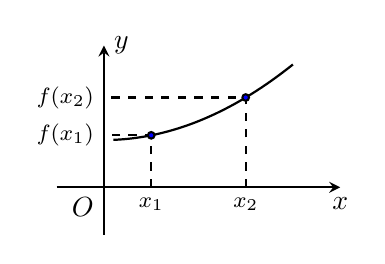
\begin{tikzpicture}[>=stealth,scale=0.6]
		\draw[->] (-1,0)--(0,0)%
		node[below left]{$O$}--(5,0) node[below]{$x$};
		\draw[->] (0,-1) --(0,3) node[right]{$y$};
		\draw [black,thick, domain=0.2:4, samples=100] %
		plot (\x, {0.1*(\x)^2+1});
		\draw [dashed] (1,0)node[below]{\footnotesize$x_1$} --(1,1.1)--(0,1.1)node[left]{\footnotesize$f(x_1)$};
		\draw [dashed] (3,0)node[below]{\footnotesize$x_2$} --(3,1.9)--(0,1.9)node[left]{\footnotesize$f(x_2)$};
		\draw[fill=blue] (1,1.1) circle(2pt);
		\draw[fill=blue] (3,1.9) circle(2pt);
	\end{tikzpicture}}\\
Trên $K$, đồ thị là một "\textbf{đường đi lên}" khi xét từ trái sang phải.
\end{khung4}
\end{minipage}\hspace{0.5cm}
\begin{minipage}[b]{6cm}
\begin{khung4}{Ghi nhớ 2}
		Hàm số nghịch biến trên $K$ nếu
		$\forall x_1,\,x_2 \in K$, $$ x_1<x_2 \Rightarrow f(x_1)>f(x_2)$$
		\centerline{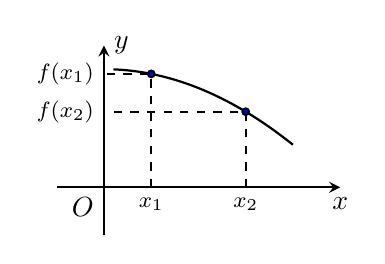
\begin{tikzpicture}[>=stealth,scale=0.6]
			\draw[->] (-1,0)--(0,0)%
			node[below left]{$O$}--(5,0) node[below]{$x$};
			\draw[->] (0,-1) --(0,3) node[right]{$y$};
			\draw [thick, domain=0.2:4, samples=100] %
			plot (\x, {-0.1*(\x)^2+2.5});
			\draw [dashed] (1,0)node[below]{\footnotesize$x_1$} --(1,2.4)--(0,2.4)node[left]{\footnotesize$f(x_1)$};
			\draw [dashed] (3,0)node[below]{\footnotesize$x_2$} --(3,1.6)--(0,1.6)node[left]{\footnotesize$f(x_2)$};
			\draw[fill=blue] (1,2.4) circle(2pt);
			\draw[fill=blue] (3,1.6) circle(2pt);
		\end{tikzpicture}}\\
	Trên $K$, đồ thị là một "\textbf{đường đi xuống}" khi xét từ trái sang phải.
\end{khung4}
\end{minipage}
	\item \indam{Liên hệ giữa đạo hàm và tính đơn điệu:}
	Cho hàm số $y=f(x)$ có đạo hàm trên khoảng $(a;b)$.
	\begin{boxdn}
	\begin{listEX}[1]
		\item [$\bullet$] Nếu $y'\ge 0$, $\forall x \in (a;b)$ và dấu bằng chỉ xảy ra tại hữu hạn điểm thì hàm số $y=f(x)$ đồng biến trên $(a;b)$.
		\item [$\bullet$] Nếu $y'\le 0$, $\forall x \in (a;b)$ và dấu bằng chỉ xảy ra tại hữu hạn điểm thì hàm số  $y=f(x)$ nghịch biến trên $(a;b)$.
	\end{listEX}
	\end{boxdn}
\end{enumerate}
\subsubsection{Cực trị của hàm số}
\begin{enumerate}[\iconMT]
	\item \indam{Định nghĩa:} Cho hàm số $y=f(x)$ xác định và liên tục trên khoảng $(a ; b)$ ( $a$ có thể là $-\infty, b$ có thể là $+\infty)$ và điểm $x_0 \in(a ; b)$.
	\begin{boxdn}
	\begin{itemize}
		\item [$\bullet$] Nếu tồn tại số $h>0$ sao cho $f(x)<f\left(x_0\right)$ với mọi $x \in\left(x_0-h ; x_0+h\right) \subset(a ; b)$ và $x \neq x_0$ thì ta nói hàm số $f(x)$ đạt cực đại tại $x_0$.
		\item [$\bullet$] Nếu tồn tại số $h>0$ sao cho $f(x)>f\left(x_0\right)$ với mọi $x \in\left(x_0-h ; x_0+h\right) \subset(a ; b)$ và $x \neq x_0$ thì ta nói hàm số $f(x)$ đạt cực tiểu tại $x_0$.
	\end{itemize}
	\end{boxdn}
	\item \indam{Định lý:} Giả sử hàm số $y=f(x)$ liên tục trên khoảng $(a ; b)$ chứa điểm $x_0$ và có đạo hàm trên các khoảng $\left(a ; x_0\right)$ và $\left(x_0 ; b\right)$. Khi đó:
	\begin{boxdn}
	\begin{itemize}
		\item [$\bullet$] Nếu $f^{\prime}(x)<0$ với mọi $x \in\left(a ; x_0\right)$ và $f^{\prime}(x)>0$ với mọi $x \in\left(x_0 ; b\right)$ thì $x_0$ là một điểm cực tiểu của hàm số $f(x)$.
		\item [$\bullet$] Nếu $f^{\prime}(x)>0$ với mọi $x \in\left(a ; x_0\right)$ và $f^{\prime}(x)<0$ với mọi $x \in\left(x_0 ; b\right)$ thì $x_0$ là một điểm cực đại của hàm số $f(x)$.
	\end{itemize}
	\end{boxdn}
	\item \indam{Các tên gọi:}\\
		\begin{tikzpicture}[smooth,samples=300,scale=1.15,>=stealth]
			\draw[->,>=stealth] (-2.5,0)--(2.7,0) node[below]{$x$};
			\draw[->,>=stealth] (0,-1.5)--(0,4) node[right]{$y$};
			\draw (0,0) node[above left]{$O$};
			\draw[blue,domain=-2:2,line width = 1.2pt] plot(\x,{(\x)^3-3*(\x)+1})node[right]{$y=f(x)$};
			\draw[fill=black] (1,0) circle(1pt) (1,-1) circle(2pt) (0,-1) circle(1pt) (-1,0) circle(1pt) (-1,3) circle(2pt) (0,3) circle(1pt);
			\draw[dashed] (1,0)node[above]{\small$x_2$}--(1,-1)--(0,-1)node[left]{\small$y_2$} (-1,0)node[below]{\small$x_1$}--(-1,3)--(0,3)node[right]{\small$y_1$};
			
			\draw[-,dotted] (-0.5,3.7)--(4,3.7)node[right]{$(x_1;y_1)$ là điểm cực đại của đồ thị hàm số;}; 
			\draw[->,dotted] (-0.5,3.7)--(-1,3.15);
			\node[right] at (4.5,3.1) {$\bullet$ $x_1$ là điểm cực đại của hàm số;};
			\node[right] at (4.5,2.5) {$\bullet$ $y_1$ là giá trị cực đại của hàm số.};
			
			\draw[-,dotted] (2,-1)--(2,1)--(4,1)node[right]{$(x_2;y_2)$ là điểm cực tiểu của đồ thị hàm số;}; \draw[->,dotted] (2,-1)--(1.15,-1);
			\node[right] at (4.5,0.4) {$\bullet$ $x_2$ là điểm cực tiểu của hàm số;};
			\node[right] at (4.5,-0.2) {$\bullet$ $y_2$ là giá trị cực tiểu của hàm số.};
		\end{tikzpicture}
\end{enumerate}
\subsection{PHÂN LOẠI VÀ PHƯƠNG PHÁP GIẢI TOÁN}
\begin{dang}{Bài toán tìm khoảng đơn điệu và cực trị của hàm số cho trước}
	\begin{listEX}[1]
		\item [\ding{172}] Tìm tập xác định $\mathscr{D}$ của hàm số $y=f(x)$ .
		\item [\ding{173}] Tính đạo hàm $f'(x)$. Tìm các điểm $x_i \,(i = 1, 2, ..., n)$ thuộc $\mathscr{D}$ mà tại đó đạo hàm bằng $0$ hoặc không xác định.
		\item [\ding{174}] Sắp xếp các điểm $x_i$ theo thứ tự tăng dần, xét dấu $y'$ và lập bảng biến thiên. Từ đây, nêu các khoảng đồng biến, nghịch biến và các điểm cực trị.
	\end{listEX}
\end{dang}
\indamm{Ghi nhớ cách xét dấu:}
\begin{note}
\begin{enumerate}[\iconCH]
		% \item Nếu $$f'(x)=(x-a)(x-b)^2(x-c)^{2n}(x-d)^{2n+1},\,\forall n \in \mathbb{N}*$$
		% thì phương trình $f'(x)=0$ có
		% \begin{itemize}
		% 	\item 	$x=a$ là nghiệm đơn;
		% 	\item  $x=b$ là nghiệm kép;
		% 	\item  $x=c$ là nghiệm bội chẵn;
		% 	\item  $x=d$ là nghiệm bội lẻ.
		% \end{itemize}
		\item Khi xét dấu $f'(x)$ thì $f'(x)$ sẽ không đổi dấu khi qua nghiệm kép (nghiệm bội chẵn) và đổi dấu khi qua nghiệm đơn (nghiệm bội lẻ).
	\end{enumerate}
	% \begin{tikzpicture}[smooth,samples=300,scale=0.8,>=stealth,font=\footnotesize]
	% 	\draw[->] (-3.5,0)--(6,0) node[below]{$x$};
	% 	\draw[->] (0,-1.5)--(0,4) node[left]{$y$};
	% 	\draw (0,0) node[above left]{$O$};
	% 	\draw[blue,line width=0.7pt,domain=-2.15:1.5] plot(\x,{(\x+2)*(\x-1)^2});
	% 	\draw[blue,line width=0.7pt,domain=1.5:4.7] plot(\x,{-1*(\x-1.64)*(\x-4)^2})node[below]{$y=f'(x)$};
	% 	\draw[fill=red] (-2,0)node[above left]{$x_1$} circle(1.5pt) (1,0)node[below]{$x_2$} circle(1.5pt) (4,0)node[above right]{$x_4$} circle(1.5pt) (1.64,0)node[above right]{$x_3$} circle(1.5pt);
	% 	\draw[dashed,<-] (-1.8,-0.2)--(0.5,-2.3)node[below]{\fbox{\scriptsize\text{Nghiệm bội lẻ}}};
	% 	\draw[dashed,->](0.5,-2.3)--(1.58,-0.2);
	% 	\draw[dashed,<-] (1,0.2)--(2,3)node[above]{\fbox{\scriptsize\text{Nghiệm bội chẵn}}};
	% 	\draw[dashed,->](2,3)--(3.9,0.1);
	% 	\end{tikzpicture}
\end{note}
\boxmini{BÀI TẬP TỰ LUẬN}

\begin{vd}
	Tìm các khoảng đơn điệu và các điểm cực trị của hàm số sau
	\begin{tasks}(3)
		\task $ y=-x^3+3x^2-4$;
		\task $ y=x^3-3x^2+1$;
		\task $y=x^3+3x^2+3x+2$;
		\task $y=-2x^4+4x^2$;
		\task $y=x^4+4x^3-1$;
		\task $y=-16x^4+x-1$.
	\end{tasks}
	\loigiai{
	\begin{enumEX}[a)]{1}
		\item Tập xác định: $\mathscr{D}=\mathbb{R}$. \\
		Đạo hàm: $y'=-3x^2+6x$.\\
		Xét $y'=0 \Leftrightarrow -3x^2+6x=0 \Leftrightarrow
		\hoac{
			& x=0 \\
			& x=2 }$
		Bảng biến thiên:\begin{center}
			\begin{tikzpicture}
				\tkzTabInit[nocadre=false,lgt=0.7,espcl=2.1,deltacl=0.6]
				{$x$ /0.6,$y'$ /0.6,$y$ /2}
				{$-\infty$,$0$,$2$,$+\infty$}
				\tkzTabLine{,-,$0$,+,$0$,-,}
				\tkzTabVar{+/$+\infty$, -/$-4$,+/$0$,-/$-\infty$}
			\end{tikzpicture}
		\end{center}
		\item Ta có: $ y'=3x^2-6x\Rightarrow y'=0\Leftrightarrow \hoac{&x=0\\&x=2.} $\\
		Từ bảng biến thiên suy ra hàm số đồng biến trên khoảng $ (-\infty;0) $ và $ (2;+\infty). $
		\begin{center}
			\begin{tikzpicture}
				\tkzTabInit[nocadre=false,lgt=1,espcl=3]
				{$x$ /1,$y'$ /1,$y$ /2}
				{$-\infty$,$0$, $2$,$+\infty$}
				\tkzTabLine{,+,$0$,-,$0$,+, }
				\tkzTabVar{-/ $-\infty$,+/$1 $ ,-/$-3$,+/$+\infty$}
			\end{tikzpicture}
		\end{center}
		\item Hàm số đã cho xác định trên $\mathscr{D}=\mathbb{R}$.\\
		Ta có $y'=3x^2+6x+3$. Cho $y'=0 \Leftrightarrow 3x^2+6x+3=0 \Leftrightarrow x=-1$.\\
		Bảng biến thiên
		\begin{center}
			\begin{tikzpicture}
				\tkzTabInit[lgt=1,espcl=3]
				{$x$/0.7,$y'$/0.7,$y$/2}
				{$-\infty$,$-1$,$+\infty$}
				\tkzTabLine{,+,0,+,}
				\tkzTabVar{-/$-\infty$,R/,+/$+\infty$}
				
			\end{tikzpicture}
		\end{center}
		Vậy hàm số đồng biến trên $\mathbb{R}$.
		\item Tập xác định của hàm số là $ \mathscr{D}=\mathbb{R}$.\\
		Ta có $y'=-8x^3+8x$.
		Cho $y'=0 \Leftrightarrow -8x^3+8x=0 \Leftrightarrow 8x(-x^2+1)=0$\\
		\centerline{$ \Leftrightarrow \left[\begin{aligned}
				&8x=0 \\
				&-x^2+1=0
			\end{aligned}\right. \Leftrightarrow \left[\begin{aligned}
				&x=0 \\
				&x^2=1
			\end{aligned}\right. \Leftrightarrow \left[\begin{aligned}
				&x=0 \\
				&x=\pm 1.
			\end{aligned}\right. $}
		Bảng biến thiên
		\begin{center}
			\begin{tikzpicture}
				\tkzTabInit[lgt=1,espcl=3]
				{$x$/0.7,$y'$/0.7,$y$/2}
				{$-\infty$,$-1$,$0$,$1$,$+\infty$}
				\tkzTabLine{,+,0,-,0,+,0,-,}
				\tkzTabVar{-/$-\infty$,+/ $2$/,-/$0$,+/$2$,-/$-\infty$}
			\end{tikzpicture}
		\end{center}
		Vậy hàm số đồng biến trên mỗi khoảng $(-\infty;-1)$ và $(0;1)$,\\
		\indent{ } hàm số nghịch biến trên mỗi khoảng $(-1;0)$ và $(1;+\infty)$.
		\item Hàm số đã cho xác định trên $\mathscr{D}=\mathbb{R}$.\\
		Ta có $y'=4x^3+12x^2=0=4x^2(x+3)$.\\
		Cho $y'=0 \Leftrightarrow 4x^2(x+3)=0 \Leftrightarrow \left[\begin{aligned}
			&x=0 \\
			&x=-3.
		\end{aligned}\right.$\\
		Bảng biến thiên
		\begin{center}
			\begin{tikzpicture}
				\tkzTabInit[lgt=1,espcl=3]
				{$x$/0.7,$y'$/0.7,$y$/2}
				{$-\infty$,$-3$,$0$,$+\infty$}
				\tkzTabLine{,-,0,+,0,+,}
				\tkzTabVar{+/$+\infty$,-/$-28$ /,R,+/$+\infty$}
			\end{tikzpicture}
		\end{center}
		Vậy hàm số nghịch biến trên khoảng $(-\infty;-3)$ và đồng biến trên khoảng $(-3;+\infty)$.
		\item Ta có $y'=-64x^3+1<0\Leftrightarrow x>\dfrac{1}{4}$ nên hàm số nghịch biến trên khoảng $\left(\dfrac{1}{4};+\infty\right)$.
\end{enumEX}}
\end{vd}

\begin{vd}
	Tìm các khoảng đơn điệu và cực trị của các hàm số sau:
	\begin{tasks}(3)
		\task $y=\dfrac{2x+1}{x+1}$;
		\task $y=\dfrac{3x+1}{x-1}$;
		\task $y=\dfrac{x^2+2x+2}{x+1}$;
		\task $y=x+\dfrac{4}{x}$;
		\task $y=\sqrt{x^2-2x}$;
		\task $y=x-3\sqrt[3]{x^2}$ .
	\end{tasks}
	\loigiai{
		\begin{enumEX}[a)]{1}
			\item Ta có $y'=\dfrac{1}{(x+1)^2} > 0, \forall x \in \mathbb{R} \backslash \{-1\}$.\\
			Vậy hàm số đồng biến trên $(-\infty ;-1)$ và $(-1 ;+\infty)$.\\
			Hàm số không có cực trị.
			\item Ta có $y'=\dfrac{-4}{(x-1)^2}>0,\,\forall x\in\mathbb{R}\setminus\{1\}$.\\
			Do vậy hàm số nghịch biến trên các khoảng  $(-\infty;1)$; $(1;+\infty)$.\\
			Hàm số không có cực trị.
			\item \begin{itemize}
				\item TXĐ: $\mathscr{D}=\mathbb{R}\setminus \left\{-1\right\}$.
				\item $y'=\dfrac{x^2+2x}{(x+1)^2}$, $y'=0\Leftrightarrow \hoac{& x=-2 \\ & x=0.}$\\
				Ta có bảng biến thiên
				\begin{center}
					\begin{center}
						\begin{tikzpicture}
							\tkzTabInit[nocadre=True,lgt=1,espcl=2]
							{$x$ /0.7,$y'$ /0.7,$y$ /2}
							{$-\infty$,$-2$,$-1$,$0$,$+\infty$}
							\tkzTabLine{,+,$0$,-,d,-,$0$,+,}
							\tkzTabVar{-/$-\infty$,+/$-2$,-D+/$-\infty$/$+\infty$,-/$2$,+/$+\infty$}
						\end{tikzpicture}
					\end{center}
				\end{center}
				Hàm số đồng biến trên khoảng $\left( -\infty;-2\right)$ và $\left( 0;+\infty\right)$;  nghịch biến trên $(-2;-1)$ và $(-1;0)$.\\
				Hàm số đạt cực đại tại $x=-2$, giá trị cực đại $y=-2$\\
				Hàm số đạt cực tiểu tại $x=0$, giá trị cực tiểu $y=2$.\\
			\end{itemize}
			\item Tập xác định $\mathscr{D}=\mathbb{R}\setminus\{0\}$.\\
			Ta có $y'=1-\dfrac{4}{x^2}=\dfrac{x^2-4}{x^2}$, $y'=0\Leftrightarrow x=\pm 2$.\\
			Bảng biến thiên
			\begin{center}
				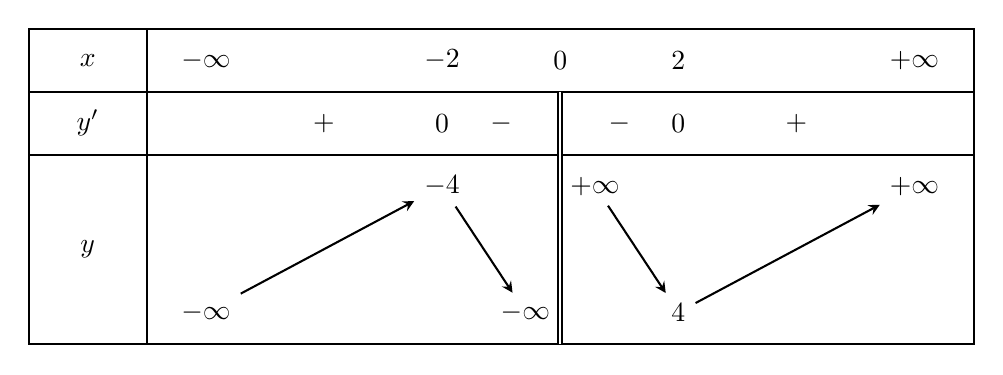
\begin{tikzpicture}[yscale=.8,xscale=1.5,]
					\begin{scope}[shift={(-.5,.5)}]
						\draw
						(0,0) rectangle +(8,-5)
						(0,-1)--+(0:8) (0,-2)--+(0:8) (1,0)--+(-90:5);
					\end{scope}
					\path
					(0,0) node{$x$}          % <<< dòng 1
					++(0:1) node{$-\infty$}
					++(0:2) node{$-2$}
					++(0:1) node{$0$}
					++(0:1) node{$2$}
					++(0:2) node{$+\infty$}
					(0,-1)   node{$y'$}         % <<< dòng 2
					++(0:2) node{$+$}
					++(0:1) node{$0$}
					++(0:.5) node{$-$}
					++(0:1) node{$-$}
					++(0:.5) node{$0$}
					++(0:1) node{$+$}
					(0,-3)   node{$y$}       % <<< dòng 3
					++(0:1) ++(-90:1)  node (A) {$-\infty$}
					++(0:2) ++(90:2) node (B) {$-4$}
					++(0:1) ++(-90:2) node (C)[left]
					{$-\infty$}
					++(90:2) node (D)[right]{$+\infty$}
					++(0:1) ++(-90:2) node (E) {$4$}
					++(0:2) ++(90:2) node (F) {$+\infty$};
					\draw[-stealth] (A)--(B);
					\draw[-stealth] (B)--(C);
					\draw[-stealth] (D)--(E);
					\draw[-stealth] (E)--(F);
					\draw[double] (4,-.5)--(4,-4.5);
				\end{tikzpicture}
			\end{center}
			Hàm số đồng biến trên khoảng $\left( -\infty;-4\right)$ và $\left( 2;+\infty\right)$; nghịch biến trên các khoảng $(-2;0)$ và $(0;2)$.\\
			Hàm số đạt cực đại tại $x=-2$, giá trị cực đại $y=-4$\\
			Hàm số đạt cực tiểu tại $x=2$, giá trị cực tiểu $y=4$\\
			\item Tập xác định: $\mathscr{D}=(-\infty;0]\cup [2;+\infty)$.\\
			Ta có $y'=\dfrac{x-1}{\sqrt{x^2-2x}},\forall x\in (-\infty;0)\cup (2;+\infty)$.\\
			$y'=0 \Leftrightarrow \dfrac{x-1}{\sqrt{x^2-2x}}=0 \Rightarrow x-1=0 \Leftrightarrow x=1 \notin \mathscr{D}$.\\
			Bảng biến thiên:
			\begin{center}
				\begin{tikzpicture}
					\tkzTabInit[lgt=1,espcl=3]
					{$x$/0.7,$y'$/0.7,$y$/2}
					{$-\infty$,$0$,$2$,$+\infty$}
					\tkzTabLine{,-,d,h,d,+,}
					\tkzTabVar{+/$+\infty$,-H/$0$/,-/$0$,+/$+\infty$}
				\end{tikzpicture}
			\end{center}
			Vậy hàm số nghịch biến trên khoảng $(-\infty;0)$ và đồng biến trên khoảng $(2;+\infty)$.\\
			Hàm số không có cực trị.
			\item Tập xác định: $\mathscr{D}=\mathbb{R}$.\\
			Đạo hàm $y'=1-\dfrac{2}{\sqrt[3]{x}}$, xác định với mọi $x\neq 0$.\\
			$y'=0\Leftrightarrow \sqrt[3]{x}=2\Leftrightarrow x=8$.\\
			Đạo hàm không xác định tại $x=0$.\\
			Bảng biến thiên
			\begin{center}
				\begin{tikzpicture}
					\tkzTabInit[nocadre,lgt=1,espcl=2]{$x$/0.7,$y'$/0.7,$y$/2}{$-\infty$,$0$,$8$,$+\infty$}%
					\tkzTabLine{,+,d,-,z,+,}
					\tkzTabVar{-/$-\infty$ , +/$0$,-/$-4$, +/$+\infty$}%
				\end{tikzpicture}
			\end{center}
	\end{enumEX}}
\end{vd}

\begin{vd}
	Thể tích $V$ (đơn vị: centimét khối) của $1 \mathrm{~kg}$ nước tại nhiệt độ $T\,\left(0^{\circ} \mathrm{C} \leq T \leq 30^{\circ} \mathrm{C}\right)$ được tính bởi công thức	$$	V(T)=999,87-0,06426 T+0,0085043 T^2-0,0000679 T^3$$
	 Hỏi thể tích $V(T), \,0^{\circ} \mathrm{C} \leq T \leq 30^{\circ} \mathrm{C}$, giảm trong khoảng nhiệt độ nào?
	\loigiai{
		Xét hàm số  $V(T)=999{,}87-0{,}06426T+0{,}0085043T^2-0{,}0000679T^3$, với $T\in [0;30]$.\\
	Ta có $V'(T)=-0{,}0002037T^2+0{,}0170086T-0{,}06426$.\\
	$V'(T)=0\Leftrightarrow T=3{,}966514624=T_1$ hoặc $T=79{,}53176716\not\in [0;30]$.\\
	Bảng biến thiên của hàm số $V(T)$ như sau
	\begin{center}
		\begin{tikzpicture}[font=\footnotesize,thick,>=stealth]
			\tikzset{double style/.append style={double distance=1.5pt}}
			\tkzTabInit[nocadre=false,lgt=1.2,espcl=2.5,deltacl=0.6,lw=.75pt,color,colorL=green!50,colorV=green!50]
			{$T$ /0.7, $V'(T)$ /0.8, $V(T)$ /2}
			{$0$,$T_1$,$30$}
			\tkzTabLine{ ,-,$0$,+, }
			\tkzTabVar{+/$V(0)$,-/$V(T_1)$,+/$V(30)$}
		\end{tikzpicture}
	\end{center}
	Từ bảng biến thiên suy ra, thể tích $V(T), 0^{\circ}\mathrm{C}\leq T \leq 30^{\circ}\mathrm{C}$, giảm trong khoảng nhiệt độ từ $0^\circ$C đến $3{,}966514624^\circ$C.}
\end{vd}

\boxmini{BÀI TẬP TRẮC NGHIỆM}
\ind{PHẦN I.} \inden{Câu trắc nghiệm nhiều phương án lựa chọn. Mỗi câu hỏi học sinh chỉ chọn một phương án.}\\
\setcounter{ex}{0}
\Opensolutionfile{ans}[ans/2D1-B1-d1-1]

\begin{ex}%[KSCL, Sở GD \& ĐT Hà Nam, 2018]%[Lê Quốc Hiệp, dự án 12EX10-18]%[2D1B1-2]%
	\immini
	{Cho hàm số $y=f(x)$ có đồ thị như hình vẽ bên. Hàm số $y=f(x)$ nghịch biến trên khoảng nào dưới đây?
		\haicot
		{$(\sqrt{2};+\infty)$}
		{$(-2;2)$}
		{$(-\infty;0)$}
		{\True $(0;\sqrt{2})$}
	}
	{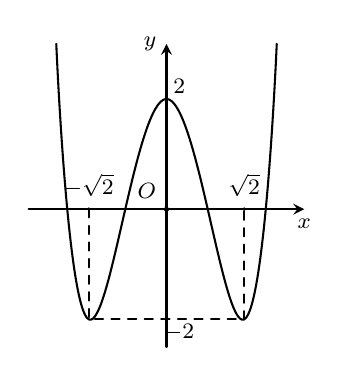
\begin{tikzpicture}[line cap=round,line join=round,x=1.0cm,y=1.0cm,>=stealth,scale=0.7]
			\draw[->,color=black,smooth,samples=100] (-2.5,0.) -- (2.5,0.) node[below] {\footnotesize $x$};
			\draw[->,color=black,smooth,samples=100] (0.,-2.5) -- (0.,3) node[left] {\footnotesize $y$};
			\draw plot[smooth,tension=.7] coordinates {(-2,3) (-1.41,-2)  (0,2) (1.41,-2) (2,3)};
			\draw[fill=black] (0,0) circle [radius=1pt] node[above left] {\footnotesize $O$};
			\fill (-1.41,0) node[shift={(90:2ex)}]{\footnotesize $-\sqrt{2}$} circle(1pt);
			\fill (1.41,0) node[shift={(90:2ex)}]{\footnotesize $\sqrt{2}$} circle(1pt);
			\fill (0,-2) node[shift={(-45:1.5ex)}]{\footnotesize $-2$} circle(1pt);
			\fill (0,2) node[shift={(45:1.5ex)}]{\footnotesize $2$} circle(1pt);
			\draw[dashed] (-1.41,0)|-(0,-2)-|(1.41,0);
	\end{tikzpicture}}
	\loigiai
	{
		Dựa vào đồ thị, ta thấy trên khoảng $(0;\sqrt{2})$ đồ thị đi xuống nên hàm số $y=f(x)$ nghịch biến trên khoảng đó.
	}
\end{ex}

\begin{ex}
	\immini{Cho hàm số $y=f(x)$ có đồ thị như hình vẽ bên. Mệnh đề nào sau đây là mệnh đề \textbf{sai}?
		\choice
		{Hàm số đạt cực đại tại $x=0$}
		{Hàm số có giá trị cực tiểu bằng $-2$}
		{\True Hàm số đồng biến trên $(-\infty; 2)$}
		{Hàm số nghịch biến trên $(0; 2)$}
	}
	{
		
		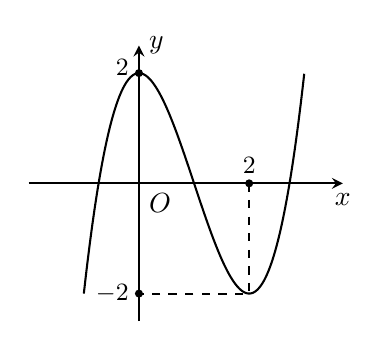
\begin{tikzpicture}[smooth,samples=300,scale=0.7,>=stealth]
			\draw[->] (-2,0)--(3.7,0) node[below]{$x$};
			\draw[->] (0,-2.5)--(0,2.5) node[right]{$y$};
			\draw (0,0) node[below right]{$O$};
			\draw[smooth,samples=100,domain=-1:3]
			plot(\x,{(\x)^3-3*(\x)^2+2});
			\draw[fill=black] (2,0) circle(1.5pt) (0,2) circle(1.5pt) (0,-2) circle(1.5pt);
			\draw[dashed] (2,0)node[above]{\small$2$}--(2,-2)--(0,-2)node[left]{\small$-2$} (0,2.1)node[left]{\small$2$};
		\end{tikzpicture}
	}
	
	\loigiai{
	}
	
\end{ex}

\begin{ex}
	\immini{
		Hàm số $y=f(x)$ có đồ thị là đường cong trong hình vẽ bên. Hàm số $y=f(x)$ đạt cực tiểu tại điểm nào dưới đây?
		\haicot
		{$x=2$}
		{\True $x=0$}
		{$x=-2$}
		{$x=4$}
	}{
		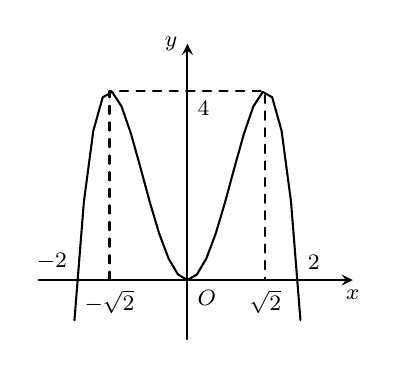
\begin{tikzpicture}[xscale=.7,yscale=.6, font=\footnotesize, line join=round, line cap=round, >=stealth]
			\draw[->] (-2.7,0)--(3,0) node[below]{$x$};
			\draw[->] (0,-1.25)--(0,5) node[left]{$y$};
			\draw[dashed] (-2^.5,0)--(-2^.5,4)--(2^.5,4)--(2^.5,0);
			\draw[domain=-2.05:2.05] plot(\x,{-(\x)^2*((\x)^2-4)});
			\path
			(0,0) node[below right]{$O$}
			(2,0) node[above right]{$2$}
			(-2,0) node[above left]{$-2$}
			(0,4) node[below right]{$4$}
			(-2^.5,0) node[below]{$-\sqrt{2}$}
			(2^.5,0) node[below]{$\sqrt{2}$};
		\end{tikzpicture}
	}
	\loigiai{
		Dựa vào đồ thị hàm số ta thấy hàm số đạt cực tiểu tại $x=0$.}
\end{ex}

\begin{ex}
	\immini{Cho hàm số $y=f(x)$ có bảng biến thiên như hình bên. Mệnh đề nào sau đây là mệnh đề đúng?
	\choice
	{Hàm số đồng biến trên khoảng $(-\infty;3)$}
	{Hàm số nghịch biến trên khoảng $(-2;+\infty)$}
	{Hàm số đạt cực đại tại $x=3$}
	{\True Hàm số đạt cực tiểu tại $x=2$}}{
	\begin{tikzpicture}
	\tkzTabInit[lgt=1.2,espcl=1.8,nocadre=True]
	{$x$/0.6,$f'(x)$/0.6,$f(x)$/2}{$-\infty$,$-2$,$2$,$+\infty$}
	\tkzTabLine{,+,0,-,0,+,}
	\tkzTabVar{-/$-\infty$,+/$3$,-/$0$,+/$+\infty$}
\end{tikzpicture}}
	\loigiai{
	}
	
\end{ex}

\begin{ex}
	Cho hàm số $y=f(x)$ có bảng biến thiên bên dưới
	\begin{center}
		\begin{tikzpicture}
			\tikzset{double style/.append style = {draw=\tkzTabDefaultWritingColor,double=\tkzTabDefaultBackgroundColor,double distance=2pt}}
			\tkzTabInit[lgt=1.2,espcl=2,nocadre=True]
			{$x$ /.7, $f’(x)$ /.7,$f(x)$ /2}
			{$-\infty$ , $-2$, $0$ ,$2$ ,$+\infty$}
			\tkzTabLine{ ,+,$0$,-,d,-,$0$,+, }
			\tkzTabVar{ -/ $-\infty$,+/ $-4$/,-D+/$- \infty$ /$+\infty$,-/ $4$,+ /$+\infty$}
		\end{tikzpicture}
	\end{center}
Khẳng định nào sau đây là khẳng định \textbf{sai}?
	\choice
	{Hàm số có hai điểm cực trị}
	{Tọa độ điểm cực đại của đồ thị hàm số là $(-2;-4)$}
	{\True Hàm số nghịch biến trên khoảng $(-2;2)$}
	{Hàm số đồng biến trên khoảng $(3;+\infty)$}
	\loigiai{
	}
\end{ex}


\begin{ex}
	Cho hàm số $y= - \dfrac{1}{3} x^3 - x -3 $. Mệnh đề nào dưới đây đúng?
	\choice
	{Hàm số đồng biến trên $(-\infty; 1)$ và trên $(1; +\infty)$}
	{\True Hàm số nghịch biến trên $\mathbb{R}$}
	{Hàm số đồng biến trên $(-1;1)$}
	{Hàm số đồng biến trên $\mathbb{R}$}
	\loigiai{
		Tập xác định $\mathscr D = \mathbb{R}$.\\
		$y'=-x^2 -1<0 $ với mọi $x$.\\
		Suy ra  hàm số đã cho nghịch biến trên $\mathbb{R}$.}
\end{ex} 


\begin{ex}
	Gọi $x_1$ là điểm cực đại $x_2$ là điểm cực tiểu của hàm số $y=-x^3+3x+2$. Tính $x_1+2x_2$.
	\choice{$2$}
	{$1$}
	{\True $-1$}
	{$0$}
	\loigiai{
		Ta có $y'=-3x^2+3$, $y'=0\Leftrightarrow x=\pm 1$.\\
		Vì $y'$ đổi dấu từ âm sang dương khi qua $x=-1$ và đổi dấu từ dương sang âm khi qua $x=1$ nên $x_2=-1$ là điểm cực tiểu và $x_1=1$ là điểm cực đại của hàm số. Do đó $x_1+2x_2=1-2=-1$.
	}
\end{ex} 


\begin{ex}
	Khoảng cách giữa hai điểm cực trị của đồ thị hàm số $y=x^3-3x^2+4$ bằng
	\choice
	{\True $2\sqrt{5}$}
	{$2\sqrt{2}$}
	{$2$}
	{$ 4 $}
	\loigiai{
		Ta có $y'=3x^2-6x$, $ y'=0\Rightarrow \hoac{&x=0\Rightarrow y=4\\&x=2\Rightarrow y=0.} $\\
		Suy ra hai điểm cực trị của đồ thị hàm số là $A(0;4),B(2;0)$.\\
		Do đó $AB=\sqrt{2^2+(-4)^2}=2\sqrt{5}$.
	}
\end{ex} 

\begin{ex}%[2D1B1]
	Hàm số $y=x^4-2x^2+1$ đồng biến trên khoảng nào dưới đây?
	\choice
	{\True $(-1;0)$}
	{$(-1;+ \infty)$}
	{$(-3;8)$}
	{$(- \infty ; -1)$}
	\loigiai
	{
		$y'= 4x^3-4x$ $\Rightarrow y'=0 \Leftrightarrow 4x^3-4x=0$ $\Leftrightarrow \hoac{x&= -1 \\ x&=0 \\ x &= 1}$\\
		Bảng xét dấu
		\begin{center}
			\begin{tikzpicture}
				\tkzTabInit[nocadre=false, lgt=1, espcl=2.5]{$x$ /1,$y$ /1}{$-\infty$,$-1$,$0$,$1$,$+\infty$}
				\tkzTabLine{,-,$0$,+,$0$,-,$0$,+}
			\end{tikzpicture}
		\end{center}
	}
	
\end{ex} 

\begin{ex}%[2HK1-13-ChuyenLeQuyDon-QuangTri]%[2D1B2-1]%
	Cho hàm số $ y = - \dfrac{1}{4}x^4 + \dfrac{1}{2}x^2 - 3 $. Khẳng định nào sau đây là khẳng định đúng?
	\choice
	{Hàm số đạt cực tiểu tại $ x = -3 $}
	{ \True Hàm số đạt cực tiểu tại $ x = 0 $}
	{Hàm số đạt cực đại tại $ x = 0 $}
	{Hàm số đạt cực tiểu tại $ x = -1 $}
	\loigiai{
		Ta có $ y' = - x^3 + x = - x (x^2 - 1) $.
		Ta có bảng biến thiên như hình bên
		\begin{center}
			\begin{tikzpicture}[scale=1]
				\tkzTabInit[lgt=1.5,espcl=2.5]{$x$  /1,$y'$  /1,$y$ /2}
				{$-\infty$,$ -1 $,$ 0 $,$ 1 $,$+\infty$}%
				\tkzTabLine{,+,z,-,z,+,z,-,}
				\tkzTabVar{-/$ -\infty $,+/   $\dfrac{-11}{4}$ /,-/ $-3$,+/$ \dfrac{-11}{4} $,-/$ -\infty $}
				%\tkzTabIma{1}{3}{2}{$ 0 $}
			\end{tikzpicture}
		\end{center}
	}
\end{ex} 

\begin{ex}
	Cho hàm số $y=\dfrac{3x-1}{x-2}$. Mệnh đề nào dưới đây là đúng?
	\choice
	{Hàm số nghịch biến trên $\mathbb{R}$}
	{Hàm số đồng biến trên các khoảng $(-\infty;2)$ và $(2;+\infty)$}
	{\True Hàm số nghịch biến trên các khoảng $(-\infty;2)$ và $(2;+\infty)$}
	{Hàm số đồng biến trên $\mathbb{R}\setminus\{2\}$}
	\loigiai{Tập xác định là $\mathscr{D}=\mathbb{R}\setminus\{2\}$.\\
		Có $y'=\dfrac{-5}{(x-2)^2}<0$, $\forall x\in\mathscr{D}$ nên hàm số nghịch biến trên các khoảng $(-\infty;2)$ và $(2;+\infty)$.}
	
\end{ex} 

\begin{ex}
	Cho hàm số $y=\dfrac{x-2}{x+3}$. Mệnh đề nào dưới đây đúng?
	\choice
	{Hàm số nghịch biến trên khoảng $(-\infty;-3)\cup (-3;+\infty) $}
	{\True Hàm số đồng biến trên khoảng $(-\infty;-3) $ và $(-3;+\infty)$}
	{Hàm số nghịch biến trên khoảng $(-\infty;-3)$ và $(-3;+\infty)$}
	{Hàm số đồng biến trên khoảng $(-\infty;-3)\cup (-3;+\infty) $}
	\loigiai{
		Tập xác định $\mathscr{D}=\mathbb{R}\setminus \{-3\}$. Ta có $y'=\dfrac{5}{(x+3)^2}>0$, $\forall x\in\mathscr{D}$.\\ Suy ra hàm số đồng biến trên khoảng $(-\infty;-3)$ và $(-3;+\infty)$.
	}
\end{ex} 

\begin{ex}
	Gọi $y_{\text{CĐ}},\,y_{\text{CT}}$ lần lượt là giá trị cực đại và giá trị cực tiểu của hàm số $y=\dfrac{x^2+3x+3}{x+2}$. Giá trị của biểu thức $y_{\text{CĐ}}^2-2y_{\text{CT}}^2$ bằng
	\choice
	{$8$}
	{\True $7$}
	{$9$}
	{$6$}
	\loigiai{
		Ta có $y'=\dfrac{x^2+4x+3}{(x+2)^2}$; $y'=0 \Leftrightarrow \left[\begin{aligned}
			&x=-1 \\
			&x=-3
		\end{aligned}\right. $. \\
		Bảng biến thiên
		\begin{center}
			\begin{tikzpicture}
				\tkzTab
				[lgt=1,espcl=2] % tùy chọn
				{$x$/0.7, $y'$/0.7, $y$/2} % cột đầu tiên
				{$-\infty$, $-3$, $-2$, $-1$, $+\infty$} % hàng 1 cột 2
				{,+,0,-,d,-,0,+,} % hàng 2 cột 2
				{-/ $-\infty$, +/ $-3$, -D+/ $-\infty$ / $+\infty$, -/ $1$, +/ $+\infty$} % hàng 3 cột 2
			\end{tikzpicture}
		\end{center}
		Từ bảng biến thiên ta tìm được $y_{\text{CĐ}}=-3;\,y_{\text{CT}}=1$ $ \Rightarrow $ $y_{\text{CĐ}}^2-2y_{\text{CT}}^2$ $=9-2=7$.}
\end{ex} 

\begin{ex}
	Tìm điểm cực tiểu của hàm số $f(x)=(x-3)\mathrm{e}^x$.
	\choice
	{$x=3$}
	{$x=0$}
	{\True $x=2$}
	{$x=1$}
	\loigiai{
		\begin{itemize}
			\item Ta có $f'(x)=\mathrm{e}^x(x-2)$, $f''(x)=\mathrm{e}^x(x-1)$.
			\item $f'(x)=0\Rightarrow x=2$ và $f''(2)=\mathrm{e}^2>0$.
		\end{itemize}
		Vậy hàm số đã cho đạt cực tiểu tại $x=2$.}
\end{ex} 

\begin{ex}
	Cho hàm số $y=x^2+4\ln(3-x)$. Tìm giá trị cực đai $y_\text{CĐ}$ của hàm số đã cho.
	\choice
	{$y_\text{CĐ}=2$}
	{\True $y_\text{CĐ}=4$}
	{$y_\text{CĐ}=1+4\ln2$}
	{$y_\text{CĐ}=1$}
	\loigiai{
		Tập xác định $\mathscr{D}=(-\infty;3)$.\\
		Đạo hàm $y'=2x-\dfrac{4}{3-x}=\dfrac{-2x^2+6x-4}{3-x}$.\\
		$y'=0\Leftrightarrow -2x^2+6x-4=0\Leftrightarrow \hoac{&x=1\\&x=2}$.\\
		Bảng biến thiên
		\begin{center}
			\begin{tikzpicture}[>=stealth]
				\tkzTabInit[nocadre=false,lgt=1,espcl=2,deltacl=0.5]{$x$/.7,$y'$/.7,$y$/2}
				{$-\infty$,$1$,$2$,$3$}
				\tkzTabLine{,-,0,+,0,-,d}
				\tkzTabVar{+/$+\infty$,-/$1+4\ln 2$,+/$4$,-D/$-\infty$}
			\end{tikzpicture}
		\end{center}
		Hàm số đạt cực đại tại $x=2$, $y_\text{CĐ}=4$.
	}
\end{ex} 


\begin{ex}%[2D1K2]
	Cho hàm số $y = f(x)$ xác định trên $\mathbb{R}$ và có đạo hàm $y' = f'(x) = 3x^3 - 3x^2$. Mệnh đề nào sau đây \textbf{sai}?
	\choice
	{Trên khoảng $(1;+\infty)$ hàm số đồng biến}
	{Trên khoảng $(-1;1)$ hàm số nghịch biến}
	{\True Đồ thị hàm số có hai điểm cực trị}
	{Đồ thị hàm số có một điểm cực tiểu}
	\loigiai
	{
		Ta có: $y' = 0 \Leftrightarrow 3x^3 - 3x^2 = 0 \Leftrightarrow \hoac{& x = 0 \\& x = 1.}$\\
		Bảng biến thiên:
		\begin{center}
			\begin{tikzpicture}[>=stealth]
				\tkzTabInit[nocadre, lgt=1, espcl=2.5]
				{$x$ /0.7,$y'$ /0.7,$y$ /1.7}
				{$-\infty$,$0$,$1$,$+\infty$}
				\tkzTabLine{,-,$0$,-,$0$,+,}
				\tkzTabVar{+/ $+\infty$, R, -/{\text{CT}}, +/ $+\infty$}
			\end{tikzpicture}
		\end{center}
		Hàm số đồng biến trên khoảng $(1;+\infty)$.\\
		Hàm số nghịch biến trên khoảng $(-\infty;1)$.\\
		Hàm số đạt cực tiểu tại $x = 1$.
	}
\end{ex} 

\begin{ex}%[2D1B2]
	Cho hàm số $ y=f(x) $ liên tục trên $ \mathbb{R} $ và có đạo hàm $ f'(x)=x(x-1)^2(x-2)^3 $. Số điểm cực trị của hàm số $ y=f(x) $ là
	\choice{1}{\True 2}{0}{3}
	\loigiai{	Ta có bảng xét dấu của $ f'(x) $:
		\begin{center}
			\begin{tikzpicture}
				\tkzTabInit[lgt=2,espcl=1.5]%
				{$x$ /1,$f'(x)$ /1}
				{$-\infty$ , $0$ , $1$ , $2$ ,$+\infty$}
				\tkzTabLine{ ,+,0,-,0,-,0,+,}
			\end{tikzpicture}
		\end{center}
		Dựa vào bảng xét dấu ta thấy $ f(x) $ có 2 điểm cực trị.
}\end{ex} 



\begin{ex}%[2D1K2-2]%
	\immini{Cho hàm số bậc bốn $ y=f(x) $. Biết $f'(x) $ có đồ thị như hình bên. Khẳng định nào sau đây là khẳng định đúng?
		\choice
		{Hàm số $f(x)$ đồng biến trên khoảng $(-\infty;0)$}
		{Hàm số $f(x)$ nghịch biến trên khoảng $(-1;1)$}
		{Hàm số $f(x)$ có đúng một điểm cực tiểu}
		{\True Hàm số $f(x)$ có đúng một điểm cực đại}
	}{
		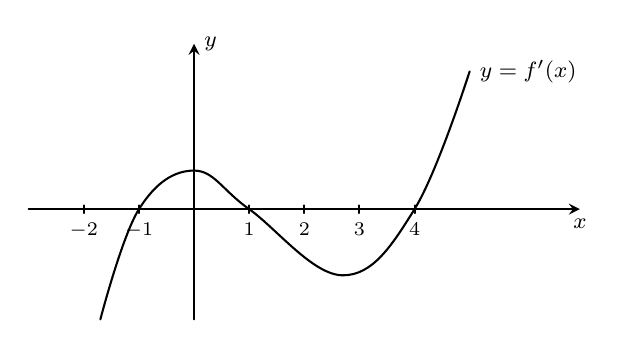
\begin{tikzpicture}[>=stealth,line join=round,line cap=round,font=\footnotesize,scale=0.7,smooth]
			\draw[->] (-3,0)--(7,0)node[below]{$x$};
			\foreach \x in {-2,-1,1,2,3,4}\draw[shift={(\x,0)}] (0,2pt)--(0,-2pt) node[below]{\scriptsize $\x$};
			\draw[->] (0,-2)--(0,3)node[right]{$y$};
			\draw[] plot[smooth,tension=.65] coordinates{(-1.7,-2) (-1,0) (0,.7) (1,0)(2.7,-1.2)(4,0) (5,2.5)}node[right]{$y=f'(x)$};
		\end{tikzpicture}
	}
	\loigiai{
		\immini{Dựa vào đồ thị, ta có bảng biến thiên như hình vẽ. \\
		}{% Cần khai báo \usepackage{tkz-tab}
			\begin{tikzpicture}[scale=.8, font=\footnotesize, line join=round, line cap=round, >=stealth]
				\tkzTabInit[nocadre=false,lgt=1,espcl=2,deltacl=0.5]{$x$/.7 ,$y'$/.7,$y$/2}
				{$-\infty$ , $-1$ , $1$, $ 4 $, $+\infty$}
				\tkzTabLine{ , - , $0$ ,+, $ 0 $, -, $0$ , + , }
				\tkzTabVar{+/$+\infty$ , -/$f(-1)$ ,+/$f(-1)$ ,-/$ f(4) $, +/$+\infty$}
		\end{tikzpicture}}
	}
\end{ex} 

\begin{ex}
	\immini{
		Cho hàm số $y=f(x)$ xác định và liên tục trên $\mathbb{R}$. Biết rằng hàm số $f(x)$ có đạo hàm $f'(x)$ và hàm số $y=f'(x)$ có đồ thị như hình vẽ. Khi đó nhận xét nào sau đây đúng?
		\choice
		{\True Hàm số $f(x)$ không có cực trị}
		{Đồ thị hàm số $f(x)$ có đúng $2$ điểm cực tiểu}
		{Đồ thị hàm số $f(x)$ có đúng một cực đại}
		{Hàm số $f(x)$ có $3$ cực trị}
	}{
		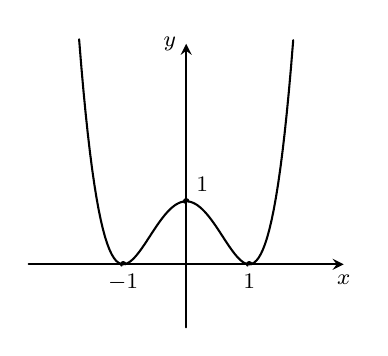
\begin{tikzpicture}[scale=.8,font=\footnotesize, line join=round,line cap=round,>=stealth]
			\draw[->] (-2.5,0)--(2.5,0)node[below]{$x$};
			\draw[->] (0,-1)--(0,3.5)node[left]{$y$};
			\draw[samples=100,domain=-1.7:1.7] plot(\x,{(\x)^4-2*(\x)^2+1});
			\draw[dashed] (-1,0)node[below]{$-1$}circle(1pt) (1,0)node[below]{$1$}circle(1pt) (0,1)node[above right]{$1$}circle(1pt);
		\end{tikzpicture}
	}
	\loigiai{
		Dựa vào đồ thị ta thấy $f'(x)\geq 0$, với mọi $x\in\mathbb{R}$.\\
		Suy ra, hàm số $f(x)$ không có cực trị.
	}
\end{ex} 


\Closesolutionfile{ans}

\ind{PHẦN II.} \inden{Câu trắc nghiệm đúng sai. Trong mỗi ý a), b), c), d) ở mỗi câu, học sinh chọn đúng hoặc sai.}\\
\Opensolutionfile{ans}[ans/2D1-B1-d1-2]

\begin{ex}
	Cho hàm số $y=f(x)$ liên tục trên $\mathbb{R}$ và có bảng xét dấu đạo hàm như hình bên.
	\begin{center}
		\begin{tikzpicture}
			\tikzset{double style/.append style = {draw=\tkzTabDefaultWritingColor,double=\tkzTabDefaultBackgroundColor,double distance=2pt}}
			\tkzTabInit[nocadre=false, lgt=1, espcl=1.2]{$x$ /0.7,$y'$ /1}{$-\infty$,$0$,$1$,$2$,$+\infty$}
			\tkzTabLine{,+,$0$,-,d,+,$0$,+,}
		\end{tikzpicture}
	\end{center}
	% \immini{
		\choiceTF
		{Hàm số đồng biến trên khoảng $(-\infty;1)$}
		{\True Hàm số đồng biến trên khoảng $(1;+\infty)$}
		{Hàm số đạt cực đại tại $x=2$}
		{Hàm số có một điểm cực đại và hai điểm cực tiểu}
	% }{\vspace{0.1cm}
		%}
	\loigiai{
		Ta có bảng biến thiên như sau:
		\begin{center}
			\begin{tikzpicture}
				\tikzset{double style/.append style = {draw=\tkzTabDefaultWritingColor,double=\tkzTabDefaultBackgroundColor,double distance=2pt}}
				\tkzTabInit[lgt=1.1,espcl=2,nocadre=True]
				{$x$ /.7, $y'$ /.7,$y$ /2}
				{$-\infty$ , $0$, $1$ ,$2$ ,$+\infty$}
				\tkzTabLine{ ,+,$0$,-,d,+,$0$,+, }
				\tkzTabVar{ -/,+/ /,-/,R,+/$+\infty$}
			\end{tikzpicture}
		\end{center}
	Từ đây, suy ra:
		\begin{enumerate}[a)]
			\item Hàm số đồng biến trên khoảng $(-\infty;1)$ là khẳng định sai.
			\item Hàm số đồng biến trên khoảng $(1;+\infty)$ là khẳng định đúng.
			\item Hàm số đạt cực đại tại $x=2$ là khẳng định sai.
			\item Hàm số có một điểm cực đại và hai điểm cực tiểu là khẳng định sai.
		\end{enumerate}
	}
	
\end{ex} 

\begin{ex}
	Cho hàm số $y=x^3-3x^2+4$ có đồ thị $(C)$. Gọi $A$, $B$ là hai điểm cực trị của $(C)$.
	\choiceTF
	{\True Tập xác định của hàm số là $\mathbb{R}$}
	{Hàm số đồng biến trên khoảng $(0;2)$}
	{\True PTĐT qua hai điểm cực trị của đồ thị hàm số là $2x+y-4=0$}
	{\True Diện tích của tam giác $OAB$ bằng $4$, với $O$ là gốc tọa độ}
	\loigiai{
		\begin{enumerate}[a)]
			\item Hàm số đa thức nên có tập xác định là $D=\mathbb{R}$.
			\item Ta có 
			\begin{itemize}
				\item [$\bullet$] $y'=3x^2-6x$ và $y'=0 \Leftrightarrow x=0$ hoặc $x=2$.
			\end{itemize}
			Bảng biến thiên:
			\begin{center}
				\begin{tikzpicture}
					\tkzTabInit[lgt=1,espcl=3]
					{$x$ /0.7, $y'$ /0.7, $y$ /2.5}
					{$-\infty$,$0$,$2$,$+\infty$}
					\tkzTabLine{,+,$0$,-,$0$,+,}
					\tkzTabVar{-/$-\infty$,+/$4$,-/$0$,+/$+\infty$}
				\end{tikzpicture}
			\end{center}
		Suy ra hàm nghịch biến trên $(0;2)$.
			\item Tọa độ $A(0;4)$, $B(2;0)$. PTĐT $AB$ là
			$$\dfrac{x-0}{2-0}=\dfrac{y-4}{0-4} \Leftrightarrow 2x+y-4=0$$
			\item Diện tích tam giác vuông $OAB$ là $S_{OAB}=\dfrac{1}{2}OA \cdot OB=4$.
		\end{enumerate}

	}
\end{ex} 

\begin{ex}
	Cho hàm số $y=\dfrac{x^2+2x+2}{x+1}$ có đồ thị $(C)$. Gọi $A$, $B$ lần lượt là điểm cực tiểu và điểm cực đại của $(C)$.
	\choiceTF
	{Tập xác định của hàm số là $\mathbb{R}$}
	{Hàm số nghịch biến trên khoảng $(-2;0)$}
	{Tọa độ điểm $A(-2;-2)$, $B(0;2)$}
	{Khoảng cách giữa hai điểm cực trị là $AB=2\sqrt{5}$}
	\loigiai{
		\begin{enumerate}[a)]
			\item Đặt điều kiện mẫu số khác 0, ta được $x+1 \ne 0 \Leftrightarrow x \ne -1$. Suy ra $\mathscr{D}=\mathbb{R}\setminus \left\{-1\right\}$.
			\item $y'=\dfrac{x^2+2x}{(x+1)^2}\Rightarrow y'=0\Leftrightarrow \hoac{& x=-2 \\ & x=0.}$\\
			Ta có bảng xét dấu của hàm $f'(x)$ như sau
			\begin{center}
					\begin{tikzpicture}
					\tkzTabInit[nocadre=false,lgt=1,espcl=3]
					{$x$ /0.7,$y'$ /0.7,$y$ /2}
					{$-\infty$,$-2$,$-1$,$0$,$+\infty$}
					\tkzTabLine{,+,$0$,-,d,-,$0$,+,}
					\tkzTabVar{-/$-\infty$,+/$-2$,-D+/$-\infty$/$+\infty$,-/$2$,+/$+\infty$}
				\end{tikzpicture}
			\end{center}
			Dựa vào bảng xét dấu ta thấy rằng hàm số $y=f'(x)$ nghịch biến trên $(-2;-1)$ và $(-1;0)$.
			\item Tọa độ điểm $A(0;2)$, $B(-2;-2)$
			\item Độ dài $AB=\sqrt{(-2-0)^2+(-2-2)^2}=2\sqrt{5}$.
		\end{enumerate}

	}
\end{ex} 


\begin{ex}
	Xét một chất điểm chuyển động dọc theo trục $Ox$. Toạ độ của chất điểm tại thời điểm $t$ được xác định bởi hàm số $x(t)=t^3-6t^2+9t$ với $t\geq 0$. Khi đó $x'(t)$ là vận tốc của chất điểm tại thời điểm $t$, kí hiệu $v(t)$; $v'(t)$ là gia tốc chuyển động của chất điểm tại thời điểm $t$, kí hiệu $a(t)$.
	\choiceTF
	{Phương trình hàm vận tốc là $v(t)=3t^2-6t+9$}
	{\True Phương trình hàm gia tốc là $a(t)=6t-12$}
	{Vận tốc của chất điểm tăng khi $t\in (0;1)$ hoặc  $t \in (3;+\infty)$}
	{Vận tốc của chất điểm giảm khi $t\in (1;3)$}
	\loigiai{
		\begin{enumerate}
			\item $v(t)=x'(t)=3t^2-12t+9$
			\item $a(t)=v'(t)=6t-12$.
			\item Xét $v'(t)=6t-12$, $v'(t)=0\Leftrightarrow t=2$\\
			Bảng xét dấu
			\begin{center}
				\begin{tikzpicture}
					\tkzTabInit[nocadre=false,lgt=2,espcl=2.1]
					{$t$ /0.6,$v'(t)$ /0.6}
					{$0$,$2$,$+\infty$}
					\tkzTabLine{,-,$0$,+,}
				\end{tikzpicture}
			\end{center}
			Suy ra vận tốc của chất điểm tăng khi $t\in (2;+\infty) $, giảm khi $t\in (0;2)$.
		\end{enumerate}
	}
\end{ex} 

\Closesolutionfile{ans}
% \begin{dang}{Bài toán tìm m để hàm số đồng biến (nghịch biến) trên khoảng cho trước}
\begin{enumerate}[\iconCV]
\item Xét hàm số bậc ba $y=ax^3+bx^2+cx+d$ có $y'=3ax^2+2bx+c$.
	\begin{listEX}[1]
		\item [\ding{172}] Hàm số đồng biến trên  $\mathbb{R}$ khi và chỉ khi $$y' \ge 0,\,\forall x \in \mathbb{R} \Leftrightarrow \heva{&a>0\\&\Delta_{y'}\le 0}.$$
		\item [\ding{173}] Hàm số nghịch biến trên  $\mathbb{R}$ khi và chỉ khi $$y' \le 0, \,\forall x \in \mathbb{R} \Leftrightarrow \heva{&a<0\\&\Delta_{y'}\le 0}.$$
	\end{listEX}
\textit{Trường hợp hệ số $a$ có chứa tham số, ta kiểm tra thêm trường hợp $a=0$.}
\item Xét hàm phân thức $y=\displaystyle\frac{ax+b}{cx+d}$ có $y'=\dfrac{ad-cb}{(cx+d)^2}$, với $ad-cb \ne 0$ và $c \ne 0$.
\begin{itemize}
	\item [\ding{172}] Hàm số đồng biến trên từng khoảng xác định của nó khi và chỉ khi
	$$y'>0,\, \forall x \ne -\dfrac{d}{c}\Leftrightarrow ad-cb>0.$$
	\item [\ding{173}]  Hàm số nghịch biến trên từng khoảng xác định của nó khi và chỉ khi
	$$y'<0,\, \forall x \ne -\dfrac{d}{c}\Leftrightarrow ad-cb<0.$$
\end{itemize}
\item Xét hàm phân thức $y=\displaystyle\frac{ax^2+bx+c}{dx+e}$ có $y'=\dfrac{adx^2+2aex+be-dc}{(dx+e)^2}$, với $ad \ne 0$.
\begin{itemize}
	\item [\ding{172}] Hàm số đồng biến trên từng khoảng xác định của nó khi và chỉ khi
	$$y'\ge 0,\, \forall x \ne -\dfrac{e}{d}\Leftrightarrow adx^2+2aex+be-dc\ge 0,\, \forall x \ne -\dfrac{e}{d}.$$
	\item [\ding{173}]  Hàm số nghịch biến trên từng khoảng xác định của nó khi và chỉ khi
	$$y'\le 0,\, \forall x \ne -\dfrac{e}{d}\Leftrightarrow adx^2+2aex+be-dc\le 0,\, \forall x \ne -\dfrac{e}{d}.$$
\end{itemize}
\end{enumerate}
\end{dang}
\boxmini{BÀI TẬP TỰ LUẬN}
\setcounter{vd}{0}

\begin{vd}
	Tìm tất cả giá trị của tham số $m$ để hàm số
	\begin{tasks}
		\task $y=x^3+mx^2+2mx+2$ đồng biến trên $(-\infty;+\infty)$.
		\task $y=-\dfrac{1}{3}x^3-mx^2+\left(2m-3\right)x-m+2$ nghịch biến trên $\mathbb{R}$.
		\task $ y=\dfrac{1}{3}x^3-mx^2-(2m+1)x+1$ nghịch biến trên khoảng $(0;5)$.
		\task $y=x^3-3x^2+(5-m)x$ đồng biến trên khoảng $(2;+\infty)$.
	\end{tasks}
\loigiai{
\begin{enumerate}[a)]
	\item Hàm số đã cho có tập xác định $\mathscr{D}=\mathbb{R}$ và $y'=3x^2+2mx+2m$.\\
	Hàm số đã cho đồng biến trên $\mathbb{R}$ khi và chỉ khi
	\[y'\ge0,~\forall x\in\mathbb{R}\Leftrightarrow m^2-6m\le0\Leftrightarrow 0\le m\le6.\]
	\item Tập xác định: $D=\mathbb{R}$. Ta có $y'=-x^2-2mx+2m-3$.\\
	Để hàm số nghịch biến trên $\mathbb{R}$ thì:\\
	$y'\le 0,\forall x\in\mathbb{R} \Leftrightarrow\left\{
	\begin{aligned}
		&a_{y'}<0\\
		&\Delta'\le 0
	\end{aligned}
	\right.
	\Leftrightarrow \left\{
	\begin{aligned}
		&-1<0\\
		&m^2+2m-3\le0
	\end{aligned}
	\right.
	\Leftrightarrow -3\le m\le 1$.
	\item Tập xác định $\mathscr{D}=\mathbb{R}$.\\
	Ta có $y'=x^2-2mx-(2m+1)$, $ y'=0\Leftrightarrow\hoac{&x=-1\\&x=2m+1.}$\\
	Nếu $2m+1\leq-1\Leftrightarrow m\leq-1$ thì $y'\leq 0\Leftrightarrow x\in\left[2m+1;-1\right]$.\\
	Suy ra hàm số không nghịch biến trên khoảng $(0;5)$. \\
	$\Rightarrow m\leq-1$ không thỏa mãn.\\
	Nếu $2m+1>-1\Leftrightarrow m>-1$ thì $y'\leq 0\Leftrightarrow x\in\left[-1;2m+1\right]$.\\
	Để hàm số nghịch biến trên khoảng $(0;5)$ thì ta có $2m+1\geq 5\Leftrightarrow m\geq 2$.
	\item \textbf{\underline{Cách 1:}} Tập xác định $\mathscr{D}=\mathbb{R}$.\\
	Ta có $y'=3x^2-6x+5-m$.\\
	Hàm số $y=x^3-3x^2+(5-m)x$ đồng biến trên khoảng $(2;+\infty)$ khi và chỉ khi
	\allowdisplaybreaks
	\begin{eqnarray*}
		&&y'\ge 0,\,\forall x\in (2;+\infty)\\
		&\Leftrightarrow& 3x^2-6x+5-m\ge 0,\,\forall x\in (2;+\infty)\\
		&\Leftrightarrow& m\le 3x^2-6x+5, \,\forall x\in (2;+\infty)
	\end{eqnarray*}
	Xét hàm $g(x)=3x^2-6x+5$ trên $(2;+\infty)$ có $g'(x)=6x-6$ và $g'(x)=0\Leftrightarrow x=1$.\\
	Bảng biến thiên của $g(x)$
	\begin{center}
		\begin{tikzpicture}
			\tkzTabInit[nocadre=false,lgt=1.5,espcl=2,deltacl=0.5]
			{$x$/0.6,$g'(x)$/0.6,$g(x)$/1.5}
			{$2$,$+\infty$}
			\tkzTabLine{,+,}
			\tkzTabVar{-/$5$,+/$+\infty$}
		\end{tikzpicture}
	\end{center}
	Dựa vào bảng biến thiên của $g(x)$, ta được
	$$m\le 3x^2-6x+5, \,\forall x\in (2;+\infty) \Leftrightarrow m\le 5.$$
	\textbf{\underline{Cách 2:}} Tập xác định $\mathscr{D}=\mathbb{R}$.\\
	Ta có $y'=3x^2-6x+5-m$.\\
	Hàm số $y=x^3-3x^2+(5-m)x$ đồng biến trên khoảng $(2;+\infty)$ khi và chỉ khi
	$$y'\ge 0,\,\forall x\in (2;+\infty) 
	\Leftrightarrow \heva{& y'(2)\ge 0 \\ & -\dfrac{b}{2a} \le 2} 
	\Leftrightarrow \heva{& 5-m\ge 0 \\ & 1 \le 2}
	\Leftrightarrow m \le 5. $$
\end{enumerate}}
\end{vd}

\begin{vd}
	Tìm tất cả giá trị của tham số $m$ để hàm số
	\begin{tasks}
		\task $y=\dfrac{mx+2}{x+1}$ đồng biến trên từng khoảng xác định.
		\task $y=\dfrac{mx-2}{x+m-3}$ nghịch biến trên các khoảng xác định
		\task $y = \dfrac{mx-8}{x-2m}$ đồng biến trên $(3;+\infty )$.
		\task $y=\dfrac{mx+9}{4x+m}$ nghịch biến trên khoảng $(0;4)$.
	\end{tasks}
\loigiai{
\begin{enumerate}[a)]
	\item Từ yêu cầu bài toán, $\forall x \neq -1$ ta xét $y'>0$ $\Leftrightarrow m-2>0 \Leftrightarrow m>2$.
	\item Tập xác định $\mathbb{R}\setminus\{3-m\}$.\\
	$y' = \dfrac{m(m - 3) + 2}{\left( x + m - 3\right)^2} = \dfrac{m^2 - 3m + 2}{\left(x + m - 3\right)^2}$. \\
	Điều kiện để hàm số nghịch biến trên các khoảng xác định của nó là $y' < 0,\,\forall x \ne 3 - m$ hay $m^2 - 3m + 2 < 0 \Leftrightarrow m \in (1;2)$.
	\item Tập xác định: $\mathscr{D} = \mathbb{R} \setminus \{2m\}$.\\
	$y' = \dfrac{-2m^2+8}{(x-2m)^2}$.\\
	Hàm số luôn đơn điệu trên từng khoảng xác định $(-\infty; 2m)$ và $(2m; +\infty)$ khi $-2m^2 + 8 \ne 0$.\\
	Vậy hàm số đồng biến trên $(3;+\infty)$ khi và chỉ khi $-2m^2+8 > 0$ và $(3;+\infty) \subset (2m ;+\infty)$. \\
	Điều này tương đương $\heva{&-2<m<2\\&2m \le 3}$, hay $-2 < m \le \dfrac{3}{2}$.
	\item Tập xác định $\mathscr{D}=\mathbb{R}\setminus\left\{-\dfrac{m}{4}\right\}$.\\
	Ta có $y=\dfrac{mx+9}{4x+m}\Rightarrow y'=\dfrac{m^2-36}{(4x+m)^2}$.\\
	Để hàm số nghịch biến trên khoảng $(0;4)$ thì
	$$\heva{& y'<0 ,\forall x\in(0;4)\\ & -\dfrac{m}{4}\notin (0;4)}\Leftrightarrow\heva{& m^2-36<0 \\ &\hoac{&-\dfrac{m}{4}\geq4\\&-\dfrac{m}{4}\leq 0}}\Leftrightarrow\heva{& -6<m<6 \\ &\hoac{&m\leq-16\\&m\geq 0}}\Leftrightarrow 0\leq m<6.$$
\end{enumerate}}
\end{vd}

\begin{vd}
	Tìm tất cả giá trị của tham số $m$ để hàm số
	\begin{tasks}
		\task $ y = \dfrac{2x^2+3x+m+1}{x+1} $ đồng biến trên các khoảng xác định.
		\task $y=\dfrac{x^2+(m+1)x-1}{2-x}$ ($m$ là tham số) nghịch biến trên mỗi khoảng xác định.
	\end{tasks}
	\loigiai{
		\begin{enumerate}[a)]
			\item Tập xác định: $\mathbb{R}\setminus\{-1\}$.\\
			Ta có $y'=\dfrac{2x^2+4x+2-m}{(x+1)^2}$. Hàm số đồng biến trên các khoảng xác định khi 
			$$2x^2+4x+2-m\ge 0, \forall x\in \mathbb{R} \Leftrightarrow m\le \min\limits{\mathbb{R}\setminus \{-1\} } (2x^2+4x+2) = 0.$$
			\item Tập xác định $\mathscr{D}=\mathbb{R}\backslash\{2\}$.\\
			Đạo hàm: $y'=\dfrac{-x^2+4x+2m+1}{(2-x)^2}=\dfrac{g(x)}{(2-x)^2}$.\\
			Hàm số nghịch biến trên mỗi khoảng xác định của nó khi và chỉ khi $y'\le 0,\forall x\in \mathscr{D}$ (Dấu \lq\lq $=$\rq\rq~ chỉ xảy ra tại hữu hạn điểm thuộc $\mathscr{D}$).\\
			$\Leftrightarrow g(x)=-x^2+4x+2m+1\le 0,$  $\forall x\in \mathbb{R}$\\
			Điều kiện: ${\Delta}'\le 0$ (vì $a=-1<0$) $\Leftrightarrow 4-(-1)\cdot(2m+1)\le 0\Leftrightarrow 2m+5\le 0\Leftrightarrow m\le -\dfrac{5}{2}$.
	\end{enumerate}}
\end{vd}

\boxmini{BÀI TẬP TRẮC NGHIỆM}
\ind{PHẦN I.} \inden{Câu trắc nghiệm nhiều phương án lựa chọn. Học sinh trả lời từ câu 1 đến câu 17. Mỗi câu hỏi học sinh chỉ chọn một phương án.}\\
\setcounter{ex}{0}
\Opensolutionfile{ans}[ans/2D1-B1-d2-1]

\begin{ex}%[Nguyễn Trung Kiên, dự án 12-EX-7-2020]%[2D1B1-3]%
	Tất cả giá trị của $m$ để hàm số $y=\dfrac{x+m}{x-2}$ nghịch biến trên từng khoảng xác định là
	\choice
	{\True $m>-2$}
	{$m<-2$}
	{$m\leq -2$}
	{$m\geq -2$}
	\loigiai
	{Tập xác định $\mathscr{D}=\mathbb{R}\setminus \{2\}$ và $y'=\dfrac{-2-m}{(x-2)^2}$.\\
		Hàm số nghịch biến trên các khoảng $(-\infty;2)$ và $(2;+\infty)$ khi và chỉ khi
		\[y'<0,\, \forall x\neq 2\Leftrightarrow -2-m<0 \Leftrightarrow m>-2.\]}
\end{ex} 

\begin{ex}
	Cho hàm số $y=\dfrac{mx-2}{x+1-m}$. Tìm tất cả giá trị của tham số $m$ để hàm số đồng biến trên từng khoảng xác định.
	\choice
	{$\hoac{& m> 2\\& m< -1}$}
	{\True $-1<m<2$}
	{$-1\le m\le 2$}
	{$\hoac{& m\ge 2\\ &m\le -1}$}
	\loigiai{
		Yêu cầu bài toán $\Leftrightarrow ad-bc>0 \Leftrightarrow m(1-m)+2>0 \Leftrightarrow -1<m<2$.
	}
\end{ex} 

\begin{ex}
	Cho hàm số $ y=\dfrac{x+m}{x+2} $. Tập hợp tất cả các giá trị của $ m $ để hàm số đồng biến trên khoảng $ \left(0;+\infty\right)  $ là
	\choice
	{$ \left[2;+\infty\right) $}
	{$ \left(2;+\infty\right)  $}
	{$ \left(-\infty;2\right ]  $}
	{\True $\left(-\infty;2\right)   $}
	\loigiai{
		Hàm số xác định khi $ x\ne -2. $\\
		Có $ y'=\dfrac{2-m}{\left(x+2\right)^2 }, x\ne -2 $.\\
		Hàm số đồng biến trên $ (0;+\infty) $ khi và chỉ khi $ 2-m>0\Leftrightarrow m<2. $
	}
\end{ex} 

\begin{ex}
	Cho hàm số $f(x)=\dfrac{mx-4}{x-m}$ ( $m$ là tham số thực). Có bao nhiêu giá trị nguyên của $m$ để hàm số đồng biến trên khoảng $\left( 0;+\infty  \right)$?  
	\choice
	{$5$}
	{$4$}
	{$3$}
	{\True  $2$}
	\loigiai{
		Ta có $f'(x)=\dfrac{-m^2+4}{{{\left( x-m \right)}^{2}}}$\\
		Hàm số đồng biến trên khoảng $\left( 0;+\infty  \right)$ $\Leftrightarrow$ $\dfrac{-m^2+4}{\left( x-m \right)^2}>0,\,\, \forall x\in \left( 0;+\infty  \right)$\\
		$\Rightarrow \heva{
			& -m^2+4>0 \\ 
			& x\ne m\ \ \forall x\in \left( 0;+\infty  \right) \\ 
		}\Leftrightarrow \heva{
			& m\in \left( -2;2 \right) \\ 
			& m\in \left( -\infty ;0 \right] \\ 
		}\Leftrightarrow m\in \left( -2;0 \right]$\\
		Vậy có hai giá trị nguyên của $m$ là $-1$ và $0$.      
	}
\end{ex} 

\begin{ex}
	Tìm tất cả các giá trị của $m$ để hàm số $y=\dfrac{mx+4}{x+m}$ nghịch biến trên $(-\infty;1)$.
	\choice
	{$-2<m<2$}
	{$-2<m <-1$}
	{$-2\leq m <-1$}
	{\True $-2<m\leq-1$}
	\loigiai{
		ĐKXĐ: $x\neq-m$.\\
		Hàm số $y=\dfrac{mx+4}{x+m}$ nghịch biến trên $(-\infty;1)$\\$\Leftrightarrow y'=\dfrac{m^2-4}{(x+m)^2}<0$, $\forall x\in(-\infty;1)$
		$ \Leftrightarrow\heva{&m^2-4<0\\&-m\geq 1}\Leftrightarrow\heva{&-2<m<2\\&m\leq-1}\Leftrightarrow-2<m\leq-1 $.}
\end{ex} 

\begin{ex}%[THPT Tĩnh Gia - Thanh Hóa, 2020]%[Bùi Mạnh Tiến, 12EX7]%[2D1B1-3]%
	Số giá trị nguyên của tham số $m$ để hàm số $y=\dfrac{mx+10}{2x+m}$ nghịch biến trên khoảng $(0;2)$ là
	\choice
	{\True $6$}
	{$5$}
	{$4$}
	{$9$}
	\loigiai
	{
		Ta có $y'=\dfrac{m^2-20}{(2x+m)^2}$.\\
		Do đó hàm số $y=\dfrac{mx+10}{2x+m}$ nghịch biến trên $(0;2)$ khi và chỉ khi
		\begin{align*}
			\heva{& m^2-20<0 \\ & -\dfrac{m}{2}\notin (0;2)}\Leftrightarrow \heva{& -2\sqrt{5}<m<2\sqrt{5} \\ & \hoac{& -\dfrac{m}{2}\le 0 \\ & -\dfrac{m}{2}\ge 2}}\Leftrightarrow \hoac{& 0\le m<2\sqrt{5} \\ & -2\sqrt{5}<m\le -4.}
		\end{align*}
		Vì $m\in \mathbb{Z}$ nên $m\in \left\{-4;0;1;2;3;4\right\}$.\\
		Vậy có tất cả $6$ giá trị nguyên của $m$ thỏa mãn yêu cầu bài toán.
	}
\end{ex} 

\begin{ex}
	Có bao nhiêu giá trị nguyên của tham số $m$ để hàm số $y=x^3-2mx^2+\left(m^2+3\right)x$ đồng biến trên $\mathbb{R}$?
	\choice
	{$8$}
	{$6$}
	{\True $7$}
	{$0$}
	\loigiai{
		Hàm số $y=x^3-2mx^2+\left(m^2+3\right)x$ đồng biến trên $\mathbb{R}$
		\begin{eqnarray*}
			&\Leftrightarrow &y'=3x^2-4mx+m^2+3\ge 0, \, \forall x\in \mathbb{R}\\
			&\Leftrightarrow & \Delta'=4m^2-3\left(m^2+3\right)\le 0\\
			&\Leftrightarrow & m^2-9\le 0\Leftrightarrow-3\le m\le 3.
		\end{eqnarray*}
		Do $m$ là số nguyên nên $m\in \left\lbrace -3;-2;-1;0;1;2;3\right\rbrace $.\\
		Vậy có $7$ giá trị nguyên của tham số $m$.
	}
\end{ex} 

\begin{ex}
	Cho hàm số $y=-x^3-mx^2+(4m+9)x+5$. Có bao nhiêu giá trị nguyên của $m$ để hàm số nghịch biến trên $\mathbb{R}$?
	\choice
	{\True $7$}
	{$4$}
	{$5$}
	{$6$}
	\loigiai{
		Ta có $y'=-3x^2-2mx+(4m+9)$. Hàm số đã cho nghịch biến trên $\mathbb{R}$ khi và chỉ khi
		\[ \Delta'\le 0 \Leftrightarrow m^2+12m+27\le 0 \Leftrightarrow -9\le m\le -3. \]
		Vậy có tất cả $7$ giá trị nguyên của $m$ thỏa mãn bài toán.
	}
\end{ex} 

\begin{ex}
	Cho hàm số $y=(m-1)x^3 + (m-1)x^2 -2x+5$ với $m$ là tham số. Có bao nhiêu giá trị nguyên của $m$ để hàm số nghịch biến trên khoảng $(-\infty;+\infty)$?
	\choice
	{$5$}
	{\True $7$}
	{$8$}
	{$6$}
	\loigiai{
		\textbf{Trường hợp 1:} $m-1=0 \Leftrightarrow m=1$ khi đó $y=-2x+5$ nghịch biến trên $\mathbb{R}$. Do đó nhận $m=1$.\\
		\textbf{Trường hợp 2:} $m-1\ne 0 \Leftrightarrow m\ne 1$.\\
		Ta có $y'=3(m-1)x^2+2(m-1)x-2$. \\
		Hàm số nghịch biến trên $(-\infty;+\infty) $ $\Leftrightarrow y' \le 0 $, $\forall x\in (-\infty;+\infty)$
		$$\Leftrightarrow \heva{& 3(m-1)<0 \\ & (m-1)^2-3(m-1)\cdot (-2) \le 0} \Leftrightarrow \heva{& m<1 \\ & -5 \le m \le 1} \Leftrightarrow -5 \le m <1.$$.\\
		Do $m \in \mathbb{Z} \Rightarrow m\in \{-5;-4;-3;-2;-1;0\}$.\\
		Vậy cả $2$ trường hợp thì ta có tất cả $7$ giá trị $m$ thỏa yêu cầu bài toán là $\{-5;-4;-3;-2;-1;0;1\}$.
	}
\end{ex} 

\begin{ex}
	Tìm tất cả các giá trị thực của tham số $m$ để hàm số $y=x^3-3mx^2-9m^2x$ nghịch biến trên khoảng $(0;1)$.
	\choice
	{$-1<m<\dfrac{1}{3}$}
	{$m<-1$}
	{$m>\dfrac{1}{3}$}
	{\True $m\ge \dfrac{1}{3}$ hoặc $m\le -1$}
	\loigiai{
		Đặt $f(x)=y'=3x^2-6mx -9m^2$.\\
		Vì $y'$ là hàm số bậc hai với hệ số $a=3>0$ nên để hàm số nghịch biến trên $(0;1)$ thì phương trình $y'=0$ có hai nghiệm phân biệt $x_1, x_2$ thỏa mãn $x_1\le 0<1 \le x_2$ $$\Leftrightarrow \heva{&af(0)\le 0\\&af(1) \le0} \Leftrightarrow \heva{&-9m^2\le 0\\&3-6m-9m^2 \le 0} \Leftrightarrow \hoac{&x\le -1\\&x\ge \dfrac{1}{3}.}$$
	}
\end{ex} 

\begin{ex}
	Có bao nhiêu giá trị nguyên của tham số $ m$ thuộc khoảng $( -2019;2020 )$ để hàm số $ y=2x^3-3( 2m+1 )x^2+6m(m+1)x+2019$ đồng biến trên khoảng $(2;+\infty )$?
	\choice
	{\True $2020$}
	{$2018$}
	{$2021$}
	{$2019$}
	\loigiai{
		Ta có $y'=6x^2-6(2m+1)x+6m^2+6m$.\\
		Xét $y'=0$ $\Leftrightarrow x^2-(2m+1)x+m^2+m=0$, có $\Delta =(2m+1)^2-4\left( m^2+m \right)$ $=1>0$, $\forall m\in \mathbb{R}$. Suy ra phương trình $y'=0$ luôn có hai nghiệm phân biệt: $x_1=m$; $x_2=m+1$. Dễ thấy $x_1<x_2$.\\
		Bảng biến thiên
		\begin{center}
			\begin{tikzpicture}
				\tkzTabInit[nocadre=true,lgt=0.7,espcl=2.1]
				{$x$ /0.6,$y'$ /0.6,$y$ /2}
				{$-\infty$,$m$,$m+1$,$+\infty$}
				\tkzTabLine{,+,$0$,-,$0$,+,}
				\tkzTabVar{-/$-\infty$, +/$y(m)$,-/$y(m+1)$,+/$+\infty$}
			\end{tikzpicture}
		\end{center}
		Dựa vào bảng biến thiên ta thấy hàm số đồng biến trên mỗi khoảng $( -\infty ;m )$; $( m+1;+\infty )$. Vì thế, hàm số đồng biến trên $( 2:+\infty )$ khi $ m+1\le 2\Leftrightarrow m\le 1$.\\
		Suy ra có $2020$ giá trị nguyên của $ m$ thỏa mãn yêu cầu đề bài. }
\end{ex} 

\begin{ex}
	Tập hợp các giá trị thực của tham số $m$ để hàm số $y = - x^3 - 6x^2 + \left(4m - 9\right)x + 4$ nghịch biến trên khoảng $\left(- \infty; - 1\right)$ là
	\choice
	{$\left(- \infty; 0\right]$}
	{$\left[-\dfrac{3}{4}; +\infty\right)$}
	{\True $\left(- \infty; -\dfrac{3}{4}\right]$}
	{$\left[0; +\infty \right)$}
	\loigiai{ 
		Ta có $y'=-3x^2-12x+4m-9$. \\
		Hàm số đã cho nghịch biến trên khoảng $(-\infty;-1)$ khi và chỉ khi $y'\le 0$, $\forall x\in (-\infty;-1)$
		\begin{center}
			$\Leftrightarrow -3x^2-12x+4m-9\le 0\Leftrightarrow 4m\le 3x^2+12x+9$, $\forall x\in (-\infty;-1)$.
		\end{center}
		Đặt $g(x)=3x^2+12x+9\Rightarrow g'(x)=6x+12$. Giải $g'(x)=0\Leftrightarrow x=-2$.\\
		Bảng biến thiên của hàm số $g(x)$ trên $(-\infty;-1)$.
		\begin{center}
			\begin{tikzpicture}
				\tkzTabInit[nocadre=false,lgt=2,espcl=3.5,deltacl=0.6] %phần bắt buộc
				{$x$ /0.6,$g'(x)$ /0.6,$g(x)$ /2}%phần bắt buộc
				{$-\infty$,$-2$,$-1$}
				\tkzTabLine{,-,$0$,+,}
				\tkzTabVar{+/$+\infty$, -/$-3$,+/$0$}
			\end{tikzpicture}
		\end{center}
		Dựa vào bảng biến thiên suy  ra $4m\le g(x)$, $\forall x\in (-\infty;-1)\Leftrightarrow 4m\le -3\Leftrightarrow m\le -\dfrac{3}{4}$.
	}
\end{ex} 

\begin{ex}
	Tìm tất cả các giá trị thực của tham số $m$ sao cho hàm số $y=x^3-6x^2+mx+1$ đồng biến trên khoảng $\left(0;+\infty\right)$.
	\choice
	{$m\leq 12$}
	{\True $m\geq 12$}
	{$m\leq 0$}
	{$m\geq 0$}
	\loigiai{
		Tập xác định $\mathscr{D} =\mathbb{R}$.\\
		$y'=3x^2-12x+m$.\\
		Hàm số đồng biến trên khoảng $\left(0;+\infty\right)$ khi và chỉ khi
		{\allowdisplaybreaks
			\begin{eqnarray*}
				& & f'(x)\geq 0 , \forall x\in \left(0;+\infty\right) \\
				& \Leftrightarrow & 3x^2-12x+m \geq 0 , \forall x\in \left(0;+\infty\right) \\
				& \Leftrightarrow & m \geq -3x^2+12x , \forall x\in \left(0;+\infty\right).
		\end{eqnarray*}}
		Xét hàm số $g(x)= -3x^2+12x$ trên $\left(0;+\infty\right)$.
		Ta có $g'(x)=-6x+12 \Leftrightarrow x=2$.\\
		Bảng biến thiên của hàm số $g(x)$
		\begin{center}
			\begin{tikzpicture}
				\tkzTabInit[lgt=1.2,espcl=3]{$x$ /1, $y'$ /1,$y$ /2}{
					$0$,$2$,$+\infty$}
				\tkzTabLine{,+,0 ,-, }
				\tkzTabVar{-/$0$, +/$12$ ,-/$-\infty$ }
			\end{tikzpicture}
		\end{center}
		Suy ra hàm số đồng biến trên khoảng $\left(0;+\infty\right)$ khi $m \geq 12$.
	}
\end{ex} 

\begin{ex}
	Tìm tất cả các giá trị $m$ để hàm số $y=\dfrac{x^2-8x}{x+m}$ đồng biến trên mỗi khoảng xác định.
	\choice
	{$(-8;0)$}
	{$(0;8)$}
	{$[0;8]$}
	{\True $[-8;0]$}
	\loigiai{
		Ta có $y'=\dfrac{x^2+2mx-8m}{(x+m)^2}$. Khi đó
		\allowdisplaybreaks
		\begin{eqnarray*}
			\text{YCBT} &\Leftrightarrow & x^2+2mx-8m\ge 0, \forall x \Leftrightarrow \Delta' \le 0\\
			&\Leftrightarrow & m^2+8m\le 0\Leftrightarrow -8\le m\le 0.
		\end{eqnarray*}
	}
\end{ex} 

\begin{ex}
	Tập hợp các giá trị thực của tham số $m$ để hàm số $y=x+1+\dfrac{m}{x-2}$ đồng biến trên mỗi khoảng xác định của nó là
	\choice
	{$\left(-\infty;0\right)$}
	{$\left[0;1\right)$}
	{$\left[0;+\infty \right)\backslash \left\{1\right\}$}
	{\True $\left(-\infty;0\right]$}
	\loigiai{
		Tập xác định $\mathscr{D}=\mathbb{R}\backslash \left\{2\right\}$.
		Ta có $y'=1-\dfrac{m}{\left(x-2\right)^2}$.\\
		Hàm số đồng biến trên mỗi khoảng các định của nó khi và chỉ khi
		\begin{eqnarray*}
			&&y'\geq 0,\;\forall x\in \mathbb{R}\backslash \left\{2\right\}\Leftrightarrow 1-\dfrac{m}{\left(x-2\right)^2}\geq 0,\;\forall x\in \mathbb{R}\backslash \left\{2\right\}\\
			&\Leftrightarrow &m\le {\left(x-2\right)}^2,\;\forall x\in \mathbb{R}\backslash \left\{2\right\}\Leftrightarrow m\leq 0.
		\end{eqnarray*}
	}
\end{ex} 

\begin{ex}%[2D1K1-3]%
	Tìm tất cả các giá trị thực của tham số $ m $ để hàm số $ f(x)=2^{x^3-x^2+mx+1}$ đồng biến trên khoảng $(1; 2)$.
	\choice
	{$m\leq-8$}
	{$m>-8$}
	{\True $m\geq-1$}
	{$m<-1$}
	\loigiai{
		Ta có $ f'(x)=(3x^2-2x+m)\cdot 2^{x^3-x^2+mx+1}\cdot\ln 2 $.\\
		Ta thấy\allowdisplaybreaks{
			\begin{eqnarray*}
				&& f(x) \textrm{ đồng biến trên } (1; 2)\\
				\Leftrightarrow && (3x^2-2x+m)\cdot 2^{x^3-x^2+mx+1}\cdot\ln 2\geq 0,\forall x\in (1; 2)\\
				\Leftrightarrow && (3x^2-2x+m)\geq 0,\forall x\in (1; 2)\\
				\Leftrightarrow && m\geq (-3x^2+2x),\forall x\in (1; 2)\\
				\Leftrightarrow && m\geq\max\limits_{[1; 2]} (-3x^2+2x)\\
				\Leftrightarrow && m\geq-1.
			\end{eqnarray*}
		}
	}
\end{ex} 

\begin{ex}
	Có bao nhiêu giá trị nguyên dương của tham số $m$ để hàm số $f(x)=(x+1)\ln x+(2-m)x$ đồng biến trên khoảng $(0;\mathrm{e}^2)$?
	\choice
	{0}
	{3}
	{5}
	{\True 4}
	\loigiai
	{Hàm số đã cho xác định khi $x>0$ hay $D=\big(0;+\infty\big)$\\
			Với $x>0$, ta có $f'(x)=\ln x+\dfrac{x+1}{x}+2-m$.\\
			Hàm số đã cho đồng biến trên khoảng $(0;\mathrm{e}^2)$ khi
			\allowdisplaybreaks
			\begin{align*}
				f'(x) \geq 0, \forall x \in (0;\mathrm{e}^2) &\Leftrightarrow \ln x+\dfrac{x+1}{x}+2-m \geq 0, \forall x \in (0;\mathrm{e}^2)\\
				&\Leftrightarrow m \leq \ln x+\dfrac{x+1}{x}+2, \forall x \in (0;\mathrm{e}^2). \tag{$*$}
			\end{align*}
			Xét hàm số $g(x)=\ln x+\dfrac{x+1}{x}+2, \forall x \in (0;\mathrm{e}^2)$.\\
			Ta có $g'(x)=\dfrac{1}{x}-\dfrac{1}{x^2}=\dfrac{x-1}{x^2}$. Khi đó $g'(x)=0$ có nghiệm $x=1 \in (0;\mathrm{e}^2)$.\\
			Bảng biến thiên của hàm số $g$
			\begin{center}
				\begin{tikzpicture}
					\tkzTabInit[nocadre=false,lgt=1.5,espcl=3.5,deltacl=0.6] %phần bắt buộc
					{$x$/0.6, $g'(x)$/0.6, $g(x)$/2} %phần bắt buộc
					{$0$, $1$, $\mathrm{e}^2$} % hàng 1 cột 2
					\tkzTabLine{,-,z,+,}
					\tkzTabVar{+/$+\infty$,-/$4$,+/$g(\mathrm{e}^2)$}
				\end{tikzpicture}
			\end{center}
			Từ bảng biến thiên trên, bất phương trình $(*)$ thỏa mãn khi $m \leq 4$.
	}
\end{ex} 


\Closesolutionfile{ans}

\ind{PHẦN II.} \inden{Câu trắc nghiệm đúng sai. Học sinh trả lời từ câu 18 đến câu 20. Trong mỗi ý a), b), c), d) ở mỗi câu, học sinh chọn đúng hoặc sai.}\\
	
\Opensolutionfile{ans}[ans/2D1-B1-d2-2]

\begin{ex}
	Cho hàm số $ y=mx^3+mx^2-(m+1)x+1 $, với $m$ là tham số.
	\choiceTF
	{\True Hàm số là hàm số bậc ba khi $m \ne 0$}
	{\True Tập xác định của hàm số là $\mathbb{R}$}
	{Hàm số đồng biến trên $\mathbb{R}$ khi và chỉ khi $m<-\dfrac{3}{4}$ hoặc $m \ge 0$}
	{Hàm số nghịch biến trên $\mathbb{R}$ khi và chỉ khi $-\dfrac{3}{4}\leq m<0$}
	\loigiai{
		\begin{enumerate}[a)]
			\item Với $m \ne 0$ thì hàm số đã cho là một hàm số bậc ba.
			\item Hàm số là hàm đa thức nên có tập xác định là $\mathbb{R}$.
			\item Ta có $ y'=3mx^2+2mx-(m+1)$.
			\begin{itemize}
				\item [$\bullet$] Với $m=0$ thì $y'=-1<0$ (không thỏa)
				\item [$\bullet$] Với $m \ne 0$, yêu cầu bài toán tương đương với
				$\heva{&m>0\\&\Delta \le 0} \Leftrightarrow \heva{&m>0\\&4m^2+3m \le 0}$ (không tồn tại $m$)
			\end{itemize}
			\item 
			\begin{itemize}
				\item [$\bullet$] Với $m=0$ thì $y'=-1<0$ (thỏa)
				\item [$\bullet$] Với $m \ne 0$, yêu cầu bài toán tương đương với
				$$\heva{&m<0\\&\Delta \le 0} \Leftrightarrow \heva{&m<0\\&4m^2+3m \le 0} \Leftrightarrow -\dfrac{3}{4}\leq m<0$$
			\end{itemize}
		Suy ra $-\dfrac{3}{4}\leq m \leq 0$.
		\end{enumerate}
	}
\end{ex} 

\begin{ex}
	Cho hàm số $y=\dfrac{1}{3}x^3 + (m + 1)x^2 + \left(m^2 + 2m\right)x - 3$, với $m$ là tham số.
	\choiceTF
	{Tập xác định của hàm số là $\mathbb{R}$}
	{\True Phương trình $y'=0$ có hai nghiệm phân biệt $x_1=-m$ và $x_2=-m-2$}
	{\True Không tồn tại giá trị của tham số $m$ để hàm số đồng biến trên $\mathbb{R}$}
	{Hàm số nghịch biến trên khoảng $(- 1; 1)$ khi và chỉ khi $m \ge -1$}
	\loigiai{
		\begin{enumerate}[a)]
			\item Hàm số là hàm đa thức nên có tập xác định là $\mathbb{R}$
			\item Ta có $y'=x^2+2(m+1)x+m^2+2m$. Do $\Delta'=b'^2-ac=(m+1)^2-(m^2+2m)=1>0$ nên phương trình có hai nghiệm phân biệt
			$x_1=\dfrac{-b'+\sqrt{\Delta'}}{a}=-m$ và $x_2=\dfrac{-b'-\sqrt{\Delta'}}{a}=-m-2$.
			\item Bảng biến thiên
				\begin{center}
					\begin{tikzpicture}
						\tkzTabInit[lgt=1,espcl=3,nocadre=True]
						{$x$ /0.7, $y'$ /0.7, $y$ /2.5}
						{$-\infty$,$-m-2$,$-m$,$+\infty$}
						\tkzTabLine{,+,$0$,-,$0$,+,}
						\tkzTabVar{-/$-\infty$,+/$y(-m-2)$,-/$y(-m)$,+/$+\infty$}
					\end{tikzpicture}
				\end{center}
			Từ bảng biến thiên, suy ra không tồn tại giá trị của tham số $m$ để hàm số đồng biến trên $\mathbb{R}$
			\item Bảng biến thiên
			\begin{center}
				\begin{tikzpicture}
					\tkzTabInit[lgt=1,espcl=3,nocadre=True]
					{$x$ /0.7, $y'$ /0.7, $y$ /2.5}
					{$-\infty$,$-m-2$,$-m$,$+\infty$}
					\tkzTabLine{,+,$0$,-,$0$,+,}
					\tkzTabVar{-/$-\infty$,+/$y(-m-2)$,-/$y(-m)$,+/$+\infty$}
				\end{tikzpicture}
			\end{center}
			Từ bảng biến thiên, suy ra hàm số nghịch biến trên khoảng $(- 1; 1)$ khi và chỉ khi 
			$$\heva{&-m-2 \le -1\\& -m \ge 1} \Leftrightarrow m = -1.$$
		\end{enumerate}
		
	}
\end{ex} 

\begin{ex}
	Cho hàm số $ y=\dfrac{x+5}{x+m}$, với $m$ là tham số.
	\choiceTF
	{Tập xác định của hàm số là $\mathbb{R}$}
	{Hàm số đồng biến trên từng khoảng xác định khi và chỉ khi $m \ge 5$}
	{\True Hàm số nghịch biến trên từng khoảng xác định khi và chỉ khi $m < 5$}
	{Hàm số đồng biến trên khoảng $\left(-\infty ;\, -8\right)$ khi và chỉ khi $\left(5;\, 8\right)$}
	\loigiai{
		\begin{enumerate}[a)]
			\item Điều kiện $x+m \ne 0 \Leftrightarrow x \ne -m$. Tập xác định là $D=\mathbb{R} \backslash\{-m\}$.
			\item Ta có $y'=\dfrac{m-5}{\left( x+m \right)^2},\forall x\in \mathbb{R}\backslash \left\{ -m \right\}.$\\
			Hàm số đồng biến trên từng khoảng xác định $\Leftrightarrow m-5>0 \Leftrightarrow m>5$.
			\item Ta có $y'=\dfrac{m-5}{\left( x+m \right)^2},\forall x\in \mathbb{R}\backslash \left\{ -m \right\}.$\\
			Hàm số nghịch biến trên từng khoảng xác định $\Leftrightarrow m-5<0 \Leftrightarrow m<5$.
			\item 	Hàm số $ y=\dfrac{x+5}{x+m}$ đồng biến trên khoảng $\left(-\infty ;\, -8\right)$ khi và chỉ khi 
			$$\heva{
				&\dfrac{m-5}{\left(x+m\right)^2}> 0\\
				&-m\notin\left(-\infty ;\, -8\right)
			}\Leftrightarrow \heva{
				&m > 5\\
				&-m\ge-8
			} \Leftrightarrow 5 < m\le 8.$$
		\end{enumerate}
	}
\end{ex} 

\Closesolutionfile{ans}


% \begin{dang}{Bài toán tìm m để hàm số có cực trị hoặc đạt cực trị tại điểm cho trước}
	\begin{enumerate}[\iconCV]
		\item Tìm $m$ để hàm số $y=f(x)$ đạt cực trị tại điểm $x_0$ cho trước ($f(x)$ có đạo hàm tại $x_0$):
		\begin{listEX}[1]
			\item [\ding{172}] Giải điều kiện $y'(x_0)=0$, tìm $m$.
			\item [\ding{173}] Lập bảng biến thiên với $m $ vừa tìm được và chọn giá trị $m$ nào thỏa yêu cầu.
				\end{listEX}
	\item Biện luận cực trị hàm số $y=ax^3+bx^2+cx+d$.\\
	Tính $y'=3ax^2+2bx+c$ với $\Delta_{y'}=b^2-3ac$
	\begin{itemize}
		\item[\ding{172}] $\heva{&\Delta_{y'} >0\\&a \ne 0}$: Hàm số có hai điểm cực trị
		\item[\ding{173}]  $\Delta_{y'} \le 0$ hoặc suy biến $\heva{&a=0\\&b=0}$: Hàm số không có cực trị.
	\end{itemize}
	% \begin{note}
		\begin{enumerate}[\iconMT]
				\item Gọi $x_1$, $x_2$ là hai nghiệm phân biệt của $y'=0$ thì $x_1+x_2=-\dfrac{2b}{3a}$ và $x_1\cdot x_2 =\dfrac{c}{3a}$.
			\begin{itemize}
				\item [$\bullet$] $x_1^2+x_2^2=(x_1+x_2)^2-2x_1 x_2$
				\item [$\bullet$] $(x_1-x_2)^2=(x_1+x_2)^2-4x_1 x_2$
				\item [$\bullet$] $x_1^3+x_2^3=(x_1+x_2)^3-3x_1x_2(x_1+x_2)$.
			\end{itemize}
			\item Các công thức tính toán thường gặp:
			\begin{itemize}
				\item [$\bullet$] Độ dài $MN=\sqrt{(x_N-x_M)^2+(y_N-y_M)^2}$
				\item [$\bullet$]  Khoảng cách từ $M$ đến $\Delta$: $d(M,\Delta)=\dfrac{|Ax_M+By_M+C|}{\sqrt{A^2+B^2}}$, với $\Delta \colon Ax+By+C=0$.
				\item [$\bullet$] Tam giác $ABC$ vuông tại $A \Leftrightarrow \overrightarrow{AB} \cdot \overrightarrow{AC}=0 \Leftrightarrow \text{hoành}\cdot\text{hoành}+\text{tung}\cdot\text{tung}=0$.
				\item [$\bullet$] Diện tích tam giác $ABC$ là  $S=\dfrac{1}{2}|a_1b_2-a_2b_1|$, với $\overrightarrow{AB}=(a_1;b_1)$, $\overrightarrow{AC}=(a_2;b_2)$.
			\end{itemize}
			\item PTĐT qua hai điểm cực trị là $y=-\dfrac{2}{9a}(b^2-3ac)x+d-\dfrac{bc}{9a}$.
		\end{enumerate}
	% \end{note}
	\end{enumerate}
\end{dang}
\boxmini{BÀI TẬP TỰ LUẬN}
\setcounter{vd}{0}
\begin{vd}
	Tìm $m$ để hàm số
	\begin{tasks}
		\task  $y=\dfrac{x^3}{3}-mx^2+(m^2-m+1)x+1$ đạt cực tiểu tại $x=3$.
		\task  $y=x^3-3mx^2+3(m^2-1)x$ đạt cực đại tại $x_0=1$.
	\end{tasks}
\loigiai{
\begin{enumerate}[a)]
	\item Ta có $y'=x^2-2mx+m^2-m+1$. Hàm số đạt cực tiểu tại $x=3$ thì
	$$y'(3)=0 \Leftrightarrow 9-6m+m^2-m+1=0 \Leftrightarrow \hoac{&m=2\\&m=5}.$$
	Lập bảng biến thiên của hàm số với lần lượt hai giá trị $m$ vừa tìm được, ta thấy $m=2$ thỏa.\\
	Vậy $m=2$.
	\item Ta có $y'=3x^2-6mx+3(m^2-1)$\\
	Điều kiện cần và đủ để thỏa điều kiện bài toán là
	\begin{eqnarray*}
		\heva{&y'(1)=0 \\&y''(1)<0}
		\Leftrightarrow \heva{&3m^2-6m=0 \\&6-6m<0}
		\Leftrightarrow \heva{&m=0 \vee m=2 \\&m>1}
		\Leftrightarrow m=2.
	\end{eqnarray*}
	Vậy $m=2$ thì thỏa bài toán.
\end{enumerate}}
\end{vd}

\begin{vd}
	Tìm tất cả giá trị của tham số $m$ để hàm số (đồ thị hàm số)
	\begin{tasks}
		\task $ y=x^3-3x^2+2mx+m+2024$ có hai điểm cực trị.
		\task $ y=\dfrac{1}{3}x^3-mx^2+\left(m+2\right)x+2019$ không có cực trị.
		\task $y=x^3-3(m+1)x^2+12mx+2019$ có hai điểm cực trị $x_1,\ x_2$ thỏa mãn $x_1+x_2+2x_1x_2=-8$.
		\task $y=-x^3-3mx^2+m-2$ với $m$ là tham số có hai điểm cực trị $A,B$ sao cho $AB=2$.
	\end{tasks}
\loigiai{
\begin{enumerate}[a)]
	\item Ta có $y’=3x^2-6x+2m$.\\
	Hàm số có cực đại, cực tiểu khi và chỉ khi phương trình $y’=0$ có hai nghiệm phân biệt $\Leftrightarrow {\Delta }’_{y’}>0$ $\Leftrightarrow 9-6m>0$ $\Leftrightarrow m<\dfrac{3}{2}$.
	\item Ta có $y’=x^2-2mx+m+2$\\
	Hàm số đã cho không có cực trị $\Leftrightarrow$ phương trình $y’=0$ vô nghiệm hoặc có nghiệm kép hay ${\Delta }’_{y’} \le 0$ $\Leftrightarrow m^2-\left( m+2 \right)\le 0$ $\Leftrightarrow -1\le m\le 2$.
	\item Ta có $y'=3x^2-6(m+1)x+12m,\ y'=0\Leftrightarrow 3x^2-6(m+1)x+12m=0$. \\
	Hàm số có hai điểm cực trị $\Leftrightarrow \Delta '=9m^2-18m+9>0\Leftrightarrow m\ne 1$.\tagEX{1}
	Giả sử $x_1,\ x_2$ là hai nghiệm của phương trình $y'=0$, theo định lí Vi-ét ta có
	$$\heva{&x_1+x_2=-\dfrac{b}{a}=2(m+1)\\&x_1\cdot x_2=\dfrac{c}{a}=4m.}$$
	Do đó $x_1+x_2+2x_1\cdot x_2=-8\Leftrightarrow 2(m+1)+8m=-8\Leftrightarrow 10m=-10\Leftrightarrow m=-1$ thỏa mãn $(1)$.\\
	Vậy $m=-1$ là giá trị cần tìm của $m$.
	\item Ta có $y'=-3x^2-6mx$; $y'=0\Leftrightarrow
	\hoac{&x=0\\&x=-2m.\\}$\\
	Hàm số có hai điểm cực trị khi và chỉ khi $m\ne 0$.\\
	Gọi hai điểm cực trị của đồ thị hàm số là $A$, $B$.\\
	Ta có $A\left(0;m-2\right)$, $ B\left(-2m;-4{m}^{3}+m-2\right)$.\\
	Do đó
	{\allowdisplaybreaks
		\begin{align*}
			AB^2=4m^2+16m^6=4&\Leftrightarrow 4m^6+m^2-1=0\\
			&\Leftrightarrow m^2=\dfrac{1}{2}\Leftrightarrow m=\pm \dfrac{1}{\sqrt{2}}.
	\end{align*}}
\end{enumerate}}
\end{vd}

\boxmini{BÀI TẬP TRẮC NGHIỆM}
\ind{PHẦN I.} \inden{Câu trắc nghiệm nhiều phương án lựa chọn. Mỗi câu hỏi học sinh chỉ chọn một phương án.}\\
\setcounter{ex}{0}
\Opensolutionfile{ans}[ans/2D1-B1-d3-1]

\begin{ex}
	Tìm tất cả giá trị của tham số $m$ để hàm số $y=\dfrac{1}{3}x^3+(m+1)x^2+(1-3m)x+2$ có cực đại và cực tiểu.
	\choice
	{$m\leq-5;m\geq 0$}
	{\True $m <-5$; $m>0$}
	{$-5<m<0$}
	{$-5\leq m\leq 0$}
	\loigiai{
		Tập xác định $\mathscr{D}=\mathbb{R}$.\\
		Ta có $y’=x^2+2(m+1)x+1-3m$.\\
		Hàm số có cực đại và cực tiểu khi phương trình $y’=0$ có hai nghiệm phân biệt và đổi dấu qua các nghiệm đó.\\
		Khi đó $\Delta’_{y’}=(m+1)^2-(1-3m)>0\Leftrightarrow m^2+5m>0\Leftrightarrow \hoac{&m<-5\\&m>0.}$}
\end{ex} 

\begin{ex}
	Tìm tất cả các giá trị của tham số $ m $ để hàm số $ y=-x^3-3x^2+mx+2 $ có cực đại và cực tiểu.
	\choice
	{\True $m>-3$}
	{$m\geq 3$}
	{$m\geq-3$}
	{$m>3$}
	\loigiai{
		Ta có $ y'=-3x^2-6x+m $. Hàm số đã cho có cực đại và cực tiểu khi và chỉ khi phương trình $ y'=0 $ có $ 2 $ nghiệm phân biệt $\Leftrightarrow\Delta'>0\Leftrightarrow 9+3m>0\Leftrightarrow m>-3 $.
	}
\end{ex} 

\begin{ex}
	Cho hàm số $y=x^3-3(m+1)x^2+3(7m-3)x$. Số giá trị nguyên của tham số $m$ để hàm số không có cực trị là
	\choice
	{$2$}
	{$1$}
	{\True $4$}
	{$3$}
	\loigiai{
		Hàm số bậc $3$ không có cực trị khi và chỉ khi phương trình $y'=0 \Leftrightarrow 3x^2-6(m+1)x+3(7m-3)=0$ có nghiệm kép hoặc vô nghiệm hay
		$$\Delta' \le 0 \Leftrightarrow 9(m+1)^2-9(7m-3)\le 0 \Leftrightarrow m^2-5m+4 \le 0 \Leftrightarrow 1 \le m \le 4.$$
		Mà $m \in \mathbb{Z}$ nên $ m \in \{1;2;3;4\}$.\\
		Vậy có $4$ giá trị nguyên của $m$ thỏa mãn yêu cầu bài toán.
	}
\end{ex} 

\begin{ex}
	Cho hàm số $y=x^3-3(m+1)x^2+3(7m-3)x$. Gọi $S$ là tập hợp tất cả các giá trị nguyên của tham số $m$ để hàm số không có cực trị. Số phần tử của $S$ là
	\choice
	{$2$}
	{\True $4$}
	{$0$}
	{Vô số}
	\loigiai{
		Tập xác định là $\mathscr{D}=\mathbb{R}$.\\
		$y'=3x^2-6(m+1)x+3(7m-3)$.\\
		Hàm số không có cực trị khi và chỉ khi $\Delta'=9(m+1)^2-9(7m-3)\le 0\Leftrightarrow m^2-5m+4\le 0\Leftrightarrow 1\le m \le 4.$\\
		Vậy có $m\in \{1;2;3;4\}$.
	}
\end{ex} 

\begin{ex}
	Giả sử hàm số $ y=\dfrac{1}{3}x^3-x^2-\dfrac{1}{3}mx$ có hai điểm cực trị $x_1, x_2$ thỏa mãn $x_1+ x_2+2x_1x_2=0$. Giá trị của $ m$ là
	\choice
	{$ m=\dfrac{4}{3}$}
	{$ m=-3$}
	{\True $ m=3$}
	{$ m=2$}
	\loigiai{
		Ta có $y’=x^2-2x-\dfrac{1}{3}m$.\\
		$y’=0\Leftrightarrow  3x^2-6x-m=0$.\\
		Hàm số có hai cực trị $\Leftrightarrow y'=0$ có hai nghiệm phân biệt $\Leftrightarrow 9+3m>0 \Leftrightarrow m>-3$.\\
		Khi đó $x_1+ x_2 + 2x_1x_2=0 \Leftrightarrow 2-\dfrac{2m}{3}=0 \Leftrightarrow m=3$ (TM).}
\end{ex} 

\begin{ex}
	Cho hàm số $ f\left( x \right)=x^3-3x^2+mx-1$. Tìm giá trị của tham số $m$ để hàm số có hai cực trị $x_1, x_2$ thỏa $x_1^2+x_2^2=3$.
	\choice
	{$ m=\dfrac{1}{2}$}
	{$ m=-2$}
	{$ m=1$}
	{\True $ m=\dfrac{3}{2}$}
	\loigiai{
		TXĐ $D=\mathbb{R}$.\\
		${f}’\left( x \right)=3x^2-6x+m$.\\
		Hàm số có hai điểm cực trị $x_1, x_2 \Leftrightarrow {f}’\left( x \right)=0$ có hai nghiệm phân biệt $\Leftrightarrow 9-3m>0  \Leftrightarrow m<3$.\\
		Theo hệ thức Vi-et: $x_1+ x_2=2$; $x_1.x_2=\dfrac{m}{3}$.\\
		Khi đó: $x_1^2+x_2^2=3  \Leftrightarrow  \left( {x_1+ x_2} \right)^2 - 2x_1x_2=3 \Leftrightarrow 2^2-\dfrac{2m}{3}=3 \Leftrightarrow m=\dfrac{3}{2}$.}
\end{ex} 

\begin{ex}
	Tìm tất cả các giá trị của tham số $m$ để đồ thị hàm số $y=x^3-12x+m+2$ có hai cực trị và hai điểm cực
	trị này nằm về hai phía trục hoành?
	\choice
	{$m=-2$}
	{\True $-18<m<14$}
	{$\forall m\in \mathbb{R}$}
	{$m\neq 1$}
	\loigiai{
		Ta có $y'=3x^2-12$. Suy ra $y'=0\Leftrightarrow \hoac{& x=2\Rightarrow y=m-14 \\ & x=-2\Rightarrow y=m+18.}$\\
		Đồ thị hàm số có hai điểm cực trị nằm về hai phía trục hoành khi và chỉ khi
		$$(m-14)(m+18)<0\Leftrightarrow -18<m<14.$$
	}
\end{ex} 

\begin{ex}
	Tập hợp các giá trị của $m$ để đồ thị hàm số $y=x^3+mx^2-\left(m^2-4\right)x+1$ có hai điểm cực trị nằm ở hai phía của trục $Oy$ là
	\choice
	{$(-\infty;2)$}
	{\True $\mathbb{R}\setminus[-2;2]$}
	{$(-2;2)$}
	{$(2;+\infty)$}
	\loigiai{
		Ta có $y'=3x^2+2mx+4-m^2$.\\
		Đồ thị hàm số có hai cực trị nằm hai phía đối với trục $Oy$ khi và chỉ khi $y'=0$ có hai nghiệm trái dấu $\Leftrightarrow P=\dfrac{4-m^2}{3}<0\Leftrightarrow\hoac{&m>2\\&m<-2.}$}
\end{ex} 

\begin{ex}
	Cho hàm số $y=x^3+3mx^2+3(m^2-1)x+m^3.$ Tìm $m$ để hàm số đạt cực tiểu tại điểm $x=0.$
	\choice
	{$m=-1$}
	{\True $m=1$}
	{$m=0$}
	{$m=2$}
	\loigiai{
		Ta có $y'=3x^2+6mx+3(m^2-1)$ và $y''=6x+6m\Rightarrow y''(0)=6m.$\\
		Hàm số đạt cực tiểu tại $x=0\Rightarrow y'(0)=0\Leftrightarrow 3(m^2-1)=0\Leftrightarrow m=\pm 1.$\\
		Với $m=1\Rightarrow y''(0)=6>0\Rightarrow$  hàm số đạt cực tiểu tại $x=0.$\\
		Với $m=-1\Rightarrow y''(0)=-6<0\Rightarrow$  hàm số đạt cực đại tại $x=0.$\\
		Vậy $m=1$ thỏa mãn bài.
	}
\end{ex} 

\begin{ex}
	Hàm số $ y=x^3-2mx^2+m^2x-2 $ đạt cực tiểu tại $ x=1 $ khi
	\choice
	{$ m=3 $}
	{$ m=-3 $}
	{\True $ m=1 $}
	{$ m=-1 $}
	\loigiai{
		Ta có: $ y'=3x^2-4mx+m^2 ,
		y''=6x-4m. $\\
		Hàm số đạt cực tiểu tại $ x=1 $, suy ra $y'(1)=0\Leftrightarrow m^2-4m+3=0 \Leftrightarrow \hoac{&m=1\\&m=3.}$
		\begin{itemize}
			\item Với $m=1$ ta có $y'(1)=0, y''(1)=2>0$ nên hàm số đạt cực tiểu tại $x=1$.
			\item Với $m=3$ ta có $y'(1)=0, y''(1)=-6<0$ nên hàm số đạt cực đại tại $x=1$.
	\end{itemize}}
\end{ex} 

\begin{ex}
	Tìm giá trị thực của tham số $m$ để hàm số $y=\dfrac{1}{3}x^3-mx^2+(m^2-4)x+3$ đạt cực tiểu tại $x=3$.
	\choice
	{$m=-1$}
	{\True $m=1$}
	{$m=-7$}
	{$m=5$}
	\loigiai{
		Ta có $y'=x^2-2mx+m^2-4$ và $y''=2x-2m$.\\
		Hàm số đạt cực tiểu tại $x=3$ nên $y'(3)=0 \Leftrightarrow 9-6m+m^2-4=0 \Leftrightarrow \hoac{&m=5 \\ &m=1.}$\\
		Với $m=5$ thì $y''(3)=-4<0$, loại.\\
		Với $m=1$ thì $y''(3)=4>0$, thỏa mãn.
	}
\end{ex} 

\begin{ex}
	Đồ thị hàm số $y=x^3-3x^2+2ax+b$ (với $a, b \in \mathbb{R}$) có điểm cực tiểu $A(2;-2)$. Khi đó $a+b$ bằng
	\choice
	{$-4$}
	{$4$}
	{\True $2$}
	{$-2$}
	\loigiai{
		Ta có: $y’=3x^2-6x+2a; y''=6x-6$.\\
		Đồ thị hàm số có điểm cực tiểu $A(2;-2)$ nên ta có:
		$\heva{&y’(2)=0\\&y(2)=-2} \Leftrightarrow \heva{&2a=0\\&4a+b=2} \Leftrightarrow \heva{&a=0\\&b=2.}$\\
		Với $a=2,b=0$ ta thấy $y''(2)=6.2-6=6>0$ nên hàm số đạt cực tiểu tại $x=2$, thỏa yêu cầu bài toán.\\
		Suy ra $a+b=2$.
	}
\end{ex} 

\begin{ex}
	Gọi $m_1, m_2$ là các giá trị của tham số $m$ để đồ thị hàm số $y=2x^{3}-3x^{2}+m-1$ có hai điểm cực trị $B, C$ sao cho tam giác $OBC$ có diện tích bằng 2, với $O$ là gốc tọa độ. Tích $m_{1} \cdot m_{2}$ bằng
	\choice
	{$12$}
	{$6$}
	{\True $-15$}
	{$-20$}
	\loigiai{
		Tập xác định: $\mathscr{D}=\mathbb{R}$.\\
		Ta có \begin{eqnarray*}
			y'=6 x^{2}-6 x=0 &\Leftrightarrow&
			\hoac{x=0 \Rightarrow y=m-1 \Rightarrow B(0 ; m-1) \\ x=1 \Rightarrow y=m-2 \Rightarrow C(1 ; m-2)}\\
			&\Rightarrow& S_{\triangle OBC}=\dfrac{1}{2} d(C ; O B) \cdot O B=\dfrac{1}{2} \cdot 1 \cdot |m-1|=2\\
			&\Leftrightarrow& |m-1|=4
			\Leftrightarrow \hoac{&m_1=5 \\ &m_2=-3.}
		\end{eqnarray*}
		Vậy $m_1 \cdot m_2 = -15$.
	}
\end{ex} 

\begin{ex}
	Cho hàm số $y=x^3-3mx^2+3m^3$. Biết rằng có hai giá trị của tham số $m$ để đồ thị hàm số có hai điểm cực trị $A,B$ và tam giác $OAB$ có diện tích bằng $48$. Khi đó tổng các giá trị của $m$ là
	\choice
	{\True $0$}
	{$2$}
	{$\sqrt{2}$}
	{$-2$}
	\loigiai{
		Tập xác định $\mathscr{D}=\mathbb{R}$.\\
		Đạo hàm $y'=3x^2-6mx$, xác định với mọi $x\in\mathbb{R}$.\\
		$y'=0\Leftrightarrow\hoac{&x=0\\&x=2m.}$ \\
		Do đó hàm số có hai cực trị khi và chỉ khi $m\neq 0$.\\
		Khi đó $A\left(0;3m^3\right)$, $B\left(2m;-m^3\right)$.\\
		Suy ra $\overrightarrow{OA}=\left(0;3m^3\right)$, $\overrightarrow{OB}=\left(2m;-m^3\right)$.\\
		$S_{\triangle OAB}=48\Leftrightarrow \dfrac{1}{2}\left|\left[\overrightarrow{OA},\overrightarrow{OB}\right]\right|=48\Leftrightarrow \left|-6m^4\right|=96\Leftrightarrow m=\pm 2$.\\
		Vậy tổng các giá trị của $m$ là $0$.
	}
\end{ex} 
\Closesolutionfile{ans}

\ind{PHẦN II.} \inden{Câu trắc nghiệm đúng sai. Trong mỗi ý a), b), c), d) ở mỗi câu, học sinh chọn đúng hoặc sai.}\\
\Opensolutionfile{ans}[ans/2D1-B1-d3-2]

\begin{ex}
	Cho hàm số $ y=\dfrac{m}{3}x^3+2x^2+mx+1$, với $m$ là tham số.
	\choiceTF
	{Hàm số có hai điểm cực trị khi $-2<m<2$}
	{Hàm số có đúng một điểm cực trị khi $m=0$ hoặc $m=2$}
	{\True Hàm số không có cực trị khi $m \le -2$ hoặc $m \ge 2$}
	{\True Hàm số có $2$ điểm cực trị thỏa mãn $x_\text{CĐ}<x_{CT}$ khi $0<m<2$}
	\loigiai{
		\begin{enumerate}[a)]
			\item Ta có $y’=mx^2+4x+m$.\\
			Hàm số có $2$ điểm cực trị $\Leftrightarrow y’=0$ có $2$ nghiệm phân biệt $\Leftrightarrow \left\{ \begin{aligned}
				& m\ne 0 \\
				& 4-m^2>0 \\
			\end{aligned} \right.\Leftrightarrow \left\{ \begin{aligned}
				& m\ne 0 \\
				& -2<m<2 \\
			\end{aligned} \right.\quad(1)$.
			\item Hàm số có đúng 1 cực trị khi hàm số này bị suy biến về hàm bậc hai, nghĩa là $\dfrac{m}{3}=0 \Leftrightarrow m=0$.
			\item Với $m=0$ thì hàm số trở thành $y=2x^2+1$. Hàm số này có 1 điểm cực tiểu. Điều này không thỏa yêu cầu bài toán\\
			Với $m \ne 0$: Hàm số không có cực trị $\Leftrightarrow y’=0$ có vô nghiệm hoặc nghiệm kép. $\Leftrightarrow \left\{ \begin{aligned}
				& m\ne 0 \\
				& 4-m^2 \le 0 \\
			\end{aligned} \right.\Leftrightarrow \left\{ \begin{aligned}
				& m\ne 0 \\
				&  m \le -2,\,m \ge 2\\
			\end{aligned} \right.$.
			\item Dựa vào dạng đồ thị hàm số bậc $3$, hàm số có $2$ điểm cực trị thỏa mãn $x_\text{CĐ}<x_{CT}$ khi $ m>0$ $(2)$\\
			Từ $\left(1\right)$ và $\left(2\right)$ suy ra giá trị $ m$ cần tìm là $0<m<2$.
		\end{enumerate}
}
\end{ex} 

\begin{ex}
	Cho hàm số $y=x^3-3mx^2+3\left(m^2-1\right)x-m^3$ với $m$ là tham số.
	\choiceTF
	{\True Hàm số luôn có hai điểm cực trị với mọi $m$}
	{\True Hàm số đạt cực tiểu tại $x=3$ khi $m=2$}
	{\True Khi đồ thị hàm số có hai điểm cực trị thì khoảng cách giữa hai điểm cực trị bằng $2\sqrt{5}$}
	{\True Điểm cực tiểu của đồ thị hàm số luôn thuộc đường thẳng cố định với hệ số góc $k=-3$}
	\loigiai
	{
		\begin{enumerate}[a)]
			\item Ta có $y'=3x^2-6mx+3\left(m^2-1\right). y'=0\Leftrightarrow \hoac{&x_1=m-1\\&x_2=m+1}$.\\
			Do $x_1 \ne x_2, \,\forall m$ nên hàm số luôn có hai điểm cực trị.
			\item Dễ thấy $x=m+1$ là điểm cực tiểu. Suy ra, hàm số đạt cực tiểu tại $x=3$ khi $m+1=3 \Leftrightarrow m=2$.
			\item Với mọi $m$, tọa độ hai điểm cực trị là $A(m+1;-3m-2)$ và $B(m-1;-3m+2)$.\\
			Khoảng cách giữa hai điểm cực trị là $AB=\sqrt{(x_B-x_A)^2+(y_B-y_A)^2}=2\sqrt{5}$.
			\item Ta có $y'=3x^2-6mx+3\left(m^2-1\right). y'=0\Leftrightarrow \hoac{&x=m-1\\&x=m+1}$\\
			Vì là hàm số bậc ba với hệ số $a=1>0$ nên điểm cực tiểu của hàm số là $A\left(m+1;-3m-2\right)$. \\
			Lại có $-3m-2=-3\left(m+1\right)+1$ nên điểm cực tiểu của hàm số luôn thuộc đường thẳng $d:y=-3x+1$, hệ số góc $k=-3$.
		\end{enumerate}
	}
\end{ex} 

\begin{ex}
	Cho hàm số $y=\dfrac{x^2-2mx +m +2}{x-m}$, với $m$ là tham số.
	\choiceTF
	{\True Tập xác định của hàm số là $\mathbb{R}\backslash\{m\}$}
	{\True Có hai giá trị nguyên của tham số $m$ để hàm số có hai điểm cực trị}
	{\True Hàm số đạt cực đại tại $x=-1$ khi $m=\dfrac{1}{2}$}
	{Khi đồ thị hàm số có hai điểm cực trị thì đường thẳng qua hai điểm cực trị của đồ thị có phương trình là $y=2x-2m$}
	\loigiai{
		\begin{enumerate}[a)]
			\item Hàm số xác định khi $x-m \ne 0 \Leftrightarrow x \ne m$. Suy ra $\mathscr{D}=\mathbb{R}\backslash\{m\}$.
			\item $y'=\dfrac{x^2-2mx+2m^2-m-2}{(x-m)^2}$.\\
			Để hàm số có hai điểm cực trị thì $y'=0$ có hai nghiệm phân biệt khác $m$ hay $g(x)=x^2-2mx+2m^2-m-2$ có hai nghiệm phân biệt khác $m$.
			$$\Leftrightarrow \heva{&\Delta'>0\\&g(m) \ne 0} \Leftrightarrow \heva{&-m^2+m+2>0\\&m^2-m-2 \ne 0}  \Leftrightarrow m \in (-1;2).$$
			Vì $m$ nguyên nên $m \in \{0;1\}$.
			\item Hàm số đạt cực trị tại $x=-1$ thì $y'(-1)=0 \Leftrightarrow 2m^2+m-1 =0 \Leftrightarrow m=-1$ hoặc $m=\dfrac{1}{2}$.\\
			Thử lại với $m=\dfrac{1}{2}$, ta có $y'=\dfrac{x^2-x-2}{x-\dfrac{1}{2}}$.\\
				Bảng biến thiên
				\begin{center}
					\begin{tikzpicture}
						\tkzTabInit[nocadre=false,lgt=1,espcl=3]
						{$x$ /0.7,$y'$ /0.7,$y$ /2}
						{$-\infty$,$-1$,$0.5$,$2$,$+\infty$}
						\tkzTabLine{,+,$0$,-,d,-,$0$,+,}
						\tkzTabVar{-/$-\infty$,+/$y_1$,-D+/$-\infty$/$+\infty$,-/$y_2$,+/$+\infty$}
					\end{tikzpicture}
				\end{center}
			Suy ra $m=\dfrac{1}{2}$ thỏa yêu cầu bài toán.
			\item Cho hàm số $y=\dfrac{u(x)}{v(x)}$. Nếu đồ thị hàm số có hai điểm cực trị thì đường thẳng qua hai điểm cực trị có dạng $y=\dfrac{u'(x)}{v'(x)}$.\\
			Áp dụng, ta được $y=\dfrac{(x^2-2mx+m+2)'}{(x-m)'}=2x-2m$
		\end{enumerate}
	}
\end{ex} 

\Closesolutionfile{ans}

% \input{data/12/2D1-B1-4.tex}
% \begin{dang}{Cực trị hàm hợp, hàm chứa trị tuyệt đối}
    \begin{itemize}
        \item Các phép biến đổi đồ thị
        \begin{itemize}
            \item Đồ thị hàm $y=f(x+a)$ vẽ bằng cách dời đồ thị $y=f(x)$ sang trái $a$ đơn vị.
            \item Đồ thị hàm $y=f(x)+b$ vẽ bằng cách dời đồ thị $y=f(x)$ lên trên $b$ đơn vị.
            \item Đồ thị hàm $y=f(|x|)$ vẽ bằng cách "lật qua trái".
            \item Đồ thị hàm $y=|f(x)|$ vẽ bằng cách "lật lên".
            \item Đồ thị hàm $y=|f(|x|)|$ vẽ bằng cách "lật lên rồi lật qua trái".
        \end{itemize}
        \begin{note} Hàm $y=f(x)$ có $m$ điểm cực trị, $n$ nghiệm bội lẻ, $p$ điểm cực trị dương. Khi đó
            \begin{itemize}
                \item[-]Hàm $y=f(ax+b)+c$ cũng có $m$ điểm cực trị.
                \item[-]	Hàm $y=|f(x)|$ có $m+n$  điểm cực trị.
                \item[-] 	Hàm $y=f(|x|)$ có $2p+1$  điểm cực trị.
            \end{itemize}
        \end{note}
        \item Hàm $y=f(u)$.
        \begin{itemize}
            \item \textbf{Bước 1: } Tính đạo hàm $y'=u'f'(u)$.
            \item \textbf{Bước 2: } Lập bảng xét dấu của $y'$ hoặc đếm số nghiệm bội lẻ của $y'=0$.
            \item \textbf{Bước 3: } Kết luận.
        \end{itemize}
        \item Hàm $y=f(u)+g(x)$.
        \begin{itemize}
            \item \textbf{Bước 1: } Tính đạo hàm $y'=u'f'(u)+g'$.
            \item \textbf{Bước 2: } Lập bảng xét dấu của $y'$ hoặc đếm số nghiệm bội lẻ của $y'=0$ (dựa vào tương giao giữa hai đồ thị).
            \item \textbf{Bước 3: } Kết luận.
        \end{itemize}
    \end{itemize}
\end{dang}
\begin{vd}
    \immini{Cho hàm số $y=f(x)$ có bảng biến thiên như hình vẽ. Tìm các điểm cực trị, các cực trị của hàm số sau
        \begin{listEX}[1]
            \item $y=f(x+2)$
            \item $y=f(x)-3$
            \item $y=f(2x-3)+1$
            \item $y=f(1-2x)+2025$
    \end{listEX}}{\begin{tikzpicture}[>=stealth]
            \tkzTabInit[nocadre=false,lgt=1,espcl=2,deltacl=0.5]{$x$/.6 ,$y'$/.6,$y$/1.8}
            {$-\infty$ , $0$ , $2$ , $+\infty$}
            \tkzTabLine{ , - , $0$ , + , $0$ , - , }
            \tkzTabVar{+/$+\infty$ , -/$1$ , +/$5$ , -/$-\infty$}
    \end{tikzpicture}}
    \loigiai{}
\end{vd}
\begin{vd}
    \immini{Cho hàm số $y=f(x)$ có bảng biến thiên như hình vẽ.Tìm các điểm cực trị của hàm số sau
        \begin{listEX}[1]
            \item $y=f(x^2)$
            \item $y=f(3x^2-2x)$
            \item $y=f(\sqrt{x^2+2x+2})$
    \end{listEX}}{
        \begin{tikzpicture}[>=stealth]
            \tkzTabInit[nocadre=false,lgt=1,espcl=2,deltacl=0.5]{$x$/.6,$y'$/.6,$y$/1.8}
            {$-\infty$ , $0$ , $2$ , $+\infty$}
            \tkzTabLine{ , - , $0$ , + , $0$ , - , }
            \tkzTabVar{+/$+\infty$ , -/$1$ , +/$5$ , -/$-\infty$}
        \end{tikzpicture}
    }
    \loigiai{}
\end{vd}
\begin{vd}%[2D1G5-5]
    \immini{Cho hàm số $y=f(x)$ có đồ thị $y=f'(x)$ như hình vẽ. Tìm số điểm cực trị của các hàm số sau
        \begin{listEX}[2]
            \item $y=f(x)$
            \item $y=2f(x)-x$
            \item $y=f(3x)+2x$
            \item $y=f(x)+\dfrac{x^2}{2}-x$
            \item $y=3f(x)-2x^3$
            \item $y=f(2x+1)-4x$
    \end{listEX}}{\begin{tikzpicture}[smooth, >=latex, line cap =round, line join =round,font=\scriptsize,x=1.4cm]
            \begin{scope}[scale=.5]
                \draw[->] (-3,0)--(3,0) node[below]{$x$};
                \draw[->] (0,-2.5) -- (0,3) node[left] {$y$};
                \draw[ name path=dcong] (-2,-2)..controls +(90:0.3) and +(180:0.3)..(-0.7,2.7)..controls +(0:0.2) and +(180:0.3)..(0,0.5)..controls +(30:0.2) and +(180:0.3)..(1,2)..controls +(0:0.3) and +(90:0.1).. (2,-2);
                \draw[thick,dashed] (-1,0) node[below] {$-1$} --(-1,2) --(1,2) -- (1,0) node[below] {$1$} (0,2) node[above right] {$2$};
            \end{scope}
    \end{tikzpicture}}
    \loigiai{}
\end{vd}
\begin{vd}
    \immini{Cho hàm số $y=f(x)$ có đồ thị như hình vẽ. Tìm số điểm cực trị của hàm số
        \begin{listEX}[2]
            \item $y=f(|x|)$
            \item $y=|f(x)|$
            \item $y=|f(|x|)|$
            \item $y=f(|x|-a)$
            \item $y=f(|x+b|)$
            \item $y=|f(x+2025)|$
    \end{listEX}}{
        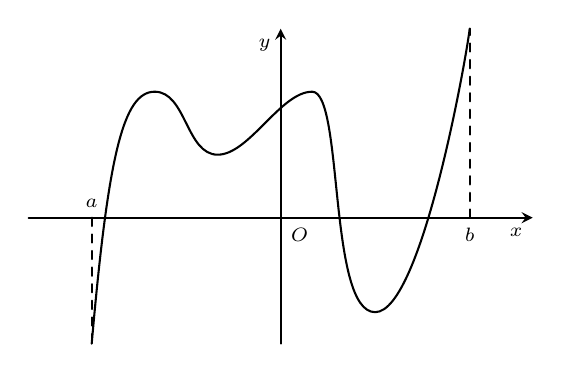
\begin{tikzpicture}[>=stealth,line join=round, line cap=round, font=\scriptsize]
            \begin{scope}[scale=.8]
                \draw[-stealth](-4,0)--(0,0)node[below right]{$O$}--(4,0)node[below left]{$x$};
                \draw[-stealth](0,-2)--(0,3)node[below left]{$y$};
                \draw[dashed]
                (-3,0)node[above]{$a$}--(-3,-2)
                (3,0)node[below]{$b$}--(3,3)
                ;
                \draw[smooth]
                (-3,-2)..controls+(85:3) and+(180:.5)..(-2,2)
                ..controls+(0:.5) and+(180:.5)..(-1,1)
                ..controls+(0:.5)and+(180:.5)..(0.5,2)
                ..controls+(0:.5)and+(180:.75)..(1.5,-1.5)
                ..controls+(0:.75)and+(-95:.3)..(3,3)
                ;
            \end{scope}
    \end{tikzpicture}}
    \loigiai{}
\end{vd}
\begin{vd}
    Tìm $m$ để
    \begin{listEX}
        \item  Hàm số $y=|f(x)|$ có $5$ điểm cực trị, với  $f(x)= 3x^3+3x^2+mx+m$
        \item Hàm số $y=f\left(\vert x\vert\right)$ có $5$ điểm cực trị, với $f(x)=x^3-(2m-1)x^2+(2-m)x+2$.
    \end{listEX}
    \loigiai{
        \begin{listEX}
            \item Đặt $f(x)=3x^3+3x^2+mx+m=3x^2(x+1)+m(x+1)=(x+1)(3x^2+m)$.\\
            Suy ra $f'(x)=9x^2+6x+m$.\\
            Phương trình $f'(x)=0$ có $2$ nghiệm phân biệt $x_1$, $x_2$ khi và chỉ khi $\Delta'=9-9m>0\Leftrightarrow m<1$. Khi đó ta có $x_1+x_2=-\dfrac{2}{3}$, $x_1x_2=\dfrac{m}{9}$.\\
            Hàm số $y=|f(x)|$ có $5$ điểm cực trị khi và chỉ khi $\heva{&\Delta'>0\\&y(x_1)\cdot y(x_2)<0.}$\\
            Thực hiện biến đổi
            \allowdisplaybreaks
            \begin{eqnarray*}
                y(x_1)\cdot y(x_2) &=&\ (x_1+1)(3x_1^2+m)\cdot(x_2+1)(3x_2^2+m)\\
                &=&\ \left[9(x_1x_2)^2+3m(x_1^2+x_2^2)+m^2\right]\left(x_1x_2+x_1+x_2+1\right)\\
                &=&\ \left[\dfrac{m^2}{9}+3m\left[\left(-\dfrac{2}{3}\right)^2-\dfrac{2m}{9}\right]+m^2\right]\left(\dfrac{m}{9}-\dfrac{2}{3}+1\right)\\
                &=&\ \dfrac{1}{9}(4m^2+12m)(m+3).
            \end{eqnarray*}
            Suy ra $y(x_1)\cdot y(x_2)<0\Leftrightarrow (4m^2+12m)(m+3)<0\Leftrightarrow -3\neq m<0$.\\
            Kết hợp với điều kiện $m$ là số nguyên thỏa $|m|<10$ ta được $m\in\{-1;-2;-4;-5;-6;-7;-8;-9\}$.\\
            Vậy có $8$ giá trị nguyên của tham số $m$.
            \item Tập xác định $\mathscr{D}=\mathbb{R}$.\\
            Ta có $f\left(|-x|\right)=f\left(|x|\right)$, $\forall x\in\mathbb{R}$ nên $y=f\left(|x|\right)$ là hàm số chẵn. \\
            Do đó, đồ thị hàm số $y=f\left(|x|\right)$ đối xứng qua trục tung.\\
            Suy ra hàm số $y=f\left(|x|\right)$ luôn có một điểm cực trị là $x=0$.\\
            Do đó, $y=f\left(|x|\right)$ có $5$ điểm cực trị $\Leftrightarrow$ hàm số $y=f(x)$ có $2$ điểm cực trị dương.\\
            \phantom{Do đó, số $y=f\left(|x|\right)$ có $5$ điểm cực trị} $\Leftrightarrow$ $f'(x)=0$ có hai nghiệm dương phân biệt.\\
            Ta có $f'(x)=3x^2-2(m-1)x+2-m$.\\
            Yêu cầu bài toán $\Leftrightarrow\heva{&\Delta'>0 \\ &S>0 \\ &P>0}\Leftrightarrow\heva{&4m^2-m-5>0 \\ &2m-1>0 \\ &2-m>0}\Leftrightarrow\heva{&m<-1\;\text{hoặc}\;m>\dfrac{5}{4} \\ &m>\dfrac{1}{2} \\ &m<3}\Leftrightarrow \dfrac{5}{4}<m<2$.
        \end{listEX}
    }
\end{vd}
\boxmini{BÀI TẬP TRẮC NGHIỆM}
\Opensolutionfile{ans}[ans/2D1-2-DANG-3]
\begin{ex}%[2D1K2-6]
    \immini
    {Cho hàm số $f(x)$ có đồ thị $f'(x)$ có đồ thị như hình vẽ bên dưới.\\ Hàm số $y=f(1-2x)$ có bao nhiêu cực trị ?
        \choice[2]
        {$4$}
        {$7$}
        {\True $3$}
        {$9$}
    }
    {
        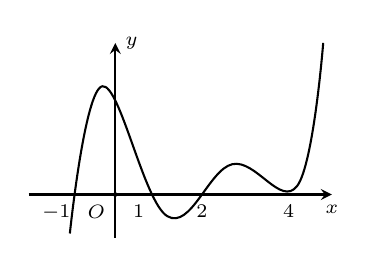
\begin{tikzpicture}[>=stealth,font=\scriptsize]
            \begin{scope}[scale=0.55]
                \draw[->] (0,-1)--(0,3.5)node[right]{\scriptsize $y$};
                \draw[->] (-2,0)--(5,0)node[below]{\scriptsize $x$};
                \fill (0,0) node[below left]{\scriptsize  $O$} circle(1.5pt);
                \draw (-0.8,0) node[below left]{ $-1$} (0.9,0) node[below left]{ $1$} (2,0) node[below]{ $2$} (4,0) node[below]{ $4$};
                \clip (-2,-1) rectangle (5,3.5);
                \draw[] plot[smooth,tension=.65] coordinates{(-1.05,-0.9) (-0.3,2.5) (1.2,-0.5) (2.7,0.7) (4.2,0.2) (4.8,3.5)};
            \end{scope}
        \end{tikzpicture}
    }
    \loigiai{
        Đặt $g(x)=f(1-2x)$\\
        Dựa vào đồ thị, ta thấy $f'(x)=0$ có nghiệm $x_1=-1,x_2=1,x_3=2$ và $x_4=4$ nên $f'(x)$ có dạng $$f'(x)=k(x+1)(x-1)(x-2)(x-4)$$
        Khi đó $g'(x)=-2f'(1-2x)=-2k(2-2x)(-2x)(-1-2x)(-3-2x)^2$
        $$g'(x)=0 \Leftrightarrow \hoac{&x=1\\&x=0\\&x=-\dfrac{1}{2}\\&x=-\dfrac{3}{2} \text{ (kép)}}$$
        Bảng xét dấu $g'(x)$
        \begin{center}
            \begin{tikzpicture}[every node/.style={circle,fill=white,inner sep=0pt},arrow/.style={>=stealth,->,shorten <= 0.3cm,shorten >= 0.3cm},font=\footnotesize,xscale=1,yscale=1]
                \def\mnumline{1} %Số dòng
                \def\mnumcol{11} %Số cột
                \foreach \j in {0,...,\mnumline}
                \foreach \i in {0,...,\mnumcol}{
                    \coordinate (\j\i) at (\i,-\j);
                }
                \pgfmathsetmacro\yline{\mnumline/2-1}
                \path node at (00){$x$} node at (10){$g'(x)$};
                \foreach \x/\mnamex in {01/$-\infty$,03/$-\dfrac{3}{2}$,05/$-\dfrac{1}{2}$,07/$0$,09/$1$,0\mnumcol/$+\infty$} \path node at (\x) {\mnamex};
                \foreach \dy/\mnamedy in {12/$-$,13/$0$,14/$-$,15/$0$,16/$+$,17/$0$,18/$-$,19/$0$,110/$+$} \path node at (\dy) {\mnamedy};
                \draw[thick] (-.5,.5)rectangle([xshift=0.5cm,yshift=-0.5cm]\mnumline\mnumcol) ([xshift=-0.5cm,yshift=-0.5cm]00)--([xshift=0.5cm,yshift=-0.5cm]0\mnumcol)  ([xshift=0.5cm,yshift=0.5cm]00)--([xshift=0.5cm,yshift=-0.5cm]\mnumline0);
            \end{tikzpicture}
        \end{center}
        Dựa vào bảng xét dấu, ta thấy $g'(x)$ đổi dấu 3 lần nên $y=f(1-2x)$ có 3 cực trị.
    }
\end{ex}
\begin{ex}%[2D1K2-2]
    \immini{Cho hàm số $ f(x) $ có đạo hàm là $ f'(x) $. Đồ thị của hàm số $ y=f'(x) $ như hình vẽ bên. Khi đó hàm số $ y=f(x^2) $ có bao nhiêu điểm cực trị?
        \choice[2]
        {$2$}
        {$4$}
        {\True $3$}
        {$5$}}
    {
        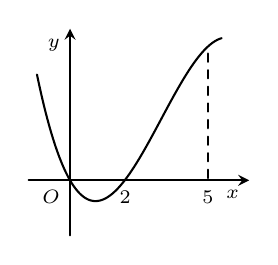
\begin{tikzpicture}[line join=round, line cap=round,>=stealth,font=\scriptsize]
            \begin{scope}[scale=0.35]
                \tikzset{label style/.style={font=\footnotesize}}
                \def \xmin{-1.5}
                \def \xmax{6.5}
                \def \ymin{-2}
                \def \ymax{5.5}
                \def \hamso{-0.11*(\x)^3+1.09*(\x)^2-1.73*(\x)}
                \draw[->] (\xmin,0)--(\xmax,0) node[below left] {$x$};
                \draw[->] (0,\ymin)--(0,\ymax) node[below left] {$y$};
                \draw (0,0) node [below left] {$O$};
                \begin{scope}
                    \clip (\xmin+0.01,\ymin+0.01) rectangle (\xmax-0.01,\ymax-0.01);
                    \draw[samples=350,domain=-1.2:5.5,smooth,variable=\x] plot (\x,{\hamso});
                \end{scope}
                \draw [dashed] (5,4.6)--(5,0) node[below]{$5$} (2,0) node[below]{$2$};
            \end{scope}
        \end{tikzpicture}
    }
    \loigiai{$ y'=2xf'(x^2) $. Cho $ y'=0 \Leftrightarrow \hoac{&x=0\\&f'(x^2)=0} \Leftrightarrow \hoac{&x=0\\&x^2=0\\&x^2=2} \Leftrightarrow \hoac{&x=0\\&x=0 \text{ (nghiệm kép)}\\&x=\pm \sqrt{2}} $.\\
        $ y'=0 $ có 3 nghiệm bội bậc lẻ nên hàm số có 3 điểm cực trị.
    }
\end{ex}
\begin{ex}%[2D1K2-6]
    \immini{	Cho hàm số $y=f(x)$ xác định trên $\mathbb{R}$ và hàm số $y=f'(x)$ có đồ thị như hình vẽ. Hàm số $y=f(1-x^2)$ đạt cực đại tại điểm nào sau đây?
        \choice[2]
        {$x=-1$}
        {\True $x=\pm \sqrt{2}$}
        {$x=3$}
        {$x=0$}}{
        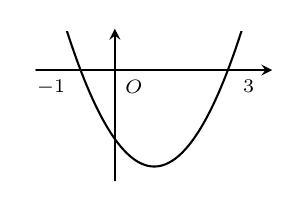
\begin{tikzpicture}[>=stealth, font=\scriptsize, line join=round, line cap=round,y=0.7cm]
            \begin{scope}[scale=.5]
                \def\a{1} \def\b{-2} \def\c{-2.5} % Hệ số
                \def\xmin{-2} \def\xmax{4}
                \def\ymin{-4} \def\ymax{1.5}
                %\draw[color=gray!50,dashed] (\xmin,\ymin) grid (\xmax,\ymax);
                \draw[->] (\xmin,0)--(\xmax,0);
                \draw[->] (0,\ymin)--(0,\ymax);
                \node at (0,0) [below right]{$O$};
                \node at (-1,0) [below left]{$-1$};
                \node at (3,0) [below right]{$3$};
                \clip (\xmin+0.1,\ymin+0.1) rectangle (\xmax-0.5,\ymax-0.1);
                \draw[smooth,samples=300,domain=-1.3:3.3] plot(\x,{\a*(\x)^2+\b*(\x)+\c});
            \end{scope}
    \end{tikzpicture}}
    \loigiai{Đặt $g(x)=f(1-x^2)$\\
        Khi đó $g'(x)=-2x\cdot f'(1-x^2)$\\
        Cho $g'(x)=0 \Leftrightarrow -2x \cdot f'(1-x^2) =0$
        $$ \Leftrightarrow \hoac{&x=0\\&f'(1-x^2)=0 \Leftrightarrow \hoac{&1-x^2=-1\Leftrightarrow x^2=2 \Leftrightarrow x=\pm \sqrt{2}\\&1-x^2=3}}$$
        Bảng xét dấu
        \begin{center}
            \begin{tikzpicture}[every node/.style={circle,fill=white,inner sep=0pt},arrow/.style={>=stealth,->,shorten <= 0.3cm,shorten >= 0.3cm},font=\footnotesize,xscale=1.4,yscale=.8]
                \def\mnumline{3} %Số dòng
                \def\mnumcol{9} %Số cột
                \foreach \j in {0,...,\mnumline}
                \foreach \i in {0,...,\mnumcol}{
                    \coordinate (\j\i) at (\i,-\j);
                    %	\draw[gray!30] ([xshift=-0.5cm,yshift=0.5cm]\j\i)--([xshift=0.5cm,yshift=0.5cm]\j\i)--([xshift=0.5cm,yshift=-0.5cm]\j\i)--([xshift=-0.5cm,yshift=-0.5cm]\j\i)--cycle (\j\i)node[]{\j\i}; %Ẩn lệnh này sau khi hoàn thành BBT
                }
                \pgfmathsetmacro\yline{\mnumline/2-1}
                \path node at (00){$x$} node at (10){$-x$} node at (20){\scriptsize $f'(1-x^2)$} node at (30){$g'(x)$};
                \foreach \x/\mnamex in {01/$-\infty$,03/$-\sqrt{2}$,05/$0$,07/$\sqrt{2}$,0\mnumcol/$+\infty$} \path node at (\x) {\mnamex};
                \foreach \dy/\mnamedy in {12/$-$,13/$0$,14/$+$,16/$+$} \path node at (\dy) {\mnamedy};
                \path node at ($(12)$){$+$} node at ($(13)$){$|$} node at ($(14)$){$+$} node at ($(15)$){$0$} node at ($(16)$){$-$} node at ($(17)$){$|$} node at ($(18)$){$-$} node at ($(22)$){$+$} node at ($(23)$){$0$} node at ($(24)$){$-$} node at ($(25)$){$|$} node at ($(26)$){$-$} node at ($(27)$){$0$} node at ($(28)$){$+$} node at ($(32)$){$+$} node at ($(33)$){$0$} node at ($(34)$){$-$} node at ($(35)$){$0$} node at ($(36)$){$+$} node at ($(37)$){$0$} node at ($(38)$){$-$};
                \draw[thick] (-.5,.5)rectangle([xshift=0.5cm,yshift=-0.5cm]\mnumline\mnumcol) ([xshift=-0.5cm,yshift=-0.5cm]00)--([xshift=0.5cm,yshift=-0.5cm]0\mnumcol) ([xshift=-0.5cm,yshift=-0.5cm]10)--([xshift=0.5cm,yshift=-0.5cm]1\mnumcol)

                ([xshift=-0.5cm,yshift=-0.5cm]20)--([xshift=0.5cm,yshift=-0.5cm]2\mnumcol)

                ([xshift=0.5cm,yshift=0.5cm]00)--([xshift=0.5cm,yshift=-0.5cm]\mnumline0); %Lệnh tự động kẻ bảng
            \end{tikzpicture}
        \end{center}
        Dựa vào bảng xét dấu ta xác định được hàm số đạt cực đại tại $x=\pm \sqrt{2}$.}
\end{ex}
\begin{ex}%[2D1K2-6]
    \immini{Cho hàm số $y=f(x)$ có đồ thị hàm $f'(x)=ax^2+bx+c$ như hình bên dưới. Hỏi hàm số $y=f(x-x^2)$ có bao nhiêu cực trị?
        \choice[2]
        {$0$}
        {\True $1$}
        {$2$}
        {$3$}}{
        \begin{tikzpicture}[>=stealth,x=1.2cm,y=0.7cm,font=\scriptsize]
            \begin{scope}[scale=0.35]
                \clip (-2,-2) rectangle (5,5.5);
                \def\a{1}
                \def\b{-3}
                \def\c{2}
                \draw[->] (-2,0) -- (4,0) node[below] { $x$};
                \draw[->] (0,-1) -- (0,5) node[left] {$y$};
                \draw (0,0)node[below left]{ $O$} circle(1.5pt);
                \draw (1,0) node[below]{$1$} (2,0) node[below]{  $2$} (0,2) node[left]{$2$};
                \pgfmathsetmacro\xdinh{-(\b)/2*(\a)}
                \pgfmathsetmacro\ydinh{(4*(\a)*(\c)-(\b)^2)/(4*(\a))}
                \draw[samples=150,smooth,domain=-5:5] plot(\x,{\a*(\x)^2+(\b)*\x+(\c)});
            \end{scope}
        \end{tikzpicture}
    }
    \loigiai{
        Đặt $g(x)=f\left(x-x^2\right)$\\
        Dựa vào đồ thị ta thấy $f'(x)=0$ có hai nghiệm $x_1=1,x_2=2$ nên $f'(x)$ có dạng $$f'(x)=k(x-1)(x-2)$$
        Khi đó $g'(x)=(1-2x)f'\left(x-x^2\right)=0$
        $$ \Leftrightarrow \hoac{&1-2x=0\\&f'\left(x-x^2\right)=0} \Leftrightarrow \hoac{&x=\dfrac{1}{2}\\&x-x^2=1\\&x-x^2=2} \Leftrightarrow \hoac{&x=\dfrac{1}{2}\\& \text{ vô nghiệm}\\&\text{ vô nghiệm.}}$$
        Bảng xét dấu
        \begin{center}
            \begin{tikzpicture}[every node/.style={circle,fill=white,inner sep=0pt},arrow/.style={>=stealth,->,shorten <= 0.3cm,shorten >= 0.3cm},font=\footnotesize,xscale=1,yscale=1]
                \def\mnumline{1} %Số dòng
                \def\mnumcol{5} %Số cột
                \foreach \j in {0,...,\mnumline}
                \foreach \i in {0,...,\mnumcol}{
                    \coordinate (\j\i) at (\i,-\j);
                }
                \pgfmathsetmacro\yline{\mnumline/2-1}
                \path node at (00){$x$} node at (10){$g'(x)$};
                \foreach \x/\mnamex in {01/$-\infty$,03/$\dfrac{1}{2}$,0\mnumcol/$+\infty$} \path node at (\x) {\mnamex};
                \foreach \dy/\mnamedy in {12/$+$,13/$0$,14/$-$} \path node at (\dy) {\mnamedy};
                \draw[thick] (-.5,.5)rectangle([xshift=0.5cm,yshift=-0.5cm]\mnumline\mnumcol) ([xshift=-0.5cm,yshift=-0.5cm]00)--([xshift=0.5cm,yshift=-0.5cm]0\mnumcol)  ([xshift=0.5cm,yshift=0.5cm]00)--([xshift=0.5cm,yshift=-0.5cm]\mnumline0);
            \end{tikzpicture}
        \end{center}
        Dựa vào bảng xét dấu, ta thấy $g(x)$ có 1 cực đại.
    }
\end{ex}
\begin{ex}%[2D1K2-2]
    \immini{Cho hàm số bậc bốn $y=f(x)$. Hàm số $y=f'(x)$
        có đồ thị như hình bên. Số điểm cực trị của hàm số $y=f\left(\sqrt{x^{2}+2 x+2}\right)$ là
        \choice[2]
        {$1$}
        {$2$}
        {$4$}
        {\True $3$}}
    {
        \begin{tikzpicture}[line join=round, line cap=round,>=stealth,font=\scriptsize]
            \begin{scope}[scale=0.5]
                \tikzset{label style/.style={font=\footnotesize}}
                \def \xmin{-2}
                \def \xmax{4.5}
                \def \ymin{-2}
                \def \ymax{3.5}
                \def \hamso{0.55*(\x)^3-1.76*(\x)^2-0.31*(\x)+2}
                \draw[->] (\xmin,0)--(\xmax,0) node[below left] {$x$};
                \draw[->] (0,\ymin)--(0,\ymax) node[below left] {$y$};
                \draw (0,0) node [below left] {$O$};
                \begin{scope}
                    \clip (\xmin+0.01,\ymin+0.01) rectangle (\xmax-0.01,\ymax-0.01);
                    \draw[samples=350,domain=-1.3:3.3,smooth,variable=\x] plot (\x,{\hamso});
                \end{scope}
                \draw (-1,0) node[below left]{$-1$} (1,0) node[below]{$1$} (3,0) node[below right]{$3$} (0,2) node[above left]{$2$};
            \end{scope}
        \end{tikzpicture}
    }
    \loigiai{
        $ y'=\dfrac{x+1}{\sqrt{x^2+2x+2}}f'(\sqrt{x^2+2x+2}) $.\\$ y'=0 \Leftrightarrow \hoac{&x=-1\\&f'(\sqrt{x^2+2x+2})=0} \Leftrightarrow \hoac{&x=-1\\&\sqrt{x^2+2x+2}=-1\\&\sqrt{x^2+2x+2}=1\\&\sqrt{x^2+2x+2}=3} \Leftrightarrow \hoac{&x=-1\\&x^2+2x+1=0\\&x^2+2x-7=0}\Leftrightarrow \hoac{&x=-1\\&x=-1 \text{ (nghiệm kép)}\\&x=-1\pm 2\sqrt{2}} $\\
        $ y'=0 $ có 3 nghiệm bội bậc lẻ nên hàm số có 3 điểm cực trị.
    }
\end{ex}
\begin{ex}%[2D1K2-2]
    \immini{Cho hàm số $ y=f(x) $ liên tục trên $ (a,b) $ và có đồ thị như hình bên. Số điểm cực trị của hàm số $ y=\left[f(x)\right]^2 $ trên $ (a;b) $ là
        \choice[2]
        {$4$}
        {$6$}
        {$2$}
        {\True $5$}}
    {
        \begin{tikzpicture}[line join=round, line cap=round,>=stealth,font=\scriptsize]
            \begin{scope}[scale=.35]
                \def \xmin{-3.5}
                \def \xmax{4.5}
                \def \ymin{-4}
                \def \ymax{3.5}
                \def \hamso{-0.37*(\x)^3+0.15*(\x)^2+2.41*(\x)-1}
                \draw[->] (\xmin,0)--(\xmax,0) node[below] {$x$};
                \draw[->] (0,\ymin)--(0,\ymax) node[left] {$y$};
                \draw (0,0) node [below left] {$O$};
                \clip (\xmin+0.01,\ymin+0.01) rectangle (\xmax-0.01,\ymax-0.01);
                \draw[samples=350,domain=-3:4,smooth,variable=\x] plot (\x,{\hamso});
                \draw[dashed] (-3,3.11)--(-3,0) node[below]{$a$} (3,-2.41)--(3,0) node[above]{$b$};
            \end{scope}
        \end{tikzpicture}
    }
    \loigiai{\immini{$ y=\left(f(x)\right)^2 $ nên $ y'=2f(x)f'(x) $.\\$ y'=0 \Leftrightarrow \hoac{&f(x)=0\\&f'(x)=0} \Leftrightarrow \hoac{&x=x_1,\ x=x_2,\ x=x_3\\&x=c,\ x=d}$.\\
            $ y'=0 $ có 5 nghiệm bội bậc lẻ thuộc $ (a,b) $ nên Số điểm cực trị của hàm số $ y=\left(f(x)\right)^2 $ trên $ (a;b) $ là 5.}
        {
            \begin{tikzpicture}[line join=round, line cap=round,>=stealth,thick,scale=0.8]
                \tikzset{label style/.style={font=\footnotesize}}
                \def \xmin{-3.5}
                \def \xmax{4.5}
                \def \ymin{-4}
                \def \ymax{3.5}
                \def \hamso{-0.37*(\x)^3+0.15*(\x)^2+2.41*(\x)-1}
                \draw[->] (\xmin,0)--(\xmax,0) node[below left] {$x$};
                \draw[->] (0,\ymin)--(0,\ymax) node[below left] {$y$};
                \draw (0,0) node [below left] {$O$};
                \begin{scope}
                    \clip (\xmin+0.01,\ymin+0.01) rectangle (\xmax-0.01,\ymax-0.01);
                    \draw[samples=350,domain=-3:4,smooth,variable=\x] plot (\x,{\hamso});
                \end{scope}
                \draw[dashed] (-3,3.11)--(-3,0) node[below]{\footnotesize $a$} (3,-2.41)--(3,0) node[above]{\footnotesize $b$} (2.54,0) node[below left]{\footnotesize $x_3$} (0.41,0) node[below right]{\footnotesize $x_2$} (-2.55,0) node[above right]{\footnotesize $x_1$} (-1.34,-3.07) -- (-1.34,0) node[above]{\footnotesize $c$} (1.61,1.72)--(1.61,0) node[below]{\footnotesize $d$};
            \end{tikzpicture}
        }
    }
\end{ex}
\begin{ex}%[2D1G2-1]
    \immini{Cho hàm số $y=f(x)$ có đạo hàm trên $\mathbb{R}$ và có bảng xét dấu $f'(x)$ như hình bên. Hàm số $y=f\left(x^{2}-2 x\right)$ có bao nhiêu điểm cực tiểu?
        \choice
        {\True $1$}
        {$2$}
        {$3$}
        {$4$}}{\begin{tikzpicture}
            \tkzTabInit[lgt=1,espcl=1.2]
            {$x$ /.7, $y'$ /.7}
            {$-\infty$,$-2$,$1$,$3$,$+\infty$}
            \tkzTabLine{ ,-,0,+,0,+,0,-, }
    \end{tikzpicture}}
    \loigiai{$ y'=(2x-2)f'(x^2-2x) $.
        \begin{eqnarray*}
            y'=0 	&\Leftrightarrow& \hoac{&x=1\\&f'(x^2-2x)=0}\\
            &\Leftrightarrow& \hoac{&x=1\\&x^2-2x=-2 \text{ (vô nghiệm)}\\&x^2-2x=1 \text{ (nghiệm bội bậc chẵn)}\\&x^2-2x=3} \\
            &\Leftrightarrow& \hoac{&x=1\\&x=1-\sqrt{2} \text{ (nghiệm bội bậc chẵn)}\\&x=1+\sqrt{2} \text{ (nghiệm bội bậc chẵn)}\\&x=3, \ x=-1.}
        \end{eqnarray*}
        $ y'=0 $ có 3 nghiệm bội bậc lẻ, khi đó $ y' $ đổi dấu qua các nghiệm này.\\
        $ y'=0 $ có 2 nghiệm bội bậc chẵn và $ y' $ sẽ không đổi dấu qua các nghiệm này.\\
        Tại $ x=4 $ thì $ y'(4)=(2\cdot 4 -2)f'(4^2-2\cdot 4)=6f'(8)<0 $.\\
        Bảng xét dấu
        \begin{center}
            \begin{tikzpicture}
                \tkzTabInit[lgt=1,espcl=1.2]
                {$x$ /1, $y'$ /1}
                {$-\infty$,$-1$,$1-\sqrt{2}$,$1+\sqrt{2}$,$3$,$+\infty$}
                \tkzTabLine{ ,-,0,+,0,+,0,+,0,-, }
            \end{tikzpicture}
        \end{center}
        Vậy hàm số có 1 điểm cực tiểu.
    }
\end{ex}
\begin{ex}%[2D1K2-6]
    \immini{Cho hàm số $f(x)$ có bảng biến thiên bên dưới. Trên khoảng $(-\sqrt{5};\sqrt{5})$ thì hàm số $y=f(x^2)$ đạt cực đại tại điểm nào sau đây?\choice
        {$x=\sqrt{2}$}
        {$x=-\sqrt{2}$}
        {\True $x=0$}
        {$x=2$}}{\begin{tikzpicture}
            \tkzTabInit[nocadre=false,lgt=1,espcl=1.6,deltacl=0.5]{$x$/.7 ,$f$/.7}
            {$-\infty$ , $0$ , $2$ , $+\infty$}
            \tkzTabLine{  , + , 0, - , 0 , +  }
    \end{tikzpicture}}
    \loigiai{Đặt $g(x)=f(x^2)$.\\
        Khi đó $g'(x)=2x \cdot f'(x^2)$.\\
        Cho $g'(x)=0 \Leftrightarrow 2x \cdot f'(x^2) =0 \Leftrightarrow
        \hoac{&x=0\\&f'(x^2)=0 \Leftrightarrow \hoac{x^2=0\\x^2=2} \Leftrightarrow \hoac{x=0\\x=\pm \sqrt{2}}}$\\
        Bảng xét dấu
        \begin{center}
            \begin{tikzpicture}[every node/.style={circle,fill=white,inner sep=0pt},arrow/.style={>=stealth,->,shorten <= 0.3cm,shorten >= 0.3cm},font=\footnotesize,xscale=1,yscale=.7]
                \def\mnumline{3} %Số dòng
                \def\mnumcol{9} %Số cột
                \foreach \j in {0,...,\mnumline}
                \foreach \i in {0,...,\mnumcol}{
                    \coordinate (\j\i) at (\i,-\j);
                }
                \pgfmathsetmacro\yline{\mnumline/2-1}
                \path node at (00){$x$} node at (10){$x$} node at (20){$f'(x^2)$} node at (30){$g'(x)$};
                \foreach \x/\mnamex in {01/$-\sqrt{5}$,03/$-\sqrt{2}$,05/$0$,07/$\sqrt{2}$,0\mnumcol/$\sqrt{5}$} \path node at (\x) {\mnamex};
                \foreach \dy/\mnamedy in {12/$-$,13/$0$,14/$+$,16/$+$} \path node at (\dy) {\mnamedy};
                \path node at ($(12)$){$-$} node at ($(13)$){$|$} node at ($(14)$){$-$} node at ($(15)$){$0$} node at ($(16)$){$+$} node at ($(17)$){$|$} node at ($(18)$){$+$} node at ($(22)$){$+$} node at ($(23)$){$0$} node at ($(24)$){$-$} node at ($(25)$){$0$} node at ($(26)$){$-$} node at ($(27)$){$0$} node at ($(28)$){$+$} node at ($(32)$){$-$} node at ($(33)$){$0$} node at ($(34)$){$+$} node at ($(35)$){$0$} node at ($(36)$){$-$} node at ($(37)$){$0$} node at ($(38)$){$+$};
                \draw[thick] (-.5,.5)rectangle([xshift=0.5cm,yshift=-0.5cm]\mnumline\mnumcol) ([xshift=-0.5cm,yshift=-0.5cm]00)--([xshift=0.5cm,yshift=-0.5cm]0\mnumcol) ([xshift=-0.5cm,yshift=-0.5cm]10)--([xshift=0.5cm,yshift=-0.5cm]1\mnumcol)

                ([xshift=-0.5cm,yshift=-0.5cm]20)--([xshift=0.5cm,yshift=-0.5cm]2\mnumcol)

                ([xshift=0.5cm,yshift=0.5cm]00)--([xshift=0.5cm,yshift=-0.5cm]\mnumline0); %Lệnh tự động kẻ bảng
            \end{tikzpicture}
        \end{center}
        Dựa vào bảng xét dấu ta xác định được hàm số đạt cực đại tại $x=0$.
    }
\end{ex}
\begin{ex}%[2D1K2-6]
    \immini{Cho hàm số $f(x)$ có bảng biến thiên bên dưới. Hàm số $y=f(x^2-2)$ đạt cực đại tại điểm nào sau đây?
        \choice
        {$x=-2$}
        {$x=-1$}
        {\True $x=0$}
        {$x=2$}}{\begin{tikzpicture}
            \tkzTabInit[nocadre=false,lgt=1,espcl=1.6,deltacl=0.5]{$x$/.7 ,$f$/.7}
            {$-\infty$ , $-1$ , $2$ , $+\infty$}
            \tkzTabLine{  , - , 0, - , 0 , +  }
    \end{tikzpicture}}
    \loigiai{Đặt $g(x)=f(x^2-2)$\\
        Khi đó $g'(x)=2x \cdot f'(x^2-2)$\\
        Cho $g'(x)=0 \Leftrightarrow 2x \cdot f'(x^2-2) =0$
        $$ \Leftrightarrow \hoac{&x=0\\&f'(x^2-2)=0 \Leftrightarrow \hoac{&x^2-2=-1\\&x^2-2=2} \Leftrightarrow \hoac{x^2=1\\x^2=4} \Leftrightarrow \hoac{x=\pm 1\\x=\pm 2}}$$
        Bảng xét dấu
        \begin{center}
            \begin{tikzpicture}[every node/.style={circle,fill=white,inner sep=0pt},arrow/.style={>=stealth,->,shorten <= 0.3cm,shorten >= 0.3cm},font=\footnotesize,xscale=1,yscale=1]
                \def\mnumline{3} %Số dòng
                \def\mnumcol{14} %Số cột
                \foreach \j in {0,...,\mnumline}
                \foreach \i in {0,...,\mnumcol}{
                    \coordinate (\j\i) at (\i,-\j);
                }
                \pgfmathsetmacro\yline{\mnumline/2-1}
                \path node at ([xshift=0.5cm]00){$x$} node at ([xshift=0.5cm]10){$x$}  node at ([xshift=0.5cm]20){$f'\left(x^2-2\right)$} node at ([xshift=0.5cm]\mnumline0){$g'(x)$};
                \foreach \x/\mnamex in {02/$-\infty$,04/$-2$,06/$-1$,08/$0$,010/$1$,012/$2$,0\mnumcol/$+\infty$} \path node at (\x) {\mnamex};
                \foreach \dy/\mnamedy in {13/$-$,14/$0$,15/$+$,16/$+$} \path node at (\dy) {\mnamedy};
                \path node at ($(13)$){$-$} node at ($(14)$){$|$} node at ($(15)$){$-$} node at ($(16)$){$|$} node at ($(17)$){$-$} node at ($(18)$){$0$} node at ($(19)$){$+$} node at ($(110)$){$|$} node at ($(111)$){$+$} node at ($(112)$){$|$} node at ($(113)$){$+$}
                node at ($(23)$){$+$} node at ($(24)$){$0$} node at ($(25)$){$-$} node at ($(26)$){$0$} node at ($(27)$){$-$} node at ($(28)$){$|$} node at ($(29)$){$-$} node at ($(210)$){$0$} node at ($(211)$){$-$} node at ($(212)$){$0$} node at ($(213)$){$+$}
                node at ($(33)$){$-$} node at ($(34)$){$0$} node at ($(35)$){$+$} node at ($(36)$){$0$} node at ($(37)$){$+$} node at ($(38)$){$0$} node at ($(39)$){$-$} node at ($(310)$){$0$} node at ($(311)$){$-$} node at ($(312)$){$0$} node at ($(313)$){$+$};
                \draw[thick] (-.5,.5)rectangle([xshift=0.5cm,yshift=-0.5cm]\mnumline\mnumcol) ([xshift=-0.5cm,yshift=-0.5cm]00)--([xshift=0.5cm,yshift=-0.5cm]0\mnumcol)
                ([xshift=-0.5cm,yshift=-0.5cm]20)--([xshift=0.5cm,yshift=-0.5cm]2\mnumcol)
                ([xshift=-0.5cm,yshift=-0.5cm]10)--([xshift=0.5cm,yshift=-0.5cm]1\mnumcol) ([xshift=0.5cm,yshift=0.5cm]01)--([xshift=0.5cm,yshift=-0.5cm]\mnumline1); %Lệnh tự động kẻ bảng
            \end{tikzpicture}
        \end{center}
        Dựa vào bảng xét dấu ta xác định được hàm số đạt cực đại tại $x=0$.
    }
\end{ex}
\begin{ex}%[2D1K2-1]
    Cho hàm số $ y=f(x) $ có đạo hàm $ f'(x)=x^2(x-1)(x-4)^2 $. Khi đó hàm số $ y=f(x^2) $ có bao nhiêu điểm cực trị?
    \choice
    {$4$}
    {\True $3$}
    {$5$}
    {$2$}
    \loigiai{$ f'(x)=0 \Leftrightarrow x=1 $ (nghiệm đơn), $ x=0 $ (nghiệm kép), $ x=4 $ (nghiệm kép).\\
        $ y=f(x^2) $ thì $ y'=2xf'(x^2) $.\\$y'=0 \Leftrightarrow \hoac{&x=0\\&x^2=1\\&x^2=0 \text{ (nghiệm kép)}\\&x^2=4 \text{ (nghiệm kép)}} \Leftrightarrow \hoac{&x=0\\&x=\pm 1\\&x=0 \text{ (nghiệm bội chẵn)}\\&x=\pm 2 \text{ (nghiệm bội chẵn).}} $\\
        Vậy hàm số có 3 điểm cực trị.
    }
\end{ex}
\begin{ex}%[2D1K2-6]
    Cho hàm $f(x)$ có đạo hàm $f'(x)=x^2-2x,\forall x\in \mathbb{R}$. Hàm số $y=f\left(1-\dfrac{1}{2}x\right)+4x$ có bao nhiêu điểm cực trị?
    \choice
    {0}
    {1}
    {\True 2}
    {3}
    \loigiai{Ta có $y'=-\dfrac{1}{2}f'\left(1-\dfrac{1}{2}x\right)+4$\\
        $y'=0 \Leftrightarrow
        f'\left(1-\dfrac{1}{2}x\right)=8\Leftrightarrow \left(1-\dfrac{1}{2}x\right)^2-2\left(1-\dfrac{1}{2}x\right)=8 \Leftrightarrow \dfrac{1}{4}x^2-9=0
        \Leftrightarrow \hoac{&x=-6\\&x=6}$\\
        Bảng xét dấu
        \begin{center}
            \begin{tikzpicture}[every node/.style={circle,fill=white,inner sep=0pt},arrow/.style={>=stealth,->,shorten <= 0.3cm,shorten >= 0.3cm},font=\footnotesize,xscale=1,yscale=1]
                \def\mnumline{1} %Số dòng
                \def\mnumcol{7} %Số cột
                \foreach \j in {0,...,\mnumline}
                \foreach \i in {0,...,\mnumcol}{
                }
                \pgfmathsetmacro\yline{\mnumline/2-1}
                \path node at (00){$x$} node at (10){$y'$};
                \foreach \x/\mnamex in {01/$-\infty$,03/$-6$,05/$6$,0\mnumcol/$+\infty$} \path node at (\x) {\mnamex};
                \foreach \dy/\mnamedy in {12/$+$,13/$0$,14/$-$,15/$0$,16/$+$} \path node at (\dy) {\mnamedy};
                \draw[thick] (-.5,.5)rectangle([xshift=0.5cm,yshift=-0.5cm]\mnumline\mnumcol) ([xshift=-0.5cm,yshift=-0.5cm]00)--([xshift=0.5cm,yshift=-0.5cm]0\mnumcol)  ([xshift=0.5cm,yshift=0.5cm]00)--([xshift=0.5cm,yshift=-0.5cm]\mnumline0); %Lệnh tự động kẻ bảng
            \end{tikzpicture}
        \end{center}
        Vậy hàm số $y=f\left(1-\dfrac{1}{2}x\right)+4x$ có 2 điểm cực trị.}
\end{ex}
\begin{ex}%[2D1G2-1]
    Cho hàm số $ y=f(x) $ có đạo hàm $ f'(x)=(x-1)^2(x^2-2x) $, với mọi $ x \in \mathbb{R} $. Có bao nhiêu giá trị nguyên dương của tham số $m$ để hàm số $ y=f(x^2-8x+m) $ có 5 điểm cực trị?
    \choice
    {\True $15$}
    {$16$}
    {$17$}
    {$18$}
    \loigiai{$ f'(x)=0 \Leftrightarrow x=1 $ (nghiệm kép), $ x=0 $ (nghiệm đơn), $ x=2 $ (nghiệm đơn).\\
        $ y=f(x^2-8x+m) $ thì $ y'=(2x-8)f'(x^2-8x+m) $.\\$y'=0 \Leftrightarrow \hoac{&x=4\\&x^2-8x+m=1 \text{ (nghiệm kép)}\\&x^2-8x+m=0 \quad (1)\\&x^2-8x+m=2 \quad (2)} $.\\
        Hàm số có 5 điểm cực trị $ \Leftrightarrow (1) $ có 2 nghiệm phân biệt khác 4 và $ (2) $ có 2 nghiệm phân biệt khác 4.\\$(1) $ có 2 nghiệm phân biệt khác 4 $ \Leftrightarrow \heva{&16-32+m \ne 0\\&\Delta'=16-m>0} \Leftrightarrow \heva{&m \ne 16\\&m<16}\Leftrightarrow m<16$.\\
        $(2) $ có 2 nghiệm phân biệt khác 4 $ \Leftrightarrow \heva{&16-32+m \ne 2\\&\Delta'=16-m+2>0} \Leftrightarrow \heva{&m \ne 18\\&m<18} \Leftrightarrow m<18$.\\
        Vậy ta có $ m<16 $ mà $ m $ nguyên dương nên $ m \in \{1,2,\cdots,15\} $ (15 số $ m $ thỏa mãn).
    }
\end{ex}
\begin{ex}%[2D1Y2-2]
    \immini
    {
        Cho hàm số $y=f(x)$ có đạo hàm liên tục trên $\mathbb{R}$. Đồ thị hàm số $y=f'(x)$ như hình vẽ bên. Số điểm cực trị của hàm số $y=f(x)-5x$ là
        \choice
        {$2$}
        {$3$}
        {$4$}
        {\True $1$}
    }
    {
        \begin{tikzpicture}[font=\scriptsize, line join=round, line cap=round, >=stealth,y=.8cm]
            \begin{scope}[scale=.6]
                \draw[->,>=latex](-3,0)--(3,0)node[above]{$x$};
                \draw[->,>=latex](0,-1)--(0,5)node[right]{$y$};
                \node[above left] at (0,0){$O$};
                \draw plot [samples=100,domain=-2.1:2.1] (\x,{(\x)^3-3*(\x)+2});
                \foreach\i in{-1,1}{\node[below] at (\i,0){$\i$};}
                \foreach\i in{4,2}{\node[right] at (0,\i){$\i$};}
                \draw[dashed](-1,0)--(-1,4)--(0,4);
            \end{scope}
        \end{tikzpicture}
    }
    \loigiai
    {
        Gọi $g(x)=f(x)-5x$. Ta có đạo hàm $g'(x)=f'(x)-5$. Bảng biến thiên của $g'(x)$ như hình dưới.
        \begin{center}
            \begin{tikzpicture}
                \tkzTabInit[nocadre=false,lgt=1.2,espcl=2.5,deltacl=0.6]
                {$x$/1, $f'(x)$/2, $g'(x)$/2}
                {$-\infty$, $-1$, $1$, $+\infty$}
                \tkzTabVar{-/ $-\infty$, +/$4$, -/$0$, +/$+\infty$}
                \tkzTabVar{-/ $-\infty$, +/$-1$, -/$-5$, +/$+\infty$}
            \end{tikzpicture}
        \end{center}
        Ta thấy $g'(x)$ chỉ đổi dấu một lần từ âm sang dương.\\
        Vì vậy hàm số $y=f(x)-5x$ có một điểm cực trị.
    }
\end{ex}
\begin{ex}%[2D1Y2-2]
    \immini
    {
        Cho hàm số $y=f(x)$ có đạo hàm trên $\mathbb{R}$. Biết hàm số $y=f'(x)$ có đồ thị như hình vẽ. Khẳng định nào sau đây đúng về cực trị của hàm số $g(x)=f(x)+x$?
        \choice
        {Hàm số có một điểm cực đại và một điểm cực tiểu}
        {Hàm số không có điểm cực đại và một điểm cực tiểu}
        {Hàm số có một điểm cực đại và hai điểm cực tiểu}
        {\True Hàm số có hai điểm cực đại và một điểm cực tiểu}
    }
    {
        \begin{tikzpicture}[ font=\scriptsize, line join=round, line cap=round, >=stealth]
            \begin{scope}[scale=.5]
                \foreach\x in{-1,0,...,3}{\draw[color=gray!30](\x,-3)--(\x,3.3);}
                \foreach\y in{-2,-1,...,3}{\draw[color=gray!30](-2,\y)--(4,\y);}
                \draw[->,>=latex](-2,0)--(4,0)node[above]{$x$};
                \draw[->,>=latex](0,-3)--(0,3.3)node[right]{$y$};
                \node[above left] at (0,0){$O$};
                \draw plot [samples=100,domain=-1.12:3.1] (\x,{-(\x)^3+3*(\x)^2-2});
            \end{scope}
        \end{tikzpicture}
    }
    \loigiai
    {
        Ta có $g'(x)=f'(x)+1$. Bảng biến thiên của $g'(x)$ như hình dưới.
        \begin{center}
            \begin{tikzpicture}
                \tkzTabInit[nocadre=false,lgt=1.2,espcl=2.5,deltacl=0.6]
                {$x$/1, $f'(x)$/2, $g'(x)$/2}
                {$-\infty$, $0$, $2$, $+\infty$}
                \tkzTabVar{+/ $+\infty$, -/$-2$, +/$2$, -/$-\infty$}
                \tkzTabVar{+/ $+\infty$, -/$-1$, +/$3$, -/$-\infty$}
            \end{tikzpicture}
        \end{center}
        Dựa vào bảng biến thiên của $g'(x)$, ta thấy đạo hàm đổi dấu từ dương sang âm hai lần, từ âm sang dương một lần.\\
        Do đó hàm số $g(x)$ có hai điểm cực đại và một điểm cực tiểu.
    }
\end{ex}
\begin{ex}%[2D1K2-6]
    \immini{	Cho hàm số $y=f(x)$ có đạo hàm trên $\mathbb{R}$ và có đồ thị hàm số $f'(x)$ như hình vẽ. Hàm số $y=2f(x)+x^2$ đạt cực đại tại điểm nào sau đây ?
        \choice[2]
        {\True $x=-1$}
        {$x=0$}
        {$x=1$}
        {$x=2$}}{\begin{tikzpicture}[>=stealth,font=\scriptsize,x=1.3cm]
            \begin{scope}[scale=.7]
                \draw[->] (-2,0) -- (3,0) node[below] {\scriptsize $x$};
                \draw[->] (0,-3) -- (0,2.5) node[left] { $y$};
                \draw (0,0)node[below left]{$O$} (-1.2,0) node[below]{ $-1$} (0,-2) node[below right]{ $-2$} (0,1) node[above left]{$1$} (0,-1) node[below right]{  $-1$} (1,0) node[above]{$1$} (2,0) node[above]{ $2$};
                \draw plot[smooth,tension=.65] coordinates{(-1.05,1.7) (-0.5,-2.6) (0.17,0.5) (0.9,-0.9) (1.5,-1.1) (2.1,-1.9) (2.3,2)};
                \draw[dashed] (-1,0) -- (-1,1) -- (0,1) (1,0)--(1,-1)--(0,-1) (2,0)--(2,-2)--(0,-2);
            \end{scope}
    \end{tikzpicture}}
    \loigiai{
        Đặt $g(x)=2f(x)+x^2$\\
        Khi đó $g'(x)=2f'(x)+2x=0 \Leftrightarrow 2\left(f'(x)+x\right)=0 \Leftrightarrow f'(x)=-x \quad (*)$\\
        Số nghiệm của phương trình $(*)$ là số giao điểm của đồ thị hàm số $y=f'(x)$ và $y=-x$\\
        Dựa vào hình bên ta thấy có $4$ giao điểm lần lượt có tọa độ là $(-1;1),(0;0),(1;-1)$ và $(2;-2)$ \\ $ \Rightarrow (*)  \Leftrightarrow \hoac{&x=-1 \quad \text{(đơn)}\\&x=0 \quad \text{(đơn)}\\&x=1 \quad \text{(kép)}\\&x=2 \quad \text{(kép)}.}$\\
        Bảng xét dấu
        \begin{center}
            \begin{tikzpicture}[every node/.style={circle,fill=white,inner sep=0pt},arrow/.style={>=stealth,->,shorten <= 0.3cm,shorten >= 0.3cm},font=\footnotesize,xscale=1,yscale=1]
                \def\mnumline{1} %Số dòng
                \def\mnumcol{11} %Số cột
                \foreach \j in {0,...,\mnumline}
                \foreach \i in {0,...,\mnumcol}{
                    \coordinate (\j\i) at (\i,-\j);
                }
                \pgfmathsetmacro\yline{\mnumline/2-1}
                \path node at (00){$x$} node at (10){$g'(x)$};
                \foreach \x/\mnamex in {01/$-\infty$,03/$-1$,05/$0$,07/$1$,09/$2$,0\mnumcol/$+\infty$} \path node at (\x) {\mnamex};
                \foreach \dy/\mnamedy in {12/$+$,13/$0$,14/$-$,15/$0$,16/$+$,17/$0$,18/$+$,19/$0$,110/$+$} \path node at (\dy) {\mnamedy};
                \draw[thick] (-.5,.5)rectangle([xshift=0.5cm,yshift=-0.5cm]\mnumline\mnumcol) ([xshift=-0.5cm,yshift=-0.5cm]00)--([xshift=0.5cm,yshift=-0.5cm]0\mnumcol)  ([xshift=0.5cm,yshift=0.5cm]00)--([xshift=0.5cm,yshift=-0.5cm]\mnumline0);
            \end{tikzpicture}
        \end{center}
        Dựa vào bảng xét dấu, ta thấy $g(x)$ đạt cực đại tại $x=-1$.
    }
\end{ex}
\begin{ex}%[2D1K2-6]
    \immini{Hàm số $y=f(x)$ liên tục trên $\mathbb{R}$ và có đồ thị hàm số $f'(x)$ như hình vẽ bên dưới. Hàm số $y=f(x)-\dfrac{1}{3}x^3+x^2-x+2$ đạt cực đại tại điểm nào sau đây ?
        \choice[2]
        {\True $x=1$}
        {$x=-1$}
        {$x=0$}
        {$x=2$}}{\begin{tikzpicture}[>=stealth,font=\scriptsize,y=.7cm]
            \begin{scope}[scale=.8]
                \draw[->] (-2,0) -- (3,0) node[below] {\scriptsize $x$};
                \draw[->] (0,-3) -- (0,2.5) node[left] {\scriptsize $y$};
                \draw (0,0)node[below left]{ $O$}  (-1.2,0) node[below left]{ $-1$} (0,-2) node[right]{ $-2$} (0,1) node[above left]{  $1$} (1,0) node[below]{ $1$} (2,0) node[below]{ $2$};
                \draw plot [samples=100,domain=-1.1:2.2] (\x,{(\x)^3-2*(\x)^2+1});
                \draw[dashed] (-1,0) -- (-1,-2) -- (0,-2) (0,1)--(2,1)--(2,0);
            \end{scope}
    \end{tikzpicture}}
    \loigiai{
        Đặt $g(x)=f(x)-\dfrac{1}{3}x^3+x^2-x+2$	\\
        Khi đó $g'(x)=f'(x)-x^2+2x-1$.\\
        $g'(x)=0 \Leftrightarrow f'(x)=x^2-2x+1 \quad (*)$
        \immini{Số nghiệm của $(*)$ cũng chính là số giao điểm của đồ thị hàm số $y=f'(x)$ với $y=x^2-2x+1$\\
            Dựa vào hình vẽ bên, ta thấy có $3$ giao điểm lần lượt có tọa độ là $(1;0),(2;1),(0;1)$. Khi đó,
            $(*) \Leftrightarrow \hoac{&x=1\\&x=0\\&x=2.}$
        }
        {\begin{tikzpicture}[>=stealth,x=1.0cm,y=1.0cm,scale=0.6]
                \draw[->] (-2,0) -- (3,0) node[below] {\scriptsize $x$};
                \draw[->] (0,-3) -- (0,2.5) node[left] {\scriptsize $y$};
                \draw (0,0)node[below right]{\scriptsize $O$} circle(1.5pt) (-1.2,0) node[below]{\scriptsize $-1$} (0,-2) node[right]{\scriptsize  $-2$} (0,1) node[left]{\scriptsize  $1$} (1,0) node[below]{\scriptsize  $1$} (2,0) node[below]{\scriptsize  $2$};
                \def\a{1}
                \def\b{-2}
                \def\c{1}
                \pgfmathsetmacro\xdinh{-(\b)/2*(\a)}
                \pgfmathsetmacro\ydinh{(4*(\a)*(\c)-(\b)^2)/(4*(\a))}
                \fill[dashed] (\xdinh,\ydinh)circle(2pt) edge (\xdinh,0) edge (0,\ydinh);
                \clip (-2,-3)rectangle(3,3);
                \draw[thick,samples=150,smooth,domain=-5:5] plot(\x,{\a*(\x)^2+(\b)*\x+(\c)});
                \draw[thick] plot[smooth,tension=.65] coordinates{(-1.1,-2.2) (-0.1,1) (1.4,-0.2) (2.5,2.8)};
                \draw[dashed] (-1,0) -- (-1,-2) -- (0,-2) (0,1)--(2,1)--(2,0);
        \end{tikzpicture}}
        \noindent
        Bảng xét dấu
        \begin{center}
            \begin{tikzpicture}[every node/.style={circle,fill=white,inner sep=0pt},arrow/.style={>=stealth,->,shorten <= 0.3cm,shorten >= 0.3cm},font=\footnotesize,xscale=1,yscale=1]
                \def\mnumline{1} %Số dòng
                \def\mnumcol{9} %Số cột
                \foreach \j in {0,...,\mnumline}
                \foreach \i in {0,...,\mnumcol}{
                    \coordinate (\j\i) at (\i,-\j);
                }
                \pgfmathsetmacro\yline{\mnumline/2-1}
                \path node at (00){$x$} node at (10){$g'(x)$};
                \foreach \x/\mnamex in {01/$-\infty$,03/$0$,05/$1$,07/$2$,0\mnumcol/$+\infty$} \path node at (\x) {\mnamex};
                \foreach \dy/\mnamedy in {12/$-$,13/$0$,14/$+$,15/$0$,16/$-$,17/$0$,18/$+$} \path node at (\dy) {\mnamedy};
                \draw[thick] (-.5,.5)rectangle([xshift=0.5cm,yshift=-0.5cm]\mnumline\mnumcol) ([xshift=-0.5cm,yshift=-0.5cm]00)--([xshift=0.5cm,yshift=-0.5cm]0\mnumcol)  ([xshift=0.5cm,yshift=0.5cm]00)--([xshift=0.5cm,yshift=-0.5cm]\mnumline0);
            \end{tikzpicture}
        \end{center}
        Hàm số đạt cực đại tại $x=1$.
    }
\end{ex}
\begin{ex}%[2D1G2-6]
    \immini{	Cho hàm số $f(x)$ có đạo hàm liên tục trên $\mathbb{R}$ và đồ thị $y=f'(x)$ như hình vẽ dưới đây. Xét trên khoảng $(-\pi;2\pi)$, số điểm cực trị của hàm số $g(x)=f(2\cos x)+2\cos2x$ là
        \choice[2]
        {$13$}
        {$10$}
        {\True $11$}
        {$9$}}{\begin{tikzpicture}[>=stealth,font=\scriptsize,x=1.3cm]
            \begin{scope}[scale=.5]
                \draw[->] (-2.5,0) -- (2.5,0) node[below] { $x$};
                \draw[->] (0,-2.5) -- (0,2.5) node[left] {$y$};
                \draw (0,0)node[below left]{ $O$};
                \draw (0,-2)node[below right]{$-2$} (0,2)node[above right]{\scriptsize $2$} (1,0) node[above]{ $1$} (-2,0) node[above]{ $-2$} (-1,0) node[below]{ $-1$} (2,0) node[below]{$2$};
                \draw[dashed] (-2,0)--(-2,-2)--(1,-2)--(1,0) (-1,0)--(-1,2)--(2,2)--(2,0);
                \clip (-2.5,-2.5)rectangle(2.5,3);
                \draw[samples=150,smooth,domain=-2.1:2.1] plot(\x,{(\x)^3-3*\x});

                \fill[black] (-2,0) circle(1.5pt) (-1,0) circle(1.5pt) (1,0) circle(1.5pt) (2,0) circle(1.5pt)(-2,-2) circle(1.5pt)(0,-2) circle(1.5pt)(1,-2) circle(1.5pt)(-1,2) circle(1.5pt)(0,2) circle(1.5pt)(2,2) circle(1.5pt);
            \end{scope}
    \end{tikzpicture}}
    \loigiai{
        Ta có $g'(x)=f'(2\cos x)\cdot(-2\sin x)-2\sin{2x}\cdot2=-2\sin{x}\left[f'(2\cos x)+4\cos x\right]$.\\
        Suy ra $g'(x)=0 \Leftrightarrow \hoac{&\sin x=0\\&f'(2\cos x)=-4\cos x.}$\\
        \begin{itemize}
            \item $\sin x=0 \Leftrightarrow x\in\{0;\pi\}$ vì $x\in(-\pi;2\pi)$.
            \item $f'(2\cos x)=-4\cos x$.\\
            Đặt $t=2\cos x$, vì $x\in(-\pi;2\pi)$ nên $t\in(-1;1)$.\\
            Phương trình trở thành $f'(t)=-2t$. Nghiệm của phương trình này là hoành độ giao điểm của đồ thị hàm số $y=f'(t)$ và đường thẳng $y=-2t$.\\
            \begin{center}
                \begin{tikzpicture}[>=stealth,x=1cm,y=1cm,scale=1]
                    \draw[->] (-2.5,0) -- (2.5,0) node[below] {\scriptsize $t$};
                    \draw[->] (0,-2.5) -- (0,2.5) node[left] {\scriptsize $y$};
                    \draw (0,0)node[below left]{\scriptsize $O$};
                    \draw (0,-2)node[below right]{\scriptsize $-2$} (0,2)node[above right]{\scriptsize $2$} (1,0) node[above]{\scriptsize $1$} (-2,0) node[above]{\scriptsize $-2$} (-1,0) node[below]{\scriptsize $-1$} (2,0) node[below]{\scriptsize $2$};
                    \draw[dashed] (-2,0)--(-2,-2)--(1,-2)--(1,0) (-1,0)--(-1,2)--(2,2)--(2,0);
                    \clip (-2.5,-2.5)rectangle(2.5,2.5);
                    \draw[thick,samples=150,smooth,domain=-2.1:2.1] plot(\x,{(\x)^3-3*\x}) node[right]{$(l)$};
                    \node[above left] at (2,2){\scriptsize $y=f'(t)$};
                    \fill[black] (-2,0) circle(1.5pt) (-1,0) circle(1.5pt) (1,0) circle(1.5pt) (2,0) circle(1.5pt)(-2,-2) circle(1.5pt)(0,-2) circle(1.5pt)(1,-2) circle(1.5pt)(-1,2) circle(1.5pt)(0,2) circle(1.5pt)(2,2) circle(1.5pt);
                    \draw[thick,samples=150,smooth,domain=-2.1:2.1] plot(\x,{-2*(\x)});
                \end{tikzpicture}
            \end{center}
            Suy ra $f'(t)=-2t \Leftrightarrow \hoac{&t=-1\\&t=0\\&t=1.}$

            \begin{itemize}
                \item Với $t=-1 \Rightarrow 2\cos x=-1 \Leftrightarrow \cos x=-\dfrac{1}{2} \Leftrightarrow x\in\left\{-\dfrac{2\pi}{3};\dfrac{2\pi}{3};\dfrac{4\pi}{3}
                \right\}$ vì $x\in(-\pi;2\pi)$.
                \item Với $t=0 \Rightarrow \cos x=0 \Leftrightarrow x\in\left\{-\dfrac{\pi}{2};\dfrac{\pi}{2};\dfrac{3\pi}{2}
                \right\}$ vì $x\in(-\pi;2\pi)$.
                \item Với $t=1 \Rightarrow 2\cos x=1 \Leftrightarrow \cos x=\dfrac{1}{2} \Leftrightarrow x\in\left\{-\dfrac{\pi}{3};\dfrac{\pi}{3};\dfrac{5\pi}{3}
                \right\}$ vì $x\in(-\pi;2\pi)$.
            \end{itemize}
        \end{itemize}
        Và
        \begin{itemize}
            \item $f'(t)+2t>0\Leftrightarrow f'(t)>-2t\Leftrightarrow \hoac{&-1<t<0\\&t>1}\\
            \Rightarrow \hoac{&-\dfrac{1}{2}<\cos x<0\\&\cos x>\dfrac{1}{2}}\Leftrightarrow \hoac{&-\dfrac{2\pi}{3}<x<-\dfrac{\pi}{3}\\&\dfrac{4\pi}{3}<x<\dfrac{5\pi}{3}\\&\dfrac{\pi}{3}<x<\dfrac{2\pi}{3}}$ (vì $x\in(-\pi;2\pi)$).
            \item $f'(t)+2t<0\Leftrightarrow f'(t)<-2t\Leftrightarrow \hoac{&t<-1\\&0<t<1}\\
            \Rightarrow \hoac{&\cos x<-\dfrac{1}{2}\\&0<\cos x<\dfrac{1}{2}} \Leftrightarrow \hoac{&-\pi<x<-\dfrac{2\pi}{3}\\&-\dfrac{\pi}{3}<x<\dfrac{\pi}{3}\\&\dfrac{2\pi}{3}<x<\dfrac{4\pi}{3}}$ (vì $x\in(-\pi;2\pi)$).
        \end{itemize}
        Bảng biến thiên hàm số $y=g(x)$
        \begin{center}
            \begin{tikzpicture}
                \tkzTabInit[nocadre=false,lgt=4,espcl=1]
                {$x$ /1.1,$-2\sin x$ /0.7,$f'(2\cos x)+4\cos x$ /0.7,$g'(x)$ /0.7,$g(x)$ /2}
                {$-\pi$,$-\dfrac{2\pi}{3}$,$-\dfrac{\pi}{2}$,$-\dfrac{\pi}{3}$,$0$,$\dfrac{\pi}{3}$,$\dfrac{\pi}{2}$,$\dfrac{2\pi}{3}$,$\pi$,$\dfrac{4\pi}{3}$,$\dfrac{3\pi}{2}$,$\dfrac{5\pi}{3}$,$2\pi$}
                \tkzTabLine{,+,|,+,|,+,|,+,$0$,-,|,-,|,-,|,-,$0$,+,|,+,|,+,|,+,}
                \tkzTabLine{,-,$0$,+,$0$,-,$0$,+,|,+,$0$,-,$0$,+,$0$,-,|,-,$0$,+,$0$,-,$0$,+,}
                \tkzTabLine{,-,$0$,+,$0$,-,$0$,+,|,-,$0$,+,$0$,-,$0$,+,|,-,$0$,+,$0$,-,$0$,+,}
                \tkzTabVar{+/,-/,+/,-/,+/,-/,+/,-/,+/,-/,+/,-/,+/,}
            \end{tikzpicture}
        \end{center}
        Từ bảng biến thiên ta suy ra hàm số $y=g(x)$ có $11$ điểm cực trị trên khoảng $(-\pi;2\pi)$.
    }
\end{ex}
\begin{ex}%[2D1G2-6]
    \immini{	Cho hàm số $y=f(x)$ có đồ thị của $y=f'(x)$ có đồ thị như hình vẽ bên dưới. Hàm số $g(x)=f(x^3-3x)-x^3+3x$ có bao nhiêu điểm cực tiểu? \choice[2]
        {$2$}
        {$4$}
        {$3$}
        {\True $5$}}{\begin{tikzpicture}[>=stealth,font=\scriptsize]
            \begin{scope}[scale=.5]
                \draw[->,line width = 1pt] (-2,0)--(0,0) node[below left]{$O$}--(5,0) node[below]{$x$};
                \draw[->,line width = 1pt] (0,-2) --(0,3) node[right]{$y$};
                \draw (-1,0) node[below left]{$-1$} circle (1pt);
                \draw (0,2) node[above right]{$2$} circle (1pt);
                \draw (2,0) node[below left]{$2$} circle (1pt);
                \draw (4,0) node[below right]{$4$} circle (1pt);
                \draw [ domain=-1.3:4.6, samples=100] %
                plot (\x, {0.25*(\x)^3-1.25*(\x)^2+0.5*(\x)+2});
            \end{scope}
    \end{tikzpicture}}
    \loigiai{
        $g'(x)=f'(x^3-3x)\cdot (3x^2-3)-3x^2+3=3(x^2-1)\left[f'(x^3-3x)-1\right].\\
        \Rightarrow g'(x)=0\Leftrightarrow \hoac{&x^2=1\\&f'(x^2-3x)=1} \Leftrightarrow \hoac{&x=\pm1\\&x^3-3x=a\quad (-1<a<0)\\&x^3-3x=b\quad (0<b<2)\\&x^3-3x=c\quad (c>4).}$\\
        \begin{center}
            \begin{tikzpicture}[>=stealth]
                \draw[->,line width = 1pt] (-2,0)--(0,0) node[below left]{$O$}--(5,0) node[below]{$x$};
                \draw[->,line width = 1pt] (0,-2) --(0,3) node[right]{$y$};
                \draw (-1,0) node[below left]{$-1$} circle (1pt);
                \draw (0,2) node[above right]{$2$} circle (1pt);
                \draw (2,0) node[below left]{$2$} circle (1pt);
                \draw (4,0) node[below right]{$4$} circle (1pt);
                \draw [thick, domain=-1.3:4.6, samples=100] %
                plot (\x, {0.25*(\x)^3-1.25*(\x)^2+0.5*(\x)+2});
                \draw [thick, domain=-2:5, samples=100] %
                plot (\x, {0*(\x)+1});
                \draw (-1,1) node[above left]{$y=1$};
                \draw (1,1.8) node[right]{$y=f'(x)$};
                \draw (4,0) node[below right]{$4$} circle(1pt);
                \draw (4.323404276086477,1) node[below right] {$c$} circle(1pt);
                \draw (1.3579263675184994,1) node[below left] {$b$} circle(1pt);
                \draw (-0.6813306436049771,1) node[below right] {$a$} circle(1pt);
            \end{tikzpicture}
        \end{center}
        \begin{itemize}
            \item Phương trình $x^3-3x=a$ có $3$ nghiệm $x_1$, $x_2$, $x_3$ với $x_1<x_2<x_3$.
            \item Phương trình $x^3-3x=b$ có $3$ nghiệm $x_4$, $x_5$, $x_6$ với $x_4<x_5<x_6$.
            \item Phương trình $x^3-3x=c$ có $1$ nghiệm $x_7\quad(x_7>x_6)$.
        \end{itemize}
        \begin{center}
            \begin{tikzpicture}[>=stealth]
                \draw[->,line width = 1pt] (-3,0)--(0,0) node[below left]{$O$}--(3,0) node[below]{$x$};
                \draw[->,line width = 1pt] (0,-3) --(0,6) node[right]{$y$};
                \draw (-1,0) node[below left]{$-1$} circle (1pt);
                \draw (0,2) node[above right]{$2$} circle (1pt);
                \draw (1,0) node[above left]{$1$} circle (1pt);
                \draw (2,0) node[below right]{$2$} circle (1pt);
                \draw (0,-2) node[below left]{$-2$} circle (1pt);
                \draw [thick,color=red, domain=-2.1:2.3, samples=100] %
                plot (\x, {(\x)^3-3*(\x)});
                \draw [thick, domain=-3:3, samples=100] plot (\x, {0*(\x)+4.32});
                \draw [thick, domain=-3:3, samples=100] plot (\x, {0*(\x)+1.36});
                \draw [thick, domain=-3:3, samples=100] plot (\x, {0*(\x)-0.68});
                \draw (2.3,5) node[above right]{$y=x^3-3x$};
                \draw (-2,-0.7) node[below left]{$y=a$};
                \draw (-2,1.4) node[below left]{$y=b$};
                \draw (-2,4) node[left]{$y=c$};
                \draw[dashed](-1,0)--(-1,2)--(0,2);
                \draw[dashed](0,-2)--(1,-2)--(1,0);
                \draw (-1.84,-0.68) node[below right] {$x_1$};
                \draw (0.23,-0.68) node[below right] {$x_2$};
                \draw (1.61,-0.68) node[below right] {$x_3$};
                \draw (-1.43,1.36) node[above left] {$x_4$};
                \draw (-0.56,1.36) node[above right] {$x_5$};
                \draw (1.93,1.36) node[below right] {$x_6$};
                \draw (2.22,4.32) node[below right] {$x_7$};
            \end{tikzpicture}
        \end{center}
        Bảng xét dấu $g'(x)$
        \begin{center}
            \begin{tikzpicture}
                \tkzTabInit[nocadre=false,lgt=2.3,espcl=1.3]
                {$x$ /1.1,$x^2-1$ /0.7,$f'(x^3-3x)$ /0.7,$g'(x)$ /0.7,$g(x)$ /2}
                {$-\infty$,$x_1$,$x_4$,$-1$,$x_5$,$x_2$,$1$,$x_3$,$x_6$,$x_7$,$+\infty$}
                \tkzTabLine{,+,|,+,|,+,$0$,-,|,-,|,-,$0$,+,|,+,|,+,|,+,}
                \tkzTabLine{,-,$0$,+,$0$,-,|,-,$0$,+,$0$,-,|,-,$0$,+,$0$,-,$0$,+,}
                \tkzTabLine{,-,$0$,+,$0$,-,$0$,+,$0$,-,$0$,+,$0$,-,$0$,+,$0$,-,$0$,+,}
                \tkzTabVar{+/,-/,+/,-/,+/,-/,+/,-/,+/,-/,+/}
            \end{tikzpicture}
        \end{center}
        Dựa vào bảng xét dấu ta kết luận hàm số $y=g(x)$ có $5$ điểm cực tiểu.
    }
\end{ex}
\begin{ex}%[2D1G2-2]
    \immini{Cho hàm số $y=f(x)$ có đạo hàm và liên tục trên $\mathbb{R}$ và có đồ thị $y=f'(x)$ như hình vẽ. Hàm $y=f(x^2-2)-\dfrac{1}{2}x^4+\dfrac{3}{2}x^2$ có bao nhiêu điểm cực tiểu?
        \choice[2]
        {$4$}
        {$1$}
        {$2$}
        {\True$3$}}
    {\begin{tikzpicture}[>=stealth,font=\scriptsize,x=1.2cm]
            \begin{scope}[scale=.7]
                \def\mx{-1} \def\max{3}
                \def\my{-1} \def\may{3.5}
                \def\hamso(#1,#2){plot [samples=200,smooth,domain=#1:#2](\x,{
                        2*(\x)^4-5*(\x)^3+1.5*(\x)^2+2.25*(\x)
                    })}
                \draw[fill=black]
                (-0.5,0)circle (.7pt)node[shift={(-110:.5)}]{$-\dfrac{1}{2}$}
                (0.5,0)circle (.7pt)node[shift={(-90:.5)}]{$\dfrac{1}{2}$}
                (2,0)circle (.7pt)node[shift={(-90:.5)}]{$2$}
                (1.5,0)circle (.7pt)node[shift={(-90:.5)}]{$\dfrac{3}{2}$}
                (0,1)circle (.7pt)node[shift={(180:.3)}]{$1$}
                (0,2.5)circle (.7pt)node[shift={(180:.3)}]{$\dfrac{5}{2}$}
                (0.5,1)circle (.7pt)
                (2,2.5)circle (.7pt)
                ;
                \draw[dashed,thin] (0.5,0)|-(0,1)(2,0)|-(0,2.5);
                %===========================================
                \draw[->] (\mx,0)--(0,0) node [below right] {$O$}--(\max,0) node[below] {$x$};
                \draw[->] (0,\my)--(0,\may) node[left] {$y$};
                \clip (\mx,\my) rectangle (\max,\may);
                \draw \hamso(\mx,\max);
            \end{scope}
    \end{tikzpicture}}
    \loigiai{
        \immini{
            Ta có $y'=2xf'(x^2-2)-2x^3+3x=2x\left(f'(x^2-2)-x^2+\dfrac{3}{2}\right)$.\\
            $y'=0\Leftrightarrow \hoac{&x=0\\&f'(x^2-2)-x^2+\dfrac{3}{2}=0.\quad(*)}$\\
            Đặt $t=x^2-2$ ta có $(*)\Leftrightarrow f'(t)-t-\dfrac{1}{2}=0\Leftrightarrow f'(t)=t+\dfrac{1}{2}$.\\
            Dựa vào đồ thị hàm số bên ta có
            $$f'(t)=t+\dfrac{1}{2}\Leftrightarrow \hoac{&t=-\dfrac{1}{2}\\&t=\dfrac{1}{2}\\&t=2.}$$
        }{
            \begin{tikzpicture}[scale=1.2,>=stealth,font=\footnotesize,y=.8cm]
                \def\mx{-1} \def\max{3}
                \def\my{-1} \def\may{3.5}
                \def\hamso(#1,#2){plot [samples=200,smooth,domain=#1:#2](\x,{
                        (\x)+0.5
                    })}
                \def\ham(#1,#2){plot [samples=200,smooth,domain=#1:#2](\x,{
                        2*(\x)^4-5*(\x)^3+1.5*(\x)^2+2.25*(\x)
                    })}
                \draw[fill=black]
                (-0.5,0)circle (.7pt)node[shift={(-110:.5)}]{$-\dfrac{1}{2}$}
                (0.5,0)circle (.7pt)node[shift={(-90:.5)}]{$\dfrac{1}{2}$}
                (2,0)circle (.7pt)node[shift={(-90:.5)}]{$2$}
                (1.5,0)circle (.7pt)node[shift={(-90:.5)}]{$\dfrac{3}{2}$}
                (0,1)circle (.7pt)node[shift={(180:.3)}]{$1$}
                (0,2.5)circle (.7pt)node[shift={(180:.3)}]{$\dfrac{5}{2}$}
                (0.5,1)circle (.7pt)
                (2,2.5)circle (.7pt)
                ;
                \draw[dashed,thin] (0.5,0)|-(0,1)(2,0)|-(0,2.5);
                %===========================================
                \draw[->] (\mx,0)--(0,0) node [below right] {$O$}--(\max,0) node[below] {$t$};
                \draw[->] (0,\my)--(0,\may) node[left] {$y$};
                \clip (\mx,\my) rectangle (\max,\may);
                \draw \hamso(\mx,\max)\ham(\mx,\max);
        \end{tikzpicture}}
        \noindent
        Suy ra $\hoac{&x^2-2=-\dfrac{1}{2}\\&x^2-2=\dfrac{1}{2}\\&x^2-2=2}\Leftrightarrow\hoac{&x=\pm\dfrac{\sqrt{6}}{2}\\&x=\pm\dfrac{\sqrt{10}}{2} &\text{ (nghiệm kép)}\\&x=\pm 2.}$\\
        Bảng xét dấu
        \begin{center}
            \begin{tikzpicture}
                \tkzTabInit[nocadre=false, lgt=0.7,espcl=1.6,deltacl=0.5]
                {$x$/1.2, $y'$ /0.6}
                {$-\infty$ , $-2$ , $-\dfrac{\sqrt{10}}{2}$ ,$-\dfrac{\sqrt{6}}{2}$,$0$,$\dfrac{\sqrt{6}}{2}$,$\dfrac{\sqrt{10}}{2}$ ,$2$, $+\infty$}
                \tkzTabLine{ ,-,0,+, 0 ,+, 0 ,-,0,+,0,-,0,-,0,+ }
            \end{tikzpicture}
        \end{center}
        Suy ra hàm số có $3$ điểm cực tiểu.
    }
\end{ex}
\begin{ex}%[2D1G2-6]
    \immini{Cho hàm số $y=f(x)$ có bảng biến thiên bên dưới. Số điểm cực đại và số điểm cực tiểu của hàm số $y=f^2(2x)-2f(2x)+1$ lần lượt là
        \choice
        {\True $2$ và $3$}
        {$3$ và $2$}
        {$1$ và $1$}
        {$2$ và $2$}}{\begin{tikzpicture}
            \tkzTabInit[nocadre=false,lgt=1.2,espcl=2,deltacl=0.6]
            {$x$ /0.6,$f'(x)$ /0.6,$f(x)$ /2}
            {$-\infty$,$-1$,$2$,$+\infty$}
            \tkzTabLine{,-,$0$,+,$0$,-,}
            \tkzTabVar{+/$+\infty$,-/$0$,+/$3$,-/$-\infty$}
    \end{tikzpicture}}
    \loigiai{
        Đặt $g(x)=	f^2(2x)-2f(2x)+1=\left[f(2x)-1\right]^2$.\\
        $\Rightarrow g'(x)=2\cdot\left[f(2x)-1\right]\cdot f'(2x)$.\\
        $\Rightarrow g'(x)=0\Leftrightarrow \hoac{&f(2x)=1\\&f'(2x)=0.}$\\
        \begin{itemize}
            \item $f(2x)=1\Leftrightarrow \hoac{&2x=a\quad(a<-1)\\&2x=b\quad(-1<b<2)\\&2x=c\quad(2<c)}\Leftrightarrow \hoac{&x=\dfrac{a}{2}\quad(\dfrac{a}{2}<-\dfrac{1}{2})\\&x=\dfrac{b}{2}\quad(-\dfrac{1}{2}<\dfrac{b}{2}<1)\\&x=\dfrac{c}{2}\quad(1<\dfrac{c}{2}).}$
            \item $f'(2x)=0\Leftrightarrow\hoac{&2x=-1\\&2x=2}\Leftrightarrow\hoac{&x=-\dfrac{1}{2}\\&x=1.}$
        \end{itemize}
        Bảng biến thiên hàm số $y=g(x)$
        \begin{center}
            \begin{tikzpicture}
                \tkzTabInit[nocadre=false,lgt=2.1,espcl=2,deltacl=0.6]
                {$x$ /1.1,$f'(2x)$ /0.7,$f(2x)-1$ /0.7,$g'(x)$ /0.7,$g(x)$ /2}
                {$-\infty$,$\dfrac{a}{2}$,$-\dfrac{1}{2}$,$\dfrac{b}{2}$,$1$,$\dfrac{c}{2}$,$+\infty$}
                \tkzTabLine{,-,|,-,$0$,+,|,+,$0$,-,|,-,}
                \tkzTabLine{,+,$0$,-,|,-,$0$,+,|,+,$0$,-,}
                \tkzTabLine{,-,$0$,+,$0$,-,$0$,+,$0$,-,$0$,+,}
                \tkzTabVar{+/,-/,+/,-/,+/,-/,+/}
            \end{tikzpicture}
        \end{center}
        Dựa vào bảng biến thiên ta thấy hàm số $y=g(x)$ có $2$ điểm cực đại và $3$ điểm cực tiểu.
    }
\end{ex}

\begin{ex}%[2D1G2-6]
    Cho hàm số bậc ba $y=f(x)$ có đồ thị như hình bên. Có bao nhiêu giá trị nguyên của tham số $m$ để hàm số $y=\vert f^2(x)+2f(x)+m\vert$ có $9$ điểm cực trị?
    \choice
    {\True $24$}
    {Vô số}
    {$25$}
    {$23$}
    \loigiai{
        Đặt $y=g(x)=f^2(x)+2f(x)+m=\left[f(x)+1\right]^2+m-1.\\
        \Rightarrow g'(x)=2\left[f(x)+1\right]\cdot f'(x).\\
        \Rightarrow g'(x)=0\Leftrightarrow \hoac{&f'(x)=0\\&f(x)=-1}\Leftrightarrow \hoac{&x=1\\&x=3\\&x=a\quad(0<a<1)\\&x=b\quad(1<b<3)\\&x=c\quad(3<c).}$\\
        Từ đồ thị ta suy ra
        \begin{itemize}
            \item $f'(x)+1>0\Leftrightarrow f'(x)>-1\Leftrightarrow a<x<b \text{ hoặc } x>c$.
            \item $f'(x)+1<0\Leftrightarrow f'(x)<-1\Leftrightarrow x<a \text{ hoặc } b<x<c$.
        \end{itemize}
        Bảng biến thiên hàm số $y=g(x)$
        \begin{center}
            \begin{tikzpicture}
                \tkzTabInit[nocadre=false,lgt=2.3,espcl=1.8]
                {$x$ /1.1,$f'(x)$ /0.7,$f(x)+1$ /0.7,$g'(x)$ /0.7,$g(x)$ /2}
                {$-\infty$,$0$,$a$,$1$,$b$,$3$,$c$,$+\infty$}
                \tkzTabLine{,+,t,+,|,+,$0$,-,|,-,$0$,+,|,+,}
                \tkzTabLine{,-,t,-,$0$,+,|,+,$0$,-,|,-,$0$,+,}
                \tkzTabLine{,-,t,-,$0$,+,$0$,-,$0$,+,$0$,-,$0$,+,}
                \tkzTabVar{+/,R,-/$m-1$,+/$m+24$,-/$m-1$,+/$m$,-/$m-1$,+/}
            \end{tikzpicture}
        \end{center}
        Đồ thị hàm số $y=|g(x)|$ gồm có $2$ phần như sau:
        \begin{itemize}
            \item Phần 1: Trùng với đồ thị hàm số $y=g(x)$ với $g(x)\ge0$.
            \item Phần 2: Là phần đối xứng với phần đồ thị của hàm số $y=g(x)$ với $g(x)<0$ qua trục $\text{Ox}$.
        \end{itemize}
        Kết hợp với bảng biến thiên hàm số $y=g(x)$ ta suy ra hàm số $y=|g(x)|$ có $9$ điểm cực trị khi và chỉ khi $m\le 0<m+24 \Leftrightarrow -24<m\le0$. Mà $m$ là số nguyên nên ta được $24$ giá trị của $m$.
    }
\end{ex}
\begin{ex}%[2D1K2-6]
    Có bao giá trị nguyên của tham số $m$ thoả mãn $\vert m\vert<10$ sao cho hàm số $y=\vert x^3-(m-2)x^2-mx-m^2\vert$ có $3$ điểm cực tiểu?
    \choice
    {$9$}
    {$10$}
    {\True $8$}
    {$16$}
    \loigiai{
        Đặt hàm số $y=f(x)=x^3-(m-2)x^2-mx-m^2=(x-m)(x^2+2x+m)=(x-m)\left[x(x+2)+m\right]$.
        Suy ra $f'(x)=3x^2-2(m-2)x-m=0$ có $\Delta'=(m-2)^2+3m=m^2-m+4>0$ với mọi $m$.\\
        Theo định lí Vi-ét ta có $\heva{&x_1+x_2=\dfrac{2(m-2)}{3}\\&x_1x_2=-\dfrac{m}{3}}$.\\
        Hàm số $y=|f(x)|$ có $3$ điểm cực tiểu khi và chỉ khi $y(x_1)\cdot y(x_2)<0$.\\
        Thực hiện biến đổi\\
        $y(x_1)\cdot y(x_2)=  (x_1-m)(x_2-m)\left[x_1(x_1+2)+m\right]\left[x_2(x_2+2)+m\right]\\
        = (x_1-m)(x_2-m)\left[x_1x_2(x_1+2)(x_2+2)+m(x_1^2+x_2^2)+2m(x_1+x_2)+m^2\right]\\
        = \left[x_1x_2-m(x_1+x_2)+m^2\right]\left[x_1x_2\left(x_1x_2+2(x_1+x_2)+4\right)+m(x_1^2+x_2^2)+2m(x_1+x_2)+m^2\right]\\
        = \left(\dfrac{m^2}{3}+m\right)\left[-\dfrac{m}{3}\left(m+\dfrac{4}{3}\right)+m\left(\dfrac{4m^2}{9}-\dfrac{10m}{9}+\dfrac{16}{9}\right)+\dfrac{4m^2}{3}-\dfrac{8m}{3}+m^2\right]\\
        = \dfrac{2}{27}m^2(m+3)(2m^2+4m-5)$.\\
        Suy ra $y(x_1)\cdot y(x_2)<0\Leftrightarrow m^2(m+3)(2m^2+4m-5)<0\Leftrightarrow \hoac{&m<-3\\&\dfrac{-2-\sqrt{14}}{2}<m<0\\&0<m<\dfrac{-2+\sqrt{14}}{2}}$.\\
        Kết hợp với điều kiện $m$ là số nguyên thỏa $|m|<10$ ta được $m\in\{-9;-8;-7;-6;-5;-4;-2;-1\}$.\\
        Vậy có $8$ giá trị nguyên của tham số $m$.
    }
\end{ex}

\begin{ex}%[2D1G2-6]
    \immini{	Cho hàm số $f(x)=ax^4+bx^3+cx^2+dx+e, (ae<0)$. Đồ thì hàm số $y=f'(x)$ như hình bên dưới. Hàm số $y=\left|4f(x)-x^2\right|$ có bao nhiêu điểm cực tiểu?
        \choice[2]
        {$4$}
        {$5$}
        {\True $3$}
        {$2$}
    }{\begin{tikzpicture}[>=stealth,font=\scriptsize,x=1.3cm,y=1.5cm]
            \begin{scope}[scale=0.5]
                \draw[->] (-2,0) -- (3,0) node[below] { $x$};
                \draw[->] (0,-1) -- (0,3) node[left] {\ $y$};
                \draw (0,0) node[above left] { $O$} circle (1pt);
                \draw[smooth](0,0) parabola bend (-0.6,-1)(-1.7,1.7);
                \draw(0,0) parabola bend (1.3,2.5)(2,1);
                \draw [dashed] (0,1)--(2,1)--(2,0);
                \draw [dashed] (-1.05,0)--(-1.05,-0.5)--(0,-0.5);
                \draw (-1,0) node[above] { $-1$};
                \draw (0,-0.5) node[right] { $-\dfrac{1}{2}$};
                \draw (0,1) node[left] { $1$};
                \draw (2,0) node[below] { $2$};
            \end{scope}
    \end{tikzpicture}}
    \loigiai{
        Ta có $f'(x)=4ax^3+3bx^2+2cx+d$. Từ đồ thị hàm số $f'(x)$ suy ra $a<0$, do đó $e>0$.\\
        Đặt $y=g(x)=4f(x)-x^2\Rightarrow g'(x)	=4f'(x)-2x=4\left[f'(x)-\dfrac{x}{2}\right]$.\\
        \begin{center}
            \begin{tikzpicture}[>=stealth,x=1.0cm,y=1.0cm,thick, scale=1.0]
                \draw[->] (-2,0) -- (3,0) node[below] {\footnotesize $x$};
                \draw[->] (0,-1) -- (0,3) node[left] {\footnotesize $y$};
                \draw (0,0) node[below left] {\footnotesize $O$} circle (1pt);
                \draw[smooth](0,0) parabola bend (-0.6,-1)(-1.7,1.7);
                \draw(0,0) parabola bend (1.3,2.5)(2,1);
                \draw [dashed] (0,1)--(2,1)--(2,0);
                \draw [dashed] (-1.05,0)--(-1.05,-0.5)--(0,-0.5);
                \draw (-1,0) node[above] {\footnotesize $-1$};
                \draw (0,-0.5) node[right] {\footnotesize $-\dfrac{1}{2}$};
                \draw (0,1) node[left] {\footnotesize $1$};
                \draw (2,0) node[below] {\footnotesize $2$};
                \draw [thick, domain=-2.1:2.5, samples=100] %
                plot (\x, {0.5*(\x)});
            \end{tikzpicture}
        \end{center}
        Suy ra $g'(x)=0\Leftrightarrow f'(x)-\dfrac{x}{2}=0\Leftrightarrow f'(x)=\dfrac{x}{2}\Leftrightarrow \hoac{&x=-1\\&x=0\\&x=2}$.\\
        Bảng biến thiên
        \begin{center}
            \begin{tikzpicture}
                \tkzTabInit[nocadre=false,lgt=1.2,espcl=2.3]
                {$x$ /0.6,$g'(x)$ /0.6,$g(x)$ /2}
                {$-\infty$,$-1$,$0$,$2$,$+\infty$}
                \tkzTabLine{,+,$0$,-,$0$,+,$0$,-,}
                \tkzTabVar{-/,+/,-/$4e$,+/,-/}
            \end{tikzpicture}
        \end{center}
        Vì $4e>0$ nên từ bảng biến thiên hàm số $g(x)$ ta suy ra hàm số $y=\left|g(x)\right|$ có $3$ điểm cực tiểu.
    }
\end{ex}

\begin{ex}%[2D1G2-6]
    \immini{	Cho hàm số bậc bốn $f(x)$ có $f(0)=-1$. Hàm số $y=f'(x)$ có đồ thị là hình bên. Số điểm cực trị của hàm số $y=\vert 4f(x+1)+x^2+2x\vert$ là
        \choice[2]
        {$3$}
        {\True $5$}
        {$4$}
        {$6$}}{\begin{tikzpicture}[>=stealth,font=\scriptsize,y=.8cm]
            \begin{scope}[scale=.5]
                \draw[->] (-3.5,0) -- (5,0) node[below] {$x$};
                \draw[->] (0,-4) -- (0,2) node[left] { $y$};
                \draw (0,0) node[below left] {$O$} circle (1pt);
                \draw (-3.6,-3.6) ..controls +(60:0.2) and +(-180:1.3).. (-1.5,1.2) ..controls +(0:1.6) and +(-180:1.6) .. (2.8,-3.4)..controls +(0:0.5) and +(-100:4.5) .. (4.95,1.8);
                \draw [dashed] (-2,0)--(-2,1)--(0,1);
                \draw [dashed] (0,-2)--(4,-2)--(4,0);
                \draw (-2,0) node[below] { $-2$};
                \draw (0,-2) node[left] { $-2$};
                \draw (0,1) node[right] { $1$};
                \draw (4,0) node[above] {$4$};
            \end{scope}
    \end{tikzpicture}}
    \loigiai{
        Đặt $y=g(x)=4f(x+1)+x^2+2x\Rightarrow g'(x)=4f'(x+1)+2x+2=4\left[f'(x+1)+\dfrac{x+1}{2}\right]$.\\
        Suy ra $g'(x)=0\Leftrightarrow f'(x+1)=-\dfrac{x+1}{2}$.\\
        Đặt $t=x+1$ thì phương trình trở thành $f'(t)=-\dfrac{t}{2}$. Nghiệm của phương trình này là hoành độ giao điểm của đồ thị hàm số $y=f'(t)$ và $y=-\dfrac{t}{2}$.
        \begin{center}
            \begin{tikzpicture}[>=stealth,x=1.0cm,y=1.0cm,thick, scale=0.8]
                \draw[->] (-3.5,0) -- (5,0) node[below] {\footnotesize $t$};
                \draw[->] (0,-4) -- (0,2) node[left] {\footnotesize $y$};
                \draw (0,0) node[below left] {\footnotesize $O$} circle (1pt);
                \draw[very thick] (-3.6,-3.6) ..controls +(60:0.2) and +(-180:1.3).. (-1.5,1.2) ..controls +(0:1.6) and +(-180:1.6) .. (2.8,-3.4)..controls +(0:0.5) and +(-100:4.5) .. (4.95,1.8);
                \draw [thick, domain=-3.5:5, samples=100] %
                plot (\x, {-0.5*(\x)});
                \draw [dashed] (-2,0)--(-2,1)--(0,1);
                \draw [dashed] (0,-2)--(4,-2)--(4,0);
                \draw (-2,0) node[below] {\footnotesize $-2$};
                \draw (0,-2) node[left] {\footnotesize $-2$};
                \draw (0,1) node[right] {\footnotesize $1$};
                \draw (4,0) node[above] {\footnotesize $4$};
            \end{tikzpicture}
        \end{center}
        Do đó\\
        $$f'(t)=-\dfrac{t}{2}\Leftrightarrow\hoac{&t=-2\\&t=0\\&t=4}\Rightarrow \hoac{&x+1=-2\\&x+1=0\\&x+1=4}\Leftrightarrow \hoac{&x=-3\\&x=-1\\&x=3.}$$
        Bảng biến thiên
        \begin{center}
            \begin{tikzpicture}
                \tkzTabInit[nocadre=false,lgt=1.2,espcl=2.3]
                {$x$ /0.6,$g'(x)$ /0.6,$g(x)$ /2}
                {$-\infty$,$-3$,$-1$,$3$,$+\infty$}
                \tkzTabLine{,-,$0$,+,$0$,-,$0$,+,}
                \tkzTabVar{+/,-/,+/$-5$,-/,+/}
            \end{tikzpicture}
        \end{center}
        Từ bảng biến thiên suy ra hàm số $y=g(x)$ có $3$ cực trị âm, do đó hàm số $y=\left|g(x)\right|$ có $5$ điểm cực trị.
    }
\end{ex}
\begin{ex}%[2D1Y2-6]
    \immini{	Cho hàm số $y=f(x)$ có bảng biến thiên như hình vẽ. Hàm số $y=f\left(|x|\right)$ đạt cực đại tại.
        \choice[2]
        {$x=-1$}
        {\True $x=0$}
        {$x=2$}
        {$x=-2$}}{\begin{tikzpicture}[>=stealth,scale=0.9]
            \tkzTabInit[nocadre=false,lgt=1,espcl=2.6,deltacl=0.5]{$x$/.7 ,$y'$/.7,$y$/2}
            {$-\infty$ , $-1$ , $2$ , $+\infty$}
            \tkzTabLine{ , + , $0$ , - , $0$ , + , }
            \tkzTabVar{-/$-\infty$ , +/$3$ , -/$1$ , +/$+\infty$}
    \end{tikzpicture}}
    \loigiai{Từ bảng biến thiên của hàm số $y=f(x)$ ta có bảng biến thiên của hàm số $y=f\left(|x|\right)$ như sau
        \begin{center}
            \begin{tikzpicture}[scale=0.9]
                \foreach \x/\texn in {0/x,2/-\infty,4/-2,6/0,8/2,10/+\infty} \path (\x,3.5)node{$\texn$};
                \foreach \x/\texn in
                {0/y',3/-,4/0,5/+,6/0,7/-,8/0,9/+} \path (\x,2.5)node{$\texn$};
                \foreach \x/\y/\texn in {0/1/y,
                    2/1.5/+\infty,4/0/1,6/1.0/f(0),8/0/1,10/1.5/+\infty}
                \path (\x,\y) node(\x){$\texn$};
                \foreach \x/\y/\texn in {2/4,4/6,6/8,8/10}
                \draw[-stealth] (\x)--(\y);
                \draw
                (-.5,3)--(10.5,3) (1,4)--(1,0)
                (-.5,2)--(10.5,2);
            \end{tikzpicture}
        \end{center}
        Từ bảng biến thiên ta thấy hàm số $y=f\left(|x|\right)$ đạt cực đại tại $x=0$.
    }
\end{ex}
%%=====Câu 70
\begin{ex}%[2D1Y2-6]
    \immini{	Cho hàm số $y=f(x)$ có bảng biến thiên như hình vẽ. Tổng các giá trị cực đại của hàm số $y=\left|f(x)\right|$ là
        \choice[2]
        {\True $9$}
        {$-3$}
        {$3$}
        {$7$}}{\begin{tikzpicture}[>=stealth]
            \tkzTabInit[nocadre=false,lgt=1,espcl=1.7,deltacl=0.5]{$x$/.7 ,$y'$/.7,$y$/2}
            {$-\infty$ , $-1$ , $0$ , $1$ , $+\infty$}
            \tkzTabLine{ , - , $0$ , + , $0$ , - , $0$ , + , }
            \tkzTabVar{+/$+\infty$ , -/$-2$, +/$3$ , -/$-4$ , +/$+\infty$}
    \end{tikzpicture}}
    \loigiai{Từ bảng biến thiên của hàm số $y=f(x)$ ta có bảng biến thiên của hàm số $y=\left|f(x)\right|$ như sau
        \begin{center}
            \begin{tikzpicture}[scale=0.8]
                \foreach \x/\texn in {0/x,2/-\infty,4/x_1,6/-1,8/x_2,10/0,12/x_3,14/1,16/x_4,18/+\infty} \path (\x,3.5)node{$\texn$};
                \foreach \x/\texn in
                {0/y',3/-,4/||,5/+,6/0,7/-,8/||,9/+,10/0,11/-,12/||,13/+,14/0,15/-,16/||,17/+} \path (\x,2.5)node{$\texn$};
                \foreach \x/\y/\texn in {0/1/y,
                    2/1.5/+\infty,4/0/0,6/0.5/2,8/0/0,10/0.7/3,12/0/0,14/1.0/4,16/0/0,18/1.5/+\infty}
                \path (\x,\y) node(\x){$\texn$};
                \foreach \x/\y/\texn in {2/4,4/6,6/8,8/10,10/12,12/14,14/16,16/18}
                \draw[-stealth] (\x)--(\y);
                \foreach \x in {4,8,12}\draw[dashed,red] (\x)--+(3.7,0);
                \draw[dashed,red] (1.2,0)--+(2.7,0) (16)--+(2.0,0) node[below=-.1]{\small $y=0$};
                \draw
                (-.5,3)--(18.5,3) (1,4)--(1,0)
                (-.5,2)--(18.5,2);
            \end{tikzpicture}
        \end{center}
        Từ bảng biến thiên ta thấy hàm số $y=\left|f(x)\right|$ có $3$ giá trị cực đại lần lượt là $2$, $3$, $4$.\\
        Tổng các giá trị cực đại là $9$.
    }
\end{ex}
\begin{ex}%[2D1Y2-6]
    Cho hàm số $y=f(x)$ có đạo hàm $y=f'(x)=(x-1)(x-2)^4(x^2-4)$. Số điểm cực trị của hàm số $y=f(|x|)$ là
    \choice
    {$3$}
    {$2$}
    {$4$}
    {\True $5$}
\end{ex}
\begin{ex}%[2D1Y2-6]
    Cho hàm số $y=f(x)$ có đạo hàm $y=f'(x)=(x^3-2x^2)(x^3-2x)$ trên $\mathbb{R}$. Hàm số $y=|f(4-2021x)|$ có nhiều nhất bao nhiêu điểm cực trị?
    \choice
    {\True$9$}
    {$11$}
    {$2021$}
    { $5$}
\end{ex}
\begin{ex}%[2D1B2-6]
    Có bao nhiêu giá trị nguyên của tham số $m$ để hàm số $y=|3x^4-4x^3-12x^2+m|$ có $7$ điểm cực trị?
    \choice
    {$3$}
    {$5$}
    {$6$}
    {\True $4$}
    \loigiai{
        Đặt $f(x)=3x^4-4x^3-12x^2+m$ $\Rightarrow f'(x)=12x^3-12x^2-24x=0 \Rightarrow x=0; x=-1; x=2$.\\
        Qua BBT của $y=f(x)$ ta suy ra $y=|f(x)|$ có $7$ điểm cực trị $\Rightarrow \heva{&m>0\\&m-5<0} \Rightarrow 0<m<5$. Vậy có $4$ giá trị nguyên $m$ thỏa yêu cầu bài toán.
    }
\end{ex}
\begin{ex}%[2D1B2-6]
    Tìm các giá trị của $m$ để hàm số $f(x)=|x^3+3x^2+m-3|$ có ba điểm cực trị.
    \choice
    {$m=3; m=-1$}
    {$m\ge 1; m \le-3$}
    {$1\le m \le 3$}
    {\True $m\ge 3; m \le -1$}
\end{ex}
\begin{ex}%[2D1B2-6]
    Cho hàm số $y=f(x)=x^3-3mx^2+3(m^2-4)x+1$, có bao nhiêu số nguyên $m \in (-10;10)$  để hàm số $y=f(|x|)$ có đúng $5$ điểm cực trị.
    \choice
    {$3$}
    {$6$}
    {$8$}
    {\True $7$}
    \loigiai{
        $y=f(|x|)$ có đúng $5$ điểm cực trị $\Rightarrow y=f(x)$ có hai điểm cực trị dương.\\
        $f'(x)=3x^2-6mx+3(m^2-4)=0 \Rightarrow x=m-2; x=m+2$ có hai nghiệm dương $\Leftrightarrow m-2>0 \Leftrightarrow m >2$.\\ Vậy có $7$ giá trị $m$ thỏa yêu cầu bài toán.
    }
\end{ex}
\begin{ex}%[2D1G2-6]
    Cho hàm số $f(x)=\dfrac{1}{3}x^3-(2m-1)x^2+(8-m)x+2020$ với $m$ là tham số. Tập hợp tất cả các giá trị của tham số $m$ để hàm số $y=f\left(\vert x\vert\right)$ có điểm $5$ cực trị là khoảng $(a;b)$. Tích $a\cdot b$ bằng
    \choice
    {$12$}
    {$16$}
    {$10$}
    {\True $14$}
    \loigiai{
        Tập xác định $\mathscr{D}=\mathbb{R}$.\\
        Ta có $f\left(|-x|\right)=f\left(|x|\right)$, $\forall x\in\mathbb{R}$ nên $y=f\left(|x|\right)$ là hàm số chẵn. \\
        Do đó, đồ thị hàm số $y=f\left(|x|\right)$ đối xứng qua trục tung.\\
        Suy ra hàm số $y=f\left(|x|\right)$ luôn có một điểm cực trị là $x=0$.\\
        Do đó, $y=f\left(|x|\right)$ có $5$ điểm cực trị $\Leftrightarrow$ hàm số $y=f(x)$ có $2$ điểm cực trị dương.\\
        \phantom{Do đó, $y=f\left(|x|\right)$ có $5$ điểm cực trị} $\Leftrightarrow$  $f'(x)=0$ có hai nghiệm dương phân biệt.\\
        Ta có $f'(x)=x^2-2(m-1)x+8-m$.\\
        Yêu cầu bài toán $\Leftrightarrow\heva{&\Delta'>0 \\ &S>0 \\ &P>0}\Leftrightarrow\heva{&4m^2-3m-7>0 \\ &2m-1>0 \\ &8-m>0}\Leftrightarrow\heva{&m<-1\;\text{hoặc}\;m>\dfrac{7}{4} \\ &m>\dfrac{1}{2} \\ &m<8}\Leftrightarrow \dfrac{7}{4}<m<8$.
        Suy ra $a\cdot b=14$.
    }
\end{ex}
\begin{ex}%[2D1G2-6]
    \immini{	Cho hàm số $f(x)$ có đạo hàm liên tục trên $\mathbb{R}$ và đồ thị hàm số $f'(x)$ như hình vẽ. Hàm số $y=f\left(x^2-2\vert x\vert\right)$ có bao nhiêu điểm cực tiểu?
        \choice[2]
        {$1$}
        {\True $2$}
        {$5$}
        {$3$}}{\begin{tikzpicture}[>=stealth,font=\scriptsize]
            \draw[->] (-2,0) -- (2,0) node[below] {$x$};
            \draw[->] (0,-1) -- (0,2) node[left] {$y$};
            \draw (0,0) node[below right] {$O$} circle(1pt) (-1,0) node[above left]{ $-1$} (1,0) node[below]{ $1$} (0,1) node[right]{ $1$} (-1/3,0) node[below]{\ $-\dfrac{1}{3}$};
            \draw [dashed] (-1/3,0)--(-1/3,1.2);
            \draw plot[smooth,tension=.65] coordinates{(-1.2,-0.5) (-1/3,1.2) (1,0) (1.8,1.5)};
    \end{tikzpicture}}
    \loigiai{
        Đặt $g(x)=f(x^2-2x)\Rightarrow g'(x)=2(x-1)f'(x^2-2x).\\
        g'(x)=0\Leftrightarrow \hoac{&x=1\\&f'(x^2-2x)=0}\Leftrightarrow \hoac{&x=1\\&x^2-2x=-1\\&x^2-2x=1}\Leftrightarrow \hoac{&x=1\text{ (bội 3)}\\&x=1-\sqrt{2}\\&x=1+\sqrt{2}.}$\\
        Ta có
        \begin{itemize}
            \item $f'(x)>0\Leftrightarrow \heva{&x>-1\\&x\neq1}$ nên $f'(x^2-2x)>0\Leftrightarrow \heva{&x^2-2x>-1\\&x^2-2x\neq -1}\Leftrightarrow \heva{&x\neq 1\\&x=1\pm\sqrt{2}.}$
            \item $f'(x)<0\Leftrightarrow x<-1$ nên $f'(x^2-2x)<0\Leftrightarrow x^2-2x<-1 \text{ (Vô nghiệm)}.$
        \end{itemize}
        Bảng biến thiên hàm số $y=g(x)$
        \begin{center}
            \begin{tikzpicture}
                \tkzTabInit[nocadre=false,lgt=2.5,espcl=2.1,deltacl=0.6]
                {$x$ /0.7,$x-1$ /0.7,$f'(x^2-2x)$ /0.7,$g'(x)$ /0.7,$g(x)$ /2}
                {$-\infty$,$1-\sqrt{2}$,$0$,$1$,$1+\sqrt{2}$,$+\infty$}
                \tkzTabLine{,-,|,-,t,-,$0$,+,|,+,}
                \tkzTabLine{,+,$0$,+,t,+,$0$,+,$0$,+,}
                \tkzTabLine{,-,$0$,-,t,-,$0$,+,$0$,+,}
                \tkzTabVar{+/,R,R,-/,R,+/}
            \end{tikzpicture}
        \end{center}
        Do hàm số $y=f(x^2-2\vert x\vert)$ là hàm số chẵn nên từ bảng biến thiên trên ta suy ra đồ thị hàm số $y=f(x^2-2\vert x\vert)$ gồm hai nhánh như sau
        \begin{itemize}
            \item Nhánh thứ nhất là phần đồ thị hàm số $y=g(x)$ với $x\ge 0$.
            \item Nhánh thứ hai là phần đối xứng với nhánh thức nhất qua trục $Oy$
        \end{itemize}
        Do đó hàm số $y=f(x^2-2\vert x\vert)$ có $2$ điểm cực tiểu.

    }
\end{ex}
\begin{ex}%[2D1G2-6]
    \immini{	Cho hàm bậc bốn $y=f(x)$ có đồ thị như hình vẽ dưới đây. Số điểm cực trị của hàm số $g(x)=f\left(\vert x\vert^3-3\vert x\vert\right)$ là
        \choice[2]
        {$5$}
        {$3$}
        {\True $7$}
        {$11$}}{\begin{tikzpicture}[>=stealth,font=\scriptsize,y=.6cm,x=.7cm]
            \begin{scope}[scale=.5]
                \draw[->] (-5,0) -- (5,0) node[below] {\footnotesize $x$};
                \draw[->] (0,-4.5) -- (0,4) node[left] {\footnotesize $y$};
                \draw (0,0) node[below left] {\footnotesize $O$} circle (1pt);
                \draw[smooth](-1.1,0) parabola bend (-2,-2)(-4,4);
                \draw(-1.1,0) parabola bend (0,2)(1.5,-2.1);
                \draw[smooth](1.5,-2.1) parabola bend (2.6,-4)(4,4);
                \draw (1.5,0) node[above] {\footnotesize $2$};
                \draw (-1.1,0) node[above left] {\footnotesize $-2$};
            \end{scope}
    \end{tikzpicture}}
    \loigiai{
        Đặt $g(x)=f(x^3-3x)\Rightarrow g'(x)=3(x^2-1)f'(x^3-3x)$.\\
        Suy ra $g'(x)=0\Leftrightarrow \hoac{&x^2=1\\&f'(x^3-3x)=0}\Leftrightarrow \hoac{&x=\pm1\\&x^3-3x=2\\&x^3-3x=-2\\&x^3-3x=a\quad(a<-2)\\&x^3-3x=b\quad(b>2).}$\\
        Ta có
        \begin{itemize}
            \item $x^3-3x=2\Leftrightarrow \hoac{&x=2\\&x=-1.}$
            \item $x^3-3x=-2\Leftrightarrow \hoac{&x=-2\\&x=1.}$
            \item $x^3-3x=a\Leftrightarrow x=m \text{ (với $m<-2$)}$.
            \item $x^3-3x=b\Leftrightarrow x=n \text{ (với $n>2$)}$.
        \end{itemize}
        Từ đồ thị hàm số $f'(x)$ ta có $f'(x)>0\Leftrightarrow \hoac{&x<a\\&-2<x<2\\&x>b.}$\\
        Suy ra $h'(x)>0\Leftrightarrow \hoac{&x^3-3x<a\\&-2<x^3-3x<2\\&x^3-3x>b}\Leftrightarrow \hoac{&x<m\\&-2<x<-1\\&-1<x<2\\&x>n.}$\\
        Bảng biến thiên hàm số $y=g(x)$
        \begin{center}
            \begin{tikzpicture}
                \tkzTabInit[nocadre=false,lgt=2.5,espcl=1.7,deltacl=0.5]
                {$x$ /0.7,$x^2-1$ /0.7,$f'(x^3-3x)$ /0.7,$g'(x)$ /0.7,$g(x)$ /2}
                {$-\infty$,$m$,$-2$,$-1$,$0$,$1$,$2$,$n$,$+\infty$}
                \tkzTabLine{,+,|,+,|,+,$0$,-,t,-,$0$,+,|,+,|,+,}
                \tkzTabLine{,+,|,-,|,+,$0$,+,t,+,$0$,+,|,-,|,+,}
                \tkzTabLine{,+,|,-,|,+,$0$,-,t,-,$0$,+,|,-,|,+,}
                \tkzTabVar{-/,+/,-/,+/,R,-/,+/,-/,+/}
            \end{tikzpicture}
        \end{center}
        Từ bảng biến thiên suy ra hàm số $y=g(x)$ có $3$ điểm cực trị ứng với $x>0$ nên hàm số $y=f(|x|^3-3|x|)$ có $7$ điểm cực trị.

    }
\end{ex}
\begin{ex}%[2D1K2-2]
    \immini{
        Hình vẽ dưới đây là đồ thị của hàm số $y=f(x)$.
        Có bao nhiêu giá trị nguyên dương của tham số $m$ để hàm số $y=\left|f(x+1)+m\right|$ có $5$ cực trị?
        \choice
        {$0$}
        {\True $3$}
        {$2$}
        {$1$}
    }{
        \begin{tikzpicture}[>=stealth, font=\footnotesize, line join=round, line cap=round,y=.7cm]
            \begin{scope}[scale=.5]
                \def\xmin{-4} \def\xmax{3}
                \def\ymin{-5.5} \def\ymax{4}
                %\draw[color=gray!50,dashed] (\xmin,\ymin) grid (\xmax,\ymax);
                \draw[->] (\xmin,0)--(\xmax,0) node [below]{$x$};
                \draw[->] (0,\ymin)--(0,\ymax) node [left]{$y$};
                \node at (0,0) [below right]{$O$};
                \clip (\xmin+0.1,\ymin+0.1) rectangle (\xmax-0.5,\ymax-0.1);
                \draw[smooth,samples=300,domain=-3.5:0] plot(\x,{-1.24*(\x)^3-5.74*(\x)^2-5.78*(\x)});
                \draw[smooth,samples=300,domain=0:2.3] plot(\x,{1.78*(\x)^3-1.61*(\x)^2-4.57*(\x)-0.04});
                \draw[dashed](-2.5,0)|-(0,-2.07)  (-0.7,0)|-(0,1.7) (1.3,0)|-(0,-4.8);
                \draw[fill=black](0,-2.07)node[below left]{$-3$}circle(1pt)
                (0,-4.8)node[left]{$-6$}circle(1pt)
                (0,1.7)node[right]{$2$}circle(1pt);
            \end{scope}
        \end{tikzpicture}
    }
    \loigiai{
        Nhận xét
        \begin{itemize}
            \item  Hàm số $y=\left|f(x)-\alpha\right|$ có số điểm cực trị bằng số cực trị của hàm $y=f(x)$ và số giao điểm của đồ thị hàm $y=f(x)$ với đường thẳng $y=\alpha$ (không tính giao điểm là các điểm cực trị).
            \item  Số điểm cực trị của hàm $y=f(x)$ bằng số điểm cực trị của hàm $y=f(x+a)$.
        \end{itemize}
        Từ nhận xét trên ta có: Hàm số $y=f(x+1)$ có $3$ cực trị.\\
        Vậy ta cần đường thẳng $y=-m$ cắt đồ thị hàm số $y=f(x+1)$ tại 2 điểm khác cực trị.\\
        Từ đồ thị ta suy ra: $\hoac{&-6 <-m\leq-3\\&-m\geq 2}\Leftrightarrow\hoac{&3\leq m<6\\&m\leq-2.}$ \\
        Do $m\in\mathbb{N}^*$ nên $m\in\{3,4,5\}$.
    }
\end{ex}
\Closesolutionfile{ans}
%% \indapan{10}{ans/2D1-2-DANG-3}
%%Bài 2. Max-min
% \setcounter{section}{1}
\section{GIÁ TRỊ LỚN NHẤT - NHỎ NHẤT CỦA HÀM SỐ}

\subsection{LÝ THUYẾT CẦN NHỚ}
Cho hàm số $y=f(x)$ xác định trên tập $\mathscr{D}$. Ta có
\immini{\begin{itemize}
		\item[\ding{172}] $M$ là giá trị lớn nhất của hàm số nếu $\heva{&f(x) \le M,\forall x \in \mathscr{D}\\& \exists x_0 \in \mathscr{D}: f(x_0)=M.}$\\
		Kí hiệu \fbox{$\displaystyle\max_{x \in \mathscr{D}}f(x)=M$}
		\vskip 0.5cm
		\item[\ding{173}] $n$ là giá trị nhỏ nhất của hàm số nếu $\heva{&f(x) \ge n,\forall x \in \mathscr{D}\\& \exists x_0 \in \mathscr{D}: f(x_0)=n.}$\\
		Kí hiệu \fbox{$\displaystyle\min_{x \in \mathscr{D}}f(x)=n$}
\end{itemize}
}{
\begin{tikzpicture}[smooth,samples=300,scale=0.7,>=stealth]
	\draw[->] (-1.5,0)--(4.8,0) node[below]{$x$};
	\draw[->] (0,-2)--(0,4) node[right]{$y$};
	\draw (0,0) node[above left]{$O$};
	\draw[line width = 1.2pt,domain=-1:4,blue] plot(\x,{0.5*((\x)^2-4*(\x)+1)});
	\draw[fill=black] (-1,0) circle(1.5pt) (-1,3) circle(2pt) (0,3) circle(1.5pt) (0,-1.5) circle(1.5pt) (2,0) circle(1.5pt) (2,-1.5) circle(2pt) (4,0) circle(1.5pt) (4,0.5) circle(1.5pt);
	\draw[dashed] (-1,0)node[below]{\small$a$}--(-1,3)--(0,3)node[right]{\small$f(a)$} (2,0)node[above]{\small$x_0$}--(2,-1.5)--(0,-1.5)node[left]{\small$f(x_0)$}
	(4,0)node[below]{\small$b$}--(4,0.5);
	\node[above] at (-1,3) {\small $y_{\max}$};
	\node[below] at (2,-1.5) {\small $y_{\min}$};
\end{tikzpicture}}
\begin{note}
	\begin{listEX}[1]
		\item [\ding{172}] Khi yêu cầu tìm max min của hàm số mà không nói rõ xét trên tập nào, thì ta hiểu là tìm max min trên miền xác định của hàm số đó.
		\item [\ding{173}] Để tìm max min của hàm số $y=f(x)$ trên miền $\mathscr{D}$, ta thường lập bảng biến thiên của hàm số $y=f(x)$ trên $\mathscr{D}$. Từ bảng biến thiên, ta kết luận:
		\begin{itemize}
			\item [$\bullet$] Điểm ở vị trí cao nhất $\longrightarrow$ Kết luận max;
			\item [$\bullet$] Điểm ở vị trí thấp nhất $\longrightarrow$ Kết luận min.
		\end{itemize}
		\item [\ding{174}] Để tìm max min của hàm số $y=f(x)$ trên đoạn $[a;b]$ (\textit{$f(x)$ liên tục trên đoạn $[a ; b]$ và có đạo hàm trên $(a ; b)$ (có thể trừ một số hữu hạn các điểm) và $f^{\prime}(x)=0$ chỉ tại một số hữu hạn các điểm trong $(a ; b)$}), thì ta có thể giải như sau:
		\begin{itemize}
			\item [$\bullet$] Giải $f'(x)=0$ tìm các nghiệm $x_0 \in (a;b)$; 
			\item [$\bullet$] Tìm các điểm $x_i\in (a;b)$ mà tại đó đạo hàm không xác định (nếu có).
			\item [$\bullet$] Tính toán $f(a)$, $f(x_0)$, $f(x_i)$, $f(b)$ \quad ($\star$)
			\item [$\bullet$]  Gọi $M$, $n$ lần lượt là số lớn nhất và số nhỏ nhất của các kết quả tính toán ở bước ($\star$) thì
			$$M=\displaystyle\max_{[a;b]}f(x); \quad n=\displaystyle\min_{[a;b]}f(x)$$
		\end{itemize}
	\item [\ding{175}] Ta có thể dùng các bất đẳng thức có sẵn để đánh giá biểu thức cần tìm max, min. 
	% \begin{itemize}
	% 	\item [$\bullet$] Bất đẳng thức Cauchy cho hai số không âm $a$, $b$:
	% 	$$a+b \ge 2\sqrt{ab}$$
	% 	Dấu "=" xảy ra khi $a=b$.
	% 	\item [$\bullet$]  Bất đẳng thức Cauchy cho ba số không âm $a$, $b$, $c$:
	% 	$$a+b +c\ge 3\sqrt[3]{abc}$$
	% 	Dấu "=" xảy ra khi $a=b=c$.
	% 	\item [$\bullet$]  Bất đẳng thức Cauchy cho $n$ số không âm $a_1$, $a_2$,..., $a_n$:
	% 	$$a_1+a_2 +...+a_n \ge n\sqrt[n]{a_1a_2...a_n}$$
	% 	Dấu "=" xảy ra khi $a_1=a_2=...=a_n$.
	% \end{itemize}
	\end{listEX}
\end{note}
% \newpage
\subsection{PHÂN LOẠI VÀ PHƯƠNG PHÁP GIẢI TOÁN}
\begin{dang} {Bài toán tìm max, min của hàm số $y=f(x)$ trên miền $\mathscr{D}$}
	\begin{enumerate}[\iconMT]
		\item \indam{Phương pháp giải:} 
		\begin{listEX}[1]
			\item [\ding{172}] Tính $y'$. Giải phương trình $y'=0$ tìm các nghiệm $x_i \in \mathscr{D}$ và tìm các điểm $x_j \in \mathscr{D}$ mà tại đó $y'$ không xác định.
			\item [\ding{173}] Lập bảng biến thiên của hàm số trên $\mathscr{D}$.
			\item [\ding{174}] Từ bảng biến thiên, kết luận:
			\begin{itemize}
				\item [$\bullet$] Điểm ở vị trí cao nhất $\longrightarrow$ Kết luận max;
				\item [$\bullet$] Điểm ở vị trí thấp nhất $\longrightarrow$ Kết luận min.
			\end{itemize}
		\end{listEX}
		\item \indam{Lưu ý:} Nếu $\mathscr{D}$ là đoạn $\left[a;b\right]$ và hàm số $y=f(x)$ liên tục trên đoạn $\left[a;b\right]$ thì ta có thể làm như sau:
		\begin{listEX}[1]
			\item [\ding{172}] Giải $f'(x)=0$ tìm các nghiệm $x_0 \in (a;b)$;
			\item [\ding{173}] Tìm các điểm $x_i\in (a;b)$ mà tại đó đạo hàm không xác định (nếu có).
			\item [\ding{174}] Tính toán $f(a)$, $f(x_0)$, $f(x_i)$, $f(b)$ \quad ($\star$)
			\item [\ding{175}] Gọi $M$, $n$ lần lượt là số lớn nhất và số nhỏ nhất của các kết quả tính toán ở bước ($\star$) thì
			$$M=\displaystyle\max_{[a;b]}f(x); \quad n=\displaystyle\min_{[a;b]}f(x)$$
		\end{listEX}
		\begin{note}
			\begin{itemize}
				\item[\iconCH] Nếu hàm số $y=f(x)$ đồng biến trên đoạn $\left[a;b\right]$ thì $\min\limits_{[a;b]} f(x)=f(a)$ và $\max\limits_{[a;b]} f(x)=f(b)$.
				\item[\iconCH]  Nếu hàm số $y=f(x)$ nghịch biến trên đoạn $\left[a;b\right]$ thì $\min\limits_{[a;b]} f(x)=f(b)$ và $\max\limits_{[a;b]} f(x)=f(a)$.
			\end{itemize}
		\end{note}
	\end{enumerate}
\end{dang}

\boxmini{BÀI TẬP TỰ LUẬN}
\begin{vd}
	Tìm giá trị lớn nhất và nhỏ nhất (nếu có) của hàm số sau trên đoạn đã chỉ ra.
	\begin{tasks}(2)
		\task $f(x)=-x^3+3x^2+10$ trên đoạn $[-3;1]$.
		\task $f(x)=\dfrac{x^3}{3}-2x^2+3x+1$ trên đoạn $[-3;2]$.
		\task $f(x) = - 2x^4 + 4x^2 + 3$ trên đoạn $\left[0;2\right]$
		\task $f(x)=\dfrac{2x+3}{x+1}$ trên đoạn $[0;4]$.
		\task $f(x)=x+\dfrac{4}{x}$ trên khoảng $(0;+\infty)$;
		\task $f(x)=3x+\dfrac{4}{x^2}$ trên $(0;+\infty)$.
		\task $f(x)=\dfrac{2x^2+4x+5}{x^2+1}$ trên $\mathbb{R}$.
		\task $f(x)=\sqrt{-x^2+2x}$ trên miền xác định.
	\end{tasks}
\loigiai{
\begin{enumerate}[a)]
	\item Hàm số liên tục trên $[-3;1]$. Ta có $f'(x)=-3x^2+6x$; $f'(x)=0 \,\Leftrightarrow \hoac{&x=0 \in [-3;1]\\&x=2 \notin [-3;1]}$.\\
	Ta có $f(-3)=64$, $f(0)=10$, $f(1)=12$. Suy ra, $\max\limits_{[-3;1]} f(x)=f(-3)=64$; $\min\limits_{[-3;1]} f(x)=f(0)=10$.
	
	\item Hàm số liên tục trên $[-3;2]$
	Ta có $f^{\prime}(x)=x^2-4x+3$; $f^{\prime}(x)=0\Leftrightarrow \heva{&x=1\\x=3\notin[-3;2]}$.\\
	$f(1)=\dfrac{7}{3}$, $f(3)=-35$, $f(2)=\dfrac{5}{3}$.\\
	Vậy 
	$\max\limits_{[-3;2]}f(x)=\dfrac{7}{3}$ và
	$\min\limits_{[-3;2]}f(x)=-35$.	
	\item Ta có $f'(x)=- 8x^3 + 8x =- 8x(x^2 - 1) =- 8x(x - 1)(x + 1)$.\\
	Xét $f(0) = 3$, $f(1) = 5$ và $f(2) =- 13$.\\
	Vậy 
	$\max\limits_{[0;2]}f(x)=5$ và
	$\min\limits_{[0;2]}f(x)=-13$.	
	\item Hàm số đã cho liên tục trên đoạn $[0;4]$.\\
	Ta có $y'=-\dfrac{1}{(x+1)^2} < 0$, $\forall x \in [0;4]$. Suy ra hàm số đã cho nghịch biến trên đoạn $[0;4]$.\\
	Vậy $\max\limits_{[0;4]} y = y(0) = 3$ và $\min\limits_{[0;4]} y = y(4) = \dfrac{11}{5}$.
	
	\item Xét hàm số $f(x)=x+\dfrac{4}{x}$ trên khoảng $(0;+\infty)$.\\
	Đạo hàm $f'(x)=1-\dfrac{4}{x^2}=\dfrac{x^2-4}{x^2}$.\\
	Cho $f'(x)=0 \Leftrightarrow x^2-4=0 \Leftrightarrow \hoac{&x=2\in(0;+\infty)\\&x=-2\notin(0;+\infty).}$\\
	Bảng biến thiên
	\begin{center}
		\begin{tikzpicture}[font=\footnotesize,thick,>=stealth]
			\tikzset{double style/.append style={double distance=1.75pt}}
			\tkzTabInit[nocadre=false,lgt=1.2,espcl=2.5,deltacl=0.6,lw=.5pt,color,colorL=green!50,colorV=green!50]
			{$x$ /0.6,$f'(x)$ /0.6,$f(x)$ /2}
			{$-\infty$,$-2$,$0$,$2$,$+\infty$}
			\tkzTabLine{,+,$0$,-,d,-,$0$,+,}
			\tkzTabVar{-/$-\infty$,+/$-4$,-D+/$-\infty$/$+\infty$,-/$4$,+/$+\infty$}
			%\draw[pattern={Lines[angle=60,distance=1.25mm]},pattern color=blue,thin] (N11)--(N31)--(N33)--(N13);
		\end{tikzpicture}
	\end{center}
	Căn cứ vào bảng biến thiên, ta có $\min\limits_{(0;+\infty)}f(x)=4$.
	
	\item Áp dụng bất đẳng thức Cauchy cho $3$ số dương, ta có
	$$y=\dfrac{3x}{2}+\dfrac{3x}{2}+\dfrac{4}{x^2} \geq 3\sqrt[3]{\dfrac{3x}{2}\cdot \dfrac{3x}{2}\cdot \dfrac{4}{x^2}}=3\sqrt[3]{9}.$$
	Đẳng thức xảy ra khi $\dfrac{3x}{2}=\dfrac{4}{x^2} \Leftrightarrow x=\dfrac{2}{\sqrt[3]{2}}=2\sqrt[3]{2}$.
	
	\item Tập xác định $\mathscr{D}= \mathbb{R}$.\\
	Ta có $y'= \dfrac{-4x^2-6x+4}{(x^2+1)^2}$, \; $y'=0 \Leftrightarrow -4x^2-6x+4=0\Leftrightarrow \hoac{&x=-2\\&x=\dfrac{1}{2}.}$
	\begin{center}
		\begin{tikzpicture}\tkzTabInit[nocadre=false,lgt=1.2,espcl=2.5,deltacl=0.6]
			{$x$ /1, $y'$ /0.6, $y$ /2.5}
			{$-\infty$,$-2$,$\dfrac{1}{2}$,$+\infty$}
			\tkzTabLine{,-,$0$,+,$0$,-,}
			\tkzTabVar{+/$2$,-/$1$,+/$6$,-/$2$}
		\end{tikzpicture}
	\end{center}
	Suy ra $M=6$ và $m=1$.
	
	\item Hàm số $f(x)=\sqrt{-x^2+2x}$ liên tục trên $[0;2]$.\\
	$f'(x)=\dfrac{1-x}{\sqrt{-x^2+2x}}$, $f'(x)=0 \Leftrightarrow x=1$.\\
	Ta có $f(0)=0$, $f(2)=0$, $f(1)=1$.\\
	Vậy $\displaystyle\max_{x\in [0;2]}f(x)=1$ và $\displaystyle\min_{x\in [0;2]}f(x)=0$.
\end{enumerate}}
\end{vd}
\dongcham{54}
\begin{vd}
	Tìm giá trị lớn nhất và nhỏ nhất của hàm số sau trên miền đã chỉ ra.
	\begin{tasks}(2)
		\task $y=x-\sin 2x$ trên đoạn $\left[-\dfrac{\pi}{2};\pi\right]$
		\task $y = \mathrm{e}^{x^3 - 3x + 3}$ trên đoạn $[0; 2]$
		\task $y=\mathrm{e}^{x}(x^{2}-3)$ trên đoạn $[-2;2]$
		\task $y=\dfrac{\ln^2x}{x}$ trên đoạn $\left[1;\mathrm{e}^5\right]$
	\end{tasks}
	\loigiai{
		\begin{enumerate}[a)]
			\item Ta có
			\begin{itemize}
				\item $y'=1-2\cos 2x$.
				\item $\heva{&x\in \left(-\dfrac{\pi}{2};\pi\right)\\& y'=0}\Leftrightarrow \heva{&x\in \left(-\dfrac{\pi}{2};\pi\right)\\&\cos 2x=\dfrac{1}{2}}\Leftrightarrow \heva{&x\in \left(-\dfrac{\pi}{2};\pi\right)\\&x=\pm \dfrac{\pi}{6}+k\pi} \Leftrightarrow \hoac {&x=\pm\dfrac{\pi}{6}\\& x=\dfrac{5\pi}{6}.}$
				\item $f\left(-\dfrac{\pi}{2}\right)=-\dfrac{\pi}{2}$,  $f(\pi)=\pi$,
				$f\left(-\dfrac{\pi}{6}\right)=-\dfrac{\pi}{6}+\dfrac{\sqrt{3}}{2}$,  $f\left(\dfrac{\pi}{6}\right)=\dfrac{\pi}{6}-\dfrac{\sqrt{3}}{2}$,  $f\left(\dfrac{5\pi}{2}\right)=\dfrac{5\pi}{6}+\dfrac{\sqrt{3}}{2}$.
			\end{itemize}
			Vậy giá trị lớn nhất và giá trị nhỏ nhất của hàm số $y=x-\sin 2x$ trên đoạn $\left[-\dfrac{\pi}{2};\pi\right]$ lần lượt là $\dfrac{5\pi+3\sqrt{3}}{6}$ và $-\dfrac{\pi}{2}$.
			\item Ta có $y' = (3x^2 - 3)\cdot \mathrm{e}^{x^3 - 3x + 3}$.\\
			$y' = 0 \Leftrightarrow 3x^2 - 3 = 0 \Leftrightarrow x = 1$ do $x \in [0;2]$.\\
			Khi đó $y(0) = \mathrm{e}^3$; $y(2) = \mathrm{e}^5$; $y(1) = \mathrm{e}$.
			Vậy $ \max \limits_{[0; 2]} y = \mathrm{e}^5 $ khi $x = 2$.
			\item Ta có $y'=\mathrm{e}^x(x^2+2x-3)=0\Leftrightarrow \hoac{&x=-3\\ &x=1}$.
			Xét các giá trị: $f(-2)=\mathrm{e}^{-2}$; $f(1)=-2\mathrm{e}$; $f(2)=\mathrm{e}^2$, từ đó suy ra $y_{\min}=-2\mathrm{e}$.
			\item $y'=\dfrac{2\ln x-\ln^2x}{x^2}$, $y'=0\Leftrightarrow \hoac{
				& \ln x=0 \\
				& \ln x=2 \\} \Leftrightarrow \hoac{
				& x=1 \\
				& x=\mathrm{e}^2. \\}$\\
			Tính $y(1)=0$, $y(\mathrm{e}^2)=\dfrac{4}{\mathrm{e}^2}\approx 0{,}54$, $y(\mathrm{e}^5)=\dfrac{9}{\mathrm{e}^5}\approx 0{,}16$.\\
			Vậy $\max\limits_{x \in \left[1;\mathrm{e}^5\right]}y=\dfrac{4}{\mathrm{e}^2}$
	\end{enumerate}}
\end{vd}
\dongcham{40}
\begin{vd}
	Tìm giá trị lớn nhất và nhỏ nhất (nếu có) của hàm số sau trên miền đã chỉ ra.
	\begin{tasks}(2)
		\task $f(x)=\dfrac{5\sin x+1}{\sin x+2}$ trên đoạn $\left[0;\dfrac{\pi}{6}\right]$.
		\task $ y=\cos^3x +2\sin^2x+\cos x$ trên miền xác định.
	\end{tasks}
	\loigiai{
		\begin{enumerate}[a)]
			\item Đặt $t=\sin x,\; x\in \left[0;\dfrac{\pi}{6}\right]\Rightarrow t \in \left[0;\dfrac{1}{2}\right]$.\\
			Ta được hàm số $y=g(t)=\dfrac{5t+1}{t+2}$.\\
			$g'(t)=\dfrac{9}{(t+2)^2}>0,\forall t \in \left[0;\dfrac{1}{2}\right]$.\\
			Vì $g(0)=\dfrac{1}{2}$, $g\left(\dfrac{1}{2}\right)=\dfrac{7}{5}$ nên $\min\limits_{\left[0;\tfrac{1}{2}\right]}g(t)=g(0)=\dfrac{1}{2}.$\\
			Vậy $\min\limits_{\left[0;\tfrac{\pi}{6}\right]}f(x)=\min\limits_{\left[0;\tfrac{1}{2}\right]}g(t)=\dfrac{1}{2}$
			\item Ta có $ y=\cos^3x +2\sin^2x+\cos x =\cos^3x +2(1-\cos^2x)+\cos x =\cos^3x-2\cos^2x+\cos x+2$.\\
			Đặt $ t=\cos x,\, t\in [-1;1] $. Ta được $ f(t)=t^3-2t^2 +t+2$.\\
			Ta có $ f'(t)=3t^2-4t+1;\,y'=0\Leftrightarrow \hoac{&t=1\in[-1;1]\\&t=\dfrac{1}{3}\in[-1;1].} $\\
			Mà $f\left(-1\right)=-2$, $ f\left(\dfrac{1}{3}\right)=\dfrac{58}{27} $, $f(1)=2$ nên $\max\limits_{x\in \mathbb{R}}y=\max\limits_{\left[-1;1\right]}f(t)=\dfrac{58}{27}$
			\item
			\item
	\end{enumerate}}
\end{vd}
\dongcham{43}
\boxmini{BÀI TẬP TRẮC NGHIỆM}
\ind{PHẦN I.} \inden{Câu trắc nghiệm nhiều phương án lựa chọn. Mỗi câu hỏi học sinh chỉ chọn một phương án.}\\
\setcounter{ex}{0}
\Opensolutionfile{ans}[ans/2D1-B2-d1-1]

\begin{ex}
	\immini
	{Hàm số $y=f(x)$ liên tục trên đoạn $[-1;3]$ và có bảng biến thiên như sau.\\
		Gọi $M$ là giá trị lớn nhất của hàm số $y=f(x)$ trên đoạn $[-1;3]$. Khẳng định nào sau đây là khẳng định đúng?
		\choice
		{\True $M=f(0)$}
		{$M=f(-1)$}
		{$M=f(3)$}
		{$M=f(2)$}
	}
	{\begin{tikzpicture}
			\tkzTabInit[nocadre=True,lgt=1.2,espcl=2]
			{$x$ /0.7,$y'$ /0.7,$y$ /2.1}
			{$-1$,$0$,$2$,$3$}
			\tkzTabLine{,+,$0$,-,$0$,+,}
			\tkzTabVar{-/$0$, +/$5$,-/$1$,+/$4$}
	\end{tikzpicture}}
	\loigiai
	{Dựa vào bảng biến thiên ta có $M=f(0)=5$.}
\end{ex} \dongcham{1}

\begin{ex}
	\immini{Cho hàm số $f(x)$ liên tục trên đoạn $[-1;5]$ và có đồ thị như hình vẽ bên. Gọi $M$ và $m$ lần lượt là giá trị lớn nhất và nhỏ nhất của hàm số đã cho trên $[-1;5]$. Giá trị của $M+m$ bằng
		\choice
		{$5$}
		{$6$}
		{$3$}
		{\True $1$}
	}{
		\begin{tikzpicture}[scale=0.65, font=\footnotesize, line join=round, line cap=round, >=stealth]
			%%Nhập giới hạn đồ thị và hàm số cần vẽ
			\def \xmin{-1.5}
			\def \xmax{6.3}
			\def \ymin{-2.8}
			\def \ymax{4}
			%%Tự động
			\draw[->] (\xmin,0)--(\xmax,0) node[below left] {$x$};
			\draw[->] (0,\ymin)--(0,\ymax) node[below left] {$y$};
			\draw[fill=black] (0,0) circle(1pt) node [below right] {$O$};
			%%Vẽ các điểm trên 2 hệ trục
			\foreach \x in {3,4,5}
			\draw[fill=black] (\x,0) circle(1pt) node [below] {$\x$};
			\foreach \x in {-1,2}
			\draw[fill=black] (\x,0) circle(1pt) node [above] {$\x$};
			\foreach \y in {-2,1,3}
			\draw[fill=black] (0,\y) circle(1pt) node [above right] {$\y$};
			\draw[dashed](-1,0)--(-1,-2)--(0,-2)--(2,-2)--(2,0) (5,0)--(5,1)--(0,1) (3,0)--(3,1) (4,0)--(4,3)--(0,3);
			%%Tự động
			\draw
			(-1.1,-2.7) to[out=80, in=-100] (-1,-2)
			..controls +(80:1.2) and +(180:.5)..(0,1)
			..controls +(0:.6) and +(180:0.7)..(2,-2)
			..controls +(0:0.4) and +(-100:1.2)..(2.8,0)
			to[in=80, out=-100] (3,1)
			..controls +(75:1.5) and +(180:0.3)..(4,3)
			..controls +(0:0.5) and +(-75:1)..(5,1)
			to[in=105, out=-75] (6,-2.7);
			\fill[black]
			(-1,-2) circle(1pt)
			(2,-2) circle(1pt)
			(3,1) circle(1pt)
			(4,3) circle(1pt)
			(5,1) circle(1pt)
			;
		\end{tikzpicture}
	}
	\loigiai{
		Dựa vào đồ thị, suy ra $m=\min\limits_{[-1;5]} f(x)=f(-1)=-2$, $M=\max\limits_{[-1;5]} f(x)=f(4)=3$.\\
		Do đó $M+m=3-2=1$.
	}
\end{ex} \dongcham{1}

\begin{ex}
	\immini{Cho hàm số $y=f(x)$ có đồ thị là đường cong ở hình bên. Tìm giá trị nhỏ nhất $m$ của hàm số $y=f(x)$ trên đoạn $[-1;1] $.
		\haicot
		{$m=2 $}
		{\True $m=-2 $}
		{$m=1 $}
		{$m=-1 $}}{\vspace{-0.5cm}
		\begin{tikzpicture}[smooth,samples=300,scale=0.68,>=stealth]
			\draw[->] (-2.3,0)--(2.3,0) node[below]{$x$};
			\draw[->] (0,-2.5)--(0,2.5) node[right]{$y$};
			\draw (0,0) node[above right]{$O$};
			\draw[line width = 1pt,domain=-2:2] plot(\x,{(\x)^(3)-3*(\x)});
			\draw[fill=black] (-1,2) circle(1.5pt) (1,-2) circle(1.5pt);
			\draw[dashed] (-1,0)node[below]{\small$-1$}--(-1,2)--(0,2)node[right]{\small$2$} (1,0)node[above]{\small$1$}--(1,-2)--(0,-2)node[left]{\small$-2$};
	\end{tikzpicture}}
	\loigiai{
		Dựa vào đồ thị ta có giá trị nhỏ nhất của hàm số trên đoạn $[-1;1] $ bằng $-2$.	
		
	}
	
\end{ex} \dongcham{1}

\begin{ex}
	Cho hàm số $y=f(x)$ có bảng biến thiên trên đoạn $[-2;3]$ như hình bên dưới.
	\begin{center}
		\begin{tikzpicture}[>=stealth,scale=1]
			\tkzTabInit[nocadre=false,lgt=1.2,espcl=2,deltacl=0.6]
			{$x$/0.6,$f’(x)$/0.6,$f(x)$/2}
			{$-\infty$,$-2$,$-1$,$1$,$3$,$+\infty$}
			\tkzTabLine{,h,,+,z,-,d,+,,h}
			\tkzTabVar{+H/,-/$0$,+/$1$,-/$-2$,+H/$5$}
		\end{tikzpicture}
	\end{center}
	Gọi $M$ và $m$ lần lượt là giá trị lớn nhất và giá trị nhỏ nhất của hàm số đã cho trên đoạn $[-1;3]$. Giá trị của biểu thức $M-m$ là
	\choice
	{$5$}
	{\True $7$}
	{$-1$}
	{$3$}
	\loigiai{
		Dựa vào bảng biến thiên ta thấy giá trị lớn nhất của hàm số là $M=5$ và giá trị nhỏ nhất của hàm số là $m=-2$ nên $M-m=7$.}
\end{ex}
% \newpage
\begin{ex}
	Giá trị lớn nhất và nhỏ nhất của hàm số $y=x^3-12x+1$ trên đoạn $[-2;3]$ lần lượt là
	\choice
	{\True $17$, $-15$}
	{$10$, $-26$}
	{$-15$, $17$}
	{$6$, $-26$}
	\loigiai{
		Ta có $y'=3x^2-12$, do đó $y'=0\Leftrightarrow 3x^2-12=0\Leftrightarrow x=\pm 2\in [-2;3]$.\\
		Mặt khác $f(-2)=17$, $f(2)=-15$, $f(3)=-8$.\\
		Vậy giá trị lớn nhất và nhỏ nhất cần tìm lần lượt là $17$, $-15$.
	}
\end{ex} \dongcham{12}

\begin{ex}
	Gọi $ M, m $ lần lượt là giá trị lớn nhất và giá trị nhỏ nhất của hàm số $ y = x^3 + 3x^2 - 9x + 1 $ trên $ [-4;4] $. Tính tổng $ M + m. $
	\choice 
	{$ 12 $}
	{$ 98 $}
	{$ 17 $}
	{\True $ 73 $}
	\loigiai
	{
		Ta có $ y' = 3x^2 + 6x - 9 = 0 \Leftrightarrow \hoac{&x = 1\\ &x = -3.} $\\
		Khi đó: $ y(-4) = 21 $,\, $ y(-3) = 28, $
		\, $ y(1) = -4, $
		\, $ y(4) = 77. $\\
		Do đó $ M + m = 77 + (-4) = 73. $
	}
\end{ex} \dongcham{12}

\begin{ex}
	Giá trị lớn nhất của hàm số $f(x)=-x^4+12x^2+1$ trên đoạn $\left[ -1;2\right] $ bằng
	\choice
	{\True $33$}
	{$37$}
	{$12$}
	{$1$}
	\loigiai{
		Hàm số $f(x)=-x^4+12x^2+1$ liên tục trên đoạn $\left[ -1;2\right] $.\\
		Ta có $f'(x)=-4x^3+24x=-4x(x^2-6)$.\\
		$f'(x)=0 \Leftrightarrow \hoac{& x=-\sqrt{6} \not \in \left[ -1;2\right] \\ &x=0 \in \left[ -1;2\right] \\&x=\sqrt{6} \not \in \left[ -1;2\right]. }$\\
		Ta có $f(-1)=12; f(0)=1; f(2)=33$.\\
		Vậy $\max\limits_{\left[ -1;2\right] } f(x)=33$.
	}
\end{ex} \dongcham{12}
\begin{ex}
	Giá trị lớn nhất của hàm số $y=x^4-3x^2+2$ trên đoạn $\left[ 0;3\right] $ bằng
	\choice
	{ $ 57 $}
	{\True $ 56 $}
	{$ 54$}
	{$ 55 $}
	\loigiai{
		Hàm số $y$ liên tục trên đoạn $\left[ 0;3\right] $ và có đạo hàm $y'=4x^3-6x$.\\
		Ta có $y'=0 \Leftrightarrow 4x^3-6x=0 \Leftrightarrow \hoac{& x=0 \in \left[ 0;3\right]  \\&x=\sqrt{\dfrac{3}{2}} \in \left[ 0;3\right]\\ & x=- \sqrt{\dfrac{3}{2}}\notin \left[ 0;3\right].}$\\
		Ta có $y(0)=2$, $y(3)=56$, $y\left(\sqrt{\dfrac{3}{2}}\right) =-\dfrac{1}{4} $.\\
		Do đó giá trị lớn nhất của hàm số $y=x^4-3x^2+2$ trên đoạn $\left[ 0;3\right] $ bằng $56$.
	}
\end{ex} \dongcham{7}

\begin{ex}%[2D1Y3-1]
	Giá trị nhỏ nhất của hàm số $y=\dfrac{x-1}{x+1}$ trên đoạn $[0;3]$ là
	\choice
	{$\min\limits_{[0;3]}y=\dfrac{1}{2}$}
	{$\min\limits_{[0;3]}y=-3$}
	{$\min\limits_{[0;3]}y=1$}
	{\True $\min\limits_{[0;3]}y=-1$}	
	\loigiai{
		Trên đoạn $[0;3]$ hàm số luôn xác định.\\
		Ta có $y'=\dfrac{2}{(x+1)^2}>0$, $\forall x \in [0;3]$ nên hàm số đã cho đồng biến trên đoạn $[0;3]$.\\
		Do đó $\min\limits_{[0;3]}y=y(0)=-1$.
	}	
\end{ex} \dongcham{7}

\begin{ex}%
	Giá trị nhỏ nhất của hàm số $y=\dfrac{2x+3}{x+1}$ trên đoạn $[0;4]$ là
	\choice
	{$2$}
	{$\dfrac{7}{5}$}
	{$3$}
	{\True $\dfrac{11}{5}$}
	\loigiai
	{
		Ta có $y'=\dfrac{-1}{(x+1)^2}<0$ nên $\min\limits_{[0;4]} y=y(4)=\dfrac{11}{5}$.
	}
\end{ex} \dongcham{7}

\begin{ex}%[2D1B3]
	Giá trị lớn nhất của hàm số $y=\dfrac{x^2-3x+3}{x-1}$ trên đoạn $\left[-2;\dfrac{1}{2}\right]$ bằng
	\choice
	{$4$}
	{\True $-3$}
	{$-\dfrac{7}{2}$}
	{$-\dfrac{13}{3}$}
	\loigiai{
		Ta có $y'=\dfrac{x^2-2x}{(x-1)^2}$. Xét $y'=0\Leftrightarrow  x^2-2x=0\Leftrightarrow \hoac{&x=0\in \left[-2;\dfrac{1}{2}\right]\\&x=2\notin\left[-2;\dfrac{1}{2}\right]}$.\\
		Ta có $y(0)=-3$, $y(-2)=\dfrac{-13}{3}$, $y\left(\dfrac{1}{2}\right)=\dfrac{-7}{2}$.\\
		Suy ra $\underset{x\in \left[-2;\dfrac{1}{2}\right]}{\max y}=-3$
	}
\end{ex} \dongcham{10}

\begin{ex}
	Giá trị lớn nhất của hàm số $y=\sqrt{4-x^2}$ là
	\choice
	{$M=-2$}
	{\True $M=2$ }
	{$M=4$}
	{$M=0$}
	\loigiai
	{
		Tập xác định: $\mathscr{D}=\left[-2;2\right]$.\\
		Đạo hàm $y'=\dfrac{-x}{\sqrt{4-x^{2}}}$; $y'=0 \Leftrightarrow x=0 \in \left[-2;2\right]$.\\
		Ta có $y(2)=y(-2)=0$; $y(0)=2$.\\
		Vậy giá trị lớn nhất của hàm số đã cho bằng $2$.
	}
\end{ex} \dongcham{8}

\begin{ex}%[2D1B3-1]
	Tìm giá trị lớn nhất $M$ của hàm số $y=\sqrt{7+6x-x^2}$.
	\choice
	{\True $M=4$}
	{$M=\sqrt{7}$}
	{$M=7$}
	{$M=3$}
	\loigiai{
		Tập xác định $\mathscr{D}=[-1;7]$.\\
		$y'=\dfrac{-x+3}{\sqrt{7+6x-x^2}}$.\\
		Cho $y'=0\Leftrightarrow x= 3\in \mathscr{D}$.\\
		Có $y(3)=4, y(-1)=0, y(7)=0$. Vậy $M=4$.	
	}
\end{ex} \dongcham{8}

\begin{ex}%[Nguyễn Quang Hiệp - Phát triển đề minh họa 2021]%[2D2B4-4]%
	Tính giá trị lớn nhất của hàm số $y=x-\ln x$ trên $\left[\dfrac{1}{2};\mathrm{e}\right]$.\\
	\choice
	{$\max\limits_{x \in \left[\frac{1}{2};\mathrm{e}\right]}y=1$}
	{\True $\max\limits_{x \in \left[\frac{1}{2};\mathrm{e}\right]}y=\mathrm{e}-1$}
	{$\max\limits_{x \in \left[\frac{1}{2};\mathrm{e}\right]}y=\mathrm{e}$}
	{$\max\limits_{x \in \left[\frac{1}{2};\mathrm{e}\right]}y=\dfrac{1}{2}+\ln 2$}
	\loigiai{
		Hàm số $y=x-\ln x$liên tục trên đoạn $\left[\dfrac{1}{2};\mathrm{e}\right]$.\\
		Ta có $y'=1-\dfrac{1}{x}\Rightarrow y'=0\Leftrightarrow x=1\in \left[\dfrac{1}{2};\mathrm{e}\right]$.\\
		Do $y\left(\dfrac{1}{2}\right)=\dfrac{1}{2}+\ln 2$; $y(\mathrm{e})=\mathrm{e}-1$; $y(1)=1$ nên $\max\limits_{x \in \left[\frac{1}{2};\mathrm{e}\right]}y=\mathrm{e}-1$.}
\end{ex} \dongcham{8}

\begin{ex}
	Gọi $M, N$ lần lượt là giá trị lớn nhất và nhỏ nhất của hàm số $y = x^2 - 4\ln (1 - x)$ trên đoạn $[-2;0]$. Tính $M - N$.
	\choice
	{$M - N = 4\ln 2$}
	{$M - N = -1$}
	{\True $M - N = 4\ln 2 -1$}
	{$M - N = 4\ln 3 -4$}
	\loigiai{
		Tập xác định: $\mathscr{D} = (-\infty;1)$.\\
		Ta có $y' = 2x + \dfrac{4}{1 - x} = \dfrac{-2x^2 + 2x + 4}{1 - x}$.\\
		Khi đó $y' = 0 \Leftrightarrow -2x^2 + 2x + 4 = 0 \Leftrightarrow \hoac{&x = -1 \quad \mbox{(nhận)} \\&x = 2 \quad \mbox{(loại)}. }$\\
		Khi đó $\heva{& y(-2) = 4 - 4\ln 3 \approx -0{,}4 \\& y(-1) = 1 - 4\ln 2  \approx -1{,}7\\& y(0) = 0.} \Rightarrow M = 0, N = 1 -4\ln 2$\\
		Vậy $M - N = 4\ln 2 -1$.
	}
\end{ex} \dongcham{8}

\begin{ex}
	Cho hàm số $f(x)$ nghịch biến trên $\mathbb{R}$. Giá trị nhỏ nhất của hàm số $g(x)=\mathrm{e}^{3x^2-2x^3}-f(x)$ trên đoạn $[0;1]$ bằng
	\choice
	{$\mathrm{e}-f(1)$}
	{$f(1)$}
	{$f(0)$}
	{\True $1-f(0)$}
	\loigiai{
		Ta có $g'(x)=(6x-6x^2)\mathrm{e}^{3x^2-2x^3}-f'(x)$.\\
		Trên đoạn $[0;1]$ thì $6x-6x^2\ge 0$, $f'(x)\le 0$ nên $g'(x)\ge 0$, suy ra hàm số $g(x)$ đồng biến, suy ra giá trị nhỏ nhất là $g(0)=1-f(0)$.
	}
\end{ex} \dongcham{8}

\begin{ex}
	\immini{Cho hàm số $y=f(x)$ xác định và liên tục trên đoạn $\left[0;\dfrac{7}{2}\right]$, có
		đồ thị của hàm số $y=f'(x)$ như hình vẽ. Hỏi hàm số $y=f(x)$ đạt giá trị nhỏ nhất trên đoạn $\left[0;\dfrac{7}{2}\right]$ tại điểm $x_0$ nào dưới đây?
		\choice
		{\True $x_0=3$}
		{$x_0=2$}
		{$x_0=1$}
		{$x_0=0$}
	}
	{\begin{tikzpicture}[scale=1,font=\footnotesize, line join=round,line cap=round,>=stealth]
			\draw [->] (-1,0)--(0,0)
			node[below left]{$O$}--(4.5,0)node[below]{$x$}; % Hệ trục tọa độ
			\draw[->] (0,-1.5) --(0,2) node[left]{$y$};
			\draw[dashed](3.5,0)node[below]{$\tfrac{7}{2}$}--(3.5,25/16);
			\draw(1,0)node[above]{$1$}(3,0)node[above left]{$3$};
			\draw [domain=0:3.5,samples=100] plot (\x, {(\x-1)^2*(\x-3)/2});
	\end{tikzpicture}}
	\loigiai{
		Từ đồ thị hàm số ta có $f'(x)=0 \Leftrightarrow \hoac{&x=1\\&x=3.}$\\
		Bảng biến thiên của hàm số $y=f(x)$ trên đoạn $\left[0;\dfrac{7}{2}\right]$
		\begin{center}
			\begin{tikzpicture}
				\tkzTabInit[nocadre=false,lgt=1.2,espcl=2.5,deltacl=0.7]{$x$ / 1.1 , $f’(x)$ /0.7, $f(x)$ / 2}
				{$0$,$1$, $3$ , $\dfrac{7}{2}$}%
				\tkzTabLine{,-,0,-,0,+,}%
				\tkzTabVar{+ /$f(0)$,R/,-/$f(3)$,+ / $f\left(\dfrac{7}{2}\right)$}%
				\tkzTabIma{1}{3}{2}{$f(0)$}
			\end{tikzpicture}
		\end{center}
		Từ bảng biến thiên ta có hàm số $y=f(x)$ đạt giá trị nhỏ nhất trên đoạn $\left[0;\dfrac{7}{2}\right]$ tại điểm $x_0=3.$
	}
\end{ex} \dongcham{10}

\begin{ex}%[2D1K3-1]
	\immini{Cho hàm số $y=f(x)$, biết hàm số $y=f'(x)$ có đồ thị như hình vẽ dưới đây. Hàm số $y=f(x)$ đạt giá trị nhỏ nhất trên đoạn $\left[\dfrac{1}{2};\dfrac{3}{2} \right]$ tại điểm nào sau đây?
		\choicew{0,25 \textwidth}
		\choice
		{$x=\dfrac{3}{2}$}
		{$x=\dfrac{1}{2}$}
		{\True $x=1$}
		{$x=0$}}{\vspace{-0.5cm}\begin{tikzpicture}[>=stealth,scale=1.5]
			\draw[->] (-0.5,0)--(2.5,0) node[below]{\footnotesize $x$};
			\draw[->] (0,-0.5)--(0,1.5) node[right]{\footnotesize $y$};
			\draw (0,0) node[below left]{\footnotesize $O$};
			\draw[line width = 1pt,smooth,domain=-0.4:1.7] plot({\x},{(\x)^2-\x});
			\draw[fill=black] (1.5,0.75) circle(1pt);
			\draw [dashed] (1.5,0)
			node[below]{\footnotesize$\dfrac{3}{2}$}--(1.5,0.75)--(0,0.75)(1,0)node[below]{$1$};
	\end{tikzpicture}}
	\loigiai{
		Dựa vào đồ thị hàm số $y=f'(x)$. Ta có bảng biến thiên
		\begin{center}\begin{tikzpicture}
				\tkzTabInit[nocadre=false,lgt=1,espcl=2.1]
				{$x$ /1,$y'$ /0.6,$y$ /2}
				{$\dfrac{1}{2}$,$1$,$\dfrac{3}{2}$}
				\tkzTabLine{,-,$0$,+,$0$,}
				\tkzTabVar{+/, -/,+/}
			\end{tikzpicture}
		\end{center}
		Suy ra hàm số đạt giá trị nhỏ nhất trên $\left[\dfrac{1}{2};\dfrac{3}{2} \right]$ tại $x=1$.}
\end{ex} \dongcham{10}

\begin{ex}
	\immini{ Cho hàm số $f(x)$ có đồ thị của hàm số $y=f'(x)$ như hình vẽ. Biết $f(0)+f(1)-2f(2)=f(4)-f(3)$. Giá trị nhỏ nhất $m$, giá trị lớn nhất $M$ của hàm số $f(x)$ trên đoạn $[0;4]$ là
		\choice
		{$m=f(4)$, $M=f(1)$}
		{\True $m=f(4)$, $M=f(2)$}
		{$m=f(1)$, $M=f(2)$}
		{$m=f(0)$, $M=f(2)$}
	}{
		\begin{tikzpicture}[scale=0.79, >=stealth]
			\draw[->] (-0.6,0.) -- (5.3,0.);
			\draw[->] (0.,-1.7) -- (0.,1.6);
			\draw[dashed] (4,0) -- (4,-1.2);
			\clip(-0.6,-1.7) rectangle (5.3,1.7);
			\draw[smooth,samples=100,domain=0:2] plot(\x,{-0.8*((\x)^2-2*(\x))});
			\draw[smooth,samples=100,domain=2:4.5] plot(\x,{0.2*(((\x)-2)*((\x)-7)});
			\draw (-0.3,-0.3) node {$O$} (5.2,0.3) node {$x$} (0.35,1.5) node {$y$} (1.9,-0.3) node {$2$} (4.0,0.3) node {$4$} (2.0,1.15) node {$y=f'(x)$};
			\fill (0,0) circle(1pt) (2,0) circle(1pt) (4,0) circle(1pt); 
		\end{tikzpicture}
	}
	\loigiai{
		Từ đồ thị hàm số $y=f'(x)$ ta suy ra $f'(x)=0 \Leftrightarrow \hoac{&x=0\\&x=2.}$\\
		Ta có bảng biến thiên: 
		\begin{center}\begin{tikzpicture}[>=stealth,scale=1]
				\tkzTabInit[lgt=1.2,espcl=2.5]
				{$x$/1,$f'(x)$/1,$f(x)$/2.5}
				{$0$,$2$,$4$}
				\tkzTabLine{$0$,+,$0$,- }
				\tkzTabVar{-/$f(0)$,+/$f(2)$,-/$f(4)$}
		\end{tikzpicture}\end{center}
		Từ bảng biến thiên ta thấy $M=f(2)$.\\
		Mặt khác, từ bảng biến thiên ta có $\heva{&f(1)<f(2)\\&f(3)<f(2)}\Rightarrow f(1)+f(3)<2f(2)$.\\
		Do đó $f(4)=f(0)+f(1)+f(3)-2f(2)<f(0)+f(2)+f(2)-2f(2)=f(0) \Rightarrow m=f(4)$.	
	}
\end{ex} \dongcham{10}


\begin{ex}
	Giá trị lớn nhất, giá trị nhỏ nhất của hàm số $y={\sin}^3x-3{\sin}^2x+2$ lần lượt là $M$, $m$. Tổng $M+m$ bằng
	\choice
	{\True $0$}
	{$4$}
	{$1$}
	{$3$}
	\loigiai{
		Đặt $t=\sin x \, (-1\le t\le 1)$. Ta có $y=f(t)=t^3-3t^2+2 \, (-1\le t\le 1)$.\\$y'=3t^2-6t=0\Leftrightarrow\hoac{&t=0\in \left[-1;1\right]\\&t=2\notin \left[-1;1\right].}$\\
		Ta có $f(-1)=-2,\,f(1)=0, \,f(0)=2$. Vậy $M=2$ và $m=-2\Rightarrow M+m=0$.}
\end{ex} \dongcham{11}

\begin{ex}
	Giá trị nhỏ nhất của hàm số $f(x)=(x+1)(x+2)(x+3)(x+4)+2019$ là
	\choice
	{$2017$}
	{$2020$}
	{\True $2018$}
	{$2019$}
	\loigiai{
		Tập xác định $\mathscr{D}=\mathbb{R}$.\\
		Biến đổi $f(x)=(x+1)(x+2)(x+3)(x+4)+2019=(x^2+5x+4)(x^2+5x+6)+2019$.\\
		Đặt $t=x^2+5x+4\Rightarrow t=\left( x+\dfrac{5}{2} \right)^2-\dfrac{9}{4}\Rightarrow t\ge-\dfrac{9}{4}\,\forall x\,\in \,\mathbb{R}$.\\
		Hàm số đã cho trở thành $f(x)=t^2+2t+2019=(t+1)^2+2018\ge 2018 \,\forall t\ge -\dfrac{9}{4}$.\\
		Vậy giá trị nhỏ nhất của hàm số đã cho bằng $2018$ tại $t=-1\in \left[-\dfrac{9}{4};+\infty \right)$.
	}
\end{ex} \dongcham{11}

\Closesolutionfile{ans}

\ind{PHẦN II.} \inden{Câu trắc nghiệm đúng sai. Trong mỗi ý a), b), c), d) ở mỗi câu, học sinh chọn đúng hoặc sai.}\\
\Opensolutionfile{ans}[ans/2D1-B2-d1-2]

\begin{ex}%[2D1Y3]
		Cho hàm số $y=f(x)$ là hàm số liên tục trên $\mathbb{R}$ và có bảng biến thiên như hình vẽ dưới đây. 
		\begin{center}
			\begin{tikzpicture}
				\tkzTabInit[nocadre=false, lgt=1.2, espcl=1.5]{$x$ /0.6,$f'(x)$ /0.6,$f(x)$ /1.7}{$-\infty$,$-1$,$0$,$1$,$+\infty$}
				\tkzTabLine{,+,$0$,-,$0$,+,$0$,-,}
				\tkzTabVar{-/ $-\infty$ ,+/$4$,-/$3$,+/$4$,-/$-\infty$}
			\end{tikzpicture}
		\end{center}
	Xét tính đúng, sai của các khẳng định sau:
		\choiceTF
		{\True Cực đại của hàm số là $4$}
		{\True Cực tiểu của hàm số là $3$}
		{\True $\max\limits_{\mathbb{R}}{y}=4$}
		{$\min\limits_{\mathbb{R}}{y}=3$}
	\loigiai{
		Tử bảng biến thiên ta thấy $\lim\limits_{x\to+\infty}f(x)=-\infty$ nên hàm số không có giá trị nhỏ nhất trên $\mathbb{R}.$}
\end{ex} \dongcham{8} 

\begin{ex}
	Hình bên cho biết sự thay đổi của nhiệt độ ở một thành phố trong một ngày. Xét tính đúng, sai của các khẳng định sau:
	\begin{center}
		\begin{tikzpicture}[>=stealth,x=0.25cm,y=0.15cm]
			\draw[->] (-2,0)--(0,0) node[below left]{$O$}--(28,0) node[below right]{$x$ (giờ)};
			\draw[->] (0,-4)--(0,40) node[left]{$t$ ($^\circ C$)};
			\foreach \x/\g in {4/-90,8/-90,12/-90,16/-90,20/-90,24/-90}
			\draw[thin] (\x,2pt)--(\x,-2pt) + (\g:3mm) node {$\x$};
			%Vẽ các điểm trên trục Oy
			\foreach \y/\g in {25/180}
			\draw[thin] (2pt,\y)--(-2pt,\y) + (\g:3mm) node {$\y$};
			\path
			(0,25) coordinate (25)
			(4,20) coordinate (20)
			(8,31) coordinate (31)
			(12,28) coordinate (28)
			(16,34) coordinate (34)
			(20,27) coordinate (27)
			(24,24) coordinate (24);
			\draw [dashed] (4,0)--(4,20) (8,0)--(8,31) (12,0)--(12,28) (16,0)--(16,34) (20,0)--(20,27) (24,0)--(24,24); 
			\draw[smooth, thick, red]
			(25) .. controls +(-10:1) and +(-180:1) .. (20)
			(20) .. controls +(0:1) and +(-180:1) .. (31)
			(31) .. controls +(0:1) and +(160:1) .. (28)
			(28) .. controls +(0:1) and +(-180:2) .. (34)
			(34) .. controls +(0:1.5) and +(130:1.5) .. (27)
			(27) .. controls +(-60:1.5) and +(-180:2) .. (24);
			\foreach \x in {20,31,28,34,27,24}
			\fill (\x) +(90:3mm) node {$\x$};
		\end{tikzpicture}
	\end{center}
		\choiceTF
		{Nhiệt độ cao nhất trong ngày là $28^{\circ} \mathrm{C}$}
		{\True Nhiệt độ thấp nhất trong ngày là $20^{\circ} \mathrm{C}$}
		{\True Thời điểm có nhiệt độ cao nhất trong ngày là lúc $16$ giờ}
		{\True Thời điểm có nhiệt độ thấp nhất trong ngày là lúc $4$ giờ}
	\loigiai{}
\end{ex} \dongcham{8}

\begin{ex}
	Cho hàm số $y=f\left(x\right)$ có đạo hàm $y=f'\left(x\right)$ liên tục trên $\mathbb{R}$ và đồ thị của hàm số $f'\left(x\right)$ trên đoạn $\left[-2;6\right]$ như hình vẽ bên. 	Xét tính đúng, sai của các khẳng định sau:
	\begin{center}
		\begin{tikzpicture}[line join=round, line cap=round,>=stealth,scale=.7]
			\def\xmin{-3}\def\xmax{6.5}\def\ymin{-1}\def\ymax{3.5}
			\draw[->] (\xmin-0.2,0)--(\xmax+0.2,0) node[below] {\small $x$};
			\draw[->] (0,\ymin-0.2)--(0,\ymax+0.2) node[right] {\small $y$};
			\draw (0,0) node [below left] {\footnotesize $O$};
			\foreach \x in {-2,-1,2,6}\draw (\x,0.05)--(\x,-0.05) node [below] {\scriptsize $\x$};
			\foreach \y in {-1,1,2,3}\draw (0.05,\y)--(-0.05,\y) node [left] {\scriptsize $\y$};
			\clip (\xmin,\ymin) rectangle (\xmax,\ymax);
			\draw[thick,smooth,samples=200,domain=-2:6] plot (\x,{13/3360*(\x)^4-61/672*(\x)^3+173/336*(\x)^2-11/42*(\x)-61/70});
			\draw[dashed](-2,0)|-(0,2.5)(6,0)|-(0,1.5);
		\end{tikzpicture}
	\end{center}
		\choiceTF
		{$\max\limits_{\left[-2;6\right]}f\left(x\right)=f\left(-1\right)$}
		{$\max\limits_{\left[-2;6\right]}f\left(x\right)=f\left(6\right)$}
		{$\max\limits_{\left[-2;6\right]}f\left(x\right)=f\left(-2\right)$}
		{\True $\max\limits_{\left[-2;6\right]}f\left(x\right)=\max\left\{ f\left(-1\right),f\left(6\right)\right\}$}
	
	\loigiai{
		\begin{center}
			\begin{tikzpicture}
				\tkzTabInit[nocadre,,lgt=1.2,espcl=2.5,deltacl=0.6]
				{$x$/0.6,$y'$/0.6,$y$/2}
				{$-2$,$-1$,$2$,$6$}
				\tkzTabLine{,+,0,-,0,+,}
				\tkzTabVar{-/$f(-2)$,+/$f(-1)$,-/$f(2)$,+/$f(6)$}
			\end{tikzpicture}
		\end{center}
		Dựa vào bảng biến thiên, ta thấy
		\begin{itemize}
			\item Hàm số đồng biến trên $\left( { - 2; - 1} \right)$ và $\left( {2;6} \right)$ do $f'\left( x \right) > 0$, suy ra
			\begin{center}
				$f\left( { - 1} \right) > f\left( { - 2} \right)$ và $f\left( 6 \right) > f\left( 2 \right)$ (1).
			\end{center}
			\item Hàm số nghịch biến trên $\left( { - 1;2} \right)$ do $f'\left( x \right) < 0$, suy ra
			\begin{center}
				$f\left( { - 1} \right) > f\left( 2 \right)$  $ (2) $.
			\end{center}
		\end{itemize}
		Từ $ (1) $, $ (2) $ suy ra $\mathop {\max }\limits_{\left[ { - 2;6} \right]} f\left( x \right) = \max \left\{ {f\left( { - 2} \right),f\left( { - 1} \right),f\left( 2 \right),f\left( 6 \right)} \right\} = \max \left\{ {f\left( { - 1} \right),f\left( 6 \right)} \right\}$.
	}
\end{ex} \dongcham{13}

\begin{ex}
	Cho hàm số $f(x)$ có đạo hàm là $f'(x)$. Đồ thị $y=f'(x)$ được cho như hình vẽ. Biết rằng $f(0)+f(3)=f(2)+f(5)$. Xét tính đúng, sai của các khẳng định sau:
	\begin{center}
		\begin{tikzpicture}[scale=1, font=\footnotesize, line join=round, line cap=round, >=stealth]
			\draw[->](-1,0)--(5.5,0) node[right] {$x$};
			\draw[->](0,-1)--(0,2.5) node[right] {$y$};
			\node (0,0) [below left]{$O$};
			\foreach \x in {1,...,5}
			\draw[shift={(\x,0)},color=black] (0pt,2pt) -- (0pt,-2pt);
			\foreach \y in {1,...,2}
			\draw[shift={(0,\y)},color=black] (2pt,0pt) -- (-2pt,0pt);
			\draw (-0.3,1.2) .. controls (0.1,-1.8) and (1.5,-0.5) .. (2,0) .. controls (3,1.) and (4,1.2) .. (5,1.3) .. controls (5.1,1.3) and (5.3,1.3) .. (5.5,1.3);
			\clip (-1,-1) rectangle (5.5,2.5);
			\draw[dashed](5,0)--(5,1.3);
			\fill (0,0) circle(1pt) (2,0) circle(1pt) node[below right]{$2$} (5,0) circle(1pt) node[below]{$5$};
		\end{tikzpicture}
	\end{center}
	\choiceTF
	{Hàm số nghịch biến trên khoảng $(-\infty;0)$}
	{\True Hàm số nghịch biến trên khoảng $(0;2)$}
	{$\min\limits_{[0;5]}f(x)=f(0)$ và $\max\limits_{[0;5]}f(x)=f(5)$}
	{\True $\min\limits_{[0;5]}f(x)=f(2)$ và $\max\limits_{[0;5]}f(x)=f(5)$}
	
	\loigiai
	{
		Bảng biến thiên của hàm số trên đoạn $[0;5]$
		\begin{center}
			\begin{tikzpicture}
				\tkzTabInit[lgt=1.5,espcl=3,deltacl=0.6]
				{$x$/0.6, $f'(x)$/0.6, $f(x)$/2}
				{$0$, $2$, $3$, $5$}
				\tkzTabLine{,-,z,+, ,+,}
				\tkzTabVar{+/$f(0)$, -/$f(2)$, R, +/$f(5)$}
				\tkzTabVal[draw]{2}{4}{0.5}{}{$f(3)$}
			\end{tikzpicture}
		\end{center}
		Từ bảng biến thiên suy ra $\min\limits_{[0;5]}f(x)=f(2)$ và $\max\limits_{[0;5]}f(x)=\max\{f(0);f(5)\}$.\\
		Theo bảng biến thiên thì $f(3)>f(2)$ nên $f(3)-f(2)>0$.\\
		Theo giả thiết, ta có
		\[f(0)+f(3)=f(2)+f(5) \Leftrightarrow f(5)=f(0)+\left[f(3)-f(2)\right]>f(0).\]
		Suy ra $\max\limits_{[0;5]}f(x)=f(5)$.\\
		Vậy $\min\limits_{[0;5]}f(x)=f(2)$ và $\max\limits_{[0;5]}f(x)=f(5)$.
	}
\end{ex} \dongcham{13}

\Closesolutionfile{ans}
\begin{dang}{Bài toán max, min có chứa tham số $m$}
\end{dang}
\boxmini{BÀI TẬP TỰ LUẬN}
\begin{vd}
	Tìm tất cả giá trị của tham số $m$ để 
	\begin{tasks}
		\task giá trị lớn nhất của hàm số $f(x)= - x^3 -3x^2 +m$ trên $[-1;1]$ bằng $0$.
		\task giá trị nhỏ nhất của hàm số $ f(x)=\dfrac{x+5m}{x-3} $ trên $[1;2]$ bằng $4$.
	\end{tasks}
	\loigiai{
		\begin{enumerate}[a)]
			\item Hàm số liên tục và xác định trên đoạn $[-1;1]$.\\
			Ta có $f'(x)= -3x^2 -6x$.\\
			Cho $f'(x)=0 \Leftrightarrow \hoac{& x=0 \in [-1;1]\\& x= -2 \notin [-1;1].}$\\
			Xét $f(-1)= -2 + m $; $f(1)= -4 + m$.\\
			Suy ra $\displaystyle \max_{[-1;1]} f(x) = -2 + m$.\\
			Theo đề bài, $-2+ m=0 \Leftrightarrow m=2.$
			\item Ta có $ y'=\dfrac{-3-5m}{(x-3)^2} $.
			\begin{itemize}
				\item Trường hợp $ -3-5m>0\Leftrightarrow m<-\dfrac{3}{5}$\\
				$\Rightarrow y'>0 $ thì $ \displaystyle\min_{[1;2]}y=y(1)\Leftrightarrow -\dfrac{1}{2}(1+5m)=4\Leftrightarrow m=-\dfrac{9}{5}$ (nhận vì $ -\dfrac{9}{5}<-\dfrac{3}{5} $).
				\item Trường hợp $ -3-5m<0\Leftrightarrow m>-\dfrac{3}{5}$\\
				$ \Rightarrow y'<0 $ thì $ \displaystyle\min_{[1;4]}y=y(2)\Leftrightarrow -(2+5m)=4\Leftrightarrow m=-\dfrac{6}{5} $ (loại vì $ -\dfrac{6}{5}<-\dfrac{3}{5} $).
			\end{itemize}
			Vậy  $m=-\dfrac{9}{5}$.
		\end{enumerate}
		}
\end{vd}
\dongcham{20}
\boxmini{BÀI TẬP TRẮC NGHIỆM}

\setcounter{ex}{0}
\Opensolutionfile{ans}[ans/2D1-B2-d2-1]

\begin{ex}
	Cho hàm số $f(x) = 2x^3 -3x^2 + m$ thoả mãn $\displaystyle \min_{[0;5]} f(x) = 5$. Khi đó giá trị của $m$ bằng
	\choice
	{$10 $}
	{$ 5$}
	{\True $ 6$}
	{$ 7$}
	\loigiai{
		Ta có $f'(x)= 6x^2 -6x$.\\
		Cho $f'(x)=0 \Leftrightarrow \hoac{&x=0 \in [0;5] \\& x=1 \in [0;5].}$\\
		Xét $f(0)= m$; $f(1)= -1+ m$; $f(5)= 175 +m$.\\
		Suy ra $\displaystyle \min_{[0;5]} f(x)= -1+m$.\\
		Theo giả thiết $-1+ m= 5 \Leftrightarrow m=6$.}
\end{ex} \dongcham{10}

\begin{ex}
	Tìm $m$ để giá trị nhỏ nhất của hàm số $f(x) = 3x^3 - 4x^2 + 2(m - 10)$ trên đoạn $[1; 3]$ bằng $-5$.
	\choice
	{$m = \dfrac{15}{2}$}
	{$m = - 15$}
	{\True $m = 8$}
	{$m = -8$}
	\loigiai{
		$\bullet$ $f'(x) = 9x^2-8x$. Ta có $f'(x) = 0 \Leftrightarrow \hoac{&x = 0\\&x = \dfrac{8}{9}.}$\\
		$\bullet$ Ta có bảng biến thiên
		\begin{center}
			\begin{tikzpicture}
				\tkzTabInit[espcl=4,lgt=2,deltacl=1]{$x$/1,$f'(x)$/1,$f(x)$/2}
				{$1$,$3$}
				\tkzTabLine{,+,}
				\tkzTabVar{-/$2m-21$,+/$2m+25$}
			\end{tikzpicture}
		\end{center}
		$\bullet$ Giá trị nhỏ nhất của $f(x)$ trên đoạn $[1;3]$ bằng $-5 \Leftrightarrow 2m - 21 = -5 \Leftrightarrow m= 8$.
	}
\end{ex} \dongcham{12}

\begin{ex}
	Tìm $m$ để giá trị nhỏ nhất của hàm số $f(x)=\dfrac{x-m^2+m}{x+1}$ trên đoạn $[0;1]$ bằng $-2$.
	\choice
	{$\hoac{&m=1\\&m=-2}$}
	{$\hoac{&m=1\\&m=2}$}
	{$m=\dfrac{1\pm\sqrt{21}}{2}$}
	{\True $\hoac{&m=-1\\&m=2}$}
	\loigiai{
		$\mathscr{D}=\mathbb{R}\setminus\{-1\}$.\\
		Ta có $f'(x)=\dfrac{m^2-m+1}{(x+1)^2}>0$, $\forall x\in\mathscr{D}$.\\
		Khi đó $\min\limits_{x\in[0;1]}f(x)=f(0)\Leftrightarrow -2=-m^2+m\Leftrightarrow \hoac{&m=-1\\&m=2}$.
	}
\end{ex} \dongcham{12}

\begin{ex}
	Hàm số $y=\dfrac{x-m}{x+2}$ thỏa mãn $\min \limits_{x\in[0;3]}y+\max \limits_{x\in[0;3]}y=\dfrac{7}{6}$. Hỏi giá trị $m$ thuộc khoảng nào trong các khoảng dưới đây?
	\choice
	{$(2;+\infty)$}
	{$(0;2)$}
	{$(-\infty;-1)$}
	{\True $(-1;0)$}
	\loigiai{
		Do hàm số $y=\dfrac{x-m}{x+2}$ luôn đơn điệu trên đoạn $[0;3]$.\\
		Do đó $\min \limits_{x\in[0;3]}y+\max \limits_{x\in[0;3]}y=y(0)+y(3)=\dfrac{-m}{2}+\dfrac{3-m}{5}=\dfrac{7}{6}\Leftrightarrow\dfrac{-7m}{10}=\dfrac{17}{30}\Leftrightarrow m=\dfrac{-17}{21}$.}
\end{ex} \dongcham{11}

\begin{ex}
	Cho hàm số $y=\dfrac{x+m}{x+1}$ ($m$ là tham số thực) thỏa mãn $\min\limits_{[1;2]} y+\max\limits_{[1;2]} y=\dfrac{16}{3}$. Mệnh đề nào dưới đây đúng?
	\choice
	{\True $m>4$}
	{$m\le 0$}
	{$0<m\le 2$}
	{$2<m\le 4$}
	\loigiai{
		Tập xác định $\mathscr{D}=\mathbb{R}$.\\
		Ta có $y'=\dfrac{1-m}{(x+1)^2}$.
		\begin{itemize}
			\item Với $m=1$ thì $y=1$ nên $\min\limits_{[1;2]} y+\max\limits_{[1;2]} y=2$ (không thỏa mãn).
			\item Với $m\neq 1$ thì hàm số đơn điệu trên $[1;2]$ nên
			\begin{eqnarray*}
				&& \min\limits_{[1;2]} y+\max\limits_{[1;2]} y=\dfrac{16}{3}\\
				& \Leftrightarrow & y(1)+y(2)=\dfrac{16}{3}\\
				& \Leftrightarrow & \dfrac{m+1}{2}+\dfrac{m+2}{3}=\dfrac{16}{3}\\
				& \Leftrightarrow & m=5>4.
			\end{eqnarray*}
		\end{itemize}
	}
\end{ex} \dongcham{11}

\begin{ex}
	Cho hàm số $ f(x)=\dfrac{x+m}{x-1} $ ($ m $ là tham số thực) thỏa mãn $ \min\limits_{[2 ; 4]} f(x)=3 $. Mệnh đề nào dưới đây đúng ?
	\choice
	{$1\leq m<3$}
	{$m < -1$}
	{$3<m\leq 4$}
	{\True$m>4$}
	\loigiai{
		Tập xác định $ \mathscr{D} = \mathbb{R} \setminus\{1\}$.\\
		Ta có $ f'(x)=\dfrac{-1-m}{(x-1)^{2}} $.\\
		\underline{\textbf{TH1}}: $ -1-m<0 \Leftrightarrow m >-1 $.\\
		Ta có $ \min\limits_{[2 ; 4]}y=y(4)=\dfrac{4+m}{4-1}=3\Leftrightarrow m=5$ (thỏa mãn).\\
		\underline{\textbf{TH2}}: $  -1-m>0 \Leftrightarrow m <-1 $.\\
		Ta có $ \min\limits_{[2 ; 4]}y=y(2)=\dfrac{2+m}{2-1}=3\Leftrightarrow m=1$ (loại).\\
		Vậy $ m=5>4 $.
	}
\end{ex} \dongcham{11}

\begin{ex}
	Gọi $S$ là tổng giá trị của $m$ để hàm số $f(x) = \dfrac{x - m^2 - m}{x+1}$ có giá trị nhỏ nhất trên $[0;1]$ bằng $-2$. Mệnh đề nào sau đây đúng?
	\choice
	{\True $S=-1 $}
	{$S=1 $}
	{$S=-2 $}
	{$ S=-3$}
	\loigiai{
		Ta có $f'(x)= \dfrac{m^2 + m -1 }{(x+1)^2}$.
		\begin{itemize}
			\item Trường hợp $1$: $y'<0 \Leftrightarrow m^2 + m -1 <0$.\\
			Khi đó hàm số nghịch biến trên $[0;1]$.\\
			Suy ra $\displaystyle \min_{[0;1]} f(x) = f(1)= \dfrac{-m^2 -m +1}{2}$.\\
			Theo giả thiết $\dfrac{-m^2 -m +1}{2} = -2 \Leftrightarrow m^2 + m =5$ (không thoả điều kiện $m^2 +m <1$).
			\item Trường hợp $2$: $y'>0 \Leftrightarrow m^2 + m -1>0$.\\
			Khi đó $\displaystyle \min_{[0;1]} f(x) = f(0)=-m^2 -m$.\\
			Theo giả thiết $-m^2 -m =-2  \Leftrightarrow \hoac{&m= 1 \text{ (nhận) }\\& m=-2 \text{ (nhận).}}$
		\end{itemize}
		Vậy tổng các giá trị của $m$ là $-2+1 =-1.$
	}
\end{ex} \dongcham{11}

\begin{ex}
	Cho hàm số $f(x)=x^3+m x^2-m^2x+2$ với tham số $m>0$. Biết $\min\limits_{[-m ; m]}f(x)=\dfrac{14}{ 27}$. Mệnh đề nào dưới đây đúng
	\choice
	{$m\in (-\infty;-3)$}
	{$m\in (3;+\infty)$}
	{\True $m\in (1;3)$}
	{$m\in (-3;-1)$}
	\loigiai{
		Ta có $f'(x)=3x^2+2mx-m^2=(x+m)(3x-m)$.\\
		$f'(x)=0\Leftrightarrow \hoac{& x=-m \\ & x=\dfrac{m}{3}}$. Suy ra $\heva{& f(-m)=m^3 +2\\ & f(m)=m^3+2\\ &f\left(\dfrac{m}{3}\right)=-\dfrac{5m^3}{27}+2.}$\\
		Vì $m>0$ nên $f(m)=f(-m)>f\left(\dfrac{m}{3}\right)$, suy ra $\min\limits_{  [-m;m]} f(x)=f\left(\dfrac{m}{3}\right)=\dfrac{14}{27}$.\\
		Do đó $m=2$, vậy $m\in(1;3)$.
	}
\end{ex} \dongcham{11}

\begin{ex}%[2D1K3-1]
	Có tất cả bao nhiêu giá trị nguyên của tham số $m$ để giá trị nhỏ nhất của hàm số $y=x^3+\left(m^2-m+1\right)x+m^3-4m^2+m+2025$ trên đoạn $[0;2]$ bằng $2019$?
	\choice
	{$0$}
	{$1$}
	{$2$}
	{\True $3$}
	\loigiai{
		Ta có $y'=f'(x)=3x^2+\left(m^2-m+1\right)$ trên đoạn $[0;2]$.\\
		Ta có $y'=3x^2+\left(m-\dfrac{1}{2}\right)^2+\dfrac{3}{4}>0,\forall x\in\mathbb{R}$.\\
		Do đó hàm số đồng biến trên $\mathbb{R}\Rightarrow$ ta có $\min\limits_{[0;2]}y=f(0)=m^3-4m^2+m+2025$.\\
		Ta có $f(0)=2019\Leftrightarrow m^3-4m^2+m+2025=2019\Leftrightarrow m^3-4m^2+m+6=0\Leftrightarrow\hoac{&m=-1\\&m=2\\&m=3.}$\\
		Vậy tập các giá trị $m$ thỏa mãn là $\{-1;2;3\}$. Hay có tất cả $3$ giá trị $m$ thỏa mãn.}
\end{ex} \dongcham{11}

\begin{ex}
	Gọi $S$ là tập tất cả các giá trị của $m$ sao cho giá trị nhỏ nhất của hàm số $y=\left(x^3-3x+m \right)^2 $ trên
	đoạn $[-1;1]$ bằng $4$. Tính tổng các phần tử của $S$.
	\choice
	{\True  $ 0 $}
	{$ 6 $}
	{$ -5 $}
	{$ 3 $}
	\loigiai{
		\immini{Ta có  $\displaystyle\min\limits_{[-1;1]}\left(x^3-3x+m \right)^2=4  \Leftrightarrow \displaystyle\min\limits_{[-1;1]}\left|x^3-3x+m \right|=2$.\\Xét hàm số $y=f(x)=x^3-3x+m$ trên $[-1;1]$.\\
			Ta có $y'=3x^2-3=3(x^2-1)$, $y'=0\Leftrightarrow x=\pm1$.\\
			Bảng biến thiên hàm số như hình bên.
		}{\begin{tikzpicture}[scale=.8,line join=round, line cap=round,font=\footnotesize,>=stealth]
				\def\a{6}
				\def\b{3.7}
				\draw[shift={(-.5,.5)},blue!50!black]
				(0,0) rectangle +(\a,-\b)
				(0,-1)--+(0:\a)
				(0,-2)--+(0:\a)
				(1,0)--+(-90:\b)
				;
				\path
				(0,0) node{$x$}
				(0,-1) node{$y'$}
				(0,-2.3) node{$y$}
				(1,0) node{$-1$}
				(5,0) node{$1$}
				(1,-1) node{$0$}
				(3,-1) node{$-$}
				(5,-1) node{$0$}
				(1.2,-1.8) node (A) {$m+2$}
				(4.8,-3) node (C){$m-2$}
				;
				\draw[->] (A)--(C);
		\end{tikzpicture}}
		\noindent Từ bảng biến thiên của hàm số $y=f(x)$, ta có $\displaystyle\min\limits_{[-1;1]}\left|x^3-3x+m \right|=2$ khi và chỉ khi
		\begin{enumerate}[TH1.]
			\item $\heva{&m+2<0\\&m+2=-2}\Leftrightarrow m=-4$.
			\item $\heva{&m-2>0\\&m-2=2}\Leftrightarrow m=4$.
		\end{enumerate}
		Vậy $S=\{-4,4\}\Rightarrow $ Tổng các phần tử của $S$ bằng $0$.
	}
\end{ex} \dongcham{12}

\Closesolutionfile{ans}



% 
\begin{dang}{Bài toán vận dụng, thực tiễn có liên quan đến max min}
	\begin{enumerate}[\iconMT]
		\item \indam{Bài toán chuyển động:}
		\begin{itemize}
			\item [$\bullet$] Gọi $s(t)$ là hàm quãng đường; $v(t)$ là hàm vận tốc; $a(t)$ là hàm giá tốc;
			\item [$\bullet$] Khi đó $s'(t)=v(t)$; $v'(t)=a(t)$.
		\end{itemize}
		\item \indam{Bài toán thực tế -- tối ưu:}
		\begin{itemize}
			\item[$\bullet$] Biểu diễn dữ kiện cần đạt max -- min qua một hàm $f(t)$. 
			\item[$\bullet$] Khảo sát hàm $f(t)$ trên miền điều kiện của hàm và suy ra kết quả.
		\end{itemize}
	\end{enumerate}
\end{dang}
\boxmini{BÀI TẬP TỰ LUẬN}
\begin{vd}%[2D1B3-6]
	Một chất điểm chuyển động có vận tốc tức thời $v(t)$ phụ thuộc vào thời gian $t$ theo hàm số $v(t)=-t^4+24t^2+500$ (m/s). Trong khoảng thời gian từ $t=0$ (s) đến $t=5$ (s) chất điểm đạt vận tốc lớn nhất tại thời điểm nào?
	\loigiai{Ta có $v'(t)=-4t^3+48t=-4t(t^2-12)$\\
		$v'(t)=0\Leftrightarrow \hoac{&t=0\\&t=\pm 2\sqrt{3}}$.\\
		Bài toán trở thành tìm giá trị lớn nhất của hàm số $v(t)$ trên đoạn $[0;10]$, ta có:\\
		$v(0)=500$, $v(2\sqrt{3})=664$, $v(5)=475$.\\
		Vậy vận tốc lớn nhất khi $t=2\sqrt{3}\approx 4$ (s).
	}
\end{vd}
\dongcham{8}
\begin{vd}
	\immini{
		Sự phân huỷ của rác thải hữu cơ có trong nước sẽ làm tiêu hao oxygen hoà tan trong nước. Nồng độ oxygen (mg/l) trong một hồ nước sau $t$ giờ $(t \geq 0)$ khi một lượng rác thải hữu cơ bị xả vào hồ được xấp xỉ bởi hàm số (có đồ thị như đường màu đỏ ở hình bên)
		$$
		y(t)=5-\frac{15 t}{9 t^2+1}.
		$$
	}{
		\begin{tikzpicture}[>=stealth,x=1cm,y=0.3cm,scale=1.5,font=\footnotesize]
			\draw[->] (-0.5,0) -- (4,0) node[below] {$t$};
			\draw[->] (0,-1) -- (0,6) node[left] {$y$};
			\filldraw (0,0) circle (1pt)node[below left]{$O$};
			\draw[domain=0:4,samples=200,red] plot (\x,{5-(15*(\x))/(9*(\x)^2+1)});
			\draw[dashed] (0,5) node [left] {$5$}--(4,5);
			\foreach \x/\g in {1/-90,2/-90,3/-90}
			\draw[thin] (\x,2pt)--(\x,-2pt) + (\g:3mm) node {$\x$};
		\end{tikzpicture}
	}
	\noindent
	Vào các thời điểm nào nồng độ oxygen trong nước cao nhất và thấp nhất?\
	\loigiai{
		Xét hàm số $y(t)=5-\dfrac{15t}{9t^2+1}$ xác định và liên tục trên khoảng $[0;+\infty)$ .\\
		Ta có $y'(t)=\dfrac{135t^2-15}{(9t^2+1)^2}=0\Leftrightarrow t=\dfrac{1}{3}$ (giờ).\\
		Mặt khác $\lim\limits_{t\to+\infty}y(t)=\lim\limits_{t\to+\infty}\left[5-\dfrac{15t}{9t^2+1}\right]=5$ và $\lim\limits_{t\to 0}y(t)=\lim\limits_{t\to 0}\left[5-\dfrac{15t}{9t^2+1}\right]=5$.\\
		Bảng biến thiên
		\begin{center}
			\begin{tikzpicture}
				\tkzTabInit[espcl=3,lgt=1.5]
				{$t$/0.6,$y'(t)$/0.6,$y(t)$/1.5}
				{$0$,$\frac{1}{3}$,$+\infty$}
				\tkzTabLine{,-,0,+,}
				\tkzTabVar{+/$5$,-/$0$,+/$5$}
			\end{tikzpicture}
		\end{center}
		Từ bảng biến thiên, ta thấy $\min\limits_{[0;+\infty)}y(x)=0$ và $\mathop{\rm{max}}\limits_{[0;+\infty)}y(x)=5$.
	}
\end{vd}
\dongcham{10}
\begin{vd}%[2D1T3-6]
	\immini[0.02]{
		Tính diện tích lớn nhất $S_{\max}$ của một hình chữ nhật nội tiếp trong nửa đường tròn bán kính $R=6$ cm nếu một cạnh của hình chữ nhật nằm dọc theo đường kính của hình tròn mà hình chữ nhật đó nội tiếp.
	}{
		\begin{tikzpicture}[line join = round, line cap = round,>=stealth,font=\footnotesize,scale=1] 
			\def\R{2}
			\coordinate[label = below:$O$] (O) at (0,0); 
			\coordinate (A) at (-\R,0); 
			\coordinate (B) at ($(A)!2!(O)$);
			\coordinate[label = above right:$C$] (C) at (50:\R); 
			\coordinate[label = above left:$D$] (D) at (130:\R);
			\coordinate[label = below:$A$] (AA) at ($(A)!(D)!(B)$); 
			\coordinate[label = below:$B$] (BB) at ($(A)!(C)!(B)$); 
			\draw (A) arc(180:0:\R)--cycle;
			\draw[fill=cyan!20] (BB)--(C)--(D)--(AA)--cycle;
			\foreach \x in {AA,O,BB} \fill[black] (\x) circle (1.5pt); 
		\end{tikzpicture}
	}
	\loigiai{
		\immini{
			{\bf Cách 1.}\\
			Gọi chiều dài $AD=2x$ ($0<x<6$)\\
			$\Rightarrow AB=\sqrt{36-x^{2}}$.\\
			Diện tích hình chữ nhật là $S=2x\sqrt{36-x^{2}}$.\\
			Xét $f(x)=x\sqrt{36-x^{2}}$ trên $(0;6)$, ta có $$f'(x)=\sqrt{36-x^{2}}-\dfrac{x^{2}}{\sqrt{36-x^{2}}}=0\Leftrightarrow x=\pm 3\sqrt{2}.$$
		}{
			\begin{tikzpicture}
				\tikzset{on double/.style = {fill = \tkzTabDefaultBackgroundColor}} 
				\tikzset{h style/.style = {pattern=north west lines}} 
				\tkzTabInit[lgt=1.2,espcl=2]
				{$x$ /.6,$f'(x)$ /.6, $f(x)$ /1.5}
				{$0$,$3\sqrt{2}$,$6$}
				\tkzTabLine{d,+,0,-,d}
				\tkzTabVar{-/$0$,+/$36$,-/$0$}
			\end{tikzpicture}
		}
		Bảng biến thiên hàm số $f(x)$ trên $(0,6)$ ở hình bên\\
		Vậy giá trị lớn nhất của diện tích hình chữ nhật $ABCD$ là $36$ cm$^2$.\\
		{\bf Cách 2.}\\
		Đặt $AB=CD=2x$ ($0<x<6$). Khi đó $AD=\sqrt{DO^2-AO^2}=\sqrt{36-x^2}$. Suy ra
		\begin{align*}
			S_{ABCD}=2x\sqrt{36-x^2}\le 2\cdot \dfrac{x^2+36-x^2}{2}=36.
		\end{align*}
		Dấu bằng xảy ra khi $x=\sqrt{36-x^2}$ hay $x=3\sqrt{2}$.\\
		Vậy giá trị lớn nhất của diện tích hình chữ nhật $ABCD$ là $36$ cm$^2$.
	}
\end{vd}
\dongcham{14}
\begin{vd}%[2D1K3-6]
	\immini{Một người muốn xây một cái bể chứa nước, dạng một khối hộp chữ nhật không nắp có thể tích
	bằng $288$ dm$^3$. Đáy bể là hình chữ nhật có chiều dài gấp đôi chiều rộng, giá thuê nhân công để xây bể là
	$500000$ đồng/ m$^2$. Nếu người đó biết xác định các kích thước của bể hợp lí thì chi phí thuê nhân công sẽ
	thấp nhất. Hỏi người đó trả chi phí thấp nhất để thuê nhân công xây dựng bể đó là bao nhiêu?}{\hspace{1cm}
	\begin{tikzpicture}[scale=0.8, line join=round, line cap=round]
		\tkzDefPoints{0/0/A,-1.3/-1.1/B,2/-1.1/C}
		\coordinate (D) at ($(A)+(C)-(B)$);
		\coordinate (A') at ($(A)+(0,2.5)$);
		\tkzDefPointsBy[translation=from A to A'](B,C,D){B'}{C'}{D'}
		\tkzDrawPolygon(A',B',B,C,D,D')
		\tkzDrawSegments(B',C' C',D' C,C')
		\tkzDrawSegments[dashed](A,B A,D A,A')
\end{tikzpicture}}
	\loigiai{
		Gọi $x(x>0)$ là chiều rộng của đáy bể. Khi đó, chiều dài của bể là $2x$ và chiều cao của bể là $\dfrac{0,144}{x^2}$.\\
		Diện tích cần xây $2x^2+\dfrac{0,864}{x}$\\
		Xét $f(x) = 2x^2 + \dfrac{0,864}{x}$, có
		$f'(x) = 4x - \dfrac{0,864}{x^2}$\\
		$f'(x) = 0 \Leftrightarrow 4x - \dfrac{0,864}{x^2} \Leftrightarrow x=0,6.$\\
		Bảng biến thiên
		\begin{center}
			\begin{tikzpicture}
				\tkzTabInit[nocadre=false, lgt=1.2, espcl=3]
				{$x$ /0.6,$f'(x)$ /0.6,$f(x)$ /1.5} 	
				{$0$, $0{,}6$, $+\infty$}
				\tkzTabLine{,-,$0$,+}
				\tkzTabVar{+/ $+\infty$ ,-/$2{,}16$,+/$+\infty$}
			\end{tikzpicture}
		\end{center}
		Từ bảng biến thiên ta có $\min f(x)= 2,16.$\\
		Vậy chi phí thấp nhất để thuê nhân công xây bể là $2,16 \times 500000 = 1080000$ đồng.
	}
\end{vd}
\dongcham{18}
\begin{vd}%[2D1T3-2]
	\immini{Một nhà sản xuất cần làm ra những chiếc bình có dạng hình trụ với dung tích $1000\mathrm{~cm}^3$. Mặt trên và mặt dưới của bình được làm bằng vật liệu có giá 1,2 nghìn đồng$/\mathrm{cm}^2$, trong khi mặt bên của bình được làm bằng vật liệu có giá $0{,}75$ nghìn đồng$/\mathrm{cm}^2$. Tìm các kích thước của bình để chi phí vật liệu sản xuất mỗi chiếc bình là nhỏ nhất.}{\hspace{1cm}
	\begin{tikzpicture}[line join=round,line cap=round,line width=.6pt,font=\footnotesize,scale=0.46,>=stealth]
		\coordinate[label=right:$A$] (A) at (3,0);
		\coordinate[label=left:$O$] (O) at (0,0);
		\coordinate[label=right:$A'$] (A1) at ($(A)+(90:6)$);
		\coordinate[label=left:$O'$] (O1) at ($(O)+(90:6)$);
		\draw (A) arc (0:-180:3 and 3/4)--($(A1)!2!(O1)$) arc (180:0:3 and 3/4) arc (0:-180:3 and 3/4) (A)--(A1)--(O1);
		\draw[dashed] (O1)--(O)--(A) arc (0:180:3 and 3/4);
		\fill (O)circle(1.5pt) (O1)circle(1.5pt) (A)circle(1.5pt) (A1)circle(1.5pt);
\end{tikzpicture}}
	\loigiai{
			Gọi bán kính đáy của bình là $x$ (cm), ($x > 0$).\\
			Chiều cao của bình là $\dfrac{1000}{\pi \cdot x^2}$ (cm).\\
			Chi phí để sản xuất một chiếc bình là 
			\[
			T(x)=2\cdot1{,}2\cdot\pi \cdot x^2+0{,}75\cdot \dfrac{2000}{x}=2{,}4\pi \cdot x^2+\dfrac{1500}{x}~\text{(nghìn đồng)}.
			\]
			Để chi phí sản xuất mỗi chiếc bình là thấp nhất thì $T(x)$ là nhỏ nhất.\\
			$T^{\prime}(x)=4,8\pi x-\dfrac{1500}{x^2}, T^{\prime}(x)=0\Leftrightarrow x=\sqrt[3]{\dfrac{625}{2\pi}}$ (thỏa mãn).\\
			Bảng biến thiên:
			\begin{center}
				\begin{tikzpicture}[scale=1, font=\footnotesize]
					\tkzTabInit[nocadre=false, lgt=1.2, espcl=2, deltacl=0.6]
					{$x$/0.8,$T'(x)$/0.6,$T(x)$/2}
					{$0$,$\sqrt[3]{\frac{625}{2\pi}}$,$12$};
					\tkzTabLine{,-,$0$,+,};
					\tkzTabVar{+/$+\infty$,-/$T\left(\sqrt[3]{\frac{625}{2\pi}}\right)$,+/$T(12)$};
				\end{tikzpicture}
			\end{center}
			Để chi phí sản xuất mỗi chiếc bình là nhỏ nhất thì bán kính đáy của bình là $\sqrt[3]{\dfrac{625}{2\pi}}$ cm và chiều cao của bình là $\dfrac{1000}{\pi \cdot\left(\sqrt[3]{\dfrac{625}{2\pi}}\right)^2}$ cm.
	}
\end{vd}
\dongcham{20}
\boxmini{BÀI TẬP TRẮC NGHIỆM}
\ind{PHẦN I.} \inden{Câu trắc nghiệm nhiều phương án lựa chọn. Mỗi câu hỏi học sinh chỉ chọn một phương án.}\\
\setcounter{ex}{0}
\Opensolutionfile{ans}[ans/2D1-B2-d3-1]
\begin{ex}%[2D1K3]
	Một chất điểm chuyển động với quãng đường $s(t)$ cho bởi công thức $s(t)=6t^2-t^3$, $t$ (giây) là thời gian. Hỏi trong khoảng thời gian từ $0$ đến $4$ giây, vận tốc tức thời của chất điểm đạt giá trị lớn nhất tại thời điểm  $t$ (giây) bằng bao nhiêu?
	\choice
	{$t=3$ s}
	{$t=4$ s}
	{\True $t=2$ s}
	{$t=6$ s}
	\loigiai{Ta có $v(t)=s'(t)=12t-3t^2$.\\
		$v'(t)=12-6t$, $v'(t)=0\Leftrightarrow t=2$. \\
		Lập bảng biến thiên ta thấy $v(t)$ đạt giá trị lớn nhất tại $t=2$.
	}
\end{ex} \dongcham{7}

\begin{ex}
	Trong $3$ giây đầu tiên, một chất điểm chuyển động theo phương trình $s(t)=-t^3+6t^2+t+5,$ trong đó $t$ tính bằng giây và $s$ tính bằng mét. Chất điểm có vận tốc tức thời lớn nhất bằng bao nhiêu trong $3$ giây đầu tiên đó?
	\choice
	{\True 13 m/s}
	{10 m/s}
	{9 m/s}
	{12 m/s}
	\loigiai{
		Ta có $v(t)=s'(t)=-3t^2+12t+1.$ Xét hàm số $v(t)=-3t^2+12t+1$ trên đoạn $[0;5]$.\\
		$v'(t)=-6t+12$; $v'(t)=0 \Leftrightarrow t=2$.\\
		Tính các giá trị $v(0)=1$, $v\left(2\right)=13$, $v(3)=10$.\\
		So sánh các giá trị, ta có $\max\limits_{[0;3]}v(t)=13$.
	}
\end{ex}
\dongcham{7}
\begin{ex}
	Độ giảm huyết áp của một bệnh nhân được cho bởi công thức $G(x)=0{,}025x^2(30-x)$, trong đó $x$ là liều lượng thuốc được tiêm cho bệnh nhân ($x$ được tính bằng miligam). Liều lượng thuốc cần tiêm cho bệnh nhân là bao nhiêu để huyết áp được giảm nhanh nhất?
	\choice
	{$24$ mg}
	{\True $20$ mg}
	{$15$ mg}
	{$10$ mg}
	\loigiai
	{ 
		Bài toán trở thành: Tìm $x\in[0;30]$ để hàm số $G(x)=0{,}025x^2(30-x)$ đạt giá trị lớn nhất. \\
		Ta có $G(x)=0{,}025\left(30x^2-x^3\right) \Rightarrow G'(x)=0{,}025\left(60x-3x^2\right)$. \\
		Xét $G'(x)=0 \Leftrightarrow \hoac{ & x=0 \\ & x=20.}$ \\
		Bảng biến thiên hàm số $G(x)$
		\begin{center}
			\begin{tikzpicture}[scale=1]
				\tkzTabInit[nocadre=false, lgt=1.2, espcl=3.5, deltacl=0.6]{$x$/0.6, $G'(x)$/0.6, $G(x)$/2}{$0$, $20$, $30$}
				\tkzTabLine{0,+,0,-,}
				\tkzTabVar{-/$0$, +/$100$, -/$0$}
			\end{tikzpicture}
		\end{center}
		Từ bảng biến thiên ta có $\max\limits_{[0;30]} G(x)=G(20)=100$. \\
		Vậy liều lượng thuốc cần tiêm cho bệnh nhân để huyết áp giảm nhanh nhất là $20$ mg.
	}
\end{ex}
\dongcham{7}
\begin{ex}
	Trong thí nghiệm y học, người ta cấy $1\,000$ vi khuẩn vào môi trường dinh dưỡng. Bằng thực nghiệm, người ta xác định số lượng vi khuẩn thay đổi theo thời gian bởi công thức \[N(t)=1\,000+\dfrac{100t}{100+t^2}\,\text(con).\]
	trong đó $t$ là thời gian tính bằng giây. Tính số lượng vi khuẩn lớn nhất kể từ khi thực hiện cấy vi khuẩn vào môi trường dinh dưỡng.
	\choice
	{$1\,008$ con}
	{$1\,012$ con}
	{\True $1\,005$ con}
	{$1\,020$ con}
	\loigiai{
		Xét hàm số $N(t)=1\,000+\dfrac{100t}{100+t^2}$ ($t>0$).\\
		Ta có $N'(t)=\dfrac{100\cdot (100+t^2)-100t\cdot 2t}{\left(100+t^2\right)^2}=\dfrac{100\cdot (100-t^2)}{\left(100+t^2\right)^2}$.\\
		Khi đó, với $t>0$, $N'(t)=0\Leftrightarrow 100-t^2=0\Leftrightarrow t^2=100\Leftrightarrow t=10$.\\
		Bảng biến thiên của hàm số $N(t)$ như sau
		\begin{center}
			\begin{tikzpicture}[>=stealth]
				\tkzTabInit[nocadre=false,lgt=1.5,espcl=3,deltacl=0.6]{$t$/.6 ,$N'(t)$/.6,$N(t)$/1.5}
				{$0$ , $10$ , $+\infty$}
				\tkzTabLine{ ,+ , $0$ , - , }
				\tkzTabVar{-/$1\,000$ , +/$1\,005$ , -/$1\,000$}
			\end{tikzpicture}
		\end{center}
		Căn cứ vào bảng biến thiên, ta thấy trên khoảng $(0;+\infty)$, hàm số $N(t)$ đạt giá trị lớn nhất bằng $1\,005$ tại $t=10$.\\
		Vậy số lượng vi khuẩn lớn nhất kể từ khi thực hiện nuôi cấy vi khuẩn vào môi trường dinh dưỡng là $1\,005$ con.
	}
\end{ex}
\dongcham{14}
\begin{ex}
	Tam giác vuông có cạnh huyền bằng $5 \mathrm{~cm}$ có thể có diện tích lớn nhất bằng bao nhiêu?
	\choice
	{25 $\text{cm}^2$}
	{$\dfrac{125}{4}\,\text{cm}^2$}
	{$\dfrac{625}{4}\,\text{cm}^2$}
	{$125 \text{cm}^2$}
	\loigiai{Gọi một cạnh góc vuông là $x$ ($0<x<5$) thì cạnh góc vuông còn lại là $\sqrt{25-x^2}$.\\ Như vậy, diện tích tam giác là $S=\dfrac{x\cdot\sqrt{25-x^2}}{2}$.
		Đặt $f(x)=25x^2-x^4$. 
		\\Ta có $f'(x)=50x-4x^3$. Khi đó
		$f'(x)=0 \Leftrightarrow x=\dfrac{5\sqrt{2}}{2}$.\\
		Vì vậy $\displaystyle\max _{(0;5)} f(x)=f\left( \dfrac{5\sqrt{2}}{2}\right) =\dfrac{625}{4}$.\\
		Vậy tam giác vuông có cạnh huyền bằng $5 \mathrm{~cm}$ có thể có diện tích lớn nhất bằng $\dfrac{625}{4}$.}
\end{ex}
\dongcham{18}
\begin{ex}
	\immini{
		Từ một tấm tôn có hình dạng là nửa hình tròn bán kính $R=3$, người ta muốn cắt ra một hình chữ nhật (hình vẽ bên). Diện tích lớn nhất có thể của tấm tôn hình chữ nhật là
		\choice
		{$\dfrac{9}{2}$}
		{$6\sqrt2$}
		{\True $9$}
		{$9\sqrt2$}
	}
	{
		\begin{tikzpicture}[thick,scale=0.57]
			\draw [-] (-4,0)--(4,0);
			\draw [-] (-3,0)--(-2.99,2.65)--(2.99,2.65)--(3,0);
			\draw[smooth,samples=200,variable=\t,domain=0:180] plot({(4)*cos (\t)},{(4)*sin(\t)});
			\draw (0,0) [fill=black] circle (1pt) node[below]{$O$};
			\draw (-3,0) [fill=black] circle (1pt) node[below]{$Q$};
			\draw (3,0) [fill=black] circle (1pt) node[below]{$P$};
			\draw (-2.99,2.65) [fill=black] circle (1pt) node[left]{$M$};
			\draw (2.99,2.65) [fill=black] circle (1pt) node[right]{$N$};
			\draw[pattern=north east lines,pattern color=black!50!] (-3,0)--(-2.99,2.65)--(2.99,2.65)--(3,0);
		\end{tikzpicture}
	}
	\loigiai{
		Đặt $OQ=x,\ (0<x<3) \Rightarrow MQ=\sqrt{MO^2-OQ^2}=\sqrt{9-x^2}$.\\
		Ta có  $S_{MNPQ}=PQ\cdot MQ=2x\cdot\sqrt{9-x^2}\le 2\cdot\dfrac{x^2+9-x^2}{2}=9.$\\
		Dấu $=$ xảy ra khi $x=\dfrac{3\sqrt2}{2}.$
	}
\end{ex} \dongcham{18}

\begin{ex}%[2D1K3-6]
	Cho một tấm tôn hình chữ nhật có kích thước $10$ cm $\times$ $16$ cm. Người ta cắt bỏ $4$ góc của tấm tôn $4$ miếng hình vuông bằng nhau rồi gò lại thành một hình hộp chữ nhật không có nắp. Để thể tích của hình hộp đó lớn nhất thì độ dài cạnh hình vuông của các miếng tôn bị cắt bỏ bằng
	\choice
	{$3$ m}
	{$4$ m}
	{$5$ m}
	{\True $2$ m}
	\loigiai{
		\immini
		{Giả sử độ dài cạnh hình vuông của các miếng tôn bị cắt bỏ bằng $x$ $(0<2x<10\Leftrightarrow 0<x<5)$. Khi đó hình hộp chữ nhật có chiều cao bằng $x$, chiều rộng bằng $10-2x$ và chiều dài bằng $16-2x$. Suy ra hình hộp chữ nhật có thể tích $V=x(10-2x)(16-2x)=4x^3-52x^2+160x$.}
		{
			\begin{tikzpicture}[scale=0.7]
				\tkzInit[xmin=-5,xmax=6,ymin=-3,ymax=6]
				\tkzDefPoints{0/0/A, 8/0/D, 8/6/C, 0/6/B, 0/1/E, 0/5/F, 1/6/G, 7/6/H, 8/5/I, 8/1/J, 1/0/M, 7/0/N}
				\tkzDrawPoints(A,B,C,D,M,N,E,F,G,H,I,J)
				\tkzLabelSegments[above](B,G H,C){$x$}
				\tkzLabelSegments[right](C,I J,D){$x$}
				\tkzLabelSegment[left](A,B){$10$}
				\tkzLabelSegment[below](A,D){$16$}
				\tkzDrawSegments[thin](A,B A,D B,C C,D F,I E,J G,M H,N)
			\end{tikzpicture}
		}
		Xét hàm $f(x)=4x^3-52x^2+160x$ trên $(0; 5)$. Tập xác định $\mathscr{D}=\mathbb{R}$,\\ $f'(x)=12x^2-104x+160=0\Leftrightarrow\hoac{&x=2\\&x=\dfrac{20}{3}.}$
		Bảng biến thiên hàm số $f(x)$ trên $(0; 5)$:
		\begin{center}
			\begin{tikzpicture}
				\tkzTabInit%
				{$x$/1,%
					$f’(x)$ /1,%
					$f(x)$ /2}%
				{$0$ ,$2$ , $5$}%
				\tkzTabLine{ ,+, 0 ,-,}
				\tkzTabVar %
				{
					-/,+/ ,-/
				}
			\end{tikzpicture}
		\end{center}
		Dựa vào bảng biến thiên ta có hàm số đạt giá trị lớn nhất trên $(0; 5)$ tại $x=2$ hay hình hộp chữ nhật có thể tích lớn nhất khi độ dài cạnh hình vuông của miếng tôn bị cắt bỏ bằng $2$ m.
	}
\end{ex}
\dongcham{18}

\begin{ex}%[2H1K3-6]
	Ông Bình dự định sử dụng hết $5,5\,\mathrm{m^2}$ kính để làm một bể cá bằng kính có dạng hình hộp chữ nhật không nắp, chiều dài gấp đôi chiều rộng (các mối ghép có kích thước không đáng kể). Bể cá có dung tích lớn nhất bằng bao nhiêu (làm tròn đến hàng phần trăm)?
	\choice
	{ $1{,}01\,\mathrm{m^3}$}
	{\True $1{,}17\,\mathrm{m^3}$}
	{ $1{,}51\,\mathrm{m^3}$}
	{ $1{,}40\,\mathrm{m^3}$}
	\loigiai{
		\immini{
			Gọi $x,2x,y$ với $x,y>0$  lần lượt là chiều rộng, chiều dài, chiều cao của bể cá.
			Theo giả thiết ta có: $$2\cdot 2xy+2\cdot xy+2x^2=5{,}5\Leftrightarrow 6xy+2x^2=5{,}5\Rightarrow y=\dfrac{5{,}5-2x^2}{6x}.$$
			Do $y>0$ nên $5,5 - 2x^2 >0 \Rightarrow 0<x<\dfrac{\sqrt{11}}{2}$.\\
			Thể tích bể cá là $$V(x)=2x^2y=2x^2\cdot \dfrac{5{,}5-2x^2}{6x}=-\dfrac{2}{3}{x^3}+\dfrac{11}{6}x.$$
			Khảo sát hàm số $V(x)=-\dfrac{2}{3}{x^3}+\dfrac{11}{6}x$ trên khoảng $\left( 0;\dfrac{\sqrt{11}}{2} \right) $
			\begin{itemize}
				\item [$\bullet$] $V'(x)=-2x^2+\dfrac{11}{6}$; $V'(x)=0\Leftrightarrow x=\sqrt{\dfrac{11}{12}}$.
				\item [$\bullet$] Bảng biến thiên:
				\begin{center}
					\begin{tikzpicture}
						\tkzTabInit[nocadre=True,lgt=1,espcl=3]
						{$x$ /1,$V'$ /0.6,$V$ /2}
						{$0$,$\sqrt{\frac{11}{12}}$,$\frac{\sqrt{11}}{2}$}
						\tkzTabLine{,+,$0$,-,}
						\tkzTabVar{-/, +/$y_0$,-/}
					\end{tikzpicture}
				\end{center}
			\end{itemize}
			Thể tích lớn nhất của bể cá là $V\left( \sqrt{\dfrac{11}{12}} \right)=1{,}17\,\mathrm{m^3}$.}{
			\begin{tikzpicture}
				\def\tls{.4}
				\path
				(0,0) coordinate (A)
				++ (0:4)coordinate (B)
				++ (30:2.3)coordinate (C)
				($(A)+(C)-(B)$)coordinate (D)
				\foreach \x in {A,B,C,D}{(\x)++(90:2.5) coordinate (\x_1)}
				;
				\draw[dashed]
				(A)--(D) node[pos=.5,sloped,above]{$x$}
				(D)--(C) node[pos=.4,sloped,above]{$2x$}
				(D)--(D_1) node[pos=.4, right]{$y$}
				;
				\draw
				(A)--(B)--(C)
				(A_1)--(B_1)--(C_1)--(D_1)--cycle
				(A)--(A_1) (B)--(B_1) (C)--(C_1)
				;
		\end{tikzpicture}}
	}
\end{ex} \dongcham{20}

\begin{ex}%[2D1T3-6]
	Người ta muốn xây một chiếc bể nước có hình dạng là	một khối hộp chữ nhật không nắp có thể tích bằng $\dfrac {500}{3}$ m$^3$. Biết đáy bể là một hình chữ nhật có chiều dài gấp đôi chiều rộng và giá thuê thợ xây là $700.000$ đồng/m$^2$. Để chi phí thuê nhân công ít nhất thì chi phí thuê nhân công là
	\choice
	{$120$ triệu đồng}	
	{\True $105$ triệu đồng}
	{$115$ triệu đồng}	
	{$110$ triệu đồng}
	\loigiai{
		Gọi $x,y$ lần lượt là chiều rộng và chiều cao của bể cá (điều kiện $x,y>0$ ).
		\immini{Với giả thiết của bài toán, thể tích bể cá là $$V=2x^2y=\dfrac {500}{3}\Rightarrow y=\dfrac {250}{3x^2}.$$
			Để chi phí thuê nhân công ít nhất thì tổng diện tích các mặt của bể cá phải nhỏ nhất. Tổng diện tích các mặt của bể cá} 
		{\begin{tikzpicture}[scale=0.8, font=\footnotesize, line join=round, line cap=round, >=stealth]
				\tkzDefPoints{0/0/A,-1.3/-1.1/B,2/-1.1/C}
				\coordinate (D) at ($(A)+(C)-(B)$);
				\coordinate (A') at ($(A)+(0,2.5)$);
				\tkzDefPointsBy[translation=from A to A'](B,C,D){B'}{C'}{D'}
				\tkzDrawPolygon(A',B',B,C,D,D')
				\tkzDrawSegments(B',C' C',D' C,C')
				\tkzDrawSegments[dashed](A,B A,D A,A')
				\tkzDrawPoints[fill=black](A,B,D,C,A',B',C',D')
				\tkzLabelSegment[left](B',B){$y$}
				\tkzLabelSegment[below](B,C){$2x$}
				\tkzLabelSegment[right](A,B){$x$}
		\end{tikzpicture}}
		$S=2xy+2\cdot 2xy+2x^2=6xy+2x^2=\dfrac {500}{x}+2x^2$.\\
		Xét hàm số $S(x)=\dfrac {500}{x}+2x^2$ trên khoảng $(0;+\infty)$.\\
		$\Rightarrow S'(x)=-\dfrac {500}{x^2}+4x$.\\
		$S'(x)=0\Leftrightarrow -500+4x^3=0\Leftrightarrow x=5$.\\
		Bảng biến thiên
		\begin{center}
			\begin{tikzpicture}[scale=1, font=\footnotesize, line join=round, line cap=round, >=stealth]
				\tkzTabInit[nocadre=false,lgt=1.2,espcl=2, deltacl=0.5]
				{$x$/0.6,$S’(x)$/0.6,$S(x)$/1.5}
				{$0$,$5$,$+\infty$}
				\tkzTabLine{,-,z,+,}
				\tkzTabVar{+/$+\infty$,-/$150$,+/$+\infty$}
			\end{tikzpicture}
		\end{center}
		Do đó $\min S=150$ tại $x=5$. \\
		Khi đó, chi phí thuê nhân công là $150\cdot 700000=105$ triệu đồng.\\Vậy chi phí thuê nhân công ít nhất là $105$ triệu đồng.}
\end{ex}
\dongcham{13}
\begin{ex}%[2D1V3-6]
	Từ một tấm bìa hình chữ nhật có chiều rộng $30 \mathrm{~cm}$ và chiều dài $80 \mathrm{~cm}$ (Hình a), người ta cắt ở bốn góc bốn hình vuông có cạnh $x(\mathrm{~cm})$ với $5 \leq x \leq 10$ và gấp lại để tạo thành chiếc hộp có dạng hình hộp chữ nhật không nắp như Hình b. Tìm $x$ để thể tích chiếc hộp là lớn nhất (kết quả làm tròn đến hàng phần trăm).
	\begin{center}
		\begin{tikzpicture}[line join=round, line cap=round,scale=0.9]
			\coordinate (A) at (0,3);
			\coordinate (B) at (5,3);
			\coordinate (D) at (0,0);
			\coordinate (C) at ($(B)+(D)-(A)$);
			\draw(A)--(B)--(C)--(D)--cycle;
			\draw (0,0) rectangle (1,1) (A) rectangle (1,2) (B) rectangle (4,2) (4,1) rectangle (C);
			\draw[dashed] (1,1) rectangle (4,2);
			%	\foreach \i/\g in {A/90,B/90,C/-90,D/-90}{\draw[fill=black](\i) circle (1pt) ($(\i)+(\g:3mm)$) node[scale=1]{$\i$};}
			\draw (0,.5) node [left] {$x$};
			\draw (.5,0) node [below] {$x$};
			\draw (0,2.5) node [left] {$x$};
			\draw (0.5,3) node [above] {$x$};
			%%%%%%%%%
			\draw (4.5,0) node [below] {$x$};
			\draw (5,0.5) node [right] {$x$};
			\draw (5,2.5) node [right] {$x$};
			\draw (4.5,3) node [above] {$x$};
			%%%%%%%%
			\draw[<->] (-1,0)--(-1,3) node[above,midway,sloped] {$30$cm};
			\draw[<->] (0,-1)--(5,-1) node[above,midway] {$80$cm};
			\path (current bounding box.south) node[below, black]{a)}; %dưới
		\end{tikzpicture}
		\hspace*{1cm}
		\begin{tikzpicture}[scale=0.9, font=\footnotesize, line join=round, line cap=round, >=stealth]
			\def\bc{3} % cạnh BC
			\def\ba{1} % cạnh BA
			\def\h{1.5} % đường cao
			\def\gocnghieng{90} % góc nghiêng
			\def\gocB{35} % góc B của đáy
			\coordinate (B) at (0,0);
			\coordinate (A) at (\gocB:\ba);
			\coordinate (C) at (\bc,0);
			\coordinate (D) at ($(C)-(B)+(A)$);
			\coordinate (A') at ($(A)+(\gocnghieng:\h)$);
			\coordinate (B') at ($(B)-(A)+(A')$);
			\coordinate (C') at ($(C)-(A)+(A')$);
			\coordinate (D') at ($(D)-(A)+(A')$);
			\draw (B')--(B)--(C)--(D)--(D')--(A')--(B')--(C')--(D') (C)--(C');
			\draw[dashed] (A')--(A)--(D) (A)--(B);
			\path (current bounding box.south) node[below, black]{b)}; %dưới
		\end{tikzpicture}
	\end{center}
	\choice
	{\True $x=\dfrac{20}{3} \mathrm{~cm}$}
	{$x=\dfrac{20}{7} \mathrm{~cm}$}
	{$x=\dfrac{25}{3} \mathrm{~cm}$}
	{$x=\dfrac{25}{7} \mathrm{~cm}$}
	\loigiai{
		Thể tích chiếc hộp là $V(x)=x(30-2 x)(80-2 x)=2400 x-220 x^2+4 x^3$ với $5 \leq x \leq 10$.\\
		Ta có: $V'(x)=12 x^2-440 x+2400$;\\
		$V'(x)=0 \Leftrightarrow x=\dfrac{20}{3}$ hoặc $x=30$ (loại vì không thuộc $[5 ; 10]$);
		\begin{center}
			$V(5)=7000 ; V\left(\dfrac{20}{3}\right)=\dfrac{200000}{27} ; V(10)=6000$.
		\end{center}
		Do đó $\max \limits_{[5 ; 10]} V(x)=\dfrac{200000}{27}$ khi $x=\dfrac{20}{3}$.
		Vậy để thể tích chiếc hộp là lớn nhất thì $x=\dfrac{20}{3} \mathrm{~cm}$.}
\end{ex}
\dongcham{13}
\begin{ex}%[2D1K3]
	Một sợi dây có chiều dài là $6$ m, được chia thành $2$ phần. Phần thứ nhất được uốn thành hình tam giác đều, phần thứ hai uốn thành hình vuông. Hỏi độ dài của cạnh hình tam giác đều bằng bao nhiêu để tổng diện tích $2$ hình thu được là nhỏ nhất?
	\begin{center}
		\begin{tikzpicture}[scale=0.8,>=stealth]
			\draw(0,0)--(7,0);
			\draw (0,0)circle (1pt)(7,0) circle (1pt)(3,0) circle (1pt);
			\draw[->](1.5,-0.3)--(1.5,-0.7);
			\draw[->](5,-0.3)--(5,-0.7);
			\draw(4.5,-0.9)--(5.5,-0.9)--(5.5,-1.9)--(4.5,-1.9)--(4.5,-0.9);
			\draw(1.5,-0.9)--(2,-1.9)--(1,-1.9)--(1.5,-0.9);
		\end{tikzpicture}
	\end{center}
	\choice
	{$\dfrac{12}{4+\sqrt{3}}$ m}
	{$\dfrac{18\sqrt{3}}{4+\sqrt{3}}$ m}
	{$\dfrac{36\sqrt{3}}{4+\sqrt{3}}$ m}
	{\True $\dfrac{18}{9+4\sqrt{3}}$ m}
	\loigiai{
		Gọi độ dài cạnh hình tam giác đều là $x$ (m). Khi đó độ dài cạnh hình vuông là $\dfrac{6-3x}{4}$.\\
		Tổng diện tích khi đó là $S =\dfrac{\sqrt{3}}{4}x^2 + \left(\dfrac{{6 - 3x}}{4}\right)^2 =\dfrac{1}{16}\left[\left(9+4\sqrt{3}\right)x^2 - 36x + 36 \right)]$.\\
		Xét hàm số $f(x)=\left(9+4\sqrt{3}\right)x^2-36x+36, x\in(0;6)$.\\
		Ta có $f(x)$ là tam thức bậc $2$ có $-\dfrac{b}{2a}=\dfrac{18}{9+4\sqrt{3}} \in (0;6)$ và $a>0$.\\
		Suy ra $f(x)$ đạt giá trị nhỏ nhất tại
		$x=-\dfrac{b}{2a}\dfrac{18}{9+4\sqrt{3}}$.\\
		Vậy diện tích nhỏ nhất khi $x=\dfrac{18}{9+4\sqrt{3}}$ m.
	}
\end{ex}
\dongcham{14}
\begin{ex}
	Một doanh nghiệp tư nhân $A$ chuyên kinh doanh xe gắn máy các loại. Hiện nay doanh nghiệp đang tập trung vào chiến lược kinh doanh xe $X$ với chi phí mua vào một chiếc là 27 triệu đồng và bán ra với giá 31 triệu đồng. Với giá bán này, số lượng xe mà khách hàng đã mua trong một năm là 600 chiếc. Nhằm mục tiêu đẩy mạnh hơn nữa lượng tiêu thụ dòng xe đang bán chạy này, doanh nghiệp dự định giảm giá bán. Bộ phận nghiên cứu thị trường ước tính rằng nếu giảm 1 triệu đồng mỗi chiếc xe thì số lượng xe bán ra trong một năm sẽ tăng thêm 200 chiếc. Hỏi theo đó, giá bán mới là bao nhiêu thì lợi nhuận thu được cao nhất?
	\choice
	{$30$ triệu đồng}
	{\True $30,5$ triệu đồng}
	{$29,5$ triệu đồng}
	{$32$ triệu đồng}
	\loigiai{
		Gọi giá bán mới là $x$ (triệu đồng) với $x \in [27;31]$.\\
		Khi đó số xe bán ra là $600+(31-x) \cdot 200$.\\
		Lợi nhuận thu được là 
		\begin{eqnarray*}
			f(x) &=& [600+(31-x) \cdot 200](x-27)\\
			&=& (-200x+6800)(x-27)\\
			&=& -200x^2+12200x-183600\\
			&=& -200\left(x-\dfrac{61}{2}\right)^2+2450\\
			&\leq&2450.
		\end{eqnarray*}
		Vậy giá bán mới là $30,5$ triệu đồng thì lợi nhuận thu được là lớn nhất là $2\,450$ (triệu đông).
	}
\end{ex}
\dongcham{14}
\Closesolutionfile{ans}
\ind{PHẦN II.} \inden{Câu trắc nghiệm đúng sai. Trong mỗi ý a), b), c), d) ở mỗi câu, học sinh chọn đúng hoặc sai.}\\
\Opensolutionfile{ans}[ans/2D1-B2-d3-2]

\begin{ex}
	Người ta bơm xăng vào bình xăng của một xe ô tô. Biết rằng thể tích $V$ (lít) của lượng xăng trong bình xăng tính theo thời gian bơm xăng $t$ (phút) được cho bởi công thức $$V(t)=300(t^2-t^3)+4 \text{ với } 0\le t\le 0{,}5.$$
Gọi $V'(t)$ là tốc độ tăng thể tích tại thời điểm $t$ với $0\le t\le 0{,}5$.
\choiceTF
{Lượng xăng trong bình ban đầu là $1$ lít}
{\True Lượng xăng lớn nhất bơm vào bình xăng là $41{,}5$ lít}
{$V'(t)=300(2t-3t^2)+4$, với $0\le t\le 0{,}5$}
{\True Xăng chảy vào bình xăng vào thời điểm ở giây thứ $30$ có tốc độ tăng thể tích là lớn nhất}
	\loigiai{
		\begin{enumerate}[a)]
			\item Số xăng trong bình ban đầu là $V(0)=4$ lít.
			\item Lượng xăng lớn nhất bơm vào bình xăng là $V=V\left(\dfrac{1}{2}\right)=41{,}5$ lít.
			\item Xét hàm số $V(t)=300(t^2-t^3)+4 \text{ với } 0\le t\le 0{,}5.$\\
			Đạo hàm $V'(t)=300t(2-3t)$.\\
			\item Cho $V'(t)=0 \Leftrightarrow 300t(t-3t)=0 \Leftrightarrow \hoac{&t=0\in[0;0{,}5]\\&t=\dfrac{2}{3}\notin[0;0{,5}].}$\\
			Các giá trị $V(0)=4$, $V\left(\dfrac{1}{2}\right)=41{,}5$.\\
			Xăng chảy vào bình xăng vào thời điểm ở giây thứ $30$ có tốc độ tăng thể tích là lớn nhất.
		\end{enumerate}
	}
\end{ex}
\dongcham{20}
\begin{ex}
	Tại một xí nghiệp chuyên sản xuất vật liệu xây dựng, nếu trong một ngày xí nghiệp sản xuất $x$ (m$^3$) sản phẩm thì phải bỏ ra các khoản chi phí bao gồm: $4$ triệu đồng chi phí cố định; $0{,}2$ triệu đồng chi phí cho mỗi mét khối sản phẩm và $0{,}001 x^2$ triệu đồng chi phí bảo dưỡng máy móc. Biết rằng, mỗi ngày xí nghiệp sản xuất được tối đa $100$ m$^3$ sản phẩm. Goi $C(x)$ là tổng chi phí để xí nghiệp sản xuất $x$ (m$^3$) sản phẩm trong một ngày và $\overline{C}$ là chi phí trung bình  trên mỗi mét khối sản phẩm.
	\choiceTF
	{$C=0{,}2 x+0{,}001 x^2 \quad \text { với } 0 \leq x \leq 100$}
	{\True Tổng chi phí khi sản xuất 100 m$^3$ sản phẩm là 34 triệu đồng}
	{\True $\overline{C}=0{,}001 x+\dfrac{4}{x}+0{,}2 \quad\text { với } 0<x \leq 100$}
	{\True $\overline{C}$ có giá trị thấp nhất bằng 0,326 triệu đồng (\textit{kết quả làm tròn 3 chữ số thập phân})}
	\loigiai{
		\begin{enumerate}
			\item Tổng chi phí (triệu đồng) để xí nghiệp sản xuất $x$ (m$^3$) sản phẩm trong một ngày là
			$$
			C=C(x)=4+0{,}2 x+0{,}001 x^2 \text { với } 0 \leq x \leq 100.
			$$
			\item Thay $x=100$ vào hàm $C(x)$, ta được kết quả 34 (triệu đồng).
			\item Chi phí trung bình (triệu đồng) trên mỗi mét khối sản phẩm là
			$$
			\overline{C}=\overline{C}(x)=\dfrac{C(x)}{x}=\dfrac{4+0{,}2 x+0{,}001 x^2}{x}=0{,}001 x+\dfrac{4}{x}+0{,}2 \text { với } 0<x \leq 100.
			$$
			\item Ta có $\bar{C}'(x)=0{,}001-\dfrac{4}{x^2}$;
			$$
			\overline{C}'(x)=0 \Leftrightarrow 0{,}001-\dfrac{4}{x^2}=0 \Leftrightarrow x^2=4\,000 \Leftrightarrow x=20 \sqrt{10} \in(0 ; 100].
			$$
			
			Ta có $\overline{C}(20 \sqrt{10})=\dfrac{\sqrt{10}}{25}+\dfrac{1}{5} \approx 0,326$.\\
			Bảng biến thiên
			\begin{center}
				\begin{tikzpicture}
					\tikzset{double style/.append style={double distance=2pt}}
					\tkzTabInit[lgt=1.2, espcl=2]
					{$x$/0.6,$\overline{C'}(x)$/0.6,$\overline{C}(x)$/2.5}{$0$,$20\sqrt{10}$,$100$}
					\tkzTabLine{,-,0,+,}
					\tkzTabVar{+/$+\infty$,-/$\dfrac{\sqrt{10}}{25}+\dfrac{1}{5}$,+/$0{,}34$}
				\end{tikzpicture}
			\end{center}
			Từ bảng biến thiên, ta thấy chi phí trung bình thấp nhất là $\bar{C}(20 \sqrt{10}) \approx 0{,}326$ (triệu đồng/m$^3$ sản phẩm), đạt được khi $x=20 \sqrt{10} \approx 63$ (m$^3$).
		\end{enumerate}
	}
\end{ex}
\dongcham{20}
\begin{ex}
	Nhà máy $A$ chuyên sản xuất một loại sản phẩm cung cấp cho nhà máy $B$. Hai nhà máy thoả thuận rằng, hằng tháng $A$ cung cấp cho $B$ số lượng sản phẩm theo đơn đặt hàng của $B$ (tối đa $100$ tấn sản phẩm). Nếu số lượng đặt hàng là $x$ tấn sản phẩm thì giá bán cho mỗi tấn sản phẩm là $P(x)=45-0{,}001 x^2$ (triệu đồng). Chi phí để $A$ sản xuất $x$ tấn sản phẩm trong một tháng là $C(x)=100+30 x$ (triệu đồng) (gồm $100$ triệu đồng chi phí cố định và $30$ triệu đồng cho mỗi tấn sản phẩm).
	\choiceTF
	{\True Chi phí để  A sản xuất 10 tấn sảm phẩm trong một tháng là 400 triệu đồng}
	{Số tiền  A thu được khi bán 10 tấn sản phẩm cho B là 600 triệu đồng}
	{\True Lợi nhuận mà A thu được khi bán $x$ tấn sản phẩm ($0\le x \le 100)$ cho  B là $-0{,}001 x^3+15 x-100$}
	{\True A bán cho $B$ khoảng 70,7 tấn sản phẩm mỗi tháng thì thu được lợi nhuận lớn nhất}
	\loigiai{
		\begin{enumerate}[a)]
			\item Chi phí để  A sản xuất 10 tấn sảm phẩm trong một tháng là $C(10)=100+30\cdot 10=400$ (triệu)
			\item Số tiền mà $A$ thu được (gọi là doanh thu) từ việc bán $x$ tấn sản phẩm $(0 \leq x \leq 100)$ cho $B$ là
			$$
			R(x)=x \cdot P(x)=x\left(45-0{,}001 x^2\right)=45 x-0{,}001 x^3 \text { (triệu đồng). }
			$$
			Thay $x=10$, ta được $R(10)=449$ (triệu đồng).
			\item Lợi nhuận (triệu đồng) mà $A$ thu được là
			$$
			P(x)=R(x)-C(x)=x\left(45-0{,}001 x^2\right)-(100+30 x)=-0{,}001 x^3+15 x-100.
			$$
			\item Xét hàm số $P(x)=-0{,}001 x^3+15 x-100$ với $0 \leq x \leq 100$, ta có
			$$
			\begin{aligned}
				& P'(x)=-0{,}003 x^2+15; \\
				& P'(x)=0 \Leftrightarrow-0{,}003 x^2+15=0 \Leftrightarrow x^2=5\,000 \Leftrightarrow x=50 \sqrt{2} \in[0 ; 100].
			\end{aligned}
			$$
			
			Ta có $P(0)=-100$; $P(50 \sqrt{2})=500 \sqrt{2}-100 \approx 607$; $P(100)=400$.\\
			Bảng biến thiên
			\begin{center}
				\begin{tikzpicture}
					\tkzTabInit[lgt=1, espcl=4]
					{$x$/1,$y'$/0.6,$y$/3}{$0$,$50\sqrt{2}$,$100$}
					\tkzTabLine{,+,0,-,}
					\tkzTabVar{-/$100$,+/$500\sqrt{2}-100$,-/$400$}
				\end{tikzpicture}
			\end{center}
			
			Từ bảng biến thiên, ta có $\max \limits_{[0 ; 100]} P=P(50 \sqrt{2})=500 \sqrt{2}-100 \approx 607$.\\
			Vậy $A$ thu được lợi nhuận lớn nhất khi bán $50 \sqrt{2} \approx 70{,}7$ tấn sản phẩm cho $B$ mỗi tháng và lợi nhuận lớn nhất thu được khoảng $607$ triệu đồng.
		\end{enumerate}
	}
\end{ex}
\dongcham{20}
\Closesolutionfile{ans}
%%Bài 3. Tiệm cận
% \setcounter{section}{2}
\section{ĐƯỜNG TIỆM CẬN CỦA ĐỒ THỊ HÀM SỐ}
\subsection{LÝ THUYẾT CẦN NHỚ}
\subsubsection{Đường tiệm cận ngang (TCN):}
\begin{enumerate}[\iconMT]
	\item \indam{Định nghĩa:} Đường thẳng $y=m$ được gọi là một \inden{đường tiệm cận ngang} (hay \inden{tiệm cận ngang}) của đồ thị hàm số $y=f(x)$ nếu 
	$$\lim\limits_{x \rightarrow-\infty} f(x)=m \text{ hoặc }\lim\limits_{x \rightarrow+\infty} f(x)=m.$$
Đường thẳng $y=m$ là tiệm cận ngang của đồ thị hàm số $y=f(x)$ được minh hoạ như hình bên dưới\\
	\begin{tikzpicture}[scale=1,>=stealth, font=\footnotesize, line join=round, line cap=round]
		\def\xmin{-4} \def\xmax{2}
		\def\ymin{-0.5} \def\ymax{3}
		%\draw[color=gray!50,dashed] (\xmin,\ymin) grid (\xmax,\ymax);
		\draw[->] (\xmin,0)--(\xmax,0) node [below]{$x$};
		\draw[->] (0,\ymin)--(0,\ymax) node [left]{$y$};
		\fill (0,0) circle (1pt) node[shift={(-135:2.5mm)}]{$O$};
		\node at (current bounding box.south) [below=-2pt] {a) $\lim\limits_{x \rightarrow-\infty} f(x)=m$};
		\clip (\xmin+0.1,\ymin+0.1) rectangle (\xmax-0.1,\ymax-0.1);
		\draw[red,thick,smooth,samples=300,domain=\xmin:\xmax]
		(-4,0.9)..controls +(0:2) and +(180:0.5)
		..(-1.5,0.5)..controls +(0:0.5) and +(180:0.5)
		..(-0.3,1.4)..controls +(0:0.5) and +(135:1)
		..(1.8,0.3);
		\draw [blue](\xmin,1)--(\xmax,1);
		\path[blue] (-3,1)node[above]{$y=m$};
		\path[red] (0,1.3)node[above left]{$y=f(x)$};
		\fill (0,1) circle (1pt) node[shift={(-135:3mm)}]{$m$};
	\end{tikzpicture}\hspace*{.5cm}
	\begin{tikzpicture}[scale=1,>=stealth, font=\footnotesize, line join=round, line cap=round]
		\def\xmin{-1.5} \def\xmax{4}
		\def\ymin{-0.5} \def\ymax{3}
		%\draw[color=gray!50,dashed] (\xmin,\ymin) grid (\xmax,\ymax);
		\draw[->] (\xmin,0)--(\xmax,0) node [below]{$x$};
		\draw[->] (0,\ymin)--(0,\ymax) node [left]{$y$};
		\fill (0,0) circle (1pt) node[shift={(-135:2.5mm)}]{$O$};
		\node at (current bounding box.south) [below=-2pt] {b) $\lim\limits_{x \rightarrow+\infty} f(x)=m$};
		\clip (\xmin+0.1,\ymin+0.1) rectangle (\xmax-0.1,\ymax-0.1);
		\draw[red,thick,smooth,samples=300,domain=\xmin:\xmax]
		(-1,3)..controls +(-80:1) and +(170:1)
		..(0.5,1.1)..controls +(170:-1) and +(180:-0.5)
		..(3.9,0.8);
		\draw [blue](\xmin,0.7)--(\xmax,0.7);
		\path[blue] (4,0.7)node[below left]{$y=m$};
		\path[red] (0.5,1)node[above right]{$y=f(x)$};
		\fill (0,0.7) circle (1pt) node[shift={(-135:3mm)}]{$m$};
	\end{tikzpicture}
	\item \indam{Các bước tìm TCN:}
	\begin{boxdn}
		\begin{listEX}[1]
			\item [\ding{172}] Tính $\lim \limits_{x \to +\infty} f(x)$ và $\lim \limits_{x \to -\infty} f(x)$.
			\item [\ding{173}] Xem ở "vị trí" nào ra kết quả hữu hạn thì ta kết luận có tiệm cận ngang ở "vị trí" đó.
		\end{listEX}
	\end{boxdn}
\end{enumerate}
\subsubsection{Đường tiệm cận đứng (TCĐ)}
\begin{enumerate}[\iconMT]
	\item \indam{Định nghĩa:}	Đường thẳng $x=a$ được gọi là một \inden{đường tiệm cận đứng} (hay \inden{tiệm cận đứng}) của đồ thị hàm số $y=f(x)$ nếu ít nhất một trong các điều kiện sau thoả mãn:		
	$$
	\lim\limits_{x \rightarrow a^{-}} f(x)=+\infty,\,\, \lim\limits_{x \rightarrow a^{+}} f(x)=+\infty,\,\, \lim\limits_{x \rightarrow a^{-}} f(x)=-\infty,\,\, \lim\limits_{x \rightarrow a^{+}} f(x)=-\infty \text {. }
	$$
		Đường thẳng $x=a$ là tiệm cận đứng của đồ thị hàm số $y=f(x)$ được minh hoạ như hình bên dưới.\\
		\begin{center}
		\begin{tikzpicture}[scale=.7,>=stealth, font=\footnotesize, line join=round, line cap=round]
			%Hình a
			\def\xmin{-2.2} \def\xmax{3.5}
			\def\ymin{-2} \def\ymax{2} 
			%\draw[color=gray!50,dashed] (\xmin,\ymin) grid (\xmax,\ymax); 
			\draw[->] (\xmin,0)--(\xmax,0) node [below]{$x$};
			\draw[->] (0,\ymin)--(0,\ymax) node [left]{$y$};
			\fill (0,0) circle (1pt) node[shift={(-45:2.5mm)}]{$O$};
			\draw (2.1,\ymin)--(2.1,\ymax)node[below right]{$x=a$};
			\fill (2.1,0) circle (1pt) node[shift={(-45:3mm)}]{$a$};
			%\clip (\xmin+0.1,\ymin+0.1) rectangle (\xmax-0.1,\ymax-0.1);
			\draw[red] (-2,-1)..controls +(80:0.5) and +(0:-.5)..(-1,0.5)node[above]{$y=f(x)$}
			..controls +(0:0.5) and +(180:0.5)..(0.5,-1.5)
			..controls +(0:0.5) and +(87:-0.2)..(1.6,0)
			..controls +(87:-.2) and +(90:-0.2)
			..(2,1.85);
			\node at (current bounding box.south) [below=-2pt] {a) $\lim\limits_{x \rightarrow a^{-}} f(x)=+\infty$};
		\end{tikzpicture}
		\begin{tikzpicture}[scale=.7,>=stealth, font=\footnotesize, line join=round, line cap=round]
			%Hình b
			\def\xmin{-1.2} \def\xmax{4}
			\def\ymin{-2} \def\ymax{2} 
			%\draw[color=gray!50,dashed] (\xmin,\ymin) grid (\xmax,\ymax); 
			\draw[->] (\xmin,0)--(\xmax,0) node [below]{$x$};
			\draw[->] (0,\ymin)--(0,\ymax) node [left]{$y$};
			\fill (0,0) circle (1pt) node[shift={(-45:2.5mm)}]{$O$};
			\draw (1,\ymin)node[above right]{$x=a$}--(1,\ymax);
			\fill (1,0) circle (1pt) node[shift={(-135:3mm)}]{$a$};
			\path[red] (1.25,1)node[above right]{$y=f(x)$};
			%\clip (\xmin+0.1,\ymin+0.1) rectangle (\xmax-0.1,\ymax-0.1);
			\draw[red] (1.2,2)..controls +(80:0) and +(0:-1.4)..(2.5,-0.8)
			..controls +(0:0.1) and +(-80:-0.6)
			..(3.5,-1.5);
			\node at (current bounding box.south) [below=-2pt] {b) $\lim\limits_{x \rightarrow a^{+}} f(x)=+\infty$};		
		\end{tikzpicture}\\
		\begin{tikzpicture}[scale=.7,>=stealth, font=\footnotesize, line join=round, line cap=round]
			%Hình c
			\def\xmin{-2.2} \def\xmax{3.5}
			\def\ymin{-2} \def\ymax{2} 
			%\draw[color=gray!50,dashed] (\xmin,\ymin) grid (\xmax,\ymax); 
			\draw[->] (\xmin,0)--(\xmax,0) node [below]{$x$};
			\draw[->] (0,\ymin)--(0,\ymax) node [left]{$y$};
			\fill (0,0) circle (1pt) node[shift={(-45:2.5mm)}]{$O$};
			\draw (2,\ymin)--(2,\ymax)node[below right]{$x=a$};
			\fill (2,0) circle (1pt) node[shift={(-45:3mm)}]{$a$};
			\path[red] (-2.25,1.2)node[below right]{$y=f(x)$};
			%\clip (\xmin+0.1,\ymin+0.1) rectangle (\xmax-0.1,\ymax-0.1);
			\draw[red] (-2,1.4)..controls +(-10:-0.2) and +(-55:-.7)
			..(1.3,0.65)..controls +(-50:0.4) and +(-90:0)
			..(1.8,-2)
			;
			\node at (current bounding box.south) [below=-2pt] {c) $\lim\limits_{x \rightarrow a^{-}} f(x)=-\infty$};		
		\end{tikzpicture}
		\begin{tikzpicture}[scale=.7,>=stealth, font=\footnotesize, line join=round, line cap=round]
			%Hình d
			\def\xmin{-2.2} \def\xmax{3.5}
			\def\ymin{-2} \def\ymax{2} 
			%\draw[color=gray!50,dashed] (\xmin,\ymin) grid (\xmax,\ymax); 
			\draw[->] (\xmin,0)--(\xmax,0) node [below]{$x$};
			\draw[->] (0,\ymin)--(0,\ymax) node [left]{$y$};
			\fill (0,0) circle (1pt) node[shift={(-135:2.5mm)}]{$O$};
			\draw (.6,\ymin)--(.6,\ymax)node[below right]{$x=a$};
			\fill (.6,0) circle (1pt) node[shift={(-135:3mm)}]{$a$};
			%\clip (\xmin+0.1,\ymin+0.1) rectangle (\xmax-0.1,\ymax-0.1);
			\draw[red] (0.7,-2)..controls +(85:0.2) and +(180:0.2)
			..(1.2,-0.3)..controls +(0:0.2) and +(180:0.2)
			..(1.7,-0.6)..controls +(0:0.4) and +(90:0)
			..(2.5,2)
			;
			\node at (current bounding box.south) [below=-2pt] {d) $\lim\limits_{x \rightarrow a^{+}} f(x)=-\infty$};		
		\end{tikzpicture}
	\end{center}
	\item \indam{Các bước tìm TCĐ:}
	\begin{boxdn}
		\begin{listEX}[1]
			\item [\ding{172}] Tìm nghiệm của mẫu, giả sử nghiệm đó là $x=x_0$.
			\item [\ding{173}] Tính giới hạn một bên tại $x_0$. Nếu xảy ra $\lim \limits_{x \to x_0^{-}} f(x) =\infty \text{ hoặc} \lim \limits_{x \to x_0^{+}} f(x) =\infty$
			thì ta kết luận $x=x_0$ là đường tiệm cận đứng.
		\end{listEX}
	\end{boxdn}
\end{enumerate}
\subsubsection{Đường tiệm cận xiên}
\begin{enumerate}[\iconMT]
	\item \indam{Định nghĩa:} Đường thẳng $y=ax+b$, $a \neq 0$, được gọi là \inden{đường tiệm cận xiên} (hay \inden{tiệm cận xiên}) của đồ thị hàm số $y=f(x)$ nếu 
	$$\lim\limits_{x \rightarrow-\infty}[f(x)-(ax+b)]=0 \text{ hoặc }\lim\limits_{x \rightarrow+\infty}[f(x)-(ax+b)]=0.$$
	Đường thẳng $y=ax+b$ là tiệm cận xiên của đồ thị hàm số $y=f(x)$ được minh hoạ như hình bên dưới:\\	
		\begin{tikzpicture}[scale=1,>=stealth, font=\footnotesize, line join=round, line cap=round]
			\def\xmin{-4} \def\xmax{2.5}
			\def\ymin{-0.5} \def\ymax{3}
			%\draw[color=gray!50,dashed] (\xmin,\ymin) grid (\xmax,\ymax);
			\draw[->] (\xmin,0)--(\xmax,0) node [below]{$x$};
			\draw[->] (0,\ymin)--(0,\ymax) node [left]{$y$};
			\fill (0,0) circle (1pt) node[shift={(-135:2.5mm)}]{$O$};
			\node at (current bounding box.south) [below=-2pt] {a) $\lim\limits_{x \rightarrow-\infty}\left[f(x)-(ax+b)\right]=0$};
			\clip (\xmin+0.1,\ymin+0.1) rectangle (\xmax-0.1,\ymax-0.1);
			\draw[red,thick,smooth,samples=300,domain=\xmin:\xmax]
			(-3.8,-0.6)..controls +(34:0.5) and +(180:.75)
			..(-0.2,1.2)..controls +(0:0.75) and +(180:.75)
			..(1,0.3)..controls +(0:0.5) and +(80:0)
			..(2.2,1);
			\draw[blue,smooth,samples=300,domain=\xmin:\xmax] plot(\x,{2/3*(\x)+2});
			\path[blue] (-3,0)--(0,2)node[below,sloped,pos=1.3]{$y=ax+b$};
			\path[red] (0.5,1)node[above right]{$y=f(x)$};
		\end{tikzpicture}\hspace{.5cm}
		\begin{tikzpicture}[scale=1,>=stealth, font=\footnotesize, line join=round, line cap=round]
			\def\xmin{-3.5} \def\xmax{3}
			\def\ymin{-0.5} \def\ymax{3}
			%\draw[color=gray!50,dashed] (\xmin,\ymin) grid (\xmax,\ymax);
			\draw[->] (\xmin,0)--(\xmax,0) node [below]{$x$};
			\draw[->] (0,\ymin)--(0,\ymax) node [left]{$y$};
			\fill (0,0) circle (1pt) node[shift={(-135:2.5mm)}]{$O$};
			\node at (current bounding box.south) [below=-2pt] {a) $\lim\limits_{x \rightarrow+\infty}\left[f(x)-(ax+b)\right]=0$};
			\clip (\xmin+0.1,\ymin+0.1) rectangle (\xmax-0.1,\ymax-0.1);
			\draw[red,thick,smooth,samples=300,domain=\xmin:\xmax]
			(-3,0.8)..controls +(60:0.5) and +(180:.75)
			..(-1.5,2)..controls +(0:.5) and +(180:.75)
			..(0.5,1.3)..controls +(0:.75) and +(-160:.5)
			..(2.8,1.8);
			\draw[blue,smooth,samples=300,domain=\xmin:\xmax] plot(\x,{1/3*(\x)+0.75});
			\path[blue] (-3,-0.25)--(0,0.75)node[below,sloped,pos=1.6]{$y=ax+b$};
			\path[red] (-2.5,2)node[above right]{$y=f(x)$};
		\end{tikzpicture}
	\item \indam{Các bước tìm TCX y = ax + b:}
	Ta xác định hệ số của $a$ và $b$ trong 2 trường hợp sau:
	\begin{boxdn}
		\begin{listEX}[1]
			\item [\ding{172}] Tính $a=\lim\limits_{x \rightarrow+\infty} \dfrac{f(x)}{x}$, $b=\lim\limits_{x \rightarrow+\infty}[f(x)-ax]$.
			\item [\ding{173}] Tính $a=\lim\limits_{x \rightarrow-\infty} \dfrac{f(x)}{x}$, $b=\lim\limits_{x \rightarrow-\infty}[f(x)-ax]$.
		\end{listEX}
	\end{boxdn}
\end{enumerate}
\subsection{PHÂN LOẠI VÀ PHƯƠNG PHÁP GIẢI TOÁN}
\begin{dang}{Bài toán tìm tiệm cận đứng và tiệm cận ngang của đồ thị hàm số}
	Cho hàm số $y=f(x)$. Để tìm tiệm cận đứng và tiệm cận ngang, ta làm như sau:
	\begin{enumerate}[\iconCH]
		\item \indamm{Các bước tìm tiệm cận đứng:}
		\begin{listEX}[1]
			\item [\ding{172}] Tìm nghiệm của mẫu, giả sử nghiệm đó là $x=x_0$.
			\item [\ding{173}] Tính giới hạn một bên tại $x_0$. Nếu xảy ra $\lim \limits_{x \to x_0^{-}} f(x) =\infty \text{ hoặc} \lim \limits_{x \to x_0^{+}} f(x) =\infty$
			thì ta kết luận $x=x_0$ là đường tiệm cận đứng.
		\end{listEX}
		\item \indamm{Các bước tìm tiệm cận ngang:}
		\begin{listEX}[1]
			\item [\ding{172}] Tính $\lim \limits_{x \to +\infty} f(x)$ và $\lim \limits_{x \to -\infty} f(x)$.
			\item [\ding{173}] Xem ở "vị trí" nào ra kết quả hữu hạn thì ta kết luận có tiệm cận ngang ở "vị trí" đó.
		\end{listEX}
		\item \indamm{Lưu ý:} Đồ thị hàm số $y=\dfrac{ax+b}{cx+d}$ luôn có TCĐ $x=-\dfrac{d}{c}$ và TCN: $y=\dfrac{a}{c}$.
	\end{enumerate}
\end{dang}
\boxmini{BÀI TẬP TỰ LUẬN}
\begin{vd}
	Xác định tiệm cận đứng và tiệm cận ngang của đồ thị hàm số cho bởi công thức sau:
	\begin{enumEX}[a)]{4}
		\item $y=\dfrac{2x-1}{x+1}$;
		\item $y=\dfrac{2 x-3}{1-2 x}$;
		\item $y=\dfrac{x^2-5x+4}{x^2-1}$;
		\item $y=\dfrac{2x-1}{x^2-3x+2}$.
	\end{enumEX}
\loigiai{
\begin{enumerate}[a)]
	\item Xét $\lim\limits_{x \to -1^+} \dfrac{2x-1}{x+1}=-\infty$ (hoặc $\lim\limits_{x \to -1^-} \dfrac{2x-1}{x+1}=+\infty$) nên đường thẳng $x=-1$ là tiệm cận đứng.\\
	Xét $\lim\limits_{x \to \pm \infty } \dfrac{2x-1}{x+1}=2$ nên đường thẳng $y=2$ là tiệm cận ngang.
	\item Ta có
	\begin{itemize}
		\item $\lim\limits_{x \to \pm\infty} y=\lim\limits_{x \to \pm\infty} \dfrac{2x-3}{1-2x}=-1$ suy ra $y=-1$ là tiệm cận ngang.
		\item $\heva{& \lim\limits_{x \to \tfrac{1}{2}^+} \dfrac{2x-3}{1-2x}=+\infty \\ & \lim\limits_{x \to \tfrac{1}{2}^-} \dfrac{2x-3}{1-2x}=-\infty}$ suy ra $x=\dfrac{1}{2}$ là tiệm cận đứng.
	\end{itemize}
	\item Điều kiện xác định: $\heva{&x\neq-1\\ &x\neq1.}$
	\begin{itemize}
		\item $\lim\limits_{x\to\pm\infty}\dfrac{x^2-5x+4}{x^2-1}=1$
		\item $\lim\limits_{x\to(-1)^-}\dfrac{x^2-5x+4}{x^2-1}=+\infty$
		\item $\lim\limits_{x\to1}\dfrac{x^2-5x+4}{x^2-1}=-\dfrac{3}{2}$
	\end{itemize}
	Vậy đồ thị hàm số có một tiệm cận ngang $y=1$ và một tiệm cận đứng $x=-1$.
	\item Tập xác định $\mathscr{D}=\mathbb{R}\setminus\{1; 2\}$.\\
	Ta có\begin{itemize}
		\item $\lim\limits_{x\to\pm\infty}y=\lim\limits_{x\to\pm\infty}\dfrac{2x-1}{x^2-3x+2}=0$ nên $y=0$ là đường tiệm cận ngang.
		\item $\lim\limits_{x\to 1^-}y=\lim\limits_{x\to 1^-}\dfrac{2x-1}{x^2-3x+2}=\lim\limits_{x\to 1^-}\dfrac{2x-1}{(x-1)(x-2)}=+\infty$ và $\lim\limits_{x\to 1^+}y=-\infty$ nên $x=1$ là đường tiệm cận đứng.
		\item $\lim\limits_{x\to 2^-}y=\lim\limits_{x\to 2^-}\dfrac{2x-1}{x^2-3x+2}=\lim\limits_{x\to 2^-}\dfrac{2x-1}{(x-1)(x-2)}=-\infty$ và $\lim\limits_{x\to 2^+}y=2=+\infty$ nên $x=2$ là đường tiệm cận đứng.
	\end{itemize}
\end{enumerate}}
\end{vd}

\boxmini{BÀI TẬP TRẮC NGHIỆM}
\ind{PHẦN I.} \inden{Câu trắc nghiệm nhiều phương án lựa chọn. Mỗi câu hỏi học sinh chỉ chọn một phương án.}\\
\setcounter{ex}{0}
\Opensolutionfile{ans}[ans/2D1-B3-d1-1]
\begin{ex}
	Đường tiệm cận ngang của đồ thị hàm số $y=\dfrac{2x-4}{x+2}$ là
	\choice
	{\True $y=2$}
	{  $x=2$}
	{ $x=-2$}
	{$y=-2$}
	
	\loigiai{$\underset{x\to -\infty }{\mathop{\lim \limits_{n \to +\infty}}}\,\dfrac{2x-4}{x+2}=2$ và $\underset{x\to +\infty }{\mathop{\lim \limits_{n \to +\infty}}}\,\dfrac{2x-4}{x+2}=2$ nên hàm số có tiệm cận ngang là $y=2$.
	}
\end{ex}

\begin{ex}
	Tìm tiệm cận ngang của đồ thị hàm số $ y = \dfrac{2x + 1}{ x +1} $.
	\choice
	{ \True $  y = -2 $}
	{$  x = -2 $}
	{ $  y = 2 $}
	{$ x = 1 $}
	\loigiai{
		Ta có $ \displaystyle \lim_{ x \rightarrow \pm \infty } \dfrac{2x + 1}{-x + 1} = -2  $.	
	}		
\end{ex}

\begin{ex}
	Đường thẳng $y=3$ là tiệm cận ngang của đồ thị hàm số nào sau đây?
	\choice
	{$y=\dfrac{1-3x}{2+x}$}
	{$y=\dfrac{x^2+3x+2}{x-2}$}
	{\True $y=\dfrac{1+3x}{1+x}$}
	{$y=\dfrac{3x^2+2}{2-x}$}
	\loigiai{
		Ta có $\lim\limits_{x\to \pm \infty}\dfrac{1+3x}{1+x}=3$ nên $y=3$ là tiệm cận ngang của đồ thị hàm số $y=\dfrac{1+3x}{1+x}$.}
\end{ex}

\begin{ex}
	Hàm số nào có đồ thị nhận đường thẳng $x = 2$ làm đường tiệm cận đứng?
	\choice
	{$y=x-2+\dfrac{1}{x+1}$}
	{$y=\dfrac{1}{x+1}$}
	{$y=\dfrac{2}{x+2}$}
	{\True $y=\dfrac{5x}{2-x}$}
	\loigiai{ Xét hàm số $y=\dfrac{5x}{2-x}$\\
		Ta có $\lim\limits_{x\to 2^+}5x=10>0$; $\lim\limits_{x\to 2^+}(2-x)$ và $x-2<0$ khi $x>2$ suy ra $\lim\limits_{x\to 2^+}\dfrac{5x}{2-x}=-\infty$.\\
		Vậy đồ thị hàm số $y=\dfrac{5x}{2-x}$ nhận đường thẳng $x=2$ làm tiệm cận đứng.
	}
\end{ex}

\begin{ex}
	Đường tiệm cận đứng của đồ thị hàm số $y=\dfrac{3x+1}{x-2}$ là đường thẳng
	\choice
	{$x=-2$}
	{\True $x=2$}
	{$y=3$}
	{$y=-\dfrac{1}{2}$}
	\loigiai{Ta có: $\lim \limits_{x\to 2^+}{\dfrac{3x+1}{x-2}}=+\infty$.
	}
\end{ex}

\begin{ex}
	Đường tiệm cận đứng của đồ thị hàm số $y=\dfrac{x+1}{x^2+4x-5}$ có phương trình là
	\choice
	{$x=-1$}
	{$y=1;y=-5$}
	{\True $x=1;x=-5$}
	{$x=\pm 5$}
	\loigiai{
		Ta có $\mathop{\lim}\limits_{x\rightarrow 1^+}y=+\infty$, $\mathop{\lim}\limits_{x\rightarrow 1^-}y=-\infty$, $\mathop{\lim}\limits_{x\rightarrow 5^+}y=+\infty$, $\mathop{\lim}\limits_{x\rightarrow 5^-}y=-\infty$.\\
		Vậy đồ thị hàm số có hai đường tiệm cận đứng là $x=1$ và $x=-5$.}
\end{ex}

\begin{ex}
	Tìm số đường tiệm cận của đồ thị hàm số $ y = \dfrac{x^2 - 3x + 2}{x^2 - 4}. $
	\choice
	{$1$}
	{$ 0$}
	{\True $2$}
	{$3$}
	\loigiai
	{
		Tập xác định: $ \mathscr D = \mathbb{R} \backslash \{\pm2 \} $.\\
		Ta có $ \lim \limits_{x \to \pm  \infty} y = 1 \Rightarrow  $ đồ thị hàm số có 1 tiệm cận ngang là $ y = 1. $\\
		Ta lại có $\lim \limits_{x \to 2} y =  \lim \limits_{x \to 2} \dfrac{x-1}{x+2} = \dfrac{1}{4} $ và $\lim \limits_{x \to -2^+} y =  \lim \limits_{x \to -2^+} \dfrac{x-1}{x+2} = -\infty$ nên đồ thị hàm số có 1 tiệm cận đứng là $ x = -2. $\\
		Vậy đồ thị hàm số đã cho có 2 đường tiệm cận.
	}
\end{ex}

\begin{ex}
	Số đường tiệm cận của đồ thị hàm số $y=\dfrac{3}{x-2}$ là
	\choice
	{$1$}
	{\True $2$}
	{$0$}
	{$3$}
	\loigiai{
		Tiệm cận đứng $x=2$.\\
		Tiệm cận ngang $y=0$.
	}
\end{ex}

\begin{ex}
	Cho hàm số $y=f(x)$ có đồ thị là đường cong $(C)$ và các giới hạn $\lim\limits_{x\to 2^{+}}f(x)=1$, $\lim\limits_{x\to 2^{-}}f(x)=1$, $\lim\limits_{x\to +\infty}f(x)=2$, $\lim\limits_{x\to -\infty}f(x)=2$. Hỏi mệnh đề nào sau đây đúng?
	\choice
	{\True Đường thẳng $y=2$ là tiệm cận ngang của $(C)$}
	{Đường thẳng $y=1$ là tiệm cận ngang của $(C)$}
	{Đường thẳng $x=2$ là tiệm cận ngang của $(C)$}
	{Đường thẳng $x=2$ là tiệm cận đứng của $(C)$}
	\loigiai{
		Ta có $\lim\limits_{x\to +\infty}f(x)=2$, $\lim\limits_{x\to -\infty}f(x)=2\Rightarrow y=2$ là tiệm cận ngang của $(C)$.
	}
\end{ex}

\begin{ex}
	Số tiệm cận đứng của đồ thị hàm số $y=\dfrac{\sqrt{x+9}-3}{x^2+x}$ là
	\choice
	{$3$}
	{$2$}
	{$0$}
	{\True $1$}
	\loigiai{
		Tập xác định $\mathscr{D}=[-9;+\infty)\setminus \{-1;0\}$. \\
		Ta có $\left\{\begin{aligned}
			&\lim\limits_{x\to -1^+} \dfrac{\sqrt{x+9}-3}{x^2+x}=+\infty \\
			&\lim\limits_{x\to -1^-} \dfrac{\sqrt{x+9}-3}{x^2+x}=-\infty
		\end{aligned}\right. \Rightarrow x=-1$ là tiệm cận đứng. \\
		Ngoài ra $\lim\limits_{x\to 0} \dfrac{\sqrt{x+9}-3}{x^2+x}=\dfrac{1}{6}$ nên $x=0$ không thể là một tiệm cận được.}
\end{ex} 

\begin{ex}%[2D1B4]
	\immini{Cho hàm số $y=f(x)$ xác định trên $\mathbb{R}\setminus\left\{\pm1\right\}$ liên tục trên mỗi khoảng xác định và có bảng biến thiên như hình vẽ. Số đường tiệm cận của đồ thị hàm số là
	\choice
	{$1$}
	{$2$}
	{\True $3$}
	{$4$}}{\hspace{0.5cm}
\begin{tikzpicture}
	\tikzset{double style/.append style = {draw=\tkzTabDefaultWritingColor,double=\tkzTabDefaultBackgroundColor,double distance=2pt}}
	\tikzset{double style/.append style = {double distance=0.5pt}} 
	\tkzTabInit[nocadre=false,lgt=1,espcl=1.7]
	{$x$/.7,$y'$ /.7, $y$ /2.3}
	{$-\infty$ ,$-1$,$0$,$1$,$+\infty$}
	\tkzTabLine{,-,d,-,0,+,d,+,}
	\tkzTabVar {+/$-2$,-D+/$-\infty$/$+\infty$,-/$1$,+D-/$+\infty$/$-\infty$,+/$-2$}
\end{tikzpicture}}
	\loigiai{
		Dựa vào bảng biến thiên ta có:\\
		$\lim\limits_{x\to -1^\pm}f(x)=\pm\infty$. 
		$\lim\limits_{x\to 1^\pm}f(x)=\mp\infty$.\\
		Do đó $x=1$ và $x=-1$ là các đường tiệm cận đứng của đồ thị hàm số.\\
		Lại có $\lim\limits_{x\to \pm\infty}f(x)=-2$. Do đó $y=-2$ là tiệm cận ngang của đồ thị hàm số.\\
		Vậy đồ thị hàm số có $3$ đường tiệm cận.
	}
\end{ex}

\begin{ex}
	\immini{Cho hàm số $y=f(x)$ xác định trên $\mathbb{R}\backslash \left\{0\right\},$ liên tục trên mỗi khoảng xác định và có bảng biến thiên như hình bên. Chọn khẳng định đúng.
	\choice
	{Đồ thị hàm số có đúng một tiệm cận ngang}
	{Đồ thị hàm số có hai tiệm cận ngang}
	{\True Đồ thị hàm số có đúng một tiệm cận đứng}
	{Đồ thị hàm số không có tiệm đứng và tiệm cận ngang}}{
	\begin{tikzpicture}[>=stealth]
		\tikzset{double style/.append style = {draw=\tkzTabDefaultWritingColor,double=\tkzTabDefaultBackgroundColor,double distance=2pt}}
		\tkzTabInit[nocadre=false,lgt=1,espcl=2]{$x$/.6,$y'$/.7,$y$/2}{$-\infty$,$0$,$1$,$+\infty$}
		\tkzTabLine{,-, d ,+,z,-,} 
		\tkzTabVar{+/$+\infty$ / , -D- / $-1$ /$-\infty$,+/$2$,-/$-\infty$}
\end{tikzpicture}}
	\loigiai{
		Do $\lim\limits_{x \to +\infty} y=-\infty$ và $\lim\limits_{x \to -\infty} y=+\infty$  nên đồ thị hàm số không có tiệm cận ngang.\\
		Do $\lim\limits_{x \to 0^+} y=+\infty$ suy ra $x=0$ là tiệm cận đứng của đồ thị hàm số.
	} 
\end{ex}

\begin{ex}
	\immini{Cho hàm số $ y=f(x) $ có bảng biến thiên như hình bên. Hỏi đồ thị hàm số đã cho có bao nhiêu đường tiệm cận?
	\choice
	{\True $ 2 $}
	{$ 3 $}
	{$ 4 $}
	{$ 1 $}}{
\begin{tikzpicture}[yscale=.8,xscale=1.15,
	kxd/.pic={\draw[double] (90:.4)--(-90:.4);}]
	\begin{scope}[shift={(-.5,.5)}]
		\fill[pattern=north east lines,pattern color=black]
		(1,-1) rectangle +(1.45,-4);
		\draw
		(0,0) rectangle +(7,-5)
		(0,-1)--+(0:7) (0,-2)--+(0:7) (1,0)--+(-90:5);
	\end{scope}
	\path
	(0,0) node{$ x $}
	++ (0:1) node{$ -\infty $}
	++(0:1)node{$ -2 $}
	++(0:2)node{$ 0 $}
	++(0:2)node{$ +\infty $}
	(0,-1)node{$ y' $}
	++(0:2)pic{kxd}
	++(0:1)node{$ + $}
	++(0:1)pic{kxd}
	++(0:1)node{$ - $}
	(0,-3)node{$ y $}
	++(0:2)pic[yscale=3]{kxd}
	+(-90:1)node[below right](A){$ -\infty $}
	++(0:2) pic[yscale=3]{kxd}
	node[above right](C){$ 1 $}
	+(90:1)node[left](B){$ 2 $}
	++(0:2)node[below](D){$ 0 $};
	\draw[-stealth,black](A)--(B)
	;
	\draw[-stealth,black] (C)--(D);
\end{tikzpicture}}
	\loigiai{
		Dựa vào bảng biến thiên của hàm số, suy ra
		\begin{itemize}
			\item  $ \lim\limits_{x \to +\infty} f(x)=0 $, đồ thị hàm số có tiệm cận ngang là $ y=0 $.
			\item $ \lim\limits_{x \to (-2)^+} f(x)=-\infty $, đồ thị hàm số có tiệm cận đứng là $ x=-2 $.
			Vậy đồ thị hàm số đã cho có $ 2 $ đường tiệm cận.
		\end{itemize}
	}
\end{ex}

\Closesolutionfile{ans}

\ind{PHẦN II.} \inden{Câu trắc nghiệm đúng sai. Trong mỗi ý a), b), c), d) ở mỗi câu, học sinh chọn đúng hoặc sai.}\\
\Opensolutionfile{ans}[ans/2D1-B3-d1-2]
\begin{ex}
	Cho hàm số $y=f(x)$ có bảng biến thiên như hình bên. Xét tính đúng, sai của các khẳng định sau:
	\begin{center}
		\begin{tikzpicture}
			\tikzset{double style/.append style = {draw=\tkzTabDefaultWritingColor,double=\tkzTabDefaultBackgroundColor,double distance=2pt}}
			\tkzTab[nocadre=false,lgt=1.2,espcl=1.7,deltacl=0.6]
			{$x$/0.6, $y'$/0.6, $y$/2}
			{$-\infty$, $0$, $2$, $+\infty$}
			{,-,d,-,$0$,+,}
			{+/ $2$, -D+/ $-\infty$ / $+\infty$, -/ $2$,+/$+\infty$}
		\end{tikzpicture}
	\end{center}
	\choiceTF
	{\True $f(-5)<f(4)$}
	{Hàm số có giá trị nhỏ nhất bằng $2$}
	{\True Đồ thị hàm số có tiệm cận đứng $x=0$}
	{Đồ thị hàm số không có tiệm cận ngang}
	\loigiai{
		\begin{enumerate}[a)]
			\item Từ bảng biến thiên ta thấy $f(-5)<2$ và $f(4)>2$ nên $f(-5)<f(4)$.
			\item Do $\lim \limits_{x\to 0^-}y=-\infty$ nên hàm số không có giá trị nhỏ nhất.
			\item Do $\lim \limits_{x\to 0^-}y=-\infty$ nên đồ thị hàm số có tiệm cận đứng $x=0$.
			\item Do $\lim \limits_{x\to -\infty}y=2y$ nên đồ thị hàm số có tiệm cận ngang $y=2$.
		\end{enumerate}
}
\end{ex}


\begin{ex}
	Cho hàm số hàm số $y=\dfrac{-4x+5}{2x+3}$ có đồ thị $(C)$.
	Xét tính đúng sai của các khẳng định sau:
	\choiceTF
	{\True Hàm số không có cực trị}
	{Đồ thị hàm số có tiệm cận đứng $x=-3$}
	{Đồ thị hàm số có tiệm cận ngang $y=-2$}
	{\True Các đường tiệm cận của đồ thị tạo với hai trục toạ độ một hình chữ nhật có diện tích bằng $3$}
	\loigiai{
		Tập xác định $\mathscr D=\mathbb{R}\setminus \left \{-\dfrac{3}{2}\right \}$\\
		$\lim \limits_{x\to \left (-\frac{3}{2}\right )^+}y=+\infty; \ \lim \limits_{x\to \left (-\frac{3}{2}\right )^-}y=-\infty$ nên đồ thị hàm số có tiệm cận đứng $x=-\dfrac{3}{2}$\\
		$\lim \limits_{x\to -\infty}y=-2, \ \lim \limits_{x\to +\infty}y=-2$ nên đồ thị hàm số có một tiệm cận ngang là $y=-2$\\
		Diện tích hình chữ nhật cần tìm là $S=\left |-\dfrac{3}{2}\right |\cdot \left |-2\right |=3$
	}
\end{ex}

\Closesolutionfile{ans}

\begin{dang}{Bài toán tìm tiệm cận đứng và tiệm cận xiên của đồ thị hàm số}
	\begin{enumerate}[\iconCH]
		\item \indamm{Các bước tìm TCX y = ax + b:}
		Ta xác định hệ số của $a$ và $b$ trong 2 trường hợp sau:
			\begin{listEX}[1]
				\item [\ding{172}] Tính $a=\lim\limits_{x \rightarrow+\infty} \dfrac{f(x)}{x}$, $b=\lim\limits_{x \rightarrow+\infty}[f(x)-ax]$.
				\item [\ding{173}] Tính $a=\lim\limits_{x \rightarrow-\infty} \dfrac{f(x)}{x}$, $b=\lim\limits_{x \rightarrow-\infty}[f(x)-ax]$.
			\end{listEX}
		\item \indamm{Lưu ý:} 
		\begin{listEX}[1]
			\item [\ding{172}] Nếu $a=0$ thì tiệm cận xiên chính là tiệm cận ngang.
			\item [\ding{173}] Đối với hàm số phân thức $f(x)=\dfrac{ax^2+bx+c}{mx+n}$, ta có thể chia đa thức, biến đổi về dạng
			$$f(x)=a'x+b'+\dfrac{e}{mx+n}, \, \text{ với } e \ne0$$
			Suy ra $y=a'x+b'$ là đường tiệm cận xiên của đồ thị hàm số.
		\end{listEX}
	\end{enumerate}
	
\end{dang}
\boxmini{BÀI TẬP TỰ LUẬN}

\begin{vd}
	Tìm các tiệm cận đứng và tiệm cận xiên của đồ thị hàm số sau:
	\begin{listEX}[3]
		\item $y=\dfrac{x^{2}+2}{2x-4}$;
		\item $y=\dfrac{2x^{2}-3x-6}{x+2}$;
		\item $y=\dfrac{2x^{2}+9x+11}{2x+5}$.
	\end{listEX}
	\loigiai{
		\begin{listEX}
			\item Hàm số $y=f(x)=\dfrac{x^{2}+2}{2x-4}$ có tập xác định $\mathscr{D}=\mathbb{R} \setminus \left\lbrace 2\right\rbrace$.
			\begin{itemize}
				\item Ta có $\lim\limits_{x \rightarrow 2^{-}} \dfrac{x^{2}+2}{2x-4}=-\infty$; $\lim\limits_{x \rightarrow 2^{+}} \dfrac{x^{2}+2}{2x-4}=+\infty$.\\
				Suy ra đường thẳng $x=2$ là một tiệm cận đứng của đồ thị hàm số.
				\item Ta có $\begin{aligned}[t]
					a&=\lim\limits_{x \rightarrow+\infty} \dfrac{f(x)}{x}=\lim\limits_{x \rightarrow+\infty} \dfrac{x+\dfrac{2}{x}}{2x-4}=\dfrac{1}{2};\\
					b&=\lim\limits_{x \rightarrow+\infty}[f(x)-ax]=\lim\limits_{x \rightarrow+\infty}\left(\dfrac{x^{2}+2}{2x-4}-\dfrac{1}{2}x\right)=\lim\limits_{x \rightarrow+\infty} \dfrac{2x+2}{2x-4}=1.
				\end{aligned}$\\
				Ta cũng có $\lim\limits_{x \rightarrow-\infty} \dfrac{f(x)}{x}=\dfrac{1}{2}$; $\lim\limits_{x \rightarrow-\infty}[f(x)-\dfrac{1}{2}x]=1$.
				\\
				Do đó, đồ thị hàm số có tiệm cận xiên là đường thẳng $y=\dfrac{1}{2}x+1$.
			\end{itemize}	
			\item Hàm số $y=f(x)=\dfrac{2x^{2}-3x-6}{x+2}$ có tập xác định $\mathscr{D}=\mathbb{R} \setminus \left\lbrace -2\right\rbrace$.
			\begin{itemize}
				\item Ta có $\lim\limits_{x \rightarrow \left(-2\right)^{-}} \dfrac{2x^{2}-3x-6}{x+2}=-\infty$; $\lim\limits_{x \rightarrow \left(-2\right)^{+}} \dfrac{2x^{2}-3x-6}{x+2}=+\infty$.\\
				Suy ra đường thẳng $x=-2$ là một tiệm cận đứng của đồ thị hàm số.
				\item Ta có $\begin{aligned}[t]
					a&=\lim\limits_{x \rightarrow+\infty} \dfrac{f(x)}{x}=\lim\limits_{x \rightarrow+\infty} \dfrac{2x-3-\dfrac{6}{x}}{x+2}=2;\\
					b&=\lim\limits_{x \rightarrow+\infty}[f(x)-ax]=\lim\limits_{x \rightarrow+\infty}\left(\dfrac{2x^{2}-3x-6}{x+2}-2x\right)=\lim\limits_{x \rightarrow+\infty} \dfrac{-7x-6}{x+2}=-7.
				\end{aligned}$\\
				Ta cũng có $\lim\limits_{x \rightarrow-\infty} \dfrac{f(x)}{x}=2$; $\lim\limits_{x \rightarrow-\infty}[f(x)-2x]=-7$.\\
				Do đó, đồ thị hàm số có tiệm cận xiên là đường thẳng $y=2x-7$.
			\end{itemize}
			\item Hàm số $y=f(x)=\dfrac{2x^{2}+9x+11}{2x+5}$ có tập xác định $\mathscr{D}=\mathbb{R} \setminus \left\lbrace -\dfrac{5}{2}\right\rbrace$.
			\begin{itemize}
				\item 
				Ta có $\lim\limits_{x \rightarrow \left(-\tfrac{5}{2}\right)^{-}} \dfrac{2x^{2}+9x+11}{2x+5}=-\infty$; $\lim\limits_{x \rightarrow \left(-\tfrac{5}{2}\right)^{+}} \dfrac{2x^{2}+9x+11}{2x+5}=+\infty$.\\
				Suy ra đường thẳng $x=-\dfrac{5}{2}$ là một tiệm cận đứng của đồ thị hàm số.
				\item Ta có $\begin{aligned}[t]
					a&=\lim\limits_{x \rightarrow+\infty} \dfrac{f(x)}{x}=\lim\limits_{x \rightarrow+\infty} \dfrac{2x+9+\dfrac{11}{x}}{2x+5}=1;\\
					b&=\lim\limits_{x \rightarrow+\infty}[f(x)-ax]=\lim\limits_{x \rightarrow+\infty}\left(\dfrac{2x^{2}+9x+11}{2x+5}-x\right)=\lim\limits_{x \rightarrow+\infty} \dfrac{4x+11}{2x+5}=2.
				\end{aligned}$\\
				Ta cũng có $\lim\limits_{x \rightarrow-\infty} \dfrac{f(x)}{x}=1$; $\lim\limits_{x \rightarrow-\infty}[f(x)-x]=2$.\\
				Do đó, đồ thị hàm số có tiệm cận xiên là đường thẳng $y=x+2$.
			\end{itemize}
		\end{listEX}	
	}
\end{vd}

\boxmini{BÀI TẬP TRẮC NGHIỆM}
\ind{PHẦN I.} \inden{Câu trắc nghiệm nhiều phương án lựa chọn. Mỗi câu hỏi học sinh chỉ chọn một phương án.}\\
\setcounter{ex}{0}
\Opensolutionfile{ans}[ans/2D1-B3-d2-1]
\begin{ex}
	Đường tiệm cận xiên của đồ thị hàm số $y=f(x)=2x-1-\dfrac{1}{x+1}$ có phương trình là
	\choice
	{$y=x+1$}
	{\True $y=2x-1$}
	{$y=x-1$}
	{$y=2x+1$}
	\loigiai{
		Do $\lim\limits_{x\to +\infty}[f(x)-(2x-1)]=\lim\limits_{x\to +\infty}\dfrac{-1}{x+1}=0$ nên đường thẳng $y=2x-1$
		là tiệm cận xiên của đồ thị hàm số đã cho.}
\end{ex}

\begin{ex}
	Đường tiệm cận xiên của đồ thị hàm số $y=f(x)=x+3+\dfrac{1}{2x+1}$ có phương trình là
	\choice
	{$y=2x+1$}
	{$y=x-3$}
	{\True $y=x+3$}
	{$y=2x-1$}
	\loigiai{
		Do $\lim\limits_{x\to \pm\infty}[f(x)-(x+3)]=\lim\limits_{x\to \pm\infty}\dfrac{1}{2x+1}=0$ nên đường thẳng $y=x+3$
		là tiệm cận xiên của đồ thị hàm số đã cho.}
\end{ex}

\begin{ex}
	Tìm tiệm cận xiên của đồ thị hàm số $y=f(x)=\dfrac{x^2+3x}{x-2}$.
	\choice
	{$y=2x-5$}
	{$y=x-2$}
	{\True $y=x+5$}
	{$y=x-5$}
	\loigiai{
	Ta có
	\begin{itemize}
		\item $a=\lim\limits_{x\to +\infty}\dfrac{f(x)}{x}=\lim\limits_{x\to +\infty}\dfrac{x^2+3x}{x(x-2)}=1$
		\item và $b=\lim\limits_{x\to +\infty}[f(x)-x]=\lim\limits_{x\to +\infty}\dfrac{5x}{x-2}=5$.
	\end{itemize}
	Vậy đường thẳng $y=x+5$ là tiệm cận xiên của đồ thị hàm số đã cho (khi $x \to +\infty$).\\
	Tương tự, do $\lim\limits_{x\to -\infty}\dfrac{f(x)}{x}=1$ và $\lim\limits_{x\to -\infty}[f(x)-x]=5$ nên đường thẳng $y=x+5$ cũng là tiệm cận xiên của đồ thị hàm số đã cho (khi $x \to -\infty$).}
\end{ex}

\begin{ex}%[2D1H4-1]
	Tiệm cận xiên của đồ thị hàm số $y=\dfrac{x^2+2x-2}{x+2}$ là
	\choice
	{$y=-2$}
	{$y=1$}
	{$y=x+2$}
	{\True $y=x$}
	\loigiai{
		Ta có $y=\dfrac{x^2+2x-2}{x+2}=\dfrac{x(x+2)-2}{x+2}=x-\dfrac{2}{x+2}$.\\
		$\underset{x\to +\infty}{\mathop{\lim}} [ y-x ] =\underset{x\to +\infty}{\mathop{\lim}}\dfrac{-2}{x+2}=0$ và $\underset{x\to -\infty}{\mathop{\lim}} [ y-x ] =\underset{x\to -\infty}{\mathop{\lim}}\dfrac{-2}{x+2}=0$. \\ 
		Vậy đồ thị hàm số có tiệm cận xiên là đường thẳng $y=x$. 
	}
\end{ex}

\begin{ex}
	Tìm tiệm cận xiên của đồ thị hàm số $f(x)=\dfrac{x^{2}-3 x+1}{x-2}$.
	\choice
	{$y=x+1$}
	{$y=-3x+1$}
	{$y=x-2$}
	{\True $y=x-1$}
	\loigiai{
		Tập xác định: $\mathscr{D}=\mathbb{R} \setminus\{2\}$.
		\\
		Ta có $\begin{aligned}[t]
			a&=\lim\limits_{x \rightarrow+\infty} \dfrac{f(x)}{x}=\lim\limits_{x \rightarrow+\infty} \dfrac{x^{2}-3 x+1}{x^{2}-2 x}=1;\\
			b&=\lim\limits_{x \rightarrow+\infty}[f(x)-a x]=\lim\limits_{x \rightarrow+\infty}\left(\dfrac{x^{2}-3 x+1}{x-2}-x\right)=\lim\limits_{x \rightarrow+\infty} \dfrac{-x+1}{x-2}=-1.
		\end{aligned}$\\
		Ta cũng có $\lim\limits_{x \rightarrow-\infty} \dfrac{f(x)}{x}=1$; $\lim\limits_{x \rightarrow-\infty}[f(x)-x]=-1$.
		\\
		Do đó, đồ thị hàm số có tiệm cận xiên là đường thẳng $y=x-1$.
	}
\end{ex}

\begin{ex}
	Đường tiệm cận xiên của đồ thị hàm số $y=\dfrac{2x^{2}-3x}{x+5}$ đi qua điểm nào sau đây?
	\choice
	{$(5;3)$}
	{$(-4;-5)$}
	{\True $(6;-1)$}
	{$(2;-10)$}
	\loigiai{
		Tập xác định: $\mathscr{D}=\mathbb{R} \setminus\{-5\}$.
		\\
		Ta có $\begin{aligned}[t]
			a&=\lim\limits_{x \rightarrow+\infty} \dfrac{f(x)}{x}=\lim\limits_{x \rightarrow+\infty} \dfrac{2x^{2}-3x}{x^2+5x}=2;\\
			b&=\lim\limits_{x \rightarrow+\infty}[f(x)-ax]=\lim\limits_{x \rightarrow+\infty}\left(\dfrac{2x^{2}-3x}{x+5}-2x\right)=\lim\limits_{x \rightarrow+\infty} \dfrac{-13x}{x+5}=-13.
		\end{aligned}$\\
		Ta cũng có $\lim\limits_{x \rightarrow-\infty} \dfrac{f(x)}{x}=2$; $\lim\limits_{x \rightarrow-\infty}[f(x)-x]=-13$.
		\\
		Do đó, đồ thị hàm số có tiệm cận xiên là đường thẳng $y=2x-13$.	Đường thẳng này qua $(6;-1)$.
	}
\end{ex}

\begin{ex}
	Giao điểm của đường tiệm cận đứng và đường tiệm cận xiên của đồ thị hàm số $y=\dfrac{2x^2-3x+2}{x-1}$ là
	\choice
	{$(1;2)$}
	{\True $(1;1)$}
	{$(1;-1)$}
	{$(1;0)$}
	\loigiai{
	Ta viết lại $y=\dfrac{2x^2-3x+2}{x-1}=2x-1+\dfrac{1}{x-1}$. Suy ra
	\begin{itemize}
		\item [$\bullet$] Tiệm cận đứng $x=1$;
		\item [$\bullet$] Tiệm cận ngang $y=2x-1$.
	\end{itemize}
Xét hệ $\heva{&x=1\\&y=2x-1} \Leftrightarrow \heva{&x=1\\&y=1}$}
\end{ex}

\Closesolutionfile{ans}

\ind{PHẦN II.} \inden{Câu trắc nghiệm đúng sai. Trong mỗi ý a), b), c), d) ở mỗi câu, học sinh chọn đúng hoặc sai.}\\
\Opensolutionfile{ans}[ans/2D1-B3-d2-2]

\begin{ex}
	\immini{Cho hàm số $y=f(x)=\dfrac{ax^2+bx+c}{dx+e}$ có đồ thị như hình bên. 
		\choiceTF
		{Tập xác định của hàm số là $\mathbb{R}$}
		{\True Hàm số có hai điểm cực trị}
		{Đồ thị hàm số có đường tiệm cận đứng là $x=0$}
		{Đồ thị hàm số có đường tiệm cận xiên là $y=x+1$}
	}{
		\begin{tikzpicture}[scale=.4, font=\footnotesize, line join=round, line cap=round, >=stealth]
			\draw[->] (-6,0)--(0,0) node[below left]{$O$}--(6,0) node[below]{$x$};
			\draw[->] (0,-8) --(0,6) node[right]{$y$};
			\clip (-6,-8) rectangle (6,6);
			\draw[violet] [domain=-0.8:6, samples=100,thick] %
			plot (\x, {\x-1+ (2)/((\x)+1)});
			\draw[violet] [domain=-6:-1.3, samples=100,thick] %
			plot (\x, {\x-1+ (2)/((\x)+1)});
			\draw[fill] (0,0) circle (1pt) (-1,0) circle (1pt) (-1,-2) circle (1pt) (1,0) circle (1pt)node[above] {$1$} (0,-1) circle (1pt)node[right] {$-1$};
			\draw[domain=-8:7, samples=100] %
			plot (\x, {\x-1});
			\draw (-1,-8)--(-1,0)node[above left] {$-1$}--(-1,6);
	\end{tikzpicture}}
\end{ex}

\begin{ex}
	\immini{Cho đồ thị của hàm số $y=f(x)=\dfrac{2 x^2}{x^2-1}$. Xét tính đúng sai của các khẳng định sau:
	\choiceTF
	{Đồ thị hàm số có 3 điểm cực trị}
	{$\lim \limits_{x \rightarrow-\infty} f(x)=2$ ; $\lim \limits_{x \rightarrow 1^{-}} f(x)=-\infty$}
	{Đồ thị hàm số có 3 đường tiệm cận đứng $x=-1$, $x=0$, $x=1$} 
	{Đồ thị hàm số có hai đường tiệm cận ngang $y=2$ và $y=0$} 
	}{
\begin{tikzpicture}[scale=.5,>=stealth, font=\footnotesize, line join=round, line cap=round]
	\def\xmin{-6} \def\xmax{6}
	\def\ymin{-5} \def\ymax{7}
	%\draw[color=gray!50,dashed] (\xmin,\ymin) grid (\xmax,\ymax);
	\draw[->] (\xmin,0)--(\xmax,0) node [below]{$x$};
	\draw[->] (0,\ymin)--(0,\ymax) node [left]{$y$};
	\fill (0,0) circle (1pt) node[shift={(135:2.5mm)}]{$O$};
	\clip (\xmin+0.1,\ymin+0.1) rectangle (\xmax-0.1,\ymax-0.1);
	\draw[thick,smooth,violet,samples=300,domain=(\xmin:-1.01)] plot(\x,{(2*(\x)^2)/((\x)^2-1)});		
	\draw[thick,smooth,violet,samples=300,domain=(-0.9:0.9)] plot(\x,{(2*(\x)^2)/((\x)^2-1)});
	\draw[thick,smooth,violet,samples=300,domain=(1.1:\xmax)] plot(\x,{(2*(\x)^2)/((\x)^2-1)});
	\draw[blue] (\xmin,2)--(\xmax,2);	
	\draw[blue] (-1,\ymin)--(-1,\ymax);	
	\draw[blue] (1,\ymin)--(1,\ymax);		
	\foreach \x in {\xmin,...,\xmax}
	\draw (\x,-0.1)--(\x,0.1);
	\foreach \y in {\ymin,...,\ymax}
	\draw (-0.1,\y)--(0.1,\y);
	\node at (-5,2)[below]{$y=2$};
	\node at (-1.2,-4)[left]{$x=-1$};
	\node at (1.2,-4)[right]{$x=1$};
	%\node at (-1,0)[shift={(-135:2.5mm)}]{$-1$};
	%\node at (.5,0)[shift={(-75:2.5mm)}]{$\dfrac{1}{2}$};
	%\node at (0,-1)[left]{$-1$};
	%\node at (0,2)[shift={(135:2.5mm)}]{$2$};		
\end{tikzpicture}}
	\loigiai{
	\begin{enumerate}[a)]
		\item Đồ thị hàm số có một điểm cực trị $(0;0)$.
		\item Theo hình vẽ thì $\lim \limits_{x \rightarrow-\infty} f(x)=2$; $\lim \limits_{x \rightarrow 1^{-}} f(x)=-\infty$.
		\item Đồ thị hàm số có 2 đường tiệm cận đứng $x= \pm 1$.
		\item Đồ thị hàm số có 1 đường tiệm cận ngang $y= 2$.
\end{enumerate}}
\end{ex}

\Closesolutionfile{ans}
\begin{dang}{Bài toán về đường tiệm cận có chứa tham số}
\end{dang}
\boxmini{BÀI TẬP TỰ LUẬN}
\begin{vd}%[2D1Y4-2]
	Tìm tham số $m$ để đồ thị hàm số 
	\begin{tasks}
		\task $y=\dfrac{3x-1}{x-m}$ có đường tiệm cận đứng là $x=5$.
		\task $y=\dfrac{(m+1)x-5m}{2x-m}$ có tiệm cận ngang là đường thẳng $y=1$.
	\end{tasks}
	\loigiai{
		\begin{enumerate}[a)]
			\item Điều kiện để đồ thị hàm số có tiệm cận đứng là $-3m+1\neq 0\Leftrightarrow m\neq \dfrac{1}{3}$.\\
			Đồ thị hàm số có tiệm cận đứng $x=m$.\\
			Theo đề bài ta có $m=5$ (thoả mãn).
			\item Điều kiện để đồ thị hàm số có tiệm cận ngang là $-m(m+1)+10m\neq 0$.\\
			Tiệm cận ngang là $y=\dfrac{a}{c}=\dfrac{m+1}{2}.$\\
			Theo đề bài ta có $\dfrac{m+1}{2}=1\Leftrightarrow m+1=2\Leftrightarrow m=1$ (thoả mãn).
		\end{enumerate}
	}
\end{vd}

\begin{vd}%[2D1K4-2]
	Tìm $m$ để đồ thị hàm số 
	\begin{tasks}
		\task $y=\dfrac{x-2}{x^2-mx+1}$ có hai đường tiệm cận đứng.
		\task $y=\dfrac{2x^2-3x+m}{x-m}$ có đường tiệm cận xiên.
	\end{tasks}
	\loigiai{
		\begin{enumerate}[a)]
			\item Đồ thị hàm số có hai tiệm cận đứng $\Leftrightarrow$ phương trình $g(x)=x^2-mx+1=0$ có hai nghiệm phân biệt khác $2$.
			$$\Leftrightarrow\heva{&a=1\neq 0 \, (\textrm{LĐ})\\ & \Delta =m^2-4>0\\&g(2)=2^2-2m+1\neq 0} \Leftrightarrow \heva{&\hoac{&m<-2\\&m>2}\\& m\neq \dfrac{5}{2}}.$$
			Vậy $m\in\left(-\infty; -2\right) \cup \left(2; +\infty\right) \setminus \left\{\dfrac{5}{2}\right\}$.
			\item 	Đồ thị hàm số có đường tiệm cận xiên khi và chỉ khi phương trình $g(x)=2x^2-3x+m=0$ không có nghiệm $x=m$. Tức là:
			$$g(m)\neq 0 \Leftrightarrow 2m^2-2m\neq 0 \Leftrightarrow \heva{&m\neq 0\\ &n\neq 1}.$$
			Vậy $m\in\mathbb{R}\setminus\left\{0; 1\right\}$ là các giá trị cần tìm.
		\end{enumerate}
	}	
\end{vd}


\boxmini{BÀI TẬP TRẮC NGHIỆM}
\ind{PHẦN I.} \inden{Câu trắc nghiệm nhiều phương án lựa chọn. Mỗi câu hỏi học sinh chỉ chọn một phương án.}\\
\setcounter{ex}{0}
\Opensolutionfile{ans}[ans/2D1-B3-d3-1]

\begin{ex}
	Tìm tất cả các giá trị của $m$ để đồ thị hàm số $y=\dfrac{mx+2}{x-5}$ có đường tiệm cận ngang đi qua điểm $A(1; 3)$.
	\choice
	{$m=-3$}
	{$m=1$}
	{$m=-1$}
	{\True $m=3$}
	\loigiai{
		Tiệm cận ngang $y=m$ đi qua điểm $A(1; 3)$ nên $m=3$.
	}
\end{ex} 

\begin{ex}
	Tìm tham số thực $m$ để đồ thị hàm số $y=\dfrac{mx+3}{x-m}$ có tiệm cận đứng là đường $x=1$, tiệm cận ngang là đường $y=1$.
	\choice
	{\True $m=1$}
	{$m=2$}
	{$m=-1$}
	{$m=3$}
	\loigiai{
		\begin{itemize}
			\item Điều kiện để đồ thị hàm số có tiệm cận là $-m^2-3\ne 0 \ \forall m$
			\item Phương trình đường tiệm cận đứng là $x=m$ nên có $m=1$
			\item Phương trình đường tiệm cận ngang là $y=m$ nên có $m=1$\\
			Vậy $m=1$.
		\end{itemize}
	}
\end{ex}

\begin{ex}
	Biết rằng hai đường tiệm cận của đồ thị hàm số $y=\dfrac{2x+1}{x-m}$ (với $m$ là tham số) tạo với hai trục tọa độ một hình chữ nhật có diện tích bằng $2$. Giá trị của $m$ là
	\choice
	{$m=\pm 2$}
	{$m=-1$}
	{$m=2$}
	{\True $m=\pm 1$}
	\loigiai{
		Điều kiện $ m\neq -\dfrac{1}{2} $.\\
		Ta có $\lim\limits_{x\to+\infty}\dfrac{2x+1}{x-m}=2$ và $\lim\limits_{x\to-\infty}\dfrac{2x+1}{x-m}=2\Rightarrow y=2$ là tiệm cận ngang của đồ thị hàm số.\\
		\begin{itemize}
			\item Xét $ m>-\dfrac{1}{2} $, ta có $\lim\limits_{x\to m^{+}}\dfrac{2x+1}{x-m}=+\infty$, $\lim\limits_{x\to m^{-}}\dfrac{2x+1}{x-m}=-\infty\Rightarrow x=m$ là tiệm cận đứng của đồ thị hàm số.
			\item Xét $ m<-\dfrac{1}{2} $, ta có $\lim\limits_{x\to m^{+}}\dfrac{2x+1}{x-m}=-\infty$, $\lim\limits_{x\to m^{-}}\dfrac{2x+1}{x-m}=+\infty\Rightarrow x=m$ là tiệm cận đứng của đồ thị hàm số.
		\end{itemize}
		Diện tích hình chữ nhật là $|2m|=2\Rightarrow m=\pm 1$ (thỏa mãn).
	}
\end{ex} 


\begin{ex}
	Tìm giá trị của $m$ để đồ thị hàm số $y=\dfrac{2x^2-5x+m}{x-m}$ có tiệm cận đứng.
	\choice
	{$\hoac{&m=0\\&m=2}$}
	{$m\ne 0$}
	{$m\ne 2$}
	{\True $\heva{&m\ne 0\\&m\ne 2}$}
	\loigiai{
		Ta có $x-m=0\Leftrightarrow x=m$. \\
		Để đồ thị hàm số có tiệm cận đứng thì $2(m)^2-5(m)+m\ne 0\Leftrightarrow 2m^2-4m\ne 0\Leftrightarrow \heva{&m\ne 0\\&m\ne 2}$.
	}
\end{ex} 

\begin{ex}%[2D1Y4-1]
	Tìm tất cả các giá trị thực của tham số $m$ để đồ thị hàm số $y=\dfrac{x-4}{x^2-mx+4}$ có hai đường tiệm cận đứng?
	\choice
	{$m \in \left (-\infty;-4\right] \cup \left [4;+\infty \right )$}
	{$m \ne 5$}
	{\True $m \in \left (-\infty;-4\right) \cup \left (4;+\infty \right ) \setminus \left \{5\right \}$}
	{$m \in \left (-\infty;-4\right) \cup \left (4;+\infty \right )$}
	\loigiai{
		Đồ thị hàm số có hai tiệm cận đứng khi phương trình $x^2-mx+4=0$ có hai nghiệm phân biệt khác $4\Leftrightarrow \heva{&m^2-16>0\\&16-4m+4\ne 0}\Leftrightarrow m \in \left (-\infty;-4\right) \cup \left (4;+\infty \right ) \setminus \left \{5\right \}$ 
	}
\end{ex}

\begin{ex}%[2D1B4-2]
	Cho hàm số $ y = \dfrac{2x^2-3x+m}{x-m} $ có đồ thị $ (C) $. Tìm tất cả các giá trị của tham số $ m $ để $ (C) $ không có tiệm cận đứng.
	\choice
	{\True $ m = 0 $ hoặc $ m = 1 $}
	{$ m = 2 $}
	{$ m = 1 $}
	{$ m = 0 $}
	\loigiai{
		Đồ thị $ (C) $ không có tiệm cận đứng khi $ m $ là nghiệm của $ 2x^2-3x+m $
		\begin{align*}
			\Leftrightarrow 2m^2 - 3m + m = 0 \Leftrightarrow \hoac{& m = 0 \\& m = 1.}
		\end{align*}
	}
\end{ex}

\begin{ex}
	Tìm tất cả các giá trị của tham số thực $m$ để đồ thị hàm số $y=\dfrac{x-2}{x^2-mx+1}$ có đúng $3$ đường tiệm cận.
	\choice
	{\True $\left[\begin{aligned}
			&\left\{\begin{aligned}
				&m>2 \\
				&m\ne \dfrac{5}{2}
			\end{aligned}\right. \\
			&m<-2
		\end{aligned}\right. $}
	{$\left[\begin{aligned}
			&m>2 \\
			&\left\{\begin{aligned}
				&m<-2 \\
				&m\ne -\dfrac{5}{2}
			\end{aligned}\right.
		\end{aligned}\right. $}
	{$\left[\begin{aligned}
			&m>2 \\
			&m<-2
		\end{aligned}\right. $}
	{$-2<m<2$}
	\loigiai{
		ĐKXĐ : $x^2-mx+1\ne 0$ \\
		Ta có $\displaystyle\lim \limits_{x\to \pm \infty}y=\displaystyle\lim \limits_{x\to \pm \infty}\dfrac{x-2}{x^2-mx+1}=0$ $ \Rightarrow y=0$ là tiệm cận ngang. \\
		Do đó đồ thị hàm số $y=\dfrac{x-2}{x^2-mx+1}$ có đúng $3$ đường tiệm cận khi và chỉ khi phương trình $x^2-mx+1=0$ có hai nghiệm phân biệt khác $2$. \\
		$ \Leftrightarrow \left\{\begin{aligned}
			& \Delta =m^2-4>0 \\
			&2^2-2m+1\ne 0
		\end{aligned}\right. \Leftrightarrow \left\{\begin{aligned}
			&\left[\begin{aligned}
				&m>2 \\
				&m<-2
			\end{aligned}\right. \\
			&m\ne \dfrac{5}{2}
		\end{aligned}\right. $. }
\end{ex} 

\begin{ex}
	Cho hàm số $y=\dfrac{ax+1}{bx-2}$, xác định $a$ và $b$ để đồ thị của hàm số trên nhận đường thẳng $x=1$ làm tiệm cận đứng và đường thẳng $y=\dfrac{1}{2}$ làm tiệm cận ngang.
	\choice
	{$ \heva{&a=-1\\&b=-2} $}
	{\True $ \heva{&a=1\\&b=2} $}
	{$ \heva{&a=2\\&b=2} $}
	{$ \heva{&a=2\\&b=-2} $}
	\loigiai{Yêu cầu bài toán $\Leftrightarrow\heva{&\dfrac{a}{b}=\dfrac{1}{2}\\&\dfrac{2}{b}=1}\Leftrightarrow\heva{&b=2\\&a=1}$.}
\end{ex} 


\begin{ex}%[2D1Y4-1]
	Cho hàm số $y=\dfrac{mx+1}{x+3n+1}$. Đồ thị hàm số nhận trục hoành và trục tung làm tiệm cận ngang và tiệm cận đứng. Tính $m+n$.
	\choice
	{\True $m+n=-\dfrac{1}{3}$}
	{$m+n=\dfrac{1}{3}$}
	{$m+n=\dfrac{2}{3}$}
	{$m+n=0$}
	\loigiai{
		\begin{itemize}
			\item Điều kiện để đồ thị hàm số có tiệm cận là $m\left (3n+1\right )\ne 0$
			\item Phương trình đường tiệm cận đứng là $x=-3n-1$ nên có $n=-\dfrac{1}{3}$
			\item Phương trình đường tiệm cận ngang là $y=m$ nên có $m=0$\\
			Vậy $m+n=-\dfrac{1}{3}$.
		\end{itemize}
	}
\end{ex}

\begin{ex}%[2D1K4-2]
	Đồ thị hàm số $y=\dfrac{(4a-b)x^2+ax+1}{x^2+ax+b-12}$ nhận trục hoành và trục tung làm hai tiệm cận. Tính giá trị của $a+b$.
	\choice
	{$a+b=10$}
	{$a+b=12$}
	{$a+b=18$}
	{\True $a+b=15$}
	\loigiai{
		Tiệm cận đứng $x=0 \Rightarrow 0^2+a.0+b-12=0\Leftrightarrow b=12.$\\
		Tiệm cận ngang $y=0 \Rightarrow 4a-b=0\Leftrightarrow 4a-12=0 \Leftrightarrow a=3.$\\
		\textbf{Kết luận:} $a+b=15.$
	}
\end{ex}

\Closesolutionfile{ans}

\ind{PHẦN II.} \inden{Câu trắc nghiệm đúng sai. Trong mỗi ý a), b), c), d) ở mỗi câu, học sinh chọn đúng hoặc sai.}\\
\Opensolutionfile{ans}[ans/2D1-B3-d3-2]
\begin{ex}%[2D1B4-2]
	Cho hàm số $y=\dfrac{mx^2+6x-2}{x+2}$, với $m$ là tham số.
	\choiceTF
	{\True Tập xác định của hàm số là $\mathbb{R}\backslash\{-2\}$}
	{Đồ thị hàm số có tiệm cận ngang khi $m>0$}
	{Đồ thị hàm số có tiệm cận đứng khi $m\ne 0$}
	{\True Tập hợp tất cả giá trị của $m$ đề đồ thị có hai đường tiệm cận là $\mathbb{R}\setminus\left\{\dfrac{7}{2}\right\}$}
	\loigiai
	{
		\begin{enumerate}[a)]
			\item Điều kiện $x+2 \ne 0 \Leftrightarrow x \ne -2$. Vậy Tập xác định là $\mathbb{R}\backslash\{-2\}$
			\item Đồ thị hàm số có tiệm cận ngang khi hệ số của $x^2$ trên tử số phải bằng 0. Suy ra $m=0$.
			\item Đồ thị hàm số có tiệm cận đứng khi $x=-2$ không là nghiệm của tam thức $g(x)=mx^2+6x-2$. Suy ra
			$$g(-2)\ne 0 \Leftrightarrow m \ne \dfrac{7}{2}$$
			\item Đồ thị hàm số chắc chắn có 1 tiệm cận xiên (hoặc ngang). Suy ra, để đồ thị có hai đường tiệm cận thì nó phải có 1 tiệm cận đứng. Điều này tương đương với $m \ne \dfrac{7}{2}$.
		\end{enumerate}
	}
\end{ex}

\Closesolutionfile{ans}

% \section[TIỆM CẬN]{ĐƯỜNG TIỆM CẬN CỦA ĐỒ THỊ HÀM SỐ}
\subsection{TÓM TẮT LÝ THUYẾT}
\subsubsection{Đường tiệm cận ngang}%[Lý Văn Hoàng, Dự án TeX hóa Lý Thuyết]
\begin{dn}
    Đường thẳng $y=m$ là đường tiệm cận ngang (hay tiệm cận ngang)
    của đồ thị hàm số $y=f(x)$ nếu ít nhất một trong các điều kiện sau được thỏa mãn:\\
    \centerline{$\lim\limits_{x\to+\infty}f(x)=m, \quad\lim\limits_{x\to-\infty}f(x)=m $.}
\end{dn}
\begin{center}
    \begin{tikzpicture}[scale=1,>=stealth, font=\footnotesize, line join=round, line cap=round]
        \def\xmin{-4} \def\xmax{2}
        \def\ymin{-0.5} \def\ymax{3}
        %\draw[color=gray!50,dashed] (\xmin,\ymin) grid (\xmax,\ymax);
        \draw[->] (\xmin,0)--(\xmax,0) node [below]{$x$};
        \draw[->] (0,\ymin)--(0,\ymax) node [left]{$y$};
        \fill (0,0) circle (1pt) node[shift={(-135:2.5mm)}]{$O$};
        \node at (current bounding box.south) [below=-2pt] {a) $\lim\limits_{x \rightarrow-\infty} f(x)=m$};
        \clip (\xmin+0.1,\ymin+0.1) rectangle (\xmax-0.1,\ymax-0.1);
        \draw[red,thick,smooth,samples=300,domain=\xmin:\xmax]
        (-4,0.9)..controls +(0:2) and +(180:0.5)
        ..(-1.5,0.5)..controls +(0:0.5) and +(180:0.5)
        ..(-0.3,1.4)..controls +(0:0.5) and +(135:1)
        ..(1.8,0.3);
        \draw [blue](\xmin,1)--(\xmax,1);
        \path[blue] (-3,1)node[above]{$y=m$};
        \path[red] (0,1.3)node[above left]{$y=f(x)$};
        \fill (0,1) circle (1pt) node[shift={(-135:3mm)}]{$m$};
    \end{tikzpicture}\hspace*{1cm}
    \begin{tikzpicture}[scale=1,>=stealth, font=\footnotesize, line join=round, line cap=round]
        \def\xmin{-1.5} \def\xmax{4}
        \def\ymin{-0.5} \def\ymax{3}
        %\draw[color=gray!50,dashed] (\xmin,\ymin) grid (\xmax,\ymax);
        \draw[->] (\xmin,0)--(\xmax,0) node [below]{$x$};
        \draw[->] (0,\ymin)--(0,\ymax) node [left]{$y$};
        \fill (0,0) circle (1pt) node[shift={(-135:2.5mm)}]{$O$};
        \node at (current bounding box.south) [below=-2pt] {b) $\lim\limits_{x \rightarrow+\infty} f(x)=m$};
        \clip (\xmin+0.1,\ymin+0.1) rectangle (\xmax-0.1,\ymax-0.1);
        \draw[red,thick,smooth,samples=300,domain=\xmin:\xmax]
        (-1,3)..controls +(-80:1) and +(170:1)
        ..(0.5,1.1)..controls +(170:-1) and +(180:-0.5)
        ..(3.9,0.8);
        \draw [blue](\xmin,0.7)--(\xmax,0.7);
        \path[blue] (4,0.7)node[below left]{$y=m$};
        \path[red] (0.5,1)node[above right]{$y=f(x)$};
        \fill (0,0.7) circle (1pt) node[shift={(-135:3mm)}]{$m$};
    \end{tikzpicture}
\end{center}
\begin{nx} \quad
    \begin{itemize}
        \item Để tìm tiệm cận ngang của đồ thị hàm số ta cần tính giới hạn của hàm số tại vô cực $(\pm \infty)$.
        \item Tìm giới hạn ở vô cực của hàm $y=\dfrac{P(x)}{Q(x)}$ với $P(x)$, $Q(x)$ là các đa thức không căn.
        \begin{enumerate}[i)]
            \item Bậc của $P(x)$ nhỏ hơn bậc của $Q(x) \Rightarrow \lim\limits_{x\to \pm\infty} y =0 \Rightarrow$ Tiệm cận ngang $Ox \colon y=0$.
            \item Bậc của $P(x)$ bằng bậc của $Q(x) \Rightarrow \lim\limits_{x\to \pm\infty} y = \dfrac{\text{Hệ số x bậc cao của P(x) }}{\text{Hệ số x bậc cao của Q(x)}} = \alpha$ (một số cụ thể) $\Rightarrow y= \alpha$ là tiệm cận ngang.
            \item Bậc của $P(x)$ lớn hơn bậc của $Q(x) \Rightarrow \lim\limits_{x\to \pm\infty} y = \pm \infty \Rightarrow$ Không có tiệm cận ngang.
        \end{enumerate}
    \end{itemize}
\end{nx}
\subsubsection{Đường tiệm cận đứng}%[Lý Văn Hoàng, Dự án TeX hóa Lý Thuyết]
\begin{dn}
    Đường thẳng $x=a$ được gọi là đường tiệm cận đứng (hay tiệm cận đứng) của đồ thị hàm số $y=f(x)$ nếu ít nhất một trong các điều kiện sau được thỏa mãn:
    $$ \lim\limits_{x \to a^{+} } f(x)= + \infty; \lim\limits_{x \to a^{+} } f(x)= - \infty ;$$ $$ \lim\limits_{x \to a^{-} } f(x)= + \infty; \lim\limits_{x \to a^{-}} f(x)= - \infty.$$
\end{dn}
\begin{center}
    \begin{tikzpicture}[scale=.7,>=stealth, font=\footnotesize, line join=round, line cap=round]
        %Hình a
        \def\xmin{-2.2} \def\xmax{3.5}
        \def\ymin{-2} \def\ymax{2}
        %\draw[color=gray!50,dashed] (\xmin,\ymin) grid (\xmax,\ymax);
        \draw[->] (\xmin,0)--(\xmax,0) node [below]{$x$};
        \draw[->] (0,\ymin)--(0,\ymax) node [left]{$y$};
        \fill (0,0) circle (1pt) node[shift={(-45:2.5mm)}]{$O$};
        \draw (2.1,\ymin)--(2.1,\ymax)node[below right]{$x=a$};
        \fill (2.1,0) circle (1pt) node[shift={(-45:3mm)}]{$a$};
        %\clip (\xmin+0.1,\ymin+0.1) rectangle (\xmax-0.1,\ymax-0.1);
        \draw[red] (-2,-1)..controls +(80:0.5) and +(0:-.5)..(-1,0.5)node[above]{$y=f(x)$}
        ..controls +(0:0.5) and +(180:0.5)..(0.5,-1.5)
        ..controls +(0:0.5) and +(87:-0.2)..(1.6,0)
        ..controls +(87:-.2) and +(90:-0.2)
        ..(2,1.85);
        \node at (current bounding box.south) [below=-2pt] {a) $\lim\limits_{x \rightarrow a^{-}} f(x)=+\infty$};
    \end{tikzpicture}
    \begin{tikzpicture}[scale=.7,>=stealth, font=\footnotesize, line join=round, line cap=round]
        %Hình b
        \def\xmin{-1.2} \def\xmax{4}
        \def\ymin{-2} \def\ymax{2}
        %\draw[color=gray!50,dashed] (\xmin,\ymin) grid (\xmax,\ymax);
        \draw[->] (\xmin,0)--(\xmax,0) node [below]{$x$};
        \draw[->] (0,\ymin)--(0,\ymax) node [left]{$y$};
        \fill (0,0) circle (1pt) node[shift={(-45:2.5mm)}]{$O$};
        \draw (1,\ymin)node[above right]{$x=a$}--(1,\ymax);
        \fill (1,0) circle (1pt) node[shift={(-135:3mm)}]{$a$};
        \path[red] (1.25,1)node[above right]{$y=f(x)$};
        %\clip (\xmin+0.1,\ymin+0.1) rectangle (\xmax-0.1,\ymax-0.1);
        \draw[red] (1.2,2)..controls +(80:0) and +(0:-1.4)..(2.5,-0.8)
        ..controls +(0:0.1) and +(-80:-0.6)
        ..(3.5,-1.5);
        \node at (current bounding box.south) [below=-2pt] {b) $\lim\limits_{x \rightarrow a^{+}} f(x)=+\infty$};
    \end{tikzpicture}
    \begin{tikzpicture}[scale=.7,>=stealth, font=\footnotesize, line join=round, line cap=round]
        %Hình c
        \def\xmin{-2.2} \def\xmax{3.5}
        \def\ymin{-2} \def\ymax{2}
        %\draw[color=gray!50,dashed] (\xmin,\ymin) grid (\xmax,\ymax);
        \draw[->] (\xmin,0)--(\xmax,0) node [below]{$x$};
        \draw[->] (0,\ymin)--(0,\ymax) node [left]{$y$};
        \fill (0,0) circle (1pt) node[shift={(-45:2.5mm)}]{$O$};
        \draw (2,\ymin)--(2,\ymax)node[below right]{$x=a$};
        \fill (2,0) circle (1pt) node[shift={(-45:3mm)}]{$a$};
        \path[red] (-2.25,1.2)node[below right]{$y=f(x)$};
        %\clip (\xmin+0.1,\ymin+0.1) rectangle (\xmax-0.1,\ymax-0.1);
        \draw[red] (-2,1.4)..controls +(-10:-0.2) and +(-55:-.7)
        ..(1.3,0.65)..controls +(-50:0.4) and +(-90:0)
        ..(1.8,-2)
        ;
        \node at (current bounding box.south) [below=-2pt] {c) $\lim\limits_{x \rightarrow a^{-}} f(x)=-\infty$};
    \end{tikzpicture}
    \begin{tikzpicture}[scale=.7,>=stealth, font=\footnotesize, line join=round, line cap=round]
        %Hình d
        \def\xmin{-2.2} \def\xmax{3.5}
        \def\ymin{-2} \def\ymax{2}
        %\draw[color=gray!50,dashed] (\xmin,\ymin) grid (\xmax,\ymax);
        \draw[->] (\xmin,0)--(\xmax,0) node [below]{$x$};
        \draw[->] (0,\ymin)--(0,\ymax) node [left]{$y$};
        \fill (0,0) circle (1pt) node[shift={(-135:2.5mm)}]{$O$};
        \draw (.6,\ymin)--(.6,\ymax)node[below right]{$x=a$};
        \fill (.6,0) circle (1pt) node[shift={(-135:3mm)}]{$a$};
        %\clip (\xmin+0.1,\ymin+0.1) rectangle (\xmax-0.1,\ymax-0.1);
        \draw[red] (0.7,-2)..controls +(85:0.2) and +(180:0.2)
        ..(1.2,-0.3)..controls +(0:0.2) and +(180:0.2)
        ..(1.7,-0.6)..controls +(0:0.4) and +(90:0)
        ..(2.5,2)
        ;
        \node at (current bounding box.south) [below=-2pt] {d) $\lim\limits_{x \rightarrow a^{+}} f(x)=-\infty$};
    \end{tikzpicture}
\end{center}
\immini{\textbf{Đặc biệt} Đối với hàm số $y= \dfrac{ax+b}{cx+d}$ có tiệm cận ngang $y=\dfrac{a}{c}$ và tiệm cận đứng $x= -\dfrac{d}{c}$. Tâm đối xứng là giao điểm của hai đường tiệm cận.
}{
    \begin{tikzpicture}[>=stealth, line join=round, line cap=round, font=\scriptsize,x=.8cm,y=.7cm]
        \begin{scope}[scale=.7]
            \def\a{1}
            \def\b{1}
            \def\c{1}
            \def\d{-2}
            \def\mau{red}
            \draw[->] (-5,0) -- (8,0) node[below] {$x$};
            \draw[->] (0,-5) -- (0,5) node[left] {$y$};
            \draw (0,0)node[below left]{$O$};
            \draw[dashed,blue] ({-\d/\c},-5)--({-\d/\c},5) (-5,{\a/\c})--(8,{\a/\c}); % Vẽ TCĐ và TCN
            \clip (-5,-5)rectangle(8,5);
            \draw ({-\d/\c},0)node[below right]{$2$};
            \draw (0,{\a/\c})node[above left]{$1$};
            \draw (7,-4)node[above left]{{\normalsize }$y=\dfrac{x+1}{x-2}$};
            \pgfmathsetmacro{\can}{-(\d)/(\c)}
            \draw[\mau,samples=150,smooth,domain=-5:{\can-.1}] plot(\x,{(\a*\x+(\b))/(\c*\x+(\d))}); % Vẽ nhánh bên trái TCĐ
            \draw[\mau,samples=150,smooth,domain={\can+.1}:8] plot(\x,{(\a*\x+(\b))/(\c*\x+(\d))}); % Vẽ nhánh bên phải TCĐ
        \end{scope}
\end{tikzpicture}}
\begin{nx} \quad
    \begin{itemize}
        \item Để tìm tiệm cận đứng của đồ thị hàm số, ta cần tính giới hạn một bên của $x_0$, với $x_0$ thường là điều kiện của hàm số (hay tại $x_0$ thì hàm số không xác định).
        \item Kỹ năng sử dụng máy tính (tham khảo):
        \begin{enumerate}[i)]
            \item Tính $\lim\limits_{x \to x_0^+} f(x)$ thì nhập $f(x)$ và CALC $x= x_0 + 10^{-9}$.
            \item Tính $\lim\limits_{x \to x_0^-} f(x)$ thì nhập $f(x)$ và CALC $x= x_0 - 10^{-9}$.
        \end{enumerate}
    \end{itemize}
\end{nx}
\subsubsection{Đường tiệm cận xiên}
\begin{dn}
    Đường thẳng $y=ax+b$ được gọi là đường tiệm cận xiên của đồ thị $(C):y=f(x)$ nếu \[\lim \limits_{x \to -\infty} \left[f(x)-(ax+b)\right]=0 \text{ hoặc }\lim \limits_{x \to +\infty} \left[f(x)-(ax+b)\right]=0\]
\end{dn}
\begin{center}
    \begin{tikzpicture}[scale=0.8,>=stealth, font=\footnotesize, line join=round, line cap=round]
        \def\xmin{-4} \def\xmax{2.5}
        \def\ymin{-0.5} \def\ymax{3}
        %\draw[color=gray!50,dashed] (\xmin,\ymin) grid (\xmax,\ymax);
        \draw[->] (\xmin,0)--(\xmax,0) node [below]{$x$};
        \draw[->] (0,\ymin)--(0,\ymax) node [left]{$y$};
        \fill (0,0) circle (1pt) node[shift={(-135:2.5mm)}]{$O$};
        \node at (current bounding box.south) [below=-2pt] {a) $\lim\limits_{x \rightarrow-\infty}\left[f(x)-(ax+b)\right]=0$};
        \clip (\xmin+0.1,\ymin+0.1) rectangle (\xmax-0.1,\ymax-0.1);
        \draw[red,thick,smooth,samples=300,domain=\xmin:\xmax]
        (-3.8,-0.6)..controls +(34:0.5) and +(180:.75)
        ..(-0.2,1.2)..controls +(0:0.75) and +(180:.75)
        ..(1,0.3)..controls +(0:0.5) and +(80:0)
        ..(2.2,1);
        \draw[blue,smooth,samples=300,domain=\xmin:\xmax] plot(\x,{2/3*(\x)+2});
        \path[blue] (-3,0)--(0,2)node[below,sloped,pos=1.3]{$y=ax+b$};
        \path[red] (0.5,1)node[above right]{$y=f(x)$};
    \end{tikzpicture}\hspace{1cm}
    \begin{tikzpicture}[scale=0.8,>=stealth, font=\footnotesize, line join=round, line cap=round]
        \def\xmin{-3.5} \def\xmax{3}
        \def\ymin{-0.5} \def\ymax{3}
        %\draw[color=gray!50,dashed] (\xmin,\ymin) grid (\xmax,\ymax);
        \draw[->] (\xmin,0)--(\xmax,0) node [below]{$x$};
        \draw[->] (0,\ymin)--(0,\ymax) node [left]{$y$};
        \fill (0,0) circle (1pt) node[shift={(-135:2.5mm)}]{$O$};
        \node at (current bounding box.south) [below=-2pt] {a) $\lim\limits_{x \rightarrow+\infty}\left[f(x)-(ax+b)\right]=0$};
        \clip (\xmin+0.1,\ymin+0.1) rectangle (\xmax-0.1,\ymax-0.1);
        \draw[red,thick,smooth,samples=300,domain=\xmin:\xmax]
        (-3,0.8)..controls +(60:0.5) and +(180:.75)
        ..(-1.5,2)..controls +(0:.5) and +(180:.75)
        ..(0.5,1.3)..controls +(0:.75) and +(-160:.5)
        ..(2.8,1.8);
        \draw[blue,smooth,samples=300,domain=\xmin:\xmax] plot(\x,{1/3*(\x)+0.75});
        \path[blue] (-3,-0.25)--(0,0.75)node[below,sloped,pos=1.6]{$y=ax+b$};
        \path[red] (-2.5,2)node[above right]{$y=f(x)$};
    \end{tikzpicture}
\end{center}
\begin{nx}\quad
    \begin{itemize}
        \item Để tìm TCX của đồ thị hàm số $y=f(x)$ ta giải hệ phương trình: $\heva{& \lim \limits_{x \to +\infty} \dfrac{f(x)}{x}=a \ne 0 \\ & \lim \limits_{x \to +\infty} \left[f(x)-ax\right]=b}$ hoặc $\heva{& \lim \limits_{x \to -\infty} \dfrac{f(x)}{x}=a \ne 0 \\ & \lim \limits_{x \to -\infty} \left[f(x)-ax\right]=b}$, khi đó tiệm cận xiên của đồ thị hàm số $y=f(x)$ là đường thẳng $y=ax+b$.
        \item Đồ thị hàm số $y=\dfrac{mx^2+nx+p}{cx+d}=ax+b+\dfrac{r}{cx+d}$ có đường tiệm cận xiên là đường thẳng $y=ax+b$.
        \item Hàm phân thức có bậc tử bé hơn hoặc bằng bậc mẫu, bậc tử lớn hơn bậc mẫu 2 bậc thì không có tiệm cận xiên.
    \end{itemize}
\end{nx}
%\subsection{CÁC DẠNG TOÁN}
\begin{dang}{Tìm các đường tiệm cận qua biểu thức hàm số, bảng biến thiên}
\end{dang}
\begin{vd} Tìm các đường tiệm cận đứng, ngang, xiên (nếu có) của đồ thị hàm số sau
    \begin{listEX}[3]
        \item $y=\dfrac{2x+1}{x+1}$.
        \item $y=\dfrac{x}{2x-1}$.
        \item $y=\dfrac{3-x}{x+1}$.
        \item $y=2x+1+\dfrac{1}{x-3}$
        \item $y=\dfrac{4x^2-3x+10}{x-1}$.
        \item $y=\dfrac{x^2-4x+3}{x^2-1}$.
        \item $y=\dfrac{2x+4}{x^2+x-2}$.
        \item $y=\dfrac{\sqrt{9-x^2}}{x-1}$.
        \item $y=x+\sqrt{x^2-1}$
        %	\item $y=\dfrac{x}{\sqrt{x^2+1}}$.
        %	\item $y=\dfrac{\sqrt{x+25}-5}{x^2+x}$.
    \end{listEX}
    \loigiai{}
\end{vd}
\begin{vd}
    Tìm các đường tiệm cận của đồ thị hàm số $y=f(x)$, biết
    \begin{listEX}[2]
        \item \begin{tikzpicture}[scale=.7,>=stealth, font=\footnotesize, line join=round, line cap=round]
            \def\xmin{-2} \def\xmax{4}
            \def\ymin{-3} \def\ymax{3}
            %\draw[color=gray!50,dashed] (\xmin,\ymin) grid (\xmax,\ymax);
            \draw[->] (\xmin,0)--(\xmax,0) node [below]{$x$};
            \draw[->] (0,\ymin)--(0,\ymax) node [left]{$y$};
            \fill (0,0) circle (1pt) node[shift={(135:2.5mm)}]{$O$};
            %\node at (current bounding box.south) [below=-2pt] {a) $y=\dfrac{2x-3}{5x^{2}-15x+10}$};
            \clip (\xmin+0.1,\ymin+0.1) rectangle (\xmax-0.1,\ymax-0.1);
            \draw[thick,smooth,samples=300,domain=\xmin:0.99] plot(\x,{(2*(\x)-3)/(5*(\x)^2-15*(\x)+10)});
            \draw[thick,smooth,samples=300,domain=1.01:1.99] plot(\x,{(2*(\x)-3)/(5*(\x)^2-15*(\x)+10)});
            \draw[thick,smooth,samples=300,domain=2.01:\xmax] plot(\x,{(2*(\x)-3)/(5*(\x)^2-15*(\x)+10)});
            \draw[dashed] (1,\ymin)--(1,\ymax);
            \draw[dashed] (2,\ymin)--(2,\ymax);
            \foreach \s/\t in {2/-45,1/-45}
            \fill (\s,0) circle (1pt) node[shift={(\t:3mm)}]{$\s$};
        \end{tikzpicture}
        \item \begin{tikzpicture}[scale=.5,>=stealth, font=\footnotesize, line join=round, line cap=round]
            \def\xmin{-4} \def\xmax{4}
            \def\ymin{-3} \def\ymax{5}
            %\draw[color=gray!50,dashed] (\xmin,\ymin) grid (\xmax,\ymax);
            \draw[->] (\xmin,0)--(\xmax,0) node [below]{$x$};
            \draw[->] (0,\ymin)--(0,\ymax) node [right]{$y$};
            \fill (0,0) circle (1pt) node[shift={(-135:2.5mm)}]{$O$};
            %\node at (current bounding box.south) [below=-2pt] {c) $y=\dfrac{16x^{2}-8x}{16x^{2}+1}$};
            \clip (\xmin+0.1,\ymin+0.1) rectangle (\xmax-0.1,\ymax-0.1);
            \draw[thick,smooth,samples=300,domain=\xmin:\xmax] plot(\x,{(16*(\x)^2-8*(\x))/(16*(\x)^2+1)});
            \draw[dashed](\xmin,1)--(\xmax,1);
            \foreach \p/\r in {1/45}
            \fill (0,\p) circle (1pt) node[shift={(\r:3mm)}]{$\p$};
        \end{tikzpicture}
        \item 	\begin{tikzpicture}[scale=.7,>=stealth, font=\footnotesize, y=.7cm]
            \def\xmin{-.5} \def\xmax{6}
            \def\ymin{-.5} \def\ymax{5}
            \draw[->] (\xmin,0)--(\xmax,0) node [below]{$x$};
            \draw[->] (0,\ymin)--(0,\ymax) node [left]{$y$};
            \fill (0,0) circle (1pt) node[shift={(-135:2.5mm)}]{$O$};
            \node at (1,-.5)[right]{$x=1$};
            \clip (\xmin+0.1,\ymin+0.1) rectangle (\xmax-0.1,\ymax-0.1);
            \draw[smooth,thick,samples=300,domain=(1.01:\xmax)] plot(\x,{2/sqrt(\x-1)});
            \draw[blue,dashed] (1,\ymin)--(1,\ymax);
            \draw[blue,dashed] (-1,.8)--(6,.8)node[below left]{$y=0.5$};
            \foreach \x in {\xmin,...,\xmax}
            \draw (\x,-0.1)--(\x,0.1);
            \foreach \y in {\ymin,...,\ymax}
            \draw (-0.1,\y)--(0.1,\y);
        \end{tikzpicture}
        \item \begin{tikzpicture}[scale=0.5, font=\footnotesize, line join=round, line cap=round, >=stealth]
            \clip(-3,-2) rectangle (5.1,4.1);
            \draw[->] (-3,0) -- (5,0);\draw (4.9,0) node[below] { $x$};
            \draw[->] (0,-2) -- (0,4);\draw (0,3.9) node[right] { $y$};
            \draw[fill=black] (0,0) node[below right]{$O$} circle (1pt);
            \draw (1,0) node[below right]{$2$};
            \draw (0,1) node[above left]{$1$};
            \draw[thick] plot[domain=-3:0.5,samples=100] (\x, {(1 + \x)/(\x - 1)});
            \draw[thick] plot[domain= 1.5:5,samples=100] (\x, {(1 + \x)/(\x - 1)});
            \draw [-,dashed] (-3,1)--(5,1); %TCN
            \draw [-,dashed] (1,-2)--(1,4); %TCĐ
            \draw[fill=black] (0,0) circle(1pt);
        \end{tikzpicture}
        \item \begin{tikzpicture}[scale=.7,>=stealth, font=\footnotesize, line join=round, line cap=round]
            \def\xmin{-4} \def\xmax{4}
            \def\ymin{-3} \def\ymax{5}
            %\draw[color=gray!50,dashed] (\xmin,\ymin) grid (\xmax,\ymax);
            \draw[->] (\xmin,0)--(\xmax,0) node [below]{$x$};
            \draw[->] (0,\ymin)--(0,\ymax) node [right]{$y$};
            \fill (0,0) circle (1pt) node[shift={(-135:2.5mm)}]{$O$};
            %\node at (current bounding box.south) [below=-2pt] {b) $y=\dfrac{x^{2}+x-1}{x}$};
            \clip (\xmin+0.1,\ymin+0.1) rectangle (\xmax-0.1,\ymax-0.1);
            \draw[thick,smooth,samples=300,domain=\xmin:-0.01] plot(\x,{((\x)^2+(\x)-1)/(\x)});
            \draw[thick,smooth,samples=300,domain=0.01:\xmax] plot(\x,{((\x)^2+(\x)-1)/(\x)});
            \draw[dashed,smooth,samples=300,domain=\xmin:\xmax] plot(\x,{(\x)+1});
            \foreach \s/\t in {-1/-90}
            \fill (\s,0) circle (1pt) node[shift={(\t:3mm)}]{$\s$};
            \foreach \p/\r in {1/-20}
            \fill (0,\p) circle (1pt) node[shift={(\r:3mm)}]{$\p$};
        \end{tikzpicture}
        \item \begin{tikzpicture}[scale=.7,>=stealth, font=\footnotesize,x=.7cm,y=.7cm]
            \def\xmin{-6} \def\xmax{6}
            \def\ymin{-5} \def\ymax{7}
            %\draw[color=gray!50,dashed] (\xmin,\ymin) grid (\xmax,\ymax);
            \draw[->] (\xmin,0)--(\xmax,0) node [below]{$x$};
            \draw[->] (0,\ymin)--(0,\ymax) node [left]{$y$};
            \fill (0,0) circle (1pt) node[shift={(135:2.5mm)}]{$O$};
            \clip (\xmin+0.1,\ymin+0.1) rectangle (\xmax-0.1,\ymax-0.1);
            \draw[smooth,thick,samples=300,domain=(\xmin:-1.01)] plot(\x,{(2*(\x)^2)/((\x)^2-1)});
            \draw[smooth,thick,samples=300,domain=(-0.9:0.9)] plot(\x,{(2*(\x)^2)/((\x)^2-1)});
            \draw[smooth,thick,samples=300,domain=(1.1:\xmax)] plot(\x,{(2*(\x)^2)/((\x)^2-1)});
            \draw[dashed] (\xmin,2)--(\xmax,2);
            \draw[dashed] (-1,\ymin)--(-1,\ymax);
            \draw[dashed] (1,\ymin)--(1,\ymax);
            \foreach \x in {\xmin,...,\xmax}
            \draw (\x,-0.1)--(\x,0.1);
            \foreach \y in {\ymin,...,\ymax}
            \draw (-0.1,\y)--(0.1,\y);
            \node at (-5,2)[below]{$y=2$};
            \node at (-1.2,-4)[left]{$x=-1$};
            \node at (1.2,-4)[right]{$x=1$};
        \end{tikzpicture}
        \item
        \begin{tikzpicture}[>=stealth]
            \tkzTabInit[nocadre=false,lgt=1,espcl=2,deltacl=0.5]{$x$/.7 ,$y'$/.7,$y$/2}
            {$-\infty$ , $1$ , $+\infty$}
            \tkzTabLine{ , - , d , - , }
            \tkzTabVar{+/$2$ ,-D+/$-\infty$/$+\infty$ , -/$2$}
        \end{tikzpicture}
        \item
        \begin{tikzpicture}[>=stealth]
            \tkzTabInit[nocadre=false,lgt=1,espcl=1.5,deltacl=0.5]{$x$/.7 ,$y'$/.7,$y$/2}
            {$-\infty$ , $0$,$1$ , $+\infty$}
            \tkzTabLine{ , + , 0,-, d , + , }
            \tkzTabVar{-/$0$, +/$2$ ,-D-/$-\infty$/$3$ , +/$5$}
        \end{tikzpicture}
        % \item
        % \begin{tikzpicture}[>=stealth]
        %     \tkzTabInit[nocadre=false,lgt=1,espcl=1.8,deltacl=0.5]{$x$/.7 ,$y'$/.7,$y$/2}
        %     {$-\infty$ , $-1$,$1$ , $+\infty$}
        %     \tkzTabLine{ , - , d,-, 0 , + , }
        %     \tkzTabVar{+/$2$ ,-D+/$-5$/$3$, -/$-1$ , +/$+\infty$}
        % \end{tikzpicture}
        % \item
        % \begin{tikzpicture}[>=stealth]
        %     \tkzTabInit[nocadre=false,lgt=1,espcl=1.4,deltacl=0.5]{$x$/.7 ,$y'$/.7,$y$/2}
        %     {$-\infty$ , $-2$, $0$,$1$ , $+\infty$}
        %     \tkzTabLine{ , - , d,-, 0 , + ,d,-, }
        %     \tkzTabVar{+/$-1$ ,-D+/$-\infty$/$2$, -/$-4$, +/$3$ , -/$0$}
        % \end{tikzpicture}
    \end{listEX}
    \loigiai{}
\end{vd}
\begin{vd}
    Một bể bơi chứa $5\,000$ lít nước tinh khiết. Người ta bơm vào bể đó nước muối có nồng đồ $30$ gam muối cho mỗi lít nước với tốc độ $25$ lít/phút.
    \begin{listEX}
        \item Lập hàm số biểu diễn nồng độ muối trong bể sau $t$ phút.
        \item Tìm tiệm cận ngang của hàm số vừa tìm được.
        \item Nêu nhận xét về nồng độ muối trong bể khi thời gian $t$ ngày càng lớn.
    \end{listEX}
    \loigiai{
        \begin{enumerate}[a)]
            \immini{\item Sau $t$ phút, ta có: khối lượng muối trong bể là $25\cdot 30\cdot t=750t$ (gam); thể tích của lượng nước trong bể là $5\,000+25t$ (lít). Vậy nồng độ muối sau $t$ phút là
                $$f(t)=\dfrac{750t}{5\,000+25t}=\dfrac{30t}{200+t}\,\text{(gam/lít)}.$$
                \item Ta có\\
                $\lim\limits_{t\to +\infty}f(t)=\lim\limits_{t \to +\infty}\dfrac{30t}{200+t}=\lim\limits_{t\to +\infty}\left(30-\dfrac{6\,000}{200+t}\right)=30$.\\
                Vậy đường thẳng $y=30$ là tiệm cận ngang của đồ thị hàm số $f(t)$ \texttt{(Hình 17).}}{\begin{tikzpicture}[scale=.1,xscale=0.1, font=\footnotesize, line join=round, line cap=round, >=stealth]
                    \draw[->] (-.5,0)--(0,0) node[below right]{$O$}--(500,0) node[below]{$x$};
                    \draw[->] (0,-1) --(0,34) node[right]{$y$};
                    \draw[blue] [domain=0:500, samples=100] %
                    plot (\x, {(30*(\x))/((\x)+200)});
                    \draw[fill] (0,0) circle (1pt);
                    \foreach \y/\g in {30/180}
                    \draw[fill] (0,\y) circle(1pt)node [shift={(\g:.3)}] {$\y$};
                    \draw[thick] (-.1,30)--(500,30);
                    \draw (250,-5) node{Hình 17};
            \end{tikzpicture}}
            \item Ta có đồ thị hàm số $y=f(t)$ nhận đường thẳng $y=30$ làm đường tiệm cận ngang, tức là khi $t$ càng lớn thì nồng độ muối trong bể sẽ tiến gần đến mức $30$ (gam/lít). Lúc đó, nồng độ muối trong bể sẽ gần như bằng nồng độ nước muối bơm vào bể.
        \end{enumerate}
    }
\end{vd}
\begin{vd}
    Một mô hình kinh tế mô tả lượng cung cầu theo giá cả được cho bởi hàm:
    \[
    Q(p) = \frac{k}{p - p_0}
    \]
    trong đó \( Q(p) \) là lượng cung cầu, \( p \) là giá cả, \( p_0 \) là mức giá tối thiểu, và \( k \) là hằng số tỷ lệ. Xác định tiệm cận đứng của hàm số này và nêu ý nghĩa của nó.
    % \shortans{$Q=p$, khi giá giảm về mức tối thiểu thì nhu cầu tăng lên vô hạn}
    \loigiai{
        Để tìm tiệm cận đứng, ta xem xét các giá trị của \( p \) làm cho mẫu số của phương trình bằng 0:
        \[
        p - p_0 = 0 \Rightarrow p = p_0
        \]
        Vậy đường thẳng \( p = p_0 \) là tiệm cận đứng của đồ thị hàm số.
        \textbf{Ý nghĩa:} Từ đó ta suy ra khi giá cả \( p \) càng sát với \( p_0 \), lượng cung cầu \( Q(p) \) sẽ tăng lên vô hạn. Điều này có nghĩa là nếu giá cả của sản phẩm giảm gần bằng mức giá tối thiểu \( p_0 \), thì nhu cầu đối với sản phẩm đó sẽ tăng lên vô hạn.}
\end{vd}
\BTTN
\Opensolutionfile{ans}[ans/2D1-4-DANG-1]
\begin{ex}%[Nguyễn Văn Sang, dự án Tex hoá đề cương trường Marie Curie - Lần 6]%[2D1Y4-1]
    Đường thẳng nào dưới đây là tiệm cận ngang của đồ thị hàm số $y=\dfrac{x-1}{x+1}$?
    \choice
    {$y=-1$}
    {$x=-1$}
    {\True $y=1$}
    {$x=1$}
    \loigiai{
        Tập xác định $\mathscr{D}=\mathbb{R}\setminus\left\lbrace -1\right\rbrace$.
        \begin{itemize}
            \item $\lim\limits_{x \to \pm\infty} y=\lim\limits_{x \to \pm\infty} \dfrac{x-1}{x+1}=1$ suy ra $y=1$ là tiệm cận ngang.
            \item $\heva{& \lim\limits_{x \to -1^+} \dfrac{x-1}{x+1}=-\infty \\ & \lim\limits_{x \to -1^-} \dfrac{x-1}{x+1}=+\infty}$ suy ra $x=-1$ là tiệm cận đứng.
        \end{itemize}
    }
\end{ex}
%%=====Câu 13
\begin{ex}%[Nguyễn Văn Sang, dự án Tex hoá đề cương trường Marie Curie - Lần 6]%[2D1Y4-1]
    Đồ thị hàm số $y=\dfrac{2 x-3}{1-2 x}$ có tiệm cận đứng là đường thẳng
    \choice
    {$x=3$}
    {$x=2$}
    {\True $x=\dfrac{1}{2}$}
    {$x=\dfrac{3}{2}$}
    \loigiai{
        Tập xác định $\mathscr{D}=\mathbb{R}\setminus\left\lbrace \dfrac{1}{2}\right\rbrace$.
        \begin{itemize}
            \item $\lim\limits_{x \to \pm\infty} y=\lim\limits_{x \to \pm\infty} \dfrac{2x-3}{1-2x}=-1$ suy ra $y=-1$ là tiệm cận ngang.
            \item $\heva{& \lim\limits_{x \to \tfrac{1}{2}^+} \dfrac{2x-3}{1-2x}=+\infty \\ & \lim\limits_{x \to \tfrac{1}{2}^-} \dfrac{2x-3}{1-2x}=-\infty}$ suy ra $x=\dfrac{1}{2}$ là tiệm cận đứng.
        \end{itemize}
    }
\end{ex}
\begin{ex}%[Nguyễn Văn Sang, dự án Tex hoá đề cương trường Marie Curie - Lần 6]%[2D1Y4-1]
    Đồ thị hàm số $y=\dfrac{2-3 x}{2 x-3}$ có tiệm cận đứng và ngang lần lượt là
    \choice
    {\True $x=\dfrac{3}{2}$ và $y=-\dfrac{3}{2}$}
    {$x=\dfrac{3}{2}$ và $y=1$}
    {$x=\dfrac{2}{3}$ và $y=-\dfrac{3}{2}$}
    {$x=\dfrac{2}{3}$ và $y=1$}
    \loigiai{
        Tập xác định $\mathscr{D}=\mathbb{R}\setminus\left\lbrace \dfrac{3}{2}\right\rbrace$.
        \begin{itemize}
            \item $\lim\limits_{x \to \pm\infty} y=\lim\limits_{x \to \pm\infty} \dfrac{2-3 x}{2 x-3}=\dfrac{-3}{2}$ suy ra $y=-\dfrac{3}{2}$ là tiệm cận ngang.
            \item $\heva{& \lim\limits_{x \to \tfrac{3}{2}^+} \dfrac{2-3 x}{2 x-3}=-\infty \\ & \lim\limits_{x \to \tfrac{3}{2}^-} \dfrac{2-3 x}{2 x-3}=+\infty}$ suy ra $x=\dfrac{3}{2}$ là tiệm cận đứng.
        \end{itemize}
    }
\end{ex}
\begin{ex}%[BGD-THPT-2020-104-L2]%[2D1Y4-1]
    Tiệm cận đứng của đồ thị hàm số $y=\dfrac{x+1}{x+3}$ có phương trình là
    \choice
    {$x=-1$}
    {$x=1$}
    {\True $x=-3$}
    {$x=3$}
    \loigiai{
        Tập xác định của hàm số đã cho $\mathscr{D}=\mathbb{R}\setminus\{-3\}$.\\
        Ta có $\lim\limits_{x\rightarrow-3^-}y=\lim\limits_{x\rightarrow-3^-}\dfrac{x+1}{x+3}=+\infty$ và $\lim\limits_{x\rightarrow-3^+}y=\lim\limits_{x\rightarrow-3^+}\dfrac{x+1}{x+3}=-\infty$.\\
        Khi đó đường tiệm cận đứng của đồ thị hàm số đã cho là $x=-3$.
    }
\end{ex}
%%==========Câu 11
\begin{ex}%[BGD-Minh Họa-2020-L2]%[2D1Y4-1]
    Tiệm cận ngang của đồ thị hàm số $y=\dfrac{x-2}{x+1}$ có phương trình là
    \choice
    {$y=-2$}
    {\True $y=1$}
    {$x=-1$}
    {$x=2$}
    \loigiai
    {
        Tập xác định: $\mathscr{D}=\mathbb{R}\setminus \{-1\}$.\\
        Ta có $\lim \limits_{x \to +\infty} y=\lim \limits_{x \to +\infty} \dfrac{x-2}{x+1}=\lim \limits_{x \to +\infty} \dfrac{1-\dfrac{2}{x}}{1+\dfrac{1}{x}}=1$ và $\lim \limits_{x \to -\infty} y=\lim \limits_{x \to -\infty} \dfrac{x-2}{x+1}=\lim \limits_{x \to -\infty} \dfrac{1-\dfrac{2}{x}}{1+\dfrac{1}{x}}=1$ nên đường thẳng $y=1$ là đường tiệm cận ngang của đồ thị.
    }
\end{ex}
%%==========Câu 12
\begin{ex}%[BGD-THPT-2021-101-L1]%[2D1Y4-1]
    Tiệm cận đứng của đồ thị hàm số $ y=\dfrac{2x-1}{x-1}$ là đường thẳng có phương trình là
    \choice
    {\True $x=1$}
    {$x=-1$}
    {$x=2$}
    {$x=\dfrac{1}{2}$}
    \loigiai{
        Vì $\lim\limits_{x\to 1^+}\dfrac{2x-1}{x-1}=+\infty $ và $\lim\limits_{x\to 1^-}\dfrac{2x-1}{x-1}=-\infty $ nên đồ thị hàm số $ y=\dfrac{2x-1}{x-1}$ có một tiệm cận đứng là đường thẳng $ x=1 $.
    }
\end{ex}
%%==========Câu 13
\begin{ex}%[BGD-THPT-2021-102-L1]%[2D1Y4-1]
    Tiệm cận đứng của đồ thị hàm số $ y=\dfrac{x+1}{x-2}$ là đường thẳng có phương trình là
    \choice
    {$x=-1$}
    {$x=-2$}
    {\True $x=2$}
    {$x=1$}
    \loigiai{
        Ta có $\displaystyle\lim\limits_{x\to 2^+}\dfrac{x+1}{x-2}=+\infty $; $\displaystyle\lim\limits_{x\to 2^-}\dfrac{x+1}{x-2}=-\infty $.\\
        Vậy đồ thị hàm số $ y=\dfrac{x+1}{x-2}$ có tiệm cận đứng là đường thẳng $ x=2 $.
    }
\end{ex}
%%==========Câu 14
\begin{ex}%[BGD-THPT-2021-103-L1]%[2D1B4-1]
    Tiệm cận đứng của đồ thị hàm số $ y=\dfrac{2x+1}{x-1}$ là đường thẳng có phương trình là
    \choice
    {$x=2$}
    {\True $x=1$}
    {$x=-\dfrac{1}{2}$}
    {$x=-1$}
    \loigiai{
        Ta có $\lim\limits_{x\to 1^+}y=\lim\limits_{x\to 1^+}\dfrac{2x+1}{x-1}=+\infty $ nên tiệm cận đứng của đồ thị hàm số là đường thẳng $ x=1 $.
    }
\end{ex}
%%==========Câu 15
\begin{ex}%[BGD-THPT-2021-104-L1]%[2D1Y4-1]
    Tiệm cận đứng của đồ thị hàm số $ y=\dfrac{x-1}{x+2}$ là đường thẳng có phương trình là
    \choice
    {$x=2$}
    {$x=-1$}
    {\True $x=-2$}
    {$x=1$}
    \loigiai{
        Ta có $\lim\limits_{x\to (-2)^{+}}\dfrac{x-1}{x+2}=-\infty $, $\lim\limits_{x\to (-2)^{-}}\dfrac{x-1}{x+2}=+\infty $.\\
        Đồ thị hàm số có tiệm cận đứng là đường thẳng có phương trình $ x=-2 $.
    }
\end{ex}
\begin{ex}%[2D1Y4-1]
    Giao điểm của tiệm cận đứng và tiệm cận ngang của đồ thị hàm số $y=\dfrac{-2}{3x-1}$ là điểm
    \choice
    {$Q\left(\dfrac{1}{3};-2\right)$}
    {$M\left(\dfrac{1}{3};-\dfrac{2}{3}\right)$}
    {$N\left(\dfrac{1}{3};2\right)$}
    {\True $P\left(\dfrac{1}{3};0\right)$}
    \loigiai{
        Tiệm cận đứng, tiệm cận ngang của đồ thị hàm số lần lượt là $x=\dfrac{1}{3}$ và $y=0$. Giao điểm của $2$ tiệm cận là $P\left(\dfrac{1}{3};0\right)$.
    }
\end{ex}
\begin{ex}%[2D1Y4-1]
    Đồ thị hàm số $y=\dfrac{3-4x}{x-5}$ có tâm đối xứng là điểm
    \choice
    {$M\left(5;-\dfrac{3}{5}\right)$}
    {$P\left(5;\dfrac{4}{5}\right)$}
    {$Q(5;3)$}
    {\True $N(5;-4)$}
    \loigiai{
        Tiệm cận đứng, tiệm cận ngang của đồ thị hàm số lần lượt là $x=5$ và $y=-4$. Tâm đối xứng là điểm $N(5;-4)$.
    }
\end{ex}
\begin{ex}%[2D1B4-1]
    Đồ thị hàm số nào dưới đây có tiệm cận đứng?
    \choice
    {$y=\dfrac{x^2-3x+2}{x-1}$}
    {$y=\dfrac{x^2}{x^2+1}$}
    {$y=\sqrt{x^2-1}$}
    {\True $y=\dfrac{x}{x+1}$}
    \loigiai{
    }
\end{ex}
\begin{ex}%[2D1B4-1]
    Cho hàm số $y=f(x)$ có bảng biến thiên như hình bên. Tổng số tiệm cận đứng và tiệm cận ngang của đồ thị hàm số đã cho là
    \begin{center}
        \begin{tikzpicture}
            \tkzTabInit[nocadre=false,lgt=1.5,espcl=3,deltacl=0.6]
            {$x$ /0.6,$y’$ /0.6,$y$ /2}
            {$-\infty$ ,$0$, $1$, $+\infty$}
            \tkzTabLine{,-,d,+,0,-,}
            \tkzTabVar{+/$+\infty$,-D-/$-\infty$/$-1$,+/$2$,-/$-3$}
        \end{tikzpicture}
    \end{center}
    \choice
    {$1$}
    {$3$}
    {\True $2$}
    {$4$}
    \loigiai{Dựa vào bảng biến thiên ta thấy đồ thị hàm số có tiệm cận đứng $x=0$ và tiệm cận ngang $y=-3$.}
\end{ex}
\begin{ex}%[2D1B4-1]
    Cho hàm số $y=f(x)$ có bảng biến thiên như hình bên. Tổng số tiệm cận đứng và tiệm cận ngang của đồ thị hàm số đã cho là
    \begin{center}
        \begin{tikzpicture}[scale=0.8]
            \tkzTabInit[nocadre=false,lgt=1.5,espcl=3,deltacl=0.6]
            {$x$ /0.6,$y’$ /0.6,$y$ /2}
            {$-\infty$ , $0$,$2$, $+\infty$}
            \tkzTabLine{,-,0,+,d,-,}
            \tkzTabVar{+/$8$,-/$1$,+/$4$,-/$2$}
        \end{tikzpicture}
    \end{center}
    \choice
    {$1$}
    {$3$}
    {\True $2$}
    {$4$}
    \loigiai{
        Dựa vào bảng biến thiên ta thấy đồ thị hàm số có tiệm cận ngang $y=8$ và $y=2$.
    }
\end{ex}
\begin{ex}%[2D1B4-1]
    Cho hàm số $y=f(x)$ có bảng biến thiên như hình bên. Tổng số tiệm cận đứng và tiệm cận ngang của đồ thị hàm số đã cho là
    \begin{center}
        \begin{tikzpicture}[scale=0.8]
            \tkzTabInit[nocadre=false,lgt=1.5,espcl=3,deltacl=0.6]
            {$x$ /0.6,$y’$ /0.6,$y$ /2}
            {$-\infty$ ,$1$, $2$, $+\infty$}
            \tkzTabLine{,+,d,-,d,+,}
            \tkzTabVar{-/$-4$,+/$3$,-/$-5$,+/$+\infty$}
        \end{tikzpicture}
    \end{center}
    \choice
    {\True $1$}
    {$3$}
    {$2$}
    {$0$}
    \loigiai{
        Dựa vào bảng biến thiên ta thấy đồ thị hàm số có một tiệm cận ngang $y=-4$.
    }
\end{ex}
\begin{ex}%[2D1B4-1]
    Cho hàm số $y=f(x)$ có bảng biến thiên như hình bên. Đồ thị hàm số đã cho có tiệm cận đứng là đường thẳng
    \begin{center}
        \begin{tikzpicture}[scale=0.8, font=\footnotesize, line join=round, line
            cap=round, >=stealth]
            \tkzTabInit[espcl=2.5,lgt=1,nocadre=false]
            {$x$/0.7,$f(x)$/2.1}
            {$-\infty$,$0$,$1$,$2$,$+\infty$}
            \tkzTabVar{-/$-\infty$,+/$2$,-D+/$-\infty$/$+\infty$,-/$4$,+/$+\infty$}
        \end{tikzpicture}
    \end{center}
    \choice
    {$x=0$}
    {\True $x=1$}
    {$x=2$}
    {$x=4$}
    \loigiai{Dựa vào bảng biến thiên ta thấy đồ thị hàm có tiệm cận đứng $x=1$.}
\end{ex}
%%==========Câu 16
\begin{ex}%[BGD-THPT-2019-103]%[2D1B4-1]
    Cho hàm số $y=f(x)$ có bảng biến thiên như sau
    \begin{center}
        \begin{tikzpicture}[scale=1, font=\footnotesize,line join=round, >=stealth]
            \tkzTabInit[nocadre=false,lgt=1.5,espcl=3]{$x$/.7,$y'$/.7,$y$/2.5}{$-\infty$,$0$,$3$,$+\infty$}%
            \tkzTabLine{,-,d,+,0,-,}%
            \tkzTabVar{+/$1$ , -D+/$-\infty$/$2$,-/$-3$, +/$3$}%
        \end{tikzpicture}
    \end{center}
    Tổng số tiệm cận đứng và tiệm cận ngang của đồ thị hàm số đã cho là
    \choice
    {1}
    {2}
    {\True 3}
    {4}
    \loigiai{
        Nhìn bảng biến thiên ta thấy\\
        $\lim\limits_{x \to 0^-} f(x)=-\infty \Rightarrow x=0$ là TCĐ của đồ thị hàm số.\\
        $\lim\limits_{x \to +\infty} f(x)=3 \Rightarrow y=3$ là TCN của đồ thị hàm số.\\
        $\lim\limits_{x \to -\infty} f(x)=1 \Rightarrow y=1$ là TCN của đồ thị hàm số.\\
        Vậy hàm số có 3 tiệm cận.}
\end{ex}
%%==========Câu 17
\begin{ex}%[BGD-THPT-2019-102]%[2D1B4-1]
    Cho hàm số $f(x)$ có bảng biến thiên như sau
    \begin{center}
        \begin{tikzpicture}[scale=1, font=\footnotesize,line join=round, >=stealth]
            \tkzTabInit[lgt=1.2,espcl=3]
            {$x$/0.8,$f’(x)$/0.8,$f(x)$/2}
            {$-\infty$,$0$,$1$,$+\infty$}
            \tkzTabLine{ ,-,d,-,0,+,}
            \tkzTabVar{+/$0$,-D+/$-\infty$/$2$,-/$-2$,+/$+\infty$}
        \end{tikzpicture}
    \end{center}
    Tổng số tiệm cận đứng và tiệm cận ngang của đồ thị hàm số đã cho là
    \choice
    {$3$}
    {$1$}
    {\True $2$}
    {$4$}
    \loigiai{
        Từ bảng biến thiên đã cho ta có\\
        $\lim\limits_{x \to -\infty} f(x)=0$ nên đường thẳng $y=0$ là một tiệm cận ngang của đồ thị hàm số.\\
        $\lim\limits_{x \to 0^-} f(x)=-\infty$ nên đường thẳng $x=0$ là một tiệm cận đứng của đồ thị hàm số.\\
        Vậy đồ thị hàm số đã cho có hai đường tiệm cận.}
\end{ex}
\begin{ex}%[2D1B4-1]
    Cho hàm số $y=f(x)$ có bảng biến thiên như hình bên. Tổng số tiệm cận đứng và tiệm cận ngang của đồ thị hàm số đã cho là
    \begin{center}
        \begin{tikzpicture}[scale=0.8]
            \tkzTabInit[nocadre=false,lgt=1.5,espcl=3,deltacl=0.6]
            {$x$ /0.6,$y’$ /0.6,$y$ /2}
            {$-\infty$ ,$0$, $1$, $+\infty$}
            \tkzTabLine{,+,0,-,d,-,}
            \tkzTabVar{-/$4$,+/$2$,-D+/$-\infty$/$5$,-/$-3$}
        \end{tikzpicture}
    \end{center}
    \choice
    {$1$}
    {\True $3$}
    {$2$}
    {$4$}
    \loigiai{
        Dựa vào bảng biến thiên ta thấy đồ thị hàm số có tiệm cận đứng $x=1$, tiệm cận ngang $y=4$ và $y=-3$.
    }
\end{ex}
\begin{ex}%[2D1B4-1]
    Cho hàm số $y=f\left(x\right)$ có bảng biến thiên như sau
    \begin{center}
        \begin{tikzpicture}[scale=1,line join=round,>=stealth]\tikzset{double style/.append style={double distance=2pt}}
            \tkzTabInit[nocadre=false,lgt=1.2,espcl=2.2,deltacl=0.6]
            {$x$ /.6,$y'$ /.6,$y$ /2.2}
            {$ -\infty $,$-2$,$0$,$+\infty$}
            \tkzTabLine{,-,d,+,d,-}
            \tkzTabVar{+/$+\infty$,-D-/$1$/$-\infty$,+D+/$+\infty$/$1$,-/$0$,}
        \end{tikzpicture}
    \end{center}
    Tổng số đường tiệm cận đứng và tiệm cận ngang của đồ thị hàm số đã cho bằng
    \choice
    {$2$}
    {$1$}
    {$0$}
    {\True $3$}
    \loigiai{
        Ta có
        \begin{itemize}
            \item $\lim\limits_{x \to -2^{+}} y=-\infty \Rightarrow x=-2$ là tiệm cận đứng.
            \item $\lim\limits_{x \to 0^{-}} y=+\infty \Rightarrow x=0$ là tiệm cận đứng.
            \item $\lim\limits_{x \to +\infty} y=0 \Rightarrow y=0$ là tiệm cận ngang.
        \end{itemize}
        Vậy đồ thị hàm số đã cho có tổng đường tiệm cận đứng và tiệm cận ngang là $3$.}
\end{ex}
\begin{ex}%[2D1B4-1]
    Cho hàm số $y=f\left(x\right)$ liên tục trên $\mathbb{R} \backslash\{1\}$ có bảng biến thiên như bảng sau:
    \begin{center}
        \begin{tikzpicture}[scale=1,line join=round,>=stealth]
            \tikzset{double style/.append style={double distance=2pt}}
            \tkzTabInit[nocadre=false,lgt=1.2,espcl=2.8,deltacl=0.6]
            {$x$ /0.6,$y'$ /0.6,$y$ /2.2}
            {$ -\infty $,$-1$,$1$,$+\infty$}
            \tkzTabLine{,-,0,+,d,+}
            \tkzTabVar{+/$1$,-/$-\sqrt 2$,+D-/$+\infty$/$-\infty$,+/$-1$,}
        \end{tikzpicture}
    \end{center}
    Tổng số đường tiệm cận đứng và đường tiệm cận ngang của đồ thị hàm số $y=f\left(x\right)$ là
    \choice
    {$1$}
    {$4$}
    {$2$}
    {\True $3$}
    \loigiai{
        Do $\lim\limits_{x \to 1^{+}} y=-\infty \Rightarrow$ Tiệm cận đứng $x=1$.\\
        Lại có $\lim\limits_{x \to +\infty} y=-1 ; \lim\limits_{x \to -\infty} y=1 \Rightarrow$ Đồ thị có $2$ tiệm cận ngang là $y=\pm 1$.\\
        Vậy, đồ thị hàm số đã cho có tổng số tiệm cận là $3$.}
\end{ex}
\begin{ex}%[2D1B4-1]
    Cho hàm số $y=f\left(x\right)$ có bảng biến như sau:
    \begin{center}
        \begin{tikzpicture}[scale=1,line join=round,>=stealth]
            \tikzset{double style/.append style={double distance=2pt}}
            \tkzTabInit[nocadre=false,lgt=1.2,espcl=2.5,deltacl=0.6]{$x$ /.6,$y'$ /.6,$y$ /2}
            {$ -\infty $,$-3$,$3$,$+\infty$}
            \tkzTabLine{,+,d,+,d,+}
            \tkzTabVar{-/$0$,+D-/$+\infty$/$-\infty$,+D-/$+\infty$/$-\infty$,+/$0$,}
        \end{tikzpicture}
    \end{center}
    Số đường tiệm cận của đồ thị hàm số là
    \choice
    {\True $3$}
    {$1$}
    {$4$}
    {$2$}
    \loigiai{
        Từ bảng biến thiên của hàm số ta có
        \begin{itemize}
            \item $\lim\limits_{x \to -\infty} y=0 ; \lim\limits_{x \to +\infty} y=0 \Rightarrow$ Đường thẳng $y=0$ là tiệm cận ngang.
            \item $\lim\limits_{x \to (-3)^{-}} y=+\infty \Rightarrow$ Đường thẳng $x=-3$ là tiệm cận đứng.
            \item $+\lim\limits_{x \to 3^{-}} y=+\infty \Rightarrow$ Đường thẳng $x=3$ là tiệm cận đứng.
        \end{itemize}
        Vậy số đường tiệm cận của đồ thị hàm số là $3$.}
\end{ex}
\begin{ex}%[2D1B4-1]
    Cho hàm số $y=f\left(x\right)$ có bảng biến thiên như sau
    \begin{center}
        \begin{tikzpicture}[scale=1,line join=round,>=stealth]
            \tikzset{double style/.append style={double distance=2pt}}
            \tkzTabInit[nocadre=false,lgt=1.2,espcl=2.5,deltacl=0.6]
            {$x$ /.6,$y'$ /.6,$y$ /2.2}
            {$ -\infty $,$-2$,$2$,$+\infty$}
            \tkzTabLine{,-,d,-,d,-}
            \tkzTabVar{+/$0$,-D+/$-\infty$/$+\infty$,-D+/$-\infty$/$+\infty$,-/$-\infty$,}
        \end{tikzpicture}
    \end{center}
    Tổng số tiệm cận đứng và tiệm cận ngang của đồ thị hàm số đã cho là
    \choice
    {$4$}
    {$2$}
    {\True $3$}
    {$1$}
    \loigiai{
        Dựa vào bảng biến thiên, ta có:
        \begin{itemize}
            \item $\lim\limits_{x \to -\infty} f(x)=0$ nên đường thẳng $y=0$ là đường tiệm cận ngang.
            \item $\lim\limits_{x \to -2^{+}} f(x)=+\infty $ nên đường thẳng $x=-2$ là đường tiệm cận đứng.
            \item $\lim\limits_{x \to 2^{+}} f(x)=+\infty$ nên đường thẳng $x=2$ là đường tiệm cận đứng.
        \end{itemize}
        Vậy, tổng số tiệm cận đứng và tiệm cận ngang của đồ thị hàm số đã cho là $3$.}
\end{ex}
%%==========Câu 20
\begin{ex}%[THPT Yên Định - Thanh Hóa 2019]%[2D1B4-1]
    Cho hàm số $ y=f(x) $ xác định và có đạo hàm trên $ \mathbb{R}\setminus\{\pm 1\} $. Hàm số có bảng biến thiên như hình vẽ dưới đây.
    \begin{center}
        \begin{tikzpicture}[scale=1, font=\footnotesize,line join=round, >=stealth]
            \tkzTabInit[nocadre=false,lgt=1.2,espcl=2.5,deltacl=0.6]{$x$/.6 ,$y'$/.6,$y$/2.5} {$-\infty$ , $-1$ , $0$ , $1$ , $+\infty$}
            \tkzTabLine{ , + , d , - , d , + , d , + , }
            \tkzTabVar{-/$-4$ , +D-/$+\infty$/$-\infty$ , +/$2$,-D-/$-\infty$/$-\infty$,+/$-1$}
        \end{tikzpicture}
    \end{center}
    Tổng số đường tiệm cận đứng và tiệm cận ngang của đồ thị hàm số đã cho là
    \choice
    { $ 1 $ }
    { $ 2 $ }
    { $ 3 $ }
    {\True $ 4 $ }
    \loigiai{
        Dựa vào bảng biến thiên, suy ra:\\
        $ \lim \limits_{x \to - \infty} y=-4 $, $ \lim \limits_{x \to + \infty} y=-1$. Đồ thị có hai tiệm cận ngang là $ y=-4 $ và $ y=-1 $.\\
        Lại có $ \lim \limits_{x \to (-1)^+} y=+\infty $ và $ \lim \limits_{x \to 1^-} y=+\infty $, $ \lim \limits_{x \to 1^-} y=-\infty $. Đồ thị hàm số có hai đường tiệm cận đứng là $ x=1 $ và $ x=-1 $.
    }
\end{ex}
\begin{ex}%[2D1B4-1]
    Cho hàm số $y=f\left(x\right)$ có bảng biến thiên như hình vẽ dưới đây.
    \begin{center}
        \begin{tikzpicture}[line cap=round,line join=round,>=triangle 45,x=1.0cm,y=1.0cm]
            \clip(-1.58,-2.4) rectangle (12.58,2.);
            \fill[line width=1.2pt,dash pattern=on 15 pt off 5pt,color=white,fill=black,pattern=north east lines,pattern color=black] (0.,1.) -- (2.84,1.) -- (2.84,-1.96) -- (0.,-1.96) -- cycle;
            \draw (-1.,1.)-- (12.,1.);
            \draw (-1.,0.)-- (12.,0.);
            \draw (0.,1.62)-- (0.,-1.96);
            \draw (0.08,1.5) node[anchor=north west] {$-\infty$};
            \draw (2.46,1.5) node[anchor=north west] {$-2$};
            \draw (6.85,1.5) node[anchor=north west] {$0$};
            \draw (11.14,1.5) node[anchor=north west] {$+\infty$};
            \draw (2.84,1.)-- (2.84,-1.96);
            \draw (3.,1.)-- (3.,-1.96);
            \draw (7.,1.)-- (7.,-1.96);
            \draw (7.14,1.)-- (7.14,-1.96);
            \draw (-0.7,1.5) node[anchor=north west] {$x$};
            \draw (-0.72,0.78) node[anchor=north west] {$y'$};
            \draw (-0.64,-0.8) node[anchor=north west] {$y$};
            \draw [->] (3.96,-1.54) -- (6.24,-0.64);
            \draw [->] (7.64,-0.58) -- (11.12,-1.7);
            \draw (11.34,-1.5) node[anchor=north west] {$0$};
            \draw (8.98,0.7) node[anchor=north west] {$-$};
            \draw (4.68,0.7) node[anchor=north west] {$+$};
            \draw (6.0,-0.2) node[anchor=north west] {$+\infty$};
            \draw (7.22,-0.2) node[anchor=north west] {$1$};
            \draw (3.08,-1.5) node[anchor=north west] {$-\infty$};
        \end{tikzpicture}
    \end{center}
    Hỏi đồ thị của hàm số đã cho có bao nhiêu đường tiệm cận?
    \choice
    {\True $3$}
    {$2$}
    {$4$}
    {$1$}
    \loigiai{
        Dựa vào bảng biến thiên ta có:\\
        $\lim\limits_{x \to -2^{+}} f(x)=-\infty$, suy ra đường thẳng $x=-2$ là tiệm cận đứng của đồ thị hàm số.\\
        $\lim\limits_{x \to 0^{-}} f(x)=+\infty$, suy ra đường thẳng $x=0$ là tiệm cận đứng của đồ thị hàm số.\\
        $\lim\limits_{x \to +\infty} f(x)=0$, suy ra đường thẳng $y=0$ là tiệm cận ngang của đồ thị hàm số.\\
        Vậy đồ thị hàm số có $3$ đường tiệm cận.}
\end{ex}
%%=====Câu 5
\begin{ex}%[Nguyễn Văn Sang, dự án Tex hoá đề cương trường Marie Curie - Lần 6]%[2D1Y4-1]
    Cho hàm số $y=f(x)$ có $\lim\limits_{x \rightarrow 3} f(x)=+\infty$, $\lim\limits_{x \rightarrow+\infty} f(x)=-\infty$, $\lim\limits_{x \rightarrow-\infty} f(x)=8$ và $\lim\limits_{x \rightarrow 7} f(x)=5 $. Tổng số tiệm cận ngang và tiệm cận đứng của đồ thị hàm số đã cho là
    \choice
    {$4$}
    {\True $2$}
    {$1$}
    {$3$}
    \loigiai{
        Ta có
        \begin{itemize}
            \item $\lim\limits_{x \rightarrow-\infty} f(x)=8$, suy ra $y=8$ là tiệm cận ngang.
            \item $\lim\limits_{x \rightarrow 3} f(x)=+\infty$, suy ra $x=3$ là tiệm cận đứng.
            \item $\lim\limits_{x \rightarrow 7} f(x)=5 $, suy ra $x=7$ không là tiệm cận đứng.
        \end{itemize}
        Vậy đồ thị hàm số có $1$ tiệm cận đứng và $1$ tiệm cận ngang.
    }
\end{ex}
%%=====Câu 7
\begin{ex}%[Nguyễn Văn Sang, dự án Tex hoá đề cương trường Marie Curie - Lần 6]%[2D1Y4-1]
    Cho hàm số $y=f(x)$ có $\lim\limits_{x \rightarrow 1^{+}} f(x)=+\infty$ và $\lim\limits_{x \rightarrow 1^{-}} f(x)=2$. Mệnh đề nào sau đây đúng?
    \choice
    {Đồ thị hàm số không có tiệm cận}
    {\True Đồ thị hàm số có tiệm cận đứng $x=1$}
    {Đồ thị hàm số có hai tiệm cận}
    {Đồ thị hàm số tiệm cận ngang $y=2$}
    \loigiai{
        Ta có $\lim\limits_{x \rightarrow 1^{-}} f(x)=2$, suy ra $x=1$ là tiệm cận đứng.
    }
\end{ex}
\begin{ex}%[2D1B4-1]
    Cho hàm số $y=\dfrac{\sqrt{x+1}}{\sqrt{x^2-4}}$ mệnh đề nào sau đây đúng?
    \choice
    {\True Đồ thị hàm số có một tiệm cận đứng và một tiệm cận ngang}
    {Đồ thị hàm số có một tiệm cận đứng và hai tiệm cận ngang}
    {Đồ thị hàm số có hai tiệm cận đứng và hai tiệm cận ngang}
    {Đồ thị hàm số có hai tiệm cận đứng và một tiệm cận ngang}
    \loigiai{
        Tập xác định $\mathscr{D}=[-1;+\infty) \setminus \{2\}$. \\
        Đồ thị hàm số có một tiệm cận đứng $x=2$, tiệm cận ngang là $y=0$.
    }
\end{ex}
\begin{ex}%[2-HK1-49-THPT-NKKN-TPHCM, 12EX5]%[Nhật Thiện, ID6]%[2D1K4-2]%
    Với giá trị nào của $m$ thì đồ thị hàm số $y=\dfrac{mx-1}{2x+m}$ có tiệm cận đứng là đường thẳng $x=-1$?
    \choice
    {$m=2$}
    {\True $m=-2$}
    {$m=\dfrac{1}{2}$}
    {$m=0$}
    \loigiai{
        Đồ thị hàm số $y=\dfrac{mx-1}{2x+m}$ có tiệm cận đứng là đường thẳng $x=-1$ khi và chỉ khi $$\heva{&m(-1)-1\ne 0\\&2(-1)+m=0}\Leftrightarrow \heva{&m\ne -1\\&m=-2(n).}$$
    }
\end{ex}
\begin{ex}%[2D1K4-1]
    Đồ thị hàm số $y=\dfrac{2x-1-\sqrt{x^2+x+3}}{x^2-5x+6}$ có tất cả đường tiệm cận đứng là đường thẳng
    \choice
    {$x=-3$ và $x=-2$}
    {$x=-3$}
    {$x=3$ và $x=-2$}
    {\True $x=3$}
    \loigiai{
        Điều kiện xác định $x \ne 3$, $x \ne 2$.\\
        Với điều kiện xác định trên, ta có
        {\allowdisplaybreaks
            \begin{eqnarray*}
                y&=&\dfrac{2x-1-\sqrt{x^2+x+3}}{x^2-5x+6}=\dfrac{(3x+1)(x-2)}{(x-2)(x-3)\left(2x-1+\sqrt{x^2+x+3}\right)}\\
                &=&\dfrac{3x+1}{(x-3)\left(2x-1+\sqrt{x^2+x+3}\right)}.
        \end{eqnarray*} }
        Tiệm cận đứng của đồ thị hàm số là $x=3$.
    }
\end{ex}
\begin{ex}%[2D1K4-1]
    Số tiệm cận đứng của đồ thị hàm số $y=\dfrac{\sqrt{x+9}-3}{x^2+x}$ là
    \choice
    {$3$}
    {$2$}
    {$0$}
    {\True $1$}
    \loigiai{
        Tập xác định $\mathscr{D}=[-9;+\infty)\setminus \{-1;0\}$. \\
        Ta có $\left\{\begin{aligned}
            &\lim\limits_{x\to -1^+} y=\lim\limits_{x\to -1^+} \dfrac{\sqrt{x+9}-3}{x^2+x}=+\infty \\
            &\lim\limits_{x\to -1^-} y =\lim\limits_{x\to -1^-} \dfrac{\sqrt{x+9}-3}{x^2+x}=-\infty
        \end{aligned}\right. \Rightarrow x=-1$ là tiệm cận đứng. \\
        Ngoài ra $\lim\limits_{x\to 0} y =\lim\limits_{x\to 0} \dfrac{\sqrt{x+9}-3}{x^2+x}=\dfrac{1}{6}$ nên $x=0$ không phải là một tiệm cận đứng.}
\end{ex}
\BTTF
\begin{ex}%[EX-TF-2024, Lê Đạt]%[2D1N4-1]
    Cho hàm số $y=\dfrac{2x-3}{x-1}$. Xét tính đúng sai các khẳng định dưới đây
    \choiceTF
    {\True Đường tiệm cận đứng của đồ thị hàm số là $ x=1 $}
    {Đường tiệm cận đứng của đồ thị hàm số là $ y=2 $}
    {Đường tiệm cận ngang của đồ thị hàm số là $ x=1 $}
    {\True Đường tiệm cận ngang của đồ thj hàm số là $ y=2 $}
    \loigiai{
        Ta có $\lim\limits_{x\to -\infty}y=\lim\limits_{x\to +\infty}y=2$ nên đồ thị hàm số đã cho có tiệm cận ngang là $y=2$.\\
        Ta có $\lim\limits_{x\to 1^+}y=-\infty$ nên đồ thị hàm số đã cho có tiệm cận ngang là $ x=1 $.
        \begin{itemchoice}
            \itemch Đường tiệm cận đứng của đồ thị hàm số là $ x=1 $.
            \itemch Đường tiệm cận đứng của đồ thị hàm số là $ x=1 $.
            \itemch Đường tiệm cận ngang của đồ thj hàm số là $ y=2 $.
            \itemch Đường tiệm cận ngang của đồ thj hàm số là $ y=2 $.
        \end{itemchoice}
    }
\end{ex}
\begin{ex}%[EX-TF-2024, Lê Đạt]%[2D1N4-1]
    Cho hàm số $y=f(x)$ có bảng biến thiên như sau
    \begin{center}
        \begin{tikzpicture}[>=stealth]
            \tkzTabInit[nocadre=false,lgt=1,espcl=3,deltacl=0.6]
            {$x$/.7 ,$y'$/.7,$y$/2}
            {$-\infty$ , $-2$ , $0$, $+\infty$}
            \tkzTabLine{ , - , d , + , d , -, }
            \tkzTabVar{+/$+\infty$ , -D-/$1$/$-\infty$ , +D+/$+\infty$ /$1$, -/$0$}
        \end{tikzpicture}
    \end{center}
    Xét tính đúng sai của các khẳng định sau
    \choiceTF
    {\True $ x=0 $ là tiệm cận đứng của đồ thị hàm số $ y=f(x) $}
    {\True $ x=-2 $ là tiệm cận đứng của đồ thị hàm số $ y=f(x) $}
    {$ x=1 $ là tiệm cận đứng của đồ thị hàm số $ y=f(x) $}
    {\True $ y=0 $ là tiệm cận ngang của đồ thị hàm số $ y=f(x) $}
    \loigiai{
        \begin{itemchoice}
            \itemch $\lim \limits_{x \to 0^-} f(x)=+\infty\Rightarrow x=0$ là đường tiệm cận đứng của đồ thị hàm số $f(x)$.
            \itemch $\lim \limits_{x \to (-2)^+} f(x)=-\infty\Rightarrow x=-2$ là đường tiệm cận đứng của đồ thị hàm số $f(x)$.
            \itemch Đồ thị hàm số chỉ có hai tiệm cận đứng là $ x=0 $ và $ x=-2 $.
            \itemch $\lim \limits_{x \to +\infty} f(x)=0\Rightarrow y=0$ là đường tiệm cận ngang của đồ thị hàm số $f(x)$.
        \end{itemchoice}
    }
\end{ex}
%===== DẠNG 2
\begin{ex}%[EX-TF-2024, Lê Đạt]%[2D1H4-2]
    Cho hàm số $ y=\dfrac{m^2x+1}{x-1} $. Xét tính đúng sai của các khẳng định sau
    \choiceTF
    {\True Đồ thị hàm số luôn có tiệm cận ngang}
    {\True Đồ thị hàm số luôn có tiệm cận đứng}
    {\True Khi $ m=1$ đồ thị hàm số có $ 2 $ đường tiệm cận}
    {Khi $ m=0 $ đồ thị hàm số có $ 1 $ đường tiệm cận}
    \loigiai{
        \begin{itemchoice}
            \itemch $\lim\limits_{x\to -\infty}y=\lim\limits_{x\to +\infty}y=m^2$ suy ra hàm số luôn có tiệm cận ngang.
            \itemch $\lim\limits_{x\to 1^+}y=+\infty$ nên đồ thị hàm số đã cho có tiệm cận ngang là $ x=1 $.
            \itemch Khi $ m=1 $ ta được hàm số $ y=\dfrac{x+1}{x-1} $ suy ra đồ thì hàm số có $ x=1 $ là tiệm cận đứng và $ y=1 $ là tiệm cận ngang nên đồ thị hàm số có $ 2 $ tiệm cận.
            \itemch Khi $ m=0 $ ta được hàm số $ y=\dfrac{1}{x-1} $ suy ra đồ thì hàm số có $ x=1 $ là tiệm cận đứng và $ y=0 $ là tiệm cận ngang nên đồ thị hàm số có $ 2 $ tiệm cận.
        \end{itemchoice}
    }
\end{ex}
\begin{ex}%[EX-TF-2024, Lê Đạt]%[2D1H4-2]
    Cho hàm số $y=\dfrac{m x^{2}+6 x-2}{x+2}$. Xét tính đúng sai của các khẳng định sau
    \choiceTF
    {Đồ thị hàm số luôn có tiệm cận đứng với mọi $ m $}
    {Đồ thị hàm số không có tiệm cận ngang với mọi $ m $}
    {\True Khi $ m=1 $ đồ thị hàm số có một tiệm cận xiên là $ y=x+4 $ }
    {Đồ thị hàm số luôn có tiệm cận xiên}
    \loigiai{
        \begin{itemchoice}
            \itemch Khi $ m=\dfrac{7}{2} $ hàm số trở thành $y=\dfrac{\dfrac{7}{2} x^{2}+6 x-2}{x+2}=\dfrac{7}{2}\left(x-\dfrac{2}{7} \right) $ suy ra đồ thị hàm số không có tiệm cận đứng.
            \itemch Khi $ m=0 $ hàm số trở thành $ y=\dfrac{6x-2}{x+2} $ từ đó suy ra đồ thị hàm số có $ y=6 $ là tiệm cận ngang.
            \itemch Khi $ m=1 $ hàm số trở thành $ y=\dfrac{x^2+6x-2}{x+2}=x+4-\dfrac{10}{x+2} $ từ đó suy ra $ y=x+4 $ là một tiệm cận ngang.
            \itemch Khi $ m=0 $ hàm số trở thành $ y=\dfrac{6x-2}{x+2} $ từ đó suy ra đồ thị hàm số có $ y=6 $ là tiệm cận ngang, $ x=-2 $ là tiệm cận đứng và không có tiệm cận xiên.
        \end{itemchoice}
    }
\end{ex}
\begin{ex}
    Cho hàm số $y=\dfrac{x-1}{x^2-8 x+m}$, $m$ là tham số. Các mệnh đề sau đúng hay sai?
    \choiceTF
    {\True Đồ thị hàm số có 1 đường tiệm cận ngang}
    {Khi $m<16$ thì đồ thị hàm số có 3 đường tiệm cận}
    {Khi $m=16$ thì đồ thị hàm số có 2 đường tiệm cận đứng}
    {\True Có 14 giá trị nguyên dương của $m$ để đồ thị hàm số có 3 đường tiệm cận}
    \loigiai{
        Ta có $\lim \limits{n \to +\infty}_{x \rightarrow-\infty} \frac{x-1}{x^2-8 x+m}=\lim \limits{n \to +\infty}_{x \rightarrow+\infty} \frac{x-1}{x^2-8 x+m}=0$ nên hàm số có một tiện cận ngang $y=0$.
        Hàm số có 3 đường tiệm cận khi và chỉ khi hàm số có hai đường tiệm cận đứng $\Leftrightarrow$ phương trình $x^2-8 x+m=0$ có hai nghiệm phân biệt khác $1 \Leftrightarrow\left\{\begin{array}{l}\Delta^{\prime}=16-m>0 \\ m-7 \neq 0\end{array} \Leftrightarrow\left\{\begin{array}{l}m<16 \\ m \neq 7\end{array}\right.\right.$.
        Kết hợp với điều kiện $m$ nguyên dương ta có $\quad m \in\{1 ; 2 ; 3 ; \ldots ; 6 ; 8 ; \ldots ; 15\}$. Vậy có 14 giá trị của $m$ thỏa mãn đề bài.}
\end{ex}
\begin{ex}
    Cho hàm số $y=\dfrac{x^2+m x-1}{x-1}\left(C_m\right)$ ( $m$ là tham số). Các mệnh đề sau đúng hay sai?
    \choiceTF
    {\True Để đồ thị $\left(C_m\right)$ của hàm số có tiệm cận xiên thì $m \neq 0$.}
    {\True Để tiệm cận xiên của $\left(C_m\right)$ đi qua $M(2,-5)$ thì $m=-8$}
    { Để tiệm cận xiên của $\left(C_m\right)$ tạo với hai trục toạ độ một tam giác có diện tích bằng 8 thì tổng tất cả các giá trị $m$ tìm được bằng 2}
    { Với $m=3$ thì giao điểm của hai đường tiệm cận của $\left(C_m\right)$ nằm trên Parapol $y=x^2+3$}
    \loigiai{
        Hàm số xác định trên $\mathbb{R} \backslash\{1\}$.
        \begin{listEX}
            \item Ta có $y=x+m+1+\frac{m}{x-1}$
            Để đồ thị $\left(C_m\right)$ của hàm số có tiệm cận xiên thì $m \neq 0$.
            - Với $m \neq 0,\left(C_m\right)$ có tiệm cận xiên
            $y=x+m+1\left(\Delta_m\right)$ vì $\lim \limits{n \to +\infty}_{x \rightarrow \infty}[y-(x+m+1)]=\lim \limits{n \to +\infty}_{x \rightarrow \infty} \frac{m}{x-1}=0$.
            \item Để $\left(\Delta_m\right)$ qua $M(2,-5)$ thì $-5=2+m+1 \Leftrightarrow m=-8$. (thỏa mãn $m \neq 0$ ).
            \item Gọi $A$ là giao điểm của $\Delta_m$ với $O x$. Khi đó $A(-m-1 ; 0)$
            Gọi $B$ là giao điểm của $\Delta_m$ với $O y$. Khi đó $B(0 ; m+1)$.
            Suy ra $S_{\triangle O A B}=\frac{1}{2} O A \cdot O B=\frac{1}{2}|-m-1||m+1|=\frac{1}{2}(m+1)^2$
            Để $S_{\triangle O A B}=8 \Leftrightarrow \frac{1}{2}(m+1)^2=8 \Leftrightarrow\left[\begin{array}{l}m=-5 \\ m=3\end{array}\right.$ (thỏa mãn $m \neq 0$ ).
            \item Ta có với $m \neq 0, x=1$ là tiệm cận đứng vì $\lim \limits{n \to +\infty}_{x \rightarrow 1} y=\infty$ nên $y=x+m+1$ là tiệm cận xiên.
            Khi đó giao điểm của 2 tiệm cận là $I(1, m+2)$.
            Để $I$ nằm trên Parabol $y=x^2+3$ thì $m+2=1+3 \Leftrightarrow m=2(\mathrm{t} / \mathrm{m} m \neq 0)$.
        \end{listEX}
    }
\end{ex}
%===== DẠNG 3
\begin{ex}%[EX-TF-2024, Lê Đạt]%[2D1N4-3]
    \immini{Cho hàm số $y=f(x)$ có đồ thị như hình bên. Xét tính đúng sai của các khẳng định sau
        \choiceTF
        {$ x=2 $ là đường tiệm cận ngang của đồ thị hàm số}
        {\True $ x=-1 $ là đường tiệm cận đứng của đồ thị hàm số}
        {\True Đồ thị hàm số có hai đường tiệm cận}
        {\True Đồ thị hàm số không có tiệm cận xiên}
    }{
        \begin{tikzpicture}[scale=0.5, font=\footnotesize, line join=round, line cap=round, >=stealth]
            \draw[->](-5,0)--(5,0)node[below]{ $x$};
            \draw[->](0,-4)--(0,5)node[right]{ $y$};
            \draw [fill=black,draw=black] (0,0) circle (1pt)node[above left] { $O$};
            \foreach \x in {-1}\draw[shift={(\x,0)}](0pt,-2pt)--(0pt,2pt) node[below left]{ $\x$};
            \foreach \y in {2}\draw[shift={(0,\y)}](-2pt,0pt)--(2pt,0pt)node[above right]{ $\y$};
            \clip(-5,-4) rectangle (5,5);
            \draw[smooth,samples=100,domain=-5:-1.1] plot(\x,{(2*(\x)-1)/((\x)+1)});
            \draw[smooth,samples=100,domain=-0.9:5] plot(\x,{(2*(\x)-1)/((\x)+1)});
            \draw[dashed](-5,2)--(5,2) (-1,-4)--(-1,5);
        \end{tikzpicture}
    }
    \loigiai{
        \begin{itemchoice}
            \itemch $ y=2 $ là đường tiệm cận ngang của đồ thị hàm số.
            \itemch $ x=-1 $ là đường tiệm cận đứng của đồ thị hàm số.
            \itemch $ x=-1 $ là đường tiệm cận đứng và $ y=2 $ là đường tiệm cận ngang của đồ thị hàm số suy ra đồ thị hàm số có hai đường tiệm cận.
            \itemch Đồ thị hàm số không có tiệm cận xiên.
        \end{itemchoice}
    }
\end{ex}
\begin{ex}%[EX-TF-2024, Lê Đạt]%[2D1H4-3]
    \immini{Cho hàm số $y=f(x)$ có đồ thị như hình bên. Xét tính đúng sai của các khẳng định sau
        \choiceTF
        {\True $ x=0 $ là một đường tiệm cận đứng của đồ thị hàm số}
        {$ y=-x $ là một đường tiệm cận xiên của đồ thị hàm số}
        {\True $ y=x $ là một đường tiệm cận xiên của đồ thị hàm số}
        {Đồ thị hàm số có ba đường tiệm cận}
    }{
        \begin{tikzpicture}[scale=.9, font=\footnotesize, line join=round, line cap=round,>=stealth]
            \def\a{0} \def\b{1} \def\c{1} \def\d{-1} % Hệ số
            \def\xmin{-3} \def\xmax{3.5}
            \def\ymin{-2.8} \def\ymax{3.3}
            \draw[color=gray!50,dashed] (\xmin,\ymin) grid (\xmax,\ymax);
            \draw[->] (\xmin,0)--(\xmax,0) node [below]{$x$};
            \draw[->] (0,\ymin)--(0,\ymax) node [left]{$y$};
            \fill (0,0) circle(1pt) node[shift=(-45:0.25)]{$O$};
            \clip (\xmin+0.1,\ymin+0.1) rectangle (\xmax-0.1,\ymax-0.1);
            \draw[smooth,samples=300,domain=-3:3] plot(\x,{\x+1/(7*\x)});
            \draw[dashed,smooth,samples=300,domain=-3:3] plot(\x,{\x});
            %	\fill (-1,0) circle (1.0pt) node[below]{$-1$} (1,0) circle (1.0pt) node[below right]{$1$};
    \end{tikzpicture}}
    \loigiai{
        \begin{itemchoice}
            \itemch $ x=0 $ là một đường tiệm cận đứng của đồ thị hàm số.
            \itemch	$ y=x $ là một đường tiệm cận xiên của đồ thị hàm số.
            \itemch $ y=x $ là một đường tiệm cận xiên của đồ thị hàm số.
            \itemch Đồ thị hàm số có $ x=0 $ là tiệm cận đứng và $ y=x $ là tiệm cận xiên nên có hai tiệm cận.
        \end{itemchoice}
    }
\end{ex}
\BTTL
\begin{ex}%[2D1K4-2]
    Nếu đồ thị hàm số $y=\dfrac{(m+1)x+2}{x-n+1}$ lần lượt nhận trục hoành và trục tung làm đường đường tiệm cận ngang và tiệm cận đứng thì $m+n$ bằng bao nhiêu?
    \shortans{$0$}
    \loigiai{
        Theo đề bài, ta có $\heva{&m+1=0\\&n-1=0} \Leftrightarrow \heva{&m=-1\\&n=1.}$\\
        Suy ra $m+n=0$.
    }
\end{ex}
\begin{ex}%[2D1K4-2]
    Tìm giá trị của $m$ để đồ thị hàm số $y=\dfrac{(2m+1)x+3}{x+1}$ có đường đường tiệm cận đi qua điểm $A(-2;7)$.
    \shortans{m=3}
    \loigiai{
        Từ đề bài, suy ra $2m+1=7 \Leftrightarrow m=3$.\\
        Suy ra $m+n=0$.
    }
\end{ex}
\begin{ex}%[2D1K4-2]
    Cho hàm số $y=\dfrac{-3+mx}{x+n}$. Tìm giá trị của $m$ và $n$ để đồ thị hàm số đã cho có tiệm cận đứng $x=2$ và tiệm cận ngang $y=2$.
    \shortans{$m=2, n=-2$}
    \loigiai{
        Từ yêu cầu đề bài, suy ra $\heva{&m=2\\&-n=2} \Leftrightarrow \heva{&m=2\\&n=-2.}$
    }
\end{ex}
\begin{ex}%[2D1K4-2]
    Để đường tiệm cận đứng và tiệm cận ngang của đồ thị hàm số $y=\dfrac{mx+1}{2m+1-x}$ cùng với hai trục tọa độ tạo thành một hình chữ nhật có diện tích bằng $3$ thì giá trị của $m$ bằng bao nhiêu?
    \shortans{$1$ hay $-\dfrac{3}{2}$}
    \loigiai{
        Từ yêu cầu đề bài, suy ra $|-m| \cdot |2m+1|=3 \Leftrightarrow \hoac{&m=1\\&m=-\dfrac{3}{2}.}$
    }
\end{ex}
\begin{ex}%[2D1K4-2]%[Thầy Hải Toán]%Câu 2.
    Đường tiệm cận đứng và đường tiệm cận ngang của đồ thị hàm số $y=\dfrac{mx+1}{2m+1-x}$ cùng với hai trục tọa độ tạo thành một hình chữ nhật có diện tích bằng $3$. Tính giá trị của $m$.
    \shortans{$m=1$; $m=-\dfrac{3}{2}$}
    \loigiai{
        Ta có $\lim\limits_{x\to+\infty}\dfrac{mx+1}{2m+1-x}=-m$; $\lim\limits_{x\to(2m+1)^+}\dfrac{mx+1}{2m+1-x} =\lim\limits_{x\to(2m+1)^+}\dfrac{m(2m+1)+1}{2m+1-x} =\lim\limits_{x\to(2m+1)^+}\dfrac{2m^2+m+1}{2m+1-x}$
        $\lim\limits_{x\to(2m+1)^+}\left(2m^2+m+1\right)=2m^2+m+1>0$; $\lim\limits_{x\to(2m+1)^+}(2m+1-x)=0$ và $2m+1-x<0\forall x>2m+1$ \\
        $ \Rightarrow\lim\limits_{x\to(2m+1)^+}\dfrac{mx+1}{2m+1-x}=-\infty $.\\
        Vậy đồ thị hàm số có hai đường tiệm cận $x=2m+1$ và $y=-m$.\\
        Hai đường tiệm cận tạo với hai trục tọa độ một hình chữ nhật có diện tích bằng $3$ suy ra $|2m+1|\cdot|m|=3\Leftrightarrow\hoac{&2m^2+m=3\\&2m^2+m=-3(PTVN)}\Leftrightarrow 2m^2+m-3=0\Leftrightarrow\hoac{&m=1\\&m=\dfrac{-3}{2}}$.}
\end{ex}
\begin{ex}%[KSCL L1, THPT Nhã Nam - Bắc Giang, 2019]%[Phạm An Bình, 12EX3]%[2D1K4-2]%
    Biết rằng đồ thị của hàm số $y=\dfrac{(n-3)x+n-2017}{x+m+3}$ ($m$, $n$ là tham số) nhận trục hoành làm tiệm cận ngang và trục tung làm tiệm cận đứng. Tính tổng $m-2n$.
    \shortans{$-9$}
    \loigiai{
        $\bullet$ $\lim\limits_{x\to +\infty}y=\lim\limits_{x\to +\infty}\dfrac{n-3+\dfrac{n-2017}{x}}{1+\dfrac{m+3}{x}} =n-3$.\\
        Vì đồ thị nhận trục hoành làm tiệm cận ngang nên $n-3=0\Leftrightarrow n=3$.\\
        $\bullet$ Vì đồ thị hàm số nhận trục tung làm tiệm cận đứng nên $\heva{&n-2017\ne 0\\&m+3=0}\Leftrightarrow \heva{&n\ne 2017\\&m= -3.}$\\
        Vậy $m-2n=-9$.
    }
\end{ex}
\begin{ex}%[TT Nguyễn Đăng Đạo, Bắc Ninh, lần 3, đề 152, 2018]%[2D1K4-2]%[Nguyễn Vân Trường, 12EX-8]%
    Tìm $m$ để tiệm cận đứng của đồ thị hàm số $y = \dfrac{m^2x-4m}{2x-m^2}$ đi qua điểm $A(2;1)$.
    \shortans{$m=-2$}
    \loigiai{
        Để hàm số có tiệm cận đứng thì \\
        $\hoac{& m \ne 0 \\ & m^2\cdot \dfrac{m^2}{2} - 4m \ne 0} \Leftrightarrow \hoac{& m \ne 0 \\ & m(m^3-8) \ne 0} \Leftrightarrow \hoac{& m \ne 0 \\ & m \ne 2}.$\\
        Khi đó tiệm cận đứng của hàm số là $x = \dfrac{m^2}{2}.$ Theo giả thiết ta có $ \dfrac{m^2}{2} = 2 \Leftrightarrow \hoac{& m =2 \text{ (loại)} \\ & m=-2 \text{ (thỏa mãn).}}$ Vậy $m=-2$.
    }
\end{ex}
\begin{ex}%[TT, Chuyên Lê Quý Đôn, Lai Châu, 2018]%[2D1K4-2]%[Nguyễn Tiến Thùy, 12EX-8]%
    Tìm $m$ để đồ thị hàm số $y=\dfrac{(m+1)x-5m}{2x-m}$ có tiệm cận ngang là đường thẳng $y=1$.
    \shortans{$m=1$}
    \loigiai{
        Ta có $\lim\limits_{x\rightarrow \pm\infty}f(x)=\lim\limits_{x\rightarrow \pm\infty}\dfrac{(m+1)x-5m}{2x-m}=\dfrac{m+1}{2}$, suy ra $y=\dfrac{m+1}{2}$ là tiệm cận ngang.\\
        Theo bài ra ta có $y=\dfrac{m+1}{2}=1\Leftrightarrow m=1$.
    }
\end{ex}
\begin{ex}%[2D1K4-1]
    Tìm tất cả các đường tiệm cận ngang của đồ thị hàm số $y=\dfrac{\sqrt{4x^2-x+1}}{2x+1}$.
    \shortans{$y=1$ và $y=-1$}
    \loigiai{
        Điều kiện xác định $x \ne \dfrac{-1}{2}$.\\
        Ta có $\lim\limits_{x \to +\infty} \dfrac{\sqrt{4x^2-x+1}}{2x+1}=\lim\limits_{x \to +\infty} \dfrac{|2x|\sqrt{1-\dfrac{1}{4x}+\dfrac{1}{4x^2}}}{2x\left(1+\dfrac{1}{2x}\right)}=1$.\\
        $\lim\limits_{x \to -\infty} \dfrac{\sqrt{4x^2-x+1}}{2x+1}=\lim\limits_{x \to -\infty} \dfrac{|2x|\sqrt{1-\dfrac{1}{4x}+\dfrac{1}{4x^2}}}{2x\left(1+\dfrac{1}{2x}\right)}=-1$.\\
        Tiệm cận ngang của đồ thị hàm số là $y= \pm 1$.
    }
\end{ex}
\begin{ex}%[2D1K4-1]
    Đồ thị hàm số $y=\dfrac{1-\sqrt{x^2+x+1}}{x^3+1}$ có tất cả bao nhiêu tiệm cận đứng và ngang?
    \shortans{$1$}
    \loigiai{
        Tập xác định $\mathscr{D}=\mathbb{R} \setminus \{-1\}$.
        \begin{itemize}
            \item
            {\allowdisplaybreaks
                \begin{eqnarray*}
                    \lim\limits_{x\to -1} \dfrac{1-\sqrt{x^2+x+1}}{x^3+1}&=&\lim\limits_{x\to -1} \dfrac{-x(x+1)}{(x+1)\left(x^2-x+1\right)\left(1+\sqrt{x^2+x+1}\right)}\\
                    &=&\lim\limits_{x\to -1} \dfrac{-x}{\left(x^2-x+1\right)\left(1+\sqrt{x^2+x+1}\right)}\\
                    &=&\dfrac{1}{6}.
            \end{eqnarray*} }
            \item $\lim\limits_{x\to +\infty}\dfrac{1-\sqrt{x^2+x+1}}{x^3+1}=0$.
        \end{itemize}
        Đồ thị hàm số không có tiệm cận đứng, tiệm cận ngang là $y=0$.
    }
\end{ex}
\begin{ex}%[2D1K4-1]
    Đồ thị hàm số $y=\dfrac{|x|}{\sqrt{x^2-1}}$ có tất cả bao nhiêu tiệm cận đứng và ngang?
    \shortans{$3$}
    \loigiai{
        Tập xác định $\mathscr{D}=(-\infty;-1) \cup (1;+\infty)$.
        \begin{itemize}
            \item $\lim\limits_{x\to-1^-}\dfrac{|x|}{\sqrt{x^2-1}}=+\infty$.
            \item $\lim\limits_{x\to 1^+}\dfrac{|x|}{\sqrt{x^2-1}}=+\infty$.
            \item $\lim\limits_{x\to +\infty}\dfrac{|x|}{\sqrt{x^2-1}}=1$.
            \item $\lim\limits_{x\to -\infty}\dfrac{|x|}{\sqrt{x^2-1}}=1$.
        \end{itemize}
        Đồ thị hàm số có $2$ tiệm cận đứng là $x=\pm 1$, tiệm cận ngang là $y=1$.
    }
\end{ex}
\begin{ex}%[2D1K4-1]
    Đồ thị hàm số $y=\dfrac{x}{\sqrt{x^2+1}}$ có tất cả bao nhiêu tiệm cận đứng và ngang?
    \shortans{$2$}
    \loigiai{
        Tập xác định $\mathscr{D}=\mathbb{R}$.
        \begin{itemize}
            \item $\lim\limits_{x\to +\infty}\dfrac{x}{\sqrt{x^2+1}}=1$.
            \item $\lim\limits_{x\to -\infty}\dfrac{x}{\sqrt{x^2+1}}=-1$.
        \end{itemize}
        Đồ thị hàm số không có tiệm cận đứng, tiệm cận ngang là $y=\pm 1$.
    }
\end{ex}
\begin{ex}%[2D1K4-1]
    Đồ thị hàm số $y=\dfrac{\sqrt{x^2-4}}{x^2-5x+6}$ có tất cả bao nhiêu tiệm cận đứng và ngang?
    \shortans{$3$}
    \loigiai{
        Tập xác định $\mathscr{D}=(-\infty;-2] \cup (2;+\infty) \setminus \{3\}$.
        \begin{itemize}
            \item $\lim\limits_{x\to 2^+}\dfrac{\sqrt{x^2-4}}{x^2-5x+6}=-\infty$.
            \item $\lim\limits_{x\to -2^-}\dfrac{\sqrt{x^2-4}}{x^2-5x+6}=-\infty$.
            \item $\lim\limits_{x\to +\infty}\dfrac{\sqrt{x^2-4}}{x^2-5x+6}=0$.
            \item $\lim\limits_{x\to -\infty}\dfrac{\sqrt{x^2-4}}{x^2-5x+6}=0$.
        \end{itemize}
        Đồ thị hàm số có $2$ tiệm cận đứng là $x=\pm 2$, tiệm cận ngang là $y=0$.
    }
\end{ex}
\begin{ex}
    Nồng độ thuốc trong máu $C(t)$ sau $t$ giờ khi uống một liều thuốc có thể được mô tả bởi hàm $C(t) = \dfrac{3}{1 + 2t}$. Tìm đường tiệm cận của nồng độ thuốc khi thời gian tăng lên rất lớn.
    \shortans{$0$}
\end{ex}
\begin{ex}
    Tốc độ (km/h) của một chiếc xe hơi tăng theo thời gian được mô tả bởi hàm $ v(t) = \dfrac{120t}{3+ t}$. Tìm đường tiệm cận của tốc độ khi thời gian tăng lên rất lớn.
    \shortans{$120$}
\end{ex}
\begin{ex}%[TeX hóa SGK CTST 12]%[Phạm Phương]%[2D1V4-4]
    Nồng độ oxygen trong hồ theo thời gian $t$ cho bởi công thức $y(t)=5-\dfrac{15t}{9t^{2}+1}$, với $y$ được tính theo mg/l và $t$ được tính theo giờ, $t \geq 0$. Tìm các đường tiệm cận của đồ thị hàm số $y(t)$. Từ đó, có nhận xét gì về nồng độ oxygen trong hồ khi thời gian $t$ trở nên rất lớn?
    \shortans{$y=5$, nồng độ tiến về $5$ mg/l}
    \loigiai{
        Hàm số $y(t)=5-\dfrac{15t}{9t^{2}+1}$ có tập xác định $\mathscr{D}=\mathbb{R}$.\\
        Ta có $\lim\limits_{x \rightarrow+\infty} \left(5-\dfrac{15t}{9t^{2}+1}\right)=5$.\\
        Vậy đồ thị hàm số có tiệm cận ngang là đường thẳng $y=5$.\\
        Khi thời gian $t$ trở nên rất lớn thì nồng độ oxygen trong hồ sẽ tiến dần về $5$ mg/l.
    }
\end{ex}
\begin{ex}
    Mô hình phát triển số lượng lợi khuẩn $P(t)$ theo thời gian có thể được mô tả bởi hàm $P(t) = \dfrac{100}{1 + 5e^{-2t}}$. Tính số lượng lợi khuẩn khi thời gian tăng lên rất lớn.\\
    \shortans{$100$}
\end{ex}
\begin{ex}
    Đáp ứng xung của một hệ thống điện tử the thời gian $t$ được mô tả bởi hàm \( h(t) = 120 e^{-\sqrt{3}t} \sin(2 t + \pi) \). Tìm và nêu ý nghĩa của đường tiệm cận của đáp ứng xung khi thời gian tăng.
    \shortans{$0$}
\end{ex}
\begin{ex}
    Điện áp của pin sạc theo thời gian được mô tả bởi hàm \( V(t) = 220 \left(1 - e^{-\dfrac{t}{\tau}}\right) \), trong đó \( \tau \) là hằng số thời gian. Tìm và nêu ý nghĩa của đường tiệm cận của điện áp khi thời gian tăng.
    \shortans{$220$}
\end{ex}
\begin{ex}%[0D1K1-4]
    Số lượng sản phẩm bán được của một công ty trong $x$ (tháng) được tính theo công thức $S(x)=200\left(5-\dfrac{9}{2+x}\right)$, trong đó $x\ge 1$ \emph{(Nguồn: R.Larson and B.Edwards, Calculus 10e, Cengage 2014).}
    \begin{enumerate}[a)]
        \item Xem $y=S(x)$ là một hàm số xác định trên nửa khoảng $[1;+\infty)$, hãy tìm tiệm cận ngang của đồ thị hàm số đó.
        \item Nêu nhận xét về số lượng sản phẩm bán được của công ty trong $x$ (tháng) khi $x$ đủ lớn.
    \end{enumerate}
    \shortans{$y=1$, sản phẩm gần $1\,000$}
    \loigiai{
        \begin{enumerate}[a)]
            \item Ta có $\lim\limits_{x\to +\infty}\left[200\left(5+\dfrac{9}{2-x}\right)\right]=200\cdot 5=1000$.\\
            Vậy $y=1\,000$ là tiệm cận ngang của đồ thị hàm số $y=S(x)$.
            \item Từ phần trên ta có thể rút ra nhận xét: khi số tháng đủ lớn thì công ty có thể bán được số sản phẩm gần bằng $1\,000$.
        \end{enumerate}
    }
\end{ex}
\begin{ex}
    Công ty cung cấp dịch vụ internet tính $75\$$ phí lắp đặt thiết bị ban đầu và phí sử dụng internet $40\$$ mỗi tháng
    \begin{listEX}
        \item Lập hàm số thể hiện chi phí sử dụng trung bình mỗi tháng sau $x$ tháng sử dụng
        \item Chi phí sử dụng trung bình thay đổi thế nào khi số tháng sử dụng tăng lên rất nhiều.
    \end{listEX}
    \shortans{$y=\dfrac{40x+75}{40}$, chi phí tiến về $40\$$}
\end{ex}
\begin{ex}
    Nhà trường dự định tổ chức tiệc liên hoan chào mừng lớp 12, tiền thuê hội trường là $1$ tỷ. Cứ mỗi người tham gia sẽ tính thêm phí phục vụ là $2$ triệu mỗi người. Gọi $x$ là số người tham gia bữa tiệc
    \begin{listEX}
        \item Lập hàm số thể hiện tổng chi phí của bữa tiệc
        \item Lập hàm số thể hiện chi phí trung bình của mỗi người bỏ ra cho bữa tiệc
        \item Chi phí trung bình của mỗi người thay đổi thế nào khi số người tham gia tăng lên rất lớn.
    \end{listEX}
    \shortans{$y=\dfrac{0,02x+1}{x}$, tiến về $2$ triệu}
\end{ex}
\begin{ex}
    Số lượng vi khuẩn trong một môi trường dinh dưỡng có thể được mô tả bởi hàm:
    \[
    N(t) = \dfrac{N_0}{1 - \dfrac{t}{T}}
    \]
    trong đó \( N(t) \) là số lượng vi khuẩn tại thời gian \( t \), \( N_0 \) là số lượng vi khuẩn ban đầu, và \( T \) là thời gian mà môi trường dinh dưỡng không còn đủ để hỗ trợ sự tăng trưởng của vi khuẩn. Xác định tiệm cận đứng của hàm số này và nêu ý nghĩa của nó.
    \shortans{$t=T$, khi $t$ tiến về $T$ thì số lượng vi khuẩn tăng lên vô hạn}
    \loigiai{
        Để tìm tiệm cận đứng, ta xem xét các giá trị của \( t \) làm cho mẫu số của phương trình bằng 0:
        \[
        1 - \frac{t}{T} = 0 \Rightarrow t = T
        \]
        Vậy đường thẳng \( t = T \) là tiệm cận đứng của đồ thị hàm số.
        \textbf{Ý nghĩa:} Từ đó ta suy ra khi thời gian \( t \) càng sát với \( T \), số lượng vi khuẩn \( N(t) \) sẽ tăng lên vô hạn. Điều này có nghĩa là khi thời gian tiếp cận \( T \) thì số lượng vi khuẩn sẽ tăng lên nhanh chóng đến mức vô hạn.}
\end{ex}
\begin{ex}
    Trong vật lý, vận tốc tối đa \(V\) của một vật rơi qua một chất lỏng được mô tả bằng phương trình:
    \[
    V(t) = \frac{mg}{b} \left(1 - e^{-\dfrac{bt}{m}}\right)
    \]
    trong đó \(m\) là khối lượng của vật, \(g\) là gia tốc trọng trường, \(b\) là hệ số ma sát, và \(t\) là thời gian. Xác định tiệm cận đứng của hàm số này và nêu ý nghĩa của nó.
    \shortans{Không có TCĐ}
    \loigiai{Để tìm tiệm cận đứng, ta xem xét các giá trị của \(t\) làm cho mẫu số của phương trình bằng 0. Tuy nhiên, trong trường hợp này, hàm số không có tiệm cận đứng vì biểu thức mũ đảm bảo hàm số được xác định cho tất cả các số thực.
        \textbf{Ý nghĩa:} Điều này ngụ ý rằng không có giới hạn về thời gian để vật đạt đến vận tốc tối đa. Khi thời gian tăng lên, vận tốc của vật sẽ tiệm cận đến vận tốc tối đa, nhưng vật không bao giờ thực sự đạt được nó.}
\end{ex}
\begin{ex}
    Trong sinh học, sự tăng trưởng của dân số \(P\) theo thời gian \(t\) có thể được mô hình bằng hàm số:
    \[
    P(t) = \frac{P_0}{1 - kP_0t}
    \]
    trong đó \(P_0\) là kích thước dân số ban đầu và \(k\) là hằng số tốc độ tăng trưởng. Xác định tiệm cận đứng của hàm số này và nêu ý nghĩa của nó.
    \shortans{$t = \frac{1}{kP_0}$}
    \loigiai{Để tìm tiệm cận đứng, ta xem xét các giá trị của \(t\) làm cho mẫu số của phương trình bằng 0:
        \[
        1 - kP_0t = 0 \Rightarrow t = \frac{1}{kP_0}
        \]
        Vậy tiệm cận đứng là \(t = \frac{1}{kP_0}\).
        \textbf{Ý nghĩa:} Điều này ngụ ý rằng hàm số tăng trưởng dân số có một tiệm cận đứng tại thời điểm \(t\) bằng nghịch đảo của tích của hằng số tốc độ tăng trưởng \(k\) và kích thước dân số ban đầu \(P_0\). Điều này chỉ ra một giới hạn cho tốc độ tăng trưởng dân số theo thời gian.}
\end{ex}
\begin{ex}
    Trong khoa học máy tính, độ phức tạp thời gian \(T(n)\) của một thuật toán với kích thước đầu vào \(n\) có thể được biểu diễn bằng hàm số:
    \[
    T(n) = \frac{an^2 + bn + c}{n}
    \]
    trong đó \(a\), \(b\), và \(c\) là các hằng số. Xác định tiệm cận đứng của hàm số này và nêu ý nghĩa của nó.
    \shortans{$T=0$}
    \loigiai{Để tìm tiệm cận đứng, ta xem xét các giá trị của \(n\) làm cho mẫu số của phương trình bằng 0:
        \[
        n = 0
        \]
        Vậy tiệm cận đứng là \(n = 0\).
        \textbf{Ý nghĩa:} Điều này ngụ ý rằng hàm số độ phức tạp thời gian không có tiệm cận đứng. Trong phân tích tính toán, một tiệm cận đứng tại \(n = 0\) sẽ ngụ ý rằng thuật toán có độ phức tạp thời gian vô hạn cho các đầu vào có kích thước bằng 0, điều này không có ý nghĩa trong hầu hết các trường hợp.}
\end{ex}
\Closesolutionfile{ans}
\begin{dang}{Đường tiệm cận liên quan tham số $m$}
\end{dang}
\begin{vd}
    Tìm $m$ để đồ thị hàm số
    \begin{listEX}[2]
        \item $y=\dfrac{x-2}{x^2-mx+1}$ có hai đường tiệm cận đứng.
        \item $y=\dfrac{x-1}{x^2-mx+1}$ có đúng ba đường tiệm cận.
        \item $y=\dfrac{\sqrt{x-3}}{x^2+x-m}$ có đúng hai đường tiệm cận.
        \item $y=\dfrac{\sqrt{1-x}}{x^2+4x+m}$ có ba đường tiệm cận.
        %	\item* $y=\dfrac{x}{x^2-2(m+1)x+m^2}$ có đúng hai đường tiệm cận.
    \end{listEX}
    \loigiai{}
\end{vd}
\BTTN
\Opensolutionfile{ans}[ans/2D1-4-DANG-2]
\begin{ex}%[Phạm Văn Long]%[Latex-HK2-TT-2020-2021]%[2D1K4-2]%
    Tìm $m$ để đồ thị hàm số $y=\dfrac{2x^2-3x+4}{x^2+mx+1}$ có duy nhất một đường tiệm cận?
    \choice
    {\True $m\in (-2;2)$}
    {$m\in [-2;2]$}
    {$m\in \{-2;2\}$}
    {$m\in (2;+\infty)$}
    \loigiai{
        Ta thấy đồ thị hàm số đã cho luôn có một tiệm cận ngang là đường $y=2$.\\
        Do đó, để đồ thị hàm số đã cho có duy nhất một đường tiệm cận thì đồ thị hàm số đã cho không có tiệm cận đứng.\\
        $\Rightarrow$ Phương trình $x^2+mx+1=0$ vô nghiệm $\Leftrightarrow \Delta <0 \Leftrightarrow m^2-4<0\Leftrightarrow m\in (-2;2)$.
    }
\end{ex}
\begin{ex}%[2D1K4-2]%[Đề GHK1, THPT Trần Nhân Tông, Hà Nội 2018]%[WTT2D1-128]%
    Tìm giá trị thực của tham số $m$ để đồ thị hàm số $y=\dfrac{x-4}{m-x^2}$ có đường tiệm cận đứng.
    \choice
    {$m\ge0;\,m\ne16$}
    {\True $m\ge0$}
    {$m>0$}
    {$m>0;\,m\ne16$}
    \loigiai{
        Điều kiện xác định: $m-x^2\neq0$.\\
        Để đồ thị hàm số có đường tiệm cận đứng thì phương trình $m-x^2=0$ có nghiệm, tức là $m\ge0$.\\
        Với $m=16$ thì $y=\dfrac{-1}{4+x}$ có một tiệm cận đứng là $x=-4$. Vậy giá trị $m$ cần tìm là $m\ge0$.
    }
\end{ex}
\begin{ex}%[2D1K4-2]%
    Có bao nhiêu giá trị của tham số $m$ thoả mãn đồ thị hàm số $y=\dfrac{x+3}{x^2-x-m}$ có đúng hai đường tiệm cận?
    \choice
    {$1$}
    {$4$}
    {\True $2$}
    {$3$}
    \loigiai{
        Đồ thị hàm số có đúng hai đường tiệm cận khi phương trình $x^2-x-m=0$ có nghiệm kép hoặc có hai nghiệm phân biệt với một nghiệm bằng $-3$. Khi đó
        \[\hoac{&\Delta=0\\&\heva{&\Delta>0\\&g(-3)=0}}\Leftrightarrow\hoac{&4m+1=0\\&\heva{&4m+1>0\\&m=12}}\hoac{&m=-\dfrac{1}{4}\\&m=12.}\]
        Vậy có hai giá trị của m.}
\end{ex}
\begin{ex}%[2D1K4-2]%[Đề kiểm tra giữa học kì I, 2017 - 2018 trường THPT Chu Văn An, Hà Nội]%[WTT2D1-156]%
    Tìm tất cả các giá trị thưc của tham số $m$ để đồ thị hàm số $y=\dfrac{x^2+m}{x^2-3x+2}$ có đúng hai tiệm cận.
    \choice
    {$m=-1$}
    {$m\in\left\{1;4\right\}$}
    {\True $m\in\left\{-1;-4\right\}$}
    {$m=4$}
    \loigiai{
        Vì $\lim\limits_{x\to\pm\infty}\dfrac{x^2+m}{x^2-3x+2}=1,\,\forall m$ nên đồ thị hàm số luôn có một tiêm cận ngang là $y=1$.\\
        Để đồ thị hàm số có đúng hai tiệm cận thì đồ thị hàm số có thêm một tiệm cận đứng là $x=1$ hoặc là $x=2$.
        \begin{itemize}
            \item Đồ thị hàm số có một tiệm cận đứng $x=1$, suy ra pt $x^2+m=0$ và phương trình $x^2-3x+2=0$ có nghiệm chung là $x=1\Rightarrow m=-1$.
            \item Đồ thị hàm số có một tiệm cận đứng $x=2$, suy ra pt $x^2+m=0$ và phương trình $x^2-3x+2=0$ có nghiệm chung là $x=2\Rightarrow m=-4$.
        \end{itemize}
        Vậy $m\in\left\{-1;4\right\}$ thỏa yêu cầu bài toán.
    }
\end{ex}
\begin{ex}%[Thi thử, THPT Lục Ngạn - Bắc Giang, 2019]%[Trần Như Ngọc, 12EX3-2019]%[2D1K4-2]%
    Có bao nhiêu giá trị nguyên dương của tham số $m$ để đồ thị hàm số
    $y=\dfrac{\sqrt{9-x}}{x^2-2(m+1)x+m^2+2m}$
    có đúng hai đường tiệm cận.
    \choice
    {\True $2$}
    {$1$}
    {$4$}
    {$3$}
    \loigiai{
        Ta có $ x^2-2(m+1)x+m^2+2m = 0 \Leftrightarrow \hoac{& x=m \\ & x=m+2}$
        $( \Delta ' = 1 )$. \\
        Hàm số xác định khi $ \heva{& x \le 9 \\ & x \ne m \\ & x \ne m+2.} $\\
        Ta có $\lim \limits_{x\to -\infty}y = 0$ nên đồ thị hàm số có một tiệm cận ngang là $ y = 0 $.\\
        Đồ thị hàm số có đúng hai tiệm cận khi và chỉ khi nó có đúng một tiệm cận đứng \\
        $\Leftrightarrow$ phương trình trên có một nghiệm nhỏ hơn hoặc bằng $ 9 $.\\
        $\Leftrightarrow m \le 9 < m+2 \Leftrightarrow 7 < m \le 9 $.\\
        Vậy có $ 2 $ giá trị $ m $ nguyên dương thỏa mãn điều kiện bài toán.
    }
\end{ex}
\begin{ex}%[Thi học kỳ I, Trường THPT Chuyên Lê Quý Đôn - Khánh Hòa, 2021]%[Lê Hồng Phi, 12EX5]%[2D1K4-2]%
    Cho hàm số $y=\dfrac{2x-3}{\sqrt{x^2+2(m-2)x+m^2}}$ với $m$ là tham số thực và $m>1$. Hỏi đồ thị hàm số có bao nhiêu đường tiệm cận (tiệm cận ngang và tiệm cận đứng)?
    \choice
    {$1$}
    {\True $2$}
    {$3$}
    {$4$}
    \loigiai
    {Phương trình $x^2+2(m-2)x+m^2=0$ có $\Delta'=(m-2)^2-m^2=-2(2m-2)=-4(m-1)<0,\ \forall m>1$ nên vô nghiệm.\\
        Do đó tập xác định của hàm số là $\mathscr{D}=\mathbb{R}$.\\
        Như thế đồ thị hàm số không có đường tiệm cận đứng.\\
        Ta tính được
        \begin{itemize}
            \item $\lim\limits_{x\to +\infty}y=\lim\limits_{x\to +\infty}\dfrac{2-\dfrac{3}{x}}{\sqrt{1+\dfrac{2(m-2)}{x}+\dfrac{m^2}{x}}}=2$ nên $y=2$ là đường tiệm cận ngang.
            \item $\lim\limits_{x\to -\infty}y=\lim\limits_{x\to -\infty}\dfrac{2-\dfrac{3}{x}}{-\sqrt{1+\dfrac{2(m-2)}{x}+\dfrac{m^2}{x}}}=-2$ nên $y=-2$ là đường tiệm cận ngang.
        \end{itemize}
        Vậy đồ thị hàm số đã cho có $2$ đường tiệm cận.
    }
\end{ex}
\begin{ex}%[Đề Khảo sát lần 1 THPT Quang Hà - Vĩnh Phúc, 2021]%[Trần Nhân Kiệt, 12EX4-2021]%[2D1K4-2]%
    Có bao nhiêu giá trị nguyên của tham số $m$ để đồ thị tham số $y=\dfrac{1+\sqrt{x+1}}{\sqrt{x^2-(1-m)x+2m}}$ có hai tiệm cận đứng?
    \choice
    {$2$}
    {\True $3$}
    {$1$}
    {$0$}
    \loigiai{
        Điều kiện $\heva{& x\ge -1 \\ & x^2-(1-m)x+2m>0.}$\\
        Đồ thị hàm số có hai tiệm cận đứng khi và chỉ khi phương trình $x^2-(1-m)x+2m=0$ có hai nghiệm phân biệt lớn hơn hoặc bằng $-1$.\\
        Ta có $x^2-(1-m)x+2m=0\Leftrightarrow x^2-x+m(x+2)=0\Leftrightarrow m=\dfrac{-x^2+x}{x+2}$.\\
        Đặt $f(x)=\dfrac{-x^2+x}{x+2}$, $x\ge -1$.\\
        Ta có $f'(x)=\dfrac{-x^2-4x+2}{(x+2)^2}$, suy ra $f'(x)=0\Leftrightarrow -x^2-4x+2=0\Leftrightarrow x=-2\pm \sqrt{6}$.
        \begin{center}
            \begin{tikzpicture}[>=stealth]
                \tkzTabInit[nocadre=false,lgt=1.2,espcl=3,deltacl=0.5]
                {$x$/.7 ,$f'(x)$/.7,$f(x)$/2}
                {$-1$ , $-2+\sqrt{6}$ , $+\infty$}
                \tkzTabLine{ , - , $0$ , + , }
                \tkzTabVar{-/$-2$ , +/$5-2\sqrt{6}$ , -/$-\infty$}
            \end{tikzpicture}
        \end{center}
        Từ bảng biến thiên suy ra $m\in [-2;5-2\sqrt{6})$.\\
        Vì $m$ nguyên nên $m\in \{-2;-1;0\}$.\\
        Vậy có $3$ giá trị nguyên của $m$ thỏa mãn bài.
    }
\end{ex}
\BTTL
\begin{ex}%[2D1K4-2]%
    Cho hàm số $y=\dfrac{2x^2-3x+m}{x-m}$ có đồ thị $(C)$. Với tất cả các giá trị thực nào của tham số $m$ thì đồ thị $(C)$ không có tiệm cận đứng?
    \shortans{$m=0$ hoặc $m=1$}
    %	\choice
    %	{$m=2$}
    %	{$m=0$}
    %	{$m=1$}
    %	{\True $m=0$ hoặc $m=1$}
    \loigiai{
        Đồ thị không có tiệm cận đứng khi $x=m$ là nghiệm của phương trình $2x^2-3x+m=0$, suy ra $2m^2-3m+m=0 \Leftrightarrow \hoac{&m=0\\&m=1}$.
    }
\end{ex}
\begin{ex}%[2D1K4-2]%
    Với tất cả các giá trị thực nào của tham số $m$ thì đồ thị hàm số $y=\dfrac{x^2+x-2}{x^2+x+m}$ có ba đường tiệm cận?
    \shortans{$m<\dfrac{1}{4}$ và $m\ne -2$}
    %	\choice
    %	{$m>\dfrac{1}{4}$ và $m\ne 2$}
    %	{$m>\dfrac{1}{4}$}
    %	{$m<\dfrac{1}{4}$}
    %	{\True $m<\dfrac{1}{4}$ và $m\ne -2$}
    \loigiai{
        Đồ thị hàm số chỉ có $1$ tiệm cận ngang là $y=1$.\\
        Ta có $x^2+x-2 \Leftrightarrow \hoac{&x=1\\&x=-2.}$\\
        Đồ thị hàm số có ba đường tiệm cận khi và chỉ khi có $2$ tiệm cận đứng. Điều này tương đương với phương trình $x^2+x+m=0$ có $2$ nghiệm phân biệt khác $1$ và $-2$, nghĩa là\\
        $\heva{&1-4m>0\\&1^2+1+m \ne 0\\& (-2)^2-2+m\ne 0} \Leftrightarrow \heva{&m<\dfrac{1}{4}\\&m\ne -2.}$
    }
\end{ex}
\begin{ex}%[đề thi thử THPT Quốc gia, đề số 3, nguyễn hoàng thanh]%[2D1K4-2]%
    Tìm số giá trị nguyên thuộc đoạn $ [-2025;2025] $ của tham số $ m $ để đồ thị hàm số $ y=\dfrac{\sqrt{x-3}}{x^2+x-m} $ có đúng hai đường tiệm cận.
    \shortans{$2014$}
    %	\choice
    %	{$ 2007 $}
    %	{$ 2010 $}
    %	{$ 2009 $}
    %	{\True $ 2008 $}
    \loigiai{
        Điều kiện xác định của hàm số $ \heva{& x\ge 3\\& x^2+x-m\ne 0.} $\\
        Vì $ \lim\limits_{x\to +\infty}\dfrac{\sqrt{x-3}}{x^2+x-m}=\lim\limits_{x\to +\infty}\dfrac{\sqrt{\frac{1}{x}-\frac{3}{x^2 }}}{1+\frac{1}{x}-\frac{m}{x^2}}=0 $, suy ra $ y=0 $ là tiệm cận ngang.\\
        Để đồ thị hàm số có đúng hai tiệm cận thì đồ thị hàm số chỉ có thêm một tiệm cận đứng, tương đương $ f(x)=x^2+x-m $ có đúng một nghiệm lớn hơn $ 3 $. Xét các trường hợp xảy ra như sau
        \begin{enumerate}
            \item $ f(x)=0 $ có nghiệm kép $ x_{1}=x_2=-\dfrac{1}{2}<3 $ (không thỏa mãn).
            \item $ f(x)=0 $ có hai nghiệm thỏa $ x_1<3\le x_2\Leftrightarrow a\cdot f(3)\le 0\Leftrightarrow 12-m\le 0\Leftrightarrow m\ge 12 $.
        \end{enumerate}
        Kết hợp với yêu cầu bài toán ta suy ra $ \heva{&m\in \mathbb{Z}\\ &m\in[12;2025]} $, suy ra có $ 2025-12+1=2014 $ giá trị nguyên của $ m $ thỏa mãn bài toán.
    }
\end{ex}
\begin{ex}%[Đề tham khảo THPT Quốc gia 2021 - Đề 5]%[Đoàn Minh Tân]%[2D1K4-2]%
    Tìm tất cả giá trị thực của tham số $m$ để đồ thị hàm số $y=\dfrac{3x+2018}{\sqrt{mx^2+5x+6}}$ có hai đường tiệm cận ngang.
    \shortans{$m>0$}
    %	\choice
    %	{$m\in \varnothing$}
    %	{$m<0$}
    %	{$m=0$}
    %	{\True $m>0$}
    \loigiai{
        Ta có $\displaystyle \lim \limits_{x\to +\infty} y=\displaystyle\lim\limits_{x\to +\infty}\dfrac{3x+2018}{\sqrt{mx^2+5x+6}}=\displaystyle\lim\limits_{x\to +\infty}\dfrac{3+\dfrac{2018}{x}}{\sqrt{m+\dfrac{5}{x}+\dfrac{6}{x^2}}}=\dfrac{3}{\sqrt{m}}$ tồn tại khi $m>0$.\\
        $\displaystyle\lim\limits_{x\to -\infty}=\displaystyle\lim\limits_{x\to -\infty}\dfrac{3x+2018}{\sqrt{mx^2+5x+6}}=\displaystyle\lim\limits_{x\to -\infty}\dfrac{3+\dfrac{2018}{x}}{-\sqrt{m+\dfrac{5}{x}+\dfrac{6}{x^2}}}=-\dfrac{3}{\sqrt{m}}$ tồn tại khi $m>0$.\\
        Hiên nhiên $\displaystyle\lim\limits_{x\to +\infty}y\ne \displaystyle \lim \limits_{x\to -\infty}y$.\\
        Vậy đồ thị hàm số đã cho có hai tiệm cận ngang khi và chỉ khi $m>0$.
    }
\end{ex}
\begin{ex}%[2D1K4-2]%
    Có bao nhiêu giá trị nguyên của tham số thực $m$ thuộc đoạn $[-20; 10]$ để đồ thị hàm số $y=\dfrac{x+2}{\sqrt{x^2-4x+m}}$ có hai đường tiệm cận đứng?
    \shortans{$23$}
    %	\choice
    %	{$20$}
    %	{$21$}
    %	{$22$}
    %	{\True $23$}
    \loigiai{
        Đồ thị hàm số có hai đường tiệm cận đứng $\Leftrightarrow$ phương trình $x^2-4x+m=0$ có hai nghiệm phân biệt khác $-2$ \\
        $ \Leftrightarrow\heva{&2^2-m>0\\&(-2)^2-4\cdot (-2)+m\neq 0}\Leftrightarrow\heva{&m<4\\&m\neq-12.} $ \\
        Do $m$ nguyên và $m\in[-20; 10]$ nên $m\in\left\{-20;-19;\ldots;-13;-11;\ldots; 2; 3\right\}$, gồm $23$ giá trị thỏa mãn.}
\end{ex}
\Closesolutionfile{ans}
\begin{dang}{Tìm các đường tiệm cận đồ thị hàm ẩn}
\end{dang}
\begin{vd}
    Cho hàm số $y=f(x)$ có bảng biến thiên như hình vẽ sau
    \begin{center}
        \begin{tikzpicture}[>=stealth]
            \tkzTabInit[nocadre=false,lgt=1,espcl=1.5,deltacl=0.5]{$x$/.7 ,$y'$/.7,$y$/2}
            {$-\infty$ , $-1$ , $2$ , $+\infty$}
            \tkzTabLine{ , + , $0$ , - , d , + , }
            \tkzTabVar{-/$1$ , +/$4$ , -/$-5$ , +/$+\infty$}
        \end{tikzpicture}
    \end{center}
    Tìm TCĐ, TCN của đồ thị hàm số
    \begin{listEX}[3]
        \item $y=\dfrac{2}{f(x)-3}$
        \item $y=\dfrac{-3}{f(x)+2}$
        \item $y=\dfrac{x-2}{f(x)+5}$
        \item $y=\dfrac{x+1}{f(x)-4}$
        \item $y=\dfrac{2}{f(x^2)+3}$
        \item $y=\dfrac{4f(x)-5}{3f(x)+1}$
    \end{listEX}
    \loigiai{}
\end{vd}
\begin{vd}\immini{Cho hàm bậc ba $y=f(x)$ có đồ thị như hình vẽ. Tìm số tiệm cận đứng của đồ thị hàm số
        \begin{listEX}[2]
            \item $y=\dfrac{\sqrt{x+3}}{(x-1)f(x)}$
            \item $g(x)=\dfrac{(x^2+4x+3)\sqrt{x^2+x}}{x\left[f^2(x)-2f(x)\right]}$ .
    \end{listEX}}{\begin{tikzpicture}[line cap=round,line join=round, >=stealth,font=\footnotesize]
            \begin{scope}[scale=.5]
                \def\a{-1} % Hệ số a phải khác 0
                \def\b{-13/2}
                \def\c{-12}
                \def\d{-9/2}
                \draw[->] (-5,0) -- (2,0)node[below]{$x$};
                \draw[->] (0,-3) -- (0,4) node[left] {$y$};
                \draw (0,0)node[below right]{$O$} (-3,0)node[below]{$-3$};
                \draw[dashed] (-1,0)node[below]{$-1$}|-(0,2)node[right]{$2$};
                \draw[samples=150,smooth,domain=-4:.-.2] plot(\x,{\a*(\x)^3+(\b)*(\x)^2+(\c)*\x+(\d)});
            \end{scope}
    \end{tikzpicture}}
    \loigiai{
        \begin{center}
            \begin{tikzpicture}[line cap=round,line join=round, >=stealth,font=\footnotesize,scale=1]
                \def\a{-1} % Hệ số a phải khác 0
                \def\b{-13/2}
                \def\c{-12}
                \def\d{-9/2}
                \draw[->] (-5,0) -- (2,0)node[below]{$x$};
                \draw[->] (0,-3) -- (0,4) node[left] {$y$};
                \draw (0,0)node[below right]{$O$} (-3,0)node[below]{$-3$} (-.3,0)node[above]{$a$};
                \draw[dashed] (-3.78,0)node[below]{$c$}|-(0,2)|-(-1.71,0)node[below]{$b$}|-(0,2) (-1,0)node[below]{$-1$}|-(0,2)node[right]{$2$};
                \draw[samples=150,smooth,domain=-4:.-.2] plot(\x,{\a*(\x)^3+(\b)*(\x)^2+(\c)*\x+(\d)});
            \end{tikzpicture}
        \end{center}
        $g(x)=\dfrac{(x^2+4x+3)\sqrt{x^2+x}}{x\left[f^2(x)-2f(x)\right]}=\dfrac{(x+1)(x+3)\sqrt{x(x+1)}}{x\left[f^2(x)-2f(x)\right]}$.\\
        Điều kiện của căn là $x\le -1; x\ge 0$.\\
        Dựa vào đồ thị ta có \[x\left[f^2(x)-2f(x)\right]=0 \Leftrightarrow \hoac{&x=0\\&f(x)=0\\& f(x)=2} \Leftrightarrow \hoac{&x=0\text{ (nhận)}\\&x=-3\text{ (nhận)};\ x=a \text{ (loại)} \\&x=-1\text{ (nhận)};\ x=b\text{ (nhận)};\ x=c\text{ (nhận)}}\]\\
        Số TCĐ lúc này chính là số nghiệm không bị rút gọn của mẫu, vậy có bốn TCĐ là $x=0; x=-3; x=b; x=c$.
    }
\end{vd}
\BTTN
\Opensolutionfile{ans}[ans/2D1-4-DANG-3]
\begin{ex}%[2D1K4-1]
    Cho hàm số $y=f(x)$ có bảng biến thiên như hình bên. Đồ thị hàm số $y=\dfrac{-5}{f(x)+4}$ có bao nhiêu tiệm cận đứng?
    \begin{center}
        \begin{tikzpicture}[scale=0.8]
            \tkzTabInit[nocadre=false,lgt=1.5,espcl=3,deltacl=0.6]
            {$x$ /0.6,$y’$ /0.6,$y$ /2}
            {$-\infty$ ,$1$, $2$, $+\infty$}
            \tkzTabLine{,+,d,-,d,+,}
            \tkzTabVar{-/$-4$,+/$3$,-/$-5$,+/$+\infty$}
        \end{tikzpicture}
    \end{center}
    \choice
    {$1$}
    {$3$}
    {\True $2$}
    {$4$}
    \loigiai{
        Dựa vào bảng biến thiên suy ra
        $f(x)+4=0 \Leftrightarrow f(x) =-4$, phương trình này có $2$ nghiệm phân biệt nên đồ thị hàm số $y=\dfrac{-5}{f(x)+4}$ có $2$ tiệm cận đứng.
    }
\end{ex}
\begin{ex}%[2D1K4-1]
    Cho hàm số $y=f(x)$ có bảng biến thiên như hình bên. Đồ thị hàm số $y=\dfrac{x+2}{2f(x)-1}$ có bao nhiêu tiệm cận đứng?
    \begin{center}
        \begin{tikzpicture}[scale=0.8]
            \tkzTabInit[nocadre=false,lgt=1.5,espcl=3,deltacl=0.6]
            {$x$ /0.6,$y’$ /0.6,$y$ /2}
            {$-\infty$ ,$-1$, $0$, $1$, $+\infty$}
            \tkzTabLine{,+,0,-,0,+,0,-,}
            \tkzTabVar{-/$-\infty$,+/$0$,-/$-\dfrac{5}{3}$,+/$0$,-/$-\infty$}
        \end{tikzpicture}
    \end{center}
    \choice
    {$1$}
    {$3$}
    {$2$}
    {\True $0$}
    \loigiai{
        Dựa vào bảng biến thiên suy ra
        $2f(x)-1=0 \Leftrightarrow f(x) =\dfrac{1}{2}$, phương trình này có $0$ nghiệm nên đồ thị hàm số $y=\dfrac{x+2}{2f(x)-1}$ không có tiệm cận đứng.
    }
\end{ex}
%69
\begin{ex}%[2D1K4-1]
    Cho hàm số $y=f(x)$ có bảng biến thiên như hình bên. Đồ thị hàm số $y=\dfrac{1}{2f(x)-3}$ có bao nhiêu tiệm cận đứng?
    \begin{center}
        \begin{tikzpicture}[scale=0.8]
            \tkzTabInit[nocadre=false,lgt=1.5,espcl=3,deltacl=0.6]
            {$x$ /0.6,$y’$ /0.6,$y$ /2}
            {$-\infty$ ,$0$, $1$, $+\infty$}
            \tkzTabLine{,+,0,-,0,+,}
            \tkzTabVar{-/$-\infty$,+/$5$,-/$-1$,+/$+\infty$}
        \end{tikzpicture}
    \end{center}
    \choice
    {$1$}
    {\True $3$}
    {$2$}
    {$0$}
    \loigiai{
        Dựa vào bảng biến thiên suy ra
        $2f(x)-3=0 \Leftrightarrow f(x) =-\dfrac{3}{2}$, phương trình này có $3$ nghiệm phân biệt nên đồ thị hàm số $y=\dfrac{1}{2f(x)-3}$ có ba tiệm cận đứng.
    }
\end{ex}
%70
%71
%72
\begin{ex}%[2D1K4-1]
    Cho hàm số $y=f(x)$ có bảng biến thiên như hình bên. Đồ thị hàm số $y=\dfrac{x}{f(x)-3}$ có bao nhiêu tiệm cận đứng?
    \begin{center}
        \begin{tikzpicture}[scale=0.8]
            \tkzTabInit[nocadre=false,lgt=1.5,espcl=3,deltacl=0.6]
            {$x$ /0.6,$y’$ /0.6,$y$ /2}
            {$-\infty$ ,$-1$, $0$, $1$, $+\infty$}
            \tkzTabLine{,-,0,+,0,-,0,+,}
            \tkzTabVar{+/$+\infty$,-/$0$,+/$3$,-/$0$,+/$+\infty$}
        \end{tikzpicture}
    \end{center}
    \choice
    {$1$}
    {\True $3$}
    {$2$}
    {$4$}
    \loigiai{
        Dựa vào bảng biến thiên suy ra
        $f(x)-3=0 \Leftrightarrow f(x) =3$, phương trình này có $2$ nghiệm phân biệt khác $0$ và một nghiệm bội chẵn $x=0$ nên đồ thị hàm số $y=\dfrac{x}{f(x)-3}$ có ba tiệm cận đứng.
    }
\end{ex}
\begin{ex}%[2D1K4-1]
    Cho hàm số $y=f(x)$ có bảng biến thiên như hình bên. Đồ thị hàm số $y=\dfrac{4}{f(x)+1}$ có tiệm cận ngang là đường thẳng
    \begin{center}
        \begin{tikzpicture}[scale=0.8]
            \tkzTabInit[nocadre=false,lgt=1.5,espcl=3,deltacl=0.6]
            {$x$ /0.6,$y’$ /0.6,$y$ /2}
            {$-\infty$ ,$-1$, $2$, $+\infty$}
            \tkzTabLine{,+,0,-,0,+,}
            \tkzTabVar{-/$1$,+/$4$,-/$-5$,+/$1$}
        \end{tikzpicture}
    \end{center}
    \choice
    {$y=1$}
    {$y=-5$}
    {\True $y=2$}
    {$y=4$}
    \loigiai{
        Dựa vào bảng biến thiên suy ra
        $\lim \limits_{x \to \pm \infty} f(x)=1 \Leftrightarrow \lim \limits_{x \to \pm \infty} \dfrac{4}{f(x)+1} =2$ nên đồ thị hàm số đã cho có tiệm cận ngang là $y=2$.
    }
\end{ex}
\begin{ex}%[2D1K4-1]
    Cho hàm số $y=f(x)$ có bảng biến thiên như hình bên. Đồ thị hàm số $y=\dfrac{2-f(x)}{f(x)+3}$ có tiệm cận ngang là đường thẳng
    \begin{center}
        \begin{tikzpicture}[scale=0.8]
            \tkzTabInit[nocadre=false,lgt=1.5,espcl=3,deltacl=0.6]
            {$x$ /0.6,$y’$ /0.6,$y$ /2}
            {$-\infty$ ,$0$, $2$, $+\infty$}
            \tkzTabLine{,-,0,+,0,-,}
            \tkzTabVar{+/$+\infty$,-/$1$,+/$5$,-/$-\infty$}
        \end{tikzpicture}
    \end{center}
    \choice
    {$y=1$}
    {$y=-3$}
    {$y=2$}
    {\True $y=-1$}
    \loigiai{
        Dựa vào bảng biến thiên suy ra
        $\lim \limits_{x \to \pm \infty} f(x)=\pm \infty \Leftrightarrow \lim \limits_{x \to \pm \infty} \dfrac{2-f(x)}{f(x)+3} =-1$ nên đồ thị hàm số $y=\dfrac{2-f(x)}{f(x)+3}$ có tiệm cận ngang là $y=-1$.
    }
\end{ex}
\begin{ex}%[2D1K4-1]
    Cho hàm số $y=f(x)$ có bảng biến thiên như hình bên. Đồ thị hàm số $y=\dfrac{1}{f^2(x)-4f(x)+4}$ có bao nhiêu tiệm cận đứng?
    \begin{center}
        \begin{tikzpicture}[scale=0.8]
            \tkzTabInit[nocadre=false,lgt=1.5,espcl=3,deltacl=0.6]
            {$x$ /0.6,$y’$ /0.6,$y$ /2}
            {$-\infty$, $2$, $+\infty$}
            \tkzTabLine{,-,0,+,}
            \tkzTabVar{+/$1$,-/$-3$,+/$1$}
        \end{tikzpicture}
    \end{center}
    \choice
    {$1$}
    {$3$}
    {$2$}
    {$0$}
    \loigiai{
        Dựa vào bảng biến thiên suy ra $f^2(x)-4f(x)+4=0 \Leftrightarrow f(x)=2$, phương trình $f(x)=2$ vô nghiệm nên đồ thị hàm số đã cho không có tiệm cận đứng.
    }
\end{ex}
%83
\begin{ex}%[2D1K4-1]
    Cho hàm số $y=f(x)$ có bảng biến thiên như hình bên. Đồ thị hàm số $y=\dfrac{1}{f(3-x)-2}$ có bao nhiêu tiệm cận đứng?
    \begin{center}
        \begin{tikzpicture}[scale=0.8]
            \tkzTabInit[nocadre=false,lgt=1.5,espcl=3,deltacl=0.6]
            {$x$ /0.6,$y’$ /0.6,$y$ /2}
            {$-\infty$ ,$-2$, $2$, $+\infty$}
            \tkzTabLine{,+,0,-,0,+,}
            \tkzTabVar{-/$-\infty$,+/$3$,-/$0$,+/$+\infty$}
        \end{tikzpicture}
    \end{center}
    \choice
    {$1$}
    {\True $3$}
    {$2$}
    {$0$}
    \loigiai{
        Dựa vào bảng biến thiên suy ra $f(3-x)-2=0 \Leftrightarrow f(3-x)=2$, phương trình này có $3$ nghiệm phân biệt nên đồ thị hàm số đã cho có $3$ tiệm cận đứng.
    }
\end{ex}
\begin{ex}%[2D1G4-1]
    Cho hàm số $y=f(x)$ có bảng biến thiên như hình bên. Đồ thị hàm số $y=\dfrac{4}{f(x^2)-2}$ có bao nhiêu tiệm cận đứng?
    \begin{center}
        \begin{tikzpicture}[scale=0.8]
            \tkzTabInit[nocadre=false,lgt=1.5,espcl=3,deltacl=0.6]
            {$x$ /0.6,$y’$ /0.6,$y$ /2}
            {$-\infty$ ,$0$, $3$, $+\infty$}
            \tkzTabLine{,-,0,+,d,-,}
            \tkzTabVar{+/$8$,-/$1$,+/$4$,-/$2$}
        \end{tikzpicture}
    \end{center}
    \choice
    {$5$}
    {$3$}
    {\True $2$}
    {$4$}
    \loigiai{
        Dựa vào bảng biến thiên suy ra
        $f(x^2)-2=0 \Leftrightarrow f(x^2) =2$. Kẻ đường thẳng $y=2$ ta thấy đường thẳng cắt đồ thị hàm số tại hai điểm phân biệt. Suy ra
        $$\hoac{&x^2=a \; (a<0)\\&x^2=b \; (b >0)} \Rightarrow x=\pm \sqrt{b}.$$
        Do đó đồ thị hàm số đã cho có $2$ tiệm cận đứng.
    }
\end{ex}%89
\begin{ex}%[2D1G4-1]
    Cho hàm số $y=f(x)$ có bảng biến thiên như hình bên. Đồ thị hàm số $y=\dfrac{2}{f(|x|)-3}$ có bao nhiêu tiệm cận ngang?
    \begin{center}
        \begin{tikzpicture}[scale=0.8]
            \tkzTabInit[nocadre=false,lgt=1.5,espcl=3,deltacl=0.6]
            {$x$ /0.6,$y’$ /0.6,$y$ /2}
            {$-\infty$ ,$0$, $2$, $+\infty$}
            \tkzTabLine{,+,0,-,0,+,}
            \tkzTabVar{-/$-\infty$,+/$3$,-/$-1$,+/$+\infty$}
        \end{tikzpicture}
    \end{center}
    \choice
    {$4$}
    {\True $3$}
    {$5$}
    {$6$}
    \loigiai{
        Dựa vào bảng biến thiên suy ra
        $f(|x|)-3=0 \Leftrightarrow f(|x|) =3$.\\
        Bảng biến thiên hàm số $y=f(|x|)$ như sau
        \begin{center}
            \begin{tikzpicture}[scale=0.8]
                \tkzTabInit[nocadre=false,lgt=1.5,espcl=3,deltacl=0.6]
                {$x$ /0.6,$y’$ /0.6,$y$ /2}
                {$-\infty$ ,$-2$, $0$, $2$, $+\infty$}
                \tkzTabLine{,-,0,+,0,-,0,+,}
                \tkzTabVar{+/$+\infty$,-/$-1$,+/$3$,-/$-1$,+/$+\infty$}
            \end{tikzpicture}
        \end{center}
        Dựa vào bảng biến thiên hàm số $y=f(|x|)$, phương trình $f(|x|) =3$ có ba nghiệm phân biệt, do đó đồ thị hàm số $y=\dfrac{2}{f(|x|)-3}$ có $3$ tiệm cận đứng.
    }
\end{ex}
\begin{ex}
    \immini{ %Câu 90
        Cho hàm số bậc ba $f(x)= ax^3 +bx^2 +cx +d$ có đồ thị như hình vẽ bên. Đồ thị hàm số $g(x) = \dfrac{\sqrt{x+1}}{(x-3)\cdot f(x)}$ có bao nhiêu đường tiệm cận đứng?
        \choice
        {5}
        {2}
        {4}
        {\True 3}}{\begin{tikzpicture}[scale=.5, font=\footnotesize, line join=round, line cap=round, >=stealth]
            \def\xmin{-3}\def\xmax{3}\def\ymin{-5}\def\ymax{1}
            \draw[->] (\xmin-0.2,0)--(\xmax+0.2,0) node[below] {\footnotesize $x$};
            \draw[->] (0,\ymin-0.2)--(0,\ymax+0.2) node[right] {\footnotesize $y$};
            \draw (0,0) node [below left] {\footnotesize $O$};
            \foreach \x in {-1}\draw (\x,-0.1)--(\x,0.1) node [above] {\footnotesize $\x$};
            \foreach \x in {2}\draw (\x,-0.1)--(\x,0.1) node [above right] {\footnotesize $\x$};
            \foreach \y in {}\draw (-0.1,\y)--(0.1,\y) node [right] {\footnotesize $\y$};
            \clip (\xmin,\ymin) rectangle (\xmax,\ymax);
            \draw[smooth,samples=200,domain=\xmin:\xmax] plot (\x,{1*((\x)^3)+0*((\x)^2)+-3*(\x)+-2});
        \end{tikzpicture}
    }
    \loigiai{
        * Điều kiện: $\heva{&x \ne 3\\&f(x) \ne 0\\&x \ge -1.}$\\
        Nhìn hình vẽ ta thấy
        $f(x)=0\Leftrightarrow \hoac{&x=-1&(\text{nghiệm kép}) \\&x=2&(\text{nghiệm đơn}).}$\\
        Vậy $g(x) = \dfrac{\sqrt{x+1}}{(x-3)\cdot a(x+1)^2 (x-2)}.$ \\
        Đồ thị hàm số $g(x)$ có 3 đường tiệm cận đứng.}
\end{ex}
\begin{ex}
    \immini{ %Câu 92.
        Đường cong ở hình bên là đồ thị của hàm số $y = ax^3 +bx^2 +cx+d$. Đồ thị hàm số $y =\dfrac{(2x+1)\sqrt{x-1}}{x\cdot f(x-2)}$ có tất cả bao nhiêu tiệm cận đứng?
        \choice
        {1}
        {3}
        {4}
        {\True 2}}{\begin{tikzpicture}[scale=.6, font=\footnotesize, line join=round, line cap=round, >=stealth]
            \def\xmin{-3}\def\xmax{3}\def\ymin{-3}\def\ymax{3}
            \draw[->] (\xmin-0.2,0)--(\xmax+0.2,0) node[below] {\footnotesize $x$};
            \draw[->] (0,\ymin-0.2)--(0,\ymax+0.2) node[right] {\footnotesize $y$};
            \draw (0,0) node [below left] {\footnotesize $O$};
            \foreach \x in {-2}\draw (\x,-0.1)--(\x,0.1) node [above left] {\footnotesize $\x$};
            \foreach \x in {2}\draw (\x,-0.1)--(\x,0.1) node [above right] {\footnotesize $\x$};
            \foreach \y in {}\draw (-0.1,\y)--(0.1,\y) node [right] {\footnotesize $\y$};
            \clip (\xmin,\ymin) rectangle (\xmax,\ymax);
            \draw[smooth,samples=200,domain=\xmin:\xmax] plot (\x,{(2/3)*((\x)^3)+0*((\x)^2)+-(8/3)*(\x)});
    \end{tikzpicture}}
    \loigiai{
        * Điều kiện: $\heva{&x \ne 0\\&f(x-2) \ne 0\\&x \ge 1.}$\\
        Nhìn hình vẽ ta thấy
        $f(x-2)=0\Leftrightarrow \hoac{&x-2=-2\\&x-2=0\\&x-2=2}\Leftrightarrow \hoac{&x=0&(\text{không thỏa mãn})\\&x=2&(\text{nghiệm đơn})\\&x=4&(\text{nghiệm đơn}).}$\\
        Vậy $g(x) =\dfrac{(2x+1)\sqrt{x-1}}{x\cdot f(x-2)}=\dfrac{(x-1)\sqrt{x+2}}{x\cdot ax(x-2)(x-4)}.$ \\
        Đồ thị hàm số $g(x)$ có 2 đường tiệm cận đứng.}
\end{ex}
\begin{ex}
    \immini{ %Câu 93.
        Cho hàm số $y= f(x)$ có đồ thị cắt trục hoành tại đúng 3 điểm như hình bên. Đồ thị hàm số $y =\dfrac{(x+2)\sqrt{3-x}}{f(|x|)}$
        có tất cả bao nhiêu tiệm cận đứng?
        \choice
        {1}
        {3}
        {4}
        {\True 2}}{\begin{tikzpicture}[scale=.5, font=\footnotesize, line join=round, line cap=round, >=stealth]
            \def\xmin{-2}\def\xmax{5}\def\ymin{-3}\def\ymax{5}
            \draw[->] (\xmin-0.2,0)--(\xmax+0.2,0) node[below] {\footnotesize $x$};
            \draw[->] (0,\ymin-0.2)--(0,\ymax+0.2) node[right] {\footnotesize $y$};
            \draw (0,0) node [below left] {\footnotesize $O$};
            \foreach \x in {-1,2,4}\draw (\x,-0.1)--(\x,0.1) node [above left] {\footnotesize $\x$};
            \foreach \y in {}\draw (-0.1,\y)--(0.1,\y) node [right] {\footnotesize $\y$};
            \clip (\xmin,\ymin) rectangle (\xmax,\ymax);
            \draw[smooth,samples=200,domain=-1.2:0] plot(\x,{0-8.48*(\x)^(2.0)-5.48*(\x)+3.0});
            \draw[smooth,samples=200,domain=0:2]
            plot(\x,{0-2.7989489689153735*(\x)^(3.0)+8.326740175055514*(\x)^(2.0)-6.957684474449535*(\x)+3.0});
            \draw[smooth,samples=200,domain=2:5]
            plot(\x,{2.395330112721417*(\x)^(2.0)-14.371980676328501*(\x)+19.162640901771336});
    \end{tikzpicture}}
    \loigiai{
        * Điều kiện: $\heva{&f(|x|) \ne 0\\&x \le 3.}$\\
        Nhìn hình vẽ ta thấy
        $f(|x|)=0\Leftrightarrow \hoac{&|x|=-1\\&|x|=2\\&|x|=4}\Leftrightarrow \hoac{&x=\pm 2&(\text{nghiệm đơn})\\&x=- 4&(\text{nghiệm đơn})\\&x=4&(\text{không thỏa mãn}).}$\\
        Vậy $y =\dfrac{(x+2)\sqrt{3-x}}{a(x-2)(x+2)(x+4)(x-4)}$ \\
        Đồ thị hàm số có 2 đường tiệm cận đứng.}
\end{ex}
\begin{ex}
    \immini{ %Câu 94.
        Đường cong ở hình bên là đồ thị của hàm số $y = ax^3 +bx^2 +cx+d$. Đồ thị hàm số $y =\dfrac{(2x+1)\sqrt{1-x}}{f(|x|)}$ có tất cả bao nhiều tiệm cận đứng?
        \choice
        { 1}
        {3}
        {4}
        {\True 2}}{\begin{tikzpicture}[scale=.8, font=\footnotesize, line join=round, line cap=round, >=stealth]
            \def\xmin{-1}\def\xmax{2}\def\ymin{-1.5}\def\ymax{1.5}
            \draw[->] (\xmin-0.2,0)--(\xmax+0.2,0) node[below] {\footnotesize $x$};
            \draw[->] (0,\ymin-0.2)--(0,\ymax+0.2) node[right] {\footnotesize $y$};
            \draw (0.15,0) node [below left] {\footnotesize $O$};
            \foreach \x in {}\draw (\x,0.1)--(\x,-0.1) node [below] {\footnotesize $\x$};
            \foreach \y in {-1,1}\draw (0.1,\y)--(-0.1,\y) node [left] {\footnotesize $\y$};
            \clip (\xmin,\ymin) rectangle (\xmax,\ymax);
            \draw[smooth,samples=200,domain=\xmin:\xmax] plot (\x,{4*((\x)^3)+-6*((\x)^2)+0*(\x)+1});
            \draw[dashed] (0.5,0)--(0.5,0.0)--(0,0.0);
            \draw (0.5,-1pt)--(0.5,1pt) node [above] {\footnotesize $\frac{1}{2}$};
            \draw (-0.7,-1pt)--(-0.7,1pt) node [above] {\footnotesize $-\frac{1}{2}$};
            \draw (1,-1pt)--(1,1pt) node [above] {\footnotesize $1$};
            \draw[dashed] (0.0,0)--(0.0,1.0)--(0,1.0);
            \draw[dashed] (1.0,0)--(1.0,-1.0)--(0,-1.0);
    \end{tikzpicture}}
    \loigiai{
        * Điều kiện: $\heva{&f(|x|) \ne 0\\&x \le 1.}$\\
        Nhìn hình vẽ ta thấy
        $f(|x|)=0\Leftrightarrow \hoac{&|x|=-\dfrac{1}{2}\\&|x|=\dfrac{1}{2}\\&|x|=x_1>1}\Leftrightarrow \hoac{&x=\pm \dfrac{1}{2}&(\text{hai nghiệm đơn})\\&x=- x_1&(\text{nghiệm đơn})\\&x=x_1&(\text{không thỏa mãn}).}$\\
        Vậy $y =\dfrac{(2x+1)\sqrt{1-x}}{f(|x|)}=\dfrac{(2x+1)\sqrt{1-x}}{a\left(x-\dfrac{1}{2}\right)\left(x+\dfrac{1}{2}\right)(x+x_1)(x-x_1)}$ \\
        Đồ thị hàm số có 2 đường tiệm cận đứng.}
\end{ex}
\begin{ex}
    \immini{ %Câu 96.
        Cho đồ thị hàm số $y =f(x)$ và trục hoành có đúng 2 điểm chung như hình bên. Đồ thị hàm số $y =\dfrac{(x-1)\sqrt{3-x}}{f(x^2)}$ có tất cả bao nhiêu tiệm cận đứng?
        \choice
        {1}
        {3}
        {4}
        {\True 2}}{\begin{tikzpicture}[scale=.8, font=\footnotesize, line join=round, line cap=round, >=stealth]
            \def\xmin{-1.5}\def\xmax{2}\def\ymin{-1}\def\ymax{4.5}
            \draw[->] (\xmin-0.2,0)--(\xmax+0.2,0) node[below] {\footnotesize $x$};
            \draw[->] (0,\ymin-0.2)--(0,\ymax+0.2) node[right] {\footnotesize $y$};
            \draw (0,0) node [below left] {\footnotesize $O$};
            \foreach \x in {1}\draw (\x,0.1)--(\x,-0.1) node [below] {\footnotesize $\x$};
            \foreach \x in {-1}\draw (\x,0.1)--(\x,-0.1) node [below left] {\footnotesize $\x$};
            \clip (\xmin,\ymin) rectangle (\xmax,\ymax);
            \draw[smooth,samples=200,domain=-1.1:0] plot(\x,{21.044670464836045*(\x)^(3.0)+24.701786337609526*(\x)^(2.0)+5.65711587277348*(\x)+2.0});
            \draw[smooth,samples=200,domain=0:\xmax] plot(\x,{10.591704641658401*(\x)^(3.0)-19.26315454354621*(\x)^(2.0)+6.6714499018878115*(\x)+2.0});
    \end{tikzpicture}}
    \loigiai{
        * Điều kiện: $\heva{&f(x^2) \ne 0\\&x \le 3.}$\\
        Nhìn hình vẽ ta thấy
        $f(x^2)=0\Leftrightarrow \hoac{&x^2=-1\\&x^2=1}\Leftrightarrow x=\pm 1\,(\text{nghiệm kép}).$\\
        Vậy $y=\dfrac{(x-1)\sqrt{3-x}}{f(x^2)}=\dfrac{(x-1)\sqrt{3-x}}{(x-1)^2(x+1)^2}$ \\
        Đồ thị hàm số có 2 đường tiệm cận đứng.}
\end{ex}
\begin{ex}%[2D1G4-3]%Câu 52
    Cho hàm số $y=ax^3+bx^2+cx+d$ có đồ thị như hình vẽ. Đồ thị của hàm số $g(x)=\dfrac{x^2-x}{f^2(x)-2f(x)}$ có bao nhiêu đường tiệm cận đứng?
    \choice
    {$2$}
    {$3$}
    {\True $4$}
    {$5$}
    \begin{center}
        \begin{tikzpicture}[thick,>=stealth,x=1cm,y=1cm,scale=.7]
            \draw[thin,color=gray!50] (-3.3,-1.3) grid (3.9,5.9);
            \draw[->] (-3.2,0) -- (4.2,0) node[right] {$x$};
            \draw[->] (0,-1.2) -- (0,5.2) node[above] {$y$};
            \draw[color=blue, domain=-2.15:2.15,samples=300] plot (\x,{(\x)^3-3*(\x)+2}) node[right] {$y=f(x)$};
            \draw (-2,0) circle (1.5pt) node[below left]{$-2$};
            \draw (-1,0) circle (1.5pt) node[below]{$-1$};
            \draw (0,0) circle (1.5pt) node[above left]{$O$};
            \draw (1,0) circle (1.5pt) node[below]{$1$};
            \draw (0,4) circle (1.5pt) node[right]{$4$};
            \draw (-1,4) circle (1.5pt);
            \draw[dashed] (-1,0)--(-1,4)--(0,4);
            \draw[red] (-3,2)--(3.2,2);
            \draw[red] (3.5,2) node[right]{$f(x)=2$};
        \end{tikzpicture}
    \end{center}
    \loigiai{
        Xét phương trình $f^2(x)-2f(x)=0 \Leftrightarrow \hoac{&f(x)=0\\&f(x)=2}\Leftrightarrow \hoac{&x=1 \, (\textrm{nghiệm kép trùng nghiệm đơn ở tử số})\\&x=-2\, (\textrm{nghiệm đơn khác nghiệm của tử})\\&x=a\in(-2; -1)\\&x=0\, (\textrm{nghiệm đơn trùng nghiệm ở tử})\\&x=b\in(1; 2)}$\\
        \textbf{Kết luận:} Đồ thị hàm số có $4$ đường tiệm cận đứng.
    }
\end{ex}
\begin{ex}%[Thi thử L3, Lương Thế Vinh, Hà Nội, 2018]%[Phạm Toàn, Dự án (12EX-10)]%[2D1G4-3]%
    \immini{Cho hàm số $y=f(x)$ có đạo hàm liên tục trên $\mathbb{R}$. Đồ thị hàm $f(x)$ như hình vẽ. Số đường tiệm cận đứng của đồ thị hàm số $y=\dfrac{x^2-1}{f^2(x)-4f(x)}$ bằng
        \choice
        {$3$}
        {$1$}
        {$2$}
        {\True $4$}
    }{\begin{tikzpicture}[>=stealth,x=1cm,y=0.75cm,scale=0.7]
            \draw[->] (-2.5,0)--(0,0)%
            node[below right]{$O$}--(2.5,0) node[below]{$x$};
            \draw[->] (0,-2) --(0,5) node[right]{$y$};
            \foreach \x in {-1,1}{
                \draw (\x,0) node[below]{\footnotesize $\x$} circle (1pt);%Ox
            }
            \foreach \y in {2,4}{
                \draw (0,\y) node[right]{\footnotesize $\y$} circle (1pt);%Oy
            }
            \draw[samples=100,domain=-2.05:2] plot (\x,{(\x -1)^2*(\x+2)});
            \draw [dashed] (-1,0)--(-1,4)--(0,4);
            \draw(-1,4) circle (1pt);
    \end{tikzpicture}}
    \loigiai{Xét $f^2(x)-4f(x)=0\Leftrightarrow \hoac{& f(x)=0\\ &f(x)=4.}$\\
        Xét $f(x)=0$ có hai nghiệm, nghiệm $x_1\ne \pm 1$ và nghiệm $x_2=1$ là nghiệm bội (do đồ thị tiếp xúc với trục hoành tại $x=1$. Trường hợp này có $2$ tiệm cận đứng.\\
        Xét $f(x)=4$ có hai nghiệm, nghiệm $x_3\ne \pm 1$ và nghiệm $x_4=-1$ là nghiệm bội (do đồ thị tiếp xúc với đường thẳng $y=4$ tại $x=-1$. Trường hợp này có $2$ tiệm cận đứng.\\
        Vậy đồ thị có $4$ tiệm cận đứng.}
\end{ex}
\begin{ex}%[Thi thử, Trường THPT Lý Thái Tổ - Bắc Ninh, 2019]%[Duong Xuan Loi, 12EX3]%[2D1G4-3]%
    \immini{
        Cho hàm số $f(x)$ có đồ thị như hình bên. Số đường tiệm cận đứng của đồ thị hàm số
        $y=\dfrac{(x^2-4)(x^2+2x)}{[f(x)]^2+2f(x)-3}$ là
        \choice
        {\True $4$}
        {$5$}
        {$3$}
        {$2$}
    }{
        \begin{tikzpicture}[scale=0.5, font=\footnotesize, line join=round, line cap=round, >=stealth]
            \def\a{1} \def\b{-8} \def\c{1} % Hệ số
            \def\xt{-3.7} \def\xp{4} \def\yt{2} \def\yd{-3.7} % x_trái, x_phải, y_trên, y_dưới (giới hạn)
            \draw[->] (\xt,0)--(\xp,0) node [below]{$x$};
            \draw[->] (0,\yd)--(0,\yt) node [left]{$y$};
            \node at (0,0) [below left]{$O$};
            \clip (\xt-0.1,\yd+0.1) rectangle (\xp-0.1,\yt-0.1);
            \draw[smooth,samples=300] plot(\x,{1/4*(\a*(\x)^4+\b*(\x)^2)+\c});
            \draw[dashed] (-2,0)node[above]{$-2$}--(-2,-3)--(2,-3)--(2,0)node[above]{$2$};
            \node at (0,-3)[above left]{$-3$};
            \node at (-3,0)[above left]{$-3$};
            \node at (0,1)[above right]{$1$};
            \node at (3,0)[above right]{$3$};
            \fill (0,0) circle (1pt) (0,-3) circle (1pt) (2,0) circle (1pt) (-2,0) circle (1pt) (-3,0) circle (1pt) (0,1) circle (1pt) (3,0) circle (1pt);
        \end{tikzpicture}
    }
    \loigiai{
        Ta có $y=\dfrac{(x^2-4)(x^2+2x)}{[f(x)]^2+2f(x)-3}$ có các nghiệm ở tử là $x=0$ (bội $1$), $x=2$ (bội $1$), $x=-2$ (bội $2$).\\
        Mặt khác, từ đồ thị $f(x)$ ta thấy hàm số $y=\dfrac{(x^2-4)(x^2+2x)}{[f(x)]^2+2f(x)-3}$ có các nghiệm ở mẫu là
        $f^2(x)+2f(x)-3=0\Leftrightarrow \hoac{& f(x)=1 \\ & f(x)=-3}
        \Leftrightarrow \hoac{& x=0,x=x_1,x=x_2 \\ & x=-2,x=2.}$\\
        Trong đó nghiệm $x=0$, $x=-2$, $x=2$ đều có bội $2$ và $x_1$, $x_2$ khác các nghiệm của tử.\\
        So sánh bội nghiệm ở mẫu và bội nghiệm ở tử thì thấy đồ thị có các tiệm cận đứng là $x=0$, $x=2$; $x=x_1$; $x=x_2$.
    }
\end{ex}
\begin{ex}%[Thi thử, THPT Sơn Tây, Hà Nội, 2019]%[Huỳnh Xuân Tín, 12EX3]%[2D1G4-3]%
    \immini{Cho hàm số $ f(x)=(x+3)(x+1)^2(x-1)(x-3)$ có đồ thị như hình vẽ. Đồ thị hàm số $ g(x)=\dfrac{\sqrt{x-1}}{f^2(x)-9f(x)}$ có bao nhiêu tiệm cận đứng và tiệm cận ngang?
        \choice
        {$3$}
        {\True$ 4$}
        {$ 9$}
        { $8$}
    }{\begin{tikzpicture}[scale=0.3, font=\footnotesize, line join=round, line cap=round, >=stealth]
            %\draw[dashed, line width=0.1pt, gray] (-3.2,-5.5) grid (5.2,4.5);
            \draw[->] (-3.5,0)--(0,0) node[below right]{$O$}--(3.6,0) node[below]{$x$};
            \draw[fill=black] (0,0) circle (1pt);
            \draw[->] (0,-7.7) --(0,6.5) node[right]{$y$};
            \foreach \x in {-3,-1,3}{
                \draw[fill=black] (\x,0) node[below left]{$\x$} circle (1pt);}
            \draw[fill=black] (1,0) node[below right]{$1$} circle (1pt);
            \draw[fill=black] (0,1.35) node[above left]{$9$} circle (1pt);
            \draw [black, domain=-3.2:3.18, samples=100] %
            plot(\x,{0.15*(\x+3)*(\x+1)^2*(\x-1)*(\x-3)});
    \end{tikzpicture}}
    \loigiai{Điều kiện xác định của hàm số $g(x)$ là $\heva{&x\ge1\\ &f^2(x)-9f(x)\not=0.}$\\
        Từ $f^2(x)-9f(x)=0\Leftrightarrow \hoac{&f(x)=0\\&f(x)=9.}$\\
        Với $f(x)=0$ có nghiệm là $x=\pm 1, x=\pm 3$.\\
        Dựa vào đồ thị ta thấy nghiệm của phương trình $f(x)=9$ là hoành độ giao điểm của đường thẳng $y=9$ với đồ thị hàm số $y=f(x)$ nên có nghiệm là $-3<x_3<x_2<-1<0<x_1<1<3<x_0$.\\
        Do đó tập xác định của hàm số $y=g(x)$ là $\mathscr{D}=\left[1;+\infty \right)\setminus\left\lbrace1;3;x_0 \right\rbrace $.\\
        Khi đó ta có \begin{itemize}
            \item $\lim\limits_{x\rightarrow1^+ } g(x)=\lim\limits_{x\rightarrow1^+ }\dfrac{\sqrt{x-1}}{f(x)\left(f(x)-9 \right)}=+\infty$ (vì $x$ tiến gần bên phải $1$ thì $f(x)<0, f(x)-9<0$), suy ra đường thẳng $x=1$ là tiệm cận đứng.
            \item $\lim\limits_{x\rightarrow3^+ } g(x)=\lim\limits_{x\rightarrow3^+ }\dfrac{\sqrt{x-1}}{f(x)\left(f(x)-9 \right)}=-\infty$ (vì $x$ tiến gần bên phải $3$ thì $f(x)>0, f(x)-9<0$), suy ra đường thẳng $x=3$ là tiệm cận đứng.
            \item $\lim\limits_{x\rightarrow x_0^+} g(x)=\lim\limits_{x\rightarrow x_0^+ }\dfrac{\sqrt{x-1}}{f(x)\left(f(x)-9 \right)}=+\infty$ (vì $x$ tiến gần bên phải $x_0$ thì $f(x)>0, f(x)-9>0$), suy ra đường thẳng $x=x_0$ là tiệm cận đứng.
        \end{itemize}
        Và $\lim\limits_{x\rightarrow +\infty} g(x)=\lim\limits_{x\rightarrow +\infty }\dfrac{\sqrt{x-1}}{f(x)\left(f(x)-9 \right)}=0$ (vì bậc ở mẫu của $y=g(x)$ là $10$ và bậc tử của nó là $\dfrac{1}{2}$). Do vậy đồ thị hàm số $y=g(x)$ có một tiệm cận ngang là đường thẳng $y=0$.\\
        Vậy đồ thị hàm số $y=g(x)$ có bốn tiệm cận ngang và đứng. }
\end{ex}
\begin{ex}%[Thi thử, Chuyên Quang Trung-Bình Phước, 2021,lần 1]%[Trần Hòa, 12EX6]%[2D1G4-3]%
    \immini{Cho hàm số $y=f(x)=ax^3+bx^2+cx+d$, có đồ thị như hình vẽ. Số đường tiệm cận đứng của đồ thị hàm số $y=\dfrac{x^2+x-2}{f^2(x)-f(x)}$ là
        \choice
        {$3$}
        {$2$}
        {\True $4$}
        {$5$}}
    {\begin{tikzpicture}[scale=.5, font=\footnotesize, line join=round, line cap=round, >=stealth]
            \draw[->] (-2.5,0)--(0,0) node[below right]{$O$}--(2,0) node[below]{$x$};
            \draw[->] (0,-.5) --(0,4.5) node[right]{$y$};
            \draw [domain=-2.05:2.05, samples=100] %
            plot (\x, {(\x+2)*(\x-1)^2});
            \draw[fill] (0,0) circle (1pt);
            \foreach \x/\g in {-2/140,-1/-90,1/-90}
            \draw[fill] (\x,0) circle(.5pt)node [shift={(\g:.3)}] {$\x$};
            \foreach \y/\g in {2/0,4/0}
            \draw[fill] (0,\y) circle(.5pt)node [shift={(\g:.3)}] {$\y$};
            \draw[dashed] (-1,0)--(-1,4)--(0,4);
    \end{tikzpicture}}
    \loigiai{
        \begin{itemize}
            \item $x^2+x-2=(x-1)(x+2)$.\\
            \item Dựa vào đồ thị hàm số $y=f(x)$ ta có $f^2(x)-f(x)=0\Leftrightarrow\hoac{&f(x)=0\\&f(x)=1.}$\\
            $f(x)=0\Leftrightarrow x=-2$, $x=1$ (nghiệm kép).\\
            $f(x)=1\Leftrightarrow\hoac{&x=x_1,(x_1\in (-2;-1))\\&x=x_2,(x_2\in (0;1))\\&x=x_3,(x_3>1). }$
            \item Do đó $y=\dfrac{(x-1)(x+2)}{a^2(x+2)(x-1)^2(x-x_1)(x-x_2)(x-x_3)}$.
        \end{itemize}
        Suy ra đồ thị có các đườn tiệm cận đứng $x=1$, $x=x_1$, $x=x_2$, $x=x_3$.
    }
\end{ex}
\begin{ex}%[Đề thi hết học kì 2, Bình Minh, Ninh Bình 2018]%[Nguyễn Tuấn Anh, dự án EX9]%[2D1G4-3]%
    \immini{Cho hàm số bậc ba $f(x)=ax^3+bx^2+cx+d$ có đồ thị như hình vẽ bên dưới. Hỏi đồ thị hàm số $g(x)=\dfrac{(x^2-3x+2)\sqrt{x-1}}{x[f^2(x)-f(x)]}$ có bao nhiêu tiệm cận đứng?
        \choice
        {$5$}
        {$6$}
        {\True $3$}
        {$4$}
    }{
        \begin{tikzpicture}[line width=1.0pt,line join=round,>=stealth,x=1cm,y=1cm,scale=1.0]
            \draw[->,line width = 1pt] (-1,0)--(0,0) node[below right]{$O$}--(4,0) node[below]{$x$};
            \draw[->,line width = 1pt] (0,-1.5) --(0,2.5) node[right]{$y$};
            \foreach \x in {1,2}{
                \draw (\x,0) node[below]{$\x$} circle (1pt);
            }
            \foreach \y in {1}{
                \draw (0,\y) node[left]{$\y$} circle (1pt);
            }
            \clip(-0.8,-1) rectangle (3.8,2.3);
            \draw [line width=1.0pt, thick, domain=-0.5:3.5, samples=100]%,domain=-1.5:3] %
            plot (\x, {(5*(\x)-4)*((\x)-2)^2});
            \draw [dash pattern=on 4pt off 4pt] (1.,0.)-- (1.,1.)-- (0.,1.);
            \draw (1,1) circle (1pt);
        \end{tikzpicture}
    }
    \loigiai{
        Điều kiện $\heva{&x\geq 1\\ &x\ne 0\\ &f^2(x)-f(x)\ne 0}\Leftrightarrow \heva{&x\geq 1\\ &f(x)\ne 0\\ & f(x)\ne 1.}$\\
        Dựa vào đồ thị hàm số $y=f(x)$, ta thấy $f(x)=0$ có hai nghiệm, một nghiệm $x_1<1$ và một nghiệm kép bằng $2$. Do đó ta biểu diễn được $f(x)$ dưới dạng
        $$ f(x)=a(x-x_1)(x-2)^2. $$
        Dựa vào đồ thị hàm số $y=f(x)$, ta thấy phương trình $f(x)=1$ có ba nghiệm $1,x_2, x_3$, với $1<x_2<2<x_3$. Do đó ta biểu diễn được $f(x)-1$ dưới dạng
        $$ f(x)-1=a(x-1)(x-x_2)(x-x_3). $$
        Lúc này điều kiện được viết lại như sau $\heva{&x>1\\ &x\ne x_2, x\ne 2, x\ne x_3.}$\\
        Với điều kiện đó thì $g(x)$ được viết lại là
        $$ g(x)=\dfrac{\sqrt{x-1}}{a^2x(x-x_1)(x-x_2)(x-2)(x-x_3)}. $$
        Ta có
        \begin{align*}
            &\lim\limits_{x\to 1^+}g(x)=\lim\limits_{x\to 1^+}\dfrac{\sqrt{x-1}}{a^2x(x-x_1)(x-x_2)(x-2)(x-x_3)}=0,\\
            & (x=1\mbox{ \textbf{không} là tiệm cận đứng}) \\
            &\lim\limits_{x\to x_2^+}g(x)=\lim\limits_{x\to x_2^+}\dfrac{\sqrt{x-1}}{a^2x(x-x_1)(x-x_2)(x-2)(x-x_3)}=+\infty,\\
            & (x=x_2\mbox{ là tiệm cận đứng}) \\
            &\lim\limits_{x\to 2^+}g(x)=\lim\limits_{x\to 2^+}\dfrac{\sqrt{x-1}}{a^2x(x-x_1)(x-x_2)(x-2)(x-x_3)}=-\infty,\\
            & (x=2\mbox{ là tiệm cận đứng}) \\
            &\lim\limits_{x\to x_3^+}g(x)=\lim\limits_{x\to x_3^+}\dfrac{\sqrt{x-1}}{a^2x(x-x_1)(x-x_2)(x-2)(x-x_3)}=+\infty,\\
            & (x=x_3\mbox{ là tiệm cận đứng}) \\
        \end{align*}
        Vậy đồ thị hàm số $g(x)$ có tất cả $3$ tiệm cận đứng.
    }
\end{ex}
\begin{ex}%[VDC5-Đỗ Đường Hiếu]%[2D1G4-3]%
    \immini{Cho hàm số $f(x)=(x+3)(x+1)^2(x-1)(x-3)$ có đồ thị như hình vẽ. Đồ thị hàm số $g(x)=\dfrac{\sqrt{x-1}}{f^2(x)-9f(x)}$ có bao nhiêu tiệm cận đứng và tiệm cận ngang?
        \choice
        {$3$}
        {\True $4$}
        {$9$}
        {$8$}}
    {\begin{tikzpicture}[xscale=0.8,yscale=0.05, line join=round, line cap=round,font=\footnotesize,>=stealth]
            \draw[->] (-4,0)--(4,0) node[below]{$x$};
            \draw[->] (0,-56)--(0,30) node[left]{$y$};
            \coordinate[label=below left:$O$] (O) at (0,0);
            \draw (-1,0) node[below] { $-1$}(1,0) node[below] { $1$};
            \draw (-3,0) node[below left] { $-3$};
            \draw (3,0) node[below right] { $3$};
            \clip (-3.3,-60) rectangle (3.5,26);
            \draw[smooth,samples=300,domain=-3.5:3.5] plot(\x,{(\x+3)*(\x+1)^2*(\x-1)*(\x-3)});
            \foreach \x in {-3,-1,1,3}
            \draw[shift={(\x,0)},color=black] (0pt,20pt) -- (0pt,-20pt);
            \draw[shift={(0,9)},color=black] (2pt,0pt) -- (-2pt,0pt) node[left] {$9$};
        \end{tikzpicture}
    }
    \loigiai{%GV tổng quát hóa bài toán:
        Cho hàm số đa thức $y=f(x)$ có đồ thị $(C)$. Tìm số đường tiệm cận của đồ thị hàm số $g(x)=\dfrac{\sqrt{ax+b}}{P\left(f(x) \right) }$, trong đó $P\left(f(x) \right)$ là một đa thức của $f(x)$.
        Nếu $a>0$ thì $\lim\limits_{x\to +\infty}g(x)=0$.\\
        Nếu $a<0$ thì $\lim\limits_{x\to -\infty}g(x)=0$.\\
        Do đó đồ thị hàm số $y=g(x)$ luôn có duy nhất một đường tiệm cận ngang là $y=0$.\\
        Gọi $x=x_0$ là một nghiệm của phương trình $P\left(f(x) \right) =0$ thỏa mãn điều kiện $ax+b\ge 0$. Rõ ràng khi đó $\lim\limits_{x\to x_0^+}g(x)=+\infty$ hoặc $\lim\limits_{x\to x_0^+}g(x)=-\infty$.\\
        Bởi vậy, số đường tiệm cận đứng của đồ thị hàm số $y=g(x)$ chính là số nghiệm của phương trình $P\left(f(x) \right) =0$ thỏa mãn điều kiện $ax+b\ge 0$.
        \immini{Ta có $f^2(x)-9f(x)=0\Leftrightarrow \hoac{&f(x)=0\\&f(x)=9.}$\\
            \begin{itemize}
                \item $f(x)=0$ có các nghiệm thuộc $\left[1;+\infty\right)$ là $x=1$ và $x=3$.
                \item Đường thẳng $y=9$ cắt đồ thị hàm số $y=f(x)$ tại duy nhất một điểm có hoành độ thuộc $\left[1;+\infty\right)$ là $x=a>3$.
            \end{itemize}
        }
        {\begin{tikzpicture}[xscale=0.8,yscale=0.05, line join=round, line cap=round,font=\footnotesize,>=stealth]
                \draw[->] (-4,0)--(4,0) node[below]{$x$};
                \draw[->] (0,-56)--(0,30) node[left]{$y$};
                \coordinate[label=below left:$O$] (O) at (0,0);
                \draw (-4,9)--(4,9);
                \draw (-1,0) node[below] { $-1$}(1,0) node[below] { $1$};
                \draw (-3,0) node[below left] { $-3$};
                \draw (3,0) node[below right] { $3$};
                \clip (-3.3,-60) rectangle (3.5,26);
                \draw[smooth,samples=300,domain=-3.5:3.5] plot(\x,{(\x+3)*(\x+1)^2*(\x-1)*(\x-3)});
                \foreach \x in {-3,-1,1,3}
                \draw[shift={(\x,0)},color=black] (0pt,20pt) -- (0pt,-20pt);
                \draw[shift={(0,9)},color=black] (2pt,0pt) -- (-2pt,0pt) node[above left] {$9$};
        \end{tikzpicture}}
        \noindent
        Bởi vậy, hàm số $g(x)=\dfrac{\sqrt{x-1}}{f^2(x)-9f(x)}$ có tập xác định là $\mathscr D=\left[1;3\right) \cup \left(3;a\right) \cup\left( a;+\infty\right)$.\\
        Khi đó ta có
        \begin{itemize}
            \item $\lim\limits_{x\to+\infty}g(x)=0$ nên đồ thị hàm số $y=g(x)$ có một đường tiệm cận ngang là đường thẳng $y=0$.
            \item $\lim\limits_{x\to 1^+}g(x)=\lim\limits_{x\to 1^+}\dfrac{\sqrt{x-1}}{f(x)\left[f(x)-9\right] }=+\infty$;\\
            $\lim\limits_{x\to 3^+}g(x)=\lim\limits_{x\to 3^+}\dfrac{\sqrt{x-1}}{f(x)\left[f(x)-9\right] }=-\infty$;\\
            $\lim\limits_{x\to a^+}g(x)=\lim\limits_{x\to a^+}\dfrac{\sqrt{x-1}}{f(x)\left[f(x)-9\right] }=+\infty$.\\
            Do đó nên đồ thị hàm số $y=g(x)$ có $3$ đường tiệm cận đứng là các đường thẳng $x=1$, $x=3$ và $x=a$.
        \end{itemize}
        Như vậy, đồ thị hàm số $y=g(x)$ có $4$ đường tiệm cận, trong đó có $1$ đường tiệm cận ngang và $3$ đường tiệm cận đứng.
    }
\end{ex}
\begin{ex}%[VDC5-Đỗ Đường Hiếu]%[2D1G4-3]%
    \immini{Cho hàm số bậc ba $y=f(x)$ có đồ thị như hình vẽ bên. Đồ thị hàm số $g(x)=\dfrac{x\sqrt{x+1}}{f(x)\left[f^2(x)-16 \right] }$ có bao nhiêu tiệm cận đứng?
        \choice
        {\True $4$}
        {$5$}
        {$6$}
        {$7$}}
    {\begin{tikzpicture}[scale=0.6,line join=round, line cap=round,font=\footnotesize,>=stealth]
            \draw[->] (-2.5,0)--(4,0) node[below]{$x$};
            \draw[->] (0,-5)--(0,2.5) node[left]{$y$};
            \coordinate[label=below left:$O$] (O) at (0,0);
            \draw[dashed] (-1,0)--(-1,-4)--(0,-4);
            \clip (-2.3,-5) rectangle (3.5,2.5);
            \draw[smooth,samples=300,domain=-3.5:3.5] plot(\x,{-0.5*(\x+2)*(\x-1)*(\x-3)});
            \foreach \x in {-2,-1,1,3}
            \draw[shift={(\x,0)},color=black] (0pt,2pt) -- (0pt,-2pt) node[above] { $\x$};
            \foreach \y in {-4,-3,1}
            \draw[shift={(0,\y)},color=black] (2pt,0pt) -- (-2pt,0pt) node[right] {$\y$};
        \end{tikzpicture}
    }
    \loigiai{
        Xét phương trình $f(x)\left[f^2(x)-16 \right]=0$ \, $(*)$, với điều kiện $x\in\left[-1;+\infty \right) $.\\
        Ta có $f(x)\left[f^2(x)-16 \right]=0\Leftrightarrow \hoac{&f(x)=0\\&f(x)=4\\&f(x)=-4.}$\\
        \begin{itemize}
            \item Phương trình $f(x)=0$ có hai nghiệm $x\in\left[-1;+\infty \right) $ là $x=1$ và $x=3$.
            \item Phương trình $f(x)=4$ có không có nghiệm $x\in\left[-1;+\infty \right) $.
            \item Phương trình $f(x)=-4$ có hai nghiệm $x\in\left[-1;+\infty \right) $ là $-1<x_1<0$ và $x_2>3$.
        \end{itemize}
        Rõ ràng $\lim\limits_{x\to x_0^+}g(x)=+\infty$ hoặc $\lim\limits_{x\to x_0^+}g(x)=-\infty$, trong đó $x=x_0$ là nghiệm thuộc $\left[-1;+\infty \right) $ của phương trình $(*)$. Do đó đường thẳng $x=x_0$ là tiệm cận đứng của đồ thị hàm số $y=g(x)$.\\
        Từ đó suy ra đồ thị hàm số $g(x)=\dfrac{x\sqrt{x+1}}{f(x)\left[f^2(x)-16 \right] }$ có $4$ tiệm cận đứng.
    }
\end{ex}
\begin{ex}%[VDC5-Đỗ Đường Hiếu]%[2D1G4-3]%
    \immini{Cho $y=f(x)$ là hàm số đa thức có đồ thị như hình vẽ bên. Đặt $g(x)=\dfrac{\sqrt{x-1}}{\left[f(x)\right]^2-2f(x)}$ có bao nhiêu đường tiệm cận đứng?
        \choice
        {$5$}
        {$3$}
        {$4$}
        {\True $2$}}
    {\begin{tikzpicture}[scale=0.6,line join=round, line cap=round,font=\footnotesize,>=stealth]
            \draw[->] (-3,0)--(2.5,0) node[below]{$x$};
            \draw[->] (0,-1)--(0,5) node[left]{$y$};
            \coordinate[label=above left:$O$] (O) at (0,0);
            \draw[dashed] (-1,0)--(-1,4)--(0,4);
            \clip (-2.3,-1) rectangle (2.5,4.5);
            \draw[smooth,samples=300,domain=-3.5:3.5] plot(\x,{(\x)^3-3*(\x)+2});
            \foreach \x in {-2,-1,1}
            \draw[shift={(\x,0)},color=black] (0pt,2pt) -- (0pt,-2pt) node[below] { $\x$};
            \foreach \y in {2,4}
            \draw[shift={(0,\y)},color=black] (2pt,0pt) -- (-2pt,0pt) node[right] {$\y$};
        \end{tikzpicture}
    }
    \loigiai{
        Xét phương trình $\left[f(x)\right]^2-2f(x)=0$ \, $(*)$, với điều kiện $x\in\left[1;+\infty \right) $.\\
        Ta có $\left[f(x)\right]^2-2f(x)=0\Leftrightarrow \hoac{&f(x)=0\\&f(x)=2.}$\\
        \begin{itemize}
            \item Phương trình $f(x)=0$ có một nghiệm $x\in\left[1;+\infty \right) $ là $x=1$.
            \item Phương trình $f(x)=2$ có một nghiệm $x\in\left[1;+\infty \right) $ là $x=x_1>1$.
        \end{itemize}
        Rõ ràng $\lim\limits_{x\to x_0^+}g(x)=+\infty$ hoặc $\lim\limits_{x\to x_0^+}g(x)=-\infty$, trong đó $x=x_0$ là nghiệm thuộc $\left[1;+\infty \right) $ của phương trình $(*)$. Do đó đường thẳng $x=x_0$ là tiệm cận đứng của đồ thị hàm số $y=g(x)$.\\
        Từ đó suy ra đồ thị hàm số $g(x)=\dfrac{\sqrt{x-1}}{\left[f(x)\right]^2-2f(x)}$ có $2$ tiệm cận đứng.
    }
\end{ex}
\begin{ex}%[VDC5-NgocDungHo]%[2D1G4-3]%
    \immini
    {
        Cho hàm số $f(x)$ có đồ thị như hình bên. Số đường tiệm cận đứng của đồ thị hàm số $y=\dfrac{(x^2-4)(x^2+2x)}{[f(x)]^2-4f(x)+3}$ là
        \choice
        {$4$}
        {\True $5$}
        {$3$}
        {$2$}
    }
    {\begin{tikzpicture}[>=stealth,scale=0.5, line join=round, line cap=round]
            \def\f[#1]{-0.25*((#1)^4-8*(#1)^2+4)}
            \draw[->] (-4.1,0)--(4,0) node [below]{$x$};
            \draw[->] (0,-2)--(0,4) node [left]{$y$};
            \node at (0,0) [above left]{$O$};
            % \clip;
            \draw[domain=-2.9:2.9,samples=300,thick] plot (\x,{\f[\x]});
            \foreach \x in {-2,2} \filldraw (\x,0) node[below]{\x} circle (2pt);
            %\foreach \x in {-3,3} \filldraw (\x,0) node[below left]{\x} circle (2pt);
            \filldraw (-3,0) node[below left]{$-3$} circle (2pt);
            \filldraw (3,0) node[below right]{$3$} circle (2pt);
            \filldraw (0,1) node[left]{$1$} circle (2pt);
            \filldraw (0,3) node[above left]{$3$} circle (2pt);
            \draw[dashed](-2,0)--(-2,3)--(2,3)--(2,0);
            \draw (3,-1.75) node[right]{$y=f(x)$};
        \end{tikzpicture}
    }
    \loigiai{
        Xét hàm số $y=g(x)=\dfrac{(x^2-4 )(x^2+2x)}{[f(x)]^2-4f(x)+3}$.
        \immini
        {
            Giải phương trình $(x^2-4)(x^2+2x)=0 $\\
            $\Leftrightarrow \hoac{& x^2-4=0 \\ & x^2+2x=0}\Leftrightarrow \hoac{& x=\pm 2 \\ & x=0.}$\\
            Giải phương trình $[f(x)]^2-4f(x)+3=0$\\
            $ \Leftrightarrow \hoac{& f(x)=1 \\ & f(x)=3} \Leftrightarrow \hoac{& x = \pm 2 \\ & x=a\\&x=b\\&x=c\\&x=d.}$\\ với $-3<a<-2<b<c<2<d<3$.\\
        }
        {\begin{tikzpicture}[>=stealth,scale=0.8, line join=round, line cap=round]
                \def\f[#1]{-0.25*((#1)^4-8*(#1)^2+4)}
                \def\g[#1]{1}
                \def\h[#1]{3}
                \draw[->] (-4.1,0)--(4,0) node [below]{$x$};
                \draw[->] (0,-2)--(0,4) node [left]{$y$};
                \node at (0,0) [above left]{$O$};
                % \clip;
                \draw[domain=-2.9:2.9,samples=300,thick] plot (\x,{\f[\x]});
                \draw[domain=-4:4,samples=300,thick] plot (\x,{\g[\x]});
                \draw[domain=-4:4,samples=300,thick] plot (\x,{\h[\x]});
                \foreach \x in {-3,-2,2,3} \filldraw (\x,0) node[below]{\x} circle (2pt);
                % \filldraw (-3,0) node[above left]{$-3$} circle (2pt);
                % \filldraw (3,0) node[above ]{$3$} circle (2pt);
                \filldraw (0,1) node[below left]{$1$} circle (2pt);
                \filldraw (0,-1) node[below left]{$-1$} circle (2pt);
                \filldraw (0,3) node[above left]{$3$} circle (2pt);
                \draw[dashed](-2,0)--(-2,3) (2,3)--(2,0) (2.61,0)node[below]{$d$}--(2.61,1) (-2.61,0)node[below]{$a$}--(-2.61,1) (1.08,0)node[below]{$c$}--(1.08,1)(-1.08,0)node[below]{$b$}--(-1.08,1);
                \draw (3,2.75) node[right]{$y=f(x)$};
            \end{tikzpicture}
        }
        Trong điều kiện xác định của hàm số $y=g(x)$ ta có thể viết $$y=g(x)=\dfrac{x(x-2)(x+2)^2}{(x-a)(x-b)(x-c)(x-d) (x-2)^2(x+2)^2}=\dfrac{x}{(x-a)(x-b)(x-c)(x-d)(x-2)}$$
        Vậy số tiệm cận đứng của đồ thị hàm số $y=g(x)$ bằng $5$.
    }
\end{ex}
\Closesolutionfile{ans}
%\subsection{ĐỀ ÔN LUYỆN}
%\boxde
\BTTN
\begin{ex}%[2D1N3-1]Câu 2
 Đường thẳng $x = a$ là một đường tiệm cận đứng của
 đồ thị hàm số $ y = f (x)$ nếu điều kiện sau thoả mãn
 \choice
 {$\displaystyle\lim_{x\to +\infty }f(x)=a$}
 {\True $\displaystyle\lim_{x\to a^-}f(x)=+\infty $}
 {$\displaystyle\lim_{x\to -\infty }f(x)=a$}
 {$\displaystyle\lim_{x\to a^-}f(x)=a $}
 \loigiai{ Đường thẳng $x = a$ được gọi là một đường tiệm cận đứng (hay tiệm cận đứng) của đồ thị hàm số $ y = f (x)$ nếu ít nhất một trong các điều kiện sau thoả mãn: \\$\displaystyle\lim_{x\to a^+}f(x)=+\infty $, $\displaystyle\lim_{x\to a^+}f(x)=-\infty $, $\displaystyle\lim_{x\to a^-}f(x)=-\infty $, $\displaystyle\lim_{x\to a^-}f(x)=+\infty $.}
\end{ex}
\begin{ex}%[2D1N3-1]Câu 4
 Đường thẳng $y = ax + b$ ($a \neq 0$) được gọi là đường tiệm cận xiên của đồ thị hàm số $y = f(x)$ nếu
 \choice
 {\True $\displaystyle\lim_{x\to -\infty }\big(f(x)-ax-b\big)=0$ hoặc $\displaystyle\lim_{x\to +\infty }\big(f(x)-ax-b\big)=0$}
 {$\displaystyle\lim_{x\to -\infty }\big(f(x)-ax+b\big)=0$ hoặc $\displaystyle\lim_{x\to +\infty }\big(f(x)-ax+b\big)=0$}
 {$\displaystyle\lim_{x\to 0 }\big(f(x)-ax+b\big)=+\infty$ hoặc $\displaystyle\lim_{x\to 0 }\big(f(x)-ax+b\big)=+\infty$}
 {$\displaystyle\lim_{x\to 0 }\big(f(x)-ax-b\big)=-\infty$ hoặc $\displaystyle\lim_{x\to 0 }\big(f(x)-ax-b\big)=-\infty$}
 \loigiai{Đường thẳng $y = ax + b, a \neq 0$, được gọi là đường tiệm cận xiên (hay tiệm cận xiên) của đồ thị hàm số $y = f(x)$ nếu\\ $\displaystyle\lim_{x\to -\infty }[f(x)-(ax+b)]=\displaystyle\lim_{x\to -\infty }(f(x)-ax-b)=0$ hoặc\\ $\displaystyle\lim_{x\to +\infty }[f(x)-(ax+b)]=\displaystyle\lim_{x\to +\infty }(f(x)-ax-b)=0$.
 }
\end{ex}
\begin{ex}
 Tiệm cận ngang của đồ thị hàm số $ y=\dfrac{2x-1}{x+1} $ là đường thẳng
 \choice
 {$y=-1$}
 {$ x=-1 $}
 {\True $ y=2 $}
 {$ x=2 $}
 \loigiai
 {
 Ta có $ \lim\limits_{x\to \pm\infty}y=2$ suy ra đường thẳng $ y=2 $ là tiệm cận ngang của đồ thị hàm số $ y=\dfrac{2x-1}{x+1} $.
 }
\end{ex}
\begin{ex}
 Tiệm cận ngang của đồ thị hàm số $y=\dfrac{1}{2x-3}$ là đường thẳng
 \choice
 {$y=\dfrac{3}{2}$}
 {$x=\dfrac{3}{2}$}
 {\True $y=0$}
 {$y=\dfrac{1}{2}$}
 \loigiai{
 Vì $\lim\limits_{x\to -\infty} \dfrac{1}{2x-3}=\lim\limits_{x\to +\infty} \dfrac{1}{2x-3}=0$ nên đồ thị hàm số có tiệm cận ngang $y=0$.
 }
\end{ex}
\begin{ex}
 Đồ thị hàm số $f(x)=\dfrac{2x-3}{x+1}$ có đường tiệm cận đứng là
 \choice
 {$y=2$}
 {\True $x=-1$}
 {$y=-1$}
 {$x=2$}
 \loigiai{
 Ta có $\displaystyle \lim_{x \to (-1)^-}f(x)=\displaystyle \lim_{x \to (-1)^-}\dfrac{2x-3}{x+1}=+\infty $; $\displaystyle \lim_{x \to (-1)^+}f(x)=\displaystyle \lim_{x \to (-1)^+}\dfrac{2x-3}{x+1}=-\infty$ nên đường thẳng $x=-1$ là đường tiệm cận đứng của đồ thị hàm số.}
\end{ex}
\begin{ex}
 Hàm số nào sau đây có đồ thị nhận đường thẳng $x=2$ là đường tiệm cận đứng?
 \choice
 {$y=\dfrac{2}{x+2}$}
 {\True $y=\dfrac{5x}{2-x}$}
 {$y=\dfrac{1}{x+1}$}
 {$y=x-2+\dfrac{1}{x+1}$}
 \loigiai{
 Ta có $\lim\limits_{x\to 2^+} \dfrac{5x}{2-x}=-\infty $ và $\lim\limits_{x\to 2^-} \dfrac{5x}{2-x}=+\infty $ nên đồ thị hàm số $y=\dfrac{5x}{2-x}$ nhận $x=2$ làm tiệm cận đứng.}
\end{ex}
\begin{ex}%[2D1V3-1]Câu 12
 Đồ thị của hàm số nào sau đây có giao điểm của hai đường tiệm cận thuộc đường thẳng $y=x$?
 \choice
 {$y=\dfrac{2x-1}{x+3}$}
 {\True$y=\dfrac{x+4}{x-1}$}
 {$y=\dfrac{2x+1}{x+2}$}
 {$\dfrac{1}{x+3}$}
 \loigiai{
 Đáp án $y=\dfrac{2x-1}{x+3}$ có giao hai đường tiệm tiệm cận là $(-3;2)\notin d$\\
 Đáp án $y=\dfrac{x+4}{x-1}$ có giao hai đường tiệm cận là $(1;1)\in d$\\
 Đáp án $y=\dfrac{2x+1}{x+2}$ có giao hai đường tiệm cận là $(-2;2)\notin d$\\
 Đáp án $\dfrac{1}{x+3}$ có giao hai đường tiệm cận là $(-3;0)\notin d$\\
 }
\end{ex}
\begin{ex}%[2D1N3-1]Câu 6
 Đồ thị hàm số $y=\dfrac{x-2}{x^{2}-4}$ có mấy đường tiệm cận?
 \choice
 {$3$}
 {$1$}
 {\True$2$}
 {$0$}
 \loigiai{ Hàm số $y=\dfrac{x-2}{x^{2}-4}=\dfrac{x-2}{(x-2)(x+2)}=\dfrac{1}{x+2}$.\\
 $\heva{&\displaystyle\lim_{x\to +\infty }\dfrac{1}{x+2}=0\\&
 \displaystyle\lim_{x\to -\infty }\dfrac{1}{x+2}=0.}$\\
 Nên $y=0$ là đường tiệm cận ngang của hàm số, hàm số có tiệm cận ngang thì không có tiệm cận xiên.\\
 $\heva{&\displaystyle\lim_{x\to -2^- }\dfrac{1}{x+2}= - \infty \\&
 \displaystyle\lim_{x\to -2^+ }\dfrac{1}{x+2}= + \infty.}$\\
 Nên $x=-2$ là đường tiệm cận đứng của hàm số.\\
 Vậy hàm số có hai đường tiệm cận.
 }
\end{ex}
\begin{ex}
 Tiệm cận xiên của đồ thị hàm số $y=\dfrac{x^2+x-1}{x}$ có phương trình là
 \choice
 {$y=x-1$}
 {$y=x-2$}
 {$y=x-3$}
 {\True$y=x+1$}
 \loigiai{
 Ta có $y=\dfrac{x^2+x-1}{x}=x+1-\dfrac{1}{x}$.\\
 Xét $$\displaystyle\lim_{x\to \pm \infty }\big(y-(x+1)\big)=\displaystyle\lim_{x\to \pm \infty }\dfrac{-1}{x}=0$$
 Vậy đường tiệm cận xiên cần tìm của hàm số $f(x)$ có phương trình $y=x+1$.}
\end{ex}
\begin{ex}
 Tiệm cận xiên của đồ thị hàm số $y=\dfrac{2x^2-3x+4}{x-1}$ có phương trình là
 \choice
 {$y=x-1$}
 {\True $y=2x-1$}
 {$y=2x+1$}
 {$y=x+1$}
 \loigiai{
 Ta có $y=\dfrac{2x^2-3x+4}{x-1}=2x-1+\dfrac{3}{x-1}$. Suy ra $y=2x-1$ là đường tiệm cận xiên của đồ thị hàm số.
 }
\end{ex}
\begin{ex}
 Cho hàm số $y=f(x)$ xác định $ \mathbb{R} \setminus \left\lbrace 0\right\rbrace $, liên tục trên mỗi khoảng xác định và có bảng biến thiên như sau.\\
 \begin{center}
 \begin{tikzpicture}[>=stealth,font=\footnotesize,scale=1]
 \tikzset{double style/.append style = {draw=\tkzTabDefaultWritingColor,double=\tkzTabDefaultBackgroundColor,double distance=2pt}}
 \tkzTabInit[nocadre=false,lgt=1.2,espcl=2.5,deltacl=0.6]
 {$x$ /0.6,$y'$ /0.6,$y$ /2}
 {$-\infty$,$0$,$ 1 $,$+\infty$}
 \tkzTabLine{,-,d,+,$ 0 $,- }
 \tkzTabVar{+/ $+\infty$,-D- /$-1$/$-\infty$,+/$2$,-/$ -\infty $}
 \end{tikzpicture}
 \end{center}
 Chọn khẳng định đúng
 \choice
 {Đồ thị hàm số có hai tiệm cận ngang}
 {\True Đồ thị hàm số có đúng một tiệm cận đứng}
 {Đồ thị hàm số không có tiệm cận đứng và tiệm cận ngang}
 {Đồ thị hàm số có đúng một tiệm cận ngang}
 \loigiai
 {
 Dựa vào bảng biến thiên ta thấy
 $ \lim\limits_{x \to + \infty} f(x)=+\infty$; $ \lim\limits_{x \to -\infty}f(x)=-\infty$; $ \lim\limits_{x \to 0^+}f(x)=-\infty$.\\
 Suy ra đồ thị hàm số có đúng một tiệm cận đứng.
 }
\end{ex}
\begin{ex}%[2D1N3-1]Câu 5
 \immini{Cho hàm số $y=f(x)$ có đồ thị như hình bên dưới. Khẳng định nào sau đây là khẳng định đúng?
 \choice
 {Đồ thị hàm số chỉ có 2 đường tiệm cận đứng $x=-1$ và $x=1$}
 {\True Đồ thị hàm số có 3 đường tiệm cận}
 {Đồ thị hàm số có 4 đường tiệm cận}
 {Đồ thị hàm số có 2 đường tiệm cận đứng và 1 đường tiệm cận xiên}}{
 \begin{tikzpicture}[>=stealth]
 \draw[->] (-4,0) --(4,0);
 \draw[->](0,-4)--(0,4);
 \draw (0,0) node[below left]{$O$};
 \draw (4,0) node[below]{$x$};
 \draw (0,4) node[left]{$y$};
 \draw (1,0) node[above left]{$1$};
 \draw (-1,0) node[above left]{$-1$};
 \clip (-4,-4) rectangle(4,4);
 \draw[thick,samples=100] plot[domain=-4:4]
 (\x,{(\x)/((\x)^(2)-1)});
 \draw (-1.7,1.5) node
 {$x=-1$};
 \draw (1.5,-1.5) node
 {$x=1$};
 \end{tikzpicture}}
 \loigiai{ Đồ thị hàm số có 2 đường tiệm cận đứng $x=-1$ và $x=1$ và một đường tiệm cận ngang $y=0$, hàm số không có đường tiệm cận xiên.}
\end{ex}
\begin{ex}
 Biết rằng đồ thị hàm số $ y=\dfrac{ax+1}{bx-2}$ có tiệm cận đứng là $x=2$ và tiệm cận ngang là $y=3$. Giá trị của $a+b$ bằng
 \choice
 {$0$}
 {\True $4$}
 {$5$}
 {$1$}
 \loigiai{
 Điều kiện để đồ thị hàm số $ y=\dfrac{ax+1}{bx-2}$ có tiệm cận đứng và tiệm cận ngang là $-2a-b\ne 0$. \quad$(*)$\\
 $b\ne 0$ vì nếu $ b=0$, đồ thị hàm số $ y=\dfrac{ax+1}{-2}$ không có tiệm cận.\\
 Tập xác định của hàm số $y=\dfrac{ax+1}{bx-2}$ là $\mathscr{D}=\left(-\infty;\dfrac{2}{b}\right)\cup\left(\dfrac{2}{b};+\infty\right)$.\\
 $\lim\limits_{x\to\pm\infty}\dfrac{ax+1}{bx-2}=\dfrac{a}{b}\Rightarrow y=\dfrac{a}{b}$ là đường tiệm cận ngang của đồ thị hàm số.\\
 Theo giả thiết ta có $\dfrac{a}{b}=3\Leftrightarrow a=3b$.\\
 Đồ thị hàm số $y=\dfrac{ax+1}{bx-2}$ có $ x=\dfrac{2}{b}$ là đường tiệm cận đứng.\\
 Theo giả thiết ta có $\dfrac{2}{b}=2\Leftrightarrow b=1\Rightarrow a=3$ (thỏa mãn điều kiện $(*)$).\\
 Vậy $a+b=4$.
 }
\end{ex}
\begin{ex}
 Tìm tất cả giá trị của tham số $m$ để đường tiệm cận xiên của đồ thị hàm số $y=2mx+3-\dfrac{4}{x+1}$ đi qua điểm $M(1;7)$.
 \choice
 {$m=1$}
 {$m=3$}
 {\True $m=2$}
 {$m=-2$}
 \loigiai{
 Xét $\displaystyle\lim_{x\to \pm \infty }\left( y-\left( 2mx+3\right) \right) =\displaystyle\lim_{x\to \pm \infty }\dfrac{-4}{x+1}=0$.\\
 Vậy đường tiệm cận xiên có phương trình $y=2mx+3$.\\
 Đường thẳng này qua điểm $M(1;7)$, suy ra $2m \cdot 1 ++3=7 \Leftrightarrow m=2$.
 }
\end{ex}
\begin{ex}
 Tại một công ty sản xuất đồ chơi A, công ty phải chi 50000 USD để thiết lập dây chuyền sản xuất ban đầu. Sau đó, cứ sản xuất được một sản phẩm đồ chơi A, công ty phải trả 5 USD cho nguyên liệu thô và nhân công. Gọi $x\,(x \geq 1)$ là số đồ chơi A mà công ty đã sản xuất và $T(x)$ (đơn vị USD) là tổng số tiền bao gồm cả chi phí ban đầu mà công ty phải chi trả khi sản xuất $x$ đồ chơi A. Người ta xác định chi phí trung bình cho mỗi sản phẩm đồ chơi A là $M(x)=\dfrac{T(x)}{x}$. Khi $x$ đủ lớn ($x\to +\infty$) thì chi phí trung bình (USD) cho mỗi sản phẩm đồ chơi $A$ gần nhất với kết quả nào sau đây?
 \choice
 {$50\,000$}
 {$50\,005$}
 {10}
 {\True $5$}
 \loigiai{
 Gọi $T(x)$ (đơn vị USD) là tổng số tiền bao gồm cả chi phí ban đầu mà công ty phải chi trả khi sản xuất $x$ đồ chơi A thì $T(x)=50\,000 + 5x$.\\
 Ta có $$\displaystyle\lim_{x\to + \infty }\dfrac{T(x)}{x} =\displaystyle\lim_{x\to + \infty }\left(\dfrac{50\,000}{x}+5\right) =5.$$
 }
\end{ex}
\BTTF
\begin{ex}
 Cho hàm số $y=f(x)$ có $\displaystyle\lim_{x\rightarrow 3^{-}}f(x)=1$, $\displaystyle\lim\limits_{x\rightarrow 3^{+}}f(x)=+\infty$ và $\displaystyle\lim_{x\rightarrow -\infty}f(x)=1$, $\displaystyle\lim\limits_{x\rightarrow +\infty}f(x)=+\infty$. Xét tính đúng sai của các khẳng định sau:
 \choiceTF
 {\True Đồ thị của hàm số $y=f(x)$ có tiệm cận ngang là đường thẳng $y=1$}
 {\True Đồ thị của hàm số $y=f(x)$ có tiệm cận đứng là đường thẳng $x=3$}
 {Đồ thị của hàm số $y=f(x)$ không có tiệm cận ngang}
 {Đồ thị của hàm số $y=f(x)$ không có tiệm cận đứng}
 \loigiai{
 \begin{itemchoice}
 \itemch Do $\displaystyle\lim_{x\rightarrow -\infty}f(x)=1$ nên $y=1$ là đường tiệm cận ngang của đồ thị hàm số. (1)
 \itemch Do $\displaystyle\lim\limits_{x\rightarrow 3^{+}}f(x)=+\infty$ nên $x=3$ là đường tiệm cận đứng của đồ thị hàm số. (2)
 \itemch Từ (1) suy ra khẳng định này sai.
 \itemch Từ (2) suy ra khẳng định này sai.
 \end{itemchoice}
 }
\end{ex}
\begin{ex}
 Cho hàm số $y=f(x)$ xác định trên $\mathbb{R}\backslash\{\pm 2\}$ và có bảng biến thiên như hình vẽ bên dưới.
 \begin{center}
 \begin{tikzpicture}[scale=0.8,>=stealth]
 \tikzset{double style/.append style = {draw=\tkzTabDefaultWritingColor,double=\tkzTabDefaultBackgroundColor,double distance=2pt}}
 \tkzTabInit[nocadre=false, lgt=1, espcl=4,deltacl=1pt]{$x$ /1,$y'$ /1,$y$ /2.2}{$-\infty$,$-2$,$2$,$+\infty$}
 \tkzTabLine{,-,d,-,d,-,}
 \tkzTabVar{+/ $0$ ,-D+/ $-10$/$+\infty$ , -D+/ $-\infty$/$+\infty$,-/$0$}
 \end{tikzpicture}
 \end{center}
 Xét tính đúng sai của các khẳng định sau:
 \choiceTF
 {\True Hàm số không có điểm cực trị}
 {$\lim\limits_{x\to -2^{-}}f(x)=+\infty$}
 {\True Đồ thị hàm số có đúng 1 tiệm cận ngang}
 {Đồ thị hàm số có đúng $1$ tiệm cận đứng}
 \loigiai{
 Dựa vào bảng biến thiên ta thấy
 \begin{itemchoice}
 \itemch Hàm số không có điểm cực trị;
 \itemch $\lim\limits_{x\to -2^{-}}f(x)=-10$;
 \itemch $\lim\limits_{x\to \pm \infty}f(x)=0$. Suy ra đồ thị có đúng 1 đường tiệm cận ngang là $y=0$.
 \itemch $\lim\limits_{x\to -2^{+}}f(x)=+\infty$ và $\lim\limits_{x\to 2^{+}}f(x)=+\infty$ nên đồ thị hàm số có đúng 2 đường tiệm cận đứng $x = \pm 2$.
 \end{itemchoice}
 }
\end{ex}
\begin{ex}
 Cho hàm số $y=\dfrac{\sqrt{x^2-x+2}}{x-1}$. Xét tính đúng sai của các khẳng định sau:
 \choiceTF
 {\True Tập xác định của hàm số là $\mathbb{R} \backslash\{1\}$}
 {\True Đồ thị hàm số có các đường tiệm cận ngang là $y=1,\,y=-1$}
 {Đồ thị hàm số đã cho có tất cả 2 đường tiệm cận}
 {Các đường tiệm cận của đồ thị cùng với trục $O y$ tạo thành 1 đa giác có diện tích bằng 1}
 \loigiai{
 \begin{itemchoice}
 \itemch Điều kiện xác định $\heva{&x^2-x+2>0\text{ luôn đúng}\\& x-1 \ne 0} \Leftrightarrow x \ne 1$. Vậy tập xác định của hàm số là $\mathbb{R} \backslash\{1\}$
 \itemch Ta có
 \begin{itemize}
 \item [$\bullet$] $\displaystyle\lim_{x\rightarrow -\infty}f(x)=-1$ nên $y=-1$ là đường tiệm cận ngang;
 \item [$\bullet$] $\displaystyle\lim_{x\rightarrow +\infty}f(x)=1$ nên $y=1$ là đường tiệm cận ngang;
 \end{itemize}
 \itemch Do $\displaystyle\lim_{x\rightarrow 1^+}f(x)=+\infty$ nên $x=1$ là đường tiệm cận đứng. Vậy đồ thị hàm số có tất cả 3 đường tiệm cận (2 TCN và 1 TCĐ).
 \itemch Minh họa miền giới hạn của các đường tiệm cận và trục $Oy$ như sau:
 \begin{center}
 \begin{tikzpicture}[smooth,samples=300,scale=0.8,>=stealth]
 \draw[->] (-3,0)--(6,0) node[below]{$x$};
 \draw[->] (0,-3)--(0,3) node[right]{$y$};
 \draw (0,0) node[below left]{$O$};
 \draw[pattern = north west lines] (0,-1)--(1,-1)--(1,1)--(0,1);
 \draw
 (-3,-1)--(4,-1)node[below]{\scriptsize TCN $y=-1$}
 (-3,1)--(4,1)node[above]{\scriptsize TCN $y=1$}
 (1,-3)--(1,3)node[above right]{\scriptsize TCĐ $x=1$};
 \end{tikzpicture}
 \end{center}
 Miền giới hạn là hình chữ nhật có diện tích là $S=2 \cdot 1 =2$.
 \end{itemchoice}
 }
\end{ex}
\begin{ex}
 Cho hàm số $y=f(x)=\dfrac{2 x^2+2 x+5}{2 x+1}$. Xét tính đúng sai của các khẳng định sau:
 \choiceTF
 {\True Đạo hàm của hàm số đã cho là $y'=\dfrac{4\left(x^2+x-2\right)}{(2 x+1)^2}$}
 {\True Các điểm cực trị của đồ thị hàm số có toạ độ là $(-2 ;-3)$ và $(1 ; 3)$}
 {\True Đường tiệm cận đứng của đồ thị hàm số có phương trình là $x=-\dfrac{1}{2}$}
 {\True Đường tiệm cận xiên của đồ thị hàm số có phương trình là $y=x+\dfrac{1}{2}$}
 \loigiai{
 \begin{itemchoice}
 \itemch Ta có $y'=\dfrac{(2 x^2+2 x+5)'(2 x+1)-(2 x+1)'(2 x^2+2 x+5)}{(2x+1)^2}=\dfrac{4\left(x^2+x-2\right)}{(2 x+1)^2}$.
 \itemch $y'=0 \Leftrightarrow x^2+x-2 =0 \Leftrightarrow \hoac{&x=1\\&x=-2}$.\\
 Thay vào hàm số, ta tính được toạ độ các điểm cực trị là $(-2 ;-3)$ và $(1 ; 3)$.
 \itemch Điều kiện xác định $x \ne -\dfrac{1}{2}$.\\
 $\displaystyle\lim_{x\rightarrow -\frac{1}{2}^+}f(x)=+\infty$ nên $x=-\dfrac{1}{2}$ là đường tiệm cận đứng;
 \itemch $y=\dfrac{2 x^2+2 x+5}{2 x+1}=x+\dfrac{1}{2}+\dfrac{9}{2(2x+1)}$. \\
 Suy ra đồ thị có đường tiệm cận xiên là $y=x+\dfrac{1}{2}$.
 \end{itemchoice}
 }
\end{ex}
\BTTL
\begin{ex}%[2D1B4-1]%
 Các đường tiệm cận của đồ thị hàm số $ y=\dfrac{2x+3}{x-1}$ tạo với hai trục tọa độ một hình chữ nhật có
 diện tích bằng bao nhiêu?\\
 \shortans[3]{$2$}
 \loigiai{
 Tập xác định $\mathscr{D}=\mathbb{R}\setminus\{1\}$.
 \begin{itemize}
 \item $\lim\limits_{x\to 1} y=\lim\limits_{x\to 1^+}\dfrac{2x+3}{x-1}=+\infty\Rightarrow x=1 $ là tiệm cận đứng của đồ thị hàm số.
 \item $\lim\limits_{x\to+\infty} y=\lim\limits_{x\to+\infty}\dfrac{2x+1}{x-1}=2\Rightarrow y=2 $ là tiệm cận ngang của đồ thị hàm số.
 \end{itemize}
 Hai đường tiệm cận của đồ thị hàm số tạo với hai trục tọa độ một hình chữ nhật có diện tích $ S=1\cdot 2=2 $.
 }
\end{ex}
\begin{ex}%[2D1B4-1]%
 Cho hàm số $y=\dfrac{x+1}{x-3}$ có đồ thị $(C)$ và đường thẳng $\Delta: y=mx+m-3.$ Biết đường thẳng $\Delta$ đi qua giao điểm hai đường tiệm cận của
 $(C).$ Khi đó giá trị của $m$ bằng bao nhiêu?\\
 \shortans[3]{$1$}
 \loigiai{
 Đồ thị (C) có TCĐ là $x=3$ và TCN là $y=1$, suy ra $I(3 ; 1)$ là giao điểm hai tiệm cận của $(C)$.\\
 Do $I \in \Delta \Rightarrow 1=3m+m-3 \Leftrightarrow 4m-4=0 \Leftrightarrow m=1$.
 }
\end{ex}
\begin{ex}
 Cho hàm số $y=\dfrac{3x^2+2x}{4x+4}$. Khoảng cách từ điểm $M(3;-2)$ đến đường tiệm cận xiên của đồ thị hàm số này bằng bao nhiêu?\\
 \shortans[3]{$3{,}2$}
 \loigiai{
 $y=\dfrac{3x^2+2x}{4x+4}=\dfrac{3}{4}x-\dfrac{1}{4}+\dfrac{1}{4x+4}$.\\
 Xét $\displaystyle\lim_{x\to \pm \infty }\left( y-\left( \dfrac{3}{4}x-\dfrac{1}{4}\right) \right) =\displaystyle\lim_{x\to \pm \infty }\dfrac{1}{4x+4}=0$.\\
 Vậy đường tiệm cận xiên có phương trình $y=\dfrac{3}{4}x-\dfrac{1}{4} \Leftrightarrow 3x-4y-1=0$.\\
 Khoảng cách từ điểm $M$ đến đường tiệm cận xiên là
 $$d=\dfrac{\big|3 \cdot 3 -4 \cdot (-2)-1\big|}{\sqrt{3^2+(-4)^2}}=\dfrac{16}{5}=3,2$$
 }
\end{ex}
\begin{ex}
 Nồng độ oxygen trong hồ theo thời gian $t$ cho bởi công thức $y(t)=5-\dfrac{15 t}{9 t^2+1}$, với $y$ được tính theo $\mathrm{mg} / l$ và $t$ được tính theo giờ, $t \geq 0$. Đường tiệm cận ngang của đồ thị hàm số $y=y(t)$ khi $t \to +\infty$ có dạng $y=a$. Giá trị của $a$ bằng bao nhiêu?\\
 \shortans[3]{$5$}
 \loigiai{
 $\displaystyle\lim_{t\rightarrow +\infty}y(t)=\lim_{t\rightarrow +\infty}\left( 5-\dfrac{15 t}{9 t^2+1}\right) =5$ nên $y=5$ là đường tiệm cận ngang.
 }
\end{ex}
\begin{ex}
 Số lượng sản phẩm bán được của một công ty trong $x$ (tháng) được tính theo công thức $S(x)=200\left(5-\dfrac{9}{2+x}\right)$, trong đó $x \geq 1$. Xem $y=S(x)$ là một hàm số xác định trên nửa khoảng $[1 ;+\infty)$. Biết $y=a$ là tiệm cận ngang của đồ thị hàm số đó. Giá trị của $a$ bằng bao nhiêu?\\
 \shortans[3]{$1000$}
 \loigiai{
 Ta có
 $S(x)=200\left(5-\dfrac{9}{2+x}\right)=1000-\dfrac{1800}{2+x}.$\\
 Vì $\displaystyle\lim \limits_{n \to +\infty}_{x \rightarrow\pm\infty} S(x)=\lim \limits_{n \to +\infty}_{x \rightarrow\pm\infty} \left(1000-\dfrac{1800}{2+x}\right)=1000$
 nên đường thẳng $y=1000$ là tiệm cận ngang của đồ thị hàm số đã cho.
 }
\end{ex}
\begin{ex}%
 \immini{Cho hàm đa thức bậc ba $y=f(x)$ có đồ thị như hình vẽ.	Đồ thị hàm số $y=\dfrac{(x+1)(x^2-1)}{f(x)}$ có bao nhiêu đường tiệm cận (đứng và ngang)?\\
 \shortans[3]{$3$}}{
 \begin{tikzpicture}[>=stealth]
 \draw[->] (-3,0) --(3,0)node[below]{$x$};
 \draw[->](0,-3)--(0,2.5)node[left]{$y$};
 \draw (0,0.5) node[below left]{$O$};
 \draw (2,0) node[above left]{$2$};
 \draw (-1,0) node[above left]{$-1$};
 \draw[dashed] (0,-2)
 node[left]{$-2$} -- (1,-2) --
 (1,0) node[above]{$1$};
 \draw[thick,samples=100] plot[domain=-2.2:2.3]
 (\x,{(1/2)*(\x)^3-(3/2)*\x-1})node[above]{$y=f(x)$};
 \end{tikzpicture}}
 \loigiai{ Hàm số có dạng $f(x)=ax^3+bx^2+cx-1$ (vì là hàm bậc ba cắt trục tung tại điểm có tung độ $-1$)\\
 Đồ thị hàm số đã cho đi qua các điểm có tọa độ là $(-1;0)$, $(1;-2)$, $(2;0)$ \\
 $\to \heva{&8a+4b+2c=1\\& -a+b-c=1 \\&a+b+c=-1}\Leftrightarrow \heva{&a=\dfrac{1}{2}\\&b=0 \\&c=\dfrac{-3}{2}.}$\\
 $\to f(x)=\dfrac{1}{2}x^3-\dfrac{3}{2}x-1=\dfrac{1}{2}(x-1)^2(x-2)$.\\
 Khi đó $y=\dfrac{(x+1)(x^2-1)}{f(x)}=\dfrac{(x+1)(x^2-1)}{\dfrac{1}{2}(x-1)^2(x-2)}=\dfrac{2(x+1)^2}{(x-1)(x-2)}$.\\
 Đồ thị hàm số trên có tiệm cận ngang $y=2$ và tiệm cận đứng là $x=1,x=2$.\\
 Vậy đồ thị hàm số $y=\dfrac{(x+1)(x^2-1)}{f(x)}$ có 3 đường tiệm cận.
 }
\end{ex}
%\boxde
\BTTN
\begin{ex}%[2D1B4-1]
    Phương trình đường tiệm cận ngang của đồ thị hàm số $y=\dfrac{x-3}{x-1}$ là
    \choice
    {$y=5$}
    {$y=0$}
    {$x=1$}
    {\True $y=1$}
    \loigiai
    {
        Ta có $\lim\limits_{x \to \pm \infty}\dfrac{x-3}{x-1} = \lim\limits_{x \to \pm \infty}\dfrac{1-\dfrac{3}{x}}{1-\dfrac{1}{x}}=1$, nên đường thẳng $y=1$ là tiệm cận ngang của đồ thị hàm số đã cho.
    }
\end{ex}


\begin{ex}
    Đường thẳng nào dưới đây là tiệm cận đứng của đồ thị hàm số $y=\dfrac{2x}{x+2}$?
    \choice
    {$x=2$}
    {$x=0$}
    {\True $x=-2$}
    {$x=1$}
    \loigiai{
        Tập xác định $\mathscr{D}=\mathbb{R}\setminus\{-2\}$.
        \begin{itemize}
            \item $\lim\limits_{x\to -2^+}\dfrac{2x}{x+2}=-\infty$.
            \item $\lim\limits_{x\to -2^-}\dfrac{2x}{x+2}=+\infty$.
        \end{itemize}
        Vậy $x=2$ là đường tiệm cận đứng của đồ thị hàm số.
    }
\end{ex}

\begin{ex}%[2D1Y4-1]
    Cho hàm số $y=\dfrac{x+1}{2x-2}$. Khẳng định nào sau đây đúng?
    \choice
    {Đồ thị hàm số có tiệm cận đứng là $x=\dfrac{1}{2}$}
    {Đồ thị hàm số có tiệm cận ngang là $y=-\dfrac{1}{2}$}
    {\True Đồ thị hàm số có tiệm cận ngang là $y=\dfrac{1}{2}$}
    {Đồ thị hàm số có tiệm cận đứng là $x=2$}
    \loigiai{
        Đồ thị hàm số $y=\dfrac{x+1}{2x-2}$ có tiệm cận đứng $x=1$ và tiệm cận ngang $y=\dfrac{1}{2}$.
    }
\end{ex}


\begin{ex}%[2D1Y4-1]
    Cho hàm số $y=f(x)$ có $\lim\limits_{x\to -\infty} f(x)= -2$ và $\lim\limits_{x\to +\infty} f(x)= 2$. Khẳng định nào sau đây đúng?
    \choice
    {Đồ thị hàm số đã cho có đúng một tiệm cận ngang}
    {Đồ thị hàm số đã cho không có tiệm cận ngang}
    {Đồ thị hàm số đã cho có hai tiệm cận ngang là hai đường thẳng $x=-2$ và $x=2$}
    {\True Đồ thị hàm số đã cho có hai tiệm cận ngang là hai đường thẳng $y=-2$ và $y=2$}
    \loigiai{
        $\lim\limits_{x\to -\infty} f(x)= -2$ nên $y=-2$ là tiệm cận ngang.\\
        $\lim\limits_{x\to +\infty} f(x)= 2$ nên $y=2$ là tiệm cận ngang.
    }
\end{ex}

\begin{ex}%[2D1Y4-1]
    Cho hàm số $y= \dfrac{2017}{x-2}$ có đồ thị $(H)$. Số đường tiệm cận của $(H)$ là
    \choice
    {$0$}
    {\True $2$}
    {$3$}
    {$4$}
    \loigiai{
        Đồ thị $(H)$ có tiệm cận đứng là $x=2$, tiệm cận ngang là $y=0$.\\
        Vậy số đường tiệm cận của $(H)$ là $2$.
    }
\end{ex}

\begin{ex}
    Tìm số đường tiệm cận của đồ thị hàm số $ y = \dfrac{x^2 - 3x + 2}{x^2 - 4}. $
    \choice
    {$1$}
    {$ 0$}
    {\True $2$}
    {$3$}
    \loigiai
    {
        Tập xác định: $ \mathscr D = \mathbb{R} \backslash \{\pm2 \} $.\\
        Ta có $ \lim \limits_{x \to \pm  \infty} y = 1 \Rightarrow  $ đồ thị hàm số có 1 tiệm cận ngang là $ y = 1. $\\
        Ta lại có $\lim \limits_{x \to 2} y =  \lim \limits_{x \to 2} \dfrac{x-1}{x+2} = \dfrac{1}{4} $ và $\lim \limits_{x \to -2^+} y =  \lim \limits_{x \to -2^+} \dfrac{x-1}{x+2} = -\infty$ nên đồ thị hàm số có 1 tiệm cận đứng là $ x = -2. $\\
        Vậy đồ thị hàm số đã cho có 2 đường tiệm cận.
    }
\end{ex}


\begin{ex}%[Đề minh họa BGD 2018-2019]%[2D1B4-1]
    \immini[thm]{Cho hàm số $y=f(x)$ có bảng biến thiên như sau. Tổng số tiệm cận ngang và tiệm cận đứng của đồ thị hàm số đã cho là
        \haicot
        {$4$}
        {$1$}
        {\True $3$}
        {$2$}
    }{
        \begin{tikzpicture}
            \tikzset{double style/.append style = {draw=\tkzTabDefaultWritingColor,double=\tkzTabDefaultBackgroundColor,double distance=2pt}}
            \tkzTabInit[nocadre=false, lgt=1.2, espcl=2.5,deltacl=0.6
            ]{$x$ /0.6,$y'$ /0.6,$y$ /1.6}{$-\infty$,$1$,$+\infty$}
            \tkzTabLine{,+, d ,+,}
            \tkzTabVar{-/ $2$ / , +D-/ $+\infty$ / $3$ , +/ $5$ /}
    \end{tikzpicture}}
    \loigiai{
        Từ bảng biến thiên ta có
        \begin{itemize}
            \item $\lim\limits_{x \to -\infty} y =2$ suy ra $y=2$ là tiệm cận ngang.
            \item $\lim\limits_{x \to +\infty} y =5$ suy ra $y=5$ là tiệm cận ngang.
            \item $\lim\limits_{x \to 1^-} y = +\infty$ suy ra $x=1$ là tiệm cận đứng.
        \end{itemize}
        Vậy đồ thị hàm số tổng cộng có $3$ đường tiệm cận ngang và tiệm cận đứng.

    }
\end{ex}

\begin{ex}%[Đề tập huấn Sở Ninh Bình, 2019]%[Nguyễn Văn Hải, dự án(12EX-5-2019)]%[2D1B4-1]
    \immini[thm]{Cho hàm số $y=f(x)$ có bảng biến thiên như hình bên. Hỏi đồ thị hàm số $y=f(x)$ có tổng số bao nhiêu tiệm cận (tiệm cận đứng và tiệm cận ngang)?
        \haicot
        {$0$}
        {\True $2$}
        {$3$}
        {$1$}
    }{
        \begin{tikzpicture}
            \tikzset{double style/.append style = {draw=\tkzTabDefaultWritingColor,double=\tkzTabDefaultBackgroundColor,double distance=2pt}}
            \tkzTabInit[nocadre=false,lgt=1,espcl=2,deltacl=0.6]
            {$x$ /0.6,$y’$ /0.6,$y$ /2.2}
            {$-\infty$ , $1$ , $3$ , $+\infty$}
            \tkzTabLine{,+,d,+,0,-,}
            \tkzTabVar{-/$-1$ ,+D- / $+\infty$ /  $-\infty$,+/ $2$, -/$-\infty$}
    \end{tikzpicture}}
    \loigiai{
        Ta có $\lim\limits_{x\to -\infty}f(x)=-1$, $\lim\limits_{x\to +\infty}f(x)=-\infty$ nên $y=-1$ là tiệm cận ngang.\\
        Ta có $\lim\limits_{x\to 1^+}f(x)=-\infty$ nên $x=1$ là tiệm cận đứng.\\
        Vậy đồ thị hàm số có $2$ đường tiệm cận.
    }
\end{ex}


\begin{ex}%[GHK1, THCS - THPT Nguyễn Khuyến, HCM, 2019]%[Vinh Vo, 12Ex3-2019]%[2D1B4-1]
    \immini[thm]{Cho hàm số $ y = f(x) $ xác định trên $ (-2;0) \cup (0;+\infty) $ và có bảng biến thiên như hình vẽ. Số đường tiệm cận của đồ thị hàm số $ f(x) $ là
        \haicot
        {$ 4 $}
        {$ 2 $}
        {$ 1 $}
        {\True $ 3 $}
    }{
        \begin{tikzpicture}
            \tikzset{double style/.append style = {double distance=2pt}}
            \tkzTabInit[lgt=1.2,espcl=3.5,nocadre=false]
            {$x$ /0.6, $f’(x)$ /0.7,$f(x)$ /1.7}
            { $-2$ , $0$ , $+\infty$}
            \tkzTabLine{d,+,d,-, }
            \tkzTabVar{D-/ /$ -\infty $, +D+/$ +\infty $/ $ 1 $, -/ $ 0 $}
            \draw[pattern = north west lines] ($(N13)-(0.2ex,0)$) rectangle (T11);
    \end{tikzpicture}}
    \loigiai{
        Từ bảng biến thiên, ta thấy $ \heva{& \lim \limits_{ x \to -2^{+} } f(x) = - \infty \\ & \lim \limits_{x \to 0^{-} } f(x) = + \infty \\ & \lim \limits_{x \to + \infty} f(x) = 0  } $, suy ra đồ thị hàm số $ f(x) $ có $ 3 $ tiệm cận trong đó có $ 2 $ tiệm cận đứng và $ 1 $ tiệm cận ngang.
    }
\end{ex}

\begin{ex}%[Đề thi khảo sát chất lượng trường THCS-THPT Lômônôxốp, Hà Nội 2018 ,Nhật Thiện 12EX1-2019]%[2D1Y4-1]
    \immini[thm]{Cho hàm số $y=f(x)$ xác định trên $\mathbb{R}\backslash \left\{{0}\right\}$, liên tục trên mỗi khoảng xác định và có bảng biến thiên như hình bên. Hỏi đồ thị hàm số có bao nhiêu đường tiệm cận?
        \haicot
        {$1$}
        {\True $2$}
        {$3$}
        {$4$}}{\begin{tikzpicture}
            \tikzset{double style/.append style = {draw=\tkzTabDefaultWritingColor,double=\tkzTabDefaultBackgroundColor,double distance=2pt}}
            \tkzTabInit[nocadre=false,lgt=1,espcl=2.3,deltacl=0.6]{$x$ /0.6,$y'$ /0.6,$y$ /1.8}{$-\infty$,$0$,$1$,$+\infty$}
            \tkzTabLine{,+,d,-,0,+}
            \tkzTabVar{+/ $2$ ,-D-/ $-\infty$/$-\infty$, +/ $1$ ,-/ $-\infty$ /}
    \end{tikzpicture}}
    \loigiai{
        Dựa vào bảng biến thiên, ta có $$\lim\limits_{x\to -\infty}y=2;\qquad \lim\limits_{x\to 0^{\pm}}y=-\infty$$
        Vậy hàm số có một tiệm cận ngang $y=2$, một tiệm cận đứng $x=0$.
    }
\end{ex}

\begin{ex}
    Số tiệm cận đứng của đồ thị hàm số $y=\dfrac{\sqrt{x+9}-3}{x^2+x}$ là
    \choice
    {$3$}
    {$2$}
    {$0$}
    {\True $1$}
    \loigiai{
        Tập xác định $\mathscr{D}=[-9;+\infty)\setminus \{-1;0\}$. \\
        Ta có $\left\{\begin{aligned}
            &\lim\limits_{x\to -1^+} \dfrac{\sqrt{x+9}-3}{x^2+x}=+\infty \\
            &\lim\limits_{x\to -1^-} \dfrac{\sqrt{x+9}-3}{x^2+x}=-\infty
        \end{aligned}\right. \Rightarrow x=-1$ là tiệm cận đứng. \\
        Ngoài ra $\lim\limits_{x\to 0} \dfrac{\sqrt{x+9}-3}{x^2+x}=\dfrac{1}{6}$ nên $x=0$ không là tiệm cận.}
\end{ex}

\begin{ex}
    Phương trình đường tiệm cận xiên của đồ thị hàm số $y=\dfrac{2x^2-x+1}{x-1}$ là
    \choice
    {$y=x-1$}
    {\True $y=2x+1$}
    {$y=2x+3$}
    {$y=x+1$}
    \loigiai{
        Sau khi chia đa thức, ta viết lại hàm số $y=2x+1+\dfrac{2}{x-1}$.\\
        Do $\lim\limits_{x\to \pm \infty}\left[y-(2x+1)\right]=\lim\limits_{x\to \pm \infty}\dfrac{2}{x-1}=0$ nên $y=2x+1$ là đường tiệm cận xiên.}
\end{ex}

\begin{ex}
    Giao điểm của đường tiệm cận đứng và đường tiệm cận xiên của đồ thị hàm số $y=\dfrac{x^2-3x+5}{x-2}$ có tọa độ là
    \choice
    {$(2;3)$}
    {$(-2;1)$}
    {\True $(2;1)$}
    {$(-2;3)$}
    \loigiai{
        Sau khi chia đa thức, ta viết lại hàm số $y=x-1+\dfrac{3}{x-2}$.
        \begin{itemize}
            \item [$\bullet$] Đồ thị hàm số có tiệm cận đứng là $x=2$
            \item [$\bullet$] Do $\lim\limits_{x\to \pm \infty}\left[y-(x-1)\right]=\lim\limits_{x\to \pm \infty}\dfrac{3}{x-2}=0$ nên $y=x-1$ là đường tiệm cận xiên.
        \end{itemize}
        Giải hệ $\heva{&x=2\\&y=x-1} \Leftrightarrow \heva{&x=2\\&y=1}$. Suy ra, giao hai đường tiệm cận có tọa độ $(2;1)$.
    }
\end{ex}

\begin{ex}%[Đề thi giữa HK1, THPT Bình Sơn Đồng Nai, 2019]%[Phan Minh Tâm, dự án EX3]%[2D1B4-2]
    Tiệm cận đứng của đồ thị hàm số $ y=\dfrac{2x+1}{x-m} $ đi qua điểm $ M(2;5) $ khi $ m $ bằng bao nhiêu?
    \choice
    {$ m=-2 $}
    {$ m=-5 $}
    {$ m=5 $}
    {\True $ m=2 $}
    \loigiai{
        Với $m \ne -\dfrac{1}{2}$ đồ thị có tiệm cận đứng là đường thẳng $ x=m $. Tiệm cận đứng $ x=m $ đi qua $ M(2;5) $ khi chỉ khi $ m=2 $.
    }
\end{ex}

\begin{ex}%[GHK1, THPT Quế Võ 2-Bắc Ninh, 2019]%[TranTony,12EX2]%[2D1B4-2]
    Cho hàm số $ y = \dfrac{2x^2-3x+m}{x-m} $ có đồ thị $ (C) $. Tìm tất cả các giá trị của tham số $ m $ để $ (C) $ không có tiệm cận đứng.
    \choice
    {\True $ m = 0 $ hoặc $ m = 1 $}
    {$ m = 2 $}
    {$ m = 1 $}
    {$ m = 0 $}
    \loigiai{
        Đồ thị $ (C) $ không có tiệm cận đứng khi $ m $ là nghiệm của $ 2x^2-3x+m $
        \begin{align*}
            \Leftrightarrow 2m^2 - 3m + m = 0 \Leftrightarrow \hoac{& m = 0 \\& m = 1.}
        \end{align*}
    }
\end{ex}

\BTTF

\begin{ex}
    Cho hàm số $y=f(x)=\dfrac{3-2x}{x+1}$. Xét tính đúng sai của các khẳng định sau:
    \choiceTF
    {\True Tập xác định của hàm số là $\mathbb{R}\backslash\{-1\}$}
    {\True  Đồ thị hàm số có đường tiệm cận đứng là $x=-1$}
    {Đồ thị hàm số có đường tiệm cận ngang là $y=3$}
    {Hai đường tiệm cận (đứng và ngang) của đồ thị tạo với hai trục tọa độ một hình phẳng có diện tích bằng $3$}
    \loigiai{
        \begin{itemchoice}
            \itemch Điều kiện xác định $x+1 \ne 0 \Leftrightarrow x \ne -1$. Suy ra $D=\mathbb{R}\backslash\{-1\}$.
            \itemch Đồ thị hàm số có tiệm cận đứng là $x=-1$.
            \itemch Đồ thị hàm số có tiệm cận ngang là $y=\dfrac{-2}{1}=-2$.
            \itemch Hai đường tiệm cận (đứng và ngang) của đồ thị tạo với hai trục tọa độ một hình chữ nhật như hình vẽ
            \begin{center}
                \begin{tikzpicture}[smooth,samples=300,scale=0.8,>=stealth]
                    \draw[->] (-3,0)--(2,0) node[below]{$x$};
                    \draw[->] (0,-3)--(0,1) node[right]{$y$};
                    \draw (0,0) node[below right]{$O$};
                    \draw[pattern = north west lines] (0,0)--(0,-2)--(-1,-2)--(-1,0);
                    \draw (-3,-2)--(2,-2)node[above]{\scriptsize TCN $y=-2$} (-1,-3)--(-1,1)node[above]{\scriptsize TCĐ $x=-1$};
                    \draw[fill=black] (-1,0) circle(1.5pt) (-1,-2) circle(1pt) (0,-2) circle(1.5pt);
                    \node[right] at (0,-2.3) {$A$};
                    \node[left] at (-1,0.3) {$B$};
                \end{tikzpicture}
            \end{center}
            Diện tích hình chữ nhật này là
            $$S=OA \cdot OB=2 \cdot 1=2.$$
    \end{itemchoice}}
\end{ex}

\begin{ex}%[2D1K4]
    Cho hàm số $y=f(x)$ xác định trên $(-\infty;2) \backslash\{-2\}$ và có bảng biến thiên như hình vẽ dưới đây.
    \begin{center}
        \begin{tikzpicture}
            \tikzset{double style/.append style = {draw=\tkzTabDefaultWritingColor,double=\tkzTabDefaultBackgroundColor,double distance=2pt}}
            \tkzTabInit[nocadre=false,lgt=1,espcl=3]
            {$x$ /0.7,$y'$ /0.7,$y$ /2.1}
            {$-\infty$,$-2$,$0$,$2$,$+\infty$}
            \tkzTabLine{,+,d,-,0,+,d,}
            \tkzTabVar{-/$-2$/,+D+/ $3$ / $+\infty$,-/$-2$/,+D/ $+\infty$ / }
            \draw[pattern = north west lines] ($(N43)+(0.1ex,0)$) rectangle (T21);
        \end{tikzpicture}
    \end{center}
    Xét tính đúng sai của các khẳng định sau:
    \choiceTF
    {\True Hàm số có giá trị nhỏ nhất bằng $-2$}
    {Hàm số có giá trị lớn nhất bằng $3$}
    {\True Đồ thị hàm số có hai đường tiệm cận đứng là $x=-2$ và $x=2$}
    {Đồ thị hàm số có hai đường tiệm cận ngang là $y=-2$ và $y=3$}
    \loigiai
    {
        Căn cứ vào bảng biến thiên của hàm số, ta có
        \begin{itemchoice}
            \itemch Hàm số đạt giá trị nhỏ nhất bằng $-2$ khi $x=0$.
            \itemch Do $\lim\limits_{x\to 2^{-}}f(x)=+\infty$ nên hàm số không có giá trị lớn nhất.
            \itemch Do $\lim\limits_{x\to -2^{+}}f(x)=+\infty$ và $\lim\limits_{x\to 2^{-}}f(x)=+\infty$ nên đồ thị hàm số có hai đường tiệm cận đứng là $x=-2$ và $x=2$.
            \itemch Do $\lim\limits_{x\to -\infty}f(x)=-2$ nên đồ thị hàm số có hai đường tiệm cận ngang là $y=-2$.
    \end{itemchoice}}
\end{ex}

\begin{ex}
    Cho hàm số $y=f(x)=\dfrac{5 x^2+9 x+9}{x-4}$. Xét tính đúng sai của các khẳng định sau:
    \choiceTF
    {Tập xác định của hàm số là $\mathbb{R}\backslash\{-4\}$}
    {\True Đường tiệm cận đứng của đồ thị hàm số có phương trình là $x=4$}
    {\True Đường tiệm cận xiên của đồ thị hàm số có phương trình là $y=5x+29$}
    {Giao điểm hai đường tiệm cận của đồ thị hàm số có toạ độ là $(4;29)$}
    \loigiai{
        Hàm số được viết thành $y=5x+29+\dfrac{125}{x-4}$.
        \begin{itemchoice}
            \itemch Điều kiện $x-4 \ne 0 \Leftrightarrow x \ne 4$. Suy ra $D=\mathbb{R}\backslash\{4\}$.
            \itemch Đường tiệm cận đứng của đồ thị hàm số có phương trình là $x=4$
            \itemch Đường tiệm cận xiên của đồ thị hàm số có phương trình là $y=5x+29$
            \itemch Giải hệ $\heva{&x=4\\&y=5x+29}\Leftrightarrow \heva{&x=4\\&y=49}$. Giao điểm hai đường tiệm cận của đồ thị hàm số có toạ độ là $(4;49)$.
    \end{itemchoice}}
\end{ex}

\begin{ex}
    Cho hàm số $y=f(x)=\dfrac{x^2-4 x+7}{x-1}$. Xét tính đúng sai của các khẳng định sau:
    \choiceTF
    {\True Đường tiệm cận đứng của đồ thị hàm số có phương trình là $x=1$}
    {\True Đường tiệm cận xiên của đồ thị hàm số có phương trình là $y=x-3$}
    {\True Giao điểm hai đường tiệm cận của đồ thị hàm số có toạ độ là $(1 ;-2)$}
    {Diện tích tam giác tạo bởi đường tiệm cận xiên của đồ thị hàm số và hai trục toạ độ là $\dfrac{9}{4}$}
    \loigiai{
        Hàm số được viết thành $y=x-3+\dfrac{4}{x-1}$.
        \begin{itemchoice}
            \itemch Đường tiệm cận đứng của đồ thị hàm số có phương trình là $x=1$
            \itemch Đường tiệm cận xiên của đồ thị hàm số có phương trình là $y=x-3$
            \itemch Giải hệ $\heva{&x=1\\&y=x-3}\Leftrightarrow \heva{&x=1\\&y=-2}$. Giao điểm hai đường tiệm cận của đồ thị hàm số có toạ độ là $(1;-2)$.
            \itemch Giao của đường thẳng $d \colon y=x-3$ với các trục tọa độ lần lượt tại $A(0;-3)$ và $B(3;0)$.\\
            Diện tích tam giác $OAB$ là $S=\dfrac{1}{2} OA \cdot OB=\dfrac{9}{2}$.
    \end{itemchoice}}
\end{ex}

\BTTL

\begin{ex}%[2D1N4-1]Câu 1
    Cho hàm số $y=\dfrac{2x-1}{x+3}$. Gọi $x=m$ và $y=n$ lần lượt là đường tiệm cận đứng và tiệm cận ngang của đồ thị hàm số. Tính giá trị của biểu thức $P=\dfrac{2m-1}{n+3}$.\\
    \shortans[3]{$-1{,}4$}
    \loigiai{Ta có:\\
        $\bullet \underset{x \to -3}{\lim}\,y=\infty \Rightarrow x=-3$ là đường tiệm cận đứng.\\
        $\bullet \underset{x \to +\infty}{\lim}\,y=2$ và $\underset{x \to -\infty}{\lim}\,y=2 \Rightarrow y=2$ là đường tiệm cận ngang.\\
        Vậy $m=-3; n=2 \Rightarrow P=\dfrac{2\cdot(-3)-1}{2+3}=\dfrac{-7}{5}=-1{,}4$.}
\end{ex}

\begin{ex}%[2D1B4-3]
    Cho đồ thị $(C)\colon y=\dfrac{x-3}{x+2}$ có hai đường tiệm cận cắt nhau tại $I$. Với $O$ là gốc tọa độ, hãy tính độ dài đoạn thẳng $OI$ (làm tròn đến hàng phần trăm).\\
    \shortans[3]{$2{,}24$}
    \loigiai{
        Ta có tiệm cận đứng của đồ thị $(C)$ là $x=-2$ và tiệm cận ngang là $y=1$. Do đó $I(-2;1)$ là giao điểm của hai đường tiệm cận của đồ thị $(C)$.\\
        Ta có $OI=\sqrt{ (-2-0)^2+(1-0)^2}=\sqrt{5} \approx 2{,}24$.
    }
\end{ex}

\begin{ex}
    Nếu trong một ngày, một xưởng sản xuất được $x$ kilôgam sản phẩm thì chi phí trung bình (tính bằng nghìn đồng) cho một sản phẩm được cho bởi công thức:
    $$
    y=C(x)=\dfrac{50x+2000}{x}
    $$
    Đồ thị hàm số $C(x)$ có một đường tiệm cận ngang (khi $x \to +\infty$) là $y=y_0$. Giá trị $y_0$ bằng bao nhiêu?\\
    \shortans[3]{$50$}
    \loigiai{
        Ta có $\lim\limits_{x \rightarrow+\infty} \dfrac{50x+2000}{x}=\lim\limits_{x \rightarrow+\infty} \left(50+\dfrac{2000}{x}\right)=50$.\\
        Vậy đường thẳng $y=50$ là tiệm cận ngang của đồ thị hàm số.
    }
\end{ex}

\begin{ex}%[2D1C4-3]Câu 6
    Cho hàm số $y=\dfrac{x-2}{x^2-3mx+m}$ tìm $m$ để đồ thị hàm số có đúng một tiệm cận đứng. Biết tổng các giá trị của tham số $m$ có dạng phân số $\dfrac{a}{b}$, tính tổng $S=a+b$.\\
    \shortans[3]{$101$}
    \loigiai{Dễ thấy tử thức có một nghiệm là $x=2$ do đó để đồ thị hàm số có đúng một tiệm cận đứng thì phương trình $x^2-3mx+m=0$ có nghiệm kép hoặc có hai nghiệm phân biệt trong đó có một nghiệm bằng $2$.\\
        $\Rightarrow \hoac{&\Delta=0\\&\heva{&\Delta>0\\&4-3\cdot2m+m=0}} \Leftrightarrow \hoac{&9m^2-4m=0\\&\heva{&9m^2-4m>0\\&4-3\cdot2m+m=0}} \Leftrightarrow \hoac{&m=0\\&m=\dfrac{4}{9}\\&\heva{&\hoac{&m<0\\&m>\dfrac{4}{9}}\\&m=\dfrac{4}{5}}} \Leftrightarrow \hoac{&m=0\\&m=\dfrac{4}{9}\\&m=\dfrac{4}{5}}$\\
        Vậy tổng các giá trị của tham số $m$ bằng $\dfrac{56}{45} \Rightarrow S=101$.
    }
\end{ex}

\begin{ex}%[2D1H4-1]Câu 4
    Cho hàm số $y=\dfrac{x^2+2x-3}{x-2}$, đồ thị hàm số có đường tiệm cận xiên có dạng $(C) \colon y=ax+b$. Tính giá trị của biểu thức $P=\dfrac{a}{b}$.\\
    \shortans[3]{$0{,}25$}
    \loigiai{Ta xét $y=\dfrac{x^2+2x-3}{x-2}=x+4+\dfrac{5}{x-2} \Rightarrow (C) \colon y=x+4$ là đường tiệm cận xiên của đồ thị hàm số. Vậy $P=\dfrac{1}{4}$.}
\end{ex}

\begin{ex}
    Gọi $d$ là đường tiệm cận xiên của đồ thị hàm số $y=mx+4-3m+\dfrac{3}{x+2}$, $m$ là tham số. Đường thẳng $d$ luôn qua điểm cố định $M$. Tính độ dài đoạn $OM$, với $O$ là gốc tọa độ.\\
    \shortans[3]{$5$}
    \loigiai{
        Đường tiệm cần xiên của đồ thị là $y=mx+4-3m \Leftrightarrow (x-3)m+4-y=0$.\\
        Ta có $(x-3)m+4-y=0,\,\forall m \Leftrightarrow \heva{&x-3=0\\&4-y=0} \Leftrightarrow \heva{&x=3\\&y=4}$.\\
        Đường thẳng này luôn qua điểm cố định $M(3;4)$. Khi đó $OM=\sqrt{3^2+4^2}=5$.
    }
\end{ex}
%\boxde
\BTTN
\Opensolutionfile{ans}[ans/2D1-4-DEON-1]
\begin{ex}%[2D1B4-1]
    Cho hàm số $y=f(x)$ có bảng biến thiên như hình bên. Đồ thị hàm số đã cho có tiệm cận ngang là đường thẳng
    \begin{center}
        \begin{tikzpicture}[scale=0.8, font=\footnotesize, line join=round, line
            cap=round, >=stealth]
            \tkzTabInit[espcl=2.5,lgt=1,nocadre=false]
            {$x$/0.7,$f(x)$/2.1}
            {$-\infty$,$0$,$1$,$2$,$+\infty$}
            \tkzTabVar{-/$-\infty$,+/$2$,-D+/$-\infty$/$+\infty$,-/$4$,+/$6$}
        \end{tikzpicture}
    \end{center}
    \choice
    {$y=2$}
    {$y=1$}
    {\True $y=6$}
    {$y=4$}
    \loigiai{Dựa vào bảng biến thiên ta thấy đồ thị hàm có tiệm cận ngang $y=6$.
    }
\end{ex}
%56
\begin{ex}%[2D1B4-1]
    Cho hàm số $y=f(x)$ có bảng biến thiên như hình bên. Tổng số tiệm cận đứng và tiệm cận ngang của đồ thị hàm số đã cho là
    \begin{center}
        \begin{tikzpicture}[scale=0.8]
            \tkzTabInit[nocadre=false,lgt=1.5,espcl=3,deltacl=0.6]
            {$x$ /0.6,$y’$ /0.6,$y$ /2}
            {$-\infty$ , $1$, $+\infty$}
            \tkzTabLine{,+,d,+,}
            \tkzTabVar{-/$2$,+D-/$+\infty$/$3$,+/$5$}
        \end{tikzpicture}
    \end{center}
    \choice
    {$1$}
    {\True $3$}
    {$2$}
    {$4$}
    \loigiai{Dựa vào bảng biến thiên ta thấy đồ thị hàm số có tiệm cận đứng $x=1$ và tiệm cận ngang $y=2$ và $y=5$.}
\end{ex}
\begin{ex}%[2D1B4-1]
    Cho hàm số $y=f(x)$ có bảng biến thiên như hình bên. Tổng số tiệm cận đứng và tiệm cận ngang của đồ thị hàm số đã cho là
    \begin{center}
        \begin{tikzpicture}[scale=0.8]
            \tkzTabInit[nocadre=false,lgt=1.5,espcl=3,deltacl=0.6]
            {$x$ /0.6,$y’$ /0.6,$y$ /2}
            {$-\infty$ ,$0$, $1$, $+\infty$}
            \tkzTabLine{,+,0,-,d,-,}
            \tkzTabVar{-/$4$,+/$2$,-D+/$-1$/$+\infty$,-/$-3$}
        \end{tikzpicture}
    \end{center}
    \choice
    {$1$}
    {\True $3$}
    {$2$}
    {$4$}
    \loigiai{
        Dựa vào bảng biến thiên ta thấy đồ thị hàm số có tiệm cận đứng $x=1$, tiệm cận ngang $y=4$ và $y=-3$.
    }
\end{ex}
%61
\begin{ex}%[2D1B4-1]
    Cho hàm số $y=f(x)$ có bảng biến thiên như hình bên. Tổng số tiệm cận đứng và tiệm cận ngang của đồ thị hàm số đã cho là
    \begin{center}
        \begin{tikzpicture}[scale=0.8]
            \tkzTabInit[nocadre=false,lgt=1.5,espcl=3,deltacl=0.6]
            {$x$ /0.6,$y’$ /0.6,$y$ /2}
            {$-\infty$ ,$0$, $1$, $+\infty$}
            \tkzTabLine{,-,0,+,d,+,}
            \tkzTabVar{+/$5$,-/$-4$,+D-/$+\infty$/$-\infty$,+/$2$}
        \end{tikzpicture}
    \end{center}
    \choice
    {$1$}
    {\True $3$}
    {$2$}
    {$4$}
    \loigiai{Dựa vào bảng biến thiên ta thấy đồ thị hàm số có một tiệm cận đứng $x=1$, hai tiệm cận ngang $y=5$ và $y=2$.}
\end{ex}
\begin{ex}%[2D1B4-1]
    Đồ thị hàm số nào trong các hàm số dưới đây có tiệm cận đứng?
    \choice
    {\True $y=\dfrac{1}{\sqrt{x}}$}
    {$y=\dfrac{1}{x^2+x+1}$}
    {$y=\dfrac{1}{x^4+1}$}
    {$y=\dfrac{1}{x^2+1}$}
    \loigiai{
    }
\end{ex}
\begin{ex}%[2D1K4-1]
    Số tiệm cận đứng của đồ thị hàm số $y=\dfrac{\sqrt{x+4}-2}{x^2+x}$ là
    \choice
    {$3$}
    {$0$}
    {$2$}
    {\True $1$}
    \loigiai{
        Tập xác định hàm số $ \mathscr{D}=[-4;+\infty)\setminus\lbrace -1;0\rbrace
        $.\\
        Ta có $ \lim\limits_{x\to -1^{+}}y=+\infty $, $ \lim\limits_{x\to 0^{+}}y=1
        $ và $ \lim\limits_{x\to 0^{-}}y=1 $.\\
        Suy ra đồ thị hàm số chỉ có $ 1 $ tiệm cận đứng là $ x=-1 $.
    }
\end{ex}
\begin{ex}%[Nguyễn Văn Sang, dự án Tex hoá đề cương trường Marie Curie - Lần 6]%[2D1Y4-1]
    Đường thẳng nào dưới đây là tiệm cận ngang của đồ thị hàm số $y=\dfrac{3+2 x}{x+1}$?
    \choice
    {$y=3$}
    {$x=-1$}
    {\True $y=2$}
    {$x=2$}
    \loigiai{
        Tập xác định $\mathscr{D}=\mathbb{R}\setminus\left\lbrace -1\right\rbrace$.
        \begin{itemize}
            \item $\lim\limits_{x \to \pm\infty} y=\lim\limits_{x \to \pm\infty} \dfrac{3+2 x}{x+1}=2$ suy ra $y=2$ là tiệm cận ngang.
            \item $\heva{& \lim\limits_{x \to -1^+} \dfrac{3+2 x}{x+1}=+\infty \\ & \lim\limits_{x \to -1^-} \dfrac{3+2 x}{x+1}=-\infty}$ suy ra $x=-1$ là tiệm cận đứng.
        \end{itemize}
    }
\end{ex}
%%=====Câu 15
\begin{ex}%[2D1Y4-1]
    Giao điểm của tiệm cận đứng và tiệm cận ngang của đồ thị hàm số $y=\dfrac{3x-2}{1-x}$ là điểm
    \choice
    {$M(1;3)$}
    {$P(-3;1)$}
    {\True $Q(1;-3)$}
    {$N\left(\dfrac{2}{3};3\right)$}
    \loigiai{
        Tiệm cận đứng, tiệm cận ngang của đồ thị hàm số lần lượt là $x=1$ và $y=-3$. Giao điểm của $2$ tiệm cận là $Q(1;-3)$.
    }
\end{ex}
\begin{ex}%[2D1K4-2]%
    Nếu đồ thị hàm số $y=\dfrac{(m+1)x+2}{x-n+1}$ lần lượt nhận trục hoành và trục tung làm đường đường tiệm cận ngang và tiệm cận đứng thì $m+n$ bằng bao nhiêu?
    \choice
    {\True $m+n=0$}
    {$m+n=2$}
    {$m+n=-1$}
    {$m+n=1$}
    \loigiai{
        Theo đề bài, ta có $\heva{&m+1=0\\&n-1=0} \Leftrightarrow \heva{&m=-1\\&n=1.}$\\
        Suy ra $m+n=0$.
    }
\end{ex}
\begin{ex}%[2D1K4-1]
    Cho hàm số $y=f(x)$ có bảng biến thiên như hình bên. Đồ thị hàm số $y=\dfrac{x-2}{f(x)-1}$ có bao nhiêu tiệm cận đứng?
    \begin{center}
        \begin{tikzpicture}
            \tkzTabInit[espcl=3]{$x$ / 1 , $f’(x)$ / 1, $f(x)$ / 2}
            {$-\infty$, $-1$ , $5$, $+\infty$}%
            \tkzTabLine{,-,0,+,0,-,}%
            \tkzTabVar{+/ $+\infty$, - / $-1$, + / $3$,-/$-2$}%
            \tkzTabVal[draw]{2}{3}{0.4}{$2$}{$1$}
        \end{tikzpicture}
    \end{center}
    \choice
    {$1$}
    {$3$}
    {\True $2$}
    {$4$}
    \loigiai{
        Dựa vào bảng biến thiên suy ra
        $f(x)-1=0 \Leftrightarrow f(x) =1$, phương trình này có $2$ nghiệm phân biệt khác $2$ và một nghiệm $x=2$ nên đồ thị hàm số $y=\dfrac{x-2}{f(x)-1}$ có hai tiệm cận đứng.
    }
\end{ex}
%68
\begin{ex}%[2D1K4-1]
    Cho hàm số $y=f(x)$ có bảng biến thiên như hình bên. Đồ thị hàm số $y=\dfrac{1}{2f(x)+1}$ có bao nhiêu tiệm cận đứng?
    \begin{center}
        \begin{tikzpicture}[scale=0.8]
            \tkzTabInit[nocadre=false,lgt=1.5,espcl=3,deltacl=0.6]
            {$x$ /0.6,$y’$ /0.6,$y$ /2}
            {$-\infty$ ,$-2$, $2$, $+\infty$}
            \tkzTabLine{,+,0,-,0,+,}
            \tkzTabVar{-/$-\infty$,+/$3$,-/$0$,+/$+\infty$}
        \end{tikzpicture}
    \end{center}
    \choice
    {\True $1$}
    {$3$}
    {$2$}
    {$0$}
    \loigiai{
        Dựa vào bảng biến thiên suy ra
        $2f(x)+1=0 \Leftrightarrow f(x) =-\dfrac{1}{2}$, phương trình này có $1$ nghiệm nên đồ thị hàm số $y=\dfrac{1}{2f(x)+1}$ có một tiệm cận đứng.
    }
\end{ex}
\begin{ex}%[2D1K4-1]
    Cho hàm số $y=f(x)$ có bảng biến thiên như hình bên. Đồ thị hàm số $y=\dfrac{1}{2f(x)-1}$ có bao nhiêu tiệm cận ngang?
    \begin{center}
        \begin{tikzpicture}[scale=0.8]
            \tkzTabInit[nocadre=false,lgt=1.5,espcl=3,deltacl=0.6]
            {$x$ /0.6,$y’$ /0.6,$y$ /2}
            {$-\infty$, $2$, $+\infty$}
            \tkzTabLine{,-,0,+,}
            \tkzTabVar{+/$1$,-/$-3$,+/$1$}
        \end{tikzpicture}
    \end{center}
    \choice
    {$1$}
    {\True $3$}
    {$2$}
    {$0$}
    \loigiai{
        Dựa vào bảng biến thiên suy ra
        \begin{itemize}
            \item 	$\lim \limits_{x \to \pm \infty} f(x)=1 \Leftrightarrow \lim \limits_{x \to \pm \infty}\dfrac{1}{2f(x)-1} =1$ nên đồ thị hàm số đã cho có tiệm cận ngang là $y=1$.
            \item $2f(x)-1=0 \Leftrightarrow f(x)=\dfrac{1}{2}$, phương trình này có $2$ nghiệm phân biệt nên đồ thị hàm số đã cho có hai tiệm cận đứng.
        \end{itemize}
    }
\end{ex}
%80
\begin{ex}%[2D1K4-1]
    Cho hàm số $y=f(x)$ có bảng biến thiên như hình bên. Đồ thị hàm số $y=\dfrac{1}{f^2(x)+f(x)}$ có bao nhiêu tiệm cận đứng?
    \begin{center}
        \begin{tikzpicture}[scale=0.8]
            \tkzTabInit[nocadre=false,lgt=1.5,espcl=3,deltacl=0.6]
            {$x$ /0.6,$y’$ /0.6,$y$ /2}
            {$-\infty$ ,$-4$, $6$, $+\infty$}
            \tkzTabLine{,-,0,+,0,-,}
            \tkzTabVar{+/$+\infty$,-/$-2$,+/$5$,-/$-\infty$}
        \end{tikzpicture}
    \end{center}
    \choice
    {$4$}
    {$3$}
    {$2$}
    {\True $6$}
    \loigiai{
        Dựa vào bảng biến thiên suy ra $f^2(x)+f(x)=0 \Leftrightarrow \hoac{&f(x)=0\\&f(x)=-1}$, mỗi phương trình này có $3$ nghiệm phân biệt nên đồ thị hàm số đã cho có $6$ tiệm cận đứng.
    }
\end{ex}
\begin{ex}%[2D1K4-1]
    Cho hàm số $y=f(x)$ có bảng biến thiên như hình bên. Đồ thị hàm số $y=\dfrac{3}{f(x^2)+1}$ có bao nhiêu tiệm cận đứng?
    \begin{center}
        \begin{tikzpicture}[scale=0.8]
            \tkzTabInit[nocadre=false,lgt=1.5,espcl=3,deltacl=0.6]
            {$x$ /0.6,$y’$ /0.6,$y$ /2}
            {$-\infty$ ,$0$, $2$, $+\infty$}
            \tkzTabLine{,+,d,-,0,+,}
            \tkzTabVar{-/$-\infty$,+/$1$,-/$-2$,+/$+\infty$}
        \end{tikzpicture}
    \end{center}
    \choice
    {\True $4$}
    {$3$}
    {$6$}
    {$0$}
    \loigiai{
        Dựa vào bảng biến thiên suy ra
        $f(x^2)+1=0 \Leftrightarrow f(x^2) =-1$. Kẻ đường thẳng $y=-1$ ta thấy đường thẳng cắt đồ thị hàm số tại 3 điểm phân biệt. Suy ra
        $$\hoac{&x^2=a \; (a<0)\\&x^2=b \; (b \in (0;2)\\&x^2=c \; (c>2)} \Rightarrow \hoac{&x=\pm \sqrt{b}\\&x=\pm \sqrt{c}.}$$
        Do đó đồ thị hàm số $y=\dfrac{2}{f(x^2)+1}$ có $4$ tiệm cận đứng.
    }
\end{ex}
\BTTF
\begin{ex}%[EX-TF-2024, Lê Đạt]%[2D1N4-1]
    Cho hàm số $y=\dfrac{2x-3}{x-1}$. Xét tính đúng sai các khẳng định dưới đây
    \choiceTF
    {\True Đường tiệm cận đứng của đồ thị hàm số là $ x=1 $}
    {Đường tiệm cận đứng của đồ thị hàm số là $ y=2 $}
    {Đường tiệm cận ngang của đồ thị hàm số là $ x=1 $}
    {\True Đường tiệm cận ngang của đồ thj hàm số là $ y=2 $}
    \loigiai{
        Ta có $\lim\limits_{x\to -\infty}y=\lim\limits_{x\to +\infty}y=2$ nên đồ thị hàm số đã cho có tiệm cận ngang là $y=2$.\\
        Ta có $\lim\limits_{x\to 1^+}y=-\infty$ nên đồ thị hàm số đã cho có tiệm cận ngang là $ x=1 $.
        \begin{itemchoice}
            \itemch Đường tiệm cận đứng của đồ thị hàm số là $ x=1 $.
            \itemch Đường tiệm cận đứng của đồ thị hàm số là $ x=1 $.
            \itemch Đường tiệm cận ngang của đồ thj hàm số là $ y=2 $.
            \itemch Đường tiệm cận ngang của đồ thj hàm số là $ y=2 $.
        \end{itemchoice}
    }
\end{ex}
%===== DẠNG 2
\begin{ex}%[EX-TF-2024, Lê Đạt]%[2D1H4-2]
    Cho hàm số $ y=\dfrac{m^2x+1}{x-1} $. Xét tính đúng sai của các khẳng định sau
    \choiceTF
    {\True Đồ thị hàm số luôn có tiệm cận ngang}
    {\True Đồ thị hàm số luôn có tiệm cận đứng}
    {\True Khi $ m=1$ đồ thị hàm số có $ 2 $ đường tiệm cận}
    {Khi $ m=0 $ đồ thị hàm số có $ 1 $ đường tiệm cận}
    \loigiai{
        \begin{itemchoice}
            \itemch $\lim\limits_{x\to -\infty}y=\lim\limits_{x\to +\infty}y=m^2$ suy ra hàm số luôn có tiệm cận ngang.
            \itemch $\lim\limits_{x\to 1^+}y=+\infty$ nên đồ thị hàm số đã cho có tiệm cận ngang là $ x=1 $.
            \itemch Khi $ m=1 $ ta được hàm số $ y=\dfrac{x+1}{x-1} $ suy ra đồ thì hàm số có $ x=1 $ là tiệm cận đứng và $ y=1 $ là tiệm cận ngang nên đồ thị hàm số có $ 2 $ tiệm cận.
            \itemch Khi $ m=0 $ ta được hàm số $ y=\dfrac{1}{x-1} $ suy ra đồ thì hàm số có $ x=1 $ là tiệm cận đứng và $ y=0 $ là tiệm cận ngang nên đồ thị hàm số có $ 2 $ tiệm cận.
        \end{itemchoice}
    }
\end{ex}
%===== DẠNG 3
\begin{ex}%[EX-TF-2024, Lê Đạt]%[2D1N4-3]
    \immini{Cho hàm số $y=f(x)$ có đồ thị như hình bên. Xét tính đúng sai của các khẳng định sau
        \choiceTF
        {$ x=2 $ là đường tiệm cận ngang của đồ thị hàm số}
        {\True $ x=-1 $ là đường tiệm cận đứng của đồ thị hàm số}
        {\True Đồ thị hàm số có hai đường tiệm cận}
        {\True Đồ thị hàm số không có tiệm cận xiên}
    }{
        \begin{tikzpicture}[scale=0.5, font=\footnotesize, line join=round, line cap=round, >=stealth]
            \draw[->](-5,0)--(5,0)node[below]{ $x$};
            \draw[->](0,-4)--(0,5)node[right]{ $y$};
            \draw [fill=black,draw=black] (0,0) circle (1pt)node[above left] { $O$};
            \foreach \x in {-1}\draw[shift={(\x,0)}](0pt,-2pt)--(0pt,2pt) node[below left]{ $\x$};
            \foreach \y in {2}\draw[shift={(0,\y)}](-2pt,0pt)--(2pt,0pt)node[above right]{ $\y$};
            \clip(-5,-4) rectangle (5,5);
            \draw[smooth,samples=100,domain=-5:-1.1] plot(\x,{(2*(\x)-1)/((\x)+1)});
            \draw[smooth,samples=100,domain=-0.9:5] plot(\x,{(2*(\x)-1)/((\x)+1)});
            \draw[dashed](-5,2)--(5,2) (-1,-4)--(-1,5);
        \end{tikzpicture}
    }
    \loigiai{
        \begin{itemchoice}
            \itemch $ y=2 $ là đường tiệm cận ngang của đồ thị hàm số.
            \itemch $ x=-1 $ là đường tiệm cận đứng của đồ thị hàm số.
            \itemch $ x=-1 $ là đường tiệm cận đứng và $ y=2 $ là đường tiệm cận ngang của đồ thị hàm số suy ra đồ thị hàm số có hai đường tiệm cận.
            \itemch Đồ thị hàm số không có tiệm cận xiên.
        \end{itemchoice}
    }
\end{ex}
\BTTL
\begin{ex}%[2D1K4-2]%
    Đường tiệm cận đứng và tiệm cận ngang của đồ thị hàm số $y=\dfrac{mx+1}{2m+1-x}$ cùng với hai trục tọa độ tạo thành một hình chữ nhật có diện tích bằng $3$. Khi đó $m$ bằng
    \shortans{$1$ hay $-\dfrac{3}{2}$}
    % \choice
    % {$1$ hay $\dfrac{3}{2}$}
    % {$-1$ hay $-\dfrac{3}{2}$}
    % {\True $1$ hay $-\dfrac{3}{2}$}
    % {$-1$ hay $3$}
    \loigiai{
        Từ yêu cầu đề bài, suy ra $|-m| \cdot |2m+1|=3 \Leftrightarrow \hoac{&m=1\\&m=-\dfrac{3}{2}.}$
    }
\end{ex}
\begin{ex}%[2D1K4-2]%
    Tìm tất cả các giá trị thực $m$ sao cho đồ thị hàm số $y=\dfrac{5x-3}{x^2-2mx+1}$ không có tiệm cận đứng.
    \shortans{$-1<m<1$}
    % \choice
    % {\True $-1<m<1$}
    % {$m=1$}
    % {$m=-1$}
    % {$m <-1$ hoặc $m>1$}
    \loigiai{
        Xét $f(x)=5x-3$, có $f(x)=0\Leftrightarrow x=\dfrac{3}{5}$; $g(x)=x^2-2mx+1$ có $\Delta’=m^2-1$.\\
        Đồ thị hàm số không có tiệm cận đứng khi phương trình $g(x)=0$ vô nghiệm $\Leftrightarrow m^2-1<0\Leftrightarrow-1<m<1$.\\
        Vậy với $-1<m<1$ thì đồ thị hàm số đã cho không có tiệm cận đứng.}
\end{ex}
\begin{ex}%[Nguyễn Văn Sang, dự án VDC-Hàm số 2020 - Lần 2]%[2D1K4-2]%
    Cho hàm số $y=\dfrac{1+\sqrt{x+1}}{\sqrt{x^2-mx-3m}}$ với $m$ là tham số. Tìm tập hợp các giá trị của tham số $m$ để đồ thị hàm số có hai tiệm cận đứng.
    \shortans{$\left(0;\dfrac{1}{2}\right)$}
    % \choice
    % {\True $\left(0;\dfrac{1}{2}\right)$}
    % {$\left(\left. 0;\dfrac{1}{2}\right]\right.$}
    % {$\left(0;+\infty \right)$}
    % {$\left(-\infty;-12\right)\cup \left(0;+\infty \right)$}
    \loigiai{
        Ta có $\sqrt{x+1}$ xác định khi $x\ge-1.$\\
        Yêu cầu bài toán $\Leftrightarrow $ phương trình $x^2-mx-3m=0$ có hai nghiệm phân biệt $x_1$, $x_2$ thỏa mãn $$-1<x_1<x_2\Leftrightarrow \heva{
            & \Delta >0 \\
            & x_1+x_2>-2 \\
            & a\cdot f\left(-1\right)>0 \\}\Leftrightarrow \heva{
            & m^2+12m>0 \\
            & m>-2 \\
            & 1\cdot \left(1-2m\right)>0 \\}\Leftrightarrow 0<m<\dfrac{1}{2}.$$
    }
\end{ex}
\begin{ex}%[VDC5-NgocDungHo]%[2D1G4-3]%
    \immini{Cho hàm số $f(x)$ có đồ thị như hình bên. Số đường tiệm cận đứng của đồ thị hàm số $y=\dfrac{(x^2-4)(x^2+2x)}{[f(x)]^2+2f(x)-3}$ là bao nhiêu?
        \shortans{$4$}
        % \choice
        % {\True $4$}
        % {$5$}
        % {$3$}
        % {$2$}
    }{\begin{tikzpicture}[>=stealth,scale=0.5, line join=round, line cap=round]
            \def\f[#1]{0.25*((#1)^4-8*(#1)^2+4)}
            \draw[->] (-4.1,0)--(4,0) node [below]{$x$};
            \draw[->] (0,-3.5)--(0,4) node [left]{$y$};
            \node at (0,0) [below left]{$O$};
            % \clip;
            \draw[domain=-3:3,samples=300,thick] plot (\x,{\f[\x]});
            \foreach \x in {-2,2} \filldraw (\x,0) node[above]{\x} circle (2pt);
            \foreach \x in {-3,3} \filldraw (\x,0) node[below]{\x} circle (2pt);
            \filldraw (0,1) node[above left]{$1$} circle (2pt);
            \filldraw (0,-3) node[below left]{$-3$} circle (2pt);
            \draw[dashed](-2,0)--(-2,-3)--(2,-3)--(2,0);
            \draw (3,2.75) node[right]{$y=f(x)$};
    \end{tikzpicture}}
    \loigiai{%GV tổng quát hóa bài toán:
        Cho hàm số $f(x)$ có đồ thị $(C)$ cho trước. Xác định số đường tiệm cận đứng của đồ thị hàm số $y=\dfrac{u(x)}{v[f(x)]}$.
        \begin{enumerate}
            \item Tìm tập xác định của hàm số $y=\dfrac{u(x)}{v[f(x)]}$.\\
            \item Tìm nghiệm của phương trình $u(x)=0\quad (1)$.\\
            \item Tìm nghiệm của phương trình $v[f(x)]=0\quad (2)$. Giả sử $f(x)=m_1$, $f(x)=m_2,\ldots$.
        \end{enumerate}
        Dựa vào đồ thị $(C)$, xác định hoành độ giao điểm của $(C)$ với các đường thẳng $d_1\colon f(x)=m_1$, $d_2\colon f(x)=m_2,\ldots$.\\
        Số đường tiệm cận đứng của đồ thị hàm số $y=\dfrac{u(x)}{v[f(x)]}$ chính là tổng của:
        \begin{itemize}
            \item Số nghiệm riêng của phương trình $(2)$.
            \item Số nghiệm chung $x=x_0$ của $(1) $ và $(2)$ mà bậc của $(x-x_0)$ ở mẫu lớn hơn bậc của $(x-x_0)$ ở tử.
        \end{itemize}
        \noindent
        Xét hàm số $y=g(x)=\dfrac{(x^2-4)(x^2+2x)}{[f(x)]^2+2f(x)-3}$.
        \immini
        {
            Giải phương trình $(x^2-4)(x^2+2x)=0\,(1)$\\$ \Leftrightarrow \hoac{& x^2-4=0 \\ & x^2+2x=0}\Leftrightarrow \hoac{& x=\pm 2 \\ & x=0.}$\\
            Giải phương trình $[f(x)]^2+2f(x)-3=0\,(2)$\\
            $ \Leftrightarrow \hoac{& f(x)=1 \\ & f(x)=-3.}$\\
        }
        {\begin{tikzpicture}[>=stealth,scale=0.7, line join=round, line cap=round]
                \def\f[#1]{0.25*((#1)^4-8*(#1)^2+4)}
                \def\g[#1]{1}
                \def\h[#1]{-3}
                \draw[->] (-4.1,0)--(4,0) node [below]{$x$};
                \draw[->] (0,-3.5)--(0,4) node [left]{$y$};
                \node at (0,0) [below left]{$O$};
                % \clip;
                \draw[domain=-3:3,samples=300,thick] plot (\x,{\f[\x]});
                \draw[domain=-4:4,samples=300,thick] plot (\x,{\g[\x]});
                \draw[domain=-4:4,samples=300,thick] plot (\x,{\h[\x]});
                \foreach \x in {-2,2} \filldraw (\x,0) node[above]{\x} circle (2pt);
                \filldraw (-3,0) node[above left]{$-3$} circle (2pt);
                \filldraw (3,0) node[above right]{$3$} circle (2pt);
                \filldraw (-2.85,0) node[below]{$a$} circle (2pt);
                \filldraw (2.85,0) node[below]{$b$} circle (2pt);
                \filldraw (0,1) node[above left]{$1$} circle (2pt);
                \filldraw (0,-3) node[below left]{$-3$} circle (2pt);
                \draw[dashed](-2,0)--(-2,-3)--(2,-3)--(2,0) (-2.85,0)--(-2.85,1) (2.85,0)--(2.85,1);
                \draw (3,2.75) node[right]{$(C):y=f(x)$};
                \draw (4.2,1) node[above]{$d_1:y=1$};
                \draw (4,-3) node[below]{$d_2:y=-3$};
            \end{tikzpicture}
        }
        Dựa vào đồ thị đã cho $(2)\Leftrightarrow \hoac{& x = \pm 2 \\ & x=0\\&x=a\\&x=b.}$
        với $-3<a<-2<2<b<3$.\\
        Trong điều kiện xác định của hàm số $y=g(x)$ ta có thể viết $$y=g(x)=\dfrac{x(x-2)(x+2)^2}{x^2(x-a)(x-b)(x-2)^2(x+2)^2}=\dfrac{1}{x(x-a)(x-b)(x-2)}$$
        Vậy số tiệm cận đứng của đồ thị hàm số $y=g(x)$ bằng $4$.
    }
\end{ex}
\begin{ex}
    \immini{%Câu 97.
        Đường cong ở hình bên là đồ thị của hàm số $y = ax^3 +bx^2 +cx+d$. Đồ thị hàm số $y =\dfrac{(x+1)\sqrt{1-x}}{f(x^2)}$ có tất cả bao nhiêu tiệm cận đứng?
        \shortans{$2$}
        % \choice
        % {1}
        % {6}
        % {4}
        % {\True 2}
    }{\begin{tikzpicture}[scale=.6, font=\footnotesize, line join=round, line cap=round, >=stealth]
            \def\xmin{-2}\def\xmax{4}\def\ymin{-3}\def\ymax{3}
            \draw[->] (\xmin-0.2,0)--(\xmax+0.2,0) node[below] {\footnotesize $x$};
            \draw[->] (0,\ymin-0.2)--(0,\ymax+0.2) node[right] {\footnotesize $y$};
            \draw (0,0) node [below left] {\footnotesize $O$};
            \foreach \x in {1,2}\draw (\x,-0.1)--(\x,0.1) node [above ] {\footnotesize $\x$};
            \foreach \x in {-1,3}\draw (\x,-0.1)--(\x,0.1) node [above left] {\footnotesize $\x$};
            \foreach \y in {-2}\draw (0.1,\y)--(-0.1,\y) node [left] {\footnotesize $\y$};
            \foreach \y in {2}\draw (-0.1,\y)--(0.1,\y) node [right] {\footnotesize $\y$};
            \clip (\xmin,\ymin) rectangle (\xmax,\ymax);
            \draw[smooth,samples=200,domain=\xmin:\xmax] plot (\x,{0.6666666666666666*((\x)^3)+-2*((\x)^2)+-0.6666666666666666*(\x)+2});
            \draw[dashed] (1.0,0)--(1.0,0.0)--(0,0.0);\fill (1.0,0.0) circle (1pt);
            \draw[dashed] (2,0)--(2,-2)--(0,-2);
    \end{tikzpicture}}
    \loigiai{
        * Điều kiện: $\heva{&f(x^2) \ne 0\\&x \le 1.}$\\
        Nhìn hình vẽ ta thấy
        $f(x^2)=0\Leftrightarrow \hoac{&x^2=-1\\&x^2=1\\&x^2=3}\Leftrightarrow \hoac{&x=\pm 1\,(\text{nghiệm đơn})\\&x=- \sqrt{3}\,(\text{nghiệm đơn})\\&x= \sqrt{3}\,(\text{không thỏa mãn})}.$\\
        Vậy $y=\dfrac{(x+1)\sqrt{1-x}}{f(x^2)}=\dfrac{(x+1)\sqrt{1-x}}{(x - 1)(x + 1)(x + \sqrt{3})}$ \\
        Đồ thị hàm số có 2 đường tiệm cận đứng.}
\end{ex}
\begin{ex}
    \immini{ %Câu 95.
        Đường cong ở hình bên là đồ thị của hàm số $y = ax^3 +bx^2 +cx+d$. Đồ thị hàm số $y =\dfrac{(2x+1)\sqrt{x-1}}{f(|x|)}$ có tất cả bao nhiêu tiệm cận đứng?
        \shortans{$1$}
        % \choice
        % {\True 1}
        % {3}
        % {4}
        % {2}
    }{\begin{tikzpicture}[scale=.5, font=\footnotesize, line join=round, line cap=round, >=stealth]
            \def\xmin{-3}\def\xmax{3}\def\ymin{-5}\def\ymax{5}
            \draw[->] (\xmin-0.2,0)--(\xmax+0.2,0) node[below] {\footnotesize $x$};
            \draw[->] (0,\ymin-0.2)--(0,\ymax+0.2) node[right] {\footnotesize $y$};
            \draw (0,0) node [below left] {\footnotesize $O$};
            \foreach \x in {-1,2}\draw (\x,0.1)--(\x,-0.1) node [below] {\footnotesize $\x$};
            \foreach \x in {-2,1}\draw (\x,-0.1)--(\x,0.1) node [above] {\footnotesize $\x$};
            \foreach \y in {-4,2}\draw (-0.1,\y)--(0.1,\y) node [right] {\footnotesize $\y$};
            \foreach \y in {-2,4}\draw (0.1,\y)--(-0.1,\y) node [left] {\footnotesize $\y$};
            \clip (\xmin,\ymin) rectangle (\xmax,\ymax);
            \draw[smooth,samples=200,domain=\xmin:\xmax] plot (\x,{1.3333333333333333*((\x)^3)+0*((\x)^2)+-3.3333333333333335*(\x)+0});
            \draw[dashed] (-2,0)--(-2,-4)--(0,-4);
            \draw[dashed] (2,0)--(2,4)--(0,4);
            \draw[dashed] (1,0)--(1,-2)--(0,-2);
            \draw[dashed] (-1,0)--(-1,2)--(0,2);
    \end{tikzpicture}}
    \loigiai{
        * Điều kiện: $\heva{&f(|x|) \ne 0\\&x \ge 1.}$\\
        Nhìn hình vẽ ta thấy
        $f(|x|)=0\Leftrightarrow \hoac{&|x|=x_1\,(-2<x_1<-1)\\&|x|=0\\&|x|=x_2\,(1<x_2<2)}\Leftrightarrow \hoac{&x=0&(\text{không thỏa mãn})\\&x=- x_2&(\text{không thỏa mãn})\\&x=x_2&(\text{nghiệm đơn}).}$\\
        Vậy $y =\dfrac{(2x+1)\sqrt{x-1}}{f(|x|)}=\dfrac{(2x+1)\sqrt{x-1}}{ax(x+x_2)(x-x_2)}.$ \\
        Đồ thị hàm số có 1 đường tiệm cận đứng.}
\end{ex}
\begin{ex}
    Đáp ứng tần số của một hệ thống điều khiển có thể được mô tả bởi hàm truyền \( H(s) = \dfrac{\omega_n^2}{s^2 + 2\zeta\omega_ns + \omega_n^2} \), trong đó \( \omega_n \) là tần số tự nhiên và \( \zeta \) là hệ số tắt dần. Tìm đường tiệm cận ngang của đáp ứng tần số khi tần số góc \( s \) tăng và nêu ý nghĩa của nó.
    \shortans{$y=0$}
    \loigiai{
        Khi \( s \) tăng vô hạn, các thành phần bậc cao trong mẫu số chiếm ưu thế:
        \[
        H(s) \approx \frac{\omega_n^2}{s^2}
        \]
        Đường tiệm cận ngang của \( H(s) \) khi \( s \to \infty \) là:
        \[
        |H(s)| \approx \frac{\omega_n^2}{s^2} \to 0
        \]}
\end{ex}
\begin{ex}
    Trong thuyết tương đối của Einstein, khối lượng của vật chuyển động với vận tốc $v$ được cho bởi công thức:
    $$m(v)=\dfrac{m_0}{\sqrt{1-\dfrac{v^2}{c^2}}},$$
    trong đó $m_0$ là khối lượng của vật khi nó đứng yên, $c$ là vận tốc ánh sáng.\\
    (nguồn: https://www.britannica.com/science/relativity/Relativistic-mass)\\
    Xem $m$ là hàm số theo vận tốc $v$, tìm đường tiệm cận đứng của đồ thị hàm số. Từ đó nhận xét khối lượng của vật khi vận tốc của nó càng gần với vận tốc ánh sáng.
    \shortans{$v=c$, khối lượng tăng lên vô hạn}
    \loigiai{
        Điều kiện xác định: $\heva{&1-\dfrac{v^2}{c^2}>0\\
            &v>0}\Leftrightarrow\heva{& -c<v<c\\
            &v>0}\Leftrightarrow 0<v<c$.\\
        Ta có $\lim\limits_{v\to c^{-}} m(v)=\lim\limits_{v\to c^{-}}\dfrac{m_0}{\sqrt{1-\dfrac{v^2}{c^2}}}=+\infty$ nên đường thẳng $v=c$ là tiệm cận đứng của đồ thị hàm số.\\
        Từ đó ta suy ra khi vận tốc của vật càng sát với vận tốc ánh sáng thì khối lượng của vật tăng lên vô hạn.
    }
\end{ex}
\Closesolutionfile{ans}
%\boxde
\BTTN
\Opensolutionfile{ans}[ans/2D1-4-DEON-2]
\begin{ex}%[2D1B4-1]
    Cho hàm số $y=f(x)$ có bảng biến thiên như hình bên. Tổng số tiệm cận đứng và tiệm cận ngang của đồ thị hàm số đã cho là
    \begin{center}
        \begin{tikzpicture}
            \tkzTabInit[nocadre=false,lgt=1.5,espcl=3,deltacl=0.6]
            {$x$ /0.6,$y’$ /0.6,$y$ /2}
            {$-\infty$ ,$0$, $1$, $+\infty$}
            \tkzTabLine{,-,d,+,0,-,}
            \tkzTabVar{+/$+\infty$,-D-/$-1$/$-\infty$,+/$2$,-/$-\infty$}
        \end{tikzpicture}
    \end{center}
    \choice
    {\True $1$}
    {$3$}
    {$2$}
    {$4$}
    \loigiai{
        Dựa vào bảng biến thiên ta thấy đồ thị hàm số có một tiệm cận đứng $x=0$.
    }
\end{ex}
%62
%63
\begin{ex}%[2D1B4-1]
    Cho hàm số $y=f(x)$ xác định, liên tục trên $\mathbb{R} \backslash \{0;1\}$ và có bảng biến thiên như hình bên. Đồ thị hàm số $y=f(x)$ có
    \begin{center}
        \begin{tikzpicture}
            \tkzTabInit[nocadre=false,lgt=1.5,espcl=3,deltacl=0.6]
            {$x$ /0.6,$y’$ /0.6,$y$ /2}
            {$-\infty$ ,$0$, $1$, $+\infty$}
            \tkzTabLine{,+,d,+,d,+,}
            \tkzTabVar{-/$-5$,+D-/$+\infty$/$-\infty$,+D-/$3$/$-\infty$,+/$+\infty$}
        \end{tikzpicture}
    \end{center}
    \choice
    {\True $2$ tiệm cận đứng và $1$ tiệm cận ngang}
    {$2$ tiệm cận đứng và $2$ tiệm cận ngang}
    {$1$ tiệm cận đứng và $1$ tiệm cận ngang}
    {$1$ tiệm cận đứng và $2$ tiệm cận ngang}
    \loigiai{
        Dựa vào bảng biến thiên ta thấy đồ thị hàm số có hai tiệm cận đứng $x=0$ và $x=1$; một tiệm cận ngang $y=-5$.
    }
\end{ex}
%64
\begin{ex}%[2D1B4-1]
    Cho hàm số $y=f(x)$ có bảng biến thiên như hình bên. Tổng số tiệm cận đứng và tiệm cận ngang của đồ thị hàm số đã cho là
    \begin{center}
        \begin{tikzpicture}[scale=0.8]
            \tkzTabInit[nocadre=false,lgt=1.5,espcl=3,deltacl=0.6]
            {$x$ /0.6,$y’$ /0.6,$y$ /2}
            {$-\infty$ ,$-1$, $1$, $+\infty$}
            \tkzTabLine{,+,d,+,0,-,}
            \tkzTabVar{-/$2$,+D-/$4$/$-\infty$,+/$3$,-/$-1$}
        \end{tikzpicture}
    \end{center}
    \choice
    {$1$}
    {\True $3$}
    {$2$}
    {$4$}
    \loigiai{Dựa vào bảng biến thiên ta thấy đồ thị hàm số có một tiệm cận đứng $x=-1$; hai tiệm cận ngang $y=-1$ và $y=2$.
    }
\end{ex}
%65
\begin{ex}%[2D1B4-1]
    Cho hàm số $y=f(x)$ có bảng biến thiên như hình bên. Tổng số tiệm cận đứng và tiệm cận ngang của đồ thị hàm số đã cho là
    \begin{center}
        \begin{tikzpicture}[scale=0.8]
            \tkzTabInit[nocadre=false,lgt=1.5,espcl=3,deltacl=0.6]
            {$x$ /0.6,$y’$ /0.6,$y$ /2}
            {$-\infty$ ,$0$, $3$, $+\infty$}
            \tkzTabLine{,-,0,+,d,-,}
            \tkzTabVar{+/$8$,-/$1$,+/$4$,-/$2$}
        \end{tikzpicture}
    \end{center}
    \choice
    {$1$}
    {$3$}
    {\True $2$}
    {$4$}
    \loigiai{
        Dựa vào bảng biến thiên ta thấy đồ thị hàm số có hai tiệm cận ngang $y=2$ và $y=8$.
    }
\end{ex}
\begin{ex}%[Nguyễn Văn Sang, dự án Tex hoá đề cương trường Marie Curie - Lần 6]%[2D1Y4-1]
    Đường thẳng nào dưới đây là tiệm cận đứng của đồ thị hàm số $y=\dfrac{2 x+1}{x+1}$?
    \choice
    {$x=1$}
    {$y=-1$}
    {$y=2$}
    {\True $x=-1$}
    \loigiai{
        Tập xác định $\mathscr{D}=\mathbb{R}\setminus\left\lbrace -1\right\rbrace$.
        \begin{itemize}
            \item $\lim\limits_{x \to \pm\infty} y=\lim\limits_{x \to \pm\infty} \dfrac{2x+1}{x+1}=2$ suy ra $y=2$ là tiệm cận ngang.
            \item $\heva{& \lim\limits_{x \to -1^+} \dfrac{2x+1}{x+1}=-\infty \\ & \lim\limits_{x \to -1^-} \dfrac{2x+1}{x+1}=+\infty}$ suy ra $x=-1$ là tiệm cận đứng.
        \end{itemize}
    }
\end{ex}
\begin{ex}%[2D1Y4-1]
    Đồ thị hàm số $y=\dfrac{2x-3}{2x+1}$ có tâm đối xứng là điểm
    \choice
    {\True $M\left(-\dfrac{1}{2};1\right)$}
    {$P\left(-\dfrac{1}{2};2\right)$}
    {$Q\left(-\dfrac{1}{2};-3\right)$}
    {$N\left(1;-\dfrac{1}{2}\right)$}
    \loigiai{
        Tiệm cận đứng, tiệm cận ngang của đồ thị hàm số lần lượt là $x=-\dfrac{1}{2}$ và $y=3$. Tâm đối xứng là điểm $M\left(-\dfrac{1}{2};1\right)$.
    }
\end{ex}
\begin{ex}%[2D1K4-1]
    Đồ thị hàm số $y=\dfrac{\sqrt{x}}{x+1}-\dfrac{1}{x}$ có tất cả bao nhiêu tiệm cận đứng và ngang?
    \choice
    {$0$}
    {$3$}
    {\True $2$}
    {$1$}
    \loigiai{
        Tập xác định $\mathscr{D}=(0;+\infty)$.
        \begin{itemize}
            \item $\lim\limits_{x\to 0^+} \left(\dfrac{\sqrt{x}}{x+1}-\dfrac{1}{x}\right)=-\infty$.
            \item $\lim\limits_{x\to +\infty}\left(\dfrac{\sqrt{x}}{x+1}-\dfrac{1}{x}\right)=0$.
        \end{itemize}
        Suy ra đồ thị hàm số có tiệm cận đứng $x=0$, tiệm cận ngang $y=0$.
    }
\end{ex}
\begin{ex}%[2D1K4-1]
    Số tiệm cận đứng của đồ thị hàm số $y=\dfrac{x^2-3x-4}{x^2-16}$ là
    \choice
    {$2$}
    {$3$}
    {\True $1$}
    {$0$}
    \loigiai{
        Điều kiện xác định $x \ne \pm 4$.\\
        Với điều kiện xác định trên, ta có $y=\dfrac{x^2-3x-4}{x^2-16}=\dfrac{(x+1)(x-4)}{(x-4)(x+4)}=\dfrac{x+1}{x+4}$.\\
        Tiệm cận đứng của đồ thị hàm số là $x=-4$.
    }
\end{ex}
\begin{ex}%[2D1K4-1]
    Số đường tiệm cận đứng và ngang của đồ thị hàm số $y=\dfrac{x-1}{x^2-x-2}$ là
    \choice
    {\True $3$}
    {$1$}
    {$0$}
    {$2$}
    \loigiai{
        Điều kiện xác định $x \ne -1$, $x \ne 2$.\\
        Với điều kiện xác định trên, ta có $y=\dfrac{x-1}{x^2-x-2}=\dfrac{x-1}{(x+1)(x-2)}$.\\
        Tiệm cận đứng của đồ thị hàm số là $x=-1$, $x=2$, tiệm cận ngang của đồ thị hàm số là $y=0$.
    }
\end{ex}
%81
\begin{ex}%[2D1K4-1]
    Cho hàm số $y=f(x)$ có bảng biến thiên như hình bên. Đồ thị hàm số $y=\dfrac{1}{f^2(x)-2f(x)}$ có bao nhiêu tiệm cận đứng?
    \begin{center}
        \begin{tikzpicture}[scale=0.8]
            \tkzTabInit[nocadre=false,lgt=1.5,espcl=3,deltacl=0.6]
            {$x$ /0.6,$y’$ /0.6,$y$ /2}
            {$-\infty$ ,$-1$, $2$, $+\infty$}
            \tkzTabLine{,+,d,-,0,+,}
            \tkzTabVar{-/$-\infty$,+/$1$,-/$-2$,+/$+\infty$}
        \end{tikzpicture}
    \end{center}
    \choice
    {\True $4$}
    {$3$}
    {$2$}
    {$6$}
    \loigiai{
        Dựa vào bảng biến thiên suy ra $f^2(x)-2f(x)=0 \Leftrightarrow \heva{&f(x)=0\\&f(x)=2}$, phương trình $f(x)=0$ có $3$ nghiệm phân biệt và phương trình $f(x)=2$ có $1$ nghiệm nên đồ thị hàm số đã cho có $4$ tiệm cận đứng.
    }
\end{ex}
%79
\begin{ex}%[2D1K4-1]
    Cho hàm số $y=f(x)$ có bảng biến thiên như hình bên. Tổng số tiệm cận ngang và tiệm cận đứng của đồ thị hàm số $y=\dfrac{2}{f(x)+3}$ là
    \begin{center}
        \begin{tikzpicture}[scale=0.8]
            \tkzTabInit[nocadre=false,lgt=1.5,espcl=3,deltacl=0.6]
            {$x$ /0.6,$y’$ /0.6,$y$ /2}
            {$-\infty$ ,$-4$, $6$, $+\infty$}
            \tkzTabLine{,-,0,+,0,-,}
            \tkzTabVar{+/$+\infty$,-/$-2$,+/$5$,-/$-\infty$}
        \end{tikzpicture}
    \end{center}
    \choice
    {$4$}
    {$3$}
    {\True $2$}
    {$1$}
    \loigiai{
        Dựa vào bảng biến thiên suy ra
        \begin{itemize}
            \item 	$\lim \limits_{x \to \pm \infty} f(x)=\pm \infty \Leftrightarrow \lim \limits_{x \to \pm \infty}\dfrac{2}{f(x)+3} =0$ nên đồ thị hàm số đã cho có tiệm cận ngang là $y=0$.
            \item $f(x)+3=0 \Leftrightarrow f(x) =-3$, phương trình này có $1$ nghiệm $x=a>6$ nên đồ thị hàm số đã cho có một tiệm cận đứng.
        \end{itemize}
    }
\end{ex}
\begin{ex}%[2D1K4-1]
    Cho hàm số $y=f(x)$ có bảng biến thiên như hình bên. Đồ thị hàm số $y=\dfrac{x+1}{f(x)-4}$ có bao nhiêu tiệm cận đứng?
    \begin{center}
        \begin{tikzpicture}[scale=0.8]
            \tkzTabInit[nocadre=false,lgt=1.5,espcl=3,deltacl=0.6]
            {$x$ /0.6,$y’$ /0.6,$y$ /2}
            {$-\infty$ ,$-1$, $2$, $+\infty$}
            \tkzTabLine{,+,0,-,0,+,}
            \tkzTabVar{-/$1$,+/$4$,-/$-5$,+/$+\infty$}
        \end{tikzpicture}
    \end{center}
    \choice
    {$1$}
    {$3$}
    {\True $2$}
    {$4$}
    \loigiai{
        Dựa vào bảng biến thiên suy ra
        $f(x)-4=0 \Leftrightarrow f(x) =4$, phương trình này có $1$ nghiệm khác $-1$ và một nghiệm bội chẵn $x=-1$ nên đồ thị hàm số $y=\dfrac{x+1}{f(x)-4}$ có hai tiệm cận đứng.
    }
\end{ex}
\begin{ex}%[2D1K4-1]
    Cho hàm số $y=f(x)$ có bảng biến thiên như hình bên. Đồ thị hàm số $y=\dfrac{x-5}{f(x)-1}$ có bao nhiêu tiệm cận đứng?
    \begin{center}
        \begin{tikzpicture}
            \tkzTabInit[espcl=3]{$x$ / 1 , $f’(x)$ / 1, $f(x)$ / 2}
            {$-\infty$, $-1$ , $2$, $+\infty$}%
            \tkzTabLine{,-,0,+,d,-,}%
            \tkzTabVar{+/ $+\infty$, - / $-1$, + / $3$,-/$-\infty$}%
            \tkzTabVal[draw]{3}{4}{0.4}{$5$}{$1$}%
            %\tkzTabVal[draw]{2}{3}{0.4}{$e^2$}{$1$}%
        \end{tikzpicture}
    \end{center}
    \choice
    {$1$}
    {$3$}
    {\True $2$}
    {$4$}
    \loigiai{
        Dựa vào bảng biến thiên suy ra
        $f(x)-1=0 \Leftrightarrow f(x) =1$, phương trình này có $2$ nghiệm phân biệt khác $5$ và một nghiệm $x=5$ nên đồ thị hàm số $y=\dfrac{x-5}{f(x)-1}$ có hai tiệm cận đứng.
    }
\end{ex}
\begin{ex}%[VDC5-NgocDungHo]%[2D1G4-3]%
    \immini
    {
        Cho hàm số $f(x)$ có đồ thị như hình bên. Số đường tiệm cận đứng của đồ thị hàm số $y=\dfrac{(x^2-1)(x^2+x)}{[f(x)]^2-2f(x)-3}$ là
        \choice
        {$4$}
        {$5$}
        {\True $3$}
        {$2$}
    }
    {
        \begin{tikzpicture}[>=stealth,scale=0.7, line join=round, line cap=round]
            \def\f[#1]{(#1)^3-3*(#1)+1)}
            \draw[->] (-2.2,0)--(2.4,0) node [below]{$x$};
            \draw[->] (0,-1.5)--(0,3.5) node [left]{$y$};
            \node at (0,0) [below left]{$O$};
            % \clip;
            \draw[domain=-2.1:2.1,samples=300,thick] plot (\x,{\f[\x]});
            \filldraw (-1,0) node[below]{$-1$} circle (2pt);
            \filldraw (1,0) node[above]{$1$} circle (2pt);
            \filldraw (0,-1) node[ left]{$1$} circle (2pt);
            \filldraw (0,3) node[ right]{$3$} circle (2pt);
            \draw[dashed](-1,0)--(-1,3)--(0,3) (1,0)--(1,-1)--(0,-1);
            \draw (2,3) node[right]{$y=f(x)$};
        \end{tikzpicture}
    }
    \loigiai{
        Xét hàm số $y=g(x)=\dfrac{(x^2-1)(x^2+x)}{[f(x)]^2-2f(x)-3}$.
        \immini
        {
            Giải phương trình $(x^2-1)(x^2+x)=0 \Leftrightarrow \hoac{& x^2-1=0 \\ & x^2+x=0}\Leftrightarrow \hoac{& x=\pm 1 \\ & x=0.}$\\
            Giải phương trình $[f(x)]^2-2f(x)-3=0$\\$ \Leftrightarrow \hoac{& f(x)=-1 \\ & f(x)=3} \Leftrightarrow \hoac{& x = \pm 1 \\ & x=a\\&x=b\;(a<-1<1<b).}$
        }
        {
            \begin{tikzpicture}[>=stealth,scale=0.7, line join=round, line cap=round]
                \def\f[#1]{(#1)^3-3*(#1)+1)}
                \def\g[#1]{3}
                \def\h[#1]{-1}
                \draw[->] (-2.5,0)--(4,0) node [below]{$x$};
                \draw[->] (0,-1.5)--(0,3.5) node [left]{$y$};
                \node at (0,0) [below left]{$O$};
                % \clip;
                \draw[domain=-2.5:4,samples=300,thick] plot (\x,{\g[\x]});
                \draw[domain=-2.5:4,samples=300,thick] plot (\x,{\h[\x]});
                \draw[domain=-2.1:2.1,samples=300,thick] plot (\x,{\f[\x]});
                \filldraw (-1,0) node[below]{$-1$} circle (2pt);
                \filldraw (1,0) node[above]{$1$} circle (2pt);
                \filldraw (0,-1) node[ left]{$1$} circle (2pt);
                \filldraw (0,3) node[ right]{$3$} circle (2pt);
                \draw[dashed](-1,0)--(-1,3)--(0,3) (1,0)--(1,-1) (2,0)node[below]{$b$}--(2,3) (-2,0)node[above]{$a$}--(-2,-1);
                \draw (2,2) node[right]{$y=f(x)$};
                \draw (3.3,3) node[above]{$d_1:y=3$};
                \draw (3,-1) node[below]{$d_2:y=-1$};
            \end{tikzpicture}
        }
        Trong điều kiện xác định của hàm số $y=g(x)$ ta có thể viết
        $$y=g(x)=\dfrac{x(x-1)(x+1)^2}{(x-a)(x-b)(x-1)^2(x+1)^2}=\dfrac{x}{(x-a)(x-b)(x-1)}$$
        Vậy số tiệm cận đứng của đồ thị hàm số $y=g(x)$ bằng $3$.
    }
\end{ex}
\begin{ex}
    \immini{ %Câu 91.
        Đường cong ở hình bên là đồ thị của hàm số $y = ax^4 + bx^2 +c$. Đồ thị hàm số $g(x) =\dfrac{(x^2-x)\sqrt{x+2}}{(x-2)\cdot f(x+1)}$
        có bao nhiêu đường tiệm cận đứng?
        \choice
        {1}
        {3}
        {4}
        {2}}{
        \begin{tikzpicture}[scale=.8, font=\footnotesize, line join=round, line cap=round, >=stealth]
            \def\xmin{-2}\def\xmax{2}\def\ymin{-3}\def\ymax{1}
            \draw[->] (\xmin-0.2,0)--(\xmax+0.2,0) node[below] {\footnotesize $x$};
            \draw[->] (0,\ymin-0.2)--(0,\ymax+0.2) node[right] {\footnotesize $y$};
            \draw (0,0) node [below left] {\footnotesize $O$};
            \foreach \x in {-1,1}\draw (\x,-0.1)--(\x,0.1) node [above left] {\footnotesize $\x$};
            \foreach \y in {-2}\draw (0.1,\y)--(-0.1,\y) node [ below left] {\footnotesize $\y$};
            \clip (\xmin,\ymin) rectangle (\xmax,\ymax);
            \draw[smooth,samples=200,domain=\xmin:\xmax] plot (\x,{((\x)^4)+((\x)^2)+-2});
        \end{tikzpicture}
    }
    \loigiai{
        * Điều kiện: $\heva{&x \ne 2\\&f(x+1) \ne 0\\&x \ge -2.}$\\
        Nhìn hình vẽ ta thấy
        $f(x+1)=0\Leftrightarrow \hoac{&x+1=-1\\&x+1=1}\Leftrightarrow \hoac{&x=-2&(\text{nghiệm đơn})\\&x=0&(\text{nghiệm đơn}).}$\\
        Vậy $g(x) = \dfrac{(x^2-x)\sqrt{x+2}}{(x-2)\cdot ax^2(x^2+2) }=\dfrac{(x-1)\sqrt{x+2}}{(x-2)\cdot ax(x^2+2)}.$ \\
        Đồ thị hàm số $g(x)$ có 2 đường tiệm cận đứng.}
\end{ex}
\begin{ex}%[Thi thử THPT Yên Phong 1 - Bắc Ninh, 2021]%[Duong Xuan Loi,12EX 6- 2021]%[2D1G4-3]%
    \immini{
        Cho hàm số $y=f(x)$ có đồ thị như hình vẽ. Biết $f'(x)<0$, $\forall x <-1$ và $f'(x)>0$, $\forall x>1$. Khi đó, tổng số tiệm cận của đồ thị hàm số $y=\dfrac{2024}{\sqrt{xf(x+1)}[xf(x+1)+1]-2}$ là
        \choice
        {$1$}
        {$3$}
        {$4$}
        {\True $2$}
    }{
        \begin{tikzpicture}[scale=0.7, font=\footnotesize, line join=round, line cap=round,>=stealth]
            \def\xmin{-2} \def\xmax{2}
            \def\ymin{-2} \def\ymax{3.3}
            \draw[color=gray!50,dashed] (\xmin,\ymin) grid (\xmax,\ymax);
            \draw[->] (\xmin,0)--(\xmax,0) node [below]{$x$};
            \draw[->] (0,\ymin)--(0,\ymax) node [left]{$y$};
            \node at (0,0) [above right]{$O$};
            \clip (\xmin+0.1,\ymin+0.1) rectangle (\xmax-0.1,\ymax-0.1);
            \draw[smooth,samples=300,domain=-1.8:1.4] plot(\x,{(\x+1)*(\x+1)*(\x)*(\x-1)});
            \fill (-1,0) circle (1.0pt) node[below]{$-1$} (1,0) circle (1.0pt) node[below right]{$1$};
        \end{tikzpicture}
    }
    \loigiai{
        Xét phương trình $\sqrt{xf(x+1)}[xf(x+1)+1]-2=0.\quad(1)$\\
        Đặt $t=\sqrt{xf(x+1)}(t\geq 0)$, ta được phương trình $t\left(t^2+1\right)=2\Leftrightarrow t^3+t-2=0\Leftrightarrow t=1$.\\
        Với $t=1\Rightarrow\sqrt{xf(x+1)}=1\Leftrightarrow xf(x+1)-1=0$.\\
        Đặt $u=x+1\Rightarrow x=u-1$, ta được phương trình $(u-1)f(u)-1=0\Leftrightarrow f(u)=\dfrac{1}{u-1}.\quad(2)$
        \begin{center}
            \begin{tikzpicture}[scale=1, font=\footnotesize, line join=round, line cap=round,>=stealth]
                \def\a{0} \def\b{1} \def\c{1} \def\d{-1} % Hệ số
                \def\xmin{-3} \def\xmax{3.5}
                \def\ymin{-2.8} \def\ymax{3.3}
                \draw[color=gray!50,dashed] (\xmin,\ymin) grid (\xmax,\ymax);
                \draw[->] (\xmin,0)--(\xmax,0) node [below]{$u$};
                \draw[->] (0,\ymin)--(0,\ymax) node [left]{$y$};
                \node at (0,0) [above right]{$O$};
                \clip (\xmin+0.1,\ymin+0.1) rectangle (\xmax-0.1,\ymax-0.1);
                \draw[smooth,samples=300,domain=-1.8:1.4] plot(\x,{(\x+1)*(\x+1)*(\x)*(\x-1)});
                \draw[smooth,samples=300,domain=\xmin:(-\d/\c-0.1)] plot(\x,{(\a*(\x)+\b)/(\c*(\x)+\d)});
                \draw[smooth,samples=300,domain=(-\d/\c+0.1:\xmax)] plot(\x,{(\a*(\x)+\b)/(\c*(\x)+\d)});
                \fill (-1,0) circle (1.0pt) node[below]{$-1$} (1,0) circle (1.0pt) node[below right]{$1$};
            \end{tikzpicture}
        \end{center}
        Nhận thấy đồ thị của các hàm số $y=f(u)$, $y=\dfrac{1}{u-1}$ chỉ cắt nhau tại $1$ điểm do đó phương trình $(2)$ có nghiệm duy nhất $\Rightarrow(1)$ có nghiệm duy nhất, suy ra đồ thị có $1$ tiệm cận đứng.\\
        Mặt khác: $\lim\limits_{x\to+\infty} f(x+1)=+\infty\Rightarrow\lim\limits_{x\to+\infty}\dfrac{2021}{\sqrt{xf(x+1)}[xf(x+1)+1]-2}=a>0$.\\
        $\lim\limits_{x\to-\infty} xf(x+1)=-\infty\Rightarrow\lim\limits_{x\to+\infty}\dfrac{2021}{\sqrt{xf(x+1)}[xf(x+1)+1]-2}$ không tồn tại.\\
        Do đó đường thẳng $y=a$ là tiệm cận ngang.}
\end{ex}
\BTTF
\begin{ex}%[EX-TF-2024, Lê Đạt]%[2D1N4-1]
    Cho hàm số $y=f(x)$ có bảng biến thiên như sau
    \begin{center}
        \begin{tikzpicture}[>=stealth]
            \tkzTabInit[nocadre=false,lgt=1,espcl=3,deltacl=0.6]
            {$x$/.7 ,$y'$/.7,$y$/2}
            {$-\infty$ , $-2$ , $0$, $+\infty$}
            \tkzTabLine{ , - , d , + , d , -, }
            \tkzTabVar{+/$+\infty$ , -D-/$1$/$-\infty$ , +D+/$+\infty$ /$1$, -/$0$}
        \end{tikzpicture}
    \end{center}
    Xét tính đúng sai của các khẳng định sau
    \choiceTF
    {\True $ x=0 $ là tiệm cận đứng của đồ thị hàm số $ y=f(x) $}
    {\True $ x=-2 $ là tiệm cận đứng của đồ thị hàm số $ y=f(x) $}
    {$ x=1 $ là tiệm cận đứng của đồ thị hàm số $ y=f(x) $}
    {\True $ y=0 $ là tiệm cận ngang của đồ thị hàm số $ y=f(x) $}
    \loigiai{
        \begin{itemchoice}
            \itemch $\lim \limits_{x \to 0^-} f(x)=+\infty\Rightarrow x=0$ là đường tiệm cận đứng của đồ thị hàm số $f(x)$.
            \itemch $\lim \limits_{x \to (-2)^+} f(x)=-\infty\Rightarrow x=-2$ là đường tiệm cận đứng của đồ thị hàm số $f(x)$.
            \itemch Đồ thị hàm số chỉ có hai tiệm cận đứng là $ x=0 $ và $ x=-2 $.
            \itemch $\lim \limits_{x \to +\infty} f(x)=0\Rightarrow y=0$ là đường tiệm cận ngang của đồ thị hàm số $f(x)$.
        \end{itemchoice}
    }
\end{ex}
\begin{ex}%[EX-TF-2024, Lê Đạt]%[2D1H4-2]
    Cho hàm số $y=\dfrac{m x^{2}+6 x-2}{x+2}$. Xét tính đúng sai của các khẳng định sau
    \choiceTF
    {Đồ thị hàm số luôn có tiệm cận đứng với mọi $ m $}
    {Đồ thị hàm số không có tiệm cận ngang với mọi $ m $}
    {\True Khi $ m=1 $ đồ thị hàm số có một tiệm cận xiên là $ y=x+4 $ }
    {Đồ thị hàm số luôn có tiệm cận xiên}
    \loigiai{
        \begin{itemchoice}
            \itemch Khi $ m=\dfrac{7}{2} $ hàm số trở thành $y=\dfrac{\dfrac{7}{2} x^{2}+6 x-2}{x+2}=\dfrac{7}{2}\left(x-\dfrac{2}{7} \right) $ suy ra đồ thị hàm số không có tiệm cận đứng.
            \itemch Khi $ m=0 $ hàm số trở thành $ y=\dfrac{6x-2}{x+2} $ từ đó suy ra đồ thị hàm số có $ y=6 $ là tiệm cận ngang.
            \itemch Khi $ m=1 $ hàm số trở thành $ y=\dfrac{x^2+6x-2}{x+2}=x+4-\dfrac{10}{x+2} $ từ đó suy ra $ y=x+4 $ là một tiệm cận ngang.
            \itemch Khi $ m=0 $ hàm số trở thành $ y=\dfrac{6x-2}{x+2} $ từ đó suy ra đồ thị hàm số có $ y=6 $ là tiệm cận ngang, $ x=-2 $ là tiệm cận đứng và không có tiệm cận xiên.
        \end{itemchoice}
    }
\end{ex}
\begin{ex}%[EX-TF-2024, Lê Đạt]%[2D1H4-3]
    \immini{Cho hàm số $y=f(x)$ có đồ thị như hình bên. Xét tính đúng sai của các khẳng định sau
        \choiceTF
        {\True $ x=0 $ là một đường tiệm cận đứng của đồ thị hàm số}
        {$ y=-x $ là một đường tiệm cận xiên của đồ thị hàm số}
        {\True $ y=x $ là một đường tiệm cận xiên của đồ thị hàm số}
        {Đồ thị hàm số có ba đường tiệm cận}
    }{
        \begin{tikzpicture}[scale=.9, font=\footnotesize, line join=round, line cap=round,>=stealth]
            \def\a{0} \def\b{1} \def\c{1} \def\d{-1} % Hệ số
            \def\xmin{-3} \def\xmax{3.5}
            \def\ymin{-2.8} \def\ymax{3.3}
            \draw[color=gray!50,dashed] (\xmin,\ymin) grid (\xmax,\ymax);
            \draw[->] (\xmin,0)--(\xmax,0) node [below]{$x$};
            \draw[->] (0,\ymin)--(0,\ymax) node [left]{$y$};
            \fill (0,0) circle(1pt) node[shift=(-45:0.25)]{$O$};
            \clip (\xmin+0.1,\ymin+0.1) rectangle (\xmax-0.1,\ymax-0.1);
            \draw[smooth,samples=300,domain=-3:3] plot(\x,{\x+1/(7*\x)});
            \draw[dashed,smooth,samples=300,domain=-3:3] plot(\x,{\x});
            %	\fill (-1,0) circle (1.0pt) node[below]{$-1$} (1,0) circle (1.0pt) node[below right]{$1$};
    \end{tikzpicture}}
    \loigiai{
        \begin{itemchoice}
            \itemch $ x=0 $ là một đường tiệm cận đứng của đồ thị hàm số.
            \itemch	$ y=x $ là một đường tiệm cận xiên của đồ thị hàm số.
            \itemch $ y=x $ là một đường tiệm cận xiên của đồ thị hàm số.
            \itemch Đồ thị hàm số có $ x=0 $ là tiệm cận đứng và $ y=x $ là tiệm cận xiên nên có hai tiệm cận.
        \end{itemchoice}
    }
\end{ex}
\begin{ex}
    \immini
    {
        Cho hàm số $y=f(x)$ có đạo hàm liên tục trên $R$. Hàm số $y=f^{\prime}(x)$ có đồ thị như hình bên. Xác định tính đúng, sai của các mệnh đề sau
        \choiceTF
        {Hàm số $y=f(x)$ có hai cực trị}
        {Hàm số $y=f(x)$ đồng biến trên khoảng $(1 ;+\infty)$}
        {\True $f(1)>f(2)>f(4)$.}
        {\True Trên đoạn $[-1 ; 4]$, giá trị lớn nhất của hàm số $y=f(x)$ là $f(1)$.}
    }
    {
        \begin{tikzpicture}[line join=round, line cap=round,>=stealth,font=\scriptsize]
            \begin{scope}[scale=0.5]
                \tikzset{label style/.style={font=\footnotesize}}
                \def \xmin{-2}
                \def \xmax{4.5}
                \def \ymin{-2}
                \def \ymax{3.5}
                \def \hamso{0.55*(\x)^3-1.76*(\x)^2-0.31*(\x)+2}
                \draw[->] (\xmin,0)--(\xmax,0) node[below left] {$x$};
                \draw[->] (0,\ymin)--(0,\ymax) node[below left] {$y$};
                \draw (0,0) node [below left] {$O$};
                \begin{scope}
                    \clip (\xmin+0.01,\ymin+0.01) rectangle (\xmax-0.01,\ymax-0.01);
                    \draw[samples=350,domain=-1.3:3.3,smooth,variable=\x] plot (\x,{\hamso});
                \end{scope}
                \draw (-1,0) node[below left]{$-1$} (1,0) node[below]{$1$} (3,0) node[below right]{$4$} (0,2) node[above left]{$2$};
            \end{scope}
        \end{tikzpicture}
    }
    \loigiai{}
\end{ex}
\begin{ex}
    \immini{Cho hàm số $y=f(x)$ liên tục trên đoạn $\left[0 ; \frac{7}{2}\right]$ có đồ thị hàm số $y=f^{\prime}(x)$ như hình vẽ.
        \choiceTF
        {\True Hàm số $y=f(x)$ đồng biến trên khoảng $\left(3 ; \frac{7}{2}\right)$}
        {\True $f(0)>f(3)$}
        {$f(3)>f\left(\frac{7}{2}\right)$}
        {Hàm số $y=f(x)$ đạt giá trị nhỏ nhất trên đoạn $\left[0 ; \frac{7}{2}\right]$ tại điểm $x_0=\frac{7}{2}$}
    }{\begin{tikzpicture}[>=stealth, samples=100,smooth,y=.7cm,font=\scriptsize]
            \begin{scope}[scale=.7]
                \draw[->] (-1,0)--(4.5,0) node[below] {$x$};
                \draw[->] (0,-2)--(0,4) node[right] {$y$};
                \draw (0,0) node [below left] {$O$};
                \draw[dashed] (3.6,0)--(3.6,4);
                \draw[samples=200,domain=0.2:3.6,smooth,variable=\x]
                plot (\x,{1.06*(\x)^3-5.3*(\x)^2+7.23*(\x)-3});
                \path
                (3.6,0)node[below]{$\dfrac{7}{2}$}
                (3,0)node[above left]{$3$}
                (1,0)node[above]{$1$}
                ;
            \end{scope}
    \end{tikzpicture}}
    \loigiai{}
\end{ex}
\BTTL
\begin{ex}%[2D1K4-2]%
    Đồ thị hàm số $y=\dfrac{(2m+1)x+3}{x+1}$ có đường đường tiệm cận đi qua điểm $A(-2;7)$ khi và chỉ khi
    \shortans{$m=3$}
    %	\choice
    %	{\True $m=3$}
    %	{$m=1$}
    %	{$m=-1$}
    %	{$m=-3$}
    \loigiai{
        Từ đề bài, suy ra $2m+1=7 \Leftrightarrow m=3$.\\
        Suy ra $m+n=0$.
    }
\end{ex}
\begin{ex}%[Học kì 1, THPT Nguyễn Thi Minh Khai - Hà Nội, 2020-2021]%[Bùi Mạnh Tiến, 12EX5]%[2D1K4-2]%
    Cho hàm số $ y=\dfrac{2mx+m}{x-1}$. Với giá trị nào của tham số $m$ thì đường tiệm cận đứng, tiệm cận ngang của đồ thị hàm số cùng hai trục tọa độ tạo thành một hình chữ nhật có diện tích bằng $8$?
    \shortans{$m=\pm 4$}
    %	\choice
    %	{$ m=2$}
    %	{ $m=\pm 2$}
    %	{\True $m=\pm 4$}
    %	{$ m=\pm\dfrac{1}{2}$}
    \loigiai{
        Hàm số $y=\dfrac{2mx+m}{x-1}$ có $a=2m$, $b=m$, $c=1$, $d=-1$.\\
        Tiệm cận ngang $y=\dfrac{a}{c}=2m$.\\
        Tiệm cận đứng $x=-\dfrac{d}{c}=1$.\\
        Diện tích hình chữ nhật tạo thành bởi hai đường tiệm cận và hai trục tọa độ có diện tích
        \begin{align*}
            |2m|\cdot 1=8\Leftrightarrow m=\pm 4.
        \end{align*}
    }
\end{ex}
\begin{ex}%[KSCL lần 1, Liễn Sơn - Vĩnh Phúc, 2021]%[Phạm Doãn Lê Bình, 12EX4-2021]%[2D1K4-2]%
    Cho hàm số $y=\dfrac{x-\sqrt{x^2+2x}}{x^2+mx-m-3}$ có đồ thị $(C)$. Giá trị của $m$ để $(C)$ có đúng hai tiệm cận thuộc tập nào sau đây?
    \shortans{$(-5;2)$}
    %	\choice
    %	{$(-2;1)$}
    %	{$(1;5)$}
    %	{$(5;8)$}
    %	{\True $(-5;2)$}
    \loigiai{
        Điều kiện xác định của hàm số đã cho $\heva{& \hoac{ & x\ge 0 \\ & x\le -2}\\ & x^2+mx-m-3\ne 0.}$\\
        Ta có $\lim \limits_{x\to +\infty} y = \lim \limits_{x\to -\infty} y = 0$ nên $(C)$ có một tiệm cận ngang $y=0$.\\
        Xét phương trình $x^2+mx-m-3=0$.\hfill $(1)$\\
        Ta có
        \begin{itemize}
            \item $\Delta = m^2+4m+12>0$, $\forall m \in \mathbb{R}$.\\ Vậy phương trình $(1)$ luôn có hai nghiệm phân biệt $x_1,x_2$ ($x_1<x_2$).
            \item $x-\sqrt{x^2+2x}=0 \Leftrightarrow \heva{& x\ge 0 \\ & x^2=x^2+2x} \Leftrightarrow x=0$.
            \item Phương trình $(1)$ có nghiệm $x=0 \Leftrightarrow m=-3$. Với $m=-3$ ta có
            $ y =\dfrac{x-\sqrt{x^2+2x}}{x^2-3x}.$
            Khi đó
            \begin{eqnarray*}
                & \lim \limits_{x\to 0^+} y & =\lim \limits_{x\to 0^+} \dfrac{x-\sqrt{x^2+2x}}{x^2-3x}\\
                & & =\lim \limits_{x\to 0^+} \dfrac{-2x}{(x^2-3x)\left( x+\sqrt{x^2+2x}\right)}\\
                & & = \lim \limits_{x\to 0^+} \dfrac{-2}{(x-3)\left( x+\sqrt{x^2+2x}\right)}=+\infty
            \end{eqnarray*}
            và $\lim \limits_{x\to 3^+} y =-\infty$
            nên $(C)$ có thêm hai tiệm cận đứng $x=0$ và $x=3$ (không thỏa yêu cầu bài toán).
            \item Với $m\ne -3$ thì $(C)$ có đúng hai tiệm cận khi và chỉ khi $\hoac{& x_1<-2<x_2<0 &(2)\\ & -2<x_1<0<x_2. & (3)}$
            \item Đặt $f(x)=x^2+mx-m-3$. Ta có
            $(2)\Leftrightarrow \heva{& f(-2)< 0 \\ & f(0) >0 \\ & 0>-m} \Leftrightarrow \heva{& m>\dfrac{1}{3}\\ & m<-3 \\ & m>0}\Leftrightarrow m \in \varnothing.$
            \item $(3)\Leftrightarrow \heva{& f(-2)> 0 \\ & f(0) <0 \\ & -2<-m} \Leftrightarrow \heva{& m<\dfrac{1}{3}\\ & m>-3 \\ & m<2}\Leftrightarrow -3<m<\dfrac{1}{3}.$
        \end{itemize}
        Vậy $m\in \left(-3;\dfrac{1}{3}\right)$.
    }
\end{ex}
\begin{ex}%[kiểm tra GHK1, Sở GD và ĐT - Vĩnh Phúc, 2021]%[Huỳnh Xuân Tín, 12EX4]%[2D1K4-2]%
    Gọi $S$ là tập tất cả các giá trị của tham số $m$ để đồ thị hàm số	$y=\dfrac{x-3}{x^2-2x-m}$ có đúng một đường
    tiệm cận đứng. Tính tổng các phần tử của tập $S$.
    \shortans{$2$}
    %	\choice
    %	{$-1$}
    %	{\True $2$}
    %	{$-6$}
    %	{$1$}
    \loigiai{
        Để đồ thị hàm số	$y=\dfrac{x-3}{x^2-2x-m}$ có đúng một đường
        tiệm cận đứng, ta có hai trường hợp sau
        \begin{enumerate}[TH 1.]
            \item $x^2-2x-m=0$ có nghiệm kép $\Leftrightarrow \Delta'=1+m=0\Leftrightarrow m=-1$.
            \item $x^2-2x-m=0$ có hai nghiệm phân biệt trong đó có một nghiệm bằng $3$
            \[\Leftrightarrow \heva{&\Delta'=1+m>0\\& 3^2-6-m=0}\Leftrightarrow\heva{&m>-1\\&m=3}\Leftrightarrow m=3.\]
        \end{enumerate}
        Khi đó $S=\{-1;3\}$ và có tổng là $2$.
    }
\end{ex}
\begin{ex}
    Tốc độ phản ứng của enzyme theo nồng độ cơ chất \( S \) được mô tả bởi phương trình Michaelis-Menten: $v(S) = \dfrac{V_{\text{max}} S}{K_m + S}$,
    trong đó \( v(S) \) là tốc độ phản ứng, \( S \) là nồng độ cơ chất, \( V_{\text{max}} \) là tốc độ tối đa, và \( K_m \) là hằng số Michaelis. Xác định và nêu ý nghĩa của đường tiệm cận đứng của hàm số này.
    \shortans{không có TCĐ, tốc độ phản ứng không thể tới vô hạn}
    \loigiai{
        Để tìm tiệm cận đứng, ta xét các giá trị của \( S \) làm cho mẫu số của phương trình bằng 0:
        \[
        K_m + S = 0 \Rightarrow S = -K_m
        \]
        Vì nồng độ cơ chất \( S \) không thể âm, không có tiệm cận đứng trong trường hợp này.
        \textbf{Ý nghĩa:} Điều này có nghĩa là tốc độ phản ứng enzyme không có giá trị nào dẫn đến tốc độ phản ứng tiến đến vô hạn trong phạm vi các giá trị hợp lý của \( S \).}
\end{ex}
\begin{ex}
    \immini{Một ống khói của nhà máy điện hạt nhân có mặt cắt là một hypebol $(H)$ có phương trình chính tắc là $\dfrac{x^2}{27^2}-\dfrac{y^2}{40^2}=1$ (Hình $1.25$). Xét hai nhánh bên trên $Ox$ của $(H)$ là đồ thị $(C)$ của hàm số $y=\dfrac{40}{27}\sqrt{x^2-27^2}$ (phần nét liền đậm). Tìm tất cả các đường tiệm cận xiên của $(C)$.}{\begin{tikzpicture}[>=latex,line join=round, line cap=round, scale=.04, font=\footnotesize]
            \draw[->] (-90,0)--(90,0) node[above]{$x$};
            \draw[->] (0,-130)--(0,80) node[left]{$y$};
            \foreach \x in {-80,-60,-40,-20,20,40,60,80}
            \draw[fill=black] (\x,0) circle (15pt) node[below, fill=white]{$\x$};
            \foreach \y in {-120,-100,-80,-60,-40,-20,20,40,60}
            \draw[fill=black] (0,\y) circle (15pt) node[left]{$\y$};
            \clip (-90,-130) rectangle (90,80);
            \draw[samples=200,smooth,blue,line width=1] plot[domain=-90:-27] (\x,{40*sqrt((\x)^2-27^2)/27});
            \draw[samples=200,smooth,blue,line width=1] plot[domain=27:90] (\x,{40*sqrt((\x)^2-27^2)/27});
            \draw[samples=200,smooth,blue,line width=1, dashed] plot[domain=-90:-27] (\x,{-40*sqrt((\x)^2-27^2)/27});
            \draw[samples=200,smooth,blue,line width=1, dashed] plot[domain=27:90] (\x,{-40*sqrt((\x)^2-27^2)/27});
            \draw (0,0) node[above right]{$O$};
    \end{tikzpicture}}
    \shortans{$y=\pm \dfrac{40}{27}$}
    \loigiai{
        Ta có
        \allowdisplaybreaks
        \begin{eqnarray*}
            a&=&\lim\limits_{x\to+\infty}\dfrac{f(x)}{x}	 =\lim\limits_{x\to+\infty}\dfrac{\dfrac{40}{27}\sqrt{x^2-27^2}}{x}\\
            &=&\lim\limits_{x\to+\infty}\dfrac{\dfrac{40}{27}x\sqrt{1-\dfrac{27^2}{x^2}}}{x}
            =\lim\limits_{x\to+\infty}\dfrac{40}{27}\sqrt{1-\dfrac{27^2}{x^2}}
            =\dfrac{40}{27}.\\
            b&=&\lim\limits_{x\to+\infty}\left[f(x)-ax\right]
            =\lim\limits_{x\to+\infty}\left[\dfrac{40}{27}\sqrt{x^2-27^2}-\dfrac{40}{27}x\right]\\
            &=&\lim\limits_{x\to+\infty}\dfrac{40}{27}\left(\sqrt{x^2-27^2}-x\right)
            =\lim\limits_{x\to+\infty}\dfrac{40}{27}\cdot\dfrac{x^2-27^2-x^2}{\sqrt{x^2-27^2}+x}\\
            &=&\lim\limits_{x\to+\infty}\dfrac{40}{27}\cdot\dfrac{-27^2}{x\left(\sqrt{1-\dfrac{27}{x^2}}+1\right)}
            =0.
        \end{eqnarray*}
        Vậy đường thẳng $y=\dfrac{40}{27}x$ là một tiệm cận xiên của đồ thị.\\
        Tương tự, $\lim\limits_{x\to-\infty}\dfrac{f(x)}{x}=-\dfrac{40}{27}\Rightarrow a=-\dfrac{40}{27}$; $\lim\limits_{x\to-\infty} \left[f(x)-ax\right]=0\Rightarrow b=0$.\\
        Vậy đường thẳng $y=-\dfrac{40}{27}x$ là tiệm cận xiên của đồ thị.
    }
\end{ex}

\Closesolutionfile{ans}
% \begin{dang}{Tìm các đường tiệm cận đồ thị hàm ẩn}
\end{dang}
\begin{vd}
    Cho hàm số $y=f(x)$ có bảng biến thiên như hình vẽ sau
    \begin{center}
        \begin{tikzpicture}[>=stealth]
            \tkzTabInit[nocadre=false,lgt=1,espcl=1.5,deltacl=0.5]{$x$/.7 ,$y'$/.7,$y$/2}
            {$-\infty$ , $-1$ , $2$ , $+\infty$}
            \tkzTabLine{ , + , $0$ , - , d , + , }
            \tkzTabVar{-/$1$ , +/$4$ , -/$-5$ , +/$+\infty$}
        \end{tikzpicture}
    \end{center}
    Tìm TCĐ, TCN của đồ thị hàm số
    \begin{listEX}[3]
        \item $y=\dfrac{2}{f(x)-3}$
        \item $y=\dfrac{-3}{f(x)+2}$
        \item $y=\dfrac{x-2}{f(x)+5}$
        \item $y=\dfrac{x+1}{f(x)-4}$
        \item $y=\dfrac{2}{f(x^2)+3}$
        \item $y=\dfrac{4f(x)-5}{3f(x)+1}$
    \end{listEX}
    \loigiai{}
\end{vd}
\begin{vd}\immini{Cho hàm bậc ba $y=f(x)$ có đồ thị như hình vẽ. Tìm số tiệm cận đứng của đồ thị hàm số
        \begin{listEX}[2]
            \item $y=\dfrac{\sqrt{x+3}}{(x-1)f(x)}$
            \item $g(x)=\dfrac{(x^2+4x+3)\sqrt{x^2+x}}{x\left[f^2(x)-2f(x)\right]}$ .
    \end{listEX}}{\begin{tikzpicture}[line cap=round,line join=round, >=stealth,font=\footnotesize]
            \begin{scope}[scale=.5]
                \def\a{-1} % Hệ số a phải khác 0
                \def\b{-13/2}
                \def\c{-12}
                \def\d{-9/2}
                \draw[->] (-5,0) -- (2,0)node[below]{$x$};
                \draw[->] (0,-3) -- (0,4) node[left] {$y$};
                \draw (0,0)node[below right]{$O$} (-3,0)node[below]{$-3$};
                \draw[dashed] (-1,0)node[below]{$-1$}|-(0,2)node[right]{$2$};
                \draw[samples=150,smooth,domain=-4:.-.2] plot(\x,{\a*(\x)^3+(\b)*(\x)^2+(\c)*\x+(\d)});
            \end{scope}
    \end{tikzpicture}}
    \loigiai{
        \begin{center}
            \begin{tikzpicture}[line cap=round,line join=round, >=stealth,font=\footnotesize,scale=1]
                \def\a{-1} % Hệ số a phải khác 0
                \def\b{-13/2}
                \def\c{-12}
                \def\d{-9/2}
                \draw[->] (-5,0) -- (2,0)node[below]{$x$};
                \draw[->] (0,-3) -- (0,4) node[left] {$y$};
                \draw (0,0)node[below right]{$O$} (-3,0)node[below]{$-3$} (-.3,0)node[above]{$a$};
                \draw[dashed] (-3.78,0)node[below]{$c$}|-(0,2)|-(-1.71,0)node[below]{$b$}|-(0,2) (-1,0)node[below]{$-1$}|-(0,2)node[right]{$2$};
                \draw[samples=150,smooth,domain=-4:.-.2] plot(\x,{\a*(\x)^3+(\b)*(\x)^2+(\c)*\x+(\d)});
            \end{tikzpicture}
        \end{center}
        $g(x)=\dfrac{(x^2+4x+3)\sqrt{x^2+x}}{x\left[f^2(x)-2f(x)\right]}=\dfrac{(x+1)(x+3)\sqrt{x(x+1)}}{x\left[f^2(x)-2f(x)\right]}$.\\
        Điều kiện của căn là $x\le -1; x\ge 0$.\\
        Dựa vào đồ thị ta có \[x\left[f^2(x)-2f(x)\right]=0 \Leftrightarrow \hoac{&x=0\\&f(x)=0\\& f(x)=2} \Leftrightarrow \hoac{&x=0\text{ (nhận)}\\&x=-3\text{ (nhận)};\ x=a \text{ (loại)} \\&x=-1\text{ (nhận)};\ x=b\text{ (nhận)};\ x=c\text{ (nhận)}}\]\\
        Số TCĐ lúc này chính là số nghiệm không bị rút gọn của mẫu, vậy có bốn TCĐ là $x=0; x=-3; x=b; x=c$.
    }
\end{vd}
\BTTN
\Opensolutionfile{ans}[ans/2D1-4-DANG-3]
\begin{ex}%[2D1K4-1]
    Cho hàm số $y=f(x)$ có bảng biến thiên như hình bên. Đồ thị hàm số $y=\dfrac{-5}{f(x)+4}$ có bao nhiêu tiệm cận đứng?
    \begin{center}
        \begin{tikzpicture}[scale=0.8]
            \tkzTabInit[nocadre=false,lgt=1.5,espcl=3,deltacl=0.6]
            {$x$ /0.6,$y’$ /0.6,$y$ /2}
            {$-\infty$ ,$1$, $2$, $+\infty$}
            \tkzTabLine{,+,d,-,d,+,}
            \tkzTabVar{-/$-4$,+/$3$,-/$-5$,+/$+\infty$}
        \end{tikzpicture}
    \end{center}
    \choice
    {$1$}
    {$3$}
    {\True $2$}
    {$4$}
    \loigiai{
        Dựa vào bảng biến thiên suy ra
        $f(x)+4=0 \Leftrightarrow f(x) =-4$, phương trình này có $2$ nghiệm phân biệt nên đồ thị hàm số $y=\dfrac{-5}{f(x)+4}$ có $2$ tiệm cận đứng.
    }
\end{ex}
\begin{ex}%[2D1K4-1]
    Cho hàm số $y=f(x)$ có bảng biến thiên như hình bên. Đồ thị hàm số $y=\dfrac{x+2}{2f(x)-1}$ có bao nhiêu tiệm cận đứng?
    \begin{center}
        \begin{tikzpicture}[scale=0.8]
            \tkzTabInit[nocadre=false,lgt=1.5,espcl=3,deltacl=0.6]
            {$x$ /0.6,$y’$ /0.6,$y$ /2}
            {$-\infty$ ,$-1$, $0$, $1$, $+\infty$}
            \tkzTabLine{,+,0,-,0,+,0,-,}
            \tkzTabVar{-/$-\infty$,+/$0$,-/$-\dfrac{5}{3}$,+/$0$,-/$-\infty$}
        \end{tikzpicture}
    \end{center}
    \choice
    {$1$}
    {$3$}
    {$2$}
    {\True $0$}
    \loigiai{
        Dựa vào bảng biến thiên suy ra
        $2f(x)-1=0 \Leftrightarrow f(x) =\dfrac{1}{2}$, phương trình này có $0$ nghiệm nên đồ thị hàm số $y=\dfrac{x+2}{2f(x)-1}$ không có tiệm cận đứng.
    }
\end{ex}
%69
\begin{ex}%[2D1K4-1]
    Cho hàm số $y=f(x)$ có bảng biến thiên như hình bên. Đồ thị hàm số $y=\dfrac{1}{2f(x)-3}$ có bao nhiêu tiệm cận đứng?
    \begin{center}
        \begin{tikzpicture}[scale=0.8]
            \tkzTabInit[nocadre=false,lgt=1.5,espcl=3,deltacl=0.6]
            {$x$ /0.6,$y’$ /0.6,$y$ /2}
            {$-\infty$ ,$0$, $1$, $+\infty$}
            \tkzTabLine{,+,0,-,0,+,}
            \tkzTabVar{-/$-\infty$,+/$5$,-/$-1$,+/$+\infty$}
        \end{tikzpicture}
    \end{center}
    \choice
    {$1$}
    {\True $3$}
    {$2$}
    {$0$}
    \loigiai{
        Dựa vào bảng biến thiên suy ra
        $2f(x)-3=0 \Leftrightarrow f(x) =-\dfrac{3}{2}$, phương trình này có $3$ nghiệm phân biệt nên đồ thị hàm số $y=\dfrac{1}{2f(x)-3}$ có ba tiệm cận đứng.
    }
\end{ex}
%70
%71
%72
\begin{ex}%[2D1K4-1]
    Cho hàm số $y=f(x)$ có bảng biến thiên như hình bên. Đồ thị hàm số $y=\dfrac{x}{f(x)-3}$ có bao nhiêu tiệm cận đứng?
    \begin{center}
        \begin{tikzpicture}[scale=0.8]
            \tkzTabInit[nocadre=false,lgt=1.5,espcl=3,deltacl=0.6]
            {$x$ /0.6,$y’$ /0.6,$y$ /2}
            {$-\infty$ ,$-1$, $0$, $1$, $+\infty$}
            \tkzTabLine{,-,0,+,0,-,0,+,}
            \tkzTabVar{+/$+\infty$,-/$0$,+/$3$,-/$0$,+/$+\infty$}
        \end{tikzpicture}
    \end{center}
    \choice
    {$1$}
    {\True $3$}
    {$2$}
    {$4$}
    \loigiai{
        Dựa vào bảng biến thiên suy ra
        $f(x)-3=0 \Leftrightarrow f(x) =3$, phương trình này có $2$ nghiệm phân biệt khác $0$ và một nghiệm bội chẵn $x=0$ nên đồ thị hàm số $y=\dfrac{x}{f(x)-3}$ có ba tiệm cận đứng.
    }
\end{ex}
\begin{ex}%[2D1K4-1]
    Cho hàm số $y=f(x)$ có bảng biến thiên như hình bên. Đồ thị hàm số $y=\dfrac{4}{f(x)+1}$ có tiệm cận ngang là đường thẳng
    \begin{center}
        \begin{tikzpicture}[scale=0.8]
            \tkzTabInit[nocadre=false,lgt=1.5,espcl=3,deltacl=0.6]
            {$x$ /0.6,$y’$ /0.6,$y$ /2}
            {$-\infty$ ,$-1$, $2$, $+\infty$}
            \tkzTabLine{,+,0,-,0,+,}
            \tkzTabVar{-/$1$,+/$4$,-/$-5$,+/$1$}
        \end{tikzpicture}
    \end{center}
    \choice
    {$y=1$}
    {$y=-5$}
    {\True $y=2$}
    {$y=4$}
    \loigiai{
        Dựa vào bảng biến thiên suy ra
        $\lim \limits_{x \to \pm \infty} f(x)=1 \Leftrightarrow \lim \limits_{x \to \pm \infty} \dfrac{4}{f(x)+1} =2$ nên đồ thị hàm số đã cho có tiệm cận ngang là $y=2$.
    }
\end{ex}
\begin{ex}%[2D1K4-1]
    Cho hàm số $y=f(x)$ có bảng biến thiên như hình bên. Đồ thị hàm số $y=\dfrac{2-f(x)}{f(x)+3}$ có tiệm cận ngang là đường thẳng
    \begin{center}
        \begin{tikzpicture}[scale=0.8]
            \tkzTabInit[nocadre=false,lgt=1.5,espcl=3,deltacl=0.6]
            {$x$ /0.6,$y’$ /0.6,$y$ /2}
            {$-\infty$ ,$0$, $2$, $+\infty$}
            \tkzTabLine{,-,0,+,0,-,}
            \tkzTabVar{+/$+\infty$,-/$1$,+/$5$,-/$-\infty$}
        \end{tikzpicture}
    \end{center}
    \choice
    {$y=1$}
    {$y=-3$}
    {$y=2$}
    {\True $y=-1$}
    \loigiai{
        Dựa vào bảng biến thiên suy ra
        $\lim \limits_{x \to \pm \infty} f(x)=\pm \infty \Leftrightarrow \lim \limits_{x \to \pm \infty} \dfrac{2-f(x)}{f(x)+3} =-1$ nên đồ thị hàm số $y=\dfrac{2-f(x)}{f(x)+3}$ có tiệm cận ngang là $y=-1$.
    }
\end{ex}
\begin{ex}%[2D1K4-1]
    Cho hàm số $y=f(x)$ có bảng biến thiên như hình bên. Đồ thị hàm số $y=\dfrac{1}{f^2(x)-4f(x)+4}$ có bao nhiêu tiệm cận đứng?
    \begin{center}
        \begin{tikzpicture}[scale=0.8]
            \tkzTabInit[nocadre=false,lgt=1.5,espcl=3,deltacl=0.6]
            {$x$ /0.6,$y’$ /0.6,$y$ /2}
            {$-\infty$, $2$, $+\infty$}
            \tkzTabLine{,-,0,+,}
            \tkzTabVar{+/$1$,-/$-3$,+/$1$}
        \end{tikzpicture}
    \end{center}
    \choice
    {$1$}
    {$3$}
    {$2$}
    {$0$}
    \loigiai{
        Dựa vào bảng biến thiên suy ra $f^2(x)-4f(x)+4=0 \Leftrightarrow f(x)=2$, phương trình $f(x)=2$ vô nghiệm nên đồ thị hàm số đã cho không có tiệm cận đứng.
    }
\end{ex}
%83
\begin{ex}%[2D1K4-1]
    Cho hàm số $y=f(x)$ có bảng biến thiên như hình bên. Đồ thị hàm số $y=\dfrac{1}{f(3-x)-2}$ có bao nhiêu tiệm cận đứng?
    \begin{center}
        \begin{tikzpicture}[scale=0.8]
            \tkzTabInit[nocadre=false,lgt=1.5,espcl=3,deltacl=0.6]
            {$x$ /0.6,$y’$ /0.6,$y$ /2}
            {$-\infty$ ,$-2$, $2$, $+\infty$}
            \tkzTabLine{,+,0,-,0,+,}
            \tkzTabVar{-/$-\infty$,+/$3$,-/$0$,+/$+\infty$}
        \end{tikzpicture}
    \end{center}
    \choice
    {$1$}
    {\True $3$}
    {$2$}
    {$0$}
    \loigiai{
        Dựa vào bảng biến thiên suy ra $f(3-x)-2=0 \Leftrightarrow f(3-x)=2$, phương trình này có $3$ nghiệm phân biệt nên đồ thị hàm số đã cho có $3$ tiệm cận đứng.
    }
\end{ex}
\begin{ex}%[2D1G4-1]
    Cho hàm số $y=f(x)$ có bảng biến thiên như hình bên. Đồ thị hàm số $y=\dfrac{4}{f(x^2)-2}$ có bao nhiêu tiệm cận đứng?
    \begin{center}
        \begin{tikzpicture}[scale=0.8]
            \tkzTabInit[nocadre=false,lgt=1.5,espcl=3,deltacl=0.6]
            {$x$ /0.6,$y’$ /0.6,$y$ /2}
            {$-\infty$ ,$0$, $3$, $+\infty$}
            \tkzTabLine{,-,0,+,d,-,}
            \tkzTabVar{+/$8$,-/$1$,+/$4$,-/$2$}
        \end{tikzpicture}
    \end{center}
    \choice
    {$5$}
    {$3$}
    {\True $2$}
    {$4$}
    \loigiai{
        Dựa vào bảng biến thiên suy ra
        $f(x^2)-2=0 \Leftrightarrow f(x^2) =2$. Kẻ đường thẳng $y=2$ ta thấy đường thẳng cắt đồ thị hàm số tại hai điểm phân biệt. Suy ra
        $$\hoac{&x^2=a \; (a<0)\\&x^2=b \; (b >0)} \Rightarrow x=\pm \sqrt{b}.$$
        Do đó đồ thị hàm số đã cho có $2$ tiệm cận đứng.
    }
\end{ex}%89
\begin{ex}%[2D1G4-1]
    Cho hàm số $y=f(x)$ có bảng biến thiên như hình bên. Đồ thị hàm số $y=\dfrac{2}{f(|x|)-3}$ có bao nhiêu tiệm cận ngang?
    \begin{center}
        \begin{tikzpicture}[scale=0.8]
            \tkzTabInit[nocadre=false,lgt=1.5,espcl=3,deltacl=0.6]
            {$x$ /0.6,$y’$ /0.6,$y$ /2}
            {$-\infty$ ,$0$, $2$, $+\infty$}
            \tkzTabLine{,+,0,-,0,+,}
            \tkzTabVar{-/$-\infty$,+/$3$,-/$-1$,+/$+\infty$}
        \end{tikzpicture}
    \end{center}
    \choice
    {$4$}
    {\True $3$}
    {$5$}
    {$6$}
    \loigiai{
        Dựa vào bảng biến thiên suy ra
        $f(|x|)-3=0 \Leftrightarrow f(|x|) =3$.\\
        Bảng biến thiên hàm số $y=f(|x|)$ như sau
        \begin{center}
            \begin{tikzpicture}[scale=0.8]
                \tkzTabInit[nocadre=false,lgt=1.5,espcl=3,deltacl=0.6]
                {$x$ /0.6,$y’$ /0.6,$y$ /2}
                {$-\infty$ ,$-2$, $0$, $2$, $+\infty$}
                \tkzTabLine{,-,0,+,0,-,0,+,}
                \tkzTabVar{+/$+\infty$,-/$-1$,+/$3$,-/$-1$,+/$+\infty$}
            \end{tikzpicture}
        \end{center}
        Dựa vào bảng biến thiên hàm số $y=f(|x|)$, phương trình $f(|x|) =3$ có ba nghiệm phân biệt, do đó đồ thị hàm số $y=\dfrac{2}{f(|x|)-3}$ có $3$ tiệm cận đứng.
    }
\end{ex}
\begin{ex}
    \immini{ %Câu 90
        Cho hàm số bậc ba $f(x)= ax^3 +bx^2 +cx +d$ có đồ thị như hình vẽ bên. Đồ thị hàm số $g(x) = \dfrac{\sqrt{x+1}}{(x-3)\cdot f(x)}$ có bao nhiêu đường tiệm cận đứng?
        \choice
        {5}
        {2}
        {4}
        {\True 3}}{\begin{tikzpicture}[scale=.5, font=\footnotesize, line join=round, line cap=round, >=stealth]
            \def\xmin{-3}\def\xmax{3}\def\ymin{-5}\def\ymax{1}
            \draw[->] (\xmin-0.2,0)--(\xmax+0.2,0) node[below] {\footnotesize $x$};
            \draw[->] (0,\ymin-0.2)--(0,\ymax+0.2) node[right] {\footnotesize $y$};
            \draw (0,0) node [below left] {\footnotesize $O$};
            \foreach \x in {-1}\draw (\x,-0.1)--(\x,0.1) node [above] {\footnotesize $\x$};
            \foreach \x in {2}\draw (\x,-0.1)--(\x,0.1) node [above right] {\footnotesize $\x$};
            \foreach \y in {}\draw (-0.1,\y)--(0.1,\y) node [right] {\footnotesize $\y$};
            \clip (\xmin,\ymin) rectangle (\xmax,\ymax);
            \draw[smooth,samples=200,domain=\xmin:\xmax] plot (\x,{1*((\x)^3)+0*((\x)^2)+-3*(\x)+-2});
        \end{tikzpicture}
    }
    \loigiai{
        * Điều kiện: $\heva{&x \ne 3\\&f(x) \ne 0\\&x \ge -1.}$\\
        Nhìn hình vẽ ta thấy
        $f(x)=0\Leftrightarrow \hoac{&x=-1&(\text{nghiệm kép}) \\&x=2&(\text{nghiệm đơn}).}$\\
        Vậy $g(x) = \dfrac{\sqrt{x+1}}{(x-3)\cdot a(x+1)^2 (x-2)}.$ \\
        Đồ thị hàm số $g(x)$ có 3 đường tiệm cận đứng.}
\end{ex}
\begin{ex}
    \immini{ %Câu 92.
        Đường cong ở hình bên là đồ thị của hàm số $y = ax^3 +bx^2 +cx+d$. Đồ thị hàm số $y =\dfrac{(2x+1)\sqrt{x-1}}{x\cdot f(x-2)}$ có tất cả bao nhiêu tiệm cận đứng?
        \choice
        {1}
        {3}
        {4}
        {\True 2}}{\begin{tikzpicture}[scale=.6, font=\footnotesize, line join=round, line cap=round, >=stealth]
            \def\xmin{-3}\def\xmax{3}\def\ymin{-3}\def\ymax{3}
            \draw[->] (\xmin-0.2,0)--(\xmax+0.2,0) node[below] {\footnotesize $x$};
            \draw[->] (0,\ymin-0.2)--(0,\ymax+0.2) node[right] {\footnotesize $y$};
            \draw (0,0) node [below left] {\footnotesize $O$};
            \foreach \x in {-2}\draw (\x,-0.1)--(\x,0.1) node [above left] {\footnotesize $\x$};
            \foreach \x in {2}\draw (\x,-0.1)--(\x,0.1) node [above right] {\footnotesize $\x$};
            \foreach \y in {}\draw (-0.1,\y)--(0.1,\y) node [right] {\footnotesize $\y$};
            \clip (\xmin,\ymin) rectangle (\xmax,\ymax);
            \draw[smooth,samples=200,domain=\xmin:\xmax] plot (\x,{(2/3)*((\x)^3)+0*((\x)^2)+-(8/3)*(\x)});
    \end{tikzpicture}}
    \loigiai{
        * Điều kiện: $\heva{&x \ne 0\\&f(x-2) \ne 0\\&x \ge 1.}$\\
        Nhìn hình vẽ ta thấy
        $f(x-2)=0\Leftrightarrow \hoac{&x-2=-2\\&x-2=0\\&x-2=2}\Leftrightarrow \hoac{&x=0&(\text{không thỏa mãn})\\&x=2&(\text{nghiệm đơn})\\&x=4&(\text{nghiệm đơn}).}$\\
        Vậy $g(x) =\dfrac{(2x+1)\sqrt{x-1}}{x\cdot f(x-2)}=\dfrac{(x-1)\sqrt{x+2}}{x\cdot ax(x-2)(x-4)}.$ \\
        Đồ thị hàm số $g(x)$ có 2 đường tiệm cận đứng.}
\end{ex}
\begin{ex}
    \immini{ %Câu 93.
        Cho hàm số $y= f(x)$ có đồ thị cắt trục hoành tại đúng 3 điểm như hình bên. Đồ thị hàm số $y =\dfrac{(x+2)\sqrt{3-x}}{f(|x|)}$
        có tất cả bao nhiêu tiệm cận đứng?
        \choice
        {1}
        {3}
        {4}
        {\True 2}}{\begin{tikzpicture}[scale=.5, font=\footnotesize, line join=round, line cap=round, >=stealth]
            \def\xmin{-2}\def\xmax{5}\def\ymin{-3}\def\ymax{5}
            \draw[->] (\xmin-0.2,0)--(\xmax+0.2,0) node[below] {\footnotesize $x$};
            \draw[->] (0,\ymin-0.2)--(0,\ymax+0.2) node[right] {\footnotesize $y$};
            \draw (0,0) node [below left] {\footnotesize $O$};
            \foreach \x in {-1,2,4}\draw (\x,-0.1)--(\x,0.1) node [above left] {\footnotesize $\x$};
            \foreach \y in {}\draw (-0.1,\y)--(0.1,\y) node [right] {\footnotesize $\y$};
            \clip (\xmin,\ymin) rectangle (\xmax,\ymax);
            \draw[smooth,samples=200,domain=-1.2:0] plot(\x,{0-8.48*(\x)^(2.0)-5.48*(\x)+3.0});
            \draw[smooth,samples=200,domain=0:2]
            plot(\x,{0-2.7989489689153735*(\x)^(3.0)+8.326740175055514*(\x)^(2.0)-6.957684474449535*(\x)+3.0});
            \draw[smooth,samples=200,domain=2:5]
            plot(\x,{2.395330112721417*(\x)^(2.0)-14.371980676328501*(\x)+19.162640901771336});
    \end{tikzpicture}}
    \loigiai{
        * Điều kiện: $\heva{&f(|x|) \ne 0\\&x \le 3.}$\\
        Nhìn hình vẽ ta thấy
        $f(|x|)=0\Leftrightarrow \hoac{&|x|=-1\\&|x|=2\\&|x|=4}\Leftrightarrow \hoac{&x=\pm 2&(\text{nghiệm đơn})\\&x=- 4&(\text{nghiệm đơn})\\&x=4&(\text{không thỏa mãn}).}$\\
        Vậy $y =\dfrac{(x+2)\sqrt{3-x}}{a(x-2)(x+2)(x+4)(x-4)}$ \\
        Đồ thị hàm số có 2 đường tiệm cận đứng.}
\end{ex}
\begin{ex}
    \immini{ %Câu 94.
        Đường cong ở hình bên là đồ thị của hàm số $y = ax^3 +bx^2 +cx+d$. Đồ thị hàm số $y =\dfrac{(2x+1)\sqrt{1-x}}{f(|x|)}$ có tất cả bao nhiều tiệm cận đứng?
        \choice
        { 1}
        {3}
        {4}
        {\True 2}}{\begin{tikzpicture}[scale=.8, font=\footnotesize, line join=round, line cap=round, >=stealth]
            \def\xmin{-1}\def\xmax{2}\def\ymin{-1.5}\def\ymax{1.5}
            \draw[->] (\xmin-0.2,0)--(\xmax+0.2,0) node[below] {\footnotesize $x$};
            \draw[->] (0,\ymin-0.2)--(0,\ymax+0.2) node[right] {\footnotesize $y$};
            \draw (0.15,0) node [below left] {\footnotesize $O$};
            \foreach \x in {}\draw (\x,0.1)--(\x,-0.1) node [below] {\footnotesize $\x$};
            \foreach \y in {-1,1}\draw (0.1,\y)--(-0.1,\y) node [left] {\footnotesize $\y$};
            \clip (\xmin,\ymin) rectangle (\xmax,\ymax);
            \draw[smooth,samples=200,domain=\xmin:\xmax] plot (\x,{4*((\x)^3)+-6*((\x)^2)+0*(\x)+1});
            \draw[dashed] (0.5,0)--(0.5,0.0)--(0,0.0);
            \draw (0.5,-1pt)--(0.5,1pt) node [above] {\footnotesize $\frac{1}{2}$};
            \draw (-0.7,-1pt)--(-0.7,1pt) node [above] {\footnotesize $-\frac{1}{2}$};
            \draw (1,-1pt)--(1,1pt) node [above] {\footnotesize $1$};
            \draw[dashed] (0.0,0)--(0.0,1.0)--(0,1.0);
            \draw[dashed] (1.0,0)--(1.0,-1.0)--(0,-1.0);
    \end{tikzpicture}}
    \loigiai{
        * Điều kiện: $\heva{&f(|x|) \ne 0\\&x \le 1.}$\\
        Nhìn hình vẽ ta thấy
        $f(|x|)=0\Leftrightarrow \hoac{&|x|=-\dfrac{1}{2}\\&|x|=\dfrac{1}{2}\\&|x|=x_1>1}\Leftrightarrow \hoac{&x=\pm \dfrac{1}{2}&(\text{hai nghiệm đơn})\\&x=- x_1&(\text{nghiệm đơn})\\&x=x_1&(\text{không thỏa mãn}).}$\\
        Vậy $y =\dfrac{(2x+1)\sqrt{1-x}}{f(|x|)}=\dfrac{(2x+1)\sqrt{1-x}}{a\left(x-\dfrac{1}{2}\right)\left(x+\dfrac{1}{2}\right)(x+x_1)(x-x_1)}$ \\
        Đồ thị hàm số có 2 đường tiệm cận đứng.}
\end{ex}
\begin{ex}
    \immini{ %Câu 96.
        Cho đồ thị hàm số $y =f(x)$ và trục hoành có đúng 2 điểm chung như hình bên. Đồ thị hàm số $y =\dfrac{(x-1)\sqrt{3-x}}{f(x^2)}$ có tất cả bao nhiêu tiệm cận đứng?
        \choice
        {1}
        {3}
        {4}
        {\True 2}}{\begin{tikzpicture}[scale=.8, font=\footnotesize, line join=round, line cap=round, >=stealth]
            \def\xmin{-1.5}\def\xmax{2}\def\ymin{-1}\def\ymax{4.5}
            \draw[->] (\xmin-0.2,0)--(\xmax+0.2,0) node[below] {\footnotesize $x$};
            \draw[->] (0,\ymin-0.2)--(0,\ymax+0.2) node[right] {\footnotesize $y$};
            \draw (0,0) node [below left] {\footnotesize $O$};
            \foreach \x in {1}\draw (\x,0.1)--(\x,-0.1) node [below] {\footnotesize $\x$};
            \foreach \x in {-1}\draw (\x,0.1)--(\x,-0.1) node [below left] {\footnotesize $\x$};
            \clip (\xmin,\ymin) rectangle (\xmax,\ymax);
            \draw[smooth,samples=200,domain=-1.1:0] plot(\x,{21.044670464836045*(\x)^(3.0)+24.701786337609526*(\x)^(2.0)+5.65711587277348*(\x)+2.0});
            \draw[smooth,samples=200,domain=0:\xmax] plot(\x,{10.591704641658401*(\x)^(3.0)-19.26315454354621*(\x)^(2.0)+6.6714499018878115*(\x)+2.0});
    \end{tikzpicture}}
    \loigiai{
        * Điều kiện: $\heva{&f(x^2) \ne 0\\&x \le 3.}$\\
        Nhìn hình vẽ ta thấy
        $f(x^2)=0\Leftrightarrow \hoac{&x^2=-1\\&x^2=1}\Leftrightarrow x=\pm 1\,(\text{nghiệm kép}).$\\
        Vậy $y=\dfrac{(x-1)\sqrt{3-x}}{f(x^2)}=\dfrac{(x-1)\sqrt{3-x}}{(x-1)^2(x+1)^2}$ \\
        Đồ thị hàm số có 2 đường tiệm cận đứng.}
\end{ex}
\begin{ex}%[2D1G4-3]%Câu 52
    Cho hàm số $y=ax^3+bx^2+cx+d$ có đồ thị như hình vẽ. Đồ thị của hàm số $g(x)=\dfrac{x^2-x}{f^2(x)-2f(x)}$ có bao nhiêu đường tiệm cận đứng?
    \choice
    {$2$}
    {$3$}
    {\True $4$}
    {$5$}
    \begin{center}
        \begin{tikzpicture}[thick,>=stealth,x=1cm,y=1cm,scale=.7]
            \draw[thin,color=gray!50] (-3.3,-1.3) grid (3.9,5.9);
            \draw[->] (-3.2,0) -- (4.2,0) node[right] {$x$};
            \draw[->] (0,-1.2) -- (0,5.2) node[above] {$y$};
            \draw[color=blue, domain=-2.15:2.15,samples=300] plot (\x,{(\x)^3-3*(\x)+2}) node[right] {$y=f(x)$};
            \draw (-2,0) circle (1.5pt) node[below left]{$-2$};
            \draw (-1,0) circle (1.5pt) node[below]{$-1$};
            \draw (0,0) circle (1.5pt) node[above left]{$O$};
            \draw (1,0) circle (1.5pt) node[below]{$1$};
            \draw (0,4) circle (1.5pt) node[right]{$4$};
            \draw (-1,4) circle (1.5pt);
            \draw[dashed] (-1,0)--(-1,4)--(0,4);
            \draw[red] (-3,2)--(3.2,2);
            \draw[red] (3.5,2) node[right]{$f(x)=2$};
        \end{tikzpicture}
    \end{center}
    \loigiai{
        Xét phương trình $f^2(x)-2f(x)=0 \Leftrightarrow \hoac{&f(x)=0\\&f(x)=2}\Leftrightarrow \hoac{&x=1 \, (\textrm{nghiệm kép trùng nghiệm đơn ở tử số})\\&x=-2\, (\textrm{nghiệm đơn khác nghiệm của tử})\\&x=a\in(-2; -1)\\&x=0\, (\textrm{nghiệm đơn trùng nghiệm ở tử})\\&x=b\in(1; 2)}$\\
        \textbf{Kết luận:} Đồ thị hàm số có $4$ đường tiệm cận đứng.
    }
\end{ex}
\begin{ex}%[Thi thử L3, Lương Thế Vinh, Hà Nội, 2018]%[Phạm Toàn, Dự án (12EX-10)]%[2D1G4-3]%
    \immini{Cho hàm số $y=f(x)$ có đạo hàm liên tục trên $\mathbb{R}$. Đồ thị hàm $f(x)$ như hình vẽ. Số đường tiệm cận đứng của đồ thị hàm số $y=\dfrac{x^2-1}{f^2(x)-4f(x)}$ bằng
        \choice
        {$3$}
        {$1$}
        {$2$}
        {\True $4$}
    }{\begin{tikzpicture}[>=stealth,x=1cm,y=0.75cm,scale=0.7]
            \draw[->] (-2.5,0)--(0,0)%
            node[below right]{$O$}--(2.5,0) node[below]{$x$};
            \draw[->] (0,-2) --(0,5) node[right]{$y$};
            \foreach \x in {-1,1}{
                \draw (\x,0) node[below]{\footnotesize $\x$} circle (1pt);%Ox
            }
            \foreach \y in {2,4}{
                \draw (0,\y) node[right]{\footnotesize $\y$} circle (1pt);%Oy
            }
            \draw[samples=100,domain=-2.05:2] plot (\x,{(\x -1)^2*(\x+2)});
            \draw [dashed] (-1,0)--(-1,4)--(0,4);
            \draw(-1,4) circle (1pt);
    \end{tikzpicture}}
    \loigiai{Xét $f^2(x)-4f(x)=0\Leftrightarrow \hoac{& f(x)=0\\ &f(x)=4.}$\\
        Xét $f(x)=0$ có hai nghiệm, nghiệm $x_1\ne \pm 1$ và nghiệm $x_2=1$ là nghiệm bội (do đồ thị tiếp xúc với trục hoành tại $x=1$. Trường hợp này có $2$ tiệm cận đứng.\\
        Xét $f(x)=4$ có hai nghiệm, nghiệm $x_3\ne \pm 1$ và nghiệm $x_4=-1$ là nghiệm bội (do đồ thị tiếp xúc với đường thẳng $y=4$ tại $x=-1$. Trường hợp này có $2$ tiệm cận đứng.\\
        Vậy đồ thị có $4$ tiệm cận đứng.}
\end{ex}
\begin{ex}%[Thi thử, Trường THPT Lý Thái Tổ - Bắc Ninh, 2019]%[Duong Xuan Loi, 12EX3]%[2D1G4-3]%
    \immini{
        Cho hàm số $f(x)$ có đồ thị như hình bên. Số đường tiệm cận đứng của đồ thị hàm số
        $y=\dfrac{(x^2-4)(x^2+2x)}{[f(x)]^2+2f(x)-3}$ là
        \choice
        {\True $4$}
        {$5$}
        {$3$}
        {$2$}
    }{
        \begin{tikzpicture}[scale=0.5, font=\footnotesize, line join=round, line cap=round, >=stealth]
            \def\a{1} \def\b{-8} \def\c{1} % Hệ số
            \def\xt{-3.7} \def\xp{4} \def\yt{2} \def\yd{-3.7} % x_trái, x_phải, y_trên, y_dưới (giới hạn)
            \draw[->] (\xt,0)--(\xp,0) node [below]{$x$};
            \draw[->] (0,\yd)--(0,\yt) node [left]{$y$};
            \node at (0,0) [below left]{$O$};
            \clip (\xt-0.1,\yd+0.1) rectangle (\xp-0.1,\yt-0.1);
            \draw[smooth,samples=300] plot(\x,{1/4*(\a*(\x)^4+\b*(\x)^2)+\c});
            \draw[dashed] (-2,0)node[above]{$-2$}--(-2,-3)--(2,-3)--(2,0)node[above]{$2$};
            \node at (0,-3)[above left]{$-3$};
            \node at (-3,0)[above left]{$-3$};
            \node at (0,1)[above right]{$1$};
            \node at (3,0)[above right]{$3$};
            \fill (0,0) circle (1pt) (0,-3) circle (1pt) (2,0) circle (1pt) (-2,0) circle (1pt) (-3,0) circle (1pt) (0,1) circle (1pt) (3,0) circle (1pt);
        \end{tikzpicture}
    }
    \loigiai{
        Ta có $y=\dfrac{(x^2-4)(x^2+2x)}{[f(x)]^2+2f(x)-3}$ có các nghiệm ở tử là $x=0$ (bội $1$), $x=2$ (bội $1$), $x=-2$ (bội $2$).\\
        Mặt khác, từ đồ thị $f(x)$ ta thấy hàm số $y=\dfrac{(x^2-4)(x^2+2x)}{[f(x)]^2+2f(x)-3}$ có các nghiệm ở mẫu là
        $f^2(x)+2f(x)-3=0\Leftrightarrow \hoac{& f(x)=1 \\ & f(x)=-3}
        \Leftrightarrow \hoac{& x=0,x=x_1,x=x_2 \\ & x=-2,x=2.}$\\
        Trong đó nghiệm $x=0$, $x=-2$, $x=2$ đều có bội $2$ và $x_1$, $x_2$ khác các nghiệm của tử.\\
        So sánh bội nghiệm ở mẫu và bội nghiệm ở tử thì thấy đồ thị có các tiệm cận đứng là $x=0$, $x=2$; $x=x_1$; $x=x_2$.
    }
\end{ex}
\begin{ex}%[Thi thử, THPT Sơn Tây, Hà Nội, 2019]%[Huỳnh Xuân Tín, 12EX3]%[2D1G4-3]%
    \immini{Cho hàm số $ f(x)=(x+3)(x+1)^2(x-1)(x-3)$ có đồ thị như hình vẽ. Đồ thị hàm số $ g(x)=\dfrac{\sqrt{x-1}}{f^2(x)-9f(x)}$ có bao nhiêu tiệm cận đứng và tiệm cận ngang?
        \choice
        {$3$}
        {\True$ 4$}
        {$ 9$}
        { $8$}
    }{\begin{tikzpicture}[scale=0.3, font=\footnotesize, line join=round, line cap=round, >=stealth]
            %\draw[dashed, line width=0.1pt, gray] (-3.2,-5.5) grid (5.2,4.5);
            \draw[->] (-3.5,0)--(0,0) node[below right]{$O$}--(3.6,0) node[below]{$x$};
            \draw[fill=black] (0,0) circle (1pt);
            \draw[->] (0,-7.7) --(0,6.5) node[right]{$y$};
            \foreach \x in {-3,-1,3}{
                \draw[fill=black] (\x,0) node[below left]{$\x$} circle (1pt);}
            \draw[fill=black] (1,0) node[below right]{$1$} circle (1pt);
            \draw[fill=black] (0,1.35) node[above left]{$9$} circle (1pt);
            \draw [black, domain=-3.2:3.18, samples=100] %
            plot(\x,{0.15*(\x+3)*(\x+1)^2*(\x-1)*(\x-3)});
    \end{tikzpicture}}
    \loigiai{Điều kiện xác định của hàm số $g(x)$ là $\heva{&x\ge1\\ &f^2(x)-9f(x)\not=0.}$\\
        Từ $f^2(x)-9f(x)=0\Leftrightarrow \hoac{&f(x)=0\\&f(x)=9.}$\\
        Với $f(x)=0$ có nghiệm là $x=\pm 1, x=\pm 3$.\\
        Dựa vào đồ thị ta thấy nghiệm của phương trình $f(x)=9$ là hoành độ giao điểm của đường thẳng $y=9$ với đồ thị hàm số $y=f(x)$ nên có nghiệm là $-3<x_3<x_2<-1<0<x_1<1<3<x_0$.\\
        Do đó tập xác định của hàm số $y=g(x)$ là $\mathscr{D}=\left[1;+\infty \right)\setminus\left\lbrace1;3;x_0 \right\rbrace $.\\
        Khi đó ta có \begin{itemize}
            \item $\lim\limits_{x\rightarrow1^+ } g(x)=\lim\limits_{x\rightarrow1^+ }\dfrac{\sqrt{x-1}}{f(x)\left(f(x)-9 \right)}=+\infty$ (vì $x$ tiến gần bên phải $1$ thì $f(x)<0, f(x)-9<0$), suy ra đường thẳng $x=1$ là tiệm cận đứng.
            \item $\lim\limits_{x\rightarrow3^+ } g(x)=\lim\limits_{x\rightarrow3^+ }\dfrac{\sqrt{x-1}}{f(x)\left(f(x)-9 \right)}=-\infty$ (vì $x$ tiến gần bên phải $3$ thì $f(x)>0, f(x)-9<0$), suy ra đường thẳng $x=3$ là tiệm cận đứng.
            \item $\lim\limits_{x\rightarrow x_0^+} g(x)=\lim\limits_{x\rightarrow x_0^+ }\dfrac{\sqrt{x-1}}{f(x)\left(f(x)-9 \right)}=+\infty$ (vì $x$ tiến gần bên phải $x_0$ thì $f(x)>0, f(x)-9>0$), suy ra đường thẳng $x=x_0$ là tiệm cận đứng.
        \end{itemize}
        Và $\lim\limits_{x\rightarrow +\infty} g(x)=\lim\limits_{x\rightarrow +\infty }\dfrac{\sqrt{x-1}}{f(x)\left(f(x)-9 \right)}=0$ (vì bậc ở mẫu của $y=g(x)$ là $10$ và bậc tử của nó là $\dfrac{1}{2}$). Do vậy đồ thị hàm số $y=g(x)$ có một tiệm cận ngang là đường thẳng $y=0$.\\
        Vậy đồ thị hàm số $y=g(x)$ có bốn tiệm cận ngang và đứng. }
\end{ex}
\begin{ex}%[Thi thử, Chuyên Quang Trung-Bình Phước, 2021,lần 1]%[Trần Hòa, 12EX6]%[2D1G4-3]%
    \immini{Cho hàm số $y=f(x)=ax^3+bx^2+cx+d$, có đồ thị như hình vẽ. Số đường tiệm cận đứng của đồ thị hàm số $y=\dfrac{x^2+x-2}{f^2(x)-f(x)}$ là
        \choice
        {$3$}
        {$2$}
        {\True $4$}
        {$5$}}
    {\begin{tikzpicture}[scale=.5, font=\footnotesize, line join=round, line cap=round, >=stealth]
            \draw[->] (-2.5,0)--(0,0) node[below right]{$O$}--(2,0) node[below]{$x$};
            \draw[->] (0,-.5) --(0,4.5) node[right]{$y$};
            \draw [domain=-2.05:2.05, samples=100] %
            plot (\x, {(\x+2)*(\x-1)^2});
            \draw[fill] (0,0) circle (1pt);
            \foreach \x/\g in {-2/140,-1/-90,1/-90}
            \draw[fill] (\x,0) circle(.5pt)node [shift={(\g:.3)}] {$\x$};
            \foreach \y/\g in {2/0,4/0}
            \draw[fill] (0,\y) circle(.5pt)node [shift={(\g:.3)}] {$\y$};
            \draw[dashed] (-1,0)--(-1,4)--(0,4);
    \end{tikzpicture}}
    \loigiai{
        \begin{itemize}
            \item $x^2+x-2=(x-1)(x+2)$.\\
            \item Dựa vào đồ thị hàm số $y=f(x)$ ta có $f^2(x)-f(x)=0\Leftrightarrow\hoac{&f(x)=0\\&f(x)=1.}$\\
            $f(x)=0\Leftrightarrow x=-2$, $x=1$ (nghiệm kép).\\
            $f(x)=1\Leftrightarrow\hoac{&x=x_1,(x_1\in (-2;-1))\\&x=x_2,(x_2\in (0;1))\\&x=x_3,(x_3>1). }$
            \item Do đó $y=\dfrac{(x-1)(x+2)}{a^2(x+2)(x-1)^2(x-x_1)(x-x_2)(x-x_3)}$.
        \end{itemize}
        Suy ra đồ thị có các đườn tiệm cận đứng $x=1$, $x=x_1$, $x=x_2$, $x=x_3$.
    }
\end{ex}
\begin{ex}%[Đề thi hết học kì 2, Bình Minh, Ninh Bình 2018]%[Nguyễn Tuấn Anh, dự án EX9]%[2D1G4-3]%
    \immini{Cho hàm số bậc ba $f(x)=ax^3+bx^2+cx+d$ có đồ thị như hình vẽ bên dưới. Hỏi đồ thị hàm số $g(x)=\dfrac{(x^2-3x+2)\sqrt{x-1}}{x[f^2(x)-f(x)]}$ có bao nhiêu tiệm cận đứng?
        \choice
        {$5$}
        {$6$}
        {\True $3$}
        {$4$}
    }{
        \begin{tikzpicture}[line width=1.0pt,line join=round,>=stealth,x=1cm,y=1cm,scale=1.0]
            \draw[->,line width = 1pt] (-1,0)--(0,0) node[below right]{$O$}--(4,0) node[below]{$x$};
            \draw[->,line width = 1pt] (0,-1.5) --(0,2.5) node[right]{$y$};
            \foreach \x in {1,2}{
                \draw (\x,0) node[below]{$\x$} circle (1pt);
            }
            \foreach \y in {1}{
                \draw (0,\y) node[left]{$\y$} circle (1pt);
            }
            \clip(-0.8,-1) rectangle (3.8,2.3);
            \draw [line width=1.0pt, thick, domain=-0.5:3.5, samples=100]%,domain=-1.5:3] %
            plot (\x, {(5*(\x)-4)*((\x)-2)^2});
            \draw [dash pattern=on 4pt off 4pt] (1.,0.)-- (1.,1.)-- (0.,1.);
            \draw (1,1) circle (1pt);
        \end{tikzpicture}
    }
    \loigiai{
        Điều kiện $\heva{&x\geq 1\\ &x\ne 0\\ &f^2(x)-f(x)\ne 0}\Leftrightarrow \heva{&x\geq 1\\ &f(x)\ne 0\\ & f(x)\ne 1.}$\\
        Dựa vào đồ thị hàm số $y=f(x)$, ta thấy $f(x)=0$ có hai nghiệm, một nghiệm $x_1<1$ và một nghiệm kép bằng $2$. Do đó ta biểu diễn được $f(x)$ dưới dạng
        $$ f(x)=a(x-x_1)(x-2)^2. $$
        Dựa vào đồ thị hàm số $y=f(x)$, ta thấy phương trình $f(x)=1$ có ba nghiệm $1,x_2, x_3$, với $1<x_2<2<x_3$. Do đó ta biểu diễn được $f(x)-1$ dưới dạng
        $$ f(x)-1=a(x-1)(x-x_2)(x-x_3). $$
        Lúc này điều kiện được viết lại như sau $\heva{&x>1\\ &x\ne x_2, x\ne 2, x\ne x_3.}$\\
        Với điều kiện đó thì $g(x)$ được viết lại là
        $$ g(x)=\dfrac{\sqrt{x-1}}{a^2x(x-x_1)(x-x_2)(x-2)(x-x_3)}. $$
        Ta có
        \begin{align*}
            &\lim\limits_{x\to 1^+}g(x)=\lim\limits_{x\to 1^+}\dfrac{\sqrt{x-1}}{a^2x(x-x_1)(x-x_2)(x-2)(x-x_3)}=0,\\
            & (x=1\mbox{ \textbf{không} là tiệm cận đứng}) \\
            &\lim\limits_{x\to x_2^+}g(x)=\lim\limits_{x\to x_2^+}\dfrac{\sqrt{x-1}}{a^2x(x-x_1)(x-x_2)(x-2)(x-x_3)}=+\infty,\\
            & (x=x_2\mbox{ là tiệm cận đứng}) \\
            &\lim\limits_{x\to 2^+}g(x)=\lim\limits_{x\to 2^+}\dfrac{\sqrt{x-1}}{a^2x(x-x_1)(x-x_2)(x-2)(x-x_3)}=-\infty,\\
            & (x=2\mbox{ là tiệm cận đứng}) \\
            &\lim\limits_{x\to x_3^+}g(x)=\lim\limits_{x\to x_3^+}\dfrac{\sqrt{x-1}}{a^2x(x-x_1)(x-x_2)(x-2)(x-x_3)}=+\infty,\\
            & (x=x_3\mbox{ là tiệm cận đứng}) \\
        \end{align*}
        Vậy đồ thị hàm số $g(x)$ có tất cả $3$ tiệm cận đứng.
    }
\end{ex}
\begin{ex}%[VDC5-Đỗ Đường Hiếu]%[2D1G4-3]%
    \immini{Cho hàm số $f(x)=(x+3)(x+1)^2(x-1)(x-3)$ có đồ thị như hình vẽ. Đồ thị hàm số $g(x)=\dfrac{\sqrt{x-1}}{f^2(x)-9f(x)}$ có bao nhiêu tiệm cận đứng và tiệm cận ngang?
        \choice
        {$3$}
        {\True $4$}
        {$9$}
        {$8$}}
    {\begin{tikzpicture}[xscale=0.8,yscale=0.05, line join=round, line cap=round,font=\footnotesize,>=stealth]
            \draw[->] (-4,0)--(4,0) node[below]{$x$};
            \draw[->] (0,-56)--(0,30) node[left]{$y$};
            \coordinate[label=below left:$O$] (O) at (0,0);
            \draw (-1,0) node[below] { $-1$}(1,0) node[below] { $1$};
            \draw (-3,0) node[below left] { $-3$};
            \draw (3,0) node[below right] { $3$};
            \clip (-3.3,-60) rectangle (3.5,26);
            \draw[smooth,samples=300,domain=-3.5:3.5] plot(\x,{(\x+3)*(\x+1)^2*(\x-1)*(\x-3)});
            \foreach \x in {-3,-1,1,3}
            \draw[shift={(\x,0)},color=black] (0pt,20pt) -- (0pt,-20pt);
            \draw[shift={(0,9)},color=black] (2pt,0pt) -- (-2pt,0pt) node[left] {$9$};
        \end{tikzpicture}
    }
    \loigiai{%GV tổng quát hóa bài toán:
        Cho hàm số đa thức $y=f(x)$ có đồ thị $(C)$. Tìm số đường tiệm cận của đồ thị hàm số $g(x)=\dfrac{\sqrt{ax+b}}{P\left(f(x) \right) }$, trong đó $P\left(f(x) \right)$ là một đa thức của $f(x)$.
        Nếu $a>0$ thì $\lim\limits_{x\to +\infty}g(x)=0$.\\
        Nếu $a<0$ thì $\lim\limits_{x\to -\infty}g(x)=0$.\\
        Do đó đồ thị hàm số $y=g(x)$ luôn có duy nhất một đường tiệm cận ngang là $y=0$.\\
        Gọi $x=x_0$ là một nghiệm của phương trình $P\left(f(x) \right) =0$ thỏa mãn điều kiện $ax+b\ge 0$. Rõ ràng khi đó $\lim\limits_{x\to x_0^+}g(x)=+\infty$ hoặc $\lim\limits_{x\to x_0^+}g(x)=-\infty$.\\
        Bởi vậy, số đường tiệm cận đứng của đồ thị hàm số $y=g(x)$ chính là số nghiệm của phương trình $P\left(f(x) \right) =0$ thỏa mãn điều kiện $ax+b\ge 0$.
        \immini{Ta có $f^2(x)-9f(x)=0\Leftrightarrow \hoac{&f(x)=0\\&f(x)=9.}$\\
            \begin{itemize}
                \item $f(x)=0$ có các nghiệm thuộc $\left[1;+\infty\right)$ là $x=1$ và $x=3$.
                \item Đường thẳng $y=9$ cắt đồ thị hàm số $y=f(x)$ tại duy nhất một điểm có hoành độ thuộc $\left[1;+\infty\right)$ là $x=a>3$.
            \end{itemize}
        }
        {\begin{tikzpicture}[xscale=0.8,yscale=0.05, line join=round, line cap=round,font=\footnotesize,>=stealth]
                \draw[->] (-4,0)--(4,0) node[below]{$x$};
                \draw[->] (0,-56)--(0,30) node[left]{$y$};
                \coordinate[label=below left:$O$] (O) at (0,0);
                \draw (-4,9)--(4,9);
                \draw (-1,0) node[below] { $-1$}(1,0) node[below] { $1$};
                \draw (-3,0) node[below left] { $-3$};
                \draw (3,0) node[below right] { $3$};
                \clip (-3.3,-60) rectangle (3.5,26);
                \draw[smooth,samples=300,domain=-3.5:3.5] plot(\x,{(\x+3)*(\x+1)^2*(\x-1)*(\x-3)});
                \foreach \x in {-3,-1,1,3}
                \draw[shift={(\x,0)},color=black] (0pt,20pt) -- (0pt,-20pt);
                \draw[shift={(0,9)},color=black] (2pt,0pt) -- (-2pt,0pt) node[above left] {$9$};
        \end{tikzpicture}}
        \noindent
        Bởi vậy, hàm số $g(x)=\dfrac{\sqrt{x-1}}{f^2(x)-9f(x)}$ có tập xác định là $\mathscr D=\left[1;3\right) \cup \left(3;a\right) \cup\left( a;+\infty\right)$.\\
        Khi đó ta có
        \begin{itemize}
            \item $\lim\limits_{x\to+\infty}g(x)=0$ nên đồ thị hàm số $y=g(x)$ có một đường tiệm cận ngang là đường thẳng $y=0$.
            \item $\lim\limits_{x\to 1^+}g(x)=\lim\limits_{x\to 1^+}\dfrac{\sqrt{x-1}}{f(x)\left[f(x)-9\right] }=+\infty$;\\
            $\lim\limits_{x\to 3^+}g(x)=\lim\limits_{x\to 3^+}\dfrac{\sqrt{x-1}}{f(x)\left[f(x)-9\right] }=-\infty$;\\
            $\lim\limits_{x\to a^+}g(x)=\lim\limits_{x\to a^+}\dfrac{\sqrt{x-1}}{f(x)\left[f(x)-9\right] }=+\infty$.\\
            Do đó nên đồ thị hàm số $y=g(x)$ có $3$ đường tiệm cận đứng là các đường thẳng $x=1$, $x=3$ và $x=a$.
        \end{itemize}
        Như vậy, đồ thị hàm số $y=g(x)$ có $4$ đường tiệm cận, trong đó có $1$ đường tiệm cận ngang và $3$ đường tiệm cận đứng.
    }
\end{ex}
\begin{ex}%[VDC5-Đỗ Đường Hiếu]%[2D1G4-3]%
    \immini{Cho hàm số bậc ba $y=f(x)$ có đồ thị như hình vẽ bên. Đồ thị hàm số $g(x)=\dfrac{x\sqrt{x+1}}{f(x)\left[f^2(x)-16 \right] }$ có bao nhiêu tiệm cận đứng?
        \choice
        {\True $4$}
        {$5$}
        {$6$}
        {$7$}}
    {\begin{tikzpicture}[scale=0.6,line join=round, line cap=round,font=\footnotesize,>=stealth]
            \draw[->] (-2.5,0)--(4,0) node[below]{$x$};
            \draw[->] (0,-5)--(0,2.5) node[left]{$y$};
            \coordinate[label=below left:$O$] (O) at (0,0);
            \draw[dashed] (-1,0)--(-1,-4)--(0,-4);
            \clip (-2.3,-5) rectangle (3.5,2.5);
            \draw[smooth,samples=300,domain=-3.5:3.5] plot(\x,{-0.5*(\x+2)*(\x-1)*(\x-3)});
            \foreach \x in {-2,-1,1,3}
            \draw[shift={(\x,0)},color=black] (0pt,2pt) -- (0pt,-2pt) node[above] { $\x$};
            \foreach \y in {-4,-3,1}
            \draw[shift={(0,\y)},color=black] (2pt,0pt) -- (-2pt,0pt) node[right] {$\y$};
        \end{tikzpicture}
    }
    \loigiai{
        Xét phương trình $f(x)\left[f^2(x)-16 \right]=0$ \, $(*)$, với điều kiện $x\in\left[-1;+\infty \right) $.\\
        Ta có $f(x)\left[f^2(x)-16 \right]=0\Leftrightarrow \hoac{&f(x)=0\\&f(x)=4\\&f(x)=-4.}$\\
        \begin{itemize}
            \item Phương trình $f(x)=0$ có hai nghiệm $x\in\left[-1;+\infty \right) $ là $x=1$ và $x=3$.
            \item Phương trình $f(x)=4$ có không có nghiệm $x\in\left[-1;+\infty \right) $.
            \item Phương trình $f(x)=-4$ có hai nghiệm $x\in\left[-1;+\infty \right) $ là $-1<x_1<0$ và $x_2>3$.
        \end{itemize}
        Rõ ràng $\lim\limits_{x\to x_0^+}g(x)=+\infty$ hoặc $\lim\limits_{x\to x_0^+}g(x)=-\infty$, trong đó $x=x_0$ là nghiệm thuộc $\left[-1;+\infty \right) $ của phương trình $(*)$. Do đó đường thẳng $x=x_0$ là tiệm cận đứng của đồ thị hàm số $y=g(x)$.\\
        Từ đó suy ra đồ thị hàm số $g(x)=\dfrac{x\sqrt{x+1}}{f(x)\left[f^2(x)-16 \right] }$ có $4$ tiệm cận đứng.
    }
\end{ex}
\begin{ex}%[VDC5-Đỗ Đường Hiếu]%[2D1G4-3]%
    \immini{Cho $y=f(x)$ là hàm số đa thức có đồ thị như hình vẽ bên. Đặt $g(x)=\dfrac{\sqrt{x-1}}{\left[f(x)\right]^2-2f(x)}$ có bao nhiêu đường tiệm cận đứng?
        \choice
        {$5$}
        {$3$}
        {$4$}
        {\True $2$}}
    {\begin{tikzpicture}[scale=0.6,line join=round, line cap=round,font=\footnotesize,>=stealth]
            \draw[->] (-3,0)--(2.5,0) node[below]{$x$};
            \draw[->] (0,-1)--(0,5) node[left]{$y$};
            \coordinate[label=above left:$O$] (O) at (0,0);
            \draw[dashed] (-1,0)--(-1,4)--(0,4);
            \clip (-2.3,-1) rectangle (2.5,4.5);
            \draw[smooth,samples=300,domain=-3.5:3.5] plot(\x,{(\x)^3-3*(\x)+2});
            \foreach \x in {-2,-1,1}
            \draw[shift={(\x,0)},color=black] (0pt,2pt) -- (0pt,-2pt) node[below] { $\x$};
            \foreach \y in {2,4}
            \draw[shift={(0,\y)},color=black] (2pt,0pt) -- (-2pt,0pt) node[right] {$\y$};
        \end{tikzpicture}
    }
    \loigiai{
        Xét phương trình $\left[f(x)\right]^2-2f(x)=0$ \, $(*)$, với điều kiện $x\in\left[1;+\infty \right) $.\\
        Ta có $\left[f(x)\right]^2-2f(x)=0\Leftrightarrow \hoac{&f(x)=0\\&f(x)=2.}$\\
        \begin{itemize}
            \item Phương trình $f(x)=0$ có một nghiệm $x\in\left[1;+\infty \right) $ là $x=1$.
            \item Phương trình $f(x)=2$ có một nghiệm $x\in\left[1;+\infty \right) $ là $x=x_1>1$.
        \end{itemize}
        Rõ ràng $\lim\limits_{x\to x_0^+}g(x)=+\infty$ hoặc $\lim\limits_{x\to x_0^+}g(x)=-\infty$, trong đó $x=x_0$ là nghiệm thuộc $\left[1;+\infty \right) $ của phương trình $(*)$. Do đó đường thẳng $x=x_0$ là tiệm cận đứng của đồ thị hàm số $y=g(x)$.\\
        Từ đó suy ra đồ thị hàm số $g(x)=\dfrac{\sqrt{x-1}}{\left[f(x)\right]^2-2f(x)}$ có $2$ tiệm cận đứng.
    }
\end{ex}
\begin{ex}%[VDC5-NgocDungHo]%[2D1G4-3]%
    \immini
    {
        Cho hàm số $f(x)$ có đồ thị như hình bên. Số đường tiệm cận đứng của đồ thị hàm số $y=\dfrac{(x^2-4)(x^2+2x)}{[f(x)]^2-4f(x)+3}$ là
        \choice
        {$4$}
        {\True $5$}
        {$3$}
        {$2$}
    }
    {\begin{tikzpicture}[>=stealth,scale=0.5, line join=round, line cap=round]
            \def\f[#1]{-0.25*((#1)^4-8*(#1)^2+4)}
            \draw[->] (-4.1,0)--(4,0) node [below]{$x$};
            \draw[->] (0,-2)--(0,4) node [left]{$y$};
            \node at (0,0) [above left]{$O$};
            % \clip;
            \draw[domain=-2.9:2.9,samples=300,thick] plot (\x,{\f[\x]});
            \foreach \x in {-2,2} \filldraw (\x,0) node[below]{\x} circle (2pt);
            %\foreach \x in {-3,3} \filldraw (\x,0) node[below left]{\x} circle (2pt);
            \filldraw (-3,0) node[below left]{$-3$} circle (2pt);
            \filldraw (3,0) node[below right]{$3$} circle (2pt);
            \filldraw (0,1) node[left]{$1$} circle (2pt);
            \filldraw (0,3) node[above left]{$3$} circle (2pt);
            \draw[dashed](-2,0)--(-2,3)--(2,3)--(2,0);
            \draw (3,-1.75) node[right]{$y=f(x)$};
        \end{tikzpicture}
    }
    \loigiai{
        Xét hàm số $y=g(x)=\dfrac{(x^2-4 )(x^2+2x)}{[f(x)]^2-4f(x)+3}$.
        \immini
        {
            Giải phương trình $(x^2-4)(x^2+2x)=0 $\\
            $\Leftrightarrow \hoac{& x^2-4=0 \\ & x^2+2x=0}\Leftrightarrow \hoac{& x=\pm 2 \\ & x=0.}$\\
            Giải phương trình $[f(x)]^2-4f(x)+3=0$\\
            $ \Leftrightarrow \hoac{& f(x)=1 \\ & f(x)=3} \Leftrightarrow \hoac{& x = \pm 2 \\ & x=a\\&x=b\\&x=c\\&x=d.}$\\ với $-3<a<-2<b<c<2<d<3$.\\
        }
        {\begin{tikzpicture}[>=stealth,scale=0.8, line join=round, line cap=round]
                \def\f[#1]{-0.25*((#1)^4-8*(#1)^2+4)}
                \def\g[#1]{1}
                \def\h[#1]{3}
                \draw[->] (-4.1,0)--(4,0) node [below]{$x$};
                \draw[->] (0,-2)--(0,4) node [left]{$y$};
                \node at (0,0) [above left]{$O$};
                % \clip;
                \draw[domain=-2.9:2.9,samples=300,thick] plot (\x,{\f[\x]});
                \draw[domain=-4:4,samples=300,thick] plot (\x,{\g[\x]});
                \draw[domain=-4:4,samples=300,thick] plot (\x,{\h[\x]});
                \foreach \x in {-3,-2,2,3} \filldraw (\x,0) node[below]{\x} circle (2pt);
                % \filldraw (-3,0) node[above left]{$-3$} circle (2pt);
                % \filldraw (3,0) node[above ]{$3$} circle (2pt);
                \filldraw (0,1) node[below left]{$1$} circle (2pt);
                \filldraw (0,-1) node[below left]{$-1$} circle (2pt);
                \filldraw (0,3) node[above left]{$3$} circle (2pt);
                \draw[dashed](-2,0)--(-2,3) (2,3)--(2,0) (2.61,0)node[below]{$d$}--(2.61,1) (-2.61,0)node[below]{$a$}--(-2.61,1) (1.08,0)node[below]{$c$}--(1.08,1)(-1.08,0)node[below]{$b$}--(-1.08,1);
                \draw (3,2.75) node[right]{$y=f(x)$};
            \end{tikzpicture}
        }
        Trong điều kiện xác định của hàm số $y=g(x)$ ta có thể viết $$y=g(x)=\dfrac{x(x-2)(x+2)^2}{(x-a)(x-b)(x-c)(x-d) (x-2)^2(x+2)^2}=\dfrac{x}{(x-a)(x-b)(x-c)(x-d)(x-2)}$$
        Vậy số tiệm cận đứng của đồ thị hàm số $y=g(x)$ bằng $5$.
    }
\end{ex}
\Closesolutionfile{ans}
%%Bài 4. Đồ thị
% \section{KHẢO SÁT SỰ BIẾN THIÊN VÀ VẼ ĐỒ THỊ HÀM SỐ}
\subsection{LÝ THUYẾT CẦN NHỚ}
\subsubsection{Sơ đồ khảo sát hàm số y= f(x)}
\begin{tcolorbox}[colframe=cyan,colback=red!3!white,boxrule=0.5mm]
		\begin{itemize}
		\item[\iconCH] \indamm{Bước 1.} Tìm tập xác định của hàm số.
		\item [\iconCH] \indamm{Bước 2.} Khảo sát sự biến thiên của hàm số
		\begin{itemize}
			\item Tính đạo hàm $y'$. Tìm các điểm mà tại đó $y'$ bằng $0$ hoặc đạo hàm không tồn tại.
			\item Tìm các giới hạn tại vô cực, giới hạn vô cực và tìm tiệm cận của đồ thị hàm số.
			\item Lập bảng biến thiên; xác định chiều biến thiên và cực trị của hàm số.
		\end{itemize}
		\item [\iconCH] \indamm{Bước 3.} Cho thêm điểm và vẽ đồ thị của hàm số dựa vào bảng biến thiên.
	\end{itemize}
\end{tcolorbox}
\subsubsection{Hàm số bậc ba $\mathbf{y=ax^3+bx^2+cx+d}$}
\	\begin{minipage}[b]{10cm}
		\begin{enumerate}[\iconCH]
			\item \indamm{TH1.} $y'=0$ có hai nghiệm phân biệt $x_1$ và $x_2$. Khi đó, hàm số có hai điểm cực trị $x=x_1$ và $x=x_2$.\\
			\begin{tikzpicture}[smooth,samples=300,line width=0.6pt,scale=0.8,>=stealth,font=\footnotesize]
				\draw[->] (-2.5,0)--(2.5,0) node[below]{$x$};
				\draw[->] (0,-1)--(0,2) node[right]{$y$};
				\draw (0,0) node[below left]{$O$};
				\draw[blue,line width=1pt,domain=-2.1:2.1] plot(\x,{0.4*((\x)^3-3*(\x)+1)});
				\draw[fill=black] (0,0.4) circle(2pt) (-1,1.2) circle(2pt) (1,-0.4) circle(2pt);
				\draw[dashed] (1,0)node[above]{\footnotesize$x_2$}--(1,-0.4)--(0,-0.4) (-1,0)node[below]{\footnotesize$x_1$}--(-1,1.2)--(0,1.2);
				\node[right] at (0,0.6) {\footnotesize $I$};
				\node[right] at (-2,2) {\tiny\fbox{$a>0$}};
			\end{tikzpicture}
			\hspace{0.3cm}
			\begin{tikzpicture}[smooth,samples=300,line width=0.6pt,scale=0.8,>=stealth,font=\footnotesize]
				\draw[->] (-2.5,0)--(2.5,0) node[below]{$x$};
				\draw[->] (0,-1)--(0,2) node[right]{$y$};
				\draw (0,0) node[below right]{$O$};
				\draw[blue,line width=1pt,domain=-2.1:2.1] plot(\x,{0.4*(-(\x)^3+3*(\x)+1)});
				\draw[fill=black] (0,0.4) circle(2pt) (1,1.2) circle(2pt) (-1,-0.4) circle(2pt);
				\draw[dashed] (-1,0)node[above]{\footnotesize$x_1$}--(-1,-0.4)--(0,-0.4) (1,0)node[below]{\footnotesize$x_2$}--(1,1.2)--(0,1.2);
				\node[left] at (0,0.6) {\footnotesize$I$};
				\node[right] at (-2,2) {\tiny\fbox{$a<0$}};
			\end{tikzpicture}
			\item \indamm{TH2.} $y'=0$ có nghiệm kép $x_0$. Khi đó, hàm số không có cực trị.\\
			\begin{tikzpicture}[smooth,samples=300,line width=0.6pt,scale=0.8,>=stealth,font=\footnotesize]
				\draw[->] (-2,0)--(2.5,0) node[below]{$x$};
				\draw[->] (0,-1)--(0,2) node[right]{$y$};
				\draw (0,0) node[below right]{$O$};
				\draw[blue,line width=1pt,domain=-0.7:1.6] plot(\x,{(\x-0.5)^3+0.7});
				\draw[fill=black] (0.5,0.7) circle(2pt);
				\node[above] at (0.5,0.7) {\footnotesize$I$};
				\node[right] at (-2,2) {\tiny\fbox{$a>0$}};
			\end{tikzpicture}
			\hspace{0.5cm}
			\begin{tikzpicture}[smooth,samples=300,line width=0.6pt,scale=0.8,>=stealth,font=\footnotesize]
				\draw[->] (-2,0)--(2.5,0) node[below]{$x$};
				\draw[->] (0,-1)--(0,2) node[right]{$y$};
				\draw (0,0) node[below right]{$O$};
				\draw[blue,line width=1pt,domain=-0.6:1.6] plot(\x,{-((\x-0.5)^3-0.5)});
				\draw[fill=black] (0.5,0.5) circle(2pt);
				\node[above] at (0.5,0.5) {\footnotesize$I$};
				\node[right] at (-2,2) {\tiny\fbox{$a<0$}};
			\end{tikzpicture}
			\item \indamm{TH3.} $y'=0$ vô nghiệm. Khi đó, hàm số không có cực trị.\\
			\begin{tikzpicture}[smooth,samples=300,line width=0.6pt,scale=0.8,>=stealth,font=\footnotesize]
				\draw[->] (-2,0)--(2.5,0) node[below]{$x$};
				\draw[->] (0,-1)--(0,2.5) node[right]{$y$};
				\draw (0,0) node[below right]{$O$};
				\draw[blue,line width=1pt,domain=-0.5:1.5] plot(\x,{((\x-0.6)^3+0.7*(\x)+0.7)});
				\draw[fill=black] (0.6,1.12) circle(2pt);
				\node[below right] at (0.5,1.12) {\footnotesize$I$};
				\node[right] at (-2,2) {\tiny\fbox{$a>0$}};
			\end{tikzpicture}
			\hspace{0.5cm}
			\begin{tikzpicture}[smooth,samples=300,line width=0.6pt,scale=0.8,>=stealth,font=\footnotesize]
				\draw[->] (-2,0)--(2.5,0) node[below]{$x$};
				\draw[->] (0,-1)--(0,2.5) node[right]{$y$};
				\draw (0,0) node[below left]{$O$};
				\draw[blue,line width=1pt,domain=-0.5:1.5] plot(\x,{-(\x-0.6)^3-0.7*(\x)+0.7)});
				\draw[fill=black] (0.6,0.28) circle(1.5pt);
				\node[right] at (-2,2) {\tiny\fbox{$a<0$}};
				\node[above] at (0.6,0.28) {\footnotesize$I$};
			\end{tikzpicture}
		\end{enumerate}
		\vspace{0.4cm}
	\end{minipage}\hspace{0.5cm}
	\begin{minipage}[b]{6.5cm}
		\begin{khung4}{GHI NHỚ}
			\ding{172} Hàm số không có điểm cực trị
			$$b^2-3ac\le 0 \text{ hoặc } \heva{&a=0 \\&b=0.}$$
			\ding{173} Hàm số có hai điểm cực trị
			$$\heva{&a \ne 0\\&b^2-3ac >0.}$$
			\ding{174} Liên hệ tổng tích hai nghiệm
			$$\heva{&x_1+x_2=-\dfrac{2b}{3a}\\&x_1x_2=\dfrac{c}{3a}}$$
			\ding{175} Tọa độ tâm đối xứng của đồ thị, nó chính là trung điểm của đoạn nối 2 điểm cực trị. Hoành độ tâm đối xứng là nghiệm phương trình $y''=0 \Leftrightarrow x=-\dfrac{b}{3a}$.
			\ding{176} Tiếp tuyến tại tâm đối xứng sẽ có hệ số góc nhỏ nhất nếu $a>0$ và lớn nhất nếu $a<0$.
		\end{khung4}
		\vspace{0.1cm}
	\end{minipage}
\newpage
\subsubsection{Hàm số $\mathbf{y = \dfrac{{ax + b}}{{cx + d}}\left( {c \ne 0,ad - bc \ne 0} \right)}$}
\begin{minipage}[b]{10cm}
	\begin{enumerate}[\iconCH]
		\item Tập xác định $D=\mathbb{R}\backslash \left\{-\dfrac{d}{c}\right\}$; Đạo hàm $y'=\dfrac{ad-cb}{(cx+d)^2}$.
		\item Đồ thị nhận giao điểm của hai đường tiệm cận làm tâm đối xứng.
		\item Hình dạng đồ thị:\\
		\begin{tikzpicture}[smooth,samples=300,line width=0.6pt,>=stealth, scale=0.45]
			\draw[->] (-5,0)--(3.5,0) node[below]{$x$};
			\draw[->] (0,-1.6)--(0,5.7) node[right]{$y$};
			\draw (0,0) node[below right]{$O$};
			\node at (-3,5.3) {\tiny\fbox{$y'>0$}};
			\clip (-5,-1.5) rectangle (3,5.5);
			\draw[dashed] (-1,-2)--(-1,5.5) (-5,2)--(3,2);
			\draw[blue,line width=1pt,domain=-5:-1.1] plot(\x,{(2*(\x)+1)/((\x)+1)});
			\draw[blue,line width=1pt,domain=-0.9:3] plot(\x,{(2*(\x)+1)/((\x)+1)});
			\draw[fill=black] (-1,2) circle(1.5pt) circle(1.5pt) (-1,0) circle(1pt) (0,2) circle(1pt);
			\node[left] at (-1,1.5) {\footnotesize $I$};
			\node[below left] at (-1,0) {\tiny $-\dfrac{d}{c}$};
			\node[above right] at (0,2) {\tiny $\dfrac{a}{c}$};
		\end{tikzpicture}
		\hspace{0.5cm}
		\begin{tikzpicture}[smooth,samples=300,line width=0.6pt,>=stealth, scale=0.45]
			\draw[->] (-3,0)--(5.5,0) node[below]{$x$};
			\draw[->] (0,-1.6)--(0,5.7) node[left]{$y$};
			\draw (0,0) node[below left]{$O$};
			\node at (3,5.3) {\tiny \fbox{$y'<0$}};
			\clip (-3,-1.5) rectangle (5,5.5);
			\draw[dashed] (1,-2)--(1,5.5) (-3,2)--(5,2);
			\draw[blue,line width=1pt,domain=-3:0.9] plot(\x,{(2*(\x)-1)/((\x)-1)});
			\draw[blue,line width=1pt,domain=1.1:5] plot(\x,{(2*(\x)-1)/((\x)-1)});
			\draw[fill=black] (1,2) circle(1.5pt) (1,0) circle(1pt) (0,2) circle(1pt);
			\node[right] at (1,1.5) {\footnotesize $I$};
			\node[below right] at (1,0) {\tiny $-\dfrac{d}{c}$};
			\node[above left] at (0,2) {\tiny $\dfrac{a}{c}$};
		\end{tikzpicture}
	\end{enumerate}
	%	\vspace{1.5cm}
\end{minipage}\hspace{0.5cm}
\begin{minipage}[b]{6.5cm}
	\begin{khung4}{GHI NHỚ}
		\ding{172} Tiệm cận đứng $x=-\dfrac{d}{c}$.\\
		\ding{173} Tiệm cận ngang $y=\dfrac{a}{c}$.\\
		\ding{174} Giao với $Ox$: $y=0 \Rightarrow x=-\dfrac{b}{a}$.\\
		\ding{175} Giao với $Oy$: $x=0 \Rightarrow y=\dfrac{b}{d}$.\\
	\end{khung4}
\end{minipage}
\subsubsection{Hàm số $\mathbf{y = \dfrac{{a{x^2} + bx + c}}{{mx + n}}\left( {a \ne 0,m \ne 0} \right)}$ (đa thức tử không chia hết cho đa thức mẫu)}
\begin{enumerate}[\iconCH]
	\item Tập xác định $D=\mathbb{R}\backslash \left\{-\dfrac{n}{m}\right\}$; Đạo hàm $y'=\dfrac{am\cdot x^2+2an\cdot x + b.n - m.c}{(mx+n)^2}$.
	\item Hàm số $2$ điểm cực trị khi $y'=0$ có $2$ nghiệm phân biệt; Hàm số không có cực trị khi $y'=0$ vô nghiệm.
	\item Đồ thị nhận giao điểm của tiệm cận đứng và tiệm cận xiên làm tâm đối xứng.
	\item Hình dạng đồ thị:\\
	\begin{tikzpicture}[line cap=butt,line join=miter,>=stealth,scale=0.4,font=\footnotesize]
		\tikzset{declare function={xmin=-5.5;xmax=3.5;ymin=-4.6;ymax=4.6;},
			smooth,samples=450}
		\draw[->] (xmin,-0.5)--(xmax,-0.5) node[above]{$ x $};
		\draw[->] (0,ymin)--(0,ymax) node[right]{$ y $};
		\fill (0,-0.5) node[above right]{$ O $};
		\path (current bounding box.south) node[below, black]{\tiny\fbox{$a>0$, $y'=0$ có $2$ nghiệm phân biệt}};
		\clip (xmin,ymin) rectangle (xmax,ymax);
		\def\f(#1){((#1)^2+2*(#1)+2)/((#1)+1)} % Hàm số
		\def\q(#1){((#1)+1)} % Tiệm cận xiên	
		\draw[blue,thick,samples=250] plot[domain=xmin:-1.1] (\x,{\f(\x)});	
		\draw[blue,thick,samples=250] plot[domain=-0.9:xmax] (\x,{\f(\x)});
		%--------- Tiệm cận
		\draw[dashed] plot [domain=xmin:xmax] (\x,{\q(\x)}) ;
		\draw[dashed] (-1,ymin)--(-1,ymax);
	\end{tikzpicture}	
	\hspace{.25cm}
	\begin{tikzpicture}[line cap=butt,line join=miter,>=stealth,scale=0.4,font=\footnotesize]
		\tikzset{declare function={xmin=-5.5;xmax=3.5;ymin=-4.6;ymax=4.6;},
			smooth,samples=450}
		\draw[->] (xmin,-0.5)--(xmax,-0.5) node[above]{$ x $};
		\draw[->] (0,ymin)--(0,ymax) node[right]{$ y $};
		\fill (0,-0.5) node[above right]{$ O $};
		\path (current bounding box.south) node[below, black]{\tiny\fbox{$a<0$, $y'=0$ có $2$ nghiệm phân biệt}};
		\clip (xmin,ymin) rectangle (xmax,ymax);
		\def\f(#1){(-(#1)^2-2*(#1)-2)/((#1)+1)} % Hàm số
		\def\q(#1){(-(#1)-1)} % Tiệm cận xiên	
		\draw[blue,thick,samples=250] plot[domain=xmin:-1.1] (\x,{\f(\x)});	
		\draw[blue,thick,samples=250] plot[domain=-0.9:xmax] (\x,{\f(\x)});
		%--------- Tiệm cận
		\draw[dashed] plot [domain=xmin:xmax] (\x,{\q(\x)}) ;
		\draw[dashed] (-1,ymin)--(-1,ymax);
	\end{tikzpicture}	
	\hspace{.25cm}
	\begin{tikzpicture}[line cap=butt,line join=miter,>=stealth,scale=0.4,font=\footnotesize]
		\tikzset{declare function={xmin=-5.5;xmax=3.5;ymin=-4.6;ymax=4.6;},
			smooth,samples=450}
		\draw[->] (xmin,-0.5)--(xmax,-0.5) node[above]{$ x $};
		\draw[->] (0,ymin)--(0,ymax) node[right]{$ y $};
		\fill (0,-0.5) node[above right]{$ O $};
		\path (current bounding box.south) node[below, black]{\tiny\fbox{$a>0$, $y'=0$ vô nghiệm}};
		\clip (xmin,ymin) rectangle (xmax,ymax);
		\def\f(#1){((#1)^2+2*(#1))/((#1)+1)} % Hàm số
		\def\q(#1){((#1)+1)} % Tiệm cận xiên	
		\draw[blue,thick,samples=250] plot[domain=xmin:-1.1] (\x,{\f(\x)});	
		\draw[blue,thick,samples=250] plot[domain=-0.9:xmax] (\x,{\f(\x)});
		%--------- Tiệm cận
		\draw[dashed] plot [domain=xmin:xmax] (\x,{\q(\x)}) ;
		\draw[dashed] (-1,ymin)--(-1,ymax);
	\end{tikzpicture}	
	\hspace{.25cm}
	\begin{tikzpicture}[line cap=butt,line join=miter,>=stealth,scale=0.4,font=\footnotesize]
		\tikzset{declare function={xmin=-5.5;xmax=3.5;ymin=-4.6;ymax=4.6;},
			smooth,samples=450}
		\draw[->] (xmin,-0.5)--(xmax,-0.5) node[above]{$ x $};
		\draw[->] (0,ymin)--(0,ymax) node[right]{$ y $};
		\fill (0,-0.5) node[above right]{$ O $};
		\path (current bounding box.south) node[below, black]{\tiny\fbox{$a<0$, $y'=0$ vô nghiệm}};
		\clip (xmin,ymin) rectangle (xmax,ymax);
		\def\f(#1){(-(#1)^2-2*(#1))/((#1)+1)} % Hàm số
		\def\q(#1){(-(#1)-1)} % Tiệm cận xiên	
		\draw[blue,thick,samples=250] plot[domain=xmin:-1.1] (\x,{\f(\x)});	
		\draw[blue,thick,samples=250] plot[domain=-0.9:xmax] (\x,{\f(\x)});
		%--------- Tiệm cận
		\draw[dashed] plot [domain=xmin:xmax] (\x,{\q(\x)}) ;
		\draw[dashed] (-1,ymin)--(-1,ymax);
	\end{tikzpicture}
\end{enumerate}
\subsection{PHÂN LOẠI VÀ PHƯƠNG PHÁP GIẢI TOÁN}
\begin{dang}{Khảo sát và vẽ đồ thị hàm số bậc ba}
	Ta khảo sát theo sơ đồ đã nhắc đến ở phần lý thuyết.
\end{dang}
\boxmini{BÀI TẬP TỰ LUẬN}
\begin{vd}
	Khảo sát sự biến thiên và vẽ đồ thị các hàm số sau:
	\begin{tasks}(2)
		\task $y=x^3-3x^2+1$;
		\task $y =-2{x^3}-3{x^2}+1$;
		\task $y = {x^3}+3{x^2}+3x+2$;
		\task $y=x^3-3x^2+4x-2$.
	\end{tasks}
\loigiai{
\begin{enumerate}[a)]
	\item Tập xác định $\mathbb{R}$.\\
	Sự biến thiên:
	\begin{itemize}
		\item [$\bullet$] $y'=3x^2-6x$; $y'=0\Leftrightarrow \hoac{&x=0\\&x=2.}$.
		\item [$\bullet$]  Giới hạn: $\lim\limits_{x\to -\infty}y=-\infty$; $\lim\limits_{x\to +\infty}y=+\infty$.
		\item [$\bullet$] \immini{Bảng biến thiên như hình bên:\\
		Suy ra hàm số đồng biến trên các khoảng $(-\infty;0)$ và $(2;+\infty)$; nghịch biến trên $(0;2)$.\\
	Hàm số đạt cực đại tại $x=0; y_{\text{CĐ}}=1$; hàm số đạt cực tiểu tại $x=2; y_{\text{CT}}=-3$.}
	{\hspace{1cm}
		\begin{tikzpicture}
			\tkzTabInit[lgt=1.1,espcl=2,nocadre=True]{$x$/0.6,$y'$/0.6,$y$/2}{$-\infty$,$0$,$2$,$+\infty$}
			\tkzTabLine{,+,z,-,z,+,}
			\tkzTabVar{-/$-\infty$ , +/$1$,-/$-3$, +/$+\infty$}%
		\end{tikzpicture}}
			\end{itemize}
		Đồ thị:
			\immini{
				\begin{itemize}
					\item [$\bullet$] Đồ thị đi qua các điểm $(2;-3)$, $(-1;-3)$, $(3;1)$
					\item [$\bullet$] Đồ thị nhận điểm $I(1;-1)$ làm tâm đối xứng.
				\end{itemize}
				}
			{
				\begin{tikzpicture}[smooth,samples=300,scale=0.8,>=stealth]
					\draw[->] (-2,0)--(4,0) node[below]{$x$};
					\draw[->] (0,-3.9)--(0,2) node[right]{$y$};
					\draw (0,0) node[below left]{$O$};
					\draw[domain=-1.1:3.1] plot(\x,{(\x)^3-3*(\x)^2+1});
					\draw[fill=black] (-1,-3) circle(1.5pt) (0,1) circle(1pt) (2,-3) circle(1pt) (3,1) circle(1pt);
					\draw[dashed] (-1,0)--(-1,-3)--(0,-3)node[below left]{$-3$}--(2,-3)--(2,0)node[above]{$2$}
					(1,0)node[above]{$1$}--(1,-1)--(0,-1)node[left]{$-1$}
					(3,0)node[below]{$3$}--(3,1)--(0,1)node[left]{$1$}
					;
				\end{tikzpicture}
			}
	\item Tập xác định: $\mathbb{R}$.\\
	Sự biến thiên:
	\begin{itemize}
		\item [$\bullet$] $y' = - 6{x^2} - 6x;\,\,y' = 0 \Leftrightarrow x = 0$ hoặc $x = - 1$.
		\item [$\bullet$]  Giới hạn: $\lim\limits_{x\to -\infty}y=+\infty$; $\lim\limits_{x\to +\infty}y=-\infty$.
		\item [$\bullet$] \immini{Bảng biến thiên như hình bên:\\
			Suy ra hàm số nghịch biến trên các khoảng $(-\infty;-1)$ và $(0;+\infty)$; đồng biến trên $(-1;0)$.\\
			Hàm số đạt cực đại tại $x=0; y_{\text{CĐ}}=1$; hàm số đạt cực tiểu tại $x=-1; y_{\text{CT}}=0$.}
		{\hspace{1cm}
			\begin{tikzpicture}[scale=1, font=\footnotesize, line join=round, line cap=round, >=stealth]
				\tkzTabInit[nocadre=false,lgt=1.2,espcl=1.6,deltacl=0.6]
				{$x$ /0.6,$f'(x)$ /0.6,$f(x)$ /1.5}
				{$-\infty$,$-1$,$0$,$+\infty$}
				\tkzTabLine{,-,0,+,0,-,}
				\tkzTabVar{+/$+\infty$,-/$0$,+/$1$,-/$-\infty$}
		\end{tikzpicture}}
	\end{itemize}
Đồ thị:
	\immini{
		\begin{itemize}
			\item [$\bullet$] Đồ thị qua các điểm $(1;-4)$, $(-2;5)$.
			\item [$\bullet$] Đồ thị của hàm số có tâm đối xứng là điểm $I\left({- \dfrac{1}{2};\dfrac{1}{2}} \right)$
		\end{itemize}
		}{	
		\begin{tikzpicture}[scale=1.0,>=stealth, font=\footnotesize, line join=round, line cap=round]
			\def\xmin{-2} \def\xmax{2}
			\def\ymin{-2} \def\ymax{2}
			\draw[->] (\xmin,0)--(\xmax,0) node [below]{$x$};
			\draw[->] (0,\ymin)--(0,\ymax) node [left]{$y$};
			\fill (0,0) circle (1pt) node[shift={(-135:2.5mm)}]{$O$};
			\clip (\xmin+0.1,\ymin+0.1) rectangle (\xmax-0.1,\ymax-0.1);
			\draw[smooth,red,samples=300,domain=(\xmin:3.01)] plot(\x,{-2*(\x)^3-3*(\x)^2+1});	
			\foreach \x in {\xmin,...,\xmax}
			\draw (\x,-0.05)--(\x,0.05);
			\foreach \y in {\ymin,...,\ymax}
			\draw (-0.05,\y)--(0.05,\y);
			\node at (-1,0)[below]{$ -1 $};
			\node at (1,0)[below]{$ 1 $};	
			\node at (0,1)[shift={(135:1.5mm)}]{$ 1 $};	
	\end{tikzpicture}}
	\item Tập xác định $\mathbb{R}$.\\
	Sự biến thiên:
	\begin{itemize}
		\item [$\bullet$] $y' = 3{x^2} + 6x + 3;\,\,y' = 0 \Leftrightarrow x = - 1$.
		\item [$\bullet$] Giới hạn: $\lim\limits_{x\to -\infty}y=-\infty$; $\lim\limits_{x\to +\infty}y=+\infty$.
		\item [$\bullet$] \immini{Bảng biến thiên như hình bên:\\
			Suy ra hàm số đồng biến trên $\mathbb{R}$.\\
			Hàm số không có cực trị.}
		{\hspace{1cm}
			\begin{tikzpicture}[>=stealth]
				\tkzTabInit[nocadre=false,lgt=1,espcl=2.5,deltacl=0.5]{$x$/.6 ,$y'$/.6,$y$/1.5}
				{$-\infty$ , $-1$ , $+\infty$}
				\tkzTabLine{ , + , $0$ , + , }
				\tkzTabVar{-/$-\infty$ , R , +/$+\infty$}
				\tkzTabIma{1}{3}{2}{$1$}
		\end{tikzpicture}}
	\end{itemize}
	Đồ thị:
		\immini{	
	Đồ thị của hàm số có tâm đối xứng là điểm $I\left( {- 1;1} \right)$
	}{	
		\begin{tikzpicture}[scale=0.7,>=stealth, font=\footnotesize, line join=round, line cap=round]
			\def\xmin{-3} \def\xmax{2}
			\def\ymin{-2} \def\ymax{4}
			\draw[->] (\xmin,0)--(\xmax,0) node [below]{$x$};
			\draw[->] (0,\ymin)--(0,\ymax) node [left]{$y$};
			\fill (0,0) circle (1pt) node[shift={(-135:2.5mm)}]{$O$};
			\clip (\xmin+0.1,\ymin+0.1) rectangle (\xmax-0.1,\ymax-0.1);
			\draw[smooth,red,samples=300,domain=(\xmin:3.01)] plot(\x,{(\x)^3+3*(\x)^2+3*(\x)+2});	
			\foreach \x in {\xmin,...,\xmax}
			\draw (\x,-0.05)--(\x,0.05);
			\foreach \y in {\ymin,...,\ymax}
			\draw (-0.05,\y)--(0.05,\y);	
			\node at (1,0)[below]{$ 1 $};
			\node at (-1,1)[shift={(70:2mm)}]{$ I $};
			\draw[dashed]
			(-1,0)node[below]{$ -1 $}|-(0,1)node[right]{$1$}	
			;	
		\end{tikzpicture}}				
	\item Tập xác định: $\mathbb{R}$.\\
	Sự biến thiên
	\begin{itemize}
		\item [$\bullet$] $y'=3x^2-6x+4>0$ với $\forall x\in\mathbb{R}$.
		\item [$\bullet$] Giới hạn: $\lim\limits_{x\to -\infty}y=-\infty$; $\lim\limits_{x\to +\infty}y=+\infty$
		\item [$\bullet$] \immini{Bảng biến thiên như hình bên:\\
			Suy ra hàm số đồng biến trên $\mathbb{R}$.\\
			Hàm số không có cực trị.}
		{\hspace{1cm}
			\begin{tikzpicture}
				\tkzTabInit[lgt=1.1,espcl=4]{$x$/0.6,$y'$/0.6,$y$/2}{$-\infty$,$+\infty$}
				\tkzTabLine{,+,}
				\tkzTabVar{-/$-\infty$ ,+/$+\infty$}
		\end{tikzpicture}}
	\end{itemize}
Đồ thị\\
\immini{
	\begin{itemize}
		\item [$\bullet$] Đồ thị đi qua $(2;2)$, $(0;-2)$, $(1;0)$.
		\item [$\bullet$] Đồ thị nhận $I(1;0)$ làm tâm đối xứng.
	\end{itemize}
}
{
	\begin{tikzpicture}[line cap=round,line join=round,x=1cm,y=1cm]
		\draw[->](-3.08,0)--(4.06,0);
		\foreach \x in {-1,2,3}
		\draw[shift={(\x,0)},color=black] (0pt,2pt)--(0pt,-2pt) node[below]{$\x$};
		\draw[->,color=black](0,-4.06)--(0,2.98);
		\foreach \y in {-2,-1,1,2}
		\draw[shift={(0,\y)},color=black](2pt,0pt)--(-2pt,0pt) node[left]{\normalsize $\y$};
		\draw[color=black](3.8,.2)node[right]{$x$};
		\draw[color=black](.2,3)node[right]{$y$};
		\draw[color=black](0pt,-8pt)node[right]{\normalsize $O$};
		\clip(-3.08,-4.06) rectangle (4.06,2.98);
		%Vẽ đồ thị
		\draw[smooth,samples=100,domain=-4:4]plot(\x,{(\x)^3-3*(\x)^2+4*(\x)-2});
		%Vẽ râu ria
		\draw[dashed](2,0)--(2,2)--(0,2);
		\node[below right] at (1,0){$I$};
		\node[above] at (1,0) {$1$};
	\end{tikzpicture}
}
\end{enumerate}
}
\end{vd}
\dongcham{45}
\boxmini{BÀI TẬP TRẮC NGHIỆM}
\ind{PHẦN I.} \inden{Câu trắc nghiệm nhiều phương án lựa chọn. Mỗi câu hỏi học sinh chỉ chọn một phương án.}\\
\setcounter{ex}{0}
\Opensolutionfile{ans}[ans/2D1-B4-d1-1]
\begin{ex}
	\immini[thm]{Bảng biến thiên ở hình bên là của một trong bốn hàm số sau đây. Hỏi đó là hàm số nào?
		\choice
		{$y=-x^3-2x^2+5$}
		{\True $y=x^3-3x^2+5$}
		{$y=-x^3-3x+5$}
		{$y=x^3+3x^2+5$}}{
		\begin{tikzpicture}
			\tkzTabInit[nocadre=false, lgt=1.2, espcl=1.6]{$x$ /0.6,$f'(x)$ /0.6,$f(x)$ /1.5}{$-\infty$,$0$,$2$,$+\infty$}
			\tkzTabLine{,+,$0$,-,$0$,+,}
			\tkzTabVar{-/ $-\infty$/, +/$5$ , -/$1$  , +/$+\infty$/}
	\end{tikzpicture}}
\end{ex} \dongcham{1}

\begin{ex}
	\immini[thm]{Bảng biến thiên ở hình bên là của một trong bốn hàm số sau đây. Hỏi đó là hàm số nào?
	\choice
	{$ y=-x^3+3x^2 $}
	{$ y=x^3-3x^2-1$}
	{$ y=x^4+2x^2+1 $}
	{\True$ y=-x^3+3x^2+1 $}}{
\begin{tikzpicture}
	\tkzTabInit[nocadre=false,lgt=1.2,espcl=1.6,deltacl=0.6]
	{$x$/0.6, $y'$/0.6, $y$/1.5}
	{$-\infty$,$0$,$2$,$+\infty$}
	\tkzTabLine{,-,z,+,z,-,}
	\tkzTabVar{+/$+\infty$ ,-/ $1$ ,+/$5$, -/$-\infty$}
\end{tikzpicture}}
	\loigiai{
		Ta thấy đây là hàm số bậc ba và $\displaystyle\lim\limits_{x\rightarrow-\infty}=-\infty$ nên $a<0$.\\
		Ta có $f(0)=1$ nên hàm số cần tìm là $y=-x^3+3x^2+1$.
	}
\end{ex} \dongcham{1}

\begin{ex}
	\immini[thm]{Bảng biến thiên ở hình bên là của một trong bốn hàm số sau đây. Hỏi đó là hàm số nào?
		\haicot
		{$y=x^3-3x^2+x+3$}
		{$y=x^3-3x+4$}
		{\True $y=x^3-3x^2+3x+1$}
		{$y=x^3+3x^2+5$}}{
		\begin{tikzpicture}
			\tkzTabInit[lgt=1,espcl=2.5]
			{$x$/0.6,$y'$/0.6,$y$/1.5}
			{$-\infty$,$1$,$+\infty$}
			\tkzTabLine{,+,$0$,+,}
			\tkzTabVar{-/$-\infty$,R,+/$+\infty$}
			\tkzTabIma[draw]{1}{3}{2}{$2$}
	\end{tikzpicture}}
\end{ex} \dongcham{1}

\begin{ex}%[2D1B5-1]
	\immini[thm]{Đường cong bên là đồ thị của một trong bốn hàm số đã cho sau đây. Hỏi đó là hàm số nào?
		\choice
		{$y=-x^3+x^2-2$}
		{\True $y=x^3+3x^2-2$}
		{$y=x^3-3x+2$}
		{$y=x^2-3x-2$}
	}{
		\begin{tikzpicture}[scale=0.55, font=\footnotesize,line join=round, line cap=round,>=stealth]
			\draw[->] (-3.7,0.) -- (2.5,0.) node[below]{$x$};
			\draw[->] (0,-2.5) -- (0,2.5) node[right]{$y$};
			\fill (0,0) node[above left]{$O$};
			\fill (0,-2) circle(2pt) node[below left]{$-2$};
			\draw[line width=1pt,smooth,samples=300,domain=-2.9:1] plot(\x,{(\x+2)^3-3*(\x+2)^2+2});
		\end{tikzpicture}
	}
	\loigiai{
		Dựa vào hình dáng đồ thị, ta thấy đây là đồ thị của hàm số bậc ba $y=ax^3+bx^2+cx+d$ với $a>0$ nên loại các hàm $y=x^4+x^2-2$, $y=-x^2-3x-2$. Mặt khác, đồ thị đi qua điểm $(0;-2)$ nên loại hàm $y=x^3-3x+2$.\\
		(Ngoài ra, ta có thể đánh giá dấu của các hệ số $a,~b,~c$ thông qua hoành độ $2$ điểm cực trị và hoành độ trung điểm của hai điểm cực trị. Trong đồ thị này ta còn thấy hàm số có điểm cực tiểu $x=0$ nên $c=0$)
	}
\end{ex} \dongcham{1}

\begin{ex}%
	\immini[thm]{Đường cong bên là đồ thị của một trong bốn hàm số đã cho sau đây. Hỏi đó là hàm số nào?
		\choice
		{$y=x^3+3x-2  $}
		{$ y=x^3-3x+2$}
		{\True $y=-x^3+3x+2$}
		{$y=-x^3-3x-2$}
	}{
		\begin{tikzpicture}[scale=0.6, font=\footnotesize, line join=round, line cap=round, >=stealth]
			\clip(-2.5,-1.2) rectangle (5,5);
			\draw[->] (-2.5,0) -- (3,0) node[below]{ $x$};
			\draw[->] (0,-1.5) -- (0,4.7) node[left]{ $y$};
			\draw[line width=1pt,smooth,samples=100,domain=-2.05:2.05] plot(\x,{-(\x)^3+3*(\x)+2});
			\draw [fill=black] (0,0) circle (1pt)node[below left]{\footnotesize $O$}(-1,1);
			\draw[dashed](-2,0)node[below]{\scriptsize $-2$}--(-2,4)--(0,4)node[below left]{\scriptsize $4$}--(1,4)--(1,0)node[below]{\scriptsize $1$};
			\draw(2,0)node[below right]{\scriptsize $2$};
	\end{tikzpicture}}
	
	\loigiai{
		Quan sát đồ thị, ta thấy nhánh cuối của đồ thị hướng xuống dưới nên $\lim\limits_{x\rightarrow +\infty}y=-\infty$, suy ra hệ số $a<0$. Như vậy hai hàm số 	$y=x^3+3x-2; y=x^3-3x+2$ không thỏa mãn.
		\\Mặt khác hàm số có hai điểm cực trị nên hàm số $y=-x^3-3x-2$ có $y'=-3x^2-3<0$ $\forall x\in \mathbb{R}$ không thỏa mãn.
	}
\end{ex} \dongcham{1}


\begin{ex}
	\immini[thm]{
		Đường cong bên là đồ thị của một trong bốn hàm số đã cho sau đây. Hỏi đó là hàm số nào?
		\choice
		{$y= - x^3 + 3x^2 + 1$}
		{$y= - x^2 - 3x - 1$}
		{$y=x^4 + 2x^2 - 1$}
		{\True $y=x^3 - 3x + 1$}
	}{
		\begin{tikzpicture}[scale=0.6, font=\footnotesize, line join=round, line cap=round, >=stealth]
			\draw[->] (-2.7,0)--(0,0) node[below left]{$O$}--(2.5,0) node[below]{$x$};
			\draw[->] (0,-1.5) --(0,3.8) node[right]{$y$};
			\tkzDefPoints{0/0/O}
			\draw(-1.2,0) node[below]{$-1$};
			\draw(1,0) node[above]{$1$};
			\draw(0,-1) node[left]{$-1$};
			\draw(0,3) node[right]{$3$};
			\draw [domain=-2.02:2.02, samples=100] %
			plot (\x, {(\x)^3-3*(\x)+1}) ;
			\draw [dashed] (0,3)--(-1,3)--(-1,0);
			\draw [dashed] (1,0)--(1,-1)--(0,-1);
			\tkzDrawPoints[fill=black](O)
		\end{tikzpicture}
	}
	\loigiai{
		Đường cong trong hình là đồ thị của hàm số bậc ba có hệ số $a<0$. Trong các hàm số đã cho, chỉ có duy nhất hàm số $y=x^3 - 3x + 1$ thỏa mãn.
	}
\end{ex} \dongcham{1}

\begin{ex}
	\immini[thm]{Đường cong bên là đồ thị của một trong bốn hàm số đã cho sau đây. Hỏi đó là hàm số nào?
		\choice
		{$y=x^3-3x^2-4$}
		{$y=-x^3-4$}
		{$y=-x^3+3x^2-2$}
		{\True $y=-x^3+3x^2-4$}
	}{\begin{tikzpicture}[scale=0.6,>=stealth, font=\footnotesize, line join=round, line cap=round]
			\def\a{-1} \def\b{3} \def\c{0} \def\d{-4} % Hệ số
			\def\xmin{-1.5} \def\xmax{3.8}
			\def\ymin{-4.5} \def\ymax{1.5}
			%\draw[color=gray!50,dashed] (\xmin,\ymin) grid (\xmax,\ymax);
			\foreach \x in {-1,2}
			\draw[thin] (\x,1pt)--(\x,-1pt) node [above] {$\x$};
			\foreach \y in {-4}
			\draw[thin] (1pt,\y)--(-1pt,\y) node [left] {$\y$};
			\draw[->] (\xmin,0)--(\xmax,0) node [below]{$x$};
			\draw[->] (0,\ymin)--(0,\ymax) node [left]{$y$};
			\node at (0,0) [below left]{$O$};
			\clip (\xmin+0.1,\ymin+0.1) rectangle (\xmax-0.5,\ymax-0.1);
			\draw[smooth,samples=300] plot(\x,{\a*(\x)^3+\b*(\x)^2+\c*(\x)+\d});
	\end{tikzpicture}}
	\loigiai{
		\begin{itemize}
			\item Đồ thị hàm số có dạng chữ N ngược nên đây là đồ thị hàm số $y=ax^3+bx^2+cx+d$ với $a<0$. Loại phương án $y=x^3-3x^2-4$.
			\item Đồ thị hàm số giao $Oy$ tại điểm có tung độ bằng $-4$ nên $d=-4$, loại phương án $y=-x^3+3x^2-2$.
			\item Hàm số có hai điểm cực trị $x=0, x=2$ nên loại phương án $y=-x^3-4$ (vì phương án này có $y'=-3x^2$, hàm số không có điểm cực trị).
	\end{itemize}}
\end{ex} \dongcham{1}

\begin{ex}
	\immini[thm]{Đường cong bên là đồ thị của một trong bốn hàm số đã cho sau đây. Hỏi đó là hàm số nào?
		\haicot
		{$y=x^3-1$}
		{$y=(x+1)^3$}
		{\True $y=(x-1)^3$}
		{$y=x^3+1$}}
	{
		\begin{tikzpicture}[scale=0.8,>=stealth]
			\draw[->] (-1,0)--(0,0)node[above left]{$O$}--(2.2,0)node[below]{$x$};
			\draw[->] (0,-2)--(0,1.7)node[left]{$y$};
			\draw[line width=1pt,smooth,samples=100,domain=-0.25:2.2] plot(\x,{(\x-1)^3});
			\draw [fill=black] (1,0) circle (1.5pt);
			\draw (1,0)node[above]{$1$} (0,-1)node[left]{$-1$};
		\end{tikzpicture}
	}
	\loigiai{
		$(C)$ tiếp xúc với $Ox$ tại điểm uốn, suy ra $f(x)$ có nghiệm bội ba $x=1$ nên hàm số có dạng $y=a(x-1)^3$. Mà $(0;-1)\in (C)$ nên $a=1$.
	}
\end{ex} \dongcham{1}

\begin{ex}
	\immini[thm]{Cho hàm số $y = ax^3 + bx^2 + cx + d$ có đồ thị như hình vẽ bên. Khẳng định nào sau đây là đúng?
		
		\choice
		{$a > 0$, $b > 0$, $c > 0$, $d > 0$}
		{$a < 0$, $b < 0$, $c > 0$, $d > 0$}
		{$a > 0$, $b < 0$, $c < 0$, $d > 0$}
		{\True $a > 0$, $b < 0$, $c > 0$, $d > 0$}}
	{\begin{tikzpicture}[scale=0.9, font= \footnotesize, line join=round, line cap=round, >=stealth]
			\draw[->] (-2,0) -- (4,0) node[above] {$x$};
			\draw[->] (0,-1.3) -- (0,2) node[right] {$y$};
			\draw[fill=black] (1,0) circle (1.5pt);
			\draw[fill=black] (0,0) circle (1.5pt);
			\draw[line width=1pt,smooth,samples=100,domain=-0.4:3.1] plot(\x,{(\x)^3-4*(\x)^2 + 3*(\x) + 1});
			\node[below right] at (0,0) {$O$};
			\node[above] at (1,0) {$1$};
	\end{tikzpicture}}
	
	\loigiai{
		Nhìn vào đồ thị, ta thấy đồ thị hàm số đi từ $-\infty$ lên $+\infty$ nên $a > 0$. \\
		Giao điểm với trục tung nằm trên trục hoành, do đó $d > 0$.\\
		Hàm số có hai điểm cực trị, và hai điểm cực trị đều dương. Suy ra tổng hai điểm cực trị và tích hai điểm cực trị đều dương.\\ 	Ta có $f'(x) = 3ax^2 + 2bx + c$ nên tổng hai điểm cực trị là $\dfrac{-2b}{3a}$. Suy ra $\dfrac{-2b}{3a} > 0$, hay $b < 0$.\\ Còn tích hai điểm cực trị là $\dfrac{c}{3a}$. Suy ra $\dfrac{c}{3a} > 0$ hay $c > 0$.}
\end{ex} \dongcham{1}

\begin{ex}%[2D1B5-1]
	\immini[thm]{Cho hàm số $ y=ax^3+bx^2+cx+d $ có đồ thị như hình vẽ bên. Mệnh đề nào sau đây đúng?
		\choice
		{$ a<0 $, $ b<0 $, $ c<0 $, $ d>0 $}
		{$ a<0 $, $ b>0 $, $ c<0 $, $ d>0 $}
		{\True $ a<0 $, $ b>0 $, $ c>0 $, $ d<0 $}
		{$ a<0 $, $ b<0 $, $ c>0 $, $ d<0 $}}{
		\begin{tikzpicture}[smooth,samples=300,scale=0.7,>=stealth]
			\draw[->] (-2,0)--(3.7,0) node[below]{$x$};
			\draw[->] (0,-1.7)--(0,2.8) node[right]{$y$};
			\draw (0,0) node[above left]{$O$};
			\draw[line width=1pt,domain=-1.5:2.5] plot(\x,{-(\x-0.5)^3+3*(\x-0.5)+0.5});
		\end{tikzpicture}
	}
	\loigiai{
		Dựa vào hình dáng đồ thị suy ra $ a<0 $.\\
		Dựa vào vị trí điểm cực đại và điểm cực tiểu, suy ra $ x_{\text{CT}}+x_{\text{CĐ}}>0 \Rightarrow -\dfrac{b}{a}>0\Rightarrow b>0$.\\
		Hai điểm cực trị có hoành độ trái dấu nên $ x_{\text{CT}}\cdot x_{\text{CĐ}}<0\Rightarrow \dfrac{c}{a}<0\Rightarrow c>0 $.\\
		Đồ thị hàm số cắt trục tung tại điểm có tung độ dương nên $ d>0 $.\\
		Vậy $ a<0 $, $ b>0 $, $ c>0 $ và $ d>0 $.
	}
\end{ex} \dongcham{1}

\begin{ex}%[2D1K5-1]
	\immini[thm]{Cho hàm số $y=ax^3+bx^2+cx+d$ có đồ thị như hình vẽ bên. Mệnh đề nào dưới đây đúng?
		\choice
		{$a<0$, $b>0$, $c>0$, $d>0$}
		{$a<0$, $b<0$, $c=0$, $d>0$}
		{\True $a<0$, $b>0$, $c=0$, $d>0$}
		{$a>0$, $b<0$, $c>0$, $d>0$}}{
		\begin{tikzpicture}[smooth,samples=300,scale=0.7,>=stealth]
			\draw[->] (-2,0)--(3.7,0) node[below]{$x$};
			\draw[->] (0,-1)--(0,4.5) node[right]{$y$};
			\draw (0,0) node[below left]{$O$};
			\draw[line width=1pt,domain=-1:3.1] plot(\x,{-(\x)^3+3*(\x)^2+0.3});
			%\draw[fill=black] (2,-1) circle(1.5pt) (2,0) circle(1pt) (0,-1) circle(1pt);
			%\draw[dashed] (2,-1.5)--(2,2.5) (2,-1)--(0,-1)node[left]{\small$-\dfrac{\Delta}{4a}$};
			%\node[right] at (2,2.4) {\small $x=-\tfrac{b}{2a}$};
			%\node[right] at (0.5,-2) {\fbox{$a>0$}};
		\end{tikzpicture}
	}
	\loigiai{
		Dựa vào đồ thị ta có thể thấy $a<0$, đồ thị cắt trục tung tại điểm có tung độ dương nên $d>0$.\\
		Hàm số có hai cực trị thỏa $\heva{&S>0\\&P=0}\Leftrightarrow\heva{&-\dfrac{b}{a}>0\\&\dfrac{c}{a}=0}\Leftrightarrow\heva{&b>0\\&c=0.}$
	}
\end{ex} \dongcham{4}

\begin{ex}
	\immini[thm]{Cho hàm số $y=ax^3+bx^2+cx+d$ có bảng biến
	thiên như hình bên. Trong các hệ số $a$, $b$, $c$ và $d$ có bao nhiêu số âm?
	\choice
	{$2$}
	{\True $1$}
	{$4$}
	{$3$}}{
\begin{tikzpicture}[>=stealth,scale=1]
	\tkzTabInit[lgt=1.2,espcl=2]
	{$x$ /0.6, $f’(x)$ /0.6, $f(x)$ /2}
	{$-\infty$,$-1$,$2$,$+\infty$}
	\tkzTabLine{ ,-,z,+,z,-, }
	\tkzTabVar{+/,-/$0$,+/,-/}
\end{tikzpicture}}
	\loigiai
	{
		Từ bảng biến thiên ta thấy hàm số có $2$ điểm cực trị nên bậc của đa thức phải lớn hơn $2\Rightarrow a\ne 0$. Mà $\lim \limits_{x \to +\infty} y=-\infty\Rightarrow a<0$.\\
		Từ bảng biến thiên ta có $d=y(0)>y(-1)=0$.\\
		Ta có $y'=3ax^2+2bx+c$ có hai nghiệm là $-1$ và $2$ nên $\heva{& -\dfrac{2b}{3a}=-1+2=1>0 \\ & \dfrac{c}{3a}=(-1)\cdot 2=-2<0}\Rightarrow \heva{& b>0 \\ & c>0.}$
	}
\end{ex} \dongcham{4}

\Closesolutionfile{ans}

\ind{PHẦN II.} \inden{Câu trắc nghiệm đúng sai. Trong mỗi ý a), b), c), d) ở mỗi câu, học sinh chọn đúng hoặc sai.}\\
\Opensolutionfile{ans}[ans/2D1-B4-d1-2]

\begin{ex}
	\immini[thm]{Cho hàm số $y=f(x)=ax^3+bx^2+cx+d$ có đồ thị như hình vẽ.
		\choiceTF
		{Hàm số đạt cực tiểu tại $x=1$}
		{\True Đồ thị hàm số cắt trục $Oy$ tại điểm $(0;1)$}
		{Hàm số đồng biến trên khoảng $(-\infty;-1)$}
		{$2a+3b+c=9$}
	}{
		\begin{tikzpicture}
			[scale=1,line join=round, line cap=round, >=stealth]
			\draw[->] (-3,0)--(0,0) node[below left]{$O$}--(2,0) node[below]{$x$};
			\draw[->] (0,-1) --(0,3) node[right]{$y$};
			\draw [domain=-2.3:.7, samples=100] %
			plot (\x, {(\x)^3+2*(\x)^2+1});
			\draw [dashed] (-2,0)node[below]{$-2$}--(-2,1) --(0,1)node[below right]{$1$}
			(-1,0)node[below]{$-1$}--(-1,2)--(0,2)node[right]{$2$};
			\draw[fill] (0,1) circle (1pt) (-2,1) circle (1pt) (-1,2) circle (1pt);
		\end{tikzpicture}}
	\loigiai{
		Theo hình vẽ thì:
		\begin{enumerate}[a)]
			\item Hàm số đạt cực tiểu tại $x=0$, giá trị cực tiểu $y=1$;
			\item Đồ thị hàm số cắt trục $Oy$ tại điểm $(0;1)$;
			\item Hàm số đồng biến trên khoảng $(-\infty;x_0)$, với $-2<x_0<-1$;
			\item Đồ thị qua 3 điểm $(-2;1)$, $(-1;2)$, $(0;1)$ và đạt cực trị tại $x=1$ nên ta được hệ
			$$\heva{&-8a+4b-2c+d=1\\&-a+b-c+d=2 \\& d=1\\&c=0} \Leftrightarrow a=1;\,b=2,\,c=0,\,d=1$$
			nên $2a+3b+c=8$.
		\end{enumerate}
	}
\end{ex} \dongcham{10}

\begin{ex}
	\immini[thm]{Cho hàm số bậc ba $ f(x)=ax^3+bx^2+cx+d $ có đồ thị như hình vẽ.\\
		Tính tổng $ T=$.
		\choiceTF
		{\True Đồ thị hàm số cắt trục tung tại điểm $(0;1)$}
		{\True Đường thẳng đi qua điểm $(0;1)$ luôn cắt đồ thị tại ba điểm phân biệt có hoành độ lập thành 1 cấp số cộng}
		{\True $a-b+c+d =-1$}
		{Đồ thị hàm số đi qua điểm $(3;18)$}
	}{\begin{tikzpicture}[>=stealth,line join=round,line cap=round,scale=.8]
			\draw[->] (-2.3,0)--(2.5,0)node[below]{$x$};
			\draw[->] (0,-1.5)--(0,3.5)node[right]{$y$};
			\draw[domain=-2:2, samples=100] plot (\x,{(\x)^3-3*(\x)+1});
			\draw[fill] (-1,3) circle (1pt) (0,1) circle (1pt) (1,-1) circle (1pt);
			\draw[dashed] (-1,0)node[below]{$-1$}|-(0,3)node[right]{$3$} (0,-1)node[left]{$-1$}-|(1,0)node[above]{$1$}
			;
	\end{tikzpicture}}
	\loigiai{
		\begin{enumerate}[a)]
			\item Đồ thị hàm số có hai điểm cực trị $(-1;3)$ và $(1;-1)$. Suy ra tọa độ tâm đối xứng là $(0;1)$. Suy ra đồ thị hàm số cắt trục tung tại điểm $(0;1)$
			\item Do $I(0;1)$ là tâm đối xứng của đồ thị, nên đường thẳng qua nó sẽ cắt đồ thị tại ba điểm phân biệt $I$, $A$, $B$ với $I$ là trung điểm của $AB$. Suy ra $x_A+x_B=2x_I$. Vậy ba điểm này có hoành độ lập thành 1 cấp số cộng.
			\item Ta có $ f'(x)=3ax^2+2bx+c $. Từ hình vẽ, ta có
			$$\heva{&f(-1)=3\\&f(1)=-1\\&f'(-1)=0\\&f'(1)=0} \Leftrightarrow \heva{&-a+b-c+d=3\\&a+b+c+d=-1\\&3a-2b+c=0\\&3a+2b+c=0}$$
			Giải hệ, ta được $a=1$, $b=0$, $c=-3$,$d=1$.
			Vậy $ T=a-b+c+d=-1 $.
			\item Ta có $ f'(x)=3ax^2+2bx+c $. Từ hình vẽ, ta có
			$$\heva{&f(-1)=3\\&f(1)=-1\\&f'(-1)=0\\&f'(1)=0} \Leftrightarrow \heva{&-a+b-c+d=3\\&a+b+c+d=-1\\&3a-2b+c=0\\&3a+2b+c=0}$$
			Giải hệ, ta được $a=1$, $b=0$, $c=-3$,$d=1$. Suy ra $y=x^2-3x+1$.\\
			Thay tọa độ $(3;18)$ vào phương trình, không thỏa mãn. Vậy đồ thị hàm số không đi qua điểm $(3;18)$.
		\end{enumerate}
		}
\end{ex} \dongcham{14}

\begin{ex}
	\immini[thm]{Cho hàm số $ y=f(x)=ax^3+bx^2+cx+d$ có bảng biến thiên như hình bên.
		\choiceTF
		{Hàm số đạt giá trị lớn nhất là $ 4 $}
		{\True Đường thẳng $ y=2$ cắt đồ thị hàm số $ y=f(x)$ tại $ 3 $ điểm phân biệt}
		{\True Trong bốn hệ số $a$, $b$, $c$, $d$ có đúng hai số âm}
		{\True Đồ thị hàm số đi qua điểm $(-4;20)$}
	}{
		\begin{tikzpicture}
			\tkzTabInit[nocadre=false,lgt=1.2,espcl=1.6,deltacl=0.6]
			{$x$ /0.6, $y'$ /0.6, $y$ /2.3}
			{$-\infty$,$-2$,$0$,$+\infty$}
			\tkzTabLine{,-,0,+,0,-,}
			\tkzTabVar{+/$+\infty$,-/$0$,+/$4$,-/$-\infty$}
	\end{tikzpicture}}
	\loigiai{
		Dựa vào bảng biến thiên ta thấy:
		\begin{enumerate}[a)]
			\item Hàm số $ y=f(x)$ không có giá trị lớn nhất trên $\mathbb{R}$.
			\item Vẽ đường thẳng $y=2$ qua điểm $(0;2)$ và song song với $Ox$, rõ ràng đường thẳng này cắt đồ thị tại ba điểm phân biệt.
			\item Từ các thông số trên hình, ta có thể giải ra chính xác giá trị $a$, $b$, $c$, $d$ bởi hệ
			$$\heva{&f(-2)=0\\&f(0)=4\\&f'(-2)=0\\&f'(0)=0} \Leftrightarrow a=-1,\,b=-3,\,c=0,\,d=4.$$
			Vậy trong 4 hệ số, có đúng 2 số âm.
			\item Từ các thông số trên hình, ta có thể giải ra chính xác giá trị $a$, $b$, $c$, $d$ bởi hệ
			$$\heva{&f(-2)=0\\&f(0)=4\\&f'(-2)=0\\&f'(0)=0} \Leftrightarrow a=-1,\,b=-3,\,c=0,\,d=4.$$
			Suy ra $y=-x^3-3x^2+4$. Thay tọa độ $(-4;20)$ vào phương trình, thỏa mãn. Suy ra Đồ thị hàm số đi qua điểm $(-4;20)$.
		\end{enumerate}
		
	}
\end{ex} \dongcham{14}

\Closesolutionfile{ans}





% \begin{dang}{Khảo sát và vẽ đồ thị hàm số phân thức hữu tỉ bậc I/I}
	Ta khảo sát theo sơ đồ
	\begin{itemize}
		\item[\iconCH] \indamm{Bước 1.} Tìm tập xác định $D=\mathbb{R}\backslash \left\{-\dfrac{d}{c}\right\}$.
		\item [\iconCH] \indamm{Bước 2.} Khảo sát sự biến thiên của hàm số
		      \begin{itemize}
			      \item Tính đạo hàm $y'=\dfrac{ad-cb}{(cx+d)^2}$.
			      \item Tìm các giới hạn tại vô cực, giới hạn vô cực và tìm tiệm cận của đồ thị hàm số.
			      \item Lập bảng biến thiên; xác định chiều biến thiên và cực trị của hàm số.
		      \end{itemize}
		\item [\iconCH] \indamm{Bước 3.} Cho thêm điểm và vẽ đồ thị của hàm số dựa vào bảng biến thiên.
	\end{itemize}
\end{dang}
\boxmini{BÀI TẬP TỰ LUẬN}
\begin{vd}
	Khảo sát sự biến thiên và vẽ đồ thị các hàm số sau:
	\begin{tasks}(3)
		\task $y=\dfrac{x-1}{x+1}$;
		\task $y=\dfrac{2 x+1}{x-1}$;
		\task $y = \dfrac{5 + x}{2 - x}$.
	\end{tasks}
	\loigiai{
		\begin{enumerate}[a)]
			\item Tập xác định: $\mathbb{R} \backslash\{-1\}$.\\
			      Sự biến thiên:
			      \begin{itemize}
				      \item [$\bullet$] Đạo hàm $y^{\prime}=\dfrac{2}{(x+1)^{2}}>0$ với mọi $x \neq -1$.
				      \item [$\bullet$] Giới hạn và tiệm cận:\\
				            $\displaystyle\lim _{x \rightarrow -1^{-}} y= +\infty, \displaystyle\lim _{x \rightarrow -1^{+}} y= -\infty$. Do đó, đường thẳng $x=-1$ là tiệm cận đứng của đồ thị hàm số.\\
				            $\displaystyle\lim _{x \rightarrow-\infty} y=1, \displaystyle\lim _{x \rightarrow +\infty} y=1$. Do đó, đường thẳng $y=1$ là tiệm cận ngang của đồ thị hàm số.
				      \item Bảng biến thiên:
				            \begin{center}
					            \begin{tikzpicture}[font=\normalsize,t style/.style={style=solid},scale=.8]
						            %dòng khai báo
						            \tkzTabInit[lgt=1.2,espcl=4,deltacl=0.9]
						            {$x$ /0.75, $y^{\prime}$/0.75, $y$/2.5}
						            {$ -\infty $,$ -1 $,$ +\infty $}
						            %dòng xét dấu
						            \tkzTabLine{ , + ,d , - , } % z, t, d;
						            %dòng biến thiên
						            \path ($(N12)!0.5!(N13)$) node (A1){$ 1 $}
						            ($(N22)!0.1!(N23)+(-17pt,-0)$) node (A2){$ +\infty $}
						            ($(N22)!0.9!(N23)+(12pt,0)$) node (A3){$ -\infty $}
						            ($(N32)!0.5!(N33)$) node (A4){$ 1 $};
						            \draw[double] (N22)--(N23);
						            \foreach \x/\y in {A1/A2,A3/A4}{
								            \draw[-stealth] (\x)--(\y);
							            }
					            \end{tikzpicture}
				            \end{center}
				            Hàm số đồng biến trên mỗi khoảng $(-\infty ; -1)$ và $(-1 ;+\infty)$.\\
				            Hàm số không có cực trị.
			      \end{itemize}
			      Đồ thị:\\
			      \immini{	\begin{itemize}
					      \item Giao điểm của đồ thị với trục tung: $(0 ;-1)$.
					      \item Giao điểm của đồ thị với trục hoành: $\left(1 ; 0\right)$.
					      \item Đồ thị hàm số đi qua các điểm $(0 ;-1)$, $\left(1 ; 0\right)$,  $(-3 ;2)$, $(-2 ;3)$.
				      \end{itemize}
			      }
			      {		\begin{tikzpicture}[line cap=butt,line join=miter,>=stealth,scale=.7,font=\footnotesize]
					      \tikzset{declare function={xmin=-6.1;xmax=4.1;ymin=-4.1;ymax=6.1;},
						      smooth,samples=450}
					      \draw[->] (xmin,0)--(xmax,0) node[shift={(0:7pt)}]{$ x $};
					      \draw[->] (0,ymin)--(0,ymax) node[shift={(90:7pt)}]{$ y $};
					      \fill (0,0) node[shift={(130:8pt)}]{$ O $};
					      \clip (-6,-4.6) rectangle (4,6);
					      \foreach \i in {-3,-2,-1,1}{
							      \draw(\i,1.5pt)--(\i,-1.5pt)node[below]{$\i$};}
					      \foreach \j in {-1,2,3}{
							      \draw(-1.5pt,\j)--(1.5pt,\j) node[right]{$\j$};}
					      \draw(-1.5pt,1)--(1.5pt,1)node[shift={(6pt,3pt)}]{$1$};
					      \def\f(#1){((#1)-1)/((#1)+1)}
					      \def\a{-2}
					      \def\b{-3}
					      \def\c{1}
					      \def\d{0}
					      \pgfmathsetmacro\fa{\f(\a)}
					      \pgfmathsetmacro\fb{\f(\b)}
					      \pgfmathsetmacro\fc{\f(\c)}
					      \pgfmathsetmacro\fd{\f(\d)}
					      \draw[samples=100] plot[domain=-6:-1.1] (\x,{\f(\x)});
					      \draw[samples=100] plot[domain=-0.9:4] (\x,{\f(\x)});
					      \draw[] (-1,-4)--(-1,6);
					      \draw[] (-6,1)--(4,1);
					      \foreach \x/\y in {\a/\fa,\b/\fb,\c/\fc,\d/\fd}{
							      \draw[dashed] (\x,0)|-(0,\y);
							      %\draw[dashed] (-2,3)--(0,-1) (-3,2)--(1,0);
							      \fill[white,draw=black] (\x,\y) circle (1pt);}
					      \node at (-1,1) [ shift = (45:7pt)] {I};
				      \end{tikzpicture}	}
			\item Tập xác định $\mathbb{R} \backslash\{1\}$.\\
			      Sự biến thiên:
			      \begin{itemize}
				      \item [$\bullet$] Đạo hàm: $y^{\prime}=\dfrac{-3}{(x-1)^{2}}<0$ với mọi $x \neq 1$.
				      \item [$\bullet$] Giới hạn và các đường tiệm cận:\\
				            $\displaystyle\lim _{x \rightarrow 1^{-}} y=-\infty, \displaystyle\lim _{x \rightarrow 1^{+}} y=+\infty$. Do đó, đường thẳng $x=1$ là tiệm cận đứng của đồ thị hàm số.\\
				            $\displaystyle\lim _{x \rightarrow+\infty} y=2, \displaystyle\lim _{x \rightarrow-\infty} y=2$. Do đó, đường thẳng $y=2$ là tiệm cận ngang của đồ thị hàm số.
				      \item [$\bullet$] Bảng biến thiên:
				            \begin{center}
					            \begin{tikzpicture}[font=\normalsize,t style/.style={style=solid},scale=.8]
						            %dòng khai báo
						            \tkzTabInit[lgt=1.2,espcl=4,deltacl=0.75]
						            {$x$ /0.75, $y^{\prime}$/0.75, $y$/2.5}
						            {$ -\infty $,$ 1 $,$ +\infty $}
						            %dòng xét dấu
						            \tkzTabLine{ , -,d , -, } % z, t, d;
						            %dòng biến thiên
						            \path ($(N12)!0.5!(N13)$) node (A1){$ 2 $}
						            ($(N22)!0.9!(N23)+(-17pt,0)$) node (A2){$ -\infty $}
						            ($(N22)!0.1!(N23)+(12pt,0)$) node (A3){$ +\infty $}
						            ($(N32)!0.5!(N33)$) node (A4){$ 2 $};
						            \draw[double] (N22)--(N23);
						            \foreach \x/\y in {A1/A2,A3/A4}{
								            \draw[-stealth] (\x)--(\y);
							            }
					            \end{tikzpicture}
				            \end{center}
				            Hàm số nghịch biến trên mỗi khoảng $(-\infty ; 1)$ và $(1 ;+\infty)$.\\
				            Hàm số không có cực trị.
			      \end{itemize}
			      Đồ thị:\\
			      \immini{
				      \begin{itemize}
					      \item Giao điểm của đồ thị với trục tung: $(0 ;-1)$.
					      \item Giao điểm của đồ thị với trục hoành: $\left(-\dfrac{1}{2} ; 0\right)$.
					      \item Đồ thị hàm số đi qua các điểm $(0 ;-1),\left(-\dfrac{1}{2} ; 0\right)$, $(-2 ; 1),(2 ; 5),\left(\dfrac{5}{2} ; 4\right)$ và $(4 ; 3)$.
				      \end{itemize}
			      }
			      {		\begin{tikzpicture}[line cap=butt,line join=miter,>=stealth,scale=0.7,font=\tiny]
					      \tikzset{declare function={xmin=-3.1;xmax=5.1;ymin=-2.1;ymax=6.1;},
						      smooth,samples=450}
					      \draw[->] (xmin-.1,0)--(xmax+.1,0) node[shift={(0:7pt)}]{$ x $};
					      \draw[->] (0,ymin-.1)--(0,ymax+.1) node[shift={(90:7pt)}]{$ y $};
					      \fill (0,0) node[shift={(55:6pt)}]{$ O $};
					      \clip (xmin,ymin-.5) rectangle (xmax,ymax);
					      \foreach \i in {-2,-1,2,3,4}{
							      \draw(\i,1.5pt)--(\i,-1.5pt)node[below]{$\i$};}
					      \foreach \j in {-1,3,4,5}{
							      \draw(-1.5pt,\j)--(1.5pt,\j) node[left]{$\j$};}
					      \draw(-1.5pt,1)--(1.5pt,1)node[shift={(0:3pt)}]{};
					      \draw(-1.5pt,2)--(1.5pt,2)node[shift={(-135:7.5pt)}]{$2$};
					      \draw(1,-1.5pt)--(1,1.5pt)node[shift={(3pt,-7.2pt)}]{$1$};
					      \def\f(#1){(2*(#1)+1)/((#1)-1)} % Hàm số: ( 2x+1 )/( x-1 )
					      \def\a{-2}
					      \def\b{-1}
					      \def\c{-0.5}
					      \def\d{0}
					      \def\e{2}
					      \def\g{2.5}
					      \def\h{4}
					      \pgfmathsetmacro\fa{\f(\a)}
					      \pgfmathsetmacro\fb{\f(\b)}
					      \pgfmathsetmacro\fc{\f(\c)}
					      \pgfmathsetmacro\fd{\f(\d)}
					      \pgfmathsetmacro\fe{\f(\e)}
					      \pgfmathsetmacro\fg{\f(\g)}
					      \pgfmathsetmacro\fh{\f(\h)}
					      \draw[samples=100] plot[domain=-4.8:0.7] (\x,{\f(\x)});
					      \draw[samples=100] plot[domain=1.05:5] (\x,{\f(\x)});
					      \draw[] (1,ymin)--(1,ymax);
					      \draw[] (xmin,2)--(xmax,2);
					      \foreach \x/\y in {\a/\fa,\b/\fb,\c/\fc,\d/\fd,\e/\fe,\g/\fg,\h/\fh}{
							      %\draw[dashed] (0,-1)--(2,5)  (-.5,0)--(2.5,4) ;
							      \draw[dashed] (\x,0)|-(0,\y);
							      \fill[black] (\x,\y) circle (1pt);}
					      \node at (1,2) [shift = (135:5pt)] {I};
				      \end{tikzpicture}	}
			\item Tập xác định: $D = \mathbb{R} \setminus \left\{ 2\right\}$.\\
			      Sự biến thiên:
			      \begin{itemize}
				      \item [$\bullet$] Đạo hàm $y' = \dfrac{ 7}{(-x + 2)^2}>0$, với mọi $x \neq 2$
				      \item [$\bullet$] Giới hạn và tiệm cận:\\
				            $\displaystyle\lim _{x \rightarrow 2^{-}} y=+\infty, \displaystyle\lim _{x \rightarrow 2^{+}} y=-\infty$. Do đó, đường thẳng $x=2$ là tiệm cận đứng của đồ thị hàm số.\\
				            $\displaystyle\lim _{x \rightarrow+\infty} y=-1, \displaystyle\lim _{x \rightarrow-\infty} y=-1$. Do đó, đường thẳng $y=-1$ là tiệm cận ngang của đồ thị hàm số.
				      \item [$\bullet$] Bảng biến thiên:
				            \begin{center}
					            \begin{tikzpicture}[scale=1, font=\footnotesize, line join=round, line cap=round, >=stealth]
						            \tkzTabInit[nocadre=false,lgt=1.2,espcl=2.6,deltacl=0.6]
						            {$x$ /0.6,$y'$ /0.6,$y$ /1.6}
						            {$-\infty$,$2$,$+\infty$}
						            \tkzTabLine{,+,d,+,}
						            \tkzTabVar{-/$-1$,+D-/$+\infty$/$-\infty$,+/$-1$}
					            \end{tikzpicture}
				            \end{center}
				            Hàm số đồng biến trên khoảng $(-\infty;2)$ và $(2;+\infty)$.\\
				            Hàm số không có cực trị.
			      \end{itemize}
			      Đồ thị:
			      \begin{center}
				      \begin{tikzpicture}[scale=0.7,>=stealth, font=\footnotesize, line join=round, line cap=round]
					      \def\xmin{-5} \def\xmax{8}
					      \def\ymin{-8} \def\ymax{8}
					      %\draw[color=gray!50,dashed] (\xmin,\ymin) grid (\xmax,\ymax);
					      \draw[->] (\xmin,0)--(\xmax,0) node [below]{$x$};
					      \draw[->] (0,\ymin)--(0,\ymax) node [left]{$y$};
					      \fill (0,0) circle (1pt) node[shift={(-135:2.5mm)}]{$O$};
					      \node at (current bounding box.south) [below=-2pt] {c)};
					      \clip (\xmin+0.1,\ymin+0.1) rectangle (\xmax-0.1,\ymax-0.1);
					      \draw[smooth,red,samples=300,domain=(\xmin:1.8)] plot(\x,{((\x)+5)/(-(\x)+2)});
					      \draw[smooth,red,samples=300,domain=(2.2:\xmax)] plot(\x,{((\x)+5)/(-(\x)+2)});
					      \draw[blue] (\xmin,-1)--(\xmax,-1);
					      \draw[blue] (2,\ymin)--(2,\ymax);
					      \foreach \x in {\xmin,...,\xmax}
					      \draw (\x,-0.1)--(\x,0.1);
					      \foreach \y in {\ymin,...,\ymax}
					      \draw (-0.1,\y)--(0.1,\y);
					      \node at (0,2.5)[right]{$\frac{5}{2}$};
					      \node at (7,-1)[below]{$y=-1$};
					      \node at (2,7)[right]{$x=2$};
					      \node at (2,-1)[shift={(45:2.5mm)}]{$I$};
				      \end{tikzpicture}\hspace*{2cm}
			      \end{center}
		\end{enumerate}}
\end{vd}
\dongcham{48}
\boxmini{BÀI TẬP TRẮC NGHIỆM}
\ind{PHẦN I.} \inden{Câu trắc nghiệm nhiều phương án lựa chọn. Mỗi câu hỏi học sinh chỉ chọn một phương án.}\\
\setcounter{ex}{0}
\Opensolutionfile{ans}[ans/2D1-B4-d2-1]
\begin{ex}%[2D1B5-1]
	\immini{Hàm số nào trong bốn hàm số dưới đây có bảng biến thiên như hình bên?
		\choice
		{$ y=\dfrac{2x-1}{x+3} $}
		{$ y=\dfrac{4x-6}{x-2} $}
		{$ y=\dfrac{3-x}{2-x}$}
		{\True $ y=\dfrac{x+5}{x-2} $}}
	{\begin{tikzpicture}
			% \tikzset{double style/.append style = {draw=\tkzTabDefaultWritingColor,double=\tkzTabDefaultBackgroundColor,double distance=2pt}}
		\tkzTabInit[nocadre=false,lgt=1,espcl=2.5,deltacl=0.6]
		{$x$/0.6,$y'$/0.6,$y$/1.5}
		{$-\infty$,$2$,$+\infty$}
		\tkzTabLine{,-,d,-,}
		\tkzTabVar{+/$1$,-D+/$-\infty$/$+\infty$,-/$1$}
	\end{tikzpicture}
	}
	\loigiai{
		Xét hàm số $ y=\dfrac{x+5}{x-2} $ có
		$$\heva{&y'=\dfrac{-7}{(x-2)^2}<0, \forall x \in \mathbb{R} \setminus \{2\} \\ & \lim\limits_{x \to \pm \infty} y=1.}$$
	}
\end{ex} \dongcham{1}

\begin{ex}%[2D1B5-1]
	\immini{Hàm số nào trong bốn hàm số dưới đây có bảng biến thiên như hình bên?
		\choice
		{$y=\dfrac{x-1}{x-3}$}
		{$y=\dfrac{x-1}{-x-3}$}
		{\True $y=\dfrac{x+5}{-x+3}$}
		{$y=\dfrac{1}{x-3}$}
	}{
		\begin{tikzpicture}
			% \tikzset{double style/.append style = {draw=\tkzTabDefaultWritingColor,double=\tkzTabDefaultBackgroundColor,double distance=2pt}}
			\tkzTabInit[lgt=1,espcl=2.6]
			{$x$/0.6,$y'$/0.6,$y$/1.5}{$-\infty$,$3$,$+\infty$}
			\tkzTabLine{,+,d,+,}
			\tkzTabVar{-/$-1$,+D-/$+\infty$/$-\infty$,+/$-1$}
		\end{tikzpicture}
	}
	\loigiai{Dựa vào bảng biến thiên, ta suy ra
		\begin{itemize}
			\item Hàm số nghịch biến trên từng khoảng xác định.
			\item Đồ thị hàm số nhận đường thẳng $x=2$ và đường thẳng $y=1$ làm tiệm cận đứng và tiệm cận ngang.
		\end{itemize}
		Vậy ta nhận hàm số $y=\dfrac{x+5}{x-2}$.}
\end{ex} \dongcham{1}

\begin{ex}
	\immini
	{Đường cong trong hình vẽ bên là đồ thị của một trong bốn hàm số sau. Hỏi đó là hàm số nào?
		\haicot
		{\True $y=\dfrac{2x-1}{x+1}$}
		{$y=\dfrac{1-2x}{x+1}$}
		{$y=\dfrac{2x+1}{x-1}$}
		{$y=\dfrac{2x+1}{x+1}$}
	}
	{
		\begin{tikzpicture}[smooth,samples=300,scale=0.45,>=stealth]
			\draw[->] (-5,0)--(3,0) node[below]{$x$};
			\draw[->] (0,-2.5)--(0,4.5) node[right]{$y$};
			\draw (0,0) node[above left]{$O$};
			\draw[line width=1pt,domain=-0.3:3] plot(\x,{(2*\x-1)/(\x+1)});
			\draw[line width=1pt,domain=-5:-2.2] plot(\x,{(2*\x-1)/(\x+1)});
			\draw[fill=black] (0,2) circle(1.5pt) (0,-1) circle(1.5pt) (-1,0) circle(1.5pt);
			\draw (-5,2)--(3,2) (-1,-2.5)--(-1,4.5);
			\draw (0,-1) node[right]{$-1$};
			\draw (-1,0) node[below left]{$-1$};
			\draw (0,2) node[above right]{$2$};
		\end{tikzpicture}
	}
	\loigiai
	{
		Đồ thị hàm số có tiệm cận đứng là $x=-1$ nên loại đáp án $ y=\dfrac{2x+1}{x-1}$.\\
		Đồ thị hàm số đi qua điểm $A(0;-1)$ nên loại đáp án $y=\dfrac{1-2x}{x+1}$ và $ y=\dfrac{2x+1}{x+1}$.
	}
\end{ex} \dongcham{1}

\begin{ex}
	\immini{Đường cong trong hình vẽ bên là đồ thị của một trong bốn hàm số sau. Hỏi đó là hàm số nào?
		\choice
		{$y=\dfrac{x-1}{x-2}$}
		{$y=x+2$}
		{$y=x^4-3x^2+1$}
		{\True $y=\dfrac{2x+1}{x-1}$}
	}{\begin{tikzpicture}[scale=0.5, line join=round, line cap=round,font=\footnotesize,>=stealth,x=0.7cm,y=0.7cm]
			\draw[fill,->] (-5,0)--(0,0) node[below left]{$O$}circle(0.05)--(6,0) node [below] {$x$};
			\draw[->] (0,-4)--(0,6) node [left] {$y$};
			\draw[black,domain=1.75:6, samples=100]plot(\x,{(2*(\x)+1)/((\x)-1)});
			\draw[black,domain=-4.9:0.5, samples=100]plot(\x,{(2*(\x)+1)/((\x)-1)});
			\draw[black,domain=-5:6, samples=100]plot(\x,{2});
			\draw[black,domain=-4:6, samples=100, variable=\t]plot(1,\t);
			\foreach \x in {1}
			\draw (\x,0.05)--(\x,-0.05) node [below right] {\x};
			\foreach \y in {2}
			\draw (0.05,\y)--(-0.05,\y) node [below left] {\y};
		\end{tikzpicture}}
	\loigiai{
		Đồ thị hàm số như hình vẽ nhận đường thẳng $x=1$ là tiệm cận đứng.\\
		Do đó, hàm số cần tìm là $y=\dfrac{2x+1}{x-1}$.
	}
\end{ex} \dongcham{1}

\begin{ex}
	\immini{Đường cong trong hình vẽ bên là đồ thị của một trong bốn hàm số sau. Hỏi đó là đồ thị của hàm số nào?
		\haicot
		{$y=\dfrac{x-2}{x+1}$}
		{$y=\dfrac{x+2}{x-2}$}
		{\True $y=\dfrac{x-2}{x-1}$}
		{$y=\dfrac{x+2}{x-1}$}
	}
	{
		\begin{tikzpicture}[>=stealth,x=1cm,y=1cm,scale=0.5]
			\draw[->] (-3,0)--(0,0) node[below left]{$O$}--(5,0) node[above]{$x$};
			\draw[->] (0,-3) --(0,5) node[left]{$y$};
			\foreach \x in {1,2}{\draw[-] (\x,-0.1)--(\x,0.1);}
			\foreach \y in {1,2}{\draw[-] (-0.1,\y)--(0.1,\y);}
			\draw [domain=-3:0.75, samples=100] plot (\x, {(\x-2)/(\x-1)});
			\draw [domain=1.25:5, samples=100] plot (\x, {(\x-2)/(\x-1)});
			\draw [dashed](-3,1)--(5,1) (1,-3)--(1,5);
			\draw (0,1) node[below left]{$1$};
			\draw (0,2) node[above left]{$2$};
			\draw (1,0) node[below left]{$1$};
			\draw (2,0) node[below right]{$2$};
		\end{tikzpicture}
	}
	\loigiai{
		Từ đồ thị ta thấy
		\begin{itemize}
			\item Tiệm cận ngang là $y=1$, tiệm cận đứng là $x=1$ nên các hàm số $y=\dfrac{x+2}{x-2}$, $y=\dfrac{x-2}{x+1}$ không thỏa mãn.
			\item Giao điểm của đồ thị với trục tung là $(0;2)$ nên hàm số $y=\dfrac{x+2}{x-1}$ không thỏa mãn, hàm số $y=\dfrac{x-2}{x-1}$ thỏa mãn.
		\end{itemize}
	}
\end{ex} \dongcham{1}


\begin{ex}
	\immini
	{Cho hàm số $y=\dfrac{ax-b}{x+c}$ ($a,b,c\in \mathbb{R}$) có đồ thị như hình vẽ bên. Giá trị của biểu thức $2a+b-3c$ bằng
		\haicot
		{$-3$}
		{$4$}
		{\True $7$}
		{$-5$}
	}
	{\begin{tikzpicture}[scale=0.7, font=\footnotesize, line join=round, line cap=round, >=stealth]
			\def\xt{-2.5} \def\xp{4.5} \def\yt{4.5} \def\yd{-2.5}
			\draw[->] (\xt,0)--(\xp,0) node [below]{$x$};
			\draw[->] (0,\yd)--(0,\yt) node [left]{$y$};
			\node at (0,0) [below left]{$O$};
			\clip (\xt,\yd) rectangle (\xp,\yt);
			\draw[smooth,samples=200,domain=\xt:0.99] plot(\x,{(\x-2)/(\x-1)});
			\draw[smooth,samples=300,domain=1.01:\xp] plot(\x,{(\x-2)/(\x-1)});
			\draw[dashed] (1,\yd)--(1,\yt);
			\draw[dashed] (\xt,1)--(\xp,1);
			\fill (1,0)node[shift={(-120:0.3)}]{$1$} circle(1pt);
			\fill (2,0)node[shift={(-60:0.3)}]{$2$} circle(1pt);
			\fill (0,1)node[shift={(230:0.3)}]{$1$} circle(1pt);
			\fill (0,2)node[shift={(150:0.3)}]{$2$} circle(1pt);
		\end{tikzpicture}}
	\loigiai
	{Từ đồ thị hàm số ta có:\\
		Đường tiệm cận đứng là $x=1$ nên $-c=1 \Leftrightarrow c=-1$.\\
		Đường tiệm cận ngang là $y=1$ nên $a=1$.\\
		Đồ thị hàm số đi qua điểm $(0;2)$ nên $\dfrac{-b}{c}=2 \Leftrightarrow b=2$.\\
		Vậy $2a+b-3c = 2+2+3=7$.}
\end{ex} \dongcham{1}

\begin{ex}
	\immini{Cho hàm số $ y=\dfrac{ax+1}{bx-2} $ có đồ thị như hình vẽ. Tính $T=a+b$
		\haicot
		{\True $ T=2 $}
		{$ T=0 $}
		{$ T=-1 $}
		{$ T=3 $}}{
		\begin{tikzpicture}[scale=0.8, font=\footnotesize, line join=round, line cap=round, >=stealth,x=0.7cm,y=0.7cm]
			\def\xmin{-1.3}\def\xmax{6}\def\ymin{-2}\def\ymax{4}
			\draw[->] (\xmin-0.2,0)--(\xmax+0.4,0) node[below] {\footnotesize $x$};
			\draw[->] (0,\ymin-0.2)--(0,\ymax+0.4) node[right] {\footnotesize $y$};
			\draw (0,1) node [above left] {\footnotesize $1$};
			\draw (2,0) node [below right] {\footnotesize $2$};
			\draw (0,0) node [above left] {\footnotesize $O$};
			\foreach \x in {-1,1,3,4,5,6}\draw (\x,0.1)--(\x,-0.1) node [below] {\footnotesize $\x$};
			\foreach \y in {-2,-1,2,3,4}\draw (0.1,\y)--(-0.1,\y) node [left] {\footnotesize $\y$};
			\clip (\xmin,\ymin) rectangle (\xmax,\ymax);
			\draw[dashed] (\xmin,1.0)--(\xmax,1.0);
			\draw[dashed] (2.0,\ymin)--(2.0,\ymax);
			\draw[line width=1pt,smooth,samples=200,domain=\xmin:1.5] plot (\x,{(1*(\x)+1)/(1*(\x)+-2)});
			\draw[line width=1pt,smooth,samples=200,domain=2.3:\xmax] plot (\x,{(1*(\x)+1)/(1*(\x)+-2)});
		\end{tikzpicture}
	}
	\loigiai{
		Từ biểu thức của hàm số, suy ra tiệm cận đứng là $ x=\dfrac{2}{b} $, tiệm cận ngang là $ y=\dfrac{a}{b} $.\\
		Dựa vào hình vẽ, suy ra tiệm cận đứng $ x=2 $, tiệm cận ngang $ y=1 $.\\
		Từ hai điều trên suy ra $ a=1 $, $ b=1 $. Vậy $ T=1+1=2 $.
	}
\end{ex} \dongcham{1}

\begin{ex}
	\immini{
		Cho hàm số $y=\dfrac{ax-b}{cx+2}$ ($a$, $b$, $c\in\mathbb{R}$; $c\neq 0$) có đồ thị như hình vẽ bên. Giá trị của biểu thức $a+b+c$ bằng
		\choice
		{$-3$}
		{$5$}
		{$-4$}
		{\True $3$}
	}{
		\begin{tikzpicture}[scale=0.7, font=\footnotesize, line join=round, line cap=round, >=stealth]
			\def\a{1} \def\b{-3} \def\c{-1} \def\d{2} % Hệ số
			\def\xt{-2} \def\xp{6} \def\yt{2} \def\yd{-4} % x_trái, x_phải, y_trên, y_dưới (giới hạn)
			\draw[->] (\xt,0)--(\xp,0) node [below]{$x$};
			\draw[->] (0,\yd)--(0,\yt) node [left]{$y$};
			\fill (0,0) circle (1.5pt) node[above left]{$O$} (1,0) circle (1.5pt) node[below]{$1$} (2,0) circle (1.5pt) node[below left]{$2$} (3,0) circle (1.5pt) node[below]{$3$} (0,-1) circle (1.5pt) node[above left]{$-1$} (0,-1.5) circle (1.5pt) node[below left]{$-\dfrac{3}{2}$};
			\clip (\xt+0.1,\yd+0.1) rectangle (\xp-0.1,\yt-0.1);
			\draw[smooth,samples=300,domain=\xt:(-\d/\c-0.1)] plot(\x,{(\a*(\x)+\b)/(\c*(\x)+\d)});
			\draw[smooth,samples=300,domain=(-\d/\c+0.1:\xp)] plot(\x,{(\a*(\x)+\b)/(\c*(\x)+\d)});
			\draw[dashed] (-\d/\c,\yd)--(-\d/\c,\yt);
			\draw[dashed] (\xt,\a/\c)--(\xp,\a/\c);
		\end{tikzpicture}
	}
	\loigiai{
		Từ hình vẽ, ta thấy đồ thị hàm số có
		\begin{itemize}
			\item Đường tiệm cận đứng $x=2$, suy ra $-\dfrac{2}{c}=2 \Leftrightarrow c=-1$.
			\item Đường tiệm cận ngang $y=-1$, suy ra $\dfrac{a}{c}=-1 \Leftrightarrow a=-c=1$.
			\item Giao điểm với trục $Oy$ tại điểm $\left(0;-\dfrac{3}{2}\right)$, suy ra $-\dfrac{b}{2}=-\dfrac{3}{2} \Leftrightarrow b=3$.
		\end{itemize}
		Vậy $a+b+c=1+3-1=3$.
	}
\end{ex} \dongcham{1}

\begin{ex}
	\immini{Hãy xác định $a$, $b$ để hàm số $y = \dfrac{2 - ax}{x + b}$ có đồ thị như hình vẽ?
		\choice
		{$a = 1$; $b = - 2$}
		{$a = b = 2$}
		{\True $a = - 1$; $b = -2$}
		{$a = b = -2$}}{

		\begin{tikzpicture}[smooth,samples=300,scale=0.5,>=stealth]
			\draw[->] (-3.5,0)--(6.5,0) node[below]{$x$};
			\draw[->] (0,-2.5)--(0,5) node[right]{$y$};
			\draw (0,0) node[above left]{$O$};
			\draw[line width=1pt,domain=-3.5:0.8] plot(\x,{(\x+2)/(\x-2)});
			\draw[line width=1pt,domain=3:6.5] plot(\x,{(\x+2)/(\x-2)});
			\draw[fill=black] (0,1) circle(1.5pt) (-2,0) circle(1.5pt) (2,0) circle(1.5pt) (0,-1) circle(1.5pt);
			\draw [dashed](-3.5,1)--(6.5,1) (2,-2.5)--(2,5);
			\draw (0,-1) node[right]{$-1$};
			\draw (2,0) node[below right]{$2$};
			\draw (-2,0) node[below left]{$-2$};
			\draw (0,1) node[above right]{$1$};
		\end{tikzpicture}
	}
	\loigiai{
		Đồ thị hàm số có đường tiệm cận đứng là $x = 2$ nên $b + 2 = 0 \Leftrightarrow b = -2$.\\
		Đồ thị hàm số cắt trục hoành tại điểm $\left(-2; 0\right)$ nên $2 + 2a = 0 \Rightarrow a = -1$.
	}
\end{ex} \dongcham{1}


\begin{ex}
	\immini{Cho đồ thị hàm số $y=\dfrac{ax-b}{x-1}$ như hình vẽ. Tìm khẳng định đúng?
		\haicot
		{$a<0$, $b<0$}
		{$0<b<a$}
		{\True $b<0<a$}
		{$a<b<0$}}{
		\begin{tikzpicture}[>=stealth,scale=0.4, line join=round, line
				cap=round,font=\footnotesize]
			\draw[->] (-4,0)--(6,0) node [below]{$x$};
			\draw[->] (0,-4)--(0,6) node [right]{$y$};
			\draw[fill=black] (0,0) circle (2pt) node[below left]{$O$};
			\draw[smooth,samples=300,domain=-4:0.4] plot(\x,{(\x+2)/(\x-1)});
			\draw[smooth,samples=300,domain=1.6:6] plot(\x,{(\x+2)/(\x-1)});
			\draw[dashed] (-4,1)--(6,1) (1,-4)--(1,6);
			\draw[fill=black] (1,0) circle (2pt) node[below left]{$1$};
			\draw[fill=black] (0,1) circle (2pt) node[below left]{$1$};
			\draw[fill=black] (-2,0) circle (2pt) node[below left]{$-2$};
			\draw[fill=black] (0,-2) circle (2pt) node[below left]{$-2$};
		\end{tikzpicture}}
	\loigiai{
		Hàm số có dạng $y=\dfrac{ax-b}{x-1}$.
		\begin{itemize}
			\item Tiệm cận ngang $y=1 \Rightarrow a=1$.
			\item Đồ thị đi qua $(-2;0) \Rightarrow -2a-b=0$
		\end{itemize}
		Suy ra $b<0<a$.
	}
\end{ex} \dongcham{1}

\begin{ex}
	\immini{Cho hàm số $y=\dfrac{ax+4}{bx+c}\ (a,\ b,\ c\in \mathbb{R})$ có bảng biến thiên như sau. Trong các số $a,\ b,\ c$ có bao nhiêu số dương?
		\choice
		{$0$}
		{\True $1$}
		{$2$}
		{$3$}}{
		\begin{tikzpicture}
			\tikzset{double style/.append style = {draw=\tkzTabDefaultWritingColor,double=\tkzTabDefaultBackgroundColor,double distance=2pt}}
			\tkzTabInit[nocadre=false,lgt=1.2,espcl=2.5,deltacl=0.6]
			{$x$ /0.6, $f'(x)$ /0.6, $f(x)$ /1.5}
			{$-\infty$,$1$,$+\infty$}
			\tkzTabLine{ ,+,d,+, }
			\tkzTabVar{-/$3$,+D-/$+\infty$/$-\infty$,+/$3$}
		\end{tikzpicture}}
	\loigiai
	{
		Dựa vào bảng biến thiên, ta có $y(0)>3\Rightarrow\dfrac{4}{c}>0\Rightarrow c>0$.\\
		Đồ thị có tiệm cận đứng $x=1$ và tiệm cận ngang $y=3$ nên $\heva{& -\dfrac{c}{b}>0\\& \dfrac{a}{b}>0}\Rightarrow\heva{&b<0\\&a<0.}$\\
		Vậy $c>0$, $a<0$, $b<0$.
	}
\end{ex} \dongcham{4}

\begin{ex}%[2D1K5-1]%
	\immini
	{
		Cho hàm số $y=\dfrac{ax+b}{cx+d}$ với $a>0$ có đồ thị như hình vẽ bên. Mệnh đề nào sau đây đúng?
		\choice
		{$b<0$, $c<0$, $d<0$}
		{$b>0$, $c<0$, $d<0$}
		{$b<0$, $c>0$, $d<0$}
		{\True $b>0$, $c>0$, $d<0$}
	}
	{\begin{tikzpicture}[scale=0.7, font=\footnotesize, line join=round, line cap=round,>=stealth,x=0.4cm,y=0.4cm]
			\def \xmin{-5.0};
			\def \xmax{6.3};
			\def \ymin{-4.0};
			\def \ymax{5.5};
			\draw[->] (\xmin, 0.) -- (\xmax,0.) node[anchor=north] {$x$};
			\draw[->] (0.,\ymin) -- (0.,\ymax) node[anchor=west] {$y$};
			\clip(\xmin,\ymin) rectangle (\xmax,\ymax);
			\draw[smooth,samples=100,domain=\xmin-0.1:1-0.1] plot(\x,{((\x)+2)/((\x)-1)});
			\draw[smooth,samples=100,domain=1+0.1:\xmax-0.1] plot(\x,{((\x)+2)/((\x)-1)});
			\draw[dashed] (\xmin,1)--(\xmax,1) (1,\ymin)--(1,\ymax);
			\draw[fill=black] (0,0) circle (1pt) node[above left] {$O$};
		\end{tikzpicture}
	}
	\loigiai{
		Đồ thị hàm số có đường tiệm cận ngang $y=\dfrac{a}{c}$ nằm trên trục $Ox$ nên $\dfrac{a}{c}>0\overset{a>0}{\Rightarrow} c>0$.\\
		Đồ thị hàm số có đường tiệm cận đứng $x=-\dfrac{d}{c}$ nằm bên phải trục $Oy$ nên $-\dfrac{d}{c}>0\overset{c>0}{\Rightarrow}d<0$.\\
		Vậy mệnh đề đúng là \lq\lq $b>0$, $c>0$, $d<0$\rq\rq.
	}
\end{ex} \dongcham{4}

\begin{ex}
	\immini{Hình vẽ bên là đồ thị của hàm số $y=\dfrac{ax+b}{cx+d}$. Mệnh đề nào sau đây là đúng?
		\choice
		{$ab>0,bd<0$}
		{$ab<0,ad>0$}
		{\True $ab<0,ad<0$}
		{$bd>0,ad>0$}
	}{\begin{tikzpicture}[smooth,samples=300,line width=0.6pt,>=stealth, scale=0.5]
			\draw[->] (-4,0)--(4.5,0) node[below]{$x$};
			\draw[->] (0,-2)--(0,4.5) node[right]{$y$};
			\draw (0,0) node[below right]{$O$};
			\draw[dashed] (-0.5,-2)--(-0.5,4.5) (-4,1)--(4.5,1);
			\draw[line width=1pt,domain=-4:-0.8] plot(\x,{(2*(\x)-1)/(2*(\x)+1)});
			\draw[line width=1pt,domain=-0.15:4.5] plot(\x,{(2*(\x)-1)/(2*(\x)+1)});
		\end{tikzpicture}
	}
	\loigiai{
		Ta có
		\begin{itemize}
			\item [$\bullet$] Đường tiệm cận đứng $x=-\dfrac{d}{c}$. Theo hình vẽ thì $-\dfrac{d}{c}<0 \Rightarrow cd >0$ \quad (1).
			\item [$\bullet$] Đường tiệm cận ngang $y=\dfrac{a}{c}$. Theo hình vẽ thì $\dfrac{a}{c}<0 \Rightarrow ac <0$ \quad (2).
			\item [$\bullet$] Giao điểm với trục tung tại điểm có tung độ $y=\dfrac{b}{d}$. Theo hình vẽ thì $\dfrac{b}{d}>0 \Rightarrow bd >0$ \quad (3).
			\item [$\bullet$] Giao điểm với trục hoành tại điểm có hoành độ $x=-\dfrac{b}{a}$. Theo hình vẽ thì $-\dfrac{b}{a}>0 \Rightarrow ab <0$ \quad (4).
		\end{itemize}
		Lấy (3) nhân với (4), ta được $ad \cdot b^2 <0$. Suy ra $ad<0$.\\
		Mặt khác theo (4) thì $ab<0$.
	}
\end{ex} \dongcham{4}


\begin{ex}
	\immini{Hình vẽ dưới đây là đồ thị hàm số $y=\dfrac{ax+b}{cx+d}$ $ac\ne0$, $ad-cb\ne0$. Mệnh đề nào sau đây đúng?
		\choice
		{\True $ad>0$ và $ab<0$}
		{$bd<0$ và $ab>0$}
		{$ad<0$ và $ab<0$}
		{$ad>0$ và $bd>0$}
	}
	{\begin{tikzpicture}[>=stealth,font=\footnotesize,scale=0.6]
			\draw[->](-4,0)--(3,0)node[below]{$x$};
			\draw[->](0,-3.5)--(0,3)node[right]{$y$};
			\draw[smooth,samples=100,domain=-4:-1.4]plot(\x,{(\x-1)/(2*\x+2)});
			\draw[smooth,samples=100,domain=-0.75:3]plot(\x,{(\x-1)/(2*\x+2)});
			\draw(-4,0.5)--(3,0.5) (-1,-3.5)--(-1,3);
			\fill (0,0)node[below left]{$O$}circle (1.2pt);
		\end{tikzpicture}}
	\loigiai{
		\begin{itemize}
			\item Đồ thị hàm số cắt trục $Oy$ tại điểm có tung độ âm $\Rightarrow\dfrac{b}{d}< 0\Rightarrow bd<0$.
			\item Đồ thị hàm số cắt trục $Ox$ tại điểm có hoành độ dương $\Rightarrow-\dfrac{b}{a}> 0\Rightarrow ab<0$.
			\item Đồ thị hàm số có tiệm cận ngang $y=\dfrac{a}{c}>0\Rightarrow ac>0.\quad(1)$
			\item Đồ thị hàm số có tiệm cận đứng $x=-\dfrac{d}{c}<0\Rightarrow cd>0.\quad(2)$
		\end{itemize}
		Từ $(1)$ và $(2)\Rightarrow ad>0$.}
\end{ex} \dongcham{4}
\Closesolutionfile{ans}

\ind{PHẦN II.} \inden{Câu trắc nghiệm đúng sai. Trong mỗi ý a), b), c), d) ở mỗi câu, học sinh chọn đúng hoặc sai.}\\
\Opensolutionfile{ans}[ans/2D1-B4-d2-2]

\begin{ex}
	\immini{Cho hàm số $y = \dfrac{x + a}{b x +c}$, $\left( a, b, c \in \mathbb{Z}\right) $.
		\choiceTF
		{\True Đồ thị hàm số có tiệm cận đứng $x=1$}
		{Đồ thị hàm số có tiệm cận ngang $y=0$}
		{Hàm số đồng biến trên $\mathbb{R}$}
		{\True $a - 3b - 2c=-3$}
	}{
		\begin{tikzpicture}[font=\footnotesize,line join=round, line cap=round,>=stealth,scale=0.7]
			\tikzset{label style/.style={font=\footnotesize}}
			\def \xmin{-2.7}
			\def \xmax{4}
			\def \ymin{-2.2}
			\def \ymax{4}
			\draw[->] (\xmin,0)--(\xmax,0) node[below left] {$x$};
			\draw[->] (0,\ymin)--(0,\ymax) node[below left] {$y$};
			\draw (0,0) node [below left] {$O$};
			\draw (1,0) node [below left] {$1$} circle (1.2pt);
			\draw (2,0) node [below right] {$2$} circle (1.2pt);
			\draw (0,1) node [above left] {$1$} circle (1.2pt);
			\draw (0,2) node [above left] {$2$} circle (1.2pt);
			\begin{scope}
				\clip (\xmin+0.01,\ymin+0.01) rectangle (\xmax-0.01,\ymax-0.01);
				\draw[samples=350,domain=\xmin+0.01:\xmax-0.01,smooth,variable=\x] plot (\x,{(\x-2)/(\x-1)});
				\draw[samples=200,domain=\xmin+0.01:\xmax-0.01,smooth,variable=\x] plot (\x,{1});
			\end{scope}
		\end{tikzpicture}
	}
	\loigiai{
		Căn cứ vào đồ thị, ta có
		\begin{enumerate}[a)]
			\item Đồ thị hàm số có tiệm cận đứng $x=1$.
			\item Đồ thị hàm số có tiệm cận ngang $y=1$
			\item Hàm số đồng biến trên các khoảng $(-\infty,1)$ và $(1;+\infty)$
			\item Đồ thị hàm số có tiệm cận ngang $y = 1$ nên $\dfrac{1}{b} = 1 \Rightarrow b = 1$.\\
			      Đồ thị hàm số có tiệm cận đứng $x = 1$ nên $-\dfrac{c}{b} = 1$ mà $b = 1$ $\Rightarrow c = -1$.\\
			      Đồ thị hàm số cắt trục tung tại điểm $(0; 2)$ nên $\dfrac{a}{c} = 2$ mà $c = -1$ nên $a = -2$.\\
			      Vậy $T = a - 3b - 2c = -2 - 3 \cdot 1 -2 \cdot (-1) =-3 $.
		\end{enumerate}

	}
\end{ex} \dongcham{4}

\begin{ex}%[2D1K5-1]%
	Cho hàm số $ f(x)=\dfrac{a x-1}{b x+c}\ (a, b, c\in\mathbb{R})$ có bảng biến thiên như sau.
	\begin{center}
		\begin{tikzpicture}
			\tikzset{double style/.append style = {draw=\tkzTabDefaultWritingColor,double=\tkzTabDefaultBackgroundColor,double distance=2pt}}
			\tkzTabInit[espcl=2.5,lgt=1.2,nocadre=false]
			{$x $ /0.7, $ f'(x)$ /0.7, $ f(x)$ /2.1}
			{$-\infty $, $ 3 $, $+\infty$}
			\tkzTabLine{,-,d,-,}
			\tkzTabVar{+/ $\dfrac{1}{2}$,-D+/ $-\infty $ / $+\infty $,-/ $\dfrac{1}{2}$}
		\end{tikzpicture}
	\end{center}
		\choiceTF
		{\True Hàm số nghịch biến trên khoảng $\left( -\infty,\dfrac{1}{2}\right)$}
		{Đồ thị hàm số có tiệm cận đứng $x=\dfrac{1}{2}$}
		{\True Đồ thị giao với trục hoành tại điểm có hoành độ nhỏ hơn $3$}
		{\True $\hoac{&b>\dfrac{2}{3}\\ &b<0}$}
	\loigiai{
		\begin{enumerate}[a)]
			\item Hàm số đồng biến trên các khoảng $(-\infty,3)$ nên nghịch biến trên khoảng $\left( -\infty,\dfrac{1}{2}\right)$.
			\item Đồ thị hàm số có tiệm cận đứng $x=3$.
			\item Đồ thị giao với trục hoành tại điểm thuộc nhánh trái của đồ thị, suy ra hoành độ giao điểm này nhỏ hơn $3$.
			\item Từ bảng biến thiên suy ra
			      \[
				      \heva{&\dfrac{a}{b}=\dfrac{1}{2}\\&-\dfrac{c}{b}=3.}\quad\quad (1)
			      \]
			      Ta có $ y'=\dfrac{ac+b}{(bx+c)^2}<0 $, $\forall x\ne-\dfrac{c}{b}\Leftrightarrow ac+b<0 $.\quad\quad (2)\\
			      Từ (1) và (2) suy ra $\dfrac{b}{2}\cdot (-3b)+b<0\Leftrightarrow\hoac{&b>\dfrac{2}{3}\\ &b<0.}$
		\end{enumerate}
	}
\end{ex} \dongcham{4}

\begin{ex}
	\immini{Cho hàm số $f(x)=\dfrac{ax+b}{cx+d}$ với $a$, $b$, $c$, $d \in \mathbb{R}$ có đồ thị hàm số $y=f'(x)$ nhận $x=-1$ làm tiệm cận đứng như hình vẽ bên. Biết rằng giá trị lớn nhất của hàm số $y=f(x)$ trên đoạn $[-3;-2]$ bằng $8$.
		\choiceTF
		{\True $f'(0)=3$}
		{Hàm số $f(x)$ nghịch biến trên khoảng $(-1;+\infty)$}
		{Giá trị của $f(-3)$ bằng $8$}
		{\True  Giá trị của $f(2)$ bằng $4$}
	}
	{\begin{tikzpicture}[>=stealth,scale=0.6, line join=round, line cap=round]
			\def\a{3} \def\b{0} \def\c{1} \def\d{1} % Hệ số
			\def\xt{-4.5} \def\xp{4.5} \def\yt{5.5} \def\yd{-1}
			\draw[->] (\xt,0)--(\xp,0) node [below]{$x$};
			\draw[->] (0,\yd)--(0,\yt) node [left]{$y$};
			\node at (0,0) [below left]{$O$};
			\clip (\xt-0.1,\yd+0.1) rectangle (\xp-0.1,\yt-0.1);
			\draw[smooth,samples=300,domain=\xt:(-\d/\c-0.1)] plot(\x,{(\a)/(\c*(\x)+\d)^2});
			\draw[smooth,samples=300,domain=(-\d/\c+0.1:\xp)] plot(\x,{(\a)/(\c*(\x)+\d)^2});
			\draw (-\d/\c,\yd)--(-\d/\c,\yt);
			\draw (-1,0) node [below left] {$-1$} circle (1.2pt)
			(0,3) node [right] {$3$} circle (1.2pt);
		\end{tikzpicture}}
	\loigiai{
		\begin{enumerate}[a)]
			\item Theo hình vẽ, đồ thị $f'(x)$ qua điểm $(0;3)$ nên $f'(0)=3$.
			\item Do $f'(x)>0$, $\forall x \ne -1$ nên hàm số $f(x)$ đồng biến trên các khoảng $(-\infty;-1)$ và $(-1;+\infty)$.
			\item Vì $f'(x)>0$, $\forall x \ne -1 \Rightarrow \max \limits_{[-3;-2]} f(x)=f(-2)=8$. Suy ra $f(-3) \ne 8$.
			\item Ta có $f'(x)=\dfrac{ad-bc}{(cx+d)^2}$.\\
			      Đồ thị hàm số đi qua điểm $(0;3)$ nên $f'(0)=3 \Leftrightarrow \dfrac{ad-bc}{d^2}=3$.\\
			      Mặt khác, đồ thị hàm số $y=f'(x)$ có tiệm cận đứng $x=-1$ nên $-c+d=0$.\\
			      Vì $f'(x)>0$, $\forall x \ne -1 \Rightarrow \max \limits_{[-3;-2]} f(x)=f(-2)=8 \Leftrightarrow \dfrac{-2a+b}{-2c+d}=8$.\\
			      Vậy ta có hệ phương trình $\heva{&ad-bc=3d^2\\&-c+d=0\\&b-2a=8(d-2c)}\Leftrightarrow\heva{&c=d\\&a-b=3d\\&b-2a=-8d}\Leftrightarrow\heva{&a=5d\\&b=2d\\&c=d.}$\\
			      Từ đó suy ra $f(x)=\dfrac{5\mathrm{\,d}x+2d}{\mathrm{\,d}x+d}=\dfrac{5x+2}{x+1} \Rightarrow f(2)=4$.
		\end{enumerate}
	}
\end{ex} \dongcham{5}
\Closesolutionfile{ans}
% \begin{dang}{Khảo sát và vẽ đồ thị hàm số phân thức hữu tỉ bậc II/I}
	\begin{itemize}
		\item[\iconCH] \indamm{Bước 1.} Tập xác định $D=\mathbb{R}\backslash \left\{-\dfrac{n}{m}\right\}$.
		\item [\iconCH] \indamm{Bước 2.} Khảo sát sự biến thiên của hàm số
		\begin{itemize}
			\item Tính đạo hàm $y'=\dfrac{am\cdot x^2+2an\cdot x + b.n - m.c}{(mx+n)^2}$. Giải $y'=0 \Leftrightarrow am\cdot x^2+2an\cdot x + b.n - m.c=0$, tìm nghiệm.
			\item Tìm các giới hạn tại vô cực, giới hạn vô cực và tìm tiệm cận của đồ thị hàm số.
			\item Lập bảng biến thiên; xác định chiều biến thiên và cực trị của hàm số.
		\end{itemize}
		\item [\iconCH] \indamm{Bước 3.} Cho thêm điểm và vẽ đồ thị của hàm số dựa vào bảng biến thiên.
	\end{itemize}
\end{dang}
\boxmini{BÀI TẬP TỰ LUẬN}
\begin{vd}
	Khảo sát sự biến thiên và vẽ đồ thị các hàm số sau:
	\begin{tasks}(3)
		\task $ y = \dfrac{x^2+ 2x - 2}{x - 1}$;
		\task $y=-x+2-\dfrac{1}{x+1}$;
		\task $y=\dfrac{-x^2-3x+4}{x+2}$.
	\end{tasks}
\loigiai{
\begin{enumerate}[a)]
	\item Ta viết lại hàm số $ y = \dfrac{x^2+ 2x - 2}{x - 1}=x+3+\dfrac{1}{x-1}$.\\
	Tập xác định: $D = \mathbb{R} \setminus \left\{ 1 \right\}$.\\
	Sự biến thiên:
	\begin{itemize}
		\item [$\bullet$] Đạo hàm $y'= \dfrac{x^2 - 2x}{(x - 1)^2}$; $y' = 0 \Leftrightarrow x = 0$  hoặc $x = 2$.
		\item [$\bullet$] Giới hạn và tiệm cận:\\
		$\displaystyle\lim \limits{n \to +\infty}_{x \rightarrow-\infty} y=-\infty,\, \displaystyle\lim \limits{n \to +\infty}_{x \rightarrow +\infty} y=+\infty$.\\
		$\displaystyle\lim \limits{n \to +\infty}_{x \rightarrow 1^{-}} y= -\infty,\, \displaystyle\lim \limits{n \to +\infty}_{x \rightarrow 1^{+}} y=+\infty$. Suy ra $x=1$ là tiệm cận đứng.\\
		$\displaystyle\lim \limits{n \to +\infty}_{x \rightarrow -\infty} \left(y-(x+3) \right) = 0,\, \displaystyle\lim \limits{n \to +\infty}_{x \rightarrow +\infty} \left(y-(x+3) \right) = 0$. Suy ra $y=x+3$ là tiệm cận xiên.
		\item [$\bullet$] Bảng biến thiên:
		\begin{center}
			\begin{tikzpicture}[scale=1, font=\footnotesize, line join=round, line cap=round, >=stealth]
				\tikzset{double style/.append style = {draw=\tkzTabDefaultWritingColor,double=\tkzTabDefaultBackgroundColor,double distance=2pt}}
				\tkzTabInit[nocadre=false,lgt=1.2,espcl=2.2,deltacl=0.6]
				{$x$ /0.6,$y'$ /0.6,$y$ /1.6}
				{$-\infty$,$0$,$1$,$2$,$+\infty$}
				\tkzTabLine{,+,0,-,d,-,0,+,}
				\tkzTabVar{-/$-\infty$,+/$2$,-D+/$-\infty$/$+\infty$,-/$6$,+/$+\infty$}
			\end{tikzpicture}
		\end{center}
	Hàm số đồng biến trên khoảng $(-\infty;0)$ và $(2;+\infty)$; nghịch biến trên khoảng $(0;1)$ và $(1;2)$.\\
	Hàm số đạt cực tiểu tại $x = 2$  và ${y_{CT}} = 6$ .\\
	Hàm số đạt cực đại tại $x = 0$ và ${y_{CĐ}} = 2$ .\\
	\end{itemize}
	Đồ thị:\\
	\immini{
		\begin{itemize}
			\item [$\bullet$] Đồ thị hàm số giao với trục $Ox$ tại điểm $(-1+\sqrt{3}; 0)$ và điểm $(-1-\sqrt{3}; 0)$.
			\item [$\bullet$] Đồ thị nhận $I(1;4)$ làm tâm đối xứng.
		\end{itemize}
	}{
	\begin{tikzpicture}[line join=round, line cap=round,>=stealth,thick,x=0.8cm,y=0.8cm]
		\tikzset{every node/.style={scale=0.9}}
		\draw[->] (-3.8,0)--(5.6,0) node[below] {$x$};
		\draw[->] (0,-1.1)--(0,7.6) node[below left] {$y$};
		\draw (0,0) node [below left] {$O$};
		\draw (1,4) circle (1pt) node [below right] {$I$};
		\draw (1,-1.5) node [right] {Hình 5};
		\draw[dashed,thin] (1.01,-1)--(1.01,7.5) node [pos=0.4,sloped,black,below] {$x=1$} ;
		\begin{scope}
			\clip (-4,-1) rectangle (6.5,7.5);
			\draw[samples=200,domain=-3.5:0.99,smooth,variable=\x] plot (\x,{(1*((\x)^2)+2*(\x)+-2)/(1*(\x)+-1)});
			\draw[samples=200,domain=1.01:6,smooth,variable=\x] plot (\x,{(1*((\x)^2)+2*(\x)+-2)/(1*(\x)+-1)});
			\draw[dashed,thin] (-3.6,-0.6)--(4.1,7.1) node [pos=0.8,sloped,black,below] {$y=x+3$};
		\end{scope}
		\foreach \x/\g in {-3/-90,-2/-90,-1/-90,1/-60,2/-90,3/-90,4/-90,5/-90}
		\draw[thin] (\x,2pt)--(\x,-2pt) + (\g:3mm) node [scale=0.8] {$\x$};
		%Vẽ các điểm trên trục Oy
		\foreach \y/\g in {1/180,2/140,3/180,6/180,4/180,5/180}
		\draw[thin] (2pt,\y)--(-2pt,\y) + (\g:3mm) node [scale=0.8] {$\y$};
\end{tikzpicture}}

	\item Tập xác định: $\mathscr{D}=\mathbb{R} \backslash\{-1\}$.\\
	Sự biến thiên:
	\begin{itemize}
		\item [$\bullet$] Đạo hàm $y'=-1+\dfrac{1}{(x+1)^2}$, $y'=0\Leftrightarrow x=-2$ hoặc $x=0$.
		\item [$\bullet$] Giới hạn và tiệm cận:\\
		\begin{itemize}
			\item $\lim\limits_{x \rightarrow +\infty} y= -\infty, \lim\limits_{x \rightarrow -\infty} y= +\infty$.
			\item $\lim\limits_{x \rightarrow (-1)^{-}} y= +\infty, \lim\limits_{x \rightarrow (-1)^{+}} y= -\infty$.
		\end{itemize}
		Do đó, đường thẳng $x=-1$ là tiệm cận đứng của đồ thị hàm số.
		\begin{itemize}
			\item $\lim\limits_{x \rightarrow+\infty}[y - (-x+2)]=\lim\limits_{x \rightarrow +\infty} \dfrac{-1}{x+1}=0$,
			\item $ \lim\limits_{x \rightarrow-\infty}[y - (-x+2)]=\lim\limits_{x \rightarrow +\infty} \dfrac{-1}{x+1}=0$.
		\end{itemize}
		Do đó, đường thẳng $y= -x+2 $ là tiệm cận xiên của đồ thị hàm số.
		\item [$\bullet$] Bảng biến thiên:
		\begin{center}
			\begin{tikzpicture}
				\tikzset{double style/.append style = {draw=\tkzTabDefaultWritingColor,double=\tkzTabDefaultBackgroundColor,double distance=2pt}}
				\tkzTabInit[lgt=1.2, espcl=2.5, deltacl=0.6]
				{$x$/0.6, $y'$/0.6, $y$/2}
				{$-\infty$, $-2$, $-1$, $0$, $+\infty$}
				\tkzTabLine{, -, 0, +, d, +, 0, -, }
				\tkzTabVar{+/$+\infty$, -/$5$, +D-/$+\infty$/$-\infty$, +/$1$, -/$-\infty$}
			\end{tikzpicture}
		\end{center}
		Hàm số đồng biến trên các khoảng $(-2;-1)$, $(-1;0)$ và nghịch biến trên các khoảng $(-\infty;-2)$, $(0;+\infty)$.\\
		Hàm số đạt cực tiểu tại $x=-2$, $y_{_\text{CT}}=5$; đạt cực đại tại $x=0$, $y_{_\text{CĐ}}=1$.\\
	\end{itemize}
	Đồ thị:\\
	\immini{
		\begin{itemize}
			\item [$\bullet$] Đồ thị hàm số qua các điểm $\left(-3;-\dfrac{11}{2} \right)$, $\left(3;-\dfrac{5}{4} \right)$.
			\item [$\bullet$] Đồ thị nhận $I(-1;3)$ làm tâm đối xứng.
		\end{itemize}
	}{
		\begin{tikzpicture}[>=stealth, scale=0.6, font=\footnotesize,x=1cm,y=1cm]
			\draw[->] (-5,0)--(5,0) node[below] {$x$};
			\draw[->] (0,-4)--(0,8.5) node[left] {$y$};
			\draw[domain=-0.85:3.8, smooth] plot (\x, {-(\x)^2+(\x)+1)/(\x+1)});
			\draw[domain=-4:-1.2, smooth] plot (\x, {-(\x)^2+(\x)+1)/(\x+1)});
			\draw[domain=-4.5:4, smooth] plot (\x, {-\x+2});
			\draw (-1,-4)--(-1,8.2);
			\draw[fill=black] (0,0) node[below left=-0.1] {$O$} circle (1.2pt);
			\draw[fill=black] (1,0) node[below] {$1$} circle (1.2pt);
			\draw[fill=black] (2,0) node[above] {$2$} circle (1.2pt);
			\draw[fill=black] (-1,0) node[above] {$-1$} circle (1.2pt);
			\draw[fill=black] (-2,0) node[below ] {$-2$} circle (1.2pt);
			\draw[fill=black] (3,0) node[above ] {$3$} circle (1.2pt);
			%	\draw[fill=black] (-4,0) node[below] {$-4$} circle (1.2pt);
			\draw[fill=black] (0,5) node[right] {$5$} circle (1.2pt);
			%		\draw[fill=black] (0,17) node[right] {$17$} circle (1.2pt);
			\draw[fill=black] (0,-1.25) node[ left] {$-\dfrac{5}{4}$} circle (1.2pt);
			\draw[fill=black] (0,1) node[above right] {$1$} circle (1.2pt);
			\draw[dashed] (-2,0)--(-2,5)--(0,5) (3,0)--(3,-1.25)--(0,-1.25) (1,0)--(1,0.5)--(0,0.5) ;
	\end{tikzpicture}}
	
	\item Ta viết lại hàm số $ y = \dfrac{x^2+ 2x - 2}{x - 1}=x+3+\dfrac{1}{x-1}$.\\
	Tập xác định: $D=\mathbb{R} \setminus\{-2\}$.\\
	Sự biến thiên:
	\begin{itemize}
		\item [$\bullet$] Đạo hàm Đạo hàm $y'=\dfrac{-x^2-4x-10}{(x+2)^2}<0$, với mọi $x \ne -2$.
		\item [$\bullet$] Giới hạn và tiệm cận:\\
		$$
		\lim\limits_{x \to-\infty} y=\lim\limits_{x \to-\infty} \dfrac{-x^2-3 x+4}{x+2}=+\infty; \lim\limits_{x \to+\infty} y=\lim\limits_{x \to+\infty} \dfrac{-x^2-3 x+4}{x+2}=-\infty.
		$$		
		Ta có 
		\begin{itemize}
			\item $a=\lim\limits_{x \to+\infty} \dfrac{-x^2-3x+4}{x^2+2x}=-1$.
			\item $b=\lim\limits_{x \to+\infty}\left[\dfrac{-x^2-3x+4}{x+2}-(-1) x\right]=\lim\limits_{x \to+\infty}\left(\dfrac{-x+4}{x+2}\right)=-1$.
		\end{itemize}	
		Suy ra đường thẳng $y=-x-1$ là tiệm cận xiên của đồ thị hàm số.\\		
		Ta có $\lim\limits_{x \to-2^{-}} y=\lim\limits_{x \to-2^{-}} \dfrac{-x^2-3x+4}{x+2}=-\infty; \lim\limits_{x \to-2^{+}} y=\lim\limits_{x \to-2^{+}} \dfrac{-x^2-3x+4}{x+2}=+\infty$. Suy ra đường thẳng $x=-2$ là tiệm cận đứng của đồ thị hàm số.
		\item [$\bullet$] Bảng biến thiên:
		\begin{center}
			\begin{tikzpicture}
				\tikzset{double style/.append style = {draw=\tkzTabDefaultWritingColor,double=\tkzTabDefaultBackgroundColor,double distance=2pt}}
				\tkzTabInit[nocadre=false,espcl=3,lgt=1.5]
				{$x$/0.7,$y'$/0.7,$y$/2.1}
				{$-\infty$,$-2$,$+\infty$}
				\tkzTabLine{,-,d,-,}
				\tkzTabVar{+/$+\infty$,-D+/$-\infty$/$+\infty$,-/$-\infty$}
			\end{tikzpicture}
		\end{center}
		Hàm số nghịch biến trên khoảng $(-\infty;-2)$ và $(-2;+\infty)$.\\
		Hàm số không có cực trị.
	\end{itemize}
	Đồ thị:\\
	\immini{
		\begin{itemize}
			\item [$\bullet$] Đồ thị hàm số giao với trục $Ox$ tại điểm $(-4; 0)$ và điểm $(1; 0)$.
			\item [$\bullet$] Đồ thị nhận $I(-2;1)$ làm tâm đối xứng.
		\end{itemize}
	}{
		\begin{tikzpicture}[>=stealth, scale=0.6, font=\footnotesize]
			\draw[->] (-7,0)--(5.5,0) node[below] {$x$};
			\draw[->] (0,-7)--(0,7) node[left] {$y$};
			\draw[domain=-1.1:5, smooth] plot (\x, {-(\x)^2-3*(\x)+4)/(\x+2)});
			\draw[domain=-6.4:-2.7, smooth] plot (\x, {-(\x)^2-3*(\x)+4)/(\x+2)});
			\draw[domain=-6:5, smooth] plot (\x, {-\x-1});
			\draw (-2,-7)--(-2,7);
			\draw[fill=black] (0,0) node[below left=-0.1] {$O$} circle (1.2pt);
			\draw[fill=black] (1,0) node[below] {$1$} circle (1.2pt);
			\draw[fill=black] (-1,0) node[below left] {$-1$} circle (1.2pt);
			\draw[fill=black] (2,0) node[below right=0 and -0.1] {$2$} circle (1.2pt);
			\draw[fill=black] (4,0) node[above] {$4$} circle (1.2pt);
			\draw[fill=black] (0,6) node[right] {$6$} circle (1.2pt);
			\draw[fill=black] (0,2) node[below left] {$2$} circle (1.2pt);
			\draw[fill=black] (0,-2.8) node[left] {$-\dfrac{14}{5}$} circle (1.2pt);
			\draw[fill=black] (0,-4) node[left] {$-4$} circle (1.2pt);
			\draw[dashed] (3,0)--(3,-2.8)--(0,-2.8) (4,0)--(4,-4)--(0,-4) (-1,0)--(-1,6)--(0,6);
			\node [above=-1mm, fill=white,font=\footnotesize] at (1.5,-7) {\it Hình $6$};
	\end{tikzpicture}}

\end{enumerate}}
\end{vd}

\boxmini{BÀI TẬP TRẮC NGHIỆM}
\ind{PHẦN I.} \inden{Câu trắc nghiệm nhiều phương án lựa chọn. Mỗi câu hỏi học sinh chỉ chọn một phương án.}\\
\setcounter{ex}{0}
\Opensolutionfile{ans}[ans/2D1-B4-d3-1]
\begin{ex}
	\immini{Bảng biến thiên sau là của một trong bốn hàm số sau. Hỏi đó là hàm số nào?
	\choice
	{$y=\dfrac{x^2-3x+4}{-x-4}$}
	{\True $y=\dfrac{x^2-4x+4}{-x-4}$}
	{$y=\dfrac{x^2-5x+4}{x+4}$}
	{$y=\dfrac{x^2-4x+4}{x+4}$}}{
	\begin{tikzpicture}
		\tikzset{double style/.append style = {draw=\tkzTabDefaultWritingColor,double=\tkzTabDefaultBackgroundColor,double distance=2pt}}
		\tkzTabInit[nocadre=false,lgt=1,espcl=1.6]
		{$x$ /0.6,$y'$ /0.6,$y$ /1.5}
		{$-\infty$,$-10$,$-4$,$2$,$+\infty$}
		\tkzTabLine{,-,$0$,+,d,+,$0$,-,}
		\tkzTabVar{+/$+\infty$,-/$24$,+D-/$+\infty$/$-\infty$,+/$0$,-/$-\infty$}
	\end{tikzpicture}
}
\loigiai{
}
\end{ex}

\begin{ex}
	\immini{Bảng biến thiên sau là của một trong bốn hàm số sau. Hỏi đó là hàm số nào?
		\choice
		{$y=\dfrac{x^2-4x+3}{x-3}$}
		{$y=\dfrac{-x^2-x+2}{x-3}$}
		{\True $y=\dfrac{-x^2+x+2}{x-3}$}
		{$y=\dfrac{x^2-4x+4}{-x+3}$}}{
		\begin{tikzpicture}
			\tikzset{double style/.append style = {draw=\tkzTabDefaultWritingColor,double=\tkzTabDefaultBackgroundColor,double distance=2pt}}
			\tkzTabInit[nocadre=false,lgt=1,espcl=1.6]
			{$x$ /0.6,$y'$ /0.6,$y$ /1.5}
			{$-\infty$,$1$,$3$,$5$,$+\infty$}
			\tkzTabLine{,-,$0$,+,d,+,$0$,-,}
			\tkzTabVar{+/$+\infty$,-/$-1$,+D-/$+\infty$/$-\infty$,+/$-9$,-/$-\infty$}
		\end{tikzpicture}
	}
\loigiai{
}
\end{ex}

\begin{ex}
	\immini{Bảng biến thiên sau là của một trong bốn hàm số sau. Hỏi đó là hàm số nào?
		\choice
		{\True $y=\dfrac{x^2-2x+1}{x+4}$}
		{$y=\dfrac{x^2-4x+2}{x+4}$}
		{$y=\dfrac{x^2-x+2}{-x-4}$}
		{$y=\dfrac{x^2-3x+4}{-x-4}$}}{
		\begin{tikzpicture}
			\tikzset{double style/.append style = {draw=\tkzTabDefaultWritingColor,double=\tkzTabDefaultBackgroundColor,double distance=2pt}}
			\tkzTabInit[nocadre=false,lgt=1,espcl=1.6]
			{$x$ /0.7,$y'$ /0.7,$y$ /2}
			{$-\infty$,$-9$,$-4$,$1$,$+\infty$}
			\tkzTabLine{,+,$0$,-,d,-,$0$,+,}
			\tkzTabVar{-/$-\infty$,+/$-20$,-D+/$-\infty$/$+\infty$,-/$0$,+/$+\infty$}
		\end{tikzpicture}
	}
\loigiai{
}
\end{ex}

\begin{ex}
	\immini{Bảng biến thiên sau là của một trong bốn hàm số sau. Hỏi đó là hàm số nào?
		\choice
		{$y=\dfrac{x^2-3}{x-2}$}
		{\True $y=\dfrac{x^2-4x+2}{x-2}$}
		{$y=\dfrac{x^2-x}{x-2}$}
		{$y=\dfrac{x^2-4x+5}{x-2}$}}{
			\begin{tikzpicture}
				\tkzTabInit[nocadre=false,lgt=1,espcl=3]
				{$x$ /0.6,$y'$ /0.6,$y$ /2}
				{$-\infty$,$2$,$+\infty$}
				\tkzTabLine{,+,d,+,}
				\tkzTabVar{-/$-\infty$,+D-/$+\infty$/$-\infty$,+/$+\infty$}
			\end{tikzpicture}
	}
\loigiai{
}
\end{ex}

\begin{ex}
	\immini{Đồ thị hình bên là của một trong bốn hàm số sau. Hỏi đó là hàm số nào?
		\choice
		{$y=\dfrac{x^2+x-1}{x-1}$}
		{\True $y=\dfrac{x^{2}-x+1}{x-1}$}
		{$y=\dfrac{x^2-4x-1}{-x+1}$}
		{$y=\dfrac{x^2-3x-1}{-x+1}$}}{
		\begin{tikzpicture}[line cap=butt,line join=miter,>=stealth,scale=0.4,font=\footnotesize]
			\tikzset{declare function={xmin=-3.5;xmax=4.7;ymin=-3.5;ymax=6;},
				smooth,samples=450}
			\draw[->] (xmin,0)--(xmax,0) node[shift={(0:7pt)}]{$ x $};
			\draw[->] (0,ymin-.2)--(0,ymax) node[shift={(90:7pt)}]{$ y $};
			\fill (0,0) node[shift={(140:6pt)}]{$ O $};
			\clip (xmin,ymin) rectangle (xmax,ymax);
			\foreach \i in {-3,-2,2,3,4}{
				\draw(\i,1.5pt)--(\i,-1.5pt)node[below]{$\i$};}	
			\foreach \j in {-2,1,2,3,4,5}{
				\draw(-1.5pt,\j)--(1.5pt,\j) node[left]{$\j$};}
			\draw(-1.5pt,-1)--(1.5pt,-1)node[shift={(160:6.5pt)}]{$-1$};
			\draw(1,-1.5pt)--(1,1.5pt)node[shift={(-75:7pt)}]{$1$};
			\draw(-1,-1.5pt)--(-1,1.5pt)node[shift={(100:5pt)}]{$-1$};
			\def\f(#1){((#1)^2-(#1)+1)/((#1)-1)}
			\def\a{-1}
			\def\b{0}
			\def\c{0.5}
			\def\d{1.5}	
			\def\e{2}
			\def\g{3}	
			\pgfmathsetmacro\fa{\f(\a)}
			\pgfmathsetmacro\fb{\f(\b)}
			\pgfmathsetmacro\fc{\f(\c)}
			\pgfmathsetmacro\fd{\f(\d)}	
			\pgfmathsetmacro\fe{\f(\e)}
			\pgfmathsetmacro\fg{\f(\g)}	
			\draw[samples=100] plot[domain=-5.3:0.9] (\x,{\f(\x)});	
			\draw[samples=100] plot[domain=1.05:5.2] (\x,{\f(\x)});
			\draw[] (1,ymin)--(1,ymax) node [pos=0.95,sloped, above]{$x=1$};
			\draw[] (xmin,ymin)--(6,ymax) node [pos=0.08,sloped, above]{$y=x$};
	\end{tikzpicture}
	}
\loigiai{
}
\end{ex}

\begin{ex}
	\immini{Đồ thị hình bên là của một trong bốn hàm số sau. Hỏi đó là hàm số nào?
		\choice
		{$y=\dfrac{x^2-x}{x+1}$}
		{$y=\dfrac{x^2-3x}{x+1}$}
		{$y=\dfrac{x^2+1x+2}{x+1}$}
		{\True $y=\dfrac{-x^{2}}{x+1}$}}{
		\begin{tikzpicture}[line cap=butt,line join=miter,>=stealth,scale=0.35,font=\footnotesize]
			\tikzset{declare function={xmin=-6.2;xmax=4.8;ymin=-4.6;ymax=7.8;},
				smooth,samples=450}
			\draw[->] (xmin,0)--(xmax,0) node[shift={(0:7pt)}]{$ x $};
			\draw[->] (0,ymin)--(0,ymax) node[shift={(90:7pt)}]{$ y $};
			\fill (0,0) node[shift={(140:5pt)}]{$ O $};
			\clip (xmin,ymin-.7) rectangle (xmax,ymax);
			\foreach \i in {-2,2}{
				\draw(\i,1.5pt)--(\i,-1.5pt)node[below]{$\i$};}
			\foreach \j in {-2,2,4}{
				\draw(-1.5pt,\j)--(1.5pt,\j) node[right]{$\j$};}	
			\def\f(#1){(-(#1)^2)/((#1)+1)} % Hàm số
			\def\q(#1){(-(#1)+1)} % Tiệm cận xiên
			\def\a{0}
			\def\b{-2}	
			\pgfmathsetmacro\fa{\f(\a)}
			\pgfmathsetmacro\fb{\f(\b)}	
			\draw[samples=250] plot[domain=-7.4:-1.1] (\x,{\f(\x)});	
			\draw[samples=250] plot[domain=-0.9:15] (\x,{\f(\x)});
			\draw[] plot [domain=-7.4:7] (\x,{\q(\x)}) ;
			\draw[] (-1,ymin)--(-1,ymax) node[sloped,pos=0.9,below] {$x=-1$};
			\foreach \x/\y in {\a/\fa,\b/\fb}{	
				\draw[dashed] (\x,0)|-(0,\y);}
			\foreach \x/\y in {\a/\fa,\b/\fb}{
				\fill[white,draw=black] (\x,\y) circle (1pt);}
			\fill[white,draw=black] (-1,2) circle (1pt) node[text=black,shift = {(14pt,5pt)}] {$I $};
		\end{tikzpicture}
	}
\loigiai{
}
\end{ex}

\begin{ex}
	\immini{Đồ thị hình bên là của một trong bốn hàm số sau. Hỏi đó là hàm số nào?
		\choice
		{$y=\dfrac{x^2-x+4}{x+1}$}
		{$y=\dfrac{x^2-2x+3}{x+1}$}
		{\True $y=\dfrac{-x^2-x+2}{x+1}$}
		{$y=\dfrac{x^2+x-1}{x+1}$}}{
		\begin{tikzpicture}[>=stealth, scale=0.35, font=\footnotesize]
			\draw[->] (-5,0)--(4.4,0) node[below] {$x$};
			\draw[->] (0,-5)--(0,6) node[left] {$y$};
			\draw[domain=-0.6:4, smooth] plot (\x, {-(\x)^2-(\x)+2)/(\x+1)});
			\draw[domain=-5:-1.35, smooth] plot (\x, {-(\x)^2-(\x)+2)/(\x+1)});
			\draw[domain=-5:4, smooth] plot (\x, {-\x});
			\draw (-1,-5)--(-1,6);
			\draw[fill=black] (0,0) node[below left=-0.1] {$O$} circle (1.2pt);
			\draw[fill=black] (1,0) node[below] {$1$} circle (1.2pt);
			\draw[fill=black] (-1,0) node[below left] {$-1$} circle (1.2pt);
			\draw[fill=black] (3,0) node[above] {$3$} circle (1.2pt);
			\draw[fill=black] (0,2) node[below left] {$2$} circle (1.2pt);
			\draw[fill=black] (0,-2.5) node[left] {$-\dfrac{5}{2}$} circle (1.2pt);
			\draw[dashed] (3,0)--(3,-2.5)--(0,-2.5) ;
			\end{tikzpicture}
	}
\loigiai{
}
\end{ex}

\begin{ex}
	\immini{Đồ thị hình bên là của một trong bốn hàm số sau. Hỏi đó là hàm số nào?
		\choice
		{$y=\dfrac{x^2+3}{x-1}$}
		{\True 	$y=\dfrac{x^{2}+x-3}{x-1}$}
		{$y=\dfrac{x^2-2x+3}{-x+1}$}
		{$y=\dfrac{x^2+3}{-x+1}$}}{
		\begin{tikzpicture}[line cap=butt,line join=miter,>=stealth,scale=0.35,font=\footnotesize]
			\tikzset{declare function={xmin=-3.8;xmax=4.8;ymin=-3.6;ymax=7.8;},
				smooth,samples=450}
			\draw[->] (xmin,0)--(xmax,0) node[shift={(0:7pt)}]{$ x $};
			\draw[->] (0,ymin)--(0,ymax) node[shift={(90:7pt)}]{$ y $};
			\fill (0,0) node[shift={(140:5pt)}]{$ O $};
			\clip (xmin,ymin-.7) rectangle (xmax,ymax);
			\foreach \i in {-2,2}{
				\draw(\i,1.5pt)--(\i,-1.5pt)node[below]{$\i$};}
			\foreach \j in {-2,4}{
				\draw(-1.5pt,\j)--(1.5pt,\j) node[left]{$\j$};}	
			\draw(-1.5pt,2)--(1.5pt,2) node[right]{$2$};
			\def\f(#1){((#1)^2+(#1)-3)/((#1)-1)} % Hàm số
			\def\q(#1){((#1)+2)} % Tiệm cận xiên
			\def\a{0}	
			\pgfmathsetmacro\fa{\f(\a)}	
			\draw[samples=250] plot[domain=-7.4:0.9] (\x,{\f(\x)});	
			\draw[samples=250] plot[domain=1.1:15] (\x,{\f(\x)});
			\draw[] plot [domain=-7.4:7] (\x,{\q(\x)});
			\draw[] (1,ymin)--(1,ymax) node[rotate=180 ,pos=0.9,sloped,above] {$x=1$};
			\foreach \x/\y in {\a/\fa}{	
				\draw[dashed] (\x,0)|-(0,\y);}
			\foreach \x/\y in {\a/\fa}{
				\fill[white,draw=black] (\x,\y) circle (1pt);}
			;
			\node at (2.6,5.4) [rotate=45,right,fill=white]{$y=x+2$};
		\end{tikzpicture}
	}
\loigiai{
}
\end{ex}

\Closesolutionfile{ans}

\ind{PHẦN II.} \inden{Câu trắc nghiệm đúng sai. Trong mỗi ý a), b), c), d) ở mỗi câu, học sinh chọn đúng hoặc sai.}\\
\Opensolutionfile{ans}[ans/2D1-B4-d3-2]
\begin{ex}
	\immini{Cho hàm số $y=\dfrac{ax^2+bx+c}{mx+n}$ có đồ thị như hình bên.
	\choiceTF
	{Tập xác định của hàm số là $\mathbb{R}\backslash\{1\}$}
	{\True Hàm số nghịch biến trên khoảng $(-\infty;2)$ và $(2;+\infty)$}
	{\True Điểm $I(2;1)$ là tâm đối xứng của đồ thị}
	{\True Hệ số $a$ và $m$ trái dấu}}{
\begin{tikzpicture}[line join=round, line cap=round,>=stealth,x=0.5cm, y=0.5cm]
	\tikzset{every node/.style={scale=0.9}}
	\draw[->] (-4.1,0)--(6.1,0) node[below left] {$x$};
	\draw[->] (0,-6.1)--(0,6.1) node[below left] {$y$};
	\draw (0,0) node [below left] {\scriptsize$O$};
	\foreach \x/\nx in {-4/-4,-2/-2,1/ ,2/ ,4/4}
	\draw[thin] (\x,1pt)--(\x,-1pt) node [below] {$\nx$};
	\draw (2,0) node[above left]{\scriptsize$2$};
	\foreach \y/\ny in {-4/-4,-2/-2,-1/-1,2/2,4/4}
	\draw[thin] (1pt,\y)--(-1pt,\y) node [left] {$\ny$};
	\draw[dashed,thin](2,0)--(2,-1)--(0,-1);
	\draw[dashed,thin] (2,-6)--(2,6);
	\begin{scope}
		\clip (-4,-6) rectangle (6,6);
		\draw[samples=200,domain=-4:1.99,smooth,variable=\x] plot (\x,{(-1*((\x)^2)+3*(\x)+-1)/(1*(\x)+-2)});
		\draw[samples=200,domain=2.01:6,smooth,variable=\x] plot (\x,{(-1*((\x)^2)+3*(\x)+-1)/(1*(\x)+-2)});
		\draw[dashed,thin] (-6.1,7.1)--(6.1,-5.1);
	\end{scope}
\end{tikzpicture}}
\loigiai{
\begin{enumerate}[a)]
	\item 
	\item
	\item
	\item
\end{enumerate}}
\end{ex}

\begin{ex}
	\immini{Cho hàm số $y=\dfrac{ax^2+bx+c}{x+n}$ có đồ thị như hình bên.
		\choiceTF
		{\True Tập xác định của hàm số là $\mathbb{R}\backslash\{1\}$}
		{Điểm $I(1;2)$ là tâm đối xứng của đồ thị}
		{$a+2b=4$}
		{\True Đồ thị qua điểm $(2;10)$ khi $c=4$}}{
		\begin{tikzpicture}[line cap=round, line join=round,font=\footnotesize,>=stealth, scale=1,x=0.5cm, y=0.25cm]
			\tikzset{label style/.style={font=\footnotesize}}
			\draw[->] (-4,0)--(6,0) node[below] {$x$};
			\draw[->] (0,-8)--(0,15) node[left] {$y$};
			\draw[smooth, samples=100] plot[domain=-4:0.5] (\x, {  (2*(\x)^2-(\x)+4)/(\x-1) });
			\draw[smooth, samples=100] plot[domain=1.5:6] (\x, {  (2*(\x)^2-(\x)+4)/(\x-1) });
			\draw[dashed] (1,-8)node [right]{$x=1$}--(1,15) 
			plot[domain=-4:6](\x, {2*(\x)+1}) node[rotate=45,below]{$y=2x+1$};
	\end{tikzpicture}}
\loigiai{
	\begin{enumerate}[a)]
		\item
		\item
		\item
		\item
\end{enumerate}}
\end{ex}

\Closesolutionfile{ans}
% \begin{dang}{Sự tương giao của hai đồ thị}
	\begin{enumerate}[\iconCH]
		\item \indamm{Xác định tọa độ giao điểm của hai đồ thị $y=f(x)$ và $y=g(x)$:}
		\begin{listEX}[1]
			\item [\ding{172}] Giải phương trình hoành độ giao điểm $f(x)=g(x)$, tìm các nghiệm $x_0 \in \mathscr{D}_f \cap \mathscr{D}_g$.
			\item [\ding{173}] Với $x_0$ vừa tìm, thay vào một trong hai hàm số ban đầu để tìm $y_0$.
			\item [\ding{174}] Kết luận giao điểm $(x_0;y_0)$.
		\end{listEX}
		\item \indamm{Ứng dụng đồ thị để biện luận nghiệm phương trình:}
		\immini{
		\begin{enumerate}[]
			\item Xét phương trình $f(x)=m$, với $m$ là tham số. Nghiệm của phương trình này có thể coi là hoành độ giao điểm của đồ thị $y=f(x)$ (cố định) với đường thẳng $y=m$ (nằm ngang).
			\item Từ đó, để biện luận nghiệm phương trình $f(x)=m$, ta có thể thực hiện các bước như sau:
				\begin{itemize}
					\item [$\bullet$] Lập bảng biến thiên của hàm số $y=f(x)$ trên miền xác định mà đề bài yêu cầu.
					\item [$\bullet$] Tịnh tiến đường thẳng $y=m$ theo hướng "\textit{lên, xuống}". Quan sát số giao điểm để quy ra số nghiệm tương ứng.
				\end{itemize}
		\end{enumerate}}{
	\begin{tikzpicture}[scale=0.7, font=\footnotesize, line join=round, line cap=round, >=stealth]
		\draw[->] (-2.5,0) -- (3,0) node[below]{ $x$};
		\draw[->] (0,-1.5) -- (0,4) node[right]{ $y$};
		\draw[blue,line width=1pt,smooth,samples=100,domain=-2.09:2.1] plot(\x,{-(\x)^3+3*(\x)+1})node[right]{\footnotesize $y=f(x)$};
		\draw[dashed](-2,3)--(0,3)node[above left]{\footnotesize $3$}--(1,3);
		\draw[dashed](-1,-1)--(0,-1)node[right]{\footnotesize $-1$};
		\draw[fill=black] (-2,3) circle(1.5pt) (-1,-1) circle(1.5pt) (1,3) circle(1.5pt);
		\draw[fill=red] (0.3473,2) circle(2.5pt) (1.5321,2) circle(2.5pt) (-1.8794,2) circle(2.5pt);
		\draw[line width=1pt,red](-2.5,2)--(3,2)node[above]{\footnotesize $y=m$};
\end{tikzpicture}}
	\end{enumerate}
\end{dang}
\boxmini{BÀI TẬP TỰ LUẬN}
\begin{vd}
	Xác định tọa độ giao điểm của hai đồ thị hàm số sau:
	\begin{tasks}(2)
		\task $y=x^3-2x^2+x-1$ và $y=1-2x$;
		\task $y=\dfrac{x+8}{x-2}$ và $y=x+2$.
	\end{tasks}
\loigiai{
\begin{enumerate}[a)]
	\item Xét phương trình hoành độ giao điểm\\
	\centerline{$x^3-2x^2+x-1=1-2x\Leftrightarrow x^3-2x^2+3x-2=0\Leftrightarrow(x-1)\left(x^2-x+2\right)=0\Leftrightarrow x=1$.}\\
	Do đó $2$ đồ thị  hàm số có giao điểm là $(1;-1)$.
	\item Với điều kiện $x\ne 2$ ta có\\
	Phương trình hoành độ giao điểm $x+2=\dfrac{x+8}{x-2}\Leftrightarrow x^2-4=x+8 \Leftrightarrow x^2 -x -12 =0 \Leftrightarrow \hoac{&x=3\\&x=-4.}$\\
	Từ đó được $A(3;5)$ và $B(-4;-2)$.
\end{enumerate}}
\end{vd}

\begin{vd}
	Tìm tập hợp các giá trị thực của tham số $m$  để đồ thị hàm số $y=(x-2)(x^2+mx+m^2-3)$ cắt trục hoành tại ba điểm phân biệt.
	\loigiai{
		Đồ thị hàm số đã cho cắt trục hoành tại ba điểm phân biệt khi phương trình $$(x-2)(x^2+mx+m^2-3)=0$$ có $3$ nghiệm phân biệt hay phương trình $x^2+mx+m^2-3=0$ có $2$ nghiệm phân biệt khác $2$ 
		$$\Leftrightarrow \heva{\Delta& =-3m^2+12>0\\m&^2+2m+1\ne 0}\Leftrightarrow \heva{-&2<m<2\\m&\ne -1}.$$
	}
\end{vd}

\begin{vd}
	Tìm tham số m để phương trình $x^3 - 3x + 2-m=0$ có ba nghiệm phân biệt.
	\loigiai{
		Phương trình tương đương với  $x^3 - 3x + 2=m$.
		\immini {
			\begin{itemize}
				\item [$\bullet$] Số nghiệm của phương trình bằng số giao điểm của đồ thị $y=x^3 - 3x + 2$ với đường thẳng $y=m$ (nằm ngang).
				\item [$\bullet$] Đồ thị hàm số $ y = x^3 - 3x +2 $ như hình bên. Để đường thẳng $ y = m $ cắt đồ thị tại 3 điểm phân biệt khi và chỉ khi $ 0 < m < 4. $
			\end{itemize}
		Vậy $ 0 < m < 4. $
			}
		{\begin{tikzpicture}[>=stealth,scale=0.6,every node/.style={scale=0.8}]
				\draw[->,black] (-2.5,0) -- (3,0)node[above left] {$x$};
				từ tọa độ (-1.5,0) đến tạo độ (3.5,0) ghi tên x ở trên bên trái
				\draw[->,black] (0,-1) -- (0,4.5)node[right] {$y$};
				\foreach \x in {-1,1,2}
				\draw[shift={(\x,0)}] (0pt,1pt) -- (0pt,-1pt) node[below] {\footnotesize $\x$};
				\foreach \y in {2,3,4}
				\draw[shift={(0,\y)}] (1pt,0pt) -- (-1pt,0pt) node[right] {\footnotesize $\y$};
				\node at (0,0) [below right] {\footnotesize $O$};
				\draw[smooth,samples=100,domain=-2.1:2.02] plot(\x,{(\x)^3-3*(\x)+2});
				\draw [dashed] (-1,0)--(-1,4)--(0,4);
				\draw [blue] (-2.4,2.5)--(2.9,2.5);
				\node at (2,2.5) [below right] {\footnotesize $y=m$};
			\end{tikzpicture}
		}
	}
\end{vd}

\boxmini{BÀI TẬP TRẮC NGHIỆM}
\setcounter{ex}{0}
\Opensolutionfile{ans}[ans/2D1-B4-d4-1]
\begin{ex}%[2D1B5-4]
	Đường thẳng $y=x-1$ cắt đồ thị hàm số $y=x^3-x^2+x-1$ tại hai điểm. Tìm tổng tung độ các giao điểm đó.
	\choice
	{$-3 $}
	{$2 $}
	{$0 $}
	{\True $-1 $}
	\loigiai{Phương trình hoành độ giao điểm
		$$x^3-x^2+x-1=x-1\Leftrightarrow \left[ \begin{aligned} &x=1 \Rightarrow y=0\\ &x=0 \Rightarrow y=-1.\end{aligned} \right.$$
		Tổng tung độ các giao điểm là $0+(-1)=-1$.
	}
\end{ex}

\begin{ex}%[2D1Y5-4]
	Số giao điểm của đồ thị hàm số $y=(x-1)(x^2-3x+2)$ và trục hoành là
	\choice
	{$0$}
	{$1$}
	{\True $2$}
	{$3$}
	\loigiai{
		Phương trình $y=0$ có hai nghiệm là $x=1$ và $x=2$.
	}
\end{ex}

\begin{ex}
	Đồ thị hàm số $y=x^3-3x^2+2x-1$ cắt đồ thị hàm số $y=x^2-3x+1$ tại hai điểm phân biệt $A,B$. Tính độ dài $AB$.
	\choice
	{$AB=3$}
	{$AB=2\sqrt2$}
	{$AB=2$}
	{\True $AB=1$}
	\loigiai{
		Phương trình hoành độ giao điểm $$x^3-3x^2+2x-1=x^2-3x+1\Leftrightarrow x^3-4x^2+5x-2=0\Leftrightarrow \hoac{& x=1\\& x=2}\Rightarrow \hoac{& y=-1\\& y=-1}.$$
		Không mất tính tổng quát, ta giả sử $A(1;-1),B(2;-1)$. Suy ra $\vec{AB}=(1;0)\Rightarrow AB=1$.
	}
\end{ex}

\begin{ex}
	Đồ thị của hàm số $ y = \dfrac{x - 1}{x+1} $ cắt hai trục $ Ox $ và $ Oy $ tại $ A $ và $ B $. Khi đó diện tích của tam giác $ OAB $ (với $ O $ là gốc tọa độ) bằng
	\choice
	{$ 1 $}
	{$ \dfrac{1}{4} $}
	{$ 2 $}
	{\True $ \dfrac{1}{2} $}
	\loigiai{
		Ta có $ A(1;0), B(0;-1) $. Diện tích $ S_{\triangle OAB} = \dfrac{OA\cdot OB}{2} = \dfrac{1}{2} $.
	}	
\end{ex}

\begin{ex}
	Biết đường thẳng $y=x-2$ cắt đồ thị hàm số $ y=\dfrac{x}{x-1} $ tại $ 2 $ điểm phân biệt $ A, $ $ B. $ Tìm hoành độ trọng tâm tam giác $OAB$ với $O$ là gốc tọa độ.
	\choice
	{$ \dfrac{2}{3} $}
	{$ 2 $}
	{\True $ \dfrac{4}{3} $}
	{$ 4 $}
	\loigiai{
		
		Xét phương trình hoành độ giao điểm $ x-2=\dfrac{x}{x-1} $ (Điều kiện $ x\neq 1 $).
		
		$ \Rightarrow (x-2)(x-1)=x\Leftrightarrow x^2-4x+2=0 \,  (1).$
		
		Khi đó $ A(x_1;x_1-2), $ $ B(x_2;x_2-2) $  với $ x_1, x_2 $ là $ 2 $ nghiệm của phương trình $ (1) $ thỏa mãn 
		
		$ \heva{&x_1+x_2=4\\&x_1.x_2=2}. $ Gọi $ G\left(x_G;y_G\right) $ là trọng tâm tam giác $ OAB. $
		
		$ \Rightarrow x_G=\dfrac{0+x_1+x_2}{3}=\dfrac{4}{3}. $
		
	}
\end{ex}

\begin{ex}%[2D1B5]
	Gọi $ M, N $ là giao điểm của đường thẳng $ y = x + 1 $ và đường cong $ y = \dfrac{2x+4}{x-1} $. Tìm hoành độ trung điểm của đoạn thẳng $ MN. $
	\choice
	{$ x = -1 $}
	{\True $ x = 1 $}
	{$ x = -2 $}
	{ $ x = 2$}
	\loigiai
	{Xét phương trình hoành độ giao điểm $ x+ 1 = \dfrac{2x +4}{x-1} \Leftrightarrow \heva{&x \ne 1\\ &x^2 - 2x- 5 = 0}$\\
		$ \Rightarrow x_M + x_N = 2 \Rightarrow x_I = \dfrac{x_M+x_N}{2} = 1.$}
\end{ex}

\begin{ex}
	Cho hàm số $y=\dfrac{2x}{x+1}$ có đồ thị $(C)$. Gọi $A,B$ là giao điểm của đường thẳng $d:y=x$ với đồ thị $(C)$. Tính độ dài đoạn $AB$.
	\choice
	{\True $AB=\sqrt{2}$}
	{ $AB=\dfrac{\sqrt{2}}{2}$}
	{$AB=1$}
	{ $AB=2$}
	\loigiai{
		Phương trình hoành độ giao điểm\\
		$\dfrac{2x}{x+1}=x,\left({x\ne -1}\right)\Rightarrow x^2-x=0\Rightarrow \left[{\begin{aligned}&{x=0\Rightarrow y=0\Rightarrow A\left({0;0}\right)} \\ &{x=1\Rightarrow y=1\Rightarrow B\left({1;1}\right)} \\ \end{aligned}}\right.$\\
		Vậy $AB=\sqrt{2}$.
	}
\end{ex}

\begin{ex}%[2D1B5-3]
	\immini
	{
		Cho hàm số $y=f(x)$ có đồ thị như hình vẽ. Số nghiệm của phương trình $2f(x)-3=0$ là
		\haicot
		{$2$}
		{$1$}
		{$0$}
		{\True $3$}
	}
	{\begin{tikzpicture}[smooth,samples=300,scale=0.5,>=stealth]
			\draw[->] (-2.3,0)--(3,0) node[below]{$x$};
			\draw[->] (0,-1.5)--(0,4) node[right]{$y$};
			\draw (0,0) node[above left]{$O$};
			\draw[thick,domain=-2.05:2.05] plot(\x,{1*((\x)^3)-3*(\x)+1});
			\draw[fill=black] (0,3) circle(1pt) (-1,3) circle(1.5pt) (0,-1) circle(1pt) (1,-1) circle(1.5pt);
			\draw[dashed] (1,-1)--(0,-1)node[left]{$-1$} (-1,3)--(0,3)node[right]{$3$};
		\end{tikzpicture}
	}
	
	\loigiai{
		Ta có $2f(x)-3=0\Leftrightarrow f(x)=\dfrac{3}{2}$.\\
		Từ đồ thị suy ra phương trình có $3$ nghiệm phân biệt.
	}
\end{ex}


\begin{ex}%[2D1B5-3]
	\immini
	{Cho hàm số $f(x)=ax^3 +bx^2 +cx +d$ $(d\ne 0)$ có đồ thị như hình vẽ bên. Số nghiệm của phương trình $3f(x) -1 =0$ bằng
		\haicot
		{$0$}
		{\True $1$}
		{$2$}
		{$3$}
	}
	{\hspace{1cm}\begin{tikzpicture}[line join=round, line cap=round,>=stealth,scale=0.5]
			\tikzset{label style/.style={font=\footnotesize}}
			\draw[->] (-1.1,0)--(3.1,0) node[above right] {$x$};
			\draw[->] (0,-2.1)--(0,5.1) node[right] {$y$};
			\draw (0,0) node [above left] {$O$};
			\foreach \x in {1,2}
			\draw[thin] (\x,1pt)--(\x,-1pt) node [above] {$\x$};
			\foreach \y in {-1,4}
			\draw[thin] (1pt,\y)--(-1pt,\y) node [left] {$\y$};
			%\draw[dashed,thin](-1,0)--(-1,3)--(0,3);
			\draw[dashed,thin](1,0)--(1,-1)--(0,-1);
			\begin{scope}
				\clip (-1,-2) rectangle (3,5);
				\draw[samples=200,domain=-1:3,smooth,variable=\x] plot (\x,{-2*((\x)^3)+9*((\x)^2)+-12*(\x)+4});
			\end{scope}
	\end{tikzpicture}}
	\loigiai{
		Ta có $3f(x)-1=0 \Leftrightarrow f(x) = \dfrac{1}{3}$.\\
		Khi đó số giao điểm của đồ thị $y=f(x)$ và đường thẳng $y=\dfrac{1}{3}$ chính là số nghiệm của phương trình $3f(x) -1=0$. Dựa vào đồ thị ta có số nghiệm của phương trình là 1.}
\end{ex}

\begin{ex}%[2D1B5-3]
	\immini{Cho hàm số $y = f(x)$ có bảng biến thiên như sau. Số giao điểm của đồ thị hàm số $y = f(x)$ với trục hoành là
		\haicot
		{$ 1$}
		{$ 0$}
		{$ 2  $}
		{\True $ 3 $}}{
		\begin{tikzpicture}
			\tkzTabInit[lgt=1,espcl=1.8]
			{$x$/0.6, $y’$/0.6, $y$/1.6}
			{$-\infty$,$0$,$1$,$+\infty$}
			\tkzTabLine{ ,-,$0$,+,$0$,-, }
			\tkzTabVar{+/$+\infty$,-/$-1$,+/$3$,-/$-\infty$}
	\end{tikzpicture}}
	\loigiai{
		Dựa vào bảng biến thiên thì đồ thị hàm số $y = f(x)$ và trục hoành có $3$ điểm chung.	
	}
\end{ex}

\begin{ex}%[2D1B5-3]
	\immini{Cho hàm số $y=f(x)$ liên tục trên $(-\infty;+\infty)$ và có bảng biến thiên như hình bên. Số nghiệm thực của phương trình $2\big|f(x)\big|=7$ bằng
		\choice
		{$3$}
		{\True $2$}
		{$4$}
		{$2$}	
		
		
	}{\begin{tikzpicture}[>=stealth,line join=round,line cap=round,font=\footnotesize,scale=.8]
			\begin{scope}[xscale=1.15,yscale=0.8]
				\begin{scope}[shift={(-0.5,0.5)}]
					\def\a{8}
					\def\b{4}
					\draw (0,0)rectangle +(\a,-\b)
					(1,0)--+(-90:\b)
					(0,-1)--+(0:\a)
					(0,-2)--+(0:\a)
					;
				\end{scope}
				\draw
				(0,0)node{$x$}++(0:1)node{$-\infty$}++(0:2)node{$1$}++(0:2)node{$2$}
				++(0:2)node{$+\infty$}
				(0,-1)node{$y'$}	++(0:2)node{$+$}++(0:1)node{$0$}++(0:1)node{$-$}++(0:1)node{$0$}++(0:1)node{$+$}
				(0,-2.5)node{$y$}
				(1,-3.2) node (A)  {$-\infty$} 
				(3,-2)node (B) {$5$} 
				(5,-2.8) node (C){$4$} 
				(7,-1.9)node (D){$+\infty$} 
				;
				\draw[->] (A)--(B);
				\draw[->] (B)--(C);
				\draw[->] (C)--(D);
			\end{scope}	
	\end{tikzpicture}}
	
	\loigiai{
		
	}
\end{ex}

\begin{ex}%[2D1K5-3]
	\immini{Cho hàm số $y=f(x)$ liên tục trên $\mathbb{R}\setminus\{0\}$ và có bảng biến thiên như hình bên. Hỏi phương trình $3|f(x)|-10=0$ có bao nhiêu nghiệm?
		\choice
		{$2$ nghiệm}
		{$4$ nghiệm}
		{\True $3$ nghiệm}
		{$1$ nghiệm}
	}{
		\begin{tikzpicture}
			\tikzset{double style/.append style = {draw=\tkzTabDefaultWritingColor,double=\tkzTabDefaultBackgroundColor,double distance=2pt}}
			\tkzTabInit[nocadre=false,lgt=1.2,espcl=1.7,deltacl=0.6]
			{$x$ /.6,$f'(x)$ /.6,$f(x)$ /1.7}{$-\infty$,$0$,$1$,$+\infty$}
			\tkzTabLine{,-,d,-,0,+,}
			\tkzTabVar{+/$2$,-D+/$-\infty$/+$\infty$,-/$3$,+/$+\infty$}
	\end{tikzpicture}}
	\loigiai
	{
		Từ bảng biến thiên đề bài, ta có bảng biến thiên của hàm số $y=|f(x)|$ như sau
		\begin{center}
			\begin{tikzpicture}
				\tkzTabInit[nocadre=false,lgt=1.3,espcl=2.5,deltacl=0.6]
				{$x$ /.6,$f'(x)$ /.6,$|f(x)|$ /2}{$-\infty$,,$0$,$1$,$+\infty$}
				\tkzTabLine{,,-,,d,-,0,+,}
				\tkzTabVar{+/$2$,-/$0$,+D+/$+\infty$/+$\infty$,-/$3$,+/$+\infty$}
			\end{tikzpicture}
		\end{center}
		Ta có $3|f(x)|-10=0\Leftrightarrow |f(x)|=\dfrac{10}{3}.\qquad(1)$\\
		Số nghiệm của phương trình (1) bằng số giao điểm của đồ thị $y=|f(x)|$ và đường thẳng $y=3$.\\
		Dựa vào bảng biến thiên trên, suy ra phương trình (1) có $3$ nghiệm. 
	}
\end{ex}

\begin{ex}%[2D1K5-3]
	\immini{Cho hàm số $y = f(x)$ xác định và liên tục trên $\mathbb{R}$, có bảng biến thiên như sau. Số nghiệm của phương trình $2[f(x)]^2- 3 f(x)+ 1 = 0$ là
		\haicot
		{$2$}
		{\True $3$}
		{$6$}
		{$0$}}
	{\begin{tikzpicture}[scale=0.8]
			\tkzTabInit[espcl=2.3,lgt=1.2,deltacl=0.6]
			{$x$/0.6,$y'$/0.6,$y$/2}
			{$-\infty$,$-1$,$1$,$+\infty$}
			\tkzTabLine{,+,0,-,0,+,}
			\tkzTabVar{-/$1$,+/$3$,-/$\dfrac{1}{3}$,+/$1$}
	\end{tikzpicture}}
	\loigiai{
		Ta có $ 2[f(x)]^2- 3 f(x)+ 1 = 0\Leftrightarrow \left[\begin{array}{l}{f(x)= 1}\\{f(x)= \dfrac{1}{2}.}\end{array}\right.$\\
		Phương trình $f(x)= 1$ có duy nhất nghiệm $ x_0 $.\\
		Phương trình $f(x)= \dfrac{1}{2}$ có $2$ nghiệm phân biệt khác $x_{0}$.  Vậy phương trình có ba nghiệm.
	}
\end{ex}

\begin{ex}
	\immini{Cho hàm số $f(x)$ có bảng biến thiên như hình bên. Tìm tất cả các giá trị thực của tham số $m$ để phương trình $f(x)=m+1$ có ba nghiệm thực phân biệt.
		\choice
		{$-3\le m \le 3$}
		{$-2\le m \le 4$}
		{$-2<m<4$}
		{\True $-3<m<3$}
	}{
		\begin{tikzpicture}
			\tkzTabInit[nocadre=false,lgt=1,espcl=1.9,deltacl=0.6]
			{$x$ /0.6, $y'$ /0.6, $y$ /1.6}
			{$-\infty$,$-1$,$3$,$+\infty$}
			\tkzTabLine{,+,$0$,-,$0$,+,}
			\tkzTabVar{-/$-\infty$,+/$4$,-/$-2$,+/$+\infty$}
	\end{tikzpicture}}
	\loigiai{
		Dựa vào bảng biến thiên phương trình $f(x)=m+1$ có ba nghiệm thực phân biệt khi
		\begin{center}
			$-2<m+1<4 \Leftrightarrow -3<m<3$.
		\end{center}
	}
\end{ex}

\begin{ex}
	\immini{Cho hàm số $y=f(x)$ có bảng biến thiên như hình bên. Phương trình $f(4x-x^2)-2=0$ có bao nhiêu nghiệm thực?
		\choice 
		{$2$}
		{$6$}
		{$0$}
		{\True $4$}
	}{
		\begin{tikzpicture}
			\tkzTabInit[nocadre=false,lgt=1.2,espcl=2.2,deltacl=0.6]
			{$x$ /0.6,$y’$ /0.6,$y$ /1.6}
			{$-\infty$ ,$0$ , $4$, $+\infty$}
			\tkzTabLine{,-,0,+,0,-}
			\tkzTabVar{+/ $+\infty $ / , -/ $-1$ /,+/ $3$/ , -/ $-\infty$ /}  
	\end{tikzpicture} }
	\loigiai{ 
		Đặt $t=4x-x^2$. Khi đó $t=-(x-2)^2+4 \leq 4$.\\
		Từ mỗi giá trị $t<4$ ta tìm được hai giá trị $x$. Với $t=4$ ta tìm được $x=2$.\\
		Từ bảng biến thiên, ta thấy phương trình $f(t)=2 \Leftrightarrow \left [ \begin{aligned} &t=\alpha \in (-\infty;0)\\ 
			&t=\beta \in (0;4)  \\
			&t=\gamma \in  (4;+\infty)  \end{aligned} \right.$\\
		Vậy phương trình $f(4x-x^2)-2=0$ có $4$ nghiệm. 
	}   
\end{ex}

\Closesolutionfile{ans}


%%Bài 5. Ứng dụng TT
% \setcounter{section}{4}
\section{ỨNG DỤNG ĐẠO HÀM VÀ KHẢO SÁT HÀM SỐ ĐỂ GIẢI QUYẾT MỘT SỐ BÀI TOÁN THỰC TIỄN}
\subsection{LÝ THUYẾT CẦN NHỚ}
\subsubsection{Tốc độ thay đổi của một đại lượng}
Ta có đạo hàm $f'(a)$ là tốc độ thay đổi tức thời của đại lượng $y=f(x)$ đối với $x$ tại điểm $x=a$. Dưới đây, chúng ta xem xét một số ứng dụng của ý tưởng này đối với vật lí, hoá học, sinh học và kinh tế: 
\begin{itemize}
	\item Nếu $s=s(t)$ là hàm vị trí của một vật chuyển động trên một đường thẳng thì $v=s'(t)$ biểu thị vận tốc tức thời của vật (tốc độ thay đổi của độ dịch chuyển theo thời gian). Tốc độ thay đổi tức thời của vận tốc theo thời gian là gia tốc tức thời của vật:
	$$
	a(t)=v'(t)=s''(t).
	$$
	\item Nếu $C=C(t)$ là nồng độ của một chất tham gia phản ứng hoá học tại thời điểm $t$, thì $C'(t)$ là tốc độ phản ứng tức thời (tức là độ thay đổi nồng độ) của chất đó tại thời điểm $t$.
	\item Nếu $P=P(t)$ là số lượng cá thể trong một quần thể động vật hoặc thực vật tại thời điểm $t$, thì $P'(t)$ biểu thị tốc độ tăng trưởng tức thời của quần thể tại thời điểm $t$.
	\item  Nếu $C=C(x)$ là hàm chi phí, tức là tổng chi phí khi sản xuất $x$ đơn vị hàng hoá, thì tốc độ thay đổi tức thời $C'(x)$ của chi phí đối với số lượng đơn vị hàng được sản xuất được gọi là chi phí biên.
	\item Về ý nghĩa kinh tế, chi phí biên $C'(x)$ xấp xỉ với chi phí để sản xuất thêm một đơn vị hàng hoá tiếp theo, tức là đơn vị hàng hoá thứ $x+1$ (xem SGK Toán 11 tập hai, trang 87, bộ sách Kết nối tri thức với cuộc sống). 
\end{itemize}
\subsubsection{Bài toán tối ưu hóa}
Một trong những ứng dụng phổ biến nhất của đạo hàm là cung cấp một phương pháp tổng quát, hiệu quả để giải những bài toán tối ưu hoá. Trong mục này, chúng ta sẽ giải quyết những vấn đề thường gặp như tối đa hoá diện tích, khối lượng, lợi nhuận, cũng như tối thiểu hoá khoảng cách, thời gian, chi phí.\\
Khi giải những bài toán như vậy, khó khăn lớn nhất thường là việc chuyển đổi bài toán thực tế cho bằng lời thành bài toán tối ưu hoá toán học bằng cách thiết lập một hàm số phù hợp mà ta cần tìm giá trị lớn nhất hoặc giá trị nhỏ nhất của nó, trên miền biến thiên phù hợp của biến số.\\
Quy trình giải một số bài toán tối ưu hoá  đơn giản:
\begin{itemize}
	\item[\iconCH]\indamm{Bước 1.} Xác định đại lượng Q mà ta cần làm cho giá trị của đại lượng ấy lớn nhất hoặc nhỏ nhất và biểu diễn nó qua các đại lượng khác trong bài toán.
	
	\item[\iconCH]\indamm{Bước 2.}  Chọn một đại lượng thích hợp nào đó, kí hiệu là $x$, và biểu diễn các đại lượng khác ở \indamm{Bước 1} theo $x$. Khi đó, đại lượng $Q$ sẽ là hàm số của một biến $x$. Tìm tập xác định của hàm số $Q=Q(x)$.
	
	\item[\iconCH]\indamm{Bước 3.}  Tìm giá trị lớn nhât hoặc giá trị nhỏ nhất của hàm số $Q=Q(x)$ bằng các phương pháp đã biết và kết luận.
\end{itemize}

\subsection{PHÂN LOẠI VÀ PHƯƠNG PHÁP GIẢI TOÁN}
\begin{dang}{Bài toán về tốc độ thay đổi của một đại lượng}
\end{dang}
\begin{vd}
	Khi bỏ qua sức cản của không khí, độ cao (mét) của một vật được phóng thẳng đứng lên trên từ điểm cách mặt đất $2$ m với vận tốc ban đầu $24{,}5$ m/s là $h(t)=2+24{,}5t-4{,}9t^2$ (theo Vật lí đại cương, NXB Giáo dục Việt Nam, $2016$).
	\begin{enumerate}
		\item Tìm vận tốc của vật sau $2$ giây.
		\item Khi nào vật đạt độ cao lớn nhất và độ cao lớn nhất đó là bao nhiêu?
		\item Khi nào thì vật chạm đất và vận tốc của vật lúc chạm đất là bao nhiêu?
	\end{enumerate}
	\loigiai{
		\begin{enumerate}
			\item Theo ý nghĩa cơ học của đạo hàm, vận tốc của vật là $v=h'(t)=24{,}5-9{,}8t$ m/s.\\				
			Do đó, vận tốc của vật sau $2$ giây là $v(2)=24{,}5-9{,}8\cdot 2=4{,}9$ m/s.
			\item Vì $h(t)$ là hàm số bậc hai có hệ số $a=-4{,}9< 0$ nên $h(t)$ đạt giá trị lớn nhất tại $t=-\dfrac{b}{2a}=\dfrac{24{,}5}{2\cdot 4{,}9}=2{,}5$ (giây). Khi đó, độ cao lớn nhất của vật là $h(2{,}5)=32{,}625$ m.
			\item Vật chạm đất khi độ cao bằng 0, tức là $h=2+24{,}5t-4{,}9t^2=0$, hay $t \approx 5{,}08$ (giây).\\
			Vận tốc của vật lúc chạm đất là $v(5{,}08)=24{,}5-9{,}8\cdot 5{,}08=-25{,}284$ m/s.\\
			Vận tốc âm chứng tỏ chiều chuyển động của vật là ngược chiều dương (hướng lên trên) của trục đã chọn (khi lập phương trình chuyển động của vật).
		\end{enumerate}
	}
\end{vd}

\begin{vd}
	Xét phản ứng hóa học tạo ra chất $C$ từ hai chất $A$ và $B$: $A+B\longrightarrow C$. Giả sử nồng độ của hai chất $A$ và $B$ bằng nhau $[A]=[B]=a$ (mol/l). Khi đó, nồng độ của chất $C$ theo thời gian $t$ ($t>0$) được cho bởi công thức: $[C]=\dfrac{a^2Kt}{aKt+1}$ (mol/l), trong đó $K$ là hằng số dương.
	\begin{enumerate}
		\item Tìm tốc độ phản ứng ở thời điểm $t>0$.
		\item Chứng minh nếu $x=[C]$ thì $x'(t)=K(a-x)^2$.
		\item Nêu hiện tượng xảy ra với nồng độ các chất khi $t\longrightarrow +\infty$.
		\item Nêu hiện tượng xảy ra với tốc độ phản ứng khi $t\longrightarrow +\infty$.
	\end{enumerate}
	\loigiai{
		\begin{enumerate}
			\item Tìm tốc độ phản ứng ở thời điểm $t>0$.\\
			Tốc độ của phản ứng là đạo hàm của $[C]=\dfrac{a^2Kt}{aKt+1}$ theo biến $t$. Do đó 
			\[[C]^\prime =\left(\dfrac{a^2Kt}{aKt+1}\right)^\prime=\dfrac{a^2K\left(aKt+1\right)-a^2Kt\cdot aK}{\left(aKt+1\right)^2}=\dfrac{a^2K}{\left(aKt+1\right)^2}.\]
			\item Chứng minh nếu $x=[C]$ thì $x'(t)=K(a-x)^2$.\\
			Theo câu trên, nếu nếu $x=[C]$ thì $x^\prime(t)=\dfrac{a^2K}{\left(aKt+1\right)^2}$.\\
			Ta lại có 
			\[K(a-x)^2=K \left(a-\dfrac{a^2Kt}{aKt+1}\right)^2=\dfrac{a^2K}{\left(aKt+1\right)^2}.\]
			Vậy $x'(t)=K(a-x)^2$.
			\item Nêu hiện tượng xảy ra với nồng độ các chất khi $t\longrightarrow +\infty$.\\
			Ta có $\lim\limits_{t\to +\infty}[C]=\lim\limits_{t\to +\infty}\dfrac{a^2Kt}{aKt+1}=a\  (mol/l)$.\\
			Vậy nồng độ của chất $C$ dần đến $a\  (mol/l)$.
			\item Nêu hiện tượng xảy ra với tốc độ phản ứng khi $t\longrightarrow +\infty$.\\
			Ta có $\lim\limits_{t\to +\infty}x^\prime(t)=\lim\limits_{t\to +\infty}\dfrac{a^2K}{\left(aKt+1\right)^2}=0$.\\
			Vậy tốc độ  của phản ứng  dần đến $0$.\\
	\end{enumerate}}
\end{vd}

\begin{vd}
	Giả sử số lượng của một quần thể nấm men tại môi trường nuôi cấy trong phòng thí nghiệm được mô hình hoá bằng hàm số $P(t)=\dfrac{a}{b+\mathrm{e}^{-0{,}75t}}$, trong đó thời gian $t$ được tính bằng giờ. Tại thời điểm ban đầu $t=0$, quần thể có 20 tế bào và tăng với tốc độ $12$ tế bào/giờ. Tìm các giá trị của $a$ và $b$. Theo mô hình này, điều gì xảy ra với quần thể nấm men về lâu dài?
	\loigiai{
		Ta có $P'(t)=\dfrac{0,75a \mathrm{e}^{-0,75t}}{\left(b+\mathrm{e}^{-0{,}75t}\right)^2}, t \geq 0$.\\
		Theo đề bài, ta có $P(0)=20$ và $P'(0)=12$. Do đó, ta có hệ phương trình:
		$$
		\heva{&\dfrac{a}{b+1}=20 \\& \dfrac{0,75a}{(b+1)^2=12}} \Leftrightarrow \heva{&a=20(b+1)\\&\dfrac{15}{b+1}=12}
		$$
		Giải hệ phương trình này, ta được $a=25$ và $b=\dfrac{1}{4}$.\\
		Khi đó, $P'(t)=\dfrac{18{,}75\mathrm{e}^{-0{,}75t}}{\left(\dfrac{1}{4}+\mathrm{e}^{-0{,}75 t}\right)^2} > 0, \forall t \geq 0$, tức là số lượng quần thể nấm men luôn tăng.\\
		Tuy nhiên, do $\lim\limits_{t \rightarrow+\infty} P(t)=\lim\limits_{t \rightarrow+\infty} \dfrac{25}{\dfrac{1}{4}+\mathrm{e}^{-0{,}75t}}=100$ nên số lượng quần thể nấm men tăng nhưng không vượt quá $100$ tế bào. 
	}
\end{vd}

\begin{vd}
	Giả sử chi phí $C(x)$ (nghìn đồng) để sản xuất $x$ đơn vị của một loại hàng hoá nào đó được cho bởi hàm số $C(x)=30\,000+300x-2{,}5x^2+0{,}125x^3$.
	\begin{enumerate}
		\item Tìm hàm chi phí biên.
		\item Tìm $C'(200)$ và giải thích ý nghĩa.
		\item So sánh $C'(200)$ với chi phí sản xuất đơn vị hàng hoá thứ 201.
	\end{enumerate}
	\loigiai{
		\begin{enumerate}
			\item Hàm chi phí biên là $C'(x)=300-5x+0{,}375x^2$.
			\item Ta có $C'(200)=300-5\cdot 200+0,375\cdot 200^2=14300$.\\				
			Chi phí biên tại $x=200$ là $14\,300$ nghìn đồng, nghĩa là chi phí để sản xuất thêm một đơn vị hàng hoá tiếp theo (đơn vị hàng hoá thứ 201) là khoảng $14\,300$ nghìn đồng.
			\item Chi phí sản xuất đơn vị hàng hoá thứ $201$ là
			$$
			C(201)-C(200)=1\,004\,372{,}625- 990\,000=14\,372{,}625 \text { (nghìn đồng).}
			$$				
			Giá trị này xấp xỉ với chi phí biên $C'(200)$ đã tính ở câu b.
		\end{enumerate}
		
	}
\end{vd}

\begin{dang}{Bài toán tối ưu hoá đơn giản}
\end{dang}

\begin{vd}
	\immini{Một nhà sản xuất cần làm những hộp đựng hình trụ có thể tích $ 1 $ lít. Tìm các kích thước của hộp đựng để chi phi vật liệu dùng để sản xuất là nhỏ nhất (kết quả được tính theo centimét và làm tròn đến chứ số thập phân thứ hai).}{
	\begin{tikzpicture}[line join=round,line cap=round,line width=.6pt,font=\footnotesize,scale=0.45,>=stealth]
		\coordinate[label=right:$A$] (A) at (3,0);
		\coordinate[label=left:$O$] (O) at (0,0);
		\coordinate[label=right:$A'$] (A1) at ($(A)+(90:6)$);
		\coordinate[label=left:$O'$] (O1) at ($(O)+(90:6)$);
		\draw (A) arc (0:-180:3 and 3/4)--($(A1)!2!(O1)$) arc (180:0:3 and 3/4) arc (0:-180:3 and 3/4) (A)--(A1)--(O1);
		\draw[dashed] (O1)--(O)--(A) arc (0:180:3 and 3/4);
		\fill (O)circle(1.5pt) (O1)circle(1.5pt) (A)circle(1.5pt) (A1)circle(1.5pt);
\end{tikzpicture}}
	\loigiai{
		Đổi $1 \text{ lít} =1000 \text{ cm}^3$.
		\\
		Gọi $r( cm )$ là bán kính đáy của hình trụ, $h( cm )$ là chiều cao của hình trụ.
		\\
		Diện tích toàn phần của hinh trụ là $S=2 \pi r^2+2 \pi r h$.
		\\
		Do thể tích của hình trụ là $1000 \text{ cm}^3$ nên ta có: $1000=V=\pi r^2 h$, hay $h=\dfrac{1000}{\pi r^2}$.
		\\
		Do đó, diện tích toàn phần của hình trụ là $S=2 \pi r^2+\dfrac{2000}{r},\, r>0$.
		\\
		Ta cần tìm $r$ sao cho $S$ đạt giá trị nhỏ nhất. Ta có
		\begin{align*}
			&S'=4 \pi r-\dfrac{2000}{r^2}=\dfrac{4 \pi r^3-2000}{r^2};
			\\
			&S'=0 \Leftrightarrow \pi r^3=500 \Leftrightarrow r=\sqrt[3]{\dfrac{500}{\pi}}
		\end{align*}
		Bảng biến thiên
		\begin{center}
			\begin{tikzpicture}[font=\footnotesize,thick,>=stealth]
				\tikzset{double style/.append style={double distance=1.5pt}}\tkzTabInit[nocadre=false,lgt=1.2,espcl=3.5,deltacl=0.6,lw=.75pt,color,colorL=green!50,colorV=green!50]
				{$r$ /1.2, $S'(r)$ /1, $S(r)$ /2.5}
				{$0$,$\sqrt[3]{\dfrac{500}{\pi}}$,$+\infty$}
				\tkzTabLine{ ,-,$0$,+, }
				\tkzTabVar{+/$+\infty$,-/$S\left( \sqrt[3]{\dfrac{500}{\pi}} \right)$,+/$+\infty$}
			\end{tikzpicture}
		\end{center}
		Khi đó
		$$
		h=\dfrac{1000}{\pi r^2}=\dfrac{1000}{\pi \sqrt[3]{\frac{250000}{\pi^2}}}=\dfrac{100}{\sqrt[3]{250 \pi}}.
		$$
		Vậy cần sản xuất các hộp đựng hình trụ có bán kinh đáy $r=\sqrt[3]{\dfrac{500}{\pi}} \approx 5,42 \text{ (cm)}$ và chiều cao $h=\dfrac{100}{\sqrt[3]{250 \pi}} \approx 10,84\text{ (cm)}$.
	}
\end{vd}

\begin{vd}
	Một bác nông dân có ba tấm lưới B40, mỗi tấm dài $a \text{ (m)}$ và muốn rào một mảnh vườn dọc bờ sông có dạng hình thang cân $ABCD$ như {\it Hình 36} (bờ sông là đường thẳng $CD$ không phải rào). Hỏi bác đó có thể rào được mảnh vườn có diện tích lớn nhất là bao nhiêu mét vuông?
	\begin{center}
		\begin{tikzpicture}[scale=.6]
			\path 
			(-3,0) coordinate (D)
			(3,0) coordinate (C)
			($(D)+(65:3)$) coordinate (A)
			($(C)+(115:3)$) coordinate (B)
			;
			\fill[cyan!50] (-4.5,-1) rectangle (4,0);
			\draw[thick] (A)--node[above]{$a \text{(m)}$}(B)--node[right]{$a \text{(m)}$}(C)--(D)--node[left]{$a \text{(m)}$} cycle;
			\node at (0,-1.5) {\it Hình 36};
			\foreach \x/\g in {A/120,B/60,C/-60,D/-120}		\fill[black] 	(\x) circle (1pt)
			($(\g:3mm)+(\x)$) node {$\x$};
		\end{tikzpicture}
		
	\end{center}
	
	\loigiai{
		\begin{center}
			\begin{tikzpicture}
				\path 
				(-3,0) coordinate (D)
				(3,0) coordinate (C)
				($(D)+(65:3)$) coordinate (A)
				($(C)+(115:3)$) coordinate (B)
				($(C)!(A)!(D)$) coordinate (M)
				($(C)!(B)!(D)$) coordinate (N)
				;
				\draw[thick] (A)--(B)--(C)--(D)-- cycle;
				\draw[dashed] (A)--(M) (B)--(N);
				\foreach \x/\g in {A/120,B/60,C/-60,D/-120,M/-90,N/-90}		\fill[black] 	(\x) circle (1pt)
				($(\g:3mm)+(\x)$) node {$\x$};
			\end{tikzpicture}
		\end{center}
		Gọi $M$, $N$ lần lượt là hình chiếu vuông góc của $A$, $B$ trên $CD$.\\
		Đặt $x=MD$, $\left( 0<x<a\right)$. Suy ra $AM=\sqrt{AD^2-MD^2}=\sqrt{a^2-x^2}$.\\
		Diện tích của mảnh vườn hình thang cân là $S(x)=\dfrac{(AB+CD)AM}{2}=(a+x)\sqrt{a^2-x^2}$.\\
		Xét hàm số $f(x)= (a+x)\sqrt{a^2-x^2}$ trên khoảng $\left( 0<x<a\right)$.\\
		$f^\prime (x)=\dfrac{-2x^2-ax+a^2}{\sqrt{a^2-x^2}}$, $f^\prime (x)=0\Leftrightarrow \dfrac{-2x^2-ax+a^2}{\sqrt{a^2-x^2}}=0\Leftrightarrow \hoac{&x=-a \notin \left( 0<x<a\right) \\&x=\dfrac{a}{2}\in \left( 0<x<a\right) }$.\\
		Bảng biến thiên hàm số $f(x)$ trên khoảng $\left( 0;a\right)$.
		\begin{center}
			\begin{tikzpicture}
				\tkzTabInit[lgt=1.2,espcl=4.5,deltacl=0.6]
				{$x$/1,$f'(x)$/1,$f(x)$/3} {$0$,$\dfrac{a}{2}$,$a$}
				\tkzTabLine{,+,0,-,}
				\tkzTabVar{-/$a^2$,+/$\dfrac{3\sqrt{3}a^2}{4}$,-/$0$}
			\end{tikzpicture}
		\end{center}
		Từ bảng biến thiên suy ra $\max\limits_{(0;a)} f(x)=f\left(\dfrac{a}{2}\right)=\dfrac{3\sqrt{3}a^2}{4}$.\\
		Vậy bác nông dân có thể rào được mảnh vườn có diện tích lớn nhất $\dfrac{3\sqrt{3}a^2}{4} \text{ m}^2$.
	}
\end{vd}

\begin{vd}
	Có hai xã $A$, $B$ cùng ở một bên bờ sông Lam, khoảng cách từ hai xã đó đến bờ sông lần lượt là $AA'=500 \text{ m}$, $BB'=600 \text{ m}$ và người ta đo được $A'B'=2\,200 \text{ m}$ {\it Hình 37}. Các kĩ sư muốn xây một trạm cung cấp nước sạch nằm bên bờ sông Lam cho dân hai xã. Để tiết kiệm chi phí, các kĩ sư cần phải chọn vị trí $M$ của trạm cung cấp nước sạch đó trên đoạn $A'B'$ sao cho tổng khoảng cách từ hai xã đến vị trí $M$ là nhỏ nhất. Hãy tìm giá trị nhỏ nhất của tổng khoảng cách đó.
	\begin{center}
		\begin{tikzpicture}[scale=.6]
			\path 
			(0:0) coordinate (A')
			(0:6) coordinate (B')
			(0:2) coordinate (M)
			($(A')+(90:2.5)$) coordinate (A)
			($(B')+(90:3)$) coordinate (B)
			;
			\fill[cyan!50] (-1.5,-1) rectangle (7.5,0);
			\draw[thick] (A')--node[left]{$500 \text{(m)}$}(A)--(M)--(B)--node[right]{$600 \text{(m)}$}(B');
			
			\foreach \i/\j in{A'/-100,B'/-80,A/100,B/80,M/-90}{\fill [black](\i) circle (1pt) ($(\i)+(\j:3mm)$) node {$\i$};}
			
			\draw [dashed,<->]	(0,.6)--(6,.6) node[pos=0.75,sloped,above]{$2\,200\text{(m)}$}; %Tùy chọn sloped,above,below
			\node at (3,-1.5){\it Hình 37};
		\end{tikzpicture}
	\end{center}
	\loigiai{
		\begin{center}
			\begin{tikzpicture}
				\path 
				(0:0) coordinate (A')
				(0:6) coordinate (B')
				(0:2) coordinate (M)
				($(A')+(90:2.5)$) coordinate (A)
				($(B')+(90:3)$) coordinate (B)
				;
				\draw[thick] (A')--node[left]{$500 \text{(m)}$}(A)--(M)--(B)--node[right]{$600 \text{(m)}$}(B') (A')--(B');
				
				\foreach \i/\j in{A'/-100,B'/-80,A/100,B/80,M/-90}{\fill [black](\i) circle (1pt) ($(\i)+(\j:3mm)$) node {$\i$};}
				
				\draw [dashed,<->]	(0,.6)--(6,.6) node[pos=0.75,sloped,above]{$2\,200\text{(m)}$}; %Tùy chọn sloped,above,below
				\node at (3,-1.5){\it Hình 37};
			\end{tikzpicture}
		\end{center}
		Đặt $A'M=x$, $(0<x<2200)$,  $B'M=2200-x$.\\
		Ta có: $AM=\sqrt{x^2+500^2}$, $BM=\sqrt{(2200-x)^2+600^2}$.\\
		Khi đó tổng khoảng cách từ hai xã đến vị trí $M$ là $AM+BM= \sqrt{x^2+500^2}+\sqrt{(2200-x)^2+600^2} $.\\
		Xét hàm số $f(x)= \sqrt{x^2+500^2}+\sqrt{(2200-x)^2+600^2}$ trên khoảng $(0<x<2200)$.\\
		%$f(x)=\sqrt{x^2+500}+\sqrt{x^2-4400x+4840600}$ .\\
		$f^\prime (x)=\dfrac{x}{\sqrt{x^2+500^2}}-\dfrac{2200-x}{\sqrt{(2200-x)^2+600^2}}$, $f^\prime (x)=0\Leftrightarrow \dfrac{x}{\sqrt{x^2+500^2}}=\dfrac{2200-x}{\sqrt{(2200-x)^2+600^2}}$\\
		$\Leftrightarrow \dfrac{x^2}{x^2+500^2}=\dfrac{(2200-x)^2}{(2200-x)^2+600^2}$\\
		$\Leftrightarrow \dfrac{x^2+500^2}{x^2}=\dfrac{(2200-x)^2+600^2}{(2200-x)^2}$\\
		$\Leftrightarrow 1+\dfrac{500^2}{x^2}=1+\dfrac{600^2}{(2200-x)^2}$\\
		$\Leftrightarrow \dfrac{25}{x^2}=\dfrac{36}{(2200-x)^2}$\\
		$\Leftrightarrow \dfrac{5}{x}=\dfrac{6}{2200-x}\Leftrightarrow x=1000$, vì $ x>0$.\\ 
		Bảng biến thiên hàm số $f(x)$ trên khoảng $\left( 0;2200\right)$.
		\begin{center}
			\begin{tikzpicture}
				\tkzTabInit[lgt=1.2,espcl=4.5,deltacl=0.6]
				{$x$/1,$f'(x)$/1,$f(x)$/3} {$0$,$1000$,$2200$}
				\tkzTabLine{,-,0,+,}
				\tkzTabVar{+/$2780$,-/$2460$,+/$2856$}
			\end{tikzpicture}
		\end{center}
		Vậy giá trị nhỏ nhất của tổng khoảng cách từ hai xã đó đến bờ sông  là khoảng $2460 \text{ m}$, tại vị trí $M$ cách điểm $A'$  là $1000 \text{ m}$.
	}
\end{vd}

\subsection{BÀI TẬP TỰ LUYỆN}
\begin{bt}
	Một tàu đổ bộ tiếp cận Mặt Trăng theo cách tiếp cận thẳng đứng và đốt cháy các tên lửa hãm ở độ cao $250$ km so với bề mặt của Mặt Trăng.\\
	Trong khoảng $50$ giây đầu tiên kể từ khi đốt cháy các tên lửa hãm, độ cao $h$ của con tàu so với bề mặt của Mặt Trăng được tính (gần đúng) bởi hàm $h(t)=-0{,}01t^3+1{,}1t^2-30t+250$, trong đó $t$ là thời gian tính bằng giây và $h$ là độ cao tính bằng kilômét.\\
	\textit{(Nguồn: A. Bigalke et al., Mathematik, Grundkurs ma-1, Cornelsen 2016).}
	\begin{enumerate}
		\item Vẽ đồ thị của hàm số $y=h(t)$ với $0\leq t\leq 50$ (đơn vị trên trục hoành là $10$ giây, đơn vị trên trục tung là $10$ km).
		\item Gọi $v(t)$ là vận tốc tức thời của con tàu ở thời điểm $t$ (giây) kể từ khi đốt cháy các tên lửa hãm với $(0\leq t\leq 50$). Xác định hàm số $v(t)$.
		\item Vận tốc tức thời của con tàu lúc bắt đầu hãm phanh là bao nhiêu? Tại thời điểm $t=25$ (giây) là bao nhiêu?
		\item Tại thời điểm $t=25$ (giây), vận tốc tức thời của con tàu vẫn giảm hay đang tăng trở lại?
		\item Tìm thời điểm $t$ ($0\leq t\leq 50$) sao cho con tàu đạt khoảng cách nhỏ nhất so với bề mặt của Mặt Trăng. Khoảng cách nhỏ nhất này là bao nhiêu?
	\end{enumerate}
	\loigiai{
		\begin{enumerate}
			\item Vẽ đồ thị của hàm số $h(t)=-0{,}01t^3+1{,}1t^2-30t+250$.
			\begin{itemize}
				\item Miền khảo sát: $[0;50]$.
				\item Đạo hàm: $h'(t)=-0{,}03t^2+2{,}2t-30$.
				\[h'(t)=0\Leftrightarrow -0{,}03t^2+2{,}2t-30=0\Leftrightarrow \hoac{&t\approx 18\\ &t\approx 55.}\]
				\item Bảng biến thiên:
				\begin{center}
					\begin{tikzpicture}
						\tkzTabInit[lgt=1.2, espcl=3, deltacl=0.6]
						{$t$/0.6, $h'(t)$/0.6, $h(t)$/2}
						{$0$, $18$, $50$}
						\tkzTabLine{, -, 0, +, }
						\tkzTabVar{+/ $250$, -/$8{,}08$, +/$250$}
					\end{tikzpicture}
				\end{center}
				\begin{itemize}
					\item Hàm số nghịch biến trên các khoảng $(0;18)$ và đồng biến trên khoảng $(18;50)$.
					\item Hàm số đạt cực tiểu tại $t=18$, $y_{_\text{CT}}=h(18)=8{,}08$.
				\end{itemize}
				\item Bảng giá trị:
				\begin{center}
					\begin{tikzpicture}
						\tkzTabInit[lgt=1.2, espcl=2.5, deltacl=1]
						{$x$/0.7, $y$/0.7}
						{$0$, $18$, $50$}
						\tkzTabLine{250, , 8.08, , 250}
					\end{tikzpicture}
				\end{center}
				\item Đồ thị:
				\begin{center}
					\begin{tikzpicture}[>=stealth, scale=1, font=\footnotesize]
						\draw[->] (-1,0)--(4.5,0) node[below] {$t$};
						\draw[->] (0,-1)--(0,8) node[left] {$h(t)$};
						\draw[fill=black] (0,0) node[below left=-0.1] {$O$} circle (1.2pt);
						\draw[fill=black] (0.8,0) node[below] {$18$} circle (1.2pt);
						\draw[fill=black] (2.34,0) node[below] {$50$} circle (1.2pt);
						\draw[fill=black] (0,0.3) node[above left = -0.1 and 0] {$8{,}08$} circle (1.2pt);
						\draw[fill=black] (0,7) node[left] {$250$} circle (1.2pt);
						\draw[dashed] (0.8,0)--(0.8,0.3)--(0,0.3) (2.34,0)--(2.34,7)--(0,7);
						\clip (0,0) rectangle (3,7);
						\draw (0,7) parabola bend (0.8,0.3) (1.5,3) parabola bend (3,8) (3,8);
					\end{tikzpicture}
				\end{center}
			\end{itemize}
			\item Xác định $v(t)$.\\
			Ta có $v(t)=h'(t)=-0{,}03t^2+2{,}2t-30$.
			\item Tính vận tốc tức thời lúc bắt đầu hãm phanh và lúc $t=25$ (giây).
			\begin{itemize}
				\item Vận tốc tức thời lúc bắt đầu hãm phanh là: $v(0)=-30$ (km/s).
				\item Vận tốc tức thời lúc $t=25$ (giây) là: $v(25)=6{,}25$ (km/s).
			\end{itemize}
			\item Tại thời điểm $t=25$ (giây), vận tốc tức thời của con tàu vẫn giảm hay tăng trở lại?
			\begin{itemize}
				\item Ta có phương trình gia tốc: $a(t)=v'(t)=-0{,}06t+2{,}2t$.
				\item Vì $a(25)=53{,}5>0$ nên tại thời điểm $t=25$ (giây), vận tốc tức thời của con tàu đang tăng trở lại.
			\end{itemize}
			\item Tìm thời điểm mà khoảng cách giữa con tàu và Mặt Trăng nhỏ nhất.\\
			Dựa vào đồ thị ta thấy tại thời điểm $t=18$ (giây) thì khoảng cách giữa con tàu và Mặt Trăng nhỏ nhất, khoảng cách này bằng $8{,}08$ km.
		\end{enumerate}
	}
\end{bt}

\begin{bt}
	Để loại bỏ $x\%$ chất gây ô nhiễm không khí từ khí thải của một nhà máy, người ta ước tính chi phí cần bỏ ra là
	$$
	C(x)=\dfrac{300 x}{100-x} \text { (triệu đồng), } 0 \leq x < 100.
	$$		
	Khảo sát sự biến thiên và vẽ đồ thị của hàm số $y=C(x)$. Từ đó, hãy cho biết:
	\begin{enumerate}
		\item Chi phí cần bỏ ra sẽ thay đổi như thế nào khi $x$ tăng?
		\item Có thể loại bỏ được $100 \%$ chất gây ô nhiễm không khí không? Vì sao?
	\end{enumerate}
	\loigiai{
		Xét hàm số $y=C(x)=\dfrac{300x}{100-x}, 0\leq x < 100$.\\
		Ta có 
		\begin{itemize}
			\item  $y'=\dfrac{30\,000}{(100-x)^2} > 0$, với mọi $x \in[0; 100)$.\\
			Do đó hàm số luôn đồng biến trên nửa khoảng $[0; 100)$.
			\item  $\lim\limits_{x \to 100^{-}} C(x)=\lim\limits_{x \to 100^{-}} \dfrac{300x}{100-x}=+\infty$, nên đồ thị hàm số có tiệm cận đứng là $x=100$.
		\end{itemize}
		Bảng biến thiên:
		\begin{center}
			\begin{tikzpicture}
				\tkzTabInit%[nocadre,lgt=1.2,espcl=2]
				{$x$/0.7,$C'(x)$/0.7,$C(x)$/2.5}{$0$,$+\infty$}  
				\tkzTabLine{ ,$+$, }
				\tkzTabVar{-/$0$,+/$\infty$}
			\end{tikzpicture}
		\end{center}
		Đồ thị hàm số như Hình $1.34$.
		\begin{enumerate}
			\item  Chi phí cần bỏ ra $C(x)$ sẽ luôn tăng khi $x$ tăng.
			\item  Vì $\lim\limits_{x \rightarrow 100^{-}} C(x)=+\infty$ (hàm số $C(x)$ không xác định khi $x=100$) nên nhà máy không thể loại bỏ $100\%$ chất gây ô nhiễm không khí (dù bỏ ra chi phí là bao nhiêu đi chăng nữa).
		\end{enumerate}
		\begin{tikzpicture}[xscale=1/50,yscale=1/50,>=stealth, font=\footnotesize, line join=round, line cap=round]
			\def\xmin{-100} \def\xmax{200}
			\def\ymin{-100} \def\ymax{450}
			%\draw[color=gray!50,dashed] (\xmin,\ymin) grid (\xmax,\ymax);
			\draw[->] (\xmin,0)--(\xmax,0) node [below]{$x$};
			\draw[->] (0,\ymin)--(0,\ymax) node [left]{$y$};
			\fill (0,0) circle (1pt) node[shift={(-45:2.5mm)}]{$O$};	
			\clip (\xmin+0.1,\ymin+0.1) rectangle (\xmax-0.1,\ymax-0.1);
			\draw[red,smooth,samples=50,domain=0:48] plot(\x,{(300*\x)/(100-1.5*\x)});
			\foreach \x in {-50,0,50,100,150}
			\draw (\x,-0.1)--(\x,0.1);	
			\foreach \x/\r in {-50/-100, 50/100, 100/200, 150/300}
			\node at (\x,0) [below,scale=0.8] {\r};
			\foreach \y in {\ymin,...,\ymax}
			\draw (-0.1,\y)--(0.1,\y);
			\foreach \y/\r in {-50/-100, 50/100, 100/200, 150/300, 200/400,250/500,300/600,350/700,400/800}
			\node at (0,\y) [left,scale=0.8] {\r};
			\draw (50,-50)--(50,450)	;
		\end{tikzpicture}
	}
\end{bt}

\begin{bt}
	Khi máu di chuyển từ tim qua các động mạch chính rồi đến các mao mạch và quay trở lại qua các tĩnh mạch, huyết áp tâm thu (tức là áp lực của máu lên động mạch khi tim co bóp) liên tục giảm xuống. Giả sử một người có huyết áp tâm thu $P$ (tính bằng mmHg) được cho bởi hàm số
	$$
	P(t)=\dfrac{25 t^2+125}{t^2+1}, 0 \leq t \leq 10,
	$$
	trong đó thời gian $t$ được tính bằng giây. Tính tốc độ thay đổi của huyết áp sau $5$ giây kể từ khi máu rời tim.
	\loigiai{
		Ta có tốc độ thay đổi của huyết áp là $P'(t)=\dfrac{-100t}{(t^2+1)^2}$.\\
		Do đó tốc độ thay đổi huyết áp sau $5$ s là $P'(5)=-\dfrac{125}{169}$.
	}
\end{bt}

\begin{bt}
	Bạn Việt muốn dùng tấm bìa hình vuông cạnh $6$ dm làm một chiếc hộp không nắp, có đáy là hình vuông bằng cách cắt bỏ đi $4$ hình vuông nhỏ ở bốn góc của tấm bìa (Hình bên dưới).
	\begin{center}
		\begin{tikzpicture}[>=stealth,line join=round,line cap=round,font=\footnotesize,scale=1]
			\fill[blue!20] (0,0)--(3,0)--(3,3)--(0,3);
			\fill[white] (0,0)--(0,0.4)--(0.4,0.4)--(0.4,0) (2.6,0)--(3,0)--(3,0.4)--(2.6,0.4)
			(2.6,2.6)--(2.6,3)--(3,3)--(3,2.6) (0,2.6)--(0.4,2.6)--(0.4,3)--(0,3);
			\draw (0,0)--(3,0)--(3,3)--(0,3)--cycle;
			\draw[line width=0.2pt] (0.4,0.4)--(2.6,0.4)--(2.6,2.6)--(0.4,2.6)--cycle;
			\draw [line width=0.05pt,<->] (3.05,2.6)--(3.05,3);
			\path (3,2.6)--(3,3)node[pos=0.5,sloped,black,below]{$x$};					
		\end{tikzpicture}~\begin{tikzpicture}[>=stealth,line join=round,line cap=round,font=\footnotesize,scale=1]
			\fill[blue!20] (0,0)--(1.5,-1)--(3,0)--(1.5,1);		
			\fill[black!20] (0,0)--(-0.1,0.4)--(1.4,1.4)--(1.5,1);
			\draw (0,0)--(-0.1,0.4)--(1.4,1.4)--(1.5,1)--cycle;
			\fill[black!20] (1.5,1)--(1.6,1.4)--(3.1,0.4)--(3,0);
			\draw (1.5,1)--(1.6,1.4)--(3.1,0.4)--(3,0)--cycle;
			\fill[black!20] (1.5,-1)--(1.5,-0.6)--(3.1,0.4)--(3,0);
			\draw (1.5,-1)--(1.5,-0.6)--(3.1,0.4)--(3,0)--cycle;
			\fill[black!20] (1.5,-1)--(1.3,-0.7)--(-0.3,0.3)--(0,0);
			\draw (1.5,-1)--(1.3,-0.7)--(-0.3,0.3)--(0,0)--cycle;
		\end{tikzpicture}
	\end{center}
	
	Bạn Việt muốn tìm độ dài cạnh hình vuông cần cắt bỏ để chiếc hộp đạt thể tích lớn nhất.
	\begin{enumerate}
		\item Hãy thiết lập hàm số biểu thị thể tích hộp theo $x$ với $x$ là độ dài cạnh hình vuông cần cắt đi.
		\item Khảo sát và vẽ đồ thị hàm số tìm được.\\		
		Từ đó, hãy tư vấn cho bạn Việt cách giải quyết vấn đề và giải thích vì sao cần chọn giá trị này. (Làm tròn kết quả đến hàng phần mười.)
	\end{enumerate}
	\loigiai{
		\begin{enumerate}
			\item Hãy thiết lập hàm số biểu thị thể tích hộp theo $x$ với $x$ là độ dài cạnh hình vuông cần cắt đi.
			Mặt đáy của hộp là hình vuông có cạnh bằng $6-2x$ (cm), với $0<x<3$. Vậy diện tích của đáy hộp là $S=(6-2x)^2$.\\
			Khối hộp có chiều cao $h=x$ (cm).\\
			Vậy thể tích hộp là $V=S\cdot h=(6-2x)^2 \cdot x=4x^3-24x^2+36x$ (cm$^3$).
			\item Khảo sát và vẽ đồ thị hàm số tìm được.\\
			Xét hàm $f(x)=4x^3-24x^2+36x,\,\,0<x<3$.
			\begin{enumerate}
				\item Tập xác định: $\mathscr{D}=(0;3)$.
				\item Sự biến thiên.
				\begin{itemize}
					\item Giới hạn tại vô cực: $\displaystyle\displaystyle\lim \limits{n \to +\infty}_{x \rightarrow+\infty} f(x)=+\infty, \displaystyle\displaystyle\lim \limits{n \to +\infty}_{x \rightarrow-\infty} f(x)=-\infty$.
					\item Ta có $f'(x)=12x^2-48x+36\Rightarrow f'(x)=0\Leftrightarrow x^2-4x+3=0\Leftrightarrow \hoac{& x=1\\ & x=3.}$\\
					Ta có bảng biến thiên:
					\begin{center}
						\begin{tikzpicture}[>=stealth]
							\tkzTabInit[nocadre=false,lgt=1,espcl=2,deltacl=0.5]{$x$/.7 ,$y'$/.7,$y$/2}
							{$0$, $1$ , $3$ }
							\tkzTabLine{ , + , $0$ , - , $0$ }
							\tkzTabVar{-/$0$ , +/$16$ , -/$0$ }
						\end{tikzpicture}
					\end{center}
					Hàm số đồng biến trên $(0;1)$ và nghịch biến trên khoảng $(1;3)$.\\
					Hàm số không có cực trị.
					\item Đồ thị hàm số đi qua các điểm $(0 ; 0),(1 ; 16),(3 ; 0)$.
					\begin{center}
						\begin{tikzpicture}[line cap=butt,line join=miter,>=stealth,scale=0.8,font=\footnotesize,y=0.5cm]
							\tikzset{declare function={xmin=-1;xmax=4;ymin=-1;ymax=17;},
								smooth,samples=450}
							\draw[->] (xmin,0)--(xmax,0) node[shift={(0:7pt)},]{$ x $};
							\draw[->] (0,ymin)--(0,ymax) node[shift={(90:7pt)}]{$ y $};
							\fill (0,0) node[shift={(-150:7pt)}]{$ O $};
							\clip (xmin,ymin) rectangle (xmax,ymax);
							\foreach \i in {1}{
								\draw(\i,1.5pt)--(\i,-1.5pt)node[below]{$\i$};}
							\foreach \j in {16}{
								\draw(-1.5pt,\j)--(1.5pt,\j) node[left]{$\j$};}
							%	\draw(-1.5pt,-1)--(1.5pt,-1)node[shift={(7pt,0pt)}]{$-1$};	
							\def\f(#1){4*(#1)^3-24*(#1)^2+36*(#1)} % Đồ thị hàm số y=x^3+3x^2+3x+1
							\def\c{-1}
							\def\d{0}
							\def\e{-2}	
							\pgfmathsetmacro\fc{\f(\c)}
							\pgfmathsetmacro\fd{\f(\d)}
							\pgfmathsetmacro\fe{\f(\e)}
							\draw[samples=100] plot[domain=0:3] (\x,{\f(\x)});
							\foreach \x/\y in {\c/\fc,\d/\fd,\e/\fe}{
								\draw[dashed] (1,0)--(1,16)--(0,16);
								\fill[white,draw=black] (\x,\y) circle (1pt);}	
							%\node at (-2,-3.2) [right,fill=white,font=\footnotesize]{\it Hình LT $2b$};
						\end{tikzpicture}
					\end{center}
				\end{itemize}
			\end{enumerate}
			Vậy hình vuông mà bạn Việt cần cắt bỏ pải có độ dài cạnh $x=1$ dm thì chiếc hộp đạt thể tích lớn nhất.
		\end{enumerate}
	}
\end{bt}

%%Tổng hợp vdc
% \setcounter{ex}{0}
\section*{TỔNG HỢP VDC - CHƯƠNG I}
\Opensolutionfile{ans}[ans/ansBTchoice]
\TN
\begin{ex}%[2D1C5-7]
Tìm được trên đồ thị $(C)$ của hàm số $y=\dfrac{x^2+4x+5}{x+2}$ hai điểm $M(a;b)$ và $N(c;d)$ có khoảng cách đến đường thẳng $\Delta\colon 3x+y+6=0$ nhỏ nhất. Khi đó $a+b+c+d$ bằng
\choice
{$4$}
{$9$}
{$-9$}
{\True $-4$}
\loigiai
{Tập xác định $\mathscr{D}=\mathbb{R}\setminus\{-2\}$.
Gọi $M\left(x_0;y_0\right) \in (C)$. Ta có $x_0\neq -2$ và $y_0=\dfrac{x_0^2+4x_0+5}{x_0+2}$.\\
Khoảng cách từ $M$ đến đường thẳng $\Delta\colon 3x+y+6=0$ là
$$\mathrm{d}\left(M,\Delta\right)=\dfrac{1}{\sqrt{10}}\left|\dfrac{4x_0^2+16x_0+17}{x_0+2}\right|=\dfrac{1}{\sqrt{10}}\left|4\left(x_0+2\right)+\dfrac{1}{x_0+2}\right|.$$
Hàm số $f(t)=4t+\dfrac{1}{t}$ với $t\neq 0$ có $f'(t)=\dfrac{4t^2-1}{t^2}$ và $f'(t)=0\Leftrightarrow 4t^2-1=0\Leftrightarrow t=\pm \dfrac{1}{2}$.\\
Bảng biến thiên \begin{center}
\begin{tikzpicture}
\tkzTabInit[nocadre=false, lgt=1.2, espcl=2.5, deltacl=0.6]{$t$/1.2,$f'(t)$/0.6,$f(t)$/2}
{$-\infty$, $-\dfrac{1}{2}$, $0$, $\dfrac{1}{2}$, $+\infty$}
\tkzTabLine {,+,0,-,d,-,0,+,}
\tkzTabVar{-/$-\infty$, +/$-4$, -D+/$-\infty$/$+\infty$,-/$4$, +/$+\infty$}
\end{tikzpicture}
\end{center}
Suy ra $\min\limits_{t\neq 0} \left|f(t)\right|=4$ khi $t=\pm\dfrac{1}{2}$.\\
Do đó $\min\mathrm{d}(M,\Delta)=\dfrac{4}{\sqrt{10}}$ khi
$x_0+2=\pm\dfrac{1}{2} \Leftrightarrow \hoac{& x_0=-\dfrac{3}{2} \Rightarrow y_0=\dfrac{5}{2}\\ &x_0=-\dfrac{5}{2} \Rightarrow y_0=-\dfrac{5}{2}.}$\\
Như thế có hai điểm thoả yêu cầu bài toán là $M\left(-\dfrac{3}{2};\dfrac{5}{2}\right)$ và $N\left(-\dfrac{5}{2};-\dfrac{5}{2}\right)$.\\
Vậy $a+b+c+d=-\dfrac{3}{2}+\dfrac{5}{2}-\dfrac{5}{2}-\dfrac{5}{2}=-4$.
}
\end{ex}

\begin{ex}%[Dự Án Giảng 12 4 in 1, Lê Văn Toàn]%[2D1C5-6]
Trên đồ thị của hàm số $y=\dfrac{3x}{x-2}$ có điểm $M\left(x_0;y_0\right)$ $\left( \text{ với }x_0<0\right)$ sao cho tiếp tuyến tại điểm đó cùng với các trục tọa độ tạo thành một tam giác có diện tích bằng $\dfrac{3}{4}$. Khi đó $x_0+2y_0$ bằng
\choice
{$\dfrac{1}{2}$}
{$-1$}
{$-\dfrac{1}{2}$}
{\True $1$}
\loigiai{
Gọi $(C)$ là đồ thị của hàm số $y=\dfrac{3x}{x-2}$, $M\left(x_0;y_0\right)\in (C)$, suy ra $y_0=\dfrac{3x_0}{x_0-2}$ và $y'\left(x_0\right)=\dfrac{-6}{\left(x_0-2\right)^2}$.\\
Phương trình tiếp tuyến của $(C)$ tại $M\left(x_0;y_0\right)$ là $\Delta\colon y=\dfrac{-6}{\left(x_0-2\right)^2}\left(x-x_0\right)+\dfrac{3x_0}{x_0-2}$.\\
Gọi $A=\Delta \cap Ox\Rightarrow -6x+3x^2_0=0\Rightarrow x=\dfrac{x^2_0}{2}\Rightarrow A\left(\dfrac{x^2_0}{2};0\right)$.\\
Gọi $B=\Delta\cap Oy\Rightarrow y=\dfrac{6x_0}{\left(x_0-2\right)^2}+\dfrac{3x_0}{x_0-2}=\dfrac{3x_0^2}{\left(x_0-2\right)^2}\Rightarrow B\left(0;\dfrac{3x_0^2}{\left(x_0-2\right)^2}\right).$\\
Ta có $$S_{OAB}=\dfrac{1}{2}OA\cdot OB=\dfrac{1}{2}\cdot \dfrac{x^2_0}{2}\cdot \dfrac{3x^2_0}{\left(x_0-2\right)^2}=\dfrac{3}{4}\Leftrightarrow x^4_0=\left(x_0-2\right)^2\Leftrightarrow \hoac{&x^2_0=x_0-2\\&x^2_0=-x_0+2}\Leftrightarrow \hoac{&x_0=1\\&x_0=2.}$$
Do $x_0<0$ nên  nhận $x_0=-2\Rightarrow y_0=\dfrac{3}{2}$.\\
Vậy $x_0+2y_0=1$.
}
\end{ex}

\begin{ex}%[Mức độ C]%[2D1C5-3]
Tìm tất cả các giá trị thực của $m$ để phương trình $|x^4-2x^2-3|=2m-1$ có đúng $6$ nghiệm thực phân biệt.
\choice{$1<m<\dfrac{1}{3}$}{$4<m<5$}{$3<m<4$}{\True $2<m<\dfrac{5}{2}$}
\loigiai{Xét $g(x)=x^4-2x^2-3$; $g'(x)=4x^3-4x$.\\
$g'(x)=0\Leftrightarrow 4x^3-4x=0 \Leftrightarrow \left[\begin{array}{l}
x=0\\x=1\\x=-1.
\end{array}\right.$ \\
Bảng biến thiên của hàm số $g(x)$
\begin{center}
\begin{tikzpicture}
\tkzTabInit[nocadre=false, lgt=1.5,espcl=3.5]
{$x$/1,$g'(x)$/1,$g(x)$/2}
{$-\infty$,$-1$,$0$,$1$,$+\infty$}
\tkzTabLine{,-,0,+,0,-,0,+, }
\tkzTabVar{+/$+\infty$,-/$-4$,+/$-3$,-/$-4$,+/$+\infty$/}
\end{tikzpicture}
\end{center}
Bảng biến thiên của hàm số $f(x)=|x^4-2x^2-3|$ là
\begin{center}
\begin{tikzpicture}[scale=0.75]
\tkzTabInit[nocadre=false, lgt=1.5,espcl=3.5]
{$x$/1,$f(x)$/2}
{$-\infty$,$-\sqrt{3}$,$-1$,$0$,$1$,$\sqrt{3}$,$+\infty$}
\tkzTabVar{+/$+\infty$,-/$0$,+/$4$,-/$3$,+/$4$,-/$0$,+/$+\infty$/}
\end{tikzpicture}
\end{center}
Để phương trình $|x^4-2x^2-3|=2m-1$ có đúng $6$ nghiệm thực phân biệt khi và chỉ khi $$ 3<2m-1<4 \Leftrightarrow 2<m<\dfrac{5}{2}.$$.
}
\end{ex}

\begin{ex}%[Mức độ C]%[2D1C5-3]
Cho hàm số $y=f(x)$ liên tục trên $\mathbb{R}$ và có đồ thị như hình vẽ dưới đây. Tập hợp tất cả các giá trị thực của tham số $m$ để phương trình $f(x^2+2x-2)=3m+1$ có nghiệm thuộc khoảng $[0;1]$.
\begin{center}
\begin{tikzpicture}[>=stealth]
\draw [->] (-3.5,0)--(1.5,0);
\draw [->] (0,-1)--(0,5);
\draw (0,0) node[below right]{$O$};
\draw (1.5,0) node[below]{$x$};
\draw (0,5) node[below left]{$y$};
\draw (1,0) node[below]{$1$};
\draw (0,4) node[below left]{$4$};
\draw (-2,0) node[below]{$-2$};
\clip (-4,-1) rectangle (5,5);
\draw [thick,samples=100] plot[domain=-5:5](\x,{(\x)^3+3*(\x)^2});
\draw[dashed] (0,4) -- (1,4) --(1,0);
\fill[black] (1,4) circle(2pt);
\fill[black] (-2,4) circle(2pt);
\fill[black] (0,0) circle(2pt);
\draw[dashed] (0,4) -- (-2,4) --(-2,0);
\draw (1.1,5) node[below right]{$f(x)$};
\end{tikzpicture}
\end{center}
\choice
{$[0;4]$}
{$[-1;0]$}
{$[0;1]$}
{\True $\bigg[-\dfrac{1}{3};1\bigg]$}
\loigiai{Đặt $t=x^2+2x-2$, Với $x \in [0;1] \Rightarrow t \in [-2;1].$\\
Để phương trình $f(x^2+2x-2)=3m+1$ có nghiệm thuộc đoạn $[0;1]$ khi và chỉ khi phương trình $f(t)=3m+1$ có nghiệm thuộc $[-2;1].$\\ Do đó $ 0\leq m \leq 4 \Leftrightarrow -\dfrac{1}{3}\leq m \leq 1$.\\
Vậy $m \in \bigg[-\dfrac{1}{3};1\bigg]$}
\end{ex}

\begin{ex}%[Dự án TL12New-4in1-NCT]%[2D1C4-2]
Tìm tất cả các giá trị thực của tham số $m$ sao cho đồ thị hàm số $y=\dfrac{x+2}{\sqrt{mx^2+1}+\sqrt{(1-m)x^2+1}}$ có hai tiệm cận ngang.
\choice
{$m>0$}
{$m<1$}
{\True $0\leq m\leq 1$}
{$0<m<1$}
\loigiai{
Xét các trường hợp
\begin{itemize}
\item $m<0$ hoặc $m>1$, khi đó $\lim\limits_{x\to \infty}y$ không tồn tại nên đồ thị hàm số không thể có hai tiệm cận ngang.
\item Với $m=0$ hoặc $m=1$ thì hàm số trở thành $y=\dfrac{x+2}{1+\sqrt{x^2+1}}$. Đồ thị hàm số có đúng hai đường tiệm cận ngang $y=1$ và $y=-1$. Do đó $m=0$ và $m=1$ thỏa mãn yêu cầu bài toán.
\item Với $0<m<1$ ta có:
\begin{enumerate}[*]
\item $\lim\limits_{x\to +\infty}y=\lim\limits_{x\to +\infty}\dfrac{1+\dfrac{2}{x}}{\sqrt{m+\dfrac{1}{x^2}}+\sqrt{1-m+\dfrac{1}{x^2}}}=\dfrac{1}{\sqrt{m}+\sqrt{1-m}}$
\item $\lim\limits_{x\to -\infty}y=\lim\limits_{x\to -\infty}\dfrac{1+\dfrac{2}{x}}{-\sqrt{m+\dfrac{1}{x^2}}-\sqrt{1-m+\dfrac{1}{x^2}}}=\dfrac{-1}{\sqrt{m}+\sqrt{1-m}}$.
\end{enumerate}
Do đó đồ thị có hai tiệm cận ngang khi và chỉ khi\\ $\dfrac{1}{\sqrt{m}+\sqrt{1-m}}\neq \dfrac{-1}{\sqrt{m}+\sqrt{1-m}} \Leftrightarrow \dfrac{1}{\sqrt{m}+\sqrt{1-m}}\neq 0$ (hiển nhiên).
\end{itemize}
Tóm lại, $0\leq m\leq 1$ là các giá trị của $m$ thỏa mãn yêu cầu bài toán.
}
\end{ex}

\begin{ex}%[BG-12NEW-4in1, Nguyen Huynh]%[2D1C4-1]
Đồ thị hàm số $y=\log\dfrac{x^2-4x-5}{x^2-4}$ có tất cả bao nhiêu đường tiệm cận?
\choice
{$1$}
{$3$}
{\True $5$}
{$2$}
\loigiai{
Tập xác định của hàm số $\mathscr{D}=(-\infty;-2)\cup(-1;2)\cup(5;+\infty)$.\\
Mà $\lim\limits_{x\to \pm\infty}\log\dfrac{x^2-4x-5}{x^2-4}=\log 1=0$, suy ra $y=0$ là tiệm cận ngang của đồ thị hàm số.\\
Mà $\lim\limits_{x\to -2^-}\log\dfrac{x^2-4x-5}{x^2-4}=\lim\limits_{x\to +\infty}\log (x)=+\infty$, suy ra $x=-2$ là tiệm cận đứng của đồ thị hàm số.\\
Mà $\lim\limits_{x\to 2^-}\log\dfrac{x^2-4x-5}{x^2-4}=\lim\limits_{x\to +\infty}\log (x)=+\infty$, suy ra $x=2$ là tiệm cận đứng của đồ thị hàm số.\\
Mà $\lim\limits_{x\to -1^+}\log\dfrac{x^2-4x-5}{x^2-4}=\lim\limits_{x\to 0^+}\log (x)=-\infty$, suy ra $x=-1$ là tiệm cận đứng của đồ thị hàm số.\\
Mà $\lim\limits_{x\to 5^+}\log\dfrac{x^2-4x-5}{x^2-4}=\lim\limits_{x\to 0^+}\log (x)=-\infty$, suy ra $x=5$ là tiệm cận đứng của đồ thị hàm số.\\
Vậy đồ thị hàm số có $5$ đường tiệm cận.
}
\end{ex}

\begin{ex}%[THPTGQ 2018, mã 103, MĐ4]%[2D1C2-6]
Có bao nhiêu giá trị nguyên của tham số $m$ để hàm số $y=x^8+(m-4)x^5-(m^2-16)x^4+1$ đạt cực tiểu tại $x=0$.
\choice
{\True $8$}
{Vô số}
{$7$}
{$9$}
\loigiai{
Ta có $y'=8x^7+5(m-4)x^4-4(m^2-16)x^3$. \\
Đặt $g(x)=8x^4+5(m-4)x-4(m^2-16)$. Có $2$ trường hợp cần xét liên quan $(m^2-16)$:
\begin{itemize}
\item Trường hợp 1: $m^2-16=0 \Leftrightarrow m=\pm 4$.
\begin{itemize}
\item[+] Khi $m=4$ ta có $y'=8x^7 \Rightarrow x=0$ là điểm cực tiểu.
\item[+] Khi $m=-4$ ta có $y'=x^4(8x^4-40) \Rightarrow x=0$ không là điểm cực tiểu.
\end{itemize}
\item Trường hợp 2: $m^2-16\ne 0 \Leftrightarrow m\ne \pm 4$. Khi đó $x=0$ không là nghiệm của $g(x)$.\\
Ta có $x^3$ đổi dấu từ $-$ sang $+$ khi qua $x_0=0$, do đó\\
$y'=x^3\cdot g(x)$ đổi dấu từ $-$ sang $+$ khi qua $x_0=0 \Leftrightarrow \lim\limits_{x \to 0} g(x)>0 \Leftrightarrow m^2-16<0$.
\end{itemize}
Kết hợp các trường hợp giải được ta nhận $m \in \{-3;-2;-1;0;1;2;3;4\}$.}
\end{ex}

\begin{ex}%[THPTGQ 2018, mã 102, MĐ4]%[2D1C2-6]
Có bao nhiêu giá trị nguyên của tham số $m$ để hàm số
\begin{eqnarray*}
y =x^8+ (m - 1)x^5- (m^2- 1)x^4+ 1
\end{eqnarray*}
đạt cực tiểu tại $x = 0$?
\choice
{$3$}
{\True $2$}
{Vô số}
{$1$}
\loigiai{
Ta có $ y'=8x^7+5(m-1)x^4-4(m^2-1)x^3+1=x^3\left[ 8x^4+5(m-1)x-4(m^2-1) \right]  $,
$$ y'=0\Leftrightarrow \hoac{&x=0\\&8x^4+5(m-1)x-4(m^2-1)=0.\ \ (*)} $$
\begin{itemize}
\item Nếu $ m=1 $ thì $ y'=8x^7 $, suy ra hàm số đạt cực tiểu tại $ x=0 $.
\item Nếu $ m=-1 $ thì $ $$y'=0\Leftrightarrow\hoac{&x=0\\&8x^4-10x=0}\Leftrightarrow\hoac{&x=0\mbox{ (nghiệm kép)}\\&x=\sqrt[3]{\dfrac{5}{4}.}}$
Do đó $x=0$ không phải là điểm cực trị.
\item Nếu $ m\ne\pm1 $ thì $ x=0 $ là nghiệm đơn.\\
Đặt $ g(x)=8x^4+5(m-1)x-4(m^2-1) $. Hàm số đã cho đạt cực tiểu tại $ x=0 $ khi chỉ khi $$ \lim_{x\to 0^{-}}g(x)>0\Leftrightarrow -4(m^2-1)>0\Leftrightarrow m^2-1<0\Leftrightarrow -1<m<1. $$
Vì $ m\in\mathbb{Z} $ nên $ m=0 $.
\end{itemize}
Vậy giá trị $ m $ thỏa mãn yêu cầu bài toán là $ m=0 $, $ m=1 $.
}
\end{ex}

\begin{ex}%[MĐ4]%[2D1C2-6]
Có bao nhiêu giá trị nguyên dương của tham số $ m $ không vượt quá $ 2019 $ để hàm số $ f(x) = \dfrac{x^2}{8} + \sqrt{x + m + 2} $ không có điểm cực trị?
\choice
{ $ 0 $}
{\True$ 1 $}
{$ 2018 $}
{$ 2019 $}
\loigiai{
Tập xác định  $ \mathscr{D} = [ - m - 2;+ \infty)$.\\
Ta thấy \allowdisplaybreaks{
\begin{eqnarray*}
&& f'(x) =  \dfrac{x}{4}  + \dfrac{1}{ 2\sqrt{x + m + 2} }, x \neq - m - 2 \\
& \Leftrightarrow & 4 f'(x) = x + \dfrac{2}{ \sqrt{x + m  + 2} } \\
& \Leftrightarrow & 4 f'(x) =  (x + m + 2) + \dfrac{1}{ \sqrt{x + m  + 2}} + \dfrac{1}{ \sqrt{x + m  + 2}} - (m + 2) \\
& \Leftrightarrow & 4f'(x) \geq 3 - (m + 2)\\
& \Leftrightarrow & f'(x) \geq \dfrac{1 - m}{4}. \quad \quad (1)
\end{eqnarray*}
}%
Đẳng thức $ (1) $ xảy ra $ \Leftrightarrow x + m + 2 = \dfrac{1}{ \sqrt{x + m + 2} } \Leftrightarrow x = - m - 1 \in \mathscr{D} \setminus \{ - m - 2 \} $.\\
Vì $ \lim \limits_{x \to + \infty} f'(x) = + \infty $ nên hàm số $ f(x) $ không có cực trị khi và chỉ khi $ 1 - m \geq 0 \Leftrightarrow m \leq 1 $.\\
Vì $ m $ nguyên dương và không vượt quá $ 2019 $ nên $ m = 1 $.\\
Vậy có đúng $ 1 $ giá trị $ m $ thỏa mãn đề bài.
}
\end{ex}

\begin{ex}%[Mức độ 4]%[Dự án giảng new 4in1, Trần Quang Thạnh]%[2D1C1-4]
Có bao nhiêu cặp số nguyên dương $(x;y)$ thoả mãn $y\leq 1000$ và $$\log\dfrac{x+1}{3y+1}\leq 9y^2-x^2+6y-2x?$$
\choice
{$1501100$}
{$1501300$}
{$1501400$}
{\True $1501500$}
\loigiai
{Ta có $$\log\dfrac{x+1}{3y+1}\leq 9y^2-x^2+6y-2x \Leftrightarrow \log(x+1)+(x+1)^2\leq \log(3y+1)+ (3y+1)^2.$$
Xét hàm $f(t)=\log t+t^2$ trên $(0;+\infty)$.\\
Ta có $f'(t)=\dfrac{1}{t \ln 10}+2 t>0$, $\forall t \in(0;+\infty)$.\\
Suy ra $f(t)$ là hàm đồng biến trên $t\in(0;+\infty)$.\\
Khi đó $(*)\Leftrightarrow f(x+1) \leq f\left(3y+1\right) \Leftrightarrow x+1 \leq 3y+1 \Leftrightarrow x \leq 3y$.\\
Vì $y \leq 1000$ nên ta có các trường hợp sau
\begin{itemize}
\item $y=1 \Rightarrow x \in\{1;2;3\}$.
\item $y=2 \Rightarrow x \in\{1;2;3;4;5;6\}$.\\
$\ldots$
\item $y=1000 \Rightarrow x \in\{1;2;\cdots;3000\}$.
\end{itemize}
Vậy số cặp nghiệm thoả mãn điều kiện đề bài là $3+6+9+\ldots+3000=1501500$.
}
\end{ex}

\begin{ex}%[Mức độ 3]%[Dự án bài giảng new 4in1, Trần Quang Thạnh]%[2D1C1-3]
Có bao nhiêu giá trị nguyên của tham số $m$ để hàm số $y=\dfrac{16-m^2}{(x+1)^2}$ đồng biến trên $(0;+\infty)$?
\choice
{\True $7$}
{$9$}
{Vô số}
{$11$}
\loigiai{
Ta có $y'=-\dfrac{2(16-m^2)}{(x+1)^3}$.\\
Nhận thấy $y'=0 \Leftrightarrow m=\pm 4$ và khi đó hàm số đã cho là hàm hằng.\\
Do đó, hàm số đã cho đồng biến trên đồng biến trên $(0;+\infty)$ khi và chỉ khi $y'>0$, với mọi $x>0$, tức là $16-m^<0$ hay $-4<m<4$.\\
Vậy có $7$ giá trị nguyên của tham số $m$ để hàm số đã cho đồng biến trên $(0;+\infty)$ là $-3; -2; -1; 0; 1; 2; 3$.
}
\end{ex}


\Closesolutionfile{ans}

\Opensolutionfile{ans}[ans/ansBTchoiceTF]

\TNTF
\begin{ex}%[2D1C5-7]
Cho hàm số $y=\dfrac{-x^2+2(m+1)x-5}{x-1}$. Xét tính đúng sai của các mệnh đề sau.
\choiceTF[t]
{\True Khi $m=0$ thì đồ thị hàm số có tiệm cận xiên là $y=-x+1$}
{\True Khi $m=0$ thì đồ thị hàm số không cắt $Ox$}
{Để hàm số có cực đại cực tiểu thì $m>2$}
{\True Khi $m=0$ thì hàm số có đồ thị là $(C)$. Biết rằng tồn tại điểm $M$ thuộc đồ thị $(C)$ sao cho $x_M>1$  và $IM$ ngắn nhất ($I$ là tâm đối xứng của $(C)$), khi đó $y_M<-4$}
\loigiai
{\begin{itemchoice}
\itemch Đúng. Khi $m=0$ thì $y=\dfrac{-x^2+2x-5}{x-1}=-x+1-\dfrac{4}{x-1}$ nên đồ thị có tiệm cận xiên $y=-x+1$.
\itemch Đúng. Khi $m=0$ thì $y=\dfrac{-x^2+2x-5}{x-1}$ và $y=0\Leftrightarrow -x^2+2x-5=0$ vô nghiệm nên đồ thị hàm số không cắt $Ox$.
\itemch Sai. Ta có $y'=\dfrac{-x^2+2x-2m+3}{(x-1)^2}$.\\
Hàm số có cực đại, cực tiểu khi phương trình $-x^2+2x-2m+3=0$ có $2$ nghiệm phân biệt khác $1$. Điều kiện tương đương là
$$\heva{& \Delta'=(-1)^2-2m+3>0 \\ & -1^2+2\cdot 1-2m+3\neq 0}\Leftrightarrow\heva{& 2m<4 \\ & 2m\neq 4}\Leftrightarrow m<2.$$
\itemch Đúng. Khi $m=0$ thì đồ thị $(C)$ của hàm số $y=\dfrac{-x^2+2x-5}{x-1}=-x+1-\dfrac{4}{x-1}$ có tiệm cận đứng là $x=1$ và tiệm cận xiên là $y=-x+1$. Suy ra giao điểm của hai tiệm cận là $I(1;0)$.\\
Gọi $M\left(x_M;y_M\right)$ là điểm thuộc $(C)$ có $x_M>1$.\\
Ta có $y_M=-x_M+1-\dfrac{4}{x_M-1}$ và \begin{eqnarray*}
IM^2&=&\left(x_M-1\right)^2+\left(-x_M+1\right)^2+\dfrac{16}{\left(x_M-1\right)^2}+8\\
&=&2\left(x_M-1\right)^2+\dfrac{16}{\left(x_M-1\right)^2}+8\\
&\geq & 8\sqrt{2}+8.
\end{eqnarray*}
Dấu ``$=$'' xảy ra khi $2\left(x_M-1\right)^2=\dfrac{16}{\left(x_M-1\right)^2}\Leftrightarrow\left(x_M-1\right)^2=8\Leftrightarrow x_M=1+\sqrt[4]{8}$ (do $x_M>1$).\\
Suy ra $IM$ ngắn nhất bằng $\sqrt{8\sqrt{2}+8}$ khi $x_M=1+\sqrt[4]{8}$.\\
Khi đó $y_M=-\sqrt[4]{8}-\dfrac{4}{\sqrt[4]{8}}<-4$.
\end{itemchoice}
}
\end{ex}

\begin{ex}%[2D1C5-6]
Cho hàm số $y=\dfrac{x^2+3 x+3}{x+2}$ có đồ thị là $(C)$. Xét tính đúng sai của các mệnh đề sau.
\choiceTF[t]
{Biết hàm số có $2$ điểm cực trị khi đó tổng của giá trị cực đại và giá trị cực tiểu bằng $-4$}
{\True Đường tiệm cận xiên của đồ thị hàm số đi qua điểm $A(0;1)$}
{\True Gọi $\Delta$ là tiếp tuyến của $(C)$ và vuông góc với đường thẳng $x-3 y-6=0$. Khi đó $\Delta$ đi qua điểm $B\left(-\dfrac{3}{2};\dfrac{3}{2}\right)$}
{Để phương trình $x^2+3x+3=m|x+2|$ có $4$ nghiệm phân biệt thì $m>2$}
\loigiai
{\begin{itemchoice}
\itemch Sai. Tập xác định $\mathscr{D}=\mathbb{R}\setminus\{-2\}$.\\
Ta có $y'=\dfrac{x^2+4x+3}{(x+2)^2}$ và $y'=0\Leftrightarrow x^2+4x+3=0\Leftrightarrow\hoac{& x=-1 \\ & x=-3}$.\\
Bảng biến thiên
\begin{center}
\begin{tikzpicture}
\tkzTabInit[nocadre=false, lgt=1.2, espcl=2.5, deltacl=0.6]{$x$/0.6,$y'$/0.6,$y$/2}
{$-\infty$, $-3$, $-2$, $-1$, $+\infty$}
\tkzTabLine {,+,0,-,d,-,0,+,}
\tkzTabVar{-/$-\infty$, +/3, -D+/$-\infty$/$+\infty$, -/$-1$, +/$+\infty$}
\end{tikzpicture}
\end{center}
Vậy tổng của giá trị cực đại và giá trị cực tiểu là $3+(-1)=2$.
\itemch Đúng. Ta có $y=x+1+\dfrac{1}{x+2}$ nên đồ thị $(C)$ có tiệm cận xiên là $y=x+1$. Tiệm cận xiên này đi qua $A(0;1)$.
\itemch Đúng. Đường thẳng $x-3y-6=0$ có hệ số góc bằng $\dfrac{1}{3}$ nên tiếp tuyến $\Delta$ có hệ số góc bằng $-3$.\\
Gọi $M\left(x_0;y_0\right)$ là tiếp điểm. Ta có hệ số góc của $\Delta$ là $y'(x_0)=\dfrac{x_0^2+4x_0+3}{\left(x_0+2\right)^2}$. Khi đó
\allowdisplaybreaks\begin{eqnarray*}
y'(x_0)=-3&\Leftrightarrow & \dfrac{x_0^2+4x_0+3}{\left(x_0+2\right)^2}=-3\\
&\Leftrightarrow &\heva{& x_0\neq -2 \\ & x_0^2+4x_0+3=-3\left(x_0^2+4x_0+4\right)}\\
&\Leftrightarrow &\heva{& x_0\neq -2 \\ & 4x_0^2+16x_0+15=0}\\
&\Leftrightarrow &\heva{& x_0\neq -2 \\ & \hoac{& x_0=-\dfrac{3}{2} \\ & x_0=-\dfrac{5}{2}}}\\
&\Leftrightarrow &\hoac{& x_0=-\dfrac{3}{2}\Rightarrow y_0=\dfrac{3}{2} \\ & x_0=-\dfrac{5}{2}\Rightarrow y_0=-\dfrac{7}{2}.}
\end{eqnarray*}
Suy ra có tiếp tuyến $\Delta$ đi qua điểm $B\left(-\dfrac{3}{2};\dfrac{3}{2}\right)$.
\itemch Sai. Nhận thấy $x=-2$ không là nghiệm của phương trình $x^2+3x+3=m|x+2|$ nên ta viết lại $\dfrac{x^2+3x+3}{|x+2|}=m$. Đây là phương trình hoành độ giao điểm giữa đồ thị hàm số $y=\dfrac{x^2+3x+3}{|x+2|}$ và đường thẳng $y=m$.\\
Gọi $(C)$ là đồ thị của hàm số $y=\dfrac{x^2+3x+3}{x+2}$.\\
Ta có $y=\dfrac{x^2+3x+3}{|x+2|}=\heva{& \dfrac{x^2+3x+3}{x+2} &&\text{nếu } x\geq -2 \\ & -\dfrac{x^2+3x+3}{x+2}&& \text{nếu } x<-2.}$\\
Do đó, đồ thị $(C')$ của hàm số $y=\dfrac{x^2+3x+3}{|x+2|}$ gồm phần đồ thị $(C_1)$ trùng với $(C)$ khi $x\geq -2$ và $(C_2)$ đối xứng với $(C)$ qua trục $Ox$ khi $x<-2$.
\begin{center}
\begin{tikzpicture}[scale=1, font=\footnotesize, line join=round, line cap=round,x=0.5cm,y=0.5cm,>=stealth]
\def \xmin{-8.0};
\def \xmax{6.1};
\def \ymin{-7.0};
\def \ymax{6.5};
\def\f(#1){0.03*(#1)^4-0.07*(#1)^3-0.44*(#1)^2+0.9*(#1)+1};
\def\g(#1){0.03*(#1-2)^4-0.07*(#1-2)^3-0.44*(#1-2)^2+0.9*(#1-2)+1};
\draw[->] (\xmin, 0.) -- (\xmax,0.) node[anchor=north] {$x$};
\draw[->] (0.,\ymin) -- (0.,\ymax) node[anchor=west] {$y$};
\clip(\xmin,\ymin) rectangle (\xmax,\ymax);
\begin{scope}
\clip (\xmin,\ymin) rectangle (6,0);
\draw[smooth,dashed,samples=100] plot[domain=\xmin-0.1:-2.01] (\x,{((\x)^2+3*(\x)+3)/((\x)+2)});
\end{scope}
\begin{scope}[yscale=-1]
\clip (\xmin,\ymin) rectangle (6,0);
\draw[smooth,samples=100] plot[domain=\xmin-0.1:-2.01] (\x,{((\x)^2+3*(\x)+3)/((\x)+2)});
\path[font=\tiny,postaction={decorate,decoration={text along path,text align=right, raise=1mm,text={|\tiny|{{$(C_2)$}}}}}] plot[domain=-6.5:-6.0] (\x,{((\x)^2+3*(\x)+3)/((\x)+2)});
\end{scope}
\begin{scope}
\clip (\xmin,0) rectangle (\xmax,\ymax);
\draw[smooth,samples=100] plot[domain=-1.9:\xmax] (\x,{((\x)^2+3*(\x)+3)/((\x)+2)});
\path[font=\tiny,postaction={decorate,decoration={text along path,text align=right, raise=1mm,text={|\tiny|{{$(C_1)$}}}}}] plot[domain=4.5:5] (\x,{((\x)^2+3*(\x)+3)/((\x)+2)});
\end{scope}
\draw (-2,\ymin)--(-2,\ymax);
\draw[dashed] (-3,0)node[below left]{$-3$}|-(0,3)node[right]{$3$} (-3,0)|-(0,-3)node[right]{$-3$} (-1,0)node[below]{$-1$}|-(0,1)node[right]{$1$};
\draw[smooth,samples=100] plot[domain=\xmin:\xmax] (\x,{(\x)+1});
\draw[fill=black] (0,0) circle (1pt) node[below right] {$O$} (-3,3) circle (1pt) (-3,-3) circle (1pt) (0,-3) circle (1pt) (0,3) circle (1pt) (0,1) circle (1pt) (-1,0) circle (1pt) (-1,1) circle (1pt) (-3,0) circle (1pt) (-2,0) circle (1pt);
\end{tikzpicture}
\end{center}
Dựa vào đồ thị, phương trình đã cho có $4$ nghiệm phân biệt khi và chỉ khi $m>3$.
\end{itemchoice}
}
\end{ex}

\begin{ex}%[2D1C5-6]
Cho hàm số $y=x-\dfrac{1}{x+1}$ có đồ thị là $(C)$. Xét tính đúng sai của các mệnh đề sau.
\choiceTF[t]
{Đồ thị của hàm số có tiệm cận đứng là $x=1$}
{\True Đồ thị hàm số cắt trục $Oy$ tại $M$. Phương trình tiếp tuyến của $(C)$ tại $M$ là $y=2x-1$}
{Tồn tại hai tiếp tuyến của đồ thị vuông góc với nhau}
{\True Để đường thẳng $y=k$ cắt $(C)$ tại hai điểm phân biệt $A$ và $B$ sao cho $OA\perp OB$ thì $k$ là nghiệm của phương trình $k^2-k-1=0$}
\loigiai
{\begin{itemchoice}
\itemch Sai. Đồ thị  $(C)$ có tiệm cận đứng là $x=-1$.
\itemch Đúng. Đồ thị $(C)$ cắt trục $Oy$ tại $M(0;-1)$.\\
Ta có $y'=1+\dfrac{1}{(x+1)^2}\Rightarrow y'(0)=2$.\\
Phương trình tiếp tuyến của $(C)$ tại $M$ là $y=2x-1$.
\itemch Sai. Tiếp tuyến của đồ thị $(C)$ tại tiếp điểm $M_1(x_1;y_1)$ có hệ số góc $k_1=y'\left(x_1\right)=1+\dfrac{1}{(x_1+1)^2}>0$.\\
Tiếp tuyến của đồ thị $(C)$ tại tiếp điểm $M_2(x_2;y_2)$ có hệ số góc $k_2=y'\left(x_2\right)=1+\dfrac{1}{(x_2+1)^2}>0$.\\
Khi đó $k_1k_2>0$ nên không tồn tại hai tiếp tuyến của đồ thị vuông góc với nhau.
\itemch Đúng. Phương trình hoành độ giao điểm giữa đồ thị $(C)$ và đường thẳng $y=k$ là $$x-\dfrac{1}{x+1}=k\Leftrightarrow\heva{& x\neq -1 \\ & x^2+x-1=k(x+1).\quad (1)}\quad (I)$$
Nhận thấy $x=-1$ không thỏa mãn $(1)$ nên $$(I)\Leftrightarrow x^2+(1-k)x-1-k=0.\quad (2)$$
Phương trình $(2)$ có $\Delta=(1-k)^2+4(1+k)=k^2+2k+5=(k+1)^2+4>0,\ \forall k$.\\
Do đó, đường thẳng $y=k$ luôn cắt đồ thị $(C)$ tại hai điểm phân biệt $A(x_A;k)$, $B(x_B;k)$ với $x_A$, $x_B$ là nghiệm của phương trình $(2)$.\\
Theo Vi-et thì $x_A x_B=-1-k$.\\
Ta có $OA\perp OB\Leftrightarrow\overrightarrow{OA}\cdot\overrightarrow{OB}=0\Leftrightarrow x_Ax_B+k^2=0\Leftrightarrow -1-k+k^2=0$.\\
Vậy $OA\perp OB$ thì $k$ là nghiệm của phương trình $k^2-k-1=0$.
\end{itemchoice}
}
\end{ex}

\begin{ex}%[2D1C5-2]
Cho hàm số $y= \log_3 \left(\dfrac{1}{x} \right)$ có đồ thị $(C_1)$ và hàm số $y=f(x)$ có đồ thị $(C_2)$ đối xứng với $(C_1)$ qua gốc tọa độ. Xét tính đúng sai của các mệnh đề sau.
\choiceTF[t]
{Hàm số $y=f(x)$ có tập xác định $\mathscr{D}=(0;+\infty)$}
{\True Đồ thị hàm số $y=f(x)$ đi qua điểm $M(-3;1)$}
{Đồ thị hàm số $y=f(x)$ có tiệm cận ngang là trục hoành}
{\True Hàm số $y=\left|f(x)\right|$ nghịch biến trên $(-\infty;-1)$}
\loigiai{
\begin{itemchoice}
\itemch Sai. Hàm số $y=\log_3\left(\dfrac{1}{x}\right)=-\log_3 x$ có tập xác định là $(0;+\infty)$ nên hàm số $y=f(x)$ có tập xác định là $(-\infty;0)$.
\itemch Đúng. Hàm số $y=\log_3\left(\dfrac{1}{x}\right)$ đi qua điểm $N(3;-1)$.\\
Ta có $M(-3;1)$ đối xứng với $N(3;-1)$ qua gốc tọa độ $O$ nên $M$ thuộc đồ thị hàm số $y=f(x)$.
\itemch Sai. Đồ thị hàm số $y=\log_3\left(\dfrac{1}{x}\right)=-\log_3 x$ chỉ có tiệm cận đứng là trục $Oy$ nên đồ thị $(C_2)$ cũng chỉ có tiệm cận đứng là $Oy$.
\itemch Gọi $M(x_0;y_0)$ là điểm thuộc $(C_2)$, $x_0<0$. Khi đó $y_0=f(x_0)$\\
Điểm $N$ đối xứng với $M$ qua gốc tọa độ $O$ có tọa độ là $N(-x_0;-y_0)$.\\
Ta có $N$ thuộc $(C_1)$ nên $-y_0=\log_3\left(\dfrac{1}{-x_0}\right)$ hay $y_0=\log_3(-x_0)$.\\
Do đó $f(x_0)=\log_3(-x_0)$ với $x_0<0$.\\
Suy ra $f(x)=\log_3(-x)$ với $x<0$.\\
Khi đó $y=|f(x)|=|\log_3(-x)|=\heva{&\log_3(-x),&&x \leq -1\\& -\log_3(-x),&&-1<x<0.}$\\
Suy ra $y'=\heva{&\dfrac{1}{x\ln 3}, &&x<-1\\ &-\dfrac{1}{x\ln 3},&&-1<x<0.}$\\
Như thế $y'<0$ khi $x<-1$. Vậy hàm số $y=\left|f(x)\right|$ nghịch biến trên $(-\infty;-1)$.
\end{itemchoice}
}
\end{ex}

\begin{ex}%[2D1C5-2]
Cho hàm số $y=f(x)$ có đồ thị đối xứng với đồ thị hàm số $y=2^x+x$ qua đường thẳng $y=x$. Xét tính đúng sai của các mệnh đề sau.
\choiceTF[t]
{\True Hàm số $y=f(x)$ có tập xác định $\mathscr{D}=\mathbb{R}$}
{Đồ thị hàm số $y=f(x)$ không có đường tiệm cận xiên}
{\True Đồ thị hàm số $y=f(x)$ nên bên dưới đường thẳng $y=x$}
{\True Đồ thị hàm số $y=f(x)$ là một đường đi lên từ trái sang phải}

\loigiai
{\begin{itemchoice}
\itemch Đúng. Hàm số $y=2^x+x$  xác định và liên tục với mọi $x$.\\
Ta có $\lim\limits_{x\to -\infty}y=-\infty$ và $\lim\limits_{x\to +\infty}y=+\infty$ nên nó có tập giá trị là $(-\infty;+\infty)$.\\
Vì đồ thị hàm số $y=f(x)$ đối xứng với đồ thị hàm số $y=2^x+x$ qua đường thẳng $y=x$ nên tập giá trị của hàm số $y=2^x+x$ là tập xác định của hàm số $y=f(x)$.\\
Vậy hàm số $y=f(x)$ có tập xác định $\mathscr{D}=\mathbb{R}$.
\itemch Sai. Hàm số $y=2^x+x$ có tập xác định $\mathscr{D}=\mathbb{R}$ và $\lim\limits_{x\to -\infty}(y-x)=\lim\limits_{x\to -\infty} 2^x=0$ nên đồ thị có tiệm cận xiên $y=x$.\\
Do  đồ thị hàm số $y=f(x)$ đối xứng với đồ thị hàm số $y=2^x+x$ qua đường thẳng $y=x$ nên đồ thị hàm số $y=f(x)$ cũng có tiệm cận xiên.
\itemch Đúng. Ta có $2^x+x>x$, $\forall x\in\mathbb{R}$ nên đồ thị hàm số $y=2^x+x$ nằm phía trên đường thẳng $y=x$.\\
Vì đồ thị hàm số $y=f(x)$ đối xứng với đồ thị hàm số $y=2^x+x$ qua đường thẳng $y=x$ nên đồ thị của $y=f(x)$ nằm bên dưới đường thẳng $y=x$.
\itemch Gọi $M(x_0;y_0)$ là điểm tùy ý thuộc đồ thị hàm số $y=f(x)$. Khi đó, $y_0=f(x_0)$.\\
Ta có điểm đối xứng với $M$ qua đường thẳng $y=x$ là $N(y_0;x_0)$.\\
Hàm số $y=2^x+x$ có $y'=2^x\ln x+1>0$, $\forall x\in\mathbb{R}$ nên đồng biến trên $\mathbb{R}$.\\
Lấy hai điểm $M_1(x_1,y_1)$ và $M_2(x_2;y_2)$ thuộc đồ thị hàm số $y=f(x)$ sao cho $x_1<x_2$.\hfill $(1)$\\
Gọi $N_1$, $N_2$ lần lượt là điểm đối xứng của $M_1$, $M_2$ qua đường thẳng $y=x$.\\
Khi đó $N_1(y_1;x_1)$, $N_2(y_2;x_2)$ thuộc đồ thị hàm số $y=2^x+x$ và do hàm số này đồng biến nên từ $x_1<x_2$ suy ra $y_1<y_2$ hay $f(x_1)<f(x_2)$.\hfill $(2)$\\
Từ $(1)$ và $(2)$ suy ra hàm số $y=f(x)$ là hàm số đồng biến.\\
Vậy đồ thị hàm số $y=f(x)$ là đường đi lên từ trái sang phải.
\end{itemchoice}
}
\end{ex}

\begin{ex}%[Dự án TL12New-4in1-NCT]%[2D1C4-1]
\immini
{
Cho hàm số bậc ba $f(x)$ có đồ thị như hình vẽ.
Xét tính đúng sai của các khẳng định sau.
\choiceTF
{\True Đồ thị hàm số $ g_1(x)=\dfrac{1}{f(x)} $ có $3$ tiệm cận đứng}
{Đồ thị hàm số $ g_2(x)=\dfrac{1}{f(x)-2} $ có $3$ tiệm cận đứng}
{\True Đồ thị hàm số $ g_3(x)=\dfrac{x^2-x}{f(x)} $ có $2$ tiệm cận đứng}
{\True Đồ thị hàm số $ g_4(x)=\dfrac{x^2-x}{\left[f(x)\right]^2-2f(x)} $ có $4$ tiệm cận đứng và $1$ tiệm cận ngang}
}{
\begin{tikzpicture}[scale=.6,>=stealth]
\draw[->](-1.9,0)--(3.5,0)node[below]{$x$};
\draw[->](0,-2.9)--(0,2.9)node[left]{$y$};
\draw[dashed](2,0)--(2,-2)circle(1.5 pt)--(0,-2);
\node at (1,0) [above ] {\footnotesize $1$};
\node at (2,0) [below left] {\footnotesize $2$};
\node at (0,2) [right] {\footnotesize $2$};
\node at (0,-2) [left] {\footnotesize $-2$};
\draw [fill] (0,0) circle (1.5 pt)node[below right] {\footnotesize $O$};
\draw[smooth,samples=100,domain=-1.1:3.1] plot(\x,{(\x)^3-3*(\x)^2+2});
\end{tikzpicture}
}
\loigiai{
\begin{center}
\begin{tikzpicture}[scale=.6,>=stealth]
\draw[->](-1.9,0)--(3.5,0)node[below]{$x$};
\draw[->](0,-2.9)--(0,2.9)node[left]{$y$};
\draw[dashed](2,0)--(2,-2)circle(1.5 pt)--(0,-2) (-1.9,2)--(3.5,2) (3,2)--(3,0);
\node at (1,0) [above ] {\footnotesize $1$};
\node at (2,0) [below left] {\footnotesize $2$};
\node at (0,2) [right] {\footnotesize $2$};
\node at (0,-2) [left] {\footnotesize $-2$};
\node at (3,0) [below] {\footnotesize $3$};
\draw [fill] (0,0) circle (1.5 pt)node[above right] {\footnotesize $O$};
\draw [fill] (-0.75,0) circle (1.5 pt)node[below right] {\footnotesize $a$};
\draw [fill] (2.7,0) circle (1.5 pt)node[above left] {\footnotesize $b$};
\draw[smooth,samples=100,domain=-1.1:3.1] plot(\x,{(\x)^3-3*(\x)^2+2});
\end{tikzpicture}
\end{center}
\begin{itemchoice}
\itemch Dựa vào đồ thị ta thấy $f(x)=0\Leftrightarrow\hoac{&x=a<0\\&x=1\\&x=b>2}$.\\
Từ đó suy ra đồ thị hàm số $g_1(x)$ có $3$  tiệm cận đứng là $ x=a,  x=1, x=b$.
\itemch Dựa vào đồ thị ta thấy $f(x)=2\Leftrightarrow\hoac{&x=0 \text{ nghiệm bội 2}\\&x=b>2}$.\\
Từ đó suy ra đồ thị hàm số $g_2(x)$ có $2$  tiệm cận đứng là $ x=0, x=b$.
\itemch Dựa vào đồ thị ta thấy $f(x)=0\Leftrightarrow\hoac{&x=a<0\\&x=1\\&x=b>2}$.\\
Từ đó suy ra đồ thị hàm số $g_3(x)$ có $2$  tiệm cận đứng là $ x=a, x=b$.
\itemch Dựa vào đồ thị ta thấy $f^2(x)-2f(x)=0\Leftrightarrow\hoac{&f(x)=0\\&f(x)=2}\Leftrightarrow \hoac{&x=a \quad (a<0)\\&x=1\\&x=b\quad  (b>2)\\&x=0 \\&x=3.}$\\
Do đó ta viết $f^2(x)-2f(x)=k (x-a)(x-1)(x-b)x^2(x-3)$.\\
Xét hàm số $  g(x)\dfrac{x^2-x}{\left[f(x)\right]^2-2f(x)} =\dfrac{x(x-1)}{k (x-a)(x-1)(x-b)x^2(x-3)} $.\\
Tập xác định $ \mathscr{D}=\mathbb{R}\backslash\{a;1;b;0;3\} $.\\
Từ đó suy ra đồ thị hàm số $g(x)$ có $4$  tiệm cận đứng là $ x=a,  x=0, x=b, x=3 $ và $1$ tiệm cận ngang là $y=0$.
\end{itemchoice}
}
\end{ex}

\begin{ex}%[Dự án TL12New-4in1-NCT]%[2D1C4-1]
\immini{Cho hàm số $y=f(x)=ax^4+bx^2+c (a\ne 0)$ có đồ thị như hình vẽ.
Xét tính đúng sai của các khẳng định sau.
\choiceTF
{\True Đồ thị hàm số $g(x)=\dfrac{2025(x-2)^3\sqrt{x^2+2026}}{f(x)}$ có $1$ tiệm cận đứng}
{Đồ thị hàm số $g(x)=\dfrac{2025(x+2)^3\sqrt{x^2+2026}}{f(x)}$ có $2$ tiệm cận đứng}
{Đồ thị hàm số $g(x)=\dfrac{2025(x+2)^3\sqrt{x^2+2026}}{f(x)}$ có $1$ tiệm cận ngang}
{\True Đồ thị hàm số $g(x)=\dfrac{2025(x-2)^3\sqrt{x^2+2026}}{f(x)}$ có $2$ tiệm cận ngang}
}{
\begin{tikzpicture}[scale=0.5,>=stealth]
\path
(1,1) coordinate (A);
\draw[->](-3.5,0)--(3.5,0)node[below]{$x$};
\draw[->](0,-1)--(0,5)node[left]{$y$};
\draw[smooth,samples=200,domain=-3:3]plot(\x,{3/16*(\x)^4-3/2*(\x)^2+3});
\draw(0,0)node[below left]{$O$} (-2,0)node[below]{$-2$} (2,0)node[below]{$2$} (0,3)node[ left]{$3$};
\end{tikzpicture}}
\loigiai{
Ta có $f(x)=0\Leftrightarrow\hoac{&x=-2\\&x=2.}$\\
Do đó ta viết $f(x)=a(x+2)^2(x-2)^2$.
\begin{itemchoice}
\itemch Xét hàm số  $g(x)=\dfrac{2025(x-2)^3\sqrt{x^2+2026}}{f(x)}=\dfrac{2025(x-2)^3\sqrt{x^2+2026}}{a(x+2)^2(x-2)^2}$.\\
Hàm số $g(x)$ có tập xác định $\mathscr{D}=\mathbb{R}\backslash\{-2;2\}$.\\
Từ đó suy ra đồ thị hàm số $g(x)$ có một tiệm cận đứng là $x=-2$.
\itemch Xét hàm số  $g(x)=\dfrac{2025(x+2)^3\sqrt{x^2+2026}}{f(x)}=\dfrac{2025(x+2)^3\sqrt{x^2+2026}}{a(x+2)^2(x-2)^2}$.\\
Hàm số $g(x)$ có tập xác định $\mathscr{D}=\mathbb{R}\backslash\{-2;2\}$.\\
Từ đó suy ra đồ thị hàm số $g(x)$ có một tiệm cận đứng là $x=2$.
\itemch Xét hàm số  $g(x)=\dfrac{2025(x+2)^3\sqrt{x^2+2026}}{f(x)}=\dfrac{2025(x+2)^3\sqrt{x^2+2026}}{a(x+2)^2(x-2)^2}$.\\
Hàm số $g(x)$ có tập xác định $\mathscr{D}=\mathbb{R}\backslash\{-2;2\}$.\\
Từ đó suy ra đồ thị hàm số $g(x)$ có hai tiệm cận ngang là $y=-\dfrac{2025}{a}$, $y=\dfrac{2025}{a}$.
\itemch Xét hàm số  $g(x)=\dfrac{2025(x-2)^3\sqrt{x^2+2026}}{f(x)}=\dfrac{2025(x-2)^3\sqrt{x^2+2026}}{a(x+2)^2(x-2)^2}$.\\
Hàm số $g(x)$ có tập xác định $\mathscr{D}=\mathbb{R}\backslash\{-2;2\}$.\\
Từ đó suy ra đồ thị hàm số $g(x)$ có hai tiệm cận ngang là $y=-\dfrac{2025}{a}$, $y=\dfrac{2025}{a}$.
\end{itemchoice}
}
\end{ex}

\begin{ex}%[BG-12NEW-4in1, Nguyen Huynh]%[2D1C4-1]
Cho hàm số $y=\dfrac{x-3}{x+1}$ có đồ thị $(C)$. Xét tính đúng sai của các mệnh đề sau
\choiceTF[t]
{ Hàm số đã cho đồng biến trên $\mathbb R\setminus\{1\}$}
{Đồ thị của hàm số chỉ có tiệm cận ngang là $y=3$}
{\True Hai đường tiệm cận của đồ thị hàm số giao nhau tại điểm $I\left(-1;1 \right)$}
{\True Có hai điểm $M$ trên $(C)$ sao cho tiếp tuyến tại $M$ của $(C)$ tạo với hai đường tiệm cận của $(C)$ một tam giác có bán kính đường tròn nội tiếp lớn nhất}
\loigiai{
\begin{itemchoice}
\itemch Ta có $y=1-\dfrac{4}{x+1} \Rightarrow y'=\dfrac{4}{(x+1)^2}>0$ với $x \neq-1$.
\\Do đó hàm số đã cho đồng biến trên từng khoảng xác định.
\itemch Ta có $\lim\limits_{x\to +\infty}f(x)=\lim\limits_{x\to+\infty}\dfrac{x-3}{x+1}=1$ và $\lim\limits_{x\to -\infty}f(x)=\lim\limits_{x\to-\infty}\dfrac{x-3}{x+1}=1$.
Suy ra đường thẳng $y=1$ là tiệm cận ngang của đồ thị $(C)$.
\itemch	Do $\lim\limits_{x\to (-1)^+}f(x)=\lim\limits_{x\to(-1)^+}\dfrac{x-3}{x+1}=-\infty$ nên đường thẳng $x=-1$ là tiệm cận đứng của đồ thị hàm số $y=f(x)$.
\\Vậy $I(-1;1)$ là giao điểm của hai tiệm cận của đồ thị $(C)$.
\itemch  Gọi $M\left(a ; 1-\dfrac{4}{a+1}\right), a \neq-1$.\\
Phương trình tiếp tuyến của $(C)$ tại $M$ là $$d\colon y=\dfrac{4}{(a+1)^2}(x-a)+1-\dfrac{4}{a+1}.$$
Gọi $A$ và $B$ lần lượt là giao điểm của tiếp tuyến $d$ với đường tiệm cận đứng và tiệm cận ngang.\\
Giao điểm của $d$ và tiệm cận đứng là $A\left(-1 ; 1-\dfrac{8}{a+1}\right)$.\\
Giao điểm của $d$ và tiệm cận ngang là $B(2 a+1 ; 1)$.\\
Suy ra $I A=\dfrac{8}{|a+1|}, I B=2|a+1|, A B=\sqrt{4(a+1)^2+\dfrac{64}{(a+1)^2}}$.\\
Vì $\triangle I A B$ vuông tại $I$ nên $S_{\triangle I A B}=\dfrac{1}{2} I A \cdot I B=8$.\\
Nửa chu vi của $\triangle I A B$ là $p=\dfrac{I A+I B+A B}{2}=\dfrac{4}{|a+1|}+|a+1|+\sqrt{(a+1)^2+\dfrac{16}{(a+1)^2}}$.\\
Bán kính đường tròn nội tiếp $\Delta I A B$ là $r=\dfrac{S_{\Delta I A B}}{p}$ nên $r$ lớn nhất khi $p$ nhỏ nhất.\\
Áp dụng bất đắng AM-GM ta có
$$
\dfrac{4}{|a+1|}+|a+1|+\sqrt{(a+1)^2+\dfrac{16}{(a+1)^2}} \geq 2 \sqrt{\dfrac{4}{|a+1|} \cdot|a+1|}+\sqrt{2 \cdot \sqrt{(a+1)^2 \cdot \dfrac{16}{(a+1)^2}}}=4+2 \sqrt{2}.
$$
Suy ra $p \geq 4+2 \sqrt{2}$.\\
$p$ đạt giá trị nhỏ nhất bằng $4+2 \sqrt{2}$ khi $\dfrac{4}{|a+1|}=|a+1| \Leftrightarrow(a+1)^2=4 \Leftrightarrow\hoac{&a=1 \\& a=-3.}$\\
Vậy có hai điểm thỏa mãn yêu cầu bài toán là $M(1 ;-1), M(-3 ; 3)$.
\end{itemchoice}
}
\end{ex}


\Closesolutionfile{ans}

\Opensolutionfile{ans}[ans/ansBTshortans]

\TNSA
\begin{ex}%[2D1C5-7]
Trong mặt phẳng $Oxy$, xét tứ giác tứ giác $ABCD$ có các đỉnh có hoành độ là các số nguyên liên tiếp và nằm trên đồ thị của hàm số $y=\ln x$. Biết diện tích tứ giác $ABCD$ bằng $\ln \dfrac{91}{90}$, tính tổng các chữ số của hoành độ đỉnh xa gốc tọa độ nhất.
\shortans{$6$}
\loigiai{
\immini
{
Giả sử hoành độ của các đỉnh của tứ giác lần lượt là $a$, $a+1$, $a+2$, $a+3$ ($a\in\mathbb{N}^*$) tương ứng với các đỉnh $A$, $B$, $C$, $D$.\\
Khi đó $A(a;\ln a)$, $B(a+1;\ln (a+1))$, $C(a+2;\ln (a+2))$, $D(a+3;\ln (a+3))$.\\
Xét các điểm $M(a;0)$, $N(a+1;0)$, $P(a+2;0)$, $Q(a+3;0)$ thì các tứ giác $ABNM$, $BCPN$, $CDQP$ và $ADQM$ là các hình thang vuông. Khi đó
}
{
\begin{tikzpicture}[line join=round, line cap = round, >=stealth, scale=.8,font=\footnotesize,transform shape]
\pgfmathsetmacro{\a}{ln(2)/ln(1.5)};
\pgfmathsetmacro{\b}{ln(3)/ln(1.5)};
\pgfmathsetmacro{\c}{ln(4)/ln(1.5)};
\pgfmathsetmacro{\d}{ln(5)/ln(1.5)}
\foreach \x/\y/\z/\g in
{
2/\a/A/135,3/\b/B/90,4/\c/C/90,5/\d/D/90,
2/0/M/-90,3/0/N/-90,4/0/P/-90,5/0/Q/-90,0/0/O/-135
}
\draw[fill=black] (\x,\y) circle(1pt) coordinate (\z) ($(\z)+(\g:3mm)$) node{$\z$};
\draw[->] (-.5,0)--(6,0) node[anchor=north]{$x$};
\draw[->] (0,-.5)--(0,4.3) node[anchor=east]{$y$};
\draw[samples=100,domain=.9:5.5] plot(\x,{ln(\x)/ln(1.5)});
\draw (M)--(A) (N)--(B) (P)--(C) (Q)--(D) (A)--(B)--(C)--(D)--(A);
\end{tikzpicture}
}
\begin{eqnarray*}
2S_{ABCD} &=& 2S_{ABNM} + 2S_{BCPN} + 2S_{CDQP} - 2S_{ADQM}\\
&= & \left[ \ln a + \ln (a+1) \right] + \left[ \ln (a+1) + \ln (a+2) \right] + \left[ \ln (a+2) + \ln (a+3) \right] - 3\left[\ln a + \ln (a+3)\right]\\
&= &2\ln \dfrac{(a+1)(a+2)}{a(a+3)}.
\end{eqnarray*}
Kết hợp với $S_{ABCD}=\ln \dfrac{91}{90}$ ta có
$$
\dfrac{(a+1)(a+2)}{a(a+3)} = \dfrac{91}{90} \Leftrightarrow 91a(a+3) = 90(a+1)(a+2)
\Leftrightarrow a^2 + 3a - 180 = 0 \Leftrightarrow \hoac{&a=12\text{ (thỏa mãn)}\\ &a=-15\text{ (loại)}.}
$$
Suy ra đỉnh xa gốc tọa độ nhất là $D(15;\ln 15)$.\\
Vậy $1+5=6$.
}
\end{ex}

\begin{ex}%[2D1C5-7]
Cho hàm số $y=\dfrac{x^2+mx+m^2-2m-4}{x-2}$ có đồ thị $(C)$.
Tìm $m$ để đồ thị $(C)$ có hai điểm cực trị và hai điểm cực trị cách đều đường thẳng $\Delta\colon 2 x+y+1=0$.
\shortans{$-9$}
\loigiai{
Tập xác định $\mathscr{D}=\mathbb{R}\setminus\{2\}$.\\
Ta có  $y'=\dfrac{x^2-4x+4-m^2}{(x-2)^2}$.\\
Dấu của $y'$ là dấu của $g(x)=x^2-4x+4-m^2$.\\
Hàm số có hai điểm cực trị khi và chỉ khi phương trình $g(x)=0$ có hai nghiệm phân biệt khác $2$. Điều kiện tương đương là
$$\heva{& \Delta'=4-4+m^2=m^2>0\\ &
4-8+4-m^2 \neq 0} \Leftrightarrow m \neq 0.$$
Nghiệm của $g(x)=0$ là $x_1=2-m$, $x_2=2+m$, suy ra hai điểm cực trị của đồ thị hàm số là $A(2-m;4-m)$, $B(2+m;4+3m)$.\\
Khoảng cách từ $A$, $B$ đến đường thẳng $\Delta$ lần lượt là $\mathrm{d}(A,\Delta)=\dfrac{|9-3m|}{\sqrt{5}}$ và $\mathrm{d}(B,\Delta)=\dfrac{|9+5m|}{\sqrt{5}}$.\\
Khi đó $$\mathrm{d}(A,\Delta)=\mathrm{d}(B,\Delta)\Leftrightarrow |9-3m|=|9+5m|\Leftrightarrow\hoac{& 9-3m=9+5m\\ &9-3m=-9-5m}\Leftrightarrow\hoac{& m=0 \\ & m=-9.}$$
So với điều kiện $m \neq 0$ ta nhận $m=-9$.\\
Vậy giá trị $m$ cần tìm là $m=-9$.
}
\end{ex}

\begin{ex}%[Dự Án Giảng 12 4 in 1, Lê Văn Toàn]%[2D1C5-7]
Cho hàm số $y=\dfrac{x+2}{x-1}$ có đồ thị $(C)$. Gọi $I$ là giao điểm hai đường tiệm cận của $(C)$. Biết tọa độ điểm $M(a; b)$ có hoành độ dương thuộc đồ thị $(C)$ sao cho $M I$ ngắn nhất. Tính giá trị của $ab-2\sqrt{3}$.
\shortans{$4$}
\loigiai{
Giả sử $M\left(x_0; \dfrac{x_0+2}{x_0-1}\right) \in(C)\left(x_0>0; x_0 \neq 1\right)$.\\
Giao điểm của hai đường tiệm cận của $(C)$ là $I(1; 1)$.\\
Khi đó $M I=\sqrt{\left(1-x_0\right)^2+\left(1-\dfrac{x_0+2}{x_0-1}\right)^2}=\sqrt{\left(1-x_0\right)^2+\dfrac{9}{\left(x_0-1\right)^2}} \geq \sqrt{6}$.\\
Dấu bằng xảy ra khi $$\left(1-x_0\right)^2=\dfrac{9}{\left(x_0-1\right)^2} \Leftrightarrow\left[\begin{array}{l}x_0=1+\sqrt{3} \Rightarrow y_0=1+\sqrt{3} \\ x_0=1-\sqrt{3} \text { (loại).}\end{array}\right.$$
Suy ra $M(1+\sqrt{3}; 1+\sqrt{3}) \Rightarrow(1+\sqrt{3})^2=4+2 \sqrt{3}$.
}
\end{ex}

\begin{ex}%[Dự Án Giảng 12 4 in 1, Lê Văn Toàn]%[2D1C5-6]
Cho hàm số $y=\dfrac{1}{4}x^4-\dfrac{7}{2}x^2$ có đồ thị $(C)$. Tiếp tuyến tại điểm $A$ thuộc $(C)$ cắt $(C)$ tại hai điểm phân biệt $M\left(x_1;y_1\right)$, $N\left(x_2;y_2\right)$ ($M$, $N$ khác $A)$ thỏa mãn $y_1-y_2=6\left(x_1-x_2\right)$. Các điểm $A$ thỏa mãn có tổng các hoành độ là
\shortans{$-3$}
\loigiai{
Gọi $A\left(x_0;y_0\right)\in\,(C)$ là tọa độ tiếp điểm của phương trình tiếp tuyến.\\
Ta có hệ số góc $k=y'\left(x_0\right)=x_0^3-7x_0$.\\
Phương trình tiếp tuyến $y=k\left(x-x_0\right)+y_0=\left(x_0^3-7x_0\right)\left(x-x_0\right)+y_0$.\\
Ta có
\begin{eqnarray*}
&&y_1-y_2=6\left(x_1-x_2\right)\\
&\Leftrightarrow& k\left(x_1-x_0\right)+y_0-\left[k\left(x_2-x_0\right)+y_0\right]=6\left(x_1-x_2\right)\\
&\Leftrightarrow& k\left(x_1-x_2\right)=6\left(x_1-x_2\right)\\
&\Leftrightarrow& k=6\\
&\Leftrightarrow& x_0^3-7x_0=6\\
&\Leftrightarrow& x_0^3-7x_0-6=0\\
&\Leftrightarrow& \hoac{&x_0=3\Rightarrow y_0=-\dfrac{45}{4}\\&x_0=-1\Rightarrow y_0=-\dfrac{13}{4}\\&x_0=-2\Rightarrow y_0=-10.}
\end{eqnarray*}
Khi đó các phương trình tiếp tuyến tương ứng là
$$\hoac{&d_1\colon y=6(x-3)-\dfrac{45}{4}=6x-\dfrac{117}{4}\\&d_2\colon y=6(x+1)-\dfrac{13}{4}=6x+\dfrac{11}{4}\\&d_3\colon y=6(x+2)-10=6x+2.}$$
Phương trình hoành độ giao điểm của $(C)$ với các tiếp tuyến là
$$\hoac{&\dfrac{1}{4}x^4-\dfrac{7}{2}x^2-6x+\dfrac{117}{4}=0\text{ (có 1 nghiệm nên không thỏa)}\\&\dfrac{1}{4}x^4-\dfrac{7}{2}x^2-6x-\dfrac{11}{4}=0\text{ (có 3 nghiệm nên thỏa mãn)}\\&\dfrac{1}{4}x^4-\dfrac{7}{2}x^2-6x-2=0\text{ (có 3 nghiệm nên thỏa mãn).}}$$
Do đó tổng các hoành độ điểm các tiếp điểm là $-1-2=-3$.
}
\end{ex}

\begin{ex}%[2D1C5-5]
\immini
{
Cho hàm số $ f(x)=\dfrac{ax+b}{cx+d} $ (với $ a,\, b,\, c,\, d $ là các số thực) có đồ thị hàm số $ f'(x) $ như hình vẽ. Biết rằng giá trị lớn nhất của hàm số $ y=f(x) $ trên đoạn $ [-3;-2] $ bằng $ 7 $. Giá trị $ f(2) $ bằng
}
{
\begin{tikzpicture}[>=stealth,line join=round,line cap=round,scale=.7]
\def\f(#1){-3/((#1)+1)}
\draw[->] (0,-1)--(0,8)node[right]{$y$};
\draw[->] (-5,0)--(5,0)node[below]{$x$};
\clip (-5,-1) rectangle (5-0.1,8-0.1);
\draw[thick,samples=150,smooth,domain=5:-5] plot(\x,{abs(\f(\x))});
\draw (-1,-1)--(-1,8);
\fill (-1,0)node[below left]{$ -1 $};
\fill (0,0)node[below left]{$O$}circle(1pt);
\end{tikzpicture}
}
\shortans{$3$}
\loigiai{
Ta có $ f'(x)=\dfrac{ad-bc}{(cx+d)^2} $.\\
Từ đồ thị ta có $\heva{&-c+d=0\\ &a d-bc=3d^2}\Leftrightarrow\heva{&c=d\\ &a d-b d=3d^2}\Leftrightarrow\heva{&c=d\\ &a-b=3d.}$ \\
Từ đồ thị $ f'(x)>0 $ nên hàm số $ f(x)=\dfrac{ax+b}{cx+d} $ đồng biến trên $ (-\infty;-1)  $ và $ (-1;+\infty) $.\\
$\Rightarrow\max\limits_{[-3 ; -2]} f(x)=f(-2)=7 \Rightarrow \dfrac{-2a+b}{2c+d} = 7 \Leftrightarrow \dfrac{-2(3d+b)+b}{-2d+d}=7 \Leftrightarrow -6d-b=-7d \Leftrightarrow b=d$.\\
Vậy $f(2)=\dfrac{2a+b}{2c+d}=\dfrac{9d}{3d}=3$.
}
\end{ex}

\begin{ex}%[2D1C5-4]
Cho đường thẳng $d: y=mx+m+2$ ($m$ là tham số) và đường cong $(C): y=\dfrac{2x-1}{x+1}$. Biết rằng khi $m=m_0$ thì $(C)$ cắt $d$ tại hai điểm $A, B$ thỏa mãn độ dài $AB$ ngắn nhất. Tìm $m_0$.
\shortans{$-1$}
\loigiai{Tập xác đinh $\mathscr{D}=\mathbb{R}\setminus \{-1\}$.\\
Phương trình hoành độ giao điểm $mx+m+2=\dfrac{2x-1}{x+1}\Leftrightarrow \dfrac{mx^2+2mx+m+3}{x+1}=0$.\\
Điều kiện cần và đủ để $d$ cắt $C$ tại hai điểm phân biệt là phương trình $mx^2+2mx+m+3=0$ có hai nghiệm phân biệt khác $-1.$ \\
Điều này tương đương
$\heva{&m\ne 0\\&\Delta'=-3m>0\\&3\ne 0}\Leftrightarrow m<0.$\\
Với $m<0$ thì $d$ cắt $C$ tại hai điểm $A(x_1;mx_1+m+2)$ và $B(x_2;mx_2+m+2)$.\\
Theo Vi-et $x_1+x_2=-2$, $x_1x_2=1+\dfrac{3}{m}$. Ta có
\begin{eqnarray*}
AB^2&=& (x_1-x_2)^2+(mx_1-mx_2)^2\\
&=& (m^2+1)((x_1+x_2)^2-4x_1x_2)\\
&=& -\dfrac{12}{m}(m^2+1)\\
&=& -12m-\dfrac{12}{m}\ge 2\sqrt{\dfrac{-12}{m}(-12m)}=24.
\end{eqnarray*}
Dấu bằng xảy ra khi và chỉ khi $m^2=1\Leftrightarrow \heva{&m=1\\&m=-1.}$\\
Kết hợp với $m<0$ ta có $m=-1$ thỏa yêu cầu bài toán.
}
\end{ex}

\begin{ex}%[2D1C5-4]
%[Thi thử L1, chuyên Hùng Vương, Gia Lai 2018]%[2D1G5-4]%[Nguyễn Tài Chung, 12EX-7]
Cho hàm số đa thức bậc ba $y=f(x)$ có đồ thị đi qua các điểm $A(2;4)$, $B(3;9)$, $C(4;16)$. Các đường thẳng $AB, AC, BC$ lại cắt đồ thị tại lần lượt tại các điểm $D$, $E$, $F$ ($D$ khác $A$ và $B$; $E$ khác $A$ và $C$; $F$ khác $B$ và $C$). Biết rằng tổng các hoành độ của $D$, $E$, $F$ bằng $24$. Tính $f(0)$.
\shortans{$6{,}25$}
\loigiai{
Giải sử $f(x)=a(x-2)(x-3)(x-4)+x^2$ ($a\ne 0$). Ta có
$$AB\colon y=5x-6;AC\colon y=6x-8;BC\colon y=7x-12.$$
Hoành độ điểm $D$ là nghiệm của phương trình
\begin{eqnarray*}
& & a\left({x-2}\right)\left({x-3}\right)\left({x-4}\right)=-x^2+5x-6\\
&\Leftrightarrow & a\left({x-2}\right)\left({x-3}\right)\left({x-4}\right)=-\left({x-2}\right)\left({x-3}\right)\\
&\Leftrightarrow & a(x-4)=-1\Rightarrow x=-\dfrac{1}{a}+4.
\end{eqnarray*}
Hoành độ điểm $E$ là nghiệm của phương trình
\begin{eqnarray*}
& & a\left({x-2}\right)\left({x-3}\right)\left({x-4}\right)=-x^2+6x-8\\
&\Leftrightarrow & a\left({x-2}\right)\left({x-3}\right)\left({x-4}\right)=-\left({x-2}\right)\left({x-4}\right)\\
&\Leftrightarrow & a(x-3)=-1\Rightarrow x=-\dfrac{1}{a}+3.
\end{eqnarray*}
Hoành độ điểm $F$ là nghiệm của phương trình
\begin{eqnarray*}
& & a\left({x-2}\right)\left({x-3}\right)\left({x-4}\right)=-x^2+7x-12\\
&\Leftrightarrow & a\left({x-2}\right)\left({x-3}\right)\left({x-4}\right)=-\left({x-3}\right)\left({x-4}\right)\\
&\Leftrightarrow & a(x-2)=-1\Rightarrow x=-\dfrac{1}{a}+2.
\end{eqnarray*}
Theo giả thiết ta có $$-\dfrac{1}{a}+2-\dfrac{1}{a}+3+-\dfrac{1}{a}+4=24\Leftrightarrow -\dfrac{3}{a}=15\Leftrightarrow a=-\dfrac{1}{5}.$$
Do đó $f(0)=a\left({-2}\right)\left({-3}\right)\left({-4}\right)=\dfrac{24}{5}=6{,}25$.}
\end{ex}

\begin{ex}%[2D1C5-4]
Tập hợp tất cả các giá trị thực của tham số $m$ để đồ thị của hàm số $y=x^3-3x^2+2m+1$ cắt trục hoành tại ba điểm phân biệt cách đều nhau là
\shortans{$0{,}5$}
\loigiai{
Phương trình hoành độ giao điểm $x^3-3x^2+2m+1=0\quad (*)$.\\
Giả sử $x_1$; $x_2$; $x_3$ là ba nghiệm của $(*)$.\\
Để $x_1$; $x_2$; $x_3$ cách đều nhau $\Leftrightarrow$ $2x_2=x_1+x_3$ \quad $(1)$\\
Mặt khác\\ $x^3-3x^2+2m+1=(x-x_1)(x-x_2)(x-x_3)$
$=x^3-(x_1+x_2+x_3)x^2+(x_1x_2+x_2x_3+x_3x_1)x-x_1x_2x_3$\\
Nên $x_1+x_2+x_3=3$ $(2)$\\
Từ $(1)$ và $(2)$ suy ra $x_2=1$ $(3)$\\
Thế $(3)$ vào $(*)$ ta được $1-3+2m+1=0 \Leftrightarrow m=\dfrac{1}{2}$.\\
Với $m=\dfrac{1}{2}$ thế vào $(*)$, ta được $x^3-3x^2+2=0 \Leftrightarrow \hoac{&x=1-\sqrt{3}\\&x=1\\&x=1+\sqrt{3}.}$\\
Rõ ràng $3$ nghiệm này cách đều nhau.\\ Vậy $m=\dfrac{1}{2}=0{,}5$ là giá trị cần tìm.}
\end{ex}

\begin{ex}%[2D1C5-4]
Số giao điểm của hai đồ thị hàm số $f(x)=2(m+1)x^3+2mx^2-2(m+1)x-2m$, $\left( m \text{ là tham số khác} -\dfrac{3}{4}\right)$  và $g(x)=-x^4+x^2$ là
\shortans{$4$}
\loigiai{
Phương trình hoành độ giao điểm của hai đồ thị hàm số là
\begin{eqnarray*}
&&-x^4+x^2=2(m+1)x^3+2mx^2-2(m+1)x-2m\\
&\Leftrightarrow & -x^2(x^2-1)=2m(x^3+x^2-x-1)+2x^3-2x\\
&\Leftrightarrow & -x^2(x^2-1)=2m(x^2-1)(x+1)+2x(x^2-1)\\
&\Leftrightarrow &  (x^2-1)\left[x^2+2(m+1)x+2m\right]=0\\
&\Leftrightarrow & \hoac{&x^2-1=0\\&h(x)=x^2+2(m+1)x+2m=0}\\
&\Leftrightarrow & \hoac{&x=\pm 1\\&h(x)=x^2+2(m+1)x+2m=0 \quad(1)}
\end{eqnarray*}
Xét $(1)$ có $\heva{&\Delta =m^2+1>0,\forall m\\&h(-1)=-1\ne 0, \forall m\\&h(1)=4m+3 \ne 0, \forall m \ne -\dfrac{3}{4}.}$\\
$\Rightarrow$ Phương trình $(1)$ luôn có $2$ nghiệm phân biệt khác $\pm 1$.\\
Vậy phương trình đã cho có $4$ nghiệm phân biệt.
}
\end{ex}

\begin{ex}%[2D1C5-4]
\immini{
Cho hàm số bậc ba $y=f(x)$ có đồ thị như hình vẽ bên. Tìm số điểm cực trị của hàm số $g(x)=f\left(\mathrm{e}^x-x\right)$.

}{
\begin{tikzpicture}[scale=0.6, font=\footnotesize, line join=round, line cap=round,>=stealth]
\def\xmin{-1} \def\xmax{5}
\def\ymin{-2} \def\ymax{3}
\draw[->] (\xmin,0)--(\xmax,0) node [below]{$x$};
\draw[->] (0,\ymin)--(0,\ymax) node [right]{$y$};
\node at (0,0) [above left]{$O$};
\draw[color=black] (-0.7,-2) parabola bend (1,1.7) (2,0) parabola bend (3,-1.6) (4.6,3);
\draw[dashed] (1,0) -- (1,1.7);
\foreach\i/\j/\goc/\diem in{1/0/-90/1,2/0/-100/2}
\fill(\i,\j) circle(1.0pt) node[shift={(\goc:10pt)}]{$\diem$};
\end{tikzpicture}
}
\shortans{$3$}
\loigiai{
Từ đồ thị của hàm số $y=f(x)$ ta có $f'(x)=0\Leftrightarrow\hoac{&x=1\\&x=a>2.}$ \\
Ta có $g'(x)=f'\left(\mathrm{e}^x-x\right)\cdot \left(\mathrm{e}^x-1\right)$ và $g'(x)=0\Leftrightarrow\hoac{&\mathrm{e}^x-1=0\\&\mathrm{e}^x-x=1\\&\mathrm{e}^x-x=a>2}\Leftrightarrow\hoac{&x=0 &&\\&\mathrm{e}^x-x=1&&(1)\\&\mathrm{e}^x-x=a>2.&&(2)}$ \\
Xét hàm số $h(x)=\mathrm{e}^x-x$ trên $\mathbb{R}$, ta có $h'(x)=\mathrm{e}^x-1=0\Leftrightarrow x=0$.\\
Bảng biến thiên của hàm số $y=h(x)$
\begin{center}
\begin{tikzpicture}
\tkzTabInit[nocadre=false,lgt=1.2,espcl=2.5,deltacl=0.6]
{$x$ /0.8, $h'(x)$ /0.8, $h(x)$ /2.5}
{$-\infty$,$0$,$+\infty$}
\tkzTabLine{,-,$0$,+,}
\tkzTabVar{+/$+\infty$, -/$1$,+/$+\infty$}
\end{tikzpicture}
\end{center}
Phương trình $(2)$ có $2$ nghiệm phân biệt khác $0$, phương trình $(1)$ có nghiệm kép $x=0$, do đó phương trình $g'(x)=0$ có $3$ nghiệm trong đó $x=0$ là nghiệm bội $3$.\\
Vậy hàm số $g(x)=f\left(\mathrm{e}^x-x\right)$ có $3$ điểm cực trị.
}
\end{ex}

\begin{ex}%[Mức độ C]%[2D1C5-3]
Cho hàm số $y=f(x)$ có đạo hàm liên tục trên $\mathbb{R}$ và có đồ thị $y=f'(x)$ như hình vẽ. Đặt $g(x)=f(x-m)-\dfrac{1}{2}(x-m-1)^2+2024$, với $m$ là tham số thực. Gọi $S$ là tập hợp các giá trị nguyên dương của $m$ để hàm số $y=g(x)$ đồng biến trên khoảng $(5;6)$. Tổng tất cả các phần tử trong $S$ bằng bao nhiêu?
\begin{center}
\begin{tikzpicture}[>=stealth]
\draw [->] (-2,0)--(4,0);
\draw [->] (0,-3)--(0,3);
\draw (0,0) node[below left]{$O$};
\draw (4,0) node[below]{$x$};
\draw (0,3) node[below left]{$y$};
\draw (3,0) node[below]{$3$};
\draw (0,2) node[above left]{$2$};
\foreach \x in {-1,1,2,}{\draw (\x,-.1)--(\x,.1) node[below left,black]{$\x$};}
\foreach \y in {-2}{\draw [-] (-.1,\y)--(.1,\y) node[below left,black]{$\y$};}
\clip (-2,-3) rectangle (4,3);
\draw [thick,samples=100] plot[domain=-4:4](\x,{(\x)^3-3*(\x)^2+2});
\draw (3.1,2.9) node[below left]{$(C)$};
\draw[dashed] (2,0)--(2,-2)--(0,-2);
\draw[dashed] (-1,0)--(-1,-2)--(0,-2);
\draw[dashed] (3,0)--(3,2)--(0,2);
\end{tikzpicture}
\end{center}
\shortans{$4$}
\loigiai{Xét hàm số $g(x)=f(x-m)-\dfrac{1}{2}(x-m-1)^2+2019\text{; }g'(x)=f'(x-m)-(x-m-1)$.\\
Cho $g'(x)=0 (1)$.\\
Đặt $x-m=t$, phương trình $(1)$ trở thành $f'(t)-(t-1)=0 \Leftrightarrow f'(t)=t-1 \text{  (2)}$.\\
Nghiệm của phương trình  $(2)$ là hoành độ giao điểm của hai đồ thị hàm số $y=f'(t)$ và $y=t-1$.\\
Đồ thị hai hàm số $y=f'(t)$ và $y=t-1$.
\begin{center}
\begin{tikzpicture}[>=stealth]
\draw [->] (-2,0)--(4,0);
\draw [->] (0,-3)--(0,3);
\draw (0,0) node[below left]{$O$};
\draw (4,0) node[below]{$x$};
\draw (0,3) node[below left]{$y$};
\draw (3,0) node[below]{$3$};
\draw (0,2) node[above right]{$2$};
\foreach \x in {-1,1,2,}{\draw (\x,-.1)--(\x,.1) node[above,black]{$\x$};}
\foreach \y in {-2}{\draw [-] (-.1,\y)--(.1,\y) node[below left,black]{$\y$};}
\clip (-2,-3) rectangle (4,3);
\draw [thick,samples=100] plot[domain=-4:4](\x,{(\x)^3-3*(\x)^2+2});
\draw (3.1,2.9) node[below left]{$(C)$};
\draw[dashed] (2,0)--(2,-2)--(0,-2);
\draw[dashed] (-1,0)--(-1,-2)--(0,-2);
\draw[dashed] (3,0)--(3,2)--(0,2);
\draw [thick,samples=100] plot[domain=-4:4](\x,{(\x)-1});
\fill[black] (-1,-2) circle(2pt);
\fill[black] (1,0) circle(2pt);
\fill[black] (3,2) circle(2pt);
\end{tikzpicture}
\end{center}
Từ đồ thị ta có phương trình $(2)$ có nghiệm là $\left[\begin{array}{l}
t=-1\\t=1\\t=3
\end{array}\right. \Rightarrow \left[\begin{array}{l}
x=m-1\\x=m+1\\x=m+3.
\end{array}\right.$\\
Bảng biến thiên
\begin{center}
\begin{tikzpicture}
\tkzTabInit[nocadre=false, lgt=1.5,espcl=3.5]
{$x$/1,$y'$/1,$y$/2}
{$-\infty$,$m-1$,$m+1$,$m+3$,$+\infty$}
\tkzTabLine{,-,0,+,0,-,0,+, }
\tkzTabVar{+/$+\infty$,-/$ $,+/$ $,-/$ $,+/$+\infty$/}
\end{tikzpicture}
\end{center}
Để hàm số $y=g(x)$ đồng biến trên khoảng $(5;6)$ cần $\left[\begin{array}{l}
\begin{cases}
m-1 \leq 5\\m+1 \geq 6
\end{cases}\\
m+3 \leq 5
\end{array}\right. \Leftrightarrow \left[\begin{array}{l}
5 \leq m \leq 6\\
m \leq 2.
\end{array}\right.$\\
Vì $m \in \mathbb{N^{*}}$ mên $m = \{1;2;5;6\}$.\\
Vậy $S=1+2+5+6=14$.
}


\end{ex}

\begin{ex}%[2D1C5-2]
Cho hàm số $f(x)=\dfrac{x^2+5x+2}{2x+1}$. Có tất cả bao nhiêu giá trị nguyên dương của tham số $m$ để bất phương trình $2021f\left(\sqrt{3x^2-18x+28}\right)-m\sqrt{3x^2-18x+28} \geq m+4042$ nghiệm đúng với mọi $x$ thuộc đoạn $[2;4]$?
\shortans{$673$}
\loigiai{
Đặt $u=\sqrt{3 x^2-18 x+28}=\sqrt{3(x-3)^2+1}=\sqrt{3(x-2)(x-4)+4}$.\\
Hàm số $t=3x^2-18x+28$ có $t'=6x-18$ và $t'=0\Leftrightarrow t=3$.\\
Bảng biến thiên của $t$ trên đoạn $[2;4]$ như sau \begin{center}
\begin{tikzpicture}
\tkzTabInit[nocadre=false, lgt=1.2, espcl=2.5, deltacl=0.6]{$x$/0.6,$t'$/0.6,$t$/2}
{$2$, $3$, $4$}
\tkzTabLine {,-,0,+,}
\tkzTabVar{+/$4$, -/$1$, +/$4$}
\end{tikzpicture}
\end{center}
Suy ra $u\in [1;2]$ khi $x\in [2;4]$.\\
Bất phương trình đã cho được viết lại $2021f(u)-mu \geq m+4042 \Leftrightarrow 2021[f(u)-2] \geq m(u+1)$.\\
Ta có $f(x)=\dfrac{x^2+5x+2}{2x+1}$ nên $f(u)-2=\dfrac{u^2+5u+2}{2u+1}-2=\dfrac{u^2+u}{2u+1}$.\\ Do vậy bất phương trình được viết lại thành $\dfrac{2021\left(u^2+u\right)}{2u+1} \geq m(u+1) \Leftrightarrow m \leq \dfrac{2021u}{2u+1}$.\\
Lúc này yêu cầu bài toán tương đương $m \leq \dfrac{2021u}{2u+1},\forall u \in [1;2] \Leftrightarrow m \leq \min\limits_{u \in 1;2]}g(u)$.\\
Xét hàm số $g(u)=\dfrac{2021u}{2u+1}$, $u \in [1;2]$ ta có $g'(u)=\dfrac{2021}{(2u+1)^2}>0$, $\forall u \in [1;2]$.\\
Do vậy hàm số $g(u)$ tăng trên đoạn $[1;2]$.\\
Vì vậy $\min\limits_{u \in [1;2]}g(u)=\dfrac{2021u}{2u+1}=g(1)=\dfrac{2021}{3}$.\\
Kết hợp với $m$ là các số nguyên dương ta được $m \in\{1 ; 2 ; 3 ; \ldots ; 673\}$.\\
Vậy tìm được $673$ số nguyên dương thỏa mãn yêu cầu bài toán.
}
\end{ex}

\begin{ex}%[Dự án Giảng 12 Nhóm Toán & LaTex, Lê Minh Thiện Anh]%[2D1C5-1]
Cho hàm số $f(x)=\dfrac{2-ax}{bx-c}\,(a, b, c \in \mathbb{R}, b \neq 0)$ có bảng biến thiên như sau
\begin{center}
\begin{tikzpicture}
\tkzTabInit[nocadre=false,lgt=1.2,espcl=3]
{$x$/.6,$f'(x)$/.6,$f(x)$/2}
{$-\infty$,$1$,$+\infty$}
\tkzTabLine{ ,+,d,+,}
\tkzTabVar{-/$3$,+D-/$+\infty$/$-\infty$,+/$3$}
\end{tikzpicture}
\end{center}
Tổng $(a+b+c)^2$ thuộc khoảng $\left(0;\dfrac{4}{n}\right)$. Tìm $n$.
\shortans{$9$}
\loigiai{
Ta có $\lim\limits_{x \rightarrow \infty}\dfrac{2-a x}{b x-c}=\dfrac{-a}{b}$, theo giả thiết suy ra $\dfrac{-a}{b}=3 \Leftrightarrow a=-3b$.\\
Hàm số không xác định tại $x=1 \Rightarrow b-c=0 \Leftrightarrow b=c$.\\
Hàm số đồng biến trên từng khoảng xác định nên $f'(x)=\dfrac{ac-2b}{(bx-c)^2}>0$, $\forall x\neq 1$.\\
Suy ra $ac-2b>0 \Leftrightarrow-3b^2-2b>0 \Leftrightarrow-\dfrac{2}{3}<b<0 \Leftrightarrow 0<-b<\dfrac{2}{3}$.\\
Lại có $a+b+c=-3b+b+b=-b$. Suy ra $(a+b+c)^2=b^2 \in\left(0 ; \dfrac{4}{9}\right)$.\\
Vậy tổng $a+b+c$ thuộc khoảng $\left(0;\dfrac{4}{9}\right)$. Vậy $n=9$.
}
\end{ex}

\begin{ex}%[Dự án Giảng 12 Nhóm Toán & LaTex, Lê Minh Thiện Anh]%[2D1C5-1]
Biết hàm số $f(x)=x^3+ax^2+bx+c$ đạt cực đại tại điểm $x=-3$, $f(-3)=28$ và đồ thị của hàm số cắt trục tung tai điểm có tung độ bằng $1$. Tính $S=a^2+b^2-c^2$.
\shortans{$89$}
\loigiai{
Ta có $f'(x)=3 x^2+2 a x+b$; $f''(x)=6x+2a$.\\
Hàm số $f(x)$ đạt cực đại tại điểm $x=-3$ khi và chi khi $\heva{& f'(-3)=0 \\& f''(-3)<0} \Leftrightarrow\heva{& -6a+b=-27 \\ & a<9}$ (1).\\
Mà $f(-3)=28 \Rightarrow 9 a-3 b+c=55(2)$.\\
Ngoài ra, đồ thị của hàm số $f(x)$ cắt trục tung tại điểm có tung độ bằng 1 nên $c=1$ (3).\\
Tù (1), (2), (3) suy ra $\heva{& -6 a+b=-27 \\& 9a-3b+c=55 \\& c=1 \\& a<9} \Leftrightarrow\heva{& a=3 \\& b=-9 \\& c=1 \\ & a<9.}$\\
Do đó $S=3^2+(-9)^2-1^2=89$.
}
\end{ex}

\begin{ex}%[Mức độ 4]giảng 12, Phạm Tiến Long]%[2D1C4-3]
Cho hàm số $f(x)=\dfrac{x^2-2}{x-4}$ có đồ thị $(C)$. Biết đường thẳng $\Delta\colon y=-x+m$ cắt tiệm cận đứng và tiệm cận xiên của $(C)$ lần lượt tại hai điểm $B$, $C$ sao cho tam giác $OBC$ có diện tích bằng $\dfrac{11}{4}$ (với $O$ là gốc tọa độ). Biết $m$ là số nguyên và lớn hơn $1$. Tính giá trị $m^2-1$.
\shortans{$120$}
\loigiai{
Hàm số đã cho có tập xác định là $\mathbb{R}\backslash\{4\}$.\\
Ta có $\lim\limits_{x\to 4^+}f(x)=+\infty$  và 	$\lim\limits_{x\to 4^-}f(x)=-\infty$.\\
Suy ra tiệm cận đứng của $(C)$ là đường thẳng $d\colon x=4$.\\
Mặt khác,	ta có $\begin{aligned}[t]
a&=\lim\limits_{x \rightarrow+\infty} \dfrac{f(x)}{x}=\lim\limits_{x \rightarrow+\infty} \dfrac{x^2-2}{x^2-4x}=1;\\
b&=\lim\limits_{x \rightarrow+\infty}[f(x)-x]=\lim\limits_{x \rightarrow+\infty}\left(\dfrac{x^2-2}{x-4}-x\right)=\lim\limits_{x \rightarrow+\infty} \dfrac{4x-2}{x-4}=4.
\end{aligned}$\\
Ta cũng có $\lim\limits_{x \rightarrow-\infty} \dfrac{f(x)}{x}=1$; $\lim\limits_{x \rightarrow-\infty}[f(x)-x]=4$.
\\
Do đó, đồ thị hàm số có tiệm cận xiên là đường thẳng $d'\colon y=x+4\Leftrightarrow x-y+4=0$.\\
Đường thẳng $\Delta\colon y=-x+m$ cắt hai đường thẳng $d$ và $d'$ lần lượt tại hai điểm $B(4;m-4)$ và $C\left(\dfrac{m-4}{2};\dfrac{m+4}{2}\right)$.\\
Ta có
\begin{itemize}
\item $BC=\sqrt{\left(\dfrac{m-4}{2}-4\right)^2+\left(\dfrac{m+4}{2}-m+4\right)^2}=\sqrt{\dfrac{1}{2}m^2-12m+72}$.
\item $\mathrm{d}(O,\Delta)=\dfrac{|m|\sqrt{2}}{2}$.
\end{itemize} .\\
Theo giả thiết ta có
\begin{eqnarray*}
& & S_{\triangle OBC}=\dfrac{11}{4}\\
&\Leftrightarrow & \dfrac{1}{2}\cdot BC \cdot \mathrm{d}(O,\Delta)=\dfrac{11}{4}\\
&\Leftrightarrow & \dfrac{1}{2}\sqrt{\dfrac{1}{2}m^2-12m+72} \cdot \dfrac{|m|\sqrt{2}}{2}=\dfrac{11}{4}\\
&\Leftrightarrow & \dfrac{1}{4}\cdot \left(\dfrac{1}{2}m^2-12m+72\right)\cdot \dfrac{m^2}{2} =\dfrac{121}{16} \\
&\Leftrightarrow & \dfrac{1}{16}m^4-\dfrac{3}{2}m^3+9m^2-\dfrac{121}{16}=0\\
&\Leftrightarrow & \hoac{&m=1\\&m=11\\&m=6-\sqrt{47}\\&m=6+\sqrt{47}.}
\end{eqnarray*}
Vì $m$ là số nguyên và $m>1$ nên $m=11\Rightarrow m^2-1=120$.
}
\end{ex}

\begin{ex}%[Mức độ 4]giảng 12, Phạm Tiến Long]%[2D1C4-3]
Cho hàm số $f(x)=\dfrac{x^2-4x+5}{x+2}$ có đồ thị $(C)$. Gọi $I$ là giao điểm của tiệm cận đứng và tiệm cận xiên của $(C)$. Đường thẳng $y=m$ (với $m\ne 0$) cắt tiệm cận đứng và tiệm cận xiên của $(C)$ tại hai điểm $A$, $B$ sao cho tam giác $IAB$ có diện tích bằng $32$. Tìm $m$.
\shortans{$-16$}
\loigiai{
Hàm số đã cho có tập xác định là $\mathbb{R}\backslash\{-2\}$.\\
Ta có $\lim\limits_{x\to -2^+}f(x)=+\infty$  và 	$\lim\limits_{x\to -2^-}f(x)=-\infty$.\\
Suy ra tiệm cận đứng của $(C)$ là đường thẳng $d\colon x=-2$.\\
Mặt khác,	ta có $\begin{aligned}[t]
a&=\lim\limits_{x \rightarrow+\infty} \dfrac{f(x)}{x}=\lim\limits_{x \rightarrow+\infty} \dfrac{x^2-4x+5}{x^2+2x}=1;\\
b&=\lim\limits_{x \rightarrow+\infty}[f(x)-x]=\lim\limits_{x \rightarrow+\infty}\left(\dfrac{x^2-4x+5}{x+2}-x\right)=\lim\limits_{x \rightarrow+\infty} \dfrac{-6x+5}{x+2}=-6.
\end{aligned}$\\
Ta cũng có $\lim\limits_{x \rightarrow-\infty} \dfrac{f(x)}{x}=1$; $\lim\limits_{x \rightarrow-\infty}[f(x)-x]=-6$.
\\
Do đó, đồ thị hàm số có tiệm cận xiên là đường thẳng $d'\colon y=x-6$.\\
$I$ là giao điểm của $d$ và $d' \Rightarrow I(-2;-8)$.\\
Đường thẳng $y=m$ cắt hai đường thẳng $d$ và $d'$ lần lượt tại hai điểm $A(-2;m)$ và $B(m+6;m)$.\\
Ta có $\heva{&IA=\sqrt{(m+8)^2}=|m+8|\\&AB=\sqrt{(m+8)^2}=|m+8|}\Rightarrow IA=AB$\quad(1)\\
Dễ thấy đường thẳng $y=m$ vuông góc với $d$ tại $A$.\quad(2)\\
Từ (1) và (2) suy ra tam giác $IAB$ vuông cân tại $A$.\\
Theo giả thiết ta có
\begin{eqnarray*}
& & S_{\triangle IAB}=32\\
&\Leftrightarrow & \dfrac{1}{2}\cdot AB^2=32\\
&\Leftrightarrow & (m+8)^2=64\\
&\Leftrightarrow & m^2+16m=0\\
&\Leftrightarrow & \hoac{&m=0\\&m=-16.}
\end{eqnarray*}
Vì $m\ne 0$  nên suy ra $m=-16$.
}
\end{ex}

\begin{ex}%[Dự án TL12New-4in1-NCT]%[2D1C4-2]
Cho hàm số $y=\dfrac{2x+1}{x-3}$ có đồ thị là $(C)$. Gọi $M$ là điểm bất kì trên đồ thị $(C)$, tìm giá trị nhỏ nhất của tổng khoảng cách từ $M$ đến hai tiệm cận của đồ thị (làm tròn đến $1$ chữ số thập phân).
\shortans{$5{,}3$}
\loigiai{Gọi $M\left(x_M;\dfrac{2x_M+1}{x_M-3}\right),x_M\ne 3$. Các đường tiệm cận ngang, tiệm cận đứng của đồ thị có phương trình lần lượt là $y=2,x=3$.\\
Tổng khoảng cách từ điểm $M$ đến hai tiệm cận là\newline $d=|x_M-3|+\left|\dfrac{2x_M+1}{x_M-3}-2\right|=|x_M-3|+\dfrac{7}{\left|x_M-3\right|}\ge 2\sqrt{7}$.\\
Đẳng thức xảy ra khi và chỉ khi $|x_M-3|=\dfrac{7}{\left|x_M-3\right|}\Leftrightarrow \left[\begin{aligned}&x_M=3+\sqrt{7}\\&x_M=3-\sqrt{7}\end{aligned}\right.$\\
Vậy giá trị giá trị nhỏ nhất của tổng khoảng cách từ $M$ đến hai tiệm cận của đồ thị là $2\sqrt 7\approx5{,}3$.}
\end{ex}

\begin{ex}%[Dự án TL12New-4in1-NCT]%[2D1C4-1]
\immini{
Cho hàm số bậc ba $f(x)$ có đồ thị như hình vẽ. Xác định tổng số các đường tiệm cận đứng và tiệm cận ngang của đồ thị hàm số $ g(x)=\dfrac{\left(x^2-2x-3\right)\sqrt{x+2}}{(x^2-x)\left[f^2(x)+f(x)\right]} $.
\shortans{$7$}
}{
\begin{tikzpicture}[scale=.7,>=stealth]
\draw[->](-2.5,0)--(4,0)node[below]{$x$};
\draw[->](0,-2.5)--(0,3)node[left]{$y$};
\draw[dashed](-1,0)--(-1,-1)circle(1.5 pt)--(0,-1);
\node at (-1,0) [above] {\footnotesize $-1$};
\node at (2,0) [above] {\footnotesize $2$};
\node at (0,-1) [ right] {\footnotesize $-1$};
\draw [fill] (0,0) circle (1.5 pt)node[above right] {\footnotesize $O$};
\draw[smooth,samples=100,domain=-2.1:3.5] plot(\x,{-20/81*((\x)+1.45)*((\x)-2)^2});
\end{tikzpicture}
}
\loigiai{
\begin{center}
\begin{tikzpicture}[scale=.7,>=stealth]
\draw[->](-2.5,0)--(4,0)node[below]{$x$};
\draw[->](0,-2.5)--(0,3)node[left]{$y$};
\draw[dashed](-1,0)--(-1,-1)circle(1.5 pt)--(0,-1);
\node at (-1,0) [above] {\footnotesize $-1$};
\node at (2,0) [above] {\footnotesize $2$};
\node at (0,-1) [above left] {\footnotesize \footnotesize $-1$};
\draw [fill] (0,0) circle (1.5 pt)node[above left] {\footnotesize $O$};
\draw [fill] (-1.45,0) circle (1.5 pt)node[above left] {\footnotesize $a$};
\draw [fill] (2.9,0) circle (1.5 pt)node[above] {\footnotesize $c$};
\draw [dashed] (-2,-1)--(3.5,-1) (0.55,0)--(0.55,-1)(2.9,0)--(2.9,-1);
\draw [fill] (0.55,0) circle (1.5 pt)node[above ] {\footnotesize $b$};
\draw[smooth,samples=100,domain=-2.1:3.5] plot(\x,{-20/81*((\x)+1.45)*((\x)-2)^2});
\end{tikzpicture}
\end{center}
Dựa vào đồ thị ta thấy $f^2(x)+f(x)=0\Leftrightarrow\hoac{&f(x)=0\\&f(x)=-1}\Leftrightarrow \hoac{&x=a \quad (-2<a<-1)\\&x=2\\&x=-1\\&x=b\quad  (0<b<1)\\&x=c \quad (c>2).}$\\
Do đó ta viết $f^2(x)+f(x)=k x(x-1)(x-a)(x-2)^2(x+1)(x-b)(x-c)$.\\
Xét hàm số $  g(x)=\dfrac{\left(x^2-2x-3\right)\sqrt{x+2}}{(x^2-x)\left[f^2(x)+f(x)\right]}=\dfrac{(x+1)(x-3)\sqrt{x+2}}{k x(x-1)(x-a)(x-2)^2(x+1)(x-b)(x-c)} $.\\
Tập xác định $ \mathscr{D}=[-2;+\infty)\backslash\{0;1;a;2;-1;b;c\} $.\\
Từ đó suy ra đồ thị hàm số $g(x)$ có $6$  tiệm cận đứng là $ x=0, x=1, x=a, x=2, x=b, x=c $ và $1$ tiệm cận ngang là $y=0$.
}
\end{ex}

\begin{ex}%[Dự án TL12New-4in1-NCT]%[2D1C4-1]
\immini{
Cho hàm số $y=ax^4+bx^2+c$ có đồ thị như hình vẽ. Đồ thị hàm số $y=\dfrac{(x^2-4)(x^2+2x)}{\left[f(x)\right]^2+2f(x)-3}$ có bao nhiêu đường tiệm cận đứng?\shortans{$4$}}	{\hspace{0.5cm}
\begin{tikzpicture}[scale=0.5,>=stealth]
\path
(1,1) coordinate (A);
\draw[->](-3.5,0)--(3.5,0)node[below]{$x$};
\draw[->](0,-4)--(0,2.5)node[left]{$y$};
\draw[smooth,samples=200,domain=-2.9:2.9]plot(\x,{1/4*(\x)^4-2*(\x)^2+1});
\draw[dashed](-2,0)--(-2,-3)-- (2,-3)--(2,0);
\draw(0,0)node[below left]{$O$} (-2,0)node[above]{$-2$} (2,0)node[above]{$2$} (0,1)node[ left]{$1$} (0,-3)node[below left]{$-3$};
\end{tikzpicture}}
\loigiai{
\begin{center}
\begin{tikzpicture}[scale=0.7,>=stealth]
\path
(1,1) coordinate (A);
\draw[->](-3.5,0)--(4,0)node[below]{$x$};
\draw[->](0,-4)--(0,2.5)node[left]{$y$};
\draw[smooth,samples=200,domain=-2.9:2.9]plot(\x,{1/4*(\x)^4-2*(\x)^2+1});
\draw[dashed] (-3.3,1)--(3.3,1);
\draw[dashed] (-2.85,1)--(-2.85,0)node[below ]{$m$};
\draw[dashed] (2.85,1)--(2.85,0)node[below ]{$n$};
\draw[dashed] (-3.3,-3)--(3.3,-3);
\draw[dashed](-2,0)--(-2,-3)-- (2,-3)--(2,0);
\draw(0,0)node[below left]{$O$} (-2,0)node[above]{$-2$} (2,0)node[above]{$2$} (0,1)node[above left]{$1$} (0,-3)node[below left]{$-3$};
\end{tikzpicture}
\end{center}
Ta có $\left[f(x)\right]^2+2f(x)-3=0\Leftrightarrow\hoac{&f(x)=1\\&f(x)=-3}\Leftrightarrow\hoac{&x=m \quad (m<-2)\\&x=0\\&x=n\quad (n>2)\\&x=2\\&x=-2.}$\\
Do đó ta viết $\left[f(x)\right]^2+2f(x)-3=kx^2(x+2)^2(x-2)^2(x-m)(x-n)$.\\
Xét hàm số $y=\dfrac{(x^2-4)(x^2+2x)}{\left[f(x)\right]^2+2f(x)-3}=\dfrac{x(x+2)^2(x-2)}{kx^2(x+2)^2(x-2)^2(x-m)(x-n)}$.\\
Hàm số có tập xác định $\mathscr{D}=\mathbb{R}\backslash\{m;-2;0;2;n\}$.\\
Từ đó suy ra đồ thị hàm số đã cho có bốn tiệm cận đứng là $x=0$, $x=2$, $x=m, x=n$.
}

\end{ex}

\begin{ex}%[Dự án TL12New-4in1-NCT]%[2D1C4-1]
\immini
{
Cho hàm số bậc ba $f(x)$  có đồ thị như hình vẽ. Hỏi đồ thị hàm số \break $ g(x)=\dfrac{\left(x^2+4x+3\right)\sqrt{x^2+x}}{x\left[f^2(x)-2f(x)\right]} $ có bao nhiêu đường tiệm cận đứng? 	\shortans{$4$}
}{
\begin{tikzpicture}[scale=.6,>=stealth]
\draw[->](-4.5,0)--(2,0)node[below]{$x$};
\draw[->](0,-2.5)--(0,4)node[left]{$y$};
\draw[dashed](-1,0)--(-1,2)circle(1.5 pt)--(0,2);
\node at (-3,0) [below] {\footnotesize $-3$};
\node at (-1,0) [below] {\footnotesize $-1$};
\node at (0,2) [right] {\footnotesize $2$};
\draw [fill] (0,0) circle (1.5 pt)node[below right] {\footnotesize $O$};
\draw[smooth,samples=100,domain=-4:-0.3] plot(\x,{-(\x)^3-6.5*(\x)^2-12*(\x)-4.5});
\end{tikzpicture}
}
\loigiai{
\begin{center}
\begin{tikzpicture}[scale=.8,>=stealth]
\draw[->](-4.5,0)--(2,0)node[below]{$x$};
\draw[->](0,-2.5)--(0,4)node[left]{$y$};
\draw[dashed](-1,0)--(-1,2)circle(1.5 pt)--(0,2);
\node at (-3,0) [below] {\footnotesize $-3$};
\node at (-1,0) [below] {\footnotesize $-1$};
\node at (0,2) [right] {\footnotesize $2$};
\draw [fill] (0,0) circle (1.5 pt)node[below right] {\footnotesize $O$};
\draw [dashed] (-4.5,2)--(1,2);
\draw [fill](-0.5,0)circle (1.5 pt)node[below right]{$x_3$};
\draw [dashed][fill](-3.8,2)--(-3.8,0)circle (1.5 pt)node[below ]{$x_1$};
\draw [dashed][fill](-1.7,2)--(-1.7,0)circle (1.5 pt)node[below ]{$x_2$};
\draw[smooth,samples=100,domain=-4:-0.3] plot(\x,{-(\x)^3-6.5*(\x)^2-12*(\x)-4.5});
\end{tikzpicture}
\end{center}
Dựa vào đồ thị ta thấy $ f(x)=0\Leftrightarrow \hoac{&x=-3\\&x=x_3\in (-1;0).} $\\
Do đó, ta viết $ f(x)=a(x+3)^2(x-x_3) $.\\
Đồng thời, $ f(x)=2\Leftrightarrow \hoac{&x=x_1\in (-\infty;-3)\\&x=x_2\in (-3;-1)\\&x=-1} $. Do đó, ta viết $ f(x)-2=a(x-x_1)(x-x_2)(x+1) $.\\
Xét hàm số $ g(x)=\dfrac{\left(x^2+4x+3\right)\sqrt{x^2+x}}{x\left[f^2(x)-2f(x)\right]}=\dfrac{(x+1)(x+3)\sqrt{x^2+x}}{a^2x(x+3)^2(x+1)(x-x_1)(x-x_2)(x-x_3)} $.\\
Tập xác định $ \mathscr{D}=(-\infty;x_1)\cup(x_1;-3)\cup(-3;x_2)\cup(x_2;-1)\cup(0;+\infty) $.\\
Từ đó suy ra đồ thị hàm số đã cho có bốn tiệm cận đứng là $ x=0,x=3,x=x_1,x=x_2$.
}
\end{ex}

\begin{ex}%[BG-12NEW-4in1, Nguyen Huynh]%[2D1C4-1]
Gọi $S$ là tập các giá trị nguyên của tham số $m$ sao cho đồ thị hàm số $y = \log (mx^{2} - 2(m+1)x + m+1)$ có hai tiệm cận đứng mà khoảng cách giữa chúng lớn hơn 1. Tích của các phần tử của $S$ bằng bao nhiêu?
\shortans{$-24$}
\loigiai{
Yêu cầu bài toán tương đương với\\ Phương trình $mx^{2} - 2(m+1)x + m+1=0$ có 2 nghiệm phân biệt $x_{1}, x_{2}$ sao cho $|x_{1}-x_{2}|>1$.\\
$\Leftrightarrow \heva{& m \neq 0 \\ & \Delta' > 0 \\ & (x_{1}+x_{2})^{2}-4x_{1}x_{2}>1} \heva{& m\neq 0 \\ & m > -1 \\ & -m^{2}+4m+4 > 0.}$\\
Do $m \in \mathbb{Z}$ nên $S= \{ -1; 1; 2; 3; 4 \}$. Suy ra tích cần tìm bằng $-24$.
}
\end{ex}

\begin{ex}%[BG-12NEW-4in1, Nguyen Huynh]%[2D1C4-1]
Đồ thị hàm số $y=\log\dfrac{x^2-4x+3}{x(x-2)}$ có tất cả bao nhiêu đường tiệm cận?
\shortans{$5$}
\loigiai{
Tập xác định của hàm số là $\mathscr{D}=(-\infty;0)\cup(1;2)\cup(3;+\infty)$.\\
Ta có $\lim\limits_{x\to \pm\infty}\log\dfrac{x^2-4x+3}{x(x-2)}=\log(1)=0$, suy ra đồ thị có tiệm cận ngang là $y=0$.\\
Ta có $\lim\limits_{x\to 0^-}\log f(x)=\lim\limits_{x\to +\infty}\log x=+\infty$, suy ra đồ thị có tiệm cận đứng là $x=0$.\\
Ta có $\lim\limits_{x\to 1^+}\log f(x)=\lim\limits_{x\to 0^+}\log x=-\infty$, suy ra đồ thị có tiệm cận đứng là $x=1$.\\
Ta có $\lim\limits_{x\to 2^-}\log f(x)=\lim\limits_{x\to +\infty}\log x=+\infty$, suy ra đồ thị có tiệm cận đứng là $x=2$.\\
Ta có $\lim\limits_{x\to 3^+}\log f(x)=\lim\limits_{x\to 0^+}\log x=-\infty$, suy ra đồ thị có tiệm cận đứng là $x=3$.
}
\end{ex}

\begin{ex}%[BG-12NEW-4in1, Nguyen Huynh]%[2D1C4-1]
Đồ thị hàm số $y=\log\dfrac{x-2}{x+1}$ có tất cả bao nhiêu đường tiệm cận?
\shortans{$3$}
\loigiai{
Tập xác định của hàm số $\mathscr{D}=(-\infty;-1)\cup(2;+\infty)$.\\
Mà $\lim\limits_{x\to \pm\infty}\log(\dfrac{x-2}{x+1})=\log 1=0$, suy ra $y=0$ là tiệm cận ngang.\\
Mà $\lim\limits_{x\to -1^-}\log\left( \dfrac{x-2}{x+1}\right) =\lim\limits_{x\to -1^-}\log(+\infty)=+\infty$, suy ra $x=-1$ là tiệm cận đứng.\\
Mà $\lim\limits_{x\to 2^+}\log\left( \dfrac{x-2}{x+1}\right) =\lim\limits_{x\to 0^+}\log x=-\infty$, suy ra $x=2$ là tiệm cận đứng.\\
Vậy đồ thị hàm số đã cho có $3$ tiệm cận.
}
\end{ex}

\begin{ex}%[BG-12NEW-4in1, Nguyen Huynh]%[2D1C4-1]
Có tất cả bao nhiêu điểm trên đồ thị hàm số $y=\dfrac{x+1}{x-2}$ sao cho tổng khoảng cách từ điểm đó đến hai đường tiệm cận là nhỏ nhất?
\shortans{$2$}
\loigiai{
Xét $M_0\left(x_0;\dfrac{x_0+1}{x_0-2}\right)$ thuộc đồ thị hàm số.\\
Hai đường tiệm cận của đồ thị hàm số là $x=2$ (tiệm cận đứng) và $y=1$ (tiệm cận ngang).\\
Tổng khoảng cách từ $M_0$ đến hai đường tiệm cận là $$\left|x_0-2\right|+\left|\dfrac{x_0+1}{x_0-2}-1\right|=\left|x_0-2\right|+\dfrac{3}{\left|x_0-2\right|}\geq 2\sqrt{3}.$$
Đẳng thức xảy ra khi và chỉ khi $$\left|x_0-2\right|=\dfrac{3}{\left|x_0-2\right|} \Leftrightarrow |x_0-2|=\sqrt{3} \Leftrightarrow \hoac{x_0=2+\sqrt{3}\\ x_0=2-\sqrt{3}} \Rightarrow \hoac{y_0=1+\sqrt{3}\\ y_0=1-\sqrt{3}.}$$
}
\end{ex}

\begin{ex}%[Mức độ C]%[2D1C3-6]
Ông $A$ muốn xây một cái bể chứa nước lớn dạng một khối hộp chữ nhật không nắp có thể tích bằng $288$cm$^2$. Đáy bể là hình chữ nhật có chiều dài gấp đôi chiều rộng. Hỏi tổng diện tích bể bằng bao nhiêu để chi phí thuê nhân công xây dựng là thấp nhất?

\shortans{$216$}
\loigiai{Theo bài toán, để chi phí thuê nhân công thấp nhất thì ta phải xây dựng bể sao cho tổng diện tích xung quanh và diện tích đáy là nhỏ nhất.\\
Gọi các kích thước của bể lần lượt là $a$(m), $2a$(m), $c$(m).\\
%	\begin{center}
%		\begin{tikzpicture}\def\a{3}\def\b{1}\def\g{30}\def\h{2}
%			\path
%			(0:0) coordinate (A)--++(\g:\b) coordinate (B)--++(0:\a) coordinate (C)--++(\g-180:\b) coordinate (D)
%			\foreach \x in {A,B,C,D}{
%				($(\x)+(90:\h)$) coordinate (\x
%				’)};
%			\draw[dashed] (B’)--(B)--(A)
%			(B)--(C);
%			\draw
%			(A)--(D)--(D’)--(A’)--cycle(A’)--(B’)--(C’)--(D’)(D)--(C)--(C’)			; \end{tikzpicture}
%	\end{center}
Ta có tổng diện tích các mặt cần xây là $S=2a^2+4ac+2ac=2a^2+6ac$.\\
Thể tích bể $V=a \cdot 2a\cdot c=2a^2\cdot c=288 \Rightarrow c=\dfrac{144}{a^2}$.\\
Suy ra $S=2a^2+6a\dfrac{144}{a^2}=2a^2+\dfrac{864}{a}=2a^2+\dfrac{432}{a}+\dfrac{432}{a} \geq 3.\sqrt{2a^2\cdot \dfrac{432}{a}\cdot \dfrac{432}{a}}=216.$\\
Do đó diện tích bể nhỏ nhất là $S=216$.\\
Vậy diện tích bể $S=216$m$^2$ thì chi phí thuê nhân công xây dựng là thấp nhất.}
\end{ex}

\begin{ex}%[Mức độ 4]%[BG12-4IN1, Nguyễn Khánh Trọng]%[2D1C3-6]
\immini[thm]{
Cho một tấm gỗ hình vuông cạnh $200$ cm. Người ta cắt một tấm gỗ có hình một tam giác vuông $ABC$ từ tấm gỗ hình vuông đã cho như hình vẽ bên. Biết $AB=x$ ($0<x<60$ cm) là một cạnh góc vuông của tam giác $ABC$ và tổng độ dài cạnh góc vuông $AB$ với cạnh huyền $BC$ bằng $120$ cm. Tìm $x$ để tam giác $ABC$ có diện tích lớn nhất.
\shortans{$40$}
}{
\begin{tikzpicture}[scale=0.72, font=\footnotesize, line join=round, line cap=round, >=stealth]
\draw[dashed] (0,0)--(4,0)--(0,1)--(0,0);
\draw (4,0)--(5,0)--(5,5)--(0,5)--(0,1);
\node at (0,0.5)[below left] {$x$}; \node at (2,0.5)[above,rotate=-13] {$120-x$}; \node at (2.5,5)[above] {$200$};
\fill (0,0) circle (1.5pt) node[below left]{$A$} (4,0) circle (1.5pt) node[below]{$C$} (0,1) circle (1.5pt) node[left]{$B$};
\end{tikzpicture}
}

\loigiai{
Độ dài cạnh huyền $BC$ là $120-x$.\\
Khi đó độ dài cạnh $AC=\sqrt{BC^2-AB^2}=\sqrt{(120-x)^2-x^2}=\sqrt{14400-240x}$.\\
Diện tích tam giác $ABC$ là $S=\dfrac{1}{2}AB\cdot AC=\dfrac{1}{2}x\sqrt{14400-240x}$.\\
Xét hàm số $f(x)=x\sqrt{14400-240x}$ với $0<x<60$.\\
Ta có $f'(x)=\sqrt{14400-240x}-\dfrac{120x}{\sqrt{14400-240x}}=\dfrac{14400-360x}{\sqrt{14400-240x}}$;\\
$f'(x)=0\Leftrightarrow x=40\in(0;60)$.\\
Bảng biến thiên
\begin{center}
\begin{tikzpicture}
\tkzTabInit[nocadre=false,lgt=1.2,espcl=2.5,deltacl=0.6]
{$x$ /0.6,$f'(x)$ /0.6,$f(x)$ /2}
{$0$,$40$,$60$}
\tkzTabLine{,+,$0$,-,}
\tkzTabVar{-/, +/,-/}
\end{tikzpicture}
\end{center}
Vậy tam giác $ABC$ có diện tích lớn nhất khi $AB=40$ cm.
}
\end{ex}

\begin{ex}%[SGK 12 - Cùng Khám Phá, Mức độ 4]%[BG12-4IN1, Nguyễn Khánh Trọng]%[2D1C3-6]
\immini{Một thùng chứa nhiên liệu gồm phần ở giữa là một hình trụ có chiều dài $h$ mét $(h>0)$ và hai đầu là các nửa hình cầu bán kính $r$ $(r>0)$ (\textit{Hình 1.11}). Biết rằng thể tích của thùng chứa là $144\,000 \pi$ m$^3$. Để sơn mặt ngoài của phần hình cầu cần $20\,000$ đồng cho $1$ m$^2$, còn sơn mặt ngoài cho phần hình trụ cần $10\,000$ đồng cho $1$ m$^2$. Xác định $r$ để chi phí cho việc sơn diện tích mặt ngoài thùng chứa (bao gồm diện tích xung quanh hình trụ và diện tích hai nửa hình cầu) là nhỏ nhất, biết rằng bán kính $r$ không được vượt quá $50$ m.
\shortans{$30$}
}{

\begin{tikzpicture}[scale=.7]
\draw[white,fill=blue!10] (0,0) rectangle (5,3);
\draw(0,0)--(5,0);
\draw(0,3)--(5,3);
\draw[red](0,3)--(0,4);
\draw[red](5,3)--(5,4);
\draw[fill=blue!10] (5,3) arc(90:-90:1.5);
\draw[fill=blue!10] (0,0) arc(-90:-270:1.5);
\draw[white] (0,3) arc (90:270:0.75 and 1.5);
\draw (0,0) arc (-90:90:0.75 and 1.5);
\draw[white] (5,3) arc (90:270:0.75 and 1.5);
\draw (5,0) arc (-90:90:0.75 and 1.5);
\draw[red,<->] (0,3.5)--(5,3.5) node[midway,above]{$h$};
\draw[->] (0,1.5)--(0,3) node[midway,left]{$r$};
\draw (2,0) node[below right]{\textit{Hình 1.11}};
\end{tikzpicture}
}
\loigiai{
Ta có thể tích của thùng chứa nhiên liệu là $V=\pi \cdot r^2 \cdot h + \dfrac{4}{3} \pi \cdot r^3 = 144\, 000 \pi$ \\
Suy ra $h=\dfrac{(144\,000-\dfrac{4}{3} \cdot r^3)}{r^2}$ \\
Khi đó chi phí sơn diện tích mặt ngoài thùng chứa là
$$2 \pi \cdot r \cdot \dfrac{(144\,000-\dfrac{4}{3} \cdot r^3)}{r^2} \cdot 10^4 + 4 \pi \cdot r^2 \cdot 2 \cdot 10^4 =2 \pi \cdot 10^4 \left( \dfrac{144\,000}{r} + \dfrac{8}{3} r^2 \right). $$
Xét hàm số $f(r)=\dfrac{144\,000}{r} + \dfrac{8}{3} r^2$ với $r \in (0;50]$.\\
Ta có $f'(r)=-\dfrac{144\,000}{r^2} + \dfrac{16}{3} r=\dfrac{16r^3-432\,000}{3r^2}$ và $f'(r)=0 \Leftrightarrow r=30$ m.\\
Bảng biến thiên\\
\begin{center}
\begin{tikzpicture}
\tkzTabInit[nocadre=false,lgt=1.2,espcl=3.5,deltacl=0.6]
{$r$/1,$f'(r)$/1,$f(r)$/3}
{$0$,	$30$,	$50$}
\tkzTabLine{,	-,	$0$,	+}
\tkzTabVar{+/$+\infty$,	-/$7200$,	+/$9546{,}7$}
\end{tikzpicture}
\end{center}
Vậy với $r=30$ m thì chi phí cho việc sơn diện tích mặt ngoài của thùng chứa là nhỏ nhất.
}
\end{ex}

\begin{ex}%[Mức độ 4]%[Dự án giảng 12 - Nguyễn Sĩ Đạt]%[2D1C3-4]
Gọi $S$ là tập hợp các giá trị nguyên của tham số $m\in \left[ 0;2024 \right]$ để bất phương trình ${{x}^{2}}-m+\sqrt{{{\left( 1-{{x}^{2}} \right)}^{3}}}\le 0$ nghiệm đúng với mọi $x\in \left[ -1;1 \right]$. Tập $S$ có bao nhiêu phần tử?
\shortans{$2024$}
\loigiai{
Đặt $t=\sqrt{1-{{x}^{2}}}$, với $x\in \left[ -1;1 \right]\Rightarrow t\in \left[ 0;1 \right]$.\\
Bất phương trình đã cho trở thành ${{t}^{3}}-{{t}^{2}}+1-m\le 0\Leftrightarrow m\ge {{t}^{3}}-{{t}^{2}}+1$.(1)\\
Yêu cầu của bài toán tương đương với bất phương trình (1) nghiệm đúng với mọi $t\in \left[ 0;1 \right]$.\\
Xét hàm số $f\left( t \right)={{t}^{3}}-{{t}^{2}}+1\Rightarrow {f}'\left( t \right)=3{{t}^{2}}-2t$.\\
${f}'\left( t \right)=0\Leftrightarrow \hoac{&t=0\notin \left( 0;1 \right)  \\&t=\frac{2}{3}\in \left( 0;1 \right) .}$\\
Vì $f\left( 0 \right)=f\left( 1 \right)=1$, $f\left( \dfrac{2}{3} \right)=\dfrac{23}{27}$ nên $\underset{\left[ 0;1 \right]}{\mathop{\max }}\,f\left( t \right)=1$.\\
Do đó bất phương trình (1) nghiệm đúng với mọi $t\in \left[ 0;1 \right]$ khi và chỉ khi $m\ge 1$.\\
Mặt khác $m$ là số nguyên thuộc $\left[ 0;2024 \right]$ nên $m\in \left\{ 1;2;3;\ldots;2024 \right\}$.\\
Vậy có $2024$ giá trị của $m$ thỏa mãn bài toán.
}
\end{ex}

\begin{ex}%[Mức độ 4]%[BG12-4IN1, Nguyễn Khánh Trọng]%[2D1C3-4]
Cho hàm số $y=f(x)$ có bảng biến thiên như sau
\begin{center}
\begin{tikzpicture}
\tkzTabInit[nocadre=false,lgt=1.2,espcl=2.5,deltacl=0.6]
{$x$ /0.6,$f'(x)$ /0.6,$f(x)$ /2}
{$0$,  $1$, $3$}
\tkzTabLine{,+,$0$,-}
\tkzTabVar{-/ $8$ ,+/$9$,-/$5$}
\end{tikzpicture}
\end{center}
Gọi $S$ là tập hợp các số nguyên dương $m$ để bất phương trình $f(x) \ge mx^2\left(x^2-2\right)+2m$ có nghiệm thuộc đoạn $[0;3]$. Tìm số phần tử của tập $S$.
\shortans{$9$}
\loigiai{
Bất phương trình đã cho tương đương với $\dfrac{f(x)}{x^4-2x^2+2} \ge m$.\\
Từ bảng biến thiên ta thấy $5 \le f(x) \le 9$ với mọi $x\in [0;3]$.\\
Xét hàm số $g(x)=x^4-2x^2+2$ với $x\in [0;3]$ ta có $g'(x)=4x^3-4x$, $g'(x)=0 \Leftrightarrow \hoac{&x=0\\&x=1.}$\\
Ta lại có $g(0)=2$, $g(1)=1$, $g(3)=65$. Từ đó suy ra $1 \le g(x) \le 65$ với mọi $x\in [0;3]$.\\
Xét hàm số $h(x)=\dfrac{f(x)}{g(x)}$, $x\in [0;3]$. Từ đó ta có đánh giá $\dfrac{5}{65} \le h(x) \le 9$ với mọi $x\in [0;3]$.\\
Từ đó suy ra $\min\limits_{x\in [0;3]} h(x)=\dfrac{5}{65}$ khi $x=3$; $\max\limits_{x\in [0;3]} h(x)=9$ khi $x=1$.\\
Vậy bất phương trình đã cho có nghiệm thuộc đoạn $[0;3]$ khi và chỉ khi $ m \le 9$.\\
Vì $m$ nguyên dương nên có tất cả $9$ giá trị thỏa đề bài.
}
\end{ex}

\begin{ex}%[Mức độ 4]%[BG12-4IN1, Nguyễn Khánh Trọng]%[2D1C3-4]
Cho hàm số $ y=f(x) $ liên tục trên $ \mathbb{R} $ và có bảng biến thiên sau
\begin{center}
\begin{tikzpicture}
\tkzTabInit[lgt=1.5,espcl=2]
{$x$/1,$f’(x)$/.7,$f(x)$/2}
{$-\infty$,$-1$,$1$,$\dfrac{21}{4}$,$7$,$10$,$+\infty$}
\tkzTabLine{ ,+,z,-,z,+,z,-,d,+,z,- }
\tkzTabVar{-/$-\infty$,+/$4$,-/$2$,+/$5$,-/$0$,+/$8$,-/$-\infty$}
\end{tikzpicture}
\end{center}
Gọi $S$ là tập hợp các số nguyên của tham số $m\in[-5;15]$ để bất phương trình $f(x^2-2x)-m\ge 0$ có nghiệm
trên khoảng $\left(-\dfrac{3}{2};\dfrac{7}{2}\right)$. Tìm số phần tử của tập $S$.
\shortans{$10$}
\loigiai{
Đặt $t=x^2-2x$. Với $x\in \left[-\dfrac{3}{2};\dfrac{7}{2}\right] \Leftrightarrow -1 \le (x-1)^2-1 \le \dfrac{21}{4}$ nên $t\in \left[-1;\dfrac{21}{4}\right]$.\\
Xét hàm số $ y=f(t)$, với $t \in \left[-1;\dfrac{21}{4}\right] $.\\
Từ BBT, ta có $\max \limits_{t \in \left[-1;\tfrac{21}{4}\right]}f(t)= f\left(\dfrac{21}{4}\right)=5$.\\
Bất phương trình $f(x^2-2x)-m\ge 0$ có nghiệm
trên khoảng $\left(-\dfrac{3}{2};\dfrac{7}{2}\right)$ khi và chỉ khi
$$\max \limits_{t \in \left[-1;\tfrac{21}{4}\right]}f(t)>m\Leftrightarrow m<5.$$
Vì $m$ nguyên thuộc đoạn $[-5;15]$ nên $m\in\left\{-5;-4;-3;\ldots;3;4\right\}$, suy ra ta có $10$ giá trị thỏa đề bài.
}
\end{ex}

\begin{ex}giảng 12-4in1, Nhật Thiện]%[2D1C3-1]
Giá trị lớn nhất của hàm số $y=\dfrac{x^3+x^2-m}{x+1}$ trên $[0;2]$ bằng $5$. Tham số $m$ nhận giá trị là
\shortans{$-3$}
\loigiai{
Đặt $f(x)=\dfrac{x^3+x^2-m}{x+1}$.\\
Giá trị lớn nhất của $y=f(x)$ trên $[0; 2]$ bằng $5\Leftrightarrow \heva{& f(x)\leq 5,  \forall x\in [0;  2] \\ & \exists x_0\in [0;2]\colon f(x_0)=5.}$\\
\begin{itemize}
\item $f(x)\leq 5$, $\forall x\in [0;2]\Leftrightarrow \dfrac{x^3+x^2-m}{x+1}\leq 5$, $\forall x\in [0;2]$\\
\phantom{$f(x)\leq 5$, $\forall x\in [0;2]$} $\Leftrightarrow m\geq x^3+x^2-5x-5$, $\forall x\in [0;2]$\\
\phantom{$f(x)\leq 5$, $\forall x\in [0;2]$} $\Leftrightarrow m\geq \max\limits_{[0;2]} h(x)$, với $h(x)=x^3+x^2-5x-5$.\\
Ta có $h'(x)=3x^2+2x-5$, $h'(x)=0\Leftrightarrow 3x^2+2x-5=0\Leftrightarrow \hoac{& x=1 \\ & x=-\dfrac{5}{3}\;\text{(loại)}.}$\\
Ta có $h(0)=-5$, $h(2)=-3$, $h(1)=-8$.\\
Suy ra $\max\limits_{[0;2]} h(x)=-3$, $\min\limits_{[0;2]} h(x)=-8$.\\
Vậy $m\geq-3$. \hfill $(1)$
\item $\exists x_0\in [0;2]\colon f(x_0)=5\Leftrightarrow \dfrac{x^3+x^2-m}{x+1}=5$ có nghiệm trên $[0;2]$.\\
\phantom{$\exists x_0\in [0;2]\colon f(x_0)=5$} $\Leftrightarrow m=x^3+x^2-5x-5$ có nghiệm trên $[0;2]$.\\
Theo phần trên, ta suy ra $-8\leq m\leq-3$. \hfill $(2)$
\end{itemize}
Từ $(1)$ và $(2)$ suy ra $m=-3$.
}
\end{ex}

\begin{ex}giảng 12-4in1, Nhật Thiện]%[2D1C2-7]
Gia đình An xây bể hình trụ có thể tích $150$\text{m}$^3$. Đáy bể làm bằng bê tông giá $100000$\text{đ/m}$^2$. Phần thân làm bằng vật liệu chống thấm giá $90000$\text{đ/m}$^2$, nắp bằng nhôm giá $120000$\text{đ/m}$^2$. Hỏi tỷ số giữa chiều cao bể và bán kính đáy là bao nhiêu để chi phí sản xuất bể đạt cực đại? (làm tròn đến hai chữ số thập phân)
\shortans{$2{,}44$}
\loigiai{
Ta có $\pi r^2\cdot h=150 \Rightarrow h=\dfrac{150}{\pi r^2}$.\\
$S_{xq}+S_{đáy}+S_{nắp}=2\pi r\cdot h+\pi r^2+\pi r^2=\dfrac{300}{r}+2\pi r^2$.\\
Chi phí sản xuất bể là $S=\dfrac{300}{r}\cdot 90000+\pi r^2\cdot 220000$.\\
Ta có $S'=-\dfrac{27000000}{r^2}+440000\pi\cdot r$; $S'=0 \Leftrightarrow r=\sqrt[3]{\dfrac{675}{11\pi}}$.\\
Bảng biến thiên
\begin{center}
\begin{tikzpicture}
\tkzTabInit[nocadre=false,lgt=1.2,espcl=2.5,deltacl=0.6]
{$r$ /0.96,$S'$ /0.6,$S$ /3}
{$0$,$\sqrt[3]{\dfrac{675}{11\pi}}$,$+\infty$}
\tkzTabLine{,-,$0$,+,}
\tkzTabVar{+/$+\infty$, -/$S\left(\sqrt[3]{\dfrac{675}{11\pi}}\right)$,+/$+\infty$}
\end{tikzpicture}
\end{center}
Suy ra chi phí sản xuất bể đạt cực trị khi $r=\sqrt[3]{\dfrac{675}{11\pi}}\approx 2{,}44$.
}
\end{ex}

\begin{ex}%[MĐ4]%[2D1C2-6]
Cho hàm số $f(x)=\dfrac{x^2-m(m+1)x+m^3+1}{x-m}$ có đồ thị là $(C_m)$. Điểm $A(a;b)$ vừa là điểm cực đại của $(C_{m_1})$ vừa là điểm cực tiểu của $(C_{m_2})$. Tính $a-b$. \shortans{$1{,}25$}
\loigiai{
Ta có $f(x)=\dfrac{x^2-2mx+m^2-1}{(x-m)^2}$. Suy ra $f'(x)= 0 \Leftrightarrow x=m\pm 1$. Do đó, ta có bảng biến thiên
\begin{center}
\begin{tikzpicture}[font=\footnotesize,>=stealth, scale=1]
\tkzTabInit[nocadre=false,lgt=1.2,espcl=3.5,deltacl=0.6]
{$x$ /0.6,$f'(x)$ /0.6,$f$ /2}
{$-\infty$, $m-1$, $m$, $m+1$, $+\infty$}
\tkzTabLine{,+,0,-,d,-,0,+,}
\tkzTabVar{-/$-\infty$, +/$-m^2+m-2$, -D+/$-\infty$/$+\infty$, -/$-m^2+m+2$,+/$+\infty$}
\end{tikzpicture}
\end{center}
Từ giả thiết, ta có
$$ \heva{&m_1-1=m_2+1\\ &-m_1^2+m_1-2=-m_2^2+m_2+2} \Leftrightarrow \heva{&m_1=m_2+2\\ &4m_2=-6} \Leftrightarrow \heva{&m_1=\frac{1}{2}\\ &m_2=-\frac{3}{2}.} $$
Khi đó $A\left(-\dfrac{1}{2};-\dfrac{7}{4}\right)$, vậy $a-b=-\dfrac{1}{2}+\dfrac{7}{4}=1{,}25$.
}
\end{ex}

\begin{ex}%[MĐ4]%[2D1C2-6]
Cho hàm số $f(x)=\dfrac{x^2+m\left(m^2-1\right)x-m^4+1}{x-m}$, với $m$ là tham số, có đồ thị $(C_m)$. Biết rằng tồn tại duy nhất một điểm vừa điểm cực đại của $(C_{m_1})$ và là cực tiểu của $(C_{m_2})$, tính giá trị của $m_1m_2$.
\shortans{$-1$}
\loigiai{
Ta có $f(x)=x+m^3+\dfrac{1}{x-m}$, $f'(x)=1-\dfrac{1}{(x-m)^2}$. Suy ra $f'(x)=0 \Leftrightarrow x=m\pm 1$. Từ đó, ta có bảng biến thiên
\begin{center}
\begin{tikzpicture}[font=\footnotesize,>=stealth, scale=1]
\tkzTabInit[nocadre=false,lgt=1.2,espcl=2.5,deltacl=0.6]
{$x$ /0.6,$f'(x)$ /0.6,$f(x)$ /2}
{$-\infty$, $m-1$, $m$, $m+1$, $+\infty$}
\tkzTabLine{,+,0,-,d,-,0,+,}
\tkzTabVar{-/$-\infty$, +/$y_1$, -D+/$-\infty$/$+\infty$, -/$y_2$, +/$+\infty$}
\end{tikzpicture}
\end{center}
Ta có đường thẳng đi qua hai điểm cực trị có phương trình
$$ y=\dfrac{\left(x^2+m\left(m^2-1\right)x-m^4+1\right)'}{(x-m)'} \text{ hay } y=2x+m\left(m^2-1\right). $$
Suy ra $y_1=m^3+m-2$ và $y_2=m^3+m+2$. Theo giả thiết, tồn tại một điểm vừa là điểm cực đại của $(C_{m_1})$ và vừa là điểm cực tiểu của $(C_{m_2})$ nên
$$ \heva{&m_1-1=m_2+1\\ &m_1^3+m_1-2=m_2^3+m_2+2} \Leftrightarrow \heva{&m_1=m_2+2\\ &m_2^2+2m_2+1=0} \Leftrightarrow \heva{&m_1=1\\ &m_2=-1.} $$
Vậy $m_1m_2=-1$.
}
\end{ex}

\begin{ex}%[Mức độ C]%[Dự án giảng 12 - Trung Anh]%[2D1C2-5]
Với giá trị nào của tham số $m$ thì hàm số $y=x^4+2mx^2+m^2+m$ có ba điểm cực trị lập thành một tam giác có một góc bằng $120^\circ$? (lấy giá trị xấp xỉ đến hàng phần trăm)
\shortans{$-0{,}69$}
\loigiai
{
Tập xác định của hàm số là $\mathscr{D}=\mathbb{R}$.\\
Ta có $y'=4x^3+4mx = 4x(x^2+m)$.
$$y'=0 \Leftrightarrow 4x(x^2+m)=0 \Leftrightarrow \left[\begin{aligned}&x=0 \\&x^2=-m.\end{aligned}\right.$$
Đồ thị hàm số đã cho có ba điểm cực trị khi phương trình $x^2=-m$ có hai nghiệm phân biệt $x\neq 0$, suy ra $-m >0$ hay $m < 0$.\\
Như vậy, với $m<0$ đồ thị hàm số đã cho có điểm cực trị là $A(0;m^2+m)$, $B\left(\sqrt{-m};m\right)$, $C\left(-\sqrt{-m};m\right)$.\\
Dễ thấy tam giác $ABC$ cân tại $A$. Khi đó $\overrightarrow{AB}=\left(\sqrt{-m};-m^2\right)$, $\overrightarrow{AC} = \left(-\sqrt{-m}; -m^2\right)$.\\
Tam giác $ABC$ có một góc bằng $120^\circ$ nên $\widehat{A} = \left(\overrightarrow{AB},\overrightarrow{AC}\right) = 120^\circ$.\\
Suy ra
\begin{eqnarray*}
\cos\left(\overrightarrow{AB},\overrightarrow{AC}\right) = -\dfrac{1}{2} \Leftrightarrow \dfrac{m^4+m}{m^4-m} = -\dfrac{1}{2} \Leftrightarrow 3m^4+m=0 \Leftrightarrow m(3m^3+1)=0 \Leftrightarrow \left[\begin{aligned}&m=0 \\&m=-\dfrac{1}{\sqrt[3]{3}}.\end{aligned}\right.
\end{eqnarray*}
Kết hợp điều kiện $m<0$ ta được $m=-\dfrac{1}{\sqrt[3]{3}}\approx -0{,}69$ là giá trị thỏa mãn yêu cầu bài toán.
}
\end{ex}

\begin{ex}%[Sách tham khảo, Mức độ C]%[Dự án giảng 12 - Trung Anh]%[2D1C2-5]
Cho hàm số $y=x^4-2m^2x^2+m^2$ có đồ thị $(C)$. Tích các giá trị của $m$ để đồ thị $(C)$ có ba điểm cực trị $A$, $B$, $C$ sao cho bốn điểm $A$, $B$, $C$, $O$ là bốn đỉnh của hình thoi ($O$ là gốc tọa độ).
\shortans{$-0{,}5$}
\loigiai{
Ta có $y'=4x^3-4m^2x$; $y'=0\Leftrightarrow \left[ \begin{aligned}
x=0 \\
x=m^2 \\
\end{aligned} \right. $.\\
Điều kiện để hàm số có ba cực trị là $y'=0$ có ba nghiệm phân biệt $\Leftrightarrow m\ne 0$.\\
Khi đó: $y'=0\Leftrightarrow \left[ \begin{aligned}
x=0 \\
x=\pm m \\
\end{aligned} \right. $.\\
Tọa độ các điểm cực trị là $A(0;m^2)$, $B(m;-m^4+m^2)$, $C(m;-m^4+m^2)$.\\
Ta có $OA\bot BC$, nên bốn điểm $A$, $B$, $C$, $O$ là bốn đỉnh của hình thoi điều kiện cần và đủ là $OA$ và $BC$ cắt nhau tại trung điểm mỗi đoạn\\
$\Leftrightarrow \left\{ \begin{aligned}
{{x}_A}+{{x}_O}={{x}_B}+{{x}_C} \\
{{y}_A}+{{y}_O}={{y}_B}+{{y}_C} \\
\end{aligned} \right. \Leftrightarrow \left\{ \begin{aligned}
0=0 \\
m^2+0=(-m^4+m^2)+(-m^4+m^2) \\
\end{aligned} \right. $\\
$\Leftrightarrow 2m^4-m^2=0 \Leftrightarrow m^2=\dfrac{1}{2} \Leftrightarrow m=\pm \dfrac{\sqrt{2}}{2}$.\\
Vậy $m=\pm \dfrac{\sqrt{2}}{2}$.
}
\end{ex}

\begin{ex}%[Mức độ C]%[Dự án giảng 12 - Trung Anh]%[2D1C2-4]
Hàm số $f(x)=\dfrac{1}{3}x^3-x^2+(m^2-3)x+2018$ có hai điểm cực trị $x_1, x_2$. Tìm giá trị lớn nhất của biểu thức $P=|x_1(x_2-2)-2(x_2+1)|$.
\shortans{$9$}
\loigiai{
Tập xác định $\mathbb{R}$. Đạo hàm $y'=x^2-2x+m^2-3$.\\
Hàm số có hai điểm cực trị $\Leftrightarrow $ phương trình $y'=0$ có hai nghiệm phân biệt $\Leftrightarrow \Delta '>0 \Leftrightarrow 4-m^2>0\Leftrightarrow m \in (-2;2)$.\\
Áp dụng định lí Vi-et ta có $x_1+x_2=2;x_1x_2=m^2-3$.\\
Ta có $P=|x_1x_2-2(x_1+x_2)-2|=|m^2-9|$.\\
Xét hàm số $f(m)=m^2-9, m \in (-2;2)$. Ta có $f'(m)=2m=0\Leftrightarrow m=0$.\\
Bảng biến thiên:
\begin{center}
\begin{tikzpicture}
\tkzTabInit[nocadre=false,lgt=1.5,espcl=2.5,deltacl=0.6]
{$x$ /0.6,$f'(m)$ /0.6,$f(m)$ /2}
{$-2$,$0$,$2$}
\tkzTabLine{,-,0,+,}
\tkzTabVar{+/ $-5$ / , -/ $-9$ /, +/ $-5$ /}
\end{tikzpicture}
\end{center}
Vậy $P_{\max}=9$ đạt tại $m=0$.
}
\end{ex}

\begin{ex}%[Sách tham khảo, Mức độ C]%[Dự án giảng 12 - Trung Anh]%[2D1C2-4]
Gọi $S$ là tập hợp giá trị $m$ là số nguyên để hàm số $y = \dfrac{1}{3}x^3 - \left(m + 1\right)x^2 + \left(m - 2\right)x + 2m - 3$ đạt cực trị tại hai điểm $x_{1}$, $x_{2}$ thỏa mãn $x^2_{1} + x^2_{2} = 18$. Tính tổng các phần tử nguyên thuộc tập $S$.
\shortans{$1$}
\loigiai{Tập xác định $\mathscr{D} = \mathbb{R}$.\\
Ta có $y' = x^2 - 2\left(m + 1\right)x + m - 2$.\\
Xét $y' = 0$ suy ra $x^2 - 2\left(m + 1\right)x + m - 2 = 0\quad (*)$.\\
Để hàm số có hai điểm cực trị khi và chỉ khi phương trình $(*)$ có hai nghiệm phân biệt.
$$\Leftrightarrow \Delta' > 0\Leftrightarrow \left(m + 1\right)^2 - \left(m - 2\right) > 0\Leftrightarrow m^2 + m + 3 > 0\Leftrightarrow \left(m + \dfrac{1}{2}\right)^2 + \dfrac{11}{4} > 0.$$
Dễ thấy $(*)$ luôn có $2$ nghiệm phân biệt với mọi $m$.\\
Khi đó $x_{1}$, $x_{2}$ là nghiệm của phương trình $(*)$.\\
Theo định lý Vi-ét ta có $\heva{&x_{1} + x_{2}  = 2m  +2\\ &x_{1}\cdot x_{2} = m - 2}$\\
Để thỏa mãn bài toán $x_{1}^2 + x_{2}^2  = 18\Leftrightarrow \left(x_{1} + x_{2}\right)^2 - 2x_{1}x_{2} - 18 = 0\quad (**)$.\\
Áp dụng định lý Vi-ét  $(**)$ trở thành
\begin{eqnarray*}
&{ }&\left(2m + 2\right)^2- 2\left(m - 2\right) - 18 = 0\\
&\Leftrightarrow& 4m^2 + 6m - 10 = 0\Leftrightarrow\hoac{& m = 1 \\ &m = - \dfrac{5}{2}.}
\end{eqnarray*}
Do giả thiết suy ra $m = 1$ nên $P = 1$.
}
\end{ex}

\begin{ex}%[BG12, Tran Tony]%[2D1C2-3]
Có bao nhiêu giá trị nguyên của tham số $m$ để hàm số $y=x^6+(m+4)x^5+(16-m^2)x^4+2$ đạt cực tiểu tại $x=0$?
\shortans{$8$}
\loigiai{
Tập xác định $\mathscr D=\mathbb{R}$.\\
Ta có $y'=x^3\cdot\left[6x^2+5(m+4)x+64-4m^2\right]$; $y'=0 \Leftrightarrow\hoac{& x=0\,(\text{bội } 3)\\& 6x^2+5(m+4)x+64-4m^2=0. \quad (*)}$\\
Để hàm số đã cho đạt cực tiểu tại $x=0$ thì $\hoac{& (*) \text{ vô nghiệm}\\& (*) \text{ có nghiệm kép } x=0\\& (*) \text{ có hai nghiệm phân biệt cùng dấu (do } a=6>0).}$
\begin{itemize}
\item \textbf{Trường hợp 1.} $(*)$ vô nghiệm $\Leftrightarrow \Delta<0 \Leftrightarrow 25\cdot (m+4)^2-24\cdot (64-4m^2)<0$.\\
$$\Leftrightarrow 121m^2+200m-1136<0 \Leftrightarrow -4<m<\dfrac{284}{121}.$$
\item \textbf{Trường hợp 2.} $(*)$ có nghiệm kép $x=0 \Leftrightarrow \heva{& \Delta=0\\& x=0.}$\\
$$\Leftrightarrow \heva{& 121m^2+200m-1136=0\\& 64-4m^2=0} \Leftrightarrow \heva{& m=-4 \vee m=\dfrac{284}{121}\\& m=\pm 4} \Leftrightarrow m=-4.$$
\item \textbf{Trường hợp 3.} $(*)$ có hai nghiệm phân biệt khác cùng dấu $\Leftrightarrow \heva{& \Delta>0\\& 6\cdot (64-4m^2)>0.}$\\
$$\Leftrightarrow \heva{& 121m^2+200m-1136>0\\& 64-4m^2>0} \Leftrightarrow \heva{& m\in (-\infty; -4) \cup \left(\dfrac{284}{121}; +\infty\right)\\& m\in (-4;4)} \Leftrightarrow m\in \left(\dfrac{284}{121}; 4\right).$$
\end{itemize}
Do đó $m\in \left[-4; \dfrac{284}{121}\right)\cup \left(\dfrac{284}{121};4\right)$.\\
Lại có $m\in\mathbb{Z}$ nên $m\in \{-4;-3;-2;-1;0;1;2;3\}$.\\
Vậy có $8$ giá trị nguyên của $m$ thỏa mãn yêu cầu bài toán.
}
\end{ex}

\begin{ex}%[BG12, Tran Tony]%[2D1C2-3]
Cho hàm số $y=x^2-2mx-2\ln \left(x^2-2mx+m^2+1\right)$, với $m$ là tham số. Gọi $S$ là tập hợp các giá trị của $m$ để hàm số đã cho đạt cực tiểu tại điểm $x=2$. Tính tổng các phần tử của $S$.
\shortans{$4$}
\loigiai{
Hàm số xác định khi $x^2-2mx+m^2+1>0\Leftrightarrow (x-m)^2+1>0,\,\forall x\in\mathbb{R}$.\\
Do đó hàm số có tập xác định $\mathscr D=\mathbb{R}$.\\
Ta có
\allowdisplaybreaks
\begin{eqnarray*}
y'&=&2x-2m-\dfrac{2(2x-2m)}{x^2-2mx+m^2+1}\\
&=&2(x-m)\left[1-\dfrac{2}{x^2-2mx+m^2+1}\right]\\
&=&\dfrac{2(x-m)(x^2-2mx+m^2-1)}{x^2-2mx+m^2+1}\\
&=&\dfrac{2(x-m)(x-m-1)(x-m+1)}{x^2-2mx+m^2+1}.
\end{eqnarray*}
Bảng xét dấu $y'$
\begin{center}
\begin{tikzpicture}
\tkzTabInit[lgt=1.2,espcl=3]
{$x$ /0.6, $y'$ /0.6}
{$-\infty$,$m-1$,$m$,$m+1$,$+\infty$}
\tkzTabLine{ ,-,$0$,+,$0$,-,$0$, +, }
\end{tikzpicture}
\end{center}
Từ bảng xét dấu $y'$, suy ra hàm số đạt cực tiểu tại các điểm $x=m-1$ và $x=m+1$.\\
Do đó, để hàm số đạt cực tiểu tại điểm $x=2$ thì $\hoac{&m-1=2\\&m+1=2}\Leftrightarrow\hoac{&m=3\\&m=1.}$\\
Suy ra $S=\{1;3\}$.\\
Vậy tổng các phần tử của $S$ là $4$.
}
\end{ex}

\begin{ex}%[BG12, Tran Tony]%[2D1C2-2]
\immini{Cho hàm số $f(x)$ có đạo hàm liên tục trên $\mathbb{R}$. Đồ thị của hàm số $y=f(5-2x)$ như hình vẽ bên. Có bao nhiêu giá trị thực của tham số $m$ thuộc khoảng $(-9;9)$ thoả mãn $2m\in \mathbb{Z}$ và hàm số $y=\left|2f\left(4x^3+1\right)+m-\dfrac{1}{2}\right|$ có $5$ điểm cực trị?
\shortans{$26$}
}
{
\begin{tikzpicture}[>=stealth,line cap=round,line join=round,scale=0.5,font=\footnotesize]
\draw[->] (-1.5,0) -- (5,0) node[below] {\scriptsize $x$};
\draw[->] (0,-4.5) -- (0,4) node[left] {\scriptsize $y$};
\draw (0,0)node[below left]{\scriptsize $O$};
\clip (-1.5,-4.5) rectangle(5,4);
\draw[samples=150,smooth,domain=-1.5:3] plot(\x,{-9/16*(\x)^2*(\x-3)});
\draw[samples=150,smooth,domain=3:5] plot(\x,{2.37*(\x)^3-22.21*(\x)^2+63.88*(\x)-55.67});
\draw[dashed] (2,0)|-(0,2.25) (4,0)|-(0,-3.8);
\draw[fill] (0,-3.8) circle(1pt) node[left]{$-4$} (2,0) circle(1pt) node[below]{$2$} (4,0) circle(1pt) node[above]{$4$} (0,2.25) circle(1pt) node[left]{$\dfrac{9}{4}$} (2,2.25) circle(1pt) (4,-3.8) circle(1pt) (0,0) circle(1pt);
\end{tikzpicture}
}
\loigiai{
Dựa vào đồ thị, ta thấy hàm số 	$y=f(5-2x)$ có ba điểm cực trị là $0$, $2$, $4$.\\
Suy ra phương trình $y'=-2f'(5-2x)=0$ có ba nghiệm phân biệt $0$, $2$, $4$ $\Rightarrow \hoac{& 5-2x=0\\& 5-2x=2\\ & 5-2x=4}\Leftrightarrow \hoac{& x=\dfrac{5}{2}\\ & x=\dfrac{3}{2}\\ & x=\dfrac{1}{2}.}$\\
Suy ra hàm số $f(x)$ có ba điểm cực trị là $\dfrac{1}{2}$, $\dfrac{3}{2}$, $\dfrac{5}{2}$.\\
Ta có bảng biến thiên của hàm số $y=f(x)$ như sau
\begin{center}
\begin{tikzpicture}
\tkzTabInit[espcl=2.5,lgt=1.5]
{$x$/1,$f'(x)$/0.7,$f(x)$/1.8}
{$-\infty$,$\dfrac{1}{2}$, $\dfrac{3}{2}$,$\dfrac{5}{2}$,$+\infty$}
\tkzTabLine{,-,0,,+,0,-,0,+}
\tkzTabVar{+/$+\infty$,-/$-4$,+/$\dfrac{9}{4}$,-/$0$,+/$+\infty$}
\end{tikzpicture}
\end{center}
Đặt $t=4x^3+1$, dễ thấy hàm số $u$ đồng biến trên $\mathbb{R}$ và ứng với mỗi giá trị $t$, ta tìm được duy nhất giá trị $x$.\\
Ta cũng có bảng biến thiên của hàm số $y=f\left(4x^3+1\right)$ như sau
\begin{center}
\begin{tikzpicture}
\tkzTabInit[espcl=2.5,lgt=2.5]
{$x$/0.7,$f\left(4x^3+1\right)$/2}
{$-\infty$,$a$, $b$, $c$,$+\infty$}
\tkzTabVar{+/$+\infty$,-/$-4$,+/$\dfrac{9}{4}$,-/$0$,+/$+\infty$}
\end{tikzpicture}
\end{center}
Từ đó suy ra hàm số $f\left(4x^3+1\right)$ có ba điểm cực trị.\\
Suy ra hàm số $y=2f\left(4x^3+1\right)+m-\dfrac{1}{2}$ có ba điểm cực trị.\\
Do đó, hàm số $y=\left|2f\left(4x^3+1\right)+m-\dfrac{1}{2}\right|$ có $5$ điểm cực trị khi và chỉ khi phương trình $$2f\left(4x^3+1\right)+m-\dfrac{1}{2}=0$$ có hai nghiệm bội lẻ phân biệt.\\
Xét phương trình $2f\left(4x^3+1\right)+m-\dfrac{1}{2}=0\Leftrightarrow -\dfrac{m}{2}+\dfrac{1}{4}=f\left(4x^3+1\right)$.\quad $(1)$\\
Dựa vào bảng biến thiên của $f\left(4x^3+1\right)$, phương trình $(1)$ có hai nghiệm bội lẻ khi và chỉ khi
$$\hoac{&-\dfrac{m}{2}+\dfrac{1}{4}\ge \dfrac{9}{4}\\ & -4<-\dfrac{m}{2}+\dfrac{1}{4}\le 0}\Leftrightarrow \hoac{& m\le -4\\ & \dfrac{1}{2}\le m<\dfrac{17}{2}}\Leftrightarrow \hoac{& 2m\le -8\\ & 1\le 2m<17.}$$
Do $m\in (-9;9)$ nên $2m\in (-18;18)$ và $2m\in \mathbb{Z}$ nên $2m\in \{-17;-16;\ldots;-8;1;2;\ldots;16\}$.\\
Vậy có $26$ giá trị $m$ cần tìm.
}
\end{ex}

\begin{ex}%[BG12, Tran Tony]%[2D1C2-2]
\immini{
Cho hàm số bậc bốn $y=f(x)$ có đồ thị hàm số $y=f'(x)$ như hình vẽ. Gọi $m$, $n$ lần lượt là số điểm cực đại và số điểm cực tiểu của hàm số $$h(x)=2f\left(\left|3-x\right|\right)+1.$$ Tính $T=2m+3n$
\shortans{$13$}
}
{
\begin{tikzpicture}[line join = round, line cap = round,>=stealth,font=\footnotesize,scale=0.8]
\def \xmin{-1.5};
\def \xmax{3};
\def \ymin{-1.3};
\def \ymax{2.3};
\draw[->] (\xmin,0) -- (\xmax,0) node[below] {$x$};
\draw[->] (0,\ymin) -- (0,0) node[below left] {$O$} -- (0,\ymax) node[left] {$y$};
\clip (\xmin+0.1,\ymin+0.1) rectangle (\xmax+0.1,\ymax-0.1);
\draw[smooth, samples=100] plot[domain=-1.5:1.45] (\x,{2*(\x+1)*(\x-0.5)*(\x-1)}) node[below right] {$y=f'(x)$};
\end{tikzpicture}
}
\loigiai{
Dựa vào đồ thị ta thấy $f'(x)=0\Leftrightarrow \hoac{& x=a<0 \\ & x=b>0\\& x=c>b.}$\\
Ta có $h'(x)=2\dfrac{(x-3)}{|x-3|}f'\left(|3-x|\right)$, $h'(x)=0\Leftrightarrow \hoac{& |3-x|=b \\ & |3-x|=c}\Leftrightarrow \hoac{& x=3+b \\ & x=3-b\\& x=3+c\\& x=3-c.}$\\
Bảng xét dấu đạo hàm
\begin{center}
\begin{tikzpicture}[line join = round, line cap = round,>=stealth,font=\footnotesize,scale=1]
\tkzTabInit[nocadre=false,lgt=1.2,espcl=2.5,deltacl=0.6]
{$x$ /0.6, $h'(x)$ /0.6}
{$-\infty$,$3-c$,$3-b$,$3$,$3+b$,$3+c$,$+\infty$}
\tkzTabLine{ ,-,z,+,z,-,d,+,z,-,z,+, }
\end{tikzpicture}
\end{center}
Dựa vào bảng xét dấu của $h'(x)$ ta thấy hàm số $y=h(x)$ có $2$ điểm cực đại và $3$ điểm cực tiểu.\\
Vậy $T=2m+3n=13$.
}
\end{ex}

\begin{ex}%[Mức độ 4]%[2D1C2-1]
Giả sử $A$, $B$ là hai điểm cực trị của đồ thị hàm số $y=x^3+a x^2+b x+c$ và đường thẳng $(AB)$ đi qua gốc tọa độ. Giá trị nhỏ nhất $\mathrm{P}_{\min}$ của $P=a b c+a b+c$ bằng $-\dfrac{m}{n}$ (với $\dfrac{m}{n}$ là phân số tối giản, $m;n$ nguyên dương). Tính $m+n$.
\shortans{$34$}
\loigiai
{
Tập xác định $\mathscr{D}=\mathbb{R}$.\\
$f'(x)=3x^2+2ax+b$.\\
Điều kiện để hàm số có hai điểm cực trị là $f'(x)=0$ có hai nghiệm phân biệt $\Rightarrow a^2-3b>0$.\\
Lấy $f(x)$ chia cho $f'(x)$, ta có $f(x)=f'(x)\left(\dfrac{1}{3}x+\dfrac{1}{9}a\right)+\left(\dfrac{2}{3}b-\dfrac{2}{9}\right)x+c-\dfrac{1}{9}ab$.\\
Suy ra, đường thẳng qua hai cực trị là $(AB): y=\left(\dfrac{2}{3} b-\dfrac{2a^2}{9}\right) x+c-\dfrac{a b}{9}$.\\
Do $(AB)$ qua gốc $O$ nên $c-\dfrac{a b}{9}=0\Leftrightarrow a b=9c$.\\
Khi đó $P=a b c+a b+c=9c^2+10c=\left(3c+\dfrac{5}{3}\right)^2-\dfrac{25}{9}\ge-\dfrac{25}{9},\forall c\in\mathbb{R}$.\\
Vậy $\mathrm{P}_{\text{min}}=-\dfrac{25}{9}$ khi $\heva{&c=-\dfrac{5}{9}\\&a b=-5.}$\\
Suy ra $m+n=34$.
}
\end{ex}

\begin{ex}%[Mức độ 4]%[2D1C2-1]
Cho hàm số $y=f(x)$ có đúng ba điểm cực trị là $-2;-1;0$ và có đạo hàm liên tục trên $\mathbb{R}$. Khi đó hàm số $y=f\left(x^2-2x\right)$ có bao nhiêu điểm cực trị?
\shortans{$7$}
\loigiai
{
Do hàm số $y=f(x)$ có đúng ba điểm cực trị là $-2;-1;0$ và có đạo hàm liên tục trên $\mathbb{R}$ nên $f'(x)=0$ có ba nghiệm là $x=-2;x=-1;x=0$.\\
Đặt $g(x)=f\left(x^2-2x\right)\Rightarrow g'(x)=(2x-2)\cdot f'\left(x^2-2x\right)$. \\
Vì $f'(x)$ liên tục trên $\mathbb{R}$ nên $g'(x)$ cũng liên tục trên $\mathbb{R}$.\\
Do đó những điểm $g'(x)$ có thể đổi dấu khi đi qua các điểm thỏa mãn
$$\hoac{&{2 x-2=0}\\&
{x^2-2 x=-2}\\&
{x^2-2 x=-1}\\&
{x^2-2 x=0}}
\Leftrightarrow\hoac{&x=1\\&x=0\\&x=2.}$$
Vậy hàm số $g(x)$ có ba điểm cực trị.
}
\end{ex}

\begin{ex}%[CD12-CTST, Mức độ 4]%[2D1C1-5]
\immini{Mặt cắt ngang của một máng dẫn nước là một hình thang cân có độ dài đáy bé bằng độ dài cạnh bên và bằng $a$ (cm) không đổi (Hình vẽ). Gọi $\alpha$ là một góc của hình thang cân tạo bởi đáy bé và cạnh bên $\left(\dfrac{\pi}{2} \leq \alpha<\pi\right)$. Tìm $\alpha$ để diện tích mặt cắt ngang của máng lớn nhất.}
{\begin{tikzpicture}[>=stealth,line join=round,line cap=round,font=\footnotesize,scale=0.6]
\path
(0,0) coordinate (D)
(4,0) coordinate (C)
($(C)!1!-120:(D)$) coordinate (B)
($(D)!1!120:(C)$) coordinate (A)
;
\draw(A)--(D)node[pos=0.5,left]{$a$};
\draw(D)--(C)node[pos=0.5,below]{$a$};
\draw(C)--(B)node[pos=0.5,right]{$a$};
\draw[fill=cyan!80!blue] (A)--(B)--(C)--(D)--(A);
\draw (A)--(D)--(C)--(B);
\draw pic[draw, angle radius=3mm, angle eccentricity=1.5]{ angle = B--C--D};
\node at ($(C)+(100:0.75)$){\small $\alpha$};
%			\draw (1.8,-0.7)node[below]{$\text{Hình 5}$ };
\end{tikzpicture}}
Hàm số $S(\alpha)$ mô tả diện tích mặt cắt ngang theo góc $\alpha$ có bảng biến thiên như sau
\begin{center}
\begin{tikzpicture}
\tkzTabInit[lgt=1.5, espcl=4]
{$x$/.6,$S'(\alpha)$/0.6,$S(\alpha)$/3}{$0$,$a$,$\pi$}
\tkzTabLine{,+,0,-,}
\tkzTabVar{-/$0$,+/$b$,-/$1$}
\end{tikzpicture}
\end{center}
Tính $a\cdot b$. (làm tròn đến hàng phần trăm)
\shortans{$2{,}72$}
\loigiai{
\immini{Vì $ABCD$ là hình thang cân nên $\heva{&\widehat{A}=\widehat{B}\\&\widehat{C}=\widehat{D}=\alpha.}$\\
$\widehat{A}+\widehat{B}+\widehat{C}+\widehat{D}=2\pi$.\\
$2\widehat{A}+2\alpha=2\pi$ hay $\widehat{A}=\pi-\alpha$.\\
$DH=AD\sin A=a\cdot \sin \left(\pi-a\right)=a\sin \alpha$.\\
$\begin{aligned}[t]AB&=DC+2AH\\
&=a+2a\cos \left(\pi-a\right)\\
&=a-2a\cos \alpha\\
&=a\left(1-2\cos \alpha\right).
\end{aligned}$}
{\begin{tikzpicture}[>=stealth,line join=round,line cap=round,font=\footnotesize,scale=0.6]
\path
(0,0) coordinate (D)
(4,0) coordinate (C)
($(C)!1!-120:(D)$) coordinate (B)
($(D)!1!120:(C)$) coordinate (A)
($(A)!(D)!(B)$) coordinate (H)
;
\draw(A)--(D)node[pos=0.5,left]{$a$};
\draw(D)--(C)node[pos=0.5,below]{$a$};
\draw(C)--(B)node[pos=0.5,right]{$a$};
\draw[fill=cyan!80!blue] (A)--(B)--(C)--(D)--(A);
\draw(A)--(D)--(C)--(B) (D)--(H);
\foreach \x/\y in {A/90,B/90,C/-90,D/-90,H/90}
\draw[fill=black] (\x) circle (1.1pt) + (\y:0.5cm) node{$\x$};
\end{tikzpicture}}
\noindent Diện tích mặt cắt ngang
\begin{eqnarray*}
S&=&\dfrac{1}{2}\cdot \left(AB+CD\right)\cdot DH\\
&=&\dfrac{1}{2}\left[a\left(1-2\cos \alpha\right)+a\right]a\sin \alpha\\
&=&a^2\left(1-\cos \alpha\right)\sin \alpha.
\end{eqnarray*}
$S'(\alpha)=2a^2\sin \dfrac{3\alpha}{2}\sin \dfrac{\alpha}{2}$.\\
$S'(\alpha)=0\Leftrightarrow \hoac{&\alpha=\dfrac{2k\pi}{3}\\&\alpha=2k\pi.}\, (k\in \mathbb{Z})$.\\
Vì $\dfrac{\pi}{2}\leq \alpha<\pi$ nên  $x=\dfrac{2\pi}{3}$.\\
$S\left(\dfrac{2\pi}{3}\right)=\dfrac{3\sqrt{3}}{4}$.\\
$S\left(\dfrac{\pi}{2}\right)=1$.\\
Bảng biến thiên
\begin{center}
\begin{tikzpicture}
\tkzTabInit[lgt=1.5, espcl=4]
{$x$/1,$S'(\alpha)$/0.6,$S(\alpha)$/3}{$0$,$\dfrac{2\pi}{3}$,$\pi$}
\tkzTabLine{,+,0,-,}
\tkzTabVar{-/$0$,+/$\dfrac{3\sqrt{3}}{4}$,-/$1$}
\end{tikzpicture}
\end{center}
Vậy $a\cdot b =\dfrac{2\pi}{3}\cdot \dfrac{3\sqrt{3}}{4}\approx2{,}72$.
}
\end{ex}

\begin{ex}%[CD12-CTST, Mức độ 4]%[2D1C1-5]
\immini{

Người ta muốn thiết kế một lồng nuôi cá có bề mặt hình chữ nhật bao gồm phần mặt nước có diện tích bằng $54$ m$^2$ và phần đường đi xung quanh với kích thước (đơn vị: m) như Hình vẽ.
Khi kích thước $a$ thay đổi trong khoảng $(3;+\infty)$ thì giá trị hàm số mô tả diện tích lối đi theo kích thước $a$ sẽ giảm đến giá trị $S_0$ rồi tăng lên. Xác định giá trị $S_0$.

}
{\begin{tikzpicture}[>=stealth,line join=round,line cap=round,font=\footnotesize,scale=0.75]
\path
(0,0) coordinate (A)
(5,0) coordinate (B)
(0,4) coordinate (D)
($(D)+(B)-(A)$) coordinate (C)
($(B)+(-0.5,0)$) coordinate (M)
($(B)+(0,0.5)$) coordinate (N)
($(A)+(1,0)$) coordinate (H)
($(A)+(0,0.5)$) coordinate (T)
($(C)+(-0.5,0)$) coordinate (Q)
($(C)+(0,-0.5)$) coordinate (P)
($(D)+(1,0)$) coordinate (R)
($(D)+(0,-0.5)$) coordinate (S)
($(T)+(H)-(A)$) coordinate (A')
($(M)+(N)-(B)$) coordinate (B')
($(Q)+(P)-(C)$) coordinate (C')
($(R)+(S)-(D)$) coordinate (D')
($(D)+(0,0.5)$) coordinate (x)
($(C)+(0,0.5)$) coordinate (y)
($(D)+(-0.5,0)$) coordinate (u)
($(A)+(-0.5,0)$) coordinate (v)
($(A)+(0,-0.5)$) coordinate (x')
($(H)+(0,-0.5)$) coordinate (y')
($(M)+(0,-0.5)$) coordinate (u')
($(B)+(0,-0.5)$) coordinate (v')
($(C)+(0.5,0)$) coordinate (x'')
($(P)+(0.5,0)$) coordinate (y'')
($(N)+(0.5,0)$) coordinate (u'')
($(B)+(0.5,0)$) coordinate (v'')
;
\draw[fill=cyan!20!brown](A)--(B)--(C)--(D)--(A);
\draw[fill=cyan!90!blue](A')--(B')--(C')--(D')--(A');
\draw(D)--(x) (C)--(y)(D)--(u)(A)--(v)(A)--(x')(H)--(y')(M)--(u')(B)--(v')(C)--(x'') (P)--(y'') (N)--(u'') (B)--(v'');
\draw[<->] (x)--(y)node[pos=0.5,above]{$a$};
\draw[<->] (u)--(v)node[pos=0.5,left]{$b$};
\draw[<->] (x')--(y')node[pos=0.5,below]{$2$};
\draw[<->] (u')--(v')node[pos=0.5,below]{$1$};
\draw[<->] (u'')--(v'')node[pos=0.5,right]{$1$};
\draw[<->] (x'')--(y'')node[pos=0.5,right]{$1$};
%			\draw (2.2,-0.5)node[below]{$\text{Hình 8}$ };
\end{tikzpicture}}
\shortans{$42$}
\loigiai{
Gọi $x$, $y$ lần lượt là độ dài, rộng của mặt nước. Điều kiện $x$, $y>0$.\\
Phần mặt nước có diện tích bằng $54$ m$^2$ nên ta có $$x\cdot y=54.\, \hfill(*)$$
Theo đề bài ta có $x=a-3$, $y=b-2$.\\
Từ $(*)$ suy ra $$(a-3)(b-2)=54\Rightarrow b=\dfrac{54}{a-3}+2=\dfrac{2a+48}{a-3}.$$
Diện tích lối đi là \begin{eqnarray*}
S(a)&=&a\cdot b-x\cdot y\\
&=&ab-54\\
&=&a\cdot \dfrac{2a+48}{a-3}-54\\
&=&\dfrac{2a^2+48a}{a-3}-54.
\end{eqnarray*}
$S'(a)=\dfrac{2a^2-12a-144}{\left(a-3\right)^2}$;\\
$S'(a)=0\Leftrightarrow \hoac{&a=-6\\&a=12.}$\\
Bảng biến thiên
\begin{center}
\begin{tikzpicture}
\tkzTabInit[nocadre=false, lgt=1.2, espcl=2.4]{$a$ /0.7,$S'(a)$ /0.7,$S(a)$ /2.5}{$0$,$3$,$12$,$+\infty$}
\tkzTabLine{,-,d,-,$0$,+,}
\tkzTabVar{+/$-54$  ,-D+/$-\infty$/$+\infty$,-/$42$,+/$+\infty$}
\end{tikzpicture}
\end{center}
Vậy $S_0=42$.
}
\end{ex}

\begin{ex}%[Mức độ 3]%[Dự án giảng new 4in1, Trần Quang Thạnh]%[2D1C1-4]
Tính tổng tất cả các nghiệm của phương trình $\log_{3}\dfrac{x^{2}+x+3}{2x^{2}+4x+5}=x^{2}+3x+2 $.
\shortans{$1$}
\loigiai{Xét phương trình $\log_{3}\dfrac{x^{2}+x+3}{2x^{2}+4x+5}=x^{2}+3x+2$. $\qquad(*)$\\
Điều kiện xác định $ \heva{&\dfrac{x^{2}+x+3}{2x^{2}+4x+5}>0\\ &2x^{2}+4x+5\neq 0}\Leftrightarrow \forall x\in\mathbb{R} $.\\
Ta có
\begin{eqnarray*}
(*)&\Leftrightarrow& \log_{3} (x^{2}+x+3)-\log_{3}(2x^{2}+4x+5)=(2x^{2}+4x+5)-(x^{2}+x+3)\\
&\Leftrightarrow& (x^{2}+x+3)+\log_{3} (x^{2}+x+3)=\log_{3}(2x^{2}+4x+5)+(2x^{2}+4x+5).
\end{eqnarray*}
Xét hàm số $ f(t)=t+\log_{3}t $ trên khoảng $ (0;+\infty ) $.\\
Ta có cơ số $ 3>1 $ và hàm số $ y=t $ đồng biến nên $ f(t) $ đồng biến trên khoảng $ (0;+\infty) $.\\
Do đó $ f(x^{2}+x+3)=f(2x^{2}+4x+5)\Leftrightarrow x^{2}+x+3=2x^{2}+4x+5\Leftrightarrow x^{2}+3x+2=0\Leftrightarrow\hoac{&x=-1\\ &x=2.} $\\
Do đó $ x=-1 $, $ x=2 $ là các nghiệm của phương trình.\\
Vậy tổng các nghiệm của phương trình là $1$.
}
\end{ex}

\begin{ex}%[Mức độ 4]%[Dự án giảng new 4in1, Trần Quang Thạnh]%[2D1C1-4]
Có bao nhiêu số nguyên dương $y>4$ sao cho tồn tại số thực $x\in(1;6)$ thỏa mãn $4(x-1)\mathrm{e}^x=y(\mathrm{e}^x+xy-2x^2-3)$?
\shortans{$14$}
\loigiai{
\allowdisplaybreaks
\begin{eqnarray*}
&&	4(x-1)\mathrm{e}^x=y(\mathrm{e}^x+xy-2x^2-3)\\
&\Leftrightarrow& 4(x-1)\mathrm{e}^x-y(\mathrm{e}^x+xy-2x^2-3)=0.
\end{eqnarray*}
Xét hàm số $y=f(x)=4(x-1)\mathrm{e}^x-y(\mathrm{e}^x+xy-2x^2-3)$ liên tục trên $[1;6]$ có
\allowdisplaybreaks
\begin{eqnarray*}
f'(x)&=&4\mathrm{e}^x+4(x-1)\mathrm{e}^x-y(\mathrm{e}^x+y-4x)\\
&=&(\mathrm{e}^x+y)(4x-y).
\end{eqnarray*}
\noindent
Cho $f'(x)=0\Leftrightarrow x=\dfrac{y}{4}$.\\
Do $x\in(1;6)$ nên hàm số $y=f(x)$ sẽ tồn tại điểm cực trị $x=\dfrac{y}{4}$ khi $ y\in (4;24)$.\\
Từ đó ta có cơ sở chia các trường hợp như sau
\begin{itemize}
\item Trường hợp 1: $y\ge 24$.
\begin{center}
\begin{tikzpicture}
\tkzTabInit[nocadre=false,lgt=1.2,espcl=2.5,deltacl=0.6]
{$x$/0.7,$f'(x)$/0.7,$f(x)$/2}
{$1$,$6$}
\tkzTabLine{,-,}
\tkzTabVar{+/$f(1)$,-/$f(6)$}
\end{tikzpicture}
\end{center}
Ta có $\heva{&f(1)=-y(\mathrm{e}+y-5)\\&f(6)=20\mathrm{e}^6-y(\mathrm{e}^6+6y-75).}$\\
Điều kiện cần và đủ để tồn tại $x$ là
$$\heva{&f(6)<0\\&f(1)\cdot f(6)<0}\Rightarrow f(1)>0.$$
Mặt khác ta thấy $-y(\mathrm{e}+y-5)<0,\;\forall y\ge 24$ (vô lí) nên loại.
\item Trường hợp 2: $4<y<24$.
\begin{center}
\begin{tikzpicture}
\tkzTabInit[nocadre=false,lgt=1.2,espcl=2.5,deltacl=0.6]
{$x$/0.7,$f'(x)$/0.7,$f(x)$/2}
{$1$,$\tfrac{y}{4}$,$6$}
\tkzTabLine{,-,z,+,}
\tkzTabVar{+/$f(1)$,-/$f\left(\tfrac{y}{4}\right)$,+/$f(6)$}
\end{tikzpicture}
\end{center}
Do $f(1)<0$ nên để tồn tại nghiệm $x\in(1;6)$ thì $f(6)>0$
\allowdisplaybreaks
\begin{eqnarray*}
&\Leftrightarrow&20\mathrm{e}^6-y(\mathrm{e}^6+6y-75>0\\
&\Leftrightarrow&\heva{&-6y^2-(\mathrm{e}^6-75)y+20\mathrm{e}^6>0\\&y\in\mathbb{N}^*;\;y\in(4;24)}\\
&\Leftrightarrow&y\in\{5;6;\ldots;18\}.
\end{eqnarray*}
\end{itemize}
Vậy có tất cả $14$ giá trị nguyên dương $y$ thỏa đề bài.
}
\end{ex}

\begin{ex}%[Đề Tham khảo 2021, Mức độ 4]%[Dự án giảng new 4in1, Trần Quang Thạnh]%[2D1C1-4]
Có bao nhiêu số nguyên $a ~(a\ge2)$ sao cho tồn tại số thực $x$ thỏa mãn $\left(a^{\log x}+2\right)^{\log a}=x-2$?
\shortans{$8$}
\loigiai{
Với $x>0$ đặt $y=a^{\log x}+2>0$ ta được $y^{\log a}=x-2\Leftrightarrow x=a^{\log y}+2$. \\
Từ đó ta có $y=a^{\log x}+2$ và $x=a^{\log y}+2$.\\
Do $a\ge2$ nên $f(t)=a^t+2$ đồng biến trên $\mathbb R$.\\ Giả sử $x\ge y$ thì $f(y)\ge f(x)$, suy ra $y\ge x$ tức là $x=y$. Tương tự $x\le y$ cũng có $x=y$.\\
Vì thế chỉ xét phương trình $x=a^{\log x}+2$ với $x>0$ hay $x-x^{\log a}=2$.\\
Ta phải có $x>2$ và $x>x^{\log a}\Leftrightarrow 1>\log a\Leftrightarrow a<10$.\\
Ngược lại $a<10$ thì xét hàm số liên tục $g(x)=x-x^{\log a}-2=x^{\log a}\left(x^{1-\log a}-1\right)-2$ có $\lim\limits_{x\to+\infty}g(x)=+\infty$ và $g(2)<0$ nên $g(x)$ sẽ có nghiệm trên $(2;+\infty)$. \\
Do đó các số $a\in \{2,3,\ldots,9\}$ đều thỏa mãn.
}
\end{ex}

\begin{ex}%[Mức độ 4]%[Dự án giảng new 4in1, Trần Quang Thạnh]%[2D1C1-3]
Có bao nhiêu giá trị nguyên của tham số $m$ trên khoảng $(-100;100)$ sao cho hàm số $y=\dfrac{-\mathrm{e}^x+3}{\mathrm{e}^x+m}$ nghịch biến trên khoảng $(0;+\infty)$?
\shortans{$101$}
\loigiai{
Điều kiện: $\mathrm{e}^x\neq-m$.\\
Ta có $y'=\mathrm{e}^x\cdot\dfrac{-m-3}{\left(\mathrm{e}^x+m\right)^2}$.\\
Ta có $\heva{&\mathrm{e}^x>0\\&\mathrm{e}^x\in(1;+\infty)}$, $\forall x\in(0;+\infty)$ và khi $x\in(0;+\infty)$ thì $\mathrm{e}^x \in (1;+\infty)$.\\
Suy ra hàm số $y$ nghịch biến trên khoảng $(0;+\infty)$ khi và chỉ khi
$$\heva{&-m-3<0\\&-m\notin(1;+\infty)}\Leftrightarrow\heva{&m >-3\\&m\geq-1}\Leftrightarrow m\geq-1.$$
Vì $\heva{&m\in\mathbb{Z}\\&m\in(-100;100)}$ nên $m\in\left\{-1;0;1;\ldots;99\right\}$.\\
Suy ra có $101$ giá trị của $m$ thỏa mãn.
}
\end{ex}

\begin{ex}%[Mức độ 4]%[Dự án giảng new 4in1, Trần Quang Thạnh]%[2D1C1-3]
Có bao nhiêu giá trị nguyên của tham số $a$ trên đoạn $[-100; 100]$ để hàm số $f(x)=\dfrac{(a+1)\ln x-6}{\ln x-3a}$ nghịch biến trên khoảng $(1; \mathrm{e})$?
\shortans{$198$}
\loigiai{
Ta có $f'(x)=(\ln x)' \cdot \dfrac{-3a^2-3a+6}{(\ln x-3a)^2}=\dfrac{1}{x}\cdot \dfrac{-3a^2-3a+6}{(\ln x-3a)^2}.$\\
Với
$1<x<\mathrm{e}$ thì  $0<\ln x<1$.\\
Do đó hàm số $f(x)$ nghịch biến trên khoảng $(1; \mathrm{e})$ khi và chỉ khi
$$\heva{&-3a^2-3a+6<0\\&3a\notin(0; 1)}\Leftrightarrow\heva{&\hoac{&a <-2\\&a>1}\\&\hoac{&a\leq 0\\&a\geq\dfrac{1}{3}}}\Leftrightarrow\hoac{&a <-2\\&a>1.}$$
Vì $m\in [-100;100]$ nên $m\in \{-100;-99;\ldots;-3;1;\ldots;100\}$.\\
Vậy có $198$ giá trị nguyên của tham số $a$ để hàm số đã cho nghịch biến trên khoảng $(1; \mathrm{e})$.
}
\end{ex}

\begin{ex}%[BG12new-4in1, Trần Hoà]%[2D1C1-2]
\immini{
Cho hàm số $f(x)$ có đồ thị như hình vẽ bên. Xét $x\in \left(0;\dfrac{\pi}{2}\right)$, biết hàm số $f(\sin x)$ nghịch biến trên khoảng $(a;b)$. Khi đó giá trị lớn nhất của $|a-b|$ bằng bao  nhiêu? (kết quả làm tròn đến hàng phần phần trăm).
\shortans[]{$0{,}52$}
}{
\begin{tikzpicture}[>=stealth,font=\footnotesize,yscale=1.2, xscale=1.5]
\draw[->] (-0.5,0) -- (1.3,0) node[below] {$x$};
\draw[->] (0,-1.2) -- (0,1) node[left] {$y$};
\filldraw (0,0) node[above left=-0.1] {$O$} circle (1pt);
\draw[smooth,samples=100,domain=-0.4:0.9] plot(\x,{(16/3)*(\x)^3-4*(\x)^2}) node[right]{$f(x)$};
\filldraw (0.5,0) node[above] {$\frac{1}{2}$} circle (1pt);
\draw[dashed] (0.5,0) -- (0.5,-0.33);
\end{tikzpicture}
}
\loigiai{
Từ đồ thị của hàm số $f(x)$, suy ra
$$f'(x)<0\Leftrightarrow 0<x<\dfrac{1}{2};\qquad f'(x)>0\Leftrightarrow\hoac{&x<0\\ &x>\dfrac{1}{2}.}$$
Đặt $g(x)=f(\sin x)$, ta có $g'(x)=\cos x\cdot f'(\sin x)$. Xét trên khoảng $(0;\pi)$:
$$g'(x)<0\Leftrightarrow\hoac{&\cos x>0\ \text{và}\ f'(\sin x)<0\\ &\cos x<0\ \text{và}\ f'(\sin x)>0}\Leftrightarrow \hoac{&0<x< \dfrac{\pi}{2}\ \text{và}\ f'(\sin x)<0\qquad \qquad\ (1)\\ &\dfrac{\pi}{2}<x<\pi\ \text{và}\ f'(\sin x)>0.\qquad \qquad (2)}$$
Ta có
{\allowdisplaybreaks
\begin{align*}
&(1)\Leftrightarrow \heva{&0<x<\dfrac{\pi}{2}\\ &0<\sin x<\dfrac{1}{2}}\Leftrightarrow 0<x<\dfrac{\pi}{6}.\\
&(2)\Leftrightarrow \heva{&\dfrac{\pi}{2}<x<\pi\\ &\hoac{&\sin x<0\\ &\sin x>\dfrac{1}{2}}}\Leftrightarrow \dfrac{\pi}{2}<x<\dfrac{5\pi}{6}.
\end{align*}}
Vậy hàm số nghịch biến trên khoảng $\left(0;\dfrac{\pi}{6}\right)$. Suy ra $a=0$, $b=\dfrac{\pi}{6}$. Vậy $a+b\approx 0{,}52$.
}
\end{ex}

\begin{ex}%[2D1C1-1]
Cho hàm số $y= f(x)$ có đạo hàm $f'(x)=(x-1)(x-2)$.
Biết hàm số $y = f(x-x^2)$ nghịch biến trên khoảng có dạng $\left(\dfrac{a}{b};+\infty\right)$ với $\dfrac{a}{b}$ là tối giản và $b>0$. Giá trị của biểu thức $a^2+b^2$ bằng bao nhiêu?
\shortans[]{$5$}
\loigiai{
Đặt $y = g(x) = f(x-x^2) \Rightarrow g'(x) = f'(x-x^2) \cdot (x-x^2)' = (1-2x)f'(x-x^2)$.\\
Khi đó
\allowdisplaybreaks
\begin{eqnarray*}
g'(x) = 0
&\Leftrightarrow& \hoac{&1-2x=0\\&f'(x-x^2) =0 }\\
&\Leftrightarrow&  \hoac{& 1-2x=0\\ & x-x^2 =1\\& x-x^2 =2}\\
&\Leftrightarrow&  x = \dfrac{1}{2}.
\end{eqnarray*}
Với $x< \dfrac{1}{2}$ thì $\heva{&1-2x>0\\& f'\left[ - \left( x- \dfrac{1}{2}\right)^2 + \dfrac{1}{4}  \right] >0  } $ nên $g'(x)>0$.\\
Với $x> \dfrac{1}{2}$ thì $\heva{&1-2x<0\\& f'\left[ - \left( x- \dfrac{1}{2}\right)^2 + \dfrac{1}{4}  \right] >0  } $ nên $g'(x)<0$.\\
Hay hàm số $g(x) = f(x-x^2)$ nghịch biến trên khoảng $\left( \dfrac{1}{2}; + \infty \right) $.\\
Suy ra $a=1$, $b=2$ nên $a^2+b^2=5$.
}
\end{ex}

\begin{ex}%[2D1C5-5]
\immini{Cho hàm số $y=f(x)$ có đạo hàm trên $\mathbb{R}$. Biết rằng hàm số $y=f'(x)$ có đồ thị như hình vẽ bên. Hỏi đồ thị hàm số $y=f(2x-3)$ cắt đường thẳng $y=-3x+2$ tại nhiều nhất bao nhiêu điểm?
}
{
\begin{tikzpicture}[>=stealth,line join=round,line cap=round,font=\scriptsize,scale=0.7]
\draw [->] (-2.5,0)--(2.5,0)node[below]{$ x $};
\draw [->] (0,-3.5)--(0,2)node[left]{$ y $};
\draw [fill=black] (0,0)node[below left]{$ O $}circle(1pt) (-1,0)node[below left]{$ -1 $}circle(1pt) (1,0)node[below]{$ 1 $}circle(1pt) (0,1)node[left]{$ 1 $}circle(1pt) (0,-1)node[right]{$ -1 $}circle(1pt) (0,-3)node[right]{$-3$} circle (1pt) ;
\draw [smooth,domain=-2.1:2.1] plot(\x,{-(\x)^3+3*(\x)-1});
\draw[dashed] (-1,0)|-(0,-3) (1,0)|-(0,1);
\clip (-2.5,-3.5) rectangle (2.5,2.2);
\end{tikzpicture}
}
\shortans{$4$}
\loigiai{
Phương trình hoành độ giao điểm của hai đồ thị hàm số $y=f(2x-3)$ và $y=-3x+2$
$$f(2x-3)=-3x+2\Leftrightarrow f(2x-3)+3x-2=0.$$
Đặt $g(x)=f(2x-3)+3x-2$, ta có $g'(x)=2f'(2x-3)+3=0\Leftrightarrow f'(2x-3)=-\dfrac{3}{2}$.\\
Dựa vào đồ thị, đường thẳng $y=-\dfrac{3}{2}$ cắt đồ thị $f'(x)$ tại ba điểm phân biệt nên phương trình $f'(2x-3)=-\dfrac{3}{2}$ cũng có ba nghiệm phân biệt, giả sử ba nghiệm đó lần lượt là $a$, $b$, $c$ với $a<b<c$.\\
Ta có bảng biến thiên
\begin{center}
\begin{tikzpicture}
\tkzTabInit[nocadre=false,lgt=1.2,espcl=2.5,deltacl=.6]
{$x$/1,$g'(x)$/0.6,$g(x)$/2}
{$-\infty$, $a$, $b$, $c$, $+\infty$}
\tkzTabLine{,+,0,-,0,+,0,-,}
\tkzTabVar{-/,+/,-/,+/,-/}
\end{tikzpicture}
\end{center}
Dựa vào bảng biến thiên, suy ra phương trình $g(x)=0$ có tối đa $4$ nghiệm hay đồ thị hàm số $y=f(2x-3)$ cắt đường thẳng $y=-3x+2$ tại nhiều nhất $4$ điểm.
}
\end{ex}


\Closesolutionfile{ans}

\newpage
\begin{center}
    \bfseries\faGg~\faGg~\faGg~BẢNG ĐÁP ÁN TRẮC NGHIỆM~\faGg~\faGg~\faGg
\end{center}
\inputansbox{8}{ans/ansBTchoice}
\inputansbox[3]{2}{ans/ansBTchoiceTF}
\inputansbox{6}{ans/ansBTshortans}
% \newpage

%Chương II. Vector trong KG
%%Bài 1. Vector trong khong gian
% \section{VECTƠ TRONG KHÔNG GIAN}
\subsection{LÝ THUYẾT CẦN NHỚ}
\subsubsection{Tổng của hai véc tơ}
\begin{enumerate}[\iconMT]
	\item \textbf{Định nghĩa:}
	 \immini{Trong không gian, cho hai véctơ $\vec{a}$ và $\vec{b}$. Lấy ba điểm $O$, $A$, $B$ sao cho $\vec{OA}=\vec{a}$, $\vec{AB}=\vec{b}$. Ta gọi $\vec{OB}$ là \textbf{tổng của hai véctơ} $\vec{a}$ và $\vec{b}$, ký hiệu $\vec{a}+\vec{b}$.\\
	 Phép lấy tổng của hai véctơ $\vec{a}$ và $\vec{b}$ được gọi là \textbf{phép cộng véctơ}.}
	 {
	 \begin{tikzpicture}[>=stealth,scale=.5,font=\footnotesize]
	 \foreach \x\y\t in {3/0.4/A1,4./4.4/A2,9.5/4.3/B1,14.5/1.3/B2,5/0/O}
	 \coordinate (\t) at (\x,\y);
	 \coordinate (A) at ($(A2)-(A1)+(O)$);
	 \coordinate (B) at ($(B2)-(B1)+(A)$);
	 \foreach \a/\b in {A1/A2,B1/B2,O/A,A/B,O/B}
	 {\draw[-{Stealth[length=2.5mm]}](\a)--(\b);}
	 \node at ($(A1)!1/2!(A2)$)[left=-2pt]{$\vec{a}$};
	 \node at ($(B1)!1/2!(B2)$)[above right=-2pt]{$\vec{b}$};
	 \node at ($(O)!1/2!(A)$)[left=-2pt]{$\vec{a}$};
	 \node at ($(A)!1/2!(B)$)[above right=-2pt]{$\vec{b}$};
	 \node at ($(O)!1/2!(B)$)[rotate=7,above=-2pt]{$\vec{a}+\vec{b}$};
	 \foreach \t/\g in {O/-140,A/90,B/0}
	 \draw[fill=black] (\t)circle(1.2pt) +(\g:12pt)node{$\t$};
	 \end{tikzpicture}}
	\item \textbf{Các quy tắc cần nhớ:}
	 \begin{listEX}[1]
	 \immini{\item [\ding{172}] Quy tắc ba điểm: Với ba điểm $A$, $B$, $C$, ta có
	 \fbox{$\vec{AB} + \vec{BC} = \vec{AC}$}
	 \item [\ding{173}] Quy tắc hình bình hành: Cho $ABCD$ là hình bình hành, ta có
	 \fbox{$\vec{AB} + \vec{AD} = \vec{AC}$}}{
	 \begin{tikzpicture}[scale=0.6, font=\footnotesize, line join=round, line cap=round]
	 \begin{scope}
	 \foreach \x\y\t in {0/0/A, -2/-2/B, 2.5/-1.5/C}
	 \coordinate (\t) at (\x,\y);
	 \foreach \a\b in {A/B, B/C,A/C}
	 \draw[-{Stealth[length=2mm]}] (\a)--(\b);
	 \foreach \t\g in {A/90, B/-100, C/-80}
	 \draw[fill=black] (\t)circle(0.6pt) +(\g:8pt)node{$\t$};
	 \end{scope}
	 \begin{scope}[xshift=5cm]
	 \foreach \x\y\t in {0/0/A, -1.5/-2/B, 2.5/-2/C,4/0/D}
	 \coordinate (\t) at (\x,\y);
	 \foreach \a\b in {A/B, A/D,A/C}
	 \draw[-{Stealth[length=2mm]}] (\a)--(\b);
	 \draw[dashed] (B)--(C)--(D);
	 \foreach \t\g in {A/90, B/-90, C/-45,D/50}
	 \draw[fill=black] (\t)circle(0.6pt) +(\g:8pt)node{$\t$};
	 \end{scope}
	 \end{tikzpicture}}
	 \immini{\item [\ding{174}] Quy tắc hình hộp:
	 Cho hình hộp $ABCD.A'B'C'D'$. Ta có
	 \fbox{$\vec{AB} + \vec{AD} + \vec{AA'} = \vec{AC'}$}
	 \begin{note}
	 Hệ thức tương tự: \quad $\vec{BA} + \vec{BC} + \vec{BB'} = \vec{BD'}$.
	 \end{note}
	 }{
	 \begin{tikzpicture}[scale=0.6, font=\footnotesize, line join=round, line cap=round]
	 \def\h{4}
	 \foreach \x\y\t in {0/0/A',-1/-1.1/B',2.6/-1.1/C'}
	 \coordinate (\t) at (\x,\y);
	 \coordinate (D') at ($(A')+(C')-(B')$);
	 \coordinate (A) at ($(A')+(0,2.5)$);
	 \coordinate (B) at ($(B')+(0,2.5)$);
	 \coordinate (C) at ($(C')+(0,2.5)$);
	 \coordinate (D) at ($(D')+(0,2.5)$);
	 \foreach \a\b in {A/B, A/D,A/C}
	 \draw[-{Stealth[length=2mm]}] (\a)--(\b);
	 \foreach \a\b in {A/A', A/C'}
	 \draw[-{Stealth[length=2mm]},dashed] (\a)--(\b);
	 \draw (D)--(C)--(B)--(B')--(C')--(D')--(D) (C')--(C);
	 \draw[dashed](B')--(A')--(D');
	 \foreach \t/\g in {A'/170,B'/-150,C'/-70,D'/0,A/100,B/170,C/-20,D/50}
	 \draw[fill=black] (\t) circle(1pt)
	 node[shift={(\g:7pt)}]{$\t$};
	 \end{tikzpicture}
	 }
	 \end{listEX}
	\item \textbf{Tính chất:}
	 \begin{itemize}
	 \item[\ding{172}] Tính chất giao hoán: $\vec{a}+\vec{b}=\vec{b}+\vec{a}$;
	 \item[\ding{173}] Tính chất kết hợp: $\left(\vec{a}+\vec{b}\right)+\vec{c}=\vec{a}+\left(\vec{b}+\vec{c}\right)$;
	 \item[\ding{174}] Với mọi véctơ $\vec{a}$, ta luôn có: $\vec{a}+\vec{0}=\vec{0}+\vec{a}=\vec{a}$.
	 \item[\ding{175}] Tổng của ba véctơ $\vec{a}$, $\vec{b}$, $\vec{c}$:\quad $\vec{a}+\vec{b}+\vec{c}=\left(\vec{a}+\vec{b}\right)+\vec{c}.$
	 \end{itemize}
\end{enumerate}
\subsubsection{Hiệu của hai véc tơ}
\begin{enumerate}[\iconMT]
	\item \textbf{Véctơ đối:}
	 \begin{listEX}[1]
	 \item [\ding{172}] Vectơ đối của $\vec{a}$ kí hiệu là $-\vec{a}$.
	 \item [\ding{173}] Vectơ đối của $\vec{AB}$ là $\vec{BA}$: $-\vec{AB}=\vec{BA}$.
	 \item [\ding{174}] Vectơ $\vec{0}$ được coi là vectơ đối của chính nó.
	 \end{listEX}
	 \immini{
	\item \textbf{Định nghĩa hiệu của hai véctơ:} Trong không gian, cho hai véctơ $\vec{a}$, $\vec{b}$. Ta gọi $\vec{a}+\left(-\vec{b}\right)$ là \textbf{hiệu của hai véctơ} $\vec{a}$ và $\vec{b}$, ký hiệu $\vec{a}-\vec{b}$.\\
	 Phép lấy hiệu của hai véctơ được gọi là \textbf{phép trừ véctơ}.
	\item \textbf{Các quy tắc cần nhớ:}
	 \begin{listEX}[1]
	 \item [\ding{172}] Với ba điểm $A$, $B$, $C$ ta có $\vec{AB}-\vec{AC}=\vec{CB}$.
	 \item [\ding{173}] Hai véc tơ $\vec{a}$ và $\vec{b}$ đối nhau thì $\vec{a}+\vec{b}=\vec{0}$.
	 \end{listEX}
	 }{
	 \begin{tikzpicture}[scale=1, font=\footnotesize, line join=round, line cap=round]
	 \foreach \x\y\t in {0/0/O,1.5/1/A,3.1/-0.4/B,-0.3/1/a1,1.1/1.6/b1}
	 \coordinate (\t) at (\x,\y);
	 \coordinate (a2) at ($(a1)+(A)$);
	 \coordinate (b2) at ($(b1)+(B)$);
	 \foreach \a\b in {a1/a2, b1/b2,O/A,O/B,B/A}
	 \draw[-{Stealth[length=2mm]}] (\a)--(\b);
	 \path (a1)--(a2)node[pos=0.5,above left]{$\vec{a}$}
	 (b1)--(b2)node[pos=0.5,above]{$\vec{b}$}
	 (O)--(A)node[pos=0.5,above left]{$\vec{a}$}
	 (O)--(B)node[pos=0.5,below]{$\vec{b}$}
	 (B)--(A)node[pos=0.7,right=3pt]{$\vec{a}-\vec{b}$};
	 \foreach \t\g in {A/90, O/180, B/0}
	 \draw[fill=black] (\t)circle(0.2pt) +(\g:5pt)node{$\t$};
	 \end{tikzpicture}}
\end{enumerate}
\subsubsection{Tích của một số với một véc-tơ}
\begin{enumerate}[\iconMT]
	\item \textbf{Định nghĩa:} Cho số thực $k\ne 0$ và vectơ $\vec{a} \ne \vec{0}$. Tích của một số $k$ với vectơ $\vec{a}$ là một vectơ, kí hiệu là $k\vec{a}$, được xác định như sau:
	 \begin{itemize}
	 \item Cùng hướng với vectơ $\vec{a}$ nếu $k>0$, ngược hướng với vectơ $\vec{a}$ nếu $k<0$.
	 \item Có độ dài bằng $|k| \cdot |\vec{a}|$.
	 \end{itemize}
	 \begin{note}
	 $0\cdot \vec{a}=\vec{0}$ và $k\cdot \vec{0}=\vec{0}$.
	 \end{note}
	 % \immini{\textbf{Ví dụ:} Theo hình vẽ bên, thì $\vec{b}=3\vec{a}$; $\vec{c}=-2\vec{a}$; $\vec{c}=-\dfrac{2}{3}\vec{b}$.
	 % }{
	 % \begin{tikzpicture}[>=stealth,scale=0.5, line join=round, line cap=round]
	 % 	 \draw[line width=0.05pt,gray,dashed] (-0.7,-0.7) grid (8.7,3.7);
	 % 	 \draw[->,thick](1,2)--(2,3)node[above left]{$\vec{a}$};
	 % 	 \draw[->,thick](1,0)--(4,3)node[above right]{$\vec{b}$};
	 % 	 \draw[->,thick](7,3)--(5,1)node[below right]{$\vec{c}$};
	 % \end{tikzpicture}}
	\item \textbf{Hệ thức trung điểm, trọng tâm:}
	 \immini{
	 \begin{itemize}
	 \item [\ding{172}] $I$ là trung điểm của đoạn thẳng $AB$ thì
	 \begin{itemize}
	 \item [$\bullet$] $\vec{IA} + \vec{IB} = \vec 0$;
	 \item [$\bullet$] $\vec{IA}=-\vec{IB}$; $\vec{AI}=\dfrac{1}{2}\vec{AB}$;...
	 \end{itemize}
	 \item [\ding{173}] $G$ là trọng tâm của tam giác $ABC$ thì
	 \begin{listEX}[1]
	 \item [$\bullet$] $\vec{GA}+\vec{GB}+\vec{GC}=\vec{0}$;
	 \item [$\bullet$] $\vec{GA}=-\dfrac{2}{3}\vec{AK}$; $\vec{GA}=-2\vec{GK}$;...
	 \end{listEX}
	 \end{itemize}}{
	 \begin{tikzpicture}[scale=0.8, font=\footnotesize, line join=round, line cap=round]
	 \begin{scope}
	 \foreach \x\y\t in {-2/-2/A, 0/0/B}
	 \coordinate (\t) at (\x,\y);
	 \coordinate (I) at ($(A)!0.5!(B)$);
	 \foreach \a\b in {A/B}
	 \draw[] (\a)--(\b);
	 \foreach \t\g in {A/-90, B/40,I/1200}
	 \draw[fill=black] (\t)circle(0.6pt) +(\g:8pt)node{$\t$};
	 \end{scope}
	 \begin{scope}[xshift=4cm]
	 \foreach \x\y\t in {0/0/A, -2/-2/B, 2.5/-2/C}
	 \coordinate (\t) at (\x,\y);
	 \coordinate (M) at ($(A)!0.5!(B)$);
	 \coordinate (N) at ($(A)!0.5!(C)$);
	 \coordinate (K) at ($(C)!0.5!(B)$);
	 \coordinate (G) at ($(A)!2/3!(K)$);
	 \foreach \a\b in {A/B, B/C, A/C, A/K, M/C, B/N}
	 \draw[] (\a)--(\b);
	 \foreach \t\g in {A/90, B/-100, C/-80, M/120, N/40, K/-90,G/60}
	 \draw[fill=black] (\t)circle(0.8pt) +(\g:10pt)node{$\t$};
	 \end{scope}
	 \end{tikzpicture}}
	\item \textbf{Nhận xét:}
	 \begin{itemize}
	 \item[\ding{172}] Với hai véctơ $\vec{a}$ và $\vec{b}$ bất kỳ, với mọi số $h$ và $k$, ta luôn có
	 \begin{enumEX}[$\bullet$]{3}
	 \item $k\left(\vec{a}+\vec{b}\right)=k\vec{a}+k\vec{b}$;
	 \item $\left(h+k\right)\vec{a}=h\vec{a}+k\vec{a}$;
	 \item $h\left(k\vec{a}\right)=\left(hk\right)\vec{a}$;
	 \item $1\cdot \vec{a}=\vec{a}$;
	 \item $\left(-1\right)\cdot\vec{a}=-\vec{a}$;
	 \item $k\vec{a}=\vec{0} \Leftrightarrow \hoac{&\vec{a}=\vec{0}\\& k=0}$.
	 \end{enumEX}
	 \item[\ding{173}] Hai véctơ $\vec{a}$ và $\vec{b}$ ($\vec{b}$ khác $\vec{0}$) cùng phương khi và chỉ khi có số $k$ sao cho $\vec{a}=k\vec{b}$.
	 \item[\ding{174}] Ba điểm phân biệt $A$, $B$, $C$ thẳng hàng khi và chỉ khi có số $k \neq 0$ để $\vec{AB}=k\vec{AC}$.
	 \end{itemize}
\end{enumerate}
\subsubsection{Tích vô hướng của hai véc-tơ}
\begin{enumerate}[\iconMT]
	\item \textbf{Góc giữa hai véctơ:}
	 \immini{
	 Trong không gian, cho $\vec{u}$ và $\vec{v}$ là hai véctơ khác $\vec{0}$. Lấy một điểm $A$ bất kỳ, gọi $B$ và $C$ là hai điểm sao cho $\vec{AB}=\vec{u}$, $\vec{AC}=\vec{v}$. Khi đó, ta gọi $\widehat{BAC}$ là góc giữa hai véctơ $\vec{u}$ và $\vec{v}$, ký hiệu $\left(\vec{u}, \vec{v}\right)$.
	 \begin{note}
	 $0^{\circ} \leq \left(\vec{u},\vec{v}\right) \leq 180^{\circ}$.
	 \end{note}
	 \begin{note}
	 \begin{itemize}
	 \item [$\bullet$] Nếu $\vec{u}$ cùng hướng với $\vec{v}$ thì $\left(\vec{u}, \vec{v}\right)=0^\circ$;
	 \item [$\bullet$] Nếu $\vec{u}$ ngược hướng với $\vec{v}$ thì $\left(\vec{u}, \vec{v}\right)=180^\circ$;
	 \item [$\bullet$] Nếu $\vec{u}$ vuông góc với $\vec{v}$ thì $\left(\vec{u}, \vec{v}\right)=90^\circ$.
	 \end{itemize}
	 \end{note}
	 }{\vspace{-0.5cm}
	 \begin{tikzpicture}[scale=0.8, font=\footnotesize, line join=round, line cap=round]
	 \foreach \x\y\t in {0/0/A,2/0.8/B,3.2/-1./C,-1/1/u1,-0.5/-1.5/v1}
	 \coordinate (\t) at (\x,\y);
	 \coordinate (u2) at ($(u1)+(B)$);
	 \coordinate (v2) at ($(v1)+(C)$);
	 \draw (-1.5,-1.2)--(3.5,-1.2)--(4.5,1)--(-0.5,1)--cycle;
	 \draw[dashed] (A)--(u1) (B)--(u2) (A)--(v1) (C)--(v2);
	 \foreach \a\b in {A/B, A/C,u1/u2,v1/v2}
	 \draw[-{Stealth[length=2mm]}] (\a)--(\b);
	 \foreach \t\g in {A/-170, B/0, C/50}
	 \draw[fill=black] (\t)circle(0.6pt) +(\g:8pt)node{$\t$};
	 \path (A) pic[draw,angle radius=9]{angle=C--A--B};
	 \path
	 (u1)--(u2)node[pos=0.5,above]{$\vec{u}$}
	 (v1)--(v2)node[pos=0.5,above]{$\vec{v}$};
	 \end{tikzpicture}}
	\item \textbf{Định nghĩa tích vô hướng của hai véc tơ:}
	 Trong không gian, cho hai véctơ $\vec{u}$ và $\vec{v}$ khác $\vec{0}$.\\
	 Tích vô hướng của hai véctơ $\vec{u}$ và $\vec{v}$ là một số, kí hiệu $\vec{u} \cdot \vec{v}$, được xác định bởi công thức
	 \fbox{$\vec{u} \cdot \vec{v}=|\vec{u}| \cdot |\vec{v}| \cdot \cos (\vec{u}, \vec{v})$}
	 \vspace{-0.6cm}
	 \begin{note}
	 \begin{itemize}
	 \item[\ding{172}] Trong trường hợp $\vec{u}=0$ hoặc $\vec{v}=0$, ta quy ước $\vec{u} \cdot \vec{v}=0$.
	 \item[\ding{173}] $\vec{u} \cdot \vec{u}=\vec{u}^2=|\vec{u}|^2$; \quad $\vec{u}^2 \geqslant 0$. $ \vec{u}^2 = 0 \Leftrightarrow \vec{u}=\vec{0}$.
	 \item[\ding{174}] Với hai véctơ $\vec{u}$, $\vec{v}$ khác $\vec{0}$, ta có $\cos (\vec{u},\vec{v}) = \dfrac{\vec{u} \cdot \vec{v}}{|\vec{u}| \cdot |\vec{v}|}$
	 \item[\ding{175}] Với hai véctơ $\vec{u}$, $\vec{v}$ khác $\vec{0}$, ta có $\vec{u} \perp \vec{v} \Leftrightarrow \vec{u} \cdot \vec{v}= \vec{0}$.
	 \end{itemize}
	 \end{note}
	\item \textbf{TÍnh chất:} Với ba véctơ $\vec{a}$, $\vec{b}$, $\vec{c}$ và số thực $k$, ta có:
	 \begin{enumEX}[$\bullet$]{3}
	 \item $\vec{a} \cdot \vec{b}= \vec{b} \cdot \vec{a}$;
	 \item $\vec{a} \cdot \left( {\vec{b} + \vec{c}} \right) = \vec{a} \cdot \vec{b} + \vec{a} \cdot \vec{c}$;
	 \item $(k\vec{a}) \cdot \vec{b}= k(\vec{a} \cdot \vec{b}) = \vec{a} \cdot (k\vec{b})$.
	 \end{enumEX}
\end{enumerate}
\subsection{PHÂN LOẠI VÀ PHƯƠNG PHÁP GIẢI TOÁN}
\begin{dang}{Xác định véc-tơ, chứng minh đẳng thức véc tơ,độ dài véc tơ}
\end{dang}
\boxmini{BÀI TẬP TỰ LUẬN}
\setcounter{vd}{0}
\begin{vd}
	\immini{Cho hình hộp $ABCD.A'B'C'D'$. Hãy xác định các véc-tơ (khác $\vec{0}$) có điểm đầu, điểm cuối là các đỉnh của hình hộp $ABCD.A'B'C'D'$ thỏa
	\begin{tasks}(2)
	\task cùng phương với $\vec{AB}$;
	\task cùng phương $\vec{AA'}$;
	\task bằng với $\vec{AD}$;
	\task bằng với $\vec{A'B}$;
	\task đối với $\vec{CD'}$;
	\task đối với $\vec{B'C}$.
	\end{tasks}}{
	\begin{tikzpicture}[scale=0.7, font=\footnotesize,>=stealth]
	%Gán số liệu.
	\def\canhAD{3};\def\canhBA{2};\def\gocBAD{-130};\def\h{3};\def\xdinhA'{-0.5};
	%Gán tọa độ.
	\coordinate (A) at (0,0);
	\coordinate (B) at ($(A)+(\gocBAD:\canhBA)$);
	\coordinate (C) at ($(B)+(0:\canhAD)$);
	\coordinate (D) at ($(A)+(0:\canhAD)$);
	\coordinate (A') at ($(A)+(\xdinhA',\h)$);
	\coordinate (B') at ($(B)+(\xdinhA',\h)$);
	\coordinate (C') at ($(C)+(\xdinhA',\h)$);
	\coordinate (D') at ($(D)+(\xdinhA',\h)$);
	%Vẽ khối lẳng trụ ABCD.A'B'C'D'.
	\draw (A')--(B')--(B)--(C)--(C')--(D')--cycle (B')--(C') (D')--(D)--(C);
	\draw[dashed] (A)--(D) ;
	\draw[->,dashed] (A)--(C');
	\draw[->,dashed] (A)--(A');
	\draw[->, dashed] (A)--(D);
	\draw[->, dashed] (A)--(B);
	\draw[->, dashed] (A)--(C);
	%Gán nhãn.
	\foreach \x/\y in {A/180, B/180, C/0, D/0, A'/180, B'/180, C'/0, D'/0}{\fill (\x) circle(1pt) ($(\x)+(\y:0.3cm)$) node{$\x$};}
	\end{tikzpicture}}
\end{vd}
\dongcham{3}
\begin{vd}
	Cho hình chóp $S . A B C D$ có đáy $A B C D$ là hình bình hành. Gọi $M$, $N$, $O$ lần lượt là trung điểm của $A B, C D$ và $AC$. Chứng minh rằng
	\begin{listEX}[3]
	\item $\vec{B N}$ và $\vec{D M}$ đối nhau;
	\item $\vec{SA}+\vec{SB}+\vec{SC}+\vec{SD}=4\vec{SO}$;
	\item $\vec{S D}-\vec{B N}-\vec{C M}=\vec{S C}$.
	\end{listEX}
	\loigiai{
	\immini{\vspace*{-3mm}
	\begin{enumerate}
	\item Tứ giác $A B C D$ là hình bình hành nên $A B=C D$ và $A B\parallel C D$, suy ra $B M=DN$ và $B M \parallel D N$.\\
	 Do đó $BMDN$ là hình bình hành.\\
	 Hai véc-tơ $\vec{BN}$ và $\vec{DN}$ có cùng độ dài và ngược hướng nên chúng là hai véc-tơ đối nhau.
	\item Ta có $\vec{SA}+\vec{SC}=2\vec{SO}$; $\vec{SB}+\vec{SD}=2\vec{SO}$. Suy ra
	 $$\vec{SA}+\vec{SB}+\vec{SC}+\vec{SD}=4\vec{SO}.$$
	\item Từ câu a, ta có $\vec{BN}=-\vec{DM}$.\\
	 Suy ra $\vec{S D}-\vec{B N}-\vec{C M}=\vec{S D}+\vec{DM}-\vec{CM}=\vec{SM}+\vec{MC}=\vec{S C}$.
	\end{enumerate}
	}{
	\begin{tikzpicture}[line join=round, line cap = round, >=stealth, scale=.9,font=\footnotesize]
	\def\a{4}
	\path 	(0:0) coordinate (A)
	++(0:\a) coordinate (D)
	++(-130:\a/2) coordinate (C)
	($(A)+(C)-(D)$) coordinate (B)
	($(A)+(80:0.7*\a)$) coordinate (S)
	(intersection of A--C and B--D) coordinate (O)
	($(A)!0.5!(B)$) coordinate (M)
	($(C)!0.5!(D)$) coordinate (N)
	($(A)!0.5!(C)$) coordinate (O)
	;%giao điểm O
	\draw[dashed] 	(B)--(A)--(D)	(A)--(S) (A)--(C) (B)--(D);
	\draw 	(B)-- (C)--(D)
	(B)--(S)	(C)--(S)	(D)--(S);
	\foreach \x/\g in {A/135,B/-135,C/-45,D/45,S/90,M/-50,N/-30,O/-90}
	\fill[black] 	(\x) circle (1pt)
	($(\g:3mm)+(\x)$) node {$\x$};
	\draw [dashed] (D)--(M) (B)--(N);
	\end{tikzpicture}}
	}
\end{vd}
\dongcham{16}
\begin{vd}
	Cho hình lập phương $A B C D . A' B' C' D'$ cạnh bằng $a$. Gọi $G$ là trọng tâm tam giác $AB'D'$.
	\begin{tasks}(2)
	\task Tìm vectơ: $\vec{C C'}+\vec{B A}$; \quad $\vec{C C'}+\vec{B A}+\vec{D' A'}$.
	\task Chứng minh: $\vec{B C}+\vec{D C}+\vec{A A'}=\vec{A C'}$.
	\task Chứng minh: $\vec{B'B} + \vec{AD} + \vec{CD} = \vec{B'D}$.
	\task Chứng minh: $\vec{BB'} - \vec{C'B'} - \vec{D'C'} = \vec{BD'}$.
	\task Chứng minh: $\vec{A'C} = 3\vec{A'G}$.
	\task Tính độ dài véc tơ $\vec{u}= \vec{AB}+\vec{A'D'}+\vec{AA'}$.
	\end{tasks}
	\loigiai{
	\begin{enumerate}[a)]
	\immini{
	\item Vì $A B C D . A' B' C' D'$ là hình hộp nên $\vec{B A}=\vec{C D}$ và $\vec{D' A'}=\vec{C B}$.\\
	 Suy ra $\vec{C C'}+\vec{B A}+\vec{D' A'}=\vec{C C'}+\vec{C D}+\vec{C B}=\vec{C A'}$.
	\item Vì tứ giác $A B C D$ là hình bình hành nên $\vec{B C}=\vec{A D}$ và $\vec{D C}=\vec{A B}$. Áp dụng quy tắc hình hộp suy ra $$\vec{B C}+\vec{D C}+\vec{A A'}=\vec{A D}+\vec{A B}+\vec{A A'}=\vec{A C'}$$
	\item Ta có $\vec{AD} = \vec{B'C'}$, $\vec{CD} = \vec{B'A'}$. Do đó
	 $$\vec{B'B} + \vec{AD} + \vec{CD} = \vec{B'B} + \vec{B'C'} + \vec{B'A'} = \vec{B'D}.$$
	\item Ta có \begin{eqnarray*}
	 \vec{BB'} - \vec{C'B'} - \vec{D'C'} &=& \vec{BB'} - \left( \vec{D'C'} + \vec{C'B'} \right)
	 = \vec{BB'} - \vec{D'B'} \\
	 &=& \vec{BB'} + \left( - \vec{D'B'}\right)
	 = \vec{BB'} + \vec{B'D'}= \vec{BD'}.
	 \end{eqnarray*}
	 }{
	 \begin{tikzpicture}[scale=0.8, font=\footnotesize, line join=round, line cap=round]
	 \def\h{4}
	 \foreach \x\y\t in {0/0/A,-1/-1.1/B,2.6/-1.1/C}
	 \coordinate (\t) at (\x,\y);
	 \coordinate (D) at ($(A)+(C)-(B)$);
	 \coordinate (A') at ($(A)+(0,3.2)$);
	 \coordinate (B') at ($(B)+(0,3.2)$);
	 \coordinate (C') at ($(C)+(0,3.2)$);
	 \coordinate (D') at ($(D)+(0,3.2)$);
	 \draw (B')--(A')--(D')--(C')--(B')--(B)--(C)--(D)--(D') (C')--(C);
	 \draw[dashed](B)--(A)--(D) (A)--(A');
	 \foreach \t/\g in {A/170,B/-150,C/-70,D/0,A'/100,B'/170,C'/-20,D'/50}
	 \draw[fill=black] (\t) circle(1pt)
	 node[shift={(\g:7pt)}]{$\t$};
	 \end{tikzpicture}
	 }
	\item Do $G$ là trọng tâm tam giác $AB'D'$ nên $\vec{GA} + \vec{GB'} + \vec{GD'} = \vec{0}$. Khi đó, theo quy tắc hình hộp ta có
	 \begin{eqnarray*}
	 & \vec{A'C} & = \vec{A'A} + \vec{A'B'} + \vec{A'D'}\\
	 & & = \vec{A'G} + \vec{GA} + \vec{A'G} + \vec{GB'} + \vec{A'G} + \vec{GD'}\\
	 & & = 3\vec{A'G}.
	 \end{eqnarray*}
	\item Ta có $\vec{u}= \vec{AB}+\vec{A'D'}+\vec{AA'}=\vec{AB}+\vec{AD}+\vec{AA'}=\vec{AC'}$. Suy ra
	 $\big|\vec{u}\big|=AC'=a\sqrt{3}.$
	\end{enumerate}
	}
\end{vd}
\dongcham{34}
\begin{vd}%[2H2H1-4]
	\immini{
	Ba lực $\vec{F_1}$, $\vec{F_2}$, $\vec{F_3}$ cùng tác động vào một vật có phương đôi một vuông góc nhau và có độ lớn lần lượt là $2 \mathrm{\,N}$, $3 \mathrm{\,N}$, $4 \mathrm{\,N}$.
	\begin{tasks}
	\task Tính độ lớn hợp lực của $\vec{F_2}$, $\vec{F_3}$.
	\task Tính độ lớn hợp lực của ba lực đã cho.
	\end{tasks}}
	{
	\begin{tikzpicture}[scale=1.3, font=\footnotesize, line join=round, line cap=round]
	\foreach \x\y\t in {0/0/O,0/1/a,1.3/0/b,-1.2/-1/c}
	\coordinate (\t) at (\x,\y);
	\foreach \a\b in {O/a,O/b,O/c}
	\draw[-{Stealth[length=2mm]}] (\a)--(\b);
	\path (O)--(a) node[pos=0.5,left]{$\vec{F_1}$}
	(O)--(b) node[pos=0.5,above]{$\vec{F_2}$}
	(O)--(c) node[pos=0.5,above left]{$\vec{F_3}$};
	\path
	pic[draw,angle radius=4]{right angle=a--O--b}
	pic[draw,angle radius=4]{right angle=c--O--b}
	pic[draw,angle radius=4]{right angle=c--O--a};
	\end{tikzpicture}}
	\loigiai{
	\immini{
	\begin{enumerate}[a)]
	\item Gọi $O$ là vị trí trên vật mà ba lực cùng tác động vào. Gọi$A$, $B$, $C$ là các điểm sao cho $\vec{F_1}=\vec{OA}$, $\vec{F_2}=\vec{OB}$, $\vec{F_3}=\vec{OC}$. Khi đó
	 $$\left|\vec{F_2}+\vec{F_3}\right|=OE=\sqrt{3^2+4^2}=5 \text{N}.$$
	\item Dựng các hình chữ nhật $OBEC$ và $OEFA$ thì ta có
	 $$\heva{&\vec{OB}+\vec{OC}=\vec{OE}\\&\vec{OA}+\vec{OE}=\vec{OF}.}$$
	 Do đó $\vec{F_1}+\vec{F_2}+\vec{F_3}=\vec{OA}+\vec{OB}+\vec{OC}=\vec{OA}+\vec{OE}=\vec{OF}.$\\
	 Vậy độ lớn hợp lực của $F_1$, $\vec{F_2}$ và $\vec{F_3}$ là
	 $$\begin{aligned}
	 \left|\vec{F_1}+\vec{F_2}+\vec{F_3}\right|=OF
	 & =\sqrt{OA^2+OE^2} \\
	 & =\sqrt{OA^2+OB^2+OC^2} \\
	 & =\sqrt{2^2+3^2+4^2}=\sqrt{29} \mathrm{\,N}.
	 \end{aligned}$$
	\end{enumerate}
	}
	{
	\begin{tikzpicture}[scale=1.8, font=\footnotesize, line join=round, line cap=round]
	\foreach \x\y\t in {0/0/O,0/1/A,1.3/0/B,-0.9/-1.2/C}
	\coordinate (\t) at (\x,\y);
	\coordinate (E) at ($(B)+(C)$);
	\coordinate (F) at ($(A)+(E)$);
	\foreach \a\b in {O/A,O/B,O/C,O/F,O/E}
	\draw[-{Stealth[length=2mm]}] (\a)--(\b);
	\path
	(O)--(A) node[pos=0.5,left]{$\vec{F_1}$}
	(O)--(B) node[pos=0.5,above]{$\vec{F_2}$}
	(O)--(C) node[pos=0.5,above left]{$\vec{F_3}$};
	\path
	pic[draw,angle radius=4]{right angle=A--O--B}
	pic[draw,angle radius=4]{right angle=C--O--B}
	pic[draw,angle radius=4]{right angle=C--O--A};
	\foreach \t\g in {A/90, B/0, C/180,E/-80,F/0,O/180}
	\draw[fill=black] (\t)circle(0.1pt) +(\g:4pt)node{$\t$};
	\draw[dashed] (C)--(E)--(B) (A)--(F)--(E);
	\end{tikzpicture}}
	}
\end{vd}
\dongcham{23}
\boxmini{BÀI TẬP TRẮC NGHIỆM}
\textbf{PHẦN I.} \textit{Câu trắc nghiệm nhiều phương án lựa chọn. Mỗi câu hỏi học sinh chỉ chọn một phương án.}\\
\setcounter{ex}{0}
\Opensolutionfile{ans}[ans/2H2-B1-d1-1]
%%==========Câu 1
\begin{ex}%[1H3B1-1]
	\immini{Cho hình hộp $ABCD.EFGH$. Các véc-tơ có điểm đầu và điểm cuối là các đỉnh của hình hộp và bằng véc-tơ $\vec{AB}$ là các véc-tơ nào sau đây?
	\choice
	{$\vec{CD}$, $\vec{HG}$, $\vec{EF}$}
	{\True $\vec{DC}$, $\vec{HG}$, $\vec{EF}$}
	{$\vec{DC}$, $\vec{HG}$, $\vec{FE}$}
	{$\vec{DC}$, $\vec{GH}$, $\vec{EF}$}}{
	\begin{tikzpicture}[scale=0.75, font=\footnotesize, line join=round, line cap=round]
	\foreach \x\y\t in {0/0/A,-0.8/-1.1/B,2.8/-1.1/C}
	\coordinate (\t) at (\x,\y);
	\coordinate (D) at ($(A)+(C)-(B)$);
	\coordinate (E) at ($(A)+(-0.5,2.5)$);
	\coordinate (F) at ($(B)+(E)-(A)$);
	\coordinate (G) at ($(C)+(E)-(A)$);
	\coordinate (H) at ($(D)+(E)-(A)$);
	\foreach \a\b in {A/B, A/D,A/E}
	\draw[dashed] (\a)--(\b);
	\foreach \a\b in {C/D,C/B,C/G}
	\draw[] (\a)--(\b);
	\draw (F)--(E)--(H)--(G)--(F)--(B) (D)--(H);
	\foreach \t/\g in {A/170,B/-130,C/-60,D/0,E/90,F/180,G/-20,H/70}
	\draw[fill=black] (\t) circle(1pt)
	node[shift={(\g:7pt)}]{$\t$};
	\end{tikzpicture}}
	\loigiai{
	Các véc-tơ bằng với véc-tơ $\vec{AB}$ là $\vec{DC}$, $\vec{HG}$, $\vec{EF}$
	}
\end{ex} \dongcham{2}
%%==========Câu 2
\begin{ex}%[1H3B1-2]
	\immini{Cho hình hộp $ABCD.A'B'C'D'.$ Trong các khẳng định sau, khẳng định nào \textbf{sai}?
	\choice
	{$\vec{AB}+\vec{B'D'}=\vec{AD}$}
	{$\vec{AB}+\vec{CD}=\vec{0}$}
	{$\vec{AC'}+\vec{A'C}=2\vec{AC}$}
	{\True $\vec{AC}-\vec{D'D}=\vec{0}$}}{
	\begin{tikzpicture}[scale=0.55, font=\footnotesize, line join=round, line cap=round]
	\foreach \x\y\t in {0/0/A,-2/-1.5/B,3.9/0/D,-0.5/3.5/A'}
	\coordinate (\t) at (\x,\y);
	\coordinate (C) at ($(B)+(D)-(A)$);
	\coordinate (B') at ($(A')+(B)-(A)$);
	\coordinate (C') at ($(B')+(C)-(B)$);
	\coordinate (D') at ($(C')+(D)-(C)$);
	\draw (A')--(B')--(B)--(C)--(C');
	\draw (A')--(D')--(D);
	\draw (D')--(C') (C)--(D);
	\draw (B')--(C') (D)--(D');
	\draw[dashed] (A)--(B) (A')--(A)--(D);
	\foreach \t/\g in {A/180,B/180,C/0,D/0,A'/180,B'/180,C'/0,D'/0} \draw (\t) node[shift={(\g:10pt)}]{$\t$};
	\end{tikzpicture}}
	\loigiai{
	\immini{
	\begin{itemize}
	\item [$\bullet$] $\vec{AB}+\vec{B'D'}=\vec{AB}+\vec{BD}=\vec{AD}$'
	\item [$\bullet$] $\vec{AB}$ và $\vec{CD}$ đối nhau nên $\vec{AB}+\vec{CD}=\vec{0}$.
	\item [$\bullet$] Theo quy tắc hình bình hành ta có\\ $\vec{AC'}+\vec{A'C}=\vec{AC}+\vec{AA'}+\vec{A'A}+\vec{A'C'}=2\cdot\vec{AC}.$
	\item [$\bullet$] $\vec{AC}-\vec{D'D}=\vec{AC}+\vec{CC'}=\vec{AC'}$
	\end{itemize}
	}
	{\begin{tikzpicture}[scale=0.55, font=\footnotesize, line join=round, line cap=round]
	\foreach \x\y\t in {0/0/A,-2/-1.5/B,3.9/0/D,-0.5/3.5/A'}
	\coordinate (\t) at (\x,\y);
	\coordinate (C) at ($(B)+(D)-(A)$);
	\coordinate (B') at ($(A')+(B)-(A)$);
	\coordinate (C') at ($(B')+(C)-(B)$);
	\coordinate (D') at ($(C')+(D)-(C)$);
	\draw (A')--(B')--(B)--(C)--(C');
	\draw (A')--(D')--(D);
	\draw (D')--(C') (C)--(D);
	\draw (B')--(C') (D)--(D');
	\draw[dashed] (A)--(B) (A')--(A)--(D) (A)--(C') (A')--(C);
	\foreach \t/\g in {A/180,B/180,C/0,D/0,A'/180,B'/180,C'/0,D'/0} \draw (\t) node[shift={(\g:10pt)}]{$\t$};
	\end{tikzpicture}}
	}
\end{ex} \dongcham{8}
%%==========Câu 3
\begin{ex}
	\immini{Cho hình lập phương $ ABCD.A'B'C'D'$ cạnh $ a$. Khẳng định nào sau đây là khẳng định \textbf{sai}?
	\choice
	{$\big|\vec{AC}\big|=a\sqrt{2}$}
	{$\big|\vec{AC'}\big|=a\sqrt{3}$}
	{$\vec{BD}+\vec{D'B'}=\vec{0}$}
	{\True $\vec{BA}+\vec{BC}+\vec{BB'}=\vec{BC'}$}
	}{
	\begin{tikzpicture}[scale=0.55, font=\footnotesize, line join=round, line cap=round]
	\foreach \x\y\t in {0/0/A,-2/-1.5/B,3.9/0/D,0/3.5/A'}
	\coordinate (\t) at (\x,\y);
	\coordinate (C) at ($(B)+(D)-(A)$);
	\coordinate (B') at ($(A')+(B)-(A)$);
	\coordinate (C') at ($(B')+(C)-(B)$);
	\coordinate (D') at ($(C')+(D)-(C)$);
	\draw (A')--(B')--(B)--(C)--(C');
	\draw (A')--(D')--(D);
	\draw (D')--(C') (C)--(D);
	\draw (B')--(C') (D)--(D');
	\draw[dashed] (A)--(B) (A')--(A)--(D) (C)--(A)--(C');
	\foreach \t/\g in {A/180,B/180,C/0,D/0,A'/180,B'/180,C'/0,D'/0} \draw (\t) node[shift={(\g:10pt)}]{$\t$};
	\end{tikzpicture}
	}
	\loigiai{
	}
\end{ex} \dongcham{8}
%%==========Câu 4
\begin{ex}%[1H3B1-3]
	\immini{Cho hình lập phương $ABCD.A'B'C'D'$. Gọi $O$ là tâm của hình lập phương. Khẳng định nào dưới đây là đúng?
	\choice
	{$\vec{AO}=\dfrac{1}{3}\left(\vec{AB}+\vec{AD}+\vec{AA'}\right)$}
	{\True $\vec{AO}=\dfrac{1}{2}\left(\vec{AB}+\vec{AD}+\vec{AA'}\right)$}
	{$\vec{AO}=\dfrac{1}{4}\left(\vec{AB}+\vec{AD}+\vec{AA'}\right)$}
	{$\vec{AO}=\dfrac{2}{3}\left(\vec{AB}+\vec{AD}+\vec{AA'}\right)$}}{
	\begin{tikzpicture}[scale=0.55, font=\footnotesize, line join=round, line cap=round]
	\foreach \x\y\t in {0/0/A,-2/-1.5/B,3.9/0/D,0/3.5/A'}
	\coordinate (\t) at (\x,\y);
	\coordinate (C) at ($(B)+(D)-(A)$);
	\coordinate (B') at ($(A')+(B)-(A)$);
	\coordinate (C') at ($(B')+(C)-(B)$);
	\coordinate (D') at ($(C')+(D)-(C)$);
	\coordinate (O) at ($(A)!0.5!(C')$);
	\draw (A')--(B')--(B)--(C)--(C');
	\draw (A')--(D')--(D);
	\draw (D')--(C') (C)--(D);
	\draw (B')--(C') (D)--(D');
	\draw[dashed] (A)--(B) (A')--(A)--(D) (A)--(C') (A')--(C);
	\foreach \t/\g in {A/180,B/180,C/0,D/0,A'/180,B'/180,C'/0,D'/0,O/-100} \draw (\t) node[shift={(\g:10pt)}]{$\t$};
	\end{tikzpicture}}
	\loigiai{\vspace{-0.5cm}
	\immini{
	Theo quy tắc hình hộp, ta có $\vec{AC'}=\vec{AB}+\vec{AD}+\vec{AA'}$. \\
	Mà $O$ là trung điểm của $AC'$\\
	nên $\vec{AO}=\dfrac{1}{2}\vec{AC'}=\dfrac{1}{2}\left(\vec{AB}+\vec{AD}+\vec{AA'}\right)$.}
	{\vspace{-0.5cm}
	\begin{tikzpicture}[scale=0.55, font=\footnotesize, line join=round, line cap=round]
	\foreach \x\y\t in {0/0/A,-2/-1.5/B,3.9/0/D,0/3.5/A'}
	\coordinate (\t) at (\x,\y);
	\coordinate (C) at ($(B)+(D)-(A)$);
	\coordinate (B') at ($(A')+(B)-(A)$);
	\coordinate (C') at ($(B')+(C)-(B)$);
	\coordinate (D') at ($(C')+(D)-(C)$);
	\coordinate (O) at ($(A)!0.5!(C')$);
	\draw (A')--(B')--(B)--(C)--(C');
	\draw (A')--(D')--(D);
	\draw (D')--(C') (C)--(D);
	\draw (B')--(C') (D)--(D');
	\draw[dashed] (A)--(B) (A')--(A)--(D) (A)--(C') (A)--(C);
	\foreach \t/\g in {A/180,B/180,C/0,D/0,A'/180,B'/180,C'/0,D'/0,O/-90} \draw (\t) node[shift={(\g:10pt)}]{$\t$};
	\end{tikzpicture}}}
\end{ex} \dongcham{8}
%%==========Câu 5
\begin{ex}%[1H3B1-2]%
	Cho hình lập phương $ ABCD.A'B'C'D'$ cạnh $ a$. Tính độ dài vectơ $\vec x=\vec{AB'}+\vec{AD'}$ theo $ a$.
	\choice
	{$\left|\vec x\right|=a\sqrt 2 $}
	{$\left|\vec x\right|=2a\sqrt 2 $}
	{$\left|\vec x\right|=2a\sqrt 6 $}
	{\True $\left|\vec x\right|=a\sqrt 6 $}
	\loigiai{
	\immini{Ta có $\vec x=\vec{AB'}+\vec{AD'}=2\vec{AI}$, với $ I$ là trung điểm của $ B'D'$. Khi đó $\left|\vec x\right|=2AI$.\\
	Do tam giác $ AB'D'$ đều cạnh $ a\sqrt 2 $ nên $ AI=\dfrac{a\sqrt 6}{2}$. \\
	Vậy $\left|\vec x\right|=a\sqrt 6 $.}
	{\begin{tikzpicture}[scale=1, font=\footnotesize, line join=round, line cap=round, >=stealth]
	\def\bc{4} % cạnh BC
	\def\ba{2} % cạnh BA
	\def\gocB{35} % góc B của đáy
	\coordinate[label=below left:$B$] (B) at (0,0);
	\coordinate[label=above left:$A$] (A) at (\gocB:\ba);
	\coordinate[label=below:$C$] (C) at (\bc,0);
	\coordinate[label=right:$D$] (D) at ($(C)-(B)+(A)$);
	\coordinate[label=above left:$A'$] (A') at ($(A)+(90:\bc)$);
	\coordinate[label=left:$B'$] (B') at ($(B)-(A)+(A')$);
	\coordinate[label=below right:$C'$] (C') at ($(C)-(A)+(A')$);
	\coordinate[label=right:$D'$] (D') at ($(D)-(A)+(A')$);
	\tkzDefMidPoint(B',D') \tkzGetPoint{I}
	\tkzLabelPoints[above](I);
	\draw (B')--(B)--(C)--(D)--(D')--(A')--(B')--(C')--(D') (C)--(C') (B')--(D');
	\draw[dashed] (A')--(A)--(D) (A)--(B) (A)--(B') (A)--(D') (A)--(I);
	\foreach \diem in {A,B,C,D,A',B',C',D',I}\fill (\diem)circle(1.5pt);
	\end{tikzpicture}}
	}
\end{ex} \dongcham{8}
%%==========Câu 6
\begin{ex}%[1H3B1-3]
	\immini{Hình lập phương $ABCD.A'B'C'D'$ cạnh $a$. Tính độ dài véctơ $\vec{x}=\vec{AA'}+\vec{AC'}$ theo~$a$.
	\haicot
	{$a\sqrt{2}$}
	{$\left(1+\sqrt{3}\right)a$}
	{\True $a\sqrt{6}$}
	{$\dfrac{a\sqrt{6}}{2}$}}{\hspace{1cm}
	\begin{tikzpicture}[scale=0.7, line join=round, line cap=round]
	\tikzset{label style/.style={font=\footnotesize}}
	\tkzDefPoints{0/0/A,-1.3/-1.1/B,2/-1.1/C}
	\coordinate (D) at ($(A)+(C)-(B)$);
	\coordinate (A') at ($(A)+(0,2.5)$);
	\tkzDefPointsBy[translation=from A to A'](B,C,D){B'}{C'}{D'}
	\tkzDrawPolygon(A',B',B,C,D,D')
	\tkzDrawSegments(B',C' C',D' C,C')
	\tkzDrawSegments[dashed](A,B A,D A,A')
	\tkzDrawPoints[fill=black,size=4](A,B,D,C,A',B',C',D')
	\tkzLabelPoints[above](A',D')
	\tkzLabelPoints[below](A,B,C)
	\tkzLabelPoints[left](B')
	\tkzLabelPoints[right](C',D)
	\end{tikzpicture}}
	\loigiai{
	\immini{
	Gọi $O'$ là tâm $A'B'C'D'\Rightarrow A'O'=\dfrac{a\sqrt{2}}{2}$.\\
	Ta có $\vec{AA'}+\vec{AC'}=2\vec{AO'}\Rightarrow \vert \vec{x} \vert =2\left| \vec{AO'} \right| =2AO'$.\\
	$\triangle AA'O'$ vuông tại $A'\Rightarrow AO'=\sqrt{AA'^2+A'O'^2}=\dfrac{a\sqrt{6}}{2}$.\\
	Vậy $\vert \vec{x} \vert =2AO'=a\sqrt{6}$.
	}{
	\begin{tikzpicture}[scale=.5, line join=round, line cap=round,>=stealth]
	\tkzDefPoints{0/0/B,3/2/A,10/2/D,7/0/C,0/7/B',3/9/A',7/7/C',10/9/D'}
	\tkzInterLL(A',C')(B',D')\tkzGetPoint{O'}
	\tkzDrawSegments[](A',B' B',C' C',D' D',A' B,C C,D B,B' C,C' D,D' A',C' B',D')
	\tkzDrawSegments[dashed](A,A' A,B A,D A,C' A,O')
	\tkzLabelPoints[above](A',D',O')
	\tkzLabelPoints[above left](A,B')
	\tkzLabelPoints[below left](B)
	\tkzLabelPoints[below right](C,C')
	\tkzLabelPoints[right](D)
	\tkzDrawPoints[fill=black](A,B,C,D,A',B',C',D',O')
	\end{tikzpicture}
	}
	}
\end{ex} \dongcham{8}
%%==========Câu 7
\begin{ex}%[Trần Toàn]%[1H3Y1-2]%
	\immini{Cho tứ diện $ABCD$. Mệnh đề nào dưới đây là mệnh đề đúng?
	\choice
	{$\vec {AB}-\vec {AD}=\vec {CD}+\vec {BC}$}
	{$\vec {AC}-\vec {AD}=\vec {BD}-\vec {BC}$}
	{$\vec {BC}+\vec {AB}=\vec {DA}-\vec {DC}$}
	{\True $\vec {AB}-\vec {AC}=\vec {DB}-\vec {DC}$}}{
	\begin{tikzpicture}[scale=0.8, font=\footnotesize,>=stealth]
	\path
	(0,0) coordinate (A)
	(5,0) coordinate (C)
	(1.2,-1.5) coordinate (B)
	($(B)!0.5!(C)$)coordinate (M)
	($(A)!2/3!(M)$)coordinate (G)
	($(G)+(0,3)$)coordinate (D)
	;
	\draw (D)--(A)--(B)--(D)--(C)--(B);
	\draw[dashed] (A)--(C);
	\foreach \x/\g in {A/180,B/-90,C/0,D/90}\draw[fill=black] (\x) circle (.04) +(\g:.4)node{\footnotesize$\x$};
	\end{tikzpicture}}
	\loigiai{
	Ta có $\vec{AB}-\vec{AC}=\vec{CB}=\vec{DB}-\vec{DC}$.
	}
\end{ex} \dongcham{6}
%%==========Câu 8
\begin{ex}%[1H3B1-2]%
	\immini{Cho tứ diện $ABCD$. Gọi $ G$ là trọng tâm tam giác $ABC$. Tìm $ k$ thỏa đẳng thức vectơ $\vec{DA}+\vec{DB}+\vec{DC}=k\cdot\vec{DG}$.
	\haicot
	{$ k=1$}
	{$ k=3$}
	{$ k=2$}
	{\True $ k=3$}}{
	\begin{tikzpicture}[scale=0.8, font=\footnotesize,>=stealth]
	\path
	(0,0) coordinate (A)
	(5,0) coordinate (C)
	(1.2,-1.5) coordinate (B)
	($(B)!0.5!(C)$)coordinate (M)
	($(A)!2/3!(M)$)coordinate (G)
	($(G)+(0,3)$)coordinate (D)
	;
	\draw (D)--(A)--(B)--(D)--(C)--(B);
	\draw[dashed] (A)--(C) (D)--(G);
	\foreach \x/\g in {A/180,B/-90,C/0,D/90,G/0}\draw[fill=black] (\x) circle (.04) +(\g:.4)node{\footnotesize$\x$};
	\end{tikzpicture}}
	\loigiai{
	\immini{
	$\vec{DA}+\vec{DB}+\vec{DC}=\vec{DG}+\vec{GA}+\vec{DG}+\vec{GB}+\vec{DG}+\vec{GC}=3\vec{DG}$.}
	{\begin{tikzpicture}[scale=1, font=\footnotesize,>=stealth]
	\path
	(0,0) coordinate (A)
	(4,0) coordinate (C)
	(1.5,-1.5) coordinate (B)
	($(B)!0.5!(C)$)coordinate (M)
	($(A)!2/3!(M)$)coordinate (G)
	($(G)+(0,3)$)coordinate (D)
	;
	\draw (D)--(A)--(B)--(D)--(C)--(B);
	\draw[dashed] (A)--(C) (D)--(G) (B)--(G)--(A) (G)--(C);
	\foreach \x/\g in {A/180,B/-90,C/0,D/90,G/0}\draw[fill=black] (\x) circle (.04) +(\g:.4)node{\footnotesize$\x$};
	\end{tikzpicture}
	}
	}
\end{ex} \dongcham{8}
%%==========Câu 9
\begin{ex}%[1H3B1-3]
	\immini{Cho hình lăng trụ $ABC.A'B'C'$. Gọi $G'$ là trọng tâm của tam giác $A'B'C'$. Đặt $\vec{a}=\vec{AA'}, \vec{b}=\vec{AB}, \vec{c}=\vec{AC}$. Véc-tơ $\vec{AG'}$ bằng
	\choice
	{$\dfrac{1}{3}\left(\vec{a}+3\vec{b}+\vec{c}\right)$}
	{\True $\dfrac{1}{3}\left(3\vec{a}+\vec{b}+\vec{c}\right)$}
	{$\dfrac{1}{3}\left(\vec{a}+\vec{b}+3\vec{c}\right)$}
	{$\dfrac{1}{3}\left(\vec{a}+\vec{b}+\vec{c}\right)$}}{
	\begin{tikzpicture}[scale=0.8, font=\footnotesize,>=stealth]
	\path
	(0,0) coordinate (A)
	(4,0) coordinate (C)
	(1.5,-1.5) coordinate (B)
	($(A)+(0.4,3)$)coordinate (A')
	($(B)+(0.4,3)$)coordinate (B')
	($(C)+(0.4,3)$)coordinate (C')
	($(B')!0.5!(C')$)coordinate (I)
	($(A')!2/3!(I)$)coordinate (G')
	;
	\draw (B)--(C)--(C')--(B')--(B)--(A)--(A')--(B') (I)--(A')--(C');
	\draw[dashed] (A)--(C);
	\foreach \x/\g in {A/180,B/-45,C/0,A'/180,B'/190,C'/0,G'/-90}\draw[fill=black] (\x) circle (.04) +(\g:.4)node{\footnotesize$\x$};
	\end{tikzpicture}}
	\loigiai{\vspace{-0.5cm}
	\immini{
	Gọi $I$ là trung điểm của $B'C'$. \\
	Vì $G'$ là trọng tâm của tam giác $A'B'C' \Rightarrow \vec{A'G'}=\dfrac{2}{3}\vec{A'I}$. \\
	$\begin{aligned}
	\text{Ta có} \vec{AG'} & =\vec{AA'}+\vec{A'G'}=\vec{AA'}+\dfrac{2}{3}\vec{A'I} \\
	 & =\vec{AA'}+\dfrac{1}{3}\left(\vec{A'B'}+\vec{A'C'}\right) \\
	 & =\vec{AA'}+\dfrac{1}{3}\left(\vec{AB}+\vec{AC}\right) \\
	 & =\dfrac{1}{3}\left(3\vec{AA'}+\vec{AB}+\vec{AC}\right)=\dfrac{1}{3}\left(3\vec{a}+\vec{b}+\vec{c}\right).
	\end{aligned}$}
	{\begin{tikzpicture}[scale=0.7, font=\footnotesize,>=stealth]
	\path
	(0,0) coordinate (A)
	(4,0) coordinate (C)
	(1.5,-1.5) coordinate (B)
	($(A)+(0.4,3)$)coordinate (A')
	($(B)+(0.4,3)$)coordinate (B')
	($(C)+(0.4,3)$)coordinate (C')
	($(B')!0.5!(C')$)coordinate (I)
	($(A')!2/3!(I)$)coordinate (G')
	;
	\draw (B)--(C)--(C')--(B')--(B)--(A)--(A')--(B') (I)--(A')--(C');
	\draw[dashed] (A)--(C);
	\foreach \x/\g in {A/180,B/-45,C/0,A'/180,B'/190,C'/0,G'/-90,I/-90}\draw[fill=black] (\x) circle (.04) +(\g:.4)node{\footnotesize$\x$};
	\end{tikzpicture}}}
\end{ex} \dongcham{12}
%%==========Câu 10
\begin{ex}%[1H3B1-2]
	\immini{Cho hình chóp $S.ABCD$ có đáy $ABCD$ là hình bình hành. Đặt $\vec{SA}=\vec{a}$, $\vec{SB}=\vec{b}$, $\vec{SC}=\vec{c}$, $\vec{SD}=\vec{d}$. Khẳng định nào dưới đây là đúng?
	\choice
	{\True $\vec{a}+\vec{c}=\vec{b}+\vec{d}$}
	{$\vec{a}+\vec{b}+\vec{c}+\vec{d}=\vec{0}$}
	{$\vec{a}+\vec{d}=\vec{b}+\vec{c}$}
	{$\vec{a}+\vec{b}=\vec{c}+\vec{d}$}}{
	\begin{tikzpicture}[scale=0.8, font=\footnotesize,>=stealth]
	\path
	(0,0) coordinate (A)
	(-1.6,-1.5) coordinate (B)
	(5,0) coordinate (D)
	($(B)+(D)-(A)$)coordinate (C)
	($(A)!1/2!(C)$)coordinate (O)
	($(A)+(0.4,3)$)coordinate (S)
	;
	\draw (C)--(D)--(S)--(C)--(B)--(S);
	\draw[dashed] (D)--(A)--(B) (S)--(A);
	\foreach \x/\g in {A/160,B/-90,C/-90,D/0,S/90}\draw[fill=black] (\x) circle (.04) +(\g:.4)node{\footnotesize$\x$};
	\end{tikzpicture}}
	\loigiai{
	\immini{
	Gọi $O$ là tâm hình bình hành $ABCD$. \\
	Vì $O$ là trung điểm của $AC$\\ \indent\qquad
	nên $\vec{SA}+\vec{SC}=2\vec{SO} \Leftrightarrow 2\vec{SO}=\vec{a}+\vec{c}$. \hfill (1) \\
	Và $O$ là trung điểm của $BD$\\\indent\qquad
	nên $\vec{SB}+\vec{SD}=2\vec{SO} \Leftrightarrow 2\vec{SO}=\vec{b}+\vec{d}$.\hfill (2)\\
	Từ $(1)$ và $(2)$, suy ra $\vec{a}+\vec{c}=\vec{b}+\vec{d}$.}
	{\begin{tikzpicture}[scale=0.5, font=\footnotesize,>=stealth]
	\path
	(0,0) coordinate (A)
	(-1.6,-1.5) coordinate (B)
	(5,0) coordinate (D)
	($(B)+(D)-(A)$)coordinate (C)
	($(A)!1/2!(C)$)coordinate (O)
	($(A)+(0.4,3)$)coordinate (S)
	;
	\draw (C)--(D)--(S)--(C)--(B)--(S);
	\draw[dashed] (D)--(A)--(B)--(D) (S)--(A)--(C) (O)--(S);
	\foreach \x/\g in {A/160,B/-90,C/-90,D/0,S/90}\draw[fill=black] (\x) circle (.04) +(\g:.4)node{\footnotesize$\x$};
	\end{tikzpicture}}}
\end{ex} \dongcham{15}
%%==========Câu 11
\begin{ex}
	\immini{
	Cho tứ diện $ABCD$. Các vectơ có điểm đầu là $A$ và điểm cuối là các đỉnh còn lại của hình tứ diện là
	\choice
	{$\vec{AB},\vec{CA},\vec{AD}$}
	{$\vec{BA},\vec{AC},\vec{AD}$}
	{$\vec{AB},\vec{AC},\vec{DA}$}
	{\True $\vec{AB},\vec{AC},\vec{AD}$}
	}{\begin{tikzpicture}[line join = round, line cap = round, thick, font = \small, scale = .6]
	\path
	(0:0) coordinate (B)
	+(0:5) coordinate (C)
	+(-70:3) coordinate (D)
	++(90:4) coordinate (A)
	;
	\draw[dashed]
	(B)--(C)
	;
	\draw
	(A)--(B)--(D)--(C)--cycle
	(A)--(D)
	;
	\foreach \x/\g in {B/180,C/0,D/-90,A/90}
	\fill (\x) circle (1.5pt)
	+(\g:3mm) node {$\x$};
	\end{tikzpicture}
	}
	\loigiai{
	}
\end{ex}
%%==========Câu 12
\begin{ex}
	\immini{
	Cho hình lăng trụ tam giác $ABC.A'B'C'$.Gọi $M$, $N$ lần lượt là trung điểm của $AB$, $AC$. Trong 4 vectơ $\vec{AB}$, $\vec{CB}$, $\vec{B'C'}$, $\vec{A'C'}$ vectơ nào cùng hướng với vectơ $\vec{MN}$
	\choice
	{$\vec{AB}$}
	{$\vec{CB}$}
	{\True $\vec{B'C'}$}
	{$\vec{A'C'}$}
	}{\begin{tikzpicture}[line join = round, line cap = round, thick, font = \small, scale = .7]
	\path
	(0:0) coordinate (A)
	+(0:4) coordinate (C)
	+(-50:2) coordinate (B)
	+(75:3.5) coordinate (A')
	($(A')+(B)-(A)$) coordinate (B')
	($(A')+(C)-(A)$) coordinate (C')
	($(A)!.5!(B)$) coordinate (M)
	($(A)!.5!(C)$) coordinate (N)
	;
	\draw[dashed]
	(A)--(C) (M)--(N)
	;
	\draw
	(A)--(B)--(C)--(C')--(A')--cycle
	(B')--(A') (B')--(B) (B')--(C')
	;
	\foreach \x/\g in {A/180,B/-90,C/0,A'/-180,B'/70,C'/0,M/-135,N/-45}
	\fill (\x) circle (1.5pt)
	+(\g:3mm) node {$\x$};
	\end{tikzpicture}
	}
	\loigiai{
	Vì $MN$ là đường trung bình của tam giác $ABC$ nên $MN$ song song với $BC$. Mà tứ giác $BCC'B'$ là hình bình hành. Do đó $MN$ song song với $B'C'$. Vậy hai vectơ $\vec{MN}$ và $\vec{B'C'}$ cùng hướng.
	}
\end{ex}
%%==========Câu 13
\begin{ex}
	\immini{
	Cho hình hộp $ABCD.A'B'C'D'$.Số các vectơ có điểm đầu, điểm cuối là các đỉnh của hình hộp và bằng vectơ $\vec{AB}$ là
	\choice
	{$1$}
	{$2$}
	{\True $3$}
	{$4$}
	}{\begin{tikzpicture}[line join = round, line cap = round, thick, font = \small, scale = .7]
	\path
	(0:0) coordinate (D')
	+(75:3.5) coordinate (D)
	+(0:3) coordinate (C')
	+(40:2) coordinate (A')
	($(C')+(D)-(D')$) coordinate (C)
	($(D)+(A')-(D')$) coordinate (A)
	($(C')+(A')-(D')$) coordinate (B')
	($(C)+(A)-(D)$) coordinate (B)
	;
	\draw[dashed]
	(A')--(A) (A')--(B') (A')--(D')
	;
	\draw
	(A)--(B)--(B')--(C')--(D')--(D)--cycle
	(C)--(B) (C)--(D) (C)--(C')
	;
	\foreach \x/\g in {D'/-90,C'/-90,D/180,A'/135,C/-45,A/90,B'/0,B/90}
	\fill (\x) circle (1.5pt)
	+(\g:3mm) node {$\x$};
	\end{tikzpicture}
	}
	\loigiai{
	$\vec{AB}=\vec{DC}=\vec{D'C'}=\vec{A'B'}$
	}
\end{ex}
%%==========Câu 14
\begin{ex}
	Cho hình hộp $ABCD.A'B'C'D'$. Trong các khẳng định dưới đây, đâu là khẳng định đúng?
	\choice
	{$\vec{AB}+\vec{AC}+\vec{AD}=\vec{AC'}$}
	{\True $\vec{AB}+\vec{AA'}+\vec{AD}=\vec{AC'}$}
	{$\vec{AB}+\vec{AA'}+\vec{AD}=\vec{AC}$}
	{$\vec{AB}+\vec{AA'}+\vec{AD}=\vec{0}$}
	\loigiai{
	Xét hình hộp $ABCD.A'B'C'D'$ ta có $\vec{AB}+\vec{AA'}+\vec{AD}=\vec{AC'}$
	}
\end{ex}
%%==========Câu 15
\begin{ex}
	Trong không gian cho tam giác $ABC$ có $G$ là trọng tâm và điểm $M$ nằm ngoài mặt phẳng $(ABC)$. Khẳng định nào sau đây là đúng?
	\choice
	{$\vec{MA}+\vec{MB}+\vec{MC}=\vec{0}$}
	{$\vec{GA}+\vec{GB}+\vec{GC}=0$}
	{$\vec{MA}+\vec{MB}+\vec{MC}=\vec{MG}$}
	{\True $\vec{MA}+\vec{MB}+\vec{MC}=3\vec{MG}$}
	\loigiai{
	Vì $G$ là trọng tâm tam giác $ABC$ nên $\vec{MA}+\vec{MB}+\vec{MC}=3\vec{MG}$
	}
\end{ex}
%%==========Câu 16
\begin{ex}
	Cho hình chóp đều $S.ABCD$ tất cả các cạnh bằng $2\sqrt{3}$. Tính độ dài vectơ $\vec{u}=\vec{SA}-\vec{SC}$.
	\choice
	{$\sqrt{3}$}
	{$\sqrt{2}$}
	{\True $2\sqrt{6}$}
	{$2\sqrt{2}$}
	\loigiai{
	Ta có: $|\vec{u}| = |\vec{SA}-\vec{SC}| = |\vec{CA}| = AB\sqrt{2} =2\sqrt{6}$.
	}
\end{ex}
%%==========Câu 17
\begin{ex}
	Cho tứ diện $ABCD$. Mệnh đề nào dưới đây là mệnh đề đúng?
	\choice
	{$\vec{BC}-\vec{BA}=\vec{DA}-\vec{DC}$}
	{$\vec{AC}-\vec{AD}=\vec{BD}-\vec{BC}$}
	{\True $\vec{AB}-\vec{AC}=\vec{DB}-\vec{DC}$}
	{$\vec{AB}-\vec{AD}=\vec{CD}-\vec{CB}$}
	\loigiai{
	Ta có: $\heva{& \vec{AB}-\vec{AC}=\vec{CB} \\& \vec{DB}-\vec{DC}=\vec{CB}}\Rightarrow \vec{AB}-\vec{AC}=\vec{DB}-\vec{DC}$.
	}
\end{ex}
%%==========Câu 18
\begin{ex}
	Cho hình lăng trụ $ABC.A'B'C'$, $M$ là trung điểm của $BB'$. Đặt $\vec{CA}=\vec{a}$, $\vec{CB}=\vec{b}$, $\vec{AA'}=\vec{c}$. Khẳng định nào sau đây đúng?
	\choice
	{$\vec{AM}=\vec{b}+\vec{c}-\dfrac{1}{2}\vec{a}$}
	{$\vec{AM}=\vec{a}-\vec{c}+\dfrac{1}{2}\vec{b}$}
	{$\vec{AM}=\vec{a}+\vec{c}-\dfrac{1}{2}\vec{b}$}
	{\True $\vec{AM}=\vec{b}-\vec{a}+\dfrac{1}{2}\vec{c}$}
	\loigiai{
	\immini{
	Ta có: $\vec{AM}=\vec{AB}+\vec{BM}=\vec{CB}-\vec{CA}+\dfrac{1}{2}\vec{BB'}=\vec{CB}-\vec{CA}+\dfrac{1}{2}\vec{AA'}=\vec{b}-\vec{a}+\dfrac{1}{2}\vec{c}$
	}{\begin{tikzpicture}[line join = round, line cap = round, thick, font = \small, scale = .6]
	\path
	(0:0) coordinate (A)
	+(0:4) coordinate (C)
	+(-50:2) coordinate (B)
	+(75:4) coordinate (A')
	($(A')+(B)-(A)$) coordinate (B')
	($(A')+(C)-(A)$) coordinate (C')
	($(B)!.5!(B')$) coordinate (M)
	;
	\draw[dashed]
	(A)--(C)
	;
	\draw
	(A)--(B)--(C)--(C')--(A')--cycle
	(B')--(A') (B')--(B) (B')--(C') (A)--(M)
	;
	\foreach \x/\g in {A/180,B/-90,C/0,A'/-180,B'/70,C'/0,M/135}
	\fill (\x) circle (1.5pt)
	+(\g:3mm) node {$\x$};
	\end{tikzpicture}
	}
	}
\end{ex}
%%==========Câu 19
\begin{ex}
	Cho hình lập phương $ABCD.A'B'C'D'$ cạnh $a$. Tính độ dài véctơ $\vec{x}=\vec{A'C'}-\vec{A'A}$ theo $a$?
	\choice
	{$a\sqrt{2}$}
	{$\dfrac{a\sqrt{3}}{2}$}
	{$a\sqrt{6}$}
	{\True $a\sqrt{3}$}
	\loigiai{
	Ta có $\vec{x}=\vec{A'C'}-\vec{A'A}=\vec{AC'}=a\sqrt{3}$.
	}
\end{ex}
%%==========Câu 20
\begin{ex}
	\immini{Cho tứ diện $S.ABC$ có $M$, $N$, $P$ là trung điểm của $SA$, $SB$, $SC$. Tìm khẳng định đúng?}
	{\begin{tikzpicture}[line join = round, line cap = round, thick, font = \small, scale = .7]
	\path
	(0:0) coordinate (A)
	+(0:5) coordinate (C)
	+(-70:2) coordinate (B)
	+(65:4) coordinate (S)
	($(S)!.5!(A)$) coordinate (M)
	($(S)!.5!(B)$) coordinate (N)
	($(S)!.5!(C)$) coordinate (P)
	;
	\draw[dashed]
	(A)--(C) (M)--(P)
	;
	\draw
	(A)--(B)--(C)--(S)--cycle
	(S)--(B) (M)--(N)--(P)
	;
	\foreach \x/\g in {A/180,C/0,B/-90,S/45,M/135,N/-45,P/45}
	\fill (\x) circle (1.5pt)
	+(\g:3mm) node {$\x$};
	\end{tikzpicture}}
	\choice
	{$\vec{AB}=\dfrac{1}{2}\left(\vec{PN}-\vec{PM}\right)$}
	{$\vec{AB}=\vec{PN}-\vec{PM}$}
	{$\vec{AB}=2\left(\vec{PM}-\vec{PN}\right)$}
	{\True $\vec{AB}=2\left(\vec{PN}-\vec{PM}\right)$}
	\loigiai{
	Ta có: $\vec{AB}=2\vec{MN}=2\left(\vec{PN}-\vec{PM}\right)$.
	}
\end{ex}
%%==========Câu 21
\begin{ex}
	\immini{Cho tứ diện $S.ABC$ có đáy là tam giác đều cạnh $a$, $SB$ vuông góc với đáy và $SB=\sqrt{3}a$. Góc giữa hai vectơ $(\vec{AB},\vec{AS})$ là}
	{\begin{tikzpicture}[line join = round, line cap = round, thick, font = \small, scale = .7]
	\path
	(0:0) coordinate (B)
	+(0:5) coordinate (C)
	+(-50:3) coordinate (A)
	+(90:4) coordinate (S)
	;
	\draw[dashed]
	(B)--(C)
	;
	\draw
	(S)--(B)--(A)--(C)--cycle
	(S)--(A)
	\foreach \x/\y/\z in {S/B/C,S/B/A}{
	pic[draw, angle radius = 8pt]{right angle = \x--\y--\z}
	}
	;
	\foreach \x/\g in {B/180,C/0,A/-90,S/90}
	\fill (\x) circle (1.5pt)
	+(\g:3mm) node {$\x$};
	\end{tikzpicture}}
	\choice
	{\True $60^\circ$}
	{$30^\circ$}
	{$45^\circ$}
	{$90^\circ$}
	\loigiai{
	Ta có: $\left(\vec{AB},\vec{AS}\right)=\widehat{SAB}$.\\
	Xét $\triangle SBA$ vuông tại $B$ ta có: $\tan \left(\widehat{SAB}\right)=\dfrac{SB}{AB}=\sqrt{3}$. Suy ra: $\left(\vec{AB},\vec{AS}\right)=60^\circ$
	}
\end{ex}
%%==========Câu 22
\begin{ex}
	Cho hình chóp $S.ABC$ có $AB=4$, $\widehat{BAC}=60^\circ$, $\vec{AB} \cdot \vec{AC}=6$. Khi đó độ dài $\vec{AC}$ là
	\choice
	{\True $3$}
	{$6$}
	{$4$}
	{$12$}
	\loigiai{
	Ta có: $\vec{AB} \cdot \vec{AC}=AB \cdot AC \cdot \cos \widehat{BAC}\Leftrightarrow 6=4 \cdot AC \cdot \cos 60^\circ \Leftrightarrow AC=3$.
	}
\end{ex}
%%==========Câu 23
\begin{ex}
	Trong không gian cho vectơ $\vec{AB}$. Khi đó:
	\choice
	{Giá của vectơ $\vec{AB}$ là $\vec{AB}$}
	{Giá của vectơ $\vec{AB}$ là $\left| \vec{AB} \right|$}
	{\True Giá của vectơ $\vec{AB}$ là đường thẳng $AB$}
	{Giá của vectơ $\vec{AB}$ là đoạn thẳng $AB$}
	\loigiai{
	Giá của vectơ $\vec{AB}$ là đường thẳng $AB$.
	}
\end{ex}
%%==========Câu 24
\begin{ex}
	Cho hình hộp chữ nhật $ABCD.A'B'C'D'$. Trong các vectơ dưới đây, vectơ nào cùng phương với vectơ $\vec{AB}$?
	\choice
	{Vectơ$\vec{AD}$}
	{Vectơ$\vec{CC'}$}
	{Vectơ$\vec{BD}$}
	{\True Vectơ$\vec{CD}$}
	\loigiai{
	$AB \parallel CD$ nên $\vec{AB}$ và $\vec{CD}$ cùng phương.
	}
\end{ex}
%%==========Câu 25
\begin{ex}
	Cho hình hộp $ABCD.A'B'C'D'$. Vectơ $\vec{u}=\vec{A'A}+\vec{A'B'}+\vec{A'D'}$ bằng vectơ nào dưới đây?
	\choice
	{\True $\vec{A'C}$}
	{$\vec{CA'}$}
	{$\vec{AC'}$}
	{$\vec{C'A}$}
	\loigiai{
	Do $A'B'BA$ là hình bình hành nên $\vec{A'A}+\vec{A'B'}=\vec{A'B}$. Lại có, $A'BCD'$ cũng là hình bình hành nên $\vec{A'B}+\vec{A'D'}=\vec{A'C}$. Vậy $\vec{A'A}+\vec{A'B'}+\vec{A'D'}=\vec{A'C}$
	}
\end{ex}
%%==========Câu 26
\begin{ex}
	Cho hình lăng trụ tam giác $ABC.A'B'C'$. Đặt $\vec{AA'}=\vec{a}$, $\vec{AB}=\vec{b}$, $\vec{AC}=\vec{c}$, $\vec{BC}=\vec{d}$. Trong các biểu thức vec tơ sau đây, biểu thức nào là đúng?
	\choice
	{$\vec{a}=\vec{b}+\vec{c}$}
	{$\vec{a}+\vec{b}+\vec{c}+\vec{d}=\vec{0}$}
	{\True $\vec{b}-\vec{c}+\vec{d}=\vec{0}$}
	{$\vec{a}+\vec{b}+\vec{c}=\vec{d}$}
	\loigiai{
	Ta có: $\vec{b}-\vec{c}+\vec{d}=\vec{AB}-\vec{AC}+\vec{BC}=\vec{CB}+\vec{BC}=\vec{0}$.
	}
\end{ex}
%%==========Câu 27
\begin{ex}
	Cho lập phương $ABCD.A'B'C'D'$ có độ dài mỗi cạnh bằng $1$. Tính độ dài của vectơ $\vec{AC}+\vec{C'D'}$.
	\choice
	{$\sqrt{3}$}
	{$\sqrt{2}$}
	{\True $1$}
	{$2\sqrt{2}$}
	\loigiai{
	Ta có: $A'C'CA$ là hình chữ nhật nên $\vec{A'C'}=\vec{AC}$.\\
	Khi đó, $\vec{AC}+\vec{C'D'}=\vec{A'C'}+\vec{C'D'}=\vec{A'D'}$. Vậy $\left| \vec{AC}+\vec{C'D'} \right| =\left| \vec{A'D'} \right| =A'D'=1$
	}
\end{ex}
%%==========Câu 28
\begin{ex}
	Cho $O$ là tâm hình bình hành $ABCD$. Hỏi vectơ $\left(\vec{AO}-\vec{DO}\right)$ bằng vectơ nào?
	\choice
	{$\vec{BA}$}
	{\True $\vec{AD}$}
	{$\vec{DC}$}
	{$\vec{AC}$}
	\loigiai{
	Ta có: $\vec{AO}-\vec{DO}=\vec{AO}+\vec{OD}=\vec{AD}$.
	}
\end{ex}
%%==========Câu 29
\begin{ex}
	Cho ba điểm phân biệt $A$, $B$, $C$. Nếu $\vec{AB}=-3\vec{AC}$ thì đẳng thức nào dưới đây đúng?
	\choice
	{$\vec{BC}=-4\vec{AC}$}
	{$\vec{BC}=-2\vec{AC}$}
	{$\vec{BC}=2\vec{AC}$}
	{\True $\vec{BC}=4\vec{AC}$}
	\loigiai{
	Ta có: $\vec{AB}=-3\vec{AC}\Leftrightarrow \vec{CB}-\vec{CA}=-3\vec{AC}\Leftrightarrow \vec{AC}+3\vec{AC}=-\vec{CB}\Leftrightarrow \vec{BC}=4\vec{AC}$.
	}
\end{ex}
%%==========Câu 30
\begin{ex}
	Cho tam giác $ABC$ có điểm $O$ thỏa mãn: $\left| \vec{OA}+\vec{OB}-2\vec{OC} \right| = \left| \vec{OA}-\vec{OB} \right|$. Khẳng định nào sau đây là đúng?
	\choice
	{Tam giác $ABC$ đều}
	{Tam giác $ABC$ cân tại $C$}
	{\True Tam giác $ABC$ vuông tại $C$}
	{Tam giác $ABC$ cân tại $B$}
	\loigiai{
	Gọi $M$ là trung điểm $AB$, ta có $\vec{OA}+\vec{OB}=2\vec{OM}$.\\
	Do đó, $\left| \vec{OA}+\vec{OB}-2\vec{OC} \right| =\left| \vec{OA}-\vec{OB} \right|\Leftrightarrow \left| 2\vec{OM}-2\vec{OC} \right| =\left| \vec{BA} \right|\Leftrightarrow 2\left| \vec{CM} \right| =BA\Leftrightarrow CM=\dfrac{1}{2}BA$ \hfill $(1)$\\
	Vì $M$ là trung điểm $AB$ nên $CM$ là đường trung tuyến của $\triangle ABC$, Từ $(1)$ suy ra, tam giác $\triangle ABC$ vuông tại $C$.
	}
\end{ex}
%%==========Câu 31
\begin{ex}
	Cho hình hộp $ABCD.A'B'C'D'$. Đẳng thức nào dưới đây là đúng?
	\choice
	{$\vec{AC'}=\vec{AB}+\vec{AD}+\vec{AC}$}
	{$\vec{AC'}=\vec{AA'}+\vec{AD}+\vec{AC}$}
	{\True $\vec{AC'}=\vec{AB'}+\vec{AD}$}
	{$\vec{AC'}=\vec{AC}+\vec{AB}+\vec{AA'}$}
	\loigiai{
	Do $AB'C'D$ là hình bình hành nên $\vec{AC'}=\vec{A'B'}+\vec{AD}$.
	}
\end{ex}
%%==========Câu 32
\begin{ex}
	Cho hình lập phương $ABCD.A'B'C'D'$ có độ dài cạnh bằng $a$. Tính độ dài của vectơ $\vec{AD'}+\vec{BA'}$.
	\choice
	{$\sqrt{3}a$}
	{$\sqrt{2}a$}
	{\True $\sqrt{6}a$}
	{$2\sqrt{3}a$}
	\loigiai{
	Gọi $O'$ là tâm của hình vuông $A'B'C'D'$.\\
	Ta có $ABC'D'$ là hình bình hành nên $\vec{AD'}=\vec{BC'}$, do đó $\vec{BA'}+\vec{AD'}=\vec{BA'}+\vec{BC'}=2\vec{BO'}$.\\
	Tam giác $BA'C'$ là tam giác đều cạnh $a\sqrt{2}$ nên $BO'=\dfrac{\sqrt{3}}{2}a\sqrt{2}=\dfrac{\sqrt{6}}{2}a$.\\
	Từ đó độ dài của vectơ $\vec{AD'}+\vec{BA'}$ bằng $\sqrt{6}a$.
	}
\end{ex}
%%==========Câu 33
\begin{ex}%[2H2H1-4]
	\immini{
	Trong điện trường đều, lực tĩnh điện $\vec{F}$ (đơn vị: N) tác dụng lên điện tích điểm có điện tích $q$ (đơn vị: C) được tính theo công thức $\vec{F}=q \cdot \vec{E}$, trong đó $\vec{E}$ là cường độ điện trường (đơn vị: N/C). Tính độ lớn của lực tĩnh điện tác dụng lên điện tích điểm khi $q=10^{-9}$ C và độ lớn điện trường $E=10^5$ N/C.
	\choice
	{$10^{-3}$ N}
	{$10^{4}$ N}
	{$10^{-14}$ N}
	{\True $10^{-4}$ N}
	}{\hspace{1cm}
	\begin{tikzpicture}[scale=.7]
	\def\drong{3} % khoảng cách giữa 2 thanh
	\def\drog{0.3} % một nữa độ rộng của thanh
	\def\num{8}
	\filldraw [green!5, draw=green!80!black] ($(0,0)+(-\drog,\drog)$) rectangle ($(0,0)+(\num,0)+(\drog,-\drog)$)
	($(0,-\drong)+(-\drog,\drog)$) rectangle ($(0,-\drong)+(\num,0)+(\drog,-\drog)$);
	\foreach \a in {0,1,...,\num}{
	\draw[->,>=Latex] ($(0,0)+(\a,0)$)node[red]{$+$} ($(0,0)+(\a,0)+(0,-\drog)$)-- ($(0,-0.5*\drong)+(\a,0)$);
	\draw ($(0,-0.5*\drong)+(\a,0)$) -- ($(0,-\drong)+(\a,0)+(0,\drog)$) ($(0,-\drong)+(\a,0)$)node[red]{$-$} ;}
	\draw[->,>=Latex] (3.5,-0.4*\drong)--++(-90:1)node[below]{$\vec{F}$};
	\filldraw [green!5, draw=green!80!black] (3.5,-0.4*\drong)node[green!90!black]{$+$} circle (0.2cm) ;
	\draw (4.5,-0.5*\drong)node{$M$} (8.5,-0.5*\drong)node[red]{$\vec{E}$};
	\end{tikzpicture}
	}
	\loigiai{
	Từ công thức $\vec{F}=q \cdot \vec{E}$ suy ra $\begin{aligned}[t]
	|\vec{F}| & =q|\vec{E}| \\
	 & =10^{-9} \cdot 10^5 \\
	 & =10^{-4} \text{N}.
	\end{aligned}$\\
	Vậy độ lớn của lực tĩnh điện tác dụng lên điện tích điểm là $10^{-4}$ N.
	}
\end{ex} \dongcham{4}
\Closesolutionfile{ans}
\textbf{PHẦN II.} \textit{Câu trắc nghiệm đúng sai. Trong mỗi ý a), b), c), d) ở mỗi câu, học sinh chọn đúng hoặc sai.}\\
\Opensolutionfile{ans}[ans/2H2-B1-d1-2]
%%==========Câu 34
\begin{ex}
	\immini{Cho hình hộp chữ nhật $ABCD.A'B'C'D'$ có cạnh $AB=a$; $AD=a\sqrt{3}$; $AA'=2a$. Xét tính đúng, sai của các khẳng định sau:
	\choiceTF
	{$\vec{AB'}+\vec{CD'}=\vec{0}$}
	{\True $\vec{A'D}+\vec{CB'}=\vec{0}$}
	{$\big|\vec{AB}+\vec{AD}\big|=a\sqrt{5}$}
	{\True $\big|\vec{AB}+\vec{A'D'}+\vec{CC'}\big|=2\sqrt{2}a$}}{
	\begin{tikzpicture}[scale=0.6, font=\footnotesize, line join=round, line cap=round]
	\def\h{4}
	\foreach \x\y\t in {0/0/A,-1/-1.1/B,4.6/-1.1/C}
	\coordinate (\t) at (\x,\y);
	\coordinate (D) at ($(A)+(C)-(B)$);
	\coordinate (A') at ($(A)+(0,3.2)$);
	\coordinate (B') at ($(B)+(0,3.2)$);
	\coordinate (C') at ($(C)+(0,3.2)$);
	\coordinate (D') at ($(D)+(0,3.2)$);
	\draw (B')--(A')--(D')--(C')--(B')--(B)--(C)--(D)--(D') (C')--(C);
	\draw[dashed](B)--(A)--(D) (A)--(A');
	\foreach \t/\g in {A/170,B/-150,C/-70,D/0,A'/100,B'/170,C'/-20,D'/50}
	\draw[fill=black] (\t) circle(1pt)
	node[shift={(\g:7pt)}]{$\t$};
	\end{tikzpicture}}
	\loigiai{\begin{enumerate}[a)]
	\item $\vec{AB'}$ và $\vec{CD'}$ không đối nhau nên $\vec{AB'}+\vec{CD'} \ne \vec{0}$
	\item $\vec{A'D}$ và $\vec{CB'}$ đối nhau nên $\vec{AB'}+\vec{CD'} = \vec{0}$
	\item $\big|\vec{AB}+\vec{AD}\big|=\big|\vec{AC}\big|=AC=\sqrt{AB^2+AD^2}=2a$
	\item $\big|\vec{AB}+\vec{A'D'}+\vec{CC'}\big|=\big|\vec{AB}+\vec{AD}+\vec{AA'}\big|=AC'=\sqrt{AB^2+AD^2+AA^2}=2\sqrt{2}a$
	\end{enumerate}}
\end{ex} \dongcham{8}
%%==========Câu 35
\begin{ex}%[2H2H1-2]
	\immini{Cho hình lập phương $ABCD.A'B'C'D'$ có cạnh bằng $a$. Xét tính đúng, sai của các khẳng định sau:
	\choiceTF
	{\True $\vec{B'B} - \vec{DB} = \vec{B'D}$}
	{$\vec{BA}+\vec{BC}+\vec{BB'}=\vec{BD}$}
	{$\big|\vec{BA}+\vec{BC}+\vec{BB'}\big|=a\sqrt{2}$}
	{\True $\big|\vec{BC}-\vec{BA}+\vec{C'A}\big|=a$}
	}{
	\begin{tikzpicture}[scale=0.6, font=\footnotesize, line join=round, line cap=round]
	\def\h{4}
	\foreach \x\y\t in {0/0/A,-1/-1.1/B,2.6/-1.1/C}
	\coordinate (\t) at (\x,\y);
	\coordinate (D) at ($(A)+(C)-(B)$);
	\coordinate (A') at ($(A)+(0,3.2)$);
	\coordinate (B') at ($(B)+(0,3.2)$);
	\coordinate (C') at ($(C)+(0,3.2)$);
	\coordinate (D') at ($(D)+(0,3.2)$);
	\draw (B')--(A')--(D')--(C')--(B')--(B)--(C)--(D)--(D') (C')--(C);
	\draw[dashed](B)--(A)--(D) (A)--(A');
	\foreach \t/\g in {A/170,B/-150,C/-70,D/0,A'/100,B'/170,C'/-20,D'/50}
	\draw[fill=black] (\t) circle(1pt)
	node[shift={(\g:7pt)}]{$\t$};
	\end{tikzpicture}}
	\loigiai{
	\immini{\vspace*{-3mm}
	\begin{listEX}
	\item Ta có \begin{eqnarray*}
	\vec{B'B} - \vec{DB} &=& \vec{B'B} + \left( - \vec{DB} \right) \\
	&=& \vec{B'B} + \vec{BD} \\
	&=& \vec{B'D}.
	\end{eqnarray*}
	\item Áp dụng quy tắc hình hộp ta có $\vec{BA}+\vec{BC}+\vec{BB'}=\vec{BD'}$.\\
	\item $\big|\vec{BA}+\vec{BC}+\vec{BB'}\big|=\big|\vec{BD'}\big|=BD'=a\sqrt{3}$
	\item Ta có $\vec{BC}-\vec{BA}+\vec{C'A}=\vec{AC}+\vec{C'A}=\vec{C'C}$.\\
	Do đó $\big|\vec{BC}-\vec{BA}+\vec{C'A}\big|=C'C=a$
	\end{listEX}}
	{
	\begin{tikzpicture}[scale=0.6, font=\footnotesize, line join=round, line cap=round]
	\def\h{4}
	\foreach \x\y\t in {0/0/A,-1/-1.1/B,2.6/-1.1/C}
	\coordinate (\t) at (\x,\y);
	\coordinate (D) at ($(A)+(C)-(B)$);
	\coordinate (A') at ($(A)+(0,3.2)$);
	\coordinate (B') at ($(B)+(0,3.2)$);
	\coordinate (C') at ($(C)+(0,3.2)$);
	\coordinate (D') at ($(D)+(0,3.2)$);
	\draw (B')--(A')--(D')--(C')--(B')--(B)--(C)--(D)--(D') (C')--(C);
	\draw[dashed](B)--(A)--(D) (A)--(A');
	\foreach \t/\g in {A/170,B/-150,C/-70,D/0,A'/100,B'/170,C'/-20,D'/50}
	\draw[fill=black] (\t) circle(1pt)
	node[shift={(\g:7pt)}]{$\t$};
	\end{tikzpicture}}
	}
\end{ex} \dongcham{14}
%%==========Câu 36
\begin{ex}%[2H2N1-2]
	\immini{Cho hình lăng trụ tam giác $A B C.A' B' C'$ có $\vec{A A'}=\vec{a}$, $\vec{A B}=\vec{b}$ và $\vec{A C}=\vec{c}$. Gọi $M$ là trung điểm của $BC$. Xét tính đúng, sai của các khẳng định sau:
	\choiceTF
	{\True $\vec{B'C}=-\vec{a}-\vec{b}+\vec{c}$}
	{\True $\vec{BC'}=\vec{a}-\vec{b}+\vec{c}$}
	{$\vec{AM}=\vec{b}+\vec{c}$}
	{\True $\vec{A'M}=-\vec{a}+\dfrac{1}{2}\vec{b}+\dfrac{1}{2}\vec{c}$}
	}{
	\begin{tikzpicture}[scale=0.8, font=\footnotesize,>=stealth]
	\path
	(0,0) coordinate (A)
	(4,0) coordinate (C)
	(1.5,-1.5) coordinate (B)
	($(A)+(0.4,3)$)coordinate (A')
	($(B)+(0.4,3)$)coordinate (B')
	($(C)+(0.4,3)$)coordinate (C')
	($(B)!1/2!(C)$)coordinate (M)
	;
	\draw (B)--(C)--(C')--(B')--(B)--(A)--(A')--(B') (A')--(C');
	\draw[dashed] (C)--(A)--(M)--(A');
	\foreach \x/\g in {A/180,B/-45,C/0,A'/180,B'/-30,C'/0,M/-90}\draw[fill=black] (\x) circle (.04) +(\g:.4)node{\footnotesize$\x$};
	\end{tikzpicture}}
	\loigiai{
	\immini{\begin{enumerate}[a)]
	\item $\vec{B'C}=\vec{B'A'}+\vec{A'C'}+\vec{C'C}=-\vec{AB}+\vec{AC}-\vec{AA'}$ hay $\vec{B'C}=-\vec{a}-\vec{b}+\vec{c}$;
	\item $\vec{BC'}=\vec{BB'}+\vec{B'A'}+\vec{A'C'}=\vec{AA'}-\vec{AB}+\vec{AC}$ hay $\vec{BC'}=\vec{a}-\vec{b}+\vec{c}$;
	\item Ta có $\vec{AB}+\vec{AC}=2\vec{AM}$, suy ra $\vec{AM}=\dfrac{1}{2}\vec{AB}+\dfrac{1}{2}\vec{AC}=\dfrac{1}{2}\vec{b}+\dfrac{1}{2}\vec{c}$
	\item $\vec{A'M}=\vec{A'A}+\vec{AM}=\vec{A'A}+\dfrac{1}{2}\vec{AB}+\dfrac{1}{2}\vec{AC}=-\vec{a}+\dfrac{1}{2}\vec{b}+\dfrac{1}{2}\vec{c}$
	\end{enumerate}}{\begin{tikzpicture}[scale=0.6, font=\footnotesize,>=stealth]
	\path
	(0,0) coordinate (A)
	(4,0) coordinate (C)
	(1.5,-1.5) coordinate (B)
	($(A)+(0.4,3)$)coordinate (A')
	($(B)+(0.4,3)$)coordinate (B')
	($(C)+(0.4,3)$)coordinate (C')
	($(B)!1/2!(C)$)coordinate (M)
	;
	\draw (B)--(C)--(C')--(B')--(B)--(A)--(A')--(B') (A')--(C');
	\draw[dashed] (C)--(A)--(M)--(A');
	\foreach \x/\g in {A/180,B/-45,C/0,A'/180,B'/-30,C'/0,M/-90}\draw[fill=black] (\x) circle (.04) +(\g:.4)node{\footnotesize$\x$};
	\end{tikzpicture}}
	}
\end{ex} \dongcham{14}
%%==========Câu 37
\begin{ex}
	\immini{
	Cho tứ diện $ABCD$. Gọi $M$, $N$ lần lượt là trung điểm của các cạnh $AD$ và $BC$, $I$ là trung điểm $MN$. Xét tính đúng, sai của các khẳng định sau:
	\choiceTF
	{$\vv{A B}-\vv{C D}=\vv{A C}-\vv{B D}$}
	{\True $\vec{AB} + \vec{CD} = \vec{AD} + \vec{CB}$}
	{\True $\vec{AB} + \vec{DC}=2\vec{MN}$}
	{\True $\vec{IA} + \vec{IB} + \vec{IC} + \vec{ID} = \vec{0}$}
	}{
	\vspace*{-3mm}
	\begin{tikzpicture}[scale=0.5, font=\footnotesize, line join=round, line cap=round]
	\foreach \x\y\t in {0/0/B,6/0/D,1.5/-2/C,1.5/5/A}
	\coordinate (\t) at (\x,\y);
	\coordinate (M) at ($(A)!1/2!(D)$);
	\coordinate (N) at ($(B)!1/2!(C)$);
	\coordinate (I) at ($(M)!1/2!(N)$);
	\draw (A)--(B)--(C)--(D)--(A)--(C);
	\draw[dashed] (D)--(I)--(A) (B)--(I)--(C) (M)--(N) (B)--(D);
	\foreach \t/\g in {A/90,B/180,C/-90,D/0,M/0,N/180,I/20} \draw (\t) node[shift={(\g:10pt)}]{$\t$};
	\end{tikzpicture}}
	\loigiai{
	\begin{enumerate}
	\item Sử dụng quy tắc ba điểm và quy tắc hiệu, ta có
	 \begin{align*}
	 \vv{A B}-\vv{C D} & \ =\left(\vv{A C}+\vv{C B}\right)-\vv{C D} \\
	 & \ =\vv{A C}+\left(\vv{C B}-\vv{C D}\right) \\
	 & \ =\vv{A C}+\vv{D B} \\
	 & \ =\vv{A C}-\vv{B D}.
	 \end{align*}
	\item Theo quy tắc ba điểm, ta có $\vec{AB} = \vec{AD} + \vec{DB}$. Do đó
	 \begin{eqnarray*}
	 \vec{AB} + \vec{CD} &=& \vec{AD} + \vec{DB} + \vec{CD} \\
	 &=&\vec{AD}+ \left( \vec{CD} + \vec{DB} \right) \\
	 &=& \vec{AD} + \vec{CB}.
	 \end{eqnarray*}
	\item Ta có
	\item
	\end{enumerate}
	}
\end{ex} \dongcham{8}
%%==========Câu 38
\begin{ex}
	\immini
	{
	Một chiếc ô tô được đặt trên mặt đáy dưới của một khung sắt có dạng hình hộp chữ nhật với đáy trên là hình chữ nhật $ABCD$, mặt phẳng $(ABCD)$ song song với mặt phẳng nằm ngang. Khung sắt đó được buộc vào móc $E$ của chiếc cần cẩu sao cho các đoạn dây cáp $EA$, $EB$, $EC$, $ED$ có độ dài bằng nhau và cùng tạo với mặt phẳng $(ABCD)$ một góc bằng $60^\circ$. Chiếc cần cẩu kéo khung sắt lên theo phương thẳng đứng. Biết rằng các lực căng $\vec{F_1}$, $\vec{F_2}$, $\vec{F_3}$, $\vec{F_4}$ đều có cường độ là $4700$ N và trọng lượng của khung sắt là $3000$ N.
	\choiceTF
	{$\vec{F_1}+\vec{F_2}=\vec{F_3}+\vec{F_4}$}
	{\True $\vec{F_1}+\vec{F_3}=\vec{F_2}+\vec{F_4}$}
	{\True $\big|\vec{F_1}+\vec{F_3}\big|=8141$ N (\textit{làm tròn đến hàng đơn vị})}
	{Trọng lượng của chiếc xe ô tô là $16282$ N (\textit{làm tròn đến hàng đơn vị})}
	}
	{\hspace{1cm}
	\includegraphics[scale=.09]{images/xe-1.jpg}
	}
	\loigiai{
	Lấy các điểm $M$, $N$, $P$, $Q$ lần lượt trên các tia $EA$, $EB$, $EC$, $ED$ sao cho
	\[
	\vec{EM} = \vec{F_1},\ \vec{EN} = \vec{F_2},\ \vec{EP} = \vec{F_3},\ \vec{EQ} = \vec{F_4}.
	\]
	Do các lực căng $\vec{F_1}$, $\vec{F_2}$, $\vec{F_3}$, $\vec{F_4}$ đều có cường độ là $4700$ N nên $EM = EN = EP = EQ = 4700$.
	\begin{center}
	\begin{tikzpicture}[line join=round, line cap = round, >=stealth, scale=.8,font=\footnotesize,transform shape]
	\foreach \x/\y/\z/\g in
	{
	-3/0/A/180, -1/-1/B/-90, 3/0/C/0, 1/1/D/45, 0/4/E/90
	}
	\draw[fill=black] (\x,\y) circle(1pt) coordinate (\z) ($(\z)+(\g:3.5mm)$) node{$\z$};
	\path
	($(E)!.75!(A)$) coordinate (M)
	($(E)!.75!(B)$) coordinate (N)
	($(E)!.75!(C)$) coordinate (P)
	($(E)!.75!(D)$) coordinate (Q)
	($(M)!.5!(P)$) coordinate (O)
	;
	\draw (E)--(A)--(B)--(E)--(C)--(B) (M)--(N)--(P);
	\draw[dashed] (M)--(P)--(Q)--(M) (N)--(Q) (O)--(E)--(D)--(C) (A)--(D);
	\foreach \x/\g in {M/135, N/-45,P/45,Q/45,O/135}
	\draw[fill = white] (\x) circle(1pt) ($(\x)+(\g:3mm)$) node{$\x$};
	\end{tikzpicture}
	\end{center}
	\begin{enumerate}[a)]
	\item Ta có
	 \begin{itemize}
	 \item [$\bullet$] $\vec{F_1}+\vec{F_2}=\vec{EM}+\vec{EN}=2\vec{EH}$, với $H$ là trung điểm của $MN$.
	 \item [$\bullet$] $\vec{F_3}+\vec{F_4}=\vec{EP}+\vec{EQ}=2\vec{EK}$, với $K$ là trung điểm của $PQ$.
	 \end{itemize}
	 Suy ra $\vec{F_1}+\vec{F_2}\ne \vec{F_3}+\vec{F_4}$
	\item Ta có
	 \begin{itemize}
	 \item [$\bullet$] $\vec{F_1}+\vec{F_3}=\vec{EM}+\vec{EP}=2\vec{EO}$, với $O$ là trung điểm của $MP$.
	 \item [$\bullet$] $\vec{F_2}+\vec{F_4}=\vec{EN}+\vec{EQ}=2\vec{EO}$, với $O$ là trung điểm của $MP$.
	 \end{itemize}
	 Suy ra $\vec{F_1}+\vec{F_3}=\vec{F_2}+\vec{F_4}$.
	\item $\big|\vec{F_1}+\vec{F_3}\big|=\big|2\vec{EO}\big|=2EO$.\\
	 Theo giả thiết, góc giữa $EA$ với $(ABCD)$ bằng $60^\circ$, suy ra góc giữa $EM$ với $(MNPQ)$ cũng bằng $60^\circ$ hay $\widehat{SMO}=60^\circ$.\\
	 Xét $\triangle EMO$ có $EM=4700$, $\widehat{SMO}=60^\circ$. Suy ra $EO = EM \sin 60^\circ = 2350\sqrt{3}$.\\
	 Từ đây, ta tính được $\big|\vec{F_1}+\vec{F_3}\big|=2EO=8141$ N.
	\item Gọi $\vec{P}$ là trọng lực tác dụng lên cả hệ, do $O$ là trung điểm $MP$, $NQ$ nên ta có:
	 \begin{eqnarray*}
	 & \vec{P} & = \vec{F_1}+\vec{F_2}+\vec{F_3}+\vec{F_4}\\
	 & & = \vec{EM} + \vec{EN} + \vec{EP} + \vec{EQ}\\
	 & & = \vec{EO} + \vec{OM} + \vec{EO} + \vec{ON} + \vec{EO} + \vec{OP} + \vec{EO} + \vec{OQ}\\
	 & & = 4\vec{EO} + \left(\vec{OM} + \vec{OP}\right) + \left(\vec{ON} + \vec{OQ}\right)\\
	 & & = 4\vec{EO}.
	 \end{eqnarray*}
	 Suy ra trọng lượng của toàn bộ hệ là $\left| \vec{P} \right| = 4\left| \vec{EO}\right| = 4EO = 9400\sqrt{3}$ N.\\
	 Do trọng trượng khung sắt là $3000$ N nên trọng lượng của xe ô tô là $9400\sqrt{3} - 3000 \approx 13281$ N.
	\end{enumerate}
	}
\end{ex} \dongcham{14}
%%==========Câu 39
\begin{ex}
	\immini{Cho tứ diện $ABCD$ có $AB=AC=AD=a$ và $\widehat{BAC}=\widehat{BAD}=60^\circ ,\widehat{CAD}=90^\circ $. Gọi $I$ là điểm trên cạnh $AB$ sao cho $AI=3IB$ và $J$ là trung điểm của $CD$. Gọi $\alpha $ là góc giữa hai vectơ $\vec{AB}$ và $\vec{IJ}$.
	\choiceTF
	{\True Tam giác $BCD$ vuông cân}
	{$\vec{IJ}=\dfrac{1}{2}\vec{AC}+\dfrac{1}{2}\vec{AD}+\dfrac{3}{2}\vec{AB}$}
	{$\vec{AB} \cdot \vec{AC}+\vec{AC} \cdot \vec{AD}+\vec{AD} \cdot \vec{AB}=\dfrac{a^2}{2}$}
	{\True $\cos \alpha =-\dfrac{\sqrt{5}}{5}$}
	}{\begin{tikzpicture}[line join = round, line cap = round, thick, font = \small, scale = .7]
	\path
	(0:0) coordinate (B)
	+(0:5) coordinate (C)
	+(-70:2) coordinate (D)
	+(75:4) coordinate (A)
	($(B)!1/4!(A)$) coordinate (I)
	($(C)!.5!(D)$) coordinate (J)
	;
	\draw[dashed]
	(B)--(C) (I)--(J)
	;
	\draw
	(A)--(B)--(D)--(C)--cycle
	(A)--(D)
	;
	\foreach \x/\g in {B/180,C/0,D/-90,A/90,I/135,J/-45}
	\fill (\x) circle (1.5pt)
	+(\g:3mm) node {$\x$};
	\end{tikzpicture}}
	\loigiai{
	\begin{enumerate}[a)]
	\item Tam giác $ABC$, $ABD$ đều cạnh bằng $a$, tam giác $ACD$ vuông cân đỉnh $A\Rightarrow CD=a\sqrt{2}$. Vậy tam giác $BCD$ có $BC=BD=a,CD=a\sqrt{2}$ nên tam giác $BCD$ vuông cân.
	\item $\vec{IJ}=\vec{IA}+\vec{AJ}=-\dfrac{3}{4}\vec{AB}+\dfrac{1}{2}\left(\vec{AC}+\vec{AD}\right)=\dfrac{1}{2}\vec{AC}+\dfrac{1}{2}\vec{AD}-\dfrac{3}{4>}\vec{AB}$.
	\item Ta có: $\vec{AC} \cdot \vec{AD}=0$, $\vec{AB} \cdot \vec{AD}=AB \cdot AD \cdot \cos 60^\circ =\dfrac{a^2}{2}$, $\vec{AC} \cdot \vec{AB}=\dfrac{a^2}{2}$. Suy ra $\vec{AB} \cdot \vec{AC}+\vec{AC} \cdot \vec{AD}+\vec{AD} \cdot \vec{AB}=a^2$.\\
	\item $IJ^2=\vec{IJ}^2=\dfrac{1}{4}{{\left(\vec{AC}+\vec{AD}-\dfrac{3}{2}\vec{AB}\right)}^2}
	 =\dfrac{1}{4}\left(\dfrac{17}{4}a^2+2\vec{AC} \cdot \vec{AD}-3\vec{AC} \cdot \vec{AB}-3\vec{AB} \cdot \vec{AD}\right)
	 =\dfrac{5a^2}{16}\Rightarrow IJ=\dfrac{a\sqrt{5}}{4}$.\\
	 $\vec{IJ} \cdot \vec{AB}=\dfrac{1}{2}\left(\vec{AC}+\vec{AD}-\dfrac{3}{2}\vec{AB}\right) \cdot \vec{AB}= \dfrac{1}{2}\left(\vec{AC} \cdot \vec{AB}+\vec{AD} \cdot \vec{AB}-\dfrac{3}{2}{{\vec{AB}}^2}\right)=-\dfrac{a^2}{4}$.\\
	 $\cos \left(\vec{IJ},\vec{AB}\right)=\dfrac{\vec{IJ} \cdot \vec{AB}}{IJ \cdot AB}=\dfrac{-\dfrac{a^2}{4}}{\dfrac{a\sqrt{5}}{4} \cdot a}=-\dfrac{\sqrt{5}}{5}$.
	\end{enumerate}
	}
\end{ex}
%%==========Câu 40
\begin{ex}
	\immini{Cho tứ diện $ABCD$. Gọi $M$, $N$, $P$, $Q$, $R$, $S$, $G$ lần lượt là trung điểm các đoạn thẳng $AB$, $CD$, $AC$, $BD$, $AD$, $BC$, $MN$.
	\choiceTF
	{\True $\vec{MR}=\vec{SN}$}
	{\True $\vec{GA}+\vec{GB}+\vec{GC}+\vec{GD}=\vec{0}$}
	{$2\vec{PQ}=\vec{AB}+\vec{AC}+\vec{AD}$}
	{\True $|\vec{IA}+\vec{IB}+\vec{IC}+\vec{ID}|$ nhỏ nhất khi và chỉ khi điểm $I$ trùng với điểm $G$}
	}{\begin{tikzpicture}[line join = round, line cap = round, thick, font = \small, scale = .7]
	\path
	(0:0) coordinate (B)
	+(0:5) coordinate (C)
	+(-70:2) coordinate (D)
	+(75:4) coordinate (A)
	($(A)!.5!(B)$) coordinate (M)
	($(C)!.5!(D)$) coordinate (N)
	($(A)!.5!(C)$) coordinate (P)
	($(B)!.5!(D)$) coordinate (Q)
	($(A)!.5!(D)$) coordinate (R)
	($(B)!.5!(C)$) coordinate (S)
	($(M)!.5!(N)$) coordinate (G)
	;
	\draw[dashed]
	(B)--(C) (M)--(N)
	;
	\draw
	(A)--(B)--(D)--(C)--cycle
	(A)--(D)
	;
	\foreach \x/\g in {B/180,C/0,D/-90,A/90,M/135,N/-45,P/45,Q/-135,R/180,S/45,G/45}
	\fill (\x) circle (1.5pt)
	+(\g:3mm) node {$\x$};
	\end{tikzpicture}}
	\loigiai{
	\begin{center}
	\begin{tikzpicture}[line join = round, line cap = round, thick, font = \small, scale = .7]
	\path
	(0:0) coordinate (B)
	+(0:5) coordinate (C)
	+(-70:2) coordinate (D)
	+(75:4) coordinate (A)
	($(A)!.5!(B)$) coordinate (M)
	($(C)!.5!(D)$) coordinate (N)
	($(A)!.5!(C)$) coordinate (P)
	($(B)!.5!(D)$) coordinate (Q)
	($(A)!.5!(D)$) coordinate (R)
	($(B)!.5!(C)$) coordinate (S)
	($(M)!.5!(N)$) coordinate (G)
	;
	\draw[dashed]
	(B)--(C) (M)--(N) (P)--(Q) (R)--(S)
	;
	\draw
	(A)--(B)--(D)--(C)--cycle
	(A)--(D)
	;
	\foreach \x/\g in {B/180,C/0,D/-90,A/90,M/135,N/-45,P/45,Q/-135,R/180,S/45,G/45}
	\fill (\x) circle (1.5pt)
	+(\g:3mm) node {$\x$};
	\end{tikzpicture}
	\end{center}
	\begin{enumerate}[a)]
	\item $\vec{MR}=\vec{SN}=\dfrac12 \vec{BD}$.
	\item Vì $M$ là trung điểm của $AB$ nên $\vec{GA}+\vec{GB}=2\vec{GM}$\\
	 Vì $N$ là trung điểm của $CD$ nên $\vec{GC}+\vec{GD}=2\vec{GN}$\\
	 Vì $G$ là trung điểm của $MN$ nên $\vec{GM}+\vec{GN}=\vec{0}$\\
	 Do đó: $\vec{GA}+\vec{GB}+\vec{GC}+\vec{GD}=2\left(\vec{GM}+\vec{GN}\right)=2 \cdot \vec{0}=\vec{0}$.
	\item $\vec{PQ}=\vec{AQ}-\vec{AP}=\dfrac{1}{2}\left(\vec{AB}+\vec{AD}\right)-\dfrac{1}{2}\vec{AC}\Leftrightarrow 2\vec{PQ}=\vec{AB}-\vec{AC}+\vec{AD}$
	\item $\vec{IA}+\vec{IB}+\vec{IC}+\vec{ID}=4\vec{IG}+\left(\vec{GA}+\vec{GB}+\vec{GC}+\vec{GD}\right)=4\vec{IG}$.\\
	 $\Rightarrow | \vec{IA}+\vec{IB}+\vec{IC}+\vec{ID}|=| 4\vec{IG}|=4IG$\\
	 Do đó: $| \vec{IA}+\vec{IB}+\vec{IC}+\vec{ID}|$ nhỏ nhất khi $IG=0\Leftrightarrow I\equiv G$
	\end{enumerate}
	}
\end{ex}
%%==========Câu 41
\begin{ex}
	Cho tứ diện đều $SABC$ có cạnh $a$. Gọi $M$, $N$ lần lượt là trung điểm $SA$, $BC$. Các mệnh đề sau đúng hay sai?
	\begin{center}
	\begin{tikzpicture}[scale=1, font=\footnotesize, line join=round, line cap=round, >=stealth]
	\def\ac{4} % cạnh AC
	\def\ab{2} % cạnh AB
	\def\as{4} % cạnh AS
	\def\gocA{50} % góc A của đáy
	\path
	(0,0) coordinate (A)
	(\ac,0) coordinate (C)
	(-\gocA:\ab) coordinate (B)
	(70:\as) coordinate (S)
	($(S)!.5!(A)$) coordinate (M)
	($(B)!.5!(C)$) coordinate (N)
	;
	\draw (A)--(B)--(C)--(S)--cycle (S)--(B);
	\draw (S)--(A)node[midway,above left]{$a$};
	\draw[dashed] (A)--(C) (M)--(N);
	\foreach \x/\g in {A/180,B/-90,C/0,S/90}\fill (\x) circle (1pt)+(\g:3mm) node[black]{$\x$};
	\end{tikzpicture}
	\end{center}
	\choiceTF
	{\True Độ dài của vectơ $\vec{SA}$ bằng $a$.}
	{\True $\vec{SA} \cdot \vec{SB}=\dfrac{a^2\sqrt{3}}{2}$}
	{$\vec{SB}+\vec{AB}+\vec{SC}+\vec{AC}=4\vec{MN}$}
	{Gọi $I$ là trọng tâm của tứ diện. Khoảng cách từ $I$ đến $(ABC)$ bằng $\dfrac{3a\sqrt{6}}{4}$}
	\loigiai{
	\begin{center}
	\begin{tikzpicture}[scale=1, font=\footnotesize, line join=round, line cap=round, >=stealth]
	\def\ac{4} % cạnh AC
	\def\ab{2} % cạnh AB
	\def\as{4} % cạnh AS
	\def\gocA{50} % góc A của đáy
	\path
	(0,0) coordinate (A)
	(\ac,0) coordinate (C)
	(-\gocA:\ab) coordinate (B)
	(70:\as) coordinate (S)
	($(S)!.5!(A)$) coordinate (M)
	($(B)!.5!(C)$) coordinate (N)
	($(M)!.5!(N)$) coordinate (I)
	($(A)!2/3!(N)$) coordinate (G)
	;
	\draw (A)--(B)--(C)--(S)--cycle (S)--(B) (S)--(N) (M)--(B);
	\draw (S)--(A)node[midway,above left]{$a$};
	\draw[dashed] (A)--(C)--(M)--(N)--(A) (S)--(G) ;
	\foreach \x/\g in {A/180,B/-90,C/0,S/90}\fill (\x) circle (1pt)+(\g:3mm) node[black]{$\x$};
	\end{tikzpicture}
	\end{center}
	\begin{enumerate}[a)]
	\item $|\vec{SA}|=SA=a$.
	\item $\vec{SA} \cdot \vec{SB}=\left| \vec{SA} \right| \cdot \left| \vec{SB} \right| \cdot \sin \widehat{ASB}=a \cdot a \cdot \sin 60^\circ=\dfrac{a^2\sqrt{3}}{2}$.
	\item Do $N$ là trung điểm của $BC$ nên $\vec{SB}+\vec{SC}=2\vec{SN}$ và $\vec{AB}+\vec{AC}=2\vec{MB}$.\\
	Suy ra $\vec{SB}+\vec{SC}+\vec{AB}+\vec{AC}=2\left(\vec{SN}+\vec{AN}\right)$\\
	Do $M$ là trung điểm của $SA$ nên $\vec{NA}+\vec{NS}=2\vec{NM}\Leftrightarrow \vec{AN}+\vec{SN}=2\vec{MN}$.\\
	Do đó $\vec{SB}+\vec{SC}+\vec{AB}+\vec{AC}=2 \cdot 2 \cdot \vec{MN}=4\vec{MN}$.
	\item Gọi $G$ là trọng tâm tam giác $ABC$.\\
	Do tứ diện $SABC$ là tứ diện đều và $I$ là trọng tâm tứ diện nên $d\left(I,(ABC)\right)=IG$\\
	Tam giác $ABC$ đều cạnh $a$, $N$ là trung điểm của $BC$, suy ra $AN=\dfrac{a\sqrt{3}}{2}$.\\
	Do $G$ là trọng tâm tam giác$ABC$ nên $AG=\dfrac{2}{3}AN=\dfrac{a\sqrt{3}}{3}$.\\
	Do tứ diện $SABC$ là tứ diện đều nên $SG\bot (ABC)\Rightarrow SG\bot AG$.\\
	Tam giác $SAG$ vuông tại $G$ nên $SG=\sqrt{SA^2-AG^2}=\sqrt{a^2-\dfrac{a^2}{3}}=\dfrac{a\sqrt{6}}{3}$.\\
	Do $I$ là trọng tâm tứ diện$SABC$ nên $IG=\dfrac{1}{4}SG=\dfrac{1}{4} \cdot \dfrac{a\sqrt{6}}{3}=\dfrac{a\sqrt{6}}{12}$.\\
	Vậy $d\left(I,(ABC)\right)=\dfrac{a\sqrt{6}}{12}$.
	\end{enumerate}
	}
\end{ex}
%%==========Câu 42
\begin{ex}
	\immini{Cho hình hộp chữ nhật $ABCD \cdot EFGH$ có $AB=AE=2$, $AD=3$ và đặt $\vec{a}=\vec{AB},\vec{b}=\vec{AD},\vec{c}=\vec{AE}$. Lấy điểm $M$ thỏa $\vec{AM}=\dfrac{1}{5}\vec{AD}$ và điểm $N$ thỏa $\vec{EN}=\dfrac{2}{5}\vec{EC}$. (tham khảo hình vẽ).
	\choiceTF
	{\True $\vec{MA}=-\dfrac{1}{5}\vec{b}$}
	{\True $\vec{EN}=\dfrac{2}{5}\left(\vec{a}-\vec{b}+\vec{c}\right)$}
	{${{\left(m \cdot \vec{a}+n \cdot \vec{b}+n \cdot \vec{c}\right)}^2}=m^2 \cdot {{\vec{a}}^2}+n^2 \cdot {{\vec{b}}^2}+p^2 \cdot {{\vec{c}}^2}$ với $m,n,p$ là các số thực}
	{\True $MN=\dfrac{\sqrt{61}}{5}$}
	}{\begin{tikzpicture}[line join = round, line cap = round, thick, font = \small, scale = .7]
	\path
	(0:0) coordinate (H)
	+(75:3.5) coordinate (D)
	+(0:3) coordinate (G)
	+(40:2) coordinate (E)
	($(G)+(D)-(H)$) coordinate (C)
	($(D)+(E)-(H)$) coordinate (A)
	($(G)+(E)-(H)$) coordinate (F)
	($(C)+(A)-(D)$) coordinate (B)
	;
	\draw[dashed]
	(E)--(A) (E)--(F) (E)--(H)
	;
	\draw
	(A)--(B)--(F)--(G)--(H)--(D)--cycle
	(C)--(B) (C)--(D) (C)--(G)
	;
	\foreach \x/\g in {H/-90,G/-90,D/180,E/135,C/-45,A/90,F/0,B/90}
	\fill (\x) circle (1.5pt)
	+(\g:3mm) node {$\x$};
	\end{tikzpicture}}
	\loigiai{
	\begin{enumerate}[a)]
	\item $\vec{MA}=-\vec{AM}=-\dfrac{1}{5}\vec{AD}=-\dfrac{1}{5}\vec{b}$.
	\item $\vec{EN}=\dfrac{2}{5}\vec{EC}=\dfrac{2}{5}\left(\vec{EF}+\vec{EH}+\vec{EA}\right)=\dfrac{2}{5}\left(\vec{a}+\vec{b}-\vec{c}\right)$.
	\item ${{\left(m \cdot \vec{a}+n \cdot \vec{b}+p \cdot \vec{c}\right)}^2}=m^2 \cdot {{\vec{a}}^2}+n^2 \cdot {{\vec{b}}^2}+p^2 \cdot {{\vec{c}}^2}+2mn \cdot \vec{a} \cdot \vec{b}+2np \cdot \vec{b} \cdot \vec{c}+2mp \cdot \vec{a} \cdot \vec{c}$\\
	 $=m^2 \cdot {{\vec{a}}^2}+n^2 \cdot {{\vec{b}}^2}+p^2 \cdot {{\vec{c}}^2}$. (vì $\vec{a},\vec{b},\vec{c}$ đôi một vuông góc nên $\vec{a} \cdot \vec{b}=\vec{b} \cdot \vec{c}=\vec{a} \cdot \vec{c}=0$).
	\item $\vec{MN}=\vec{MA}+\vec{AE}+\vec{EN}=-\dfrac{1}{5}\vec{b}+\vec{c}+\dfrac{2}{5}\left(\vec{a}+\vec{b}-\vec{c}\right)=\dfrac{2}{5}\vec{a}+\dfrac{1}{5}\vec{b}+\dfrac{3}{5}\vec{c}$.\\
	 $MN^2={{\vec{MN}}^2}={{\left(\dfrac{2}{5}\vec{a}+\dfrac{1}{5}\vec{b}+\dfrac{3}{5}\vec{c}\right)}^2}=\dfrac{4}{25}{{\vec{a}}^2}+\dfrac{1}{25}{{\vec{b}}^2}+\dfrac{9}{25}{{\vec{c}}^2}=\dfrac{4}{25} \cdot 4+\dfrac{1}{25} \cdot 9+\dfrac{9}{25} \cdot 4=\dfrac{61}{25}$.\\
	 Suy ra $MN=\dfrac{\sqrt{61}}{5}$.
	\end{enumerate}
	}
\end{ex}
%%==========Câu 43
\begin{ex}
	\immini{Cho hình lăng trụ tam giác đều $ABC.A'B'C'$ có cạnh đáy bằng $x$ và chiều cao bằng $y$. (tham khảo hình vẽ)
	\choiceTF
	{\True $\vec{AB} \cdot \vec{AC}=\dfrac{1}{2}x^2$}
	{\True $\vec{AC'}=\vec{AC}+\vec{AA'}$}
	{$\vec{CB'}=\vec{AB}-\vec{CA}+\vec{AA'}$}
	{Góc $\left(AC',CB'\right)>60^\circ $ khi $\dfrac{y}{x}<\sqrt{2}$}
	}{\begin{tikzpicture}[line join = round, line cap = round, thick, font = \small, scale = .6]
	\path
	(0:0) coordinate (A)
	+(0:4) coordinate (C)
	+(-50:2) coordinate (B)
	+(90:4) coordinate (A')
	($(A')+(B)-(A)$) coordinate (B')
	($(A')+(C)-(A)$) coordinate (C')
	;
	\draw[dashed]
	(A)--(C)
	;
	\draw
	(A)--(B)--(C)--(C')--(A')--cycle
	(B')--(A') (B')--(B) (B')--(C')
	;
	\foreach \x/\g in {A/180,B/-90,C/0,A'/-180,B'/70,C'/0}
	\fill (\x) circle (1.5pt)
	+(\g:3mm) node {$\x$};
	\end{tikzpicture}}
	\loigiai{
	\begin{enumerate}[a)]
	\item $\vec{AB} \cdot \vec{AC}=AB \cdot AC \cdot \cos 60^\circ =\dfrac{1}{2}x^2$.
	\item $\vec{AC'}=\vec{AC}+\vec{AA'}$ (vì $ACC'A'$ là hình chữ nhật).
	\item $\vec{CB'}=\vec{CB}+\vec{CC'}=\vec{AB}-\vec{AC}+\vec{AA'}$.
	\item Ta có $\vec{AC'} \cdot \vec{CB'}=\left(\vec{AC}+\vec{AA'}\right) \cdot \left(\vec{AB}-\vec{AC}+\vec{AA'}\right)=y^2-\dfrac{1}{2}x^2$ và $AC'=CB'=\sqrt{x^2+y^2}$.\\
	 Khi đó $\cos \left(AC',CB'\right)=\left| \cos \left(\vec{AC'},\vec{CB'}\right) \right|=\dfrac{\left| \vec{AC'} \cdot \vec{CB'} \right|}{AC' \cdot CB'}=\dfrac{\left| y^2-\dfrac{1}{2}x^2\right|}{x^2+y^2}$.\\
	 Theo đề $\left(AC',CB'\right)>60^\circ $, suy ra $\dfrac{\left| y^2-\dfrac{1}{2}x^2\right|}{x^2+y^2}<\dfrac{1}{2}\Leftrightarrow 3y^4-6x^2y^2<0\Leftrightarrow \dfrac{y}{x}<\sqrt{2}$.
	\end{enumerate}
	}
\end{ex}
\textbf{PHẦN III.} \textit{Câu trắc nghiệm trả lời ngắn.}\\
%%==========Câu 44
\begin{ex}
	\immini{Cho hình lăng trụ $ABC.A'B'C'$. Đặt $\vec{AB}=\vec{a},\vec{AA'}=\vec{b},\vec{AC}=\vec{c}$. Ta biểu diễn $\vec{B'C}=m\vec{a}+n\vec{b}+p\vec{c}$, khi đó $m+n+p$ bằng bao nhiêu?}
	{\begin{tikzpicture}[line join = round, line cap = round, thick, font = \small, scale = .6]
	\path
	(0:0) coordinate (A)
	+(0:4) coordinate (C)
	+(-50:2) coordinate (B)
	+(75:4) coordinate (A')
	($(A')+(B)-(A)$) coordinate (B')
	($(A')+(C)-(A)$) coordinate (C')
	;
	\draw[dashed]
	(A)--(C)
	;
	\draw
	(A)--(B)--(C)--(C')--(A')--cycle
	(B')--(A') (B')--(B) (B')--(C')
	;
	\foreach \x/\g in {A/180,B/-90,C/0,A'/-180,B'/70,C'/0}
	\fill (\x) circle (1.5pt)
	+(\g:3mm) node {$\x$};
	\end{tikzpicture}}
	\loigiai{
	\SA{-1}
	$\vec{B'C}=\vec{B'B}+\vec{BC}=-\vec{BB'}+\vec{BA}+\vec{AC}=-\vec{BB'}-\vec{AB}+\vec{AC}=-\vec{b}-\vec{a}+\vec{c}$\\
	$\Rightarrow \vec{B'C}=-\vec{a}-\vec{b}+\vec{c}$.\\
	Suy ra $m=-1$, $n=-1$, $p=1$. Do đó $m+n+p=-1$.
	}
\end{ex}
%%==========Câu 45
\begin{ex}
	Cho tứ diện $ABCD$, gọi $I$, $J$ lần lượt là trung điểm của $AB$ và $CD$. Biết $\vec{IJ}=\dfrac{a}{b}\vec{AC}+\dfrac{c}{d}\vec{BD}$. Giá trị biểu thức $P=ab+cd$ bằng
	\loigiai{
	\SA{4}
	$\vec{AC}+\vec{BD}=\vec{AI}+\vec{IJ}+\vec{JC}+\vec{BI}+\vec{IJ}+\vec{JD}=2\vec{IJ}\Rightarrow \vec{IJ}=\dfrac{1}{2}\left(\vec{AC}+\vec{BD}\right)$.
	}
\end{ex}
%%==========Câu 46
\begin{ex}
	Cho tứ diện đều $ABCD$ có cạnh bằng $15$. Biết độ dài của $\vec{AB}+\vec{AC}+\vec{AD}$ bằng $a\sqrt{6}$, khi đó giá trị của $a$ là?
	\loigiai{
	\SA{15}
	\immini{
	Gọi $G$ là trọng tâm tâm giác $BCD$, $M$ là trung điểm $CD$.\\
	Ta có $\vec{GB}+\vec{GC}+\vec{GD}=\vec{0}\Leftrightarrow \left(\vec{GA}+\vec{AB}\right)+\left(\vec{GA}+\vec{AC}\right)+\left(\vec{GA}+\vec{AD}\right)=\vec{0}\Leftrightarrow 3\vec{GA}+\left(\vec{AB}+\vec{AC}+\vec{AD}\right)=\vec{0}$\\
	$\Leftrightarrow \vec{AB}+\vec{AC}+\vec{AD}=-3\vec{GA}=3\vec{AG}\Rightarrow | \vec{AB}+\vec{AC}+\vec{AD}|=| 3\vec{AG}|=3AG$.\\
	Xét tam giác đều $BCD$ có $BM=BC \cdot \dfrac{\sqrt{3}}{2}=\dfrac{15\sqrt{3}}{2}\Rightarrow BG=\dfrac{2}{3}BM=5\sqrt{3}$.\\
	Vì tứ diện $ABCD$ đều nên $AG\bot (BCD)\Rightarrow \widehat{AGB}=90^\circ $.\\
	Xét tam giác $ABG$ có $AG=\sqrt{AB^2-BG^2}=\sqrt{{{15}^2}-{{\left(5\sqrt{3}\right)}^2}}=5\sqrt{6}$.\\
	Do đó $| \vec{AB}+\vec{AC}+\vec{AD}|=3AG=15\sqrt{6}\Rightarrow a=15$.\\
	Vậy giá trị của $a=15$.
	}{\begin{tikzpicture}[line join = round, line cap = round, thick, font = \small, scale = .7]
	\path
	(0:0) coordinate (B)
	+(0:5) coordinate (C)
	+(-70:3) coordinate (D)
	(barycentric cs:B=1,C=1,D=1) coordinate (G)
	++(90:4) coordinate (A)
	($(C)!.5!(D)$) coordinate (M)
	;
	\draw[dashed]
	(M)--(B)--(C) (A)--(G)
	;
	\draw
	(A)--(B)--(D)--(C)--cycle
	(A)--(D)
	;
	\foreach \x/\g in {B/180,C/0,D/-90,G/45,A/90,M/-45}
	\fill (\x) circle (1.5pt)
	+(\g:3mm) node {$\x$};
	\end{tikzpicture}}
	}
\end{ex}
%%==========Câu 47
\begin{ex}
	Một chiếc cân đòn tay đang cân một vật có khối lượng $m=3\,\text{kg}$ được thiết kế với đĩa cân được giữ bởi bốn đoạn xích $SA$, $SB$, $SC$, $SD$ sao cho $S.ABCD$ là hình chóp tứ giác đều có $\widehat{ASC}=90^\circ $. Biết độ lớn của lực căng cho mỗi sợi xích có dạng $\dfrac{a\sqrt{2}}{4}$. Lấy $g=10 \mathrm{m}/\mathrm{s}^2$, khi đó giá trị của $a$ bằng bao nhiêu?
	\begin{center}
	\includegraphics{images/candon.png}
	\end{center}
	\loigiai{
	\SA{30}
	\immini{
	Gọi $O$ là tâm của hình vuông $ABCD$.\\
	Ta có $\vec{OA}+\vec{OB}+\vec{OC}+\vec{OD}=\vec{0}\Leftrightarrow \vec{OS}+\vec{SA}+\vec{OS}+\vec{SB}+\vec{OS}+\vec{SC}+\vec{OS}+\vec{SD}=\vec{0}$\\
	$\Leftrightarrow \vec{SA}+\vec{SB}+\vec{SC}+\vec{SD}=-4\vec{OS}=4\vec{SO}\Rightarrow | \vec{SA}+\vec{SB}+\vec{SC}+\vec{SD}| =| 4\vec{SO}|=4SO$.\\
	Trọng lượng của vật nặng là $P=mg=3 \cdot 10=30$ (N). Suy ra $4| \vec{SO}|=P=30$ (N) $\Rightarrow SO=\dfrac{15}{2}$.\\
	Lại có tam giác $ASC$ vuông cân tại $S$ nên\\
	$SO=SA \cdot \sin \widehat{SAC}\Rightarrow SA=\dfrac{SO}{\sin \widehat{SAC}}=\dfrac{\dfrac{15}{2}}{\sin 45^\circ}=\dfrac{15\sqrt{2}}{2}=\dfrac{30\sqrt{2}}{4}\Rightarrow a=30$.\\
	Vậy $a=30$.
	}{\begin{tikzpicture}[line join = round, line cap = round, thick, font = \small, scale = .7]
	\path
	(0:0) coordinate (A)
	+(0:5) coordinate (B)
	+(-140:2.5) coordinate (D)
	($(B)+(D)-(A)$) coordinate (C)
	(intersection of A--C and B--D) coordinate (O)
	++(90:5) coordinate (S)
	;
	\draw[dashed]
	(A)--(B) (A)--(D) (A)--(S) (A)--(C) (B)--(D) (S)--(O)
	;
	\draw
	(D)--(C)--(B)
	(S)--(B) (S)--(C) (S)--(D)
	;
	\foreach \x/\g in {A/135,B/0,C/-45,D/-135,O/-90,S/90}
	\fill (\x) circle (1.5pt)
	+(\g:3mm) node {$\x$};
	\end{tikzpicture}}
	}
\end{ex}
%%==========Câu 48
\begin{ex}
	Cho tứ diện $ABCD$. Trên các cạnh $AD$ và $BC$ lần lượt lấy $M$, $N$ sao cho $AM=3MD$, $BN=3NC$. Gọi $P$, $Q$ lần lượt là trung điểm của $AD$ và $BC$. Phân tích vectơ $\vec{MN}$ theo hai vectơ $\vec{PQ}$ và $\vec{DC}$ ta được $\vec{MN}=a\vec{PQ}+b\vec{DC}$. Tính $a+2b$.
	\loigiai{
	\SA{1,5}
	\begin{center}
	\begin{tikzpicture}[line join = round, line cap = round, thick, font = \small, scale = .7]
	\path
	(0:0) coordinate (B)
	+(0:5) coordinate (D)
	+(-30:4) coordinate (C)
	+(70:4) coordinate (A)
	($(A)!1/2!(D)$) coordinate (P)
	($(P)!1/2!(D)$) coordinate (M)
	($(B)!1/2!(C)$) coordinate (Q)
	($(Q)!1/2!(C)$) coordinate (N)
	;
	\draw[dashed]
	(B)--(D) (P)--(Q) (M)--(N)
	;
	\draw
	(A)--(B)--(C)--(D)--cycle
	(A)--(C)
	;
	\foreach \x/\g in {B/180,D/0,C/-90,A/90,M/45,P/45,N/-135,Q/-135}
	\fill (\x) circle (1.5pt)
	+(\g:3mm) node {$\x$};
	\end{tikzpicture}
	\end{center}
	Do $AM=3MD$, $BN=3NC$ và $P$, $Q$ lần lượt là trung điểm của $AD$ và $BC$ nên $M$, $N$ lần lượt là trung điểm của $PD$ và $QC$. \\
	Ta có $\heva{& \vec{MN}=\vec{MP}+\vec{PQ}+\vec{QN} \\& \vec{MN}=\vec{MD}+\vec{DC}+\vec{CN}}\Rightarrow 2\vec{MN}=\vec{PQ}+\vec{DC}\Rightarrow \vec{MN}=\dfrac{1}{2}\left(\vec{PQ}+\vec{DC}\right)$\\
	$\Rightarrow a=\dfrac{1}{2};\ b=\dfrac{1}{2}\Rightarrow a+2b=\dfrac{3}{2}=1,5$.
	}
\end{ex}
%%==========Câu 49
\begin{ex}
	Cho hình chóp $S.ABCD$ có đáy $ABCD$ là hình bình hành. Một mặt phẳng $(\alpha)$ cắt các cạnh $SA$, $SB$, $SC$, $SD$ lần lượt tại $A',B',C',D'$. Giá trị của biểu thức $P=\dfrac{SA}{SA'}+\dfrac{SC}{SC'}-\dfrac{SB}{SB'}-\dfrac{SD}{SD'}$.
	\loigiai{
	\SA{0}
	\begin{center}
	\begin{tikzpicture}[line join = round, line cap = round, thick, font = \small, scale = 1]
	\path
	(0:0) coordinate (A)
	+(0:5) coordinate (B)
	+(-140:2.5) coordinate (D)
	($(B)+(D)-(A)$) coordinate (C)
	($(A)!.5!(C)$) coordinate (O)
	++(100:5) coordinate (S)
	($(S)!6/13!(A)$) coordinate (A')
	($(S)!.6!(B)$) coordinate (B')
	($(S)!.5!(C)$) coordinate (C')
	($(S)!.4!(D)$) coordinate (D')
	;
	\draw[dashed]
	(A)--(B) (A)--(D) (A)--(S) (A)--(C) (B)--(D) (S)--(O) (B')--(A')--(D')--cycle (A')--(C')
	;
	\draw
	(D)--(C)--(B)
	(S)--(B) (S)--(C) (S)--(D) (B')--(C')--(D')
	;
	\foreach \x/\g in {A/135,B/0,C/-45,D/-135,O/-90,S/90,A'/135,B'/45,C'/-30,D'/135}
	\fill (\x) circle (1.5pt)
	+(\g:3mm) node {$\x$};
	\end{tikzpicture}
	\end{center}
	Gọi $O$ là tâm của hình bình hành $ABCD$ thì $\vec{SA}+\vec{SC}=\vec{SB}+\vec{SD}=2\vec{SO}$\\
	$\Leftrightarrow \dfrac{SA}{SA'}\vec{SA'}+\dfrac{SC}{SC'}\vec{SC'}=\dfrac{SB}{SB'}\vec{SB'}+\dfrac{SD}{SD'}\vec{SD'}$\\
	Do $A',B',C',D'$ đồng phẳng nên $\Rightarrow \dfrac{SA}{SA'}+\dfrac{SC}{SC'}=\dfrac{SB}{SB'}+\dfrac{SD}{SD'}\Rightarrow P=\dfrac{SA}{SA'}+\dfrac{SC}{SC'}-\dfrac{SB}{SB'}-\dfrac{SD}{SD'}=0$.
	}
\end{ex}
%%==========Câu 50
\begin{ex}
	Cho hình lập phương $B'C$ có đường chéo $A'C=\dfrac{3}{16}$. Gọi $O$ là tâm hình vuông $ABCD$ và điểm $20$ thỏa mãn: $\vec{OS}=\vec{OA}+\vec{OB}+\vec{OC}+\vec{OD}+\vec{OA'}+\vec{OB'}+\vec{OC'}+\vec{OD'}$. Khi đó độ dài của đoạn $OS$ bằng $\dfrac{a\sqrt{3}}{b}$ với $a,b\in \mathbb{N}$ và $\dfrac{a}{b}$ là phân số tối giản. Tính giá trị của biểu thức $P=a^2+b^2$.
	\loigiai{
	\SA{17}
	\begin{center}
	\begin{tikzpicture}[line join = round, line cap = round, thick, font = \small, scale = .7]
	\def \canh{4}
	\path
	(0:0) coordinate (D')
	+(90:\canh) coordinate (D)
	+(0:\canh) coordinate (C')
	+(40:.6*\canh) coordinate (A')
	($(C')+(D)-(D')$) coordinate (C)
	($(D)+(A')-(D')$) coordinate (A)
	($(C')+(A')-(D')$) coordinate (B')
	($(C)+(A)-(D)$) coordinate (B)
	($(A)!.5!(C)$) coordinate (O)
	($(A')!.5!(C')$) coordinate (O')
	;
	\draw[dashed]
	(A')--(A) (A')--(B') (C')--(A')--(D')--(B') (O)--(O')
	;
	\draw
	(A)--(B)--(B')--(C')--(D')--(D)--cycle
	(A)--(C)--(B)--(D)--(C) (C)--(C')
	;
	\foreach \x/\g in {D'/-90,C'/-90,D/180,A'/135,C/-45,A/90,B'/0,B/90,O/90,O'/-90}
	\fill (\x) circle (1.5pt)
	+(\g:3mm) node {$\x$};
	\end{tikzpicture}
	\end{center}
	Ta có: $A'C^2=A'A^2+AC^2=3A'A^2\Rightarrow A'A=\dfrac{A'C}{\sqrt{3}}=\dfrac{\sqrt{3}}{16}$.\\
	Gọi $O'$ là tâm của hình vuông $A'B'C'D'$.\\
	Lại có :
	$\begin{aligned}[t]
	\vec{OS}
	 & =\vec{OA}+\vec{OB}+\vec{OC}+\vec{OD}+\vec{OA'}+\vec{OB'}+\vec{OC'}+\vec{OD'} \\
	 & =\left(\vec{OA}+\vec{OC}\right)+\left(\vec{OB}+\vec{OD}\right)+\left(\vec{OA'}+\vec{OC'}\right)+\left(\vec{OB'}+\vec{OD'}\right) \\
	 & =2\vec{OO'}+2\vec{OO'}=4\vec{OO'}
	\end{aligned}$\\
	Suy ra $OS=\left| \vec{OS} \right| =\left| 4\vec{OO'} \right| =4OO'=4 \cdot \dfrac{\sqrt{3}}{16}=\dfrac{\sqrt{3}}{4}$.\\
	Khi đó $a=1,b=4\Rightarrow P=a^2+b^2=17$.
	}
\end{ex}
%%==========Câu 51
\begin{ex}
	Khi chuyển động trong không gian, máy bay luôn chịu tác động của 4 lực chính: lực đẩy của động cơ, lực cản của không khí, trọng lực và lực nâng khí động học (hình ảnh 2.20).
	\begin{center}
	\includegraphics*{images/h2.20.png}
	\end{center}
	Lực cản của không khí ngược hướng với lực đẩy của động cơ và có độ lớn tỉ lệ thuận với bình phương vận tốc máy bay. Một chiếc máy bay tăng vận tốc từ 900(km/h) lên 920(km/h), trong quá trình tăng tốc máy bay giữ nguyên hướng bay. Lực cản của không khí khi máy bay đạt vận tốc 900(km/h) và 920(km/h) lần lượt biểu diễn bởi hai véc tơ $\vec{F_1}$ và $\vec{F_2}$ với $\vec{F_1}=k\vec{F_2}(k\in \mathbb{R};k>0)$. Tính giá trị của $k$ (làm tròn kết quả đến chữ số thập phân thứ hai).
	\loigiai{
	\SA{0,96}
	Vì trong quá trình máy bay tăng vận tốc từ 900(km/h) lên 900(km/h), máy bay giữ nguyên hướng bay nên hai véc tơ $\vec{F_1}$ và $\vec{F_2}$ có cùng hướng và $\vec{F_1}=k\vec{F_2}(k>0)$.\\
	Gọi $v_1,v_2$ lần lượt là vận tốc của chiếc máy bay khi đạt 900(km/h) và 920(km/h).\\
	Suy ra $v_1=900$(km/h), $v_2=920$(km/h).\\
	Vì lực cản của không khí ngược hướng với lực đẩy của động cơ và có độ lớn tỉ lệ thuận với bình phương vận tốc máy bay nên $\left| \dfrac{\vec{F_1}}{\vec{F_2}} \right| =\dfrac{v_1^2}{v_2^2}=\dfrac{900^2}{920^2}=\dfrac{2025}{2116}\Rightarrow \left| \vec{F_1} \right| =\dfrac{2025}{2116}\left| \vec{F_2} \right|\Rightarrow \vec{F_1}=\dfrac{2025}{2116}\vec{F_2}$.\\
	Từ đó suy ra: $k=\dfrac{2025}{2116}\approx 0{,}96$.
	}
\end{ex}
%%==========Câu 52
\begin{ex}
	\immini{
	Một chiếc đèn tròn được treo song song với mặt phẳng nằm ngang bởi ba sợi dây không dãn xuất phát từ điểm $O$ trên trần nhà và lần lượt buộc vào ba điểm $A$, $B$, $C$ trên đèn tròn sao cho các lực căng $\vec{F_1}$, $\vec{F_2}$, $\vec{F_3}$ lần lượt trên mỗi dây $OA$, $OB$, $OC$ đôi một vuông góc với nhau và $\left| \vec{F_1} \right| = \left| \vec{F_2} \right| = \left| \vec{F_3} \right|$ = $15$ (N). Tính trọng lượng của chiếc đèn tròn đó (làm tròn đến hàng phần chục).
	}{\hspace{1cm}
	\begin{tikzpicture}[scale=0.55, font=\footnotesize, line
	join=round, line cap=round]
	%Toa do cac diem
	\coordinate (O) at (0,5);
	\coordinate (A) at (-2.2163, -0.4626);
	\coordinate (C) at (2.5, 0.1);
	\coordinate (B) at (-1.245, 0.867);
	\coordinate (A_1) at ($(O)!1/2!(A)$);
	\coordinate (B_1) at ($(O)!3/4!(B)$);
	\coordinate (C_1) at ($(O)!1/2!(C)$);
	%Ve hai day
	\draw[fill=blue!30] (0,-0.44) ellipse ({2.5} and {1});
	\draw[fill=blue!30] (0,0) ellipse ({2.5} and {1});
	%Ve cac doan thang
	\draw[line width=3] (-3,5)--(3,5);
	\draw(O)--(A);
	\draw(O)--(B);
	\draw(O)--(C);
	\draw[dashed] (0,0)--(C);
	\draw[dashed] (0,0)--(0,-2.5/2);
	%Ve cac diem
	\draw(A) node[above right]{$A$};
	\draw(B) node[above right]{$B$};
	\draw(C) node[above right]{$C$};
	\draw(C) node[above right]{$C$};
	\draw (0.2,5) node [below right]{$O$};
	\draw [fill=red] (0,0) circle (3.2pt);
	%Ve cac vecto
	\draw[-stealth, very thick, blue] (O)--(A_1) node [pos=0.5, left]{$\vec{F_1}$};
	\draw[-stealth, very thick, blue] (O)--(B_1) node [pos=0.5, right]{$\vec{F_2}$};
	\draw[-stealth, very thick, blue] (O)--(C_1) node [pos=0.5, right]{$\vec{F_3}$};
	\draw[-stealth,very thick](0,-2.5/2)--(0,-3.5) node [pos=0.5, right]{$\vec{P}$};
	\end{tikzpicture}}
	\loigiai{
	\SA{26,0}
	\immini{
	Gọi $A_1$, $B_1$, $C_1$ lần lượt là các điểm sao cho $\vec{OA_1} = \vec{F_1}$, $\vec{OB_1} = \vec{F_2}$, $\vec{OC_1} = \vec{F_3}$. Lấy các điểm $D_1$, $A_1'$, $B_1'$, $D_1'$ sao cho $OA_1D_1B_1.C_1A_1'D_1'B_1'$ là hình hộp (như hình bên). Khi đó, áp dụng quy tắc hình hộp ta có
	$$\vec{OA_1}+\vec{OB_1}+\vec{OC_1}=\vec{OD_1'}.$$
	Mặt khác, do các lực căng $\vec{F_1}$, $\vec{F_2}$, $\vec{F_3}$ đôi một vuông góc và $\left| \vec{F_1} \right| = \left| \vec{F_2} \right| = \left| \vec{F_3} \right|$ = $15$ (N) nên hình hộp $OA_1D_1B_1.C_1A_1'D_1'B_1'$ có ba cạnh $OA_1$, $OB_1$, $OC_1$ đôi một vuông góc và bằng nhau. Vì thế hình hộp đó là hình lập phương có độ dài cạnh bằng $15$. Suy ra độ dài đường chéo $OD_1'$ của hình lập phương đó bằng $15 \sqrt{3}$.\\
	Do chiếc đèn ở vị trí cân bằng nên $\vec{F_1}+\vec{F_2}+\vec{F_3}=\vec{P}$, ở đó $\vec{P}$ là trọng lực tác dụng lên chiếc đèn. Suy ra trọng lượng của chiếc đèn là $\left| \vec{P} \right| = \left| \vec{OD_1'} \right| =15\sqrt{3}$ (N).
	}{\begin{tikzpicture}[scale=0.5, font=\footnotesize, line join=round, line cap=round]
	\foreach \x\y\t in {0/0/B_1,-3.5/-3.5/D_1,2.5/-2.5/B_1',-0.6/3/O}
	\coordinate (\t) at (\x,\y);
	\coordinate (D_1') at ($(B_1')+(D_1)-(B_1)$);
	\coordinate (A_1) at ($(O)+(D_1)-(B_1)$);
	\coordinate (A_1') at ($(A_1)+(D_1')-(D_1)$);
	\coordinate (C_1) at ($(O)+(B_1')-(B_1)$);
	\draw (D_1)--(D_1')--(B_1');
	\draw (D_1)--(A_1)--(A_1')--(D_1');
	\draw (A_1')--(C_1)--(B_1');
	\draw[dashed] (D_1)--(B_1)--(B_1');
	\draw[-stealth] (O)--(A_1)node [pos=0.5, above left]{$\vec{F_1}$};
	\draw[-stealth] (O)--(C_1) node [pos=0.5, above right]{$\vec{F_3}$};
	\draw[dashed, -stealth] (O)--(B_1) node [pos=0.5, right]{$\vec{F_2}$};
	\draw[dashed, -stealth] (O)--(D_1');
	\foreach \t/\g in {B_1/-80,D_1/180,D_1'/-30,B_1'/0,O/100,A_1/180,A_1'/-160,C_1/0} \draw (\t) node[shift={(\g:10pt)}]{$\t$};
	\end{tikzpicture}}
	}
\end{ex}
%%==========Câu 53
\begin{ex}
	Cho hình hộp $ABCD.A'B'C'D'$. Xét các điểm $M$, $N$ lần lượt thuộc các đường thẳng $A'C$, $C'D$ sao cho đường thẳng $MN$ song song với đường thẳng $BD'$. Khi đó tỉ số $\dfrac{MN}{BD'}$ bằng
	\loigiai{
	\shortans{0,25}
	\begin{center}
	\begin{tikzpicture}[line join = round, line cap = round, thick, font = \small, scale = 1]
	\path 
	(0:0) coordinate (D)
	+(100:3) coordinate (D')
	+(0:3) coordinate (C)
	+(35:2) coordinate (A)
	($(C)+(D')-(D)$) coordinate (C')
	($(D')+(A)-(D)$) coordinate (A')
	($(C)+(A)-(D)$) coordinate (B)
	($(C')+(A')-(D')$) coordinate (B')
	($(C)!1/4!(A')$) coordinate (M)
	($(C')!.5!(D)$) coordinate (N)
	;
	\draw[dashed] 
	(A')--(A) (A)--(B) (A)--(D) (B)--(D') (A')--(C) (M)--(N)
	;
	\draw 
	(A')--(B')--(B)--(C)--(D)--(D')--cycle
	(C')--(B') (C')--(D') (D)--(C')--(C)
	;
	\foreach \x/\g in {D/-90,C/-90,D'/180,A/-60,C'/-45,A'/90,B/0,B'/90,M/-135,N/135}
	\fill (\x) circle (1.5pt)
	+(\g:3mm) node {$\x$};
	\end{tikzpicture}
	\end{center}
	Đặt $\vec{BA}=\vec{x}$, $\vec{BB'}=\vec{y}$, $\vec{BC}=\vec{z}$.\\
	Do $\vec{CM}$, $\vec{CA'}$ là hai vectơ cùng phương $\Rightarrow \exists \,k\in \mathbb{R}\colon \,\vec{CM}=k \cdot \vec{CA'}$.\\
	Và $\vec{C'N}$, $\vec{C'D}$ là hai vectơ cùng phương $\Rightarrow \exists \,h\in \mathbb{R}\colon \,\vec{C'N}=h \cdot \vec{C'D}$.\\
	Ta có: $\vec{BD'}=\vec{BA}+\vec{BC}+\vec{BB'}=\vec{x}+\vec{y}+\vec{z}$, \hfill (1)\\
	$\begin{aligned}[t]
	\vec{MN} & =\vec{CN}-\vec{CM}=\vec{CC'}+\vec{C'N}-\vec{CM}=\vec{CC'}+h \cdot \vec{C'D}-k \cdot \vec{CA'} \\
	& =\vec{y}+h \cdot (-\vec{y}+\vec{x})-k \cdot \left(\vec{y}-\vec{z}+\vec{x}\right)=(h-k) \cdot \vec{x}+(1-h-k) \cdot \vec{y}+k \cdot \vec{z}
	\end{aligned}$ \hfill (2)\\
	Do $MN\parallel B'D$ nên tồn tại $t\in \mathbb{R} \colon \vec{MN}=t \cdot \vec{BD'}$.\\
	Từ (1) và (2) ta có$\heva{& h-k=t \\& 1-h-k=t \\& k=t}\Leftrightarrow \heva{& k=t \\& h=2t \\& 1-3t=t}\Rightarrow t=\dfrac{1}{4}\Rightarrow \vec{MN}=\dfrac{1}{4}\vec{BD'}$.\\
	Vậy $\dfrac{MN}{BD'}=\dfrac{1}{4}=0,25$.
	}
\end{ex}
\Closesolutionfile{ans}
% \begin{dang}{Xác định góc và tính tích vô hướng của hai véctơ}
\end{dang}
\boxmini{BÀI TẬP TỰ LUẬN}
\setcounter{vd}{0}
\begin{vd}
	Cho hình lập phương $ ABCD.A'B'C'D' $ có cạnh bằng 5.
	\begin{tasks}
	\task Tìm góc giữa các cặp véc-tơ sau: $\vec{AC}$ và $\vec{AB}$; $\vec{AC}$ và $\vec{B'D'}$; $\vec{AC}$ và $\vec{CD}$; $\vec{AD'}$ và $\vec{BD}$.
	\task Tính các tích vô hướng $\vec{AC}\cdot \vec{AB}$; $\vec{AC}\cdot \vec{B'D'}$; $\vec{AD'}\cdot\vec{BD}$;
	\task Chứng minh $\vec{AC'}$ vuông góc với $\vec{BD}$.
	\end{tasks}
	\loigiai{
	\immini{\begin{enumerate}[a)]
	\item Ta có :
	 \begin{itemize}
	 \item [$\bullet$] $\left( \vec{AC},\vec{AB}\right)=\widehat{CAB}=45^\circ$
	 \item [$\bullet$] $\left(\vec{AC},\vec{B'D'}\right)=\left(\vec{AC},\vec{BD}\right)=90^\circ$.
	 \item [$\bullet$] $\left(\vec{AC},\vec{CD}\right)=\left(\vec{CE},\vec{CD}\right)=180^\circ-45^\circ=135^\circ$ (E là điểm đối xứng của $A$ qua $C$).
	 \item [$\bullet$] $ \vec{AD'}=\vec{BC'} \Rightarrow \left(\vec{AD'},\vec{BD}\right)=\left(\vec{BC'},\vec{BD}\right)=\widehat{C'BD}$.
	 Lại có, tam giác $ C'BD $ là tam giác đều nên $ \widehat{C'BD}=60^\circ\Rightarrow \left(\vec{AD'},\vec{BD}\right)=60^\circ $.
	 \end{itemize}
	\item Ta có $AC=BD=B'D'=5\sqrt{2}$. Suy ra
	 \begin{itemize}
	 \item [$\bullet$] $\vec{AC}\cdot \vec{AB}=AC.AB.\cos45^\circ =25$.
	 \item [$\bullet$] Do $AC$ vuông góc $B'D'$ nên $\vec{AC}\cdot \vec{B'D'}=0$.
	 \item [$\bullet$] $\vec{AD'}\cdot \vec{BD}=AD'.BD.\cos60^\circ =5\sqrt{2}.5\sqrt{2}.\dfrac{1}{2}=25$.
	 \end{itemize}
	\item Ta cần chứng minh $\vec{AC'}\cdot \vec{BD}=0$.\\
	 Ta có: $\vec{AC'}=\vec{AB}+\vec{AD}+\vec{AA'}$ và $\vec{BD}=\vec{AD}-\vec{AB}$ nên
	 \begin{eqnarray*}
	 \vec{AC'}\cdot \vec{BD}
	 &=&\left( \vec{AB}+\vec{AD}+\vec{AA'}\right)\cdot \left(\vec{AD}-\vec{AB} \right) \\
	 &=&\vec{AB}.\vec{AD}-\vec{AB}^2+\vec{AD}^2-\vec{AD}.\vec{AB}+\vec{AA'}.\vec{AD}-\vec{AA'}.\vec{AB}=5^2-5^2=0
	 \end{eqnarray*}
	 Suy ra $\vec{AC'}$ vuông góc với $\vec{BD}$.
	\end{enumerate}}{
	\begin{tikzpicture}[scale=0.6, font=\footnotesize, line join=round, line cap=round]
	\def\h{4}
	\foreach \x\y\t in {0/0/A,-1/-1.1/B,2.6/-1.1/C}
	\coordinate (\t) at (\x,\y);
	\coordinate (D) at ($(A)+(C)-(B)$);
	\coordinate (A') at ($(A)+(0,3.2)$);
	\coordinate (B') at ($(B)+(0,3.2)$);
	\coordinate (C') at ($(C)+(0,3.2)$);
	\coordinate (D') at ($(D)+(0,3.2)$);
	\coordinate (E) at ($2*(C)-(A)$);
	\draw (B')--(A')--(D')--(C')--(B')--(B)--(C)--(D)--(D') (C')--(C)--(E);
	\draw[dashed](B)--(A)--(D) (A)--(A') (A)--(C);
	\foreach \t/\g in {A/170,B/-150,C/-100,D/0,A'/100,B'/170,C'/-20,D'/50,E/0}
	\draw[fill=black] (\t) circle(1pt)
	node[shift={(\g:7pt)}]{$\t$};
	\end{tikzpicture}
	}
	}
\end{vd}

\begin{vd}%[2H2H1-3]
	Cho tứ diện đều $ABCD$ có cạnh bằng $a$ và $M$ là trung điểm của $CD$.
	\begin{listEX}[2]
	\item Tính các tích vô hướng $\vec{AB} \cdot \vec{AC}$, $\vec{AB} \cdot \vec{AM}$.
	\item Tính góc $(\vec{AB}, \vec{CD})$.
	\end{listEX}
	\loigiai{
	\begin{enumerate}
	\item Ta có $\begin{aligned}[t]
	 \vec{AC} \cdot \vec{AC} & = |\vec{AB}| \cdot |\vec{AC}| \cdot \cos (\vec{AB},\vec{AC}) \\
	 & = AB \cdot AC \cdot \cos \widehat{BAC} \\
	 & = a \cdot a \cdot \cos {60^0} \\
	 & = \frac{a^2}{2}.
	 \end{aligned}$\\
	 Tương tự ta cũng có $\vec{AB} \cdot \vec{AD} = \dfrac{a^2}{2}$.
	 \immini{
	 Ta lại có $\vec{AM} = \dfrac{1}{2}(\vec{AC} + \vec{AD})$, suy ra
	 \[ \vec{AB} \cdot \vec{AM} = \vec{AB} \cdot \frac{1}{2}(\vec{AC} +\vec{AD}) = \frac{1}{2}(\vec{AB} \cdot \vec{AC} + \vec{AB} \cdot \vec{AD}) = \frac{1}{2}\left(\frac{a^2}{2} + \frac{a^2}{2}\right) = \frac{a^2}{2}.\]
	\item Ta có $\vec{AB} \cdot \vec{CD}=(\vec{AM}+\vec{MB}) \cdot \vec{CD}=\vec{AM} \cdot \vec{CD} +\vec{MB} \cdot \vec{CD}$.\\
	 Mà $AM$, $BM$ là trung tuyến của các tam giác đều $ACD$, $BCD$ nên $\vec{AM} \perp \vec{CD}, \vec{MB} \perp \vec{CD}$.\\
	 Suy ra $\vec{AM} \cdot \vec{CD} = \vec{MB} \cdot \vec{CD} = 0$.\\
	 Từ các kết quả trên ta có $\vec{AM} \cdot \vec{CD}=0$.
	 Suy ra $(\vec{AB}, \vec{CD})=90^\circ$.
	 }{
	 \begin{tikzpicture}[scale=1, font=\footnotesize, line join=round, line cap=round, >=Stealth]
	 \def\a{3}
	 \path
	 (0:0) coordinate (B)
	 (5:\a) coordinate (D)
	 ($(D)+(-135:\a/2)$) coordinate (C)
	 ($(B)+(65:\a)$) coordinate (A)
	 ($(C)!.5!(D)$) coordinate (M)
	 ;
	 \draw[->] (A)--(D);
	 \draw[->] (A)--(C);
	 \draw[->] (A)--(B);
	 \draw[->] (A)--(M);
	 \draw[dashed] (B)--(D);
	 \draw (B)--(C)--(D);
	 \foreach \x/\g in {A/90,B/180,C/-90,D/0,M/0}
	 \draw[fill=black] 	(\x) circle (.5pt)
	 ($(\g:.3)+(\x)$) node {$\x$};
	 \end{tikzpicture}
	 }
	\end{enumerate}
	}
\end{vd}

\begin{vd}
	\immini{Cho biết công $A$ (đơn vị: $J$) sinh bởi lực $\vec{F}$ tác dụng lên một vật được tính bằng công thức $A = \vec{F}\cdot\vec{d}$, trong đó $\vec{d}$ là vectơ biểu thị độ dịch chuyển của vật (đơn vị của $\left|\vec{d}\right|$ là m) khi chịu tác dụng của lực $\vec{F}$.
	}{
	\begin{tikzpicture}[scale=0.68,font=\footnotesize, line join=round, line cap=round, >=stealth]
	\def\xe{orange!60}
	\def\den{red}
	\draw (0,3)--(10,0) (0,0)--(10,0);
	\fill[black!30] (2.48,2.5)--(2.57,2.75)--(5.8,1.7)--(5.73,1.47)--cycle ;
	\fill[black!70] (2.48,2.5)--(2.57,2.75)--(5.2,2)--(5.18,1.6)--cycle ;
	\fill[black!20] (2.57,2.75)--(3,3.9)--(5.2,3.2)--(4.78,2)--cycle ;
	\fill[\xe] (4.78,2)--(5.13,3)--(5.7,2.7)--(5.9,2.2)--(5.75,1.72)--cycle ;
	\fill[green] (5.2,2.8)--(5.65,2.56)--(5.8,2.2)--(5.72,1.94)--(5,2.2)--cycle ;
	\fill[black!70] (3.2,2.36) circle (0.3) (5,1.81) circle (0.3) ;
	\fill[black!20] (3.2,2.36) circle (0.2) (5,1.81) circle (0.2) ;
	\fill[blue](3.2,2.36) circle (3pt) (5,1.81) circle (3pt) (4,2.7) circle (2pt) ;
	\draw[dashed] (4,2.7)--(3.3,0.3) ;
	\draw[->] (4,2.7)--(4,0.3) node[right] {$\vec{P}$};
	\draw[->] (4,2.7)--(10,0.8) node[above] {$\vec{d}$};
	\end{tikzpicture} }
	Một chiếc xe có khối lượng $1{,}5$ tấn đang đi xuống trên một đoạn đường dốc có góc nghiêng $5^\circ$ so với phương ngang. Tính công sinh bởi trọng lực $\vec{P}$ khi xe đi hết đoạn đường dốc dài $30$ m (làm tròn kết quả đến hàng đơn vị), biết rằng trọng lực $\vec{P}$ được xác định bởi công thức $\vec{P} = m\vec{g}$, với $m$ (đơn vị: kg) là khối lượng của vật và $\vec{g}$ là gia tốc rơi tự do có độ lớn $g = 9{,}8$ m/s$^2$.
	\loigiai{
	\begin{center}
	\begin{tikzpicture}[scale=0.8,font=\footnotesize, line join=round, line cap=round, >=stealth]
	\def\xe{orange!60}
	\def\den{red}
	\draw (0,3)--(10,0) (0,0)--(10,0);
	\fill[black!30] (2.48,2.5)--(2.57,2.75)--(5.8,1.7)--(5.73,1.47)--cycle ;
	\fill[black!70] (2.48,2.5)--(2.57,2.75)--(5.2,2)--(5.18,1.6)--cycle ;
	\fill[black!20] (2.57,2.75)--(3,3.9)--(5.2,3.2)--(4.78,2)--cycle ;
	\fill[\xe] (4.78,2)--(5.13,3)--(5.7,2.7)--(5.9,2.2)--(5.75,1.72)--cycle ;
	\fill[green] (5.2,2.8)--(5.65,2.56)--(5.8,2.2)--(5.72,1.94)--(5,2.2)--cycle ;
	\fill[black!70] (3.2,2.36) circle (0.3) (5,1.81) circle (0.3) ;
	\fill[black!20] (3.2,2.36) circle (0.2) (5,1.81) circle (0.2) ;
	\fill[blue](3.2,2.36) circle (3pt) (5,1.81) circle (3pt) (4,2.7) circle (2pt) ;
	\draw[dashed] (4,2.7)--(3.3,0.3) ;
	\draw[->] (4,2.7)--(4,0.3) node[right] {$\vec{P}$};
	\draw[->] (4,2.7)--(10,0.8) node[above] {$\vec{d}$};
	\end{tikzpicture}
	%\includegraphics{hinhanh/H1.png} 
	\end{center}
	\noindent
	Ta có $1{,}5$ tấn = $1~500$ kg.\\
	Độ lớn của trọng lực tác dụng lên chiếc xe là $\left|\vec{P}\right| = m \left|\vec{g}\right| = 1~500\cdot 9{,}8 = 14~700$ (N).\\
	Vectơ d biểu thị độ dịch chuyển của xe có độ dài là $\left|\vec{d}\right| = 30$ (m) và $ \left(\vec{P},\vec{d}\right)= 90^\circ - 5^\circ = 85^\circ$.\\
	Công sinh ra bởi trọng lực $\vec{P}$ khi xe đi hết đoạn đường dốc dài $30$ m là
	$$A=\vec{P}\cdot\vec{d}=\left|\vec{P}\right|\cdot\left|\vec{d}\right|\cdot\cos\left(\vec{P},\vec{d}\right) = 14~700\cdot 30\cdot \cos 85^\circ \approx 38~436~(J).$$
	}
\end{vd}

\begin{vd}
	\immini{
	Một chất điểm $A$ nằm trên mặt phẳng nằm ngang $\left(\alpha\right)$, chịu tác động bởi ba lực $\vec{F}_1$, $\vec{F}_2$, $\vec{F}_3$. Các lực $\vec{F}_1$, $\vec{F}_2$ có giá nằm trong $\left(\alpha\right)$ và $\left(\vec{F}_1, \vec{F}_2\right)=135^\circ$, còn lực $\vec{F}_3$ có giá vuông góc với $\left(\alpha\right)$ và hướng lên trên. Xác định cường độ hợp lực của các lực $\vec{F}_1$, $\vec{F}_2$, $\vec{F}_3$ biết rằng độ lớn của ba lực đó lần lượt là $20$ N, $15$ N và $10$ N.
	}{
	\begin{tikzpicture}[line join=round, line cap = round, >=stealth, scale=0.75,font=\footnotesize]
	\path
	(0,0) coordinate (A)
	(-2,-1.5) coordinate (B)
	(3,0) coordinate (C)
	(0,3) coordinate (D)
	;
	\draw[->] (A)--(B) node[below] {$\vec{F}_1$};
	\draw[->] (A)--(C) node[below] {$\vec{F}_2$};
	\draw[->] (A)--(D) node[right] {$\vec{F}_3$};
	\draw pic[draw,angle eccentricity=1.2,angle radius=0.2cm]{right angle= D--A--C};
	\draw pic[draw,angle eccentricity=1.2,angle radius=0.2cm]{right angle= D--A--B};
	\draw pic[draw,angle eccentricity=1.2,angle radius=0.3cm]{angle= B--A--C};
	\draw ($(A)-(-0.3,0.6)$) node {$135^\circ$};
	\foreach \x/\g in {A/140} \fill[black](\x) circle (1pt) ($(\x)+(\g:4mm)$)node{$\x$};
	\end{tikzpicture}
	}
	\loigiai{
	Gọi $\vec{F}$ là hợp lực của các lực $\vec{F}_1$, $\vec{F}_2$, $\vec{F}_3$, tức là $\vec{F}= \vec{F}_1+ \vec{F}_2+ \vec{F}_3$, ta có
	\allowdisplaybreaks
	\begin{eqnarray*}
	\left|\vec{F}\right|^2 &=& \left(\vec{F}_1+ \vec{F}_2+ \vec{F}_3\right)^2\\
	&=& \vec{F}_1^2+ \vec{F}_2^2+ \vec{F}_3^2+ 2\vec{F}_1\cdot\vec{F}_2+ 2\vec{F}_2\cdot\vec{F}_3+ 2\vec{F}_3\cdot\vec{F}_1\\
	&=& 20^2+ 15^2+ 10^2+ 2\cdot 20\cdot 15\cdot\cos 135^\circ\\
	&=& 725-300\sqrt2.
	\end{eqnarray*}
	Vậy $\left|\vec{F}\right|= \sqrt{725-300\sqrt2} \approx 17{,}34$ (N).
	}
\end{vd}

\boxmini{BÀI TẬP TRẮC NGHIỆM}
\textbf{PHẦN I.} \textit{Câu trắc nghiệm nhiều phương án lựa chọn. Mỗi câu hỏi học sinh chỉ chọn một phương án.}\\
\setcounter{ex}{0}
\Opensolutionfile{ans}[ans/2H2-B1-d2-1]
%%==========Câu 1
\begin{ex}
	\immini{Cho hình lập phương $ABCD.A'B'C'D'$. Khẳng định nào sau đây là khẳng định \textbf{sai}?
	\choice
	{ $\left(\vec{A'C'},\vec{AD}\right)=45^\circ$}
	{$\left(\vec{A'C'},\vec{B'B}\right)=90^\circ$}
	{\True $\left(\vec{A'A}, \vec{CB'}\right)=45^\circ$}
	{$\left(\vec{AB},\vec{CD}\right)=180^\circ$}
	}{
	\begin{tikzpicture}[scale=0.65, font=\footnotesize,>=stealth]
	%Gán số liệu.
	\def\canhAD{3};\def\canhBA{2};\def\gocBAD{-130};\def\h{3};\def\xdinhA'{0};
	%Gán tọa độ.
	\coordinate (A) at (0,0);
	\coordinate (B) at ($(A)+(\gocBAD:\canhBA)$);
	\coordinate (C) at ($(B)+(0:\canhAD)$);
	\coordinate (D) at ($(A)+(0:\canhAD)$);
	\coordinate (A') at ($(A)+(\xdinhA',\h)$);
	\coordinate (B') at ($(B)+(\xdinhA',\h)$);
	\coordinate (C') at ($(C)+(\xdinhA',\h)$);
	\coordinate (D') at ($(D)+(\xdinhA',\h)$);
	%Vẽ khối lẳng trụ ABCD.A'B'C'D'.
	\draw (A')--(B')--(B)--(C)--(C')--(D')--cycle (B')--(C') (D')--(D)--(C) (A')--(C');
	\draw[dashed] (A)--(D) (A')--(A)--(B) (A)--(C);
	%Gán nhãn.
	\foreach \x/\y in {A/180, B/180, C/0, D/0, A'/180, B'/180, C'/0, D'/0}{\fill (\x) circle(1pt) ($(\x)+(\y:0.3cm)$) node{$\x$};}
	\end{tikzpicture}}
	\loigiai{
	\begin{itemize}
	\item [$\bullet$] Ta có $\left(\vec{A'C'},\vec{AD}\right)=\left(\vec{A'C'},\vec{A'D'}\right)=\widehat{C'A'D'}=45^\circ$.
	\item [$\bullet$] $\left(\vec{A'C'},\vec{B'B}\right)=\left(\vec{A'C'},\vec{A'A}\right)=\widehat{AA'C'}=90^\circ$.
	\item [$\bullet$] Ta có $\vec{B'B}=\vec{A'A}$, suy ra\\
	 $\left(\vec{A'A},\vec{CB'}\right)=\left(\vec{B'B},\vec{CB'}\right)=180^{\circ}-\widehat{BB'C}=180^{\circ}-45^{\circ}=135^{\circ}$
	\item [$\bullet$] $\vec{AB}$ ngược hướng với $\vec{CD}$ nên $\left(\vec{AB},\vec{CD}\right)=180^\circ$.
	\end{itemize}
	}
\end{ex} 
%%==========Câu 2
\begin{ex}
	\immini{Cho tứ diện đều $ABCD$, Gọi $M$, $N$ lần lượt là trung điểm các cạnh $AB$, $AC$. Hãy tính góc giữa hai vectơ $\vec{MN}$ và $\vec{BD}$.
	\choice
	{$ \left(\vec{MN}, \vec{BD} \right) = 150^\circ$}
	{$ \left(\vec{MN}, \vec{BD} \right) = 120^\circ$}
	{$ \left(\vec{MN}, \vec{BD} \right) = 30^\circ$}
	{\True $ \left(\vec{MN}, \vec{BD} \right) = 60^\circ$}}{
	\begin{tikzpicture}[scale=0.55, font=\footnotesize, line join=round, line cap=round]
	\foreach \x\y\t in {0/0/B,6/0/D,1.5/-2/C,1.5/5/A}
	\coordinate (\t) at (\x,\y);
	\coordinate (M) at ($(A)!1/2!(B)$);
	\coordinate (N) at ($(A)!1/2!(C)$);
	\draw (A)--(B)--(C)--(D)--(A)--(C) (M)--(N);
	\draw[dashed] (B)--(D);
	\foreach \t/\g in {A/90,B/180,C/-90,D/0,M/180,N/0} \draw (\t) node[shift={(\g:10pt)}]{$\t$};
	\end{tikzpicture}}
	\loigiai{
	\immini{Xét tam giác $ABC$ có $M$, $N$ là trung điểm của $AB$, $AC$ nên $MN$ là đường trung bình của tam giác $ABC$. Do đó $MN \parallel BC$.\\
	Ta có $ \left(\vec{MN}, \vec{BD} \right)= \left(\vec{BC}, \vec{BD} \right) = \widehat{CBD}$. \\
	Vì $ABCD$ là tứ diện đều nên $BC=CD=DB$. Do đó tam giác $BCD$ đều suy ra $\widehat{CBD} = 60^\circ$.\\
	Vậy $ \left(\vec{MN}, \vec{BD} \right) = 60^\circ$.}
	{\begin{tikzpicture}[scale=0.55, font=\footnotesize, line join=round, line cap=round]
	\foreach \x\y\t in {0/0/B,6/0/D,1.5/-2/C,1.5/5/A}
	\coordinate (\t) at (\x,\y);
	\coordinate (M) at ($(A)!1/2!(B)$);
	\coordinate (N) at ($(A)!1/2!(C)$);
	\draw (A)--(B)--(C)--(D)--(A)--(C);
	\draw[dashed,-stealth,blue,very thick] (B)--(D);
	\draw[-stealth,blue,very thick](M)--(N);
	\foreach \t/\g in {A/90,B/180,C/-90,D/0,M/180,N/0} \draw (\t) node[shift={(\g:10pt)}]{$\t$};
	\end{tikzpicture}}
	}
\end{ex} 
%%==========Câu 3
\begin{ex}
	\immini{Cho hình chóp $S. A B C D$ có đáy $A B C D$ là hình bình hành và mặt bên $S A B$ là tam giác đều. Tính góc giữa hai vectơ $\vec{D C}$ và $\vec{B S}$.
	\haicot
	{\True $\left(\vec{D C}, \vec{B S}\right)=120^{\circ}$}
	{$\left(\vec{D C}, \vec{B S}\right)=60^{\circ}$}
	{$\left(\vec{D C}, \vec{B S}\right)=90^{\circ}$}
	{$\left(\vec{D C}, \vec{B S}\right)=150^{\circ}$}
	}{
	\begin{tikzpicture}[scale=0.8, font=\footnotesize,>=stealth]
	%Gán số liệu.
	\def\canhAD{4};\def\canhBA{2};\def\gocBAD{-130};\def\h{2};\def\xdinhS{-1};
	%Gán tọa độ.
	\coordinate (A) at (0,0);
	\coordinate (B) at ($(A)+(\gocBAD:\canhBA)$);
	\coordinate (C) at ($(B)+(0:\canhAD)$);
	\coordinate (D) at ($(A)+(0:\canhAD)$);
	\coordinate (S) at ($(A)+(\xdinhS,\h)$);
	\draw (B)--(S)--(C)--cycle (S)--(D)--(C);
	\draw[dashed] (A)--(D) (S)--(A)--(B);
	\foreach \x/\y in {A/180,B/-90,C/-90,D/0,S/90}{\fill (\x) circle(1pt) ($(\x)+(\y:0.3cm)$) node{$\x$};}
	\end{tikzpicture}
	}
	\loigiai{
	\immini{Vì $A B C D$ là hình bình hành nên $A B \parallel D C$.\\
	Trên tia $A B$ lấy điểm $E$ sao cho $\vec{B E}=\vec{D C}$ (Hình $2.20$). Ta có
	$$
	\left(\vec{D C}, \vec{B S}\right)=\left(\vec{B E}, \vec{B S}\right)=\widehat{E B S}=180^{\circ}-60^{\circ}=120^{\circ}.
	$$
	Vậy $\left(\vec{D C}, \vec{B S}\right)=120^{\circ}$.
	}{
	\begin{tikzpicture}[scale=0.8, font=\footnotesize,>=stealth]
	%Gán số liệu.
	\def\canhAD{4};\def\canhBA{2};\def\gocBAD{-130};\def\h{2};\def\xdinhS{-1};
	%Gán tọa độ.
	\coordinate (A) at (0,0);
	\coordinate (B) at ($(A)+(\gocBAD:\canhBA)$);
	\coordinate (C) at ($(B)+(0:\canhAD)$);
	\coordinate (D) at ($(A)+(0:\canhAD)$);
	\coordinate (S) at ($(A)+(\xdinhS,\h)$);
	\coordinate (E) at ($(B)!-1!(A)$);
	%Vẽ khối chóp S.ABCD.
	\draw (B)--(S)--(C)--cycle (S)--(D)--(C);
	\draw[dashed] (A)--(D) (S)--(A)--(B);
	\draw[->] (B)--(E);
	\draw[->] (D)--(C);
	%	%Gán nhãn.
	\draw pic["$60^\circ$",draw,angle eccentricity=1.6,angle radius=0.5cm]{angle=A--B--S};
	\draw pic["$120^\circ$",draw,double,angle eccentricity=1.7,angle radius=0.4cm]{angle=S--B--E};
	\foreach \x/\y in {A/180,B/-90,C/-90,D/0,S/90, E/90}{\fill (\x) circle(1pt) ($(\x)+(\y:0.3cm)$) node{$\x$};}
	\end{tikzpicture}
	}
	}
\end{ex} 
%%==========Câu 4
\begin{ex}
	\immini{Cho hình chóp $S.A B C D$ có đáy $A B C D$ là hình bình hành. Mặt bên $A S B$ là tam giác vuông cân tại $S$ và có cạnh $A B=a$. Tính $\vec{D C} \cdot \vec{A S}$.
	\haicot
	{$\dfrac{a^2}{4}$}
	{$-\dfrac{a^2}{4}$}
	{$-\dfrac{a^2}{2}$}
	{\True $\dfrac{a^2}{2}$}}{
	\begin{tikzpicture}[scale=0.79, font=\footnotesize,>=stealth]
	\def\canhAD{4};\def\canhBA{2};\def\gocBAD{-130};\def\h{2};\def\xdinhS{-1};
	%Gán tọa độ.
	\coordinate (A) at (0,0);
	\coordinate (B) at ($(A)+(\gocBAD:\canhBA)$);
	\coordinate (C) at ($(B)+(0:\canhAD)$);
	\coordinate (D) at ($(A)+(0:\canhAD)$);
	\coordinate (S) at ($(A)+(\xdinhS,\h)$);
	\draw (B)--(S)--(C)--cycle (S)--(D)--(C);
	\draw[dashed] (A)--(D) (S)--(A)--(B);
	\draw[->] (D)--(C);
	%\draw pic["$45^\circ$",draw,angle eccentricity=1.6,angle radius=0.3cm]{angle=S--A--B};
	\foreach \x/\y in {A/60,B/-90,C/-90,D/0,S/90}{\fill (\x) circle(1pt) ($(\x)+(\y:0.3cm)$) node{$\x$};}
	\end{tikzpicture}}
	\loigiai{
	\immini{$\vec{D C} \cdot \vec{A S}=\vec{A B} \cdot \vec{A S}=\left|\vec{A B}\right| \cdot\left|\vec{A S}\right| \cdot \cos \left(\vec{A B}, \vec{A S}\right)=a \cdot \dfrac{a \sqrt{2}}{2} \cdot \cos 45^{\circ}=\dfrac{a^2}{2}$.
	}{
	\begin{tikzpicture}[scale=0.9, font=\footnotesize,>=stealth]
	\def\canhAD{4};\def\canhBA{2};\def\gocBAD{-130};\def\h{2};\def\xdinhS{-1};
	%Gán tọa độ.
	\coordinate (A) at (0,0);
	\coordinate (B) at ($(A)+(\gocBAD:\canhBA)$);
	\coordinate (C) at ($(B)+(0:\canhAD)$);
	\coordinate (D) at ($(A)+(0:\canhAD)$);
	\coordinate (S) at ($(A)+(\xdinhS,\h)$);
	\draw (B)--(S)--(C)--cycle (S)--(D)--(C);
	\draw[dashed] (A)--(D) (S)--(A)--(B);
	\draw[->] (D)--(C);
	\draw pic["$45^\circ$",draw,angle eccentricity=1.6,angle radius=0.3cm]{angle=S--A--B};
	\foreach \x/\y in {A/60,B/-90,C/-90,D/0,S/90}{\fill (\x) circle(1pt) ($(\x)+(\y:0.3cm)$) node{$\x$};}
	\end{tikzpicture}}
	}
\end{ex} 
%%==========Câu 5
\begin{ex}
	\immini{Cho hình lập phương $ABCD.EFGH$ có các cạnh bằng $ a $. Tính $\vec{AB}\cdot\vec{EG}$.
	\haicot
	{$a^2\sqrt{2}$}
	{\True $a^2$}
	{$\dfrac{a^2\sqrt{2}}{2}$}
	{$a^2\sqrt{3}$}}{
	\begin{tikzpicture}[scale=0.5, font=\footnotesize, line join=round, line cap=round, >=stealth]
	\coordinate (A) at (0,0);
	\coordinate (B) at (-1.5,-1.5);
	\coordinate (D) at (3,0);
	\coordinate (A') at (0,3);
	\coordinate (C) at ($(D)+(B)-(A)$);
	\coordinate (B') at ($ (A')-(A)+(B) $);
	\coordinate (C') at ($ (A')-(A)+(C) $);
	\coordinate (D') at ($ (A')-(A)+(D) $);
	\draw (B)--(C)--(C')--(B')--cycle (A')--(B')--(C')--(D')--cycle (C)--(D)--(D') (C)--(D);
	\draw[dashed] (B)--(A)--(D) (A)--(A');
	\draw[dashed] (A)--(C);
	\draw[](A')--(C');
	\foreach \p/\t/\q in {A/A/150,B/B/-90,C/C/-90,D/D/30, A'/E/90, B'/F/180, C'/G/-30, D'/H/90} \draw[black,fill=white] (\p) circle(0.8pt)node[shift={(\q:6pt)}]{\color{black}$\t$};
	\end{tikzpicture}}
	\loigiai{
	\immini
	{
	Ta có $\vec{AB}\cdot\vec{EG}=\vec{AB}\cdot\vec{AC}=AB\cdot AC\cdot\cos45^\circ=a\cdot a\sqrt{2}\cdot\dfrac{\sqrt2}{2}=a^2$.
	}
	{
	\begin{tikzpicture}[scale=0.5, font=\footnotesize, line join=round, line cap=round, >=stealth]
	\coordinate (A) at (0,0);
	\coordinate (B) at (-1.5,-1.5);
	\coordinate (D) at (3,0);
	\coordinate (A') at (0,3);
	\coordinate (C) at ($(D)+(B)-(A)$);
	\coordinate (B') at ($ (A')-(A)+(B) $);
	\coordinate (C') at ($ (A')-(A)+(C) $);
	\coordinate (D') at ($ (A')-(A)+(D) $);
	\draw (B)--(C)--(C')--(B')--cycle (A')--(B')--(C')--(D')--cycle (C)--(D)--(D') (C)--(D);
	\draw[dashed] (B)--(A)--(D) (A)--(A');
	\draw[->,dashed] (A)--(C);
	\draw[->](A')--(C');
	\foreach \p/\t/\q in {A/A/150,B/B/-90,C/C/-90,D/D/30, A'/E/90, B'/F/180, C'/G/-30, D'/H/90} \draw[black,fill=white] (\p) circle(0.8pt)node[shift={(\q:6pt)}]{\color{black}$\t$};
	\end{tikzpicture}
	}
	}
\end{ex} 
%%==========Câu 6
\begin{ex}
	\immini{Cho hình lập phương $ABCD.A'B'C'D'$ có cạnh bằng $a$. Tính $ \vec{A B'} \cdot \vec{A' C'}$.
	\haicot
	{$\dfrac{a^2}{2}$}
	{$-a^2$}
	{\True $a^2$}
	{$-\dfrac{a^2}{2}$}
	}{\hspace{1.5cm}
	\begin{tikzpicture}[scale=0.7, font=\footnotesize,>=stealth]
	%Gán số liệu.
	\def\canhAD{3};\def\canhBA{2};\def\gocBAD{-130};\def\h{3};\def\xdinhA'{0};
	%Gán tọa độ.
	\coordinate (A) at (0,0);
	\coordinate (B) at ($(A)+(\gocBAD:\canhBA)$);
	\coordinate (C) at ($(B)+(0:\canhAD)$);
	\coordinate (D) at ($(A)+(0:\canhAD)$);
	\coordinate (A') at ($(A)+(\xdinhA',\h)$);
	\coordinate (B') at ($(B)+(\xdinhA',\h)$);
	\coordinate (C') at ($(C)+(\xdinhA',\h)$);
	\coordinate (D') at ($(D)+(\xdinhA',\h)$);
	%\coordinate (F) at ($(A)!-1!(E)$);
	%\draw pic[draw,angle radius=0.3cm]{right angle=B'--H--E};
	%Vẽ khối lẳng trụ ABCD.A'B'C'D'.
	\draw (A')--(B')--(B)--(C)--(C')--(D')--cycle (B')--(C') (D')--(D)--(C) (A')--(C') ;
	\draw[dashed] (A)--(D) (A')--(A)--(B) (A)--(C) (A)--(B') (B)--(D) ;
	%Gán nhãn.
	\foreach \x/\y in {A/180, B/-90, C/0, D/0, A'/180, B'/180, C'/0, D'/0}{\fill (\x) circle(1pt) ($(\x)+(\y:0.3cm)$) node{$\x$};}
	\end{tikzpicture}}
	\loigiai{
	Ta có $A'C'=AC$.\\
	Vì $AB'=AC=B'C=a\sqrt{2}$ nên tam giác $AB'C$ đều. Suy ra $\widehat{B'AC}=60^\circ$.\\
	Ta có $\begin{aligned}[t]
	\vec{A B'} \cdot \vec{A' C'} & \ =\left|\vec{AB'}\right|\cdot\left|\vec{A'C'}\right|\cdot\cos \left(\vec{AB'},\vec{A'C'}\right) \\
	 & \ = AB'\cdot A'C' \cdot \cos \left(\vec{AB'}, \vec{AC}\right) \\
	 & \ = AB'\cdot A'C' \cdot \cos \widehat{B'AC} \\
	 & \ = a\sqrt{2}\cdot a\sqrt{2}\cdot \cos 60^\circ= a^2.
	\end{aligned}$
	}
\end{ex} 
%%==========Câu 7
\begin{ex}
	\immini{Cho hình lập phương $ABCD.A'B'C'D'$ có cạnh bằng $a$. Tính $\vec{A B'} \cdot \vec{B D} $.
	\haicot
	{$\dfrac{a^2}{2}$}
	{$-a^2$}
	{\True $a^2$}
	{$-\dfrac{a^2}{2}$}
	}{\hspace{1.5cm}
	\begin{tikzpicture}[scale=0.7, font=\footnotesize,>=stealth]
	%Gán số liệu.
	\def\canhAD{3};\def\canhBA{2};\def\gocBAD{-130};\def\h{3};\def\xdinhA'{0};
	%Gán tọa độ.
	\coordinate (A) at (0,0);
	\coordinate (B) at ($(A)+(\gocBAD:\canhBA)$);
	\coordinate (C) at ($(B)+(0:\canhAD)$);
	\coordinate (D) at ($(A)+(0:\canhAD)$);
	\coordinate (A') at ($(A)+(\xdinhA',\h)$);
	\coordinate (B') at ($(B)+(\xdinhA',\h)$);
	\coordinate (C') at ($(C)+(\xdinhA',\h)$);
	\coordinate (D') at ($(D)+(\xdinhA',\h)$);
	%\coordinate (F) at ($(A)!-1!(E)$);
	%\draw pic[draw,angle radius=0.3cm]{right angle=B'--H--E};
	%Vẽ khối lẳng trụ ABCD.A'B'C'D'.
	\draw (A')--(B')--(B)--(C)--(C')--(D')--cycle (B')--(C') (D')--(D)--(C) (A')--(C') ;
	\draw[dashed] (A)--(D) (A')--(A)--(B) (A)--(C) (A)--(B') (B)--(D) ;
	%Gán nhãn.
	\foreach \x/\y in {A/180, B/-90, C/0, D/0, A'/180, B'/180, C'/0, D'/0}{\fill (\x) circle(1pt) ($(\x)+(\y:0.3cm)$) node{$\x$};}
	\end{tikzpicture}}
	\loigiai{
	Ta có $ABCD.A'B'C'D$ là hình lập phương nên $\heva{&AA'\perp AB\\ &AB\perp BC\\ &\vec{AD}=\vec{BC}\\
	&\vec{AB'}=\vec{AA'}+\vec{AB}\\ &\vec{BD}=\vec{BA}+\vec{BC}.}$\\
	Khi đó $\begin{aligned}[t]
	\vec{A B'} \cdot \vec{B D} & \ =\left(\vec{AA'}+\vec{AB}\right)\cdot \left(\vec{BA}+\vec{BC}\right) \\
	 & \ =\vec{AA'}\cdot \vec{BA} +\vec{AA'}\cdot\vec{BC}+\vec{AB}\cdot\vec{BA}+\vec{AB}\cdot \vec{BC}. \\
	 & \ = 0 + 0 - AB^2 + 0 =-a^2.
	\end{aligned}$
	}
\end{ex} 
%%==========Câu 8
\begin{ex}
	\immini{Cho hình chóp tứ giác đều $S . A B C D$ có độ dài tất cả các cạnh bằng $a$. Tính $\vec{A S} \cdot \vec{B C}$.
	\haicot
	{$-\dfrac{a^2}{4}$}
	{\True $\dfrac{a^2}{2}$}
	{$-\dfrac{a^2}{2}$}
	{$\dfrac{a^2}{4}$}
	}{
	\begin{tikzpicture}[line join=round, line cap = round, >=stealth, scale=.6,font=\footnotesize]
	\def\a{4}
	\def\h{3}
	\path 	(0:0) coordinate (A)
	++(0:\a) coordinate (D)
	++(-150:\a/2) coordinate (C)
	($(A)+(C)-(D)$) coordinate (B)
	(intersection of A--C and B--D) coordinate (O)
	($(O)+(90:\h)$) coordinate (S);
	\draw[dashed] 	(A)--(D)
	(B)--(D)	(S)--(O)	;
	\draw	(C)--(D)
	(B)--(S)	(C)--(S)	(D)--(S);
	\foreach \x/\g in {A/135,B/-135,C/-45,D/45,S/90,O/-90}
	\fill[black] 	(\x) circle (1.5pt)
	($(\g:3mm)+(\x)$) node {$\x$};
	\draw[] (B)--(C);
	\draw[dashed] (A)--(S) (A)--(C) (A)--(B);
	\end{tikzpicture}	}
	\loigiai{
	Tam giác $S A D$ có ba cạnh bằng nhau nên là tam giác đều, suy ra $\widehat{S A D}=60^{\circ}$.\\
	Tứ giác $A B C D$ là hình vuông nên $\vec{A D}=\vec{B C}$, suy ra $(\vec{A S}, \vec{B C})=(\vec{A S}, \vec{A D})=\widehat{S A D}=60^{\circ}$.\\
	Do đó $\vec{A S} \cdot \vec{B C}=|\vec{A S}| \cdot|\vec{B C}| \cdot \cos 60^{\circ}=a \cdot a \cdot \dfrac{1}{2}=\dfrac{a^2}{2}$.
	}
\end{ex} 
%%==========Câu 9
\begin{ex}
	\immini{Cho hình chóp tứ giác đều $S . A B C D$ có độ dài tất cả các cạnh bằng $a$. Tính $\vec{A S} \cdot \vec{A C}$.
	\haicot
	{$-a^2$}
	{$\dfrac{a^2}{2}$}
	{$-\dfrac{a^2}{2}$}
	{\True $a^2$}
	}{
	\begin{tikzpicture}[line join=round, line cap = round, >=stealth, scale=.6,font=\footnotesize]
	\def\a{4}
	\def\h{3}
	\path 	(0:0) coordinate (A)
	++(0:\a) coordinate (D)
	++(-150:\a/2) coordinate (C)
	($(A)+(C)-(D)$) coordinate (B)
	(intersection of A--C and B--D) coordinate (O)
	($(O)+(90:\h)$) coordinate (S);
	\draw[dashed] 	(A)--(D)
	(B)--(D)	(S)--(O)	;
	\draw	(C)--(D)
	(B)--(S)	(C)--(S)	(D)--(S);
	\foreach \x/\g in {A/135,B/-135,C/-45,D/45,S/90,O/-90}
	\fill[black] 	(\x) circle (1.5pt)
	($(\g:3mm)+(\x)$) node {$\x$};
	\draw[] (B)--(C);
	\draw[dashed] (A)--(S) (A)--(C) (A)--(B);
	\end{tikzpicture}	}
	\loigiai{
	Tứ giác $A B C D$ là hình vuông có độ dài mỗi cạnh là a nên độ dài đường chéo $A C$ là $\sqrt{2} a$.\\
	Tam giác $S A C$ có $S A=S C=a$ và $A C=\sqrt{2} a$ nên tam giác $S A C$ vuông cân tại $S$, suy ra $\widehat{S A C}=45^{\circ}$.\\
	Do đó $\vec{A S} \cdot \vec{A C}=|\vec{A S}| \cdot|\vec{A C}| \cdot \cos \widehat{S A C}=a \cdot \sqrt{2} a \cdot \dfrac{\sqrt{2}}{2}=a^2$.
	}
\end{ex} 
%%==========Câu 10
\begin{ex}
	\immini{Cho tứ diện $ABCD$ biết $AB=AD=BD=a$, $AC=2a$ và $\widehat{CAD}=120^{\circ}$. Tính $\vec{BC}\cdot \vec{AD}$.
	\haicot
	{\True $-\dfrac{3}{2}a^2$}
	{$\dfrac{3}{2} a^2$}
	{$\dfrac{1}{2} a^2$}
	{$-\dfrac{1}{2} a^2$}}{
	\begin{tikzpicture}[scale=0.65, font=\footnotesize,>=stealth]
	\path
	(0,0) coordinate (B)
	(5,0) coordinate (C)
	(1.5,-1.5) coordinate (D)
	(1,3) coordinate (A)
	;
	\draw (B)--(A)node[midway,sloped,scale=0.7]{$||$}--(D)node[midway,sloped,scale=0.7]{$||$}--(C)--(A) (B)--(D)node[midway,sloped,scale=0.7]{$||$};
	\draw[dashed](B)--(C);
	\foreach \x/\g in {B/180,A/90,C/0,D/-90}\draw[fill=black] (\x) circle (.05) +(\g:.5)node{\footnotesize$\x$};
	\draw pic["$120^\circ$",draw,angle eccentricity=1.6,angle radius=0.5cm]{angle=D--A--C};
	\end{tikzpicture}}
	\loigiai{
	Theo giả thiết tam giác $ABD$ là tam giác đều. Ta có
	\begin{eqnarray*}
	\vec{BC}\cdot\vec{AD}&=&\left(\vec{AC}-\vec{AB}\right)\cdot \vec{AD}\\&=&\vec{AC}\cdot\vec{AD}-\vec{AB}\cdot\vec{AD}\\
	&=&AC \cdot AD \cdot \cos 120^{\circ}-AB\cdot AD\cdot \cos 60^{\circ}\\
	&=&\dfrac{-3}{2}a^2.
	\end{eqnarray*}
	}
\end{ex} 
%%==========Câu 11
\begin{ex}
	\immini{ Cho hình chóp $S.A B C$ có $S A=S B=S C=A B=A C=a$ và $B C=a \sqrt{2}$. Tính góc giữa các vectơ $\vec{S C}$ và $\vec{A B}$.
	\haicot
	{$60^{\circ}$}
	{$90^{\circ}$}
	{\True $120^{\circ}$}
	{$150^{\circ}$}}{
	\begin{tikzpicture}[scale=0.6, font=\footnotesize,>=stealth]
	\path
	(0,0) coordinate (A)
	(5,0) coordinate (C)
	(1.5,-1.5) coordinate (B)
	(1,3) coordinate (S)
	;
	\draw (S)--(A)node[midway,sloped,scale=0.7]{$||$}--(B)node[midway,sloped,scale=0.7]{$||$}--(C)--(S)node[midway,sloped,scale=0.7]{$||$} (S)--(B)node[midway,sloped,scale=0.7]{$||$};
	\draw[dashed](A)--(C)node[midway,sloped,scale=0.7]{$||$};
	\foreach \x/\g in {A/180,S/90,C/0,B/-90}\draw[fill=black] (\x) circle (.05) +(\g:.5)node{\footnotesize$\x$};
	\end{tikzpicture}}
	\loigiai{
	\immini{Ta có
	\begin{align*}
	\cos \left(\vec{S C}, \vec{A B}\right) & \ =\dfrac{\vec{S C} \cdot \vec{A B}}{\left|\vec{S C}\right| \cdot\left|\vec{A B}\right|}=\dfrac{\left(\vec{S A}+\vec{A C}\right) \cdot \vec{A B}}{a^2} \\
	 & \ =\dfrac{\vec{S A} \cdot \vec{A B}+\vec{A C} \cdot \vec{A B}}{a^2}.
	\end{align*}
	Từ giả thiết suy ra $S A B$ là tam giác đều và $A B C$ là tam giác vuông cân tại $A$. Từ đó ta tính được
	$\vec{S A} \cdot \vec{A B}=a\cdot a \cdot \cos 120^{\circ}=-\dfrac{a^2}{2}$ và $\vec{A C} \cdot \vec{A B}=0$.\\
	Suy ra $\cos \left(\vec{S C}, \vec{A B}\right)=-\dfrac{1}{2}$.\\
	Vậy $\cos \left(\vec{S C}, \vec{A B}\right)=120^{\circ}$.
	}{
	\begin{tikzpicture}[scale=0.7, font=\footnotesize,>=stealth]
	\path
	(0,0) coordinate (A)
	(5,0) coordinate (C)
	(1.5,-1.5) coordinate (B)
	(1,3) coordinate (S)
	;
	\draw (S)--(A)node[midway,sloped,scale=0.7]{$||$}--(B)node[midway,sloped,scale=0.7]{$||$}--(C)--(S)node[midway,sloped,scale=0.7]{$||$} (S)--(B)node[midway,sloped,scale=0.7]{$||$};
	\draw[dashed](A)--(C)node[midway,sloped,scale=0.7]{$||$};
	\foreach \x/\g in {A/180,S/90,C/0,B/-90}\draw[fill=black] (\x) circle (.05) +(\g:.5)node{\footnotesize$\x$};
	\draw pic[draw,angle radius=0.3cm]{right angle=B--S--C};
	\end{tikzpicture}}
	}
\end{ex} 
%%==========Câu 12
\begin{ex}
	\immini{Cho tứ diện $OABC$ có các cạnh $OA$, $OB$, $OC$ đôi một vuông góc và $OA=OB=OC=1$. Gọi $M$ là trung điểm của cạnh $AB$. Tính góc giữa hai vectơ $\vec{OM}$ và $\vec{AC}$.
	\haicot
	{$90^\circ$}
	{\True $120^\circ$}
	{$60^\circ$}
	{$30^\circ$}}{
	\begin{tikzpicture}[scale=0.4, font=\footnotesize, line join=round, line cap=round]
	\foreach \x\y\t in {0/0/O,3/-3.6/A,7/2/B,0.3/5/C} \coordinate (\t) at (\x,\y);
	\draw (O)--(C)--(B)--(A)--(O);
	\coordinate (M) at ($(A)!1/2!(B)$);
	\draw[-stealth,thick] (A)--(C);
	\draw[-stealth,dashed,thick] (O)--(M);
	\draw[dashed] (O)--(B);
	\foreach \t/\g in {A/-90,B/0,C/90,O/180,M/0} \draw (\t) node[shift={(\g:10pt)}]{$\t$};
	\end{tikzpicture}}
	\loigiai{
	\immini{Đặt $\vec{OA}=\vec{a}$, $\vec{OB}=\vec{b}$, $\vec{OC}=\vec{c}$. \\
	Khi đó, $\left| \vec{a} \right| = \left| \vec{b} \right| = \left| \vec{c} \right| = 1$ và $\vec{a} \cdot \vec{b} = \vec{a} \cdot \vec{c} = \vec{b} \cdot \vec{c} = 0$.\\
	Ta có $\cos \left(\vec{OM},\vec{AC} \right) = \dfrac{\vec{OM} \cdot \vec{AC}}{\left| \vec{OM} \right| \cdot \left| \vec{AC} \right|}$.\\
	Mặt khác do $\vec{OM} = \dfrac{1}{2} \left(\vec{OA}+\vec{OB} \right) = \dfrac{1}{2} \left(\vec{a}+\vec{b} \right)$\\
	và $\vec{AC} = \vec{OC} - \vec{OA} = \vec{c} - \vec{a}$\\
	nên $\begin{aligned}[t]
	\vec{OM} \cdot \vec{AC} & =\dfrac{1}{2} \left(\vec{a}+\vec{b} \right) \cdot \left(\vec{c}-\vec{a} \right) \\
	 & =\dfrac{1}{2} \left(\vec{a} \cdot \vec{c}-\vec{a}^2+ \vec{b} \cdot \vec{c} - \vec{b} \cdot \vec{a} \right) = -\dfrac{1}{2}. \\
	\end{aligned}$
	}
	{\begin{tikzpicture}[scale=0.45, font=\footnotesize, line join=round, line cap=round]
	\foreach \x\y\t in {0/0/O,3/-3.6/A,7/2/B,0.3/5/C} \coordinate (\t) at (\x,\y);
	\draw (O)--(C)--(B)--(A)--(O);
	\coordinate (M) at ($(A)!1/2!(B)$);
	\draw[-stealth,red,very thick] (A)--(C);
	\draw[-stealth,dashed,red,very thick] (O)--(M);
	\draw[dashed] (O)--(B);
	\foreach \t/\g in {A/-90,B/0,C/90,O/180,M/0} \draw (\t) node[shift={(\g:10pt)}]{$\t$};
	\end{tikzpicture}}
	Ta lại có $\left| \vec{OM} \right| = OM =\dfrac{\sqrt{2}}{2}$, $\left| \vec{AC} \right| = AC = \sqrt{2}$. \\
	Do đó $\cos \left(\vec{OM},\vec{AC} \right) = \dfrac{\vec{OM} \cdot \vec{AC}}{\left| \vec{OM} \right| \cdot \left| \vec{AC} \right|} = \dfrac{\dfrac{-1}{2}}{\dfrac{\sqrt{2}}{2} \cdot \sqrt{2}} = \dfrac{-1}{2}$. \\
	Vậy $\left( \vec{OM}, \vec{AC}\right) = 120^\circ$.
	}
\end{ex} 
%%==========Câu 13
\begin{ex}
	Cho hình lập phương $ABCD.A'B'C'D'$ cạnh bằng $a$. Tích vô hướng của hai vectơ $\vec{DD'}$ và $\vec{A'C'}$ bằng
	\choice
	{$\sqrt{2}a^2$}
	{$a^2$}
	{$-\sqrt{2}a^2$}
	{\True $0$}
	\loigiai{
	Ta có: $\vec{A'C'}=\vec{A'D'}+\vec{D'C'}$, mà tứ giác $ADD'A'$ và $DCC'D'$ là hình vuông nên $\vec{DD'} \cdot \vec{A'D'}=\vec{DD'} \cdot \vec{D'C'}=0$. Do đó $\vec{DD'} \cdot \left(\vec{A'D'}+\vec{D'C'}\right)=0$.
	}
\end{ex}
\Closesolutionfile{ans}
\textbf{PHẦN II.} \textit{Câu trắc nghiệm đúng sai. Trong mỗi ý a), b), c), d) ở mỗi câu, học sinh chọn đúng hoặc sai.}\\
\Opensolutionfile{ans}[ans/2H2-B1-d2-2]
%%==========Câu 14
\begin{ex}%[2H2H1-3]
	Trong không gian, cho hai véc-tơ $\vec{a}$ và $\vec{b}$ cùng có độ dài bằng $1$. Biết rằng góc giữa hai véc-tơ đó là $45^{\circ}$.
	\choiceTF
	{\True $\vec{a}\cdot \vec{b}=\dfrac{\sqrt{2}}{2}$}
	{\True $\left( \vec{a}+3 \vec{b}\right) \cdot\left( \vec{a}-2 \vec{b}\right)=-5+\dfrac{\sqrt{2}}{2}$}
	{$\left| \vec{a}+ \vec{b}\right|=2+\sqrt{2} $}
	{$\left| \vec{a}-\sqrt{2}\vec{b}\right|=0$}
	\loigiai{
	\begin{enumerate}[a)]
	\item $\vec{a}\cdot \vec{b}=\left| \vec{a}\right|\cdot \left| \vec{b}\right|\cos \left(\vec{a},\vec{b} \right)=\dfrac{\sqrt{2}}{2}$.
	\item $\left( \vec{a}+3 \vec{b}\right) \cdot\left( \vec{a}-2 \vec{b}\right)=\left| \vec{a}\right|^2+\cdot\vec{a}\cdot \vec{b}-6\left| \vec{b}\right|^2 =1+\cdot\dfrac{\sqrt{2}}{2}-6=-5+\dfrac{\sqrt{2}}{2} $.
	\item $\left( \vec{a}+ \vec{b}\right)^2= \vec{a}^2+2\vec{a}\cdot \vec{b}+\vec{b}^2=1+2\cdot\dfrac{\sqrt{2}}{2}+1=2+\sqrt{2}$. Suy ra $\left| \vec{a}+ \vec{b}\right|=\sqrt{2+\sqrt{2}}$.
	\item $\left( \vec{a}-\sqrt{2} \vec{b}\right)^2= \vec{a}^2+2\sqrt{2}\vec{a}\cdot \vec{b}+2\vec{b}^2=1+2\sqrt{2}\cdot\dfrac{\sqrt{2}}{2}+2=2$. Suy ra $\left| \vec{a}- \sqrt{2}\vec{b}\right|=\sqrt{2}$.
	\end{enumerate}
	}
\end{ex} 
%%==========Câu 15
\begin{ex}%[2H2H1-3]
	\immini{Cho tứ diện đều $ABCD$ có cạnh bằng $a$ và $M$ là trung điểm của $CD$.
	\choiceTF
	{\True $\vec{AM} \cdot \vec{CD}=0$}
	{\True $\vec{AB} \cdot \vec{AC}=\dfrac{a^2}{2}$}
	{\True $\vec{AB}\cdot\vec{CD}=0$}
	{$\vec{AM}\cdot\vec{AB} =-\dfrac{a^2}{2}$}
	}{
	\begin{tikzpicture}[scale=1, font=\footnotesize, line join=round, line cap=round, >=Stealth]
	\def\a{3}
	\path
	(0:0) coordinate (B)
	(5:\a) coordinate (D)
	($(D)+(-135:\a/2)$) coordinate (C)
	($(B)+(65:\a)$) coordinate (A)
	($(C)!.5!(D)$) coordinate (M)
	;
	\draw[->] (A)--(D);
	\draw[->] (A)--(C);
	\draw[->] (A)--(B);
	\draw[->] (A)--(M);
	\draw[dashed] (B)--(D);
	\draw (B)--(C)--(D);
	\foreach \x/\g in {A/90,B/180,C/-90,D/0,M/0}
	\draw[fill=black] 	(\x) circle (.5pt)
	($(\g:.3)+(\x)$) node {$\x$};
	\end{tikzpicture}}
	\loigiai{
	\begin{enumerate}[a)]
	\item Tam giác $ACD$ đều, suy ra $AM$ vuông góc với $CD$ nên $\vec{AM}\cdot \vec{CD}=0$.
	\item Ta có $\begin{aligned}[t]
	 \vec{AB} \cdot \vec{AC} & = |\vec{AB}| \cdot |\vec{AC}| \cdot \cos (\vec{AB},\vec{AC}) \\
	 & = AB \cdot AC \cdot \cos \widehat{BAC} \\
	 & = a \cdot a \cdot \cos {60^0} \\
	 & = \dfrac{a^2}{2}.
	 \end{aligned}$\\
	\item Ta có $\vec{AB} \cdot \vec{CD}=(\vec{AM}+\vec{MB}) \cdot \vec{CD}=\vec{AM} \cdot \vec{CD} +\vec{MB} \cdot \vec{CD}$.\\
	 Mà $AM$, $BM$ là trung tuyến của các tam giác đều $ACD$, $BCD$ nên $\vec{AM} \perp \vec{CD}, \vec{MB} \perp \vec{CD}$.\\
	 Suy ra $\vec{AM} \cdot \vec{CD} = \vec{MB} \cdot \vec{CD} = 0$.\\
	 Từ các kết quả trên ta có $\vec{AM} \cdot \vec{CD}=0$.
	 Suy ra $(\vec{AB}, \vec{CD})=90^\circ$.
	\item Ta có $\vec{AM} = \dfrac{1}{2}(\vec{AC} + \vec{AD})$, suy ra
	 \[ \vec{AB} \cdot \vec{AM} = \vec{AB} \cdot \frac{1}{2}(\vec{AC} +\vec{AD}) = \frac{1}{2}(\vec{AB} \cdot \vec{AC} + \vec{AB} \cdot \vec{AD}) = \frac{1}{2}\left(\frac{a^2}{2} + \frac{a^2}{2}\right) = \dfrac{a^2}{2}.\]
	\end{enumerate}
	}
\end{ex} 
%%==========Câu 16
\begin{ex}
	\immini{
	Một chất điểm ở vị trí đỉnh $A$ của hình lập phương $ABCD.A'B'C'D'$. Chất điểm chịu tác động bởi ba lực $\vec{a}$, $\vec{b}$, $\vec{c}$ lần lượt cùng hướng với $\vec{AD}$, $\vec{AB}$ và $\vec{AC'}$ như hình vẽ. Độ lớn của các lực $\vec{a}$, $\vec{b}$ và $\vec{c}$ tương ứng là $10$ N, $10$ N và $20$ N.
	\choiceTF
	{$\vec{a}+\vec{b}=\vec{c}$}
	{$\big|\vec{a}+\vec{b}\big|=20$ (N)}
	{\True $\big|\vec{a}+\vec{c}\big|=\big|\vec{b}+\vec{c}\big|$}
	{\True $\big|\vec{a}+\vec{b}+\vec{c}\big|=32{,}59$ (N) (\textit{làm tròn kết quả đến hàng phần mười})}
	}{\hspace{0.5cm}
	\begin{tikzpicture}[line join=round, line cap = round, >=stealth, scale=0.65,font=\footnotesize]
	\path
	(0,0) coordinate (A')
	(-1.5,-1.5) coordinate (D')
	(2,-1.5) coordinate (C')
	(3.5,0) coordinate (B')
	(0,3.5) coordinate (A)
	($(A)+(B')-(A')$) coordinate (B)
	($(A)+(C')-(A')$) coordinate (C)
	($(A)+(D')-(A')$) coordinate (D)
	($(A)!1/2!(D)$) coordinate (M)
	($(A)!1/2!(B)$) coordinate (N)
	($(A)!1/2!(C')$) coordinate (P)
	;
	\draw[->,thick](A)--node [left]{$\vec{a}$}(M);
	\draw[->,thick](A)--node [above]{$\vec{b}$}(N);
	\draw[->,thick](A)--node[right]{$\vec{c}$}(P);
	\draw[dashed] (D')--(A')--(B') (A')--(A)--(C');
	\draw (D)--(C)--(B)--(A)--(D)--(D')--(C')--(C) (C')--(B')--(B);
	\draw pic[draw,angle eccentricity=1.2,angle radius=0.25cm]{right angle= D--A--B};
	\foreach \x/\g in {A/90,B/80,C/-40,D/110,A'/160,B'/-65,C'/-90,D'/-100} \fill[black](\x) circle (1pt) ($(\x)+(\g:3mm)$)node{$\x$};
	\end{tikzpicture}
	}
	\loigiai{
	Từ giả thiết, ta có $\vec{a} \perp \vec{b};\cos\left(\vec{a},\vec{c}\right)= \cos \widehat{DAC'}= \dfrac{1}{\sqrt3}; \cos \left(\vec{b},\vec{c}\right)= \cos \widehat{BAC'}= \dfrac{1}{\sqrt3}$.\\
	\begin{enumerate}[a)]
	\item Giả sử $\vec{a}+\vec{b}=\vec{d}$. Theo quy tắc hình bình hành thì $\vec{d}$ cùng hướng với $\vec{AC}$. Suy ra $\vec{a}+\vec{b}\ne \vec{c}$
	\item $\big|\vec{a}+\vec{b}\big|=10\sqrt{2}$ (đường chéo hình vuông cạnh bằng 10).
	\item Ta có
	 \begin{itemize}
	 \item [$\bullet$] $\big(\vec{a}+\vec{c}\big)^2=|\vec{a}|^2+2\vec{a} \cdot \vec{c}+|\vec{c}|^2=10^2+2.10.20.\dfrac{1}{\sqrt{3}}+20^2=500+\dfrac{400\sqrt{3}}{3}$.\\
	 Suy ra $\big|\vec{a}+\vec{c}\big|=\sqrt{500+\dfrac{400\sqrt{3}}{3}}$.
	 \item [$\bullet$] $\big(\vec{b}+\vec{c}\big)^2=|\vec{b}|^2+2\vec{b} \cdot \vec{c}+|\vec{c}|^2=10^2+2.10.20.\dfrac{1}{\sqrt{3}}+20^2=500+\dfrac{400\sqrt{3}}{3}$.\\
	 Suy ra $\big|\vec{b}+\vec{c}\big|=\sqrt{500+\dfrac{400\sqrt{3}}{3}}$.
	 \end{itemize}
	 Vậy $\big|\vec{a}+\vec{c}\big|=\big|\vec{b}+\vec{c}\big|$.
	\item Giả sử lực tổng hợp là $\vec{m}$, tức là $\vec{m}=\vec{a}+\vec{b}+\vec{c}$.\\
	 Do đó
	 \allowdisplaybreaks
	 \begin{eqnarray*}
	 \vec{m}=\vec{a}+\vec{b}+\vec{c} &\Leftrightarrow& \left|\vec{m}\right|^2= \left(\vec{a}+\vec{b}+\vec{c}\right)^2\\
	 &\Leftrightarrow& \left|\vec{m}\right|^2= \vec{a}^2+\vec{b}^2+\vec{c}^2+2\vec{a}\cdot\vec{b}+2\vec{b}\cdot\vec{c}+2\vec{c}\cdot\vec{a}\\
	 &\Leftrightarrow& \left|\vec{m}\right|^2= 10^2+10^2+20^2+0+2\cdot 10\cdot 20 \cdot \dfrac{1}{\sqrt3} +2\cdot 10\cdot 20 \cdot \dfrac{1}{\sqrt3}\\
	 &\Leftrightarrow& \left|\vec{m}\right|^2= 10^2+10^2+20^2+0+2\cdot 10\cdot 20 \cdot \dfrac{1}{\sqrt3} +2\cdot 10\cdot 20 \cdot \dfrac{1}{\sqrt3}\\
	 &\Leftrightarrow& \left|\vec{m}\right| \approx 32{,}59.
	 \end{eqnarray*}
	 Vậy cường độ hợp lực của $\vec{a}$, $\vec{b}$ và $\vec{c}$ là $\approx 32{,}59$ (N).
	\end{enumerate}
	}
\end{ex} 
%%==========Câu 17
\begin{ex}
	Cho hình chóp $S.ABCD$ có đáy $ABCD$ là hình chữ nhật. Biết rằng cạnh $AB=a$, $AD=2a$, cạnh bên $SA=2a$ và vuông góc với mặt đáy. Gọi $M$, $N$ lần lượt là trung điểm của các cạnh $SB$, $SD$. Các mệnh đề sau đúng hay sai ?
	\choiceTF
	{Hai vectơ $\vec{AB}$, $\vec{CD}$ là hai vectơ cùng phương, cùng hướng}
	{Góc giữa hai vectơ $\vec{SC}$ và $\vec{AC}$ bằng $60^\circ $}
	{\True Tích vô hướng $\vec{AM} \cdot \vec{AB}=\dfrac{a^2}{2}$}
	{Độ dài của vectơ $\vec{AM}-\vec{AN}$ là $\dfrac{a\sqrt{3}}{2}$}
	\loigiai{
	\begin{center}
	\begin{tikzpicture}[line join = round, line cap = round, thick, font = \small, scale = .7]
	\path
	(0:0) coordinate (A)
	+(0:5) coordinate (B)
	+(-150:2.5) coordinate (D)
	+(90:5) coordinate (S)
	($(B)+(D)-(A)$) coordinate (C)
	($(S)!.5!(B)$) coordinate (M)
	($(S)!.5!(D)$) coordinate (N)
	;
	\draw[dashed]
	(D)--(A)--(B) (C)--(A)--(S) (M)--(A)--(N)
	;
	\draw
	(D)--(C)--(B)
	(S)--(B) (S)--(C) (S)--(D)
	\foreach \x/\y/\z in {S/A/B,S/A/D}{
	pic[draw, angle radius = 6pt]{right angle = \x--\y--\z}
	}
	;
	\foreach \x/\g in {A/135,B/0,C/-45,D/-135,S/90,M/45,N/135}
	\fill (\x) circle (1.5pt)
	+(\g:3.5mm) node {$\x$};
	\end{tikzpicture}
	\end{center}
	\begin{enumerate}[a)]
	\item $\vec{AB}=-\vec{CD}$. Suy ra hai vectơ $\vec{AB}$, $\vec{CD}$ là hai vectơ ngược hướng.
	\item Ta có: $ABCD$ là hình chữ nhật nên: $AC=\sqrt{AB^2+AD^2}=a\sqrt{5}$.\\
	 Hình chóp $S.ABCD$ có $SA$ vuông góc với mặt đáy nên tam giác $SAC$ là tam giác vuông tại $A$. Suy ra: $\tan \widehat{SCA}=\dfrac{SA}{AC}=\dfrac{2a}{a\sqrt{5}}\Rightarrow \widehat{SCA}\approx 41^\circ 48'$.\\
	 Ta có: $\left(\vec{SC},\vec{AC}\right)=\left(\vec{CS},\vec{CA}\right)=\widehat{SCA}\approx 41^\circ 48'$.
	\item Hình chóp $S.ABCD$ có $SA$ vuông góc với mặt đáy nên tam giác $SAB$ là tam giác vuông tại $A$.\\
	 Suy ra: $SB=\sqrt{SA^2+AB^2}=a\sqrt{5}$.\\
	 Trong tam giác $SAB$ vuông tại $A$ có $AM$ là đường trung tuyến nên: \\
	 $AM=\dfrac{1}{2}SB=\dfrac{a\sqrt{5}}{2}$.\\
	 Lại có: $M$ là trung điểm của $SB$ nên $MB=\dfrac{1}{2}SB=\dfrac{a\sqrt{5}}{2}$. \\
	 Ta tính được: $\cos \widehat{MAB}=\dfrac{MA^2+AB^2-MB^2}{2MA \cdot AB}=\dfrac{\sqrt{5}}{5}$.\\
	 Mà: $\left(\vec{AM},\vec{AB}\right)=\widehat{MAB}$, suy ra: \\
	 $\vec{AM}\cdot \vec{AB}=\left| \vec{AM} \right| \cdot \left| \vec{AB} \right| \cdot \cos \left(\vec{AM},\vec{AB}\right)=\dfrac{a\sqrt{5}}{2} \cdot a \cdot \dfrac{\sqrt{5}}{5}=\dfrac{a^2}{2}$.
	\item Ta có: $M$, $N$ lần lượt là trung điểm của các cạnh $SB$, $SD$ nên $MN$ là đường trung bình của tam giác $SBD$.
	 Do đó: $MN=\dfrac{1}{2}BD=\sqrt{AB^2+AD^2}=\dfrac{a\sqrt{5}}{2}$.\\
	 Suy ra: $\left| \vec{AM}-\vec{AN} \right| =\left| \vec{MN} \right| =\dfrac{a\sqrt{5}}{2}$.
	\end{enumerate}
	}
\end{ex}
%%==========Câu 18
\begin{ex}
	Cho hình lập phương $ABCD.A'B'C'D'$ có cạnh bằng $a$. Trên các cạnh $AA'$, $CC'$ lần lượt lấy các điểm $M$, $N$ sao cho $AM=\dfrac{2}{3}AA'$, $CN=NC'$. Các mệnh đề sau đúng hay sai?
	\choiceTF
	{Góc giữa hai vectơ $\vec{AN}$ và $\vec{AC}$ bằng $60^\circ $}
	{\True Độ dài của vectơ $\vec{MN}+\vec{AM}$ là $\dfrac{3a}{2}$}
	{Tích vô hướng $\vec{AN}\cdot \vec{AC}=a^2$}
	{\True Tích vô hướng $\vec{MN}\cdot \vec{A'C'}=2a^2$}
	\loigiai{
	\begin{center}
	\begin{tikzpicture}[line join = round, line cap = round, thick, font = \small, scale = .7]
	\def \canh{4}
	\path
	(0:0) coordinate (D')
	+(90:\canh) coordinate (D)
	+(0:\canh) coordinate (C')
	+(40:.4*\canh) coordinate (A')
	($(C')+(D)-(D')$) coordinate (C)
	($(D)+(A')-(D')$) coordinate (A)
	($(C')+(A')-(D')$) coordinate (B')
	($(C)+(A)-(D)$) coordinate (B)
	($(A)!2/3!(A')$) coordinate (M)
	($(C)!.5!(C')$) coordinate (N)
	($(C)!2/3!(C')$) coordinate (M')
	;
	\draw[dashed]
	(A')--(A) (A')--(B') (A')--(D') (M')--(M)--(N)
	;
	\draw
	(A)--(B)--(B')--(C')--(D')--(D)--cycle
	(C)--(B) (C)--(D) (C)--(C')
	;
	\foreach \x/\g in {D'/-90,C'/-90,D/180,A'/135,C/-45,A/90,B'/0,B/90,M/180,N/0,M'/0}
	\fill (\x) circle (1.5pt)
	+(\g:3mm) node {$\x$};
	\end{tikzpicture}
	\end{center}
	\begin{enumerate}[a)]
	\item Ta có: $AC=\sqrt{AB^2+AC^2}=a\sqrt{2}$.\\
	 Lại có: $CN=NC'$ nên $CN=NC'=\dfrac{a}{2}$.\\
	 $ABCD.A'B'C'D'$ là hình lập phương nên tam giác $NAC$ là tam giác vuông tại $C$.\\
	 Suy ra: $\tan NAC=\dfrac{CN}{AC}=\dfrac{\sqrt{2}}{4}\Rightarrow \widehat{NAC}\approx 19^\circ 28'$\\
	 Ta có: $\left(\vec{AN},\vec{AC}\right)=\widehat{NAC}\approx 19^\circ 28'$.
	\item Trong tam giác $NAC$ vuông tại $C$ có: $AN=\sqrt{AC^2+CN^2}=\dfrac{3a}{2}$.\\
	 Ta có: $\left| \vec{MN}+\vec{AM} \right| =\left| \vec{AN} \right| =\dfrac{3a}{2}$.
	\item Ta có: $\tan \widehat{NAC}=\dfrac{\sqrt{2}}{4}\Rightarrow \cos \widehat{NAC}=\dfrac{2\sqrt{2}}{3}$ (Do $\widehat{NAC}<90^\circ $).\\
	 Do đó: $\vec{AN}\cdot \vec{AC}=\left| \vec{AN} \right| \cdot \left| \vec{AC} \right| \cdot \cos \left(\vec{AN},\vec{AC}\right)=\dfrac{3a}{2} \cdot a\sqrt{2} \cdot \dfrac{2\sqrt{2}}{3}=2a^2$.
	\item Trên cạnh $CC'$ lấy điểm $M'$ sao cho: $\dfrac{CM'}{CC'}=\dfrac{2}{3}$.\\
	 Suy ra: $\heva{& NM'=NC'-M'C'=\dfrac{a}{6} \\ & MM'\parallel AC \\ & MM'=AC=a\sqrt{2}} $.\\
	 Ta có: $\cos \widehat{NMM'}=\dfrac{NM^2+M'M^2-M'N^2}{2 \cdot NM \cdot M'M}=\dfrac{6\sqrt{146}}{73}$.\\
	 Mặt khác: $\left(\vec{MN},\vec{A'C'}\right)=\left(\vec{MN},\vec{MM'}\right)=\widehat{NMM'}$.\\
	 Tam giác $MNM'$ vuông tại $M'$ có: $MN=\sqrt{M'N^2+M'M^2}=\dfrac{a\sqrt{73}}{6}$.\\
	 Do đó: $\vec{MN}\cdot \vec{A'C'}=\left| \vec{MN} \right| \cdot \left| \vec{A'C'} \right| \cdot \cos \left(\vec{MN},\vec{A'C'}\right)=2a^2$.
	\end{enumerate}
	}
\end{ex}
%%==========Câu 19
\begin{ex}
	Cho hình lăng trụ đứng $ABC.A'B'C'$ đáy là tam giác đều cạnh $2a,AA'=a\sqrt{3}$. $H$, $K$ lần lượt là trung điểm $BC$, $B'C'$. Các mệnh đề sau đúng hay sai?
	\choiceTF
	{Hai vectơ $\vec{AH}$, $\vec{KA'}$ là hai vectơ cùng phương, cùng hướng}
	{Góc giữa hai vectơ $\vec{A'H}$ và $\vec{AH}$ bằng $60^\circ $}
	{Tích vô hướng $\vec{AK}\cdot \vec{AB'}=\dfrac{5a^2}{2}$}
	{\True Độ dài của vectơ $\vec{AK}+\vec{AH}$ là $\dfrac{a\sqrt{3}}{2}$}
	\loigiai{
	\begin{center}
	\begin{tikzpicture}[line join = round, line cap = round, thick, font = \small, scale = .7]
	\path
	(0:0) coordinate (A)
	+(0:4) coordinate (C)
	+(-50:2) coordinate (B)
	+(90:4) coordinate (A')
	($(A')+(B)-(A)$) coordinate (B')
	($(A')+(C)-(A)$) coordinate (C')
	($(B)!.5!(C)$) coordinate (H)
	($(B')!.5!(C')$) coordinate (K)
	($(H)!.5!(K)$) coordinate (I)
	;
	\draw[dashed]
	(A)--(C) (H)--(A)--(K) (A)--(I)
	;
	\draw
	(A)--(B)--(C)--(C')--(A')--cycle
	(B')--(A') (B')--(B) (B')--(C') (A')--(K)--(H)
	;
	\foreach \x/\g in {A/180,B/-90,C/0,A'/-180,B'/-150,C'/0,H/-45,K/-30,I/0}
	\fill (\x) circle (1.5pt)
	+(\g:3mm) node {$\x$};
	\end{tikzpicture}
	\end{center}
	\begin{enumerate}[a)]
	\item Ta có tam giác $\triangle ABC,\triangle A'B'C'$ đều cạnh $2a$ suy ra $A'K=AH=a\sqrt{3}$\\
	 Xét tứ giác $AA'KH$ có $AA'=KH=AH=A'K=a\sqrt{3}$, $AA'\perp AH$ suy ra tứ giác $AA'KH$ là hình vuông , từ đó dễ thấy hai vectơ $\vec{AH}$, $\vec{KA'}$ là hai vecto cùng phương ngược hướng.
	\item Ta có: $AA'KH$ là hình vuông suy ra $\widehat{A'HA}=45^\circ $\\
	 Có $A'A\perp AH\Rightarrow \triangle A'AH$ vuông tại $A\Rightarrow \left(\vec{A'H},\vec{AH}\right)=\widehat{A'HA}=45^\circ $.
	\item Ta có $\triangle AB'C'$ cân tại $A$, suy ra $AK\perp B'C'$, $AK=a\sqrt{6},B'K=a$\\
	 $AB'=\sqrt{AB^2+BB'^2}=\sqrt{4a^2+3a^2}=a\sqrt{7}$\\
	 Xét $\triangle AKB'$ có $\cos \widehat{KAB'}=\dfrac{AK}{AB'}=\dfrac{a\sqrt{6}}{a\sqrt{7}}=\sqrt{\dfrac{6}{7}}$.\\
	 $\vec{AK} \cdot \vec{AB'}=AK \cdot AB'\cdot \cos \widehat{KAB'}=a\sqrt{6} \cdot a\sqrt{7} \cdot \sqrt{\dfrac{6}{7}}=6a^2$.
	\item Gọi $I$ là trung điểm $HK\Rightarrow IH=\dfrac{a\sqrt{3}}{2}$, $AI=\sqrt{IH^2+AH^2}=\sqrt{\dfrac{3a^2}{4}+3a^2}=\dfrac{a\sqrt{15}}{2}$.\\
	 Ta có $\left| \vec{AK}+\vec{AH} \right| =\left| 2 \cdot \vec{AI} \right| =2AI=a\sqrt{15}$.
	\end{enumerate}
	}
\end{ex}
%%==========Câu 20
\begin{ex}
	Cho tứ diện đều $ABCD$ cạnh $a$. $E$ là điểm trên đoạn $CD$ sao cho $ED=2CE$. Các mệnh đề sau đúng hay sai?
	\choiceTF
	{Có $6$ vectơ (khác vectơ $\vec{0}$) có điểm đầu và điểm cuối được tạo thành từ các đỉnh của tứ diện}
	{Góc giữa hai vectơ $\vec{AB}$ và $\vec{BC}$ bằng $60^\circ $}
	{Nếu $\vec{BE}=m\vec{BA}+n\vec{BC}+p\vec{BD}$ thì $m+n+p=\dfrac{2}{3}$}
	{\True Tích vô hướng $\vec{AD} \cdot \vec{BE}=\dfrac{a^2}{6}$}
	\loigiai{
	\begin{center}
	\begin{tikzpicture}[line join = round, line cap = round, thick, font = \small, scale = .7]
	\path
	(0:0) coordinate (B)
	+(0:5) coordinate (C)
	+(-70:2) coordinate (D)
	+(70:4) coordinate (A)
	($(C)!1/3!(D)$) coordinate (E)
	;
	\draw[dashed]
	(B)--(C) (B)--(E)
	;
	\draw
	(A)--(B)--(D)--(C)--cycle
	(E)--(A)--(D)
	;
	\foreach \x/\g in {B/180,C/0,D/-90,A/90,E/-45}
	\fill (\x) circle (1.5pt)
	+(\g:3mm) node {$\x$};
	\end{tikzpicture}
	\end{center}
	\begin{enumerate}[a)]
	\item Số vectơ (khác $\vec{0}$) có điểm đầu và điểm cuối được tạo thành từ các đỉnh của tứ diện là $A_4^2=12$.
	\item $(\vec{AB},\vec{BC})=180^\circ-(\vec{BA},\vec{BC})={{180}^\circ}-\widehat{ABC}=120^\circ$.
	\item $\vec{BE}=\vec{BC}+\vec{CE}=\vec{BC}+\dfrac{1}{3}\vec{CD}=\vec{BC}+\dfrac{1}{3}\left(\vec{BD}-\vec{BC}\right)=\dfrac{2}{3}\vec{BC}+\dfrac{1}{3}\vec{BD}$.\\
	 Do đó $m=0$,$n=\dfrac{2}{3}$,$p=\dfrac{1}{3}$. Suy ra $m+n+p=1$.
	\item Ta có: $\vec{BE}=\vec{AE}-\vec{AB}=\left(\vec{AC}+\vec{CE}\right)-\vec{AB}=\vec{AC}+\dfrac{1}{3}\vec{CD}-\vec{AB}$\\
	 $=\vec{AC}+\dfrac{1}{3}\left(\vec{AD}-\vec{AC}\right)-\vec{AB}=\dfrac{2}{3}\vec{AC}+\dfrac{1}{3}\vec{AD}-\vec{AB}$\\
	 Suy ra: $\vec{AD} \cdot \vec{BE}=\vec{AD} \cdot \left(\dfrac{2}{3}\vec{AC}+\dfrac{1}{3}\vec{AD}-\vec{AB}\right)=\dfrac{2}{3} \cdot \vec{AD} \cdot \vec{AC}+\dfrac{1}{3} \cdot {{\vec{AD}}^2}-\vec{AD} \cdot \vec{AB}$\\
	 $=\dfrac{2}{3} \cdot a \cdot a \cdot \cos 60^\circ +\dfrac{1}{3}a^2-a \cdot a \cdot \cos 60^\circ =\dfrac{a^2}{6}$.
	\end{enumerate}
	}
\end{ex}
%%==========Câu 21
\begin{ex}
	Cho tứ diện $ABCD$ có cạnh $a$. Gọi $M$, $N$ lần lượt là trung điểm của $AB$, $CD$. Các mệnh đề sau đúng hay sai?
	\choiceTF
	{$\vec{AB}$ và $\vec{CD}$ cùng hướng}
	{\True $\vec{EA}+\vec{EB}+\vec{EC}+\vec{ED}=\vec{0}$ với $E$ là trung điểm $MN$}
	{\True $\vec{AB} \cdot \vec{CD}+\vec{AC} \cdot \vec{DB}+\vec{AD} \cdot \vec{BC}=\vec{0}$}
	{\True Điểm $I$ xác định bởi $P=3\vec{IA}^2+\vec{IB}^2+\vec{IC}^2+\vec{ID}^2$ có giá trị nhỏ nhất. Khi đó giá trị nhỏ nhất của $P$ là $2a^2$}
	\loigiai{
	\begin{center}
	\begin{tikzpicture}[line join = round, line cap = round, thick, font = \small, scale = 1]
	\path 
	(0:0) coordinate (B)
	+(0:5) coordinate (C)
	+(-45:2) coordinate (D)
	+(70:4) coordinate (A)
	($(A)!.5!(B)$) coordinate (M)
	($(C)!.5!(D)$) coordinate (N)
	($(M)!.5!(N)$) coordinate (E)
	($(B)!2/3!(N)$) coordinate (G)
	($(A)!.5!(G)$) coordinate (O)
	;
	\draw[dashed] 
	(B)--(C) (A)--(G) (M)--(N)
	;
	\draw 
	(A)--(B)--(D)--(C)--cycle
	(A)--(D)
	;
	\foreach \x/\g in {B/180,C/0,D/-90,G/0,A/90,M/135,N/-45,E/0,O/0}
	\fill (\x) circle (1.5pt)
	+(\g:3mm) node {$\x$};
	\end{tikzpicture}
	\end{center}
	\begin{enumerate}[a)]
	\item $\vec{AB}$ và $\vec{CD}$ ngược hướng.
	\item Vì $M$ là trung điểm $AB$ nên $\vec{EA}+\vec{EB}=2\vec{EM}$, $N$ là trung điểm $CD$ nên $\vec{EC}+\vec{ED}=2\vec{EN}$.\\
	Ta có $\vec{EA}+\vec{EB}+\vec{EC}+\vec{ED}=2\left(\vec{EM}+\vec{EN}\right)=\vec{0}$.
	\item $\begin{aligned}[t]
	&\vec{AB} \cdot \vec{CD}+\vec{AC} \cdot \vec{DB}+\vec{AD} \cdot \vec{BC}=\left(\vec{AC}+\vec{CB}\right) \cdot \vec{CD}+\vec{AC} \cdot \vec{DB}+\vec{AD} \cdot \vec{BC}\\
	 = & \vec{AC} \cdot \left(\vec{CD}+\vec{DB}\right)+\vec{AD} \cdot \vec{BC}+\vec{CB \cdot }\vec{CD}=\vec{AC} \cdot \vec{CB}+\vec{AD} \cdot \vec{BC}+\vec{CB \cdot }\vec{CD} \\
	 = &\vec{CB}\left(\vec{AC}-\vec{AD}\right)+\vec{CB \cdot }\vec{CD}=\vec{0} 
	\end{aligned}$
	\item Gọi $O$ là điểm thoả mãn hệ thức $3\vec{OA}+\vec{OB}+\vec{OC}+\vec{OD}=\vec{0}$ suy ra $O$ cố định vì $A$, $B,C$, $D$ cố định. Ta có
	\begin{align*}
	P& =3\vec{IA}^2+\vec{IB}^2+\vec{IC}^2+\vec{ID}^2 \\
	& =3\left(\vec{IO}+\vec{OA}\right)^2+\left(\vec{IO}+\vec{OB}\right)^2+\left(\vec{IO}+\vec{OC}\right)^2+\left(\vec{IO}+\vec{OD}\right)^2 \\
	& =6IO^2+3OA^2+OB^2+OC^2+OD^2+2\vec{IO}\left(3\vec{OA}+\vec{OB}+\vec{OC}+\vec{OD}\right) \\
	& =6IO^2+3OA^2+OB^2+OC^2+OD^2.
	\end{align*}
	Do đó để $P$ nhỏ nhất thì $I$ trùng với $O$. Gọi $G$ là trọng tâm tam giác $BCD$.\\
	Vì $3\vec{OA}+\vec{OB}+\vec{OC}+\vec{OD}=3\vec{OA}+\left(\vec{OB}+\vec{OC}+\vec{OD}\right) =3\vec{OA}+3\vec{OG}$ nên $\vec{OA}+\vec{OG}=\vec{0}$.\\	
	Suy ra $O$ là trung điểm của $AG$.\\
	Ta có $BG=\dfrac{2}{3} \cdot \dfrac{a\sqrt{3}}{2}=\dfrac{a}{\sqrt{3}}\Rightarrow AG=\sqrt{AB^2-BG^2}=\sqrt{a^2-{{\left(\dfrac{a}{\sqrt{3}}\right)}^2}}=\dfrac{a\sqrt{2}}{\sqrt{3}}$\\
	$\Rightarrow OA=\dfrac{1}{2}AG=\dfrac{a}{\sqrt{6}}\Rightarrow OA^2=\dfrac{a^2}{6}$.\\
	Lại có $OD^2=OC^2=OB^2=OG^2+BG^2=\dfrac{a^2}{6}+\dfrac{a^2}{3}=\dfrac{a^2}{2}$.\\
	Vậy giá trị nhỏ nhất là $P=3 \cdot \dfrac{a^2}{6}+3 \cdot \dfrac{a^2}{2}=2a^2$ khi $I$ trùng với $O$.
	\end{enumerate}
	}
\end{ex}
\textbf{PHẦN III.} \textit{Câu trắc nghiệm trả lời ngắn.}\\
%%==========Câu 22
\begin{ex}
	Cho tứ diện đều $ABCD$ có cạnh bằng $4$. Giá trị tích vô hướng $\vec{AB}\left(\vec{AB}-\vec{CA}\right)$ bằng
	\loigiai{
	\SA{24}
	$\begin{aligned}[t]
	\vec{AB}\left(\vec{AB}-\vec{CA}\right)
	 & =\vec{AB} \cdot \vec{AB}+\vec{AB} \cdot \vec{AC}={{\vec{AB}}^2}+| \vec{AB}| \cdot | \vec{AC}| \cdot \cos \left(\vec{AB},\vec{AC}\right) \\
	 & =AB^2+AB \cdot AC \cdot \cos \left(\widehat{BAC}\right)=4^2+4 \cdot 4 \cdot \cos 60^\circ=4^2+\dfrac{4^2}{2}=\dfrac{{{3 \cdot 4}^2}}{2}=24.
	\end{aligned}$
	}
\end{ex}
%%==========Câu 23
\begin{ex}
	Trong không gian, cho hai vectơ $\vec{a}$ và $\vec{b}$ có cùng độ dài bằng $6$. Biết độ dài của vectơ $\vec{a}+2\vec{b}$ bằng $6\sqrt{3}$. Biết số đo góc giữa hai vectơ $\vec{a}$ và $\vec{b}$ là $x$ độ. Giá trị của $x$ là bao nhiêu?
	\loigiai{
	\SA{120}
	$\vec{a} \cdot \vec{b} = \dfrac{1}{4} \left[\left(\vec{a}+2 \vec{b}\right)^2 - \vec{a}^2 - 4\vec{b}^2\right]
	= \dfrac{1}{4} \left[\left|\vec{a}+2 \vec{b}\right|^2 - |\vec{a}|^2 - 4|\vec{b}|^2\right]
	= \dfrac{1}{4} \left[\left(6\sqrt{3}\right)^2 - 6^2 - 4\cdot 6^2\right] = -18$.\\
	Lại có $\vec{a} \cdot \vec{b}=| \vec{a}| \cdot | \vec{b}| \cdot \cos \left(\vec{a}\,,\vec{b}\right)\Leftrightarrow \cos \left(\vec{a}\,,\vec{b}\right)=\dfrac{\vec{a} \cdot \vec{b}}{| \vec{a}| \cdot | \vec{b}|}=\dfrac{-18}{6 \cdot 6}=\dfrac{-1}{2}\Leftrightarrow \left(\vec{a}\,,\vec{b}\right)=120^\circ $.\\
	Khi đó góc giữa hai vectơ $\vec{a}$ và $\vec{b}$ là $120^\circ $.
	}
\end{ex}
%%==========Câu 24
\begin{ex}
	Cho hình lập phương $ABCD.A'B'C'D'$ có cạnh bằng $2$. Tính $\vec{AB} \cdot \vec{A'C'}$.
	\loigiai{
	\SA{4}
	Ta có: $\left(\vec{AB},\vec{A'C'}\right)=\left(\vec{AB},\vec{AC}\right)=45^\circ $.\\
	Khi đó: $\vec{AB} \cdot \vec{A'C'}=AB \cdot A'C'\cdot \cos \left(\vec{AB},\vec{A'C'}\right)=2 \cdot 2\sqrt{2} \cdot \cos 45^\circ =4$.
	}
\end{ex}
%%==========Câu 25
\begin{ex}
	Cho tứ diện $ABCD$, gọi $M$, $N$ lần lượt là trung điểm của $BC$ và $AD$, biết $AB=a$, $CD=a$, $MN=\dfrac{a\sqrt{3}}{2}$. Tìm số đo (đơn vị độ) góc giữa hai đường thẳng $AB$ và $CD$.
	\loigiai{
	\SA{60}
	\begin{center}
	\begin{tikzpicture}[line join = round, line cap = round, thick, font = \small, scale = .7]
	\path
	(0:0) coordinate (B)
	+(0:5) coordinate (D)
	+(-30:4) coordinate (C)
	+(70:4) coordinate (A)
	($(B)!1/2!(C)$) coordinate (M)
	($(A)!1/2!(D)$) coordinate (N)
	($(A)!1/2!(C)$) coordinate (I)
	;
	\draw[dashed]
	(B)--(D) (M)--(N)
	;
	\draw
	(A)--(B)--(C)--(D)--cycle
	(A)--(C) (M)--(I)--(N)
	;
	\foreach \x/\g in {B/180,D/0,C/-90,A/90,M/-135,I/180,N/45}
	\fill (\x) circle (1.5pt)
	+(\g:3mm) node {$\x$};
	\end{tikzpicture}
	\end{center}
	Gọi $I$ là trung điểm của $AC$.\\
	Ta có $\heva{& IM \parallel AB \\& IN \parallel CD}\Rightarrow \widehat{\left(AB,CD\right)}=\widehat{\left(IM,IN\right)}$.\\
	Đặt $\widehat{MIN}=\alpha $. Xét tam giác $IMN$, có: $IM=\dfrac{AB}{2}=\dfrac{a}{2}$, $IN=\dfrac{CD}{2}=\dfrac{a}{2}$, $MN=\dfrac{a\sqrt{3}}{2}$.\\
	Theo định lý cosin, có $\cos \alpha =\dfrac{IM^2+IN^2-MN^2}{2 \cdot IM \cdot IN}=-\dfrac{1}{2}<0$.\\
	$\Rightarrow \widehat{MIN}=120^\circ \Rightarrow \widehat{\left(AB,CD\right)}=60^\circ $.
	}
\end{ex}
%%==========Câu 26
\begin{ex}
	Cho hình lập phương $ABCD.A'B'C'D'$. Góc giữa hai vectơ $\vec{A'B}$ và $\vec{AC'}$ bằng
	\loigiai{
	\SA{90}
	$\vec{A'B}=\vec{A'A}+\vec{AB}=\vec{AB}-\vec{AA'}$.\\
	$\vec{AC'}=\vec{AB}+\vec{AD}+\vec{AA'}$.\\
	$\Rightarrow \vec{A'B} \cdot \vec{AC'} = \left(\vec{AB}-\vec{AA'}\right) \cdot \left(\vec{AB}+\vec{AD}+\vec{AA'}\right)={{\vec{AB}}^2}-{{\vec{AA'}}^2}=0$.\\
	$\Rightarrow$ Góc giữa hai vectơ $\vec{A'B}$ và $\vec{AC'}$ bằng $90^\circ$.
	}
\end{ex}
%%==========Câu 27
\begin{ex}
	Cho hình chóp $S.ABC$ có $SA$, $SB$, $SC$ đôi một vuông góc nhau và $SA=SB=SC=a$. Gọi $M$ là trung điểm của $AB$. Góc giữa hai vectơ $\vec{SM}$ và $\vec{BC}$ bằng
	\loigiai{
	\shortans{120}	
	Ta có $\cos \left(\vec{SM},\vec{BC}\right)=\dfrac{\vec{SM} \cdot \vec{BC}}{|\vec{SM}| \cdot |\vec{BC}|}=\dfrac{\vec{SM} \cdot \vec{BC}}{SM \cdot BC}$.\\
	\begin{align*}
	\vec{SM} \cdot \vec{BC} & =\dfrac{1}{2}\left(\vec{SA}+\vec{SB}\right) \cdot \left(\vec{SC}-\vec{SB}\right)\\
	& =\dfrac{1}{2}\left(\vec{SA} \cdot \vec{SC}-\vec{SA} \cdot \vec{SB}+\vec{SB} \cdot \vec{SC}-\vec{SB} \cdot \vec{SB}\right) \\
	& =-\dfrac{1}{2}\vec{SB} \cdot \vec{SB}=-\dfrac{1}{2}SB^2=-\dfrac{a^2}{2}.
	\end{align*}
	Tam giác $SAB$ và $SBC$ vuông cân tại $S$ nên $AB=BC=a\sqrt{2}$.\\
	$\Rightarrow SM=\dfrac{AB}{2}=\dfrac{a\sqrt{2}}{2}$.\\
	Do đó $\cos \left(\vec{SM},\vec{BC}\right)=\dfrac{-\dfrac{a^2}{2}}{\dfrac{a\sqrt{2}}{2} \cdot a\sqrt{2}}=-\dfrac{1}{2}$. Suy ra $\left(\vec{SM},\vec{BC}\right)={120}^\circ$.
	}
\end{ex}
\Closesolutionfile{ans}
%%Bài 2. Tọa độ vector trong không gian
% \setcounter{section}{1}
\section{TỌA ĐỘ CỦA VÉC TƠ TRONG KHÔNG GIAN}
\subsection{LÝ THUYẾT CẦN NHỚ}
\subsubsection{Hệ tọa độ trong không gian}
Trong không gian, ba trục $O x$, $O y$, $O z$ đôi một vuông góc với nhau tại gốc $O$ của mỗi trục. Gọi $\vec{i}$, $\vec{j}$, $\vec{k}$ lần lượt là các véc-tơ đơn vị trên các trục $O x$, $O y$, $O z$.
\immini{
	\begin{itemize}
		\item  Hệ ba trục như vậy được gọi là hệ trục toạ độ Descartes vuông góc $Oxyz$, hay đơn giản là hệ toạ độ $Oxyz$. Điểm $O$ được gọi là gốc toạ độ.
		\item  Các mặt phẳng $(O x y)$, $(O y z)$, $(O z x)$ đôi một vuông góc với nhau được gọi là các mặt phẳng toạ độ.
		\item  ${\vec{i}^2} = {\vec{j}^2} = {\vec{k}^2} = 1$ \\
		và $\vec{i} \cdot \vec{j} = \vec{j} \cdot \vec{k} = \vec{k} \cdot \vec{i}  = 0$
	\end{itemize}
}{\hspace{1cm}
	\begin{tikzpicture}[>=stealth,line join=round,line cap=round,scale=1]
		\def\a{3.0}
		\path
		(0,0) coordinate (A1)
		(\a,0) coordinate (A2)
		(\a,\a) coordinate (A3)
		(0,\a) coordinate (A4);
		\foreach \i in {1,...,4}
		\path (A\i)+(45:.75) coordinate (B\i);
		\draw (B1)--(A1) (B1)--(B2) (B1)--(B4);
		%	\draw(A4)--(B4)--(B3)--(B2)--(A2) (A3)--(B3)
		%	(A1)--(A2)--(A3)--(A4)--cycle;
		\draw[-stealth] (B1)--(B2)node[right]{$y$};
		\draw[-stealth] (B1)--(B4)node[above]{$z$};
		\draw[dashed](B1)--+(45:0.85)[dashed](B1)--+(180:0.85)(B1)--+(270:0.85);
		\draw[-stealth] (A1)--+(-135:.95)node[below]{$x$};
		\draw[-stealth,blue] (B1)--+(0:.95)node[above]{$\vec{j}$};
		\draw[-stealth,blue] (B1)--+(90:.85)node[above left]{$\vec{k}$};
		\draw[-stealth,blue] (B1)--+(-135:0.95)node[right]{$\vec{i}$};
		\fill(B1)circle(1pt) node[below right]{$O$};
	\end{tikzpicture}}
Không gian với hệ toạ độ $Oxyz$ còn được gọi là không gian $Oxyz$.
\subsubsection{Tọa độ của điểm}
Trong KG $Oxyz$, cho điểm $M$. Tọa độ điểm $M$ được xác định như sau:
\immini{
	\begin{itemize}
		\item Xác định hình chiếu $M_1$ của điểm $M$ trên mặt phẳng $Oxy$. Trong mặt phẳng tọa độ $Oxy$, tìm hoành độ $a$, tung độ $b$ của điểm $M_1$.
		\item Xác định hình chiếu $P$ của điểm $M$ trên trục cao $Oz$, điểm $P$ ứng với số $c$ trên trục $Oz$. Số $c$ là cao độ của điểm $M$.
	\end{itemize}
	Bộ số $(a;b;c)$ là toạ độ của điểm $M$ trong không gian với hệ toạ độ $Oxyz$, kí hiệu là $M(a;b;c)$.
}{
	\begin{tikzpicture}[scale=0.6, font=\small,>=stealth]
		\path
		(0,0) coordinate (O)
		(-2,-2) coordinate (H)
		(3,-2) coordinate (M_1)
		(5,0) coordinate (K)
		(3,1) coordinate (M)
		(0,3) coordinate (P)
		;
		\draw[->] (0,0)--(6.7,0) node[below]{$y$};
		\draw[->] (0,0)--(-3,-3) node[below]{$x$};
		\draw[->] (0,0)--(0,4.3) node[left]{$z$};
		\draw[dashed] (P)node[left]{$c$}--(M)--(M_1)--(H)node[left]{$a$} (O)--(M_1)--(K)node[above]{$b$} (O)--(M);
		\foreach \x/\g in {O/160,M_1/-90,M/30,H/-80,K/-70,P/30}\draw[fill=black] (\x) circle (.05) +(\g:.5)node{\small$\x$};
		\foreach \x/\y/\z in {M_1/H/O,M_1/K/O,M/P/O}{\path pic[draw,angle radius=5pt]{right angle= \x--\y--\z};}
	\end{tikzpicture}
}
\subsubsection{Tọa độ của vectơ}
Trong KG $Oxyz$:
\immini{
	\begin{itemize}
		\item Toạ độ của điểm $M$ cũng là toạ độ của vectơ $\overrightarrow{OM}$.
		\item Cho $\vec{u}$. Dựng điểm $M(a;b;c)$ thỏa $\vec{OM}=\vec{u}$ thì tọa độ của điểm $M$ là tọa độ của $\vec{u}$. Theo hình vẽ thì
		      $$\vec{u}=\vec{OM}=\vec{OH}+\vec{OK}+\vec{OP}=a\vec{i}+b\vec{j}+c\vec{k}.$$
		      Suy ra
		      $$\vec{u}=\left(a;b;c \right)\Leftrightarrow \vec{u}=a\vec{i}+b\vec{j}+c\vec{k}. $$
	\end{itemize}
}{
	\begin{tikzpicture}[scale=0.6, font=\small,>=stealth]
		\path
		(0,0) coordinate (O)
		(-2,-2) coordinate (H)
		(3,-2) coordinate (M_1)
		(5,0) coordinate (K)
		(3,1) coordinate (M)
		(0,3) coordinate (P)
		;
		\draw[->] (0,0)--(6.7,0) node[below]{$y$};
		\draw[->] (0,0)--(-3,-3) node[below]{$x$};
		\draw[->] (0,0)--(0,4.3) node[left]{$z$};
		\draw[-stealth,blue,thick] (O)--(-1,-1)node[above]{$\vec{i}$};
		\draw[-stealth,blue,thick](O)--(1,0)node[below right]{$\vec{j}$};
		\draw[-stealth,blue,thick] (O)--(0,1)node[above left]{$\vec{k}$};
		\draw[dashed] (P)node[left]{$c$}--(M)--(M_1)--(H)node[left]{$a$} (O)--(M_1)--(K)node[above]{$b$};
		\draw[thick,->](O)--(M)node[midway,sloped,above,scale=1]{$\vec{u}$};
		\foreach \x/\g in {O/160,M_1/-90,M/30,H/-80,K/-70,P/30}\draw[fill=black] (\x) circle (.05) +(\g:.5)node{\small$\x$};
		\foreach \x/\y/\z in {M_1/H/O,M_1/K/O,M/P/O}{\path pic[draw,angle radius=5pt]{right angle= \x--\y--\z};}
	\end{tikzpicture}}
\begin{note}
	Tọa độ các véc tơ đơn vị lần lượt là: $\vec{i}=(1;0;0)$,\quad $\vec{j}=(0;1;0)$,\quad $\vec{k}=(0;0;1)$.
\end{note}
\subsection{PHÂN LOẠI VÀ PHƯƠNG PHÁP GIẢI TOÁN}

\begin{dang}{Tọa độ điểm, tọa độ vec tơ}
	\indamm{Khi xác định tọa độ điểm, tọa độ véc tơ ta chú ý các kết quả sau:}
	\begin{enumerate}
		\item $\vec{u}=a\vec{i}+b\vec{j}+c\vec{k} \Leftrightarrow \vec{u}=\big(a;b;c\big)$.
		\item $\vec{u}\big(u_1;u_2;u_3\big)=\vec{v}\big(v_1;v_2;v_3\big) \Leftrightarrow \heva{&u_1=v_1\\&u_2=v_2\\&u_3=v_3}$
		\item $\vec{OM}=(a;b;c)$ thì $M\big(a;b;c\big)$.
		\item $\vec{AB}=\big(x_B-x_A;y_B-y_A;z_B-z_A \big).$
		\item Chiếu điểm $M(a;b;c)$ lên mặt phẳng tọa độ (hoặc trục tọa độ) thì "thành phần bị khuyết" bằng $0$. Chẳng hạn: $M(1;2;3)$ chiếu lên $(Oxy)$ thì $z=0$. Suy ra hình chiếu là $M_1(1;2;0)$.
		\item Tứ giác $ABCD$ là hình bình hành khi và chỉ khi $$\vec{AD}=\vec{BC}$$
	\end{enumerate}
\end{dang}
\BTTL
\begin{vd}
	Trong KG $Oxyz$, cho $A(3 ;-2 ;-1)$. Gọi $ A_1, A_2, A_3$ lần lượt là hình chiếu của điểm $A$ trên các mặt phẳng toạ độ $(Oxy),(Oyz),(Oxz)$. Tìm toạ độ của các điểm $ A_1, A_2, A_3$.
	\loigiai{
		Toạ độ của các điểm $ A_1=(3 ;-2 ;0)$.\\
		Toạ độ của các điểm $ A_2=(3 ;0 ;-1)$.\\
		Toạ độ của các điểm $ A_3=(0 ;-2 ;-1)$
	}
\end{vd}

\begin{vd}
	Trong KG $Oxyz$, cho $A(-2;3;4)$. Gọi $H, K, P$ lần lượt là hình chiếu của điểm $A$ trên các trục $Ox, Oy, Oz$. Tìm tọa độ của các điểm $H,K,P$.
	\loigiai{
		Tìm tọa độ của các điểm $H=(-2;0;0)$.\\
		Tìm tọa độ của các điểm $K=(0;3;0)$.\\
		Tìm tọa độ của các điểm $P=(0;0;4)$.
	}
\end{vd}

\begin{vd} Trong KG $Oxyz$, cho $A(1; 1;-2)$, $B(4; 3; 1)$ và $C(-1;-2; 2)$.
	\begin{tasks}
		\task Tìm tọa độ của véctơ $\overrightarrow{A B}$.
		\task Tìm toạ độ của điểm $D$ sao cho $ABCD$ là hình bình hành.
	\end{tasks}
	\loigiai{
		\begin{enumerate}
			\item Ta có $
				      \overrightarrow{AB}=(4-1; 3-1; 1-(-2))=(3; 2; 3) .
			      $
			\item Gọi tọa độ của điểm $D$ là $\left(x_D; y_D; z_D\right)$, ta có
			      $
				      \overrightarrow{DC}=\left(-1-x_D;-2-y_D; 2-z_D\right) .
			      $\\
			      Tứ giác $A B C D$ là hình bình hành khi và chỉ khi
			      $$
				      \overrightarrow{DC}=\overrightarrow{A B} \Leftrightarrow\heva{&
					      - 1 - x _ { D } = 3 \\&
					      - 2 - y _ { D } = 2 \\&
					      2 - z _ { D } = 3.}
				      \Leftrightarrow \heva{&
					      x_D=-4 \\&
					      y_D=-4 \\&
					      z_D=-1.}$$
			      Vậy $D(-4;-4;-1)$.
		\end{enumerate}}
\end{vd}

\begin{vd}
	Trong KG $Oxyz$, cho hình hộp $ABCD \cdot A'B'C'D'$ có $A(4;6;-5)$, $B(5;7;-4)$, $C(5;6;-4)$, $D'(2;0;2)$. Tìm tọa độ các đỉnh còn lại của hình hộp $ABCD\cdot A'B'C'D'$.
	\loigiai{
		\begin{center}
			\begin{tikzpicture}[scale=0.7, font=\small, line join=round, line cap=round, >=stealth]
				\def\bc{4} % cạnh BC
				\def\ba{3} % cạnh BA
				\def\gocB{35} % góc B của đáy
				\coordinate[label=below left:$B(5;7;-4)$] (B) at (0,0);
				\coordinate[label=above left:$A(4;6;-5)$] (A) at (\gocB:\ba);
				\coordinate[label=below:$C(5;6;-4)$] (C) at (\bc,0);
				\coordinate[label=right:$D$] (D) at ($(C)-(B)+(A)$);
				\coordinate[label=above left:$A'$] (A') at ($(A)+(90:\bc)$);
				\coordinate[label=left:$B'$] (B') at ($(B)-(A)+(A')$);
				\coordinate[label=below right:$C'$] (C') at ($(C)-(A)+(A')$);
				\coordinate[label=right:$D'(2;0;2)$] (D') at ($(D)-(A)+(A')$);
				\draw (B')--(B)--(C)--(D)--(D')--(A')--(B')--(C')--(D') (C)--(C');
				\draw[dashed] (A')--(A)--(D) (A)--(B);
				\foreach \diem in {A,B,C,D,A',B',C',D'}	\fill (\diem)circle(1.5pt);
			\end{tikzpicture}
		\end{center}
		Ta có  $\overrightarrow{AD}=\overrightarrow{BC}\Leftrightarrow \heva{x_D&=x_A-x_B+x_C\\y_D&=y_A-y_B+y_C\\z_D&=z_A-z_B+z_C}\Leftrightarrow \heva{x_D&=4\\y_D&=5\\z_D&=-5}$. Suy ra $D(4;5;-5)$.\\
		Do đó $\overrightarrow{DD'}=(2-4;0-5;2-(-5)) =(-2;-5;7)$.\\
		Theo tính chất của hình hộp ta có $\overrightarrow{AA'}=\overrightarrow{BB'}=\overrightarrow{CC'}=\overrightarrow{DD'}=(-2;-5;7)$. Suy ra tọa độ đỉnh còn lại của hình hộp là $A'=(2;1;2)$, $B'(3;2;3)$, $C'(3;1;3)$.
	}
\end{vd}

\BTTN
\setcounter{ex}{0}
\Opensolutionfile{ans}[ans/2H2-B2-d1-1]

\begin{ex}
	Trong KG $Oxyz$, cho $\overrightarrow{a}=-2\overrightarrow{i}+3\overrightarrow{j}+5\overrightarrow{k}$. Toạ độ của véc-tơ $\overrightarrow{a}$ là
	\choice
	{$(2;-3;-5)$}
	{$(2;3;-5)$}
	{\True $(-2;3;5)$}
	{$(2;3;5)$}
	\loigiai{
		Toạ độ của véc-tơ $\overrightarrow{a}$ là $(-2;3;5)$.}
\end{ex} 

\begin{ex}
	Trong KG $Oxyz$, cho véc-tơ $\overrightarrow{u}=3\overrightarrow{i}+4\overrightarrow{k}-\overrightarrow{j}$. Tọa độ của véc-tơ $\overrightarrow{u}$ là
	\choice
	{\True $(3;-1;4)$}
	{$(3;4;-1)$}
	{$(4;-1;3)$}
	{$(4;3;-1)$}
	\loigiai
	{
		Tọa độ của véc-tơ $\overrightarrow{u}$ là $(3;-1;4)$.
	}
\end{ex} 

\begin{ex}
	Trong KG $Oxyz$, điểm nào sau đây thuộc trục $Oz$?
	\choice
	{$M(1;0;0)$}
	{$M(1;0;2)$}
	{$M(1;2;0)$}
	{\True $M(0;0;-2)$}
	\loigiai{
		Ta có $M(0;0;-2) \in Oz$.
	}
\end{ex} 

\begin{ex}%[An Do - Dự án 2H3-LVD]%[2H3Y1-1]%
	Trong KG $Oxyz$, cho điểm $M$ thỏa $\vec{OM} = 2\vec{i} + \vec{j}$. Tọa độ điểm $M$ là
	\choice
	{$M(0;2;1)$}
	{$M(1;2;0)$}
	{$M(2;0;1)$}
	{\True$M(2;1;0)$}
	\loigiai{
		Tọa độ $\vec{OM} = 2\vec{i} + \vec{j} = (2;0;0) + (0;1;0) = (2;1;0)$.\\
		Vậy $M (2;1;0)$.
	}
\end{ex} 

\begin{ex}%[2H3Y1-1]%[Đoàn Mạnh Hùng]%
	Trong KG $Oxyz$, cho vectơ $\overrightarrow{OA}=\overrightarrow{j}-2\overrightarrow{k}$. Tọa độ điểm $A$ là
	\choice
	{$(1;0;-2)$}
	{\True $(0;1;-2)$}
	{$(0;-1;2)$}
	{$(1;-2;0)$}
	\loigiai{
		Ta có $\overrightarrow{OA}=\vec{j}-2\vec{k}\Leftrightarrow A(0;1;-2)$.
	}
\end{ex} 

\begin{ex}
	Trong không gian $O x y z$, xác định toạ độ của điểm $A$ biết $A$ nằm trên tia $O x$ và $O A=2$.
	\choice
	{$A(0;0;2)$}
	{$A(2;2;0)$}
	{$A(0;2;0)$}
	{\True $A(2;0;0)$}
	\loigiai{$A$ nằm trên tia $O x$ và $O A=2$ nên $A(2;0;0)$.
	}
\end{ex} 

\begin{ex}
	Trong không gian $O x y z$, xác định toạ độ của điểm $A$ biết $A$ nằm trên tia đối của tia $O y$ và $O A=3$.
	\choice
	{$A(0;3;0)$}
	{\True $A(0;-3;0)$}
	{$A(0;-9;0)$}
	{$A(3;-3;0)$}
	\loigiai{
		$A$ nằm trên tia đối của tia $O y$ và $O A=3$ nên $A(0;-3;0)$.}
\end{ex} 

\begin{ex}
	Trong KG $Oxyz$, cho hai điểm $A(1;-1;2)$ và $B(2;1;-4)$. Véc-tơ $\vec{AB}$ có tọa độ là
	\choice
	{$(-1;-2;6)$}
	{$(3;0;-2)$}
	{$(1;0;-6)$}
	{\True $(1;2;-6)$}
	\loigiai{
		Ta có $\vec{AB} = (1;2;-6)$.
	}
\end{ex} 

\begin{ex}
	Trong không gian $ Oxyz $, cho hai điểm $ A(1;3;-2) $, $ B(3;-2;4) $. Véc-tơ $ \overrightarrow{AB} $ có tọa độ là
	\choice
	{\True $ (2;5;6) $}
	{$ (4;1;2) $}
	{\True $ (2;-5;6) $}
	{$ (-2;5;6) $}
	\loigiai{
		Véc-tơ $ \overrightarrow{AB} $ có tọa độ là $ (2;-5;6) $.}
\end{ex} 

\begin{ex}
	Cho hai điểm $A$, $B$ thỏa mãn $\vec{OA} = (2;-1; 3)$ và  $\vec{OB}= (5;2;-1)$. Tìm tọa độ véc-tơ $\vec{AB}$.
	\choice
	{$\vec{AB} =(2;-1;3)$}
	{\True  $\vec{AB} =(3;3;-4)$}
	{$\vec{AB} = (7;1;2)$}
	{$\vec{AB} =(3;-3;4)$}
	\loigiai{
		$\vec{AB} = \vec{OB} - \vec{OA} = (5-2;2+1;-1-3)=(3;3;-4)$.}
\end{ex} 

\begin{ex}
	Trong KG $Oxyz$, cho hai điểm $M$ và $N$ biết $M(2;1;-1)$ và $\vv{MN}=(-1;2-3)$. Tọa độ $N$ là
	\choice
	{$N(1;-3;-4)$}
	{\True $N(1;3;-4)$}
	{$N(-1;3;-4)$}
	{$N(1;3;4)$}
	\loigiai
	{
		Gọi $N(x,y,z)$, khi đó ta có $\heva{&x-2=-1\\&y-1=2\\&z+1=-3}\Leftrightarrow \heva{&x=1\\&y=3\\&z=-4}\Rightarrow N(1;3;-4)$.\\
	}
\end{ex} 

\begin{ex}
	Hình chiếu vuông góc của điểm $A(3;-4;5)$ trên mặt phẳng $(Oxz)$ là điểm
	\choice
	{$M(3;0;0)$}
	{$M(0;-4;5)$}
	{$M(0;0;5)$}
	{\True $M(3;0;5)$}
	\loigiai{
		Hình chiếu vuông góc của điểm $A(3;-4;5)$ trên mặt phẳng $(Oxz)$ là điểm $M(3;0;5)$.}
\end{ex} 

\begin{ex}
	Hình chiếu vuông góc của điểm $A(1;2;3)$ trên mặt phẳng $(Oxy)$ là điểm
	\choice
	{$M(0;0;3)$}
	{\True $N(1;2;0)$}
	{$Q(0;2;0)$}
	{$P(1;0;0)$}
	\loigiai
	{
		Hình chiếu vuông góc của điểm $A(1;2;3)$ trên mặt phẳng $(Oxy)$ là điểm $N(1;2;0)$.
	}
\end{ex} 

\begin{ex}
	Hình chiếu vuông góc của điểm $M(2;1;-3)$ lên mặt phẳng $(Oyz)$ có tọa độ là
	\choice
	{$(2;0;0)$}
	{$(2;1;0)$}
	{\True $(0;1;-3)$}
	{$(2;0;-3)$}
	\loigiai{
		Điểm thuộc $(Oyz)$ có tọa độ $(0;y;z)$ nên hình chiếu của $M$ lên $(Oyz)$ có tọa độ là $(0;-1;3)$.
	}
\end{ex} 

\begin{ex}
	Hình chiếu vuông góc của điểm $A(3;2;1)$ trên trục $Ox$ có tọa độ là
	\choice
	{$(0;2;1)$}
	{$(0;2;0)$}
	{\True $(3;0;0)$}
	{$(0;0;1)$}
	\loigiai{
		Hình chiếu vuông góc của điểm $A(3;2;1)$ lên trục $Ox$ là $A'(3;0;0)$.
	}
\end{ex} 

\begin{ex}
	Hình chiếu của điểm $M(2;3;-2)$ trên trục $Oy$ có tọa độ là
	\choice
	{$ (2;0;0) $}
	{\True $ (0;3;0) $}
	{$ (0;0;-2) $}
	{$ (2;0;-2) $}
	\loigiai{
		Hình chiếu của điểm $M(2;3;-2)$ trên trục $Oy$ có tọa độ là $(0;3;0)$.
	}
\end{ex} 

\begin{ex}
	\immini{Trong KG $Oxyz$, cho hình bình hành $ABCD$ với $A(-2;3;1)$, $B(3;0;-1)$, $C(6;5;0)$. Tọa độ đỉnh $D$ là
		\choice
		{$D(11;2;2)$}
		{\True $D(1;8;2)$}
		{$D(11;2;-2)$}
		{$D(1;8;-2)$}}{
		\begin{tikzpicture}[scale=0.7, font=\small,>=stealth]
			\path
			%	Vẽ mp
			(0,0) coordinate (A)
			(1,1.5) coordinate (B)
			(4,0) coordinate (D)
			($(D)+(B)-(A)$)coordinate (C)
			;
			\draw (A)--(B)--(C)--(D)--(A);
			\foreach \x/\g in {A/-90,B/90,C/0,D/-90}\draw[fill=black] (\x) circle (.05) +(\g:.5)node{\small$\x$};
		\end{tikzpicture}
	}
	\loigiai{
		Ta có $\heva{& x_D = x_A+x_C-x_B = 1 \\ & y_D = y_A +y_C -y_B = 8 \\ & z_D = z_A + z_C - z_B = 2}\Rightarrow D(1;8;2)$.
	}
\end{ex} 

\begin{ex}
	\immini{Trong KG $Oxyz$, cho các điểm $A(1;0;3)$, $B(2;3;-4)$,$C(-3;1;2)$. Tìm tọa độ điểm $D$ sao cho tứ giác $ABCD$ là hình bình hành.
		\choice
		{$D(4;2;9) $}
		{$D(-2;4;-5) $}
		{$D(6;2;-3) $}
		{\True $(-4;-2;9) $}}{
		\begin{tikzpicture}[scale=0.7, font=\small,>=stealth]
			\path
			%	Vẽ mp
			(0,0) coordinate (A)
			(1,1.5) coordinate (B)
			(4,0) coordinate (D)
			($(D)+(B)-(A)$)coordinate (C)
			;
			\draw (A)--(B)--(C)--(D)--(A);
			\foreach \x/\g in {A/-90,B/90,C/0,D/-90}\draw[fill=black] (\x) circle (.05) +(\g:.5)node{\small$\x$};
		\end{tikzpicture}}
	\loigiai{
		Gọi $D(x;y;z) \Rightarrow \vec{CD}=(x+3;y-1;z-2)$ và $\vec{BA}=(-1;-3;7)$.\\
		Để tứ giác $ABCD$ là hình bình hành ta có $\vec{BA}=\vec{CD}$ $\Rightarrow \heva{&x+3=-1\\&y-1=-3\\&z-2=7} \Rightarrow D(-4;-2;9)$.
	}
\end{ex} 

\begin{ex}
	\immini{Cho hình hộp $A B C D . A' B' C' D'$ có $A(1 ; 0 ; 1)$, $B(2 ; 1 ; 2)$, $D(1 ;-1 ; 1), C'(4 ; 5 ;-5)$. Tìm tọa độ đỉnh $C$ của hình hộp.
		\haicot
		{$C(2;0;2)$}
		{$C(2;0;2)$}
		{$C(2;0;2)$}
		{$C(2;0;2)$}}{
		\begin{tikzpicture}[scale=0.65, font=\small, line join=round, line cap=round, >=stealth]
			\def\bc{4} % cạnh BC
			\def\ba{2} % cạnh BA
			\def\gocB{35} % góc B của đáy
			\coordinate[label=below left:$B$] (B) at (0,0);
			\coordinate[label=above left:$A$] (A) at (\gocB:\ba);
			\coordinate[label=below:$C$] (C) at (\bc,0);
			\coordinate[label=right:$D$] (D) at ($(C)-(B)+(A)$);
			\coordinate[label=above left:$A'$] (A') at ($(A)+(100:\bc)$);
			\coordinate[label=left:$B'$] (B') at ($(B)-(A)+(A')$);
			\coordinate[label=below right:$C'$] (C') at ($(C)-(A)+(A')$);
			\coordinate[label=right:$D'$] (D') at ($(D)-(A)+(A')$);
			\draw (B')--(B)--(C)--(D)--(D')--(A')--(B')--(C')--(D') (C)--(C');
			\draw[dashed] (A')--(A)--(D) (A)--(B);
			\foreach \diem in {A,B,C,D,A',B',C',D'}	\fill (\diem)circle(1.5pt);
		\end{tikzpicture}}
	\loigiai{
		Ta có $\overrightarrow{AB}=\overrightarrow{DC}\Leftrightarrow \heva{& 2-1=x_C-1\\ & 1-0=y_C-(-1) \\ & 2-1=z_C-1} \Leftrightarrow \heva{&x_C = 2 \\ & y_C = 0 \\ & z_C=2}\Rightarrow C(2;0;2)$.
	}
\end{ex} 


\begin{ex} %[2H2H2-2]
	Cho hình hộp $A B C D . A' B' C' D'$ có $A(1 ; 0 ; 1)$, $B(2 ; 1 ; 2)$, $D(1 ;-1 ; 1), C'(4 ; 5 ;-5)$. Tìm tọa độ đỉnh $A'$ của hình hộp.
	\choice
	{$A'(-1;-5;8)$}
	{$A'(-1;-5;8)$}
	{$A'(-1;-5;8)$}
	{$A'(-1;-5;8)$}
	\loigiai{
		Ta có
		\begin{itemize}
			\item $\overrightarrow{AB}=\overrightarrow{DC}\Leftrightarrow \heva{& 2-1=x_C-1\\ & 1-0=y_C-(-1) \\ & 2-1=z_C-1} \Leftrightarrow \heva{&x_C = 2 \\ & y_C = 0 \\ & z_C=2}\Rightarrow C(2;0;2)$;
			\item $\overrightarrow{AA'}=\overrightarrow{CC'}\Leftrightarrow \heva{& x_{A'}-1=2-4\\ & y_{A'}-0=0-5 \\ & z_{A'}-1=2-(-5)} \Leftrightarrow \heva{& x_{A'} = -1 \\ & y_{A'} = -5 \\ & z_{A'}=8}\Rightarrow A'(-1;-5;8)$;
		\end{itemize}
	}
\end{ex} 


\begin{ex}%[2H2H2-2]
	\immini{Cho hình hộp $A B C D . A' B' C' D'$ có $A(1 ; 0 ; 1)$, $B(2 ; 1 ; 2)$, $D(1 ;-1 ; 1), C'(4 ; 5 ;-5)$. Tìm tọa độ đỉnh $D'$ của hình hộp.
		\haicot
		{$D'(-1;-6;8)$}
		{$D'(-1;-6;8)$}
		{$D'(-1;-6;8)$}
		{$D'(-1;-6;8)$}}{
		\begin{tikzpicture}[scale=0.65, font=\small, line join=round, line cap=round, >=stealth]
			\def\bc{4} % cạnh BC
			\def\ba{2} % cạnh BA
			\def\gocB{35} % góc B của đáy
			\coordinate[label=below left:$B$] (B) at (0,0);
			\coordinate[label=above left:$A$] (A) at (\gocB:\ba);
			\coordinate[label=below:$C$] (C) at (\bc,0);
			\coordinate[label=right:$D$] (D) at ($(C)-(B)+(A)$);
			\coordinate[label=above left:$A'$] (A') at ($(A)+(100:\bc)$);
			\coordinate[label=left:$B'$] (B') at ($(B)-(A)+(A')$);
			\coordinate[label=below right:$C'$] (C') at ($(C)-(A)+(A')$);
			\coordinate[label=right:$D'$] (D') at ($(D)-(A)+(A')$);
			\draw (B')--(B)--(C)--(D)--(D')--(A')--(B')--(C')--(D') (C)--(C');
			\draw[dashed] (A')--(A)--(D) (A)--(B);
			\foreach \diem in {A,B,C,D,A',B',C',D'}	\fill (\diem)circle(1.5pt);
		\end{tikzpicture}}
	\loigiai{
		Ta có
		\begin{itemize}
			\item $\overrightarrow{AB}=\overrightarrow{DC}\Leftrightarrow \heva{& 2-1=x_C-1\\ & 1-0=y_C-(-1) \\ & 2-1=z_C-1} \Leftrightarrow \heva{&x_C = 2 \\ & y_C = 0 \\ & z_C=2}\Rightarrow C(2;0;2)$;
			\item $\overrightarrow{DD'}=\overrightarrow{CC'}\Leftrightarrow \heva{& x_{D'}-1=2-4\\ & y_{D'}-(-1)=0-5 \\ & z_{D'}-1=2-(-5)} \Leftrightarrow \heva{& x_{D'} = -1 \\ & y_{D'} = -6 \\ & z_{D'}=8}\Rightarrow D'(-1;-6;8)$.
		\end{itemize}
	}
\end{ex} 

\Closesolutionfile{ans}
\BTTF
\Opensolutionfile{ans}[ans/2H2-B2-d1-2]
\begin{ex}
	Trong KG $Oxyz$, cho $\vec{a}=\vec{i}+3\vec{k}-4\vec{j}$ và $\vec{b}=\big(m-n;4m-6n;n^2-3m+2\big)$, với $m$, $n$ là tham số.
	\choiceTF
	{Tọa độ $\vec{a}=\big(1;3;-4\big)$}
	{\True Dựng điểm $A$ thỏa $\vec{OA}=\vec{a}$ thì $A(1;-4;3)$}
	{Tồn tại giá trị của $m$ và $n$ để $\vec{b}=\vec{0}$}
	{\True Nếu $\vec{a}=\vec{b}$ thì $m+n=9$}
	\loigiai{
		\begin{enumerate}[a)]
			\item Tọa độ $\vec{a}=\big(1;-4;3\big)$.
			\item Khi $\vec{OA}=\vec{a}$ thì tọa độ $\vec{a}$ cũng là tọa độ điểm $A$. Suy ra $A(1;-4;3)$.
			\item $\vec{b}=\vec{0} \Leftrightarrow \heva{&m-n=0\\&4m-6n=0\\&n^2-3m+2=0} \Leftrightarrow \heva{&m=0\\&n=0\\&n^2-3m+2=0}$ (vô nghiệm).\\
			      Vậy, không tồn tại $m$, $n$ để $\vec{b}=\vec{0}$.
			\item $\vec{a}=\vec{b} \Leftrightarrow \heva{&m-n=1\\&4m-6n=-4\\&n^2-3m+2=3} \Leftrightarrow \heva{&m=5\\&n=4}$.\\
			      Suy ra $m+n=9$.
		\end{enumerate}}
\end{ex} 
\begin{ex}
	\immini{Trong KG $Oxyz$, cho $\vec{a}=(2;2;0)$, $\vec{b}=2\vec{j}+2\vec{k}$. Dựng $\vec{OA}=\vec{a}$ và $\vec{OB}=\vec{b}$.
		\choiceTF
		{$\vec{a}=2\vec{i}+2\vec{k}$}
		{\True Toạ độ $\vec{b}=(0;2;2)$}
		{\True Toạ độ $\vec{AB}=(-2;2;0)$}
		{Góc $\widehat{AOB}=45^\circ$}}{
		\begin{tikzpicture}[scale=0.5, font=\small,>=stealth]
			\path
			(0,0) coordinate (O)
			(-2,-2) coordinate (H)
			(4,0) coordinate (K)
			(0,3.5) coordinate (P)
			($(P)+(H)-(O)$)coordinate (A)
			($(P)+(K)-(O)$)coordinate (B)
			;
			\draw[->] (0,0)--(6.7,0) node[below]{$y$};
			\draw[->] (0,0)--(-3,-3) node[below]{$x$};
			\draw[->] (0,0)--(0,5) node[left]{$z$};
			\draw[-stealth,blue,thick] (O)--(-1,-1)node[above]{$\vec{i}$};
			\draw[-stealth,blue,thick](O)--(1,0)node[below right]{$\vec{j}$};
			\draw[-stealth,blue,thick] (O)--(0,1)node[above right]{$\vec{k}$};
			\draw[dashed] (H)--(A)--(P)--(B)--(K);
			\draw[thick,->](O)--(A)node[midway,sloped,above,scale=1]{$\vec{a}$};
			\draw[thick,->](O)--(B)node[midway,sloped,below,scale=1]{$\vec{b}$};
			\foreach \x/\g in {O/-90,A/180,B/10}\draw[fill=black] (\x) circle (.05) +(\g:.5)node{\small$\x$};
		\end{tikzpicture}}
	\loigiai{
		\immini{
			\begin{enumerate}[a)]
				\item Ta có $\vec{a}=(2;0;2)\Rightarrow \vec{a}=2\vec{i}+2\vec{k} $.
				\item Ta có $\vec{b}=2\vec{j}+2\vec{k} \Rightarrow \vec{b}=(0;2;2)$.
				\item Ta có $\vec{OA}=\vec{a}$ thì toạ độ véc tơ $\vec{a}$ cũng chính là toạ độ $A$. Suy ra $A(2;0;2)$. Tương tự $B(0;2;2)$. Từ đây, ta tính được
				      $$\vec{AB}=(-2;2;0).$$
				\item Nhận xét $OHMK.PANB$ là hình lập phương. Suy ra $\triangle OAB$ đều. Vậy $\widehat{AOB}=60^\circ$.
			\end{enumerate}}{
			\begin{tikzpicture}[scale=0.8, font=\small,>=stealth]
				\path
				(0,0) coordinate (O)
				(-2,-2) coordinate (H)
				(4,0) coordinate (K)
				(0,3.5) coordinate (P)
				($(P)+(H)-(O)$)coordinate (A)
				($(P)+(K)-(O)$)coordinate (B)
				($(H)+(K)-(O)$)coordinate (M)
				($(A)+(B)-(P)$)coordinate (N)
				;
				\draw[->] (0,0)--(6.7,0) node[below]{$y$};
				\draw[->] (0,0)--(-3,-3) node[below]{$x$};
				\draw[->] (0,0)--(0,4.3) node[left]{$z$};
				\draw[-stealth,blue,thick] (O)--(-1,-1)node[above]{$\vec{i}$};
				\draw[-stealth,blue,thick](O)--(1,0)node[below right]{$\vec{j}$};
				\draw[-stealth,blue,thick] (O)--(0,1)node[above right]{$\vec{k}$};
				\draw[dashed] (H)--(A)--(P)--(B)--(K)--(M)--(H) (A)--(N)--(B) (M)--(N);
				\draw[thick,->](O)--(A)node[midway,sloped,above,scale=1]{$\vec{a}$};
				\draw[thick,->](O)--(B)node[midway,sloped,above,scale=1]{$\vec{b}$};
				\foreach \x/\g in {O/-90,A/180,B/10,H/-90,M/-90,K/20,P/30,N/0}\draw[fill=black] (\x) circle (.05) +(\g:.5)node{\small$\x$};
			\end{tikzpicture}
		}
	}
\end{ex} 

\begin{ex}
	\immini{Trong không gian $O x y z$, cho hình hộp $O A B C . O' A' B' C'$ có $A(1 ; 1 ;-1)$, $B(0 ; 3 ; 0)$, $\vec{BC'}=(2 ;-6 ; 6)$. Gọi $H$, $K$ lần lượt là trọng tâm của tam giác $OA'O'$ và $CB'C'$.
	\choiceTF
		{\True Tọa độ điểm $C'$ là $(2;-3;6)$}
		{\True Tọa độ điểm $O'$ là $(3;-5;5)$}
		{Tọa độ véc tơ $\vec{AB'}=(-2;3;-6)$}
		{Tọa độ véc tơ $\vec{HK}=(-1;2;-1)$}}
		{\begin{tikzpicture}[scale=0.5, font=\small,>=stealth]
			\path
			%	Vẽ mp
			(0,0) coordinate (O)
			(-1.5,-1) coordinate (A)
			(5,0) coordinate (C)
			($(A)+(C)-(O)$)coordinate (B)
			($(O)+(-.5,4)$)coordinate (O')
			($(A)+(C)-(O)$)coordinate (B)
			($(A)+(O')-(O)$)coordinate (A')
			($(A')+(B)-(A)$)coordinate (B')
			($(B')+(C)-(B)$)coordinate (C')
			;
			\draw (B)--(A)--(A')--(B')--(B)--(C)--(C')--(O')--(A') (B')--(C');
			\draw[thick,->] (B)--(C');
			\draw[dashed] (C)--(O)--(O') (O)--(A);
			\foreach \x/\g in {O/170,A/-90,B/-90,C/0,O'/90,A'/180,B'/-5,C'/10}\draw[fill=black] (\x) circle (.05) +(\g:.4)node{\small$\x$};
		\end{tikzpicture}}
	\loigiai{
		\begin{enumerate}[a)]
			\item Gọi $C'(x;y;z)$. Ta có $$\vec{BC'}=(2 ;-6 ; 6) \Rightarrow \heva{&x-0=2\\&y-3=-6\\&z-0=6} \Leftrightarrow \heva{&x=2\\&y=-3\\&z=6}$$
			      Vậy $C(2;-3;6)$.
			\item Gọi $O'(x;y;z)$. Theo hình vẽ thì
			      $$\vec{AO'}=\vec{BC'} \Leftrightarrow \heva{&x-1=2\\&y-1=-6\\&z+1=6} \Leftrightarrow \heva{&x=3\\&y=-5\\&z=5}$$
			      Vậy $O'(3;-5;5)$.
			\item Theo hình vẽ thì $\vec{AB'}=\vec{OC'}=(2;-3;6)$.
			\item Ta có $\vec{HK}=\vec{AB}=(-1;2;1)$.
		\end{enumerate}
	}
\end{ex} 
\Closesolutionfile{ans}

\begin{dang}{Tọa độ hóa một số hình không gian}
	\begin{listEX}[1]
		\item [\ding{172}] Chọn một điểm mà từ đó có ba đường đôi một vuông góc nhau làm gốc tọa độ.
		\item [\ding{173}] Xây dựng tọa độ các điểm trên hình đã cho tương ứng với hệ trục vừa chọn.
		\item [\ding{173}] Tọa độ các điểm đặc biệt:
		\begin{listEX}[3]
			\item [$\bullet$] $M \in Ox \Rightarrow M(x;0;0)$.
			\item [$\bullet$] $M \in Oy \Rightarrow M(0;y;0)$.
			\item [$\bullet$] $M \in Oz \Rightarrow M(0;0;z)$.
			\item [$\bullet$] $M \in (Oxy) \Rightarrow M(x;y;0)$.
			\item [$\bullet$] $M \in (Oxz) \Rightarrow M(x;0;z)$.
			\item [$\bullet$] $M \in (Oyz) \Rightarrow M(0;y;z)$.
		\end{listEX}
	\end{listEX}
\end{dang}
\BTTL
\begin{vd}
	\immini{Cho hình hộp chữ nhật $ABCD.A'B'C'D'$ có cạnh $AB=AA'=2$, $AD=4$. Gọi $E$ là tâm của hình chữ nhật $ABCD$, $F$ là trung điểm $AC'$. Với hệ toạ độ $Oxyz$ được thiết lập như hình bên (gốc tọa độ $O$ trùng với $A$), hãy xác định tọa độ các đỉnh của hình hộp chữ nhật và tọa độ hai điểm $E$, $F$.
	}{
		\begin{tikzpicture}[scale=0.7, font=\small,>=stealth]
			\path
			(0,0) coordinate (A)
			(-2,-2) coordinate (B)
			(5,0) coordinate (D)
			(0,3) coordinate (A')
			($(B)+(D)-(A)$)coordinate (C)
			($(A')+(B)-(A)$)coordinate (B')
			($(B')+(C)-(B)$)coordinate (C')
			($(A')+(D)-(A)$)coordinate (D')
			($(A)!0.5!(C)$)coordinate (E)
			($(A)!0.5!(C')$)coordinate (F)
			;
			\draw[->] (D)--(6.7,0) node[below]{$y$};
			\draw[->] (B)--(-3,-3) node[below]{$x$};
			\draw[->] (A')--(0,4.5) node[left]{$z$};
			\draw (B')--(B)--(C)--(D)--(D')--(A')--(B')--(C')--(D') (C)--(C');
			\draw[dashed] (A')--(A)--(B)--(D)--(A)--(C)--(A') (A)--(C');
			\draw[-stealth,blue,thick] (O)--(-0.6,-0.6)node[above]{$\vec{i}$};
			\draw[-stealth,blue,thick](O)--(1,0)node[below right]{$\vec{j}$};
			\draw[-stealth,blue,thick] (O)--(0,0.7)node[left]{$\vec{k}$};
			\foreach \x/\g in {A/-90,B/180,C/-70,D/10,A'/40,B'/180,C'/10,D'/0,E/-90,F/-10}\draw[fill=black] (\x) circle (.04) +(\g:.5)node{\small$\x$};
		\end{tikzpicture}}
	\loigiai{}
\end{vd}

\begin{vd}%[2H2V2-2]
	\immini{
		Một máy bay $M$ đang cất cánh từ phi trường. Với hệ toạ độ $Oxyz$ được thiết lập như Hình bên, cho biết $M$ là vị trí của máy bay với $OM=14$, $\widehat{NOB}=32^\circ$, $\widehat{MOC}=65^\circ$. Tính toạ độ điểm $M$.
	}{
		\begin{tikzpicture}[scale=0.6, font=\small,>=stealth]
			\path
			(0,0) coordinate (O)
			(-2,-2) coordinate (A)
			(3,-2) coordinate (N)
			(5,0) coordinate (B)
			(3,1) coordinate (M)
			(0,3) coordinate (C)
			;
			\draw[->] (0,0)--(6,0) node[below]{$y$};
			\draw[->] (0,0)--(-3,-3) node[below]{$x$};
			\draw[->] (0,0)--(0,4) node[left]{$z$};
			\draw[dashed] (C)--(M)--(N)--(A) (O)--(N)--(B);
			\draw[fill=blue] (M)circle (0.15)--(O)node[midway,sloped,scale=1,above]{$14$};
			\foreach \x/\g in {O/160,N/-90,M/30,A/-80,B/-70,C/30}\draw[fill=black] (\x) circle (.05) +(\g:.5)node{\small$\x$};
			\foreach \x/\y/\z in {N/A/O,N/B/O,M/C/O}{\path pic[draw,angle radius=5pt]{right angle= \x--\y--\z};}
			\draw pic["$65^\circ$",draw,angle eccentricity=1.9,angle radius=0.3cm]{angle=M--O--C};
			\draw pic["$32^\circ$",draw,angle eccentricity=1.9,angle radius=0.4cm]{angle=N--O--B};
		\end{tikzpicture}
	}
	\loigiai{
	\immini{
	Ta có:\\
	$OC=OM\cos 65^\circ\approx 5{,}9$.\\
	$ON=CN=OM\sin 65^\circ\approx 12{,}7$.\\
	$OB=ON\cos 32^\circ\approx 10{,}8$.\\
	$OA=BN=ON\sin 32^\circ\approx 6{,}7$.\\
	Vì $OANB$ là hình chữ nhật nên $\vec{ON}=\vec{OA}+\vec{OB}$.\\
	Vì $OCMN$ là hình chữ nhật nên $$\vec{OM}=\vec{OC}+\vec{ON}=\vec{OA}+\vec{OB}+\vec{OC}=6{,}7\vec{i}+10{,}8\vec{j}+5{,}9\vec{k}.$$
	Do đó $M(6{,}7; 10{,}8; 5{,}9)$.
	}{
	\begin{tikzpicture}[scale=1, font=\small, line join=round, line cap=round, >=stealth]
		\def\x{2.5}
		\def\y{4}
		\def\z{3}
		\def\gocXY{-150} % góc B của đáy
		\coordinate[label=above left:$O$] (O) at (0,0);
		\coordinate[label=below:$x$] (x) at (\gocXY:\x);
		\coordinate[label=below:$y$] (y) at (\y,0);
		\coordinate[label=right:$z$] (z) at (0,\z);
		\def\vtdv{1}
		\coordinate (i) at (\gocXY:\vtdv);
		\coordinate (j) at (\vtdv,0);
		\coordinate (k) at (0,\vtdv);
		\coordinate[label=above left:$A$] (A) at (\gocXY:0.7*\x);
		\coordinate[label=above:$B$] (B) at (0.8*\y,0);
		\coordinate[label=left:$C$] (C) at (0,0.8*\z);
		\coordinate[label=below:$N$] (N) at ($(A)+(B)$);
		\coordinate[label=right:$M$] (M) at ($(N)+(C)$);
		\draw[->] (O)--(x);
		\draw[->] (O)--(y);
		\draw[->] (O)--(z);
		\draw[->] (O)--(M);
		\draw[->, red] (O)--(i) node[left]{$\vec{i}$};
		\draw[->, red] (O)--(j) node[above]{$\vec{j}$};
		\draw[->, red] (O)--(k) node[left]{$\vec{k}$};
		\draw[dashed] (A)--(N)--(B) (O)--(N) (C)--(M)--(N);
		\foreach \diem in {A,B,C,O,N,M}	\fill (\diem)circle(1.5pt);
		\foreach \A/\B/\C in {O/C/M,N/B/y,N/A/O}
		\draw pic[draw=black,angle radius=6pt] {right angle = \A--\B--\C};
		\draw pic[draw,% double,% nét đôi
				blue,angle radius=5mm,angle eccentricity=2.5,"$32^\circ$"] {angle = N--O--y};
		\draw pic[draw,% double,% nét đôi
				blue,angle radius=3mm,angle eccentricity=2.5,"$65^\circ$"] {angle = M--O--C};
	\end{tikzpicture}
	}
	}
\end{vd}

\BTTN
\Opensolutionfile{ans}[ans/2H2-B2-d2-1]

\begin{ex}
	\immini{Hình bên mô tả một sân cầu lông với kích thước theo tiêu chuẩn quốc tế. Với hệ toạ độ $Oxyz$ được thiết lập như hình bên (đơn vị trên mỗi trục là mét), giả sử $AB$ là một trụ cầu lông để căng lưới, hãy xác định tọa độ của $B$.
		\choice
		{$\big(6,1;6,7;1,55\big)$}
		{\True $\big(6,7;6,1;1,55\big)$}
		{$\big(6,1;0;1,55\big)$}
		{$\big(0;6,7;1,55\big)$}
	}{
		\begin{tikzpicture}[scale=0.55, font=\small,>=stealth]
			\path
			%	Vẽ mp
			(0,0) coordinate (O)
			(8,0) coordinate (M)
			(10,2) coordinate (N)
			(2,2) coordinate (K)
			(4,1) coordinate (F)
			(4,0) coordinate (E)
			(6,3) coordinate (B)
			(6,2) coordinate (A)
			(2.3,-0.7) coordinate (I)
			($(A)!0.5!(B)$)coordinate (C)
			($(E)!0.5!(F)$)coordinate (D)
			;
			\draw[->] (M)--(10.5,0) node[below]{$x$};
			\draw[->] (K)--(3,3) node[above]{$y$};
			\draw[->] (O)--(0,4.5) node[left]{$z$};
			\draw[fill=green!20] (O)--(M)--(N)--(K)--cycle;
			\draw[pattern=north west lines] (C)--(B)--(F)--(D)--cycle;
			\draw (O)--(M)--(N)--(K)--(O) (E)--(F) (A)--(B);
			\draw[<->,dashed] (0,-0.3)--(8,-0.3)node[midway,sloped,below]{\scriptsize$13,40$ m};
			\draw[<->,dashed] (8.3,0)--(10.3,2)node[midway,right]{\scriptsize$6,10$ m};
			\draw[<->,dashed] (6.3,2)--(6.3,3)node[midway,right]{\scriptsize$1,55$ m};
			\foreach \x/\g in {O/180,A/-80,B/90}\draw[fill=black] (\x) circle (.05) +(\g:.5)node{\small$\x$};
		\end{tikzpicture}}
	\loigiai{
		\begin{itemize}
			\item Gọi toạ độ điểm $A$ là $\left(x_A;y_A;z_A\right)$. Vì chiều rộng của sân là $6,1 \mathrm{~m}$ nên $x_A=6,1$. Do một nửa chiều dài của sân là $6,7 \mathrm{~m}$ nên $y_A=6,7$. Điểm $A$ thuộc mặt phẳng $(Oxy)$ nên $z_A=0$. Vì vậy, điểm $A$ có tọa độ là $(6,1;6,7;0)$.
			\item Độ dài đoạn thẳng $AB$ là $1,55 \mathrm{~m}$ nên điểm $B$ có toạ độ là $(6,1;6,7;1,55)$.
		\end{itemize}
		Vậy ta có: $\overrightarrow{AB}=(6,1-6,1;6,7-6,7;1,55-0)$, tức là $\overrightarrow{AB}=(0;0;1,55)$.
	}
	\loigiai{
	}
\end{ex} 

\begin{ex}
	\immini{Cho hình lập phương $ABCD.A'B'C'D'$ có cạnh bằng 2. Với hệ toạ độ $Oxyz$ được thiết lập như hình bên (gốc tọa độ $O$ trùng với điểm $A$), tọa độ điểm $B'$ là
		\haicot
		{$B(0;2;0)$}
		{$B(2;2;2)$}
		{$B(2;2;0)$}
		{\True $B(2;0;2)$}
	}{
		\begin{tikzpicture}[scale=0.5, font=\small,>=stealth]
			\path
			(0,0) coordinate (A)
			(-2,-2) coordinate (B)
			(5,0) coordinate (D)
			(0,3) coordinate (A')
			($(B)+(D)-(A)$)coordinate (C)
			($(A')+(B)-(A)$)coordinate (B')
			($(B')+(C)-(B)$)coordinate (C')
			($(A')+(D)-(A)$)coordinate (D')
			;
			\draw[->] (D)--(6.7,0) node[below]{$y$};
			\draw[->] (B)--(-3,-3) node[below]{$x$};
			\draw[->] (A')--(0,4.5) node[left]{$z$};
			\draw (B')--(B)--(C)--(D)--(D')--(A')--(B')--(C')--(D') (C)--(C');
			\draw[dashed] (A')--(A)--(B) (A)--(D);
			\foreach \x/\g in {A/-90,B/180,C/-70,D/40,A'/40,B'/180,C'/10,D'/20}\draw[fill=black] (\x) circle (.04) +(\g:.6)node{\small$\x$};
		\end{tikzpicture}
	}
	\loigiai{
	}
\end{ex} 
\begin{ex}
	\immini{Cho hình lập phương $ABCD.A'B'C'D'$ có cạnh bằng 2. Với hệ toạ độ $Oxyz$ được thiết lập như hình bên (gốc tọa độ $O$ trùng với điểm $A$), tọa độ điểm $C'$ là
		\haicot
		{$C'(2;2;0)$}
		{\True $C'(2;2;2)$}
		{$C'(2;2;0)$}
		{$C'(2;0;2)$}
	}{
		\begin{tikzpicture}[scale=0.65, font=\small,>=stealth]
			\path
			(0,0) coordinate (A)
			(-2,-2) coordinate (B)
			(5,0) coordinate (D)
			(0,3) coordinate (A')
			($(B)+(D)-(A)$)coordinate (C)
			($(A')+(B)-(A)$)coordinate (B')
			($(B')+(C)-(B)$)coordinate (C')
			($(A')+(D)-(A)$)coordinate (D')
			;
			\draw[->] (D)--(6.7,0) node[below]{$y$};
			\draw[->] (B)--(-3,-3) node[below]{$x$};
			\draw[->] (A')--(0,4.5) node[left]{$z$};
			\draw (B')--(B)--(C)--(D)--(D')--(A')--(B')--(C')--(D') (C)--(C');
			\draw[dashed] (A')--(A)--(B) (A)--(D);
			\foreach \x/\g in {A/-90,B/180,C/-70,D/40,A'/40,B'/180,C'/10,D'/20}\draw[fill=black] (\x) circle (.04) +(\g:.6)node{\small$\x$};
		\end{tikzpicture}
	}
	\loigiai{
	}
\end{ex} 


\begin{ex}
	\immini{Cho hình chóp tứ giác đều $S.ABCD$ có cạnh đáy bằng $a\sqrt{2}$, cạnh bên bằng $a\sqrt{5}$. Gọi $O$ là tâm của hình vuông $ABCD$. Với hệ toạ độ $Oxyz$ được thiết lập như hình bên (gốc tọa độ $O$ trùng với tâm hình vuông $ABCD$), tọa độ $\vec{SC}$ là
		\choice
		{$\vec{SC}=(2a;0;-2a)$}
		{$\vec{SC}=(2a;-a;-2a)$}
		{\True $\vec{SC}=(a;0;-2a)$}
		{$\vec{SC}=(a;0;2a)$}}{
		\begin{tikzpicture}[scale=0.65, font=\small,>=stealth]
			\path
			(0,0) coordinate (A)
			(-3,-2) coordinate (B)
			(5,0) coordinate (D)
			($(B)+(D)-(A)$)coordinate (C)
			($(A)!0.5!(C)$)coordinate (O)
			($(O)+(0,4)$)coordinate (S)
			;
			\draw[->] (D)--(7,0.5) node[below]{$y$};
			\draw[->] (C)--(3,-3) node[below]{$x$};
			\draw[->] (S)--(1,4.5) node[left]{$z$};
			\draw (C)--(D)--(S)--(C)--(B)--(S);
			\draw[dashed] (S)--(A)--(D)--(B)--(A)--(C) (S)--(O);
			\pic[draw,thin,angle radius=2mm] {right angle = C--O--D};
			\foreach \x/\g in {A/180,B/-90,C/-100,D/-30,S/10,O/-90}\draw[fill=black] (\x) circle (.04) +(\g:.6)node{\small$\x$};
		\end{tikzpicture}}
	\loigiai{
	}
\end{ex} 

\begin{ex}%[2H2H2-2]
	\immini{
		Cho tứ diện $SABC$ có $ABC$ là tam giác vuông tại $B$, $BC=3$, $BA=2$, $SA$ vuông góc với mặt phẳng $(ABC)$ và có độ dài bằng $2$. Với hệ toạ độ $Oxyz$ được thiết lập như hình bên (gốc tọa độ $O$ trùng với điểm $B$), tìm khẳng định \textbf{sai}.
		\haicot
		{$A(0; 2; 0)$}
		{$B(0; 0; 0)$}
		{$C(0; 0; 3)$}
		{\True $S(-2; 2; 2)$}
	}{
		\begin{tikzpicture}[scale=1, font=\small, line join=round, line cap=round, >=Stealth]
			\path
			(0:0) coordinate (B)
			(20:4) coordinate (x)
			(90:3) coordinate (z)
			(130:2) coordinate (y)
			($(B)!.7!(x)$) coordinate (C)
			($(B)!4/6!(y)$) coordinate (A)
			($(B)!3/5!(z)$) coordinate (H)
			($(A)+(H)-(B)$) coordinate (S)
			;
			\draw[->] (B)--(x);
			\draw[->] (B)--(y);
			\draw[->] (B)--(z);
			\draw[dashed] 	(A)--(C)
			;
			\draw (A)--(S) (B)--(S)--(C);
			\pic[draw,angle radius=2mm]{right angle=C--B--A}
			pic[draw,angle radius=2mm]{right angle=C--B--H}
			pic[draw,angle radius=2mm]{right angle=H--B--A}
			;
			\foreach \x/\g in {B/-90,x/90,y/180,z/0,C/-90,A/210,H/0,S/90}
			\draw[fill=black] 	(\x)
			($(\g:.2)+(\x)$) node {$\x$};
		\end{tikzpicture}
	}
	\loigiai{
	}
\end{ex} 

\begin{ex}%[2H2H2-2]
	\immini{Cho hình chóp $S.ABC$ có đáy $ABC$ là tam giác đều cạnh bằng $2$, $SA$ vuông góc với đáy và $SA =1$. Với hệ toạ độ $Oxyz$ được thiết lập như hình bên (gốc tọa độ $O$ trùng với trung điểm của đoạn $BC$), hãy tìm toạ độ điểm $S$.
		\haicot
		{$S(0;\sqrt{3};1)$}
		{$S(0;\sqrt{3};1)$}
		{$S(0;\sqrt{3};1)$}
		{$S(0;\sqrt{3};1)$}
	}{
		\begin{tikzpicture}[ font = \small, scale =1,>=stealth]
			\path
			(0:0) coordinate (A)
			++(0:4) coordinate (C)
			++(-160:3)coordinate(B)
			(A)++(90:2) coordinate (S)
			($(B)!1/2!(C)$) coordinate (O)
			($(S)+(O)-(A)$) coordinate (H)
			($(O)!1.4!(A)$) coordinate (y) node[above]{$y$}
			($(O)!1.7!(C)$) coordinate (x) node[above]{$x$}
			($(O)!1.4!(H)$) coordinate (z) node[right]{$z$}
			(intersection of S--C and O--H) coordinate (t)
			;
			\draw (S)--(A)--(B)--(C) (S)--(B) (O)--(z) (S)--(H) (C)--(t)
			;
			\draw[dashed] (C)--(A)--(O) (S)--(t)
			;
			\draw[->] (C)--(x);
			\draw[->] (A)--(y);
			\draw[->] (H)--(z);
			\pic[draw,thin,angle radius=2mm] {right angle = A--O--B}
			pic[draw,thin,angle radius=2mm] {right angle = O--H--S}
			pic[draw,thin,angle radius=2mm] {right angle = H--O--C}
			;
			\foreach \x/\g in {A/-100,C/-50,B/-90,O/-70,H/0,S/90}
			\fill (\x) circle (1pt)
			+(\g:3mm) node{$\x$};
		\end{tikzpicture}
	}
	\loigiai{
	}
\end{ex} 
\begin{ex}%[2H2V2-6]
	\immini{Ở một sân bay, vị trí của máy bay được xác định bởi điểm $M$ Trong KG $Oxyz$ như hình bên. Gọi $H$ là hình chiếu vuông góc của $M$ xuống mặt phẳng $(Oxy)$. Cho biết $OM = 50$, $\left(\overrightarrow{i},\overrightarrow{OH}\right) = 64^\circ$, $\left(\overrightarrow{OH},\overrightarrow{OM}\right) = 48^\circ$. Tìm toạ độ của điểm $M$.
		\choice
		{$M(14{,}7; 30{,}1; 37{,}2)$}
		{$M(14{,}7; 30{,}1; 37{,}2)$}
		{$M(14{,}7; 30{,}1; 37{,}2)$}
		{$M(14{,}7; 30{,}1; 37{,}2)$}
	}{
		\begin{tikzpicture}[scale=0.85, font=\small,>=stealth]
			\path
			(0,0) coordinate (O)
			(-2,-2) coordinate (A)
			(3,-2) coordinate (H)
			(5,0) coordinate (B)
			(3,1) coordinate (M)
			(0,3) coordinate (C)
			;
			\draw[->] (0,0)--(6,0) node[below]{$y$};
			\draw[->] (0,0)--(-3,-3) node[below]{$x$};
			\draw[->] (0,0)--(0,4) node[left]{$z$};
			\draw[dashed] (C)--(M)--(H)--(A) (O)--(H)--(B);
			\draw[fill=blue] (M)circle (0.15)--(O)node[midway,sloped,scale=1,above]{$50$};
			\foreach \x/\g in {O/160,H/-90,M/30,A/-80,B/-70,C/30}\draw[fill=black] (\x) circle (.05) +(\g:.5)node{\small$\x$};
			\foreach \x/\y/\z in {H/A/O,H/B/O,M/C/O}{\path pic[draw,angle radius=5pt]{right angle= \x--\y--\z};}
			\draw pic["\scriptsize$48^\circ$",draw,angle eccentricity=1.9,angle radius=0.45cm]{angle=H--O--M};
			\draw pic["\scriptsize$64^\circ$",draw,angle eccentricity=1.9,angle radius=0.3cm]{angle=A--O--H};
		\end{tikzpicture}
	}
	\loigiai{
		\immini{
			Tam giác $OMH$ vuông tại $H$, $OM = 50$; $\widehat{MOH} = 48^\circ$ nên ta có
			\begin{itemize}
				\item [$\bullet$] $OH = OM\cdot \cos 48 \approx 33{,}5$
				\item [$\bullet$] $OC = MH = OM \cdot \sin 48 \approx 37{,}2$.
			\end{itemize}
			Tam giác $OAH$ vuông tại $A$, $OH = 33{,}5$; $\widehat{AOH} = 64^\circ$ nên ta có
			\begin{itemize}
				\item [$\bullet$] $OA = OH\cdot \cos 64 \approx 14{,}7$,
				\item [$\bullet$] $OB = AH = OH\cdot \sin 64 \approx 30{,}1$.
			\end{itemize}
			Suy ra
			\begin{eqnarray*}
				\overrightarrow{OM} & = & \overrightarrow{OC} + \overrightarrow{OH} = \overrightarrow{OC} + \overrightarrow{OA}+\overrightarrow{OB} \\
				& = & 14{,}7\overrightarrow{i}+30{,}1\overrightarrow{j}+37{,}2\overrightarrow{k}.
			\end{eqnarray*}
			Vậy $M(14{,}7; 30{,}1; 37{,}2)$.
		}{
			\begin{tikzpicture}[scale=0.85, font=\small,>=stealth]
				\path
				(0,0) coordinate (O)
				(-2,-2) coordinate (A)
				(3,-2) coordinate (H)
				(5,0) coordinate (B)
				(3,1) coordinate (M)
				(0,3) coordinate (C)
				;
				\draw[->] (0,0)--(6,0) node[below]{$y$};
				\draw[->] (0,0)--(-3,-3) node[below]{$x$};
				\draw[->] (0,0)--(0,4) node[left]{$z$};
				\draw[dashed] (C)--(M)--(H)--(A) (O)--(H)--(B);
				\draw[fill=blue] (M)circle (0.15)--(O)node[midway,sloped,scale=1,above]{$50$};
				\foreach \x/\g in {O/160,H/-90,M/30,A/-80,B/-70,C/30}\draw[fill=black] (\x) circle (.05) +(\g:.5)node{\small$\x$};
				\foreach \x/\y/\z in {H/A/O,H/B/O,M/C/O}{\path pic[draw,angle radius=5pt]{right angle= \x--\y--\z};}
				\draw pic["\scriptsize$48^\circ$",draw,angle eccentricity=1.9,angle radius=0.45cm]{angle=H--O--M};
				\draw pic["\scriptsize$64^\circ$",draw,angle eccentricity=1.9,angle radius=0.3cm]{angle=A--O--H};
			\end{tikzpicture}
		}
	}
\end{ex} 

\Closesolutionfile{ans}
\BTTF
\Opensolutionfile{ans}[ans/2H2-B2-d2-2]
\begin{ex}
	\immini{Cho hình chóp $S.ABCD$ có đáy $ABCD$ là hình chữ nhật, $AB=1$, $AD=2$, $SA$ vuông góc với mặt đáy và $SA=3$. Với hệ toạ độ $Oxyz$ được thiết lập như sau: Gốc tọa độ $O$ trùng với điểm $A$, các véc tơ $\vec{AB}$, $\vec{AD}$, $\vec{AS}$ lần lượt cùng hướng với $\vec{i}$, $\vec{j}$ và $\vec{k}$. Xét tính đúng sai của các khẳng định sau
		\choiceTF
		{\True Tọa độ $D(0;2;0)$}
		{Tọa độ $C(1;2;3)$}
		{\True Tọa độ $S(2;0;0)$}
		{Tọa độ $I(1;1;0)$}
	}{
		\begin{tikzpicture}[scale=0.6, font=\small,>=stealth]
			\path
			(0,0) coordinate (A)
			(-2,-2) coordinate (B)
			(5,0) coordinate (D)
			($(B)+(D)-(A)$)coordinate (C)
			($(A)!0.5!(C)$)coordinate (I)
			($(A)+(0,3)$)coordinate (S)
			;
			\draw (C)--(D)--(S)--(C)--(B)--(S);
			\draw[dashed] (S)--(A)--(D)--(B)--(A)--(C);
			\pic[draw,thin,angle radius=2mm] {right angle = B--A--D};
			\foreach \x/\g in {A/180,B/-90,C/-100,D/-80,S/90,I/-90}\draw[fill=black] (\x) circle (.04) +(\g:.5)node{\small$\x$};
		\end{tikzpicture}	}
	\loigiai{
		\immini{
			Với hệ trục đã chọn như hình vẽ thì
			\begin{enumerate}[a)]
				\item Điểm $D \in Oy$ và $AD=2$ nên $D(0;2;0)$.
				\item Điểm $C \in (Oxy)$ và có hình chiếu lên $Ox$, $Oy$ lần lượt là điểm $B$ và $D$.\\
				      Do $AB=1$ và $AD=2$ nên $C(2;2;0)$.
				\item Điểm $S \in Oz$ và $AS=3$ nên $S(0;0;3)$.
				\item Điểm $I \in (Oxy)$ và và có hình chiếu lên $Ox$, $Oy$ lần lượt là trung điểm của $AB$ và $AD$ nên $I(0,5;1;0)$.
			\end{enumerate}}{
			\begin{tikzpicture}[scale=0.6, font=\small,>=stealth]
				\path
				(0,0) coordinate (A)
				(-2,-2) coordinate (B)
				(5,0) coordinate (D)
				($(B)+(D)-(A)$)coordinate (C)
				($(A)!0.5!(C)$)coordinate (I)
				($(A)+(0,3)$)coordinate (S)
				;
				\draw[->] (D)--(7,0) node[below]{$y$};
				\draw[->] (B)--(-3,-3) node[below]{$x$};
				\draw[->] (S)--(0,4) node[left]{$z$};
				\draw (C)--(D)--(S)--(C)--(B)--(S);
				\draw[dashed] (S)--(A)--(D)--(B)--(A)--(C);
				\pic[draw,thin,angle radius=2mm] {right angle = B--A--D};
				\foreach \x/\g in {A/180,B/-90,C/-100,D/-80,S/170,I/-90}\draw[fill=black] (\x) circle (.04) +(\g:.5)node{\small$\x$};
			\end{tikzpicture}}
	}
\end{ex} 


\begin{ex}
	\immini{Cho hình lập phương $ABCD.A'B'C'D'$ có cạnh bằng $2$. Với hệ toạ độ $Oxyz$ được thiết lập như hình bên (gốc tọa độ $O$ trùng với tâm hình vuông $ABCD$), hãy xét tính đúng sai của các khẳng định sau:
		\choiceTF
		{Tọa độ $A(-1;0;0)$}
		{\True $\vec{AC'}=(2\sqrt{2};0;2)$}
		{\True Tọa độ $D'(0;\sqrt{2};2)$}
		{$\vec{BD'}=(0;0;2)$}
	}{
		\begin{tikzpicture}[scale=0.45, font=\small,>=stealth]
			\path
			(0,0) coordinate (A)
			(-2,-2) coordinate (B)
			(6,0) coordinate (D)
			(0,4) coordinate (A')
			($(B)+(D)-(A)$)coordinate (C)
			($(A')+(B)-(A)$)coordinate (B')
			($(B')+(C)-(B)$)coordinate (C')
			($(A')+(D)-(A)$)coordinate (D')
			($(A)!0.5!(C)$)coordinate (O)
			($(A')!0.5!(C')$)coordinate (O')
			;
			\draw[->] (D)--(8,0.5) node[below]{$y$};
			\draw[->] (C)--(6,-3) node[below]{$x$};
			\draw[->] (O')--(2,5.5) node[left]{$z$};
			\draw (B')--(B)--(C)--(D)--(D')--(A')--(B')--(C')--(D') (C)--(C')--(A') (B')--(D');
			\draw[dashed] (A')--(A)--(B)--(D)--(A)--(C) (O)--(O');
			\pic[draw,thin,angle radius=2mm] {right angle = C--O--D};
			\foreach \x/\g in {A/-90,B/180,C/-70,D/-40,A'/40,B'/180,C'/10,D'/20,O/-90}\draw[fill=black] (\x) circle (.04) +(\g:.65)node{\small$\x$};
		\end{tikzpicture}
	}
	\loigiai{
		Độ dài $AC=2\sqrt{2}$. Với hệ trục $Oxyz$ đã chọn như hình vẽ thì
		\begin{enumerate}[a)]
			\item Điểm $A \in Ox$, nằm ngược chiều dương và $OA=\sqrt{2}$ nên $A(-\sqrt{2};0;0)$.
			\item Tọa độ $C'(\sqrt{2};0;2)$. Suy ra $\vec{AC'}=(2\sqrt{2};0;2)$.
			\item Điểm $D'$ có hình chiếu vuông góc xuống $(Oxy)$ là điểm $D(0;\sqrt{2};0)$ và $DD'=2$ nên $D'(0;\sqrt{2};2)$.
			\item Tọa độ $B(0;-\sqrt{2};0)$, $D'(0;\sqrt{2};2)$. Suy ra $\vec{BD'}=(0;2\sqrt{2};2)$.
		\end{enumerate}
	}
\end{ex} 

\begin{ex}
	\immini{Cho hình lăng trụ $ABC.A'B'C'$ có đáy $ABC$ là tam giác đều cạnh bằng $2$ như hình vẽ. Hình chiếu vuông góc của $A'$ lên $(ABC)$ trùng với trung điểm cạnh $AB$, góc $\widehat{A'AO}=60^\circ$. Với hệ toạ độ $Oxyz$ được thiết lập như hình bên (gốc tọa độ $O$ trùng với trung điểm của đoạn $BC$), hãy xét tính đúng sai của các khẳng định sau:
		\choiceTF
		{\True Tọa độ điểm $A(-1;0;0)$}
		{\True Tọa độ điểm $C(0;\sqrt{3};0)$}
		{Tọa độ điểm $A'(0;-1;\sqrt{3})$}
		{\True Tọa độ điểm $C'\big(1;\sqrt{3};\sqrt{3}\big)$}
	}{
		\begin{tikzpicture}[scale=0.7, font=\small,>=stealth]
			\path
			(0,0) coordinate (A)
			(2,-2) coordinate (B)
			(5,0) coordinate (C)
			(1,4) coordinate (A')
			($(A)!0.5!(B)$)coordinate (O)
			($(A')+(B)-(A)$)coordinate (B')
			($(A')+(C)-(A)$)coordinate (C')
			;
			\draw[->] (B)--(3,-3) node[below]{$x$};
			\draw[->] (C)--(7,0.5) node[below]{$y$};
			\draw[->] (A')--(1,5) node[left]{$z$};
			\draw (B)--(A)--(A')--(B')--(B)--(C)--(C')--(B') (A')--(C') (O)--(A');
			\draw[dashed] (A)--(C)--(O);
			\pic[draw,thin,angle radius=2mm] {right angle = C--O--B};
			\pic[draw,thin,angle radius=2mm] {right angle = A'--O--B};
			\pic[draw,thin,angle radius=2mm] {right angle = A'--O--C};
			\foreach \x/\g in {A/180,B/-90,C/-90,A'/180,B'/-20,C'/0,O/-100}\draw[fill=black] (\x) circle (.05) +(\g:.5)node{\small$\x$};
		\end{tikzpicture}}
	\loigiai{
		Độ dài $OC=2.\dfrac{\sqrt{3}}{2}=\sqrt{3}$. $OA'=OA.\tan60^\circ=\sqrt{3}$. Với hệ trục $Oxyz$ đã chọn như hình vẽ trên thì
		\begin{enumerate}[a)]
			\item Điểm $A \in Ox$, nằm ngược chiều dương và $OA=1$ nên $A(-1;0;0)$.
			\item Điểm $A' \in Oy$, nằm cùng chiều dương và $OC=\sqrt{3}$ nên $C(0;\sqrt{3};0)$.
			\item $A' \in Oz$, nằm cùng chiều dương và $OA'=\sqrt{3}$ nên $A'(0;0;\sqrt{3})$.
			\item Gọi $C'(x;y;z)$. Ta có
			      $$\vec{A'C'}=\vec{AC} \Leftrightarrow\heva{&x-0=1\\&y-0=\sqrt{3}\\&z-\sqrt{3}=0}\Leftrightarrow\heva{&x=1\\&y=\sqrt{3}\\&z=\sqrt{3}}.$$
		\end{enumerate}
	}
\end{ex} 


\Closesolutionfile{ans}

%%Bài 3. Biểu thức tọa độ
% \setcounter{section}{2}
\setcounter{dang}{0}
\section{BIỂU THỨC TỌA ĐỘ CỦA CÁC PHÉP TOÁN VECTƠ}
\subsection{LÝ THUYẾT CẦN NHỚ}
\subsubsection{Biểu thức tọa độ của phép toán cộng, trừ, nhân một số thực với một vectơ}
Trong không gian $Oxyz$, cho hai véc-tơ $\vec{a} = (a_1;a_2;a_3)$, $\vec{b} = (b_1; b_2; b_3)$ và số $k$. Khi đó
\begin{listEX}[1]
	\item [\ding{172}] $\vec{a}+\vec{b}=(a_1+b_1;a_2+b_2;a_3+b_3)$;
	\item [\ding{173}] $\vec{a}-\vec{b}=(a_1-b_1;a_2-b_2;a_3-b_3)$;
	\item [\ding{174}] $k\vec{a} = (ka_1; ka_2; ka_3)$.
\end{listEX}
\begin{note}
	Cho hai véc-tơ $\vec{a}=(a_1;a_2;a_3)$, $\vec{b}=(b_1;b_2;b_3)$, $\vec{b}\ne \vec{0}$. Hai véc-tơ $\vec{a}$, $\vec{b}$ cùng phương khi và chỉ khi tồn tại một số thực $k$ sao cho $\heva{&a_1=k b_1\\& a_2= k b_2\\& a_3= k b_3.}$
\end{note}
\subsubsection{Biểu thức tọa độ của tích vô hướng hai vectơ}
Trong không gian $Oxyz$, tích vô hướng của hai véc-tơ $\vec{a} = (a_1;a_2;a_3)$ và $\vec{b} = (b_1; b_2; b_3)$ được xác định bởi công thức
\[\vec{a} \cdot \vec{b} = a_1b_1 + a_2b_2 + a_3b_3. \]
\begin{note}
	\begin{itemize}
		\item[\ding{172}] $\vec{a} \perp \vec{b} \Leftrightarrow a_1b_1 + a_2b_2 + a_3b_3 = 0$;
		\item[\ding{173}] $\left| \vec{a} \right| = \sqrt{a_1^2 + a_2^2 +a_3^2}$; \quad $AB=\sqrt{(x_B-x_A)^2+(y_B-y_A)^2+(z_B-z_A)^2}$.
		\item[\ding{174}] $\cos \left(\vec{a}; \vec{b}\right) = \dfrac{\vec{a}\cdot \vec{b}}{\left|\vec{a}\right| \cdot \left|\vec{b}\right|} = \dfrac{a_1b_1 + a_2b_2 + a_3b_3}{\sqrt{a_1^2 + a_2^2 +a_3^2} \cdot \sqrt{b_1^2 + b_2^2 +b_3^2}}$ (với $\vec{a},\vec{b} \ne \vec{0}$).
	\end{itemize}
\end{note}

\subsubsection{Biểu thức tọa độ của tích có hướng hai vectơ}
Cho hai véc-tơ $\vec{a}=(a_1;a_2;a_3)$ và $\vec{b}=(b_1;b_2;b_3)$ không cùng phương. Khi đó vec tơ $$\vec{w}=\bigg(a_2b_3-b_2a_3\,;\,a_3b_1-b_3a_1\,;\,a_1b_2-b_1a_2 \bigg)$$ vuông góc với cả hai véc tơ $\vec{a}$ và $\vec{b}$.
\begin{note}
	\begin{itemize}
		\item [\ding{172}] Véc tơ $\vec{w}$ xác định như trên còn gọi là \textbf{tích có hướng} của hai vectơ $\vec{a}$, $\vec{b}$, kí hiệu  $\vec{w}=\left[\vec{a},\vec{a}\right]$.
		\item [\ding{173}] Quy ước $\left|\begin{array}{l}
				      {a_1}\quad{a_2} \\
				      {b_1}\quad{b_2}
			      \end{array}\right|=a_1b_2-a_2b_1$ thì
		      $$\left[\vec a ,\vec b\right]=\left(\left|\begin{array}{l}
					      {a_2}\quad{a_3} \\
					      {b_2}\quad{b_3}
				      \end{array}\right|;\left|\begin{array}{l}
					      {a_3}\quad {a_1} \\
					      {b_3}\quad{b_1}
				      \end{array}\right|;\left|\begin{array}{l}
					      {a_1}\quad{a_2} \\
					      {b_1}\quad{b_2}
				      \end{array}\right|\right)$$
		\item [\ding{174}] $\vec{a}$ không cùng phương với $\vec{b}$ $\Leftrightarrow \left[\vec a ,\vec b\right] \ne \vec{0}$.
	\end{itemize}
\end{note}
\subsubsection{Ứng dụng của tích có hướng của hai véc-tơ}
	\begin{enumerate}
		\item Xét sự đồng phẳng của ba véc-tơ:
		\begin{itemize}
			\item Ba vectơ $\vec{a}$; $\vec{b}$; $\vec{c}$ đồng phẳng $\Leftrightarrow \left[ \vec{a},\vec{b} \right]\cdot \vec{c}=0$.
			\item Bốn điểm $A$, $B$, $C$, $D$ tạo thành tứ diện $\Leftrightarrow \left[ \vec{AB},\vec{AC} \right]\cdot \vec{AD}\ne 0$.
		\end{itemize}
		\item Diện tích hình bình hành: $S_{ABCD}=\left| \left[ \vec{AB},\vec{AD} \right] \right|$.
		\item Tính diện tích tam giác: $S_{\triangle ABC}=\dfrac{1}{2}\left| \left[ \vec{AB},\vec{AC} \right] \right|$.
		\item Tính thể tích hình hộp: $V_{ABCD.A'B'C'D'}=\left| \left[ \vec{AB},\vec{AC} \right]\cdot\vec{AA'} \right|$.
		\item Tính thể tích tứ diện: $V_{ABCD}=\dfrac{1}{6}\left| \left[ \vec{AB},\vec{AC} \right]\cdot \vec{AD} \right|$.
	\end{enumerate} 
\subsubsection{Biểu thức tọa độ trung điểm đoạn thẳng, trọng tâm tam giác}
\immini{Trong không gian $Oxyz$, tọa độ trung điểm và trong tâm được xác định như sau:
	\begin{itemize}
		\item [\ding{172}] Tọa độ trung điểm $M$ của đoạn thẳng $AB$ là
		      \[ M\left(\dfrac{x_A + x_B}{2}; \dfrac{y_A + y_B}{2}; \dfrac{z_A + z_B}{2} \right).\]
		\item [\ding{173}] Tọa độ trọng tâm $G$ của tam giác $ABC$ là
		      \[ G\left(\dfrac{x_A + x_B +x_C}{3}; \dfrac{y_A + y_B +y_C}{3}; \dfrac{z_A + z_B + z_C}{3} \right).\]
	\end{itemize}}
	{\begin{tikzpicture}[scale=0.8, font=\footnotesize, line join=round, line cap=round]
		\begin{scope}
			\foreach \x\y\t in {-2/-2/A, 0/0/B}
			\coordinate (\t) at (\x,\y);
			\coordinate (M) at ($(A)!0.5!(B)$);
			\foreach \a\b in {A/B}
			\draw[] (\a)--(\b);
			\foreach \t\g in {A/-90, B/40,M/1200}
			\draw[fill=black] (\t)circle(0.6pt) +(\g:8pt)node{$\t$};
		\end{scope}
		\begin{scope}[xshift=3cm]
			\foreach \x\y\t in {0/0/A, -2/-2/B, 2.5/-2/C}
			\coordinate (\t) at (\x,\y);
			\coordinate (M) at ($(A)!0.5!(B)$);
			\coordinate (N) at ($(A)!0.5!(C)$);
			\coordinate (K) at ($(C)!0.5!(B)$);
			\coordinate (G) at ($(A)!2/3!(K)$);
			\foreach \a\b in {A/B, B/C, A/C, A/K, M/C, B/N}
			\draw[] (\a)--(\b);
			\foreach \t\g in {A/90, B/-100, C/-80, M/120, N/40, K/-90,G/60}
			\draw[fill=black] (\t)circle(0.8pt) +(\g:10pt)node{$\t$};
		\end{scope}
	\end{tikzpicture}}
\subsection{PHÂN LOẠI VÀ PHƯƠNG PHÁP GIẢI TOÁN}
\begin{dang}{Tọa độ của các phép toán vec tơ, tọa độ điểm, độ dài đoạn thẳng}
\end{dang}
\BTTL
\begin{vd}
	Cho $\vec{a}=(-2 ; 3 ; 2), \vec{b}=(2 ; 1 ;-1), \vec{c}=(1 ; 2 ; 3)$. Tính tọa độ của mỗi vectơ sau:
	\begin{listEX}[3]
		\item $3 \vec{a}$;
		\item $2 \vec{a}-\vec{b}$;
		\item $\vec{a}+2 \vec{b}-\dfrac{3}{2} \vec{c}$.
	\end{listEX}
	\loigiai{
		Ta có
		\begin{listEX}
			\item $3 \vec{a}=(3 \cdot(-2) ; 3 \cdot 3 ; 3 \cdot 2)$. Vậy $3 \vec{a}=(-6 ; 9 ; 6)$.
			\item Ta có $2 \vec{a}=(-4 ; 6 ; 4)$ và $\vec{b}=(2 ; 1 ;-1)$.\\ Do đó, $2 \vec{a}-\vec{b}=(-4-2 ; 6-1 ; 4-(-1))$.\\
			Vậy $2 \vec{a}-\vec{b}=(-6 ; 5 ; 5)$.
			\item Do $\vec{a}=(-2 ; 3 ; 2)$ và $2 \vec{b}=(4 ; 2 ;-2)$ nên
			\[\vec{a}+2 \vec{b}=(2 ; 5 ; 0).\]
			Ngoài ra, vì $-\dfrac{3}{2} \vec{c}=\left(-\dfrac{3}{2} ;-3 ;-\dfrac{9}{2}\right)$ nên $\vec{a}+2 \vec{b}-\dfrac{3}{2} \vec{c}=\left(\dfrac{1}{2} ; 2 ;-\dfrac{9}{2}\right)$.
		\end{listEX}}
\end{vd}
\dongcham{8}
\begin{vd}
	Trong không gian $Oxyz$, cho các véc-tơ $\vec{u}=3\vec{i}-2\vec{j}+\vec{k}$, $\vec{v}=-\dfrac{3}{2}\vec{i}+\vec{j}-\dfrac{1}{2}\vec{k}$, $\vec{w}=6\vec{i}+m\vec{j}-n\vec{k}$.
	\begin{enumerate}
		\item Chứng minh $\vec{u}$ và $\vec{v}$ cùng phương.
		\item Tìm giá trị của $m$ và $n$ để véc-tơ $\vec{u}$ và $\vec{w}$ cùng phương.
	\end{enumerate}
	\loigiai{
		Ta có $\vec{u}=(3;-2;1)$, $\vec{v}=\left(-\dfrac{3}{2}; 1; -\dfrac{1}{2}\right)$, $\vec{w}=\left(6; m; -n\right)$.
		\begin{enumerate}
			\item Hai véc-tơ $\vec{u}$ và $\vec{v}$ cùng phương khi và chỉ khi
			      $$\vec{v}=k\vec{u}\Leftrightarrow{ \left\{\begin{aligned}& -\dfrac{3}{2}=3k\\&1=-2k\\&-\dfrac{1}{2}=k\end{aligned}\right.}\Leftrightarrow k=-\dfrac{1}{2}$$
			      Như vậy $ \vec{v}=-\dfrac{1}{2}\vec{u} $ nên hai véc-tơ $\vec{u}$ và $\vec{v}$ cùng phương.
			\item Hai véc-tơ $\vec{u}$ và $\vec{w}$ cùng phương khi và chỉ khi
			      $$\vec{w}=k\vec{u}\Leftrightarrow{ \left\{\begin{aligned}&6=3k\\&m=-2k\\&-n=k\end{aligned}\right.}\Leftrightarrow { \left\{\begin{aligned}&k=2\\&m=-4\\&n=-2\end{aligned}\right.}$$
			      Như vậy $ m=-4$ và $ n=-2 $ thì hai véc-tơ $\vec{u}$ và $\vec{w}$ cùng phương. Khi đó $\vec{w}=\left(6; -4; 2\right)$.
		\end{enumerate}
	}
\end{vd}
\dongcham{8}
\begin{vd}
	Trong không gian với hệ tọa độ $Oxyz$, cho ba điểm $A(3;-1;2)$, $B(1;2;3)$, $C(4;-2;1)$.
	\begin{tasks}
		\task Chứng minh ba điểm $A, B, C$ không thẳng hàng. Xác định tọa độ trọng tâm tam giác $ABC$.
		\task Tìm tọa độ điểm $D$ biết $ABCD$ là hình bình hành.
		\task Tìm tọa độ giao điểm $E$ của đường thẳng $BC$ với mặt phẳng tọa độ $\left(Oxz\right)$.
	\end{tasks}
	\loigiai{
		\begin{enumerate}
			\item Ta có $\vec{AB}=(-2;3;1)$, $\vec{AC}=(1;-1;-1)$.
			      Vì $\dfrac{-2}{1}\neq \dfrac{-3}{-1}$ nên hai véc-tơ $\vec{AB}$, $\vec{AC}$ không cùng phương.\\
			      Hay ba điểm $A$, $B$, $C$ không thẳng hàng. Suy ra, tọa độ trọng tâm là $G\left(\dfrac{8}{3};-\dfrac{1}{3};2 \right)$.
			\item
			      \immini{Tứ giác $ABCD$ là hình bình hành khi và chỉ khi
				      $$ \vec{DC}=\vec{AB}\Leftrightarrow{ \left\{\begin{aligned}&4-x_D=-2\\&-2-y_D=3\\&1-z_D=1\end{aligned}\right.}\Leftrightarrow {\left\{\begin{aligned}&x_D=6\\&y_D=-5\\&z_D=0\end{aligned}\right.}$$
				      Vậy $D(6;-5;0)$.
			      }{
				      \begin{tikzpicture}[scale=.8]
					      \tkzDefPoints{0/4/A,-2/0/B,3/0/C}
					      \coordinate (D) at ($(A)+(C)-(B)$);
					      \tkzDrawSegments(A,B B,C C,D D,A)
					      \tkzLabelPoints[left](A,B)
					      \tkzLabelPoints[right](C,D)
					      \tkzDrawPoints(A,B,C,D)
				      \end{tikzpicture}}
			\item Vì $E$ thuộc mặt phẳng $Oxz$ nên $E=(x;0;z)$.\\
			      Ta có $\vec{AE}=(x-3;1;z-2)$.\\
			      Mặt khác $A, B, E$ thẳng hàng nên hai véc-tơ $\vec{AB}$, $\vec{AE}$ cùng phương, do đó:
			      $$ \vec{AE}=k\vec{AB}\Leftrightarrow{ \left\{\begin{aligned}&x-3=-2k\\&1=3k\\&z-2=k\end{aligned}\right.}\Leftrightarrow {\left\{\begin{aligned}&x=\dfrac{7}{3}\\&k=\dfrac{1}{3}\\&z=\dfrac{7}{3}\end{aligned}\right.}$$
			      Vậy $E=\left(\dfrac{7}{3}; 0; \dfrac{7}{3}\right)$.
		\end{enumerate}
	}
\end{vd}
\dongcham{18}
\begin{vd}
	Trong không gian $Oxyz$, cho ba điểm $A(5;-3;0)$, $B(2;1;-1)$, $C(4;1;2)$.
	\begin{enumerate}
		\item Tìm tọa độ của vectơ $\vec{u}=2\vec{AB}+\vec{AC}-5\vec{BC}$.
		\item Tìm tọa độ điểm $N$ sao cho $2\vec{NA}=-\vec{NB}$.
	\end{enumerate}
	\loigiai{
		\begin{enumerate}
			\item Ta có $\heva{&A(5;-3;0)\\ &B(2;1;-1)\\&C(4;1;2)}\Rightarrow\heva{&\vec{AB}=(-3;4;-1)\\&\vec{AC}=(-1;4;2)\\&\vec{BC}=(2;0;3)}\Rightarrow\heva{&2\vec{AB}=(-6;8;-2)\\&\vec{AC}=(-1;4;2)\\&-5\vec{BC}=(-10;0;-15)}\Rightarrow \vec{u}=(-17;12;-15)$.
			\item Gọi $N(x;y;z)$, khi đó $\heva{&\vec{NA}=(5-x;-3-y;-z)\\&\vec{NB}=(2-x;1-y;-1-z)}$\\
			      $$2\vec{NA}=-\vec{NB}\Leftrightarrow \heva{&2(5-x)=-2+x\\&2(-3-y)=-1+y\\&-2z=1+z}\Leftrightarrow \heva{&x=4\\&y=-\dfrac{5}{3}\\&z=-\dfrac{1}{3}}\Rightarrow N\left(4;-\dfrac{5}{3};-\dfrac{1}{3}\right).$$
		\end{enumerate}
	}
\end{vd}
\dongcham{14}
\begin{vd}%[2H2H2-6]
	\immini{Một phòng học có thiết kế dạng hình hộp chữ nhật với chiều dài là $8$ m, chiều rộng là $6$ m và chiều cao là $3$ m. Một chiếc đèn được treo tại chính giữa trần nhà của phòng học. Xét hệ trục toạ độ $Oxyz$ có gốc $O$ trùng với một góc phòng và mặt phẳng $(Oxy)$ trùng với mặt sàn, đơn vị đo được lấy theo mét (\textit{Hình minh họa bên}). Hãy tìm toạ độ của điểm treo đèn.}{
		\begin{tikzpicture}[line cap=round,line join=round, >=stealth,scale=0.6]
			\path (0,0)coordinate[label=left:$O$](O) (-1,-1)coordinate(B) (4,0)coordinate(D) (3,-1)coordinate(C) (0,2)coordinate(O') (-1,1)coordinate(B') (3,1)coordinate(C') (4,2)coordinate(D') (0,3)coordinate[label=right:$z$](E) (5,0)coordinate[label=above:$y$](F) (-2,-2)coordinate[label=left:$x$](G) (-1,0)coordinate[label=left:$3$ m](H) (1,-1)coordinate[label=below:$8$ m](I)
			(3.5,-0.5)coordinate[label=right:$6$ m](K);
			\draw (B)--(B')--(C')--(C)--cycle (O')--(B') (O')--(D') (C')--(D') (D')--(D) (D)--(C);
			\draw[dashed] (O)--(B) (O)--(D) (O)--(O');
			\draw[->] (B)--(G);
			\draw[->] (O')--(E);
			\draw[->] (D)--(F);
		\end{tikzpicture}
	}
	\loigiai{
		\immini{Gọi các điểm $B(3;0;0)$, $C(3;6;0)$, $D(0;6;0)$ như hình vẽ.\\
			$N$ là trung điểm $OC$, $N'$ là hình chiếu của $N$ lên mặt phẳng trần nhà.\\
			Suy ra $N'$ là điểm treo đèn.\\
			Ta có $N$ có tọa độ là $\left(\dfrac{0+3}{2};\dfrac{0+6}{2};\dfrac{0+0}{2}\right)$, suy ra $N\left(\dfrac{3}{2};3;0\right)$.\\
			Suy ra $N'\left(\dfrac{3}{2};3;3\right)$.\\
			Vậy tọa độ của điểm treo đèn là $\left(\dfrac{3}{2};3;3\right)$.
		}
		{\begin{tikzpicture}[line cap=round,line join=round, >=stealth,scale=0.6]
				\path (0,0)coordinate[label=left:$O$](O) (-1,-1)coordinate[label=left:$B$](B) (4,0)coordinate[label=above right:$D$](D) (3,-1)coordinate[label=below:$C$](C) (0,2)coordinate(O') (-1,1)coordinate(B') (3,1)coordinate(C') (4,2)coordinate(D') (0,3)coordinate[label=right:$z$](E) (6,0)coordinate[label=above:$y$](F) (-2,-2)coordinate[label=left:$x$](G) (-1,0)coordinate[label=left:$3$ m](H) (1,-1)coordinate[label=below:$8$ m](I)
				(3.5,-0.5)coordinate[label=right:$6$ m](K);
				\coordinate[label=left:$N$] (N) at (intersection cs:first line={(O)--(C)}, second line={(B)--(D)});
				\coordinate[label=left:$N'$] (N') at (intersection cs:first line={(O')--(C')}, second line={(B')--(D')});
				\draw (B)--(B')--(C')--(C)--cycle (O')--(B') (O')--(D') (C')--(D') (D')--(D) (D)--(C);
				\draw[dashed] (O)--(B) (O)--(D) (O)--(O') (O)--(C) (B)--(D) (N)--(N');
				\draw[->] (B)--(G);
				\draw[->] (O')--(E);
				\draw[->] (D)--(F);
			\end{tikzpicture}}
	}
\end{vd}
\dongcham{12}
\BTTN
\Opensolutionfile{ans}[ans/2H2-B3-d1-1]
Các câu hỏi sau đều xét trong không gian $Oxyz$.
\begin{ex}
	Cho $\vec{a}=(1;2;-3),\vec{b}=(-2;-4;6)$. Khẳng định nào sau đây đúng?
	\choice
	{$\vec{a}=2\vec{b}$}
	{$\vec{b}=2\vec{a}$}
	{\True $\vec{b}=-2\vec{a}$}
	{$\vec{a}=-2\vec{b}$}
	\loigiai{
		Ta có: $-2\vec{a}=\left(-2;-4;6\right)=\vec{b}$.
	}
\end{ex} \dongcham{3}

\begin{ex}
	Cho hai véc-tơ $\vec{x}=(2;1;-3),\vec{y}=(1;0;-1)$. Tìm tọa độ của véc-tơ $\vec{a}=\vec{x}+2\vec{y}$.
	\choice
	{\True $\vec{a}(4;1;-5)$}
	{$\vec{a}(4;1;-1)$}
	{$\vec{a}(3;1;-4)$}
	{$\vec{a}(0;1;-1)$}
	\loigiai{
		Ta có $\vec{a}=(2;1;-3)+2\cdot (1;0;-1)=(4;1;-5)$.}
\end{ex} \dongcham{5}

\begin{ex}
	Cho $\vec{a}=(1;-1;3)$, $\vec{b}=(2;0;-1)$. Tìm tọa độ véc-tơ $\vec{u}=2\vec{a}-3\vec{b}$.
	\choice
	{\True $\vec{u}=(-4;-2;9)$}
	{$\vec{u}=(4;2;-9)$}
	{$\vec{u}=(-4;-5;9)$}
	{$\vec{u}=(1;3;-11)$}
	\loigiai{
		$\vec{u}=2\vec{a}-3\vec{b}=(-4;-2;9)$.
	}
\end{ex} \dongcham{5}

\begin{ex}
	Cho hai véc-tơ  $\vec{a}=(3;0;1)$,  $\vec{c}=(1;1;0)$. Tìm tọa độ của véc-tơ $\vec{b}$ thỏa mãn biểu thức  $\vec{b}-\vec{a}+2\vec{c}=\vec{0}$.
	\choice
	{$\vec{b}=(-2;1;-1)$}
	{$\vec{b}=(-1;2;-1)$}
	{$\vec{b}=(5;2;1)$}
	{\True $\vec{b}=(1;-2;1)$}
	\loigiai
	{Gọi $\vec{b}=\left(x; y; z\right)$. Ta có
		$$\vec{b}-\vec{a}+2\vec{c}=\vec{0}\Leftrightarrow\heva{& x-3+2\cdot 1=0 \\ & y-0+2\cdot 1=0\\ & z-1+2\cdot 0=0}\Leftrightarrow\heva{& x=1 \\ & y=-2\\ & z=1.}$$
		Vậy $\vec{b}=(1;-2;1)$.
	}
\end{ex} \dongcham{5}

\begin{ex}
	Cho vectơ $\vec{a}=(1;-3;4)$. Vectơ  nào sau đây cùng phương với $\vec{a}$?
	\choice
	{$\vec{b}=(-2;-6;8)$}
	{\True $\vec{c}=(-2;6;-8)$}
	{$\vec{d}=(-2;6;8)$}
	{$\vec{m}=(2;-6;-8)$}
	\loigiai
	{
		$$\vec{b}=(-2;6;-8)=-2\vec{a}.$$
	}
\end{ex} \dongcham{4}

\begin{ex}
	Hai véc-tơ $\vec{a}= (m; 2; 3)$ và $\vec{b}= (1; n; 2)$ cùng phương khi
	\choice
	{$\heva{&m=\dfrac{1}{2}\\ &n= \dfrac{4}{3}.}$}
	{\True $\heva{&m=\dfrac{3}{2}\\ &n= \dfrac{4}{3}.}$}
	{$\heva{&m=\dfrac{3}{2}\\ &n= \dfrac{2}{3}.}$}
	{$\heva{&m=\dfrac{2}{3}\\ &n= \dfrac{4}{3}.}$}
	\loigiai
	{
		YCBT $\Leftrightarrow \exists k\in {{\mathbb{R}}^{*}}:\vec{a}=k.\vec{b}\Leftrightarrow \heva{
				& m=k.1 \\
				& 2=k.n \\
				& 3=k.2 \\
			}\Rightarrow \heva{
				& m=\dfrac{3}{2} \\
				& n=\dfrac{4}{3}. \\
			}$
	}
\end{ex} \dongcham{4}

\begin{ex}
	Cho hai điểm $A(2;3;1)$ và  $B(3;1;5)$. Tính độ dài đoạn thẳng $AB$.
	\choice
	{\True  $AB= \sqrt{21}$}
	{$AB= 2\sqrt{3}$}
	{$AB= 2\sqrt{5}$}
	{$AB= \sqrt{13}$}
	\loigiai{
		$AB = \sqrt{(3-2)^2 + (1-3)^2 +(5-1)^2} = \sqrt{21}$.}
\end{ex} \dongcham{4}

\begin{ex}
	Cho hai điểm $M(3;-2;1)$ và $N(0;1;-1)$. Tính độ dài đoạn thẳng $MN$.
	\choice
	{$MN=\sqrt{17}$}
	{$MN=22$}
	{\True $MN=\sqrt{22}$}
	{$MN=\sqrt{19}$}
	\loigiai
	{
		Ta có $\vec{MN}=(-3;3;-2)\Rightarrow MN=\sqrt{9+9+4}=\sqrt{22}$.
	}
\end{ex} \dongcham{4}

\begin{ex}
	Cho hai điểm $A(-1;1;2)$ và $B(3;-5;0)$. Tọa độ trung diểm của đoạn thẳng $AB$ là
	\choice
	{\True $(1;-2;1)$}
	{$(4;-6;2)$}
	{$(2;-3;-1)$}
	{$(2;-4;2)$}
	\loigiai{
		Gọi $M$ là trung điểm $AB$, khi đó tọa độ của $M$ được tính bởi
		\[ \heva{&x_M=\dfrac{x_A+y_A}{2}=1\\ &y_M=\dfrac{y_A+y_B}{2}=-2\\ &z_M=\dfrac{z_A+z_B}{2}=1.} \]
	}
\end{ex} \dongcham{4}

\begin{ex}
	Cho hai điểm $A(1;1;0)$, $B(3;-1;2)$. Tọa độ điểm $C$ sao cho $B$ là trung điểm của đoạn $AC$ là
	\choice
	{\True $C(5;-3;4)$}
	{$C(4;-3;5)$}
	{$C(-1;3;-2)$}
	{$C(2;0;1)$}
	\loigiai{
		Ta có $\heva{&x_B=\dfrac{x_A+x_C}{2}\\&y_B=\dfrac{y_A+y_C}{2}\\&z_B=\dfrac{z_A+z_C}{2}}\Rightarrow \heva{&x_C=2x_B-x_A=5\\&y_C=2y_B-y_A=-3\\&z_C=2z_B-z_A=4.}$
	}
\end{ex} \dongcham{5}

\begin{ex}
	Cho tam giác $ABC$ với $A(0;-1;3)$, $B(2;1;1)$, $C(1;0;-1)$. Tọa độ trọng tâm của tam giác $ABC$ là
	\choice
	{\True$(1;0;1)$}
	{$(-1;0;1)$}
	{$(0;1;1)$}
	{$(1;1;0)$}
	\loigiai{
		Gọi $G$ là trọng tâm của tam giác $ABC$. Khi đó $\heva{&x_G=\dfrac{x_A+x_B+x_C}{3}\\&y_G=\dfrac{y_A+y_B+y_C}{3}\\&z_G=\dfrac{z_A+z_B+z_C}{3}}$ $\Leftrightarrow \heva{&x_G=1\\&y_G=0\\&z_G=1.}$\\
		Vậy tọa độ trọng tâm tam giác $ABC$ là $(1;0;1)$.
	}
\end{ex} \dongcham{5}

\begin{ex}
	Cho $\vec{OA}=\vec{i}-2\vec{j}+3\vec{k}$, điểm $B(3;-4;1)$ và $C(2;0;-1)$. Tọa độ trọng tâm của tam giác $ABC$ là
	\choice
	{$(1;-2;3)$}
	{$(-1;2;-3)$}
	{\True $(2;-2;1)$}
	{$(-2;2;-1)$}
	\loigiai{
		Từ giả thiết: $\vec{OA}=\vec{i}-2\vec{j}+3\vec{k} \Rightarrow A(1;-2;3)$. \\
		Gọi $G$ là trọng tâm tam giác $ABC$, ta có: $\left\{\begin{aligned}
				 & x_G=\dfrac{x_A+x_B+x_C}{3}=2  \\
				 & y_G=\dfrac{y_A+y_B+y_C}{3}=-2 \\
				 & z_G=\dfrac{z_A+z_B+z_C}{3}=1  \\
			\end{aligned}\right. \Rightarrow G(2;-2;1)$. \\
		Vậy trọng tâm của tam giác $ABC$ là điểm $G(2;-2;1)$.}
\end{ex} \dongcham{5}

\begin{ex}
	Cho tam giác $ABC$ trọng tâm $G$. Biết $A(0;2;1)$, $B(1;-1;2)$, $G(1;1;1)$. Khi đó điểm $C$ có tọa độ là
	\choice
	{$(2;2;4)$}
	{$(-2;0;2)$}
	{$(-2;-3;-2)$}
	{\True $(2;2;0)$}
	\loigiai{
		\begin{itemize}
			\item [$\bullet$] Giả sử tọa độ $C$ là $C(a;b;c)$ khi đó $\heva{&\dfrac{0+1+a}{3}=1 \\ &\dfrac{2-1+b}{3}=1 \\ &\dfrac{1+2+c}{3}=1} \Leftrightarrow \heva{&a=2 \\ &b=2 \\ &c=0.}$
			\item [$\bullet$] Vậy điểm $C$ có tọa độ là $(2;2;0)$.
		\end{itemize}
	}
\end{ex} \dongcham{5}

\begin{ex}
	Cho bốn điểm $A(1;0;3)$, $B(2;-1;1)$, $C(-1;3;-4)$, $D(2;6;0)$ tạo thành một hình tứ diện. Gọi $M$, $N$ lần lượt là trung điểm các đoạn thẳng $AB$, $CD$. Tìm tọa độ trung điểm $G$ của đoạn $MN$.
	\choice
	{$G\left(\dfrac{4}{3};\dfrac{8}{3};0\right)$}
	{$G(2;4;0)$}
	{\True $G(1;2;0)$}
	{$G(4;8;0)$}
	\loigiai{
		Gọi $M$ là trung điểm đoạn thẳng $AB\Rightarrow M\left(\dfrac{3}{2};-\dfrac{1}{2};2\right)$.\\
		Gọi $N$ là trung điểm đoạn thẳng $CD\Rightarrow N\left(\dfrac{1}{2};\dfrac{9}{2};-2\right))$.\\
		Gọi $G$ là trung điểm đoạn thẳng $MN\Rightarrow G(1;2;0)$.
	}
\end{ex} \dongcham{5}


\begin{ex}
	Cho hai điểm $B(1;2;-3)$, $C(7;4;-2)$. Nếu $E$ là điểm thỏa mãn đẳng thức $\vec{CE}=2\vec{EB}$ thì tọa độ điểm $E$ là
	\choice
	{$\left(3;\dfrac{8}{3};\dfrac{8}{3}\right)$}
	{$\left(1;2;\dfrac{1}{3}\right)$}
	{$\left(3;3;-\dfrac{8}{3}\right)$}
	{\True $\left(\dfrac{8}{3};3;-\dfrac{8}{3}\right)$}
	\loigiai{
		$E(x;y;z)$, từ $\vec{CE}=2\vec{EB}\Rightarrow\heva{&x=\dfrac{8}{3}\\&y=3\\&z=-\dfrac{8}{3}.}$}
\end{ex} \dongcham{5}

\begin{ex}
	Cho các điểm $A(1;-1;0)$, $B(0;2;0)$, $C(2;1;3)$ và $M$ là điểm thỏa mãn hệ thức $\vec{MA}-\vec{MB}+\vec{MC}=\vec{0}$. Khi đó điểm $M$ có tọa độ là
	\choice
	{$(3;2;3)$}
	{$(3;-2;-3)$}
	{\True$(3;-2;3)$}
	{$(3;2;-3)$}
	\loigiai
	{
		Gọi $M(x;y;z)$, ta có $\heva{&1-x-(0-x)+(2-x)&=0\\&-1-y-(2-y)+1-y&=0\\&0-z-(0-z)+3-z&=0}\Leftrightarrow \heva{&x=3\\&y=-2\\&z=3}\Rightarrow M(3;-2;3).$
	}
\end{ex} \dongcham{5}

\begin{ex}
	Cho tọa độ các điểm $A(-1;3);B(2;-2)$ và $C(m;1)$. Tìm $m$ để $3$ điểm $A,B,C$ thẳng hàng.
	\choice
	{$m=\dfrac{2}{5}$}
	{$m=\dfrac{1}{5}$}
	{$m=-\dfrac{1}{3}$}
	{\True $m=-\dfrac{1}{5}$}
	\loigiai{
		Ta có $\vec{AB}=(3;-5);\vec{AC}=(m+1;-2)$.\\
		$A,B,C$ thẳng hàng $\Leftrightarrow$ $\vec{AB}$ cùng phương với $\vec{AC} \Leftrightarrow \dfrac{3}{m+1}=\dfrac{-5}{-2} \Leftrightarrow m=-\dfrac{1}{5}$.
	}
\end{ex} \dongcham{5}

\begin{ex}
	Cho ba điểm $A\left(-1;1;2\right),\ B(0;1;-1),\ C(x+2;y;-2)$ thẳng hàng. Tổng $x+y$ bằng
	\choice
	{$\dfrac{7}{3}$}
	{$-\dfrac{8}{3}$}
	{\True $-\dfrac{2}{3}$}
	{$-\dfrac{1}{3}$}
	\loigiai{
		\begin{itemize}
			\item [$\bullet$] Ta có $\vec{AB}=(1;0-3),\ \vec{AC}=(x+3;y-1;-4)$.
			\item [$\bullet$] Các điểm $A,\ B,\ C$ thẳng hàng $\Leftrightarrow$ có số thực $t$ thỏa mãn $\vec{AC}=t\vec{AB}$.\tagEX{1}
			      Ta có $(1)\Leftrightarrow\heva{&x+3=t\\&y-1=0\\&-4=-3t}\Leftrightarrow\heva{&x=-\dfrac{5}{3}\\&y=1\\&t=\dfrac{4}{3}}\Rightarrow x+y=-\dfrac{2}{3}$.
			\item [$\bullet$] Vậy tổng $x+y=-\dfrac{2}{3}$.
		\end{itemize}
	}
\end{ex} \dongcham{5}

\begin{ex}
	Tứ giác $ABCD$ là hình bình hành, biết $A(1; 0; 1)$, $B(2; 1; 2)$, $D(1; -1; 1)$. Tìm tọa độ điểm $C$.
	\choice
	{$(0; -2; 0)$}
	{$(2; 2; 2)$}
	{\True $(2; 0; 2)$}
	{$(2; -2; 2)$}
	\loigiai{
		\begin{itemize}
			\item [$\bullet$] Tứ giác $ABCD$ là hình bình hành khi
			      $$\vec{AB}=\vec{DC} \Leftrightarrow \heva{&x_C -1=2-1\\&y_C+1=1-0\\&z_C-1=2-1}\Leftrightarrow \heva{&x_C =2\\&y_C=0\\&z_C=2}.$$
			\item [$\bullet$] Tọa độ điểm $C(2; 0; 2)$.
		\end{itemize}
	}
\end{ex} \dongcham{5}

\begin{ex}
	\immini[thm]{Cho hình hộp $ABCD.A'B'C'D'$ có $A(0;0;0)$, $B(a;0;0)$, $D(0;2a;0)$, $A'(0;0;2a),a\ne 0$. Tính độ dài đoạn thẳng $AC'$.
		\haicot
		{$|a|$}
		{$2|a|$}
		{\True $3|a|$}
		{$\dfrac{3|a|}{2}$}}{
		\begin{tikzpicture}[scale=0.65, font=\footnotesize, line join=round, line cap=round, >=stealth]
			\def\bc{4} % cạnh BC
			\def\ba{2} % cạnh BA
			\def\gocB{35} % góc B của đáy
			\coordinate[label=below left:$B$] (B) at (0,0);
			\coordinate[label=above left:$A$] (A) at (\gocB:\ba);
			\coordinate[label=below:$C$] (C) at (\bc,0);
			\coordinate[label=right:$D$] (D) at ($(C)-(B)+(A)$);
			\coordinate[label=above left:$A'$] (A') at ($(A)+(99:\bc)$);
			\coordinate[label=left:$B'$] (B') at ($(B)-(A)+(A')$);
			\coordinate[label=below right:$C'$] (C') at ($(C)-(A)+(A')$);
			\coordinate[label=right:$D'$] (D') at ($(D)-(A)+(A')$);
			\draw (B')--(B)--(C)--(D)--(D')--(A')--(B')--(C')--(D') (C)--(C');
			\draw[dashed] (A')--(A)--(D) (A)--(B);
			\foreach \diem in {A,B,C,D,A',B',C',D'}	\fill (\diem)circle(1.5pt);
		\end{tikzpicture}}
	\loigiai{
		\immini{
			Ta có: $\vec{AB}=(a;0;0); \vec{AD}=(0;2a;0); \vec{AA'}=(0;0;2a)$.
			$$\vec{AC'}=\vec{AB}+\vec{AD}+\vec{AA'}\Rightarrow \vec{AC'}=(a;2a;2a).$$
			Suy ra $AC'=\sqrt{a^2+4a^2+4a^2}=3|a|$.
		}
		{
			\begin{tikzpicture}[scale=0.65, font=\footnotesize, line join=round, line cap=round, >=stealth]
				\def\bc{4} % cạnh BC
				\def\ba{2} % cạnh BA
				\def\gocB{35} % góc B của đáy
				\coordinate[label=below left:$B$] (B) at (0,0);
				\coordinate[label=above left:$A$] (A) at (\gocB:\ba);
				\coordinate[label=below:$C$] (C) at (\bc,0);
				\coordinate[label=right:$D$] (D) at ($(C)-(B)+(A)$);
				\coordinate[label=above left:$A'$] (A') at ($(A)+(99:\bc)$);
				\coordinate[label=left:$B'$] (B') at ($(B)-(A)+(A')$);
				\coordinate[label=below right:$C'$] (C') at ($(C)-(A)+(A')$);
				\coordinate[label=right:$D'$] (D') at ($(D)-(A)+(A')$);
				\draw (B')--(B)--(C)--(D)--(D')--(A')--(B')--(C')--(D') (C)--(C');
				\draw[dashed] (A')--(A)--(D) (A)--(B);
				\foreach \diem in {A,B,C,D,A',B',C',D'}	\fill (\diem)circle(1.5pt);
			\end{tikzpicture}

		}
	}
\end{ex} \dongcham{5}

\begin{ex}
	\immini[thm]{Cho hình hộp $ABCD.A'B'C'D'$ có $A(0;0;1)$, $B'(1;0;0)$, $C'(1;1;0)$. Tìm tọa độ của điểm $D$.
		\haicot
		{$D(0;-1;1)$}
		{\True $D(0;1;1)$}
		{$D(0;1;0)$}
		{$D(1;1;1)$}}{
		\begin{tikzpicture}[scale=0.65, font=\footnotesize, line join=round, line cap=round, >=stealth]
			\def\bc{4} % cạnh BC
			\def\ba{2} % cạnh BA
			\def\gocB{35} % góc B của đáy
			\coordinate[label=below left:$B$] (B) at (0,0);
			\coordinate[label=above left:$A$] (A) at (\gocB:\ba);
			\coordinate[label=below:$C$] (C) at (\bc,0);
			\coordinate[label=right:$D$] (D) at ($(C)-(B)+(A)$);
			\coordinate[label=above left:$A'$] (A') at ($(A)+(99:\bc)$);
			\coordinate[label=left:$B'$] (B') at ($(B)-(A)+(A')$);
			\coordinate[label=below right:$C'$] (C') at ($(C)-(A)+(A')$);
			\coordinate[label=right:$D'$] (D') at ($(D)-(A)+(A')$);
			\draw (B')--(B)--(C)--(D)--(D')--(A')--(B')--(C')--(D') (C)--(C');
			\draw[dashed] (A')--(A)--(D) (A)--(B);
			\foreach \diem in {A,B,C,D,A',B',C',D'}	\fill (\diem)circle(1.5pt);
		\end{tikzpicture}}
	\loigiai
	{
		\immini
		{
			Gọi $D(x_D;y_D;z_D)$.\\
			Ta có $\vec{B'C'}=(0;1;0)$, $\vec{AD}=\left(x_D;y_D;z_D-1\right)$. Vì $B'C'DA$ là hình bình hành nên
			\begin{align*}
				\vec{B'C'}=\vec{AD}\Leftrightarrow \heva{ & x_D=0 \\ & y_D=1\\& z_D-1=0}\Leftrightarrow \heva{& x_D=0 \\ & y_D=1\\& z_D=1.}
			\end{align*}
			Vậy $D(0;1;1)$.
		}
		{
			\begin{tikzpicture}[scale=0.65, font=\footnotesize, line join=round, line cap=round, >=stealth]
				\def\bc{4} % cạnh BC
				\def\ba{2} % cạnh BA
				\def\gocB{35} % góc B của đáy
				\coordinate[label=below left:$B$] (B) at (0,0);
				\coordinate[label=above left:$A$] (A) at (\gocB:\ba);
				\coordinate[label=below:$C$] (C) at (\bc,0);
				\coordinate[label=right:$D$] (D) at ($(C)-(B)+(A)$);
				\coordinate[label=above left:$A'$] (A') at ($(A)+(99:\bc)$);
				\coordinate[label=left:$B'$] (B') at ($(B)-(A)+(A')$);
				\coordinate[label=below right:$C'$] (C') at ($(C)-(A)+(A')$);
				\coordinate[label=right:$D'$] (D') at ($(D)-(A)+(A')$);
				\draw (B')--(B)--(C)--(D)--(D')--(A')--(B')--(C')--(D') (C)--(C');
				\draw[dashed] (A')--(A)--(D) (A)--(B);
				\foreach \diem in {A,B,C,D,A',B',C',D'}	\fill (\diem)circle(1.5pt);
			\end{tikzpicture}
		}
	}
\end{ex} \dongcham{5}


\Closesolutionfile{ans}
\BTTF
\Opensolutionfile{ans}[ans/2H2-B3-d1-2]
\begin{ex}
	Cho các điểm $A(1 ;-2 ; 3), B(-2 ; 1 ; 2), C(3 ;-1 ; 2)$.
	\choiceTF
	{\True $\vec{A B}=(-3 ; 3 ;-1)$}
	{$\vec{A C}=(-2 ;-1 ; 1)$}
	{$\vec{A B}=3 \vec{A C}$}
	{\True  Ba điểm $A, B, C$ không thẳng hàng}
	\loigiai{
		\begin{enumerate}[a)]
			\item $\vec{A B}=\big(x_B-x_A;y_B-y_A;z_B-z_A\big)=(-3 ; 3 ;-1)$.
			\item $\vec{A C}=\big(x_C-x_A;y_C-y_A;z_C-z_A\big)=(2 ; 1 ;-1)$
			\item $\vec{A B}=(-3 ; 3 ;-1)$, $\vec{A C}=(2 ; 1 ;-1)$. Hai vec tơ này không cùng phương nên không tồn tại số thực $k$ để $\vec{A B}=k \vec{A C}$.
			\item Hai vec tơ $\vec{A B}$ và $\vec{A C}$ không cùng phương nên ba điểm $A, B, C$ không thẳng hàng.
		\end{enumerate}
	}
\end{ex} \dongcham{5}

\begin{ex}
	\immini[thm]{Cho ba điểm $ A(3;3;-6) $, $ B(1;3;2) $ và $ C(-1;-3;1)$. Gọi $M$, $N$, $K$ lần lượt là trung điểm của $AB$, $BC$ và $CA$.
		\choiceTF
		{Tọa độ $M\left(2;3;2 \right)$}
		{Với $G$ là trọng tâm tam giác $ABC$ thì $GC=2\sqrt{5}$}
		{\True Trọng tâm tam giác $MNK$ là $E(1;1;-1)$}
		{\True Với $D(-3;-3;9)$ thì tứ giác $ABDC$ là hình bình hành}}{
		\begin{tikzpicture}[scale=1, font=\footnotesize,>=stealth]
			\path
			%	Vẽ mp
			(0,0) coordinate (B)
			(5,0) coordinate (C)
			(2,3) coordinate (A)
			($(A)!0.5!(B)$)coordinate (M)
			($(B)!0.5!(C)$)coordinate (N)
			($(A)!0.5!(C)$)coordinate (K)
			($(A)!2/3!(N)$)coordinate (G)
			;
			\draw (B)--(A)--(C)--(B) (M)--(N)--(K)--(M);
			\foreach \x/\g in {A/90,B/180,C/0,M/160,N/-90,K/10}\draw[fill=black] (\x) circle (.05) +(\g:.5)node{\footnotesize$\x$};
		\end{tikzpicture}}
	\loigiai{
		\begin{enumerate}[a)]
			\item $M$ là trung điểm của $AB$, suy ra $M\left(\dfrac{x_A+x_B}{2}; \dfrac{y_A+y_B}{2};\dfrac{z_A+z_B}{2}\right)$ hay $M(2;3;-2)$.
			\item Ta có $G(1;1;-1)$. Suy ra $GC=\sqrt{(-1-1)^2+(-3-1)^2+(1+1)^2}=2\sqrt{6}$.
			\item Hai tam giác $ABC$ và $MNK$ có cùng trọng tâm. Suy ra $E$ trùng với $G(1;1;-1)$.
			\item Ta có $\vec{AC}=(-4;-6;7)$, $\vec{BD}=(-4;-6;7)$, suy ra $\vec{AC}=\vec{BD}$. Vậy $ABDC$ là hình bình hành.
		\end{enumerate}
	}
\end{ex} \dongcham{5}

\begin{ex}
	\immini[thm]{Cho hình hộp $ ABCD.A'B'C'D' $, biết điểm $ A(0; 0; 0)$, $ B(1; 0; 0)$, $ C(1; 2; 0)$, $ D'(-1; 3; 5)$. Gọi $M$, $N$ là tâm của các hình bình hành $ABB'A'$, $ADD'A'$.
		\choiceTF
		{\True Tọa độ $D(0; 2; 0)$}
		{\True Tọa độ $A'(-1; 1; 5)$}
		{Tọa độ $\vec{MN}=(-1;1;0)$}
		{$\big|\vec{AB}+\vec{AD}+\vec{CC'}\big|=\sqrt{29}$}}{
		\begin{tikzpicture}[scale=0.7, font=\footnotesize, line join=round, line cap=round,>=stealth]
			\tkzDefPoints{0/0/A,-2/-2/B, 4/0/D,-0.5/3.5/A'}
			\coordinate (C) at ($(B)+(D)$);
			\coordinate (B') at ($(B)+(A')$);
			\coordinate (C') at ($(C)+(A')$);
			\coordinate (D') at ($(D)+(A')$);
			\coordinate (x) at ($(A)!1.5!(B)$);
			\coordinate (y) at ($(A)!1.5!(D)$);
			\coordinate (z) at ($(A)!1.5!(A')$);
			\tkzDrawPoints[fill=black](A,B,C,D,A',B',C',D')
			\draw[dashed] (A)--(B) (A)--(D) (A)--(A');
			\draw (A')--(B')--(C')--(D')--(A') (B)--(B') (C)--(C') (D)--(D') (B)--(C)--(D);
			\tkzLabelPoints[left](A,B,B',A')
			\tkzLabelPoints[below right=-0.1](C,D)
			\tkzLabelPoints[right](C',D')
		\end{tikzpicture}}
	\loigiai{
		\immini{
			\begin{enumerate}[a)]
				\item Theo qui tắc hình bình hành, ta có
				      \[\vec{AD}=\vec{AC}-\vec{AB}=(0; 2; 0)\Rightarrow D(0; 2; 0).\]
				\item Ta có
				      \[\vec{AA'}=\vec{DD'}=(-1; 1; 5)\Rightarrow A'(-1; 1; 5).\]
				\item Theo hình vẽ $\vec{MN}=\vec{BC}=(0;2;0)$.
				\item Ta có $\vec{AC'}=\vec{AB}+\vec{AD}+\vec{AA'}=(0;3;5)$.\\ Xét
				      \begin{eqnarray*}
					      \big|\vec{AB}+\vec{AD}+\vec{CC'}\big|
					      &=&\big|\vec{AB}+\vec{AD}+\vec{AA'}\big|=\big|\vec{AC'}\big|\\
					      &=& \sqrt{0^2+3^2+5^2}=\sqrt{34}.
				      \end{eqnarray*}
			\end{enumerate}
		}{
			\begin{tikzpicture}[scale=0.7, font=\footnotesize, line join=round, line cap=round,>=stealth]
				\tkzDefPoints{0/0/A,-2/-2/B, 4/0/D,-0.5/3.5/A'}
				\coordinate (C) at ($(B)+(D)$);
				\coordinate (B') at ($(B)+(A')$);
				\coordinate (C') at ($(C)+(A')$);
				\coordinate (D') at ($(D)+(A')$);
				\coordinate (x) at ($(A)!1.5!(B)$);
				\coordinate (y) at ($(A)!1.5!(D)$);
				\coordinate (z) at ($(A)!1.5!(A')$);
				\coordinate (M) at ($(A')!0.5!(B)$);
				\coordinate (N) at ($(C)!0.5!(D')$);
				\tkzDrawPoints[fill=black](A,B,C,D,A',B',C',D')
				\draw[dashed] (A)--(B) (A)--(D) (A)--(A') (M)--(N);
				\draw (A')--(B')--(C')--(D')--(A') (B)--(B') (C)--(C') (D)--(D') (B)--(C)--(D) (A')--(B) (C)--(D');
				\draw[->] (B)--(x) node[above] {$x$};
				\draw[->] (D)--(y) node[above] {$y$};
				%\draw[->] (A')--(z) node[left] {$z$};
				\tkzLabelPoints[left](A,B,B',A',M)
				\tkzLabelPoints[below right=-0.1](C,D)
				\tkzLabelPoints[right](C',D',N)
			\end{tikzpicture}
		}
	}
\end{ex} \dongcham{5}

\begin{ex}
	\immini[thm]{Hai chiếc khinh khí cầu bay lên từ cùng một địa điểm. Chiếc thứ nhất cách điểm xuất phát $2$ km về phía nam và $1$ km về phía đông, đồng thời cách mặt đất $0{,}5$ km. Chiếc thứ hai nằm cách điểm xuất phát $1$ km về phía bắc và $1{,}5$ km về phía tây, đồng thời cách mặt đất $0{,}8$ km.\\
		Chọn hệ trục $Oxyz$ với gốc $O$ đặt tại điểm xuất phát của hai khinh khí cầu, mặt phẳng $(Oxy)$ trùng với mặt đất với trục $Ox$ hướng về phía nam, trục $Oy$ hướng về phía đông và trục $Oz$ hướng thẳng đứng lên trời (Hình bên dưới), đơn vị đo lấy theo kilomet.
	}{
		\begin{tikzpicture}[smooth,samples=300,scale=0.8,>=stealth,font=\footnotesize]
			\draw[->] (-4,0)node[above right]{Bắc}--(6,0) node[below]{$x$} node[above left]{Nam};
			\draw[->] (3,3)node[above right]{Tây}--(-2.3,-2.3) node[left]{$y$}node[below right]{Đông};
			\draw[->] (0,0)--(0,4.5) node[right]{$z$};
			\draw (0,0) node[below]{$O$};
			\fill [scale=.1,black,yshift=12 cm,xshift=25 cm]
			(-1,0) rectangle (1,1)
			(-1,2).. controls +(135:1) and +(180:4) .. (0,7)
			.. controls +(180:2) and +(135:2).. (-.5,2)
			.. controls +(120:2) and +(180:1) .. (0,6.99)
			.. controls +(0:1) and +(60:2) .. (.5,2)
			.. controls +(45:2) and +(0:2) .. (0,7)
			.. controls +(0:4) and +(45:1).. (1,2)
			;
			\draw[scale=.1,yshift=12 cm,xshift=25 cm] (-1,0) rectangle (1,2) (0,1)--(0,2);
			;
			\fill [scale=.1,blue,yshift=37 cm,xshift=-20 cm]
			(-1,0) rectangle (1,1)
			(-1,2).. controls +(135:1) and +(180:4) .. (0,7)
			.. controls +(180:2) and +(135:2).. (-.5,2)
			.. controls +(120:2) and +(180:1) .. (0,6.99)
			.. controls +(0:1) and +(60:2) .. (.5,2)
			.. controls +(45:2) and +(0:2) .. (0,7)
			.. controls +(0:4) and +(45:1).. (1,2)
			;
			\draw[blue,scale=.1,yshift=37 cm,xshift=-20 cm] (-1,0) rectangle (1,2) (0,1)--(0,2);
			;
			\draw[dashed] (4,0)--(2.5,-1.5)--(-1.5,-1.5)
			(2.5,1)--(0,0)--(2.5,-1.5)--(2.5,1);
			\draw[dashed] (-3,0)--(-2,1)--(1,1) (-2,1)--(0,0)--(-2,3.5)--(-2,1)
			;
			\draw[fill=black] (2.5,1) circle(2pt) (-2,3.5) circle(2pt);
		\end{tikzpicture}}
	\choiceTF
	{\True Với hệ tọa độ đã chọn, toạ độ khinh khí cầu thứ nhất là $(2;1;0{,}5)$}
	{Với hệ tọa độ đã chọn, toạ độ khinh khí cầu thứ hai  là $(-1{,}5;-1;0{,}8)$}
	{Khoảng cách từ điểm xuất phát đến khinh khí cầu thứ nhất bằng $\sqrt{21}$ km}
	{\True Khoảng cách hai chiếc khinh khí cầu là $3{,}92\text{ km}$ (\textit{Kết quả làm tròn đến hàng phần trăm})}
	\loigiai{
		\begin{enumerate}
			\item Chiếc khinh khí cầu thứ nhất có tọa độ là $(2;1;0{,}5)$.
			\item Chiếc khinh khí cầu thứ hai có tọa độ là $(-1;-1{,}5;0{,}8)$.
			\item Khoảng cách từ điểm xuất phát đến khinh khí cầu thứ nhất bằng $\sqrt{2^2+1^2+0,5^2}=\dfrac{\sqrt{21}}{2}$ (km)
			\item Khoảng cách hai chiếc khinh khí cầu là
			      $\sqrt{(-1-2)^2+(1{,}5-1)^2+(0{,}8-0{,}5)^2}=\sqrt{15{,}34}\approx3{,}92\text{ (km)}.$
		\end{enumerate}
	}
\end{ex}

\Closesolutionfile{ans}

\begin{dang}{Tích vô hướng, tích có hướng hai vec tơ và ứng dụng}
\end{dang}
\BTTL
\begin{vd}
	Cho ba véc-tơ $\vec{a} = (3; 0; 1)$, $\vec{b} = (1; -1; -2)$, $\vec{c} = (2; 1; -1)$, $\vec{d} = (1; 7; -3)$.
	\begin{tasks}(3)
		\task Tính $\vec{a}\cdot \vec{b}$, $\vec{b}\cdot \vec{c}$.
		\task Tính $\left| \vec{a} \right|$, $\left| \vec{b} \right|$, $\cos \left(\vec{a}, \vec{b}\right)$.
		\task Chứng minh $\vec{d} \perp \vec{a}$.
	\end{tasks}
	\loigiai{
		\begin{enumerate}
			\item Ta có $\vec{a} \cdot \vec{b} = 3\cdot 1 + 0\cdot (-1) + 1\cdot (-2) = 1$ và $\vec{b} \cdot \vec{c} = 1\cdot 2 + (-1)\cdot 1 + (-2)\cdot (-1) = 3$.
			\item Ta có $\left| \vec{a} \right| = \sqrt{3^2 + 0^2 + 1^2} = \sqrt{10}$, $\left| \vec{b} \right| \sqrt{1^2 + (-1)^2 + (-2)^2} = \sqrt{6}$.\\
			      $\cos \left(\vec{a}, \vec{b}\right) = \dfrac{\vec{a}\cdot \vec{b}}{\left|\vec{a}\right| \cdot \left|\vec{b}\right|} = \dfrac{1}{\sqrt{10}\cdot \sqrt{6}} = \dfrac{\sqrt{15}}{60}$.
			\item Ta có $\vec{d}\cdot \vec{a} = 1\cdot 3 + 7 \cdot 0 + (-3)\cdot 1 = 0 \Rightarrow \vec{d} \perp \vec{a}$.
		\end{enumerate}
	}
\end{vd}
\dongcham{16}
\begin{vd}
	Trong không gian $Oxyz$, cho $\vec{a}=(1;0;1)$, $\vec{b}=(1;1;0)$ và $\vec{c}=(-4;3;m)$.
	\begin{listEX}
		\item Tính góc giữa hai vectơ $\vec{a}$ và $\vec{b}$.
		\item Tìm $m$ để vectơ $\vec{d}=2\vec{a}+3\vec{b}$ vuông góc với $\vec{c}$.
	\end{listEX}
	\loigiai{
		\begin{listEX}
			\item Ta có $\heva{&\vec{a}=(1;0;1)\\ &\vec{b}=(1;1;0)}\Rightarrow \cos(\vec{a};\vec{b})=\dfrac{\vec{a}\cdot\vec{b}}{|\vec{a}|\cdot |\vec{b}|}=\dfrac{1}{2}$.
			\item Ta có $\vec{d}=2\vec{a}+3\vec{b}=(5;3;2)$.\\
			Ta có $\vec{d}\perp \vec{c}\Leftrightarrow \vec{d}\cdot\vec{c}=0\Leftrightarrow -20+9+2m=0\Leftrightarrow m=\dfrac{11}{2}$.
		\end{listEX}
	}
\end{vd}
\dongcham{16}
\begin{vd}
	Trong không gian $Oxyz$, cho tam giác $ABC$ có $A(-1; 0; 2)$, $B(0; 4; 3)$ và $C(-2; 1; 2)$.
	\begin{tasks}
		\task Chỉ ra tọa độ một véc tơ (khác $\vec{0}$) vuông góc với hai véc tơ $\vec{AB}$, $\vec{AC}$.
		\task Tính chu vi tam giác $ABC$.
		\task Tính $\cos \widehat{BAC}$.
		\task Tìm độ dài đường phân giác trong $AD$ của tam giác $ABC$.
	\end{tasks}
	\loigiai{
		\begin{enumerate}[a)]
			\item
			\item Ta có $AB = \sqrt{1 + 16 + 1} = 3\sqrt{2}$ và $AC = \sqrt{1 + 1 + 0}$.
			\item
			\item Theo tính chất đường phân giác trong của tam giác, ta có $\dfrac{DB}{DC} = \dfrac{AB}{AC} = 3$.\\
			      Suy ra $\overrightarrow{DB} = -3\overrightarrow{DC} \Leftrightarrow \heva{&x_D = \dfrac{x_B + 3x_C}{4} = -\dfrac{3}{2} \\&y_D = \dfrac{y_B + 3y_C}{4} = \dfrac{7}{4} \\&z_D = \dfrac{z_B + 3z_C}{4} = \dfrac{9}{4}\cdot}$\\
			      $\Rightarrow D\left(-\dfrac{3}{2}; \dfrac{7}{4}; \dfrac{9}{4}\right)$.\\
			      Vậy $AD = \sqrt{\dfrac{1}{4} + \dfrac{49}{16} + \dfrac{1}{16}} = \dfrac{3\sqrt{6}}{4}\cdot$
		\end{enumerate}
	}
\end{vd}
\dongcham{20}
\begin{vd}
	Trong không gian $Oxyz$, cho 3 điểm $A\left(0;1;-2\right);B\left(3;0;0\right)$ và điểm $C$ thuộc trục $Oz$. Biết $ABC$ là tam giác cân tại $C$. Tìm toạ độ điểm $C$.
	\loigiai{
		Gọi $C\left(0;0;z\right)$ là điểm thuộc trục $Oz$.\\
		Tam giác $ABC$ cân tại $C$ nên $CA=CB$. \\
		Suy ra $CA^2=CB^2 \Rightarrow 1+(z+2)^2=9+z^2\Rightarrow z=1\Rightarrow C(0;0;1)$.}

\end{vd}
\dongcham{14}
\begin{vd}
	Trong không gian $Oxyz$, cho ba điểm $M\left(2;3;-1\right)$, $N\left(-1;1;1\right)$, $P\left(1;m-1;2\right)$. Với những giá trị nào của $m$ thì tam giác $MNP$ vuông tại $N$?
	\loigiai{Ta có $\vec{NM}=\left(3;2;-2\right)$ và $\vec{NP}=\left(2;m-2;1\right)$.\\
		Vì tam giác $MNP$ vuông tại $N$ nên ta có $\vec{NM} \perp \vec{NP} \Leftrightarrow \vec{NM}.\vec{NP} =0 \Leftrightarrow 2m=0 \Leftrightarrow m=0$.\\
		Vậy $m=0$ thỏa yêu cầu bài toán.}
\end{vd}
\dongcham{10}
\begin{vd}
	Cho hai điểm $A\left({2,-1,1}\right);B\left({3,-2,-1}\right)$. Tìm điểm $N$ trên trục  $Ox$ cách đều $A$ và $B$.
	\loigiai{$N$ nằm trên trục $Ox$ nên $N\left(x;0;0\right).$\\
		Khi đó, ta có $\overrightarrow {AN}  = \left({x-2;1;-1}\right)$;\quad $\overrightarrow {BN}  = \left({x-3;2;1}\right)$.\\
		Vì $N$ cách đều $A$ và $B$ nên $AN=BN\Leftrightarrow \sqrt {{(x-2)^2}+1+1}  = \sqrt {{(x-3)^2}+4+1} \Leftrightarrow x = 4.$\\
		Suy ra $N(4;0;0)$.}

\end{vd}
\dongcham{10}
\begin{vd}
	\immini{Trong Hóa học, cấu tạo của phân tử ammoniac ($\mathrm{NH}_3$) có dạng hình chóp tam giác đều mà đỉnh là nguyên tử nitrogen ($\mathrm{N}$) và đáy là tam giác $H_1H_2H_3$ với $H_1$, $H_2$, $H_3$ là vị trí của ba nguyên tử hydrogen ($\mathrm{H}$). Góc tạo bởi liên kết $\mathrm{H}-\mathrm{N}-\mathrm{H}$, có hai cạnh là hai đoạn thẳng nối $N$ với hai trong ba điểm $H_1$, $H_2$, $H_3$ (chẳng hạn $\widehat{H_1NH_2}$), gọi là góc liên kết của phân tử $\mathrm{NH}_3$. Góc này xấp xỉ $107^{\circ}$.\\
		Trong không gian $Oxyz$, cho một phân tử $\mathrm{NH}_3$ được biểu diễn bởi hình chóp tam giác đều $N.H_1H_2H_3$ với $O$ là tâm của đáy. Nguyên tử nitrogen được biểu diễn bởi điểm $N$ thuộc trục $Oz$, ba nguyên tử hydrogen ở các vị trí $H_1$, $H_2$, $H_3$ trong đó $H_1(0;-2;0)$ và $H_2H_3$ song song với trục $Ox$ (Hình bên).}{
		\begin{tikzpicture}[>=stealth,line join=round,line cap=round,scale=3]
			\draw (0,0)coordinate(H1)--(-35:0.8)coordinate(H2)--(1,0)coordinate(H3);
			\draw[dashed,black] ($(H2)!.5!(H3)$)coordinate(M1)--($(H1)!2/3!(M1)$)coordinate(H)--(H1)--(H3) (H)--($(H)+(90:1)$)coordinate(N);
			\draw[black,scale=2.5] (H1)node[left]{$H_1$}--(N)node[right]{$N$}--(H3)node[right]{$H_3$} (N)--(H2)node[below]{$H_2$};
			\draw[->] (H)node[below]{$O$}--($(H)+(90:1.2)$)node[right]{$z$};
			\draw[->] (H)--($4*(M1)-4*(H)$)node[above]{$y$};
			\draw[->] (H)--($(H2)-(H3)+(H)$)node[below]{$x$};
			\foreach \diem in {N,H1,H2,H3}\fill[blue] (\diem)circle(0.7pt);
		\end{tikzpicture}}
	\begin{listEX}
		\item Tính khoảng cách giữa hai nguyên tử hydrogen.
		\item Tính khoảng cách giữa hai nguyên tử nitrogen với mỗi nguyên tử hydrogen.
	\end{listEX}
	\loigiai{
		\begin{listEX}
			\item Gọi $x=H_1H_2$, khi đó độ dài $OH_1=x\dfrac{\sqrt{3}}{3}\Leftrightarrow 2=x\dfrac{\sqrt{3}}{3}\Leftrightarrow x=2\sqrt{3}$.
			\item Gọi $y$ là khoảng cách giữa hai nguyên tử nitrogen với mỗi nguyên tử hydrogen; khi đó $NH_2=y$.\\
			Áp dụng định lí cosin ta có $$ H_1H_2^2=NH_1^2+NH_2^2-2\cdot NH_1\cdot NH_2\cos \widehat{H_1NH_2}\Leftrightarrow 2y^2-2y^2\cos 107^\circ=12$$ $$\Leftrightarrow y^2=\dfrac{12}{2-2\cos 107}\Leftrightarrow y=2{,}155 $$
		\end{listEX}
	}
\end{vd}
\dongcham{18}
\begin{vd}%[2H2V2-6]
	\immini{
		Một chậu cây được đặt trên một giá đỡ có bốn chân với điểm đặt $S(0; 0; 20)$ và các điểm chạm mặt đất của bốn chân lần lượt là $A(20; 0; 0)$, $B(0; 20; 0)$, $C(-20; 0; 0)$, $D(0; -20; 0)$ (đơn vị cm). Cho biết trọng lực tác dụng lên chậu cây có độ lớn $40$(N) và được phân bố thành bốn lực $\overrightarrow{F_1}$, $\overrightarrow{F_2}$, $\overrightarrow{F_3}$, $\overrightarrow{F_4}$ có độ lớn bằng nhau như Hình 4.  Tìm toạ độ của các lực
		nói trên (mỗi centimét biểu diễn 1 N).
	}{
		\includegraphics[scale=0.7]{images/luc-1.png}
	}
	\loigiai{
		Tứ giác $ABCD$ có hai đường chéo bằng nhau và vuông góc với nhau tại trung điểm của mỗi đường nên là hình vuông.
		\begin{center}
			\begin{tikzpicture}[scale=0.7, font=\footnotesize,>=stealth]
				\path
				%	Vẽ mp
				(0,0) coordinate (O)
				(-2,-1) coordinate (A)
				(5,-1) coordinate (B)
				(2,1) coordinate (C)
				(-5,1) coordinate (D)
				($(O)+(0,6)$)coordinate (S)
				($(A)!0.5!(S)$)coordinate (A')
				($(B)!0.5!(S)$)coordinate (B')
				($(C)!0.5!(S)$)coordinate (C')
				($(D)!0.5!(S)$)coordinate (D')
				($(B')!0.5!(D')$)coordinate (O')
				;
				\draw (A)--(D)--(S)--(A)--(B)--(S) (D')--(A')--(B');
				\draw[dashed] (A)--(C)--(B)--(D)--(C)--(S)--(O) (C')--(B')--(D')--(C')--(A');
				\foreach \x/\g in {A/-90,B/0,C/0,D/180,S/90,O/30,O'/-30,A'/200,B'/0,C'/20,D'/180}\draw[fill=black] (\x) circle (.05) +(\g:.5)node{\footnotesize$\x$};
			\end{tikzpicture}
		\end{center}
		Ta có $\overrightarrow{SA} = (20; 0; -20)$, $\overrightarrow{SB} = (0; 20; -20)$, $\overrightarrow{SC} = (-20; 0; -20)$ , $\overrightarrow{SD} = (0; -20; -20)$.\\
		Suy ra $SA = SB = SC = SD = 20\sqrt{2}$. Do đó $S.ABCD$ là hình chóp tứ giác đều.
		Các vectơ $\overrightarrow{F_1}$, $\overrightarrow{F_2}$, $\overrightarrow{F_3}$, $\overrightarrow{F_4}$ có điểm đầu tại $S$ và điểm cuối lần lượt là $A'$, $B'$, $C'$, $D'$.\\
		Ta có $SA' = SB' = SC' = SD'$ nên $S.A'B'C'D'$ cũng là hình chóp tứ giác đều.\\
		Gọi $\overrightarrow{F} $ là trọng lực tác dụng lên chậu cây và $O'$ là tâm của hình vuông $A'B'C'D'$. Ta có
		\[ \overrightarrow{F} =\overrightarrow{F_1} + \overrightarrow{F_2}+ \overrightarrow{F_3}+ \overrightarrow{F_4} = \overrightarrow{SA'} + \overrightarrow{SB'}+ \overrightarrow{SC'}+ \overrightarrow{SD'} = 4\overrightarrow{SO'}.\]
		Ta có $\left| \overrightarrow{F} \right| =40$, suy ra $\left| \overrightarrow{SO'} \right| = SO' = 10$.
		Do tam giác $SO'A'$ vuông cân nên $SA' = \sqrt{2}SO' = 10\sqrt{2}$.\\
		Suy ra $\overrightarrow{F_1} = \overrightarrow{SA'} = \dfrac{1}{2}\overrightarrow{SA}  = (10; 0; -10)$.
		Chứng minh tương tự ta cũng có\\
		\[ \overrightarrow{F_2} = \dfrac{1}{2}\overrightarrow{SB}  = (0; 10; -10), \overrightarrow{F_3} = \dfrac{1}{2}\overrightarrow{SC}  = (-10; 0; -10), \overrightarrow{F_4} = \dfrac{1}{2}\overrightarrow{SD}  = (0; -10; -10). \]
	}
\end{vd}
\dongcham{24}
\BTTN
\Opensolutionfile{ans}[ans/2H2-B3-d2-1]

\begin{ex}
	Tích vô hướng của hai vectơ $\vec{u}=(3;0;1)$ và $\vec{v}=(2;1;0)$ là
	\choice
	{$0$}
	{\True$6$}
	{$8$}
	{$-6$}
	\loigiai
	{
		$$\vec{u}\cdot\vec{v}=6+0+0=6.$$
	}
\end{ex} \dongcham{4}

\begin{ex}
	Tích vô hướng của hai vectơ $\vec{u} = \vec{i} + 2 \vec{j} - \vec{k}$ và $ \vec{v} = (0;1; -2)$ bằng
	\choice
	{$ -4 $}
	{$ 0 $}
	{\True $ 4 $}
	{$ -2 $}
	\loigiai{
		Ta có $ \vec{u}=(1;2;-1) $.\\
		Suy ra $ \vec{u}\cdot \vec{v}=1\cdot0+2\cdot1+(-1)\cdot(-2)=4 $.
	}
\end{ex} \dongcham{4}


\begin{ex}
	Cho các véc-tơ $\vec{a}=(1;2;1)$ và $\vec{b}=(2;2;1)$. Tính tích vô hướng $\vec{a} \cdot \left(\vec{a}-\vec{b}\right)$.
	\choice
	{\True $-1$}
	{$-2$}
	{$2$}
	{$1$}
	\loigiai{
		Ta có: $\left(\vec{a}-\vec{b}\right)=(-1;0;0) \Rightarrow \vec{a} \cdot \left(\vec{a}-\vec{b}\right)=1 \cdot (-1)+2 \cdot 0+1 \cdot 0=-1$.}
\end{ex} \dongcham{5}

\begin{ex}
	Một thiết bị thăm dò đáy biển được đẩy bởi một lực $\overrightarrow{f} = (5; 4; -2)$ (đơn vị: N) giúp thiết bị thực hiện độ dời $\overrightarrow{a} = (70; 20; -40)$ (đơn vị: m). Tính công sinh bởi lực $\overrightarrow{f}$.
	\choice
	{$480\,(\text{J})$}
	{$530\,(\text{J})$}
	{\True $510\,(\text{J})$}
	{$500\,(\text{J})$}
	\loigiai{
		Công sinh bởi lực $\overrightarrow{f}$ là
		\[ A = \left| \overrightarrow{f} \right| \cdot \left| \overrightarrow{a} \right|\cdot \cos \left(\overrightarrow{f}, \overrightarrow{a}\right) = \overrightarrow{f} \cdot \overrightarrow{a} = 5\cdot 70 + 4\cdot 20 + (-2)\cdot (-40) = 510(\text{J}).\]
	}
\end{ex} \dongcham{5}

\begin{ex}
	Góc giữa hai véc-tơ $ \vec{i} $ và $ \vec{u}=(-\sqrt{3};0,;1) $ bằng
	\choice
	{$ 60^\circ $}
	{$ 120^\circ $}
	{\True $ 150^\circ $}
	{$ 30^\circ $}
	\loigiai{
		$\cos \left(\vec{i},\vec{u}\right)=\dfrac{\vec{i}\cdot \vec{u}}{\vert \vec{i} \vert \cdot \vert \vec{u} \vert}=\dfrac{1\cdot (-\sqrt3)}{1\cdot\sqrt{3+1}}=-\dfrac{\sqrt{3}}{2}$.\\
		Vậy góc của hai véc-tơ đã cho bằng $ 150^\circ $.
	}
\end{ex} \dongcham{5}

\begin{ex}
	Cho hai véc-tơ $ \vec{u}=(-1;1;0) $ và $ \vec{v}=(0;-1;0) $. Góc hợp bởi hai véc-tơ $ \vec{u} $ và $ \vec{v} $ bằng
	\choice
	{$ 60^\circ $}
	{$ 45^\circ $}
	{\True $ 135^\circ $}
	{$ 120^\circ $}
	\loigiai{
		$\cos \left(\vec{u},\vec{v}\right)=\dfrac{\vec{u}\cdot \vec{v}}{\vert \vec{u} \vert \cdot \vert \vec{v} \vert}=\dfrac{(-1)\cdot 0+1\cdot (-1)+0 \cdot 0}{\sqrt{(-1)^2+1^2+0^2}\sqrt{0^2+(-1)^2+0^2}}=-\dfrac{1}{\sqrt{2}}$.\\
		Vậy góc của hai véc-tơ đã cho bằng $ 135^\circ $.}
\end{ex} \dongcham{6}

\begin{ex}
	Cho hai véc-tơ $ \vec{a}(-2;-3;1) $ và $ \vec{b}(1;0;1) $. Tính $ \cos(\vec{a},\vec{b}) $.
	\choice
	{\True $ \cos(\vec{a},\vec{b})=-\dfrac{1}{2\sqrt{7}} $}
	{$ \cos(\vec{a},\vec{b})=-\dfrac{3}{2\sqrt{7}} $}
	{$ \cos(\vec{a},\vec{b})=\dfrac{1}{2\sqrt{7}} $}
	{$ \cos(\vec{a},\vec{b})=\dfrac{3}{2\sqrt{7}} $}
	\loigiai{
		Ta có $ \cos(\vec{a},\vec{b})=\dfrac{(-2)\cdot 1+(-3)\cdot 0+1\cdot 1}{\sqrt{14}\cdot \sqrt{2}}=-\dfrac{1}{2\sqrt{7}} $.
	}
\end{ex} \dongcham{6}

\begin{ex}
	Cho $\vec{a}=(3;2;1)$, $\vec{b}=(-2;2;-4)$. Giá trị của $\left| \vec{a}-\vec{b} \right|$ bằng
	\choice
	{\True$5\sqrt{2}$}
	{$50$}
	{$2\sqrt{5}$}
	{$3$}
	\loigiai
	{
		Gọi $\vec{c}=\vec{a}-\vec{b}=(5;0-5)\Rightarrow \left| \vec{c} \right|=\sqrt{5^2+(-5)^2}=5\sqrt{2}$.}
\end{ex} \dongcham{6}

\begin{ex}
	Cho hai véc-tơ $\vec{u}=(-1;0;2)$ và $\vec{v}=(x;-2;1)$. Biết rằng $\vec{u}\cdot \vec{v}=4$. Khi đó $|\vec{v}|$ bằng
	\choice
	{$\sqrt{21}$}
	{$2$}
	{\True $3$}
	{$5$}
	\loigiai{
		Ta có $\vec{u}\cdot \vec{v}=-x+2=4\Leftrightarrow x=-2$.\\
		Vậy $|\vec{v}|=3$.
	}
\end{ex} \dongcham{6}

\begin{ex}%[2H3Y1-2]%
	Tìm số thực $a$ để vec-tơ $\vec{u}=(a;0;1)$ vuông góc với vec-tơ $\vec{v}=(2;-1;4)$.
	\choice
	{\True $a=-2$}
	{$a=-4$}
	{$a=4$}
	{$a=2$}
	\loigiai{
		Ta có $\vec{u}\perp\vec{v}\Leftrightarrow \vec{u}\cdot\vec{v}=0\Leftrightarrow 2a+0(-1)+4=0\Leftrightarrow a=-2.$
	}
\end{ex} \dongcham{6}

\begin{ex}
	Tìm $x$ để hai véc-tơ $\vec{a}=(x;x-2;2)$ và $\vec{b}=(x;1;-2)$ vuông góc với nhau.
	\choice
	{$x=3$}
	{$x=1$}
	{\True $\hoac{&x=2\\ &x=-3}$}
	{$\hoac{&x=-2\\&x=3}$}
	\loigiai{
		Hai véc-tơ đã cho vuông góc khi $0=\vec{a}\cdot \vec{b}=x^2+x-2-4$ hay $x=2\ \text{hoặc}\ x=-3$.
	}
\end{ex} \dongcham{6}

\begin{ex}
	Cho hai véc-tơ $\vec{u}=(1;-2;1)$ và $\vec{v}=(2;1;-1)$. Véc-tơ nào dưới đây vuông góc với cả hai véc-tơ $\vec{u}$ và $\vec{v}$?
	\choice
	{\True $\vec{w_2}=(1;3;5)$}
	{$\vec{w_3}=(1;-4;7)$}
	{$\vec{w_4}=(1;4;7)$}
	{$\vec{w_1}=(1;-3;5)$}
	\loigiai{
		Ta có $\vec{u}\cdot\vec{w_2}=0$, $\vec{v}\cdot\vec{w_2}=0$. Do đó $\vec{w_2}$ thỏa mãn đề bài.
	}
\end{ex} \dongcham{6}

\begin{ex}
	Tích có hướng của hai véc-tơ $\vec{a}=(-1;2;0)$ và $\vec{b}=(0;4;-3)$ có tọa độ là
	\choice
	{$(-6;3;-4)$}
	{$(6;-3;4)$}
	{$(6;3;4)$}
	{\True $(-6;-3;-4)$}
	\loigiai{
		Ta có
		$\left[\vec{a},\vec{b}\right]=\left(\left|\begin{array}{lr}
					2 & 0 \\ 4 & -3
				\end{array}\right|;\left|\begin{array}{lr}
					0 & -1 \\ -3 & 0
				\end{array}\right|; \left|\begin{array}{lr}
					-1 & 2 \\ 0 & 4
				\end{array}\right|\right)=(-6;-3;-4)$.
	}
\end{ex} \dongcham{6}

\begin{ex}
	Cho $ A(2;1;4), B(-2;2;-6), C(6;0;-1) $. Tính tích vô hướng $ \vec{AB}\cdot \vec{AC} $.
	\choice
	{$\vec{AB}\cdot \vec{AC}=67$}
	{$\vec{AB}\cdot \vec{AC}=-67$}
	{\True$\vec{AB}\cdot \vec{AC}=33$}
	{$\vec{AB}\cdot \vec{AC}=65$}
	\loigiai{
		Ta có: $ \heva{& \vec{AB}=(-4;1;-10) \\ & \vec{AC}=(4;-1;-5).} $\\
		$ \vec{AB}\cdot \vec{AC}=(-4)\cdot6+1\cdot (-1)+(-10)\cdot (-5)=33 $.
	}
\end{ex} \dongcham{6}

\begin{ex}
	Cho $ A(1;-2; 3)$, $ B(2;-4; 1)$, $ C(2; 0; 2)$, khi đó tích vô hướng $\vec{AB}\cdot\vec{AC}$ bằng
	\choice
	{$4$}
	{\True $-1$}
	{$7$}
	{$-5$}
	\loigiai
	{
		Ta có $\vec{AB}=(1;-2;-2)$ và $\vec{AC}=(1; 2;-1)$.\\
		Vì vậy $\vec{AB}\cdot\vec{AC}=1\cdot 1+(-2)\cdot 2+(-2)\cdot (-1)=-1 $.
	}
\end{ex} \dongcham{5}

\begin{ex}%
	Cho tam giác $ABC$ với $A(8; 9; 2)$, $B(3; 5; 1)$, $C(11; 10; 4)$. Số đo góc $A$ của tam giác $ABC$ là
	\choice
	{$60^\circ$}
	{\True $150^\circ$}
	{$30^\circ$}
	{$120^\circ$}
	\loigiai{
		Ta có $\widehat{BAC} = \left( \vec{AB}; \vec{AC} \right)$, $\vec{AB} = (-5; -4; -1)$, $\vec{AC} = (3;1;2)$. Ta có
		$$\cos \left( \vec{AB}; \vec{AC} \right) = \dfrac{\vec{AB} \cdot \vec{AC}}{\left| \vec{AB} \right| \cdot \left| \vec{AC} \right|} = \dfrac{-21}{\sqrt{42} \cdot \sqrt{14}} = - \dfrac{\sqrt{3}}{2} \Rightarrow \widehat{BAC} = \left( \vec{AB}; \vec{AC} \right) = 150^\circ.$$
	}
\end{ex} \dongcham{6}

\begin{ex}
	Cho điểm $A(3;-1;5)$, $B(m;2;7)$. Tìm tất cả các giá trị của $m$ để độ dài đoạn $AB=7$.
	\choice
	{$m=3$ hoặc $m=-3$}
	{\True $m=9$ hoặc $m=-3$}
	{$m=-3$ hoặc $m=-9$}
	{$m=9$ hoặc $m=3$}
	\loigiai{
		$$AB=7\Leftrightarrow \sqrt{\left(m-3\right)^2+3^2+2^2}=7\Leftrightarrow (m-3)^2=36\Leftrightarrow \hoac{&m-3=6\\&m-3=-6}\Leftrightarrow \hoac{&m=9\\&m=-3.}$$
	}
\end{ex} \dongcham{5}



\begin{ex}
	Cho ba điểm $A(3;2;8)$, $B(0;1;3)$ và $C(2;m;4)$. Tìm $m$ để tam giác $ABC$ vuông tại $B$.
	\choice
	{$m=4$}
	{\True $m=-10$}
	{$m=25$}
	{$m=-1$}
	\loigiai{
		Tam giác $ABC$ vuông tại $B$ tương đương với $\vec{BA}\cdot\vec{BC}=\vec{0}$.\\
		Ta có $\vec{BA}=(3;1;5)$, $\vec{BC}=(2;m-1;1)$.\\
		Nên $\vec{BA}\cdot\vec{BC}=0\Leftrightarrow 3\cdot 2+(m-1)+5\cdot 1=0\Leftrightarrow m=-10$.}
\end{ex} \dongcham{5}

\begin{ex}
	Cho ba điểm $M(2;3;-1)$, $N(-1;1;1)$ và $P(1;m-1;2)$. Tìm $m$ để tam giác $MNP$ vuông tại $N$.
	\choice
	{\True $ m=0 $  }
	{ $ m=-4 $}
	{$ m=2 $ }
	{ $ m=-6 $}
	\loigiai{
		$\vec{MN}(-3;-2;2)$; $\vec{NP}(2;m-2;1)$.\\
		Tam giác $MNP$ vuông tại $N \Leftrightarrow \vec{MN} \cdot \vec{NP}=0 \Leftrightarrow -6-2(m-2)+2=0 \Leftrightarrow m-2=-2 \Leftrightarrow m=0$.}
\end{ex} \dongcham{5}

\begin{ex}%[2H2V2-4]%[2H2H2-4]
	Cho tam giác $ABC$ có $A(7; 3; 3)$, $B(1; 2; 4)$, $C(2; 3; 5)$. Tìm toạ độ điểm $H$ là chân đường cao kẻ từ $A$ của tam giác $ABC$.
	\choice
	{\True $H(3; 4; 6)$}
	{$H(-3; 4; 7)$}
	{$H(2; 4; 1)$}
	{$H(2; -4; 3)$}
	\loigiai{
		Ta có $\overrightarrow{BC} = (1; 1; 1)$.\\
		Gọi $H(x; y; z)$ là chân đường cao của tam giác $ABC$ kẻ từ $A$.\\
		Suy ra $\overrightarrow{BH} = (x-1; y-2; z-4)$.\\
		$\overrightarrow{BH}$ cùng phương với $\overrightarrow{BC}$, do đó $x-1 = t$; $y-2 = t$; $z-4=t$. Suy ra $H(1+t; 2+t; 4+t)$.\\
		Ta có $\overrightarrow{AH} = (x_H-x_A; y_H-y_A; z_H-z_A) = (t-6; t-1; t+1)$.\\
		$\overrightarrow{AH} \perp \overrightarrow{BC} \Leftrightarrow \overrightarrow{AH}\cdot \overrightarrow{BC} = 0 \Leftrightarrow t-6 + t-1 + t+ 1 =0\Leftrightarrow 3t =6 \Leftrightarrow t =2$.\\
		Suy ra $H(3; 4; 6)$.
	}
\end{ex} \dongcham{7}

\begin{ex}
	Cho hai điểm $A(1;1;0)$, $B(2;-1;2)$. Gọi $M(0;0;z)$ là điểm thuộc trục $Oz$ sao cho $MA^2+MB^2$ nhỏ nhất. Khẳng định nào sau đây là đúng?
	\choice
	{\True $z \in (0;1]$}
	{$z \in (1;2]$}
	{$z \in (-1;0]$}
	{$z \in (-2;-1]$}
	\loigiai{Gọi $M(0;0; z)$.Khi đó $MA^2+MB^2=2z^2-4z+11=2(z-1)^2+9 \geq 9$.\\
		Dấu $"="$ xảy ra khi và chỉ khi $z=1$. Do đó, $ M(0;0;1)$.}

\end{ex} \dongcham{11}

\Closesolutionfile{ans}

\BTTF
\Opensolutionfile{ans}[ans/2H2-B3-d2-2]

\begin{ex}
	Cho ba vec-tơ $ \overrightarrow a=(-1;1;0)$, $ \overrightarrow b=(1;1;0)$ và $ \overrightarrow c=(1;1;1)$.
	\choiceTF
	{$\left| {\overrightarrow a } \right| = 2$}
	{\True $\left| {\overrightarrow c } \right| = \sqrt 3 $}
	{$\cos\left(\vec{a},\vec{c} \right)=\dfrac{2}{\sqrt{5}}$}
	{ $\overrightarrow b \perp \overrightarrow c$}
	\loigiai{
		\begin{enumerate}[a)]
			\item $\left| \overrightarrow {a} \right| = \sqrt{(-1)^2+1^2}=\sqrt{2}$.
			\item $\left|\overrightarrow {c} \right| = \sqrt{1^2+1^2+1^2}=\sqrt{3}$
			\item $\cos\left(\vec{a},\vec{c} \right)=\dfrac{\vec{a}\cdot \vec{c}}{|\vec{a}|.|\vec{c}|}=0$
			\item $\vec{b} \cdot \vec{c}=2$, suy ra $\vec{b}$ không vuông $\vec{c}$.
		\end{enumerate}
	}
\end{ex} \dongcham{10}

\begin{ex}
	Cho hai vectơ $\vec{u}=(0;2;3)$ và $\vec{v}=(m-1;2m;3)$.
	\choiceTF
	{\True $\big|\vec{u}\big|=\sqrt{13}$}
	{$\big|\vec{u}\big|=\big|\vec{v}\big| \Leftrightarrow m=-\dfrac{3}{5}$}
	{\True $\vec{u}=\vec{v} \Leftrightarrow m=1$}
	{$\vec{u}\perp\vec{v} \Leftrightarrow m=\dfrac{9}{4}$}
	\loigiai{
		\begin{enumerate}[a)]
			\item $\big|\vec{u}\big|=\sqrt{0^2+2^2+3^2}=\sqrt{13}$
			\item $\big|\vec{u}\big|=\big|\vec{v}\big|\Leftrightarrow \sqrt{13}=\sqrt{(m-1)^2+4m^2+9} \Leftrightarrow 5m^2-2m-3=0 \Leftrightarrow m=1$ hoặc $m=-\dfrac{3}{5}$.
			\item khi $m=1$ thì $\vec{v}=(0;2;3)$. Suy ra $\vec{u}=\vec{v}$.
			\item $\vec{u} \perp \vec{u} \Leftrightarrow 4m+9=0 \Leftrightarrow m=-\dfrac{9}{4}$.
		\end{enumerate}
	}
\end{ex} \dongcham{10}
%Câu 1
\begin{ex}
	Trong không gian với hệ trục tọa độ $Oxyz$, cho ba vectơ $\vec{a}(1;2;3)$, $\vec{b}(2;2;-1)$, $\vec{c}(4;0;-4)$.
	\choiceTF
	{\True Tọa độ của vectơ $\vec{x}=\vec{a}+\vec{b}$ là $\vec{x}=(3;4;2)$}
	{Tọa độ của vectơ $\vec{y}=\vec{a}+\vec{c}$ là $\vec{y}=(5;2;1)$}
	{Tọa độ của vectơ $\vec{z}=\vec{b}+\vec{c}$ là $\vec{z}=(6;-2;-5)$}
	{\True Vectơ $\vec{k}=(7;4;-2)$ thỏa mãn đẳng thức $\vec{k}=\vec{a}+\vec{b}+\vec{c}$}
	\loigiai{
		\begin{enumerate}[a)]
			\item $\vec{x}=\vec{a}+\vec{b}=(3;4;2)$.
			\item $\vec{y}=\vec{a}+\vec{c}=(5;2;-1)$.
			\item $\vec{z}=\vec{b}+\vec{c}=(6;2;-5)$.
			\item $\vec{k}=\vec{a}+\vec{b}+\vec{c}=(7;4;-2)$.
		\end{enumerate}
	}
\end{ex}
%Câu 2
\begin{ex}
	Trong không gian $Oxyz$, cho hai vectơ $\vec{a}(1;-1;5)$, $\vec{b}(3;2;-1)$.
	\choiceTF
	{\True $\vec{a}+\vec{b}\ne \vec{0}$}
	{$\vec{a}-\vec{b}=(-2;-3;4)$}
	{$\vec{v}=\vec{b}-\vec{a}$ có tung độ âm}
	{\True Xét $\vec{x}$ thỏa $\vec{a}-\vec{x}=\vec{b}$. Hoành độ của vectơ $\vec{x}$ thuộc khoảng $(-3;1)$}
	\loigiai{
		\begin{enumerate}
			\item $\vec{a}+\vec{b}=(4;1;4)$.
			\item $\vec{a}-\vec{b}=(-2;-3;6)$.
			\item $\vec{b}-\vec{a}=\left(2;3;-4\right)$.
			\item $\vec{a}-\vec{x}=\vec{b}\Leftrightarrow \vec{x}=\vec{a}-\vec{b}=(-2;-3;6)$. Suy ra hoành độ của vectơ $\vec{x}$ là $-2\in (-3;1)$.
		\end{enumerate}
	}
\end{ex}
%Câu 4
\begin{ex}
	Trong không gian $Oxyz$, cho điểm $D(4;-1;3)$ và các điểm $M$, $N$, $P$ lần lượt thuộc các trục
	$Ox$, $Oy$, $Oz$ sao cho $DM$, $DN$, $DP$ đôi một vuông góc với nhau
	\choiceTF
	{Tung độ của điểm $N$ bằng $13$}
	{Cao độ của điểm $P$ bằng $\dfrac{13}{4}$}
	{\True $V_{DMNP}>29$}
	{Gọi $\vec{x}$ là vectơ thỏa $\vec{x} \cdot \vec{DM}=1$; $\vec{x} \cdot \vec{DN}=2$; $\vec{x} \cdot \vec{DP}=-3$ thì tổng hoành độ, tung độ và cao độ của vectơ $\vec{x}$ thuộc khoảng $(3;7)$}
	\loigiai{
		\begin{itemize}
			\item Gọi $M(a;0;0)$, $N(0;b;0)$, $P(0;0;c)$.\\
			      $\vec{DM}=(a-4;1;-3)$, $\vec{DN}=(-4;b+1;-3)$, $\vec{DP}=(-4;1;c-3)$\\
			      Ta có $DM$, $DN$, $DP$ đôi một vuông góc với nhau nên \\
			      $\heva{& \vec{DM} \cdot \vec{DN}=0 \\& \vec{DM} \cdot \vec{DP}=0 \\& \vec{DN} \cdot \vec{DP}=0}\Leftrightarrow \heva{& -4(a-4)+b+1+9=0 \\& -4(a-4)+1-3(c-3)=0 \\& 16+b+1-3(c-3)=0}\Leftrightarrow \heva{& -4a+b=-26 \\& -4a-3c=-26 \\& b-3c=-26}\Leftrightarrow \heva{& a=\dfrac{13}{4} \\& b=-13 \\& c=\dfrac{13}{3}}$.
			\item ${{V}_{DMNP}}=\dfrac{1}{6}DM \cdot DN \cdot DP=\dfrac{1}{6} \cdot \dfrac{13}{4} \cdot 13 \cdot \dfrac{13}{3}=\dfrac{2197}{72}>29$.
			\item Gọi $\vec{x}=\left(m;n;p\right)$\\
			      $\vec{DM}=\left(-\dfrac{3}{4};1;-3\right);\vec{DN}=(-4;-12;-3);\vec{DP}=\left(-4;1;\dfrac{4}{3}\right)$\\
			      $\heva{& \vec{x} \cdot \vec{DM}=1 \\& \vec{x} \cdot \vec{DN}=2 \\& \vec{x} \cdot \vec{DP}=-3}\Leftrightarrow \heva{& -\dfrac{3}{4}m+n-3p=1 \\& -4m-12n-3p=2 \\& -4m+n+\dfrac{4}{3}p=-3}\Leftrightarrow \heva{& m=\dfrac{88}{169} \\& n=-\dfrac{35}{169} \\& p=-\dfrac{90}{169}}$\\
			      $m+n+p=\dfrac{-37}{169}$.
		\end{itemize}
	}
\end{ex}

\begin{ex}
	Cho tam giác $ABC$ có $ A(1;2;0) $, $ B(0;1;1) $, $ C(2;1;0) $.
	\choiceTF
	{\True  Tam giác $ABC$ vuông tại $A$}
	{Chu vi tam giác là $ \sqrt{7}+\sqrt{3}+\sqrt{2} $}
	{Diện tích tam giác $ ABC $ là $ \sqrt{6} $}
	{\True Tâm đường tròn ngoại tiếp tam giác $ ABC $ là $ I\left(1;1;\dfrac{1}{2}\right) $}
	\loigiai{
		Ta có $ \overrightarrow{AB}=(-1;-1;1) \Rightarrow AB=\sqrt{3}$, $ \overrightarrow{AC}=(1;-1;0) \Rightarrow AC=\sqrt{2}$,\\ $\overrightarrow{BC}=(2;0;-1) \Rightarrow BC=\sqrt{5}$.
		\begin{enumerate}[a)]
			\item $ \overrightarrow{AB}\cdot \overrightarrow{AC}=0 $ do đó $ AB\perp AC $, tam giác $ ABC $ vuông tại $ A $.
			\item Chu vi của tam giác là $ AB+AC+BC=\sqrt{3}+\sqrt{2}+\sqrt{5} $.
			\item Diện tích là\\ $ S=\dfrac{1}{2}\cdot AB\cdot AC=\dfrac{\sqrt{6}}{2} $
			\item Tâm đường tròn ngoại tiếp là trung điểm của $ BC $ có tọa độ $ I\left(1;1;\dfrac{1}{2}\right)$.
		\end{enumerate}
	}
\end{ex} \dongcham{25}

\begin{ex}
	Hình minh họa sơ đồ một ngôi nhà trong hệ trục tọa độ $Oxyz$, trong đó nền nhà, bốn bức tường và hai mái nhà đều là hình chữ nhật.
		\choiceTF
		{Tọa độ của các điểm $A(5;0;0)$}
		{Tọa độ của các điểm $H(0;5;3)$}
		{Góc nhị diện có cạnh là đường thẳng $FG$, hai mặt lần lượt là $(FGQP)$ và $(FGHE)$ gọi là góc dốc của mái nhà. Số đo của góc dốc của mái nhà bằng $26{,}6^\circ$ (làm tròn kết quả đến hàng phần mười của độ)}
		{Chiều cao của ngôi nhà là 4}
	\begin{center}
		\begin{tikzpicture}[scale=1, font=\footnotesize, line join=round, line cap=round, >=stealth]
			\path
			(0,0) coordinate (O) node[below]{$O(0;0;0)$}
			(4,0) coordinate (A) node[below]{$A$}
			(0,3) coordinate (E) node[left]{$E(0;0;3)$}
			($(A)+(E)-(O)$) coordinate (F)node[right]{$F$}
			(A)+(1,2) coordinate (B) node[right]{$B(4;5;0)$}
			($(O)+(B)-(A)$) coordinate (C) node[left]{$C$}
			($(C)+(E)-(O)$) coordinate (H) node[above left]{$H$}
			($(H)+(B)-(C)$) coordinate (G) node [right]{$G(4;5;3)$}
			($(O)!.6!(A)$) coordinate (x)
			(x)+(0,4.5) coordinate (P) node[right]{$P(2;0;4)$}
			($(P)+(H)-(E)$) coordinate (Q) node[above]{$Q(2;5;4)$}
			;
			\draw[->] (O)--(E)--($(E)+(90:1)$)node[above]{$z$};
			\draw[->] (O)--(A)--($(A)+(0:1)$) node[below]{$x$};
			\draw[dashed,->] (O)--(C)--($(O)!1.3!(C)$) node[above]{$y$};
			\draw (A)--(B)--(G)--(Q)--(H)--(E)--(F)--cycle (E)--(P)--(F) (P)--(Q) (F)--(G);
			\draw[dashed] (C)--(B) (C)--(H)--(G);
		\end{tikzpicture}
	\end{center}
	\loigiai{
		\begin{enumerate}
			\item Vì nền nhà là hình chữ nhật nên tứ giác $OABC$ là hình chữ nhật, suy ra $x_A=x_B=4$, $y_C=y_B=5$. Do $A$ nằm trên trục $Ox$ nên tọa độ điểm $A$ là $(4;0;0)$.
			\item Tường nhà là hình chữ nhật, suy ra $y_H=y_C=5$, $z_H=z_E=3$. Do $H$ nằm trên mặt phẳng $(Oyz)$ nên tọa độ điểm $H$ là $(0;5;3)$.\\
			\item Để tính góc dốc của mái nhà, ta đi tính số đo góc nhị diện có cạnh là đường thẳng $FG$, hai mặt phẳng lần lượt là $(FGQP)$ và $(FGHE)$. Do mặt phẳng $(Ozx)$ vuông góc với hai mặt phẳng $(FGQP)$ và $(FGHE)$ nên góc $PFE$ là góc phẳng nhị diện ứng với góc nhị diện đó. \\
			      Ta có $\vec{FP}=(-2;0;1)$, $\vec{FE}=(-4;0;0)$.\\
			      Suy ra
			      \begin{eqnarray*}
				      \cos \widehat{PFE}&=&\cos \left(\vec{FP},\vec{FE}\right)=\dfrac{\vec{FP}\cdot \vec{FE}}{\left|\vec{FP}\right|\cdot \left|\vec{FE}\right|}\\
				      &=&\dfrac{(-2)\cdot (-4)+0\cdot 0+1\cdot 0}{\sqrt{(-2)^2+0^2+1^2}\cdot \sqrt{(-4)^2+0^2+0^2}}=\dfrac{2\sqrt{5}}{5}.
			      \end{eqnarray*}
			      Do đó, $\widehat{PFE}\approx 26{,}^\circ$. Vậy góc dốc của mái nhà khoảng $26{,}6^\circ$.
			\item Chiều cao bằng cao độ của điểm $P$. Suy ra $h=4$.
		\end{enumerate}
	}
\end{ex} \dongcham{45}
\BTTL
\begin{ex}
	Trong không gian $Oxyz$, cho hai vectơ $\vec{a}=(1;2;-3);\vec{b}=(-1;-2;z)$. Tìm giá trị $z$ sao cho	$\vec{a}+\vec{b}=\vec{0}$
	\loigiai{
		\SA{3}
		Ta có: $\vec{a}+\vec{b}=\left(0;0;z-3\right)$.\\
		$\vec{a}+\vec{b}=\vec{0}\Leftrightarrow z-3=0\Leftrightarrow z=3$.\\
		Vậy $z=3$.
	}
\end{ex}
%Câu 2
\begin{ex}
	Trong không gian $Oxyz$, cho hai vectơ $\vec{a}=2\vec{i}-3\vec{j}+6\vec{k}$ và $\vec{b}=6\vec{j}+\vec{k}$. Khi đó độ dài của
	$\vec{a}-2\vec{b}$ (làm tròn đến hàng phần mười)
	\loigiai{
		\SA{15,7}
		Ta có: $\vec{a}=2\vec{i}-3\vec{j}+6\vec{k}\Rightarrow \vec{a}=(2;-3;6)$\\
		$\vec{b}=6\vec{j}+\vec{k}\Rightarrow \vec{b}=(0;6;1)$\\
		Khi đó: $\vec{a}-2\vec{b}=(2;-15;4)\Rightarrow \left| \vec{a}-2\vec{b} \right|=7\sqrt{5}\approx 15{,}7$
	}
\end{ex}
%Câu 4
\begin{ex}
	Trong không gian $Oxyz$, cho các vectơ $\vec{a}=(1;0;-2),\text{ }\vec{b}=(-2;1;3)$,$\vec{c}=(3;2;-1)$, $\vec{d}=(9;0;-11)$ và $3$ số thực $m,n,p$ thỏa $m \cdot \vec{a}+n \cdot \vec{b}+p\vec{c}=\vec{d}$. Tính giá trị biểu thức $T=m+n+p$.
	\loigiai{
		\SA{1}
		Ta có: $m \cdot \vec{a}+n \cdot \vec{b}+p\vec{c}=\left(m-2n+3p;n+2p;-2m+3n-p\right)$, $\vec{d}=\left(9;0;-11\right)$.\\
		$m \cdot \vec{a}+n \cdot \vec{b}+p\vec{c}=\vec{d}\Leftrightarrow \heva{& m-2n+3p=9 \\& n+2p=0 \\& -2m+3n-p=-11} \Leftrightarrow \heva{& m=2 \\& n=-2 \\& p=1.} $\\
		Vậy $T=m+n+p=1$.
	}
\end{ex}
\Closesolutionfile{ans}

%Chương III. Mẫu số liệu ghép nhóm
%%Bài 1
% \setcounter{section}{0}
\section{KHOẢNG BIẾN THIÊN, KHOẢNG TỨ PHÂN VỊ CỦA MSL GHÉP NHÓM}
\subsection{LÝ THUYẾT CẦN NHỚ}
\subsubsection{Khoảng biến thiên}
\begin{enumerate}[\iconMT] 
	\item \indam{Định nghĩa:} Xét mẫu số liệu ghép nhóm được cho ở bảng sau:
	\begin{center}
		\begin{tikzpicture}
			\matrix[matrix of nodes,nodes in empty cells,
			row sep=-\pgflinewidth,column sep=-\pgflinewidth,
			nodes={minimum height=7mm,minimum width=20mm,draw=black,anchor=center},
			column 1/.style={nodes={minimum width=24mm,color=black}},
			row 1/.style={nodes={fill=cyan!10}},
			row 2/.style={nodes={minimum height=7mm}},
			]{
				Nhóm &$[u_1;u_2)$&$[u_1;u_2)$&\dots&$[u_k;u_{k+1})$\\ 
				\node[align=center]{Tần số}; &$n_1$&$n_2$&\dots&$n_k$\\
			};
		\end{tikzpicture}
	\end{center}
	Nếu $n_1$ và $n_k$ cùng khác $0$ thì khoảng biến thiên của mẫu số liệu ghép nhóm được tính theo công thức
		\boxmini{$R=u_{k+1}-u_1$}
	% \item \indam{Ý nghĩa:}
	% \begin{listEX}[1]
	% 	\item [\iconCH] Khoảng biến thiên của mẫu số liệu ghép nhóm là giá trị xấp xỉ khoảng biến thiên của mẫu số liệu gốc và có thể dùng để đo mức độ phân tán của mẫu số liệu. Khoảng biến thiên càng lớn thì mẫu số liệu càng phân tán.
	% 	\item [\iconCH] Trong các đại lượng đo mức độ phân tán của mẫu số liệu ghép nhóm, khoảng biến thiên là đại lượng dễ hiểu, dễ tính toán. Tuy nhiên, do khoảng biến thiên chỉ sử dụng hai giá trị $u_1$ và $u_{m+1}$ của mẫu số liệu nên đại lượng đó dễ bị ảnh hưởng bởi các giá trị bất thuờng.
	% \end{listEX}
\end{enumerate}

\subsubsection{Khoảng tứ phân vị}
\begin{enumerate}[\iconMT] 
	\item \indam{Định nghĩa:}
	Khoảng tứ phân vị của mẫu số liệu ghép nhóm, kí hiệu $\Delta_Q$, là hiệu giữa tứ phân vị thứ ba $Q_3$ và tứ phân vị thứ nhất $Q_1$ của mẫu số liệu ghép nhóm đó, tức là \boxmini{$\Delta_Q=Q_3-Q_1$}
	\item \indam{Ý nghĩa:}
	\begin{listEX}[1]
		\item [\iconCH] Khoảng tứ phân vị của mẫu số liệu ghép nhóm là giá trị xấp xỉ cho khoảng tứ phân vị của mẫu số liệu gốc và có thể dùng để đo mức độ phân tán của nửa giữa của mẫu số liệu (tập hợp gồm $50 \%$ số liệu nằm chính giữa mẫu số liệu).
		% \item [\iconCH] Khoảng tứ phân vị của mẫu số liệu ghép nhóm càng nhỏ thì dữ liệu càng tập trung xung quanh trung vị.
		\item [\iconCH] Khoảng tứ phân vị được dùng để xác định giá trị bất thường trong mẫu số liệu. Giá trị $x$ trong mẫu số liệu là giá trị bất thường nếu $x>Q_3+1,5 \Delta_Q$ hoặc $x<Q_1-1,5 \Delta_Q$.
		% \item [\iconCH] Khoảng tứ phân vị của mẫu số liệu ghép nhóm không bị ảnh hưởng nhiều bởi các giá trị bất thường trong mẫu số liệu.
	\end{listEX}
	% \begin{note}
	% 	$
	% 	Q_1=a_p+\dfrac{\frac{n}{4}-\left(m_1+\ldots+m_{p-1}\right)}{m_p}\cdot\left(a_{p+1}-a_p\right),
	% 	$\\
	% 	$
	% 	Q_3=a_p+\dfrac{\frac{3 n}{4}-\left(m_1+\ldots+m_{p-1}\right)}{m_p}\cdot\left(a_{p+1}-a_p\right) .
	% 	$
	% \end{note}
\end{enumerate}

\subsection{PHÂN LOẠI VÀ PHƯƠNG PHÁP GIẢI TOÁN}
\begin{dang}{Tìm khoảng biến thiên của mẫu số liệu ghép nhóm}
% \begin{listEX}[1]
	% \item [\ding{172}] Xác định $ u_1 $ là giá trị đầu mút trái của nhóm đầu tiên và $ u_{k+1} $ là giá trị đầu mút phải của nhóm cuối cùng có chứa dữ liệu (tần số khác $0$).
	% \item [\ding{173}] Khoảng biến thiên $ R=u_{k+1}-u_1 $.
% \end{listEX}
\end{dang}
% \boxmini{BÀI TẬP TỰ LUẬN}
\viduminhhoa
\begin{vd}%[1T5B1-1]
	Cân nặng của $28$ học sinh nam lớp $11$ được cho như sau:
	\begin{center}
		\begin{tabular}{lllllll}
			$55{,}4$ & $62{,}6$ & $54{,}2$ & $56{,}8$ & $58{,}8$ & $59{,}4$ & $60{,}7$ \\
			$58$ & $59{,}5$ & $63{,}6$ & $61{,}8$ & $52{,}3$ & $63{,}4$ & $57{,}9$\\
			$49{,}7$ & $45{,}1$ & $56{,}2$ & $63{,}2$ & $46{,}1$ & $49{,}6$ & $59{,}1$\\
			$55{,}3$ & $55{,}8$ & $45{,}5$ & $46{,}8$ & $54$ & $49{,}2$ & $52{,}6$
		\end{tabular}
	\end{center}
\begin{tasks}
	\task Hãy chuyển mẫu số liệu trên sang mẫu số liệu ghép nhóm gồm $5$ nhóm có độ dài bằng nhau với nhóm đầu tiên là $[45; 49)$.
	\task Tìm khoảng biến thiên của mẫu số liệu gốc và bảng biến thiên của mẫu số liệu ghép nhóm tương ứng.
\end{tasks}
\loigiai{
	\begin{enumEX}[a)]{1}
		\item Các nhóm $[45; 49)$, $[49; 53)$, $[53; 57)$, $[57; 61)$, $[61; 65)$. Khi đó ta có bảng tần số ghép nhóm sau:
		\begin{center}
			\begin{tabular}{|c|c|c|c|c|c|}
				\hline Cân nặng &{$[45; 49)$} &{$[49; 53)$} &{$[53; 57)$} &{$[57; 61)$} &{$[61; 65)$} \\
				\hline Số học sinh & 4 & 5 & 7 & 7 & 5 \\
				\hline
			\end{tabular}
		\end{center}
		\item Khoảng biến thiên của mẫu số liệu gốc là $63{,}6-45{,}1=18{,}5$.\\
		Khoảng biến thiên của mẫu số liệu ghép nhóm $65-45=20$.
	\end{enumEX}=
	}
\end{vd}

\begin{vd}
	Bảng sau thống kê thời gian tập thể dục buổi sáng mỗi ngày trong tháng 9/2022 của bác Bình và bác An.
	\begin{center}
		\begin{tabular}{|c|c|c|c|c|c|}
			\hline \begin{tabular}{c} 
				Thời gian \\
				(phút)
			\end{tabular} &{$[15; 20)$} &{$[20; 25)$} &{$[25; 30)$} &{$[30; 35)$} &{$[35; 40)$} \\
			\hline \begin{tabular}{c} 
				Số ngày tập
				của bác Bình
			\end{tabular} & $ 5 $ & $ 12 $ & $ 8 $ & $ 3 $ & $ 2 $ \\
			\hline \begin{tabular}{c} 
				Số ngày tập
				của bác An
			\end{tabular} & $ 0 $ & $ 25 $ & $ 5 $ & $ 0 $ & $ 0 $ \\
			\hline
		\end{tabular}
	\end{center}
	\begin{enumEX}{1}
		\item Hãy tìm khoảng biến thiên của mẫu số liệu ghép nhóm về thời gian tập thể dục buổi sáng mỗi ngày của bác Bình và bác An.
		\item Sử dụng khoảng biến thiên, hãy cho biết bác nào có thời gian tập phân tán hơn.
	\end{enumEX}
	\loigiai{
		\begin{enumEX}{1}
			\item Khoảng biến thiên của mẫu số liệu ghép nhóm về thời gian tập thể dục buổi sáng của bác Bình là $40-15=25$ (phút).\\
			Trong mẫu số liệu ghép nhóm về thời gian tập thể dục buổi sáng của bác An, khoảng đầu tiên chứa dữ liệu là $[20; 25)$ và khoảng cuối cùng chứa dữ liệu là $[25; 30)$.\\
			Do đó khoảng biến thiên của mẫu số liệu ghép nhóm về thời gian tập thể dục buổi sáng của bác An là $30-20=10$ (phút).
			\item Nếu căn cứ theo khoảng biến thiên thì bác Bình có thời gian tập phân tán hơn bác An.
		\end{enumEX}	
	}
\end{vd}

\begin{vd}
	Thống kê thời gian sử dụng mạng xã hội trong ngày của các bạn Tổ 1, Tổ 2 lớp 12A, được kết quả như bảng sau:
	\begin{center}
		\begin{tabular}{|l|c|c|c|c|}
			\hline Thời gian sử dụng (phút) &{$[0; 10)$} &{$[10; 30)$} &{$[30; 60)$} &{$[60; 90)$} \\
			\hline Số học sinh Tổ 1 & $ 2 $ & $ 4 $ & $ 3 $ & $ 1 $ \\
			\hline Số học sinh Tổ 2 & $ 5 $ & $ 1 $ & $ 3 $ & $ 0 $ \\
			\hline
		\end{tabular}
	\end{center}
	Tìm khoảng biến thiên cho thời gian sử dụng mạng xã hội của học sinh mỗi tổ và giải thích ý nghĩa.
	\loigiai{
		Gọi $R_1, R_2$ tương ứng là khoảng biến thiên của mẫu số liệu ghép nhóm về thời gian sử dụng mạng xã hội trong ngày của các bạn Tổ 1 và Tổ 2.\\
		Ta có: $R_1=90-0=90$ và $R_2=60-0=60$.\\
		Do $R_1>R_2$ nên nếu dựa vào khoảng biến thiên, ta kết luận rằng thời gian sử dụng mạng xã hội trong ngày của các bạn Tổ 1 phân tán hơn thời gian sử dụng mạng xã hội của các bạn Tổ 2.	
	}
\end{vd}
\baitaptn
% \boxmini{BÀI TẬP TRẮC NGHIỆM}
\Opensolutionfile{ans}[ans/2D3-B1-d1]
\begin{ex}
	Khảo sát thời gian tập thể dục của một số học sinh khối $11$ thu được mẫu số liệu ghép nhóm sau:
	\vspace*{-10pt}
	\begin{center}
		\begin{tabular}{|c|c|c|c|c|c|}
			\hline Thời gian & {$[0 ; 20)$} & {$[20 ; 40)$} & {$[40 ; 60)$} & {$[60 ; 80)$} &  {$[80 ;100)$} \\
			\hline Số học sinh & $5$ & $9$ & $12$ & $10$ & $6$  \\
			\hline
		\end{tabular}
	\end{center}
	Tìm khoảng biến thiên của mẫu số liệu ghép nhóm trên.
	\choice
	{$80$}
	{$60$}
	{\True $100$}
	{$12$}
	\loigiai{
		Xác định $ u_1=0 $ là giá trị đầu mút trái của nhóm đầu tiên và $ u_{k+1}=100 $ là giá trị đầu mút phải của nhóm cuối cùng có chứa dữ liệu. Suy ra $R=u_{k+1}-u_{1}=100-0=100$.
}
\end{ex}

\begin{ex}
	Mức thưởng tết (triệu đồng) cho các nhân viên của một công ty được thống kê trong bảng sau:
	\vspace*{-10pt}
	\begin{center}
		\begin{tabular}{|c|c|c|c|c|c|}
			\hline Mức thưởng tết & {$[5 ; 10)$} & {$[10 ; 15)$} & {$[15 ; 20)$} & {$[20 ; 25)$} &  {$[25 ;30)$} \\
			\hline Số nhân viên & $13$ & $35$ & $47$ & $25$ & $10$  \\
			\hline
		\end{tabular}
	\end{center}
	Tìm khoảng biến thiên của mẫu số liệu ghép nhóm trên.
	\choice
	{$20$}
	{\True $25$}
	{$47$}
	{$23$}
	\loigiai{
			Xác định $ u_1=5 $ là giá trị đầu mút trái của nhóm đầu tiên và $ u_{k+1}=30 $ là giá trị đầu mút phải của nhóm cuối cùng có chứa dữ liệu. Suy ra $R=u_{k+1}-u_{1}=30-5=25$.
}
\end{ex}

\begin{ex}
	Cho bảng phân bố tần số ghép lớp sau
	\vspace*{-10pt}
	\begin{center}
		Chiều cao của $40$ học sinh nam ở một trường THPT\\
		\begin{tabular}{|c|c|c|c|c|c|}
			\hline
			Lớp chiều cao (cm) & [160; 163,5) & [164; 167,5) & [168; 171,5) & [172; 175,5) & Cộng\\
			\hline
			Tần số & 9 & 20 & 7 & 4 & 40\\
			\hline
		\end{tabular}
	\end{center}
	Tìm khoảng biến thiên của mẫu số liệu ghép nhóm trên.
	\choice
	{$31$}
	{\True $15,5$}
	{$175,5$}
	{$12$}
	\loigiai{
			Xác định $ u_1=160 $ là giá trị đầu mút trái của nhóm đầu tiên và $ u_{k+1}=175,5 $ là giá trị đầu mút phải của nhóm cuối cùng có chứa dữ liệu. Suy ra $R=u_{k+1}-u_{1}=175,5-160=15,5$.
	}
\end{ex}


\begin{ex}
	Thời gian truy cập Internet mỗi buổi tối của một số học sinh được cho trong bảng sau:
%	\vspace*{-10pt}
	\begin{center}
		\begin{tabular}{|c|c|c|c|c|c|}
			\hline Thời gian (phút) & {$[9{,}5 ; 12{,}5)$} & {$[12{,}5 ; 15{,}5)$} & {$[15{,}5 ; 18{,}5)$} & {$[18{,}5 ; 21{,}5)$} & {$[21{,}5 ; 24{,}5)$} \\
			\hline Số học sinh & $0$ & $12$ & $15$ & $24$ & $26$ \\
			\hline
		\end{tabular}
	\end{center}
	Tìm khoảng biến thiên của mẫu số liệu ghép nhóm trên.
	\choice
	{$26$}
	{$14$}
	{$20$}
	{\True $12$}
	\loigiai{
		Xác định $ u_1=12,5 $ là giá trị đầu mút trái của nhóm đầu tiên và $ u_{k+1}=24,5 $ là giá trị đầu mút phải của nhóm cuối cùng có chứa dữ liệu. Suy ra $R=u_{k+1}-u_{1}=24,5-12,5=12$.
	}
\end{ex}

\begin{ex}%[2D3H1-2]
	Thời gian hoàn thành bài kiểm tra môn Toán của các bạn trong lớp $12$C được cho trong bảng sau:
	%\vspace*{-10pt}
	\begin{center}
		\begin{tabular}{|l|c|c|c|c|}
			\hline
			Thời gian (phút) & $[25;30 )$ & $[30;35)$ &$[35;40 )$ & $[40;45)$ \\
			\hline
			Số học sinh & $8$ & $16$ & $12$ & $2$ \\
			\hline
		\end{tabular}
	\end{center}
	Tìm khoảng biến thiên của mẫu số liệu ghép nhóm trên.
	\choice
	{$24$}
	{$15$}
	{$2$}
	{\True $20$}
	\loigiai{
		Xác định $ u_1=25 $ là giá trị đầu mút trái của nhóm đầu tiên và $ u_{k+1}=45 $ là giá trị đầu mút phải của nhóm cuối cùng có chứa dữ liệu. Suy ra $R=u_{k+1}-u_{1}=45-25=20$.
	}
\end{ex}

\begin{dang}{Tìm tứ phân vị của mẫu số liệu ghép nhóm}
	\indamm{Với mẫu số liệu ghép nhóm}
	\begin{center}
		\begin{tabular}{|l|c|c|c|c|c|}
			\hline Nhóm &{$\left[a_1; a_2\right)$} & $\ldots$ &{$\left[a_i; a_{i+1}\right)$} & $\ldots$ &{$\left[a_k; a_{k+1}\right)$} \\
			\hline Tần số & $m_1$ & $\ldots$ & $m_i$ & $\ldots$ & $m_k$ \\
			\hline
		\end{tabular}
	\end{center}
	\indamm{Các bước thực hiện:}
	\begin{listEX}[1]
		\item [\ding{172}] Tìm tứ phân vị $ Q_1$ và $Q_3 $ theo công thức:
		$$Q_r=a_p+\dfrac{\dfrac{r \cdot n}{4}-\left(m_1+\cdots+m_{p-1}\right)}{m_p} \cdot\left(a_{p+1}-a_p\right), $$
		trong đó $\left[a_p; a_{p+1}\right)$ là nhóm chứa tứ phân vị thứ $r$ với $r=1$, $3$; \quad $n$ là cỡ mẫu.
		\item [\ding{173}] Khoảng tứ phân vị của mẫu số liệu ghép nhóm là $\Delta_Q=Q_3-Q_1$.
	\end{listEX}
\end{dang}
\viduminhhoa
% \boxmini{BÀI TẬP TỰ LUẬN}
\setcounter{vd}{0}
\begin{vd}
	Bảng sau thống kê cân nặng của $ 50 $ quả xoài được lựa chọn ngẫu nhiên sau khi thu hoạch ở một nông trường.
	\begin{center}
		\begin{tabular}{|c|c|c|c|c|c|}
			\hline Cân nặng $(\mathrm{g})$ &{$[250; 290)$} &{$[290; 330)$} &{$[330; 370)$} &{$[370; 410)$} &{$[410; 450)$} \\
			\hline Số quả xoài & $ 3 $ & $ 13 $ & $ 18 $ & $ 11 $ & $ 5 $ \\
			\hline
		\end{tabular}
	\end{center}
	Hãy tìm khoảng tứ phân vị của mẫu số liệu ghép nhóm đã cho.
	\loigiai{
		Cỡ mẫu $n=50$.\\
		Gọi $x_1; x_2; \ldots; x_{50}$ là mẫu số liệu gốc gồm cân nặng của $ 50 $ quả xoài được xếp theo thứ tự không giảm.\\
		Ta có 
		\begin{listEX}[3]
			\item [] $x_1, x_2, x_3 \in[250; 290)$
			\item [] $x_4, \ldots, x_{16} \in[290; 330)$
			\item [] $x_{17}, \ldots, x_{34} \in[330; 370)$
			\item [] $x_{35}, \ldots, x_{45} \in[370; 410)$
			\item [] $x_{46}, \ldots, x_{50} \in[410; 450).$
		\end{listEX}
		Tứ phân vị thứ nhất của mẫu số liệu gốc là $x_{13} \in[290; 330)$.\\
		Do đó, tứ phân vị thứ nhất của mẫu số liệu ghép nhóm là
		$$Q_1=290+\dfrac{\dfrac{50}{4}-3}{13} \cdot(330-290)=\dfrac{4150}{13} .$$	
		Tứ phân vị thứ ba của mẫu số liệu gốc là $x_{38} \in[370; 410)$. Do đó, tứ phân vị thứ ba của mẫu số liệu ghép nhóm là 
		$$Q_3=370+\dfrac{\dfrac{3 \cdot 50}{4}-(3+13+18)}{11} \cdot(410-370)=\dfrac{4210}{11}.$$
		Vậy khoảng tứ phân vị của mẫu số liệu ghép nhóm là
		$$\Delta_Q=\dfrac{4210}{11}-\dfrac{4150}{13}=\dfrac{9080}{143} \approx 63,5.$$
	}
\end{vd}

\begin{vd}%[2D3H1-4]
	Bảng sau đây cho biết chiều cao của các học sinh lớp 12A và 12B.
	\begin{center}
		\begin{tabular}{|c|c|c|c|c|c|c|}
			\hline
			Chiều cao (cm) & $[145;150 )$ & $[150;155)$ &$[155;160 )$ & $[160;165)$ & $[165;170)$ & $[170;175)$ \\
			\hline
			Số học sinh của lớp 12A & $1$ & $0$ & $15$ & $12$ & $10$ & $5$\\
			\hline
			Số học sinh của lớp 12B & $0$ & $0$ & $17$ & $10$ & $9$ & $6$\\
			\hline
		\end{tabular}
	\end{center}
	\begin{enumerate}
		\item Tính khoảng biến thiên, khoảng tứ phần vị cho các mẫu số liệu ghép nhóm của học sinh lớp 12A, 12B.
		\item Để so sánh độ phân tán về chiều cao của học sinh hai lớp này ta nên dùng khoảng biến thiên hay khoảng tứ phân vị? Vì sao?	
	\end{enumerate}
	\loigiai{
		\begin{enumerate}
			\item Ta có
			\begin{center}
				\begin{tabular}{|c|c|c|c|c|c|c|}
					\hline
					Chiều cao (cm) & $[145;150 )$ & $[150;155)$ &$[155;160 )$ & $[160;165)$ & $[165;170)$ & $[170;175)$ \\
					\hline
					Số học sinh \\
					của lớp 12A & $1$ & $0$ & $15$ & $12$ & $10$ & $5$\\
					\hline
					Số học sinh \\
					của lớp 12B & $0$ & $0$ & $17$ & $10$ & $9$ & $6$\\
					\hline
				\end{tabular}
			\end{center}
			Khoảng biến thiên là $175-145 = 30$ (cm).\\
			Xét lớp 12A,\\
			\[Q_1 = 155 + \dfrac{\dfrac{43}{4}-1}{15}\cdot 5 = 158{,}25.\]
			\[Q_3 = 165 + \dfrac{\dfrac{43\cdot 3}{4}-28}{10}\cdot 5 = 167{,}125.\]
			\[\triangle Q = Q_3 -Q_1 = 8{,}875.\]
			Xét lớp 12B,\\
			\[Q_1 = 155 + \dfrac{\dfrac{42}{4}-0}{17}\cdot 5 = 158{,}5\]
			\[Q_3 = 165 + \dfrac{\dfrac{42\cdot 3}{4}-27}{9}\cdot 5 = 167{,}5\]
			\[\triangle Q = Q_3 -Q_1 = 9{,}4.\]
			\item Để so sánh độ phân tán về chiều cao của học sinh hai lớp này ta nên dùng khoảng tứ phân vị, vì khoảng biến thiên của $2$ lớp này là bằng nhau.
		\end{enumerate}
	}
\end{vd}

\begin{vd}
	Hằng ngày ông Thắng đều đi xe buýt từ nhà đến cơ quan. Dưới đây là bảng thống kê thời gian của $ 100 $ lần ông Thắng đi xe buýt từ nhà đến cơ quan.
	\begin{center}
		\begin{tabular}{|c|c|c|c|c|c|c|}
			\hline Thời gian(phút) &{$[15; 18)$} &{$[18; 21)$} &{$[21; 24)$} &{$[24; 27)$} &{$[27; 30)$} &{$[30; 33)$} \\
			\hline Số lần & $ 22 $ & $ 38 $ & $ 27 $ & $ 8 $ & $ 4 $ & $ 1 $ \\
			\hline
		\end{tabular}
	\end{center}
	\begin{enumEX}{1}
		\item Hãy tìm khoảng tứ phân vị của mẫu số liệu ghép nhóm trên. (Làm tròn kết quả đến hàng phần trăm.)
		\item Biết rằng trong $ 100 $ lần đi trên, chỉ có đúng một lần ông Thắng đi hết $ 32 $ phút. Thời gian của lần đi đó có phải là giá trị ngoại lệ không?
	\end{enumEX}
	\loigiai{
		\begin{enumEX}{1}
			\item Cỡ mẫu $n=100$.\\
			Gọi $x_1; x_2; \ldots; x_{100}$ là mẫu số liệu gốc gồm thời gian 100 lần đi xe buýt của ông Thắng.\\
			Ta có: 
			\begin{listEX}[3]
				\item [] $x_1, \ldots, x_{22} \in[15; 18)$
				\item [] $x_{23}, \ldots, x_{60} \in[18; 21)$
				\item [] $x_{61}, \ldots, x_{87} \in[21; 24)$
				\item [] $x_{88}, \ldots, x_{95} \in[24; 27)$
				\item [] $x_{96}, \ldots, x_{99} \in[27; 30)$
				\item [] $x_{100} \in[30; 33)$.
			\end{listEX}
			Tứ phân vị thứ nhất của mẫu số liệu gốc là $\dfrac{1}{2}\left(x_{25}+x_{26}\right) \in[18; 21)$.\\
			Do đó, tứ phân vị thứ nhất của mẫu số liệu ghép nhóm là
			$$Q_1=18+\dfrac{\dfrac{100}{4}-22}{38} \cdot(21-18)=\dfrac{693}{38}.$$
			Tứ phân vị thứ ba của mẫu số liệu gốc là $\dfrac{1}{2}\left(x_{75}+x_{76}\right) \in[21; 24)$.\\
			Do đó, tứ phân vị thứ ba của mẫu số liệu ghép nhóm là
			$$Q_3=21+\dfrac{\dfrac{3 \cdot 100}{4}-(22+38)}{27} \cdot(24-21)=\dfrac{68}{3}.$$
			Vậy khoảng tứ phân vị của mẫu số liệu ghép nhóm là
			$$\Delta_Q=\dfrac{68}{3}-\dfrac{693}{38}=\dfrac{505}{114} \approx 4,43.$$
			\item Trong lần duy nhất ông Thắng đi hết $ 32 $ phút, thời gian đi của ông thuộc nhóm $[30; 33)$.\\
			Vì $Q_3+1,5 \Delta_Q=\dfrac{6683}{228} \approx 29,31<30$ nên thời gian của lần ông Thắng đi hết $ 32 $ phút là giá trị ngoại lệ của mẫu số liệu ghép nhóm.
		\end{enumEX}	
	}
\end{vd}

\begin{vd}
	\immini
	{
		Bảng bên biểu diễn mẫu số liệu ghép nhóm về chiều cao của $ 42 $ mẫu cây ở một vườn thực vật (đơn vị: centimét). Tính khoảng tứ phân vị của mẫu số liệu ghép nhóm đó (làm tròn kết quả đến hàng phần mười nếu cần).
	}
	{
		\begin{tabular}{|c|c|c|}
			\hline Nhóm & Tần số & Tần số tích luỹ\\
			\hline$[40; 45)$ & $ 5 $ & $ 5 $ \\
			{$[45; 50)$} & $ 10 $ & $ 15 $ \\
			{$[50; 55)$} & $ 7 $ & $ 22 $ \\
			{$[55; 60)$} & $ 9 $ & $ 31 $ \\
			{$[60; 65)$} & $ 7 $ & $ 38 $ \\
			{$[65; 70)$} & $ 4 $ & $ 42 $ \\
			\hline & $n=42$ & \\
			\hline
		\end{tabular}
	}
	\loigiai{
		Cỡ mẫu là $n=42$.
		\begin{itemize}
			\item Ta có: $\dfrac{n}{4}=\dfrac{42}{4}=10,5$ mà $5<10,5<15$.\\
			Suy ra nhóm $ 2 $ là nhóm đầu tiên có tần số tích luỹ lớn hơn hoặc bằng $ 10,5 $ nên nhóm $ 2 $ ( nhóm $[45; 50$) ) là chứa tứ phân vị thứ nhất. Áp dụng công thức, ta có tứ phân vị thứ nhất là
			$$Q_1=45+\left(\dfrac{10,5-5}{10}\right) \cdot 5=47,75.$$	
			\item Ta có: $\dfrac{3 n}{4}=\dfrac{3 \cdot 42}{4}=31,5$ mà $31<31,5<38$.\\
			Suy ra nhóm $ 5 $ là nhóm đầu tiên có tần số tích luỹ lớn hơn hoặc bằng $ 31,5 $ nên nhóm $ 5 $ ( nhóm $[60; 65)$)  là nhóm chứa tứ phân vị thứ ba. Áp dụng công thức, ta có tứ phân vị thứ ba là
			$$Q_3=60+\left(\dfrac{31,5-31}{7}\right) \cdot 5 \approx 60,4.$$
		\end{itemize}
		Vậy khoảng tứ phân vị của mẫu số liệu ghép nhóm đã cho là
		$$\Delta_Q=Q_3-Q_1 \approx 60,4-47,75=12,65.$$
	}
\end{vd}
\baitaptn
% \boxmini{BÀI TẬP TRẮC NGHIỆM}
% \ind{PHẦN I.} \inden{Câu trắc nghiệm nhiều phương án lựa chọn. Mỗi câu hỏi học sinh chỉ chọn một phương án.}\\
\setcounter{ex}{0}
\Opensolutionfile{ans}[ans/2D3-B1-d2-1]



\begin{ex}%[1D1B2-2]
	Khảo sát về cân nặng của các học sinh lớp 11D3 người ta được một mẫu dữ liệu ghép nhóm như sau
	\begin{center}
		\begin{tabular}{|c|c|c|c|c|c|c|}
			\hline Cân nặng & {$[30 ; 40)$} & {$[40 ; 50)$} & {$[50 ; 60)$} & {$[60 ; 70)$} & {$[70 ; 80)$} & {$[80 ; 90)$} \\
			\hline Số học sinh & $2$ & $10$ & $16$ & $8$ & $2$ & $2$ \\
			\hline
		\end{tabular}
	\end{center}
	Khoảng tứ phân vị của bảng số liệu ghép nhóm trên là
	\choice
	{$17$}
	{\True $14.5$}
	{$14$}
	{$17.5$}
	\loigiai{
		Ta có $n=40\Rightarrow\dfrac{n}{4}=10$. \\
		Gọi $x_1, \ldots, x_{40}$ là mẫu số liệu gốc về cân nặng của 40 học sinh lớp 11D3 và giả sử rằng dãy số liệu gốc này đã được sắp xếp theo thứ tự tăng dần.\\
		Tứ phân vị thứ nhất của mẫu số liệu gốc là $\dfrac{1}{2}\left( x_{10}+x_{11}\right) $ nên nhóm chứa tứ phân vị thứ nhất là nhóm $\left[40\,;\,50\right)$. Do đó tứ phân vị thứ nhất của mẫu số liệu trên là
		$$Q_1=40+\dfrac{10-2}{10}\cdot10=48.$$
		Ta có $\dfrac{3 n}{4}=30$.\\
		Tứ phân vị thứ ba của mẫu số liệu gốc là $\dfrac{1}{2}\left( x_{30}+x_{31}\right) $ nên nhóm chứa tứ phân vị thứ ba là nhóm $[60 ; 70)$. Do đó tứ phân vị thứ ba của mẫu số liệu trên là
		$$Q_3=60+\dfrac{30-28}{8} \cdot 10=62{,}5.$$
		Khoảng tứ phân vị $\Delta _Q=Q_3-Q_1=62{,}5-48=14,5$.
	}
\end{ex}

\begin{ex}%[1D1B2-2]
	Doanh thu bán hàng trong $20$ ngày được lựa chọn ngẫu nhiên của một của hàng được ghi lại ở bảng sau (đơn vị: triệu đồng)
	\begin{center}
		\begin{tabular}{|c|c|c|c|c|c|}
			\hline Doanh thu & {$[5 ; 7)$} & {$[7 ; 9)$} & {$[9 ; 11)$} & {$[11 ; 13)$} & {$[13 ; 15)$} \\
			\hline Số ngày & $2$ & $7$ & $7$ & $3$ & $1$ \\
			\hline
		\end{tabular}
	\end{center}
	Khoảng tứ phân vị của mẫu số liệu ghép nhóm này là
	\choice
	{$\dfrac{25}{7}$}
	{$\dfrac{13}{7}$}
	{ \True $\dfrac{20}{7}$}
	{$\dfrac{55}{7}$}
	\loigiai{
		Ta có $n=20$. Gọi $x_1$, $x_2$, $\ldots$, $x_{20}$ là doanh thu bán hàng trong 20 ngày xếp theo thứ tự không giảm.\\
		Khi đó 
		\begin{listEX}[3]
			\item [] $x_1$, $x_2 \in[5 ; 7)$
			\item [] $x_3, \ldots, x_9 \in[7 ; 9)$
			\item [] $x_9$, $\ldots$, $x_{16} \in[9 ; 11)$
			\item [] $x_{17}$, $\ldots$, $x_{19} \in[11 ; 13)$
			\item [] $x_{20} \in[13 ; 15)$.
		\end{listEX}
		Tứ phân vị thứ nhất của mẫu số liệu gốc là $\dfrac{1}{2}\left( x_{5}+x_{6}\right)$ nên tứ phân vị thứ nhất của mẫu số liệu thuộc nhóm $[7 ; 9)$.\\
		Tứ phân vị thứ nhất của mẫu số liệu là
				$$Q_1=7+\dfrac{\dfrac{1.20}{4}-2}{7}(9-7) =\dfrac{55}{7}.$$
		Tứ phân vị thứ ba của mẫu số liệu gốc là $\dfrac{1}{2}\left( x_{15}+x_{16}\right)$ nên tứ phân vị thứ ba của mẫu số liệu thuộc nhóm $[9 ; 11)$.\\
		Tứ phân vị thứ ba của mẫu số liệu là
		$$
		Q_3=9+\dfrac{\dfrac{3\cdot20}{4}-9}{7}(11-9) =\dfrac{75}{7}.
		$$
		Khoảng tứ phân vị $\Delta _Q=Q_3-Q_1=\dfrac{20}{7}$.
	}
\end{ex}

\begin{ex}%[1D1B2-2]
	Trung tâm ngoại ngữ thống kê bảng điểm môn Tiếng Anh của một khóa học trong bảng bên dưới
	\begin{center}
		\begin{tabular}{|l|c|c|c|c|c|}
			\hline
			Điểm     & [0;2) & [2;4) & [4;6) & [6;8) & [8;10) \\ \hline
			Học viên & 10   & 30   & 55   & 42   & 9     \\ \hline
		\end{tabular}
	\end{center}
	Khoảng tứ phân vị của mẫu số liệu ghép nhóm này là (làm tròn đến hàng phần trăm)
	\choice
	{\True $2{,}92$}
	{$2{,}93$}
	{$3{,}93$}
	{$3,92$}
	\loigiai{
		Ta có $n=146$. Gọi $x_{1}, x_{2}, ..., x_{146}$ là số liệu được sắp xếp theo thứ tự không giảm. \\
		Tứ phân vị thứ nhất của của dãy số liệu gốc là $x_{37}\in [2;4)$. Do đó, tứ phân vị thứ nhất của mẫu số liệu ghép nhóm trên là 
		$$Q_{1}=2+\dfrac{\dfrac{1.146}{4}-10}{30}.(4-2)=\dfrac{113}{30}.$$
		Tứ phân vị thứ ba của của dãy số liệu gốc là $x_{110}\in [6;8)$. Do đó, tứ phân vị thứ ba của mẫu số liệu ghép nhóm trên là \\
		$$Q_{3}=6+\dfrac{\dfrac{3.146}{4}-(10+30+55)}{42}.(8-6)=\dfrac{281}{42}$$
		Khoảng tứ phân vị $Q_3-Q_1=\dfrac{307}{105}\approx 2{,}92$.
	}
\end{ex}

\begin{ex}%[1T5K2-2]
	Thời gian luyện tập trong một ngày (tính theo giờ) của một số vận động viên được ghi lại ở bảng sau:
	\begin{center}
		\begin{tabular}{|c|c|c|c|c|c|}
			\hline 
			Thời gian luyện tập (giờ)	& $ \left[ 0 ; 2\right) $ & $ \left[ 2 ; 4\right) $ & $ \left[ 4 ; 6\right) $ & $ \left[ 6 ; 8\right) $ & $ \left[8 ; 10 \right) $ \\ 
			\hline 
			Số vận động viên	& $ 3 $ & $ 8 $ & $ 12 $ & $ 12 $ & $ 4 $ \\ 
			\hline 
		\end{tabular} 
	\end{center}
	Hãy xác định khoảng tứ phân vị của mẫu số liệu đã cho (làm tròn đến hàng phần trăm).
	\choice
	{$4{,}52$}
	{\True $3{,}35$}
	{$2{,}85$}
	{$3{,}36$}
	\loigiai{
	Số vận động viên được khảo sát là $ n=3+8+12+12+4=39$.\\
	Gọi $ x_1 $; $ x_2 $; \ldots ;$ x_{39} $ là thời gian luyện tập của $ 39 $ vận động viên được xếp theo thứ tự không giảm.	Ta có 
	\begin{enumEX}[]{3}
		\item $ x_1, x_2, x_3 \in \left[ 0 ; 2\right) $;
		\item $ x_4, \ldots, x_{11}\in \left[2 ; 4 \right) $;
		\item $ x_{12}, \ldots, x_{23}\in \left[ 4 ; 6\right) $;
		\item $ x_{24}, \ldots, x_{35}\in \left[6;8\right) $;
		\item $ x_{36},\ldots , x_{39}\in \left[ 8 ; 10\right) $.
	\end{enumEX}
	\begin{itemize}
		\item Tứ phân vị thứ nhất là $ x_{10} $ thuộc nhóm $\left[ 2 ; 4\right)$;
		\item Tứ phân vị thứ ba là $ x_{30} $ thuộc nhóm $ \left[ 6 ; 8\right) $.
	\end{itemize}
	Tứ phân vị thứ nhất của mẫu số liệu ghép nhóm là $$Q_1=2+\dfrac{\dfrac{1\cdot 39}{4}-3}{8}\cdot(4-2)=\dfrac{59}{16}.$$\\
	Tứ phân vị thứ ba của mẫu số liệu ghép nhóm là $$Q_3=6+\dfrac{\dfrac{3\cdot 39}{4}-(3+8+12)}{12}\cdot(8-6)=\dfrac{169}{24}.$$ 
	Khoảng tứ phân vị $Q_3-Q_1=\dfrac{161}{48}\approx 3{,}35$.
	}
\end{ex}

\begin{ex}
	Ở một phòng điều trị nội trú của bệnh viện, dữ liệu thống kê thời gian ngủ hằng đêm của một bệnh nhân trong suốt một tháng được tổng hợp bởi bảng dưới đây
	\begin{center}
		\begin{tabular}{|c|c|c|}
			\hline Thời gian (phút) & Tần số & \begin{tabular}{c} 
				Tần số \\
				tích luỹ
			\end{tabular} \\
			\hline$[180 ; 240)$ & $2$ & $2$ \\
			\hline$[240 ; 300)$ & $9$ & $11$ \\
			\hline$[300 ; 360)$ & $12$ & $23$\\
			\hline$[360 ; 420)$ & $5$ & $28$ \\
			\hline$[420 ; 480)$ & $2$ & $30$ \\
			\hline
		\end{tabular}
	\end{center}
\choice
{$75{,}53$}
{$84{,}83$}
{\True $80{,}83$}
{$72{,}53$}
\loigiai{
	Kích thước mẫu $n=30$. Ta có $\dfrac{n}{4}=\dfrac{15}{2}=7{,}5 ;\, \dfrac{3 n}{4}=\dfrac{45}{2}=22{,}5$.	\\
\begin{itemize}
	\item [$\bullet$] Nhóm chứa $Q_1$ là $[240 ; 300)$. Suy ra
	$$Q_1=240+\dfrac{7{,}5 -2}{9} \cdot 60 =\dfrac{830}{3}.$$
	\item [$\bullet$] Nhóm chứa $Q_3$ là $[300 ; 360)$.Suy ra
	$$Q_3=300+\dfrac{22{,}5 -11}{12} \cdot 60=357{,}5$$
\end{itemize}
	Vậy $\Delta_Q=357{,}5-\dfrac{830}{3}\approx 80{,}83$.
	}
\end{ex}

\begin{ex}%[2D3H1-3]
	Biểu đồ dưới đây biểu diễn số lượt khách hàng đặt bàn qua hình thức trực tuyến mỗi ngày trong quý III năm 2022 của một nhà hàng. Cột thứ nhất biểu diễn số ngày có từ $1$ đến dưới $6$ lượt đặt bàn; cột thứ hai biểu diễn số ngày có từ $6$ đến dưới $11$ lượt đặt bàn;\ldots.
	\begin{center}
		\begin{tikzpicture}[font=\small, line join=round, line cap=round, >=stealth,x=0.25cm,y=0.6cm]
			\draw[->](0,0)--(0,8)node[left]{\textbf{Số ngày}};
			\draw[->](0,0)--(35,0)node[below]{\textbf{Số lượt đặt bàn}};
			\foreach \i in{1,...,7} \pgfmathsetmacro{\gti}{int(5*(\i))}
			\draw [dotted](0,\i) circle(1pt)node[left]{$\gti$} -- (30,\i);
			\foreach \i/\a/\b in {1/15/20,2/20/25,3/25/30,4/30/35,5/35/40}
			\foreach \i/\j in {1/14,6/30,11/25,16/18,21/5}
			{
				\draw[fill=cyan!50](\i,0)rectangle(\i+5,\j/5);
				\draw (\i,0) node [below] {$\i$};
				\draw (\i+2.5,\j/5) node [above] {$\j$};
			}
			\draw (26,0) node [below] {$26$};
		\end{tikzpicture}
	\end{center}
	Hãy tìm khoảng tứ phân vị của mẫu số liệu ghép nhóm cho bởi biểu đồ trên.
	\choice
	{$9{,}5$}
	{\True $8{,}5$}
	{$10{,}5$}
	{$7{,}5$}
	\loigiai{Dựa vào biểu đồ, ta lập được bảng ghép nhóm như bên dưới.
		\begin{center}
			\begin{tabular}{|c|c|c|c|c|c|}
				\hline
				Lượt đặt bàn & $[1;6)$ & $[6;11)$ & $[11;16)$ & $[16;21)$ & $[21;26)$ \\
				\hline
				Số ngày & $14$ & $30$ & $25$ & $18$ & $5$ \\
				\hline
			\end{tabular}
		\end{center}
		Ta có cỡ mẫu $n=92$.\\
		Gọi $x_1$; $x_2$; \ldots; $x_{92}$ là mẫu số liệu đã cho.\\
		Ta có: 
		\begin{enumEX}[]{3}
			\item $x_1$, \ldots, $x_{14}\in[1;6)$; 
			\item $x_{15}$, \ldots, $x_{44}\in[6;11)$; 
			\item $x_{45}$, \ldots, $x_{69}\in[11;16)$;
			\item $x_{70}$, \ldots, $x_{87}\in[16;21)$;
			\item $x_{88}$, \ldots, $x_{92}\in[21;26)$.
		\end{enumEX} 
		Tứ phân vị thứ nhất của mẫu số liệu là $\dfrac{x_{23}+x_{24}}{2}\in[6;11)$. Do đó, tứ phân vị thứ nhất của mẫu số liệu là
		$$Q_1=6+\dfrac{\dfrac{92}{4}-14}{30}\cdot(11-6)=7{,}5.$$
		Tứ phân vị thứ ba của mẫu số liệu là $\dfrac{x_{69}+x_{70}}{2}$ với $x_{69}\in[11;16)$ và $x_{70}\in[16;21)$. Do đó, tứ phân vị thứ ba của mẫu số liệu là $Q_3=16$.\\
		%Đoạn này sách giáo khoa 12 không đề cập, tôi lấy từ kiến thức của sách CTST lớp 11.
		Vậy khoảng tứ phân vị của mẫu số liệu là $\Delta_Q=Q_3-Q_1=8{,}5$.}
\end{ex}

\Closesolutionfile{ans}

% \ind{PHẦN II.} \inden{Câu trắc nghiệm đúng sai. Trong mỗi ý a), b), c), d) ở mỗi câu, học sinh chọn đúng hoặc sai.}\\
\Opensolutionfile{ans}[ans/2D3-B1-d2-2]

\begin{ex}%[2D3H1-3]
	Kết quả đo chiều cao của $100$ cây keo 3 năm tuổi tại một nông trường được cho ở bảng sau
	\begin{center}
		\begin{tabular}{|c|c|c|c|c|c|}
			\hline
			Chiều cao (m) & $[8{,}4;8{,}6)$ & $[8{,}6;8{,}8)$ & $[8{,}8;9{,}0)$ & $[9{,}0;9{,}2)$ & $[9{,}2;9{,}4)$ \\
			\hline
			Số cây & $5$ & $12$ & $25$ & $44$ & $14$ \\
			\hline
		\end{tabular}
	\end{center}
	\choiceTF
	{\True Khoảng biến thiên của mẫu số liệu này là $R=1$}
	{Tứ phân vị thứ nhất của mẫu số liệu là $Q_1=8$}
	{\True Khoảng tứ phân vị của mẫu số liệu là $\Delta Q=0{,}286$}
	{\True Biết rằng trong $100$ cây keo trên có $1$ cây cao $8{,}4$ m. Chiều cao của cây keo này là giá trị ngoại lệ}
	\loigiai{\begin{enumerate}
			\item Khoảng biến thiên của mẫu số liệu là $R=9{,}4-8{,}4=1$.
			\item
			Ta có cỡ mẫu $n=100$.\\
			Gọi $x_1$; $x_2$; \ldots; $x_{100}$ là mẫu số liệu gồm chiều cao của $100$ cây keo.\\
			Ta có: 
			\begin{enumEX}[]{3}
				\item $x_1$, \ldots, $x_5\in[8{,}4;8{,}6)$; 
				\item $x_6$, \ldots, $x_{17}\in[8{,}6;8{,}8)$;
				\item $x_{18}$, \ldots, $x_{42}\in[8{,}8;9{,}0)$; 
				\item $x_{43}$, \ldots, $x_{86}\in[9{,}0;9{,}2)$; 
				\item $x_{87}$, \ldots, $x_{100}\in[9{,}2;9{,}4)$.
			\end{enumEX}
			Tứ phân vị thứ nhất của mẫu số liệu là $\dfrac{x_{25}+x_{26}}{2}\in[8{,}8;9{,}0)$. Do đó, tứ phân vị thứ nhất của mẫu số liệu ghép nhóm là
			$$Q_1=8{,}8+\dfrac{\dfrac{100}{4}-(5+12)}{25}\cdot(9{,}0-8{,}8)=8{,}864.$$
			\item	Tứ phân vị thứ ba của mẫu số liệu là $\dfrac{x_{75}+x_{76}}{2}\in[9{,}0;9{,}2)$. Do đó, tứ phân vị thứ ba của mẫu số liệu ghép nhóm là
			$$Q_3=9{,}0+\dfrac{\dfrac{3\cdot100}{4}-(5+12+25)}{44}\cdot(9{,}2-9{,}0)=9{,}15.$$
			Vậy khoảng tứ phân vị của mẫu số liệu ghép nhóm là $\Delta_Q=Q_3-Q_1=0{,}286$.
			\item Vì $Q_1-1{,}5\Delta_Q=8{,}435$ và $Q_3+1{,}5\Delta_Q=9{,}579$ nên cây keo có chiều cao $8{,}4$ m là giá trị ngoại lệ của mẫu số liệu ghép nhóm.
	\end{enumerate}}
\end{ex}

\begin{ex}
	\immini{Bảng bên biểu diễn mẫu số liệu ghép nhóm thống kê mức lương của một công ty (đơn vị: triệu đồng).
		\choiceTF
		{Khoảng biến thiên của mẫu số liệu này là $R=25$}
		{\True Tứ phân vị thứ nhất của mẫu số liệu là $Q_1=15$}
		{Tứ phân vị thứ ba của mẫu số liệu là $Q_3=27$}
		{Khoảng tứ phân vị của mẫu số liệu là $\Delta Q=12$}
	}{\begin{tabular}{|c|c|}
			\hline Nhóm & Tần số \\
			\hline$[10 ; 15)$ & $15$ \\
			{$[15 ; 20)$} & $18$ \\
			{$[20 ; 25)$} & $10$ \\
			{$[25 ; 30)$} & $10$ \\
			{$[30 ; 35)$} & $5$ \\
			{$[35 ; 40)$} & $2$ \\
			\hline & $n=60$ \\
			\hline
	\end{tabular}}
	\loigiai{
		\begin{enumerate}
			\item Trong mẫu số liệu ghép nhóm ở bảng, ta có đầu mút trái của nhóm $1$ là $a_1=10$, đầu mút phải của nhóm $6$ là $a_7=40$.\\Vậy khoảng biến thiên của mẫu số liệu ghép nhóm đó là $R=a_7-a_1=40-10=30.$
			\item Ta có bảng sau
			\begin{center}
				\begin{tabular}{|c|c|c|}
					\hline Nhóm & Tần số & Tần số tích luỹ\\
					\hline$[10 ; 15)$ & $15$ & $15$\\
					{$[15 ; 20)$} & $18$ & $33$\\
					{$[20 ; 25)$} & $10$ & $43$\\
					{$[25 ; 30)$} & $10$ & $53$\\
					{$[30 ; 35)$} & $5$ & $58$\\
					{$[35 ; 40)$} & $2$ & $60$\\
					\hline & $n=60$ & \\
					\hline
				\end{tabular}
			\end{center}
			Số phần tử của mẫu là $n=60$. \\
			Nhóm $[15;20)$ là nhóm chứa tứ phân vị thứ nhất. 
			Áp dụng công thức, ta có tứ phân vị thứ nhất là $$Q_1=15+\left(\dfrac{15-15}{18}\right)\cdot 5=15 ~\text{(triệu đồng)}.$$
			\item Nhóm $[25;30)$ là nhóm chứa tứ phân vị thứ 3. Áp dụng công thức, ta có tứ phân vị thứ ba là
			$$Q_3=25+\left(\dfrac{45-43}{10}\right)\cdot5=26 ~\text{(triệu đồng)}.$$
			\item  Khoảng tứ phân vị của mẫu số liệu ghép nhóm đã cho là 
			$$\Delta _Q=Q_3-Q_1=26-15=11 ~\text{(triệu đồng)}.$$
		\end{enumerate}
	}
\end{ex}

\begin{ex}
	Điều tra một số hộ gia đình thu nhập ở mức trung bình sinh sống trên hai địa bàn $A$, $B$, người ta thấy diện tích nhà ở của họ đều nhỏ hơn $100$ m$^2$. Hai biểu đồ dưới biểu diễn kết quả thống kê. 
	\begin{center}
		\begin{tikzpicture}[>=stealth,scale=1]
			%========================
			\draw[opacity=.25,thin,step=.2,cyan](0,0) grid(7,3);
			\draw[opacity=.5,cyan](0,0) grid (7,3);
			\draw[stealth-stealth](0,3) node[left]{Tần số}|-(7,0)node[below]{m$^2$};
			\foreach\x/\dientich[count=\i from 1] in {0/50,.4/60,1/70,2.5/80,.9/90,.2/100}{
				\draw[fill=gray](\i-1,0) rectangle +(1,\x);
				\draw (\i,0) node[below]{\dientich};
			}
			\foreach \y [count=\i from 1] in {10,20,30,40,50}{
				\draw (-.1,\i/2)--(.1,\i/2)(0,\i/2) node[left]{$\y$};}
			\foreach \z [count=\i from 1] in {8,20,50,18,4}{
				\draw (\i+0.5,\z/20) node[above] {$\z$};}
		\end{tikzpicture}\\	
		\textit{Hình a. Diện tích nhà ở của cư dân địa bàn $A$}
		%========================
	\end{center}
	\begin{center}
		\begin{tikzpicture}[>=stealth,scale=1]
			%========================
			\draw[opacity=.25,thin,step=.2,cyan](0,0) grid(7,3);
			\draw[opacity=.5,cyan](0,0) grid (7,3);
			\draw[stealth-stealth](0,3) node[left]{Tần số}|-(7,0)node[below]{m$^2$};
			\foreach\x/\dientich[count=\i from 1] in {0/50,.75/60,1/70,1.5/80,1/90,.75/100}{
				\draw[fill=gray](\i-1,0) rectangle +(1,\x);
				\draw (\i,0) node[below]{\dientich};
			}
			\foreach \y [count=\i from 1] in {10,20,30,40,50}{
				\draw (-.1,\i/2)--(.1,\i/2)(0,\i/2) node[left]{$\y$};}
			\foreach \z [count=\i from 1] in {15,20,30,20,15}{
				\draw (\i+0.5,\z/20-0.05) node[above] {$\z$};}
			%========================
		\end{tikzpicture}\\
		\textit{Hình b. Diện tích nhà ở của cư dân địa bàn $B$}
	\end{center}
	\choiceTF
	{\True Khoảng biến thiên của hai mẫu số liệu này bằng nhau}
	{\True Khoảng tứ phân vị ghép nhóm diện tích căn hộ của địa phương A là $10{,}9$}
	{Khoảng tứ phân vị ghép nhóm diện tích căn hộ của địa phương B là $8{,}5$.}
	{Số liệu về diện tích nhà ở của cư dân thuộc địa bàn A phân tán hơn địa bàn B}
	\loigiai{
		Ta có bảng tần số tích luỹ như sau:
		\begin{center}
			\begin{tabular}{|c|c|c|c|c|c|}
				\hline \begin{tabular}{c}
					Diện tích nhà ở \\
					Địa bàn $A$ (m$^2$) 
				\end{tabular} & Tần số  & \begin{tabular}{c}
					Tần số \\
					tích luỹ 
				\end{tabular}  & \begin{tabular}{c}
					Diện tích nhà ở \\
					Địa bàn $B$ (m$^2$) 
				\end{tabular} & Tần số & \begin{tabular}{c}
					Tần số  \\
					tích luỹ 
				\end{tabular}   \\
				\hline$[50 ; 60)$ & $8$ & $8$& $[50 ; 60)$ & $15$& $15$ \\
				\hline$[60 ; 70)$ & $20$ &$28$&  $[60 ; 70)$ & $20$& $35$ \\
				\hline$[70 ; 80)$ & $50$ &$78$&  $[70 ; 80)$ & $30$& $65$ \\
				\hline$[80 ; 90)$ & $18$ &$96$&  $[80 ; 90)$ & $20$& $85$ \\
				\hline$[90 ; 100)$ & $4$ &$100$&  $[90 ; 100)$ & $15$& $100$ \\
				\hline
			\end{tabular}
		\end{center}
		\begin{enumerate}[a)]
			\item Khoảng biến thiên của hai mẫu số liệu này bằng nhau và bằng $100=50=50$.
			\item Xét bảng số liệu $A$, ta có $N=100; \dfrac{N}{4}=25; \dfrac{N}{2}=50; \dfrac{3N}{4}=75$.
			\begin{itemize}
				\item [$\bullet$] Nhóm chứa $Q_1^A$ là $[60 ; 70)$. Suy ra
						$$Q_1^A=60+\dfrac{25-8}{20} \cdot 10 = 68,5 $$
				\item [$\bullet$] Nhóm chứa $Q_3^A$ là $[70;80)$. Suy ra
						$$Q_3^A=70+\dfrac{75 -28}{50} \cdot 10=79{,}4$$
			\end{itemize}
		Vậy khoảng tứ phân vị ghép nhóm diện tích căn hộ của địa phương A là\\ $\Delta_{Q_A} =79{,}4-68{,}5=10{,}9$. 
			\item  Xét bảng số liệu $B$, ta có $N=100; \dfrac{N}{4}=25; \dfrac{N}{2}=50; \dfrac{3N}{4}=75$.
			\begin{itemize}
				\item [$\bullet$] Nhóm chứa $Q_1^B$ là $[60 ; 70)$. Suy ra
						$$Q_1^B=60+\dfrac{25 -15}{20} \cdot 10=65.$$
				\item [$\bullet$] Nhóm chứa $Q_3^B$ là $[80;90)$.Suy ra
					$$Q_3^B=80+\dfrac{75 -65}{20} \cdot 10= 85.$$
			\end{itemize}
			Vậy khoảng tứ phân vị  ghép nhóm diện tích căn hộ của địa phương B là là $\Delta_{Q_B} =85-65=20$. 
			\item $\Delta_{Q_B}>\Delta_{Q_A}$ nên dựa vào khoảng tứ phân vị về diện tích căn hộ người dân hai địa phương, ta thấy địa phương B phân tán hơn.
		\end{enumerate}
	}
\end{ex}

\begin{ex}%[2D3H1-3]
	Bảng tần số ghép nhóm dưới đây thể hiện kết quả điều tra về tuổi thọ trung bình của nam giới và nữ giới ở $50$ quốc gia.
	\begin{center}
		\begin{tabular}{|c|c|c|}
			\hline
			\diagbox{Nhóm (Tuổi thọ)}{Giới tính} & Nam & Nữ \\
			\hline
			$[50;55)$ & $4$ & $3$ \\
			\hline
			$[55;60)$ & $7$ & $4$ \\
			\hline
			$[60;65)$ & $4$ & $5$ \\
			\hline
			$[65;70)$ & $6$ & $3$ \\
			\hline
			$[70;75)$ & $15$ & $7$ \\
			\hline
			$[75;80)$ & $12$ & $14$ \\
			\hline
			$[80;85)$ & $2$ & $13$ \\
			\hline
			$[85;90)$ & $0$ & $1$ \\
			\hline	
		\end{tabular}
	\end{center}
	\choiceTF
	{Khoảng biến thiên của mẫu số liệu về độ tuổi trung bình của nam giới là $50$}
	{Khoảng tứ phân vị của mẫu số liệu về độ tuổi trung bình của nam giới là $14{,}75$}
	{Khoảng tứ phân vị của mẫu số liệu về độ tuổi trung bình của nữ giới là $15$}
	{\True Dựa vào khoảng tứ phân vị thì tuổi thọ trung bình của nam giới đều hơn tuổi thọ trung bình của nữ giới}
	\loigiai{
		\begin{enumerate}
			\item Khoảng biến thiên của mẫu số liệu về độ tuổi trung bình của nam giới là $90-50=40$.
			\item Xét ở nam giới, ta có cỡ mẫu $n=50$.\\
			Gọi $x_1$; $x_2$; \ldots; $x_{50}$ là mẫu số liệu gồm tuổi thọ của $50$ nam giới.\\
			Ta có: $x_1$, \ldots, $x_4\in[50;55)$; $x_5$, \ldots, $x_{11}\in[55;60)$; $x_{12}$, \ldots, $x_{15}\in[60;65)$; $x_{16}$, \ldots, $x_{21}\in[65;70)$; $x_{22}$, \ldots, $x_{36}\in[70;75)$; $x_{37}$, \ldots, $x_{48}\in[75;80)$; $x_{49}$, $x_{50}\in[80;85)$.\\
			Tứ phân vị thứ nhất của mẫu số liệu là $x_{13}\in[60;65)$. Do đó, tứ phân vị thứ nhất của mẫu số liệu nam giới là
			$$Q_1=60+\dfrac{\dfrac{50}{4}-(4+7)}{4}\cdot(65-60)=\dfrac{495}{8}.$$
			Tứ phân vị thứ ba của mẫu số liệu là $x_{38}\in[75;80)$. Do đó, tứ phân vị thứ ba của mẫu số liệu nam giới là
			$$Q_3=75+\dfrac{\dfrac{3\cdot50}{4}-(4+7+4+6+15)}{12}\cdot(80-75)=\dfrac{605}{8}.$$
			Vậy khoảng tứ phân vị của mẫu số liệu nam giới là $\Delta_Q=Q_3-Q_1=\dfrac{55}{4}=13{,}75$.
			\item Xét ở nữ giới, ta có cỡ mẫu $n=50$.\\
			Gọi $x_1$; $x_2$; \ldots; $x_{50}$ là mẫu số liệu gồm tuổi thọ của $50$ nữ giới.\\
			Ta có: $x_1$, $x_2$, $x_3\in[50;55)$; $x_4$, \ldots, $x_7\in[55;60)$; $x_8$, \ldots, $x_{12}\in[60;65)$; $x_{13}$, $x_{14}$, $x_{15}\in[65;70)$; $x_{16}$, \ldots, $x_{22}\in[70;75)$; $x_{23}$, \ldots, $x_{36}\in[75;80)$; $x_{37}$, \ldots, $x_{49}\in[80;85)$; $x_{50}\in[85;90)$.\\
			Tứ phân vị thứ nhất của mẫu số liệu là $x_{13}\in[65;70)$. Do đó, tứ phân vị thứ nhất của mẫu số liệu nữ giới là
			$$Q_1=65+\dfrac{\dfrac{50}{4}-(3+4+5)}{3}\cdot(70-65)=\dfrac{395}{6}.$$
			Tứ phân vị thứ ba của mẫu số liệu là $x_{38}\in[80;85)$. Do đó, tứ phân vị thứ ba của mẫu số liệu nữ giới là
			$$Q_3=80+\dfrac{\dfrac{3\cdot50}{4}-(3+4+5+3+7+14)}{13}\cdot(85-80)=\dfrac{2095}{26}.$$
			Vậy khoảng tứ phân vị của mẫu số liệu nữ giới là $\Delta_Q=Q_3-Q_1=\dfrac{575}{39}\approx14{,}74$.
			\item Do khoảng tứ phân vị của mẫu số liệu của nam giới nhỏ hơn mẫu số liệu của nữ giới nên tuổi thọ của nam giới đều hơn tuổi thọ của nữ giới.
	\end{enumerate}}
\end{ex}


\Closesolutionfile{ans}

%%Bài 2
% \setcounter{section}{1}
\setcounter{dang}{0}
\section{PHƯƠNG SAI VÀ ĐỘ LỆCH CHUẨN CỦA MSL GHÉP NHÓM}
\subsection{LÝ THUYẾT CẦN NHỚ}
Xét mẫu số liệu ghép nhóm cho bởi bảng sau:
\begin{center}
	\begin{tabular}{|c|c|c|c|c|}
		\hline Nhóm             & {$\left[u_1; u_2\right)$} & {$\left[u_2; u_3\right)$} & $\ldots$ & {$\left[u_k; u_{k+1}\right)$} \\
		\hline Giá trị đại diện & $c_1$                     & $c_2$                     & $\ldots$ & $c_k$                         \\
		\hline Tần số           & $n_1$                     & $n_2$                     & $\ldots$ & $n_k$                         \\
		\hline
	\end{tabular}
\end{center}
\begin{enumerate}[\iconMT]
	\item \indam{Phương sai:} Phuơng sai của mẫu số liệu ghép nhóm, kí hiệu $S^2$, được tính bởi công thức
	      \begin{align*}
			S^2&=\dfrac{1}{n}\left[n_1\left(c_1-\bar{x}\right)^2+n_2\left(c_2-\bar{x}\right)^2+\cdots+n_k\left(c_k-\bar{x}\right)^2\right]\\
		  &=\dfrac{1}{n}\left(n_1 c_1^2+n_2 c_2^2+\cdots+n_k c_k^2\right)-\overline{x}^2
		  \end{align*}
		  
	      trong đó: $n=n_1+n_2+\cdots+n_k$ là cỡ mẫu; $\bar{x}=\dfrac{1}{n}\left(n_1 c_1+n_2 c_2+\cdots+n_k c_k\right)$ là số trung bình.
	\item \indam{Độ lệch chuẩn:} Độ lệch chuẩn của mẫu số liệu ghép nhóm, kí hiệu $S$, là căn bậc hai số học của phương sai, nghĩa là $S=\sqrt{S^2}$.
	% \item \indam{Ý nghĩa:}
	%       \begin{listEX}[1]
	% 	    %   \item [\iconCH] Phương sai (độ lệch chuẩn) của mẫu số liệu ghép nhóm là giá trị xấp xỉ cho phương sai (độ lệch chuẩn) của mẫu số liệu gốc. Chúng được dùng để đo mức độ phân tán của mẫu số liệu ghép nhóm xung quanh số trung bình của mẫu số liệu. Phương sai và độ lệch chuẩn càng lớn thì dữ liệu càng phân tán.
	% 	      \item [\iconCH] Độ lệch chuẩn có cùng đơn vị với đơn vị của mẫu số liệu.
	%       \end{listEX}
\end{enumerate}

\subsection{PHÂN LOẠI VÀ PHƯƠNG PHÁP GIẢI TOÁN}
% \begin{dang}{Tính trung bình cộng của mẫu số liệu ghép nhóm}
% 	Xét mẫu số liệu ghép nhóm cho bởi bảng sau:
% 	\begin{center}
% 		\begin{tabular}{|c|c|c|c|c|}
% 			\hline Nhóm             & {$\left[u_1; u_2\right)$} & {$\left[u_2; u_3\right)$} & $\ldots$ & {$\left[u_k; u_{k+1}\right)$} \\
% 			\hline Giá trị đại diện & $c_1$                     & $c_2$                     & $\ldots$ & $c_k$                         \\
% 			\hline Tần số           & $n_1$                     & $n_2$                     & $\ldots$ & $n_k$                         \\
% 			\hline
% 		\end{tabular}
% 	\end{center}
% 	Số trung bình cộng của mẫu số liệu ghép nhóm trên được tính bằng công thức
% 	\boxmini{$\bar{x}=\dfrac{1}{n}\left(n_1 c_1+n_2 c_2+\cdots+n_k c_k\right)$}
% \end{dang}
% \boxmini{BÀI TẬP TỰ LUẬN}
% \begin{vd}%[1K3B9-1] 
% 	Tìm cân nặng trung bình của học sinh lớp $11D$ cho trong bảng sau:
% 	\begin{center}
% 		\begin{tabular}{|c|c|c|c|c|c|c|}
% 			\hline
% 			Cân nặng    & $\left[40{,}5;45{,}5 \right)$ & $\left[45{,}5;50{,}5 \right)$ & $\left[50{,}5;55{,}5 \right)$ & $\left[55{,}5;60{,}5 \right)$ & $\left[60{,}5;65{,}5 \right)$ & $\left[65{,}5;70{,}5 \right)$ \\
% 			\hline
% 			Số học sinh & $10$                          & $7$                           & $16$                          & $4$                           & $2$                           & $3$                           \\
% 			\hline
% 		\end{tabular}
% 	\end{center}
% 	\loigiai{
% 		Trong mỗi khoảng cân nặng, giá trị đại diện là trung bình cộng của hai giá trị đầu mút nên ta có bảng sau:
% 		\begin{center}
% 			\begin{tabular}{|c|c|c|c|c|c|c|}
% 				\hline
% 				Cân nặng (kg) & $43$ & $48$ & $53$ & $58$ & $63$ & $68$ \\
% 				\hline
% 				Số học sinh   & $10$ & $7$  & $16$ & $4$  & $2$  & $3$  \\
% 				\hline
% 			\end{tabular}
% 		\end{center}
% 		Tổng số học sinh là $n=42$. Cân nặng trung bình của học sinh lớp $11D$ là $$\overline{x}=\dfrac{10\cdot 43+7\cdot 48+16\cdot 53+4\cdot 58+2\cdot 63+3\cdot 68}{42}\approx51{,}81\,\mathrm{(kg)}.$$
% 	}
% \end{vd}

% \begin{vd}%[1T5B1-2]
% 	Kết quả khảo sát cân nặng của $25$ quả cam ở mỗi lô hàng $A$ và $B$ được cho ở bảng sau:
% 	\begin{center}
% 		\begin{tabular}{|c|c|c|c|c|c|}
% 			\hline \multicolumn{1}{|c|}{Cân nặng $(\mathrm{g})$} & {$[150; 155)$} & {$[155; 160)$} & {$[160; 165)$} & {$[165; 170)$} & {$[170; 175)$} \\
% 			\hline Số quả cam ở lô hàng $A$                      & 2              & 6              & 12             & 4              & 1              \\
% 			\hline Số quả cam ở lô hàng $B$                      & 1              & 3              & 7              & 10             & 4              \\
% 			\hline
% 		\end{tabular}
% 	\end{center}
% 	\begin{enumerate}
% 		\item Hãy ước lượng cân nặng trung bình của mỗi quả cam ở lô hàng $A$ và lô hàng $B$.
% 		\item Nếu so sánh theo số trung bình thì cam ở lô hàng nào nặng hơn?
% 	\end{enumerate}
% 	\loigiai{
% 		Ta có bảng thống kê số lượng cam theo giá trị đại diện:
% 		\begin{center}
% 			\begin{tabular}{|c|c|c|c|c|c|}
% 				\hline \multicolumn{1}{|c|}{Cân nặng $(\mathrm{g})$} & {$152{,}5$} & {$157{,}5$} & {$162{,}5$} & {$167{,}5$} & $172{,}5$ \\
% 				\hline Số quả cam ở lô hàng $A$                      & 2           & 6           & 12          & 4           & 1         \\
% 				\hline Số quả cam ở lô hàng $B$                      & 1           & 3           & 7           & 10          & 4         \\
% 				\hline
% 			\end{tabular}
% 		\end{center}
% 		\begin{enumerate}
% 			\item Cân nặng trung bình của mỗi quả cam ở lô hàng $A$ xấp xỉ bằng
% 			      \[(2\cdot 152{,}5+6\cdot 157{,}5+12\cdot 162{,}5+4\cdot 167{,}5+1\cdot 172{,}5): 25=161{,}7\ (\mathrm{g}). \]
% 			      Cân nặng trung bình của mỗi quả cam ở lô hàng $B$ xấp xỉ bằng
% 			      \[(1\cdot 152{,}5+3\cdot 157{,}5+7\cdot 162{,}5+10\cdot 167{,}5+4\cdot 172{,}5): 25=165{,}1\ (\mathrm{g}). \]
% 			\item Nếu so sánh theo số trung bình thì cam ở lô hàng $B$ nặng hơn cam ở lô hàng $A$.
% 		\end{enumerate}
% 	}
% \end{vd}

% \boxmini{BÀI TẬP TRẮC NGHIỆM}
% \Opensolutionfile{ans}[ans/2D3-B2-d1]
% \begin{ex}%%[1D1Y1-2]
% 	Cho mẫu số liệu với cỡ mẫu $n$ được cho dưới bảng tần số ghép nhóm
% 	\begin{center}
% 		\begin{tabular}{|c|c|c|c|c|}
% 			\hline Nhóm             & {$\left[u_1 ; u_2\right)$} & {$\left[u_2 ; u_3\right)$} & $\ldots$ & {$\left[u_k ; u_{k+1}\right)$} \\
% 			\hline Giá trị đại diện & $c_1$                      & $c_2$                      & $\ldots$ & $c_k$                          \\
% 			\hline Tần số           & $n_1$                      & $n_2$                      & $\ldots$ & $n_k$                          \\
% 			\hline
% 		\end{tabular}
% 	\end{center}
% 	Số trung bình $\overline x $ của mẫu số liệu trên được tính bằng công thức nào sau đây
% 	\choice
% 	{$\overline x=\dfrac{u_1+u_2+\ldots+u_k}{n}$}
% 	{$\overline x=\dfrac{c_1+c_2+\ldots+c_k}{n}$}
% 	{$\overline x=\dfrac{n_1u_1+n_2u_2+\ldots+n_k{u_k}}{n}$}
% 	{\True $\overline x=\dfrac{n_1c_1+n_2c_2+\ldots+n_k{c_k}}{n}$}
% 	\loigiai{}
% \end{ex}

% \begin{ex}%[1D1B1-2]
% 	Khảo sát về cân nặng của các học sinh lớp $11D3$ người ta được một mẫu dữ liệu ghép nhóm như sau:
% 	\begin{center}
% 		\begin{tabular}{|c|c|c|c|c|c|c|}
% 			\hline Cân nặng    & {$[30 ; 40)$} & {$[40 ; 50)$} & {$[50 ; 60)$} & {$[60 ; 70)$} & {$[70 ; 80)$} & {$[80 ; 90)$} \\
% 			\hline Số học sinh & $2$           & $10$          & $16$          & $8$           & $2$           & $2$           \\
% 			\hline
% 		\end{tabular}
% 	\end{center}
% 	Số trung bình của mẫu số liệu trên là
% 	\choice
% 	{\True $56$}
% 	{$50$}
% 	{$60$}
% 	{$55$}
% 	\loigiai{
% 		Ta có: Số phần tử của mẫu là $n=40$ và
% 		\begin{center}
% 			\begin{tabular}{|c|c|c|c|c|c|c|}
% 				\hline Cân nặng         & {$[30 ; 40)$} & {$[40 ; 50)$} & {$[50 ; 60)$} & {$[60 ; 70)$} & {$[70 ; 80)$} & {$[80 ; 90)$} \\
% 				\hline Giá trị đại diện & $35$          & $45$          & $55$          & $65$          & $75$          & $85$          \\
% 				\hline Số học sinh      & $2$           & $10$          & $16$          & $8$           & $2$           & $2$           \\
% 				\hline
% 			\end{tabular}
% 		\end{center}
% 		Do đó giá trị trung bình của mẫu số liệu trên là\\
% 		$\overline x=\dfrac{35\cdot2+45\cdot10+55\cdot16+65\cdot8+75\cdot2+85\cdot2}{40}=56$.}
% \end{ex}

% \begin{ex}%[1D1B1-2]
% 	Thống kê về thời lượng mỗi trận đấu bi-a trong vòng tứ kết giải đấu European Open người ta được mẫu số liệu ghép nhóm như sau
% 	\begin{center}
% 		\begin{tabular}{|c|c|c|c|c|c|}
% 			\hline Thời gian & {$[9{,}5 ; 12{,}5)$} & {$[12{,}5 ; 15{,}5)$} & {$[15{,}5 ; 18{,}5)$} & {$[18{,}5 ; 21{,}5)$} & {$[21{,}5 ; 24{,}5)$} \\
% 			\hline Số trận   & $3$                  & $12$                  & $15$                  & $24$                  & $2$                   \\
% 			\hline
% 		\end{tabular}
% 	\end{center}
% 	Số trung bình của mẫu số liệu trên gần nhất với giá trị nào sau đây
% 	\choice{$17$}
% 	{\True $17{,}5$}
% 	{$18$}
% 	{$18{,}5$}
% 	\loigiai{
% 		Ta có số phần tử của mẫu là $n=56$ và
% 		\begin{center}
% 			\begin{tabular}{|c|c|c|c|c|c|}
% 				\hline Thời gian        & {$[9{,}5 ; 12{,}5)$} & {$[12{,}5 ; 15{,}5)$} & {$[15{,}5 ; 18{,}5)$} & {$[18{,}5 ; 21{,}5)$} & {$[21{,}5 ; 24{,}5)$} \\
% 				\hline Giá trị đại diện & $11$                 & $14$                  & $17$                  & $20$                  & $2$3                  \\
% 				\hline Số trận          & $3$                  & $12$                  & $15$                  & $24$                  & $2$                   \\
% 				\hline
% 			\end{tabular}
% 		\end{center}
% 		Do đó giá trị trung bình của mẫu số liệu trên là
% 		$$
% 			\overline{x}=\dfrac{11\cdot3+14\cdot12+17\cdot15+20\cdot24+23\cdot2}{56}=\dfrac{491}{28} \approx 17{,}54.$$
% 	}
% \end{ex}

% \begin{ex}%[1D1B1-2]
% 	Doanh thu bán hàng trong $20$ ngày được lựa chọn ngẫu nhiên của một của hàng được ghi lại ở bảng sau (đơn vị: triệu đồng)
% 	\begin{center}
% 		\begin{tabular}{|c|c|c|c|c|c|}
% 			\hline Doanh thu & {$[5 ; 7)$} & {$[7 ; 9)$} & {$[9 ; 11)$} & {$[11 ; 13)$} & {$[13 ; 15)$} \\
% 			\hline Số ngày   & $2$         & $7$         & $7$          & $3$           & $1$           \\
% 			\hline
% 		\end{tabular}
% 	\end{center}
% 	Số trung bình của mẫu số liệu trên thuộc khoảng nào trong các khoảng dưới đây?
% 	\choice{ $[7 ; 9)$}
% 	{ \True $[9 ; 11)$}
% 	{ $[11 ; 13)$}
% 	{ $[13 ; 15)$}
% 	\loigiai{
% 	Bảng tần số ghép nhóm theo giá trị đại diện là
% 	\begin{center}
% 		\begin{tabular}{|c|c|c|c|c|c|}
% 			\hline Doanh thu        & {$[5 ; 7)$} & {$[7 ; 9)$} & {$[9 ; 11)$} & {$[11 ; 13)$} & {$[13 ; 15)$} \\
% 			\hline Giá trị đại diện & $6$         & $8$         & $10$         & $12$          & $14$          \\
% 			\hline Số ngày          & $2$         & $7$         & $7$          & $3$           & $1$           \\
% 			\hline
% 		\end{tabular}
% 	\end{center}
% 	Số trung bình $\overline{x}=\dfrac{2\cdot 6+7\cdot8+7\cdot10+3\cdot12+1\cdot 14}{20}=9{,}4$.
% 	}
% \end{ex}

% \begin{ex}%[1D1B1-2]
% 	Trung tâm ngoại ngữ thống kê bảng điểm môn Tiếng Anh của một khóa học trong bảng bên dưới
% 	\begin{center}
% 		\begin{tabular}{|l|c|c|c|c|c|}
% 			\hline
% 			Điểm     & [0;2) & [2;4) & [4;6) & [6;8) & [8;10) \\ \hline
% 			Học viên & 10    & 30    & 55    & 42    & 9      \\ \hline
% 		\end{tabular}
% 	\end{center}
% 	Số trung bình của mẫu số liệu thuộc khoảng nào trong các khoảng dưới đây?
% 	\choice
% 	{$[8;10)$}
% 	{\True $[4;6)$}
% 	{$[2;4)$}
% 	{$[6;8)$}
% 	\loigiai{
% 		Ta có bảng thống kê theo giá trị đại diện như sau:
% 		\begin{center}
% 			\begin{tabular}{|l|c|c|c|c|c|}
% 				\hline
% 				Giá trị đại diện & 1  & 3  & 5  & 7  & 9 \\ \hline
% 				Tần số           & 10 & 30 & 55 & 42 & 9 \\ \hline
% 			\end{tabular}
% 		\end{center}
% 		Khi đó ta có số trung bình của mẫu số liệu trên được tính như sau: \\
% 		$$\bar{x}=\dfrac{1.10+3.30+5.55+7.42+9.9}{10+30+55+42+9}\approx 5,14.$$
% 	}
% \end{ex}

% \Closesolutionfile{ans}
\begin{dang}{Tính phương sai và độ lệch chuẩn của mẫu số liệu ghép nhóm}
	\begin{listEX}[1]
		\item [\ding{172}] Xác định cỡ của mẫu số liệu;
		\item [\ding{173}] Tính số trung bình của mẫu số liệu;
		\item [\ding{174}] Áp dụng công thức tính phương sai và độ lệch chuẩn.
	\end{listEX}
\end{dang}
\setcounter{vd}{0}
\setcounter{ex}{0}
% \boxmini{BÀI TẬP TỰ LUẬN}
\viduminhhoa
\begin{vd}
	Cân nặng của một số quả mít trong một khu vườn được thống kê ở bảng sau:
	\begin{center}
		\begin{tabular}{|c|c|c|c|c|c|}
			\hline Cân nặng (kg) & {$[4; 6)$} & {$[6; 8)$} & {$[8; 10)$} & {$[10; 12)$} & {$[12; 14)$} \\
			\hline Số quả mít    & $ 6 $      & $ 12 $     & $ 19 $      & $ 9 $        & $ 4 $        \\
			\hline
		\end{tabular}
	\end{center}
	Hãy tính phương sai và độ lệch chuẩn của mẫu số liệu ghép nhóm trên. (Kết quả các phép tính làm tròn đến hàng phần trăm.)
	\loigiai{
		Ta có bảng thống kê cân nặng của các quả mít theo giá trị đại diện:
		\begin{center}
			\begin{tabular}{|c|c|c|c|c|c|}
				\hline Cân nặng đại diện $(\mathrm{kg})$ & $ 5 $ & $ 7 $  & $ 9 $  & $ 11 $ & $ 13 $ \\
				\hline Tần số                            & $ 6 $ & $ 12 $ & $ 19 $ & $ 9 $  & $ 4 $  \\
				\hline
			\end{tabular}
		\end{center}
		Cỡ mẫu $n=6+12+19+9+4=50$.\\
		Số trung bình của mẫu số liệu ghép nhóm là
		$$\bar{x}=\dfrac{6\cdot 5+12\cdot 7+19\cdot 9+9\cdot 11+4\cdot 13}{50}=8,72.$$
		Phương sai của mẫu số liệu ghép nhóm là
		$$S^2=\dfrac{1}{50}\left(6 \cdot 5^2+12 \cdot 7^2+19 \cdot 9^2+9 \cdot 11^2+4 \cdot 13^2\right)-8,72^2 \approx 4,80.$$
		Độ lệch chuẩn của mẫu số liệu ghép nhóm là
		$$S \approx \sqrt{4,80} \approx 2,19.$$
	}
\end{vd}

\begin{vd}
	Thống kê tổng số giờ nắng trong tháng 9 tại một trạm quan trắc đặt ở Cà Mau trong các năm từ 2002 đến 2021 được thống kê như sau:
	\begin{center}
		\begin{tabular}{cccccccccc}
			$ 111,6 $ & $ 134,9 $ & $ 130,3 $ & $ 134,2 $ & $ 140,9 $ & $ 109,3 $ & $ 154,4 $ & $ 156,3 $ & $ 116,1 $ & $ 96,7 $ \\
			$ 105,2 $ & $ 80,8 $  & $ 80,8 $  & $ 110 $   & $ 109 $   & $ 139 $   & $ 145 $   & $ 161 $   & $ 126 $   & $ 114 $
		\end{tabular}
	\end{center}
	\begin{flushright}
		(Nguồn: Tổng cục Thống kê)
	\end{flushright}
	\begin{enumEX}{1}
		\item Hãy tính phương sai và độ lệch chuẩn của mẫu số liệu trên.
		\item Hãy lập bảng tần số ghép nhóm với nhóm đầu tiên là $[80; 98)$ và độ dài mỗi nhóm bằng $ 18 $. Tính phương sai, độ lệch chuẩn của mẫu số liệu ghép nhóm.
		\item Hãy tính sai số tương đối của độ lệch chuẩn của mẫu số liệu ghép nhóm so với độ lệch chuẩn của mẫu số liệu gốc.
	\end{enumEX}
	\loigiai{
		\begin{enumEX}{1}
			\item Cỡ mẫu là $n=20$.\\
			Số trung bình của mẫu số liệu trên là
			$$\bar{x}_1=\dfrac{111,6+134,9+\cdots+114}{20}=122,755.$$
			Phương sai của mẫu số liệu trên là
			$$S_1^2=\dfrac{1}{20}\left(111,6^2+134,9^2+\cdots+114^2\right)-122,755^2 \approx 515,453.$$
			Độ lệch chuẩn của mẫu số liệu trên là
			$$S_1 \approx \sqrt{515,453} \approx 22,704.$$
			\item Ta có bảng sau:
			\begin{center}
				\begin{tabular}{|c|c|c|c|c|c|}
					\hline Số giờ nắng      & {$[80; 98)$} & {$[98; 116)$} & {$[116; 134)$} & {$[134; 152)$} & {$[152; 170)$} \\
					\hline Giá trị đại diện & 89           & 107           & 125            & 143            & 161            \\
					\hline Số năm           & 3            & 6             & 3              & 5              & 3              \\
					\hline
				\end{tabular}
			\end{center}
			Số trung bình của mẫu số liệu ghép nhóm là
			$$\bar{x}_2=\dfrac{3\cdot 89+6\cdot 107+3\cdot 125+5\cdot 143+3\cdot 161}{20}=124,1.$$
			Phương sai của mẫu số liệu ghép nhóm là
			$$S_2^2=\dfrac{1}{20}\left(3\cdot 89^2+6\cdot 107^2+3\cdot 125^2+5\cdot 143^2+3\cdot 161^2\right)-124,1^2=566,19.$$
			Độ lệch chuẩn của mẫu số liệu ghép nhóm là
			$$S_2=\sqrt{566,19} \approx 23,795.$$
			\item Sai số tương đối của độ lệch chuẩn của mẫu số liệu ghép nhóm so với độ lệch chuẩn của mẫu số liệu gốc là
			$$\dfrac{\left|S_2-S_1\right|}{S_1}=\dfrac{|23,795-22,704|}{22,704} \cdot 100 \% \approx 4,805 \%.$$
		\end{enumEX}
	}
\end{vd}

\begin{vd}
	Thầy Tuấn thống kê lại điểm trung bình cuối năm của các học sinh lớp $11 \mathrm{A}$ và $ 11\mathrm{B} $ ở bảng sau:
	\begin{center}
		\begin{tabular}{|c|c|c|c|c|c|}
			\hline Điểm trung bình                  & {$[5; 6)$} & {$[6; 7)$} & {$[7; 8)$} & {$[8; 9)$} & {$[9; 10)$} \\
			\hline Số học sinh lớp $ 11\mathrm{A} $ & $ 1 $      & $ 0 $      & $ 11 $     & $ 22 $     & $ 6 $       \\
			\hline Số học sinh lớp $ 11\mathrm{B} $ & $ 0 $      & $ 6 $      & $ 8 $      & $ 14 $     & $ 12 $      \\
			\hline
		\end{tabular}
	\end{center}
	\begin{enumEX}{1}
		\item Nếu so sánh theo khoảng biến thiên thì học sinh lớp nào có điểm trung bình ít phân tán hơn?
		\item Nếu so sánh theo độ lệch chuẩn thì học sinh lớp nào có điểm trung bình ít phân tán hơn?
	\end{enumEX}
	\loigiai{
		\begin{enumEX}{1}
			\item Khoảng biến thiên của điểm trung bình của học sinh lớp $11 \mathrm{A}$ là: $10-5=5$.\\
			Khoảng biến thiên của điểm trung bình của học sinh lớp $ 11\mathrm{B} $ là: $10-6=4$.\\
			Nếu so sánh theo khoảng biến thiên thì điểm trung bình của các học sinh lớp $ 11\mathrm{B} $ ít phân tán hơn điểm trung bình của các học sinh lớp $ 11\mathrm{A} $.
			\item Ta có bảng thống kê điểm trung bình theo giá trị đại diện:
			\begin{center}
				\begin{tabular}{|c|c|c|c|c|c|}
					\hline Giá trị đại diện                 & $ 5,5 $ & $ 6,5 $ & $ 7,5 $ & $ 8,5 $ & $ 9,5 $ \\
					\hline Số học sinh lớp $ 11\mathrm{A} $ & $ 1 $   & $ 0 $   & $ 11 $  & $ 22 $  & $ 6 $   \\
					\hline Số học sinh lớp $ 11\mathrm{B} $ & $ 0 $   & $ 6 $   & $ 8 $   & $ 14 $  & $ 12 $  \\
					\hline
				\end{tabular}
			\end{center}
			\begin{itemize}
				\item Xét mẫu số liệu của lớp $ 11\mathrm{A} $:
				      \begin{itemize}
					      \item Cỡ mẫu là $n_1=1+11+22+6=40$.
					      \item Số trung bình của mẫu số liệu ghép nhóm là
					            $$\bar{x}_1=\dfrac{1 \cdot 5,5+11 \cdot 7,5+22 \cdot 8,5+6 \cdot 9,5}{40}=8,3.$$
					      \item Phương sai của mẫu số liệu ghép nhóm là
					            $$S_1^2=\dfrac{1}{40}\left(1 \cdot 5,5^2+11 \cdot 7,5^2+22 \cdot 8,5^2+6 \cdot 9,5^2\right)-8,3^2=0,61.$$
					      \item Độ lệch chuẩn của mẫu số liệu ghép nhóm là $S_1=\sqrt{0,61}$.
				      \end{itemize}
				\item Xét mẫu số liệu của lớp $ 11\mathrm{B} $:
				      \begin{itemize}
					      \item Cỡ mẫu là $n_2=6+8+14+12=40$.
					      \item Số trung bình của mẫu số liệu ghép nhóm là
					            $$
						            \bar{x}_2=\dfrac{6 \cdot 6,5+8 \cdot 7,5+14 \cdot 8,5+12 \cdot 9,5}{40}=8,3.
					            $$
					      \item Phương sai của mẫu số liệu ghép nhóm là
					            $$
						            S_2^2=\dfrac{1}{40}\left(6 \cdot 6,5^2+8 \cdot 7,5^2+14 \cdot 8,5^2+12 \cdot 9,5^2\right)-8,3^2=1,06.
					            $$
					      \item Độ lệch chuẩn của mẫu số liệu ghép nhóm là $S_2=\sqrt{1,06}$.
				      \end{itemize}
			\end{itemize}
			Do $S_1<S_2$ nên nếu so sánh theo độ lệch chuẩn thì học sinh lớp $11 \mathrm{A}$ có điểm trung bình ít phân tán hơn học sinh lớp $ 11\mathrm{B} $.
		\end{enumEX}
	}
\end{vd}

\begin{vd}
	Giá đóng cửa của một cổ phiếu là giá của cổ phiếu đó cuối một phiên giao dịch. Bảng sau thống kê giá đóng cửa (đơn vị: nghìn đồng) của hai mã cổ phiếu $A$ và $B$ trong $ 50 $ ngày giao dịch liên tiếp.
	\begin{center}
		\begin{tabular}{|c|c|c|c|c|c|}
			\hline Giá đóng cửa       & {$[120; 122)$} & {$[122; 124)$} & {$[124; 126)$} & {$[126; 128)$} & {$[128; 130)$} \\
			\hline \begin{tabular}{c}
				       Số ngày giao dịch \\
				       của cổ phiếu $A$
			       \end{tabular} & $ 8 $          & $ 9 $          & $ 12 $         & $ 10 $         & $ 11 $              \\
			\hline \begin{tabular}{c}
				       Số ngày giao dịch \\
				       của cổ phiếu $B$
			       \end{tabular} & $ 16 $         & $ 4 $          & $ 3 $          & $ 6 $          & $ 21 $              \\
			\hline
		\end{tabular}
	\end{center}
	Người ta có thể dùng phương sai và độ lệch chuẩn để so sánh mức độ rủi ro của các loại cổ phiếu có giá trị trung bình gần bằng nhau. Cổ phiếu nào có phương sai, độ lệch chuẩn cao hơn thì được coi là có độ rủi ro lớn hơn.\\
	Theo quan điểm trên, hãy so sánh độ rủi ro của cổ phiếu $A$ và cổ phiếu $B$.
	\loigiai{
		Ta có bảng thống kê giá đóng cửa theo giá trị đại diện:
		\begin{center}
			\begin{tabular}{|c|c|c|c|c|c|}
				\hline Giá đóng cửa       & $ 121 $ & $ 123 $ & $ 125 $ & $ 127 $ & $ 129 $ \\
				\hline \begin{tabular}{c}
					       Số ngày giao dịch \\
					       của cổ phiếu $A$
				       \end{tabular} & $ 8 $   & $ 9 $   & $ 12 $  & $ 10 $  & $ 11 $       \\
				\hline \begin{tabular}{c}
					       Số ngày giao dịch \\
					       của cổ phiếu $B$
				       \end{tabular} & $ 16 $  & $ 4 $   & $ 3 $   & $ 6 $   & $ 21 $       \\
				\hline
			\end{tabular}
		\end{center}
		\begin{itemize}
			\item Xét mẫu số liệu của cổ phiếu $A$:
			      \begin{itemize}
				      \item Số trung bình của mẫu số liệu ghép nhóm là
				            $$
					            \bar{x}_1=\dfrac{8 \cdot 121+9\cdot 123+12 \cdot 125+10\cdot 127+11\cdot 129}{50}=125,28.
				            $$
				      \item Phương sai của mẫu số liệu ghép nhóm là
				            $$
					            S_1^2=\dfrac{1}{50}\left(8 \cdot 121^2+9 \cdot 123^2+12 \cdot 125^2+10 \cdot 127^2+11 \cdot 129^2\right)-(125,28)^2=7,5216.
				            $$
				      \item Độ lệch chuẩn của mẫu số liệu ghép nhóm là $S_1=\sqrt{S_1^2}=\sqrt{7,5216}$.
			      \end{itemize}
			\item Xét mẫu số liệu của cổ phiếu $B$:
			      \begin{itemize}
				      \item Số trung bình của mẫu số liệu ghép nhóm là
				            $$
					            \bar{x}_2=\dfrac{16\cdot 121+4\cdot 123+3\cdot 125+6\cdot 127+21\cdot 129}{50}=125,28.
				            $$
				      \item Phương sai của mẫu số liệu ghép nhóm là
				            $$
					            S_2^2=\dfrac{1}{50}\left(16\cdot 121^2+4\cdot 123^2+3 \cdot 125^2+6 \cdot 127^2+21\cdot 129^2\right)-(125,48)^2=12,4096.$$
				      \item Độ lệch chuẩn của mẫu số liệu ghép nhóm là $S_2=\sqrt{S_2^2}=\sqrt{12,4096}$.
			      \end{itemize}
		\end{itemize}
		Vậy nếu đánh giá độ rủi ro theo phương sai và độ lệch chuẩn thì cổ phiếu $A$ có độ rủi ro thấp hơn cổ phiếu $B$.
	}
\end{vd}
\baitaptn
% \boxmini{BÀI TẬP TRẮC NGHIỆM}
% \ind{PHẦN I.} \inden{Câu trắc nghiệm nhiều phương án lựa chọn. Mỗi câu hỏi học sinh chỉ chọn một phương án.}\\
\setcounter{ex}{0}
\Opensolutionfile{ans}[ans/2D3-B2-d2-1]
\begin{ex}
	Trong các khẳng định sau, khẳng định nào sai?
	\choice
	{Phương sai luôn luôn là số không âm}
	{Phương sai là bình phương của độ lệch chuẩn}
	{Phương sai càng lớn thì độ phân tán của các giá trị quanh số trung bình càng lớn}
	{\True Phương sai luôn luôn lớn hơn độ lệch chuẩn}
	\loigiai{
		Ta có khi $s \in (0;1)$ thì $s^2 < s$. Do đó khẳng định phương sai luôn lớn hơn độ lệch chuẩn là sai.}
\end{ex}

\begin{ex}
	Số đặc trưng nào không sử dụng thông tin của nhóm số liệu đầu tiên và nhóm số liệu cuối cùng?
	\choice
	{Khoảng biến thiên}
	{\True Khoảng tứ phân vị}
	{Phương sai}
	{Độ lệch chuẩn}
	\loigiai{
		Số đặc trưng tứ phân vị không sử dụng thông tin của nhóm số liệu đầu tiên và nhóm số liệu cuối cùng
	}
\end{ex}

\begin{ex}%[2D4H2-2]
	Mỗi ngày bác Hương đều đi bộ để rèn luyện sức khỏe. Quãng đường đi bộ mỗi ngày (đơn vị km) của bác Hương trong $20$ ngày được thống kê lại ở bảng sau
	\begin{center}
		\begin{tabular}{|c|c|c|c|c|c|}
			\hline
			Quãng đường (km) & $[2{,}7;3{,}0)$ & $[3{,}0;3{,}3)$ & $[3{,}3;3{,}6)$ & $[3{,}6;3{,}9)$ & $[3{,}9;4{,}2)$ \\
			\hline
			Số ngày          & $3$             & $6$             & $5$             & $4$             & $2$             \\
			\hline
		\end{tabular}
	\end{center}
	Phương sai của mẫu số liệu ghép nhóm là
	\choice
	{$3{,}39$}
	{$11{,}62$}
	{\True $0{,}1314$}
	{$0{,}36$}
	\loigiai
	{
	Xét mẫu số liệu ghép nhóm cho bởi bảng sau
	\begin{center}
		\begin{tabular}{|c|c|c|c|c|c|}
			\hline
			Nhóm             & $[2{,}7;3{,}0)$ & $[3{,}0;3{,}3)$ & $[3{,}3;3{,}6)$ & $[3{,}6;3{,}9)$ & $[3{,}9;4{,}2)$ \\
			\hline
			Giá trị đại diện & $2{,}85$        & $3{,}15$        & $3{,}45$        & $3{,}75$        & $4{,}05$        \\
			\hline
			Tần số           & $3$             & $6$             & $5$             & $4$             & $2$             \\
			\hline
		\end{tabular}
	\end{center}
	Số trung bình của mẫu số liệu là
	$$\overline{x}=\dfrac{1}{20}\cdot (2{,}85\cdot 3+3{,}15\cdot 6+3{,}45\cdot 5+3{,}75\cdot 4+4{,}05\cdot 2)=3{,}39.$$
	Phương sai của mẫu số liệu ghép nhóm là
	$$S^2=\dfrac{1}{20}\left(3\cdot 2{,}85^2+6\cdot 3{,}15^2+5\cdot 3{,}45^2+4\cdot 3{,}45^2+2\cdot 4{,}05^2\right)-3{,}39^2=0{,}1314.$$
	}
\end{ex}


\begin{ex}%[2D4H2-2]
	Bạn Chi rất thích nhảy hiện đại. Thời gian tập nhảy mỗi ngày trong thời gian gần đây của bạn Chi được thống kê lại ở bảng sau
	\begin{center}
		\begin{tabular}{|c|c|c|c|c|c|}
			\hline
			Thời gian (phút) & $[20;25)$ & $[25;30)$ & $[30;35)$ & $[35;40)$ & $[40;45)$ \\
			\hline
			Số ngày          & $6$       & $6$       & $4$       & $1$       & $1$       \\
			\hline
		\end{tabular}
	\end{center}
	Phương sai của mẫu số liệu ghép nhóm có giá trị gần nhất với giá trị nào dưới đây?
	\choice
	{$31{,}77$}
	{$32$}
	{$31$}
	{\True $31{,}44$}
	\loigiai
	{
	Xét mẫu số liệu ghép nhóm cho bởi bảng sau
	\begin{center}
		\begin{tabular}{|c|c|c|c|c|c|}
			\hline
			Nhóm             & $[20;25)$ & $[25;30)$ & $[30;35)$ & $[35;40)$ & $[40;45)$ \\
			\hline
			Giá trị đại diện & $22{,}5$  & $27{,}5$  & $32{,}5$  & $37{,}5$  & $42{,}5$  \\
			\hline
			Tần số           & $6$       & $6$       & $4$       & $1$       & $1$       \\
			\hline
		\end{tabular}
	\end{center}
	Số trung bình của mẫu số liệu là
	$$\overline{x}=\dfrac{1}{18}\cdot (22{,}5\cdot 6+27{,}5\cdot 6+32{,}5\cdot 4+37{,}5\cdot 1+42{,}5\cdot 1)=\dfrac{85}{3}.$$
	Phương sai của mẫu số liệu ghép nhóm là
	$$S^2=\dfrac{1}{18}\left(6\cdot 22{,}5^2+6\cdot 27{,}5^2+4\cdot 32{,}5^2+1\cdot 37{,}5^2+1\cdot 42{,}5^2\right)-\left(\dfrac{85}{3}\right)^2=31{,}25.$$
	Vậy phương sai của mẫu số liệu ghép nhóm gần nhất với $31{,}44$.
	}
\end{ex}


\begin{ex}%[2D4H2-2]
	Mỗi ngày bác Hương đều đi bộ để rèn luyện sức khỏe. Quãng đường đi bộ mỗi ngày (đơn vị km) của bác Hương trong $20$ ngày được thống kê lại ở bảng sau
	\begin{center}
		\begin{tabular}{|c|c|c|c|c|c|}
			\hline
			Quãng đường (km) & $[2{,}7;3{,}0)$ & $[3{,}0;3{,}3)$ & $[3{,}3;3{,}6)$ & $[3{,}6;3{,}9)$ & $[3{,}9;4{,}2)$ \\
			\hline
			Số ngày          & $3$             & $6$             & $5$             & $4$             & $2$             \\
			\hline
		\end{tabular}
	\end{center}
	Độ lệch chuẩn của mẫu số liệu ghép nhóm có giá trị gần nhất với giá trị nào dưới đây?
	\choice
	{$3{,}41$}
	{$11{,}62$}
	{$0{,}017$}
	{\True $0{,}36$}
	\loigiai
	{
	Xét mẫu số liệu ghép nhóm cho bởi bảng sau
	\begin{center}
		\begin{tabular}{|c|c|c|c|c|c|}
			\hline
			Nhóm             & $[2{,}7;3{,}0)$ & $[3{,}0;3{,}3)$ & $[3{,}3;3{,}6)$ & $[3{,}6;3{,}9)$ & $[3{,}9;4{,}2)$ \\
			\hline
			Giá trị đại diện & $2{,}85$        & $3{,}15$        & $3{,}45$        & $3{,}75$        & $4{,}05$        \\
			\hline
			Tần số           & $3$             & $6$             & $5$             & $4$             & $2$             \\
			\hline
		\end{tabular}
	\end{center}
	Số trung bình của mẫu số liệu là
	$$\overline{x}=\dfrac{1}{20}\cdot (2{,}85\cdot 3+3{,}15\cdot 6+3{,}45\cdot 5+3{,}75\cdot 4+4{,}05\cdot 2)=3{,}39.$$
	Phương sai của mẫu số liệu ghép nhóm là
	$$S^2=\dfrac{1}{20}\left(3\cdot 2{,}85^2+6\cdot 3{,}15^2+5\cdot 3{,}45^2+4\cdot 3{,}45^2+2\cdot 4{,}05^2\right)-3{,}39^2=0{,}1314.$$
	Độ lệch chuẩn của mẫu số liệu ghép nhóm là $S=\sqrt{0{,}1314}\approx 0{,}36$.
	}
\end{ex}


\begin{ex}
	Dũng là học sinh rất giỏi chơi rubik, bạn có thể giải nhiều loại khối rubik khác nhau. Trong một lần tập luyện giải khối rubik $3\times 3$, bạn Dũng đã tự thống kê lại thời gian giải	rubik trong $25$ lần giải liên tiếp ở bảng sau
	\begin{center}
		\begin{tabular}{|c|c|c|c|c|c|}
			\hline
			Thời gian giải rubik (giây) & $[8;10)$ & $[10;12)$ & $[12;14)$ & $[14;16)$ & $[16;18)$ \\
			\hline
			Số ngày                     & $4$      & $6$       & $8$       & $4$       & $3$       \\
			\hline
		\end{tabular}
	\end{center}
	Độ lệch chuẩn của mẫu số liệu ghép nhóm có giá trị gần nhất với giá trị nào dưới đây?
	\choice
	{$5{,}98$}
	{$6$}
	{\True $2{,}44$}
	{$2{,}5$}
	\loigiai
	{
	Xét mẫu số liệu ghép nhóm cho bởi bảng sau
	\begin{center}
		\begin{tabular}{|c|c|c|c|c|c|}
			\hline
			Nhóm             & $[8;10)$ & $[10;12)$ & $[12;14)$ & $[14;16)$ & $[16;18)$ \\
			\hline
			Giá trị đại diện & $9$      & $11$      & $13$      & $15$      & $17$      \\
			\hline
			Tần số           & $4$      & $6$       & $8$       & $4$       & $3$       \\
			\hline
		\end{tabular}
	\end{center}
	Số trung bình của mẫu số liệu là
	$$\overline{x}=\dfrac{1}{25}\cdot (9\cdot 4+11\cdot 6+13\cdot 8+15\cdot 4+17\cdot 3)=12{,}68.$$
	Phương sai của mẫu số liệu ghép nhóm là
	$$S^2=\dfrac{1}{25}\left(4\cdot 9^2+6\cdot 11^2+8\cdot 13^2+4\cdot 15^2+3\cdot 17^2\right)-12{,}68^2=5{,}9776.$$
	Độ lệch chuẩn của mẫu số liệu là
	$$S=\sqrt{5{,}9776}=\approx 2{,}445.$$
	Vậy độ lệch chuẩn của mẫu số liệu ghép nhóm gần nhất với $2{,}44$.
	}
\end{ex}

\begin{ex}
	Để đánh giá chất lượng một lọa pin điện thoại mới, người ta ghi lại thời gian nghe nhạc liên tục của điện thoại được sạc đầy pin cho đến khi hết pin cho kết quả sau
	\begin{center}
		\begin{tabular}{|p{5cm}|c|c|c|c|c|}
			\hline
			Thời gian (giờ)              & $ [5;5{,}5) $ & $ [5{,}5;6) $ & $ [6;6{,}5) $ & $ [6{,}5;7) $ & $ [7;7{,}5) $ \\
			\hline
			Số chiếc điện thoại (tần số) & $ 2 $         & $ 8 $         & $ 15 $        & $ 10 $        & $ 5 $         \\
			\hline
		\end{tabular}
	\end{center}
	Tính độ lệch chuẩn của mẫu số liệu ghép nhóm trên (làm tròn đến 4 chữ số thập phân).
	\choice
	{$0{,}4252$}
	{$0{,}5314$}
	{$0{,}6214$}
	{\True $0{,}5268$}
	\loigiai{\begin{center}
		\begin{tabular}{|p{5cm}|c|c|c|c|c|}
			\hline
			Thời gian (giờ)              & $ [5;5{,}5) $ & $ [5{,}5;6) $ & $ [6;6{,}5) $ & $ [6{,}5;7) $ & $ [7;7{,}5) $ \\
			\hline
			Giá trị đại diện             & $ 5{,}25 $    & $ 5{,}75 $    & $ 6{,}25$     & $ 6{,}75$     & $ 7{,}25 $    \\
			\hline
			Số chiếc điện thoại (tần số) & $ 2 $         & $ 8 $         & $ 15 $        & $ 10 $        & $ 5 $         \\
			\hline
		\end{tabular}
	\end{center}
	Số trung bình của mẫu số liệu\\
	$ \overline{x}=\dfrac{m_{1}\cdot x_{1}+\dots+m_{k}\cdot x_{k}}{n}=\dfrac{2\cdot5{,}25+8\cdot 5{,}75+15\cdot 6{,}25+10\cdot 6{,}75+5\cdot7{,}25}{40}=6{,}35 $.\\
		Phương sai của mẫu số liệu ghép nhóm
		\begin{center}
			$ s^{2}=\dfrac{1}{40}\cdot\left(2\cdot 5{,}25^{2}+8\cdot 5{,}75^{2}+15\cdot 6{,}25^{2}+10\cdot 6{,}75^{2}+5\cdot 7{,}25^{2}\right)-6{,}35^{2}=0{,}2775 $.
		\end{center}
		Độ lệch chuẩn của mẫu số liệu ghép nhóm
		\begin{center}
			$ s=\sqrt{s^{2}}=\sqrt{0{,}2775}\approx 0{,}5268 $.
		\end{center}
	}
\end{ex}

\Closesolutionfile{ans}

% \ind{PHẦN II.} \inden{Câu trắc nghiệm đúng sai. Trong mỗi ý a), b), c), d) ở mỗi câu, học sinh chọn đúng hoặc sai.}\\
\Opensolutionfile{ans}[ans/2D3-B2-d2-2]

\begin{ex}
	Một trang trại phân $1 \, 000$ quả trứng thành $5$ loại, tuỳ theo khối lượng (đã được làm tròn) của chúng	được thống kê bởi bảng dưới đây:
	\begin{center}
		\begin{tabular}{|l|c|c|c|c|c|}
			\hline
			Khối lượng (gam) & $[30; 36)$ & $ [36; 42)$ & $ [42; 48)$ & $ [48; 54)$ & $ [54; 60)$ \\
			\hline
			Số trứng         & $45$       & $190$       & $500$       & $250$       & $15$        \\
			\hline
		\end{tabular}
	\end{center}
	\choiceTF
	{\True Khoảng biến thiên của mẫu số liệu là $30$}
	{\True Khoảng tứ phân vị của mẫu số liệu là $6{,} 48$}
	{\True Khối lượng trung bình của 100 quả trứng là 45 gam}
	{\True Độ lệch chuẩn của mẫu số liệu là $\dfrac{6\sqrt{17}}{5}$}
	\loigiai{
		\begin{enumerate}[a)]
			\item Khoảng biến thiên là $60-30=30$.
			\item Nhóm chứa $Q_1$ là nhóm $[42; 48)$.\\
			      Suy ra $Q_1= 42 + \dfrac{250- 235}{500} \cdot 16=42{,} 48$.\\
			      $\dfrac{3N}{4}= 750$.\\
			      Nhóm chứa $Q_3$ là nhóm $[48; 54)$.\\
			      Khi đó $Q_3 =48 +\dfrac{750- 735 }{250} \cdot 16 = 48{,} 96$.\\
			      Suy ra khoảng tứ phân vị $\Delta_Q = Q_3 - Q_1= 6{,} 48$.
			\item Ta có bảng sau:
			      \begin{center}
				      \begin{tabular}{|l|c|c|c|c|c|}
					      \hline \hline
					      \textbf{Khối lượng (gam)} & $[30; 36)$ & $ [36; 42)$ & $ [42; 48)$ & $ [48; 54)$ & $ [54; 60)$ \\
					      \hline
					      \textbf{Giá trị đại diện} & $33$       & $39$        & $45$        & $51$        & $57$        \\ \hline
					      \textbf{Số trứng }        & $45$       & $190$       & $500$       & $250$       & $15$        \\
					      \hline \hline
				      \end{tabular}
			      \end{center}
			      Khối lượng trung bình $$\overline{x}= \dfrac{33 \cdot 45 + 39 \cdot 190 + 45 \cdot 500 + 51 \cdot 250 + 57 \cdot 15}{1\, 000}= 45\text{ gam}.$$
			\item Phương sai: $\dfrac{33^2 \cdot 45 + 39^2 \cdot 190 + 45^2 \cdot 500 + 51^2 \cdot 250 + 57^2 \cdot 15}{1\, 000} - 45^2=24{,}48$
			      Độ lệch chuẩn $$s= \sqrt{\dfrac{33^2 \cdot 45 + 39^2 \cdot 190 + 45^2 \cdot 500 + 51^2 \cdot 250 + 57^2 \cdot 15}{1\, 000} - 45^2} =\dfrac{6\sqrt{17}}{5} \text{ gam}.$$
		\end{enumerate}
	}
\end{ex}

\begin{ex}
	Kết quả $ 40 $ lần nhảy xa của hai vận động viên nam Dũng và Huy được lần lượt thống kê trong Bảng ở bên (đơn vị: mét).
	\begin{center}
		% \begin{tabular}{|c|c|c|}
		% 	\hline Nhóm          & Dũng   & Huy    \\
		% 	\hline$[6,22; 6,46)$ & $ 3 $  & $ 2 $  \\
		% 	{$[6,46; 6,70)$}     & $ 7 $  & $ 5 $  \\
		% 	{$[6,70; 6,94)$}     & $ 5 $  & $ 8 $  \\
		% 	{$[6,94; 7,18)$}     & $ 20 $ & $ 19 $ \\
		% 	{$[7,18; 7,42)$}     & $ 5 $  & $ 6 $  \\
		% 	\hline               & $n=40$ & $n=40$ \\
		% 	\hline
		% \end{tabular}
		\begin{tabular}{|c|c|c|c|c|c|c|}
			\hline
			Nhóm & $[6,22; 6,46)$ & $[6,46; 6,70)$ & $[6,70; 6,94)$ & $[6,94; 7,18)$ & $[7,18; 7,42)$ & $n$ \\
			\hline
			Dũng & 3              & 7              & 5              & 20             & 5              & 40  \\
			\hline
			Huy  & 2              & 5              & 8              & 19             & 6              & 40  \\
			\hline
		\end{tabular}
	\end{center}
	\choiceTF
	{\True Số trung bình cộng của mẫu số liệu ghép nhóm biểu diễn kết quả $ 40 $ lần nhảy xa của vận động viên Dũng (làm tròn kết quả đến hàng phần trăm) là $6,92\,(\mathrm{m})$}
	{Số trung bình cộng của mẫu số liệu ghép nhóm biểu diễn kết quả $ 40 $ lần nhảy xa của vận động viên Huy (làm tròn kết quả đến hàng phần trăm) là $6,85\,(\mathrm{m})$}
	{\True Độ lệch chuẩn của mẫu số liệu ghép nhóm biểu diễn kết quả $ 40 $ lần nhảy xa của vận động viên Huy (làm tròn kết quả đến hàng phần trăm) là $0,24\,(\mathrm{m})$}
	{\True Dựa vào độ lệch chuẩn thì kết quả nhảy xa của vận động viên Huy đồng đều hơn kết quả nhảy xa của vận động viên Dũng}

	\loigiai{
		Ta có bảng thống kê sau:
		\begin{center}
			\begin{tabular}{|c|c|c|c|}
				\hline Nhóm          & Giá trị đại diện & Dũng   & Huy    \\
				\hline$[6,22; 6,46)$ & $ 6,34 $         & $ 3 $  & $ 2 $  \\
				{$[6,46; 6,70)$}     & $ 6,58 $         & $ 7 $  & $ 5 $  \\
				{$[6,70; 6,94)$}     & $ 6,82 $         & $ 5 $  & $ 8 $  \\
				{$[6,94; 7,18)$}     & $ 7,06 $         & $ 20 $ & $ 19 $ \\
				{$[7,18; 7,42)$}     & $ 7,30 $         & $ 5 $  & $ 6 $  \\
				\hline               &                  & $n=40$ & $n=40$ \\
				\hline
			\end{tabular}
		\end{center}
		\begin{enumEX}{1}
			\item Số trung bình cộng của mẫu số liệu ghép nhóm biểu diễn kết quả $ 40 $ lần nhảy xa của vận động viên Dũng là:
			$$\bar{x}_D=\dfrac{3 \cdot 6,34+7 \cdot 6,58+5 \cdot 6,82+20 \cdot 7,06+5 \cdot 7,30}{40}=\dfrac{276,88}{40} \approx 6,92\,(\mathrm{m}).$$
			\item Số trung bình cộng của mẫu số liệu ghép nhóm biểu diễn kết quả $ 40 $ lần nhảy xa của vận động viên Huy là:
			$$\bar{x}_H=\dfrac{2 \cdot 6,34+5 \cdot 6,58+8 \cdot 6,82+19 \cdot 7,06+6 \cdot 7,30}{40}=\dfrac{278,08}{40} \approx 6,95\,(\mathrm{m}).$$
			\item Phương sai của mẫu số liệu ghép nhóm biểu diễn kết quả $ 40 $ lần nhảy xa của vận động viên Huy (làm tròn kết quả đến hàng phần trăm) là:
			$s_H^2 =\dfrac{1}{40}[2 \cdot(6,34-6,95)^2+5 \cdot(6,58-6,95)^2+8\cdot(6,82-6,95)^2+19 \cdot(7,06-6,95)^2+6 \cdot(7,30-6,95)^2]=\dfrac{2,5288}{40} \approx 0,06.$\\
			Độ lệch chuẩn của mẫu số liệu ghép nhóm trên là:
			$$s_H \approx \sqrt{0,06} \approx 0,24\,(\mathrm{m}).$$
			\item Phương sai của mẫu số liệu ghép nhóm biểu diễn kết quả $ 40 $ lần nhảy xa của vận động viên Dũng (làm tròn kết quả đến hàng phần trăm) là:
			$s_D^2=\dfrac{1}{40}[3 \cdot(6,34-6,92)^2+7 \cdot(6,58-6,92)^2+5 \cdot(6,82-6,92)^2+20 \cdot(7,06-6,92)^2+5 \cdot(7,30-6,92)^2]=\dfrac{2,9824}{40} \approx 0,07.$\\
			Độ lệch chuẩn của mẫu số liệu ghép nhóm trên là: $s_D \approx \sqrt{0,07} \approx 0,26\,(\mathrm{m})$.\\
			Do $s_H \approx 0,24<s_D \approx 0,26$ nên kết quả nhảy xa của vận động viên Huy đồng đều hơn kết quả nhảy xa của vận động viên Dũng.
		\end{enumEX}
	}
\end{ex}

\begin{ex}
	Một công ty giống cây trồng đã thử nghiệm hai phương pháp chăm sóc khác nhau cho cây hướng dương. Sau hai tuần, người ta thấy cây được chăm sóc theo cả hai phương pháp đều thấp hơn $50$ cm.\\
	\begin{tikzpicture}[scale=1]
		\def\y {{1.2, 1.6, 2.4,1.6, 1.2} }
		\foreach \i in {0,...,4} \draw[fill=blue!50] ( 1* \i,0) rectangle ++(1, \y[\i]);
		\foreach \i in {1,...,5}  \draw(\i,0) circle (1pt) node[ below]{$\i 0$};
		\draw(0,1) circle (1pt) node[left]{$5$};  \draw(0,2) circle (1pt) node[left]{$10$};

		\def\d{1.5}
		\def\l{1}
		\draw[gray!,step=0.2,line width=0.05pt](0,0)grid(6,3);
		\draw[red!50,thin,opacity=.5]
		(0,0) grid (6,3);
		\draw[->] (0,0)node[below right]{$O$}--(6,0)node[below]{cm};
		\draw[->] (0,0)--(0,3)node[above]{Tần số};
		\node[right] at (1,-1) {\text{Chiều cao của cây chăm sóc}};
		\node[right] at (1.5,-1.5) {\text{theo phương pháp A}};
	\end{tikzpicture}
	\begin{tikzpicture}[scale=1]
		\def\y {{2.6, 1.2, 0.4,1.2, 2.6} }
		\foreach \i in {0,...,4} \draw[fill=blue!50] ( 1* \i,0) rectangle ++(1, \y[\i]);
		\foreach \i in {1,...,5}  \draw(\i,0) circle (1pt) node[ below]{$\i 0$};
		\draw(0,1) circle (1pt) node[left]{$5$};  \draw(0,2) circle (1pt) node[left]{$10$};

		\def\d{1.5}
		\def\l{1}
		\draw[gray!,step=0.2,line width=0.05pt](0,0)grid(6,3);
		\draw[red!50,thin,opacity=.5]
		(0,0) grid (6,3);
		\draw[->] (0,0)node[below right]{$O$}--(6,0)node[below]{cm};
		\draw[->] (0,0)--(0,3)node[above]{Tần số};
		\node[right] at (1,-1) {\text{Chiều cao của cây chăm sóc}};
		\node[right] at (1.5,-1.5) {\text{theo phương pháp B}};
	\end{tikzpicture}
	\choiceTF
	{\True Khoảng biến thiên của chiều cao các cây được chăm sóc theo mỗi phương pháp A và B bằng nhau}
	{\True Trung bình của chiều cao các cây được chăm sóc theo mỗi phương pháp A và B bằng nhau}
	{\True Độ lệch chuẩn của chiều cao các cây được chăm sóc theo phương án $A$ là 12{,} 65 (cm)}
	{Dựa vào độ lệch chuẩn thì chiều cao của các loại cây được chăm sóc theo phương án $B$ ít bị chênh lệch hơn so với phương án $A$.}
	\loigiai{
		\begin{enumEX}{1}
			\item Khoảng biến thiên của chiều cao các cây được chăm sóc theo mỗi phương pháp A và B bằng nhau và cùng bằng 50.
			\item	Ước tính số trung bình và độ lệch chuẩn của chiều cao các cây được chăm sóc theo mỗi phương pháp.\\
			Cỡ mẫu của hai mẫu số liệu thống kê là $N= 40$.\\
			Ta có bảng tần số ghép nhóm về chiều cao của cây được chăm sóc theo phương pháp A như sau:
			\begin{center}
				\begin{tabular}{|l|c|c|c|c|c|}
					\hline \hline
					\textbf{Chiều cao (cm)}   & $[0; 10)$ & $ [10; 20)$ & $ [20; 30)$ & $ [30; 40)$ & $ [40; 50)$ \\
					\hline
					\textbf{Giá trị đại diện} & $5$       & $15$        & $25$        & $35$        & $45$        \\ \hline
					\textbf{Tần số }          & $ 6$      & $8$         & $12$        & $8$         & $6$         \\
					\hline \hline
				\end{tabular}
			\end{center}
			Chiều cao trung bình của các cây được chăm sóc theo phương án $A$ là $$\overline{x}_A= \dfrac{5 \cdot 6 + 15 \cdot 8 + 25 \cdot 12 + 35 \cdot 8 + 45 \cdot 6}{40}=25.$$
			Ta có bảng tần số ghép nhóm về chiều cao của cây được chăm sóc theo phương pháp B như sau:
			\begin{center}
				\begin{tabular}{|l|c|c|c|c|c|}
					\hline \hline
					\textbf{Chiều cao (cm)}   & $[0; 10)$ & $ [10; 20)$ & $ [20; 30)$ & $ [30; 40)$ & $ [40; 50)$ \\
					\hline
					\textbf{Giá trị đại diện} & $5$       & $15$        & $25$        & $35$        & $45$        \\ \hline
					\textbf{Tần số }          & $ 13 $    & $6$         & $2$         & $6$         & $13$        \\
					\hline \hline
				\end{tabular}
			\end{center}
			Chiều cao trung bình của các cây được chăm sóc theo phương án $B$ là $$\overline{x}_B= \dfrac{5 \cdot 13 + 15 \cdot 6 + 25 \cdot 2 + 35 \cdot 6 + 45 \cdot 13}{40}=25 \text{ cm}.$$
			\item 	Độ lệch chuẩn của chiều cao các cây được chăm sóc theo phương án $A$ là $$s_A =\sqrt{\dfrac{5^2 \cdot 6 + 15^2 \cdot 8 + 25^2 \cdot 12 + 35^2 \cdot 8 + 45 ^2 \cdot 6}{40} - 25^2}\approx 12{,} 65. $$
			\item Độ lệch chuẩn của chiều cao các cây được chăm sóc theo phương án $B$ là $$s_B =\sqrt{\dfrac{5^2 \cdot 13 + 15^2 \cdot 6 + 25^2 \cdot 2 + 35^2 \cdot 6+ 45 ^2 \cdot 13}{40} - 25^2}\approx 17{,} 03 \text{ cm}. $$
			Do $s_A< s_B$ nên chiều cao của các loại cây được chăm sóc theo phương án $A$ ít bị chênh lệch hơn so với phương án $B$.
		\end{enumEX}}
\end{ex}

\Closesolutionfile{ans}

%Chương IV. Nguyên hàm. Tích phân.
%%Bài 1. Nguyên hàm
% \chap{NGUYÊN HÀM VÀ TÍCH PHÂN}
\section{NGUYÊN HÀM}
\subsection{Tóm tắt lý thuyết}
\subsection{Kiến thức cần nắm}
% \subsubsection{ĐỊNH NGHĨA VÀ TÍNH CHẤT}
\subsubsection{Định nghĩa nguyên hàm}
Cho hàm số $f(x)$ xác định trên khoảng $K$. Hàm số $F(x)$ được gọi là nguyên hàm của hàm số $f(x)$ nếu $F'(x)=f(x)$ với mọi $x\in K$.\\
\textbf{Nhận xét:} Nếu $F(x)$ là một nguyên hàm của $f(x)$ thì $F(x)+C$, $(C\in\mathbb{R})$ cũng là nguyên hàm của $f(x)$.\\
Ký hiệu $\displaystyle\int f(x)\mathrm{\,d}x=F(x)+C$.\\
\subsubsection{Một số tính chất của nguyên hàm}
\begin{itemize}
	\item $\left(\displaystyle\int f(x)\mathrm{\,d}x\right)'=f(x)$.
	\item $\displaystyle\int a\cdot f(x)\mathrm{\,d}x=a\cdot\displaystyle\int f(x)\mathrm{\,d}x\quad\left(a\in\mathbb{R}, a\neq 0\right)$.
	\item $\displaystyle\int\left[f(x)\pm g(x)\right]\mathrm{\,d}x=\displaystyle\int f(x)\mathrm{\,d}x\pm\displaystyle\int g(x)\mathrm{\,d}x$.
\end{itemize}
\subsubsection{Một số nguyên hàm cơ bản}
\begin{longtable}{|c|c|}
	\hline
	 Nguyên hàm của hàm số cơ bản & Nguyên hàm mở rộng \\
	\hline
	$\displaystyle\int a\cdot\mathrm{\,d}x=ax+C, a\in\mathbb{R}$ & \\
	\hline
	$\displaystyle\int x^{\alpha}\mathrm{\,d}x=\dfrac{x^{\alpha+1}}{\alpha+1}+C,\alpha\neq-1$ & $\displaystyle\int(ax+b)^{\alpha}\mathrm{\,d}x=\dfrac{1}{a}\cdot\dfrac{(ax+b)^{\alpha+1}}{\alpha+1}+C$ \\
	\hline
	$\displaystyle\int\dfrac{\mathrm{\,d}x}{x}=\ln |x|+C, x\neq 0$ & $\displaystyle\int\dfrac{\mathrm{\,d}x}{ax+b}=\dfrac{1}{a}\cdot\ln |ax+b|+C$ \\
	\hline
	$\displaystyle\int\dfrac{\mathrm{\,d}x}{\sqrt{x}}=2\sqrt{x}+C, x>0$ & $\displaystyle\int\dfrac{\mathrm{\,d}x}{\sqrt{ax+b}}=\dfrac2a\sqrt{ax
	+b}+C, x>0$ \\
	\hline
	$\displaystyle\int\dfrac{\mathrm{\,d}x}{x^2}=-\dfrac{1}{x}+C, x\neq 0$ & $\displaystyle\int\dfrac{\mathrm{\,d}x}{(ax+b)^2}=-\dfrac{1}{a}\cdot \dfrac{1}{ax+b}+C$ \\
	\hline
	$\displaystyle\int\dfrac{\mathrm{\,d}x}{x^{\alpha}}=-\dfrac{1}{(\alpha-1)x^{\alpha-1}}+C$ & $\displaystyle\int\dfrac{\mathrm{\,d}x}{(ax+b)^{\alpha}}=-\dfrac{1}{a}\cdot \dfrac{1}{(\alpha-1)}\cdot (ax+b)^{\alpha-1}+C$ \\
	\hline
	$\displaystyle\int\mathrm{e}^x\mathrm{\,d}x=\mathrm{e}^x+C$ & $\displaystyle\int\mathrm{e}^{ax+b}\mathrm{\,d}x=\dfrac{1}{a}\cdot\mathrm{e}^{ax+b}+C$ \\
	\hline
	$\displaystyle\int a^x\mathrm{\,d}x=\dfrac{a^x}{\ln a}+C$ & $\displaystyle\int a^{\alpha x+\beta}\mathrm{\,d}x=\dfrac{1}{\alpha}\cdot\dfrac{a^{\alpha x+\beta}}{\ln a}+C$ \\
	\hline
	$\displaystyle\int\cos x\mathrm{\,d}x=\sin x+C$ & $\displaystyle\int\cos (ax+b)\mathrm{\,d}x=\dfrac{1}{a}\cdot\sin (ax+b)+C$ \\
	\hline
	$\displaystyle\int\sin x\mathrm{\,d}x=-\cos x+C$ & $\displaystyle\int\sin (ax+b)\mathrm{\,d}x=-\dfrac{1}{a}\cdot\cos (ax+b)+C$ \\
	\hline
	$\displaystyle\int\dfrac{1}{\cos^2x}\mathrm{\,d}x=\tan x+C$ & $\displaystyle\int\dfrac{1}{\cos^2(ax+b)}\mathrm{\,d}x=\dfrac{1}{a}\cdot \tan (ax+b)+C$ \\
	\hline
	$\displaystyle\int\dfrac{1}{\sin^2x}\mathrm{\,d}x=-\cot x+C$ & $\displaystyle\int\dfrac{1}{\sin^2(ax+b)}\mathrm{\,d}x=-\dfrac{1}{a}\cdot \cot(ax+b)+C$ \\
	\hline
\end{longtable}
\textit{\textbf{Nhận xét:} $[F(ax+b)]'=af(ax+b) \Rightarrow \int f(ax+b) \mathrm{\,d}x = \dfrac{1}{a} F(ax+b)+C$}.
\subsection{Phân loại và phương pháp giải bài tập}
\begin{dang}{Sử dụng định nghĩa nguyên hàm và bảng nguyên hàm}
\end{dang}
\subsubsection{Các ví dụ}
\begin{vd}%Câu 1  %[2D3Y1-1]
	Tìm họ nguyên hàm của các hàm số sau
    \begin{listEX}[2]
        \item $f(x)=4x^3+x+5$.
        \item $f(x)=3x^2-2x$.
        \item $f(x)=\dfrac{1}{x^5}+x^2$.
        \item $f(x)=\dfrac{1}{x^3}+x^2-1$.
    \end{listEX}
	\loigiai{
        \begin{listEX}[1]
            \item Ta có $F(x)=\displaystyle\int f(x)\mathrm{\,d}x =\displaystyle\int{(4x^3+x+5)\textrm{ d}x=x^4+\dfrac{x^2}{2}+5x+C}$.
            \item Ta có $F(x)=\displaystyle\int f(x)\mathrm{\,d}x =\displaystyle\int{(3x^2-2x)\textrm{ d}x=x^3-x^2+C}$.
            \item Ta có $F(x)=\displaystyle\int f(x)\mathrm{\,d}x=\displaystyle\int ({x^{-5}}+x^2)\mathrm{\,d}x =-\dfrac{{x^{-4}}}{4}+\dfrac{x^3}{3}+C$.
            \item Ta có $F(x)=\displaystyle\int{f(x)\mathrm{\,d}x}=\displaystyle\int{\left( {x^{-3}}+x^2-1 \right)\mathrm{\,d}x}=-\dfrac{{x^{-2}}}{2}+\dfrac{x^3}{3}-x$.
        \end{listEX}
		}
    \end{vd}
\begin{vd}%Câu 5 %[2D3Y1-1]
	Tính
    \begin{listEX}[3]
        \item $I=\displaystyle\int{(x^2-3x)(x+1)\mathrm{\,d}x}$.
        \item $I=\displaystyle\int{(x-1)(x^2+2)\mathrm{\,d}x}$.
        \item $I=\displaystyle\int{{{(2x+1)}^5}\mathrm{\,d}x}$
        \item $I=\displaystyle\int{{{(2x-10)}^{2020}}\mathrm{\,d}x}$.
        \item $I=\displaystyle\int{\left( 3x^2+\dfrac{1}{x}-2 \right)\mathrm{\,d}x}$.
        \item $I=\displaystyle\int{\left( 3x^2-\dfrac{2}{x}-\dfrac{1}{x^2} \right)\mathrm{\,d}x}$.
        \item $I=\displaystyle\int{\dfrac{x^2-3x+1}{x}\mathrm{\,d}x}$.
        \item $I=\displaystyle\int{\dfrac{2x^2-6x+3}{x}\mathrm{\,d}x}$.
        \item $I=\displaystyle\int{\dfrac{1}{2x-1}\mathrm{\,d}x}$.
        \item $I=\displaystyle\int{\dfrac{2}{3-4x}\mathrm{\,d}x}$.
        \item $I=\displaystyle\int{\dfrac{1}{{{\left( 2x-1 \right)}^2}}\mathrm{\,d}x}$.
        \item $I=\displaystyle\int{\left[ \dfrac{12}{{{\left( x-1 \right)}^2}}+\dfrac{2}{2x-3} \right]\mathrm{\,d}x}$.
        \item $I=\displaystyle\int{\dfrac{3}{4x^2+4x+1}\textrm{ d}x}$.
        \item $I=\displaystyle\int{\dfrac{4}{x^2+6x+9}\textrm{ d}x}$.
            \item (*) $I=\displaystyle\int{\dfrac{2x-1}{{{\left( x+1 \right)}^2}}\textrm{ d}x}$.
    \end{listEX}
	\loigiai{
        \begin{listEX}[1]
            \item Phân phối được: $I=\displaystyle\int{(x^3-2x^2-3x)\mathrm{\,d}x} =\dfrac{x^4}{4}-\dfrac{2}{3}x^3-\dfrac{3}{2}x^2+C$.
            \item Phân phối được: $I=\displaystyle\int{(x^3-x^2+2x-2)\mathrm{\,d}x} =\dfrac{x^4}{4}-\dfrac{x^3}{3}+x^2-2x+C$.
            \item $I=\displaystyle\int{{{(2x+1)}^5}\mathrm{\,d}x}=\dfrac{1}{2}\dfrac{{{(2x+1)}^6}}{6}+C$.
            \item $I=\displaystyle\int{{{(2x-10)}^{2020}}\mathrm{\,d}x}=\dfrac{1}{2}\dfrac{{{(2x-10)}^{2021}}}{2021}+C$.
            \item Ta có $I=\displaystyle\int{\left( 3x^2+\dfrac{1}{x}-2 \right)\mathrm{\,d}x}=x^3+\ln \left| x \right|-2x+C$.
            \item Ta có $I=\displaystyle\int{\left( 3x^2-\dfrac{2}{x}-\dfrac{1}{x^2} \right)\mathrm{\,d}x}=x^3-2\ln \left| x \right|+\dfrac{1}{x}+C$.
            \item Ta có $I=\displaystyle\int{\dfrac{x^2-3x+1}{x}\mathrm{\,d}x}=\displaystyle\int{\left( x-3+\dfrac{1}{x} \right)\mathrm{\,d}x}=x^2-3x+\ln \left| x \right|+C$.
            \item Ta có $I=\displaystyle\int{\dfrac{2x^2-6x+3}{x}\mathrm{\,d}x}=\displaystyle\int{\left( 2x-6+\dfrac{3}{x} \right)\mathrm{\,d}x}=x^2-6x+3\ln \left| x \right|+C$.
            \item Ta có $I=\displaystyle\int{\dfrac{1}{2x-1}\mathrm{\,d}x}=\dfrac{1}{2}\ln \left| 2x-1 \right|+C$.
            \item Ta có $I=\displaystyle\int{\dfrac{2}{3-4x}\mathrm{\,d}x}=2.\dfrac{1}{-4}.\ln \left| 3-4x \right|+C=-\dfrac{1}{2}\ln \left| 3-4x \right|+C$.
            \item $I=\displaystyle\int{\dfrac{1}{{{\left( 2x-1 \right)}^2}}\mathrm{\,d}x=-\dfrac{1}{2}}.\dfrac{1}{2x-1}+C=\dfrac{-1}{4x-2}+C$.
            \item $I=\displaystyle\int{\left[ \dfrac{12}{{{\left( x-1 \right)}^2}}+\dfrac{2}{2x-3} \right]\mathrm{\,d}x=-\dfrac{12}{1}}.\dfrac{1}{x-1}+\dfrac{2}{2}\ln \left| 2x-3 \right|+C=\dfrac{-12}{x-1}+\ln \left| 2x-3 \right|+C$.
            \item $I=\displaystyle\int{\dfrac{1}{4x^2+4x+1}\textrm{ d}x=}\displaystyle\int{\dfrac{1}{{{\left( 2x+1 \right)}^2}}\textrm{ d}x=-\dfrac{1}{2}}.\dfrac{1}{2x+1}+C=\dfrac{-1}{4x+2}+C$.
            \item $I=\displaystyle\int{\dfrac{4}{x^2+6x+9}\textrm{ d}x=}\displaystyle\int{\dfrac{4}{{{\left( x+3 \right)}^2}}\textrm{ d}x=-\dfrac{4}{1}}.\dfrac{1}{x+3}+C=\dfrac{-4}{x+3}+C$.
            \item $I=\displaystyle\int{\dfrac{2x+2-3}{{{\left( x+1 \right)}^2}}\textrm{ d}x=\displaystyle\int{\left[ \dfrac{2(x+1)}{{{\left( x+1 \right)}^2}}-\dfrac{3}{{{\left( x+1 \right)}^2}} \right]}}\textrm{ d}x=\displaystyle\int{\dfrac{2}{x+1}\textrm{ d}x-\displaystyle\int{\dfrac{3}{{{\left( x+1 \right)}^2}}\textrm{ d}x}}$.\\
            $I=2\ln \left| x+1 \right|-\dfrac{-3}{x+1}+C=2\ln \left| x+1 \right|+\dfrac{3}{x+1}+C$.
            \item $I=\displaystyle\int{\dfrac{2x-2}{{{\left( 2x+1 \right)}^2}}\textrm{ d}x=\displaystyle\int{\left[ \dfrac{2x+1}{{{\left( 2x+1 \right)}^2}}-\dfrac{3}{{{\left( 2x+1 \right)}^2}} \right]}}\textrm{ d}x = \displaystyle\int{\dfrac{1}{2x+1}\textrm{ d}x-\displaystyle\int{\dfrac{3}{{{\left( 2x+1 \right)}^2}}\textrm{ d}x}}$.\\
            $I=\dfrac{1}{2}\ln \left| 2x+1 \right|-\dfrac{-3}{2\left( 2x+1 \right)}+C \Rightarrow I=\dfrac{1}{2}\ln \left| 2x+1 \right|+\dfrac{3}{2\left( 2x+1 \right)}+C$.
        \end{listEX}
		}
\end{vd}
\begin{vd}%[2D3B1-1]%BT3.
    Tìm họ nguyên hàm của các hàm số sau
    \begin{listEX}[3]
        \item $I=\displaystyle\int(\sin x-\cos x) \mathrm{\,d}x$.
        \item $I=\displaystyle\int (3 \cos x-2 \sin x) \mathrm{\,d}x$.
        \item $I=\displaystyle\int (2 \sin 2x-3 \cos 6x) \mathrm{\,d}x$.
        \item $I=\displaystyle\int \sin x \cos x \mathrm{\,d}x$.
        \item $I=\displaystyle\int \cos \left(\dfrac{x}{2}+\dfrac{\pi}{6}\right)\mathrm{\,d}x$.
        \item $I=\displaystyle\int \sin \left(\dfrac{\pi}{3}-\dfrac{x}{3}\right)\mathrm{\,d}x$.
        \item $I=\displaystyle\int (\sin x-\cos x)^2 \mathrm{\,d}x$.
        \item $I=\displaystyle\int (\cos x+\sin x)^2 \mathrm{\,d}x$.
        %    \item $I=\displaystyle\int \left(\cos ^2x-\sin ^2x\right) \mathrm{\,d}x$.
        %    \item $I=\displaystyle\int \left(\cos ^{4}x-\sin ^{4}x\right) \mathrm{\,d}x$.
    \end{listEX}
    \loigiai{
        \begin{listEX}[1]
            \item $I=\displaystyle\int(\sin x-\cos x) \mathrm{\,d}x=-\cos x-\sin x +C$.
            \item $I=\displaystyle\int (3 \cos x-2 \sin x) \mathrm{\,d}x=3\sin x + 2\cos x+C $.
            \item $I=\displaystyle\int (2 \sin 2x-3 \cos 6x) \mathrm{\,d}x=-\cos 2x -\dfrac{1}{2} \sin 6x+C$.
            \item $I=\dfrac{1}{2}\displaystyle\int \sin 2x \mathrm{\,d}x=-\dfrac{1}{4}\cos 2x+C$.
            \item $I=\displaystyle\int \cos \left(\dfrac{x}{2}+\dfrac{\pi}{6}\right)\mathrm{\,d}x=\displaystyle\int \left(\dfrac{\sqrt{3}}{2}\cos\dfrac{x}{2} -\dfrac{1}{2}\sin \dfrac{x}{2}\right) \mathrm{\,d}x = \sqrt{3}\sin \dfrac{x}{2}+\cos \dfrac{x}{2}+C$.
            \item $I=\displaystyle\int \sin \left(\dfrac{\pi}{3}-\dfrac{x}{3}\right)\mathrm{\,d}x= \displaystyle\int  \left(\dfrac{\sqrt{3}}{2}\cos \dfrac{x}{3}-\dfrac{1}{2}\sin \dfrac{x}{3} \right)\mathrm{\,d}x =\dfrac{3\sqrt{3}}{2}\sin \dfrac{x}{3}+\dfrac{3}{2}\cos\dfrac{x}{3}+C$.
            \item $I=\displaystyle\int (\sin x-\cos x)^2 \mathrm{\,d}x=\displaystyle\int (1-\sin 2x)\mathrm{\,d}x=x+\dfrac{1}{2}\cos 2x+C$.
            \item $I=\displaystyle\int (\cos x+\sin x)^2 \mathrm{\,d}x=\displaystyle\int(1+\sin 2x)\mathrm{\,d}x=x-\dfrac{1}{2}\cos 2x+C$.
            \item $I=\displaystyle\int \left(\cos ^2x-\sin ^2x\right) \mathrm{\,d}x= \displaystyle\int \cos 2x \mathrm{\,d}x=\dfrac{1}{2}\sin 2x+C$.
            \item $I=\displaystyle\int \left(\cos ^{4}x-\sin ^{4}x\right) \mathrm{\,d}x=\displaystyle\int \left(\cos ^2x-\sin ^2x\right) \mathrm{\,d}x= \displaystyle\int \cos 2x \mathrm{\,d}x=\dfrac{1}{2}\sin 2x+C$.
        \end{listEX}
    }
\end{vd}

\begin{vd} %[2D3B1-1]
    Tìm họ nguyên hàm của các hàm số sau
    \begin{listEX}[3]
        \item $I=\displaystyle\int \dfrac{1}{\sin ^2x} \mathrm{\,d}x$.
        \item $I=\displaystyle\int \dfrac{6}{\cos ^2 3x} \mathrm{\,d}x$.
        \item $I=\displaystyle\int (\tan x+\cot x)^2 \mathrm{\,d}x$.
        \item $I=\displaystyle\int \sin ^2x \mathrm{\,d}x$.
        \item $I=\displaystyle\int \cos ^2 2x \mathrm{\,d}x$.
        \item $I=\displaystyle\int \sin 4x \cos x \mathrm{\,d}x$.
        \item $I=\displaystyle\int \dfrac{1}{\sin x \cos x} \mathrm{\,d}x$.
    \end{listEX}

    \loigiai{
        \begin{listEX}[1]
            \item $I=\displaystyle\int\left( \dfrac{1}{\cos ^2x}-\dfrac{1}{\sin ^2x}\right) \mathrm{\,d}x=\tan x+\cot x +C$.
            \item $I=\displaystyle\int \dfrac{6}{\cos ^2 3x} \mathrm{\,d}x=2\tan 3x+C$.
            \item $I=\displaystyle\int (\tan x+\cot x)^2 \mathrm{\,d}x=\displaystyle\int (\tan^2 x+\cot^2x+2) \mathrm{\,d}x            =\displaystyle\int (\tan^2 x+1+\cot^2x+1) \mathrm{\,d}x=\tan x-\cot x+C$.
			\item $I=\displaystyle\int \sin ^2x \mathrm{\,d}x = \displaystyle\int \dfrac{1-\cos 2x}{2} \mathrm{\,d}x = \dfrac{1}{2}x-\dfrac{1}{4}\sin 2x+C$.
			\item $I=\displaystyle\int \cos ^2 2x \mathrm{\,d}x = \displaystyle\int \dfrac{1+\cos 4x}{2} \mathrm{\,d}x = \dfrac{1}{2}x+\dfrac{1}{8}\sin 4x+C$.
        \end{listEX}
    }
\end{vd}
\begin{vd} %[2D3B1-1]
    Tìm họ nguyên hàm của các hàm số sau
    \begin{listEX}[3]
        \item $I=\displaystyle\int \mathrm{e} ^{2x} \mathrm{\,d}x$.
        \item $I=\displaystyle\int \mathrm{e}^{1-2x} \mathrm{\,d}x$.
        \item $I=\displaystyle\int \left(2x-\mathrm{e}^{-x}\right) \mathrm{\,d}x$.
        \item $I=\displaystyle\int \mathrm{e}^x\left(1-3 \mathrm{e}^{-2x}\right) \mathrm{\,d}x$.
        \item $I=\displaystyle\int \left(3-\mathrm{e}^x\right)^2 \mathrm{\,d}x$.
        \item $I=\displaystyle\int \left(2+\mathrm{e}^{3x}\right)^2 \mathrm{\,d}x$.
        \item $I=\displaystyle\int 2^{2x+1} \mathrm{\,d}x$.
        \item $I=\displaystyle\int 4^{1-2x} \mathrm{\,d}x$.
        \item $I=\displaystyle\int 3^x \cdot 5^x \mathrm{\,d}x$.
        \item $I=\displaystyle\int 4^x \cdot 3^{x-1} \mathrm{\,d}x$.
        \item $I=\displaystyle\int \dfrac{\mathrm{\,d}x}{\mathrm{e}^{2-5x}}$.
        \item $I=\displaystyle\int \dfrac{\mathrm{\,d}x}{2^{3-2x}}$.
        \item $I=\displaystyle\int \dfrac{4^{x+1} \cdot 3^{x-1}}{2^x} \mathrm{\,d}x$.
        \item $I=\displaystyle\int \dfrac{4^{2x-1} \cdot 6^{x-1}}{3^x} \mathrm{\,d}x$.
    \end{listEX}
    \loigiai{
        \begin{listEX}[1]
            \item Ta có $I=\displaystyle\int \mathrm{e} ^{2x} \mathrm{\,d}x=\dfrac{1}{2} \mathrm{e}^{2x}+C$.
            \item Ta có $I=\displaystyle\int \mathrm{e}^{1-2x} \mathrm{\,d}x=-\dfrac{1}{2}\mathrm{e}^{1-2x}+C$.
            \item $I=\displaystyle\int \left(2x-\mathrm{e}^{-x}\right) \mathrm{\,d}x=x^2+\mathrm{e}^{-x}+C$.
            \item Ta có $I=\displaystyle\int \mathrm{e}^x\left(1-3 \mathrm{e}^{-2x}\right) \mathrm{\,d}x=\displaystyle\int \left(e^x-3e^{-x}\right) \mathrm{\,d}x=e^x+3e^{-x}+C$.
            \item $I=\displaystyle\int \left(3-\mathrm{e}^x\right)^2 \mathrm{\,d}x=\displaystyle\int\left( 9-6\mathrm{e}^x+\mathrm{e}^{2x}\right) \mathrm{\,d}x=9x-6\mathrm{e}^x+\dfrac{1}{2}\mathrm{e}^{2x}+C$.
            \item Ta có $I=\displaystyle\int \left(2+\mathrm{e}^{3x}\right)^2 \mathrm{\,d}x= \displaystyle\int \left(4+4\mathrm{e}^{3x}+ \mathrm{e}^{6x}\right) \mathrm{\,d}x=4x+\dfrac{4}{3}\mathrm{e}^{3x}+\dfrac{1}{6}\mathrm{e}^{6x}+C$.
            \item Ta có $I=\displaystyle\int 2^{2x+1} \mathrm{\,d}x=\dfrac{2^{2x+1}}{2\ln 2}+C$.
            \item Ta có $I=\displaystyle\int 4^{1-2x} \mathrm{\,d}x=-\dfrac{4^{1-2x}}{2\ln 4}+C$.
            \item Ta có $I=\displaystyle\int 15^x \mathrm{\,d}x = \dfrac{15^x}{\ln 15}+C$.
            \item Ta có $I=\dfrac{1}{3}\displaystyle\int 12^x \mathrm{\,d}x=\dfrac{12^x}{3\ln 12}+C$.
            \item $I=\displaystyle\int \mathrm{e}^{5x-2}\mathrm{\,d}x=\dfrac{\mathrm{e}^{5x-2}}{5}+C$.
            \item Ta có $I=\displaystyle\int 2^{2x-3} \mathrm{\,d}x =\dfrac{ 2^{2x-3}}{2\ln 2}+C$.
            \item Ta có $I=\displaystyle\int \dfrac{4^{x+1} \cdot 3^{x-1}}{2^x} \mathrm{\,d}x=\dfrac{4}{3}\displaystyle\int 6^x\mathrm{\,d}x= \dfrac{4\cdot 6^x}{3\cdot \ln 6}+C$.
            \item Ta có $I=\displaystyle\int \dfrac{4^{2x-1} \cdot 6^{x-1}}{3^x} \mathrm{\,d}x=\dfrac{1}{24}\displaystyle\int 32^x \mathrm{\,d}x=\dfrac{32^x}{24\ln 32}+C=\dfrac{2^{5x}}{120\ln 2}+C$.
        \end{listEX}
    }
\end{vd}
\subsubsection{Câu hỏi trắc nghiệm}
% \TN
\Opensolutionfile{ans}[ans/ans-2-B1-D2-LC]
\begin{ex}%[2D4N1-1]
	Cho hàm số $F(x)$ là một nguyên hàm của hàm số $f(x)$ trên $K$. Các mệnh đề sau, mệnh đề nào \textbf{sai}.
	\choice
	{$\displaystyle\int{f(x)\mathrm{\,d}x=}F(x)+C$}
	{$\displaystyle{\left(\displaystyle\int{f(x)\mathrm{\,d}x}\right)'}=f(x)$}
	{\True $\displaystyle{\left(\displaystyle\int{f(x)\mathrm{\,d}x}\right)'}=f'(x)$}
	{$\displaystyle{\left(\displaystyle\int{f(x)\mathrm{\,d}x}\right)'}=F'(x)$}
	\loigiai{
		Ta có $\displaystyle\int{f(x)\mathrm{\,d}x=}F(x)+C\Leftrightarrow F'(x)=f(x)$ nên phương án $\left(\displaystyle\int{f(x)\mathrm{\,d}x}\right)'=f'(x)$ sai.}
\end{ex}

\begin{ex}%[2D4N1-2]
	Họ tất cả các nguyên hàm của hàm số $f(x)=2x+6$ là
	\choice
	{$x^2+C$}
	{\True $x^2+6x+C$}
	{$2x^2+C$}
	{$2x^2+6x+C$}
	\loigiai{
		$\displaystyle\int{(2x+6)\mathrm{\,d}x=x^2+6x+C}$.}
\end{ex}

\begin{ex}%[2D4N1-2]
	$\displaystyle\int{x^2\mathrm{\,d}x}$ bằng
	\choice
	{$2x+C$}
	{\True $\dfrac{1}{3}x^3+C$}
	{$x^3+C$}
	{$3x^3+C$}
	\loigiai{
		Ta có $\displaystyle\int{x^2\mathrm{\,d}x}=\dfrac{1}{3}x^3+C$.}
\end{ex}

\begin{ex}%[2D4N1-2]
	Họ nguyên hàm của hàm số $f(x)=3x^2+1$ là
	\choice
	{$x^3+C$}
	{$\dfrac{x^3}{3}+x+C$}
	{$6x+C$}
	{\True $x^3+x+C$}
	\loigiai{
		$\displaystyle\int{(3x^2+1)\mathrm{\,d}x=x^3+x+C}$.}
\end{ex}

\begin{ex}%[2D4N1-2]
	Nguyên hàm của hàm số $f(x)=x^3+x$ là
	\choice
	{\True $\dfrac{1}{4}x^4+\dfrac{1}{2}x^2+C$}
	{$3x^2+1+C$}
	{$x^3+x+C$}
	{$x^4+x^2+C$}
	\loigiai{
		$\displaystyle\int{(x^3+x^2)\mathrm{\,d}x}=\dfrac{1}{4}x^4+\dfrac{1}{2}x^2+C$.}
\end{ex}

\begin{ex}%[2D4N1-2]
	Nguyên hàm của hàm số $f(x)=x^4+x^2$ là
	\choice
	{\True $\dfrac{1}{5}x^5+\dfrac{1}{3}x^3+C$}
	{$x^4+x^2+C$}
	{$x^5+x^3+C$}
	{$4x^3+2x+C$}
	\loigiai{
		$\displaystyle\int{f(x)\mathrm{\,d}x}=\displaystyle\int{(x^4+x^2)\mathrm{\,d}x}$ $=\dfrac{1}{5}x^5+\dfrac{1}{3}x^3+C$.}
\end{ex}

\begin{ex}%[2D4H1-2]
	Hàm số nào trong các hàm số sau đây không là nguyên hàm của hàm số $y=x^{2022}$?
	\choice
	{$\dfrac{x^{2023}}{2023}+1$}
	{$\dfrac{x^{2023}}{2023}$}
	{\True $y=2022x^{2021}$}
	{$\dfrac{x^{2023}}{2023}-1$}
	\loigiai{
		Ta có $\displaystyle\int{x^{2022}\mathrm{\,d}}x=\dfrac{x^{2023}}{2023}+C$, $C$ là hằng số nên $y=2022x^{2021}$ không là nguyên hàm của hàm số $y=x^{2022}$.}
\end{ex}

\begin{ex}%[2D4H1-2]
	Nguyên hàm của hàm số $f(x)=$ $\dfrac{1}{3}x^3-2x^2+x-2024$ là
	\choice
	{$\dfrac{1}{12}x^4-\dfrac{2}{3}x^3+\dfrac{x^2}{2}+C$}
	{$\dfrac{1}{9}x^4-\dfrac{2}{3}x^3+\dfrac{x^2}{2}-2024x+C$}
	{\True $\dfrac{1}{12}x^4-\dfrac{2}{3}x^3+\dfrac{x^2}{2}-2024x+C$}
	{$\dfrac{1}{9}x^4+\dfrac{2}{3}x^3-\dfrac{x^2}{2}-2024x+C$}
	\loigiai{
		Sử dụng công thức $\displaystyle\int{x^n\mathrm{\,d}x=\dfrac{x^{n+1}}{n+1}+C}$ ta được
		\begin{eqnarray*}
		\displaystyle\int\left(\dfrac{1}{3}x^3-2x^2+x-2024\right)\mathrm{\,d}x&=&\dfrac{1}{3}\cdot \dfrac{x^4}{4}-2\cdot \dfrac{x^3}{3}+\dfrac{x^2}{2}-2024x+C\\&=&\dfrac{1}{12}x^4-\dfrac{2}{3}x^3+\dfrac{1}{2}x^2-2024x+C.
		\end{eqnarray*}
		}
\end{ex}

\begin{ex}%[2D4H1-2]
	Tìm nguyên $F(x)$ của hàm số $f(x)=(x+1)(x+2)(x+3)?$
	\choice
	{$F(x)=\dfrac{x^4}{4}-6x^3+\dfrac{11}{2}x^2-6x+C$}
	{$F(x)=x^4+6x^3+11x^2+6x+C$}
	{\True $F(x)=\dfrac{x^4}{4}+2x^3+\dfrac{11}{2}x^2+6x+C$}
	{$F(x)=x^3+6x^2+11x^2+6x+C$}
	\loigiai{
		Ta có $f(x)=(x+1)(x+2)(x+3)=x^3+6x^2+11x+6$ nên\\
		$\displaystyle F(x)=\displaystyle\int{(x^3+6x^2+11x+6)}\mathrm{\,d}x=\dfrac{x^4}{4}+2x^3+\dfrac{11}{2}x^2+6x+C$.}
\end{ex}

\begin{ex}%[2D4H1-2]
	Tìm nguyên hàm của hàm số $f(x)=(5x+3)^5$.
	\choice
	{$(5x+3)^6+C$}
	{$(5x+3)^4+C$}
	{\True $\dfrac{(5x+3)^6}{30}+C$}
	{$\dfrac{(5x+3)^4}{30}+C$}
	\loigiai{
		$f(x)=(5x+3)^5$ $\displaystyle \Rightarrow \displaystyle\int{f(x)\mathrm{\,d}x=}\displaystyle\int{(5x+ 3)^5\mathrm{\,d}x=}\dfrac{1}{5}\cdot \dfrac{(5x+3)^6}{6}+C=\dfrac{(5x+3)^6}{30}+C$.}
\end{ex}

\begin{ex}%[2D4H1-2]
	Tìm nguyên hàm của hàm số $f(x)=x^2+\dfrac{2}{x^2}$.
	\choice
	{\True $\displaystyle\int{f(x)\mathrm{\,d}x}=\dfrac{x^3}{3}+\dfrac{1}{x}+C$}
	{$\displaystyle\int{f(x)\mathrm{\,d}x}=\dfrac{x^3}{3}-\dfrac{2}{x}+C$}
	{$\displaystyle\int{f(x)\mathrm{\,d}x}=\dfrac{x^3}{3}-\dfrac{1}{x}+C$}
	{$\displaystyle\int{f(x)\mathrm{\,d}x}=\dfrac{x^3}{3}+\dfrac{2}{x}+C$}
	\loigiai{
		Ta có $\displaystyle\int{\left(x^2+\dfrac{2}{x^2}\right)\mathrm{\,d}x}=\dfrac{x^3}{3}-\dfrac{2}{x}+C$.}
\end{ex}

\begin{ex}%[2D4H1-4]
	Tính $\displaystyle\int{\sqrt{x\sqrt{x\sqrt{x}}}\mathrm{\,d}x}$.
	\choice
	{$\dfrac{4}{15}x\sqrt[8]x^7+C$}
	{\True $\dfrac{8}{15}x\sqrt[8]x^7+C$}
	{$\dfrac{8}{15}x\sqrt[8]x+C$}
	{$\dfrac{4}{15}x\sqrt[8]x+C$}
	\loigiai{
		\begin{eqnarray*}
		\displaystyle\int{\sqrt{x\sqrt{x\sqrt{x}}}\mathrm{\,d}x}&=&\displaystyle\int{\sqrt{x\sqrt{x\cdot{x^{\frac{1}{2}}}}}\mathrm{\,d}x}=\displaystyle\int{\sqrt{x\cdot{x^{\frac{3}{4}}}}\mathrm{\,d}x}=\displaystyle\int{x^{\frac{7}{8}}\mathrm{\,d}x}\\&=&\dfrac{x^{\frac{7}{8}+1}}{\dfrac{7}{8}+1}+C=\dfrac{8}{15}x\sqrt[8]x^7+C.	
		\end{eqnarray*}
		}
\end{ex}

\begin{ex}%[2D4H1-4]
	Tính $\displaystyle\int{\dfrac{\sqrt{x}-2\sqrt[3]x^2+1}{\sqrt[4]x}\mathrm{\,d}x}$.
	\choice
	{$x\sqrt[5]x-2x\sqrt[12]x^5+\sqrt[4]x^3+C$}
	{\True $\dfrac{4}{5}x\sqrt[4]x-\dfrac{24}{17}x\sqrt[12]x^5+\dfrac{4}{3}\sqrt[4]x^3+C$}
	{$x\sqrt[5]x-\dfrac{24}{17}x\sqrt[12]x^5+\sqrt[4]x^3+C$}
	{$\dfrac{4}{5}x\sqrt[5]x-2x\sqrt[12]x^5+\dfrac{4}{3}\sqrt[4]x^3+C$}
	\loigiai{
		\begin{eqnarray*}
			\displaystyle\int{\dfrac{\sqrt{x}-2\sqrt[3]x^2+1}{\sqrt[4]x}\mathrm{\,d}x}&=&\displaystyle\int{\dfrac{x^{\frac{1}{2}}-2x^{\frac{2}{3}}+1}{x^{\frac{1}{4}}}\mathrm{\,d}x=}\displaystyle\int{\left(\dfrac{x^{\frac{1}{2}}}{x^{\frac{1}{4}}}-2\dfrac{x^{\frac{2}{3}}}{x^{\frac{1}{4}}}+\dfrac{1}{x^{\frac{1}{4}}}\right)\mathrm{\,d}x}\\
			&=&\displaystyle\int\left(x^{\frac{1}{4}}-2x^{\frac{5}{12}}+x^{-\frac{1}{4}}\right)\mathrm{\,d}x
			=\dfrac{4}{5}x\sqrt[4]x-\dfrac{24}{17}x\sqrt[12]x^5+\dfrac{4}{3}\sqrt[4]x^3+C.
		\end{eqnarray*}
	}
\end{ex}

\begin{ex}%[2D4N1-2]
	Cho hàm số $f(x)=x^2+4$. Mệnh đề nào sau đây đúng?
	
	\choice
	{$\displaystyle{\displaystyle\int f(x)\mathrm{\,d}x=2 x+C}$}
	{$\displaystyle{\displaystyle\int f(x)\mathrm{\,d}x=x^2+4 x+C}$}
	{\True $\displaystyle{\displaystyle\int f(x)\mathrm{\,d}x=\dfrac{x^3}{3}+4 x+C}$}
	{$\displaystyle{\displaystyle\int f(x)\mathrm{\,d}x=x^3+4 x+C}$}
	\loigiai{
		Ta có $f(x)=x^2+4 $ nên $ \displaystyle\int f(x)\mathrm{\,d}x=\dfrac{x^3}{3}+4 x+C$.}
\end{ex}
\begin{ex}%[2D4N1-4]
	Trên khoảng $(0;+\infty)$, cho hàm số $f(x)=x^{\frac{3}{2}}$. Mệnh đề nào sau đây đúng?
	\choice
	{$\displaystyle\int{f(x)}\mathrm{\,d}x=\dfrac{3}{2}x^{\frac{1}{2}}+C$}
	{$\displaystyle\int{f(x)}\mathrm{\,d}x=\displaystyle\int{\sqrt{x^3}}\mathrm{\,d}x$}
	{\True $\displaystyle\int{f(x)}\mathrm{\,d}x=\dfrac{2}{5}x^{\frac{5}{2}}+C$}
	{$\displaystyle\int{f(x)}\mathrm{\,d}x=\dfrac{2}{3}x^{\frac{1}{2}}+C$}
	\loigiai{
		Ta có $\displaystyle\int{f(x)}\mathrm{\,d}x=\displaystyle\int{x^{\frac{3}{2}}}\mathrm{\,d}x=\dfrac{2}{5}x^{\frac{5}{2}}+C$.}
\end{ex}

\begin{ex}%[2D4H1-2]
	Cho hàm số $f(x)=\dfrac{x^4+2}{x^2}$. Mệnh đề nào sau đây đúng?
	\choice
	{$\displaystyle\int{f(x)\mathrm{\,d}x=}\dfrac{x^3}{3}-\dfrac{1}{x}+C$}
	{$\displaystyle\int{f(x)\mathrm{\,d}x=}\dfrac{x^3}{3}+\dfrac{2}{x}+C$}
	{$\displaystyle\int{f(x)\mathrm{\,d}x=}\displaystyle\int{\left(x^2+\dfrac{2}{x^2}\right)}\mathrm{\,d}x$}
	{\True $\displaystyle\int{f(x)\mathrm{\,d}x=}\dfrac{x^3}{3}-\dfrac{2}{x}+C$}
	\loigiai{
		Ta có $\displaystyle\int{f(x)\mathrm{\,d}x=}\displaystyle\int{\dfrac{x^4+2}{x^2}}\mathrm{\,d}x=\displaystyle\int{\left(x^2+\dfrac{2}{x^2}\right)}\mathrm{\,d}x=\dfrac{x^3}{3}-\dfrac{2}{x}+C$.}
\end{ex}

\Closesolutionfile{ans}
\indapan{10}{ans/ans-2-B1-D2-LC}
% \TNTF
\Opensolutionfile{ans}[ans/ans-2-B1-D2-DS]
\begin{ex}%[2D4H1-4]
	Các mệnh đề sau đây đúng hay sai
	\choiceTF
	{\True $\displaystyle\int{(\sqrt[3]x^2+x-2)\mathrm{\,d}x}=\dfrac{3}{5}\sqrt[3]x^5+\dfrac{1}{2}x^2-2x+C$}
	{\True $\displaystyle\int{\dfrac{1}{2023x^{2024}}\mathrm{\,d}x}=\dfrac{1}{2023^2x^{2023}}+C$}
	{$\displaystyle\int{(2x-2024)^2\mathrm{\,d}x}=x-1012+C$}
	{\True $\displaystyle\int{\left(\dfrac{1}{4}x^4+4x^3\right)\mathrm{\,d}x}=\dfrac{1}{20}x^5+\dfrac{4}{3}x^4+C$}
	\loigiai{
	$\displaystyle\int{(\sqrt[3]x^2+x-2)\mathrm{\,d}x}=\dfrac{3}{5}\sqrt[3]x^5+\dfrac{1}{2}x^2-2x+C$.\\
	$\displaystyle\int{\dfrac{1}{2023x^{2024}}\mathrm{\,d}x}=\dfrac{1}{2023}\displaystyle\int{x^{-2024}\mathrm{\,d}x}=\dfrac{1}{2023^2x^{2023}}+C$.\\
	$\displaystyle\int{(2x-2024)^2\mathrm{\,d}x}=\dfrac{(2x-2024)^3}{3}+C$.\\
	$\displaystyle\int{\left(\dfrac{1}{4}x^4+4x^3\right)\mathrm{\,d}x}=\dfrac{1}{20}x^5+\dfrac{4}{3}x^4+C$.}
\end{ex}
\begin{ex}%[2D4H1-2][Lê Công Trường]
	Cho	các mệnh đề sau đây 
	\choiceTF
	{\True $F(x)=\dfrac{x^4}{4}-\dfrac{3}{2}{x^2}+\ln \left| x\right|+C$ là nguyên hàm của hàm số $f(x)=x^3-3x+\dfrac{1}{x}$}
	{$F(x)=\dfrac{(5x+3)^6}{6}+C$ là nguyên hàm của hàm số $f(x)=\left(5x+3\right)^5$}
	{$F(x)=\dfrac{3}{2}x\sqrt x+\dfrac{4}{3}x\sqrt[3]{x}+\dfrac{5}{4}x\sqrt[4]{x}+C$ là nguyên hàm của hàm số $f(x)=\sqrt x+\sqrt[3]{x}+\sqrt[4]{x}$}
	{\True $F(x)=\dfrac{1}{3}{x^3}-2024x+C$ là nguyên hàm của hàm số $f(x)=\dfrac{x^3-2024x}{x}$}
	\loigiai{
		\begin{itemchoice}
			\itemch {\bf Đúng}. Vì $f(x)=x^3-3x+\dfrac{1}{x}$\\
			$\Rightarrow F(x)=\displaystyle\int f(x)dx=\displaystyle\int{(x^3-3x{\rm}+\dfrac{1}{x})dx}$\\
			$=\displaystyle\int{x^3dx}-3\displaystyle\int{xdx}+\displaystyle\int{\dfrac{1}{x}dx}=\dfrac{x^4}{4}-\dfrac{3}{2}{x^2}+\ln \left| x\right|+C$.
			\itemch {\bf Sai.} Vì $f(x)=\left(5x+3\right)^5$ \\
			$\Rightarrow F(x)=\displaystyle\int{f(x)dx=}\displaystyle\int(5x+3)^{5}dx$\\
			$=\displaystyle\int{\rm{(5x+3)}^{\rm{5}}\dfrac{d(5x+3)}{5}=\dfrac{(5x+3)^6}{30}+C}$.
			\itemch {\bf Sai.} Vì $f(x)=\sqrt x+\sqrt[3]{x}+\sqrt[4]{x}$\\
			$\Rightarrow F(x)=\displaystyle\int{\left(\sqrt x+\sqrt[3]{x}+\sqrt[4]{x}\right)}dx=\displaystyle\int{\left(x^{\frac{1}{2}}+x^{\frac{1}{3}}+x^{\frac{1}{4}}\right)}dx$\\
			$=\dfrac{2}{3}{x^{\frac{3}{2}}}+\dfrac{3}{4}{x^{\frac{4}{3}}}+\dfrac{4}{5}{x^{\frac{5}{4}}}+C=\dfrac{2}{3}x\sqrt x+\dfrac{3}{4}x\sqrt[3]{x}+\dfrac{4}{5}x\sqrt[4]{x}+C$.
			\itemch {\bf Đúng.} $f(x)=\dfrac{x^3-2024x}{x}\Rightarrow F(x)=\displaystyle\int{\dfrac{x^3-2024x}{x}dx}=\displaystyle\int\left(x^2-2024\right)dx$\\
			$=\dfrac{1}{3}{x^3}-2024x+C$.
		\end{itemchoice}
	}
\end{ex}
\Closesolutionfile{ans}
\indapan{3}{ans/ans-2-B1-D2-DS}
\Opensolutionfile{ans}[ans/ans-2-B1-D1-KQ]
% \TN
\begin{ex}%[2D4H1-2][Lê Công Trường]
	Hệ số của $x^2$ trong nguyên hàm $F(x)$ của hàm số $f(x)=\dfrac{2}{\sqrt{x}}+3^x+3x-2$ là
	\shortans{$1{,}5$}
	\loigiai{
		$F(x)=\displaystyle\int{\left(\dfrac{2}{\sqrt{x}}+3^x+3x-2\right)\mathrm{\,d}x}=4\sqrt{x}+\dfrac{3^x}{\ln 3}+\dfrac{3}{2}{x^2}-2x+C$.
	}
\end{ex}

\begin{ex}%[2D4H1-2][Lê Công Trường]
	Hệ số của $x^3$ trong nguyên hàm $F(x)$ của hàm số $f(x)=m{x^3}-3x^2+\dfrac{4m}{x^3}+\dfrac{5}{2x}-7m$ ($m$ là tham số) là
	\shortans{$-1$}
	\loigiai{
		$F(x)=\displaystyle\int{\left(m{x^3}-3x^2+\dfrac{4m}{x^3}+\dfrac{5}{2x}-7m\right)\mathrm{\,d}x}=\dfrac{m}{4}{x^4}-x^3-\dfrac{2m}{x^2}-\dfrac{5}{2}\ln {|x|}-7mx+C$
	}
\end{ex}

\begin{ex}% [2D4H1-2][Lê Công Trường]
	Tìm nguyên hàm $F(x)$ của hàm số $f(x)=\dfrac{1}{\sqrt{x}}-\dfrac{2}{\sqrt[3]{x}}$. Tổng hệ số của biến $x$ là
	\shortans{$-1$}
	\loigiai{
		$F(x)=\displaystyle\int f(x)\mathrm{\,d}x=\displaystyle\int\left(\dfrac{1}{\sqrt{x}}-\dfrac{2}{\sqrt[3]{x}}\right)\mathrm{\,d}x=\displaystyle\int\dfrac{1}{\sqrt{x}}\mathrm{\,d}x-\displaystyle\int\dfrac{2}{\sqrt[3]{x}}=\displaystyle\int{x^{\frac{-1}{2}}}\mathrm{\,d}x-\displaystyle\int{2x^{\frac{-1}{3}}}\mathrm{\,d}x$\\
		$=\dfrac{x^{\frac{1}{2}}}{\dfrac{1}{2}}-2.\dfrac{x^{\frac{2}{3}}}{\dfrac{2}{3}}+C=2{x^{\frac{1}{2}}}-3x^{\frac{2}{3}}+C=2\sqrt{x}-3\sqrt[3]{x^2}+C$.
	}
\end{ex}

\begin{ex}%%[2D4H1-2][Lê Công Trường]
	Tìm nguyên hàm $F(x)$ của hàm số $f(x)=\dfrac{(x^2-1)^2}{x^2}$. Tổng hệ số của bậc $3$ và bậc $1$ là (làm tròn đến hàng phần chục).
	\shortans{$-1{,}6$}
	\loigiai{
		$\displaystyle\int  f(x)\mathrm{\,d}x=\displaystyle\int\dfrac{(x^2-1)^2}{x^2}\mathrm{\,d}x=\displaystyle\int\dfrac{x^4-2x^2+1}{x^2}\mathrm{\,d}x=\displaystyle\int\left(x^2-2+\dfrac{1}{x^2}\right)\mathrm{\,d}x$\\
		$=\dfrac{x^3}{3}-2x-\dfrac{1}{x}+C$.
	}
\end{ex}

\begin{ex}%%[2D4H1-2][Lê Công Trường]
	Tính $\displaystyle\int{\left(\dfrac{\left(1-x\right)^3}{\sqrt[3]{x}}\right)\mathrm{\,d}x}$. Giá trị tổng hệ số chứa biến là (làm tròn đến hàng phần trăm).
	\shortans{$0{,}55$}
	\loigiai{$\displaystyle\int\left(\dfrac{\left(1-x\right)^3}{\sqrt[3]{x}}\right)\mathrm{\,d}x=\displaystyle\int\dfrac{1-3x+3x^2-x^3}{x^{\frac{1}{3}}}\mathrm{\,d}x=\displaystyle\int\left(x^{\frac{-1}{3}}-3x^{\frac{2}{3}}+3x^{\frac{5}{3}}-x^{\frac{8}{3}}\right)\mathrm{\,d}x$\\
		$=\dfrac{x^{\frac{2}{3}}}{\dfrac{2}{3}}-3\dfrac{x^{\frac{5}{3}}}{\dfrac{5}{3}}+3\dfrac{x^{\frac{8}{3}}}{\dfrac{8}{3}}-\dfrac{x^{\frac{11}{3}}}{\dfrac{11}{3}}+C=\dfrac{3}{2}{x^{\frac{2}{3}}}-\dfrac{9}{5}{x^{\frac{5}{3}}}+\dfrac{9}{8}{x^{\frac{8}{3}}}-\dfrac{3}{11}{x^{\frac{11}{3}}}+C$.
		
	}
\end{ex}

\begin{ex}%[2D4H1-2][Lê Công Trường]
	Tính $\displaystyle\int{\left(\sqrt[3]{x^2}-\sqrt[4]{x^3}+\sqrt[5]{x^4}\right)\mathrm{\,d}x}$. Giá trị tổng hệ số chứa biến là (làm tròn đến hàng phần trăm).
	\shortans{$0{,}58$}
	\loigiai{
		$\displaystyle\int\left(\sqrt[3]{x^2}-\sqrt[4]{x^3}+\sqrt[5]{x^4}\right)\mathrm{\,d}x=\displaystyle\int\left(x^{\frac{2}{3}}-x^{\frac{3}{4}}+x^{\frac{4}{5}}\right)\mathrm{\,d}x=\dfrac{x^{\frac{5}{3}}}{\dfrac{5}{3}}-\dfrac{x^{\frac{7}{4}}}{\dfrac{7}{4}}+\dfrac{x^{\frac{9}{5}}}{\dfrac{9}{5}}+C$\\
		$=\dfrac{3}{5}{x^{\frac{5}{3}}}-\dfrac{4}{7}{x^{\frac{7}{4}}}+\dfrac{5}{9}{x^{\frac{9}{5}}}+C$.
	}
\end{ex}

\begin{ex}%%[2D4H1-2][Lê Công Trường]
	Tính $\displaystyle\int\left(\sqrt{x}+1\right)\left(x-\sqrt{x}+1\right)\mathrm{\,d}x$. Giá trị tổng hệ số chứa biến là (làm tròn đến hàng phần chục).
	\shortans{$1{,}4 $}
	\loigiai{
		$\left(\sqrt{x}+1\right)\left(x-\sqrt{x}+1\right)=\left(\sqrt{x}+1\right)\left[x-\left(\sqrt{x}-1\right)\right]=x\left(\sqrt{x}+1\right)-\left(\sqrt{x}+1\right)\left(\sqrt{x}-1\right)$\\
		$=x\sqrt{x}+x-\left(x-1\right)=x\sqrt{x}+1$.\\
		Do đó $\displaystyle\int\left(\sqrt{x}+1\right)\left(x-\sqrt{x}+1\right)\mathrm{\,d}x=\displaystyle\int\left(x\sqrt{x}+1\right)\mathrm{\,d}x=\displaystyle\int\left(x^{\frac{3}{2}}+1\right)\mathrm{\,d}x$\\
		$=\dfrac{2}{5}x^{\frac{5}{2}}+x+C$.
	}
\end{ex}

\begin{ex}%%[2D4H1-2][Lê Công Trường]
	Tính $\displaystyle\int{\left(2\sqrt{x}-\dfrac{3}{\sqrt[3]{x}}\right)\mathrm{\,d}x}$. Giá trị tổng hệ số chứa biến là (làm tròn đến hàng phần chục).
	\shortans{$-3{,}1$}
	\loigiai{$\displaystyle\int{\left(2\sqrt {x}-\dfrac{3}{\sqrt[3]{x}}\right)\mathrm{\,d}x=\displaystyle\int{\left(2x^{\frac{1}{2}}-3x^{\frac{-1}{3}}\right)}}\mathrm{\,d}x=\dfrac{4}{3}{x^{\frac{3}{2}}}-\dfrac{9}{2}{x^{\frac{2}{3}}}+C=\dfrac{4}{3}\sqrt[2]{x^3}-\dfrac{9}{2}\sqrt[3]{x^2}+C$.\\
	}
\end{ex}	

\begin{ex}%[2D4H1-2][Lê Công Trường]
	Tính $\displaystyle\int{\dfrac{1}{\sqrt{2x}+\sqrt{3x}}\mathrm{\,d}x}=a\left(\sqrt {b}-\sqrt {c}\right)\sqrt {x}$. Giá trị của tổng $a+b+c$ là
	\shortans{$7$}
	\loigiai{
		Ta có: $\dfrac{1}{\sqrt{2x}+\sqrt{3x}}=\dfrac{\sqrt{3x}-\sqrt{2x}}{\left(\sqrt{3x}-\sqrt{2x}\right)\left(\sqrt{3x}+\sqrt{2x}\right)}=\dfrac{\sqrt{3x}-\sqrt{2x}}{x}=\dfrac{\sqrt {x}}{x}\left(\sqrt 3-\sqrt 2\right)$\\
		$=\left(\sqrt 3-\sqrt 2\right){x^{\frac{-1}{2}}}.$\\
		$\displaystyle\int{\dfrac{1}{\sqrt{2x}+\sqrt{3x}}\mathrm{\,d}x}=\displaystyle\int{\left(\sqrt 3-\sqrt 2\right){x^{\frac{-1}{2}}}\mathrm{\,d}x=}\left(\sqrt 3-\sqrt 2\right)\dfrac{x^{\frac{1}{2}}}{\dfrac{1}{2}}=2\left(\sqrt 3-\sqrt 2\right)\sqrt {x}$.}
\end{ex}

\begin{ex}%%[2D4H1-2][Lê Công Trường]
	Tính $\displaystyle\int{\dfrac{1}{\sqrt{5x}-\sqrt{3x}}\mathrm{\,d}x=\left(\sqrt{a}+\sqrt{b}\right)\sqrt {x}+C}$. Giá trị $a+b$ bằng\\
	\shortans{$8$}
	\loigiai{
		$\dfrac{1}{\sqrt{5x}-\sqrt{3x}}=\dfrac{\sqrt{5x}+\sqrt{3x}}{\left(\sqrt{5x}-\sqrt{3x}\right)\left(\sqrt{5x}+\sqrt{3x}\right)}=\dfrac{\sqrt{5x}+\sqrt{3x}}{2x}=\dfrac{\sqrt {x}}{2x}\left(\sqrt 5+\sqrt 3\right).$\\
		$\displaystyle\int{\dfrac{1}{\sqrt{5x}-\sqrt{3x}}\mathrm{\,d}x}=\displaystyle\int{\dfrac{\sqrt {x}}{2x}\left(\sqrt 5+\sqrt 3\right)\mathrm{\,d}x}=\dfrac{\left(\sqrt 5+\sqrt 3\right)}{2}\displaystyle\int{x^{\frac{-1}{2}}}\mathrm{\,d}x=\dfrac{\left(\sqrt 5+\sqrt 3\right)}{2}\cdot\dfrac{x^{\frac{1}{2}}}{\dfrac{1}{2}}$\\
		$=\left(\sqrt 5+\sqrt 3\right)\sqrt {x}+C$.}
\end{ex}

\begin{ex}%%[2D4H1-2][Lê Công Trường]
	Tính $\displaystyle\int{\left(x^2-1\right)^3\mathrm{\,d}x}$. Giá trị tổng hệ số chứa biến là (làm tròn đến hàng phần chục).
	\shortans{$-0{,}5$}
	\loigiai{
		$\displaystyle\int\left(x^2-1\right)^3\mathrm{\,d}x=\displaystyle\int\left(x^6-3x^4+3x^2-1\right)\mathrm{\,d}x=\dfrac{x^7}{7}-3\dfrac{x^5}{5}+x^3-x+C$.}
\end{ex}

\begin{ex}%%[2D4H1-2][Lê Công Trường]
	Tính $\displaystyle\int{\left(2-x^2\right)^4\mathrm{\,d}x}$. Giá trị tổng hệ số chứa biến là (làm tròn đến hàng phần chục).
	\shortans{$9{,}1 $}
	\loigiai{
		Sử dụng khai triển theo nhị thức Newton, ta có:\\
		$\left(2-x^2\right)^4=x^8-8x^6+24x^4-32x^2+16$.\\
		Do đó\\
		$\displaystyle\int{\left(2-x^2\right)^4\mathrm{\,d}x}=\displaystyle\int{\left(x^8-8x^6+24x^4-32x^2+16\right)}\mathrm{\,d}x$\\
		$=\dfrac{x^8}{9}-\dfrac{8}{7}{x^7}+\dfrac{24}{5}{x^5}-\dfrac{32}{3}{x^3}+16x+C$.}
\end{ex}

\begin{ex}%%[2D4H1-2][Lê Công Trường]
	Tính $\displaystyle\int{\left(x-\sqrt[3]{x}\right)^2\mathrm{\,d}x}$. Giá trị tổng hệ số chứa biến là (làm tròn đến hàng phần chục).
	\shortans{$-1{,}1 $}
	\loigiai{
		$\left(x-\sqrt[3]{x}\right)^2=x^2-2x\sqrt[3]{x}-\sqrt[3]{x^2}=x^2-2x^{\frac{4}{3}}-x^{\frac{2}{3}}$.\\
		$\displaystyle\int{\left(x-\sqrt[3]{x}\right)^2\mathrm{\,d}x}=\displaystyle\int{\left(x^2-2x^{\frac{4}{3}}-x^{\frac{2}{3}}\right)\mathrm{\,d}x=}\dfrac{x^3}{3}-\dfrac{6}{7}{x^{\frac{7}{3}}}-\dfrac{3}{5}{x^{\frac{5}{3}}}+C.$}
\end{ex}

\begin{ex}%%[2D4H1-2][Lê Công Trường]
	Tính $\displaystyle\int{\left(\dfrac{x^2+2\sqrt[3]{x}}{x}\right)^2\mathrm{\,d}x}$.  Giá trị tổng hệ số chứa biến là (làm tròn đến hàng phần chục).
	\shortans{$-8{,}7$}
	\loigiai{
		Ta có: $\left(\dfrac{x^2+2\sqrt[3]{x}}{x}\right)^2=\dfrac{x^4+4x^2\sqrt[3]{x}+4\sqrt[3]{x^2}}{x^2}=x^2+4x^{\frac{1}{3}}+4x^{\frac{-4}{3}}$.\\
		$\displaystyle\int{\left(\dfrac{x^2+2\sqrt[3]{x}}{x}\right)^2\mathrm{\,d}x}=\displaystyle\int{\left(x^2+4x^{\frac{1}{3}}+4x^{\frac{-4}{3}}\right)\mathrm{\,d}x=\dfrac{x^3}{3}+4\dfrac{x^{\frac{4}{3}}}{\dfrac{4}{3}}}+4\dfrac{x^{\frac{-1}{3}}}{\dfrac{-1}{3}}+C$\\
		$=\dfrac{1}{3}{x^3}+3x^{\frac{4}{3}}-12x^{\frac{-1}{3}}+C$.}
\end{ex}

\begin{ex}%[2D4H1-2][Lê Công Trường]
	Tìm $m$ để $F(x)=m{x^3}+(3m+2){x^2}-4x+3$ là một nguyên hàm của hàm số $f(x)=3x^2+10x-4$.
	\shortans{$1$}
	\loigiai{
		$\displaystyle\int{f(x)\mathrm{\,d}x}=\displaystyle\int{\left(3x^2+10x-4\right)}\mathrm{\,d}x=x^3+5x^2-4x+C.$ Suy ra $ m=1$.
	}
\end{ex}

\begin{ex}%%[2D4V1-2][Lê Công Trường]
	Tìm $a,b,c$ để $F(x)=(a{x^2}+bx+c)\sqrt{x^2-4x}$ là một nguyên hàm của hàm số $f(x)=(x-2)\sqrt{x^2-4x}$. Giá trị biểu thức $a+b+c$ bằng.
	\shortans{$-1$}
	\loigiai{
		Đặt $ t=\sqrt{x^2-4x}\Rightarrow{t^2}=x^2-4x\Rightarrow 2t\mathrm{\,d}t=\left(2x-4\right)\mathrm{\,d}x=2\left(x-2\right)\mathrm{\,d}x$.\\
		$\Rightarrow \mathrm{\,d}x=\dfrac{2t\mathrm{\,d}t}{2\left(x-2\right)}=\dfrac{t\mathrm{\,d}t}{x-2}$.\\
		$\displaystyle\int{(x-2)\sqrt{x^2-4x}}\mathrm{\,d}x=\displaystyle\int{t.t.\mathrm{\,d}t=\displaystyle\int{t^2\mathrm{\,d}t}=\dfrac{1}{3}}{t^3}+C=\dfrac{1}{3}\sqrt{\left(x^2-4x\right)^3}+C$\\$=\dfrac{1}{3}\left(x^2-4x\right)\sqrt{x^2-4x}+C=\left(\dfrac{1}{3}{x^2}-\dfrac{4}{3}x\right)\sqrt{x^2-4x}+C$.\\
		Vậy $ a=\dfrac{1}{3};\,\,b=-\dfrac{4}{3};\,\,c=0$.}
\end{ex}

\begin{ex}%%[2D4V1-2][Lê Công Trường]
	Tìm $a,b,c$ để $F(x)=(a{x^2}+bx+c)\sqrt{2x-3}$ là một nguyên hàm của hàm số $f(x)=\dfrac{20x^2-30x+7}{\sqrt{2x-3}}$.  Giá trị biểu thức $a+b+c$ bằng\\
	\shortans{$3$}
	\loigiai{
		Theo định nghĩa nguyên hàm thì $ F'(x)=f(x)$.\\
		Ta có 
		\begin{eqnarray*}
			F'(x) & =& \left(2ax+b\right)\sqrt{2x-3}+(a{x^2}+bx+c)\dfrac{2}{2\sqrt{2x-3}}\\
			&= & \dfrac{\left(2ax+b\right)\left(2x-3\right)+a{x^2}+bx+c}{\sqrt{2x-3}}\\
			&= & \dfrac{5a{x^2}+\left(-6a+3b\right)x-3b+c}{\sqrt{2x-3}}.
		\end{eqnarray*}
		Từ đó ta có $\dfrac{5a{x^2}+\left(-6a+3b\right)x-3b+c}{\sqrt{2x-3}}=\dfrac{20x^2-30x+7}{\sqrt{2x-3}}$.\\
		Sử dụng phương pháp đồng nhất hệ số, ta được\\
		$\heva{
			&5a=20\\
			&-6a+3b=-30\\
			&-3b+c=7.
		}\Leftrightarrow
		\heva{
			&a=4\\
			&b=-2\\
			&c=1.
		}$
	}
\end{ex}
\Closesolutionfile{ans}
\indapan{6}{ans/ans-2-B1-D1-KQ}

\begin{ex}%[2D4H1-3][Lê Công Trường]
	Hàm số $F(x)=\cot x$ là một nguyên hàm của hàm số nào dưới đây trên khoảng $\left(0;\dfrac{\pi}{2}\right)$
	\choice
	{$f_2(x)=\dfrac{1}{\sin^2x}$}
	{$f_1(x)=-\dfrac{1}{\cos^2x}$}
	{$f_4(x)=\dfrac{1}{\cos^2x}$}
	{\True $f_3(x)=-\dfrac{1}{\sin^2x}$}
	\loigiai{
		Có $\displaystyle\int{\dfrac{1}{\sin^2x}\mathrm{\,d}x}=-\cot x+C$ suy ra $F(x)=\cot x$ trên khoảng $\left(0;\dfrac{\pi}{2}\right)$ là một nguyên hàm của hàm số $f_3(x)=-\dfrac{1}{\sin^2x}$.}
\end{ex}

\begin{ex}%[2D4H1-3][Lê Công Trường]
	Cho hàm số $f(x)=1+\sin x$. Khẳng định nào dưới đây đúng?
	\choice
	{\True $\displaystyle\int{f(x){\rm{d}}x}=x-\cos x+C$}
	{$\displaystyle\int{f(x){\rm{d}}x}=x+\sin x+C$}
	{$\displaystyle\int{f(x){\rm{d}}x}=x+\cos x+C$}
	{$\displaystyle\int{f(x){\rm{d}}x}=\cos x+C$}
	\loigiai
	{Ta có $\displaystyle\int{f(x){\rm{d}}x=\displaystyle\int{\left(1+\sin x\right){\rm{d}}x}=\displaystyle\int{1\rm{d}x}+\displaystyle\int{\sin x{\rm{d}}x}=x-\cos x+C}$.}
\end{ex}

\begin{ex}%[2D4H1-3][Lê Công Trường]
	Tìm nguyên hàm $F(x)$ của hàm số $f(x)=\cos ^2\dfrac{x}{2}$
	\choice
	{$F(x)=2\cos\dfrac{x}{2}+C$}
	{\True $F(x)=\dfrac{1}{2}\left(1+\sin x\right)+C$}
	{$F(x)=2\sin\dfrac{x}{2}+C$}
	{$F(x)=\dfrac{1}{2}\left(1-\sin x\right)+C$}
	\loigiai{
		Ta có:$f(x)=\cos ^2\dfrac{x}{2}\Rightarrow F(x)=\displaystyle\int{\cos^2\dfrac{x}{2}\mathrm{\,d}x}=\displaystyle\int{\dfrac{1+\cos x}{2}\mathrm{\,d}x}=\dfrac{1}{2}\displaystyle\int{\left(1+\cos x\right)\mathrm{\,d}x}$\\
		$=\dfrac{1}{2}\left(1+\sin x\right)+C$.}
\end{ex}

\begin{ex}%[2D4H1-3][Lê Công Trường]
	Cho hàm số $f(x)=1-\dfrac{1}{\cos^2x}$. Khẳng định nào dưới đây đúng?
	\choice
	{$\displaystyle\int{f(x){\rm{d}}x}=x+\tan x+C$}
	{$\displaystyle\int{f(x){\rm{d}}x}=x+\cot x+C$}
	{\True $\displaystyle\int{f(x){\rm{d}}x}=x-\tan x+C$}
	{$\displaystyle\int{f(x){\rm{d}}x}=x-\cot x+C$}
	\loigiai
	{
		$\displaystyle\int{f(x){\rm{d}}x}=\displaystyle\int{\left(1-\dfrac{1}{\cos^2x}\right){\rm{d}}x}=x-\tan x+C$.}
\end{ex}

\begin{ex}%%[2D4H1-3][Lê Công Trường]
	Họ nguyên hàm của hàm số $f(x)=\cos x+6x$ là
	\choice
	{\True $\sin x+3x^2+C$}
	{$-\sin x+3x^2+C$}
	{$\sin x+6x^2+C$}
	{$-\sin x+C$}
	\loigiai
	{
		Ta có $\displaystyle\int{f(x){\rm{d}}x=\displaystyle\int{\left(\cos x+6x\right){\rm{d}}x=\sin x+3x^2+C}}$.}
\end{ex}

\begin{ex}%%[2D4H1-3][Lê Công Trường]
	Tìm nguyên hàm của hàm số $f(x)=2\sin x+3x$.
	\choice
	{\True $\displaystyle\int{\left(2\sin x+3x\right)\mathrm{\,d}x=-2\cos x+\dfrac{3}{2}{x^2}+C}$}
	{$\displaystyle\int{\left(2\sin x+3x\right)\mathrm{\,d}x=2\cos x+3x^2+C}$}
	{$\displaystyle\int{\left(2\sin x+3x\right)\mathrm{\,d}x=\sin^2x+\dfrac{3}{2}x+C}$}
	{$\displaystyle\int{\left(2\sin x+3x\right)\mathrm{\,d}x=\sin 2x+\dfrac{3}{2}{x^2}+C}$}
	\loigiai
	{
		$\displaystyle\int{\left(2\sin x+3x\right)\mathrm{\,d}x}=-2\cos x+\dfrac{3}{2}{x^2}+C$}
\end{ex}

\begin{ex}%%[2D4H1-3][Lê Công Trường]
	Tính$\displaystyle\int{\left(x-\sin x\right)}{\rm{d}}x$.
	\choice
	{$\dfrac{x^2}{2}+\sin x+C$}
	{$\dfrac{x^2}{2}-\cos x+C$}
	{$\dfrac{x^2}{2}-\sin x+C$}
	{\True $\dfrac{x^2}{2}+\cos x+C$}
	\loigiai
	{
		Ta có $\displaystyle\int{\left(x-\sin x\right){\rm{d}}x\,\rm{=}\,}\dfrac{x^2}{2}+\cos x+C$.}
\end{ex}
\begin{ex}%[2D4H1-3][Lê Công Trường]
	Họ nguyên hàm của hàm số $f(x)=3x^2+\sin x$ là
	\choice
	{$x^3+\cos x+C$}
	{$6x+\cos x+C$}
	{\True $x^3-\cos x+C$}
	{$6x-\cos x+C$}
	\loigiai
	{
		Ta có $\displaystyle\int\left(3x^2+\sin x\right){\rm{d}}x=x^3-\cos x+C$.}
\end{ex}
\begin{ex}%[2D4H1-3][Lê Công Trường]
	Họ nguyên hàm của hàm số $ f(x)=\dfrac{1}{x}+\sin x$ là
	\choice
	{$\ln x-\cos x+C$}
	{$-\dfrac{1}{x^2}-\cos x+C$}
	{$\ln \left| x\right|+\cos x+C$}
	{\True $\ln \left| x\right|-\cos x+C$}
	\loigiai
	{
		Ta có $\displaystyle\int{f(x){\rm{d}}x}=\displaystyle\int{\left(\dfrac{1}{x}+\sin x\right){\rm{d}}x}=\displaystyle\int{\dfrac{1}{x}{\rm{d}}x}+\displaystyle\int{\sin x{\rm{d}}x}=\ln \left| x\right|-\cos x+C$.}
\end{ex}
\begin{ex}%%[2D4H1-3][Lê Công Trường]
	Cho $\displaystyle\int{f(x)}\,\rm{d}x=-\cos x+C$. Khẳng định nào dưới đây đúng?
	\choice
	{$ f(x)=-\sin x$}
	{$ f(x)=-\cos x$}
	{\True $ f(x)=\sin x$}
	{$ f(x)=\cos x$}
	\loigiai{
		Áp dụng công thức $\smallint{\rm{sin}}x{\rm{\;d}}x=-\rm{cos}x+C$. Suy ra $ f(x)=\rm{sin}x$.}
\end{ex}
\begin{ex}%[2D4H1-3][Lê Công Trường]
	Cho hàm số $ f(x)=\displaystyle\int{\cos\dfrac{x}{2}\sin\dfrac{x}{2}}$. Khẳng định nào dưới đây đúng?
	\choice
	{$\displaystyle\int{\cos\dfrac{x}{2}\sin\dfrac{x}{2}}=\dfrac{1}{2}\sin+C$}
	{$\displaystyle\int{\cos\dfrac{x}{2}\sin\dfrac{x}{2}}=\dfrac{1}{2}\cos x+C$}
	{$\displaystyle\int{\cos\dfrac{x}{2}\sin\dfrac{x}{2}}=-\dfrac{1}{2}\sin x+C$}
	{\True $\displaystyle\int{\cos\dfrac{x}{2}\sin\dfrac{x}{2}}=-\dfrac{1}{2}\cos x+C$}
	\loigiai{
		$\displaystyle\int{\cos\dfrac{x}{2}\sin\dfrac{x}{2}}=\dfrac{1}{2}\displaystyle\int{\sin x}\mathrm{\,d}x=-\dfrac{1}{2}\cos x+C$.}
\end{ex}
\Closesolutionfile{ans}
\indapan{10}{ans/ans-2-B1-D2-TN}
\Opensolutionfile{ans}[ans/ans-2-B1-D2-DS]
% \TNTF
\begin{ex}%%[2D4H1-3][Lê Công Trường]
	Các mệnh đề sau đây đúng hay sai?
	\choiceTF
	{\True $\displaystyle\int{\left(2+\cot^2x\right)\mathrm{\,d}x}=x-\cot x+C$}
	{ $\displaystyle\int{\left(1-\cos^2\dfrac{x}{2}\right)\mathrm{\,d}x}=\dfrac{1}{2}\left(x+\sin x\right)+C$}
	{$\displaystyle\int{\left(\sin\dfrac{x}{2}+\cos\dfrac{x}{2}\right)^2}\mathrm{\,d}x=x+\cos x+C$}
	{ $\displaystyle\int{\left(\sin\dfrac{x}{2}-\cos\dfrac{x}{2}\right)^2}\mathrm{\,d}x=x-\cos x+C$}
	\loigiai{
		\begin{itemchoice}
			\itemch {\bf Đúng}. Vì
			$\displaystyle\int{\left(2+\cot^2x\right)\mathrm{\,d}x}$\\
			$=\displaystyle\int{\left(1+1+\cot^2x\right)\mathrm{\,d}x}=\displaystyle\int{\left(1+\dfrac{1}{\sin^2x}\right)\mathrm{\,d}x}=x-\cot x+C$.
			\itemch {\bf Sai}. Vì $\displaystyle\int{\left(1-\cos^2\dfrac{x}{2}\right)\mathrm{\,d}x}=\displaystyle\int{\sin^2\dfrac{x}{2}\mathrm{\,d}x}=\displaystyle\int{\dfrac{1-\cos x}{2}\mathrm{\,d}x}=\dfrac{1}{2}\left(x-\sin x\right)+C$.
			\itemch {\bf Sai}. Vì $\displaystyle\int{\left(\sin\dfrac{x}{2}+\cos\dfrac{x}{2}\right)^2}\mathrm{\,d}x=\displaystyle\int{\left(1+\sin x\right)}\mathrm{\,d}x=x-\cos x+C$.
			\itemch {\bf Sai}. Vì $\displaystyle\int{\left(\sin\dfrac{x}{2}-\cos\dfrac{x}{2}\right)^2}\mathrm{\,d}x=\displaystyle\int{\left(1-\sin x\right)}\mathrm{\,d}x=x+\cos x+C$.
		\end{itemchoice}
	}
\end{ex}
\Closesolutionfile{ans}
\indapan{2}{ans/ans-2-B1-D2-DS}
\Opensolutionfile{ans}[ans/ans-2-B1-D2-KQ]
% \TN
\begin{ex}%%[2D4H1-3][Lê Công Trường]
	Tìm nguyên hàm $ F(x)$của hàm số $f(x)=2024-2\sin ^2\dfrac{x}{2}$. Hệ số của biến $x$ là
	\shortans{$2023$}
	\loigiai{
		$\Rightarrow F(x)=\displaystyle\int{\left(2024-2\sin^2\dfrac{x}{2}\right)}\mathrm{\,d}x=\displaystyle\int{\left(2023+\cos x\right)}\mathrm{\,d}x=2023x-\sin x+C$.}
\end{ex}
\begin{ex}%%[2D4H1-3][Lê Công Trường]
	Tìm nguyên hàm $ F(x)$của hàm số $f(x)=\dfrac{1}{\sin^2\dfrac{x}{2}\cdot\cos^2\dfrac{x}{2}}==a\cot x+C$. Giá trị $a$ là
	\shortans{$-4$}
	\loigiai{
		Ta có $\dfrac{1}{\sin^2\dfrac{x}{2}\cdot\cos^2\dfrac{x}{2}}=\dfrac{1}{\left(\sin\dfrac{x}{2}\cdot\cos\dfrac{x}{2}\right)^2}=\dfrac{1}{\left(\dfrac{\sin x}{2}\right)^2}=\dfrac{4}{\sin^2x}\cdot$\\
		$ F(x)=\displaystyle\int{f(x)\mathrm{\,d}x=\displaystyle\int{\dfrac{1}{\sin^2\dfrac{x}{2}\cdot\cos^2\dfrac{x}{2}}}}\mathrm{\,d}x=\displaystyle\int{\dfrac{4}{\sin^2x}=-4\cot x+C}$.}
\end{ex}
\begin{ex}%%[2D4H1-3][Lê Công Trường]
	Tìm nguyên hàm $ F(x)$ của hàm số $f(x)=\dfrac{1}{3}{x^2}-2x+\dfrac{1}{2}{\tan ^2}x=\dfrac{x^3}{a}+bx^2+\dfrac{1}{c}x+d\tan x+C$. Giá trị của $a+b+c+d$ là
	\shortans{$6{,}5$}
	\loigiai{$F(x)=\displaystyle\int{f(x)\mathrm{\,d}x}$\\
		$=\displaystyle\int{\left(\dfrac{1}{3}{x^2}-2x+\dfrac{1}{2}{\tan^2}x\right)}\mathrm{\,d}x=\displaystyle\int{\left(\dfrac{1}{3}{x^2}-2x+\dfrac{1}{2}\dfrac{\sin^2x}{\cos^2x}\right)}\mathrm{\,d}x\\
		=\displaystyle\int{\left[\dfrac{1}{3}{x^2}-2x+\dfrac{1}{2}\left(\dfrac{1-\cos^2x}{\cos^2x}\right)\right]}\mathrm{\,d}x=\displaystyle\int{\left[\dfrac{1}{3}{x^2}-2x+\dfrac{1}{2}\left(\dfrac{1}{\cos^2x}-1\right)\right]}\mathrm{\,d}x\\
		=\dfrac{x^3}{9}-x^2+\dfrac{1}{2}\left(\tan x-x\right)+C=\dfrac{x^3}{9}-x^2-\dfrac{1}{2}x+\dfrac{1}{2}\tan x+C$.
	}
\end{ex}
% \begin{ex}%%[2D4V1-3][Lê Công Trường]
% 	Tính $I=\displaystyle\int{x\left(1-\dfrac{\sin^2\dfrac{x}{2}}{2}\right)\mathrm{\,d}x}$. Hệ số của hạng tử $\cos {x}$ của $I$ là
% 	\shortans{$-1$} 
% 	\loigiai{
% 		Đáp án: Ta có $x\left(1-\dfrac{\sin^2\dfrac{x}{2}}{2}\right)=x\left(1-\dfrac{1-cox}{4}\right)=\dfrac{3}{4}x+\dfrac{1}{4}x\cos x$.\\
% 		$\displaystyle\int x\left(1-\dfrac{\sin^2\dfrac{x}{2}}{2}\right)\mathrm{\,d}x=\displaystyle\int\left(\dfrac{3}{4}x+\dfrac{1}{4}x\cos x\right)\mathrm{\,d}x=\displaystyle\int\dfrac{3}{4}x\mathrm{\,d}x+\displaystyle\int\dfrac{1}{4}x\cos x\mathrm{\,d}x$\\
% 		$=\dfrac{3}{8}{x^2}+C_1+\dfrac{1}{4}\displaystyle\int{x\cos x\mathrm{\,d}x.}$\\
% 		Đặt $\heva{
% 			&u=x\Rightarrow \mathrm{\,d}u=\mathrm{\,d}x\\
% 			&dv=\cos x\mathrm{\,d}x\Rightarrow v=\sin x.
% 		}$\\
% 		Sử dụng phương pháp tích phân từng phần, ta có\\
% 		$\displaystyle\int{x\cos x\mathrm{\,d}x}=x\sin x+\displaystyle\int{\sin x\mathrm{\,d}x=x\sin x-\cos x+C_2}$.\\
% 		Vậy $\displaystyle\int{x\left(1-\dfrac{\sin^2\dfrac{x}{2}}{2}\right)\mathrm{\,d}x}=\dfrac{3}{8}{x^2}+x\sin x-\cos x+C.$}
% \end{ex}	
\begin{ex}%%[2D4H1-3][Lê Công Trường]
	Tính $\displaystyle\int{x^2\left(1+\dfrac{1}{x}-\dfrac{\tan^2x}{x^2}\right)\mathrm{\,d}x}=\dfrac{x^m}{n}+\dfrac{x^p}{q}+x+r\tan x+C$. Giá trị biểu thức $P=\dfrac{m}{n}+\dfrac{p}{q}+2r$ là	
	\shortans{$0$} 
	\loigiai{
		$\displaystyle\int{x^2\left(1+\dfrac{1}{x}-\dfrac{\tan^2x}{x^2}\right)\mathrm{\,d}x}=\displaystyle\int{\left(x^2+x-\tan^2x\right)\mathrm{\,d}x}=\dfrac{x^3}{3}+\dfrac{x^2}{2}-(\tan x-x)+C$\\
		$=\dfrac{x^3}{3}+\dfrac{x^2}{2}+x-\tan x+C$.}
\end{ex}
\begin{ex}%%[2D4V1-3][Lê Công Trường]
	Tính $T=\displaystyle\int{x\left(2024-\dfrac{1}{x^3}+\dfrac{\sin x}{x}\right)\mathrm{\,d}x}$. Hệ số của hạng tử $\cos {x}$ của $T$ là
	\shortans{$-1$} 
	\loigiai{
		$\displaystyle\int{x\left(2024-\dfrac{1}{x^3}+\dfrac{\sin x}{x}\right)\mathrm{\,d}x}=\displaystyle\int{\left(2024x-\dfrac{1}{x^2}+\sin x\right)}\mathrm{\,d}x=1012x^2+\dfrac{1}{x}-\cos x+C.$}
\end{ex}
\begin{ex}%Câu 27%[2D4H1-5]
	Tính $R=\displaystyle\int{x^3\left[\dfrac{\left(\sin\dfrac{x}{2}+\cos\dfrac{x}{2}\right)^2}{x^3}-2x+\dfrac{1}{x^{2024}}\right]}\mathrm{\,d}x= ax+b\cos x+c{x^5}-\dfrac{1}{d\cdot x^{2020}}+C$. Giá trị $a+b+c+d+7$ là (làm tròn đến hàng đơn vị)
	\shortans{$2025$} 
	\loigiai{
		Ta có
		\begin{eqnarray*}
			{x^3}\left[\dfrac{\left(\sin\dfrac{x}{2}+\cos\dfrac{x}{2}\right)^2}{x^3}-2x+\dfrac{1}{x^{2024}}\right] &=& \left(\sin\dfrac{x}{2}+\cos\dfrac{x}{2}\right)^2-2x^4+x^{-2021}\\
			&=& \sin ^2\dfrac{x}{2}+\cos^2\dfrac{x}{2}+2\sin\dfrac{x}{2}\cos\dfrac{x}{2}-2x^4+x^{-2021}\\
			&=&1+2\sin x-2x^4+x^{-2021}.
		\end{eqnarray*}
		Khi đó\\
		\begin{eqnarray*}
			\displaystyle\int{x^3\left[\dfrac{\left(\sin\dfrac{x}{2}+\cos\dfrac{x}{2}\right)^2}{x^3}-2x+\dfrac{1}{x^{2024}}\right]}\mathrm{\,d}x&=& \displaystyle\int{\left(1+2\sin x-2x^4+x^{-2021}\right)\mathrm{\,d}x}\\
			&= & x-2\cos x-\dfrac{2}{5}{x^5}-\dfrac{1}{2020x^{2020}}+C.
		\end{eqnarray*}
	}
\end{ex}	
\begin{ex}%[2D4V1-3][Lê Công Trường]
	Tính $\displaystyle\int{x^2\left[\dfrac{1}{x^2\sin^2\dfrac{x}{2}\cdot\cos^2\dfrac{x}{2}}+\dfrac{3}{x^3}-\dfrac{4}{x^4}\right]}\mathrm{\,d}x=a\cot{x}+b\ln \left| x\right|+\dfrac{c}{x}+C$. Giá trị $a+b+c$ là
	\shortans{$3$} 
	\loigiai{
		Ta có\\
		$\dfrac{1}{\sin^2\dfrac{x}{2}\cdot\cos^2\dfrac{x}{2}}=\dfrac{1}{\left(\sin\dfrac{x}{2}\cdot\,\cos\dfrac{x}{2}\right)^2}=\dfrac{1}{\left(\dfrac{\sin x}{2}\right)^2}=\dfrac{4}{\sin^2x}.$\\
		$x^2\left[\dfrac{1}{x^2\sin^2\dfrac{x}{2}\cdot\cos^2\dfrac{x}{2}}+\dfrac{3}{x^3}-\dfrac{4}{x^4}\right]=\dfrac{1}{\sin^2\dfrac{x}{2}\cdot\cos^2\dfrac{x}{2}}+\dfrac{3}{x}-\dfrac{4}{x^2}=\dfrac{4}{\sin^2x}+\dfrac{3}{x}-\dfrac{4}{x^2}$.\\
		Khi đó
		\begin{eqnarray*}
			\displaystyle\int{x^2\left[\dfrac{1}{x^2\sin^2\dfrac{x}{2}\cdot\cos^2\dfrac{x}{2}}+\dfrac{3}{x^3}-\dfrac{4}{x^4}\right]}\mathrm{\,d}x	&= & \displaystyle\int{\left(\dfrac{4}{\sin^2x}+\dfrac{3}{x}-\dfrac{4}{x^2}\right)}\mathrm{\,d}x\\
			&= & -4\cot x+3\ln \left| x\right|+\dfrac{4}{x}+C.
		\end{eqnarray*}
	}
\end{ex}
\Closesolutionfile{ans}
\indapan{6}{ans/ans-2-B1-D2-KQ}

\Opensolutionfile{ans}[ans/ans-C4B1CD1-LC]
% \TN
\begin{ex}%[2D4N2-4]
	Họ nguyên hàm của hàm số $f(x)=e^{3x}$ là hàm số nào sau đây?
	\choice
	{$3e^x+C$}
	{\True $\dfrac{1}{3}e^{3x}+C$}
	{$\dfrac{1}{3}e^{x}+C$}
	{$3e^{3x}+C$}
	\loigiai{
		\textbf{Cách 1:} $\displaystyle\int e^{3x} \mathrm{\,d}x=\displaystyle\int (e^{3})^x \mathrm{\,d}x=\dfrac{(e^3)^x}{\ln e^3}+C=\dfrac{e^{3x}}{3}+C$.\\
		\textbf{Cách 2 (Trắc nghiệm): } $\displaystyle\int e^{3x} \mathrm{\,d}x=\dfrac{1}{3}e^{3x}+C$, với $C$ là hằng số bất kì.
	}
\end{ex}

\begin{ex}%[2D4N2-4]
	Nguyên hàm của hàm số $y=e^{2x-1}$  là
	\choice
	{$2e^{2x-1}+C$}
	{$e^{2x-1}+C$}
	{\True $\dfrac{1}{2}e^{2x-1}+C$}
	{$\dfrac{1}{2}e^{x}+C$}
	\loigiai{
		\textbf{Cách 1:} $\displaystyle\int e^{2x-1} \mathrm{\,d}x=\displaystyle\int e^{-1}(e^{2})^x \mathrm{\,d}x=e^{-1}\dfrac{(e^2)^x}{\ln e^2}+C=\dfrac{e^{2x-1}}{2}+C$.\\
		\textbf{Cách 2:} $\displaystyle\int e^{2x-1} \mathrm{\,d}x=\dfrac{1}{2}\displaystyle\int e^{2x-1} \mathrm{\,d}(2x-1)=\dfrac{1}{2}e^{2x-1}+C$.
	}
\end{ex}

\begin{ex}%[2D4N2-4]
	Cho hàm số $f(x)=e^x+2$. Khẳng định nào dưới đây là \textbf{đúng}?
	\choice
	{$\displaystyle\int f(x) \mathrm{\,d}x=e^{x-2}+C$}
	{\True $\displaystyle\int f(x) \mathrm{\,d}x=e^{x}+2x+C$}
	{$\displaystyle\int f(x) \mathrm{\,d}x=e^{x}+C$}
	{$\displaystyle\int f(x) \mathrm{\,d}x=e^{x}-2x+C$}
	\loigiai{
		Ta có $\displaystyle\int f(x) \mathrm{\,d}x=\displaystyle\int (e^x+2) \mathrm{\,d}x=e^x+2x+C$.
	}
\end{ex}

\begin{ex}%[2D4N2-4]
	Cho hàm số $f(x)=e^x+2x$. Khẳng định nào dưới đây \textbf{đúng}?
	\choice
	{\True $\displaystyle\int f(x) \mathrm{\,d}x=e^{x}+x^2+C$}
	{$\displaystyle\int f(x) \mathrm{\,d}x=e^{x}+C$}
	{$\displaystyle\int f(x) \mathrm{\,d}x=e^{x}-x^2+C$}
	{$\displaystyle\int f(x) \mathrm{\,d}x=e^{x}+2x^2+C$}
	\loigiai{
		Ta có $\displaystyle\int f(x) \mathrm{\,d}x=\displaystyle\int (e^x+2x) \mathrm{\,d}x=e^x+x^2+C$.
	}
\end{ex}

\begin{ex}%[2D4N2-4]
	Tìm nguyên hàm của hàm số  $f(x)=7^x$.
	\choice
	{\True $\displaystyle\int 7^x \mathrm{\,d}x=\dfrac{7^x}{\ln 7}+C$}
	{$\displaystyle\int 7^x \mathrm{\,d}x=7^{x+1}+C$}
	{$\displaystyle\int 7^x \mathrm{\,d}x=\dfrac{7^{x+1}}{x+1}+C$}
	{$\displaystyle\int 7^x \mathrm{\,d}x=7^x\ln 7+C$}
	\loigiai{
		Ta có $\displaystyle\int 7^x \mathrm{\,d}x=\dfrac{7^x}{\ln 7}+C$.
	}
\end{ex}

\begin{ex}%[2D4N2-4]
	Nguyên hàm của hàm số  $f(x)=2^x$ là
	\choice
	{$\displaystyle\int 2^x \mathrm{\,d}x=\ln 2\cdot 2^x+C$}
	{$\displaystyle\int 2^x \mathrm{\,d}x=2^x+C$}
	{\True $\displaystyle\int 2^x \mathrm{\,d}x=\dfrac{2^{x}}{\ln 2}+C$}
	{$\displaystyle\int 2^x \mathrm{\,d}x=\dfrac{2^x}{x+1}\ln 7+C$}
	\loigiai{
		Ta có $\displaystyle\int 2^x \mathrm{\,d}x=\dfrac{2^x}{\ln 2}+C$.
	}
\end{ex}

\begin{ex}%[2D4N2-4]
	Tất cả các nguyên hàm của hàm số  $f(x)=3^{-x}$ là
	\choice
	{\True $-\dfrac{3^{-x}}{\ln 3}+C$}
	{$-3^{-x}+C$}
	{$-3^{-x}\ln 3+C$}
	{$\dfrac{3^{-x}}{\ln 3}+C$}
	\loigiai{
		Ta có $\displaystyle\int 3^{-x} \mathrm{\,d}x=\displaystyle\int (3^{-1})^{x} \mathrm{\,d}x=-\dfrac{3^{-x}}{\ln 3}+C$.
	}
\end{ex}

\begin{ex}%[2D4N2-4]
	Tìm nguyên hàm của hàm số $f(x)=3^x+2x$.
	\choice
	{\True $\displaystyle\int (3^x+2x) \mathrm{\,d}x=\dfrac{3^x}{\ln 3}+x^2+C$}
	{$\displaystyle\int (3^x+2x) \mathrm{\,d}x=3^x\ln 3+x^2+C$}
	{$\displaystyle\int (3^x+2x) \mathrm{\,d}x=\dfrac{3^x}{\ln 3}+x+C$}
	{$\displaystyle\int (3^x+2x) \mathrm{\,d}x=3^x\ln 3+x+C$}
	\loigiai{
		Ta có $\displaystyle\int (3^x+2x) \mathrm{\,d}x=\dfrac{3^x}{\ln 3}+x^2+C$.
	}
\end{ex}

\begin{ex}%[2D4N2-4]
	Họ nguyên hàm của hàm số $f(x)=e^x-2x$ là
	\choice
	{$e^x+x^2+C$}
	{\True $e^x-x^2+C$}
	{$\dfrac{1}{x+1}e^x-x^2+C$}
	{$e^x-2+C$}
	\loigiai{
		Ta có $\displaystyle\int (e^x-2x) \mathrm{\,d}x=e^x-x^2+C$.
	}
\end{ex}

\begin{ex}%[2D4H2-4]
	Tìm nguyên hàm của hàm số $f(x)=e^x\left(2017-\dfrac{2018e^{-x}}{x^5}\right) $.
	\choice
	{$\displaystyle\int f(x) \mathrm{\,d}x=2017e^x-\dfrac{2018}{x^4}+C$}
	{$\displaystyle\int f(x) \mathrm{\,d}x=2017e^x+\dfrac{2018}{x^4}+C$}
	{\True $\displaystyle\int f(x) \mathrm{\,d}x=2017e^x+\dfrac{504{,}5}{x^4}+C$}
	{$\displaystyle\int f(x) \mathrm{\,d}x=2017e^x-\dfrac{504{,}5}{x^4}+C$}
	\loigiai{
		\begin{eqnarray*}
			\displaystyle\int f(x) \mathrm{\,d}x
			&=&\displaystyle\int e^x\left(2017-\dfrac{2018e^{-x}}{x^5}\right)\mathrm{\,d}x\\
			&=&\displaystyle\int \left(2017e^x-\dfrac{2018}{x^5}\right)\mathrm{\,d}x\\
			&=&2017e^x+\dfrac{504{,}5}{x^4}+C
		\end{eqnarray*}
	}
\end{ex}

\begin{ex}%[2D4H2-4]
	Họ nguyên hàm của hàm số $y=e^x\left(2+\dfrac{e^{-x}}{\cos^2x}\right) $ là
	\choice
	{\True $2e^x+\tan x+C$}
	{$2e^x-\tan x+C$}
	{$2e^x-\dfrac{1}{\cos x}+C$}
	{$2e^x+\dfrac{1}{\cos x}+C$}
	\loigiai{
		Ta có $\displaystyle\int y \mathrm{\,d}x=\displaystyle\int e^x\left(2+\dfrac{e^{-x}}{\cos^2x}\right)\mathrm{\,d}x=\displaystyle\int \left(2e^x+\dfrac{1}{\cos^2x}\right)\mathrm{\,d}x=2e^x+\tan x+C$.
	}
\end{ex}

\begin{ex}%[2D4N2-4]
	Tìm họ nguyên hàm của hàm số $y=x^2-3^x+\dfrac{1}{x}$.
	\choice
	{$\dfrac{x^3}{3}-\dfrac{3^x}{\ln 3}-\dfrac{1}{x^2}+C,\,C\in \mathbb{R}$}
	{$\dfrac{x^3}{3}-3^x+\dfrac{1}{x^2}+C,\,C\in \mathbb{R}$}
	{\True $\dfrac{x^3}{3}-\dfrac{3^x}{\ln 3}+\ln \left|x\right|+C,\,C\in \mathbb{R}$}
	{$\dfrac{x^3}{3}-\dfrac{3^x}{\ln 3}-\ln \left|x\right|+C,\,C\in \mathbb{R}$}
	\loigiai{
		Ta có $\displaystyle\int \left( x^2-3^x+\dfrac{1}{x}\right)  \mathrm{\,d}x=\dfrac{x^3}{3}-\dfrac{3^x}{\ln 3}+\ln \left|x\right|+C,\,C\in \mathbb{R}$.
	}
\end{ex}

\begin{ex}%[2D4N2-4]
	Khẳng định nào dưới đây \textbf{đúng}?
	\choice
	{$\displaystyle\int e^x \mathrm{\,d}x=xe^x+C$}
	{$\displaystyle\int e^x \mathrm{\,d}x=e^{x+1}+C$}
	{$\displaystyle\int e^x \mathrm{\,d}x=-e^{x+1}+C$}
	{\True $\displaystyle\int e^x \mathrm{\,d}x=e^x+C$}
	\loigiai{
		Ta có $\displaystyle\int e^x \mathrm{\,d}x=e^x+C$.
	}
\end{ex}

\begin{ex}%[2D4N2-4]
	Cho hàm số $f(x)=1+e^{2x}$. Khẳng định nào dưới đây \textbf{đúng}?
	\choice
	{$\displaystyle\int f(x) \mathrm{\,d}x=x+\dfrac{1}{2}e^x+C$}
	{$\displaystyle\int f(x) \mathrm{\,d}x=x+2e^{2x}+C$}
	{\True $\displaystyle\int f(x) \mathrm{\,d}x=x+\dfrac{1}{2}e^{2x}+C$}
	{$\displaystyle\int f(x) \mathrm{\,d}x=x+e^{2x}+C$}
	\loigiai{
		Ta có $\displaystyle\int (1+e^{2x}) \mathrm{\,d}x=x+\dfrac{1}{2}e^{2x}+C$.
	}
\end{ex}
\Closesolutionfile{ans}
\indapan{6}{ans/ans-C4B1CD1-LC}
% \TNTF
\Opensolutionfile{ans}[ans/ans-C4B1CD1-DS]
\begin{ex}%[2D4N2-4]
	Các mệnh đề sau đây \textbf{đúng} hay \textbf{sai}?
	\choiceTF
	{$\displaystyle\int \dfrac{1}{x} \mathrm{\,d}x=\ln x+C$}
	{\True $\displaystyle\int \dfrac{1}{\cos^2x} \mathrm{\,d}x=\tan x+C$}
	{\True $\displaystyle\int \sin x \mathrm{\,d}x=-\cos x+C$}
	{\True $\displaystyle\int e^x \mathrm{\,d}x=e^x+C$}
	\loigiai{
		\begin{itemchoice}
			\itemch Ta có $\displaystyle\int \dfrac{1}{x} \mathrm{\,d}x=\ln \left|x\right|+C$.
			\itemch Ta có $\displaystyle\int \dfrac{1}{\cos^2x} \mathrm{\,d}x=\tan x+C$
			\itemch Ta có $\displaystyle\int \sin x \mathrm{\,d}x=-\cos x+C$.
			\itemch Ta có $\displaystyle\int e^x \mathrm{\,d}x=e^x+C$.
		\end{itemchoice}
	}
\end{ex}

\begin{ex}%[2D4N2-4]
	Các mệnh đề sau đây \textbf{đúng} hay \textbf{sai}?
	\choiceTF
	{\True $\displaystyle\int \cos x \mathrm{\,d}x=\sin x+C$}
	{\True $\displaystyle\int x^e \mathrm{\,d}x=\dfrac{x^{e+1}}{e+1}+C$}
	{\True $\displaystyle\int \dfrac{1}{x} \mathrm{\,d}x=\ln \left|x\right|+C$}
	{$\displaystyle\int e^x \mathrm{\,d}x=\dfrac{e^{x+1}}{x+1}+C$}
	\loigiai{
		\begin{itemchoice}
			\itemch Ta có $\displaystyle\int \cos x \mathrm{\,d}x=\sin x+C$.
			\itemch Ta có $\displaystyle\int x^e \mathrm{\,d}x=\dfrac{x^{e+1}}{e+1}+C$
			\itemch Ta có $\displaystyle\int \dfrac{1}{x} \mathrm{\,d}x=\ln \left|x\right|+C$.
			\itemch Ta có $\displaystyle\int e^x \mathrm{\,d}x=e^x+C$.
		\end{itemchoice}
	}
\end{ex}

\begin{ex}%[2D4H2-4]
	Các mệnh đề sau đây \textbf{đúng} hay \textbf{sai}?
	\choiceTF
	{$\displaystyle\int 2^x \mathrm{\,d}x=2^x\ln 2+C$}
	{\True $\displaystyle\int e^{2x} \mathrm{\,d}x=\dfrac{e^{2x}}{2}+C$}
	{$\displaystyle\int e^x(e^x-1) \mathrm{\,d}x=\dfrac{1}{2}e^{2x}+e^x+C$}
	{\True $\displaystyle\int e^{3x}\cdot 3^x \mathrm{\,d}x=\dfrac{(3e^{3})^x}{3+\ln 3}+C$}
	\loigiai{
		\begin{itemchoice}
			\itemch Ta có $\displaystyle\int 2^x \mathrm{\,d}x=\dfrac{2^x}{\ln 2}+C$.
			\itemch Ta có $\displaystyle\int e^{2x} \mathrm{\,d}x=\dfrac{e^{2x}}{2}+C$
			\itemch Ta có $\displaystyle\int e^x(e^x-1) \mathrm{\,d}x=\displaystyle\int (e^{2x}-e^x) \mathrm{\,d}x=\dfrac{1}{2}e^{2x}-e^x+C$.
			\itemch Ta có $\displaystyle\int e^{3x}\cdot 3^x \mathrm{\,d}x=\displaystyle\int (3e^{3})^x \mathrm{\,d}x=\dfrac{(3e^{3})^x}{\ln (3e^3)}+C=\dfrac{(3e^{3})^x}{3+\ln (3)}+C$.
		\end{itemchoice}
	}
\end{ex}
\Closesolutionfile{ans}
\indapan{3}{ans/ans-C4B1CD1-DS}
% \TNSA
\Opensolutionfile{ans}[ans/ans-C4B1CD1-KQ]
\begin{ex}%[2D4H2-4]
	Biết rằng $\displaystyle\int (2^x+3^x) \mathrm{\,d}x=\dfrac{2^x}{\ln a}+\dfrac{3^x}{\ln b}+C,\,a,b\in \mathbb{Z}$. Tính $P=a+b$.
	\shortans[4]{$5$}
	\loigiai{
		Ta có $\displaystyle\int (2^x+3^x) \mathrm{\,d}x=\dfrac{2^x}{\ln 2}+\dfrac{3^x}{\ln 3}+C$.\\
		Do đó $a=2$, $b=3\Rightarrow P=a+b=2+3=5$.
	}
\end{ex}

\begin{ex}%[2D4H2-4]
	Cho $\displaystyle\int e^{3x+2024} \mathrm{\,d}x=\dfrac{a}{b}e^{cx+d}+C$ với $a,b,c,d\in \mathbb{Z}$ và $\dfrac{a}{b}$ là phân số tối giãn . Tính giá trị của biểu thức $P=a+b-c+d$.
	\shortans[4]{$2025$}
	\loigiai{
		Ta có $\displaystyle\int e^{3x+2024} \mathrm{\,d}x=\dfrac{1}{3}e^{3x+2024}+C$.\\
		Do đó $a=1$, $b=3$, $c=3$, $d=2024\Rightarrow P=a+b-c+d=1+3-3+2024=2025$.
	}
\end{ex}

\begin{ex}%[2D4H2-4]
	Biết rằng $\displaystyle\int 3^{x+2}\cdot 2^{2x+1} \mathrm{\,d}x=\dfrac{a\cdot 12^x}{b\ln 2+c\ln 3}+C$ với $a,b,c\in \mathbb{Z}$. Tính giá trị của biểu thức $P=\dfrac{a}{b+c}$.
	\shortans[4]{$6$}
	\loigiai{
		Ta có $\displaystyle\int 3^{x+2}\cdot 2^{2x+1} \mathrm{\,d}x=\displaystyle\int 3^2\cdot 3^x\cdot 2\cdot4^x \mathrm{\,d}x=\displaystyle\int 18\cdot 12^x \mathrm{\,d}x=18\cdot \dfrac{12^x}{\ln 12}+C=\dfrac{18\cdot 12^x}{2\ln 2+\ln 3}+C$.\\
		Do đó $a=18$, $b=2$, $c=1\Rightarrow P=\dfrac{a}{b+c}=\dfrac{18}{2+1}=6$.
	}
\end{ex}

\begin{ex}%[2D4H2-4]
	Biết rằng $\displaystyle\int (3^{x}+5^{x})^2\mathrm{\,d}x=\dfrac{9^x}{a\ln 3}+\dfrac{30^x}{b\ln 5+c\ln 2+d\ln 3}+\dfrac{25^x}{e\ln 5}+C$. Tính giá trị của biểu thức $P=a+b+c+d+e$.
	\shortans[4]{$7$}
	\loigiai{
		\begin{eqnarray*}
			\displaystyle\int (3^{x}+5^{x})\mathrm{\,d}x&=&\displaystyle\int (9^{x}+30^{x}+25^{x})\mathrm{\,d}x\\
			&=&
			\dfrac{9^x}{\ln 9}+\dfrac{30^x}{\ln 30+\ln 25}+C\\
			&=&\dfrac{9^x}{2\ln 3}+\dfrac{30^x}{\ln 5+\ln 2+\ln 3}+\dfrac{25^x}{2\ln 5}+C.
		\end{eqnarray*}
		Do đó $a=2$, $b=c=d=1$, $e=2\Rightarrow P=a+b+c+d+e=7$.
	}
\end{ex}

\begin{ex}%[2D4H2-4]
	Cho $\displaystyle\int \dfrac{e^{3x}+1}{e^x+1}\mathrm{\,d}x=\dfrac{a}{b}e^{2x}+ce^x+dx+C$ với $a,b,c,d\in \mathbb{Z}$ và $\dfrac{a}{b}$ là phân số tối giãn. Tính giá trị của biểu thức $P=a^2+b^2+c^2+d^2$.
	\shortans[4]{$7$}
	\loigiai{
		Ta có $\displaystyle\int \dfrac{e^{3x}+1}{e^x+1}\mathrm{\,d}x=\displaystyle\int \dfrac{(e^{x}+1)(e^{2x}-e^x+1)}{e^x+1}\mathrm{\,d}x=\displaystyle\int (e^{2x}-e^x+1)\mathrm{\,d}x=\dfrac{1}{2}e^{2x}-e^x+x+C$.\\
		Do đó $a=d=1$, $b=2$, $c=-1\Rightarrow P=a^2+b^2+c^2+d^2=7$.
	}
\end{ex}

\begin{ex}%[2D4H2-4]
	Biết rằng $\displaystyle\int (e^x+e^{-x})^2\mathrm{\,d}x=\dfrac{1}{m}e^{2x}+\dfrac{1}{n}e^{-2x}+px+C$ với $m,m,p\in \mathbb{Z}$. Tính giá trị của biểu thức $P=m+n+p$.
	\shortans[4]{$2$}
	\loigiai{
		Ta có $\displaystyle\int (e^x+e^{-x})^2\mathrm{\,d}x=\displaystyle\int (e^{2x}+e^{-2x}+2)\mathrm{\,d}x=\dfrac{1}{2}e^{2x}-\dfrac{1}{2}e^{2x}+2x+C$.\\
		Do đó $m=p=2$, $n=-2\Rightarrow P=m+n+p=2$.
	}
\end{ex}

\begin{ex}%[2D4H2-4]
	Biết rằng $\displaystyle\int \dfrac{e^{2x}-1}{1-e^{-x}}\mathrm{\,d}x=\dfrac{1}{m}e^{nx}+pe^x+C$ với $m,m,p\in \mathbb{Z}$. Tính giá trị của biểu thức $P=m+n-p$.
	\shortans[4]{$5$}
	\loigiai{
		Ta có $\displaystyle\int \dfrac{e^{2x}-1}{1-e^{-x}}\mathrm{\,d}x=\displaystyle\int \dfrac{e^x(e^x-1)(e^x+1)}{e^x-1}\mathrm{\,d}x=\displaystyle\int e^x(e^x-1) \mathrm{\,d}x$\\$=\displaystyle\int (e^{2x}-e^x) \mathrm{\,d}x=\dfrac{1}{2}e^{2x}-e^x+C$.\\
		Do đó $m=n=2$, $p=-1\Rightarrow P=m+n-p=5$.
	}
\end{ex}

\begin{ex}%[2D4H2-4]
	Biết rằng $F(x)=(ax+b)\cdot e^x$ là một nguyên hàm của hàm số $f(x)=(4x-1)\cdot e^x$. Tính giá trị biểu thức $P=a+b$.
	\shortans[4]{$-1$}
	\loigiai{
		Ta có $F'(x)=a\cdot e^x+(ax+b)\cdot e^x=e^x(ax+a+b)$.\\
		Mà $F'(x)=f(x)\Rightarrow \heva{&a=4\\&a+b=-1}\Rightarrow \heva{&a=4\\&b=-5.}$\\
		Vậy $P=a+b=-1$.
	}
\end{ex}

\begin{ex}%[2D4H2-4]
	Biết rằng $F(x)=8e^x+\dfrac{na^x}{\ln a}+p\cos x$ (với $m,n,p\in \mathbb{Z}$) là một nguyên hàm của hàm số $f(x)=me^x+2a^x-2\sin x$. Tính giá trị của biểu thức $P=m+n+p$.
	\shortans[4]{$12$}
	\loigiai{
		Ta có $F'(x)=8e^x+\dfrac{na^x}{\ln a}\cdot \ln a-p\sin x=8e^x+na^x-p\sin x$.\\
		Mà $F'(x)=f(x)\Rightarrow m=8, n=2, p=2$.\\
		Vậy $P=m+n+p=12$.
	}
\end{ex}

\begin{ex}%[2D4H2-4]
	Biết rằng  $F(x)=(ax^2+bx+c)e^{-2x}$ (với $a,b,c\in \mathbb{R}$) là một nguyên hàm của hàm số $f(x)=(-2x^2+8x-7)e^{-2x}$. Tính giá trị biểu thức $P=a+b+c$.
	\shortans[4]{$-7$}
	\loigiai{
		Ta có $F'(x)=(2ax+b)e^{-2x}-2(ax^2+bx+c)e^{-2x}=\left[-2ax^2+2(a-b)x+b-2c \right]e^{-2x}$.\\
		Mà $F'(x)=f(x)\Rightarrow \heva{&-2a=-2\\&2(a-b)=8\\&b-2c=7}\Rightarrow \heva{&a=1\\&b=-3\\&c=-5.}$\\
		Vậy $P=a+b+c=1-3-5=-7$.
	}
\end{ex}
\Closesolutionfile{ans}
\indapan{6}{ans/ans-C4B1CD1-KQ}

% % \subsection{NGUYÊN HÀM CÓ ĐIỀU KIỆN}
\begin{dang}{Tìm nguyên hàm khi biết giá trị nguyên hàm}
	Phương pháp: Tìm $F(x)=\int f(x)\mathrm{\,d}x$. Sau đó dựa vào $F(x_0)=a$ để suy ra $C$.
\end{dang}
\Opensolutionfile{ans}[ans/ans-C4B1CD2-LC]
% \TN
\begin{ex}%[2D4H2-2]
Hàm số $F(x)$ là một nguyên hàm của hàm số $f(x)=\dfrac{1}{x}$ trên $(-\infty;0)$ thỏa mãn $F(-2)=0$. Khẳng định nào sau đây \textbf{đúng}?
\choice
{\True $F(x)=\ln \left(-\dfrac{x}{2} \right),\,\forall x\in (-\infty;0)$}
{$F(x)=\ln \left|x\right|+C,\,\forall x\in (-\infty;0)$ với $C$ là một số thực bất kì}
{$F(x)=\ln \left|x\right|+\ln 2,\,\forall x\in (-\infty;0)$}
{$F(x)=\ln \left(-x\right)+C,\,\forall x\in (-\infty;0)$ với $C$ là một số thực bất kì}
\loigiai{
Ta có $F(x)=\displaystyle\int \dfrac{1}{x}\mathrm{\,d}x=\ln \left|x\right|+C=\ln (-x)+C,\,\forall x\in (-\infty;0)$.\\
Lại có $F(-2)=0\Rightarrow \ln 2+C=0\Rightarrow C=-\ln 2$.\\
Do đó $F(x)=\ln (-x)-\ln 2=\ln \left(-\dfrac{x}{2}\right)$.
}
\end{ex}

\begin{ex}%[2D4H2-4]
Biết $F(x)$ là một nguyên hàm của hàm số $f(x)=e^{2x}$ và $F(0)=0$. Giá trị của $F(\ln 3)$ bằng
\choice
{$2$}
{$6$}
{$8$}
{\True $4$}
\loigiai{
Ta có $F(x)=\displaystyle\int e^{2x}\mathrm{\,d}x=\dfrac{1}{2}e^{2x}+C$.\\
Lại có $F(0)=0\Rightarrow \dfrac{1}{2}+C=0\Rightarrow C=-\dfrac{1}{2}$.\\
Do đó $F(\ln 3)=\dfrac{1}{2}e^{2\ln 3}-\dfrac{1}{2}=4$.
}
\end{ex}

\begin{ex}%[2D4H2-4]
Cho $F(x)$ là một nguyên hàm của $f(x)=2^x+x+1$. Biết $F(0)=1$. Giá trị của $F(-1)$ bằng
\choice
{$F(-1)=\dfrac{1}{2\ln 2}$}
{\True $F(-1)=\dfrac{1}{2}-\dfrac{1}{2\ln 2}$}
{$F(-1)=1+\dfrac{1}{2\ln 2}$}
{$F(-1)=\dfrac{1}{2}-\dfrac{1}{\ln 2}$}
\loigiai{
Ta có $F(x)=\displaystyle\int (2^x+x+1)\mathrm{\,d}x=\dfrac{2^x}{\ln 2}+\dfrac{x^2}{2}+x+C$.\\
Lại có $F(0)=1\Rightarrow \dfrac{1}{\ln 2}+C=1\Rightarrow C=1-\dfrac{1}{\ln 2}$.\\
Do đó $F(-1)=\dfrac{1}{2\ln 2}+\dfrac{1}{2}-1+1-\dfrac{1}{\ln 2}=\dfrac{1}{2}-\dfrac{1}{2\ln 2}$.
}
\end{ex}

\begin{ex}%[2D4H2-3]
Tìm nguyên hàm $F(x)$ của hàm số $f(x)=\sin x+\cos x$ thoả mãn $F\left(\dfrac{\pi}{2}\right)=2$.
\choice
{$F(x)=-\cos x+\sin x+3$}
{$F(x)=-\cos x+\sin x-1$}
{\True $F(x)=-\cos x+\sin x+1$}
{$F(x)=\cos x-\sin x+3$}
\loigiai{
Ta có $F(x)=\displaystyle\int (\sin x+\cos x)\mathrm{\,d}x=-\cos x+\sin x+C$.\\
Lại có $F\left(\dfrac{\pi}{2}\right)=2\Rightarrow -\cos\dfrac{\pi}{2}+\sin\dfrac{\pi}{2}+C=2\Rightarrow C=1$.\\
Do đó $F(x)=-\cos x+\sin x+1$.
}
\end{ex}

\begin{ex}%[2D4H2-4]
Cho $F(x)$ là một nguyên hàm của hàm số $f(x)=e^x+2x$ thỏa mãn $F(0)=\dfrac{3}{2}$. Tìm $F(x)$.
\choice
{\True $F(x)=e^x+x^2+\dfrac{1}{2}$}
{$F(x)=e^x+x^2+\dfrac{5}{2}$}
{$F(x)=e^x+x^2+\dfrac{3}{2}$}
{$F(x)=e^x+x^2-\dfrac{1}{2}$}
\loigiai{
Ta có $F(x)=\displaystyle\int (e^x+2x)\mathrm{\,d}x=e^x+x^2+C$.\\
Lại có $F(0)=\dfrac{3}{2}\Rightarrow 1+C=\dfrac{3}{2}\Rightarrow C=\dfrac{1}{2}$.\\
Do đó $F(x)=e^x+x^2+\dfrac{1}{2}$.
}
\end{ex}

\begin{ex}%[2D4H2-2]
Cho hàm số $f(x)=\heva{&2x-1&\text{khi}\quad&x\ge 1\\&3x^2-2&\text{khi}\quad&x<1}$, giả sử $F$ là nguyên hàm của  $f$ trên $\mathbb{R}$ thỏa mãn $F(0)=2$. Giá trị của $F(-1)+2F(2)$ bằng
\choice
{\True $9$}
{$15$}
{$11$}
{$6$}
\loigiai{
Ta có $\displaystyle\int (2x-1)\mathrm{\,d}x=x^2-x+C_1$ và $\displaystyle\int (3x^2-2)\mathrm{\,d}x=x^3-2x+C_2$.\\
Suy ra $F(x)=\displaystyle\int f(x)\mathrm{\,d}x=\heva{&x^2-x+C_1&\text{khi}\quad&x\ge 1\\&x^3-2x+C_2&\text{khi}\quad&x<1.}$ 
Lại có $F(0)=2\Rightarrow C_2=2$.\\
Mặt khác hàm số $F$ là nguyên hàm của $f$ trên $\mathbb{R}$ nên $y=F(x)$ liên tục tại $x=1$.\\
Suy ra  $\lim\limits_{ x\to 1^{+}} F(x)=\lim\limits_{ x\to 1^{-}} F(x)\Rightarrow C_1=1$.\\
Khi đó ta có $F(x)=\heva{&x^2-x+1&\text{khi}\quad&x\ge 1\\&x^3-2x+2&\text{khi}\quad&x<1}\Rightarrow \heva{&F(-1)=3\\&F(2)=3.}$  \\
Vậy $F(-1)+2F(2)=9$.  
}
\end{ex}

\Opensolutionfile{ans}[ans/ans-C4B1CD2-CAU7_8-LC]
\setcounter{ex}{6}
\begin{ex}%[2D4H1-2]
	Cho hàm số $f(x)=\heva{&2x+3 &\text{khi } &x\ge 1\\ &3x^2+2 &\text{khi } &x<1.}$ Giả sử $F$ là nguyên hàm của hàm số $f$ trên $\mathbb{R}$ thỏa mãn $F(0)=2$. Giá trị của $F(-1)+2F(2)$ bằng
	\choice
	{$23$}
	{$11$}
	{$10$}	 
	{\True $21$}
	\loigiai{
		Khi $x\ge 1$ thì $F(x)=\displaystyle\int f(x)\mathrm{\,d}x=\displaystyle\int (2x+3)\mathrm{\,d}x=x^2+3x+\mathrm{C}_1$.\\
		Khi $x<1$ thì $F(x)=\displaystyle\int f(x)\mathrm{\,d}x=\displaystyle\int (3x^2+2)\mathrm{\,d}x=x^3+2x+C_2$.\\
		Theo giả thiết $F(0)=2 \Rightarrow C_2=2$.\\
		Ta có $\lim\limits_{x \to 1^+} f(x)=\lim\limits_{x \to 1^-} f(x)=f(1)=5$ nên hàm số $f(x)$ liên tục tại $x=1$.\\
		Suy ra hàm số $f(x)$ liên tục trên $\mathbb{R}$.\\
		Do đó hàm số $F(x)$ liên tục trên $\mathbb{R} \Rightarrow \lim\limits_{x \to 1^+} F(x)=\lim\limits_{x \to 1^-} F(x) \Rightarrow C_1+4=C_2+3 \Rightarrow C_1=1$.\\
		Vậy $F(-1)+2F(2)=-3+C_2+2(10+C_1)=21$.
	}
\end{ex}
\begin{ex}%[2D4H1-2]
	Cho hàm số $f(x)=\heva{&2x+2 &\text{khi } &x\ge 1\\ &3x^2+1 &\text{khi } &x<1.}$ Giả sử $F$ là nguyên hàm của hàm số $f$ trên $\mathbb{R}$ thỏa mãn $F(0)=2$. Giá trị của $F(-1)+2F(2)$ bằng
	\choice
	{\True $18$}
	{$20$}
	{$9$}	 
	{$24$}
	\loigiai{
		$F$ là nguyên hàm của $f$ trên $\mathbb{R}$ nên $F(x)=\heva{&x^2+2x+C_1 &\text{khi } &x\ge 1\\ &x^3+x+C_2 &\text{khi } &x<1.}$\\
		Ta có $F(0)=2 \Rightarrow C_2=2$. \quad $(1)$\\
		Do $F$ liên tục tại $x=1$ nên $\lim\limits_{x \to 1^+} F(x)=\lim\limits_{x \to 1^-} F(x)=F(1)$.\\
		$\Leftrightarrow C_1+3=C_2+2 \mathop  \Leftrightarrow \limits^{(1)} C_1+3=4 \Leftrightarrow C_1=1$.\\
		Do đó $F(x)=\heva{&x^2+2x+1 &\text{khi } &x\ge 1\\ &x^3+x+2 &\text{khi } &x<1.}$\\
		Suy ra $F(-1)+2F(2)=18$.
	}
\end{ex}

\begin{ex}%[2D4H1-2]
	Cho hàm số $y=f(x)$ có đạo hàm là $f'(x)=12x^2+2, \forall x\in \mathbb{R}$ và $f(1)=3$. Biết $F(x)$ là nguyên hàm của $f(x)$ thỏa mãn $F(0)=2$, khi đó $F(1)$ bằng
	\choice
	{$-3$}
	{\True $1$}
	{$2$}
	{$7$}
	\loigiai{
		Ta có $f'(x)=12x^2+2, \forall x\in \mathbb{R} \Rightarrow f(x)=4x^3+2x+C_1$.\\
		Mà $f(1)=3\Rightarrow 3=6+C_1\Rightarrow C_1=-3\Rightarrow f(x)=4x^3+2x-3\Rightarrow F(x)=x^4+x^2-3x+C_2$.\\
		Lại có $F(0)=2\Rightarrow C_2=2\Rightarrow F(x)=x^4+x^2-3x+2$.\\
		Do đó $F(1)=1$.\\
		\textbf{Cách khác:}\\
		Ta có $F(1)=\displaystyle \int\limits_0^1 {f(x)\mathrm{\,d}x}+F(0)=\displaystyle \int\limits_0^1{(4x^3+2x-3)\mathrm{\,d}x}+2=-1+2=1$.}
\end{ex}
\begin{ex}%[2D4H1-3]
	Cho hàm số $f(x)$ thỏa mãn $f'(x)=3-5\sin x$ và $f(0)=10$. Mệnh đề nào dưới đây \textbf{đúng}?
	\choice
	{$f(x)=3x-5\cos x+15$}
	{$f(x)=3x-5\cos x+2$}
	{\True $f(x)=3x+5\cos x+5$}
	{$f(x)=3x+5\cos x+2$}
	\loigiai{
		Ta có $f(x)=\displaystyle \int (3-5\sin x)\mathrm{\,d}x=3x+5\cos x+C$.\\
		Theo giả thiết $f(0)=10$ nên $5+C=10\Rightarrow C=5$.\\
		Vậy $f(x)=3x+5\cos x+5$.
	}
\end{ex}
\begin{ex}%[2D4H1-4]
	Hàm số $f(x)$ có đạo hàm liên tục trên $\mathbb{R}$ và $f'(x)=2\mathrm{e}^{2x}+1, \forall x; f(0)=2$. Hàm $f(x)$ là
	\choice
	{$y=2\mathrm{e}^x+2x$}
	{$y=2\mathrm{e}^x+2$}
	{$y=\mathrm{e}^{2x}+x+2$}
	{\True $y=\mathrm{e}^{2x}+x+1$}
	\loigiai{
		Ta có $\displaystyle \int f'(x)\mathrm{\,d}x=\displaystyle \int(2\mathrm{e}^{2x}+1)\mathrm{\,d}x=\mathrm{e}^{2x}+x+C$.\\
		Suy ra $f(x)=\mathrm{e}^{2x}+x+C$.\\
		Theo bài ra ta có $f(0)=2\Rightarrow 1+C=2\Leftrightarrow C=1$.\\
		Vậy $f(x)=\mathrm{e}^{2x}+x+1$.
	}
\end{ex}
\begin{ex}%[2D4H1-3]
	Cho hàm số $f(x)$ thỏa mãn $f'(x)=2-5\sin x$ và $ f(0)=10$. Mệnh đề nào dưới đây \textbf{đúng}?
	\choice
	{$f(x)=2x+5\cos x+3$}
	{$f(x)=2x-5\cos x+15$}
	{\True $f(x)=2x+5\cos x+5$}
	{$f(x)=2x-5\cos x+10$}
	\loigiai{
		Ta có $f(x)=\displaystyle \int f'(x)\mathrm{\,d}x=\displaystyle\int (2-5\sin x)\mathrm{\,d}x=2x+5\cos x+C$.\\
		Mà $f(0)=10$ nên $5+C=10\Rightarrow C=5$.\\
		Vậy $f(x)=2x+5\cos x+5$.}
\end{ex}
\begin{ex}%[2D4V1-2]
	Cho hàm số $f(x)$ thỏa mãn $f'(x)=ax^2+\dfrac{b}{x^3}$, $f'(1)=3$, $f(1)=2$, $f\left(\dfrac{1}{2}\right)=-\dfrac{1}{12}$. Khi đó $2a+b$ bằng
	\choice
	{$-\dfrac{3}{2}$}
	{$0$}
	{\True $5$}
	{$\dfrac{3}{2}$}
	\loigiai{
		Ta có $f'(1)=3\Rightarrow a+b=3. \quad (1)$\\
		Hàm số có đạo hàm liên tục trên khoảng $(0;+\infty)$, các điểm $x=1$, $x=\dfrac{1}{2}$ đều thuộc $(0;+\infty)$ nên\\
		$f(x)=\displaystyle \int f'(x)\mathrm{\,d}x=\displaystyle \int (ax^2+\dfrac{b}{x^3})\mathrm{\,d}x=\dfrac{ax^3}{3}-\dfrac{b}{2x^2}+C$.\\
		\begin{itemize}
			\item $f(1)=2\Rightarrow \dfrac{a}{3}-\dfrac{b}{2}+C=2. \quad (2)$
			\item $f\left(\dfrac{1}{2}\right)=-\dfrac{1}{12}\Rightarrow \dfrac{a}{24}-2b+C=-\dfrac{1}{12}. \quad (3)$
		\end{itemize}
		Từ $(1)$, $(2)$ và $(3)$ ta được hệ phương trình $\heva{ &a+b=3\\ &\dfrac{a}{3}-\dfrac{b}{2}+C=2\\ &\dfrac{a}{24}-2b+C=-\dfrac{1}{12}}\Leftrightarrow \heva{&a=2\\ &b=1\\ &C=\dfrac{11}{6}.}$\\
		Vậy $2a+b=2\cdot 2+1=5$.
	}
\end{ex}
\begin{ex}%[2D4V1-2]
	Tìm một nguyên hàm $F(x)$ của hàm số $f(x)=ax+\dfrac{b}{x^2} \quad (x\ne  0)$, biết rằng $F(-1)=1$, $F(1)=4$, $f(1)=0$.
	\choice
	{$F(x)=\dfrac{3}{2}x^2+\dfrac{3}{4x}-\dfrac{7}{4}$}
	{$F(x)=\dfrac{3}{4}x^2-\dfrac{3}{2x}-\dfrac{7}{4}$}
	{\True $F(x)=\dfrac{3}{4}x^2+\dfrac{3}{2x}+\dfrac{7}{4}$}
	{$F(x)=\dfrac{3}{2}x^2-\dfrac{3}{2x}-\dfrac{1}{2}$}
	\loigiai{
		Ta có $F(x)=\displaystyle \int f(x)\mathrm{\,d}x=\displaystyle \int \left(ax+\dfrac{b}{x^2}\right)\mathrm{\,d}x=\dfrac{1}{2}ax^2-\dfrac{b}{x}+C$.\\
		Theo bài ra $\heva{&F(-1)=1\\ &F(1)=4\\ &f(1)=0}\Leftrightarrow \heva{&\dfrac{1}{2}a+b+C=1\\ &\dfrac{1}{2}a-b+C=4\\ &a+b=0} \Leftrightarrow \heva{&b=-\dfrac{3}{2}\\ &a=\dfrac{3}{2}\\ &C=\dfrac{7}{4}.} $\\
		Vậy $F(x)=\dfrac{3}{4}{x^2}+\dfrac{3}{2x}+\dfrac{7}{4}$.
	}
\end{ex}
\begin{ex}%[2D4V1-2]
	Cho hàm số $f(x)$ xác định trên $\mathbb{R}\setminus \{0\}$ thỏa mãn $f'(x)=\dfrac{x+1}{x^2}$, $f(-2)=\dfrac{3}{2}$ và $f(2)=2\ln 2-\dfrac{3}{2}$. Giá trị của biểu thức $f(-1)+f(4)$ bằng
	\choice
	{$\dfrac{6\ln 2-3}{4}$}
	{$\dfrac{6\ln 2+3}{4}$}
	{\True $\dfrac{8\ln 2+3}{4}$}
	{$\dfrac{8\ln 2-3}{4}$}
	\loigiai{
		Có $f(x)=\displaystyle \int f'(x)\mathrm{\,d}x=\displaystyle \int \dfrac{x+1}{x^2}\mathrm{\,d}x=\ln x-\dfrac{1}{x}+C$.\\
		Tìm được $f(x)=\heva{&\ln |x|-\dfrac{1}{x}+C_1 &\text{khi } &x<0\\ &\ln |x|-\dfrac{1}{x}+C_2 &\text{khi } &x>0.}$\\
		Do $f(-2)=\dfrac{3}{2} \Rightarrow \ln 2+\dfrac{1}{2}+C_1=\dfrac{3}{2} \Rightarrow C_1=1-\ln 2$.\\
		Do $f(2)=2\ln 2-\dfrac{3}{2} \Rightarrow \ln 2-\dfrac{1}{2}+C_2=2\ln 2-\dfrac{3}{2} \Rightarrow C_2=\ln 2-1$.\\
		Suy ra $f(x)=\heva{&\ln |x|-\dfrac{1}{x}+1-\ln 2 &\text{khi } &x<0\\ &\ln |x|-\dfrac{1}{x}+\ln 2-1 &\text{khi } &x>0.}$\\
		Vậy $f(-1)+f(4)=(2-\ln 2)+\left(\ln 4-\dfrac{1}{4}+\ln 2-1\right)=\dfrac{8\ln 2+3}{4}$.
	}
\end{ex}

\begin{ex}%[2D4V1-2]
	\immini{Cho hàm số $y=f(x)$. Đồ thị của hàm số \break $y=f'(x)$ trên $[-5 ; 3]$ như hình vẽ (phần cong của đồ thị là một phần của parabol \break $y=a x^2+b x+c$). Biết $f(0)=0$, giá trị của $2 f(-5)+3 f(2)$ bằng
		\choice
		{$33$}
		{$\dfrac{109}{3}$}
		{\True $\dfrac{35}{3}$}
		{$11$}
	}{
		\begin{tikzpicture}[scale=0.7, font=\footnotesize, line join=round, line cap=round,>=stealth]
			%Gán số liệu.
			\def\xmin{-6};\def\ymin{-2};\def\xmax{4};\def\ymax{5};
			%Gán tọa độ.
			\coordinate (O) at (0,0);
			%Trục Oxy.
			\draw[->] (\xmin,0)--(\xmax,0) node[below]{$x$};
			\draw[->] (0,\ymin)--(0,\ymax) node[left]{$y$};
			\fill (O) node[below left]{$O$} circle(1pt);
			%Giới hạn đồ thị.
			\clip ({\xmin-0.1},{\ymin-0.1}) rectangle ({\xmax+0.1},{\ymax+0.1});
			\foreach \x in {-5,-4,-1,1,2,3}{
					\fill (\x,0) node[below]{$\x$} circle(1pt);
				}
			\foreach \y in {-1,2,3,4}{
					\fill (0,\y) node[left]{$\y$} circle(1pt);
				}
			\draw (-5,-1)--(-4,2)--(-1,0);
			\draw[thick,samples=100] plot[domain=-1:3.5](\x,{-(\x)^2+2*\x+3});
			\draw[dashed] (-5,0)|-(0,-1) (-4,0)|-(0,2) (1,0)|-(0,4) (2,0)|-(0,3);
		\end{tikzpicture}
	}
	\loigiai{
		Parabol $y=a x^2+b x+c$ qua các điểm $(2 ; 3)$, $(1 ; 4)$, $(0 ; 3)$, $(-1 ; 0)$, $(3 ; 0)$ nên xác định được $y=-x^2+2 x+3$, $\forall x \geq-1$ suy ra $f(x)=-\dfrac{x^3}{3}+x^2+3 x+C_1$.\\
		Mà $f(0)=0 \Rightarrow C_1=0$, $f(x)=-\dfrac{x^3}{3}+x^2+3 x$.\\
		Có $f(-1)=-\dfrac{5}{3}$, $ f(2)=\dfrac{22}{3}$.\quad $(1)$\\
		Đồ thị $f'(x)$ trên đoạn $[-4 ;-1]$ qua các điểm $(-4 ; 2)$, $(-1 ; 0)$.\\
		Nên $f'(x)=-\dfrac{2}{3}(x+1) \Rightarrow f(x)=-\dfrac{2}{3}\left(\dfrac{x^2}{2}+x\right)+C_2$.\\
		Mà $f(-1)=-\dfrac{5}{3} \Leftrightarrow C_2=-\dfrac{5}{3}+\dfrac{2}{3}\left(-\dfrac{1}{2}\right)=-2 \Rightarrow f(x)=-\dfrac{2}{3}\left(\dfrac{x^2}{2}+x\right)-2$, hay $f(-4)=-\dfrac{14}{3}$.\\
		Đồ thị $f'(x)$ trên đoạn $[-5 ;-4]$ qua các điểm $(-4 ; 2)$, $(-5 ;-1)$.\\
		Nên $f'(x)=3 x+14 \Rightarrow f(x)=\dfrac{3 x^2}{2}+14 x+C_3$.\\
		Mà $f(-4)=-\dfrac{14}{3} \Leftrightarrow \dfrac{3 \cdot(-4)^2}{2}+14 \cdot(-4)+C_3=-\dfrac{14}{3}$ suy ra $C_3=\dfrac{82}{3}$.\\
		Ta có $f(x)=\dfrac{3 x^2}{2}+14 x+\dfrac{82}{3} \Rightarrow f(-5)=-\dfrac{31}{6}$.\quad $(2)$\\
		Từ $(1)$ và $(2)$ ta được $2 f(-5)+3 f(2)=-\dfrac{31}{3}+22=\dfrac{35}{3}$.
	}
\end{ex}
\begin{ex}%[2D4H1-4]
	Cho hàm số $f(x)=2x+\mathrm{e}^x$. Một nguyên hàm $F(x)$ của hàm số $f(x)$ thỏa mãn $F(0)=2024$. Biết $F(x)=ax^2+b\mathrm{e}^x+c$, giá trị của $a+b+c$ là
	\shortans{$2025$}
	\loigiai{
		Ta có $\displaystyle\int f(x)\mathrm{\,d}x=\displaystyle\int (2x+\mathrm{e}^x)\mathrm{\,d}x=x^2+\mathrm{e}^x+C$.\\
		Có $F(x)$ là một nguyên hàm của $f(x)$ và $F(0)=2024$.\\
		Tìm được $\heva{&F(x)=x^2+\mathrm{e}^x+C\\ &F(0)=2024} \Rightarrow 1+C=2024 \Leftrightarrow C=2023$.\\
		Suy ra $F(x)=x^2+\mathrm{e}^x+2023$.\\
		Vậy $a+b+c=2025$.
	}
\end{ex}
% \begin{ex}%[2D4H1-3]
% 	Cho $F(x)$ là một nguyên hàm của hàm số $f(x)=\sin x+1$ biết $F\left( \dfrac{\pi}{6}\right) =0$. Tính giá trị của $F(\pi)$. (Làm tròn đến chữ số thập phân thứ hai)
% 	\shortans{$4{,}48$}
% 	\loigiai{
% 		$F(x)=\displaystyle \int(\sin x+1)\mathrm{\,d}x=x-\cos x+C$.\\
% 		Do $F\left( \dfrac{\pi}{6}\right) =0 \Rightarrow \dfrac{\pi}{6}-\cos \left( \dfrac{\pi}{6}\right) +C=0\Leftrightarrow C=\dfrac{\sqrt{3}}{2}-\dfrac{\pi}{6}$.\\
% 		Suy ra $F(x)=x-\cos x+\dfrac{\sqrt{3}}{2}-\dfrac{\pi}{6}$.\\
% 		Vậy $F(\pi)=4{,}48$. 
% 	}
% \end{ex}
% \begin{ex}%[2D4H1-2]
% 	Cho $F(x)$ là một nguyên hàm của $f(x)=(5x+3)^5$. Biết $F(1)=0$. Tính giá trị của $\sqrt{|F(0)|}$. (Làm tròn đến chữ số thập phân thứ nhất)
% 	\shortans{$93{,}3$}
% 	\loigiai{
% 		Ta có $F(x)=\displaystyle \int f(x)\mathrm{\,d}x=\displaystyle \int (5x+3)^5\mathrm{\,d}x=\dfrac{(5x+3)^6}{30}+C$.\\
% 		Do $F(1)=0\Rightarrow 0=\dfrac{(5\cdot 1+3)^6}{30}+C\Rightarrow C=-\dfrac{131072}{15}$.\\
% 		Suy ra $F(x)=\dfrac{(5x+3)^6}{30}-\dfrac{131072}{15}$.\\
% 		Do đó $F(0)=\dfrac{(5\cdot 0+3)^6}{30}-\dfrac{131072}{15}=-\dfrac{52283}{6}$.\\
% 		Vậy $\sqrt{|F(0)|}=93{,}3$.
% 	}
% \end{ex}
% \begin{ex}%[2D4H1-2]
% 	Cho $F(x)$ là một nguyên hàm của $f(x)=x^3-4x+5$. Biết $F(1)=3$. Tính $|F(0)|$.
% 	\shortans{$0{,}25$}
% 	\loigiai{
% 		Ta có $F(x)=\displaystyle \int f(x)\mathrm{\,d}x=\displaystyle \int(x^3-4x+5)\mathrm{\,d}x=\dfrac{x^4}{4}-2x^2+5x+C$.\\
% 		Do $F(1)=3\Rightarrow 3=\dfrac{1^4}{4}-2\cdot 1^2+5\cdot 1+C\Rightarrow C=-\dfrac{1}{4}$.\\
% 		Suy ra $F(x)=\dfrac{x^4}{4}-2x^2+5x-\dfrac{1}{4}$.\\
% 		Vậy $|F(0)|=0{,}25$.
% 	}
% \end{ex}
% \begin{ex}%[2D4H1-3]
% 	Cho $F(x)$ là một nguyên hàm của $f(x)=3-5\cos x$. Biết $F(\pi )=2$. Tính $F\left(\dfrac{\pi}{2}\right)$. (Làm tròn đến chữ số thập phân thứ nhất)
% 	\shortans{$-7{,}7$}
% 	\loigiai{
% 		Ta có $F(x)=\displaystyle \int f(x)\mathrm{\,d}x=\displaystyle \int(3-5\cos x)\mathrm{\,d}x=3x-5\sin x+C$.\\
% 		Do $F(\pi )=2\Rightarrow 2=3\pi -5\sin \pi+C\Rightarrow C=-3\pi +2$.\\
% 		Suy ra $F(x)=3x-5\sin x-3\pi +2$.\\
% 		Vậy $F\left(\dfrac{\pi}{2}\right)=-7{,}7$.
% 	}
% \end{ex}
% \begin{ex}%[2D4H1-2]
% 	Cho $F(x)$ là một nguyên hàm của $f(x)=\dfrac{3-5x^2}{x}$. Biết $F(\mathrm{e})=1$. Tính $F(2)$. (Làm tròn đến chữ số thập phân thứ hai)
% 	\shortans{$8{,}55$}
% 	\loigiai{
% 		Hàm số $f(x)=\dfrac{3-5x^2}{x}=\dfrac{3}{x}-5x$.\\
% 		Có $F(x)=\displaystyle \int f(x)\mathrm{\,d}x=\displaystyle \int\left(\dfrac{3}{x}-5x\right)\mathrm{\,d}x=3\ln |x|-\dfrac{5}{2} x^2 +C$.\\
% 		Do $F(\mathrm{e})=1\Rightarrow 1=3\ln |\mathrm{e}|-\dfrac{5}{2} \mathrm{e}^2 +C \Rightarrow C=\dfrac{5}{2} \mathrm{e}^2 -2$.\\
% 		Suy ra $F(x)=3\ln |x|-\dfrac{5}{2} x^2 +\dfrac{5}{2} \mathrm{e}^2 -2$.\\
% 		Vậy $F(2)=8{,}55$.
% 	}
% \end{ex}
% \begin{ex}%[2D4H1-2]
% 	Cho $F(x)$ là một nguyên hàm của $f(x)=\dfrac{x^2+1}{x}$. Biết $F(1)=\dfrac{3}{2}$. Tính $F(-1)$.
% 	\shortans{$1{,}5$}
% 	\loigiai{
% 		Hàm số $f(x)=\dfrac{x^2+1}{x}=x+\dfrac{1}{x}$.\\
% 		Có $F(x)=\displaystyle \int f(x)\mathrm{\,d}x=\displaystyle \int\left(x+\dfrac{1}{x}\right)\mathrm{\,d}x=\dfrac{x^2}{2}+\ln |x|+C$.\\
% 		Do $F(1)=\dfrac{3}{2}\Rightarrow \dfrac{3}{2}=\dfrac{1^2}{2}+\ln |1|+C \Rightarrow C=1$.\\
% 		Suy ra $F(x)=\dfrac{x^2}{2}+\ln |x|+1$.\\
% 		Vậy $F(-1)=\dfrac{(-1)^2}{2}+\ln |-1|+1=\dfrac{3}{2}=1{,}5$.
% 	}
% \end{ex}
% \begin{ex}%[2D4H1-2]
% 	Cho $F(x)$ là một nguyên hàm của hàm số $f(x)=\dfrac{x^3-1}{x^2}$. Biết $F(-2)=0$. Tính giá trị của $F(2)$.
% 	\shortans{$1$}
% 	\loigiai{
% 		Hàm số $f(x)=\dfrac{x^3-1}{x^2}=x-\dfrac{1}{x^2}$.\\
% 		Có $F(x)=\displaystyle \int f(x)\mathrm{\,d}x=\displaystyle \int\left(x-\dfrac{1}{x^2}\right)\mathrm{\,d}x=\dfrac{x^2}{2}+\dfrac{1}{x}+C$.\\
% 		Do $F(-2)=0\Rightarrow 0=\dfrac{(-2)^2}{2}+\dfrac{1}{(-2)}+C\Rightarrow C=-\dfrac{3}{2}$.\\
% 		Suy ra $F(x)=\dfrac{x^2}{2}+\dfrac{1}{x}-\dfrac{3}{2}$.\\
% 		Vậy $F(2)=1$.
% 	}
% \end{ex}
% \begin{ex}%[2D4H1-4]
% 	Cho $F(x)$ là một nguyên hàm của hàm số $f(x)=x\sqrt{x}+\dfrac{1}{\sqrt{x}}$. Biết $F(1)=-2$. Tính $F(0)$.
% 	\shortans{$-4{,}4$}
% 	\loigiai{
% 		Hàm số $f(x)=x\sqrt{x}+\dfrac{1}{\sqrt{x}}=x^{\tfrac{3}{2}}+x^{-\tfrac{1}{2}}$.\\
% 		Có $F(x)=\displaystyle \int f(x)\mathrm{\,d}x=\displaystyle \int\left(x^{\tfrac{3}{2}}+x^{-\tfrac{1}{2}}\right)\mathrm{\,d}x=\dfrac{2}{5}x^{\tfrac{5}{2}}+2\sqrt{x}+C$.\\
% 		Do $F(1)=-2\Rightarrow -2=\dfrac{2}{5}\cdot 1^{\tfrac{5}{2}}+2\sqrt{1} +C \Rightarrow C=-\dfrac{22}{5}$.\\
% 		Suy ra $F(x)=\dfrac{2}{5}x^{\tfrac{5}{2}}+2\sqrt{x} -\dfrac{22}{5}$.\\
% 		Vậy $F(0)=-4{,}4$.
% 	}
% \end{ex}
% \begin{ex}%[2D4H1-3]
% 	Cho $F(x)$ là một nguyên hàm của hàm số $f(x)=\sin x +1$. Biết $F\left(\dfrac{\pi}{6}\right)=0$. Tính $F(-1)$. (Làm tròn đến chữ số thập phân thứ nhất)
% 	\shortans{$-1{,}2$}
% 	\loigiai{
% 		Ta có $F(x)=\displaystyle \int f(x)\mathrm{\,d}x=\displaystyle \int(\sin x +1)\mathrm{\,d}x=-\cos x +x +C$.\\
% 		Do $F\left(\dfrac{\pi}{6}\right)=0\Rightarrow 0=-\cos \dfrac{\pi}{6} +\dfrac{\pi}{6} +C\Rightarrow C=-\dfrac{\pi}{6} +\dfrac{\sqrt{3}}{2}$.\\
% 		Suy ra $F(x)=-\cos x +x -\dfrac{\pi}{6} +\dfrac{\sqrt{3}}{2}$.\\
% 		Vậy $F(-1)=-1{,}2$.
% 	}
% \end{ex}
% \begin{ex}%[2D4V1-3]
% 	Cho $F(x)$ là một nguyên hàm của $f(x)=2024-\sin^2 \dfrac{x}{2}$. Biết $F\left(\dfrac{\pi}{2}\right)=2025$. Tính $\sqrt{|F(0)|}$. (Làm tròn đến chữ số thập phân thứ nhất)
% 	\shortans{$34$}
% 	\loigiai{
% 		Hàm số $f(x)=2024-\sin^2 \dfrac{x}{2}=2024-\dfrac{1-\cos x}{2}=\dfrac{4047+\cos x}{2}$.\\
% 		Có $F(x)=\displaystyle \int f(x)\mathrm{\,d}x=\displaystyle \int\left(\dfrac{4047+\cos x}{2}\right)\mathrm{\,d}x=\dfrac{1}{2}(4047x+\sin x)+C$.\\
% 		Do $F\left(\dfrac{\pi}{2}\right)=2025\Rightarrow 2025=\dfrac{1}{2}(4047\cdot \dfrac{\pi}{2} +\sin \dfrac{\pi}{2})+C\Rightarrow C=-\dfrac{4047}{4}\pi +\dfrac{4049}{2}$.\\
% 		Suy ra $F(x)=\dfrac{1}{2}(4047x+\sin x)-\dfrac{4047}{4}\pi +\dfrac{4049}{2}$.\\
% 		Vậy $\sqrt{|F(0)|}=34$.
% 	}
% \end{ex}
% \begin{ex}%[2D4V1-3]
% 	Cho $F(x)$ là một nguyên hàm của $f(x)=\sin^2 \dfrac{x}{4} \cdot \cos^2 \dfrac{x}{4}$. Biết $F\left(\dfrac{\pi}{3}\right)=0$. Tính giá trị của $F(\pi)$. (Làm tròn đến chữ số thập phân thứ hai)
% 	\shortans{$0{,}37$}
% 	\loigiai{
% 		Hàm số $f(x)=\sin^2 \dfrac{x}{4} \cdot \cos^2 \dfrac{x}{4}=\dfrac{1}{8}(1-\cos x)$.\\
% 		Có $F(x)=\displaystyle \int f(x)\mathrm{\,d}x=\displaystyle \int \dfrac{1}{8}(1-\cos x)\mathrm{\,d}x=\dfrac{1}{8}(x-\sin x)+C$.\\
% 		Do $F\left(\dfrac{\pi}{3}\right)=0\Rightarrow 0=\dfrac{1}{8}\left(\dfrac{\pi}{3}-\sin \dfrac{\pi}{3}\right)+C\Rightarrow C=-\dfrac{\pi}{24}+\dfrac{\sqrt{3}}{16}$.\\
% 		Suy ra $F(x)=\dfrac{1}{8}(x-\sin x)-\dfrac{\pi}{24}+\dfrac{\sqrt{3}}{16}$.\\
% 		Vậy $F(\pi)=0{,}37$.
% 	}
% \end{ex}
% \begin{ex}%[2D4H1-2]
% 	Cho hàm số $f(x)=\heva{&2x+5 &\text{khi } &x\ge 1\\ &3x^2+4 &\text{khi } &x<1.}$ Giả sử $F$ là nguyên hàm của $f$ trên $\mathbb{R}$ thỏa mãn $F(0)=2$. Giá trị của $F(-1)+2F(2)$.
% 	\shortans{$27$}
% 	\loigiai{
% 		Ta có $f(x)=\heva{&2x+5 &\text{khi } &x\ge 1\\ &3x^2+4 &\text{khi } &x<1}\Rightarrow \heva{&F(x)=x^2+5x+C_1 &\text{khi } &x\ge 1\\ &F(x)=x^3+4x+C_2 &\text{khi } &x<1.}$\\
% 		Vì $F$ là nguyên hàm của $f$ trên $\mathbb{R}$ thỏa mãn $F(0)=2$ nên $C_2=2\Rightarrow F(x)=x^3+4x+2$.\\
% 		Vì $F(x)$ liên tục trên $\mathbb{R}$ nên $F(x)$ liên tục tại $x=1$ nên:\\
% 		$\lim\limits_{x\to1^+} F(x)=\lim\limits_{x\to1^-} F(x)=F(1)\Rightarrow 6+C_1=7\Rightarrow C_1=1$.\\
% 		Vậy ta có $\heva{&F(x)=x^2+5x+1 &\text{khi } &x\ge 1\\ &F(x)=x^3+4x+2 &\text{khi } &x<1}\Rightarrow F(-1)+2F(2)=27$.
% 	}
% \end{ex}
\begin{ex}%[2D4V1-4]
	Gọi $F(x)$ là một nguyên hàm của hàm số $f(x)=2^x$, thỏa mãn $F(0)=\dfrac{1}{\ln 2}$. Giá trị biểu thức $T=F(0)+F(1)+\cdots +F(2018)+F(2019)$ có dạng $\dfrac{{2^{2020}}+a}{\ln b}$. Giá trị của $\dfrac{a}{b}$ là
	\shortans{$-0{,}5$}
	\loigiai{
		Ta có $\displaystyle \int f(x) \mathrm{\,d}x=\displaystyle \int 2^x \mathrm{\,d}x=\dfrac{2^x}{\ln 2}+C$.\\
		$F(x)$ là một nguyên hàm của hàm số $f(x)=2^x$, ta có $F(x)=\dfrac{2^x}{\ln 2}+C$ mà $F(0)=\dfrac{1}{\ln 2}$.\\
		$\Rightarrow C=0\Rightarrow F(x)=\dfrac{2^x}{\ln 2}$.\\
		\begin{eqnarray*}
			T&=&F(0)+F(1)+\cdots +F(2018)+F(2019)\\
			&=&\dfrac{1}{\ln 2}(1+2+2^2+\cdots +2^{2018}+2^{2019})\\
			&=&\dfrac{1}{\ln 2}\cdot \dfrac{{2^{2020}}-1}{2-1}\\
			&=&\dfrac{{2^{2020}}-1}{\ln 2}.\\
		\end{eqnarray*}
		Vậy $\dfrac{a}{b}=-\dfrac{1}{2}=-0{,}5$
	}
\end{ex}
\begin{ex}%[2D4V1-3]
	Cho $F(x)$ là một nguyên hàm của hàm số $f(x)=\dfrac{1}{\cos^2 x}$. Biết $F\left(\dfrac{\pi}{4}+k\pi \right)=k$ với mọi $k\in \mathbb{Z}$. Tính giá trị của biểu thức $T=F(0)+F(\pi )+F(2\pi )+\cdots +F(10\pi )$.
	\shortans{$44$}
	\loigiai{
		Ta có $\displaystyle \int f(x) \mathrm{\,d}x=\displaystyle \int \dfrac{\mathrm{\,d}x}{\cos^2 x}=\tan x+C$.\\
		Suy ra 
		$F(x)=\heva{&\tan x+C_0, \quad x\in \left(-\dfrac{\pi}{2};\dfrac{\pi}{2}\right)\\ &\tan x+C_1, \quad x\in \left(\dfrac{\pi}{2};\dfrac{3\pi}{2}\right)\\ &\tan x+C_2, \quad x\in \left(\dfrac{3\pi}{2};\dfrac{5\pi}{2}\right)\\ &\cdots\\ &\tan x+C_9, \quad x\in \left(\dfrac{17\pi}{2};\dfrac{19\pi}{2}\right)\\ &\tan x+C_{10}, \quad x\in \left(\dfrac{19\pi}{2};\dfrac{21\pi}{2}\right)}\Rightarrow \heva{&F\left(\dfrac{\pi}{4}+0\pi\right)=1+C_0=0\Rightarrow C_0=-1\\ &F\left(\dfrac{\pi}{4}+\pi\right)=1+C_1=1\Rightarrow C_1=0\\ &F\left(\dfrac{\pi}{4}+2\pi\right)=1+C_2=2\Rightarrow C_2=1\\ &\cdots \\ &F\left(\dfrac{\pi}{4}+9\pi\right)=1+C_9=9\Rightarrow C_9=8\\ &F\left(\dfrac{\pi}{4}+10\pi\right)=1+C_{10}=0\Rightarrow C_{10}=9.}$\\
		Vậy \begin{eqnarray*}
			T&=&F(0)+F(\pi )+F(2\pi )+\cdots +F(10\pi )\\ &=&\tan 0-1+\tan \pi +\tan 2\pi +1+\cdots +\tan 10\pi +9\\ &=&44.
		\end{eqnarray*}
	}
\end{ex}
% \begin{ex}%[2D4V1-3]
% 	Hàm số $f(x)$ có đạo hàm liên tục trên $\mathbb{R}$ và $f'(x)=2024-2\sin^2 \dfrac{x}{2}$, $\forall x$;\hfill \break $f\left(\dfrac{\pi}{2}\right)=\dfrac{2023\pi}{2}$. Tính giá trị của $f(0)$.
% 	\shortans{$-1$}
% 	\loigiai{
% 		$f(x)=\displaystyle \int \left(2024-2\sin^2 \dfrac{x}{2}\right)\mathrm{\,d}x=\displaystyle \int (2023+\cos x)\mathrm{\,d}x=2023x+\sin x+C$.\\
% 		Tìm được $f(x)=2023x+\sin x+C$.\\
% 		Do $f\left(\dfrac{\pi}{2}\right)=\dfrac{2023\pi}{2} \Leftrightarrow \dfrac{2023\pi}{2}=2023\cdot \dfrac{\pi}{2}+\sin \dfrac{\pi}{2}+C\Leftrightarrow C=-1$.\\
% 		Vậy $f(x)=2023x+\sin x-1$.\\
% 		Do đó $f(0)=-1$.
% 	}
% \end{ex}
% \begin{ex}%[2D4H1-4]
% 	Hàm số $f(x)$ có đạo hàm liên tục trên $\mathbb{R}$ và $f'(x)=1+\mathrm{e}^{2x}$, $\forall x$; $f(0)=2$. Tính giá trị của $f(2)$. (Làm tròn đến số thập phân thứ nhất)
% 	\shortans{$30{,}8$}
% 	\loigiai{
% 		Hàm số $f(x)=\displaystyle \int (1+\mathrm{e}^{2x})\mathrm{\,d}x=x+\dfrac{1}{2}\mathrm{e}^{2x}+C$.\\
% 		Do $f(0)=2\Leftrightarrow 2=\dfrac{1}{2}+C\Leftrightarrow C=\dfrac{3}{2}$.\\
% 		Suy ra $f(x)=x+\dfrac{1}{2}\mathrm{e}^{2x}+\dfrac{3}{2}$.\\
% 		Vậy $f(2)=30{,}8$.
% 	}
% \end{ex}
% \begin{ex}%[2D4H1-4]
% 	Hàm số $f(x)$ có đạo hàm liên tục trên $\mathbb{R}$ và $f'(x)=2^x+3^x$, $\forall x$; $f(0)=\dfrac{1}{\ln 3}$. Tính giá trị của $f(1)$. (Làm tròn đến số thập phân thứ hai)
% 	\shortans{$4{,}17$}
% 	\loigiai{
% 		Hàm số $f(x)=\displaystyle \int (2^x+3^x)\mathrm{\,d}x= \displaystyle \int 2^x \mathrm{\,d}x+\displaystyle \int 3^x \mathrm{\,d}x=\dfrac{2^x}{\ln 2}+\dfrac{3^x}{\ln 3}+C$.\\
% 		$f(x)=\dfrac{2^x}{\ln 2}+\dfrac{3^x}{\ln 3}+C$.\\
% 		Do $f(0)=\dfrac{1}{\ln 3} \Leftrightarrow \dfrac{1}{\ln 3}=\dfrac{1}{\ln 2}+\dfrac{1}{\ln 3}+C\Leftrightarrow C=-\dfrac{1}{\ln 2}$\\
% 		Suy ra $f(x)=\dfrac{2^x}{\ln 2}+\dfrac{3^x}{\ln 3}-\dfrac{1}{\ln 2}$.\\
% 		Vậy $f(1)=4{,}17$.
% 	}
% \end{ex}
%%%%%----------Câu 34
\begin{ex}%[2D4H1-4]
	Hàm số $f(x)$ có đạo hàm liên tục trên $\mathbb{R}$ và $f'(x)=\mathrm{e}^{3x+2024}$, $\forall x $ thoả mã $f(-675)=1$. Giá trị của $f(-674)$ bằng
	\shortans[3]{$3{,}34$}
	\loigiai{
		Hàm số $f(x)$ có đạo hàm $f'(x)=\mathrm{e}^{3x+2024}$.\\
		Ta có $f(x)=\displaystyle\int\!\!\mathrm{e}^{3x+2024}\mathrm{d}x =\dfrac{1}{3}\mathrm{e}^{3x+2024}+C$.\\ 
		Suy ra $f(x)=\dfrac{1}{3}\mathrm{e}^{3x+2024}+C$.\\
		Với $f(-675)=1 \Rightarrow 1 =\dfrac{1}{3}\mathrm{e}^{3\cdot(-675)+2024}+C \Rightarrow C=1-\dfrac{1}{3\mathrm{e}}$.\\
		Vậy $f(x)=\dfrac{1}{3}\mathrm{e}^{3x+2024}+1-\dfrac{1}{3\mathrm{e}}$.\\
		Giá trị $f(-274)=\dfrac{1}{3}\mathrm{e}^2+1-\dfrac{1}{3\mathrm{e}}=3{,}34$.
	}
\end{ex}
%%%%%----------Câu 35
\begin{ex}%[2D4H1-4]
	Hàm số $f(x)$ có đạo hàm liên tục trên $\mathbb{R}$ và $f'(x)=3^{x+2}\cdot2^{2x+1}$, $\forall x$ thoả mãn $f(0)~=~\dfrac{1}{2\ln 2}$. Giá trị của $f(1)$ bằng
	\shortans[3]{$80{,}4$}
	\loigiai{
		Hàm số $f(x)$ có đạo hàm $f'(x)=3^{x+2}\cdot2^{2x+1}$.\\
		Ta có $f(x)=\displaystyle\int3^{x+2}\cdot2^{2x+1}\mathrm{d}x =\int3^2\cdot3^x\cdot2\cdot4^x\mathrm{d}x=18\int12^x\mathrm{d}x =18\cdot\dfrac{12^x}{\ln 12}+C$.\\
		Suy ra $f(x)=18\cdot\dfrac{12^x}{\ln 12}+C$.\\
		Với $f(0)=\dfrac{1}{2\ln 2}$
		$\Rightarrow \dfrac{1}{2\ln 2}=18\dfrac{1}{\ln 12}+C \Rightarrow C=\dfrac{1}{2\ln 2}-\dfrac{18}{2\ln 2+\ln 3}$.\\
		Vậy $f(x)=18\cdot\dfrac{12^x}{\ln 12}+\dfrac{1}{2\ln 2}-\dfrac{18}{2\ln 2+\ln 3}$.\\
		Giá trị $f(1)=18\cdot\dfrac{12}{\ln 12}+\dfrac{1}{2\ln 2}-\dfrac{18}{2\ln 2+\ln 3}=\dfrac{216}{\ln 12}+\dfrac{1}{\ln 4}-\dfrac{18}{\ln 4+\ln 3}=80{,}4$.
	}
\end{ex}
%%%%%----------Câu 36
\begin{ex}%[2D4H1-4]
	Hàm số $f(x)$ có đạo hàm liên tục trên $\mathbb{R}$ và $f'(x)=\left( 3^x+5^x \right)^2$, $\forall x$ thoả mãn\break $f(0)=\dfrac{1}{\ln 5+\ln 3+\ln 2}$. Giá trị của $f(1)$ bằng
	\shortans[3]{$19{,}9$}
	\loigiai{
		Hàm số $f(x)$ có đạo hàm $f'(x)=\left( 3^x+5^x \right)^2$.\\
		Ta có 
		$\begin{aligned}[t]
			f(x)&=\displaystyle\int(3^x+5^x)^2\mathrm{d}x\\
			&=\int(9^x+30^x+25^x)\mathrm{d}x\\
			&=\dfrac{9^x}{\ln 9}+\dfrac{30^x}{\ln 30}+\frac{25^x}{\ln 25}+C\\
			&=\dfrac{9^x}{2\ln 3}+\dfrac{30^x}{\ln 5+\ln 3+\ln 2}+\dfrac{25^x}{2\ln 5}+C.
		\end{aligned}$\\
		Suy ra $f(x)=\dfrac{9^x}{2\ln 3}+\dfrac{30^x}{\ln 5+\ln 3+\ln 2}+\dfrac{25^x}{2\ln 5}+C$.\\
		Với 
		$\begin{aligned}[t]
			f(0)=&\ \dfrac{1}{\ln 5+\ln 3+\ln 2}\\
			\Rightarrow &\ \dfrac{1}{\ln 5+\ln 3+\ln 2} =\dfrac{1}{2\ln 3}+\dfrac{1}{\ln 5+\ln 3+\ln 2}+\dfrac{1}{2\ln 5}+C\\
			\Leftrightarrow &\ C=-\dfrac{1}{2\ln 3}-\dfrac{1}{2\ln 5}.
		\end{aligned}$\\
		Vậy
		$\begin{aligned}[t]
			f(x)&=\dfrac{9^x}{2\ln 3}+\dfrac{30^x}{\ln 5+\ln 3+\ln 2}+\dfrac{25^x}{2\ln 5}-\dfrac{1}{2\ln 3}-\dfrac{1}{2\ln 5}\\
			&=\dfrac{9^x}{\ln 9}+\dfrac{30^x}{\ln 30}+\dfrac{25^x}{\ln 25}-\dfrac{1}{\ln 9}-\dfrac{1}{\ln 25}.
		\end{aligned}$\\
		Giá trị của
		$\begin{aligned}[t]
			f(1)&=\dfrac{9}{\ln 9}+\dfrac{30}{\ln 30}+\dfrac{25}{\ln 25}-\dfrac{1}{\ln 9}-\dfrac{1}{\ln 25}\\
			&=\dfrac{8}{\ln 9}+\dfrac{30}{\ln 30}+\dfrac{24}{\ln 25}\\
			&=19{,}9.
		\end{aligned}$
	}
\end{ex}
\Closesolutionfile{ans}
% \indapan{6}{ans/ans-C4B1CD2-CAU31_33-KQ}
% % \subsection{ỨNG DỤNG NGUYÊN HÀM TRONG THỰC TIỄN}
\begin{dang}{Ứng dụng trong bài toán thực tiễn}
	Giả sử $v(t)$ là vận tốc của vật $ {M}$ tại thời điểm $t$ và $s(t)$ là quãng đường vật đi được sau khoảng thời gian $t$ tính từ lúc bắt đầu chuyển động. Ta có mối liên hệ giữa $s(t)$ và $v(t)$ như sau.
	\begin{itemize}
		\item  Đạo hàm của quãng đường là vận tốc $s'(t)=v(t)$.
		\item  Nguyên hàm của vận tốc là quãng đường $s(t)=\displaystyle\int v(t)  \mathrm{\,d} t$.
	\end{itemize}
	Nếu gọi $a(t)$ là gia tốc của vật M thì ta có mối liên hệ giữa $v(t)$ và $a(t)$ như sau.
	\begin{itemize}
		\item Đạo hàm của vận tốc là gia tốc $v'(t)=a(t)$.
		\item Nguyên hàm của gia tốc là vận tốc $v(t)=\displaystyle\int\limits a(t)  \mathrm{\,d} t$.
	\end{itemize}
\end{dang}
% \TN
\Opensolutionfile{ans}[ans/ans2-C4B1CD4-D1]
\begin{ex}%[2D4V1-6]
	Một ô tô đang chạy với vận tốc $20$ m/s thì người lái đạp phanh. Sau khi đạp phanh, ô tô chuyển động chậm dần đều với vận tốc $v(t)=-40t+20$ m/s, trong đó $t$ là khoảng thời gian tính bằng giây kể từ lúc bắt đầu đạp phanh. Gọi  $s(t)$ là quãng đường xe ô tô đi được trong thời gian $t$  (giây) kể từ lúc đạp phanh. Hỏi từ lúc đạp phanh đến khi dừng hẳn, ô tô còn di chuyển bao nhiêu mét?
	\choice{$5$ cm}{$7{,}5$ m}{$\dfrac{5}{2}$ m}{\True $5$ m}
	\loigiai{
		Ta có $v(t)=-40t+20$.\\
		Suy ra $s(t)=\displaystyle\int v(t)\mathrm{\,d}t=\displaystyle\int (-40t+20)\mathrm{\,d}t=-20t^2+20t+C$.\\
		Chọn $t=0$ suy ra $s(0)=0\Rightarrow C=0$.\\
		Khi đó $s(t)=-20t^2+20t$.\\
		Khi xe dừng hẳn $v(t)=0\Leftrightarrow -40t+20=0\Leftrightarrow t=0{,}5$.\\
		Từ lúc đạp phanh đến khi dừng hẳn, ô tô còn di chuyển được\\ $s(0{,}5)=-20\cdot (0{,}5)^2+20\cdot 0{,}5=5$ m.
	}
\end{ex}
\Opensolutionfile{ans}[ans/ansMyLT]
%\begin{ex}%[2D4H1-6]
%Một ô tô đang chạy với vận tốc $20$ m/s thì người người đạp phanh. Sau khi đạp phanh, ô tô chuyển động chậm dần đều với vận tốc $v(t)=-40t+20$ m/s, trong đó $t$ là khoảng thời gian tính bằng giây kể từ lúc bắt đầu đạp phanh. Gọi $s(t)$ là quãng đường xe ô tô đi được trong thời gian $t$ (giây) kể từ lúc đạp phanh. Hỏi từ lúc đạp phanh đến khi dừng hẳn, ô tô còn di chuyển bao nhiêu mét?
%\choice
%{$5$ cm}
%{$7,5$ m}
%{$\dfrac{5}{2}$ m}
%{\True $5$ m}
%\begin{center}
%	\color{red}HÌNH Ở ĐÂY
%\end{center}
%\loigiai{
	%Ta có $v(t)=-40t+20$\\
	%$\Rightarrow s(t)=\displaystyle\int{v(t)}dt=\displaystyle\int{\left(-40t+20\right)}dt=-20t^2+20t+C$\\
	%$\Rightarrow s(t)=-20t^2+20t+C$\\
	%Chọn $t=0\Rightarrow s(0)=0$ $\Rightarrow C=0$\\
	%$\Rightarrow s(t)=-20t^2+20t$\\
	%Khi xe dừng hẳn thì $v(t)=0\Leftrightarrow-40t+20=0\Rightarrow t=0{,}5$.\\
	%từ lúc đạp phanh đến khi dừng hẳn, ô tô còn di chuyển được:\\ $s\left(0{,}5\right)=-20\left(0{,}5\right)^2+20\left(0{,}5\right)=5$ m.}
%\end{ex}

\begin{ex}%[2D4H1-6]
	Bạn Minh Hiền ngồi trên máy bay đi du lịch thế giới với vận tốc chuyển động của máy báy là $v(t)=3t^2+5$ (m/s). Quãng đường máy bay bay từ giây thứ $4$ đến giây thứ $10$ là
	\begin{center}
		\begin{tikzpicture}
			\clip (-4.5,-1) rectangle (4.5,1);
			%\path (0,0) node[opacity=.5,scale=.3] {\includegraphics{6}};
			%\draw[gray!50] (-4,-2) grid (4,2);
			\begin{pgfinterruptboundingbox}
				%Đuôi máy bay
				\def\D{ (-2,-.45)--(-2.36,.24)--(-2.2,.3)--(-1.35,-.25)--cycle
					;}
				\draw \D;
				\fill[brown!40!] \D;
				%Quạt máy bay
				\def\Q{ (.15,-.1)
					..controls +(-140:0.1) and +(140:0.1) .. (.2,-.35)--(.8,-.17)--(.7,.07)--cycle;}
				\draw \Q;
				\draw[xshift=.5cm] \Q;
				\fill[brown!40!,xshift=.5cm] \Q;
				%---------elip2
				\draw[rotate=-70,xshift=-.23cm,yshift=1.27cm] (.7,-.1) ellipse (.12cm and .07cm);
				%Thân máy bay
				\def\T{ (-2.1,-.5)
					..controls +(40:0) and +(-170:0.7) .. (2,.74)
					..controls +(-40:0) and +(170:0.3) .. (2.55,.7)
					..controls +(-150:0) and +(30:.65) .. (2.1,.3)
					..controls +(-150:0) and +(-18:1.25) .. (-2.1,-.6)
					..controls +(90:0) and +(-90:0) .. (-2.1,-.51)
					-- (-2.5,-.52)--cycle;
				}
				\draw \T;
				\fill[brown!70!] \T;
				%Cánh máy bay
				\def\C{ (.5,.05)
					..controls +(170:0) and +(-10:0) .. (-1.48,.12)
					..controls +(-80:0) and +(170:0.02) .. (-1.65,.3)
					..controls +(180:0) and +(0:0) .. (-1.77,.3)
					..controls +(-80:0) and +(110:0) .. (-1.64,.12)
					..controls +(-35:0) and +(145:0) .. (-.2,-.17)
					--cycle;}
				\draw \C;
				\fill[brown!40!] \C;
				%Quạt sau
				\fill[brown!40!] \Q;
				
				%----elip 1
				\draw[rotate=-70,xshift=-.4cm,yshift=.8cm] (.7,-.1) ellipse (.12cm and .07cm);
				%Ô cửa
				\draw (2.18,0.73)--(2.5,0.7)--(2.14,0.58)--cycle;
				\fill[brown!40!](2.18,0.73)--(2.51,0.71)--(2.14,0.57)--cycle;
			\end{pgfinterruptboundingbox}
		\end{tikzpicture}
	\end{center}
	\choice
	{$36$ m}
	{$252$ m}
	{$1134$ m}
	{\True $966$ m}
	
	\loigiai{
		Ta có $v(t)=3t^2+5$.\\
		$\Rightarrow s(t)=\displaystyle\int{v(t)\mathrm{\,d}t}=\displaystyle\int{\left(3t^2+5\right)} \mathrm{\,d}t=t^3+5t+C$.\\
		$\Rightarrow s(t)=t^3+5t+C$.\\
		Chọn $t=0\Rightarrow s(0)=0 \Rightarrow C=0$.\\
		$\Rightarrow s(t)=t^3+5t$.\\
		Quãng đường máy bay bay từ giây thứ $4$ là $s(4)=4^3+5\cdot4=84$ (m).\\
		Quãng đường máy bay bay từ giây thứ $10$ là $s\left(10\right)=10^3+5\cdot 10=1050$ (m).\\
		Quãng đường máy bay bay từ giây thứ $4$ đến giây thứ $10$ là $s(10)-s(4)=966$ (m).}
\end{ex}

\begin{ex}%[2D4H1-6]
	Một ô tô đang chạy với vận tốc $12$ m/s thì người lái đạp phanh; từ thời điểm đó, ô tô chuyển động chậm dần đều với vận tốc $v(t)=-6t+12$ (m/s), trong đó $t$ là khoảng thời gian tính bằng giây kể từ lúc đạp phanh. Hỏi từ lúc đạp phanh đến khi ô tô dừng hẳn, ô tô còn di chuyển được bao nhiêu mét?
	\choice
	{$24$ m}
	{\True $12$ m}
	{$6$ m}
	{$0{,}4$ m}
	\loigiai{
		Ta có 
		\begin{eqnarray*}
			& & v(t)=-6t+12\\
			&\Rightarrow & s(t)=\displaystyle\int{v(t) \mathrm{\,d}t}\\
			&\Leftrightarrow &  s(t)=\displaystyle\int (-6t+12)\mathrm{\,d}t\\
			&\Leftrightarrow &  s(t)=-3t^2+12t+C.
		\end{eqnarray*}
		Chọn $t=0\Rightarrow s(0)=0 \Rightarrow C=0\Rightarrow s(t)=-3t^2+12t$.\\
		Khi xe dừng hẳn thì $v(t)=0\Leftrightarrow-6t+12=0\Rightarrow t=2$.\\
		Từ lúc đạp phanh đến khi ô tô dừng hẳn thì ô tô còn di chuyển được quãng đường là
		$$S=s(2)-s(0)=s(2)=-3\cdot 2^2 +12\cdot 2 =12\text{ (m).}$$
	}
\end{ex}

\begin{ex}%[2D4H1-6]
	Một ô tô đang chạy với vận tốc $36$ km/h thì tăng tốc chuyển động nhanh dần đều với gia tốc $a(t)=1+\dfrac{t}{3}$ (m/s$^2$) tính quãng đường ô tô đi được sau $6$ giây kể từ khi ô tô bắt đầu tăng tốc.
	\choice
	{\True $S=90$ m}
	{$S=246$ m}
	{$S=58$ m}
	{$S=100$ m}
	\loigiai{
		Đổi $36$ km/h $= 36\cdot \dfrac{1000}{3600}=10$ m/s.\\
		Ta có $a(t)=1+\dfrac{t}{3}$.\\
		$\Rightarrow v(t)=\displaystyle\int{a(t) \mathrm{\,d}t}=\displaystyle\int \left(1+\dfrac{t}{3}\right) \mathrm{\,d}t=t+\dfrac{1}{6}t^2+C$.\\
		Từ lúc bắt đầu tăng tốc thì vận tốc của xe là $10$ m/s nên ta có 
		\begin{eqnarray*}
			& & v(0)=10\\
			&\Rightarrow & C=10\\
			&\Rightarrow & v(t)=t+\dfrac{1}{6}t^2+10\\
			&\Rightarrow & s(t)=\displaystyle\int{v(t) \mathrm{\,d}t}\\
			&\Rightarrow & s(t)=\displaystyle\int (t+\dfrac{1}{6}t^2+10)\\
			&\Rightarrow & s(t)=\dfrac{t^2}{2}+\dfrac{t^3}{18}+10t + C_1.
		\end{eqnarray*}
		Quãng đường tính từ lúc xe bắt đầu tăng tốc nên $s(0)=0 \Rightarrow C_1=0$.\\
		Vậy $s(6)=\dfrac{6^2}{2}+\dfrac{6^3}{18}+10\cdot 6 =90$ (m).
	}
\end{ex}

\begin{ex}%[2D4H1-6]
	Một ca nô đang chạy trên hồ Tây với vận tốc $20$ m/s thì hết xăng; từ thời điểm đó, ca nô chuyển động chậm dần đều với vận tốc $v(t)=-5t+20$ (m/s), trong đó $t$ là khoảng thời gian tính bằng giây, kể từ lúc hết xăng. Hỏi từ lúc hết xăng đến lúc ca nô dừng hẳn thì ca nô đi được bao nhiêu mét?
	\choice
	{$10$ m}
	{$20$ m}
	{$30$ m}
	{\True $40$ m}
	\loigiai{
		Ta có $v(t)=-5t+20$.\\
		$\Rightarrow s(t)=\displaystyle\int{v(t)} \mathrm{\,d}t=\displaystyle\int{\left(-5t+20\right)} \mathrm{\,d}t=-\dfrac{5}{2}t^2+20t+C$.\\
		Chọn $t=0\Rightarrow s(0)=0 \Rightarrow C=0$. Suy ra $s(t)=-\dfrac{5}{2}t^2+20t$.\\
		Khi xe dừng hẳn thì $v(t)=0\Leftrightarrow-5t+20=0\Rightarrow t=4$ (s).\\
		Từ lúc đạp phanh đến khi dừng hẳn, ô tô còn di chuyển được $s = -\dfrac{5}{2}\cdot 4^2+20\cdot 4=40$ (m).
	}
\end{ex}

\begin{ex}%[2D4H1-6]
	Một vật chuyển động với vận tốc $10$ m/s thì tăng tốc với gia tốc được tính theo thời gian $t$ là $a(t)=3t+t^2$ (m$^2$/s). Tính quãng đường vật đi được trong $10$s kể từ khi bắt đầu tăng tốc.
	\choice
	{$\dfrac{130}{3}$ m}
	{$\dfrac{310}{3}$ m}
	{$\dfrac{3400}{3}$ m}
	{\True $\dfrac{4300}{3}$ m}
	\loigiai{
		Ta có $a(t)=3t+t^2$\\
		$\Rightarrow v(t)=\displaystyle\int{a(t) \mathrm{\,d}t}=\displaystyle\int (3t+t^2) \mathrm{\,d}t=\dfrac{3}{2}t^2+\dfrac{1}{3}t^3+C$.\\
		Từ lúc bắt đầu tăng tốc thì vận tốc của xe là $10$ m/s nên ta có \\ 
		$v(0)=10 \Rightarrow C=10$.\\
		$\Rightarrow v(t)=\dfrac{3}{2}t^2+\dfrac{1}{3}t^3+10$.\\
		$\Rightarrow s(t)=\displaystyle\int{v(t) \mathrm{\,d}t}=\displaystyle\int (\dfrac{3}{2}t^2+\dfrac{1}{3}t^3+10) \mathrm{\,d}t=\dfrac{1}{2}t^3+\dfrac{1}{12}t^4+10t+C_1$.\\
		Quãng đường tính từ lúc xe bắt đầu tăng tốc nên $s(0)=0 \Rightarrow C_1=0$.\\
		Vậy $s(10)=\dfrac{1}{2}\cdot 10^3+\dfrac{1}{12}\cdot 10^4+10\cdot 10=\dfrac{4300}{3}$ m.
	}
\end{ex}

\begin{ex}%[2D4H1-6]
	Tại một nơi không có gió, một chiếc khí cầu đang đứng yên ở độ cao $162$ m so với mặt đất đã được phi công cài đặt cho nó chế độ chuyển động đi xuống. Biết rằng, khí cầu đã chuyển động theo phương thẳng đứng với vận tốc tuân theo quy luật $v(t)=10t-t^2$, trong đó $t$ (phút) là thời gian tính từ lúc bắt đầu chuyển động, $v(t)$ được tính theo đơn vị mét/phút (m/p). Nếu như vậy thì khi bắt đầu tiếp đất vận tốc $v$ của khí cầu là
	\choice
	{$5$ m/p}
	{$7$ m/p}
	{\True $9$ m/p}
	{$3$ m/p}
	\loigiai{
		Ta có $v(t)=10t-t^2$.\\
		$\Rightarrow s(t)=\displaystyle\int{v(t) \mathrm{\,d}t}=\displaystyle\int (10t-t^2) \mathrm{\,d}t=5t^2-\dfrac{1}{3}t^3+C$.\\
		Từ lúc bắt đầu giảm độ cao thì khinh khí cầu ở độ cao $162$ m nên ta có \\ 
		$s(0)=0 \Rightarrow C=0\Rightarrow s(t)=5t^2-\dfrac{1}{3}t^3$.\\
		mà $s(t)= 162 \Rightarrow 5t^2-\dfrac{1}{3}t^3=162 \Leftrightarrow t=9$ (s).\\
		Suy ra vận tốc khi chạm đất của khinh khí cầu là
		$$v(9)= 10\cdot 9 -9^2=9 \text{ (m/p)}.$$
	}
\end{ex}

\begin{ex}%[2D4H1-6]
	Một viên đạn được bắn lên theo phương thẳng đứng với vận tốc ban đầu là $25$ m/s, gia tốc trọng trường là $9{,}8$ m/s$^2$. Quãng đường viên đạn đi được từ lúc bắn cho đến khi chạm đất gần bằng kết quả nào nhất trong các kết quả sau?
	\choice
	{$30{,}78$ m}
	{\True $31{,}89$ m}
	{$32{,}43$ m}
	{$33{,}88$ m}
	\loigiai{
		Ta có $a(t)=-9{,}8$ (m/s$^2$).\\
		$\Rightarrow v(t)=\displaystyle\int{a(t) \mathrm{\,d}t}=\displaystyle\int (-9{,}8) \mathrm{\,d}t=-9{,}8t+C$.\\
		Từ lúc bắt đầu bắn viên đạn thì viên đạn có vận tốc $25$ m/s nên ta có\\
		$v(0)=25 \Rightarrow C=25 \Rightarrow v(t)=-9{,}8t+25$.\\ 
		$\Rightarrow s(t)=\displaystyle\int{v(t) \mathrm{\,d}t}=\displaystyle\int (-9{,}8t+25) \mathrm{\,d}t=-4{,}9t^2+25t+C_1$.\\
		Ta có $s(0)=0 \Rightarrow C_1=0$.\\
		$s(t)=-4{,}9t^2+25t$.\\
		Tới khi vận tốc viên đạn bằng không thì ta có $v(t)=0 \Rightarrow -9{,}8t+25=0 \Leftrightarrow t \approx 2{,}55$ s.
		Suy ra quãng đường viên đạn đi được từ lúc bắn cho đến khi chạm đất là\\
		$S= 2\cdot (-4{,}9\cdot (2{,}55)^2+25\cdot 2{,}55) \approx 31{,}89$ m.
	}
\end{ex}

\begin{ex}%[2D4H1-6]
	Trong một đợt xả lũ, nhà máy thủy điện đã xả lũ trong $40$ phút với tốc độ lưu lượng nước tại thời điểm $t$ giây là $h'(t)=10t+500$ (m$^3$/s). Hỏi sau thời gian xả lũ trên thì hồ thoát nước của nhà máy đã thoát đi một lượng nước là bao nhiêu?
	\choice
	{$5\cdot 10^4$ m$^3$}
	{$4\cdot 10^6$ m$^3$}
	{\True $3\cdot 10^7$ m$^3$}
	{$6\cdot 10^6$ m$^3$}
	\loigiai{
		Ta có $h'(t)=10t+500$.\\
		$\Rightarrow h(t)=\displaystyle\int{\left(10t+500\right)}\mathrm{\,dx}=5t^2+500t+C$.\\
		$\Rightarrow h(t)=5t^2+500t+C$.\\
		Chọn $t=0\Rightarrow h(0)=0\Rightarrow C=0$.\\
		$\Rightarrow h(t)=5t^2+500t$.\\
		Thủy điện đã xả lũ trong $40$ phút=$2400$ giây thì thoát đi một lượng nước là
		$$h\left(2400\right)=5\cdot 2400^2+500\cdot 2400=3\cdot 10^7\text{ (m$^3$)}.$$
	}
\end{ex}

\begin{ex}%[2D4H1-6]
	Một bác thợ xây bơm nước vào bể chứa nước. Gọi $h(t)$ là thể tích nước bơm được sau $t$ giây. Cho $h'(t)=3a{t^2}+bt$ (m$^3$/s) và ban đầu bể không có nước. Sau $5$ giây thì thể tích nước trong bể là $150$ m$^3$. Sau $10$ giây thì thể tích nước trong bể là $1100$ m$^3$. Hỏi thể tích nước trong bể sau khi bơm được $20$ giây là bao nhiêu.
	\choice
	{\True $8400$ m$^3$}
	{$7400$ m$^3$}
	{$6000$ m$^3$}
	{$4200$ m$^3$}
	\loigiai{
		Ta có $h'(t)=3a{t^2}+bt$.\\
		$\Rightarrow h(t)=\displaystyle\int{\left(3a{t^2}+bt\right)} \mathrm{\,d}t=a{t^3}+\dfrac{1}{2}b{t^2}+C$.\\
		$\Rightarrow h(t)=a{t^3}+\dfrac{1}{2}b{t^2}+C$.\\
		Chọn $t=0\Rightarrow h(0)=0\Rightarrow C=0$.\\
		$\Rightarrow h(t)=a{t^3}+\dfrac{1}{2}b{t^2}$.\\
		Sau $5$ giây thì thể tích nước trong bể là $150$ m$^3$ là  $h(5)=150\Leftrightarrow 125a+\dfrac{25}{2}b=150$.\hfill(1)\\
		Sau $10$ giây thì thể tích nước trong bể là $1100$ m$^3$ là  $h(10)=1100\Leftrightarrow 1000a+50b=1100$.\hfill(2)\\
		Từ (1) và (2) ta có hệ  $\heva{
			&125a+\dfrac{25}{2}b=150\\
			&1000a+50b=1100
		}\Leftrightarrow \heva{&a=1\\&b=2.}$\\
		$\Rightarrow h(t)=t^3+t^2$.\\
		Thể tích nước trong bể sau khi bơm được $20$ giây là $h\left(20\right)=20^3+20^2=8400$ (m$^3$).}
\end{ex}

\begin{ex}%[2D4H1-6]
	Gọi $h(t)$ (m) là mực nước ở bồn chứa sau khi bơm nước được $t$ giây. Biết rằng $h'(t)=\dfrac{1}{5}\sqrt[3]{t}$ (m/s) và lúc đầu bồn không có nước. Tìm mức nước ở bồn sau khi bơm nước được $6$ giây (\textit{làm tròn kết quả đến hàng phần trăm}).
	\choice
	{$2{,}64$ m}
	{$1{,}22$ m}
	{$2{,}22$ m}
	{\True $1{,}64$ m}
	\loigiai{
		Ta có $h'(t)=\dfrac{1}{5}\sqrt[3]{t}$.\\
		$\Rightarrow h(t)=\displaystyle\int{\dfrac{1}{5}\sqrt[3]{t}}\mathrm{\,dx}=\dfrac{1}{5}\displaystyle\int{t^{\frac{1}{3}}}\mathrm{\,dx}=\dfrac{1}{5}\dfrac{t^{\frac{1}{3}+1}}{\frac{1}{3}+1}+C=\dfrac{3}{20}t\sqrt[3]{t}+C$.\\
		$\Rightarrow h(t)=\dfrac{3}{20}t\sqrt[3]{t}+C$\\
		Chọn $t=0\Rightarrow h(0)=0\Rightarrow C=0$.\\
		$\Rightarrow h(t)=\dfrac{3}{20}t\sqrt[3]{t}$.\\
		Mức nước ở bồn sau khi bơm nước được $6$ giây $h(6)=\dfrac{3}{20}\cdot 6\sqrt[3]{6}\approx 1{,}64$ (m).}
\end{ex}

\begin{ex}%[2D4H1-6]
	Sự sản sinh vi rút Zika ngày thứ $t$ có số lượng là $N(t)$ con, biết $N'(t)=\dfrac{1000}{t}$ và lúc đầu đám vi rút có số lượng $250{,}000$ con. Tính số lượng vi rút sau $10$ ngày.
	\choice
	{$272304$ con}
	{$212302$ con}
	{$242102$ con}
	{\True $252302$ con}
	\loigiai{
		Ta có $N'(t)=\dfrac{1000}{t}$.\\
		$\Rightarrow N(t)=\displaystyle\int{\dfrac{1000}{t} \mathrm{\,d}t=1000\ln \left| t\right|}+C$.\\
		$\Rightarrow N(t)=1000\ln \left| t\right|+C$.\\
		Chọn $t=1\Rightarrow N(1)=250000\Rightarrow C=250000$.\\
		$\Rightarrow N(t)=1000\ln \left| t\right|+250000$.\\
		Số lượng vi rút sau $10$ ngày là $N\left(10\right)=1000\ln 10+250000\approx 252302$ (con).
	}
\end{ex}
% \TNSA
\begin{ex}%[2D4H1-6]
	Một chiếc ô tô đang chạy với vận tốc $15$ m/s thì nhìn thấy chướng ngại vật trên đường cách đó $50$ m, người lái xe hãm phanh khẩn cấp. Sau khi hãm phanh, ô tô chuyển động chậm dần đều với vận tốc $v(t)=-3t+15$ (m/s), trong đó $t$ (giây). Gọi $s(t)$ là quãng đường xe ô tô đi được trong thời gian $t$ (giây) kể từ lúc đạp phanh. Hỏi từ lúc hãm phanh đến khi dừng hẳn, ô tô di chuyển được bao nhiêu mét?
	\shortans[]{$37{,}5$}
	\loigiai{
		Quãng đường xe ô tô đi được trong thời gian $t$ (giây) là một nguyên hàm của $v(t)$ nên\\
		$s(t)=\displaystyle\int{v(t)}\mathrm{\,dx}=\displaystyle\int{(-3t+15)}\mathrm{\,dx}=-\dfrac{3t^2}{2}+15t+C$.\\
		$\Rightarrow s(t)=-\dfrac{3t^2}{2}+15t+C$.\\
		Chọn $t=0\Rightarrow s(0)=0$\\
		$\Rightarrow C=0$\\
		$\Rightarrow s(t)=-\dfrac{3t^2}{2}+15t$\\
		Khi xe dừng hẳn thì $v(t)=0\Leftrightarrow-3t+15=0\Rightarrow t=5$ (s).\\
		Thời gian kể từ lúc đạp phanh đến khi dừng hẳn là $5$ giây\\
		Sau khi đạp phanh đến khi dừng hẳn, xe đi được quãng đường
		$$s(5)=-\dfrac{3.5^2}{2}+15\cdot 5=37{,}5 \text{ (m).}$$
	}
\end{ex}

\begin{ex}%[2D4H1-6]
	Một chiếc ô tô đang chạy với vận tốc $72$ km/h thì nhìn thấy chướng ngại vật trên đường cách đó $40$ m, người lái xe hãm phanh khẩn cấp. Sau khi hãm phanh, ô tô chuyển động chậm dần đều với vận tốc $v(t)=-10t+20$ (m/s), trong đó $t$ tính bằng giây. Gọi $s(t)$ là quãng đường xe ô tô đi được trong thời gian $t$ (giây) kể từ lúc đạp phanh.
	Hỏi từ lúc hãm phanh đến khi dừng hẳn, ô tô di chuyển được bao nhiêu mét?
	\shortans[]{$20$}
	\loigiai{
		Quãng đường xe ô tô đi được trong thời gian $t$ (giây) là một nguyên hàm của $v(t)$ nên\\
		$s(t)=\displaystyle\int{v(t)}\mathrm{\,dx}=\displaystyle\int{(-10t+20)}\mathrm{\,dx}=-5t^2+20t+C$.\\
		$\Rightarrow s(t)=-5t^2+20t+C$.\\
		Chọn $t=0\Rightarrow s(0)=0$.\\
		$\Rightarrow C=0$.\\
		$\Rightarrow s(t)=-5t^2+20t$.\\
		Khi xe dừng hẳn thì $v(t)=0\Leftrightarrow-10t+20=0\Rightarrow t=2$ (s).\\
		Thời gian kể từ lúc đạp phanh đến khi dừng hẳn là $2$ giây.\\
		Sau khi đạp phanh đến khi dừng hẳn, xe đi được quãng đường
		$$s(2)=-5\cdot 2^2+20\cdot 2=20 \text{ (m).}$$
	}
\end{ex}

\begin{ex}%[2D4H1-6]
	Một viên đạn được bắn lên theo phương thẳng đứng từ mặt đất. Tại thời điểm $t$ giây vận tốc của nó được cho bởi công thức $v(t)=24{,}5-9{,}8t$ (m/s). Tính quãng đường viên đạn đi từ lúc bắn lên cho tới khi rơi xuống đất (\textit{làm tròn tới hàng đơn vị}).
	\shortans[]{$61$}
	\loigiai{
		Quãng đường viên đạn đi được là\\ $s(t)=\displaystyle\int{\left(24{,}5-9{,}8t\right)}\mathrm{\,dx}=24{,}5t-4{,}9t^2+C$.\\
		$\Rightarrow s(t)=24{,}5t-4{,}9t^2+C$.\\
		Chọn $t=0\Rightarrow s(0)=0$.\\
		$\Rightarrow C=0$.\\
		$\Rightarrow s(t)=24{,}5t-4{,}9t^2$.\\
		Khi viên đạt đạt độ cao lớn nhất thì $v(t)=0\Leftrightarrow 24,5-9,8t=0\Leftrightarrow t=2{,}5$ (s).\\
		Quãng đường viên đạn đi từ lúc bắn lên cho tới khi rơi xuống đất là
		$$2\cdot s\left(2{,}5\right)=2\left(24{,}5\cdot2{,}5-4{,}9\cdot2{,}5^2\right)=61{,}25 \approx 61 \text{ (m).}$$
	}
\end{ex}
\begin{ex}%[2D4V1-6]
	Mực nước trong hồ chứa của nhà máy điện thủy triều thay đổi trong suốt một ngày do nước chảy ra khi thủy triều xuống và nước chảy vào khi thủy triều lên (như hình vẽ). Tốc độ thay đổi của mực nước được xác định bởi hàm số $h'(t)=\dfrac{1}{90}\left(t^2-17t+60\right)$, trong đó $t$ tính bằng giờ $\left(0\le t\le 24\right)$, $h'(t)$ tính bằng mét/giờ. Tại thời điểm $t=0$, mực nước trong hồ chứa cao $8$ m. Mực nước trong hồ cao nhất là bao nhiêu?
	\shortans[]{$20{,}8$}
	\loigiai{
		Ta có $h'(t)=\dfrac{1}{90}\left(t^2-17t+60\right)$.\\
		$\Rightarrow h(t)=\dfrac{1}{90}\displaystyle\int{\left(t^2-17t+60\right) \mathrm{\,d}t=}\dfrac{1}{90}\left(\dfrac{1}{3}{t^3}-\dfrac{17}{2}{t^2}+60t\right)+C$.\\
		$\Rightarrow h(t)=\dfrac{1}{90}\left(\dfrac{1}{3}{t^3}-\dfrac{17}{2}{t^2}+60t\right)+C$.\\
		Tại thời điểm $t=0$, mực nước trong hồ chứa cao $8$ nên $h(0)=8\Rightarrow C=8$.\\
		$\Rightarrow h(t)=\dfrac{1}{90}\left(\dfrac{1}{3}{t^3}-\dfrac{17}{2}{t^2}+60t\right)+8\rm\left(0\le t\le 24\right)$.\\
		Ta có $h'(t)=0\Leftrightarrow{t^2}-17t+60=0\Leftrightarrow \hoac{
			&t=5\\
			&t=12.
		}$\\
		Lập bảng biến thiên:
		\begin{center}
			\begin{tikzpicture}
				\tkzTabInit[nocadre=false,lgt=1.5,espcl=2.5,deltacl=0.6]
				{$x$/0.7,$h'(x)$/0.7,$h(x)$/2.5}{$0$,$5$,$12$,$24$}
				\tkzTabLine{,+,0,-,0,+,}  
				\tkzTabVar{-/$8$,+/$\dfrac{1019}{108}$,-/$\dfrac{44}{5}$,+/$\dfrac{104}{5}$}
			\end{tikzpicture}
		\end{center}
		Mực nước trong hồ cao nhất: $\dfrac{104}{5}=20{,}8$ m\\
	}
\end{ex}

\begin{ex}
	Gọi $h(t)$ là chiều cao của cây keo (tính theo mét) sau khi trồng $t$ năm. Biết rằng năm đầu tiên cây cao $1{,}5$ m, trong những năm tiếp theo, cây phát triển với tốc độ $h'(t)=\dfrac{1}{\sqrt[4]{t}}$ (mét/năm). Sau bao nhiêu năm cây cao được $3$ m (\textit{kết quả làm tròn tới hàng phần trăm}).
	\shortans[]{$2{,}73$}
	\loigiai{
		Ta có $h'(t)=\dfrac{1}{\sqrt[4]{t}}$.\\
		$\Rightarrow h(t)=\displaystyle\int{\dfrac{1}{\sqrt[4]{t}}} \mathrm{\,d}t=\displaystyle\int{t^{-\frac{1}{4}}} \mathrm{\,d}t=\dfrac{t^{-\frac{1}{4}+1}}{^{-\frac{1}{4}+1}}+C=\dfrac{4}{3}\sqrt[4]{t^3}+C$.\\
		$\Rightarrow h(t)=\dfrac{4}{3}\sqrt[4]{t^3}+C$.\\
		Năm đầu tiên cây cao $1{,}5$ m nên $h(1)=1{,}5\Leftrightarrow 1{,}5=\dfrac{4}{3}\sqrt[4]{1}+C\Rightarrow C=\dfrac{1}{6}$.\\
		$\Rightarrow h(t)=\dfrac{4}{3}\sqrt[4]{t^3}+\dfrac{1}{6}$.\\
		Cây cao được $3$ m nên $h(t)=3\Leftrightarrow\dfrac{4}{3}\sqrt[4]{t^3}+\dfrac{1}{6}=3\Leftrightarrow\sqrt[4]{t^3}=\dfrac{17}{8}\Rightarrow t\approx 2{,}73$ (m).
	}
\end{ex}

\begin{ex}%[2D4H1-6]
	Người ta bơm nước vào một bồn chứa, lúc đầu bồn không chứa nước, mức nước ở bồn chứa sau khi bơm phụ thuộc vào thời gian bơm nước theo một hàm số $h=h(t)$ trong đó $h$ tính bằng cm, $t$ tính bằng giây. Biết rằng $h'(t)=\sqrt[3]{2t}$ (cm/s). Mức nước ở bồn sau khi bơm được $13$ giây là bao nhiêu? (\textit{kết quả làm tròn tới hàng đơn vị}).
	\shortans[]{$23$}
	\loigiai{
		Ta có $h'(t)=\sqrt[3]{2t}$ (cm/s).\\
		$\Rightarrow h(t)=\displaystyle\int{\sqrt[3]{2t}} \mathrm{\,d}t=\sqrt[3]{2}\displaystyle\int{t^{\frac{1}{3}}} \mathrm{\,d}t=\sqrt[3]{2}\dfrac{t^{\frac{1}{3}+1}}{^{\frac{1}{3}+1}}+C=\dfrac{3\sqrt[3]{2}}{4}\sqrt[3]{t^4}+C$.\\
		$\Rightarrow h(t)=\dfrac{3}{4}\sqrt[3]{t^4}+C$.\\
		Lúc đầu bồn không chứa nước nên $h(0)=0\Rightarrow C=0$.\\
		$\Rightarrow h(t)=\dfrac{3}{4}\sqrt[3]{t^4}$ (cm).\\
		Mức nước ở bồn sau khi bơm được $13$ giây là $h(t)=\dfrac{3}{4}\sqrt[3]{13^4}\approx 23$ cm.
	}
\end{ex}

\begin{ex}%[2D4H1-6]
	Khi quan sát một đám vi khuẩn trong phòng thí nghiệm người ta thấy tại ngày thứ $t$ có số lượng là $N(t)$. Biết rằng $N'(t)=\dfrac{1500}{t}$ và tại ngày thứ nhất số lượng vi khuẩn là $5000$ con. Tính số lượng vi khuẩn tại ngày thứ $12$ (\textit{làm tròn đến hàng đơn vị}).
	\shortans[]{$8727$}
	\loigiai{
		Ta có $N'(t)=\dfrac{1500}{t}$.\\
		$\Rightarrow N(t)=\displaystyle\int{\dfrac{1500}{t}} \mathrm{\,d}t=1500 \cdot \ln t +C$.\\
		$\Rightarrow N(t)=1500\ln t +C$.\\
		Tại ngày thứ nhất số lượng vi khuẩn là $5000$ con nên\\
		$N(1)=5000 \Rightarrow C= 5000$
		$\Rightarrow N(t)=1500\ln t + 5000$ (con).\\
		Số lượng vi khuẩn tại ngày thứ $12$ là
		$N(12)=1500\ln 12 + 5000 \approx 8727$ con.
	}
\end{ex}

\begin{ex}%[2D4H1-6]
	Vi khuẩn HP (Helicobacter pylori) gây đau dạ dày, tại ngày thứ $t$ với số lượng là $F(t)$. Biết $F'(t)=\dfrac{600}{t}$ và ban đầu bệnh nhân có $2000$ con vi khuẩn. Sau $15$ ngày bệnh nhân phát hiện ra bị bệnh. Hỏi khi đó có bao nhiêu con vi khuẩn trong dạ dày (lấy xấp xỉ tới hàng đơn vị)? Biết rằng nếu phát hiện sớm khi số lượng không vượt quá $4000$ con thì bệnh nhân sẽ được cứu chữa.
	\shortans[]{$3625$}
	\loigiai{
		Ta có 
		\begin{eqnarray*}
			& & F'(t)=\dfrac{600}{t}\\
			&\Leftrightarrow & F(t)=\displaystyle\int{\dfrac{600}{t}} \mathrm{\,d}t\\
			&\Leftrightarrow & F(t)=600 \cdot \ln t +C.
		\end{eqnarray*}
		Tại ngày thứ nhất số lượng vi khuẩn là $2000$ con nên\\
		$ F(1)=2000 \Rightarrow C= 2000$.\\
		$\Rightarrow F(t)=600\ln t + 2000$\\
		Số lượng vi khuẩn sau $15$ ngày là	$F(15)=600\ln 15 + 2000 \approx 3625$ (con).
	}
\end{ex}
\Closesolutionfile{ans}
% \indapan{6}{ans/ans2-C4B1CD4-D2-KQ}
% \subsection{NGUYÊN HÀM HÀM ẨN}

\subsubsection*{Cần nhớ các công thức đạo hàm của hàm hợp}
\begin{itemize}[\color{blue}\faPencilSquare]
	\item $\int{f'(x)\mathrm{d}x}=f(x)+C$
	\item $f'(x)\cdot g(x)+f(x)\cdot g'(x)=\left[f(x)\cdot g(x)\right]'$
	\item $\dfrac{f'(x)\cdot g(x)-f(x)\cdot g'(x)}{g^2(x)} =\left[\dfrac{f(x)}{g(x)}\right]'$
	\item $\dfrac{f'(x)}{f(x)}=\left[\ln f(x) \right]'$
	\item $-\dfrac{f'(x)}{f^2(x)}=\left[ \dfrac{1}{f(x)} \right]'$
	\item $-\dfrac{f'(x)}{f^n(x)}=\left[ \dfrac{1}{(n-1)\left[ f(x) \right]^{n-1}} \right]'$
	\item $n\cdot f'(x)\cdot f^{n-1}(x)=\left[ f^n(x) \right]'$
	\item $\dfrac{f'(x)}{\sqrt{f(x)}}=\left[ 2\sqrt{f(x)} \right]'$
\end{itemize}

\begin{dang}{~}
	\subsubsection{Điều kiện hàm ẩn có dạng}
	$$\left[ \begin{aligned}
			 & f'(x)=g(x)\cdot h\left[ f(x) \right]  \\
			 & f'(x)\cdot h\left[ f(x) \right]=g(x).
		\end{aligned} \right.$$
	\textbf{Phương pháp giải}
	\begin{itemize}[\color{blue}\faPencilSquareO]
		\item $\dfrac{f'(x)}{h[f(x)]}=g(x) \Leftrightarrow \displaystyle\int \dfrac{f'(x)}{h[f(x)]}\mathrm{d}x =\int  {g(x)}\mathrm{d}x \Leftrightarrow \int\dfrac{\mathrm{d}\left[ f(x) \right]}{h\left[ f(x) \right]} =\int  {g(x)\mathrm{d}x}$.
		\item $f'(x)h[f(x)]=g(x)
			      \Leftrightarrow
			      \displaystyle\int f'(x)h[f(x)]\mathrm{d}x=\int g(x)\mathrm{d}x
			      \Leftrightarrow
			      \int h[f(x)]\mathrm{d}\left[ f'(x) \right]=\int g(x)\mathrm{d}x$.
	\end{itemize}
	Chú ý: Ngoài việc nguyên hàm hai vế, ta có thể lấy tích phân hai vế (tùy câu hỏi của bài toán)
	\subsubsection{Điều kiện hàm ẩn có dạng}
	$$u(x)f'(x)+u'(x)f(x)=h(x)$$
	\textbf{Phương pháp giải}
	Dễ dàng thấy rằng $u(x)f'(x)+u'(x)f(x)=[u(x)f(x)]'$.\\
	Do dó $u(x)f'(x)+u'(x)f(x)=h(x) \Leftrightarrow [u(x)f(x)]'=h(x)$.\\
	Suy ra $u(x)f(x)=\displaystyle\int   h(x)\mathrm{d}x$.\\
	Từ đây ta dễ dàng tính được $f(x)$.
\end{dang}

%PHẦN I. Câu trắc nghiệm nhiều phương án lựa chọn. Mỗi câu hỏi thí sinh chỉ chọn một phương án.
% \TN
\Opensolutionfile{ans}[ans/ans-LC-2-C4B1CD3_1-8]

%%%==============EX_1============%%%
\begin{ex}%[2D4V1-3]
	Cho hàm số $f(x)$ thỏa mãn $f\left(\dfrac{\pi}{4} \right)=0$ và $f'(x)\sin^2\dfrac{x}{2}\cos^2\dfrac{x}{2}=1$. Tính $f\left(\dfrac{\pi}{2} \right)$.
	\choice
	{$f\left(\dfrac{\pi}{2} \right)=1$}
	{$f\left(\dfrac{\pi}{2} \right)=-1$}
	{$f\left(\dfrac{\pi}{2} \right)=2$}
	{\True $f\left(\dfrac{\pi}{2} \right)=4$}
	\loigiai{
		Ta có
		$\begin{aligned}[t]
				            & \quad f'(x)\sin^2\dfrac{x}{2}\cos^2\dfrac{x}{2}=1             \\
				\Rightarrow & \quad f'(x)=\dfrac{1}{\sin^2\dfrac{x}{2}\cos^2\dfrac{x}{2}}   \\
				\Rightarrow & \quad f'(x)=\dfrac{1}{\tfrac{1}{4}\sin^2}x                    \\
				\Rightarrow & \quad f(x)=4\displaystyle\int  \dfrac{1}{\sin^2x}\mathrm{d}x.
			\end{aligned}$\\
		Tìm được $f(x)=-4\cot x+C$.\\
		Với $f\left(\dfrac{\pi}{4} \right)=0$ thì $C=4$.\\
		Suy ra $f(x)=-4\cot x+4$.\\
		Vậy $f\left(\dfrac{\pi}{2}\right) =-4\cot\dfrac{\pi}{2}+4=4$.
	}
\end{ex}
%%%==============EX_2============%%%
\begin{ex}%[2D4V1-2]
	Cho hàm số $y=f(x)$ thỏa mãn $f'(x)\cdot f(x)=x^4+x^2$. Biết $f(0)=2$. Tính $f^2(2)$.
	\choice
	{$f^2(2)=\dfrac{313}{15}$}
	{\True $f^2(2)=\dfrac{332}{15}$}
	{$f^2(2)=\dfrac{324}{15}$}
	{$f^2(2)=\dfrac{323}{15}$}
	\loigiai{
		Ta có
		$\begin{aligned}[t]
				f'(x)\cdot f(x)=x^4+x^2
				 & \Leftrightarrow f(x)\mathrm{d}f(x)=(x^4+x^3)\mathrm{d}x                                    \\
				 & \Leftrightarrow \displaystyle\int f'(x)\cdot f(x)\mathrm{d}x =\int{(x^4+x^2)\mathrm{d}x}+C \\
				 & \Rightarrow \dfrac{f^2(x)}{2} =\dfrac{x^5}{5}+\dfrac{x^3}{3}+C.
			\end{aligned}$\\
		Do
		$\begin{aligned}[t]
				f(0)=2 & \Rightarrow \dfrac{f^2(0)}{2}=\dfrac{0^5}{5}+\dfrac{0^3}{3}+C
				       & \Rightarrow C=2.
			\end{aligned}$\\
		Vậy $f^2(2)=2\left(\dfrac{32}{5}+\dfrac{8}{3}+2 \right) =\dfrac{332}{15}$.
	}
\end{ex}
%%%==============EX_3============%%%
\begin{ex}%[2D4V1-2]
	Cho hàm số $y=f(x)$ có đạo hàm liên tục trên đoạn $[-2;1]$ thỏa mãn $f(0)=3$ và $\left(f(x)\right)^2\cdot f'(x)=3x^2+4x+2$. Giá trị $f(1)$ là
	\choice
	{$2\sqrt[3]{42}$}
	{$2\sqrt[3]{15}$}
	{\True $\sqrt[3]{42}$}
	{$\sqrt[3]{15}$}
	\loigiai{
		Ta có $\left(f(x)\right)^2\cdot f'(x)=3x^2+4x+2$ (*).\\
		Lấy nguyên hàm 2 vế của phương trình trên ta được
		\begin{eqnarray*}
			\displaystyle\int  f(x)^2\cdot f'(x)\mathrm{d}x =\int\left(3x^2+4x+2\right)\mathrm{d}x
			& \Leftrightarrow & \int \left(f(x)\right)^2\mathrm{d}f(x) =x^3+2x^2+2x+C\\
			& \Leftrightarrow & \dfrac{\left(f(x)\right)^3}{3} =x^3+2x^2+2x+C\\
			& \Leftrightarrow & \left(f(x)\right)^3 =3(x^3+2x^2+2x+C) \quad(1).
		\end{eqnarray*}
		Theo đề bài
		$\begin{aligned}[t]
				f(0)=3 & \overset{(1)}{\Rightarrow} \left(f(0)\right)^3 =3(0^3+2.0^2+2\cdot0+C) \\
				       & \Leftrightarrow 27=3C                                                  \\
				       & \Leftrightarrow C=9.
			\end{aligned}$\\
		Suy ra
		$\begin{aligned}[t]
				            & \left(f(x)\right)^3=3(x^3+2x^2+2x+9)
				\Rightarrow & \ f(x)=\sqrt[3]{3(x^3+2x^2+2x+9)}.
			\end{aligned}$\\
		Vậy $f(1)=\sqrt[3]{42}$.
	}
\end{ex}
%%%==============EX_4============%%%
\begin{ex}%[2D4C1-2]
	Cho hàm số $f(x)$ thỏa mãn $f(2)=-\dfrac{1}{3}$ và $f'(x)=x\left[f(x)\right]^2$ với mọi $x\in \mathbb{R}$. Giá trị của $f(1)$ bằng
	\choice
	{\True $f(1)=-\dfrac{2}{3}$}
	{$f(1)=-\dfrac{2}{9}$}
	{$f(1)=-\dfrac{7}{6}$}
	{$f(1)=-\dfrac{11}{6}$}
	\loigiai{
		Từ hệ thức đề cho: $f'(x)=x\left[f(x)\right]^2$ (1), suy ra $f'(x)\ge 0$ với mọi $x\in [1;2]$ \\
		Do đó $f(x)$ là hàm không giảm trên đoạn $[1;2]$, ta có $f(x)\le f(2) < 0$ với mọi $x\in [1;2]$
		\begin{enumerate}[\color{blue}\bf Cách 1.]
			\item Lấy nguyên hàm\\
			      Ta có
			      $\begin{aligned}[t]
					      f'(x)=x\left[f(x)\right]^2
					       & \Rightarrow \dfrac{f'(x)}{\left[f(x)\right]^2}=x    \\
					       & \Rightarrow \left(-\dfrac{1}{f(x)} \right)'=x       \\
					       & \Rightarrow \left(\dfrac{1}{f(x)} \right)'=-x       \\
					       & \Rightarrow \dfrac{1}{f(x)}=\displaystyle\int(-x)dx \\
					       & \Rightarrow \dfrac{1}{f(x)}=-\dfrac{x^2}{2}+C.
				      \end{aligned}$\\
			      Mà
			      $\begin{aligned}[t]
					      f(2)=-\dfrac{1}{3}
					       & \Rightarrow \dfrac{1}{f(2)}=-2+C              \\
					       & \Leftrightarrow \dfrac{1}{-\tfrac{1}{3}}=-2+C \\
					       & \Rightarrow C=-1.
				      \end{aligned}$\\
			      Tìm được $\dfrac{1}{f(x)}=-\dfrac{x^2}{2}-1$.\\
			      Cho nên $\dfrac{1}{f(1)}=-\dfrac{1}{2}-1 \Leftrightarrow f(1)=-\dfrac{2}{3}$.
			\item Chia 2 vế hệ thức $(1)$ cho $\left[f(x)\right]^2$, ta được $ \dfrac{f'(x)}{\left[f(x)\right]^2}=x,\forall x\in[1;2]$. \\
			      Lấy tích phân 2 vế trên đoạn $[1;2]$ hệ thức vừa tìm được, ta được:
			      \begin{align*}
				      \displaystyle\int\limits_1^2\dfrac{f'(x)}{\left[f(x)\right]^2}\mathrm{d}x =\displaystyle\int\limits_1^2x\mathrm{d}x
				       & \Rightarrow \int\limits_1^2\dfrac{1}{\left[f(x)\right]^2}\mathrm{d}f(x)=\dfrac{3}{2} \\
				       & \Leftrightarrow \dfrac{-1}{f(x)} \bigg|_1^2=\dfrac{3}{2}                             \\
				       & \Leftrightarrow \dfrac{1}{f(1)}-\dfrac{1}{f(2)}=\dfrac{3}{2}                         \\
				       & \Leftrightarrow \dfrac{1}{f(1)}=\dfrac{1}{f(2)}+\dfrac{3}{2}                         \\
				       & \Leftrightarrow f(1)=\dfrac{2f(2)}{2+3f(2)}.
			      \end{align*}
			      Với $f(2)=-\dfrac{1}{3}$ thì $f(1)=\dfrac{2\cdot\left(-\frac{1}{3}\right)}{2+3\cdot\left(-\frac{1}{3}\right)}=-\dfrac{2}{3}$.
		\end{enumerate}
	}
\end{ex}
%%%==============EX_5============%%%
\begin{ex}%[2D4V1-2]
	Cho hàm số $f(x)$ thỏa mãn $f(2)=-\dfrac{1}{25}$ và $f'(x)=4x^3\left[f(x)\right]^2$ với mọi $x\in\mathbb{R}$. Giá trị của $f(1)$ bằng
	\choice
	{$-\dfrac{391}{400}$}
	{$-\dfrac{1}{40}$}
	{$-\dfrac{41}{400}$}
	{\True $-\dfrac{1}{10}$}
	\loigiai{
		Ta có
		$\begin{aligned}[t]
				f'(x)=4x^3\left[f(x)\right]^2
				 & \Rightarrow-\dfrac{f'(x)}{\left[f(x)\right]^2}=-4x^3 \\
				 & \Rightarrow \left[\dfrac{1}{f(x)}\right]'=-4x^3      \\
				 & \Rightarrow \dfrac{1}{f(x)}=-x^4+C.
			\end{aligned}$\\
		Với $f(2)=-\dfrac{1}{25}$ thì $\dfrac{1}{f(2)}=-2^4+C \Leftrightarrow -25=-16+C \Leftrightarrow C=-9$. \\
		Suy ra $f(x)=-\dfrac{1}{x^4+9}$.\\
		Vậy $f(1)=-\dfrac{1}{10}$.
	}
\end{ex}
%%%==============EX_6============%%%
\begin{ex}%[2D4V1-2]
	Cho hàm số $f(x)$ thỏa mãn $f(2)=-\dfrac{1}{5}$ và $f'(x)=x^3\left[f(x)\right]^2$ với mọi $x\in\mathbb{R}$. Giá trị của $f(1)$ bằng
	\choice
	{$-\dfrac{4}{35}$}
	{$-\dfrac{71}{20}$}
	{$-\dfrac{79}{20}$}
	{\True $-\dfrac{4}{5}$}
	\loigiai{
		Ta có
		$\begin{aligned}[t]
				f'(x)=x^3\left[f(x)\right]^2
				 & \Rightarrow \dfrac{f'(x)}{f^2(x)}=x^3                                                                                                   \\
				 & \Rightarrow \displaystyle\int\limits_1^2\dfrac{f'(x)}{f^2(x)}\mathrm{d}x =\int\limits_1^2x^3\mathrm{d}x                                 \\
				 & \Leftrightarrow -\dfrac{1}{f(x)} \bigg|_1^2 =\dfrac{1}{4}\cdot(2^4-1^4)                                                                 \\
				 & \Leftrightarrow -\dfrac{1}{f(2)}+\dfrac{1}{f(1)} =\dfrac{15}{4}                                                                         \\
				 & \Leftrightarrow \dfrac{1}{f(1)}=\dfrac{4+15f(2)}{4f(2)}                                                                                 \\
				 & \Leftrightarrow f(1)=\dfrac{4f(2)}{4+15f(2)}=\dfrac{4\cdot\left(-\frac{1}{5}\right)}{4+15\cdot\left(-\frac{1}{5}\right)}=-\dfrac{4}{5}.
			\end{aligned}$\\
		Vậy $f(1)=-\dfrac{4}{5}$.
	}
\end{ex}
%%%==============EX_7============%%%
\begin{ex}%[2D4V1-2]
	Cho hàm số $y=f(x)$ thỏa mãn $f(2)=-\dfrac{4}{19}$ và $f'(x)=x^3f^2(x)\, \forall x\in \mathbb{R}$. Giá trị của $f(1)$ bằng
	\choice
	{$-\dfrac{2}{3}$}
	{$-\dfrac{1}{2}$}
	{\True $-1$}
	{$-\dfrac{3}{4}$}
	\loigiai{
		Ta có
		$\begin{aligned}[t]
				f'(x)=x^3f^2(x) & \Leftrightarrow \dfrac{f'(x)}{f^2(x)}=x^3                                          \\
				                & \Rightarrow \displaystyle\int\dfrac{f'(x)}{f^2(x)}\mathrm{d}x =\int x^3\mathrm{d}x \\
				                & \Leftrightarrow -\dfrac{1}{f(x)} =\dfrac{x^4}{4}+C.
			\end{aligned}$\\
		Với $f(2)=-\dfrac{4}{9}$ thì $\dfrac{19}{4} =\dfrac{16}{4}+C \Rightarrow C=\dfrac{3}{4}$.\\
		Tìm được $f(x)=-\dfrac{4}{x^4+3}$.\\
		Vậy $f(1)=-1$.
	}
\end{ex}
%%%==============EX_8============%%%
\begin{ex}%[2D4V1-4]
	Cho hàm số $f(x)>0$ xác định và liên tục trên $\mathbb{R}$ đồng thời thỏa mãn $f(0)=\dfrac{1}{2}$, $f'(x)=-\mathrm{e}^xf^2(x),\, \forall x\in \mathbb{R}$. Tính giá trị của $f(\ln 2)$.
	\choice
	{$f(\ln 2)=\dfrac{1}{4}$}
	{\True $f(\ln 2)=\dfrac{1}{3}$}
	{$f(\ln 2)=\ln 2+\dfrac{1}{2}$}
	{$f(\ln 2)=\ln ^22+\dfrac{1}{2}$}
	\loigiai{
		Ta có
		$\begin{aligned}[t]
				f'(x)=-\mathrm{e}^xf^2(x)
				 & \Leftrightarrow \dfrac{f'(x)}{f^2(x)}=-\mathrm{e}^x\ (\text{do } f(x)>0)                          \\
				 & \Leftrightarrow \displaystyle\int\dfrac{f'(x)}{f^2(x)}\mathrm{d}x =\int(-\mathrm{e}^x)\mathrm{d}x \\
				 & \Rightarrow -\dfrac{1}{f(x)}=-\mathrm{e}^x+C                                                      \\
				 & \Rightarrow f(x)=\dfrac{1}{\mathrm{e}^x-C}.
			\end{aligned}$\\
		Với $f(0)=\dfrac{1}{2}$ thì $\dfrac{1}{\mathrm{e}^0-C} =\dfrac{1}{2} \Rightarrow C=-1$.\\
		Suy ra $f(x)=\dfrac{1}{\mathrm{e}^x+1}$.\\
		Vậy $f(\ln 2) =\dfrac{1}{\mathrm{e}^{\ln 2}+1}=\dfrac{1}{3}$.
	}
\end{ex}
%%%==============EX_9============%%%
\begin{ex}%[2D4V1-2]
	Cho hàm số $f(x)\ne0$ thỏa mãn điều kiện $f'(x)=(2x+3)f^2(x)$ và $f(0)=-\dfrac{1}{2}$. Biết rằng tổng $f(1)+f(2)+f(3)+\cdots+f(2024)+f(2025) =\dfrac{a}{b}$ với $\left(a\in \mathbb{Z}, b\in \mathbb{N}^{*} \right)$ và $\dfrac{a}{b}$ là phân số tối giản. Mệnh đề nào sau đây đúng?
	\choice
	{$\dfrac{a}{b} <-1$}
	{$\dfrac{a}{b} > 1$}
	{$a+b=1010$}
	{\True $b-a=1519$}
	\loigiai{
		Ta có
		$\begin{aligned}[t]
				f'(x)=(2x+3)f^2(x)
				 & \Leftrightarrow \dfrac{f'(x)}{f^2(x)}=2x+3                                             \\
				 & \Leftrightarrow \displaystyle\int\dfrac{f'(x)}{f(x)}\mathrm{d}x =\int(2x+3)\mathrm{d}x \\
				 & \Leftrightarrow -\dfrac{1}{f(x)}=x^2+3x+C.
			\end{aligned}$\\
		Với $f(0)=-\dfrac{1}{2}$, thì $-\dfrac{1}{-\frac{1}{2}}=0^2+3\cdot0+C \Rightarrow C=2$\\
		Suy ra $f(x)=-\dfrac{1}{(x+1)(x+2)}=\dfrac{1}{x+2}-\dfrac{1}{x+1}$\\
		Ta có: $\left\{\begin{aligned}
				 & f(1)=\dfrac{1}{3}-\dfrac{1}{2}          \\
				 & f(2)=\dfrac{1}{4}-\dfrac{1}{3}          \\
				 & f(3)=\dfrac{1}{5}-\dfrac{1}{4}          \\
				 & \vdots                                  \\
				 & f(2025)=\dfrac{1}{2026}-\dfrac{1}{2025} \\
			\end{aligned} \right.$ \\
		Tổng $f(1)+f(2)+f(3)+\cdots+f(2024)+f(2025) =-\dfrac{1}{2}+\dfrac{1}{2026}=-\dfrac{506}{1013}$\\
		Do $a\in \mathbb{Z}, b\in \mathbb{N}^{*}
			\Rightarrow a=-506, b=1013\Rightarrow b-a=1519$.
	}
\end{ex}
%%%==============EX_10============%%%
\begin{ex}%[2D4V1-2]
	Cho hàm số $y=f(x)$ đồng biến trên $(0;+\infty)$; $y=f(x)$ liên tục, nhận giá trị dương trên $(0;+\infty)$ và thỏa mãn $f(3)=\dfrac{4}{9}$ và $\left[f'(x)\right]^2=xf(x)$. Tính $f(8)$.
	\choice
	{\True $f(8)=\dfrac{43-24\sqrt{3}}{9}$}
	{$f(8)=\dfrac{43+24\sqrt{3}}{9}$}
	{$f(8)=\dfrac{43-\sqrt{3}}{3}$}
	{$f(8)=\dfrac{43+\sqrt{3}}{3}$}
	\loigiai{
		Với $\forall x\in (0;+\infty)$ thì $y=f(x) > 0$; $x+1 > 0$\\
		Hàm số $y=f(x)$ đồng biến trên $(0;+\infty)$ nên $f'(x)\ge0, \forall x\in (0;+\infty)$\\
		Ta có
		$\begin{aligned}[t]
				\left[f'(x)\right]^2=xf(x)
				 & \Rightarrow f'(x)=\sqrt{xf(x)}                                  \\
				 & \Rightarrow \dfrac{f'(x)}{\sqrt{f(x)}}=\sqrt{x}                 \\
				 & \Rightarrow 2\left(\sqrt{f(x)}\right)'=\sqrt{x}                 \\
				 & \Rightarrow \left(\sqrt{f(x)}\right)'=\dfrac{1}{2}\sqrt{x}      \\
				 & \Rightarrow \sqrt{f(x)}=\dfrac{1}{2}\displaystyle\int\sqrt{x}dx \\
				 & \Rightarrow \sqrt{f(x)}=\dfrac{1}{3}\sqrt{x^3}+C.
			\end{aligned}$\\
		Với $f(3)=\dfrac{4}{9}$, thì $\sqrt{f(3)}=\dfrac{1}{3}\cdot\sqrt{3^3}+C \Leftrightarrow \dfrac{2}{3}=\sqrt{3}+C \Leftrightarrow C=\dfrac{2-\sqrt{3}}{3}$.\\
		Tìm được $\sqrt{f(x)}=\dfrac{1}{3}\sqrt{x^3}+\dfrac{2-3\sqrt{3}}{3}$
		$\Rightarrow f(x)=\left(\dfrac{1}{3}\sqrt{x^3}+\dfrac{2-3\sqrt{3}}{3}\right)^2$.\\
		Vậy $f(8)=\dfrac{43-24\sqrt{3}}{9}$.
	}
\end{ex}
%%%==============EX_11============%%%
\begin{ex}%[2D4V1-4]%[2D4V1-4]%[2D4H1-4]%[2D4H1-4]
	Cho hàm số $f(x)>0$ với mọi $x\in\mathbb{R}$, $f(0)=1$ và $f(x)=\sqrt{x}\cdot f'(x)$ với mọi $x\in\mathbb{R}$. Mệnh đề nào dưới đây đúng?
	\choice
	{$f(3)<2$}
	{$2<f(3)<4$}
	{\True $f(3)>6$}
	{$4<f(3)<6$}
	\loigiai{
	Ta có
	$\begin{aligned}[t]
			f(x)=\sqrt{x}\cdot f'(x)
			 & \Rightarrow \dfrac{f'(x)}{f(x)}=\dfrac{1}{\sqrt{x}}                  \\
			 & \Rightarrow \ln f(x)=\displaystyle\int\dfrac{1}{\sqrt{x}}\mathrm{d}x \\
			 & \Leftrightarrow \ln f(x)=2\sqrt{x}+C                                 \\
			 & \Leftrightarrow f(x)=\mathrm{e}^{2\sqrt{x}+C}.
		\end{aligned}$\\
	Với $f(0)=1$ thì $\ln f(0)=2\sqrt{0}+C \Leftrightarrow C=0$.\\
	Suy ra $f(x)=\mathrm{e}^{2\sqrt{x}}$.\\
	Vậy $f(3)=\mathrm{e}^{2\sqrt{3}}>6$.
	}
\end{ex}
\begin{ex}%[2D4V1-2]
	Cho hàm số $ f(x)$ có đạo hàm cấp hai trên đoạn $\left[0;1\right]$ đồng thời thỏa mãn các điều kiện $f'(0)=-1$, $f'(x)<0$, $\left[f'(x)\right]^2=f''(x)$, $\forall x\in\left[0;1\right]$. Giá trị $ f'(2)$ thuộc khoảng
	\choice
	{$(2;3)$}
	{\True $(-2;0)$}
	{$(0;2)$}
	{$(-3;-2)$}
	\loigiai
	{
		Ta có
		\begin{align*}
			\left[f'(x)\right]^2=f''(x) \Leftrightarrow\dfrac{f''(x)}{\left[f'(x)\right]^2}=1\Leftrightarrow-\left(\dfrac{1}{f'(x)}\right)'=1\Rightarrow\dfrac{1}{f'(x)}=-\displaystyle\int{\mathrm{d} x} \Leftrightarrow\dfrac{1}{f'(x)}=-x+C.
		\end{align*}
		Mà $f'(0)=-1\Rightarrow C=-1$ suy ra
		$$\dfrac{1}{f'(x)}=-x-1\Rightarrow f'(x)=-\dfrac{1}{x+1} \Rightarrow{f}'(2)=-\dfrac{1}{3}.$$
	}
\end{ex}

\begin{ex}%[2D4V2-2]
	Cho hàm số $ f(x)$ đồng biến có đạo hàm đến cấp hai trên đoạn $\left[0;2\right]$ và thỏa mãn $\left[f(x)\right]^2-f(x)\cdot f''(x)+\left[f'(x)\right]^2=0$. Biết $ f(0)=1$, $ f(2)={\mathrm{e}}^6$. Khi đó $ f(1)$ bằng
	\choice
	{$\mathrm{e}^{\tfrac{3}{2}}$}
	{$\mathrm{e}^3$}
	{\True $\mathrm{e}^{\tfrac{5}{2}}$}
	{$\mathrm{e}^2$}
	\loigiai
	{
	Theo đề bài, ta có
	\begin{align*}
		\left[f(x)\right]^2-f(x)\cdot f''(x)+\left[f'(x)\right]^2=0
		 & \Rightarrow\dfrac{f(x)\cdot f''(x)-\left[f'(x)\right]^2}{\left[f(x)\right]^2}=1 \\
		 & \Rightarrow{\left[\dfrac{f'(x)}{f(x)}\right]'}=1                                \\& \Rightarrow\dfrac{f'(x)}{f(x)}=x+C\\
		 & \Rightarrow\ln f(x)=\dfrac{x^2}{2}+Cx+D.
	\end{align*}
	Mà $\heva{
			& f(0)=1\\
			& f(2)=\mathrm{e}^6} \Leftrightarrow\heva{
			& C=2\\
			& D=0.}$\\
	Suy ra $f(x)=\mathrm{e}^{\tfrac{x^2}{2}+2x}\Rightarrow f(1)=\mathrm{e}^{\tfrac{5}{2}}$.}
\end{ex}
\begin{ex}%[2D4V1-2]
	Cho hàm số $ f(x)$ thỏa mãn $(f'(x))^2+f(x)\cdot f''(x)=x^3-2x$, $\forall x\in\mathbb{R}$ và \break $ f(0)=f'(0)=1$. Giá trị của $ T=f^2(2)$ bằng
	\choice
	{$\dfrac{43}{30}$}
	{$\dfrac{16}{15}$}
	{\True $\dfrac{43}{15}$}
	{$\dfrac{26}{15}$}
	\loigiai
	{
		Ta có
		\begin{align*}
			\left( f'(x)\right)^2+f(x)\cdot f''(x)=x^3-2x & \Leftrightarrow \left( f(x)\cdot f'(x)\right)'=x^3-2x \\& \Rightarrow f(x)\cdot f'(x)=\displaystyle\int{(x^3-2x})\mathrm{\,d} x\\&\Rightarrow f(x)\cdot f'(x)=\dfrac{1}{4}{x^4}-x^2+C.
		\end{align*}
		Từ $ f(0)=f'(0)=1$ suy ra $C=1$. Do đó $ f(x)\cdot f'(x)=\dfrac{1}{4}{x^4}-x^2+1$.\\
		Lại có
		\begin{align*}
			2f(x)\cdot f'(x)=\dfrac{1}{2}{x^4}-2x^2+2 & \Leftrightarrow \left( f^2(x)\right) '=\dfrac{1}{2}{x^4}-2x^2+2 \\& \Rightarrow{f^2}(x)=\displaystyle\int{\left(\dfrac{1}{2}{x^4}-2x^2+2\right)}\mathrm{\,d} x\\& \Rightarrow{f^2}(x)=\dfrac{1}{10}{x^5}-\dfrac{2}{3}{x^3}+2x+C.
		\end{align*}
		Vì $ f(0)=1$ nên $C=1$. Do đó $f^2(x)=\dfrac{1}{10}{x^5}-\dfrac{2}{3}{x^3}+2x+1$.\\
		Vậy $T=\dfrac{43}{15}$.}
\end{ex}

\begin{ex}%[2D4V1-2]
	Cho hàm số $ f(x)$ thỏa mãn $\left[f'(x)\right]^2+f(x)\cdot f''(x)=2x^2-x+1$, $\forall x\in\mathbb{R}$ và $ f(0)=f'(0)=3$. Giá trị của $\left[f(1)\right]^2$ bằng
	\choice
	{\True $ 28$}
	{$ 22$}
	{$\dfrac{19}{2}$}
	{$ 10$}
	\loigiai
	{
		Ta có $\left[f(x){f}'(x)\right]'=\left[f'(x)\right]^2+f(x)\cdot f''(x)$.\\
		Do đó theo giả thiết ta được $\left[f(x){f}'(x)\right]'=2x^2-x+1$.\\
		Suy ra $f(x){f}'(x)=\dfrac{2}{3}{x^3}-\dfrac{x^2}{2}+x+C$.\\
		Hơn nữa $ f(0)=f'(0)=3$ suy ra $ C=9$.\\
		Tương tự vì $\left[f^2(x)\right]'=2f(x){f}'(x)$ nên $\left[f^2(x)\right]'=2\left(\dfrac{2}{3}{x^3}-\dfrac{x^2}{2}+x+9\right)$.\\
		Suy ra $f^2(x)=\displaystyle\int{2\left(\dfrac{2}{3}{x^3}-\dfrac{x^2}{2}+x+9\right)\mathrm{\,d}x}=\dfrac{1}{3}{x^4}-\dfrac{x^3}{3}+x^2+18x+C$.\\
		Vì $ f(0)=3$ nên $C=9$ suy ra $f^2(x)=\dfrac{1}{3}{x^4}-\dfrac{x^3}{3}+x^2+18x+9$.\\
		Do đó $\left[f(1)\right]^2=28$.
	}
\end{ex}

\Closesolutionfile{ans}
% \indapan{10}{ans/ans-LC-2-C4B1CD3_1-8}
% \TNSA
\Opensolutionfile{ans}[ans/ans-KQ-2-C4B1CD3]
\begin{ex}%[2D4H1-2]
	Cho hàm số $ y=f(x)$ thỏa mãn $y'=x{y^2}$ và $ f\left(-1\right)=1$. Tính giá trị $f(2)$. (\textit{Kết quả làm tròn đến hàng phần mười}).
	\shortans{$20{,}1$}
	\loigiai{
	Ta có $y'=x{y^2} \Rightarrow\dfrac{y'}{y}=x^2\Rightarrow\displaystyle\int{\dfrac{y'}{y}\mathrm{\,d}x}=\displaystyle\int{x^2\mathrm{\,d}x}\Leftrightarrow\ln y=\dfrac{x^3}{3}+C\Leftrightarrow y=\mathrm{e}^{\tfrac{x^3}{3}+C}$.\\
	Theo giả thiết $ f(-1)=1$ nên $\mathrm{e}^{-\tfrac{1}{3}+C}=1\Leftrightarrow C=\dfrac{1}{3}$.\\
	Do đó	 $ y=f(x)= \mathrm{e}^{\tfrac{x^3}{3}+\tfrac{1}{3}}$.\\
	Vậy $f(2)=\mathrm{e}^3\approx 20{,}1$.}
\end{ex}

\begin{ex}%[2D4V2-2]
	Cho hàm số $ f(x)\ne 0$, liên tục trên đoạn $\left[1;2\right]$ và thỏa mãn $ f(1)=3$, \break $x^2\cdot f'(x)=f^2(x)$ với $\forall x\in\left[1;2\right]$. Tính $f(2)$.
	\shortans{$-6$}
	\loigiai{
		Ta có
		\begin{align*}
			x^2\cdot f'(x)=f^2(x) & \Rightarrow\dfrac{f'(x)}{f^2(x)}=\dfrac{1}{x^2} \Rightarrow{\left(-\dfrac{1}{f(x)}\right)'}=\dfrac{1}{x^2} \\& \Rightarrow\displaystyle\int\limits_1^2\left(-\dfrac{1}{f(x)}\right)'\mathrm{\,d} x=\displaystyle\int\limits_1^2\dfrac{1}{x^2}\mathrm{\,d} x\\&\Rightarrow\left.\left(-\dfrac{1}{f(x)}\right)\right|_1^2=-\left.\dfrac{1}{x}\right|_1^2\\& \Rightarrow-\dfrac{1}{f(2)}+\dfrac{1}{f(1)}=-\dfrac{1}{2}+1\\& \Rightarrow-\dfrac{1}{f(2)}+\dfrac{1}{f(1)}=\dfrac{1}{2}.
		\end{align*}
		Vì $f(1)=3\Rightarrow-\dfrac{1}{f(2)}+\dfrac{1}{3}=\dfrac{1}{2}\Rightarrow f(2)=-6$.}
\end{ex}
\begin{ex}%Câu 7%[2D4C1-2]
	Cho hàm số $ y=f(x)$ thỏa mãn $ f(x)<0$, $\forall x>0$ và có đạo hàm $f'(x)$ liên tục trên khoảng $\left( 0;+\infty\right) $ thỏa mãn $f'(x)=(2x+1){f^2}(x)$, $\forall x>0$ và $ f(1)=-\dfrac{1}{2}$. Tính giá trị của biểu thức $ T=f(1)+f(2)+\ldots +f\left(2023\right)+f\left(2024\right)$. (\textit{Kết quả làm tròn đến hàng đơn vị}).
	\shortans{$-1$}
	\loigiai{
		Ta có
		\begin{align*}
			f'(x)=(2x+1){f^2}(x)
			 & \Rightarrow \dfrac{f'(x)}{f^2(x)}=2x+1                                                              \\
			 & \Rightarrow\displaystyle\int\dfrac{f'(x)}{f^2(x)}\mathrm{\,d}x=\displaystyle\int(2x+1)\mathrm{\,d}x \\&\Rightarrow-\dfrac{1}{f(x)}=x^2+x+C.
		\end{align*}
		Mà $ f(1)=-\dfrac{1}{2}$ $\Rightarrow C=0$ $\Rightarrow f(x)=\dfrac{-1}{x^2+x}$ $=\dfrac{1}{x+1}-\dfrac{1}{x}$.\\
		Ta có $\heva{
				& f(1)=\dfrac{1}{2}-1\\
				& f(2)=\dfrac{1}{3}-\dfrac{1}{2}\\
				& f(3)=\dfrac{1}{4}-\dfrac{1}{3}\\
				&\ldots\\
				& f\left(2024\right)=\dfrac{1}{2023}-\dfrac{1}{2024}.}$\\
		$
			\Rightarrow T=f(1)+f(2)+\ldots+f\left(2024\right)=-1+\dfrac{1}{2025}=-\dfrac{2024}{2025}\approx -1$.}
\end{ex}


\begin{ex}%[2D4V1-4]
	Cho hàm số $f(x)$ thỏa mãn $ f(0)=1-\ln 2$ và $\mathrm{e}^ xf'(x)=2^x\left[f(x)\right]^2$ với mọi $x\in\mathbb{R}$. Giá trị của $f(1)$ bằng bao nhiêu? (\textit{Kết quả làm tròn đến hàng phần trăm}).
	\shortans{$0{,}42$}
	\loigiai{
		Từ giả thiết ta có $f'(x)=\dfrac{2^x}{\mathrm{e}^ x}{\left[f(x)\right]^2}$ với mọi $ x\in\left(1;2\right]$.\\
		Do đó $ f(x)\ge f(1)=1>0$ với mọi $ x\in\left[1;2\right]$.\\
		Xét với mọi $ x\in [1 ; 2]$ ta có
		\begin{align*}
			\mathrm{e}^ x{f}'(x)=2^x{\left[f(x)\right]^2} & \Rightarrow{f}'(x)=\dfrac{2^x}{\mathrm{e}^ x}{\left[f(x)\right]^2} \\&\Rightarrow\dfrac{f'(x)}{\left[f(x)\right]^2}=\left(\dfrac{2}{\mathrm{e}}\right)^x\\&\Rightarrow-\left(\dfrac{1}{f(x)}\right)'=\left(\dfrac{2}{\mathrm{e}}\right)^x \\&\Rightarrow{\left(\dfrac{1}{f(x)}\right)'}=-\left(\dfrac{2}{\mathrm{e}}\right)^x\\&\Rightarrow\dfrac{1}{f(x)}=-\displaystyle\int\left(\dfrac{2}{\mathrm{e}}\right)^x\mathrm{\,d} x\\&\Rightarrow\dfrac{1}{f(x)}=-\dfrac{\left(\dfrac{2}{\mathrm{e}}\right)^x}{\ln \dfrac{2}{\mathrm{e}}}+C\\&\Rightarrow\dfrac{1}{f(x)}=\dfrac{\left(\dfrac{2}{\mathrm{e}}\right)^x}{1-\ln 2}+C.
		\end{align*}
		Mà $ f(0)=1-\ln 2\Rightarrow C=0$. \\Do đó
		$\dfrac{1}{f(x)}=\dfrac{\left(\dfrac{2}{\mathrm{e}}\right)^x}{1-\ln 2}$
		$\Rightarrow f(x)=\dfrac{1-\ln 2}{\left(\dfrac{2}{\mathrm{e}}\right)^x}=\dfrac{(1-\ln 2)\mathrm{e}^x}{2^x}$.\\
		Vậy $ f(1)=\dfrac{\mathrm{e}-\mathrm{e}\ln 2}{2}\approx 0{,}42$.}
\end{ex}
\begin{ex}%[2D4V1-4]
	Cho hàm số $ y=f(x)$ đồng biến và có đạo hàm liên tục trên $\mathbb{R}$ thỏa mãn $\left(f'(x)\right)^2=f(x)\cdot\mathrm{e}^x$, $\forall x\in\mathbb{R}$ và $f(0)=2$. Tính $ f(2)$. (Kết quả làm tròn đến hàng phần trăm).
	\shortans{$9{,}81$}
	\loigiai{
	Vì hàm số $ y=f(x)$ đồng biến và có đạo hàm liên tục trên $\mathbb{R}$ đồng thời $ f(0)=2$ nên $f'(x)\ge 0$ và $ f(x)>0$ với mọi $ x\in\left[0;+\infty\right)$.\\
	Từ giả thiết $\left(f'(x)\right)^2=f(x)\cdot \mathrm{e}^x$, $\forall x\in\mathbb{R}$ suy ra $f'(x)=\sqrt{f(x)}\cdot\mathrm{e}^{\tfrac{x}{2}}$, $\forall x\in\left[0;+\infty\right).$\\
	Do đó $\dfrac{f'(x)}{2\sqrt{f(x)}}=\dfrac{1}{2}{\mathrm{e}^{\tfrac{x}{2}}}$, $\forall x\in\left[0;+\infty\right).$\\
	Lấy nguyên hàm hai vế, ta được $\sqrt{f(x)}=e^{\tfrac{x}{2}}+C$, $\forall x\in\left[0;+\infty\right)$ với $C$ là hằng số.\\
	Kết hợp với $ f(0)=2$, ta được $C=\sqrt{2}-1$.\\
	Suy ra $ f(2)=\left(\mathrm{e}+\sqrt{2}-1\right)^2\approx 9{,}81$.}
\end{ex}
\begin{ex}%[2D4H1-2]
	Giả sử hàm số $ y=f(x)$ liên tục, nhận giá trị dương trên $\left(0;+\infty\right)$ và thỏa mãn $ f(1)=1$, $ f(x)=f'(x)\cdot \sqrt{3x}$, với mọi $x>0$. Tính $f(5)$ \textit{(kết quả làm tròn đến hàng phần trăm}).
	\shortans{$4{,}17$}
	\loigiai{
	Ta có
	\begin{align*}
		f(x)=f'(x)\cdot\sqrt{3x} & \Rightarrow\dfrac{f'(x)}{f(x)}=\dfrac{1}{\sqrt{3x}}             \\&
		\Rightarrow\ln f(x)=\dfrac{1}{\sqrt{3}}\displaystyle\int \dfrac{1}{\sqrt{x}}\mathrm{\,d} x \\ &\Rightarrow\ln f(x)=\dfrac{2}{\sqrt{3}}\sqrt{x}+C\\&\Rightarrow f(x)=e^{\tfrac{2}{\sqrt{3}}\sqrt{x}+C}.
	\end{align*}
	Mà $ f(1)=1$ nên $1=e^{\tfrac{2}{\sqrt{3}}+C}\Rightarrow C=-\dfrac{2}{\sqrt{3}}$
	$\Rightarrow f(x)=e^{\tfrac{2}{\sqrt{3}}\sqrt{x}-\tfrac{2}{\sqrt{3}}}$.\\
	Suy ra $ f(5)=e^{\tfrac{2}{\sqrt{3}}\sqrt{5}-\tfrac{2}{\sqrt{3}}}=e^{\tfrac{2\sqrt{5}-2}{\sqrt{3}}}\approx 4{,}17$.}
\end{ex}

\begin{ex}%[2D4V1-2]
	Cho hàm số $ f(x)$ có đạo hàm trên $\mathbb{R}$ thỏa mãn $\mathrm{e}^{f(x)}-\dfrac{x}{f'(x)}=0$, $\forall x\in\mathbb{R}$. Biết $f(1)=1$, tính $f\left(\mathrm{e}^2\right)$ (\textit{kết quả làm tròn đến hàng phần trăm}).
	\shortans{$ 3{,}38$}
	\loigiai{
	Ta có
	\begin{align*}
		\mathrm{e}^{f(x)}-\dfrac{x}{f'(x)}=0
		 & \Rightarrow f'(x)\mathrm{e}^{f(x)}=x                                \\
		 & \Leftrightarrow \left(\mathrm{e}^{f(x)} \right)'=x                  \\
		 & \Leftrightarrow \mathrm{e}^{f(x)}=\displaystyle\int x\mathrm{\,d} x \\
		 & \Leftrightarrow \mathrm{e}^{f(x)}=\dfrac{x^2}{2}+C.
	\end{align*}
	Mà 	$f(1)=1$ nên $\mathrm{e}=\dfrac{1}{2}+C\Rightarrow C=\mathrm{e}-\dfrac{1}{2}$.\\
	Do đó $\mathrm{e}^{f(x)}=\dfrac{x^2}{2}+ \mathrm{e}-\dfrac{1}{2} \Rightarrow \mathrm{e}^{f\left(\mathrm{e}^2\right)}= \dfrac{\mathrm{e}^4}{2}+ \mathrm{e}-\dfrac{1}{2}\Rightarrow f\left(\mathrm{e}^2\right)=\ln \left(\dfrac{\mathrm{e}^4}{2}+ \mathrm{e}-\dfrac{1}{2}\right) \approx 3{,}38$.}
\end{ex}

\begin{ex}%[2D4V1-4]
	Cho hàm số $ f(x)$ nhận giá trị dương và thỏa mãn $ f(0)=1$, $\left(f'(x)\right)^3=\mathrm{\mathrm{e}}^ x{\left(f(x)\right)^2}$, $\forall x\in\mathbb{R}$. Tính $ f(3)$ (\textit{kết quả làm tròn đến hàng phần mười}).
	\shortans{$20{,}1$}
	\loigiai{
	Ta có

	\begin{align*}
		\left(f'(x)\right)^3=\mathrm{e}^x{\left(f(x)\right)^2},\,\forall x\in\mathbb{R}
		 & \Leftrightarrow{f}'(x)=\sqrt[3]{\mathrm{e}^x}\cdot \sqrt[3]{\left(f(x)\right)^2}\Leftrightarrow\dfrac{f'(x)}{\sqrt[3]{\left(f(x)\right)^2}}=\sqrt[3]{\mathrm{e}^x}     \\
		 & \Leftrightarrow\dfrac{f'(x)}{\sqrt[3]{\left(f(x)\right)^2}}=\sqrt[3]{\mathrm{e}^x}\Leftrightarrow{f}'(x)\cdot \left(f(x)\right)^{-\tfrac{2}{3}}=\sqrt[3]{\mathrm{e}^x} \\&\Leftrightarrow 3\left[\left(f(x)\right)^{\tfrac{1}{3}}\right]'=\sqrt[3]{\mathrm{e}^x}\Leftrightarrow{\left[\left(f(x)\right)^{\tfrac{1}{3}}\right]'}=\dfrac{1}{3}\sqrt[3]{\mathrm{e}^x}\\&\Leftrightarrow{\left(f(x)\right)^{\tfrac{1}{3}}}=\dfrac{1}{3}\displaystyle\int{\sqrt[3]{\mathrm{e}^x}}\mathrm{\,d} x \Leftrightarrow{\left(f(x)\right)^{\tfrac{1}{3}}}=e^{\tfrac{x}{3}}+C.
	\end{align*}
	Vì	$f(0)=1$ nên $1=1+C\Rightarrow C=0\Rightarrow{\left(f(x)\right)^{\tfrac{1}{3}}}=e^{\tfrac{x}{3}}\Rightarrow f(x)=\mathrm{e}^x$.\\
	Vậy	$f(3)=e^3\approx 20{,}1$.
	}
\end{ex}

\begin{ex}%Câu 13%[2D4V1-2]
	Cho hàm số $ y=f(x)$ có đạo hàm liên tục trên $\mathbb{R}$ và thỏa mãn điều kiện $x^6\left( f'(x)\right) ^3+27\left[f(x)-1\right]^4=0$, $\forall x\in\mathbb{R}$ và $ f(1)=0$. Tính giá trị của $f(2)$.
	\shortans{$-7$}
	\loigiai{
		Ta có
		\begin{align*}
			x^6\left( f'(x)\right)^3+27\left[f(x)-1\right]^4=0
			 & \Leftrightarrow{x^6}{\left( f'(x)\right)^3}=-27\left( f(x)-1\right)^4                                       \\&\Leftrightarrow\dfrac{\left( f'(x)\right) ^3}{\left( f(x)-1\right)^4}=-\dfrac{27}{x^6}\\
			 & \Leftrightarrow\dfrac{\left( f'(x)\right) ^3}{\left( f(x)-1\right) ^3\left( f(x)-1\right)}=-\dfrac{27}{x^6} \\&\Leftrightarrow\dfrac{f'(x)}{\left(f(x)-1\right)\sqrt[3]{f(x)-1}}=-\dfrac{3}{x^2}\\&\Leftrightarrow\dfrac{f'(x)}{-3\left(f(x)-1\right)\sqrt[3]{f(x)-1}}=\dfrac{1}{x^2}\\&\Leftrightarrow{\left[\dfrac{1}{\sqrt[3]{f(x)-1}}\right]'}=\dfrac{1}{x^2}
		\end{align*}
		Do đó $\displaystyle\int{\left( \dfrac{1}{\sqrt[3]{f(x)-1}}\right)'}\mathrm{\,d}x=\displaystyle\int{\dfrac{1}{x^2}\mathrm{\,d}x}=-\dfrac{1}{x}+C.$
		\\
		Suy ra $\dfrac{1}{\sqrt[3]{f(x)-1}}=-\dfrac{1}{x}+C$.\\
		Ta có $ f(1)=0\Rightarrow C=0 \Rightarrow f(x)=1-x^3$.\\
		Khi đó $ f(2)=-7$.}
\end{ex}
\begin{ex}%[2D4V1-2]
	Cho hàm số $f(x)$ thỏa mãn $\left[x{f}'(x)\right]^2+1=x^2\left[1-f(x).f''(x)\right]$ với mọi $x$ dương. Biết $f(1)=f'(1)=1$. Tính giá trị $f^2(2)$ (\textit{kết quả làm tròn đến hàng phần trăm}).
	\shortans{$3{,}39$}
	\loigiai{
		Với mọi $x$ dương, ta có
		\begin{align*}
			\left[x{f}'(x)\right]^2+1=x^2\left[1-f(x)\cdot f''(x)\right]; x>0 & \Leftrightarrow{x^2}\cdot\left[f'(x)\right]^2+1=x^2\left[1-f(x)\cdot f''(x)\right] \\
			                                                                  & \Leftrightarrow{\left[f'(x)\right]^2}+\dfrac{1}{x^2}=1-f(x)\cdot f''(x)            \\
			                                                                  & \Leftrightarrow{\left[f'(x)\right]^2}+f(x)\cdot f''(x)=1-\dfrac{1}{x^2}            \\
			                                                                  & \Leftrightarrow\left[f(x)\cdot f'(x)\right]'=1-\dfrac{1}{x^2}.
		\end{align*}
		Do đó $\displaystyle\int\left[f(x)\cdot f'(x)\right]'\mathrm{\, d}x=\displaystyle\int\left(1-\dfrac{1}{x^2}\right)\mathrm{\, d}x\Rightarrow f(x)\cdot f'(x)=x+\dfrac{1}{x}+C.$\\
		Vì $ f(1)=f'(1)=1\Rightarrow 1=2+C\Leftrightarrow C=-1.$\\
		Nên $\displaystyle\int f(x)\cdot f'(x)\mathrm{\, d}x=\displaystyle\int\left(x+\dfrac{1}{x}-1\right) \mathrm{\, d}x$ $\Leftrightarrow\displaystyle\int f(x)\mathrm{\, d}\left(f(x)\right)=\displaystyle\int{\left(x+\dfrac{1}{x}-1\right)}\mathrm{\, d}x$.\\
		Suy ra				$\dfrac{f^2(x)}{2}=\dfrac{x^2}{2}+\ln x-x+C.$\\
		Vì $ f(1)=1\Rightarrow\dfrac{1}{2}=\dfrac{1}{2}-1+C\Leftrightarrow C=1.$\\
		Vậy $\dfrac{f^2(x)}{2}=\dfrac{x^2}{2}+\ln x-x+1\Rightarrow{f^2}(2)=2\ln 2+2\approx 3{,}39$.
	}
\end{ex}
\Closesolutionfile{ans}
% \indapan{6}{ans/ans-KQ-2-C4B1CD3}
\begin{dang}{~}
	\subsubsection{Điều kiện hàm ẩn có dạng} $$A(x)f(x)+B(x)f'(x)=h(x)\quad (1)$$
	\textbf{Phương pháp giải}
	\begin{itemize}
		\item Ta cần nhân thêm một lượng $u(x)$ vào  $(1)$ để tạo thành \break $u'(x) f(x)+u(x) f'(x)=u(x) \cdot h(x)$ và lúc này.
		      \begin{align*}
			                      & \, u'(x) f(x)+u(x) f'(x)=u(x) \cdot h(x)                                                        
			      \Leftrightarrow \,\left[u(x) f(x)\right]'=u(x) \cdot h(x)                                                       \\
			      \Rightarrow     & \, \int\left[u(x) f(x)\right] \mathrm{\,d} x=\int u(x) \cdot h(x) d x 
			      \Rightarrow   \, u(x) f(x)=\int u(x) \cdot h(x) \mathrm{\,d} x                                   \\
			      \Rightarrow     & \, f(x)=\dfrac{\int u(x) \cdot h(x) \mathrm{\,d} x}{u(x)}
		      \end{align*}
		\item Cách tìm $u(x)$.\\
		      $u(x)$ được chọn sao cho  $\heva{&u'(x)=A(x) \\ &u(x)=B(x).}$\\
		      Suy ra
		      \begin{align*}
			                  & \,\dfrac{u'(x)}{u(x)}=\dfrac{A(x)}{B(x)}                                                                    
			      \Rightarrow \, \int \dfrac{u'(x)}{u(x)} \mathrm{\,d} x=\int \dfrac{A(x)}{B(x)} \mathrm{\,d} x \\
			      \Rightarrow & \, \ln |u(x)|=\int \dfrac{A(x)}{B(x)} \mathrm{\,d} x                                           
			      \Rightarrow \, u(x)=\mathrm{e}^{\int\tfrac{A(x)}{B(x)} \mathrm{\,d} x}
		      \end{align*}
	\end{itemize}
	Tóm lại phương pháp giải $A(x)f(x)+B(x)f'(x)=h(x)$\quad $(1)$ như sau.
	\begin{itemize}
		\item \textbf{Bước 1.} Tìm $u(x)$. $u(x)=\mathrm{e}^{\int\tfrac{A(x)}{B(x)} \mathrm{\,d} x}$.
		\item \textbf{Bước 2.} Nhân $u(x)$ vào $(1)$ suy ra $f(x)=\dfrac{\int\limits u(x) \cdot h(x) \mathrm{\,d}x}{u(x)}$.
	\end{itemize}
	\subsubsection*{Một số dạng đặc biệt của $(1)$.}
	\begin{enumerate}
		\item Điều kiện hàm ẩn có dạng $\hoac{&f'(x)+f(x)=h(x)\\ &f'(x)-f(x)=h(x).}$\\
		      Phương pháp giải.
		      \begin{itemize}
			      \item $f'(x)+f(x)=h(x)$.\\
			            Nhân hai vế với $\mathrm{e}^x$ ta được $$\mathrm{e}^x \cdot f'(x)+\mathrm{e}^x \cdot f(x)=\mathrm{e}^x \cdot h(x) \Leftrightarrow\left[\mathrm{e}^x \cdot f(x)\right]'=\mathrm{e}^x \cdot h(x).$$
			            Suy ra $\mathrm{e}^x \cdot f(x)=\int \mathrm{e}^x \cdot h(x)  \mathrm{\,d} x$.\\
			            Từ đây ta dễ dàng tính được $f(x)$.
			      \item $f'(x)-f(x)=h(x)$.\\
			            Nhân hai vế với $\mathrm{e}^{-x}$ ta được $$\mathrm{e}^{-x} \cdot f'(x)-\mathrm{e}^{-x} \cdot f(x)=\mathrm{e}^{-x} \cdot h(x) \Leftrightarrow\left[\mathrm{e}^{-x} \cdot f(x)\right]'=\mathrm{e}^{-x} \cdot h(x).$$
			            Suy ra $\mathrm{e}^{-x} \cdot f(x)=\int \mathrm{e}^{-x} \cdot h(x)  \mathrm{\,d} x$.\\
			            Từ đây ta dễ dàng tính được $f(x)$.
		      \end{itemize}
		\item Điều kiện hàm ẩn có dạng $f'(x)+p(x)\cdot f(x)=h(x)$.\\
		      \textbf{Phương pháp giải.}\\
		      Nhân hai vế với $\mathrm{e}^{\int\limits p(x) \mathrm{\,d} x}$ ta được
		      \begin{align*}
			                      & \,f'(x) \cdot \mathrm{e}^{\int\limits p(x) \mathrm{\,d} x}+p(x) \cdot \mathrm{e}^{\int\limits p(x) \mathrm{\,d} x} \cdot f(x)=h(x) \cdot \mathrm{e}^{\int\limits p(x) \mathrm{\,d}x} \\
			      \Leftrightarrow & \, \left[f(x) \cdot \mathrm{e}^{\int\limits p(x) \mathrm{\,d} x}\right]'=h(x) \cdot \mathrm{e}^{\int\limits p(x) \mathrm{\,d} x}.
		      \end{align*}
		      Suy ra $f(x) \cdot e^{\int p(x)\mathrm{\,d} x}=\int \mathrm{e}^{\int\limits p(x) \mathrm{e} x} h(x)  \mathrm{\,d} x$.\\
		      Từ đây ta dễ dàng tính được $f(x)$.
	\end{enumerate}
\end{dang}
% \TN
\Opensolutionfile{ans}[ans/ans-LC-2-C4B1CD3.1]
\begin{ex}%[2D4V1-4]
	Cho hàm số $f(x)$ thỏa mãn $f(x)+f'(x)= \mathrm{e}^{-x}$, $\forall x \in \mathbb{R}$ và $f(0)=2$. Tất cả các nguyên hàm của $f(x)\mathrm{e}^x$ là
	\choice
	{$x^2+x+C$}
	{$2 x^2+2 x+C$}
	{$2 x^2+x+C$}
	{\True $\dfrac{1}{2} x^2+2 x+C$}
	\loigiai{
		Ta có \begin{align*}
			f(x)+f'(x)= \mathrm{e}^{-x}
			 & \, \Leftrightarrow f(x)  \mathrm{e}^x+f'(x)  \mathrm{e}^x=1          \\
			 & \, \Leftrightarrow\left(f(x)  \mathrm{e}^x\right)'=1                 \\
			 & \, \Rightarrow f(x)  \mathrm{e}^x=\displaystyle\int x \mathrm{\,d} x \\
			 & \, \Leftrightarrow f(x)  \mathrm{e}^x=x+C.
		\end{align*}
		Vì $f(0)=2$ nên $ C=2$.\\
		Suy ra $f(x)  \mathrm{e}^x=x+2
			\Rightarrow \displaystyle\int f(x)  \mathrm{e}^x d x=\displaystyle\int(x+2) \mathrm{\,d} x=\dfrac{1}{2} x^2+2 x+C$.
	}
\end{ex}

\begin{ex}%[2D4V1-4]
	Cho hàm số $y=f(x)$ liên tục trên $\mathbb{R}$ thỏa mãn $f'(x)+2 x \cdot f(x)= \mathrm{e}^{-x^2}$, $\forall x \in \mathbb{R}$ và $f(0)=0$. Tính $f(1)$.
	\choice
	{$f(1)= \mathrm{e}^2$}
	{$f(1)=-\dfrac{1}{ \mathrm{e}}$}
	{$f(1)=\dfrac{1}{ \mathrm{e}^2}$}
	{\True $f(1)=\dfrac{1}{ \mathrm{e}}$}
	\loigiai{
		Ta có
		\begin{align*}
			                & \, f'(x)+2 x \cdot f(x)= \mathrm{e}^{-x^2}                                                                   \\
			\Leftrightarrow & \,  \mathrm{e}^{x^2} f'(x)+2 x \cdot  \mathrm{e}^{x^2} \cdot f(x)=1                                          \\
			\Leftrightarrow & \,\left( \mathrm{e}^{x^2} \cdot f(x)\right)'=1                                                               \\
			\Rightarrow     & \,\displaystyle\int\left(\mathrm{e}^{x^2} \cdot f(x)\right)' \mathrm{\,d} x=\displaystyle\int \mathrm{\,d} x \\
			\Rightarrow     & \,  \mathrm{e}^{x^2} \cdot f(x)=x+C                                                                          \\
			\Rightarrow     & \, f(x)=\dfrac{x+C}{\mathrm{e}^{x^2}}.
		\end{align*}
		Vì $f(0)=0 \Rightarrow C=0$.\\
		Do đó $f(x)=\dfrac{x}{ \mathrm{e}^{x^2}}$.\\
		Vậy $f(1)=\dfrac{1}{ \mathrm{e}}$.
	}
\end{ex}

\begin{ex}%[2D4V1-2]
	Cho hàm số $y=f(x)$ liên tục trên $\mathbb{R} \setminus \{-1 ; 0\}$ thỏa mãn điều kiện $f(1)=-2 \ln 2$ và $x \cdot(x+1) \cdot f'(x)+f(x)=x^2+x$. Biết $f(2)=a+b \cdot \ln 3$  ($a$, $b \in \mathbb{Q}$). Giá trị $2\left(a^2+b^2\right)$ là
	\choice
	{$\dfrac{27}{4}$}
	{\True  $9$}
	{$\dfrac{3}{4}$}
	{$\dfrac{9}{2}$}
	\loigiai{
		Chia cả hai vế của biểu thức $x \cdot(x+1) \cdot f'(x)+f(x)=x^2+x$ cho $(x+1)^2$ ta có
		$$ \dfrac{x}{x+1} \cdot f'(x)+\dfrac{1}{(x+1)^2} f(x)=\dfrac{x}{x+1} \\
			\Leftrightarrow\left[\dfrac{x}{x+1} \cdot f(x)\right]'=\dfrac{x}{x+1}.$$
		Do đó $$\dfrac{x}{x+1} \cdot f(x)=\displaystyle\int\limits\left[\dfrac{x}{x+1} \cdot f(x)\right]'  \mathrm{\,d} x=\displaystyle\int\limits \dfrac{x}{x+1} \mathrm{\,d} x=\displaystyle\int\limits\left(1-\dfrac{1}{x+1}\right)  \mathrm{\,d} x=x-\ln |x+1|+C.$$
		Do $f(1)=-2 \ln 2$ nên ta có $\dfrac{1}{2} \cdot f(1)=1-\ln 2+C \Leftrightarrow-\ln 2=1-\ln 2+C \Leftrightarrow C=-1$.\\
		Khi đó $f(x)=\dfrac{x+1}{x}(x-\ln |x+1|-1)$.\\
		Vậy ta có $f(2)=\dfrac{3}{2}(2-\ln 3-1)=\dfrac{3}{2}(1-\ln 3)=\dfrac{3}{2}-\dfrac{3}{2} \ln 3 \Rightarrow a=\dfrac{3}{2}$, $b=-\dfrac{3}{2}$.\\
		Suy ra $2\left(a^2+b^2\right)=2\left[\left(\dfrac{3}{2}\right)^2+\left(-\dfrac{3}{2}\right)^2\right]=9$.
	}
\end{ex}

\begin{ex}%[2D4V1-2]
	Cho hàm số $y=f(x)$ liên tục trên $\mathbb{R} \setminus \{-1 ; 0\}$ thỏa mãn $f(1)=2 \ln 2+1$, $x(x+1) f'(x)+(x+2) f(x)=x(x+1)$, $\forall x \in \mathbb{R} \backslash\{-1 ; 0\}$. Biết $f(2)=a+b \ln 3$, với $a$, $b$ là hai số hữu tỉ. Tính $T=a^2-b$.
	\choice
	{\True $T=-\dfrac{3}{16}$}
	{$T=\dfrac{21}{16}$}
	{$T=\dfrac{3}{2}$}
	{$T=0$}
	\loigiai{
		Ta có \begin{align*}
			x(x+1) f'(x)+(x+2) f(x)=x(x+1) & \Leftrightarrow f'(x)+\dfrac{x+2}{x(x+1)} f(x)=1                                     \\
			                               & \Leftrightarrow \dfrac{x^2}{x+1} f'(x)+\dfrac{x(x+2)}{(x+1)^2} f(x)=\dfrac{x^2}{x+1} \\
			                               & \Leftrightarrow\left[\dfrac{x^2}{x+1} f(x)\right]'=\dfrac{x^2}{x+1}                  \\
			                               & \Leftrightarrow \dfrac{x^2}{x+1} f(x)=\displaystyle\int\limits \dfrac{x^2}{x+1} d x  \\
			                               & \Leftrightarrow \dfrac{x^2}{x+1} f(x)=\dfrac{x^2}{2}-x+\ln |x+1|+c                   \\
			                               & \Leftrightarrow f(x)=\dfrac{x+1}{x^2}\left(\dfrac{x^2}{2}-x+\ln |x+1|+c\right).
		\end{align*}
		Từ $f(1)=2 \ln 2+1 \Leftrightarrow c=1$.\\
		Từ đó $f(x)=\dfrac{x+1}{x^2}\left(\dfrac{x^2}{2}-x+\ln |x+1|+1\right)$.\\
		$\Rightarrow f(2)=\dfrac{3}{4}+\dfrac{3}{4} \ln 3$.\\
		Nên $\heva{&a=\dfrac{3}{4} \\ &b=\dfrac{3}{4}.}$\\
		Vậy $T=a^2-b=-\dfrac{3}{16}$.
	}
\end{ex}

\begin{ex}%[2D4V1-2]
	Cho hàm số $y=f(x)$ có đạo hàm liên tục trên $(0 ;+\infty)$ thỏa mãn \break $f'(x)+\dfrac{f(x)}{x}=4 x^2+3 x$ và $f(1)=2$. Phương trình tiếp tuyến của đồ thị hàm số $y=f(x)$ tại điểm có hoành độ $x=2$ là
	\choice
	{$y=-16 x-20$}
	{\True $y=16 x-20$}
	{$y=16 x+20$}
	{$y=-16 x+20$}
	\loigiai{
		$$
			f'(x)+\dfrac{f(x)}{x}=4 x^2+3 x \Leftrightarrow x f'(x)+f(x)=4 x^3+3 x^2 \Leftrightarrow \left(x.f(x)\right)'=4x^3+3x^2.
		$$
		Lấy nguyên hàm hai vế ta được $x f(x)=\displaystyle\int\limits\left(4 x^3+3 x^2\right)  \mathrm{\,d} x=x^4+x^3+C$.\\
		Với $x=1$ ta có $f(1)=2+C$.\\
		Theo đề bài ta có: $f(1)=2 \Leftrightarrow 2+C=2 \Leftrightarrow C=0$.\\
		Vậy $x f(x)=x^4+x^3 \Leftrightarrow f(x)=x^3+x^2$.\\
		Ta có $f'(x)=3 x^2+2 x$, $f'(2)=16$, $ f(2)=12$.\\
		Phương trình tiếp tuyến của đồ thị hàm số $y=f(x)$ tại điểm có hoành độ $x=2$ là
		$$
			y=16(x-2)+12 \Leftrightarrow y=16 x-20.
		$$
	}
\end{ex}

\begin{ex}%[2D4V1-2]
	Cho hàm số $y=f(x)$ liên tục trên $(0 ;+\infty)$ thỏa mãn $2 x f'(x)+f(x)=3 x^2 \sqrt{x}$. Biết $f(1)=\dfrac{1}{2}$. Tính $f(4)$.
	\choice
	{$24$}
	{$14$}
	{$4$}
	{\True  $16$}
	\loigiai{
		Trên khoảng $(0 ;+\infty)$ ta có
		\begin{align*}
			2 x f'(x)+f(x)=3 x^2 \sqrt{x}
			 & \Leftrightarrow \sqrt{x} f'(x)+\dfrac{1}{2 \sqrt{x}}.f(x)=\dfrac{3}{2} x^2                                   \\
			 & \Rightarrow(\sqrt{x} \cdot f(x))'=\dfrac{3}{2} x^2                                                           \\
			 & \Rightarrow \displaystyle\int\limits(\sqrt{x} \cdot f(x))' d x=\displaystyle\int\limits \dfrac{3}{2} x^2 d x \\
			 & \Rightarrow \sqrt{x} \cdot f(x)=\dfrac{1}{2} x^3+C.\quad(\ast)
		\end{align*}
		Mà $f(1)=\dfrac{1}{2}$ nên từ $(\ast)$ có $$\sqrt{1} \cdot f(1)=\dfrac{1}{2} \cdot 1^3+C \Leftrightarrow \dfrac{1}{2}=\dfrac{1}{2}+C \Leftrightarrow C=0 \Rightarrow f(x)=\dfrac{x^2 \sqrt{x}}{2}.$$
		Vậy $f(4)=\dfrac{4^2\cdot  \sqrt{4}}{2}=16$.
	}
\end{ex}

\begin{ex}%[2D4V1-2]
	Cho hàm số $f(x)$ thỏa mãn $f(1)=4$ và $f(x)=x f'(x)-2 x^3-3 x^2$ với mọi $x>0$. Giá trị của $f(2)$ bằng
	\choice
	{$5$}
	{$10$}
	{\True $20$}
	{$15$}
	\loigiai{
		Ta có
		\begin{align*}
			f(x)-x f'(x)=-2 x^3-3 x^2
			 & \Leftrightarrow \dfrac{1 \cdot f(x)-x \cdot f'(x)}{x^2}=\dfrac{-2 x^3-3 x^2}{x^2} \\
			 & \Leftrightarrow\left[\dfrac{f(x)}{x}\right]'=2 x+3.
		\end{align*}
		Suy ra $\dfrac{f(x)}{x}$ là một nguyên hàm của hàm số $ {g}(x)=2 x+3$.\\
		Ta có $\displaystyle\int(2 x+3) \mathrm{\,d} x=x^2+3 x+C$, $C \in \mathbb{R}$.\\
		Do đó $\dfrac{f(x)}{x}=x^2+3 x+\mathrm{C}_1$\quad $(1)$ với $\mathrm{C}_1 \in \mathbb{R}$.\\
		Vì $f(1)=4$ theo giả thiết, nên thay $x=1$ vào hai vế của $(1)$ ta thu được $\mathrm{C}_1=0$, từ đó $f(x)=x^3+3 x^2$.\\ Vậy $f(2)=20$.
	}
\end{ex}

\begin{ex}%[2D4V1-2]
	Cho hàm số $y=f(x)$ liên tục trên $(0 ;+\infty)$ thỏa mãn \break $3 x \cdot f(x)-x^2 \cdot f'(x)=2 f^2(x)$, với $f(x) \neq 0$,  $\forall x \in(0 ;+\infty)$ và $f(1)=\dfrac{1}{3}$. Gọi $M$,  $m$ lần lượt là giá trị lớn nhất, giá trị nhỏ nhất của hàm số $y=f(x)$ trên đoạn $[1 ; 2]$. Tính $M+m$.
	\choice
	{$\dfrac{9}{10}$}
	{$\dfrac{21}{10}$}
	{\True  $\dfrac{5}{3}$}
	{$\dfrac{7}{3}$}
	\loigiai{
		Ta có
		\begin{align*}
			3x\cdot f(x)-x^2 \cdot f'(x)=2 f^2(x)
			 & \Rightarrow 3 x^2 \cdot f(x)-x^3 \cdot f'(x)=2 x \cdot f^2(x)                                             \\
			 & \Rightarrow \dfrac{3 x^2 \cdot f(x)-x^3 \cdot f'(x)}{f^2(x)}=2 x,  f(x) \neq 0, \forall x \in(0 ;+\infty) \\
			 & \Rightarrow\left(\dfrac{x^3}{f(x)}\right)'=2 x                                                            \\ &\Rightarrow \dfrac{x^3}{f(x)}=\displaystyle\int 2 x  \mathrm{\,d} x=x^2+C . \\
			 &
		\end{align*}
		Mà $f(1)=\dfrac{1}{3} \Rightarrow C=2 \Rightarrow f(x)=\dfrac{x^3}{x^2+2}$.\\
		Ta có $f(x)=\dfrac{x^3}{x^2+2} \Rightarrow f'(x)=\dfrac{x^4+6 x^2}{\left(x^2+2\right)^2}>0$, $\forall x \in(0 ;+\infty)$.\\
		Vậy, hàm số $f(x)=\dfrac{x^3}{x^2+2}$ đồng biến trên khoảng $(0 ;+\infty)$.\\
		Mà $[1 ; 2] \subset(0 ;+\infty)$ nên hàm số $f(x)=\dfrac{x^3}{x^2+2}$ đồng biến trên đoạn $[1 ; 2]$.\\
		Suy ra $M=f(2)=\dfrac{4}{3}$, $ m=f(1)=\dfrac{1}{3}$.\\
		Vậy $ M+m=\dfrac{5}{3}$.
	}
\end{ex}

\begin{ex}%[2D4V1-4]
	Cho $F(x)$ là một nguyên hàm của hàm số $f(x)=e^{x^2}\left(x^3-4 x\right)$. Hàm số $F\left(x^2+x\right)$ có bao nhiêu điểm cực trị?
	\choice
	{$6$}
	{\True $5$}
	{$3$}
	{$4$}
	\loigiai{
		Ta có $F'(x)=f(x)$. Khi đó
		\begin{align*}
			F'\left(x^2+x\right) & \,=f\left(x^2+x\right) \cdot\left(x^2+x\right)'                                                   \\
			                     & \,=(2 x+1)\left(x^2+x\right) \mathrm{e}^{\left(x^2+x\right)^2}\left[\left(x^2+x\right)^2-4\right] \\
			                     & \, =(2 x+1) x(x+1) \mathrm{e}^{\left(x^2+x\right)^2}\left(x^2+x-2\right)\left(x^2+x+2\right)      \\
			                     & \, =(2 x+1) x(x+1)(x+2)(x-1)\left(x^2+x+2\right) \mathrm{e}^{\left(x^2+x\right)^2}.
		\end{align*}
		$F'(x)=0\Leftrightarrow \hoac{&x=-2\\ &x=\dfrac{-1}{2}\\ &x=1\\ &x=-1\\& x=0.}$\\
		$F'\left(x^2+x\right)=0$ có $5$ nghiệm đơn nên $F\left(x^2+x\right)$ có $5$ điểm cực trị.
	}
\end{ex}

\begin{ex}%[2D4V1-2]
	\immini{Cho hàm số $y=f(x)$. Đồ thị của hàm số \break $y=f'(x)$ trên $[-5 ; 3]$ như hình vẽ (phần cong của đồ thị là một phần của parabol \break $y=a x^2+b x+c$). Biết $f(0)=0$, giá trị của $2 f(-5)+3 f(2)$ bằng
		\choice
		{$33$}
		{$\dfrac{109}{3}$}
		{\True $\dfrac{35}{3}$}
		{$11$}
	}{
		\begin{tikzpicture}[scale=0.7, font=\footnotesize, line join=round, line cap=round,>=stealth]
			%Gán số liệu.
			\def\xmin{-6};\def\ymin{-2};\def\xmax{4};\def\ymax{5};
			%Gán tọa độ.
			\coordinate (O) at (0,0);
			%Trục Oxy.
			\draw[->] (\xmin,0)--(\xmax,0) node[below]{$x$};
			\draw[->] (0,\ymin)--(0,\ymax) node[left]{$y$};
			\fill (O) node[below left]{$O$} circle(1pt);
			%Giới hạn đồ thị.
			\clip ({\xmin-0.1},{\ymin-0.1}) rectangle ({\xmax+0.1},{\ymax+0.1});
			\foreach \x in {-5,-4,-1,1,2,3}{
					\fill (\x,0) node[below]{$\x$} circle(1pt);
				}
			\foreach \y in {-1,2,3,4}{
					\fill (0,\y) node[left]{$\y$} circle(1pt);
				}
			\draw (-5,-1)--(-4,2)--(-1,0);
			\draw[thick,samples=100] plot[domain=-1:3.5](\x,{-(\x)^2+2*\x+3});
			\draw[dashed] (-5,0)|-(0,-1) (-4,0)|-(0,2) (1,0)|-(0,4) (2,0)|-(0,3);
		\end{tikzpicture}
	}
	\loigiai{
		Parabol $y=a x^2+b x+c$ qua các điểm $(2 ; 3)$, $(1 ; 4)$, $(0 ; 3)$, $(-1 ; 0)$, $(3 ; 0)$ nên xác định được $y=-x^2+2 x+3$, $\forall x \geq-1$ suy ra $f(x)=-\dfrac{x^3}{3}+x^2+3 x+C_1$.\\
		Mà $f(0)=0 \Rightarrow C_1=0$, $f(x)=-\dfrac{x^3}{3}+x^2+3 x$.\\
		Có $f(-1)=-\dfrac{5}{3}$, $ f(2)=\dfrac{22}{3}$.\quad $(1)$\\
		Đồ thị $f'(x)$ trên đoạn $[-4 ;-1]$ qua các điểm $(-4 ; 2)$, $(-1 ; 0)$.\\
		Nên $f'(x)=-\dfrac{2}{3}(x+1) \Rightarrow f(x)=-\dfrac{2}{3}\left(\dfrac{x^2}{2}+x\right)+C_2$.\\
		Mà $f(-1)=-\dfrac{5}{3} \Leftrightarrow C_2=-\dfrac{5}{3}+\dfrac{2}{3}\left(-\dfrac{1}{2}\right)=-2 \Rightarrow f(x)=-\dfrac{2}{3}\left(\dfrac{x^2}{2}+x\right)-2$, hay $f(-4)=-\dfrac{14}{3}$.\\
		Đồ thị $f'(x)$ trên đoạn $[-5 ;-4]$ qua các điểm $(-4 ; 2)$, $(-5 ;-1)$.\\
		Nên $f'(x)=3 x+14 \Rightarrow f(x)=\dfrac{3 x^2}{2}+14 x+C_3$.\\
		Mà $f(-4)=-\dfrac{14}{3} \Leftrightarrow \dfrac{3 \cdot(-4)^2}{2}+14 \cdot(-4)+C_3=-\dfrac{14}{3}$ suy ra $C_3=\dfrac{82}{3}$.\\
		Ta có $f(x)=\dfrac{3 x^2}{2}+14 x+\dfrac{82}{3} \Rightarrow f(-5)=-\dfrac{31}{6}$.\quad $(2)$\\
		Từ $(1)$ và $(2)$ ta được $2 f(-5)+3 f(2)=-\dfrac{31}{3}+22=\dfrac{35}{3}$.
	}
\end{ex}
\Closesolutionfile{ans}
% \indapan{10}{ans/ans-LC-2-C4B1CD3.1}
%%Bài 2. Tích phân
% \setcounter{section}{1}
\section{Tích Phân}
\subsection{Lý thuyết cần nhớ}
\subsubsection{Diện tích hình thang cong}
\begin{center}
	\begin{tikzpicture}[>=stealth]
		%		\tkzInit[xmin=-0.5,ymin=-2.5,xmax=6.5,ymax=2.5] \tkzClip
		\draw[->] (-0.5,0)--(5.3,0) node[below] {$x$} ;
		\draw[->] (0,-.5)--(0,2.3) node[right] {$y$} ;
		\draw (0,0) node[below left] {$O$};
		%		\draw (1,0) ellipse (0.16 and 1);
		%		\draw (4,0) ellipse (0.25 and 1.73);
		%Nhánh trên
		\draw[domain=1:4] 
		plot(\x,{0.31*(\x)^3-2.28*(\x)^2+5.14*(\x)-2.17}) ;
		%Nhánh dưới
		%	\draw[domain=1:4]
		%	plot(\x,{-0.31*(\x)^3+2.28*(\x)^2-5.14*(\x)+2.17}) ;
		%Tô màu
		\draw[pattern = north east lines,opacity=.3, line width = 1.2pt,draw=none] (1,1) plot[domain=1:4] (\x,{0.31*(\x)^3-2.28*(\x)^2+5.14*(\x)-2.17})--(4,0)--(1,0)--cycle;
		
		%Các yếu tố khác
		\draw (1,0) node[below] {$a$};
		\draw (4,0) node[below] {$b$};
		\draw[dashed] (1,0)--(1,1);
		\draw[dashed] (4,0)--(4,1.72);
		\draw (2.5,1.7) node {$y=f(x)$} ;
		\draw (2.5,0.7) node {$S$} ;
		%	\draw[->] (5,0.25) arc (90:270:0.3);
	\end{tikzpicture}
\end{center}
Nếu hàm số $f(x)$ liên tục và không âm trên đoạn $\left[a;b\right]$ thì diện tích $S$ của hình thang cong giới hạn bởi đồ thị $y=f(x)$, trục hoành và hai đường thẳng $x=a$, $x=b$ được tính bởi:
$S=F(b)-F(a)$
trong đó $F(x)$ là một nguyên hàm của $f(x)$ trên đoạn $\left[a;b\right]$.
\subsubsection{Khái niệm tích phân}
Cho hàm số $f(x)$ liên tục trên đoạn $\left[a;b\right]$. Nếu $F(x)$ là nguyên hàm của hàm số $f(x)$ trên đoạn $\left[a;b\right]$ thì hiệu số $F(b)-F(a)$ được gọi là tích phân từ $a$ đến $b$ của hàm số $f(x)$, kí hiệu $\displaystyle\int\limits_a^bf(x)\mathrm{d}x$.\\
\begin{note}Chú ý:
	\begin{itemize}
		\item Hiệu số $F(b)-F(a)$ còn được kí hiệu là $ F(x)\big|_a^b$.\\
		Vậy $\displaystyle\int\limits_a^bf(x)\mathrm{d}x= F(x)\big|_a^b=F(b)-F(a)$.
		\item Ta gọi $\displaystyle\int\limits_a^b{}$ là dấu tích phân, $a$ là cận dưới, $b$ là cận trên, $f(x)\mathrm{d}x$ là biểu thức dưới dấu tích phân và $f(x)$ là hàm số dưới dấu tích phân.
		\item Quy ước: $\displaystyle\int\limits_a^af(x)\mathrm{d}x=0$; $\displaystyle\int\limits_a^bf(x)\mathrm{d}x=-\displaystyle\int\limits_b^af(x)\mathrm{d}x$.
		\item Tích phân của hàm số $f$ từ $a$ đến $b$ chỉ phụ thuộc vào $f$ và các cận $a$, $b$ mà không phụ thuộc vào biến $x$ hay $t$, nghĩa là $\displaystyle\int\limits_a^bf(x)\mathrm{d}x=\displaystyle\int\limits_a^bf(t)\mathrm{d}t$.
		\item Ý nghĩa hình học của tích phân.\\
		\immini{
			Nếu hàm số $f(x)$ liên tục và không âm trên đoạn $\left[a;b\right]$ thì $\displaystyle\int\limits_a^bf(x)\mathrm{d}x$ là diện tích $S$ của hình thang cong giới hạn bởi đồ thị $y=f(x)$, trục hoành và hai đường thẳng $x=a$, $x=b$.
			$$S=\displaystyle\int\limits_a^bf(x)\mathrm{\,d}x.$$}{\begin{tikzpicture}[>=stealth,scale=0.8]
				%		\tkzInit[xmin=-0.5,ymin=-2.5,xmax=6.5,ymax=2.5] \tkzClip
				\draw[->] (-0.5,0)--(5.3,0) node[below] {$x$} ;
				\draw[->] (0,-.5)--(0,2.3) node[right] {$y$} ;
				\draw (0,0) node[below left] {$O$};
				%		\draw (1,0) ellipse (0.16 and 1);
				%		\draw (4,0) ellipse (0.25 and 1.73);
				%Nhánh trên
				\draw[domain=1:4] 
				plot(\x,{0.31*(\x)^3-2.28*(\x)^2+5.14*(\x)-2.17}) ;
				%Nhánh dưới
				%	\draw[domain=1:4]
				%	plot(\x,{-0.31*(\x)^3+2.28*(\x)^2-5.14*(\x)+2.17}) ;
				%Tô màu
				\draw[pattern = north east lines,opacity=.3, line width = 1.2pt,draw=none] (1,1) plot[domain=1:4] (\x,{0.31*(\x)^3-2.28*(\x)^2+5.14*(\x)-2.17})--(4,0)--(1,0)--cycle;
				
				%Các yếu tố khác
				\draw (1,0) node[below] {$a$};
				\draw (4,0) node[below] {$b$};
				\draw[dashed] (1,0)--(1,1);
				\draw[dashed] (4,0)--(4,1.72);
				\draw (2.5,1.7) node {$y=f(x)$} ;
				\draw (2.5,0.7) node {$S$} ;
				%	\draw[->] (5,0.25) arc (90:270:0.3);
		\end{tikzpicture}}
	\end{itemize}
\end{note}
\begin{nx}
	\begin{itemize}
		\item Nếu hàm số $f(x)$ có đạo hàm $f'(x)$ và $f'(x)$ liên tục trên đoạn $\left[a;b\right]$ thì\\
		$f(b)-f(a)=\displaystyle\int\limits_a^bf'(x)\mathrm{d}x$.
		\item Cho hàm số $f(x)$ liên tục trên đoạn $\left[a;b\right]$. Khi đó $\dfrac{1}{b-a}\displaystyle\int\limits_a^bf(x)\mathrm{d}x$ được gọi là giá trị trung bình của hàm số $f(x)$ trên đoạn $\left[a;b\right]$.
		\item Đạo hàm của quãng đường di chuyển của vật theo thời gian bằng tốc độ của chuyển động tại mọi thời điểm $v(t)=s'(t)$. Do đó, nếu biết tốc độ $v(t)$ tại mọi thời điểm $t\in\left[a;b\right]$ thì tính được quãng đường di chuyển trong khoảng thời gian từ $a$ đến $b$ theo công thức: $s=s(b)-s(a)=\displaystyle\int\limits_a^bv(t)\mathrm{d}t$.
	\end{itemize}
\end{nx}
\subsubsection{Tính chất của tích phân}
Cho hai hàm số $f(x)$, $g(x)$ liên tục trên đoạn $\left[a;b\right]$. Khi đó:
\begin{enumerate}
	\item $\displaystyle\int\limits_a^bkf(x)\mathrm{d}x=k\displaystyle\int\limits_a^bf(x)\mathrm{d}x$, với $k$ là hằng số.
	\item $\displaystyle\int\limits_a^b\left[f(x)\pm g(x)\right]\mathrm{\,d}x=\displaystyle\int\limits_a^b{f(x)\mathrm{\,d}x}\pm\displaystyle\int\limits_a^bg(x)\mathrm{\,d}x$.
	\item $\displaystyle\int\limits_a^bf(x)\mathrm{\,d}x=\displaystyle\int\limits_a^cf(x)\mathrm{\,d}x+\displaystyle\int\limits_c^bf(x)\mathrm{\,d}x$ với $c\in\left(a;b\right)$.
\end{enumerate}
\subsection{Phân loại và phương pháp giải bài tập}
\begin{dang}{Tính chất của tích phân}

\end{dang}
\setcounter{ex}{0}
\TN
\Opensolutionfile{ans}[ans/ans-2C4B2CD3-LC]
\begin{ex}%[Câu 1]%[2D4N2-1]
	Nếu $\displaystyle\int\limits_0^3f(x)\mathrm{\,d}x=6$ thì $\displaystyle\int\limits_0^3\left[\dfrac{1}{3}f(x)+2\right]\mathrm{\,d}x$ bằng
	\choice
	{\True $8$}
	{$5$}
	{$9$}
	{$6$}
	\loigiai{
		Ta có $\displaystyle\int\limits_0^3\left[\dfrac{1}{3}f(x)+2\right]\mathrm{\,d}x=\dfrac{1}{3}\displaystyle\int\limits_0^3f(x)\mathrm{\,d}x+\displaystyle\int\limits_0^32\mathrm{\,d}x=\dfrac{1}{3}\cdot 6+6=8$.}
\end{ex}
\begin{ex}%[Câu 2]%[2D4N2-1]
	Nếu $\displaystyle\int_1^4 f(x) \mathrm{\,d}x=3$ và $\displaystyle\int_1^4 g(x) \mathrm{\,d}x=-2$ thì $\displaystyle\int_1^4\left(f(x)-g(x)\right)\mathrm{\,d}x$ bằng
	\choice
	{$-1$}
	{$-5$}
	{\True $5$}
	{$1$}
	\loigiai{
		Ta có $\displaystyle\int _1^4\left[f(x)-g(x)\right]\mathrm{\,d}x=\displaystyle\int _1^4f(x)\mathrm{\,d}x-\displaystyle\int _1^4g(x)\mathrm{\,d}x=3-(-2)=5$.}
\end{ex}
\begin{ex}%[Câu 3]%[2D4N2-1]
	Nếu $\displaystyle\int\limits_1^4f(x)\mathrm{\,d}x=5$ và $\displaystyle\int\limits_1^4g(x)\mathrm{\,d}x=-4$ thì $\displaystyle\int\limits_1^4\left[f(x)-g(x)\right]\mathrm{\,d}x$ bằng
	\choice
	{$-1$}
	{$-9$}
	{$1$}
	{\True $9$}
	\loigiai{
		Ta có $\displaystyle\int\limits_1^4\left[f(x)-g(x)\right]\mathrm{\,d}x=\displaystyle\int\limits_1^4f(x)\mathrm{\,d}x-\displaystyle\int\limits_1^4g(x)\mathrm{\,d}x=5-(-4)=9$.}
\end{ex}
\begin{ex}%[Câu 4]%[2D4N2-1]
	Biết $\displaystyle\int\limits_1^{2024}f(x)\mathrm{\,d}x=-3$ và $\displaystyle\int\limits_{2024}^1g(x)\mathrm{\,d}x=2$. Khi đó $\displaystyle\int\limits_1^{2024}\left[f(x)-g(x)\right]\mathrm{\,d}x$ bằng
	\choice
	{$6$}
	{$-5$}
	{$5$}
	{\True $-1$}
	\loigiai{
		Ta có $\displaystyle\int\limits_{2024}^1g(x)\mathrm{\,d}x=2\Leftrightarrow \displaystyle\int\limits_1^{2024}g(x)\mathrm{\,d}x=-2$.\\
		Do đó $\displaystyle\int\limits_1^{2024}\left[f(x)-g(x)\right]\mathrm{\,d}x=\displaystyle\int\limits_1^{2024}f(x)\mathrm{\,d}x-\displaystyle\int\limits_1^{2024}g(x)\mathrm{\,d}x=-3-(-2)=-1$.}
\end{ex}
\begin{ex}%[Câu 5]%[2D4N2-1]
	Nếu $\displaystyle\int\limits_0^3f(x)\mathrm{\,d}x=3$ thì $\displaystyle\int\limits_0^34f(x)\mathrm{\,d}x$ bằng
	\choice
	{$3$}
	{\True $12$}
	{$36$}
	{$4$}
	\loigiai{
		Ta có $\displaystyle\int\limits_0^34f(x)\mathrm{\,d}x=4\displaystyle\int\limits_0^3f(x)\mathrm{\,d}x=4\cdot 3=12$.}
\end{ex}
\begin{ex}%[Câu 6]%[2D4N2-1]
	Cho $\displaystyle\int\limits_0^2f(x)\mathrm{\,d}x=\dfrac{1}{2024}$. Tính $I=\displaystyle\int\limits_0^2 2024f(x)\mathrm{\,d}x$.
	\choice
	{$I=5$}
	{$I=\dfrac{1}{2024}$}
	{\True $I=1$}
	{$I=2024$}
	\loigiai{
		Ta có $I=\displaystyle\int\limits_0^2 2024f(x)\mathrm{\,d}x=2024\displaystyle\int\limits_0^2f(x)\mathrm{\,d}x=2024\cdot \dfrac{1}{2024}=1$.}
\end{ex}
\begin{ex}%[Câu 7]%[2D4N2-1]
	Nếu $\displaystyle\int\limits_0^5f(x)\mathrm{\,d}x=5$ thì $\displaystyle\int\limits_5^05f(x)\mathrm{\,d}x$ bằng
	\choice
	{$1$}
	{$-1$}
	{$25$}
	{\True $-25$}
	\loigiai{
		Ta có $\displaystyle\int\limits_5^05f(x)\mathrm{\,d}x=5\displaystyle\int\limits_5^0f(x)\mathrm{\,d}x=-5\cdot\displaystyle\int\limits_0^5f(x)\mathrm{\,d}x=(-5)\cdot 5=-25$.
		
	}
\end{ex}
\begin{ex}%[Câu 8]%[2D4N2-1]
	Nếu $\displaystyle\int\limits_0^2f(x)\mathrm{\,d}x=5$ thì $\displaystyle\int\limits_0^2\left[2f(x)-1\right]\mathrm{\,d}x$ bằng
	\choice
	{\True $8$}
	{$9$}
	{$10$}
	{$12$}
	\loigiai{
		Ta có $\displaystyle\int _0^2\left[2f(x)-1\right]\mathrm{\,d}x=2\displaystyle\int _0^2f(x)\mathrm{\,d}x-\displaystyle\int _0^21\mathrm{\,d}x=2\cdot 5-2=8$.}
\end{ex}
\begin{ex}%[Câu 9]%[2D4N2-1]
	Nếu $\displaystyle\int_0^2 f(x) d x=3$ thì $\displaystyle\int_0^2\left[2f(x)-1\right]\mathrm{\,d}x$ bằng
	\choice
	{$6$}
	{\True $4$}
	{$8$}
	{$5$}
	\loigiai{
		Ta có $\displaystyle\int_0^2\left[2f(x)-1\right]\mathrm{\,d}x=2\displaystyle\int_0^2f(x)\mathrm{\,d}x-\displaystyle\int_0^2\mathrm{\,d}x=2\cdot 3-2=4$.}
\end{ex}
\begin{ex}%[Câu 10]%[2D4N2-1]
	Cho $\displaystyle\int\limits_0^1f(x)\mathrm{\,d}x=2$ và $\displaystyle\int\limits_0^1g(x)\mathrm{\,d}x=5$, khi $\displaystyle\int\limits_0^1\left[f(x)-2g(x)\right]\mathrm{\,d}x$ bằng
	\choice
	{\True $-8$}
	{$1$}
	{$-3$}
	{$12$}
	\loigiai{
		Ta có $\displaystyle\int\limits_0^1\left[f(x)-2g(x)\right]\mathrm{\,d}x=\displaystyle\int\limits_0^1f(x)\mathrm{\,d}x-2\displaystyle\int\limits_0^1g(x)\mathrm{\,d}x=2-2\cdot 5=-8$.}
\end{ex}
\begin{ex}%[Câu 11]%[2D4H2-1]
	Cho $\displaystyle\int\limits_0^{\frac{\pi}{2}}f(x)\mathrm{\,d}x=5$. Tính $I=\displaystyle\int\limits_0^{\frac{\pi}{2}}\left[f(x)+2\sin x\right]\mathrm{\,d}x$.
	\choice
	{\True $I=7$}
	{$I=5+\dfrac{\pi}{2}$}
	{$I=3$}
	{$I=5+\pi $}
	\loigiai{
		Ta có
		\begin{eqnarray*}
			&I&=\displaystyle\int\limits_0^{\frac{\pi}{2}}\left[f(x)+2\sin x\right]\mathrm{\,d}x\\
			&&=\displaystyle\int\limits_0^{\frac{\pi}{2}}f(x)\mathrm{\,d}x\text{+2}\displaystyle\int\limits_0^{\tfrac{\pi}{2}}\sin x\mathrm{\,d}x\\
			&&=\displaystyle\int\limits_0^{\frac{\pi}{2}}f(x)\mathrm{\,d}x-2\cos x\bigg|_0^{\frac{\pi}{2}}\\
			&&=5-2(0-1)=7.
		\end{eqnarray*}
	}
\end{ex}
\begin{ex}%[Câu 12]%[2D4H2-1]
	Cho $\displaystyle\int\limits_1^2\left[4f(x)-2x\right]\mathrm{\,d}x=1$. Khi đó $\displaystyle\int\limits_1^2f(x)\mathrm{\,d}x$ bằng
	\choice
	{\True $1$}
	{$-3$}
	{$3$}
	{$-1$}
	\loigiai{
		Ta có \begin{eqnarray*}
			&&\displaystyle\int\limits_1^2\left[4f(x)-2x\right]\mathrm{\,d}x=1\\
			&\Leftrightarrow&4\displaystyle\int\limits_1^2f(x)\mathrm{\,d}x-2\displaystyle\int\limits_1^2x\mathrm{\,d}x=1\\
			&\Leftrightarrow&4\displaystyle\int\limits_1^2f(x)\mathrm{\,d}x-2\cdot  \dfrac{x^2}{2}\bigg|_1^2=1\\
			&\Leftrightarrow&4\displaystyle\int\limits_1^2f(x)\mathrm{\,d}x=4\\
			&\Leftrightarrow&\displaystyle\int\limits_1^2f(x)\mathrm{\,d}x=1.
		\end{eqnarray*}
	}
\end{ex}
% \begin{ex}%[Câu 13]%[2D4H2-1]
% 	Cho $\displaystyle\int\limits_0^1f(x)\mathrm{\,d}x=1$, tích phân $\displaystyle\int\limits_0^1\left(2f(x)-3x^2\right)\mathrm{\,d}x$ bằng
% 	\choice
% 	{\True $1$}
% 	{$0$}
% 	{$3$}
% 	{$-1$}
% 	\loigiai{Ta có 
% 		$\displaystyle\int\limits_0^1(2f(x)-3x^2)\mathrm{\,d}x=2\displaystyle\int\limits_0^1f(x)\mathrm{\,d}x-3\displaystyle\int\limits_0^1x^2\mathrm{\,d}x=2-1=1$.}
% \end{ex}
% \begin{ex}%[Câu 14]%[2D4H2-1]
% 	Cho $\displaystyle\int\limits_{-1}^2f(x)\mathrm{\,d}x=2$ và $\displaystyle\int\limits_{-1}^2g(x)\mathrm{\,d}x=-1$. Tính $I=\displaystyle\int\limits_{-1}^2\left[x+2f(x)-3g(x)\right]\mathrm{\,d}x$.
% 	\choice
% 	{\True $I=\dfrac{17}{2}$}
% 	{$I=\dfrac{5}{2}$}
% 	{$I=\dfrac{7}{2}$}
% 	{$I=\dfrac{11}{2}$}
% 	\loigiai{
% 		Ta có 
% 		\begin{eqnarray*}
% 			&I&=\displaystyle\int\limits_{-1}^2\left[x+2f(x)-3g(x)\right]\mathrm{\,d}x\\
% 			&&= \dfrac{x^2}{2}\bigg|_{-1}^2+2\displaystyle\int\limits_{-1}^2f(x)\mathrm{\,d}x-3\displaystyle\int\limits_{-1}^2g(x)\mathrm{\,d}x\\
% 			&&=\dfrac{3}{2}+2\cdot 2-3(-1)=\dfrac{17}{2}.
% 		\end{eqnarray*}
% 	}
% \end{ex}
% \begin{ex}%[Câu 15]%[2D4H2-1]
% 	Cho $\displaystyle\int\limits_0^2f(x)\mathrm{\,d}x=3$,$\displaystyle\int\limits_0^2g(x)\mathrm{\,d}x=-1$ thì $\displaystyle\int\limits_0^2\left[f(x)-5g(x)+x\right]\mathrm{\,d}x$ bằng
% 	\choice
% 	{$12$}
% 	{$0$}
% 	{$8$}
% 	{\True $10$}
% 	\loigiai{Ta có 
% 		$\displaystyle\int\limits_0^2\left[f(x)-5g(x)+x\right]\mathrm{\,d}x=\displaystyle\int\limits_0^2f(x)\mathrm{\,d}x-5\displaystyle\int\limits_0^2\mathrm{g}(x)\mathrm{\,d}x+\displaystyle\int\limits_0^2x\mathrm{\,d}x=3+5+2=10$.}
% \end{ex}
% \begin{ex}%[Câu 16]%[2D4H2-1]
% 	Cho $\displaystyle\int\limits_0^5f(x)\mathrm{\,d}x=-2$. Tích phân $\displaystyle\int\limits_0^5\left[4f(x)-3x^2\right]\mathrm{\,d}x$ bằng
% 	\choice
% 	{$-140$}
% 	{$-130$}
% 	{$-120$}
% 	{\True $-133$}
% 	\loigiai{Ta có
% 		$\displaystyle\int\limits_0^5\left[4f(x)-3x^2\right]\mathrm{\,d}x=4\displaystyle\int\limits_0^5f(x)\mathrm{\,d}x-\displaystyle\int\limits_0^53x^2\mathrm{\,d}x=-8-x^3\bigg|_0^5=-8-125=-133$.}
% \end{ex}
% \begin{ex}%[Câu 17]%[2D4H2-1]
% 	Cho $\displaystyle\int\limits_1^2\left[4f(x)-2x\right]\mathrm{\,d}x=1$. Khi đó $\displaystyle\int\limits_1^2f(x)\mathrm{\,d}x$ bằng:
% 	\choice
% 	{\True $1$}
% 	{$-3$}
% 	{$3$}
% 	{$-1$}
% 	\loigiai{Ta có
% 		\begin{eqnarray*}
% 			&&\displaystyle\int\limits_1^2\left[4f(x)-2x\right]\mathrm{\,d}x=1\\
% 			&\Leftrightarrow&4\displaystyle\int\limits_1^2f(x)\mathrm{\,d}x-2\displaystyle\int\limits_1^2x\mathrm{\,d}x=1\\
% 			&\Leftrightarrow&4\displaystyle\int\limits_1^2f(x)\mathrm{\,d}x-2\cdot  \dfrac{x^2}{2}\bigg|_1^2=1\\
% 			&\Leftrightarrow&4\displaystyle\int\limits_1^2f(x)\mathrm{\,d}x=4\\
% 			&\Leftrightarrow&\displaystyle\int\limits_1^2f(x)\mathrm{\,d}x=1.
% 		\end{eqnarray*}
% 	}
% \end{ex}
% \begin{ex}%[Câu 18]%[2D4H2-1]
% 	Cho $\displaystyle\int\limits_{-2}^2f(x)\mathrm{\,d}x=1$, $\displaystyle\int\limits_{-2}^4f(t)\mathrm{\,d}t=-4$. Tính $\displaystyle\int\limits_2^4f(y)\mathrm{\,d}y$.
% 	\choice
% 	{$I=5$}
% 	{$I=-3$}
% 	{$I=3$}
% 	{\True $I=-5$}
% 	\loigiai{	
% 		Ta có $\displaystyle\int\limits_{-2}^4f(t)\mathrm{\,d}t=\displaystyle\int\limits_{-2}^4f(x)\mathrm{\,d}x$, $\displaystyle\int\limits_2^4f(y)\mathrm{\,d}y=\displaystyle\int\limits_2^4f(x)\mathrm{\,d}x$.\\
% 		Khi đó $\displaystyle\int\limits_{-2}^2f(x)\mathrm{\,d}x+\displaystyle\int\limits_2^4f(x)\mathrm{\,d}x=\displaystyle\int\limits_{-2}^4f(x)\mathrm{\,d}x$. Do đó
% 		$$ \displaystyle\int\limits_2^4f(x)\mathrm{\,d}x=\displaystyle\int\limits_{-2}^4f(x)\mathrm{\,d}x-\displaystyle\int\limits_{-2}^2f(x)\mathrm{\,d}x=-4-1=-5.$$
% 		Vậy $\displaystyle\int\limits_2^4f(y)\mathrm{\,d}y=-5$.}
% \end{ex}
% \begin{ex}%[Câu 19]%[2D4H2-1]
% 	Cho hàm số $f(x)$ liên tục trên $\mathbb{R}$ và có $\displaystyle\int\limits_0^2f(x)\mathrm{\,d}x=9;\displaystyle\int\limits_2^4f(x)\mathrm{\,d}x=4$. Tính $I=\displaystyle\int\limits_0^4f(x)\mathrm{\,d}x$.
% 	\choice
% 	{$I=5$}
% 	{$I=36$}
% 	{$I=\dfrac{9}{4}$}
% 	{\True $I=13$}
% 	\loigiai{
% 		Ta có $I=\displaystyle\int\limits_0^4f(x)\mathrm{\,d}x=\displaystyle\int\limits_0^2f(x)\mathrm{\,d}x+\displaystyle\int\limits_2^4f(x)\mathrm{\,d}x=9+4=13$.}
% \end{ex}
% \begin{ex}%[Câu 20]%[2D4H2-1]
% 	Cho hàm số $f(x)$ liên tục trên $\mathbb{R}$ và $\displaystyle\int\limits_0^4f(x)\mathrm{\,d}x=10$, $\displaystyle\int\limits_3^4f(x)\mathrm{\,d}x=4$. Tích phân $\displaystyle\int\limits_0^3f(x)\mathrm{\,d}x$ bằng
% 	\choice
% 	{$4$}
% 	{$7$}
% 	{$3$}
% 	{\True $6$}
% 	\loigiai{
% 		Theo tính chất của tích phân, ta có $\displaystyle\int\limits_0^3f(x)\mathrm{\,d}x+\displaystyle\int\limits_3^4f(x)\mathrm{\,d}x=\displaystyle\int\limits_0^4f(x)\mathrm{\,d}x$.\\
% 		Suy ra  $\displaystyle\int\limits_0^3f(x)\mathrm{\,d}x=\displaystyle\int\limits_0^4f(x)\mathrm{\,d}x-\displaystyle\int\limits_3^4f(x)\mathrm{\,d}x=10-4=6$.\\
% 		Vậy $\displaystyle\int\limits_0^3f(x)\mathrm{\,d}x=6$.}
% \end{ex}
% \begin{ex}%[Câu 21]%[2D4H2-1]
% 	Cho hàm số $f(x)$ liên tục trên đoạn $[0;10]$ và $\displaystyle\int\limits_0^{10}f(x)\mathrm{\,d}x=7$; $\displaystyle\int\limits_2^6f(x)\mathrm{\,d}x=3$.\\
% 	Tính $P=\displaystyle\int\limits_0^2f(x)\mathrm{\,d}x+\displaystyle\int\limits_6^{10}f(x)\mathrm{\,d}x$.
% 	\choice
% 	{\True $P=4$}
% 	{$P=10$}
% 	{$P=7$}
% 	{$P=-4$}
% 	\loigiai{
% 		Ta có $\displaystyle\int\limits_0^{10}f(x)\mathrm{\,d}x=\displaystyle\int\limits_0^2f(x)\mathrm{\,d}x+\displaystyle\int\limits_2^6f(x)\mathrm{\,d}x+\displaystyle\int\limits_6^{10}f(x)\mathrm{\,d}x$ hay $7=P+3\Leftrightarrow P=4$.}
% \end{ex}
% \begin{ex}%[Câu 22]%[2D4H2-1]
% 	Cho hàm số $f(x)$ liên tục trên đoạn $[0; 6]$ thỏa mãn $\displaystyle\int\limits_0^6f(x)\mathrm{\,d}x=10$ và $\displaystyle\int\limits_2^4f(x)\mathrm{\,d}x=6$. 	Tính giá trị của biểu thức $P=\displaystyle\int\limits_0^2f(x)\mathrm{\,d}x+\displaystyle\int\limits_4^6f(x)\mathrm{\,d}x$.
% 	\choice
% 	{\True$P=4$}
% 	{$P=16$}
% 	{$P=8$}
% 	{$P=10$}
% 	\loigiai{
% 		Ta có $\displaystyle\int\limits_0^{6}f(x)\mathrm{\,d}x=\displaystyle\int\limits_0^2f(x)\mathrm{\,d}x+\displaystyle\int\limits_2^4f(x)\mathrm{\,d}x+\displaystyle\int\limits_4^{6}f(x)\mathrm{\,d}x$ hay $7=P+3\Leftrightarrow P=4$.	
% 	}
% \end{ex}
\Closesolutionfile{ans}
% \indapan{10}{ans/ans-2C4B2CD3-LC}
\TNTF
\Opensolutionfile{ans}[ans/ans-2C4B2CD3-DS]
\begin{ex}%[Câu 23]%[2D4H2-1]
	Cho hai hàm $f$, $g$ liên tục trên $K$ và $a$, $b$ là các số bất kỳ thuộc $K$.
	\choiceTF
	{\True $\displaystyle\int\limits_a^b\left[f(x)+2g(x)\right]\mathrm{\,d}x=\displaystyle\int\limits_a^bf(x)\mathrm{\,d}x\text{+2}\displaystyle\int\limits_a^bg(x)\mathrm{\,d}x$}
	{$\displaystyle\int\limits_a^b\dfrac{f(x)}{g(x)}\mathrm{\,d}x=\dfrac{\displaystyle\int\limits_a^bf(x)\mathrm{\,d}x}{\displaystyle\int\limits_a^bg(x)\mathrm{\,d}x}$}
	{$\displaystyle\int\limits_a^b\left[f(x)\cdot g(x)\right]\mathrm{\,d}x=\displaystyle\int\limits_a^bf(x)\mathrm{\,d}x \displaystyle\int\limits_a^bg(x)\mathrm{\,d}x$}
	{$\displaystyle\int\limits_a^bf^2(x)\mathrm{\,d}x=\left[\displaystyle\int\limits_a^bf(x)\mathrm{\,d}x\right]^2$}
	\loigiai{
		\begin{itemchoice}
			\itemch Đúng. Theo tính chất tích phân ta có
			$\displaystyle\int\limits_a^b\left[f(x)+g(x)\right]\mathrm{\,d}x=\displaystyle\int\limits_a^bf(x)\mathrm{\,d}x+\displaystyle\int\limits_a^bg(x)\mathrm{\,d}x;\displaystyle\int\limits_a^bkf(x)\mathrm{\,d}x=k\displaystyle\int\limits_a^bf(x)\mathrm{\,d}x$, với $k\in \mathbb{R}$.
			\itemch Sai. Cho $a=1,b=2$ và $f(x)=x+1, g(x)=x$. Khi đó
			$$VT=\displaystyle\int\limits_{1}^2\dfrac{x+1}{x}\mathrm{\,d}x==\displaystyle\int\limits_{1}^2\left(1+\dfrac{1}{x}\right)\mathrm{\,d}x=\left(x+\ln x\right)\bigg|_1^2=1+\ln 2.$$
			và $$VP=\dfrac{\displaystyle\int\limits_1^2(x+1)\mathrm{\,d}x}{\displaystyle\int\limits_1^2x\mathrm{\,d}x}=\dfrac{\left(\dfrac{x^2}{2}+x\right)\bigg|_1^2}{\dfrac{x^2}{2}\bigg|_1^2}=\dfrac{1}{3}.$$
			Do đó $VT\neq VP$.
			\itemch Sai. Cho $a=1, b=2$ và $f(x)=x, g(x)=\dfrac{1}{x}$. Khi đó
			$$VT=\displaystyle\int\limits_1^2\left[x\cdot \dfrac{1}{x}\right]\mathrm{\,d}x=x\bigg|_1^2=1.$$
			và $$VP=\displaystyle\int\limits_1^2x\mathrm{\,d}x\cdot \displaystyle\int\limits_1^2\dfrac{1}{x}\mathrm{\,d}x=\left(\dfrac{x^2}{2}\right)\bigg|_1^2\cdot \ln x\bigg|_1^2=\dfrac{3}{2}\ln 2.$$
			Do đó $VT\neq VP$.
			\itemch Sai. Cho $a=1,b=2$ và $f(x)=x$. Khi đó
			$$VT=\displaystyle\int\limits_1^2x^2\mathrm{\,d}x=\left(\dfrac{x^3}{3}\right)\bigg|_1^2=\dfrac{7}{3}.$$
			và $$VP=\left(\displaystyle\int\limits_1^2x\mathrm{\,d}x\right)^2=\left(\dfrac{x^2}{2}\bigg|_1^2\right)^2=\dfrac{9}{4}.$$
			Do đó $VT\neq VP$.
		\end{itemchoice}
	}
\end{ex}
\begin{ex}%[Câu 24]%[2D4H2-1]
	Cho hàm số $f(x),g(x)$ liên tục trên $\mathbb{R}$.
	\choiceTF
	{\True Nếu $\displaystyle\int\limits_0^2f(x)\mathrm{\,d}x=4$ thì $\displaystyle\int\limits_0^2\left[\dfrac{1}{2}f(x)+2\right]\mathrm{\,d}x=6$}
	{\True Nếu $\displaystyle\int\limits_2^5f(x)\mathrm{\,d}x=3$ và $\displaystyle\int\limits_2^5g(x)\mathrm{\,d}x=-2$ thì $\displaystyle\int\limits_2^5\left[f(x)+g(x)\right]\mathrm{\,d}x=1$}
	{Nếu $\displaystyle\int\limits_1^4f(x)\mathrm{\,d}x=6$ và $\displaystyle\int\limits_1^4g(x)\mathrm{\,d}x=-5$ thì $\displaystyle\int\limits_1^4\left[f(x)-g(x)\right]\mathrm{\,d}x=1$}
	{\True Nếu $\displaystyle\int\limits_2^3f(x)\mathrm{\,d}x=4$ và$\displaystyle\int\limits_2^3g(x)\mathrm{\,d}x=1$ thì $\displaystyle\int\limits_2^3\left[f(x)-g(x)\right]\mathrm{\,d}x=3$}
	\loigiai{
		\begin{itemchoice}
			\itemch Đúng. Ta có $\displaystyle\int\limits_0^2\left[\dfrac{1}{2}f(x)+2\right]\mathrm{\,d}x=\dfrac{1}{2}\displaystyle\int\limits_0^2f(x)\mathrm{\,d}x+\displaystyle\int\limits_0^22\mathrm{\,d}x=\dfrac{1}{2}\cdot 4+4=6$.
			\itemch Đúng. Ta có $\displaystyle\int\limits_2^5\left[f(x)+g(x)\right]\mathrm{\,d}x=\displaystyle\int\limits_2^5f(x)\mathrm{\,d}x+\displaystyle\int\limits_2^5g(x)\mathrm{\,d}x=3+(-2)=1$.
			\itemch Sai. Ta có $\displaystyle\int\limits_1^4\left[f(x)-g(x)\right]\mathrm{\,d}x=\displaystyle\int\limits_1^4f(x)\mathrm{\,d}x-\displaystyle\int\limits_1^4g(x)\mathrm{\,d}x=6-(-5)=11$.
			\itemch Đúng. Ta có $\displaystyle\int\limits_2^3\left[f(x)-g(x)\right]\mathrm{\,d}x=\displaystyle\int\limits_2^3f(x)\mathrm{\,d}x-\displaystyle\int\limits_2^3g(x)\mathrm{\,d}x=4-1=3$.
		\end{itemchoice}
	}
\end{ex}
\begin{ex}%[Câu 25]%[2D4H2-1]
	Cho hàm số $f(x),g(x)$ liên tục trên $\mathbb{R}$.
	\choiceTF
	{Biết $\displaystyle\int\limits_2^3f(x)\mathrm{\,d}x=3$ và $\displaystyle\int\limits_3^2g(x)\mathrm{\,d}x=1$. Khi đó $\displaystyle\int\limits_2^3\left[f(x)+g(x)\right]\mathrm{\,d}x=4$}
	{\True Biết $\displaystyle\int\limits_1^3f(x)\mathrm{\,d}x=2022$ và $\displaystyle\int\limits_3^1g(x)\mathrm{\,d}x=1$. Khi đó $\displaystyle\int\limits_1^3\left[f(x)+g(x)\right]\mathrm{\,d}x=2021$}
	{\True Biết $\displaystyle\int\limits_1^2f(x)\mathrm{\,d}x=3$ và $\displaystyle\int\limits_1^2g(x)\mathrm{\,d}x=2$. Khi đó $\displaystyle\int\limits_1^2\left[f(x)-g(x)\right]\mathrm{\,d}x=1$}
	{Biết $\displaystyle\int\limits_2^5f(x)\mathrm{\,d}x=2$. Khi đó $\displaystyle\int\limits_2^53f(x)\mathrm{\,d}x=2$}
	\loigiai{
		\begin{itemchoice}
			\itemch Sai. Ta có
			$\displaystyle\int\limits_2^3\left[f(x)+g(x)\right]\mathrm{\,d}x=\displaystyle\int\limits_2^3f(x)\mathrm{\,d}x+\displaystyle\int\limits_2^3g(x)\mathrm{\,d}x=\displaystyle\int\limits_2^3f(x)\mathrm{\,d}x-\displaystyle\int\limits_3^2g(x)\mathrm{\,d}x=2$.
			\itemch Đúng. Ta có $\displaystyle\int\limits_3^1g(x)\mathrm{\,d}x=1\Leftrightarrow \displaystyle\int\limits_1^3g(x)\mathrm{\,d}x=-1$. Do đó 
			$$\displaystyle\int\limits_1^3\left[f(x)+g(x)\right]\mathrm{\,d}x=\displaystyle\int\limits_1^3f(x)\mathrm{\,d}x+\displaystyle\int\limits_1^3g(x)\mathrm{\,d}x=2022+(-1)=2021.$$
			\itemch Đúng. Ta có $\displaystyle\int\limits_1^2\left[f(x)-g(x)\right]\mathrm{\,d}x=\displaystyle\int\limits_1^2f(x)\mathrm{\,d}x-\displaystyle\int\limits_1^2g(x)\mathrm{\,d}x=3-2=1$.
			\itemch Sai. Ta có $\displaystyle\int\limits_2^53f(x)\mathrm{\,d}x=3\displaystyle\int\limits_2^5f(x)\mathrm{\,d}x=3\cdot 2=6$.
		\end{itemchoice}
	}
\end{ex}
\begin{ex}%[Câu 26]%[2D4H2-1]
	Cho hàm số $f(x)$ liên tục trên $\mathbb{R}$.
	\choiceTF
	{\True Nếu $\displaystyle\int\limits_0^3f(x)\mathrm{\,d}x=3$ thì $\displaystyle\int\limits_0^32f(x)\mathrm{\,d}x=6$}
	{\True Nếu $\displaystyle\int\limits_1^4f(x)\mathrm{\,d}x=2024$ thì $\displaystyle\int\limits_4^1f(x)\mathrm{\,d}x=-2024$}
	{Nếu $\displaystyle\int\limits_6^0f(x)\mathrm{\,d}x=12$ thì $\displaystyle\int\limits_0^62022f(x)\mathrm{\,d}x=24264$}
	{\True Nếu $\displaystyle\int\limits_0^1f(x)\mathrm{\,d}x=4$ thì $\displaystyle\int\limits_0^12f(x)\mathrm{\,d}x=8$}
	\loigiai{
		\begin{itemchoice}
			\itemch Đúng. Ta có $\displaystyle\int\limits_0^32f(x)\mathrm{\,d}x=2\displaystyle\int\limits_0^3f(x)\mathrm{\,d}x=2\cdot 3=6$.
			\itemch Đúng. Ta có $\displaystyle\int\limits_4^1f(x)\mathrm{\,d}x=-\displaystyle\int\limits_1^4f(x)\mathrm{\,d}x=-2024$.
			\itemch Sai. Ta có $\displaystyle\int\limits_0^62022f(x)\mathrm{\,d}x=2022\displaystyle\int\limits_0^6f(x)\mathrm{\,d}x=2022\cdot (-12)=-24264$.
			\itemch Đúng. Ta có $\displaystyle\int\limits_0^12f(x)\mathrm{\,d}x=2\displaystyle\int\limits_0^1f(x)\mathrm{\,d}x=2\cdot 4=8$.
		\end{itemchoice}
	}
\end{ex}
% \begin{ex}%[Câu 27]%[2D4H2-1]
% 	Cho hàm số $f(x),g(x)$ liên tục trên $\mathbb{R}$.
% 	\choiceTF
% 	{Nếu $\displaystyle\int_0^2 f(x)d x=6$ thì $\displaystyle\int_0^2\left[2f(x)-1\right]\mathrm{\,d}x=-10$}
% 	{\True Nếu $\displaystyle\int\limits_0^2f(x)\mathrm{\,d}x=4$ thì $\displaystyle\int\limits_0^2\left[2f(x)-1)\right]\mathrm{\,d}x=6$}
% 	{\True Nếu $\displaystyle\int_0^2f(x)\mathrm{\,d}x=3$ và $\displaystyle\int_0^2g(x)\mathrm{\,d}x=7$ thì $\displaystyle\int_0^2\left[f(x)+3g(x)\right]\mathrm{\,d}x=24$}
% 	{\True Nếu $\displaystyle\int\limits_0^1\left[f(x)+2x\right]\mathrm{\,d}x=3$ thì $\displaystyle\int\limits_0^1f(x)\mathrm{\,d}x=2$}
% 	\loigiai{
% 		\begin{itemchoice}
% 			\itemch Sai. Ta có $\displaystyle\int _0^2\left[2f(x)-1\right]\mathrm{\,d}x=2\displaystyle\int _0^2f(x)\mathrm{\,d}x-\displaystyle\int _0^2\mathrm{\,d}x=2\cdot 6-2=10$.
% 			\itemch Đúng. Ta có $\displaystyle\int\limits_0^2\left[2f(x)-1)\right]\mathrm{\,d}x=\displaystyle\int\limits_0^22f(x)\mathrm{\,d}x-\displaystyle\int\limits_0^2\mathrm{\,d}x=2\cdot 4-2=6$.
% 			\itemch Đúng. Ta có $\displaystyle\int_0^2\left[f(x)+3g(x)\right]\mathrm{\,d}x=\displaystyle\int_0^2f(x)\mathrm{\,d}x+3\displaystyle\int_0^2g(x)\mathrm{\,d}x=3+3\cdot 7=24$.
% 			\itemch Đúng. Ta có:\\ $\displaystyle\int\limits_0^1\left[f(x)+2x\right]\mathrm{\,d}x=3\Leftrightarrow \displaystyle\int\limits_0^1f(x)\mathrm{\,d}x+2\displaystyle\int\limits_0^1x\mathrm{\,d}x=3\Leftrightarrow \displaystyle\int\limits_0^1f(x)\mathrm{\,d}x+2\cdot \dfrac{x^2}{2}\bigg|_0^1=3$.\\
% 			Suy ra $\displaystyle\int\limits_0^1f(x)\mathrm{\,d}x=3-x^2\bigg|_0^1=3-(1-0)=2$.
% 		\end{itemchoice}
% 	}
% \end{ex}
% \begin{ex}%[Câu 28]%[2D4H2-1]
% 	Cho hàm số $f(x),g(x)$ liên tục trên $\mathbb{R}$.
% 	\choiceTF
% 	{\True Nếu $\displaystyle\int\limits_{-1}^5f(x)\mathrm{\,d}x=-3$ thì $\displaystyle\int\limits_5^{-1}f(x)\mathrm{\,d}x=3$}
% 	{\True Nếu $\displaystyle\int\limits_2^3f(x)\mathrm{\,d}x=-6$ thì $\displaystyle\int\limits_3^22f(x)\mathrm{\,d}x=12$}
% 	{Nếu $\displaystyle\int\limits_1^2f(x)\mathrm{\,d}x=2$ và $\displaystyle\int\limits_1^2g(x)\mathrm{\,d}x=6$ thì $\displaystyle\int\limits_2^1\left[f(x)-g(x)\right]\mathrm{\,d}x=-4$}
% 	{Nếu $\displaystyle\int\limits_0^1f(x)\mathrm{\,d}x=3$ và $\displaystyle\int\limits_0^1g(x)\mathrm{\,d}x=-4$ thì $\displaystyle\int\limits_1^0\left[f(x)+g(x)\right]\mathrm{\,d}x=-1$}
% 	\loigiai{
% 		\begin{itemchoice}
% 			\itemch Đúng. Ta có $\displaystyle\int _5^{-1}f(x)\mathrm{\,d}x=-\displaystyle\int _{-1}^5f(x)\mathrm{\,d}x=-(-3)=3$.
% 			\itemch Đúng. Ta có $\displaystyle\int\limits_3^22f(x)\mathrm{\,d}x=-\displaystyle\int\limits_2^32f(x)\mathrm{\,d}x=-2\displaystyle\int\limits_2^3f(x)\mathrm{\,d}x=-2\cdot (-6)=12$.
% 			\itemch Sai. Ta có \\
% 			$\displaystyle\int\limits_2^1\left[f(x)-g(x)\right]\mathrm{\,d}x=-\displaystyle\int\limits_1^2\left[f(x)-g(x)\right]\mathrm{\,d}x=-\displaystyle\int\limits_1^2f(x)\mathrm{\,d}x+\displaystyle\int\limits_1^2g(x)\mathrm{\,d}x=-2+6=4$.
% 			\itemch Sai. Ta có\\
% 			$\displaystyle\int\limits_1^0\left[f(x)+g(x)\right]\mathrm{\,d}x=-\displaystyle\int\limits_0^1\left[f(x)+g(x)\right]\mathrm{\,d}x=-\displaystyle\int\limits_0^1f(x)\mathrm{\,d}x-\displaystyle\int\limits_0^1g(x)\mathrm{\,d}x=-3+4=1$.
% 		\end{itemchoice}
% 	}
% \end{ex}
% \begin{ex}%[Câu 29]%[2D4V2-1]
% 	Cho hàm số $f(x),g(x)$ liên tục trên $\mathbb{R}$.
% 	\choiceTF
% 	{\True Nếu $\displaystyle\int\limits_0^1f(x)\mathrm{\,d}x=-1$ và $\displaystyle\int\limits_0^3f(x)\mathrm{\,d}x=5$ thì $\displaystyle\int\limits_1^3f(x)=6$}
% 	{Nếu $\displaystyle\int\limits_1^2f(x)\mathrm{\,d}x=-3$ và $\displaystyle\int\limits_2^3f(x)\mathrm{\,d}x=4$ thì $\displaystyle\int\limits_1^3f(x)\mathrm{\,d}x=-1$}
% 	{Nếu $\displaystyle\int\limits_{-1}^0f(x)\mathrm{\,d}x=3, \displaystyle\int\limits_{0}^3f(x)\mathrm{\,d}x=1$ thì $\displaystyle\int\limits_{-1}^3f(x)\mathrm{\,d}x=-4$}
% 	{Nếu $\displaystyle\int\limits_{-2}^{5}f(x)\mathrm{\,d}x=8$ và $\displaystyle\int\limits_5^{-2}g(x)\mathrm{\,d}x=3$ thì $\displaystyle\int\limits_{-2}^5\left(f(x)-4g(x)-1\right)\mathrm{\,d}x=-13$}
% 	\loigiai{
% 		\begin{itemchoice}
% 			\itemch Đúng. Ta có 
% 			$\displaystyle\int\limits_0^3f(x)\mathrm{\,d}x =\displaystyle\int\limits_0^1f(x)\mathrm{\,d}x +\displaystyle\int\limits_1^3f(x)\mathrm{\,d}x$.\\
% 			Do đó $\displaystyle\int\limits_1^3f(x)\mathrm{\,d}x =\displaystyle\int\limits_0^3f(x)\mathrm{\,d}x-\displaystyle\int\limits_0^1f(x)\mathrm{\,d}x = 5+ 1= 6$.
% 			\itemch Sai. Ta có $\displaystyle\int\limits_1^3f(x)\mathrm{\,d}x=\displaystyle\int\limits_1^2f(x)\mathrm{\,d}x+\displaystyle\int\limits_2^3f(x)\mathrm{\,d}x=-3+4=1$.
% 			\itemch Sai. Ta có $\displaystyle\int\limits_{-1}^0f(x)\mathrm{\,d}x=3;\displaystyle\int\limits_{0}^3f(x)\mathrm{\,d}x=1;\displaystyle\int\limits_{-1}^3f(x)\mathrm{\,d}x=\displaystyle\int\limits_{-1}^0f(x)\mathrm{\,d}x+\displaystyle\int\limits_{0}^3f(x)\mathrm{\,d}x=3+1=4$.
% 			\itemch Sai. Ta có 
% 			\begin{eqnarray*}
% 				&&\displaystyle\int\limits_{-2}^5\left[f(x)-4g(x)-1\right]\mathrm{\,d}x\\
% 				&&=\displaystyle\int\limits_{-2}^5f(x)\mathrm{\,d}x-\displaystyle\int\limits_{-2}^54g(x)\mathrm{\,d}x-\displaystyle\int\limits_{-2}^5\mathrm{\,d}x\\
% 				&&=\displaystyle\int\limits_{-2}^5f(x)\mathrm{\,d}x-4\displaystyle\int\limits_{-2}^5g(x)\mathrm{\,d}x-\displaystyle\int\limits_{-2}^5\mathrm{\,d}x\\
% 				&&=\displaystyle\int\limits_{-2}^5f(x)\mathrm{\,d}x+4\displaystyle\int\limits_5^{-2}g(x)\mathrm{\,d}x-\displaystyle\int\limits_{-2}^5\mathrm{\,d}x\\
% 				&&=8+4\cdot 3-x\bigg|_{-2}^5=8+4\cdot 3-7=13.
% 			\end{eqnarray*}
% 		\end{itemchoice}
% 	}
% \end{ex}
% \begin{ex}%[Câu 30]%[2D4V2-1]
% 	Cho hàm số $f(x),g(x)$ liên tục trên $\mathbb{R}$.
% 	\choiceTF
% 	{\True Biết $\displaystyle\int\limits_1^2f(x)\mathrm{\,d}x=2$. Giá trị của  $\displaystyle\int\limits_2^13f(x)\mathrm{\,d}x=-6$}
% 	{Biết $\displaystyle\int\limits_1^2f(x)\mathrm{\,d}x=-1$ và $\displaystyle\int\limits_1^2g(x)\mathrm{\,d}x=3$, khi đó $\displaystyle\int\limits_2^1\left[f(x)-g(x)\right]\mathrm{\,d}x=5$}
% 	{\True Nếu $\displaystyle\int\limits_1^2f(x)\mathrm{\,d}x=-2$ và $\displaystyle\int\limits_2^3f(x)\mathrm{\,d}x=1$ thì $\displaystyle\int\limits_1^3f(x)\mathrm{\,d}x=-1$}
% 	{\True Nếu $\displaystyle\int\limits_0^2(f(x)+3x^2)\mathrm{\,d}x=10$ thì $\displaystyle\int\limits_0^2f(x)\mathrm{\,d}x=2$}
% 	\loigiai{
% 		\begin{itemchoice}
% 			\itemch Đúng. Biết $\displaystyle\int\limits_1^2f(x)\mathrm{\,d}x=2$. Giá trị của $\displaystyle\int\limits_2^13f(x)\mathrm{\,d}x=-6$.\\
% 			Ta có $\displaystyle\int\limits_2^13f(x)\mathrm{\,d}x=-\displaystyle\int\limits_1^23f(x)\mathrm{\,d}x=-3\displaystyle\int\limits_1^2f(x)\mathrm{\,d}x=-3\cdot 2=-6$.
% 			\itemch Sai. Biết $\displaystyle\int\limits_1^2f(x)\mathrm{\,d}x=-1$ và $\displaystyle\int\limits_1^2g(x)\mathrm{\,d}x=3$.\\
% 			Ta có $\displaystyle\int\limits_1^2f(x)\mathrm{\,d}x=-1\Leftrightarrow \displaystyle\int\limits_2^1f(x)\mathrm{\,d}x=1$ và $\displaystyle\int\limits_1^2g(x)\mathrm{\,d}x=3\Leftrightarrow \displaystyle\int\limits_2^1g(x)\mathrm{\,d}x=-3$.\\
% 			Do vậy,  $\displaystyle\int\limits_2^1\left[f(x)-g(x)\right]\mathrm{\,d}x=\displaystyle\int\limits_2^1f(x)\mathrm{\,d}x-\displaystyle\int\limits_2^1g(x)\mathrm{\,d}x=1-(-3)=4$.
% 			\itemch Đúng. Nếu $\displaystyle\int\limits_1^2f(x)\mathrm{\,d}x=-2$ và $\displaystyle\int\limits_2^3f(x)\mathrm{\,d}x=1$ thì $\displaystyle\int\limits_1^3f(x)\mathrm{\,d}x=-1$.\\
% 			Ta có $\displaystyle\int\limits_1^3f(x)\mathrm{\,d}x=\displaystyle\int\limits_1^2f(x)\mathrm{\,d}x+\displaystyle\int\limits_2^3f(x)\mathrm{\,d}x=-2+1=-1$.
% 			\itemch Đúng. Ta có
% 			\begin{eqnarray*}
% 				&&\displaystyle\int\limits_0^2(f(x)+3x^2)\mathrm{\,d}x=10\\
% 				&\Leftrightarrow&\displaystyle\int\limits_0^2f(x)\mathrm{\,d}x+\displaystyle\int\limits_0^23x^2\mathrm{\,d}x=10\\
% 				&\Leftrightarrow&\displaystyle\int\limits_0^2f(x)\mathrm{\,d}x=10-\displaystyle\int\limits_0^23x^2\mathrm{\,d}x\\
% 				&\Leftrightarrow&\displaystyle\int\limits_0^2f(x)\mathrm{\,d}x=10-x^3\bigg|_0^2\\
% 				&\Leftrightarrow&\displaystyle\int\limits_0^2f(x)\mathrm{\,d}x=10-8=2.	\end{eqnarray*}
% 		\end{itemchoice}
% 	}
% \end{ex}
\Closesolutionfile{ans}
% \indapan{3}{ans/ans-2C4B2CD3-DS}
\Opensolutionfile{ans}[ans/ans-2-C4B2CD3-KQ]
\TNSA

\begin{ex}%[2D4H2-1]
	Cho $\displaystyle\int\limits_0^3f(x)\mathrm{\,d}x=4$. Tính $I=\displaystyle\int\limits_0^33f(x)\mathrm{\,d}x$.\\
	\shortans{$12$}
	\loigiai{
		Ta có $\displaystyle\displaystyle\int\limits_0^3 3 f(x){d}x=3\displaystyle\displaystyle\int\limits_0^3 f(x){d}x=12$.}
\end{ex}
\begin{ex}%[2D4H2-1]
	Cho $\displaystyle\int\limits_1^3f(x)\mathrm{\,d}x=2$. Tính $I=\displaystyle\int\limits_1^3\left[f(x)+2x\right]\mathrm{\,d}x$.\\
	\shortans{$10$}
	\loigiai{
		Ta có$\colon $ $\displaystyle\int\limits_1^3\left[f(x)+2x\right]\mathrm{\,d}x=\displaystyle\int\limits_1^3f(x)\mathrm{\,d}x+\displaystyle\int\limits_1^32x\mathrm{\,d}x=2+\left.x^2\right|_1^3=2+3^2-1^2=10$.}
\end{ex}

\begin{ex}%[2D4H2-1]
	Cho $\displaystyle\int\limits_{-1}^2f(x)\mathrm{\,d}x=2$ và $\displaystyle\int\limits_{-1}^2g(x)\mathrm{\,d}x=-1$. Tính $ I=\displaystyle\int\limits_{-1}^2\left[x+2f(x)+3g(x)\right]\mathrm{\,d}x$.\\
	\shortans{$2{,}5$}
	\loigiai{
		Ta có $\displaystyle\int\limits_{-1}^2\left[x+2f(x)+3g(x)\right]\mathrm{\,d}x=\displaystyle\int\limits_{-1}^2x\mathrm{\,d}x+2\displaystyle\int\limits_{-1}^2f(x)\mathrm{\,d}x+3\displaystyle\int\limits_{-1}^2g(x)\mathrm{\,d}x=\dfrac{3}{2}+4-3=\dfrac{5}{2}=2{.}5$.}
\end{ex}

\begin{ex}%[2D4H2-1]
	Cho $\displaystyle\int\limits_0^1f(x)\mathrm{\,d}x=1$. Tính tích phân $ I=\displaystyle\int\limits_0^1\left[2f(x)-3x^2\right]\mathrm{\,d}x.$\\
	\shortans{$1$}
	\loigiai{
		$\displaystyle\int\limits_0^1\left[2f(x)-3x^2\right]\mathrm{\,d}x=2\displaystyle\int\limits_0^1f(x)\mathrm{\,d}x-3\displaystyle\int\limits_0^1x^2\mathrm{\,d}x=2-1=1$.}
\end{ex}

\begin{ex}%[2D4H2-1]
	Biết $\displaystyle\int\limits_1^3f(x)\mathrm{\,d}x=3$. Tính giá trị của $ I=\displaystyle\int\limits_3^12f(x)\mathrm{\,d}x$.\\
	\shortans{$-6$}
	\loigiai{
		Ta có $\displaystyle\int\limits_3^12f(x)\mathrm{\,d}x=-\displaystyle\int\limits_1^32f(x)\mathrm{\,d}x=-2\displaystyle\int\limits_1^3f(x)\mathrm{\,d}x=-2\cdot3=-6$.}
\end{ex}

% \begin{ex}%[2D4H2-1]
% 	Biết $\displaystyle\int\limits_0^1f(x)\mathrm{\,d}x=-2$ và $\displaystyle\int\limits_1^0g(x)\mathrm{\,d}x=-3$.. Tính $ I=\displaystyle\int\limits_0^1\left[f(x)-g(x)\right]\mathrm{\,d}x$.\\
% 	\shortans{$-5$}
% 	\loigiai{
% 		$\displaystyle\int\limits_0^1\left[f(x)-g(x)\right]\mathrm{\,d}x=\displaystyle\int\limits_0^1f(x)\mathrm{\,d}x-\displaystyle\int\limits_0^1g(x)\mathrm{\,d}x=-2-3=-5$.}
% \end{ex}

% \begin{ex}%[2D4H2-1]
% 	Biết $\displaystyle\int\limits_1^2f(x)\,\mathrm{\,d}x=3$ và $\displaystyle\int\limits_1^2g(x)\mathrm{\,d}x=2$ và $\displaystyle\int\limits_1^2h(x)\mathrm{\,d}x=2022$. Tính $\linebreak I=\displaystyle\int\limits_1^2\left[f(x)-g(x)+h(x)\right]\mathrm{\,d}x$.\\
% 	\shortans{$2023$}
% 	\loigiai{
% 		Ta có $\displaystyle\int\limits_1^2\left[f(x)-g(x)+h(x)\right]\,\mathrm{\,d}x=\displaystyle\int\limits_1^2f(x)\,\mathrm{\,d}x-\displaystyle\int\limits_1^2g(x)\mathrm{\,d}x+\displaystyle\int\limits_1^2h(x)\mathrm{\,d}x$\\
% 		$=3-2+2022=2023$.}
% \end{ex}

% \begin{ex}%[2D4H2-1]
% 	Cho $\displaystyle\int\limits_{-1}^2f(x)\mathrm{\,d}x=2$ và $\displaystyle\int\limits_2^5f(x)\mathrm{\,d}x=-5$. Tính $ I=\displaystyle\int\limits_{-1}^5f(x)\mathrm{\,d}x$.\\
% 	\shortans{$-3$}
% 	\loigiai{
% 		Ta có $\displaystyle\int\limits_{-1}^5f(x)\mathrm{\,d}x=\displaystyle\int\limits_{-1}^2f(x)\mathrm{\,d}x+\displaystyle\int\limits_2^5f(x)\mathrm{\,d}x=2-5=-3$.}
% \end{ex}

% \begin{ex}%[2D4H2-1]
% 	Cho $ f$, $ g$ là hai hàm liên tục trên đoạn $\left[1;\,3\right]$ thoả$\colon $ $\displaystyle\int\limits_1^3\left[f(x)+3g(x)\right]\mathrm{\,d}x=10$, $\displaystyle\int\limits_1^3\left[2f(x)-g(x)\right]\mathrm{\,d}x=6$. Tính $I=\displaystyle\int\limits_1^3\left[f(x)+g(x)\right]\mathrm{\,d}x$.\\
% 	\shortans{$6$}
% 	\loigiai{
% 		Đặt $ a=\displaystyle\int\limits_1^3f(x)\mathrm{\,d}x$ và $ b=\displaystyle\int\limits_1^3g(x)\mathrm{\,d}x$.\\
% 		Khi đó, $\displaystyle\int\limits_1^3\left[f(x)+3g(x)\right]\mathrm{\,d}x=a+3b$, $\displaystyle\int\limits_1^3\left[2f(x)-g(x)\right]\mathrm{\,d}x=2a-b$.\\
% 		Theo giả thiết, ta có $\heva{
% 			& a+3b=10\\ 
% 			& 2a-b=6\\ 
% 		}\Leftrightarrow\heva{
% 			& a=4\\ 
% 			& b=2.\\ 
% 		}$\\
% 		Vậy $ I=a+b=6$.}
% \end{ex}

% \begin{ex}%[2D4H2-1]
% 	Cho hàm số $ f(x)$ liên tục trên $\mathbb{R}$ thoả mãn $\displaystyle\int\limits_1^8f(x)\,\mathrm{\,d}x=9$, $\displaystyle\int\limits_4^{12}{f(x)}\,\mathrm{\,d}x=3$, $\displaystyle\int\limits_4^8f(x)\,\mathrm{\,d}x=5$. Tính $ I=\displaystyle\int\limits_1^{12}{f(x)}\,\mathrm{\,d}x$.\\
% 	\shortans{$7$}
% 	\loigiai{
% 		Ta có $ I=\displaystyle\int\limits_1^{12}{f(x)}\,\mathrm{\,d}x=\displaystyle\int\limits_1^8f(x)\,\mathrm{\,d}x+\displaystyle\int\limits_8^{12}{f(x)}\,\mathrm{\,d}x$ $=\displaystyle\int\limits_1^8f(x)\,\mathrm{\,d}x+\displaystyle\int\limits_4^{12}{f(x)}\,\mathrm{\,d}x-\displaystyle\int\limits_4^8f(x)\,\mathrm{\,d}x$\\$=9+3-5=7$.}
% \end{ex}

% \begin{ex}%[2D4H2-1]
% 	Cho hàm số $ f(x)$ liên tục trên $\left[0;10\right]$ thỏa mãn $\displaystyle\int\limits_0^{10}{f(x)\mathrm{\,d}x}=7$, $\displaystyle\int\limits_2^6f(x)\mathrm{\,d}x=3$. Tính $ P=\displaystyle\int\limits_0^2f(x)\mathrm{\,d}x+\displaystyle\int\limits_6^{10}{f(x)\mathrm{\,d}x}$.\\
% 	\shortans{$4$}
% 	\loigiai{
% 		Ta có $\displaystyle\int\limits_0^{10}{f(x)\mathrm{\,d}x}=\displaystyle\int\limits_0^2f(x)\mathrm{\,d}x+\displaystyle\int\limits_2^6f(x)\mathrm{\,d}x+\displaystyle\int\limits_6^{10}{f(x)\mathrm{\,d}x}$\\
% 		Suy ra $\displaystyle\int\limits_0^2f(x)\mathrm{\,d}x+\displaystyle\int\limits_6^{10}{f(x)\mathrm{\,d}x}=\displaystyle\int\limits_0^{10}{f(x)\mathrm{\,d}x}-\displaystyle\int\limits_2^6f(x)\mathrm{\,d}x=7-3=4$.}
% \end{ex}

% \begin{ex}%[2D4H2-1]
% 	Giả sử $\displaystyle\int\limits_0^1f(x)\mathrm{\,d}x=3$ và $\displaystyle\int\limits_0^5f(z)\mathrm{\,d}z=9$. Tổng $I=\displaystyle\int\limits_1^3f(t)\mathrm{\,d}t+\displaystyle\int\limits_3^5f(t)\mathrm{\,d}t$ bằng\\
% 	\shortans{$6$}
% 	\loigiai{
% 		$\displaystyle\int\limits_0^1f(x)\mathrm{\,d}x=3\Leftrightarrow\displaystyle\int\limits_0^1f(t)\mathrm{\,d}t=3\Leftrightarrow\displaystyle\int\limits_1^0f(t)\mathrm{\,d}t=-3.$\\
% 		$\displaystyle\int\limits_0^5f(z)\mathrm{\,d}z=9\Leftrightarrow\displaystyle\int\limits_0^5f(t)\mathrm{\,d}t=9.$\\
% 		$\Rightarrow\displaystyle\int\limits_1^0f(t)\mathrm{\,d}t+\displaystyle\int\limits_0^5f(t)\mathrm{\,d}t=6\Leftrightarrow\displaystyle\int\limits_1^5f(t)\mathrm{\,d}t=6.$\\
% 		$I=\displaystyle\int\limits_1^3f(t)\mathrm{\,d}t+\displaystyle\int\limits_3^5f(t)\mathrm{\,d}t=\displaystyle\int\limits_1^5f(t)\mathrm{\,d}t=6.$}
% \end{ex}
\Closesolutionfile{ans}
% \indapan{6}{ans/ans-2-C4B2CD3-KQ}
\begin{dang}{Tích phân hàm số sơ cấp}	
\end{dang}
\TN
\Opensolutionfile{ans}[ans/ans-C4B2CD1]
\begin{ex}%[2D4N2-2]%Câu 1
	Tích phân $ I=\displaystyle\int\limits_0^2(2x+1)\mathrm{\,d}x$ bằng
	\choice
	{$ I=5$}
	{\True $ I=6$}
	{$ I=2$}
	{$ I=4$}
	\loigiai{
		Ta có $ I=\displaystyle\int\limits_0^2(2x+1)\mathrm{\,d}x=\left(x^2+x\right)\big|_0^2=4+2=6$.}
\end{ex}
%
\begin{ex}%[2D4H2-2]%Câu 2
	Tích phân $\displaystyle\int\limits_0^1\left(3x+1\right)\left(x+3\right)\mathrm{\,d}x$ bằng
	\choice
	{$ 12$}
	{\True $ 9$}
	{$ 5$}
	{$ 6$}
	\loigiai{
		Ta có $\displaystyle\int\limits_0^1\left(3x+1\right)\left(x+3\right)\mathrm{\,d}x=\displaystyle\int\limits_0^1\left(3x^2+10x+3\right)\mathrm{\,d}x=\left(x^3+5x^2+3x\right)\big|_0^1=9$.\\
		Vậy $\displaystyle\int\limits_0^1\left(3x+1\right)\left(x+3\right)\mathrm{\,d}x=9$.}
\end{ex}
%
\begin{ex}%[2D4N2-2]%Câu 3
	Tính tích phân $ I=\displaystyle\int\limits_1^\mathrm{e}{\left(\dfrac{1}{x}-\dfrac{1}{x^2}\right)}\mathrm{\,d}x$
	\choice
	{\True $I=\dfrac{1}{\mathrm{e}}$}
	{$I=\dfrac{1}{\mathrm{e}}+1$}
	{$I=1$}
	{$I=\mathrm{e}$}
	\loigiai{
		$ I=\displaystyle\int\limits_1^\mathrm{e}{\left(\dfrac{1}{x}-\dfrac{1}{x^2}\right)}\mathrm{\,d}x=\left(\ln \left| x\right|+\dfrac{1}{x}\right)\Big|_1^\mathrm{e}=\dfrac{1}{\mathrm{e}}$.}
\end{ex}

\begin{ex}%[2D4N2-2]%Câu 4
	Biết $\displaystyle\int\limits_1^3\dfrac{x+2}{x}\mathrm{\,d}x=a+b\ln c,$ với $a$, $b$, $c\in\mathbb{Z}$, $c<9.$ Tính tổng $S=a+b+c.$
	\choice
	{\True $ S=7$}
	{$ S=5$}
	{$ S=8$}
	{$ S=6$}
	\loigiai{
		Ta có $\displaystyle\int\limits_1^3\dfrac{x+2}{x}\mathrm{\,d}x=\displaystyle\int\limits_1^3\left(1+\dfrac{2}{x}\right)\mathrm{\,d}x=\displaystyle\int\limits_1^3\mathrm{d}x+\displaystyle\int\limits_1^3\dfrac{2}{x}\mathrm{d}x=2+2\ln \left| x\right|\big|_1^3=2+2\ln 3.$\\
		Do đó $ a=2$, $b=2$, $c=3\Rightarrow S=7.$}
\end{ex}
%
\begin{ex}%[2D4H2-4]%Câu 5
	Tích phân $\displaystyle\int\limits_0^1\mathrm{e}^{3x+1}\mathrm{\,d}x$ bằng
	\choice
	{$\dfrac{1}{3}\left(\mathrm{e}^4+\mathrm{e}\right)$}
	{$\mathrm{e}^3-\mathrm{e}$}
	{\True $\dfrac{1}{3}\left(\mathrm{e}^4-\mathrm{e}\right)$}
	{$\mathrm{e}^4-\mathrm{e}$}
	\loigiai{
		$\displaystyle\int\limits_0^1\mathrm{e}^{3x+1}\mathrm{\,d}x=\dfrac{1}{3}\displaystyle\int\limits_0^1\mathrm{e}^{3x+1}\mathrm{\,d}\left(3x+1\right)=\dfrac{1}{3}{\mathrm{e}^{3x+1}}\big|_0^1=\dfrac{1}{3}\left(\mathrm{e}^4-\mathrm{e}\right)$.}
\end{ex}

\begin{ex}%[2D4H2-4]%Câu 6
	Biết $\displaystyle\int\limits_0^1\dfrac{\mathrm{e}^x}{2^x}\mathrm{\,d}x=\dfrac{\mathrm{e-1}}{a-\ln b }$, $\left(a,b\in\mathbb{Z}\right)$. Khi đó giá trị của $ P=a+b$ là
	\choice
	{$ P=-3$}
	{\True $ P=6$}
	{$ P=-1$}
	{$ P=3$}
	\loigiai{
		$ I=\displaystyle\int\limits_0^1\dfrac{\mathrm{e}^x}{2^x}\mathrm{\,d}x=\displaystyle\int\limits_0^1\left(\dfrac{\mathrm{e}}{2}\right)^x\mathrm{\,d}x=\left[\left(\dfrac{\mathrm{e}}{2}\right)^x\cdot\dfrac{1}{1-\ln 2}\right]\Big|_0^1=\dfrac{\mathrm{e}-1}{2-\ln 4}$.}
\end{ex}

\begin{ex}%[2D4H2-4]%Câu 7
	Giá trị của $ I=\displaystyle\int\limits_0^1\dfrac{\mathrm{e}^{2x}-4}{\mathrm{e}^x+2}\mathrm{\,d}x$ bằng
	\choice
	{$ I=2\left(\mathrm{e}+3\right)$}
	{$ I=\dfrac{1}{2}\left(\mathrm{e}+3\right)$}
	{\True $ I=\mathrm{e}-3$}
	{$ I=2\left(\mathrm{e}-3\right)$}
	\loigiai{
		$ I=\displaystyle\int\limits_0^1\dfrac{\mathrm{e}^{2x}-4}{\mathrm{e}^x+2}\mathrm{\,d}x=\displaystyle\int\limits_0^1\dfrac{\left(\mathrm{e}^x-2\right)\left(\mathrm{e}^x+2\right)}{\mathrm{e}^x+2}\mathrm{\,d}x=\displaystyle\int\limits_0^1\left(\mathrm{e}^x-2\right)\mathrm{\,d}x=\left(\mathrm{e}^x-2x\right)\big|_0^1=e-3$.}
\end{ex}
%
\begin{ex}%[2D4H2-4]%Câu 8
	Biết $\displaystyle\int\limits_1^2\mathrm{e}^x\left(1-\dfrac{\mathrm{e}^{-x}}{x}\right)\mathrm{d}x=\mathrm{e}^2+a\cdot \mathrm{e}+b\ln 2$, $\left(a,b\in\mathbb{Z}\right)$. Khi đó giá trị của $ P=\dfrac{a+b}{a\cdot b}$ là
	\choice
	{$ P=-3$}
	{$ P=1$}
	{$ P=-1$}
	{\True $ P=-2$}
	\loigiai{
		$ I=\displaystyle\int\limits_1^2\mathrm{e}^x\left(1-\dfrac{\mathrm{e}^{-x}}{x}\right)\mathrm{\,d}x=\displaystyle\int\limits_1^2\left(\mathrm{e}^x-\dfrac{1}{x}\right)\mathrm{\,d}x=\left(\mathrm{e}^x-\ln \left| x\right|\right)\big|_1^2=\mathrm{e}^2-\mathrm{e}-\ln 2$.}
\end{ex}

\begin{ex}%[2D4H2-4]%Câu 9
	Biết $ I=\displaystyle\int\limits_0^1\dfrac{\mathrm{e}^{2x-1}-\mathrm{e}^{-3x}+1}{\mathrm{e}^x}\mathrm{\,d}x=\dfrac{1}{a}+b$, $\left(a,b\in\mathbb{R}\right)$. Khi đó giá trị của $ P=\dfrac{a+b}{a\cdot b}$ là
	\choice
	{$ P=\mathrm{e}^4-1$}
	{$ P=\dfrac{\mathrm{e}^4-1}{\mathrm{e}^2}$}
	{$ P=\dfrac{\mathrm{e}^4-1}{\mathrm{e}^4}$}
	{\True $ P=\dfrac{1-\mathrm{e}^4}{\mathrm{e}^4}$}
	\loigiai{
		\allowdisplaybreaks
		\begin{eqnarray*} I&=&\displaystyle\int\limits_0^1\dfrac{\mathrm{e}^{2x-1}-\mathrm{e}^{-3x}+1}{\mathrm{e}^x}\mathrm{\,d}x=\displaystyle\int\limits_0^1\left(\mathrm{e}^{x-1}-\mathrm{e}^{-4x}+\mathrm{e}^{-x}\right)\mathrm{\,d}x\\
			&=&\left(\mathrm{e}^{x-1}-\dfrac{\mathrm{e}^{-4x}}{-4}+\dfrac{\mathrm{e}^{-x}}{-1}\right)\Big|_0^1=\dfrac{1-\mathrm{e}^4}{\mathrm{e}^4}=\dfrac{1}{\mathrm{e}^4}-1
		\end{eqnarray*}
		$\Rightarrow P=\dfrac{a+b}{a\cdot b}=\dfrac{1-\mathrm{e}^4}{\mathrm{e}^4}$.}
\end{ex}
%
\begin{ex}%[2D4N2-3]%Câu 10
	Giá trị của $\displaystyle\int\limits_0^{\frac{\pi}{2}}{\sin x\mathrm{\,d}x}$ bằng
	\choice
	{0}
	{\True 1}
	{$-1$}
	{$\dfrac{\pi}{2}$}
	\loigiai{
		Tính được $\displaystyle\int\limits_0^{\frac{\pi}{2}}{\sin x\mathrm{\,d}x}=-\cos x\Big|_0^{\frac{\pi}{2}}=1$.}
\end{ex}

\begin{ex}%[2D4H2-3]%Câu 11
	Biết $\displaystyle\int\limits_{\tfrac{\pi}{3}}^{\tfrac{\pi}{2}}{\left(2\sin x+3\cos x+x\right)\mathrm{\,d}x}=\dfrac{a+b\sqrt{3}}{2}+\dfrac{\pi^2}{c}$, $\left(a,b,c\in\mathbb{Z}\right)$. Khi đó giá trị của $ P=a+2b+3c$ là
	\choice
	{$ P=45$}
	{\True $ P=60$}
	{$ P=65$}
	{$ P=70$}
	\loigiai{
		$\displaystyle\int\limits_{\tfrac{\pi}{3}}^{\tfrac{\pi}{2}}\left(2\sin x+3\cos x+x\right)\mathrm{\,d}x=\left(-2\cos x+3\sin x+\dfrac{1}{2}{x^2}\right)\Big|_{\tfrac{\pi}{3}}^{\tfrac{\pi}{2}}=\dfrac{12-3\sqrt{3}}{2}+\dfrac{\pi^2}{18}$\\
		$\Rightarrow P=a+2b+3c=60$.
	}
\end{ex}

\begin{ex}%[2D4H2-3]%Câu 12
	Biết $\displaystyle\int\limits_{\tfrac{\pi}{4}}^{\tfrac{\pi}{3}}{3\tan^2x\mathrm{\,d}x}=a\sqrt{3}+b+\dfrac{\pi}{c}$, $\left(a,b,c\in\mathbb{Z}\right)$. Khi đó giá trị của $ P=a+b+c$ là
	\choice
	{$ P=6$}
	{\True $ P=-4$}
	{$ P=4$}
	{$ P=-6$}
	\loigiai{
		$\displaystyle\int\limits_{\tfrac{\pi}{4}}^{\tfrac{\pi}{3}}{3\tan^2x\mathrm{\,d}x}=3\displaystyle\int\limits_{\tfrac{\pi}{4}}^{\tfrac{\pi}{3}}{\left(\dfrac{1}{\cos^2x}-1\right)\mathrm{\,d}x= 3\left(\tan x-x\right)\big|_{\tfrac{\pi}{4}}^{\tfrac{\pi}{3}}=3\sqrt{3}-3-\dfrac{\pi}{4}}$\\
		$\Rightarrow P=a+b+c=3-3-4=-4$.}
\end{ex}
%
\begin{ex}%[2D4H2-3]%Câu 13
	Biết $\displaystyle\int\limits_{\tfrac{\pi}{6}}^{\tfrac{\pi}{4}}{\left(2\cot^2x+5\right)\mathrm{\,d}x}=\dfrac{\pi}{a}+b\sqrt{3}+c$, $\left(a,b,c\in\mathbb{Z}\right)$. Khi đó giá trị của \break $ P=a+b+c$ là
	\choice
	{$ P=6$}
	{$ P=-4$}
	{\True $ P=4$}
	{$ P=-6$}
	\loigiai{\allowdisplaybreaks
		\begin{eqnarray*}
			\displaystyle\int\limits_{\tfrac{\pi}{6}}^{\tfrac{\pi}{4}}{\left(2\cot^2x+5\right)\mathrm{\,d}x}&=&\displaystyle\int\limits_{\tfrac{\pi}{6}}^{\tfrac{\pi}{4}}{\left(2\left(\dfrac{1}{\sin^2x}-1\right)+5\right)\mathrm{\,d}x}\\
			&=&\displaystyle\int\limits_{\dfrac{\pi}{6}}^{\dfrac{\pi}{4}}{\left(3-\dfrac{-2}{\sin^2x}\right)\mathrm{\,d}x=\left(3x-\cot x\right)\Big|_{\tfrac{\pi}{6}}^{\tfrac{\pi}{4}}=\dfrac{\pi}{4}+\sqrt{3}-1}.
	\end{eqnarray*}}
\end{ex}

\begin{ex}%[2D4H2-3]%Câu 14
	Biết $\displaystyle\int\limits_0^{\tfrac{\pi}{2}}\sin^2\dfrac{x}{4}{\cos^2}\dfrac{x}{4}\mathrm{\,d}x=\dfrac{\pi}{c}+\dfrac{a}{b}$ với $a$, $b\in\mathbb{Z}$ và $\dfrac{a}{b}$ là phân số tối giản. Khi đó giá trị của $ P=a+b+c$ là
	\choice
	{$ P=17$}
	{$ P=16$}
	{$ P=32$}
	{\True $ P=49$}
	\loigiai{\allowdisplaybreaks
		\begin{eqnarray*}
			\displaystyle\int\limits_0^{\tfrac{\pi}{2}}{\sin^2\dfrac{x}{4}{\cos^2}\dfrac{x}{4}\mathrm{\,d}x}&=&\dfrac{1}{4}\displaystyle\int\limits_0^{\tfrac{\pi}{2}}\sin^2\dfrac{x}{2}\mathrm{\,d}x\\
			&=&\dfrac{1}{4}\displaystyle\int\limits_0^{\tfrac{\pi}{2}}\left(\dfrac{1-\cos x}{2}\right)\mathrm{\,d}x\\
			&=&\dfrac{1}{8}\left(x-\dfrac{1}{4}\sin x\right)\Big|_0^{\tfrac{\pi}{2}}=\dfrac{\pi}{16}+\dfrac{1}{32}.
		\end{eqnarray*}
		$\Rightarrow P=a+b+c=1+32+16=49$.}
\end{ex}
\Closesolutionfile{ans}
% \indapan{6}{ans/ans-C4B2CD1}
\TNTF
\Opensolutionfile{ans}[ans/ans-C4B2CD1-DS]
\begin{ex}%[2D4H2-1]%Câu 15
	Cho hàm số $y=f(x)$ liên tục trên $\left[a;b\right]$. Các mệnh đề sau đây đúng hay sai?
	\choiceTF
	{$\displaystyle\int\limits_a^b{f(x)\mathrm{\,d}x}=\displaystyle\int\limits_b^a{f(x)\mathrm{\,d}x}$}
	{\True $\displaystyle\int\limits_a^b{f(x)\mathrm{\,d}x}=-\displaystyle\int\limits_b^a{f(x)\mathrm{\,d}x}$}
	{$\displaystyle\int\limits_a^bf(x)\mathrm{\,d}x=2\displaystyle\int\limits_a^bf(x)\mathrm{\,d}\left(2x\right)$}
	{\True $\displaystyle\int\limits_a^a{2024f(x)\mathrm{\,d}x=0}$}
	\loigiai{
		\begin{itemchoice}
			\itemch Sai. Vì
			$\displaystyle\int\limits_a^b{f(x)\mathrm{\,d}x}=-\displaystyle\int\limits_b^a{f(x)\mathrm{\,d}x}$.
			\itemch Đúng. Vì $\displaystyle\int\limits_a^b{f(x)\mathrm{\,d}x}=-\displaystyle\int\limits_b^a{f(x)\mathrm{\,d}x}$.
			\itemch Sai. Vì $2\displaystyle\int\limits_a^bf(x)\mathrm{\,d}\left(2x\right)=4\displaystyle\int\limits_a^bf(x)\mathrm{\,d}\left(x\right)$.
			\itemch Đúng. 
			$\displaystyle\int\limits_a^a2024f(x)\mathrm{\,d}x=0.$
		\end{itemchoice}
	}
\end{ex}
%
\begin{ex}%[2D4H2-1]%Câu 16
	Cho hàm số $y=f(x)$, $y=g(x)$ liên tục trên $\left[a;b\right]$. Các mệnh đề sau đây đúng hay sai?
	\choiceTF
	{\True $\displaystyle\int\limits_a^b{\left[f(x)+g(x)\right]\mathrm{\,d}x}=\displaystyle\int\limits_a^b{f(x)}\mathrm{\,d}x+\displaystyle\int\limits_a^b{g(x)\mathrm{\,d}x}$}
	{$\displaystyle\int\limits_a^b{f(x)\cdot g(x)\mathrm{\,d}x}=\displaystyle\int\limits_a^b{f(x)\mathrm{\,d}x}\cdot\displaystyle\int\limits_a^b{g(x)\mathrm{\,d}x}$}
	{\True $\displaystyle\int\limits_a^b{kf(x)\mathrm{\,d}x=k\displaystyle\int\limits_a^b{f(x)\mathrm{\,d}x}}$}
	{$\displaystyle\int\limits_a^b{\dfrac{f(x)}{g(x)}\mathrm{\,d}x}=\dfrac{\displaystyle\int\limits_a^bf(x)\mathrm{\,d}x}{\displaystyle\int\limits_a^bg(x)\mathrm{\,d}x}$}
	\loigiai{
		\begin{itemchoice}
			\itemch Đúng.
			$\displaystyle\int\limits_a^b{\left[f(x)+g(x)\right]\mathrm{\,d}x}=\displaystyle\int\limits_a^b{f(x)}\mathrm{\,d}x+\displaystyle\int\limits_a^b{g(x)\mathrm{\,d}x}$.
			\itemch Sai. Vì không có tính chất.
			\itemch Đúng.
			$\displaystyle\int\limits_a^b{kf(x)\mathrm{\,d}x=k\displaystyle\int\limits_a^b{f(x)\mathrm{\,d}x}}$.
			\itemch Sai.
	\end{itemchoice}}
\end{ex}
%
% \begin{ex}%[2D4H2-1]%Câu 17
% 	Cho hàm số $y=f(x)$ liên tục trên $\mathbb{R}$ và $a$, $b$, $c\in\mathbb{R}$ thỏa mãn $a<b<c$. Các mệnh đề sau đây đúng hay sai?
% 	\choiceTF
% 	{$\displaystyle\int\limits_a^c{f(x)\mathrm{\,d}x=\displaystyle\int\limits_a^b{f(x)\mathrm{\,d}x}}\cdot \displaystyle\int\limits_b^c{f(x)\mathrm{\,d}x}$}
% 	{\True $\displaystyle\int\limits_a^c{f(x)\mathrm{\,d}x=\displaystyle\int\limits_a^b{f(x)\mathrm{\,d}x}}+\displaystyle\int\limits_b^c{f(x)\mathrm{\,d}x}$}
% 	{$\displaystyle\int\limits_a^c{f(x)\mathrm{\,d}x=\displaystyle\int\limits_a^b{f(x)\mathrm{\,d}x}}-\displaystyle\int\limits_b^c{f(x)\mathrm{\,d}x}$}
% 	{$\displaystyle\int\limits_a^c{f(x)\mathrm{\,d}x=\displaystyle\int\limits_a^b{f(x)\mathrm{\,d}x}}+\displaystyle\int\limits_c^b{f(x)\mathrm{\,d}x}$}
% 	\loigiai{\begin{itemchoice}
% 			\itemch Sai. Không đúng với lý thuyết.
% 			\itemch Đúng. $\displaystyle\int\limits_a^c{f(x)\mathrm{\,d}x=\displaystyle\int\limits_a^b{f(x)\mathrm{\,d}x}}+\displaystyle\int\limits_b^c{f(x)\mathrm{\,d}x}$.
% 			\itemch Sai.
% 			\itemch Sai.
% 	\end{itemchoice}}
% \end{ex}
% %
% \begin{ex}%[2D4H2-1]%Câu 18
% 	Cho $f(x)$, $g(x)$ là hai hàm số liên tục trên $\mathbb{R}$. Các mệnh đề sau đây đúng hay sai?
% 	\choiceTF
% 	{\True $\displaystyle\int\limits_a^bf(x)\mathrm{\,d}x=\displaystyle\int\limits_a^bf(y)\mathrm{\,d}y$}
% 	{\True $\displaystyle\int\limits_a^b{\left(f(x)+g(x)\right)\mathrm{\,d}x}=\displaystyle\int\limits_a^b{f(x)\mathrm{\,d}x+\displaystyle\int\limits_a^b{g(x)\mathrm{\,d}x}}$}
% 	{$\displaystyle\int\limits_a^b{f(x)\mathrm{\,d}x=\displaystyle\int\limits_a^b{f(t)\mathrm{\,d}x}}$}
% 	{$\displaystyle\int\limits_a^b{\left(f(x)g(x)\right)\mathrm{\,d}x}=\displaystyle\int\limits_a^b{f(x)\mathrm{\,d}x\displaystyle\int\limits_a^b{g(x)\mathrm{\,d}x}}$}
% 	\loigiai{
% 		\begin{itemchoice}
% 			\itemch Đúng. $\displaystyle\int\limits_a^b{f(x)\mathrm{\,d}x=\displaystyle\int\limits_a^b{f(y)\mathrm{\,d}}y}$
% 			\itemch Đúng. $\displaystyle\int\limits_a^b{\left(f(x)+g(x)\right)\mathrm{\,d}x}=\displaystyle\int\limits_a^bf(x)\mathrm{\,d}x+\displaystyle\int\limits_a^b g(x)\mathrm{\,d}x$.
% 			\itemch Sai. Không đúng với lý thuyết.
% 			\itemch Sai. Không đúng với lý thuyết.
% 		\end{itemchoice}
% 	}
% \end{ex}

% \begin{ex}%[2D4H2-1]%Câu 19
% 	Các mệnh đề sau đây đúng hay sai?
% 	\choiceTF
% 	{\True $\displaystyle\int\limits_{-2024}^{2024}\mathrm{\,d}x=4048$}
% 	{$\displaystyle\int\limits_a^bf_1(x)\cdot f_2(x)\mathrm{\,d}x=\displaystyle\int\limits_a^bf_1(x)\mathrm{\,d}x\cdot\displaystyle\int\limits_a^bf_2(x)\mathrm{\,d}x$}
% 	{\True Cho hàm số $f(x)$ liên tục trên đoạn $\left[a;b\right]$. Khi đó $\dfrac{1}{b-a}\displaystyle\int\limits_a^bf(x)\mathrm{\,d}x$ được gọi là giá trị trung bình của hàm số $f(x)$ trên đoạn $\left[a;b\right]$}
% 	{\True Nếu hàm số $f(x)$ có đạo hàm $f'(x)$ và $f'(x)$ liên tục trên đoạn $\left[a;b\right]$ thì $f(b)-f(a)=\displaystyle\int\limits_a^bf'(x)\mathrm{\,d}x$}
% 	\loigiai{\begin{itemchoice}
% 			\itemch Đúng.
% 			\itemch Sai. 
% 			\itemch Đúng.
% 			\itemch Đúng.
% 		\end{itemchoice}
		
% 	}
% \end{ex}
%
\begin{ex}%[2D4H2-1]%Câu 20
	Cho hàm $ f(x)$ là hàm liên tục trên đoạn $\left[a;b\right]$ với $ a<b$ và $F(x)$ là một nguyên hàm của hàm $ f(x)$ trên $\left[a;b\right]$. Các mệnh đề sau đây đúng hay sai?
	\choiceTF
	{\True $\displaystyle\int\limits_a^b{kf(x)\mathrm{\,d}x}=k\left[F(b)-F(a)\right]$}
	{$\displaystyle\int\limits_b^af(x)\mathrm{\,d}x=F(b)-F(a)$}
	{Diện tích $S$ của hình phẳng giới hạn bởi đường thẳng $x=a$; $x=b$; đồ thị của hàm số $ y=f(x)$ và trục hoành được tính theo công thức $ S=F(b)-F(a)$}
	{$\displaystyle\int\limits_a^b{f\left(2x+3\right)\mathrm{\,d}x}=F\left(2x+3\right)\big|_a^b$}
	\loigiai{
		\begin{itemchoice}
			\itemch Đúng.
			\itemch Sai. $\displaystyle\int\limits_b^a{f(x)\mathrm{\,d}x}=F(a)-F(b)$. 
			\itemch Sai. Diện tích $S$ của hình phẳng giới hạn bởi đường thẳng $x=a$; $x=b$; đồ thị của hàm số $ y=f(x)$ và trục hoành được tính theo công thức $ S=|F(b)-F(a)|$.
			\itemch Sai. $\displaystyle\int\limits_a^bf\left(2x+3\right)\mathrm{\,d}x=\dfrac12 F\left(2x+3\right)\big|_a^b$
		\end{itemchoice}
	}
\end{ex}
%
\begin{ex}%[2D4H2-4]%Câu 21
	Các mệnh đề sau đây đúng hay sai.
	\choiceTF
	{\True $\displaystyle\int\limits_0^1\dfrac{\mathrm{e}^{2x}-4}{\mathrm{e}^x+2}\mathrm{\,d}x=\mathrm{e}-3$}
	{$\displaystyle\int\limits_0^1\dfrac{\mathrm{e}^x}{2^x}\mathrm{\,d}x=\dfrac{\mathrm{e}}{2}+1$}
	{\True $\displaystyle\int\limits_1^2\mathrm{e}^x\left(1-\dfrac{\mathrm{e}^{-x}}{x}\right)\mathrm{\,d}x=\mathrm{e}^2-\mathrm{e}-\ln 2$}
	{$\displaystyle\int\limits_0^1\dfrac{\mathrm{e}^{2x-1}-\mathrm{e}^{-3x}+1}{\mathrm{e}^x}\mathrm{\,d}x=\mathrm{e}^4-1$}
	\loigiai{\begin{itemchoice}
			\itemch Đúng. \allowdisplaybreaks
			\begin{eqnarray*} \displaystyle\int\limits_0^1\dfrac{\mathrm{e}^{2x}-4}{\mathrm{e}^x+2}\mathrm{\,d}x&=&\displaystyle\int\limits_0^1\dfrac{\left(\mathrm{e}^x-2\right)\left(\mathrm{e}^x+2\right)}{\mathrm{e}^x+2}\mathrm{\,d}x\\
				&=&\displaystyle\int\limits_0^1\left(\mathrm{e}^x-2\right)\mathrm{\,d}x=\left(\mathrm{e}^x-2x\right)\big|_0^1=\mathrm{e}-3.
			\end{eqnarray*}
			\itemch Sai.  $\displaystyle\int\limits_0^1\dfrac{\mathrm{e}^x}{2^x}\mathrm{\,d}x=\displaystyle\int\limits_0^1\left(\dfrac{\mathrm{e}}{2}\right)^x\mathrm{\,d}x=\left[\left(\dfrac{\mathrm{e}}{2}\right)^x\right]\Big|_0^1=\dfrac{\mathrm{e}}{2}-1$.
			\itemch Đúng. $\displaystyle\int\limits_1^2\mathrm{e}^x\left(1-\dfrac{\mathrm{e}^{-x}}{x}\right)\mathrm{\,d}x=\displaystyle\int\limits_1^2\left(\mathrm{e}^x-\dfrac{1}{x}\right)\mathrm{\,d}x=\left(\mathrm{e}^x-\ln \left| x\right|\right)\big|_1^2=\mathrm{e}^2-\mathrm{e}-\ln 2$.
			\itemch Sai.\allowdisplaybreaks
			\begin{eqnarray*} \displaystyle\int\limits_0^1\dfrac{\mathrm{e}^{2x-1}-\mathrm{e}^{-3x}+1}{\mathrm{e}^x}\mathrm{\,d}x&=&\displaystyle\int\limits_0^1\left(\mathrm{e}^{x-1}-\mathrm{e}^{-4x}+\mathrm{e}^{-x}\right)\mathrm{\,d}x\\
				&=&\left(\mathrm{e}^{x-1}-\mathrm{e}^{-4x}+\mathrm{e}^{-x}\right)\big|_0^1=\dfrac{1-\mathrm{e}^4}{\mathrm{e}^4}=\mathrm{e}^{-4}-1.
			\end{eqnarray*}
		\end{itemchoice}
	}
\end{ex}
\Closesolutionfile{ans}
% \indapan{3}{ans/ans-C4B2CD1-DS}
\TNSA
\Opensolutionfile{ans}[ans/ans-C4B2CD1-KQ]
\begin{ex}%[2D4H2-2]%Câu 22
	Với $a$, $b$ là các tham số thực. Tích phân $$I=\displaystyle\int\limits_0^b\left(3x^2-2ax-1\right)\mathrm{\,d}x=b^t-b^ya+zb.$$ Tính $t+y+z$.
	\shortans{$4$}
	\loigiai{
		Ta có $\displaystyle\int\limits_0^b{\left(3x^2-2ax-1\right)\mathrm{\,d}x}=\left(x^3-a{x^2}-x\right)\big|_0^b=b^3-a{b^2}-b$. \\
		Suy ra $t=3$, $y=2$, $z=-1$ nên $t+y+z=4$.}
\end{ex}

\begin{ex}%[2D4H2-2]%Câu 23
	Cho $\displaystyle\int\limits_0^m{\left(3x^2-2x+1\right)}\mathrm{\,d}x=6$. Tính giá trị của tham số $m$.
	\shortans{$2$}
	\loigiai{
		Ta có $\displaystyle\int\limits_0^m{\left(3x^2-2x+1\right)}\mathrm{\,d}x=6\Leftrightarrow\left.\left(x^3-x^2+x\right)\right|_0^m=6\Leftrightarrow{m^3}-m^2+m-6=0\Leftrightarrow m=2$.}
\end{ex}
%%%==============EX_1============%%%
\begin{ex}%[2D4H2-2]
	Tính tích phân $I=\displaystyle\int\limits\limits_1^2\dfrac{x-1}{x} \mathrm{d}x$ (\textit{\textit{làm tròn đến hàng phần trăm}}).
	\shortans{$0{,}31$}	
	\loigiai{
		\begin{eqnarray*}
			I	&= &\displaystyle\int\limits_1^2\dfrac{x-1}{x} \mathrm{d}x\\
			&=& \displaystyle\int\limits_1^2\left(1-\dfrac{1}{x} \right) \mathrm{d}x\\
			&= & \left(x-\ln |x|\right)\Bigg|_1^2\\
			&=&	\left(2-\ln 2\right)-\left(1-\ln 1\right)=1-\ln 2.
	\end{eqnarray*}}
\end{ex}
%%%==============EX_2============%%%
\begin{ex}%[2D4H2-2]
	Tính $I=\displaystyle\int\limits_1^2\left(\dfrac{x-\sqrt[{4}]{x^3}}{x} \right)^2 \mathrm{\,d}x$ (\textit{\textit{làm tròn đến hàng phần trăm}}).
	\shortans{$0{,}01$}	
	\loigiai{
		\begin{eqnarray*}
			I	&= &\displaystyle\int\limits_1^2\left(\dfrac{x-\sqrt[{4}]{x^3}}{x} \right)^2 \mathrm{\,d}x\\
			&=& \displaystyle\int\limits_1^2\left(1-x^{-\tfrac{1}{4}}\right)^2 \mathrm{\,d}x\\
			&= &\displaystyle\int\limits_1^2\left(1-2x^{-\tfrac{1}{4}}+x^{-\tfrac{1}{8}}\right) \mathrm{\,d}x\\
			&=&	\left(x-\dfrac{8}{3}x^{\tfrac{3}{4}}+\dfrac{8}{7}x^{\tfrac{7}{8}} \right)\Bigg|_1^2\\
			&\approx& 0{,}01. 
		\end{eqnarray*}
	}
\end{ex}
%%%==============EX_3============%%%
\begin{ex}%[2D4H2-2]
	Tính $I=\displaystyle\int\limits_1^2\left(\sqrt{x}+1\right)\left(\sqrt[{3}]{x}-1\right)\mathrm{\,d}x$ (\textit{\textit{làm tròn đến hàng phần trăm}}).
	\shortans{$0{,}32$}	
	\loigiai{
		\begin{eqnarray*}
			I&= &\displaystyle\int\limits_1^2\left(\sqrt{x}+1\right)\left(\sqrt[{3}]{x}-1\right)\mathrm{\,d}x\\
			&=& \displaystyle\int\limits_1^2\left(x^{\tfrac{5}{6}}-x^{\tfrac{1}{2}}+x^{\tfrac{1}{3}}-1\right) \mathrm{\,d}x\\
			&=&	\left(\dfrac{6}{11}x^{\tfrac{11}{6}}-\dfrac{2}{3}x^{\tfrac{3}{2}}+\dfrac{3}{4}x^{\tfrac{4}{3}}-x \right)\Bigg|_1^2\\
			&\approx& 0{,}32. 
		\end{eqnarray*}
	}
\end{ex}
%%%==============EX_4============%%%
\begin{ex}%[2D4H2-2]
	Tính $I=\displaystyle\int\limits_1^2\dfrac{(x^2+1)^3}{x^2} \mathrm{\,d}x$ (\textit{làm tròn đến hàng phần chục}).
	\shortans{$16{,}7$}	
	\loigiai{
		\begin{eqnarray*}
			I&= &\displaystyle\int\limits_1^2\dfrac{(x^2+1)^3}{x^2} \mathrm{\,d}x\\
			&=& \displaystyle\int\limits_1^2\left(x^4+3x^2+3+\dfrac{1}{x^2}\right) \mathrm{\,d}x\\
			&=&	\left(\dfrac{x^5}{5}+x^3+3x-\dfrac{1}{x}\right)\Bigg|_1^2\\
			&=& 16{,}7. 
		\end{eqnarray*}
	}
\end{ex}
%%%==============EX_5============%%%
\begin{ex}%[2D4H2-4]
	Tính $I=\displaystyle\int\limits _0^15^{x+1}\cdot7^{2x-1} \mathrm{\,d}x$ (\textit{làm tròn đến hàng đơn vị}).
	\shortans{$959$}	
	\loigiai{
		\begin{eqnarray*}
			I&= &\displaystyle\int\limits _0^15^{x+1}\cdot7^{2x-1} \mathrm{\,d}x\\
			&=&\dfrac{5}{7} \displaystyle\int\limits_0^15^x\cdot49^x \mathrm{\,d}x\\
			&=&	\dfrac{5}{7} \displaystyle\int\limits_0^1245^x \mathrm{\,d}x\\
			&=&	\dfrac{5}{7}\left(245^x\ln 245\right)\Bigg|_0^1\\
			&=&\dfrac{5}{7}\left(245\ln 245-\ln 245\right)\approx 959. 
		\end{eqnarray*}
	}
\end{ex}
%%%==============EX_6============%%%
\begin{ex}%[2D4H2-4]
	Tính $I=\displaystyle\int\limits _0^1\left(x+\mathrm{e}^{-x-2} \right)\mathrm{\,d}x$ (\textit{\textit{làm tròn đến hàng phần trăm}}).
	\shortans{$0{,}59$}	
	\loigiai{
		\begin{eqnarray*}
			I&= &\displaystyle\int\limits _0^1\left(x+\mathrm{e}^{-x-2} \right)\mathrm{\,d}x\\
			&=&	\left(\dfrac{x^2}{2}-\mathrm{e}^{-x-2}\right)\Bigg|_0^1\\
			&=&\left(\dfrac{1}{2}+\mathrm{e}^{-2}-\mathrm{e}^{-3}\right)\approx 0{,}59. 
		\end{eqnarray*}
	}
\end{ex}
%%%==============EX_7============%%%
\begin{ex}%[2D4H2-3]
	Tính $I=\displaystyle\int\limits _{\tfrac{\pi}{6}}^{\tfrac{\pi}{3}}x^2 \left(1-\dfrac{\sin x}{x^2} \right)\mathrm{\,d}x$ (\textit{\textit{làm tròn đến hàng phần trăm}}).
	\shortans{$-0{,}03$}	
	\loigiai{
		\begin{eqnarray*}
			I&= &\displaystyle\int\limits _{\tfrac{\pi}{6}}^{\tfrac{\pi}{3}}x^2 \left(1-\dfrac{\sin x}{x^2} \right)\mathrm{\,d}x\\
			&=&\displaystyle\int\limits _{\tfrac{\pi}{6}}^{\tfrac{\pi}{3}}\left(x^2-\sin x \right)\mathrm{\,d}x\\
			&=&\left(\dfrac{x^3}{3}+\cos x\right)\Bigg| _{\tfrac{\pi}{6}}^{\tfrac{\pi}{3}}\approx -0{,}03.  
		\end{eqnarray*}
	}
\end{ex}
%%%==============EX_8============%%%
\begin{ex}%[2D4H2-3]
	Tính $I=\displaystyle\int\limits _{\tfrac{\pi}{6}}^{\tfrac{\pi}{2}}\left(\sin x-\dfrac{1}{\sqrt[{3}]{x^2}} \right) \mathrm{\,d}x$ \textit{(\textit{làm tròn đến hàng phần trăm})}.
	\shortans{$0{,}38$}	
	\loigiai{
		\begin{eqnarray*}
			I&= &\displaystyle\int\limits _{\tfrac{\pi}{6}}^{\tfrac{\pi}{2}}\left(\sin x-\dfrac{1}{\sqrt[{3}]{x^2}} \right) \mathrm{\,d}x\\
			&=&\left(-\cos x-3\sqrt[{3}]{x}\right)\Bigg| _{\tfrac{\pi}{6}}^{\tfrac{\pi}{2}}\approx 0{,}38.  
		\end{eqnarray*}
	}
\end{ex}
%%%==============EX_9============%%%
\begin{ex}%[2D4H2-4]
	Biết $\displaystyle\int\limits _0^1\dfrac{\left(e^{-x}+2\right)^2}{e^{x-1}} \mathrm{\,d}x=ae+b+\dfrac{c}{e}+\dfrac{1}{e^2}$ $\left(a,b,c\in \mathbb{Z}\right)$. Tính giá trị của $P=a+b+c$.
	\shortans{$-1$}	
	\loigiai{
		\begin{eqnarray*}
			I	&=& \displaystyle\int\limits _0^1\dfrac{\left(e^{-x}+2\right)^2}{e^{x-1}} \mathrm{\,d}x\\
			&= & \displaystyle\int\limits _0^1\dfrac{e^{-2x}+4e^{-x}+4}{e^{x-1}} \mathrm{\,d}x\\
			&=&	\displaystyle\int\limits _0^1\left(e^{-3x+1}+4e^{-2x+1}+4e^{-x+1} \right)\mathrm{\,d}x\\
			&=&\left. \left(\dfrac{e^{-3x+1}}{-3}+\dfrac{4e^{-2x+1}}{-2}+\dfrac{4e^{-x+1}}{-1} \right)\right|_0^1\\
			&=&\dfrac{-9e^3+4e^2+4e+1}{e^2}=-9e+4+\dfrac{4}{e}+\dfrac{1}{e^2}.
		\end{eqnarray*}
		Vậy $ P=a+b+c=-1$.
	}
\end{ex}
%%%==============EX_10============%%%
\begin{ex}%[2D4H2-3]
	Biết $\displaystyle\int\limits _0^{\tfrac{\pi}{3}}\dfrac{1-\cos 2x}{1+\cos 2x} \mathrm{\,d}x=a\sqrt{3}+\dfrac{\pi}{b}$ $\left(a,b\in \mathbb{Z}\right)$. Tính $a+b$.
	\shortans{$0$}	
	\loigiai{
		\begin{eqnarray*}
			I&= & \displaystyle\int\limits _0^{\tfrac{\pi}{3}}\dfrac{1-\cos 2x}{1+\cos 2x} \mathrm{\,d}x\\
			&= & \displaystyle\int\limits _0^{\tfrac{\pi}{3}}\dfrac{2\sin^2 x}{2\cos^2 x} \mathrm{\,d}x\\
			&=& \displaystyle\int\limits _0^{\tfrac{\pi}{3}}\left(\dfrac{1}{\cos^2 x}-1\right)\mathrm{\,d}x\\
			&=&  \left(\tan x-x\right)\Bigg|_0^{\tfrac{\pi}{3}}=\sqrt{3}-\dfrac{\pi}{3}.
		\end{eqnarray*}
		Vậy  $\heva{&a=1\\
			&b=-1}\Rightarrow a+b=0.$
	}
\end{ex}
%%%==============EX_11============%%%
\begin{ex}%[2D4H2-4]
	Tính $I=\displaystyle\int\limits _0^1\dfrac{\left(2024^x+1\right)^2}{e^{-3x}} \mathrm{\,d}x$ (\textit{làm tròn đến hàng phần trăm}).
	\shortans{$0$}	
	\loigiai{
		\begin{eqnarray*} 
			I&=&\int_0^1 \frac{\left(2024^x+1\right)^2}{e^{-3 x}} d x\\
			&=&\int_0^1 \frac{2024^{2 x}+2 \cdot 2024^x+1}{e^{-3 x}} d x\\
			&=&\left[\left(\frac{2024^2}{e^{-3}}\right)^x+2 \cdot\left(\frac{2024}{e^{-3}}\right)^x+e^{3 x}\right]\Bigg|_0 ^1 \\ 
			& =&\dfrac{\left(\dfrac{2024^2}{e^{-3}}\right)^x}{\ln \dfrac{2024^2}{e^{-3}}}+\dfrac{2 \cdot\left(\dfrac{2024}{e^{-3}}\right)^x}{\ln \dfrac{2024}{e^{-3}}}+\dfrac{1}{3} e^{3 x}\\
			&=&\dfrac{2024^{2 x} e^{3 x}}{2 \ln 2024-3}+\dfrac{2.2024^{2 x} e^{3 x}}{\ln 2024-3}+\dfrac{1}{3} e^{3 x} \\ 
			& =&\left(\dfrac{2024^{2 x}}{2 \ln 2024-3}+\dfrac{2\cdot2024^{2 x}}{\ln 2024-3}+\dfrac{1}{3}\right) e^{3 x}. 
		\end{eqnarray*}
	}
\end{ex}
%%%==============EX_12============%%%
\begin{ex}%[2D4H2-4]
	Tính $I=\dfrac{1}{1000}\displaystyle\int\limits _0^1\dfrac{\left(e^{-x}+2\right)^2}{e^{x-1}} \mathrm{\,d}x$ (\textit{làm tròn đến hàng đơn vị}).
	\shortans{$4522$}	
	\loigiai{
		\begin{eqnarray*}
			I&= &\dfrac{1}{1000}\displaystyle\int\limits _0^1\dfrac{\left(e^{-x}+2\right)^2}{e^{x-1}} \mathrm{\,d}x\\
			&=& \dfrac{1}{1000}\displaystyle\int\limits _0^1\dfrac{e^{-2x}+4e^{-x}+4}{e^{x-1}} \mathrm{\,d}x\\
			&= &\dfrac{1}{1000} \displaystyle\int\limits _0^1\left(e^{-3x+1}+4e^{-2x+1}+4e^{-x+1} \right)\mathrm{\,d}x\\
			&=& \dfrac{1}{1000}\left(e^{-3x+1}+4e^{-2x+1}+4e^{-x+1} \right)\Bigg|_0^1\\
			&=&\dfrac{1}{1000} \dfrac{-9e^3+4e^2+4e+1}{e^2}\approx 4522.
		\end{eqnarray*}
	}
\end{ex}
%%%==============EX_13============%%%
\begin{ex}%[2D4H2-4]
	Tính $I=\dfrac{1}{100}\displaystyle\int\limits_1^2e^{2x} \left(2023+\dfrac{2024e^{-2x}}{x^3} \right) \mathrm{\,d}x$ (\textit{làm tròn đến hàng phần chục}).
	\shortans{$48{,}5$}	
	\loigiai{
		\begin{eqnarray*}
			I&= &\dfrac{1}{100}\displaystyle\int\limits_1^2e^{2x} \left(2023+\dfrac{2024e^{-2x}}{x^3} \right) \mathrm{\,d}x\\
			&=&\dfrac{1}{100}\displaystyle\int\limits_1^2\left(2023e^{2x} +\dfrac{2024}{x^3} \right) \mathrm{\,d}x\\
			&=&\dfrac{1}{100}\left(2023\dfrac{e^{2x}}{2}-\dfrac{1012}{x}\right)\Bigg|_1^2\\
			&\approx& 48{,}5.
		\end{eqnarray*}
	}
\end{ex}
%%%==============EX_14============%%%
\begin{ex}%[2D4H2-4]
	Tính $I=\displaystyle\int\limits_1^2\left(4x^3-2\cdot3^{x+1}+\dfrac{1}{x^2} \right) \mathrm{\,d}x$ (\textit{làm tròn đến hàng phần chục}).
	\shortans{$-17{,}3$}	
	\loigiai{
		\begin{eqnarray*}
			I&= &\displaystyle\int\limits_1^2\left(4x^3-2\cdot3^{x+1}+\dfrac{1}{x^2} \right) \mathrm{\,d}x\\
			&=&\left(x^4-\dfrac{2\cdot3^{x+1}}{\ln 3}-\dfrac{1}{x}\right)\Bigg|_1^2\\
			&\approx&-17{,}3.
		\end{eqnarray*}
	}
\end{ex}
\Closesolutionfile{ans}
% \indapan{3}{ans/ans-C4B2CD1-KQ}

\begin{dang}{Tích phân hàm chứa trị tuyệt đối}
	Tính tích phân $I=\displaystyle\int\limits_a^b|f(x)| \mathrm{\,d}x$?\\
	\textbf{Phương pháp}
	\begin{itemize}
		\item \textbf{Bước 1.} Xét dấu $f(x)$ trên đoạn $[a ; b]$.
		\item \textbf{Bước 2.} Dựa vào bảng xét dấu trên đoạn $[a ; b]$ để khử $|f(x)|$. Sau đó sử dụng các phương pháp tính tích phân đã học để tính $I=\displaystyle\int\limits_a^b|f(x)| \cdot \mathrm{\,d}x$.
	\end{itemize}
\end{dang}

\Opensolutionfile{ans}[ans/ans-C4B2CD1-Dang2]
\TN
%%%==============EX_1============%%%
\begin{ex}%[2D4V2-3]
	Giá trị của $I=\displaystyle\int\limits _0^{2\pi}\sqrt{1-\cos 2x} \mathrm{\,d}x$ bằng
	\choice
	{$\sqrt{3}$}
	{\True $4\sqrt{2}$}
	{$2\sqrt{3}$}
	{$\dfrac{\pi}{2}$}
	\loigiai{
		Ta có	$I=\displaystyle\int\limits_0^{2\pi}\sqrt{1-\cos 2x} \mathrm{\,d}x=\displaystyle\int\limits _0^{2\pi}\sqrt{2\sin^2 x} \mathrm{\,d}x=\sqrt{2} \displaystyle\int\limits_0^{2\pi}\left|\sin x\right|\mathrm{\,d}x.$
		\\
		Vì $x\in \left[0;\pi \right]\to \sin x > 0\Rightarrow \left|\sin x\right|=\sin x$;\\
		$x\in \left[\pi;2\pi \right]\to \sin x < 0\Rightarrow \left|\sin x\right|=-\sin x$.
		\\		
		Vậy $I=\sqrt{2} \left(\displaystyle\int\limits_0^{\pi}\sin x \mathrm{\,d}x+\displaystyle\int\limits_{\pi}^{2\pi}-\sin x\mathrm{\,d}x \right)=\sqrt{2} \left(-\cos x\Bigg|_0^\pi+\cos x\Bigg|_\pi^{2\pi}\right) =4\sqrt{2}$.
	}
\end{ex}
%%%==============EX_2============%%%
\begin{ex}%[2D4H2-2]
	Tính tích phân $I=\displaystyle\int\limits _0^2\left|x-2\right|\mathrm{\,d}x$.
	\choice
	{$I=-2$}
	{$I=4$}
	{\True $I=2$}
	{$I=0$}
	\loigiai{
		Ta có $I=\displaystyle\int\limits _0^2\left|x-2\right|\mathrm{\,d}x.$\\
		Do $x\in \left[0;2\right]\Rightarrow x-2< 0\Leftrightarrow \left|x-2\right|=2-x$.\\
		Vậy $I=\displaystyle\int\limits _0^2\left(2-x\right)\mathrm{\,d}x=\left(2x-\dfrac{1}{2} x^2 \right)\Bigg|_0^2=4-2=2$.
	}
\end{ex}


%%%==============EX_3============%%%
\begin{ex}%[2D4H2-2]
	Tính tích phân $I=\displaystyle\int\limits _0^2\left|x^3-x\right|\mathrm{\,d}x$.
	\choice
	{$I=-\dfrac{1}{2}$}
	{$I=5$}
	{$I=\dfrac{1}{2}$}
	{\True $I=\dfrac{5}{2}$}
	\loigiai{
		Ta có $I=\displaystyle\int\limits _0^2\left|x^3-x\right|\mathrm{\,d}x.$\\
		Ta có $f(x)=x^3-x=x\left(x^2-1\right)=0\leftrightarrow \hoac{&x=0\\&x=-1\\&x=1.}$\\
		\[\Rightarrow f(x) > 0\forall x\in \left[1;2\right];\quad f(x) < 0\forall x\in \left[0;1\right].
		\]
		Vậy $I=\displaystyle\int\limits _0^1\left(x-x^3 \right)\mathrm{\,d}x+\displaystyle\int\limits_1^2\left(x^3-x\right)\mathrm{\,d}x=\left(\dfrac{1}{2} x^2-\dfrac{1}{4} x^4 \right)\Bigg|_0^1+\left(\dfrac{1}{4} x^4-\dfrac{1}{2}^2 \right)\Bigg|_1^2=\dfrac{5}{2}$.
	}
\end{ex}

%%%==============EX_4============%%%
\begin{ex}%[2D4H2-2]
	Tính tích phân $I=\displaystyle\int\limits _0^2\left|x^2+2x-3\right|\mathrm{\,d}x$.
	\choice
	{$I=-2$}
	{$I=4$}
	{$I=5$}
	{\True $I=-4$}
	\loigiai{
		Ta có		$I=\displaystyle\int\limits _0^2\left|x^2+2x-3\right|\mathrm{\,d}x.$\\
		Ta có $f(x)=x^2+2x-3=0\Rightarrow\hoac{&x=1\\&x=-3}\Rightarrow f(x) > 0$, $\forall x\in \left[1;2\right]$; $f(x) < 0$, $\forall x\in \left[0;1\right]$.
		\begin{eqnarray*} 
			I&=&\displaystyle\int\limits _0^1-f(x)\mathrm{\,d}x+\displaystyle\int\limits_1^2f(x)\mathrm{\,d}x\\
			&=&\displaystyle\int\limits _0^1\left(3-2x-x^2 \right)\mathrm{\,d}x+\displaystyle\int\limits_1^2\left(x^2+2x-3\right)\mathrm{\,d}x\\
			&=&	\left(3x-x^2-\dfrac{1}{3} x^3 \right)\Bigg|_0^1+\left(\dfrac{1}{3} x^3+x^2-3x\right)\Bigg|_1^2\\
			&=&\left(3-1-\dfrac{1}{3} \right)+\left[\left(\dfrac{8}{3}+4-6\right)-\left(\dfrac{1}{3}+1-3\right)\right]=4.
		\end{eqnarray*} 	
	}
\end{ex}
%%%==============EX_5============%%%

\begin{ex}%[2D4V2-2]
	Cho tích phân $I=\left(\sqrt{3}+\sqrt{2} \right)\displaystyle\int\limits _{-3}^3\left|x^2-1\right|\mathrm{\,d}x=a\sqrt{3}+b\sqrt{2}$ với $a,b\in \mathbb{Q}$. Tính $P=a+b$.
	\choice
	{$P=\dfrac{44}{3}$}
	{\True $P=\dfrac{88}{3}$}
	{$P=\dfrac{17}{3}$}
	{$P=\dfrac{98}{3}$}
	\loigiai{
		Ta có		$I=\left(\sqrt{3}+\sqrt{2} \right)\displaystyle\int\limits _{-3}^3\left|x^2-1\right|\mathrm{\,d}x$.\\
		Tính $J=\displaystyle\int\limits _{-3}^3\left|x^2-1\right|\mathrm{\,d}x$.\\
		Ta có $f(x)=x^2-1=0\Rightarrow \hoac{&x=1\\&x=-1.}$\\
		$\Rightarrow f(x) > 0$, $\forall x\in \left[-3;-1\right]\cup \left[1;3\right]$; và $f(x) < 0$, $\forall x\in \left[-1;1\right]$.\\
		Vậy
		\begin{eqnarray*} 
			I&=&\displaystyle\int\limits _{-3}^{-1}\left(x^2-1\right)\mathrm{\,d}x+\displaystyle\int\limits _{-1}^1\left(1-x^2 \right)\mathrm{\,d}x+\displaystyle\int\limits_1^3\left(x^2-1\right)\mathrm{\,d}x\\
			&=&\left(\dfrac{1}{3} x^3-x\right)\Bigg|_{-3}^{-1}+\left(x-\dfrac{1}{3} x^3 \right)\Bigg|_{-1}^{1}+\left(\dfrac{1}{3} x^3-x\right)\Bigg|_{1}^3\\
			&=&\dfrac{20}{3}+\dfrac{4}{3}+\dfrac{20}{3}=\dfrac{44}{3}.
		\end{eqnarray*}
		\[\Rightarrow I=\left(\sqrt{3}+\sqrt{2} \right)\displaystyle\int\limits _{-3}^3\left|x^2-1\right|\mathrm{\,d}x=\dfrac{44}{3} \sqrt{3}+\dfrac{44}{3} \sqrt{2}.
		\]
		Khi đó $a=\dfrac{44}{3}$, $b=\dfrac{44}{3}$. Suy ra $P=a+b=\dfrac{88}{3}$.
	}
\end{ex}
%%%==============EX_6============%%%
\begin{ex}%[2D4V2-2]
	Tính tích phân $I=\displaystyle\int\limits _{-2}^5\left(\left|x+2\right|-\left|x-2\right|\right)\mathrm{\,d}x$.
	\choice
	{$I=18$}
	{\True $I=12$}
	{$I=28$}
	{$I=30$}
	\loigiai{
		Ta có $I=\displaystyle\int\limits _{-2}^5\left(\left|x+2\right|-\left|x-2\right|\right)\mathrm{\,d}x.$\\
		Gọi $f(x)=\left|x+2\right|-\left|x-2\right|$ trên $x\in [-2;5]$. Khi đó
		\begin{itemize}
			\item Với $ x\in \left[-2;2\right]$ thì $f(x)=2x$.
			\item Với $ x\in \left[2;5\right]$ thì $f(x)=4$.
		\end{itemize} 
		Vậy $\displaystyle\int\limits _{-2}^5f(x)\mathrm{\,d}x=\displaystyle\int\limits _{-2}^2 2x\mathrm{\,d}x+\displaystyle\int\limits_2^5 4\mathrm{\,d}x=x^2\Bigg|_{-2}^2+4x\Bigg|_2^5=0+12=12$.
	}
\end{ex}
%%%==============EX_7============%%%
\begin{ex}%[2D4V2-4]
	Cho tích phân $I=\displaystyle\int\limits _0^3\left|2^x-4\right|\mathrm{\,d}x=a+\dfrac{b}{c\ln 2}$ với $a,b,c\in \mathbb{Z}$ và $\dfrac{b}{c}$ là phân số tối giản. Tính $P=a^2+b^2+c^2$.
	\choice
	{$P=15$}
	{$P=10$}
	{$P=5$}
	{\True $P=18$}
	\loigiai{
		Ta có $I=\displaystyle\int\limits _0^3\left|2^x-4\right|\mathrm{\,d}x$.
		Ta có $2^x-4> 0\Leftrightarrow x > 2\Rightarrow f(x) > 0,~\forall x\in \left[2;3\right]$; và $f(x) < 0,~\forall x\in \left[0;2\right]$.\\
		Vậy
		\begin{eqnarray*} 
			I&=&\displaystyle\int\limits _0^2\left(4-2^x \right)\mathrm{\,d}x+\displaystyle\int\limits_2^3\left(2^x-4\right)\mathrm{\,d}x\\
			&=&\left(4x-\dfrac{1}{\ln 2} 2^x \right)\Bigg|_0^2+\left(\dfrac{1}{\ln 2} 2^x-4x\right)\Bigg|_2^3\\
			&=&\left(8-\dfrac{3}{\ln 2} \right)+\left(\dfrac{4}{\ln 2}-4\right)=4+\dfrac{1}{\ln 2}.
		\end{eqnarray*} 
		\[\Rightarrow P=a^2+b^2+c^2=4^2+1^2+1^2=18.
		\]
	}
\end{ex}
%%%==============EX_8============%%%
\begin{ex}%[2D4V2-4]
	Tính tích phân $I=\displaystyle\int\limits _{-1}^1\left|2^x-2^{-x} \right|\mathrm{\,d}x$.
	\choice
	{\True $\dfrac{1}{\ln 2}$}
	{$\ln 2$}
	{$2\ln 2$}
	{$\dfrac{2}{\ln 2}$}
	\loigiai{
		$I=\displaystyle\int\limits _{-1}^1\left|2^x-2^{-x} \right|\mathrm{\,d}x$.\\
		Ta có $2^x-2^{-x}=0$ $\Rightarrow x=0$.
		\begin{eqnarray*} 
			I&=&\displaystyle\int\limits _{-1}^1\left|2^x-2^{-x} \right|\mathrm{\,d}x\\
			&=&\displaystyle\int\limits _{-1}^0\left|2^x-2^{-x} \right|\mathrm{\,d}x+\displaystyle\int\limits _0^1\left|2^x-2^{-x} \right|\mathrm{\,d}x\\
			&=&\left|\displaystyle\int\limits _{-1}^0\left(2^x-2^{-x} \right) \mathrm{\,d}x\right|+\left|\displaystyle\int\limits _0^1\left(2^x-2^{-x} \right) \mathrm{\,d}x\right|\\
			&=&\left|\left(\dfrac{2^x+2^{-x}}{\ln 2} \right)\Bigg|_{-1}^0 \right|+\left| \left(\dfrac{2^x+2^{-x}}{\ln 2} \right)\Bigg|_0^1 \right|=\dfrac{1}{\ln 2}.
		\end{eqnarray*} 		
	}
\end{ex}
%%%==============EX_9============%%%

\begin{ex}%[2D4V2-2]
	Tính tích phân $I=\displaystyle\int\limits _{-1}^2\left(\left|x\right|-\left|x-1\right|\right)\mathrm{\,d}x$.
	\choice
	{\True $I=0$}
	{$I=2$}
	{$I=-2$}
	{$I=-3$}
	\loigiai{
		Ta có $I=\displaystyle\int\limits _{-1}^2\left(\left|x\right|-\left|x-1\right|\right)\mathrm{\,d}x$.
		\begin{eqnarray*} 
			I&=&\displaystyle\int\limits _{-1}^2\left(\left|x\right|-\left|x-1\right|\right)\mathrm{\,d}x\\
			&=&\displaystyle\int\limits _{-1}^2\left|x\right|\mathrm{\,d}x-\displaystyle\int\limits _{-1}^2\left|x-1\right|\mathrm{\,d}x\\
			&=&-\displaystyle\int\limits _{-1}^0x\mathrm{\,d}x+\displaystyle\int\limits _0^2x\mathrm{\,d}x+\displaystyle\int\limits _{-1}^1(x-1)\mathrm{\,d}x-\displaystyle\int\limits_1^2(x-1)\mathrm{\,d}x\\
			&=&-\dfrac{x^2}{2}\Bigg|_{-1}^0+ \dfrac{x^2}{2}\Bigg|_0^2+ \left(\dfrac{x^2}{2}-x\right)\Bigg|_{-1}^1- \left(\dfrac{x^2}{2}-x\right)\Bigg|_1^2=0.
		\end{eqnarray*} 		
	}
\end{ex}


%%%==============EX_10============%%%
\begin{ex}%[2D4V2-2]
	Cho $a$ là số thực dương, tính tích phân $I=\displaystyle\int\limits _{-1}^a\left|x\right|\mathrm{d}x$ theo $a$.
	\choice
	{\True $I=\dfrac{a^2+1}{2}$}
	{$I=\dfrac{a^2+2}{2}$}
	{$I=\dfrac{-2a^2+1}{2}$}
	{$I=\dfrac{\left|3a^2-1\right|}{2}$}
	\loigiai{
		Vì $a > 0$ nên $I=-\displaystyle\int\limits_{-1}^0x \mathrm{\,d}x+\displaystyle\int\limits_0^ax \mathrm{\,d}x=\dfrac{1}{2}+\dfrac{a^2}{2}=\dfrac{1+a^2}{2}$.
	}
\end{ex}
%%%==============EX_11============%%%
\begin{ex}%[2D4V2-2]
	Cho số thực $m > 1$ thỏa mãn $\displaystyle\int\limits_1^m\left|2mx-1\right|\mathrm{\,d}x=1$. Khẳng định nào sau đây đúng?
	\choice
	{$m\in \left(4;6\right)$}
	{$m\in \left(2;4\right)$}
	{$m\in \left(3;5\right)$}
	{\True $m\in \left(1;3\right)$}
	\loigiai{
		Do $m > 1\Rightarrow 2m > 2\Rightarrow \dfrac{1}{2m} < 1$. Do đó với $m > 1, x\in \left[1;m\right]\Rightarrow 2mx-1> 0$.\\		
		Vậy
		\begin{eqnarray*} 
			\displaystyle\int\limits_1^m\left|2mx-1\right|\mathrm{\,d}x&=&\displaystyle\int\limits_1^m\left(2mx-1\right)\mathrm{\,d}x\\
			&=&\left(mx^2-x\right)\Bigg|_1^m\\
			&=&m^3-m-m+1=m^3-2m+1.
		\end{eqnarray*}
		Từ đó theo bài ra ta có $m^3-2m+1=1\Leftrightarrow \hoac{&m=0 \\&m=\pm \sqrt{2}.} $\\ Do $m > 1$ vậy $m=\sqrt{2}$.
	}
\end{ex}
%%%==============EX_12============%%%
\begin{ex}%[2D4V2-2]
	Khẳng định nào sau đây là đúng?
	\choice
	{$\displaystyle\int\limits _{-1}^1\left|x\right|^3 \mathrm{d}x=\left|\displaystyle\int\limits _{-1}^1x^3 \mathrm{d}x \right|$}
	{\True $\displaystyle\int\limits _{-1}^{2024}\left|x^4-x^2+1\right|\mathrm{d}x=\displaystyle\int\limits _{-1}^{2024}\left(x^4-x^2+1\right)\mathrm{d}x$}
	{$\displaystyle\int\limits _{-2}^3\left|e^x \left(x+1\right)\mathrm{d}x\right|=\displaystyle\int\limits _{-2}^3e^x \left(x+1\right)\mathrm{d}x$}
	{$\displaystyle\int\limits _{-\tfrac{\pi}{2}}^{\tfrac{\pi}{2}}\sqrt{1-\cos^2 x} \mathrm{d}x=\displaystyle\int\limits _{-\tfrac{\pi}{2}}^{\tfrac{\pi}{2}}\sin x\mathrm{d}x$}
	\loigiai{
		Ta có: $x^4-x^2+1=x^4-2\cdot x^2\cdot\dfrac{1}{2}+\dfrac{1}{4}+\dfrac{3}{4}$ $=\left(x^2-\dfrac{1}{2} \right)^2+\dfrac{3}{4} > 0,\forall x\in {\bf \mathbb{R}}$.\\
		Do đó $\displaystyle\int\limits _{-1}^{2024}\left|x^4-x^2+1\right|\mathrm{d}x=\displaystyle\int\limits _{-1}^{2024}\left(x^4-x^2+1\right)\mathrm{d}x$.
	}
\end{ex}
%%%==============EX_13============%%%
\begin{ex}%[2D4V2-2]
	Tính tích phân $I=\displaystyle\int\limits_1^4\sqrt{x^2-6x+9} \mathrm{\,d}x$.
	\choice
	{\True $I=\dfrac{5}{2}$}
	{$I=-\dfrac{1}{2}$}
	{$I=-2$}
	{$I=\dfrac{1}{2}$}
	\loigiai{
		Ta có $I=\displaystyle\int\limits_1^4\sqrt{x^2-6x+9} \mathrm{\,d}x=\displaystyle\int\limits_1^4\left|x-3\right|\mathrm{\,d}x$.\\
		Ta có $x-3> 0,~\forall x\in \left[3;4\right];~x-3< 0,~\forall x\in \left[1;3\right]$.\\
		Vậy
		\begin{eqnarray*} 
			I&=&\displaystyle\int\limits_1^3\left(3-x\right)\mathrm{\,d}x+\displaystyle\int\limits_3^4\left(x-3\right)\mathrm{\,d}x\\
			&=&\left(3x-\dfrac{1}{2} x^2 \right)\Bigg|_1^3+\left(\dfrac{1}{2} x^2-3x\right)\Bigg|_3^4\\
			&=&2+\dfrac{1}{2}=\dfrac{5}{2}.
		\end{eqnarray*}
	}
\end{ex}
\Closesolutionfile{ans}
% \indapan{6}{ans/ans-C4B2CD1-Dang2}



\Opensolutionfile{ans}[ans/ans-C4B2CD1-Dang2-KQ]
\TNSA

\begin{ex}%[2D4V2-2]
	Tính tích phân $I=\displaystyle\int\limits _{-3}^{3}\left|x^{2} -1\right|\mathrm{\,d}x $ (tính gần đúng đến hàng phần chục).
	\shortans{$13{,}3$}	
	\loigiai{
		\[I=\displaystyle\int\limits _{-3}^{3}\left|x^{2} -1\right|\mathrm{\,d}x.\] 
		Vì  $f(x)=x^{2} -1=0\to\hoac{&x=-1\\&x=1} \Rightarrow f(x)>0,~\forall x\in \left[-3;-1\right]\cup \left[1;3\right]$; $f(x)<0,~\forall x\in \left[-1;1\right]$.\\
		Vậy  
		\begin{eqnarray*} 
			I&=&\displaystyle\int\limits _{-3}^{-1}\left(x^{2} -1\right)\mathrm{\,d}x+\displaystyle\int\limits _{-1}^{1}\left(1-x^{2} \right)\mathrm{\,d}x+\displaystyle\int\limits _{1}^{3}\left(x^{2} -1\right)\mathrm{\,d}x\\
			&=&\left(\frac{1}{3} x^{3} -x\right)\Bigg|_{-3}^{-1}+\left(x-\frac{1}{3} x^{3} \right)\Bigg|_{-1}^1+\left(\frac{1}{3} x^{3} -x\right)\Bigg|_1^3\\
			&=&\frac{20}{3} +\frac{4}{3} +\frac{16}{3} =\frac{40}{3}\approx 13{,}3.
		\end{eqnarray*}
	}
\end{ex}

\begin{ex}%[2D4V2-2]
	Tính tích phân $I=\displaystyle\int\limits _{-1}^{2}\left|-x^{2} -2x+3\right|\mathrm{\,d}x $ (tính gần đúng đến hàng phần trăm).
	\shortans{$7{,}67$}	
	\loigiai{
		Vì  $f(x)=-x^{2} -2x+3=0\Rightarrow\hoac{&x=1\\&x=-3} \Rightarrow f(x)>0,~\forall x\in \left[-1;-1\right]$; $f(x)<0,~\forall x\in \left[1;2\right]$\\
		Vậy  
		\begin{eqnarray*} 
			I&=&\displaystyle\int\limits _{-1}^{1}\left(-x^{2} -2x+3\right)\mathrm{\,d}x+\displaystyle\int\limits _{1}^{2}\left(x^{2}+2x-3 \right)\mathrm{\,d}x\\
			&=&\left(-\dfrac{1}{3} x^{3}-x^2 +3x\right)\Bigg|_{-1}^{1}+\left(\dfrac{1}{3} x^{3}+x^2 -3x \right)\Bigg|_{1}^2\\
			&=&-\dfrac{1}{3}-1+3-\dfrac{1}{3}+1+3 +\dfrac{8}{3}+4-6-\dfrac{1}{3}-1+3 \approx7{,}67.
		\end{eqnarray*}		
	}
\end{ex}

\begin{ex}%[2D4V2-2]
	Tính tích phân $I=\displaystyle\int\limits _{1}^{2}\left|\frac{x+1}{x} \right|\mathrm{\,d}x $ (tính gần đúng đến hàng phần trăm).
	\shortans{$1{,}69$}	
	\loigiai{
		Vì $\frac{x+1}{x}>0$, $\forall x\in [1;2]$ nên
		\[I=\displaystyle\int\limits _{1}^{2}\left(\dfrac{x+1}{x}\right)\mathrm{\,d}x=\displaystyle\int\limits _{1}^{2}\left(1+\dfrac{1}{x}\right)\mathrm{\,d}x=\left(x+\ln x \right)\Bigg|1^2=2+\ln 2-1=1+\ln 2\approx1{,}69.  \]		
	}
\end{ex}

\begin{ex}%[2D4V2-2]
	Tính tích phân $I=\displaystyle\int\limits _{2}^{6}\sqrt{x^{2} -8x+16} \mathrm{\,d}x $.
	\shortans{$4$}	
	\loigiai{
		Ta có $I=\displaystyle\int\limits _{2}^{6}\left| x-4\right|  \mathrm{\,d}x $.\\
		Ta có $x-4\le 0$, $\forall x\in [2;4]$	và 	 $x-4\ge 0$, $\forall x\in [4;6]$. Khi đó
		\[I=\displaystyle\int\limits _{2}^{4}\left( 4- x\right)   \mathrm{\,d}x+\displaystyle\int\limits _{4}^{6}\left( x- 4\right)   \mathrm{\,d}x=\left( 4 x-\dfrac{x^2}{2}\right)\Bigg|_{2}^{4}+\left( -4 x+\dfrac{x^2}{2}\right)\Bigg|_{4}^{6}=4.\]
	}
\end{ex}

\begin{ex}%[2D4V2-2]
	Tính tích phân $I=\displaystyle\int\limits _{-2}^{1}\sqrt{4x^{2} +6x+9} \mathrm{\,d}x $ (\textit{làm tròn đến hàng phần trăm}).
	\shortans{$9{,}38$}	
	\loigiai{
		Ta có $I=\displaystyle\int\limits _{-2}^{1}\sqrt{4x^{2} +6x+9} \mathrm{\,d}x=\displaystyle\int\limits _{-2}^{1}\left|2x+3 \right|  \mathrm{\,d}x$.\\
		Ta có $2x+3\le 0$, $\forall x\in \left[-2;-\dfrac{3}{2} \right] $	và 	 $2x+3\ge 0$, $\forall x\in \left[-\dfrac{3}{2};1 \right]$. Khi đó
		\begin{eqnarray*} 
			I&=&\displaystyle\int\limits _{-2}^{-\tfrac{3}{2}}\left( -2x-3 \right)   \mathrm{\,d}x+\displaystyle\int\limits _{-\tfrac{3}{2}}^{1}\left( 2x+3 \right)  \mathrm{\,d}x\\
			&=&\left(-x^2-3x\right)\Bigg|_{-2}^{-\tfrac{3}{2}}+\left(x^2+3x \right)\Bigg|_{-\tfrac{3}{2}}^{1}\\
			&\approx&9{,}38.
		\end{eqnarray*}				
	}
\end{ex}

\begin{ex}%[2D4V2-2]
	Tính tích phân $I=\displaystyle\int\limits _{0}^{1}\sqrt{9x^{2} -6x+1} \mathrm{\,d}x $ (\textit{làm tròn đến hàng phần trăm}).
	\shortans{$0{,}83$}	
	\loigiai{
		Ta có $I=\displaystyle\int\limits _{0}^{1}\sqrt{9x^{2} -6x+1} \mathrm{\,d}x =\displaystyle\int\limits _{0}^{1}\left| 3x-1\right| \mathrm{\,d}x $.\\
		Ta có $3x+1\le 0$, $\forall x\in \left[1;\dfrac{1}{3} \right] $	và 	 $3x+1\ge 0$, $\forall x\in \left[\dfrac{1}{3};1 \right]$. Khi đó
		\begin{eqnarray*} 
			I&=&\displaystyle\int\limits _{0}^{\tfrac{1}{3}}\left(-3x-1 \right)   \mathrm{\,d}x+\displaystyle\int\limits _{\tfrac{1}{3}}^{1}\left( 3x+1 \right)  \mathrm{\,d}x\\
			&=&\left(-\dfrac{3x^2}{2}-x\right)\Bigg| _{0}^{\tfrac{1}{3}}+\left(\dfrac{3x^2}{2}+x\right)\Bigg|_{\tfrac{1}{3}}^{1}\\
			&\approx&0{,}83.
		\end{eqnarray*}		
	}
\end{ex}

\begin{ex}%[2D4V2-3]
	Tính tích phân $I=\displaystyle\int\limits _{0}^{2\pi }\sqrt{1+\cos 2x} \mathrm{\,d}x $ (\textit{làm tròn đến hàng phần trăm}).
	\shortans{$5{,}66$}	
	\loigiai{
		Ta có  $I=\displaystyle\int\limits _{0}^{2\pi }\sqrt{1+\cos 2x} \mathrm{\,d}x =\sqrt{2}\displaystyle\int\limits _{0}^{2\pi }|\cos x|\mathrm{\,d}x $.\\
		Ta có $\cos x\ge 0, \forall x\in \left[0;\dfrac{\pi}{2} \right]\cup\left[\dfrac{3\pi}{2};2\pi \right] $ và $\cos x\le 0, \forall x\in \left[\dfrac{\pi}{2};\dfrac{3\pi}{2} \right] $. Khi đó
		\begin{eqnarray*} 
			I&=&\sqrt{2}\displaystyle\int\limits _{0}^{\tfrac{\pi}{2} }\cos x\mathrm{\,d}x-\sqrt{2}\displaystyle\int\limits _{\tfrac{\pi}{2} }^{\tfrac{3\pi}{2} }\cos x\mathrm{\,d}x+\sqrt{2}\displaystyle\int\limits _{\tfrac{3\pi}{2} }^{2\pi}\cos x\mathrm{\,d}x\\
			&=&\sqrt{2}\sin x\Bigg|_{0}^{\tfrac{\pi}{2} } -\sqrt{2}\sin x\Bigg|_{\tfrac{\pi}{2} }^{\tfrac{3\pi}{2} }+\sqrt{2}\sin x\Bigg|_{\tfrac{3\pi}{2} }^{2\pi}\\
			&=&4\sqrt{2}\approx5{,}66.
	\end{eqnarray*}		}
\end{ex}

\begin{ex}%[2D4V2-3]
	Tính tích phân $I=\displaystyle\int\limits_{0}^{2\pi }\sqrt{1-\cos 2x} \mathrm{\,d}x $ (\textit{làm tròn đến hàng phần trăm}).
	\shortans{$5{,}66$}	
	\loigiai{
		Ta có  $I=\displaystyle\int\limits _{0}^{2\pi }\sqrt{1-\cos 2x} \mathrm{\,d}x =2\displaystyle\int\limits _{0}^{2\pi }|\sin  x|\mathrm{\,d}x $.\\
		Ta có $\sin x\ge 0, \forall x\in \left[0;\pi \right]$ và $\sin x\le 0, \forall x\in \left[\pi;2\pi \right]$. Khi đó
		\begin{eqnarray*} 
			I&=&\sqrt{2}\displaystyle\int\limits _{0}^{\pi}\sin x\mathrm{\,d}x-\sqrt{2}\displaystyle\int\limits _{\pi}^{2\pi}\sin x\mathrm{\,d}x\\
			&=&-\sqrt{2}\cos x\Bigg|_{0}^{\pi } +\sqrt{2}\cos x\Bigg|_{\pi }^{2\pi}\\
			&=&4\sqrt{2}\approx5{,}66.
		\end{eqnarray*}			
	}
\end{ex}


\begin{ex}%[2D4V2-3]
	Tính tích phân $I=\displaystyle\int\limits _{0}^{2\pi }\sqrt{1-\sin 2x} \mathrm{\,d}x $, (\textit{làm tròn đến hàng phần trăm}).
	\shortans{$0{,}31$}	
	\loigiai{
		Ta có  $I=\displaystyle\int\limits _{0}^{2\pi }\sqrt{1-\sin 2x} \mathrm{\,d}x =\displaystyle\int\limits _{0}^{2\pi }|\sin  x-\cos x|\mathrm{\,d}x $.\\
		Ta có $\sin x-\cos x\le 0, \forall x\in \left[0;\dfrac{\pi}{4} \right]\cup\left[\dfrac{5\pi}{4};2\pi \right] $ và $\sin x-\cos x\ge 0, \forall x\in \left[\dfrac{\pi}{4};\dfrac{5\pi}{4} \right]$. Khi đó
		\begin{eqnarray*} 
			I&=&\displaystyle\int\limits _{0}^{\tfrac{\pi}{4} }\left( \cos x-\sin x\right) \mathrm{\,d}x+\displaystyle\int\limits _{\tfrac{\pi}{4} }^{\tfrac{5\pi}{4} }\left( \sin x-\cos x\right) \mathrm{\,d}x+\displaystyle\int\limits _{\tfrac{5\pi}{4} }^{2\pi}\left( \cos x-\sin x\right) \mathrm{\,d}x\\
			&=&\left( \sin x+\cos x\right) \Bigg|_{0}^{\tfrac{\pi}{4} }+\left( -\cos x-\sin x\right) \Bigg|_{\tfrac{\pi}{4} }^{\tfrac{5\pi}{4} }+\left( \sin x+\cos x\right) \Bigg|_{\tfrac{5\pi}{4} }^{2\pi}\\
			&=&4\sqrt{2}\approx5{,}66.
		\end{eqnarray*}				
	}
\end{ex}

\begin{ex}%[2D4V2-3]
	Tính tích phân $I=\displaystyle\int\limits _{0}^{2\pi }\sqrt{1+\sin 2x} \mathrm{\,d}x $ (\textit{làm tròn đến hàng phần trăm}).
	\shortans{$5{,}66$}	
	\loigiai{
		Ta có  $I=\displaystyle\int\limits _{0}^{2\pi }\sqrt{1+\sin 2x} \mathrm{\,d}x =\displaystyle\int\limits _{0}^{2\pi }|\sin  x+\cos x|\mathrm{\,d}x $.\\
		Ta có $\sin x+\cos x\ge 0, \forall x\in \left[0;\dfrac{3\pi}{4} \right]\cup\left[\dfrac{7\pi}{4};2\pi \right] $ và $\sin x+\cos x\le 0, \forall x\in \left[\dfrac{3\pi}{4};\dfrac{7\pi}{4} \right]$. \\
		Khi đó:
		\begin{eqnarray*} 
			I&=&\displaystyle\int\limits _{0}^{\tfrac{3\pi}{4} }\left( \cos x+\sin x\right) \mathrm{\,d}x-\displaystyle\int\limits _{\tfrac{3\pi}{4} }^{\tfrac{7\pi}{4} }\left( \sin x+\cos x\right) \mathrm{\,d}x+\displaystyle\int\limits _{\tfrac{7\pi}{4} }^{2\pi}\left( \cos x+\sin x\right) \mathrm{\,d}x\\
			&=&\left( \sin x-\cos x\right) \Bigg|_{0}^{\tfrac{3\pi}{4} }-\left( \sin x-\cos x\right) \Bigg|_{\tfrac{3\pi}{4} }^{\tfrac{7\pi}{4} }+\left( \sin x-\cos x\right) \Bigg|_{\tfrac{7\pi}{4} }^{2\pi}\\
			&=&4\sqrt{2}\approx5{,}66.
		\end{eqnarray*}				
	}
\end{ex}
\Closesolutionfile{ans}
% \indapan{6}{ans/ans-C4B2CD1-Dang2-KQ}

% \begin{dang}{Tích phân có điều kiện}
\end{dang}
\TN
\Opensolutionfile{ans}[ans/ans-2C4B2CD2-LC]
\begin{ex}%[2D4H1-1]
	Nếu $F'(x) = \dfrac{1}{2x}$ và $F(1) = 1$ thì giá trị của $F(4)$ bằng
	\choice
	{$\ln 2$}
	{\True $1 + \ln 2$}
	{$1 + \dfrac{1}{2} \ln 2 $}
	{$ \dfrac{1}{2} \ln 2 $}
\loigiai{	
	Ta có
	$$
	\displaystyle\int\limits_{1}^{4} F'(x) \, \mathrm{d}x = 	\displaystyle\int\limits_{1}^{4} \dfrac{1}{2x} \, \mathrm{d}x = \dfrac{1}{2} \ln \left| x \right| \bigg|_{1}^{4} = \ln 2 .
	$$	
	Lại có 
	$$
	\displaystyle\int\limits_{1}^{4} F'(x) \, dx = F(x) \bigg|_{1}^{4} = F(4) - F(1) .
	$$	
	Suy ra 
	$	F(4) - F(1) = \ln 2	$	.
	Do đó 
	$	F(4) = F(1) + \ln 2 = 1 + \ln 2 $.
}
\end{ex}
\begin{ex}%[2D4H1-1]
	Cho $F(x)$ là một nguyên hàm của $f(x) = \dfrac{2}{x}$. Biết $F(-1) = 0$. Tính $F(2)$ kết quả là
	\choice
	{$2 \ln 2 + 1$}
	{$\ln 2$}
	{$ 2 \ln 3 + 2$}
	{\True $2 \ln 2 $}
\loigiai{
	Ta có 
\allowdisplaybreaks
\begin{eqnarray*}
&&	\displaystyle\int\limits_{-1}^{2} f(x) \, \mathrm{d}x = F(x) \bigg|_{-1}^{2} = F(2) - F(-1)\\
&&	\displaystyle\int\limits_{-1}^{2} \dfrac{2}{x} \, dx = 2 \ln \left| x \right| \bigg|_{-1}^{2} = 2 \ln 2 - 2 \ln 1 = 2 \ln 2\\
&	\Rightarrow& F(2) - F(-1) = 2 \ln 2\\
&\Leftrightarrow& F(2) = 2 \ln 2 \, \text{(do } F(-1) = 0).	
\end{eqnarray*}
}
\end{ex}
\begin{ex}%[2D4H1-1]
	Cho hàm số $f(x)$ liên tục, có đạo hàm trên $[-1;2]$, $f(-1) = 8$, $f(2) = -1$. Tích phân $\displaystyle\int\limits_{-1}^{2} f'(x) \, \mathrm{d}x$ bằng
	\choice
	{$1$}
	{$7$}
	{\True $-9$}
	{$9$}
\loigiai{
	Ta có 
	$$
	\displaystyle\int\limits_{-1}^{2} f'(x) \, \mathrm{d}x = f(x) \bigg|_{-1}^{2} = f(2) - f(-1) = -1 - 8 = -9
	.$$
}
\end{ex}
\begin{ex}%[2D4H1-1]
	Biết $F(x) = x^2$ là một nguyên hàm của hàm số $f(x)$ trên $\mathbb{R}$. Giá trị của $\displaystyle\int\limits_{1}^{3} \left[ 1 + f(x) \right] \mathrm{d}x$ bằng
	\choice
	{\True $10$}
	{$8$}
	{$ \dfrac{26}{3}$}
	{$ \dfrac{32}{3}$}


\loigiai{
	Ta có 
	$$\displaystyle\int\limits_{1}^{3} \left[ 1 + f(x) \right] \mathrm{d}x = (x + F(x)) \bigg|_{1}^{3} = (x + x^2) \bigg|_{1}^{3} = 12 - 2 = 10.$$
}
\end{ex}
\begin{ex}%[2D4H2-2]
	Biết $F(x) = x^3$ là một nguyên hàm của hàm số $f(x)$ trên $\mathbb{R}$. Giá trị của $\displaystyle\int\limits_{1}^{3} \left[ 1 + f(x) \right] \mathrm{d}x$ bằng
	\choice
	{$20$}
	{$22$}
	{$26$}
	{\True $28$}
\loigiai{	
	Ta có 
	$$
	\displaystyle\int\limits_{1}^{3} \left[ 1 + f(x) \right] \mathrm{d}x = \left[ x + F(x) \right] \bigg|_{1}^{3} = \left[ x + x^3 \right] \bigg|_{1}^{3} = 30 - 2 = 28
	.$$
}

\end{ex}
\begin{ex}%[2D4H2-2]
	Biết $F(x) = x^2$ là một nguyên hàm của hàm số $f(x)$ trên $\mathbb{R}$. Giá trị của $\displaystyle\int\limits_{1}^{2} \left[ 2 + f(x) \right] \mathrm{d}x$ bằng
	\choice
	{\True$5$}
	{$3$}
	{$\dfrac{13}{3}$}
	{$\dfrac{7}{3}$}
\loigiai{
	Ta có 
	$$	\displaystyle\int\limits_{1}^{2} \left[ 2 + f(x) \right] \mathrm{d}x = (2x + x^2) \bigg|_{1}^{2} = 8 - 3 = 5	.$$
}
\end{ex}
\begin{ex}%[2D4H2-2]
	Biết $F(x) = x^3$ là một nguyên hàm của hàm số $f(x)$ trên $\mathbb{R}$. Giá trị của $\displaystyle\int\limits_{1}^{2} \left[ 2 + f(x) \right] \mathrm{d}x$ bằng
	\choice
	{$\dfrac{23}{4}$}
	{$7$}
	{\True$9$}
	{$\dfrac{15}{4}$}
\loigiai{
	Ta có 
	$$	\displaystyle\int\limits_{1}^{2} \left[ 2 + f(x) \right] \mathrm{d}x = \displaystyle\int\limits_{1}^{2} 2 \, \mathrm{d}x + \displaystyle\int\limits_{1}^{2} f(x) \, \mathrm{d}x = 2x \bigg|_{1}^{2} + F(x) \bigg|_{1}^{2} = 2x \bigg|_{1}^{2} + x^3 \bigg|_{1}^{2} = 9	.$$
}
\end{ex}
\begin{ex}%[2D4H2-3]
	Cho hàm số $f(x)$. Biết $f(0) = 4$ và $f'(x) = 2 \sin^2 \dfrac{x}{2} + 1$, $\forall x \in \mathbb{R}$, khi đó $\displaystyle\int_{0}^{\frac{\pi}{4}} f(x) \mathrm{d}x$ bằng
	\choice
	{\True $\dfrac{\pi^2 + 16\pi + 8\sqrt{2} - 16}{16}$}
	{$\dfrac{\pi^2 + 16\pi + 2\sqrt{2} - 4}{16}$}
	{$\dfrac{\pi^2 + 16\pi + 8\sqrt{2}}{16}$}
	{$\dfrac{\pi^2 + 16\pi - 16}{16}$}
\loigiai{	
	Ta có 	$$
	f(x) = \displaystyle\int \left( 2 \sin^2 \dfrac{x}{2} + 1 \right) \mathrm{d}x = \displaystyle\int (2 - \cos x) \mathrm{d}x = 2x - \sin x + C	.$$	
	Vì $f(0) = 4 \Rightarrow C = 4 \Rightarrow f(x) = 2x - \sin x + 4$.\\	
	Suy ra 
	\allowdisplaybreaks
	\begin{eqnarray*}
&&		\displaystyle\int\limits_{0}^{\frac{\pi}{4}} f(x) \mathrm{d}x = \displaystyle\int\limits_{0}^{\frac{\pi}{4}} (2x - \sin x + 4) \mathrm{d}x\\
&	= &\left( x^2 + \cos x + 4x \right) \bigg|_{0}^{\frac{\pi}{4}} = \dfrac{\pi^2}{16} + \dfrac{\sqrt{2}}{2} + \pi - 1 = \dfrac{\pi^2 + 16\pi + 8\sqrt{2} - 16}{16}.		
	\end{eqnarray*}
}
\end{ex}
\begin{ex}%[2D4H2-3]
	Cho hàm số $f(x)$. Biết $f(0) = 4$ và $f'(x) = 2 \cos^2 \dfrac{x}{2} + 3$, $\forall x \in \mathbb{R}$, khi đó $\displaystyle\int\limits_{0}^{\frac{\pi}{4}} f(x) \mathrm{d}x$ bằng?
	\choice
	{$\dfrac{\pi^2 + 8\pi - 8 - \sqrt{2}}{8}$}
	{\True$\dfrac{\pi^2 + 8\pi - 8 - 4\sqrt{2}}{8}$}
	{$\dfrac{\pi^2 + 6\pi + 8}{8}$}
	{$\dfrac{\pi^2 + 8\pi - 4\sqrt{2}}{8}$}

\loigiai{
	Ta có 
\allowdisplaybreaks
\begin{eqnarray*}
		f(x) &= &\displaystyle\int f'(x) \mathrm{d}x = \displaystyle\int (2 \cos^2 \dfrac{x}{2} + 3) \mathrm{d}x\\
	&=&\displaystyle\int \left( 2 \cdot \dfrac{1 + \cos x}{2} + 3 \right) \mathrm{d}x = \displaystyle\int (\cos x + 4) \mathrm{d}x\\
	&	\Rightarrow& f(x) = \sin x + 4x + C	.
\end{eqnarray*}	
Do $f(0) = 4 \Rightarrow C = 4\Rightarrow  	f(x) = \sin x + 4x + 4$. Vậy\\
$$ \displaystyle\int\limits_{0}^{\frac{\pi}{4}} f(x) \mathrm{d}x = \displaystyle\int\limits_{0}^{\frac{\pi}{4}} (\sin x + 4x + 4) \mathrm{d}x	= \left( -\cos x + 2x^2 + 4x \right) \bigg|_{0}^{\frac{\pi}{4}} = \dfrac{\pi^2 + 8\pi - 8 - 4\sqrt{2}}{8}.$$
}
\end{ex}
\begin{ex}%[2D4H2-4]
	Cho hàm số $f(x) = \heva{
		&e^{2x} \text{ khi } x \geq 0 \\
		&x^2 + x + 2 \text{ khi } x < 0 
	}$. Biết tích phân $\displaystyle\int\limits_{-1}^{1} f(x) \mathrm{d}x = \dfrac{a}{b} + \dfrac{e^2}{c}$ ($\dfrac{a}{b}$ là phân số tối giản). Giá trị $a + b + c$ bằng
	\choice
	{$7$}
	{$8$}
	{\True$9$}
	{$10$}
\loigiai{
	Ta có
	$$
	I = \displaystyle\int\limits_{-1}^{1} f(x) \mathrm{d}x = \displaystyle\int\limits_{-1}^{0} (x^2 + x + 2) \mathrm{d}x + \displaystyle\int\limits_{0}^{1} e^{2x} \mathrm{d}x = \dfrac{4}{3} + \dfrac{e^2}{2}
	.$$	
	Vậy $a + b + c = 9$.
}
\end{ex}
\begin{ex}%[2D4H2-2]
	Cho hàm số $f(x) = \heva{
		&x^2 - 1 \text{ khi } x \geq 2 \\
		&x^2 - 2x + 3 \text{ khi } x < 2 
	}$. Tích phân $I = \dfrac{1}{2} \displaystyle\int\limits_{1}^{3} f(x) \mathrm{d}x$ bằng:
	\choice
	{$\dfrac{23}{3}$}
	{\True $\dfrac{23}{6}$}
	{$\dfrac{17}{6}$}
	{$\dfrac{17}{3}$}
\loigiai{
Ta có
	$$I = \dfrac{1}{2} \displaystyle\int\limits_{1}^{3} f(x) \mathrm{d}x = \dfrac{1}{2} \left[ \displaystyle\int\limits_{1}^{2} (x^2 - 2x + 3) \mathrm{d}x + \displaystyle\int\limits_{2}^{3} (x^2 - 1) \mathrm{d}x \right] = \dfrac{23}{6}.$$
}
\end{ex}
\begin{ex}%[2D4H2-2]
	Cho hàm số $f(x) = \heva{
		&\dfrac{x(1 + x^2)}{x - 4} \text{ khi } x \geq 3 \\
		&\dfrac{1}{x - 4} \text{ khi } x < 3 
	}$. Tích phân $I = \displaystyle\int\limits_{2}^{4} f(t) \mathrm{d}t$ bằng:
	\choice
	{$\dfrac{40}{3} - \ln 2$}
	{$\dfrac{95}{6} + \ln 2$}
	{$\dfrac{189}{4} + \ln 2$}
	{\True $\dfrac{189}{4} - \ln 2$}
\loigiai{
Ta có
$$	I = \displaystyle\int\limits_{2}^{4} f(t) \mathrm{d}t = \displaystyle\int\limits_{2}^{3} \dfrac{1}{x - 4} \mathrm{d}x + \displaystyle\int\limits_{3}^{4} \dfrac{x(1 + x^2)}{x - 4} \mathrm{d}x = \dfrac{189}{4} - \ln 2
	.$$
}
\end{ex}
\begin{ex}%[2D4H2-2]
	Cho số thực $a$ và hàm số $f(x) = \heva{
		&2x \text{ khi } x \leq 0 \\
		&a(x - x^2) \text{ khi } x > 0 
	}$. Tính tích phân $\displaystyle\int\limits_{-1}^{1} f(x) \mathrm{d}x$ bằng:
	\choice
	{\True $\dfrac{a}{6} - 1$}
	{$\dfrac{2a}{3} + 1$}
	{$\dfrac{a}{6} + 1$}
	{$\dfrac{2a}{3} - 1$}
\loigiai{
	Ta có
\allowdisplaybreaks
\begin{eqnarray*}
&&	\displaystyle\int\limits_{-1}^{1} f(x) \mathrm{d}x = \displaystyle\int\limits_{-1}^{0} f(x) \mathrm{d}x + \displaystyle\int\limits_{0}^{1} f(x) \mathrm{d}x = \displaystyle\int\limits_{-1}^{0} 2x \mathrm{d}x + \displaystyle\int\limits_{0}^{1} a(x - x^2) \mathrm{d}x\\
&	=& (x^2) \bigg|_{-1}^{0} + a \left( \dfrac{x^2}{2} - \dfrac{x^3}{3} \right) \bigg|_{0}^{1} = -1 + a \left( \dfrac{1}{6} \right) = \dfrac{a}{6} - 1.	
\end{eqnarray*}
}
\end{ex}
\Closesolutionfile{ans}
\indapan{6}{ans/ans-2C4B2CD2-LC}
\TNTF
\Opensolutionfile{ans}[ans/ans-2C4B2CD2-DS]
\begin{ex}%[2D4H2-2]
	Cho hàm số $f(x) = \heva{
		&2x^2 + 3 \text{ khi } x \geq 1 \\
		&2 - x^3 \text{ khi } x < 1 
	}$.
	\choiceTF
	{\True $\displaystyle\int\limits_{1}^{2024} f(x) \mathrm{d}x = \displaystyle\int\limits_{1}^{2024} (2x^2 + 3) \mathrm{d}x$}
{\True $\displaystyle\int\limits_{-2024}^{1} f(x) \mathrm{d}x = \displaystyle\int\limits_{-2024}^{1} (2 - x^3) \mathrm{d}x$}
	{$\displaystyle\int\limits_{-2024}^{2024} f(x) \mathrm{d}x = \displaystyle\int\limits_{1}^{2024} (2x^2 + 3) \mathrm{d}x + \displaystyle\int\limits_{-2024}^{1} (2 - x^3) \mathrm{d}x$}
	{\True $\displaystyle\int_{-2024}^{2024} f(x) \mathrm{d}x = \displaystyle\int\limits_{1}^{2024} (2x^2 + 3) \mathrm{d}x + \displaystyle\int\limits_{-2024}^{1} (2 - x^3) \mathrm{d}x$}
\loigiai{
Do $f(x) = \heva{
	&2x^2 + 3 \text{ khi } x \geq 1 \\
	&2 - x^3 \text{ khi } x < 1 
}$ nên\\
\begin{itemize}
	\item $\displaystyle\int\limits_{1}^{2024} f(x) \mathrm{d}x = \displaystyle\int\limits_{1}^{2024} (2x^2 + 3) \mathrm{d}x.
	$
	\item $\displaystyle\int\limits_{-2024}^{1} f(x) \mathrm{d}x = \displaystyle\int\limits_{-2024}^{1} (2 - x^3) \mathrm{d}x.
	$
\item $
\displaystyle\int\limits_{-2024}^{2024} f(x) \mathrm{d}x = \displaystyle\int\limits_{1}^{2024} (2x^2 + 3) \mathrm{d}x + \displaystyle\int\limits_{-2024}^{1} (2 - x^3) \mathrm{d}x.
$
\item $
\displaystyle\int\limits_{-2024}^{2024} f(x) \mathrm{d}x = \displaystyle\int\limits_{1}^{2024} (2x^2 + 3) \mathrm{d}x + \displaystyle\int\limits_{-2024}^{1} (2 - x^3) \mathrm{d}x.
$
\end{itemize}
}

\end{ex}

\begin{ex}%[2D4H2-2]
	Cho hàm số $f(x) = \heva{
		&x^2 - 2x + 3 \text{ khi } x \geq 2 \\
		&x + 1 \text{ khi } x < 2 
	}$.
	\choiceTF
	{\True $\displaystyle\int\limits_{1}^{2} f(x) \mathrm{d}x = \displaystyle\int\limits_{1}^{2} (x + 1) \mathrm{d}x$}
	{\True $\displaystyle\int\limits_{2}^{3} f(x) \mathrm{d}x = \displaystyle\int\limits_{2}^{3} (x^2 - 2x + 3) \mathrm{d}x$}
	{\True $\displaystyle\int\limits_{1}^{3} \dfrac{1}{2} f(x) \mathrm{d}x = \dfrac{41}{12}$}
	{$\displaystyle\int\limits_{1}^{2} f(x) \mathrm{d}x = \displaystyle\int\limits_{1}^{2} (x^2 - 2x + 3) \mathrm{d}x$}
\loigiai{
	Do $f(x) = \heva{
		&x^2 - 2x + 3 \text{ khi } x \geq 2 \\
		&x + 1 \text{ khi } x < 2 
	}$ nên\\
\begin{itemize}
	\item $
	\displaystyle\int\limits_{1}^{2} f(x) \mathrm{d}x = \displaystyle\int\limits_{1}^{2} (x + 1) \mathrm{d}x	$.
\item 	$
\displaystyle\int\limits_{2}^{3} f(x) \mathrm{d}x = \displaystyle\int\limits_{2}^{3} (x^2 - 2x + 3) \mathrm{d}x$.
\item 	$
 \displaystyle\int\limits_{1}^{3} \dfrac{1}{2} f(x) \mathrm{d}x = \dfrac{1}{2} \left( \displaystyle\int\limits_{1}^{2} (x + 1) \mathrm{d}x + \displaystyle\int\limits_{2}^{3} (x^2 - 2x + 3) \mathrm{d}x \right) = \dfrac{41}{12}
$.
\end{itemize}
}
\end{ex}
\Closesolutionfile{ans}
\indapan{2}{ans/ans-2C4B2CD2-DS}
\TNSA
\Opensolutionfile{ans}[ans/ans-2C4B2CD2-KQ]
\begin{ex}%[2D4H1-2]
	Cho hàm số $f(x) = \heva{
		&\dfrac{1}{x} \text{ khi } x \geq 1 \\
		&x + 1 \text{ khi } x < 1 
	}$. Tích phân $I = \displaystyle\int\limits_{2}^{0} -3t^2 f(t) \mathrm{d}t$. (\textit{\textit{làm tròn đến hàng phần trăm}})
\shortans{$2{,}08$}
\loigiai{
	Ta có\\
	$
	I = -3 \displaystyle\int\limits_{2}^{0} t^2 f(t) \mathrm{d}t = 3 \displaystyle\int\limits_{0}^{2} t^2 f(t) \mathrm{d}t = 3 \left[ \displaystyle\int\limits_{0}^{1} x^2 (x + 1) \mathrm{d}x + \displaystyle\int\limits_{1}^{2} x^2 \cdot \dfrac{1}{x} \mathrm{d}x \right] = \dfrac{25}{12}\approx 2{,}08
	$.
}
\end{ex}
\begin{ex}%[2D4H1-2]
	Cho hàm số $f(x) = \heva{
		&2x^2 - 1 \text{ khi } x < 0 \\
		&x - 1 \text{ khi } 0 \leq x \leq 2 \\
		&5 - 2x \text{ khi } x > 2 
	}$. Tính tích phân $I = \displaystyle\int\limits_{-5}^{9} \dfrac{1}{7} f(t) \mathrm{d}t$. (\textit{làm tròn đến hàng phần trăm})
\shortans{$5{,}19$}
\loigiai{
	Ta có
\allowdisplaybreaks
\begin{eqnarray*}
		I &=& \dfrac{1}{7} \displaystyle\int\limits_{-5}^{9} f(t) \mathrm{d}t = \dfrac{1}{7} \displaystyle\int\limits_{-5}^{9} f(x) \mathrm{d}x = \dfrac{1}{7} \left( \displaystyle\int\limits_{-5}^{0} f(x) \mathrm{d}x + \displaystyle\int\limits_{0}^{2} f(x) \mathrm{d}x + \displaystyle\int\limits_{2}^{9} f(x) \mathrm{d}x \right)\\
&	=& \dfrac{1}{7} \displaystyle\int\limits_{-5}^{0} (2x^2 - 1) \mathrm{d}x + \dfrac{1}{7} \displaystyle\int\limits_{0}^{2} (x - 1) \mathrm{d}x + \dfrac{1}{7} \displaystyle\int\limits_{2}^{9} (5 - 2x) \mathrm{d}x = \dfrac{109}{21}	\approx 5{,}19.
\end{eqnarray*}
}
\end{ex}
\begin{ex}%[2D4H1-2]
	Cho hàm số $f(x) = \heva{
		&x^2 - x \text{ khi } x \geq 0 \\
		&x \text{ khi } x < 0 
	}$. Khi đó $I = \displaystyle\int\limits_{-1}^{1} f(x) \mathrm{d}x + \displaystyle\int\limits_{-1}^{3} f(x) \mathrm{d}x$ bằng bao nhiêu? (\textit{làm tròn đến hàng phần trăm})
\shortans{$3{,}33$}
\loigiai{
	Đặt 	$	I_1 = \displaystyle\int\limits_{-1}^{1} f(x) \mathrm{d}x$ và 	$	I_2 = \displaystyle\int\limits_{-1}^{3} f(x) \mathrm{d}x
	$. \\	
	Vì  $f(x) = \heva{
		&x^2 - x \text{ khi } x \geq 0 \\
		&x \text{ khi } x < 0 
	}$ nên \\
	$$ I_1 = \displaystyle\int\limits_{-1}^{0} x \mathrm{d}x + \displaystyle\int\limits_{0}^{1} (x^2 - x) \mathrm{d}x = -\dfrac{2}{3}.$$
Và
	$$
 I_2 = \displaystyle\int\limits_{-1}^{0} x \mathrm{d}x + \displaystyle\int_{0}^{3} (x^2 - x) \mathrm{d}x = 4.$$	
	Vậy $I = I_1 + I_2 = \dfrac{10}{3}\approx 3{,}33$.
}
\end{ex}

\begin{ex}%[2D4H1-2]
	Cho hàm số $f(x) = \heva{
		&4x \text{ khi } x > 2 \\
		&-2x + 12 \text{ khi } x \leq 2 
	}$. Tính tích phân $I = \displaystyle\int\limits_{1}^{2} f(t) \mathrm{d}t + \dfrac{1}{2} \displaystyle\int\limits_{5}^{10} f(t) \mathrm{d}t$.
\shortans{$84$}
\loigiai{
Đặt 	$I_1 = \displaystyle\int\limits_{1}^{2} f(t) \mathrm{d}t = \displaystyle\int\limits_{1}^{2} f(x) \mathrm{d}x$ và 	$
I_2 = \dfrac{1}{2} \displaystyle\int\limits_{5}^{10} f(t) \mathrm{d}t = \dfrac{1}{2} \displaystyle\int\limits_{5}^{10} f(x) \mathrm{d}x$.\\
	Vì  $f(x) = \heva{
		&4x \text{ khi } x > 2 \\
		&-2x + 12 \text{ khi } x \leq 2 
	}$ nên\\	
$$I_1 = \displaystyle\int\limits_{1}^{2} (-2x + 12) \mathrm{d}x = 9.$$
Và 
	$$
I_2 = \dfrac{1}{2} \displaystyle\int\limits_{5}^{10} 4x \mathrm{d}x = 75.$$	
	Vậy $I = I_1 + I_2 = 84$.
}
\end{ex}

\begin{ex}%[2D4H1-2]
	Biết rằng hàm số $f(x) = mx + n$ thỏa mãn $\displaystyle\int\limits_{0}^{1} f(x) \mathrm{d}x = 3$, $\displaystyle\int\limits_{0}^{2} f(x) \mathrm{d}x = 8$. Tính $m + n$.
\shortans{$4$}
\loigiai{
	Ta có 
	$
	\displaystyle\int f(x) \mathrm{d}x = \displaystyle\int (mx + n) \mathrm{d}x = \dfrac{m}{2} x^2 + nx + C
	$.\\	
	Lại có
	$
	\displaystyle\int\limits_{0}^{1} f(x) \mathrm{d}x = 3 \Rightarrow \left( \dfrac{m}{2} x^2 + nx \right) \bigg|_{0}^{1} = 3 \Rightarrow \dfrac{1}{2} m + n = 3 \quad (1)
	$.\\
	$	\displaystyle\int\limits_{0}^{2} f(x) \mathrm{d}x = 8 \Rightarrow \left( \dfrac{m}{2} x^2 + nx \right) \bigg|_{0}^{2} = 8 \Rightarrow 2m + 2n = 8 \quad (2)
	$.\\	
	Từ (1) và (2) ta có hệ phương trình
$$
\heva{&\dfrac{1}{2} m + n = 3 \\
		&2m + 2n = 8 }
	\Rightarrow \heva{&	m = 2 \\&	n = 2.}
	$$	
Vậy $ m + n = 4$.
}
\end{ex}
\begin{ex}%[2D4V1-2]
	Biết rằng hàm số $f(x) = ax^2 + bx + c$ thỏa mãn $\displaystyle\int\limits_{0}^{1} f(x) \mathrm{d}x = -\dfrac{7}{2}$, $\displaystyle\int\limits_{0}^{2} f(x) \mathrm{d}x = -2$ và $\displaystyle\int\limits_{0}^{3} f(x) \mathrm{d}x = \dfrac{13}{2}$. Tính $P = a + b + c$. (\textit{làm tròn đến hàng phần trăm}).
	\shortans{$-1{,}33$}
\loigiai{
	Ta có
	$	\displaystyle\int f(x) \mathrm{d}x = \displaystyle\int (ax^2 + bx + c) \mathrm{d}x = \dfrac{a}{3} x^3 + \dfrac{b}{2} x^2 + cx + C
	$.\\	
	Lại có
	$	\displaystyle\int\limits_{0}^{1} f(x) \mathrm{d}x = -\dfrac{7}{2} \Rightarrow \left( \dfrac{a}{3} x^3 + \dfrac{b}{2} x^2 + cx \right) \bigg|_{0}^{1} = -\dfrac{7}{2} \Rightarrow \dfrac{1}{3} a + \dfrac{1}{2} b + c = -\dfrac{7}{2} \quad (1)
	$.	
	$	\displaystyle\int\limits_{0}^{2} f(x) \mathrm{d}x = -2 \Rightarrow \left( \dfrac{a}{3} x^3 + \dfrac{b}{2} x^2 + cx \right) \bigg|_{0}^{2} = -2 \Rightarrow \dfrac{8}{3} a + 2b + 2c = -2 \quad (2)
	$.\\	
	$	\displaystyle\int\limits_{0}^{3} f(x) \mathrm{d}x = \dfrac{13}{2} \Rightarrow \left( \dfrac{a}{3} x^3 + \dfrac{b}{2} x^2 + cx \right) \bigg|_{0}^{3} = \dfrac{13}{2} \Rightarrow 9a + \dfrac{9}{2} b + 3c = \dfrac{13}{2} \quad (3)
	$.\\	
	Từ (1), (2) và (3) ta có hệ phương trình:
	$$\heva{&\dfrac{1}{3} a + \dfrac{1}{2} b + c = -\dfrac{7}{2} \\&
		\dfrac{8}{3} a + 2b + 2c = -2 \\&
		9a + \dfrac{9}{2} b + 3c = \dfrac{13}{2}}
	\Rightarrow \heva{&	a = 1 \\&
		b = 3 \\&
		c = -\dfrac{16}{3}.}	$$	
Vậy	$P = a + b + c = 1 + 3 + \left( -\dfrac{16}{3} \right) = -\dfrac{4}{3}\approx -1{,}33$.
}
\end{ex}

% \begin{ex}%[2D4H1-2]
% 	Có hai giá trị của số thực $a$ là $a_1$, $a_2$ ($0 < a_1 < a_2$) thỏa mãn $\displaystyle\int\limits_{1}^{a} (2x - 3) \mathrm{d}x = 0$. Hãy tính $T = 3^{a_1} + 3^{a_2} + \log_2 \left( \dfrac{a_2}{a_1} \right)$.
% 	\shortans{$13$}
% \loigiai{
% 	Ta có
% 	$\displaystyle\int\limits_{1}^{a} (2x - 3) \mathrm{d}x = \left( x^2 - 3x \right) \bigg|_{1}^{a} = a^2 - 3a + 2	$.\\	
% 	Vì $\displaystyle\int\limits_{1}^{a} (2x - 3) \mathrm{d}x = 0$ nên $a^2 - 3a + 2 = 0$, suy ra $\hoac{&a = 1 \\ &a = 2.}$\\	
% 	Lại có $0 < a_1 < a_2$ nên $a_1 = 1$, $a_2 = 2$.\\	
% 	Như vậy $T = 3^{a_1} + 3^{a_2} + \log_2 \left( \dfrac{a_2}{a_1} \right) = 3^1 + 3^2 + \log_2 \left( \dfrac{2}{1} \right) = 13$.
% }
% \end{ex}
\begin{ex}%[2D4H1-2]
	Cho $\displaystyle\int\limits_{0}^{m} (3x^2 - 2x + 1) \mathrm{d}x = 6$. Tính giá trị của tham số $m$.
	\shortans{$2$}
\loigiai{
	Ta có\\
	$	\displaystyle\int\limits_{0}^{m} (3x^2 - 2x + 1) \mathrm{d}x = \left( x^3 - x^2 + x \right) \bigg|_{0}^{m} = m^3 - m^2 + m	$.\\	
	$
	\displaystyle\int\limits_{0}^{m} (3x^2 - 2x + 1) \mathrm{d}x = 6 \Leftrightarrow m^3 - m^2 + m - 6 = 0 \Leftrightarrow m = 2
	$.
}
\end{ex}
\begin{ex}%[2D4V1-2]
	Cho $I = \displaystyle\int\limits_{0}^{1} (4x - 2m^2) \mathrm{d}x$. Có bao nhiêu giá trị nguyên của $m$ để $I + 6 > 0$?
\shortans{$3$}
\loigiai{
	Theo định nghĩa tích phân ta có:
	$	I = \displaystyle\int\limits_{0}^{1} (4x - 2m^2) \mathrm{d}x = \left( 2x^2 - 2m^2 x \right) \bigg|_{0}^{1} = -2m^2 + 2
	$.\\
		Khi đó $I + 6 > 0 \Leftrightarrow -2m^2 + 2 + 6 > 0 \Leftrightarrow -2m^2 + 8 > 0  \Leftrightarrow -2 < m < 2$.\\	
	Mà $m$ là số nguyên nên $m \in \{-1; 0; 1\}$.\\	
	Vậy có $3$ giá trị nguyên của $m$ thỏa mãn yêu cầu.
}
\end{ex}
\begin{ex}%[2D4V1-2]
	Có bao nhiêu giá trị nguyên dương của $a$ để $\displaystyle\int\limits_{0}^{a} (2x - 3) \mathrm{d}x \leq 4$?
\shortans{$4$}
\loigiai{
	Ta có
	$
	\displaystyle\int\limits_{0}^{a} (2x - 3) \mathrm{d}x = \left( x^2 - 3x \right) \bigg|_{0}^{a} = a^2 - 3a
	$.\\	
	Khi đó
	$
	\displaystyle\int\limits_{0}^{a} (2x - 3) \mathrm{d}x \leq 4 \Leftrightarrow a^2 - 3a \leq 4 \Leftrightarrow -1 \leq a \leq 4
	$.\\	
	Mà $a \in \mathbb{N}^*$ nên $a \in \{1; 2; 3; 4\}$.\\	
	Vậy có $4$ giá trị của $a$ thỏa đề bài.
}
\end{ex}
\begin{ex}%[2D4V1-2]
	Có bao nhiêu số thực $b$ thuộc khoảng $(\pi; 3\pi)$ sao cho $\displaystyle\int\limits_{\pi}^{b} 4 \cos 2x \mathrm{d}x = 1$?
\shortans{$4$}
\loigiai{
	Ta có
	$
	\displaystyle\int\limits_{\pi}^{b} 4 \cos 2x \mathrm{d}x = 1 \Leftrightarrow 2 \sin 2x \bigg|_{\pi}^{b} = 1 \Leftrightarrow \sin 2b - \sin 2\pi = \dfrac{1}{2} \Leftrightarrow \sin 2b = \dfrac{1}{2}
	$.\\	
	$
	\Rightarrow 2b = \dfrac{\pi}{6} + k2\pi \quad \text{ hoặc } \quad 2b = \dfrac{5\pi}{6} + k2\pi
	$\\	
	$
	\Rightarrow b = \dfrac{\pi}{12} + k\pi \quad \text{ hoặc } \quad b = \dfrac{5\pi}{12} + k\pi\qquad (k\in \mathbb{Z})
	$.\\
Khi $	b = \dfrac{\pi}{12} + k\pi$, ta xét\\
\allowdisplaybreaks
\begin{eqnarray*}
&& \pi< \dfrac{\pi}{12} + k\pi<3\pi\\
&\Leftrightarrow& \dfrac{11}{12}<k<\dfrac{35}{12}\\
&\Leftrightarrow& k \in \{1;2\}.
\end{eqnarray*}
Khi $	b = \dfrac{5\pi}{12} + k\pi$, ta xét\\
\allowdisplaybreaks
\begin{eqnarray*}
&& \pi< \dfrac{5\pi}{12} + k\pi<3\pi\\
	&\Leftrightarrow& \dfrac{7}{12}<k<\dfrac{31}{12}\\
	&\Leftrightarrow& k \in \{1;2\}.
\end{eqnarray*}
	Vậy có $4$ số thực $b$ thỏa mãn yêu cầu bài toán.
}
\end{ex}
\Closesolutionfile{ans}
\indapan{2}{ans/ans-2C4B2CD2-KQ}
% \Opensolutionfile{ans}[ans/ans-2C4B2CD3-LC]
\begin{dang}{Ứng dụng tích phân trong thực tiễn}
    \begin{itemize}
        \item Cho hàm số$f\left(x \right)$ liên tục trên đoạn $\left[a;b \right]$. Khi đó $\dfrac{1}{b-a}\displaystyle\int\limits_a^b{f\left(x \right)dx}$ được gọi là giá trị trung bình của hàm số $f\left(x \right)$ trên đoạn $\left[a;b \right]$.
        \item Đạo hàm của quãng đường di chuyển của vật theo thời gian bằng tốc độ của chuyển động tại mọi thời điểm $v(t)=s'(t)$. Do đó, nếu biết tốc độ $v(t)$ tại mọi thời điểm $t\in \left[a;b \right]$ thì tính được quãng đường di chuyển trong khoảng thời gian từ $a$ đến $b$ theo công thức
        $$s=s\left(b \right)-s\left(a \right)=\displaystyle\int\limits_a^b v(t)\mathrm{\,d}t.$$
        \item Giả sử là vận tốc của vật tại thời điểm và là quãng đường vật đi được sau khoảng thời gian tính từ lúc bắt đầu chuyển động. Ta có mối liên hệ giữa vận tốc và quãng đường như sau
        \begin{itemize}
            \item Đạo hàm của quãng đường là vận tốc $s'(t)=v(t)$.
            \item Nguyên hàm của vận tốc là quãng đường $s(t)= \displaystyle\int v(t)\mathrm{\,d}t$.
        \end{itemize}
        $\Rightarrow$ Từ đây ta cũng có quãng đường vật đi được trong khoảng thời gian từ $a$ đến $b$ là 
        $$\displaystyle\int\limits_a^b v(t)\mathrm{\,d}t=s(b)-s(a).$$ 
        Nếu gọi $a(t)$ là gia tốc của vật thì ta có mối liên hệ giữa gia tốc và vận tốc như sau
        \begin{itemize}
            \item Đạo hàm của vận tốc là gia tốc $v'(t)=a(t)$.
            \item Nguyên hàm của gia tốc là vận tốc $v(t)= \displaystyle\int a(t)\mathrm{\,d}t$.
        \end{itemize}
    \end{itemize}
\end{dang}
\TN
\begin{ex}%[2D4H2-6] 
    Một ô tô đang chạy với vận tốc $10\,m/s$ thì gặp chướng ngại vật, người lái xe đạp phanh. Từ thời điểm đó, ô tô chuyển động chậm dần đều với vận tốc $v\,\left(t \right)=-2t+10\,\left(m/s \right)$, trong đó $t$ là khoảng thời gian tính bằng giây, kể từ lúc bắt đầu đạp phanh. Tính quãng đường ô tô di chuyển được trong $8$ giây cuối cùng.
    \choice
    {\True $55\,m$}
    {$25\,m$}
    {$50\,m$}
    {$16\,m$}
    \loigiai{
    Ta có $-2t+10=0\Leftrightarrow t=5\Rightarrow$ thời gian tính từ lúc bắt đầu đạp phanh đến khi dừng hẳn là $5$ giây.\\ 
    Vậy trong $8$ giây cuối cùng thì có $3$ giây ô tô chuyển động với vận tốc $10\,m/s$ và $5$ giây chuyển động chậm dần đều với vận tốc $v\left(t \right)=-2t+10\,\left(m/s \right)$.\\
    Khi đó quãng đường ô tô di chuyển là $$S=3\cdot 10+\displaystyle\int\limits_0^5 \left(-2t+10\right)\mathrm{\,d}t=30+25=55\,m.$$
    }
\end{ex}

\begin{ex}%[2D4H2-6]
    Một ô tô đang chạy với tốc độ $20\,\left(m/s \right)$ thì gặp chướng ngại vật, người lái đạp phanh, từ thời điểm đó ô tô chuyển động chậm dần đều với vận tốc $v\left(t \right)=-5t+20\,\left(m/s \right)$, trong đó $t$ là khoảng thời gian tính bằng giây, kể từ lúc bắt đầu đạp phanh. Hỏi từ lúc đạp phanh đến khi dừng hẳn, ô tô còn di chuyển bao nhiêu mét ($m$)?
    \choice
    {$20\,m$}
    {$30\,m$}
    {$10\,m$}
    {\True $40\,m$}
    \loigiai{
    Khi ô tô dừng hẳn thì $v\left(t \right)=0\Leftrightarrow-5t+20=0\Leftrightarrow t=4\,\left(s \right)$.\\
    Vậy từ lúc đạp phanh đến khi dừng hẳn, ô tô di chuyển được 
    $$s=\displaystyle\int\limits_0^4 \left(-5t+20\right)\mathrm{\,d}t=40\,\left(m \right).$$
}
\end{ex}

% \begin{ex}%[2D4V2-6]
%     Một chất điểm $A$ xuất phát từ $O$, chuyển động thẳng với vận tốc biến thiên theo thời gian bởi quy luật $v\left(t \right)=\dfrac{1}{120}t^2+\dfrac{58}{45}t\,\left(m/s \right)$, trong đó $t$ (giây) là khoảng thời gian tính từ lúc $A$ bắt đầu chuyển động. Từ trạng thái nghỉ, một chất điểm $B$ cũng xuất phát từ $O$, chuyển động thẳng cùng hướng với $A$ nhưng chậm hơn $3$ giây so với $A$ và có gia tốc bằng $a\,\left(m/s^2 \right)$ ($a$ là hằng số). Sau khi $B$ xuất phát được $15$ giây thì đuổi kịp $A$. Vận tốc của $B$ tại thời điểm đuổi kịp $A$ bằng
%     \choice
%     {$21\,\left(m/s \right)$}
%     {$25\,\left(m/s \right)$}
%     {$36\,\left(m/s \right)$}
%     {\True $30\,\left(m/s \right)$}
%     \loigiai{
%     Thời điểm chất điểm $B$ đuổi kịp chất điểm $A$ thì chất điểm $B$ đi được $15$ giây, chất điểm $A$ đi được $18$ giây.\\
%     Biểu thức vận tốc của chất điểm $B$ có dạng $v_B\left(t \right)=\displaystyle\int a\mathrm{\,d}t =at+C$ mà $v_B\left(0\right)=0$ nên $v_B\left(t \right)=at$.\\
%     Do từ lúc chất điểm $A$ bắt đầu chuyển động cho đến khi chất điểm $B$ đuổi kịp thì quãng đường hai chất điểm đi được bằng nhau.\\
%     Do đó $\displaystyle\int\limits_0^{18} \left(\dfrac{1}{120}t^2+\dfrac{58}{45} \right)\mathrm{\,d}t=\displaystyle\int\limits_0^{15} at\mathrm{\,d}t \Leftrightarrow 225=a\cdot\dfrac{225}{2}\Leftrightarrow a=2$.\\
%     Vậy vận tốc của chất điểm $B$ tại thời điểm đuổi kịp $A$ bằng 
%     $$v_B\left(t \right)=2\cdot 15=30\,\left(m/s \right).$$
%     }
% \end{ex}

\begin{ex}%[2D4V2-6]
    Một chất điểm $A$ xuất phát từ $O$, chuyển động thẳng với vận tốc biến thiên theo thời gian bởi quy luật $v\left(t \right)=\dfrac{1}{150}t^2+\dfrac{59}{75}t\,\left(m/s \right)$, trong đó $t$ (giây) là khoảng thời gian tính từ lúc $a$ bắt đầu chuyển động. Từ trạng thái nghỉ, một chất điểm $B$ cũng xuất phát từ $O$, chuyển động thẳng cùng hướng với $A$ nhưng chậm hơn $3$ giây so với $A$ và có gia tốc bằng $a\,\left(m/s^2 \right)$ ($a$ là hằng số). Sau khi $B$ xuất phát được $12$ giây thì đuổi kịp $A$. Vận tốc của $B$ tại thời điểm đuổi kịp $A$ bằng
    \choice
    {$15\,\left(m/s \right)$}
    {$20\,\left(m/s \right)$}
    {\True $16\,\left(m/s \right)$}
    {$13\,\left(m/s \right)$}
    \loigiai{
    Quãng đường chất điểm $A$ đi từ đầu đến khi $B$ đuổi kịp là 
    $$S=\displaystyle\int\limits_0^{15} \left(\dfrac{1}{150}t^2+\dfrac{59}{75}t \right)\mathrm{\,d}t=96\,\left(m \right).$$
    Vận tốc của chất điểm $B$ là 
    $$v_B\left(t \right)=\displaystyle\int a\mathrm{\,d}t=at+C.$$
    Tại thời điểm $t=3$ vật $B$ bắt đầu từ trạng thái nghỉ nên $v_B\left(3\right)=0\Leftrightarrow C=-3a$.\\
    Lại có quãng đường chất điểm $B$ đi được đến khi gặp $A$ là 
    $$S_2=\displaystyle\int\limits_3^{15} \left(at-3a \right)\mathrm{\,d}t=\left. \left(\dfrac{at^2}{2}-3at \right) \right|_3^{15}=72a\,\left(m \right).$$
    Vậy $72a=96\Leftrightarrow a=\dfrac{4}{3}\,\left(m/s^2 \right)$.\\
    Tại thời điểm đuổi kịp $A$ thì vận tốc của $B$ là $v_B\left(15\right)=16\,\left(m/s \right)$.
    }
\end{ex}

\begin{ex}%[2D4V2-6]
    Một ô tô bắt đầu chuyển động thẳng đều với vận tốc $v_0$, sau $6$ giây chuyển động thì gặp chướng ngại vật nên bắt đầu giảm tốc độ với vận tốc chuyển động $v(t)=-\dfrac{5}{2}t+a\,(m/s)$ với $t\ge 6$ cho đến khi dừng hẳn. Biết rằng kể từ lúc chuyển động đến lúc dừng hẳn thì ô tô đi được quãng đường là $80\,m$. Tìm $v_0$.
    \choice
    {$v_0=35\,m/s$}
    {$v_0=25\,m/s$}
    {\True $v_0=10\,m/s$}
    {$v_0=20\,m/s$}
    \loigiai{
    Tại thời điểm $t=6$ vật đang chuyển động với vận tốc $v_0$ nên có 
    $$v(6)=v_0 \Leftrightarrow -\dfrac{5}{2}\cdot 6+a=v_0 \Leftrightarrow a=v_0+15 \Rightarrow v(t)=-\dfrac{5}{2}t+v_0+15.$$
    Gọi $k$ là thời điểm vật dừng hẳn, ta có 
    $$v(k)=0 \Leftrightarrow k=\dfrac{2}{5}\cdot\left(v_0+15\right)\Leftrightarrow k=\dfrac{2v_0}{5}+6.$$
    Tổng quãng đường vật đi được là 
    \allowdisplaybreaks 
    \begin{eqnarray*}
        && 80=6\cdot v_0+\displaystyle\int\limits_6^k \left(-\dfrac{5}{2}t+v_0+15\right)\mathrm{\,d}t\\
        &\Leftrightarrow& 80=6\cdot v_0+\left. \left(-\dfrac{5}{4}t^2+v_0\cdot t+15t \right) \right|_6^k \\ 
        &\Leftrightarrow& 80=6\cdot v_0-\dfrac{5}{4}\left(k^2-6^2\right)+v_0\cdot (k-6)+15(k-6) \\ 
        &\Leftrightarrow& 80=6\cdot v_0-\dfrac{5}{4}\left(\dfrac{4\left(v_0 \right)^2}{25}+\dfrac{24v_0}{5} \right)+v_0\cdot\dfrac{2v_0}{5}+15\cdot\dfrac{2v_0}{5} \\
        &\Leftrightarrow& \left(v_0 \right)^2+36\cdot v_0-400=0\\ 
        &\Leftrightarrow& v_0=10. 
    \end{eqnarray*}
    }
\end{ex}

\begin{ex}%[2D4H2-6]
    Để đảm bảo an toàn khi lưu thông trên đường, các xe ô tô khi dừng đèn đỏ phải cách nhau tối thiểu $1\,m$. Một ô tô $A$ đang chạy với vận tốc $16\,m/s$ bỗng gặp ô tô $B$ đang dừng đèn đỏ nên ô tô $A$ hãm phanh và chuyển động chậm dần đều với vận tốc được biểu thị bởi công thức $v_A\left(t \right)=16-4t$ (đơn vị tính bằng $m/s$), thời gian tính bằng giây. Hỏi rằng để hai ô tô $A$ và $B$ đạt khoảng cách an toàn khi dừng lại thì ô tô $A$ phải hãm phanh khi cách ô tô $B$ một khoảng ít nhất là bao nhiêu?
    \choice
    {$33$}
    {$12$}
    {$31$}
    {\True $32$}
    \loigiai{
    Ta có $v_A\left(0\right)=16\,m/s$.\\
    Khi xe $A$ dừng hẳn $v_A\left(t \right)=0 \Leftrightarrow t=4\,s$.\\
    Quãng đường từ lúc xe $A$ hãm phanh đến lúc dừng hẳn là 
    $$s=\displaystyle\int\limits_0^4 \left(16-4t \right)\mathrm{\,d}t=32\,m.$$
    }
\end{ex}

\begin{ex}%[2D4H2-6]
    Do các xe phải cách nhau tối thiểu $1\,m$ để đảm bảo an toàn nên khi dừng lại ô tô $A$ phải hãm phanh khi cách ô tô $B$ một khoảng ít nhất là $33\,m$. Một chất điểm đang chuyển động với vận tốc $v_0=15\,m/s$ thì tăng tốc với gia tốc $a\left(t \right)=t^2+4t\, \left(m/s^2\right)$. Tính quãng đường chất điểm đó đi được trong khoảng thời gian $3$ giây kể từ lúc bắt đầu tăng vận tốc.
    \choice
    {$70{,}25\, {m}$}
    {$68{,}25\, {m}$}
    {$67{,}25\, {m}$}
    {\True $69{,}75\, {m}$}
    \loigiai{
    Ta có 
    $$a\left(t \right)=t^2+4t \Rightarrow v\left(t \right)=\displaystyle\int a\left(t \right)\mathrm{\,d}t=\dfrac{t^3}{3}+2t^2+C,\, \left(C\in \mathbb{R} \right).$$
    Mà $v\left(0\right)=C=15 \Rightarrow v\left(t \right)=\dfrac{t^3}{3}+2t^2+15$.\\
    Vậy $S=\displaystyle\int\limits_0^3 \left(\dfrac{t^3}{3}+2t^2+15\right)\mathrm{\,d}t=69{,}75\, {m}$.
    }
\end{ex}

\begin{ex}%[2D4V2-6]
    Một vật chuyển động với vận tốc $10\,m/s$ thì tăng tốc với gia tốc được tính theo thời gian là $a\left(t \right)=t^2+3t$. Tính quãng đường vật đi được trong khoảng thời gian $6$ giây kể từ khi vật bắt đầu tăng tốc.
    \choice
    {$136\,{m}$}
    {$126\,{m}$}
    {$276\,{m}$}
    {\True $216\,{m}$}
    \loigiai{
    Ta có $v\left(0\right)=10\,m/s$ và 
    $$v\left(t \right)=\displaystyle\int\limits_0^t a\left(t \right)\mathrm{\,d}t=\displaystyle\int\limits_0^t \left(t^2+3t \right)\mathrm{\,d}t=\left. \left(\dfrac{t^3}{3}+\dfrac{3t^2}{2} \right) \right|_0^t=\dfrac{1}{3}t^3+\dfrac{3}{2}t^2.$$
    Quãng đường vật đi được là 
    $$S=\displaystyle\int\limits_0^6 v\left(t \right)\mathrm{\,d}t=\displaystyle\int\limits_0^6 \left(\dfrac{1}{3}t^3+\dfrac{3}{2}t^2 \right)\mathrm{\,d}t=\left. \left(\dfrac{1}{12}t^4+\dfrac{1}{2}t^3 \right) \right|_0^6=216\,{m}.$$
    }
\end{ex}

% \begin{ex}%[2D4V2-6]
%     Một chiếc máy bay chuyển động trên đường băng với vận tốc $v\left(t \right)=t^2+10t$ $\left(m/s \right)$ với $t$ là thời gian được tính theo đơn vị giây kể từ khi máy bay bắt đầu chuyển động. Biết khi máy bay đạt vận tốc $200\,\left(m/s \right)$ thì rời đường băng. Quãng đường máy bay đã di chuyển trên đường băng là
%     \choice
%     {\True $\dfrac{2500}{3}\,\left(m \right)$}
%     {$2000\,\left(m \right)$}
%     {$500\,\left(m \right)$}
%     {$\dfrac{4000}{3}\,\left(m \right)$}
%     \loigiai{
%     Thời điểm máy bay đạt vận tốc $200\,\left(m/s \right)$ là 
%     $$v\left(t \right)=200 \Leftrightarrow t^2+10t=200 \Leftrightarrow \hoac{& t=10\\ & t=-20}\Leftrightarrow t=10.$$
%     Quãng đường máy bay đã di chuyển trên đường băng là
%     $$s=\displaystyle\int\limits_0^{10} \left(t^2+10t \right)\mathrm{\,d}t=\left.\left(\dfrac{t^3}{3}+5t \right)\right|_0^{10}=\dfrac{2500}{3}\,\left(m \right).$$
%     }
% \end{ex}

\begin{ex}%[2D4V2-6]
    Một ô tô bắt đầu chuyển động nhậnh dần đều với vận tốc $v_1\left(t \right)=7t\,\left(m/s \right)$. Đi được $5\,s$, người lái xe phát hiện chướng ngại vật và phanh gấp, ô tô tiếp tục chuyển động chậm dần đều với gia tốc $a=-70\,\left(m/s^2 \right)$. Tính quãng đường $S$ đi được của ô tô từ lúc bắt đầu chuyển bánh cho đến khi dừng hẳn.
    \choice
    {\True $S=96{,}25\,\left(m\right)$}
    {$S=87{,}5\,\left(m\right)$}
    {$S=94\,\left(m\right)$}
    {$S=95{,}7\,\left(m\right)$}
    \loigiai{
    Chọn gốc thời gian là lúc ô tô bắt đầu đi.\\ 
    Sau $5\,s$ ô tô đạt vận tốc là $v\left(5\right)=35\,\left(m/s\right)$.\\
    Sau khi phanh vận tốc ô tô là $v\left(t\right)=35-70\left(t-5\right)$.\\
    Ô tô dừng tại thời điểm $t=5{,}5\,s$.\\
    Quãng đường ô tô đi được là 
    $$S=\displaystyle\int\limits_0^5 7t\mathrm{\,d}t+\displaystyle\int\limits_5^{5{,}5} \left[35-70\left(t-5\right) \right]\mathrm{\,d}t=96{,}25\,\left(m\right).$$
    }
\end{ex}

\begin{ex}%[2D4V2-6]
    Một ô tô bắt đầu chuyển động nhanh dần đều với vận tốc $v_1\left(t \right)=2t\,\left(m/s\right)$. Đi được $12$ giây, người lái xe gặp chướng ngại vật và phanh gấp, ô tô tiếp tục chuyển động chậm dần đều với gia tốc $a=-12\,\left(m/s^2\right)$. Tính quãng đường $s\left(m\right)$ đi được của ôtô từ lúc bắt đầu chuyển động đến khi dừng hẳn.
    \choice
    {\True $s=168\,\left(m\right)$}
    {$s=166\,\left(m\right)$}
    {$s=144\,\left(m\right)$}
    {$s=152\,\left(m\right)$}
    \loigiai{
    \textbf{Giải đoạn 1:} Xe bắt đầu chuyển động đến khi gặp chướng ngại vật.\\
    Quãng đường xe đi được là
    $$S_1=\displaystyle\int\limits_0^{12} v_1\left(t \right)\mathrm{\,d}t=\displaystyle\int\limits_0^{12} 2t\mathrm{\,d}t =\left. t^2 \right|_0^{12}=144\,\left(m\right).$$
    \textbf{Giải đoạn 2:} Xe gặp chướng ngại vật đến khi dừng hẳn.\\
    Ôtô chuyển động chậm dần đều với vận tốc 
    $$v_2\left(t \right)=\displaystyle\int a\mathrm{\,d}t=-12t+c.$$
    Vận tốc của xe khi gặp chướng ngại vật là $$v_2\left(0\right)=v_1\left(12\right)=2\cdot 12=24\,\left(m/s\right).$$
    Suy ra $-12\cdot 0+c=24 \Rightarrow c=24\Rightarrow v_2\left(t \right)=-12t+24$.\\
    Thời gian khi xe gặp chướng ngại vật đến khi xe dừng hẳn là nghiệm phương trình
    $$-12t+24=0\Leftrightarrow t=2.$$
    Khi đó, quãng đường xe đi được là
    $$S_2=\displaystyle\int\limits_0^2 v_2\left(t \right)\mathrm{\,d}t=\displaystyle\int\limits_0^2 \left(-12t+24\right)\mathrm{\,d}t=\left. \left(-6t^2+24t \right) \right|_0^2=24\,\left(m\right).$$
    Vậy tổng quãng đường xe đi được là $S=S_1+S_2=168\,\left(m\right)$.
    }
\end{ex}
\begin{ex}%Cau12D%[2D4H2-6]
	Một ô tô đang dừng và bắt đầu chuyển động theo một đường thẳng với gia tốc $a\left(t\right)= 6-2t$ (m/s$^2$), trong đó $t$ là khoảng thời gian tính bằng giây kể từ lúc ô tô bắt đầu chuyển động. Hỏi quảng đường ô tô đi được từ lúc bắt đầu chuyển động đến khi vận tốc của ô tô đạt giá trị lớn nhất là bao nhiêu mét?
	\choice
	{\True $18$ m}
	{$36$ m}
	{$22{,}5$ m}
	{$6{,}75$ m}
	\loigiai{
		$a\left(t\right) = 6-2t$ (m/s$^2$) $\Rightarrow v\left(t\right) = \displaystyle\int \left(6-2t\right) \mathrm{\,d}t = 6t - t^2+C$.\\
		Xe dừng và bắt đầu chuyển động nên khi $t=0$ thì $v=0 \Rightarrow C=0 \Rightarrow v\left(t\right) = 6t-t^2$.\\
		$v\left(t\right) = 6t-t^2$ là hàm số bậc $2$ nên đạt giá trị lớn nhất khi $t=-\dfrac{b}{2a}=3$ (s).\\
		Quãng đường xe đi trong $3$ giây đầu là: $S= \displaystyle\int\limits_0^3 \left(6t-t^2\right) \mathrm{\,d}t = 18$ (m).
	}
\end{ex}

% \begin{ex}%Cau13D%[2D4V2-6]
% 	Một chất điểm $A$ xuất phát từ $O$, chuyển động thẳng với vận tốc biến thiên theo thời gian bởi quy luật $v \left(t\right) = \dfrac{1}{180}t^2 + \dfrac{11}{18}t$ (m/s), trong đó $t$ (giây) là khoảng thời gian tính từ lúc $A$ bắt đầu chuyển động. Từ trạng thái nghỉ, một chất điểm $B$ cũng xuất phát từ $O$, chuyển động thẳng cùng hướng với $A$ nhưng chậm hơn $5$ giây so với $A$ và có gia tốc bằng $a$ (m/s$^2$) ($a$ là hằng số). Sau khi $B$ xuất phát được $10$ giây thì đuổi kịp $A$. Vận tốc của $B$ tại thời điểm đuổi kịp $A$ bằng
% 	\choice
% 	{\True $15$ (m/s)}
% 	{$10$ (m/s)}
% 	{$7$ (m/s)}
% 	{$22$(m/s)}
% 	\loigiai{
% 		Thời gian tính từ khi $A$ xuất phát đến khi bị $B$ đuổi kịp là $15$ giây, suy ra quãng đường đi được tới lúc đó là:
% 		$$\displaystyle\int\limits_0^{15} v\left(t\right) \mathrm{\,d}t = \displaystyle\int\limits_0^{15} \left(\dfrac{1}{180}t^2 + \dfrac{11}{18}t \right) \mathrm{\,d}t= \left(\dfrac{1}{540}t^3 + \dfrac{11}{36}t^2 \right)\Big|_0^{15} = 75 \left(\text{m}\right).$$
% 		Vận tốc của chất điểm $B$ là $y\left(t\right) = \displaystyle\int a \mathrm{\,d}t = a \cdot t+C$ ( $C$ là hằng số); do $B$ xuất phát từ trạng thái nghỉ nên có $y\left(0\right)=0 \Leftrightarrow C=0$.\\
% 		Quãng đường của $B$ từ khi xuất phát đến khi đuổi kịp $A$ là
% 		$$\displaystyle\int\limits_0^{10} y\left(t\right) \mathrm{\,d}t = 75 \Leftrightarrow \displaystyle\int\limits_0^{10} a \cdot t \mathrm{\,d}t =75 \Leftrightarrow \dfrac{a \cdot t^2}{2}\Big|_0^{10} = 75 \Leftrightarrow 50a=75 \Leftrightarrow a = \dfrac{3}{2}.$$
% 		Vậy có $y\left(t\right) = \dfrac{3t}{2}$; suy ra vận tốc của $B$ tại thời điểm đuổi kịp $A$ bằng $y\left(10\right) = 15$ (m/s).
% 	}
% \end{ex}

% \begin{ex}%Cau14D%[2D4V2-6]
% 	Một vật chuyển động trong $3$ giờ với vận tốc $v$ (km/h) phụ thuộc thời gian $t$ (h) có đồ thị là một phần của đường parabol có đỉnh $I\left(2;9\right)$ và trục đối xứng song song với trục tung như hình bên. Tính quãng đường $s$ mà vật di chuyển được trong $3$ giờ đó.
% 	\begin{center}
% 		\begin{tikzpicture}[>=stealth, font=\footnotesize, line join=round, line cap=round, thick, smooth, samples=250, scale=0.6, yscale=.7]
% 			% Vẽ 2 trục, điền các số lên trục
% 			\draw[->] (-0.5,0)--(0,0) node[below left]{$O$}--(4,0) node[above]{$t$};
% 			\foreach \x in {2,3}
% 			\draw[shift={(\x,0)},color=black] (0pt,2pt)--(0pt,-2pt) 
% 			node[below] { $\x$};
% 			\draw[->,color=black] (0,-0.5)--(0,10) node[right]{$v$};
% 			\foreach \y in {6,9}
% 			\draw[shift={(0,\y)},color=black] (2pt,0pt) -- (-2pt,0pt) 
% 			node[left] {$\y$};
% 			\clip(-1,-1) rectangle (3,10); %vùng đồ thị
% 			%\draw[gray!50,thin,opacity=.5] (-1,-1) grid (4,10); %ô vuông
% 			%Vẽ đồ thị
% 			\draw[smooth,samples=100,domain=0:10] 
% 			plot(\x,{(-0.75)*(\x)^2+3*(\x)+6});
% 			\draw[dashed] (3,0)--(3,8.25) circle(1.5pt);  \draw[dashed] (2,0)--(2,9) circle(1.5pt) node[above]{$I$}--(0,9) circle(1.5pt);
% 			% Vẽ thêm mấy cái râu ria
			
% 			%Vẽ dấu chấm tròn 
% 			\fill (0cm,0cm) circle (1.5pt); 
% 		\end{tikzpicture}
% 	\end{center}
% 	\choice
% 	{$s = 25{,}25$ (km)}
% 	{$s = 24{,}25$ (km)}
% 	{\True $s = 24{,}75$ (km)}
% 	{$s = 26{,}75$ (km)}
% 	\loigiai{Gọi $v \left(t\right) = at^2 +bt +c$.\\
% 		Đồ thị $v\left(t\right)$ là một phần parabol có đỉnh $I\left(2;9\right)$ và đi qua điểm $A\left(0;6\right)$ nên\\
% 		$\heva{&\dfrac{-b}{2a} = 2\\&a \cdot 2^2 +b\cdot 2 +c=9\\&a \cdot 0^2 + b \cdot 0+c =6} \Rightarrow \heva{&a = -\dfrac{3}{4}\\&b=3\\&c=6}$. Tìm được $v\left(t\right) = -\dfrac{3}{4}t^2 + 3t +6$.\\
% 		Vậy $S = \displaystyle\int\limits_0^{3} \left(-\dfrac{3}{4} t^2 + 3t +6 \right) \mathrm{\,d}t = 24{,}75$ (km).
% 	}
% \end{ex}

\begin{ex}%Cau15D%[2D4H2-6]
	Một vật chuyển động trong $3$ giờ với vận tốc $v$ (km/h) phụ thuộc vào thời gian $t$ (h) có đồ thị vận tốc như hình bên. Trong thời gian $1$ giờ kể từ khi bắt đầu chuyển động, đồ thị đó là một phần của đường parabol có đỉnh $I\left(2;9\right)$ và trục đối xứng song song với trục tung, khoảng thời gian còn lại đồ thị là một đoạn thẳng song song với trục hoành. Tính quãng đường $s$ mà vật chuyển động được trong $3$ giờ đó (kết quả làm tròn đến hàng phần trăm).
	\begin{center}
		\begin{tikzpicture}[>=stealth,scale=0.6, yscale=.7]
			% Vẽ 2 trục, điền các số lên trục
			\draw[->] (-0.5,0)--(0,0) node[below left]{$O$}--(4,0) node[above]{$t$}; %định dạng trục Ox
			\foreach \x in {1,2,3}
			\draw[shift={(\x,0)},color=black] (0pt,2pt)--(0pt,-2pt) 
			node[below] { $\x$};
			\draw[->,color=black] (0,-0.5)--(0,10) node[right]{$v$};  %định dạng trục Oy
			\foreach \y in {4,9}
			\draw[shift={(0,\y)},color=black] (2pt,0pt) -- (-2pt,0pt) 
			node[left] {$\y$};
			\clip(-1,-1) rectangle (3,10); %vùng đồ thị
			%\draw[gray!50,thin,opacity=.5] (-1,-1) grid (4,10); %ô vuông
			%Vẽ đồ thị
			\draw[smooth,samples=100,domain=0:1,font=\footnotesize, line join=round, line cap=round, thick] 
			plot(\x,{(-5/4)*(\x)^2+5*(\x)+4});
			\draw[smooth,samples=100,domain=1:3,dashed] 
			plot(\x,{(-5/4)*(\x)^2+5*(\x)+4});
			\draw[smooth,samples=100,domain=1:3,font=\footnotesize, line join=round, line cap=round, thick] 
			plot(\x,{31/4});
			% Vẽ thêm mấy cái râu ria
			\draw[dashed] (3,0)--(3,31/4) circle(1.5pt);  \draw[dashed] (2,0)--(2,9) circle(1.5pt) node[above]{$I$}--(0,9) circle(1.5pt); \draw[dashed] (1,0)--(1,31/4) circle(1.5pt) --(0,31/4);
			%Vẽ dấu chấm tròn 
			\fill (0cm,0cm) circle (1.5pt); 
		\end{tikzpicture}
	\end{center}
	\choice
	{\True $s = 21{,}58$ (km)}
	{$s = 23{,}25$ (km)}
	{$s = 13{,}83$ (km)}
	{$s = 15{,}50$ (km)}
	\loigiai{Gọi phương trình parabol $v = at^2+bt+c$ ta có hệ như sau
		$$\heva{&c=4\\&4a+2b+c=9\\&-\dfrac{b}{2a}=2} \Leftrightarrow \heva{&b=5\\&c=4\\&a=-\dfrac{5}{4}.}$$
		Với $t=1$ ta có $v = \dfrac{31}{4}$.
		Vậy quãng đường vật chuyển động được là
		$$s = \displaystyle\int\limits_0^1 \left(-\dfrac{5}{4}t^2 + 5t +4 \right) \mathrm{\,d}t + \displaystyle\int\limits_1^3 \dfrac{31}{4} \mathrm{\,d}t = \dfrac{259}{12} \approx 21{,}58.$$
	}
\end{ex}

% \begin{ex} %Cau16D %[2D4H2-6]
% 	Một người chạy trong $2$ giờ, vận tốc $v$ (km/h) phụ thuộc vào thời gian $t$ (h) có đồ thị là $1$ phần của đường Parabol với đỉnh $I\left(1;5\right)$ và trục đối xứng song song với trục tung $Ov$ như hình vẽ. Tính quảng đường $S$ người đó chạy được trong $1$ giờ $30$ phút kể từ lúc bắt đầu chạy (kết quả làm tròn đến $2$ chữ số thập phân).
% 	\begin{center}
% 		\begin{tikzpicture}[>=stealth, font=\footnotesize, line join=round, line cap=round, thick, smooth, samples=250, scale=0.7]
% 			% Vẽ 2 trục, điền các số lên trục
% 			\draw[->] (-0.5,0)--(0,0) node[below left]{$O$}--(3,0) node[above]{$t$}; %định dạng trục Ox
% 			\foreach \x in {2,1}
% 			\draw[shift={(\x,0)},color=black] (0pt,2pt)--(0pt,-2pt) 
% 			node[below] { $\x$};
% 			\draw[->,color=black] (0,-0.5)--(0,6) node[right]{$v$};  %định dạng trục Oy
% 			\foreach \y in {5}
% 			\draw[shift={(0,\y)},color=black] (2pt,0pt) -- (-2pt,0pt) 
% 			node[left] {$\y$};
% 			\clip(-0.5,-0.5) rectangle (3,6); %vùng đồ thị
% 			%\draw[gray!50,thin,opacity=.5] (-1,-1) grid (4,10); %ô vuông
% 			%Vẽ đồ thị
% 			\draw[smooth,samples=100,domain=0:2] 
% 			plot(\x,{-5*(\x)^2+10*(\x)});
% 			% Vẽ thêm mấy cái râu ria
% 			\draw[dashed] (1,0)--(1,5) circle(1.5pt)--(0,5);
% 			%Vẽ dấu chấm tròn 
% 			\fill (0cm,0cm) circle (1.5pt); 
% 		\end{tikzpicture} 
% 	\end{center}
% 	\choice
% 	{$2{,}11$ km}
% 	{$6{,}67$ km}
% 	{\True $5{,}63$ km}
% 	{$6{,}63$ km}
% 	\loigiai{
% 		Ta có $1$ giờ $30$ phút = $1,5$ giờ $\Rightarrow S = \displaystyle\int\limits_0^{1,5} v\left(t\right) \mathrm{\,d}t$.\\
% 		Đồ thị $v = v\left(t\right)$ đi qua gốc tọa độ nên $v\left(t\right)$ có dạng $v\left(t\right) = at^2+bt$.\\
% 		Đồ thị $v\left(t\right)$ có đỉnh là $I\left(1;5\right)$ nên $\heva{&-\dfrac{b}{2a}=1\\&a+b=5} \Leftrightarrow \heva{&b=-2a\\&a+b=5} \Leftrightarrow \heva{&a=-5\\&b=10.}$\\
% 		Suy ra $v\left(t\right) = -5t^2+10$. Do đó
% 		$$S = \displaystyle\int\limits_0^{1,5} \left(-5t^2+10\right) \mathrm{\,d}t = \dfrac{45}{8} \approx 5{,}63.$$
% 	}
% \end{ex}
%--------------------------------------------------------------------
\Closesolutionfile{ans}
\indapan{6}{ans/ans-2C4B2CD3-LC}
\TNSA
\Opensolutionfile{ans}[ans/ans-2C4B2CD3-KQ]
\begin{ex}%Cau17D%[2D4H2-6] 
	Một ô tô đang chạy với vận tốc là $12$ (m/s) thì người lái đạp phanh; từ thời điểm đó ô tô chuyển động chậm dần đều với vận tốc $v \left(t\right) = -6t+12$ (m/s), trong đó $t$ là khoảng thời gian tính bằng giây kể từ lúc đạp phanh. Hỏi từ lúc đạp phanh đến lúc ô tô dừng hẳn, ô tô còn di chuyển được bao nhiêu mét?
	\shortans{$12$}
	\loigiai{
		Lấy mốc thời gian $\left(t=0\right)$ là lúc đạp phanh.\\
		Khi ô tô dừng hẳn thì vận tốc $v\left(t\right)=0$, tức là $v\left(t\right) = -6t+12 = 0 \Leftrightarrow t =2$.\\
		Vậy từ lúc đạp phanh đến lúc ô tô dừng hẳn, ô tô còn di chuyển được quãng đường là:
		$$\displaystyle\int\limits_0^2 \left(-6t+12\right) \mathrm{\,d}t = \left(-3t^2 +12t \right) \Big|_0^2 = 12 \left(\text{m}\right).$$
	}
\end{ex}

\begin{ex}%Cau18D%[2D4H2-6]
	Một ô tô đang chạy với vận tốc $10$ m/s thì người lái đạp phanh; từ thời điểm đó, ô tô chuyển động chậm dần đều với vận tốc $v \left(t\right) = -5t+10$ (m/s), trong đó $t$ là khoảng thời gian tính bằng giây, kể từ lúc bắt đầu đạp phanh. Hỏi từ lúc đạp phanh đến khi dừng hẳn, ô tô còn di chuyển bao nhiêu mét?
	\shortans{$10$}
	\loigiai{
		Xét phương trình $-5t+10=0 \Leftrightarrow t=2$. Do vậy, kể từ lúc người lái đạp phanh thì sau $2s$ ô tô dừng hẳn.\\
		Quãng đường ô tô đi được kể từ lúc người lái đạp phanh đến khi ô tô dừng hẳn là:
		$$s = \displaystyle\int\limits_0^2 \left(-5t+10\right) \mathrm{\,d}t = \left(-\dfrac{5}{2}t^2 + 10t \right) \Big|_0^2 = 10 (\text{m}).$$
	}
\end{ex}

% \begin{ex}%Cau19D%[2D4V2-6]
% 	Một chất điểm $A$ xuất phát từ $O$, chuyển động thẳng với vận tốc biến thiên theo thời gian bởi quy luật $v \left(t\right) = \dfrac{1}{100}t^2 + \dfrac{13}{30}t$ (m/s), trong đó $t$ (giây) là khoảng thời gian tính từ lúc $A$ bắt đầu chuyển động. Từ trạng thái nghỉ, một chất điểm $B$ cũng xuất phát từ $O$, chuyển động thẳng cùng hướng với $A$ nhưng chậm hơn $10$ giây so với $A$ và có gia tốc bằng $a$ (m/s$^2$ ) ( $a$ là hằng số). Sau khi $B$ xuất phát được $15$ giây thì đuổi kịp $A$. Vận tốc của $B$ tại thời điểm đuổi kịp $A$ bằng bao nhiêu m/s?
% 	\shortans{$25$}
% 	\loigiai{
% 		Ta có $v_{B}(t) = \displaystyle\int a \cdot \mathrm{\,d}t = at + C$, $v_{B} (0) = 0 \Rightarrow C = 0 \Rightarrow v_{B} \left(t\right) = at$.\\
% 		Quãng đường chất điểm $A$ đi được trong $25$ giây là
% 		$$S_{A} = \displaystyle\int\limits_0^{25} \left(\dfrac{1}{100}t^2 + \dfrac{13}{30}t \right) \mathrm{\,d}t = \left(\dfrac{1}{300}t^3 + \dfrac{13}{60}t^2 \right) \Big|_0^{25} = \dfrac{375}{2}.$$
% 		Quãng đường chất điểm $B$ đi được trong $15$ giây là
% 		$$S_{B} = \displaystyle\int\limits_0^{15} at \cdot \mathrm{\,d}t = \dfrac{at^2}{2} \Big|_0^{15} = \dfrac{225a}{2}.$$
% 		Ta có $\dfrac{375}{2} = \dfrac{225a}{2} \Leftrightarrow a = \dfrac{5}{3}$.\\
% 		Vận tốc của $B$ tại thời điểm đuổi kịp $A$ là $v_{B} \left(15\right) = \dfrac{5}{3} \cdot 15 = 25$ (m/s).
% 	}
% \end{ex}

\begin{ex}%Cau20D%[2D4H2-6] 
	Một ô tô chuyển động nhanh dần đều với vận tốc $v \left(t\right) = 7t$ (m/s). Đi được $5$ (s) người lái xe phát hiện chướng ngại vật và phanh gấp, ô tô tiếp tục chuyển động chậm dần đều với gia tốc $a = -35$ (m/s$^2$). Tính quãng đường của ô tô đi được từ lúc bắt đầu chuyển bánh cho đến khi dừng hẳn (đơn vị tính bằng mét)?
	\shortans{$105$}
	\loigiai{
		Quãng đường ô tô đi được trong $5 \left(s\right)$ đầu là $s_1 = \displaystyle\int\limits_0^5 7t \mathrm{\,d}t = 7 \dfrac{t^2}{2} \Big|_0^5 = 87{,}5$ (mét).\\
		Phương trình vận tốc của ô tô khi người lái xe phát hiện chướng ngại vật là $v_2 \left(t\right) = 35-35t$ (m/s). Khi xe dừng lại hẳn thì $v_2 \left(t\right) = 0 \Leftrightarrow 35-35t = 0 \Leftrightarrow t =1$.\\
		Quãng đường ô tô đi được từ khi phanh gấp đến khi dừng lại hẳn là
		$$s_2 = \displaystyle\int\limits_0^1 \left(35-35t \right) \mathrm{\,d}t = \left(35-35t\right) \Big|_0^1 = 17,5 \left(\text{mét}\right).$$
		Vậy quãng đường của ô tô đi được từ lúc bắt đầu chuyển bánh cho đến khi dừng hẳn là
		$$s = s_1 + s_2 = 87,5 + 17,5 = 105 \left(\text{mét}\right).$$ 
	}
\end{ex}

% \begin{ex}%Cau21D%[2D4H2-6] 
% 	\immini{Một người chạy trong thời gian $1$ giờ, vận tốc $v$ (km/h) phụ thuộc vào thời gian $t \left(h\right)$ có đồ thị là một phần parabol với đỉnh $I \left(\dfrac{1}{2};8\right)$ và trục đối xứng song song với trục tung như hình bên. Tính quảng đường $s$ người đó chạy được trong khoảng thời gian $45$ phút, kể từ khi chạy (đơn vị tính bằng km)?
% 	}{
% 		\begin{tikzpicture}[>=stealth, font=\footnotesize, line join=round, line cap=round, thick, smooth, samples=250, scale=0.6,yscale=.5]
% 			% Vẽ 2 trục, điền các số lên trục
% 			\draw[->] (-0.5,0)--(0,0) node[below left]{$O$}--(2,0) node[above]{$t$}; %định dạng trục Ox
% 			\foreach \x in {1}
% 			\draw[shift={(\x,0)},color=black] (0pt,2pt)--(0pt,-2pt) 
% 			node[below] { $\x$};
% 			\draw[->,color=black] (0,-0.5)--(0,9) node[right]{$v$};  %định dạng trục Oy
% 			\foreach \y in {8}
% 			\draw[shift={(0,\y)},color=black] (2pt,0pt) -- (-2pt,0pt) 
% 			node[left] {$\y$};
% 			\clip(-1,-1) rectangle (2,9); %vùng đồ thị
% 			%\draw[gray!50,thin,opacity=.5] (-1,-1) grid (4,10); %ô vuông
% 			%Vẽ đồ thị
% 			\draw[smooth,samples=50,domain=0:1] 
% 			plot(\x,{-32*(\x)^2+32*(\x)});
% 			% Vẽ thêm mấy cái râu ria
% 			\draw[dashed] (1/2,0)--(1/2,8) circle(1.5pt)--(0,8);
% 			%Vẽ dấu chấm tròn 
% 			\fill (0cm,0cm) circle (1.5pt); 
% 		\end{tikzpicture} 
% 	}
% 	\shortans{$4,5$}
% 	\loigiai{
% 		\immini{
% 			Gọi parabol là $\left(P\right) \colon y = ax^2 + bx + c$. Từ hình vẽ ta có $\left(P\right)$ đi qua $O\left(0;0\right)$, $A \left(1;0\right)$ và điểm $I\left(\dfrac{1}{2};8\right)$.\\
% 			Ta có hệ: $\heva{&c=0\\&a+b+c=0\\&\dfrac{a}{4}+\dfrac{b}{2}+c = 8} \Leftrightarrow \heva{&a=-32\\&b=32\\&c=0.}$\\
% 			Suy ra $\left(P\right) \colon y = -32x^2 + 32x$.\\
% 			Vậy quãng đường người đó đi được là $s = \displaystyle\int\limits_0^{\tfrac{3}{4}} \left(-32x^2 + 32x \right) \mathrm{\,d}x = 4{,}5$ (km).
% 		}
% 		{\begin{tikzpicture}[>=stealth, font=\footnotesize, line join=round, line cap=round, thick, smooth, samples=250, scale=0.6]
% 				% Vẽ 2 trục, điền các số lên trục
% 				\draw[->] (-0.5,0)--(0,0) node[below left]{$O$}--(2,0) node[above]{$t$}; %định dạng trục Ox
% 				\foreach \x in {1}
% 				\draw[shift={(\x,0)},color=black] (0pt,2pt)--(0pt,-2pt) 
% 				node[below] { $\x$};
% 				\draw[->,color=black] (0,-0.5)--(0,9) node[right]{$v$};  %định dạng trục Oy
% 				\foreach \y in {8}
% 				\draw[shift={(0,\y)},color=black] (2pt,0pt) -- (-2pt,0pt) 
% 				node[left] {$\y$};
% 				\clip(-1,-1) rectangle (2,9); %vùng đồ thị
% 				%\draw[gray!50,thin,opacity=.5] (-1,-1) grid (4,10); %ô vuông
% 				%Vẽ đồ thị
% 				\draw[smooth,samples=50,domain=0:1] 
% 				plot(\x,{-32*(\x)^2+32*(\x)});
% 				% Vẽ thêm mấy cái râu ria
% 				\draw[dashed] (1/2,0)--(1/2,8) circle(1.5pt)--(0,8);
% 				%Vẽ dấu chấm tròn 
% 				\fill (0cm,0cm) circle (1.5pt); 
% 		\end{tikzpicture} }
% 	}
% \end{ex}

% \begin{ex}%Cau22D%[2D4V2-6]
% 	Một vật chuyển động trong $4$ giờ với vận tốc $v$ (km/h) phụ thuộc thời gian $t$ (h) có đồ thị của vận tốc như hình bên. Trong khoảng thời gian $3$ giờ kể từ khi bắt đầu chuyển động, đồ thị đó là một phần của đường parabol có đỉnh $I \left(2;9\right)$ với trục đối xứng song song với trục tung, khoảng thời gian còn lại đồ thị là một đoạn thẳng song song với trục hoành. Tính quãng đường $s$ mà vật di chuyển được trong $4$ giờ đó (đơn vị tính bằng km).
% 	\begin{center}
% 		\begin{tikzpicture}[>=stealth,scale=0.45]
% 			% Vẽ 2 trục, điền các số lên trục
% 			\draw[->] (-0.5,0)--(0,0) node[below left]{$O$}--(5,0) node[above]{$t$};
% 			\foreach \x in {2,3,4}
% 			\draw[shift={(\x,0)},color=black] (0pt,2pt)--(0pt,-2pt) 
% 			node[below] { $\x$};
% 			\draw[->,color=black] (0,-0.5)--(0,10) node[right]{$v$};
% 			\foreach \y in {9}
% 			\draw[shift={(0,\y)},color=black] (2pt,0pt) -- (-2pt,0pt) 
% 			node[left] {$\y$};
% 			\clip(-1,-1) rectangle (5,10); %vùng đồ thị
% 			%\draw[gray!50,thin,opacity=.5] (-1,-1) grid (4,10); %ô vuông
% 			%Vẽ đồ thị
% 			\draw[smooth,samples=100,domain=0:3, font=\footnotesize, line join=round, line cap=round, thick, smooth] 
% 			plot(\x,{(-9/4)*(\x)^2+9*(\x)});
% 			\draw[smooth,samples=100, font=\footnotesize, line join=round, line cap=round, thick, smooth,domain=3:4] 
% 			plot(\x,{27/4});
% 			% Vẽ thêm mấy cái râu ria
% 			\draw[dashed] (3,0)--(3,27/4) circle(1.5pt);  \draw[dashed] (2,0)--(2,9) circle(1.5pt) node[above]{$I$}--(0,9) circle(1.5pt); \draw[dashed] (4,0)--(4,27/4) circle(1.5pt);
% 			%Vẽ dấu chấm tròn 
% 			\fill (0cm,0cm) circle (1.5pt); 
% 		\end{tikzpicture} 
% 	\end{center}
% 	\shortans{$27$}
% 	\loigiai{
% 		Gọi $\left(P\right) \colon y = ax^2+bx+c$.\\
% 		Vì $\left(P\right)$ qua $O\left(0;0\right)$ và có đỉnh $I\left(2;9\right)$ nên dễ tìm được phương trình là $y = \dfrac{-9}{4}x^2 + 9x$.\\
% 		Ngoài ra tại $x=3$ ta có $y = \dfrac{27}{4}$.\\
% 		Vậy quãng đường cần tìm là: $S = \displaystyle\int\limits_0^3 \left(\dfrac{-9}{4}x^2 +9x \right) \mathrm{\,d}x + \displaystyle\int\limits_3^4 \dfrac{27}{4} \mathrm{\,d}x = 27$ (km).
% 	}
% \end{ex}

% \begin{ex}%Cau23D%[2D4V2-6]
% 	Một vật chuyển động trong $6$ giờ với vận tốc $v$ (km/h) phụ thuộc vào thời gian $t$ (h) có đồ thị như hình bên dưới. Trong khoảng thời gian $2$ giờ từ khi bắt đầu chuyển động, đồ thị là một phần đường Parabol có đỉnh $I\left(3;9\right)$ và có trục đối xứng song song với trục tung. Khoảng thời gian còn lại, đồ thị vận tốc là một đường thẳng có hệ số góc bằng $\dfrac{1}{4}$. Tính quảng đường $s$ mà vật di chuyển được trong $6$ giờ? (đơn vị tính bằng km, làm tròn đến chữ số thập phân thứ nhất).
% 	\begin{center}
% 		\begin{tikzpicture}[>=stealth,scale=0.5]
% 			% Vẽ 2 trục, điền các số lên trục
% 			\draw[->] (-0.5,0)--(0,0) node[below left]{$O$}--(7,0) node[above]{$t$}; %định dạng trục Ox
% 			\foreach \x in {2,3,6}
% 			\draw[shift={(\x,0)},color=black] (0pt,2pt)--(0pt,-2pt) 
% 			node[below] { $\x$};
% 			\draw[->,color=black] (0,-0.5)--(0,10) node[right]{$v$};  %định dạng trục Oy
% 			\foreach \y in {8,9}
% 			\draw[shift={(0,\y)},color=black] (2pt,0pt) -- (-2pt,0pt) 
% 			node[left] {$\y$};
% 			\clip(-1,-1) rectangle (7,10); %vùng đồ thị
% 			%\draw[gray!50,thin,opacity=.5] (-1,-1) grid (4,10); %ô vuông
% 			%Vẽ đồ thị
% 			\draw[smooth,samples=100,domain=0:2,font=\footnotesize, line join=round, line cap=round, thick] 
% 			plot(\x,{(-1)*(\x)^2+6*(\x)});
% 			\draw[smooth,domain=2:6, line join=round, line cap=round,dashed] 
% 			plot(\x,{(-1)*(\x)^2+6*(\x)});
% 			\draw[smooth,samples=100,domain=2:6,font=\footnotesize, line join=round, line cap=round, thick] 
% 			plot(\x,{(1/4)*(\x)+15/2});
% 			% Vẽ thêm mấy cái râu ria
% 			\draw[dashed] (3,0)--(3,9) circle(1.5pt) node[above]{$I$}--(0,9) circle(1.5pt); 
% 			\draw[dashed] (2,0)--(2,8) circle(1.5pt) --(0,8);
% 			\draw[dashed] (6,0)--(6,9) circle(1.5pt) --(0,9);
% 			%Vẽ dấu chấm tròn 
% 			\fill (0cm,0cm) circle (1.5pt); 
% 		\end{tikzpicture}
% 	\end{center}
% 	\shortans{$43{,}3$}
% 	\loigiai{
% 		Vì Parabol đi qua $O\left(0;0\right)$ và có tọa độ đỉnh $I\left(3;9\right)$ nên thiết lập được phương trình Parabol là $\left(P\right) \colon y = v\left(t\right) = -t^2+6t$; $\forall t \in \left[0;2\right]$.\\
% 		Sau $2$ giờ đầu thì hàm vận tốc có dạng là hàm bậc nhất $y = \dfrac{1}{4}t + m$, dựa trên đồ thị ta thấy đi qua điểm có tọa độ $\left(6;9\right)$ nên thế vào hàm số và tìm được $m = \dfrac{15}{2}$.\\
% 		Nên hàm vận tốc từ giờ thứ $2$ đến giờ thứ $6$ là: $y = \dfrac{1}{4}t + \dfrac{15}{2},\forall t \in \left[2;6\right]$.\\
% 		Quảng đường vật đi được bằng tổng đoạn đường $2$ giờ đầu và đoạn đường $4$ giờ sau.
% 		$$S = S_1 +S_2 = \displaystyle\int\limits_0^2 \left(-t^2+6t\right) \mathrm{\,d}t + \displaystyle\int\limits_2^6 \left(\dfrac{1}{4}t+\dfrac{15}{2} \right) \mathrm{\,d}t = \dfrac{130}{3} \approx 43{,}3 \left(\text{km}\right).$$
% 	}
% \end{ex}

% \begin{ex}%Cau24D%[2D4H2-6]
% 	\immini{Một người chạy trong thời gian $1$ giờ, với vận tốc $v$ (km/h) phụ thuộc vào thời gian $t$ (h) có đồ thị là một phần của parabol có đỉnh $I \left(\dfrac{1}{2};8\right)$ và trục đối xứng song song với trục tung như hình vẽ. Tính quãng đường $S$ người đó chạy được trong thời gian $45$ phút, kể từ khi bắt đầu chạy (đơn vị tính bằng km).
% 	}{
% 		\begin{tikzpicture}[>=stealth, scale=0.6, yscale=.5]
% 			% Vẽ 2 trục, điền các số lên trục
% 			\draw[->] (-0.5,0)--(0,0) node[below left]{$O$}--(2,0) node[above]{$t$}; %định dạng trục Ox
% 			\foreach \x in {1}
% 			\draw[shift={(\x,0)},color=black] (0pt,2pt)--(0pt,-2pt) 
% 			node[below] { $\x$};
% 			\draw[->,color=black] (0,-0.5)--(0,9) node[right]{$v$};  %định dạng trục Oy
% 			\foreach \y in {8}
% 			\draw[shift={(0,\y)},color=black] (2pt,0pt) -- (-2pt,0pt) 
% 			node[left] {$\y$};
% 			\clip(-1,-1) rectangle (2,9); %vùng đồ thị
% 			\draw[smooth,samples=50,domain=0:1, font=\footnotesize, line join=round, line cap=round, thick] 
% 			plot(\x,{-32*(\x)^2+32*(\x)});
% 			\draw[dashed] (1/2,0)--(1/2,8) circle(1.5pt)--(0,8);
% 			\fill (0cm,0cm) circle (1.5pt); 
% 		\end{tikzpicture}
% 	}
% 	\shortans{$4{,}5$}
% 	\loigiai{
% 		Trước hết ta tìm công thức biểu thị vận tốc theo thời gian, giả sử $v\left(t\right) = at^2+bt+c$.\\  .
% 		Khi đó dựa vào hình vẽ ta có hệ phương trình\\
% 		$$\heva{&c=0\\&a\left(\dfrac{1}{2}\right)^2+b\left(\dfrac{1}{2}\right)+c =8\\&a+b+c=0} \Leftrightarrow \heva{&a=-32\\&b=32\\&c=0.}$$
% 		Do đó quãng đường người đó đi được sau $45$ phút là $S = \displaystyle\int\limits_0^{\tfrac{45}{60}} \left(32t-32t^2\right) \mathrm{\,d}t = 4{,}5$ (km).
% 	}
% \end{ex}

\begin{ex}%Cau25D%[2D4H2-6]
	Một vật chuyển động trong $4$ giờ với vận tốc $v$ (km/h) phụ thuộc thời gian $t$ (h) có đồ thị là một phần của đường parabol có đỉnh $I\left(1;1\right)$ và trục đối xứng song song với trục tung như hình bên. Tính quãng đường $s$ mà vật di chuyển được trong $4$ giờ kể từ lúc xuất phát (làm tròn đến chữ số thập phân thứ nhất).
	\begin{center}
		\begin{tikzpicture}[>=stealth,scale=0.5,yscale=.7]
			% Vẽ 2 trục, điền các số lên trục
			\draw[->] (-0.5,0)--(0,0) node[below left]{$O$}--(5,0) node[above]{$t$};
			\foreach \x in {1,4}
			\draw[shift={(\x,0)},color=black] (0pt,2pt)--(0pt,-2pt) 
			node[below] { $\x$};
			\draw[->,color=black] (0,-0.5)--(0,11) node[right]{$v$};
			\foreach \y in {1,2,10}
			\draw[shift={(0,\y)},color=black] (2pt,0pt) -- (-2pt,0pt) 
			node[left] {$\y$};
			\clip(-1,-1) rectangle (5,11); %vùng đồ thị
			\draw[smooth,samples=100,domain=0:10, font=\footnotesize, line join=round, line cap=round, thick] 
			plot(\x,{(\x)^2-2*(\x)+2});
			% Vẽ thêm mấy cái râu ria
			\draw[dashed] (4,0)--(4,10) circle(1.5pt)--(0,10);  \draw[dashed] (1,0)--(1,1) circle(1.5pt) node[above]{$I$}--(0,1);
			%Vẽ dấu chấm tròn 
			\fill (0cm,0cm) circle (1.5pt); 
		\end{tikzpicture} 
	\end{center}
	\shortans{$13{,}3$}
	\loigiai{Hàm biểu diễn vận tốc có dạng $v\left(t\right) = at^2+bt+c$. Dựa vào đồ thị ta có
		$$\heva{&c=2\\&-\dfrac{b}{2a}=1\\&a+b+c=1} \Leftrightarrow \heva{&a=1\\&b=-2\\&c=2} \Leftrightarrow v\left(t\right) = t^2 -2t+2.$$
		Với $t=4 \Rightarrow v\left(4\right) = 10$ (thõa mãn).\\
		Từ đó $s = \displaystyle\int\limits_0^4 \left(t^2-2t+2\right) \mathrm{\,d}t = \dfrac{40}{3} \approx 13{,}3$ (km).
	}
\end{ex}

% \begin{ex}%Cau26D%[2D4V2-6]
% 	Chất điểm chuyển động theo quy luật vận tốc $v\left(t\right)$ (m/s) có dạng đường Parapol khi $0 \leq t\leq 5$ (s) và $v\left(t\right)$ có dạng đường thẳng khi $5 \leq t \leq 10$ (s). Cho đỉnh Parapol là $I\left(2;3\right)$. Hỏi quãng đường đi được chất điểm trong thời gian $0 \leq t \leq 10$ (s) là bao nhiêu mét? (làm tròn đến hàng đơn vị)
% 	\begin{center}
% 		\begin{tikzpicture}[>=stealth,scale=0.3,yscale=.7]
% 			% Vẽ 2 trục, điền các số lên trục
% 			\draw[->] (-0.5,0)--(0,0) node[below left]{$O$}--(13,0) node[above]{$t$};
% 			\foreach \x in {2,5,10}
% 			\draw[shift={(\x,0)},color=black] (0pt,2pt)--(0pt,-2pt) 
% 			node[below] { $\x$};
% 			\draw[->,color=black] (0,-0.5)--(0,22) node[right]{$v$};
% 			\foreach \y in {3,11}
% 			\draw[shift={(0,\y)},color=black] (2pt,0pt) -- (-2pt,0pt) 
% 			node[left] {$\y$};
% 			\clip(-1,-1) rectangle (11,23); %vùng đồ thị
% 			\draw[smooth,samples=100,domain=0:5, font=\footnotesize, line join=round, line cap=round, thick] 
% 			plot(\x,{2*(\x)^2-8*(\x)+11});
% 			\draw[smooth,samples=100,domain=5:10, font=\footnotesize, line join=round, line cap=round, thick] 
% 			plot(\x,{(-21/5)*(\x)+42});
% 			% Vẽ thêm mấy cái râu ria
% 			\draw[dashed] (5,0)--(5,21) circle(1.5pt);  \draw[dashed] (2,0)--(2,3) circle(1.5pt)--(0,3);
% 			%Vẽ dấu chấm tròn 
% 			\fill (0cm,0cm) circle (1.5pt); 
% 		\end{tikzpicture}
% 	\end{center}
% 	\shortans{$91$}
% 	\loigiai{
% 		Gọi Parapol $\left(P\right) \colon y = ax^2+bx+c$ khi $0 \leq t \leq 5 \left(s\right)$.\\  
% 		Do $\left(P\right) \colon y = ax^2+bx+c$ đi qua $I\left(3;2\right)$; $A \left(0;11\right)$ nên
% 		$$\heva{&4a+2b+c=3\\&c=11\\&4a+b=0} \Rightarrow \heva{&a=2\\&b=-8\\&c=11.}$$
% 		Khi đó quãng đường vật di chuyển trong khoảng thời gian từ $0 \leq t \leq 5$ (s) là
% 		$$S_1 = \displaystyle\int\limits_0^5 \left(2x^2 - 8x +11\right) \mathrm{\,d}x = \dfrac{115}{3} \left(\text{m}\right).$$
% 		Ta có $f\left(5\right) = 21$.\\
% 		Gọi $d \colon y = ax+b$ khi $5 \leq t \leq 10$ (s), do $d$ đi qua điểm $B\left(5;21\right)$ và $C\left(10;0\right)$ nên
% 		$$\heva{&5a+b=11\\&10a+b=0} \Rightarrow \heva{&a=-\dfrac{21}{5}\\&b=42.}$$
% 		Khi đó quãng đường vật di chuyển trong khoảng thời gian từ $5 \leq t \leq 10$ (s) là:
% 		$$S_2 = \displaystyle\int\limits_5^{10} \left(-\dfrac{21}{5}x+42\right) \mathrm{\,d}x = \dfrac{105}{2} \left(\text{m}\right).$$
% 		Quãng đường đi được chất điểm trong thời gian  $0 \leq t \leq 10$ (s) là:
% 		$$S = \dfrac{115}{3}+\dfrac{105}{2}= \dfrac{545}{6} \approx 91 \left(\text{m}\right).$$
% 	}
% \end{ex}
\Closesolutionfile{ans}
\indapan{6}{ans/ans-2C4B2CD3-KQ}
% \subsection{Tích phân hàm ẩn biến đổi phức tạp}
% \begin{tomtat}
% 	Cần nhớ các công thức đạo hàm của hàm hợp
% 	\begin{itemize}
% 		\item $\displaystyle\int f'(x)\mathrm{\,d}x=f(x)+C$
% 		\item $f'(x)\cdot g(x)+f(x)\cdot g'(x)=\left[f(x)\cdot g(x)\right]'$
% 		\item $\dfrac{f'(x)\cdot g(x)-f(x)\cdot g'(x)}{g^2(x)}=\left[\dfrac{f(x)}{g(x)}\right]'$
% 		\item $\dfrac{f'(x)}{f(x)}=\left[\ln \left(f(x)\right)\right]'$
% 		\item $ -\dfrac{f'(x)}{f^2(x)}=\left[\dfrac 1{f(x)}\right]'$
% 		\item $-\dfrac{f'(x)}{f^n(x)}=\left[\dfrac 1{(n-1)[f(x)]^{n-1}}\right]'$
% 		\item $n\cdot f'(x)\cdot \left(f(x)\right)^{n-1}=\left[f(x)^n\right]'$
% 		\item $\dfrac{f'(x)}{\sqrt{f(x)}}=\left[2\sqrt{f(x)}\right]'$
% 	\end{itemize}	 
% \end{tomtat}
% \begin{dang}{.}
% \begin{enumerate}
		
% \item[1.]  Điều kiện hàm ẩn có dạng$\colon $ $\hoac{&f'(x)=g(x) \cdot h\left[f(x)\right] \\ & f'(x) \cdot h[f(x)]=g(x).}$

% Phương pháp giải$\colon $
% 	\begin{itemize}
% 	\item $\dfrac{f'(x)}{h[f(x)]}=g(x) \Leftrightarrow \displaystyle\int \dfrac{f'(x)}{h[f(x)]} \mathrm{\,d}x=\displaystyle\int g(x) \mathrm{\,d}x \Leftrightarrow \displaystyle\int \dfrac{d[f(x)]}{h[f(x)]}=\displaystyle\int g(x)\mathrm{\,d}x.$
% 	\item $f'(x) h[f(x)]=g(x) \Leftrightarrow \displaystyle\int f'(x) h[f(x)] \mathrm{\,d}x=\displaystyle\int g(x)\mathrm{\,d}x$\\$ \Leftrightarrow \displaystyle\int h[f(x)]  d\left[f'(x)\right]=\displaystyle\int g(x).$
% 	\end{itemize}
% Chú ý$\colon$ Ngoài việc nguyên hàm hai vế, ta có thể lấy tích phân hai vế (tùy câu hỏi của bài toán).\\
% \item[2.] Điều kiện hàm ẩn có dạng$\colon $ $\hoac{&f'(x)+p(x) \cdot f(x)=0 \\ & f'(x)+p(x) \cdot[f(x)]^n=0.}$

% Phương pháp giải$\colon $
% \begin{itemize}
% 	\item $f'(x)+p(x) \cdot f(x)=0.$\\
% Chia hai vế với $f(x)$ ta đựơc $\dfrac{f'(x)}{f(x)}+p(x)=0 \Leftrightarrow \dfrac{f'(x)}{f(x)}=-p(x).$\\
% Suy ra $\displaystyle\int \dfrac{f'(x)}{f(x)} \mathrm{d} x=-\displaystyle\int p(x) \mathrm{d} x \Leftrightarrow \ln |f(x)|=-\displaystyle\int p(x) \mathrm{d} x$.\\
% Từ đây ta dễ dàng tính được $f(x).$
% 	\item $f'(x)+p(x) \cdot[f(x)]^n=0$\\
% Chia hai vế với $[f(x)]^n$ ta được $\dfrac{f'(x)}{[f(x)]^n}+p(x)=0 \Leftrightarrow \dfrac{f'(x)}{[f(x)]^n}=-p(x).$
% \end{itemize}
% \end{enumerate}
% \end{dang}
\setcounter{ex}{0}
\Opensolutionfile{ans}[ans/ans-2-B1]
\TN  
\begin{ex}%[2D4C2-2]
	Cho hàm số $f(x)$ nhận giá trị không âm và có đạo hàm liên tục trên $\mathbb{R}$ thỏa mãn $f'(x)=(2x+1){{\left[f(x) \right]}^2},\forall x\in \mathbb{R}$ và $f(0)=-1$. Tính tích phân $\displaystyle\int\limits_0^1\left(x^3-1\right)f(x)\mathrm{\,d}x$.
	\choice
	{$1$}
	{$\dfrac{2}{3}$}
	{\True $\dfrac{1}{2}$}
	{$\dfrac{3}{2}$}
	\loigiai{
		Ta có
		$$
		\begin{aligned}
			 &&f'(x)=(2x+1)[f(x)]^2,\forall x\in\mathbb{R}\\
			&\Rightarrow&\dfrac{-f'(x)}{[f(x)]^2}=-(2x+1),\forall x\in\mathbb{R}\\ 			
			&\Rightarrow&\left[\dfrac 1{f(x)}\right]'=-(2x+1),\forall x\in\mathbb{R}.
		\end{aligned}
		$$
		Suy ra $\dfrac{1}{f(x)}=-\displaystyle\int{\left(2x+1\right)}\mathrm{\,d}x=-x^2-x+C\Rightarrow f(x)=\dfrac{1}{-x^2-x+C}$.\\
		Vì  $f(0)=-1\Rightarrow C=-1$.\\
		Suy ra $f(x)=-\dfrac{1}{x^2+x+1}$.\\
		$\displaystyle\int\limits_0^1\left(x^3-1\right)f(x)\mathrm{\,d}x=-\displaystyle\int\limits_0^1\left(x^3-1\right)\left(\dfrac{1}{x^2+x+1}\right)\mathrm{\,d}x=\displaystyle\int\limits_0^1\left(1-x\right)\mathrm{\,d}x$\\
		$=\left.\left(x-\dfrac{x^2}{2}\right)\right|_0^1=\dfrac{1}{2}$.}
\end{ex}

\begin{ex}%[2D4C2-2]
	Cho hàm số $f(x)\ne 0$, liên tục trên đoạn $\left[1;2\right]$ và thỏa mãn $f(1)=\dfrac{1}{3}$; $\linebreak x^2\cdot f'(x)=f^2(x)$ với $\forall x\in\left[1;2\right]$. Tính tích phân $I=\displaystyle\int\limits_1^2\left(2x+1\right)^2f(x)\mathrm{\,d}x$.
	\choice
	{$I=\dfrac{7}{6}$}
	{$I=\dfrac{5}{6}$}
	{\True $I=\dfrac{37}{6}$}
	{$I=\dfrac{1}{6}$}
	\loigiai{
		Ta có
		$$
		\begin{aligned}
		&x^2\cdot f'(x)=f^2(x)\\ 
		\Rightarrow&\dfrac{f'(x)}{f^2(x)}=\dfrac 1{x^2}\\ 
		\Rightarrow&{\left[-\dfrac 1{f(x)}\right]'}=\dfrac 1{x^2}\\ 
		\Rightarrow&-\dfrac 1{f(x)}=\displaystyle\int{\dfrac 1{x^2}}\mathrm{\,d}x\\
		 \Rightarrow&\dfrac 1{f(x)}=-\displaystyle\int{\dfrac 1{x^2}}\mathrm{\,d}x\\
		  \Rightarrow&\dfrac 1{f(x)}=\dfrac 1 x+C.\\ 
		\end{aligned}
		$$
		Mà $f(1)=\dfrac{1}{3}$ $\Rightarrow 3=1+C\Rightarrow C=2.$\\
		Do đó $\dfrac{1}{f(x)}=\dfrac{1}{x}+2 \Rightarrow f(x)=\dfrac{x}{2x+1}.$\\
		Vậy $I=\displaystyle\int\limits_1^2\left(2x+1\right)^2f(x)\mathrm{\,d}x=\displaystyle\int\limits_1^2\left(2x+1\right)^2\dfrac{x}{2x+1}\mathrm{\,d}x=\displaystyle\int\limits_1^2\left(2x^2+x\right)\mathrm{\,d}x=\dfrac{37}{6}$.}
\end{ex}

\begin{ex}%[2D4C2-2]
	Cho hàm số $f(x)$ có đạo hàm trên $\mathbb{R}$ thỏa mãn $3f'(x)\cdot \mathrm{e}^{f^3(x)}-\dfrac{2x}{f^2(x)}=0$ với $\forall x\in\mathbb{R}$. Biết $f(1)=0$, tính tích phân $I=\displaystyle\int\limits_0^{2024}{\dfrac{1}{\sqrt[3]{2\ln x}}\cdot f(x){\mathrm{\,d}}x}$.
	\choice
	{$1$}
	{$\dfrac{1}{2024}$}
	{\True $2024$}
	{$0$}
	\loigiai{
		Ta có
		$$
		\begin{aligned}
		&3f'(x)\cdot\mathrm{e}^{f^3(x)}-\dfrac{2x}{f^2(x)}=0\\ 
		\Rightarrow& 3f^2(x)\cdot f'(x)\cdot\mathrm{e}^{f^3(x)}=2x \\
		\Rightarrow&\left[\mathrm{e}^{f^3(x)}\right]'=2x \\
		\Rightarrow&\mathrm{e}^{f^3(x)}=\displaystyle\int{2x}\mathrm{\,d}x \\
		\Rightarrow&\mathrm{e}^{f^3(x)}=x^2+C.\\ 
		\end{aligned}
		$$
		Mặt khác $f(1)=0\Rightarrow\mathrm{e}^{f^3(1)}=1+C\Rightarrow C=0.$\\
		Suy ra $\mathrm{e}^{f^3(x)}=x^2\Rightarrow{f^3}(x)=\ln {x^2}\Rightarrow f(x)=\sqrt[3]{2\ln x}$.\\
		Vậy $I=\displaystyle\int\limits_0^{2024}\dfrac 1{\sqrt[3]{2\ln x}}\cdot f(x)\mathrm{\,d}x=\displaystyle\int\limits_0^{2024}\dfrac 1{\sqrt[3]{2\ln x}}\cdot \sqrt[3]{2\ln x}\mathrm{\,d}x=\displaystyle\int\limits_0^{2024}\mathrm{\,d}x=2024$}
\end{ex}

\begin{ex}%[2D4C2-2]
	Cho hàm số $f(x)$ đồng biến, có đạo hàm trên đoạn $\left[1;4\right]$ và thoả mãn $x+2x\cdot f(x)=\left[f'(x)\right]^2$ với $\forall x\in\left[1;4\right]$. Biết $f(1)=\dfrac{3}{2}$, tính $I=\displaystyle\int\limits_1^4f(x)\mathrm{\,d}x$.
	\choice
	{\True $I=\dfrac{1186}{45}$}
	{$I=\dfrac{1186}{9}$}
	{$I=\dfrac{1186}{5}$}
	{$I=\dfrac{1186}{41}$}
	\loigiai{
		Do $f(x)$ đồng biến trên đoạn $\left[1;4\right]$ $\Rightarrow f'(x)\ge 0,\forall x\in\left[1;4\right].$\\
		Ta có  $x+2x \cdot f(x)=\left[f'(x)\right]^2
		\Leftrightarrow x\left(1+2\cdot f(x)\right)=\left[f'(x)\right]^2$, \\Do $x\in\left[1;4\right]$ và $f'(x)\ge 0,\forall x\in\left[1;4\right]$
		$\Rightarrow f(x) >\dfrac{-1}{2}$ và
		$$
		\begin{aligned}
			&f'(x)=\sqrt x \cdot \sqrt{1+2f(x)}\\
			\Leftrightarrow&\dfrac{f'(x)}{\sqrt{1+2f(x)}}=\sqrt x\\
			\Leftrightarrow&\left(\sqrt{1+2f(x)}\right)'=\sqrt x \\
			\Leftrightarrow&\sqrt{1+2f(x)}=\displaystyle\int{\sqrt x}\mathrm{\,d}x\\
			\Leftrightarrow&\sqrt{1+2f(x)}=\dfrac{2}{3}x\sqrt x+C.
		\end{aligned}
		$$
		Vì $f(1)=\dfrac{3}{2}\Rightarrow\sqrt{1+2\cdot\dfrac{3}{2}}=\dfrac{2}{3}+C\Leftrightarrow C=\dfrac{4}{3}$.\\
		Suy ra
		$$
		\begin{aligned}
			&\sqrt{1+2f(x)}=\dfrac{2}{3}x\sqrt x+\dfrac{4}{3}\\
			\Leftrightarrow & 1+2f(x)=\left(\dfrac{2}{3}x\sqrt x+\dfrac{4}{3}\right)^2\\
			\Leftrightarrow & f(x)=\dfrac{2}{9}{x^3}+\dfrac{8}{9}{x^{\dfrac{3}{2}}}+\dfrac{7}{18}.
		\end{aligned}
		$$
		Khi đó\\ $I=\displaystyle\int\limits_1^4f(x)\mathrm{\,d}x=\displaystyle\int\limits_1^4\left(\dfrac{2}{9}{x^3}+\dfrac{8}{9}{x^{\tfrac{3}{2}}}+\dfrac{7}{18}\right)\mathrm{\,d}x=\left.\left(\dfrac{1}{18}{x^4}+\dfrac{16}{45}{x^{\tfrac{5}{2}}}+\dfrac{7}{18}x\right)\right|_1^4=\dfrac{1186}{45}$.}
\end{ex}

\begin{ex}%[2D4C2-2]
	Cho hàm số $f(x)$ nhận giá trị dương và thỏa mãn $f(0)=1$, $\left[f'(x)\right]^3=\mathrm{e}^x\left[f(x)\right]^2,\forall x\in\mathbb{R}$.
	Tính $I=\displaystyle\int\limits_1^2f(x)\mathrm{\,d}x$.
	\choice
	{$I=\mathrm{e}^2+1$}
	{$I=\mathrm{e}-1$}
	{\True $I=\mathrm{e}^2-e$}
	{$I=\mathrm{e}$}
	\loigiai{
		Ta có
		$$
		\begin{aligned}
			&\left[f'(x)\right]^3=\mathrm{e}^x\left[f(x)\right]^2\\
		\Leftrightarrow& f'(x)=\sqrt[3]{\mathrm{e}^x}\cdot\sqrt[3]{\left[f(x)\right]^2}\\ 
		\Leftrightarrow&\dfrac{f'(x)}{\sqrt[3]{\left[f(x)\right]^2}}=\sqrt[3]{\mathrm{e}^x}\\
		 \Leftrightarrow&\dfrac{f'(x)}{\sqrt[3]{\left[f(x)\right]^2}}=\sqrt[3]{\mathrm{e}^x}\\
		  \Leftrightarrow &f'(x)\cdot \left[f(x)\right]^{-\tfrac 23}=\sqrt[3]{\mathrm{e}^x}\\ 
		  \Leftrightarrow& 3\left[\left(f(x)\right)^{\tfrac 13}\right]'=\sqrt[3]{\mathrm{e}^x}\\ 
		  \Leftrightarrow&\left[\left(f(x)\right)^{\tfrac 13}\right]'=\dfrac 13\sqrt[3]{\mathrm{e}^x}\\ 
		  \Leftrightarrow&\left[f(x)\right]^{\tfrac 13}=\dfrac 13\displaystyle\int{\sqrt[3]{\mathrm{e}^x}}\mathrm{\,d}x \\
		  \Leftrightarrow&\left[f(x)\right]^{\tfrac 13}=\mathrm{e}^{\tfrac x3}+C.
		\end{aligned}
		$$	
		Mà $f(0)=1\Rightarrow 1=1+C\Rightarrow C=0$.\\
		Do đó $\left[f(x)\right]^{\tfrac{1}{3}}=\mathrm{e}^{\tfrac{x}{3}}\Rightarrow f(x)=\mathrm{e}^x$.\\
		Vậy $I=\displaystyle\int\limits_1^2\mathrm{e}^x\mathrm{\,d}x=\mathrm{e}^2-\mathrm{e}$.}
\end{ex}

\begin{ex}%[2D4C2-2]
	Cho hàm số $y=f(x)$ có đạo hàm liên tục trên $\mathbb{R}$ và thỏa mãn điều kiện ${{x}^6}{{\left[f'(x) \right]}^3}+27{{\left[f(x)-1 \right]}^4}=0\,,\,\forall x\in \mathbb{R}$ và $f(1)=0$. Tính $I=\displaystyle\int\limits_2^3f(x)\mathrm{\,d}x$.
	\choice
	{$I=\dfrac{31}{2}$}
	{$I=-\dfrac{31}{2}$}
	{$I=\dfrac{61}{4}$}
	{\True $I=-\dfrac{61}{4}$}
	\loigiai{
		Ta có
		$$
		\begin{aligned}
		&x^6\left[f'(x)\right]^3+27\left[f(x)-1\right]^4=0\\ 
		\Leftrightarrow&{x^6}{\left[f'(x)\right]^3}=-27\left[f(x)-1\right]^4\\ 
		\Leftrightarrow&\dfrac{\left[f'(x)\right]^3}{\left[f(x)-1\right]^4}=-\dfrac{27}{x^6}\\ 
		\Leftrightarrow&\dfrac{\left[f'(x)\right]^3}{\left[f(x)-1\right]^3\left[f(x)-1\right]}=-\dfrac{27}{x^6}\\ 
		\Leftrightarrow&\dfrac{f'(x)}{\left[f(x)-1\right]\sqrt[3]{f(x)-1}}=-\dfrac 3{x^2}\\
		 \Leftrightarrow&\dfrac{f'(x)}{-3\left[f(x)-1\right]\sqrt[3]{f(x)-1}}=\dfrac 1{x^2}\\ 
		 \Leftrightarrow&{\left[\dfrac 1{\sqrt[3]{f(x)-1}}\right]'}=\dfrac 1{x^2}.\\ 
		\end{aligned}
		$$
		Do đó $\displaystyle\int{\left[\dfrac{1}{\sqrt[3]{f(x)-1}}\right]'}\mathrm{\,d}x=\displaystyle\int{\dfrac{1}{x^2}\mathrm{\,d}x}=-\dfrac{1}{x}+C.$\\
		Suy ra $\dfrac{1}{\sqrt[3]{f(x)-1}}=-\dfrac{1}{x}+C$.\\
		Mà  $f(1)=0\Rightarrow C=0$.\\
		Nên  $f(x)=1-x^3$.\\
		Khi đó $I=\displaystyle\int\limits_2^3f(x)\mathrm{\,d}x=\displaystyle\int\limits_2^3(1-x^3)\mathrm{\,d}x=-\dfrac{61}{4}$.}
\end{ex}
\begin{ex}%[2D4C2-4]
	Cho hàm số $f(x) > 0$ và thỏa mãn $\left[f'(x)\right]^2+f(x)\cdot f''(x)=\mathrm{e}^x$, $\forall x\in \mathbb{R}$ và $f(0)=f'(0)=1$. Tính $I=\displaystyle\int\limits_1^2 f(x) \mathrm{\,d}x$.
	\choice
	{$I=2\sqrt{\mathrm{e}}$}
	{$I=\mathrm{e}-\sqrt{\mathrm{e}}$}
	{\True $I=2\mathrm{e}-2\sqrt{\mathrm{e}}$}
	{$I=2\mathrm{e}+2\sqrt{\mathrm{e}}$}
	\loigiai{
		Ta có
		\allowdisplaybreaks
		\begin{eqnarray*}
			&&\left[f'(x)\right]^2+f(x)\cdot f''(x)=\mathrm{e}^x\\
			&\Leftrightarrow& \left[f(x)\cdot f'(x)\right]'=\mathrm{e}^x\\
			&\Rightarrow& f(x)\cdot f'(x)=\displaystyle\int\limits_{\mathrm{e}}^x \mathrm{e}^x \mathrm{\,d}x\\
			&\Rightarrow& f(x)\cdot f'(x)=\mathrm{e}^x+C.
		\end{eqnarray*}
		Từ $f(0)=f'(0)=1$ ta suy ra $C=0$.\\
		Vậy $f(x)\cdot f'(x)=\mathrm{e}^x$\\
		Tiếp đến có
		\allowdisplaybreaks
		\begin{eqnarray*}
			&&2f(x)\cdot f'(x)=\mathrm{e}^x\\
			&\Leftrightarrow& \left[f^2(x)\right]'=\mathrm{e}^x\\
			&\Rightarrow& f^2(x)=\displaystyle\int\limits_{\mathrm{e}}^x \mathrm{e}^x \mathrm{\,d}x\\
			&\Rightarrow& f^2(x)=\mathrm{e}^x+C
		\end{eqnarray*}
		Từ $f(0)=1$ ta suy ra $C=0$.\\
		Vậy $f^2(x)=\mathrm{e}^x\Rightarrow f(x)=\sqrt{\mathrm{e}^x}$ (do $f(x) > 0$).\\
		Khi đó $I=\displaystyle\int\limits_1^2 f(x) \mathrm{\,d}x = \displaystyle\int\limits_1^2 \sqrt{\mathrm{e}^x}\mathrm{\,d}x = \displaystyle\int\limits_1^2 \mathrm{e}^{\tfrac{x}{2}} \mathrm{\,d}x = \left.2\mathrm{e}^{\tfrac{x}{2}}\right|_1^2 = 2\mathrm{e}-2\sqrt{\mathrm{e}}$.
	}
\end{ex}

\begin{ex}%[2D4C2-2]
	Cho hàm số $f(x)$ thỏa mãn $\left[f'(x)\right]^2+f(x)\cdot f''(x)=2x$, và $f(0)=f'(0)=2$. Tính $I=\displaystyle\int\limits_1^2f^2(x)\mathrm{\,d}x$.
	\choice
	{\True $I=\dfrac{15}{2}$}
	{$I=\dfrac{1}{2}$}
	{$I=\dfrac{19}{2}$}
	{$I=15$}
	\loigiai{
		Ta có $\left[f(x)f'(x)\right]'=\left[f'(x)\right]^2+f(x)f''(x)$.\\
		Do đó theo giả thiết ta được $\left[f(x)f'(x)\right]'=2x$.\\
		Suy ra $f(x)f'(x)=x^2+C$.\\
		Hơn nữa $f(0)=f'(0)=2$ suy ra $C=1$.\\
		$\Rightarrow f(x)f'(x)=x^2+1$.\\
		Tương tự vì $\left[f^2(x)\right]'=2f(x)f'(x)$ nên $\left[f^2(x)\right]'=2\left(x^2+1\right)$.\\
		Suy ra $f^2(x)=\displaystyle\int 2\left(x^2+1\right) \mathrm{\,d}x \Rightarrow f^2(x)=\dfrac{2}{3}{x^3}+2x+C$.\\
		Mặt khác $f(0)=2$ nên  suy ra $C=2$.\\
		$\Rightarrow f^2(x)=\dfrac{2}{3}{x^3}+2x+2$.\\
		Vậy $I=\displaystyle\int\limits_1^2 f^2(x)\mathrm{\,d}x=\displaystyle\int\limits_1^2 \left(\dfrac{2}{3}{x^3}+2x+2\right)\mathrm{\,d}x=\dfrac{15}{2}$.
	}
\end{ex}

\begin{ex}%[2D4C2-2]
	Cho hàm số $f(x)$ thỏa mãn: $\left[f'(x)\right]^2+f(x)\cdot f''(x)=15x^4+12x$, $\forall x\in\mathbb{R}$ và $f(0)=f'(0)=1$. Giá trị của $f^2(1)$ bằng
	\choice
	{$\dfrac{5}{2}$}
	{\True $8$}
	{$10$}
	{$4$}
	\loigiai{
		Theo giả thiết
		\allowdisplaybreaks
		\begin{eqnarray*}
			& & \forall x\in\mathbb{R}\colon \left[f'(x)\right]^2+f(x)\cdot f''(x)=15x^4+12x\\
			&\Leftrightarrow& f'(x)\cdot f'(x)+f(x)\cdot f''(x)=15x^4+12x\\
			&\Leftrightarrow& \left[f(x)\cdot f'(x)\right]'=15x^4+12x\\
			&\Leftrightarrow& f(x)\cdot f'(x)=\displaystyle\int \left(15x^4+12x\right)\mathrm{\,d}x=3x^5+6x^2+C.\quad (1)
		\end{eqnarray*}
		Thay $x=0$ vào $(1)$, ta được $f(0)\cdot f'(0)=C \Leftrightarrow C=1$.\\
		Khi đó $(1)$ trở thành $\begin{aligned}[t]& f(x)\cdot f'(x)=3x^5+6x^2+1\\
			&\Rightarrow \displaystyle\int\limits_0^1 f(x)\cdot f'(x) \mathrm{\,d}x = \displaystyle\int\limits_0^1 \left(3x^5+6x^2+1\right) \mathrm{\,d}x\\
			&\Leftrightarrow \left.\left[\dfrac{1}{2} f^2(x)\right] \right|_0^1 = \left.\left(\dfrac{1}{2}{x^6}+2x^3+x\right) \right|_0^1
			\Leftrightarrow \dfrac{1}{2}\left[f^2(1)-f^2(0)\right]=\dfrac{7}{2} \\
			&\Leftrightarrow f^2(1)-1=7\Leftrightarrow f^2(1)=8.\end{aligned}$\\
		Vậy $f^2(1)=8$.
	}
\end{ex}

\begin{ex}%[2D4C2-2]
	Cho hàm số $y=f(x)$ thỏa mãn $\left[f'(x)\right]^2+f(x)\cdot f''(x)=x^3-2x,\,\forall x\in \mathbb{R}$ và $f(0)=f'(0)=2$. Tính giá trị của $T=f^2(2)$.
	\choice
	{$\dfrac{160}{15}$}
	{\True $\dfrac{268}{15}$}
	{$\dfrac{4}{15}$}
	{$\dfrac{268}{30}$}
	\loigiai{
		Ta có $\left[f'(x)\right]^2+f(x)\cdot f''(x)=x^3-2x,\,\forall x\in \mathbb{R} \Leftrightarrow \left[f'(x)\cdot f(x)\right]'=x^3-2x,\,\forall x\in \mathbb{R}$.\\
		Lấy nguyên hàm hai vế ta có 
		\allowdisplaybreaks
		\begin{eqnarray*}
			& & \displaystyle\int \left[f'(x)\cdot f(x)\right]' \mathrm{\,d}x= \displaystyle\int \left(x^3-2x\right)\mathrm{\,d}x\\ &\Leftrightarrow& f'(x)\cdot f(x)=\dfrac{x^4}{4}-x^2+C.
		\end{eqnarray*}
		Theo đề ra ta có $f(0)\cdot f(0)=C=4$.\\
		Suy ra $\displaystyle\int\limits_0^2 f'(x)\cdot f(x)\mathrm{\,d}x = \displaystyle\int\limits_0^2 \left(\dfrac{x^4}{4}-x^2+4\right)\mathrm{\,d}x \Leftrightarrow \left.\dfrac{f^2(x)}{2}\right|_0^2=\dfrac{104}{15}$ $\Leftrightarrow f^2(2)=\dfrac{268}{15}$.
	}
\end{ex}
\Closesolutionfile{ans}
% \indapan{10}{ans/ans-2-B1}
% \begin{dang}{}
% 	\begin{enumerate}
% 		\item Điều kiện hàm ẩn có dạng: $A(x)f(x)+B(x)f'(x)=h(x)$.\quad$(1)$\\
% 		\textit{Ý tưởng giải:}
% 		\begin{itemize}
% 			\item Ta cần nhân thêm một lượng $u(x)$ vào $(1)$ để tạo thành \break  $u'(x)f(x)+u(x)f'(x)=u(x).h(x)$ và lúc này:
% 			\allowdisplaybreaks
% 			\begin{eqnarray*}
% 				& & u'(x)f(x)+u(x)f'(x)=u(x)\cdot h(x)\\
% 				&\Leftrightarrow & \left[u(x)f(x)\right]'=u(x)\cdot .h(x)\\
% 				&\Rightarrow& \displaystyle\int \left[u(x)f(x)\right]'\mathrm{\,d}x= \displaystyle\int u(x)\cdot h(x)\mathrm{\,d}x\\
% 				&\Rightarrow& u(x)f(x)=\displaystyle\int u(x)\cdot h(x)\mathrm{\,d}x\\
% 				&\Rightarrow& f(x)=\dfrac{\displaystyle\int u(x)\cdot h(x)\mathrm{\,d}x}{u(x)}
% 			\end{eqnarray*}
% 			\item Cách tìm $u(x)$\\
% 			$u(x)$ được chọn sao cho: $\heva{&u'(x)=A(x)\\&u(x)=B(x)}$\\
% 			$\Rightarrow \dfrac{u'(x)}{u(x)}=\dfrac{A(x)}{B(x)} \Rightarrow \displaystyle\int \dfrac{u'(x)}{u(x)}\mathrm{\,d}x =\displaystyle\int\dfrac{A(x)}{B(x)}\mathrm{\,d}x$\\ $\Rightarrow \ln \left|u(x)\right|=\displaystyle\int \dfrac{A(x)}{B(x)}\mathrm{\,d}x \Rightarrow u(x)=\mathrm{e}^{\displaystyle\int \dfrac{A(x)}{B(x)}\mathrm{\,d}x}$.\\
% 		\end{itemize}
% 		\textbf{Tóm lại phương pháp giải:} $A(x)f(x)+B(x)f'(x)=h(x)$ $(1)$ như sau:
% 		\begin{itemize}
% 			\item Tìm $u(x)$: $u(x)=\mathrm{e}^{\displaystyle\int \dfrac{A(x)}{B(x)} \mathrm{\,d}x}$.
% 			\item Nhân $u(x)$ vào $(1)$ $\Rightarrow f(x)=\dfrac{\displaystyle\int{u(x)\cdot h(x)} \mathrm{\,d}x}{u(x)}$. 
% 		\end{itemize}
% 		\item Một số dạng đặc biệt của $(1)$
% 		\begin{enumerate}
% 			\item Điều kiện hàm ẩn có dạng: $\heva{&f'(x)+f(x)=h(x)\\&f'(x)-f(x)=h(x).}$\\
% 			\textbf{Phương pháp giải}
% 			\begin{itemize}
% 				\item $f'(x)+f(x)=h(x)$.\\
% 				Nhân hai vế với $\mathrm e^x$ ta được $$\mathrm e^x\cdot f'(x)+\mathrm e^x\cdot f(x)=\mathrm e^x\cdot h(x)\Leftrightarrow \left[\mathrm e^x\cdot f(x)\right]'=\mathrm e^x\cdot h(x).$$
% 				Suy ra $\mathrm e^x\cdot f(x)=\displaystyle\int \mathrm e^x\cdot h(x) \mathrm{\,d}x$.\\
% 				Từ đây ta dễ dàng tính được $f(x)$.
% 				\item $f'(x)-f(x)=h(x)$.\\
% 				Nhân hai vế với $\mathrm e^{-x}$ ta được $$\mathrm e^{-x}\cdot f'(x)-\mathrm e^{-x}\cdot f(x)=\mathrm e^{-x}\cdot h(x)\Leftrightarrow \left[e^{-x}\cdot f(x)\right]'=\mathrm e^{-x}\cdot h(x).$$
% 				Suy ra $\mathrm e^{-x}\cdot f(x)=\displaystyle\int \mathrm e^{-x}\cdot h(x) \mathrm{\,d}x$.\\
% 				Từ đây ta dễ dàng tính được $f(x)$.
% 			\end{itemize}
% 			\item Điều kiện hàm ẩn có dạng: $f'(x)+p(x)\cdot f(x)=h(x)$.\\
% 			\textbf{Phương pháp giải}\\
% 			Nhân hai vế với $\mathrm e^{\displaystyle\int p (x)\mathrm{\,d}x}$ ta được
% 			\allowdisplaybreaks
% 			\begin{eqnarray*}
% 				& & f'(x)\cdot \mathrm e^{\displaystyle\int p(x)\mathrm{\,d}x}+p(x)\cdot \mathrm e^{\displaystyle\int p (x)dx}\cdot f(x)=h(x)\cdot{\mathrm e^{\displaystyle\int p (x)dx}}\\
% 				&\Leftrightarrow& \left[f(x)\cdot{e^{\displaystyle\int p (x)dx}}\right]'=h(x)\cdot \mathrm e^{\displaystyle\int p (x)\mathrm{\,d} x}.
% 			\end{eqnarray*}		
% 			Suy ra $f(x)\cdot \mathrm e^{\displaystyle\int p(x)\mathrm{\,d}x}=\displaystyle\int \mathrm e^{\displaystyle\int p (x)\mathrm{\,d}x}h(x) \mathrm{\,d}x$.\\
% 			Từ đây ta dễ dàng tính được $f(x)$.
% 		\end{enumerate}
% 	\end{enumerate}
% \end{dang}
\Opensolutionfile{ans}[ans/ans-2-B1-D2]
% \TN
\begin{ex}%[2D4C2-4]
	Cho hàm số $f(x)$ thỏa mãn $f(x)+f'(x)=\mathrm{e}^{-x}$, $\forall x\in\mathbb{R}$ và $f(0)=2$. Tính $I=\displaystyle\int\limits_1^2 \dfrac{f(x) \mathrm{e}^x}{x}\mathrm{\,d}x$.
	\choice
	{$I=2\ln 2$}
	{$I=\ln 2$}
	{$I=1+\ln 2$}
	{\True $I=1+2\ln 2$}
	\loigiai{
		Ta có
		\allowdisplaybreaks
		\begin{eqnarray*}
			& & f(x)+f'(x)=\mathrm{e}^{-x}\\
			&\Leftrightarrow& f(x) \mathrm{e}^x+f'(x)\mathrm{e}^x=1\\
			&\Leftrightarrow& \left[f(x) \mathrm{e}^x\right]'=1\\
			&\Rightarrow& f(x)\mathrm{e}^x=\displaystyle\int x \mathrm{\,d}x\\
			&\Leftrightarrow& f(x) \mathrm{e}^x=x+C.
		\end{eqnarray*}
		Vì $f(0)=2$ nên $C=2$.\\
		$\Rightarrow f(x)\mathrm{e}^x=x+2$.\\
		Vậy 
		$I=\displaystyle\int\limits_1^2 \dfrac{f(x) \mathrm{e}^x}{x} \mathrm{\,d}x = \displaystyle\int\limits_1^2 \dfrac{x+2}{x}\mathrm{\,d}x=\displaystyle\int\limits_1^2 \left(1+\dfrac{2}{x}\right)\mathrm{\,d}x= \left(x+2\ln | x|\right)\bigg|_1^2=1+2\ln 2$.
	}
\end{ex}

\begin{ex}%[2D4C2-4]
	Cho hàm số $f(x)$ có đạo hàm trên $\mathbb{R}$ thỏa mãn $\left(x+2\right)f(x)+\left(x+1\right)f'(x)=\mathrm{e}^x$ và $f(0)=\dfrac{1}{2}$. Tính $I=\displaystyle\int\limits_1^2 \left(2x+2\right)f(x)\mathrm{\,d}x$.
	\choice
	{$I=\mathrm{e}^2$}
	{$I=1+\mathrm{e}$}
	{$I=1+\mathrm{e}^2$}
	{\True $I=\mathrm{e}^2-\mathrm{e}$}
	\loigiai{
		Ta có
		\allowdisplaybreaks
		\begin{eqnarray*}
			& & \left(x+2\right)f(x)+\left(x+1\right)f'(x)=\mathrm{e}^x\\
			&\Leftrightarrow& \left(x+1\right)f(x)+f(x)+\left(x+1\right)f'(x)=\mathrm{e}^x\\
			&\Leftrightarrow& \left[\left(x+1\right)f(x)\right]+\left[\left(x+1\right)f(x)\right]'=\mathrm{e}^x\\
			&\Leftrightarrow& \mathrm{e}^x\left[\left(x+1\right)f(x)\right]+\mathrm{e}^x\left[\left(x+1\right)f(x)\right]'=\mathrm{e}^{2x}\\
			&\Leftrightarrow& \left[\mathrm{e}^x\left(x+1\right)f(x)\right]'=\mathrm{e}^{2x}\\
			&\Rightarrow& \displaystyle\int \left[\mathrm{e}^x\left(x+1\right)f(x)\right]'\mathrm{\,d}x=\displaystyle\int \mathrm{e}^{2x}\mathrm{\,d}x\\
			&\Leftrightarrow& \mathrm{e}^x\left(x+1\right)f(x)=\dfrac{1}{2}{\mathrm{e}^{2x}}+C.
		\end{eqnarray*}
		Mà $f(0)=\dfrac{1}{2}$ $\Rightarrow C=0$.\\
		Vậy $f(x)=\dfrac{1}{2}\cdot \dfrac{\mathrm{e}^x}{x+1}$.\\
		Do đó 
		$I=\displaystyle\int\limits_1^2 \left(2x+2\right)\dfrac{1}{2}\cdot \dfrac{\mathrm{e}^x}{x+1}\mathrm{\,d}x=\displaystyle\int\limits_1^2 \mathrm{e}^x\mathrm{\,d}x=\mathrm e^2-\mathrm e$.
	}
\end{ex}

\begin{ex}%[2D4C2-3]
	Cho hàm số $y=f(x)$ liên tục, có đạo hàm trên $\mathbb{R}$ thỏa mãn điều kiện \break $f(x)+x\left[f'(x)-2\sin x\right]=x^2\cos x$, $x\in \mathbb{R}$ và $f\left(\dfrac{\pi}{2}\right)=\dfrac{\pi}{2}$. Tính $I=\displaystyle\int\limits_0^{\tfrac{\pi}{2}} \dfrac{f(x)}{x}\mathrm{\,d}x$.
	\choice
	{\True $I=1$}
	{$I=\dfrac{\pi}{2}$}
	{$I=-1$}
	{$I=-\pi$}
	\loigiai{
		Từ giả thiết $\begin{aligned}[t] &f(x)+x\left(f'(x)-2\sin x\right)=x^2\cos x\\
			&\Leftrightarrow f(x)+xf'(x)=x^2\cos x+2x\sin x\\
			&\Leftrightarrow \left(xf(x)\right)'=\left(x^2\sin x\right)'\\
			&\Leftrightarrow xf(x)=x^2\sin x+C.\end{aligned}$\\
		Mặt khác $f\left(\dfrac{\pi}{2}\right)=\dfrac{\pi}{2}\Rightarrow C=0\Rightarrow f(x)=x\sin x$.\\
		Vậy
		$I=\displaystyle\int\limits_0^{\tfrac{\pi}{2}}{\dfrac{f(x)}{x}\mathrm{\,d}x}=\displaystyle\int\limits_0^{\tfrac{\pi}{2}}{\dfrac{x\sin x}{x}\mathrm{\,d}x}=\displaystyle\int\limits_0^{\tfrac{\pi}{2}}{\sin x\mathrm{\,d}x}=1$.
	}
\end{ex}

\begin{ex}%[2D4C2-4]
	Cho hàm số $y=f(x)$ có đạo hàm trên $(0;+\infty)$ thỏa mãn $2xf'(x)+f(x)=2x$, $\forall x\in(0;+\infty)$, $f(1)=1$. Giá trị của biểu thức $f(4)$ là
	\choice
	{$\dfrac{25}{6}$}
	{$\dfrac{25}{3}$}
	{\True $\dfrac{17}{6}$}
	{$\dfrac{17}{3}$}
	\loigiai{
		Xét phương trình $2xf'(x)+f(x)=2x$ $(1)$ trên $(0;+\infty)$ ta có $$(1)\Leftrightarrow f'(x)+\dfrac{1}{2x}\cdot f(x)=1.\quad(2)$$
		Đặt $g(x)=\dfrac{1}{2x}$, ta tìm một nguyên hàm $G(x)$ của $g(x)$.\\
		Ta có $\displaystyle\int g(x)\mathrm{\,d}x=\displaystyle\int \dfrac{1}{2x}\mathrm{\,d}x=\dfrac{1}{2}\ln x+C=\ln \sqrt x+C$. Ta chọn $G(x)=\ln \sqrt x $.\\
		Nhân cả 2 vế của $(2)$ cho $\mathrm{e}^{G(x)}=\sqrt x$, ta được 
		$$\sqrt x\cdot f'(x)+\dfrac{1}{2\sqrt x}\cdot f(x)=\sqrt x \Leftrightarrow \left[\sqrt x \cdot f(x)\right]'=\sqrt x. \quad(3)$$
		Lấy tích phân 2 vế của $(3)$ từ $1$ đến $4$, ta được \\
		$\displaystyle\int\limits_1^4 \left[\sqrt x \cdot f(x)\right]'\mathrm{\,d}x= \displaystyle\int\limits_1^4 \sqrt x\mathrm{\,d}x$ $\Rightarrow \left[\sqrt x \cdot f(x)\right]\bigg|_1^4=\left.\left(\dfrac{2}{3}\sqrt{x^3}\right)\right|_1^4\Rightarrow 2f(4)-f(1)=\dfrac{14}{3}$\\
		$\Rightarrow f(4)=\dfrac{1}{2}\left(\dfrac{14}{3}+1\right)=\dfrac{17}{6}$ (vì $f(1)=1$).\\
		Vậy $f(4)=\dfrac{17}{6}$.
	}
\end{ex}

\begin{ex}%[2D4C2-2]
	Cho hàm số $f(x)$ không âm, có đạo hàm trên đoạn $[0;1]$ và thỏa mãn $f(1)=1$, $\left[2f(x)+1-x^2\right]f'(x)=2x\left[1+f(x)\right]$, $\forall x\in[0;1]$. Tích phân $\displaystyle\int\limits_0^1 f(x)\mathrm{\,d}x$ bằng
	\choice
	{$1$}
	{$2$}
	{\True $\dfrac{1}{3}$}
	{$\dfrac{3}{2}$}
	\loigiai{
		Xét trên đoạn $[0;1]$, theo đề bài ta có
		\allowdisplaybreaks
		\begin{eqnarray*}
			&&\left[2f(x)+1-x^2\right]f'(x)=2x\left[1+f(x)\right]\\
			&\Leftrightarrow& 2f(x)\cdot f'(x)=2x+\left(x^2-1\right)\cdot f'(x)+2x\cdot f(x)\\
			&\Leftrightarrow& \left[f^2(x)\right]'=\left[x^2+\left(x^2-1\right)\cdot f(x)\right]'\\
			&\Leftrightarrow& f^2(x)=x^2+\left(x^2-1\right)\cdot f(x)+C.\quad (1)
		\end{eqnarray*}
		Thay $x=1$ vào $(1)$ ta được $f^2(1)=1+C\Leftrightarrow C=0$ (vì $f(1)=1$).\\
		Do đó, $(1)$ trở thành
		\allowdisplaybreaks
		\begin{eqnarray*} &&f^2(x)=x^2+\left(x^2-1\right)\cdot f(x)\\
			&\Leftrightarrow& f^2(x)-1=x^2-1+\left(x^2-1\right)\cdot f(x)\\
			&\Leftrightarrow& \left[f(x)-1\right]\cdot \left[f(x)+1\right]=\left(x^2-1\right)\cdot \left[f(x)+1\right]\\
			&\Leftrightarrow& f(x)-1=x^2-1 ~(\text{vì } f(x)\ge 0\Rightarrow f(x)+1 > 0,\,\forall x\in[0;1])\\
			&\Leftrightarrow& f(x)=x^2.
		\end{eqnarray*}
		Vậy $\displaystyle\int\limits_0^1 f(x)\mathrm{\,d}x=\displaystyle\int\limits_0^1 x^2\mathrm{\,d}x=\left.\dfrac{x^3}{3}\right|_0^1=\dfrac{1}{3}$.
	}
\end{ex}

\begin{ex}%[2D4C2-2]
	Cho hàm số $y=f(x)$ có đạo hàm liên tục trên $[0;1]$, thỏa mãn \break  $\left[f'(x)\right]^2+4f(x)=8x^2+4,\,\forall x\in[0;1]$ và $f(1)=2$. Tính $\displaystyle\int\limits_0^1 f(x) \mathrm{\,d}x$.
	\choice
	{$\dfrac{1}{3}$}
	{$2$}
	{\True $\dfrac{4}{3}$}
	{$\dfrac{21}{4}$}
	\loigiai{
		Ta có
		\allowdisplaybreaks
		\begin{eqnarray*}
			& & \left[f'(x)\right]^2+4f(x)=8x^2+4\\
			&\Rightarrow& \displaystyle\int\limits_0^1\left[f'(x)\right]^2\mathrm{\,d}x+4\displaystyle\int\limits_0^1 f(x)\mathrm{\,d}x =\displaystyle\int\limits_0^1\left(8x^2+4\right)\mathrm{\,d}x=\dfrac{20}{3}.\quad (1)	
		\end{eqnarray*}
		Và 
		\allowdisplaybreaks
		\begin{eqnarray*}
			&&\displaystyle\int\limits_0^1 xf'(x)\mathrm{\,d}x=xf(x)\big|_0^1-\displaystyle\int\limits_0^1 f(x)\mathrm{\,d}x=2-\displaystyle\int\limits_0^1 f(x)\mathrm{\,d}x\\
			&\Rightarrow&-4\displaystyle\int\limits_0^1 xf'(x)\mathrm{\,d}x=-8+4\displaystyle\int\limits_0^1 f(x)\mathrm{\,d}x.\quad (2)
		\end{eqnarray*}
		Lại có $$\displaystyle\int\limits_0^1\left(2x\right)^2\rm{d}x=\dfrac{4}{3}.\quad (3)$$
		Cộng vế với vế của (1), (2), (3) ta được $$\displaystyle\int\limits_0^1\left(f'(x)-2x\right)^2\mathrm{\,d}x=0\Rightarrow f'(x)=2x\Rightarrow f(x)=x^2+C.$$
		Mặt khác $f(1)=C+1=2\Rightarrow C=1\Rightarrow f(x)=x^2+1$.\\
		Do đó $\displaystyle\int\limits_0^1 f(x)\mathrm{\,d}x=\displaystyle\int\limits_0^1 \left(x^2+1\right)\mathrm{\,d}x=\dfrac{4}{3}$.
	}
\end{ex}

\begin{ex}%[2D4C2-2]
	Cho hàm số $y=f(x)$ có đạo hàm liên tục trên $[0;1]$ thỏa mãn \break $3f(x)+xf'(x)\ge x^{2018}$, $\forall x\in[0;1]$. Tìm giá trị nhỏ nhất của $\displaystyle\int_0^1 f(x)\mathrm{\,d}x$.
	\choice
	{$\dfrac{1}{2018\cdot2020}$}
	{$\dfrac{1}{2019\cdot2020}$}
	{$\dfrac{1}{2020\cdot2021}$}
	{\True $\dfrac{1}{2019\cdot2021}$}
	\loigiai{
		Ta có
		\allowdisplaybreaks
		\begin{eqnarray*}
			& & 3f(x)+xf'(x)\ge{x^{2018}},\, \forall x\in[0;1]\\
			&\Leftrightarrow& 3x^2f(x)+x^3\cdot f'(x)\ge x^{2020},\, \forall x\in[0;1]\\
			&\Leftrightarrow& \left[x^3f(x)\right]'\ge x^{2020}, \, \forall x\in[0;1]\\
			&\Rightarrow& x^3f(x)\ge\displaystyle\int x^{2020}\mathrm{\,d}x,\, \forall x\in[0;1]\\
			&\Rightarrow& x^3f(x)\ge\dfrac{x^{2021}}{2021}+C,\, \forall x\in[0;1].
		\end{eqnarray*}
		Cho $x=0\Rightarrow C=0\Rightarrow x^3f(x)\ge\dfrac{x^{2021}}{2021}$, $\forall x\in[0;1]$ $\Rightarrow f(x)\ge\dfrac{x^{2018}}{2021},\,\forall x\in[0;1]$.\\
		$\Rightarrow\displaystyle\int_0^1 f(x) \mathrm{\,d}x\ge\displaystyle\int_0^1 \dfrac{x^{2018}}{2021}\mathrm{\,d}x=\left.\left(\dfrac{x^{2019}}{2019\cdot2021}\right)\right|_0^1=\dfrac{1}{2019\cdot2021}$.
	}
\end{ex}
\Closesolutionfile{ans}
% \indapan{10}{ans/ans-2-B1-D2}
% \begin{dang}{MỘT SỐ DẠNG KHÁC}
% \end{dang}
\Opensolutionfile{ans}[ans/ans-2-B1-D3]
% \TNSA
\begin{ex}%[2D4C2-2]
	Cho hàm số $y=f(x)$ có đạo hàm trên $\mathbb{R}$ thỏa mãn $$\heva{&f(0)=f'(0)=1\\&		f(x+y)=f(x)+f(y)+3xy(x+y)-1} \text{ với }x,y\in\mathbb{R}$$
	Tính $\displaystyle\int\limits_0^1 f(x-1)\mathrm{\,d}x$.
	\choice
	{$\dfrac{1}{2}$}
	{$-\dfrac{1}{4}$}
	{\True $\dfrac{1}{4}$}
	{$\dfrac{7}{4}$}
	\loigiai{
		Lấy đạo hàm theo hàm số $y$ ta được $f'(x+y)=f'(y)+3x^2+6xy$, $\forall x\in\mathbb{R}$.\\
		Cho $y=0\Rightarrow f'(x)=f'(0)+3x^2\Rightarrow f'(x)=1+3x^2$\\
		$\Rightarrow f(x)=\displaystyle\int f'(x)\mathrm{\,d}x=x^3+x+C$ mà $f(0)=1 \Rightarrow C=1$.\\
		Do đó $f(x)=x^3+x+1\Rightarrow f(x-1)=(x-1)^3+x-1+1=x^3-3x^2+4x-1$.\\
		Vậy $\displaystyle\int\limits_0^1 f(x-1)\mathrm{\,d}x=\displaystyle\int\limits_0^1 \left(x^3-3x^2+4x-1\right)\mathrm{\,d}x=\dfrac{1}{4} \displaystyle\int\limits_{-1}^0 f(x)\mathrm{\,d}x= \displaystyle\int\limits_{-1}^0 \left(x^3+x+1\right)\mathrm{\,d}x=\dfrac{1}{4}$.
	}
\end{ex}

\begin{ex}%[2D4C2-2]
	Cho hai hàm $f(x)$ và $g(x)$ có đạo hàm trên $[1;4]$, thỏa mãn $\heva{&f(1)+g(1)=4\\&g(x)=-xf'(x)\\&f(x)=-xg'(x)}$, 
	với mọi $x\in[1;4]$. Tính tích phân $I=\displaystyle\int\limits_1^4\left[f(x)+g(x)\right]\mathrm{\,d}x$.
	\choice
	{$3\ln 2$}
	{$4\ln 2$}
	{$6\ln 2$}
	{\True $8\ln 2$}
	\loigiai{
		Từ giả thiết ta có 
		\allowdisplaybreaks
		\begin{eqnarray*}
			&& f(x)+g(x)=-x\cdot f'(x)-x\cdot g'(x)\\
			&\Leftrightarrow& \left[f(x)+x\cdot f'(x)\right]+\left[g(x)+x\cdot g'(x)\right]=0\\ &\Leftrightarrow& \left[x\cdot f(x)\right]'+\left[x\cdot g(x)\right]'=0\\
			&\Rightarrow& x\cdot f(x)+x\cdot g(x)=C\\
			&\Rightarrow& f(x)+g(x)=\dfrac{C}{x}
		\end{eqnarray*}
		Mà $f(1)+g(1)=4\Rightarrow C=4\Rightarrow f(x)+g(x)=\dfrac{4}{x}$.\\
		Vậy $I=\displaystyle\int\limits_1^4 \left[f(x)+g(x)\right]\mathrm{\,d}x=\displaystyle\int\limits_1^4\dfrac{4}{x}\mathrm{\,d}x=8\ln 2$.
	}
\end{ex}
\begin{ex}%[2D4C2-5]
	Cho hai hàm $f(x)$ và $g(x)$ có đạo hàm trên $\left[1;2\right]$ thỏa mãn $f(1)=g(1)=0$ và $\heva{& \dfrac{x}{(x+1)^2}g(x)+2023x=(x+1)f'(x) \\ & \dfrac{x^3}{x+1}g'(x)+f(x)=2024x^2}\,,\forall x\in \left[1;2\right]$. \\
	Tính tích phân $I=\displaystyle\int\limits_1^2 \left[\dfrac{x}{x+1}g(x)-\dfrac{x+1}{x}f(x) \right]\mathrm{\,d}x$.
	\choice
	{\True $I=\dfrac{1}{2}$}
	{$I=1$} 
	{$I=\dfrac{3}{2}$}
	{$I=2$}
	\loigiai{
		Từ giả thiết ta có $\heva{& \dfrac{1}{(x+1)^2}g(x)-\dfrac{x+1}{x}f'(x)=-2023\\ & \dfrac{x}{x+1}g'(x)+\dfrac{1}{x^2}f(x)=2024}\,,\forall x\in \left[1;2\right]$.\\
		Suy ra
		\allowdisplaybreaks 
		\begin{eqnarray*}
			&& \left[\dfrac{1}{(x+1)^2}g(x)+\dfrac{x}{x+1}g'(x) \right]-\left[\dfrac{x+1}{x}f'(x)-\dfrac{1}{x^2}f(x) \right]=1\\  
			&\Leftrightarrow& \left[\dfrac{x}{x+1}g(x) \right]'-\left[\dfrac{x+1}{x}f(x) \right]'=1\\ 
			&\Rightarrow& \dfrac{x}{x+1}g(x)-\dfrac{x+1}{x}f(x)=x+C.
		\end{eqnarray*}
		Mà $f(1)=g(1)=0\Rightarrow C=-1 \Rightarrow \dfrac{x}{x+1}g(x)-\dfrac{x+1}{x}f(x)=x-1$.\\
		Vậy $I=\displaystyle\int\limits_1^2 \left[\dfrac{x}{x+1}g(x)-\dfrac{x+1}{x}f(x) \right]\mathrm{\,d}x=\displaystyle\int\limits_1^2 (x-1)\mathrm{\,d}x=\dfrac{1}{2}$.
	}
\end{ex}

\begin{ex}%[2D4C2-5]
	Cho hàm số $f\left(x \right)$ xác định và liên tục trên $\mathbb{R}\setminus \left\{0\right\}$ thỏa mãn $x^2f^2\left(x \right)+\left(2x-1\right)f\left(x \right)=xf'\left(x \right)-1$, với mọi $x\in \mathbb{R}\setminus \left\{0\right\}$ đồng thời thỏa mãn $f\left(1\right)=-2$. Tính $\displaystyle\int\limits_1^2 f\left(x \right)\mathrm{\,d}x$.
	\choice
	{$-\dfrac{\ln 2}{2}-1$}
	{\True $-\ln 2-\dfrac{1}{2}$}
	{$-\ln 2-\dfrac{3}{2}$}
	{$-\dfrac{\ln 2}{2}-\dfrac{3}{2}$}
	\loigiai{
		Ta có 
		\allowdisplaybreaks 
		\begin{eqnarray*}
			&& x^2f^2\left(x \right)+2xf\left(x \right)+1=xf'\left(x \right)+f\left(x \right) \\ 
			&\Leftrightarrow& \left(xf\left(x \right)+1\right)^2=\left(xf\left(x \right)+1\right)'.
		\end{eqnarray*}
		Do đó
		\allowdisplaybreaks 
		\begin{eqnarray*}
			&& \dfrac{\left(xf\left(x \right)+1\right)'}{\left(xf\left(x \right)+1\right)^2}=1\\ 
			&\Rightarrow& \displaystyle\int \dfrac{\left(xf\left(x \right)+1\right)'}{\left(xf\left(x \right)+1\right)^2}\mathrm{\,d}x=\displaystyle\int 1\mathrm{\,d}x\\
			&\Rightarrow& -\dfrac{1}{xf\left(x \right)+1}=x+C\\
			&\Rightarrow& xf\left(x \right)+1=-\dfrac{1}{x+C}.
		\end{eqnarray*}
		Mặt khác $f\left(1\right)=-2$ nên $-2+1=-\dfrac{1}{1+C}\Rightarrow C=0$.\\
		Nên suy ra $xf\left(x \right)+1=-\dfrac{1}{x}\Rightarrow f\left(x \right)=-\dfrac{1}{x^2}-\dfrac{1}{x}$.\\
		Vậy $\displaystyle\int\limits_1^2 f\left(x \right)\mathrm{\,d}x=\displaystyle\int\limits_1^2 \left(-\dfrac{1}{x^2}-\dfrac{1}{x} \right)\mathrm{\,d}x=\left.\left(-\ln x+\dfrac{1}{x} \right)\right|_1^2=-\ln 2-\dfrac{1}{2}$.
	}
\end{ex}

\begin{ex}%[2D4C2-5]
	Cho hàm số $y=f(x)$ có đạo hàm liên tục trên $\mathbb{R}$ thỏa mãn $x\cdot f(x)\cdot f'(x)=f^2(x)-x,\,\forall x\in \mathbb{R}$ và có $f(2)=1$. Tích phân $\displaystyle\int\limits_0^2 f^2(x)\mathrm{\,d}x$ bằng
	\choice
	{$\dfrac{3}{2}$}
	{$\dfrac{4}{3}$}
	{\True $2$}
	{$4$}
	\loigiai{
		Ta có
		\allowdisplaybreaks 
		\begin{eqnarray*}
			x\cdot f(x)\cdot f'(x)=f^2(x)-x &\Leftrightarrow& 2x\cdot f(x)\cdot f'(x)=2f^2(x)-2x \\
			&\Leftrightarrow& 2x\cdot f(x)\cdot f'(x)+f^2(x)=3f^2(x)-2x \\ 
			&\Leftrightarrow& \displaystyle\int\limits_0^2 \left(x\cdot f^2(x) \right)'\mathrm{\,d}x=3\displaystyle\int\limits_0^2 f^2(x)\mathrm{\,d}x-\displaystyle\int\limits_0^2 2x\mathrm{\,d}x \\ 
			&\Leftrightarrow& \left.\left(x\cdot f^2(x) \right)\right|_0^2 =3I-4\\ 
			&\Leftrightarrow& 2=3I-4\\ 
			&\Leftrightarrow& I=2.
		\end{eqnarray*}
	}
\end{ex}

\begin{ex}%[2D4C2-5]
	Cho hàm số $f\left(x \right)$ có đạo hàm liên tục trên $\mathbb{R}$, $f\left(0\right)=0$, $f'\left(0\right)\ne 0$ và thỏa mãn hệ thức $f\left(x \right)\cdot f'\left(x \right)+18x^2=\left(3x^2+x \right)f'\left(x \right)+\left(6x+1\right)f\left(x \right),\,\forall x \in \mathbb{R}$. Biết $\displaystyle\int\limits_0^1 \left(x+1\right)\mathrm{e}^{f\left(x \right)}\mathrm{\,d}x=a\mathrm{e}^2+b,\,\left(a,b\in \mathbb{Q} \right)$. Giá trị của $a-b$ bằng
	\choice
	{\True $1$}
	{$2$}
	{$0$}
	{$\dfrac{2}{3}$}
	\loigiai{
		Ta có $f\left(x \right)\cdot f'\left(x \right)+18x^2=\left(3x^2+x \right)f'\left(x \right)+\left(6x+1\right)f\left(x \right)$.\\
		Lấy nguyên hàm hai vế ta được 
		\allowdisplaybreaks 
		\begin{eqnarray*}
			\dfrac{f^2\left(x \right)}{2}+6x^3=\left(3x^2+x \right)f\left(x \right)
			&\Rightarrow& f^2\left(x \right)-2\left(3x^2+x \right)f\left(x \right)+12x^3=0\\
			&\Rightarrow& \hoac{& f\left(x \right)=6x^2 \\ & f\left(x \right)=2x.}
		\end{eqnarray*}
		\begin{enumerate}[\bf TH1:]
			\item $f\left(x \right)=6x^2$ không thoả mãn kết quả $\displaystyle\int\limits_0^1 \left(x+1\right)\mathrm{e}^{f\left(x \right)}\mathrm{\,d}x=a\mathrm{e}^2+b,\,\left(a,b\in \mathbb{Q} \right)$.
			\item $f\left(x \right)=2x \Rightarrow \displaystyle\int\limits_0^1 \left(x+1\right)\mathrm{e}^{f\left(x \right)}\mathrm{\,d}x= \displaystyle\int\limits_0^1 \left(x+1\right)\mathrm{e}^{2x}\mathrm{\,d}x=\dfrac{3}{4}\mathrm{e}^2-\dfrac{1}{4}$.\\ 
			Suy ra $a=\dfrac{3}{4};b=-\dfrac{1}{4}$.
		\end{enumerate}
		Vậy $a-b=1$.
	}
\end{ex}

\begin{ex}%[2D4C2-5]
	Cho hàm số $y=f(x)$ xác định và có đạo hàm $f'\left(x \right)$ liên tục trên $[1;3]$; $f\left(x \right)\ne 0,\,\forall x\in \left[1;3\right]$; $f'\left(x \right)\left[1+f\left(x \right) \right]^2=\left(x-1\right)^2\left[f\left(x \right) \right]^4$ và $f\left(1\right)=-1$. Biết rằng $\displaystyle\int\limits_{\mathrm{e}}^3 f\left(x \right)\mathrm{\,d}x=a\ln 3+b\,\left(a,b\in \mathbb{Z} \right)$. Giá trị của $a+b^2$ bằng
	\choice
	{$4$}
	{\True $0$}
	{$2$}
	{$-1$}
	\loigiai{
		Ta có 
		\allowdisplaybreaks 
		\begin{eqnarray*}
			f'(x)\left[1+f(x)\right]^2=(x-1)^2\left[f(x)\right]^4
			&\Rightarrow& \dfrac{f'(x)}{f^4(x)}+\dfrac{2f'(x)}{f^3(x)}+\dfrac{f'(x)}{f^2(x)}=(x-1)^2\\
			&\Rightarrow& \displaystyle\int \left(\dfrac{f'(x)}{f^4(x)}+\dfrac{2f'(x)}{f^3(x)}+\dfrac{f'(x)}{f^2(x)} \right) \mathrm{\,d}x=\displaystyle\int (x-1)^2\mathrm{\,d}x\\
			&\Rightarrow& -\left(\dfrac{1}{3f^3(x)}+\dfrac{1}{f^2(x)}+\dfrac{1}{f(x)} \right)=\dfrac{1}{3}(x-1)^3+C. \quad (*)
		\end{eqnarray*}
		Do $f(1)=-1$ nên $C=\dfrac{1}{3}$.\\ 
		Thay vào $(*)$ ta được $\left(\dfrac{1}{f(x)}+1\right)^3=-(x-1)^3 \Rightarrow f(x)=\dfrac{-1}{x}$.\\
		Khi đó $\displaystyle\int\limits_{\mathrm{e}}^3 \dfrac{-1}{x}\mathrm{\,d}x=\left.-\ln \left|x \right|\right|_{\mathrm{e}}^3=-\ln 3+1\Rightarrow a=-1,b=1$.\\ 
		Vậy $a+b^2=0$.\\
	}
\end{ex}
\Closesolutionfile{ans}
% \indapan{10}{ans/ans-2-B1-D3}

%%Bài 3. Ứng dụng
% \section{ỨNG DỤNG HÌNH HỌC CỦA TÍCH PHÂN}
\subsection{Diện tích hình thang cong}
\subsubsection{Hình phẳng giới hạn bởi đồ thị hàm số, trục hoành và hai đường thẳng $x=a$ và $x=b$}
\begin{center}
	\begin{tikzpicture}[scale=1,font=\footnotesize,line join=round,line cap=round,>=stealth]
	% Draw axes
	\draw[->] (-0.5,0) -- (6,0) node[right] {$x$};
	\draw[->] (0,-0.5) -- (0,4) node[above] {$y$};
	
	% Labels
	\node at (0,0) [below left] {$O$};
	\node at (0.7,0) [below] {$a$};
	\node at (4.3,0) [below] {$b$};
	\node at (5.3,2) {$y = f(x)$};
	
	% Draw function curve
	\draw[thick,domain=0.5:4.7,samples=100] plot (\x,{-0.3*(\x-0.8)*(\x-2.5)*(\x-5)+1.5});
	
	% Draw vertical lines
	\draw[dashed] (0.7,0) -- (0.7,{-0.3*(0.7-0.8)*(0.7-2.5)*(0.7-5)+1.5});
	\draw[dashed] (4.3,0) -- (4.3,{-0.3*(4.3-0.8)*(4.3-2.5)*(4.3-5)+1.5});
	
	% Draw shaded area
	\fill[pattern=north east lines, pattern color=black!50] 
	(0.7,0) -- plot[domain=0.7:4.3,samples=100] (\x,{-0.3*(\x-0.8)*(\x-2.5)*(\x-5)+1.5}) -- (4.3,0) -- cycle;
	
	% Additional labels
	\node at (0.5,2.7) [below] {$x = a$};
	\node at (4.5,3.5) [below] {$x = b$};
	\node at (3.5,-0.1) [below left] {$y = 0$};
\end{tikzpicture}
\end{center}
Cho hàm số $y=f(x)$ liên tục trên $[a;b]$. Khi đó, diện tích hình phẳng giới hạn bởi đồ thị hàm số $y=f(x)$, trục hoành $Ox$ $(y=0)$ và hai đường thẳng $x=a$ và $x=b$ được tính bởi công thức

	$$S=\displaystyle\int\limits_a^b \left|f(x)\right|\mathrm{\,d}x$$

\textbf{Chú ý:} Giả sử hàm số $y=f(x)$ liên tục trên $[a;b]$. Nếu $f(x)$ không đổi dấu trên $[a;b]$ thì

	$$\displaystyle\int\limits_a^b \left|f(x)\right|\mathrm{\,d}x=\displaystyle\left|\int\limits_a^b f(x)\mathrm{\,d}x\right|.$$

\subsubsection{Hình phẳng giới hạn bởi hai đồ thị hàm số và hai đường thẳng $x=a$ và $x=b$}

\begin{center}
	\begin{tikzpicture}[scale=1,font=\footnotesize,line join=round,line cap=round,>=stealth]
	% Draw axes
\draw[->] (-0.5,0) -- (6,0) node[right] {$x$};
\draw[->] (0,-0.5) -- (0,4) node[above] {$y$};

% Labels
\node at (0,0) [below left] {$O$};
\node at (0.7,0) [below] {$a$};
\node at (4.3,0) [below] {$b$};
\node at (5,3.1) {$y = f(x)$};
\node at (5,2.1) {$y = g(x)$};
% Draw function curve
\draw[thick,domain=1:3.7,samples=100] plot (\x,{sqrt(4-(\x-2.5)^2)+1.5});
\draw[thick,domain=0.9:3.9,samples=100] plot (\x,{-sqrt(4-(\x-2.5)^2)+3.3});

% Draw vertical lines
\draw[dashed] (1.2,0) -- (1.2,{sqrt(4-(1.2-2.5)^2)+1.5});
\draw[dashed] (3.4,0) -- (3.4,{sqrt(4-(3.4-2.5)^2)+1.5});

% Draw shaded area
\fill[pattern=north east lines, pattern color=black!50] 
(1.2,1.78) -- plot[domain=1.2:3.4,samples=100] (\x,{sqrt(4-(\x -2.5)^2)+1.5}) -- (3.4,1.514) -- plot[domain=1.2:3.4,samples=100] (\x,{-sqrt(4-(\x-2.5)^2)+3.3}) -- cycle;

% Additional labels
\node at (1.2,4) [below] {$x = a$};
\node at (3.4,4) [below] {$x = b$};

\end{tikzpicture}
\end{center}
Cho 2 hàm số $y=f(x)$ và $y=g(x)$ liên tục trên $[a;b]$. Khi đó diện tích của hình phẳng giới hạn bởi đồ thị hai hàm số $y=f(x)$ và $y=g(x)$ và hai đường thẳng $x=a$ và $x=b$ được tính bởi công thức
$$
S=\displaystyle\int_a^b|f(x)-g(x)|\mathrm{\,d}x
$$
\subsection{Thể tích hình khối}
\subsubsection{Thể tích của vật thể}
\begin{center}
\begin{tikzpicture}[scale=1,font=\footnotesize,line join=round,line cap=round,>=stealth]
	\draw plot[smooth,tension=.65] coordinates{(1,2) (2.5,2.3) (3.5,2.2)};
	\draw[dashed] plot[smooth,tension=.65] coordinates{(3.5,2.2) (4,2)};
	\draw plot[smooth,tension=.65] coordinates{(4,2) (5,2.2) (5.5,2.1)};
	\draw[dashed] plot[smooth,tension=.65] coordinates{(5.5,2.1) (6,2)};
	\draw plot[smooth,tension=.65] coordinates{(1,1) (2.3,0.5) (3.5,0.8)};
	\draw[dashed] plot[smooth,tension=.65] coordinates{(3.5,0.8) (4,1)};
	\draw plot[smooth,tension=.65] coordinates{(4,1) (5,0.7) (5.5,0.8)};
	\draw[dashed] plot[smooth,tension=.65] coordinates{(5.5,0.8) (6,1)};
	\draw[dashed] (1,1) arc (-90:90:.2 and 0.5);
	\draw (1,2) arc (90:270:.2 and 0.5);
	\draw[dashed] (4,1) arc (-90:90:.2 and 0.5);
	\draw (4,2) arc (90:270:.2 and 0.5);
	\draw (6,1) arc (-90:270:.2 and 0.5);
	\fill[pattern=north east lines] (4,1) arc (-90:90:.2 and 0.5)--(4,2) arc (90:270:.2 and 0.5)--cycle;
	\draw (-.5,0)--(0.5,0) (1,0)--(3.5,0) (4,0)--(5.5,0);
	\draw[dashed] (0.5,0)--(1,0) (3.5,0)--(4,0) (5.5,0)--(6,0);
	\draw[->] (6,0)--(7,0)node[below]{$x$};
	\draw (0.5,-1)--(0.5,3)--(1.5,3.5)--(1.5,2.2) (1.5,.8)--(1.5,-0.5)--(0.5,-1);
	\draw[dashed](1.5,2.2)--(1.5,.8);
	\draw[dashed] (1,1)--(1,0)node[below]{$a$};
	\coordinate (A) at (0.5,3);
	\coordinate (B) at (1.5,3.5);
	\coordinate (C) at (1.5,2.2);
	%\tkzMarkAngle[size=.6](A,B,C);
	\draw pic[draw=black, angle eccentricity=1.6, angle radius=0.5cm]{angle=A--B--C};
	\draw (1.3,3.2) node {\footnotesize $P$};
	\draw (3.5,-1)--(3.5,3)--(4.5,3.5)--(4.5,2) (4.5,1)--(4.5,-0.5)--(3.5,-1);
	\draw[dashed](4.5,2)--(4.5,1);
	\draw[dashed] (4,1)--(4,0)node[below]{$x$};
	\coordinate (D) at (3.5,3);
	\coordinate (E) at (4.5,3.5);
	\coordinate (F) at (4.5,2);
	%	\tkzMarkAngle[size=.6](D,E,F);
	\draw pic[draw=black, angle eccentricity=1.6, angle radius=0.5cm]{angle=D--E--F};
	\draw (4.3,3.2) node {\footnotesize $R$};
	\draw (5.5,-1)--(5.5,3)--(6.5,3.5)--(6.5,-0.5)--(5.5,-1);
	\draw[dashed] (6,1)--(6,0)node[below]{$b$};
	\coordinate (G) at (5.5,3);
	\coordinate (H) at (6.5,3.5);
	\coordinate (K) at (6.5,-0.5);
	%	\tkzMarkAngle[size=.6](G,H,K);
	\draw pic[draw=black, angle eccentricity=1.6, angle radius=0.5cm]{angle=G--H--K};	\draw (6.3,3.2) node {\footnotesize $Q$};
	\draw (0,.3) node {$O$};
	\fill (0,0) circle(1pt);
	\draw[->] (4,1.5)--(4.7,1.7) node[right] {\scriptsize $S(x)$};
\end{tikzpicture}
\end{center}
Trong không gian, cho một vật thể nằm trong khoảng không gian giữa hai mặt phẳng $(P)$ và $(Q)$ cùng vuông góc với trục $Ox$ tại các điểm $a$ và $b$. Mặt phẳng vuông góc với trục $Ox$ tại điểm $x(a\leq x \leq b)$ cắt vật thể theo mặt cắt có diện tích $S(x)$. Khi đó, nếu $S(x)$ là hàm số liên tục trên $[a;b]$ thì thể tích của vật thể được tính bởi công thức
	$$V=\displaystyle\int\limits_a^b S(x)\mathrm{\,d}x$$
\subsubsection{Thể tích khối tròn xoay}
\begin{center}
	\begin{tikzpicture}[scale=1,font=\footnotesize,line join=round,line cap=round,>=stealth]
	 \draw[->] (-1,0) -- (6,0) node[right] {$x$};
	\draw[->] (0,-3) -- (0,3) node[above] {$y$};
	
	\draw[black, thick] plot[domain=0.5:5] (\x, {0.8*(0.4*(\x-1)-0.4)^2+1});
	\draw[black, thick, dashed] plot[domain=0.5:5] (\x, {-0.8*(0.4*(\x-1)-0.4)^2-1});
	
	\draw[black, thick,dashed, domain=4.54:5.54, samples=100] plot (\x, {sqrt(4.63 * (1 - 4 * (\x - 5.04)^2))});
	\draw[black, thick,dashed, domain=4.54:5.54, samples=100] plot (\x, {-sqrt(4.63 * (1 - 4 * (\x - 5.04)^2))});
	
	
	\draw[thick,dashed,domain=0.5:1.50 ,samples=100] plot (\x,{sqrt(0.5^2-(\x -1)^2)*1.5*1.5});
	\draw[thick,dashed,domain=0.5:1.50,samples=100] plot (\x,-{sqrt(0.5^2-(\x-1)^2)*1.5*1.5});
	
	\draw[thick,dashed,domain=2.55:3.551,samples=100] plot (\x,-{sqrt(1.274-5.09*(\x-3.05)^2)});
	\draw[thick,dashed,domain=2.55:3.551,samples=100] plot (\x,{sqrt(1.274-5.09*(\x-3.05)^2)});
	
	% Additional labels
	\node at (1,0) [below] {$a$};
	\node at (3,0) [below] {$x$};
	\node at (5,0) [below] {$b$};
	\node at (0,0) [below left] {$O$};
	\node at (3,2) [below] {$y=f(x)$};
	% Draw vertical lines
	\draw[thick] (1,0) -- (1,{0.8*(0.4*(1-1)-0.4)^2+1});
	\draw[thick] (3,0) -- (3,{0.8*(0.4*(3-1)-0.4)^2+1});
	\draw[thick] (5,0) -- (5,{0.8*(0.4*(5-1)-0.4)^2+1});
	
	%fill
	% Draw shaded area
	\fill[pattern=north east lines, pattern color=black!50] 
	(1,0) -- plot[domain=1:5,samples=100] (\x,{0.8*(0.4*(\x-1)-0.4)^2+1}) -- (5,0) -- cycle;
	
\end{tikzpicture}
\end{center}

Cho hàm số $y=f(x)$ liên tục, không âm trên $[a;b]$. Hình phẳng $(H)$ giới hạn bởi đồ thị hàm số $y=f(x)$, trục hoành $O x$ và hai đường thẳng $x=a$ và $x=b$ quay quanh trục $O x$ tạo thành một khối tròn xoay có thể tích bằng

	$$V=\displaystyle\pi\int\limits_a^b \left[f(x)\right]^2\mathrm{\,d}x$$

\begin{dang}{TÍNH DIỆN TÍCH HÌNH GIỚI HẠN BỞI CÁC ĐƯỜNG CONG}
\end{dang}

%\TN
\Opensolutionfile{ans}[ans/ans2-C4B3CD1-D1]
\begin{ex}%[2D4N3-1]
	Cho hai hàm số $f(x)$ và $g(x)$ liên tục trên $[a;b]$. Diện tích hình phẳng giới hạn bởi đồ thị của các hàm số $y=f(x), y=g(x)$ và các đường thẳng $x=a, x=b$ bằng
\choice
{$\left|\displaystyle\int\limits_a^b \left[f(x)-g(x)\right]\mathrm{\,d}x\right|$}
{$\displaystyle\int\limits_a^b \left|f(x)+g(x)\right|\mathrm{\,d}x$}
{\True $\displaystyle\int\limits_a^b \left|f(x)-g(x)\right|\mathrm{\,d}x$}
{$\displaystyle\int\limits_a^b \left[f(x)-g(x)\right]\mathrm{\,d}x$}
\loigiai{
Theo lý thuyết thì diện tích hình phẳng được giới hạn bởi đồ thị của các đường\\ $y=f(x), y=g(x)$, $x=a, x=b$ 
\\Được tính theo công thức $S=\displaystyle\int\limits_a^b \left|f(x)-g(x)\right|\mathrm{\,d}x$.
}
\end{ex}
\begin{ex}%[2D4N3-1]
	Gọi $S$ là diện tích của hình phẳng giới hạn bởi các đường $y=3^x$, $y=0$, $x=0$, $x=2$. Mệnh đề nào dưới đây đúng?
\choice
{\True $\displaystyle\int\limits_0^2 3^x\mathrm{\,d}x$}
{$S=\pi\displaystyle\int\limits_0^2 3^{2x}\mathrm{\,d}x$}
{$S=\pi\displaystyle\int\limits_0^2 3^x\mathrm{\,d}x$}
{$S=\displaystyle\int\limits_0^2 3^{2x}\mathrm{\,d}x$}

\loigiai{
Diện tích hình phẳng đã cho được tính bởi công thức $S=\displaystyle\int\limits_0^2 3^x\mathrm{\,d}x$.
}
\end{ex}%[2D4N3-1]
\begin{ex}%[2D4N3-1]
	Diện tích hình phẳng giới hạn bởi đồ thị hàm số $y=(x-2)^2-1$, trục hoành và hai đường thẳng $x=1, x=2$ bằng
\choice
{\True $\dfrac{2}{3}$}
{$\dfrac{3}{2}$}
{$\dfrac{1}{3}$}
{$\dfrac{7}{3}$}
\loigiai{
Ta có $S=\displaystyle\int\limits_1^2 \left|(x-2)^2-1\right|\mathrm{\,d}x=\displaystyle\int\limits_1^2\left|x^2-4 x+3\right| \mathrm{d}x=\left|\displaystyle\int\limits_1^2\left(x^2-4 x+3\right) \mathrm{d}x\right|=\dfrac{2}{3}$.
}

\end{ex}
\begin{ex}%[2D4H3-1]
	Tính diện tích $S$ hình phẳng giới hạn bởi các đường $y=x^2+1$, $x=-1$, $x=2$ và trục hoành.
\choice
{\True $S=6$}
{$S=16$}
{$S=\dfrac{13}{6}$}
{$S=13$}
\loigiai{
Ta có $S=\displaystyle\int\limits_{-1}^2\left|x^2+1\right| \mathrm{d}x=\displaystyle\int\limits_{-1}^2\left(x^2+1\right) \mathrm{d}x=6$.
}
\end{ex}
\begin{ex}%[2D4H3-1]
	Gọi $S$ là diện tích hình phẳng giới hạn bởi các đường $y=x^2+5, y=6 x, x=0, x=1$. Tính $S$.
\choice
{$\dfrac{4}{3}$}
{\True $\dfrac{7}{3}$}
{$\dfrac{8}{3}$}
{$\dfrac{5}{3}$}
\loigiai{
Diện tích hình phẳng cần tìm $S=\displaystyle\int\limits_0^1\left|x^2-6 x+5\right| \mathrm{d}x=\dfrac{7}{3}$.
}
\end{ex}
\begin{ex}%[2D4V3-1]
	Diện tích hình phẳng giới hạn bởi đồ thị các hàm số $y=\ln x, y=1$ và hai đường thẳng $x=1, x=e$ bằng
\choice
{$e^2$}
{$e+2$}
{$2 e$}
{\True $e-2$}
\loigiai{
\begin{eqnarray*}
S&=&\displaystyle\int\limits_1^e|\ln x-1|\mathrm{d}x\\&=&\left|\displaystyle\int\limits_1^e(\ln x-1) \mathrm{d}x\right|\\&=&|x(\ln x-1)|_1^e-\displaystyle\int\limits_1^e \mathrm{d}x|\\&=&| 1-\left.x\right|_1 ^e|\\&=&| 1-(e-1)|=| 2-e \mid\\&=&e-2.
\end{eqnarray*}
}
\end{ex}
\begin{ex}%[2D4H3-1]
	Diện tích hình phẳng giới hạn bởi đồ thị của hàm số $y=4 x-x^2, y=2 x$ và hai đường thẳng $x=1, x=e$ bằng
\choice
{$4$}
{$\dfrac{20}{3}$}
{\True $\dfrac{4}{3}$}
{$\dfrac{16}{3}$}
\loigiai{
	Diện tích hình phẳng cần tìm là\[S=\displaystyle\int\limits_0^2\left|x^2-2 x\right| \mathrm{d}x=\displaystyle\int\limits_0^2\left(2 x-x^2\right) \mathrm{d}x=\left.\left(x^2-\dfrac{x^3}{3}\right)\right|_0 ^2=\dfrac{4}{3}.\]
}
\end{ex}
\begin{ex}%[2D4V3-1]
	Tính diện tích $S$ của hình phẳng giới hạn bởi các đường $y=x^2-2 x$, $y=0$, $x=-10$, $x=10$.
\choice
{$S=\dfrac{2000}{3}$}
{$S=2008$}
{$S=2000$}
{\True $S=\dfrac{2008}{3}$}
\loigiai{
Phương trình hoành độ giao điểm của hai đường $(C)\colon y=x^2-2 x$ và $(d)\colon y=0$ là
$$
x^2-2 x=0 \Leftrightarrow\hoac{
	x=0 \\
	x=2
}.
$$
Bảng xét dấu\\
\begin{center}
	\begin{tikzpicture}
	\tkzTabInit[nocadre=false,lgt=2.5,espcl=2.5,deltacl=0.6]
	{$x$ /0.6, VT/0.6}
	{$-\infty$, $0$, $2$, $+\infty$}
	\tkzTabLine{,+,,-,,+,}
\end{tikzpicture}
\end{center}
Diện tích cần tìm

\begin{eqnarray*}
	S&=&\displaystyle\int\limits_{-10}^{10}\left|x^2-2 x\right| \mathrm{d}x\\&=&\displaystyle\int\limits_{-10}^0\left(x^2-2 x\right) \mathrm{d}x-\displaystyle\int\limits_0^2\left(x^2-2 x\right) \mathrm{d}x+\displaystyle\int\limits_2^{10}\left(x^2-2 x\right) \mathrm{d}x 
	\\&=&\left.\left(\dfrac{x^3}{3}-x^2\right)\right|_{-10} ^0-\left.\left(\dfrac{x^3}{3}-x^2\right)\right|_0 ^2+\left.\left(\dfrac{x^3}{3}-x^2\right)\right|_2 ^{10}\\&=&\dfrac{1300}{3}+\dfrac{4}{3}+\dfrac{704}{3}\\&=&\dfrac{2008}{3} .
\end{eqnarray*}
}
\end{ex}
\Closesolutionfile{ans}
% \indapan{10}{ans/ans2-C4B3CD1-D1}
%\TNTF
\Opensolutionfile{ans}[ans/ans2-C4B3CD1-D1-DS]
\begin{ex}%[2D4N3-1]
	Gọi $S$ là diện tích của hình phẳng giới hạn bời các đường $y=2^x$, $y=0$, $x=0$, $x=2$. Các mệnh đề sau đây đúng hay sai?
\choiceTF
{\True $S=\displaystyle\int\limits_0^2 2^x \mathrm{d}x$}
{\True $S=\dfrac{3}{\ln 2}$}
{$S=\pi \displaystyle\int\limits_0^2 2^x \mathrm{d}x$}
{$S=\dfrac{3 \pi}{\ln 2}$}
\loigiai{
\[
S=\displaystyle\int\limits_0^2\left|2^x\right| \mathrm{d}x=\displaystyle\int\limits_0^2 2^x \mathrm{d}x=\dfrac{2^2}{\ln 2}-\dfrac{2^0}{\ln 2}=\dfrac{3}{\ln 2}\left( \text {do } 2^x>0, \forall x \in[0;2]\right) .
\]
}
\end{ex}
\begin{ex}%[2D4N3-1]
	Gọi $S$ là diện tích hình phẳng giới hạn bởi các đường $y=\mathrm{e}^x, y=0, x=0, x=2$. Các mệnh đề sau đây đúng hay sai?
\choiceTF
{\True $S=\displaystyle\int\limits_0^2 \mathrm{e}^x \mathrm{d}x$}
{$S=e^2$}
{$S=\pi \displaystyle\int\limits_0^2 \mathrm{e}^x \mathrm{d}x$}
{$S=\left(e^2-1\right) \pi$}
\loigiai{
Diện tích hình phẳng giới hạn bời các đường $y=\mathrm{e}^x, y=0, x=0, x=2$ là
\[
S=\displaystyle\int\limits_0^2 e^x \mathrm{d}x=e^2-1.
\]
}
\end{ex}
\begin{ex}%[2D4V3-1]
	Các mệnh đề sau đây đúng hay sai
\choiceTF
{\True Diện tích hình phẳng giới hạn bởi đồ thị hàm số $y=x^2$, $y=2 x$, $x=0$, $x=1$ là $\dfrac{4}{3}$}
{\True Diện tích hình phẳng giới hạn bởi đồ thị hàm số $y=-x^2+2 x+1$, $y=2 x^2-4 x+1$, $x=0$, $x=2$ là $4$}
{\True Diện tích hình phẳng giới hạn bởi đồ thị hàm số $y=\dfrac{x-1}{x+1}$, trục hoành, $x=0$, $x=1$ là $2 \ln 2-1$}
{\True Diện tích hình phẳng giới hạn bởi đồ thị hàm số $y=-x^3+12 x$, $y=-x^2$, $x=-3$, $x=4$ là $\dfrac{937}{12}$}
\loigiai{
\begin{itemchoice}
\itemch Đúng.\\Diện tích hình phẳng giới hạn bời đồ thị hàm số $y=x^2$, $y=2 x$, $x=0$, $x=1$ là
\begin{eqnarray*}
S&=&\displaystyle\int\limits_0^1\left|x^2-x\right| \mathrm{d}x\\&=&\left|\displaystyle\int\limits_0^1\left(x^2-x\right) \mathrm{d}x\right|\\&=&\dfrac{4}{3}.
\end{eqnarray*}

\itemch Đúng.\\Diện tích hình phẳng giới hạn bởi đồ thị hàm số $y=-x^2+2x+1$, $y=2 x^2-4 x+1$, $x=0$, $x=2$ là
\begin{eqnarray*}
&&\displaystyle\int\limits_0^2\left|2x^2-4x+1-\left(-x^2+2 x+1\right)\right| \mathrm{d}x
\\&=&\displaystyle\int\limits_0^2\left|3 x^2-6 x\right| \mathrm{d}x
\\&=&\displaystyle\int\limits_0^2\left(6 x-3 x^2\right) \mathrm{d}x
\\&=&\left(3 x^2-x^3\right)|_0^2=4.
\end{eqnarray*}

\itemch Đúng.\\Diện tích hình phẳng giới hạn bởi đồ thị hàm số $y=\dfrac{x-1}{x+1}$, trục hoành, $x=0$, $x=1$ là

\begin{eqnarray*}
S&=&\displaystyle\int\limits_0^1\left|\dfrac{x-1}{x+1}\right| \mathrm{d}x
\\&=&\left|\displaystyle\int\limits_0^1\left(\dfrac{x-1}{x+1}\right)\mathrm{d}x\right|
\\&=&\left|\displaystyle\int\limits_0^1\left(1-\dfrac{2}{x+1}\right)\mathrm{d}x\right|
\\&=&|(x-2 \ln |x+1|)|_0^1|
\\&=&2 \ln {2}-1.
\end{eqnarray*}
\itemch Đúng.\\Diện tích hình phẳng giới hạn bởi đồ thị hàm số $y=-x^3+12$, $y=-x^2$, $x=-3$ là

\begin{eqnarray*}
	S&=&\displaystyle\int\limits_{-3}^4\left|x^3-x^2-12x\right| \mathrm{d}x
	\\&=&\displaystyle\int\limits_{-3}^0\left|x^3-x^2-12x\right| \mathrm{d}x+\displaystyle\int\limits_0^4\left|x^3-x^2-12 x\right| \mathrm{d}x 
	\\&=&\left|\displaystyle\int\limits_{-3}^0\left(x^3-x^2-12 x\right) \mathrm{d}x\right|+\left|\displaystyle\int\limits_0^4\left(x^3-x^2-12 x\right) \mathrm{d}x\right|
	\\&=&\left| \left|\left(\dfrac{x^4}{4}-\dfrac{x^3}{3}-6 x^2\right)\right|_{-3}^0\right| +\left| \left(\dfrac{x^4}{4}-\dfrac{x^3}{3}-6 x^2\right)\right|_0^4
	\\&=&\left|\dfrac{-99}{4}\right|+\left|\dfrac{-160}{3}\right|=\dfrac{937}{12}.
\end{eqnarray*}
\end{itemchoice}
}
\end{ex}
\Closesolutionfile{ans}
% \indapan{3}{ans/ans2-C4B3CD1-D1-DS}
%\TN
\Opensolutionfile{ans}[ans/ans2-C4B3CD1-D1-KQ]
\begin{ex}%[2D4V3-1]
	Tính diện tích hình phẳng giới hạn bời đồ thị hàm số $y=x^2+x-1$, $y=x^4+x-1$, $x=-1$, $x=1$.
\shortans{$0,27$}
\loigiai{
Diện tích hình phẳng giới hạn bởi đồ thị hàm số $y=x^2+x-1, y=x^4+x-1, x=-1, x=1$ là
\begin{eqnarray*}
	S&=&\displaystyle\int\limits_{-1}^1\left|x^2-x^4\right| \mathrm{d}x\\
	&=&\displaystyle\int\limits_{-1}^0\left|x^2-x^4\right| \mathrm{d}x+\displaystyle\int\limits_0^1\left|x^2-x^4\right| \mathrm{d}x\\
	&=&\left|\displaystyle\int\limits_{-1}^0\left(x^2-x^4\right) \mathrm{d}x\right|+\left|\displaystyle\int\limits_0^1\left(x^2-x^4\right) \mathrm{d}x\right|\\
	&=&\left|\left(\dfrac{x^3}{3}-\dfrac{x^5}{5}\right)\right| 0|+|\left(\dfrac{x^3}{3}-\dfrac{x^5}{5}\right)|0|\\
	&=&\dfrac{2}{15}+\dfrac{2}{15}=\dfrac{4}{15}\approx0,27.
\end{eqnarray*}
}
\end{ex}

\begin{ex}%[2D4V3-1]
	Kí hiệu $S(t)$ là diện tích của hình phẳng giới hạn bởi các đường $y=2 x+1$, $y=0$, $x=1$, $x=t\left(t>1\right)$. Tìm $t$ để $S(t)=10$.
\shortans{$3$}
\loigiai{
\textbf{Cách 1.} Ta có $S(t)=\displaystyle\int\limits_1^t|2 x+1| \mathrm{d}x=\displaystyle\int\limits_1^t(2 x+1) \mathrm{d}x$.\\
Suy ra $S(t)=\left.\left(x^2+x\right)\right|_1^t=t^2+t-2$.\\
Do đó $S(t)=10 \Leftrightarrow t^2+t-2=10 \Leftrightarrow t^2+t-12=0 \Leftrightarrow\hoac{&t=3 \\ &t=-4\text{ (L)}}.$\\
Vậy $t=3$.\\
\textbf{Cách 2}. Hình phẳng đã cho là hình thang có đáy nhỏ bằng $y(1)=3$, đáy lớn bằng $y(t)=2 t+1$ và chiều cao bằng $t-1$.
Ta có \[\dfrac{(3+2t+1)(t-1)}{2}=10 \Leftrightarrow 2 t^2+2 t-24=0 \Leftrightarrow\hoac{t=3 \\ t=-4}.\]\\ 
Vì $t>1$ nên $t=3$.
}
\end{ex}
\begin{ex}%[2D4V3-1]
	 Gọi $S$ là diện tích hình phẳng giới hạn bởi các đường $m y=x^2$, $m x=y^2(m>0)$. Tìm giá trị của $m$ để $S=3$.

\shortans{$3$}
\loigiai{
Tọa độ giao điểm của hai đồ thị hàm số là nghiệm của hệ phương trình $\heva{my=x^2 &\quad(1)\\mx=y^2 &\quad(2)}$
Thế $(1)$ vào $(2)$ ta được $m x=\left(\dfrac{x^2}{m}\right)^2 \Leftrightarrow m^3 x-x^4=0 \Leftrightarrow\hoac{&x=0\\&x=m>0.}$\\
Vì $y=\dfrac{x^2}{m}>0$ nên $m x=y^2 \text{ (với $y>0$) }  \Leftrightarrow y=\sqrt{m x}$\\
Khi đó diện tích hình phẳng cần tìm là 
\begin{eqnarray*}
	S&=&\displaystyle\int\limits_0^m\left|\sqrt{m x}-\dfrac{x^2}{m}\right| \mathrm{d}x=\left|\displaystyle\int\limits_0^m\left(\sqrt{m x}-\dfrac{x^2}{m}\right) \mathrm{d}x\right|\\
	&=&\left|\left(\dfrac{2 \sqrt{m}}{3} \cdot x^{\dfrac{3}{2}}-\dfrac{x^3}{3 m}\right)\right|_0^m\\
	&=& \left|\dfrac{1}{3} m^2 \right|=\dfrac{1}{3} m^2
\end{eqnarray*}
	Yêu cầu bài toán $S=3 \Leftrightarrow \dfrac{1}{3} m^2=3 \Leftrightarrow m^2=9 \Leftrightarrow m=3$.

}
\end{ex}
\begin{ex}%[2D4V3-1]
	Giá trị dương của tham số $m$ sao cho diện tích hình phẳng giới hạn bởi đồ thị của hàm số $y=2 x+3$ và các đường thẳng $y=0$, $x=0$, $x=m$ bằng 10 là?

\shortans{$2$}
\loigiai{
Vì $m>0$ nên $2 x+3>0, \forall x \in[0;m]$.
Diện tích hình phẳng giới hạn bởi đồ thị hàm số $y=2 x+3$ và các đường thẳng $y=0$, $x=0$, $x=m$ là
\[S=\displaystyle\int\limits_0^m(2 x+3) \cdot \mathrm{d}x=\left.\left(x^2+3 x\right)\right|_0^m=m^2+3m.\]
Theo giả thiết ta có
\[S=10 \Leftrightarrow m^2+3 m=10 \Leftrightarrow m^2+3 m-10=0 \Leftrightarrow \hoac{&m=2\\&m=-5}
 \Leftrightarrow m=2 \text { do } m>0.\]
}
\end{ex}
\begin{ex}%[2D4V3-1]
	Cho hàm số  $f(x)=\heva{&7-4x^3\text{ khi }  0 \leq x \leq 1\\&4-x^2 \text{ khi } x>1}$. Tính diện tích hình phẳng giới hạn bởi đồ thị hàm số $f(x)$ và các đường thẳng $x=0$, $x=3$, $y=0$.
\shortans{10}
\loigiai{

\begin{center}
	\begin{tikzpicture}[scale=0.6, font=\footnotesize, line join=round, line cap=round, >=stealth]
		% Vẽ trục
		\draw[->] (-0.5,0) -- (4,0) node[right] {$x$};
		\draw[->] (0,-5) -- (0,7) node[above] {$y$};
		
		% Đánh dấu các điểm trên trục x
		\foreach \x in {1,2,3}{
			\draw[fill=black] (\x,0) circle(0.03) node[below]{$\x$};
		}
		
		% Đánh dấu các điểm trên trục y
		\foreach \y in {-5,-4,-3,-2,-1,1,2,3,4,5,6,7}{
			\draw[fill=black] (0,\y) circle(0.03) node[left]{$\y$};
		}
		% Đánh dấu gốc tọa độ
		\draw[fill=black] (0,0) circle(0.03) node[below left] {$0$};
		
		
			
		% Draw function curve
		\draw[thick,domain=0:1,samples=100] plot (\x,{-4*(\x)*(\x)+7});
		\draw[thick,domain=1:3,samples=100] plot (\x,{-(\x)*(\x)+4});
		% Draw lines
		\draw (1,0) -- (1,3);
		\draw (3,0) -- (3,-5);
		\draw[dashed] (0,3) -- (1,3);
		\draw[dashed] (0,-5) -- (3,-5);
		% Draw shaded area
		\fill[pattern=north east lines, pattern color=black!50] 
		(0,0) -- plot[domain=0:1,samples=100] (\x,{-4*(\x)*(\x)+7}) -- (1,0) -- cycle;
		\fill[pattern=north east lines, pattern color=black!50] 
		(1,0) -- plot[domain=1:2,samples=100] (\x,{-(\x)*(\x)+4}) -- (2,0) -- cycle;
		\fill[pattern=north east lines, pattern color=black!50] 
		(2,0) -- plot[domain=2:3,samples=100] (\x,{-(\x)*(\x)+4}) -- (3,0) -- cycle;
	\end{tikzpicture}
\end{center}

\begin{eqnarray*}
	 S&=&\displaystyle\int\limits_0^1\left(7-4 x^3\right) \mathrm{d}x+\displaystyle\int\limits_1^2\left(4-x^2\right) \mathrm{d}x+\displaystyle\int\limits_2^3\left(x^2-4\right) \mathrm{d}x \\ & =&\left.\left(7 x-x^4\right)\right|_0 ^1+\left.\left(4 x-\dfrac{x^3}{3}\right)\right|_1 ^2+\left.\left(\dfrac{x^3}{3}-4 x\right)\right|_2 ^3
	\\&=&6+4-\dfrac{7}{3}-3-\dfrac{8}{3}+8=10 .
\end{eqnarray*}
}
\end{ex}
\Closesolutionfile{ans}
% \indapan{5}{ans/ans2-C4B3CD1-D1-KQ}
% \begin{dang}
% 	{TÍNH DIỆN TÍCH GIỚI HẠN BỞI CÁC ĐƯỜNG CONG KHI BIẾT ĐỒ THỊ HÀM SỐ CỦA CÁC ĐƯỜNG CONG}
% \end{dang}
\Opensolutionfile{ans}[ans/ans-2-C4B3CD1_10-19]

%\TN
%%%%-------------Câu 17
\begin{ex}%[2D4N3-1]
	\immini{
		Gọi $S$  là diện tích hình phẳng giới hạn bởi đồ thị hàm số  $y=f(x)$, trục hoành, đường thẳng $x=a$, $x=b$  (như hình vẽ bên). Hỏi cách tính $S$  nào dưới đây đúng?
	}{
		\begin{tikzpicture}[scale=.7,>=stealth, font=\footnotesize, line join=round, line cap=round]
			\def\a{-0.25} \def\b{2.5} \def\c{-6.75} \def\d{4.5} % Hệ số
			\def\xmin{-1} \def\xmax{7}
			\def\ymin{-2} \def\ymax{3} 
			\draw[->] (\xmin,0)--(\xmax,0) node [below]{$x$};
			\draw[->] (0,\ymin)--(0,\ymax) node [left]{$y$};
			\node at (0,0) [below left]{$O$};
			\draw[smooth,samples=300] plot[domain=1:6](\x,{\a*(\x)^3+\b*(\x)^2+\c*(\x)+\d});
			\draw[pattern=north east lines] plot[domain=1:6](\x,{\a*(\x)^3+\b*(\x)^2+\c*(\x)+\d});
			\node[below left] at (1,0) {$a$};
			\node[below right] at (3,0) {$c$};
			\node[below] at (6,0) {$b$};
			\node[] at (4,2.5) {$y=f(x)$};
		\end{tikzpicture}
	}
	\choice
	{$S=\displaystyle\int\limits_a^b f(x) \mathrm{\,d}x$}
	{$ S= \left|\displaystyle\int\limits_a^c f(x) \mathrm{\,d}x + \displaystyle\int\limits_c^b f(x) \mathrm{\,d}x \right|$}
	{\True  $S=-\displaystyle\int\limits_a^c f(x) \mathrm{\,d}x + \displaystyle\int\limits_c^b f(x) \mathrm{\,d}x$}
	{$S=\displaystyle\int\limits_a^c f(x) \mathrm{\,d}x + \displaystyle\int\limits_c^b f(x) \mathrm{\,d}x$}
	\loigiai{
		Ta có $y=f(x)$ liên tục trên đoạn $\left[a; b\right]$.\\
		Dựa vào đồ thị ta có $\left|f(x)\right|=\heva{& -f(x), & a\le x \le c\\& f(x), & c< x \le b.}$\\
		Suy ra 
		$S= \displaystyle\int\limits_a^b \left|f(x)\right| \mathrm{\,d}x = 
		\displaystyle\int\limits_a^c \left|f(x)\right| \mathrm{\,d}x +\displaystyle\int\limits_c^b \left|f(x)\right| \mathrm{\,d}x = -\displaystyle\int\limits_a^c f(x) \mathrm{\,d}x +
		\displaystyle\int\limits_c^b f(x) \mathrm{\,d}x$.
		
	}
\end{ex}	

%%%%%-------------Câu 18
\begin{ex}%[2D4N3-1]
	\immini{
		Cho hàm số $y=f(x)$  liên tục trên đoạn  $\left[a; b\right]$. Gọi $D$  là diện tích hình phẳng giới hạn bởi đồ thị  $\left(C\right)\colon y=f(x)$, trục hoành, hai đường thẳng  $x=a$, $x=b$ (như hình vẽ). Giả sử  $S_D$ là diện tích hình phẳng  $D$. Chọn phương án đúng trong các phương án {\bf A}, {\bf B}, {\bf C}, {\bf D} cho dưới đây?
	}{
		\begin{tikzpicture}[yscale=.7,xscale=1,>=stealth, font=\footnotesize, line join=round, line cap=round]
			\def\a{1/3} \def\b{0} \def\c{0} \def\d{0} % Hệ số
			\def\xmin{-3} \def\xmax{3}
			\def\ymin{-3} \def\ymax{3} 
			\draw[->] (\xmin,0)--(\xmax,0) node [below]{$x$};
			\draw[->] (0,\ymin)--(0,\ymax) node [left]{$y$};
			\node at (0,0) [below left]{$O$};
			\draw[smooth,samples=300] plot[domain=-2.1:2.1](\x,{\a*(\x)^3+\b*(\x)^2+\c*(\x)+\d});
			\draw[pattern=north east lines] plot[domain=0:-2](\x,{\a*(\x)^3+\b*(\x)^2+\c*(\x)+\d})--(-2,0)--cycle
			plot[domain=0:2](\x,{\a*(\x)^3+\b*(\x)^2+\c*(\x)+\d})--(2,0)--cycle;
			\node[above] at (-2,0) {$a$};
			\node[below] at (2,0) {$b$};
		\end{tikzpicture}
	}
	\choice
	{$S_D=\displaystyle\int\limits_a^0 f(x) \mathrm{\,d}x +\displaystyle\int\limits_0^b f(x) \mathrm{\,d}x$}
	{\True  $S_D=-\displaystyle\int\limits_a^0 f(x) \mathrm{\,d}x + \displaystyle\int\limits_0^b f(x) \mathrm{\,d}x$}
	{$S_D=\displaystyle\int\limits_a^0 f(x) \mathrm{\,d}x -\displaystyle\int\limits_0^b f(x) \mathrm{\,d}x$}
	{$S_D=-\displaystyle\int\limits_a^0 f(x) \mathrm{\,d}x -\displaystyle\int\limits_0^b f(x) \mathrm{\,d}x$}
	\loigiai{
		Ta có $y=f(x)$ liên tục trên đoạn $\left[a; b\right]$.\\
		Dựa vào đồ thị ta có $\left|f(x)\right|=\heva{& -f(x), & a\le x \le 0\\& f(x), & 0< x \le b.}$\\
		Suy ra $S_D= \displaystyle\int\limits_a^b \left|f(x)\right| \mathrm{\,d}x = 
		\displaystyle\int\limits_a^0 \left|f(x)\right| \mathrm{\,d}x +\displaystyle\int\limits_0^b \left|f(x)\right| \mathrm{\,d}x = -\displaystyle\int\limits_a^0 f(x) \mathrm{\,d}x + \displaystyle\int\limits_0^b f(x) \mathrm{\,d}x$.
	}
\end{ex}	

%%%%%-------------Câu 19
\begin{ex}%[2D4N3-1]
	\immini{
		Diện tích của hình phẳng được giới hạn bởi đồ thị hàm số $y=f(x)$, trục hoành và hai đường thẳng  $x=a$,  $x=b$  $(a<b)$ (phần tô đậm trong hình vẽ) tính theo công thức nào dưới đây?
	}{
		\begin{tikzpicture}[yscale=1,xscale=.8,>=stealth, font=\footnotesize, line join=round, line cap=round]
			\def\xmin{-3.5} \def\xmax{3}
			\def\ymin{-1.5} \def\ymax{2} 
			\draw[->] (\xmin,0)--(\xmax,0) node [below]{$x$};
			\draw[->] (0,\ymin)--(0,\ymax) node [left]{$y$};
			\node at (0,0) [below left]{$O$};
			\draw[smooth,samples=300] plot[domain=-3:2](\x,{((\x)+3)^.5-1});
			\draw[pattern=north west lines] plot[domain=-2:-3](\x,{((\x)+3)^.5-1})--(-3,0)--cycle
			plot[domain=-2:2](\x,{((\x)+3)^.5-1})--(2,0)--cycle;
			\node[above] at (-2,0) {$c$};
			\node[above] at (-3,0) {$a$};
			\node[below] at (2,0) {$b$};
			\node[left] at (0,1) {$(C)\colon y = f(x)$};
		\end{tikzpicture}
	}
	\choice
	{$S=\displaystyle\int\limits_a^c f(x) \mathrm{\,d}x + 
		\displaystyle\int\limits_c^b f(x) \mathrm{\,d}x$}
	{$S=\displaystyle\int\limits_a^b f(x) \mathrm{\,d}x$}
	{\True  $S=-\displaystyle\int\limits_a^c f(x) \mathrm{\,d}x + \displaystyle\int\limits_c^b f(x) \mathrm{\,d}x$}
	{$ S= \left|\displaystyle\int\limits_a^b f(x) \mathrm{\,d}x\right|$}
	
	\loigiai{
		Ta có $y=f(x)$ liên tục trên đoạn $\left[a; b\right]$.\\
		Dựa vào đồ thị ta có $\left|f(x)\right|=\heva{& -f(x), & a\le x \le c\\& f(x), & c< x \le b.}$\\
		Suy ra $S= \displaystyle\int\limits_a^b \left|f(x)\right| \mathrm{\,d}x = 
		\displaystyle\int\limits_a^c \left|f(x)\right| \mathrm{\,d}x +\displaystyle\int\limits_c^b \left|f(x)\right| \mathrm{\,d}x = -\displaystyle\int\limits_a^c f(x) \mathrm{\,d}x + \displaystyle\int\limits_c^b f(x) \mathrm{\,d}x$.
		
	}
\end{ex}	

%%%%%-------------Câu 20
\begin{ex}%[2D4H3-1]
	Diện tích phần hình phẳng gạch chéo trong hình vẽ bên dưới được tính theo công thức nào dưới đây?
	\begin{center}
		\begin{tikzpicture}[yscale=.8,xscale=.8,>=stealth, font=\footnotesize, line join=round, line cap=round]
			\def\xmin{-2} \def\xmax{3.5}
			\def\ymin{-2} \def\ymax{4} 
			\draw[->] (\xmin,0)--(\xmax,0) node [below]{$x$};
			\draw[->] (0,\ymin)--(0,\ymax) node [left]{$y$};
			\node [right] at (3,2){$y=x^2-2x-1$};
			\node [right] at (2.2,-2){$y=-x^2+3$};
			\clip (-2,-2) rectangle (3,3);
			\draw[smooth,samples=300] plot[domain=-1.4:3](\x,{(\x)^2-2*(\x)-1}) ;
			\draw[smooth,samples=300] plot[domain=-1.4:3](\x,{-(\x)^2+3});
			\draw[pattern=north west lines]plot[domain=-1:2](\x,{-(\x)^2+3})-- plot[domain=-1:2](\x,{(\x)^2-2*(\x)-1});
			\node at (0,0) [below right]{$O$};
			\draw[dashed] (-1,0) node [below]{$-1$}--(-1,2);
			\draw[dashed] (2,0) node [above]{$2$}--(2,-1);
		\end{tikzpicture}
	\end{center}
	
	\choice
	{$\displaystyle\int\limits_{-1}^{2} (-2x +2) \mathrm{\,d}x$}
	{$\displaystyle\int\limits_{-1}^{2} (2x -2) \mathrm{\,d}x$}
	{\True$\displaystyle\int\limits_{-1}^{2} (-2x^2 + 2x + 4) \mathrm{\,d}x$}
	{$\displaystyle\int\limits_{-1}^{2} (2x^2 -2x - 4) \mathrm{\,d}x$}
	
	\loigiai{
		Ta có 
		$S=\displaystyle\int\limits_{-1}^{2} \left|(-x^2 + 3) - (x^2 - 2x -1) \right| \mathrm{\,d}x = 
		\displaystyle\int\limits_{-1}^{2} \left|-2x^2 + 2x +4\right| \mathrm{\,d}x$.\\
		Vì $-2x^2 + 2x +4 > 0 , \forall x \in (-1; 2) $ nên ta có \\
		$S = \displaystyle\int\limits_{-1}^{2} \left|-2x^2 + 2x +4\right| \mathrm{\,d}x = \displaystyle\int\limits_{-1}^{2} (-2x^2 + 2x + 4) \mathrm{\,d}x$.
		
	}
\end{ex}	

%%%%%-------------Câu 21
\begin{ex}%[2D4N3-1]
	Cho hàm số  $y=f(x)$ liên tục trên $\mathbb{R}$. Gọi $S$  là diện tích hình phẳng giới hạn bởi các đường $y=f(x)$, $y=0$, $x= -1$, $x = 5$ (như hình vẽ bên dưới).
	\begin{center}
		\begin{tikzpicture}[scale=.7,>=stealth, font=\footnotesize, line join=round, line cap=round]
			\def\a{1/5} \def\b{-1} \def\c{-1/5} \def\d{1} % Hệ số
			\def\xmin{-2} \def\xmax{7}
			\def\ymin{-4} \def\ymax{2} 
			\draw[->] (\xmin,0)--(\xmax,0) node [below]{$x$};
			\draw[->] (0,\ymin)--(0,\ymax) node [left]{$y$};
			\node at (0,0) [below left]{$O$};
			\draw[smooth,samples=300] plot[domain=-1.7:5.4](\x,{\a*(\x)^3+\b*(\x)^2+\c*(\x)+\d}) node [left]{$y=f(x)$};
			\draw[pattern=north east lines] plot[domain=-1:5](\x,{\a*(\x)^3+\b*(\x)^2+\c*(\x)+\d});
			\node[above left] at (-1,0) {$-1$};
			\node[above right] at (1,0) {$1$};
			\node[below right] at (5,0) {$5$};
		\end{tikzpicture}
	\end{center}
	Mệnh đề nào sau đây đúng?
	\choice
	{$S=-\displaystyle\int\limits_{-1}^{1} f(x) \mathrm{\,d}x - \displaystyle\int\limits_{1}^{5} f(x) \mathrm{\,d}x$}
	{$S=\displaystyle\int\limits_{-1}^{1} f(x) \mathrm{\,d}x + \displaystyle\int\limits_{1}^{5} f(x) \mathrm{\,d}x$}
	{\True  $S=\displaystyle\int\limits_{-1}^{1} f(x) \mathrm{\,d}x - \displaystyle\int\limits_{1}^{5} f(x) \mathrm{\,d}x$}
	{$S=-\displaystyle\int\limits_{-1}^{1} f(x) \mathrm{\,d}x + \displaystyle\int\limits_{1}^{5} f(x) \mathrm{\,d}x$}
	\loigiai{
		Ta có $y=f(x)$ liên tục trên đoạn $\left[-1; 5\right]$.\\
		Dựa vào đồ thị ta có $\left|f(x)\right|=\heva{& f(x), & -1\le x \le 1\\& -f(x), & 1< x \le 5.}$\\
		Suy ra $S= \displaystyle\int\limits_{1}^{5} \left|f(x)\right| \mathrm{\,d}x = 
		\displaystyle\int\limits_{-1}^{1} \left|f(x)\right| \mathrm{\,d}x +\displaystyle\int\limits_{1}^{5} \left|f(x)\right| \mathrm{\,d}x = \displaystyle\int\limits_{-1}^{1} f(x) \mathrm{\,d}x - \displaystyle\int\limits_{1}^{5} f(x) \mathrm{\,d}x$.
		
	}
\end{ex}	
%%%%%-------------Câu 22
\begin{ex}%[2D4N3-1]
	Cho hàm số  $y=f(x)$ liên tục trên $\mathbb{R}$. Gọi $S$  là diện tích hình phẳng giới hạn bởi các đường $y=f(x)$, $y=0$, $x= -1$, $x = 2$ (như hình vẽ bên dưới).
	\begin{center}
		\begin{tikzpicture}[scale=1,>=stealth, font=\footnotesize, line join=round, line cap=round]
			\def\a{1} \def\b{-2} \def\c{-1} \def\d{2} % Hệ số
			\def\xmin{-2} \def\xmax{3}
			\def\ymin{-2} \def\ymax{3} 
			\draw[->] (\xmin,0)--(\xmax,0) node [below]{$x$};
			\draw[->] (0,\ymin)--(0,\ymax) node [left]{$y$};
			\node at (0,0) [below left]{$O$};
			\draw[smooth,samples=300] plot[domain=-1.2:2.5](\x,{\a*(\x)^3+\b*(\x)^2+\c*(\x)+\d}) node [left]{$y=f(x)$};
			\draw[pattern=north east lines] plot[domain=-1:2](\x,{\a*(\x)^3+\b*(\x)^2+\c*(\x)+\d});
			\node[above left] at (-1,0) {$-1$};
			\node[above right] at (1,0) {$1$};
			\node[below right] at (2,0) {$2$};
		\end{tikzpicture}
	\end{center}
	Mệnh đề nào sau đây đúng?
	\choice
	{$S=\displaystyle\int\limits_{-1}^{1} f(x) \mathrm{\,d}x + \displaystyle\int\limits_{1}^{2} f(x) \mathrm{\,d}x$}
	{$S=-\displaystyle\int\limits_{-1}^{1} f(x) \mathrm{\,d}x - \displaystyle\int\limits_{1}^{2} f(x) \mathrm{\,d}x$}
	{$S=-\displaystyle\int\limits_{-1}^{1} f(x) \mathrm{\,d}x + \displaystyle\int\limits_{1}^{2} f(x) \mathrm{\,d}x$}
	{\True  $S=\displaystyle\int\limits_{-1}^{1} f(x) \mathrm{\,d}x - \displaystyle\int\limits_{1}^{2} f(x) \mathrm{\,d}x$}
	\loigiai{
		Ta có $y=f(x)$ liên tục trên đoạn $\left[-1; 2\right]$.\\
		Dựa vào đồ thị ta có $\left|f(x)\right|=\heva{& f(x), & -1\le x \le 1\\& -f(x), & 1< x \le 2.}$\\
		Suy ra $S= \displaystyle\int\limits_{1}^{2} \left|f(x)\right| \mathrm{\,d}x = 
		\displaystyle\int\limits_{-1}^{1} \left|f(x)\right| \mathrm{\,d}x +\displaystyle\int\limits_{1}^{2} \left|f(x)\right| \mathrm{\,d}x = \displaystyle\int\limits_{-1}^{1} f(x) \mathrm{\,d}x - \displaystyle\int\limits_{1}^{2} f(x) \mathrm{\,d}x$.
		
	}
\end{ex}	
%%%%%-------------Câu 23
\begin{ex}%[2D4N3-1]
	\immini{
		Gọi $S$ là diện tích hình phẳng $(H)$ giới hạn bởi các đường $y=f(x)$, trục hoành và hai đường thẳng  $x=-1$, $x=2$. Đặt $a=\displaystyle\int\limits_{-1}^{0} f(x) \mathrm{\,d}x$, $b=\displaystyle\int\limits_{0}^{2} f(x) \mathrm{\,d}x$ (như hình vẽ bên). Mệnh đề nào sau đây đúng?  
		\choice
		{\True $S=b-a$}
		{$S=b+a$}
		{$S=-b+a$}
		{$S=-b-a$}
	}{
		\begin{tikzpicture}[yscale=.7,xscale=.8,>=stealth, font=\footnotesize, line join=round, line cap=round]
			\def\a{0.37} \def\b{0} \def\c{0.33} \def\d{0} % Hệ số
			\def\xmin{-2} \def\xmax{3}
			\def\ymin{-2.5} \def\ymax{4} 
			\draw[->] (\xmin,0)--(\xmax,0) node [below]{$x$};
			\draw[->] (0,\ymin)--(0,\ymax) node [left]{$y$};
			\node at (0,0) [below right]{$O$};
			\draw[smooth,samples=300] plot[domain=-1.5:2.1](\x,{\a*(\x)^3+\b*(\x)^2+\c*(\x)+\d});
			\draw[pattern=north east lines] plot[domain=0:-1](\x,{\a*(\x)^3+\b*(\x)^2+\c*(\x)+\d})--(-1,0)--cycle
			plot[domain=0:2](\x,{\a*(\x)^3+\b*(\x)^2+\c*(\x)+\d})--(2,0)--cycle;
			\node[above] at (-1,0) {$-1$};
			\node[below] at (2,0) {$2$};
		\end{tikzpicture}
	}
	\loigiai{
		Ta có $y=f(x)$ liên tục trên đoạn $\left[-1; 2\right]$.\\
		Dựa vào đồ thị ta có $\left|f(x)\right|=\heva{& -f(x), & -1\le x \le 0\\& f(x), & 0< x \le 2.}$\\
		Suy ra $S= \displaystyle\int\limits_{-1}^{2} \left|f(x)\right| \mathrm{\,d}x = 
		\displaystyle\int\limits_{-1}^{0} \left|f(x)\right| \mathrm{\,d}x +\displaystyle\int\limits_{0}^{2} \left|f(x)\right| \mathrm{\,d}x = -\displaystyle\int\limits_{-1}^{0} f(x) \mathrm{\,d}x + \displaystyle\int\limits_{0}^{2} f(x) \mathrm{\,d}x$.\\
		Hay $S=-a + b = b - a$.
		
	}
\end{ex}	
%%%%%-------------Câu 24
\begin{ex}%[2D4N3-1]
	\immini{
		Gọi $S$ là diện tích hình phẳng $(H)$ giới hạn bởi các đường $y=f(x)$, trục hoành và hai đường thẳng  $x=-3$, $x=2$. Đặt $a=\displaystyle\int\limits_{-3}^{1} f(x) \mathrm{\,d}x$, $b=\displaystyle\int\limits_{1}^{2} f(x) \mathrm{\,d}x$ (như hình vẽ bên). Mệnh đề nào sau đây đúng?  
	}{
		\begin{tikzpicture}[yscale=.7,xscale=.7,>=stealth, font=\footnotesize, line join=round, line cap=round]
			\def\a{-0.05} \def\b{-0.08} \def\c{1.07} \def\d{-.94} % Hệ số
			\def\xmin{-4} \def\xmax{3}
			\def\ymin{-4} \def\ymax{1} 
			\draw[->] (\xmin,0)--(\xmax,0) node [below]{$x$};
			\draw[->] (0,\ymin)--(0,\ymax) node [left]{$y$};
			\node at (0,0) [above left]{$O$};
			\draw[smooth,samples=300] plot[domain=-3:2](\x,{\a*(\x)^3+\b*(\x)^2+\c*(\x)+\d});
			\draw[pattern=north west lines] (-3,0)-- (-3,-3.5)-- plot[domain=-3:2](\x,{\a*(\x)^3+\b*(\x)^2+\c*(\x)+\d})-- (2,.5)--(2,0);
			\node[above] at (-3,0) {$-3$};
			\node[below] at (2,0) {$2$};
			\node[below] at (1,0) {$1$};
		\end{tikzpicture}
	}
	\choice
	{$S=a+b$}
	{$S=a-b$}
	{$S=-a-b$}
	{\True $S=b-a$}
	\loigiai{
		Ta có $y=f(x)$ liên tục trên đoạn $\left[-3; 2\right]$.\\
		Dựa vào đồ thị ta có $\left|f(x)\right|=\heva{& -f(x), & -3\le x \le 1\\& f(x), & 1< x \le 2.}$\\
		Suy ra $S= \displaystyle\int\limits_{-3}^{2} \left|f(x)\right| \mathrm{\,d}x = 
		\displaystyle\int\limits_{-3}^{1} \left|f(x)\right| \mathrm{\,d}x +\displaystyle\int\limits_{1}^{2} \left|f(x)\right| \mathrm{\,d}x = -\displaystyle\int\limits_{-3}^{1} f(x) \mathrm{\,d}x + \displaystyle\int\limits_{1}^{2} f(x) \mathrm{\,d}x$.\\
		Hay $S=-a + b = b - a$.
		
	}
\end{ex}	
%%%%%-------------Câu 25
% \begin{ex}%[2D4V3-1]
% 	\immini{
% 		Cho các số $p$, $q$  thỏa mãn các điều kiện $p>0$, $q>1$, $\dfrac{1}{p}+\dfrac{1}{q} = 1$ và các số dương $a, b$. Xét hàm số $y=x^{p-1}$ $(x>0)$ có đồ thị $(C)$. Gọi $S_1$  là diện tích hình phẳng giới hạn bởi  $(C)$, trục hoành, đường thẳng  $x=a$. Gọi $S_2$  là diện tích hình phẳng giới hạn bởi  $(C)$, trục tung, đường thẳng  $y=b$. Gọi $S$ là diện tích hình phẳng giới hạn bởi trục hoành, trục tung và hai đường thẳng  $x=a$,  $y=b$ (như hình vẽ bên). Khi so sánh  $S_1 + S_2$ và  $S$ ta nhận được bất đẳng thức nào trong các bất đẳng thức dưới đây?
% 	}{
% 		\begin{tikzpicture}[yscale=.7,xscale=.7,>=stealth, font=\footnotesize, line join=round, line cap=round]
% 			\def\a{1/8} \def\b{1} \def\c{0} \def\d{0} % Hệ số
% 			\def\xmin{-1} \def\xmax{4}
% 			\def\ymin{-1} \def\ymax{6} 
% 			\draw[->] (\xmin,0)--(\xmax,0) node [below]{$x$};
% 			\draw[->] (0,\ymin)--(0,\ymax) node [left]{$y$};
% 			\node at (0,0) [below left]{$O$};
% 			\draw[smooth,samples=300] plot[domain=0:2.2](\x,{\a*(\x)^3+\b*(\x)^2+\c*(\x)+\d}) node[above right]{$y=x^{p-1}$};
% 			\fill[pattern=north west lines] plot[domain=0:2](\x,{\a*(\x)^3+\b*(\x)^2+\c*(\x)+\d})--(2,5)--(2,0)--cycle;
% 			\fill[pattern=north east lines](0,4)-- plot[domain=0:1.802](\x,{\a*(\x)^3+\b*(\x)^2+\c*(\x)+\d})--cycle;
% 			\draw (-1,4)--(4,4) node[pos=.8,sloped,above]{$y=b$};
% 			\draw (2,-1)--(2,6)node[pos=.5,sloped,below]{$x=a$};
% 			\node[circle] at (.8,3){$S_2$};
% 			\node[circle] at (1.5,.5){$S_1$};
% 			\node[above left] at (0,4) {$b$};
% 			\node[below right] at (2,0) {$a$};
% 		\end{tikzpicture}
% 	}
% 	\choice
% 	{$\dfrac{a^p}{p}+\dfrac{b^q}{q}\le ab$}
% 	{$\dfrac{a^{p-1}}{p-1}+\dfrac{b^{q-1}}{q-1}\le ab$}
% 	{$\dfrac{a^{p+1}}{p+1}+\dfrac{b^{q+1}}{q+1}\le ab$}
% 	{\True $\dfrac{a^p}{p}+\dfrac{b^q}{q}\ge ab$}
% 	\loigiai{
% 		\begin{itemize}
% 			\item Diện tích hình phẳng giới hạn bởi trục hoành, trục tung và hai đường thẳng  $x=a$,  $y=b$ là $S = ab$.
% 			\item $S_1 = \displaystyle\int\limits_0^a x^{p-1} \mathrm{\,d}x=
% 			\left.\dfrac{x^p}{p}\right|_0^a = \dfrac{a^p}{p}$.
% 			\item Ta có $\dfrac{1}{p}+\dfrac{1}{q} = 1 \Leftrightarrow \dfrac{1}{q} = 1 - \dfrac{1}{p} = \dfrac{p - 1}{p} \Leftrightarrow q= \dfrac{p}{p-1}$. Tương tự $p=\dfrac{q}{q-1}$.\\
% 			Phương trình hoành độ giao điểm $ x^{p-1}=b\Leftrightarrow x= b^{\tfrac{1}{p-1}} \in (0;2)$. Suy ra\\
% 			$S_2 = \displaystyle\int\limits_0^{b^{\frac{1}{p-1}}} \left(b-x^{p-1}\right)\mathrm{\,d}x=
% 			\left.\left(bx -\dfrac{x^p}{p}\right)\right|_0^{b^{\frac{1}{p-1}}} $\\
% 			$= b\cdot b^{\frac{1}{p-1}}-
% 			\dfrac{\left( b^{\frac{1}{p-1}}\right)^p}{p}= b^{\frac{p}{p-1}}-
% 			\dfrac{b^{\frac{p}{p-1}}}{\dfrac{q}{q-1}} = b^q - \dfrac{ b^q(q-1)}{q} = \dfrac{b^q}{q}$.
% 			\item Dựa và hình vẽ đồ thị  ta có $S_1 + S_2 \ge S $.
% 			Vậy $\dfrac{a^p}{p}+\dfrac{b^q}{q}\ge ab $.
% 		\end{itemize}
% 	}
% \end{ex}	
%%%%%-------------Câu 26
\begin{ex}%[2D4N3-1]
	Diện tích phần hình phẳng được gạch sọc trong hình vẽ sau được tính theo công thức nào dưới đây?
	
	\begin{center}
		\begin{tikzpicture}[scale=1,>=stealth, font=\footnotesize, line join=round, line cap=round]
			\def\a{0} \def\b{1} \def\c{0} \def\d{-2} % Hệ số
			\def\xmin{-4} \def\xmax{4}
			\def\ymin{-3} \def\ymax{3} 
			\draw[->] (\xmin,0)--(\xmax,0) node [below]{$x$};
			\draw[->] (0,\ymin)--(0,\ymax) node [left]{$y$};
			\node at (0,0) [below left]{$O$};
			\draw[smooth,samples=300] plot[domain=-2:2](\x,{\a*(\x)^3+\b*(\x)^2+\c*(\x)+\d}) node [right]{$y=x^2 -2$};
			\draw[smooth,samples=300] plot[domain=0:3](\x,{-(\x)^.5})node [below]{$y=-\sqrt{|x|}$};
			\draw[smooth,samples=300] plot[domain=-3:0](\x,{-(-\x)^.5});
			\draw[pattern=north east lines] (-1,-1)--  plot[domain=-1:0](\x,{-(-\x)^.5})--(0,0)--plot[domain=0:-1](\x,{\a*(\x)^3+\b*(\x)^2+\c*(\x)+\d}) --cycle;
			\draw[pattern=north east lines] (0,0)--  plot[domain=0:1](\x,{-(\x)^.5})--(1,-1)--plot[domain=1:0](\x,{\a*(\x)^3+\b*(\x)^2+\c*(\x)+\d}) --cycle;
			\foreach \x in {-3,-2,-1,1,2,3} \draw[fill] (\x,0) circle (1pt) node [above] { $\x$};
			\foreach \y in {-2,1,2} \draw[fill] (0,\y) circle (1pt) node [ below left] { $\y$};
			\draw[dashed] (-1,0)--(-1,-1) (1,0)--(1,-1);
		\end{tikzpicture}
	\end{center}
	\choice
	{$\displaystyle\int\limits_{-1}^{1} \left( x^2 -2 + \sqrt{|x|}\right)\mathrm{\,d}x$}
	{$\displaystyle\int\limits_{-1}^{1} \left( x^2 -2 - \sqrt{|x|}\right)\mathrm{\,d}x$}
	{$\displaystyle\int\limits_{-1}^{1} \left( -x^2 + 2 + \sqrt{|x|}\right)\mathrm{\,d}x$}
	{\True $\displaystyle\int\limits_{-1}^{1} \left( -x^2 + 2 - \sqrt{|x|}\right)\mathrm{\,d}x$}
	\loigiai{
		Ta có $ -\sqrt{|x|}\ge x^2 -2$, $\forall x\in [-1; 1]$.\\
		Do đó $-\sqrt{|x|}- (x^2 -2) = -x^2  +2 -\sqrt{|x|} \ge 0, \forall x\in [-1; 1] $.\\
		Diện tích phần hình phẳng được gạch sọc trong hình vẽ là\\
		$\displaystyle\int\limits_{-1}^{1} \left|-\sqrt{|x|}- (x^2 -2)\right|\mathrm{\,d}x = \displaystyle\int\limits_{-1}^{1} \left( -x^2 + 2 - \sqrt{|x|}\right)\mathrm{\,d}x$
		
		
	}
\end{ex}

\Closesolutionfile{ans}
% \indapan{6}{ans/ans-2-C4B3CD1_10-19}


%\TNTF
\Opensolutionfile{ans}[ans/ans-2-C4B3CD1_10-19-DS]
\begin{ex}%[2D4H3-1]
	Cho hàm số  $y=f(x)$ liên tục trên  $\mathbb{R}$. Gọi $S$  là diện tích hình phẳng giới hạn bởi các đường  $y=f(x)$, $y=0$, $x=-1$, $x=4$ (như hình vẽ). Các mệnh đề sau đây đúng hay sai?
	\begin{center}
		\begin{tikzpicture}[scale=1,>=stealth, font=\footnotesize, line join=round, line cap=round]
			\def\a{1/3} \def\b{-4/3} \def\c{-1/3} \def\d{4/3} % Hệ số
			\def\xmin{-2} \def\xmax{5}
			\def\ymin{-3} \def\ymax{2.5} 
			\draw[->] (\xmin,0)--(\xmax,0) node [below]{$x$};
			\draw[->] (0,\ymin)--(0,\ymax) node [left]{$y$};
			\node at (0,0) [below left]{$O$};
			\draw[smooth,samples=300] plot[domain=-1.5:4.2](\x,{\a*(\x)^3+\b*(\x)^2+\c*(\x)+\d}) node [right]{$y=f(x)$};
			\draw[pattern=north east lines] plot[domain=-1:4](\x,{\a*(\x)^3+\b*(\x)^2+\c*(\x)+\d});
			\node[above left] at (-1,0) {$-1$};
			\node[above right] at (1,0) {$1$};
			\node[below right] at (4,0) {$4$};
		\end{tikzpicture}
	\end{center}
	\choiceTF
	{\True $S= \displaystyle\int\limits_{-1}^{1} f(x) \mathrm{\,d}x - \displaystyle\int\limits_{1}^{4} f(x) \mathrm{\,d}x$}
	{\True $S= \displaystyle\int\limits_{-1}^{1} \left|f(x)\right| \mathrm{\,d}x +\displaystyle\int\limits_{1}^{4} \left|f(x)\right| \mathrm{\,d}x$}
	{$S= \left|\displaystyle\int\limits_{-1}^{4} f(x)\mathrm{\,d}x\right|$}
	{$S= \displaystyle\int\limits_{-1}^{1} f(x) \mathrm{\,d}x + \displaystyle\int\limits_{1}^{4} f(x) \mathrm{\,d}x$}
	\loigiai{
		Ta có $y=f(x)$ liên tục trên đoạn $\left[-1; 4\right]$.\\
		Dựa vào đồ thị ta có $\left|f(x)\right|=\heva{& f(x), & -1\le x \le 1\\& -f(x), & 1< x \le 4.}$\\
		Suy ra
		$S= \displaystyle\int\limits_{-1}^{4} \left|f(x)\right| \mathrm{\,d}x = 
		\displaystyle\int\limits_{-1}^{1} \left|f(x)\right| \mathrm{\,d}x + \displaystyle\int\limits_{1}^{4} \left|f(x)\right| \mathrm{\,d}x = \displaystyle\int\limits_{-1}^{1} f(x) \mathrm{\,d}x - \displaystyle\int\limits_{1}^{4} f(x) \mathrm{\,d}x$.\\
		Do đó suy ra
		\begin{itemchoice}
			\itemch {\bf Đúng.}
			Vì $S= \displaystyle\int\limits_{-1}^{1} f(x) \mathrm{\,d}x - \displaystyle\int\limits_{1}^{4} f(x) \mathrm{\,d}x$ đúng.
			\itemch {\bf Đúng.}
			Vì $S= \displaystyle\int\limits_{-1}^{1} \left|f(x)\right| \mathrm{\,d}x +\displaystyle\int\limits_{1}^{4} \left|f(x)\right| \mathrm{\,d}x$ đúng.
			\itemch {\bf Sai.} 
			Vì $\left|f(x)\right|=\heva{& f(x), & -1\le x \le 1\\& -f(x), & 1< x \le 4.}$ nên $\left|\displaystyle\int\limits_{-1}^{4} f(x)\mathrm{\,d}x\right| \ne \displaystyle\int\limits_{-1}^{4} \left|f(x)\right| \mathrm{\,d}x$.
			\itemch {\bf Sai.} 
			Vì $S= \displaystyle\int\limits_{-1}^{1} f(x) \mathrm{\,d}x -\displaystyle\int\limits_{1}^{4} f(x) \mathrm{\,d}x$ sai.
		\end{itemchoice}
	}
\end{ex}

\begin{ex}%[2D4H3-1]
	Cho hình phẳng được gạch chéo trong hình bên dưới.
	\begin{center}
		\begin{tikzpicture}[yscale=.8,xscale=.8,>=stealth, font=\footnotesize, line join=round, line cap=round]
			\def\xmin{-2} \def\xmax{3.5}
			\def\ymin{-3} \def\ymax{3} 
			\draw[->] (\xmin,0)--(\xmax,0) node [below]{$x$};
			\draw[->] (0,\ymin)--(0,\ymax) node [left]{$y$};
			\node [right] at (3,1){$y=x^2-2x-2$};
			\node [right] at (2.2,-3){$y=-x^2+2$};
			\clip (-2,-3) rectangle (3,3);
			\draw[smooth,samples=300] plot[domain=-1.4:3](\x,{(\x)^2-2*(\x)-2}) ;
			\draw[smooth,samples=300] plot[domain=-1.4:3](\x,{-(\x)^2+2});
			\fill[pattern=north west lines]plot[domain=-1:2](\x,{-(\x)^2+2})-- plot[domain=-1:2](\x,{(\x)^2-2*(\x)-2});
			\node at (0,0) [below right]{$O$};
			\draw[dashed] (-1,0) node [below]{$-1$}--(-1,1);
			\draw[dashed] (2,0) node [above]{$2$}--(2,-2);
		\end{tikzpicture}
	\end{center}
	Các mệnh đề sau đây đúng hay sai?
	\choiceTF
	{\True Hình phẳng được gạch chéo trong hình trên được giới hạn các đồ thị $y=x^2-2x-2$, $y=-x^2+2$ và hai đường thẳng $x=-1$, $x=2$}
	{Diện tích hình phẳng gạch chéo trong hình vẽ là\\
		$S= \displaystyle\int\limits_{-1}^{2} \left|x^2 -2x -2\right|\mathrm{\,d}x+\displaystyle\int\limits_{-1}^{2} \left|-x^2 + 2\right|\mathrm{\,d}x$}
	{\True Hình phẳng được gạch chéo trong hình trên được giới hạn các đồ thị $y=x^2-2x-2$ và  $y=-x^2+2$}
	{\True Diện tích hình phẳng gạch chéo trong hình vẽ là $S=9$}
	\loigiai{
		\begin{itemchoice}
			\itemch {\bf Đúng.}
			Hình phẳng được gạch chéo trong hình trên được giới hạn các đồ thị $y=x^2-2x-2$, $y=-x^2+2$ và hai đường thẳng $x=-1$, $x=2$.
			\itemch {\bf Sai.}\\
			Vì $\displaystyle\int\limits_{-1}^{2} \left|x^2 -2x -2\right|\mathrm{\,d}x+
			\displaystyle\int\limits_{-1}^{2} \left|-x^2 + 2\right|\mathrm{\,d}x\ge
			\displaystyle\int\limits_{-1}^{2} \left|(x^2 -2x -2)- (-x^2 + 2) \right|\mathrm{\,d}x=S$
			\itemch {\bf Đúng.} 
			Phương trình hoành độ giao điểm\\
			$ x^2 -2x -2 = -x^2 +2 \Leftrightarrow
			2x^2 -2x - 4 = 0 \Leftrightarrow $ $x= -1$ hoặc $x=2$.\\
			Suy ra $S= \displaystyle\int\limits_{-1}^{2} \left|2x^2 -2x - 4\right|\mathrm{\,d}x$.
			\itemch {\bf Đúng}. 
			Vì $2x^2 -2x - 4<0, \forall x\in (-1;2)$.\\
			$S= \displaystyle\int\limits_{-1}^{2} \left|2x^2 -2x - 4\right|\mathrm{\,d}x=\displaystyle\int\limits_{-1}^{2} (-2x^2 + 2x + 4) \mathrm{\,d}x=\left.\left(\dfrac{2x^3}{3}+x^2+4x\right)\right|_{-1}^{2}= 9$.
		\end{itemchoice}
	}
\end{ex}


\begin{ex}%[2D4H3-1]
	Cho hình phẳng được gạch chéo trong hình bên dưới.
	\begin{center}
		\begin{tikzpicture}[yscale=.8,xscale=.8,>=stealth, font=\footnotesize, line join=round, line cap=round]
			\def\xmin{-3} \def\xmax{3}
			\def\ymin{-1} \def\ymax{5} 
			\node at (0,0) [below left]{$O$};
			\draw[->] (\xmin,0)--(\xmax,0) node [below]{$x$};
			\draw[->] (0,\ymin)--(0,\ymax) node [left]{$y$};
			\node [left] at (-2,4){$y=x^2$};
			\draw[smooth,samples=300] plot[domain=-2.2:2.2](\x,{(\x)^2}) ;
			\draw (1,-1)--(1,5) node[sloped,pos=.6,above]{$x=1$} 
			(2,-1)--(2,5) node[sloped,pos=.6,below]{$x=2$};
			\fill[pattern=north west lines](1,0)--(1,1)-- plot[domain=1:2](\x,{(\x)^2})--(2,4)--(2,0)--cycle;
			\foreach \x in {-1,-2,1,2} \draw[fill] (\x,0) circle (1pt) node [below left] { $\x$};
			\foreach \y in {1,2,3,4} \draw[fill] (0,\y) circle (1pt) node [left] { $\y$};
		\end{tikzpicture}
	\end{center}
	Các mệnh đề sau đây đúng hay sai?
	\choiceTF
	{\True Hình phẳng được gạch chéo trong hình trên được giới hạn các đồ thị $y=x^2$, $y=0$ và hai đường thẳng $x=1$, $x=2$}
	{\True  Diện tích hình phẳng gạch chéo trong hình vẽ là $S= \displaystyle\int\limits_{1}^{2} x^2 \mathrm{\,d}x$}
	{Diện tích hình phẳng gạch chéo trong hình vẽ là $S=\dfrac{4}{3}$}
	{Hình phẳng được gạch chéo trong hình trên được giới hạn đồ thị $y=x^2$ và hai đường thẳng $x=1$, $x=2$}
	\loigiai{
		\begin{itemchoice}
			\itemch {\bf Đúng}.
			Hình phẳng được gạch chéo trong hình trên được giới hạn các đồ thị $y=x^2$, $y=0$ và hai đường thẳng $x=1$, $x=2$.
			\itemch {\bf Đúng}.
			Vì $S= \displaystyle\int\limits_{1}^{2} \left|x^2\right| \mathrm{\,d}x = \displaystyle\int\limits_{1}^{2} x^2 \mathrm{\,d}x$.
			\itemch {\bf Sai}. 
			Vì $S= \displaystyle\int\limits_{1}^{2} x^2 \mathrm{\,d}x = \left.\dfrac{x^3}{3}\right|_1^2 = \dfrac{8}{3}-\dfrac{1}{3}=\dfrac{7}{3}$.
			\itemch {\bf Sai}. 
			Vì hình phẳng được giới hạn đồ thị $y=x^2$ và hai đường thẳng $x=1$, $x=2$ không xác định được diện tích.
		\end{itemchoice}
	}
\end{ex}



\begin{ex}%[2D4H3-1]
	Cho hình phẳng được gạch chéo trong hình bên dưới.
	\begin{center}
		\begin{tikzpicture}[yscale=.8,xscale=.8,>=stealth, font=\footnotesize, line join=round, line cap=round]
			\def\xmin{-1} \def\xmax{6}
			\def\ymin{-1} \def\ymax{6.5} 
			\draw[->] (\xmin,0)--(\xmax,0) node [below]{$x$};
			\draw[->] (0,\ymin)--(0,\ymax) node [left]{$y$};
			\node at (0,0) [below right]{$O$};
			\draw[smooth,samples=300] plot[domain=-.2:5.2](\x,{-(\x)^2+5*(\x)}) node[left]{$y=5x-x^2$};
			\draw[smooth,samples=300] plot[domain=-1:5.2](\x,{(\x)})node[below right]{$y=x$} ;
			\fill[pattern=north west lines] plot[domain=0:4](\x,{-(\x)^2+5*(\x)});
			\foreach \x/\y in {4/4} \draw[fill] (\x,\y) circle (1pt) node [right] { $(\x,\y)$};
		\end{tikzpicture}
	\end{center}
	Các mệnh đề sau đây đúng hay sai?
	\choiceTF
	{\True Hình phẳng được gạch chéo trong hình trên được giới hạn các đồ thị $y=5x-x^2$, $y=x$ và các đường thẳng $x=0$, $x=4$}
	{Diện tích hình phẳng gạch chéo trong hình vẽ là $S= \displaystyle\int\limits_{0}^{4} \left(x^2 - 4x\right) \mathrm{\,d}x$}
	{\True Diện tích hình phẳng gạch chéo trong hình vẽ là $S= \displaystyle\int\limits_{0}^{4} \left|x^2 - 4x \right| \mathrm{\,d}x $}
	{Diện tích hình phẳng gạch chéo trong hình vẽ $S= \dfrac{56}{3}$}
	\loigiai{
		\begin{itemchoice}
			\itemch {\bf Đúng.}
			Hình phẳng được gạch chéo trong hình trên được giới hạn các đồ thị $y=5x-x^2$, $y=x$ và các đường thẳng $x=0$, $x=4$.
			\itemch {\bf Sai}
			Phương trình hoành độ giao điểm\\
			$ x  = 5x -x^2 \Leftrightarrow
			x^2 -4x = 0 \Leftrightarrow $ $x= 0$ hoặc $x=4$.\\
			Vì $x^2-4x<0, \forall x\in (0;4)$.
			Do đó $S= \displaystyle\int\limits_{0}^{4} \left|x^2 - 4x \right| \mathrm{\,d}x = \displaystyle\int\limits_{0}^{4} \left(- x^2 + 4x \right) \mathrm{\,d}x$.
			\itemch {\bf Đúng}. 
			Vì $S= \displaystyle\int\limits_{0}^{4} \left|x^2 - 4x \right| \mathrm{\,d}x$.
			\itemch {\bf Sai}. 
			Vì $S= \displaystyle\int\limits_{0}^{4} \left|x^2 - 4x \right| \mathrm{\,d}x= \displaystyle\int\limits_{0}^{4} \left(- x^2 + 4x \right) \mathrm{\,d}x= \left.\left(-\dfrac{x^3}{3}+ 2x^2\right)\right|_{0}^{4}=\dfrac{32}{3}$.
		\end{itemchoice}
	}
\end{ex}


\begin{ex}%[2D4H3-1]
	Cho hình phẳng được gạch chéo trong hình bên dưới.
	\begin{center}
		\begin{tikzpicture}[yscale=1,xscale=1,>=stealth, font=\footnotesize, line join=round, line cap=round]
			\def\xmin{-1} \def\xmax{4}
			\def\ymin{-1} \def\ymax{3.5} 
			\draw[->] (\xmin,0)--(\xmax,0) node [below]{$x$};
			\draw[->] (0,\ymin)--(0,\ymax) node [left]{$y$};
			\node at (0,0) [below left]{$O$};
			\draw[smooth,samples=300] plot[domain=0.5:3](\x,{1+1/(\x)});
			\draw[pattern=north east lines](1,0)--(1,2)-- plot[domain=1:2](\x,{1+1/(\x)})--(2,1.5)--(2,0)--cycle;
			\foreach \x in {1,2} \draw[fill] (\x,0) circle (1pt) node [below] { $\x$};
			\foreach \y in {1,2} \draw[fill] (0,\y) circle (1pt) node [left] { $\y$};
			\node[above right] at (1,2) {$y=1+\dfrac{1}{x}$};
		\end{tikzpicture}
	\end{center}
	Các mệnh đề sau đây đúng hay sai?
	\choiceTF
	{Hình phẳng được gạch chéo trong hình trên được giới hạn đồ thị $y=1 + \dfrac{1}{x}$ và các đường thẳng $x=1$, $x=2$}
	{\True  Diện tích hình phẳng gạch chéo trong hình vẽ là $S= \displaystyle\int\limits_{1}^{2} \left(1 + \dfrac{1}{x}\right) \mathrm{\,d}x$}
	{Diện tích hình phẳng gạch chéo trong hình vẽ là $S=2$}
	{\True Diện tích hình phẳng gạch chéo trong hình vẽ là $S= 1+ \displaystyle\int\limits_{1}^{2} \dfrac{1}{x} \mathrm{\,d}x$}
	\loigiai{
		\begin{itemchoice}
			\itemch {\bf Sai.}
			Hình phẳng  giới hạn đồ thị
			$y=1 + \dfrac{1}{x}$ và các đường thẳng $x=1$, $x=2$ không xác định được diện tích.
			\itemch {\bf Đúng.}
			Vì $1+\dfrac{1}{x}>0, \forall x\in (1;2)$ nên $\left|1+\dfrac{1}{x}\right| = 1+\dfrac{1}{x}, \forall x\in (1;2)$.\\
			Do đó $S= \displaystyle\int\limits_{1}^{2} \left|1+\dfrac{1}{x}\right| \mathrm{\,d}x= \displaystyle\int\limits_{1}^{2} \left(1 + \dfrac{1}{x}\right) \mathrm{\,d}x$.
			\itemch {\bf Sai.}
			Vì $S= \displaystyle\int\limits_{1}^{2} \left(1 + \dfrac{1}{x}\right) \mathrm{\,d}x =\left(x+ \ln |x|\right)\Big|_{1}^{2} = 1+ \ln 2$.
			\itemch {\bf Đúng.} 
			Vì $ S=  \displaystyle\int\limits_{1}^{2} \left(1 + \dfrac{1}{x}\right) \mathrm{\,d}x = 1+ \displaystyle\int\limits_{1}^{2} \dfrac{1}{x} \mathrm{\,d}x = 1+ \ln 2$.
		\end{itemchoice}
	}
\end{ex}
%câu 33
\begin{ex}%[2D4N3-1]
	Cho hình phẳng được tô màu trong hình bên dưới
	\begin{center}
		\begin{tikzpicture}[font=\footnotesize, line join=round, line cap=round, >=stealth, scale = 0.8]
			\draw[->] (-1.5,0) --(0,0) node[below right]{$O$}--(1.5,0) node[below]{$x$};
			\draw[->] (0,-.7) --(0,3.2) node[right]{$y$};
			\draw[fill = black] (1,0) node[below]{$1$} circle (1pt);
			\draw[fill = black] (-1,0) node[below left]{$-1$} circle (1pt);
			\draw[fill = black] (0,1) node[left]{$1$} circle (1pt);
			\draw[fill = black] (0,0) circle (1pt);
			\draw[dashed](1,0)--(1,2.71) (-1,0)--(-1,0.37);
			%	\clip (-1.3,-.4) rectangle (1.5,4);
			\draw [samples=100, domain=-1.2:1.1] plot (\x, {e^(\x)});
			\fill[pattern = north west lines] (-1,0) -- plot[smooth,samples=100,domain=-1:1] (\x, {e^(\x)}) -- (1,0) -- cycle;
			\draw (1.3,3)node[above]{\scriptsize $ y=e^x $};
		\end{tikzpicture}
	\end{center}
	Các mệnh đề sau đây đúng hay sai?
	\choiceTF
	{Hình phẳng được tô màu trong hình vẽ trên được giới hạn bởi các đồ thị $ y=\mathrm{e}^x $; $ y=0 $; $ x=0 $; $ x=1 $}
	{\True Diện tích hình phẳng tô màu trong hình vẽ là $ \displaystyle\int\limits_{-1}^1 \mathrm{e}^x \mathrm{\,d}x$}
	{Diện tích hình phẳng tô màu trong hình vẽ là $ \displaystyle\int\limits_0^1 \mathrm{e}^x \mathrm{\,d}x$}
	{\True Hình phẳng được tô màu trong hình vẽ trên được giới hạn bởi các đồ thị $ y=\mathrm{e}^x $; $ y=0 $; $ x=-1 $; $ x=1 $}
	\loigiai{
		\begin{itemchoice}
			\itemch Sai. Vì hình phẳng được tô màu trong hình vẽ trên được giới hạn bởi các đồ thị $ y=\mathrm{e}^x $; $ y=0 $; $ x=-1 $; $ x=1 $.
			\itemch Đúng. Ta có $ S=\displaystyle\int\limits_{-1}^1 \mathrm{e}^x \mathrm{d}x $.
			\itemch Sai.
			\itemch Đúng.
	\end{itemchoice}}
\end{ex}

%CÂU 34
\begin{ex}%[2D4N3-1]
	Cho hình phẳng được tô màu trong hình bên dưới.
	\begin{center}
		\begin{tikzpicture}[font=\footnotesize, line join=round, line cap=round, >=stealth, scale = 0.8]
			\draw[->] (-.5,0) --(0,0) node[below right]{$O$}--(3.3,0) node[below]{$x$};
			\draw[->] (0,-.7) --(0,4) node[right]{$y$};
			\draw[fill = black] (2,0) node[below left]{$2$} circle (1pt);
			\draw[fill = black] (0,1) node[left]{$1$} circle (1pt);
			\draw[fill = black] (0,0) circle (1pt);
			\draw[dashed](2,0)--(2,3);
			\fill[pattern=north west lines] plot[domain=2:0](\x,{0.5^(\x)})-- plot[domain=0:2](\x,{(\x)+1}) --cycle;
			\draw [samples=100, domain=-.2:2.6] plot (\x, {(\x)+1});
			\draw [samples=100, domain=-.2:2.8] plot (\x, {0.5^(\x)});
			\draw (1.5,2.6)node[above,rotate=45]{\scriptsize $ y=x+1 $};
			\draw (3.3,.02)node[above]{\scriptsize $ y=\left(\dfrac{1}{2}\right)^x $};
		\end{tikzpicture}
	\end{center}
	Các mệnh đề sau đúng hay sai?
	\choiceTF
	{\True Hình phẳng được tô màu trong hình vẽ trên được giới hạn bởi các đồ thị $ y=x+1 $; $ y=\left(\dfrac{1}{2}\right)^x $; $ x=0 $; $ x=2 $}
	{Diện tích hình phẳng tô màu trong hình vẽ là $ \displaystyle\int\limits_0^2\left[\left(\dfrac{1}{2}\right)^x-x-1\right]\mathrm{\,d}x$}
	{\True Diện tích hình phẳng tô màu trong hình vẽ bằng $ S=4-\dfrac{3}{4\ln 2}$}
	{Hình phẳng được tô màu trong hình vẽ trên được giới hạn bởi các đồ thị $ y=x+1 $; $ y=\left(\dfrac{1}{2}\right)^x $; $ x=1 $; $ x=2 $}
	\loigiai{
		\begin{itemchoice}
			\itemch Đúng. Vì hình phẳng được tô màu trong hình vẽ trên được giới hạn bởi các đồ thị $ y=x+1 $; $ y=\left(\dfrac{1}{2}\right)^x $; $ x=0 $; $ x=2 $.
			\itemch Sai. Trên đoạn $ \left[0;2\right] $, đồ thị hàm số $ y=x+1 $ nằm trên đồ thị hàm số $ y=\left(\dfrac{1}{2}\right)^x $ nên với mọi $ x \in \left[0;2\right]$ ta có $ x+1 \ge \left(\dfrac{1}{2}\right)^x  \Rightarrow \left|\left(\dfrac{1}{2}\right)^x-(x+1)\right|=x+1-\left(\dfrac{1}{2}\right)^x$.\\
			Vậy diện tích hình phẳng tô màu là $ \displaystyle\int\limits_0^2\left[ x+1-\left(\dfrac{1}{2}\right)^x\right]\mathrm{\,d}x$.
			\itemch Đúng. Ta có $ S=\displaystyle\int\limits_0^2\left[ x+1-\left(\dfrac{1}{2}\right)^x\right]\mathrm{\,d}x=\left( \dfrac{x^2}{2}+x+\dfrac{2^{-x}}{\ln 2}\right) \Bigg|_0^2 =4+\dfrac{1}{4\ln 2}-\dfrac{1}{\ln 2}=4-\dfrac{3}{4\ln 2}$.
			\itemch Sai.
		\end{itemchoice}
	}
\end{ex}

%Câu 35
\begin{ex}%[2D4H3-1]
	Cho đồ thị hàm số $y=f(t)$ như hình vẽ.
	\begin{center}
		\begin{tikzpicture}[font=\footnotesize, line join=round, line cap=round, >=stealth, scale = 0.8]
			\draw[->] (-.5,0) --(0,0) node[below left]{$O$}--(5.3,0) node[below]{$t$};
			\draw[->] (0,-2.5) --(0,3) node[right]{$y$};
			\draw[fill = black] (1,0) node[below left]{$1$} circle (1pt) (2,0) node[below left]{$2$} circle (1pt) (3,0) node[below left]{$3$} circle (1pt) (4,0) node[below left]{$4$} circle (1pt) (5,0) node[below left]{$5$} circle (1pt);
			\draw[fill = black] (0,2) node[left]{$2$} circle (1pt) (0,-2) node[left] {$-2$} circle (1pt);
			\draw[line width = 1pt, red] (0,0)--(1,2)--(2,2);
			\draw[fill = black] (0,0) circle (1pt);
			\draw[line width = 1pt, red] 
			plot[domain=2:5, samples=100] (\x, {2/3*((\x)^3-9*(\x)^2+23*(\x)-15)});
			\draw[dashed] (1,0)--(1,2)--(0,2) (2,0)--(2,2);
		\end{tikzpicture}
	\end{center}
	Các mệnh đề sau đây đúng hay sai?
	\choiceTF
	{\True Diện tích hình phẳng được giới hạn các đồ thị hàm số $y=f(t)$, trục $O t$ và hai đường thẳng $t=0$; $t=1$ là $S=\dfrac{1}{2} \displaystyle\int\limits_{0}^{1} t \mathrm{\,d} t=\dfrac{1}{4}$}
	{\True Diện tích hình phẳng được giới hạn các đồ thị hàm số $y=f(t)$, trục $Ot$ và hai đường thẳng $t=1$; $t=2$ là $S=\displaystyle\int\limits_{1}^{2} 2 \mathrm{\,d}t=2$}
	{\True Tích phân $\displaystyle\int\limits_{2}^{3} f(x) \mathrm{\,d} x$ biểu thị cho phần diện tích của hình phẳng giới hạn các đồ thị hàm số $y=f(t)$, trục $O t$ và hai đường thẳng $t=2$; $ t=3$}
	{Tích phân $\displaystyle\int\limits_{3}^{5} f(x) \mathrm{\,d} x$ biểu thị cho phần diện tích của hình phẳng giới hạn các đồ thị hàm số $y=f(t)$, trục $O t$ và hai đường thẳng $t=3$; $ t=5$}
	\loigiai{
		\begin{itemchoice}
			\itemch Đúng. Vì đồ thị hàm số $y=f(t)$ trên đoạn $\left[0 ; 1\right]$ là $y=\dfrac{1}{2} t$. Do đó diện tích hình phẳng được giới hạn các đồ thị hàm số $y=f(t)$, trục $Ot$ và hai đường thẳng $t=0$; $t=1$ là $S=\dfrac{1}{2}\displaystyle\int\limits_{0}^{1} t \mathrm{\,d} t=\dfrac{1}{4}$.
			\itemch Đúng. Vì trên đoạn $ \left[1;2\right] $ đồ thị hàm số $y=f(t)=2$ nên hình phẳng được giới hạn bởi các đồ thị hàm số $ y=f(t) $, trục $O t$ và hai đường thẳng $t=1$; $t=2$ có diện tích là $S=\displaystyle\int\limits_{1}^{2} 2 \mathrm{\,d}t=2$.
			\itemch Đúng. Tích phân $\displaystyle\int\limits_{2}^{3} f(x) \mathrm{\,d} x=\displaystyle\int\limits_{2}^{3} f(t) \mathrm{\,d} t$ nên giá trị của tích phân $\displaystyle\int\limits_{2}^{3} f(t) \mathrm{\,d} t$ là diện tích của hình phẳng giới hạn các đồ thị hàm số $y=f(t)$, trục $Ot$ và hai đường thẳng $t=2$; $t=3$.
			\itemch Sai. Tích phân $\displaystyle\int\limits_{3}^{5} f(x) \mathrm{\,d} x=\displaystyle\int\limits_{3}^{5} f(t) \mathrm{\,d} t$.\\
			Diện tích hình phẳng được giới hạn các đồ thị hàm số $y=f(t)$, trục $O t$ và hai đường thẳng $t=3$; $t=5$ là $S=\displaystyle\int\limits_{3}^{5} \left|f(t)\right| \mathrm{\,d} t$.
		\end{itemchoice}
	}
\end{ex}

\Closesolutionfile{ans}
% \indapan{3}{ans/ans-2-C4B3CD1_10-19-DS}

\Opensolutionfile{ans}[ans/ans-C4B3CD1_20-26-KQ]
%\TNSA
%Câu 36

\begin{ex}%[2D4N3-1]
	Tính diện tích hình phẳng được tô màu trong hình bên dưới.
	\begin{center}
		\begin{tikzpicture}[font=\footnotesize, line join=round, line cap=round, >=stealth, scale = 1]
			\draw[->] (-.5,0) --(0,0) node[below left]{$O$}--(2.7,0) node[below]{$x$};
			\draw[->] (0,-.5) --(0,2.5) node[right]{$y$};
			\draw[fill = black] (1,0) node[below]{$1$} circle (1pt) (2,0) node[below]{$2$} circle (1pt);
			\draw[fill = black] (0,1) node[left]{$1$} circle (1pt)  (0,2) node[left]{$2$} circle (1pt);
			\draw[fill = black] (0,0) circle (1pt);
			\draw[dashed](0,2)--(2,2);
			\draw[line width =0.5 pt] (0,1) node[above right]{$ A $}--(2,2) node[above ]{$ B $}--(2,0) node[above right]{$ C $};
			\fill[pattern=north west lines] (0,1)--(2,2)--(2,0)--(0,0)--cycle;
			
		\end{tikzpicture}
	\end{center}
	\shortans{$ 3 $}
	\loigiai{
		\textbf{Cách 1:} Hình phẳng đã cho là hình thang vuông $ AOCB $, vuông tại $ A $, $ O $. Ta có
		$$ S=\dfrac{\left(AO+BC\right)\cdot OC}{2}=3.$$
		\textbf{Cách 2:} Đường thẳng $ AB $ đi qua hai điểm $ A\left(0;1\right) $ và $ B\left(2;2\right) $ nên đường thẳng $ AB $ có phương trình là $ y=\dfrac{1}{2}x+1 $.\\
		Hình phẳng đã cho giới hạn bởi đường thẳng $ y=\dfrac{1}{2}x+1 $, $ y=0 $, $ x=0 $, $ x=2 $ nên diện tích của hình phẳng là $ S=\displaystyle\int\limits_0^2 \left|\dfrac{1}{2}x+1 \right| \mathrm{\,d} x=3$.
	}
\end{ex}

%Câu 37
\begin{ex}%[2D4H3-1]
	Biết diện tích phần hình phẳng gạch chéo trong hình vẽ bên có diện tích là $ \dfrac{a}{b} $ với $ a$, $b \in \mathbb{Z} $ và phân số $ \dfrac{a}{b} $ tối giản. Tính tổng $ a+b $.
	\begin{center}
		\begin{tikzpicture}[font=\footnotesize, line join=round, line cap=round, >=stealth, scale = 1]
			\draw[->] (-.5,0) --(0,0) node[above left]{$O$}--(4.5,0) node[below]{$x$};
			\draw[->] (0,-.5) --(0,3.8) node[right]{$y$};
			\draw[fill = black] (1,0) node[below]{$1$} circle (1pt) (2,0) node[below]{$2$} circle (1pt);
			\draw[fill = black] (0,1) node[left]{$1$} circle (1pt)  (0,2) node[left]{$2$} circle (1pt);
			\draw[fill = black] (0,0) circle (1pt);
			\draw[dashed](1,0)--(1,1)--(0,1);
			\draw[line width = 0.5pt] plot[domain=0.2:3.8, samples=100] (\x, {((\x)-2)^2});
			\draw[line width = 0.5pt] plot[domain=-.5:3.6, samples=100] (\x, {(\x)});
			\fill[pattern=north west lines] (0,0)-- plot[domain=0:1](\x,{(\x)}) --(1,1)-- plot[domain=1:2](\x, {((\x)-2)^2}) --(2,0) --cycle;
			\draw (1.5,1.5)node[above,rotate=45]{\scriptsize $ y=x $};
			\draw (3.8,1)node[below]{\scriptsize $ y=\left(x-2\right)^2 $};
		\end{tikzpicture}
	\end{center}
	\shortans{$ 11 $}
	\loigiai{
		Dựa vào đồ thị, diện tích hình phẳng cần tìm là
		
		$S = \displaystyle\int\limits_{0}^{1} x \mathrm{\,d} x + \displaystyle\int\limits_{1}^{2}(x-2)^{2} \mathrm{\,d} x = \dfrac{1}{2} + \dfrac{1}{3} = \dfrac{5}{6}$.\\
		Vậy $ a=5 $; $ b=6 $ và $ a+b=11 $.
		
	}
\end{ex}

%Câu 38
\begin{ex}%[2D4H3-1]
	Biết diện tích phần tam giác cong $ OAB $ trong hình vẽ bên có diện tích là $ \dfrac{a}{b} $ với $ a$, $b \in \mathbb{Z} $ và phân số $ \dfrac{a}{b} $ tối giản. Tính hiệu $ b-a $.
	\begin{center}
		\begin{tikzpicture}[font=\footnotesize, line join=round, line cap=round, >=stealth, scale = 1]
			\draw[->] (-1.5,0) --(0,0) node[above left]{$O$}--(5.3,0) node[below]{$x$};
			\draw[->] (0,-1.5) --(0,4.5) node[right]{$y$};
			\foreach \x in {-1,1,2,3,4,5} \draw[fill] (\x,0) circle (1pt) node [below] { $\x$};
			\foreach \y in {-1,1,2,3,4} \draw[fill] (0,\y) circle (1pt) node [left] { $\y$};
			\draw[fill = red] (0,0) circle (1.2pt);
			\draw[line width = 0.5pt] plot[domain=-1.1:1.6, samples=100] (\x, {(\x)^3});
			\draw[line width = 0.5pt] plot[domain=-.1:4.1, samples=100] (\x, {((\x)-2)^2});
			\draw (1.5,3.5)node[left]{\scriptsize $ y=x^3 $};
			\draw (4,4.2)node[right]{\scriptsize $ y=x^2-4x+4 $};
			\draw[fill=red] (1,1) node[right]{$ A $} circle (1pt) (2,0) node[above right]{$ B $} circle (1pt);
		\end{tikzpicture}
	\end{center}
	\shortans{$ 5 $}
	\loigiai{
		Dựa vào hình vẽ ta thấy hình phẳng cần tính diện tích gồm 2 phần.\\
		Phần 1: Hình phẳng giới hạn bởi đồ thị hàm số $y=x^3$, trục $Ox$, $x=0$, $x=1$.\\
		Phần 2: Hình phẳng giới hạn bởi đồ thị hàm số $y=x^2-4 x+4$, trục $O x$, $x=1$, $x=2$.\\
		Do đó diện tích cần tính là 
		
		$S=\displaystyle\int\limits_{0}^{1}\left|x^3\right| \mathrm{\,d} x+\displaystyle\int\limits_{1}^{2}\left|x^2-4 x+4\right| \mathrm{\,d} x = \displaystyle\int\limits_{0}^{1} x^3 \mathrm{\,d} x + \displaystyle\int\limits_{1}^{2}\left(x^2-4 x+4\right) \mathrm{\,d} x = \dfrac{7}{12}$.\\
		Vậy $ a=7 $, $ b=12 $ và $ b-a=5 $.
	}
\end{ex}

%Câu 39
\begin{ex}%[2D4H3-1]
	Hình vuông $OABC$ có cạnh bằng $4$ được chia thành hai phần bởi đường cong $(C)$ có phương trình $y=\dfrac{1}{4} x^{2}$. Gọi $S_2$, $S_2$ lần lượt là diện tích của phần không tô màu và phần tô màu như hình vẽ bên dưới. Tỉ số $\dfrac{S_1}{S_2}$ bằng bao nhiêu?
	\begin{center}
		\begin{tikzpicture}[font=\footnotesize, line join=round, line cap=round, >=stealth, scale = 0.8]
			\draw[->] (-.5,0) --(0,0) node[above left]{$O$}--(5.3,0) node[below]{$x$};
			\draw[->] (0,-1) --(0,5) node[right]{$y$};
			\foreach \x in {2,4} \draw[fill] (\x,0) circle (1pt) node [below] { $\x$};
			\foreach \y in {2,4} \draw[fill] (0,\y) circle (1pt) node [left] { $\y$};
			\draw (0,0) circle (1.2pt);
			\draw[line width = 0.5pt] plot[domain=4:-.2, samples=100] (\x, {0.25*(\x)^2});
			\draw (4,0)--(4,4)--(0,4);
			\fill[gray] (0,0)-- plot[domain=0:4](\x,{0.25*(\x)^2})--(4,0)--cycle;
			\draw[fill=black] (0,4) node[above right]{$ A $} circle (1pt) (4,4) node[above right]{$ B $} circle (1pt) (4,0)node[above right]{$ C $} circle (1pt);
			\draw (1,2.5) node[right]{$ S_1 $} (3,1) node[above]{$ S_2 $};
		\end{tikzpicture}
	\end{center}
	\shortans{$ 2 $}
	\loigiai{Ta có diện tích hình vuông $O A B C$ là $ 16 $ và bằng $S_1+S_2$.\\
		Ta có $S_2=\displaystyle\int\limits_{0}^{4} \dfrac{1}{4} x^2 \mathrm{\,d} x =\left.\dfrac{x^3}{12}\right|_{0} ^{4}=\dfrac{16}{3} \Rightarrow \dfrac{S_1}{S_2}=\dfrac{16-S_2}{S_2}=\dfrac{16-\dfrac{16}{3}}{\dfrac{16}{3}}=2$.}
\end{ex}


%câu 40
\begin{ex}%[2D4V3-1]
	Cho hình thang cong $(H)$ giới hạn bởi các đường $y=\mathrm{e}^{x}$, $y=0$, $x=0$, $x=\ln 4$. Đường thẳng $x=k$, $(0<k<\ln 4)$ chia $(H)$ thành hai phần có diện tích là $S_1$ và $S_2$ như hình vẽ bên. Tìm $k$ để $S_1=2 S_2$ (làm tròn kết quả đến hàng phần chục).
	\begin{center}
		\begin{tikzpicture}[font=\footnotesize, line join=round, line cap=round, >=stealth, scale =1]
			\draw[->] (-1,0) --(0,0) node[below left]{$O$}--(2.5,0) node[below]{$x$};
			\draw[->] (0,-.7) --(0,4.6) node[right]{$y$};
			\draw[fill = black] (.8,0) node[below left]{$k$} circle (1pt);
			\draw[fill = black] (1.4,0) node[below right]{$\ln 4$} circle (1pt);
			\draw[fill = black] (0,1) node[above left]{$1$} circle (1pt);
			\draw[fill = black] (0,0) circle (1pt);
			\draw (.8,-.7)--(.8,4.4) (1.4,-.7)--(1.4,4.4);
			\draw [samples=100, domain=-.9:1.5] plot (\x, {e^(\x)});
			\fill[color=gray!10!black,shading=axis,opacity=0.2] (0,0) -- plot[smooth,samples=100,domain=0:1.4] (\x, {e^(\x)}) -- (1.4,0) -- cycle;
			\draw (0.2,.3) node[right]{$ S_1 $} (1,1) node[above]{$ S_2 $};
		\end{tikzpicture}
	\end{center}
	\shortans{$1,1$}
	\loigiai{
		Diện tích hình thang cong $(H)$ giới hạn bởi các đường $y=\mathrm{e}^{x}$, $y=0$, $x=0$, $x=\ln 4$ là
		$$S=\displaystyle\int\limits_{0}^{\ln 4} \mathrm{e}^{x} \mathrm{\,d} x = \mathrm{e}^{x}\Bigg|_{0}^{\ln 4}=\mathrm{e}^{\ln 4}-\mathrm{e}^{0}=4-1=3.$$\\
		Ta có $S=S_1+S_2=S_1+\dfrac{1}{2} S_1=\dfrac{3}{2} S_1$. Suy ra $S_1=\dfrac{2 S}{3}=\dfrac{2 \cdot 3}{3}=2$.\\
		Vì $S_1$ là phần diện tích được giới hạn bởi các đường $y=\mathrm{e}^{x}$, $y=0$, $x=0$, $x=k$ nên\\
		$
		2=S_1=\displaystyle\int\limits_{0}^{k} \mathrm{e}^{x} \mathrm{\,d} x=\mathrm{e}^{x}\Bigg|_{0}^{k}=\mathrm{e}^{k}-\mathrm{e}^{0}=\mathrm{e}^{k}-1$.\\
		Do đó $\mathrm{e}^{k}=3 \Leftrightarrow k=\ln 3 \approx 1{,}1$.}
\end{ex}

%câu 41
% \begin{ex}%[2D4V3-1]
% 	Cho hình phẳng $(H)$ giới hạn bởi các đường $y=\left|x^{2}-1\right|$ và $y=k$, với $0<k<1$. Tìm $k$ để diện tích hình phẳng $(H)$ gấp hai lần diện tích hình phẳng được kẻ sọc ở hình vẽ bên (làm tròn kết quả đến hàng phần trăm).
% 	\begin{center}
% 		\begin{tikzpicture}[font=\footnotesize, line join=round, line cap=round, >=stealth, scale =1]
% 			\draw[->] (-2,0) --(0,0) node[below left]{$O$}--(2,0) node[below]{$x$};
% 			\draw[->] (0,-3) --(0,3.3) node[right]{$y$};
% 			\draw[fill = black] (1,0) node[below left]{$1$} circle (1pt);
% 			\draw[fill = black] (0,1) node[above left]{$1$} circle (1pt);
% 			\draw[fill = black] (0,0) circle (1pt);
% 			\draw (-2,.4)--(2,.4) node[above right]{$ y=k $};
% 			\draw [samples=100, domain=-1:1] plot (\x, {-(\x)^2+1});
% 			\draw [samples=100, domain=-1:-1.8] plot (\x, {(\x)^2-1});
% 			\draw [samples=100, domain=1:1.8] plot (\x, {(\x)^2-1});
% 			\draw[dashed,samples=100,domain=-1:-1.8] plot (\x, {-(\x)^2+1});
% 			\draw[dashed,samples=100,domain=1:1.8] plot (\x, {-(\x)^2+1});
% 			\fill[pattern=north west lines] (-.77,.4) -- plot[smooth,samples=100,domain=-.77:.77] (\x, {-(\x)^2+1}) -- (.77,.4) -- cycle;
			
% 		\end{tikzpicture}
% 	\end{center}
% 	\shortans{$ 0{,}59 $}
% 	\loigiai{\begin{center}
% 			\begin{tikzpicture}[font=\footnotesize, line join=round, line cap=round, >=stealth, scale =1]
% 				\draw[->] (-2,0) --(0,0) node[below left]{$O$}--(2,0) node[below]{$x$};
% 				\draw[->] (0,-3) --(0,3.3) node[right]{$y$};
% 				\draw[fill = black] (1,0) node[below left]{$1$} circle (1pt);
% 				\draw[fill = black] (0,1) node[above left]{$1$} circle (1pt);
% 				\draw[fill = black] (0,0) circle (1pt);
% 				\draw (-2,.4)--(2,.4) node[above right]{$ y=k $};
% 				\draw [samples=100, domain=-1:1] plot (\x, {-(\x)^2+1});
% 				\draw [samples=100, domain=-1:-1.8] plot (\x, {(\x)^2-1});
% 				\draw [samples=100, domain=1:1.8] plot (\x, {(\x)^2-1});
% 				\draw[dashed,samples=100,domain=-1:-1.8] plot (\x, {-(\x)^2+1});
% 				\draw[dashed,samples=100,domain=1:1.8] plot (\x, {-(\x)^2+1});
% 				\fill[pattern=dots] (0,.4) -- plot[smooth,samples=100,domain=0:.77] (\x, {-(\x)^2+1}) -- (.77,.4) -- cycle;
% 				\fill[pattern=north west lines] (.77,.4)--plot[smooth,samples=100,domain=.77:1] (\x, {-(\x)^2+1}) -- plot[smooth,samples=100,domain=1:1.18] (\x, {(\x)^2-1}) -- (1.18,.4) -- cycle;
% 				\draw (0.77,.4) node[above]{$ A $} circle (1pt) (1.18,.4) node[above right]{$ B $} circle (1pt);
% 			\end{tikzpicture}
% 		\end{center}
% 		Gọi $S$ là diện tích hình phẳng $(H)$. Lúc dó $S=2 S_1+2 S_2$, trong đó $S_1$ là diện tích phần chấm bi và $S_2$ là diện tích phần gạch sọc trong hình vẽ bên.\\
% 		Gọi $A$, $ B$ là các giao điếm có hoành độ dương của đường thẳng $y=k$ và đồ thị hàm số $y=\left|x^{2}-1\right|$, trong đó $A(\sqrt{1-k}; k)$ và $B(\sqrt{1+k}; k)$.\\
% 		Theo yêu cầu bài toán
% 		\begin{eqnarray*}
% 			& & S=2 \cdot 2 S_1 \\
% 			& \Leftrightarrow & S_1=S_2 \\
% 			& \Leftrightarrow &\displaystyle\int\limits_{0}^{\sqrt{1-k}} \left(1-x^{2}-k\right) \mathrm{\,d} x =\displaystyle\int\limits_{\sqrt{1-k}}^{1}\left(k-1+x^{2}\right) \mathrm{\,d} x+\displaystyle\int\limits_{1}^{\sqrt{1+k}}\left(k-x^{2}+1\right) \mathrm{\,d} x \\
% 			& \Leftrightarrow & (1-k) \sqrt{1-k}-\dfrac{1}{3}(1-k) \sqrt{1-k}=\dfrac{1}{3}-(1-k)-\dfrac{1}{3}(1-k) \sqrt{1-k}+(1-k) \sqrt{1-k}+(1+k) \sqrt{1+k}-\dfrac{1}{3}(1+k) \sqrt{1+k}-(1+k)+\dfrac{1}{3} \\
% 			& \Leftrightarrow &\dfrac{2}{3}(1+k) \sqrt{1+k}=\dfrac{4}{3} \\
% 			& \Leftrightarrow & (\sqrt{1+k})^{3}=2\\
% 			& \Leftrightarrow & k=\sqrt[3]{4}-1\approx 0{,}59.
% 	\end{eqnarray*}}
	
% \end{ex}
\Closesolutionfile{ans}
% \indapan{6}{ans/ans-C4B3CD1_20-26-KQ}
% %\setcounter{chude}{1}
\begin{dang}{	THỂ TÍCH KHỐI TRÒN XOAY}
\end{dang}
% \begin{tomtat}
% 	\subsection{Thế tích của vật thế}
% 	\begin{center}
% 	\begin{tikzpicture}[>=stealth, scale=0.8]
% 		\draw plot[smooth,tension=.65] coordinates{(1,2) (2.5,2.3) (3.5,2.2)};
% 		\draw[dashed] plot[smooth,tension=.65] coordinates{(3.5,2.2) (4,2)};
% 		\draw plot[smooth,tension=.65] coordinates{(4,2) (5,2.2) (5.5,2.1)};
% 		\draw[dashed] plot[smooth,tension=.65] coordinates{(5.5,2.1) (6,2)};
% 		\draw plot[smooth,tension=.65] coordinates{(1,1) (2.3,0.5) (3.5,0.8)};
% 		\draw[dashed] plot[smooth,tension=.65] coordinates{(3.5,0.8) (4,1)};
% 		\draw plot[smooth,tension=.65] coordinates{(4,1) (5,0.7) (5.5,0.8)};
% 		\draw[dashed] plot[smooth,tension=.65] coordinates{(5.5,0.8) (6,1)};
% 		\draw[dashed] (1,1) arc (-90:90:.2 and 0.5);
% 		\draw (1,2) arc (90:270:.2 and 0.5);
% 		\draw[dashed] (4,1) arc (-90:90:.2 and 0.5);
% 		\draw (4,2) arc (90:270:.2 and 0.5);
% 		\draw (6,1) arc (-90:270:.2 and 0.5);
% 		\fill[pattern=north east lines] (4,1) arc (-90:90:.2 and 0.5)--(4,2) arc (90:270:.2 and 0.5)--cycle;
% 		\draw (-.5,0)--(0.5,0) (1,0)--(3.5,0) (4,0)--(5.5,0);
% 		\draw[dashed] (0.5,0)--(1,0) (3.5,0)--(4,0) (5.5,0)--(6,0);
% 		\draw[->] (6,0)--(7,0)node[below]{$x$};
% 		\draw (0.5,-1)--(0.5,3)--(1.5,3.5)--(1.5,2.2) (1.5,.8)--(1.5,-0.5)--(0.5,-1);
% 		\draw[dashed](1.5,2.2)--(1.5,.8);
% 		\draw[dashed] (1,1)--(1,0)node[below]{$a$};
% 		\coordinate (A) at (0.5,3);
% 		\coordinate (B) at (1.5,3.5);
% 		\coordinate (C) at (1.5,2.2);
% 		%\tkzMarkAngle[size=.6](A,B,C);
% 		\draw pic[draw=black, angle eccentricity=1.6, angle radius=0.5cm]{angle=A--B--C};
% 		\draw (1.3,3.2) node {\footnotesize $P$};
% 		\draw (3.5,-1)--(3.5,3)--(4.5,3.5)--(4.5,2) (4.5,1)--(4.5,-0.5)--(3.5,-1);
% 		\draw[dashed](4.5,2)--(4.5,1);
% 		\draw[dashed] (4,1)--(4,0)node[below]{$x$};
% 		\coordinate (D) at (3.5,3);
% 		\coordinate (E) at (4.5,3.5);
% 		\coordinate (F) at (4.5,2);
% 	%	\tkzMarkAngle[size=.6](D,E,F);
% 		\draw pic[draw=black, angle eccentricity=1.6, angle radius=0.5cm]{angle=D--E--F};
% 		\draw (4.3,3.2) node {\footnotesize $R$};
% 		\draw (5.5,-1)--(5.5,3)--(6.5,3.5)--(6.5,-0.5)--(5.5,-1);
% 		\draw[dashed] (6,1)--(6,0)node[below]{$b$};
% 		\coordinate (G) at (5.5,3);
% 		\coordinate (H) at (6.5,3.5);
% 		\coordinate (K) at (6.5,-0.5);
% 	%	\tkzMarkAngle[size=.6](G,H,K);
% 		\draw pic[draw=black, angle eccentricity=1.6, angle radius=0.5cm]{angle=G--H--K};	\draw (6.3,3.2) node {\footnotesize $Q$};
% 		\draw (0,.3) node {$O$};
% 		\fill (0,0) circle(1pt);
% 		\draw[->] (4,1.5)--(4.7,1.7) node[right] {\scriptsize $S(x)$};
% 	\end{tikzpicture}
% 	\end{center}
% 	Trong không gian, cho một vật thể nằm trong khoảng không gian giữa hai mặt phẳng $(P)$ và $(Q)$ cùng vuông góc với trục $O x$ tại các điểm $a$ và $b$. Mặt phẳng vuông góc với trục $O x$ tại điểm $x(a \leq x \leq b)$ cắt vật thể theo mặt cắt có diện tích $S(x)$. Khi đó, nếu $S(x)$ là hàm số liên tục trên $\left[a ; b\right]$ thì thể tích của vật thể được tính bởi công thức
% 	$$
% 	V=\displaystyle\int\limits_a^b S(x) \mathrm{\,d} x.
% 	$$
% \subsection{Thế tích khối tròn xoay}
% 	\begin{center}
% 		\begin{tikzpicture}[line join=round, line cap=round,>=stealth,thick,scale=.4]
% 		\tikzset{label style/.style={font=\normalsize}}
% 		%%Nhập giới hạn đồ thị và hàm số cần vẽ
% 		\def \xmin{-.5}
% 		\def \xmax{11}
% 		\def \ymin{-4}
% 		\def \ymax{4.5}
% 		%\draw[xstep=1 cm, ystep=1 cm,gray,thin] (\xmin,\ymin) grid (\xmax,\ymax);
% 		\def \hamso{0-0.01864083398323228*((\x)-1.0)^(3.0)+0.35126127715584465*((\x)-1.0)^(2.0)-1.5117402856674746*((\x)-1.0)+3.106314636847822}
% 		%%Tự động
% 		\draw[->] (\xmin,0)--(11,0) node[below left] {$x$};
% 		\draw[->] (0,\ymin)--(0,\ymax) node[below left] {$y$};
% 		\draw (0,0) node [below left] {$O$};
% 		\draw[dashed] (2.04,-1.89) arc(-90:90:.5 cm and 1.89 cm);
% 		\draw (2.04,1.89) arc(90:270:.5 cm and 1.89 cm);
		
% 		%\draw[dashed] (5.59,-1.77) arc(-90:90:.5 cm and 1.77 cm);
% 		%	\draw (5.59,1.77) arc(90:270:.5 cm and 1.77 cm);
		
% 		\draw (9,0) ellipse (1 cm and 3.96 cm);
		
% 		\draw[fill=black] (2.04,0) node [below] {$a$} circle (1.2pt);
% 		\draw[fill=black] (9,0) node [below] {$b$} circle (1.2pt);
% 		\draw[fill=black] (5.5,1.8) node [above,rotate=30] {\scriptsize $y=f(x)$};
% 		%%Tự động
% 		\begin{scope}
% 			\clip (\xmin+0.01,\ymin+0.01) rectangle (\xmax-0.01,\ymax-0.01);
% 			\draw[samples=350,domain=1:9.,smooth,variable=\x] plot (\x,{\hamso});
% 			\draw[samples=350,domain=1:9,smooth,variable=\x] plot (\x,{-0+0.01864083398323228*((\x)-1.0)^(3.0)-0.35126127715584465*((\x)-1.0)^(2.0)+1.5117402856674746*((\x)-1.0)-3.106314636847822});		
% 			\draw[pattern=north west lines,opacity=0.5] (2.04,0)--(2.04,1.89)plot[domain=2.04:9] (\x,{0-0.01864083398323228*((\x)-1.0)^(3.0)+0.35126127715584465*((\x)-1.0)^(2.0)-1.5117402856674746*((\x)-1.0)+3.106314636847822})--(9.0,0)--(2.04,0);
% 		\end{scope}
% 	\end{tikzpicture}
% 	\end{center}
% 	Cho hàm số $y=f(x)$ liên tục, không âm trên $\left[a ; b\right]$. Hình phẳng $(H)$ giới hạn bởi đồ thị hàm số $y=f(x)$, trục hoành $O x$ và hai đường thẳng $x=a$ và $x=b$ quay quanh trục $O x$ tạo thành một khối tròn xoay có thể tích bằng
% 	$$
% 	V=\pi \displaystyle\int\limits_a^b\left[f(x)\right]^2 \mathrm{\,d} x
% 	$$
% \end{tomtat}
%\TN
\Opensolutionfile{ans}[ans/ans-2-C4B3CD2-lc]
\begin{ex}%[2D4N3-3]
Viết công thức tính thể tích $V$ của khối tròn xoay được tạo ra khi quay hình thang cong, giới hạn bới đồ thị hàm số $y=f(x)$, trục $O x$ và hai đường thẳng $x=a$, $x=b$, $(a<b)$ xung quanh trục $O x$.
\choice
{$V=\displaystyle\int\limits_a^b \left|f(x)\right| \mathrm{\,d} x$}
{\True $V=\pi \displaystyle\int\limits_a^b f^2(x) \mathrm{\,d} x $}
{$V=\displaystyle\int\limits_a^b f^2(x) \mathrm{\,d} x$}
{$V=\pi \displaystyle\int\limits_a^b f(x) \mathrm{\,d} x$}
\loigiai{
Theo lí thuyết.
}
\end{ex}
\begin{ex}%[2D4N3-4]
	Cắt một vật thể bởi hai mặt phẳng vuông góc với trục $O x$ tại $x=1$ và $x=2$. Một mặt phẳng tùy ý vuông góc với trục $O x$ tại điểm có hoành độ $x$, $(1 \leq x \leq 2)$ cắt vật thể đó có diện tích $S(x)=2024 x$. Tính thể tích của phần vật thể giới hạn bởi hai mặt phẳng trên.
	\choice
	{\True $V=3036$}
	{$V=3036 \pi$}
	{$V=1518$}
	{$V=1518 \pi$}
\loigiai{Thể tích vật thể là $ V=\displaystyle\int\limits_1^2 2024x \mathrm{\,d}x=3036 $.}
\end{ex}

\begin{ex}%[2D4H3-4]
Cắt một vật thể bởi hai mặt phẳng vuông góc với trục $O x$ tại $x=1$ và $x=3$. Một mặt phẳng tùy ý vuông góc với trục $O x$ tại điểm có hoành độ $x$, $(1 \leq x \leq 3)$ cắt vật thể đó theo thiết diện là một hình chữ nhật có độ dài hai cạnh là $3 x$ và $3 x^2-2$. Tính thể tích của phần vật thể giới hạn bởi hai mặt phẳng trên.
\choice
{\True $V=156$}
{$V=156 \pi$}
{$ V=312 $}
{$V=312 \pi$}
\loigiai{Diện tích thiết diện là $S(x)=3 x \cdot \left(3 x^2-2\right)=9 x^3-6 x$.\\
Thể tích vật thể là $V=\displaystyle\int\limits_1^3\left(9 x^3-6 x\right) \mathrm{\,d} x=156$.
}
\end{ex}

\begin{ex}%[2D4N3-3]
Gọi $D$ là hình phẳng giới hạn bởi các đường $y=\mathrm{e}^{3 x}$, $y=0$, $x=0$ và $x=1$. Thể tích của khối tròn xoay tạo thành khi quay $D$ quanh trục $O x$ bằng
\choice
{$\pi \displaystyle\int\limits_0^1 \mathrm{e}^{3 x} \mathrm{\,d} x$}
{$\displaystyle\int\limits_0^1 \mathrm{e}^{6 x} \mathrm{\,d} x$}
{\True $\pi \displaystyle\int\limits_0^1 \mathrm{e}^{6 x} \mathrm{\,d} x$}
{$\displaystyle\int\limits_0^1 \mathrm{e}^{3 x} \mathrm{\,d} x$}
\loigiai{
Thể tích của khối tròn xoay tạo thành khi quay $D$ quanh trục $O x$ là\\
$$\pi \displaystyle\int\limits_0^1\left(\mathrm{e}^{3 x}\right)^2 \mathrm{\,d} x=\pi \displaystyle\int\limits_0^1 \mathrm{e}^{6 x} \mathrm{\,d} x.$$}
\end{ex}

\begin{ex}%[2D4N3-3]
Gọi $D$ là hình phẳng giới hạn bởi các đường $y=\mathrm{e}^{4 x}$, $y=0$, $x=0$ và $x=1$. Thể tích của khối tròn xoay tạo thành khi quay $D$ quanh trục $O x$ bằng
\choice
{$\displaystyle\int\limits_0^1 \mathrm{e}^{4 x} \mathrm{\,d} x$}
{\True $\pi \displaystyle\int\limits_0^1 \mathrm{e}^{8 x} \mathrm{\,d} x$}
{$\pi \displaystyle\int\limits_0^1 \mathrm{e}^{4 x} \mathrm{\,d} x$}
{$\displaystyle\int\limits_0^1 \mathrm{e}^{8 x} \mathrm{\,d} x$}
\loigiai{
Thể tích của khối tròn xoay tạo thành khi quay $D$ quanh trục $O x$ là 
$$V=\pi \displaystyle\int\limits_0^1\left(\mathrm{e}^{4 x}\right)^2 \mathrm{\,d} x=\pi \displaystyle\int\limits_0^1 \mathrm{e}^{8 x} \mathrm{\,d} x.$$}
\end{ex}

\begin{ex}%[2D4N3-3]
Cho hình phẳng $(H)$ giới hạn bởi các đường $y=x^2+3$, $y=0$, $x=0$, $x=2$. Gọi $V$ là thể tích của khối tròn xoay được tạo thành khi quay $(H)$ xung quanh trục $O x$. Mệnh đề nào dưới đây đúng?
\choice
{$V=\displaystyle\int\limits_0^2\left(x^2+3\right) \mathrm{\,d}x$}
{$V=\pi \displaystyle\int\limits_0^2\left(x^2+3\right) \mathrm{\,d}x$}
{$V=\displaystyle\int\limits_0^2\left(x^2+3\right)^2 \mathrm{\,d}x$}
{\True $V=\pi \displaystyle\int\limits_0^2\left(x^2+3\right)^2 \mathrm{\,d}x$}
\loigiai{Thể tích của khối tròn xoay được tạo thành khi quay $(H)$ xung quanh trục $O x$ là\\
$V=\pi \displaystyle\int\limits_0^2\left(x^2+3\right)^2 \mathrm{\,d} x$.
}
\end{ex}

\begin{ex}%[2D4H3-3]
Cho hình phẳng $D$ giới hạn bởi đường cong $y=\mathrm{e}^x$, trục hoành và các đường thẳng $x=0$, $x=1$. Khối tròn xoay tạo thành khi quay $D$ quanh trục hoành có thể tích $V$ bằng bao nhiêu?
\choice
{$V=\dfrac{\pi\left(\mathrm{e}^2+1\right)}{2}$}
{$V=\dfrac{\mathrm{e}^2-1}{2}$}
{$V=\dfrac{\pi \mathrm{e}^2}{3}$}
{\True $V=\dfrac{\pi\left(\mathrm{e}^2-1\right)}{2}$}
\loigiai{
$V=\pi \displaystyle\int\limits_0^1 \mathrm{e}^{2 x} \mathrm{\,d} x=\pi \dfrac{\mathrm{e}^{2x}}{2} \Bigg|_0 ^1=\dfrac{\pi\left(e^2-1\right)}{2}$.}
\end{ex}

\begin{ex}%[2D4H3-3]
Cho hình phẳng $D$ giới hạn bởi đường cong $y=\sqrt{x^2+1}$, trục hoành và các đường thẳng $x=0$, $x=1$. Khối tròn xoay tạo thành khi quay $D$ quanh trục hoành có thể tích $V$ bằng bao nhiêu?
\choice
{$ V=2 $}
{\True $V=\dfrac{4 \pi}{3} $}
{$V=2 \pi$}
{$V=\dfrac{4}{3}$}
\loigiai{Thể tích khối tròn xoay được tính theo công thức
	$$
	V=\pi \displaystyle\int\limits_0^1\left(\sqrt{x^2+1}\right)^2 \mathrm{\,d} x=\pi \displaystyle\int\limits_0^1\left(x^2+1\right) \mathrm{\,d} x=\pi\left(\dfrac{x^3}{3}+x\right)\Bigg|_0 ^1=\dfrac{4 \pi}{3} .
	$$}
\end{ex}

\begin{ex}%[2D4H3-3]
Cho hình phẳng $D$ giới hạn bởi đường cong $y=\sqrt{2+\cos x}$, trục hoành và các đường thẳng $x=0, x=\dfrac{\pi}{2}$. Khối tròn xoay tạo thành khi $D$ quay quanh trục hoành có thể tích $V$ bằng bao nhiêu?
\choice
{\True $V=(\pi+1) \pi$}
{$V=\pi-1$}
{$V=\pi+1$}
{$V=(\pi-1) \pi$}
\loigiai{Ta có 
	$$
	V=\pi \displaystyle\int\limits_0^{\tfrac{\pi}{2}}(\sqrt{2+\cos x})^2 \mathrm{\,d} x=\pi(2 x+\sin x)\Bigg|_0 ^{\tfrac{\pi}{2}}=\pi(\pi+1).
	$$}
\end{ex}

\begin{ex}%[2D4H3-3]
Cho hình phẳng $D$ giới hạn bởi đường cong $y=\sqrt{2+\sin x}$, trục hoành và các đường thẳng $x=0$, $ x=\pi$. Khối tròn xoay tạo thành khi quay $D$ quay quanh trục hoành có thể tích $V$ bằng bao nhiêu?
\choice
{\True $V=2 \pi(\pi+1)$}
{$V=2 \pi$}
{$V=2(\pi+1)$}
{$V=2 \pi^2$}
\loigiai{Ta có $V=\pi \displaystyle\int\limits_0^\pi\left(\sqrt{2+\sin x}\right)^2 \mathrm{\,d} x=\pi \displaystyle\int\limits_0^\pi\left(2+\sin x\right) \mathrm{\,d} x=\pi(2 x-\cos x)\Bigg|_0 ^\pi=2 \pi\left(\pi+1\right)$.}
\end{ex}

\begin{ex}%[2D4H3-3]
Tìm công thức tính thể tích của khối tròn xoay khi cho hình phẳng giới hạn bởi parabol $(P)\colon y=x^2$, đường thẳng $d\colon y=2 x$ và đường thẳng $x=0$, $x=2$ quay xung quanh trục $O x$.
\choice
{$\pi \displaystyle\int\limits_0^2\left(x^2-2 x\right)^2 \mathrm{\,d} x$}
{\True $\pi \displaystyle\int\limits_0^2 4 x^2 \mathrm{\,d} x-\pi \int_0^2 x^4 \mathrm{\,d} x$}
{ $\pi \displaystyle\int\limits_0^2 4 x^2 \mathrm{\,d} x+\pi \int_0^2 x^4 \mathrm{\,d} x$}
{$\pi \displaystyle\int\limits_0^2\left(2 x-x^2\right) \mathrm{\,d} x$}
\loigiai{Với mọi $ x \in \left[0;2\right] $ ta có $ 2x\ge 0 $, $ x^2\ge 0 $ và $ 2x\ge x^2 $ nên $V=\pi \displaystyle\int\limits_0^2 4 x^2 \mathrm{\,d} x-\pi \displaystyle\int\limits_0^2 x^4 \mathrm{\,d} x$.
}
\end{ex}

\begin{ex}%[2D4N3-3]
 Cho hình phẳng $(H)$ giới hạn bởi các đường $y=x^2+3$, $y=0$, $x=0$, $x=2$. Gọi $V$ là thể tích khối tròn xoay được tạo hành khi quay $ (H) $ xung quanh trục $ Ox $. Mệnh đề nào sau đây đúng?
 \choice
 {\True $ V=\pi \displaystyle\int\limits_0^2 \left(x^2+3\right)^2 \mathrm{\,d}x $}
 {$ V=\displaystyle\int\limits_0^2 \left(x^2+3\right)\mathrm{\,d}x $}
 {$ V=\displaystyle\int\limits_0^2 \left(x^2+3\right)^2 \mathrm{\,d}x $}
 {$ V=\pi \displaystyle\int\limits_0^2 \left(x^2+3\right) \mathrm{\,d}x $}
 \loigiai{Thể tích của vật tròn xoay là $ V=\pi \displaystyle\int\limits_0^2 \left(x^2+3\right)^2 \mathrm{\,d}x $.}
\end{ex}
	%Câu 13
\begin{ex}%[2D4N3-3]
	Gọi $V$ là thể tích của khối tròn xoay thu được khi quay hình thang cong, giới hạn bởi đồ thị hàm số $y=\sin x$, trục $Ox$, trục $Oy$ và đường thẳng $x=\dfrac{\pi}{2}$, xung quanh trục $Ox$. Mệnh đề nào dưới đây đúng?
	\choice
	{$V=\displaystyle\int\limits_0^{\tfrac{\pi}{2}}{\sin^2x\mathrm{\,d}x}$}
	{$V=\displaystyle\int\limits_0^{\tfrac{\pi}{2}}{\sin x\mathrm{\,d}x}$}
	{\True $V=\pi\displaystyle\int\limits_0^{\tfrac{\pi}{2}}{\sin^2x\mathrm{\,d}x}$}
	{$V=\pi\displaystyle\int\limits_0^{\tfrac{\pi}{2}}{\sin x\mathrm{\,d}x}$}
	\loigiai{
		Công thức tính $V=\pi\displaystyle\int\limits_a^b{f^2(x)\mathrm{\,d}x}$.
	}
\end{ex}

%Câu 14
\begin{ex}%[2D4H3-3]
	Thể tích khối tròn xoay được sinh ra khi quay hình phẳng giới hạn bởi đồ thị của hàm số $y=x^2-2x$, trục hoành, đường thẳng $x=0$ và $x=1$ quanh trục hoành bằng
	\choice
	{$\dfrac{16\pi}{15}$}
	{$\dfrac{2\pi}{3}$}
	{$\dfrac{4\pi}{3}$}
	{\True $\dfrac{8\pi}{15}$}
	\loigiai{
		Ta có
		\allowdisplaybreaks
		\begin{eqnarray*}
			V&=&\pi\displaystyle\int\limits_0^1\left(x^2-2x\right)^2\mathrm{\,d}x\\
			&=&\pi\displaystyle\int\limits_0^1\left(x^4-4x^3+4x^2\right)\mathrm{\,d}x\\
			&=&\pi \cdot \left(\dfrac{x^5}{5}-x^4+\dfrac{4x^3}{3}\right)\Bigg|_0^1\\
			&=&\pi \cdot \left(\dfrac{1}{5}-1+\dfrac{4}{3}\right)=\dfrac{8\pi}{15}.
		\end{eqnarray*}
	}
\end{ex}

%Câu 15
\begin{ex}%[2D4N3-3]
	Cho miền phẳng $(D)$ giới hạn bởi $y=\sqrt x$, hai đường thẳng $x=1$, $x=2$ và trục hoành. Tính thể tích khối tròn xoay tạo thành khi quay $(D)$ quanh trục hoành.
	\choice
	{$3\pi $}
	{\True $\dfrac{3\pi}{2}$}
	{$\dfrac{2\pi}{3}$}
	{$\dfrac{3}{2}$}
	\loigiai{
		$V=\pi\displaystyle\int\limits_1^2x\mathrm{\,d}x=\dfrac{\pi x^2}{2}\Bigg|_1^2=\dfrac{3\pi}{2}$.
	}
\end{ex}

%Câu 16
\begin{ex}%[2D4N3-3]
	Cho hình phẳng $(H)$ giới hạn bởi các đường $y=2x-x^2$, $y=0$. Quay $(H)$ quanh trục hoành tạo thành khối tròn xoay có thể tích là
	\choice
	{$\displaystyle\int\limits_0^2\left(2x-x^2\right)\mathrm{\,d}x$}
	{\True $\pi\displaystyle\int\limits_0^2\left(2x-x^2\right)^2\mathrm{\,d}x$}
	{$\displaystyle\int\limits_0^2\left(2x-x^2\right)^2\mathrm{\,d}x$}
	{$\pi\displaystyle\int\limits_0^2\left(2x-x^2\right)\mathrm{\,d}x$}
	\loigiai{
		Theo công thức ta chọn $V=\pi\displaystyle\int\limits_0^2\left(2x-x^2\right)^2\mathrm{\,d}x$.
	}
\end{ex}

%Câu 17
\begin{ex}%[2D4H3-3]
	Cho hình phẳng giới hạn bởi các đường $y=\sqrt{x}-2$, $y=0$ và $x=4$, $x=9$ quay xung quanh trục $Ox$. Tính thể tích khối tròn xoay tạo thành.
	\choice
	{$V=\dfrac{7}{6}$}
	{$V=\dfrac{5\pi}{6}$}
	{$V=\dfrac{7\pi}{11}$}
	{\True $V=\dfrac{11\pi}{6}$}
	\loigiai{
		Thể tích của khối tròn xoay tạo thành là
		\allowdisplaybreaks
		\begin{eqnarray*}
			V&=&\pi\displaystyle\int\limits_4^9\left(\sqrt{x}-2\right)^2\mathrm{\,d}x\\ &=&\pi\displaystyle\int\limits_4^9\left(x-4\sqrt{x}+4\right)\mathrm{\,d}x\\
			&=&\pi\cdot \left(\dfrac{x^2}{2}-\dfrac{8x\sqrt{x}}{3}+4x\right)\Bigg|_4^9\\
			&=&\pi\left(\dfrac{81}{2}-72+36\right)-\pi\left(\dfrac{16}{2}-\dfrac{64}{3}+16\right)=\dfrac{11\pi}{6}.
		\end{eqnarray*}
	}
\end{ex}

%Câu 18
\begin{ex}%[2D4H3-3]
	Cho hình phẳng $(H)$ giới hạn bởi các đường thẳng $y=x^2+2$, $y=0$, $x=1$, $x=2$. Gọi $V$ là thể tích của khối tròn xoay được tạo thành khi quay $(H)$ xung quanh trục $Ox$. Mệnh đề nào dưới đây đúng?
	\choice
	{$V=\displaystyle\int\limits_1^2\left(x^2+2\right)\mathrm{\,d}x$}
	{\True $V=\pi\displaystyle\int\limits_1^2\left(x^2+2\right)^2\mathrm{\,d}x$}
	{$V=\displaystyle\int\limits_1^2\left(x^2+2\right)^2\mathrm{\,d}x$}
	{$V=\pi\displaystyle\int\limits_1^2\left(x^2+2\right)\mathrm{\,d}x$}
	\loigiai{
		Ta có $V=\pi\displaystyle\int\limits_1^2\left(x^2+2\right)^2\mathrm{\,d}x$.
	}
\end{ex}
\Closesolutionfile{ans}
% \indapan{6}{ans/ans-2-C4B3CD2-lc}

\Opensolutionfile{ans}[ans/ans-2-C4B3CD2_5-10-KQ]
%\TNSA

%Câu 19
\begin{ex}%[2D4H3-4]
	Cắt một vật thể $(T)$ bởi hai mặt phẳng vuông góc với trục $Ox$ tại $x=0$ và $x=2$. Một mặt phẳng tùy ý vuông góc với trục $Ox$ tại điểm có hoành độ $x$ ($0\le x\le 2$) cắt vật thể đó có theo một thiết diện là một hình vuông có cạnh bằng $\sqrt{x^3}$. Thể tích vật thể $(T)$ là số hữu tỉ có dạng phân số tối giản $\dfrac{a}{b}$. Tính $a+b$.
	\shortans{$135$}
	\loigiai{
		Diện tích thiết diện là $S(x)=\sqrt{x^3}\cdot \sqrt{x^3}=x^6$.\\
		Thể tích của vật thể $(T)$ là $V=\displaystyle\int\limits_0^2S(x)\mathrm{\,d}x=\displaystyle\int\limits_0^2x^6\mathrm{\,d}x=\dfrac{128}{7}$.\\
		Suy ra $a=128$ và $b=7$. Khi đó, $a+b=135$.
	}
\end{ex}

%Câu 20
\begin{ex}%[2D4H3-4]
	Cắt một vật thể bởi hai mặt phẳng vuông góc với trục $Ox$ tại $x=1$; $x=3$. Khi cắt một vật thể bởi mặt phẳng vuông góc với trục $Ox$ tại điểm có hoành độ $x$ ($1\le x\le 3$), mặt cắt là tam giác vuông có một góc $45^\circ$ và độ dài một cạnh góc vuông là $\sqrt{4-\dfrac{1}{2} x^2}$. Thể tích vật thể trên là một số hữu tỉ có dạng phân số tối giản $\dfrac{a}{b}$. Tính $a\cdot b$.
	\shortans{$66$}
	\loigiai{
		Diện tích tam giác vuông cân là $S(x)=\dfrac{1}{2}\sqrt{4-\dfrac{1}{2} x^2}\cdot \sqrt{4-\dfrac{1}{2}x^2}=\dfrac{1}{2}\left(4-\dfrac{1}{2}x^2\right)$.\\
		Vậy thể tích vật thể là \[V=\displaystyle\int\limits_1^3\dfrac{1}{2}\left(4-\dfrac{1}{2}{x^2}\right)\mathrm{\,d}x=\dfrac{11}{6}.\]
		Suy ra $a=11$; $b=6$. Khi đó $a\cdot b=66$.
	}
\end{ex}

%Câu 21
\begin{ex}%[2D4H3-3]
	Tính thể tích khối tròn xoay khi quay hình phẳng $(H)$ xác định bởi các đường $y=\dfrac{1}{3}x^3-x^2$, $y=0$, $x=0$ và $x=3$ quanh trục $Ox$ (kết quả viết dưới dạng số thập phân và làm tròn đến hàng phần trăm).
	\shortans{$7{,}27$}
	\loigiai{
		Thể tích khối tròn xoay sinh ra khi quay hình phẳng $(H)$ quanh trục $Ox$ là
		$$V=\pi\displaystyle\int\limits_0^3\left(\dfrac{1}{3}x^3-x^2\right)^2\mathrm{\,d}x=\pi\displaystyle\int\limits_0^3\left(\dfrac{1}{9}x^6-\dfrac{2}{3}x^5+x^4\right)\mathrm{\,d}x=\dfrac{81\pi}{35} \approx 7{,}27.$$
	}
\end{ex}

%Câu 22
\begin{ex}%[2D4H3-3]
	Tính thể tích của vật thể tạo nên khi quay quanh trục $Ox$ hình phẳng $D$ giới hạn bởi đồ thị $(P)\colon y=2x-x^2$, trục $Ox$ và hai đường thẳng $x=0$, $x=2$ (Kết quả viết dưới dạng số thập phân và làm tròn đến hàng phần trăm).
	\shortans{$3{,}35$}
	\loigiai{
		Ta có
		\allowdisplaybreaks
		\begin{eqnarray*}
			V&=&\pi\displaystyle\int\limits_0^2\left(2x-x^2\right)^2\mathrm{\,d}x\\
			&=&\pi\displaystyle\int\limits_0^2\left(4x^2-4x^3+x^4\right)\mathrm{\,d}x\\
			&=&\pi\left(\dfrac{4}{3}{x^3}-x^4+\dfrac{1}{5}{x^5}\right)\Bigg|_0^2\\
			&=&\dfrac{16}{15}\pi\approx 3{,}35.
		\end{eqnarray*}
	}
\end{ex}

%Câu 23
\begin{ex}%[2D4H3-3]
	Cho hình phẳng giới hạn bởi các đường $y=\tan x$, $y=0$, $x=0$, $x=\dfrac{\pi}{4}$ quay xung quanh trục $Ox$. Tính thể tích vật thể tròn xoay được sinh ra (kết quả viết dưới dạng số thập phân và làm tròn một chữ số thập phân sau dấu phẩy).
	\shortans{$0{,}8$}
	\loigiai{
		Thể tích vật thể tròn xoay được sinh ra là
		\[V=\pi\displaystyle\int\limits_0^{\tfrac{\pi}{4}}{\tan^2x\mathrm{\,d}x}=\pi\displaystyle\int\limits_0^{\tfrac{\pi}{4}}{\left(\dfrac{1}{\cos^2x-1}\right)}\mathrm{\,d}x=\pi\left(\tan x-x\right)\Bigg|_0^{\tfrac{\pi}{4}}=\dfrac{4\pi-\pi^2}{4} \approx 0{,}8.\]
	}
\end{ex}

%Câu 24
\begin{ex}%[2D4H3-3]
	Gọi $V$ là thể tích khối tròn xoay tạo thành do quay xung quanh trục hoành một elip có phương trình $\dfrac{x^2}{25}+\dfrac{y^2}{16}=1$. Tính $V$ (Kết quả làm tròn đến hàng đơn vị).
	\shortans{$335$}
	\loigiai{
		Quay elip đã cho xung quanh trục hoành chính là quay hình phẳng $H$ giới hạn bởi $y=4\sqrt{1-\dfrac{x^2}{25}}$, $y=0$, $x=-5$, $x=5$.\\
		Vậy thể tích khối tròn xoay sinh ra bởi $H$ khi quay xung quanh trục hoành là
		\[V=\pi\displaystyle\int_{-5}^5\left(16-\dfrac{16x^2}{25}\right)\mathrm{\,d}x=\pi\left(16x-\dfrac{16x^3}{75}\right)\Bigg|^5_{-5}=\dfrac{320\pi}{3}\approx 335.\]
	}
\end{ex}

%Câu 25
\begin{ex}%[2D4H3-3]%Câu 13
	\immini{Cho hình phẳng $(H)$ được gạch chéo trong hình bên. Tính thể hình tròn xoay sinh ra bởi $(H)$ khi quay $(H)$ quanh trục $Ox$ (Kết quả viết dưới dạng số thập phân và làm tròn đến hàng phần chục).
	}{
		\begin{tikzpicture}[line join=round, line cap=round,>=stealth,thick,scale=0.7]
			\tikzset{every node/.style={scale=0.8}}
			\draw[->] (-3.1,0)--(3.1,0) node[below left] {$x$};
			\draw[->] (0,-1.1)--(0,5.1) node[below left] {$y$};
			\draw (0,0) node [below left] {$O$};
			\foreach \x/\nx in {1/1,2/2}
			\draw (\x,1pt)--(\x,-1pt) node [below left] {$\nx$};
			\foreach \y/\ny in {1/1,2/2,3/3,4/4}
			\draw (1pt,\y)--(-1pt,\y) node [left] {$\ny$};
			\begin{scope}
				\clip (-3,-1) rectangle (3,5);
				\draw[samples=200,domain=-2:2,smooth,variable=\x] plot (\x,{1*(\x)^2+0*(\x)+0});
				\fill[pattern=north east lines](1,0)--plot[samples=200,domain=1:2,smooth,variable=\x] (\x,{(\x)^2})--(2,0);
				\draw plot[samples=200,domain=-2:2.15,smooth,variable=\x] (\x,{(\x)^2}) node[left=2cm]{$y=x^2$};
				\draw (1,-0.8)--(1,4.3) (2,-0.8)--(2,4.3);
				\fill[black](1,1) circle (2pt);
				\fill[black](2,4) circle (2pt);
			\end{scope}
		\end{tikzpicture}
	}
	\shortans{$19{,}5$}
	\loigiai{
		Ta có $V=\pi\displaystyle\int_1^2{\left(x^2\right)^2\mathrm{\,d}x}=\pi\dfrac{x^5}{5}\Bigg|^2_1=\dfrac{31\pi}{5}\approx 19{,}5$.
	}
\end{ex}

%Câu 26
\begin{ex}%[2D4H3-3]
	\immini{Cho hình phẳng $(D)$ được tô màu trong hình bên. Tính thể hình tròn xoay sinh ra bởi $(D)$ khi quay $(D)$ quanh trục $Ox$ (Kết quả viết dưới dạng số thập phần và làm tròn đến hàng phần trăm).
	}{
		\begin{tikzpicture}[line join=round, line cap=round,>=stealth,thick]
			\tikzset{every node/.style={scale=0.9}}
			\draw[->] (-1.1,0)--(3.1,0) node[below left] {$x$};
			\draw[->] (0,-1.1)--(0,3.1) node[below left] {$y$};
			\draw (0,0) node [below left] {$O$};
			\foreach \x/\nx in {1/1,2/2}
			\draw[thin] (\x,1pt)--(\x,-1pt) node [below] {$\nx$};
			\foreach \y/\ny in {1/1,2/2}
			\draw[thin] (1pt,\y)--(-1pt,\y) node [left] {$\ny$};
			\begin{scope}
				\clip (-1,-1) rectangle (3,3);
				\draw[pattern=north east lines](1,0)--plot[samples=200,domain=1:2,smooth,variable=\x] (\x,{1+1/(\x)})--(2,0);
				\draw plot[samples=200,domain=0.1:2.7,smooth,variable=\x] (\x,{1+1/(\x)});
				\draw (1.7,2.5) node{$y=1+\dfrac{1}{x}$};
				\draw[dashed](1,2)--(0,2);			
			\end{scope}
			\draw (1.5,1) node[circle, fill=white] {$\mathrm{D}$};
		\end{tikzpicture}
	}
	\shortans{$9{,}08$}
	\loigiai{
		Ta có $V=\pi\displaystyle\int_1^2{\left(1+\dfrac{1}{x}\right)^2\mathrm{\,d}x}=\pi\displaystyle\int_1^2{\left(1+\dfrac{2}{x}+\dfrac{1}{x^2}\right)\mathrm{\,d}x}=\pi\left(x+\ln x-\dfrac{1}{x}\right)\Bigg|^2_1 \approx 9{,}08$.
	}
\end{ex}

%Câu 27
\begin{ex}%[2D4H3-3]
	\immini{Cho hình phẳng $(H)$ được tô màu trong hình bên. Tính thể hình tròn xoay sinh ra bởi $(H)$ khi quay $(H)$ quanh trục $Ox$ (Kết quả viết dưới dạng số thập phân và làm tròn đến hàng phần chục)
	}{
		\begin{tikzpicture}[line join=round, line cap=round,>=stealth,thick]
			\tikzset{every node/.style={scale=0.9}}
			\draw[->] (-1.6,0)--(2.1,0) node[below left] {$x$};
			\draw[->] (0,-1.1)--(0,3.1) node[below left] {$y$};
			\draw (0,0) node [below left] {$O$};
			\foreach \x/\nx in {-1/-1,1/1}
			\draw[thin] (\x,1pt)--(\x,-1pt) node [below] {$\nx$};
			\foreach \y/\ny in {1/1}
			\draw[thin] (1pt,\y)--(-1pt,\y) node [left] {$\ny$};
			\begin{scope}
				\clip (-1.5,-1) rectangle (2,3);
				\draw[pattern=north east lines](-1,0)--plot[samples=200,domain=-1:1,smooth,variable=\x] (\x,{e^(\x)})--(1,0);
				\draw[samples=200,domain=-1.5:2,smooth,variable=\x] plot (\x,{e^(\x)});
				\path (0,1)--(1,e) node[pos=0.7, above, sloped]{$y=\mathrm{e}^x$};
			\end{scope}
		\end{tikzpicture}
	}
	\shortans{$11{,}4$}
	\loigiai{
		Ta có $V=\pi\displaystyle\int_{-1}^1{\left(\mathrm{e}^x\right)^2\mathrm{\,d}x}=\pi\displaystyle\int_{-1}^1{\left(\mathrm{e}^{2x}\right)\mathrm{\,d}x}=\dfrac{\pi}{2}\mathrm{e}^{2x}\Bigg|^1_{-1} \approx 11{,}4$.
	}
\end{ex}

%Câu 28
\begin{ex}%[2D4H3-3]
	\immini{Cho hình phẳng $(H)$ được tô màu trong hình bên. Tính thể hình tròn xoay sinh ra bởi $(H)$ khi quay $(H)$ quanh trục $Ox$ (Kết quả viết dưới dạng số thập phân và làm tròn đến hàng phần chục).
	}{
		\begin{tikzpicture}[line join=round, line cap=round,>=stealth,thick]
			\tikzset{every node/.style={scale=0.9}}
			\draw[->] (-1.1,0)--(3.1,0) node[below left] {$x$};
			\draw[->] (0,-1.1)--(0,3.1) node[below left] {$y$};
			\draw (0,0) node [below left] {$O$};
			\foreach \x/\nx in {1/1,2/2}
			\draw[thin] (\x,1pt)--(\x,-1pt) node [below] {$\nx$};
			\draw[thin] (1pt,1)--(-1pt,1) node [below left] {$1$};
			\draw[thin] (1pt,2)--(-1pt,2) node [left] {$2$};
			\begin{scope}
				\clip (-1,-1) rectangle (3,3);
				\draw[pattern=north east lines](0,0)--(0,1)--(2,2)--(2,0);
				\draw[dashed](0,2)--(2,2);
				\fill[black](0,1) circle (1.5pt) node[above left]{$A$};
				\fill[black](2,2) circle (1.5pt) node[right]{$B$};
				\fill[black](2,0) circle (1.5pt) node[above right]{$C$};
			\end{scope}
		\end{tikzpicture}
	}
	\shortans{$14{,}7$}
	\loigiai{
		Gọi đường thẳng $d$ đi qua $A$ và $B$ có phương trình dạng $y=ax+b$.\\
		Ta có hệ phương trình $\heva{&b=1\\&2a+b=2} \Rightarrow \heva{&a=\dfrac{1}{2}\\&b=1.}$\\
		Suy ra $d \colon y=\dfrac{1}{2}x+1$.\\
		Khi đó
		$V=\pi\displaystyle\int_0^1{\left(\dfrac{1}{2}x+1\right)^2\mathrm{\,d}x} \approx 14{,}7$.
	}
\end{ex}

%Câu 29
\begin{ex}%[2D4V3-3]
	\immini{Cho hình phẳng $(H)$ là tam giác cong $OAB$ trong hình vẽ bên. Tính thể hình tròn xoay sinh ra bởi $(H)$ khi quay $(H)$ quanh trục $Ox$ (Kết quả viết dưới dạng số thập phân và làm tròn đến hàng phần trăm).
	}{
		\begin{tikzpicture}[line join=round, line cap=round,>=stealth,thick]
			\tikzset{every node/.style={scale=0.9}}
			\draw[dashed, step=1, gray!50,very thin] (-.5,-0.9) grid (4.5,4.5);
			\draw[->] (-1.6,0)--(5.1,0) node[below] {$x$};
			\draw[->] (0,-1.8)--(0,4.5) node[right] {$y$};
			\draw (0,0) node [below left] {$O$};
			\foreach \x/\nx in {-1/-1,1/1,2/2,3/3,4/4}
			\draw[thin] (\x,1pt)--(\x,-1pt) node [below] {$\nx$};
			\foreach \y/\ny in {-1/-1,1/1,2/2,3/3,4/4}
			\draw[thin] (1pt,\y)--(-1pt,\y) node [left] {$\ny$};
			\begin{scope}
				\clip (-1.5,-1.5) rectangle (4.5,4.5);
				\draw plot[samples=200,domain=-1.2:1.7,smooth,variable=\x] (\x,{(1*(\x)^3});
				\path (1,1)--(2,8) node[pos=0.4,above, sloped]{$y=x^3$};
				\draw plot[samples=200,domain=-0.3:4.3,smooth,variable=\x] (\x,{1*(\x)^2+-4*(\x)+4});
				\fill [pattern=north east lines](0,0)--plot[samples=200,domain=0:1,smooth,variable=\x] (\x,{(\x)^3})--plot[samples=200,domain=1:2,smooth,variable=\x] (\x,{(\x)^2-4*(\x)+4})--(2,0)--cycle;
				\path (3,1)--(4,4) node[pos=0.55,above, sloped]{$y=x^2-4x+4$};
				\fill[black](1,1) circle (1.5pt) node[right]{$A$};
				\fill[black](2,0) circle (1.5pt) node[above]{$B$};
			\end{scope}
		\end{tikzpicture}
	}
	\shortans{$1{,}08$}
	\loigiai{
		Ta có $V=\pi\displaystyle\int_0^1{\left(x^3\right)^2\mathrm{\,d}x}+\pi\displaystyle\int_1^2{\left(x^2-4x+4\right)^2\mathrm{\,d}x} \approx 1{,}08$.
	}
\end{ex}

%Câu 30
\begin{ex}%[2D4V3-3]
	\immini{Gọi $V$ là thể tích khối tròn xoay tạo thành khi quay hình phẳng giới hạn bởi các đường $y=\sqrt{x}$, $y=0$ và $x=4$ quanh trục $Ox$. Đường thẳng $x=a$, $\left(0<a<4\right)$ cắt đồ thị hàm số $y=\sqrt{x}$ tại $M$ (hình vẽ). Gọi $V_1$ là thể tích khối tròn xoay tạo thành khi quay tam giác $OMH$ quanh trục $Ox$. Biết rằng $V=2V_1$. Tìm $a$.
	}{
		\begin{tikzpicture}[line join=round, line cap=round,>=stealth,thick]
			\tikzset{every node/.style={scale=0.9}}
			\draw[->] (-0.6,0)--(5.1,0) node[below left] {$x$};
			\draw[->] (0,-0.4)--(0,2.5) node[below left] {$y$};
			\draw (0,0) node [below left] {$O$};
			\foreach \x/\nx in {3/a,4/4}
			\draw[thin] (\x,1pt)--(\x,-1pt) node [below] {$\nx$};
			\begin{scope}
				\clip (-1.0,-1.0) rectangle (4.5,2.5);
				\draw plot[samples=200,domain=0:4.5,smooth,variable=\x] (\x,{sqrt((\x))});
				\path (0,0)--(4,1) node[pos=0.45,above=0.8cm, sloped]{$y=\sqrt x$};
				\fill[black](3,1.732) circle (1.5pt) node[above right]{$M$} (4,0) node[above right]{$H$};
				\draw (3,2)--(3,-0.1);
				\draw[pattern=north east lines](0,0)--(3,1.732)--(4,0);
			\end{scope}
		\end{tikzpicture}
	}
	\shortans{$3$}
	\loigiai{
		\immini{
			Ta có $V=\pi\displaystyle\int\limits_0^4x\mathrm{\,d}x=\pi\dfrac{x^2}{2}\Bigg|_0^4=8\pi$.\\
			Mà $V=2V_1\Rightarrow{V_1}=4\pi$.\\
			Gọi $K$ là hình chiếu của $M$ trên $Ox$.\\
			Suy ra $OK=a$, $KH=4-a$, $MK=\sqrt a$.\\
			Khi xoay tam giác $OMH$ quanh $Ox$ ta được khối
		}{
			\begin{tikzpicture}[line join=round, line cap=round,>=stealth,thick]
				\tikzset{every node/.style={scale=0.9}}
				\draw[->] (-0.6,0)--(5.1,0) node[below left] {$x$};
				\draw[->] (0,-0.4)--(0,2.5) node[below left] {$y$};
				\draw (0,0) node [below left] {$O$};
				\foreach \x/\nx in {3/a,4/4}
				\draw[thin] (\x,1pt)--(\x,-1pt) node [below] {$\nx$};
				\begin{scope}
					\clip (-1.0,-1.0) rectangle (4.5,2.5);
					\draw plot[samples=200,domain=0:4.5,smooth,variable=\x] (\x,{sqrt((\x))});
					\path (0,0)--(4,1) node[pos=0.45,above=0.8cm, sloped]{$y=\sqrt x$};
					\fill[black](3,1.732) circle (1.5pt) node[above right]{$M$} (4,0) node[above right]{$H$} (3,0)node[below right]{$K$};
					\draw (3,2)--(3,-0.1);
					\draw[pattern=north east lines](0,0)--(3,1.732)--(4,0);
				\end{scope}
			\end{tikzpicture}
		}\hspace{-0.77cm}
		tròn xoay là sự lắp ghép của hai khối nón sinh bởi các tam giác $OMK$, $MHK$, hai khối nón đó có cùng mặt đáy và có tổng chiều cao là $OH=4$ nên thể tích của khối tròn xoay đó là $V_1=\dfrac{1}{3} \cdot \pi \cdot 4 \cdot \left(\sqrt a\right)^2=\dfrac{4\pi a}{3}$, từ đó suy ra $a=3$.
	}
\end{ex}
\Closesolutionfile{ans}
% \indapan{6}{ans/ans-2-C4B3CD2_5-10-KQ}
% \begin{dang}{Ứng dụng diện tích hình phẳng và thể tích khối tròn xoay trong bt thực tiễn}
\end{dang}

% \begin{dang}{Ứng dụng diện tích hình phẳng trong bài toán thực tiễn}
% \end{dang}

\Opensolutionfile{ans}[ans/ans-2-C4B3CD3_1-4-lc]
%\TN

%Câu 1
\begin{ex}%[2D4V3-2]
	Trường Nguyễn Văn Trỗi muốn làm một cái cửa nhà hình parabol có chiều cao từ mặt đất đến đỉnh là $2{,}25$\,mét, chiều rộng tiếp giáp với mặt đất là $3$\,mét. Giá thuê mỗi mét vuông là $1\,500\,000$\,đồng. Vậy số tiền nhà trường phải trả là
	\choice
	{$33\,750\,000$\,đồng}
	{$3\,750\,000$\,đồng}
	{$12\,750\,000$\,đồng}
	{\True $6\,750\,000$\,đồng}
	\loigiai{
		\immini{Gọi phương trình parabol
			\[(P)\colon y=ax^2+bx+c.\]
			Do tính đối xứng của parabol nên ta có thể chọn hệ trục tọa độ $Oxy$ sao cho $(P)$ có đỉnh $I\in Oy$ (như hình vẽ).\\
			Ta có hệ phương trình\\ $\heva{&\dfrac{9}{4}=c,\Big(I\in(P)\Big)\\&\dfrac{9}{4}a-\dfrac{3}{2}b+c=0\Big(A\in(P)\Big)\\&\dfrac{9}{4}a+\dfrac{3}{2}b+c=0\Big(B\in(P)\Big)} \Leftrightarrow \heva{&c=\dfrac{9}{4}\\&a=-1\\& b=0.}$\\
			Vậy $(P)\colon y=-x^2+\dfrac{9}{4}$.
		}{
			\begin{tikzpicture}[line join=round, line cap=round,>=stealth,thick]
				\tikzset{every node/.style={scale=0.9}}
				\begin{scope}
					\clip (-3,-1) rectangle (3,3.5);
					\draw[fill=green!20](-1.5,0)--plot[samples=200,domain=-1.5:1.5,smooth,variable=\x] (\x,{-1*(\x)^2+9/4})--(1.5,0);
					\draw (-1.5,0) circle (1.5pt) node[below]{$A\left(-\frac{3}{2},0\right)$};
					\draw (1.5,0) circle (1.5pt) node[below right]{$B\left(\frac{3}{2},0\right)$};
					\draw (0,2.25) circle (1.5pt) node[above right]{$I\left(\frac{3}{2},0\right)$};
				\end{scope}
				\draw[->] (-3.1,0)--(4.1,0) node[below left] {$x$};
				\draw[->] (0,-1.1)--(0,3.6) node[below left] {$y$};
				\draw (0,0) node [below left] {$O$};
				\foreach \x/\nx in {-1/-1,1/1}
				\draw[thin] (\x,1pt)--(\x,-1pt) node [above] {$\nx$};
				\foreach \y/\ny in {1/1,2/2}
				\draw[thin] (1pt,\y)--(-1pt,\y) node [left] {$\ny$};
			\end{tikzpicture}
		}
		\noindent
		Dựa vào đồ thị, diện tích của parabol là
		\[S=\displaystyle\int\limits_{-\tfrac{3}{2}}^{\tfrac{3}{2}}{\left(-x^2+\dfrac{9}{4}\right)\mathrm{\,d}x}=2\displaystyle\int\limits_0^{\tfrac{3}{2}}{\left(-x^2+\dfrac{9}{4}\right)\mathrm{\,d}x}=2\left(\dfrac{-x^3}{3}+\dfrac{9}{4}x\right)\Bigg|_0^{\tfrac{9}{4}}=\dfrac{9}{2}\,\mathrm{(m^2)}.\]
		Số tiền phải trả là $\dfrac{9}{2}\cdot 1\,500\,000=6\,750\,000$\,(đồng).
	}
\end{ex}

%Câu 2
\begin{ex}%[2D4V3-2]
	\immini{Chị Minh Hiền muốn làm một cái cổng hình Parabol như hình vẽ bên. Chiều cao $GH=4$\,m, chiều rộng $AB=4$\,m, $AC=BD=0{,}9$\,m. Chị Minh Hiền làm hai cánh cổng khi đóng lại là hình chữ nhật $CDEF$ tô đậm có giá là $1\,200\,000$\,đồng/$\mathrm{m^2}$, còn các phần để trắng làm xiên hoa có giá là $900\,000$\,đồng/$\mathrm{m^2}$. Hỏi tổng số tiền để làm hai phần nói trên gần nhất với số tiền nào dưới đây?
		\choice
		{\True $11\,445\,000$\,đồng}
		{$4\,077\,000$\,đồng}
		{$7\,368\,000$\,đồng}
		{$11\,370\,000$\,đồng}
	}{
		\begin{tikzpicture}[line join=round, line cap=round,>=stealth,thick]
			\tikzset{every node/.style={scale=0.9}}
			\begin{scope}
				\clip (-0.1,-0.5) rectangle (4.1,4.5);
				\draw(0,0)--plot[samples=200,domain=0:4,smooth,variable=\x] (\x,{-1*(\x)^2+4*(\x)})--(4,0);
				\draw[fill=black](0,0) circle (1.5pt) node[below]{$A$} (4,0) circle (1.5pt) node[below]{$B$} (2,4) circle (1.5pt) node[above]{$G$} (0.9,2.79) circle (1.5pt) node[left]{$F$} (3.1,2.79) circle (1.5pt) node[right]{$E$} (3.1,0) circle (1.5pt) node[below]{$D$} (0.9,0) circle (1.5pt) node[below]{$C$} (2,0) circle (1.5pt) node[below]{$H$};
				\draw[fill=gray!20](0.9,0)--(0.9,2.79)--(3.1,2.79)--(3.1,0) (0,0)--(4,0);
				\draw[dashed](2,0)--(2,4);
			\end{scope}
		\end{tikzpicture}
	}
	\loigiai{
		\immini{Gắn hệ trục tọa độ Oxy sao cho $AB$ trùng $Ox$, $A$ trùng $O$ khi đó parabol có đỉnh $G(2;4)$ và đi qua gốc tọa độ.\\
			Giả sử phương trình của parabol có dạng $y=ax^2+bx+c$, $(a\ne 0)$.\\
			Vì parabol có đỉnh là $G(2;4)$ và đi qua điểm $O(0;0)$ nên ta có \[\heva{&c=0\\&-\dfrac{b}{2a}=2\\&a\cdot 2^2+b\cdot 2+c=4}\Leftrightarrow\heva{&a=-1\\&b=4\\&c=0.}\]
		}{
			\begin{tikzpicture}[line join=round, line cap=round,>=stealth,thick]
				\tikzset{every node/.style={scale=0.9}}
				\begin{scope}
					\clip (-0.5,-0.5) rectangle (4.5,4.5);
					\draw(0,0)--plot[samples=200,domain=0:4,smooth,variable=\x] (\x,{-1*(\x)^2+4*(\x)})--(4,0);
					\draw plot[samples=200,domain=-0.5:4.5,smooth,variable=\x] (\x,{-1*(\x)^2+4*(\x)});
					\draw[fill=black](0,0) circle (1.5pt) node[below right]{$A$} (4,0) circle (1.5pt) node[below left]{$B$} (2,4) circle (1.5pt) node[above]{$G$} (0.9,2.79) circle (1.5pt) node[left]{$F$} (3.1,2.79) circle (1.5pt) node[right]{$E$} (3.1,0) circle (1.5pt) node[above left]{$D$} (0.9,0) circle (1.5pt) node[above left]{$C$} (2,0) circle (1.5pt) node[above left]{$H$};
					\draw(0.9,0)--(0.9,2.79)--(3.1,2.79)--(3.1,0) (0,0)--(4,0);
					\draw[dashed](2,0)--(2,4)--(0,4);
				\end{scope}
				\draw[->] (-1,0)--(5.1,0) node[below left] {$x$};
				\draw[->] (0,-1)--(0,5.1) node[below left] {$y$};
				\draw (0,0) node [above left] {$O$};
				\foreach \x/\nx in {0.9/0{,}9,2/2,3.1/3{,}1}
				\draw[thin] (\x,1pt)--(\x,-1pt) node [below] {$\nx$};
				\draw[thin] (4,1pt)--(4,-1pt) node [above right] {$4$};
				\foreach \y/\ny in {4/4}
				\draw[thin] (1pt,\y)--(-1pt,\y) node [left] {$\ny$};
			\end{tikzpicture}				
		}
		\noindent
		Suy ra phương trình parabol là $y=f(x)=-x^2+4x$.\\
		Diện tích của cả cổng là $S=\displaystyle\int\limits_0^4\left(-x^2+4x\right)\mathrm{\,d}x=\left(-\dfrac{x^3}{3}+2x^2\right)\Bigg|_0^4=\dfrac{32}{3}\,\mathrm{\left(m^2\right)}$.\\
		Mặt khác chiều cao $CF=DE=f(0{,}9)=2{,}79$\,(m); $CD=4-2\cdot 0{,}9=2{,}2$\,(m).\\
		Diện tích hai cánh cổng là $S_{CDEF}=CD\cdot CF=6{,}138\,\mathrm{(m^2)}$.\\
		Diện tích phần xiên hoa là $S_{xh}=S-S_{CDEF}=\dfrac{32}{3}-6{,}14=\dfrac{6793}{1500}\,\mathrm{(m^2)}$.\\
		Vậy tổng số tiền để làm cổng là $6{,}138\cdot 1\,200\,000+\dfrac{6793}{1500}\cdot 900\,000=11\,441\,400$\,(đồng).
	}
\end{ex}

%Câu 3
\begin{ex}%[2D4V3-2]
	\immini{Một cổng chào có dạng hình Parabol chiều cao $18$\,m, chiều rộng chân đế $12$\,m. Người ta căng hai sợi dây trang trí $AB$, $CD$ nằm ngang đồng thời chia hình giới hạn bởi Parabol và mặt đất thành ba phần có diện tích bằng nhau (xem hình vẽ bên). Tỉ số $\dfrac{AB}{CD}$ bằng
		\choice
		{$\dfrac{1}{\sqrt{2}}$}
		{$\dfrac{4}{5}$}
		{\True $\dfrac{1}{\sqrt[3]{2}}$}
		{$\dfrac{3}{1+2\sqrt{2}}$}
	}{
		\begin{tikzpicture}[line join=round, line cap=round,>=stealth,thick,scale=0.6]
			\tikzset{every node/.style={scale=0.9}}
			\begin{scope}
				\draw(-3,-9)--plot[samples=200,domain=-3:3,smooth,variable=\x] (\x,{-1*(\x)^2})--(3,-9)--cycle;
				\draw[dashed](0,0)--(3.5,0) (3,-9)--(3.5,-9) (-3,-9)--(-3,-9.5) (3,-9)--(3,-9.5);
				\draw[<->](3.5,0)--(3.5,-9) node[pos=0.5, right]{$18$\,m}; \draw[<->](-3,-9.5)--(3,-9.5) node[pos=0.5, below]{$12$\,m};
				\draw[fill=black](-2,-4) circle (1.5pt) node[left]{$A$} (2,-4) circle (1.5pt) node[right]{$B$} (-2.5,-6.25) circle (1.5pt) node[left]{$C$} (2.5,-6.25) circle (1.5pt) node[right]{$D$} (-3,-9) circle (1.5pt) (3,-9) circle (1.5pt);
				\draw (-2,-4)--(2,-4) (-2.5,-6.25)--(2.5,-6.25);
			\end{scope}
		\end{tikzpicture}
	}
	\loigiai{
		\immini{Chọn hệ trục tọa độ $Oxy$ như hình vẽ.
			Phương trình Parabol $(P)$ có dạng $y=ax^2$.\\
			$(P)$ đi qua điểm có tọa độ $(-6;-18)$.\\
			Suy ra $-18=a\cdot (-6)^2\Leftrightarrow a=-\dfrac{1}{2}.\\
			\Rightarrow(P)\colon y=-\dfrac{1}{2}x^2$.\\
			Từ hình vẽ ta có $\dfrac{AB}{CD}=\dfrac{x_1}{x_2}$.\\
			Diện tích hình phẳng giới bạn bởi Parabol và đường thẳng $AB\colon y=-\dfrac{1}{2}x_1^2$ là
			\allowdisplaybreaks
			\begin{eqnarray*}
				S_1&=&2\displaystyle\int\limits_0^{x_1}{\left[-\dfrac{1}{2}{x^2}-\left(-\dfrac{1}{2}x_1^2\right)\right]\mathrm{\,d}x}\\
				&=&2\left(-\dfrac{1}{2}\cdot \dfrac{x^3}{3}+\dfrac{1}{2}x_1^2x\right)\Bigg|_0^{x_1}=\dfrac{2}{3}x_1^3.
			\end{eqnarray*}
		}{
			\begin{tikzpicture}[line join=round, line cap=round,>=stealth,thick,scale=0.7]
				\tikzset{every node/.style={scale=0.8}}
				\begin{scope}
					\draw(-3,-9)--plot[samples=200,domain=-3:3,smooth,variable=\x] (\x,{-1*(\x)^2})--(3,-9)--cycle;
					\draw[dashed] (3,-9)--(3.5,-9) (-3,-9)--(-3,-9.5) (3,-9)--(3,-9.5);
					\draw[<->](3.5,0)--(3.5,-9) node[pos=0.5, right]{$18$\,m}; \draw[<->](-3,-9.5)--(3,-9.5) node[pos=0.7, below]{$12$\,m};
					\draw[fill=black](-2,-4) circle (1.5pt) node[left]{$A$} (2,-4) circle (1.5pt) node[right]{$B$} (-2.5,-6.25) circle (1.5pt) node[left]{$C$} (2.5,-6.25) circle (1.5pt) node[right]{$D$} (-3,-9) circle (1.5pt) (3,-9) circle (1.5pt);
					\draw (-2,-4)--(2,-4) (-2.5,-6.25)--(2.5,-6.25);
				\end{scope}
				\draw[->] (-4,0)--(4,0) node[below left] {$x$};
				\draw[->] (0,-10)--(0,2.0) node[below left] {$y$};
				\draw (0,0) node [above left] {$O$};
				\foreach \x/\nx in {-3/-6,2/x_1,2.5/x_2}
				\draw[thin] (\x,1pt)--(\x,-1pt) node [above] {$\nx$};
				\draw[thin] (1pt,-9)--(-1pt,-9) node [above left] {$-18$};
				\draw[dashed](-3,0)--(-3,-9) (2,0)--(2,-4) (2.5,0)--(2.5,-6.25);
			\end{tikzpicture}
		}
		\noindent
		Diện tích hình phẳng giới hạn bởi Parabol và đường thẳng $CD\colon y=-\dfrac{1}{2}x_2^2$ là
		\[S_2=2\displaystyle\int\limits_0^{x_2}{\left[-\dfrac{1}{2}{x^2}-\left(-\dfrac{1}{2}x_2^2\right)\right]\mathrm{\,d}x}=2\left(-\dfrac{1}{2}\cdot \dfrac{x^3}{3}+\dfrac{1}{2}x_2^2x\right)\Bigg|_0^{x_2}=\dfrac{2}{3}x_2^3.\]
		Từ giả thiết suy ra $S_2=2S_1\Leftrightarrow x_2^3=2x_1^3\Leftrightarrow\dfrac{x_1}{x_2}=\dfrac{1}{\sqrt[3]{2}}$.\\
		Vậy $\dfrac{AB}{CD}=\dfrac{x_1}{x_2}=\dfrac{1}{\sqrt[3]{2}}$.
	}
\end{ex}

%Câu 4
\begin{ex}%[2D4C3-2]
	\immini{Một họa tiết hình cánh bướm như hình vẽ bên. Phần tô đậm được đính đá với giá thành $500\,000$/$\,\mathrm{m^2}$. Phần còn lại được tô màu với giá thành $250\,000$/$\,\mathrm{m^2}$. Cho $AB=4$\,dm; $BC=8$\,dm. Hỏi để trang trí $1\,000$ họa tiết như vậy cần số tiền gần nhất với số nào sau đây.
		\choice
		{$105\,660\,667$}
		{\True $106\,666\,667$}
		{$ 107\,665\,667$}
		{$ 108\,665\,667$}
	}{
		\begin{tikzpicture}[line join=round, line cap=round,>=stealth,thick,scale=0.5]
			\tikzset{every node/.style={scale=0.9}}
			\begin{scope}
				\draw[fill=gray!35](-2,0)--plot[samples=200,domain=-2:2,smooth,variable=\x] (\x,{(\x)^2})--(2,0);
				\draw[fill=gray!35](-2,0)--plot[samples=200,domain=-2:2,smooth,variable=\x] (\x,{-1*(\x)^2})--(2,0);
				\draw[fill=black](-2,4) circle (1.5pt) node[left]{$A$} (2,4) circle (1.5pt) node[right]{$B$} (2,-4) circle (1.5pt) node[right]{$C$} (-2,-4) circle (1.5pt) node[left]{$D$};
				\draw (-2,4)--(2,4) (2,-4)--(-2,-4);
			\end{scope}
			\draw[->] (-3,0)--(3,0) node[below left] {$x$};
			\draw[->] (0,-5)--(0,5) node[below left] {$y$};
		\end{tikzpicture}
	}
	\loigiai{
		Vì $AB=4$\,dm; $BC=8$\,dm $\Rightarrow A(-2;4)$, $B(2;4)$, $C(2;-4)$, $D(-2;-4)$.\\
		parabol là $y=x^2$ hoặc $y=-x^2$.\\
		Diện tích phần tô đậm là $S_1=4\displaystyle\int\limits_0^2{x^2}\mathrm{\,d}x=\dfrac{32}{3}\mathrm{\,(dm^2)}$.\\
		Diện tích hình chữ nhật là $S=4\cdot 8=32\mathrm{\,(dm^2)}$.\\
		Diện tích phần trắng là $S_2=S-S_1=32-\dfrac{32}{3}=\dfrac{64}{3}\mathrm{\,(dm^2)}$.\\
		Tổng chi phí trang chí là $T=\left(\dfrac{32}{3}\cdot 5\,000+\dfrac{64}{3}\cdot 2\,500\right)\cdot 1\,000\approx 106\,666\,667$.
	}
\end{ex}
%%==========Câu 5
% \begin{ex}%[2D4C3-2]
% 	\immini{Một hoa văn trang trí được tạo ra từ một miếng bìa mỏng hình vuông cạnh bằng $10$ cm bằng cách khoét đi bốn phần bằng nhau có hình dạng parabol như hình bên. Biết $AB=5$ cm, $OH=4$ cm. Biết giá trang trí hoa văn $1$ cm$^2$ là $50000$ đồng, tính số tiền cần bỏ ra để trang trí hoa văn đó.
% 		\choice
% 		{$2\,553\,333$ đồng}
% 		{\True $2\,333\,333$ đồng}
% 		{$2\,780\,333$ đồng}
% 		{$2\,123\,333$ đồng}
% 	}{
% 		\begin{tikzpicture}[line join=round, line cap=round,>=stealth,thick,scale=0.5]
% 			\tikzset{every node/.style={scale=0.9}}
% 			\begin{scope}
% 				\fill[black] (0,0)--(10,0)--(10,10)--(0,10)--cycle;
% 				\fill[white](2.5,0)--plot[samples=200,domain=2.5:7.5,smooth,variable=\x] (\x,{-16/25*(\x-2.5)^2+16/5*(\x-2.5)})--(7.5,0);
% 				\fill[white](2.5,10)--plot[samples=200,domain=2.5:7.5,smooth,variable=\x] (\x,{16/25*(\x-2.5)^2-16/5*(\x-2.5)+10})--(7.5,10);
% 				\fill[white] plot[samples=200,domain=6:10,smooth,variable=\x] (\x,{sqrt(1.5625*((\x)-6))+5})--(10,5)--plot[samples=200,domain=6:10,smooth,variable=\x] (\x,{-sqrt(1.5625*((\x)-6))+5})--(10,5);
% 				\fill[white] plot[samples=200,domain=4:0,smooth,variable=\x] (\x,{sqrt(1.5625*(4-(\x)))+5})--(0,5)--plot[samples=200,domain=4:0,smooth,variable=\x] (\x,{-sqrt(1.5625*(4-(\x)))+5})--(0,5);				
% 			\end{scope}
% 			\draw[fill=white](6,5) circle (1.5pt) node[above right]{$O$} (10,2.5) circle (1.5pt) node[right]{$B$} (10,7.5) circle (1.5pt) node[right]{$A$} (10,5) circle (1.5pt) node[right]{$H$};
% 			\draw[dashed] (6,5)--(10,5) (10,2.5)--(10,7.5);
% 		\end{tikzpicture}
% 	}
% 	\loigiai{
% 		\immini{Đưa parabol vào hệ trục $Oxy$ ta tìm được phương trình là $(P)\colon y=-\dfrac{16}{25}x^2+\dfrac{16}{5}x$.\\
% 			Diện tích hình phẳng giới hạn bởi $(P)\colon y=-\dfrac{16}{25}x^2+\dfrac{16}{5}x$, trục hoành và các đường thẳng $x=0$, $x=5$ là
% 			\[S=\displaystyle\int\limits_0^5 \left(-\dfrac{16}{25}x^2+\dfrac{16}{5}x\right)\mathrm{\,d}x=\dfrac{40}{3}.\]
			
% 		}
% 		{\begin{tikzpicture}[line join=round, line cap=round,>=stealth,thick,scale=0.7]
% 				\tikzset{every node/.style={scale=0.8}}
% 				\draw[step=0.5, gray!50,very thin] (0,0) grid (5.5,4.5);
% 				\draw[->] (-0.5,0)--(6.1,0) node[below left] {$x$};
% 				\draw[->] (0,-0.5)--(0,5.1) node[below left] {$y$};
% 				\foreach \x/\nx in {1/1,2/2,3/3,4/4,5/5}
% 				\draw[thin] (\x,1pt)--(\x,-1pt) node [below] {$\nx$};
% 				\foreach \y/\ny in {1/1,2/2,3/3,4/4}
% 				\draw[thin] (1pt,\y)--(-1pt,\y) node [left] {$\ny$};
% 				\draw (0,0) node [below left] {$O$};
% 				\begin{scope}
% 					\clip (-0.5,-0.5) rectangle (5.5,5);
% 					\draw[samples=200,domain=-0.5:5.5,smooth,variable=\x] plot (\x,{-0.64*(\x)^2+3.2*(\x)+0});
% 				\end{scope}
% 				\draw[fill=black](0,0) circle (1.5pt) (2.5,4) circle (1.5pt) (5,0) circle (1.5pt);
% 			\end{tikzpicture}
% 		}\noindent
% 		Tổng diện tích phần bị khoét đi $S_1=4S=\dfrac{160}{3}$ cm$^2$.\\
% 		Diện tích của hình vuông là $S_{hv}=100$ cm$^2$.\\
% 		diện tích bề mặt hoa văn là $S_2=S_{hv}-S_1=100-\dfrac{160}{3}=\dfrac{140}{3}\mathrm{\,(cm^2)}$.\\
% 		Vậy số tiền cần bỏ ra để trang trí hoa văn đó là $\dfrac{140}{3}\cdot 50\,000\approx 2\,333\,333$ (đồng).
% 	}
% \end{ex}
%%==========Câu 6
\begin{ex}%[2D4V3-2]
	\immini{Một viên gạch hoa hình vuông cạnh $40$ cm. Người thiết kế đã sử dụng bốn đường parabol có chung đỉnh tại tâm viên gạch để tạo ra bốn cánh hoa (được tô đen như hình vẽ dưới). Diện tích mỗi cánh hoa của viên gạch bằng
		\choice
		{$800$ cm$^2$} 
		{$\dfrac{800}{3}$ cm$^2$} 
		{\True $\dfrac{400}{3}$ cm$^2$} 
		{$250$ cm$^2$}
	}
	{\begin{tikzpicture}[scale=1.2,>=stealth, line join = round, line cap = round,font=\footnotesize]
			\draw (-1,1) rectangle (1,-1);
			\foreach \i in {0,90,180,270}
			\draw [fill=gray, smooth, samples=100,rotate=\i] plot [domain=0:1] (\x, {(\x)^2})-- plot [domain=1:0] (\x, {sqrt(\x)});
			\draw [<-] (-1,-1.5)--(0,-1.5) node[below] {$40$ cm};
			\draw [->] (0,-1.5)--(1,-1.5);
		\end{tikzpicture}
	} 
	\loigiai{
		\immini{Chọn hệ tọa độ như hình vẽ (1 đơn vị trên trục bằng $10$ cm= $1$ dm), các cánh hoa tạo bởi các đường parabol có phương trình $ y=\dfrac{x^2}{2}$, $y=-\dfrac{x^2}{2}$, $x=-\dfrac{y^2}{2}$, $x=\dfrac{y^2}{2}$.\\ 
			Diện tích một cánh hoa (nằm trong góc phàn tư thứ nhất) bằng diện tích hình phẳng giới hạn bởi hai đồ thị hàm số $y=\dfrac{x^2}{2}$, $y=\sqrt{2x}$ và hai đường thẳng $ x=0$; $x=2$.
		}
		{\begin{tikzpicture}[scale=1.3,>=stealth, line join = round, line cap = round,font=\footnotesize]
				\draw[->] (-1.5,0)--(0,0)%
				node[below right]{$O$}--(1.5,0) node[below]{$x$};
				\draw[->] (0,-1.5) --(0,1.5) node[right]{$y$};
				\draw (-1,1) rectangle (1,-1);
				\foreach \i in {-1,1}
				\foreach \j in {-1,1}
				\draw[fill=black]  (\i,0) circle (0.5 pt) node [below] {\footnotesize $\i$};
				\draw [fill=gray, smooth, samples=100] plot [domain=0:1] (\x, {(\x)^2})-- plot [domain=1:0] (\x, {sqrt(\x)});
			\end{tikzpicture}
		}\noindent
		Do đó diện tích một cánh hoa bằng 
		\[\displaystyle\int\limits_0^2 \left( \sqrt{2x}-\dfrac{x^2}{2} \right) \mathrm{d}x = \left(\dfrac{2\sqrt{2}}{3}\sqrt{(2x)^3}-\dfrac{x^3}{6} \right) \Big|_0^2 = \dfrac{4}{3} \;\;\text{dm}^2= \dfrac{400}{3}\;\;\text{cm}^2.\]
	}
\end{ex} 
\Closesolutionfile{ans}
\indapan{6}{ans/ans-2-C4B3CD3_1-4-lc}

% \begin{dang}
% 	{Ứng dụng thể tích khối tròn xoay trong bài toán thực tiễn}
% \end{dang}
\Opensolutionfile{ans}[ans/ans-2-C4B3CD3_1-2-lc]
%%==========Câu 7
% \begin{ex}%[2D4V3-4]
% 	\immini{Khi cắt một vật thể hình chiếc niêm bởi mặt phẳng vuông góc với trục $Ox$ tại điểm có hoành độ $x$ ($-2 \le x\le 2$), mặt cắt là tam giác vuông có một góc $45^\circ$ và độ dài một cạnh góc vuông là $\sqrt{14-3x^2}$ (như hình vẽ). Tính thể tích vật thể hình chiếc niêm trên.
% 		\choice
% 		{\True $V=20$}
% 		{$V=20\pi$}
% 		{$V=10$}
% 		{$V=10\pi$}
% 	}
% 	{\begin{tikzpicture}[declare function={r=4;d=3;},scale=0.6]
% 			\path (0,0) coordinate (O)--++(85:r/3) coordinate (A)
% 			($(A)!2!(O)$) coordinate (B)
% 			($(O)+(0:r)$) coordinate (C)
% 			($(C)+(90:d)$) coordinate (D)
% 			;
% 			\draw (A)..controls +(40:1.5) and +(90:1)..(D)..controls +(-90:1) and +(40:1.5)..(B);
% 			\draw (A)--(O)node[midway,left]{} (O)--(B)node[midway,left]{} (C)--(D)
% 			(C)..controls +(-90:1) and +(0:2)..(B)
% 			;
% 			\draw[dashed] 
% 			(A)..controls +(0:2) and +(90:1)..(C)
% 			(D)--(O) (O)--(C)node[pos=0.7,above]{} ;
% 			\path pic[draw,angle radius=17pt,"$\alpha$"]{angle= C--O--D};
% 		\end{tikzpicture}
% 	}
% 	\loigiai{
% 		Diện tích tam giác vuông cân là $S(x)=\dfrac{1}{2}\sqrt{14-3x^2} \cdot \sqrt{14-3x^2} = \dfrac{1}{2}(14-3x^2)$.\\
% 		Vậy thể tích vật thể là $\displaystyle\int\limits_{-2}^2 \dfrac{1}{2}(14-3x^2)\mathrm{\,d}x=20$.
% 	}
% \end{ex}
%%==========Câu 8
% \begin{ex}%[2D4V3-4]
% 	\immini{Trong chương trình nông thôn mới của tỉnh Phú Yên, tại xã Hòa Mỹ Tây có xây một cây cầu bằng bê tông như hình vẽ (đường cong trong hình vẽ là các đường Parabol). Biết $1$ m$^3$ khối bê tông để đổ cây cầu có giá 5 triệu đồng. Tính số tiền mà tỉnh Phú Yên cần bỏ ra để xây cây cầu trên.
% 	}
% 	{\begin{tikzpicture}[scale=1.0, font=\footnotesize, line join=round, line cap=round,>=stealth,samples=100]
% 			\path 
% 			(0,0) coordinate (O)
% 			(-1,0) coordinate (B)
% 			(0,1) coordinate (C)
% 			(1,0) coordinate (D)
% 			(-1.4,0) coordinate (M)
% 			(0,1.96) coordinate (N)
% 			(1.4,0) coordinate (P)
% 			;
% 			\path (-165:4) coordinate (A);
% 			\foreach \x in {B,C,D,M,N,P,O}{\path ($(\x)+(-165:4)$) coordinate (\x_1);}
% 			\fill[gray!40] (N_1)--(N)--plot[domain=0:1.4] (\x,{-(\x)^2+1.96})--(P)--(P_1)--plot[shift={(A)},domain=1.4:0] (\x,{-(\x)^2+1.96});
% 			\fill[gray!40] (M_1)--plot[shift={(A)},domain=-1.4:1.4](\x,{-(\x)^2+1.96})--(P_1)--(D_1)--plot[shift={(A)},domain=1:-1] (\x,{-(\x)^2+1})--(B_1)--(M_1);
% 			\draw[dash pattern=on 2pt off 2pt] plot[domain=-1:1] (\x,{-(\x)^2+1})
% 			plot[domain=-1.4:1.4] (\x,{-(\x)^2+1.96})
% 			(M)--(P) (O)--(N)
% 			;
% 			\draw[shift={(A)}] plot[domain=-1:1] (\x,{-(\x)^2+1});
% 			\draw[shift={(A)}] plot[domain=-1.4:1.4] (\x,{-(\x)^2+1.96});
% 			\draw [dash pattern=on 2pt off 2pt] (B)--(B_1) (C)--(C_1) (D)--(D_1) (M)--(M_1)
% 			(O_1)--(N_1)
% 			;
% 			\draw (N)--(N_1) (P)--(P_1) (M_1)--(P_1);
% 			\foreach \t in {O,B,M,P,O_1,M_1,B_1,D_1,P_1}{
% 				\draw[fill=white] (\t) circle (1pt);}
% 			\path (M_1)--(B_1) node[midway,below]{$0,5$m};
% 			\path (B_1)--(D_1) node[midway,below]{$19$m};
% 			\path (D_1)--(P_1) node[midway,below]{$0,5$m};
% 			\path (O)--(C) node[midway,right]{$2$m};
% 			\path (C)--(N) node[pos=0.2,left]{$0,5$m};
% 		\end{tikzpicture}
% 	}
% 	\choice
% 	{$110$ triệu đồng}
% 	{$250$ triệu đồng}
% 	{$180$ triệu đồng}
% 	{\True $200$ triệu đồng}
% 	\loigiai{
% 		\immini{Chọn hệ trục $Oxy$ như hình vẽ.\\
% 			Gọi $(P_1)\colon y=a_1 x^2+b_1$ là Parabol đi qua hai điểm $A\left(\dfrac{19}{2};0\right)$, $B(0;2)$.\\
% 		}
% 		{\begin{tikzpicture}[scale=0.9, font=\footnotesize, line join=round, line cap=round,>=stealth,samples=100]
% 				\path 
% 				(0,0) coordinate (O)
% 				(-1,0) coordinate (B)
% 				(0,1) coordinate (C)
% 				(1,0) coordinate (D)
% 				(-1.4,0) coordinate (M)
% 				(0,1.96) coordinate (N)
% 				(1.4,0) coordinate (P)
% 				;
% 				\path (-165:4) coordinate (A);
% 				\foreach \x in {B,C,D,M,N,P,O}{\path ($(\x)+(-165:4)$) coordinate (\x_1);}
% 				\fill[gray!40] (N_1)--(N)--plot[domain=0:1.4] (\x,{-(\x)^2+1.96})--(P)--(P_1)--plot[shift={(A)},domain=1.4:0] (\x,{-(\x)^2+1.96});
% 				\fill[gray!40] (M_1)--plot[shift={(A)},domain=-1.4:1.4](\x,{-(\x)^2+1.96})--(P_1)--(D_1)--plot[shift={(A)},domain=1:-1] (\x,{-(\x)^2+1})--(B_1)--(M_1);
% 				\draw[-stealth,dash pattern=on 2pt off 2pt] (-1.4,0)--(0,0)node[below left]{$O$}--(2,0) node[below] {$x$};
% 				\draw[-stealth,dash pattern=on 2pt off 2pt] (0,0)--(0,2.5) node[left] {$y$};
% 				\draw[dash pattern=on 2pt off 2pt] plot[domain=-1:1] (\x,{-(\x)^2+1})
% 				plot[domain=-1.4:1.4] (\x,{-(\x)^2+1.96})
% 				;
% 				\draw[shift={(A)}] plot[domain=-1:1] (\x,{-(\x)^2+1});
% 				\draw[shift={(A)}] plot[domain=-1.4:1.4] (\x,{-(\x)^2+1.96});
% 				\draw [dash pattern=on 2pt off 2pt] (B)--(B_1) (C)--(C_1) (D)--(D_1) (M)--(M_1)
% 				(O_1)--(N_1)
% 				;
% 				\draw (N)--(N_1) (P)--(P_1) (M_1)--(P_1);
% 				\foreach \t in {O,B,M,P,O_1,M_1,B_1,D_1,P_1}{
% 					\draw[fill=white] (\t) circle (1pt);}
% 				\path (M_1)--(B_1) node[midway,below]{$0,5$m};
% 				\path (B_1)--(D_1) node[midway,below]{$19$m};
% 				\path (D_1)--(P_1) node[midway,below]{$0,5$m};
% 				\path (O)--(C) node[midway,right]{$2$m};
% 				\path (C)--(N) node[pos=0.2,left]{$0,5$m};
% 			\end{tikzpicture}
% 		}\noindent
% 		Nên ta có hệ phương trình sau
% 		\[\heva{& 0=a\cdot \left(\dfrac{19}{2}\right)^2+2 \\ & 2=b} \Leftrightarrow \heva{& a_1=-\dfrac{8}{361} \\ & b_1=2 }\Rightarrow (P_1)\colon y=-\dfrac{8}{361}{x^2}+2.\]
% 		Gọi $(P_2)\colon y=a_2 x^2+b_2$ là Parabol đi qua hai điểm $C(10;0)$, $D\left(0;\dfrac{5}{2}\right)$.\\
% 		Nên ta có hệ phương trình sau
% 		\[\heva{& 0=a_2 \cdot 10^2 + \dfrac{5}{2} \\ & \dfrac{5}{2}=b_2 } \Leftrightarrow \heva{& a_2=-\dfrac{1}{40} \\ & b_2=\dfrac{5}{2} } \Rightarrow (P_2)\colon y=-\dfrac{1}{40}{x^2}+\dfrac{5}{2}.\]
% 		Ta có thể tích của bê tông là
% 		\[V=5\cdot 2\left[\displaystyle\int\limits_0^{10}\left(-\dfrac{1}{40}{x^2}+\dfrac{5}{2} \right)\mathrm{\,d}x-\displaystyle\int\limits_0^{\tfrac{19}{2}}\left( -\dfrac{8}{361}x^2+2\right)\mathrm{\,d}x \right]=40\;\;\text{m}^3.\]
% 		Số tiền mà tỉnh Phú Yên cần bỏ ra để xây cây cầu là $5\cdot 40=200$ triệu đồng.
% 	}
% \end{ex}
%%==========Câu 9
\begin{ex}%[2D4V3-4]
	Để kỷ niệm ngày 26-3. Chi đoàn 12A dự định dựng một lều trại có dạng parabol, với kích thước: nền trại là một hình chữ nhật có chiều rộng là $3$ mét, chiều sâu là $6$ mét, đỉnh của parabol cách mặt đất là $3$ mét. Hãy tính thể tích phần không gian phía bên trong trại để lớp 12A cử số lượng người tham dự trại cho phù hợp.
	\choice
	{$30$ m$^3$}
	{\True $36$ m$^3$}
	{$40$ m$^3$}
	{$41$ m$^3$}
	\loigiai{
		Giả sử nền trại là hình chữ nhật $ABCD$ có $AB = 3$ m, $BC = 6$ m, đỉnh của parabol là $I$.\\
		Chọn hệ trục tọa độ $Oxy$ sao cho $O$ là trung điểm của cạnh $AB$, $A$, $B$ và $I$, phương trình của parabol có dạng $y=ax^2+b$, $a \ne 0$.\\
		Do $I$, $A$, $B$ thuộc nên ta có $y=-\dfrac{4}{3}x^2+3$.\\
		Vậy thể tích phần không gian phía trong trại là
		\[V=6 \cdot 2\displaystyle\int\limits_0^{\tfrac{3}{2}}\left(-\dfrac{4}{3}x^2+3\right)\mathrm{\,d}x=36.\]
	}
\end{ex}
%%==========Câu 10
\begin{ex}%[2D4V3-4]
	Cho một vật thể bằng gỗ có dạng hình trụ với chiều cao và bán kính đáy cùng bằng $R$. Cắt khối gỗ đó bởi một mặt phẳng đi qua đường kính của một mặt đáy của khối gỗ và tạo với mặt phẳng đáy của khối gỗ một góc $30^\circ$ ta thu được hai khối gỗ có thể tích là $V_1$ và $V_2$, với $V_1<V_2$. Thể tích $V_1$ bằng
	\choice
	{\True $V_1=\dfrac{2\sqrt{3}R^3}{9}$}
	{$V_1=\dfrac{\sqrt{3}\pi R^3}{27}$}
	{$V_1=\dfrac{\sqrt{3}\pi R^3}{18}$}
	{$V_1=\dfrac{\sqrt{3}R^3}{27}$}
	\loigiai{
		\immini{Khi cắt khối gỗ hình trụ ta được một hình nêm có thể tích $V_1$ như hình vẽ.\\
			Chọn hệ trục tọa độ $Oxy$ như hình vẽ.\\
			Nửa đường tròn đường kính $AB$ có phương trình là
			\[y=\sqrt{R^2-x^2}, x \in [-R;R].\]
		}
		{\begin{tikzpicture}[declare function={r=4;d=3;},scale=0.7]
				\path (0,0) coordinate (O)--++(85:r/3) coordinate (A)
				($(A)!2!(O)$) coordinate (B)
				($(O)+(0:r)$) coordinate (C)
				($(C)+(90:d)$) coordinate (D)
				;
				\draw (A)..controls +(40:1.5) and +(90:1)..(D)..controls +(-90:1) and +(40:1.5)..(B);
				\draw (A)--(O)node[midway,left]{$R$} (O)--(B)node[midway,left]{$R$} (C)--(D)
				(C)..controls +(-90:1) and +(0:2)..(B)
				;
				\draw[dashed] 
				(A)..controls +(0:2) and +(90:1)..(C)
				(D)--(O) (O)--(C)node[pos=0.7,above]{$R$} ;
				\path pic[draw,angle radius=17pt,"$\alpha$"]{angle= C--O--D};
			\end{tikzpicture}
		}\noindent
		Một mặt phẳng vuông góc với trục $Ox$ tại điểm $M$ có hoành độ $x$, cắt hình nêm theo thiết diện là $\triangle MNP$ vuông tại $N$ và có $\widehat{PMN}=30^\circ$.\\
		Ta có $NM=y=\sqrt{R^2-x^2} \Rightarrow NP=MN \cdot \tan 30^\circ = \dfrac{\sqrt{R^2-x^2}}{\sqrt{3}}$.\\
		Do $\triangle MNP$ có diện tích $S(x)=\dfrac{1}{2}NM \cdot NP =\dfrac{1}{2}\cdot \dfrac{R^2-x^2}{\sqrt{3}}$.\\
		Thể tích hình nêm là 
		\[V_1=\displaystyle\int\limits_{-R}^R S(x)\mathrm{\,d}x=\dfrac{1}{2}\displaystyle\int\limits_{-R}^R \dfrac{R^2-x^2}{\sqrt{3}}\mathrm{\,d}x=\dfrac{1}{2\sqrt{3}}\left(R^2 x-\dfrac{1}{3}x^3 \right) \Big|_{-R}^R=\dfrac{2\sqrt{3}{R^3}}{9}.\]
		\textbf{Chú ý:} Có thể ghi nhớ công thức tính thể tích hình nêm
		$V_1=\dfrac{2}{3}{R^2}h=\dfrac{2}{3}{R^3}\tan \alpha $, trong đó $R=\dfrac{AB}{2}$, $\alpha =\widehat{PMN}$.
	}
\end{ex}
%%==========Câu 11
% \begin{ex}%[2D4V3-4]
% 	\immini{Cho một mô hình $3-D$ mô phỏng một đường hầm như hình vẽ bên. Biết rằng đường hầm mô hình có chiều dài $5$ cm; khi cắt hình này bởi mặt phẳng vuông góc với đấy của nó, ta được thiết diện là một hình parabol có độ dài đáy gấp đôi chiều cao parabol. Chiều cao của mỗi thiết diện parobol cho bởi công thức $y=3-\dfrac{2}{5}x$ cm, với $x$ cm là khoảng cách tính từ lối vào lớn hơn của đường hầm mô hình. Tính thể tích (theo đơn vị cm$^3$) không gian bên trong đường hầm mô hình (làm tròn kết quả đến hàng đơn vị).
% 		\choice
% 		{\True $29$}
% 		{$27$}
% 		{$31$}
% 		{$33$}
% 	}
% 	{\begin{tikzpicture}[scale=0.6,declare function={a=0.8;b=0.6;c=0.4;d=0.2;}]
% 			\tikzset{
% 				homothety at/.style args={#1 scaled by #2}{shift={($(#1)!#2!(0,0)$)},scale=#2},
% 			}
% 			\def\mypath{(-120:2)..controls +(90:0.6) and +(-180:0.6)..(0,3)}
% 			\def\mydot{(0,3)..controls +(0:0.25) and +(95:0.05)..(60:2)}
% 			\draw \mypath;
% 			\draw[dashed] \mydot;
% 			\path (7,0) coordinate (c1);
% 			\begin{scope}[homothety at=c1 scaled by a]
% 				\draw \mypath;
% 				\draw[dashed] \mydot;
% 			\end{scope}
% 			\begin{scope}[homothety at=c1 scaled by b]
% 				\draw \mypath;
% 				\draw[dashed] \mydot;
% 			\end{scope}
% 			\begin{scope}[homothety at=c1 scaled by c]
% 				\draw \mypath;
% 				\draw[dashed] \mydot;
% 			\end{scope}
% 			\begin{scope}[homothety at=c1 scaled by d]
% 				\draw \mypath;
% 				\draw \mydot;
% 			\end{scope}
% 			\path 
% 			(-120:2) coordinate (A)
% 			(0,3) coordinate (B)
% 			(60:2) coordinate (C)
% 			(0,0) coordinate (O);
% 			\foreach \x in {A,B,C}{\path ($(c1)!a!(\x)$) coordinate (\x_1);}
% 			\foreach \x in {A,B,C}{\path ($(c1)!b!(\x)$) coordinate (\x_2);}
% 			\foreach \x in {A,B,C}{\path ($(c1)!c!(\x)$) coordinate (\x_3);}
% 			\foreach \x in {A,B,C}{\path ($(c1)!d!(\x)$) coordinate (\x_4);}
% 			\path ($(A_4)!0.5!(B_4)$) coordinate (D);
% 			\draw (A)--(A_4) (B)--(B_4) (A_4)--(C_4)
% 			;
% 			\draw[dashed] (B)node[above]{$3$}--(O)--(D)node[below right]{$5$} (A)--(C) (A_1)--(C_1) (A_2)--(C_2) (A_3)--(C_3)  (C)--(C_4);
% 		\end{tikzpicture}
% 	}
% 	\loigiai{
% 		\immini{Xét một thiết diện Parabol có chiều cao là $h$ và độ dài đáy $2h$ và chọn hệ trục $Oxy$ như hình vẽ trên.\\
% 			Parabol $(P)$ có phương trình $(P)\colon y=ax^2+h$, ($a<0$).\\
% 			Có $B(h;0)\in (P) \Leftrightarrow 0=ah^2+h \Leftrightarrow a=-\dfrac{1}{h}$ (do $h>0$).\\
% 			Diện tích $S$ của thiết diện là
% 			\[S=\displaystyle\int\limits_{-h}^h \left( -\dfrac{1}{h}x^2+h\right)\mathrm{\,d}x=\dfrac{4h^2}{3}, h=3-\dfrac{2}{5}x \Rightarrow S(x)=\dfrac{4}{3}\left(3-\dfrac{2}{5}x\right)^2.\]
% 		}
% 		{\begin{tikzpicture}[scale=0.8,font=\footnotesize]
% 				\path (0,0) coordinate (O)
% 				(2,0) coordinate (A)
% 				(0,2) coordinate (B)
% 				;
% 				\draw[-stealth] (-3.5,0)--(0,0)--(3,0)node[below]{$x$};
% 				\draw[-stealth] (0,-1.5)--(0,4)node[left]{$y$};
% 				\draw[smooth,samples=100] plot[domain=-2:2](\x,{(-1/2)*(\x)^2+2});
% 				\foreach \x in {O,A,B}{\draw[fill=blue!40] (\x) circle (1pt);}
% 				\foreach \x in {-3,-2,-1,1}{\draw (\x,0.05)--(\x,-0.05);}
% 				\foreach \x in {-1,1,3}{\draw (-0.05,\x)--(0.05,\x);}
% 				\node[above left] at (B) {$h$};
% 				\path (O)--(A)node[below]{$h$};
% 				\node at (0,0) [below left]{$O$};
% 			\end{tikzpicture}
% 		}\noindent
% 		Suy ra thể tích không gian bên trong của đường hầm mô hình là
% 		\[V=\displaystyle\int\limits_0^5 S(x)\mathrm{\,d}x=\displaystyle\int\limits_0^5\dfrac{4}{3}\left(3-\dfrac{2}{5}x\right)^2\mathrm{\,d}x\approx 28{,}888 \Rightarrow V\approx 29\;\;\text{cm}^3.\]
% 	}
% \end{ex}
%%==========Câu 12
\begin{ex}%[2D4V3-3]
	\immini{Chuẩn bị cho đêm hội diễn văn nghệ chào đón năm mới, bạn Minh Hiền đã làm một chiếc mũ “cách điệu” cho ông già Noel có dáng một khối tròn xoay. Mặt cắt qua trục của chiếc mũ như hình vẽ bên dưới. Biết rằng $OO'=5$ cm, $OA=10$ cm, $OB=20$ cm, đường cong $AB$ là một phần của parabol có đỉnh là điểm $A$. Thể tích của chiếc mũ bằng
		\choice
		{$\dfrac{2750\pi}{3}$ cm$^3$}
		{\True $\dfrac{2500\pi}{3}$ cm$^3$}
		{$\dfrac{2050\pi}{3}$ cm$^3$}
		{$\dfrac{2250\pi}{3}$ cm$^3$}
	}
	{\begin{tikzpicture}[line join=round, line cap=round,>=stealth,scale=0.2]
			\path (0,0) coordinate (O)
			(10,0) coordinate (A)
			(0,20) coordinate (B)
			(0,-5) coordinate (O')
			(10,-5) coordinate (I)
			(-10,-5) coordinate (C)
			(-10,0) coordinate (D)
			;
			\draw[smooth,samples=100,thick] plot[domain=0:10](\x,{(1/5)*((\x)-10)^2})
			plot[domain=-10:0](\x,{(1/5)*((\x)+10)^2})
			;
			\draw[dash pattern=on 2pt off 2pt] (O')--(O)--(B) (A)--(D);
			\draw[thick] (A)--(I)--(C)--(D);
			\foreach \t/\g in {A/90,B/45,O/-135,O'/-135}{
				\draw[fill=black] (\t) circle (1pt) node[shift={(\g:7pt)},font=\scriptsize]{$ \t $};
			}
		\end{tikzpicture}
	}
	\loigiai{
		\immini{Ta gọi thể tích của chiếc mũ là $V$.\\
			Thể tích của khối trụ có bán kính đáy bằng $OA=10$ cm và đường cao $OO'=5$ cm là $V_1$.\\
			Thể tích của vật thể tròn xoay khi quay hình phẳng giới hạn bởi đường cong $AB$ và hai trục tọa độ quanh trục $Oy$ là $V_2$.\\
			Ta có $V=V_1+V_2$; $V_1=5\cdot 10^2\pi =500\pi $ cm$^3$.\\
			Chọn hệ trục tọa độ như hình vẽ.\\
			Do parabol có đỉnh $A$ nên nó có phương trình dạng $(P)\colon y=a(x-10)^2$.
		}
		{\begin{tikzpicture}[line join=round, line cap=round,>=stealth,font=\scriptsize,scale=0.2]
				\path (0,0) coordinate (O)
				(10,0) coordinate (A)
				(0,20) coordinate (B)
				(0,-5) coordinate (O')
				(-10,0) coordinate (C)
				;
				\draw[-stealth] (-12,0)--(0,0)--(12,0)node[below]{$x$};
				\draw[-stealth] (0,-7)--(0,22)node[left]{$y$};
				\draw[smooth,samples=100,thick] plot[domain=0:10](\x,{(1/5)*((\x)-10)^2})
				plot[domain=-10:0](\x,{(1/5)*((\x)+10)^2})
				;
				\draw[thick] (10,0) rectangle (-10,-5);
				\foreach \t/\g in {O/-135,O'/-135}{
					\draw[fill=black] (\t) circle (1pt) node[shift={(\g:7pt)},font=\scriptsize]{$ \t $};
				}
				\draw[fill=black] (A) circle (1pt)node[shift={(45:10pt)}]{$A(10;0)$};
				\draw[fill=black] (B) circle (1pt)node[right]{$B(0;20)$};
				\path (O')--(O)node[pos=0.4,left]{$5$};
				\node at ($(A)+(100:10)$) {$y=\dfrac{1}{5}(x-10)^2$};
			\end{tikzpicture}
		}\noindent
		Vì $(P)$ qua điểm $B(0;20)$ nên $a=\dfrac{1}{5}$.\\
		Do đó, $(P)\colon y=\dfrac{1}{5}(x-10)^2$. Từ đó suy ra $x=10-\sqrt{5y}$ (do $ x<10$).\\
		Suy ra $V_2=\pi \displaystyle\int\limits_0^{20}\left(10-\sqrt{5y}\right)^2\mathrm{\,d}y=\pi(3000-\dfrac{8000}{3})=\dfrac{1000}{3}\pi$ cm$^3$.\\
		Do đó $V=V_1+V_2=\dfrac{1000}{3}\pi +500\pi =\dfrac{2500}{3}\pi$ cm$^3$.
		
	}
\end{ex}
%%==========Câu 13
\begin{ex}%[2D4V3-4]
	\immini{Một chi tiết máy được thiết kế như hình vẽ bên. Các tứ giác $ABCD$, $CDPQ$ là các hình vuông cạnh $2{,}5$ (cm). Tứ giác $ABEF$ là hình chữ nhật có $BE=3{,}5$ (cm). Mặt bên $PQEF$ được mài nhẵn theo đường parabol $(P)$ có đỉnh parabol nằm trên cạnh $ EF$. Thể tích của chi tiết máy bằng
		
	}
	{\begin{tikzpicture}[scale=0.8, font=\footnotesize, line join=round, line cap=round,>=stealth,declare function={a=3;h=4.5;}]
			\path (0,0) coordinate (A)
			--++(30:a) coordinate (B)
			--++(90:a) coordinate (C)
			($(A)+(C)-(B)$) coordinate (D)
			($(A)+(180:h)$) coordinate (F)
			($(B)+(F)-(A)$) coordinate (E)
			($(D)+(180:a)$) coordinate (P)
			($(C)+(P)-(D)$) coordinate (Q)
			;
			\draw (A)--(B)--(C)--(D)--cycle (F)--(A) (D)--(P)--(Q)--(C);
			\draw[dashed] (F)--(E)--(B);
			\draw (F)..controls +(30:1) and +(-100:1)..(P)node[midway,right]{$c$};
			\draw[dashed] (E)..controls +(30:1) and +(-100:1)..(Q)node[pos=0.3,right]{$c$};
			\foreach \t/\g in {A/-90,B/-90,C/0,D/-45,E/135,F/-90,P/180,Q/135}{
				\draw[fill=black] (\t) circle (1pt) node[shift={(\g:7pt)},font=\scriptsize]{$ \t $};
			}
		\end{tikzpicture}
	}
	\choice
	{$\dfrac{395}{24}$ cm$^3$}
	{$\dfrac{50}{3}$ cm$^3$}
	{$\dfrac{125}{8}$ cm$^3$}
	{\True $\dfrac{425}{24}$ cm$^3$}
	\loigiai{
		\immini{Gọi hình chiếu của $P$, $Q$ trên $AF$ và $BE$ là $S$ và $R$.\\
			Vật thể được chia thành hình lập phương $ABCD.PQRS$ có cạnh $2{,}5$ (cm), thể tích $V_1=\dfrac{125}{8}$ cm$^3$ và phần còn lại có thể tích $V_2$.\\
			Khi đó thể tích vật thể $V=V_1+V_2=\dfrac{125}{8}+V_2$.
		}
		{\begin{tikzpicture}[scale=0.7, font=\footnotesize, line join=round, line cap=round,>=stealth,declare function={a=3;h=6;}]
				\path (0,0) coordinate (A)
				--++(30:a) coordinate (B)
				--++(90:a) coordinate (C)
				($(A)+(C)-(B)$) coordinate (D)
				($(A)+(180:h)$) coordinate (F)
				($(B)+(F)-(A)$) coordinate (E)
				($(D)+(180:a)$) coordinate (P)
				($(C)+(P)-(D)$) coordinate (Q)
				($(A)+(P)-(D)$) coordinate (S)
				($(B)+(Q)-(C)$) coordinate (R)
				($(F)!0.5!(S)$) coordinate (M)
				($(M)+(90:2)$) coordinate (M_1)
				($(E)!0.5!(R)$) coordinate (K)
				($(K)+(90:2)$) coordinate (K_1)
				;
				\path[name path=d1] (F)..controls +(30:1) and +(-100:1)..(P);
				\path[name path=d2] (E)..controls +(30:1) and +(-100:1)..(Q);
				\path[name path=d3] (M)--(M_1);
				\path[name path=d4] (K)--(K_1);
				\path[name intersections={of=d1 and d3,by=N}];
				\path[name intersections={of=d2 and d4,by=H}];
				\fill[gray!30] (N)--(M)--(K)--(H)--cycle;
				\draw (A)--(B)--(C)--(D)--cycle (F)--(A) (D)--(P)--(Q)--(C) (P)--(S) (N)--(M);
				\draw[dashed] (F)--(E)--(B) (Q)--(R)--(S) (M)--(K)--(H) (N)--(H);
				\draw (F)..controls +(30:1) and +(-100:1)..(P);
				\draw[dashed] (E)..controls +(30:1) and +(-100:1)..(Q);
				\draw[-stealth] (A)--++(0:1)node[below]{$x$};
				\draw[-stealth] (F)--++(90:1.5*a)node[left]{$y$};
				\foreach \t/\g in {A/-90,B/-90,C/0,D/-45,E/115,F/-90,P/180,Q/135,S/-90,R/-90,N/90,M/-90,K/-90,H/135}{
					\draw[fill=black] (\t) circle (1pt) node[shift={(\g:7pt)},font=\scriptsize]{$ \t $};
				}
			\end{tikzpicture}
		}\noindent
		Đặt hệ trục $Oxyz$ sao cho $O$ trùng với $F$, $Ox$ trùng với $FA$, $Oy$ trùng với tia $Fy$ song song với $AD$. Khi đó Parabol $(P)$ có phương trình dạng $y=ax^2$, đi qua điểm $P\left(1;\dfrac{5}{2}\right)$ do đó $a=\dfrac{5}{2}\Rightarrow y=\dfrac{5}{2}{x^2}$.\\
		Cắt vật thể bởi mặt phẳng vuông góc với $Ox$ và đi qua điểm $M(x;0;0)$, $0\le x\le 1$ ta được thiết diện là hình chữ nhật $MNHK$ có cạnh là $ MN=\dfrac{5}{2}x^2$ và $ MK=\dfrac{5}{2}$ do đó diện tích $S(x)=\dfrac{25}{4}x^2$.\\
		Áp dụng công thức thể tích vật thể ta có $V_2=\displaystyle\int\limits_0^1\dfrac{25}{4}x^2\mathrm{\,d}x=\dfrac{25}{12}$.\\
		Từ đó $V=\dfrac{125}{8}+\dfrac{25}{12}=\dfrac{425}{24}\approx17{,}7$ cm$^3$.
		
	}
\end{ex}

%%==========Câu 14
\begin{ex}%[2D4V3-4]
	Bổ dọc một quả dưa hấu ta được thiết diện là hình elip có trục lớn $28$ cm, trục nhỏ $25$ cm. Biết cứ $1000$ m$^3$ dưa hấu sẽ làm được cốc sinh tố giá $20000$ đồng. Hỏi từ quả dưa hấu trên có thể thu được bao nhiêu tiền từ việc bán nước sinh tố? Biết rằng bề dày vỏ dưa không đáng kể.
	\choice
	{\True $183000$ đồng} 
	{$180000$ đồng} 
	{$185000$ đồng} 
	{$190000$ đồng}
	\loigiai{ 
		Đường elip có trục lớn $28$ cm, trục nhỏ $25$ cm có phương trình
		\[\dfrac{y^2}{\left(\dfrac{25}{2}\right)^2}=1\Leftrightarrow y^2=\left(\dfrac{25}{2}\right)^2\left(1-\dfrac{x^2}{14^2}\right)\Leftrightarrow y=\pm \dfrac{25}{2}\sqrt{1-\dfrac{x^2}{14^2}}.\]
		Do đó thể tích quả dưa là
		{\allowdisplaybreaks
			\begin{eqnarray*}
				V
				&=& \pi \int\limits_{-14}^{14}\left(\dfrac{25}{2}\sqrt{1-\dfrac{x^2}{14^2}} \right)^2\mathrm{d}x\\
				&=& \pi\left(\dfrac{25}{2}\right)^2\displaystyle\int\limits_{-14}^{14}\left(1-\dfrac{x^2}{14^2}\right)^2\mathrm{d}x\\
				&=&\pi\left(\dfrac{25}{2}\right)^2 \cdot \left(x-\dfrac{x^3}{3\cdot 14^2}\right) \Big|_{-14}^{14}\\
				&=& \pi\left(\dfrac{25}{2}\right)^2 \cdot \dfrac{56}{3}\\
				&=& \dfrac{8750\pi}{3} \;\;\text{cm}^3.
			\end{eqnarray*}
		}
		Do đó tiền bán nước thu được là $\dfrac{8750\pi \cdot 20000}{3\cdot 1000}\approx 183259$ đồng.
	} 
\end{ex} 
%------------------------------------------------------------
% \begin{ex}%[2D4V3-4]%Câu 1.
% 	\immini{Có một cốc nước thủy tinh hình trụ, bán kính trong lòng đáy cốc là $6\,\text{cm}$, chiều cao lòng cốc là $10\,\text{cm}$ đang đựng một lượng nước. Tính thể tích lượng nước trong cốc, biết khi nghiêng cốc nước vừa lúc khi nước chạm miệng cốc thì đáy mực nước trùng với đường kính đáy.
% 		\choice
% 		{\True $240$\,cm$^3$}
% 		{$240\pi$ \,cm$^3$}
% 		{$120$\,cm$^3$}
% 		{$120\pi$ \,cm$^3$}}
% 	{\begin{tikzpicture}[scale=0.7, font=\footnotesize,line join=round, line cap=round, >=stealth]
% 			\begin{scope}[shift={(0,0)}]
% 				\def\a{1.5}
% 				\def\b{.5}
% 				\def\h{4}
% 				\path
% 				(0,0) coordinate (M)
% 				($(M)+(2*\a,0)$) coordinate (N)
% 				($(M)!0.5!(N)$)coordinate (O)
% 				($(M)+(0,\h)$) coordinate (M')
% 				($(N)+(0,\h)$) coordinate (N')
% 				($(O)+(0,\h)$) coordinate (O')
% 				($(M')!0.6!(M)$)coordinate (A)
% 				($(N')!0.6!(N)$)coordinate (B)
% 				;
% 				\fill[black!15] (A) arc (180:0:\a cm and \b cm)--(N)--(M) arc (-180:0:\a cm and \b cm)--(M)--(A);
% 				\draw(M)--(M') (N)--(N');
% 				\draw[dashed,thin] (M) arc (180:0:\a cm and \b cm);
% 				\draw[dashed,thin] (A) arc (180:0:\a cm and \b cm);
% 				\draw (O') ellipse (\a cm and \b cm)	(M) arc (-180:0:\a cm and \b cm) (A) arc (-180:0:\a cm and \b cm);
% 			\end{scope}
% 			\begin{scope}[rotate=-70,shift={(0,6)}]
% 				\def\a{1.5}
% 				\def\b{.5}
% 				\def\h{4}
% 				\path
% 				(0,0) coordinate (M)
% 				($(M)+(2*\a,0)$) coordinate (N)
% 				($(M)!0.5!(N)$)coordinate (O)
% 				($(M)+(0,\h)$) coordinate (M')
% 				($(N)+(0,\h)$) coordinate (N')
% 				($(O)+(0,\h)$) coordinate (O')
% 				($(M')!0.6!(M)$) coordinate (A)
% 				($(N')!0.6!(N)$) coordinate (B)
% 				;
% 				\fill[black!15]  (2.1,-.45)--(.8,.45) .. controls +(70:2) and +(180:0) ..(N') (N').. controls +(-90:.3) and +(180:0) ..(N).. controls +(-90:.3) and +(0:0.3) ..(2.1,-.45);
% 				\draw(M)--(M') (N)--(N');
% 				\draw[dashed,thin] (M) arc (180:0:\a cm and \b cm);
% 				\draw (O') ellipse (\a cm and \b cm)	(M) arc (-180:0:\a cm and \b cm);
				
% 				\draw[dashed] (2.1,-.45)--(.8,.45) .. controls +(70:2) and +(180:0) ..(N') (1.5,0)--(N');
% 				\draw (2.1,-.45) .. controls +(40:1) and +(180:0) ..(N') ;
				
% 			\end{scope}
% 	\end{tikzpicture}} 
	
% 	\loigiai{
% 		\textbf{Cách 1.} 
% 		\begin{center}
% 			\begin{tikzpicture}[scale=1, font=\footnotesize,line join=round, line cap=round, >=stealth]
% 				\path
% 				(0,0) coordinate (A)
% 				(0,3) coordinate (B)
% 				;
				
% 				\draw (A) arc (0: -90: 5 and 2) coordinate (C);
% 				\draw[dashed] (A) arc (0: 90: 4.5 and 2) coordinate (D);
% 				\coordinate (I) at ($(C)!.5!(D)$);
% 				\draw (A)--(B) (C)--(D) (I)--(B);
% 				\draw[dashed] (I)--(A);
% 				\draw 
% 				(C) .. controls +(0:0) and +(-90:1.5) ..(B).. controls +(90:1.5) and +(60:0) ..(D);
% 				\draw pic[draw, angle radius=2mm]{right angle=B--A--I};
% 				\pic[draw,"$\alpha$", angle eccentricity=0.6,angle radius=0.8cm]{angle=A--I--B};
% 				\path (A)--(I) node[above,pos=.7,sloped]{$R$};
% 				\path (C)--(I) node[above,midway,sloped]{$R$};
% 				\path (D)--(I) node[above,midway,sloped]{$R$};
% 			\end{tikzpicture}
% 		\end{center}
% 		Xét thiết diện cắt cốc thủy tinh vuông góc với đường kính tại vị trí bất kỳ có  
% 		$$S(x)=\dfrac{1}{2}\sqrt{R^2-x^2}\cdot \sqrt{R^2-x^2}\cdot \tan \alpha= \dfrac{1}{2}\left( R^2-x^2 \right)\tan \alpha.$$
% 		Thể tích hình cái nêm là: $V=\dfrac{1}{2}\tan \alpha \displaystyle\int\limits_{-R}^{R}{\left( R^2-x^2 \right)}\mathrm{\,d}x=\dfrac{2}{3}R^3\tan \alpha $.\\
% 		Thể tích khối nước tạo thành khi nguyên cốc có hình dạng cái nêm nên $V_{kn}=\dfrac{2}{3}R^3\tan \alpha $. \\
% 		$\Rightarrow V_{kn}=\dfrac{2}{3}R^3\cdot \dfrac{h}{R}=240\,cm^3$.\\
% 		\textbf{Cách 2.} 
% 		\begin{center}
% 			\begin{tikzpicture}[scale=1, font=\footnotesize,line join=round, line cap=round, >=stealth]
% 				\path
% 				(0,0) coordinate (O)
% 				(0,4) coordinate (O')
% 				(7,0) coordinate (J)
% 				(7,4) coordinate (J')
% 				(9,0) coordinate (x)
% 				($(J)!.5!(J')$) coordinate (I)
% 				($(O)!.5!(O')$) coordinate (I')
% 				;
% 				\fill[cyan!20] (J)--(O) .. controls +(82:0.6) and +(180:0.6) ..
% 				(6.15,3.15)--(7.85,.9).. controls +(180:0.05) and +(0:.6) ..
% 				(7,0);
% 				\draw[->] (O)--(x);
% 				\draw[dashed,name path=OB] 
% 				(O) .. controls +(82:0.6) and +(180:0.6) ..
% 				(6.15,3.15)coordinate (B)--(7.85,.9) coordinate (A);
% 				\draw (0,2) ellipse (1 and 2) (O)--(O') (O')--(J') ;
% 				\draw (J) arc (-90: 90: 1 and 2);
% 				\draw[dashed] (J) arc (-90: 90: -1 and 2) (J)--(J') ;
% 				\draw[dashed,name path=II'] (I)--(I');
% 				\path [name intersections={of=OB and II',by=H}];
% 				\coordinate (E) at ($(J)!(H)!(O)$);
% 				\coordinate (N) at ($(O)!.55!(A)$);
				
% 				\path (intersection of H--E and O--I) coordinate (F);
% 				\coordinate (n) at ($(F)!-3!(N)$);
% 				\path[name path=FN] (N)--(n);
% 				\path [name intersections={of=OB and FN,by=M}];
				
% 				\fill[orange!50] (M) .. controls +(-90:1) and +(180:.5) ..(E) .. controls +(0:.5) and +(180:0) ..(N);
% 				\draw[dashed] (H)--(E) (M)--(N) (H)--(N) (O)--(I);
% 				\draw[dashed] (M) .. controls +(-90:1) and +(180:.5) ..(E);
% 				\draw (E) .. controls +(0:.5) and +(180:0) ..(N) (O)--(A);
% 				\draw[<->] ($(O)+(0,-.3)$)--($(E)+(0,-.3)$) node[fill=white,midway,sloped]{$x$};
% 				\draw[<->] ($(O')+(0,.3)$)--($(J')+(0,.3)$) node[fill=white,midway,sloped]{$10$ cm};
% 				\draw[<->] ($(J)+(1.5,0)$)--($(J')+(1.5,0)$) node[fill=white,midway,sloped]{$12$ cm};
% 				\draw[->] ($(E)+(.5,.3)$)--($(E)+(.8,-.5)$) node[below] {$S(x)$};
% 				\pic[draw,"$\alpha$", angle eccentricity=1.1,angle radius=2cm]{angle=J--O--I};
% 				\node[above right] at (F) {$\beta$};
% 				\foreach \x/\g in {H/90,E/-70,F/120,N/-90,M/90,I/0,J/-90,O/-120} \fill[black] (\x) circle (1pt)+(\g:.3) node {$\x$};
% 			\end{tikzpicture}
% 		\end{center}
% 		Dựng hệ trục tọa độ $Oxyz$.\\
% 		Gọi $S\left( x \right)$ là diện tích thiết diện do mặt phẳng có phương vuông góc với trục $Ox$ với khối nước, mặt phẳng này cắt trục $Ox$ tại điểm có hoành độ $h\ge x\ge 0$.\\
% 		Gọi $\widehat{IOJ}=\alpha ,\,\widehat{FHN}=\beta ,\,OE=x$\\
% 		$\tan \alpha =\dfrac{IJ}{OJ}=\dfrac{6}{10}=\dfrac{EF}{OE}\Rightarrow EF=\dfrac{6x}{10}\Rightarrow HF=6-\dfrac{6x}{10}$.\\
% 		$\cos \beta =\dfrac{HF}{HN}=\dfrac{6-\dfrac{6x}{10}}{6}=1-\dfrac{x}{10}\Rightarrow \beta =\arccos \left( 1-\dfrac{x}{10} \right)$\\
% 		%-------------------------------------
% 		$S\left( x \right)=S_{\text{hình quạt}}-S_{HMN}=\dfrac{1}{2}HN^2\cdot 2\beta -\dfrac{1}{2}HM\cdot HN\cdot \sin 2\beta $\\
% 		%-------------------------------------
% 		$\Rightarrow S\left( x \right)=6^2\arccos \left( 1-\dfrac{x}{10} \right)-\dfrac{1}{2}\cdot 6\cdot 6\cdot 2\left( 1-\dfrac{x}{10} \right)\sqrt{1-\left( 1-\dfrac{x}{10} \right)^2}$\\
% 		$\Rightarrow V=\displaystyle\int\limits_{0}^{10}{S\left( x \right) \,\mathrm{d}x}=\displaystyle\int\limits_{0}^{10}{\left( 36\arccos \left( 1-\dfrac{x}{10} \right)-36\left( 1-\dfrac{x}{10} \right)\sqrt{1-\left( 1-\dfrac{x}{10} \right)^2} \right)\,\mathrm{d}x}=240$.}
% \end{ex}
%------------------------------------------------------------
% \begin{ex}%[2D4V3-4]%Câu 2.
% 	\immini{Cho vật thể đáy là hình tròn có bán kính bằng 1 (tham khảo hình vẽ). Khi cắt vật thể bằng mặt phẳng vuông góc với trục $Ox$ tại điểm có hoành độ $x\ \left( -1\le x\le 1 \right)$ thì được thiết diện là một tam giác đều. Thể tích $V$ của vật thể đó là
% 		\choice
% 		{$V=\sqrt{3}$}
% 		{$V=3\sqrt{3}$}
% 		{\True $V=\dfrac{4\sqrt{3}}{3}$}
% 		{$V=\pi $}}
% 	{\includegraphics[scale=0.4]{images/Cau2_C4B3CD3.png} }
% 	\loigiai{
% 		\immini{
% 			Do vật thể có đáy là đường tròn và khi cắt bởi mặt phẳng vuông góc với trục $Ox$ được thiết diện là tam giác đều do đó vật thể đối xứng qua mặt phẳng vuông góc với trục $Oy$ tại điểm $O$.\\
% 			Cạnh của tam giác đều thiết diện là  $a=2\sqrt{1-x^2}$.\\
% 			Diện tích tam giác thiết diện là  
% 			$$S=\dfrac{a^2\sqrt{3}}{4}=\left( 1-x^2 \right)\sqrt{3}.$$
% 		}
% 		{\begin{tikzpicture}[scale=0.7, font=\footnotesize,line join=round, line cap=round, >=stealth]
% 				\path
% 				(0,0) coordinate (O)
% 				(60:3) coordinate (A)
% 				(-60:3) coordinate (B)
% 				($(A)!.5!(B)$) coordinate (x)
% 				;
% 				\draw (O) circle (3) (O)--(A)--(B);
% 				\draw[->] (-4,0) -- (4,0)node[below] {$x$};
% 				\draw[->] (0,-4) -- (0,4)node[right] {$y$};
% 				\path (A)--(B) node[above right,midway]{$\sqrt{1-x^2}$};
% 				\foreach \x/\g in {O/-120,x/-70} \fill[black] (\x) circle (1pt)+(\g:.3) node {$\x$};
% 		\end{tikzpicture}}
% 		\noindent
% 		Thể tích khối cần tìm là 
% 		$$V=2\displaystyle\int\limits_{0}^{1}{Sdx}=2\displaystyle\int\limits_{0}^{1}{\sqrt{3}\left( 1-x^2 \right)=\left. 2\sqrt{3}\left( x-\dfrac{x^3}{3} \right) \right|_{0}^{1}=\dfrac{4\sqrt{3}}{3}}.$$
% 	}
% \end{ex}
% %------------------------------------------------------------
% \begin{ex}%[2D4V3-4]%Câu 3.
% 	Sân vận động Sport Hub (Singapore) là sân có mái vòm kỳ vĩ nhất thế giới. Đây là nơi diễn ra lễ khai mạc Đại hội thể thao Đông Nam Á được tổ chức tại Singapore năm $2015$. Nền sân là một elip $\left( E \right)$ có trục lớn dài $150m$, trục bé dài $90m$ (hình vẽ). Nếu cắt sân vận động theo một mặt phẳng vuông góc với trục lớn của $\left( E \right)$và cắt elip ở $M,N$ (hình vẽ) thì ta được thiết diện luôn là một phần của hình tròn có tâm $I$ (phần tô đậm trong hình 4) với $MN$ là một dây cung và góc $\widehat{MIN}=90^{\circ}.$ Để lắp máy điều hòa không khí thì các kỹ sư cần tính thể tích phần không gian bên dưới mái che và bên trên mặt sân, coi như mặt sân là một mặt phẳng và thể tích vật liệu là mái không đáng kể. Hỏi thể tích xấp xỉ bao nhiêu?
% 	\begin{center}
% 		{\includegraphics[scale=0.8]{images/Cau3_C4B3CD3.png}\\
% 			\begin{tikzpicture}[scale=1, font=\footnotesize,line join=round, line cap=round, >=stealth]
% 				\path
% 				(0,0) coordinate (O)
% 				(-2,0) coordinate (A)
% 				(2,0) coordinate (B)
% 				(70: 2 and 1) ellipse  coordinate (M)
% 				(-70: 2 and 1) ellipse  coordinate (N)
% 				;
% 				\draw (O) ellipse (2 and 1) (M)--(N) (A)--(B);
% 				\fill[black] (B) circle (1pt);
% 				\fill[black] (A) circle (1pt);
% 				\foreach \x/\g in {M/90,N/-90} \fill[black] (\x) circle (1pt)+(\g:.3) node {$\x$};
% 				\begin{scope}[shift={(5,-0)}]
% 					\path (0,0) coordinate (I) (40:2)   coordinate (M)
% 					(140:2)  coordinate (N) ;
% 					\draw (I) circle (2) (M)--(N);
					
					
% 					\clip (-2,1.28) rectangle (2,2);
% 					\fill[black!15] (I) circle (2);
% 					\draw (I) circle (2) (M)--(N);
% 				\end{scope}
% 				\foreach \x/\g in {M/45,N/135,I/-90} \fill[black] (\x) circle (1pt)+(\g:.3) node {$\x$};
% 		\end{tikzpicture} }
% 	\end{center}
% 	\choice
% 	{$57793$ m$^3$}
% 	{\True $115586$ m$^3$}
% 	{$32162$ m$^3$}
% 	{$101793$ m$^3$}
% 	\loigiai{
% 		\begin{center}
% 			\includegraphics[scale=0.8]{images/Cau3_C4B3CD3_g.png}
% 		\end{center}
% 		Chọn hệ trục như hình vẽ\\
% 		Ta cần tìm diện tích của $S\left( x \right)$thiết diện.\\
% 		Gọi $d\left( O,MN \right)=x$\\
% 		$\left( E \right)\colon\dfrac{x^2}{75^2}+\dfrac{y^2}{45^2}=1.$\\
% 		Lúc đó $MN=2y=2\sqrt{45^2\left( 1-\dfrac{x^2}{75^2} \right)}=90\sqrt{1-\dfrac{x^2}{75^2}}$\\
% 		$\Rightarrow R=\dfrac{MN}{\sqrt{2}}=\dfrac{90}{\sqrt{2}}.\sqrt{1-\dfrac{x^2}{75^2}}\Rightarrow R^2=\dfrac{90^2}{2}\cdot \left( 1-\dfrac{x^2}{75^2} \right)$.\\
% 		$S\left( x \right)=\dfrac{1}{4}\pi R^2-\dfrac{1}{2}R^2=\left( \dfrac{1}{4}\pi -\dfrac{1}{2} \right)R^2=\left( \pi -2 \right)\dfrac{2025}{2}.\left( 1-\dfrac{x^2}{75^2} \right).$\\
% 		Thể tích khoảng không cần tìm là
% 		$$V=\displaystyle\int\limits_{-75}^{75}\left( \pi -2 \right)\dfrac{2025}{2}.\left( 1-\dfrac{x^2}{75^2} \right)\approx 115586 \,\text{m}^3.$$
% 	}
% \end{ex}
%------------------------------------------------------------
% \begin{ex}%[2D4V3-4]%Câu 4.
% 	\immini{Gọi $\left( H \right)$ là phần giao của hai khối $\dfrac{1}{4}$ hình trụ có bán kính $a$, hai trục hình trụ vuông góc với nhau như hình vẽ sau. Tính thể tích của khối $\left( H \right)$.
% 		\choice
% 		{${{V}_{\left( H \right)}}=\dfrac{a^3}{2}$}
% 		{${{V}_{\left( H \right)}}=\dfrac{3a^3}{4}$}
% 		{\True $V_{\left( H \right)}=\dfrac{2a^3}{3}$}
% 		{${{V}_{\left( H \right)}}=\dfrac{\pi a^3}{4}$}}
% 	{\includegraphics[scale=0.8]{images/Cau4_C4B3CD3_De.png}}
% 	\loigiai{
% 		\begin{center}
% 			\includegraphics[scale=0.8]{images/Cau4_C4B3CD3.png}
% 		\end{center}
% 		+ Đặt hệ toạ độ $Oxyz$ như hình vẽ, xét mặt cắt song song với mp $\left( Oyz \right)$ cắt trục $Ox$ tại $x$: thiết diện mặt cắt luôn là hình vuông có cạnh $\sqrt{a^2-x^2}$ $\left( 0\le x\le a \right)$.\\
% 		+ Do đó thiết diện mặt cắt có diện tích: $S\left( x \right)=a^2-x^2$.\\
% 		+ Vậy $V_{\left( H \right)}=\displaystyle\int\limits_{0}^{a}{S\left( x \right)\,\mathrm{\,d}x} =\displaystyle\int\limits_{0}^{a}{\left( a^2-x^2 \right)\,\mathrm{d}x} =\left. \left( a^2x-\dfrac{x^3}{3} \right) \right|_{0}^{a}$\\
% 		$=\dfrac{2a^3}{3}$}
% \end{ex}
%------------------------------------------------------------
\begin{ex}%[2D4H3-5]%Câu 5.
	Một bác thợ xây bơm nước vào bể chứa nước. Gọi $h\left( t \right)$ là thể tích nước bơm được sau $t$ giây. Cho ${h}'\left( t \right)=6at^2+2bt$ và ban đầu bể không có nước. Sau 3 giây thì thể tích nước trong bể là $90m^3$, sau $6$ giây thì thể tích nước trong bể là $504m^3$. Tính thể tích nước trong bể sau khi bơm được $9$ giây.
	\choice
	{\True $1458m^3$}
	{$600m^3$}
	{$2200m^3$}
	{$4200m^3$}
	\loigiai{
		$\displaystyle\int\limits_{0}^{3}\left( 6at^2+2bt \right)\,\mathrm{d}t=90\Leftrightarrow \left.\left( 2at^3+bt^2 \right) \right|_{0}^{3}=90\Leftrightarrow 54a+9b=90$\quad (1)\\
		$\displaystyle\int\limits_{0}^{6}\left( 6at^2+2bt \right)\,\mathrm{d}t=504 \Leftrightarrow  \left. \left( 2at^3+bt^2 \right) \right|_{0}^{6}=504\Leftrightarrow 432a+36b=504$\quad (2)\\
		Từ (1), (2) $\Rightarrow  \heva{
			& a=\dfrac{2}{3} \\ 
			& b=6.}$\\
		Sau khi bơm $9$ giây thì thể tích nước trong bể là\\
		$V=\displaystyle\int\limits_{0}^{9}\left(4t^2+12t \right)\,\mathrm{d}t =  \left. \left(\dfrac{4}{3}t^3+6t^2 \right) \right|_{0}^{9}=1458\; \left(m^3 \right)$.}
\end{ex}
%------------------------------------------------------------
\begin{ex}%[2D4H3-5]%Câu 6.
	Người ta thay nước mới cho một bể bơi có dạng hình hộp chữ nhật có độ sâu là $280$cm. Giả sử $h\left( t \right)$là chiều cao (tính bằng cm) của mực nước bơm được tại thời điểm $t$ giây, biết rằng tốc độ tăng của chiều cao mực nước tại giây thứ $t$ là ${h}'(t)=\dfrac{1}{500}\sqrt[3]{t}$ và lúc đầu hồ bơi không có nước. Hỏi sau bao lâu thì bơm được số nước bằng $\dfrac{3}{4}$độ sâu của hồ bơi (làm tròn đến giây)?
	\choice
	{$2$ giờ $36$ giây}
	{$2$ giờ $48$ giây}
	{\True $2$ giờ $38$ giây}
	{$2$ giờ $46$ giây}
	\loigiai{
		Gọi $x$ là thời điểm bơm được số nước bằng $\dfrac{3}{4}$ độ sâu của bể ($x$ tính bằng giây).
		Ta có
		\begin{eqnarray*}
			&&\displaystyle\int\limits_0^x{\dfrac{1}{500}\sqrt[3]{t}\mathrm{\,d}t}=\dfrac{3}{4}\cdot 280\left. \Rightarrow \dfrac{3}{4}t^{\dfrac{4}{3}} \right|_0^x=105000\\
			&\Rightarrow& x\sqrt[3]{x}=140000\Rightarrow \sqrt[3]{x^4}=140000\\
			&\Rightarrow& x=\sqrt[4]{140000^3}\Rightarrow x\approx 7237{,}6242.
		\end{eqnarray*}
		Suy ra $x= 2$ giờ $38$ giây.}
\end{ex}
%------------------------------------------------------------
\Closesolutionfile{ans}
\indapan{6}{ans/ans-2-C4B3CD3_1-2-lc}



%Chương V. Mặt phẳng, đt trong kg
%%Bài 1.
% \chapter{PHƯƠNG PHÁP TỌA ĐỘ TRONG KHÔNG GIAN}
\section{PHƯƠNG TRÌNH MẶT PHẲNG}
% \chude{Xác định các yếu tố cơ bản liên quan đến mặt phẳng}
\begin{dang}{Xác định véctơ pháp tuyến của mặt phẳng. Xác định điểm thuộc và không thuộc mặt phẳng}
	\begin{enumerate}[label=\bf\arabic*.]
		\item \textbf{véctơ pháp tuyến của mặt phẳng:}
		\begin{itemize}
			\item Mặt phẳng $(\alpha)\colon A x+B y+C z+D=0$ có véctơ pháp tuyến $\overrightarrow{n}=(A; B; C)$.
			\item Nếu mặt phẳng $(\alpha)$ có cặp véctơ chỉ phương là $\overrightarrow{a}, \overrightarrow{b}$ thì $(\alpha)$ có véctơ pháp tuyến là $\overrightarrow{n}=\left[\overrightarrow{a}, \overrightarrow{b}\right]$.
			\item véctơ pháp tuyến của mặt phẳng $(\alpha)$ là véctơ có giá vuông góc với $(\alpha)$.
			\item véctơ chỉ phương của mặt phẳng $(\alpha)$ là véctơ có giá song song hoặc trùng với $(\alpha)$.
			\item Nếu $\overrightarrow{n}$ là một véctơ pháp tuyến của $(\alpha)$ thì $k \cdot \overrightarrow{n}$ cũng là một véctơ pháp tuyến của $(\alpha)$.
			\item Nếu $\overrightarrow{a}$ là một véctơ chỉ phương của $(\alpha)$ thì $k \cdot \overrightarrow{a}$ cũng là một véctơ chỉ phương của $(\alpha)$.
			\item[] \textbf{Chú ý:}
			\item Trục $O x$ có véctơ chỉ phương là $\overrightarrow{i}=(1; 0; 0)$.
			\item Trục $O y$ có véctơ chỉ phương là $\overrightarrow{j}=(0; 1; 0)$.
			\item Trục $O z$ có véctơ chỉ phương là $\overrightarrow{k}=(0; 0; 1)$.
			\item Mặt phẳng $(O x y)$ có véctơ pháp tuyến là $\overrightarrow{k}=(0; 0; 1)$.
			\item Mặt phẳng $(O x z)$ có véctơ pháp tuyến là $\overrightarrow{j}=(0; 1; 0)$.
			\item Mặt phẳng $(O y z)$ có véctơ pháp tuyến là $\overrightarrow{i}=(1; 0; 0)$.
		\end{itemize}
		\item \textbf{Điểm thuộc và không thuộc mặt phẳng:}\\
		Cho mặt phẳng $(\alpha)$ có phương trình $A x+B y+C z+D=0$. Khi đó: 
		\begin{itemize}
			\item $N_0\left(x_0; y_0; z_0\right) \in(\alpha) \Leftrightarrow A x_0+B y_0+C z_0+D=0$.
			\item $N_0\left(x_0; y_0; z_0\right) \notin(\alpha) \Leftrightarrow A x_0+B y_0+C z_0+D \neq 0$.	
		\end{itemize}
	\end{enumerate}
\end{dang}

\TN
\Opensolutionfile{ans}[ans/ans2C5B1CD1]
\begin{ex}%[2H2H2-5]
	Trong không gian $O x y z$, tọa độ một véctơ $\overrightarrow{n}$ vuông góc với cả hai véctơ $\overrightarrow{a}=(1; 1;-2), \overrightarrow{b}=(1; 0; 3)$ là
	\choice
	{$(2; 3;-1)$}
	{$(3; 5;-2)$}
	{$(2;-3;-1)$}
	{\True $(3;-5;-1)$}
	\loigiai{
		véctơ $\overrightarrow{n}$ vuông góc với cả hai véctơ $\overrightarrow{a}, \overrightarrow{b}$.\\
		Do đó $\overrightarrow{n}=\left[\overrightarrow{a}, \overrightarrow{b}\right]$.\\
		Ta có $\left[\overrightarrow{a}, \overrightarrow{b}\right]=(3;-5;-1)$.	
	}
\end{ex}

\begin{ex}%[2H2H2-5]
	Trong không gian với hệ tọa độ $O x y z$, cho hai véctơ $\overrightarrow{a}=(2; 1;-2)$ và véctơ $\overrightarrow{b}=(1; 0; 2)$. Tìm tọa độ véctơ $\overrightarrow{c}$ là tích có hướng của $\overrightarrow{a}$ và $\overrightarrow{b}$.
	\choice
	{$\overrightarrow{c}=(2; 6;-1)$}
	{$\overrightarrow{c}=(4; 6;-1)$}
	{$\overrightarrow{c}=(4;-6;-1)$}
	{\True $\overrightarrow{c}=(2;-6;-1)$}
	\loigiai{
		Áp dụng công thức tính tích có hướng trong hệ trục tọa độ $O x y z$, ta được
		$$\overrightarrow{c}=\left[\overrightarrow{a}, \overrightarrow{b}\right]=(2;-6;-1).$$	
	}
\end{ex}

\begin{ex}%[2H2H2-5]
	Trong không gian với hệ trục tọa độ $O x y z$, cho $A(2; 1;-3), B(0;-2; 5)$ và $C(1; 1; 3)$. Tìm tọa độ véctơ $\overrightarrow{n}$ có phương vuông góc với hai véctơ $\overrightarrow{A B}$ và $\overrightarrow{A C}$.
	\choice
	{$\overrightarrow{n}=(8; 4;-3)$}
	{$\overrightarrow{n}=(-18; 0;-3)$}
	{\True $\overrightarrow{n}=(-18; 4;-3)$}
	{$\overrightarrow{n}=(1; 4;-3)$}
	\loigiai{
		Ta có $\overrightarrow{A B}=(-2;-3; 8)$ và $\overrightarrow{A C}=(-1; 0; 6)$. Suy ra $\left[\overrightarrow{A B}, \overrightarrow{A C}\right]=(-18; 4;-3)$.\\
		Vậy $\overrightarrow{n}=\left[\overrightarrow{A B}, \overrightarrow{A C}\right]=(-18; 4;-3)$.
	}
\end{ex}

\begin{ex}%[2H5N1-3]
	Trong không gian $O x y z$, phương trình nào sau đây là phương trình tổng quát của mặt phẳng?
	\choice
	{$x-3 y^2+z-1=0$}
	{$x^2+2 y+4 z-2=0$}
	{\True $2 x-3 y+4 z-2024=0$}
	{$2 x-3 y+4 z^2-2025=0$}
	\loigiai{
		Phương trình tổng quát của mặt phẳng là $2 x-3 y+4 z-2024=0$.	
	}
\end{ex}

\begin{ex}%[2H5H1-3]
	Trong không gian $O x y z$, cho mặt phẳng $(P)\colon 3 x-y+2 z-1=0$. véctơ nào dưới đây \textbf{không phải} là một véctơ pháp tuyến của $(P)$?
	\choice
	{$\overrightarrow{n}=(-3; 1;-2)$}
	{\True $\overrightarrow{n}=(3; 1; 2)$}
	{$\overrightarrow{n}=(3;-1; 2)$}
	{$\overrightarrow{n}=(6;-2; 4)$}
	\loigiai{
		Véctơ pháp tuyến của $(P)$ là $\overrightarrow{n}=(3;-1; 2)$.\\
		$\overrightarrow{n}=(-3; 1;-2)=-1(3;-1; 2)$ là một véctơ pháp tuyến của $(P)$.\\
		$\overrightarrow{n}=(6;-2; 4)=2(3;-1; 2)$ là một véctơ pháp tuyến của $(P)$. 	
	}
\end{ex}

\begin{ex}%[2H5H1-3]
	Trong không gian với hệ tọa độ $O x y z$, véctơ nào dưới đây là một véctơ pháp tuyến của mặt phẳng $(O x y)$?
	\choice
	{$\overrightarrow{i}=(1; 0; 0)$}
	{$\overrightarrow{m}=(1; 1; 1)$}
	{$\overrightarrow{j}=(0; 1; 0)$}
	{\True $\overrightarrow{k}=(0; 0; 1)$}
	\loigiai{
		Do mặt phẳng $(O x y)$ vuông góc với trục $O z$ nên nhận véctơ $\overrightarrow{k}=(0; 0; 1)$ làm một véctơ pháp tuyến.	
	}
\end{ex}

\begin{ex}%[2H5H1-3]
	Trong không gian $O x y z$, véctơ nào dưới đây có giá vuông góc với mặt phẳng $(\alpha)\colon 2 x-3 y+1=0$?
	\choice
	{$\overrightarrow{a}=(2;-3; 1)$}
	{$\overrightarrow{b}=(2; 1;-3)$}
	{\True $\overrightarrow{c}=(2;-3; 0)$}
	{$\overrightarrow{d}=(3; 2; 0)$}
	\loigiai{
		Mặt phẳng $(\alpha)$ có một véctơ pháp tuyến là $\overrightarrow{n}=(2;-3; 0)=\overrightarrow{c}$.	
	}
\end{ex}

\begin{ex}%[2H5H1-3]
	Trong không gian $O x y z$, một véctơ pháp tuyến của mặt phẳng $\dfrac{x}{-2}+\dfrac{y}{-1}+\dfrac{z}{3}=1$ là
	\choice
	{\True $\overrightarrow{n}=(3; 6;-2)$}
	{$\overrightarrow{n}=(2;-1; 3)$}
	{$\overrightarrow{n}=(-3;-6;-2)$}
	{$\overrightarrow{n}=(-2;-1; 3)$}
	\loigiai{
		Phương trình $\dfrac{x}{-2}+\dfrac{y}{-1}+\dfrac{z}{3}=1 \Leftrightarrow-\dfrac{1}{2} x-y+\dfrac{1}{3} z-1=0 \Leftrightarrow 3 x+6 y-2 z+6=0.$\\
		Do đó mặt phẳng đã cho có một véctơ pháp tuyến là $\overrightarrow{n}=(3; 6;-2)$.	
	}
\end{ex}

\begin{ex}%[2H5H1-3]
	Trong không gian $O x y z$, điểm nào dưới đây nằm trên mặt phẳng $(P)\colon 2 x-y+z-2=0$.
	\choice
	{$Q(1;-2; 2)$}
	{$P(2;-1;-1)$}
	{$M(1; 1;-1)$}
	{\True $N(1;-1;-1)$}
	\loigiai{
		Thay toạ độ điểm $Q$ vào phương trình mặt phẳng $(P)$ ta được $2\cdot 1-(-2)+2-2=4 \neq 0$ nên $Q \notin(P)$.\\
		Thay toạ độ điểm $P$ vào phương trình mặt phẳng $(P)$ ta được $2\cdot2-(-1)+(-1)-2=2 \neq 0$ nên $P \notin(P)$.\\
		Thay toạ độ điểm $M$ vào phương trình mặt phẳng $(P)$ ta được $2\cdot1-1+(-1)-2=-2 \neq 0$ nên $M \notin(P)$.\\
		Thay toạ độ điểm $N$ vào phương trình mặt phẳng $(P)$ ta được $2 \cdot 1-(-1)+(-1)-2=0$ nên $N \in(P)$.	
	}
\end{ex}

\begin{ex}%[2H5H1-3]
	Trong không gian với hệ tọa độ $O x y z$, cho mặt phẳng $(\alpha)\colon x+y+z-6=0$. Điểm nào dưới đây \textbf{không thuộc} $(\alpha)$?
	\choice
	{$Q(3; 3; 0)$}
	{$N(2; 2; 2)$}
	{$P(1; 2; 3)$}
	{\True $M(1;-1; 1)$}
	\loigiai{
		\begin{itemize}
			\item  Thay $Q(3; 3; 0)$  vào phương trình mặt phẳng $(\alpha)$, ta được $3+3+0-6=0 \Rightarrow Q \in(\alpha)$.
			\item  Thay $N(2; 2; 2)$ vào phương trình mặt phẳng $(\alpha)$, ta được  $2+2+2-6=0 \Rightarrow N \in(\alpha)$.
			\item Thay $P(1; 2; 3)$ vào phương trình mặt phẳng $(\alpha)$, ta được $1+2+3-6=0 \Rightarrow P \in(\alpha)$.
			\item  Thay $M(1;-1; 1)$ toạ độ vào phương trình mặt phẳng $(\alpha)$, ta được $1-1+1-6\neq 0 \Rightarrow M \notin(\alpha)$.	 
		\end{itemize}
	}
\end{ex}

\begin{ex}%[2H5H1-3]
	Trong không gian với hệ tọa độ $O x y z$, cho mặt phẳng $(P)\colon x-2 y+z-5=0$. Điểm nào dưới đây thuộc $(P)$?
	\choice
	{$P(0; 0;-5)$}
	{\True $M(1; 1; 6)$}
	{$Q(2;-1; 5)$}
	{$N(-5; 0; 0)$}
	\loigiai{
		Ta có $1-2 \cdot 1+6-5=0$ nên $M(1; 1; 6)$ thuộc mặt phẳng $(P)$.	
	}
\end{ex}

\begin{ex}%[2H5H1-3]
	Trong không gian $O x y z$, mặt phẳng $(P)\colon \dfrac{x}{1}+\dfrac{y}{2}+\dfrac{z}{3}=1$ \textbf{không} đi qua điểm nào dưới đây?
	\choice
	{$P(0; 2; 0)$}
	{\True $N(1; 2; 3)$}
	{$M(1; 0; 0)$}
	{$Q(0; 0; 3)$}
	\loigiai{
		Thế tọa độ điểm $N$ vào phương trình mặt phẳng $(P)$ ta có $\dfrac{1}{1}+\dfrac{2}{2}+\dfrac{3}{3}=1$ (sai).\\
		Vậy mặt phẳng $(P)\colon \dfrac{x}{1}+\dfrac{y}{2}+\dfrac{z}{3}=1$ không đi qua điểm $N(1; 2; 3)$.	
	}
\end{ex}

\begin{ex}%[2H5H1-3]
	Trong không gian $O x y z$, mặt phẳng $(\alpha)\colon x-y+2 z-3=0$ đi qua điểm nào dưới đây?
	\choice
	{\True $M\left(1; 1; \dfrac{3}{2}\right)$}
	{$N\left(1;-1;-\dfrac{3}{2}\right)$}
	{$P(1; 6; 1)$}
	{$Q(0; 3; 0)$}
	\loigiai{
		Xét điểm $M\left(1; 1; \dfrac{3}{2}\right)$, ta có $1-1+2 \cdot \dfrac{3}{2}-3=0$ (đúng) nên $M \in(\alpha)$ .\\
		Xét điểm $N\left(1;-1;-\dfrac{3}{2}\right)$, ta có $1+1+2.\left(-\dfrac{3}{2}\right)-3=0$ (sai) nên $N \notin(\alpha)$.\\
		Xét điểm $P(1; 6; 1)$, ta có $1-6+2.1-3=0$ (sai) nên $P \notin(\alpha)$.\\
		Xét điểm $Q(0; 3; 0)$, ta có $0-3+2.0-3=0$ (sai) nên $Q \notin(\alpha)$.	
	}
\end{ex}
\Closesolutionfile{ans}
\indapan{10}{ans/ans2C5B1CD1}
\TNTF
\Opensolutionfile{ans}[ans/ans2C5B1CD1-DS]
\begin{ex}%[2H5H1-2]
	Trong không gian cho hệ tọa độ $O x y z$. Các mệnh đề sau đây đúng hay sai?
	\choiceTF
	{\True Mặt phẳng $(O x y)$ có một véctơ pháp tuyến là $\overrightarrow{n}=(0; 0; 1)$}
	{\True Mặt phẳng $(O x z)$ có véctơ pháp tuyến là $\overrightarrow{n}=(0; 3; 0)$}
	{\True Mặt phẳng $(O y z)$ có véctơ pháp tuyến là $\overrightarrow{n}=(-2; 0; 0)$}
	{\True Trục $O z$ có véctơ chỉ phương là $\overrightarrow{a}=(0; 0;-2024)$}
	\loigiai{
		\begin{itemchoice}
			\itemch Mặt phẳng $(O x y)$ có một véctơ pháp tuyến là $\overrightarrow{n}=(0; 0; 1)$.
			\itemch Mặt phẳng $(O x z)$ có véctơ pháp tuyến là $\overrightarrow{n}=(0; 3; 0)$.
			\itemch Mặt phẳng $(O y z)$ có véctơ pháp tuyến là $\overrightarrow{n}=(-2; 0; 0)$.
			\itemch Trục $O z$ có véctơ chỉ phương là $\overrightarrow{a}=(0; 0;-2024)$.
		\end{itemchoice}
	}
\end{ex}

\begin{ex}%[2H2H2-5]%[2H2H2-1] 
	Trong không gian với hệ toạ độ $O x y z$, cho $\overrightarrow{a}=(1;-2; 3)$ và $\overrightarrow{b}=(1; 1;-1)$. Các mệnh đề sau đây đúng hay sai? 
	\choiceTF
	{\True $\left|\overrightarrow{a}+\overrightarrow{b}\right|=3$}
	{\True $\overrightarrow{a} \cdot \overrightarrow{b}=-4$}
	{\True $\left|\overrightarrow{a}-\overrightarrow{b}\right|=5$}
	{$\left[\overrightarrow{a}, \overrightarrow{b}\right]=(-1;-4; 3)$}
	\loigiai{
		\begin{itemchoice}
			\itemch $\left|\overrightarrow{a}+\overrightarrow{b}\right|=\left|\overrightarrow{a}+\overrightarrow{b}\right|=\sqrt{(1+1)^2+(-2+1)^2+(3-1)^2}=\sqrt{4+1+4}=3$.
			\itemch $\overrightarrow{a} \cdot \overrightarrow{b}=1 \cdot 1+(-2) \cdot 1+3 \cdot(-1)=1-2-3=-4$.
			\itemch $\left|\overrightarrow{a}+\overrightarrow{b}\right|=\left|\overrightarrow{a}+\overrightarrow{b}\right|=\sqrt{(1-1)^2+(-2-1)^2+(3+1)^2}=\sqrt{0+9+16}=5$.
			\itemch 
			$\left[\overrightarrow{a}, \overrightarrow{b}\right]=\left(\left|\begin{array}{cc}-2 & 3 \\ 1 &-1\end{array}\right|;\left|\begin{array}{cc}3 & 1 \\-1 & 1\end{array}\right|;\left|\begin{array}{cc}1 &-2 \\ 1 & 1\end{array}\right|\right)=(-1; 4; 3)$.
		\end{itemchoice}
	}
\end{ex}
\begin{ex}%[2H2H2-4]%[2H2H2-1]
	Trong không gian với hệ trục tọa độ $O x y z$, cho ba véctơ $\overrightarrow{a}=(1; 2;-1), \overrightarrow{b}=(3;-1; 0), \overrightarrow{c}=(1;-5; 2)$. Các mệnh đề sau đây đúng hay sai?
	\choiceTF
	{$\overrightarrow{a}$ cùng phương với $\overrightarrow{b}$}
	{$\left[\overrightarrow{a}, \overrightarrow{b}\right] \cdot \overrightarrow{c}=0$}
	{$\overrightarrow{a}$ không cùng phương với $\overrightarrow{b}$}
	{$\overrightarrow{a}$ vuông góc với $\overrightarrow{b}$}
	\loigiai{   
		\begin{itemchoice}
			\itemch Ta có:
			$\left[\overrightarrow{a}, \overrightarrow{b}\right]=(-1;-3;-7) \neq \overrightarrow{0}$.
			\itemch Hai véctơ $\overrightarrow{a}, \overrightarrow{b}$ không cùng phương.
			\itemch $\left[\overrightarrow{a}, \overrightarrow{b}\right] \cdot \overrightarrow{c}=-1+15-14=0$.
			\itemch Ba véctơ $\overrightarrow{a}, \overrightarrow{b}, \overrightarrow{c}$ đồng phẳng.
		\end{itemchoice}
	}
\end{ex}
\begin{ex}%[2H5H1-2]
	Trong không gian $O x y z$, cho mặt phẳng $(P)\colon 2 x+3 y+z-2024=0$. Các mệnh đề sau đây đúng hay sai?
	\choiceTF
	{\True Mặt phẳng $(P)$ có một véctơ pháp tuyến là $\overrightarrow{n}=(2; 3; 1)$}
	{\True Mặt phẳng $(P)$ có véctơ pháp tuyến là $\overrightarrow{n}=(6; 9; 3)$}
	{\True Mặt phẳng $(P)$ có véctơ pháp tuyến là $\overrightarrow{n}=(-4;-6;-2)$}
	{Điểm $M(0; 0; 2024)$ không thuộc mặt phẳng $(P)$}
	\loigiai{
		\begin{itemchoice}
			\itemch Véctơ pháp tuyến của $(P)$ là $\overrightarrow{n}=(2; 3; 1)$.
			\itemch $\overrightarrow{n}=(6; 9; 3)=3(2; 3; 1).$
			\itemch $\overrightarrow{n}=(-4;-6;-2)=-2(2; 3; 1).$
			\itemch Thay điểm $M(0; 0; 2024)$ vào mặt phẳng $(P)\colon 2\cdot0+3\cdot 0+2024-2024=0 \Rightarrow M \in(P)$.
		\end{itemchoice}
	}
\end{ex}
\begin{ex}%[2H5H1-3] 
	Trong không gian $O x y z$, cho mặt phẳng $(P)\colon x+y+z-3=0$. Các mệnh đề sau đây đúng hay sai?
	\choiceTF
	{\True Điểm $M(-1;-1;-1)$ \textbf{không thuộc} mặt phẳng $(P)$}
	{\True Điểm $N(1; 1; 1)$ \textbf{thuộc} mặt phẳng $(P)$}
	{\True Điểm $K(-3; 0; 0)$ \textbf{không thuộc} mặt phẳng $(P)$}
	{Điểm $Q(0; 0;-3)$ \textbf{thuộc} mặt phẳng $(P)$}
	\loigiai{
		\begin{itemchoice}
			\itemch Điểm $M(-1;-1;-1)$ có tọa độ không thỏa mãn phương trình mặt phẳng $(P)$ nên $M \notin(P)$.
			\itemch Điểm $N(1; 1; 1)$ có tọa độ thỏa mãn phương trình mặt phẳng $(P)$ nên $N \in(P)$.
			\itemch Điểm $K(-3; 0; 0)$ có tọa độ không thỏa mãn phương trình mặt phẳng $(P)$ nên $K \notin(P)$.
			\itemch Điểm $Q(0; 0;-3)$ có tọa độ không thỏa mãn phương trình mặt phẳng $(P)$ nên $Q \notin(P)$.
		\end{itemchoice}
	}
\end{ex}
\Closesolutionfile{ans}
\indapan{2}{ans/ans2C5B1CD1-DS}
\TNSA
\Opensolutionfile{ans}[ans/ans2C5B1CD1-KQ]
\begin{ex}%[2H2H2-5]
	Trong không gian với hệ trục tọa độ $O x y z$, cho $A(0; 1;-1)$, $B(1; 1; 2)$ và $C(1;-1; 0)$. Biết  $\vec{u}=\left[\overrightarrow{B C}, \overrightarrow{B D}\right]$. Khi đó, độ dài của $\vec{u}$ bằng bao nhiêu?
	\shortans[0]{$4$}
	\loigiai{
		Ta có $\overrightarrow{B C}=(0;-2;-2)$ và  $\overrightarrow{B D}=(-1;-1;-1)$.\\
		Khi đó $\vec{u}=\left[\overrightarrow{B C}, \overrightarrow{B D}\right]=(0; 2;-2)$.\\
		Suy ra $\left|\vec{u}\right|=\sqrt{0^2+2^2+(-2)^2}=4$. 	
	}
\end{ex}

\begin{ex}%[2H2V2-5]
	Trong không gian với hệ trục tọa độ $Oxyz$, cho $A(2; 0; 2)$, $B(1;-1;-2)$ và $C(-1; 1; 0)$. Một véctơ $\overrightarrow{n}=(a; b; 2)$ có phương vuông góc với hai véctơ $\overrightarrow{AB}$ và $\overrightarrow{AC}$. Tính giá trị của $a+b$.
	\shortans[0]{$-8$}
	\loigiai{
		Ta có $\overrightarrow{A C}=(-3; 1;-2)$ và $\overrightarrow{A B}=(-1;-1;-4)$.\\
		Vì $\vec{n}$ có phương vuông góc với $\overrightarrow{AB}$ và $\overrightarrow{AC}$ nên $\vec{n}$ cùng phương với vectơ $\left[\overrightarrow{AB},\overrightarrow{AC}\right]=(-6;-10; 4)$.\\
		Suy ra $\overrightarrow{n}=(-3; -5; 2)$
		Vậy $a+b=-3-5=-8$.
	}
\end{ex}

\begin{ex}%[2H2V2-5]
	Hệ trục tọa độ $Oxyz$, cho bốn điểm $A(1;-2; 0)$, $B(2; 0; 3)$, $C(-2; 1; 3)$ và $D(0; 1; 1)$. Tính giá trị của phép tính $\left[\overrightarrow{AB}, \overrightarrow{AC}\right] \cdot \overrightarrow{AD}$.
	\shortans[0]{$-24$}
	\loigiai
	{
		Ta có $\overrightarrow{AB}=(1; 2; 3)$; $\overrightarrow{AC}=(-3; 3; 3)$; $\overrightarrow{A D}=(-1; 3; 1)$.\\
		Khi đó $\left[\overrightarrow{A B}, \overrightarrow{A C}\right]=(-3;-12; 9)$.\\
		Và $\left[\overrightarrow{A B}, \overrightarrow{A C}\right] \cdot \overrightarrow{A D}=(-3) \cdot(-1)+(-12) \cdot 3+9 \cdot 1=-24$.
	}
\end{ex}
\begin{ex}%[2H5H1-2] 
	Trong mặt phẳng tọa độ $O x y z$, mặt phẳng $(P)\colon 2 x-6 y-8 z+1=0$ có một véctơ pháp tuyến $\vec{n}=(1;a;b)$. Khi đó tổng $a+b$ bằng bao nhiêu? 
	\shortans[0]{$-7$}
	\loigiai
	{
		Phương trình tổng quát của mặt phẳng $(P)\colon 2 x-6 y-8 z+1=0$ nên một véctơ pháp tuyến của mặt phẳng $(P)$ có tọa độ là $(2;-6;-8)=2\cdot (1;-3;-4)$.\\
		Suy ra $\vec{n}=(1;-3;-4)$, nên $a+b=-3-4=-7$.	
	}
\end{ex}

\begin{ex}%[2H2V2-5]
	Trong không gian với hệ tọa độ $O x y z$, cho $\overrightarrow{u}=(1; 1; 2), \overrightarrow{v}=(-1; m; m-2)$. Tìm giá trị của $m$ dương sao cho $|[\overrightarrow{u}, \overrightarrow{v}]|=\sqrt{14}$.
	\shortans[0]{$1$}
	\loigiai
	{ Ta có {\allowdisplaybreaks
			\begin{eqnarray*}
				&& [\overrightarrow{u}, \overrightarrow{v}]=(-m-2;-m; m+1)\\ &\Rightarrow& |[\overrightarrow{u}, \overrightarrow{v}]|=\sqrt{(m+2)^2+m^2+(m+1)^2}=\sqrt{3 m^2+6 m+5}.
		\end{eqnarray*}}
		Khi đó $$|[\overrightarrow{u}, \overrightarrow{v}]|=\sqrt{14} \Leftrightarrow 3 m^2+6 m+5=14 \Leftrightarrow 3 m^2+6 m-9=0 \Leftrightarrow \hoac{&m=1 \\&m=-3.}$$
		
	}
\end{ex}

\begin{ex}%[2H2V2-5]
	Trong không gian với hệ tọa độ $O x y z$, cho hai véctơ $\overrightarrow{m}=(4; 3; 1), \overrightarrow{n}=(0; 0; 1)$. Gọi $\overrightarrow{p}=\left(a;b;c\right)$ là véctơ cùng hướng với $[\overrightarrow{m}, \overrightarrow{n}]$ (tích có hướng của hai véctơ $\overrightarrow{m}$ và $\overrightarrow{n}$). Biết $|\overrightarrow{p}|=15$, giá trị của tổng $a+b+c$ bằng bao nhiêu?
	\shortans[0]{$3$}
	\loigiai
	{
		Ta có  $[\overrightarrow{m}; \overrightarrow{n}]=(3;-4; 0)$, suy ra $|[\overrightarrow{m}; \overrightarrow{n}]|=5$.\\
		Do $\overrightarrow{p}$ là véctơ cùng hướng với $[\overrightarrow{m}; \overrightarrow{n}]$ nên $\overrightarrow{p}=k[\overrightarrow{m}; \overrightarrow{n}]$, $k>0$.\\
		Mặt khác $|\overrightarrow{p}|=15 \Leftrightarrow k \cdot|[\overrightarrow{m}, \overrightarrow{n}]| =15 \Leftrightarrow k\cdot 5=15 \Leftrightarrow k=3$.\\
		Suy ra $\overrightarrow{p}=(9;-12; 0)$.	\\
		Vậy $a+b+c=9-12+0=3$.
	}
\end{ex}
\Closesolutionfile{ans}
\indapan{6}{ans/ans2C5B1CD1-KQ}
\begin{dang}{Hai mặt phẳng song song, vuông góc. Khoảng cách một điểm đến mặt phẳng}
	\begin{enumerate}[label=\bf\arabic*.]
		\item \textbf{Điều kiện hai mặt phẳng song song, vuông góc:}\\
		Cho 2 mặt phẳng $\left(\alpha_1\right)\colon A_1 x+B_1 y+C_1 z+D_1=0$ và $\left(\alpha_2\right)\colon A_2 x+B_2 y+C_2 z+D_2=0$ có vectơ pháp tuyến lần lượt là $\overrightarrow{n}_1=\left(A_1; B_1; C_1\right), \overrightarrow{n}_2=\left(A_2; B_2; C_2\right)$. Khi đó:
		\begin{itemize}
			\item $\left(\alpha_1\right) \parallel \left(\alpha_2\right) \Leftrightarrow\heva{&\overrightarrow{n}_1=k \overrightarrow{n}_2 \\ &D_1 \neq k D_2} \quad (k \in \mathbb{R})$.
			\item $\left(\alpha_1\right) \equiv\left(\alpha_2\right) \Leftrightarrow\heva{&\overrightarrow{n}_1=k \overrightarrow{n}_2 \\& D_1=k D_2} \quad (k \in \mathbb{R})$.
			\item $\left(\alpha_1\right)$ cắt $\left(\alpha_2\right) \Leftrightarrow \overrightarrow{n}_1$ và $\overrightarrow{n}_2$ không cùng phương.
			\item $\left(\alpha_1\right) \perp\left(\alpha_2\right) \Leftrightarrow \overrightarrow{n}_1 \cdot \overrightarrow{n}_2=0 \Leftrightarrow A_1 A_2+B_1 B_2+C_1 C_2=0$. 	
		\end{itemize}
		\begin{tikzpicture}[line cap=round,line join=round,>=stealth,x=1.0cm,y=1.0cm,scale=0.6]
			\path
			(1,1) coordinate (A)
			(3,3) coordinate (B)
			(8,3) coordinate (C)
			($(A)+(C)-(B)$) coordinate (D)
			(2,4) coordinate (A')
			(4,6) coordinate (B')
			(9,6) coordinate (C')
			($(A')+(C')-(B')$) coordinate (D')
			(5,5) coordinate (K)
			(6,5) coordinate (M)
			($(K)+(0,1.5)$) coordinate (N)
			(6,2) coordinate (H)
			($(C)!0.5!(D)$) coordinate (H')
			;
			\draw (A)--(B)--(C)--(D)--cycle (A')--(B')--(C')--(D')--cycle ;
			\draw[->] (K)--(N) node[right]{$\vec{n}_1$};
			\draw[->] (H)--($(H)+(0,1.5	 )$) node[right]{$\vec{n}_2$};	
			\draw pic[draw,blue,"$\alpha_1$",angle radius=8mm]{angle=D--A--B};
			\draw pic[draw,blue,"$\alpha_2$",angle radius=8mm]{angle=D'--A'--B'};
			\draw pic[draw,blue,,angle radius=3mm]{right angle=M--K--N};
			\draw pic[draw,blue,,angle radius=3mm]{right angle=M--H--H'};
		\end{tikzpicture}
		\begin{tikzpicture}[line cap=round,line join=round,>=stealth,x=1.0cm,y=1.0cm,scale=0.6]
			\path
			(1,1) coordinate (A)
			(3,3) coordinate (B)
			(8,3) coordinate (C)
			($(A)+(C)-(B)$) coordinate (D)
			($(A)+(-2,3)$) coordinate (E)
			($(B)+(-2,3)$) coordinate (F)
			($(A)!0.5!(C)$) coordinate (G)
			($(G)+(0,1.5)$) coordinate (H)
			($(A)!0.5!(F)$) coordinate (I)
			($(I)+(1.7,1.5)$) coordinate (J)
			($(C)!0.5!(D)$) coordinate (K)
			($(A)!0.5!(B)$) coordinate (L)
			;
			\draw (A)--(B)--(C)--(D)--cycle (A)--(E)--(F)--(B) ;
			\draw[->] (G)--(H) node[right]{$\vec{n}_1$};
			\draw[->] (I)--(J) node[right]{$\vec{n}_2$};	
			\draw pic[draw,blue,"$\alpha_1$",angle radius=8mm]{angle=B--C--D};
			\draw pic[draw,blue,"$\alpha_2$",angle radius=5mm]{angle=A--E--F};
			\draw pic[draw,blue,,angle radius=3mm]{right angle=L--I--J};
			\draw pic[draw,blue,,angle radius=3mm]{right angle=H--G--K};
		\end{tikzpicture}
		\begin{tikzpicture}[line cap=round,line join=round,>=stealth,x=1.0cm,y=1.0cm,scale=0.6]
			\path
			(1,1) coordinate (A)
			(3,3) coordinate (B)
			(8,3) coordinate (C)
			($(A)+(C)-(B)$) coordinate (D)
			($(A)+(0,4)$) coordinate (E)
			($(B)+(0,4.)$) coordinate (F)
			($(A)!0.5!(C)$) coordinate (G)
			($(G)+(0,1.5)$) coordinate (H)
			($(A)!0.5!(F)$) coordinate (I)
			($(I)+(1.7,0)$) coordinate (J)
			($(C)!0.5!(D)$) coordinate (K)
			($(A)!0.5!(B)$) coordinate (L)
			;
			\draw (A)--(B)--(C)--(D)--cycle (A)--(E)--(F)--(B) ;
			\draw[->] (G)--(H) node[right]{$\vec{n}_1$};
			\draw[->] (I)--(J) node[above]{$\vec{n}_2$};	
			\draw pic[draw,blue,"$\alpha_1$",angle radius=8mm]{angle=B--C--D};
			\draw pic[draw,blue,"$\alpha_2$",angle radius=5mm]{angle=A--E--F};
			\draw pic[draw,blue,,angle radius=3mm]{right angle=L--I--J};
			\draw pic[draw,blue,,angle radius=3mm]{right angle=H--G--K};
		\end{tikzpicture}
		\begin{note}
			\textbf{Chú ý:}
			\begin{itemize}
				\item $\overrightarrow{a}$ cùng phương với $\overrightarrow{b} \Leftrightarrow[\overrightarrow{a}, \overrightarrow{b}]=\overrightarrow{0}$.
				\item Nếu $\overrightarrow{n}=[\overrightarrow{a}, \overrightarrow{b}]$ thì vectơ $\overrightarrow{n}$ vuông góc với cả hai vectơ $\overrightarrow{a}$ và $\overrightarrow{b}$.
			\end{itemize}
		\end{note}
		\item \textbf{Khoảng cách từ một điểm đến một mặt phẳng}
		\immini{
			Trong không gian $O x y z$, cho điểm $M_0\left(x_0; y_0; z_0\right)$ và mặt phẳng $(\alpha)\colon A x+B y+C z+D=0$. Khi đó khoảng cách từ điểm $M_0$ đến mặt phẳng $(\alpha)$ được tính: $$d\left(M_0,(\alpha)\right)=\dfrac{\left|A x_0+B y_0+C z_0+D\right|}{\sqrt{A^2+B^2+C^2}}.$$
		}{
			\begin{tikzpicture}[line cap=round,line join=round,>=stealth,x=1.0cm,y=1.0cm,scale=0.6]
				\path
				(1,1) coordinate (A)
				(3,3) coordinate (B)
				(9,3) coordinate (C)
				($(A)+(C)-(B)$) coordinate (D)
				(4,2) coordinate (E)
				(6,2) coordinate (F)
				($(E)+(0,2.5)$) coordinate (G)
				;
				\draw (A)--(B)--(C)--(D)--cycle ;
				\draw[->] (E)--($(E)+(0,2.5)$) node[right]{$M_0$};
				\draw[->] (F)--($(F)+(0,1.5)$) node[right]{$\vec{n}$};	
				\draw pic[draw,blue,"$\alpha$",angle radius=8mm]{angle=D--A--B};
				\draw pic[draw,blue,,angle radius=3mm]{right angle=F--E--G};
				%			\draw pic[draw,blue,,angle radius=3mm]{right angle=H--G--K};
			\end{tikzpicture}
		}
		\begin{note}
			\textbf{Chú ý:}
			\begin{itemize}
				\item Mặt phẳng $(O x y)$ có phương trình: $z=0$.
				\item Mặt phẳng $(O x z)$ có phương trình: $y=0$.
				\item Mặt phẳng $(O y z)$ có phương trình: $x=0$.
			\end{itemize}
		\end{note}
		\item \textbf{Khoảng cách hai mặt phẳng song song}\\
		Khoảng cách giữa mặt phẳng song song là khoảng cách từ một điểm thuộc mặt phẳng này đến mặt phẳng kia (Thực chất là khoảng cách từ một điểm đến mặt phẳng).\\
		Để tính khoảng cách mặt phẳng $\left(\alpha_1\right)$ song song với $\left(\alpha_2\right)$, ta thực hiện như sau:
		\begin{enumerate}
			\item[] \textbf{Bước 1:} Chọn điểm $M \in\left(\alpha_1\right)$.
			\item[] \textbf{Bước 2:} Tính khoảng cách điểm $M$ đến $\left(\alpha_2\right)$.
			\item[] \textbf{Bước 3:} Kết luận: $d\left(\left(\alpha_1\right),\left(\alpha_2\right)\right)=d\left(M,\left(\alpha_2\right)\right)$.
		\end{enumerate}
		\begin{note}
			\textbf{Chú ý:}
			Cho 2 mặt phẳng $\left(\alpha_1\right)\colon A x+B y+C z+D_1=0$ và $\left(\alpha_2\right)\colon A x+B y+C z+D_2=0$ có cùng vectơ pháp tuyến là $\overrightarrow{n}=(A; B; C)$. Khi đó khoảng cách giữa hai mặt phẳng đó là: $$d\left(\left(\alpha_1\right),(\alpha_2)\right)=\dfrac{\left|D_1-D_2\right|}{\sqrt{A^2+B^2+C^2}}.$$ 
		\end{note}
	\end{enumerate}
\end{dang}
\textbf{Khoảng cách hai mặt phẳng song song}
\begin{itemize}
	\item Khoảng cách giữa mặt phẳng song song là khoảng cách từ một điểm thuộc mặt phẳng này đến mặt phẳng kia (Thực chất là khoảng cách từ một điểm đến mặt phẳng).
	\item Để tính khoảng cách mặt phẳng $(\alpha_1)$ song song với $(\alpha_2)$, ta thực hiện như sau:
	\begin{enumEX}[\hspace*{1cm}\bf Bước 1:]{1}
		\item Chọn điểm $M\in (\alpha_1)$
		\item Tính khoảng cách điểm $M$ đến $(\alpha_2)$
		\item Kết luận $\mathrm{d}\left((\alpha_1),(\alpha_2)\right)=\mathrm{d}\left(M,(\alpha_2)\right)$
	\end{enumEX}
	\textbf{Chú ý:} Cho 2 mặt phẳng $(\alpha_1)\colon Ax+By+Cz+D_1=0$ và $(\alpha_2)\colon Ax+By+Cz+D_2=0$ có cùng vectơ pháp tuyến là $\vec{n}=(A;B;C)$.\\
	Khi đó khoảng cách giữa hai mặt phẳng đó là: $\mathrm{d}((\alpha_1),(\alpha))=\dfrac{|D_1-D_2|}{\sqrt{A^2+B^2+C^2}}$.
\end{itemize}
\TN
\Opensolutionfile{ans}[ans/ans2C5B1CD1-D2]
%%==========Câu 27
\begin{ex}%[Câu 2]%[2H5N1-5]
	Khoảng cách từ điểm $M\left(3;2;1\right)$ đến mặt phẳng $(P)\colon Ax+Cz+D=0$, $A.C.D\ne 0$. Chọn khẳng định đúng trong các khẳng định sau:
	\choice
	{\True $\mathrm{d}(M,(P))=\dfrac{\left| 3A+C+D\right|}{\sqrt{A^2+C^2}}$}
	{$\mathrm{d}(M,(P))=\dfrac{\left| A+2B+3C+D\right|}{\sqrt{A^2+B^2+C^2}}$}
	{$\mathrm{d}(M,(P))=\dfrac{\left| 3A+C\right|}{\sqrt{A^2+C^2}}$}
	{$\mathrm{d}(M,(P))=\dfrac{\left| 3A+C+D\right|}{\sqrt{3^2+1^2}}$}
	\loigiai{
		Áp dung công thức $\mathrm{d}(M_0,(\alpha))=\dfrac{\left |Ax_0+By_0+Cz_0+D\right |}{\sqrt{A^2+B^2+C^2}}$.\\
		Ta được: $\mathrm{d}(M,(P))=\dfrac{\left| 3A+C+D\right|}{\sqrt{A^2+C^2}}$.}
\end{ex}

%%==========Câu 28
\begin{ex}%[Câu 3]%[2H5N1-5]
	Trong không gian với hệ tọa độ $Oxyz$, cho mặt phẳng $(P)$ có phương trình: $3x+4y+2z+4=0$ và điểm $A(1;-2;3)$. Tính khoảng cách $\mathrm{d}$ từ $A$ đến $(P)$.
	\choice
	{$\mathrm{d}=\dfrac{5}{9}$}
	{$\mathrm{d}=\dfrac{5}{29}$}
	{\True $\mathrm{d}=\dfrac{5}{\sqrt{29}}$}
	{$\mathrm{d}=\dfrac{\sqrt{5}}{3}$}
	\loigiai{
		Khoảng cách $\mathrm{d}$ từ $A$ đến $(P)$ là $$\mathrm{d}(A,(P))=\dfrac{\left| 3x_A+4y_A+2z_A+4\right|}{\sqrt{3^2+4^2+2^2}}=\dfrac{\left| 3-8+6+4\right|}{\sqrt{29}}=\dfrac{5}{\sqrt{29}}.$$}
\end{ex}

%%==========Câu 29
\begin{ex}%[Câu 4]%[2H5N1-5]
	Trong không gian $Oxyz$, cho mặt phẳng $(P)\colon 2x-2y+z-1=0$. Khoảng cách từ điểm $M\left(-1;2;0\right)$ đến mặt phẳng $(P)$ bằng
	\choice
	{$5$}
	{$2$}
	{\True $\dfrac{5}{3}$}
	{$\dfrac{4}{3}$}
	\loigiai{
		Ta có: $\mathrm{d}\left(M,(P)\right)=\dfrac{\left| 2\cdot\left(-1\right)-2\cdot2+0-1\right|}{\sqrt{2^2+\left(-2\right)^2+1^2}}=\dfrac{5}{3}$.}
\end{ex}

%%==========Câu 30
\begin{ex}%[Câu 5]%[2H5N1-5]
	Trong không gian $Oxyz$, tính khoảng cách từ $M\left(1;2;-3\right)$ đến mặt phẳng $(P)\colon x+2y+2z-10=0$.
	\choice
	{\True $\dfrac{11}{3}$}
	{$3$}
	{$\dfrac{7}{3}$}
	{$\dfrac{4}{3}$}
	\loigiai{
		Ta có: $\mathrm{d}\left(M;(P)\right)=\dfrac{\left| 1+2\cdot 2+2\cdot\left(-3\right)-10\right|}{\sqrt{1^2+2^2+2^2}}=\dfrac{\left| -11\right|}{3}=\dfrac{11}{3}$.}
\end{ex}

%%==========Câu 31
\begin{ex}%[Câu 6]%[2H5H1-5]
	Trong không gian $Oxyz$, cho mặt phẳng $(P)\colon 2x-y+2z-4=0$. Gọi $H$ là hình chiếu vuông góc của điểm $M\left(3;1;-2\right)$ lên mặt phẳng $(P)$. Độ dài đoạn thẳng $MH$ là
	\choice
	{$2$}
	{$\dfrac{1}{3}$}
	{\True $1$}
	{$3$}
	\loigiai{
		Độ dài đoạn thẳng $MH$ là $MH=\mathrm{d}\left(M,(P)\right)=\dfrac{\left| 2\cdot 3-1+2\cdot (-2)-4\right|}{\sqrt{2^2+(-1)^2+2^2}}=1$.}
\end{ex}

%%==========Câu 32
\begin{ex}%[Câu 7]%[2H5H1-5]
	Trong không gian với hệ trục tọa độ $Oxyz$, gọi $H$ là hình chiếu vuông góc của điểm $A(1;-2;3)$ lên mặt phẳng $(P)\colon 2x-y-2z+5=0$. Độ dài đoạn thẳng $AH$ bằng
	\choice
	{$3$}
	{$7$}
	{$4$}
	{$1$}
	\loigiai{
		Độ dài đoạn thẳng $AH$ là $AH=\mathrm{d}\left(A,(P)\right)=\dfrac{\left| 2+2-6+5\right|}{\sqrt{2^2+(-1)^2+(-2)^2}}=1$.}
\end{ex}

%%==========Câu 33
\begin{ex}%[Câu 8]%[2H5H1-5]
	Khoảng cách từ điểm $M(-4;-5;6)$ đến mặt phẳng $(Oxy)$, $(Oyz)$ lần lượt bằng
	\choice
	{\True $6$ và $4$}
	{$6$ và $5$}
	{$5$ và $4$}
	{$4$ và $6$}
	\loigiai{
		Ta có: $\mathrm{d}\left(M,(Oxy)\right)=\left|z_M\right|=6$ và $\mathrm{d}(M,(Oyz))=\left|x_M\right|=4$.}
\end{ex}

%%==========Câu 34
\begin{ex}%[Câu 9]%[2H5H1-5]
	Tính khoảng cách $\mathrm{d}$ từ điểm $B\left(x_0;y_0;z_0\right)$ đến mặt phẳng $(P)\colon y + 1 = 0$ ta được:
	\choice
	{$y_0$}
	{$\left| y_0\right|$}
	{$\dfrac{\left| y_0+1\right|}{\sqrt{2}}$}
	{\True $\left| y_0+1\right|$}
	\loigiai{
		Ta có: $\mathrm{d}\left (M,(P)\right )=\dfrac{\left |y_0+1\right |}{\sqrt{1^2}}=\left| y_0+1\right|$.
	}
\end{ex}

%%==========Câu 35
\begin{ex}%[Câu 10]%[2H5H1-5]
	Khoảng cách từ điểm $C(-2;0;0)$ đến mặt phẳng $(Oxy)$ bằng
	\choice
	{\True $0$}
	{$2$}
	{$1$}
	{$\sqrt{2}$}
	\loigiai{
		Điểm $C$ thuộc mặt phẳng $(Oxy)$ nên $\mathrm{d}\left(C,(Oxy)\right)=0$.}
\end{ex}

%%==========Câu 36
\begin{ex}%[Câu 11]%[2H5H1-5]
	Trong không gian $Oxyz$, khoảng cách giữa hai mặt phẳng $(P)\colon x+2y+2z-10=0$ và $(Q)\colon x+2y+2z-3=0$ bằng
	\choice
	{$\dfrac{4}{3}$}
	{$\dfrac{8}{3}$}
	{\True $\dfrac{7}{3}$}
	{$3$}
	\loigiai{
		Ta có $\dfrac{1}{1}=\dfrac{2}{2}=\dfrac{2}{2}\ne \dfrac{-10}{-3}$ nên $(P)\parallel (Q)$.\\
		Lấy $A\left(2;1;3\right)\in \left(P\right)$. 
		Ta có: $\mathrm{d}\left(\left(P\right),\left(Q\right)\right)=\mathrm{d}\left(A,\left(Q\right)\right)=\dfrac{\left| 2+2\cdot 1+2\cdot3-3\right|}{\sqrt{1^2+2^2+2^2}}=\dfrac{7}{3}$.}
\end{ex}

%%==========Câu 37
\begin{ex}%[Câu 12]%[2H5H1-5]
	Trong không gian $Oxyz$, khoảng cách giữa hai mặt phẳng $(P)\colon x+2y+3z-1=0$ và $(Q)\colon x+2y+3z+6=0$ là
	\choice
	{\True $\dfrac{7}{\sqrt{14}}$}
	{$\dfrac{8}{\sqrt{14}}$}
	{$14$}
	{$\dfrac{5}{\sqrt{14}}$}
	\loigiai{
		Ta có $\dfrac{1}{1}=\dfrac{2}{2}=\dfrac{3}{3}\ne \dfrac{-1}{6}$ nên $(P)\parallel (Q)$.\\
		Khi đó: $\mathrm{d}\left((P);(Q)\right)$ =$\dfrac{\left| D_2-D_1\right|}{\sqrt{A^2+B^2+C^2}}
		=\dfrac{\left| -1-6\right|}{\sqrt{1^2+2^2+3^2}}=\dfrac{7}{\sqrt{14}}$.}
\end{ex}

%%==========Câu 38
\begin{ex}%[Câu 13]%[2H5H1-5]
	Trong không gian $Oxyz$, khoảng cách giữa hai mặt phẳng $(P)\colon x+2y+2z-8=0$ và $(Q)\colon x+2y+2z-4=0$ bằng
	\choice
	{$1$}
	{\True $\dfrac{4}{3}$}
	{$2$}
	{$\dfrac{7}{3}$}
	\loigiai{
		Ta có $\dfrac{1}{1}=\dfrac{2}{2}=\dfrac{2}{2}\ne \dfrac{-8}{-4}$ nên $(P)\parallel (Q)$.\\
		Khi đó: $\mathrm{d}\left((P);(Q)\right)=\dfrac{\left| -8-(-4)\right|}{\sqrt{1^2+2^2+2^2}}=\dfrac{4}{3}$.\\
	}
\end{ex}

%%==========Câu 39
\begin{ex}%[Câu 14]%[2H5H1-4]
	Trong không gian $Oxyz$, mặt phẳng $(P)\colon 2x+y+z-2=0$ vuông góc với mặt phẳng nào dưới đây?
	\choice
	{$2x-y-z-2=0$}
	{\True $x-y-z-2=0$}
	{$x+y+z-2=0$}
	{$2x+y+z-2=0$}
	\loigiai{
		Mặt phẳng $(P)$ có một vectơ pháp tuyến $\overrightarrow{n_P}=\left(2;1;1\right)$.\\
		Mặt phẳng $(Q)\colon x-y-z-2=0$ có một vectơ pháp tuyến $\overrightarrow{n_Q}=\left(1;-1;-1\right)$.\\
		Mà $\overrightarrow{n_P}\cdot\overrightarrow{n_Q}=2-1-1=0\Rightarrow \overrightarrow{n_P}\perp \overrightarrow{n_Q}\Rightarrow (P)\perp (Q)$.\\
		Vậy mặt phẳng $(Q)\colon x-y-z-2=0$ là mặt phẳng cần tìm.}
\end{ex}

%%==========Câu 40
\begin{ex}%[Câu 15]%[2H5H1-4]
	Trong không gian với hệ tọa độ $Oxyz$, cho hai mặt phẳng $(P)\colon 2x+my+3z-5=0$ và $(Q)\colon nx-8y-6z+2=0$, với $m,n\in \mathbb{R}$. Xác định $m,n$ để $(P)$ song song với $(Q)$.
	\choice
	{$m=n=-4$}
	{\True $m=4;n=-4$}
	{$m=- 4;n=4$}
	{$m=n=4$}
	\loigiai{
		Mặt phẳng $(P)$ có véc tơ pháp tuyến $\vec{n_1}=(2;m;3)$.\\
		Mặt phẳng $(Q)$ có véc tơ pháp tuyến $\vec{n_2}=(n;-8;-6)$.\\
		Mặt phẳng $(P)\parallel (Q)\Rightarrow \vec{n_1}=k\cdot \vec{n_2}\, (k\in \mathbb{R})\Leftrightarrow \heva{&2=kn \\&m=- 8k \\&3=- 6k}\Leftrightarrow \heva{&k=-\dfrac{1}{2} \\&m=4 \\&n=- 4.}$}
\end{ex}

%%==========Câu 41
\begin{ex}%[Câu 16]%[2H5H1-4]
	Trong không gian $Oxyz$, cho hai mặt phẳng $(P)\colon x-2y+2z-3=0$ và $(Q)\colon mx+y-2z+1=0$. Với giá trị nào của $m$ thì hai mặt phẳng đó vuông góc với nhau?
	\choice
	{$m=1$}
	{$m=-1$}
	{$m=-6$}
	{\True $m=6$}
	\loigiai{
		Ta có: $(P)\perp (Q)\Leftrightarrow 1\cdot m-2\cdot 1+2\cdot (-2)=0\Leftrightarrow m=6$.}
\end{ex}

%%==========Câu 42
\begin{ex}%[Câu 17]%[2H5V1-4]
	Trong không gian $Oxyz$, cho ba mặt phẳng $(P)\colon x+y+z-1=0$, $(Q)\colon 2x+my+2z+3=0$ và $(R)\colon -x+2y+nz=0$. Tính tổng $m+2n$, biết rằng $(P)\perp (R)$ và $(P)\parallel (Q)$.
	\choice
	{$-6$}
	{$1$}
	{\True $0$}
	{$6$}
	\loigiai{
		$(P)$ có vectơ pháp tuyến $\vec{a}=(1;1;1)$.\\
		$(Q)$ có vectơ pháp tuyến $\vec{b}=(2;m;2)$.\\
		$(R)$ có vectơ pháp tuyến $\vec{c}=(-1;2;n)$.\\
		Ta có: $(P)\perp (R)\Leftrightarrow \vec{a}\cdot \vec{c}=0\Leftrightarrow n=-1$.\\
		$(P)\parallel (Q)\Leftrightarrow \dfrac{2}{1}=\dfrac{m}{1}=\dfrac{2}{1}\Leftrightarrow m=2$.\\
		Vậy $m+2n=2+2\left(-1\right)=0$}
\end{ex}

%%==========Câu 43
\begin{ex}%[Câu 18]%[2H5V1-4]
	Trong không gian $Oxyz$, cho $(P)\colon x+y-2z+5=0$ và $(Q)\colon 4x+(2-m)y+mz-3=0$, $m$ là tham số thực. Tìm tham số $m$ sao cho mặt phẳng $(Q)$ vuông góc với mặt phẳng $(P)$.
	\choice
	{$m=-3$}
	{$m=-2$}
	{$m=3$}
	{\True $m=2$}
	\loigiai{
		Mặt phẳng $(P)$ có véctơ pháp tuyến là $\vec{n_{P}}=(1;1;-2)$.\\
		Mặt phẳng $(Q)$ có véctơ pháp tuyến là $\vec{n_{Q}}=(4;2-m;m)$.\\
		Ta có $(P)\perp (Q)\Leftrightarrow \vec{n_{P}}\perp \vec{n_{Q}}\Leftrightarrow \vec{n_{P}}\cdot \vec{n_{Q}}=0\Leftrightarrow 4\cdot 1+2-m-2m=0\Leftrightarrow m=2$.
	}
\end{ex}

%%==========Câu 44
\begin{ex}%[Câu 19]%[2H5V1-4]
	Trong không gian $Oxyz$ cho hai mặt phẳng $(\alpha)\colon x+2y-z-1=0$ và $(\beta)\colon 2x+4y-mz-2=0$. Tìm $m$ để hai mặt phẳng $(\alpha)$ và $(\beta)$ song song với nhau.
	\choice
	{$m=1$}
	{\True Không tồn tại $m$}
	{$m=-2$}
	{$m=2$}
	\loigiai{
		Ta có vectơ pháp tuyến của $(\alpha)$ là $\overrightarrow{n_1}=(1;2;-1)$, vectơ pháp tuyến của $(\beta)$ là $\overrightarrow{n_2}=(2;4;-m)$.\\
		Hai mặt phẳng $(\alpha)$ và $(\beta)$ song song khi $\dfrac{2}{1}=\dfrac{4}{2}=\dfrac{-m}{-1}\ne \dfrac{-2}{-1}$.\\
		Vậy không có giá trị nào của $m$ thỏa mãn điều kiện trên.}
\end{ex}

%%==========Câu 45
\begin{ex}%[Câu 20]%[2H5V1-4]
	Trong không gian toạ độ $Oxyz$, cho mặt phẳng $(P)\colon x+2y-2z-1=0$, mặt phẳng nào dưới đây song song với $(P)$ và cách $(P)$ một khoảng bằng $3$.
	\choice
	{\True $(Q)\colon x+2y-2z+8=0$}
	{$(Q)\colon x+2y-2z+5=0$}
	{$(Q)\colon x+2y-2z+1=0$}
	{$(Q)\colon x+2y-2z+2=0$}
	\loigiai{
		+ Chọn $A\left(1;0;0\right)\in (P)$.\\
		+ Xét đáp án \textbf{A.}, ta có $\mathrm{d}\left(A;(Q)\right)=\dfrac{\left| 1+8\right|}{\sqrt{1^2+2^2+\left(-2\right)^2}}=3$.
	}
\end{ex}
\Closesolutionfile{ans}
\indapan{10}{ans/ans2C5B1CD1-D2}
\TNTF
\Opensolutionfile{ans}[ans/ans2C5B1CD1-D2-DS]
%%==========Câu 46
\begin{ex}%[Câu 21]%[2H5N1-5]
	Trong không gian toạ độ $Oxyz$, cho điểm $M\left(1;2;0\right)$ và các mặt phẳng $(Oxy)$, $(Oyz)$, $(Oxz)$. Các mệnh đề sau đây đúng hay \textbf{sai}?
	\choiceTF
	{\True $\mathrm{d}\left(M,(Oxz)\right)=2$}
	{\True $\mathrm{d}\left(M,(Oyz)\right)=1$}
	{$\mathrm{d}\left(M,(Oxy)\right)=1$}
	{\True $\mathrm{d}\left(M,(Oxz)\right)>d\left(M,(Oyz)\right)$}
	\loigiai{
		\begin{itemchoice}
			\itemch $\mathrm{d}\left(M,(Oxz)\right)=|2|=2$.	ĐÚNG
			\itemch $\mathrm{d}\left(M,(Oyz)\right)=|1|=1$. ĐÚNG
			\itemch $\mathrm{d}\left(M,(Oxy)\right)=|0|=0$.	SAI
			\itemch $\mathrm{d}\left(M,(Oxz)\right)>d\left(M,(Oyz)\right)$. ĐÚNG
		\end{itemchoice}
	}
\end{ex}
%%==========Câu 48
\begin{ex}%[Câu 23]%[2H5H1-4]
	Trong không gian $Oxyz$, cho hai mặt phẳng $(P)\colon x+2y-2z-6=0$ và $(Q)\colon x+2y-2z+3=0$. Các mệnh đề sau đây đúng hay \textbf{sai}?
	\choiceTF
	{\True Hai mặt phẳng $(P)$ và $(Q)$ song song với nhau}
	{Hai mặt phẳng $(P)$ và $(Q)$ vuông góc với nhau}
	{Khoảng cách giữa hai mặt phẳng $(P)$ và $(Q)$ bằng $2$}
	{\True Khoảng cách giữa hai mặt phẳng $(P)$ và $(Q)$ bằng $3$}
	\loigiai{
		\begin{itemize}
			\item Ta có: $\dfrac{1}{1}=\dfrac{2}{2}=\dfrac{-2}{-2}\ne \dfrac{-6}{3}$ nên $(P)\parallel (Q)$.
			\item $\mathrm{d}\left ((P),(Q)\right )=\dfrac{|-6-3|}{\sqrt{1^2+2^2+(-2)^2}}=3$.
		\end{itemize}
		\begin{itemchoice}
			\itemch Hai mặt phẳng $(P)$ và $(Q)$ song song với nhau. ĐÚNG
			\itemch Hai mặt phẳng $(P)$ và $(Q)$ vuông góc với nhau. SAI
			\itemch Khoảng cách giữa hai mặt phẳng $(P)$ và $(Q)$ bằng $2$. SAI
			\itemch Khoảng cách giữa hai mặt phẳng $(P)$ và $(Q)$ bằng $3$. ĐÚNG
		\end{itemchoice}
	}
\end{ex}

%%==========Câu 47
\begin{ex}%[2H5N1-5]%[2H5H1-5]
	Trong không gian toạ độ $Oxyz$, Biết khoảng cách từ điểm $O$ đến mặt phẳng $(Q)$ bằng 1. Các mệnh đề sau đây đúng hay \textbf{sai}?
	\choiceTF
	{Mặt phẳng $(Q)$ có phương trình là $x + y + z-3 = 0$}
	{\True Mặt phẳng $(Q)$ có phương trình là $2x + y + 2z-3 = 0$}
	{Mặt phẳng $(Q)$ có phương trình là $2x + y- 2z + 6 = 0$}
	{\True Mặt phẳng $(Q)$ có phương trình là $x + 2y + 2z-3= 0$}
	\loigiai{
		\begin{itemchoice}
			\itemch {Ta có $\mathrm{d}(O,(Q))=\dfrac{|-3|}{\sqrt{1^2+1^2+1^2}}=\sqrt{3}\ne 1$. SAI}
			\itemch {Ta có $\mathrm{d}(O,(Q))=\dfrac{|-3|}{\sqrt{2^2+1^2+2^2}}= 1$. ĐÚNG}
			\itemch {Ta có $\mathrm{d}(O,(Q))=\dfrac{|6|}{\sqrt{2^2+1^2+(-2)^2}}=2\ne 1$. SAI}
			\itemch {Ta có $\mathrm{d}(O,(Q))=\dfrac{|-3|}{\sqrt{1^2+2^1+2^2}}=1$. ĐÚNG
			}
		\end{itemchoice}
	}
\end{ex}

%%==========Câu 49
\begin{ex}%[Câu 24]%[2H5H1-4]
	Trong không gian $Oxyz$, cho điểm $N(0;1;0)$ và hai mặt phẳng $(P)\colon 2x-y-2z-9=0$, $(Q)\colon 4x-2y-4z-6=0$. Các mệnh đề sau đây đúng hay \textbf{sai}?
	\choiceTF
	{\True Hai mặt phẳng $(P)$ và $(Q)$ song song với nhau}
	{Khoảng cách từ điểm $N$ đến mặt phẳng $(Q)$ bằng $\dfrac{1}{2}$}
	{\True Khoảng cách giữa hai mặt phẳng $(P)$ và $(Q)$ bằng $2$}
	{Khoảng cách giữa hai mặt phẳng $(P)$ và $(Q)$ bằng $3$}
	\loigiai{
		\begin{itemize}
			\item Ta có $\dfrac{2}{4}=\dfrac{-1}{-2}=\dfrac{-2}{-4}\ne \dfrac{-9}{-6}$ nên $(P)\parallel (Q)$.	
			\item $\mathrm{d}\left(N,\left(Q\right)\right)=\dfrac{\left| -2\cdot 1-6\right|}{\sqrt{4^2+\left(-2\right)^2+\left(-4\right)^2}}=\dfrac{4}{3}$.
			\item $\mathrm{d}\left((P),(Q)\right)=\dfrac{|-9-(-3)|}{\sqrt{2^2+(-1)^2+(-2)^2}}=2$.
		\end{itemize}
		\begin{itemchoice}
			\itemch Hai mặt phẳng $(P)$ và $(Q)$ song song với nhau.	ĐÚNG
			\itemch Khoảng cách điểm đến mặt phẳng $(Q)$ bằng $\dfrac{1}{2}$.	SAI
			\itemch Khoảng cách giữa hai mặt phẳng $(P)$ và $(Q)$ bằng $2$. ĐÚNG
			\itemch Khoảng cách giữa hai mặt phẳng $(P)$ và $(Q)$ bằng $3$. SAI
		\end{itemchoice}
	}
\end{ex}

%%==========Câu 50
\begin{ex}%[Câu 25]%[2H5H1-5]
	Khoảng cách từ điểm $A(2;4;3)$ đến mặt phẳng $(\alpha)\colon 2x+y+2z+1=0$ và $(\beta)\colon x=0$ lần lượt là $\mathrm{d}(A,(\alpha))$, $\mathrm{d}(A,(\beta))$. Các mệnh đề sau đây đúng hay \textbf{sai}?
	\choiceTF
	{$\mathrm{d}\left(A,(\alpha)\right)=3\cdot \mathrm{d}\left(A,(\beta)\right)$}
	{$\mathrm{d}\left(A,(\alpha)\right)>\mathrm{d}\left(A,(\beta)\right)$}
	{$\mathrm{d}\left(A,(\alpha)\right)=\mathrm{d}\left(A,(\beta)\right)$}
	{\True $2\cdot\mathrm{d}\left(A,(\alpha)\right) = \mathrm{d}\left(A,(\beta)\right)$}
	\loigiai{
		Ta có: $\mathrm{d}\left(A,(\alpha)\right)=\dfrac{\left| 2.x_A+y_A+2.z_A+1\right|}{\sqrt{2^2+1^2+2^2}}=1$ và $\mathrm{d}\left(A,(\beta)\right)=\dfrac{\left|x_A\right|}{\sqrt{1^2}}=2$.\\
		Kết luận: $\mathrm{d}\left(A,(\beta)\right)=2\cdot \mathrm{d}\left(A,(\alpha)\right)$.
		\begin{itemchoice}
			\itemch $\mathrm{d}\left(A,(\alpha)\right)=3\cdot \mathrm{d}\left(A,(\beta)\right)$. SAI
			\itemch $\mathrm{d}\left(A,(\alpha)\right)>\mathrm{d}\left(A,(\beta)\right)$. SAI
			\itemch $\mathrm{d}\left(A,(\alpha)\right) =\mathrm{d}\left(A,(\beta)\right)$. SAI
			\itemch $2\cdot \mathrm{d}\left(A,(\alpha)\right)=\mathrm{d}\left(A,(\beta)\right)$. ĐÚNG
		\end{itemchoice}
	}
\end{ex}

%%==========Câu 51
\begin{ex}%Câu 51.%[2H5H1-4]
	Trong không gian $Oxyz$, cho điểm $I(2; 6;-3)$ và các mặt phẳng: $(\alpha)\colon x-2=0$; $(\beta)\colon y-6=0$; $(\gamma): z-3=0$. Các mệnh đề sau đây đúng hay sai?
	\choiceTF
	{\True $(\alpha) \perp(\beta)$}
	{$(\beta) \parallel (Oyz)$}
	{$(\gamma) \parallel Oz$}
	{\True $(\alpha)$ qua $I$}
	\loigiai{
		Ta có:
		\begin{itemize}
			\item $(\alpha): x-2=0$ có véctơ pháp tuyến $\vec{a}=(1 ; 0 ; 0)$.
			\item $(\beta): y-6=0$ có véctơ pháp tuyến $\vec{b}=(0 ; 1 ; 0)$.
			\item $(\gamma): z+3=0$ có véctơ pháp tuyến $\vec{c}=(0 ; 0 ; 1)$.
		\end{itemize}
		\begin{itemchoice}
			\itemch đúng vì ta có $\vec{a} \cdot \vec{b}=1\cdot 0+0\cdot 1+0=0 \Rightarrow(\alpha) \perp(\beta)$.
			\itemch sai vì $(Oyz)$ có véctơ pháp tuyến $\vec{i}=(1 ; 0 ; 0)$ không cùng phương với $\vec{b}=(0 ; 1 ; 0)$ nên $(\beta)$ không song song với mặt phẳng $(Oyz)$. 
			\itemch sai vì trục $Oz$ có vectơ chỉ phương $\vec{k}=(0 ; 0 ; 1)=\vec{c}$ nên $(\gamma) \perp Oz$.
			\itemch đúng vì thay tọa độ điểm $I$ vào $(\alpha)$ ta thấy thỏa thỏa mãn nên $I \in(\alpha)$.	
		\end{itemchoice}
	}
\end{ex}

%%==========Câu 52
\begin{ex}%Câu 52.%[2H5H1-4]
	Trong không gian $Oxyz$, cho hai mặt phẳng $(P)\colon y-9=0$. Xét các mệnh đề sau:
	\begin{multicols}{2}
		\item \hspace*{1cm}(I) $(P) \parallel (Oxz)$.
		\item (II) $(P) \perp Oy$
	\end{multicols}
	\choiceTF
	{Cả (I) và (II) đều sai}
	{(I) đúng, (II) sai}
	{(I) sai, (II) đúng}
	{\True Cả (I) và (II) đều đúng}
	\loigiai{
		Ta có: mặt phẳng $(Oxz)$ có véctơ pháp tuyến $\vec{j}=(0 ; 1 ; 0)$.\\
		Mặt phẳng $(P)$ có véctơ pháp tuyến là $\vec{a}=(0;1;1)=\vec{j}$ nên $(P)\parallel (Oxz)$.\\
		Trục $Oz$ có vectơ chỉ phương là $\vec{j}=(0;1;0)$ nên $(P)\perp Oy$.
		\begin{itemchoice}
			\itemch Cả (I) và (II) đều sai. SAI
			\itemch (I) đúng, (II) sai. SAI
			\itemch (I) sai, (II) đúng. SAI
			\itemch Cả (I) và (II) đều đúng. ĐÚNG
		\end{itemchoice}
	}
\end{ex}

%%==========Câu 53
\begin{ex}%Câu 53.%[2H5H1-4]
	Trong không gian $Oxyz$, Cho ba mặt phẳng $(\alpha)\colon x+y+2z+1=0;(\beta)\colon x+y-z+2=0$; $(\gamma)\colon x-y+5=0$. Các mệnh đề sau đây đúng hay sai?
	\choiceTF
	{$(\alpha) \parallel (\gamma)$}
	{\True $(\alpha) \perp(\beta)$}
	{\True $(\gamma) \perp(\beta)$}
	{\True $(\alpha) \perp(\gamma)$}
	\loigiai{ Ta có:
		\begin{itemize}
			\item Mặt phẳng $(\alpha)$ có véctơ pháp tuyến là $\vec{a}=(1;1;2)$.
			\item Mặt phẳng $(\beta)$ có có véctơ pháp tuyến là $\vec{b}=(1;1;-1)$.
			\item Mặt phẳng $(\gamma)$ có có véctơ pháp tuyến là $\vec{c}=(1;-1;0)$.
			\item $\left [\vec{a},\vec{c}\right ]=(2;2;-2)\ne \vec{0}$ nên $(\alpha)$ và $(\gamma)$ không song song nhau.
			\item $\vec{a} \cdot \vec{b}=0 \Rightarrow(\alpha) \perp(\beta)$.
			\item $\vec{a} \cdot \vec{c}=0 \Rightarrow(\alpha) \perp(\gamma)$.
			\item $\vec{b} \cdot \vec{c}=0 \Rightarrow(\beta) \perp(\gamma)$.
		\end{itemize}
		\begin{itemchoice}
			\itemch $(\alpha)\parallel(\gamma)$. SAI
			\itemch $(\alpha) \perp(\beta)$. ĐÚNG
			\itemch $(\gamma) \perp(\beta)$. ĐÚNG
			\itemch $(\alpha) \perp(\gamma)$. ĐÚNG
		\end{itemchoice}
	}
\end{ex}
\Closesolutionfile{ans}
\indapan{2}{ans/ans2C5B1CD1-D2-DS}
\TNSA
\Opensolutionfile{ans}[ans/ans2C5B1CD1-D2-KQ]
%%==========Câu 54
\begin{ex}%Câu 54.%[2H5H1-5]
	Trong không gian $Oxyz$, cho điểm $M(-1; 2-3)$ và mặt phẳng $(P)\colon 2 x-2 y+z+5=0$. Tính khoảng cách từ điểm $M$ đến mặt phẳng $(P)$ (kết quả viết dưới dạng số thập phân, lấy gần đúng đến hàng phần mười).
	\shortans[0]{$1{,}3$}
	\loigiai{
		Khoảng cách từ điểm $M$ đến mặt phẳng $(P)$ là 
		$$\mathrm{d}\left(M,(P)\right)=\dfrac{\left| 2\cdot (-1)-2\cdot 2+1\cdot (-3)+5\right|}{\sqrt{2^2+(-2)^2+1^2}}=\dfrac{4}{3}.$$
	}
\end{ex}

%%==========Câu 55
\begin{ex}%Câu 55.%[2H5H1-4]
	Trong không gian $Oxyz$, khoảng cách giữa hai mặt phẳng $(P)\colon x+2 y-2 z-16=0$ và $(Q)\colon x+2 y-2 z-1=0$ bằng bao nhiêu?
	\shortans[0]{$5$}
	\loigiai{
		Ta có $\heva{&(P)\parallel (Q) \\ &A(16;0;0)\in (P)}\Rightarrow \mathrm{d}\left((P),(Q)\right)=\mathrm{d}\left(A,(Q)\right)=\dfrac{\left| 16+2\cdot 0-2\cdot 0-1\right|}{\sqrt{1^2+2^2+2^2}}=5$.
	}
\end{ex}
\Closesolutionfile{ans}
\indapan{2}{ans/ans2C5B1CD1-D2-DS}
\TNSA
\Opensolutionfile{ans}[ans/ans2C5B1CD1-D2-KQ]
\begin{ex} %Cau 56D  %[2H5H1-4]
	Trong không gian $Oxyz$, điểm $M \left(0;a;0\right)$ thuộc trục $Oy$ và cách đều hai mặt phẳng: $\left(P\right) \colon x+y-z+1=0$ và $\left(Q\right) \colon x-y+z-5=0$. Khi đó $a$ có giá trị bằng
	\shortans{$-3$}
	\loigiai{
		Ta có $M \in Oy \Rightarrow M\left(0;a;0\right)$.\\
		Theo giả thiết: $\mathrm{d} \left(M,\left(P\right)\right) = \mathrm{d} \left(M,\left(Q\right)\right) \Leftrightarrow \dfrac{\vert a+1 \vert}{\sqrt{3}} = \dfrac{\vert -a-5 \vert}{\sqrt{3}} \Leftrightarrow a = -3$.\\
		Vậy $a = -3$ thì thỏa mãn đề bài.
	}
\end{ex}

\begin{ex} %Cau 57D %[2H5V1-5]
	Trong không gian với hệ trục tọa độ $Oxy$, cho $A \left(1;2;3\right)$, $B \left(3;4;4\right)$. Khi đó giá trị của tham số $m$ bằng bao nhiêu để khoảng cách từ điểm $A$ đến mặt phẳng $\left(P\right)\colon 2x + y + mz -1=0$ bằng độ dài đoạn thẳng $AB$.
	\shortans{$2$}
	\loigiai{
		Ta có $\overrightarrow{AB} = \left(2;2;1\right) \Rightarrow AB = \sqrt{2^2+2^2+1^2} = 3$ \quad(1)\\
		Khoảng cách từ điểm $A$ đến mặt phẳng $\left(P\right)$:\\
		$\mathrm{d} \left(A;\left(P\right)\right) = \dfrac{\vert 2 \cdot 1 + 2 + m \cdot 3 -1 \vert}{\sqrt{2^2+1^2+m^2}} = \dfrac{\vert 3m+3 \vert}{\sqrt{5+m^2}}$ \quad(2).\\
		Để $AB = \mathrm{d} \left(A;\left(P\right)\right) \Rightarrow 3 = \dfrac{\vert 3m+3 \vert}{\sqrt{5+m^2}} \Leftrightarrow 9 \left(5+m^2\right)= 9 \left(m+1\right)^2 \Leftrightarrow m =2$.
	}
\end{ex}

\begin{ex} %Cau 58D %[2H5H1-5]
	Gọi điểm $M \left(0;a;0\right)$ trên trục $Oy$ sao cho khoảng cách từ điểm $M$ đến mặt phẳng $\left(P\right) \colon 2x-y+3z-4=0$ nhỏ nhất. Khi đó giá trị của $a$ là
	\shortans{$-4$}
	\loigiai{
		Khoảng cách từ $M$ đến $\left(P\right)$ nhỏ nhất khi $M$ thuộc $\left(P\right)$. Nên $M$ là giao điểm của trục $Oy$ với mặt phẳng $\left(P\right)$.\\
		Thay $x=0$, $z=0$ vào phương trình ta được $y = -4$. Khi đó $M \left(0;-4;0\right)$\\
		Vậy giá trị của $a = -4$.
	}
\end{ex}

\begin{ex} %Cau 59D %[2H5H1-5]
	Cho điểm $M \left(0;0;m\right)$ thuộc trục $Oz$ sao cho điểm $M$ cách đều điểm $A \left(2;3;4\right)$ và mặt phẳng $\left(P\right) \colon 2x+3y+z-17=0$. Khi đó giá trị của $m$ là
	\shortans{$3$}
	\loigiai{
		Ta có $MA = \sqrt{2^2+3^2+\left(4-m\right)^2}$; $\mathrm{d} \left(M,\left(P\right)\right) = \dfrac{\vert m-17 \vert}{\sqrt{14}}$.\\
		$M$ cách đều điểm $A \left(2;3;4\right)$ và mặt phẳng $\left(P\right) \colon 2x+3y+z-17=0$ khi và chỉ khi\\
		$$\sqrt{2^2+3^2+\left(4-m\right)^2} = \dfrac{\vert m-17 \vert}{\sqrt{14}} \Leftrightarrow 13 \left(m-3\right)^2 = 0 \Leftrightarrow m=3$$
		Vậy $m=3$.
	}
\end{ex}

\begin{ex} %Cau 60D %[2H5V1-5]
	Trong không gian với hệ trục tọa độ $Oxyz$, cho hai điểm $A \left(1;2;3\right)$, $B\left(5;-4;-1\right)$ và mặt phẳng $\left(P\right)$ qua $Ox$ sao cho $\mathrm{d} \left(B;\left(P\right)\right) = 2\mathrm{d} \left(A;\left(P\right)\right)$, $\left(P\right)$ cắt $AB$ tại $I\left(a;b;c\right)$ nằm giữa $AB$. Tính $a+b+c$.
	\shortans{$4$}
	\loigiai{
		Vì $\mathrm{d} \left(B;\left(P\right)\right) = 2\mathrm{d} \left(A;\left(P\right)\right)$ và $\left(P\right)$ cắt đoạn $AB$ tại $I$ nên\\
		$\overrightarrow{BI} = -2 \overrightarrow{AI} \Leftrightarrow \heva{&a-5 = -2\left(a-1\right)\\&b+4 = -2\left(b-2\right)\\&c+1 = -2\left(c-3\right)} \Leftrightarrow \heva{&a=\dfrac{7}{3}\\&b=0\\&c=\dfrac{5}{3}} \Rightarrow a+b+c = 4$.
	}
\end{ex}

\begin{ex} %Cau 61D %[2H5V1-5]
	Trong không gian $Oxyz$, cho mặt phẳng $\left(P\right) \colon 3x+4y-12z+5=0$ và điểm $A \left(2;4;-1\right)$. Trên mặt phẳng $\left(P\right)$ lấy điểm $M$. Gọi $B$ là điểm sao cho $\overrightarrow{AB} = 3\cdot \overrightarrow{AM}$. Tính khoảng cách $\mathrm{d}$ từ $B$ đến mặt phẳng $\left(P\right)$
	\shortans{$6$}
	\loigiai{Ta có: $\overrightarrow{AB} = 3 \cdot \overrightarrow{AM} \Rightarrow BM=2\cdot AM \Rightarrow \dfrac{\mathrm{d} \left(B,\left(P\right)\right)}{\mathrm{d} \left(A,\left(P\right)\right)} = \dfrac{BM}{AM} = 2$
		\immini{
			\begin{eqnarray*}
				&\Rightarrow \mathrm{d} \left(B,\left(P\right)\right) &= 2 \cdot \mathrm{d} \left(A,\left(P\right)\right)\\
				& &= 2 \cdot \dfrac{\vert 3 \cdot 2 + 4 \cdot 4 -12 \cdot \left(-1\right)+5\vert}{\sqrt{3^2+4^2+\left(-12\right)^2}}\\
				& & = 2 \cdot 3 = 6
			\end{eqnarray*}
			Vậy $\mathrm{d} \left(B,\left(P\right)\right) = 6$.}{
			\begin{tikzpicture}[>=stealth,line join=round, line cap=round, scale=0.7]
				\coordinate (A) at (1,3);
				\coordinate (B) at (-1,0);
				\coordinate (C) at (5,0);
				\coordinate (D) at (7,3);
				\coordinate (H) at (1.5,2);
				\coordinate (K) at (4.5,2);
				\coordinate (M) at (4.5,-1.5);
				\coordinate (N) at (1.5,4.5);
				\path[name path=d1] (N)--(M);
				\path[name path=d2] (H)--(K);
				\path[name path=d3] (B)--(C);
				\path[name intersections={of=d1 and d2,by=l}];
				\path[name intersections={of=d1 and d3,by=z}];
				\draw (A)--(B)--(C)--(D)--(A); \draw[dashed] (K)--(4.5,0); \draw (4.5,0)--(M)--(z);
				\draw (l) node[below left]{$M$} circle (1pt)--(N) node[above]{$A$}  circle (1pt)--(H) node[below left]{$H$}  circle (1pt)--(K) node[below right]{$K$} circle (1pt); \draw (M) node[below]{$B$} circle (1pt); \draw [dashed] (l)--(z);
				\begin{scope}
					\clip (A)--(B)--(C);
					\draw (B) circle (1.1);
					\draw (-0.8,0) node[above right]{$P$} ;
				\end{scope}
			\end{tikzpicture}
	}}
\end{ex}

\begin{ex} %Cau 62D %[2H5H1-4]
	Trong không gian $Oxyz$, cho hai mặt phẳng $\left(P\right) \colon 2x+my+2mz-9=0$ và $\left(Q\right) \colon 6x-y-z-10=0$. Tìm $m$ để $\left(P\right) \perp \left(Q\right)$
	\shortans{$4$}
	\loigiai{
		$\left(P\right) \colon 2x+my+2mz-9=0$ có véc-tơ pháp tuyến là $\overrightarrow{a} = \left(2;m;2m\right)$\\
		$\left(Q\right) \colon 6x-y-z-10=0$ có véc-tơ pháp tuyến là $\overrightarrow{b} = \left(6;-1;-1\right)$\\
		Khi đó $\left(P\right) \perp \left(Q\right) \Leftrightarrow \overrightarrow{a} \cdot \overrightarrow{b} =0 \Leftrightarrow 2 \cdot 6 + m \cdot \left(-1\right)+2m \cdot \left(-1\right) =0 \Leftrightarrow m=4$.
	}
\end{ex}

\begin{ex} %Cau 63D %[2H5H1-4]
	Trong không gian $Oxyz$, cho hai mặt phẳng $\left(P\right) \colon 5x+my+z-5=0$ và $\left(Q\right) \colon nx-3y-2z+7=0$. Để $\left(P\right) \parallel \left(Q\right)$ thì giá trị của $m+n$ là (làm tròn đến chữ số thập phân thứ nhất)
	\shortans{$-8{,}5$}
	\loigiai{
		$\left(P\right) \colon 5x+my+z-5=0$ có véc-tơ pháp tuyến là $\overrightarrow{a} = \left(5;m;1\right)$\\
		$\left(Q\right) \colon nx-3y-2z+7=0$ có véc-tơ pháp tuyến là $\overrightarrow{b} = \left(n;-3;-2\right)$\\
		Để $\left(P\right) \parallel \left(Q\right) \Leftrightarrow \left[a;b\right] = \overrightarrow{0} \Leftrightarrow \heva{&-2m+3=0\\&n+10=0\\&-15-mn=0} \Leftrightarrow \heva{&m=\dfrac{3}{2}\\&n=-10}$\\
		Khi đó $m+n = \dfrac{3}{2} + \left(-10\right)= -8,5$.
	}
\end{ex}

\begin{ex} %Cau 64D %[2H5V1-4]
	Trong không gian $Oxyz$, cho hai mặt phẳng $\left(P\right) \colon 2x-my-4z-6+m=0$ và $\left(Q\right) \colon \left(m+3\right)x +y+\left(5m+1\right)z -7=0$. Tìm $m$ để $\left(P\right) \equiv \left(Q\right)$.
	\shortans{$-1$}
	\loigiai{
		$\left(P\right) \colon 2x-my-4z-6+m=0$ có véc-tơ pháp tuyến là $\overrightarrow{a} = \left(2;-m;-4\right)$\\
		$\left(Q\right) \colon \left(m+3\right)x +y+\left(5m+1\right)z -7=0$ có véc-tơ pháp tuyến là $\overrightarrow{b} = \left(m+3;1;5m+1\right)$\\
		Khi đó với $m \neq -3$, $m \neq -\dfrac{1}{5}$ ta có $\left(P\right) \equiv \left(Q\right) \Leftrightarrow \dfrac{2}{m+3} = \dfrac{-m}{1} = \dfrac{-4}{5m+1} \Leftrightarrow m = -1$.
	}
\end{ex}

\begin{ex} %Cau 65D %[2H5H1-3]
	Trong không gian $Oxyz$, cho hai mặt phẳng $\left(P\right) \colon x-2y-z+3=0$ và $\left(Q\right) \colon 2x +y+z -1=0$. Mặt phẳng $\left(R\right)$ đi qua điểm $M\left(1;1;1\right)$ chứa giao tuyến của $\left(P\right)$ và $\left(Q\right)$; phương trình của $\left(R\right) \colon m\left(x-2y-z+3\right) + \left(2x+y+z-1\right)=0$. Khi đó giá trị của $m$ là bao nhiêu?
	\shortans{$-3$}
	\loigiai{
		Vì $\left(R\right) \colon m\left(x-2y-z+3\right) + \left(2x+y+z-1\right)=0$ đi qua điểm $M \left(1;1;1\right)$ nên ta có:\\
		$m\left(1-2 \cdot 1-1+3\right) + \left(2 \cdot 1+1+1-1\right)=0 \Leftrightarrow m = -3$\\
		Vậy $m = -3$.
	}
\end{ex}

\begin{ex} %Cau 66D %[2H5V1-4]
	Trong không gian $Oxyz$, cho $3$ điểm $A\left(1;0;0\right)$,$B\left(0;b;0\right)$,$C\left(0;0;c\right)$ trong đó $b \cdot c \neq 0$ và mặt phẳng $\left(P\right) \colon y-z+1=0$. Giá trị của $\dfrac{2b}{c}$ bằng bao nhiêu để mặt phẳng $\left(ABC\right)$ vuông góc với mặt phẳng $\left(P\right)$.
	\shortans{$2$}
	\loigiai{
		Phương trình mặt phẳng $\left(ABC\right) \colon \dfrac{x}{1}+\dfrac{y}{b}+\dfrac{z}{c}=1$ có véc-tơ pháp tuyến là $\overrightarrow{n} = \left(1;\dfrac{1}{b};\dfrac{1}{c}\right)$.\\
		Phương trình mặt phẳng $\left(P\right) \colon y-z+1=0$ có véc-tơ pháp tuyến là $\overrightarrow{n'} = \left(0;1;-1\right)$.\\
		Do đó $\left(ABC\right) \perp \left(P\right) \Leftrightarrow \overrightarrow{n} \cdot \overrightarrow{n'} = 0 \Leftrightarrow \dfrac{1}{b}-\dfrac{1}{c} = 0 \Leftrightarrow b = c$.\\
		Vậy $\dfrac{2b}{c} = 2$.
	}
\end{ex}

\begin{ex} %Cau 67D %[2H5V1-3]
	Trong không gian $Oxyz$, cho mặt phẳng $\left(\alpha\right) \colon ax-y+2z+b=0$ đi qua giao tuyến của hai mặt phẳng $\left(P\right) \colon x-y-z+1=0$ và $\left(Q\right) \colon x+2y+z-1=0$. Tính $a+4b$
	\shortans{$-16$}
	\loigiai{
		Trên giao tuyến $\Delta$ của hai mặt phẳng $\left(P\right)$, $\left(Q\right)$ ta lấy lần lượt hai điểm $A$, $B$ như sau\\
		Lấy $A \left(x;y;1\right) \in \Delta$, ta có hệ phương trình $\heva{&x-y=0\\&x+2y=0} \Rightarrow x=y=0 \Rightarrow A \left(0;0;1\right)$.\\
		Lấy $B \left(-1;y;z\right) \in \Delta$, ta có hệ phương trình $\heva{&y+z=0\\&2y+z=0} \Rightarrow \heva{&y=2\\&z=2} \Rightarrow B \left(-1;2;-2\right)$.\\
		Vì $\Delta \subset \left(\alpha\right)$ nên $A$, $B \in \left(\alpha\right)$. Do đó ta có: $\heva{&2+b=0\\&-a+b-6=0} \Rightarrow \heva{&a=-8\\&b=-2}$.\\
		Vậy $a+4b = -8 + 2 \cdot \left(-2\right) = -16$.
	}
\end{ex}

\begin{ex} %Cau 68D %[2H5V1-4]
	Gọi $m$, $n$ là hai giá trị thực thỏa mãn giao tuyến của hai mặt phẳng $\left(P_m\right) \colon mx+2y+nz+1=0$ và $\left(Q_m\right) \colon x-my + nz + 2=0$ vuông góc với mặt phẳng $\left(\alpha\right) \colon 4x -y -6z +3=0$. Tính $m+n$
	\shortans{$3$}
	\loigiai{
		\begin{description}
			\item[+] $\left(P_m\right) \colon mx+2y+nz+1=0$ có véc-tơ pháp tuyến $\overrightarrow{n}_1 = \left(m;2;n\right)$
			\item[+] $\left(Q_m\right) \colon x-my+nz+2=0$ có véc-tơ pháp tuyến $\overrightarrow{n}_2 = \left(1;-m;n\right)$
			\item[+] $\left(\alpha \right) \colon 4x-y-6z+3=0$ có véc-tơ pháp tuyến $\overrightarrow{n}_{\alpha} = \left(4;-1;-6\right)$.
			\item[+] Giao tuyến của hai mặt phẳng $\left(P_m\right)$ và $\left(Q_m\right)$ vuông góc với mặt phẳng $\left(\alpha\right)$ nên
			$$\heva{&\left(P_m\right) \perp \left(\alpha\right)\\&\left(Q_m\right) \perp \left(\alpha\right)} \Leftrightarrow \heva{&\overrightarrow{n}_1 \perp \overrightarrow{n}_{\alpha}\\&\overrightarrow{n}_2 \perp \overrightarrow{n}_{\alpha}} \Leftrightarrow \heva{&\overrightarrow{n}_1 \cdot \overrightarrow{n}_{\alpha} = 0\\&\overrightarrow{n}_2 \cdot \overrightarrow{n}_{\alpha} = 0} \Leftrightarrow \heva{&4m-2-6n=0\\&4+m-6n=0} \Leftrightarrow \heva{&m=2\\&n=1}$$
		\end{description}
		Vậy $m+n = 3$.
	}
\end{ex}

\begin{ex} %Cau 69D %[2H5V1-4]
	Trong không gian với hệ tọa độ $Oxyz$ có bao nhiêu mặt phẳng song song với mặt phẳng $\left(Q\right) \colon x+y+z+3=0$, cách điểm $M \left(3;2;1\right)$ một khoảng bằng $3\sqrt{3}$ biết rằng tồn tại một điểm $X\left(a;b;c\right)$ trên mặt phẳng đó, khi đó $a+b+c$ có giá trị bằng
	\shortans{$15$}
	\loigiai{
		Ta có mặt phẳng cần tìm là $\left(P\right) \colon x+y+z+d=0$ với $d \neq 3$.\\
		Mặt phẳng $\left(P\right)$ cách điểm $M \left(3;2;1\right)$ một khoảng bằng $3\sqrt{3}$ nên\\
		$\mathrm{d} \left(M,\left(P\right)\right) = \dfrac{\vert 6+d \vert}{\sqrt{3}} = 3\sqrt{3} \Leftrightarrow \hoac{&d=3 \quad(L)\\&d=-15} \Rightarrow d = -15$.\\
		Suy ra $\left(P\right) \colon x+y+z-15=0$.\\
		Theo giả thiết $X\left(a;b;c\right) \in \left(P\right) \Leftrightarrow a+b+c = 15$.
	}
\end{ex}

\begin{ex} %Cau 70D %[2H5C1-4]
	Biết rằng trong không gian với hệ tọa độ $Oxyz$ có hai mặt phẳng $\left(P\right)$ và $\left(Q\right)$ cùng thỏa mãn các điều kiện sau: đi qua hai điểm $A\left(1;1;1\right)$ và $B\left(0;-2;2\right)$, đồng thời cắt các trục tọa độ $Ox$, $Oy$ tại hai điểm cách đều $O$. Giả sử $\left(P\right) \colon x+b_{1}y+c_{1}z+d_1=0$ và $\left(Q\right) \colon x+b_2 y+c_2 z+d_2=0$. Tính giá trị biểu thức $b_1b_2 + c_1c_2$
	\shortans{$-9$}
	\loigiai{
		$\textbf{Cách 1}$\\
		Xét mặt phẳng $\left(\alpha\right) \colon x+by+cz+d=0$ thỏa mãn các điều kiện: đi qua hai điểm $A \left(1;1;1\right)$ và $B\left(0;-2;2\right)$, đồng thời cắt các trục tọa độ $Ox$, $Oy$ tại hai điểm cách đều $O$.\\
		Vì $\left(\alpha\right)$ đi qua $A \left(1;1;1\right)$ và $B \left(0;-2;2\right)$ nên ta có hệ phương trình:
		$$\heva{&1+b+c+d=0\\&-2b+2c+d=0} \quad(*)$$
		Mặt phẳng $\left(\alpha\right)$ cắt các trục tọa độ $Ox$, $Oy$ lần lượt tại $M \left(-d;0;0\right)$, $N \left(0;\dfrac{-d}{c};0\right)$.\\
		Vì $M$, $N$ cách đều $O$ nên $OM = ON$. Suy ra: $\vert d \vert = \left\vert \dfrac{d}{b} \right\vert$.\\
		Nếu $d=0$ thì chỉ tồn tại duy nhất một mặt phẳng thỏa mãn yêu cầu bài toán (mặt phẳng này sẽ đi qua điểm $O$).\\
		Do đó để tồn tại hai mặt phẳng thỏa mãn yêu cầu bài toán thì $\vert d \vert = \left\vert \dfrac{d}{b} \right\vert \Leftrightarrow b = \pm 1$.
		\begin{description}
			\item[$\bullet$] Với $b=1$, $\left(*\right) \Leftrightarrow \heva{&c+d=-2\\&2c+d=2} \Leftrightarrow \heva{&c=4\\&d=-6}$. Ta được mặt phẳng $\left(P\right) \colon x+y+4z-6=0$.
			\item[$\bullet$] Với $b=-1$, $\left(*\right) \Leftrightarrow \heva{&c+d=0\\&2c+d=-2} \Leftrightarrow \heva{&c=-2\\&d=2}$. Ta có mặt phẳng $\left(P\right) \colon x-y-2z+2=0$.
		\end{description}
		Vậy $b_1b_2 + c_1c_2 = 1 \cdot \left(-1\right) + 4 \cdot \left(-2\right) = -9$.\\
		$\textbf{Cách 2}$\\
		Ta có $\overrightarrow{AB} = \left(-1;-3;1\right)$.\\
		Xét mặt phẳng $\left(\alpha\right) \colon x+by+cz+d=0$ thõa mãn các điều kiện: đi qua hai điểm $A \left(1;1;1\right)$ và $B\left(0;-2;2\right)$, đồng thời cắt các trục tọa độ $Ox$, $Oy$ tại hai điểm cách đều $O$ lần lượt tại $M$, $N$. Vì $M$, $N$ cách đều $O$ nên ta có hai trường hợp sau
		\begin{description}
			\item[TH1] $M \left(a;0;0\right)$, $N \left(0;a;0\right)$ với $a \neq 0$ khi đó $\left(\alpha\right)$ chính là $\left(P\right)$. Ta có $\overrightarrow{MN} = \left(-a;a;0\right)$, chọn $\overrightarrow{u}_1 = \left(-1;1;0\right)$ là một véc-tơ cùng phương với $\overrightarrow{MN}$.\\
			Khi đó $\overrightarrow{n}_P = \left[\overrightarrow{AB},\overrightarrow{u}_1\right] = \left(-1;-1;-4\right)$
			suy ra $\left(P\right) \colon x+y+4z+d_1 = 0$.
			\item[TH2] $M \left(-a;0;0\right)$, $N \left(0;a;0\right)$ với $a \neq 0$ khi đó $\left(\alpha\right)$ chính là $\left(Q\right)$. Ta có $\overrightarrow{MN} = \left(a;a;0\right)$, chọn $\overrightarrow{u}_2 = \left(1;1;0\right)$ là một véc-tơ cùng phương với $\overrightarrow{MN}$.\\
			Khi đó $\overrightarrow{n}_Q = \left[\overrightarrow{AB},\overrightarrow{u}_2\right] = \left(-1;1;2\right)$
			suy ra $\left(Q\right) \colon x-y-2z+d_2 = 0$.
		\end{description}
		Vậy $b_1b_2 + c_1c_2 = 1 \cdot \left(-1\right) + 4 \cdot \left(-2\right) = -9$.
	}
\end{ex}
%-------------HetCD1---------------
\Closesolutionfile{ans}
\indapan{6}{ans/ans2C5B1CD1-D2-KQ}
% % \begin{dang}{LẬP PHƯƠNG TRÌNH TỔNG QUÁT MẶT PHẲNG}
% Để lập phương trình tổng quát của mặt phẳng $\left(\alpha\right)$ thông thường ta có 3 trường hợp cơ bản sau:\\
% $\textbf{Trường hợp 1:}$ Khi bài toán cho biết mặt phẳng $\left(\alpha\right)$ đi qua điểm $M_0 \left(x_0;y_0;z_0\right)$ và có một vectơ pháp tuyến $\overrightarrow{n} = \left(A;B;C\right)$ hoặc có hai vectơ chỉ phương $\overrightarrow{a}$, $\overrightarrow{b}$ (với $\overrightarrow{n} = \left[\overrightarrow{a},\overrightarrow{b}\right]$) thì viết dưới dạng sau:
% $$\left(\alpha\right) \colon A\left(x-x_0\right)+B\left(y-y_0\right)+C\left(z-z_0\right)=0$$
% $\textbf{Trường hợp 2:}$ Khi bài toán cho biết mặt phẳng $\left(\alpha\right)$ có một vectơ pháp tuyến $\overrightarrow{n} = \left(A;B;C\right)$ hoặc có hai vectơ chỉ phương $\overrightarrow{a}$, $\overrightarrow{b}$ (với $\overrightarrow{n} = \left[\overrightarrow{a},\overrightarrow{b}\right]$) và không tìm được điểm $M_0 \left(x_0;y_0;z_0\right) \in \left(\alpha\right)$ thì ta thực hiện các bước sau:
% \begin{itemize}
% 	\item $\textbf{Bước 1:}$ Viết phương trình mặt phẳng $\left(\alpha\right)$ dưới dạng:
% 	$$Ax+By+Cz+D=0$$
% 	\item $\textbf{Bước 2:}$ Sau đó dựa vào giả thiết bài toán để tìm giá trị $D$.
% \end{itemize}
% \begin{note}
% 	Dạng này, giả thiết có liên quan đến khoảng cách và góc liên quan đến mặt phẳng.
% \end{note}
% $\textbf{Trường hợp 3:}$ Khi bài toán cho biết mặt phẳng $\left(\alpha\right)$ đi qua điểm $M_0 \left(x_0;y_0;z_0\right)$ và giả thiết bài toán không cho vectơ pháp tuyến $\overrightarrow{n}$ hoặc không cho hai vectơ chỉ phương $\overrightarrow{a}$, $\overrightarrow{b}$ thì ta thực hiện các bước sau:
% \begin{itemize}
% 	\item $\textbf{Bước 1:}$ Gọi vectơ pháp tuyến của mặt phẳng $\left(\alpha\right)$ là $\overrightarrow{n} = \left(A;B;C\right)$ với $A^2+B^2+C^2 \neq 0$
% 	\item $\textbf{Bước 2:}$ Viết phương trình mặt phẳng $\left(\alpha\right)$ dưới dạng:
% 	$$\left(\alpha\right) \colon A\left(x-x_0\right)+B\left(y-y_0\right)+C\left(z-z_0\right)=0$$
% 	\item $\textbf{Bước 3:}$ Sau đó dựa vào giả thiết bài toán để tìm hai phương trình chứa $3$ ẩn $A$, $B$, $C$.
% 	\begin{note}
% 		\begin{itemize}
% 			\item Dạng này, giả thiết có liên quan đến khoảng cách và góc liên quan đến mặt phẳng
% 			\item Để giải tìm vectơ pháp tuyến của mặt phẳng đơn giản hơn thì gọi vectơ pháp tuyến của mặt phẳng là $\overrightarrow{n} = \left(1;B;C\right)$.
% 		\end{itemize}
% 	\end{note}
% \end{itemize}

\begin{dang}{Viết PTTQ MP khi biết điểm đi qua và một VTPT hoặc hai VTCP}
	\textbf{1. Lập phương trình tổng quát} của mặt phẳng đi qua điểm $M_0 \left(x_0;y_0;z_0\right)$ và biết một vectơ pháp tuyến $\overrightarrow{n} = \left(A;B;C\right)$\\
	Trong KG $Oxyz$, phương trình tổng quát của mặt phẳng đi qua điểm $M_0 \left(x_0;y_0;z_0\right)$ và có vectơ pháp tuyến $\overrightarrow{n}= \left(A;B;C\right)$ là:\\
	$$A\left(x-x_0\right) + B\left(y-y_0\right)+C\left(z-z_0\right) = 0$$
	hay $Ax+By+Cz+D=0$ với $D= -Ax_0-By_0-Cz_0$
	\begin{center}
		\begin{tikzpicture}[>=stealth,line join=round, line cap=round, scale=0.8]
			\coordinate (A) at (1.5,3);
			\coordinate (B) at (-1,0);
			\coordinate (C) at (5,0);
			\coordinate (D) at (7.5,3);
			\coordinate (I) at (1.9,1.5); \coordinate (J) at (1.9,4.5); \coordinate (K) at (1.9,-0.8);
			\coordinate (M) at (3.5,1.5);
			\coordinate (N) at (5.5,2);
			\begin{scope}
				\clip (A)--(B)--(C);
				\draw (B) circle (1);
			\end{scope}
			\draw (A)--(B)--(C)--(D)--(A);
			\draw (-0.8,0) node[above right]{$\alpha$};
			\draw (K)--(1.9,0); \draw [dashed] (1.9,0)--(I) circle (.8pt);  \draw (I)--(J);
			\draw (M) node[below]{$M$} circle (.8pt)--(N) node[below]{$N$} circle (.8pt);
			\draw[->,line width=1] (M)--(N);
			\draw[->,line width=1.4] (1.9,2.5)--(1.9,3.8) node[right]{$\overrightarrow{n}$};
		\end{tikzpicture}
	\end{center}
	$\textbf{Chú ý:}$
	\begin{enumerate}[a.]
		\item Mặt phẳng $\left(\alpha\right)$ có cặp vectơ chỉ phương $\overrightarrow{a}$, $\overrightarrow{b}$ ($\overrightarrow{a}$, $\overrightarrow{b}$ không cùng phương) thì mặt phẳng $\left(\alpha\right)$ có vectơ pháp tuyến $\overrightarrow{n}= \left[\overrightarrow{a},\overrightarrow{b}\right]$.
		\item Mặt phẳng $\left(\alpha\right)$ đi qua ba điểm $A$, $B$, $C$ không thẳng hàng thì có cặp vectơ chỉ phương $\overrightarrow{AB}$, $\overrightarrow{AC}$ nên mặt phẳng $\left(\alpha\right)$ có vectơ pháp tuyến $\overrightarrow{n} = \left[\overrightarrow{AB}, \overrightarrow{AC}\right]$.
		\item Dựa vào tính chất vuông góc, song song giữa mặt phẳng với mặt phẳng, giữa đường thẳng với mặt phẳng trong không gian để tìm vectơ chỉ phương, vectơ pháp tuyến của mặt phẳng cần lập.
		\begin{itemize}
			\item Hai mặt phẳng song song thì có cùng vectơ pháp tuyến.
			\item Hai mặt phẳng vuông góc thì vectơ chỉ phương của mặt phẳng này là vectơ pháp tuyến của mặt phẳng kia.
			\item Đường thẳng song song mặt phẳng thì vectơ chỉ phương của đường thẳng là vectơ chỉ phương của mặt phẳng.
			\item Đường thẳng vuông góc mặt phẳng thì vectơ chỉ phương của đường thẳng là vectơ pháp tuyến của mặt phẳng.
		\end{itemize}
	\end{enumerate}
	\textbf{2. Các trường hợp đặc biệt của mặt phẳng}
	\begin{enumerate}[a.]
		\item Phương trình mặt phẳng theo đoạn chắn\\
		Mặt phẳng $\left(\alpha\right)$ không đi qua gốc tọa độ $O$ và lần lượt cắt trục $Ox$ tại $A \left(a;0;0\right)$, cắt trục $Oy$ tại $B \left(0;b;0\right)$, cắt trục $Oz$ tại $C \left(0;0;c\right)$ có $\textbf{phương trình mặt phẳng theo đoạn chắn}$ là: $\dfrac{x}{a}+\dfrac{y}{b}+\dfrac{z}{c}=1$ với $a \cdot b \cdot c \neq 0$
		\begin{center}
			\begin{tikzpicture}[>=stealth,line join=round, line cap=round, scale=0.7]
				\coordinate (O) at (0,0); 
				\coordinate (A) at (-1.9,-1.9); \coordinate (C) at (0,3); \coordinate (B) at (3,0);
				\path[name path=trucy] (O)--(5,0);
				\path[name path=d1] (A)--(C);
				\path[name path=d2] (B)--(C);
				\path[name path=d3] (A)--(B);
				\path[name path=trucz] (O)--(0,5); \path[name path=trucx] (O)--(-4,-4);
				\path[name intersections={of=d1 and trucz, by=I}];  
				\path[name intersections={of=d1 and trucx, by=J}];
				\path[name intersections={of=d2 and trucy, by=K}]; 
				\draw [fill = blue!5] (I)--(J)--(K)--(I);
				\draw [->] (I)--(0,5) node[right]{$z$};\draw [->] (K)--(4,0) node[above right]{$y$}; \draw [->] (J)--(-3,-3) node[right]{$x$};
				\draw [dashed] (O) node[below]{$O$} circle (.8pt)--(I) node[left]{$C(0;0;c)$};
				\draw [dashed] (O)--(J) node[above left]{$A(a;0;0)$};
				\draw [dashed] (O)--(K) node[below right]{$B(0;b;0)$};
			\end{tikzpicture} 
		\end{center}
		\item Phương trình mặt phẳng đặc biệt\\
		Xét phương trình mặt phẳng $\left(\alpha\right) \colon Ax+By+Cz+D=0$ với $A^2+B^2+C^2 \neq 0$
		\begin{itemize}
			\item Nếu $D = 0$ thì mặt phẳng $\left(\alpha\right)$ đi qua gốc tọa độ $O$ và có dạng $\left(\alpha\right) \colon Ax+By+Cz=0$.
			\begin{center}
				\begin{tikzpicture}[>=stealth,line join=round, line cap=round, scale=0.8]
					%p1
					\coordinate (O) at (0,0); 
					\coordinate (x) at (-2,-2); 
					\coordinate (y) at (4,0); 
					\coordinate (z) at (0,3.5); 
					%p2
					\draw [->] (O) node[below]{$O$}--(x) node[below right]{$x$}; 
					\draw [->] (O)--(y) node[below]{$y$}; 
					\coordinate (A) at (3.3,2.5); \coordinate (B) at (-3,2);
					\draw [fill = blue!5] (A)--(O)--(B)--cycle;
					\path[name path=d1] (A)--(B);
					\path[name path=d2] (O)--(z);
					\path[name intersections={of=d1 and d2, by=M}];
					\draw [->] (M)--(z) node[right]{$z$}; \draw [dashed] (O)--(M);
					\draw (-2.5,2.1) node[below right]{$\left(\alpha\right)$};
					\draw (0.2,-2) node[right]{$Ax+By+Cz=0$};
				\end{tikzpicture}
			\end{center}
			\item Nếu $A=0$, $B \neq 0$, $C \neq 0$ thì mặt phẳng $\left(\alpha\right)$ song song hoặc chứa trục $Ox$.
			\item[+] Mặt phẳng $\left(\alpha\right)$ song song $Ox$ thì có dạng $\left(\alpha\right) \colon By+Cz+D=0$.(Hình 1)
			\item[+] Mặt phẳng $\left(\alpha\right)$ chứa trục $Ox$ thì có dạng $\left(\alpha\right) \colon By+Cz=0$.
			\item Nếu $A \neq 0$, $B = 0$, $C \neq 0$ thì mặt phẳng $\left(\alpha\right)$ song song hoặc chứa trục $Oy$.
			\item[+] Mặt phẳng $\left(\alpha\right)$ song song $Oy$ thì có dạng $\left(\alpha\right) \colon Ax+Cz+D=0$.(Hình 2)
			\item[+] Mặt phẳng $\left(\alpha\right)$ chứa trục $Oy$ thì có dạng $\left(\alpha\right) \colon Ax+Cz=0$.
			\item Nếu $A\neq 0$, $B \neq 0$, $C = 0$ thì mặt phẳng $\left(\alpha\right)$ song song hoặc chứa trục $Oz$.
			\item[+] Mặt phẳng $\left(\alpha\right)$ song song $Oz$ thì có dạng $\left(\alpha\right) \colon Ax+By+D=0$.(Hình 3)
			\item[+] Mặt phẳng $\left(\alpha\right)$ chứa trục $Oz$ thì có dạng $\left(\alpha\right) \colon Ax+By=0$.
			\item Nếu $A=B= 0$, $C \neq 0$ thì mặt phẳng $\left(\alpha\right)$ song song hoặc trùng với $\left(Oxy\right)$.
			\item[+] Mặt phẳng $\left(\alpha\right)$ song song $\left(Oxy\right)$ thì có dạng $\left(\alpha\right) \colon Cz+D=0$.(Hình 4)
			\item[+] Mặt phẳng $\left(\alpha\right)$ chứa $\left(Oxy\right)$ thì có dạng $\left(\alpha\right) \colon z=0$.
			\item Nếu $A=C= 0$, $B \neq 0$ thì mặt phẳng $\left(\alpha\right)$ song song hoặc trùng với $\left(Oxz\right)$.
			\item[+] Mặt phẳng $\left(\alpha\right)$ song song $\left(Oxz\right)$ thì có dạng $\left(\alpha\right) \colon By+D=0$.(Hình 5)
			\item[+] Mặt phẳng $\left(\alpha\right)$ chứa $\left(Oxz\right)$ thì có dạng $\left(\alpha\right) \colon y=0$.
			\item Nếu $B=C= 0$, $A \neq 0$ thì mặt phẳng $\left(\alpha\right)$ song song hoặc trùng với $\left(Oyz\right)$.
			\item[+] Mặt phẳng $\left(\alpha\right)$ song song $\left(Oyz\right)$ thì có dạng $\left(\alpha\right) \colon Ax+D=0$.(Hình 6)
			\item[+] Mặt phẳng $\left(\alpha\right)$ chứa $\left(Oyz\right)$ thì có dạng $\left(\alpha\right) \colon x=0$.
		\end{itemize}
		
		\begin{tabular}{*{2}{c}}
			\begin{tikzpicture}[>=stealth,line join=round, line cap=round, scale=0.9]
				%p1
				\coordinate (O) at (0,0); 
				\coordinate (x) at (-2.6,-2.6); 
				\coordinate (y) at (4,0); 
				\coordinate (z) at (0,3); 
				%p2
				\coordinate (M) at ($(O)!0.5!(x)$);
				\coordinate (N) at ($(O)!0.6!(y)$);
				\coordinate (P) at ($(O)!0.7!(z)$);
				\coordinate (P') at ($(P)-(2,2)$);\coordinate (N') at ($(N)-(2,2)$);
				\coordinate (L) at ($(P')-(P)$);
				%p3
				\path[name path=d1] (N')--(P');
				\path[name path=d2] (O)--(x);
				\path[name intersections={of=d1 and d2, by=S}];
				\draw [fill = blue!5, line width = .7pt] (N)--(P)--(P')--(N')--cycle;
				\draw [->] (N)--(y) node[below right]{$y$}; \draw [->] (P)--(z) node[below right]{$z$};
				\draw [->] (S)--(x) node[below right]{$x$};
				\draw [dashed] (N)--(O) node[below right]{$O$} circle (1pt)--(P);
				\draw [dashed] (S)--(O);\draw [dashed] (P') node[right]{$(\alpha)$}--(L)--(N');
				\draw (3,3) node [below]{$By+Cz+D=0$};
				%p4
				\draw [->,dashed,line width = 1.2pt] (O)--(-0.5,-0.5) node[above]{$\overrightarrow{i}$};
			\end{tikzpicture} & \begin{tikzpicture}[>=stealth,line join=round, line cap=round, scale=0.9]
				%p1
				\coordinate (O) at (0,0); 
				\coordinate (x) at (-2,-2); 
				\coordinate (y) at (4,0); 
				\coordinate (z) at (0,4); 
				%p2
				\coordinate (M) at ($(O)!0.65!(x)$);
				\coordinate (N) at ($(O)!0.6!(y)$);
				\coordinate (P) at ($(O)!0.5!(z)$);
				\coordinate (M') at ($(M)+(3,0)$);\coordinate (P') at ($(P)+(3,0)$);
				\coordinate (L) at ($(P')-(P)$);
				%p3
				\path[name path=d1] (P')--(M');
				\path[name path=d2] (O)--(y);
				\path[name intersections={of=d1 and d2, by=S}];
				\draw [fill = blue!5, line width = .7pt] (P)--(M)--(M')--(P')--cycle;
				\draw [->] (P)--(z) node[below right]{$z$}; \draw [->] (M)--(x) node[below right]{$x$};
				\draw [->] (S)--(y) node[below right]{$y$};
				\draw [dashed] (M)--(O) node[below right]{$O$} circle (1pt)--(P);
				\draw [dashed] (S)--(O); \draw [dashed] (P') node[below left]{$(\alpha)$}--(L)--(M');
				%datten
				\draw (3.3,3.3) node [below]{$Ax+Cz+D=0$};
				%p4
				\draw [->,dashed,line width = 1.2pt] (O)--(0.8,0) node[above]{$\overrightarrow{j}$};
			\end{tikzpicture}\\
			$\textbf{Hình 1}$    & $\textbf{Hình 2}$    \\
			\begin{tikzpicture}[>=stealth,line join=round, line cap=round, scale=0.7]
				%p1
				\coordinate (O) at (0,0); 
				\coordinate (x) at (-2,-2); 
				\coordinate (y) at (4,0); 
				\coordinate (z) at (0,4); 
				%p2
				\coordinate (M) at ($(O)!0.65!(x)$);
				\coordinate (N) at ($(O)!0.6!(y)$);
				\coordinate (P) at ($(O)!0.5!(z)$);
				\coordinate (M') at ($(M)+(0,3)$);\coordinate (N') at ($(N)+(0,3)$);
				\coordinate (L) at ($(M')-(M)$);
				%p3
				\path[name path=d1] (N')--(M');
				\path[name path=d2] (O)--(z);
				\path[name intersections={of=d1 and d2, by=S}];
				\draw [fill = blue!5, line width = .7pt] (N)--(M)--(M')--(N')--cycle;
				\draw [->] (N)--(y) node[below right]{$y$}; \draw [->] (M)--(x) node[below right]{$x$};
				\draw [->] (S)--(z) node[below right]{$z$};
				\draw [dashed] (M)--(O) node[below right]{$O$} circle (1pt)--(N);
				\draw [dashed] (S)--(O); \draw [dashed] (N') node[below]{$(\alpha)$}--(L)--(M');
				%datten
				\draw (2,-1.5) node [below]{$Ax+By+D=0$};
				%p4
				\draw [->,dashed,line width = 1.2pt] (O)--(0,0.8) node[right]{$\overrightarrow{k}$};
			\end{tikzpicture}   & \begin{tikzpicture}[>=stealth,line join=round, line cap=round, scale=0.9]
				%p1
				\coordinate (O) at (0,0); 
				\coordinate (x) at (-3,-3); 
				\coordinate (y) at (2.6,0); 
				\coordinate (z) at (0,2.6); 
				%p2
				\coordinate (A) at ($(O)!0.4!(z)$);
				\coordinate (B) at ($(A)+(2,0)$);
				\coordinate (D) at ($(A)-(2,2)$);
				\coordinate (C) at ($(B)-(2,2)$);
				\coordinate (B') at ($(B)-(A)$);
				\coordinate (C') at ($(C)-(A)$);
				\coordinate (D') at ($(D)-(A)$);
				%p3
				\path[name path=d1] (B)--(C);
				\path[name path=d2] (D)--(C);
				\path[name path=d3] (O)--(y);
				\path[name path=d4] (O)--(x);
				\path[name intersections={of=d2 and d4, by=M}];
				\path[name intersections={of=d1 and d3, by=N}];
				%p5
				\draw [fill = green!15, line width = .7pt] (A)--(D)--(C)--(B)--cycle;
				\draw [->] (A)--(z) node[below right]{$z$}; \draw [->] (N)--(y) node[below right]{$y$};
				\draw [->] (M)--(x) node[below right]{$x$};
				\draw [dashed] (M)--(O) node[below right]{$O$} circle (1pt)--(N); \draw [dashed] (O)--(A);
				\draw [dashed] (D)--(D')--(C')--(C); \draw [dashed] (C')--(B')--(B) node[below left]{$(\alpha)$};
				%datten
				\draw (2,2.4) node [below]{$Cz+D=0$};
			\end{tikzpicture}     \\
			$\textbf{Hình 3}$  & $\textbf{Hình 4}$   \\
			\begin{tikzpicture}[>=stealth,line join=round, line cap=round, scale=0.9]
				%p1
				\coordinate (O) at (0,0); 
				\coordinate (x) at (-2.5,-2.5); 
				\coordinate (y) at (2.6,0); 
				\coordinate (z) at (0,2.6); 
				%p2
				\coordinate (A) at ($(O)!0.45!(y)$);
				\coordinate (B) at ($(A)+(0,2)$);
				\coordinate (D) at ($(A)-(2,2)$);
				\coordinate (C) at ($(B)-(2,2)$);
				\coordinate (B') at ($(B)-(A)$);
				\coordinate (C') at ($(C)-(A)$);
				\coordinate (D') at ($(D)-(A)$);
				%p3
				\path[name path=d1] (B)--(C);
				\path[name path=d2] (D)--(C);
				\path[name path=d3] (O)--(z);
				\path[name path=d4] (O)--(x);
				\path[name intersections={of=d2 and d4, by=M}];
				\path[name intersections={of=d1 and d3, by=N}];
				%p5
				\draw [fill = green!15, line width = .7pt] (A)--(D)--(C)--(B)--cycle;
				\draw [->] (A)--(y) node[below right]{$y$}; \draw [->] (M)--(x) node[below right]{$x$};
				\draw [->] (N)--(z) node[below right]{$z$};
				\draw [dashed] (M)--(O) node[below right]{$O$} circle (1pt)--(N); \draw [dashed] (O)--(A);
				\draw [dashed] (D)--(D')--(C')--(C); \draw [dashed] (C')--(B')--(B);
				%datten
				\draw (2,-1.7) node [below]{$By+D=0$};
				\draw (B) node[below]{$(\alpha)$};
			\end{tikzpicture}   & \begin{tikzpicture}[>=stealth,line join=round, line cap=round, scale=0.9]
				%p1
				\coordinate (O) at (0,0); 
				\coordinate (x) at (-2,-2); 
				\coordinate (y) at (2.6,0); 
				\coordinate (z) at (0,2.6); 
				%p2
				\coordinate (A) at ($(O)!0.6!(x)$);
				\coordinate (B) at ($(A)+(2.2,0)$);
				\coordinate (D) at ($(A)+(0,2)$);
				\coordinate (C) at ($(B)+(0,2)$);
				\coordinate (B') at ($(B)-(A)$);
				\coordinate (C') at ($(C)-(A)$);
				\coordinate (D') at ($(D)-(A)$);
				%p3
				\path[name path=d1] (B)--(C);
				\path[name path=d2] (D)--(C);
				\path[name path=d3] (O)--(y);
				\path[name path=d4] (O)--(z);
				\path[name intersections={of=d1 and d3, by=M}];
				\path[name intersections={of=d2 and d4, by=N}];
				%p5
				\draw [fill = green!15, line width = .7pt] (A)--(D)--(C)--(B)--cycle;
				\draw [->] (A)--(x) node[right]{$x$}; \draw [->] (M)--(y) node[below]{$y$};
				\draw [->] (N)--(z) node[right]{$z$};
				\draw [dashed] (M)--(O) node[above left]{$O$} circle (1pt)--(N); \draw [dashed] (O)--(A);
				\draw [dashed] (D)--(D')--(C')--(C); \draw [dashed] (C')--(B')--(B);
				%datten
				\draw (2,-1.7) node [below]{$Ax+D=0$};
				\draw (B) node[above left]{$(\alpha)$};
			\end{tikzpicture}   \\
			$\textbf{Hình 5}$    &$\textbf{Hình 6}$ \\
		\end{tabular}
		
	\end{enumerate}
	$\textbf{Nhận xét:}$
	\begin{itemize}
		\item Để nhớ các phương trình mặt phẳng đặc biệt thì lấy phương trình $\left(\alpha\right) \colon Ax+By+Cz+D=0$  làm chuẩn.
		\item[+] Mặt phẳng $\left(\alpha\right)$ chứa gốc tọa độ $O\left(0;0;0\right)$ thì $D=0$.
		\item[+] Mặt phẳng $\left(\alpha\right)$ chứa trục tương ứng nào (trục $Ox$, $Oy$, $Oz$) thì ẩn đó không có (không chứa $Ax$, $By$, $Cz$) và $D=0$.
		\item[+] Mặt phẳng $\left(\alpha\right)$ song song với trục tương ứng nào (trục $Ox$, $Oy$, $Oz$) thì ẩn đó không có (không chứa $Ax$, $By$, $Cz$) và $D \neq 0$.
		\item Nếu không nhớ các phương trình mặt phẳng đặc biệt thì nhớ vec-tơ chỉ phương của các trục $Ox$, $Oy$, $Oz$ và vectơ pháp tuyến các mặt phẳng tọa độ $\left(Oxy\right)$, $\left(Oxz\right)$, $\left(Oyz\right)$ để chuyển bài toán lập phương trình mặt phẳng khi biết một điểm và một vectơ pháp tuyến.
		\item[+] Trục $Ox$ có vectơ chỉ phương là $\overrightarrow{i} = \left(1;0;0\right)$.
		\item[+] Trục $Oy$ có vectơ chỉ phương là $\overrightarrow{j} = \left(0;1;0\right)$.
		\item[+] Trục $Ox$ có vectơ chỉ phương là $\overrightarrow{k} = \left(0;0;1\right)$.
		\item[+] Mặt phẳng $\left(Oxy\right)$ có vectơ pháp tuyến là $\overrightarrow{k} = \left(0;0;1\right)$.
		\item[+] Mặt phẳng $\left(Oxz\right)$ có vectơ pháp tuyến là $\overrightarrow{j} = \left(0;1;0\right)$.
		\item[+] Mặt phẳng $\left(Oyz\right)$ có vectơ pháp tuyến là $\overrightarrow{i} = \left(1;0;0\right)$.
	\end{itemize}
\end{dang}

\Opensolutionfile{ans}[ans/CD3_17-23]
\TN

\begin{ex}%[2H5H1-3]
	Trong không gian với hệ tọa độ $O x y z$, phương trình nào dưới đây là phương trình mặt phẳng đi qua điểm $M(1 ; 2 ;-3)$ và có một vectơ pháp tuyến $\vec{n}=(1 ;-2 ; 3)$.
	\choice
	{\True $x-2 y+3 z+12=0$}
	{$x-2 y-3 z-6=0$}
	{$x-2 y+3 z-12=0$}
	{$x-2 y-3 z+6=0$}
	\loigiai{
		Phương trình mặt phẳng đi qua điểm $M(1 ; 2 ;-3)$ và có một vectơ pháp tuyến $\vec{n}=(1 ;-2 ; 3)$ là $$1(x-1)-2(y-2)+3(z+3)=0 \Leftrightarrow x-2y+3 z+12=0.$$
	}
\end{ex}
\begin{ex}%[2H5H1-3] 
	Trong không gian với hệ trục tọa độ $Oxyz$, phương trình mặt phẳng đi qua điểm $A(1 ; 2 ;-3)$ có vectơ pháp tuyến $\vec{n}=(2 ;-1 ; 3)$ là
	\choice
	{\True $2 x-y+3 z+9=0$}
	{$2 x-y+3 z-4=0$}
	{$x-2 y-4=0$}
	{$2 x-y+3 z+4=0$}
	\loigiai{Phương trình mặt phẳng đi qua điểm $A(1 ; 2 ;-3)$ có vectơ pháp tuyến $\vec{n}=(2 ;-1 ; 3)$ là
		\allowdisplaybreaks
		\begin{eqnarray*}
			&&2(x-1)-1 (y-2)+3 (z+3)=0\\
			&\Leftrightarrow& 2 x-2-y+2+3 z+9=0\\
			&\Leftrightarrow& 2 x-y+3 z+9=0.
		\end{eqnarray*}
	}
\end{ex}

\begin{ex}%[2H5H1-3] 
	Trong không gian $O x y z$, phương trình của mặt phẳng đi qua điểm $A(3 ; 0 ;-1)$ và có vectơ pháp tuyến $\vec{n}=(4 ;-2 ;-3)$ là
	\choice
	{$4x-2 y+3z-9=0$}
	{\True $4x-2y-3z-15=0$}
	{$3x-z-15=0$}
	{$4x-2y-3z+15=0$}
	\loigiai{
		Mặt phẳng đi qua điểm $A(3 ; 0 ;-1)$ và có vectơ  pháp tuyến $\vec{n}=(4 ;-2 ;-3)$ có phương trình:
		$$4(x-3)-2(y-0)-3(z+1)=0 \Leftrightarrow 4 x-2 y-3 z-15=0.$$
	}
\end{ex}

\begin{ex}%[2H5H1-3]
	Trong KG $Oxyz$, phương trình mặt phẳng qua $A(-1 ; 1 ;-2)$ và có vectơ  pháp tuyến $\vec{n}=(1 ;-2 ;-2)$ là
	\choice
	{\True $x-2 y-2 z-1=0$}
	{$-x+y-2z-1=0$}
	{$x-2y-2z+7=0$}
	{$-x+y-2z+1=0$}
	\loigiai{
		Mặt phẳng $(P)$ đi qua $A(-1 ; 1 ;-2)$ và có vectơ  pháp tuyến $\vec{n}=(1 ;-2 ;-2)$ nên có phương trình
		$$1(x+1)-2(y-1)-2(z+2)=0 \Leftrightarrow x-2y-2z-1=0.$$
	}
\end{ex}

\begin{ex}%[2H5N1-1] 
	Trong KG $Oxyz$, phương trình mặt phẳng $(Oyz)$ là
	\choice
	{$z=0$}
	{\True $x=0$}
	{$x+y+z=0$}
	{$y=0$}
	\loigiai{
		Mặt phẳng $(Oyz)$ nhận $\vec{i}=(1;0;0)$ làm vectơ  pháp tuyến và đi qua gốc tọa độ $O(0;0;0)$ có phương trình là $x=0$.
	}
\end{ex}

\begin{ex}%[2H5N1-1]
	Trong KG $Oxyz$, phương trình của mặt phẳng $(Oxy)$ là
	\choice
	{\True $z=0$}
	{$x=0$}
	{$y=0$}
	{$x+y=0$}
	\loigiai{
		Phương trình của mặt phẳng $(Oxy)$ là $z=0$.
	}
\end{ex}

\begin{ex}%[2H5N1-1] 
	Trong không gian với hệ toạ độ $Oxyz$, phương trình nào dưới đây là phương trình của mặt phẳng $(Oyz)$?
	\choice
	{$y=0$}
	{\True $x=0$}
	{$y-z=0$}
	{$z=0$}
	\loigiai{
		Mặt phẳng $(Oyz)$ đi qua điểm $O(0 ; 0 ; 0)$ và có vectơ  pháp tuyến là $\vec{i}=(1 ; 0 ; 0)$ nên ta có phương trình mặt phẳng $(O y z)$ là  $1(x-0)+0(y-0)+0(z-0)=0 \Leftrightarrow x=0$.
	}
\end{ex}
\begin{ex}%[2H5N1-1] 
	Trong không gian với hệ tọa độ $O x y z$, phương trình nào sau đây là phương trình của mặt phẳng $O z x$ ?
	\choice
	{$x=0$}
	{$y-1=0$}
	{\True $y=0$}
	{$z=0$}
	\loigiai{
		Ta có mặt phẳng $(Oxz)$ đi qua điểm $O(0 ; 0 ; 0)$ và vuông góc với trục $O y$ nên có VTPT $\vec{n}=(0 ; 1 ; 0)$.\\
		Do đó phương trình của mặt phẳng $(Oxz)$ là $y=0$.
	}
\end{ex}

\begin{ex}%[2H5H1-3] 
	Trong không gian với hệ tọa độ $O x y z$, phương trình mặt phẳng $(P)$ qua $M(0 ;-2 ; 1)$ và có cặp vectơ  chỉ phương $\vec{a}=(1 ; 1 ;-2),$ $ \vec{b}=(1 ; 0 ; 3)$ là
	\choice
	{\True $3 x-5 y-z-6=0$}
	{$3 x-5 y-z+6=0$}
	{$3 x+5 y-z+6=0$}
	{$3 x-5 y+z-6=0$}
	\loigiai{
		Ta có $\vec{n}=[\vec{a}, \vec{b}]=(3 ;-5 ;-1)$.\\
		Mặt phẳng $(P)$ đi qua $M(0 ;-2 ; 1)$ và có vectơ  pháp tuyến $\vec{n}=(3 ;-5 ;-1)$ nên có phương trình $$3(x-0)-5(y+2)-(z-1)=0 \Leftrightarrow 3 x-5 y-z-6=0.$$
	}
\end{ex}
\begin{ex}%[2H5H1-3] 
	Trong không gian với hệ tọa độ $O x y z$, cặp vectơ  $\vec{a}=(2 ; 1 ;-2), $ $\vec{b}=(1 ; 0 ; 2)$ có giá song song với mặt phẳng $(P)$. Phương trình mặt phẳng $(P)$ qua $C(1 ; 1 ; 3)$ là
	\choice
	{$2 x+6 y-z-7=0$}
	{$2 x-6 y-z+5=0$}
	{$2 x+6 y+z+5=0$}
	{\True $2 x-6 y-z+7=0$}
	\loigiai{
		Ta có $\vec{n}=[\vec{a}, \vec{b}]=(2 ;-6 ;-1)$.\\
		Mặt phẳng $(P)$ đi qua $C(1 ; 1 ; 3)$ và có vectơ  pháp tuyến $\vec{n}=(2 ;-6 ;-1)$ nên có phương trình $$2(x-1)-6(y-1)-1(z-3)=0 \Leftrightarrow 2 x-6 y-z+7=0.$$
	}
\end{ex}

\begin{ex}%[2H5H1-3] 
	Trong không gian $O x y z$, cho ba điểm $A(3 ; 0 ; 0),$ $ B(0 ; 1 ; 0)$ và $C(0 ; 0 ;-2)$. Mặt phẳng $(A B C)$ có phương trình là
	\choice
	{$\dfrac{x}{3}+\dfrac{y}{-1}+\dfrac{z}{2}=1$}
	{\True $\dfrac{x}{3}+\dfrac{y}{1}+\dfrac{z}{-2}=1$}
	{$\dfrac{x}{3}+\dfrac{y}{1}+\dfrac{z}{2}=1$}
	{$\dfrac{x}{-3}+\dfrac{y}{1}+\dfrac{z}{2}=1$}
	\loigiai{Theo công thức phương trình mặt chắn, ta có
		$(A B C)\colon  \dfrac{x}{3}+\dfrac{y}{1}+\dfrac{z}{-2}=1$.}
\end{ex}
\begin{ex}%[2H5H1-3] 
	Trong không gian với hệ tọa độ $O x y z$, cho ba điểm $A(0 ; 1 ; 2), $ $B(2 ;-2 ; 1),$ $ C(-2 ; 1 ; 0)$. Khi đó, phương trình mặt phẳng $(A B C)$ là $a x+y-z+d=0$. Hãy xác định $a$ và $d$.
	\choice
	{\True $a=1,$ $ d=1$}
	{$a=6, $ $d=-6$}
	{$a=-1, $ $d=-6$}
	{$a=-6, $ $d=6$}
	\loigiai{
		Ta có $\overrightarrow{A B}=(2 ;-3 ;-1) ; \overrightarrow{A C}=(-2 ; 0 ;-2)$.
		
		$$[\overrightarrow{A B}, \overrightarrow{A C}]=\left(\left|\begin{array}{cc}-3 & -1 \\ 0 & -2\end{array}\right| ;\left|\begin{array}{cc}-1 & 2 \\ -2 & -2\end{array}\right| ;\left|\begin{array}{cc}2 & -3 \\ -2 & 0\end{array}\right|\right)=(6 ; 6 ;-6).$$
		Chọn $\vec{n}=\dfrac{1}{6}[\overrightarrow{A B} ; \overrightarrow{A C}]=(1 ; 1 ;-1)$ là một VTPT của mp$(A B C)$. Ta có 
		$$(A B C)\colon x+y-1-z+2=0 \Leftrightarrow x+y-z+1=0.$$ Vậy $a=1,$ $ d=1$.
	}
\end{ex}

\begin{ex}%[2H5H1-3] 
	Trong không gian $O x y z$, cho điểm $A(0 ;-3 ; 2)$ và mặt phẳng $(P)\colon 2 x-y+3 z+5=0$. Mặt phẳng đi qua $A$ và song song với $(P)$ có phương trình là
	\choice
	{$2 x-y+3 z+9=0$}
	{$2 x+y+3 z-3=0$}
	{$2 x+y+3 z+3=0$}
	{\True $2 x-y+3 z-9=0$}
	\loigiai{
		Gọi $(Q)$ là mặt phẳng cần tìm.\\
		Theo bài $(Q) \parallel (P) \Rightarrow(Q)\colon 2 x-y+3 z+m=0\,(m \neq 5)$.\\
		Mà $(Q)$ qua $A \Leftrightarrow 2\cdot 0-(-3)+3\cdot 2+m=0 \Leftrightarrow m=-9$.\\
		Vậy $(Q)\colon 2 x-y+3 z-9=0$.
	}
\end{ex}
\begin{ex}%[2H5H1-3] 
	Trong không gian $O x y z$, cho hai điểm $A(0 ; 0 ; 1)$ và $B(1 ; 2 ; 3)$. Mặt phẳng đi qua $A$ và vuông góc với $A B$ có phương trình là
	\choice
	{$x+2 y+2 z-11=0$}
	{\True $x+2 y+2 z-2=0$}
	{$x+2 y+4 z-4=0$}
	{$x+2 y+4 z-17=0$}
	\loigiai{
		Ta có $\overrightarrow{A B}=(1 ; 2 ; 2)$.\\
		Mặt phẳng đi qua $A$ và vuông góc với $A B$ nên nhận $\overrightarrow{A B}=(1 ; 2 ; 2)$ làm vectơ pháp tuyến có phương trình $$1(x-0)+2(y-0)+2(z-1)=0 \Leftrightarrow x+2 y+2 z-2=0.$$
	}
\end{ex}

\begin{ex}%[2H5H1-3] 
	Trong mặt phẳng $O x y z$, cho hai điểm $A(1 ; 0 ; 0)$ và $B(3 ; 2 ; 1)$. Mặt phẳng đi qua $A$ và vuông góc với $A B$ có phương trình là
	\choice
	{\True $2 x+2 y+z-2=0$}
	{$4 x+2 y+z-17=0$}
	{$4 x+2 y+z-4=0$}
	{$2 x+2 y+z-11=0$}
	\loigiai{
		Mặt phẳng đi qua $A$ và vuông góc với $A B$ nên nhận $\overrightarrow{A B}=(2 ; 2 ; 1)$ làm vectơ pháp tuyến.\\
		Vậy phương trình mặt phẳng cần tìm là $$2(x-1)+2 y+z=0 \Leftrightarrow 2 x+2 y+z-2=0.$$
	}
\end{ex}
\begin{ex}%[2H5H1-3] 
	Trong KG $Oxyz$, cho hai điểm $A(0 ; 1 ; 1)$  và $B(1 ; 2 ; 3)$. Viết phương trình của mặt phẳng $(P)$ đi qua $A$ và vuông góc với đường thẳng $A B$.
	\choice
	{\True $x+y+2 z-3=0$}
	{$x+y+2z-6=0$}
	{$x+3y+4z-7=0$}
	{$x+3y+4z-26=0$}
	\loigiai{
		Mặt phẳng $(P)$ đi qua $A(0 ; 1 ; 1)$ và nhận vectơ $\overrightarrow{A B}=(1 ; 1 ; 2)$ là vectơ pháp tuyến
		$$(P)\colon 1(x-0)+1(y-1)+2(z-1)=0 \Leftrightarrow x+y+2 z-3=0.$$
	}
\end{ex}

\begin{ex}%[2H5H1-3] 
	Trong không gian $O x y z$, cho ba điểm $A(-1 ; 1 ; 1),$ $ B(2 ; 1 ; 0),$ $ C(1 ;-1 ; 2)$. Mặt phẳng đi qua $A$ và vuông góc với đường thẳng $B C$ có phương trình là
	\choice
	{$3 x+2 z+1=0$}
	{\True $x+2 y-2 z+1=0$}
	{$x+2 y-2 z-1=0$}
	{$3 x+2 z-1=0$}
	\loigiai{
		Ta có $\overrightarrow{B C}=(-1 ;-2 ; 2)$ là một vectơ  pháp tuyến của mặt phẳng $(P)$ cần tìm.\\
		$\vec{n}=-\overrightarrow{B C}=(1 ; 2 ;-2)$ cũng là một vectơ  pháp tuyến của mặt phẳng $(P)$.\\
		Vậy phương trình mặt phẳng $(P)$ là $x+2 y-2 z+1=0$.
	}
\end{ex}
\begin{ex}%[2H5H1-3] 
	Trong không gian với hệ tọa độ $O x y z$, cho các điểm $A(0 ; 1 ; 2), $ $B(2 ;-2 ; 1)$, $C(-2 ; 0 ; 1)$. Phương trình mặt phẳng đi qua $A$ và vuông góc với $B C$ là
	\choice
	{$y+2 z-5=0$}
	{$2 x-y-1=0$}
	{\True $2 x-y+1=0$}
	{$-y+2 z-5=0$}
	\loigiai{
		Ta có vectơ  pháp tuyến của mặt phẳng $(P)$ là $\overrightarrow{B C}=(-4 ; 2 ; 0)$.\\
		Phương trình mặt phẳng $(P)$ là
		$$-4(x-0)+2(y-1)+0(z-2)=0 \Leftrightarrow-4 x+2 y-2=0 \Leftrightarrow 2 x-y+1=0.$$}
\end{ex}

\begin{ex}%[2H5H1-3] 
	Trong không gian $O x y z$, mặt phẳng $(P)$ đi qua hai điểm $A(0 ; 1 ; 0)$, $B(2 ; 3 ; 1)$ và vuông góc với mặt phẳng $(Q)\colon x+2 y-z=0$ có phương trình là
	\choice
	{$4x-3y+2z+3=0$}
	{\True $4 x-3 y-2 z+3=0$}
	{$2 x+y-3 z-1=0$}
	{$4 x+y-2 z-1=0$}
	\loigiai{
		Ta có $\overrightarrow{A B}=(2 ; 2 ; 1)$, vectơ  pháp tuyến mặt phẳng $(Q)\colon \overrightarrow{n}_Q=(1 ; 2 ;-1)$.\\
		Theo đề bài ta có vectơ  pháp tuyến mặt phẳng $(P)\colon \overrightarrow{n}_P=\left[\overrightarrow{n}_Q , \overrightarrow{A B}\right]=(4 ;-3 ;-2)$.\\
		Phương trình mặt phẳng $(P)$ có dạng $4 x-3 y-2 z+C=0$.\\
		Mặt phẳng $(P)$ đi qua $A(0 ; 1 ; 0)$ nên $-3+C=0 \Leftrightarrow C=3$.\\
		Vậy phương trình mặt phẳng $(P)$ là $4 x-3 y-2 z+3=0$.
	}
\end{ex}
\begin{ex}%[2H5H1-3] 
	Cho hai mặt phẳng $(\alpha)\colon  3 x-2 y+2 z+7=0,$ $(\beta)\colon 5 x-4 y+3 z+1=0$. Phương trình mặt phẳng đi qua gốc tọa độ $O$ đồng thời vuông góc với cả $(\alpha)$ và $(\beta)$ là
	\choice
	{$2 x-y-2 z=0$}
	{$2 x-y+2 z=0$}
	{\True $2 x+y-2 z=0$}
	{$2 x+y-2 z+1=0$}
	\loigiai{
		vectơ pháp tuyến của hai mặt phẳng lần lượt là $\overrightarrow{n}_\alpha=(3 ;-2 ; 2), \overrightarrow{n}_\beta=(5 ;-4 ; 3)$.\\
		Suy ra $\left[\overrightarrow{n}_\alpha ; \overrightarrow{n}_\beta\right]=(2 ; 1 ;-2)$ là vectơ pháp tuyến của mặt phẳng cần tìm.\\
		Phương trình mặt phẳng đi qua gốc tọa độ $O, $ có vectơ pháp tuyến $\vec{n}=(2 ; 1 ;-2)$ là $2 x+y-2 z=0$.
	}
\end{ex}

\begin{ex}%[2H5H1-3] 
	Trong không gian với hệ tọa độ $O x y z$, cho điểm $A(2 ; 4 ; 1) ;$ $ B(-1 ; 1 ; 3)$ và mặt phẳng $(P)\colon x-3 y+2 z-5=0$. Một mặt phẳng $(Q)$ đi qua hai điểm $A, B$ và vuông góc với mặt phẳng $(P)$ có dạng $a x+b y+c z-11=0$. Khẳng định nào sau đây là đúng?
	\choice
	{\True $a+b+c=5$}
	{$a+b+c=15$}
	{$a+b+c=-5$}
	{$a+b+c=-15$}
	\loigiai{Vì $(Q)$ vuông góc với $(P)$ nên $(Q)$ nhận vectơ pháp tuyến $\vec{n}=(1 ;-3 ; 2)$ của $(P)$ làm vectơ chỉ phương.\\
		Mặt khác $(Q)$ đi qua $A$ và $B$ nên $(Q)$ nhận $\overrightarrow{A B}=(-3 ;-3 ; 2)$ làm vectơ chỉ phương.\\
		$(Q)$ nhận $\overrightarrow{n}_Q=[\vec{n}, \overrightarrow{A B}]=(0 ; 8 ; 12)$ làm vectơ pháp tuyến.\\
		Vậy phương trình mặt phẳng $(Q)\colon  0(x+1)+8(y-1)+12(z-3)=0\Leftrightarrow 2 y+3 z-11=0$.\\
		Vậy $a+b+c=5$.}
\end{ex}

\begin{ex}%[2H5V1-3]
	Trong không gian $O x y z$, cho hai mặt phẳng $(P)\colon  x-3 y+2 z-1=0$, 
	$(Q)\colon  x-z+2=0$. Mặt phẳng $(\alpha)$ vuông góc với cả $(P)$ và $(Q)$ đồng thời cắt trục $O x$ tại điểm có hoành độ bằng 3 . Phương trình của $(\alpha)$ là
	\choice
	{\True $x+y+z-3=0$}
	{$x+y+z+3=0$}
	{$-2 x+z+6=0$}
	{$-2 x+z-6=0$}
	\loigiai{
		$(P)$ có vectơ pháp tuyến $\overrightarrow{n}_P=(1 ;-3 ; 2),(Q)$ có vectơ pháp tuyến $\overrightarrow{n}_Q=(1 ; 0 ;-1)$.\\
		Vì mặt phẳng $(\alpha)$ vuông góc với cả $(P)$ và $(Q)$ nên $(\alpha)$ có một vectơ pháp tuyến là $\left[\overrightarrow{n}_P, \overrightarrow{n}_Q\right]=(3 ; 3 ; 3)=3(1 ; 1 ; 1)$.\\
		Vì mặt phẳng $(\alpha)$ cắt trục $O x$ tại điểm có hoành độ bằng $3$ nên $(\alpha)$ đi qua điểm $M(3 ; 0 ; 0)$.\\
		Vậy $(\alpha)$ đi qua điểm $M(3 ; 0 ; 0)$ và có vectơ pháp tuyến $\overrightarrow{n}_\alpha=(1 ; 1 ; 1)$ nên $(\alpha)$ có phương trình: $x+y+z-3=0$.
	}
\end{ex}

\begin{ex}%[2H5H1-3] 
	Trong không gian với hệ trục tọa độ $O x y z$, cho mặt phẳng $(P)\colon  a x+b y+c z-9=0$ chứa hai điểm $A(3 ; 2 ; 1),$ $ B(-3 ; 5 ; 2)$ và vuông góc với mặt phẳng $(Q)\colon  3 x+y+z+4=0$. Tính tổng $S=a+b+c$?
	\choice
	{$S=-12$}
	{$S=2$}
	{\True $S=-4$}
	{$S=-2$}
	\loigiai{
		$\overrightarrow{A B}=(-6 ; 3 ; 1)$.\\
		$\overrightarrow{n}_{(Q)}=(3 ; 1 ; 1)$ là vectơ pháp tuyến  của $(Q)$.\\
		Mặt phẳng $(P)$ chứa hai điểm $A(3 ; 2 ; 1),$ $ B(-3 ; 5 ; 2)$ và vuông góc với mặt phẳng $(Q)$.\\
		Suy ra $ \overrightarrow{n}_{(P)}=\left[\overrightarrow{A B}, \overrightarrow{n}_{(Q)}\right]=(2 ; 9 ;-15)$ là vectơ pháp tuyến  của $(P)$.\\
		$A(3 ; 2 ; 1) \in(P)\Rightarrow(P)\colon 2 x+9 y-15 z-9=0$ hoặc $(P)\colon -2 x-9 y+15 z+9=0$.\\
		Mặt khác $(P)\colon a x+b y+c z-9=0 \Rightarrow a=2 ; $ $b=9 ;$ $ c=-15$.\\
		Vậy $S=a+b+c=2+9+(-15)=-4$.
	}
\end{ex}
\begin{ex}%[2H5H1-3] 
	Trong không gian $O x y z$, phương trình của mặt phẳng $(P)$ đi qua điểm $B(2 ; 1 ;-3)$, đồng thời vuông góc với hai mặt phẳng $(Q)\colon x+y+3 z=0,$ $(R)\colon 2 x-y+z=0$ là
	\choice
	{$4 x+5 y-3 z+22=0$}
	{$4 x-5 y-3 z-12=0$}
	{$2 x+y-3 z-14=0$}
	{\True $4 x+5 y-3 z-22=0$}
	\loigiai{
		Mặt phẳng $(Q)\colon x+y+3 z=0,$ $(R)\colon 2 x-y+z=0$ có các vectơ pháp tuyến lần lượt là $\overrightarrow{n}_1=(1 ; 1 ; 3)$ và $\overrightarrow{n}_2=(2 ;-1 ; 1)$.\\
		Vì $(P)$ vuông góc với hai mặt phẳng $(Q),$ $(R)$ nên $(P)$ có vectơ pháp tuyến là $\vec{n}=\left[\overrightarrow{n}_1, \overrightarrow{n}_2\right]=(4 ; 5 ;-3)$.\\
		Ta lại có $(P)$ đi qua điểm $B(2 ; 1 ;-3)$ nên $$(P)\colon 4(x-2)+5(y-1)-3(z+3)=0\Leftrightarrow 4 x+5 y-3 z-22=0.$$
	}
\end{ex}
\Closesolutionfile{ans}
\indapan{10}{ans/CD3_17-23}

\Opensolutionfile{ans}[ans/CD3_17-23DS]
\TNTF

\begin{ex}%[2H5H1-3]
	Trong KG $Oxyz$, cho điểm $A(1; -2; 3)$ và hai vectơ  $\overrightarrow{v}=(-1; 2; 3)$, $\overrightarrow{u}=(-2; 0; 1)$.
	\choiceTF
	{\True $\overrightarrow{v}=-\overrightarrow{i}+2\overrightarrow{j}+3\overrightarrow{k}$}
	{$\overrightarrow{u}\perp \overrightarrow{v}$}
	{\True Phương trình mặt phẳng đi qua điểm $A(1; -2; 3)$ và vuông góc với giá của vectơ  $\overrightarrow{v}=(-1; 2; 3)$ là $x-2y-3z+4=0$}
	{Phương trình mặt phẳng đi qua điểm $A(1; -2; 3)$ và vuông góc với giá của vectơ $\overrightarrow{u}=(-2; 0; 1)$ là $2x-y+1=0$}
	\loigiai{
		\begin{itemchoice}
			\itemch Đúng. \\Ta có $\overrightarrow{v}=(-1; 2; 3) \Leftrightarrow \overrightarrow{v}=-\overrightarrow{i}+2\overrightarrow{j}+3\overrightarrow{k}$.
			\itemch Sai.\\ Ta có $\overrightarrow{u}\cdot \overrightarrow{v} = 2 + 0 + 3 = 5\neq 0 \Rightarrow \overrightarrow{u}\not \perp \overrightarrow{v}$.
			\itemch Đúng.\\ Mặt phẳng đi qua điểm $A(1; -2; 3)$ và vuông góc với giá của vectơ  $\overrightarrow{v}=(-1; 2; 3)$ có phương trình
			\[-1(x-1)+2(y+2)+3(z-3)=0\Leftrightarrow x-2y-3z+4=0.\]
			\itemch Sai.\\ Mặt phẳng đi qua điểm $A(1; -2; 3)$ và vuông góc với giá của vectơ $\overrightarrow{u}=(-2; 0; 1)$ có phương trình
			\[ -2(x-1)+0(y+2)+1(z-3)=0\Leftrightarrow 2x -z +1=0.\]
		\end{itemchoice}
	}
\end{ex}
\begin{ex}%[2H5H1-3]
	Trong KG $Oxyz$, cho ba điểm $A(1;1;4)$, $B(2;7;9)$, $C(0;9;13)$.
	\choiceTF
	{\True $\overrightarrow{AB}=\overrightarrow{i}+6\overrightarrow{j}+5\overrightarrow{k}$}
	{$\overrightarrow{AB}\perp \overrightarrow{AC}$}
	{\True Phương trình mặt phẳng đi qua ba điểm $A$, $B$, $C$ là $x-y+z-4=0$}
	{Phương trình mặt phẳng đi qua ba điểm $A$, $B$, $C$ là $2x+y-z-2=0$}
	\loigiai{
		\begin{itemchoice}
			\itemch $\overrightarrow{AB}=(1; 6; 5) \Rightarrow \overrightarrow{AB}=\overrightarrow{i}+6\overrightarrow{j}+5\overrightarrow{k}$.
			\itemch Ta có $\overrightarrow{AC}=(-1; 8; 9)$, khi đó $\overrightarrow{AB}\cdot \overrightarrow{AC}= -1 + 48 + 45 = 92 \neq 0 \Rightarrow \overrightarrow{AB}\not\perp \overrightarrow{AC}$.
			\itemch Ta có $[\overrightarrow{AB}, \overrightarrow{AC}]= (14;-14;14)=14(1;-1;1)$.\\
			Mặt phẳng $(ABC)$ đi qua điểm $A$ và có vectơ pháp tuyến $\overrightarrow{n}=(1;-1;1)$ là $x - y + z - 4 = 0$.
			\itemch Phương trình mặt phẳng đi qua ba điểm $A,B,C$ là $x - y + z - 4 = 0$.			
		\end{itemchoice}
	}
\end{ex}
\begin{ex}%[2H5H1-3]
	Trong KG $Oxyz$, cho điểm $M(2; -1; 4)$ và mặt phẳng $(P)\colon 3x - 2y+z+1=0$.
	\choiceTF
	{\True Mặt phẳng $(P)$ có một vec-tơ pháp tuyến là $\overrightarrow{n}=(-3; 2; -1)$}
	{Mặt phẳng $(P)$ đi qua điểm $B(-1; 1; 2)$}
	{\True Phương trình của mặt phẳng $(Q)$ đi qua điểm $M$ và song song với mặt phẳng $(P)$ là $3x-2y+z-12=0$}
	{Phương trình của mặt phẳng $(R)$ đi qua điểm $O$, $M$ và vuông góc với mặt phẳng $(P)$ là $7x+my+nz=0$. Khi đó $m+n=8$}
	\loigiai{
		\begin{itemchoice}
			\itemch Mặt phẳng $(P)$ có vec-tơ pháp tuyến là $\overrightarrow{n}=(3;-2;1)=-(-3;2;-1)$.
			\itemch Ta có $3\cdot (-1)-2\cdot(1)+2+1=-2\neq 0$. Suy ra mặt phẳng $(P)$ không đi qua điểm $B$.
			\itemch Mặt phẳng $(Q)$ song song với mặt phẳng $(P)$ có dạng $3x-2y+z+d=0$.\\
			Vì $M\in (Q) \Rightarrow d = -12$. Vậy phương trình mặt phẳng $(Q)\colon 3x-2y+z-12=0$.
			\itemch Ta có mặt phẳng $(R)$ đi qua điểm $O$, $M$ và vuông góc với mặt phẳng $(P)$ cho nên mặt phẳng $(R)$ có vec-tơ pháp tuyến là $\overrightarrow{n}_R=\left[\overrightarrow{OM}, \overrightarrow{n}_P\right] =(7;10;-1)$.\\
			Mặt phẳng $(R)$ đi qua điểm $O$ và có vec-tơ pháp tuyến $\overrightarrow{n}_R=(7;10;-1)$ có phương trình $7x+10y-z=0$. Khi đó $m+n=9$.
	\end{itemchoice}}
\end{ex}
\begin{ex}%[2H5H1-3]
	Trong KG $Oxyz$, cho hai điểm $A(1;0;0)$, $B(4;1;2)$.
	\choiceTF
	{$\overrightarrow{AB}=(5;1;2)$}
	{\True Nếu $I$ là trung điểm đoạn thẳng $AB$ thì $I\left(\dfrac{5}{2};\dfrac{1}{2};1\right)$}
	{\True Mặt phẳng $(\alpha) $ đi qua $A$ và vuông góc với $AB$ có phương trình là $3x+y+2z-3=0$}
	{Mặt phẳng trung trực của đoạn thẳng $AB$ có phương trình là $3x+y+2z-12=0$}
	\loigiai{
		\begin{itemchoice}			
			\itemch Ta có $\overrightarrow{AB}=(3;1;2)$.
			\itemch Nếu $I$ là trung điểm đoạn thẳng $AB$ thì $I\left(\dfrac{5}{2};\dfrac{1}{2};1\right)$.
			\itemch Mặt phẳng $(\alpha) $ vuông góc với $AB$ cho nên mặt phẳng $(\alpha)$ có vec-tơ pháp tuyến $\overrightarrow{n}=\overrightarrow{AB}=(3;1;2)$.\\
			Mặt phẳng $(\alpha)$ đi qua $A$ và có vec-tơ pháp tuyến $\overrightarrow{n}=(3;1;2)$ có phương trình là $3x+y+2z-3=0$.
			\itemch Mặt phẳng trung trực của đoạn thẳng $AB$ là mặt phẳng đi qua điểm $I$ và vuông góc $AB$ nên có phương trình là
			\[\begin{array}{l} {3\left(x-\dfrac{5}{2} \right)+y-\dfrac{1}{2}+2\left(z-1\right)=0} \\ {\Leftrightarrow 3x+y+2z-10=0} \end{array}\]
	\end{itemchoice}}
\end{ex}
\begin{ex}%[2H5H1-3]
	Trong không gian với hệ trục tọa độ $Oxyz$, cho điểm $M(1;2;3)$. Gọi $A$, $B$, $C$ lần lượt là hình chiếu vuông góc của $M$ trên các trục $Ox$, $Oy$, $Oz$.
	\choiceTF
	{\True Điểm $A$ có tọa độ là $A\left(1;0;0\right)$}
	{Điểm $B$ có tọa độ là $B\left(1;2;0\right)$}
	{$\overrightarrow{BC}=(-1;-2;3)$}
	{Phương trình mặt phẳng $(ABC)$ là $\dfrac{x}{1}+\dfrac{y}{2}+\dfrac{z}{3}=0$}
	\loigiai{
		\begin{itemchoice}
			\itemch Điểm $A$ có tọa độ là $A\left(1;0;0\right)$.
			\itemch Điểm $B$ có tọa độ là $B\left(0;2;0\right)$.
			\itemch Ta có $C(0;0;3)$. Suy ra $\overrightarrow{BC}=(0;-2;3)$.
			\itemch Mặt phẳng $(ABC)$ là $\dfrac{x}{1}+\dfrac{y}{2}+\dfrac{z}{3}=1$.
		\end{itemchoice}
	}
\end{ex}
\begin{ex}%[2H5H2-3]%Câu 28
	Trong KG $Oxyz$, cho hai điểm $A(1 ; 0 ; 0), B(4 ; 1 ; 2)$. Mệnh đề nào sau đây đúng hay sai?
	\choiceTF
	{\True $\overrightarrow{AB}=(3 ; 1 ; 2)$}
	{\True Mặt phẳng đi qua $\mathrm{A}$ và vuông góc với $AB$ có phương trình là $3x+y+2z-3=0$}
	{\True Nếu $I$ là trung điểm đoạn thẳng $AB$ thì $I\left(\dfrac{5}{2} ; \dfrac{1}{2} ; 1\right)$}
	{\True Mặt phẳng trung trực đoạn thẳng $AB$ có phương trình là $3x+y+2z-12=0$}
	\loigiai{
		\begin{itemchoice}
			\itemch Đúng.\\Do $A(1 ; 0 ; 0), B(4 ; 1 ; 2)$ nên ta có $\overrightarrow{A B}=(3 ; 1 ; 2)$.
			\itemch Đúng.\\Gọi $(Q)$ là mặt phẳng đi qua $A(1 ; 0 ; 0)$ và vuông góc với $A B$ suy ra mặt phẳng $(Q)$ nhận vectơ $\overrightarrow{A B}=(3 ; 1 ; 2)$ làm vectơ pháp tuyến.\\ 
			Vậy phương trình mặt phẳng $(Q)$ cần tìm có dạng: $3(x-1)+y+2 z=0 \Leftrightarrow 3 x+y+2 z-3=0$.
			\itemch Đúng.\\$I$ là trung điểm đoạn thẳng $A B$ nên $I\left(\dfrac{5}{2} ; \dfrac{1}{2} ; 1\right)$.
			\itemch Đúng. \\Mặt phẳng trung trực đoạn thẳng $AB$ là mặt phẳng đi qua $\mathrm{I}$ và vuông góc $AB$ nên có phương trình là
			$$3\left(x-\dfrac{5}{2}\right)+y-\dfrac{1}{2}+2(z-2)=0 \\
			\Leftrightarrow 3x+y+2z-12=0..$$
		\end{itemchoice}
	}
\end{ex}
\begin{ex} %[2H5H2-3]%Cau 29
	Trong không gian với hệ trục tọa độ $Oxyz$, cho điểm $M(1 ; 2 ; 3)$. Gọi $A, B, C$ lần lượt là hình chiếu vuông góc của $M$ trên các trục $Ox, Oy, Oz$. Mệnh đề nào sau đây đúng hay sai?
	\choiceTF
	{\True Điểm $A$ có tọa độ là $A(1 ; 0 ; 0)$}
	{Điểm $B$ có tọa độ là $B(1 ; 2 ; 0)$}
	{Phương trình mặt phẳng $(A B C)$ là $\dfrac{x}{1}+\dfrac{y}{2}+\dfrac{z}{3}=0$}
	{\True Phương trình mặt phẳng $(A B C)$ là $\dfrac{x}{1}+\dfrac{y}{2}+\dfrac{z}{3}=1$}
	\loigiai{
		\begin{itemchoice}
			\itemch Đúng.\\Do $A$ là hình chiếu vuông góc của $M$ trên trục $Ox \Rightarrow A(1 ; 0 ; 0)$.
			\itemch Sai.\\Do $B$ là hình chiếu vuông góc của $M$ trên trục $Oy \Rightarrow B(0 ; 2 ; 0)$.
			\itemch Sai.\\$C$ là hình chiếu vuông góc của $M$ trên trục $Oz \Rightarrow C(0 ; 0 ; 3)$.
			\itemch Đúng.\\Vì 3 điểm $A(1;0;0);B(0;2;0);C(0;0;3)$ thuộc $Ox;Oy;Oz$ nên phương trình mặt phẳng $(A B C)$ là $\dfrac{x}{1}+\dfrac{y}{2}+\dfrac{z}{3}=1$.
		\end{itemchoice}
	}
\end{ex}	

\begin{ex}%[2H5H2-3]%Cau 30
	Trong KG $Oxyz$, cho điểm $A(3 ; 5 ; 2)$.  Gọi $A_{1}, A_{2}, A_{3}$ lần lượt là hình chiếu của điểm $A$ lên các mặt phẳng $(Oxy),(Oyz),(Oxz)$. Mệnh đề nào sau đây đúng hay sai?
	\choiceTF
	{\True Điểm $A_{1}$ có tọa độ là $(3 ; 5 ; 0)$}
	{\True Phương trình mặt phẳng đi qua các điểm $A_{1}, A_{2}, A_{3}$ là $10 x+6 y+15z-60=0$}
	{Phương trình mặt phẳng đi qua các điểm $A_{1}, A_{2}, A_{3}$ là $10 x+6 y+15 z-90=0$}
	{Phương trình mặt phẳng đi qua các điểm $A_{1}, A_{2}, A_{3}$ là $\dfrac{x}{3}+\dfrac{y}{5}+\dfrac{z}{2}=1$}
	\loigiai{
		\begin{enumerate}
			\itemch Đúng.\\Vì $A_1$ là hình chiếu của $A$ trên mặt phẳng $(Oxy)$ nên $A_1$ có tọa độ là $(3;5;0)$.
			\itemch Đúng.\\Mặt phẳng đi qua $A_1(3;5;0);A_2(0;5;2),A_3(3;0;2)$ có vectơ pháp tuyến được tính từ tích có hướng của hai vectơ
			$$\overrightarrow{A_1A_2}=(-3;0;2)$$
			$$\overrightarrow{A_1A_3}=(0;-5;2).$$
			Tích có hướng của hai vectơ này là
			$$\overrightarrow{n}=\left[ \overrightarrow{A_1A_2}, \overrightarrow{A_1A_3}\right]=(10;6;15).$$
			Phương trình mặt phẳng là
			$10(x-3)+6(y-5)+15(z-10)=0$\\$\Rightarrow 10x+6y+15-60=0$.
			\itemch Sai.\\Vì phương trình mặt phẳng là $10(x-3)+6(y-5)+15(z-10)=0$\\ $\Rightarrow 10x+6y+15-60=0$.
			\itemch Sai.\\Phương trình mặt phẳng đi qua các điểm $A_{1}, A_{2}, A_{3}$ là $\dfrac{x}{3}+\dfrac{y}{5}+\dfrac{z}{2}=1$\\
			Để kiểm tra phương trình này, ta nhân cả hai vế phương trình $\dfrac{x}{3}+\dfrac{y}{5}+\dfrac{z}{2}=1$ với 30 ta được
			$$10x+6y+15z-30=0 \neq 10x+6y+15-60=0.$$
		\end{enumerate}
	}
\end{ex}
\begin{ex} %[2H5H2-3]%Cau 31
	Trong KG $Oxyz$, cho hai điểm $A(4 ; 0 ; 1)$ và $B(-2 ; 2 ; 3)$. Mệnh đề nào sau đây đúng hay sai?
	\choiceTF
	{\True $\overrightarrow{AB}=(-6 ; 2 ; 2)$}
	{\True Nếu $I$ là trung điểm đoạn thẳng $AB$ thì $I(1 ; 1 ; 2)$}
	{ Mặt phẳng trung trực của đoạn thẳng $AB$ có phương trình là $x+y+2z-6=0$}
	{\True Mặt phẳng trung trực của đoạn thẳng $AB$ có phương trình là $3x-y-z=0$}
	
	\loigiai{
		\begin{enumerate}
			\itemch Đúng.\\Vì $\overrightarrow{AB}=(-6;2;2)$.
			\itemch Đúng.\\Vì tọa độ trung điểm $I=\left(\dfrac{4-2}{2};\dfrac{0+2}{2};\dfrac{1+3}{2}\right)=\left(1;1;2\right)$.
			\itemch Sai.\\
			Mặt phẳng trung trực của đoạn thẳng $AB$ là mặt phẳng đi qua trung điểm $I$ và vuông góc với $\overrightarrow{AB}$.\\
			Phương trình mặt phẳng có dạng
			$$a(x-1)+b(y-1)+c(z-2)=0.$$
			Với $\overrightarrow{n}=(a;b;c)$ là các vectơ pháp tuyến của mặt phẳng trung trực.\\
			Vì mặt phẳng trung trực vuông góc với $\overrightarrow{AB}=(-6;2;2)$ nên ta chọn vectơ pháp tuyến là $(-6;2;2)$.\\
			Do đó phương trình mặt phẳng là
			$$-6(x-1)+2(y-1)+2(z-2)=0 \Leftrightarrow 3x-y-z=0.$$
			\itemch Đúng.\\Vì phương trình mặt phẳng là
			$-6(x-1)+2(y-1)+2(z-2)=0 \Leftrightarrow 3x-y-z=0$.
		\end{enumerate}
	}
\end{ex}
\begin{ex} %[2H5H2-6]%Cau 32
	Trong không gian hệ tọa độ $Oxyz$, cho $A(1 ; 2 ;-1) ; B(-1 ; 0 ; 1)$ và mặt phẳng $(P)\colon x+2y-z+1=0$. Mệnh đề nào sau đây đúng hay sai?
	\choiceTF
	{\True $\overrightarrow{AB}=(1 ; 1;-1)$}
	{\True Phương trình mặt phẳng $(Q)$ qua $A,B$ và vuông góc với $(P)$ là $x+z=0$}
	{\True Khoảng cách từ điểm $A$ đến mặt phẳng $(P)$ là: $\mathrm{d}(A,(P))=\dfrac{7 \sqrt{6}}{6}$}
	{ Phương trình mặt phẳng $(Q)$ qua $A, B$ và vuông góc với $(P)$ là $3x-y+z=0$}
	\loigiai{
		\begin{enumerate}
			\itemch Đúng.\\Vì $\overrightarrow{AB}=(-2;-2;2)=-\dfrac{1}{2}(-2;-2;2)=(1 ; 1;-1)$.
			\itemch Đúng.\\
			vectơ pháp tuyến của mặt phẳng $(P)$ là $(1;2;-1)$\\
			Mặt phẳng $(Q$ chứa $\overrightarrow{AB}$ và vuông góc với $(P)$ nên vectơ pháp tuyến của $(Q)$ là tích có hướng của $\overrightarrow{AB}$ và vectơ pháp tuyến của $(P)$
			$$\overrightarrow{n_Q}=\left[ \overrightarrow{AB}, \overrightarrow{n_P}\right] =(-2;0;-2)=(1;0;1).$$
			Vậy phương trình mặt phẳng $(Q)$ qua $A,B$ và vuông góc với $(P)$ là $1(x-1)+0+1(z+1)=x+z=0$.
			\itemch Đúng.\\Khoảng cách từ điểm $A(x_1;y_1;z_1)$ đến mặt phẳng $(P)=ax+by+cz+d=0$ là
			$$\mathrm{d}(A,P)=\dfrac{\left|1\cdot 1+2\cdot 2-(-1)+1\right|}{\sqrt{1^2+2^2+(-1)^2}}=\dfrac{7}{\sqrt{6}}=\dfrac{7\sqrt{6}}{6}.$$
			\itemch Sai.\\Vì phương trình mặt phẳng $(Q)$ qua $A,B$ và vuông góc với $(P)$ là $x+z=0$.
		\end{enumerate}
	}
\end{ex}
\Closesolutionfile{ans}
\indapan{3}{ans/CD3_17-23DS}

\Opensolutionfile{ans}[ans/CD3-14-25-KQ]
\TNSA

\begin{ex} %[2H5H2-3]%câu 33
	Trong KG $Oxyz$, phương trình tổng quát mặt phẳng $(P)\colon ax+by+cz+d=0$ đi qua điểm $M(3 ;-1 ; 4)$ đồng thời vuông góc với giá của vectơ $\overrightarrow{a}=(1 ;-1 ; 2)$. Tính $a+b+c$.
	\shortans{$2$}
	\loigiai{
		Mặt phẳng $(P)$ đi qua điểm $M(3 ;-1 ; 4)$ đồng thời vuông góc với giá của $\overrightarrow{a}=(1 ;-1 ; 2)$ nên nhận $\overrightarrow{a}=(1 ;-1 ; 2)$ làm vectơ pháp tuyến. \\Do đó, $(P)$ có phương trình là
		$$1(x-3)-1(y+1)+2(z-4)=0 \Leftrightarrow x-y+2 z-12=0.$$
		Suy ra $a+b+c=2$.
	}
\end{ex}
\begin{ex} %[2H5H2-3]%Câu 34.
	Trong KG $Oxyz$, phương trình mặt phẳng $(P)\colon ax+by+cz+d=0$ qua $M(0 ;-2 ; 1)$ và có cặp vectơ chỉ phương $\overrightarrow{a}=(-2 ;-3 ; 8), \overrightarrow{b}=(-1 ; 0 ; 6)$. Tính $a+b+c$.
	\shortans{$17$} 
	\loigiai{
		Ta có $\overrightarrow{n}=\left[\overrightarrow{a}, \overrightarrow{b}\right]=(-18 ; 4 ;-3)$. \\
		Mặt phẳng $(P)$ đi qua $M(0 ;-2 ; 1)$ và có vectơ pháp tuyến $\overrightarrow{n}=(-18 ; 4 ;-3)$ nên có phương trình $-18(x-0)+4(y+2)-3(z-1)=0 \Leftrightarrow 18 x-4 y+3 z-11=0$.\\
		Vậy mặt phẳng cần tìm có phương trình: $18x-4y+3z-11=0$.\\
		Suy ra $a+b+c=17$.
	}
\end{ex}
\begin{ex} %[2H5H2-3] %Câu 35
	Trong KG $Oxyz$, cho $A(1 ; 1 ; 0), B(0 ; 2 ; 1), C(1 ; 0 ; 2), D(1 ; 1 ; 1)$. Mặt phẳng $(\alpha)\colon ax+by+cz+d=0$ đi qua $A(1 ; 1 ; 0), B(0 ; 2 ; 1),(\alpha)$ song song với đường thẳng $CD$. Tính $a+b+c$.
	\shortans{$4$}
	\loigiai{
		$\overrightarrow{AB}=(-1 ; 1 ; 1), \overrightarrow{CD}=(0 ; 1 ;-1) \Rightarrow \left[ \overrightarrow{ B}, \overrightarrow{D}\right] =(-2 ;-1 ;-1)$.\\
		$(\alpha)$ đi qua $A(1 ; 1 ; 0)$ và có một VTPT là $\overrightarrow{n}=(2 ; 1 ; 1) \Rightarrow(\alpha)\colon 2 x+y+z-3=0$.\\
		Suy ra $a+b+c=4$.
	}
\end{ex}
\begin{ex} %[2H5H2-3]%Câu 36 
	Trong KG $Oxyz$, cho điểm $M(2 ; 1 ;-3)$ và mặt phẳng $(P)\colon 3 x-2 y+z-3=0$. Phương trình của mặt phẳng đi qua $M$ và song song với $(P)$ có dạng $(Q)\colon ax+by+cz+d=0$. Tính $a+b+c$.
	\shortans{$2$}
	\loigiai{
		Mặt phẳng $(Q)$ cần tìm song song với mặt phẳng $(P)\colon 3 x-2 y+z-3=0$ nên có phương trình dạng
		$$(Q)\colon 3x-2y+z+m=0, m \neq -3.$$
		Vì $M$ $\in(Q)$ nên $(Q)\colon 3\cdot2-2\cdot1+(-3)+m=0 \Leftrightarrow m=-1$.\\
		Vậy $(Q)\colon 3x-2y+z-1=0$.\\
		Suy ra $a+b+c=2$.
	}
\end{ex}
\begin{ex} %[2H5H2-3]%Câu 37.
	Trong KG $Oxyz$, cho ba điểm $A(3 ;-2 ;-2), B(3 ; 2 ; 0), C(0 ; 2 ; 1)$. Phương trình mặt phẳng $(ABC)$ có dạng $=ax+by+cz+d=0$. Tính $a+b+c$.
	\shortans{$5$}
	\loigiai{
		Ta có $\overrightarrow{AB}=(0 ; 4 ; 2), \overrightarrow{AC}=(-3 ; 4 ; 3), \overrightarrow{n}=\left[ \overrightarrow{B} ; \overrightarrow{C}\right]=(4 ;-6 ; 12)$.\\
		Ta có $\overrightarrow{n}=(4 ;-6 ; 12)$ cùng phương $\overrightarrow{n}_{1}=(2 ;-3 ; 6)$.\\
		Mặt phẳng $(ABC)$ đi qua điểm $C(0 ; 2 ; 1)$ và có một vectơ pháp tuyến $\overrightarrow{n}_{1}=(2 ;-3 ; 6)$ nên $(ABC)$ có phương trình là
		$$2(x-0)-3(y-2)+6(z-1)=0 \Leftrightarrow 2 x-3 y+6 z=0.$$
		Vậy phương trình mặt phẳng cần tìm là $2x-3y+6z=0$.\\
		Suy ra $a+b+c=5$. 
	}
\end{ex}
\begin{ex}  %[2H5H2-4]%Câu 38
	Trong không gian, cho hai điểm $A(0 ; 0 ; 1)$ và $B(2 ; 1 ; 3)$. Phương trình mặt phẳng đi qua $A$ và vuông góc với $ABC\colon ax+by+cz+d=0$. Tính $a+b+c$.
	\shortans{$5$}
	\loigiai{
		Mặt phẳng đi qua $A(0 ; 0 ; 1)$ và nhận vectơ $\overrightarrow{AB}=(2 ; 1 ; 2)$ làm vectơ pháp tuyến nên có phương trình là
		$$2(x-0)+(y-0)+2(z-1)=0 \Leftrightarrow 2x+y+2z-2=0.$$
		Suy ra $a+b+c=5$.}
\end{ex}
\begin{ex} %[2H5H2-4]%Câu 39
	Trong KG $Oxyz$, cho hai điểm $A(2 ; 4 ; 1), B(-1 ; 1 ; 3)$ và mặt phẳng $(P)\colon x-3y+2z-5=0$. Lập phương trình mặt phẳng $(Q)$ đi qua hai điểm $A, B$ và vuông góc với mặt phẳng $(P)\colon ax+by+cz+d=0$. Tính $a+b+c$.
	\shortans{$5$}
	\loigiai{
		Ta có: $\overrightarrow{AB}=(-3 ;-3 ; 2)$, vectơ pháp tuyến của $(P)$ là $\overrightarrow{n}_{P}=(1 ;-3 ; 2)$.\\
		Từ giả thiết suy ra $\overrightarrow{n}=\left[\overrightarrow{AB}, \overrightarrow{n}_{P}\right]=(0 ; 8 ; 12)$ là vectơ pháp tuyến của $(Q)$. \\
		$(Q)$ đi qua điểm $A(2 ; 4 ; 1)$ suy ra phương trình tổng quát của $(Q)$ là
		$$0(x-2)+8(y-4)+12(z-1)=0 \Leftrightarrow 2y+3z-11=0.$$
		Suy ra $a+b+c=5$.
	}
\end{ex}
\begin{ex}%[2H5H2-3]%Câu 40
	Trong KG $Oxyz$, gọi $M, N, P$ lần lượt là hình chiếu vuông góc của $A(2 ;-3 ; 1)$ lên các mặt phẳng tọa độ. Tính $a+b+c$ của phương trình mặt phẳng $(MNP)\colon ax+by+cz+d=0$. 
	\shortans{$7$}
	\loigiai{
		Không mất tính tổng quát, ta giả sử $M, N, P$ lần lượt là hình chiếu vuông góc của $A(2 ;-3 ; 1)$ lên các mặt phẳng tọa độ $(Oxy),(Oxz),(Oyz)$. \\
		Khi đó $M(2 ;-3 ; 0), N(2 ; 0 ; 1)$ và $P(0 ;-3 ; 1).$\\
		$\overrightarrow{MN}=(0 ; 3 ; 1)$ và $\overrightarrow{MP}=(-2 ; 0 ; 1)$. \\
		Ta có $\overrightarrow{MN}$ và $\overrightarrow{MP}$ là cặp vectơ không cùng phương và có giá nằm trong $(MNP)$.\\
		Do đó $(MNP)$ có một vectơ pháp tuyến là $\overrightarrow{n}=\left[\overrightarrow{M N}, \overrightarrow{MP}\right]=(3 ;-2 ; 6)$.\\
		Mặt khác $(MNP)$ đi qua $M(2 ;-3 ; 0)$ nên có phương trình là
		$$3(x-2)-2(y+3)+6(z-0)=0 \Leftrightarrow 3x-2y+6z-12=0.$$
		Suy ra $a+b+c=7$.
	}
\end{ex}
\Closesolutionfile{ans}
\indapan{8}{ans/CD3-14-25-KQ}
\begin{dang}{Viết PTTQ MP khi biết VTPT, VTCP nhưng không biết điểm đi qua}
	\begin{itemize}
		\item Viết phương trình mặt phẳng $(\alpha)$ dưới dạng
		$$
		Ax+By+Cz+D=0
		.$$
		\item Sau đó dựa vào giả thiết bài toán để tìm giá trị $D$.\\
		Chú ý: Dạng này giả thiết có liên quan đến khoảng cách và góc liên quan đến mặt phẳng.
	\end{itemize}
\end{dang}

\Opensolutionfile{ans}[ans/CD3-B46-B49-KQ]
\TN
\begin{ex}%[2H5V2-5]%Câu 41
	Trong KG $Oxyz$, cho mặt phẳng $(P)\colon 2 x+2y-z-1=0$ Mặt phẳng nào sau đây song song với $(P)$ và cách $(P)$ một khoảng bằng $3$?
	\choice
	{$(Q)\colon 2x+2y-z+10=0$}
	{$(Q)\colon 2x+2y-z+4=0$}
	{\True $(Q)\colon 2x+2y-z+8=0$}
	{$(Q)\colon 2x+2y-z-8=0$}
	\loigiai{
		Mặt phẳng $(P)$ đi qua điểm $M(0 ; 0 ;-1)$ và có một vectơ pháp tuyến $\overrightarrow{n}=(2 ; 2 ;-1)$.\\
		Mặt phẳng $(Q)$ song song với $(P)$ và cách $(P)$ một khoảng bằng $3$ nên có dạng
		$$(Q)\colon 2x+2y-z+d=0,\quad(d \neq -1).$$
		Mặt khác ta có $\mathrm{d}(M,(Q))=3$ 
		\begin{align*}
			\Leftrightarrow & \dfrac{|1+d|}{\sqrt{4+4+1}}=3\\
			\Leftrightarrow &|d+1|=9\\
			\Leftrightarrow &\hoac{d&=8\\d&=-10} \text{(thỏa mãn)}.
		\end{align*}
		Do đó $(Q)\colon 2x+2y-z+8=0$ hoặc $(Q)\colon 2x+2y-z-10=0$. 
	}
\end{ex}
\begin{ex} %[2H5V2-5]%Câu 42
	Trong KG $Oxyz$, cho ba điểm $A(2 ; 0 ; 0), B(0 ; 3 ; 0), C(0 ; 0 ;-1)$. Phương trình của mặt phẳng $(P)$ qua $D(1 ; 1 ; 1)$ và song song với mặt phẳng $(ABC)$ là
	\choice
	{$2x+3y-6z+1=0$}
	{\True $3x+2y-6z+1=0$}
	{$3x+2y-5z=0$}
	{$6x+2y-3z-5=0$}
	\loigiai{
		Phương trình đoạn chắn của mặt phẳng $(ABC)$ là $\dfrac{x}{2}+\dfrac{y}{3}+\dfrac{z}{-1}=1$.\\
		Mặt phẳng $(P)$ song song với mặt phẳng $(ABC)$ nên\\
		$(P)\colon \dfrac{1}{2} x+\dfrac{1}{3} y-z+m=0\quad(m \neq-1)$.\\
		Do $D(1 ; 1 ; 1) \in(P)$ có $\dfrac{1}{2}\cdot 1+\dfrac{1}{3} \cdot 1-1+m=0 \Leftrightarrow m-\dfrac{1}{6}=0 \Leftrightarrow m=\dfrac{1}{6}$.\\
		Vậy $(P)\colon \dfrac{1}{2}x+\dfrac{1}{3}y-z+\dfrac{1}{6}=0 \Leftrightarrow (P)\colon 3x+2y-6z+1=0$.
	}
\end{ex}
\begin{ex} %[2H5V2-5]%Câu 43.
	Trong KG $Oxyz$ cho $A(2 ; 0 ; 0), B(0 ; 4 ; 0), C(0 ; 0 ; 6), D(2 ; 4 ; 6)$. Gọi $(P)$ là mặt phẳng song song với mặt phẳng $(A B C),(P)$ cách đều $D$ và mặt phẳng $(ABC)$. Phương trình của $(P)$ là
	\choice
	{\True $6x+3y+2z-24=0$}
	{$6x+3y+2z-12=0$}
	{$6x+3y+2z=0$}
	{$6x+3y+2z-36=0$}
	\loigiai{
		$(ABC)\colon \dfrac{x}{2}+\dfrac{y}{4}+\dfrac{z}{6}=1 \Leftrightarrow 6x+3y+2z-12=0$.\\
		$(P)\parallel(ABC) \Rightarrow(P)\colon 6x+3y+2z+m=0\quad(m\neq-12)$.\\
		$(P)$ cách đều $D$ và mặt phẳng $(ABC) \Rightarrow \mathrm{d}(D,(P))=\mathrm{d}(A,(P))$.
		\begin{align*}
			\Leftrightarrow& \dfrac{|6\cdot 2+3\cdot 4+2\cdot 6+m|}{\sqrt{6^{2}+3^{2}+2^{2}}}=\dfrac{|6\cdot 2+3\cdot 0+2\cdot 0+m|}{\sqrt{6^{2}+3^{2}+2^{2}}}\\
			\Leftrightarrow&|36+m|=|12+m|\\ \Leftrightarrow& \hoac{36+m=12+m \\ 36+m=-12-m}\\
			\Leftrightarrow& m=-24 \text{(cách)  (nhận).}
		\end{align*}
		Vậy phương trình của $(P)$ là $6x+3y+2z-24=0$.
	}
\end{ex}
\begin{ex} %[2H5V2-5]%Cau 44 
	Trong không gian với hệ trục tọa độ $Oxyz$, cho mặt phẳng $(Q)\colon x+2y+2z-3=0$, mặt phẳng $(P)$ không qua $O$, song song với mặt phẳng $(Q)$ và $\mathrm{d}((P),(Q))=1$. Phương trình mặt phẳng $(P)$ là
	\choice
	{$x+2y+2z+1=0$}
	{$ x+2y+2z=0$}
	{\True $ x+2y+2z-6=0$}
	{$ x+2y+2z+3=0$}
	\loigiai{
		Vì mặt phẳng $(P)$ song song với mặt phẳng $(Q)$.\\
		$\Rightarrow$ vtpt $\overrightarrow{n}_{P}=$ vtpt $\overrightarrow{n}_{Q}=(1 ; 2 ; 2)$.\\
		Phương trình mặt phẳng $(P)$ có dạng $x+2y+2z+d=0\quad(d \ne 0).$\\
		Gọi $A(3 ; 0 ; 0) \in (Q)$\\
		$\Rightarrow \mathrm{d}((P),(Q))=\mathrm{d}(A,(P))=1$\\
		$\Leftrightarrow \dfrac{|3+D|}{3}=1 \Leftrightarrow\hoac{3+d&=3 \\ 3+d&=-3} \Leftrightarrow\hoac{d&=0 &(\text{loại})&O\\ d&=-6 &(\text{nhận})&}.$
	}
\end{ex}
\begin{ex} %[2H5V2-5]%Cau 45
	Trong KG $Oxyz$, cho mặt phẳng $(P)\colon 2 x-2 y+z-5=0$.  Viết phương trình mặt phẳng $(Q)$ song song với mặt phẳng $(P)$, cách $(P)$ một khoảng bằng $3$ và cắt trục $Ox$ tại điểm có hoành độ dương. 
	\choice
	{$(Q)\colon 2x-2y+z+4=0$}
	{\True $(Q)\colon 2x-2y+z-14=0$}
	{$(Q)\colon 2x-2y+z-19=0$}
	{$(Q)\colon 2x-2y+z-8=0$}
	\loigiai{
		Ta có, $(Q)$ song song $(P)$ nên phương trình mặt phẳng $(Q)\colon 2x-2y+z+d=0$; $d\ne -5$.\\
		Chọn $M(0 ; 0 ; 5)\in(P)$.\\
		Ta có $\mathrm{d}((P),(Q))=\mathrm{d}(M),(Q))=\dfrac{|5+d|}{\sqrt{2^{2}+(-2)^{2}+1^{2}}}=3 \Leftrightarrow\hoac{d&=4 \\ d&=-14.}\\
		\\d=4 \Rightarrow(Q)\colon 2x-2y+z+4=0$ khi đó $(Q)$ cắt $Ox$ tại điểm $M_{1}(-2 ; 0 ; 0)$ có hoành độ âm nên trường hợp này $(Q)$ không thỏa đề bài.\\
		$d=-14 \Rightarrow(Q)\colon 2x-2y+z-14=0$ khi đó $(Q)$ cắt $Ox$ tại điểm $M_{2}(7 ; 0 ; 0)$ có hoành độ dương do đó $(Q)\colon 2x-2y+z-14=0$ thỏa đề bài.\\
		Vậy phương trình mặt phẳng $(Q)\colon 2x-2y+z-14=0$.
	}
\end{ex}
\Closesolutionfile{ans}
\indapan{10}{ans/CD3-B46-B49-KQ}

\TNSA
\Opensolutionfile{ans}[ans/CD3-14-25-KQ2]
\begin{ex} %[2H5V2-5]%Câu 46
	Trong không gian hệ toạ độ $Oxyz$, lập phương trình các mặt phẳng song song với mặt phẳng $(\beta)\colon x+y-z+3=0$ và cách $(\beta)$ một khoảng bằng $\sqrt{3}$ có dạng $ax+by+cz+d=0\quad (d\neq 0)$. Tính $a+b+c$.
	\shortans{$1$}
	\loigiai{
		Gọi mặt phẳng $(\alpha)$ cần tìm.\\
		Vì $(\alpha)\parallel(\beta)$ nên phương trình $(\alpha)$ có dạng: $x+y-z+c=0$ với $c$ khác $\backslash\{3\}$.\\
		Lấy điểm $I(-1 ;-1 ; 1) \in(\beta)$.\\
		Vì khoảng cách từ $(\alpha)$ đến $(\beta)$ bằng $\sqrt{3}$ nên ta có
		$$\mathrm{d}(I,(\alpha))=\sqrt{3} \Leftrightarrow \dfrac{|-1-1-1+c|}{\sqrt{3}}=\sqrt{3} \Leftrightarrow \dfrac{|c-3|}{\sqrt{3}}=\sqrt{3} \Leftrightarrow\hoac{c=0 \\ c=6}. (\text{thỏa điều kiện } c \in \mathbb{R} \backslash\{3\} ).$$
		Vậy phương trình $(\alpha)\colon x+y-z+6=0$ hoặc $(\alpha)\colon x+y-z=0$.\\
		Suy ra $a+b+c=1$.
	}
\end{ex}
\begin{ex} %[2H5V2-5]%Câu 47.
	Trong không gian với hệ trục tọa độ $Oxyz$, cho hai mặt phẳng $\left(Q_{1}\right)\colon 3x-y+4z+2=0$ và $\left(Q_{2}\right)\colon 3x-y+4z+8=0$. Viết phương trình mặt phẳng $(P)\colon ax+by+cz=0$ song song và cách đều hai mặt phẳng $\left(Q_{1}\right)$ và $\left(Q_{2}\right)$. Tính $a+b+c$.
	\shortans{$6$}
	\loigiai{
		Mặt phẳng $(P)$ có dạng $3x-y+4z+d=0$. \\
		Lấy $M(0 ; 2 ; 0) \in\left(Q_{1}\right)$ và $N(0 ; 8 ; 0) \in\left(Q_{2}\right)$. Do $\left(Q_{1}\right)\parallel\left(Q_{2}\right)$ trung điểm $I(0 ; 5 ; 0)$ của $MN$ phải thuộc vào $(P)$ nên ta tìm được $D=5$. Vậy $(P)\colon 3x-y+4z+5=0$.\\
		Suy ra $a+b+c=6$.
	}
\end{ex}
\begin{ex}  %[2H5V2-5]%Câu 48
	Trong KG $Oxyz$, gọi $(\gamma)$ là mặt phẳng cách đều hai mặt phẳng sau đây:
	$4x-y-2z-3=0$, $4x-y-2z-5=0$. lập mặt phẳng $(\gamma)$ có dạng $ax+by+cz=0$. Tính $a+b+c+d$.
	\shortans{$-3$}
	\loigiai{
		Gọi điểm $A(0;-3; 0) \in (\alpha)\colon4x-y-2z-3=0$ và $B(0 ;-5 ; 0) \in (\beta)\colon4x-y-2z-5=0$.\\
		Mặt phẳng cách đều hai mặt phẳng trên có dạng: $(\gamma)\colon 4x-y-2z+m=0$.\\
		Để mặt phẳng $(\gamma)$ cách đều hai mặt phẳng trên thì
		$$\mathrm{d}(A\colon(\beta))=2 \mathrm{d}(A\colon(\gamma))
		\Leftrightarrow|m+3|=1 \Leftrightarrow\hoac{m=-2 \\ m=-4.}$$ 
		Mặt khác điểm hai điểm $A, B$ phải nằm về hai phía của mặt phẳng $(\gamma)$.\\
		Do đó:
		\begin{itemize}
			\item Với $m=-2$ ta có: $(4\cdot0+3-2\cdot0-2)(4\cdot0+5-2\cdot0-2)>0$ nên $A, B$ cùng phía.
			\item Với $ m=-4$ ta có: $(4\cdot0+3-2\cdot0-4)(4\cdot 0+5-2\cdot 0-4)<0$ nên $A, B$ khác phía.
		\end{itemize}
		Vậy phương trình mặt phẳng cần tìm là $(\gamma)\colon 4x-y-2z-4=0$.\\
		Suy ra $a+b+c+d=-3$.
	}
\end{ex}
\begin{ex} %[2H5V2-5]%Câu 49.
	Trong KG $Oxyz$ cho các điểm $A(2 ; 0 ; 0), B(0 ; 4 ; 0), C(0 ; 0 ; 6), D(2 ; 4 ; 6)$. Gọi $(P)$ là mặt phẳng song song với mặt phẳng $(A B C),(P)$ cách đều $D$ và mặt phẳng $(A B C)$. Viêt phương trình của mặt phẳng $(P)\colon ax+by+cz+d=0$. Tính $a+b+c$.
	\shortans{$11$}
	\loigiai{
		Phương trình mặt phẳng $(ABC)$ là $\dfrac{x}{2}+\dfrac{y}{4}+\dfrac{z}{6}=1 \Leftrightarrow 6x+3y+2z-12=0$
		\begin{itemize}
			\item $(P)$ song song với mặt phẳng $(ABC)$ nên $(P)$ có dạng $$6x+3y+2z+d=0\quad(d \ne q-12).$$
			\item Khoảng cách từ $D$ đến mặt phẳng $(P)$ là
			\begin{align*}
				&\mathrm{d}(D),(P))=\mathrm{d}((ABC),(P))\\
				&\Leftrightarrow \mathrm{d}(D),(P))=\mathrm{d}(A,(P))\\
				&\Leftrightarrow|36+d|=|12+d|\\
				&\Leftrightarrow d=-24.
			\end{align*}
		\end{itemize}
		Vậy $(P)\colon 6x+3y+2z-24=0$.\\
		Suy ra $a+b+c=11$.
	}
\end{ex}
\Closesolutionfile{ans}
\indapan{4}{ans/CD3-14-25-KQ2}

\begin{dang}{Viết PTTQ khi biết điểm đi qua nhưng không biết vectơ}
\end{dang}
\begin{tomtat}
	Khi bài toán cho biết mặt phẳng $(\alpha)$ đi qua điềm $M_0\left(x_0 ; y_0 ; z_0\right)$ và giả thiết bài toán không cho vectơ pháp tuyến $\overrightarrow{n}$ hoặc không cho hai vectơ chỉ phương $\overrightarrow{a}, \overrightarrow{b}$ thì ta thực hiện các bước sau:
	\begin{itemize}
		\item Gọi vectơ pháp tuyến của mặt phẳng $(\alpha)$ là $\overrightarrow{n}=(A ; B ; C)$ với $A^2+B^2+C^2 \neq 0$.
		\item Viết phương trình mặt phẳng $(\alpha)$ dưới dạng:
		$$
		(\alpha)\colon A\left(x-x_0\right)+B\left(y-y_0\right)+C\left(z-z_0\right)=0.
		$$
		\item Sau đó dựa vào giả thiết bài toán để tìm \textbf{hai} phương trình chứa 3 ẩn $A, B, C$.
	\end{itemize}
	Chú ý:
	\begin{itemize}
		\item Dạng này, giả thiết có liên quan đến khoảng cách và góc liên quan đến mặt phẳng.
		\item Để giải tìm vectơ pháp tuyến của mặt phẳng đơn giàn hơn thì gọi vectơ pháp tuyến của mặt phẳng là $\overrightarrow{n}=(1 ; B ; C)$.
	\end{itemize}
\end{tomtat}

\Opensolutionfile{ans}[ans/CD3-50-50]
\TN

\begin{ex} %[2H5V2-5]%Câu 50
	Trong KG $Oxyz$, cho $3$ điểm $A(1 ; 0 ; 0), B(0 ;-2 ; 3), C(1 ; 1 ; 1)$. Gọi $(P)$ là mặt phẳng chứa $A, B$ sao cho khoảng cách từ $C$ tới mặt phẳng $(P)$ bằng $\dfrac{2}{\sqrt{3}}$.  Phương trình mặt phẳng $(P)$ là
	\choice
	{$\hoac{&2x+3y+z-1=0 \\& 3x+y+7z+6=0}$}
	{$\hoac{&x+2y+z-1=0 \\ &-2x+3y+6z+13=0}$}
	{$\hoac{&x+y+2z-1=0 \\& -2x+3y+7z+23=0}$}
	{\True $\hoac{&x+y+z-1=0 \\& -23x+37y+17z+23=0}$} 
	\loigiai{
		Gọi $(P)\colon \heva{&\text{ qua } A(1 ; 0 ; 0)\\ &\text{ VTPT } \overrightarrow{n}=(A ; B ; C) \neq \overrightarrow{0}}$\\
		$(P)\colon A \cdot(x-1)+By+Cz=0$.\\
		$B\in(P)\colon -A-2B+3=0 \Leftrightarrow A=-2B+3C$.\\
		$ \mathrm{d}(C\colon(P))=\dfrac{2}{\sqrt{3}} \Leftrightarrow \dfrac{|B+C|}{\sqrt{A^{2}+B^{2}+C^{2}}}=\dfrac{2}{\sqrt{3}}$\\
		$\Leftrightarrow 3\left(B^{2}+C^{2}+2BC\right)=4\left(A^{2}+B^{2}+C^{2}\right)$\\
		$\Leftrightarrow B^{2}+C^{2}-6BC+4A^{2}=0$.\\
		Thay $A=-2B+3C$ vào $B^{2}+C^{2}-6BC+4A^{2}=0$\\ 
		Ta có: $B^{2}+C^{2}-6BC+4(-2B+3C)^{2}=0 \Leftrightarrow 17B^{2}-54BC+37C^{2}=0$\\
		Cho $C=1$ từ đó suy ra $17 B^{2}-54 B+37=0 \Leftrightarrow\hoac{&B=1& &\Rightarrow& &A=1&\\ &B=\dfrac{37}{17}& &\Rightarrow& &A=\dfrac{-23}{17}.&}$\\
		Suy ra $\hoac{&(P)\colon x+y+x-1=0\\&(P)\colon-23x+37y+17z+23=0.}$
	}
\end{ex}
\begin{ex}%[2H5H1-3]
	Trong hệ trục tọa độ $O x y z$ cho $3$ điểm $M(4 ; 2 ; 1)$, $N(0 ; 0 ; 3)$, $Q(2 ; 0 ; 1)$. Viết phương trình mặt phẳng chứa $O Q$ và cách đều $2$ điểm $M$, $N$.
	\choice
	{$x-2 y-2 z=0$ hoặc $x+4 y-2 z=0$}
	{$x+2 y+2 z=0$ hoặc $x-4 y-2 z=0$}
	{$x+2 y-2 z=0$ hoặc $x+4 y-2 z=0$}
	{\True $x+2 y-2 z=0$ hoặc $x-4 y-2 z=0$}
	\loigiai{
		Gọi $(\alpha)\colon A x+B y+C z+D=0$ $\left(A^2+B^2+C^2 \neq 0\right)$.\\
		$O \in(\alpha)$ nên ta có $D=0$, $Q \in(\alpha)$ nên ta có $2 A+C=0 \Rightarrow C=-2 A$.\\
		Theo đề bài
		$$\mathrm{d}(M,(\alpha))=\mathrm{d}(N,(\alpha))	\Leftrightarrow|2 A+2 B|=|-6 A| \Leftrightarrow \hoac{&2 A + 2B = 6 A\\&2 A + 2B = - 6 A}\Leftrightarrow \hoac{&B=2 A& (*)\\&B=-4 A	 & (* *).}$$
		Từ $(*)$ chọn $A=1 \Rightarrow B=2$, $C=-2 \Rightarrow(\alpha)\colon x+2 y-2 z=0$.\\
		Từ $(**)$ chọn $A=1 \Rightarrow B=-4$, $C=-2 \Rightarrow(\alpha)\colon x-4 y-2 z=0$.
	}
\end{ex}
\Closesolutionfile{ans}
\indapan{10}{ans/CD3-50-50}
\TNSA
\begin{ex}%[2H5H1-3]
	Trong không gian với hệ toạ độ $O x y z$, biết mặt phẳng $(P)\colon Ax+By+Cz+D=0$ ($A$, $B$, $C \in \mathbb{Z}$, $A$ và $C$ trái dấu) qua $O$, vuông góc với mặt phẳng $(Q)\colon x+y+z=0$ và cách điểm $M(1 ; 2 ;-1)$ một khoảng bằng $\sqrt{2}$. Tính giá trị của $A+B+C$.
	\shortans{$0$}
	\loigiai{
		$(P)$ qua $O$ nên phương trình có dạng $A x+B y+C z=0$ (với $A^2+B^2+C^2 \neq 0$ ).\\
		Vì $({P}) \perp({Q})$ nên $1 \cdot A+1 \cdot B+1 \cdot C=0 \Leftrightarrow C=-A-B \quad (1)$.\\
		Do $\mathrm{d}(M,(P))=\sqrt{2} \Leftrightarrow \dfrac{|A+2 B-C|}{\sqrt{A^2+B^2+C^2}}=\sqrt{2} \Leftrightarrow(A+2 B-C)^2=2\left(A^2+B^2+C^2\right) \quad (2)$.\\
		Từ $(1)$ và $(2)$ ta được $8 A B+5 B^2=0 \Leftrightarrow\hoac{&B=0 &(3)\\ &8 A+5 B=0&(4).}$\\
		Từ $(3)$, ta có ${B}=0 \Rightarrow {C}=-{A}$ (nhận do $A$ và $C$ trái dấu). \\
		Chọn ${A}=1$, ${C}=-1 \Rightarrow({P})\colon  x-z=0$.\\
		Khi đó $A+B+C=0$.\\
		Từ $(4)$, ta có $8 {A}+5 {B}=0$. \\
		Chọn ${A}=5$, ${B}=-8 \Rightarrow {C}=3 \Rightarrow({P})\colon 5 x-8 y+3 z=0$. (loại  do $A$ và $C$ cùng dấu).
	}
\end{ex}

\begin{ex}%[2H5H1-3]
	Trong không gian với hệ toạ độ $Oxyz$, cho các điểm $M(-1 ; 1 ; 0)$, $N(0 ; 0 ;-2)$, $I(1 ; 1 ; 1)$. Biết mặt phẳng $({P})$ qua ${A}$ và ${B}$, đồng thời khoảng cách từ ${I}$ đến $({P})$ bằng $\sqrt{3}$. Giả sử phương trình mặt phẳng $(P)$ có dạng $ax+by+z+d=0$ với $b>0$. Tính $\dfrac{a}{b}$ viết dưới dạng số thập phân.
	\shortans{$1{,}4$}
	\loigiai{
		Phương trình mặt phẳng $({P})$ có dạng $a x+b y+ z+d=0$ $\left(a^2+b^2+1 \neq 0\right)$.\\
		Ta có $\heva{ &M \in(P) \\ &N \in(P) \\ &\mathrm{d}(I,(P))=\sqrt{3}} \Leftrightarrow \hoac{&a=-b,\ 2 =a-b,\ d=a-b &(1)\\ &5 a=7 b,\ 2 =a-b,\ d=a-b &(2).}$
		\begin{itemize}
			\item Với $(1) \Rightarrow $ Phương trình mặt phẳng $(P)\colon x-y+z+2=0$ (loại do $b<0$).
			\item Với $(2) \Rightarrow $ Phương trình mặt phẳng $(P)\colon 7 x+5 y+z+2=0$ (nhận do $b=5>0$).\\
			Khi đó $\dfrac{a}{b}=\dfrac{7}{5}=1{,}4$.
		\end{itemize}
	}
\end{ex}

\begin{ex}%[2H5H1-3]
	Trong không gian với hệ toạ độ $O x y z$, cho tứ diện $ABCD$ với $A(1 ;-1 ; 2)$, $B(1 ; 3 ; 0)$, $C(-3 ; 4 ; 1)$, $D(1 ; 2 ; 1)$. Mặt phẳng $({P})$ đi qua ${A}$, ${B}$ sao cho khoảng cách từ ${C}$ đến $({P})$ bằng khoảng cách từ ${D}$ đến $({P})$. Biết có hai mặt phẳng $(P)$ thỏa yêu cầu đề bài là $x+b_1y+c_1z+d_1=0$ và $x+b_2y+c_2z+d_2=0$. Tính $S=b_1+c_1+b_2+c_2$.
	\shortans{$9$}
	\loigiai{
		Phương trình mặt phẳng $({P})$ có dạng $a x+b y+c z+d=0$ với $\left(a^2+b^2+c^2 \neq 0\right)$.\\
		Ta có $\heva{&A \in(P) \\ &B \in(P) \\ &\mathrm{d}(C,(P))=\mathrm{d}(D,(P))} \Leftrightarrow\heva{&a-b+2 1+d=0 \\&a+3 b+d=0 \\&\dfrac{|-3 a+4 b+1+d|}{\sqrt{a^2+b^2+1^2}}=\dfrac{|a+2 b+1+d|}{\sqrt{a^2+b^2+1^2}}}$\\
		$ \Leftrightarrow\hoac{&b=2 a,\ c=4 a,\ d=-7 a \\& c=2 a,\ b=a,\ d=-4 a}$
		\begin{itemize}
			\item Với $b=2 a$, $c=4 a$, $d=-7 a$ và ta đã có $a=1$ nên $({P}) \colon x+2 y+4 z-7=0$.\\
			Khi đó $b_1=2$, $c_1=4$.
			\item Với $c=2 a$, $b=a$, $d=-4 a$ và ta đã có $a=1$ nên $({P})\colon x+y+2 z-4=0$.\\
			Khi đó $b_2=1$, $c_2=2$.
		\end{itemize}
		Vậy $S=2+4+1+2=9$.
	}
\end{ex}

\begin{ex}%[2H5H1-3]
	Trong không gian với hệ trục tọa độ $O x y z$, cho các điểm $A(1 ; 2 ; 3)$, $B(0 ;-1 ; 2)$, $C(1 ; 1 ; 1)$. Mặt phẳng $(P)$ đi qua $A$ và gốc tọa độ $O$ sao cho khoảng cách từ $B$ đến $(P)$ bằng khoảng cách từ $C$ đến $(P)$. Biết phương trình mặt phẳng $(P)$ có dạng $ax+by-4z+d=0$. Hỏi $a$ có bao nhiêu ước nguyên?
	\shortans{$12$}
	\loigiai{
		Vì $O \in(P)$ nên $(P)\colon a x+by-4 z=0$, với $a^2+b^2+16 \neq 0$.\\
		Do $A \in(P) \Rightarrow a+2 b -12=0$ $(1)$\\
		Và $\mathrm{d}(B,(P))=\mathrm{d}(C,(P)) \Leftrightarrow|-b-8|=|a+b-4|$ $(2)$.\\
		Từ $(1)$ và $(2) \Rightarrow b=0$.	Khi đó ta được $a=-3 \cdot (-4) =12$.\\
		Các ước nguyên của $12$ là $\{\pm 1;\pm 2; \pm 3; \pm 4; \pm 6; \pm 12\}$ có $12$ ước nguyên.
	}
\end{ex}

\begin{ex}%[2H5H1-3]
	Trong không gian với hệ trục tọa độ $O x y z$, cho ba điểm $A(1 ; 1 ;-1)$, $B(1 ; 1 ; 2)$, $C(-1 ; 2 ;-2)$ và mặt phẳng $({P})\colon x-2 y+2 z+1=0$. Mặt phẳng $(\alpha)$ đi qua ${A}$, vuông góc với mặt phẳng $({P})$, cắt đường thẳng ${BC}$ tại ${I}$ sao cho $I B=2 I C$. Biết có hai mặt phẳng $(\alpha)$ thỏa yêu cầu đề bài có phương trình lần lượt là $4x+b_1y+c_1+d_1=0$ và $2x+b_2y+c_2+d_2=0$ với $b_1<b_2$. Hỏi có bao nhiêu giá trị nguyên thuộc tập $(b_1;b_2)$?
	\shortans{$4$}
	\loigiai{
		Phương trình mặt phẳng $(\alpha)$ có dạng $a x+b y+c z+d=0$, với $a^2+b^2+c^2 \neq 0$.\\
		Do $A(1 ; 1 ;-1) \in(\alpha)$ nên $a+b-c+d=0$. $\quad (1)$;\\
		$(\alpha) \perp(P)$ nên $a-2 b+2 c=0\quad (2)$.
		\begin{eqnarray*}
			&I B=2 I C &\Rightarrow \mathrm{d}(B,(\alpha))=2 \mathrm{d}(C ;(\alpha))\\  & &\Rightarrow \dfrac{|a+b+2 c+d|}{\sqrt{a^2+b^2+c^2}}=2 \dfrac{|-a+2 b-2 c+d|}{\sqrt{a^2+b^2+c^2}}\\
			& &\Leftrightarrow\hoac{&3 a-3 b+6 c-d=0 \\&-a+5 b-2 c+3 d=0.}
		\end{eqnarray*}
		Từ $(1)$, $(2)$, $(3)$ ta có 2 trường hợp sau
		\begin{itemize}
			\item $\heva{&a+b-c+d=0 \\&a-2 b+2 c=0 \\& 3 a-3 b+6 c-d=0} \Leftrightarrow \heva{&b=\dfrac{-1}{2} a \\& c=-a \\& d=\dfrac{-3}{2} a.}$
			\item $\heva{&a+b-c+d=0 \\ &a-2 b+2 c=0 \\ &-a+5 b-2 c+3 d=0} \Leftrightarrow \heva{&b=\dfrac{3}{2} a \\ &c=a \\ &d=\dfrac{-3}{2} a.} \quad (3)$
		\end{itemize}
		Do theo đề bài, ta có $a>0$ nên ta có thể có được $4x+b_1y+c_1+d_1=0$ là mặt phẳng ở trường hợp $1$ và $2x+b_2y+c_2+d_2=0$ là mặt phẳng ở trường hợp $2$.\\
		Khi đó
		\begin{itemize}
			\item Chọn $a=4 \Rightarrow b_1=-2$; $c_1=-4$; $d_1=-6 \Rightarrow(\alpha)\colon 4 x-2y-4 z-6=0$.
			\item Với $a=2 \Rightarrow b=3 $; $c=2 $; $d=-3 \Rightarrow(\alpha)\colon 2 x+3 y+2 z-3=0$.
		\end{itemize}
		Vậy ta có tập $(-2;3)$ có tất cả $4$ giá trị nguyên là $-1$, $0$, $1$, $2$.
	}
\end{ex}
\Closesolutionfile{ans}
\indapan{6}{ans/ans-2-C5B1CD2-D3}
\begin{dang}{Một số dạng khác}
	
\end{dang}
\Opensolutionfile{ans}[ans/ans-2-C5B1CD2-D4]
\TN

\begin{ex}%[2H5H1-3]
	Trong không gian $O x y z$ cho điểm $M(1 ; 2 ; 3)$. Viết phương trình mặt phẳng $(P)$ đi qua điểm $M$ và cắt các trục tọa độ $O x$, $O y$, $O z$ lần lượt tại $A$, $B$, $C$ sao cho $M$ là trọng tâm của tam giác $A B C$.
	\choice
	{$(P)\colon 6 x+3 y+2 z+18=0$}
	{$(P)\colon 6 x+3 y+2 z+6=0$}
	{\True $(P)\colon 6 x+3 y+2 z-18=0$}
	{$(P)\colon 6 x+3 y+2 z-6=0$}
	\loigiai{
		Theo giả thiết $A \in O x$, $B \in O y$, $C \in O z$ nên ta có thể đặt $A(a ; 0 ; 0)$, $B(0 ; b ; 0)$, $C(0 ; 0 ; c)$.\\
		Vì $M(1 ; 2 ; 3)$ là trọng tâm tam giác $A B C$ nên $\heva{&a=3 \\ &b=6 \\ &c=9.}$\\
		Từ đó ta có phương trình mặt phẳng theo đoạn chắn là
		$$	(P)\colon \dfrac{x}{3}+\dfrac{y}{6}+\dfrac{z}{9}=1 \Leftrightarrow 6 x+3 y+2 z-18=0.		$$
	}
\end{ex}

\begin{ex}%[2H5H1-3]
	Trong không gian với hệ trục tọa độ $O x y z$, cho điểm $G(1 ; 4 ; 3)$. Mặt phẳng nào sau đây cắt các trục $O x$, $O y$, $O z$ lần lượt tại $A$, $B$, $C$ sao cho $G$ là trọng tâm tứ diện $O A B C$?
	\choice
	{$\dfrac{x}{3}+\dfrac{y}{12}+\dfrac{z}{9}=1$}
	{\True $12 x+3 y+4 z-48=0$}
	{$\dfrac{x}{4}+\dfrac{y}{16}+\dfrac{z}{12}=0$}
	{$12 x+3 y+4 z=0$}
	\loigiai{
		Mặt phẳng $(P)$ cắt các trục $O x$, $O y$, $O z$ lần lượt tại $A$, $B$, $C$ nên $A(a ; 0 ; 0)$, $B(0 ; b ; 0)$, $C(0 ; 0 ; c)$.
		Vì $G$ là trọng tâm tứ diện $O A B C$ nên $$\heva{&x_G=\dfrac{x_A+x_B+x_C+x_O}{4}=\dfrac{a}{4} \\& y_G=\dfrac{y_A+y_B+y_C+y_O}{4}=\dfrac{b}{4} \\& z_G=\dfrac{z_A+z_B+z_C+z_O}{4}=\dfrac{c}{4}} \Rightarrow\heva{&a=4 \\ &b=16 \\ &c=12.}$$
		Khi đó mặt phẳng $(P)$ có phương trình là $\dfrac{x}{4}+\dfrac{y}{16}+\dfrac{z}{12}=1$ hay $12 x+3 y+4 z-48=0$.\\
		Vậy mặt phẳng $(P)$ thỏa mãn là $12 x+3 y+4 z-48=0$.
	}
\end{ex}

\begin{ex}%[2H5V1-3]
	Viết phương trình mặt phẳng $(\alpha)$ đi qua $M(2 ; 1 ;-3)$, biết $(\alpha)$ cắt trục $O x$, $O y$, $O z$ lần lượt tại $A$, $B$, $C$ sao cho tam giác $A B C$ nhận $M$ làm trực tâm.
	\choice
	{$2 x+5 y+z-6=0$}
	{$2 x+y-6 z-23=0$}
	{\True $2 x+y-3 z-14=0$}
	{ $3 x+4 y+3 z-1=0$}
	\loigiai{
		Giả sử $A(a ; 0 ; 0)$, $B(0 ; b ; 0)$, $C(0 ; 0 ; c)$, $a b c \neq 0$.\\
		Khi đó mặt phẳng $(\alpha)$ có dạng $\dfrac{x}{a}+\dfrac{y}{b}+\dfrac{z}{c}=1$.\\
		Do $M \in(\alpha) \Rightarrow \dfrac{2}{a}+\dfrac{1}{b}-\dfrac{3}{c}=1$.\\
		Ta có $\overrightarrow{A M}=(2-a ; 1 ;-3)$, $\overrightarrow{B M}=(2 ; 1-b ;-3)$, $\overrightarrow{B C}=(0 ;-b ; c)$, $\overrightarrow{A C}=(-a ; 0 ; c)$.\\
		Do $M$ là trực tâm tam giác $A B C$ nên $\heva{&\overrightarrow{A M} \cdot \overrightarrow{B C}=0 \\ &\overrightarrow{B M} \cdot \overrightarrow{A C}=0}\Leftrightarrow\heva{&-b-3 c=0 \\ &-2 a-3 c=0} \Leftrightarrow\heva{&b=-3 c \\ &a=-\dfrac{3 c}{2}.}$\\
		Thay $(2)$ vào $(1)$ ta có $-\dfrac{4}{3 c}-\dfrac{1}{3 c}-\dfrac{3}{c}=1 \Leftrightarrow c=-\dfrac{14}{3} \Rightarrow a=7$, $b=14$.\\
		Do đó $(\alpha)\colon \dfrac{x}{7}+\dfrac{y}{14}-\dfrac{3 z}{14}=1 \Leftrightarrow 2 x+y-3 z-14=0$.
	}
\end{ex}

\begin{ex}%[2H5V1-3]
	Trong không gian với hệ trục toạ độ $Oxyz,$ điểm $M\left(a,b,c\right)$ thuộc mặt phẳng $(P)\colon x+y+z-6=0$ và cách đều các điểm $A\left(1;6;0\right)$, $B\left(-2;2;-1\right)$, $C\left(5;-1;3\right).$ Tích $abc$ bằng
	\choice
	{\True $6$}
	{$-6$}
	{$0$}
	{$5$}
	\loigiai{
		Ta có
		\begin{eqnarray*}
			&\heva{&a+b+c=6\\&MA^2=MB^2\\&MA^2=MC^2}&\Leftrightarrow\heva{&a+b+c=6\\&
				\left(a-1\right)^2+\left(b-6\right)^2+b^2=\left(a+2\right)^2+\left(b-2\right)^2+\left(c+1\right)^2\\&
				\left(a-1\right)^2+\left(b-6\right)^2+c^2=\left(a-5\right)^2+\left(b+1\right)^2+\left(c-3\right)^2}\\
			&	&\Leftrightarrow\heva{&	a+b+c=6\\&3a+4b+c=14\\&4a-7b+3b=-1}\\ &&\Leftrightarrow\heva{&a=1\\&b=2\\&c=3}\Rightarrow abc=6.
	\end{eqnarray*}}
\end{ex}

\begin{ex}%[2H5V1-3]
	Trong không gian với hệ tọa độ $Oxyz,$ cho điểm $M\left(3;2;1\right)$. Mặt phẳng $(P)$ đi qua $M$ và cắt các trục tọa độ $Ox$, $Oy$, $Oz$ lần lượt tại các điểm $A$, $B$, $C$ không trùng với gốc tọa độ sao cho $M$ là trực tâm tam giác $ABC$. Trong các mặt phẳng sau, tìm mặt phẳng song song với mặt phẳng $(P)$.
	\choice
	{\True $3x+2y+z+14=0$}
	{$2x+y+3z+9=0$}
	{$3x+2y+z-14=0$}
	{$2x+y+z-9=0$}
	\loigiai{
		Gọi $A\left(a;0;0\right);B\left(0;b;0\right);C\left(0;0;c\right)$.\\
		Phương trình mặt phẳng $(P)$ có dạng $\dfrac{x}{a}+\dfrac{y}{b}+\dfrac{z}{c}=1$ $\left(abc\ne 0\right)$.\\
		Vì $(P)$ qua $M$ nên $\dfrac{3}{a}+\dfrac{2}{b}+\dfrac{1}{c}=1\quad(1)$.\\
		Ta có $\overrightarrow{MA}=\left(a-3;-2;-1\right)$; $\overrightarrow{MB}=\left(-3;b-2;-1\right)$; $\overrightarrow{BC}=\left(0;-b;c\right)$; $\overrightarrow{AC}=\left(-a;0;c\right)$.\\
		Vì $M$ là trực tâm của tam giác $ABC$ nên $$\heva{&				\overrightarrow{MA}\cdot \overrightarrow{BC}=0\\
			&\overrightarrow{MB}\cdot \overrightarrow{AC}=0}\Leftrightarrow\heva{&		2b=c\\&	3a=c} \quad (2).$$
		Từ $(1)$ và $(2)$ suy ra $a=\dfrac{14}{3}$; $b=\dfrac{14}{2}$; $c=14$.\\
		Khi đó phương trình $(P)\colon 3x+2y+z-14=0$.\\
		Vậy mặt phẳng song song với $(P)$ là $3x+2y+z+14=0$.}
\end{ex}

\begin{ex}%[2H5V1-3]
	Trong không gian với hệ tọa độ $O x y z$, cho các điểm $A(0 ; 1 ; 2)$, $B(2 ;-2 ; 0)$, $C(-2 ; 0 ; 1)$. Mặt phẳng $(P)$ đi qua $A$, trực tâm $H$ của tam giác $A B C$ và vuông góc với mặt phẳng $(A B C)$ có phương trình là
	\choice
	{\True $4 x-2 y-z+4=0$}
	{$4 x-2 y+z+4=0$}
	{$4 x+2 y+z-4=0$}
	{$4 x+2 y-z+4=0$}
	\loigiai{
		Ta có $\overrightarrow{A B}=(2 ;-3 ;-2)$, $\overrightarrow{A C}=(-2 ;-1 ;-1)$ nên $\left[\overrightarrow{A B}, \overrightarrow{A C}\right]=(1 ; 6 ;-8)$.\\
		Phương trình mặt phẳng $(A B C)$ là $x+6 y-8 z+10=0$.\\
		Phương trình mặt phẳng qua $B$ và vuông góc với $A C$ là $2 x+y+z-2=0$.\\
		Phương trình mặt phẳng qua $C$ và vuông góc với $A B$ là $2 x-3 y-2 z+6=0$.\\
		Giao điểm của ba mặt phẳng trên là trực tâm $H$ của tam giác $A B C$ nên $H\left(-\dfrac{22}{101} ; \dfrac{70}{101} ; \dfrac{176}{101}\right)$.\\
		Mặt phẳng $(P)$ đi qua $A$, $H$ nên $\overrightarrow{n_P} \perp \overrightarrow{A H}=\left(-\dfrac{22}{101} ;-\dfrac{31}{101} ;-\dfrac{26}{101}\right)=-\dfrac{1}{101}(22 ; 31 ; 26)$.\\
		Mặt phẳng $(P) \perp(A B C)$ nên $\overrightarrow{n_P} \perp \overrightarrow{n}_{(A B C)}=(1 ; 6 ;-8)$.\\
		Vậy $\left[\overrightarrow{n}_{(A B C)} ; \overrightarrow{u}_{A H}\right]=(404 ;-202 ;-101)$ là một vectơ pháp tuyến của $(P)$.\\
		Chọn $\overrightarrow{n}_P=(4 ;-2 ;-1)$ nên phương trình mặt phẳng $(P)$ là $4 x-2 y-z+4=0$.
	}
\end{ex}

\begin{ex}%[2H5V1-3]
	Trong không gian với hệ tọa độ $O x y z$, viết phương trình mặt phẳng $(P)$ đi qua $A(1 ; 1 ; 1)$ và $B(0 ; 2 ; 2)$ đồng thời cắt các tia $O x$, $O y$ lần lượt tại hai điểm $M$, $N$ ( không trùng với gốc tọa độ $O$ ) sao cho $O M=2 O N$.
	\choice
	{$(P)\colon 3x+y+2z-6=0$}
	{$(P)\colon 2x+3y-z-4=0$}
	{$(P)\colon 2x+y+z-4=0$}
	{\True $(P)\colon x+2 y-z-2=0$}
	\loigiai{
		Giả sử $(P)$ đi qua 3 điểm $M(a ; 0 ; 0)$, $N(0 ; b ; 0)$, $P(0 ; 0 ; c)$.\\
		Suy ra $(P)\colon \dfrac{x}{a}+\dfrac{y}{b}+\dfrac{z}{c}=1$.\\
		Mà $(P)$ đi qua $A(1 ; 1 ; 1)$ và $B(0 ; 2 ; 2)$ nên ta có hệ $\heva{&\dfrac{1}{a}+\dfrac{1}{b}+\dfrac{1}{c}=1 \\ &\dfrac{2}{b}+\dfrac{2}{c}=1} \Leftrightarrow\heva{&a=2 \\ &\dfrac{2}{b}+\dfrac{2}{c}=1.}$\\
		Theo giả thuyết ta có $O M=2 O N \Leftrightarrow|a|=2|b| \Leftrightarrow|b|=1$.
		\begin{itemize}
			\item \textbf{TH1.} $b=1 \Rightarrow c=-2$ suy ra $(P)\colon x+2 y-z-2=0$.
			\item \textbf{TH2.} $b=-1 \Rightarrow c=-\dfrac{2}{3}$ suy ra $(P)\colon x-2 y+3 z-2=0$.
		\end{itemize}
	}
\end{ex}

\begin{ex}%[2H5V1-3]
	Trong không gian $O x y z$, cho mặt phẳng $(\alpha)$ đi qua điểm $M(1 ; 2 ; 3)$ và cắt các trục $O x$, $O y$, $O z$ lần lượt tại $A$, $B$, $C$ (khác gốc tọa độ $O$ ) sao cho $M$ là trực tâm tam giác $A B C$. Mặt phẳng $(\alpha)$ có phương trình dạng $a x+b y+c z-14=0$. Tính tổng $T=a+b+c$.
	\choice
	{$8$}
	{$14$}
	{\True $6$}
	{$11$}
	\loigiai{
		Do $M$ là trực tâm tam giác $ABC$, nên ta có
		\begin{itemize}
			\item $OA \perp BC$ và $AM \perp BC$ nên $(OAM) \perp BC \Rightarrow OM \perp BC$.
			\item $OB \perp AC$ và $BM \perp AC$ nên $(OBM) \perp AC \Rightarrow OM \perp AC$.
		\end{itemize}
		Từ đó ta được $OM \perp (ABC)$ nên $\overrightarrow{OM}=(1;2;3)$ là vectơ pháp tuyến của $(ABC)$.\\
		Vậy phương trình mặt phẳng $(ABC)$ là $$1\cdot (x-1)+2\cdot (y-2)+3\cdot (x-3)=0 \Leftrightarrow x+2y+3z-14=0.$$
		Dẫn đến $a=1$, $b=2$, $c=3$ nên $T=1+2+3=6$.
	}
\end{ex}

\begin{ex}%[2H5V1-3]
	Trong không gian $O x y z$, cho hai mặt phẳng $(P)\colon x+4 y-2 z-6=0$, $(Q)\colon x-2 y+4 z-6=0$. Mặt phẳng $(\alpha)$ chứa giao tuyến của $(P)$, $(Q)$ và cắt các trục tọa độ tại các điểm $A$, $B$, $C$ sao cho hình chóp $O. A B C$ là hình chóp đều. Phương trình mặt phẳng $(\alpha)$ là
	\choice
	{\True $x+y+z-6=0$}
	{$x+y+z+6=0$}
	{$x+y+z-3=0$}
	{$x+y-z-6=0$}
	\loigiai{
		Mặt phẳng $(P)\colon x+4 y-2 z-6=0$ có vectơ pháp tuyến $\overrightarrow{n_P}=(1 ; 4 ;-2)$.\\
		Mặt phẳng $(Q)\colon x-2 y+4 z-6=0$ có vectơ pháp tuyến $\overrightarrow{n_Q}=(1 ;-2 ; 4)$.\\
		Ta có $\left[\overrightarrow{n}_P ; \overrightarrow{n}_Q\right]=(12 ;-6 ;-6)$, cùng phương với $\overrightarrow{u}=(2 ;-1 ;-1)$.\\
		Gọi $d=(P) \cap(Q)$. Ta có đường thẳng $d$ có vectơ chỉ phương là $\overrightarrow{u}=(2 ;-1 ;-1)$ và đi qua điểm $M(6 ; 0 ; 0)$.\\
		Mặt phẳng $(\alpha)$ cắt các trục tọa độ tại các điểm $A(a ; 0 ; 0)$, $B(0 ; b ; 0)$, $C(0 ; 0 ; c)$ với $a b c \neq 0$.\\
		Phương trình mặt phẳng $(\alpha)\colon \dfrac{x}{a}+\dfrac{y}{b}+\dfrac{z}{c}=1$.\\
		Mặt phẳng $(\alpha)$ có vectơ pháp tuyến $\vec{n}=\left(\dfrac{1}{a} ; \dfrac{1}{b} ; \dfrac{1}{c}\right)$.\\
		Mặt phẳng $(\alpha)$ chứa $d$ nên $$\heva{&\vec{n} \perp \vec{u} \\ &M \in(\alpha)} \Leftrightarrow\heva{&\dfrac{2}{a}-\dfrac{1}{b}-\dfrac{1}{c}=0 \\ &\dfrac{6}{a}=1} \Leftrightarrow\heva{&a=6 \\ &\dfrac{1}{b}+\dfrac{1}{c}=\dfrac{1}{3}.\quad (*)}$$
		Ta lại có hình chóp $O.ABC$ là hình chóp đều $$\Leftrightarrow O A=O B=O C \Leftrightarrow|a|=|b|=|c| \Leftrightarrow|b|=|c|=6.$$
		Kêt hợp với điều kiện $(*)$ ta được $b=c=6$.\\
		Vậy phương trình của mặt phẳng $(\alpha)\colon \dfrac{x}{6}+\dfrac{y}{6}+\dfrac{z}{6}=1 \Leftrightarrow x+y+z-6=0$.
	}
\end{ex}
\begin{ex}%[2H5V1-3]
	Trong không gian tọa độ $O x y z$, cho mặt phẳng $(\alpha)$ đi qua $M(1 ;-3 ; 8)$ và chắn trên $O z$ một đoạn dài gấp đôi các đoạn chắn trên các tia $O x$, $O y$. Giả sử $(\alpha)\colon a x+b y+c z+d=0$ ($a$, $b$, $c$, $d$ là các số nguyên). Tính $S=\dfrac{a+b+c}{d}$.
	\choice
	{$3$}
	{$-3$}
	{$\dfrac{5}{4}$}
	{\True $-\dfrac{5}{4}$}
	\loigiai{
		Giả sử mặt phẳng $(\alpha)$ cắt các tia $Ox$, $Oy$, $Oz$ lần lượt tại $A(m ; 0 ; 0)$, $B(0 ; n ; 0)$, $C(0 ; 0 ; p)$ (với $m$, $n$, $p>0$).\\
		Theo giả thiết có $O C=2 O A=2 O B \Rightarrow p=2 m=2 n. \quad(1)$\\
		Phương trình mặt phẳng $(\alpha)$ có dạng $\dfrac{x}{m}+\dfrac{y}{n}+\dfrac{z}{p}=1. \quad (2)$\\
		Do mặt phẳng $(\alpha)$ đi qua $M(1 ;-3 ; 8)$ nên $\dfrac{1}{m}-\dfrac{3}{n}+\dfrac{8}{p}=1$.\\
		Thay $(1)$ vào $(2)$ ta được $\dfrac{1}{m}-\dfrac{3}{m}+\dfrac{8}{2 m}=1 \Leftrightarrow \dfrac{2}{m}=1 \Leftrightarrow m=2 \Rightarrow m=n=2,\ p=4$.
		Phương trình mặt phẳng $(\alpha)$ có dạng $\dfrac{x}{2}+\dfrac{y}{2}+\dfrac{z}{4}=1 \Leftrightarrow 2 x+2 y+z-4=0$.\\
		Từ đó suy ra $a=2 t$, $b=2 t$, $c=t$, $d=-4 t \quad(t \neq 0)$.\\
		Vậy $S=\dfrac{a+b+c}{d}=-\dfrac{5}{4}$.
	}
\end{ex}
\Closesolutionfile{ans}
\indapan{10}{ans/ans-2-C5B1CD2-D4}

\Opensolutionfile{ans}[ans/ans-2-C5B1CD2-D4]
\TNSA
\begin{ex}%[2H5V1-3]
	Trong không gian với hệ trục tọa độ $O x y z$, cho hai điểm $A(3 ; 1 ; 7)$, $B(5 ; 5 ; 1)$ và mặt phẳng $(P)\colon 2 x-y-z+4=0$. Điểm $M$ thuộc $(P)$ sao cho $M A=M B=\sqrt{35}$. Biết $M$ có hoành độ nguyên, tính $O M$ (làm tròn đến chữ số hàng phần trăm).
	\shortans{$2{,}83$}
	\loigiai{
		Gọi $M(a ; b ; c)$ với $a \in \mathbb{Z}$, $b \in \mathbb{R}$, $c \in \mathbb{R}$.\\
		Ta có $\overrightarrow{A M}=(a-3 ; b-1 ; c-7)$ và $\overrightarrow{B M}=(a-5 ; b-5 ; c-1)$.\\
		Vì $\heva{&M \in ( P )\\&M A = M B = \sqrt { 3 5 }}\Leftrightarrow \heva{&M \in(P) \\&M A^2=M B^2\\&M A^2=35}$ nên ta có hệ phương trình sau
		\begin{eqnarray*}
			\allowdisplaybreaks
			& &\heva{&2a - b - c + 4 = 0\\&(a-3)^ {2} + ( b - 1) ^ {2} + (c-7)^{2} = (a-5)^{2} + ( b - 5 ) ^ { 2 } + ( c - 1 ) ^ { 2 }\\&( a - 3 ) ^ { 2 } + ( b - 1 ) ^ { 2 } + ( c - 7 ) ^ { 2 } = 3 5 }\\
			&\Leftrightarrow &\heva{&2 a-b-c=-4 \\&4 a+8 b-12 c=-8 \\&(a-3)^2+(b-1)^2+(c-7)^2=35}\\
			&\Leftrightarrow &\heva{&b=c\\&c=a+2 \\&(a-3)^2+(b-1)^2+(c-7)^2=35}\Leftrightarrow \heva{&b=a+2 \\&c=a+2 \\&3a^2-14=0}
			\Leftrightarrow \heva{&a=0 \\&b=2 \ (\text{do }a \in \mathbb{Z})\\&c=2.}
		\end{eqnarray*}
		Ta có $M(2 ; 2 ; 0)$. Suy ra $O M=2 \sqrt{2}\approx 2{,}83$.\\
	}
\end{ex}
\begin{ex}%[2H5V1-3]
	Trong không gian với hệ tọa độ $O x y z$, mặt phẳng $(P)$ chứa điểm $M(1 ; 3 ;-2)$, cắt các tia $O x$, $O y$, $O z$ lần lượt tại $A$, $B$, $C$ sao cho $\dfrac{O A}{1}=\dfrac{O B}{2}=\dfrac{O C}{4}$. Biết phương trình mặt phẳng $(P)$ có dạng $ax+by+cz-8=0$. Tính $P=\dfrac{a+c}{2b}$ (kết quả được viết dưới dạng số thập phân).
	\shortans{$1{,}25$}
	\loigiai{
		Phương trình mặt chắn cắt tia $O x$ tại $A(a ; 0 ; 0)$, cắt tia $O y$ tại $B(0 ; b ; 0)$, cắt tia $O z$ tại $C(0 ; 0 ; c)$ có dạng là $(P)\colon \dfrac{x}{a}+\dfrac{y}{b}+\dfrac{z}{c}=1$ (với $a>0, b>0, c>0$).\\
		Theo đề $\dfrac{O A}{1}=\dfrac{O B}{2}=\dfrac{O C}{4} \Leftrightarrow \dfrac{a}{1}=\dfrac{b}{2}=\dfrac{c}{4} \Rightarrow\heva{&a=\dfrac{b}{2} \\ &c=2 b.}$\\
		Vì $M(1 ; 3 ;-2)$ nằm trên mặt phẳng $(P)$ nên ta có $$\dfrac{1}{\frac{b}{2}}+\dfrac{3}{b}+\dfrac{-2}{2 b}=1 \Leftrightarrow \dfrac{4}{b}=1 \Leftrightarrow b=4.$$
		Khi đó $a=2$, $c=8$.\\
		Vậy phương trình mặt phẳng $(P)$ là $\dfrac{x}{2}+\dfrac{y}{4}+\dfrac{z}{8}=1 \Leftrightarrow 4 x+2 y+z-8=0$.\\
		Khi đó $=\dfrac{a+c}{2b}=\dfrac{4+1}{2\cdot 2}=1{,}25$
	}
\end{ex}
\begin{ex}%[2H5V1-3]
	Trong không gian với hệ tọa độ $O x y z$ cho mặt phẳng $(P)$ đi qua điểm $M(9 ; 1 ; 1)$ cắt các tia $O x$, $O y$, $O z$ tại $A$, $B$, $C$ ($A$, $B$, $C$ không trùng với gốc tọa độ ). Thể tích tứ diện $O A B C$ đạt giá trị nhỏ nhất là bao nhiêu  (kết quả được viết dưới dạng số thập phân)?
	\shortans{$40{,}5$}
	\loigiai{
		Giả sử $A(a ; 0 ; 0)$, $B(0 ; b ; 0)$, $C(0 ; 0 ; c)$ với $a$, $b$, $c>0$.\\
		Mặt phẳng $(P)$ có phương trình ( theo đoạn chắn) $$\dfrac{x}{a}+\dfrac{y}{b}+\dfrac{z}{c}=1.$$
		Vì mặt phẳng $(P)$ đi qua điểm $M(9 ; 1 ; 1)$ nên $$\dfrac{9}{a}+\dfrac{1}{b}+\dfrac{1}{c}=1.$$
		Ta có $1=\dfrac{9}{a}+\dfrac{1}{b}+\dfrac{1}{c} \geq 3 \sqrt[3]{\dfrac{9}{abc}} \Rightarrow abc\geq 243$.\\
		$$
		V_{O A B C}=\dfrac{1}{6} abc \geq \dfrac{243}{6}=\dfrac{81}{2}.$$
		Vậy thể tích tứ diện $O A B C$ đạt giá trị nhỏ nhất là $\dfrac{81}{2}=40{,}5$.
	}
\end{ex}

%Câu 70
\begin{ex}%[2H5H1-3]
	Trong không gian với hệ trục tọa độ $Oxyz$, cho ba điểm $A(a;0;0)$, $B(0;b;0)$, $C(0;0;c)$ với $a$, $b$, $c$ là ba số thực dương thay đổi, thỏa mãn điều kiện $\dfrac{1}{a}+\dfrac{1}{b}+\dfrac{1}{c}=2017$. Khi đó, mặt phẳng $(ABC)$ luôn đi qua một điểm cố định có tọa độ là $M(m;m;m)$. Tính giá trị $P=2017m+2$.
	\shortans[\kindSA]{$3$}	
	\loigiai{
		Phương trình mặt phẳng đi qua ba điểm $A(a;0;0)$, $B(0;b;0)$, $C(0;0;c)$ có dạng  $$(ABC) \colon \dfrac{x}{a}+\dfrac{y}{b}+\dfrac{z}{c}=1.$$
		Giả sử $M(m;m;m)$ là một điểm cố định nằm trên $(ABC)$. Khi đó ta có $$ M \in (ABC) \Leftrightarrow \dfrac{m}{a}+\dfrac{m}{b}+\dfrac{m}{c}=1 \Leftrightarrow m \left(\dfrac{1}{a}+\dfrac{1}{b}+\dfrac{1}{c}\right)=1 \Leftrightarrow m \cdot 2017 =1 \Leftrightarrow m =\dfrac{1}{2017}.$$
		Vậy $P=2017m+2=2017 \cdot \dfrac{1}{2017}+2=3$.
	}
\end{ex}
%Câu 71
\begin{ex}%[2H5V1-3]
	Trong không gian với hệ trục tọa độ $Oxyz$, cho ba điểm $M(1;2;5)$. Tính số mặt phẳng $(\alpha)$ đi qua $M$ và cắt các trục $Ox$, $Oy$, $Oz$ lần lượt tại $A$, $B$, $C$ sao cho $OA=OB=OC \neq 0$.
	\shortans[\kindSA]{$4$}	
	\loigiai{
		Gọi $A(a;0;0)$, $B(0;b;b)$, $C(0;0;c)$ lần lượt là giao điểm của mặt phẳng $(\alpha)$ với các trục $Ox$, $Oy$ và $Oz$ (với $abc \neq 0$). \\
		Khi đó $(\alpha) \equiv (ABC) \colon \dfrac{x}{a}+\dfrac{y}{b}+\dfrac{z}{c}=1$.\\
		Ta có $OA=\sqrt{a^2+0^2+0^2}=|a|$. Tương tự $OB=|b|$, $OC=|c|$.\\
		Vì $OA=OB=OC$ nên $\heva{&OA=OB\\ &OC=OB} \Leftrightarrow \heva{&|a|=|b|\\&|c|=|b|} \Leftrightarrow \heva{&a= \pm b \\ &c = \pm b.}$
		\begin{itemize}
			\item Trường hợp $1$: $a=b$, $c=b$. \\
			Khi đó $\dfrac{x}{b}+\dfrac{y}{b}+\dfrac{z}{b}=1$ mà $M(1;2;5) \in (ABC)$ nên $\dfrac{1}{b}+\dfrac{2}{b}+\dfrac{5}{b}=1 \Leftrightarrow b=8.$
			\item Trường hợp $2$: $a=b$, $c=-b$. \\
			Khi đó $\dfrac{x}{b}+\dfrac{y}{b}-\dfrac{z}{b}=1$ mà $M(1;2;5) \in (ABC)$ nên $\dfrac{1}{b}+\dfrac{2}{b}-\dfrac{5}{b}=1 \Leftrightarrow b=-2.$
			\item Trường hợp $3$: $a=-b$, $c=b$. \\
			Khi đó $\dfrac{x}{b}-\dfrac{y}{b}+\dfrac{z}{b}=1$ mà $M(1;2;5) \in (ABC)$ nên $\dfrac{1}{b}-\dfrac{2}{b}+\dfrac{5}{b}=1 \Leftrightarrow b=4.$
			\item Trường hợp $4$: $a=-b$, $c=-b$. \\
			Khi đó $\dfrac{x}{b}-\dfrac{y}{b}+\dfrac{z}{b}=1$ mà $M(1;2;5) \in (ABC)$ nên $\dfrac{1}{b}-\dfrac{2}{b}-\dfrac{5}{b}=1 \Leftrightarrow b=-6.$
		\end{itemize}
		Vậy có bốn mặt phẳng $(\alpha)$ thỏa yêu cầu bài toán.
	}
\end{ex}
\begin{ex}%[2H5V1-3]
	Trong không gian với hệ trục tọa độ $Oxyz$, có bao nhiêu mặt phẳng $(P)$ đi qua ba điểm $M(2;1;3)$, $A(0;0;4)$ và cắt hai trục $Ox$, $Oy$ lần lượt tại $B$, $C$ khác $O$ thỏa mãn diện tích tam giác $OBC$ bằng $1$?	
	\shortans[\kindSA]{$2$}	
	\loigiai{
		Gọi $B(b;0;0)$ và $C(0;c;0)$ lần lượt là giao điểm của $(P)$ với các trục $Ox$, $Oy$.\\
		Khi đó ta có phương trình mặt phẳng $(P) \colon \dfrac{x}{b}+\dfrac{y}{c}+\dfrac{z}{4}=1$.\\
		Vì $M(2;1;3) \in (P)$ nên ta có $\dfrac{2}{b}+\dfrac{1}{c}+\dfrac{3}{4}=1 \Leftrightarrow \dfrac{2}{b}+\dfrac{1}{c} = \dfrac{1}{4} \Leftrightarrow 4b+8c=bc$. \quad (1)\\
		Diện tích tam giác $OBC$ bằng $1$ nên $\dfrac{1}{2} \cdot OB \cdot OC =1 \Leftrightarrow |b| \cdot |c|=2 \Leftrightarrow |bc|=2.$ \quad (2)\\
		Từ (1) và (2), ta có hệ phương trình $\heva{&4b+8c=bc\\&|bc|=2.} \quad (I)$\\
		\begin{itemize}
			\item Xét trường hợp $bc>0$. \\
			Khi đó
			$$(I) \Leftrightarrow \heva{&4b+8c=bc\\&bc=2} \Leftrightarrow \heva{&4a+8b=2\\&2bc=4} \Leftrightarrow \heva{&2b=1-4c\\ &(1-4c)c=4}
			\Leftrightarrow \heva{&2b=1-4c\\ &4c^2-c+4=0  \; (\text{pt vô nghiệm}).}$$
			\item Xét trường hợp $bc<0$. \\
			Khi đó
			\begin{align*}
				(I) \Leftrightarrow \heva{&4b+8c=bc\\&bc=-2} \Leftrightarrow \heva{&4a+8b=2\\&2bc=-4} &\Leftrightarrow  \heva{&2b=1-4c\\ &(1-4c)c=-4}\\
				&\Leftrightarrow \heva{&2b=1-4c\\ &4c^2-c-4=0.} \\
				&\Leftrightarrow \heva {&2b=1-4c\\&c=\dfrac{1 \pm \sqrt{65}}{2}}\\
				&\Leftrightarrow \heva{&c=\dfrac{1 + \sqrt{65}}{2} \\ &b=\dfrac{-1-2\sqrt{65}}{2}} \; \text{hay} \;\heva{&c=\dfrac{1 - \sqrt{65}}{2} \\ &b=\dfrac{-1+2\sqrt{65}}{2}.} 
			\end{align*}
		\end{itemize}
		Vậy có $2$ cặp số $(b;c)$ thỏa yêu cầu bài toán nên có $2$ mặt phẳng $(P)$ thỏa yêu cầu bài tán.
	}
\end{ex}
\Closesolutionfile{ans}
\indapan{6}{ans/ans-2-C5B1CD2-D4}
% \begin{dang}{Bài toán thực tế}
Gắn hệ trục toạ độ vào mô hình. Đặt gốc toạ độ tại vị trí có "3 góc vuông"
% \newcommand{\gv}[4][black]{\draw[#1,thick] ($(#3)!8pt!(#2)$)--($(#3)!2!($($(#3)!8pt!(#2)$)!.5!($(#3)!8pt!(#4)$)$)$)--($(#3)!8pt!(#4)$);}
% \begin{longtable}{|>{\raggedright\arraybackslash}p{5.2cm}|>{\raggedright\arraybackslash}p{5.4cm}|>{\raggedright\arraybackslash}p{5.7cm}|}
% 		\hline
% 	    \multicolumn{3}{|>{\centering\arraybackslash}p{16.5cm}|}{\textbf{I. Gắn trục tọa độ đối với hình chóp}} \\ \hline    
% 	    \multicolumn{3}{|>{\centering\arraybackslash}p{16.5cm}|}{\textbf{1. Hình chóp có cạnh bên (SA) vuông góc với mặt đáy}} \\ \hline                                                                                                                                                                               
% 		\multicolumn{1}{|>{\raggedright\arraybackslash}p{5.2cm}|}{\begin{tabular}[l]{>{\raggedright\arraybackslash}p{5.2cm}} \textbf{Đáy là tam giác đều}
% 							\begin{tikzpicture}[>=stealth,font=\footnotesize]
% 							\def\a{3}
% 							\def\b{2}
% 							\def\h{2}
% 							\path (0:0) coordinate (A)
% 							++(0:\a) coordinate (C)
% 							++(-130:\b) coordinate (B)
% 							($(A)+(90:\h)$) coordinate (S)
% 							($(B)!1/2!(C)$) coordinate (O)
% 							($(O)+(90:3.5)$) coordinate (O1)
% 							($(S)+(O)-(A)$) coordinate (H);
% 							\draw[dashed,thick] (A)--(C);
% 							\draw[thick] (S)--(A)--(B)--(C)--(S)--(B);
% 							\draw[dashed,thick](A)--(O);
% 							\draw[thick](S)--(H);
% 							%Ve truc Ox,Oy, Oz
% 							\draw[thick,->](C)--($(O)!2!(C)$) node [pos=0.9,above ]{$x$};
% 							\draw[thick,->](A)--($(O)!1.2!(A)$) node [pos=0.9,above right]{$y$};
% 							\draw[thick,->](O)--(O1) node [pos=0.9,above right]{$z$};
% 							%Các góc vuông
% 							\gv{S}{H}{O}
% 							\gv{C}{O}{H}
% 							\gv{A}{O}{H}
% 							\gv{O}{A}{S}
% 							\foreach \x/\g in {A/-90,B/0,C/0,S/180,O/-10,H/-10}
% 							\fill[black] (\x) circle (1pt) ($(\g:4mm)+(\x)$) node {$\x$};	
% 						\end{tikzpicture}
				 
% 				 - Gọi $O$ là trung điểm $BC$. Chọn hệ trục tọa độ như hình vẽ, $AB=a=1$.
				
% 				- Tọa độ các điểm là:
						
% 						$O(0;0;0)$, $A \left(0;\dfrac{\sqrt{3}}{2};0\right)$, $B \left(\dfrac{-1}{2};0;0\right)$, $C \left(\dfrac{1}{2};0;0\right)$, $S \left(0;\dfrac{\sqrt{3}}{2};\underbrace {OH}_{ = SA}\right)$.
% 				\end{tabular}} &\multicolumn{1}{l|}{\begin{tabular}[l]{>{\raggedright\arraybackslash}p{5.2cm}}\textbf{Đáy là tam giác cân tại A}
				
% 					\begin{tikzpicture}[>=stealth,font=\footnotesize]
% 						\def\a{3.5}
% 						\def\b{2.5}
% 						\def\h{3.5}
% 						\path (0:0) coordinate (B)
% 						++(0:\a) coordinate (C)
% 						++(-150:\b) coordinate (A)
% 						($(B)!1/2!(C)$) coordinate (O)
% 						($(A)+(90:\h)$) coordinate (S)
% 						($(O)+(90:3.8)$) coordinate (O1)
% 						($(S)+(O)-(A)$) coordinate (H);
% 						\draw[dashed,thick] (B)--(C);
% 						\draw[thick] (S)--(B)--(A)--(C)--(S)--(A);
% 						\draw[dashed,thick](A)--(O);
% 						\draw[thick](S)--(H);
% 						%Ve truc Ox,Oy, Oz
% 						\draw[thick,->](C)--($(O)!1.4!(C)$) node [pos=0.9,below]{$x$};
% 						\draw[thick,->](A)--($(O)!1.4!(A)$) node [pos=0.9,below left]{$y$};
% 						\draw[thick,->](O)--(O1) node [pos=0.9,above right]{$z$};
% 						%Các góc vuông
% 						\gv{B}{A}{S}
% 						\gv{A}{O}{C}
% 						\foreach \x/\g in {A/-20,B/120,C/-50,S/180,O/40,H/180}
% 						\fill[black] (\x) circle (1pt) ($(\g:4mm)+(\x)$) node {$\x$};	
% 					\end{tikzpicture}
					
% 			- Gọi $O$ là trung điểm $BC$. Chọn hệ trục tọa độ như hình vẽ, $a=1$.
			
% 			- Tọa độ các điểm là:
				
% 				$O(0;0;0)$, $A \left(0;OA;0\right)$, $B \left(-OB;0;0\right)$, $C \left(OC;0;0\right)$, $S \left(0;OA;\underbrace {OH}_{ = SA}\right)$.
% 			\end{tabular}} & \begin{tabular}[l]{>{\raggedright\arraybackslash}p{5.6cm}}\textbf{ Đáy là tam giác cân tại B}
			
% 				\begin{tikzpicture}[>=stealth,font=\footnotesize]
% 					\def\a{3}
% 					\def\b{2}
% 					\def\h{2}
% 					\path (0:0) coordinate (A)
% 					++(0:\a) coordinate (C)
% 					++(-150:\b) coordinate (B)
% 					($(A)!1/2!(C)$) coordinate (O)
% 					($(A)+(90:\h)$) coordinate (S)
% 					($(O)+(90:2.5)$) coordinate (O1)
% 					($(S)+(O)-(A)$) coordinate (H);
% 					\draw[dashed,thick] (A)--(C);
% 					\draw[thick] (S)--(A)--(B)--(C)--(S)--(B);
% 					\draw[dashed,thick](B)--(O) ;
% 					\draw[thick](S)--(H);
% 					%Ve truc Ox,Oy, Oz
% 					\draw[thick,->](C)--($(O)!1.4!(C)$) node [pos=0.9,below]{$x$};
% 					\draw[thick,->](B)--($(O)!1.2!(B)$) node [pos=0.9,below left]{$y$};
% 					\draw[dashed,thick](O)--($(O)!1/2!(H)$);
% 					\draw[thick,->]($(O)!1/2!(H)$)--(O1) node [pos=0.9,above right]{$z$};
% 					%Các góc vuông
% 					\gv{S}{A}{C}
% 					\gv{B}{O}{C}
% 					\foreach \x/\g in {B/-20,A/120,C/-50,S/180,O/40,H/-10}
% 					\fill[black] (\x) circle (1pt) ($(\g:4mm)+(\x)$) node {$\x$};	
% 				\end{tikzpicture}
				
% 			- Gọi $O$ là trung điểm $BC$. Chọn hệ trục tọa độ như hình vẽ, $AB=a=1$.
			
% 			- Tọa độ các điểm là:
			
% 			$O(0;0;0)$, $A \left(\dfrac{-1}{2};0;0\right)$, $B \left(0;\dfrac{\sqrt{3}}{2};0\right)$, $C \left(\dfrac{1}{2};0;0\right)$, $S \left(0;\dfrac{\sqrt{3}}{2};\underbrace {OH}_{ = SA}\right)$.
% 	\end{tabular} \\ \hline
% 	\multicolumn{1}{|>{\raggedright\arraybackslash}p{5.2cm}|}{\begin{tabular}[l]{>{\raggedright\arraybackslash}p{5.2cm}} \textbf{Đáy là tam giác vuông tại $B$}
			
% 			\begin{tikzpicture}[>=stealth,font=\footnotesize,scale=1]
% 				\def\a{4}
% 				\def\b{3}
% 				\def\h{2.6}
% 				\path (0:0) coordinate (A)
% 				++(0:\a) coordinate (C)
% 				++(-150:\b) coordinate (B)
% 				($(C)!1.01!(B)$) coordinate (O)
% 				($(A)+(90:\h)$) coordinate (S)
% 				($(O)+(90:3.5)$) coordinate (O1)
% 				($(S)+(O)-(A)$) coordinate (H);
% 				\draw[dashed,thick] (A)--(C);
% 				\draw[thick] (S)--(A)--(B)--(C)--(S)--(B);
% 				\draw[thick](S)--(H);
% 				%Ve truc Ox,Oy, Oz
% 				\draw[thick,->](C)--($(O)!1.1!(C)$) node [pos=0.9,above ]{$x$};
% 				\draw[thick,->](A)--($(O)!1.2!(A)$) node [pos=0.9, above]{$y$};
% 				\draw[thick,->](O)--(O1) node [above]{$z$};
% 				%Các góc vuông
% 				\gv{H}{O}{A}
% 				\gv{C}{B}{A}
% 				\gv{C}{A}{S}
% 				\gv{S}{H}{B}
% 				\foreach \x/\g in {A/-90,B/0,C/-40,S/90,O/-110,H/-10}
% 				\fill[black] (\x) circle (1pt) ($(\g:4mm)+(\x)$) node {$\x$};	
% 			\end{tikzpicture}
% 	\end{tabular}} &\multicolumn{1}{l|}{\begin{tabular}[l]{>{\raggedright\arraybackslash}p{5.2cm}}\textbf{Đáy là tam giác vuông tại $A$}
	
% 	\begin{tikzpicture}[>=stealth,font=\footnotesize,scale=1]
% 		\def\a{3.5}
% 		\def\b{4}
% 		\def\h{3}
% 		\path (0:0) coordinate (O)
% 		++(0:\a) coordinate (C)
% 		++(-165:\b) coordinate (B)
% 		($(A)+(90:\h)$) coordinate (S)
% 		($(O)+(90:3.3)$) coordinate (O1)
% 		($(C)!1!(O)$) coordinate (A);
% 		\draw[dashed,thick] (B)--(A)--(C) (O)--(S);
% 		\draw[thick] (S)--(B)--(C)--(S);
% 		%Ve truc Ox,Oy, Oz
% 		\draw[thick,->](C)--($(O)!1.2!(C)$) node [pos=0.9,below]{$x$};
% 		\draw[thick,->](B)--($(O)!1.25!(B)$) node [pos=0.9,right]{$y$};
% 		\draw[thick,->](S)--(O1) node [pos=0.9,above right]{$z$};
% 		%Các góc vuông
% 		\gv{B}{O}{C}
% 		\gv{A}{O}{C}
% 		\foreach \x/\g in {A/-45,B/120,C/-50,S/180,O/145}
% 		\fill[black] (\x) circle (1pt) ($(\g:4mm)+(\x)$) node {$\x$};	
% 	\end{tikzpicture}
% 	\end{tabular}} & \begin{tabular}[l]{>{\raggedright\arraybackslash}p{5.6cm}}\textbf{Đáy là tam giác thường}
% 	\begin{tikzpicture}[>=stealth,font=\footnotesize,scale=1]
% 	\def\a{3.8}
% 	\def\b{3}
% 	\def\h{2}
% 	\path (0:0) coordinate (A)
% 	++(0:\a) coordinate (C)
% 	++(-150:\b) coordinate (B)
% 	($(A)!1/2!(C)$) coordinate (O)
% 	($(A)+(90:\h)$) coordinate (S)
% 	($(O)+(90:2.5)$) coordinate (O1)
% 	($(S)+(O)-(A)$) coordinate (H);
% 	\draw[dashed,thick] (A)--(C);
% 	\draw[thick] (S)--(A)--(B)--(C)--(S)--(B);
% 	\draw[dashed,thick](B)--(O) ;
% 	\draw[thick](S)--(H);
% 	%Ve truc Ox,Oy, Oz
% 	\draw[thick,->](C)--($(O)!1.4!(C)$) node [pos=0.9,below]{$x$};
% 	\draw[thick,->](B)--($(O)!1.2!(B)$) node [pos=0.9,below left]{$y$};
% 	\draw[dashed,thick](O)--($(O)!1/2!(H)$);
% 	\draw[thick,->]($(O)!1/2!(H)$)--(O1) node [pos=0.9,above right]{$z$};
% 	%Các góc vuông
% 	\gv{S}{A}{C}
% 	\gv{B}{O}{C}
% 	\foreach \x/\g in {B/-20,A/120,C/-50,S/180,O/40,H/-10}
% 	\fill[black] (\x) circle (1pt) ($(\g:4mm)+(\x)$) node {$\x$};	
% 	\end{tikzpicture}
% 	\end{tabular} \\ \hline
% 	\end{longtable}
% \begin{longtable}{|>{\raggedright\arraybackslash}p{5.4cm}|>{\raggedright\arraybackslash}p{5.2cm}|>{\raggedright\arraybackslash}p{5.8cm}|}
% 	\hline
% 	{\begin{tabular}[l]{>{\raggedright\arraybackslash}p{4.8cm}} \textbf{Đáy là tam giác vuông tại $B$}
			
% 			\begin{tikzpicture}[>=stealth,font=\footnotesize,scale=1]
% 				\def\a{4}
% 				\def\b{3}
% 				\def\h{2.6}
% 				\path (0:0) coordinate (A)
% 				++(0:\a) coordinate (C)
% 				++(-150:\b) coordinate (B)
% 				($(C)!1.01!(B)$) coordinate (O)
% 				($(A)+(90:\h)$) coordinate (S)
% 				($(O)+(90:3.5)$) coordinate (O1)
% 				($(S)+(O)-(A)$) coordinate (H);
% 				\draw[dashed,thick] (A)--(C);
% 				\draw[thick] (S)--(A)--(B)--(C)--(S)--(B);
% 				\draw[thick](S)--(H);
% 				%Ve truc Ox,Oy, Oz
% 				\draw[thick,->](C)--($(O)!1.1!(C)$) node [pos=0.9,above ]{$x$};
% 				\draw[thick,->](A)--($(O)!1.2!(A)$) node [pos=0.9, above]{$y$};
% 				\draw[thick,->](O)--(O1) node [above]{$z$};
% 				%Các góc vuông
% 				\gv{H}{O}{A}
% 				\gv{C}{B}{A}
% 				\gv{C}{A}{S}
% 				\gv{S}{H}{B}
% 				\foreach \x/\g in {A/-90,B/0,C/-40,S/90,O/-110,H/-10}
% 				\fill[black] (\x) circle (1pt) ($(\g:4mm)+(\x)$) node {$\x$};	
% 			\end{tikzpicture}
		
% 			- Chọn hệ trục tọa độ như hình vẽ, $a=1$.
			
% 			- Tọa độ các điểm là:
				
% 				$B \equiv O(0;0;0)$, $A \left(0;AB;0\right)$, $C \left(BC;0;0\right)$, $S \left(0;AB;\underbrace {BH}_{ = SA}\right)$.
	
% 	\end{tabular}}&{\begin{tabular}[l]{>{\raggedright\arraybackslash}p{5cm}}\textbf{Đáy là tam giác vuông tại $A$}
			
% 			\begin{tikzpicture}[>=stealth,font=\footnotesize,scale=1]
% 				\def\a{3.5}
% 				\def\b{4}
% 				\def\h{3}
% 				\path (0:0) coordinate (O)
% 				++(0:\a) coordinate (C)
% 				++(-165:\b) coordinate (B)
% 				($(A)+(90:\h)$) coordinate (S)
% 				($(O)+(90:3.3)$) coordinate (O1)
% 				($(C)!1!(O)$) coordinate (A);
% 				\draw[dashed,thick] (B)--(A)--(C) (O)--(S);
% 				\draw[thick] (S)--(B)--(C)--(S);
% 				%Ve truc Ox,Oy, Oz
% 				\draw[thick,->](C)--($(O)!1.2!(C)$) node [pos=0.9,below]{$x$};
% 				\draw[thick,->](B)--($(O)!1.25!(B)$) node [pos=0.9,right]{$y$};
% 				\draw[thick,->](S)--(O1) node [pos=0.9,above right]{$z$};
% 				%Các góc vuông
% 				\gv{B}{O}{C}
% 				\gv{A}{O}{C}
% 				\foreach \x/\g in {A/-45,B/120,C/-50,S/180,O/145}
% 				\fill[black] (\x) circle (1pt) ($(\g:4mm)+(\x)$) node {$\x$};	
% 			\end{tikzpicture}

% 			- Chọn hệ trục tọa độ như hình vẽ, $a=1$.
			
% 			- Tọa độ các điểm là:
				
% 				$A \equiv O(0;0;0)$, $B \left(0;OB;0\right)$, $C \left(AC;0;0\right)$, $S \left(0;0;SA \right)$.
	
% 	\end{tabular}}&{\begin{tabular}[l]{>{\raggedright\arraybackslash}p{5cm}} \textbf{Đáy là tam giác thường}
% 			\begin{tikzpicture}[>=stealth,font=\footnotesize,scale=1]
% 				\def\a{3.8}
% 				\def\b{3}
% 				\def\h{2}
% 				\path (0:0) coordinate (A)
% 				++(0:\a) coordinate (C)
% 				++(-150:\b) coordinate (B)
% 				($(A)!1/2!(C)$) coordinate (O)
% 				($(A)+(90:\h)$) coordinate (S)
% 				($(O)+(90:2.5)$) coordinate (O1)
% 				($(S)+(O)-(A)$) coordinate (H);
% 				\draw[dashed,thick] (A)--(C);
% 				\draw[thick] (S)--(A)--(B)--(C)--(S)--(B);
% 				\draw[dashed,thick](B)--(O) ;
% 				\draw[thick](S)--(H);
% 				%Ve truc Ox,Oy, Oz
% 				\draw[thick,->](C)--($(O)!1.4!(C)$) node [pos=0.9,below]{$x$};
% 				\draw[thick,->](B)--($(O)!1.2!(B)$) node [pos=0.9,below left]{$y$};
% 				\draw[dashed,thick](O)--($(O)!1/2!(H)$);
% 				\draw[thick,->]($(O)!1/2!(H)$)--(O1) node [pos=0.9,above right]{$z$};
% 				%Các góc vuông
% 				\gv{S}{A}{C}
% 				\gv{B}{O}{C}
% 				\foreach \x/\g in {B/-20,A/120,C/-50,S/180,O/40,H/-10}
% 				\fill[black] (\x) circle (1pt) ($(\g:4mm)+(\x)$) node {$\x$};	
% 			\end{tikzpicture}
			
% 				- Dựng đường cao $BO$ của $\triangle ABC$. Chọn hệ trục tọa độ như hình vẽ, $a=1$.\\
% 				- Tọa độ các điểm là:
			
% 				$O(0;0;0)$, $A \left(-OA;0;0\right)$, $B \left(0;OB;0\right)$, $C \left(OC;0;0\right)$, $S \left(-OA;0;\underbrace {OH}_{ = SA}\right)$.
% 	\end{tabular}}\\ \hline
% 	{\begin{tabular}[l]{>{\raggedright\arraybackslash}p{5cm}} \textbf{Đáy là hình vuông, hình chữ nhật}
			
% 			\begin{tikzpicture}[>=stealth,font=\footnotesize,scale=1]
% 				\def\a{3}
% 				\def\b{2}
% 				\def\h{2}
% 				\path 	(0:0) coordinate (A)
% 				++(0:\a) coordinate (D)
% 				++(-130:\b) coordinate (C)
% 				($(A)+(C)-(D)$) coordinate (B)
% 				($(A)+(90:\h)$) coordinate (S);
% 				\draw[dashed,thick] (S)--(A)--(B) (D)--(A);
% 				\draw[thick] (S)--(B)--(C)--(D)--(S)--(C);
% 				%Ve truc Ox,Oy, Oz
% 				\draw[thick,->](D)--($(A)!1.2!(D)$) node [pos=0.9,above ]{$x$};
% 				\draw[thick,->](B)--($(A)!1.2!(B)$) node [pos=0.9, above]{$y$};
% 				\draw[thick,->](S)--($(A)!1.2!(S)$) node [pos=0.9,above ]{$z$};
% 				%Các góc vuông
% 				\gv{D}{A}{S}
% 				\gv{D}{A}{B}
% 				\foreach \x/\g in {A/-90,B/-40,C/-40,D/-90,S/180}
% 				\fill[black] (\x) circle (1pt) ($(\g:4mm)+(\x)$) node {$\x$};	
% 			\end{tikzpicture}
		
% 			- Chọn hệ trục tọa độ như hình vẽ, $a=1$.
			
% 			- Tọa độ các điểm là:
			
% 			$A \equiv O(0;0;0)$, $B \left(0;AB;0\right)$, $C \left(AD;AB;0\right)$, $D(AD;0;0)$, $S \left(0;0;SA\right)$.
% \end{tabular}}&{\begin{tabular}[l]{>{\raggedright\arraybackslash}p{5cm}}\textbf{Đáy là hình thoi}
		
% 		\begin{tikzpicture}[>=stealth,font=\footnotesize,scale=1]
% 			\def\a{3}
% 			\def\b{2}
% 			\def\h{2}
% 			\path 	(0:0) coordinate (A)
% 			++(0:\a) coordinate (D)
% 			++(-130:\b) coordinate (C)
% 			($(A)+(C)-(D)$) coordinate (B)
% 			($(A)+(90:\h)$) coordinate (S)
% 			($(A)!1/2!(C)$) coordinate (O)
% 			($(S)+(O)-(A)$) coordinate (H);
% 			\draw[dashed,thick] (S)--(A)--(B) (D)--(A);
% 			\draw[thick] (S)--(B)--(C)--(D)--(S)--(C) (S)--(H);
% 			\draw[dashed,thick] (A)--(C) (B)--(D);
% 			%Ve truc Ox,Oy, Oz
% 			\draw[thick,->](A)--($(A)!-1/5!(C)$) node [pos=0.9,above ]{$x$};
% 			\draw[thick,->](B)--($(B)!-1/10!(D)$) node [pos=0.9, above]{$y$};
% 			\draw[thick,dashed](O)--($(O)!1/2!(H)$);
% 			\draw[thick,->]($(O)!1/2!(H)$)--($(O)!3/2!(H)$) node [pos=0.9,right ]{$z$};
	
% 			%Các góc vuông
% 			\gv{D}{A}{S}
% 			\gv{S}{H}{O}
% 			\gv{A}{O}{D}
% 			\foreach \x/\g in {A/-90,B/-40,C/-40,D/-90,S/180,O/-90,H/-40}
% 			\fill[black] (\x) circle (1pt) ($(\g:4mm)+(\x)$) node {$\x$};	
% 		\end{tikzpicture}
	
% 			- Chọn hệ trục tọa độ như hình vẽ, $a=1$.
			
% 			- Tọa độ các điểm là:
			
% 			$O(0;0;0)$, $A(OA;0;0)$, $B \left(0;OB;0\right)$, $C \left(-OC;0;0\right)$, $D(0;-OD;0)$, $S \left(OA;0;\underbrace {OH}_{ = SA} \right)$.
		
% \end{tabular}}&{\begin{tabular}[l]{>{\raggedright\arraybackslash}p{5.8cm}} \textbf{Đáy là hình thang vuông}
% 	\begin{tikzpicture}[>=stealth,font=\footnotesize,scale=1]
% 		\def\a{3}
% 		\def\b{2.1}
% 		\def\h{2.2}
% 		\path 	(0:0) coordinate (A)
% 		++(0:\a) coordinate (D)
% 		($(A)+(-140:\b)$) coordinate (B)
% 		($(A)+(90:\h)$) coordinate (S)
% 		($(A)!0.78!(D)$) coordinate (H)
% 		($(H)+(B)-(A)$) coordinate (C);
% 		\draw[dashed,thick] (S)--(A)--(B) (D)--(A) (C)--(H);
% 		\draw[thick] (S)--(B)--(C)--(D)--(S)--(C);
% 		%Ve truc Ox,Oy, Oz
% 		\draw[thick,->](D)--($(A)!1.2!(D)$) node [pos=0.9,above ]{$x$};
% 		\draw[thick,->](B)--($(A)!1.2!(B)$) node [pos=0.9, above]{$y$};
% 		\draw[thick,->](S)--($(A)!1.2!(S)$) node [pos=0.9,above ]{$z$};
% 		%Các góc vuông
% 		\gv{D}{A}{S}
% 		\gv{D}{A}{B}
% 		\gv{C}{H}{A}
% 		\foreach \x/\g in {A/-90,B/-40,C/-40,D/-90,S/180,H/120}
% 		\fill[black] (\x) circle (1pt) ($(\g:4mm)+(\x)$) node {$\x$};	
% 	\end{tikzpicture}
	
% 	 	- Chọn hệ trục tọa độ như hình vẽ, $a=1$.
	 
% 	 - Tọa độ các điểm là:
	 
% 	 $A \equiv O(0;0;0)$, $B \left(0;AB;0\right)$, $C \left(AH;AB;0\right)$, $D(AD;0;0)$, $S \left(0;0;SA\right)$.
% \end{tabular}}\\ \hline
% \end{longtable}
% \newpage
% 	\begin{longtable}{|>{\raggedright\arraybackslash}p{5cm}|>{\raggedright\arraybackslash}p{5cm}|>{\raggedright\arraybackslash}p{5cm}|}
% 	\hline
% 	\multicolumn{3}{|>{\centering\arraybackslash}p{16.5cm}|}{\textbf{2. Hình chóp có cạnh mặt bên $(SAB)$ vuông góc với mặt đáy}}                                                                                                                                                                                 \\ \hline
% 	\multicolumn{1}{|>{\raggedright\arraybackslash}p{5cm}|}{\begin{tabular}[l]{>{\raggedright\arraybackslash}p{4.5cm}} \textbf{Đáy là tam giác, mặt bên là tam giác thường}
% 			\begin{tikzpicture}[>=stealth,font=\footnotesize,scale=1]
% 				\def\a{4}
% 				\def\b{3}
% 				\def\h{3}
% 				\path (0:0) coordinate (A)
% 				++(0:\a) coordinate (C)
% 				++(-140:\b) coordinate (B)
% 				($(A)!0.55!(B)$) coordinate (O)
% 				($(A)!1/3!(B)$) coordinate (H)
% 				($(O)+(90:3.7)$) coordinate (O1)
% 				($(H)+(90:\h)$) coordinate (S)
% 				($(S)+(O)-(H)$) coordinate (K);
% 				\draw[dashed,thick] (A)--(C) (C)--(O);
% 				\draw[thick] (S)--(A)--(B)--(C)--(S)--(B);
% 				\draw[thick](S)--(H) (S)--(K);
% 				%Ve truc Ox,Oy, Oz
% 				\draw[thick,->](C)--($(O)!1.1!(C)$) node [pos=0.9,above ]{$x$};
% 				\draw[thick,->](A)--($(O)!1.3!(A)$) node [pos=0.9, above]{$y$};
% 				\draw[thick,->](O)--(O1) node [above]{$z$};
% 				%Các góc vuông
% 				\gv{C}{O}{B}
% 				\gv{S}{H}{B}
% 				\foreach \x/\g in {A/-90,B/0,C/-40,S/90,O/-110,H/-110,K/-45}
% 				\fill[black] (\x) circle (1pt) ($(\g:4mm)+(\x)$) node {$\x$};	
% 			\end{tikzpicture}
			
% 		- Vẽ đường cao $CO$ trong $\triangle ABC$. Chọn hệ trục như hình vẽ, $a=1$.
		
% 		- Tọa độ các điểm là:
				
% 				$O(0;0;0)$, $A \left(0;OA;0\right)$, $B \left(0;-OB;0\right)$, $C \left(OC;0;0\right)$, $S \left(0;OH;\underbrace {OK}_{ =SH}\right)$.
% 	\end{tabular}} &\multicolumn{1}{l|}{\begin{tabular}[l]{>{\raggedright\arraybackslash}p{5cm}}\textbf{Đáy là tam giác cân tại $C$ (hoặc đều), mặt bên là tam giác cân tại $S$ (hoặc đều)}
% 			\begin{tikzpicture}[>=stealth,font=\footnotesize,scale=1]
% 				\def\a{4}
% 				\def\b{3}
% 				\def\h{3.3}
% 				\path (0:0) coordinate (A)
% 				++(0:\a) coordinate (C)
% 				++(-140:\b) coordinate (B)
% 				($(A)!1/2!(B)$) coordinate (O)
% 				($(O)+(90:3.7)$) coordinate (O1)
% 				($(O)+(90:\h)$) coordinate (S);
% 				\draw[dashed,thick] (A)--(C) (C)--(O);
% 				\draw[thick] (S)--(A)--(B)--(C)--(S)--(B);
% 				\draw[thick](S)--(O);
% 				%Ve truc Ox,Oy, Oz
% 				\draw[thick,->](C)--($(O)!1.1!(C)$) node [pos=0.9,above ]{$x$};
% 				\draw[thick,->](A)--($(O)!1.3!(A)$) node [pos=0.9, above]{$y$};
% 				\draw[thick,->](O)--(O1) node [above]{$z$};
% 				%Các góc vuông
% 				\gv{C}{O}{B}
% 				\gv{S}{O}{A}
% 				\foreach \x/\g in {A/-90,B/0,C/-40,S/180,O/-110}
% 				\fill[black] (\x) circle (1pt) ($(\g:4mm)+(\x)$) node {$\x$};	
% 			\end{tikzpicture}
% 			- Gọi $O$ là trung điểm $BC$. Chọn hệ trục như hình vẽ, $a=1$.
			
% 			- Tọa độ các điểm là:
			
% 			$O(0;0;0)$, $A \left(0;OA;0\right)$, $B \left(0;-OB;0\right)$, $C \left(OC;0;0\right)$, $S \left(0;0;SO\right)$.
% 	\end{tabular}} & \begin{tabular}[l]{>{\raggedright\arraybackslash}p{5.4cm}} \textbf{Đáy là hình chữ nhật, hình vuông, mặt bên là tam giác thường}
% 			\begin{tikzpicture}[>=stealth,font=\footnotesize,scale=1]
% 			\def\a{3}
% 			\def\b{2}
% 			\def\h{2.5}
% 			\path (0:0) coordinate (A)
% 			++(0:\a) coordinate (B)
% 			++(-130:\b) coordinate (C)
% 			($(A)+(C)-(B)$) coordinate (D)
% 			($(A)!1/3!(B)$) coordinate (H)
% 			($(H)+(90:\h)$) coordinate (S)
% 			($(A)+(S)-(H)$) coordinate (K);
% 			\draw[dashed,thick] (S)--(A)--(D) (B)--(A) (S)--(H);
% 			\draw[thick] (S)--(D)--(C)--(B)--(S)--(C) (K)--(S);
% 			%Ve truc Ox,Oy, Oz
% 			\draw[thick,->](B)--($(A)!1.2!(B)$) node [pos=0.9,above ]{$x$};
% 			\draw[thick,->](D)--($(A)!1.2!(D)$) node [pos=0.9, above]{$y$};
% 			\draw[thick,->](A)--($(A)!1.2!(K)$) node [right]{$z$};
% 			%Các góc vuông
% 			\gv{S}{H}{B}
% 			\gv{D}{A}{B}
% 			\foreach \x/\g in {A/-90,D/-40,C/-40,B/-90,S/90,H/-90,K/180}
% 			\fill[black] (\x) circle (1pt) ($(\g:4mm)+(\x)$) node {$\x$};	
% 		\end{tikzpicture}
% 		- Chọn hệ trục tọa độ như hình vẽ, $a=1$.
		
% 		- Tọa độ các điểm là:
			
% 			$A \equiv O(0;0;0)$, $B \left(AB;0;0\right)$, $C \left(AB;AD;0\right)$, $D \left(0;AD;0\right)$, $S \left(AH;0;\underbrace {AK}_{ = SH}\right)$.
% 	\end{tabular} \\\hline
% \end{longtable}
% \newpage
% \begin{longtable}{|>{\raggedright\arraybackslash}p{8.5cm}|>{\raggedright\arraybackslash}p{8.5cm}|}
% 	\hline
% 	{\begin{tabular}[l]{>{\raggedright\arraybackslash}p{8.5cm}} \textbf{Hình chóp tam giác đều}
% 		\begin{tikzpicture}[>=stealth,font=\footnotesize,scale=1]
% 			\def\a{4}
% 			\def\b{3}
% 			\def\h{4}
% 			\path (0:0) coordinate (A)
% 			++(0:\a) coordinate (C)
% 			++(-150:\b) coordinate (B)
% 			($(B)!1/2!(C)$) coordinate (O)
% 			($(A)!2/3!(O)$) coordinate (H)
% 			($(H)+(90:\h)$) coordinate (S)
% 			($(S)+(O)-(H)$) coordinate (K);
% 			\draw[dashed,thick] (A)--(C) (A)--(O) (S)--(H);
% 			\draw[thick] (S)--(A)--(B)--(C)--(S)--(B) (S)--(K);
% 			\foreach \x/\g in {A/180,B/-90,C/0,S/180,H/-120}
% 				%Ve truc Ox,Oy, Oz
% 				\draw[thick,->](C)--($(C)!-0.2!(B)$) node [pos=0.9,above ]{$x$};
% 				\draw[thick,->](A)--($(A)!-0.2!(O)$) node [pos=0.9, above]{$y$};
% 				\draw[thick,->](O)--($(O)!1.15!(K)$) node [above]{$z$};
% 				%Các góc vuông
% 				\gv{S}{H}{O}
% 				\gv{A}{O}{K}
% 				\gv{K}{O}{C}
% 				\foreach \x/\g in {A/-90,B/-90,C/-90,S/180,H/-90,O/0,K/0}
% 				\fill[black] (\x) circle (1pt) ($(\g:4mm)+(\x)$) node {$\x$};	
% 			\end{tikzpicture}
			
% 			Gọi $O$ là trung điểm $BC$. Chọn hệ trục như hình vẽ, $a=1$.
			
% 			- Tọa độ các điểm là:
			
% 			$O(0;0;0)$, $A \left(0;\dfrac{AB \sqrt{3}}{2};0\right)$, $B \left(-\dfrac{BC}{2};0;0\right)$, $C \left(0;0;OC\right)$, $S \left(0;\underbrace {\dfrac{AB \sqrt{3}}{6}}_{ =SH};\underbrace {OK}_{ =SH}\right)$.
% 	\end{tabular}} &{\begin{tabular}[l]{>{\raggedright\arraybackslash}p{8.5cm}}\textbf{Hình chóp tứ giác đều}
% 			\begin{tikzpicture}[>=stealth,font=\footnotesize,scale=1]
% 					\def\a{3}
% 				\def\b{2.5}
% 				\def\h{3.4}
% 				\path (0:0) coordinate (D)
% 				++(0:\a) coordinate (A)
% 				++(-150:\b) coordinate (B)
% 				($(D)+(B)-(A)$) coordinate (C)
% 				($(D)!1/2!(B)$) coordinate (O)
% 				($(O)+(90:\h)$) coordinate (S);
% 				\draw[dashed,thick] (C)--(D)--(A) (D)--(S) (D)--(B) (A)--(C);
% 				\draw[thick] (S)--(C)--(B)--(A)--(S) (B)--(S);
% 				%Ve truc Ox,Oy, Oz
% 				\draw[thick,->](A)--($(C)!1.2!(A)$) node [pos=0.9,above ]{$x$};
% 				\draw[thick,->](B)--($(D)!1.4!(B)$) node [pos=0.9, above right]{$y$};
% 				\draw[dashed,thick] (S)--(O);
% 				\draw[thick,->](S)--($(O)!1.15!(S)$) node [above]{$z$};
% 				%Các góc vuông
% 				\gv{D}{O}{S}
% 				\gv{B}{O}{A}
% 				\foreach \x/\g in {A/-40,C/180,D/180,B/-140,S/180,O/-120}
% 				\fill[black] (\x) circle (1pt) ($(\g:4mm)+(\x)$) node {$\x$};	
% 			\end{tikzpicture}
			
% 			- Chọn hệ trục như hình vẽ, $a=1$.
			
% 			- Tọa độ các điểm là:
			
% 			$O(0;0;0)$, $A \left(\underbrace{\dfrac{AB \sqrt{2}}{2}}_{ =OA};0;0\right)$, $B\left(0;\underbrace{\dfrac{AB \sqrt{2}}{2}}_{ =OB};0\right)$, $C \left(\underbrace{-\dfrac{AB \sqrt{2}}{2}}_{ =-OA};0;0 \right)$,  $D \left(0;\underbrace{-\dfrac{AB \sqrt{2}}{2}}_{ =-OA};0 \right)$, $S \left(0;0;SO\right)$.
% 	\end{tabular}}\\ \hline
% \multicolumn{2}{|>{\centering\arraybackslash}p{17cm}|}{\textbf{II. Gắn tọa độ đối với hình lăng trụ}}                                                                                                                                                                                 \\ \hline
% \multicolumn{2}{|>{\centering\arraybackslash}p{17cm}|}{\textbf{1. Hình lăng trụ đứng}}                                                                                                                                                            \\ \hline
% {\begin{tabular}[l]{>{\raggedright\arraybackslash}p{8.5cm}} \textbf{Hình lập phương, hình hộp chữ nhật}
% 		\begin{tikzpicture}[>=stealth,font=\footnotesize,scale=0.9]
% 		\def\a{4} 
% 		\def\b{1.8}
% 		\def\h{2}
% 		\path 	(0:0) coordinate (A)
% 		++(0:\a) coordinate (D)
% 		++(-130:\b) coordinate (C)
% 		($(A)+(C)-(D)$) coordinate (B)
% 		($(A)+(90:\h)$) coordinate (A')
% 		($(B)+(90:\h)$) coordinate (B')
% 		($(C)+(90:\h)$) coordinate (C')
% 		($(D)+(90:\h)$) coordinate (D');
% 		\draw[dashed,thick] 	(B)--(A)--(D)	(A)--(A');
% 		\draw[thick] (C)--(C') 	(D)--(D') 	(B)--(B') 	(B)--(C)--(D) (A')--(B')--(C')--(D')--cycle;
% 			%Ve truc Ox,Oy, Oz
% 			\draw[thick,->](D)--($(A)!1.2!(D)$) node [pos=0.9,above ]{$x$};
% 			\draw[thick,->](B)--($(A)!1.4!(B)$) node [pos=0.9,right]{$y$};
% 			\draw[thick,->](A')--($(A)!1.2!(A')$) node [right]{$z$};
% 			%Các góc vuông
% 			\gv{B}{A}{D}
% 			\gv{D}{A}{A'}
% 			\foreach \x/\g in  {A/180,B/180,C/0,D/-85,A'/180,B'/180,C'/0,D'/0}
% 			\fill[black] (\x) circle (1pt) ($(\g:4mm)+(\x)$) node {$\x$};	
% 		\end{tikzpicture}
		
% 		- Chọn hệ trục như hình vẽ, $a=1$.
		
% 		- Tọa độ các điểm là:
		
% 	$A \equiv O \left(0;0;0\right)$, $B \left(0;AB;0\right)$, $C \left(AD;AB;0\right)$,  $D \left(AD;0;0\right)$, $A' \left(0;0;AA'\right)$, $B' \left(0;AB;AA'\right)$, $C' \left(AD;AB;AA'\right)$, $D' \left(AD;0;AA'\right)$.
% \end{tabular}} &{\begin{tabular}[l]{>{\raggedright\arraybackslash}p{8.5cm}}\textbf{\textbf{Hình lăng trụ đứng đáy là hình thoi}}
% 		\begin{tikzpicture}[>=stealth,font=\footnotesize,scale=0.9]
% 			\def\a{4} 
% 			\def\b{1.5}
% 			\def\h{1.8}
% 			\path 	(0:0) coordinate (A)
% 			++(0:\a) coordinate (D)
% 			++(-130:\b) coordinate (C)
% 			($(A)+(C)-(D)$) coordinate (B)
% 			($(A)+(90:\h)$) coordinate (A')
% 			($(B)+(90:\h)$) coordinate (B')
% 			($(C)+(90:\h)$) coordinate (C')
% 			($(D)+(90:\h)$) coordinate (D')
% 			($(A)!1/2!(C)$) coordinate (O)
% 			($(A')!1/2!(C')$) coordinate (O');
% 			\draw[dashed,thick] 	(B)--(A)--(D)	(A)--(A') (A)--(C) (B)--(D);
% 			\draw[thick] (C)--(C') 	(D)--(D') 	(B)--(B') 	(B)--(C)--(D) (A')--(B')--(C')--(D')--cycle (A')--(C') (B')--(D');
% 			%Ve truc Ox,Oy, Oz
% 			\draw[thick,->](C)--($(A)!1.2!(C)$) node [pos=0.9,below]{$x$};
% 			\draw[thick,->](B)--($(D)!1.1!(B)$) node [below right]{$y$};
% 			\draw[thick,dashed](O)--(O');
% 			\draw[thick,->](O')--($(O)!1.6!(O')$) node [right]{$z$};
% 			%Các góc vuông
% 			\gv{A'}{A}{D}
% 			\gv{B}{A}{D}
% 			\gv{A}{O}{D}
% 			\foreach \x/\g in  {A/180,B/159,C/15,D/-85,A'/180,B'/180,C'/0,D'/0,O/-90}
% 			\fill[black] (\x) circle (1pt) ($(\g:4mm)+(\x)$) node {$\x$};	
% 		\end{tikzpicture}
		
% 	- Chọn hệ trục như hình vẽ, $a=1$.
	
% 	- Tọa độ các điểm là:
	
% 	$O \left(0;0;0\right)$, $A \left(-OA;0;0\right)$, $B \left(0;OB;0\right)$, $C \left(OC;0;0\right)$,  $D \left(0;-OD:0\right)$, $A' \left(-OA;0;AA'\right)$, $B' \left(0;OB;AA'\right)$, $C' \left(OC;0;CC'\right)$, $D' \left(0;-OD;DD'\right)$.
% \end{tabular}}\\ \hline
% {\begin{tabular}[l]{>{\raggedright\arraybackslash}p{8.5cm}} \textbf{Lăng trụ tam giác đều}
% 		\begin{tikzpicture}[>=stealth,font=\footnotesize,scale=0.9]
% 			\def\a{4.3} 
% 			\def\b{2}
% 			\def\h{2.5}
% 			\path 	(0:0) coordinate (A)
% 			++(0:\a) coordinate (C)
% 			(A)	++(-50:\b) coordinate (B)
% 			($(A)+(90:\h)$) coordinate (A')
% 			($(B)+(90:\h)$) coordinate (B')
% 			($(C)+(90:\h)$) coordinate (C')
% 			($(A)!1/2!(C)$) coordinate (O)
% 			($(A')!1/2!(C')$) coordinate (O');
% 			\draw[dashed,thick] 	(A)--(C) (B)--(O) (O)--(O');
% 			\draw[thick] (C)--(C')--(B')--(A') (B)--(B') (B')--(O')	(B)--(C) (C')--(A')--(A)--(B) ;
% 			%Ve truc Ox,Oy, Oz
% 			\draw[thick,->](C)--($(A)!1.2!(C)$) node [pos=0.9,above ]{$x$};
% 			\draw[thick,->](B)--($(O)!1.4!(B)$) node [pos=0.9,right]{$y$};
% 			\draw[thick,->](O')--($(O)!1.2!(O')$) node [right]{$z$};
% 			%Các góc vuông
% 			\gv{B}{O}{C}
% 			\gv{C}{O}{O'}
% 				\foreach \x/\g in {A/180,B/180,C/-50,A'/180,B'/180,C'/0,O/130}
% 			\fill[black] (\x) circle (1pt) ($(\g:4mm)+(\x)$) node {$\x$};	
% 		\end{tikzpicture}
		
% 		- Chọn hệ trục như hình vẽ, $a=1$.
		
% 		- Tọa độ các điểm là:
		
% 		$O \left(0;0;0\right)$, $A \left(-\dfrac{AC}{2};0;0\right)$, $B \left(0;OB;0\right)$,  $C \left(\dfrac{AC}{2};0;0\right)$, $A' \left(-\dfrac{AC}{2};0;AA' \right)$, $B' \left(0;OB;AA'\right)$, $C' \left(\dfrac{AC}{2};0;AA'\right)$.
% \end{tabular}} &{\begin{tabular}[l]{>{\raggedright\arraybackslash}p{8.4cm}}\textbf{\textbf{Lăng trụ đứng có đáy là tam giác thường}}

% \begin{tikzpicture}[>=stealth,font=\footnotesize,scale=0.9]
% 	\def\a{4.3} 
% 	\def\b{2}
% 	\def\h{2.5}
% 	\path 	(0:0) coordinate (A)
% 	++(0:\a) coordinate (C)
% 	(A)	++(-50:\b) coordinate (B)
% 	($(A)+(90:\h)$) coordinate (A')
% 	($(B)+(90:\h)$) coordinate (B')
% 	($(C)+(90:\h)$) coordinate (C')
% 	($(A)!0.4!(C)$) coordinate (O)
% 	($(A')!0.4!(C')$) coordinate (O');
% 	\draw[dashed,thick] 	(A)--(C) (B)--(O) (O)--(O');
% 	\draw[thick] (C)--(C')--(B')--(A') (B)--(B') (B')--(O')	(B)--(C) (C')--(A')--(A)--(B) ;
% 	%Ve truc Ox,Oy, Oz
% 	\draw[thick,->](C)--($(A)!1.2!(C)$) node [pos=0.9,above ]{$x$};
% 	\draw[thick,->](B)--($(O)!1.4!(B)$) node [pos=0.9,right]{$y$};
% 	\draw[thick,->](O')--($(O)!1.2!(O')$) node [right]{$z$};
% 	%Các góc vuông
% 	\gv{B}{O}{C}
% 	\gv{C}{O}{O'}
% 	\foreach \x/\g in {A/180,B/180,C/-50,A'/180,B'/180,C'/0,O/130}
% 	\fill[black] (\x) circle (1pt) ($(\g:4mm)+(\x)$) node {$\x$};	
% \end{tikzpicture}
		
% 		- Vẽ đường cao $CO$ của $\triangle ABC$. Chọn hệ trục như hình vẽ, $a=1$.
		
% 		- Tọa độ các điểm là:
		
% 		$O \left(0;0;0\right)$, $A \left(-OA;0;0\right)$, $B \left(0;OB;0\right)$, $C \left(OC;0;0\right)$, $A' \left(-OA;0;AA'\right)$, $B' \left(0;OB;AA'\right)$, $C' \left(OC;0;AA'\right)$.
% \end{tabular}} \\ \hline
% \multicolumn{2}{|>{\centering\arraybackslash}p{17cm}|}{\textbf{2. Hình lăng trụ xiên}}                                                                          \\ \hline
% {\begin{tabular}[l]{>{\raggedright\arraybackslash}p{8.4cm}} \textbf{Lăng trụ có đáy là tam giác đều, hình chiếu của các đỉnh trên mặt đối diện là trung điểm của một cạnh tam giác đáy}
% 		\begin{tikzpicture}[>=stealth,font=\footnotesize,scale=0.9]
% 			\def\a{4.3} 
% 			\def\b{2}
% 			\def\h{2.5}
% 			\path 	(0:0) coordinate (A)
% 			++(0:\a) coordinate (C)
% 			(A)	++(-50:\b) coordinate (B)
% 			($(A)!1/2!(C)$) coordinate (O)
% 			($(O)+(90:\h)$) coordinate (A')
% 			($(A')+(B)-(A)$) coordinate (B')
% 			($(A')+(C)-(A)$) coordinate (C')
% 			($(A')!1/2!(C')$) coordinate (O');
% 			\draw[dashed,thick] 	(A)--(C) (B)--(O) (O)--(A');
% 			\draw[thick] (C)--(C')--(B')--(A') (B)--(B') (B')--(O')	(B)--(C) (C')--(A')--(A)--(B) ;
% 			%Ve truc Ox,Oy, Oz
% 			\draw[thick,->](C)--($(A)!1.2!(C)$) node [pos=0.9,above ]{$x$};
% 			\draw[thick,->](B)--($(O)!1.4!(B)$) node [pos=0.9,right]{$y$};
% 			\draw[thick,->](A')--($(O)!1.25!(A')$) node [right]{$z$};
% 			%Các góc vuông
% 			\gv{A}{O}{A'}
% 			\gv{A}{O}{B}
% 			\foreach \x/\g in {A/180,B/180,C/-50,A'/180,B'/180,C'/0,O/30}
% 			\fill[black] (\x) circle (1pt) ($(\g:4mm)+(\x)$) node {$\x$};	
% 		\end{tikzpicture}
		
% 		- Chọn hệ trục như hình vẽ, ta dễ xác định tọa đọ các điểm $O$, $A$, $B$, $C$, $A'$.
		
% 		- Tìm tọa độ các điểm còn lại thông qua $\overrightarrow{AA'}=\overrightarrow{BB'}=\overrightarrow{CC'}$.
% \end{tabular}} &{\begin{tabular}[l]{>{\raggedright\arraybackslash}p{8.4cm}}\textbf{\textbf{Lăng trụ xiên có đáy là hình vuông hoặc hình chữ nhật, hình chiếu của một đỉnh là một điểm thuộc cạnh đáy không chứa đỉnh đó}}
		
% 		\begin{tikzpicture}[>=stealth,font=\footnotesize,scale=0.9]
% 			\def\a{4} 
% 			\def\b{1.5}
% 			\def\h{2.8}
% 			\path (0:0) coordinate (A)
% 			++(0:\a) coordinate (D)
% 			++(-150:\b) coordinate (C)
% 			($(A)+(C)-(D)$) coordinate (B)
% 			($(B)!1/2!(C)$) coordinate (O)
% 			($(O)+(90:\h)$) coordinate (A')
% 			($(A')+(B)-(A)$) coordinate (B')
% 			($(A')+(C)-(A)$) coordinate (C')
% 			($(A')+(D)-(A)$) coordinate (D')
% 			($(A)!1/2!(D)$) coordinate (O');
% 			\draw[dashed,thick] 	(B)--(A)--(D)	(A)--(A') (A')--(O) (O)--(O');
% 			\draw[thick] (C)--(C') 	(D)--(D') 	(B)--(B') 	(B)--(C)--(D) (A')--(B')--(C')--(D')--cycle;
% 			%Ve truc Ox,Oy, Oz
% 			\draw[thick,->](C)--($(C)!-0.3!(B)$) node [pos=0.9,below]{$x$};
% 			\draw[thick,->,dashed](O')--($(O)!1.5!(O')$) node [right]{$y$};
% 			\draw[thick,->](A')--($(O)!1.3!(A')$) node [pos=0.9,right]{$z$};
% 			%Các góc vuông
% 			\gv{C}{O}{A'}
% 			\gv{C}{B}{A}
% 			\foreach \x/\g in  {A/180,B/180,C/-90,D/-85,A'/180,B'/180,C'/0,D'/0,O/-90}
% 			\fill[black] (\x) circle (1pt) ($(\g:4mm)+(\x)$) node {$\x$};		
% 		\end{tikzpicture}
		
% 		- Chọn hệ trục như hình vẽ, ta dễ xác định tọa đọ các điểm $O$, $A$, $B$, $C$, $A'$.
	
% 		- Tìm tọa độ các điểm còn lại thông qua $\overrightarrow{AA'}=\overrightarrow{BB'}=\overrightarrow{CC'}=\overrightarrow{DD'}$.
% \end{tabular}} \\ \hline
% \end{longtable}

\end{dang}
\TN
\Opensolutionfile{ans}[ans/ans-2C5B1CD3]
\begin{ex}%[2H5H1-5]
	Cho tứ diện $O.ABC$, có $OA$, $OB$, $OC$ đôi một vuông góc và $OA=5$, $OB=2$, $OC=4$. Gọi $M$, $N$ lần lượt là trung điểm của $OB$ và $OC$. Gọi $G$ là trọng tâm của tam giác $ABC$. Khoảng cách từ $G$ đến mặt phẳng $(AMN)$ là
	\choice
	{\True $\dfrac{20}{3\sqrt{129}}$}
	{$\dfrac{20}{\sqrt{129}}$}
	{$\dfrac{1}{4}$}
	{$\dfrac{1}{2}$}
	\loigiai{
		\begin{center}
			\begin{tikzpicture}[>=stealth,font=\footnotesize,scale=1]
				\def\a{3.5}
				\def\b{4.5}
				\def\h{3}
				\path (0:0) coordinate (O)
				++(0:\a) coordinate (C)
				++(-165:\b) coordinate (B)
				($(O)+(90:\h)$) coordinate (A)
				($(O)!1/2!(B)$) coordinate (M)
				($(O)!1/2!(C)$) coordinate (N) ;
				\draw[dashed,thick] (B)--(O)--(C) (O)--(A) (A)--(M)--(N)--(A);
				\draw[thick] (A)--(B)--(C)--(A);
				%Ve truc Ox,Oy, Oz
				\draw[thick,->](B)--($(O)!1.6!(B)$) node [pos=0.9,right]{$x$};
				\draw[thick,->](C)--($(O)!1.2!(C)$) node [pos=0.9,below]{$y$};
				\draw[thick,->](A)--($(O)!1.2!(A)$) node [pos=0.9,above right]{$z$};
				\foreach \x/\g in {B/120,C/-90,A/180,O/45,M/-30,N/60}
				\fill[black] (\x) circle (1pt) ($(\g:4mm)+(\x)$) node {$\x$};	
			\end{tikzpicture}
		\end{center}
	Chọn hệ trục tọa độ $Oxyz$ như hình vẽ.\\
	Ta có $O(0;0;0)$, $A \in Oz$, $B \in Ox$, $C \in Oy$ sao cho $OA=5$, $OB=2$, $OC=4$.\\
	Do đó $A(0;0;5)$, $B(2;0;0)$, $C(0;4;0)$.\\
	Khi đó $G$ là trọng tâm tam giác $ABC$ nên $G\left(\dfrac{2}{3};\dfrac{4}{3};\dfrac{5}{3}\right)$.\\
	Vì $M$ là trung điểm $OB$ nên $M(1;0;0)$.\\
	Vì $N$ là trung điểm $OC$ nên $N(0;2;0)$.\\
	Phương trình mặt phẳng $(AMN)$ là $\dfrac{x}{1}+\dfrac{y}{2}+\dfrac{z}{5}=1$ hay $10x+5y+2z-10=0$.\\
	Vậy khoảng cách từ $G$ đến mặt phẳng $(AMN)$ là
	$$\mathrm{d}(G,(AMN))=\dfrac{\left|\dfrac{20}{3}+\dfrac{20}{3}+\dfrac{10}{3}-10 \right|}{\sqrt{100+25+4}}=\dfrac{20}{3\sqrt{129}}.$$
	}
\end{ex}
\begin{ex}%[2H5V1-5]
Cho hình chóp $S.ABCD$ có đáy là hình thang vuông tại $A$ và $D$, $SA \perp (ABCD)$. Góc giữa $SB$ và mặt phẳng đáy bằng $45^\circ$, $E$ là trung điểm của $SD$, $AB=2a$, $AD=DC=a$. Tính khoảng cách từ điểm $B$ đến mặt phẳng $(ACE)$.
	\choice
	{ $\dfrac{2a}{2}$}
	{\True$\dfrac{4a}{3}$}
	{$a$}
	{$\dfrac{3a}{4}$}
	\loigiai{
\begin{center}
		\begin{tikzpicture}[>=stealth,font=\footnotesize,scale=1]
		\def\a{6.5}
		\def\b{3}
		\def\h{3.4}
		\path (0:0) coordinate (A)
		++(0:\a) coordinate (B)
		($(A)+(-145:\b)$) coordinate (D)
		($(A)+(90:\h)$) coordinate (S)
		($(A)!0.5!(B)$) coordinate (H)
		($(S)!0.5!(D)$) coordinate (E)
		($(H)+(D)-(A)$) coordinate (C);
		\draw[dashed,thick] (S)--(A)--(D) (B)--(A) (C)--(A)--(E);
		\draw[thick] (S)--(D)--(C)--(B)--(S)--(C) (C)--(E);
		\draw [thick]($(A)!7/8!(B)$) arc (180:135:0.5) node [pos=0.5,left]{$45^\circ$};
		%Ve truc Ox,Oy, Oz
		\draw[thick,->](B)--($(A)!1.2!(B)$) node [pos=0.9,above ]{$x$};
		\draw[thick,->](D)--($(A)!1.2!(D)$) node [pos=0.9, above]{$y$};
		\draw[thick,->](S)--($(A)!1.2!(S)$) node [pos=0.9,above ]{$z$};
		\foreach \x/\g in {A/40,D/-40,C/-40,B/-90,S/180,E/180}
		\fill[black] (\x) circle (1pt) ($(\g:4mm)+(\x)$) node {$\x$};	
	\end{tikzpicture}
\end{center}		
Hình chiếu của $SB$ trên mặt phẳng $(ABCD)$ là $AB$ nên góc giữa $SB$ và mặt đáy là góc giữa $SB$ và $AB$ bằng $\widehat{SBA}=45^\circ$.\\
Vì tam giác $SAB$ vuông cân tại $A$ nên $SA=2a$.\\
Chọn hệ trục tọa độ như hình vẽ, ta có $A(0;0;0)$, $B(0;2a;0)$, $C(a;a;0)$, $D(a;0;0)$, $S(0;0;2a)$, $E \left(\dfrac{a}{2}\;0;a \right)$.\\
Ta có $\overrightarrow{AC}=(a;a;0)$, $\overrightarrow{AE}= \left(\dfrac{a}{2};0;a\right)$. Do đó $\left[\overrightarrow{AC},\overrightarrow{AE}\right]=\left(a^2;-a^2;-\dfrac{a^2}{2}\right)$.\\
Mặt phẳng $(ACE)$ có véc-tơ pháp tuyến là $\overrightarrow{n}=(2;-2;-1)$ nên $(ACE) \colon 2x-2y-z=0$.\\
Vậy $\mathrm{d}(B,(ACE))=\dfrac{|2 \cdot 2a|}{\sqrt{4+4+1}}=\dfrac{4a}{3}$.
	}
\end{ex}
\begin{ex}%[2H5V1-5]
Trong KG $Oxyz$, cho hình chóp $SABCD$ có đáy $ABCD$ là hình chữ nhật. Biết $A(0;0;0)$, $D(2;0;0)$, $B(0;4;0)$, $S(0;0;4)$. Gọi $M$ là trung điểm của $SB$. Tính khoảng cách từ $B$ đến mặt phẳng $(CDM)$.
	\choice
	{$\mathrm{d}(B,(CDM))=2$}
	{$\mathrm{d}(B,(CDM))=2 \sqrt{2}$}
	{$\mathrm{d}(B,(CDM))=\dfrac{1}{\sqrt{2}}$}
	{\True$\mathrm{d}(B,(CDM))=\sqrt{2}$}
	\loigiai{
		\begin{center}
		\begin{tikzpicture}[>=stealth,font=\footnotesize,scale=1]
			\def\a{5}
			\def\b{2.5}
			\def\h{4}
			\path 	(0:0) coordinate (A)
			++(0:\a) coordinate (D)
			++(-130:\b) coordinate (C)
			($(A)+(C)-(D)$) coordinate (B)
			($(A)+(90:\h)$) coordinate (S)
			($(S)!1/2!(B)$) coordinate (M);
			\draw[dashed,thick] (S)--(A)--(B) (D)--(A) (C)--(D)--(M)--(C);
			\draw[thick] (S)--(B)--(C)--(D)--(S)--(C);
			%Ve truc Ox,Oy, Oz
			\draw[thick,->](D)--($(A)!1.2!(D)$) node [pos=0.9,above ]{$x$};
			\draw[thick,->](B)--($(A)!1.4!(B)$) node [pos=0.9, above]{$y$};
			\draw[thick,->](S)--($(A)!1.2!(S)$) node [pos=0.9,above ]{$z$};
			
			\foreach \x/\g in {A/-90,B/-40,C/-40,D/-90,S/180,M/180}
			\fill[black] (\x) circle (1pt) ($(\g:4mm)+(\x)$) node {$\x$};	
		\end{tikzpicture}		
		\end{center}
	Tứ giác $ABCD$ là hình chữ nhật nên $\heva{&x_A+x_C=x_B+x_D\\&y_A+y_C=y_B+y_D\\&z_A+z_C=z_B+z_D} \Leftrightarrow \heva{&x_C=2\\&y_C=4\\&z_C=0} \Leftrightarrow C(2;4;0)$.\\
	Vì $M$ là trung điểm $SB$ nên $M(0;2;2)$.\\
	Ta có $\overrightarrow{CD}=(0;-4;0)$, $\overrightarrow{CM}=(-2;-2;2)$. Do đó $\left[\overrightarrow{CD},\overrightarrow{CM}\right]=(-8;0;-8)$.\\
	Mặt phẳng $(CDM)$ có véc-tơ pháp tuyến là $\overrightarrow{n}=(1;0;1)$.\\
	Suy ra $(CDM)$ có phương trình $x+z-2=0$.\\
	Vậy $\mathrm{d}(B,(CDM))=\dfrac{|0+0-2|}{\sqrt{1^2+0^2+1^2}}=\sqrt{2}$.
	}
\end{ex}
\begin{ex}%[2H5V1-5]
Một phần sân trường được định vị bởi các điểm $A$, $B$, $C$, $D$ như hình vẽ.
\begin{center}
	\begin{tikzpicture}[>=stealth,font=\footnotesize,scale=1]
		\def\a{5}
		\def\b{2.5}
		\def\h{4}
		\path 	(0:0) coordinate (A)
		++(0:\a) coordinate (B)
		++(-90:\b*1.4) coordinate (C)
		($(A)+(-90:\b)$) coordinate (D);
		\draw[thick] (A)--(B) node[pos=0.5,above]{$2500$cm};
		\draw[thick] (B)--(C) node[pos=0.5,right]{$1500$cm};
		\draw[thick] (A)--(D) node[pos=0.5,left]{$1600$cm};
		\draw[thick] (D)--(C);
		%Ve truc Ox,Oy, Oz
		%\draw[thick,->](D)--($(A)!1.2!(D)$) node [pos=0.9,above ]{$x$};
		%\draw[thick,->](B)--($(A)!1.4!(B)$) node [pos=0.9, above]{$y$};
		%\draw[thick,->](S)--($(A)!1.2!(S)$) node [pos=0.9,above ]{$z$};
		
		\foreach \x/\g in {A/180,B/-40,C/-40,D/-90}
		\fill[black] (\x) circle (1pt) ($(\g:4mm)+(\x)$) node {$\x$};	
	\end{tikzpicture}
\end{center}
Bước đầu chúng được lấy "thăng bằng" để có cùng độ cao, biết $ABCD$ là hình thang vuông ở $A$ và $B$ với độ dài $AB=25$ m, $AD=15$ m, $BC=18$ m. Do yêu cầu kĩ thuật, khi lát phẳng phần sân trường phải thoát nước về góc sân ở $C$ nên người ta lấy độ cao ở các điểm $B$, $C$, $D$ xuống thấp hơn so với độ cao ở $A$ là $10$ cm, $a$ cm, $6$ cm tương ứng. Giá trị của $a$ là số nào sau đây?
	\choice
	{$15{,}7$ cm}
	{\True $17{,}2$ cm}
	{$18{,}1$ cm}
	{$17{,}5$ cm}
	\loigiai{
	Chọn hệ trục tọa độ $Oxyz$ sao cho $O \equiv A$, tia $Ox \equiv AD$, tia $Oy \equiv AB$.
	\begin{center}
		\begin{tikzpicture}[>=stealth,font=\footnotesize,scale=0.7]
			\def\a{5}
			\def\b{2.5}
			\def\h{4}
			\path 	(0:0) coordinate (A)
			++(0:\a) coordinate (B)
			++(-120:\b*1.4) coordinate (C)
			($(A)+(-123:\b)$) coordinate (D)
			($(B)+(-90:1.2)$) coordinate (B')
			($(C)+(-90:2.2)$) coordinate (C')
			($(D)+(-90:1.8)$) coordinate (D');
			\draw[thick] (A)--(B)--(C)--(D)--(A);
			\draw[dashed] (B)--(B')--(C')--(C)--(B);
			\draw[dashed] (D)--(D')--(C');
			%Ve truc Ox,Oy, Oz
			\draw[thick,->](D)--($(A)!1.8!(D)$) node [pos=0.9, above left]{$x$};
			\draw[thick,->](B)--($(A)!1.4!(B)$) node [pos=0.9,above ]{$y$};
			\draw[thick,->](A)--($(A)+(90:\h)$) node [pos=0.9,right]{$z$};
			
			\foreach \x/\g in {A/180,B/-40,C/140,D/180,B'/0,C'/0,D'/-90}
			\fill[black] (\x) circle (1pt) ($(\g:4mm)+(\x)$) node {$\x$};	
		\end{tikzpicture}
	\end{center}
	Khi đó $A(0;0;0)$, $B(0;2500;0)$, $C(1800;2500;0)$, $D(1500;0;0)$.\\
	Khi hạ độ cao các điểm ở các điểm $B$, $C$, $D$ xuống thấp hơn so với độ cao ở $A$ là $10$ cm, $a$ cm, $6$ cm tương ứng ta có các điểm mới $B'(0;2500;-10)$, $C(1800;2500;-a)$, $D'(1500;0;-6)$.\\
	Theo bài ta có bốn điểm $A$, $B'$, $C'$, $D'$ đồng phẳng.\\
	Phương trình mặt phẳng $(AB'D') \colon x+y+250z=0$.\\
	Do $C'(1800;2500;-a) \in (AB'D')$ nên có $1800+2500-250a=0 \Leftrightarrow a=17{,}2$.\\
	Vậy $a=17{,}2$ cm.
	}
\end{ex}
\Closesolutionfile{ans}
\indapan{10}{ans/ans-2C5B1CD3}
\Opensolutionfile{ans}[ans/ans-0-B15-KQ]
\TNSA
\begin{ex}%[2H2V2-6]
	Một sân vận động được xây dựng theo mô hình là hình chóp cụt $OAGD.BCFE$ có hai đáy song song với nhau. Mặt sân $OAGD$ là hình chữ nhật và được gắn hệ trục $Oxyz$ như hình vẽ dưới (đơn vị trên mỗi trục tọa độ là mét). Mặt sân $OAGD$ có chiều dài $OA=100 \mathrm{~m}$, chiều rộng $OD=60 \mathrm{~m}$ và tọa độ điểm $B(10;10;8)$. Tính khoảng cách từ điểm $G$ đến mặt phẳng $(OBED)$ (kết quả làm tròn đến hàng phần chục).
	\begin{center}
		\tikzset{every picture/.style={line width=0.75pt}}         
		\begin{tikzpicture}[x=0.75pt,y=0.75pt,yscale=-1,xscale=1]
			\draw (250,250) -- (250,77) ;
			\draw [shift={(250,75)}, rotate = 90] [color={rgb, 255:red, 0; green, 0; blue, 0 }  ][line width=0.75]    (10.93,-3.29) .. controls (6.95,-1.4) and (3.31,-0.3) .. (0,0) .. controls (3.31,0.3) and (6.95,1.4) .. (10.93,3.29)   ;
			\draw    (250,250) -- (398.1,200.63) ;
			\draw [shift={(400,200)}, rotate = 161.57] [color={rgb, 255:red, 0; green, 0; blue, 0 }  ][line width=0.75]    (10.93,-3.29) .. controls (6.95,-1.4) and (3.31,-0.3) .. (0,0) .. controls (3.31,0.3) and (6.95,1.4) .. (10.93,3.29)   ;
			\draw    (250,250) -- (126.86,200.74) ;
			\draw [shift={(125,200)}, rotate = 21.8] [color={rgb, 255:red, 0; green, 0; blue, 0 }  ][line width=0.75]    (10.93,-3.29) .. controls (6.95,-1.4) and (3.31,-0.3) .. (0,0) .. controls (3.31,0.3) and (6.95,1.4) .. (10.93,3.29)   ;
			\draw  [dash pattern={on 4.5pt off 4.5pt}]  (152,212) -- (275,175) ;
			\draw  [dash pattern={on 4.5pt off 4.5pt}]  (275,175) -- (375,207) ;
			\draw    (175,175) -- (152,212) ;
			\draw    (175,175) -- (275,212) ;
			\draw    (250,250) -- (275,212) ;
			\draw    (275,212) -- (350,186) ;
			\draw    (350,186) -- (375,207) ;
			\draw    (175,175) -- (275,150) ;
			\draw    (275,150) -- (350,186) ;
			\draw  [dash pattern={on 4.5pt off 4.5pt}]  (275,150) -- (275,175) ;
			
			\draw (402,203) node [anchor=north west][inner sep=0.75pt]   [align=left] {x};
			
			\draw (129,215) node [anchor=north west][inner sep=0.75pt]   [align=left] {y};
			
			\draw (252,78) node [anchor=north west][inner sep=0.75pt]   [align=left] {z};
			
			\draw (252,253) node [anchor=north west][inner sep=0.75pt]   [align=left] {O};
			
			\draw (377,210) node [anchor=north west][inner sep=0.75pt]   [align=left] {A};
			
			\draw (154,215) node [anchor=north west][inner sep=0.75pt]   [align=left] {D};
			
			\draw (264,177) node [anchor=north west][inner sep=0.75pt]   [align=left] {G};
			
			\draw (177,178) node [anchor=north west][inner sep=0.75pt]   [ below] {E};
			
			\draw (277,215) node [anchor=north west][inner sep=0.75pt]   [align=left] {B};
			
			\draw (351,163) node [anchor=north west][inner sep=0.75pt]   [align=left] {C};
			
			\draw (282,133) node [anchor=north west][inner sep=0.75pt]   [align=left] {F};		
		\end{tikzpicture}
	\end{center}
	\shortans{$62{,}5$}
	\loigiai{Gắn hình chóp cụt $OAGD.BCFE$ vào hệ trục $Oxyz$, ta có: $O(0;0;0), A(100;0;0), G(100; 60;0), \\D(0;60;0), B(10;10;8)$, $\overrightarrow{OD}=(0 ; 60 ; 0), \overrightarrow{OB}=(10 ; 10 ; 8)$.\\
		Véc-tơ pháp tuyến của mặt phẳng $(OBED)$ là $\vec{n}=[\overrightarrow{OD}, \overrightarrow{OB}]=(480 ; 0 ;-600) = 120(4 ; 0 ;-5)$.\\
		Phương trình mặt phẳng $(OBED)$ đi qua điểm $O(0 ; 0 ; 0)$ và có véc-tơ pháp tuyến $\vec{n}=(4 ; 0 ;-5)$ là  $4x-5z=0$.\\
		Khoảng cách từ điểm $G$ đến mặt phẳng $(OBED)$ là $$\mathrm{d}(G,(O B E D))=\dfrac{|4\cdot 100-5\cdot 0|}{\sqrt{16+25}}=\dfrac{400 \sqrt{41}}{41} \approx 62{,}5.$$
	}
\end{ex}
\begin{ex}%[2H2V2-6]
	Một công trình đang xây dựng được gắn hệ trục $Oxyz$ như hình vẽ dưới (đơn vị trên mỗi trục tọa độ là mét). Mỗi cột bê tông có dạng hình lăng trụ tứ giác đều và có tâm của mặt đáy trên lần lợt là $A(3 ; 2 ; 3), B(6 ; 3 ; 3), C(9 ; 4 ; 2), D\left(6 ; 0 ; \dfrac{5}{2}\right)$. Tính khoảng cách từ điểm $D$ đến mặt phẳng $(ABC)$ (kết quả làm tròn tới hàng phần trăm).
	\begin{center}
		\includegraphics[width=0.5\linewidth]{image/h3.png}
	\end{center}
	\shortans{$2,85$}
	\loigiai{Ta có $\overrightarrow{AB}=(3;1;0); \overrightarrow{AC}=(6;2;-1)$. Phương trình mặt phẳng $(ABC)$ qua $A$ và có véc-tơ pháp tuyến $[\overrightarrow{AB},\overrightarrow{AC}]=(-1;3;0)$ là $-x + 3y - 3 = 0$. \\
		Khoảng cách từ $D$ tới mặt phẳng $(ABC)$ là $\mathrm{d}(D,(ABC))=\dfrac{\left|-6-3\right|}{\sqrt{1^2 + 3^2}}=\dfrac{9\sqrt{10}}{10} \approx 2{,}85$.
	}
\end{ex}

\begin{ex}%[2H2V2-6]
	Một công trình đang xây dựng được gắn hệ trục $Oxyz$ (đơn vị trên mỗi trục tọa độ là mét). Ba bức tường $(P),(Q),(R)$ (như hình vẽ) của tòa nhà lần lượt có phương trình $(P)\colon x+2y-2z+1=0$, $(Q)\colon 2x+y+2z-3=0,(R)\colon 2x+4y-4z-19=0$. Tính khoảng cách giữa hai bức tường $(P)$ và $(R)$ của tòa nhà.
	\begin{center}
		\includegraphics[width=0.5\linewidth]{image/h1.png}
	\end{center}
	\shortans{$3{,}5$}
	\loigiai{Tính khoảng cách giữa hai bức tường $(P)$ và $(R)$ của tòa nhà.\\
		Chọn điểm $M(-1 ; 0 ; 0) \in(P)$. Do hai bức tường $(P)$ và $(R)$ song song nhau nên \\
		$$\mathrm{d}((P),(R))=\mathrm{d}(M,(R))=\dfrac{|2\cdot (-1)+4\cdot 0-4\cdot 0-19|}{\sqrt{4+16+16}}=\dfrac{21}{6}=3{,}5 \text{m.}$$}
\end{ex}


\begin{ex}%[2H2V2-6]
	Một công trình đang xây dựng được gắn hệ trục $O x y z$ (đơn vị trên mỗi trục tọa độ là mét). Ba bức tường $(P),(Q),(R),(T)$ (như hình vẽ) của tòa nhà lần lượt có phương trình $(P)\colon 2x-y-z+1=0$, $(Q)\colon x+3y-z-2=0,(R)\colon 4x-2y-2 z+9=0,(T)\colon 2x+6y-2z+15=0$. Tính chiều rộng bức tường $(Q)$ của tòa nhà (kết quả làm tròn đến hàng phần chục).
	\begin{figure}[!ht]
		\centering
		\includegraphics[width=0.5\linewidth]{image/h2.png}
	\end{figure}
	\shortans{$2{,}9$}
	\loigiai{
		Do hai bức tường $(P)$ và $(R)$ song song nhau nên chiều rộng bức tường $(Q)$ là khoảng cách giữa hai bức tường $(P)$ và $(R)$. Chọn điểm $N(0 ; 0 ; 1) \in(P)$.\\
		Do hai bức tường $(P)$ và $(R)$ song song nhau nên $$\mathrm{d}((P),(R))=\mathrm{d}(N,(R))=\dfrac{|4\cdot 0-2\cdot 0-2\cdot 1+9|}{\sqrt{4+1+1}}=\dfrac{7}{\sqrt{6}} \approx 2{,}9.$$}
\end{ex}
\begin{ex}%[2H2V2-6]
	Cho hình lập phương $ABCD.A'B'C'D'$ có độ dài cạnh bằng 1. Gọi $M, N, P, Q$ lần lượt là trung điểm của $AB, BC, C'D',DD'$. Chọn hệ tọa độ $Oxyz$ như hình vẽ, xác định tọa độ các điểm $M, N, P, Q$. 
	Tính khoảng cách từ điểm $Q$ đến mặt phẳng $(MNP)$. Kết quả làm tròn đến hàng phần chục.
	\begin{center}
		\tikzset{every picture/.style={line width=0.75pt}} %set default line width to 0.75pt        
		\begin{tikzpicture}[x=0.75pt,y=0.75pt,yscale=-1,xscale=1]
			%uncomment if require: \path (0,797); %set diagram left start at 0, and has height of 797
			%Straight Lines [id:da8382470567419189] 
			\draw    (250,400) -- (250,327) ;
			\draw [shift={(250,325)}, rotate = 90] [color={rgb, 255:red, 0; green, 0; blue, 0 }  ][line width=0.75]    (10.93,-3.29) .. controls (6.95,-1.4) and (3.31,-0.3) .. (0,0) .. controls (3.31,0.3) and (6.95,1.4) .. (10.93,3.29)   ;
			%Straight Lines [id:da22849660996364696] 
			\draw    (175,575) -- (375,575) ;
			%Straight Lines [id:da3429340193043935] 
			\draw    (375,575) -- (450,500) ;
			%Straight Lines [id:da6171158479105385] 
			\draw    (250,400) -- (175,475) ;
			%Straight Lines [id:da20159315767924957] 
			\draw    (175,475) -- (175,575) ;
			%Straight Lines [id:da09157475506424606] 
			\draw    (175,475) -- (375,475) ;
			%Straight Lines [id:da7794866428713987] 
			\draw    (375,475) -- (375,575) ;
			%Straight Lines [id:da5730802129402581] 
			\draw    (375,475) -- (450,400) ;
			%Straight Lines [id:da4069170044141508] 
			\draw    (250,400) -- (450,400) ;
			%Straight Lines [id:da7895384060713708] 
			\draw    (450,400) -- (450,500) ;
			%Straight Lines [id:da3822968918446086] 
			\draw    (212.5,437.5) -- (350,400) ;
			%Straight Lines [id:da5114427996681619] 
			\draw  [dash pattern={on 4.5pt off 4.5pt}]  (350,400) -- (412.5,537.5) ;
			%Straight Lines [id:da5639353335968631] 
			\draw  [dash pattern={on 4.5pt off 4.5pt}]  (212.5,437.5) -- (412.5,537.5) ;
			%Straight Lines [id:da7141193916967588] 
			\draw  [dash pattern={on 4.5pt off 4.5pt}]  (350,400) -- (375,525) ;
			%Straight Lines [id:da6592626042182406] 
			\draw  [dash pattern={on 4.5pt off 4.5pt}]  (250,500) -- (175,575) ;
			%Straight Lines [id:da4180570193860802] 
			\draw    (175,575) -- (126.41,623.59) ;
			\draw [shift={(125,625)}, rotate = 315] [color={rgb, 255:red, 0; green, 0; blue, 0 }  ][line width=0.75]    (10.93,-3.29) .. controls (6.95,-1.4) and (3.31,-0.3) .. (0,0) .. controls (3.31,0.3) and (6.95,1.4) .. (10.93,3.29)   ;
			%Straight Lines [id:da9167552187295651] 
			\draw  [dash pattern={on 4.5pt off 4.5pt}]  (250,500) -- (450,500) ;
			%Straight Lines [id:da8527980278686933] 
			\draw    (450,500) -- (523,500) ;
			\draw [shift={(525,500)}, rotate = 180] [color={rgb, 255:red, 0; green, 0; blue, 0 }  ][line width=0.75]    (10.93,-3.29) .. controls (6.95,-1.4) and (3.31,-0.3) .. (0,0) .. controls (3.31,0.3) and (6.95,1.4) .. (10.93,3.29)   ;
			%Straight Lines [id:da8000503760713495] 
			\draw  [dash pattern={on 4.5pt off 4.5pt}]  (250,400) -- (250,500) ;
			\draw (177,478) node [anchor=north west][inner sep=0.75pt]   [align=left] {A};
			
			\draw (252,403) node [anchor=north west][inner sep=0.75pt]   [align=left] {B};
			
			\draw (452,403) node [anchor=north west][inner sep=0.75pt]   [align=left] {C};
			
			\draw (376,481) node [anchor=north west][inner sep=0.75pt]   [align=left] {D};
			
			\draw (177,578) node [anchor=north west][inner sep=0.75pt]   [align=left] {A'};
			
			\draw (252,503) node [anchor=north west][inner sep=0.75pt]   [align=left] {B'};
			
			\draw (451,506) node [anchor=north west][inner sep=0.75pt]   [align=left] {C'};
			
			\draw (377,578) node [anchor=north west][inner sep=0.75pt]   [align=left] {D'};
			
			\draw (195,419) node [anchor=north west][inner sep=0.75pt]   [align=left] {M};
			
			\draw (351,381) node [anchor=north west][inner sep=0.75pt]   [align=left] {N};
			
			\draw (414.5,540.5) node [anchor=north west][inner sep=0.75pt]   [align=left] {P};
			
			\draw (351,527) node [anchor=north west][inner sep=0.75pt]   [align=left] {Q};
			
			\draw (513,518) node [anchor=north west][inner sep=0.75pt]   [align=left] {x};
			
			\draw (140,620) node [anchor=north west][inner sep=0.75pt]   [align=left] {y};
			
			\draw (263,331) node [anchor=north west][inner sep=0.75pt]   [align=left] {z};
		\end{tikzpicture}
	\end{center}
	\shortans{$1,4$}
	\loigiai{Thiết lập hệ tọa độ $O x y z$ như hình vẽ, gốc $O \equiv B'$. Khi đó $M\left(0 ; \dfrac{1}{2} ; 1\right), N\left(\dfrac{1}{2} ; 0 ; 1\right), P\left(1 ; \dfrac{1}{2} ; 0\right),\\
		Q\left(1 ; 1 ; \dfrac{1}{2}\right)$. Phương trình mặt phẳng $(MNP)$ đi qua $M\left(0;\dfrac{1}{2};1\right)$ và có véc-tơ pháp tuyến $[\overrightarrow {MN} ,\overrightarrow {MP}]=\left( \dfrac{1}{{2}};\dfrac{1}{{2}};\dfrac{1}{{2}}\right)$ là $2x + 2y + 2z - 3 = 0$.\\
		Khoảng cách từ điểm $Q$ đến mặt phẳng $(MNP)$ là $$\mathrm{d}(Q;(MNP)=\dfrac{\left|2\cdot 1+2\cdot 1+2\cdot \dfrac{1}{2}\right|}{\sqrt{2^2 +2^2 +2^2}}= \dfrac{5\sqrt{3}}{6}\approx 1{,}4.$$
	}
\end{ex}
\begin{ex}%[2H2V2-6]
	Cho hình chóp $S.ABCD$ có đáy $ABCD$ là hình vuông cạnh $a, SAD$ là tam giác đều và nằm trong mặt phẳng với đáy. Gọi $M$ và $N$ lần lượt là trung điểm của $BC$ và $CD$. Chọn hệ tọa độ $Oxyz$ như hình vẽ dưới. Gọi $Q$ là trung điểm $S D$. Tính khoảng cách giữa hai mặt phẳng $(SAC)$ và mặt phẳng $(ONQ)$ (kết quả làm tròn đến hàng phần chục).
	\begin{center}
		% Gradient Info
		\tikzset {_0pmvymc3o/.code = {\pgfsetadditionalshadetransform{ \pgftransformshift{\pgfpoint{-198 bp } { 158.4 bp }  }  \pgftransformscale{1.32 }  }}}
		\pgfdeclareradialshading{_ffechrcqo}{\pgfpoint{160bp}{-128bp}}{rgb(0bp)=(0,0,0);
			rgb(0bp)=(0,0,0);
			rgb(6.785714285714286bp)=(0,0,0);
			rgb(14.017857142857142bp)=(0,0,0);
			rgb(20bp)=(0,0,0);
			rgb(25bp)=(1,1,1);
			rgb(400bp)=(1,1,1)}
		\tikzset{every picture/.style={line width=0.75pt}} %set default line width to 0.75pt        
		\begin{tikzpicture}[x=0.75pt,y=0.75pt,yscale=-1,xscale=1]
			%uncomment if require: \path (0,300); %set diagram left start at 0, and has height of 300
			%Straight Lines [id:da1986885226481041] 
			\draw    (108,216) -- (297,216) ;
			\draw [shift={(202.5,216)}, rotate = 0] [color={rgb, 255:red, 0; green, 0; blue, 0 }  ][line width=0.75]      (0, 0) circle [x radius= 1.34, y radius= 1.34]   ;
			%Straight Lines [id:da8495468285480916] 
			\draw [color={rgb, 255:red, 0; green, 0; blue, 0 }  ,draw opacity=1 ][shading=_ffechrcqo,_0pmvymc3o]   (135,54) -- (171,63) -- (207,72) -- (243,81) -- (279,90) -- (315,99) -- (351,108) ;
			%Straight Lines [id:da7064838767550801] 
			\draw  [dash pattern={on 4.5pt off 4.5pt}]  (135,162) -- (324,162) ;
			%Straight Lines [id:da7232875579325917] 
			\draw  [dash pattern={on 4.5pt off 4.5pt}]  (162,108) -- (108,216) ;
			%Straight Lines [id:da6308494004055998] 
			\draw  [dash pattern={on 4.5pt off 4.5pt}]  (162,108) -- (351,108) ;
			%Straight Lines [id:da6682204451648537] 
			\draw    (351,108) -- (297,216) ;
			%Straight Lines [id:da3749747303473572] 
			\draw  [dash pattern={on 4.5pt off 4.5pt}]  (135,54) -- (135,162) ;
			%Straight Lines [id:da8031053998975075] 
			\draw    (135,54) -- (108,216) ;
			\draw [shift={(121.5,135)}, rotate = 99.46] [color={rgb, 255:red, 0; green, 0; blue, 0 }  ][line width=0.75]      (0, 0) circle [x radius= 1.34, y radius= 1.34]   ;
			%Straight Lines [id:da6847944951979155] 
			\draw    (135,54) -- (297,216) ;
			%Straight Lines [id:da6134510126128467] 
			\draw  [dash pattern={on 4.5pt off 4.5pt}]  (135,54) -- (162,108) ;
			%Straight Lines [id:da8173261646582135] 
			\draw    (324,162) -- (376,162) ;
			\draw [shift={(378,162)}, rotate = 180] [color={rgb, 255:red, 0; green, 0; blue, 0 }  ][line width=0.75]    (10.93,-3.29) .. controls (6.95,-1.4) and (3.31,-0.3) .. (0,0) .. controls (3.31,0.3) and (6.95,1.4) .. (10.93,3.29)   ;
			%Straight Lines [id:da8552794618253725] 
			\draw    (108,216) -- (81.89,268.21) ;
			\draw [shift={(81,270)}, rotate = 296.57] [color={rgb, 255:red, 0; green, 0; blue, 0 }  ][line width=0.75]    (10.93,-3.29) .. controls (6.95,-1.4) and (3.31,-0.3) .. (0,0) .. controls (3.31,0.3) and (6.95,1.4) .. (10.93,3.29)   ;
			%Straight Lines [id:da44029097674743123] 
			\draw    (135,54) -- (135,2) ;
			\draw [shift={(135,0)}, rotate = 90] [color={rgb, 255:red, 0; green, 0; blue, 0 }  ][line width=0.75]    (10.93,-3.29) .. controls (6.95,-1.4) and (3.31,-0.3) .. (0,0) .. controls (3.31,0.3) and (6.95,1.4) .. (10.93,3.29)   ;
			\draw (164,111) node [anchor=north west][inner sep=0.75pt]   [align=left] {A};
			
			\draw (353,111) node [anchor=north west][inner sep=0.75pt]   [align=left] {B};
			
			\draw (299,219) node [anchor=north west][inner sep=0.75pt]   [align=left] {C};
			
			\draw (110,219) node [anchor=north west][inner sep=0.75pt]   [align=left] {D};
			
			\draw (326,165) node [anchor=north west][inner sep=0.75pt]   [align=left] {M};
			
			\draw (137,165) node [anchor=north west][inner sep=0.75pt]   [align=left] {O};
			
			\draw (204.5,219) node [anchor=north west][inner sep=0.75pt]   [align=left] {N};
			
			\draw (366,164) node [anchor=north west][inner sep=0.75pt]   [align=left] {x};
			
			\draw (96,251) node [anchor=north west][inner sep=0.75pt]   [align=left] {y};
			
			\draw (136,8) node [anchor=north west][inner sep=0.75pt]   [align=left] {z};
			
			\draw (122,35) node [anchor=north west][inner sep=0.75pt]   [align=left] {S};
			
			\draw (97.5,137) node [anchor=north west][inner sep=0.75pt]   [align=left] {Q};
		\end{tikzpicture}
	\end{center}
	\shortans{$0{,}3$}
	\loigiai{
		Với hệ trục toạ độ như hình vẽ ta có $S\left(0 ; 0 ; \dfrac{a \sqrt{3}}{2}\right) ; M(a ; 0 ; 0) ; N\left(\dfrac{a}{2} ; \dfrac{a}{2} ; 0\right); A(0;-\dfrac{a}{2};0);$\\
		$B\left(a;-\dfrac{-a}{2};0\right); C\left(a; \dfrac{a}{2};0\right); D\left(0;\dfrac{a}{2};0\right);Q\left(0;\dfrac{a}{4};\dfrac{a\sqrt{3}}{4}\right)$. \\
		Lấy $a=1.$ Mặt phẳng $(SAC)$ qua $A$ và có véc-tơ pháp tuyến $[\overrightarrow{SA},\overrightarrow{AC}]$ là
		$2\sqrt3 x - 2\sqrt3 y + 2z - \sqrt3 = 0.$\\
		Khoảng cách cần tìm 
		$$\mathrm{d}((SAC);(OQN))=\mathrm{d}(O;(SAC))= \dfrac{\sqrt{21}}{14}\approx 0{,}3.$$
	}
\end{ex}
\begin{ex}%[2H2V2-6]
	Cho tứ diện $OABC$, có $OA, OB, OC$ đôi một vuông góc và $OA=5, OB=2, OC=4$. Gọi $M, N$ lần lượt là trung điểm của $OB$ và $OC$. Chọn hệ tọa độ $Oxyz$ như hình vẽ dưới. Tính khoảng cách từ điểm $B$ đến mặt phẳng $(AMN)$. Kết quả làm tròn đến hàng phần chục.
	\begin{center}		
		
		\tikzset{every picture/.style={line width=0.75pt}} %set default line width to 0.75pt        
		
		\begin{tikzpicture}[x=0.75pt,y=0.75pt,yscale=-1,xscale=1]
			%uncomment if require: \path (0,300); %set diagram left start at 0, and has height of 300
			
			%Straight Lines [id:da3679447504076472] 
			\draw  [dash pattern={on 4.5pt off 4.5pt}]  (252,140) -- (364,140) ;
			%Straight Lines [id:da13962597702284096] 
			\draw  [dash pattern={on 4.5pt off 4.5pt}]  (252,140) -- (196,196) ;
			%Straight Lines [id:da8580092790638094] 
			\draw  [dash pattern={on 4.5pt off 4.5pt}]  (252,56) -- (252,140) ;
			%Straight Lines [id:da7130062908773143] 
			\draw    (252,56) -- (196,196) ;
			%Straight Lines [id:da012778923343735649] 
			\draw    (252,56) -- (364,140) ;
			%Straight Lines [id:da3173437648870021] 
			\draw    (196,196) -- (364,140) ;
			%Straight Lines [id:da528126976168177] 
			\draw  [dash pattern={on 4.5pt off 4.5pt}]  (224,168) -- (308,140) ;
			%Straight Lines [id:da44405621585220234] 
			\draw  [dash pattern={on 4.5pt off 4.5pt}]  (252,56) -- (308,140) ;
			%Straight Lines [id:da4474952587057264] 
			\draw  [dash pattern={on 4.5pt off 4.5pt}]  (252,56) -- (224,168) ;
			%Straight Lines [id:da6666103459826491] 
			\draw    (252,56) -- (252,30) ;
			\draw [shift={(252,28)}, rotate = 90] [color={rgb, 255:red, 0; green, 0; blue, 0 }  ][line width=0.75]    (10.93,-3.29) .. controls (6.95,-1.4) and (3.31,-0.3) .. (0,0) .. controls (3.31,0.3) and (6.95,1.4) .. (10.93,3.29)   ;
			%Straight Lines [id:da6450164393512425] 
			\draw    (364,140) -- (390,140) ;
			\draw [shift={(392,140)}, rotate = 180] [color={rgb, 255:red, 0; green, 0; blue, 0 }  ][line width=0.75]    (10.93,-3.29) .. controls (6.95,-1.4) and (3.31,-0.3) .. (0,0) .. controls (3.31,0.3) and (6.95,1.4) .. (10.93,3.29)   ;
			%Straight Lines [id:da9897161761780247] 
			\draw    (196,196) -- (169.41,222.59) ;
			\draw [shift={(168,224)}, rotate = 315] [color={rgb, 255:red, 0; green, 0; blue, 0 }  ][line width=0.75]    (10.93,-3.29) .. controls (6.95,-1.4) and (3.31,-0.3) .. (0,0) .. controls (3.31,0.3) and (6.95,1.4) .. (10.93,3.29)   ;
			
			
			\draw (169,226) node [anchor=north west][inner sep=0.75pt]   [align=left] {x};
			
			\draw (380,142) node [anchor=north west][inner sep=0.75pt]   [align=left] {y};
			
			\draw (268,20) node [anchor=north west][inner sep=0.75pt]   [align=left] {z};
			
			\draw (226.8,46.8) node [anchor=north west][inner sep=0.75pt]   [align=left] {A};
			
			\draw (198,199) node [anchor=north west][inner sep=0.75pt]   [align=left] {B};
			
			\draw (360.2,149) node [anchor=north west][inner sep=0.75pt]   [align=left] {C};
			
			\draw (253,124.6) node [anchor=north west][inner sep=0.75pt]   [align=left] {O};
			
			\draw (209.8,155.6) node [anchor=north west][inner sep=0.75pt]   [align=left] {M};
			
			\draw (309,121) node [anchor=north west][inner sep=0.75pt]   [align=left] {N};
			
			
		\end{tikzpicture}
	\end{center}	
	\shortans{$0{,}9$}
	\loigiai{Chọn hệ trục tọa độ Oxyz như hình vẽ.
		
		\begin{center}
			
			\tikzset{every picture/.style={line width=0.75pt}} %set default line width to 0.75pt        
			
			\begin{tikzpicture}[x=0.75pt,y=0.75pt,yscale=-1,xscale=1]
				
				
				%Straight Lines [id:da3679447504076472] 
				\draw  [dash pattern={on 4.5pt off 4.5pt}]  (252,140) -- (364,140) ;
				%Straight Lines [id:da13962597702284096] 
				\draw  [dash pattern={on 4.5pt off 4.5pt}]  (252,140) -- (196,196) ;
				%Straight Lines [id:da8580092790638094] 
				\draw  [dash pattern={on 4.5pt off 4.5pt}]  (252,56) -- (252,140) ;
				%Straight Lines [id:da7130062908773143] 
				\draw    (252,56) -- (196,196) ;
				%Straight Lines [id:da012778923343735649] 
				\draw    (252,56) -- (364,140) ;
				%Straight Lines [id:da3173437648870021] 
				\draw    (196,196) -- (364,140) ;
				%Straight Lines [id:da528126976168177] 
				\draw  [dash pattern={on 4.5pt off 4.5pt}]  (224,168) -- (308,140) ;
				%Straight Lines [id:da44405621585220234] 
				\draw  [dash pattern={on 4.5pt off 4.5pt}]  (252,56) -- (308,140) ;
				%Straight Lines [id:da4474952587057264] 
				\draw  [dash pattern={on 4.5pt off 4.5pt}]  (252,56) -- (224,168) ;
				%Straight Lines [id:da6666103459826491] 
				\draw    (252,56) -- (252,30) ;
				\draw [shift={(252,28)}, rotate = 90] [color={rgb, 255:red, 0; green, 0; blue, 0 }  ][line width=0.75]    (10.93,-3.29) .. controls (6.95,-1.4) and (3.31,-0.3) .. (0,0) .. controls (3.31,0.3) and (6.95,1.4) .. (10.93,3.29)   ;
				%Straight Lines [id:da6450164393512425] 
				\draw    (364,140) -- (390,140) ;
				\draw [shift={(392,140)}, rotate = 180] [color={rgb, 255:red, 0; green, 0; blue, 0 }  ][line width=0.75]    (10.93,-3.29) .. controls (6.95,-1.4) and (3.31,-0.3) .. (0,0) .. controls (3.31,0.3) and (6.95,1.4) .. (10.93,3.29)   ;
				%Straight Lines [id:da9897161761780247] 
				\draw    (196,196) -- (169.41,222.59) ;
				\draw [shift={(168,224)}, rotate = 315] [color={rgb, 255:red, 0; green, 0; blue, 0 }  ][line width=0.75]    (10.93,-3.29) .. controls (6.95,-1.4) and (3.31,-0.3) .. (0,0) .. controls (3.31,0.3) and (6.95,1.4) .. (10.93,3.29)   ;
				
				
				\draw (169,226) node [anchor=north west][inner sep=0.75pt]   [align=left] {x};
				
				\draw (380,142) node [anchor=north west][inner sep=0.75pt]   [align=left] {y};
				
				\draw (268,20) node [anchor=north west][inner sep=0.75pt]   [align=left] {z};
				
				\draw (226.8,46.8) node [anchor=north west][inner sep=0.75pt]   [align=left] {A};
				
				\draw (198,199) node [anchor=north west][inner sep=0.75pt]   [align=left] {B};
				
				\draw (360.2,149) node [anchor=north west][inner sep=0.75pt]   [align=left] {C};
				
				\draw (253,124.6) node [anchor=north west][inner sep=0.75pt]   [align=left] {O};
				
				\draw (209.8,155.6) node [anchor=north west][inner sep=0.75pt]   [align=left] {M};
				
				\draw (309,121) node [anchor=north west][inner sep=0.75pt]   [align=left] {N};
				
				
			\end{tikzpicture}
		\end{center}
		Ta có $O(0 ; 0 ; 0), A \in {Oz}, B \in O x, C \in O y$ sao cho $A O=5, OB=2, OC=4\Rightarrow A(0 ; 0 ; 5), B(2 ; 0 ; 0), C(0 ; 4 ; 0)$. $M$ là trung điểm $OB$ nên $M(1 ; 0 ; 0)$. $N$ là trung điểm $OC$ nên $N(0 ; 2 ; 0)$.\\
		Phương trình mặt phẳng $(AMN)$ qua $A$ và có véc-tơ pháp tuyến $[\overrightarrow{AM},\overrightarrow{AN}]=(10;5;2)$ là $10x + 5y + 2z - 10 = 0$.\\
		Ta có $\mathrm{d}(B;(AMN))=\mathrm{d}(O;(AMN))=\dfrac{10}{\sqrt{129}}\approx 0{,}9$.
		
	}
\end{ex}

\begin{ex}%[2H2V2-6]
	Cho hình chóp $S.ABCD$ đáy là hình thang vuông tại $A$ và $D, SA \perp(ABCD)$. Góc giữa $SB$ và mặt phẳng đáy bằng $45^{\circ}, E$ là trung điểm của $SD, AB=2a, AD = DC = a$. Chọn hệ tọa độ $Oxyz$ như hình vẽ dưới. Tính khoảng cách từ điểm $B$ đến mặt phẳng $(AEC)$ (kết quả làm tròn đến hàng phần chục).
	\begin{center}	
		
		\tikzset{every picture/.style={line width=0.75pt}} %set default line width to 0.75pt        
		
		\begin{tikzpicture}[x=0.75pt,y=0.75pt,yscale=-1,xscale=1]
			%uncomment if require: \path (0,300); %set diagram left start at 0, and has height of 300
			
			%Straight Lines [id:da8913682824234928] 
			\draw  [dash pattern={on 4.5pt off 4.5pt}]  (252,140) -- (364,140) ;
			%Straight Lines [id:da039948733048584595] 
			\draw  [dash pattern={on 4.5pt off 4.5pt}]  (252,140) -- (196,196) ;
			%Straight Lines [id:da6718633500675624] 
			\draw  [dash pattern={on 4.5pt off 4.5pt}]  (252,56) -- (252,140) ;
			%Straight Lines [id:da9759242944770992] 
			\draw    (252,56) -- (196,196) ;
			\draw [shift={(224,126)}, rotate = 111.8] [color={rgb, 255:red, 0; green, 0; blue, 0 }  ][line width=0.75]      (0, 0) circle [x radius= 1.34, y radius= 1.34]   ;
			%Straight Lines [id:da563221306551871] 
			\draw    (252,56) -- (364,140) ;
			%Straight Lines [id:da15516892739193677] 
			\draw    (280,196) -- (364,140) ;
			%Straight Lines [id:da7881469638756575] 
			\draw    (252,56) -- (252,30) ;
			\draw [shift={(252,28)}, rotate = 90] [color={rgb, 255:red, 0; green, 0; blue, 0 }  ][line width=0.75]    (10.93,-3.29) .. controls (6.95,-1.4) and (3.31,-0.3) .. (0,0) .. controls (3.31,0.3) and (6.95,1.4) .. (10.93,3.29)   ;
			%Straight Lines [id:da6714011604516419] 
			\draw    (364,140) -- (390,140) ;
			\draw [shift={(392,140)}, rotate = 180] [color={rgb, 255:red, 0; green, 0; blue, 0 }  ][line width=0.75]    (10.93,-3.29) .. controls (6.95,-1.4) and (3.31,-0.3) .. (0,0) .. controls (3.31,0.3) and (6.95,1.4) .. (10.93,3.29)   ;
			%Straight Lines [id:da5385347511589023] 
			\draw    (196,196) -- (169.41,222.59) ;
			\draw [shift={(168,224)}, rotate = 315] [color={rgb, 255:red, 0; green, 0; blue, 0 }  ][line width=0.75]    (10.93,-3.29) .. controls (6.95,-1.4) and (3.31,-0.3) .. (0,0) .. controls (3.31,0.3) and (6.95,1.4) .. (10.93,3.29)   ;
			%Straight Lines [id:da05923631932446871] 
			\draw    (196,196) -- (280,196) ;
			%Straight Lines [id:da8592722804571848] 
			\draw    (252,56) -- (280,196) ;
			%Straight Lines [id:da802931795948812] 
			\draw  [dash pattern={on 4.5pt off 4.5pt}]  (252,140) -- (280,196) ;
			%Straight Lines [id:da4994838123991385] 
			\draw  [dash pattern={on 4.5pt off 4.5pt}]  (224,126) -- (252,140) ;
			%Straight Lines [id:da23640159060964017] 
			\draw  [dash pattern={on 4.5pt off 4.5pt}]  (224,126) -- (280,196) ;
			
			
			\draw (169,226) node [anchor=north west][inner sep=0.75pt]   [align=left] {x};
			
			\draw (380,142) node [anchor=north west][inner sep=0.75pt]   [align=left] {y};
			
			\draw (268,20) node [anchor=north west][inner sep=0.75pt]   [align=left] {z};
			
			\draw (238,44.4) node [anchor=north west][inner sep=0.75pt]   [align=left] {S};
			
			\draw (198,199) node [anchor=north west][inner sep=0.75pt]   [align=left] {D};
			
			\draw (360.2,149) node [anchor=north west][inner sep=0.75pt]   [align=left] {B};
			
			\draw (253,124.6) node [anchor=north west][inner sep=0.75pt]   [align=left] {A};
			
			\draw (281,198) node [anchor=north west][inner sep=0.75pt]   [align=left] {C};
			
			\draw (211,114) node [anchor=north west][inner sep=0.75pt]   [align=left] {E};
			
			
		\end{tikzpicture}
	\end{center}
	\shortans{$1{,}3$}
	\loigiai{Lấy $a=1$. Ta có $(SB,(ABCD))=\widehat{SBA}=45^0 \Rightarrow \triangle ASB$ vuông cân tại $A.$ Suy ra $SA=AB=2$.\\
		Ta có $A(0;0;0); S(0;0;2); C(1;1;0); B(0;2;0); D(1;0;0); E\left(\dfrac{1}{2};0;1\right)$.\\
		Phương trình mặt phẳng $(AEC)$ qua $A$ và có véc-tơ pháp tuyến $[\overrightarrow{AE}, \overrightarrow{AC}]=\left(-1;1;\dfrac{1}{2}\right)$ là $-2x + 2y + z = 0$.\\
		Khoảng cách từ điểm $B$ đến mặt phẳng $(AEC)$ là 
		$$\mathrm{d}(B,(AEC))=\dfrac{|2\cdot 2|}{\sqrt{2^2 +2^2 +1^2}}=\dfrac{4}{3}\approx 1{,}3.$$}
\end{ex}

\begin{ex}%[2H2V2-6]
	Trong không gian với hệ trục tọa độ $Oxyz$, cho bốn điểm $S(-1 ; 6 ; 2), A(0 ; 0 ; 6),\\ B(0 ; 3 ; 0)$, $C(-2 ; 0 ; 0)$. Gọi $H$ là chân đường cao vẽ từ $S$ của tứ diện $S.ABC$. Giả sử phương trình mặt phẳng đi qua ba điểm $S,B,H$ có dạng $x+by+cz+d=0$ với $b,c,d \in \mathbb{Z}$. Tính $b+c+d.$
	\shortans{$-17$}
	\loigiai{Phương trình mặt phẳng $(ABC): \dfrac{x}{-2}+\dfrac{y}{3}+\dfrac{z}{6}=1 \Leftrightarrow-3 x+2 y+z-6=0$. \\
		$H$ là chân đường cao vẽ từ $S$ của tứ diện $S.ABC$ nên $H$ là hình chiếu vuông góc của $S$ lên mặt phẳng $(A B C) \Rightarrow H\left(\dfrac{19}{14} ; \dfrac{31}{7} ; \dfrac{17}{14}\right)$.\\
		Mặt phẳng $(SBH)$ qua $B(0;3;0)$ và có véc-tơ pháp tuyến $$[\overrightarrow{BH}, \overrightarrow{SB}]=\left(\dfrac{11}{14} ; \dfrac{55}{14} ;-\dfrac{11}{2}\right)=\dfrac{11}{14}(1 ; 5 ;-7).$$
		Phương trình mặt phẳng $(SBH)$ là $ x+5(y-3)-7 z=0\\ \Leftrightarrow x+5 y-7 z-15=0$. Ta có $b+c+d =-17.$
	}
\end{ex}
\begin{ex}%[2H2V2-6]
	Trong KG $Oxyz$, cho hình chóp $S.ABCD$, đáy $ABCD$ là hình chữ nhật. Biết $A(0 ; 0 ; 0), D(2 ; 0 ; 0), B(0 ; 4 ; 0), S(0 ; 0 ; 4)$. Gọi $M$ là trung điểm của $SB$ và $G$ là trọng tâm của tam giác $SCD$. Tính khoảng cách từ điểm $B$ đến mặt phẳng $(AMG)$. Kết quả làm tròn đến hàng phần chục.
	\shortans{$2{,}8$}
	\loigiai{
		\begin{center}
			\tikzset{every picture/.style={line width=0.75pt}} %set default line width to 0.75pt        
			\begin{tikzpicture}[x=0.75pt,y=0.75pt,yscale=-1,xscale=1]
				%uncomment if require: \path (0,300); %set diagram left start at 0, and has height of 300
				
				%Straight Lines [id:da8697087570722153] 
				\draw  [dash pattern={on 4.5pt off 4.5pt}]  (252,140) -- (364,140) ;
				%Straight Lines [id:da4072889759548881] 
				\draw  [dash pattern={on 4.5pt off 4.5pt}]  (252,140) -- (196,196) ;
				%Straight Lines [id:da5044623873055065] 
				\draw  [dash pattern={on 4.5pt off 4.5pt}]  (252,56) -- (252,140) ;
				%Straight Lines [id:da6764918883827946] 
				\draw    (252,56) -- (196,196) ;
				%Straight Lines [id:da4329647923634008] 
				\draw    (252,56) -- (308,98) ;
				%Straight Lines [id:da011038461362765872] 
				\draw    (308.27,98.2) -- (364,140) ;
				\draw [shift={(308,98)}, rotate = 36.87] [color={rgb, 255:red, 0; green, 0; blue, 0 }  ][line width=0.75]      (0, 0) circle [x radius= 1.34, y radius= 1.34]   ;
				%Straight Lines [id:da5196781175343534] 
				\draw    (308,196) -- (364,140) ;
				%Straight Lines [id:da3160409919917737] 
				\draw    (252,56) -- (252,30) ;
				\draw [shift={(252,28)}, rotate = 90] [color={rgb, 255:red, 0; green, 0; blue, 0 }  ][line width=0.75]    (10.93,-3.29) .. controls (6.95,-1.4) and (3.31,-0.3) .. (0,0) .. controls (3.31,0.3) and (6.95,1.4) .. (10.93,3.29)   ;
				%Straight Lines [id:da9102255389540188] 
				\draw    (364,140) -- (390,140) ;
				\draw [shift={(392,140)}, rotate = 180] [color={rgb, 255:red, 0; green, 0; blue, 0 }  ][line width=0.75]    (10.93,-3.29) .. controls (6.95,-1.4) and (3.31,-0.3) .. (0,0) .. controls (3.31,0.3) and (6.95,1.4) .. (10.93,3.29)   ;
				%Straight Lines [id:da3969763351140396] 
				\draw    (196,196) -- (169.41,222.59) ;
				\draw [shift={(168,224)}, rotate = 315] [color={rgb, 255:red, 0; green, 0; blue, 0 }  ][line width=0.75]    (10.93,-3.29) .. controls (6.95,-1.4) and (3.31,-0.3) .. (0,0) .. controls (3.31,0.3) and (6.95,1.4) .. (10.93,3.29)   ;
				%Straight Lines [id:da06997294598351322] 
				\draw    (196,196) -- (308,196) ;
				%Straight Lines [id:da06948427828035464] 
				\draw    (252,56) -- (308,196) ;
				
				
				\draw (169,226) node [anchor=north west][inner sep=0.75pt]   [align=left] {x};
				
				\draw (380,142) node [anchor=north west][inner sep=0.75pt]   [align=left] {y};
				
				\draw (268,20) node [anchor=north west][inner sep=0.75pt]   [align=left] {z};
				
				\draw (238,44.4) node [anchor=north west][inner sep=0.75pt]   [align=left] {S};
				
				\draw (198,199) node [anchor=north west][inner sep=0.75pt]   [align=left] {D};
				
				\draw (360.2,149) node [anchor=north west][inner sep=0.75pt]   [align=left] {B};
				
				\draw (253,124.6) node [anchor=north west][inner sep=0.75pt]   [align=left] {A};
				
				\draw (309,198) node [anchor=north west][inner sep=0.75pt]   [align=left] {C};
				
				\draw (314.6,82) node [anchor=north west][inner sep=0.75pt]   [align=left] {M};
			\end{tikzpicture}
		\end{center}
		Chọn hệ trục tọa độ như hình vẽ. Ta có $A(0 ; 0 ; 0), D(2 ; 0 ; 0), B(0 ; 4 ; 0), S(0 ; 0 ; 4)$.\\
		$M$ là trung điểm của $S B \Rightarrow M(0 ; 2 ; 2)$.\\
		Tứ giác $A B C D$ là hình chữ nhật nên $\left\{\begin{array}{l}x_{A}+x_{C}=x_{B}+x_{D} \\ y_{A}+y_{C}=y_{B}+y_{D} \\ z_{A}+z_{C}=z_{B}+z_{D}\end{array} \Rightarrow\left\{\begin{array}{l}x_{C}=2 \\ y_{C}=4 \\ z_{C}=0\end{array} \Rightarrow C(2 ; 4 ; 0)\right.\right.$.\\
		$G$ là trọng tâm của tam giác $S C D \Rightarrow G\left(\dfrac{4}{3}; \dfrac{4}{3} ; \dfrac{4}{3}\right)$.\\
		Phương trình mặt phẳng $(AMG)$ qua $A$ và có véc-tơ pháp tuyến $[\overrightarrow{AM},\overrightarrow{AG}]=\left(0;\dfrac{-8}{3};\dfrac{8}{3} \right)$ là $y-z=0.$\\
		Khoảng cách từ điểm B đến mặt phẳng $(AMG)$ là $\mathrm{d}(B,(AMG))= \dfrac{|4|}{\sqrt{1^2+1^2}}=\dfrac{4}{\sqrt{2}}\approx 2{,}8$.
	}
\end{ex}

\begin{ex}%[2H2V2-6]
	Cho hình hộp chữ nhật $ABCD \cdot A'B'C'D'$ có các kích thước $AB=4, AD=3, AA'=5$. Gọi $G$ là trọng tâm của tam giác $ACB'$. Gọi $m$ là khoảng cách từ điểm $G$ đến mặt phẳng $\left(AB'C\right)$ và $n$ là khoảng cách giữa hai mặt phẳng $(AB'D')$ và $(CB'D')$. Tính $m+n$.
	\shortans{$0$}
	\loigiai{
		\begin{center}
			\tikzset{every picture/.style={line width=0.75pt}} %set default line width to 0.75pt        
			\begin{tikzpicture}[x=0.75pt,y=0.75pt,yscale=-1,xscale=1]
				%Straight Lines [id:da09989011048457908] 
				\draw    (250,400) -- (250,327) ;
				\draw [shift={(250,325)}, rotate = 90] [color={rgb, 255:red, 0; green, 0; blue, 0 }  ][line width=0.75]    (10.93,-3.29) .. controls (6.95,-1.4) and (3.31,-0.3) .. (0,0) .. controls (3.31,0.3) and (6.95,1.4) .. (10.93,3.29)   ;
				%Straight Lines [id:da5887885003342179] 
				\draw    (175,575) -- (375,575) ;
				%Straight Lines [id:da38181530618442316] 
				\draw    (375,575) -- (450,500) ;
				%Straight Lines [id:da5520368192051237] 
				\draw    (250,400) -- (175,475) ;
				%Straight Lines [id:da857881333421624] 
				\draw    (175,475) -- (175,575) ;
				%Straight Lines [id:da1055531864002952] 
				\draw    (175,475) -- (375,475) ;
				%Straight Lines [id:da9921967082690255] 
				\draw    (375,475) -- (375,575) ;
				%Straight Lines [id:da830188535856651] 
				\draw    (375,475) -- (450,400) ;
				%Straight Lines [id:da8543854930333936] 
				\draw    (250,400) -- (450,400) ;
				%Straight Lines [id:da010540648916782303] 
				\draw    (450,400) -- (450,500) ;
				%Straight Lines [id:da5916479203423954] 
				\draw  [dash pattern={on 4.5pt off 4.5pt}]  (250,500) -- (175,575) ;
				%Straight Lines [id:da3953089475850997] 
				\draw    (175,575) -- (126.41,623.59) ;
				\draw [shift={(125,625)}, rotate = 315] [color={rgb, 255:red, 0; green, 0; blue, 0 }  ][line width=0.75]    (10.93,-3.29) .. controls (6.95,-1.4) and (3.31,-0.3) .. (0,0) .. controls (3.31,0.3) and (6.95,1.4) .. (10.93,3.29)   ;
				%Straight Lines [id:da9157272689802225] 
				\draw  [dash pattern={on 4.5pt off 4.5pt}]  (250,500) -- (450,500) ;
				%Straight Lines [id:da9303391433588712] 
				\draw    (450,500) -- (523,500) ;
				\draw [shift={(525,500)}, rotate = 180] [color={rgb, 255:red, 0; green, 0; blue, 0 }  ][line width=0.75]    (10.93,-3.29) .. controls (6.95,-1.4) and (3.31,-0.3) .. (0,0) .. controls (3.31,0.3) and (6.95,1.4) .. (10.93,3.29)   ;
				%Straight Lines [id:da1786416964548232] 
				\draw  [dash pattern={on 4.5pt off 4.5pt}]  (250,400) -- (250,500) ;
				\draw (177,478) node [anchor=north west][inner sep=0.75pt]   [align=left] {D'};
				
				\draw (252,403) node [anchor=north west][inner sep=0.75pt]   [align=left] {A'};
				
				\draw (452,403) node [anchor=north west][inner sep=0.75pt]   [align=left] {B'};
				
				\draw (376,481) node [anchor=north west][inner sep=0.75pt]   [align=left] {C'};
				
				\draw (177,578) node [anchor=north west][inner sep=0.75pt]   [align=left] {D};
				
				\draw (252,503) node [anchor=north west][inner sep=0.75pt]   [align=left] {A};
				
				\draw (452,503) node [anchor=north west][inner sep=0.75pt]   [align=left] {B};
				
				\draw (377,578) node [anchor=north west][inner sep=0.75pt]   [align=left] {C};
				
				\draw (513,518) node [anchor=north west][inner sep=0.75pt]   [align=left] {x};
				
				\draw (140,620) node [anchor=north west][inner sep=0.75pt]   [align=left] {y};
				
				\draw (263,331) node [anchor=north west][inner sep=0.75pt]   [align=left] {z};
			\end{tikzpicture}
		\end{center}			
		Chọn hệ trục tọa độ như hình vẽ. Ta có $A(0;0 ; 0), C(4 ; 3 ; 0), B^{\prime}(4 ; 0 ; 5), B(4 ; 0 ; 0); D'(0;3;5).$ $G$ là trọng tâm của tam giác $ACB' \Rightarrow G\left(\dfrac{8}{3} ; 1 ; \dfrac{5}{3}\right).$\\
		Vì $G \in (ACB')$ nên $\mathrm{d}(G, (ACB'))=0.$\\
		Vì hai mặt phẳng $(AB'D')$ và $(CB'D')$ cắt nhau nên khoảng cách của chúng  bằng $0.$ \\
		Vậy $m+n=0$.}
\end{ex}
\Closesolutionfile{ans}
\indapan{6}{ans/ans-0-B15-KQ}

%%%==============Bai_BT1==============%%%
\begin{ex}%[2H5C1-5]
	Cho hình chóp $S.ABCD$ có đáy $ABCD$ là hình vuông cạnh $a$, cạnh bên $SA=a$ và vuông góc với mặt phẳng đáy. Gọi $M$, $N$ lần lượt là trung điểm của $SB$ và $SD$ và $G$ là trọng tâm của tam giác $AMN$.  Biết độ dài đoạn $BG$ có dạng $x\cdot a$. Hỏi giá trị $x$ bằng bao nhiêu? (Kết quả được làm tròn đến hàng phần trăm).
	
	\shortans{$0{,}87$}
	\loigiai{
		\immini{Đặt hệ trục tọa độ $Oxyz$ như hình vẽ. Khi đó\\ 
			$A\equiv O (0;0;0)$, $B\left(a;0;0\right)$, $D\left(0;a;0\right)$, $S\left(0;0;a\right)$.\\ 
			Suy ra $M\left(\dfrac{a}{2};0;\dfrac{a}{2} \right)$ và $N\left(0;\dfrac{a}{2};\dfrac{a}{2} \right)$.\\
			Vì $G$ là trọng tâm của tam giác $AMN$ nên $G\left(\dfrac{a}{6};\dfrac{a}{6};\dfrac{a}{3} \right)$.\\
			Khi đó độ dài đoạn $BG$ là
			$$BG=\sqrt{\left(\dfrac{5a}{6}\right)^2+\left(\dfrac{a}{6}\right)^2+\left(\dfrac{a}{6}\right)^2}=\dfrac{\sqrt{3}}{2}a\approx 0{,}87 a.$$}{\begin{tikzpicture}[scale=0.9]
				\def\a{3.5}
				\def\h{3.5}
				\path 	(0:0) coordinate (A)
				++(0:\a) coordinate (D)
				++(-130:\a/2) coordinate (C)
				($(A)+(C)-(D)$) coordinate (B)
				($(A)+(90:\h)$) coordinate (S)
				(intersection of A--C and B--D) coordinate (O)
				($(S)!0.5!(B)$) coordinate (M)
				($(S)!0.5!(D)$) coordinate (N)
				($(M)!0.5!(N)$) coordinate (I)
				($(A)!2/3!(I)$) coordinate (G);
				\draw[dashed,thick] 	(B)--(A)--(D)	(A)--(S) (A)--(M)--(N)--(A) (B)--(D);
				\draw [-stealth,thick]  (B) -- ($(B)!-1/2!(A)$)node[left, below]{$x$};	
				\draw [-stealth,thick]  (S) -- ($(S)!-1/3!(A)$)node[above]{$z$};
				\draw [-stealth,thick]  (D) -- ($(D)!-1/4!(A)$)node[right]{$y$};
				\draw[thick] 			(B)--(C)--(D)
				(B)--(S)	(C)--(S)	(D)--(S);
				\foreach \x/\g in {A/-65,B/150,C/-45,D/45,S/180,M/150,N/20,G/0}
				\fill[black] 	(\x) circle (1.5pt)
				($(\g:3mm)+(\x)$) node {$\x$};
		\end{tikzpicture}}
	}
\end{ex}
%%%==============HetBai_BT1==============%%%

%%%==============Bai_BT2==============%%%
\begin{ex}%[2H5C1-5]
	Cho hình chóp $S.ABCD$ có đáy $ABCD$ là hình vuông cạnh $a$, cạnh bên $SA=a$ và vuông góc với mặt phẳng đáy. Gọi $M$, $N$ lần lượt là trung điểm của $SB$ và $SD$ và $G$ là trọng tâm của tam giác $AMN$. Khoảng cách từ điểm $G$ đến mặt phẳng $\left(SBC\right)$ là bao nhiêu nếu $a=6\sqrt{3}$?
	
	\shortans{$2$}
	\loigiai{
		\immini{Chọn hệ trục tọa độ $Oxyz$ thỏa mãn:\\ 
			$A\equiv O(0;0;0)$, $B\left(a;0;0\right)$, $D\left(0;a;0\right)$, $S\left(0;0;a\right)$.\\ 
			Do đó $C(a;a;0)$.\\ 
			Suy ra $M\left(\dfrac{a}{2};0;\dfrac{a}{2} \right)$ và $N\left(0;\dfrac{a}{2};\dfrac{a}{2} \right)$.\\
			Vì $G$ là trọng tâm của tam giác $AMN$ nên $G\left(\dfrac{a}{6};\dfrac{a}{6};\dfrac{a}{3} \right)$.\\
			Phương trình mặt phẳng $(SBD)$ là 
			$$\dfrac{x}{a}+\dfrac{y}{a}+\dfrac{z}{a}=1.$$
			Do đó khoảng cách từ $G$ đến mặt phẳng $\left(SBC\right)$ là
			$$\mathrm{d}\left(G,(SBD)\right)=\dfrac{\left| \dfrac{1}{a}\cdot\dfrac{a}{6}+\dfrac{1}{a}\cdot\dfrac{a}{6}+\dfrac{1}{a}\cdot\dfrac{a}{3}-1\right|}{\sqrt{\left(\dfrac{1}{a}\right)^2+\left(\dfrac{1}{a}\right)^2+\left(\dfrac{1}{a}\right)^2}}=\dfrac{a}{3\sqrt{3}}=2.$$}{\begin{tikzpicture}[scale=0.9]
				\def\a{3.5}
				\def\h{3.5}
				\path 	(0:0) coordinate (A)
				++(0:\a) coordinate (D)
				++(-130:\a/2) coordinate (C)
				($(A)+(C)-(D)$) coordinate (B)
				($(A)+(90:\h)$) coordinate (S)
				(intersection of A--C and B--D) coordinate (O)
				($(S)!0.5!(B)$) coordinate (M)
				($(S)!0.5!(D)$) coordinate (N)
				($(M)!0.5!(N)$) coordinate (I)
				($(A)!2/3!(I)$) coordinate (G);
				\draw[dashed,thick] 	(B)--(A)--(D)	(A)--(S) (A)--(M)--(N)--(A) (B)--(D);
				\draw [-stealth,thick]  (B) -- ($(B)!-1/2!(A)$)node[left, below]{$x$};	
				\draw [-stealth,thick]  (S) -- ($(S)!-1/3!(A)$)node[above]{$z$};
				\draw [-stealth,thick]  (D) -- ($(D)!-1/4!(A)$)node[right]{$y$};
				\draw[thick] 			(B)--(C)--(D)
				(B)--(S)	(C)--(S)	(D)--(S);
				\foreach \x/\g in {A/-65,B/150,C/-45,D/45,S/180,M/150,N/20,G/10}
				\fill[black] 	(\x) circle (1.5pt)
				($(\g:3mm)+(\x)$) node {$\x$};
		\end{tikzpicture}}
	}
\end{ex}
%%%==============HetBai_BT2==============%%%

%%%==============Bai_BT3==============%%%
\begin{ex}%[2H5C1-5]
	Cho hình chóp $S.ABCD$ có đáy $ABCD$ là hình vuông cạnh $a$, cạnh bên $SA=a$ và vuông góc với mặt phẳng đáy. Gọi $M$, $N$ lần lượt là trung điểm của $SB$ và $SD$ và $G$ là trọng tâm của tam giác $AMN$. Tính khoảng cách từ điểm $C$ đến mặt phẳng $\left(AMN\right)$ biết $a=\sqrt{3}$.
	
	\shortans{$2$}
	\loigiai{
		\immini{Chọn hệ trục tọa độ $Oxyz$ thỏa mãn: $A\equiv O$, $B\left(a;0;0\right)$, $D\left(0;a;0\right)$, $S\left(0;0;a\right)$. Do đó $C(a;a;0)$.\\ 
			Suy ra $M\left(\dfrac{a}{2};0;\dfrac{a}{2} \right)$ và $N\left(0;\dfrac{a}{2};\dfrac{a}{2} \right)$.\\
			Vì $G$ là trọng tâm của tam giác $AMN$ nên $G\left(\dfrac{a}{6};\dfrac{a}{6};\dfrac{a}{3} \right)$.\\
			Ta có $AC$ là hình chiếu vuông góc của $SC$ lên mặt phẳng $(ABCD)$. Mà $AC \perp BD$ nên $SC \perp BD$.\\
			Hơn nữa vì $MN \parallel BD$ (tính chất đường trung bình) nên $SC \perp MN$. \quad(1)\\
			Lại có do $\triangle SAB$ cân tại $A$ có $M$ là trung điểm $SB$ nên $AM \perp SB$.\\
			Hơn nữa vì $BC \perp (SAB)$ nên $BC \perp AM$.\\ 
			Do đó $AM \perp (SBC)$.\\
			Suy ra $AM \perp SC$. \quad(2)}{\begin{tikzpicture}[scale=1]
				\def\a{3.5}
				\def\h{3.5}
				\path 	(0:0) coordinate (A)
				++(0:\a) coordinate (D)
				++(-130:\a/2) coordinate (C)
				($(A)+(C)-(D)$) coordinate (B)
				($(A)+(90:\h)$) coordinate (S)
				(intersection of A--C and B--D) coordinate (O)
				($(S)!0.5!(B)$) coordinate (M)
				($(S)!0.5!(D)$) coordinate (N)
				($(M)!0.5!(N)$) coordinate (I)
				($(A)!2/3!(I)$) coordinate (G);
				\draw[dashed,thick] 	(B)--(A)--(D)	(A)--(S) (A)--(M)--(N)--(A) (B)--(D);
				\draw [-stealth,thick]  (B) -- ($(B)!-1/2!(A)$)node[left, below]{$x$};	
				\draw [-stealth,thick]  (S) -- ($(S)!-1/3!(A)$)node[above]{$z$};
				\draw [-stealth,thick]  (D) -- ($(D)!-1/4!(A)$)node[right]{$y$};
				\draw[thick] 			(B)--(C)--(D)
				(B)--(S)	(C)--(S)	(D)--(S);
				\foreach \x/\g in {A/-65,B/150,C/-45,D/45,S/180,M/150,N/20,G/0}
				\fill[black] 	(\x) circle (1.5pt)
				($(\g:3mm)+(\x)$) node {$\x$};
		\end{tikzpicture}}
		\noindent Từ (1) và (2) ta có $SC \perp (AMN)$, hay $\overrightarrow{SC}$ là véc-tơ pháp tuyến của mặt phẳng $(AMN)$.\\ 
		Hay mặt phẳng $(AMN)$ có một véc-tơ pháp tuyến $\overrightarrow{n} = (1;1;-1)$.\\
		Phương trình mặt phẳng $(AMN)$ là 
		$$x+y-z=0.$$
		Do đó khoảng cách từ $C$ đến mặt phẳng $\left(AMN\right)$ là
		$$\mathrm{d}\left(C,(AMN)\right)=\dfrac{\left| a+a-0\right|}{\sqrt{1^2+1^2+\left(-1\right)^2}}=\dfrac{2a}{\sqrt{3}}=2.$$
	}
\end{ex}
%%%==============HetBai_BT3==============%%%

%%%==============Bai_BT4==============%%%
\begin{ex}%[2H5C1-5]
	Cho hình chóp $S.ABCD$ có đáy $ABCD$ là hình chữ nhật, $AB=a$, $BC=a\sqrt{3} $, $SA=a$ và $SA$ vuông góc với đáy $ABCD$. Tính khoảng cách từ điểm $C$ đến mặt phẳng $\left(SBD\right)$ biết $a=\sqrt{21}$.
	
	\shortans{$6$}
	\loigiai{
		\immini{
			Đặt hệ trục tọa độ $Oxyz$ như hình vẽ.\\ 
			Khi đó, ta có
			\[A\left(0;0;0\right), B\left(a;0;0\right), C\left(a;a\sqrt{3} ;0\right), D\left(0;a\sqrt{3} ;0\right), S\left(0;0;a\right).\] 
			Phương trình mặt phẳng $(SBD)$ là
			$$\dfrac{x}{a}+\dfrac{y}{a\sqrt{3}} + \dfrac{z}{a}=1.$$
			Do đó khoảng cách từ $C$ đến mặt phẳng $\left(SBD\right)$ là
			$$\mathrm{d}\left(C,(SBD)\right)=\dfrac{\left| \dfrac{1}{a}\cdot a+\dfrac{1}{a\sqrt{3}}\cdot a\sqrt{3}+\dfrac{1}{a}\cdot0\right|}{\sqrt{\left(\dfrac{1}{a}\right)^2+\left(\dfrac{1}{a\sqrt{3}}\right)^2+\left(\dfrac{1}{a}\right)^2}}=\dfrac{2\sqrt{21}a}{7}=6.$$}{\begin{tikzpicture}[scale=0.85]
				\def\a{3.5}
				\def\h{\a}
				\path 	(0:0) coordinate (A)
				++(0:\a) coordinate (D)
				++(-130:\a/2) coordinate (C)
				($(A)+(C)-(D)$) coordinate (B)
				($(A)+(90:\h)$) coordinate (S)
				(intersection of A--C and B--D) coordinate (O)
				($(S)!2/3!(O)$) coordinate (G);
				\draw[dashed,thick] 	(B)--(A)--(D)	(A)--(S) (B)--(D) (A)--(C);
				\draw [-stealth,thick]  (B) -- ($(B)!-1/2!(A)$)node[left]{$x$};	
				\draw [-stealth,thick]  (S) -- ($(S)!-1/3!(A)$)node[above]{$z$};
				\draw [-stealth,thick]  (D) -- ($(D)!-1/4!(A)$)node[right]{$y$};
				\draw[thick] 			(B)--(C)--(D) (B)--(S)	(C)--(S)	(D)--(S);
				\foreach \x/\g in {A/180,B/150,C/-45,D/45,S/180}
				\fill[black] 	(\x) circle (1.5pt) ($(\g:3mm)+(\x)$) node {$\x$};
		\end{tikzpicture}}
	}
\end{ex}
%%%==============HetBai_BT4==============%%%

%%%==============Bai_BT5==============%%%
\begin{ex}%[2H5C1-5]
	Cho hình chóp $S.ABCD$ có đáy $ABCD$ là hình chữ nhật, $AB=a$, $BC=a\sqrt{3} $, $SA=a$ và $SA$ vuông góc với đáy $ABCD$. Gọi $G$ là trọng tâm của tam giác $SBD$. Tính khoảng cách từ điểm $G$ đến mặt phẳng $\left(SCD\right)$ biết $a=\sqrt{3}$.
	
	\shortans{$0{,}5$}
	\loigiai{
		\immini{ Đặt hệ trục tọa độ $Oxyz$ như hình vẽ.\\ 
			Khi đó, ta có
			\[A\left(0;0;0\right), B\left(a;0;0\right), C\left(a;a\sqrt{3} ;0\right), D\left(0;a\sqrt{3} ;0\right), S\left(0;0;a\right).\] 
			$G$ là trọng tâm của tam giác $SBD$ $\Rightarrow G\left(\dfrac{a}{3} ;\dfrac{a\sqrt{3} }{3} ;\dfrac{a}{3} \right)$.\\
			Gọi phương trình mặt phẳng $(SCD)$ có dạng
			$$Ax+By+Cz+D=0.$$
			Vì $S,C,D\in (SCD)$ nên ta có hệ
		}{\begin{tikzpicture}[scale=0.9]
				\def\a{3.5}
				\def\h{\a}
				\path 	(0:0) coordinate (A)
				++(0:\a) coordinate (D)
				++(-130:\a/2) coordinate (C)
				($(A)+(C)-(D)$) coordinate (B)
				($(A)+(90:\h)$) coordinate (S)
				(intersection of A--C and B--D) coordinate (O)
				($(S)!2/3!(O)$) coordinate (G);
				\draw[dashed,thick] 	(B)--(A)--(D)	(A)--(S) (B)--(D) (A)--(C) (S)--(O);
				\draw [-stealth,thick]  (B) -- ($(B)!-1/2!(A)$)node[left, below]{$x$};	
				\draw [-stealth,thick]  (S) -- ($(S)!-1/3!(A)$)node[above]{$z$};
				\draw [-stealth,thick]  (D) -- ($(D)!-1/4!(A)$)node[right]{$y$};
				\draw[thick] 			(B)--(C)--(D) (B)--(S)	(C)--(S)	(D)--(S);
				\foreach \x/\g in {A/180,B/150,C/-45,D/45,S/180,G/180,O/-90}
				\fill[black] 	(\x) circle (1.5pt) ($(\g:3mm)+(\x)$) node {$\x$};
		\end{tikzpicture}}
		$$\heva{
			& 	Ca		+D	=0\\
			&Aa 	+a\sqrt{3}B +D =0\\
			&a\sqrt{3}B +D=0
		} \Leftrightarrow \heva{&A=0\\&C=B\sqrt{3}\\
			&Ca+D=0.}$$
		Vì vậy phương trình mặt phẳng $(SCD)$ là
		$$y+\sqrt{3}z-a\sqrt{3}=0.$$
		Vậy khoảng cách từ $G$ đến mặt phẳng $\left(SCD\right)$ là
		$$\mathrm{d}\left(C,(SBD)\right)=\dfrac{\left|\dfrac{a\sqrt{3}}{3}+ \dfrac{a\sqrt{3}}{3}-a\sqrt{3}\right|}{\sqrt{1^2+\left(\sqrt{3}\right)^2}}=\dfrac{a\sqrt{3}}{6}=0{,}5.$$
	}
\end{ex}
%%%==============HetBai_BT5==============%%%

%%%==============Bai_BT6==============%%%
\begin{ex}%[2H5C1-5]
	Cho hình chóp $S.ABCD$ có đáy $ABCD$ là hình vuông tâm $I$, có độ dài đường chéo bằng $a\sqrt{2} $ và $SA$ vuông góc với mặt phẳng $\left(ABCD\right)$. Gọi $\alpha $ là góc giữa hai mặt phẳng $\left(SBD\right)$ và $\left(ABCD\right)$ và $\tan \alpha =\sqrt{2} $. Khoảng cách từ điểm $I$ đến mặt phẳng $\left(SAB\right)$ có dạng $x\cdot a$. Tìm giá trị của $x$.
	
	\shortans{$0{,}5$}
	\loigiai{
		\immini{ Hình vuông $ABCD$ có độ dài đường chéo bằng $a\sqrt{2} $ suy ra hình vuông đó có cạnh bằng $a$.\\
			Ta có 
			$\heva{&\left(SBD\right)\cap \left(ABCD\right)=BD \\ &{SI\bot BD} \\ &{AI\bot BD} } $\\
			$\Rightarrow {\left(\left(SBD\right); \left(ABCD\right)\right)}={\left(SI; AI\right)}=\widehat{SIA}$
			Ta có $\tan \alpha =\tan \widehat{SIA}=\dfrac{SA}{AI} \Leftrightarrow SA=a$.\\
			Ta xét hệ trục tọa độ $Oxyz$ như hình vẽ với\\ 
			$A\left(0; 0; 0\right)$, $B\left(a; 0; 0\right)$, $C\left(a; a; 0\right)$, $D(0;a;0)$, $S\left(0; 0; a\right)$.\\
			Suy ra $I\left(\dfrac{a}{2} ;\dfrac{a}{2};0 \right)$.\\
			Phương trình mặt phẳng $(SAB)$ là $y=0$.\\
			Vì vậy khoảng cách từ $I$ đến mặt phẳng $\left(SAB\right)$ là $\dfrac{a}{2}=0{,}5a$.}{\begin{tikzpicture}[scale=1]
				\def\a{3.5}
				\def\h{\a}
				\path 	(0:0) coordinate (A)
				++(0:\a) coordinate (D)
				++(-130:\a/2) coordinate (C)
				($(A)+(C)-(D)$) coordinate (B)
				($(A)+(90:\h)$) coordinate (S)
				(intersection of A--C and B--D) coordinate (I);
				\draw[dashed,thick] 	(B)--(A)--(D)	(A)--(S) (B)--(D) (A)--(C) (S)--(I);
				\draw [-stealth,thick]  (B) -- ($(B)!-1/2!(A)$)node[left, below]{$x$};	
				\draw [-stealth,thick]  (S) -- ($(S)!-1/3!(A)$)node[above]{$z$};
				\draw [-stealth,thick]  (D) -- ($(D)!-1/4!(A)$)node[right]{$y$};
				\draw[thick] 			(B)--(C)--(D) (B)--(S)	(C)--(S)	(D)--(S);
				\foreach \x/\g in {A/180,B/150,C/-45,D/45,S/180,I/-90}
				\fill[black] 	(\x) circle (1.5pt) ($(\g:3mm)+(\x)$) node {$\x$};
		\end{tikzpicture}}
	}
\end{ex}
%%%==============HetBai_BT6==============%%%

%%%==============Bai_BT7==============%%%
\begin{ex}%[2H5C1-5]
	Cho hình chóp $S.ABCD$ có đáy $ABCD$ là hình vuông tâm $I$, có độ dài đường chéo bằng $a\sqrt{2} $ và $SA$ vuông góc với mặt phẳng $\left(ABCD\right)$. Gọi $\alpha $ là góc giữa hai mặt phẳng $\left(SBD\right)$ và $\left(ABCD\right)$ và $\tan \alpha =\sqrt{2} $. Tính khoảng cách từ điểm $I$ đến mặt phẳng $\left(SCD\right)$ biết $a=2\sqrt{2}$.
	
	\shortans{$1$}
	\loigiai{
		\immini{ Hình vuông $ABCD$ có độ dài đường chéo bằng $a\sqrt{2} $ suy ra hình vuông đó có cạnh bằng $a$.\\
			Ta có 
			$\heva{&\left(SBD\right)\cap \left(ABCD\right)=BD \\ &{SI\bot BD} \\ &{AI\bot BD} }$\\
			$ \Rightarrow {\left(\left(SBD\right); \left(ABCD\right)\right)}={\left(SI; AI\right)}=\widehat{SIA}.$
			Ta có $\tan \alpha =\tan \widehat{SIA}=\dfrac{SA}{AI} \Leftrightarrow SA=a$.\\
			Ta có $A\left(0; 0; 0\right)$, $B\left(a; 0; 0\right)$, $C\left(a; a; 0\right)$, $D(0;a;0)$, $S\left(0; 0; a\right)\Rightarrow I\left(\dfrac{a}{2} ;\dfrac{a}{2};0 \right)$.\\
			Phương trình mặt phẳng $(SCD)$ có dạng
			$$Ax+By+Cz+D=0.$$}{\begin{tikzpicture}[scale=1]
				\def\a{3.5}
				\def\h{\a}
				\path 	(0:0) coordinate (A)
				++(0:\a) coordinate (D)
				++(-130:\a/2) coordinate (C)
				($(A)+(C)-(D)$) coordinate (B)
				($(A)+(90:\h)$) coordinate (S)
				(intersection of A--C and B--D) coordinate (I);
				\draw[dashed,thick] 	(B)--(A)--(D)	(A)--(S) (B)--(D) (A)--(C) (S)--(I);
				\draw [-stealth,thick]  (B) -- ($(B)!-1/2!(A)$)node[left, below]{$x$};	
				\draw [-stealth,thick]  (S) -- ($(S)!-1/3!(A)$)node[above]{$z$};
				\draw [-stealth,thick]  (D) -- ($(D)!-1/4!(A)$)node[right]{$y$};
				\draw[thick] 			(B)--(C)--(D) (B)--(S)	(C)--(S)	(D)--(S);
				\foreach \x/\g in {A/180,B/150,C/-45,D/45,S/180,I/-90}
				\fill[black] 	(\x) circle (1.5pt) ($(\g:3mm)+(\x)$) node {$\x$};
		\end{tikzpicture}}
		\noindent Vì $S,C,D\in (SCD)$ nên ta có hệ
		$$\heva{
			& 	Ca		+D	=0\\
			&aA 	aB+D =0\\
			&aB +D=0
		} \Leftrightarrow \heva{&A=0\\&C=B\\
			&Ca+D=0.}$$
		Vì vậy phương trình mặt phẳng $(SCD)$ là
		$$y+z-a=0.$$
		Vậy khoảng cách từ $I$ đến mặt phẳng $\left(SCD\right)$ là
		$$\mathrm{d}\left(C,(SCD)\right)=\dfrac{\left|\dfrac{a}{2}+0-a\right|}{\sqrt{1^2+1^2}}=\dfrac{a\sqrt{2}}{4}=1.$$
	}
\end{ex}
%%%==============HetBai_BT7==============%%%

%%%==============Bai_BT8==============%%%
\begin{ex}%[2H5C1-5]
	Cho hình chóp $S.ABCD$ có đáy $ABCD$ là hình vuông cạnh $a$, mặt bên $SAB$ là tam giác đều và nằm trong mặt phẳng vuông góc với mặt phẳng $\left(ABCD\right)$. Tính khoảng cách từ điểm $A$ đến mặt phẳng $\left(SBD\right)$ biết $a=\sqrt{21}$.
	
	\shortans{$3$}
	\loigiai{
		\begin{center}
			\begin{tikzpicture}
				\def\a{4}
				\def\h{4.5}
				\path 	(0:0) coordinate (A)
				++(0:\a) coordinate (D)
				++(-130:\a/2) coordinate (C)
				($(A)+(C)-(D)$) coordinate (B)
				($(A)!0.5!(B)$) coordinate (H)
				($(C)!0.5!(D)$) coordinate (K)
				($(H)+(90:\h)$) coordinate (S)
				(intersection of A--C and B--D) coordinate (O);%giao điểm O
				\draw[dashed,thick] 	(B)--(A)--(D)	(A)--(S) (S)--(H)	(H)--(K);
				\draw [-stealth,thick]  (B) -- ($(B)!-1/2!(A)$)node[left, below]{$x$};	
				\draw [-stealth,thick]  (S) -- ($(S)!-1/3!(H)$)node[above]{$z$};
				\draw [-stealth,thick]  (K) -- ($(K)!-1/3!(H)$)node[right]{$y$};
				\draw[thick] 			(B)--(C)--(D)
				(B)--(S)	(C)--(S)	(D)--(S);
				\foreach \x/\g in {A/45,B/185,C/-45,D/45,S/180}
				\fill[black] 	(\x) circle (1.5pt)
				($(\g:4mm)+(\x)$) node {$\x$};
				\fill[black] 	(H) circle (1.5pt)
				($(-30:5mm)+(H)$) node {\footnotesize{$H\equiv O$}};
			\end{tikzpicture}
		\end{center}
		Chọn hệ trục tọa độ $Oxyz$ như hình vẽ. Khi đó
		\[S\left(0; 0; \dfrac{a\sqrt{3} }{2} \right); A\left(\dfrac{-a}{2} ;0;0\right); B\left(\dfrac{a}{2} ;0; 0\right);C\left(\dfrac{a}{2} ;a; 0\right); D\left(\dfrac{-a}{2} ;a; 0\right).\] 
		Phương trình mặt phẳng $(SBD)$ có dạng
		$$Ax+By+Cz+D=0.$$
		Vì $S,B,D\in (SBD)$ nên ta có hệ
		$$\heva{
			& \dfrac{a\sqrt{3} }{2}C		+D	=0\\
			&\dfrac{a}{2} A 	  +D=0\\
			&-\dfrac{a}{2} A  +aB +D=0
		} \Leftrightarrow \heva{&A=-\dfrac{2}{a}D\\ &B=-\dfrac{2}{a} D\\
			&C=-\dfrac{2\sqrt{3}}{3a}D.}$$
		Vì vậy phương trình mặt phẳng $(SBD)$ là
		$$x+y+\dfrac{\sqrt{3}}{3}z-\dfrac{a}{2}=0.$$
		Vậy khoảng cách từ $A$ đến mặt phẳng $\left(SBD\right)$ là
		$$\mathrm{d}\left(A,(SBD)\right)=\dfrac{\left|-\dfrac{a}{2}-\dfrac{a}{2}\right|}{\sqrt{1^2+1^2+\left(\dfrac{\sqrt{3}}{3}\right)^2 }}=\dfrac{a\sqrt{21}}{7}=3.$$
	}
\end{ex}
%%%==============HetBai_BT8==============%%%

%%%==============Bai_BT9==============%%%
\begin{ex}%[2H5C1-5]  
	Cho hình chóp $S.ABCD$ có đáy $ABCD$ là hình vuông cạnh $a$, mặt bên $SAB$ là tam giác đều và nằm trong mặt phẳng vuông góc với mặt phẳng $\left(ABCD\right)$. Gọi $G$ là trọng tâm của tam giác $SAB$ và $M$, $N$ lần lượt là trung điểm của $SC$, $SD$. Tính khoảng cách từ điểm $S$ đến mặt phẳng $\left(GMN\right)$ biết $a=\sqrt{14}$.
	
	\shortans{$2$}
	\loigiai{\;
		\begin{center}
			\begin{tikzpicture}[scale=1]
				\def\a{4}
				\def\h{4.5}
				\path 	(0:0) coordinate (A)
				++(0:\a) coordinate (D)
				++(-130:\a/2) coordinate (C)
				($(A)+(C)-(D)$) coordinate (B)
				($(A)!0.5!(B)$) coordinate (H)
				($(C)!0.5!(D)$) coordinate (K)
				($(H)+(90:\h)$) coordinate (S)
				(intersection of A--C and B--D) coordinate (O)
				($(S)!2/3!(H)$) coordinate (G)
				($(S)!1/2!(D)$) coordinate (N)
				($(S)!1/2!(C)$) coordinate (M);
				\draw[dashed,thick] 	(B)--(A)--(D)	(A)--(S) (S)--(H)	(H)--(K) (G)--(N);
				\draw [-stealth,thick]  (B) -- ($(B)!-1/2!(A)$)node[left, below]{$x$};	
				\draw [-stealth,thick]  (S) -- ($(S)!-1/3!(H)$)node[above]{$z$};
				\draw [-stealth,thick]  (K) -- ($(K)!-1/3!(H)$)node[right]{$y$};
				\draw[thick] 			(B)--(C)--(D)
				(B)--(S)	(C)--(S)	(D)--(S) (G)--(M)--(N);
				\foreach \x/\g in {A/45,B/185,C/-45,D/45,S/180,M/-10,N/0,G/-45}
				\fill[black] 	(\x) circle (1.5pt)
				($(\g:4mm)+(\x)$) node {$\x$};
				\fill[black] 	(H) circle (1.5pt)
				($(-30:5mm)+(H)$) node {\footnotesize{$H\equiv O$}};
			\end{tikzpicture}
		\end{center}
		Chọn hệ trục tọa độ $Oxyz$ như hình vẽ.\\ 
		Khi đó
		$S\left(0; 0; \dfrac{a\sqrt{3} }{2} \right)$, $A\left(\dfrac{-a}{2} ;0;0\right)$, $ B\left(\dfrac{a}{2} ;0; 0\right)$, $C\left(\dfrac{a}{2} ;a; 0\right)$ và $D\left(\dfrac{-a}{2} ;a; 0\right)$.\\
		Suy ra $G\left(0; 0; \dfrac{a\sqrt{3} }{6} \right)$, $M\left(\dfrac{a}{4} ;\dfrac{a}{2} ; \dfrac{a\sqrt{3} }{4} \right)$, $N\left(-\dfrac{a}{4} ;\dfrac{a}{2} ; \dfrac{a\sqrt{3} }{4} \right)$.\\
		Phương trình mặt phẳng $(GMN)$ có dạng
		$$Ax+By+Cz+D=0.$$
		Vì $G,M,N\in (GMN)$ nên ta có hệ
		$$\heva{
			& 	\dfrac{a\sqrt{3} }{6}C		+D	=0\\
			&\dfrac{a}{4} A 	+\dfrac{a}{2}B + \dfrac{a\sqrt{3} }{4}C +D=0\\
			&-\dfrac{a}{4} A  +\dfrac{a}{2} B+\dfrac{a\sqrt{3} }{4}C +D=0
		} \Leftrightarrow \heva{&A=0\\&B=\dfrac{1}{a} D\\
			&C=-\dfrac{2\sqrt{3}}{a} D.}$$
		Vì vậy phương trình mặt phẳng $(GMN)$ là
		$$y-2\sqrt{3}z+a=0.$$
		Vậy khoảng cách từ $S$ đến mặt phẳng $\left(GMN\right)$ là
		$$\mathrm{d}\left(S,(GMN)\right)=\dfrac{\left|-2a\right|}{\sqrt{1^2+1^2+\left(-2\sqrt{3}\right)^2 }}=\dfrac{2a\sqrt{14}}{14}=2.$$
	}
\end{ex}
\Closesolutionfile{ans}
\indapan{6}{ans/ans-0-B15-KQ}
%%%==============HetBai_BT9==============%%%
%%Bài 2.
% \foreach \i in {1,2,...,7} {\input{data/12/C5B2/C5B2CD\i.tex}}
%%Bài 3.
% \foreach \i in {1,2,3,4,7} {\input{data/12/C5B3/C5B3CD\i.tex}}

%HK1
\foreach \i in {1,...,5} {\input{data/12/CK1/De_\i.tex}}
%C1
% \begin{name}
	{\tenchude}
	{ĐỀ ÔN TẬP CHƯƠNG I}
	{LỚP TOÁN THẦY PHÁT}
	{\thoigian}
\end{name}
\TN
\Opensolutionfile{ans}[ans/ans\currfilebase-Phan-I]
\begin{ex}%[2-D1B5-SO-13-2425]%[VN-MT-7, Lê Hải Phụng]%[2D1N1-2]
Cho hàm số $y=f(x)$ có bảng biến thiên như sau:
\begin{center}
\begin{tikzpicture}
\tkzTabInit[nocadre=true,lgt=1.2,espcl=2.5,deltacl=0.5]
{$x$/0.7,$f'(x)$/0.7,$f(x)$/2}
{$-\infty$,$-1$,$0$,$1$,$+\infty$}
\tkzTabLine{,-,0,+,0,-,0,+,}
\tkzTabVar{+/$+\infty$,-/$-1$,+/$4$,-/$-1$,+/$+\infty$}
\end{tikzpicture}
\end{center}
Hàm số đã cho đồng biến trên khoảng nào dưới đây?
\choice
{$(-\infty;-1)$}
{$(-1;1)$}
{$(0;1)$}
{\True $(-1;0)$}

\loigiai{
Dựa vào bảng biến thiên, ta thấy hàm số đã cho đồng biến trên $(-1;0)$ và $(1;+\infty)$
}
\end{ex}

\begin{ex}%[2-D1B5-SO-13-2425]%[VN-MT-7, Lê Hải Phụng]%%[2D1N2-2]
 Cho hàm số $f(x)$ có bảng biến thiên như sau:
 \begin{center}
 \begin{tikzpicture}
 \tkzTabInit[nocadre=true,lgt=1,espcl=3,deltacl=0.5]
 {$x$/0.7,$y'$/0.7,$y$/2}
 {$-\infty$,$1$,$3$,$+\infty$}
 \tkzTabLine{,+,0,-,0,+,} 
 \tkzTabVar{-/$-\infty$,+/$3$,-/$-2$,+/$+\infty$}
 \end{tikzpicture}
 \end{center}
 Hàm số $f(x)$ đạt cực đại tại 
 \choice
 {$x=-2$}
 {$x=3$}
 {\True $x=1$}
 {$x=2$}
 
 \loigiai{
 Hàm số $f(x)$ đạt cực đại tại $x=1$.
 }
\end{ex}

\begin{ex}%[2-D1B5-SO-13-2425]%[VN-MT-7, Lê Hải Phụng]%[2D1H5-1]
 Hàm số $y = f(x)$ có bảng biến thiên như sau:
 \begin{center}
 \begin{tikzpicture}
 \tkzTabInit[nocadre=true,lgt=1,espcl=3,deltacl=0.5]
 {$x$/0.7,$y'$/0.7,$y$/2}{$-\infty$,$1$,$+\infty$}
 \tkzTabLine{,+,d,+,}
 \tkzTabVar{-/$2$,+D-/$+\infty$/$-\infty$,+/$2$}
 \end{tikzpicture}
 \end{center}
 Hàm số đồng biến trên
 \choice
 {\True $(1;+\infty)$}
 {$(-\infty;2)$}
 {$\mathbb{R}$}
 {$\mathbb{R} \setminus \{1\}$}
 \loigiai{
 Dựa vào bảng biến thiên và bốn đáp án, hàm số đồng biến chỉ đúng với đáp án là khoảng $(1;+\infty)$.
 }
\end{ex}

\begin{ex}%[2-D1B5-SO-13-2425]%[VN-MT-7, Lê Hải Phụng]%[2D1N3-2]
 Giá trị lớn nhất của hàm số $y=x+\dfrac{4}{x}$ trên $(-4;0)$ là
 \choice
 {\True $-4$}
 {$4$}
 {$-5$}
 {$5$}
 \loigiai{Tập xác định $\mathscr{D}=\mathbb{R}\setminus \{0\}$.\\
 Đạo hàm $y'=1-\dfrac{4}{x^2}=\dfrac{x^2-4}{x^2}$.\\
 Xét $y'=0\Leftrightarrow \dfrac{x^2-4}{x^2}=0\Leftrightarrow x^2-4=0\Leftrightarrow\hoac{&x=2\\&x=-2.}$\\
 Suy ra $x=-2$ vì $x\in (-4;0)$.\\
 Ta có $y(-2)=-4$.
\begin{center}
 \begin{tikzpicture}
 \tkzTabInit[nocadre=true,lgt=1.2,espcl=2.5,deltacl=0.5]
 {$x$/0.7,$y'$/0.7,$y$/2}
 {$-4$,$-2$,$0$}
 \tkzTabLine{,+,0,-,d,}
 \tkzTabVar{-/$-5$,+/$-4$,-D/$-\infty$}
 \end{tikzpicture}
 \end{center}
 Vậy giá trị lớn nhất của hàm số $y=x+\dfrac{4}{x}$ trên $(-4;0)$ là $-4$.}
\end{ex}

\begin{ex}%[2-D1B5-SO-13-2425]%[VN-MT-7, Lê Hải Phụng]%[2D1H3-1]
\immini{ Cho hàm số $f(x)$ có đồ thị trên $[-3;3]$ như hình vẽ.
 Giá trị lớn nhất $M$ và giá trị nhỏ nhất $m$ của hàm số $f(x)$ trên $[-3;3]$ lần lượt là
 \choice[2]
 {$M=3$; $m=-1$}
 {\True $M=4$; $m=-2$}
 {$M=3$; $m=-3$}
 {$M=-1$; $m=1$}
 }{ \begin{tikzpicture}[scale=0.7, font=\normalsize, line join=round, line cap=round,>=stealth]
 \def\xmin{-4} \def\xmax{4}
 \def\ymin{-3} \def\ymax{5}
 \draw[->] (\xmin,0)--(0,0)node[above right]{$O$}--(\xmax,0)node[below]{$x$};
 \draw[->] (0,\ymin)--(0,\ymax) node [left]{$y$};
 \clip (\xmin+0.1,\ymin+0.1) rectangle (\xmax-0.1,\ymax-0.1);
 \draw[smooth,samples=100]plot[domain=-3:-1](\x,{-1.25*(\x)^2-2.5*(\x)+1.75});
 \draw[smooth,samples=100]plot[domain=-1:1](\x,{-2*(\x)^3+1});
 \draw[smooth,samples=100]plot[domain=1:3](\x,{-3.5+2.5*(\x)});
 \draw[dashed] (-3,0)--(-3,-2)--(0,-2) (-1,0)--(-1,3)--(0,3) (0,-1)--(1,-1)--(1,0) (3,0)--(3,4)--(0,4);
 \path 
 (-3,0) node[below left]{$-3$}
 (-1,0) node[below]{$-1$}
 (1,0) node[above]{$1$}
 (3,0) node[below]{$3$}
 (0,-2) node[right]{$-2$}
 (0,-1) node[left]{$-1$}
 (0,3) node[right]{$3$}
 (0,4) node[left]{$4$};
 \fill (-3,-2) circle (1pt);
 \fill (-1,3) circle (1pt);
 \fill (1,-1) circle (1pt);
 \fill (3,4) circle (1pt);
 \end{tikzpicture}}
 \loigiai{Từ đồ thị, ta có giá trị lớn nhất $M=4$ và giá trị nhỏ nhất $m=-2$ của hàm số $f(x)$ trên $[-3;3]$.}
\end{ex}

\begin{ex}%[2-D1B5-SO-13-2425]%[VN-MT-7, Lê Hải Phụng]%[2D1H4-1]
 Đồ thị hàm số $y=\dfrac{x+1}{x^2+x-2}$ có bao nhiêu đường tiệm cận đứng?
 \choice
 {$1$}
 {\True $2$}
 {$3$}
 {$4$}
 \loigiai{Ta có $y=\dfrac{x+1}{x^2+x-2}=\dfrac{x+1}{(x-1)(x+2)}$.\\
 Hàm số đã cho có tập xác định là $\mathbb{R}\setminus\{1;-2\}$.\\
 Ta có \begin{itemize}
 \item $\lim\limits_{x\to1^-}f(x)=\lim\limits_{x\to1^-}\dfrac{x+1}{(x-1)(x+2)}=-\infty$.
 \item $\lim\limits_{x\to1^+}f(x)=\lim\limits_{x\to1^-}\dfrac{x+1}{(x-1)(x+2)}=+\infty$.
 \end{itemize} 
Suy ra $x=1$ là tiệm cận đứng của đồ thị hàm số.\\
Ta có \begin{itemize}
 \item $\lim\limits_{x\to-2^-}f(x)=\lim\limits_{x\to-2^-}\dfrac{x+1}{(x-1)(x+2)}=-\infty$.
 \item $\lim\limits_{x\to-2^+}f(x)=\lim\limits_{x\to-2^-}\dfrac{x+1}{(x-1)(x+2)}=+\infty$.
\end{itemize} 
Suy ra $x=-2$ là tiệm cận đứng của đồ thị hàm số.\\
Vậy đồ thị hàm số đã cho có $2$ đường tiệm cận đứng.}
\end{ex}

\begin{ex}%[2-D1B5-SO-13-2425]%[VN-MT-7, Lê Hải Phụng]%[2D1H4-1]
 Cho hàm số $y=f(x)=\dfrac{6x^2+7x-2023}{2x^2+3x+2024}$. Đồ thị hàm số có tiệm cận ngang là
 \choice
 {\True $y=3$}
 {$y=0$}
 {$y=1$}
 {$y=2$}
 \loigiai{Tập xác định của hàm số đã cho là $\mathbb{R}$.\\
 Ta có \begin{itemize}
 \item $\lim\limits_{x\to+\infty}f(x)=\lim\limits_{x\to+\infty}\dfrac{6x^2+7x-2023}{2x^2+3x+2024}=\dfrac{6}{2}=3$.
 \item $\lim\limits_{x\to-\infty}f(x)=\lim\limits_{x\to-\infty}\dfrac{6x^2+7x-2023}{2x^2+3x+2024}=\dfrac{6}{2}=3$.
 \end{itemize} 
 Suy ra $y=3$ là tiệm cận ngang của đồ thị hàm số.}
\end{ex}

\begin{ex}%[2-D1B5-SO-13-2425]%[VN-MT-7, Lê Hải Phụng]%[2D1H4-1]
 Tiệm cận xiên của đồ thị hàm số $y=\dfrac{x^3+x^2-2x-1}{x^2-2}$ là đường thẳng có phương trình
 \choice
 {$y=2x+1$}
 {\True $y=x+1$}
 {$y=-x+1$}
 {$y=x$}
 \loigiai{Tập xác định của hàm số $\mathscr{D}=\mathbb{R}\setminus\left\lbrace \pm\sqrt{2}\right\rbrace $.\\
 Phương trình đường tiệm cận xiên có dạng $y=ax+b$.\\
 Trong đó
 \begin{itemize}
 \item $a=\lim\limits_{x\to +\infty} \dfrac{f(x)}{x}=\lim\limits_{x\to +\infty}\dfrac{x^3+x^2-2x-1}{x^3-2x}=1$.
 \item $b=\lim\limits_{x\to +\infty} \left[f(x)-ax\right]=\lim\limits_{x\to +\infty} \left(\dfrac{x^3+x^2-2x-1}{x^2-2}-x\right)=\lim\limits_{x\to +\infty}\dfrac{x^2+1}{x^2-2}=1$.
 \end{itemize}
 Ta cũng có \begin{itemize}
 \item $a=\lim\limits_{x\to -\infty} \dfrac{f(x)}{x}=\lim\limits_{x\to -\infty}\dfrac{x^3+x^2-2x-1}{x^3-2x}=1$.
 \item $b=\lim\limits_{x\to -\infty} \left[f(x)-ax\right]=\lim\limits_{x\to -\infty} \left(\dfrac{x^3+x^2-2x-1}{x^2-2}-x\right)=\lim\limits_{x\to -\infty}\dfrac{x^2+1}{x^2-2}=1$.
 \end{itemize}
 Và $\lim\limits_{x\to \pm\infty} \left[f(x)-(ax+b)\right]=\lim\limits_{x\to \pm\infty} \left[\dfrac{x^3+x^2-2x-1}{x^2-2}-(x+1)\right]=0$.\\
 Do đó, đồ thị hàm số có tiệm cận xiên là đường thẳng $y=x+1$. }
\end{ex}

\begin{ex}%[2-D1B5-SO-13-2425]%[VN-MT-7, Lê Hải Phụng]%[2D1H5-1]
\immini{Đồ thị của hàm số nào dưới đây có dạng như đường cong trong hình bên?
 \choice[2]
 {\True $y=x^3-2024x$}
 {$y=-x^3+3x$}
 {$y=x^3-3x^2+2024$}
 {$y=-x^3+3x^2-2$}
}{ \begin{tikzpicture}[scale=0.7, line join=round, line cap=round,>=stealth]
 \tikzset{every node/.style={scale=0.7}}
 \draw[->] (-2.5,0)--(2.5,0) node[below left] {$x$};
 \draw[->] (0,-2.5)--(0,2.5) node[below left] {$y$};
 \draw (0,0) node [below left] {$O$};
 \fill (0,0) circle (1pt);
 \begin{scope}
 \clip (-2.5,-2.5) rectangle (2.5,2.5);
 \draw[samples=200,domain=-2:2,smooth,variable=\x] plot (\x,{1*((\x)^3)+0*((\x)^2)+-3*(\x)+0});
 \end{scope}
\end{tikzpicture} }
 \loigiai{Đường cong có dạng của đồ thị hàm số bậc ba với hệ số $a>0$ và đi qua $O(0;0)$. Do đó đồ thị trên của hàm số $y=x^3-2024x$.}
\end{ex}

\begin{ex}%[2-D1B5-SO-13-2425]%[VN-MT-7, Lê Hải Phụng]%[2D1H5-1]
 \immini{Cho hàm số $y=\dfrac{ax+b}{cx+d}$ có đồ thị là đường cong trong hình vẽ bên. Tọa độ giao điểm của đồ thị
 hàm số đã cho và trục tung là
 \choice[2]
 {\True $(0;-2)$}
 {$(2;0)$}
 {$(-2;0)$}
 {$(0;2)$}
 }{ \begin{tikzpicture}[scale=.5, font=\normalsize, line join=round, line cap=round,>=stealth]
 \def\xmin{-7} \def\xmax{6}
 \def\ymin{-5} \def\ymax{6}
 \draw[->] (\xmin,0)--(0,0)node[below left]{$O$}--(\xmax,0)node[below]{$x$};
 \draw[->] (0,\ymin)--(0,\ymax) node [left]{$y$};
 \clip (\xmin+0.1,\ymin+0.1) rectangle (\xmax-0.1,\ymax-0.1);
 \draw[smooth,samples=100]plot[domain=\xmin:\xmax](\x,{(\x-2)/(\x+1)}) (\xmin,1)--(\xmax,1);
 \path 
 (-1,0) node[below left]{$-1$}
 (2,0) node[below]{$2$}
 (0,1) node[above right]{$1$}
 (0,-2) node[right]{$-2$};
 \fill (0,0) circle (1pt);
 \fill (-1,1) circle (1pt);
 \fill (0,1) circle (1pt);
 \fill (-1,0) circle (1pt);
 \fill (2,0) circle (1pt);
 \fill (0,-2) circle (1pt);
 \end{tikzpicture}}
 \loigiai{Từ đồ thị hàm số đã cho, ta có tọa độ giao điểm của đồ thị hàm số đã cho và trục tung là $(0;-2)$.}
\end{ex}

\begin{ex}%[2-D1B5-SO-13-2425]%[VN-MT-7, Lê Hải Phụng]%[2D1H5-1]
 \immini{Đồ thị của hàm số nào dưới đây có dạng như đường cong trong hình bên dưới?
 \choice
 {$y=x+2$}
 {$y=\dfrac{x^2-2x+2}{x+1}$}
 {$y=x^2-2x+2$}
 {\True $\dfrac{x^2+2x+2}{x+1}$}
 }{ \begin{tikzpicture}[scale=.6, font=\normalsize, line join=round, line cap=round,>=stealth]
 \def\xmin{-5} \def\xmax{5}
 \def\ymin{-4} \def\ymax{5}
 \draw[->] (\xmin,0)--(0,0)node[below right]{$O$}--(\xmax,0)node[below]{$x$};
 \draw[->] (0,\ymin)--(0,\ymax) node [left]{$y$};
 \clip (\xmin+0.1,\ymin+0.1) rectangle (\xmax-0.1,\ymax-0.1);
 \draw[smooth,samples=125]plot[domain=\xmin:\xmax](\x,{((\x)^2+2*(\x)+2)/(\x+1)});
 \draw[smooth,samples=125]plot[domain=\xmin:\xmax](\x,{(\x)+1});
 \draw[dashed] (-2,0)--(-2,-2)--(0,-2);
 \path 
 (-1,0) node[below right]{$-1$}
 (2,0) node[below]{$2$}
 (-2,0) node[above]{$-2$}
 (0,1) node[right]{$1$}
 (0,-2) node[right]{$-2$};
 \fill (0,0) circle (1pt);
 \fill (0,1) circle (1pt);
 \fill (0,-2) circle (1pt);
 \fill (2,0) circle (1pt);
 \fill (-2,0) circle (1pt);
 \fill (-2,-2) circle (1pt);
 \end{tikzpicture}}
 \loigiai{Từ đồ thị ta thấy $x=-1$ là tiệm cận đứng của đồ thị hàm số đã cho và đi qua $(-2;-2)$.\\
 Vậy đồ thị trên của hàm số $y=\dfrac{x^2+2x+2}{x+1}$.}
\end{ex}

\begin{ex}%[2-D1B5-SO-13-2425]%[VN-MT-7, Lê Hải Phụng]%[2D1H5-1]
 \immini{Cho hàm số $y=\dfrac{x^2+a}{x+b}$ có đồ thị là đường cong trong hình vẽ bên. Giá trị của $T=a+b$ bằng
 \choice
 {$T=0$}
 {$T=-2$}
 {\True $T=-1$}
 {$T=2$}
 }{ \begin{tikzpicture}[scale=.5, font=\normalsize, line join=round, line cap=round,>=stealth]
 \def\xmin{-4} \def\xmax{7}
 \def\ymin{-4} \def\ymax{7}
 \draw[->] (\xmin,0)--(0,0)node[above right]{$O$}--(\xmax,0)node[below]{$x$};
 \draw[->] (0,\ymin)--(0,\ymax) node [left]{$y$};
 \clip (\xmin+0.1,\ymin+0.1) rectangle (\xmax-0.1,\ymax-0.1);
 \draw[smooth,samples=125]plot[domain=\xmin:\xmax](\x,{((\x)^2)/(\x-1)});
 \draw[smooth,samples=100]plot[domain=\xmin:\xmax](\x,{(\x)+1});
 \draw[dashed] (0,2)--(1,2);
 \path 
 (0,1) node[left]{$1$}
 (0,2) node[left]{$2$}
 (1,\ymin) node[above right]{$x=1$};
 \fill (0,0) circle (1pt);
 \fill (0,1) circle (1pt);
 \fill (0,2) circle (1pt);
 \end{tikzpicture}}
 \loigiai{Từ đồ thị ta thấy $x=1$ là tiệm cận đứng của đồ thị hàm số nên $b=-1$. Suy ra $y=\dfrac{x^2+a}{x-1}$.\\
 Hàm số đi qua $(0;0)$ nên $\dfrac{0^2+a}{0-1}=0\Leftrightarrow a=0$.\\
 Vậy $T=a+b=0+(-1)=-1$.}
\end{ex}
\Closesolutionfile{ans}

\TNTF
\Opensolutionfile{ans}[ans/ans\currfilebase-Phan-II]
\begin{ex}%[2-D1B5-SO-13-2425]%[VN-MT-7, Lê Hải Phụng]%[2D1H2-1]
Cho hàm số $y=f(x)=x^4-2x^2-5$. Các khẳng định sau là đúng hay sai?
\choiceTF
{\True Hàm số có $3$ điểm cực trị}
{Hàm số đồng biến trên $(0;+\infty)$}
{Điểm $M(0;1)$ là điểm cực đại của đồ thị hàm số $y=f(x)$}
{Hàm số $y=f(x)$ và $y=f(2x)$ có cùng điểm cực đại}
\loigiai{
 Tập xác định $\mathscr{D}=\mathbb{R}$.\\
 Đạo hàm $y'=4x^3-4x$.\\
 Xét $y'=0\Leftrightarrow 4x^3-4x=0\Leftrightarrow\hoac{&x=0\\&x=1\\&x=-1.}$\\
 Bảng biến thiên
 \begin{center}
 \begin{tikzpicture}
 \tkzTabInit[nocadre=true,lgt=1.2,espcl=2.5,deltacl=0.5]
 {$x$/0.7,$f'(x)$/0.7,$f(x)$/2}
 {$-\infty$,$-1$,$0$,$1$,$+\infty$}
 \tkzTabLine{,-,0,+,0,-,0,+,}
 \tkzTabVar{+/$+\infty$,-/$-6$,+/$-5$,-/$-6$,+/$+\infty$}
 \end{tikzpicture}
 \end{center}
\begin{itemchoice}
\itemch \textbf{Đúng}.\\
Hàm số có $3$ điểm cực trị là $x=-1$, $x=0$, $x=1$.
\itemch \textbf{Sai}.\\
Hàm số đồng biến trên $(-1;0)$ và $(1;+\infty)$.
\itemch \textbf{Sai}.\\
Điểm $M(0;-5)$ là điểm cực đại của đồ thị hàm số $y=f(x)$
\itemch \textbf{Đúng}.\\
Xét $y=f(2x)$, ta có $y'=2f'(2x)$.\\
Xét $y'=0\Leftrightarrow 2f'(2x)=0\Leftrightarrow f'(2x)=0\Leftrightarrow \hoac{&2x=-1\\&2x=0\\&2x=1}\Leftrightarrow\hoac{&x=-\dfrac{1}{2}\\&x=0\\&x=\dfrac{1}{2}.}$\\
Bảng biến thiên
\begin{center}
 \begin{tikzpicture}
 \tkzTabInit[nocadre=true,lgt=1.2,espcl=2.5,deltacl=0.5]
 {$x$/0.7,$y'$/0.7,$y$/2}
 {$-\infty$,$-\tfrac{1}{2}$,$0$,$\tfrac{1}{2}$,$+\infty$}
 \tkzTabLine{,-,0,+,0,-,0,+,}
 \tkzTabVar{+/$+\infty$,-/$f(-1)$,+/$f(0)$,-/$f(1)$,+/$+\infty$}
 \end{tikzpicture}
\end{center}
Suy ra $x=0$ là điểm cực đại của hàm số $y=f(2x)$.\\
Vậy hàm số $y=f(x)$ và $y=f(2x)$ có cùng điểm cực đại.
\end{itemchoice}
}
\end{ex}

\begin{ex}%[2-D1B5-SO-13-2425]%[VN-MT-7, Lê Hải Phụng]%[2D1H3-1]
 Cho hàm số $y=f(x)=x^3-3x+2$. Các khẳng định sau là đúng hay sai?
 \choiceTF
 {\True $\min\limits_{[0;1]} y=0$}
 {\True $\min\limits_{[0;2]} y=y(0)$}
 {$\min\limits_{[-1;0]} y+\max\limits_{[0;1]} y=4$}
 {$\min\limits_{\left[-\frac{3}{2};0 \right] } \dfrac{1}{y}=\dfrac{8}{25}$}
 \loigiai{ Tập xác định $\mathscr{D}=\mathbb{R}$.\\
 Đạo hàm $y'=3x^2-3$.\\
 Xét $y'=0\Leftrightarrow 3x^2-3=0\Leftrightarrow\hoac{&x=1\\&x=-1.}$\\
 Bảng biến thiên
 \begin{center}
 \begin{tikzpicture}
 \tkzTabInit[nocadre=true,lgt=1.2,espcl=2.5,deltacl=0.5]
 {$x$/0.7,$f'(x)$/0.7,$f(x)$/2}
 {$-\infty$,$-1$,$1$,$+\infty$}
 \tkzTabLine{,+,0,-,0,+,}
 \tkzTabVar{-/$+\infty$,+/$4$,-/$0$,+/$-\infty$}
 \end{tikzpicture}
 \end{center}
 \begin{itemchoice}
 \itemch \textbf{Đúng}.\\
 Ta xét trên $[0;1]$, ta có $y(0)=2$ và $y(1)=0$. Vậy $\min\limits_{[0;1]} y=0$.
 \itemch \textbf{Đúng}.\\
 Ta xét trên $[0;2]$, ta có $y(0)=2$, $y(1)=0$ và $y(2)=4$. Vậy $\min\limits_{[0;2]} y=0=y(0)$.
 \itemch \textbf{Sai}.\\
 Ta xét trên $[0;1]$, ta có $y(0)=2$ và $y(1)=0$. Vậy $\min\limits_{[0;1]} y=0$ và $\max\limits_{[0;1]} y=2$, khi đó tổng bằng $0+2=2$.
 \itemch \textbf{Sai}.\\
 Ta có $g(x)=\dfrac{1}{y}=\dfrac{1}{x^3-3x+2}$.\\
 Tập xác định $\mathscr{D}=\mathbb{R}\setminus\{-2;1\}$.\\
 $g'(x)=\left(\dfrac{1}{y} \right)'=\dfrac{-3x^2-3}{x^3-3x+2}$.\\
 Bảng biến thiên
 \begin{center}
 \begin{tikzpicture}
 \tkzTabInit[nocadre=true,lgt=1.2,espcl=2.5,deltacl=0.5]
 {$x$/0.7,$g'(x)$/0.7,$g(x)$/2}
 {$-\tfrac{3}{2}$,$-1$,$0$}
 \tkzTabLine{,-,0,+,}
 \tkzTabVar{+/$\dfrac{8}{25}$,-/$\dfrac{1}{4}$,+/$\dfrac{1}{2}$}
 \end{tikzpicture}
 \end{center}
 Vậy $\min\limits_{\left[-\frac{3}{2};0 \right] } \dfrac{1}{y}=\dfrac{1}{4}$ khi $x=-1$.
 \end{itemchoice}
 }
\end{ex}

\begin{ex}%[2-D1B5-SO-13-2425]%[VN-MT-7, Lê Hải Phụng]%[2D1H4-1]
 Hàm số $y = f(x)$ có bảng biến thiên như sau
 \begin{center}
 \begin{tikzpicture}
 \tkzTabInit[nocadre=true,lgt=1.2,espcl=2.5,deltacl=0.5]
 {$x$/0.7,$y'$/0.7,$y$/2}{$-\infty$,$2$,$+\infty$}
 \tkzTabLine{,+,d,+,}
 \tkzTabVar{-/$1$,+D-/$+\infty$/$-\infty$,+/$1$}
 \end{tikzpicture}
 \end{center}
 \choiceTF
 {\True Tập xác định của hàm số là $\mathscr{D}=\mathbb{R}\setminus\{2\}$}
 {Hàm số đồng biến trên $\mathbb{R}$}
 {\True Tiệm cận ngang của hàm số là $y = 1$}
 {Hàm số đạt cực đại tại $x = 2$}
 \loigiai{
 \begin{itemchoice}
 \itemch \textbf{Đúng}.\\
 Tập xác định của hàm số là $\mathscr{D}=\mathbb{R}\setminus\{2\}$.
 \itemch \textbf{Sai}.\\
 Hàm số đống biến trên $(-\infty; 2)$ và $(2; +\infty)$.
 \itemch \textbf{Đúng}.\\
 Vì $\lim\limits_{x \to -\infty} f(x) = 1$ nên tiệm cận ngang của hàm số là $y = 1$.
 \itemch \textbf{Sai}.\\
 Hàm số không có cực trị.
 \end{itemchoice}
 }
\end{ex}

\begin{ex}%[2-D1B5-SO-13-2425]%[VN-MT-7, Lê Hải Phụng]%[2D1H5-7]
 \immini{
 Cho hàm số $y = f(x)$ có đồ thị như sau. Các mệnh đề sau đúng hay sai?
 \choiceTF
 {Hàm số đồng biến trên $(-\infty; -1)$}
 {Hàm số đạt cực đại tại $x = -2$}
 {\True Giá trị nhỏ nhất của hàm số $y = f(x)$ trên $(-\infty;-1)$ là $\dfrac{3}{2}$}
 {\True Điểm cực tiểu của hàm số là $x = -2$}}{ \begin{tikzpicture}[scale=0.7, font=\footnotesize, line join=round, line cap=round, >=stealth]
 \def \a{1}
 \def \b{1}
 \def \c{1}
 \def \u{-2}
 \def \v{-2}
 \def \f{((\a)*(\x)^2+(\b)*(\x)+(\c))/((\u)*(\x)+(\v))} %%Hàm số
 \def \tcx{-(\x)/2} %Tiệm cận xiên
 \def \xo{-{\v/\u}} %Tiệm cận đứng
 \def \yo{0.5} %Tiệm cận ngang
 \def \kx{4.5} %độ rộng của đồ thị theo x
 \draw[->] (\xo-\kx,0)--(\xo+\kx,0) node[below left] {$x$};
 \draw[->] (0,\yo-\kx)--(0,\yo+\kx) node[below left] {$y$};
 \draw (0,0) node [above right] {\scriptsize $O$};
 \draw[dashed] (-1,1pt)--(-1,-1pt) + (-30:6mm) node {\scriptsize $-1$};
 \draw[dashed] (-2,1pt)--(-2,-1pt) + (-90:6mm) node {\scriptsize $-2$};
 \draw[dashed] (1pt,1.5)--(-1pt,1.5) + (0:6mm) node {\scriptsize $\dfrac{3}{2}$};
 \draw[dashed] (1pt,-0.5)--(-1pt,-0.5) + (-45:10mm) node {\scriptsize $-\dfrac{1}{2}$};
 \begin{scope}
 \clip (\xo-\kx,\yo-\kx) rectangle (\xo+\kx,\yo+\kx);
 \draw[smooth,samples=200,domain=\xo-\kx:\xo-0.1,smooth,variable=\x] plot (\x,{\f});
 \draw[smooth,samples=200,domain=\xo+0.1:\xo+\kx,smooth,variable=\x] plot (\x,{\f});
 %Tiệm cận
 \draw[thin] (\xo,\yo-\kx)--(\xo,\yo+\kx);
 \draw[smooth,samples=200,domain=\xo-\kx:\xo+\kx,variable=\x] plot (\x,{\tcx});
 \end{scope}
 %Vẽ đường dóng
 \draw[dashed, thin] (-2,0) -- (-2,1.5) -- (0,1.5);
 \fill (0,0) circle (1pt);
 \fill (-2,0) circle (1pt);
 \fill (-1,0) circle (1pt);
 \fill (0,-0.5) circle (1pt);
 \fill (0,1.5) circle (1pt);
 \fill (-2,1.5) circle (1pt); 
 \end{tikzpicture}}
 \loigiai{
 \begin{itemchoice}
 \itemch \textbf{Sai}.\\
 Hàm số đồng biến trên $(-2;-1)$, $(-1;0)$ và nghịch biến trên $(-\infty;-2)$, $(0;+\infty)$.
 \itemch \textbf{Sai}.\\
 Hàm số đạt cực tiểu tại $x = -2$.
 \itemch \textbf{Đúng}.\\
 Giá trị nhỏ nhất của hàm số $y = f(x)$ trên $(-\infty;-1)$ là $\dfrac{3}{2}$.
 \itemch \textbf{Đúng}.\\
 Điểm cực tiểu của hàm số là $x = -2$.
 \end{itemchoice}
 }
\end{ex}
\Closesolutionfile{ans}

\TNSA
\Opensolutionfile{ans}[ans/ans\currfilebase-Phan-III]
\begin{ex}%[2-D1B5-SO-13-2425]%[VN-MT-7, Lê Hải Phụng]%[2D1N1-1]
 Cho hàm số $y=x^3-3x^2+1$. Tính tổng của tất cả các giá trị cực đại và giá trị cực tiểu của hàm số trên. 
 
 \shortans{-2}
 
 \loigiai{Tập xác định của hàm số $\mathscr{D}=\mathbb{R}$.\\
 Ta có đạo hàm $y'=3x^2-6x$.\\
 Xét $y'=0\Leftrightarrow3x^2-6x=0\Leftrightarrow\hoac{&x=0\\&x=2.}$\\
 Bảng biến thiên:\\
 \begin{center}
 \begin{tikzpicture}
 \tkzTabInit[nocadre=true,lgt=1,espcl=3,deltacl=0.5]
 {$x$/0.7,$y'$/0.7,$y$/2}
 {$-\infty$,$0$,$2$,$+\infty$}
 \tkzTabLine{,+,0,-,0,+,} 
 \tkzTabVar{-/$-\infty$,+/$1$,-/$-3$,+/$+\infty$}
 \end{tikzpicture}
 \end{center}
 Suy ra giá trị cực đại và cực tiểu lần lượt là $y=1$ và $y=-3$. Khi đó $1+(-3)=-2$.}
\end{ex}

\begin{ex}%[2-D1B5-SO-13-2425]%[VN-MT-7, Lê Hải Phụng]%[2D1H4-1]
 Tiệm cận xiên của đồ thị hàm số $y=f(x)=\dfrac{3x-x^2}{2x-1}$ là đường thẳng $y=ax+b$. Tính giá trị của biểu thức $P=a^2-b$.
 
 \shortans{-1}
 
 \loigiai{Tập xác định của hàm số $\mathscr{D}=\mathbb{R}\setminus\left\lbrace \dfrac{1}{2}\right\rbrace $.\\
 Phương trình đường tiệm cận xiên có dạng $y=ax+b$.\\
 Trong đó
 \begin{itemize}
 \item $a=\lim\limits_{x\to +\infty} \dfrac{f(x)}{x}=\lim\limits_{x\to +\infty}\dfrac{3x-x^2}{2x^2-x}=-\dfrac{1}{2}$.
 \item $b=\lim\limits_{x\to +\infty} \left[f(x)-ax\right]=\lim\limits_{x\to +\infty} \left(\dfrac{3x-x^2}{2x-1}+\dfrac{1}{2}x\right)=\dfrac{5}{4}$.
 \end{itemize}
 Ta cũng có \begin{itemize}
 \item $a=\lim\limits_{x\to -\infty} \dfrac{f(x)}{x}=\lim\limits_{x\to -\infty}\dfrac{3x-x^2}{2x^2-x}=-\dfrac{1}{2}$.
 \item $b=\lim\limits_{x\to -\infty} \left[f(x)-ax\right]=\lim\limits_{x\to -\infty} \left(\dfrac{3x-x^2}{2x-1}+\dfrac{1}{2}x\right)=\dfrac{5}{4}$.
 \end{itemize}
 Và $\lim\limits_{x\to \pm\infty} \left[f(x)-(ax+b)\right]=\lim\limits_{x\to \pm\infty} \left[\dfrac{3x-x^2}{2x-1}-\left(-\dfrac{1}{2}x+\dfrac{5}{4} \right) \right]=0$.\\
 Do đó, đồ thị hàm số có tiệm cận xiên là đường thẳng $y=-\dfrac{1}{2}x+\dfrac{5}{4}$.\\
 Do đó $a=-\dfrac{1}{2}$ và $b=\dfrac{5}{4}$. Vậy $P=-1$.}
\end{ex}

\begin{ex}%[2-D1B5-SO-13-2425]%[VN-MT-7, Lê Hải Phụng]%[2D1N5-4]
 Hàm số $y=f(x)=-x^3+2x^2-x+1$ có đồ thị $(C)$ và hàm số $y=g(x)=1$ có đồ thị là $(d)$. Số giao điểm của $(C)$ và $(d)$ là
 
 \shortans{2}
 \loigiai{Ta xét phương trình hoành độ giao điểm:
 \[-x^3+2x^2-x+1=1\Leftrightarrow-x^3+2x^2-x=0\Leftrightarrow\hoac{&x=0\\&x=1.}\]
 Suy ra giao điểm của $(C)$ và $(d)$ là $(0;1)$ và $(1;1)$.\\
 Vậy số giao điểm của $(C)$ và $(d)$ là $2$.}
\end{ex}

\begin{ex}%[2-D1B5-SO-13-2425]%[VN-MT-7, Lê Hải Phụng]%[2D1V2-7]
 Giả sử doanh số (tính bằng sản phẩm) của một sản phẩm mới (trong một năm nhất định) tuân theo quy luật logistic được mô hình hóa bằng hàm số \[f(t)=\dfrac{5000}{1+5\mathrm{e}^{-t}},\, t\ge0,\]
 trong đó thời gian $t$ được tính bằng năm, kể từ khi phát hành sản phẩm mới. Khi đó đạo hàm $f'(t)$ biểu thị tốc độ bán hàng. Hỏi sau khi phát hành bao nhiêu năm thì tốc độ bán hàng là cực đại? (làm tròn đến chữ số thập phân thứ nhất)
 
 \shortans{1{,}6}
 
 \loigiai{
 Gọi $g(t)$ là hàm tốc độ bán hàng.\\
 Khi đó $g(t)=f'(t)=\dfrac{25\,000\mathrm{e}^{-t}}{(1+5\mathrm{e}^{-t})^2}$, $t\ge0$.\\
 Ta có $g'(t)=\dfrac{25\,000\mathrm{e}^{-t}(1+5\mathrm{e}^{-t})(5\mathrm{e}^{-t}-1)}{(1+5\mathrm{e}^{-t})^4}$; $g'(t)=0\Leftrightarrow t=-\ln{\dfrac{1}{5}}$.\\
 Bảng biến thiên hàm số
 \begin{center}
 \begin{tikzpicture}
 \tkzTabInit[nocadre=true,lgt=1.3,espcl=2.5,deltacl=0.6]
 {$t$ /0.6, $g'(t)$ /0.6, $g(t)$ /2.5}
 {$0$, $-\ln{\tfrac{1}{5}}$, $+\infty$}
 \tkzTabLine{,+,0,-,}
 \tkzTabVar{-/ $694{,}4$,+/$1250$,-/$0$}
 \end{tikzpicture}
 \end{center}
 Hàm số đạt cực đại tại $t=-\ln{\dfrac{1}{5}}\approx1{,}6$.\\
 Vậy sau khi phát hành $1{,}6$ năm thì tốc độ bán hàng là cực đại.
 }
\end{ex}

\begin{ex}%[2-D1B5-SO-13-2425]%[VN-MT-7, Lê Hải Phụng]%[2D1C5-8]
 Một tàu đổ bộ tiếp cận Mặt Trăng theo cách tiếp cận thẳng đứng và đốt cháy các tên lửa hãm ở độ cao $677{,}6$ km so với bề mặt của Mặt Trăng được tính (gần đúng) bởi hàm
 \[h(t) = 0{,}01t^3 - 1{,}16t^2 + 34{,}52t - 46{,}4\]
 Trong khoảng thời gian $t$ ở $50$ giây đầu $(0 \le t \le 50)$. Khoảng cách con tàu lớn nhất so với bề mặt của Mặt Trăng là bao nhiêu?
 
 \shortans{260}
 
 \loigiai{
 Hàm số $h(t) = 0{,}01t^3 - 1{,}16t^2 + 34{,}52t - 46{,}4$.\\
 + Tập xác định $\mathscr{D} = \mathbb{R}$.\\
 + Đạo hàm $h'(t) = 0{,}03t^2 - 2{,}32t + 34{,}52 = 0 \Leftrightarrow \hoac{&x = \dfrac{-10\sqrt{31}+116}{3} \quad\in (0;50)\\&x = \dfrac{10\sqrt{31}+116}{3} \quad \not\in (0;50).}$\\
 + $\heva{&h(0) = 34{,}52\\&h(50) = 29{,}6\\&h\left(\dfrac{-10\sqrt{31}+116}{3}\right) = 260} \Rightarrow \max\limits_{0\le t \le 50} = 260$.\\
 Vậy trong khoảng thời gian $t$ ở $50$ giây đầu $(0 \le t \le 50)$. Khoảng cách con tàu lớn nhất so với bề mặt của Mặt Trăng là $260$ km.
 }
\end{ex}

\begin{ex}%[2-D1B5-SO-13-2425]%[VN-MT-7, Lê Hải Phụng]%[2D1V3-6]
 \immini{
 Sự phân huỷ của rác thải hữu cơ có trong nước sẽ làm tiêu hao oxygen hoà tan trong nước. Nồng độ oxygen (mg/l) trong một hồ nước sau $t$ giờ $(t \geq 0)$ khi một lượng rác thải hữu cơ bị xả vào hồ được xấp xỉ bởi hàm số (có đồ thị như đường cong ở hình bên)
 \[
 y(t)=5-\dfrac{15t}{9t^2+1}.
 \]
 }{
 \begin{tikzpicture}[>=stealth,x=1cm,y=0.3cm,scale=2,font=\footnotesize]
 \draw[->] (-0.5,0) -- (4,0) node[below] {$t$};
 \draw[->] (0,-1) -- (0,6) node[left] {$y$};
 \filldraw (0,0) circle (1pt)node[below left]{$O$};
 \draw[domain=0:4,samples=200,red] plot (\x,{5-(15*(\x))/(9*(\x)^2+1)});
 \draw[dashed] (0,5) node [left] {$5$}--(4,5);
 \foreach \x/\g in {1/-90,2/-90,3/-90}
 \draw[thin] (\x,2pt)--(\x,-2pt) + (\g:3mm) node {$\x$};
 \end{tikzpicture}
 }
%  \noindent
%  (Theo: https://www.researchgate.net/publication/264903978$\_$Microrespirometric$\_$ characterization$\_$\\of$\_$activated$\_$sludge$\_$inhibition$\_$by$\_$copper$\_$and$\_$zinc)\\
 Trong đó, đạo hàm $y'(t)$ biểu thị tốc độ thay đổi nồng độ oxigen trong nước. Tốc độ thay đổi nồng độ oxigen lớn nhất khi $t=\dfrac{\sqrt{a}}{b}$ giờ. Tính giá trị của $a-b$ biết $a$ và $b$ là các số nguyên tố.
 
 \shortans{0}
 
 \loigiai{
 Ta có $y'(t)=\dfrac{135t^2-15}{(9t^2+1)^2}$.\\
 Suy ra $y''(t)=\dfrac{-2430t^3+810t}{(9t^2+1)^3}$.\\
 Cho $y''(t)=0\Leftrightarrow -2430t^3+810t=0\Leftrightarrow \hoac{&t=\pm\dfrac{\sqrt{3}}{3}\\&t=0.}$
 \begin{center}
 \begin{tikzpicture}[>=stealth]
 \tkzTabInit[nocadre=true,lgt=1.5,espcl=3,deltacl=0.6]{$t$/1 ,$y''(t)$/.6,$y'(t)$/2}
 {$0$ , $\tfrac{\sqrt{3}}{3}$ , $+\infty$}
 \tkzTabLine{ $0$, + , $0$ , - , }
 \tkzTabVar{-/$-15$ , +/$\dfrac{15}{8}$ , -/$0$}
 \end{tikzpicture}
 \end{center}
 Từ bảng biến thiên ta có $\max\limits_{t\in[0;+\infty)}y'(t)=y'\left(\dfrac{\sqrt{3}}{3}\right)=\dfrac{15}{8}$. \\
 Vậy tốc độ thay đổi nồng độ oxigen lớn nhất khi $t=\dfrac{\sqrt{3}}{3}$ giờ.\\
 Vậy $a=b=3$. Khi đó $a-b=0$.
 }
\end{ex}
\Closesolutionfile{ans}
% \begin{indapan}
% 	{ans/ans\currfilebase}
% \end{indapan}


% \begin{name}
 {Biên soạn: Đỗ Minh Phúc \\ Phản biện: Đoàn Thị Lý}
 {Đề ôn tập chương I}
\end{name}

\caulc
\Opensolutionfile{ans}[ans/ans\currfilebase-Phan-I]
\begin{ex}%[2-D1B5-SO-14-2425]%[VN-MT-7, Đỗ Minh Phúc]%[2D1H1-1]
 Cho hàm số $y=f(x)$ có đạo hàm $f'(x)=-x^2-4$, $\forall x \in \mathbb{R}$. Mệnh đề nào dưới đây đúng?
\choice
{Hàm số đồng biến trên khoảng $(2;+\infty)$}
{Hàm số đồng biến trên khoảng $(-2;2)$}
{\True Hàm số nghịch biến trên khoảng $(-\infty;+\infty)$}
{Hàm số đồng biến trên khoảng $(-\infty;-2)$}
\loigiai{
Do hàm số $y=f(x)$ có đạo hàm $f'(x)=-x^2-4<0$, $\forall x \in \mathbb{R}$ nên hàm số nghịch biến trên khoảng $(-\infty;+\infty)$.
}
\end{ex}

\begin{ex}%[2-D1B5-SO-14-2425]%[VN-MT-7, Đỗ Minh Phúc]%[2D1N2-2]
 Cho hàm số $y=f(x)$ có bảng biến thiên như sau.
 \begin{center}
 \begin{tikzpicture}
 \tkzTabInit[nocadre,lgt=1.2,espcl=2.5,deltacl=0.6]
 {$x$/0.6,$f'(x)$/0.6,$f(x)$/2}
 {$-\infty$,$-1$,$2$,$+\infty$}
 \tkzTabLine{,+,0,-,0,+,}
 \tkzTabVar{-/$-\infty$,+/$1$,-/$-2$,+/$+\infty$}
 \end{tikzpicture}
 \end{center}
 Giá trị cực tiểu của hàm số đã cho bằng
 \choice
 {$-1$}
 {$2$}
 {\True $-2$}
 {$1$}
\loigiai{
 Dựa vào bảng biến thiên, ta có giá trị cực tiểu của hàm số đã cho bằng $-2$.}
\end{ex}

\begin{ex}%[2-D1B5-SO-14-2425]%[VN-MT-7, Đỗ Minh Phúc]%[2D1N3-2]
 Cho hàm số $y=f(x)$ liên tục trên $\mathbb{R}$ và có bảng biến thiên như sau.
 \begin{center}
 \begin{tikzpicture}
 \tkzTabInit[nocadre,lgt=1.2,espcl=2.5,deltacl=0.6]
 {$x$/0.6,$y'$/0.6,$y$/2}
 {$-\infty$,$0$,$2$,$+\infty$}
 \tkzTabLine{,+,0,-,0,+,}
 \tkzTabVar{-/$2$,+/$4$,-/$-5$,+/$2$}
 \end{tikzpicture}
\end{center}
 Tổng giá trị lớn nhất và giá trị nhỏ nhất của hàm số $y=f(x)$ trên $\mathbb{R}$ bằng
 \choice
 {$6$}
 {$9$}
 {$-3$}
 {\True $-1$}
 \loigiai{
 Trên $\mathbb{R}$, ta có giá trị lớn nhất của hàm số $y=f(x)$ bằng $4$ tại $x=0$ và giá trị nhỏ nhất bằng $-5$ tại $x=2$.\\
 Khi đó tổng giá trị lớn nhất và giá trị nhỏ nhất của hàm số $y=f(x)$ trên $\mathbb{R}$ bằng $-1$.
}
\end{ex}

\begin{ex}%[2-D1B5-SO-14-2425]%[VN-MT-7, Đỗ Minh Phúc]%[2D1N3-1]
 \immini[thm]{Cho hàm số $y=f(x)$ có đồ thị như hình vẽ. Giá trị lớn nhất của hàm số trên đoạn $[0;3]$ bằng
 \choice
 {\True $4$}
 {$2$}
 {$3$}
 {$0$}}{\begin{tikzpicture}[scale=0.6, font=\footnotesize, line join=round, line cap=round, >=stealth]
 \def\xmin{-2}\def\xmax{4}\def\ymin{-1}\def\ymax{5}
 \draw[->] (\xmin-0.2,0)--(\xmax+0.2,0) node[below] {$x$};
 \draw[->] (0,\ymin-0.2)--(0,\ymax+0.2) node[right] {$y$};
 \draw (0,0) node [below left] {$O$};
 \foreach \x in {1,2}
 \fill (\x,0)circle (1pt) node [below] {$\x$};
 \foreach \x in {3}
 \fill (\x,0)circle (1pt) node [above right] {$\x$};
 \foreach \y in {2,4}
 \fill (0,\y)circle (1pt) node [left] {$\y$};
 \clip (\xmin,\ymin) rectangle (\xmax,\ymax);
 \draw[smooth,samples=200,domain=\xmin:\xmax] plot (\x,{-1*((\x)^3)+3*((\x)^2)+0*(\x)+0});
 \draw[dashed] (1,0)--(1,2)--(0,2);\fill (1,2) circle (1pt);
 \draw[dashed] (0,0)--(0,0)--(0,0);\fill (0,0) circle (1pt);
 \draw[dashed] (2,0)--(2,4)--(0,4);\fill (2,4) circle (1pt);
\end{tikzpicture}}
 \loigiai{
 Từ đồ thị hàm số $f(x)$ ta có $\max_{[0;3]}f(x)=4$ tại $x=2$.
 }
\end{ex}

\begin{ex}%[2-D1B5-SO-14-2425]%[VN-MT-7, Đỗ Minh Phúc]%[2D1H4-1]
 Đường tiệm cận ngang của đồ thi hàm số $y=\dfrac{2024x+2025}{x-5}$ là
 \choice
 {$y=2025$}
 {\True $y=2024$}
 {$y=1$}
 {$y=-5$}
 \loigiai{
 Ta có $\lim\limits_{x \to +\infty} \dfrac{2024x+2025}{x-5}=2024$ và $\lim\limits_{x \to-\infty} \dfrac{2024x+2025}{x-5}=2024$ nên đồ thị hàm số có đường tiệm cận ngang là $y=2024$. 
 }
\end{ex}

\begin{ex}%[2-D1B5-SO-14-2425]%[VN-MT-7, Đỗ Minh Phúc]%[2D1N4-1]
 Đường tiệm cận đứng của đồ thị hàm số $y=\dfrac{15x-6}{10x+5}$ là
 \choice
 {$x=\dfrac{3}{2}$}
 {$x=-\dfrac{6}{5}$}
 {\True $x=-\dfrac{1}{2}$}
 {$x=\dfrac{2}{5}$}
 \loigiai{
 Điều kiện xác định $x \neq-\dfrac{1}{2}$.\\
 Ta có $\lim\limits_{x \to\left(-\tfrac{1}{2}\right)^+} \dfrac{15x-6}{10x+5}=-\infty$ và $\lim\limits_{x \to\left(-\tfrac{1}{2}\right)^-} \dfrac{15x-6}{10x+5}=+\infty$ nên đồ thị hàm số có đường tiệm cận đứng là $x=-\dfrac{1}{2}$. 
 }
\end{ex}

\begin{ex}%[2-D1B5-SO-14-2425]%[VN-MT-7, Đỗ Minh Phúc]%[2D1H4-1]
 Tiệm cận xiên của đồ thị hàm số $y=\dfrac{-x^2-3x+4}{x}$ là đường thẳng có phương trình nào sau đây?
 \choice
 {\True $y=-x-1$}
 {$y=x-1$}
 {$y=-x+1$}
 {$y=x+1$}
 \loigiai{
 Ta có $a=\lim\limits_{x \to+\infty}\left(\dfrac{-x^2-3x+4}{x+2}:x\right)=\lim\limits_{x \to+\infty} \dfrac{-x^2-3x+4}{x^2+2x}=-1$.\\
 Lại có $b=\lim\limits_{x \to+\infty}\left[\dfrac{-x^2-3x+4}{x+2}-(-1)x\right]=\lim\limits_{x \to+\infty} \dfrac{-x+4}{x+2}=-1$.\\
 (Tương tự, $\lim\limits_{x \to-\infty}\left(\dfrac{-x^2-3x+4}{x+2}:x\right)=-1$, $\lim\limits_{x \to-\infty}\left[\dfrac{-x^2-3x+4}{x+2}-(-1)x\right]=-1$).\\
 Tiệm cận xiên của đồ thị hàm số $y=\dfrac{-x^2-3x+4}{x+2}$ là đường thẳng có phương trình $y=-x-1$.
 }
\end{ex}

\begin{ex}%[2-D1B5-SO-14-2425]%[VN-MT-7, Đỗ Minh Phúc]%[2D1H5-1]
 \immini[thm]{Đường cong ở hình sau là đồ thi của hàm số nào?
 \choice
 {\True $y=-x^3+3x^2-4$}
 {$y=x^3-4$}
 {$y=x^2-4$}
 {$y=-x^2-4$}}{\begin{tikzpicture}[scale=0.6, font=\footnotesize, line join=round, line cap=round, >=stealth]
 \def\xmin{-2}\def\xmax{4}\def\ymin{-4.5}\def\ymax{1}
 \draw[->] (\xmin-0.2,0)--(\xmax+0.2,0) node[below] {$x$};
 \draw[->] (0,\ymin-0.2)--(0,\ymax+0.2) node[right] {$y$};
 \draw (0,0) node [below left] {$O$};
 \foreach \x in {-1}
 \fill (\x,0)circle (1pt) node [below left] {$\x$};
 \foreach \x in {2}
 \fill (\x,0)circle (1pt) node [below] {$\x$};
 \foreach \y in {-4}
 \fill (0,\y)circle (1pt) node [below left] {$\y$};
 \clip (\xmin,\ymin) rectangle (\xmax,\ymax);
 \draw[smooth,samples=200,domain=\xmin:\xmax] plot (\x,{-1*((\x)^3)+3*((\x)^2)+0*(\x)+-4});
 \fill (0,0)circle (1pt);
\end{tikzpicture}}
 \loigiai{
 Xét dáng hình của đồ thị, ta loại được hàm số $y=x^2-4$ và $y=-x^2-4$.\\
 Do $\lim\limits_{x \to+\infty} y=-\infty$ nên ta loại hàm số $y=x^3-4$ và nhận hàm số $y=-x^3+3x^2-4$. 
 }
\end{ex}

\begin{ex}%[2-D1B5-SO-14-2425]%[VN-MT-7, Đỗ Minh Phúc]%[2D1H5-1]
 Hàm số nào sau đây có bảng biến thiên như hình bên dưới?
 \begin{center}
 \begin{tikzpicture}
 \tkzTabInit[nocadre,lgt=1.2,espcl=2.5,deltacl=0.6]
 {$x$/0.6,$y'$/0.6,$y$/2}
 {$-\infty$,$2$,$+\infty$}
 \tkzTabLine{,-,d,-,}
 \tkzTabVar{+/$2$,-D+/$-\infty$/$+\infty$,-/$2$}
 \end{tikzpicture}
 \end{center}
 \choice
 {\True $y=\dfrac{2x+1}{x-2}$}
 {$y=\dfrac{2x-5}{x-2}$}
 {$y=\dfrac{2x+1}{x+2}$}
 {$y=\dfrac{2x-1}{x+2}$}
 \loigiai{
 Từ bảng biến thiên, ta nhận thấy đồ thị hàm số có tiệm cận đứng là $x=2$ là nên loại hàm số $y=\dfrac{2x+1}{x+2}$ và $y=\dfrac{2x-1}{x+2}$.\\
 Ta nhận thấy hàm số nghịch biến trên từng khoảng xác định nên loại hàm số $y=\dfrac{2x-5}{x-2}$ và nhận hàm số $y=\dfrac{2x+1}{x-2}$.
 }
\end{ex}

\begin{ex}%[2-D1B5-SO-14-2425]%[VN-MT-7, Đỗ Minh Phúc]%[2D1H5-1]
 \immini[thm]{Đường cong ở hình bên là đồ thị của hàm số nào sau đây?
 \choice
 {$y=-x^3+x^2-2x+1$}
 {$y=\dfrac{x^2-x+3}{x-1}$}
 {\True $y=\dfrac{x^2-3x+6}{x-1}$}
 {$y=\dfrac{2x+3}{x-1}$}}{\begin{tikzpicture}[scale=0.5, font=\footnotesize, line join=round, line cap=round, >=stealth]
 \def\xmin{-3}\def\xmax{5}\def\ymin{-8}\def\ymax{6}
 \draw[->] (\xmin-0.2,0)--(\xmax+0.2,0) node[below] {$x$};
 \draw[->] (0,\ymin-0.2)--(0,\ymax+0.2) node[right] {$y$};
 \draw (0,0) node [below left] {$O$};
 \foreach \x in {-2,2,3,4}
 \fill (\x,0)circle (1pt) node [below] {$\x$};
 \foreach \y in {-6,-4,-2,2,4,6}
 \fill (0,\y)circle (1pt) node [left] {$\y$};
 \clip (\xmin,\ymin) rectangle (\xmax,\ymax);
 \draw (1,\ymin)--(1,\ymax);
 \draw[domain=\xmin:\xmax] plot (\x,{1*(\x)+-2});
 \draw[smooth,samples=200,domain=\xmin:0.9] plot (\x,{(1*((\x)^2)+-3*(\x)+6)/(1*(\x)+-1)});
 \draw[smooth,samples=200,domain=1.1:\xmax] plot (\x,{(1*((\x)^2)+-3*(\x)+6)/(1*(\x)+-1)});
 \draw[dashed] (-1,0)--(-1,-5)--(0,-5);\fill (-1,-5) circle (1pt);
 \draw[dashed] (3,0)--(3,3)--(0,3);\fill (3,3) circle (1pt);
 \fill (0,0)circle (1pt);
\end{tikzpicture}}
 \loigiai{
 \begin{itemize}
 \item Xét hàm số $y=-x^3+x^2-2x+1$. Vì đồ thị hàm số $y=-x^3+x^2-2x+1$ không có đường tiệm cận. Suy ra phương án $y=-x^3+x^2-2x+1$ sai.
 \item Xét hàm số $y=\dfrac{x^2-x+3}{x-1}=x+\dfrac{3}{x-1}$.\\
 Ta có
 $\lim\limits_{x \to+\infty}[y-x]=\lim\limits_{x \to+\infty} \dfrac{3}{x-1}=0$ và $\lim\limits_{x \to-\infty}[y-x]=\lim\limits_{x \to-\infty} \dfrac{3}{x-1}=0$.\\
 Do đó đường thẳng $y=x$ là đường tiệm cận xiên của đồ thị hàm số. Suy ra phương án $y=\dfrac{x^2-x+3}{x-1}$ sai.
 \item Xét hàm số $y=\dfrac{x^2-3x+6}{x-1}=x-2+\dfrac{4}{x-1}$.\\
 Ta có $\lim\limits_{x \to 1^-} y=-\infty$ và $\lim\limits_{x \to 1^+} y=+\infty$.\\
 Do đó đường thẳng $x=1$ là đường tiệm cận đứng của đồ thị hàm số.\\
 Lại có $\lim\limits_{x \to+\infty}[y-(x-2)]=\lim\limits_{x \to+\infty} \dfrac{4}{x-1}=0$ và $\lim\limits_{x \to-\infty}[y-(x-2)]=\lim\limits_{x \to-\infty} \dfrac{4}{x-1}=0$.\\
 Do đó đường thẳng $y=x-2$ là đường tiệm cận xiên của đồ thị hàm số.\\
 Hơn nữa, đồ thị hàm số cắt trục tung tại điểm có tung độ bằng $-6$ nên suy ra phương án $y=\dfrac{x^2-3x+6}{x-1}$ đúng.
 \item Xét hàm số $y=\dfrac{2x+3}{x-1}$. Vì đồ thị hàm số $y=\dfrac{2x+3}{x-1}$ không có đường tiệm cận xiên nên phương án $y=\dfrac{2x+3}{x-1}$ sai.
 \end{itemize}
 }
\end{ex}

\begin{ex}%[2-D1B5-SO-14-2425]%[VN-MT-7, Đỗ Minh Phúc]%[2D1V3-6]
 Khi nuôi cá thí nghiệm trong hồ, một nhà khoa học đã nhận thấy rằng: nếu trên mỗi đơn vị diện tích của mặt hồ có $n$ con cá thì trung bình mỗi con cá sau một vụ cân nặng là $P(n)=800-20n$ (g). Hỏi phải thả bao nhiêu con cá trên một đơn vị diện tích của mặt hồ để sau một vụ thu hoạch được nhiều cá nhất?
 \choice
 {$19$}
 {\True $20$}
 {$21$}
 {$22$}
 \loigiai{
 Gọi $F(n)$ là hàm cân nặng của $n$ con cá sau vụ thu hoạch trên một đơn vị diện tích.\\
 Ta có $F(n)=(800-20n) \cdot n=800n-20n^2$.\\
 Để sau một vụ thu hoạch được nhiều cá nhất thì cân nặng của $n$ con cá trên một đơn vị điện tích của mặt hồ là lớn nhất.\\
 Bài toán trở thành tìm $n\in \mathbb{N}^*$ sao cho $F(n)$ đạt giá trị lớn nhất.\\
 Ta có $F'(n)=800-40n$.\\
 Cho $F'(n)=0 \Leftrightarrow 800-40n=0 \Leftrightarrow n=20$.\\
 Ta có bảng biến thiên
 \begin{center}
 \begin{tikzpicture}
 \tkzTabInit[nocadre,lgt=1.2,espcl=2.5,deltacl=0.6]
 {$n$/0.6,$F'(n)$/0.6,$F(n)$/2}{$-\infty$,$20$,$+\infty$}
 \tkzTabLine{,+,0,-,}
 \tkzTabVar{-/$-\infty$,+/$8\,000$,-/$-\infty$}
 \end{tikzpicture}
 \end{center}
 Vậy phải thả $20$ con cá trên một đơn vị diện tích của mặt hồ để sau một vụ thu hoạch được nhiều cá nhất.
 }
\end{ex}

\begin{ex}%[2-D1B5-SO-14-2425]%[VN-MT-7, Đỗ Minh Phúc]%[2D1H2-1]
 Hàm số $f(x)=x^3-3x^2-9x+1$ đạt cực đại tại điểm
 \choice
 {\True $x=-1$}
 {$x=1$}
 {$x=3$}
 {$x=-3$}
 \loigiai{
 Ta có $f'(x)=3x^2-6x-9$.\\
 Cho $f'(x)=0\Leftrightarrow 3x^2-6x-9=0\Leftrightarrow\hoac{&x=-1\\&x=3.}$\\
 Ta có bảng biến thiên
 \begin{center}
 \begin{tikzpicture}
 \tkzTabInit[nocadre,lgt=1.2,espcl=2.5,deltacl=0.6]
 {$x$/0.6,$y'$/0.6,$y$/2}
 {$-\infty$,$-1$,$3$,$+\infty$}
 \tkzTabLine{,+,0,-,0,+,}
 \tkzTabVar{-/$-\infty$,+/$6$,-/$-26$,+/$+\infty$}
 \end{tikzpicture}
 \end{center}
 Dựa vào bảng biến thiên, ta thấy hàm số đạt cực đại tại $x=-1$. 
 }
\end{ex}
\Closesolutionfile{ans}

\cauds
\Opensolutionfile{ans}[ans/ans\currfilebase-Phan-II]
\begin{ex}%[2-D1B5-SO-14-2425]%[VN-MT-7, Đỗ Minh Phúc]%[2D1H5-3]
 Cho hàm số $y=2x^{3}+x^{2}-\dfrac{1}{2}x-3$ có đồ thị $(C)$.
 \choiceTF
 {\True Hàm số xác định trên $\mathbb{R}$}
 {Hàm số đồng biến trên $(-\infty;+\infty)$}
 {Hàm số không có cực trị}
 {\True Đồ thị hàm số cắt đường thẳng $y=m$ tại $3$ điểm khi và chỉ khi $-\dfrac{329}{108}<m<-\dfrac{11}{4}$}
 \loigiai{
 Ta có $y'=6x^{2}+2x-\dfrac{1}{2}$.\\
 Cho $y'=0 \Leftrightarrow 6x^{2}+2x-\dfrac{1}{2}=0 \Leftrightarrow \hoac{&x=-\dfrac{1}{2}\\&x=\dfrac{1}{6}.}$\\
 Bảng biến thiên
 \begin{center}
 \begin{tikzpicture}[>=stealth]
 \tkzTabInit[nocadre,lgt=1,espcl=2,deltacl=0.5]{$x$/1,$y'$/.7,$y$/2}
 {$-\infty$,$-\dfrac{1}{2}$,$\dfrac{1}{6}$, $+\infty$}
 \tkzTabLine{,+,$0$,-,$0$,+,}
 \tkzTabVar{-/$-\infty$,+/$-\dfrac{11}{4}$,-/$-\dfrac{329}{108}$,+/$+\infty$}
 \end{tikzpicture}
 \end{center}
 \begin{itemchoice}
 \itemch {\bf Đúng}.\\
 Tập xác định $\mathbb{R}$.
 \itemch {\bf Sai}.
 \begin{itemize}
 \item Hàm số đồng biến trên $\left(-\infty; -\dfrac{1}{2}\right)$ và $\left(\dfrac{1}{6}; +\infty\right)$.
 \item Hàm số nghịch biến trên $ \left(-\dfrac{1}{2}; \dfrac{1}{6}\right)$.
 \end{itemize}
 \itemch {\bf Sai}.\\
 Hàm số đạt cực đại tại $x_{\text{CĐ}}=-\dfrac{1}{2}$, $y_{\text{CĐ}}=-\dfrac{11}{4}$; hàm số đạt cực tiểu tại $x_{\text{CT}}=\dfrac{1}{6}$, $y_{\mathrm{CT}}=-\dfrac{329}{108}$.
 \itemch {\bf Đúng}.\\
 Dựa vào bảng biến thiên, đồ thị hàm số cắt đường thẳng $y=m$ tại $3$ điểm khi và chỉ khi $-\dfrac{329}{108}<m<-\dfrac{11}{4}$.
 \end{itemchoice} 
 }
\end{ex}

\begin{ex}%[2-D1B5-SO-14-2425]%[VN-MT-7, Đỗ Minh Phúc]%[2D1V5-3]
 \immini[thm]{Cho hàm số $y=f(x)$ xác định trên $\mathbb{R}$. Đồ thị hàm số $y=f'(x)$ cắt trục hoành tại $3$ điểm phân biệt $a$, $b$, $c$ ($a<b<c)$ như hình bên.
 \choiceTF
 {Hàm số $y=f(x)$ đồng biến trên $(-\infty;a)$}
 {Hàm số có $2$ điểm cực trị}
 {\True Giá trị cực đại của hàm số là $f(b)$}
 {\True Biết $ f(b) < 0$. Đồ thị hàm số $ y = f (x)$ cắt trục hoành tại hai điểm phân biệt}
 }
 {\begin{tikzpicture}[scale=0.7, font=\footnotesize, line join=round, line cap=round, >=stealth]
 \draw[->,black] (-2.5,0) -- (3,0)node[above left] {$x$};
 \draw[->,black] (0,-2.5) -- (0,3.1)node[below right] {$y$};
 \node at (-1.62,0) [above left] {$a$};
 \node at (0.41,0) [above] {$b$};
 \node at (1.82,0) [above] {$c$};
 \node at (0,0) [below left] {$O$};
 \draw[smooth,samples=100,domain=-2.1:2.5] plot(\x,{0.6*(\x)^3-0.4*(\x)^2-1.92*(\x)+0.8});
 \fill %vẽ các điểm rỗng ruột
 (-1.68,0) circle (1pt)
 (0.41,0) circle (1pt)
 (1.94,0) circle (1pt)
 (0,0) circle (1pt);
 \end{tikzpicture}}
 \loigiai{
 Ta có $f'(x)=0\Leftrightarrow\hoac{&x=a\\&x=b\\&x=c.} $
 \begin{center}
 \begin{tikzpicture}
 \tkzTabInit[nocadre,lgt=1.5,espcl=2.5,deltacl=0.6]
 {$x$/1,$y'$/1,$y$/2}
 {$-\infty$,$a$,$b$,$c$,$+\infty$}
 \tkzTabLine{,-,$0$,+,$0$,-,$0$,+}
 \tkzTabVar{+/ $+\infty$ ,-/$f\left(a\right)$,+/$f\left(b\right)$,-/$f\left(c\right)$,+/ $+\infty$}
 \end{tikzpicture}
 \end{center}
 \begin{itemchoice}
 \itemch {\bf Sai}.\\
 Theo bảng biến thiên, hàm số $y=f(x)$ nghịch biến trên $(-\infty;a)$.
 \itemch {\bf Sai}.\\
 Theo bảng biến thiên, hàm số $y=f(x)$ có $3$ điểm cực trị.
 \itemch {\bf Đúng}.\\
 Theo bảng biến thiên, giá trị cực đại của hàm số là $f(b)$.
 \itemch {\bf Đúng}.\\
 Do $ f(b)<0$ nên đồ thị hàm số cắt trục hoành tại hai điểm phân biệt.
 \end{itemchoice}
 }
\end{ex}

\begin{ex}%%[2-D1B5-SO-14-2425]%[VN-MT-7, Đỗ Minh Phúc]%[2D1H5-4]
 \immini[thm]{Cho hàm số $y=f(x)=\dfrac{ax+b}{cx-1}$ có đồ thị như hình vẽ bên. Các khẳng định sau là đúng hay sai?
 \choiceTF
 {$b=-2$}
 {\True $a+b+c=2$}
 {\True Phương trình $f(x)=1$ có duy nhất một nghiệm}
 {\True Đồ thị hàm số nhận điểm $I(1;-1)$ là tâm đối xứng}
 }
 {\begin{tikzpicture}[scale=0.7,>=stealth, font=\footnotesize, line join=round, line cap=round]
 \def\a{-1} \def\b{2} \def\c{1} \def\d{-1} % Hệ số
 \def\xmin{-3} \def\xmax{5}
 \def\ymin{-4} \def\ymax{4}
 \draw[->] (\xmin,0)--(\xmax,0) node [below]{$x$};
 \draw[->] (0,\ymin)--(0,\ymax) node [left]{$y$};
 \node at (0,0) [above left]{$O$};
 \clip (\xmin+0.1,\ymin+0.1) rectangle (\xmax-0.1,\ymax-0.1);
 \draw[smooth,samples=300,domain=\xmin:(-\d/\c-0.1)] plot(\x,{(\a*(\x)+\b)/(\c*(\x)+\d)});
 \draw[smooth,samples=300,domain=(-\d/\c+0.1:\xmax)] plot(\x,{(\a*(\x)+\b)/(\c*(\x)+\d)});
 \draw (-\d/\c,\ymin)--(-\d/\c,\ymax);
 \draw (\xmin,\a/\c)--(\xmax,\a/\c);
 \foreach \d/\g in{1/135,2/60}
 \draw[fill=black](\d,0)circle(1pt)node[shift={(\g:0.35)}]{$\d$};
 \foreach \d/\g in{-2/180,-1/135}
 \draw[fill=black](0,\d)circle(1pt)node[shift={(\g:0.35)}]{$\d$};
 \fill (0,0) circle (1pt);
 \end{tikzpicture}}
 \loigiai{
 \begin{itemchoice}
 \itemch {\bf Sai}.\\
 Vì điểm $(0;-2)$ thuộc đồ thị hàm số $y=f(x)$ nên ta có $\dfrac{b}{-1}=-2\Leftrightarrow b=2$.
 \itemch {\bf Đúng}.\\
 Vì điểm $(0;-2)$ thuộc đồ thị hàm số $y=f(x)$ nên ta có $\dfrac{b}{-1}=-2\Leftrightarrow b=2$.\\
 Đồ thị hàm số $y=f(x)$ có tiệm cận ngang $y=\dfrac{a}{c}$ và tiệm cận đứng $x=\dfrac{1}{c}$, do đó
 \[\heva{&\dfrac{a}{c}=-1\\&\dfrac{1}{c}=1}\Leftrightarrow \heva{&a=-1\\&c=1.}\]
 Vậy $a+b+c=2$.
 \itemch {\bf Đúng}.\\
 Vẽ đường thẳng $y=1$ trên mặt phẳng tọa độ, ta thấy đường thẳng $y=1$ cắt đồ thị hàm số $y=f(x)$ tại duy nhất một điểm.
 \itemch {\bf Đúng}.\\
 Đồ thị hàm số nhận đường thẳng $y=-1$ làm tiệm cận ngang và $x=1$ là tiệm cận đứng, do đó điểm $(1;-1)$ là tâm đối xứng của đồ thị.
 \end{itemchoice}
 }
\end{ex}

\begin{ex}%[2-D1B5-SO-14-2425]%[VN-MT-7, Đỗ Minh Phúc]%[2D1H4-1]
 Cho hàm số $y=f(x)=\dfrac{x^2+mx-1}{x-1}$.
 \choiceTF
 {Hàm số có cực trị khi và chỉ khi $m\geq 0$}
 {\True Tiệm cận xiên của đồ thị hàm số là đường thẳng $y=x+m+1$}
 {Với $m=1$, hàm số nghịch biến trên khoảng $(0;2)$}
 {Tổng các giá trị nguyên dương của tham số $m$ để hàm số đồng biến trên khoảng $(3;5)$ bằng $6$}
 \loigiai{\begin{itemchoice}
 \itemch {\bf Sai}.\\
 Có $y'=\dfrac{x^2-2x-m+1}{(x-1)^2}$.\\
 Hàm số có hai cực trị khi và chỉ khi phương trình $x^2-2x-m+1=0 $ có hai nghiệm phân biệt khác $1\Leftrightarrow \heva{&\Delta' >0\\&1^2-2\cdot 1-m+1\ne 0} \Leftrightarrow \heva{&m>0\\&m \ne 0} \Leftrightarrow m>0$. 
 \itemch {\bf Đúng}.\\
 Ta có $y=x+m+1+\dfrac{m}{x-1}$.\\
 $\lim\limits_{x\to \pm \infty}\left[y-(x+m+1)\right]=\lim\limits_{x\to\pm \infty}\dfrac{m}{x-1}=0$.\\
 Vậy đồ thị hàm số có tiệm cận xiên $y=x+m+1$.
 \itemch {\bf Sai}.\\
 Với $m=1$, hàm số trở thành $y=\dfrac{x^2+x-1}{x-1}$ không xác định trên khoảng $(0;2)$ nên không nghịch biến trên khoảng $(0;2)$.
 \itemch {\bf Sai}.\\
 Hàm số đồng biến trên khoảng $(3;5)$
 \begin{eqnarray*}
 \Leftrightarrow x^2-2x-m+1\geq 0,\ \forall x\in (3;5)
 &\Leftrightarrow& m\leq x^2-2x+1,\ \forall x\in (3;5)\\
 &\Leftrightarrow& m\leq \min\limits_{[3;5]} \left(x^2-2x+1\right).
 \end{eqnarray*}
 Xét hàm $g(x)=x^2-2x+1 $ có bảng biến thiên
 \begin{center}
 \begin{tikzpicture}
 \tkzTabInit[nocadre,lgt=1.2,espcl=2.5,deltacl=0.6]
 {$x$/.7 ,$g'(x)$/.7,$g(x)$/2}
 {$-\infty$,$1$,$+\infty$}
 \tkzTabLine{,-,0,+,}
 \tkzTabVar{+/,-/$g(1)$,+/ /}
 \end{tikzpicture}
 \end{center}
 Từ bảng biến thiên suy ra $m\leq g(3) \Leftrightarrow m\leq 4$.\\
 Vì $m$ nguyên dương nên $m \in \{1;2;3;4\}$.\\
 Vậy tổng các giá trị $m$ thỏa mãn yêu cầu đề bài bằng $10$.
 \end{itemchoice}}
\end{ex}
\Closesolutionfile{ans}

\caukq
\Opensolutionfile{ans}[ans/ans\currfilebase-Phan-III]
\begin{ex}%[2-D1B5-SO-14-2425]%[VN-MT-7, Đỗ Minh Phúc]%[2D1V1-3]
 Có bao nhiêu giá trị nguyên của tham số $m$ để hàm số $y=(m-1)x^3-(m-1)x^2+3x+2024$ đồng biến trên tập xác định?
\shortans{10}
\loigiai{
Tập xác định $\mathscr{D}=\mathbb{R}$.\\
Ta có $y'=3(m-1)x^2-2(m-1)x+3$.\\
Hàm số đồng biến trên $\mathbb{R}$ khi $y' \geq 0$, $\forall x \in \mathbb{R} \Leftrightarrow 3(m-1)x^2-2(m-1)x+3 \geq 0$, $\forall x \in \mathbb{R}$.
\begin{itemize}
 \item Nếu $m-1=0 \Leftrightarrow m=1$. Khi đó $y' \geq 0 \Leftrightarrow 3 \geq 0$ luôn đúng $\forall x \in \mathbb{R}$.\\
 Suy ra $m=1$ thoả mãn yêu cầu bài toán.
 \item Nếu $m-1 \neq 0 \Leftrightarrow m \neq 1$.\\
 Khi đó 
 \begin{eqnarray*}
 3(m-1) x^2-2(m-1) x+3 \geq 0, \forall x \in \mathbb{R}
 &\Leftrightarrow&\heva{&\Delta'=(m-1)^2-9(m-1) \leq 0 \\ &a=m-1>0}\\
 &\Leftrightarrow&\heva{&1 \leq m \leq 10 \\ &m>1} \Leftrightarrow 1<m \leq 10\text{ (thỏa mãn)}.
 \end{eqnarray*}
 Mà $m \in \mathbb{Z} \Rightarrow m \in\{2;3;4;5;6;7;8;9;10\}$.
\end{itemize}
Vậy có tất cả $10$ giá trị nguyên của tham số $m$ thoả mãn yêu cầu bài toán.
}
\end{ex}

\begin{ex}%[2-D1B5-SO-14-2425]%[VN-MT-7, Đỗ Minh Phúc]%[2D1V1-3]
 Cho hàm số $y=f(x)$ liên tục trên $\mathbb{R}$ thoả mãn $f'(x)=x(x-1)^2(x-2)^3$. Hàm số $g(x)=f\left(x^2-2x+2\right)$ có bao nhiêu điểm cực trị?
 \shortans{3}
 \loigiai{
 Ta có $f'(x)=0 \Leftrightarrow\hoac{&x=0\\&x=1\\&x=2.}$\\
 Bảng biến thiên
 \begin{center}
 \begin{center}
 \begin{tikzpicture}[scale=1, font=\footnotesize, line join=round, line cap=round, >=stealth]
 \tkzTabInit[nocadre,lgt=1.2,espcl=2.5,deltacl=0.6]
 {$x$/.6,$f'(x)$/.6,$f(x)$/2}
 {$-\infty$,$0$,$1$,$2$,$+\infty$}
 \tkzTabLine{,+,$0$,-,$0$,-,$0$,+}
 \tkzTabVar{-/$-\infty$,+/$ $,R,-/$ $,+/$+\infty$}
 \end{tikzpicture}
 \end{center}
 \end{center}
 Ta có $g'(x)=(2x-2)f'\left(x^2-2x+2\right)$.\\
 Cho $g'(x)=0 \Leftrightarrow\hoac{&2x-2=0\\&f'\left( x^2-2x+2\right)=0}\Leftrightarrow\hoac{&x=1\\&x^2-2x+2=0\\&x^2-2x+2=1\\&x^2-2x+2=2}\Leftrightarrow\hoac{&x=1\\&x=0\\&x=2.}$\\
 Bảng biến thiên
 \begin{center}
 \begin{tikzpicture}
 \tkzTabInit[nocadre,lgt=1.2,espcl=2.5,deltacl=0.6]
 {$x$/0.6,$g'(x)$/0.6,$g(x)$/2}
 {$-\infty$,$0$,$1$,$2$,$+\infty$}
 \tkzTabLine{,-,0,+,0,-,0,+,}
 \tkzTabVar{+/$+\infty$,-/,+/,-/,+/$+\infty$}
 \end{tikzpicture}
 \end{center}
 Vây hàm số $g(x)=f\left(x^2-2x+2\right)$ có $3$ điểm cực trị.
 }
\end{ex}

\begin{ex}%[2-D1B5-SO-14-2425]%[VN-MT-7, Đỗ Minh Phúc]%[2D1V3-1]
 Tìm $m$ để giá trị lớn nhất của hàm số $y=\dfrac{x-m}{x+1}$ trên đoạn $[1;3]$ bằng $2$.
 \shortans{-3}
 \loigiai{
 Ta có $y'=\dfrac{1+m}{(x+1)^2}$.
 \begin{itemize}
 \item Trường hợp 1: $1+m>0 \Leftrightarrow m>-1$.\\
 Khi đó $y'>0$, $\forall x \in[1;3]$ nên hàm số $y=\dfrac{x-m}{x+1}$ đồng biến trên đoạn $[1;3]$.\\
 Suy ra $\max _{[1;3]}y=y(3)=\dfrac{3-m}{4}=2 \Leftrightarrow m=-5$ (loại).
 \item Trường hợp 2: $1+m<0 \Leftrightarrow m<-1$.\\
 Khi đó $y'<0$, $\forall x \in[1;3]$ nên hàm số $y=\dfrac{x-m}{x+1}$ nghịch biến trên đoạn $[1;3]$.\\
 Suy ra $\max _{[1;3]}y=y(1)=\dfrac{1-m}{2}=2 \Leftrightarrow m=-3$ (thỏa mãn).
 \end{itemize}
 Vậy $m=-3$ là giá trị cần tìm.
 }
\end{ex}

\begin{ex}%[2-D1B5-SO-14-2425]%[VN-MT-7, Đỗ Minh Phúc]%[2D1V3-6]
 Chị Hà dự định sử dụng hết $4$ m$^2$ kính để làm một bể cá bằng kính có dạng hình hộp chữ nhật không nắp, chiều dài gấp đôi chiều rộng (các mối ghép có kích thước không đáng kể). Bể cá có dung tích lớn nhất bằng bao nhiêu mét khối (kết quả làm tròn đến hàng phần trăm)?
 \shortans{0{,}73}
 \loigiai{
 \begin{center}
 \begin{tikzpicture}[scale=0.8, font=\footnotesize, line join=round, line cap=round, >=stealth]
 \coordinate (B) at (0,0); 
 \coordinate (A) at (2,2);
 \coordinate (C) at (4,0);
 \coordinate (D) at ($(C)-(B)+(A)$);
 \coordinate (B') at ($(B)+(90:3)$);
 \coordinate (C') at ($(C)+(90:3)$);
 \coordinate (D') at ($(D)+(90:3)$);
 \coordinate (A') at ($(A)+(90:3)$);
 \draw (A')--(B')--(C')--(D')--(A') (B)--(B') (C)--(C') (D)--(D')node[right,midway]{$h$} (B)--(C)node[below,midway,sloped]{$2x$}--(D)node[right,midway]{$x$};
 \draw [dashed] (B)--(A)--(D) (A')--(A);
 \end{tikzpicture}
 \end{center}
 Giả sử bể cá có kích thước như hình vẽ, với $x$, $h>0$.\\
 Theo đề bài ta có $2x^2+2xh+4xh=4 \Leftrightarrow h=\dfrac{4-2x^2}{6x}$.\\
 Do $x>0$, $h>0$ nên $4-2x^2>0 \Leftrightarrow 0<x<\sqrt{2}$.\\
 Thể tích của bể cá là $V=2x^2h=\dfrac{4x-2x^3}{3}=f(x)$, với $x \in\left(0;\sqrt{2}\right)$.\\
 Ta có $f'(x)=\dfrac{4}{3}-2x^2$.\\
 Cho $f'(x)=0 \Leftrightarrow \dfrac{4}{3}-2x^2=0\Leftrightarrow x=\dfrac{\sqrt{6}}{3}$ (vì $x>0$).\\
 Bảng biến thiên
 \begin{center}
 \begin{tikzpicture}
 \tkzTabInit[nocadre,lgt=1.2,espcl=2.5,deltacl=0.6]
 {$x$/0.6,$f'(x)$/0.6,$f(x)$/2}{$0$,$\tfrac{\sqrt{6}}{3}$,$\sqrt{2}$}
 \tkzTabLine{,+,0,-,}
 \tkzTabVar{-/$0$,+/$\tfrac{8\sqrt{6}}{27}$,-/$0$}
 \end{tikzpicture}
 \end{center}
 Vậy bể cá có dung tích lớn nhất bằng $\dfrac{8\sqrt{6}}{27} \mathrm{~m}^3 \approx 0{,}73 \mathrm{~m}^3$.
}
\end{ex}

\begin{ex}%[2-D1B5-SO-14-2425]%[VN-MT-7, Đỗ Minh Phúc]%[2D1V4-2]
 Có bao nhiêu giá trị thực của tham số $m$ để đồ thị hàm số $y=\dfrac{x^2-1}{x^2+(2-m)x+2m+1}$ có đúng hai đường tiệm cận?
 \shortans{3}
 \loigiai{
 Ta có $\lim\limits_{x \to \pm \infty} y=\lim\limits_{x \to \pm \infty} \dfrac{x^2-1}{x^2+(2-m) x+2 m+1}=\lim\limits_{x \to \pm \infty} \dfrac{1-\dfrac{1}{x^2}}{1+(2-m) \dfrac{1}{x}+(2 m+1) \dfrac{1}{x^2}}=1$.\\
 Suy ra đồ thị của hàm số đã cho có đường tiệm cận ngang $y=1$, do vậy đồ thị đó có đúng hai đường tiệm cận khi và chỉ khi đồ thị hàm số có đúng một đường tiệm cận đứng
 $\Leftrightarrow$ phương trình $x^2+(2-m) x+2 m+1=0$ (*) có nghiệm kép hoặc có một nghiệm $x=-1$ và một nghiệm khác $1$ hoặc có một nghiệm $x=1$ và một nghiệm khác $-1$.
 \begin{itemize}
 \item Trường hợp 1: Phương trình (*) có nghiệm kép
 \[\Leftrightarrow \Delta=0 \Leftrightarrow(2-m)^2-4(2m+1)=0 \Leftrightarrow m^2-12 m=0 \Leftrightarrow\hoac{&m=0\\&m=12.}\]
 \item Trường hợp 2: Phương trình (*) một có nghiệm $x=1$ và một nghiệm khác $-1$
 \[\Leftrightarrow\heva{&m=-4\\&m \neq 0}\Leftrightarrow m=-4.\]
 \item Trường hợp 3: Phương trình (*) một có nghiệm $x=-1$ và một nghiệm khác $1$ \[\Leftrightarrow\heva{&m=0\\&m\neq-4}\Leftrightarrow m=0.\]
 \end{itemize}
Vậy có $3$ giá trị của $m$ thỏa mãn yêu cầu bài toán là $m=-4$, $m=0$, $m=12$.
}
\end{ex}

\begin{ex}%[2-D1B5-SO-14-2425]%[VN-MT-7, Đỗ Minh Phúc]%[2D1V1-2]
 \immini[thm]{Cho hàm số $f(x)$ liên tục trên $\mathbb{R}$ và có đồ thị hàm số $y=f'(x)$ như hình vẽ bên. Hàm số $y=f(x)-\dfrac{1}{3}x^3+6x$ đồng biến trên khoảng $(a;b)$. Khi đó giá trị của biểu thức $b-a$ bằng bao nhiêu?}{\begin{tikzpicture}[scale=0.6, font=\footnotesize, line join=round,line cap=round,>=stealth]
 \def\xmin{-5}\def\xmax{3}\def\ymin{-3}\def\ymax{3}
 \draw[->] (\xmin-0.2,0)--(\xmax+0.2,0) node[above] {$x$};
 \draw[->] (0,\ymin-0.2)--(0,\ymax+0.2) node[right] {$y$};
 \draw (0,0) node [below left] {$O$};
 \foreach \x in {-2,2}
 \fill (\x,0)circle (1pt) node [above] {$\x$};
 \foreach \y in {2}
 \fill (0,\y)circle (1pt) node [left] {$\y$};
 \clip (\xmin,\ymin) rectangle (\xmax,\ymax);
 \draw[smooth,samples=200,domain=-4:0] plot (\x,{1*((\x)^2)+4*\x+2});
 \draw[smooth,samples=200,domain=0:3] plot (\x,{-1*((\x)^2)+0*\x+2});
 \draw[dashed] (-2,0)--(-2,-2)--(2,-2)--(2,0);
 \fill (-2,-2) circle (1pt);
 \fill (2,-2) circle (1pt);
 \fill (0,0) circle (1pt);
 \end{tikzpicture}}
 \shortans{4}
 \loigiai{
 Ta có $y=f(x)-\dfrac{1}{3} x^3+6 x$ nên $y'=f'(x)-x^2+6$.\\
 Quan sát đồ thị hàm số $y=f'(x)$ và parabol $(P)\colon y=x^2-6$ trên cùng một hệ trục tọa độ như hình vẽ.
 \begin{center}
 \begin{tikzpicture}[scale=0.8, font=\footnotesize, line join=round, line cap=round, >=stealth]
 \def\xmin{-5}\def\xmax{3}\def\ymin{-7}\def\ymax{3}
 \draw[->] (\xmin-0.2,0)--(\xmax+0.2,0) node[above] {$x$};
 \draw[->] (0,\ymin-0.2)--(0,\ymax+0.2) node[right] {$y$};
 \draw (0,0) node [below left] {$O$};
 \foreach \x in {-2,2}
 \fill (\x,0)circle (1pt) node [above] {$\x$};
 \foreach \y in {2}
 \fill (0,\y)circle (1pt) node [left] {$\y$};
 \foreach \y in {-6,-2}
 \fill (0,\y)circle (1pt) node [below right] {$\y$};
 \clip (\xmin,\ymin) rectangle (\xmax,\ymax);
 \draw[smooth,samples=200,domain=-4:0] plot (\x,{1*((\x)^2)+4*\x+2});
 \draw[smooth,samples=200,domain=0:3] plot (\x,{-1*((\x)^2)+0*\x+2});
 \draw[smooth,samples=200,domain=-3:3] plot (\x,{1*((\x)^2)+0*\x+-6});
 \draw[dashed] (-2,0)--(-2,-2)--(2,-2)--(2,0);
 \fill (-2,-2) circle (1pt);
 \fill (2,-2) circle (1pt);
 \fill (0,0) circle (1pt);
 \end{tikzpicture}
 \end{center}
 Từ đồ thị ta có $y'=f'(x)-x^2+6>0 \Leftrightarrow f'(x)>x^2-6 \Leftrightarrow-2<x<2$.\\
 Vậy hàm số $y=f(x)-\dfrac{1}{3}x^3+6x$ đồng biến trên khoảng $(-2;2)$.
}
\end{ex}
\Closesolutionfile{ans}
\begin{indapan}
	{ans/ans\currfilebase}
\end{indapan}


% \begin{name}
	{\tenchude}
	{ĐỀ ÔN TẬP CHƯƠNG I}
	{LỚP TOÁN THẦY PHÁT}
	{\thoigian}
\end{name}
\TN
\Opensolutionfile{ans}[ans/ans\currfilebase-Phan-I]
\begin{ex}%[2-D1B5-SO-15-2425]%[VN-MT-7, Đoàn Thị Lý]%[2D1N1-1]
 Cho hàm số $y=f(x)$ có đạo hàm $f'(x)=x(x-2)^3$, với mọi $x \in \mathbb{R}$. Hàm số đã cho nghịch biến trên khoảng nào dưới đây?
 \choice 
 {$(1;3)$}
 {$(-1;0)$}
 {\True $(0;1)$}
 {$(-2;0)$}
 \loigiai{
 Ta có $f'(x)=0 \Leftrightarrow\hoac{&x=0 \\&x=2.}$ \\
 Bảng xét dấu $f'(x)$
 \begin{center}
 \begin{tikzpicture}
 \tkzTabInit[nocadre=true,lgt=1.2,espcl=2.5,deltacl=0.5]
 {$x$ /.7, $f'(x)$ /.7}
 {$-\infty$,$0$,$2$,$+\infty$}
 \tkzTabLine{ ,+,0,-,0, +, }
 \end{tikzpicture}
 \end{center}
 Dựa vào bảng xét dấu $f'(x)$ ta thấy hàm số đã cho nghịch biến trên $(0;1)$.
 }
\end{ex}

\begin{ex}%[2-D1B5-SO-15-2425]%[VN-MT-7, Đoàn Thị Lý]%[2D1N1-2] 
 Cho hàm số $y=f(x)$ có tập xác định là $\mathscr{D}=\mathbb{R}\setminus\big\{-1\big\}$ và có bảng xét dấu của đạo hàm như hình sau:
 \begin{center}
 \begin{tikzpicture}
 \tkzTabInit[nocadre=true,lgt=1.2,espcl=2.5,deltacl=0.5]
 {$x$ /.7, $f'(x)$ /.7}
 {$-\infty$,$-1$,$1$,$+\infty$}
 \tkzTabLine{ ,-,d,-,0, +, }
 \end{tikzpicture}
 \end{center}
 Hàm số đã cho nghịch biến trên khoảng nào dưới đây? 
 \choice 
 {$(1 ;+\infty)$}
 {$(-\infty; 1)$}
 {$(-1;+\infty)$}
 {\True $(-\infty;-1)$}
 \loigiai{ 
 Từ bảng xét dấu ta thấy hàm số đã cho nghịch biến trên khoảng $(-\infty;-1)$.
 }
\end{ex}

\begin{ex}%[2-D1B5-SO-15-2425]%[VN-MT-7, Đoàn Thị Lý]%[2D1N3-1]
 \immini{
 Cho hàm số $y=f(x)$ liên tục trên đoạn $[-2;2]$ và có đồ thị như hình vẽ bên. Gọi $M$ và $m$ lần lượt là giá trị lớn nhất và giá trị nhỏ nhất của hàm số đã cho trên đoạn $[-2;2]$. Giá trị của $M+m$ bằng
 \choice[2]
 {$0$}
 {$1$}
 {$4$}
 {\True $3$}
 }
 {\begin{tikzpicture} [scale=.85, font=\footnotesize, line join=round, line cap=round, >=stealth]
 \draw[->] (-3,0)--(0,0) node[below right]{$O$}--(3,0) node[below]{$x$};
 \draw[->] (0,-1)--(0,4) node[right]{$y$};
 \draw (-2,3) .. controls ++(-80:1) and ++(170:.5) .. (-1.4,0).. controls (-1.2,.2) and (-1.1,1).. (-1,1).. controls (-.8,1.1) and (-.6,0) .. (-.4,0) .. controls (-.3,0.1) .. (0,1).. controls (-.1,.75) and (.6,3) .. (1,3).. controls (1.15,2.9).. (2,1);
 \draw[dashed] (-2,0) node[below]{$-2$}--(-2,3) --(0,3)node[above left]{$3$}--(1,3)--(1,0)node[below]{$1$} (-1,0)node[below]{$-1$}--(-1,1)--(0,1)node[above left]{$1$}--(2,1)--(2,0)node[below]{$2$};
 \foreach \i in {(0,3),(-2,3),(1,3),(-1,1),(0,1),(-2,0), (-1,0),(1,0),(2,0),(2,1),(-1.4,0),(-.4,0),(0,0)}\fill \i circle (1pt); 
 \end{tikzpicture}
 }
 \loigiai{ 
 Quan sát đồ thị ta thấy $M=\max\limits_{[-2;2]} f(x)=3$ và $m=\min\limits_{[-2 ; 2]} f(x)=0$. Vậy $M+m=3+0=3$.
 }
\end{ex}

\begin{ex}%[2-D1B5-SO-15-2425]%[VN-MT-7, Đoàn Thị Lý]%[2D1N4-1]
 Cho hàm số $y=f(x)$ có bảng biến thiên như sau:
 \begin{center}
 \begin{tikzpicture}
 \tkzTabInit[nocadre=true,lgt=1.2,espcl=3, deltacl=0.5]
 {$x$/0.7,$f’(x)$/0.7,$f(x)$/2}
 {$-\infty$,$0$,$1$,$+\infty$}
 \tkzTabLine{,+,0,-,d,+,}
 \tkzTabVar{-/$0$,+/$2$,-D-/$-\infty$/$3$,+/$5$}
 \end{tikzpicture}
 \end{center}
 Tổng số tiệm cận ngang và tiệm cận đứng của đồ thị hàm số đã cho là 
 \choice 
 {$4$}
 {\True $3$}
 {$2$}
 {$1$}
 \loigiai{
 Từ bảng biến thiên ta có
 \begin{itemize}
 \item $\lim\limits _{x \to-\infty} y=0$, suy ra đồ thị hàm số có tiệm cận ngang là $y=0$.
 \item $\lim\limits _{x\to+\infty} y=5$, suy ra đồ thị hàm số có tiệm cận ngang là $y=5$.
 \item $\lim\limits _{x \to 1^-} y=+\infty$, suy ra đồ thị hàm số có tiệm cận đứng là $x=1$.
 \end{itemize}
 Vậy tổng số tiệm cận ngang và tiệm cận đứng của đồ thị hàm số đã cho là $3$.
 }
\end{ex}

\begin{ex}%[2-D1B5-SO-15-2425]%[VN-MT-7, Đoàn Thị Lý]%[2D1N4-1]
 Cho hàm số $y=\dfrac{2 x+1}{x-3}$. Tiệm cận ngang của đồ thị hàm số đã cho là
 \choice 
 {$x=3$}
 {$x=2$}
 {$x=-\dfrac{1}{2}$}
 {\True $y=2$}
 \loigiai{
 Ta có $\lim\limits _{x \to \pm \infty} y=\lim\limits _{x \to \pm \infty} \dfrac{2 x+1}{x-3}=\lim\limits _{x \to \pm \infty} \dfrac{2+\dfrac{1}{x}}{1-\dfrac{3}{x}}=2$, suy ra đồ thị hàm số có tiệm cận ngang $y=2$.
 }
\end{ex}

\begin{ex}%[2-D1B5-SO-15-2425]%[VN-MT-7, Đoàn Thị Lý]%[2D1N5-1]
 \immini{
 Biết hàm số $y=\dfrac{ax+b}{cx+d}$ có đồ thị như trong hình vẽ bên. Mệnh đề nào dưới đây đúng?
 \choice
 {\True $y'>0$, $\forall x \neq 1$}
 {$y'>0$, $\forall x \in \mathbb{R}$}
 {$y'<0$, $\forall x \in \mathbb{R}$}
 {$y'<0$, $\forall x \neq 1$}
 }{
 \begin{tikzpicture} [scale=.8, font=\footnotesize, line join=round, line cap=round, >=stealth]
 \draw[->] (-2,0)--(0,0) node[below right]{$O$}--(1,0) node[above right]{$1$}--(4,0) node[below]{$x$}; 
 \draw[->] (0,-2)--(0,4) node[left]{$y$}; 
 \fill (0,0) circle (1.0pt) (1,0) circle (1.0pt); 
 \begin{scope}
 \clip (-2,-2) rectangle (4,4);
 \draw[samples=300,domain=-2:4,smooth] plot (\x, {(\x-2)/(\x-1)}); 
 \end{scope}
 \draw (-2,1)--(4,1); 
 \end{tikzpicture}
 }
 \loigiai{ 
 Tập xác định của hàm số đã cho là $\mathscr{D}=\mathbb{R}\setminus\{1\}$.\\
 Từ đồ thị của hàm số suy ra hàm số đã cho đồng biến trên mỗi khoảng xác định vì vậy $y'>0, \forall x \neq 1$.
 }
\end{ex}

\begin{ex}%[2-D1B5-SO-15-2425]%[VN-MT-7, Đoàn Thị Lý]%[2D1N5-1]
 \immini{Đồ thị của hàm số nào dưới đây có dạng như đường cong trong hình bên?
 \choice 
 {\True $y=x^3-3 x$}
 {$y=-x^3+3 x$}
 {$y=x^4-2 x^2$}
 {$y=-x^4+2 x^2$}
 }
 {
 \begin{tikzpicture} [scale=.8, font=\footnotesize, line join=round, line cap=round, >=stealth]
 \draw[->] (-2.5,0)--(0,0) node[below left]{$O$}--(2.5,0) node[below]{$x$};
 \draw[->] (0,-2.5)--(0,2.5) node[right]{$y$};
 \draw[samples=100,domain=-2.05:2.05,smooth] plot (\x, {(\x)^3-3*(\x)});
 \fill (0,0) circle (1.0pt);
 \end{tikzpicture} 
 }
 \loigiai{
 Đường cong có dạng của đồ thị hàm số bậc ba với hệ số $a>0$ nên chỉ có hàm số $y=x^3-3 x$ thỏa yêu cầu bài toán.
 }
\end{ex}

\begin{ex}%[2-D1B5-SO-15-2425]%[VN-MT-7, Đoàn Thị Lý]%[2D1H1-3]
 Tập hợp tất cả các giá trị thực của tham số $m$ để hàm số $y=x^3+(m+1) x^2+3 x+2$ đồng biến trên $\mathbb{R}$ là
 \choice 
 {\True $[-4;2]$}
 {$(-4;2)$}
 {$(-\infty;-4] \cup[2;+\infty)$}
 {$(-\infty;-4)\cup(2;+\infty)$}
 \loigiai{ 
 Tập xác định $\mathscr{D}=\mathbb{R}$.\\
 Ta có $y'=3 x^2+2(m+1) x+3$.\\
 Hàm số $y=x^3+(m+1) x^2+3 x+2$ đồng biến trên $\mathbb{R}$ khi và chỉ khi 
 \[y' \geq 0, \forall x \in \mathbb{R}
 \Leftrightarrow \Delta'=(m+1)^2-9 \leq 0 \Leftrightarrow m^2+2 m-8 \leq 0 \Leftrightarrow-4 \leq m \leq 2.\] 
 Vậy $m \in[-4 ; 2]$.
 }
\end{ex}

\begin{ex}%[2-D1B5-SO-15-2425]%[VN-MT-7, Đoàn Thị Lý]%[2D1H3-1]
 Gọi $M$ và $m$ lần lượt là giá trị lớn nhất và giá trị nhỏ nhất của hàm số $y=f(x)=\dfrac{2x+1}{x-2}$ trên đoạn $[3;7]$ . Tính giá trị của $M^2+m$.
 \choice 
 {\True $52$}
 {$58$}
 {$6$}
 {$10$}
 \loigiai{
 Hàm số $y=f(x)=\dfrac{2 x+1}{x-2}$ liên tục trên $[3;7]$.\\
 Ta có 
 $y'=\dfrac{-5}{(x-2)^2}<0, \forall x \in[3 ; 7]$ nên hàm số $y=f(x)$ nghịch biến trên $[3;7]$.\\ Lúc đó
 \[M=\max\limits_{[3;7]} f(x) = f(3)=7,m=\min\limits_{[3;7]}f(x)=f(7)=3.\]
 Vậy $M^2+m=52$.
 }
\end{ex}

\begin{ex}%[2-D1B5-SO-15-2425]%[VN-MT-7, Đoàn Thị Lý]%[2D1H4-1]
 Đồ thị hàm số $y=\dfrac{x^2-3 x-4}{x^2-16}$ có bao nhiêu đường tiệm cận đứng? 
 \choice 
 {\True $1$}
 {$0$}
 {$2$}
 {$3$}
 \loigiai{
 Tập xác định $\mathscr{D}=\mathbb{R} \setminus\big\{- 4;4\big\}$. Ta có
 \begin{itemize}
 \item $\lim\limits _{x \to (-4)^-} y=\lim\limits _{x \to (-4)^-} \dfrac{x^2-3 x-4}{x^2-16}=\lim\limits _{x \to (-4)^-} \dfrac{(x+1)(x-4)}{(x+4)(x-4)}=\lim\limits _{x \to (-4)^-} \dfrac{x+1}{x+4}=+\infty$, suy ra $x=-4$ là tiệm cận đứng của đồ thị hàm số.
 \item $\lim\limits_{x \to 4} y=\lim\limits _{x \to 4} \dfrac{x^2-3 x-4}{x^2-16}=\lim\limits _{x \to 4} \dfrac{(x+1)(x-4)}{(x+4)(x-4)}=\lim\limits _{x \to 4} \dfrac{x+1}{x+4}=\dfrac{5}{8}$, suy ra $x=4$ không là tiệm cận đứng của đồ thị hàm số.
 \end{itemize}
 Vậy đồ thị hàm số có $1$ đường tiệm cận đứng.
 }
\end{ex}

\begin{ex}%[2-D1B5-SO-15-2425]%[VN-MT-7, Đoàn Thị Lý]%[2D1H5-4] 
 Đồ thị của hàm số $y=x^3-3 x+2$ cắt trục tung tại điểm có tung độ bằng 
 \choice
 {$0$}
 {$1$}
 {\True $2$}
 {$3$}
 \loigiai{
 Gọi $M\left(x_0;y_0\right)$ là giao điểm của đồ thị hàm số với trục tung. Ta có $x_0=0 \Rightarrow y_0=2$.
 }
\end{ex}

\begin{ex}%[2-D1B5-SO-15-2425]%[VN-MT-7, Đoàn Thị Lý]%[2D1H5-4]
 Số giao điểm của đồ thị hàm số $y=x^3-3 x+1$ và trục hoành là \choice 
 {\True $3$}
 {$0$}
 {$2$}
 {$1$}
 \loigiai{
 Tập xác định $\mathscr{D}=\mathbb{R}$.\\
 Ta có $y'=3 x^2-3=3\left(x^2-1\right)$, $y'=0 \Leftrightarrow x= \pm 1$.\\
 Bảng biến thiên của hàm số
 \begin{center}
 \begin{tikzpicture}
 \tkzTabInit[nocadre=true,lgt=1.2,espcl=3, deltacl=0.5]
 {$x$/0.7,$y'$/0.7,$y$/2}
 {$-\infty$,$-1$,$1$,$+\infty$}
 \tkzTabLine{,-,0,+,0,-,}
 \tkzTabVar{-/$-\infty$,+/$3$,-/$-1$,+/$+\infty$}
 \end{tikzpicture}
 \end{center}
 Từ bảng biến thiên ta thấy đồ thị hàm số cắt trục hoành tại $3$ điểm phân biệt.
 }
\end{ex}
\Closesolutionfile{ans}

\TNTF
\Opensolutionfile{ans}[ans/ans\currfilebase-Phan-II]
\begin{ex}%[2-D1B5-SO-15-2425]%[VN-MT-7, Đoàn Thị Lý]%[2D1N3-1]
 \immini{
 Cho hàm số $y=f(x)$ liên tục trên $\mathbb{R}$ và có đồ thị như hình vẽ bên. 
 \choiceTF
 {\True Hàm số đồng biến trên khoảng $(0;2)$}
 {Hàm số đạt cực đại tại $x=0$}
 {\True Giá trị nhỏ nhất của hàm số trên $[-1;1]$ bằng $-4$} 
 {Hàm số $g(x)=f(3-x)$ nghịch biến trên $(2;5)$}
 }
 {
 \begin{tikzpicture} [scale=.8, font=\footnotesize, line join=round, line cap=round, >=stealth]
 \draw[->] (-1.8,0)--(-1,0) node[below left]{$-1$}--(0,0) node[below left]{$O$}--(2,0) node[above]{$2$}--(3.2,0) node[below]{$x$};
 \draw[->] (0,-4.8)--(0,-4) node[below left]{$-4$}--(0,1.2) node[right]{$y$};
 \draw[samples=100,domain=-1.1:3.05,smooth] plot (\x, {-(\x)^3+3*(\x)^2-4});
 \foreach \x in {(0,0),(-1,0),(0,-4),(2,0)}
 \fill \x circle (1pt);
 \end{tikzpicture}
 }
 \loigiai{
 \begin{itemchoice}
 \itemch \textbf{Đúng}.\\
 Hàm số đồng biến trên khoảng $(0;2)$.
 \itemch \textbf{Sai}.\\
 Hàm số đạt cực đại tại $x=2$.
 \itemch \textbf{Đúng}.\\
 Ta có $\min\limits_{[-1; 1]} f(x)=-4$.
 \itemch \textbf{Sai}.\\
 Xét hàm số $g(x)=f(3-x)$. Vì $f(x)$ liên tục trên $\mathbb{R}$ nên $g(x)$ liên tục trên $\mathbb{R}$.\\
 Từ đồ thị của hàm số ta có bảng xét dấu của $f'(x)$ như sau:
 \begin{center}
 \begin{tikzpicture}
 \tkzTabInit[nocadre=true,lgt=1.2,espcl=2.5,deltacl=0.5]
 {$x$ /.7, $f'(x)$ /.7}
 {$-\infty$,$0$,$2$,$+\infty$}
 \tkzTabLine{ ,-,0,+,0, -, }
 \end{tikzpicture}
 \end{center}
 Ta có $g'(x)=(3-x)' f'(3-x)=-f'(3-x)$.\\
 Cho $g'(x)=0 \Leftrightarrow-f'(3-x)=0 \Leftrightarrow\hoac{&3-x=0 \\ &3-x=2} \Leftrightarrow\hoac{&x=3 \\& x=1.}$\\
 Từ bảng xét dấu của $f'(x)$ suy ra được bảng xét dấu của $g'(x)$ như sau:
 \begin{center}
 \begin{tikzpicture}
 \tkzTabInit[nocadre=true,lgt=1.2,espcl=2.5,deltacl=0.5]
 {$x$ /.7, $g'(x)$ /.7}
 {$-\infty$,$1$,$3$,$+\infty$}
 \tkzTabLine{ ,+,0,-,0, +, }
 \end{tikzpicture}
 \end{center}
 Vậy hàm số $g(x)$ không nghịch biến trên $(2;5)$.
 \end{itemchoice}
 }
\end{ex}

\begin{ex}%[2-D1B5-SO-15-2425]%[VN-MT-7, Đoàn Thị Lý]%[2D1H2-2]
 Cho hàm số $y=f(x)$ liên tục trên $\mathbb{R}$ và có bảng xét dấu của đạo hàm $f'(x)$ như hình sau: 
 \begin{center}
 \begin{tikzpicture}
 \tkzTabInit[nocadre=true,lgt=1.2,espcl=2.5,deltacl=0.5]
 {$x$ /.7, $f'(x)$ /.7}
 {$-\infty$,$-2$,$0$,$1$,$2$,$+\infty$}
 \tkzTabLine{ ,+,0,-,d,+,0,-,0,-, }
 \end{tikzpicture}
 \end{center}
 \choiceTF
 {Hàm số đã cho đồng biến trên các khoảng $(-\infty;0)$ và $(0;1)$}
 {\True Hàm số đã cho nghịch biến trên khoảng $(3 ;+\infty)$}
 {Hàm số đã cho có $2$ điểm cực trị}
 {\True Hàm số đã cho đạt cực tiểu tại điểm $x=0$}
 \loigiai{
 Dựa vào bảng xét dấu của $f'(x)$ ta có
 \begin{itemchoice}
 \itemch \textbf{Sai}.\\
 Hàm số không đồng biến trên khoảng $(-\infty;0)$.
 \itemch \textbf{Đúng}.\\
 Hàm số nghịch biến trên khoảng $(1;+\infty)$ chứa khoảng $(3;+\infty)$.
 \itemch \textbf{Sai}.\\
 Hàm số đã cho liên tục trên $\mathbb{R}$ và $f'(x)$ đổi dấu ba lần nên hàm số đã cho có $3$ điểm cực trị.
 \itemch \textbf{Đúng}.\\
 Hàm số đã cho liên tục trên $\mathbb{R}$ và tại điểm $x=0$, $f'(x)$ đổi dấu từ âm sang dương nên hàm số đã cho đạt cực tiểu tại $x=0$.
 \end{itemchoice} 
 }
\end{ex}

\begin{ex}%[2-D1B5-SO-15-2425]%[VN-MT-7, Đoàn Thị Lý]%[2D1H3-1]
 Cho hàm số $y=f(x)=\dfrac{3 x-1}{x-3}$. Gọi $M$ và $m$ lần lượt là giá trị lớn nhất và nhỏ nhất của hàm số $y=f(x)$ trên đoạn $[0;2]$.
 \choiceTF
 {Hàm số đã cho đồng biến trên khoảng $(0;2)$} 
 {$M=f(1)=\dfrac{1}{3}$}
 {\True $m=f(2)=-5$}
 {\True Có $5$ giá trị nguyên dương bé hơn $10$ của $t$ sao cho $f(x)\le t,\,\forall x\in [0;2]$}
 \loigiai{
 Hàm số đã cho liên tục trên đoạn $[0;2]$.\\
 Ta có $y'=-\dfrac{8}{(x-3)^2}<0$, $ \forall x \neq 3$, suy ra hàm số nghịch biến trên đoạn $[0 ; 2]$.\\
 Vậy $M=\max\limits_{[0 ; 2]}f(x)=f(0)=\dfrac{1}{3}$ và $m=\min\limits_{[0 ; 2]}f(x)=f(2)=-5$.
 \begin{itemchoice}
 \itemch \textbf{Sai}.\\
 Vì hàm số nghịch biến trên các khoảng $\left( -\infty;3\right)$ và $\left(3;+\infty\right)$ nên hàm số nghịch biến trên $(0;2)~\subset~ \left( -\infty;3\right)$.
 \itemch \textbf{Sai}.\\
 Vì $M=\max\limits_{[0;2]}f(x)=f(0)=\dfrac{1}{3}$.
 \itemch \textbf{Đúng}.\\
 Vì $m=\min\limits_{[0;2]}f(x)=f(2)=-5$.
 \itemch \textbf{Sai}.\\
 Ta có $f(x)\le t,\,\forall x\in [0;2]\Leftrightarrow \max\limits_{[0;2]}f(x)\le t\Leftrightarrow t\ge \dfrac{1}{3}$.\\
 Vì $t$ nguyên dương và bé hơn $6$ nên $t\in\left\lbrace 1;2;3;4;5\right\rbrace$.\\ Vậy có $5$ giá trị của $t$ thỏa mãn.
 \end{itemchoice} 
 }
\end{ex}

\begin{ex}%[2-D1B5-SO-15-2425]%[VN-MT-7, Đoàn Thị Lý]%[2D1N4-1]
 Cho hàm số $y=f(x)$ xác định và liên tục trên $\mathbb{R}\setminus\{-1\}$, có bảng biến thiên như sau:
 \begin{center}
 \begin{tikzpicture}
 \tkzTabInit[nocadre=true, lgt=1, espcl=4, deltacl=0.5]
 {$x$/0.7,$y’$/0.7,$y$/2}
 {$-\infty$,$-1$,$+\infty$}
 \tkzTabLine{,+,d,+,}
 \tkzTabVar{-/$-2$,+D-/$+\infty$/$-\infty$,+/$-2$}
 \end{tikzpicture}
 \end{center}
 \choiceTF
 {Hàm số có $2$ cực trị}
 {\True Đồ thị hàm số cắt đường thẳng $y=1$ tại đúng $1$ điểm}
 {Hàm số đồng biến trên $\left(-2;3\right)$}
 {\True Đồ thị hàm số có tiệm cận đứng $x=-1$ và tiệm cận ngang $y=-2$}
 \loigiai{ 
 Từ bảng biến thiên, ta có
 \begin{itemchoice}
 \itemch \textbf{Sai}.\\
 Vì $f'(x)$ không đổi dấu trên $\mathbb{R}\setminus\{-1\}$ nên hàm số không có cực trị.
 \itemch \textbf{Đúng}.\\
 Đồ thị hàm số cắt đường thẳng $y=1$ tại đúng $1$ điểm.
 \itemch \textbf{Sai}.\\
 Vì hàm số không xác định trên $\left(-2;3\right)$ nên hàm số không đồng biến trên $\left(-2;3\right)$.
 \itemch \textbf{Đúng}.
 \begin{itemize}
 \item $\lim\limits _{x \to(-1)^-} f(x)=+\infty$ và $\lim\limits _{x \to(-1)^+} f(x)=-\infty$, suy ra $x=-1$ là tiệm cận đứng.
 \item $\lim\limits _{x \to-\infty} y=-2$ và $\lim\limits_{x\to \infty} y=-2$, suy ra $y=-2$ là tiệm cận ngang. 
 \end{itemize}
 Vậy đồ thị hàm số có tiệm cận đứng là $x=-1$ và tiệm cận ngang là $y=-2$.
 \end{itemchoice}
 }
\end{ex}
\Closesolutionfile{ans}

\TNSA
\Opensolutionfile{ans}[ans/ans\currfilebase-Phan-III]
\begin{ex}%[2-D1B5-SO-15-2425]%[VN-MT-7, Đoàn Thị Lý]%[2D1H2-1]
 Cho hàm số $y=\dfrac{2 x^2+5 x+4}{x+2}$. Độ dài của đoạn thẳng nối hai điểm cực trị của đồ thị hàm số bằng bao nhiêu (kết quả làm tròn đến hàng phần trăm)?
 \shortans{8{,}24}
 \loigiai{ 
 Điều kiện $x \neq-2$.\\
 Ta có $y'=\dfrac{2 x^2+8 x+6}{(x+2)^2}$ $(x \neq-2)$.
 Cho $y'=0 \Rightarrow 2 x^2+8 x+6=0 \Rightarrow\hoac{&x=-1 \\& x=-3.}$\\
 Với $x=-1\Rightarrow y=1$.\\
 Với $x=-3\Rightarrow y=-7$.\\
 Đồ thị hàm số có hai điểm cực trị $A(-1;1)$ và $B(-3;-7)$. Suy ra $AB=2 \sqrt{17}\approx 8{,}24$.
 }
\end{ex}

\begin{ex}%[2-D1B5-SO-15-2425]%[VN-MT-7, Đoàn Thị Lý]%[2D1H2-2]
 \immini{
 Cho hàm số $y=f(x)$ có đồ thị $y=f'(x)$ như hình vẽ bên. Hàm số $y=f(x)$ có bao nhiêu điểm cực trị?
 }
 {
 \begin{tikzpicture} [scale=.8, font=\footnotesize, line join=round, line cap=round, >=stealth]
\def \xmin{-3}\def \xmax{4}\def \ymin{-1.3}\def \ymax{3.5} 
\draw[->] (\xmin,0)--(\xmax,0) node[shift=(-110:0.2)] {$x$};
\draw[->] (0,\ymin)--(0,\ymax) node[shift=(-150:0.2)] {$y$};
\fill (0,0) circle(1pt) node[shift=(-135:0.25)]{$O$}
 (-1,0) circle(1pt) node[shift=(-90:0.2)]{$-1$}
 (2,0) circle(1pt) node[shift=(-90:0.2)]{$2$};
\clip (\xmin,\ymin) rectangle (\xmax,\ymax); 
\draw[yscale=0.2, smooth,samples=100,domain=\xmin:\xmax] plot(\x, {(\x)^3-1.5*(\x)^2-6*(\x)+10});
 \draw[dashed] (-1,0)--(-1,2.7)--(0,2.7);
 \draw (3,2.1) node[rotate=73]{$y=f'(x)$};
 \end{tikzpicture}
 }
 \shortans{1}
 \loigiai{
 Số điểm cực trị của hàm số đã cho là $1$. Vì dựa vào đồ thị của $f'(x)$ ta thấy $f'(x)$ đổi dấu một lần từ âm sang dương nên hàm số đã cho có một cực trị (một cực tiểu).
 }
\end{ex}

\begin{ex}%[2-D1B5-SO-15-2425]%[VN-MT-7, Đoàn Thị Lý]%[2D1H4-1]
 Tiệm cận xiên của đồ thị hàm số $y=f(x)=\dfrac{x^2-x+1}{x-1}$ có dạng $y=a x+b,(a, b \in \mathbb{Z})$. Tính giá trị biểu thức $P=5 a+2024 b$.
 \shortans{5}
 \loigiai{
 Giả sử hàm số có đồ thị là $(C)$. Ta có $y=\dfrac{x^2-x+1}{x-1}=x+\dfrac{1}{x-1}$. Từ đó có
 \[\lim\limits _{x \to \pm \infty}[f(x)-x]=\lim\limits _{x \to \pm \infty}\left[\dfrac{x^2-x+1}{x-1}-x\right]=\lim\limits _{x \to \pm \infty} \dfrac{1}{x-1}=\lim\limits _{x \to \pm \infty} \dfrac{\dfrac{1}{x}}{1-\dfrac{1}{x}}=0.\] 
 Suy ra $(C)$ có tiệm cận xiên là đường thẳng $y=x$.\\
 Vậy $a=1$, $b=0$, $P=5a+2024 b=5\cdot 1+2024\cdot 0=5$.
 }
\end{ex}

\begin{ex}%[2-D1B5-SO-15-2425]%[VN-MT-7, Đoàn Thị Lý]%[2D1V1-3]
 Cho hàm số $y=f(x)$ có đạo hàm trên $\mathbb{R}$ và bảng xét dấu đạo hàm như hình vẽ sau:
 \begin{center}
 \begin{tikzpicture}
 \tkzTabInit[nocadre=true,lgt=1.2,espcl=2.5,deltacl=0.5]
 {$x$ /.7, $f'(x)$ /.7}
 {$-\infty$,$-10$,$-2$,$3$,$8$,$+\infty$}
 \tkzTabLine{ ,+,0,+,0,-,0,-,0,+, }
 \end{tikzpicture}
 \end{center} 
 Tìm $m$ để hàm số $y=f\left( x^3+4x+m \right)$ nghịch biến trên khoảng $(-1;1)$?
 \shortans{3}
 \loigiai{
 Đặt $t=x^3+4x+m\Rightarrow t'=3x^2+4>0,\,\forall x\in (-1;1)$ nên $t$ đồng biến trên $(-1;1)$ và $t\in \left(m-5;m+5\right)$.\\
 Yêu cầu bài toán trở thành tìm $m$ để hàm số $f(t)$ nghịch biến trên khoảng $\left( m-5;m+5 \right)$.\\
 Dựa vào bảng xét dấu ta được $\heva{& m-5\ge -2 \\ 
 & m+5\le 8}\Leftrightarrow \heva{& m\ge 3 \\ 
 & m\le 3}\Leftrightarrow m=3$.
 }
\end{ex}

\begin{ex}%[2-D1B5-SO-15-2425]%[VN-MT-7, Đoàn Thị Lý]%[2D1V1-3]
 \immini{
 Cho hàm số $y=f(x)$ có đạo hàm liên tục trên $\mathbb{R}$ và có đồ thị $y=f'(x)$ như hình vẽ bên. Đặt $g(x)=f(x-m)-\dfrac{1}{2}{(x-m-1)^2}+2019$, với $m$ là tham số thực. Gọi $S$ là tập hợp các giá trị nguyên dương của $m$ để hàm số $y=g(x)$ đồng biến trên khoảng $(5;6)$. Tính tổng tất cả các phần tử thuộc $S$.
 }
 {
 \begin{tikzpicture} [scale=.8, font=\footnotesize, line join=round, line cap=round, >=stealth]
 \draw[->] (-1.8,0)--(0,0) node[below left]{$O$}--(4,0) node[below]{$x$};
 \draw[->] (0,-3)--(0,3) node[right]{$y$};
 \draw[samples=100,domain=-1.1:3.1,smooth] plot (\x, {(\x)^3-3*(\x)^2+2});
 \draw[dashed] (-1,0) node[below left]{$-1$}--(-1,-2)--(0,-2)node[below left]{$-2$}--(2,-2)--(2,0)node[above]{$2$} (0,2)node[above left]{$2$}--(3,2)--(3,0) node[below]{$3$};
 \draw (1,0) node[below] {$1$};
 \foreach \i in {(0,0),(3,2),(2,-2),(0,2),(-1,-2),(-1,0),(2,0),(0,-2),(1,0),(3,0)}\fill \i circle (1pt);
 \draw (3.3,2.2) node[rotate=82]{$y=f'(x)$};
 \end{tikzpicture}
}
 \shortans{14}
 \loigiai{
 Ta có 
 $g'(x)=f'(x-m)-(x-m-1)$.\\
 Xét phương trình $g'(x)=0\Leftrightarrow f'(x-m)-(x-m-1)=0\qquad (1)$.\\
 Đặt $x-m=t$, phương trình (1) trở thành $f'(t)-(t-1)=0\Leftrightarrow f'(t)=t-1\qquad(2)$.\\
 Nghiệm của phương trình $(2)$ là hoành độ giao điểm của hai đồ thị hàm số $y=f'(t)$ và $y=t-1$.\\
 Ta có đồ thị các hàm số $y=f'( t)$ và $y=t-1$ như sau: 
 \begin{center}
 \begin{tikzpicture} [scale=.8, font=\footnotesize, line join=round, line cap=round, >=stealth]
 \draw[->] (-1.8,0)--(0,0) node[below left]{$O$}--(4,0) node[below]{$x$};
 \draw[->] (0,-3)--(0,3) node[right]{$y$};
 \draw[samples=100,domain=-1.1:3.1,smooth] plot (\x, {(\x)^3-3*(\x)^2+2});
 \draw[samples=100,domain=-1.4:3.2,smooth] plot (\x, {(\x)-1});
 \draw[dashed] (-1,0) node[below left]{$-1$}--(-1,-2)--(0,-2)node[below left]{$-2$}--(2,-2)--(2,0)node[above]{$2$} (0,2)node[above left]{$2$}--(3,2)--(3,0) node[below]{$3$};
 \draw (1,0) node[below]{$1$};
 \foreach \i in {(0,0),(1,0),(3,2),(2,-2),(0,2),(-1,-2),(-1,0),(2,0),(0,-2),(1,0),(3,0)}\fill \i circle (1pt);
 \draw (3.3,2.2) node[rotate=82]{$y=f'(x)$};
 \end{tikzpicture}
 \end{center} 
 Căn cứ đồ thị các hàm số ta có phương trình (2) có nghiệm là $\hoac{& t=-1 \\ 
 & t=1 \\ 
 & t=3 }
 \Rightarrow\hoac{&x=m-1 \\ 
 & x=m+1 \\ 
 & x=m+3.}$\\
 Ta có bảng biến thiên của $y=g(x)$ như sau:
 \begin{center}
 \begin{tikzpicture}
 \tkzTabInit[nocadre=true,lgt=1.2,espcl=2.5,deltacl=0.5]
 {$x$/0.7,$g’(x)$/0.7,$g(x)$/2}
 {$-\infty$,$m-1$,$m+1$,$m+3$,$+\infty$}
 \tkzTabLine{,-,0,+,0,-,0,+,}
 \tkzTabVar{+/$+\infty$,-/,+/,-/,+/$+\infty$}
 \end{tikzpicture}
 \end{center}
 Để hàm số $y=g(x)$ đồng biến trên khoảng $(5;6)$ cần 
 $\hoac{
 & \heva{
 & m-1\le 5 \\ 
 & m+1\ge 6} \\ 
 & m+3\le 5 \\ }\Leftrightarrow \hoac{
 & 5\le m\le 6 \\ 
 & m\le 2.}$\\
 Vì $m\in \mathbb{N}^*$ nên $m\in \big\{1;2;5;6\big\}$. Suy 
 $S=14$.
 }
\end{ex}

\begin{ex}%[2-D1B5-SO-15-2425]%[VN-MT-7, Đoàn Thị Lý]%[2D1V3-6]
 Một hộp sữa dung tích $1 \ell$ (lít) có dạng hình hộp chữ nhật với đáy là hình vuông cạnh bằng $x$ cm và chiều cao $h$ cm. Tìm giá trị của $x$ để diện tích toàn phần của hình hộp là nhỏ nhất.
 \shortans[]{10}
 \loigiai{
 \begin{center}
 \begin{tikzpicture}
 \def\a{3}
 \def\b{2}
 \def\g{30}
 \def\h{2}
 \path
 (0:0) coordinate (A)--++(\g:\b) coordinate (B)--++(0:\a) coordinate (C)--++(\g-180:\b) coordinate (D)
 \foreach \x in {A,B,C,D}{
 ($(\x)+(90:\h)$) coordinate (\x')}
 ;
 \foreach \x/\g in {A/180,B/150,C/0,D/-30,A'/180,B'/150,C'/0,D'/-30}
 \fill[black](\x) circle (1pt);
 \draw[dashed] (B')--(B)--(A)
 (B)--(C);
 \draw
 (A)--(D)--(D')--(A')--cycle
 (A')--(B')--(C')--(D')
 (D)--(C)--(C');
 \draw (1.6,0.15) node {$x$} (4,.4) node {$x$} (5,2) node {$h$}
 ;
 \end{tikzpicture} 
 \end{center}
 Thể tích của hộp sữa là $V=x^2h$ $\mathrm{cm}^3$.\\
 Theo bài ra, ta có $V=1\mathrm{\ell}=1000 \mathrm{\,cm}^3$. Suy ra $x^2h=1000\Rightarrow h=\dfrac{1000}{x^2}$.\\
 Ta có diện tích toàn phần của hộp sữa là \[S_{\rm{tp}}=S_{\rm{xq}}+S_{\rm{d}}=4hx+2x^2=4\cdot\dfrac{1000}{x^2}\cdot x+2x^2=2x^2+\dfrac{4000}{x}.\]
 Đặt $y=f(x)=2x^2+\dfrac{4000}{x}$, suy ra $f'(x)=4x-\dfrac{4000}{x^2}$.\\
 Xét $f'(x)=0\Leftrightarrow 4x-\dfrac{4000}{x^2}=0\Leftrightarrow 4x^3-4000=0\Leftrightarrow x=10$.\\
 Ta có bảng biến thiên của hàm số $y=f(x)$ như sau:
 \begin{center}
 \begin{tikzpicture}
 \tkzTabInit[nocadre=true,lgt=1.2,espcl=2.5,deltacl=0.5]
 {$x$/0.7,$f’(x)$/0.7,$f(x)$/2}
 {$0$,$10$,$+\infty$}
 \tkzTabLine{d,-,0,+,}
 \tkzTabVar{-D+//$+\infty$,-/$600$,+/$+\infty$}
 \end{tikzpicture}
 \end{center}
 Vậy để hộp sữa có diện tích toàn phần nhỏ nhất thì $x=10$.
 } 
\end{ex}
\Closesolutionfile{ans}
% \begin{indapan}
% 	{ans/ans\currfilebase}
% \end{indapan}


% \begin{name}
{Biên soạn: Dương Phước Sang \\ Phản biện: Dương Công Tạo}
{Đề ôn tập chương I}
\end{name}

\caulc
\Opensolutionfile{ans}[ans/ans\currfilebase-Phan-I]
\begin{ex}%[2-D1B5-SO-16-2425]%[VN-MT-7, Dương Phước Sang]%[2D1H1-1]
Hàm số $y=x^3-3x^2+2$ đồng biến trên khoảng nào dưới đây?
\choice
{\True $(-2;0)$}
{$(0;+\infty)$}
{$(-\infty;2)$}
{$(0;2)$}
\loigiai{
Ta có $y'=3x^2-6x$.\\
$y' \geq 0 \Leftrightarrow 3x^2-6x \geq 0 \Leftrightarrow \hoac{&x \geq 2\\&x \leq 0.}$\\
Suy ra hàm số đồng biến trên các khoảng $(-\infty;0)$ và $(2;+\infty)$ nên đồng biến trên khoảng $(-2;0)$.
}
\end{ex}

\begin{ex}%[2-D1B5-SO-16-2425]%[VN-MT-7, Dương Phước Sang]%[2D1H2-1]
Cho hàm số $y=27x^3+108x^2-81x+189$. Điểm cực tiểu của hàm số là
\choice
{$-3$}
{\True $\dfrac{1}{3}$}
{$175$}
{$675$}
\loigiai{
Ta có $y'=81x^2+216x-81$.\\
$y'=0 \Leftrightarrow \hoac{&x=\dfrac{1}{3}\\&x=-3.}$
\begin{center}
\begin{tikzpicture}
\tkzTabInit[nocadre=true,lgt=1.2,espcl=2.5,deltacl=0.6]
{$x$/0.7, $y'$/0.6, $y$/2}
{$-\infty$,$-3$,$\tfrac{1}{3}$,$+\infty$}
\tkzTabLine{,+,0,-,0,+,}
\tkzTabVar{-/,+/,-/,+/}
\end{tikzpicture}
\end{center}
Vậy điểm cực tiểu của hàm số là $x_{_\text{CT}}=\dfrac{1}{3}$.
}
\end{ex}

\begin{ex}%[2-D1B5-SO-16-2425]%[VN-MT-7, Dương Phước Sang]%[2D1H3-1]
Giá trị lớn nhất của hàm số $f(x)=x^3-8x^2+16x-9$ trên đoạn $[1;3]$ là
\choice
{$\max\limits_{[1; 3]} f(x)=0$}
{\True $\max\limits_{[1; 3]} f(x)=\dfrac{13}{27}$}
{$\max\limits_{[1; 3]} f(x)=-6$}
{$\max\limits_{[1; 3]} f(x)=5$}
\loigiai{
Hàm số $f(x)$ liên tục trên $[1;3]$.\\
Ta có $f'(x)=3x^2-16x+16$; $f'(x)=0 \Leftrightarrow \hoac{&x=4 \notin (1;3)\\&x=\dfrac{4}{3}\in (1;3).}$\\
$f(1)=0$; $f\left( \dfrac{4}{3} \right)=\dfrac{13}{27}$; $f(3)=-6$.\\
Do đó $\max\limits_{x \in [1;3]} f(x)=f\left( \dfrac{4}{3} \right)=\dfrac{13}{27}$.
}
\end{ex}

\begin{ex}%[2-D1B5-SO-16-2425]%[VN-MT-7, Dương Phước Sang]%[2D1H3-1]
Giá trị lớn nhất của hàm số $f(x)=x^4-4x^2+1$ trên đoạn $[1;3]$ bằng
\choice
{\True $46$}
{$64$}
{$3$}
{$\sqrt{2}$}
\loigiai{
Ta có hàm số $f(x)=x^4-4x^2+1$ liên tục trên đoạn $[1;3]$.\\
$f'(x)=4x^3-8x$.\\
$f'(x)=0 \Leftrightarrow 4x^3-8x=0 \Leftrightarrow \hoac{&x=0 \notin (1;3)\\&x=\sqrt{2} \in (1;3)\\&x=-\sqrt{2} \notin (1;3).}$\\
$f(1)=-2$; $f\left( \sqrt{2} \right)=-3$; $f(3)=46$.\\
Vậy giá trị lớn nhất của hàm đã cho trên đoạn $[1;3]$ bằng $46$.
}
\end{ex}

\begin{ex}%[2-D1B5-SO-16-2425]%[VN-MT-7, Dương Phước Sang]%[2D1N4-1]
Tiệm cận ngang của đồ thị hàm số $y=\dfrac{2x+3}{x-1}$ là
\choice
{$y=1$}
{\True $y=2$}
{$x=1$}
{$x=2$}
\loigiai{
Tập xác định của hàm số là $\mathscr{D}=\mathbb{R} \setminus \{1\}$.\\
Ta có 
$\lim\limits_{x \to \pm\infty} y=\lim\limits_{x \to \pm\infty} \dfrac{2x+3}{x-1}=\lim\limits_{x \to \pm\infty} \dfrac{2+\dfrac{3}{x}}{1-\dfrac{1}{x}}=2$.\\
Vậy đồ thị của hàm số có tiệm cận ngang là đường thẳng $y=2$.
}
\end{ex}

\begin{ex}%[2-D1B5-SO-16-2425]%[VN-MT-7, Dương Phước Sang]%[2D1N4-1]
Tiệm cận đứng của đồ thị hàm số $y=\dfrac{2x+1}{x-1}$ là
\choice
{\True $x=1$}
{$y=2$}
{$x=2$}
{$x=-1$}
\loigiai{
Tập xác định của hàm số $\mathscr{D}=\mathbb{R} \setminus \{1\}$.\\
Ta có 
$\lim\limits_{x \to 1^+} y=\lim\limits_{x \to 1^+} \dfrac{2x+1}{x-1}=\lim\limits_{x \to 1^+} \left(2+\dfrac{3}{x-1}\right)=+\infty$.\\
Vậy đồ thị của hàm số có tiệm cận đứng là đường thẳng $x=1$.
}
\end{ex}

\begin{ex}%[2-D1B5-SO-16-2425]%[VN-MT-7, Dương Phước Sang]%[2D1H4-1]
Đường thẳng nào sau đây là tiệm cận xiên của đồ thị hàm số $y=\dfrac{2x^2-3x+1}{x+2}$?
\choice
{$y=2x$}
{$y=2$}
{\True $y=2x-7$}
{$x=-2$}
\loigiai{
Ta có $y=f(x)=\dfrac{2x^2-3x+1}{x+2}=2x-7+\dfrac{15}{x+2}$.\\
$\lim\limits_{x \to \pm\infty} [f(x)-(2x-7)]=\lim\limits_{x \to \pm\infty} \dfrac{15}{x+2}=0$.\\
Vậy đồ thị hàm số có tiệm cận xiên là $y=2x-7$.
}
\end{ex}

\begin{ex}%[2-D1B5-SO-16-2425]%[VN-MT-7, Dương Phước Sang]%[2D1N1-2]
Cho hàm số $y=f(x)$ có bảng biến thiên như sau:
\begin{center}
\begin{tikzpicture}
\tkzTabInit[nocadre=true,lgt=1.2,espcl=2.5,deltacl=0.6]
{$x$/0.6, $y'$/0.6, $y$/2}
{$-\infty$,$-2$,$0$,$+\infty$}
\tkzTabLine{,+,0,-,0,+,}
\tkzTabVar{-/$-\infty$,+/$1$,-/$-3$,+/$+\infty$}
\end{tikzpicture} 
\end{center}
Hàm số $y=f(x)$ nghịch biến trên khoảng nào dưới đây?
\choice
{$(-\infty;-2)$}
{$(0;+\infty)$}
{$(-3;1)$}
{\True $(-2;0)$}
\loigiai{
Dựa vào bảng biến thiên, ta thấy $f'(x)<0 \Leftrightarrow x \in (-2;0)$ nên hàm số nghịch biến trên khoảng $(-2;0)$.
}
\end{ex}

\begin{ex}%[2-D1B5-SO-16-2425]%[VN-MT-7, Dương Phước Sang]%[2D1H5-1]
Cho bảng biến thiên của hàm số $y=f(x)$ như sau:
\begin{center}
\begin{tikzpicture}
\tikzset{double style/.append style={double distance=1.5pt}}
\tkzTabInit[nocadre=true,lgt=1.2,espcl=4,deltacl=0.6]
{$x$/0.6,$y'$/0.6,$y$/2}
{$-\infty$,$1$,$+\infty$}
\tkzTabLine{,-,d,-,}
\tkzTabVar{+/$1$,-D+/$-\infty$/$+\infty$,-/$1$}
\end{tikzpicture} 
\end{center}
Hỏi đây là bảng biến thiên của hàm số nào trong các hàm số sau?
\choice
{$y=\dfrac{x-3}{x-1}$}
{$y=\dfrac{-x+2}{x-1}$}
{$y=\dfrac{x+2}{x+1}$}
{\True $y=\dfrac{x+2}{x-1}$}
\loigiai{
Bảng biến thiên được cung cấp có đặc điểm:
\begin{itemize}
\item Đồ thị hàm số có đường tiệm cận đứng là $x=1$, loại $y=\dfrac{x+2}{x+1}$.
\item Đồ thị hàm số có đường tiệm cận ngang là $y=1$, loại $y=\dfrac{-x+2}{x-1}$.
\item $y'<0,\,\forall x \ne 1$, trong khi $\left(\dfrac{x-3}{x-1}\right)'=\dfrac{2}{(x-1)^2}>0,\,\forall x \neq 1$, loại $y=\dfrac{x-3}{x-1}$.
\end{itemize}
Chỉ có hàm số $y=\dfrac{x+2}{x-1}$ thỏa mãn các đặc điểm trên.
}
\end{ex}

\begin{ex}%[2-D1B5-SO-16-2425]%[VN-MT-7, Dương Phước Sang]%[2D1H1-1]
Cho hàm số $y=\dfrac{x^2-2x}{1-x}$. Khẳng định nào sau đây đúng?
\choice
{Hàm số đồng biến trên $\mathbb{R}$}
{\True Hàm số nghịch biến trên các khoảng $(-\infty;1)$ và $(1;+\infty)$}
{Hàm số nghịch biến trên $\mathbb{R}$}
{Hàm số đồng biến trên các khoảng $(-\infty;1)$ và $(1;+\infty)$}
\loigiai{
Tập xác định $\mathscr{D}=\mathbb{R} \setminus \big\{1\big\}$.\\
$y'=\dfrac{-x^2+2x-2}{(1-x)^2}=\dfrac{-(x-1)^2-1}{(1-x)^2}<0,\,\forall x \in \mathscr{D}$.\\
Vậy hàm số nghịch biến trên các khoảng $(-\infty;1)$ và $(1;+\infty)$.
}
\end{ex}

\begin{ex}%[2-D1B5-SO-16-2425]%[VN-MT-7, Dương Phước Sang]%[1D7H2-8]
Cho chuyển động được xác định bởi phương trình $s(t)=3t^3+4t^2-t$, trong đó $t$ được tính bằng giây (s) và $s(t)$ được tính bằng mét. Vận tốc của chuyển động khi $t=4$\,s bằng
\choice
{\True $175$ m/s}
{$41$ m/s}
{$176$ m/s}
{$20$ m/s}
\loigiai{
Ta có $v(t)=s'(t)=9t^2+8t-1$.\\
Vận tốc của chuyển động khi $t=4$\,s bằng $v(4)=9 \cdot 4^2+8 \cdot 4-1=175$ m/s.
}
\end{ex}

\begin{ex}%[2-D1B5-SO-16-2425]%[VN-MT-7, Dương Phước Sang]%[2D1H2-1]
Cho hàm số $y=f(x)$ có đạo hàm $f'(x)=x^2(x-1)$ với mọi số thực $x$. Số điểm cực tiểu của hàm số $f(x)$ là
\choice
{$0$}
{\True $1$}
{$2$}
{$3$}
\loigiai{
Ta có $f'(x)=x^2(x-1)=0 \Leftrightarrow \hoac{&x=0&&\text{(nghiệm kép)}\\&x=1.}$\\
Bảng biến thiên:
\begin{center}
\begin{tikzpicture}
\tkzTabInit[nocadre=true,lgt=1.2,espcl=2.5,deltacl=0.6]
{$x$/0.6, $f'(x)$/0.6, $f(x)$/2}
{$-\infty$,$0$,$1$,$+\infty$}
\tkzTabLine{,-,0,-,0,+,}
\tkzTabVar{+/,R,-/,+/}
\end{tikzpicture} 
\end{center}
Từ bảng biến thiên ta thấy hàm số có một điểm cực tiểu duy nhất là $x=1$.
}
\end{ex}
\Closesolutionfile{ans}

\cauds
\Opensolutionfile{ans}[ans/ans\currfilebase-Phan-II]
\begin{ex}%[2-D1B5-SO-16-2425]%[VN-MT-7, Dương Phước Sang]%[2D1V2-1]
Cho các hàm số $f(x)=x^3-3x^2+2025$ và $g(x)=\dfrac{x^2-2x+1}{x-2}$.
\choiceTF
{\True Hàm số $y=f(x)$ nghịch biến trên khoảng $(0;2)$}
{Hàm số $y=g(x)$ nghịch biến trên khoảng $(1;3)$}
{\True Điểm cực đại của hàm số $y=f(x)$ là $x=0$}
{\True Đường thẳng đi qua $2$ điểm cực trị của đồ thị hàm số $y=g(x)$ cũng đi qua điểm $N(2;2)$}
\loigiai{
\begin{itemchoice}
\itemch \textbf{Đúng}.\\
Với $f(x)=x^3-3x^2+2025$, ta có $f'(x)=3x^2-6x$ và $f'(x)=0 \Leftrightarrow \hoac{&x=0\\&x=2.}$\\
Từ đó, ta có bảng xét dấu của $f'(x)$ như sau:
\begin{center}
\begin{tikzpicture}
\tkzTabInit[nocadre=true,lgt=1.2,espcl=2,deltacl=0.6]
{$x$/0.6,$f'(x)$/0.6}
{$-\infty$,$0$,$2$,$+\infty$}
\tkzTabLine{,+,0,-,0,+,}
\end{tikzpicture}
\end{center}
Suy ra hàm số nghịch biến trên khoảng $(0;2)$.
\itemch \textbf{Sai}.\\
Hàm số $y=g(x)=\dfrac{x^2-2x+1}{x-2}$ có tập xác định: $\mathscr{D}=\mathbb{R} \setminus \big\{2\big\}$.\\
Ta có $y'=\dfrac{x^2-4x+3}{(x-2)^2}$ và $y'=0 \Leftrightarrow x^2-4x+3=0 \Leftrightarrow \hoac{&x=1\\&x=3.}$\\
Bảng xét dấu của $g'(x)$:
\begin{center}
\begin{tikzpicture}
\tikzset{double style/.append style={double distance=1.5pt}}
\tkzTabInit[nocadre=true,lgt=1.2,espcl=2.5,deltacl=0.6]
{$x$/0.6,$g'(x)$/0.6}
{$-\infty$,$1$,$2$,$3$,$+\infty$}
\tkzTabLine{,+,0,-,d,-,0,+,}
\end{tikzpicture}
\end{center}
Suy ra hàm số nghịch biến trên khoảng $(1;2)$ và $(2;3)$.
\itemch \textbf{Đúng}.\\
Với $f(x)=x^3-3x^2+2025$, ta có $f'(x)=3x^2-6x$ và $f'(x)=0 \Leftrightarrow \hoac{&x=0\\&x=2.}$\\
Bảng biến thiên của hàm số $y=f(x)$:
\begin{center}
\begin{tikzpicture}
\tkzTabInit[nocadre=true,lgt=1.2,espcl=2.5,deltacl=0.6]
{$x$/0.6, $f'(x)$/0.6, $f(x)$/2}
{$-\infty$,$0$,$2$,$+\infty$}
\tkzTabLine{,+,0,-,0,+,}
\tkzTabVar{-/,+/,-/,+/}
\end{tikzpicture}
\end{center}
Suy ra điểm cực đại của hàm số là $x=0$.
\itemch \textbf{Đúng}.\\
Hàm số $y=g(x)=\dfrac{x^2-2x+1}{x-2}$ có tập xác định: $\mathscr{D}=\mathbb{R} \setminus \big\{2\big\}$.\\
Ta có $y'=\dfrac{x^2-4x+3}{(x-2)^2}$ và $y'=0 \Leftrightarrow x^2-4x+3=0 \Leftrightarrow \hoac{&x=1\\&x=3.}$\\
Bảng biến thiên của $g(x)$:
\begin{center}
\begin{tikzpicture}
\tikzset{double style/.append style={double distance=1.5pt}}
\tkzTabInit[nocadre=true,lgt=1.2,espcl=2.5,deltacl=0.6]
{$x$/0.6,$y'$/0.6,$y$/2}
{$-\infty$,$1$,$2$,$3$,$+\infty$}
\tkzTabLine{,+,0,-,d,-,0,+,}
\tkzTabVar{-/$-\infty$,+/$0$,-D+/$-\infty$/$+\infty$,-/$4$,+/$+\infty$}
\end{tikzpicture}
\end{center}
Hai điểm cực trị của đồ thị hàm số $y=g(x)$ là $A(1;0)$ và $B(3;4)$, cùng thuộc $AB\colon y=2x-2$.\\
Đường thẳng $AB$ đó đi qua điểm $N(2;2)$.
\end{itemchoice}
}
\end{ex}

\begin{ex}%[2-D1B5-SO-16-2425]%[VN-MT-7, Dương Phước Sang]%[2D1V3-1]
Cho các hàm số $f(x)=x^3-8x^2+16x-9$ và $h(x)=\dfrac{x^2-x+1}{x-1}$.
\choiceTF
{\True Giá trị lớn nhất của hàm số $y=f(x)$ trên đoạn $[-1;1]$ là $0$}
{Gọi giá trị lớn nhất và giá trị nhỏ nhất của hàm số $y=f(x)$ trên đoạn $[1;3]$ lần lượt là $a$, $b$. Khi đó giá trị của $27a-b$ bằng $13$}
{\True Giá trị nhỏ nhất của hàm số $y=h(x)$ trên khoảng $(1;+\infty)$ là $3$}
{\True Giá trị nhỏ nhất của hàm số $y=f\big(h(x)\big)$ trên khoảng $(1;3)$ là $-9$}
\loigiai{
\begin{itemchoice}
\itemch \textbf{Đúng}.\\
Với $f(x)=x^3-8x^2+16x-9$, ta có $f'(x)=3x^2-16x+16$.\\
Cho $f'(x)=0 \Leftrightarrow 3x^2-16x+16=0 \Leftrightarrow \hoac{&x=4 \notin [-1;1]\\&x=\dfrac{4}{3} \notin [-1;1].}$\\
Do $\heva{&f(-1)=-34\\&f(1)=0}$ nên $\max\limits_{x \in [-1;1]} f(x) =0$.
\itemch \textbf{Sai}.\\
Với $f(x)=x^3-8x^2+16x-9$, ta có $f'(x)=3x^2-16x+16$.\\
Cho $f'(x)=0 \Leftrightarrow 3x^2-16x+16=0 \Leftrightarrow \hoac{&x=4 \notin [1;3]\\&x=\dfrac{4}{3} \in [1;3].}$\\
Vì $\heva{&f(1)=0\\&f(\dfrac{4}{3})=\dfrac{13}{27}\\&f(3)=-6}$ nên $\heva{&\max\limits_{x \in [1;3]} f(x) =\dfrac{13}{27}=a\\&\min\limits_{x \in [1;3]} f(x) =-6=b}$. Từ đó $27a-b=19$.
\itemch \textbf{Đúng}.\\
Với $h(x)=\dfrac{x^2-x+1}{x-1}$, ta có $h'(x)=\dfrac{x^2-2x}{(x-1)^2}$.\\
Cho $h'(x)=0 \Rightarrow x^2-2x=0 \Leftrightarrow \hoac{&x=0 \notin (1;+\infty)\\&x=2 \in (1;+\infty).}$
\begin{center}
\begin{tikzpicture}
\tkzTabInit[nocadre=true,lgt=1.2,espcl=2.5,deltacl=0.6]
{$x$/0.6,$h'(x)$/0.6,$h(x)$/2}
{$1$,$2$,$+\infty$}
\tkzTabLine{,-,0,+,}
\tkzTabVar{+/$+\infty$,-/$3$,+/$+\infty$}
\end{tikzpicture}
\end{center}
Từ bảng biến thiên, suy ra giá trị nhỏ nhất của hàm số $y=h(x)$ trên khoảng $(1;+\infty)$ là $3$.
\itemch \textbf{Đúng}.\\
Với $t=h(x)=\dfrac{x^2-x+1}{x-1}$, ta có $h'(x)=\dfrac{x^2-2x}{(x-1)^2}$.\\
Cho $h'(x)=0 \Rightarrow x^2-2x=0 \Leftrightarrow \hoac{&x=0 \notin (1;3)\\&x=2 \in (1;3).}$
\begin{center}
 \begin{tikzpicture}
 \tkzTabInit[nocadre=true,lgt=1.2,espcl=2.5,deltacl=0.6]
 {$x$/0.6,$h'(x)$/0.6,$h(x)$/2}
 {$1$,$2$,$3$}
 \tkzTabLine{,-,0,+,}
 \tkzTabVar{+/$+\infty$,-/$3$,+/$\tfrac{7}{2}$}
 \end{tikzpicture}
\end{center}
Như thế đặt $t=h(x)$, $x\in (1;3)$ thì $t \in [3;+\infty)$ và $y=f(t)=t^3-8t^2+16t-9$.\\
Ta có $f'(t)=3t^2-16t+16$.\\
Cho $f'(t)=0 \Leftrightarrow 3t^2-16t+16=0 \Leftrightarrow \hoac{&t=4 \in [3;+\infty)\\&x=\dfrac{4}{3} \notin [3;+\infty).}$
\begin{center}
 \begin{tikzpicture}
 \tkzTabInit[nocadre=true,lgt=1.2,espcl=2.5,deltacl=0.6]
 {$t$/0.6,$f'(t)$/0.6,$f(t)$/2}
 {$3$,$4$,$+\infty$}
 \tkzTabLine{,-,0,+,}
 \tkzTabVar{+/$-6$,-/$-9$,+/$+\infty$}
 \end{tikzpicture}
\end{center}
Vậy $\min\limits_{1<x<3} f\big(h(x)\big)=\min\limits_{t \geq 3} f(t)=f(4)=-9$.
\end{itemchoice}
}
\end{ex}

\begin{ex}%[2-D1B5-SO-16-2425]%[VN-MT-7, Dương Phước Sang]%[2D1V4-1]
Cho các hàm số $f(x)=\dfrac{x-2}{x+3}$ và $g(x)=\dfrac{x^2-3x}{x+1}$. 
\choiceTF
{\True Đồ thị hàm số $y=f(x)$ có đường tiệm cận ngang là đường thẳng $y=1$}
{\True Đồ thị hàm số $y=g(x)$ có đường tiệm cận đứng là đường thẳng $x=-1$}
{\True Đồ thị hàm số $y=g(x)$ có đường tiệm cận xiên là đường thẳng $y=x-4$}
{\True Đồ thị hàm số $y=g\big(f(x)\big)$ không có đường tiệm cận xiên nào cả}
\loigiai{
\begin{itemchoice}
\itemch \textbf{Đúng}.\\
Ta có $\lim\limits_{x \to \pm\infty} \dfrac{x-2}{x+3}=\lim\limits_{x \to \pm\infty} \dfrac{1-\dfrac{2}{x}}{1+\dfrac{3}{x}}=1$ nên đồ thị hàm số $y=\dfrac{x-2}{x+3}$ có đường tiệm cận ngang là đường thẳng $y=1$.
\itemch \textbf{Đúng}.\\
Ta có $\lim\limits_{x \to -1^+} \dfrac{x^2-3x}{x+1}=\lim\limits_{x \to -1^+} \left(x-4+\dfrac{4}{x+1}\right)=+\infty$ nên đồ thị hàm số $y=\dfrac{x^2-3x}{x+1}$ có đường tiệm cận đứng là đường thẳng $x=-1$.
\itemch \textbf{Đúng}.\\
Ta có $y=\dfrac{x^2-3x}{x+1}=x-4+\dfrac{4}{x+1}$ nên $\lim\limits_{x \to \pm\infty} \left(\dfrac{x^2-3x}{x+1}-(x-4)\right)=\lim\limits_{x \to \pm\infty} \dfrac{4}{x+1}=0$.\\
Vậy đường thẳng $y=x-4$ là tiệm cận xiên của đồ thị hàm số $y=\dfrac{x^2-3x}{x+1}$.
\itemch \textbf{Đúng}.\\
Ta có $y=g\big(f(x)\big)=\dfrac{\big(f(x)\big)^2-3\big(f(x)\big)}{f(x)+1}$ nên $\lim\limits_{x \to \pm\infty} g\big(f(x)\big)=\lim\limits_{x \to \pm\infty} \dfrac{\big(f(x)\big)^2-3\big(f(x)\big)}{f(x)+1}$.\\
Mà $\lim\limits_{x \to \pm\infty} f(x)=\lim\limits_{x \to \pm\infty} \dfrac{x-2}{x+3}=\lim\limits_{x \to \pm\infty} \dfrac{1-\dfrac{2}{x}}{1+\dfrac{3}{x}}=1$ nên
$\lim\limits_{x \to \pm\infty} g\big(f(x)\big)=\dfrac{1^2-3\cdot 1}{1+1}=-1$.\\
Vậy $(C)\colon y=g\big(f(x)\big)$ có tiệm cận ngang $y=-1$ mà không có tiệm cận xiên.
\end{itemchoice}
}
\end{ex}

\begin{ex}%[2D1C4-3]
Cho hàm số $y=f(x)$ xác định trên tập $\mathscr{D}=\mathbb{R} \setminus \{2\}$, có bảng biến thiên như sau:
\begin{center}
\begin{tikzpicture}
\tikzset{double style/.append style={double distance=1.5pt}}
\tkzTabInit[nocadre=true,lgt=1.2,espcl=2]
{$x$/0.6,$f'(x)$/0.6,$f(x)$/2}
{$-\infty$,$1$,$2$,$3$,$+\infty$}
\tkzTabLine{,+,0,-,d,-,0,+,}
\tkzTabVar{-/$-\infty$,+/$1$,-D+/$-\infty$/$+\infty$,-/$5$,+/$+\infty$}
\end{tikzpicture}
\end{center}
\choiceTF
{\True Hàm số $y=f(x)$ có cực đại nhỏ hơn cực tiểu}
{\True Hàm số $f(x)=\dfrac{x^2-x-1}{x-2}$ có bảng biến thiên như trên}
{\True Đồ thị hàm số $y=f(x)$ luôn có đúng $1$ tiệm cận đứng}
{Đồ thị hàm số $y=f(x)$ luôn có $1$ hoặc $2$ tiệm cận xiên}
\loigiai{
\begin{itemchoice}
\itemch \textbf{Đúng}.\\
Hàm số $y=f(x)$ có cực đại bằng $1$ và cực tiểu bằng $5$ nên cực đại nhỏ hơn cực tiểu.\itemch \textbf{Đúng}.\\
Xét hàm số $y=\dfrac{x^2-x-1}{x-2}$ có tập xác định $\mathscr{D}=\mathbb{R} \setminus \big\{2\big\}$.\\
Ta có $y'=\dfrac{x^2-4x+3}{(x-2)^2}$ và
$y'=0 \Leftrightarrow x^2-4x+3=0 \Leftrightarrow \hoac{&x=1\\&x=3.}$\\
Bảng biến thiên của hàm số $y=\dfrac{x^2-x-1}{x-2}$ đúng như bảng biến thiên được cung cấp.
\begin{center}
\begin{tikzpicture}
\tikzset{double style/.append style={double distance=1.5pt}}
\tkzTabInit[nocadre=true,lgt=1.2,espcl=2,deltacl=0.6]
{$x$/0.6,$y'$/0.6,$y$/1.8}
{$-\infty$,$1$,$2$,$3$,$+\infty$}
\tkzTabLine{,+,0,-,d,-,0,+,}
\tkzTabVar{-/$-\infty$,+/$1$,-D+/$-\infty$/$+\infty$,-/$5$,+/$+\infty$}
\end{tikzpicture}
\end{center}
\itemch \textbf{Đúng}.\\
Tại mọi $x_0 \neq 2$, bảng biến thiên hàm số thể hiện $\lim\limits_{x \to x_0} f(x)=f(x_0)$ nên $x=x_0$ không là tiệm cận của đồ thị hàm số.\\
Và chỉ có $\lim\limits_{x \to 2^-} f(x)=-\infty$ nên chỉ có $x=2$ là tiệm cận đứng duy nhất của đồ thị hàm số.
\itemch \textbf{Sai}.\\
Không có đủ cơ sở nào để khẳng định được hàm số $y=f(x)$ có $1$ tiệm cận xiên.\\
Ít nhất có hàm số $f(x)=\dfrac{(x-2)^6-5(x-2)^4+15(x-2)^2+24(x-2)+5}{8(x-2)}$
\[\text{Có }
\begin{aligned}[t]
f'(x)&=\dfrac{1}{8}\left[5(x-2)^4-15(x-2)^2+15-\dfrac{5}{(x-2)^2}\right]\\
&=\dfrac{5}{8}\cdot\dfrac{\left(x^2-4x+3\right)^3}{(x-2)^2}.
\end{aligned}\]
Bảng biến thiên của hàm số $f(x)$ này đúng như bảng biến thiên được cung cấp nhưng đồ thị hàm số không hề có tiệm cận xiên do $\lim\limits_{x \to \pm\infty} \dfrac{f(x)}{x}=+\infty$.
\end{itemchoice}
}
\end{ex}
\Closesolutionfile{ans}

\caukq
\Opensolutionfile{ans}[ans/ans\currfilebase-Phan-III]
\begin{ex}%[2-D1B5-SO-16-2425]%[VN-MT-7, Dương Phước Sang]%[2D1C5-5]
\immini[thm]{
Cho hàm số $y=f(x)$ có đạo hàm trên $\mathbb{R}$, thỏa mãn $f(-1)=f(3)=0$ và đồ thị của hàm số 
$y=f'(x)$ có dạng như hình bên đây. Có tất cả bao nhiêu cặp số nguyên $\big\{a;b\}$ thuộc đoạn $[-10;10]$ để hàm số $y=\big[f(x)\big]^2$ nghịch biến trên khoảng $(a;b)$?
\shortans{48}}
{\begin{tikzpicture}[xscale=0.6, yscale=0.3, font=\footnotesize, samples=200, >=stealth]
\draw[->] (-2,0)--(4.1,0) node[below]{$x$};
\draw[->] (0,-4.6)--(0,4.6) node[left]{$y$};
\node at (0,0) [below left=-2pt]{$O$};
\draw plot[domain=-1.42:3.42] (\x,{-(\x)^3+3*(\x)^2+\x-3});
\fill[yscale=2] 
(-1,0) circle(1.0pt) node[below,xshift=-7]{$-1$}
(1,0) circle(1.0pt) node[below,xshift=2]{$1$}
(3,0) circle(1.0pt) node[below,xshift=-4]{$3$};
\end{tikzpicture}}
\loigiai{
Từ đồ thị và giả thiết, ta có bảng biến thiên của hàm số $y=f(x)$ như sau:
\begin{center}
\begin{tikzpicture}
\tkzTabInit[nocadre=true,lgt=1.2,espcl=2.5,deltacl=0.6]
{$x$/0.6,$y'$/0.6,$y$/2}
{$-\infty$,$-1$,$1$,$3$,$+\infty$}
\tkzTabLine{,+,0,-,0,+,0,-,}
\tkzTabVar{-/,+/$0$,-/,+/$0$,-/}
\end{tikzpicture}
\end{center}
Như thế $f(x) \leq 0$ với mọi $x \in \mathbb{R}$.\\
Với $y=\big[f(x)\big]^2$, ta có $y'=\left[\big(f(x)\big)^2\right]'=2f(x) \cdot f'(x)$.\\
Bảng xét dấu của $y'=\left[\big(f(x)\big)^2\right]'$:
\begin{center}
\begin{tikzpicture}
\tkzTabInit[nocadre=true,lgt=2.3,espcl=2,deltacl=0.6]
{$x$ /0.6, $f'(x)$ /0.6, $f(x)$/0.6, $\left[\big(f(x)\big)^2\right]'$ /0.9}
{$-\infty$,$-1$,$1$,$3$,$+\infty$}
\tkzTabLine{,+,0,-,0,+,0,-,}
\tkzTabLine{,-,0,-,t,-,0,-,}
\tkzTabLine{,-,0,+,0,-,0,+,}
\end{tikzpicture}
\end{center}
Như vậy hàm số $y=\big[f(x)\big]^2$ nghịch biến trên các khoảng $(-\infty;-1)$ và $(1;3)$.\\
Từ đó, số cặp số nguyên $\{a;b\}$ là số cách chọn $2$ từ $3$ số $\{1;2;3\}$ hoặc từ $10$ số $\{-10;-9;\ldots;-1\}$.\\
Số cặp số $\{a;b\}$ là $\mathrm{C}_3^2+\mathrm{C}_{10}^2=48$.
}
\end{ex}

\begin{ex}%[2-D1B5-SO-16-2425]%[VN-MT-7, Dương Phước Sang]%[2D1V5-4]
Đồ thị hàm số $y=x^3-3x^2-9x+5$ có điểm cực đại và điểm cực tiểu lần lượt là $A$ và $B$. 
Gọi $I$ là giao điểm của $AB$ với trục $Ox$. Đặt tỷ số $\dfrac{IA}{IB}=\dfrac{b}{c}$ tối giản ($b,c \in \mathbb{N}$). Tính $T=b+c$.
\par\shortans{16}
\loigiai{
Hàm số $y=x^3-3x^2-9x+5$ có tập xác định $\mathscr{D}=\mathbb{R}$.\\
$y'=3x^2-6x-9$. Cho $y'=0 \Leftrightarrow 3x^2-6x-9=0 \Leftrightarrow \hoac{&x=-1\\&x=3.}$\\
Với $x=-1$ ta có $y=y(-1)=10$. Đặt $A(-1;10)$.\\
Với $x=3$ ta có $y=y(3)=-22$. Đặt $B(3;-22)$.\\
Vì $AB$ cắt $Ox$ tại $I$ nên $\dfrac{IA}{IB}=\dfrac{\mathrm{d}(A,Ox)}{\mathrm{d}(B,Ox)}=\dfrac{\left|y_A\right|}{\left|y_B\right|}=\dfrac{10}{22}=\dfrac{5}{11}$.\\
Như vậy $b=5$ và $c=11$ nên $T=b+c=16$.
}
\end{ex}

\begin{ex}%[2-D1B5-SO-16-2425]%[VN-MT-7, Dương Phước Sang]%[2D1V3-1]
Gọi $M$, $m$ lần lượt là giá trị lớn nhất và giá trị nhỏ nhất của hàm số $y=\dfrac{3\sin x+2}{\sin x+1}$ trên đoạn $\left[ 0;\dfrac{\pi}{2} \right]$. Xác định giá trị làm tròn đến hàng phần mười của biểu thức $M^2+m^2$.
\shortans{10{,}3}
\loigiai{
Đặt $t=\sin x$, ta có $x \in \left[ 0;\dfrac{\pi}{2} \right]$ nên $t \in [0;1]$.\\
Xét hàm $f(t)=\dfrac{3t+2}{t+1}$ trên đoạn $[0;1]$ có $f'(t)=\dfrac{1}{(t+1)^2}>0,\, \forall t \in [0;1]$.\\
Suy ra hàm số $f(t)$ đồng biến trên $[0;1]$.\\
Từ đó ta có
$M=\max\limits_{[0;1]} f(t)=f(1)=\dfrac{5}{2}$
và 
$m=\min\limits_{[0;1]} f(t)=f(0)=2$.\\
Khi đó, $M^2+m^2=\left( \dfrac{5}{2} \right)^2+2^2=\dfrac{41}{4}=10{,}25 \approx 10{,}3$.
}
\end{ex}

\begin{ex}%[2-D1B5-SO-16-2425]%[VN-MT-7, Dương Phước Sang]%[2D1V3-6]
Vận tốc của một tàu con thoi từ lúc cất cánh tại thời điểm $t=0$\,s cho đến thời điểm $t=126$\,s được cho bởi công thức $v(t)=0{,}001302t^3-0{,}09029t^2+83$ (vận tốc được tính bằng đơn vị ft/s). Gọi $v_{\min}$ là vận tốc nhỏ nhất của tàu con thoi. Xác định kết quả làm tròn đến hàng phần mười của $v_{\min}$.
\shortans{18{,}7}
\loigiai{
Hàm số $v(t)=0{,}001302t^3-0{,}09029t^2+83$ liên tục trên đoạn $[0;126]$.\\
Ta có $v'(t)=0{,}003906t^2-0{,}18058t$.\\
Cho $v'(t)=0 \Leftrightarrow 0{,}003906t^2-0{,}18058t=0 \Leftrightarrow \hoac{&t=0\\&t=\dfrac{0{,}18058}{0{,}003906}.}$\\
Trên đoạn $[0;126]$, ta có 
$v(0)=83$; $v\left(\dfrac{0{,}18058}{0{,}003906}\right) \approx 18{,}67301185$; $v(126) \approx 1254{,}045512$.\\
Tàu con thoi đạt vận tốc nhỏ nhất bằng $v\left(\dfrac{0{,}18058}{0{,}003906}\right) \approx 18{,}7$ ft/s.
}
\end{ex}

\begin{ex}%[2-D1B5-SO-16-2425]%[VN-MT-7, Dương Phước Sang]%[2D1H4-1]
Một mảnh vườn hình chữ nhật có diện tích bằng $900$\,m$^2$. Biết chiều dài của mảnh vườn là $x$\,(m). Gọi biểu thức tính chu vi của mảnh vườn là $P(x)$\,(m). Biết rằng phương trình tiệm cận xiên của đồ thị hàm số $P(x)$ là $y=ax+b$. Tính giá trị biểu thức $T=10^a+b$.
\shortans{100}
\loigiai{
Mảnh vườn có chiều dài $x$\,(m) nên có chiều rộng là $\dfrac{900}{x}$\,(m).\\
Điều kiện: $x \geq \dfrac{900}{x} \Leftrightarrow x \geq 30$.\\
Ta có $P(x)=2\left( x+\dfrac{900}{x} \right)=2x+\dfrac{1800}{x}$.\\
Vì $\lim\limits_{x \to +\infty} [P(x)-2x]=\lim\limits_{x \to +\infty} \dfrac{1800}{x}=0$ nên đồ thị hàm số $P(x)$ có tiệm cận xiên là đường thẳng $y=2x$.\\
Suy ra $a=2$, $b=0$. Do vậy, $T=100$.
}
\end{ex}

\begin{ex}%[2-D1B5-SO-16-2425]%[VN-MT-7, Dương Phước Sang]%[2D1V5-4]
Biết rằng đồ thị hàm số $y=\dfrac{x+1}{x-1}$ cắt đường thẳng $y=2x-1$ tại hai điểm phân biệt $A$, $B$. Tính diện tích tam giác $OAB$.
\shortans{1}
\loigiai{
Phương trình hoành độ giao điểm của đồ thị hai hàm số $y=\dfrac{x+1}{x-1}$ và $y=2x-1$ là
\[\dfrac{x+1}{x-1}=2x-1 \Leftrightarrow 2x^2-4x=0 \Leftrightarrow \hoac{&x=0\\&x=2.}\]
Suy ra toạ độ các giao điểm của đồ thị hai hàm số đó là $A(0;-1)$, $B(2;3)$.\\
Diện tích cần tìm là 
$S=\dfrac{1}{2}|0 \cdot 3-(-1) \cdot 2|=1$.
}
\end{ex}
\Closesolutionfile{ans}
\begin{indapan}
	{ans/ans\currfilebase}
\end{indapan}


% \setcounter{deso}{4}
\begin{name}
	{\tenchude}
	{ĐỀ ÔN TẬP CHƯƠNG I}
	{LỚP TOÁN THẦY PHÁT}
	{\thoigian}
\end{name}

\TN
\Opensolutionfile{ans}[ans/ansc1l4-Phan-I]
\begin{ex}%[2-D1B5-SO-17-2425]%[VN-MT-7, VM031]%[2D1N5-1]
 \immini{Đường cong cho trong hình bên là đồ thị của hàm số nào trong các hàm số dưới đây?
 \choice[2]
 {$y=-x^3+2x-1$}
 {$y=-x^3+3x+1$}
 {$y=2x^3-6x+1$}
 {\True $y=x^3-3x+1$}}
 {\begin{tikzpicture}[font=\footnotesize,line join=round, line cap=round, >=stealth,scale=0.6] 
 \def \xmin{-3}\def \xmax{3}\def \ymin{-2}\def \ymax{4} 
 \draw[->] (\xmin,0)--(\xmax,0) node[shift=(-110:0.2)] {$x$};
 \draw[->] (0,\ymin)--(0,\ymax) node[shift=(-150:0.2)] {$y$};
 \fill (0,0) circle(1pt) node[shift=(135:0.25)]{$O$}
 (-1,0) circle(1pt) node[shift=(-90:0.2)]{$-1$}
 (1,0) circle(1pt) node[shift=(90:0.2)]{$1$}
 (0,-1) circle(1pt) node[shift=(-150:0.28)]{$-1$}
 (0,1) circle(1pt) node[shift=(0:0.2)]{$1$}
 (0,3) circle(1pt) node[shift=(0:0.2)]{$3$}
 (-1,3) circle(1pt) (1,-1) circle(1pt); 
 \draw[dashed] (-1,0)|-(0,3) (1,0)|-(0,-1);
 \clip (\xmin,\ymin) rectangle (\xmax,\ymax);
 \draw[smooth,samples=100,domain=\xmin:\xmax] plot(\x,{(\x)^3-3*(\x)+1}); 
 \end{tikzpicture}}
 \loigiai{
 Quan sát đồ thị, ta thấy
 \begin{itemize}
 \item Đây là đồ thị của hàm số $y=ax^3+bx^2+cx+d$ $ (a\ne 0)$ có $a > 0$.
 \item Đồ thị hàm số có hai điểm cực trị $(-1;3)$ và $(1;-1)$.
 \end{itemize}
 Vậy đường cong trong hình vẽ là đồ thị hàm số $y=x^3-3x+1$.
 }
\end{ex}

\begin{ex}%[2-D1B5-SO-17-2425]%[VN-MT-7, VM031]%[2D1H5-1]
 \immini{Cho hàm số $y=\dfrac{ax+b}{cx-1}$ có đồ thị như hình vẽ bên dưới. Trong các hệ số $a$, $b$, $c$ có bao nhiêu số dương?
 \choice[2]
 {$0$}
 {\True $2$}
 {$1$}
 {$3$}}
 {\begin{tikzpicture}[font=\footnotesize,line join=round, line cap=round, >=stealth,scale=0.6] 
 \def \xmin{-3}\def \xmax{4.5}\def \ymin{-4}\def \ymax{3} 
 \draw[->] (\xmin,0)--(\xmax,0) node[shift=(-110:0.2)] {$x$};
 \draw[->] (0,\ymin)--(0,\ymax) node[shift=(-150:0.2)] {$y$};
 \fill (0,0) circle(1pt) node[shift=(-135:0.25)]{$O$}
 (1,0) circle(1pt) node[shift=(-135:0.25)]{$1$}
 (0,-1) circle(1pt) node[shift=(-145:0.28)]{$-1$}
 (2,0) circle(1pt) node[shift=(-135:0.25)]{$2$}; 
 \draw (\xmin,-1)--(\xmax,-1);
 \clip (\xmin,\ymin) rectangle (\xmax,\ymax); 
 \draw[smooth,samples=100,domain=\xmin:0.99] plot(\x,{(-1*(\x)+2)/((\x)-1)});
 \draw[smooth,samples=100,domain=1.01:\xmax] plot(\x,{(-1*(\x)+2)/((\x)-1)}); 
 \draw (1,\ymin)--(1,\ymax);
 \end{tikzpicture}}
 \loigiai{
 \begin{itemize}
 \item Tiệm cận đứng $x=\dfrac{1}{c}=1\Leftrightarrow c=1$.
 \item Tiệm cận ngang $y=\dfrac{a}{c}=-1\Leftrightarrow a=-c\Rightarrow a=-1$.
 \item Đồ thị cắt trục hoành tại $x=2$ nên $2a+b=0$ hay $b=-2a=2$.
 \end{itemize}
 Vậy có hai số dương.
 }
\end{ex}

\begin{ex}%[2-D1B5-SO-17-2425]%[VN-MT-7, VM031]%[2D1H5-1]
 \immini{Đường cong cho trong hình bên là đồ thị của hàm số nào trong các hàm số dưới đây?
 \choice[2]
 {$y=\dfrac{x^2-2x+2}{x+1}$}
 {$y=\dfrac{-x^2+x+2}{x-1}$}
 {\True $y=\dfrac{x^2-x+1}{-x+1}$}
 {$y=\dfrac{-x^2-x+1}{x-1}$}}
 {\begin{tikzpicture}[font=\footnotesize,line join=round, line cap=round, >=stealth,scale=0.6] 
 \def \xmin{-3}\def \xmax{5}\def \ymin{-5}\def \ymax{3} 
 \draw[->] (\xmin,0)--(\xmax,0) node[shift=(-110:0.2)] {$x$};
 \draw[->] (0,\ymin)--(0,\ymax) node[shift=(-150:0.2)] {$y$};
 \fill (0,0) circle(1pt) node[shift=(-135:0.25)]{$O$}
 (1,0) circle(1pt) node[shift=(-120:0.22)]{$1$}
 (2,0) circle(1pt) node[shift=(90:0.2)]{$2$}
 (0,1) circle(1pt) node[shift=(-45:0.21)]{$1$}
 (0,-3) circle(1pt) node[shift=(180:0.25)]{$-3$}
 (2,-3) circle(1pt);
 \draw[dashed] (2,0)|-(0,-3);
 \clip (\xmin,\ymin) rectangle (\xmax,\ymax); 
 \clip (\xmin,\ymin) rectangle (\xmax,\ymax);
 \draw[smooth,samples=100,domain=\xmin:0.99] plot(\x,{((\x)^2-1*(\x)+1)/(-1*(\x)+1)}); 
 \draw[smooth,samples=100,domain=1.01:\xmax] plot(\x,{((\x)^2-1*(\x)+1)/(-1*(\x)+1)}); 
 \draw[smooth,samples=100,domain=\xmin:\xmax] plot(\x,{-(\x)}); 
 \draw (1,\ymin)--(1,\ymax);
 \end{tikzpicture}}
 \loigiai{
 \begin{itemize}
 \item Đồ thị hàm số có tiệm cận đứng $x=1$.
 \item Đồ thị hàm số có tiệm cận xiên $y=-x$.
 \item Đồ thị hàm số đi qua điểm $\left(2;-3\right)$.
 \end{itemize}
 Vậy đường cong trong hình vẽ là đồ thị hàm số $y=\dfrac{x^2-x+1}{-x+1}$.
 }
\end{ex}

\begin{ex}%[2-D1B5-SO-17-2425]%[VN-MT-7, VM031]%[2D1H4-1]
 \immini{Cho hàm số $y=\dfrac{ax^2+bx+1}{cx+2}$ có đồ thị như hình vẽ bên dưới. Tính giá trị biểu thức $T=2a+3b-c$.
 \choice[2]
 {$9$}
 {\True $10$}
 {$8$}
 {$11$}}
 {\begin{tikzpicture}[font=\scriptsize, line join=round, line cap=round, >=stealth,scale=0.6] 
 \def \xmin{-6}\def \xmax{2.5}\def \ymin{-4}\def \ymax{2.5} 
 \draw[->] (\xmin,0)--(\xmax,0) node[shift=(-110:0.2)] {$x$};
 \draw[->] (0,\ymin)--(0,\ymax) node[shift=(-150:0.2)] {$y$};
 \fill (0,0) circle(1pt) node[shift=(-45:0.25)]{$O$}
 (-2,0) circle(1pt) node[shift=(-140:0.25)]{$-2$}
 (-1,0) circle(1pt) node[shift=(110:0.2)]{$-1$}
 (0,1) circle(1pt) node[shift=(150:0.19)]{$1$};
 \clip (\xmin,\ymin) rectangle (\xmax,\ymax); 
 \draw[smooth,samples=100,domain=\xmin:-2.01] plot(\x,{((\x)^2+3*(\x)+1)/((\x)+2)}); 
 \draw[smooth,samples=100,domain=-1.99:\xmax] plot(\x,{((\x)^2+3*(\x)+1)/((\x)+2)}); 
 \draw[smooth,samples=100,domain=\xmin:\xmax] plot(\x,{(\x)+1}); 
 \draw(-2,\ymin)--(-2,\ymax);
 \end{tikzpicture}}
 \loigiai{
 \begin{center}
 
 \end{center}
 \begin{itemize}
 \item Đồ thị có tiệm cận đứng $x=-2$. Suy ra $-\dfrac{2}{c}=-2\Leftrightarrow c=1$.
 \item Đồ thị có tiệm cận xiên đi qua hai điểm $(0;1)$ và $(-1;0)$ nên có phương trình \[\dfrac{x}{-1}+\dfrac{y}{1}=1\Leftrightarrow y=x+1.\]
 \end{itemize}
 Khi đó ta có
 \begin{itemize}
 \item $\lim\limits_{x\to+\infty} \dfrac{ax^2+bx+1}{x\left(x+2\right)}=1\Leftrightarrow a=1$;
 \item $\lim\limits_{x\to+\infty} \left(\dfrac{x^2+bx+1}{x+2}-x\right)=\lim\limits_{x\to+\infty}\dfrac{\left(b-2\right)x+1}{x+2}=b-2=1\Leftrightarrow b=3$. 
 \end{itemize}
 Vậy $T=2a+3b-c=2+9-1=10$.
 }
\end{ex}

\begin{ex}%[2-D1B5-SO-17-2425]%[VN-MT-7, VM031]%[2D1N1-2]
 Cho hàm số $f(x)$ có bảng biến thiên như sau
 \begin{center}
 \begin{tikzpicture}
 \tkzTabInit[nocadre=true,lgt=1.2,espcl=2.5,deltacl=0.5]
 {$x$/0.7,$f'(x)$/0.7,$f(x)$/2}
 {$-\infty$,$0$,$2$,$+\infty$}
 \tkzTabLine{,+,0,-,0,+,}
 \tkzTabVar{-/$-\infty$,+/$1$,-/$-3$,+/$+\infty$}
 \end{tikzpicture}
 \end{center}
 Hàm số đã cho nghịch biến trên khoảng nào dưới đây?
 \choice
 {$(2;+\infty)$}
 {\True $(0;2)$}
 {$(-3;1)$}
 {$(-\infty;1)$}
 \loigiai{
 Dựa vào bảng biến thiên của hàm số, ta có hàm số đã cho nghịch biến trên khoảng $(0;2)$. 
 }
\end{ex}

\begin{ex}%[2-D1B5-SO-17-2425]%[VN-MT-7, VM031]%[2D1H1-1]
 \immini{Hàm số $y=-x^3+3x^2$ đồng biến trên khoảng nào dưới đây?
 \choice
 {$(0;4)$}
 {$(-\infty;0)$}
 {$(2;+\infty)$}
 {\True $(0;2)$} }
 
 \loigiai{
 Ta có $y'=-3x^2+6x=0\Leftrightarrow \hoac{&x=0\\&x=2.}$\\
 Hàm số đồng biến khi $y' > 0$ $\Leftrightarrow 0< x < 2$.
 }
\end{ex}

\begin{ex}%[2-D1B5-SO-17-2425]%[VN-MT-7, VM031]%[2D1N2-2]
 \immini{Cho hàm số $y=f(x)$ xác định và liên tục trên đoạn $[-2; 2]$ và có đồ thị là đường cong trong hình vẽ sau.
 Điểm cực tiểu của đồ thị hàm số $y=f(x)$ là
 \choice[2]
 {$x=1$}
 {$x=-2$}
 {\True $M(1;-2)$}
 {$M(-2;-4)$} }
 {\begin{tikzpicture}[font=\footnotesize,line join=round, line cap=round, >=stealth,scale=0.6] 
 \def \xmin{-2.8}\def \xmax{3}\def \ymin{-4.7}\def \ymax{5} 
 \draw[->] (\xmin,0)--(\xmax,0) node[shift=(-110:0.2)] {$x$};
 \draw[->] (0,\ymin)--(0,\ymax) node[shift=(-150:0.2)] {$y$};
 \fill (0,0) circle(1pt) node[shift=(45:0.25)]{$O$}
 (-2,0) circle(1pt) node[shift=(90:0.2)]{$-2$}
 (-1,0) circle(1pt) node[shift=(-90:0.2)]{$-1$}
 (1,0) circle(1pt) node[shift=(90:0.2)]{$1$}
 (2,0) circle(1pt) node[shift=(-90:0.2)]{$2$}
 (0,-4) circle(1pt) node[shift=(0:0.25)]{$-4$}
 (0,-2) circle(1pt) node[shift=(180:0.25)]{$-2$}
 (0,2) circle(1pt) node[shift=(0:0.2)]{$2$}
 (0,4) circle(1pt) node[shift=(180:0.2)]{$4$}
 (-1,2) circle(1pt) (1,-2) circle(1pt) (-2,-4) circle(1pt) (2,4) circle(1pt);
 \clip (\xmin,\ymin) rectangle (\xmax,\ymax); 
 \draw[smooth,samples=100,domain=-2:2] plot(\x,{4/3*(\x)^3-10/3*(\x)}); 
 \draw[dashed] (-2,0)|-(0,-4) (-1,0)|-(0,2) (1,0)|-(0,-2) (2,0)|-(0,4);
 \end{tikzpicture}}
 \loigiai{
 Dựa vào đồ thị hàm số ta thấy điểm cực tiểu của đồ thị hàm số $y=f(x)$ là $M(1;-2)$.
 }
\end{ex}

\begin{ex}%[2-D1B5-SO-17-2425]%[VN-MT-7, VM031]%[2D1N3-1]
 \immini{Cho hàm số $f(x)$ liên tục trên đoạn $[-2;2]$ có đồ thị như hình vẽ.
 Giá trị nhỏ nhất của hàm số trên đoạn $[-2;2]$ là
 \choice[2]
 {$1$}
 {\True $-1$}
 {$-2$}
 {$3$}}
 {\begin{tikzpicture}[font=\footnotesize,line join=round, line cap=round, >=stealth,scale=0.6] 
 \def \xmin{-3}\def \xmax{3}\def \ymin{-2}\def \ymax{4} 
 \draw[->] (\xmin,0)--(\xmax,0) node[shift=(-110:0.2)] {$x$};
 \draw[->] (0,\ymin)--(0,\ymax) node[shift=(-150:0.2)] {$y$};
 \fill (0,0) circle(1pt) node[shift=(135:0.25)]{$O$}
 (-2,0) circle(1pt) node[shift=(135:0.25)]{$-2$}
 (-1,0) circle(1pt) node[shift=(-90:0.2)]{$-1$}
 (1,0) circle(1pt) node[shift=(90:0.2)]{$1$}
 (2,0) circle(1pt) node[shift=(-90:0.2)]{$2$}
 (0,-1) circle(1pt) node[shift=(-145:0.28)]{$-1$}
 (0,3) circle(1pt) node[shift=(135:0.25)]{$3$}
 (-2,-1) circle(1pt) (1,-1) circle(1pt) (-1,3) circle(1pt) (2,3) circle(1pt);
 \clip (\xmin,\ymin) rectangle (\xmax,\ymax); 
 \draw[smooth,samples=100,domain=\xmin:\xmax] plot(\x,{(\x)^3-3*(\x)+1}); 
 \draw[dashed] (-2,0)--(-2,-1)--(1,-1)--(1,0) (-1,0)--(-1,3)--(2,3)--(2,0);
 \end{tikzpicture}}
 \loigiai{
 Từ đồ thị ta thấy $\min\limits_{[-2;2]} f(x)=f(1)=-1$.
 }
\end{ex}

\begin{ex}%[2-D1B5-SO-17-2425]%[VN-MT-7, VM031]%[2D1H3-1]
 Giá trị nhỏ nhất của hàm số $y=x^2-2x+3$ trên đoạn $[2;4]$ là
 \choice
 {\True $3$}
 {$-1$}
 {$0$}
 {$1$}
 \loigiai{
 \begin{itemize}
 \item $y'=\left(x^2-2x+3\right)'=2x-2$;
 \item $y'=0\Leftrightarrow 2x-2=0\Leftrightarrow x=1\notin [2;4]$.
 \end{itemize}
 Ta có $y(2)=3$; $y(4)=11$.\\
 Vậy $\min\limits_{[2;4]}y=y(2)=3$.
 }
\end{ex}

\begin{ex}%[2-D1B5-SO-17-2425]%[VN-MT-7, VM031]%[2D1N4-1]
 Đồ thị hàm số $y=\dfrac{1+2x}{x-1}$ có đường tiệm cận ngang là
 \choice
 {$x=1$}
 {$y=1$}
 {$x=2$}
 {\True $y=2$}
 \loigiai{
 Ta có $\lim\limits_{x\to \pm \infty} \dfrac{1+2x}{x-1}=\lim\limits_{x\to \pm \infty}\dfrac{\tfrac{1}{x}+2}{1-\tfrac{1}{x}}=2$.\\
 Nên $y=2$ là tiệm cận ngang của đồ thị hàm số.
 }
\end{ex}

\begin{ex}%[2-D1B5-SO-17-2425]%[VN-MT-7, VM031]%[2D1N4-1]
 Đường tiệm cận xiên của đồ thị hàm số $y=\dfrac{x^2-2x+3}{x+1}$ là
 \choice
 {\True $y=x-3$}
 {$y=x+1$}
 {$y=-3x+1$}
 {$x=-3y+1$}
 \loigiai{
 Tập xác định $\mathscr{D}=\mathbb{R}\setminus \{-1\}$.\\
 Phương trình đường tiệm cận xiên có dạng $y=ax+b$.\\
 Trong đó
 \begin{itemize}
 \item $a=\lim\limits_{x\to +\infty} \dfrac{f(x)}{x}=\lim\limits_{x\to +\infty}\dfrac{x^2-2x+3}{x^2+x}=1$;
 \item $b=\lim\limits_{x\to +\infty} \left[f(x)-ax\right]=\lim\limits_{x\to +\infty} \left(\dfrac{x^2-2x+3}{x+1}-x\right)=\lim\limits_{x\to +\infty}\dfrac{-3x+3}{x+1}=-3$.
 \end{itemize}
 Ta cũng có 
 \begin{itemize}
 \item $\lim\limits_{x\to -\infty}\dfrac{f(x)}{x}=1$;
 \item $\lim\limits_{x\to -\infty}\left[f(x)-x\right]=-3$.
 \end{itemize}
 Khi đó $\lim\limits_{x\to \pm\infty} \left[f(x)-(x-3)\right]=\lim\limits_{x\to \pm\infty} \dfrac{6}{x+1}=0$.\\
 Do đó, đồ thị hàm số có tiệm cận xiên là đường thẳng $y=x-3$.
 }
\end{ex}

\begin{ex}%[2-D1B5-SO-17-2425]%[VN-MT-7, VM031]%[2D1H4-1]
 Tổng số đường tiệm cận của đồ thị hàm số $y=\dfrac{\sqrt{x}+1}{3x-9\sqrt{x}+6}$ là
 \choice
 {\True $3$}
 {$4$}
 {$2$}
 {$1$}
 \loigiai{
 Tập xác định $\mathscr{D}=[0;+\infty)\setminus \left\{1;4\right\}$.\\
 Ta có $\lim\limits_{x\to +\infty}\dfrac{\sqrt{x}+1}{3x-9\sqrt{x}+6}=0$.\\
 Nên đồ thị hàm số có $1$ đường tiệm cận ngang là $y=0$.
 \begin{itemize}
 \item $\lim\limits_{x\to 1^+}\dfrac{\sqrt{x}+1}{3x-9\sqrt{x}+6}=\lim\limits_{x\to 1^+} \dfrac{\sqrt{x}+1}{3\left(\sqrt{x}-1\right)\left(\sqrt{x}-2\right)}=+\infty$;
 \item $\lim\limits_{x\to 1^-}\dfrac{\sqrt{x}+1}{3x-9\sqrt{x}+6}=-\infty$.
 \end{itemize}
 Suy ra đường thẳng $x=1$ là $1$ tiệm cận đứng của đồ thị hàm số.
 \begin{itemize}
 \item $\lim\limits_{x\to 4^+} \dfrac{\sqrt{x}+1}{3\left(\sqrt{x}-1\right)\left(\sqrt{x}-2\right)}=+\infty$;
 \item $\lim\limits_{x\to 4^-} \dfrac{\sqrt{x}+1}{3x-9\sqrt{x}+6}=-\infty$.
 \end{itemize}
 Suy ra đường thẳng $x=4$ là $1$ tiệm cận đứng của đồ thị hàm số.\\
 Đồ thị hàm số không có tiệm cận xiên.\\
 Vậy tổng số đường tiệm cận của đồ thị hàm số là $3$.
 }
 \end{ex}
\Closesolutionfile{ans}

\TNTF
\Opensolutionfile{ans}[ans/ansc1l4-Phan-II]
\begin{ex}%[2-D1B5-SO-17-2425]%[VN-MT-7, VM031]%[2D1V5-5]
 \immini{Cho hàm số $y=f(x)$ có đạo hàm trên $\mathbb{R}$ và hàm số $y=f'(x)$ là hàm số bậc ba có đồ thị là đường cong trong hình vẽ.
 \choiceTF
 {Hàm số $y=f(x)$ đồng biến trên khoảng $(-\infty;-2)$}
 {Hàm số $y=f(x)$ có hai điểm cực trị}
 {$f'(2)=4$}
 {\True Hàm số $g(x)=f(x)-\dfrac{1}{2} x^2+x+2024$ đồng biến trên khoảng $\left(-\dfrac{5}{2};-\dfrac{3}{2} \right)$}}
 {\begin{tikzpicture}[font=\footnotesize,line join=round, line cap=round, >=stealth,scale=0.8] 
 \def \xmin{-4}\def \xmax{2}\def \ymin{-5}\def \ymax{1} 
 \draw[->] (\xmin,0)--(\xmax,0) node[shift=(-110:0.2)] {$x$};
 \draw[->] (0,\ymin)--(0,\ymax) node[shift=(-150:0.2)] {$y$};
 \fill (0,0) circle(1pt) node[shift=(-135:0.25)]{$O$}
 (-3,0) circle(1pt) node[shift=(90:0.2)]{$-3$}
 (-2,0) circle(1pt) node[shift=(90:0.2)]{$-2$}
 (-1,0) circle(1pt) node[shift=(90:0.2)]{$-1$}
 (1,0) circle(1pt) node[shift=(110:0.22)]{$1$}
 (0,-4) circle(1pt) node[shift=(-145:0.3)]{$-4$}
 (0,-2) circle(1pt) node[shift=(-145:0.3)]{$-2$}
 (-1,-2) circle(1pt) (-3,-4) circle(1pt); 
 \clip (\xmin,\ymin) rectangle (\xmax,\ymax); 
 \draw[smooth,samples=100,domain=\xmin:\xmax] plot(\x,{(\x)^3+3*(\x)^2-4}); 
 \draw[dashed] (-3,0)|-(0,-4) (-1,0)|-(0,-2);
 \end{tikzpicture}}
 \loigiai{
 \begin{itemchoice}
 \itemch \textbf{Sai}.\\
 Vì từ đồ thị của hàm số $y=f'(x)$ ta thấy $f'(x)\ge 0$ với $\forall x\ge 1$ nên hàm số đồng biến trên khoảng $(1;+\infty)$.
 \itemch \textbf{Sai}.\\
 Vì từ đồ thị của hàm số $y=f'(x)$ ta thấy $f'(x)$ chỉ đổi dấu một lần qua $x=1$ nên hàm số có một điểm cực trị.
 \itemch \textbf{Sai}.\\
 Từ đồ thị ta có hàm số $f'(x)$ có dạng: $f'(x)=a(x+2)^2 (x-1)$.\\
 Đồ thị hàm số $y=f'(x)$ đi qua $(0;-4)$ nên $-4=a(0+2)^2 (0-1)\Leftrightarrow a=1$.\\
 Vậy $f'(x)=(x+2)^2(x-1)\Rightarrow f'(2)=(2+2)^2 (2-1)=16$.
 \itemch \textbf{Đúng}.\\
 Ta có $g'(x)=f'(x)-x+1=0\Leftrightarrow f'(x)=x-1$.\\
 Vẽ đường thẳng $y=x-1$ trên cùng hệ trục tọa độ với đồ thị hàm số $y=f'(x)$.
 \begin{center}
 \begin{tikzpicture}[line cap=butt,line join=miter,>=stealth,scale=.6,font=\footnotesize]
 \tikzset{declare function={xmin=-4;xmax=2;ymin=-5;ymax=1.5;
 f(\x)=(\x)^3+3*(\x)^2-4;
 g(\x)=(\x)-1;
 },
 smooth,samples=450
 }
 \draw[->] (xmin,0)--(xmax,0) node[shift={(-100:7pt)}]{$ x $};
 \draw[->] (0,ymin)--(0,ymax) node[shift={(190:7pt)}]{$ y $};
 \fill (0,0) node[shift={(225:9pt)}]{$ O $};
 \draw[dashed](-3,0)node[above]{$-3$}|-(0,-4)node[below left]{$-4$}
 (-1,0)node[above]{$-1$}|-(0,-2)node[below left]{$-2$}
 (-2,0)node[above]{$-2$} (1,0)node[above left]{$1$};
 \fill(-2,0) circle (1pt) node[above]{$-2$} 
 (1,0)circle (1pt) node[above left]{$1$}
 (-3,-4) circle (1pt) (-1,-2) circle (1pt) 
 (1,0) circle (1pt) (0,0) circle (1pt) (0,-4) circle (1pt) (-3,0) circle (1pt) (-1,0) circle (1pt)
 (0,-2) circle (1pt);
 \clip (xmin,ymin) rectangle (xmax,ymax);
 \draw plot[domain=xmin:xmax] (\x, {f(\x)});
 \draw plot[domain=xmin:xmax] (\x, {g(\x)});
 \end{tikzpicture}
 \end{center}
 Khi đó $f'(x)=x-1\Leftrightarrow \hoac{&x=-3\\&x=-1\\&x=1.}$\\
 Bảng biến thiên của hàm số $g(x)$
 \begin{center}
 \begin{tikzpicture}
 \tkzTabInit[nocadre=true,lgt=1.2,espcl=2.5,deltacl=0.5]
 {$x$/0.7,$f'(x)$/0.7,$f(x)$/2}
 {$-\infty$,$-3$,$-1$,$1$,$+\infty$}
 \tkzTabLine{,-,$0$,+,$0$,-,$0$,+,}
 \tkzTabVar{+/$+\infty$,-/$g(-3)$,+/$g(-1)$,-/$g(1)$,+/$+\infty$}
 \end{tikzpicture}
 \end{center}
 Ta có hàm số $g(x)$ đồng biến trên khoảng $(-3;-1)$ nên $g(x)$ đồng biến trên khoảng $\left(-\dfrac{5}{2};-\dfrac{3}{2} \right)$.
 \end{itemchoice}
 }
\end{ex}

\begin{ex}%[2-D1B5-SO-17-2425]%[VN-MT-7, VM031]%[2D1V2-1]
 Cho hàm số $y=x^3-3x+1$.
 \choiceTF
 {\True Điểm cực tiểu của hàm số là $x=1$}
 {Hàm số đồng biến trên khoảng $(-1;1)$}
 {\True Giả sử hàm số đã cho có hai điểm cực trị là $x_1$; $x_2$. Khi đó giá trị $x_1 \cdot x_2=-1$}
 {Gọi $A$, $B$ lần lượt là điểm cực đại và điểm cực tiểu của đồ thị hàm số. Khi đó, diện tích tam giác $ABC$ là $12$ với $C(-1;2)$}
 \loigiai{
 \begin{itemchoice}
 \itemch \textbf{Đúng}.\\
 Ta có $y'=3x^2-3$\\
 $y'=0\Leftrightarrow 3x^2-3=0\Leftrightarrow \hoac{&x=-1\\&x=1} \Leftrightarrow \hoac{&y(-1)=3\\&y(1)=-1.}$\\
 Ta có bảng biến thiên
 \begin{center}
 \begin{tikzpicture}
 \tkzTabInit[nocadre=true,lgt=1.2,espcl=2.5,deltacl=0.5]
 {$x$/0.7,$f'(x)$/0.7,$f(x)$/2}
 {$-\infty$,$-1$,$1$,$+\infty$}
 \tkzTabLine{,+,0,-,0,+,}
 \tkzTabVar{-/$-\infty$,+/$3$,-/$-1$,+/$+\infty$}
 \end{tikzpicture}
 \end{center}
 Từ bảng biến thiên ta có điểm cực tiểu của hàm số là $x=1$.
 \itemch \textbf{Sai}.\\
 Vì từ bảng biến thiên ta có hàm số nghịch biến trên khoảng $(-1;1)$.
 \itemch \textbf{Đúng}.\\
 Vì $x_1 \cdot x_2=1\cdot (-1)=-1$.
 \itemch \textbf{Sai}.\\
 Vì $A(-1;3)$, $B(1;-1)$, $C(-1;2)$ nên
 \begin{itemize}
 \item $\left|\overrightarrow{AB}\right|=\sqrt{2^2+(-4)^2}=2\sqrt{5}$;
 \item $\left|\overrightarrow{AC}\right|=\sqrt{0^2+(-1)^2}=1$;
 \item $\cos \widehat{BAC}=\cos\big(\overrightarrow{AB},\overrightarrow{AC}\big)=\dfrac{x_1 x_2+y_1 y_2}{\sqrt{x_1^2+y_1^2} \sqrt{x_2^2+y_2^2}}=\dfrac{2\cdot 0+(-4)(-1)}{\sqrt{2^2+(-4)^2} \sqrt{0^2+(-1)^2}}=\dfrac{2\sqrt{5}}{5}$.
 \item $\sin \widehat{BAC}=\sqrt{1-\cos^2 \widehat{BAC}}=\dfrac{\sqrt{5}}{5}$.
 \item $S_{\triangle ABC}=\dfrac{1}{2}\cdot AB\cdot AC\cdot\sin \widehat{BAC}=\dfrac{1}{2}\cdot 2\sqrt{5}\cdot 1\cdot \dfrac{\sqrt{5}}{5}=1$.
 \end{itemize}
 \end{itemchoice}
 }
\end{ex}

\begin{ex}%[2-D1B5-SO-17-2425]%[VN-MT-7, VM031]%[2D1V3-1]
 Cho hàm số $y=\dfrac{x+m}{x-1}$ ($m$ là tham số thực).
 \choiceTF
 {\True Khi $m=2$ thì giá trị lớn nhất của hàm số trên đoạn $[2;5]$ là $4$}
 {\True Khi $m=2$ thì giá trị nhỏ nhất của hàm số trên đoạn $[2;5]$ là $\dfrac{7}{4}$}
 {Khi $m <-1$ thì giá trị nhỏ nhất của hàm số trên đoạn $[2;4]$ là $y(4)$}
 {Khi $\min\limits_{[2;4]}y=3$ thì giá trị của tham số $m$ là $1\le m < 3$}
 \loigiai{
 Tập xác định $\mathscr{D}=\mathbb{R}\setminus \{1\}$.\\
 Ta có $y'=\dfrac{-1-m}{(x-1)^2}$.
 \begin{itemchoice}
 \itemch \textbf{Đúng}.\\
 Khi $m=2$ thì $y'=\dfrac{-1-2}{\left(x-1\right)^2}=\dfrac{-3}{\left(x-1\right)^2} < 0\; \forall x\in \mathscr{D}\Rightarrow$ hàm số nghịch biến trên từng khoảng xác định, do đó hàm số cũng nghịch biến trên $[2;5]$.\\
 Vậy $\max\limits_{[2;5]}y=y(2)=4$.
 \itemch \textbf{Đúng}.\\
 Khi $m=2$ thì $y'=\dfrac{-1-2}{\left(x-1\right)^2}=\dfrac{-3}{\left(x-1\right)^2} < 0\; \forall x\in \mathscr{D}\Rightarrow$ hàm số nghịch biến trên từng khoảng xác định, do đó hàm số cũng nghịch biến trên $[2;5]$.\\
 Vậy $\min\limits_{[2;5]} y=y(5)=\dfrac{7}{4}$.
 \itemch \textbf{Sai}.\\
 Với $m <-1$ $\Rightarrow-1-m > 0\Rightarrow y' > 0$ nên hàm số đã cho đồng biến trên trên từng khoảng xác định, do đó hàm số cũng đồng biến trên $\left[2;4\right]$ suy ra $\min\limits_{[2;4]}y=y(2)$.
 \itemch \textbf{Sai}.
 \begin{itemize}
 \item Trường hợp 1.\\
 $-1-m > 0\Leftrightarrow m <-1$ $\Rightarrow y' > 0$ nên hàm số đã cho đồng biến trên $[2;4]$.\\
 Khi đó $\min\limits_{[2;4]} y=y(2)\Leftrightarrow 3=2+m\Leftrightarrow m=1\text{ (không thoả mãn)}$.
 \item Trường hợp 2.\\
 $-1-m < 0\Leftrightarrow m >-1$ $\Rightarrow y' < 0$ nên hàm số đã cho nghịch biến trên $[2;4]$.
 \end{itemize}
 Khi đó $\min\limits_{[2;4]} y=y(4)\Leftrightarrow 3=\dfrac{4+m}{3} \Leftrightarrow m=5\text{ (thoả mãn)}$.\\
 Suy ra $m\notin [1;3)$.
 \end{itemchoice}
 }
\end{ex}

\begin{ex}%[2-D1B5-SO-17-2425]%[VN-MT-7, VM031]%[2D1V4-1]
 \immini{Cho hàm số $y=\dfrac{ax+b}{x+c}.(a,b,c\in\mathbb{R})$ có đồ thị như hình vẽ. Khi đó 
 \choiceTF
 {\True Đồ thị hàm số có tiệm cận ngang là $y=-1$}
 {\True Đồ thị hàm số có tiệm cận đứng là $x=1$}
 {$a+b+c=1$}
 {Hàm số đồng biến trên các khoảng xác định}}
 {\begin{tikzpicture}[>=stealth,scale=.6]
 \draw[->] (-4,0) --(4,0);
 \draw[->](0,-4)--(0,4);
 \draw (0,0)circle (1pt) node[above left]{$O$};
 \draw (4,0) node[below]{$x$};
 \draw (0,4) node[left]{$y$};
 \draw (1,0)circle (1pt) node[above left]{$1$};
 \draw (0,-1)circle (1pt) node[above left]{$-1$};
 \draw (2,0)circle (1pt) node[above]{$2$};
 \clip (-4,-4) rectangle(4,4);
 \draw[thick,samples=100] plot[domain=-4:4]
 (\x,{(-(\x)+2)/((\x)-1)});
 \draw[thick,samples=100] plot[domain=-4:4]
 (\x,-1);
 \draw (2,-2) node
 {$x=1$};
 \end{tikzpicture}} 
 \loigiai{
 \begin{itemchoice}
 \itemch \textbf{Đúng}.\\
 Dựa vào đồ thị ta thấy đường thẳng $y=-1$ là tiệm cận ngang.
 \itemch \textbf{Đúng}.\\
 Dựa vào đồ thị ta thấy đường thẳng $x=1$ là tiệm cận đứng.
 \itemch \textbf{Đúng}.\\
 Dựa vào đồ thị hàm số ta có 
 \begin{itemize}
 \item Tiệm cận ngang $y=-1\Rightarrow a=-1$.
 \item Tiệm cận đứng $x=1\Rightarrow c=-1$.
 \item Đồ thị hàm số đi qua điểm $(2;0)$ nên $0=\dfrac{-2+b}{2-1}\Rightarrow b=2$. 
 \end{itemize}
 Vậy $a+b+c=-1+2-1=0$.
 \itemch \textbf{Sai}.\\
 Ta có $y=\dfrac{-x+2}{x-1}\Rightarrow y'=\dfrac{-1}{(x-1)^2}< 0$, $\forall x\ne 1$.\\
 Vậy hàm số nghịch biến trên các khoảng xác định.
 \end{itemchoice}
 }
\end{ex}
\Closesolutionfile{ans}

\TNSA
\Opensolutionfile{ans}[ans/ansc1l4-Phan-III]
\begin{ex}%[Đề ôn tập chương1-3]%[Nguyễn Tấn Linh]%[2D1C1-3]
	\immini
	{
	Cho hàm số $y=f(x)$ có đạo hàm liên tục trên $\mathbb{R}$ và có đồ thị $y=f'\left(x\right)$ như hình vẽ. Đặt $g\left(x\right)=f\left(x-m\right)-\dfrac{1}{2}\left(x-m-1\right)^2+2019$, với $m$ là tham số thực. Gọi $S$ là tập hợp các giá trị nguyên dương của $m$ để hàm số $y=g\left(x\right)$ đồng biến trên khoảng $\left(5;6\right)$. Tính tổng tất cả các phần tử trong $S$.\shortans{$14$}
	}
	{
	\begin{tikzpicture}[line join = round, line cap = round,>=stealth,font=\footnotesize,scale=.75,declare function={f(\x)=\a*(\x)^3+(\b)*(\x)^2+(\c)*\x+(\d);}]
	\def\xt{-2} \def\xp{4} \def\yd{-3} \def\yt{3}
	\def\a{1}
	\def\b{-3}
	\def\c{0}
	\def\d{2}
	\draw[->] (\xt,0)--(\xp,0) node[below]{$x$};
	\draw[->] (0,\yd)--(0,\yt) node[left]{$y$};
	\fill (0,0) circle (1.5pt) node[below left]{$O$};
	\begin{scope}
	\clip (\xt+0.1,\yd+0.1) rectangle (\xp-0.1,\yt-0.1);
	\draw[samples=150,smooth,domain=\xt:\xp] plot(\x,{f(\x)});
	\end{scope}
	\draw[dashed] (-1,0) node[above]{$-1$}|-(2,-2)--(2,0) node[above]{$2$} (3,0) node[below]{$3$}|-(0,2) node[above left]{$2$};
	\node at (1,0)[below]{$1$};
	\end{tikzpicture}
	}
	\loigiai{
	Xét hàm số $g\left(x\right)=f\left(x-m\right)-\dfrac{1}{2}\left(x-m-1\right)^2+2019$.\\
	$g'\left(x\right)=f'\left(x-m\right)-\left(x-m-1\right)$.\\
	Xét phương trình $g'\left(x\right)=0$.\hfill$\left(1\right)$\\
	Đặt $x-m=t$, phương trình $\left(1\right)$ trở thành $f'\left(t\right)-\left(t-1\right)=0\Leftrightarrow f'\left(t\right)=t-1$.\hfill$\left(2\right)$\\
	Nghiệm của phương trình $\left(2\right)$ là hoành độ giao điểm của hai đồ thị hàm số $y=f'\left(t\right)$ và $y=t-1$.\\
	Ta có đồ thị các hàm số $y=f'\left(t\right)$ và $y=t-1$ như sau
	\begin{center}
	\begin{tikzpicture}[line join = round, line cap = round,>=stealth,font=\footnotesize,scale=.75,declare function={f(\x)=\a*(\x)^3+(\b)*(\x)^2+(\c)*\x+(\d);}]
	\def\xt{-2} \def\xp{4} \def\yd{-3} \def\yt{3}
	\def\a{1}
	\def\b{-3}
	\def\c{0}
	\def\d{2}
	\draw[->] (\xt,0)--(\xp,0) node[below]{$x$};
	\draw[->] (0,\yd)--(0,\yt) node[left]{$y$};
	\fill (0,0) circle (1.5pt) node[below left]{$O$};
	\begin{scope}
	\clip (\xt+0.1,\yd+0.1) rectangle (\xp-0.1,\yt-0.1);
	\draw[samples=150,smooth,domain=\xt:\xp] plot(\x,{f(\x)});
	\draw[samples=150,smooth,domain=\xt:\xp] plot(\x,{\x-1});
	\end{scope}
	\draw[dashed] (-1,0) node[above]{$-1$}|-(2,-2)--(2,0) node[above]{$2$} (3,0) node[below]{$3$}|-(0,2) node[above left]{$2$};
	\node at (1,0)[below]{$1$};
	\end{tikzpicture}
	\end{center}
	Căn cứ đồ thị các hàm số ta có phương trình $\left(2\right)$ có nghiệm là $\hoac{&t=-1 \\&t=1 \\&t=3}\Rightarrow \hoac{&x=m-1 \\&x=m+1 \\&x=m+3.}$\\
	Ta có bảng biến thiên của $y=g\left(x\right)$
	\begin{center}
	\begin{tikzpicture}
	\tkzTabInit[lgt=2,espcl=2.5]{$x$/1, $y'$/1, $y$/2}{$-\infty$, $m-1$, $m+1$, $m+3$, $+\infty$}
	\tkzTabLine{,-,$0$,+,$0$,-,$0$,+,}
	\tkzTabVar{+/ $+\infty$ , -/ , +/ , -/ , +/ $+\infty$}
	\end{tikzpicture}
	\end{center}
	Để hàm số $y=g\left(x\right)$ đồng biến trên khoảng $\left(5;6\right)$ cần $\hoac{&\heva{&m-1\le 5 \\&m+1\ge 6} \\&m+3\le 5}\Leftrightarrow \hoac{&5\le m\le 6 \\&m\le 2.}$\\
	Vì $m\in \mathbb{N}^*\Rightarrow S=\{1;2;5;6\}\Rightarrow$ Tổng các phần tử trong $S$ bằng $14$.}
	\end{ex}

\begin{ex}%[2-D1B5-SO-17-2425]%[VN-MT-7, VM031]%[2D1V3-6]
 Trong một trò chơi, mỗi đội chơi được phát một tấm bìa hình chữ nhật kích thước 21 cm, 29,5 cm. Nhiệm vụ của mỗi đội là cắt ở bốn góc của tấm bìa này bốn hình vuông bằng nhau, rồi gập tấm bìa lại và dán keo để được một cái hộp không nắp có dạng hình hộp chữ nhật như hình vẽ. 
 \begin{center}
 \begin{tabular}{p{8cm}p{8cm}}
 \begin{tikzpicture}[scale=0.6, font=\footnotesize, line join=round, line cap=round, >=stealth]
 \foreach \x/\y/\pos in {0/0/A, 1/0/B, 1/1/C, 0/1/D, 6/0/A', 0/4/M, 1/4/N, 1/5/P, 0/5/Q, 6/4/M'} \path ($(\x,\y)$) coordinate (\pos); 
 \coordinate (B') at ($(B)+(A')-(A)$);
 \coordinate (C') at ($(C)+(A')-(A)$);
 \coordinate (D') at ($(D)+(A')-(A)$);
 \coordinate (N') at ($(N)+(M')-(M)$);
 \coordinate (P') at ($(P)+(M')-(M)$);
 \coordinate (Q') at ($(Q)+(M')-(M)$);
 \fill[gray!40] (A)--(B)--(C)--(D)--cycle;
 \fill[gray!40] (A')--(B')--(C')--(D')--cycle;
 \fill[gray!40] (M)--(N)--(P)--(Q)--cycle;
 \fill[gray!40] (M')--(N')--(P')--(Q')--cycle;
 \draw (A)--(B')--(P')--(Q)--(A) (D)--(C') (M)--(N') (B)--(P) (A')--(Q');
 \draw[|<->|] ([xshift=-3mm]A)--([xshift=-3mm]Q)node[pos=.5,left]{$21$\,cm};
 \draw[|<->|] ([yshift=3mm]Q)--([yshift=3mm]P')node[pos=.5,above]{$29{,}5$\,cm};
 \end{tikzpicture} & 
 \begin{tikzpicture}[scale=0.6, font=\footnotesize, line join=round, line cap=round, >=stealth]
 \foreach \x/\y/\pos in {0/0/A, -1.8/-1.8/B, 3/-1.8/C} \path ($(\x,\y)$) coordinate (\pos); 
 \coordinate (D) at ($(A)+(C)-(B)$);
 \coordinate (A') at ($(A)+(0,1)$);
 \coordinate (B') at ($(B)+(A')-(A)$);
 \coordinate (C') at ($(C)+(A')-(A)$);
 \coordinate (D') at ($(D)+(A')-(A)$); 
 \draw (A')--(B')--(B)--(C)--(D)--(D')--(A');
 \draw (B')--(C')--(D') (C)--(C');
 \draw [dashed] (B)--(A)--(D) (A)--(A');
 \end{tikzpicture}
 \end{tabular}
 \end{center}
%\begin{center}
% \hspace{3cm}
% 
%\end{center}
 Đội nào thiết kế được chiếc hộp có thể tích lớn nhất sẽ dành chiến thắng. Hãy xác định cạnh của hình vuông bị cắt để thu được hộp có thể tích lớn nhất. (Coi mép dán không đáng kể, kết quả làm tròn đến hàng phần trăm).
 \shortans{4{,}03}
 \loigiai{
 Gọi cạnh của hình vuông bị cắt ở bốn góc là $x$.\\
 Điều kiện $0< 2x < 21\Leftrightarrow 0< x < 10,5$, đơn vị cm.\\
 Ta có kích thước của khối hộp chữ nhật là $x$; $21-2x$;\ $29{,}5-2x$.\\
 Thể tích của khối hộp là $V=(21-2x)\cdot (29{,}5-2x)\cdot x=619{,}5x-101x^2+4x^3=f(x)$.\\
 Thể tích khối hộp lớn nhất khi hàm số $f(x)$ đạt giá trị lớn nhất.\\
 Xét hàm số $f(x)=619{,}5x-101x^2+4x^3$ trên khoảng $(0;10{,}5)$
 \begin{eqnarray*}
 &&f'(x)=12x^2-202x+619{,}5=0\\
 &\Leftrightarrow& \hoac{&x_1 \approx 4{,}03\\&x_2 \approx 12{,}80.}
 \end{eqnarray*}
 Ta có bảng biến thiên
 \begin{center}
 \begin{tikzpicture}
 \tkzTabInit[nocadre=true,lgt=1.2,espcl=2.5,deltacl=0.5]
 {$x$/0.7,$f'(x)$/0.7,$f(x)$/2}
 {$0$,$x_1$,$10{,}5$}
 \tkzTabLine{,+,0,-,}
 \tkzTabVar{-/$0$,+/$f(x_1)$,-/$f(10{,}5)$}
 \end{tikzpicture}
 \end{center}
 Suy ra $\max\limits_{(0;10{,}5)} f(x)=f(x_1)$.\\
 Vậy cạnh của hình vuông xấp xỉ $4{,}03$ cm.
 }
\end{ex}

\begin{ex}%[2-D1B5-SO-17-2425]%[VN-MT-7, VM031]%[2D1H2-1]
 Điểm cực tiểu $x_{\text{CT}}$ của hàm số $y=x^3+3x^2-9x$ là
 \shortans{1}
 \loigiai{
 Ta có $y'=3x^2+6x-9=0$.\\
 $y'=0 \Leftrightarrow \hoac{&x=1\\&x=-3} \Rightarrow \hoac{&y(1)=-5\\&y(-3)=27.}$\\
 Bảng biến thiên
 \begin{center}
 \begin{tikzpicture}
 \tkzTabInit[nocadre=true,lgt=1.2,espcl=2.5,deltacl=0.5]
 {$x$/0.7,$f'(x)$/0.7,$f(x)$/2}
 {$-\infty$,$-3$,$1$,$+\infty$}
 \tkzTabLine{,+,0,-,0,+,}
 \tkzTabVar{-/$-\infty$,+/$27$,-/$-5$,+/$+\infty$}
 \end{tikzpicture}
 \end{center}
 Vậy $x=1$ là điểm cực tiểu.
 }
\end{ex}

\begin{ex}%[Vovanle]%[2D1V5-4]
	Một đường thẳng cắt đồ thị hàm số $y=3x^4-4x^2$ tại bốn điểm phân biệt có hoành độ $0;1;a;b$. Tính $S=ab-a-b$. (làm tròn 2 chữ số thậm phân)
	\shortans{$0{,}67$}
	\loigiai{
		Đường thẳng $d$ cắt đồ thị $(C)$ của hàm số $y=f(x)=3x^4-4x^2$ lần lượt tại các điểm $A$, $B$ có hoành độ $0;1$ nên
		$y_A=f(0)=0$; $y_B=f(1)=-1$.\\
		$\Rightarrow A(0;0),\,B(1;-1)$.\\
		Suy ra PTĐT $d$ là $y=-x$.\\
		Phương trình hoành độ giao điểm của $d$ và $(C)$ là
		\allowdisplaybreaks
		\begin{eqnarray*}
			&&3x^4-4x^2=-x\\
			& \Leftrightarrow& 3x^4-4x^2+x=0 \\ 
			& \Leftrightarrow& x\left(3x^3-4x+1\right)=0 \\ 
			& \Leftrightarrow& x(x-1)\left(3x^2+3x-1\right)=0 \\ 
			&\Leftrightarrow& \hoac{& x=0\\& x-1=0 \\& 3x^2+3x-1=0}\Leftrightarrow \hoac{& x=0 \\& x=1\\& x=\dfrac{-3-\sqrt{21}}{6}\\& x=\dfrac{-3+\sqrt{21}}{6}.}
		\end{eqnarray*}
		Từ đó suy ra $a=\dfrac{-3-\sqrt{21}}{6};b=\dfrac{-3+\sqrt{21}}{6}\Rightarrow S=ab-a-b=\dfrac{2}{3}$.\\
		\textbf{Nhận xét:} Do biểu thức $S$ đối xứng nên ta có thể áp dụng định lí Vi-ét để tính nhanh hơn\\
		Cụ thể $a,\,b$ là nghiệm của phương trình $3x^2+3x-1=0$ nên $ab=-\dfrac{1}{3};\,a+b=-1$.\\
		Từ đó suy ra $S=ab-a-b=ab-(a+b)=-\dfrac{1}{3}-(-1)=\dfrac{2}{3}\approx0{,}67$.
	}
\end{ex}

\begin{ex}%[2-D1B5-SO-17-2425]%[VN-MT-7, VM031]%[2D1V3-1]
 Cho hàm số $y=\dfrac{x-m^2-1}{x-m}$ có bao nhiêu giá trị nguyên $m$ thỏa mãn $\max\limits_{[0;4]}y=-6$.
 \shortans{1}
 \loigiai{
 Tập xác định $\mathscr{D}=\mathbb{R}\setminus \{m\}$.\\
 Ta có $y'=\dfrac{m^2-m+1}{\left(x-m\right)^2} > 0$, $\forall x\in \mathscr{D}$ (do $m^2-m+1=\left(m-\dfrac{1}{2} \right)^2+\dfrac{3}{4} > 0$, $\forall m\in \mathbb{R}$).\\
 Do đó hàm số đồng biến trên các khoảng $(-\infty; m)$ và $(m;+\infty)$.\\
 Khi đó $\max\limits_{[0;4]}y=y(4)$.\\
 Để hàm số đã cho có giá trị lớn nhất trên $[0;4]$ bằng $-6$ thì
 \[\heva{&m\notin [0;4]\\&y(4)=-6} \Leftrightarrow \heva{&m\notin [0;4]\\
 &\dfrac{3-m^2}{4-m}=-6} \Leftrightarrow \heva{&m\notin [0;4]\\
 &m^2+6m-27=0} \Leftrightarrow \heva{&m\notin [0;4]\\&\hoac{&m=3\\&m=-9.}} \Leftrightarrow m=-9.
 \]
 Vậy có $1$ giá trị của $m$ thỏa mãn yêu cầu bài toán.
 }
\end{ex}

\begin{ex}%[2-D1B5-SO-17-2425]%[VN-MT-7, VM031]%[2D1V4-2]
 Biết tích các giá trị của tham số $m$ để đồ thị của hàm số $y=\dfrac{2x-4}{x^2+2(m-2)x+m^2+1}$ có đúng $2$ đường tiệm cận là $\dfrac{a}{b}$, $\dfrac{a}{b}$ là phân số tối giản. Tính $P=a^2+b^2$.
 \shortans{85}
 \loigiai{
 Đặt $f(x)=x^2+2(m-2)x+m^2+1$.\\
 Dễ thấy đồ thị không có tiệm cận xiên.\\
 Đồ thị có $1$ tiệm cận ngang là $y=0$ do $\lim\limits_{x\to+\infty} \dfrac{2x-4}{x^2+2(m-2)x+m^2+1}=0$.\\
 Do đó, để đồ thị hàm số có đúng hai đường tiệm cận thì đồ thị hàm số chỉ có đúng $1$ đường tiệm cận đứng.\\
 Khi đó, $f(x)=0$ có $2$ nghiệm phân biệt trong đó có $1$ nghiệm $x=2$ hoặc $f(x)=0$ có nghiệm kép
 \begin{eqnarray*}
 &\Leftrightarrow& \hoac{&\heva{&\Delta' > 0\\&f(2)=0}\\&\Delta '=0} \Leftrightarrow\hoac{&\heva{&(m-2)^2-m^2-1> 0\\&4+2(m-2)\cdot 2+m^2+1=0}\\&(m-2)^2-m^2-1=0}\\
 &\Leftrightarrow&\hoac{&\heva{&-4m+3> 0\\&m^2+4m-3=0} \\&-4m+3=0} \Leftrightarrow \hoac{&\heva{&m < \dfrac{3}{4} \\&m=-2\pm \sqrt{7}} \\&m=\dfrac{3}{4}} \Leftrightarrow \hoac{&m=-2\pm \sqrt{7} \\&m=\dfrac{3}{4}.}
 \end{eqnarray*}
 Vậy tích tất cả các giá trị thực của tham số $m$ là $P=\left(-2+\sqrt{7} \right)\cdot\left(-2-\sqrt{7} \right)\cdot\dfrac{3}{4}=-3\cdot\dfrac{3}{4}=\dfrac{-9}{4}$.\\
 Do đó $a=-9$, $b=4$ nên $P=a^2+b^2=81+4=85$.
 }
\end{ex}
\Closesolutionfile{ans}
% \begin{indapan}
% 	{ans/ansc1l4}
% \end{indapan}


% \begin{name}
	{\tenchude}
	{ĐỀ ÔN TẬP CHƯƠNG I}
	{LỚP TOÁN THẦY PHÁT}
	{\thoigian}
\end{name}

\TN
\Opensolutionfile{ans}[ans/ansc101]
\Opensolutionfile{ans}[ans/ansDe1-TN1]
\begin{ex}%[2D1H5-3]
	Cho hàm số $y=f(x)$ có đồ thị như hình. Tìm số nghiệm của phương trình $2f(x)+3=0$.
	\begin{center}
		\begin{tikzpicture}[line join=round, line cap = round, >=stealth, scale=1,font=\footnotesize,transform shape]
			\pgfmathsetmacro\a{sqrt(2)}
			\draw[->] (-2.5,0) -- (2.5,0)node[above]{$x$};
			\draw[->] (0,-2.5) -- (0,2.5)node[right]{$y$};
			%\draw[-] (-2.1,-1.5) -- (2.2,-1.5) node[right]{$y=-\frac{3}{2}$};
			\draw[fill=black]
			(0,0) circle(1pt) node[below right]{$O$}
			(0,2) circle(1pt) node[above left]{$2$}
			(0,-2) circle(1pt) node[below left]{$-2$}
			(-\a,0) circle(1pt) node[above]{$-\sqrt{2}$}
			(\a,0) circle(1pt) node[above]{$\sqrt{2}$}
			;
			\draw[dashed]
			(-\a,0)--(-\a,-2)--(\a,-2)--(\a,0)
			;
			\draw[smooth,samples=100,domain=-2.005:2.005] plot(\x,{(\x)^4-4*(\x)^2+2});
		\end{tikzpicture}
	\end{center}
	\choice
	{\True $4$}
	{$2$}
	{$0$}
	{$3$}
	\loigiai{
		Ta có $2f(x)+3=0 \Leftrightarrow f(x)=-\dfrac{3}{2}.\quad (*)$
		\begin{center}
			\begin{tikzpicture}[line join=round, line cap = round, >=stealth, scale=1,font=\footnotesize,transform shape]
				\pgfmathsetmacro\a{sqrt(2)}
				\draw[->] (-2.5,0) -- (2.5,0)node[above]{$x$};
				\draw[->] (0,-2.5) -- (0,2.5)node[right]{$y$};
				\draw[-] (-2.1,-1.5) -- (2.2,-1.5) node[right]{$y=-\frac{3}{2}$};
				\draw[fill=black]
				(0,0) circle(1pt) node[below right]{$O$}
				(0,2) circle(1pt) node[above left]{$2$}
				(0,-2) circle(1pt) node[below left]{$-2$}
				(-\a,0) circle(1pt) node[above]{$-\sqrt{2}$}
				(\a,0) circle(1pt) node[above]{$\sqrt{2}$}
				;
				\draw[dashed]
				(-\a,0)--(-\a,-2)--(\a,-2)--(\a,0)
				;
				\draw[smooth,samples=100,domain=-2.005:2.005] plot(\x,{(\x)^4-4*(\x)^2+2});
			\end{tikzpicture}
		\end{center}
		Số nghiệm của phương trình $(*)$ là số giao điểm của đồ thị hàm số $f(x)$ và đường thẳng nằm ngang $y=-\dfrac{3}{2}$. Quan sát hình vẽ, nhận thấy số giao điểm là $4$. Suy ra số nghiệm của phương trình là $4$.
	}
\end{ex}

\begin{ex}%[2D1N5-3]
	\immini
	{
		Cho hàm số có đồ thị là đường cong trong hình bên. Tọa độ giao điểm của đồ thị hàm số đã cho và trục tung là
		\choice
		{$(0;-2)$}
		{$(-1;0)$}
		{\True $(0;-1)$}
		{$(-2;0)$}
	}
	{
		\begin{tikzpicture}[>=stealth,x=1cm,y=1cm,scale=1,font=\footnotesize,line cap=round,line join=round]
			\draw[->] (-2.5,0)--(0,0)%
			node[below right]{$O$}--(2.5,0) node[below]{$x$};
			\draw[->] (0,-3) --(0,2) node[right]{$y$};
			\foreach \x in {-2,2}{
					\draw[fill=black] (\x,0) node[above]{$\x$} circle (1pt);%Ox
				}
			\foreach \y in {-2}{
					\draw[fill=black] (0,\y) node[below left]{$\y$} circle (1pt);%Oy
				}
			\draw[fill=black] (0,-1) node[above left]{$-1$} circle (1pt) (0,1) node[left] {$1$} circle (1pt);
			\draw [domain=-1.7:1.7, samples=100]%
			plot (\x, {(\x)^4-2*(\x)^2-1});
			\draw [dashed] (1,0) node[above]{$1$}%
			--(1,-2)--(-1,-2)--(-1,0)
			node[above]{$-1$};
			\draw[fill=black] (0,0) circle(1pt);
		\end{tikzpicture}
	}
	\loigiai{
		Từ đồ thị ta thấy đồ thị hàm số cắt trục tung tại điểm có tọa độ $(0;-1)$.
	}
\end{ex}

\begin{ex}%[2D1V5-4]
	Cho hàm số $y=x^3-3mx^2+\left(3m-1\right)x+6m$ có đồ thị là $(C)$. Tìm tất cả các giá trị thực của tham số $m$ để $(C)$ cắt trục hoành tại ba điểm phân biệt có hoành độ $x_1, x_2, x_3$ thỏa mãn điều kiện $x_1^2+x_2^2+x_3^2+x_1x_2x_3=20$.
	\choice
	{$m=\dfrac{3\pm \sqrt{33}}{3}$}
	{$m=\dfrac{2\pm \sqrt{3}}{3}$}
	{$m=\dfrac{5\pm \sqrt{5}}{3}$}
	{\True $m=\dfrac{2\pm \sqrt{22}}{3}$}
	\loigiai{
		Phương trình hoành độ giao điểm của $(C)$ và trục hoành là
		\begin{eqnarray*}
			& & x^3-3mx^2+\left(3m-1\right)x+6m=0\\
			&\Leftrightarrow & \left(x+1\right)\left(x^2-\left(3m+1\right)x+6m\right)=0\\
			&\Leftrightarrow & \hoac{& x=-1=x_3 \\
				& g(x)=x^2-\left(3m+1\right)x+6m=0.\quad (*)
			}
		\end{eqnarray*}
		Điều kiện để $(C)$ cắt trục hoành tại ba điểm phân biệt có hoành độ $x_1, x_2, x_3$ là $(*)$ có $2$ nghiệm phân biệt khác $-1$. Khi đó ta có
		\[ \heva{& \Delta >0 \\
				& g\left(-1\right)\ne 0}\Leftrightarrow \heva{& 9m^2-18m+1>0 \\
				& 9m+2\ne 0}\Leftrightarrow \heva{& \hoac{& m<\dfrac{3-2\sqrt{2}}{3} \\
					& m>\dfrac{3+2\sqrt{2}}{3}} \\
				& m\ne -\dfrac{2}{9}
				.}\]
		Khi đó
		\begin{eqnarray*}
			& & x_1^2+x_2^2+x_3^2+x_1x_2x_3=20\\
			&\Leftrightarrow & x_1^2+x_2^2-x_1x_2=19\\
			&\Leftrightarrow & \left(x_1+x_2\right)^2-3x_1x_2-19=0\\
			&\Leftrightarrow & \left(3m+1\right)^2-18m-19=0\\
			&\Leftrightarrow &9m^2-12m-18=0\\
			&\Leftrightarrow & m=\dfrac{2\pm \sqrt{22}}{3} \text{ (thỏa mãn điều kiện)}.
		\end{eqnarray*}
	}
\end{ex}

\begin{ex}%[BG-12NEW-4in1, Nguyen Huynh]%[2D1H4-1]
	Đồ thị của hàm số nào dưới đây \textbf{không} có tiệm cận ngang?
	\choice
	{$y=3^x$}
	{$y=\dfrac{\sqrt{x^2+1}}{2x+3}$}
	{\True $y=\log_3x$}
	{$y=\dfrac{1}{1+x}$}
	\loigiai{
		Hàm số $y=\log_3x$ có tập xác định $(0; +\infty)$ và $\displaystyle\lim\limits_{x\to +\infty}y=+\infty$ nên đồ thị hàm số không có tiệm cận ngang.\\
		Hàm số $y=3^x$ có tập xác định $(-\infty; +\infty)$ và $\displaystyle\lim\limits_{x\to -\infty}y=0$ nên đồ thị hàm số có tiệm cận ngang là đường thẳng $y=0$.\\
		Hàm số $y=\dfrac{1}{1+x}$ có tập xác định $(-\infty;-1)\cup (-1; +\infty)$ và $\displaystyle\lim\limits_{x\to +\infty}y=\displaystyle\lim\limits_{x\to -\infty}y=0$ nên đồ thị hàm số có tiệm cận ngang là đường thẳng $y=0$.\\
		Hàm số $y=\dfrac{\sqrt{x^2+1}}{2x+3}$ có tập xác định $\left(-\infty;-\dfrac{3}{2}\right)\cup \left(-\dfrac{3}{2}; +\infty\right)$ và $\displaystyle\lim\limits_{x\to +\infty}y=\dfrac{1}{2}$ và $\displaystyle\lim\limits_{x\to -\infty}y=-\dfrac{1}{2}$ nên đồ thị hàm số có $2$ đường tiệm cận ngang là đường thẳng $y=-\dfrac{1}{2}$ và $y=\dfrac{1}{2}$.
	}
\end{ex}

\begin{ex}%[MĐ2]%[2D1H2-6]
	Hàm số $y=\ln \left(x^3-3x^2+1\right)$ có bao nhiêu điểm cực trị?
	\choice
	{$ 2 $}
	{$ 3 $}
	{$ 0 $}
	{\True $ 1 $}
	\loigiai
	{
		Điều kiện xác định $ x^3-3x^2+1>0 $\\
		Ta có $ y'=\dfrac{3x^2-6x}{x^3-3x^2+1} $, $ y'=0\Leftrightarrow \hoac{& x=0 \\ & x=2 \text{ (không thỏa mãn)}.} $\\
		Ta có $ y''=\dfrac{-3x^4+12x^3-18x^2+6x-6}{\left(x^3-3x^2+1\right)^2} $,
		nên $ y''(0)=-6<0 $ do đó hàm số đạt cực đại tại $ x=0 $.\\
		Hàm số đã cho có một điểm cực trị.
	}
\end{ex}

\begin{ex}%[Mức độ N]%[2D1N1-1]
	Cho hàm số $y=f(x)$ có đạo hàm $f'(x)=x^2+1\text{, } \forall x \in \mathbb{R}$. Mệnh đề nào dưới đây đúng?
	\choice{Hàm số nghịch biến trên khoảng $(1;+\infty)$}{Hàm số nghịch biến trên khoảng $(-1;1)$}{\True Hàm số đồng biến trên khoảng $(-\infty;+\infty)$}{Hàm số nghịch biến trên khoảng $(-\infty;0)$}
	\loigiai{Vì $f'(x)=x^2+1>0,$ $\forall x \in \mathbb{R}$ nên hàm số đồng biến trên khoảng $(-\infty;+\infty)$.}
\end{ex}

\begin{ex}%[SGK 12 - CTST, Mức độ 2]%[BG12-4IN1, Nguyễn Khánh Trọng]%[2D1H3-6]
	Khi làm nhà kho, bác An muốn cửa sổ có dạng hình chữ nhật với chu vi bằng $4 \mathrm{~m}$. Tìm kích thước khung cửa sổ sao cho diện tích cửa sổ lớn nhất (để hứng được nhiều ánh sáng nhất)?
	\choice
	{$3$ m}
	{\True $1$ m}
	{$2$ m}
	{$1{,}5$ m}
	\loigiai{
		Gọi chiều dài của khung cửa sổ là $x$ (mét). Điều kiện $0<x<2$.\\
		Suy ra chiều rộng của khung cửa sổ là $2-x$ (mét).\\
		Khi đó diện tích của khung cửa sổ là $x\left(2-x\right)=-x^2+2x$.\\
		Đặt $f(x)=-x^2+2x\Rightarrow f'(x)=-2x+2=0\Leftrightarrow x=1$. Ta có bảng biến thiên như sau
		\begin{center}
			\begin{tikzpicture}[font=\normalsize,t style/.style={style=solid}]
				%dòng khai báo
				\tkzTabInit[lgt=1.2,espcl=2.5,deltacl=0.5]
				{$x$ /0.75, $f'(x)$/0.75, $f(x)$/2}
				{$ 0$,$ 1 $,$ 2$}
				%dòng xét dấu
				\tkzTabLine{  , +,0 , -,  }  % z, t, d;
				%dòng biến thiên
				\tkzTabVar{-/$0$,+/$1$,-/$0$} %+ hoac-
			\end{tikzpicture}
		\end{center}
		Như bảng biến thiên ta thấy được diện tích khung của sổ lớn nhất khi $x=1$ hay khung cửa có dạng hình vuông cạnh $1$ mét.}
\end{ex}

\begin{ex}%[Mức độ 2]%[2D1H1-5]
	Sau khi phát hiện một bệnh dịch, các chuyên gia y tế ước tính số người nhiễm bệnh kể từ ngày xuất hiện bệnh nhân đầu tiên đến ngày thứ $t$ là $f(t)=45t^2-t^3$ (kết quả khảo sát được trong 8 tháng vừa qua). Xem $f'(t)$ là tốc độ truyền bệnh (người/ngày) tại thời điểm $t$.
	\choice
	{\True Từ ngày đầu tiên đến ngày thứ 10 tốc độ truyền bệnh tăng dần}
	{Từ ngày thứ 10 đến ngày thứ 20 tốc độ truyền bệnh giảm dần}
	{Từ ngày thứ 15 đến ngày thứ 20 tốc độ truyền bệnh tăng dần}
	{Từ ngày thứ 15 đến ngày thứ 20 tốc độ truyền bệnh tăng dần rồi giảm dần kể từ ngày thứ 21}
	\loigiai
	{
		$f'(t)=90t-3t^2 \ge 0 \Rightarrow 0\le t \le 30$.\\
		$
			f''(t)=90-6t=0 \Rightarrow t=15.
		$\\
		Bảng biến thiên
		\begin{center}
			\begin{tikzpicture}[scale=1, font=\footnotesize]%<DTools>
				\tkzTabInit[nocadre=false, lgt=1.2, espcl=4, deltacl=0.6]
				{$t$/0.8,$f'(t)$/0.6,$f(t)$/2}
				{$0$,$15$,$30$};
				\tkzTabLine{,+,$0$,-,};
				\tkzTabVar{-/$0$,+/$675$,-/$0$};
			\end{tikzpicture}
		\end{center}
		Từ bảng biến thiên ta thấy từ ngày đầu tiên đến ngày thứ 10 tốc độ truyền bệnh tăng dần.
	}
\end{ex}

\begin{ex}%[CKP]giảng 12-4in1, Nhật Thiện]%[2D1H2-7]
	Một công ty tiến hành khai thác $17$ giếng dầu trong khu vực được chỉ định. Trung bình mỗi giếng dầu chiết xuất được $245$ thùng dầu mỗi ngày. Công ty	có thể khai thác nhiều hơn $17$ giếng dầu nhưng	cứ khai thác thêm một giếng thì lượng dầu mỗi giếng chiết xuất được hằng ngày sẽ giảm $9$ thùng.	Để giám đốc công ty có thể quyết định số giếng cần thêm cho phù hợp với tài chính, hãy chỉ ra số giếng công ty có thể khai thác thêm để sản lượng
	dầu chiết xuất đạt cực đại.
	\choice
	{\True $5$}
	{$3$}
	{$4$}
	{$6$}
	\loigiai{
		Gọi $x$ ($x>0$) là số giếng dầu khai thác thêm.\\
		Sản lượng dầu khi khai thác thêm $x$ giếng là $(17+x)\cdot (245-9\cdot x)$ (thùng).\\
		Xét hàm số $f(x)=(17+x)(245-9x)=-9x^2+92x+4\,165$ mô tả sản lượng dầu.\\
		Ta có $f'(x)=0\Leftrightarrow -18x+92=0\Leftrightarrow x=\dfrac{46}{9}$.\\
		Bảng biến thiên
		\begin{center}
			\begin{tikzpicture}
				\tkzTabInit[nocadre=false,lgt=1.2,espcl=2.5,deltacl=0.6]
				{$x$ /0.6,$f’(x)$ /0.6,$f(x)$ /2}
				{$0$,$\tfrac{46}{9}$,$+\infty$}
				\tkzTabLine{,+,0,-,}
				\tkzTabVar{-/,+/$\dfrac{39\,601}{9}$,-/}
			\end{tikzpicture}
		\end{center}
		Dựa vào bảng biến thiên, để sản lượng dầu chiết suất đạt cực đại, công ty có thể khai thác thêm $5$ giếng dầu.
	}
\end{ex}

\begin{ex}%[Mức độ 3]giảng 12, Phạm Tiến Long]%[2D1V4-3]
	Gọi $d$ là tiệm cận xiên của đồ thị hàm số $f(x)=\dfrac{mx^2+nx+1}{x-1}$, với $m$, $n$ là tham số. Biết rằng $d$ song song với đường thẳng $\Delta \colon y=3x+2$ và đi qua điểm $M(-1;4)$. Khi đó $m+n$ bằng
	\choice
	{$5$}
	{$6$}
	{\True $7$}
	{$8$}
	\loigiai{	Hàm số đã cho có tập xác định $\mathscr{D}=\mathbb{R}\backslash\{1\}$.\\
		Ta có $\begin{aligned}[t]
				a & =\lim\limits_{x \rightarrow+\infty} \dfrac{f(x)}{x}=\lim\limits_{x \rightarrow+\infty} \dfrac{mx^2+nx+1}{x^2-x}=m;                                                                  \\
				b & =\lim\limits_{x \rightarrow+\infty}[f(x)-ax]=\lim\limits_{x \rightarrow+\infty}\left(\dfrac{mx^2+nx+1}{x-1}-mx\right)=\lim\limits_{x \rightarrow+\infty} \dfrac{(m+n)x+1}{x-1}=m+n.
			\end{aligned}$\\
		Ta cũng có $\lim\limits_{x \rightarrow-\infty} \dfrac{f(x)}{x}=m$; $\lim\limits_{x \rightarrow-\infty}[f(x)-x]=m+n$.\\
		Do đó, tiệm cận xiên của đồ thị hàm số là đường thẳng $d\colon y=mx+m+n$.\\
		Vì $d$ song song với đường thẳng $\Delta \colon y=3x+2$ và đi qua điểm $M(-1;4)$ nên ta có
		\[\heva{&m=3\\&-m+m+n=4\\&m+n\ne 2}\Leftrightarrow \heva{&m=3\\&n=4.}\]
		Vậy $m+n=7$.
	}
\end{ex}

\begin{ex}%[Mức độ 1]%[BG12-4IN1, Nguyễn Khánh Trọng]%[2D1N3-4]
	\immini[thm]{
		Cho hàm số $f(x)$ liên tục trên đoạn $[-1;3]$ và có đồ thị như hình vẽ bên. Có bao nhiêu giá trị nguyên dương của tham số $m$ để bất phương trình $f(x)\ge m$ có nghiệm trên $[-1;2]$.
		\choice
		{$3$}
		{\True $2$}
		{$1$}
		{$0$}
	}
	{\begin{tikzpicture}[scale=0.8, font=\footnotesize, line join=round, line cap=round, >=stealth]
			\draw[->] (-2.1,0)--(3.5,0) node[above left] {$x$};
			\draw[->] (0,-2.5)--(0,4.0) node[below right] {$y$};
			\draw (0,0) node [below right] {$O$};
			\foreach \x in {-2,-1,1,2,3}
			\draw[thin] (\x,1pt)--(\x,-1pt) node [below] {$\x$};
			\foreach \y in {-2,-1,1,2,3}
			\draw[thin] (1pt,\y)--(-1pt,\y) node [above left] {$\y$};
			\draw[dashed,thin](2,0)--(2,-2)--(0,-2);
			\draw[dashed,thin](-1,0)--(-1,1)--(0,1);
			\draw[dashed,thin](3,0)--(3,3)--(0,3);
			\draw[line width = 0.5pt] (2,-2)--(3,3);
			\begin{scope}
				\clip (-3,-3) rectangle (4,3.5);
				\draw[samples=200,domain=-1:2,smooth,variable=\x] plot (\x,{-1*(\x)^2+0*(\x)+2});
			\end{scope}
		\end{tikzpicture}
	}
	\loigiai{
		Dựa vào đồ thị ta có $\max \limits_{[-1; 2]} f(x)=f(0)=2$.\\
		Bất phương trình $f(x)\ge m$ có nghiệm trên $[-1;2]$ khi và chỉ khi
		\[\max\limits_{[-1;2]}f(x)\ge m\Leftrightarrow 2\ge m.\]
		Suy ra $m\in\{1;2\}$. Vậy có $2$ giá trị nguyên dương của $m$ thỏa mãn.}
\end{ex}

\begin{ex}%[Dự án BG 4in1, Nguyễn Văn Nay]%[2D1H3-2]
	\immini
	{Cho hàm số $f(x)$ có đạo hàm là $f'(x)$. Đồ thị của hàm số $y=f'(x)$ cắt $Ox$ tại các điểm có hoành độ bằng $0,2$ như hình vẽ. Biết $f(2)+f(4)=f(3)+f(0)$. Giá trị nhỏ nhất của $f(x)$ trên $[0;4]$ là
		\choice
		{ $f(1)$}
		{\True $f(4)$}
		{ $f(2)$}
		{ $f(0)$}
	}
	{\begin{tikzpicture}[scale=0.75, font=\footnotesize,line join=round, line cap=round,>=stealth]
			\draw[->] (-2.5,0)--(0,0)node[below right]{$O$}--(5.5,0) node[above]{$x$};
			\draw[->] (0,-1.6)--(0,2.5) node [left]{$y$};
			\begin{scope}
				\clip (-3.5,-1.5) rectangle (7.5,2.5);
				\draw[smooth,samples=100] plot[domain=-3.5:7.5](\x,{-(0.5*\x-1)^2+1});
			\end{scope}
			\draw (2,0)node[below]{$1$}(4,0)node[below]{$2$}(4,0)node[below]{$2$};
			\fill[black] (2,0) circle (2pt);
			\fill[black] (4,0) circle (2pt);
			\fill[black] (0,0) circle (2pt);
		\end{tikzpicture}}
	\loigiai{
		Ta có bảng biến thiên của hàm số
		\begin{center}
			\begin{tikzpicture}[scale=0.7, font=\footnotesize, line join=round, line cap=round, >=stealth]
				\tkzTabInit[nocadre=false,lgt=1.5,espcl=2.5,deltacl=0.6]
				{$x$ /0.6,$y'$ /0.6,$y$ /1.8}
				{$-\infty$,$0$,$2$,$+\infty$}
				\tkzTabLine{,-,$0$,+,$0$,-,}
				\tkzTabVar{+/$+\infty$ , -/$f(0)$ , +/$f(2)$ , -/$-\infty$}
			\end{tikzpicture}
		\end{center}
		Từ bảng biến thiên ta thấy hàm số đồng biến trên $[0;2]$, hàm số nghịch biến trên $[2;4]$ \[do \]vậy ta có
		\[\heva{&f(0)<f(2) \\&f(2)>f(3)>f(4)}\Rightarrow\heva{&f(3)-f(2)<0\\&f(4)-f(0)=f(3)-f(2)<0 }\Rightarrow f(4)<f(0)\Rightarrow\heva{&f(2)>f(3)>f(4)\\&f(2)>f(0)>f(4).}\]
		Vậy $\max\limits_{[0;4]}f(x)=f(4)$.}
\end{ex}

\begin{ex}%[Mức độ 2]%[2D1H1-5]
	\immini{
		Một vật được ném từ mặt đất lên trời xiên góc $\alpha$ so với phương nằm ngang với vận tốc ban đầu $v_0=9$ m/s (Hình vẽ). Khi đó quỹ đạo chuyển động của vật tuân theo phương trình $y=\dfrac{-g}{2v_0^2\cos^2\alpha}x^2+x\tan \alpha$, ở đó $x$ (mét) là khoảng cách vật bay được theo phương ngang từ điểm ném, $y$ (mét) là độ cao so với mặt đất của vật trong quá trình bay, $g$ là gia tốc trọng trường (theo Vật lí đại cương, Nhà xuất bản Giáo dục Việt Nam, $2016$).
	}{
		\begin{tikzpicture}[scale=1.1, font=\footnotesize, line join=round, line cap=round, >=stealth]
			\draw[->](-0.5,0)--(3.5,0) node[below]{$x$};
			\draw[->](0,-0.5)--(0,3) node[left]{$y$};
			\draw[fill=black] (0,0) circle(1pt) node[above left]{$O$};
			\draw[black,samples=200,domain=0:3,smooth,variable=\x] plot (\x,{-1*((\x)^2)+3*(\x)});
			\path
			(0,0) coordinate (O)
			(1,0) coordinate (A)
			(0.5,1.5) coordinate (B)
			;
			\draw[->] (O)--(B) node[above]{$\overrightarrow{v}$};
			\draw[black] pic["$\alpha$", draw=black, angle eccentricity=0.5, angle radius=0.6cm]
				{angle=A--O--B};
			%					\draw(1.5,-0.5) node[below]{Hình 2.10};
		\end{tikzpicture}
	}
	Khi góc $\alpha=60^\circ$, thì $y$ đồng biến trên khoảng nào? (giả sử gia tốc trọng trường là $g=9{,}8$ m/s$^2$).
	\choice
	{\True $(0;3{,}58)$}
	{$(3{,}58;5)$}
	{$(0;4)$}
	{$(0;+\infty)$}
	\loigiai{
		Đồ thị là đường parabol có đỉnh tại $x=-\dfrac{b}{2a}=-\dfrac{\tan \alpha}{\dfrac{-g}{v_0^2\cos^2\alpha}}=\dfrac{v_0^2\cos^2\alpha \tan \alpha}{g}\approx 3{,}58$.

	}
\end{ex}

\begin{ex}%[BG12new-4in1, Trần Hoà]%[2D1H1-1]
	Cho hàm số $y=\dfrac{3-x}{x+1}$. Mệnh đề nào sau đây đúng?
	\choice
	{\True Hàm số nghịch biến trên khoảng $(-\infty;-1)$}
	{Hàm số nghịch biến trên $\mathbb{R}$}
	{Hàm số đồng biến trên khoảng $(-\infty;-1)$}
	{Hàm số đồng biến trên $\mathbb{R}$}
	\loigiai{
		Tập xác định của hàm số là $\mathscr D =\mathbb{R} \setminus \{-1\}$. Ta có $y'=-\dfrac{4}{(x+1)^2}<0,~\forall x \neq -1$.\\ Do đó, hàm số đã cho nghịch biến trên mỗi khoảng $(-\infty;-1)$, $(-1;+\infty)$.
	}
\end{ex}

\begin{ex}%[BG-12NEW-4in1, Nguyen Huynh]%[2D1N4-1]
	Tiệm cận đứng của đồ thị hàm số $y=\dfrac{x+2}{x+1}$ là
	\choice
	{\True $x=-1$}
	{$x=-2$}
	{$x=1$}
	{$x=2$}
	\loigiai{
		Tập xác định của hàm số là $\mathbb{R}\setminus\{-1\}$.\\
		Ta có
		\begin{itemize}
			\item $\lim\limits_{x\to (-1)^+}\dfrac{x+2}{x+1}=+\infty$;\\
			\item $\lim\limits_{x\to (-1)^-}\dfrac{x+2}{x+1}=-\infty$.
		\end{itemize}
		Vậy $=x-1$, là tiệm cận đứng của đồ thị.}
\end{ex}

\begin{ex}%[Dự án Giảng 12 Nhóm Toán & LaTex, Lê Minh Thiện Anh]%[2D1H5-1]
	\immini{Cho hàm số $y=a{x^3}+b{x^2}+cx+d$ $(a,\,b,\,c,\,d \in \mathbb{R})$ có bảng biến thiên như hình bên.
	Có bao nhiêu số dương trong các số $a,\,b,\,c,\,d$ ?
	\choice
	{\True $2$}
	{$4$}
	{$1$}
	{$3$}}
	{\begin{tikzpicture}[scale=1]
		\tkzTabInit[nocadre=false,lgt=1.2,espcl=2.5,deltacl=0.6]
		{$x$ /.6,$y'$/.6,$y$/2.5}{$-\infty$,$0$,$4$,$+\infty$}
		\tkzTabLine{,+,0,-,0,+,}
		\tkzTabVar{-/$-\infty$,+/$3$,-/$-5$,+/$+\infty$}
		%\tkzTabVar{+/$+\infty$,-/$-3$,+/$2$,-/$-\infty$}
	\end{tikzpicture}}
	\loigiai{
		Từ bảng biến thiên, ta có\\
		$\heva{
				&f(0)=3\\
				&f(4)=-5\\
				&f'(0)=0\\
				&f'(4)=0}\Leftrightarrow\heva{
				&d=3\\
				&64a+16b+4c+d=-5\\
				&c=0\\
				&48a+8b+c=0}\Leftrightarrow\heva{
				&a=\dfrac{1}{4}\\
				&b=-\dfrac{3}{2}\\
				&c=0\\
				&d=3.}$\\
		Vậy trong các số $ a,b,c,d$ có 2 số dương.
	}
\end{ex}

\begin{ex}%[TEX NBV, Phạm Hoài]%[2D1N1-2]
	\immini[thm]{
		Biết hàm số $y=\dfrac{x+a}{x+1}$ ($a$ là số thực cho trước, $a\neq 1$ có đồ thị như hình bên). Mệnh đề nào dưới đây đúng?
		\choice
		{$y'<0, \,\forall x\neq -1$}
		{\True  $y'>0, \,\forall x\neq -1$}
		{$y'<0, \,\forall x\in \mathbb{R}$}
		{$y'>0, \,\forall x\in \mathbb{R}$}
	}{\begin{tikzpicture}[line join=round, line cap=round,>=stealth,thick,scale=0.75]
			\tikzset{every node/.style={scale=0.9}}
			\draw[->] (-4.1,0)--(4.2,0) node[below left] {$x$};
			\draw[->] (0,-4.1)--(0,5.2) node[below left] {$y$};
			\draw (0,0) node [below left] {$O$};
			\foreach \x/\nx in {1/1,2/2,3/3}
			\draw[thin] (\x,1pt)--(\x,-1pt) node [below] {$\nx$};
			\foreach \x/\nx in {-1/-1,-2/-2}
			\draw[thin] (\x,1pt)--(\x,-1pt) node [above right] {$\nx$};
			\foreach \x/\nx in {-4/-4,-3/-3}
			\draw[thin] (\x,1pt)--(\x,-1pt) node [above] {$\nx$};
			\foreach \y/\ny in {-1/-1,1/1,2/2,3/3,4/4}
			\draw[thin] (1pt,\y)--(-1pt,\y) node [left] {$\ny$};
			\foreach \y/\ny in {-4/-4,-3/-3,-2/-2}
			\draw[thin] (1pt,\y)--(-1pt,\y) node [right] {$\ny$};
			%\draw[dashed,thin](2,0)--(2,-6)--(0,-6);
			%\draw[dashed,thin] (1.01,-10)--(1.01,2);
			\begin{scope}
				\clip (-4,-4) rectangle (4,5);
				\draw[samples=200,domain=-5:-1.1,smooth,variable=\x] plot (\x,{(-1*(\x)-3)/(2*(\x)+2)});
				\draw[samples=200,domain=-.7:5,smooth,variable=\x] plot (\x,{(-1*(\x)-3)/(2*(\x)+2)});
				\draw (-1,-4)--(-1,5) (-5,-0.5)--(5,-0.5);
			\end{scope}
		\end{tikzpicture}}
	\loigiai{Dựa vào đồ thị, hàm số đồng biến trên từng khoảng xác định. Do đó $y'>0\, \forall x\ne -1$ suy ra $1-a>0\Rightarrow a<1$.
	}
\end{ex}

\begin{ex}%[BG12, Tran Tony]%[2D1H2-2]
	\immini{
		Cho hàm số bậc ba $y=f(x)$ có đồ thị như hình vẽ. Số điểm cực trị của hàm số $y=|f(x)|$ là
		\choice
		{$3$}
		{$2$}
		{$4$}
		{\True $5$}
	}
	{
		\begin{tikzpicture}[scale=0.5, font=\footnotesize, line join=round, line cap=round, >=stealth,yscale=0.7]
			\draw[->] (-3.5,0)--(5,0) node[below]{$x$} ;
			\draw[->] (0,-3)--(0,4) node[left]{$y$};
			\draw[fill=black] (0,0) circle(1pt) node[below right=-2pt] {$O$} ;
			\clip (-3.5,-3) rectangle (5,4) ;
			\draw[smooth, samples=100, domain=-3.5:5] plot(\x,{(\x-1.3)*(\x-1.3)*(\x-1.3) - 3*(\x-1.3)}) ;
		\end{tikzpicture}
	}
	\loigiai{
		\immini{
			Từ đồ thị hàm số $y=f(x)$, ta suy ra đồ thị hàm số $y=|f(x)|$ như hình vẽ bên. Dễ thấy hàm số $y=|f(x)|$ có $5$ điểm cực trị.
		}
		{
			\begin{tikzpicture}[scale=0.5, font=\footnotesize, line join=round, line cap=round, >=stealth]
				\draw[->] (-3.5,0)--(5,0) node[below]{$x$} ;
				\draw[->] (0,-1)--(0,4) node[left]{$y$};
				\draw[fill=black] (0,0) circle(1pt) node[below right=-2pt] {$O$} ;
				\clip (-3.5,-1.5) rectangle (5,4) ;
				\draw[smooth, samples=100, domain=-3.5:-0.432051] plot(\x,{-(\x-1.3)*(\x-1.3)*(\x-1.3) + 3*(\x-1.3)}) ;
				\draw[smooth, samples=100, domain=-0.432051:1.3] plot(\x,{(\x-1.3)*(\x-1.3)*(\x-1.3) - 3*(\x-1.3)}) ;
				\draw[smooth, samples=100, domain=1.3:3.03205] plot(\x,{-(\x-1.3)*(\x-1.3)*(\x-1.3) + 3*(\x-1.3)}) ;
				\draw[smooth, samples=100, domain=3.03205:5] plot(\x,{(\x-1.3)*(\x-1.3)*(\x-1.3) - 3*(\x-1.3)}) ;
			\end{tikzpicture}
		}
	}
\end{ex}

\begin{ex}%[Dự án TL12New-4in1-NCT]%[2D1V4-2]
	Cho hàm số $y=\dfrac{2mx+m}{x-1}$. Tìm tất cả các giá trị của tham số $m$ để đường tiệm cận đứng, tiệm cận ngang của đồ thị hàm số cùng hai trục tọa độ tạo thành một hình chữ nhật có diện tích bằng $8$.
	\choice
	{$m\neq\pm 2$}
	{$m=\pm\dfrac{1}{2}$}
	{$m=2$}
	{\True $m=\pm 4$}
	\loigiai{
		Đồ thị hàm số có đường TCĐ là $x=1$ và đường TCN là $y=2m$.\\
		Diện tích hình chữ nhật tạo bởi hai đường tiện cận và hai trục tọa độ có diện tích bằng $8$ khi và chỉ khi \[1\cdot|2m|=8\Leftrightarrow m=\pm 4.\]}
\end{ex}

\begin{ex}%[2D1H5-7]
	Khoảng cách giữa hai điểm cực trị của đồ thị hàm số $y=\dfrac{x^2+x+1}{x+1}$ bằng
	\choice
	{\True $2\sqrt{5}$}
	{$2\sqrt{3}$}
	{$3\sqrt{2}$}
	{$5\sqrt{2}$}
	\loigiai{
		Tập xác định $\mathscr{D}=\mathbb{R}\setminus\{-1\}$.\\
		Ta có $y'=\dfrac{x^2+2x}{(x+1)^2}$ và $y'=0\Leftrightarrow x^2+2x=0\Leftrightarrow\hoac{& x=0 \\ & x=-2.}$
		\begin{center}
			\begin{tikzpicture}
				\tkzTabInit[nocadre=false, lgt=1.2, espcl=2.5, deltacl=0.6]{$x$/0.6,$y'$/0.6,$y$/2}
				{$-\infty$, $-2$, $-1$, $0$, $+\infty$}
				\tkzTabLine {,+,0,-,d,-,0,+,}
				\tkzTabVar{-/$-\infty$, +/$-3$, -D+/$-\infty$ /$+\infty$,-/$1$, +/$+\infty$}
			\end{tikzpicture}
		\end{center}
		Từ bảng biến thiên ta có tọa độ hai điểm cực trị là $A(-2;-3)$ và $B(0;1)$.\\
		Vậy khoảng cách giữa hai điểm cực trị là $AB=2\sqrt{5}$.
	}
\end{ex}

\begin{ex}%[Mức độ N]%[2D1N4-1]
	Cho hàm số $y=f(x)$ có bảng biến thiên như sau
	\begin{center}
		\begin{tikzpicture}
			\tkzTabInit[nocadre=false, lgt=1.5,espcl=4.5]
			{$x$/1,$f'(x)$/1,$f(x)$/2}
			{$-\infty$,$1$, $+\infty$}
			\tkzTabLine{,,d,,}
			\tkzTabVar{-/$3$, +D-/$+\infty$/$\--\infty$/,+/$3$/}
		\end{tikzpicture}
	\end{center}
	Tiệm cận đứng của đồ thị hàm số đã cho có phương trình là
	\choice
	{$x=-1$}
	{$x=-3$}
	{$x=3$}
	{\True $x=1$}
	\loigiai{Ta có $\lim\limits_{x \to 1^-}y=+\infty$; $\lim\limits_{x \to 1^+}y=-\infty$.\\
		Vậy tiệm cận đứng của đồ thị hàm số đã cho có phương trình là $x=1$.}
\end{ex}

\begin{ex}%[Mức độ 1]%[2D1N1-5]
	Đồ thị dưới mô tả sự thay đổi độ cao của một máy bay. Độ cao của máy bay giảm trong khoảng thời gian nào?
	\begin{center}
		\begin{tikzpicture}
			\pgfplotsset{/pgf/number format/use comma}
			\begin{axis}[
					title={Sự thay đổi độ cao của máy bay theo thời gian},
					title style={at={(1,1.2)},anchor=north east},
					xlabel={Thời gian (phút)},
					ylabel={Độ cao (mét)},
					xmin=0, xmax=100,
					ymin=0, ymax=12500,
					xtick={0,20,40,60,80,100},
					ytick={0,2500,5000,7500,10000,12500},
					%			yticklabel style={/pgf/number format/sci},
					legend pos=north west,
					ymajorgrids=true,
					grid style={dashed,black},
				]
				\addplot[
					color=black,
					domain=0:100,
					smooth
				]
				{500*x - 5*x^2};
			\end{axis}
		\end{tikzpicture}
	\end{center}
	\choice
	{$(0;50)$}
	{\True $(50;100)$}
	{$(0;100)$}
	{$(40;60)$}
	\loigiai{
		Từ đồ thị ta thấy độ cao máy bay giảm trong khoảng thời gian $(50;100)$ phút.
	}
\end{ex}

\begin{ex}%[2D1H5-3]
	\immini{Cho hàm số $y=f(x)$ có đồ thị như hình vẽ bên cạnh. Tìm $m$ để phương trình $f(x)=m$ có bốn nghiệm phân biệt.
		\choice
		{$-4<m\le -3$}
		{\True $-4<m<-3$}
		{$-4\le m<-3$}
		{$m>-4$}
	}{\begin{tikzpicture}[line cap=round,line join=round,>=stealth,x=1cm,
				y=1cm]
			% Vẽ 2 trục, điền các số lên trục
			\draw[->] (-3.08,0) -- (3.06,0); %Vẽ trục Ox
			\foreach \x in {1,-1} %Đánh số trên trục
			\draw[shift={(\x,0)},color=black] (0pt,2pt) -- (0pt,-2pt)
			node[above] { $\x$};
			\draw[->,color=black] (0,-5.06) -- (0,0.98); %Vẽ trục Oy
			\foreach \y in {-3,-4} %đánh số trên trục
			\draw[shift={(0,\y)},color=black] (2pt,0pt) -- (-2pt,0pt)
			node[above left] {\normalsize $\y$};
			\draw[color=black] (3,.2) node[right] {\normalsize $x$}; %đặt tên trục
			\draw[color=black] (.1,0.8) node[right] {\normalsize $y$}; %đặt tên trục
			\draw[color=black] (0pt,-8pt) node[right] {\normalsize $O$}; %gốc tọa độ
			\clip(-3.08,-4.06) rectangle (2.06,0.98); %cắt khung đồ thị
			%Vẽ đồ thị
			\draw[smooth,samples=100,domain=-2.08:2.06]
			plot(\x,{(\x)^4-2*(\x)^2-3}); %Vẽ đồ thị
			% Vẽ thêm mấy cái râu ria
			\draw[dashed] (-1,0)--(-1,-4)--(1,-4)--(1,0);
			%Vẽ dấu chấm tròn
			\fill (0cm,0cm) circle (1.5pt);
		\end{tikzpicture}}
	\loigiai{
		Từ đồ thị ta thấy  phương trình $f(x)=m$ có bốn ngiệm phân biệt khi $-4<m<-3$.}
\end{ex}

\begin{ex}%[2D1H2-7]
	Giả sử chi phí tiền xăng C (đồng) phụ thuộc tốc độ trung bình  $v\left( {{\rm{\;km}}/{\rm{h}}} \right)$ theo công thức
	\[C(v) = \dfrac{16000}{v} + \dfrac{5}{2}v \quad (0 < v \le 120)\]
	Tính tốc độ trung bình để chi phí tiền xăng đạt cực tiểu.
	\choice
	{$60$ km/h}
	{$70$ km/h}
	{$50$ km/h}
	{\True $80$ km/h}
	\loigiai{
		Tập xác định: $D=(0; 120]$.\\
		Đạo hàm $C'(v)=-\dfrac{16000}{v^2}+\dfrac{5}{2}=\dfrac{5(v-80)(v+80)}{2v^2}$; $C'(v)=0\Leftrightarrow v=-80$ (loại) hoặc $v=80$.\\
		Bảng biến thiên
		\begin{center}
			\begin{tikzpicture}[>=stealth]
				\tkzTabInit[nocadre=false,lgt=1.5,espcl=2,deltacl=0.5]{$v$/.7 ,$C'(v)$/.7,$C(v)$/2}
				{$0$ , $80$ , $120$}
				\tkzTabLine{ d, - , $0$ , + , }
				\tkzTabVar{+D+/$ $/$+\infty$ , -/$400$ , +/$\dfrac{1300}{3}$}
			\end{tikzpicture}
		\end{center}
		Quan sát bảng biến thiên, ta nhận thấy hàm số đạt cực tiểu khi $v=80$.\\
		Như vậy, để chi phí tiền xăng đạt cực tiểu, tài xế nên chạy xe với tốc độ trung bình là $80$ km/h.
	}
\end{ex}

\begin{ex}%[Mức độ 3]%[BG12-4IN1, Nguyễn Khánh Trọng]%[2D1V3-6]
	Ông An dự định làm một cái bể chứa nước hình trụ bằng inox có nắp đậy với thể tích là $k$ m$^3$ $(k>0)$. Chi phí mỗi m$^2$ đáy là $600$ nghìn đồng, mỗi m$^2$ nắp là $200$ nghìn đồng và mỗi m$^2$ mặt bên là $400$ nghìn đồng. Hỏi ông An cần chọn bán kính đáy của bể là bao nhiêu để chi phí làm bể là ít nhất? (Biết bề dày vỏ inox không đáng kể)
	\choice
	{$\sqrt[3]{\dfrac{k}{\pi}}$}
	{$\sqrt[3]{\dfrac{2\pi}{k}}$}
	{\True $\sqrt[3]{\dfrac{k}{2\pi}}$}
	{$\sqrt[3]{\dfrac{k}{2}}$}
	\loigiai{
		\immini{
			Gọi $r, h$ $(r,h>0)$ lần lượt là bán kính đáy và chiều cao của hình trụ.\\
			Thể tích khối trụ $V=\pi r^2h=k\Rightarrow h=\dfrac{k}{\pi r^2}$.\\
			Diện tích đáy và nắp là $S_d=S_n=\pi r^2$; diện tích xung quanh là $S_{xq}=2\pi rh$.\\
			Khi đó chi phí làm bể là\\
			\[C=(600+200)\pi r^2+400\cdot 2\pi rh=800\pi r^2+800\pi r\dfrac{k}{\pi r^2}=800\left(\pi r^2+\dfrac{k}{r}\right).\]
		}{
			\begin{tikzpicture}[scale=0.7, font=\footnotesize, line join=round, line cap=round, >=stealth]
				\def \x{1.8} %bán kính trục lớn elip
				\def \y{0.8} %bán kính trục bé elip
				\def \h{3.5} %chiều cao hình trụ
				\coordinate (A) at (0,0);
				\coordinate (B) at (2*\x,0);
				\coordinate (O) at ($(A)!0.5!(B)$);
				\coordinate (O') at ($(O)+(0,\h)$);
				\coordinate (A') at ($(A)+(0,\h)$);
				\coordinate (B') at ($(B)+(0,\h)$);
				\draw[dashed] (B) arc(0:180:\x cm and \y cm);
				\draw (B) arc(0:-180:\x cm and \y cm);
				\draw (O') ellipse (\x cm and \y cm);
				\coordinate (I) at ($(O)+(-30:\x cm and \y cm)$);
				\tkzDrawSegments(A,A' B,B')
				\tkzDrawSegments[dashed](O,I)
				\tkzDrawPoints[fill=black,size=3](O)
				\tkzLabelSegment[above](O,I){$r$}
				\draw[<->] (-0.7,0)--(-0.7,\h);
				\node at (-0.7,\h/2) [left]{$h$};
			\end{tikzpicture}
		}
		\noindent
		Đặt $f(r)=\pi r^2+\dfrac{k}{r}$, $r>0\Rightarrow f'(r)=2\pi r-\dfrac{k}{r^2}=\dfrac{2\pi r^3-k}{r^2}$;\\
		Ta có $f'(r)=0\Leftrightarrow r=\sqrt[3]{\dfrac{k}{2\pi}}$, $(k>0)$.\\
		Lập bảng biến thiên, ta thấy $f(r)$ đạt giá trị nhỏ nhất khi $r=\sqrt[3]{\dfrac{k}{2\pi}}$.\\
		Vậy với bán kính đáy là $r=\sqrt[3]{\dfrac{k}{2\pi}}$ thì chi phí làm bể là ít nhất.}
\end{ex}

\begin{ex}%[Dự Án Giảng 12 4 in 1, Lê Văn Toàn]%[2D1CV5-6]%[2D1V5-6]
	Cho hàm số $y=\dfrac{x+2}{x+1}$ có đồ thị $(C)$. Gọi $d$ là khoảng cách từ giao điểm hai tiệm cận của đồ thị $(C)$ đến một tiếp tuyến của $(C)$. Giá trị lớn nhất của $d$ có thể đạt được là
	\choice
	{$\sqrt{3}$}
	{\True $\sqrt{2}$}
	{$3\sqrt{3}$}
	{$2\sqrt{2}$}
	\loigiai{
		Ta có $y=\dfrac{x+2}{x+1}\Rightarrow y'=\dfrac{-1}{(x+1)^2}$.\\
		Đồ thị $(C)$ của hàm số $y=\dfrac{x+2}{x+1}$ có đường tiệm cận đứng là $x=-1$ và đường tiệm cận ngang là $y=1$.\\
		Suy ra giao điểm hai đường tiệm cận là $I(-1;1)$.\\
		Lấy $M(x_0;y_0)\in (C)$ tùy ý với $x_0\ne -1$, $y_0=\dfrac{x_0+2}{x_0+1}$.\\
		Ta có tiếp tuyến của đồ thị $(C)$ tại điểm $M(x_0;y_0)$ là
		\[\Delta\colon y=\dfrac{-1}{(x_0+1)^2}(x-x_0)+y_0\Leftrightarrow \Delta\colon x+(x_0+1)^2y-x_0^2-4x_0-2=0.\]
		Khoảng cách từ điểm $I$ đến tiếp tuyến của đồ thị $(C)$ tại điểm $M(x_0;y_0)$ là
		\allowdisplaybreaks
		\begin{eqnarray*}
			d=\mathrm{d}(I,\Delta)&=&\dfrac{\left|-1+(x_0+1)^2-x_0^2-4x_0-2\right|}{\sqrt{1+(x_0+1)^4}}\\
			&=&\dfrac{2|x_0+1|}{\sqrt{1+(x_0+1)^4}}\\
			&=&\dfrac{2}{\sqrt{\dfrac{1}{(x_0+1)^2}+(x_0+1)^2}}\\
			&\le& \dfrac{2}{\sqrt{2\sqrt{\dfrac{1}{(x_0+1)^2}\cdot (x_0+1)^2}}}=\sqrt{2}.
		\end{eqnarray*}
		Dấu ``$=$'' xảy ra khi và chỉ khi $\dfrac{1}{(x_0+1)^2=(x_0+1)^2}\Leftrightarrow (x_0+1)^4=1\Leftrightarrow \hoac{&x_0=0\\&x_0=-2}$ (nhận).\\
		Vậy giá trị lớn nhất của $d$ có thể đạt được là $\sqrt{2}$.
	}
\end{ex}

\begin{ex}%[TEX NBV, Trương Đăng Khoa]%[2D1V3-6]
	\immini{Cho nửa đường tròn đường kính $AB=2$ và hai điểm $C$, $D$ thay đổi trên nửa đường tròn đó sao cho $ABCD$ là hình thang. Diện tích lớn nhất của hình thang $ABCD$ bằng
		\choice
		{ $\dfrac{1}{2}$}
		{ \True $\dfrac{3\sqrt{3}}{4}$}
		{ $1$}
		{ $\dfrac{3\sqrt{3}}{2}$
		}}{
		\begin{tikzpicture}[scale=1, font=\footnotesize, line join=round, line cap=round,>=stealth]
			\coordinate (O) at (2.5,0);
			\coordinate (A) at (0,0);
			\coordinate (B) at (5,0);
			\coordinate (D) at ($(O) + (120:2.5)$);
			\coordinate (C) at ($(O) + (60:2.5)$);
			\coordinate (I) at ($(D)!0.5!(C)$);
			\coordinate (H) at ($(A)!(D)!(O)$);
			\draw (5,0) arc (0:180:2.5);
			\draw (A)--(B)--(C)--(D)--(A) (O)--(I) (O)--node[above]{$1$}(D) (D)--node[left]{$x$}(H);
			\draw pic[draw,angle radius=0.3cm]{right angle=D--H--A};
			\draw pic[draw,angle radius=0.3cm]{right angle=I--O--B};
			\foreach \x/\y in {A/-90, B/-90, D/90,C/90, I/-45,O/-90, H/-90}{\fill (\x) circle(1.2pt) ($(\x)+(\y:0.3cm)$) node{$\x$};}
		\end{tikzpicture}
	}
	\loigiai{
		Gọi $H$ là hình chiếu vuông góc của $D$ lên $AB$, $I$ là trung điểm của đoạn $CD$ và $O$ là trung điểm của $AB$.\\
		Đặt $DH=x$, $0<x<1$.\\
		Ta có $DC=2DI=2OH=2\sqrt{OD^2-DH^2}=2\sqrt{1-x^2}$.\\
		Diện tích của hình thang $ABCD$ là $S=f( x )=\dfrac{( AB+CD )\cdot DH}{2}=\left( 1+\sqrt{1-x^2}\right)x$.\\
		Ta có $f'( x )=\dfrac{\sqrt{1-x^2}+1-2x^2}{\sqrt{1-x^2}}$.\\
		$f'( x )=0\Leftrightarrow \sqrt{1-x^2}+1-2x^2=0$. ($\ast$)\\
		Đặt $t=\sqrt{1-x^2}$, ($t\ge 0$) khi đó phương trình ($\ast$) trở thành $2t^2+t-1=0\Leftrightarrow \hoac{
				& t=-1 \text{ (loại)}\\
				& t=\dfrac{1}{2}.
			}$\\
		Khi đó  $\sqrt{1-x^2}=\dfrac{1}{2}\Leftrightarrow x^2=\dfrac{3}{4}\Leftrightarrow x=\pm \dfrac{\sqrt{3}}{2}$.\\
		Bảng biến thiên
		\begin{center}
			\begin{tikzpicture}[scale=1, font=\footnotesize]
				\tkzTabInit[nocadre=false, lgt=1.2, espcl=2, deltacl=0.6]
				{$x$/0.8,$f'(x)$/0.6,$f(x)$/2}
				{$0$,$\dfrac{\sqrt{3}}{2}$,$1$};
				\tkzTabLine{,+,$0$,-,};
				\tkzTabVar{-/$0$,+/$\dfrac{3\sqrt{3}}{4}$,-/$1$};
			\end{tikzpicture}
		\end{center}
		Vậy diện tích lớn nhất của hình thang $ABCD$ bằng $\dfrac{3\sqrt{3}}{4}$.}
\end{ex}

\begin{ex}%[BG-12NEW-4in1, Nguyen Huynh]%[2D1H4-1]
	Trong mặt phẳng $Oxy$, tổng khoảng cách từ gốc tọa độ đến tất cả các đường tiệm cận của đồ thị hàm số $y=\log_2\dfrac{2x+3}{x-1}$ bằng
	\choice
	{$2$}
	{$3$}
	{$\dfrac{5}{2}$}
	{\True $\dfrac{7}{2}$}
	\loigiai{
		Điều kiện $\dfrac{2x+3}{x-1}>0\Leftrightarrow\hoac{&x>1\\&x<-\dfrac{3}{2}.}$\\
		Ta xét các giới hạn sau
		\begin{itemize}
			\item $\lim\limits_{x\to{1^+}}\left(\log_2\dfrac{2x+3}{x-1}\right)=+\infty$.
			\item $\lim\limits_{x\to{\left(-\tfrac{3}{2}\right)^-}}\left(\log_2\dfrac{2x+3}{x-1}\right)=-\infty$.
		\end{itemize}
		Từ đó suy ra tiệm cận đứng là $d_1\colon x=-\dfrac{3}{2}$; $d_2\colon x=1$.\\
		Mặt khác $\lim\limits_{x\to+\infty}\left(\log_2\dfrac{2x+3}{x-1}\right)=\lim\limits_{x\to-\infty}\left(\log_2\dfrac{2x+3}{x-1}\right)=1$.\\
		Từ đó suy ra tiệm cận ngang là $\left(d_3\right)\colon y=1$.\\
		Ta có $T=\mathrm{d}\left(O,d_1\right)+\mathrm{d}\left(O,d_2\right)+\mathrm{d}\left(O,d_3\right)=\dfrac{3}{2}+1+1=\dfrac{7}{2}$.}
\end{ex}

\begin{ex}%[Dự án Giảng 12 Nhóm Toán & LaTex, Lê Minh Thiện Anh]%[2D1N5-1]
	\immini{Đường cong bên là đồ thị của một trong bốn hàm số đã cho sau đây. Hỏi đó là hàm số nào?
		\choice
		{$y=-x^3+x^2-2$}
		{\True $y=x^3+3x^2-2$}
		{$y=x^3-3x+2$}
		{$y=x^2-3x-2$}
	}{
		\begin{tikzpicture}[scale=0.6, font=\footnotesize,line join=round, line cap=round,>=stealth]
			\draw[->] (-3.7,0.) -- (2,0) node[below]{$x$};
			\draw[->] (0,-3) -- (0,3) node[right]{$y$};
			\fill (0,0) node[above left]{$O$};
			\fill (0,-2) circle(2pt) node[below left]{$-2$};
			\draw[smooth,samples=300,domain=-3.1:1.1] plot(\x,{(\x+2)^3-3*(\x+2)^2+2});
		\end{tikzpicture}
	}
	\loigiai{
		Dựa vào hình dáng đồ thị, ta thấy đây là đồ thị của hàm số bậc ba $y=ax^3+bx^2+cx+d$ với $a>0$ nên loại các hàm $y=x^2-3x-2$, $y=-x^3+x^2-2$.\\
		Mặt khác, đồ thị đi qua điểm $(0;-2)$ nên loại hàm $y=x^3-3x+2$.
	}
\end{ex}

\begin{ex}%[2D1N5-1]
	Bảng biến thiên sau là của hàm số nào dưới đây?
	\begin{center}
		\begin{tikzpicture}
			\tkzTabInit[nocadre=true,espcl=2.5,lgt=1.2,deltacl=0.5]
			{$x$/0.7,$y'$/0.7,$y$/2}
			{$-\infty$,$0$,$1$,$2$,$+\infty$}
			\tkzTabLine{,+,$0$,-,d,-,$0$,+,}
			\tkzTabVar{-/$-\infty$,+/$2$,-D+/$-\infty$/$+\infty$,-/$6$,+/$+\infty$}
		\end{tikzpicture}
	\end{center}
	\choice
	{$y=\dfrac{x^2-4x+2}{x-1}$}
	{\True $y=\dfrac{x^2+2x-2}{x-1}$}
	{$y=\dfrac{x^2+2x-2}{x+1}$}
	{$y=\dfrac{x^2+2}{x-1}$}
	\loigiai{
		Từ bảng biến thiên ta thấy $\heva{&\lim\limits_{x\to 1^-}y=-\infty\\&\lim\limits_{x\to 1^+}y=+\infty}\Rightarrow x=1$ là đường tiệm cận đứng nên loại đáp án \textbf{C}.\\
		Đồ thị hàm số có điểm cực đại $(0;2)$ nên loại đáp án \textbf{D}.\\
		Đồ thị hàm số có điểm cực tiểu $(2;6)$ nên loại đáp án \textbf{A}.
	}
\end{ex}

\begin{ex}%[BG-12NEW-4in1, Nguyen Huynh]%[2D1N4-1]
	Tiệm cận xiên của đồ thị hàm số $y=\dfrac{x^2+3x+5}{x+2}$ là
	\choice
	{$y=x$}
	{$y=x+1$}
	{\True $y=x+2$}
	{$y=x+3$}
	\loigiai{
		Tập xác định của hàm số là $\mathbb{R}\setminus\{-2\}$.
		Ta thấy
		\begin{itemize}
			\item $\lim\limits_{x\to +\infty}\dfrac{x^2+3x+5}{x(x+2)}=\lim\limits_{x\to +\infty}\dfrac{1+\tfrac{3}{x}+\tfrac{5}{x^2}}{1+\tfrac{2}{x}}=1$.\\
			\item $\lim\limits_{x\to+\infty}(y-x)=\lim\limits_{x\to +\infty}\dfrac{2x+3}{x+2}=2$.
		\end{itemize}
		Vậy $y=x+2$ là tiệm cận xiên của đồ thị hàm số.\\
		Tương tự, ta thấy $y=x+2$ là tiệm cận xiên của đồ thị hàm số.\\
		Vậy $y=x+2$ là tiệm cận xiên của đồ thị hàm số.

	}
\end{ex}

\begin{ex}%[BG-12NEW-4in1, Nguyen Huynh]%[2D1H4-1]
	Cho hàm số $y=a^x$ với $0<a\ne1$. Mệnh đề nào sau đây \textbf{sai}?
	\choice
	{Đồ thị hàm số $y=a^x$ và đồ thị hàm số $y=\log_ax$ đối xứng nhau qua đường thẳng $y=x$}
	{Hàm số $y=a^x$ có tập xác định là $\mathbb{R}$ và tập giá trị là $(0;+\infty)$}
	{Hàm số $y=a^x$ đồng biến trên tập xác định của nó khi $a>1$}
	{\True Đồ thị hàm số $y=a^x$ có tiệm cận đứng là trục tung}
	\loigiai{Theo lý thuyết, ta có $\lim\limits_{x\to0^+}a^x=1$ và $\lim\limits_{x\to0^-}a^x=1$ nên không nhận trục tung làm tiệm cận đứng.}
\end{ex}

\begin{ex}%[Khảo sát chất lượng L1 - THPT Nguyễn Viết Xuân - Vĩnh Phúc - 2019, Mức độ H]%[Dự án giảng 12 - Trung Anh]%[2D1H2-5]
	Biết đồ thị hàm số $y = x^4 - 2mx^2 + 2$ có ba điểm cực trị là ba đỉnh của một tam giác vuông cân. Tính giá trị của biểu thức $P = m^2 + 2m + 1$.
	\choice
	{$P = 1$}
	{\True $P = 4$}
	{$P = 2$}
	{$P = 0$}
	\loigiai{
		Tập xác định: $\mathscr{D} = \mathbb{R}$.
		$y' = 4x^3 - 4mx$.\\
		$y' = 0 \Leftrightarrow \hoac{&x = 0 \\	&x^2 = m.}$\\
		Hàm số có ba điểm cực trị $\Leftrightarrow m > 0$.\\
		Khi đó ba điểm cực trị của hàm số là $x_1 = 0$, $x_2 = \sqrt{m}$, $x_3 = -\sqrt{m}$.\\
		Vậy ba điểm cực trị của đồ thị hàm số là $A(0;2)$, $B\left(\sqrt{m}; 2 - m^2 \right)$, $C\left(-\sqrt{m}; 2 - m^2 \right)$. Ba điểm này luôn tạo thành tam giác cân tại $A$. Vậy tam giác này vuông cân khi và chỉ khi $\widehat{BAC} = 90^\circ$.\\
		Tương đương $\overrightarrow{AB} \cdot \overrightarrow{AC} = 0$, hay $\sqrt{m} \cdot \left(-\sqrt{m}\right) + (-m^2) \cdot (-m^2) = 0$.\\
		Giải phương trình này ta có $m = 1$ là nghiệm duy nhất. Do đó $P = 4$.
	}
\end{ex}
\begin{ex}%[SGK12-KNTT ]%[2D1H5-8]
	Khi máu di chuyển từ tim qua các động mạch chính rồi đến các mao mạch và quay trở lại qua các tĩnh mạch, huyết áp tâm thu (tức là áp lực của máu lên động mạch khi tim co bóp) liên tục giảm xuống. Giả sử một người có huyết áp tâm thu $P$ (tính bằng mmHg) được cho bởi hàm số
	\[
		P(t)=\dfrac{25 t^2+125}{t^2+1}, 0 \leq t \leq 10,
	\]
	trong đó thời gian $t$ được tính bằng giây. Tính tốc độ thay đổi của huyết áp sau $5$ giây kể từ khi máu rời tim.
	\choice
	{$-\dfrac{20}{17}$}
	{\True $-\dfrac{250}{169}$}
	{$-\dfrac{120}{163}$}
	{$-\dfrac{19}{132}$}
	\loigiai{
		Ta có tốc độ thay đổi của huyết áp là $P'(t)=\dfrac{-200t}{(t^2+1)^2}$.\\
		Do đó tốc độ thay đổi huyết áp sau $5$ giây là $P'(5)=-\dfrac{250}{169}$.
	}
\end{ex}
\begin{ex}%[KNTT]giảng 12 New-4in1, Toàn Phan]%[2D1H5-8]KNTT
	Khi bỏ qua sức cản của không khí, độ cao (mét) của một vật được phóng thẳng đứng lên trên từ điểm cách mặt đất $2$ m với vận tốc ban đầu $24{,}5$ m/s là $h(t)=2+24{,}5t-4{,}9t^2$ (theo Vật lí đại cương, NXB Giáo dục Việt Nam, $2016$). Tìm vận tốc của vật sau $2$ giây.
	\choice
	{\True $4{,}9$}
	{$3{,}2$}
	{$1{,}3$}
	{$5{,}5$}
	\loigiai{
	Theo ý nghĩa cơ học của đạo hàm, vận tốc của vật là $v=h'(t)=24{,}5-9{,}8t$ m/s.\\
	Do đó, vận tốc của vật sau $2$ giây là $v(2)=24{,}5-9{,}8\cdot 2=4{,}9$ m/s.
	}
\end{ex}

\TL

\begin{ex}%[SGK12-CTST, Mức độ 2]%[2D1H2-1]
	Tìm cực trị của hàm số $g(x)=\dfrac{x^2+x+4}{x+1}$.
	\loigiai{
		Tập xác định $\mathscr{D}=\mathbb{R}\setminus \{-1\}$.\\
		Ta có $g(x)=x+\dfrac{4}{x+1} \Rightarrow g'(x)=1-\dfrac{4}{(x+1)^2}=\dfrac{x^2+2x-3}{(x+1)^2}$;\\
		$g'(x)=0 \Leftrightarrow x^2+2x-3=0 \Leftrightarrow \hoac{& x=-3\\& x=1.}$\\
		Bảng biến thiên
		\begin{center}
			\begin{tikzpicture}
				\tkzTabInit[nocadre=false,lgt=1.2,espcl=2.5,deltacl=0.6]
				{$x$ /0.6,$g'(x)$ /0.6,$g(x)$ /2}
				{$-\infty$,$-3$,$-1$,$1$,$+\infty$}
				\tkzTabLine{,+,$0$,-,d,-,$0$,+,}
				\tkzTabVar{-/$-\infty$,+/$-5$,-D+/$-\infty$/$+\infty$,-/$3$,+/$+\infty$}
			\end{tikzpicture}
		\end{center}
		Vậy hàm số đạt cực đại tại $x=-3$, $y_{\text{CĐ}}=g(-3)=-5$; và hàm số đạt cực tiểu tại $x=1$, $y_{\text{CT}}=g(1)=3$.
	}
\end{ex}
\begin{ex}%[SGK12-CTST, Mức độ 2]%[2D1H1-5]
	Kim ngạch xuất khẩu rau quả của Việt Nam trong các năm từ $2010$ đến $2017$ có thể được tính xấp xỉ bằng công thức $f(x)=0{,}01x^3-0{,}04x^2+0{,}25x+0{,}44$ (tỉ USD) với $x$ là số năm tính từ $2010$ đến $2017$ $(0\leq x\leq 7)$.
	\begin{flushright}
		(\textit{Theo:} https://infographics.vn/interactive-xuat-khau-rau-qua-
		du-bao-bung-no-dat-4-ty-usd-trong-nam-2023/116220.vna)
	\end{flushright}
	\begin{enumerate}
		\item Tính đạo hàm của hàm số $y=f(x)$.
		\item Chứng minh rằng kim ngạch xuất khẩu rau quả của Việt Nam tăng liên tục trong các năm từ $2010$ đến $2017$.
	\end{enumerate}
	\loigiai{
		\begin{enumerate}
			\item Ta có $f'(x)=0{,}03x^2-0{,}08x+0{,}25$.
			\item Xét $f'(x)=0 \Leftrightarrow 0{,}03x^2-0{,}08x+0{,}25=0$ (vô nghiệm).\\
			      Bảng biến thiên
			      \begin{center}
				      \begin{tikzpicture}
					      \tkzTabInit[nocadre=false,lgt=1.2,espcl=5,deltacl=0.6]
					      {$x$ /0.6,$f'(x)$ /0.6,$f(x)$ /2}
					      {$0$,$7$}
					      \tkzTabLine{,+,}
					      \tkzTabVar{-/$0{,}44$,+/$3{,}66$}
				      \end{tikzpicture}
			      \end{center}
			      Từ bảng biến thiên trên, ta thấy $f'(x)>0$, $\forall x\in [0;7]$.\\
			      Vậy kim ngạch xuất khẩu rau quả của Việt Nam tăng liên tục trong các năm từ $2010$ đến $2017$.
		\end{enumerate}
	}
\end{ex}
\begin{ex}%[Mức độ 4]%[BG12-4IN1, Nguyễn Khánh Trọng]%[2D1C3-6]
	\immini[thm]{
		Cho một tấm gỗ hình vuông cạnh $200$ cm. Người ta cắt một tấm gỗ có hình một tam giác vuông $ABC$ từ tấm gỗ hình vuông đã cho như hình vẽ bên. Biết $AB=x$ ($0<x<60$ cm) là một cạnh góc vuông của tam giác $ABC$ và tổng độ dài cạnh góc vuông $AB$ với cạnh huyền $BC$ bằng $120$ cm. Tìm $x$ để tam giác $ABC$ có diện tích lớn nhất.
		% \shortans{$40$}
	}{
		\begin{tikzpicture}[scale=0.72, font=\footnotesize, line join=round, line cap=round, >=stealth]
			\draw[dashed] (0,0)--(4,0)--(0,1)--(0,0);
			\draw (4,0)--(5,0)--(5,5)--(0,5)--(0,1);
			\node at (0,0.5)[below left] {$x$}; \node at (2,0.5)[above,rotate=-13] {$120-x$}; \node at (2.5,5)[above] {$200$};
			\fill (0,0) circle (1.5pt) node[below left]{$A$} (4,0) circle (1.5pt) node[below]{$C$} (0,1) circle (1.5pt) node[left]{$B$};
		\end{tikzpicture}
	}

	\loigiai{
		Độ dài cạnh huyền $BC$ là $120-x$.\\
		Khi đó độ dài cạnh $AC=\sqrt{BC^2-AB^2}=\sqrt{(120-x)^2-x^2}=\sqrt{14400-240x}$.\\
		Diện tích tam giác $ABC$ là $S=\dfrac{1}{2}AB\cdot AC=\dfrac{1}{2}x\sqrt{14400-240x}$.\\
		Xét hàm số $f(x)=x\sqrt{14400-240x}$ với $0<x<60$.\\
		Ta có $f'(x)=\sqrt{14400-240x}-\dfrac{120x}{\sqrt{14400-240x}}=\dfrac{14400-360x}{\sqrt{14400-240x}}$;\\
		$f'(x)=0\Leftrightarrow x=40\in(0;60)$.\\
		Bảng biến thiên
		\begin{center}
			\begin{tikzpicture}
				\tkzTabInit[nocadre=false,lgt=1.2,espcl=2.5,deltacl=0.6]
				{$x$ /0.6,$f'(x)$ /0.6,$f(x)$ /2}
				{$0$,$40$,$60$}
				\tkzTabLine{,+,$0$,-,}
				\tkzTabVar{-/, +/,-/}
			\end{tikzpicture}
		\end{center}
		Vậy tam giác $ABC$ có diện tích lớn nhất khi $AB=40$ cm.
	}
\end{ex}
\begin{ex}%[Dự án đề ôn tập GK1, Mui Doan]%[2D1V3-6]
	Có hai xã $A$, $B$ cùng ở một bên bờ sông Lam, khoảng cách từ hai xã đó đến bờ sông lần lượt là $AA'=500$  m, $BB'=600$  m và người ta đo được $A'B'=2\,200$  m. Các kĩ sư muốn xây một trạm cung cấp nước sạch nằm bên bờ sông Lam cho dân hai xã. Để tiết kiệm chi phí, các kĩ sư cần phải chọn vị trí $M$ của trạm cung cấp nước sạch đó trên đoạn $A'B'$ sao cho tổng khoảng cách từ hai xã đến vị trí $M$ là nhỏ nhất. Hãy tìm vị trí tối ưu đó.
	% \shortans{$2460$}
	\begin{center}
		\begin{tikzpicture}
			\path
			(0:0) coordinate (A')
			(0:6) coordinate (B')
			(0:2) coordinate (M)
			($(A')+(90:2.5)$) coordinate (A)
			($(B')+(90:3)$) coordinate (B)
			;
			\fill[cyan!50] (-1.5,-1) rectangle (7.5,0);
			\draw[thick] (A')--node[left]{$500$ m}(A)--(M)--(B)--node[right]{$600$ m}(B');

			\foreach \i/\j in{A'/-100,B'/-80,A/100,B/80,M/-90}{\fill [black](\i) circle (1pt) ($(\i)+(\j:3mm)$) node {$\i$};}

			\draw [dashed,<->]	(0,.6)--(6,.6) node[pos=0.75,sloped,above]{$2\,200$ m};
		\end{tikzpicture}
	\end{center}
	\loigiai{
		\begin{center}
			\begin{tikzpicture}
				\path
				(0:0) coordinate (A')
				(0:6) coordinate (B')
				(0:2) coordinate (M)
				($(A')+(90:2.5)$) coordinate (A)
				($(B')+(90:3)$) coordinate (B)
				;
				\draw[thick] (A')--node[left]{$500 \text{(m)}$}(A)--(M)--(B)--node[right]{$600 \text{(m)}$}(B') (A')--(B');

				\foreach \i/\j in{A'/-100,B'/-80,A/100,B/80,M/-90}{\fill [black](\i) circle (1pt) ($(\i)+(\j:3mm)$) node {$\i$};}

				\draw [dashed,<->]	(0,.6)--(6,.6) node[pos=0.75,sloped,above]{$2\,200\text{(m)}$}; %Tùy chọn sloped,above,below
				\node at (3,-1.5){\it Hình 37};
			\end{tikzpicture}
		\end{center}
		Đặt $A'M=x$, $(0<x<2200)$,  $B'M=2200-x$.\\
		Ta có  $AM=\sqrt{x^2+500^2}$, $BM=\sqrt{(2200-x)^2+600^2}$.\\
		Khi đó tổng khoảng cách từ hai xã đến vị trí $M$ là $AM+BM= \sqrt{x^2+500^2}+\sqrt{(2200-x)^2+600^2} $.\\
		Xét hàm số $f(x)= \sqrt{x^2+500^2}+\sqrt{(2200-x)^2+600^2}$ trên khoảng $(0<x<2200)$.\\
		%$f(x)=\sqrt{x^2+500}+\sqrt{x^2-4400x+4840600}$ .\\
		$f'(x)=\dfrac{x}{\sqrt{x^2+500^2}}-\dfrac{2200-x}{\sqrt{(2200-x)^2+600^2}}$,
		\allowdisplaybreaks
		\begin{eqnarray*}
			f'(x)=0&\Leftrightarrow&\dfrac{x}{\sqrt{x^2+500^2}}=\dfrac{2200-x}{\sqrt{(2200-x)^2+600^2}}
			\\
			&\Leftrightarrow&\dfrac{x^2}{x^2+500^2}=\dfrac{(2200-x)^2}{(2200-x)^2+600^2}\\
			&\Leftrightarrow&\dfrac{x^2+500^2}{x^2}=\dfrac{(2200-x)^2+600^2}{(2200-x)^2}\\
			&\Leftrightarrow& 1+\dfrac{500^2}{x^2}=1+\dfrac{600^2}{(2200-x)^2}
			\\
			&\Leftrightarrow& \dfrac{25}{x^2}=\dfrac{36}{(2200-x)^2}
			\\
			&\Leftrightarrow& \dfrac{5}{x}=\dfrac{6}{2200-x}
			\\
			&\Leftrightarrow& x=1\,000~ \text{vì}~  x>0.
		\end{eqnarray*}
		Bảng biến thiên hàm số $f(x)$ trên khoảng $( 0;2\,200)$.
		\begin{center}
			\begin{tikzpicture}
				\tkzTabInit[lgt=1.2,espcl=4.5,deltacl=0.6]
				{$x$/1,$f'(x)$/1,$f(x)$/3} {$0$,$1000$,$2200$}
				\tkzTabLine{,-,0,+,}
				\tkzTabVar{+/$2780$,-/$2460$,+/$2856$}
			\end{tikzpicture}
		\end{center}
		Vậy giá trị nhỏ nhất của tổng khoảng cách từ hai xã đó đến bờ sông  là khoảng $2\,460$  m, tại vị trí $M$ cách điểm $A'$  là $1\,000$  m.
	}
\end{ex}
\Closesolutionfile{ans}

% \begin{indapan}
% 	{ans/ansc1l4}
% \end{indapan}


% \begin{name}
	{\tenchude}
	{ĐỀ ÔN TẬP CHƯƠNG I}
	{LỚP TOÁN THẦY PHÁT}
	{\thoigian}
\end{name}

\TN
\Opensolutionfile{ans}[ans/ansc101]
\begin{ex}%[Mức độ N]%[2D1N2-2]
	\immini{	Cho hàm số $y=f(x)$ có đồ thị như hình bên. Hàm số đạt cực đại tại
		\choice
		{$x=-3$}
		{\True $x=-2$}
		{$y=0$}
		{$y=4$}}{\begin{tikzpicture}[>=stealth]
			\draw [->] (-4,0)--(1.5,0);
			\draw [->] (0,-1)--(0,5);
			\draw (0,0) node[below right]{$O$};
			\draw (1.5,0) node[below]{$x$};
			\draw (0,5) node[below left]{$y$};
			\foreach \x in {-3,-2}{\draw (\x,-.1)--(\x,.1) node[below left,black]{$\x$};}
			\foreach \y in {4}{\draw [-] (-.1,\y)--(.1,\y) node[right,black]{$\y$};}
			\clip (-4,-1) rectangle (5,5);
			\draw [thick,samples=100] plot[domain=-5:5](\x,{(\x)^3+3*(\x)^2});
			\draw[dashed] (0,4) -- (-2,4) --(-2,0);
			\fill[black] (-2,4) circle(2pt);
			\draw (1,5) node[below right]{$f(x)$};
		\end{tikzpicture}}
	\loigiai{Từ hình vẽ, ta thấy hàm số $y=f(x)$ đạt cực đại tại điểm $x=-2$.}
\end{ex}

\begin{ex}%[2-D1B2-SO-5-2425]%[VN-MT-7, VM026]%[2D1N3-1]
	Cho hàm số $y=f\left( x \right)$ xác định và liên tục trên đoạn $\left[ -4;5 \right]$, có bảng biến thiên như hình sau
	\begin{center}
		\begin{tikzpicture}
			\tkzTabInit[nocadre=true,lgt=1.0,espcl=3, deltacl=0.5]
			{$x$/0.7,$y’$/0.7,$y$/2}
			{$-4$,$-2$,$4$,$5$}
			\tkzTabLine{,+,0,-,0,+,}
			\tkzTabVar{-/$\dfrac{2}{3}$,+/$\dfrac{46}{3}$,-/$-\dfrac{62}{3}$,+/$-\dfrac{52}{3}$}
		\end{tikzpicture}
	\end{center}
	Gọi $M$, $N$ lần lượt là giá trị lớn nhất, giá trị nhỏ nhất của hàm số $y=f(x)$ xác định trên đoạn $[-4;5]$. Tính $M+N$?
	\choice
	{\True $-\frac{16}{3}$}
	{$-\frac{50}{3}$}
	{$2$}
	{$-20$}
	\loigiai{
		Dựa vào bảng biến thiên, ta có $M+N=\dfrac{46}{3}-\dfrac{62}{3}=-\dfrac{16}{3}$.
	}
\end{ex}

\begin{ex}%[2D1N5-5]
	\immini{Cho hàm số $f(x)$ có đạo hàm $f’(x)$ xác định, liên tục trên $\mathbb{R}$ và $f’(x)$ có đồ thị như hình vẽ bên. Khẳng định nào sau đây là đúng?
		\choice
		{Hàm số $f(x)$ đồng biến trên $(-\infty;1)$}
		{Hàm số $f(x)$ đồng biến trên $(-\infty;1)$ và $(1;+\infty)$}
		{\True Hàm số $f(x)$ đồng biến trên $(1;+\infty)$}
		{Hàm số $f(x)$ đồng biến trên $\mathbb{R}$}}
	{\begin{tikzpicture}[>=stealth,line join=round,line cap=round,font=\normalsize,scale=0.6]
			\draw[-stealth] (-1,0)--(0,0)node[above left]{$O$}--(3,0)node[below]{$x$};
			\draw[-stealth] (0,-3)--(0,3)node[left]{$y$};
			\draw (0,-2.5)--(1,0)--(2.5,2.5);
			\draw
			(1,0) node[below right]{$1$}
			;
		\end{tikzpicture}}
	\loigiai{
		Dựa vào đồ thị hàm số $f’(x)$, ta thấy $f’(x)>0,\forall x\in(1;+\infty)$ suy ra hàm số $f(x)$ đồng biến trên $(1;+\infty)$.}
\end{ex}

\begin{ex}%[2D1N5-1]
	\immini[thm]{Đồ thị hình bên là của một trong bốn hàm số sau. Hỏi đó là hàm số nào?
		\choice
		{$y=\dfrac{x^2+x-1}{x-1}$}
		{\True $y=\dfrac{x^{2}-x+1}{x-1}$}
		{$y=\dfrac{x^2-4x-1}{-x+1}$}
		{$y=\dfrac{x^2-3x-1}{-x+1}$}}{
		\begin{tikzpicture}[line cap=butt,line join=miter,>=stealth,scale=0.57,font=\footnotesize]
			\tikzset{declare function={xmin=-3.5;xmax=4.7;ymin=-3.5;ymax=6;},
				smooth,samples=450}
			\draw[->] (xmin,0)--(xmax,0) node[shift={(0:7pt)}]{$ x $};
			\draw[->] (0,ymin-.2)--(0,ymax) node[shift={(90:7pt)}]{$ y $};
			\fill (0,0) node[shift={(140:6pt)}]{$ O $};
			\clip (xmin,ymin) rectangle (xmax,ymax);
			\foreach \i in {-3,-2,2,3,4}{
					\draw(\i,1.5pt)--(\i,-1.5pt)node[below]{$\i$};}
			\foreach \j in {-2,1,2,3,4,5}{
					\draw(-1.5pt,\j)--(1.5pt,\j) node[left]{$\j$};}
			\draw(-1.5pt,-1)--(1.5pt,-1)node[shift={(160:6.5pt)}]{$-1$};
			\draw(1,-1.5pt)--(1,1.5pt)node[shift={(-75:7pt)}]{$1$};
			\draw(-1,-1.5pt)--(-1,1.5pt)node[shift={(100:5pt)}]{$-1$};
			\def\f(#1){((#1)^2-(#1)+1)/((#1)-1)}
			\def\a{-1}
			\def\b{0}
			\def\c{0.5}
			\def\d{1.5}
			\def\e{2}
			\def\g{3}
			\pgfmathsetmacro\fa{\f(\a)}
			\pgfmathsetmacro\fb{\f(\b)}
			\pgfmathsetmacro\fc{\f(\c)}
			\pgfmathsetmacro\fd{\f(\d)}
			\pgfmathsetmacro\fe{\f(\e)}
			\pgfmathsetmacro\fg{\f(\g)}
			\draw[samples=100] plot[domain=-5.3:0.9] (\x,{\f(\x)});
			\draw[samples=100] plot[domain=1.05:5.2] (\x,{\f(\x)});
			\draw[] (1,ymin)--(1,ymax) node [pos=0.95,sloped, above]{$x=1$};
			\draw[] (xmin,ymin)--(6,ymax) node [pos=0.08,sloped, above]{$y=x$};
		\end{tikzpicture}
	}
	\loigiai{
	}
\end{ex}

\begin{ex}%[2-D1B5-SO-16-2425]%[VN-MT-7, Dương Phước Sang]%[2D1H5-1]
	Cho bảng biến thiên của hàm số $y=f(x)$ như sau:
	\begin{center}
		\begin{tikzpicture}
			\tikzset{double style/.append style={double distance=1.5pt}}
			\tkzTabInit[nocadre=true,lgt=1.2,espcl=4,deltacl=0.6]
			{$x$/0.6,$y'$/0.6,$y$/2}
			{$-\infty$,$1$,$+\infty$}
			\tkzTabLine{,-,d,-,}
			\tkzTabVar{+/$1$,-D+/$-\infty$/$+\infty$,-/$1$}
		\end{tikzpicture}
	\end{center}
	Hỏi đây là bảng biến thiên của hàm số nào trong các hàm số sau?
	\choice
	{$y=\dfrac{x-3}{x-1}$}
	{$y=\dfrac{-x+2}{x-1}$}
	{$y=\dfrac{x+2}{x+1}$}
	{\True $y=\dfrac{x+2}{x-1}$}
	\loigiai{
		Bảng biến thiên được cung cấp có đặc điểm:
		\begin{itemize}
			\item Đồ thị hàm số có đường tiệm cận đứng là $x=1$, loại $y=\dfrac{x+2}{x+1}$.
			\item Đồ thị hàm số có đường tiệm cận ngang là $y=1$, loại $y=\dfrac{-x+2}{x-1}$.
			\item $y'<0,\,\forall x \ne 1$, trong khi $\left(\dfrac{x-3}{x-1}\right)'=\dfrac{2}{(x-1)^2}>0,\,\forall x \neq 1$, loại $y=\dfrac{x-3}{x-1}$.
		\end{itemize}
		Chỉ có hàm số $y=\dfrac{x+2}{x-1}$ thỏa mãn các đặc điểm trên.
	}
\end{ex}

\begin{ex}%[BG-12NEW-4in1, Nguyen Huynh]%[2D1N4-1]
	\immini{
		Cho hàm số $y=\dfrac{2x^2}{x^2-1}$ có đồ thị là đường cong như hình vẽ bên. Số các đường tiệm cận đứng, tiệm cận ngang và tiệm cận xiên (nếu có) của đồ thị hàm số đã cho là	\choice{\True $4$}{ $2$}{ $3$}{$5$}}
	{	\begin{tikzpicture}[x=1cm,y=1cm,scale=.5]
			\draw[->] (-4,0)--(4,0)node[below right]{$x$};
			\draw[->] (0,-4)--(0,4)node[left]{$y$};
			\fill (0,0)node[above left]{ $O$};
			\draw (-4,2)--(4,2) node[below]{ $y=2$};
			\node at (-1,-4)[above left]{ $x=-1$};
			\node at (1,-4)[above right]{ $x=1$};
			\clip (-4,-4)rectangle(4,4);
			\draw[black,samples=150,smooth,domain=-3.85:3.85] plot(\x,{2*(\x)^(2)/((\x)^(2)-1)});
		\end{tikzpicture}
	}
	\loigiai{Đồ thị hàm số đã cho có tiệm cận đứng là các đường thẳng $x=-1$, $x=1$, tiệm cận ngang là đường thẳng $y=2$ và không có tiệm cận xiên}
\end{ex}

\begin{ex}%[Mức độ 3]%[2D1H2-1]
	Đồ thị của hàm số $y=x^3-3x^2-9x+1$ có hai điểm cực trị $A$ và $B$. Điểm nào dưới đây thuộc đường thẳng $AB$?
	\choice
	{$P (1;0)$}
	{$M (0;1)$}
	{\True $N(1;-10)$}
	{$Q (-1;10)$}
	\loigiai
	{
		Ta có $y'=3x^2-6x-9$.\\
		$y'=0\Leftrightarrow\hoac{&x=-1\Rightarrow y=6\\&x=3\Rightarrow y=-26.}$\\
		$\Rightarrow AB: y=-8x-2$
	}
\end{ex}

\begin{ex}%[De-chuan-hoa-so-1]%[Dương Quang]%[2D1N4-1]
	Đường tiệm cận ngang của đồ thị hàm số $y=\dfrac{2x-4}{-x+2}$ là
	\choice
	{ $y=2$}
	{ $x=2$}
	{$x=-2$}
	{\True$y=-2$}
	\loigiai{$\underset{x\to -\infty }{\mathop{\lim }}\,\dfrac{2x-4}{x+2}=-2$ và $\underset{x\to +\infty }{\mathop{\lim }}\,\dfrac{2x-4}{x+2}=-2$ nên đồ thị hàm số có tiệm cận ngang là $y=-2$.
	}
\end{ex}

\begin{ex}%[Mức độ H]%[2D1H3-4]
	Gọi $m$, $M$ lần lượt là giá trị nhỏ nhất, giá trị lớn nhất của hàm số $y=\sqrt{4-x^2}$. Tổng $m+M$ bằng
	\choice{\True $2$}{$0$}{$4$}{$1$}
	\loigiai{Tập xác định $\mathscr{D}=[-2;2]$.\\
	Ta có $y'=\dfrac{-x}{\sqrt{4-x^2} }\Rightarrow y'=0 \Leftrightarrow x = 0 \in [-2;2]$.\\
	Bảng biến thiên
	\begin{center}
		\begin{tikzpicture}
			\tkzTabInit[nocadre=false, lgt=1.5,espcl=3.5]
			{$x$/1,$y'$/1,$y$/2}
			{$-2$,$0$,$2$}
			\tkzTabLine{,+,0,-, }
			\tkzTabVar{-/$0$,+/$2$,-/$0$/}
		\end{tikzpicture}
	\end{center}
	Dựa vào bảng biến thiên ta thấy $ \underset{[-2;2]}{\text{max}}y=2; \underset{[-2;2]}{\text{min}}y=0$.\\
	Vậy $m+M=0+2=2$.}
\end{ex}

\begin{ex}%[2D1H5-3]
	Cho hàm số $y=f(x)$ xác định, liên tục trên $\mathbb{R}$ và có bảng biến thiên sau
	\begin{center}
		\begin{tikzpicture}
			\tkzTabInit[nocadre=false,lgt=0.7,espcl=2.1]
			{$x$ /0.6,$y'$ /0.6,$y$ /2}
			{$-\infty$,$-1$,$0$,$1$,$+\infty$}
			\tkzTabLine{,-,$0$,+,$0$,-,$0$,+,}
			\tkzTabVar{+/$-\infty$, -/$-1$,+/$0$,-/$-1$,+/$-\infty$}
		\end{tikzpicture}
	\end{center}
	Tìm tất cả các giá trị của tham số $m$ để phương trình $f(x)-1=m$ có đúng hai nghiệm.
	\choice
	{\True $m=-2,m>-1$}
	{$m=-2,m\ge -1$}
	{$-2<m<-1$}
	{$m>0,m=-1$}
	\loigiai{
	$f( x )-1=m\Leftrightarrow f( x )=m+1$. \\
	Dựa vào bảng biến thiên, để phương trình $f\left( x \right)-1=m$ có đúng hai nghiệm thì\\
	$\left[ \begin{aligned}
			 & m+1>0  \\
			 & m+1=-1 \\
		\end{aligned} \right.\Leftrightarrow \left[ \begin{aligned}
			 & m>-1  \\
			 & m=-2.
		\end{aligned} \right.$}
\end{ex}

\begin{ex}%[2-D1B3-SO-8-2425]%[VN-MT-7, Nguyễn Hồng Thạch]%[2D1H4-2]
	Tìm tất cả các giá trị thực của tham số $m$ để đồ thị hàm số $y=\dfrac{mx-8}{x+2}$ có hai đường tiệm cận.
	\choice
	{$m\neq 4$}
	{\True $m\neq -4$}
	{$m=4$}
	{$m=-4$}
	\loigiai{
		Ta có $x+2=0\Leftrightarrow x=-2$.\\
		Đồ thị hàm số đã cho có hai đường tiệm cận $\Leftrightarrow m\cdot(-2)-8\ne 0\Leftrightarrow m\neq -4$.}
\end{ex}

\begin{ex}%[De-chuan-hoa-so-15]%[Nguyễn Cường]%[2D1H3-6]
	Tại trường THPT Y, để giảm nhiệt độ trong các phòng học từ nhiệt độ ban đầu là $28^\circ C$, một hệ thống điều hòa làm mát được phép hoạt động trong $10$ phút. Gọi $T$ (đơn vị $^\circ C$) là nhiệt độ phòng ở phút thứ $t$ (tính từ thời điểm bật máy) được cho bởi công thức $T=-0{,}008t^3-0{,}16t+28$ $\left(t \in \left[0;10\right]\right)$. Nhiệt độ thấp nhất trong phòng có thể đạt được trong khoảng thời gian $10$ phút đó gần đúng là
	\choice
	{$27{,}832^\circ C$}
	{\True $18{,}4^\circ C$}
	{$26{,}2^\circ C$}
	{$25{,}312^\circ C$}
	\loigiai{
	Ta có $T'=-0{,}024t^2-0{,}16 < 0 \quad \forall t \in [0;10]$.\\
	$\Rightarrow T \ge T(10)=18{,}4^\circ C$.\\
	Do đó, nhiệt độ thấp nhất phòng có thể đạt được trong khoảng thời gian $10$ phút đó là $18{,}4^\circ C$.
	}
\end{ex}

\begin{ex}%[2D1V5-5]
	\immini{
		Cho hàm số $y=f(x)$ xác định trên $\mathbb{R}$, hàm số $y=f'(x)$ liên tục trên $\mathbb{R}$ và có đồ thị như hình vẽ bên. Hàm số $g(x)=f\left(3-\mathrm{e}^{x}\right)$ đồng biến trên khoảng nào dưới đây.
		\choice
		{\True$(2; 5)$}
		{$(-1; 0)$}
		{$(0; 1)$}
		{$(1; 2)$}
	}
	{
		\begin{tikzpicture}[scale=0.7, line join=round, line cap=round, >=stealth]
			\tikzset{every node/.style={scale=1}}
			\def\xmin{-2}\def\xmax{4}\def\ymin{-2}\def\ymax{3}
			\draw[->] (\xmin-0.2,0)--(\xmax+0.2,0) node[below]{$x$};
			\draw[->] (0,\ymin-0.2)--(0,\ymax+0.2) node[right]{$y$};
			\draw (0,0) node[below left]{$O$};
			\foreach \x in {1}\draw (\x,0.1)--(\x,-0.1) node[below]{$\x$};
			\foreach \x in {-1}\draw (\x,-0.1)--(\x,0.1) node[above left]{$\x$};
			\foreach \x in {2}\draw (\x,0.1)--(\x,-0.1) node[below right]{$\x$};
			\foreach \y in {-1,1}\draw (0.1,\y)--(-0.1,\y) node[left]{$\y$};
			\foreach \y in {2}\draw (0.1,\y)--(-0.1,\y) node[above left]{$\y$};
			\clip (\xmin,\ymin) rectangle (\xmax,\ymax);
			\draw[thick,smooth,samples=200,domain=\xmin:\xmax] plot(\x,{0.98*((\x)^2-1)*((\x)-2)});
		\end{tikzpicture}
	}
	\loigiai{
		Ta có $g'(x)=-\mathrm{e}^{x} \cdot f'\left(3-\mathrm{e}^{x}\right)$.\\
		Để hàm số đồng biến thì \[-\mathrm{e}^{x} \cdot f'\left(3-\mathrm{e}^{x}\right)>0 \Leftrightarrow f'\left(3-\mathrm{e}^{x}\right)<0.\]
		Dựa vào đồ thị hàm số ta được
		\[
			f'\left(3-\mathrm{e}^{x}\right)<0 \Leftrightarrow \hoac{&3-\mathrm{e}^{x}<-1\\&1<3-\mathrm{e}^{x}<2} \Leftrightarrow \hoac{&\mathrm{e}^{x}>4\\&1<\mathrm{e}^{x}<2} \Leftrightarrow \hoac{&x>\ln 4\\&0<x<\ln 2.}
		\]
		Suy ra hàm số đồng biến trên $(0;\ln 2)$ và $(\ln 4;+\infty)$.\\
		Mà $(2;5)\subset (\ln 4;+\infty)$ nên hàm số đồng biến trên $(2;5)$.
	}

\end{ex}

\begin{ex}%[Mức độ 2]%[2D1H1-5]
	Cho chuyển động thẳng xác định bởi phương trình $S=t^3-3t^2+4t$, trong đó $t$ tính bằng giây $(s)$ và $S$ được tính bằng mét $~\mathrm{(m)}$. Gia tốc của chất điểm từ thời điểm $t=1$ đến thời điểm $t=2$ giây thay đổi như thế nào?
	\choice
	{Gia tốc tăng rồi giảm}
	{Gia tốc giảm}
	{\True Gia tốc tăng}
	{Gia tốc không thay đổi}
	\loigiai
	{
		Vận tốc của chất điểm là $v=s'=3t^2-6t+4$.\\
		Gia tốc của chất điểm là $a=v'=6t-6$.\\
		Vậy từ thời điểm $t=1$ giây đến $t=2$ giây, gia tốc của vật luôn tăng.
	}
\end{ex}

\begin{ex}%[BG12, Tran Tony]%[2D1H2-2]
	\immini{
		Cho hàm số $y=f(x)$ có bảng biến thiên như hình vẽ bên. Điểm cực tiểu của hàm số $y=f(3x)$ là
		\choice
		{\True $x=\dfrac{2}{3}$}
		{$x=2$}
		{$y=-3$}
		{$x=-\dfrac{2}{3}$}
	}{
		\begin{tikzpicture}[font=\footnotesize, line join=round, line cap=round, >=stealth]
			\tkzTabInit[nocadre=false,lgt=1.2,espcl=2.2,deltacl=0.6]{$x$ /0.6,$f'(x)$ /0.6,$f(x)$ /2}{$-\infty$,$-1$,$2$,$+\infty$}
			\tkzTabLine{,+,0,-,+,}
			\tkzTabVar{-/$-\infty$,+/$4$,-/$-3$,+/$+\infty$}
		\end{tikzpicture}
	}
	\loigiai{
		Ta có $y'=3f'(3x)$, $f'(3x)=0\Leftrightarrow \hoac{&3x=-1\\&3x=2}\Leftrightarrow\hoac{&x=-\dfrac{1}{3}\\&x=\dfrac{2}{3}.}$\\
		Do $f'(x)$ và $3f'(3x)$ cùng dấu nên hàm số $y=f(3x)$ có điểm cực tiểu là $x=\dfrac{2}{3}$.
	}
\end{ex}

\begin{ex}%[2-D1B5-SO-14-2425]%[VN-MT-7, Đỗ Minh Phúc]%[2D1V3-6]
	Khi nuôi cá thí nghiệm trong hồ, một nhà khoa học đã nhận thấy rằng: nếu trên mỗi đơn vị diện tích của mặt hồ có $n$ con cá thì trung bình mỗi con cá sau một vụ cân nặng là $P(n)=800-20n$ (g). Hỏi phải thả bao nhiêu con cá trên một đơn vị diện tích của mặt hồ để sau một vụ thu hoạch được nhiều cá nhất?
	\choice
	{$19$}
	{\True $20$}
	{$21$}
	{$22$}
	\loigiai{
		Gọi $F(n)$ là hàm cân nặng của $n$ con cá sau vụ thu hoạch trên một đơn vị diện tích.\\
		Ta có $F(n)=(800-20n) \cdot n=800n-20n^2$.\\
		Để sau một vụ thu hoạch được nhiều cá nhất thì cân nặng của $n$ con cá trên một đơn vị điện tích của mặt hồ là lớn nhất.\\
		Bài toán trở thành tìm $n\in \mathbb{N}^*$ sao cho $F(n)$ đạt giá trị lớn nhất.\\
		Ta có $F'(n)=800-40n$.\\
		Cho $F'(n)=0 \Leftrightarrow 800-40n=0 \Leftrightarrow n=20$.\\
		Ta có bảng biến thiên
		\begin{center}
			\begin{tikzpicture}
				\tkzTabInit[nocadre,lgt=1.2,espcl=2.5,deltacl=0.6]
				{$n$/0.6,$F'(n)$/0.6,$F(n)$/2}{$-\infty$,$20$,$+\infty$}
				\tkzTabLine{,+,0,-,}
				\tkzTabVar{-/$-\infty$,+/$8\,000$,-/$-\infty$}
			\end{tikzpicture}
		\end{center}
		Vậy phải thả $20$ con cá trên một đơn vị diện tích của mặt hồ để sau một vụ thu hoạch được nhiều cá nhất.
	}
\end{ex}

\begin{ex}%[BG12new-4in1, Trần Hoà]%[2D1H1-1]
	Cho hàm số $y=f(x)$ có  $f'(x)=(x+1)^2(x-1)^3(2-x), \forall x\in \mathbb{R}$. Hàm số $y=f(x)$ đồng biến trên khoảng nào dưới đây?
	\choice
	{\True $(1;2)$}
	{$(-\infty;-1)$}
	{$(-1;1)$}
	{$(2;+\infty)$}
	\loigiai
	{
		Dựa vào bảng xét dấu của $f'(x)$:
		\begin{center}
			\begin{tikzpicture}
				\tkzTabInit[lgt=1.2,espcl=1.2]
				{$x$ /1, $f'(x)$ /1}
				{$-\infty$, $-1$,$1$, $2$, $+\infty$}
				\tkzTabLine{ ,-,z,-,z,+,z,-, }
			\end{tikzpicture}
		\end{center}
		ta suy ra hàm số $y=f(x)$ đồng biến trên $(1;2)$.
	}
\end{ex}

\begin{ex}%[Dự Án Giảng 12 4 in 1, Lê Văn Toàn]%[2D1N5-7]
	Đồ thị hàm số $y=\dfrac{2x+1}{x-1}$ cắt trục tung tại điểm có tung độ bằng
	\choice
	{$1$}
	{$-\dfrac{1}{2}$}
	{\True $-1$}
	{$2$}
	\loigiai{
		Gọi $M$ là giao điểm của đồ thị với trục tung, suy ra $x_M=0$.\\
		Thay vào biểu thức của đồ thị hàm số ta được $y_M=-1$.}
\end{ex}

\begin{ex}%[2D1H2-7]
	\immini{Đường dây điện $110KV$ kéo từ trạm phát (điểm $A$) trong đất liền ra Côn Đảo (điểm $C$). Biết khoảng cách ngắn nhất từ $C$ đến $B$ là $60$ km, khoảng cách từ $A$ đến $B$ là $100$ km, mỗi km dây điện dưới nước chi phí là $5000$ USD, chi phí cho mỗi km dây điện trên bờ là $3000$ USD. Hỏi điểm $D$ cách điểm $A$ bao nhiêu để mắc dây điện từ $A$ đến $D$ rồi từ $D$ đến $B$ chi phí đạt cực tiểu? (hình vẽ bên)
		\choice
		{$40$ km}
		{$50$ km}
		{\True $55$ km}
		{$45$ km}}{
		\begin{tikzpicture}[scale=1, font=\footnotesize, line join=round, line cap=round, >=stealth]
			\path
			(0,0) coordinate (A)
			(3,0) coordinate (D)
			(5,0) coordinate (B)
			(B)+(90:4) coordinate (C)
			;

			\draw (A)--(B)--(C)--(D) (A)--(C);

			\foreach \p/\r in {A/90,B/-120,D/-90,C/90}
			\fill (\p) circle (1.5pt) node[shift={(\r:3mm)}]{$\p$};
		\end{tikzpicture}
	}
	\loigiai{
		\immini{
			Đặt khoảng cách từ $D$ đến $B$ là $x$, $0\le x\le 100$. Khi đó khoảng cách từ $A$ đến $D$ là $100 - x$ km và khoảng cách từ $D$ đến $C$ là $\sqrt{x^2 + 3600}$ km. \\
			Chi thí cho việc kéo đường dây điện từ $A$ đến $D$ rồi đến $C$ được tính theo công thức
			\[f(x)=3000\left(100 - x\right) + 5000\sqrt{x^2 + 3600}=300000 - 3000x + 5000\sqrt{x^2 + 3600}.\]
			Ta xác định $x$ sao cho $f$ đạt cực tiểu. \\
			Ta có $f'(x)= - 3000 + \dfrac{5000x}{\sqrt{x^2 + 3600}}=0\Leftrightarrow x=45$.
		}
		{
			\begin{tikzpicture}[scale=1, font=\footnotesize, line join=round, line cap=round, >=stealth]
				\path
				(0,0) coordinate (A)
				(3,0) coordinate (D)
				(5,0) coordinate (B)
				(B)+(90:4) coordinate (C)
				;

				\draw (A)--node[midway,below]{$100-x$}(D)--node[midway,below]{$x$}(B)--(C)--(D) (A)--(C);

				\foreach \p/\r in {A/90,B/-120,D/-90,C/90}
				\fill (\p) circle (1.5pt) node[shift={(\r:3mm)}]{$\p$};
			\end{tikzpicture}
		}
		Bảng biến thiên
		\begin{center}
			\begin{tikzpicture}
				\tkzTabInit[nocadre=false,lgt=1.2,espcl=2.5,deltacl=0.6]
				{$x$ /0.6,$f'(x)$ /0.6,$f(x)$ /2}
				{$0$,$45$,$100$}
				\tkzTabLine{,+,0,-,}
				\tkzTabVar{-/$f(0)$,+/$f(45)$,-/$f(100)$}
			\end{tikzpicture}
		\end{center}
		\noindent
		Dựa vào bảng biến thiên, hàm số $f(x)$ đạt cực tiểu khi $x=45$. Vậy khoảng cách cần tính để chi phí kéo dây là $55$ km.
	}
\end{ex}

\begin{ex}%[2D1H5-1]
	\immini{Người ta muốn chế tạo một chiếc hộp hình hộp chữ nhật có thể tích $500$ $\mathrm{cm}^3$. Chiều cao hộp phải là $2$ cm, các kích thước khác là $x, y$ với $x > 0$ và $y > 0$.
		Công thức xác định diện tích toàn phần $S(x)$ của chiếc hộp theo $x$ là
		\choice
		{$S(x)= 500+4 x-\dfrac{1000}{x}$}
		{\True $S(x)= 500+4 x+\dfrac{1000}{x}$}
		{$S(x)= 250+4 x+\dfrac{1000}{x}$}
		{$S(x)= 500+2 x+\dfrac{1000}{x}$}
	}{\begin{tikzpicture}[declare function={a=2;b=4;h=2;},line join=round,scale =0.8]
			\path (0,0) coordinate (B)
			(35:a) coordinate (A)
			(b,-1) coordinate (C)
			($(C)-(B)+(A)$) coordinate (D)
			($(A)+(90:h)$) coordinate (A')
			($(B)-(A)+(A')$) coordinate (B')
			($(C)-(A)+(A')$) coordinate (C')
			($(D)-(A)+(A')$) coordinate (D');
			\fill[orange!10] (B)--(B')--(A')--(D')--(D)--(C)--cycle;
			\draw ( B')--(B)--(C)--(D)--(D')--(A')--(B')--(C')--(D')  (C)--(C');
			\path (B)--(C)node[pos=0.5,sloped,black,below]{$x$};
			\path (C)--(D)node[pos=0.5,sloped,black,below]{$y$};
			\path (D)--(D')node[pos=0.5,sloped,black,below,scale=0.8]{$2$ cm};
			\draw[dashed]  (A')--(A)--(D)  (A)--(B);
		\end{tikzpicture}}
	\loigiai{
		\begin{itemize}
			\item Biểu thị $y$ theo $x$.\\
			      Ta có $500=x\cdot y \cdot 2 \Rightarrow y=\dfrac{250}{x}$.
			\item Diện tích toàn phần của chiếc hộp là
			      \[S(x)= 2\cdot 2\cdot x+2\cdot 2\cdot y+2\cdot x\cdot y= 500+4 x+\dfrac{1000}{x}.\]
		\end{itemize}
	}
\end{ex}

\begin{ex}%[2-D1B5-SO-16-2425]%[VN-MT-7, Dương Phước Sang]%[2D1H3-1]
	Giá trị lớn nhất của hàm số $f(x)=x^3-8x^2+16x-9$ trên đoạn $[1;3]$ là
	\choice
	{$\max\limits_{[1; 3]} f(x)=0$}
	{\True $\max\limits_{[1; 3]} f(x)=\dfrac{13}{27}$}
	{$\max\limits_{[1; 3]} f(x)=-6$}
	{$\max\limits_{[1; 3]} f(x)=5$}
	\loigiai{
		Hàm số $f(x)$ liên tục trên $[1;3]$.\\
		Ta có $f'(x)=3x^2-16x+16$; $f'(x)=0 \Leftrightarrow \hoac{&x=4 \notin (1;3)\\&x=\dfrac{4}{3}\in (1;3).}$\\
		$f(1)=0$; $f\left( \dfrac{4}{3} \right)=\dfrac{13}{27}$; $f(3)=-6$.\\
		Do đó $\max\limits_{x \in [1;3]} f(x)=f\left( \dfrac{4}{3} \right)=\dfrac{13}{27}$.
	}
\end{ex}

\begin{ex}%[2-D1B3-SO-7-2425]%[VN-MT-7, VM024]%[2D1N4-1]
	Cho hàm số $ y=f(x)$ có $\lim\limits_{x\to +\infty}f(x)=2$, $\lim\limits_{x\to -\infty}f(x)=+\infty$.
	\choice
	{Đồ thị hàm số đã cho có hai đường tiệm cận ngang}
	{Đồ thị hàm số đã cho có đúng một tiệm cận ngang là đường thẳng $x=2$}
	{\True Đồ thị hàm số đã cho có đúng một tiệm cận ngang}
	{Đồ thị hàm số đã cho không có tiệm cận ngang}
	\loigiai{
		Ta có $\lim\limits_{x\to +\infty}f(x)=2$. Do đó, đường thẳng $y=2$ là tiệm cận ngang của đồ thị hàm số $y=f(x)$.
	}
\end{ex}

\begin{ex}%[Mức độ N]%[2D1N3-1]
	Tìm giá trị lớn nhất của hàm số $y=\dfrac{3\sin x+2}{\sin x+1}$ trên đoạn $\left[0;\dfrac{\pi}{2}\right]$.
	\choice{\True $\dfrac{5}{2}$}{$\dfrac{11}{2}$}{$\dfrac{31}{2}$}{$2$}
	\loigiai{Đặt $t=\sin x$, $t \in [0;1]$.\\
		Xét hàm số $f(t)=\dfrac{3t+2}{t+1}$, $t \in [0;1].$\\Ta có $f'(t)=\dfrac{1}{(t+1)^2}>0$, $t\in [0;1]$.\\
		Vậy	$\underset{[0;1]}{\text{max}}f(t)=f(1)=\dfrac{5}{2}$.}
\end{ex}

\begin{ex}%[BG12new-4in1, Trần Hoà]%[2D1H1-2]
	\immini{Cho hàm số $y=f(x)$ xác định, liên tục trên $\mathbb{R}$ và có đạo hàm $f'(x)$. Biết rằng $f'(x)$ có đồ thị như hình vẽ bên. Mệnh đề nào sau đây đúng?
		\choice
		{\True Hàm số $y=f(x)$ nghịch biến trên khoảng $\left(0; + \infty\right)$}
		{Hàm số $y=f(x)$ nghịch biến trên khoảng $(- 3;-2)$}
		{Hàm số $y=f(x)$ đồng biến trên khoảng $\left(- \infty; 3\right)$}
		{Hàm số $y=f(x)$ đồng biến trên khoảng $(- 2; 0)$}}{\begin{tikzpicture}[>=stealth,line join=round,line cap=round,font=\footnotesize,scale=1]
			\draw[->] (-4.1,0)--(2.1,0) node[below left] {$x$};
			\draw[->] (0,-2.6)--(0,2.6) node[below left] {$y$};
			\draw[fill=black] (0,0) circle (1pt) node[above left] {$O$};
			\foreach \x in {-3,-2}
			\draw[thin] (\x,1pt)--(\x,-1pt) node [below left] {$\x$};
			\begin{scope}
				\clip (-4,-2.6) rectangle (2,2.6);
				\draw[samples=200,domain=-4:2,smooth,variable=\x] plot (\x,{(-(\x)-3)*((\x)+2)*((\x)^2)});
			\end{scope}
		\end{tikzpicture}}
	\loigiai{
		Từ đồ thị của hàm số, ta nhận thấy
		Với $\forall x\in \left(- 3; - 2\right)$, $f'(x)>0$ nên hàm số đồng biến.
		Với $\forall x\in \left(- \infty; - 3\right)$ và $(- 2; 0)$ và $\left(0; + \infty\right)$, $f'(x)<0$ nên hàm số nghịch biến.
		Vậy hàm số nghịch biến trên $\left(0; + \infty\right)$.}
\end{ex}

\begin{ex}%[Mức độ N]%[2D1N2-1]
	Hàm số nào dưới đây không có cực trị?
	\choice{$y=\dfrac{x^2+1}{x}$}{\True $y=\dfrac{2x-2}{x+1}$}{$y=x^2-2x+1$}{$y=-x^3+x+1$}
	\loigiai{Xét hàm số $y=\dfrac{2x-2}{x+1}\text{, } \forall x \ne-1$.\\ Ta có $y'=\dfrac{4}{(x+1)^2}>0\text{, } \forall x \ne -1$.\\
		Vậy hàm số $y=\dfrac{2x-2}{x+1}$ không cực trị.}
\end{ex}

\begin{ex}%[2D1N5-1]
	\immini[thm]{Bảng biến thiên ở hình bên là của một trong bốn hàm số sau đây. Hỏi đó là hàm số nào?
		\choice
		{$y=-x^3-2x^2+5$}
		{\True $y=x^3-3x^2+5$}
		{$y=-x^3-3x+5$}
		{$y=x^3+3x^2+5$}}{
		\begin{tikzpicture}
			\tkzTabInit[nocadre=false, lgt=1.2, espcl=1.6]{$x$ /0.6,$f'(x)$ /0.6,$f(x)$ /1.5}{$-\infty$,$0$,$2$,$+\infty$}
			\tkzTabLine{,+,$0$,-,$0$,+,}
			\tkzTabVar{-/ $-\infty$/, +/$5$ , -/$1$  , +/$+\infty$/}
		\end{tikzpicture}}
	\loigiai{

	}
\end{ex}

\begin{ex}%[Mức độ 2]%[Dự án giảng new 4in1, Trần Quang Thạnh]%[2D1H1-4]
	Cho hàm số $y=f(x)$ có bảng biến thiên sau
	\begin{center}
		\begin{tikzpicture}
			\tkzTabInit[nocadre=false,lgt=1.2,espcl=2.5]
			{$x$ /0.7,$f(x)$ /2}{$-\infty$,$0$,$4$,$+\infty$}
			\tkzTabVar{+/$+\infty$,-/$-5$,+/$-1$,-/$0$}
		\end{tikzpicture}
	\end{center}
	Bất phương trình $f(8x) < f(3x-185)$ có bao nhiêu nghiệm nguyên âm?
	\choice
	{$39$}
	{$38$}
	{$37$}
	{\True $36$}
	\loigiai{
		Ta thấy $f(x)$ nghịch biến trên khoảng $(0;+\infty)$.\\
		Với $x<0$, ta có $8x<0$ và $3x-185<0$, do đó
		\[f(8x) < f(3x-185) \Leftrightarrow 8x>3x-185 \Leftrightarrow x>-37.\]
		Vì $x$ nguyên âm nên $x\in\{-36;-35;\ldots;-1\}$.
	}
\end{ex}

\begin{ex}%[TEX NBV, Phạm Hoài]%[2D1N1-2]
	\immini[thm]{
		Biết hàm số $y=\dfrac{x+a}{x+1}$ ($a$ là số thực cho trước, $a\neq 1$ có đồ thị như hình bên). Mệnh đề nào dưới đây đúng?
		\choice
		{$y'<0, \,\forall x\neq -1$}
		{\True  $y'>0, \,\forall x\neq -1$}
		{$y'<0, \,\forall x\in \mathbb{R}$}
		{$y'>0, \,\forall x\in \mathbb{R}$}
	}{\begin{tikzpicture}[line join=round, line cap=round,>=stealth,thick,scale=0.75]
			\tikzset{every node/.style={scale=0.9}}
			\draw[->] (-4.1,0)--(4.2,0) node[below left] {$x$};
			\draw[->] (0,-4.1)--(0,5.2) node[below left] {$y$};
			\draw (0,0) node [below left] {$O$};
			\foreach \x/\nx in {1/1,2/2,3/3}
			\draw[thin] (\x,1pt)--(\x,-1pt) node [below] {$\nx$};
			\foreach \x/\nx in {-1/-1,-2/-2}
			\draw[thin] (\x,1pt)--(\x,-1pt) node [above right] {$\nx$};
			\foreach \x/\nx in {-4/-4,-3/-3}
			\draw[thin] (\x,1pt)--(\x,-1pt) node [above] {$\nx$};
			\foreach \y/\ny in {-1/-1,1/1,2/2,3/3,4/4}
			\draw[thin] (1pt,\y)--(-1pt,\y) node [left] {$\ny$};
			\foreach \y/\ny in {-4/-4,-3/-3,-2/-2}
			\draw[thin] (1pt,\y)--(-1pt,\y) node [right] {$\ny$};
			%\draw[dashed,thin](2,0)--(2,-6)--(0,-6);
			%\draw[dashed,thin] (1.01,-10)--(1.01,2);
			\begin{scope}
				\clip (-4,-4) rectangle (4,5);
				\draw[samples=200,domain=-5:-1.1,smooth,variable=\x] plot (\x,{(-1*(\x)-3)/(2*(\x)+2)});
				\draw[samples=200,domain=-.7:5,smooth,variable=\x] plot (\x,{(-1*(\x)-3)/(2*(\x)+2)});
				\draw (-1,-4)--(-1,5) (-5,-0.5)--(5,-0.5);
			\end{scope}
		\end{tikzpicture}}
	\loigiai{Dựa vào đồ thị, hàm số đồng biến trên từng khoảng xác định. Do đó $y'>0\, \forall x\ne -1$ suy ra $1-a>0\Rightarrow a<1$.
	}
\end{ex}

\begin{ex}%[Sách tham khảo, Mức độ H]%[Dự án giảng 12 - Trung Anh]%[2D1H2-4]
	Tìm tất cả các giá trị thực của tham số $m$ để hàm số $y=x^3-3(m+1)x^2+12mx+2019$ có hai điểm cực trị $x_1,\ x_2$ thỏa mãn $x_1+x_2+2x_1x_2=-8$.
	\choice
	{\True $m=-1$}
	{$m=2$}
	{$m=1$}
	{$m=-2$}
	\loigiai{
		Ta có $y'=3x^2-6(m+1)x+12m,\ y'=0\Leftrightarrow 3x^2-6(m+1)x+12m=0$. \\
		Hàm số có hai điểm cực trị $\Leftrightarrow \Delta '=9m^2-18m+9>0\Leftrightarrow m\ne 1$.\tagEX{1}
		Giả sử $x_1,\ x_2$ là hai nghiệm của phương trình $y'=0$, theo định lí Vi-ét ta có
		\[\heva{&x_1+x_2=-\dfrac{b}{a}=2(m+1)\\&x_1\cdot x_2=\dfrac{c}{a}=4m.}\]
		Do đó $x_1+x_2+2x_1\cdot x_2=-8\Leftrightarrow 2(m+1)+8m=-8\Leftrightarrow 10m=-10\Leftrightarrow m=-1$ thỏa mãn $(1)$.\\
		Vậy $m=-1$ là giá trị cần tìm của $m$.}
\end{ex}

\begin{ex}%[ĐỀ CHUẨN HÓA CHƯƠNG 1-GIẢI TÍCH 12]%[Huỳnh Đức Vũ]%[2D1V5-6]
	Cho hàm số $y=-x^3+3x^2+2$ có đồ thị $(C)$. Biết rằng, tại điểm $M$ thuộc $(C)$ tiếp tuyến của $(C)$ có hệ số góc lớn nhất. Tìm phương trình tiếp tuyến đó.
	\choice
	{\True $y=3x+1$}
	{$y=-3x+1$}
	{$y=-3x-1$}
	{$y=3x-1$}
	\loigiai{
		$y'=-3x^2+6x=-3(x-1)^2+3\leq 3$. \\
		Tiếp tuyến của $(C)$ có hệ số góc lớn nhất bằng $3$ tại điểm $M(1;4)$ có phương trình là
		$y=3(x-1)+4=3x+1$.}
\end{ex}

\begin{ex}%[Mức độ 3]giảng 12, Phạm Tiến Long]%[2D1V4-3]
	Tìm tham số $m$ để đồ thị hàm số $f(x)=\dfrac{x^2-mx+1}{x-2}$ có tiệm cận xiên cắt hai trục tọa độ $Ox$, $Oy$ tại hai điểm $A$, $B$ sao cho tam giác $OAB$  có diện tích bằng $8$.
	\choice
	{$m=2$ hoặc $m=6$}
	{\True $m=-2$ hoặc $m=6$}
	{$m=2$ hoặc $m=-6$}
	{$m=-2$ hoặc $m=-6$}
	\loigiai{	Hàm số đã cho có tập xác định $\mathscr{D}=\mathbb{R}\backslash\{-1\}$.\\
		Ta có $\begin{aligned}[t]
				a & =\lim\limits_{x \rightarrow+\infty} \dfrac{f(x)}{x}=\lim\limits_{x \rightarrow+\infty} \dfrac{x^2-mx+1}{x^2-2x}=1;                                                                \\
				b & =\lim\limits_{x \rightarrow+\infty}[f(x)-ax]=\lim\limits_{x \rightarrow+\infty}\left(\dfrac{x^2-mx+1}{x-2}-x\right)=\lim\limits_{x \rightarrow+\infty} \dfrac{(2-m)x+1}{x-2}=2-m.
			\end{aligned}$\\
		Ta cũng có $\lim\limits_{x \rightarrow-\infty} \dfrac{f(x)}{x}=1$; $\lim\limits_{x \rightarrow-\infty}[f(x)-x]=2-m$.\\
		Do đó, tiệm cận xiên của đồ thị hàm số là đường thẳng $d\colon y=x+2-m$.\\
		Đường thẳng $d$ cắt hai trục tọa độ tại hai điểm $A(0;2-m)$ và $B(m-2;0)$.\\
		Dễ thấy tam giác $OAB$ vuông cân tại $O$.\\
		Với điều kiện $m\ne 2$, ta có
		\begin{eqnarray*}
			& & \dfrac{1}{2}\cdot OA^2=8\\
			&\Leftrightarrow & \dfrac{1}{2} \cdot (2-m)^2=8\\
			&\Leftrightarrow & (2-m)^2=16\\
			&\Leftrightarrow & \hoac{&2-m=4\\&2-m=-4}\\
			&\Leftrightarrow & \hoac{&m=-2\text{ (thỏa điều kiện)}\\&m=6.\text{ (thỏa điều kiện)}}
		\end{eqnarray*}
		Vậy $m=-2$ hoặc $m=6$.
	}
\end{ex}

\begin{ex}%[Dự án TL12New-4in1-NCT]%[2D1V4-1]
	Cho hàm số $y=f(x)$ có bảng biến thiên như sau
	\begin{center}
		\begin{tikzpicture}[>=stealth]
			\tkzTabInit[nocadre=false,lgt=1,espcl=3,deltacl=0.5]{$x$/.7 ,$y'$/.7,$y$/2}
			{$-\infty$ , $-2$ , $2$ , $+\infty$}
			\tkzTabLine{, + , $0$ , - , $0$ , + ,}
			\tkzTabVar{-/$-\infty$ , +/$3$ , -/$0$ , +/$+\infty$}
		\end{tikzpicture}
	\end{center}
	Đồ thị hàm số $y=\dfrac{1}{f(3-x)-2}$ có bao nhiêu tiệm cận đứng?
	\choice
	{$0$}
	{$2$}
	{\True $3$}
	{$1$}
	\loigiai{
		Ta thấy $f(x)=2$ có $3$ nghiệm $\Rightarrow$ đồ thị hàm số $y=\dfrac{1}{f(3-x)-2}$ có $3$ tiệm cận đứng.}
\end{ex}

\begin{ex}%[Dự án TL12New-4in1-NCT]%[2D1H4-2]
	Tìm tất cả các giá trị thực của tham số $m$ để đồ thị hàm số $y=\dfrac{mx+3}{\sqrt{mx^2-5}}$ có hai đường tiệm cận ngang.
	\choice
	{$m\geq 0$}
	{$m>\sqrt{5}$}
	{$m<0$}
	{\True $m>0$}
	\loigiai{
		Ta có $\lim\limits_{x\to+\infty}\dfrac{mx+3}{\sqrt{mx^2-5}}=\lim\limits_{x\to+\infty}\dfrac{m+\dfrac{3}{x}}{\sqrt{m-\dfrac{5}{x^2}}}$ và $\lim\limits_{x\to-\infty}\dfrac{mx+3}{\sqrt{mx^2-5}}=\lim\limits_{x\to-\infty}\dfrac{m+\dfrac{3}{x}}{-\sqrt{m-\dfrac{5}{x^2}}}$.\\
		Để đồ thị hàm số $y=\dfrac{mx+3}{\sqrt{mx^2-5}}$ có hai đường tiệm cận ngang thì $m>0$.\\
		Khi đó hai đường tiệm cận ngang là $y=\pm\sqrt{m}$.}
\end{ex}

\begin{ex}%[Mức độ 2]giảng 12, Phạm Tiến Long]%[2D1H4-3]
	Gọi $d$ là tiệm cận xiên của đồ thị hàm số $f(x)=2x-4+\dfrac{1}{3x+4}$. Giao điểm của $d$ với trục tung là
	\choice
	{$M(2;0)$}
	{$N(-2;0)$}
	{$P(0;4)$}
	{\True $Q(0;-4)$}
	\loigiai{
		Hàm số đã cho có tập xác định là $\mathbb{R}\backslash \left\{-\dfrac{4}{3}\right\}$.\\
		Ta có $\lim\limits_{x\to +\infty}[f(x)-(2x-4)]=0$ và $\lim\limits_{x\to -\infty}[f(x)-(2x-4)]=0$.\\
		Do đó, đồ thị hàm số có tiệm cận xiên là đường thẳng $d\colon y=2x-4$.\\
		Giao điểm của $d$ với trục tung là $Q(0;-4)$.
	}
\end{ex}
\begin{ex}%[CD12 - CTST, Mức độ 2] %[2D1H1-5]
	Chi phí sản xuất $x$ sản phẩm mỗi tháng của một công ty cho bởi hàm $\overline{C(x)}$ có bảng biến thiên như sau
	\begin{center}
		\begin{tikzpicture}
			\tikzset{double style/.append style={double distance=2pt}}
			\tkzTabInit[lgt=1.2, espcl=2]
			{$x$/0.6,$\overline{C'}(x)$/0.6,$\overline{C}(x)$/1.5}{$0$,$1000$,$+\infty$}
			\tkzTabLine{,-,0,+,}
			\tkzTabVar{+/,-/$60$,+/$+\infty$}
		\end{tikzpicture}
	\end{center}
	Hỏi khi số sản phẩm mỗi tháng vượt qua giá trị bao nhiêu thì chi phí sản xuất bắt đầu tăng.
	\choice
	{\True $1\,000$}
	{$60$}
	{$500$}
	{$3\,60$}
	\loigiai{
		Từ bảng biến thiên ta thấy khi mỗi tháng xưởng sản xuất vượt quá $1\,000$ sản phẩm thì chi phí trung bình  sản xuất một sản phẩm thấp bắt đầu tăng.
	}
\end{ex}
\Closesolutionfile{ans}
\TL
\begin{ex}%[SGK12-CTST, Mức độ 2]%[2D1H2-1]
	Xét sự biến thiên và các điểm cực trị của hàm số $g(x)=\dfrac{x^2+x+4}{x+1}$.
	\loigiai{
		Tập xác định $\mathscr{D}=\mathbb{R}\setminus \{-1\}$.\\
		Ta có $g(x)=x+\dfrac{4}{x+1} \Rightarrow g'(x)=1-\dfrac{4}{(x+1)^2}=\dfrac{x^2+2x-3}{(x+1)^2}$;\\
		$g'(x)=0 \Leftrightarrow x^2+2x-3=0 \Leftrightarrow \hoac{& x=-3\\& x=1.}$\\
		Bảng biến thiên
		\begin{center}
			\begin{tikzpicture}
				\tkzTabInit[nocadre=false,lgt=1.2,espcl=2.5,deltacl=0.6]
				{$x$ /0.6,$g'(x)$ /0.6,$g(x)$ /2}
				{$-\infty$,$-3$,$-1$,$1$,$+\infty$}
				\tkzTabLine{,+,$0$,-,d,-,$0$,+,}
				\tkzTabVar{-/$-\infty$,+/$-5$,-D+/$-\infty$/$+\infty$,-/$3$,+/$+\infty$}
			\end{tikzpicture}
		\end{center}
		Vậy hàm số đồng biến trên mỗi khoảng $(-\infty;-3)$ và $(1;+\infty)$; nghịch biến trên mỗi khoảng $(-3;-1)$ và $(-1;1)$. Hàm số đạt cực đại tại $x=-3$, $y_{\text{CĐ}}=g(-3)=-5$; và hàm số đạt cực tiểu tại $x=1$, $y_{\text{CT}}=g(1)=3$.
	}
\end{ex}
\begin{ex}%[2-D1B4-SO-10-2425]%[VN-MT-7, VM012]%[2D1V5-8]
	Giả sử chi phí cho xuất bản $x$ cuốn tạp chí (gồm: lương cán bộ, công nhân viên, giấy in,\ldots) được cho bởi công thức
	$C(x)=0{,}0\,001x^2-0{,}2x+10\,000$,
	trong đó $C(x)$ được tính theo đơn vị là vạn đồng ($1$ vạn đồng $=$ 10\,000 đồng). Chi phí phát hành cho mỗi cuốn là $4$ nghìn đồng. Tỉ số $M(x)=\dfrac{T(x)}{x}$ được gọi là chi phí trung bình cho một cuốn tạp chí khi xuất bản $x$ cuốn và tổng chi phí $T(x)$ (xuất bản và phát hành) cho $x$ cuốn tạp chí. Tìm chi phí trung bình thấp nhất cho một cuốn tạp chí là bao nhiêu vạn đồng, biết rằng nhu cầu hiện tại xuất bản không quá 30\,000 cuốn?
	% \shortans{2{,}2}
	\loigiai{
	Chi phí phát hành cho mỗi cuốn là $4$ nghìn đồng, tức là $0{,}4$ vạn đồng.\\
	Suy ra chi phí phát hành cho $x$ cuốn là $0{,}4x$ (vạn đồng).\\
	Theo đề bài, ta có tổng chi phí xuất bản và phát hành cho $x$ cuốn tạp chí là\\
	$T(x)=C(x)+0{,}4x=0{,}0\,001x^2+0{,}2x+10\,000$, với $x > 0$.\\
	Ta có $f(x)=M(x)=\dfrac{T(x)}{x}=0{,}0\,001x+0{,}2+\dfrac{10\,000}{x}$.\\
	Xét hàm số $f(x)=0{,}0\,001x+0{,}2+\dfrac{10\,000}{x}$, với $0< x\le 30\,000$.\\
	$f'(x)=0{,}0\,001-\dfrac{10\,000}{x^2}=\dfrac{0{,}0\,001x^2-10\,000}{x^2}$, $f'(x)=0\Leftrightarrow x=10\,000$ (do $x>0$).\\
	$\lim\limits_{x\to 0^+} f(x)=+\infty$.\\
	Bảng biến thiên:
	\begin{center}
		\begin{tikzpicture}[>=stealth]
			\tkzTabInit[nocadre=true,lgt=1.2,espcl=2.5,deltacl=0.6]{$x$/.7 ,$f'(x)$/.7,$f(x)$/2}
			{$0$ , $10\,000$ , $30\,000$}
			\tkzTabLine{ , - , $0$ , + , }
			\tkzTabVar{+/$+\infty$ , -/$f(10\,000)$ , +/$f(30\,000)$}
		\end{tikzpicture}
	\end{center}
	Dựa vào bảng biến thiên, ta thấy giá trị của $M(x)$ nhỏ nhất khi $x=10\,000$.\\
	Do đó, số lượng tạp chí cần xuất bản sao cho chi phí trung bình thấp nhất là $x=10\,000$ (cuốn).\\
	Vậy chi phí trung bình cho một cuốn tạp chí khi xuất bản $10\,000$ cuốn là $M(10\,000)=2{,}2$ (vạn đồng).
	}
\end{ex}
\begin{ex}%[2-D1B1-SO-1-2425]%[VN-MT-7, Nguyễn Cao Cường]%[2D1C2-7]
	\immini[thm]{Người ta muốn thiết kế một lồng nuôi cá có bề mặt hình chữ nhật bao gồm phần mặt nước có diện tích bằng $54$ m$^2$ và phần đường đi xung quanh có thiết kế như hình vẽ (đơn vị: mét). Khi kích thước $a$ thay đổi trong khoảng $(3;+\infty)$ thì giá trị hàm số mô tả diện tích lối đi theo kích thước $a$ sẽ giảm đến giá trị $S_0$ rồi tăng lên. Xác định giá trị $S_0$.
	}
	{\begin{tikzpicture}[>=stealth,line join=round,line cap=round,font=\footnotesize,scale=0.75]
			\path
			(0,0) coordinate (A)
			(5,0) coordinate (B)
			(0,4) coordinate (D)
			($(D)+(B)-(A)$) coordinate (C)
			($(B)+(-0.5,0)$) coordinate (M)
			($(B)+(0,0.5)$) coordinate (N)
			($(A)+(1,0)$) coordinate (H)
			($(A)+(0,0.5)$) coordinate (T)
			($(C)+(-0.5,0)$) coordinate (Q)
			($(C)+(0,-0.5)$) coordinate (P)
			($(D)+(1,0)$) coordinate (R)
			($(D)+(0,-0.5)$) coordinate (S)
			($(T)+(H)-(A)$) coordinate (A')
			($(M)+(N)-(B)$) coordinate (B')
			($(Q)+(P)-(C)$) coordinate (C')
			($(R)+(S)-(D)$) coordinate (D')
			($(D)+(0,0.5)$) coordinate (x)
			($(C)+(0,0.5)$) coordinate (y)
			($(D)+(-0.5,0)$) coordinate (u)
			($(A)+(-0.5,0)$) coordinate (v)
			($(A)+(0,-0.5)$) coordinate (x')
			($(H)+(0,-0.5)$) coordinate (y')
			($(M)+(0,-0.5)$) coordinate (u')
			($(B)+(0,-0.5)$) coordinate (v')
			($(C)+(0.5,0)$) coordinate (x'')
			($(P)+(0.5,0)$) coordinate (y'')
			($(N)+(0.5,0)$) coordinate (u'')
			($(B)+(0.5,0)$) coordinate (v'')
			;
			\draw[fill=cyan!20!brown](A)--(B)--(C)--(D)--(A);
			\draw[fill=cyan!90!blue](A')--(B')--(C')--(D')--(A');
			\draw(D)--(x) (C)--(y)(D)--(u)(A)--(v)(A)--(x')(H)--(y')(M)--(u')(B)--(v')(C)--(x'') (P)--(y'') (N)--(u'') (B)--(v'');
			\draw[<->] (x)--(y)node[pos=0.5,above]{$a$};
			\draw[<->] (u)--(v)node[pos=0.5,left]{$b$};
			\draw[<->] (x')--(y')node[pos=0.5,below]{$2$};
			\draw[<->] (u')--(v')node[pos=0.5,below]{$1$};
			\draw[<->] (u'')--(v'')node[pos=0.5,right]{$1$};
			\draw[<->] (x'')--(y'')node[pos=0.5,right]{$1$};
		\end{tikzpicture}}
	% \shortans{42}
	\loigiai{
		Gọi $x$, $y$ lần lượt là độ dài, rộng của mặt nước. Điều kiện $x$, $y>0$.\\
		Phần mặt nước có diện tích bằng $54$ m$^2$ nên ta có $xy=54$. \quad\quad $(*)$\\
		Theo đề bài ta có $x=a-3$, $y=b-2$.\\
		Từ $(*)$ suy ra \[(a-3)(b-2)=54\Rightarrow b=\dfrac{54}{a-3}+2=\dfrac{2a+48}{a-3}.\]
		Diện tích lối đi là
		\allowdisplaybreaks
		\begin{eqnarray*}
			S(a)&=&a\cdot b-x\cdot y\\
			&=&ab-54\\
			&=&a\cdot \dfrac{2a+48}{a-3}-54\\
			&=&\dfrac{2a^2+48a}{a-3}-54.
		\end{eqnarray*}
		$S'(a)=\dfrac{2a^2-12a-144}{\left(a-3\right)^2}$.\\
		Xét $S'(a)=0\Leftrightarrow \hoac{&a=-6\\&a=12.}$\\
		Bảng biến thiên
		\begin{center}
			\begin{tikzpicture}
				\tkzTabInit[nocadre=true,lgt=1.2,espcl=4,deltacl=0.5]
				{$a$ /0.7,$S'(a)$ /0.7,$S(a)$ /2}
				{$3$,$12$,$+\infty$}
				\tkzTabLine{,-,$0$,+,}
				\tkzTabVar{+/$+\infty$,-/$42$,+/$+\infty$}
			\end{tikzpicture}
		\end{center}
		Vậy $S_0=42$.
	}
\end{ex}
\begin{ex}%[Dự Án Giảng 12 4 in 1, Lê Văn Toàn]%[2D1C5-6]
	Cho hàm số $y=\dfrac{1}{4}x^4-\dfrac{7}{2}x^2$ có đồ thị $(C)$. Tiếp tuyến tại điểm $A$ thuộc $(C)$ cắt $(C)$ tại hai điểm phân biệt $M\left(x_1;y_1\right)$, $N\left(x_2;y_2\right)$ ($M$, $N$ khác $A)$ thỏa mãn $y_1-y_2=6\left(x_1-x_2\right)$. Các điểm $A$ thỏa mãn có tổng các hoành độ là
	% \shortans{$-3$}
	\loigiai{
		Gọi $A\left(x_0;y_0\right)\in\,(C)$ là tọa độ tiếp điểm của phương trình tiếp tuyến.\\
		Ta có hệ số góc $k=y'\left(x_0\right)=x_0^3-7x_0$.\\
		Phương trình tiếp tuyến $y=k\left(x-x_0\right)+y_0=\left(x_0^3-7x_0\right)\left(x-x_0\right)+y_0$.\\
		Ta có
		\begin{eqnarray*}
			&&y_1-y_2=6\left(x_1-x_2\right)\\
			&\Leftrightarrow& k\left(x_1-x_0\right)+y_0-\left[k\left(x_2-x_0\right)+y_0\right]=6\left(x_1-x_2\right)\\
			&\Leftrightarrow& k\left(x_1-x_2\right)=6\left(x_1-x_2\right)\\
			&\Leftrightarrow& k=6\\
			&\Leftrightarrow& x_0^3-7x_0=6\\
			&\Leftrightarrow& x_0^3-7x_0-6=0\\
			&\Leftrightarrow& \hoac{&x_0=3\Rightarrow y_0=-\dfrac{45}{4}\\&x_0=-1\Rightarrow y_0=-\dfrac{13}{4}\\&x_0=-2\Rightarrow y_0=-10.}
		\end{eqnarray*}
		Khi đó các phương trình tiếp tuyến tương ứng là
		\[\hoac{&d_1\colon y=6(x-3)-\dfrac{45}{4}=6x-\dfrac{117}{4}\\&d_2\colon y=6(x+1)-\dfrac{13}{4}=6x+\dfrac{11}{4}\\&d_3\colon y=6(x+2)-10=6x+2.}\]
		Phương trình hoành độ giao điểm của $(C)$ với các tiếp tuyến là
		\[\hoac{&\dfrac{1}{4}x^4-\dfrac{7}{2}x^2-6x+\dfrac{117}{4}=0\text{ (có 1 nghiệm nên không thỏa)}\\&\dfrac{1}{4}x^4-\dfrac{7}{2}x^2-6x-\dfrac{11}{4}=0\text{ (có 3 nghiệm nên thỏa mãn)}\\&\dfrac{1}{4}x^4-\dfrac{7}{2}x^2-6x-2=0\text{ (có 3 nghiệm nên thỏa mãn).}}\]
		Do đó tổng các hoành độ điểm các tiếp điểm là $-1-2=-3$.
	}
\end{ex}
% \begin{indapan}
% 	{ans/ansc1l4}
% \end{indapan}


%C2
% \begin{name}
	{\tenchude}
	{ĐỀ ÔN TẬP CHƯƠNG II}
	{LỚP TOÁN THẦY PHÁT}
	{\thoigian}
\end{name}

\TN
\Opensolutionfile{ans}[ans/ans\currfilebase-Phan-I]

\begin{ex}%[2-H2B4-SO-10-2425 (Nguồn: Bài 4 - Đề 1 - Ôn Tập Chương II)]%[VN-MT-7, Trần Bảo Hiên]%[2H2H1-2]
Cho tứ diện $ABCD$. Gọi $G$ là trọng tâm tam giác $BCD$ và điểm $M$ thuộc cạnh $AB$ sao cho $AM=2BM$. Đẳng thức nào sau đây là đúng?
\choice
{$\overrightarrow{MG}=\overrightarrow{AB}+\overrightarrow{AC}+\overrightarrow{AD}$}
{$\overrightarrow{MG}=\dfrac{1}{3}\overrightarrow{AB}-\dfrac{1}{3}\overrightarrow{AC}-\dfrac{1}{3}\overrightarrow{AD}$}
{\True $\overrightarrow{MG}=-\dfrac{1}{3}\overrightarrow{AB}+\dfrac{1}{3}\overrightarrow{AC}+\dfrac{1}{3}\overrightarrow{AD}$}
{$\overrightarrow{MG}=\dfrac{4}{3}\overrightarrow{AB}-\dfrac{1}{3}\overrightarrow{AC}-\dfrac{1}{3}\overrightarrow{AD}$}
\loigiai{
\begin{center}
\begin{tikzpicture}[scale=0.8,font=\footnotesize,line join=round,line cap=round,>=stealth]
\coordinate (A) at (-1,4);
\coordinate (B) at (-3,0);
\coordinate (C) at (1,-2);
\coordinate (D) at (3,0);
\coordinate (I) at ($(C)!1/2!(D)$);
\coordinate (G) at ($(B)!2/3!(I)$);
\coordinate (M) at ($(A)!2/3!(B)$);
\draw(A)--(B)--(C)--(D)--(A)--(C);
\draw[dashed](I)--(B)--(D) (M)--(G);
\foreach \i/\g in {A/90,B/180,C/-90,D/0,G/-90,M/135}{\fill (\i) circle (1.0pt)($(\i)+(\g:3mm)$) node[scale=1]{$\i$};}
\end{tikzpicture}
\end{center}
Ta có $M$ thuộc cạnh $AB$ và $AM=2BM$ nên $\overrightarrow{AM}=\dfrac{2}{3}\overrightarrow{AB}$.\\
Do $G$ là trọng tâm tam giác $BCD$ nên $3\overrightarrow{AG}=\overrightarrow{AB}+\overrightarrow{AC}+\overrightarrow{AD}$ hay $\overrightarrow{AG}=\dfrac{1}{3}\left(\overrightarrow{AB}+\overrightarrow{AC}+\overrightarrow{AD}\right)$.\\
Mà $\overrightarrow{MG}=\overrightarrow{AG}-\overrightarrow{AM}$ nên $\overrightarrow{MG}=\dfrac{1}{3}\left(\overrightarrow{AB}+\overrightarrow{AC}+\overrightarrow{AD}\right)-\dfrac{2}{3}\overrightarrow{AB}=-\dfrac{1}{3}\overrightarrow{AB}+\dfrac{1}{3}\overrightarrow{AC}+\dfrac{1}{3}\overrightarrow{AD}$.
}
\end{ex}

\begin{ex}%[2-H2B4-SO-10-2425 (Nguồn: Bài 4 - Đề 1 - Ôn Tập Chương II)]%[VN-MT-7, Trần Bảo Hiên]%[2H2H1-2]
Cho hình lập phương $ABCD.EFGH$. Hãy xác định góc giữa cặp vectơ $\overrightarrow{AB}$ và $\overrightarrow{EG}$?
\choice
{$60^\circ$}
{\True $45^\circ$}
{$90^\circ$}
{$120^\circ$}
\loigiai{
\begin{center}
\begin{tikzpicture}[scale=0.8, font=\footnotesize, line join=round, line cap=round, >=stealth]
\path
(0:0) coordinate (B)
(0:4) coordinate (C)
($(B)+(45:2)$) coordinate (A)
($(A)+(C)-(B)$) coordinate (D)
($(A)+(90:3)$) coordinate (E)
($(B)+(90:3)$) coordinate (F)
($(C)+(90:3)$) coordinate (G)
($(D)+(90:3)$) coordinate (H);
\draw[dashed] (B)--(A)--(E) (A)--(D)--(B) (A)--(C);
\draw (E)--(F)--(G)--(H)--(D)--(C)--(B)--(F) (E)--(H) (E)--(G)--(C) (F)--(H);
\foreach \x/\g in {A/170,B/170,C/0,D/0,E/170,F/170,G/0,H/0}
\draw[fill=black] (\x) circle (.5pt)($(\g:.3)+(\x)$) node {$\x$};
\end{tikzpicture}
\end{center}
Ta có $\overrightarrow{EG}=\overrightarrow{AC}$ (do $ACGE$ là hình chữ nhật)
$\Rightarrow\left(\overrightarrow{AB},\overrightarrow{EG}\right)=\left(\overrightarrow{AB},\overrightarrow{AC}\right)=\widehat{BAC}=45^\circ$.
}
\end{ex}

\begin{ex}%[2-H2B4-SO-10-2425 (Nguồn: Bài 4 - Đề 1 - Ôn Tập Chương II)]%[VN-MT-7, Trần Bảo Hiên]%[2H2N2-2]
Trong không gian với hệ tọa độ $Oxyz$, cho điểm $A(2;3;-2)$. Gọi $A_1$ là hình chiếu vuông góc của điểm $A$ lên mặt phẳng $(Oyz)$. Khi đó tọa độ của điểm $A_1$ là
\choice
{$(2;3;0)$}
{$(2;0;0)$}
{$(-2;3;-2)$}
{\True $(0;3;-2)$}
\loigiai{
Hình chiếu vuông góc của điểm $A$ lên mặt phẳng $(Oyz)$ là $A_1(0;3;-2)$.
}
\end{ex}

\begin{ex}%[2-H2B4-SO-10-2425 (Nguồn: Bài 4 - Đề 1 - Ôn Tập Chương II)]%[VN-MT-7, Trần Bảo Hiên]%[2H2H2-2]
Trong không gian với hệ tọa độ $Oxyz$, cho vectơ $\overrightarrow{a}=\left(2;\dfrac{1}{3};-5\right)$ và điểm $M(2;3;4)$. Tọa độ điểm $N$ thỏa mãn $\overrightarrow{MN}=\overrightarrow{a}$ là
\choice
{$\left(2;\dfrac{5}{3};-\dfrac{1}{2}\right)$}
{$\left(0;\dfrac{8}{3};9\right)$}
{\True $\left(4;\dfrac{10}{3};-1\right)$}
{$\left(0;-\dfrac{8}{3};-9\right)$}
\loigiai{
Gọi tọa độ điểm $N$ là $\left(x_N;y_N;z_N\right)$, ta có $\overrightarrow{MN}=\left(x_N-2;y_N-3;z_N-4\right)$.\\
Ta có $\overrightarrow{MN}=\overrightarrow{a}\Leftrightarrow\heva{&x_N-2=2\\&y_N-3=\dfrac{1}{3}\\&z_N-4=-5}\Leftrightarrow\heva{&x_N=2+2\\&y_N=\dfrac{1}{3}+3\\&z_N=-5+4}\Leftrightarrow\heva{&x_N=4\\&y_N=\dfrac{10}{3}\\&z_N=-1.}$\\
Vậy $N\left(4;\dfrac{10}{3};-1\right)$.
}
\end{ex}

\begin{ex}%[2-H2B4-SO-10-2425 (Nguồn: Bài 4 - Đề 1 - Ôn Tập Chương II)]%[VN-MT-7, Trần Bảo Hiên]%[2H2N2-3]
Trong không gian với hệ toạ độ $Oxyz$, cho các vectơ $\overrightarrow{a}=(1;1;2)$ và $\overrightarrow{b}=(-2;0;1)$. Tọa độ của vectơ $\overrightarrow{u}=\overrightarrow{a}-\overrightarrow{b}$ là
\choice
{\True $\overrightarrow{u}=(3;1;1)$}
{$\overrightarrow{u}=(-1;1;1)$}
{$\overrightarrow{u}=(3;1;-3)$}
{$\overrightarrow{u}=(1;3;3)$}
\loigiai{
Ta có $\overrightarrow{u}=\overrightarrow{a}-\overrightarrow{b} \Rightarrow \overrightarrow{u}=\left(1-(-2);1-0;2-1\right) \Rightarrow \overrightarrow{u}=(3;1;1)$.
}
\end{ex}

\begin{ex}%[2-H2B4-SO-10-2425 (Nguồn: Bài 4 - Đề 1 - Ôn Tập Chương II)]%[VN-MT-7, Trần Bảo Hiên]%[2H2H2-2]
Trong không gian với hệ tọa độ $Oxyz$, cho điểm $M(4;1;-2)$ và vectơ $\overrightarrow{u}=(4;-2;6)$. Tìm tọa độ điểm $N$ biết rằng $\overrightarrow{MN}=-\dfrac{1}{2}\overrightarrow{u}$.
\choice
{$(3;3;3)$}
{$(3;-3;3)$}
{\True $(2;2;-5)$}
{$(-3;-3;3)$}
\loigiai{
Ta có $-\dfrac{1}{2}\overrightarrow{u}=(-2;1;-3)$.\\
Gọi tọa độ điểm $N$ là $\left(x_N;y_N;z_N\right)$, ta có $\overrightarrow{MN}=\left(x_N-4;y_N-1;z_N+2\right)$.\\
Ta có $\overrightarrow{MN}=-\dfrac{1}{2}\overrightarrow{u}\Leftrightarrow\heva{&x_N-4=-2\\&y_N-1=1\\&z_N+2=-3}\Leftrightarrow\heva{&x_N=2\\&y_N=2\\&z_N=-5.}$\\
Vậy $N(2;2;-5)$.
}
\end{ex}

\begin{ex}%[2-H2B4-SO-10-2425 (Nguồn: Bài 4 - Đề 1 - Ôn Tập Chương II)]%[VN-MT-7, Trần Bảo Hiên]%[2H2N2-3]
Trong không gian với hệ tọa độ $Oxyz$, cho hai điểm $A(2;-1;4)$, $B(5;3;-8)$. Độ dài của vectơ $\overrightarrow{AB}$ là
\choice
{$5$}
{$8$}
{$9$}
{\True $13$}
\loigiai{
Ta có $\overrightarrow{AB}=(3;4;-12)$.\\
Độ dài của vectơ $\overrightarrow{AB}$ là $\left\vert\overrightarrow{AB}\right\vert=\sqrt{3^2+4^2+(-12)^2}=13$.
}
\end{ex}

\begin{ex}%[2-H2B4-SO-10-2425 (Nguồn: Bài 4 - Đề 1 - Ôn Tập Chương II)]%[VN-MT-7, Trần Bảo Hiên]%[2H2H2-3]
Trong không gian với hệ tọa độ $Oxyz$, cho hai vectơ $\overrightarrow{a}=(1;-2;-3)$, $\overrightarrow{b}=(-2;m-1;2)$. Tìm tham số $m$ để vectơ $\overrightarrow{a}$ vuông góc với vectơ $\overrightarrow{b}$.
\choice
{\True $m=-3$}
{$m=1$}
{$m=5$}
{$m=0$}
\loigiai{
Ta có $\overrightarrow{a}\perp\overrightarrow{b}\Leftrightarrow\overrightarrow{a}\cdot\overrightarrow{b}=0\Leftrightarrow 1\cdot(-2)+(-2)\cdot(m-1)+(-3)\cdot2=0\Leftrightarrow-2-2m+2-6=0\Leftrightarrow m=-3$.
}
\end{ex}

\begin{ex}%[2-H2B4-SO-10-2425 (Nguồn: Bài 4 - Đề 1 - Ôn Tập Chương II)]%[VN-MT-7, Trần Bảo Hiên]%[2H2N2-2]
Trong không gian với hệ tọa độ $Oxyz$, cho điểm $A(4;0;0)$, $B(0;2;0)$. Tâm đường tròn ngoại tiếp tam giác $OAB$ là
\choice
{$I(2;-1;0)$}
{$I\left(\dfrac{4}{3};\dfrac{2}{3};0\right)$}
{$I(-2;1;0)$}
{\True $I(2;1;0)$}
\loigiai{
Ta có $A(4;0;0)\in Ox$, $B(0;2;0)\in Oy$ nên tam giác $OAB$ vuông tại $O$.\\
Do đó, tâm đường tròn ngoại tiếp tam giác $OAB$ là trung điểm $I$ của cạnh $AB$.\\
Vậy $I(2;1;0)$.
}
\end{ex}

\begin{ex}%[2-H2B4-SO-10-2425 (Nguồn: Bài 4 - Đề 1 - Ôn Tập Chương II)]%[VN-MT-7, Trần Bảo Hiên]%[2H2H2-2]
Cho hai điểm $A(1;2;3)$ và $B(3;0;-5)$. Gọi $M$ là điểm đối xứng của $A$ qua $B$. Tọa độ của điểm $M$ là
\choice
{$(2;-2;-8)$}
{\True $(5;-2;-13)$}
{$(2;1;-1)$}
{$(7;2;-7)$}
\loigiai{
Vì $M$ là điểm đối xứng của $A$ qua $B$ nên $B$ là trung điểm của $AM$.
Gọi $M(x_M;y_M;z_M)$, ta có
\begin{center}
$\heva{&x_B=\dfrac{x_A+x_M}{2}\\&y_B=\dfrac{y_A+y_M}{2}\\&z_B=\dfrac{z_A+z_M}{2}}\Leftrightarrow\heva{&x_M=2x_B-x_A\\&y_M=2y_B-y_A\\&z_M=2z_B-z_A}\Leftrightarrow\heva{&x_M=2\cdot3-1=5\\&y_M=2\cdot0-2=-2\\&z_M=2\cdot(-5)-3=-13.}$
\end{center}
Vậy $M(5;-2;-13)$.
}
\end{ex}

\begin{ex}%[2-H2B4-SO-10-2425 (Nguồn: Bài 4 - Đề 1 - Ôn Tập Chương II)]%[VN-MT-7, Trần Bảo Hiên]%[2H2H2-2]
Cho tam giác $MNP$ có $M(-1;3;2)$, $N(2;2;0)$ và $P(-1;1;1)$. Biết $N$ là trọng tâm của tam giác $MNQ$. Điểm $Q$ có tọa độ là
\choice
{\True $(8;2;-3)$}
{$(4;-2;0)$}
{$(2;0;-2)$}
{$(0;-2;-2)$}
\loigiai{
Do $N$ là trọng tâm của của tam giác $MPQ$ nên $\heva{&2=\dfrac{-1-1+x_Q}{3}\\&2=\dfrac{3+1+y_Q}{3}\\&0=\dfrac{2+1+z_Q}{3}}\Leftrightarrow\heva{&x_Q=8\\&y_Q=2\\&z_Q=-3.}$\\
Vậy $N(8;2;-3)$.
}
\end{ex}

\begin{ex}%[2-H2B4-SO-10-2425 (Nguồn: Bài 4 - Đề 1 - Ôn Tập Chương II)]%[VN-MT-7, Trần Bảo Hiên]%[2H2C2-6]
Một chiếc máy ảnh được đặt trên giá đỡ ba chân với điểm đặt $E(0;0;8)$ và các điểm tiếp xúc với mặt đất của ba chân lần lượt là $A_1(0;1;0)$, $A_2\left(\dfrac{\sqrt{3}}{2};-\dfrac{1}{2};0\right)$, $A_3\left(-\dfrac{\sqrt{3}}{2};-\dfrac{1}{2};0\right)$.\\
\begin{center}
\begin{tikzpicture}[line join = round, line cap=round,>=stealth,font=\footnotesize,scale=1]
\draw[dashed,orange] (0,0) ellipse (2cm and 1cm);
\path
(0,0) coordinate (O)
(170:2cm and 1cm) coordinate (Q1)
(-10:2cm and 1cm) coordinate (Q1')
(60:2cm and 1cm) coordinate (Q4)
(-120:2cm and 1cm) coordinate (Q4')
(-70:2cm and 1cm) coordinate (Q2)
(10:2cm and 1cm) coordinate (Q3)
($(0,0)+(0,4)$) coordinate (S)
($(Q1)!-0.5!(Q1')$) coordinate (L1)
($(Q4)!1.5!(Q4')$)coordinate (L2)
($(L1)+(L2)-(O)$) coordinate (L3)
($2*(O)-(L3)$) coordinate (L4)
($2*(L1)-(L3)$) coordinate (L5)
($2*(L2)-(L3)$) coordinate (L6)
(-150:2cm and 1cm) coordinate (A2)
(80:2cm and 1cm) coordinate (A3)
(-70:2cm and 1cm) coordinate (Q2)
(-7:2cm and 1cm) coordinate (A1) ;
\draw[fill=cyan,opacity=0.2] (L3)--(L5)--(L4)--(L6)--cycle;;
\draw[->] ($(Q1)!-0.5!(Q1')$)--($(Q1)!1.5!(Q1')$) node[right]{$y$};
\draw[->] ($(Q4)!-0.5!(Q4')$)--($(Q4)!1.5!(Q4')$) node[below]{$x$};
\fill
(A1) circle(2pt) node[above right]{$A_1$}
(A3) circle(2pt) node[above right]{$A_3$}
(A2) circle(2pt) node[below left]{$A_2$}
(S) circle(2pt) node[below right,xshift=0.4cm]{$E\left(0;0;8\right)$}
(O) circle(2pt) node[below right]{$O$};
\draw[line width=1pt] (S)--(A1) (S)--(A2) (S)--(A3) ;
\draw[->,line width=1.5pt,black] (0,0)--($(O)!1.5!(S)$)node[right]{$z$};
\draw[->,line width=1.5pt,red] (S)--($(S)!0.6!(A1)$) node[above right]{$\overrightarrow{F}_1$};
\draw[->,line width=1.5pt,red] (S)--($(S)!0.6!(A2)$) node[left]{$\overrightarrow{F}_2$};
\draw[->,line width=1.5pt,red] (S)--($(S)!0.5!(A3)$) node[below right]{$\overrightarrow{F}_3$};
\draw ($(S)+(-0.2,0.5)$) node[]{
\begin{tikzpicture}[line join = round, line cap=round,>=stealth,font=\footnotesize,scale=1]
\draw[fill=black] (-0.75,-0.5)rectangle (0.5,0.5);
\draw[fill=cyan] (-0.65,-0.35)rectangle (0.35,-0.25);
\draw[fill=white] (-0.65,0.35)rectangle (0.35,0.25);
\draw[fill=black] (-0.65,0.5)rectangle (-0.5,0.75);
\draw[fill=black] (-0.65,0.65)rectangle (0.5,0.85);
\draw[fill=black] (-0.4,0)--(-1,0.5)--(-1,-0.5)--cycle;
\end{tikzpicture}
};
\end{tikzpicture}
\end{center}
Biết rằng trọng lượng của chiếc máy là $240N$. Tọa độ của lực $\overrightarrow{F_1}$ là
\choice
{\True $\overrightarrow{F_1}=(0;10;-80)$}
{$\overrightarrow{F_1}=(0;10;80)$}
{$\overrightarrow{F_1}=(0;-10;-80)$}
{$\overrightarrow{F_1}=(10;0;-80)$}
\loigiai{
Ta có $\overrightarrow{EA_1}=(0;1;-8)$, $\overrightarrow{EA_2}=\left(\dfrac{\sqrt{3}}{2};-\dfrac{1}{2};-8\right)$, $\overrightarrow{EA_3}=\left(-\dfrac{\sqrt{3}}{2};-\dfrac{1}{2};-8\right)$.\\
Nên $EA_1=EA_2=EA_3=\sqrt{65}$.\\
Mặt khác, $\left\vert\overrightarrow{F_1}\right\vert=\left\vert\overrightarrow{F_2}\right\vert=\left\vert\overrightarrow{F_3}\right\vert$ vì đèn cân bằng và trọng lực của đèn tác dụng đều lên 3 chân của giá đỡ.\\
Do đó $\overrightarrow{F_1}=k\overrightarrow{EA_1}=(0;k;-8k)$, $\overrightarrow{F_2}=k\overrightarrow{EA_2}=\left(\dfrac{\sqrt{3}}{2}k;-\dfrac{1}{2}k;-8k\right)$, $\overrightarrow{F_3}=k\overrightarrow{EA_3}=\left(-\dfrac{\sqrt{3}}{2}k;-\dfrac{1}{2}k;-8k\right)$.\\ $\Rightarrow\overrightarrow{F_1}+\overrightarrow{F_2}+\overrightarrow{F_3}=(0;0;-24k)$.\\
Mà $\overrightarrow{F_1}+\overrightarrow{F_2}+\overrightarrow{F_3}=\overrightarrow{P}=(0;0;-240)\Rightarrow -24k=-240\Rightarrow k=10$.\\
Vậy $\overrightarrow{F_1}=(0;10;-80)$.
}
\end{ex}
\Closesolutionfile{ans}

\TNTF
\Opensolutionfile{ans}[ans/ans\currfilebase-Phan-II]

\begin{ex}%[2-H2B4-SO-10-2425 (Nguồn: Bài 4 - Đề 1 - Ôn Tập Chương II)]%[VN-MT-7, Trần Bảo Hiên]%[2H2V1-2]
Cho hình lập phương $ABCD.A'B'C'D'$ có cạnh bằng $a$. Trên các cạnh $CD$ và $BB'$ ta lần lượt lấy các điểm $M$ và $N$ sao cho $DM=BN=x$ với $0\le x\le a$.
\choiceTF
{\True $\overrightarrow{AC'}=\overrightarrow{AA'}+\overrightarrow{AB}+\overrightarrow{AD}$}
{\True Gọi $K$ là trung điểm $AD$. Khi đó $\overrightarrow{C'K}=\overrightarrow{C'C}+\overrightarrow{C'D'}+\dfrac{1}{2}\overrightarrow{C'B'}$}
{$\overrightarrow{AB}\cdot\overrightarrow{B'D'}=a^2$}
{\True Góc giữa vectơ $\overrightarrow{AC'}$ và $\overrightarrow{MN}$ bằng $90^\circ$}
\loigiai{
\begin{center}
\begin{tikzpicture}[scale=0.85, font=\footnotesize, line join=round, line cap=round, >=stealth]
\path
(0:0) coordinate (B)
(0:4) coordinate (C)
($(B)+(45:2)$) coordinate (A)
($(A)+(C)-(B)$) coordinate (D)
($(A)+(90:4)$) coordinate (A')
($(B)+(90:4)$) coordinate (B')
($(C)+(90:4)$) coordinate (C')
($(D)+(90:4)$) coordinate (D')
($(A)!1/2!(D)$) coordinate (K)
($(D)!2/3!(C)$) coordinate (M)
($(B)!2/3!(B')$) coordinate (N);
\draw[dashed] (B)--(A)--(A') (D)--(A)--(C')--(K) (M)--(N);
\draw (D')--(A')--(B')--(C')--(D')--(D)--(C)--(B)--(B') (C')--(C);
\foreach \x/\g in {A/170,B/170,C/0,D/0,A'/170,B'/170,C'/0,D'/0,K/120,M/0,N/180}
\draw[fill=black] (\x) circle (.5pt)($(\g:.3)+(\x)$) node {$\x$};
\end{tikzpicture}
\end{center}
\begin{itemchoice}
\itemch \textbf{Đúng}.\\
Ta có $\overrightarrow{AC'}=\overrightarrow{AA'}+\overrightarrow{AC}$ (do $A'C'CA$ là hình bình hành).\\
Ngoài ra, ta có $\overrightarrow{AC}=\overrightarrow{AB}+\overrightarrow{AD}$ (do $ABCD$ là hình bình hành).\\
Suy ra $\overrightarrow{AC'}=\overrightarrow{AA'}+\overrightarrow{AB}+\overrightarrow{AD}$.
\itemch \textbf{Đúng}.\\
Ta có
\begin{align*}
\overrightarrow{C'K}=\overrightarrow{C'C}+\overrightarrow{CK}&=\overrightarrow{C'C}+\dfrac{1}{2}\left(\overrightarrow{CA}+\overrightarrow{CD}\right)\\ &=\overrightarrow{C'C}+\dfrac{1}{2}\left(\overrightarrow{C'A'}+\overrightarrow{C'D'}\right)\\
&=\overrightarrow{C'C}+\dfrac{1}{2}\left(\overrightarrow{C'B'}+\overrightarrow{C'D'}+\overrightarrow{C'D'}\right)\\
&=\overrightarrow{C'C}+\dfrac{1}{2}\overrightarrow{C'B'}+\overrightarrow{C'D'}.
\end{align*}
\itemch \textbf{Sai}.\\
Ta có
\begin{align*}
\overrightarrow{AB}\cdot\overrightarrow{B'D'}&=\overrightarrow{AB}\cdot\left(\overrightarrow{B'A'}+\overrightarrow{B'C'}\right)\\
&=\overrightarrow{AB}\cdot\left(-\overrightarrow{AB}+\overrightarrow{AD}\right)\\
&=-\overrightarrow{AB}\cdot\overrightarrow{AB}+\overrightarrow{AB}\cdot\overrightarrow{AD}\\
&=-{\overrightarrow{AB}}^2=-a^2.
\end{align*}
\itemch \textbf{Đúng}.\\
Ta đặt $\overrightarrow{AA'}=\overrightarrow{a}$, $\overrightarrow{AB}=\overrightarrow{b}$, $\overrightarrow{AD}=\overrightarrow{c}$. Ta có $\left\vert\overrightarrow{a}\right\vert=\left\vert\overrightarrow{b}\right\vert=\left\vert\overrightarrow{c}\right\vert=a$.\\
$\overrightarrow{AC'}=\overrightarrow{AA'}+\overrightarrow{AB}+\overrightarrow{AD}$ hay $\overrightarrow{AC'}=\overrightarrow{a}+\overrightarrow{b}+\overrightarrow{c}$.\\
Mặt khác $\overrightarrow{MN}=\overrightarrow{AN}-\overrightarrow{AM}=\left(\overrightarrow{AB}+\overrightarrow{BN}\right)-\left(\overrightarrow{AD}+\overrightarrow{DM}\right)$ với $\overrightarrow{BN}=\dfrac{x}{a}\overrightarrow{a}$ và $\overrightarrow{DM}=\dfrac{x}{a}\overrightarrow{b}$.\\
Do đó $\overrightarrow{MN}=\left(\overrightarrow{b}+\dfrac{x}{a}\overrightarrow{a}\right)-\left(\overrightarrow{c}+\dfrac{x}{a}\overrightarrow{b}\right)=\dfrac{x}{a}\overrightarrow{a}+\left(1-\dfrac{x}{a}\right)\overrightarrow{b}-\overrightarrow{c}$.\\
Ta có $\overrightarrow{AC'}\cdot\overrightarrow{MN}=\left(\overrightarrow{a}+\overrightarrow{b}+\overrightarrow{c}\right)\left[\dfrac{x}{a}\overrightarrow{a}+\left(1-\dfrac{x}{a}\right)\overrightarrow{b}-\overrightarrow{c}\right]$.\\
Vì $\overrightarrow{a}\cdot\overrightarrow{b}=\overrightarrow{a}\cdot\overrightarrow{c}=\overrightarrow{b}\cdot\overrightarrow{c}=0$ nên ta có
\begin{center}
$\overrightarrow{AC'}\cdot\overrightarrow{MN}=\dfrac{x}{a}{\overrightarrow{a}}^2+\left(1-\dfrac{x}{a}\right){\overrightarrow{b}}^2-{\overrightarrow{c}}^2=x\cdot a+\left(1-\dfrac{x}{a}\right)a^2-a^2=0$.
\end{center}
Vậy góc giữa vectơ $\overrightarrow{AC'}$ và $\overrightarrow{MN}$ bằng $90^\circ$.
\end{itemchoice}
}
\end{ex}

\begin{ex}%[2-H2B4-SO-10-2425 (Nguồn: Bài 4 - Đề 1 - Ôn Tập Chương II)]%[VN-MT-7, Trần Bảo Hiên]%[2H2V2-5]
Trong không gian với hệ tọa độ $Oxyz$, cho hình bình hành $ABCD$ có $A(-3;4;2)$, $B(-5;6;2)$, $C(-10;17;-7)$.
\choiceTF
{\True Tọa độ trung điểm của $AB$ là $I(-4;5;2)$}
{\True Tọa độ trọng tâm của tam giác $ABC$ là $G(-6;9;-1)$}
{$\overrightarrow{AB}\cdot\overrightarrow{AD}=10$}
{Tọa độ trực tâm của tam giác $ABD$ là $H(-5;12;4)$}
\loigiai{
\begin{itemchoice}
\itemch \textbf{Đúng}.\\
Gọi $I$ là trung điểm của $AB$. Khi đó $\heva{&x_I=\dfrac{x_A+x_B}{2}=\dfrac{-3+(-5)}{2}=-4\\&y_I=\dfrac{y_A+y_B}{2}=\dfrac{4+6}{2}=5\\&z_I=\dfrac{z_A+z_B}{2}=\dfrac{2+2}{2}=2.}$\\
Vậy $I(-4;5;2)$.
\itemch \textbf{Đúng}.\\
Gọi $G$ là trọng tâm của tam giác $ABC$.\\
Khi đó $\heva{&x_G=\dfrac{x_A+x_B+x_C}{3}=\dfrac{-3+(-5)+(-10)}{3}=-6\\&y_I=\dfrac{y_A+y_B+y_C}{3}=\dfrac{4+6+17}{3}=9\\&z_I=\dfrac{z_A+z_B+z_C}{3}=\dfrac{2+2+(-7)}{3}=-1.}$\\
Vậy $G(-6;9;-1)$.
\itemch \textbf{Sai}.\\
Ta có $\overrightarrow{AB}=(-2;2;0)$, $\overrightarrow{DC}=(-10-x_D;17-y_D;-7-z_D)$.
Vì $ABCD$ là hình bình hành nên $\overrightarrow{AB}=\overrightarrow{DC}\Leftrightarrow\heva{&-10-x_D=-2\\&17-y_D=2\\&-7-z_D=0}\Leftrightarrow\heva{&x_D=-8\\&y_D=15\\&z_D=-7}\Rightarrow D(-8;15;-7)$.\\
$\overrightarrow{AD}=(-5;11;-9)$. Do đó $\overrightarrow{AB}\cdot\overrightarrow{AD}=-2\cdot(-5)+2\cdot11+0\cdot(-9)=32$.
\itemch \textbf{Sai}.\\
Gọi $H(a;b;c)$ là trực tâm tam giác $ABD$. Do $\left[\overrightarrow{AB},\overrightarrow{AD}\right]$ có giá vuông góc với $(ABC)$ nên nó vuông góc với vectơ $\overrightarrow{AH}$.\\
Do đó $\heva{&\overrightarrow{AH}\perp\overrightarrow{BD}\\&\overrightarrow{BH}\perp\overrightarrow{AD}\\&\left[\overrightarrow{AB},\overrightarrow{AD}\right]\cdot\overrightarrow{AH}=0.}$\\
Ta có 
$\overrightarrow{AH}=(a+3;b-4;c-2)$, $\overrightarrow{BH}=(a+5;b-6;c-2)$, $\overrightarrow{BD}=(-3;9;-9)$, $\overrightarrow{AD}=(-5;11;-9)$, $\overrightarrow{AB}=(-2;2;0)$, 
$\left[\overrightarrow{AB},\overrightarrow{AD}\right]=(-18;-18;-12)$.
Suy ra 
\begin{center}
$\heva{&-3(a+3)+9(b-4)-9(c-2)=0\\&-5(a+5)+11(b-6)-9(c-2)=0\\&-18(a+3)-18(b-4)-12(c-2)=0}\Leftrightarrow\heva{&-3a+9b-9c=27\\&-5a+11b-9c=73\\&-18a-18b-12c=-42}\Leftrightarrow\heva{&a=-\dfrac{153}{11}\\&b=\dfrac{100}{11}\\&c=\dfrac{118}{11}.}$
\end{center}
Vậy $H\left(-\dfrac{153}{11};\dfrac{100}{11};\dfrac{118}{11}\right)$.
\end{itemchoice}
}
\end{ex}

\begin{ex}%[2-H2B4-SO-10-2425 (Nguồn: Bài 4 - Đề 1 - Ôn Tập Chương II)]%[VN-MT-7, Trần Bảo Hiên]%[2H2H2-4]
Trong không gian với hệ tọa độ $Oxyz$, cho các điểm $A(2;1;-1)$, $B(3;1;0)$, $C(-1;1;3)$.
\choiceTF
{\True Ba điểm $A$, $B$, $C$ không thẳng hàng}
{\True Ba điểm $A$, $B$, $D(4;1;1)$ thẳng hàng}
{Góc $\widehat{ABC}=45^\circ$}
{\True $\left[\overrightarrow{AB},\overrightarrow{AC}\right]=(0;-7;0)$}
\loigiai{
\begin{itemchoice}
\itemch \textbf{Đúng}.\\
Ta có $\overrightarrow{AB}=(1;0;1)$, $\overrightarrow{AC}=(-3;0;4)$, $\overrightarrow{AB}\ne k\overrightarrow{AC}=(-3k;0;4k)$ với mọi $k$ nên hai vectơ $\overrightarrow{AB}$ và $\overrightarrow{AC}$ không cùng phương. Do đó ba điểm $A$, $B$, $C$ không thẳng hàng.
\itemch \textbf{Đúng}.\\
Ta có $\overrightarrow{AB}=(1;0;1)$, $\overrightarrow{AD}=(2;0;2)\Rightarrow\overrightarrow{AD}=2\overrightarrow{AB}$. Do đó ba điểm $A$, $B$, $D$ thẳng hàng.
\itemch \textbf{Sai}.\\
Ta có $\overrightarrow{BA}=(-1;0;-1)$, $\overrightarrow{BC}=(-4;0;3)$, suy ra
\begin{center}
$\cos\widehat{ABC}=\cos\left(\overrightarrow{BA},\overrightarrow{BC}\right)=\dfrac{\overrightarrow{BA}\cdot\overrightarrow{BC}}{\left\vert\overrightarrow{BA}\right\vert\cdot\left\vert\overrightarrow{BC}\right\vert}=\dfrac{1}{5\sqrt{2}}\Rightarrow\widehat{ABC}\approx 82^\circ$.\\
\end{center}

\itemch \textbf{Đúng}.\\
Ta có $\overrightarrow{AB}=(1;0;1)$, $\overrightarrow{AC}=(-3;0;4)\Rightarrow\left[\overrightarrow{AB},\overrightarrow{AC}\right]=(0;-7;0)$.
\end{itemchoice}
}
\end{ex}

\begin{ex}%[2-H2B4-SO-10-2425 (Nguồn: Bài 4 - Đề 1 - Ôn Tập Chương II)]%[VN-MT-7, Trần Bảo Hiên]%[2H2V2-5]
Trong không gian với hệ tọa độ $Oxyz$, cho các điểm $A(1;1;2)$, $B(3;-1;2)$, $C(2;0;1)$.
\choiceTF
{\True Ba điểm $A$, $B$, $C$ không thẳng hàng}
{\True Điểm $M(a;b;3)$ thỏa mãn ba điểm $A$, $C$, $M$ thẳng hàng thì $a+b=2$}
{Góc $\alpha$ là góc tạo bởi hai vectơ $\overrightarrow{AB}$, $\overrightarrow{BC}$ thì $\cos\alpha=-1$}
{Gọi điểm $M(a;b;3)$ thỏa mãn ba điểm $A$, $C$, $M$ thẳng hàng. Khi đó $\left[\overrightarrow{AB},\overrightarrow{AM}\right]=(1;1;2)$}
\loigiai{
\begin{itemchoice}
\itemch \textbf{Đúng}.\\
Ta có $\overrightarrow{AB}=(2;-2;0)$, $\overrightarrow{BC}=(-1;1;-1)$. Suy ra $\overrightarrow{AB}\ne k\cdot\overrightarrow{BC}$ với mọi $k\in\mathbb{R}$ nên ba điểm $A$, $B$, $C$ không thẳng hàng.
\itemch \textbf{Đúng}.\\
Ta có $\overrightarrow{AC}=(1;-1;-1)$, $\overrightarrow{AM}=(a-1;b-1;1)$.\\
Ba điểm $A$, $C$, $M$ thẳng hàng khi và chỉ khi $\overrightarrow{AB}=k\overrightarrow{AM}\Leftrightarrow\heva{&1=k(a-1)\\&-1=k(b-1)\\&-1=k}\Leftrightarrow\heva{&a=0\\&b=2\\&k=-1.}$\\
Vậy $a+b=2$.
\itemch \textbf{Sai}.\\
\begin{center}
$\cos\alpha=\cos\left(\overrightarrow{AB},\overrightarrow{BC}\right)=\dfrac{\overrightarrow{AB}\cdot\overrightarrow{BC}}{\left\vert\overrightarrow{AB}\right\vert\cdot\left\vert\overrightarrow{BC}\right\vert}=\dfrac{2\cdot(-1)+(-2)\cdot1+0\cdot(-1)}{2\sqrt{2}\cdot\sqrt{3}}=-\dfrac{\sqrt{6}}{3}$.
\end{center}
\itemch \textbf{Sai}.\\
$\overrightarrow{AB}=(2;-2;0)$, $\overrightarrow{AM}=(-1;1;1)$.\\
$\left[\overrightarrow{AB},\overrightarrow{AM}\right]=(-2;-2;0)$.
\end{itemchoice}
}
\end{ex}
\Closesolutionfile{ans}

\TNSA
\Opensolutionfile{ans}[ans/ans\currfilebase-Phan-III]

\begin{ex}%[2-H2B4-SO-10-2425 (Nguồn: Bài 4 - Đề 1 - Ôn Tập Chương II)]%[VN-MT-7, Trần Bảo Hiên]%[2H2V2-4]
Cho hình chóp $S.ABC$ có $SA=SB=SC=AB=AC=a$, $BC=a\sqrt{2}$. Góc giữa hai véctơ $\overrightarrow{AB}$ và $\overrightarrow{SC}$ bằng bao nhiêu độ?
\shortans{120}
\loigiai{
\begin{center}
\begin{tikzpicture}[scale=0.8,font=\footnotesize,line join=round,line cap=round,>=stealth]
\coordinate (S) at ($(A)+(50:3)$);
\coordinate (A) at (0,0);
\coordinate (B) at ($(A)+(-60:3)$);
\coordinate (C) at ($(A)+(0:5)$);
\draw(S)--(A)--(B)--(C)--(S)--(B);
\draw[dashed](A)--(C);
\foreach \i/\g in {S/90,A/180,B/-90,C/0}{\fill (\i) circle (1.0pt) ($(\i)+(\g:3mm)$)node[scale=1]{$\i$};}
\end{tikzpicture}
\end{center}
Tam giác $ABC$ có $AB=AC=a$, $BC=a\sqrt{2}\Rightarrow\triangle ABC$ vuông tại $A\Rightarrow\overrightarrow{AB}\cdot\overrightarrow{AC}=0$.\\
\begin{align*}
\cos\left(\overrightarrow{SC},\overrightarrow{AB}\right)&=\dfrac{\overrightarrow{SC}\cdot\overrightarrow{AB}}{\left\vert\overrightarrow{SC}\right\vert\cdot\left\vert\overrightarrow{AB}\right\vert}=\dfrac{\left(\overrightarrow{SA}+\overrightarrow{AC}\right)\cdot\overrightarrow{AB}}{SC\cdot AB}\\
&=\dfrac{\overrightarrow{SA}\cdot\overrightarrow{AB}+\overrightarrow{AC}\cdot\overrightarrow{AB}}{SC\cdot AB}=\dfrac{SA\cdot AB\cdot \cos120^\circ}{SC\cdot AB}=-\dfrac{1}{2}.
\end{align*}
Suy ra $\left(\overrightarrow{SC},\overrightarrow{AB}\right)=120^\circ$.
}
\end{ex}

\begin{ex}%[2-H2B4-SO-10-2425 (Nguồn: Bài 4 - Đề 1 - Ôn Tập Chương II)]%[VN-MT-7, Trần Bảo Hiên]%[2H2H2-2]
Trong không gian với hệ tọa độ $Oxyz$, cho hình hộp $ABCD.A'B'C'D'$ có $A(1;0;1)$, $B(2;1;2)$, $D(1;-1;1)$, $C'(4;5;-5)$. Giả sử $A'(x;y;z)$, tính $x+y+z$.
\shortans{2}
\loigiai{
\begin{center}
\begin{tikzpicture}[scale=0.8, font=\footnotesize, line join=round, line cap=round, >=stealth]
\path
(0:0) coordinate (B)
(0:4) coordinate (C)
($(B)+(45:2)$) coordinate (A)
($(A)+(C)-(B)$) coordinate (D)
($(A)+(80:3)$) coordinate (A')
($(B)+(80:3)$) coordinate (B')
($(C)+(80:3)$) coordinate (C')
($(D)+(80:3)$) coordinate (D');
\draw[dashed] (B)--(A)--(A') (A)--(D);
\draw (D')--(A')--(B')--(C')--(D')--(D)--(C)--(B)--(B') (C)--(C');
\foreach \x/\g in {A/170,B/170,C/0,D/0,A'/170,B'/170,C'/0,D'/0}
\draw[fill=black] (\x) circle (.5pt)
($(\g:.3)+(\x)$) node {$\x$};
\end{tikzpicture}
\end{center}
Ta có $\overrightarrow{AC'}=(3;5;-6)$, $\overrightarrow{AB}=(1;1;1)$, $\overrightarrow{AD}=(0;-1;0)$.\\
Theo quy tắc hình bình hành ta có $\overrightarrow{AB}+\overrightarrow{AD}+\overrightarrow{AA'}=\overrightarrow{AC'}$, suy ra
\begin{center}
$\overrightarrow{AA'}=\overrightarrow{AC'}-\overrightarrow{AB}-\overrightarrow{AD}\Rightarrow\overrightarrow{AA'}=(2;5;-7)$.
\end{center}
Ta có $A'(x;y;z)\Rightarrow\overrightarrow{AA'}=(2;5;-7)\Leftrightarrow\heva{&x-1=2\\&y=5\\&z-1=-7}\Leftrightarrow\heva{&x=3\\&y=5\\&z=-6}\Rightarrow A'(3;5;-6)$.\\
Vậy $x+y+z=3+5+(-6)=2$.
}
\end{ex}

\begin{ex}%[2-H2B4-SO-10-2425 (Nguồn: Bài 4 - Đề 1 - Ôn Tập Chương II)]%[VN-MT-7, Trần Bảo Hiên]%[2H2V2-5]
Cho hình hộp $ABCD.A'B'C'D'$ có $A(1;0;1)$, $B(2;1;2)$, $D(1;-1;1)$, $C'(4;5;-5)$. Biết rằng có một vectơ $\overrightarrow{v}=(a;b;6)$ vuông góc với cả hai vectơ $\overrightarrow{CC'}$ và $\overrightarrow{C'D'}$. Tính $a+b$.
\shortans{-6}
\loigiai{
\begin{center}
\begin{tikzpicture}[scale=0.8, font=\footnotesize, line join=round, line cap=round, >=stealth]
\path
(0:0) coordinate (B)
(0:4) coordinate (C)
($(B)+(45:2)$) coordinate (A)
($(A)+(C)-(B)$) coordinate (D)
($(A)+(80:3)$) coordinate (A')
($(B)+(80:3)$) coordinate (B')
($(C)+(80:3)$) coordinate (C')
($(D)+(80:3)$) coordinate (D');
\draw[dashed] (B)--(A)--(A') (A)--(D);
\draw (D')--(A')--(B')--(C')--(D')--(D)--(C)--(B)--(B') (C)--(C');
\foreach \x/\g in {A/170,B/170,C/0,D/0,A'/170,B'/170,C'/0,D'/0}
\draw[fill=black] (\x) circle (.5pt)($(\g:.3)+(\x)$) node {$\x$};
\end{tikzpicture}
\end{center}
Ta có $\overrightarrow{AB}=(1;1;1)$, $\overrightarrow{AD}=(0;-1;0)$.\\
Gọi $C(x;y;z)\Rightarrow\overrightarrow{AC}=(x-1;y;z-1)$. Theo quy tắc hình bình hành ta có
\begin{center}
$\overrightarrow{AC}=\overrightarrow{AB}+\overrightarrow{AD}\Leftrightarrow\heva{&x-1=1\\&y=0\\&z-1=1}\Leftrightarrow\heva{&x=2\\&y=0\\&z=2}\Rightarrow\overrightarrow{CC'}=(2;5;-7)$.
\end{center}
Mặt khác $\overrightarrow{C'D'}=\overrightarrow{BA}=(-1;-1;-1)$.\\
Suy ra $\left[\overrightarrow{CC'},\overrightarrow{C'D'}\right]=(-12;9;3)$ là một vectơ thoả mãn yêu cầu bài toán.\\
Ta có $\left[\overrightarrow{CC'},\overrightarrow{C'D'}\right]$ và $\overrightarrow{v}$ cùng phương nên có số thực $k$ để $\left[\overrightarrow{CC'};\overrightarrow{C'D'}\right]=k\cdot\overrightarrow{v}$.\\
Suy ra $\heva{&-12=k\cdot a\\&9=k\cdot b\\&3=k\cdot6}\Leftrightarrow\heva{&a = -24\\&b = 18\\&k=\dfrac{1}{2}.}$\\
Vậy $a+b=-6$.
}
\end{ex}

\begin{ex}%[2-H2B4-SO-10-2425 (Nguồn: Bài 4 - Đề 1 - Ôn Tập Chương II)]%[VN-MT-7, Trần Bảo Hiên]%[2H2V2-6]
Trong một căn phòng dạng hình hộp chữ nhật với chiều dài $8$ m, rộng $6$ m và cao $4$ m có cây quạt treo tường. Cây quạt $A$ treo chính gữa bức tường $8$ m và cách trần $1$ m, cây quạt $B$ treo chính giữa bức tường $6$ m và cách trần $1{,}5$ m. Chọn hệ trục tọa độ $Oxyz$ như hình vẽ bên dưới (đơn vị: mét). Hãy tính độ dài vectơ $\overrightarrow{AB}$ (làm tròn đến hàng đơn vị).
\begin{center}
\definecolor{amber}{rgb}{1.0, 0.75, 0.0}%mau non
\definecolor{antiquebrass}{rgb}{0.8, 0.58, 0.46}%mau da
\definecolor{antiquewhite}{rgb}{0.98, 0.92, 0.84}%mau ao
\definecolor{cadmiumgreen}{rgb}{0.0, 0.42, 0.24}%mau quan
\definecolor{cadetblue}{rgb}{0.37, 0.62, 0.63}%mau but
\definecolor{brown(traditional)}{rgb}{0.59, 0.29, 0.0}%mau giay
\definecolor{brilliantlavender}{rgb}{0.96, 0.73, 1.0}%màu sơn tím
\definecolor{brightube}{rgb}{0.82, 0.62, 0.91}%màu sơn tím đậm
%---------------màu quạt
\definecolor{burntorange}{rgb}{0.8, 0.33, 0.0}
\definecolor{arsenic}{rgb}{0.23, 0.27, 0.29}
\definecolor{battleshipgrey}{rgb}{0.52, 0.52, 0.51}
\begin{tikzpicture}[line join=round, line cap=round,scale=0.7,transform shape,font=\large]
\clip (1,-1) rectangle (16,13);
%\draw[gray!50] (-3,-3) grid (3,4);
\definecolor{burntsienna}{rgb}{0.91, 0.45, 0.32}
\tikzset{mai/.pic={
\def\mainha{
(.5,2)
foreach \n in {1,2,...,22} { -- ++ (0,0) -- ++ (0,1) -- ++ (1,0) -- ++ (0,-1) } -- cycle
(.5,1)
foreach \n in {1,2,...,22} { -- ++ (0,0) -- ++ (0,1) -- ++ (1,0) -- ++ (0,-1) } -- cycle
(.5,0)
foreach \n in {1,2,...,22} { -- ++ (0,0) -- ++ (0,1) -- ++ (1,0) -- ++ (0,-1) } -- cycle
(.5,-1)
foreach \n in {1,2,...,22} { -- ++ (0,0) -- ++ (0,1) -- ++ (1,0) -- ++ (0,-1) } -- cycle
(.5,-2)
foreach \n in {1,2,...,22} { -- ++ (0,0) -- ++ (0,1) -- ++ (1,0) -- ++ (0,-1) } -- cycle
(.5,-3)
foreach \n in {1,2,...,22} { -- ++ (0,0) -- ++ (0,1) -- ++ (1,0) -- ++ (0,-1) } -- cycle
(.5,-4)
foreach \n in {1,2,...,22} { -- ++ (0,0) -- ++ (0,1) -- ++ (1,0) -- ++ (0,-1) } -- cycle;
}
\clip (-4,-3)--(17.5,-3)--(17.5,3)--(.5,3)--cycle;
\draw[white,fill=burntsienna!70] \mainha;
\draw (17.5,-3)--(17.5,3)--(17.5,9);}}
\fill[brilliantlavender] (18,-3)--(18,13)--(12,13)--(12,-3)--cycle;
\fill[brightube] (12,13)--(12,3)--(-18,3)--(-18,13)--cycle;
\path(-2.5,0)pic[scale=1,xslant=-1]{mai};
\path
(12,3) coordinate (O)
(3,3) coordinate (x)
(12,13) coordinate (z)
(15,0) coordinate (y);
\foreach\p/\g in {y/160,x/45, z/-45,O/-90}
{
\node at (\p) [shift=(\g:4mm)] {$\p$};
}
\draw[line width=.5mm,->] (O)--(z) ;
\draw[line width=.5mm,->] (O)--(x);
\draw[line width=.5mm,->] (O)--(y);
\node at ($(O)+(-6,4.5)$) {$8$ m};
\draw[red,line width=.5mm,<->] ($(O)+(0,4)$)--($(x)+(-2,4)$);
%===========================A FAN
\tikzset{fan/.pic={
%chân quạt
\draw[fill=battleshipgrey](-.2,.8)--(.2,.8)--(.4,-2.2)
..controls +(-120:.3) and +(-60:.3) ..(-.4,-2.2)--cycle;
%---Nút bấm
\foreach \i in{-1.95,-1.7}{%-1.45
\draw[fill=arsenic](-.15,\i) rectangle (.15,\i+.15);
}
%-----------------------------------------------------
\draw[black](0,.8) circle (2.25cm);
\draw[black](0,.8) circle (2.15cm);
\draw[black](0,.8) circle (1.42cm);
\draw[black](0,.8) circle (1.48cm);
\draw[fill=black](0,.8) circle (6mm);
\draw[fill=arsenic](0,.8) circle (5mm);
\def\N{
(0,.8)
..controls +(145:1.3) and +(170:1) ..(0,2.8)
..controls +(-10:1.4) and +(-20:1) ..(.6,1.76)
..controls +(160:.4) and +(100:.4) ..(.2,.9)--cycle;
}
\foreach \i/\j/\k in {0/0/0,120/.7/-1.2,240/-.7/-1.2}
{
\draw[black,rotate=\i,shift={(\j,\k)}]\N;
\fill[burntorange,rotate=\i,shift={(\j,\k)}] \N;
}
%lồng quạt
\def\r{2.15}
\foreach \i in {0,15,25,35,...,365}
\draw[double] ($(\i:\r)+(0,.8)$)--(0,.8);
\draw[fill=arsenic](0,.8) circle (3.5mm);
}}
\path
(6,11)pic[scale=.6]{fan}
(14,9)pic[scale=.55,yslant=-.3]{fan};
\end{tikzpicture}
\end{center}
\shortans{5}
\loigiai{
Từ hình vẽ $A\in(Oxz)$ nên $A(x;0;z)$ và $B\in(Oyz)$ nên $B(0;y;z)$.\\
Cây quạt $A$ treo chính giữa bức tường $8$ m và cách trần $1$ m nên $A(4;0;3)$.\\
Cây quạt $B$ treo chính giữa bức tường $6$ m và cách trần $1{,}5$ m nên $B\left(0;3;\dfrac{5}{2}\right)$.\\
Khi đó $\overrightarrow{AB}=\left(-4;3;-\dfrac{1}{2}\right)\Rightarrow\left\vert\overrightarrow{AB}\right\vert=\sqrt{(-4)^2+3^2+\left(-\dfrac{1}{2}\right)^2}\approx 5$ m.
}
\end{ex}

\begin{ex}%[2-H2B4-SO-10-2425 (Nguồn: Bài 4 - Đề 1 - Ôn Tập Chương II)]%[VN-MT-7, Trần Bảo Hiên]%[2H2V2-4]
Một chi tiết trong bộ trang sức được gắn hệ trục tọa độ $Oxyz$ như hình vẽ. Các hình chóp $S.ABCD$ và $I.ABCD$ là các hình chóp đều cạnh $1$ cm. Tính số đo góc nhị diện $[S,CD,I]$ theo đơn vị độ, làm tròn đến hàng đơn vị.
\shortans{109}
\loigiai{
\begin{center}
\begin{tikzpicture}[scale=0.8,font=\footnotesize,line join=round,line cap=round,>=stealth]
\def \a{6}
\def \h{5}
\path (0:0) coordinate (A)
++(0:\a) coordinate (D)
++(-138:0.45*\a) coordinate (C)
($(A)+(C)-(D)$) coordinate (B)
($(A)!0.5!(C)$) coordinate (O)
($(O)+(90:\h)$) coordinate (S)
($(S)!-0.2!(O)$) coordinate (H)
($(C)!-0.4!(A)$) coordinate (K)
($(D)!-0.2!(B)$) coordinate (L)
($(D)!0.5!(C)$) coordinate (M)
($(O)!1!180:(S)$) coordinate (I);
\draw [dashed] (B)--(A)--(D) (A)--(S) (A)--(C) (B)--(D) (S)--(O)--(I)--(A);
\draw (B)--(C)--(D) (B)--(S) (C)--(S) (D)--(S) (C)--(I)--(B) (I)--(D);
\draw[->] (S)--(H)node[right]{$z$};
\draw[->] (C)--(K)node[above]{$x$};
\draw[->] (D)--(L)node[above]{$y$};
\foreach \x/\g in {A/135,B/180,C/80,D/70,S/40,O/50,I/-90,M/150}
\fill (\x) circle (1pt)
($(\g:3mm)+(\x)$) node {$\x$};
\end{tikzpicture}
\end{center}
Ta có $ABCD$ là hình vuông cạnh $1$ cm nên $OC=OD=\dfrac{\sqrt{2}}{2}$.\\
Xét $\triangle SOC$ vuông tại $O$, ta có $OS=\sqrt{SC^2-OC^2}=\sqrt{1^2-\left(\dfrac{\sqrt{2}}{2}\right)^2}=\dfrac{\sqrt{2}}{2}$.\\
Xét $\triangle IOC$ vuông tại $O$, ta có $OI=\sqrt{IC^2-OC^2}=\sqrt{1^2-\left(\dfrac{\sqrt{2}}{2}\right)^2}=\dfrac{\sqrt{2}}{2}$.\\
Vậy $C\left(\dfrac{\sqrt{2}}{2};0;0\right)$, $D\left(0;\dfrac{\sqrt{2}}{2};0\right)$, $S\left(0;0;\dfrac{\sqrt{2}}{2}\right)$, $I\left(0;0;-\dfrac{\sqrt{2}}{2}\right)$.\\
Gọi $M$ là trung điểm của $CD$ thì $M\left(\dfrac{\sqrt{2}}{4};\dfrac{\sqrt{2}}{4};0\right)$.\\
Ta có $\heva{&CD\perp MI\\&CD\perp MS}\Rightarrow[S,CD,I]=\widehat{SMI}$.\\
Ta có $\overrightarrow{MS}=\left(-\dfrac{\sqrt{2}}{4};-\dfrac{\sqrt{2}}{4};\dfrac{\sqrt{2}}{2}\right)$, $\overrightarrow{MI}=\left(-\dfrac{\sqrt{2}}{4};-\dfrac{\sqrt{2}}{4};-\dfrac{\sqrt{2}}{2}\right)$.\\
$\Rightarrow\overrightarrow{MS}\cdot\overrightarrow{MI}=-\dfrac{1}{4}$, $\left\vert\overrightarrow{MS}\right\vert=\dfrac{\sqrt{3}}{2}$, $\left\vert\overrightarrow{MI}\right\vert=\dfrac{\sqrt{3}}{2}$.
\begin{align*}
\cos\widehat{SMI}=\cos\left(\overrightarrow{MS},\overrightarrow{MI}\right)=\dfrac{\overrightarrow{MS}\cdot\overrightarrow{MI}}{\left\vert\overrightarrow{MS}\right\vert\cdot\left\vert\overrightarrow{MI}\right\vert}=\dfrac{-\dfrac{1}{4}}{\dfrac{\sqrt{3}}{2}\cdot\dfrac{\sqrt{3}}{2}}=-\dfrac{1}{3}\Rightarrow\widehat{SMI}\approx109^\circ.
\end{align*}
}
\end{ex}

\begin{ex}%[2-H2B4-SO-10-2425 (Nguồn: Bài 4 - Đề 1 - Ôn Tập Chương II)]%[VN-MT-7, Trần Bảo Hiên]%[2H2C1-4]
\immini[thm]{Một chiếc ô tô được đặt trên mặt đáy dưới của một khung sắt có dạng hình hộp chữ nhật với đáy trên là hình chữ nhật $ABCD$, mặt phẳng $(ABCD)$ song song với mặt phẳng nằm ngang. Khung sắt đó được buộc vào móc $E$ của chiếc cần cẩu sao cho các đoạn dây cáp $EA$, $EB$, $EC$ và $ED$ có độ dài bằng nhau và cùng tạo với mặt phẳng $(ABCD)$ một góc bằng $60^\circ$ (hình minh họa). Chiếc cần cẩu đang kéo khung sắt lên theo phương thẳng đứng. Biết rằng các lực căng $\overrightarrow{F_1}$, $\overrightarrow{F_2}$, $\overrightarrow{F_3}$, $\overrightarrow{F_4}$ đều có cường độ là $4{,}7$ kN và trọng lượng của khung sắt là $3$ kN. Tính trọng lượng của chiếc xe ô tô (làm tròn đến hàng phần chục)?
}
{
\begin{tikzpicture}[>=latex,line join=round, line cap=round,scale=0.8,transform shape]
\definecolor{bostonuniversityred}{rgb}{0.8, 0.0, 0.0}
\definecolor{charcoal}{rgb}{0.21, 0.27, 0.31}
\definecolor{bananayellow}{rgb}{1.0, 0.88, 0.21}
\definecolor{anti-flashwhite}{rgb}{0.95, 0.95, 0.96}
% \clip (-6,-3) rectangle (6,3);
\tikzset{%
xeoto/.pic={%
%--------------------------
\tikzset{xe/.pic={
\def\N{
(-2.7,.56)--(-2.5,.56)
..controls +(50:1.5) and +(165:1.5) .. (2.1,1.88)--(2.05,2)
..controls +(-10:.1) and +(130:.1) .. (3.25,1.75)--(3.15,1.65)
..controls +(-4:.2) and +(130:.15) .. (4.05,.7)--(4.25,.75)
..controls +(-40:.2) and +(130:.15) .. (4.55,.35)--(4.35,.26)
..controls +(-40:.2) and +(130:.15) .. (4.8,-.45)--(4.92,-.4)
..controls +(-40:.25) and +(73:.17) .. (4.8,-1.8)--(-4.4,-1.8)
..controls +(175:.7) and +(-175:3.2) ..cycle;
}
\fill[bostonuniversityred] \N;
\draw \N;
\def\K{
(-2.2,.56)--(3.3,.7)
..controls +(100:1.18) and +(43:3) .. cycle;
}
\fill[bottom color=charcoal,top color=charcoal!20!white, middle color=charcoal!80!white] \K;
\draw \K;
\def\K1{
(-2.2,.56)..controls +(43:.2) and +(43:.2) .. (-1.58,1.05)--(-1.53,.57)--cycle;
}
\draw \K1;
\fill[charcoal] \K1;
\def\K2{
(1.2,1.85)..controls +(-10:.1) and +(160:.1) .. (1.58,1.8)--(1.8,.65)--(1.25,.65)--cycle;
}
\draw \K2;
\fill[charcoal] \K2;
\def\Kt{
(-2.5,.56)..controls +(50:1.5) and +(165:1.5) .. (2.1,1.88)--(2.05,2)
..controls +(170:2.2) and +(45:1.5) .. (-2.7,.56)--cycle;
}
\fill[charcoal!50] \Kt;
\draw \Kt;
\def\Ks{
(3.25,1.75)--(3.15,1.65)
..controls +(-4:.2) and +(130:.15) .. (4.05,.7)--(4.22,.75)
..controls +(120:.3) and +(-35:.3) .. cycle;
}
\fill[charcoal!50] \Ks;
\draw \Ks;
%Đèn sau
\def\D{
(4.55,.35)--(4.35,.26)
..controls +(-40:.2) and +(130:.15) .. (4.8,-.45)--(4.92,-.4)
..controls +(110:.2) and +(-40:.15) ..cycle;
}
\fill[bananayellow] \D;
\draw \D;
\def\M{
(2.2,-1.3)--(-1.8,-1.4)--(-1.78,-1.7)
..controls +(-5:.3) and +(-90:.6) ..cycle;
}
\draw \M;
\fill[charcoal!90] \M;
\draw (-1.6,.55)..controls +(-170:.5) and +(95:.4) .. (-1.78,-1.7)
(1.6,.65)..controls +(-30:.5) and +(35:.3) .. (1.7,-1.3);
%gương
\def\G{ (-1.5,.45)--(-1.4,.6)..controls +(85:1) and +(20:.6) .. (-1.25,.5)--(-1.4,.33);
}
\draw \G;
\fill[bostonuniversityred] \G;
%Đèn trước
\def\Dt{
(-4.85,-.7)..controls +(75:1) and +(65:.8) .. (-4.5,-.7)
..controls +(-115:.6) and +(-105:.4) .. cycle;
}
\fill[bananayellow] \Dt;
\draw \Dt;
\def\Dt2{
(-4.85,-.7)
..controls +(75:.6) and +(65:.4) .. (-4.7,-.7)
..controls +(-115:.3) and +(-105:.2) .. cycle;
}
\fill[anti-flashwhite] \Dt2;
\draw \Dt2;
\draw[fill=anti-flashwhite] (-4.86,-1.45)--(-4.82,-1.5)--(-4.55,-1.3)
..controls +(90:.3) and +(45:.2) .. cycle;
}}
\tikzset{banh_xe/.pic={
\draw[fill=charcoal] (-3.25,-1.65) circle (1) ;
\draw[fill=anti-flashwhite] (-3.25,-1.65) circle (.7) ;
\draw[fill=charcoal] (-3.25,-1.65) circle (.4) ;
}}
%----------------
\path
(0,0)pic[scale=1]{xe}(0,0)pic[scale=1]{banh_xe}(6.9,0)pic[scale=1]{banh_xe};
}}
\def\bc{4.25} % cạnh BC
\def\ba{1.5} % cạnh BA
\def\h{4} % đường cao
\def\gocnghieng{90} % góc nghiêng
\def\gocB{160} % góc B của đáy
\coordinate (B1) at (0,0);
\coordinate (A1) at (\gocB:\ba);
\coordinate (C1) at (\bc,0.25);
\coordinate (D1) at ($(C1)-(B1)+(A1)$);
\coordinate[label=above left:$A$] (A) at ($(A1)+(\gocnghieng:\h)$);
\coordinate[label=below left:$B$] (B) at ($(B1)-(A1)+(A)$);
\coordinate[label=right:$C$] (C) at ($(C1)-(A1)+(A)$);
\coordinate[label=above right:$D$] (D) at ($(D1)-(A1)+(A)$);
\coordinate (E) at ($(A)!0.5!(C)+(\gocnghieng:\h)$);
%------------
\draw[->,blue,very thick] (E)--($(E)!0.4!(A)$) node[above left]{$\overrightarrow{F_1}$};
\draw[->,blue,very thick] (E)--($(E)!0.4!(B)$) node[right]{$\overrightarrow{F_2}$};
\draw[->,blue,very thick] (E)--($(E)!0.4!(C)$) node[above right]{$\overrightarrow{F_3}$}; \draw[->,blue,very thick] (E)--($(E)!0.4!(D)$) node[left=2pt]{$\overrightarrow{F_4}$};
%------------
\path (E) node[left=1mm]{$E$};
\draw[blue,very thick] (A)--(B)--(C)--(D)--cycle
(A1)--(A) (D1)--(D) (C1)--(C)
(A)--(E)--(B) (C)--(E)--(D);
\draw[fill=teal] (A1)--(B1)--(C1)--(D1)--cycle;
\draw[fill=teal!30] (A1)--(B1)--(C1)--++(0,-0.3)--([yshift=-0.3cm]B1)--([yshift=-0.3cm]A1)--cycle;
\foreach \diem in {A1,B1,C1,D1,A,B,C,D,E} \fill (\diem)circle(1.5pt);
%phần móc và dây
\def\r{0.3}\def\rr{0.25}
\coordinate (tam) at ([yshift=6mm]E);
\draw[brown,fill=brown,line width=1pt] (tam) circle (\r cm);
\fill (tam) circle (2pt);
\draw[brown,line width=1pt] (tam)++(\r,0)--++(0,0.7)(tam)++(-\r,0)--++(0,0.7);
\draw[line width=1.5pt] (tam)--++(0,-1.35*\r) arc(90:370:1mm);
%%%%%%%%%%%%%%%%%%%
\pic[scale=0.45,rotate=4] at (1.6,1.3) [pic type = xeoto];
%--------
\draw[blue,very thick] (B)--(B1);
\end{tikzpicture}
}
\shortans{13{,}3}
\loigiai{
\begin{center}
\begin{tikzpicture}[scale=1,font=\footnotesize,line join=round,line cap=round,>=stealth]
\def \a{4.5}
\def \h{4}
\path (0:0) coordinate (A_1)
++(0:\a) coordinate (D_1)
++(-138:0.45*\a) coordinate (C_1)
($(A_1)+(C_1)-(D_1)$) coordinate (B_1)
($(A_1)!0.5!(C_1)$) coordinate (O)
($(O)+(90:\h)$) coordinate (E)
($(A_1)!0.5!(E)$) coordinate (F_1)
($(B_1)!0.5!(E)$) coordinate (F_2)
($(C_1)!0.5!(E)$) coordinate (F_3)
($(D_1)!0.5!(E)$) coordinate (F_4);
\draw [dashed] (B_1)--(A_1)--(D_1) (A_1)--(C_1) (B_1)--(D_1) (E)--(O);
\draw (B_1)--(C_1)--(D_1);
\draw[dashed,->] (E)--(A_1);
\draw[->] (E)--(B_1);
\draw[->] (E)--(C_1);
\draw[->] (E)--(D_1);
\foreach \x/\g in {A_1/-90,B_1/-135,C_1/-45,D_1/45,E/90,O/-90}
\fill (\x) circle (1pt)($(\g:3mm)+(\x)$) node {$\x$};
\foreach \y/\m in {F_1/20,F_2/135,F_3/45,F_4/45}
\draw ($(\m:3mm)+(\y)$) node {$\overrightarrow{\y}$};
\end{tikzpicture}
\end{center}
Gọi $A_1$, $B_1$, $C_1$, $D_1$ lần lượt là các điểm sao cho $\overrightarrow{EA_1}=\overrightarrow{F_1}$, $\overrightarrow{EA_2}=\overrightarrow{F_2}$, $\overrightarrow{EA_3}=\overrightarrow{F_3}$, $\overrightarrow{EA_4}=\overrightarrow{F_4}$.\\
Vì $EA=EB=EC=ED$ và cùng tạo với mặt phẳng $(ABCD)$ một góc bằng $60^\circ$, các lực căng $\overrightarrow{F_1}$, $\overrightarrow{F_2}$, $\overrightarrow{F_3}$, $\overrightarrow{F_4}$ đều có cường độ là $4{,}7$ kN nên $EA_1=EB_1=EC_1=ED_1$ và cùng tạo với mặt phẳng $\left(A_1B_1C_1D_1\right)$ một góc bằng $60^\circ$.\\
Vì $ABCD$ là hình chữ nhật nên $A_1B_1C_1D_1$ cũng là hình chữ nhật.\\
Gọi $O$ là tâm của hình chữ nhật $A_1B_1C_1D_1$.\\
Ta suy ra $EO\perp \left(A_1B_1C_1D_1\right)$.\\
Do đó, $\left(EA_1,\left(A_1B_1C_1D_1\right)\right)=\widehat{EA_1O}=60^\circ$.\\
Ta có $\left\vert\overrightarrow{F_1}\right\vert=\left\vert\overrightarrow{F_2}\right\vert=\left\vert\overrightarrow{F_3}\right\vert=\left\vert\overrightarrow{F_4}\right\vert=4{,}7$ kN nên $EA_1=EB_1=EC_1=ED_1=4{,}7$.\\
Tam giác $EA_1O$ vuông tại $O$ nên $EO=EA_1\cdot\sin\widehat{EA_1O}=2{,}35\sqrt{3}$.\\
Ta có
\begin{align*}
\overrightarrow{F_1}+\overrightarrow{F_2}+\overrightarrow{F_3}+\overrightarrow{F_4}&=\overrightarrow{EA_1}+\overrightarrow{EA_2}+\overrightarrow{EA_3}+\overrightarrow{EA_4}\\
&=\overrightarrow{EO}+\overrightarrow{OA_1}+\overrightarrow{EO}+\overrightarrow{OA_2}+\overrightarrow{EO}+\overrightarrow{OA_3}+\overrightarrow{EO}+\overrightarrow{OA_4}\\
&=4\overrightarrow{EO}+\left(\overrightarrow{OA_1}+\overrightarrow{OC_1}\right)+\left(\overrightarrow{OB_1}+\overrightarrow{OD_1}\right)\\
&=4\overrightarrow{EO}.
\end{align*}
Gọi $\overrightarrow{P}$ là trọng lực của khung sắt có chứa chiếc ô tô. Khi đó ta có 
\begin{align*}
 \overrightarrow{P} = \overrightarrow{F}_1 + \overrightarrow{F}_2 + \overrightarrow{F}_3 + \overrightarrow{F}_4 = 4\overrightarrow{EO}.
\end{align*}
Suy ra trọng lượng của khung sắt có chứa ô tô là $\left|\overrightarrow{P}\right| = 4\left\vert\overrightarrow{EO}\right\vert=4\cdot2{,}35\sqrt{3}=9{,}4\sqrt{3}$ kN.\\
Vì trọng lượng của khung sắt là $3$ kN nên trọng lượng của chiếc xe ô tô là $9{,}4\sqrt{3}-3\approx13{,}3$ kN.
}
\end{ex}
\Closesolutionfile{ans}
 
% \begin{indapan}
% 	{ans/ans\currfilebase}
% \end{indapan}


% \begin{name}
	{\tenchude}
	{ĐỀ ÔN TẬP CHƯƠNG II}
	{LỚP TOÁN THẦY PHÁT}
	{\thoigian}
\end{name}

\TN
\Opensolutionfile{ans}[ans/ans\currfilebase-Phan-I]
\begin{ex}%[2-H2B4-SO-11-2425]%[VN-MT-7, Đào Trung Kiên]%[2H2N1-2]
Cho tứ diện $ABCD$. Có bao nhiêu vectơ có điểm đầu là $A$ và điểm cuối là một trong các đỉnh còn lại của tứ diện?
\choice{$1$}
{$2$}
{\True $3$}
{$4$}
\loigiai{
\begin{center}
\begin{tikzpicture}[font=\footnotesize, line join=round, line cap=round, >=stealth, scale=0.9]
 \def\a{4}
 \path (0:0) coordinate (B)
 ++(0:\a) coordinate (D)
 ++(-120:\a/2) coordinate (C)
 ($(B)+(60:\a)$) coordinate (A);
 \draw[dashed] (B)--(D);
 \draw[->] (A)--(C);
 \draw[->] (A)--(D);
 \draw[->] (A)--(B);
 \draw (B)--(C)--(D);
 \foreach \x/\g in {A/90,B/180,C/-45,D/0}
 \fill (\x) circle (1pt)
 ($(\g:3mm)+(\x)$) node {$\x$};
\end{tikzpicture}
\end{center}
Ba vectơ $\overrightarrow{AB}$, $\overrightarrow{AC}$, $\overrightarrow{AD}$.
}
\end{ex}

\begin{ex}%[2-H2B4-SO-11-2425]%[VN-MT-7, Đào Trung Kiên]%[2H2N1-1]
Cho hình lập phương $ABCD.A'B'C'D'$. Hai vectơ nào dưới đây có giá cùng nằm trong mặt phẳng $(ABCD)$?
 \choice{$\overrightarrow{DD'}$, $\overrightarrow{AC}$}
 {$\overrightarrow{AD'}$, $\overrightarrow{AD}$}
 {$\overrightarrow{AD'}$, $\overrightarrow{AC}$}
 {\True $\overrightarrow{AC}$, $\overrightarrow{AD}$}
 \loigiai{
\begin{center}
\begin{tikzpicture}[font=\footnotesize, line join=round, line cap=round, >=stealth, scale=1]
 \def\a{3.5}
 \path (0:0) coordinate (A)
 ++(0:\a) coordinate (D)
 ++(-130:\a/2) coordinate (C)
 ($(A)+(C)-(D)$) coordinate (B)
 ($(A)+(90:\a)$) coordinate (A')
 ($(B)+(90:\a)$) coordinate (B')
 ($(C)+(90:\a)$) coordinate (C')
 ($(D)+(90:\a)$) coordinate (D');
 \draw[dashed] (B)--(A) (A)--(A');
 \draw[dashed,->] (A)--(C);
 \draw[dashed,->] (A)--(D);
 \draw (C)--(C') (D)--(D') (B)--(B') (B)--(C)--(D) (A')--(B')--(C')--(D')--cycle;
 \foreach \x/\g in {A/180,B/180,C/0,D/0,A'/180,B'/180,C'/0,D'/0}
 \fill (\x) circle (1pt)
 ($(\g:4mm)+(\x)$) node {$\x$}; 
\end{tikzpicture}
\end{center}
Hai vectơ $\overrightarrow{AC}$, $\overrightarrow{AD}$ có giá cùng nằm trong mặt phẳng $(ABCD)$.
 }
\end{ex}

\begin{ex}%[2-H2B4-SO-11-2425]%[VN-MT-7, Đào Trung Kiên]%[2H2N1-1]
Cho hình lập phương $ABCD.A'B'C'D'$ có cạnh là $a$. Hai vectơ nào dưới đây có cùng độ dài?
 \choice{$\overrightarrow{DD'}$, $\overrightarrow{AC}$}
 {$\overrightarrow{AD'}$, $\overrightarrow{AD}$}
 {\True $\overrightarrow{AD'}$, $\overrightarrow{AC}$}
 {$\overrightarrow{AC}$, $\overrightarrow{AD}$}
 \loigiai{
\begin{center}
 \begin{tikzpicture}[font=\footnotesize, line join=round, line cap=round, >=stealth, scale=1]
 \def\a{3.5}
 \path (0:0) coordinate (A)
 ++(0:\a) coordinate (B)
 ++(-130:\a/2) coordinate (C)
 ($(A)+(C)-(B)$) coordinate (D)
 ($(A)+(-90:\a)$) coordinate (A')
 ($(B)+(-90:\a)$) coordinate (B')
 ($(C)+(-90:\a)$) coordinate (C')
 ($(D)+(-90:\a)$) coordinate (D');
 \draw[dashed] (B)--(A) (A)--(A')--(B') (A')--(D');
 \draw[->] (A)--(C);
 \draw[->] (A)--(D);
 \draw[dashed,->] (A)--(D');
 \draw (C)--(C')--(B') (D)--(D')--(C') (A)--(B)--(B') (B)--(C)--(D) ;
 \foreach \x/\g in {A/180,D/180,C/0,B/0,A'/180,D'/180,C'/0,B'/0}
 \fill (\x) circle (1pt)
 ($(\g:4mm)+(\x)$) node {$\x$}; 
 \end{tikzpicture}
\end{center}
Vì $\left|\overrightarrow{AD'}\right|=\left|\overrightarrow{AC}\right|=a\sqrt{2}$ nên hai vectơ $\overrightarrow{AD'}$ và $\overrightarrow{AC}$ có cùng độ dài.
 }
\end{ex}

\begin{ex}%[2-H2B4-SO-11-2425]%[VN-MT-7, Đào Trung Kiên]%[2H2N1-1]
Cho hình lập phương $ABCD.A'B'C'D'$ có cạnh là $a$. Vectơ nào bằng vectơ $\overrightarrow{D'C'}$?
 \choice{$\overrightarrow{DD'}$}
 {$\overrightarrow{AD}$}
 {\True $\overrightarrow{AB}$}
 {$\overrightarrow{CD}$}
 \loigiai{
\begin{center}
 \begin{tikzpicture}[font=\footnotesize, line join=round, line cap=round, >=stealth, scale=1]
 \def\a{3.5}
 \path (0:0) coordinate (A)
 ++(0:\a) coordinate (B)
 ++(-130:\a/2) coordinate (C)
 ($(A)+(C)-(B)$) coordinate (D)
 ($(A)+(-90:\a)$) coordinate (A')
 ($(B)+(-90:\a)$) coordinate (B')
 ($(C)+(-90:\a)$) coordinate (C')
 ($(D)+(-90:\a)$) coordinate (D');
 \draw[dashed] (B)--(A) (A)--(A')--(B') (A')--(D');
 \draw[->] (A)--(B);
 \draw[->] (D')--(C');
 \draw (C)--(C')--(B') (A)--(D)--(D') (A)--(B)--(B') (B)--(C)--(D) ;
 \foreach \x/\g in {A/180,D/180,C/0,B/0,A'/180,D'/180,C'/0,B'/0}
 \fill (\x) circle (1pt)
 ($(\g:4mm)+(\x)$) node {$\x$}; 
 \end{tikzpicture}
\end{center}
Vì hai vectơ $\overrightarrow{AB}$ và $\overrightarrow{D'C'}$ có cùng hướng và cùng độ dài nên $\overrightarrow{AB}=\overrightarrow{D'C'}$.
 }
\end{ex}

\begin{ex}%[2-H2B4-SO-11-2425]%[VN-MT-7, Đào Trung Kiên]%[2H2N2-1]
Trong không gian với hệ tọa độ $Oxyz$, cho hai điểm $A(1; -1; 2)$ và $B(2; 1; -4)$. Vectơ $\overrightarrow{AB}$ có tọa độ là
 \choice{\True $(1;2;-6)$}
 {$(1; 0; -6)$}
 {$(-1; -2; 6)$}
 {$(3; 0; -2)$}
 \loigiai{
Ta có $\overrightarrow{AB}=(2-1; 1-(-1); -4-2)\Rightarrow \overrightarrow{AB}=(1; 2; -6)$.
 }
\end{ex}

\begin{ex}%[2-H2B4-SO-11-2425]%[VN-MT-7, Đào Trung Kiên]%[2H2N2-3]
Trong không gian với hệ tọa độ $Oxyz$, cho biểu diễn của vectơ $\overrightarrow{a}$ qua các vectơ đơn vị là $\overrightarrow{a}=2\overrightarrow{i}+\overrightarrow{k}-3\overrightarrow{j}$. Tọa độ của vectơ $\overrightarrow{a}$ là
 \choice{\True $(2; -3; 1)$}
 {$(1; -3; 2)$}
 {$(2; 1; -3)$}
 {$(1; 2; -3)$}
 \loigiai{ Ta có $\overrightarrow{a}=2\cdot\overrightarrow{i}-3\cdot\overrightarrow{j}+1\cdot \overrightarrow{k}$ nên $\overrightarrow{a}=(2; -3; 1)$.
 }
\end{ex}

\begin{ex}%[2-H2B4-SO-11-2425]%[VN-MT-7, Đào Trung Kiên]%[2H2H2-2]
Trong không gian với hệ tọa độ $Oxyz$, cho hình bình hành $ABCD$ với các đỉnh có tọa độ là $A(3; 1; 2)$, $B(1; 0; 1)$, $C(2; 3; 0)$. Tọa độ đỉnh $D$ là
 \choice{$D(1; 1; 0)$}
 {$D(0; 2; -1)$}
 {\True $D(4; 4; 1)$}
 {$D(1; 3; -1)$}
 \loigiai{
Ta có $ABCD$ là hình bình hành nên $\overrightarrow{AD}=\overrightarrow{BC}\Leftrightarrow\heva{&x_D-3=1\\&y_D-1=3\\&z_D-2=-1}\Leftrightarrow\heva{&x_D=4\\&y_D=4\\&z_D=1}\Rightarrow D(4; 4; 1)$.
 }
\end{ex}

\begin{ex}%[2-H2B4-SO-11-2425]%[VN-MT-7, Đào Trung Kiên]%[2H2H2-2]
Trong không gian với hệ tọa độ $Oxyz$, cho vectơ $\overrightarrow{a}=(-3; 2; 1)$ và điểm $A(4; 6; -3)$. Tọa độ điểm $B$ thỏa mãn $\overrightarrow{AB}=\overrightarrow{a}$ là
 \choice{$(-1; -8; 2)$}
 {$(7; 4; -4)$}
 {\True $(1; 8; -2)$}
 {$(-7; -4; 4)$}
 \loigiai{
Đặt $B(x; y; z)$. Ta có $\overrightarrow{AB}=(x-4; y-6; z+3)$.\\
Khi đó $\overrightarrow{AB}=\overrightarrow{a}\Leftrightarrow \heva{&x-4=-3\\&y-6=2\\&z+3=1}\Leftrightarrow \heva{&x=1\\&y=8\\&z=-2.}$\\
Vậy $B(1; 8; -2)$.
 }
\end{ex}

\begin{ex}%[2-H2B4-SO-11-2425]%[VN-MT-7, Đào Trung Kiên]%[2H2H2-3]
Trong không gian với hệ tọa độ $Oxyz$, cho ba vectơ $\overrightarrow{a}=(1; 2; 3)$, $\overrightarrow{b}=(-2; 0; 1)$,  $\overrightarrow{c}=(-1; 0; 1)$. Tìm tọa độ của vectơ $\overrightarrow{n}=\overrightarrow{a}+\overrightarrow{b}+2\overrightarrow{c}-3\overrightarrow{i}$.
 \choice{$\overrightarrow{n}=(6; 2; 6)$}
 {$\overrightarrow{n}=(6; 2; -6)$}
 {$\overrightarrow{n}=(0; 2; 6)$}
 {\True $\overrightarrow{n}=(-6; 2; 6)$}
 \loigiai{Vì $2\overrightarrow{c}=(-2; 0; 2)$ và $-3\overrightarrow{i}=(-3; 0; 0)$ nên $\overrightarrow{n}=\overrightarrow{a}+\overrightarrow{b}+2\overrightarrow{c}-3\overrightarrow{i}$ có tọa độ $(-6; 2; 6)$.
 }
\end{ex}

\begin{ex}%[2-H2B4-SO-11-2425]%[VN-MT-7, Đào Trung Kiên]%[2H2H2-2]
Trong không gian với hệ tọa độ $Oxyz$, cho ba điểm $A(3; 5; -1)$, $B(7; x; 1)$ và $C(9; 2; y)$. Để $A$, $B$, $C$ thẳng hàng thì $x+y$ bằng
 \choice{\True $5$}
 {$6$}
 {$4$}
 {$7$}
 \loigiai{
Ta có $\overrightarrow{AB}=(4; x-5; 2)$, $\overrightarrow{AC}=(6; -3; y+1)$.\\
Vì $\overrightarrow{AB}\neq \overrightarrow{0}$ nên $A$, $B$, $C$ thẳng hàng khi $\overrightarrow{AB}$, $\overrightarrow{AC}$ cùng phương\\
\[\Leftrightarrow \overrightarrow{AB}=k\overrightarrow{AC}\Leftrightarrow \heva{&4=k\cdot 6\\&x-5=k\cdot(-3)\\&2=k(y+1)}\Leftrightarrow \heva{&k=\dfrac{2}{3}\\&x=3\\&y=2.}\]
Vậy $x+y=5$.
 }
\end{ex}

\begin{ex}%[2-H2B4-SO-11-2425]%[VN-MT-7, Đào Trung Kiên]%[2H2H2-4]
Trong không gian với hệ tọa độ $Oxyz$, điểm $M$ thuộc trục $Ox$ và cách đều hai điểm $A(4; 2; -1)$ và $B(2; 1; 0)$ là
 \choice{$M(-4; 0; 0)$}
 {$M(5; 0; 0)$}
 {\True $M(4; 0; 0)$}
 {$M(-5; 0; 0)$}
 \loigiai{$M\in Ox\Rightarrow M(x; 0; 0)$. Ta có $\overrightarrow{MA}=(4-x; 2; -1)$, $\overrightarrow{MB}=(2-x; 1; 0)$.\\
$M$ cách đều hai điểm $A$, $B$ khi \[MA=MB\Leftrightarrow \sqrt{(4-x)^2+2^2+(-1)^2}=\sqrt{(2-x)^2+1^2+0^2}\Leftrightarrow x=4\]
 }
\end{ex}

\begin{ex}%[2-H2B4-SO-11-2425]%[VN-MT-7, Đào Trung Kiên]%[2H2H2-2]
Trong không gian với hệ tọa độ $Oxyz$, cho ba điểm $A(1; 3; 4)$, $B(1; 0; -2)$ và $C(4; 0; 1)$. Tọa độ trọng tâm $G$ của tam giác $ABC$ là
 \choice{$G(3; 0; 2)$}
 {\True $G(2; 1; 1)$}
 {$G(1; 1; 3)$}
 {$G(3; 0; -1)$}
 \loigiai{
Tọa độ trọng tâm của tam giác $ABC$ là $G(2; 1; 1)$.
 }
\end{ex}
\Closesolutionfile{ans}

\TNTF
\Opensolutionfile{ans}[ans/ans\currfilebase-Phan-II]
\begin{ex}%[2-H2B4-SO-11-2425]%[VN-MT-7, Đào Trung Kiên]%[2H2V1-4]
\immini{Một chất điểm ở vị trí $A$ của hình lập phương $ABCD.A'B'C'D'$. Chất điểm chịu tác động bởi ba lực $\overrightarrow{a}$, $\overrightarrow{b}$, $\overrightarrow{c}$ lần lượt cùng hướng với $\overrightarrow{AD}$, $\overrightarrow{AB}$, $\overrightarrow{AC'}$ như hình vẽ bên. Độ lớn của lực $\overrightarrow{a}$, $\overrightarrow{b}$ và $\overrightarrow{c}$ tương ứng là $10$ N, $10$ N và $10\sqrt{3}$ N.
\choiceTF
{$\overrightarrow{a}+\overrightarrow{b}=\overrightarrow{c}$}
{$\left|\overrightarrow{a}+\overrightarrow{b}\right|=20$ (N)}
{\True $\left|\overrightarrow{a}+\overrightarrow{c}\right|=\left|\overrightarrow{b}+\overrightarrow{c}\right|$}
{\True $\left|\overrightarrow{a}+\overrightarrow{b}+\overrightarrow{c}\right|=30$ (N)}
}{ \begin{tikzpicture}[font=\footnotesize, line join=round, line cap=round, >=stealth, scale=0.7]
 \def\a{3.5}
 \path (0:0) coordinate (A)
 ++(0:\a) coordinate (B)
 ++(-130:\a/2) coordinate (C)
 ($(A)+(C)-(B)$) coordinate (D)
 ($(A)+(-90:\a)$) coordinate (A')
 ($(B)+(-90:\a)$) coordinate (B')
 ($(C)+(-90:\a)$) coordinate (C')
 ($(D)+(-90:\a)$) coordinate (D')
 ($(B)!0.5!(A)$) coordinate (M)
 ($(C')!0.5!(A)$) coordinate (N)
 ($(D)!0.5!(A)$) coordinate (P);
 \draw[dashed] (B)--(A)--(C') (A)--(A')--(B') (A')--(D');
 \draw[->,thick] (A)--(M)node[midway, above] {$\overrightarrow{b}$};
 \draw[->] (D')--(C');
 \draw[->,thick] (A)--(N)node[midway, above right] {$\overrightarrow{c}$};
 \draw[->,thick] (A)--(P)node[midway, above left] {$\overrightarrow{a}$};
 \draw (C)--(C')--(B') (B)--(A)--(D)--(D') (A)--(B)--(B') (B)--(C)--(D) ;
 \foreach \x/\g in {A/90,D/180,C/0,B/0,A'/180,D'/180,C'/0,B'/0}
 \fill (\x) circle (1pt)
 ($(\g:4mm)+(\x)$) node {$\x$}; 
 \end{tikzpicture}
}
\loigiai{
Xét hình lập phương $ABCD.A'B'C'D'$ với cạnh bằng $x>0$, ta có $AC'=\sqrt{AB^2+AD^2+AA'^2}=x\sqrt{3}$.\\
Vì $\triangle ADC'$ vuông tại $D$ nên
$\cos\left(\overrightarrow{a},\overrightarrow{c}\right)=\cos \widehat{DAC'}=\dfrac{AD}{AC'}=\dfrac{1}{\sqrt{3}}$.\\
Tương tự, $\triangle ABC'$ vuông tại $B$ nên $\cos\left(\overrightarrow{b},\overrightarrow{c}\right)=\cos\widehat{BAC'}=\dfrac{AB}{AC'}=\dfrac{1}{\sqrt{3}}$.
 \begin{itemchoice}
 \itemch \textbf{Sai}.\\
Giả sử $\overrightarrow{a}+\overrightarrow{b}=\overrightarrow{d}$. Theo quy tắc hình bình hành thì $\overrightarrow{d}$ cùng hướng với $\overrightarrow{AC}$ nên $\overrightarrow{d}$ không cùng phương với $\overrightarrow{AC'}$. Suy ra $\overrightarrow{a}+\overrightarrow{b}=\overrightarrow{c}$ là sai.
 \itemch \textbf{Sai}.\\
Ta có $\left( \overrightarrow{a} + \overrightarrow{b}\right)^2 = {\overrightarrow{a}}^2 + {\overrightarrow{b}}^2 + 2\overrightarrow{a}\cdot \overrightarrow{b} = 10^2+10^2+0 =200$, suy ra $\left|\overrightarrow{a}+\overrightarrow{b}\right|=10\sqrt{2}$.
 \itemch \textbf{Đúng}.\\
Ta có \begin{itemize}
\item $\left(\overrightarrow{a}+\overrightarrow{c}\right)^2=\left|\overrightarrow{a}\right|^2+2\overrightarrow{a}\cdot\overrightarrow{c}+\left|\overrightarrow{c}\right|^2=10^2+2\cdot 10\cdot 10\sqrt{3}\cdot\dfrac{1}{\sqrt{3}}+\left(10\sqrt{3}\right)^2=600$.\\
Suy ra $\left|\overrightarrow{a}+\overrightarrow{c}\right|=\sqrt{600}$.
\item $\left(\overrightarrow{b}+\overrightarrow{c}\right)^2=\left|\overrightarrow{b}\right|^2+2\overrightarrow{b}\cdot\overrightarrow{c}+\left|\overrightarrow{c}\right|^2=10^2+2\cdot 10\cdot 10\sqrt{3}\cdot\dfrac{1}{\sqrt{3}}+\left(10\sqrt{3}\right)^2=600$.\\
Suy ra $\left|\overrightarrow{a}+\overrightarrow{c}\right|=\sqrt{600}$.
 \end{itemize}
Vậy $\left|\overrightarrow{a}+\overrightarrow{c}\right|=\left|\overrightarrow{b}+\overrightarrow{c}\right|$.
 \itemch \textbf{Đúng}.\\
Giả sử lực tổng hợp là $\overrightarrow{m}$, tức là $\overrightarrow{m}=\overrightarrow{a}+\overrightarrow{b}+\overrightarrow{c}$. Do đó
\begin{eqnarray*}
&& \big|\overrightarrow{m}\big|^2=\left(\overrightarrow{a}+\overrightarrow{b}+\overrightarrow{c}\right)^2\\
&\Leftrightarrow& \left|\overrightarrow{m}\right|^2={\overrightarrow{a}}^2+{\overrightarrow{b}}^2+{\overrightarrow{c}}^2+2\overrightarrow{a}\cdot\overrightarrow{b}+2\overrightarrow{b}\cdot\overrightarrow{c}+2\overrightarrow{c}\cdot\overrightarrow{a}\\
&\Leftrightarrow& \left|\overrightarrow{m}\right|^2=10^2+10^2+(10\sqrt{3})^2+2\cdot 10\cdot10\sqrt{3}\cdot\dfrac{1}{\sqrt{3}}+2\cdot 10\cdot10\sqrt{3}\cdot\dfrac{1}{\sqrt{3}}\\
&\Leftrightarrow& \left|\overrightarrow{m}\right|^2=900.
\end{eqnarray*}
Suy ra cường độ lực tổng hợp $\overrightarrow{a}+\overrightarrow{b}+\overrightarrow{c}$ bằng $30$ N.
\end{itemchoice}
}
\end{ex}

\begin{ex}%[2-H2B4-SO-11-2425]%[VN-MT-7, Đào Trung Kiên]%[2H2H2-4]
Trong không gian với hệ tọa độ $Oxyz$, cho ba điểm $A(2; 3; 1)$, $B(-1; 2; 0)$, $C(1; 1; -2)$.
 \choiceTF
 {\True $\overrightarrow{OA}=2\overrightarrow{i}+3\overrightarrow{j}+\overrightarrow{k}$}
 {$\overrightarrow{AB}=(3; -1; -1)$}
 {\True Gọi $D$ là đỉnh của hình bình hành $ABCD$, khi đó $D(4; 2; -1)$}
 {\True $G$ là trọng tâm của tam giác $ABC$, khi đó $OG=\dfrac{\sqrt{41}}{3}$}
 \loigiai{
 \begin{itemchoice}
 \itemch \textbf{Đúng}.\\
Vì $A(2; 3; 1)$ nên $\overrightarrow{OA}=2\overrightarrow{i}+3\overrightarrow{j}+\overrightarrow{k}$.
 \itemch \textbf{Sai}.\\
$\overrightarrow{AB}=(-3; -1; -1)$.
 \itemch \textbf{Đúng}.\\
Gọi $D(x; y; z)$. Khi đó $\overrightarrow{AB}=(-3; -1; -1)$ và $\overrightarrow{DC}=(1-x; 1-y; -2-z)$.\\
Vì $ABCD$ là hình bình hành nên $\overrightarrow{AB}=\overrightarrow{DC}\Leftrightarrow \heva{&-3=1-x\\&-1=1-y\\&-1=-2-z}\Leftrightarrow \heva{&x=4\\&y=2\\&z=-1.}$\\
Vậy $D(4; 2; -1)$.
 \itemch \textbf{Đúng}.\\
Gọi $G(x; y; z)$ là trọng tâm của tam giác $ABC$. Khi đó $\heva{&x=\dfrac{2-1+1}{3}=\dfrac{2}{3}\\&y=\dfrac{3+2+1}{3}=2\\&z=\dfrac{1+0-2}{3}=-\dfrac{1}{3}.}$\\
Vậy $G\left(\dfrac{2}{3}; 2; -\dfrac{1}{3}\right)$ nên $OG=\sqrt{\left(\dfrac{2}{3}\right)^2+2^2+\left(-\dfrac{1}{3}\right)^2}=\dfrac{\sqrt{41}}{3}$.

\end{itemchoice}
 }
\end{ex}

\begin{ex}%[2-H2B4-SO-11-2425]%[VN-MT-7, Đào Trung Kiên]%[2H2H2-4]
Trong không gian với hệ tọa độ $Oxyz$.
 \choiceTF
 {\True Cho hai vectơ $\overrightarrow{u}=m\overrightarrow{i}+2\overrightarrow{j}-3\overrightarrow{k}$, $\overrightarrow{v}=m\overrightarrow{j}+2\overrightarrow{i}+4\overrightarrow{k}$. Biết rằng $\overrightarrow{u}\cdot \overrightarrow{v}=8$, khi đó $m=5$}
 {Góc giữa hai vectơ $\overrightarrow{u}=(1; -2;1)$ và $\overrightarrow{v}=(-2; 1; 1)$ bằng $60^\circ$}
 {\True Cho lăng trụ đứng $ABC.A'B'C'$ có $A(0; 0; 0)$, $B(2; 0; 0)$, $C(0; 2; 0)$ và $A'(0; 0; 2)$. Góc giữa $BC'$ và $A'C$ bằng $90^\circ$}
 {Gọi $\varphi$ là góc giữa hai vectơ $\overrightarrow{a}$ và $\overrightarrow{b}$ (với $\overrightarrow{a}$ và $\overrightarrow{b}$ khác $\overrightarrow{0}$), khi đó $\cos\varphi=\dfrac{|\overrightarrow{a}|\cdot|\overrightarrow{b}|}{\overrightarrow{a}\cdot\overrightarrow{b}}$}
\loigiai{
 \begin{itemchoice}
 \itemch \textbf{Đúng}.\\
Từ giả thiết ta có $\overrightarrow{u}=(m; 2; -3)$, $\overrightarrow{v}=(2; m; 4)$.\\
Do đó $\overrightarrow{u}\cdot\overrightarrow{v}=8\Leftrightarrow 2m+2m-3\cdot 4=8\Leftrightarrow m=5$.
 \itemch \textbf{Sai}.\\
Ta có $\cos(\overrightarrow{u},\overrightarrow{v})=\dfrac{\overrightarrow{u}\cdot\overrightarrow{v}}{|\overrightarrow{u}|\cdot|\overrightarrow{v}|}=\dfrac{-3}{\sqrt{6}\cdot\sqrt{6}}=-\dfrac{1}{2}\Rightarrow \left(\overrightarrow{u},\overrightarrow{v}\right)=120^\circ$.
 \itemch \textbf{Đúng}.\\
Gọi $C'(x; y; z)$, vì $ABC.A'B'C'$ là hình lăng trụ đứng nên $\overrightarrow{AA'}=\overrightarrow{CC'}\Leftrightarrow \heva{&x-0=0\\&y-2=0\\&z-0=2}$.\\
Từ đó ta có $B(2; 0; 0)$, $C'(0; 2; 2)$ nên $\overrightarrow{BC'}=(-2; 2; 2)$.\\
Vì $A'(0; 0; 2)$ và $C(0; 2; 0)$ nên $\overrightarrow{A'C}=(0; 2; -2)$.\\
Từ đó suy ra $\overrightarrow{BC'}\cdot\overrightarrow{A'C}=0$ nên góc giữa $BC'$ và $A'C$ bằng $90^\circ$.
\itemch \textbf{Sai}.\\
Công thức tính côsin của góc giữa hai vectơ $\overrightarrow{a}$ và $\overrightarrow{b}$ (với $\overrightarrow{a}$ và $\overrightarrow{b}$ khác $\overrightarrow{0}$) là  $\cos\left(\overrightarrow{a},\overrightarrow{b}\right)=\dfrac{\overrightarrow{a}\cdot\overrightarrow{b}}{|\overrightarrow{a}|\cdot|\overrightarrow{b}|}$.
\end{itemchoice}
 }
\end{ex}

\begin{ex}%[2-H2B4-SO-11-2425]%[VN-MT-7, Đào Trung Kiên]%[2H2V2-6]
Hình minh họa sơ đồ ngôi nhà Trong không gian với hệ tọa độ $Oxyz$, trong đó nền nhà, bốn bức tường và hai mái nhà đều là hình chữ nhật.
\begin{center}
\begin{tikzpicture}[font=\footnotesize, line join=round, line cap=round, >=stealth, scale=1.2]
 \def\a{3}
 \def\b{5}
 \def\h{3}
 \path (0:0) coordinate (C)
 ++(0:\a) coordinate (B)
 ++(-160:\b) coordinate (O)
 ($(O)+(B)-(C)$) coordinate (A)
 ($(O)+(90:\h)$) coordinate (E)
 ($(B)+(90:\h)$) coordinate (G)
 ($(C)+(90:\h)$) coordinate (H)
 ($(A)+(90:\h)$) coordinate (F)
 ($(A)+(0:1)$) coordinate (x)
 ($(H)+(35:2)$) coordinate (Q)
 ($(E)+(35:2)$) coordinate (P)
 ($(E)+(90:1)$) coordinate (z)
 ($(O)!1.3!(C)$) coordinate (y);
 \draw[dashed] (G)--(H)--(C)--(B) (C)--(O);
 \draw (G)--(Q)--(H)--(E)--(F)--(G)--(B)--(A)--(O)--(E) (F)--(A) (F)--(P)--(E) (P)--(Q);
 \draw [->] (A)--(x);
 \draw [->] (E)--(z);
 \draw [->,dashed] (C)--(y);
 \draw (Q)node[above]{$Q(2; 5; 4)$} (G)node[right]{$G(4; 5; 3)$} (B)node[right]{$B(4; 5; 0)$} (P)node[right]{$P(2; 0; 4)$} (O)node[below]{$O(0; 0; 0)$} (E)node[left]{$E(0; 0; 3)$} (x)node[below]{$x$} (y)node[above]{$y$} (z)node[left]{$z$};
 \foreach \x/\g in {A/-90,C/180,F/0,H/90}
 \fill (\x) circle (1pt)
 ($(\g:4mm)+(\x)$) node {$\x$}; 
 \fill (E) circle (1pt) (Q) circle (1pt) (O) circle (1pt) (G) circle (1pt) (P) circle (1pt) (B) circle (1pt);
\end{tikzpicture}
\end{center}
 \choiceTF
 {\True Tọa độ điểm $F(4; 0; 3)$}
 {Tọa độ vectơ $\overrightarrow{AH}=(4; 5; 3)$}
 {$\overrightarrow{AH}\cdot\overrightarrow{AF}=3$}
 {\True Góc đốc của mái nhà, tức là số đo của góc nhị diện có cạnh là đường thẳng $FG$, hai mặt lần lượt là $(FGQP)$ và $(FGHE)$ bằng $26{,}6^\circ$ (làm tròn đến hàng phần mười của đơn vị độ)}
 \loigiai{
 \begin{itemchoice}
 \itemch \textbf{Đúng}.\\
Vì nền nhà là hình chữ nhật nên $OACB$ là hình chữ nhật, suy ra $x_A=x_B=4, y_C=y_B=5$.\\
Do điểm $A$ nằm trên trục $O x$ nên tọa độ điểm $A(4; 0; 0)$; điểm $C$ nằm trên trục $Oy$ nên tọa độ điểm $C(0; 5; 0)$.\\
Tường nhà là hình chữ nhật nên $OCHE$ là hình chữ nhật, suy ra $y_H=y_C=5$, $z_H=z_E=3$.\\
Do $H$ nằm trên mặt phẳng $(Oyz)$ nên tọa độ điểm $H(0; 5; 3)$.\\
Tứ giác $OAFE$ là hình chữ nhật nên $x_F=x_A=4, z_F=z_E=3$.\\
Do $F$ nằm trên mặt phẳng $(Oxz)$ nên tọa độ điểm $F(4; 0; 3)$.
 \itemch \textbf{Sai}.\\
Ta có toạ độ vectơ $\overrightarrow{AH}=(-4; 5; 3)$.
 \itemch \textbf{Sai}.\\
Ta có $\overrightarrow{AF}=(0; 0; 3)$. Suy ra $\overrightarrow{AH}\cdot\overrightarrow{AF}=0+0+9=9$.
 \itemch \textbf{Đúng}.\\
Để tính góc đốc của mái nhà, ta tính số đo của góc nhị diện có cạnh là đường thẳng $FG$, hai mặt lần lượt là $(FGQP)$ và $(FGHE)$.\\
Do mặt phẳng $(O z x)$ vuông góc với hai mặt phẳng $(FGQP)$ và $(F G H E)$ nên $\widehat{PFE}$ là góc phẳng nhị diện cần tìm.\\
Ta có $\overrightarrow{FP}=(-2; 0; 1), \overrightarrow{FE}=(-4; 0; 0)$ suy ra 
\[\cos\widehat{PFE}=\cos \left(\overrightarrow{FP}, \overrightarrow{FE}\right)=\dfrac{\overrightarrow{FP} \cdot \overrightarrow{FE}}{\left|\overrightarrow{FP}\right|\cdot\left|\overrightarrow{FE}\right|}= \dfrac{(-2)(-4)+0\cdot 0+1\cdot 0}{\sqrt{(-2)^2+0^2+1^2} \cdot \sqrt{(-4)^2+0^2+0^2}}=\dfrac{2 \sqrt{5}}{5}.\]
Do đó, $\widehat{PFE} \approx 26{,}6^{\circ}$.\\
Vậy góc đốc mái nhà khoảng $26{,}6^{\circ}$.
\end{itemchoice}
 }
\end{ex}
\Closesolutionfile{ans}

\TNSA
\Opensolutionfile{ans}[ans/ans\currfilebase-Phan-III]
\begin{ex}%[2-H2B4-SO-11-2425]%[VN-MT-7, Đào Trung Kiên]%[2H2H1-3]
Cho hai vectơ $\overrightarrow{a}$, $\overrightarrow{b}$ thỏa mãn $\left|\overrightarrow{a}\right|=3$, $\left|\overrightarrow{b}\right|=4$, $\left|\overrightarrow{a}+\overrightarrow{b}\right|=6$. Tính $\left|\overrightarrow{a}-\overrightarrow{b}\right|$ (làm tròn kết quả đến hàng phần trăm).
\shortans{3{,}74}
\loigiai{
Ta có $\left|\overrightarrow{a}+\overrightarrow{b}\right|^2=\left(\overrightarrow{a}+\overrightarrow{b}\right)^2=\left|\overrightarrow{a}\right|^2+2\overrightarrow{a}\overrightarrow{b}+\left|\overrightarrow{b}\right|^2\Rightarrow 2\overrightarrow{a}\overrightarrow{b}=\left|\overrightarrow{a}+\overrightarrow{b}\right|^2-\left|\overrightarrow{a}\right|^2-\left|\overrightarrow{b}\right|^2=11$.\\
$\left|\overrightarrow{a}-\overrightarrow{b}\right|^2=\left(\overrightarrow{a}-\overrightarrow{b}\right)^2=\left|\overrightarrow{a}\right|^2-2\overrightarrow{a}\overrightarrow{b}+\left|\overrightarrow{b}\right|^2=9-11+16=14\Rightarrow \left|\overrightarrow{a}-\overrightarrow{b}\right|=\sqrt{14}\approx 3{,}74$.
}
\end{ex}

\begin{ex}%[2-H2B4-SO-11-2425]%[VN-MT-7, Đào Trung Kiên]%[2H2V1-4]
Một chiếc đèn trang trí hình tròn được treo song song với mặt phẳng trần nhà nằm ngang bởi ba sợi dây không giãn $OA$, $OB$, $OC$ đôi một vuông góc (như hình vẽ dưới đây). Biết lực căng của sợi dây tương ứng trên mỗi dây $OA$, $OB$, $OC$ lần lượt là $\overrightarrow{F_1}$, $\overrightarrow{F_2}$, $\overrightarrow{F_3}$ thỏa mãn $\left|\overrightarrow{F_1}\right|=\left|\overrightarrow{F_2}\right|=\left|\overrightarrow{F_3}\right|=16$ (N). Tính trọng lượng (đơn vị: N) của chiếc đèn đó (làm tròn kết quả đến hàng phần mười).
\begin{center}
\begin{tikzpicture}[line join=round, line cap=round,>=stealth,xscale=1,yscale=0.4]
 \path (0:0) coordinate (O')
 ++(0:2) coordinate (C)
 ($(O')+(150:2)$) coordinate (B)
 ($(O')+(220:2)$) coordinate (A)
 ($(O')+(90:8)$) coordinate (O)
 ($(O)!0.5!(A)$) coordinate (A1)
 ($(O)!0.5!(B)$) coordinate (B1)
 ($(O)!0.5!(C)$) coordinate (C1);
 \draw[fill=blue,opacity=0.15] (O') circle (2 cm);
 \draw (O') circle (2 cm);
 \draw (O)--(A) (O)--(B) (O)--(C) (2,0)--(2,-1) (-2,0)--(-2,-1);
 \draw (2,-1) arc (0:-180:2);
 \draw[color=red,dashed] (C)--(O');
 \draw[dashed] (O')--(0,-3);
 \draw[fill=blue,opacity=0.4] (-2,8) rectangle (2,8.6);
 \draw [->] (0,-3)--(0,-7)node[midway, right]{$\overrightarrow{P}$};
 \draw [->] (O)--(A1)node[above right]{$\overrightarrow{F_1}$};
 \draw [->] (O)--(B1)node[above left]{$\overrightarrow{F_2}$};
 \draw [->] (O)--(C1)node[above right]{$\overrightarrow{F_3}$};
 \draw (0,7.5) node[below] {$O$};
 \foreach \x/\g in {A/60,B/100,C/0}
 \fill (\x) circle (1pt)
 ($(\g:5mm)+(\x)$) node {$\x$};
\end{tikzpicture}
\end{center}
 \shortans{27{,}7}
 \loigiai{
\begin{center}
\begin{tikzpicture}[line join=round, line cap=round,>=stealth,scale=1]
 \def\a{3.5}
 \path (0:0) coordinate (O)
 ++(0:\a) coordinate (B)
 ++(-160:\a*1.3) coordinate (A)
 ($(B)+(A)-(O)$) coordinate (E)
 ($(O)+(90:\a)$) coordinate (C)
 ($(E)+(90:\a)$) coordinate (F)
 ($(A)+(90:\a)$) coordinate (A')
 ($(B)+(90:\a)$) coordinate (B');
 \draw[dashed] (O)--(A) (O)--(B) (O)--(C) (O)--(F);
 \draw[thick] (C)--(F) (C)--(A') (C)--(B') (F)--(E) (A)--(E)--(B)--(B')--(F)--(A')--cycle;
 \foreach \x/\g in {O/170,A/-90,E/-90,B/-60,C/100,F/0}
 \fill[black] (\x) circle (1pt)
 ($(\g:4mm)+(\x)$) node {$\x$}; 
\end{tikzpicture}
\end{center}
Gọi $P$ là trọng lượng của đèn, ta có $P=\left|\overrightarrow{F_1}+\overrightarrow{F_2}+\overrightarrow{F_3}\right|=\left|\overrightarrow{OA}+\overrightarrow{OB}+\overrightarrow{OC}\right|$.\\
Vẽ hình vuông $OAEB$, ta có $\overrightarrow{OA}+\overrightarrow{OB}=\overrightarrow{OE}$ (quy tắc hình bình hành).\\
Vẽ hình chữ nhật $OCFE$, ta có $\overrightarrow{OC}+\overrightarrow{OE}=\overrightarrow{OF}$ (quy tắc hình bình hành).\\
Suy ra $P=\left|\overrightarrow{OF}\right|=OF$.\\
Xét hình vuông $OAEB$, cạnh bằng $16$ và có đường chéo $OE=16\sqrt{2}$.\\
Xét tam giác vuông $OEF$, vuông tại $E$, có $OF=\sqrt{OE^2+EF^2}=\sqrt{\left(16\sqrt{2}\right)^2+16^2}=16\sqrt{3}\approx 27{,}7$.\\
Vậy $P\approx 27{,}7$ N.
 }
\end{ex}

\begin{ex}%[2-H2B4-SO-11-2425]%[VN-MT-7, Đào Trung Kiên]%[2H2H2-4]
Trong không gian với hệ tọa độ $Oxyz$, cho hai điểm $B(2; 1; 0)$, $C(1; 4; 5)$. Điểm $M(x; y; z)$ thuộc trục hoành sao cho $MB=MC$. Khi đó giá trị $2x+y+z$ bằng bao nhiêu?
 \shortans{-37}
 \loigiai{
Do điểm $M \in Ox$ nên $M(x; 0; 0)$, ta có 
\begin{eqnarray*}
MB=MC&\Leftrightarrow& MB^2=MC^2\Leftrightarrow (2-x)^2+1^2+0^2=(1-x)^2+4^2+5^2\\
&\Leftrightarrow&x^2-4x+5=x^2-2x+42\Leftrightarrow x=-\dfrac{37}{2}. 
\end{eqnarray*}
Vậy $M\left(-\dfrac{37}{2};0;0\right)\Rightarrow 2x+y+z=-37$.
 }
\end{ex}

\begin{ex}%[2-H2B4-SO-11-2425]%[VN-MT-7, Đào Trung Kiên]%[2H2H1-4]
Trong không gian tọa độ $Oxyz$ cho $\overrightarrow{a}$ và $\overrightarrow{b}$ tạo với nhau một góc $120^{\circ}$. Biết rằng $|\overrightarrow{a}|=4$; $|\overrightarrow{b}|=3$, tính giá trị của biểu thức $A=|\overrightarrow{a}-\overrightarrow{b}|+|\overrightarrow{a}+\overrightarrow{b}|$ ( làm tròn kết quả đến hàng phần trăm).

\shortans{9{,}69}
 \loigiai{
Ta có $|\overrightarrow{a}-\overrightarrow{b}|^2=\left(\overrightarrow{a}-\overrightarrow{b}\right)^2=|\overrightarrow{a}|^2-2 \overrightarrow{a} \cdot \overrightarrow{b}+|\overrightarrow{b}|^2=16-2|\overrightarrow{a}| \cdot|\overrightarrow{b}|\cdot\cos 120^{\circ}+9=37$.\\
Tương tự $|\overrightarrow{a}+\overrightarrow{b}|^2=\left(\overrightarrow{a}+\overrightarrow{b}\right)^2=|\overrightarrow{a}|^2+2 \overrightarrow{a} \cdot \overrightarrow{b}+|\overrightarrow{b}|^2=16+2|\overrightarrow{a}| \cdot|\overrightarrow{b}|\cdot\cos 120^{\circ}+9=13$.\\
Do đó $A=|\overrightarrow{a}-\overrightarrow{b}|+|\overrightarrow{a}+\overrightarrow{b}|=\sqrt{37}+\sqrt{13} \approx 9{,}69$.
 }
\end{ex}

\begin{ex}%[2-H2B4-SO-11-2425]%[VN-MT-7, Đào Trung Kiên]%[2H2V2-6]
Người ta cần lắp một camera phía trên sân bóng để phát sóng truyền hình một trận bóng đá, camera có thể di động để luôn thu được hình ảnh rõ nét về diễn biến trên sân. Các kĩ sư dự định trồng bốn chiếc cột cao 30 m và sử dụng hệ thống cáp gắn vào bốn đầu cột để giữ camera ở vị trí mong muốn.\\
Mô hình thiết kế được xây dựng như sau\\
Trong hệ trục toạ độ $Oxyz$ (đơn vị độ dài trên mỗi trục là $1$ m), các đỉnh của bốn chiếc cột lần lượt là các điểm $M(90; 0; 30)$, $N(90; 120; 30)$, $P(0; 120; 30)$, $Q(0; 0; 30)$.\\
Giả sử $K_0$ là vị trí ban đầu của camera có cao độ bằng $25$ và $K_0M=K_0N=K_0P=K_0Q$. Để theo dõi quả bóng đến vị trí $A$, camera được hạ thấp theo phương thẳng đứng xuống điểm $K_1$ cao độ bằng $19$.\\
Tọa độ của vectơ $\overrightarrow{K_0K_1}=(a; b; c)$ với $a$, $b$, $c$ là các số thực. Tính $P=a+b-c$.
\begin{center}
 \begin{tikzpicture}
 \def\a{5.5}
 \def\b{2}
 \def\h{3.5}
 \path (0:0) coordinate (O)
 ++(0:\a) coordinate (P')
 ($(O)+(220:\b)$) coordinate (M')
 ($(O)+(0:\a+1)$) coordinate (y)
 ($(P')+(M')-(O)$) coordinate (F)
 ($(O)+(90:\h)$) coordinate (Q)
 ($(M')+(90:\h)$) coordinate (M)
 ($(F)+(90:\h)$) coordinate (N)
 ($(P')+(90:\h)$) coordinate (P)
 ($(O)!1.3!(M')$) coordinate (x)
 ($(O)!1.3!(Q)$) coordinate (z)
 ($(O)!0.5!(Q)$) coordinate (Q_1)
 ($(O)!0.7!(Q)$) coordinate (Q_0)
 ($(F)!0.5!(N)$) coordinate (N_1)
 ($(F)!0.7!(N)$) coordinate (N_0)
 ($(O)!0.1!(F)$) coordinate (A)
 ($(O)!0.9!(F)$) coordinate (C)
 ($(M')!0.1!(P')$) coordinate (B)
 ($(M')!0.9!(P')$) coordinate (D);
 \coordinate (H) at (intersection of Q--N and M--P);
 \coordinate (H') at (intersection of F--O and M'--P');
 \coordinate (K_0) at (intersection of Q_0--N_0 and H--H');
 \coordinate (K_1) at (intersection of Q_1--N_1 and H--H');
 \draw [->] (O)--(y) node[below]{$y$};
 \draw [->] (O)--(x) node[below]{$x$};
 \draw [->] (O)--(z) node[left]{$z$};
 \draw [fill=green] (A)--(B)--(C)--(D)--(A);
 \draw[dashed] (M')--(P') (F)--(O) (K_1)--(Q) (K_1)--(M) (K_1)--(P) (K_1)--(N);
 \draw (Q)--(K_0)--(N) (M')--(M)--(K_0)--(P) (N)--(F) (P)--(P');
 \foreach \x/\g in {O/45,F/-90,P/40,Q/60,M/160,K_0/100,K_1/-90,N/0}
 \fill (\x) circle (1pt)
 ($(\g:4mm)+(\x)$) node {$\x$}; 
 \fill[black](4.3,-0.4) node [below right]{$A$} circle (1.5pt);
 \end{tikzpicture}
\end{center} 
\shortans{6}
 \loigiai{
\begin{center}
 \begin{tikzpicture}
 \def\a{5.5}
 \def\b{2}
 \def\h{3.5}
 \path (0:0) coordinate (O)
 ++(0:\a) coordinate (P')
 ($(O)+(220:\b)$) coordinate (M')
 ($(O)+(0:\a+1)$) coordinate (y)
 ($(P')+(M')-(O)$) coordinate (F)
 ($(O)+(90:\h)$) coordinate (Q)
 ($(M')+(90:\h)$) coordinate (M)
 ($(F)+(90:\h)$) coordinate (N)
 ($(P')+(90:\h)$) coordinate (P)
 ($(O)!1.3!(M')$) coordinate (x)
 ($(O)!1.3!(Q)$) coordinate (z)
 ($(O)!0.5!(Q)$) coordinate (Q_1)
 ($(O)!0.7!(Q)$) coordinate (Q_0)
 ($(F)!0.5!(N)$) coordinate (N_1)
 ($(F)!0.7!(N)$) coordinate (N_0)
 ($(O)!0.1!(F)$) coordinate (A)
 ($(O)!0.9!(F)$) coordinate (C)
 ($(M')!0.1!(P')$) coordinate (B)
 ($(M')!0.9!(P')$) coordinate (D);
 \coordinate (H) at (intersection of Q--N and M--P);
 \coordinate (H') at (intersection of F--O and M'--P');
 \coordinate (K_0) at (intersection of Q_0--N_0 and H--H');
 \coordinate (K_1) at (intersection of Q_1--N_1 and H--H');
 \draw [->] (O)--(y) node[below]{$y$};
 \draw [->] (O)--(x) node[below]{$x$};
 \draw [->] (O)--(z) node[left]{$z$};
 \draw [fill=green] (A)--(B)--(C)--(D)--(A);
 \draw[dashed] (M')--(P') (F)--(O) (K_1)--(Q) (K_1)--(M) (K_1)--(P) (K_1)--(N);
 \draw (Q)--(K_0)--(N) (M')--(M)--(K_0)--(P) (N)--(F) (P)--(P');
 \foreach \x/\g in {O/45,F/-90,P/40,Q/60,M/160,K_0/100,K_1/-90,N/0}
 \fill (\x) circle (1pt)
 ($(\g:4mm)+(\x)$) node {$\x$}; 
 \fill[black](4.3,-0.4) node [below right]{$A$} circle (1.5pt);
\end{tikzpicture}

\end{center} 
Gọi $K_0(x; y; 25)$ và $K_1(x; y; 19)$ suy ra $\overrightarrow{K_0K_1}=(0; 0; -6)$.\\
Vậy $a =0$, $b=0$, $c=-6$ nên $P=a+b-c=6$.}
\end{ex}

\begin{ex}%[2-H2B4-SO-11-2425]%[VN-MT-7, Đào Trung Kiên]%[2H2H1-3]
\immini{Cho tứ diện $OABC$ có các cạnh $OA$, $OB$, $OC$ đôi một vuông góc và $OA=OB=OC=1$. Gọi $M$ là trung điểm của cạnh $AB$. Côsin của góc giữa hai vectơ $\overrightarrow{OM}$ và $\overrightarrow{AC}$ bằng $-\dfrac{a}{b}$ với $\dfrac{a}{b}$ là phân số tối giản. Tính $Q = a\cdot b$.}{
\begin{tikzpicture}[line join=round, line cap=round,>=stealth,scale=0.8]
 \def\a{4} %Khai báo cạnh
 \def\h{3}
 \path (0:0) coordinate (O)
 ++(0:\a) coordinate (B)
 ($(O)+(-50:2.4)$) coordinate (A)
 ($(O)+(90:\h)$) coordinate (C)
 ($(A)!0.5!(B)$) coordinate (M);
 \draw (C)--(O)--(A)--(C)--(B)--(A);
 \draw[dashed,->] (O)--(M);
 \draw[dashed] (O)--(B) ;
 \draw[->] (A)--(C);
 \foreach \x /\goc in {A/-90,B/0,C/170,M/-40,O/180}
 \fill (\x) circle (1pt)
 ($(\x)+(\goc:3mm)$) node {$\x$};
% \draw pic[draw,angle radius=2mm]{right angle=B--A--S};%Theo chiều dương
\end{tikzpicture}
}
 \shortans{2}
 \loigiai{
Đặt $\overrightarrow{OA}=\overrightarrow{a}$, $\overrightarrow{OB}=\overrightarrow{b}$, $\overrightarrow{OC}=\overrightarrow{c}$.\\
Khi đó, $\left|\overrightarrow{a}\right|=\left|\overrightarrow{b}\right|=\left|\overrightarrow{c}\right|=1$ và $\overrightarrow{a}\cdot\overrightarrow{b}=\overrightarrow{a}\cdot\overrightarrow{c}=\overrightarrow{b}\cdot\overrightarrow{c}=0$.\\
Ta có $\cos\left(\overrightarrow{OM},\overrightarrow{AC}\right)=\dfrac{\overrightarrow{OM}\cdot\overrightarrow{AC}}{\left|\overrightarrow{OM}\right|\cdot\left|\overrightarrow{AC}\right|}$.\\
Mặt khác, do $\overrightarrow{OM}=\dfrac{1}{2}\left(\overrightarrow{OA}+\overrightarrow{OB}\right)=\dfrac{1}{2}\left(\overrightarrow{a}+\overrightarrow{b}\right)$ và $\overrightarrow{AC}=\overrightarrow{OC}-\overrightarrow{OA}=\overrightarrow{c}-\overrightarrow{a}$ nên 
\[\overrightarrow{OM}\cdot\overrightarrow{AC}=\dfrac{1}{2}\left(\overrightarrow{a}+\overrightarrow{b}\right)\cdot\left(\overrightarrow{c}-\overrightarrow{a}\right)=\dfrac{1}{2}\left(\overrightarrow{a}\cdot\overrightarrow{c}-{\overrightarrow{a}}^2+\overrightarrow{b}\cdot\overrightarrow{c}-\overrightarrow{b}\cdot\overrightarrow{a}\right)=-\dfrac{1}{2}.\]
Ta có $AC=\sqrt{OA^2+OC^2}=\sqrt{2}$, $OM=\dfrac{1}{2}AB=\dfrac{1}{2}\sqrt{OA^2+OC^2}=\dfrac{\sqrt{2}}{2}$.\\
Từ đó $\cos\left(\overrightarrow{OM},\overrightarrow{AC}\right)=-\dfrac{1}{2}$ nên $a=1$ và $b=2$.\\
Vậy $Q=a\cdot b=2$.
 }
\end{ex}
\Closesolutionfile{ans}
 
% \begin{indapan}
% 	{ans/ans\currfilebase}
% \end{indapan}


% \begin{name}
 {Biên soạn: Vũ Hồng Toàn \\ Phản biện: Lê Văn Hiếu}
{Đề ôn tập chương II}
\end{name}

\TN
\Opensolutionfile{ans}[ans/ans\currfilebase-Phan-I]

\begin{ex}%[2-H2B4-SO-12-2425 (Nguồn Đề 3 - Bài 4)]%[VN-MT-7, Vũ Hồng Toàn]%[2H2H1-2]
Cho hình chóp $ S.ABCD$ có đáy là hình bình hành tâm $O$. Đẳng thức nào sau đây \textbf{sai}?
\choice
{$\overrightarrow{BC}+\overrightarrow{DA}=\overrightarrow{BA}+\overrightarrow{DC}$}
{$\overrightarrow{SA}+\overrightarrow{SC}=\overrightarrow{SB}+\overrightarrow{SD}$}
{$\overrightarrow{SA}+\overrightarrow{SB}+\overrightarrow{SC}+\overrightarrow{SD}=4\overrightarrow{SO}$}
{\True $\overrightarrow{AB}+\overrightarrow{CD}=\overrightarrow{AC}+\overrightarrow{BD}$}
\loigiai{
\begin{center}
\begin{tikzpicture}[scale=1, font=\footnotesize, line join=round, line cap=round, >=stealth]
\def\a{4} \def\b{2.5} \def\h{4.5} \def\g{30}
\path
(0,0) coordinate (A)
(0:\a) coordinate (D)++
(\g-180:\b) coordinate (C)++(180:\a) coordinate (B)
($(A)!.5!(C)$) coordinate (O)++ (90:\h) coordinate (S)
;
\draw[dashed](B)--(A)--(D)--cycle (A)--(C);
\draw[->,dashed] (S)--(O);
\draw[->,dashed] (S)--(A);
\draw[->] (S)--(B);
\draw[->] (S)--(C);
\draw[->] (S)--(D);
\draw (B)--(C)--(D);
\foreach \x /\gN in {A/160,B/180,C/-20,S/90,O/-90,D/0}
\fill(\x) circle (1pt)($(\x)+(\gN:3mm)$) node {$\x$};
\end{tikzpicture}
\end{center}
Với $O$ là trung điểm của $AC$, ta có $\overrightarrow{SA}+\overrightarrow{SC}=2\overrightarrow{SO}$.\\
Với $O$ là trung điểm của $BD$, ta có $\overrightarrow{SB}+\overrightarrow{SD}=2\overrightarrow{SO}$.\\
Từ đó suy ra
\begin{itemize}
\item $\overrightarrow{SA}+\overrightarrow{SC}=\overrightarrow{SB}+\overrightarrow{SD}$.
\item $\overrightarrow{SA}+\overrightarrow{SB}+\overrightarrow{SC}+\overrightarrow{SD}=4\overrightarrow{SO}$.
\item
$\overrightarrow{BC}+\overrightarrow{DA}=\overrightarrow{BA}+\overrightarrow{AC}+\overrightarrow{DC}+\overrightarrow{CA}=\overrightarrow{BA}+\overrightarrow{DC}+\left(\overrightarrow{AC}+\overrightarrow{CA}\right)=\overrightarrow{BA}+\overrightarrow{DC}$.
\item $\overrightarrow{AB}+\overrightarrow{CD}=\overrightarrow{AC}+\overrightarrow{CB}+\overrightarrow{CB}+\overrightarrow{BD}=\overrightarrow{AC}+\overrightarrow{BD}+2\overrightarrow{CB}$.
\end{itemize}
}
\end{ex}


\begin{ex}%[2-H2B4-SO-12-2425 (Nguồn Đề 3 - Bài 4)]%[VN-MT-7, Vũ Hồng Toàn]%[2H2H1-3]
Cho hình lập phương $ABCD.A_1B_1C_1D_1$ có cạnh $a$. Gọi $M$ là trung điểm $AD$. Giá trị $\overrightarrow{B_1M}\cdot\overrightarrow{BD_1}$ bằng
\choice
{$a^2$}
{\True $\dfrac{1}{2} a^2$}
{$\dfrac{3}{2} a^2$}
{$\dfrac{3}{4} a^2$}
\loigiai{
\begin{center}
\begin{tikzpicture}[scale=1, font=\footnotesize, line join=round, line cap=round, >=stealth]
\def\a{4} \def\b{2.5} \def\h{3.5} \def\g{30}
\path
(0,0) coordinate (A)
(0:\a) coordinate (D)++
(\g-180:\b) coordinate (C)++(180:\a) coordinate (B)
(90:\h) coordinate (A_1) ++(0:\a) coordinate (D_1)++
(\g-180:\b) coordinate (C_1)++(180:\a) coordinate (B_1)
($(A)!.5!(D)$) coordinate (M)
;
\draw[dashed](B)--(A)--(D)--cycle (A_1)--(A)--(C);
\draw[dashed,->] (B_1)--(M);
\draw[dashed,->] (B)--(D_1);
\draw (A_1)--(B_1)--(C_1)--(D_1) --cycle (B_1)--(B)--(C)--(C_1)--(A_1) (C)--(D)--(D_1)--(B_1) ;
\foreach \x /\gN in {A/40,B/180,C/-20,M/60,A_1/90,D_1/0,C_1/90,B_1/180,D/0}
\fill(\x) circle (1pt)($(\x)+(\gN:3mm)$) node {$\x$};
\end{tikzpicture}
\end{center}
Áp dụng quy tắc cộng ta có
\begin{itemize}
 \item $\overrightarrow{B_1M}=\overrightarrow{B_1B}+\overrightarrow{BA }+\overrightarrow{AM}$;
 \item $\overrightarrow{BD_1}=\overrightarrow{BA}+\overrightarrow{AD}+\overrightarrow{DD_1}$.
\end{itemize}
Khi đó
\allowdisplaybreaks
\begin{eqnarray*}
\overrightarrow{B_1M}\cdot \overrightarrow{BD_1}&=&\left(\overrightarrow{B_1 B}+\overrightarrow{BA}+\overrightarrow{AM}\right)\cdot\left(\overrightarrow{BA}+\overrightarrow{AD}+\overrightarrow{DD_1}\right)\\
&=&\overrightarrow{B_1B}\cdot\overrightarrow{BA}+\overrightarrow{B_1B}\cdot\overrightarrow{AD}+\overrightarrow{B_1B}\cdot\overrightarrow{DD_1}\\&&+{\overrightarrow{BA}}^2+\overrightarrow{BA}\cdot \overrightarrow{AD}+\overrightarrow{BA}\cdot \overrightarrow{DD_1}\\&&+\overrightarrow{AM}\cdot\overrightarrow{BA}+\overrightarrow{AM}\cdot\overrightarrow{AD}+\overrightarrow{AM}\cdot\overrightarrow{DD_1}\\
&=&\overrightarrow{B_1B}\cdot\overrightarrow{DD_1}+{\overrightarrow{BA}}^2+\overrightarrow{AM}\cdot\overrightarrow{AD}\\
&=&-{\overrightarrow{B_1B}}^2+{\overrightarrow{BA}}^2+\dfrac{1}{2}{\overrightarrow{AD}}^2\\
&=&-a^2+a^2+\dfrac{a^2}{2} \\
&=&\dfrac{a^2}{2}.
\end{eqnarray*}
}
\end{ex}


\begin{ex}%[2-H2B4-SO-12-2425 (Nguồn Đề 3 - Bài 4)]%[VN-MT-7, Vũ Hồng Toàn]%[2H2N2-3]
Trong KG $Oxyz$, cho điểm $A(3;-1;5)$. Tọa độ của vectơ $\overrightarrow{OA}$ là
\choice
{$(3;1;5)$}
{\True $(3;-1;5)$}
{$(-3;-1;5)$}
{$(-3;1;-5)$}
\loigiai{Ta có
$A(3;-1;5)\Rightarrow \overrightarrow{OA}=(3;-1;5)$.
}
\end{ex}


\begin{ex}%[2-H2B4-SO-12-2425 (Nguồn Đề 3 - Bài 4)]%[VN-MT-7, Vũ Hồng Toàn]%[2H2N2-3]
Trong KG $Oxyz$, cho hai điểm $M\left(\dfrac{1}{2};1;-3\right)$ và $N\left(\dfrac{1}{2};-2;4\right)$. Tọa độ của vectơ $\overrightarrow{MN}$ là
\choice
{$(1;-1;1)$}
{\True $(0;-3;7)$}
{$(0;3;-7)$}
{$\left(\dfrac{1}{2};-\dfrac{1}{2};\dfrac{1}{2} \right)$}
\loigiai{
Ta có $\overrightarrow{MN}=\left(\dfrac{1}{2}-\dfrac{1}{2};(-2)-1;4-(-3)\right)=(0;-3;7)$.
}
\end{ex}


\begin{ex}%[2-H2B4-SO-12-2425 (Nguồn Đề 3 - Bài 4)]%[VN-MT-7, Vũ Hồng Toàn]%[2H2H2-3]
Trong KG $Oxyz$, cho các vectơ $\overrightarrow{a}=(1;2;3)$, $\overrightarrow{b}=(2;1;-3)$ và $\overrightarrow{c}=(-1;1;5)$. Vectơ $\overrightarrow{x}=\overrightarrow{a}-4\overrightarrow{b}+2\overrightarrow{c}$ có tọa độ là
\choice
{$\overrightarrow{x}=(9;0;25)$}
{$\overrightarrow{x}=(-9;0;-25)$}
{$\overrightarrow{x}=(9;0;5)$}
{\True $\overrightarrow{x}=(-9;0;25)$}
\loigiai{
Ta có
\begin{itemize}
\item $-4\overrightarrow{b}=(-8;-4;12)$.
\item $2\overrightarrow{c}=(-2;2;10)$.
\end{itemize}
Vậy $ \overrightarrow{x}=\overrightarrow{a}-4\overrightarrow{b}+2\overrightarrow{c}=(-9;0;25) $.
}
\end{ex}


\begin{ex}%[2-H2B4-SO-12-2425 (Nguồn Đề 3 - Bài 4)]%[VN-MT-7, Vũ Hồng Toàn]%[2H2N2-3]
Trong không gian với hệ toạ độ $Oxyz$, cho hai điểm $A(0;-1;2)$ và $B(1;-2;3)$. Toạ độ của vectơ $3\overrightarrow{AB}$ là
\choice
{$(3;3;3)$}
{\True $(3;-3;3)$}
{$(-3;3;3)$}
{$(-3;-3;3)$}
\loigiai{
Ta có $\overrightarrow{AB}=(1;-1;1)$.\\
Vậy $3\overrightarrow{AB}=(3;-3;3)$.
}
\end{ex}


\begin{ex}%[2-H2B4-SO-12-2425 (Nguồn Đề 3 - Bài 4)]%[VN-MT-7, Vũ Hồng Toàn]%[2H2H2-3]
Trong KG $Oxyz$, cho hai vectơ $\overrightarrow{u}=(3;-1;1)$ và $\overrightarrow{v}=(1;2;-2)$. Độ dài của vectơ $\overrightarrow{u}+\overrightarrow{v}$ là
\choice
{$\sqrt{10}$}
{$\sqrt{11}+3$}
{\True $3\sqrt{2}$}
{$5$}
\loigiai{
Có $\overrightarrow{u}+\overrightarrow{v}=(4;1;-1)$.\\
Độ dài của vectơ $\overrightarrow{u}+\overrightarrow{v}$ là $\left|\overrightarrow{u}+\overrightarrow{v}\right|=\sqrt{4^2+1^2+(-1)^2}=3\sqrt{2}$.
}
\end{ex}


\begin{ex}%[2-H2B4-SO-12-2425 (Nguồn Đề 3 - Bài 4)]%[VN-MT-7, Vũ Hồng Toàn]%[2H2H2-4]
Trong KG $Oxyz$, cho ba điểm $A(-2; 1; 0)$, $B(0;-2; 5)$, $C(6;-2;1)$. Tích vô hướng của hai vectơ $\overrightarrow{AB}$ và $\overrightarrow{BC}$ là
\choice
{$\sqrt{38}\cdot\sqrt{52}$}
{$-\sqrt{38}\cdot\sqrt{52}$}
{$8$}
{\True $-8$}
\loigiai{
Ta có $\overrightarrow{AB}=(2;-3; 5)$ và $\overrightarrow{BC}=(6; 0;-4)$.\\
Tích vô hướng của hai vectơ $\overrightarrow{AB}$ và $\overrightarrow{BC}$ là $\overrightarrow{AB}\cdot\overrightarrow{BC}=2\cdot 6+(-3)\cdot 0+5\cdot (-4)=-8$.
}
\end{ex}


\begin{ex}%[2-H2B4-SO-12-2425 (Nguồn Đề 3 - Bài 4)]%[VN-MT-7, Vũ Hồng Toàn]%[2H2H2-2]
Trong không gian với hệ trục tọa độ $Oxyz$, cho hai điểm $A(2;1;1)$ và $B(-1;2;1)$. Tìm tọa độ $A'$ đối xứng với $A$ qua $B$.
\choice
{$A'(3;4;-3)$}
{\True $A'(-4;3;1)$}
{$A'(4;-3;3)$}
{$A'(4;33)$}
\loigiai{
Vì $A'$ đối xứng với $A$ qua $B$ nên $B$ là trung điểm của $AA'$.\\
Do đó $\heva{&x_B=\dfrac{x_A+x_{A'}}{2}\\&y_B=\dfrac{y_A+y_{A'}}{2}\\&z_B=\dfrac{z_A+z_{A'}}{2}}\Rightarrow\heva{&x_{A'}=2x_B-x_A=2\cdot(-1)-2=-4\\&y_{A'}=2y_B-y_A=2\cdot 2-1=3\\&z_{A'}=2z_B-z_A=2\cdot 1-1=1.}$\\
Vậy $A'(-4;3;1)$.
}
\end{ex}


\begin{ex}%[2-H2B4-SO-12-2425 (Nguồn Đề 3 - Bài 4)]%[VN-MT-7, Vũ Hồng Toàn]%[2H2H2-2]
Trong KG $Oxyz$, cho hai điểm $M(0;0;2)$ và $N(4;-2;6)$. Tìm tọa độ điểm $P$ sao cho $N$ là trung điểm của $MP$.
\choice
{$P(2;-1;4)$}
{$(4;-2;4)$}
{$(2;-1;2)$}
{\True $P(8;-4; 10)$}
\loigiai{
Vì $N$ là trung điểm của $MP$ nên\\
\centerline{$\heva{&x_N=\dfrac{x_M+x_P}{2}\\&y_N=\dfrac{y_M+y_P}{2}\\&z_N=\dfrac{z_M+z_P}{2}}\Rightarrow\heva{&4=\dfrac{0+x_P}{2}\\&-2=\dfrac{0+y_P}{2}\\&6=\dfrac{2+z_P}{2}}\Rightarrow\heva{&x_P=8\\&y_P=-4\\&z_P=10.}$}
Vậy $P(8;-4; 10)$.
}
\end{ex}


\begin{ex}%[2-H2B4-SO-12-2425 (Nguồn Đề 3 - Bài 4)]%[VN-MT-7, Vũ Hồng Toàn]%[2H2H2-2]
Trong KG $Oxyz$, cho tam giác $MNP$ có $M(-1;3;0)$, $N(2;2;1)$, $P(-1;1;2)$. Trọng tâm $G$ của tam giác $MNP$ có tọa độ là
\choice
{\True $(0;2;1)$}
{$(0;6;3)$}
{$(2;0;1)$}
{$(0;-2;1)$}
\loigiai{
Theo công thức tính tọa độ trong tâm của tam giác ta có\\
\centerline{$\heva{&x_G=\dfrac{-1+2-1}{3}\\&y_G=\dfrac{3+2+1}{3}\\&z_G=\dfrac{0+1+2}{3}}\Rightarrow\heva{&x_G=0\\&y_G=2\\&z_G=1.}$}
Vậy $G(0;2;1)$.
}
\end{ex}


\begin{ex}%[2-H2B4-SO-12-2425 (Nguồn Đề 3 - Bài 4)]%[VN-MT-7, Vũ Hồng Toàn]%[2H2H2-6]
Trong không gian chọn hệ trục tọa độ cho trước, đơn vị đo là kilômét, rađa phát hiện một máy bay chiến đấu của Nga di chuyển với vận tốc và hướng không đổi từ điểm $M(600;400;20)$ đến điểm $N(800;500;30)$ trong $30$ phút. Nếu máy bay tiếp tục giữ nguyên vận tốc và hướng bay thì tọa độ của máy bay sau $15$ phút tiếp theo bằng bao nhiêu?
\choice
{$(700;500;30)$}
{$(900;650;55)$}
{\True $(900;550;35)$}
{$(800;540;30)$}
\loigiai{
Gọi $Q(x;y;z)$ là tọa độ của máy bay sau $15$ phút tiếp theo.\\
Ta có $\overrightarrow{MN}=(200;100;10)$ và $\overrightarrow{NQ}=(x-800;y-500;z-30)$.\\
Vì máy bay giữ nguyên hướng bay nên $\overrightarrow{MN}$ và $\overrightarrow{NQ}$ cùng hướng.
Do máy bay tiếp tục giữ nguyên vận tốc và thời gian bay từ $M\to N$ gấp $2$ lần thời gian bay từ $N\to Q$ nên\\
\centerline{$MN=2NQ
\Rightarrow\overrightarrow{MN}=2\overrightarrow{NQ}
\Rightarrow\heva{&200=2(x-800)\\&100=2(y-500)\\&10=2(z-30)}
\Rightarrow\heva{&x=900\\&y=550\\&z=35.}
\Rightarrow Q(900;550;35)$.}
Tọa độ của máy bay sau $15$ phút tiếp theo là $(900;550;35)$ .
}
\end{ex}

\Closesolutionfile{ans}

\TNTF
\Opensolutionfile{ans}[ans/ans\currfilebase-Phan-II]

\begin{ex}%[2-H2B4-SO-12-2425 (Nguồn Đề 3 - Bài 4)]%[VN-MT-7, Vũ Hồng Toàn]%[2H2H2-4]
Cho hình lăng trụ tam giác đều $ABC.A'B'C'$ có $AB=a$ và $AA'=a\sqrt{2}$. Gọi $M$ là trung điểm $BC$.
\choiceTF
{\True $\overrightarrow{AC}=\overrightarrow{AB}+\overrightarrow{BC}$}
{\True $\overrightarrow{A'M}=\overrightarrow{A'A}+\overrightarrow{A'B'}-\overrightarrow{CM}$}
{$\overrightarrow{A'M}\cdot\overrightarrow{AC}=\dfrac{a^2\sqrt{3}}{4}$}
{\True Góc giữa vectơ $\overrightarrow{AB'}$ và $\overrightarrow{BC'}$ bằng $60^\circ$}
\loigiai{
\begin{center}
\begin{tikzpicture}[scale=1, font=\footnotesize, line join=round, line cap=round, >=stealth]
\def\a{4} \def\b{2.2} \def\h{3.5} \def\g{30}
\path
(0,0) coordinate (A)
(0:\a) coordinate (C)++
(\g-180:\b) coordinate (B)
(90:\h) coordinate (A') ++(0:\a) coordinate (C')++
(\g-180:\b) coordinate (B')
($(C)!.5!(B)$) coordinate (M);
\draw[dashed](C)--(A)--(M)--(A');
\draw (A')--(A)--(B)--(B')--cycle (B)--(C)--(C')--(B') (A')--(C');
\foreach \x /\gN in {A/160,B/-90,C/-20,M/-30,A'/90,C'/90,B'/90}
\fill(\x) circle (1pt)($(\x)+(\gN:3mm)$) node {$\x$};
\end{tikzpicture}
\end{center}
Do $ABC.A'B'C'$ là lăng trụ tam giác đều cạnh $a$ nên $\triangle ABC$ đều cạnh $a$ và $AA'\perp (ABC)$.\\
Ta có $M$ là trung điểm của $BC$ nên $AM=\dfrac{a\sqrt{3}}{2}$.
\begin{itemchoice}
\itemch \textbf{Đúng}.\\ Áp dụng quy tắc cộng ta có $\overrightarrow{AC}=\overrightarrow{AB}+\overrightarrow{BC}$.
\itemch \textbf{Đúng}.\\Ta có $\overrightarrow{A'A}+\overrightarrow{A'B'}-\overrightarrow{CM}=\overrightarrow{A'A}+\overrightarrow{AB}+\overrightarrow{BM}=\overrightarrow{A'B}+\overrightarrow{BM}=\overrightarrow{A'M}$.
\itemch \textbf{Sai}.\\Ta có
\allowdisplaybreaks
\begin{eqnarray*}
\overrightarrow{A'M}\cdot \overrightarrow{AC}&=&\left(\overrightarrow{A'A}+\overrightarrow{AM}\right)\cdot\overrightarrow{AC}\\&=&\overrightarrow{A'A}\cdot\overrightarrow{AC}+\overrightarrow{AM}\cdot\overrightarrow{AC}\\&=&\overrightarrow{AM}\cdot\overrightarrow{AC}\\&=&\dfrac{a\sqrt{3}}{2}\cdot a\cdot \cos 30^\circ\\&=&\dfrac{3a^2}{4}.
\end{eqnarray*}
\itemch \textbf{Đúng}.\\Ta có
\begin{itemize}
 \item $\triangle ABB'$ vuông tại $B$ nên $AB'=\sqrt{AB^2+BB'^2}=\sqrt{a^2+2a^2}=a\sqrt{3}$.
 \item $\triangle BCC'$ vuông tại $C$ nên $BC'=\sqrt{BC^2+CC'^2}=\sqrt{a^2+2a^2}=a\sqrt{3}$.
 \item $\overrightarrow{AB}\cdot\overrightarrow{BC}=\left|\overrightarrow{AB}\right|\cdot \left|\overrightarrow{BC}\right|\cdot \cos 120^\circ=a\cdot a\cdot\dfrac{-1}{2}=-\dfrac{a^2}{2}$.
 \item $\overrightarrow{BB'}\cdot\overrightarrow{CC'}=\overrightarrow{BB'}^2=2a^2$.
\end{itemize}
Khi đó
\allowdisplaybreaks
\begin{eqnarray*}
\overrightarrow{AB'}\cdot\overrightarrow{BC'}&=&\left(\overrightarrow{AB}+\overrightarrow{BB'}\right)\cdot\left(\overrightarrow{BC}+\overrightarrow{CC'}\right)\\ &=&\overrightarrow{AB}\cdot\overrightarrow{BC}+\overrightarrow{AB}\cdot\overrightarrow{CC'}+\overrightarrow{BB'}\cdot\overrightarrow{BC}+\overrightarrow{BB'}\cdot\overrightarrow{CC'}\\
&=&-\dfrac{a^2}{2}+0+0+2a^2\\&=&\dfrac{3a^2}{2}.
\end{eqnarray*}
Suy ra $\cos \left(\overrightarrow{AB'},\overrightarrow{BC'}\right)=\dfrac{\overrightarrow{AB'}\cdot\overrightarrow{BC'}}{\left|\overrightarrow{AB'}\right|\cdot\left|\overrightarrow{BC'}\right|}=\dfrac{\dfrac{3a^2}{2}}{a\sqrt{3}\cdot a\sqrt{3}}=\dfrac{1}{2} \Rightarrow \left(\overrightarrow{AB'}, \overrightarrow{BC'}\right)=60^\circ$.
\end{itemchoice}
}
\end{ex}


\begin{ex}%[2-H2B4-SO-12-2425 (Nguồn Đề 3 - Bài 4)]%[VN-MT-7, Vũ Hồng Toàn]%[2H2H2-3]
Trong KG $Oxyz$, cho tam giác $ABC$ có các đỉnh $A(1;-2;0)$, $B(2;1;-2)$, $C(0;3;4)$. 
\choiceTF
{\True Tọa độ của vectơ $\overrightarrow{AB}$ là $(1;3;-2)$}
{\True Tọa độ trọng tâm của tam giác $ABC$ là $G\left(1;\dfrac{2}{3};\dfrac{2}{3} \right)$}
{Tọa độ hình chiếu của điểm $B$ trên mặt phẳng $(Oxy)$ là $H(0;0;-2)$}
{$\overrightarrow{x}=2\overrightarrow{AB}-3\overrightarrow{BC}$. Tọa độ của vectơ $\overrightarrow{x}=(-4;12;14)$}
\loigiai{
\begin{itemchoice}
\itemch \textbf{Đúng}.\\ Ta có $\overrightarrow{AB}=(1;3;-2)$.
\itemch \textbf{Đúng}.\\ Ta có $\heva{&x_G=\dfrac{x_A+x_B+x_C}{3}=1\\&y_G=\dfrac{y_A+y_B+y_C}{3}=\dfrac{2}{3}\\&z_G=\dfrac{z_A+z_B+z_C}{3}=\dfrac{2}{3}}\Rightarrow G\left(1;\dfrac{2}{3};\dfrac{2}{3} \right)$.
\itemch \textbf{Sai}.\\Tọa độ hình chiếu của điểm $B(2;1;-2)$ trên mặt phẳng $(Oxy)$ là $H(2;1;0)$.
\itemch \textbf{Sai}.\\Ta có
\begin{itemize}
\item $\overrightarrow{AB}=(1;3;-2)\Rightarrow 2\overrightarrow{AB}=(2;6;-4)$.
\item $\overrightarrow{BC}=(-2;2;6)\Rightarrow-3\overrightarrow{BC}=(6;-6;-18)$.
\end{itemize}
Vậy $\overrightarrow{x}=2\overrightarrow{AB}-3\overrightarrow{BC}=(8;0;-22)$.
\end{itemchoice}
}
\end{ex}


\begin{ex}%[2-H2B4-SO-12-2425 (Nguồn Đề 3 - Bài 4)]%[VN-MT-7, Vũ Hồng Toàn]%[2H2V2-5]
Trong không gian với hệ trục tọa độ $Oxyz$, cho bốn điểm $A(0;-1; 1)$, $B(-2; 1;-1)$, $C(-1; 3; 2)$, $D(-1; 0; 0)$. 
\choiceTF
{\True Ba điểm $A$, $B$, $C$ không thẳng hàng}
{\True Ba điểm $A$, $B$, $D$ thẳng hàng}
{Côsin của góc giữa $\overrightarrow{AB}$ và $\overrightarrow{CB}$ bằng $-\dfrac{\sqrt{42}}{21}$}
{Bốn điểm $A$, $B$, $C$, $D$ không đồng phẳng}
\loigiai{
\begin{itemchoice}
\itemch \textbf{Đúng}.\\Ta có $\overrightarrow{AB}=(-2; 2;-2)$, $ \overrightarrow{BC}=(1; 2; 3)$.\\
Giả sử tồn tại số $k\ne 0$ sao cho $\overrightarrow{AB}=k\overrightarrow{BC}\Rightarrow \heva{&-2=k\\&2=2k\\&-2=3k.}
$\\Hệ vô nghiệm suy ra không tồn tại $k$.
Vậy ba điểm $A$, $B$, $C$ không thẳng hàng.
\itemch \textbf{Đúng}.\\ Ta có $\overrightarrow{AB}=(-2; 2;-2)$, $ \overrightarrow{BD}=(1;-1; 1)$.\\
Vì $\overrightarrow{AB}=-2\overrightarrow{BD}$.
Suy ra điểm $A$, $B$, $D$ thẳng hàng
\itemch \textbf{Sai}.\\Ta có $\overrightarrow{AB}=(-2; 2;-2)$, $\overrightarrow{CB}=(-1;-2;-3)$.\\
Khi đó $\cos\left (\overrightarrow{AB},\overrightarrow{CB}\right)=\dfrac{\overrightarrow{AB}\cdot\overrightarrow{CB}}{\left|\overrightarrow{AB}\right|\cdot\left|\overrightarrow{CB}\right|} =\dfrac{(-2)\cdot(-1)+2\cdot(-2)+(-2)\cdot(-3)}{\sqrt{12}\cdot\sqrt{14}}=\dfrac{\sqrt{42}}{21}$.
\itemch \textbf{Sai}.\\Ta có $\overrightarrow{AB}=(-2; 2;-2)$, $ \overrightarrow{BD}=(1;-1; 1)$.\\
Vì $\overrightarrow{AB}=-2\overrightarrow{BD}$.
Suy ra điểm $A$, $B$, $D$ thẳng hàng.\\
Khi đó luôn tồn tại một mặt phẳng qua $C$ và chứa đường thẳng đi qua ba điểm $A$, $B$, $D$.\\
Vậy bốn điểm $A$, $B$, $C$, $D$ đồng phẳng.
\end{itemchoice}
}
\end{ex}


\begin{ex}%[2-H2B4-SO-12-2425 (Nguồn Đề 3 - Bài 4)]%[VN-MT-7, Vũ Hồng Toàn]%[2H2V2-5]
Trong không gian với hệ trục tọa độ $Oxyz$, cho ba điểm $A(-1; 2; 1)$; $B(2;-2;4)$; $C(0;-4;1)$. 
\choiceTF
{\True Ba điểm $A$, $B$, $C$ không thẳng hàng}
{\True Biết điểm $D(5;-6;7)$. Khi đó ba điểm $A$, $B$, $D$ thẳng hàng}
{$\cos\left(\overrightarrow{AB},\overrightarrow{AC}\right)=\dfrac{37}{\sqrt{1258}}$}
{Cho $\overrightarrow{u}=(x-1;2y+1;3z-5)$ thoả mãn $\overrightarrow{u}\perp \overrightarrow{AB}$ và $\overrightarrow{u}\perp \overrightarrow{AC}$. Khi đó $x^2+y^2+z^2=2024$}
\loigiai{
\begin{itemchoice}
\itemch \textbf{Đúng}.\\Ta có $\overrightarrow{AB}=(3;-4;3)$, $\overrightarrow{AC}=(1;-6;0)$.\\ Giả sử tồn tại số $k\ne 0$ sao cho $\overrightarrow{AB}=k\overrightarrow{AC}\Rightarrow \heva{&3=k\\&-4=-6k\\&3=0k.}
$\\
Hệ vô nghiệm suy ra không tồn tại $k$. Vậy ba điểm $A$, $B$, $C$ không thẳng hàng.
\itemch \textbf{Đúng}.\\Ta có $\overrightarrow{AB}=(3;-4;3)$, $\overrightarrow{AD}=(6;-8;6)\Rightarrow \overrightarrow{AD}=2\overrightarrow{AB}$.\\ 
Vậy ba điểm $A$, $B$, $D$ thẳng hàng.
\itemch \textbf{Sai}.\\
Ta có $\cos\left(\overrightarrow{AB},\overrightarrow{AC}\right)=\dfrac{\overrightarrow{AB}\cdot\overrightarrow{AC}}{\left|\overrightarrow{AB}\right|\cdot\left|\overrightarrow{AC}\right|}=\dfrac{3\cdot 1+(-4)\cdot (-6)+3\cdot 0}{\sqrt{9+16+9}\cdot\sqrt{1+36+0}}=\dfrac{27}{\sqrt{1\,258}}$.
\itemch \textbf{Sai}.\\Ta có $\overrightarrow{u}\perp \overrightarrow{AB}$ và $\overrightarrow{u}\perp \overrightarrow{AC}$ suy ra $\overrightarrow{u}$ cùng phương với $\left[\overrightarrow{AB},\overrightarrow{AC}\right]=(18;3;-14)$.\\
Xét trường hợp $\overrightarrow{u}=(18;3;-14)$ ta có\\
\centerline{$\heva{&x-1=18\\&2y+1=3\\&3z-5=-14}\Rightarrow\heva{&x=19\\&y=1\\&z=-3.}$}\\
Vậy $x^2+y^2+z^2=19^2+1+9=371$.
\end{itemchoice}
}
\end{ex}

\Closesolutionfile{ans}

\TNSA
\Opensolutionfile{ans}[ans/ans\currfilebase-Phan-III]


\begin{ex}%[2-H2B4-SO-12-2425 (Nguồn Đề 3 - Bài 4)]%[VN-MT-7, Vũ Hồng Toàn]%[2H2V2-4]
Cho hình lập phương $ABCD.A'B'C'D'$ có cạnh là $a$. Gọi $G$ là trọng tâm tam giác $B'C'D'$, $I$ là trung điểm của $AB'$. Tính $\cos\left(\overrightarrow{A'D}, \overrightarrow{IG}\right)$ (làm tròn kết quả đến hàng phần trăm).
\shortans{0{,}14}
\loigiai{
\begin{center}
\begin{tikzpicture}[scale=1, font=\footnotesize, line join=round, line cap=round, >=stealth]
\def\a{4} \def\b{2.5} \def\h{3.5} \def\g{30}
\path
(0,0) coordinate (A)
(0:\a) coordinate (D)++
(\g-180:\b) coordinate (C)++(180:\a) coordinate (B)
(90:\h) coordinate (A') ++(0:\a) coordinate (D')++
(\g-180:\b) coordinate (C')++(180:\a) coordinate (B')
($(A')!.5!(C')$) coordinate (M)
($(C')!2/3!(M)$) coordinate (G)
($(A)!.5!(B')$) coordinate (I)
;
\draw[dashed](B)--(A)--(D) (A')--(A)--(B') (I)--(G) (A')--(D);
\draw (A')--(B')--(C')--(D') --cycle (B')--(B)--(C)--(C')--(A') (C)--(D)--(D')--(B') ;
\foreach \x /\gN in {A/60,B/180,C/-20,G/0,A'/90,D'/0,C'/-40,B'/180,D/0,I/180}
\fill(\x) circle (1pt)($(\x)+(\gN:3mm)$) node {$\x$};
\end{tikzpicture}
\end{center}
Ta có cạnh hình lập phương là $a\Rightarrow A'D=a\sqrt{2}$ và $\overrightarrow{A'D}=\overrightarrow{AD}-\overrightarrow{AA'}$.
\allowdisplaybreaks
\begin{eqnarray*}
\overrightarrow{IG}&=&\overrightarrow{IB'}+\overrightarrow{B'G}\\&=&\dfrac{1}{2} \left(\overrightarrow{AA'}+\overrightarrow{AB}\right)+\dfrac{1}{3} \left(\overrightarrow{B'D'}+\overrightarrow{B'C'}\right)\\&=&\dfrac{1}{2} \left(\overrightarrow{AA'}+\overrightarrow{AB}\right)+\dfrac{1}{3} \left(\overrightarrow{BD}+\overrightarrow{AD}\right) \\ &=&\dfrac{1}{2} \left(\overrightarrow{AA'}+\overrightarrow{AB}\right)+\dfrac{1}{3} \left(2\overrightarrow{AD}-\overrightarrow{AB}\right)\\&=&\dfrac{1}{2} \overrightarrow{AA'}+\dfrac{1}{6} \overrightarrow{AB}+\dfrac{2}{3} \overrightarrow{AD} \\
\Rightarrow{\overrightarrow{IG}}^2&=&\left(\dfrac{1}{2} \overrightarrow{AA'}+\dfrac{1}{6} \overrightarrow{AB}+\dfrac{2}{3} \overrightarrow{AD}\right)^2=\dfrac{13a^2}{18}\\
\Rightarrow IG&=&\dfrac{a\sqrt{26}}{6}.
\end{eqnarray*}
Mà\\
\centerline{$\overrightarrow{A'D}\cdot\overrightarrow{IG}=\left(\dfrac{1}{2} \overrightarrow{AA'}+\dfrac{1}{6} \overrightarrow{AB}+\dfrac{2}{3} \overrightarrow{AD}\right)\cdot\left(\overrightarrow{AD}-\overrightarrow{AA'}\right)=\dfrac{a^2}{6} $.}
Vậy\\
\centerline{$ \cos\left(\overrightarrow{A'D}, \overrightarrow{IG}\right)=\dfrac{\overrightarrow{A'D}\cdot\overrightarrow{IG}}{A'D\cdot IG}=\dfrac{\dfrac{a^2}{6}}{\dfrac{a\sqrt{26}}{6}\cdot a\sqrt{2}}=\dfrac{\sqrt{13}}{26}\approx 0{,}14 $.}
}
\end{ex}


\begin{ex}%[2-H2B4-SO-12-2425 (Nguồn Đề 3 - Bài 4)]%[VN-MT-7, Vũ Hồng Toàn]%[2H2H2-2]
Trong KG $Oxyz$, cho hình hộp $ABCD.A'B'C'D'$. Biết $A(2; 4; 0)$, $B(4; 0; 0)$, $C(-1; 4;-7)$ và $D'(6; 8; 10)$. Tọa độ đỉnh $B'$ của hình hộp có dạng $B'(a;b;c)$. Tính $a+b+c$.
\shortans{30}
\loigiai{
\begin{center}
\begin{tikzpicture}[scale=1, font=\footnotesize, line join=round, line cap=round, >=stealth]
\def\a{3} \def\b{2} \def\h{3} \def\g{30}
\path
(0,0) coordinate (A)
(0:\a) coordinate (D)++
(\g-180:\b) coordinate (C)++(180:\a) coordinate (B)
(80:\h) coordinate (A') ++(0:\a) coordinate (D')++
(\g-180:\b) coordinate (C')++(180:\a) coordinate (B')
;
\draw[dashed](B)--(A)--(D) (A')--(A);
\draw (A')--(B')--(C')--(D') --cycle (B')--(B)--(C)--(C') (C)--(D)--(D') ;
\foreach \x /\gN in {A/60,B/180,C/-20,A'/180,D'/0,C'/-40,B'/180,D/0}
\fill(\x) circle (1pt)($(\x)+(\gN:3mm)$) node {$\x$};
\end{tikzpicture}
\end{center}
Ta có $\overrightarrow{BC}=(-5; 4;-7)$. Gọi $D(x; y; z)\Rightarrow \overrightarrow{AD}=(x-2; y-4; z)$.\\
Vì $ABCD$ là hình bình hành nên\\
\centerline{$\overrightarrow{AD}=\overrightarrow{BC}\Rightarrow\heva{&x-2=-5\\&y-4=4\\&z=-7}\Rightarrow\heva{&x=-3\\&y=8\\&z=-7}\Rightarrow D(-3;8;-7)$.}
Ta có $\overrightarrow{DD'}=(9; 0; 17)$ và $\overrightarrow{BB'}=(a-4; b; c)$.\\
Vì $BB'D'D$ là hình bình hành nên\\
\centerline{$\overrightarrow{BB'}=\overrightarrow{DD'}\Rightarrow \heva{&a-4=9\\&b=0\\&c=17}\Rightarrow\heva{&a=13\\&b=0\\&c=17}\Rightarrow B'(13; 0; 17)$.}
Vậy $a+b+c=13+0+17=30$.
}
\end{ex}


\begin{ex}%[2-H2B4-SO-12-2425 (Nguồn Đề 3 - Bài 4)]%[VN-MT-7, Vũ Hồng Toàn]%[2H2H2-4]
Trong KG $Oxyz$, cho ba điểm $A(1;6;2)$, $B(5; 1; 3)$ và $C(4; 0; 6)$. Biết $\overrightarrow{u}=(14;a;b)$ vuông góc với với cả hai vectơ $\overrightarrow{AB}$ và $\overrightarrow{AC}$. Tính $a-b$.
\shortans{4}
\loigiai{
Ta có $\overrightarrow{AB}=(4;-5; 1)$ và $\overrightarrow{AC}=(3;-6; 4)$.\\
Vì $\overrightarrow{u}$ vuông góc với cả hai vectơ $\overrightarrow{AB}$ và $\overrightarrow{AC}$ nên $\overrightarrow{u}$ cùng phương với vectơ \linebreak $\left[\overrightarrow{AB}, \overrightarrow{AC}\right]=(-14;-13;-9)$.
Do đó tồn tại số thực $k$ để $\overrightarrow{u}=k\left[\overrightarrow{AB}, \overrightarrow{AC}\right]$.\\
Khi đó ta có $k=-1$, $\overrightarrow{u}=(14;13;9)$.\\
Suy ra $a=13$ và $b=9$. Vậy $a-b=13-9=4$.
}
\end{ex}


\begin{ex}%[2-H2B4-SO-12-2425 (Nguồn Đề 3 - Bài 4)]%[VN-MT-7, Vũ Hồng Toàn]%[2H2V2-6]
Hình minh họa sơ đồ ngôi nhà Trong KG $Oxyz$, trong đó nền nhà, bốn bức tường và hai mái nhà đều là hình chữ nhật. Biết tọa độ của vectơ $\overrightarrow{AH}=(a;b;c)$. Tìm $a+b+c$.
\begin{center}
 \begin{tikzpicture}[font=\footnotesize, line join=round, line cap=round, >=stealth, scale=1.2]
 \def\a{3}
 \def\b{5}
 \def\h{3}
 \path (0:0) coordinate (C)
 ++(0:\a) coordinate (B)
 ++(-160:\b) coordinate (O)
 ($(O)+(B)-(C)$) coordinate (A)
 ($(O)+(90:\h)$) coordinate (E)
 ($(B)+(90:\h)$) coordinate (G)
 ($(C)+(90:\h)$) coordinate (H)
 ($(A)+(90:\h)$) coordinate (F)
 ($(A)+(0:1)$) coordinate (x)
 ($(H)+(35:2)$) coordinate (Q)
 ($(E)+(35:2)$) coordinate (P)
 ($(E)+(90:1)$) coordinate (z)
 ($(O)!1.3!(C)$) coordinate (y);
 \draw[dashed] (G)--(H)--(C)--(B) (C)--(O);
 \draw[] (G)--(Q)--(H)--(E)--(F)--(G)--(B)--(A)--(O)--(E) (F)--(A) (F)--(P)--(E) (P)--(Q);
 \draw [->] (A)--(x);
 \draw [->] (E)--(z);
 \draw [->,dashed] (C)--(y);
 \draw [] (Q)node[above]{$Q(2; 5; 4)$} (G)node[right]{$G(4; 5; 3)$} (B)node[right]{$B(4; 5; 0)$} (P)node[right]{$P(2; 0; 4)$} (O)node[below]{$O(0; 0; 0)$} (E)node[left]{$E(0; 0; 3)$} (x)node[below]{$x$} (y)node[above]{$y$} (z)node[left]{$z$};
 \foreach \x/\g in {A/-90,C/180,F/0,H/90}
 \fill[black] (\x) circle (1pt)
 ($(\g:4mm)+(\x)$) node {$\x$}; 
 \end{tikzpicture}
\end{center}
\shortans{4}
\loigiai{
Vì nền nhà là hình chữ nhật nên $OABC$ là hình chữ nhật, suy ra $x_A=x_B=4$, $y_C=y_B=5$.\\
Do điểm $A$ nằm trên trục $Ox$ nên tọa độ điểm $A(4;0;0)$; điểm $C$ nằm trên trục $Oy$ nên tọa độ điểm $C(0;5;0)$.\\
Tường nhà là hình chữ nhật nên $OCHE$ là hình chữ nhật, suy ra $y_H=y_C=5$.\\
Do $H$ nằm trên mặt phẳng $(Oyz)$ nên tọa độ điểm $H(0;5;3)$.\\
Khi đó $\overrightarrow{AH}=(0-4;5-0;3-0)\Rightarrow \overrightarrow{AH}=(-4;5;3)$.
Suy ra $a=-4$, $b=5$, $c=3$.\\
Vậy $a+b+c=-4+5+3=4$.
}
\end{ex}


\begin{ex}%[2-H2B4-SO-12-2425 (Nguồn Đề 3 - Bài 4)]%[VN-MT-7, Vũ Hồng Toàn]%[2H2V2-6]
 \immini{
 Một chiếc ô tô được đặt trên mặt đáy dưới một khung sắt có dạng hình hộp chữ nhật với đáy trên là hình chữ nhật $ABCD$, mặt phẳng $(ABCD)$ song song với mặt mặt phẳng nằm ngang. Khung sắt đó được buộc vào móc $E$ của chiếc cần cẩu sao cho các đoạn dây cáp $EA$, $EB$, $EC$, $ED$ có độ dài bằng nhau và cùng tạo với mặt phẳng $(ABCD)$ một góc $60^\circ$ như hình vẽ. Chiếc cần cẩu kéo khung sắt lên theo phương thẳng đứng. Biết lực căng $\overrightarrow{F_1}$, $\overrightarrow{F_2}$, $\overrightarrow{F_3}$, $\overrightarrow{F_4}$ đều có cường độ $5\, 000$ N và trọng lượng khung sắt là $2\, 000$ N. Biết trọng lượng của chiếc xe ô tô bằng $m\times 9{,}81$ N. Giá trị của $m$ làm tròn đến hàng đơn vị bằng bao nhiêu?
 }
 {
 \begin{tikzpicture}[scale=0.65, font=\footnotesize, line join=round, line cap=round, >=stealth,transform shape]
 \definecolor{bostonuniversityred}{rgb}{0.8, 0.0, 0.0}
 \definecolor{charcoal}{rgb}{0.21, 0.27, 0.31}
 \definecolor{bananayellow}{rgb}{1.0, 0.88, 0.21}
 \definecolor{anti-flashwhite}{rgb}{0.95, 0.95, 0.96}
 % \clip (-6,-3) rectangle (6,3);
 \tikzset{%
 xeoto/.pic={%
 %--------------------------
 \tikzset{xe/.pic={
 \def\N{
 (-2.7,.56)--(-2.5,.56)
 ..controls +(50:1.5) and +(165:1.5) .. (2.1,1.88)--(2.05,2)
 ..controls +(-10:.1) and +(130:.1) .. (3.25,1.75)--(3.15,1.65)
 ..controls +(-4:.2) and +(130:.15) .. (4.05,.7)--(4.25,.75)
 ..controls +(-40:.2) and +(130:.15) .. (4.55,.35)--(4.35,.26)
 ..controls +(-40:.2) and +(130:.15) .. (4.8,-.45)--(4.92,-.4)
 ..controls +(-40:.25) and +(73:.17) .. (4.8,-1.8)--(-4.4,-1.8)
 ..controls +(175:.7) and +(-175:3.2) ..cycle
 ;
 }
 \fill[bostonuniversityred] \N;
 \draw \N;
 \def\K{
 (-2.2,.56)--(3.3,.7)
 ..controls +(100:1.18) and +(43:3) .. cycle
 ;
 }
 \fill[bottom color=charcoal,top color=charcoal!20!white, middle color=charcoal!80!white] \K;
 \draw \K;
 \def\K1{
 (-2.2,.56)
 ..controls +(43:.2) and +(43:.2) .. (-1.58,1.05)--(-1.53,.57)--cycle
 ;
 }
 \draw \K1;
 \fill[charcoal] \K1;
 \def\K2{
 (1.2,1.85)
 ..controls +(-10:.1) and +(160:.1) .. (1.58,1.8)--(1.8,.65)--(1.25,.65)--cycle
 ;
 }
 \draw \K2;
 \fill[charcoal] \K2;
 \def\Kt{
 (-2.5,.56)
 ..controls +(50:1.5) and +(165:1.5) .. (2.1,1.88)--(2.05,2)
 ..controls +(170:2.2) and +(45:1.5) .. (-2.7,.56)--cycle
 ;
 }
 \fill[charcoal!50] \Kt;
 \draw \Kt;
 \def\Ks{
 (3.25,1.75)--(3.15,1.65)
 ..controls +(-4:.2) and +(130:.15) .. (4.05,.7)--(4.22,.75)
 ..controls +(120:.3) and +(-35:.3) .. cycle
 ;
 }
 \fill[charcoal!50] \Ks;
 \draw \Ks;
 %Đèn sau
 \def\D{
 (4.55,.35)--(4.35,.26)
 ..controls +(-40:.2) and +(130:.15) .. (4.8,-.45)--(4.92,-.4)
 ..controls +(110:.2) and +(-40:.15) ..cycle
 ;
 }
 \fill[bananayellow] \D;
 \draw \D;
 \def\M{
 (2.2,-1.3)--(-1.8,-1.4)--(-1.78,-1.7)
 ..controls +(-5:.3) and +(-90:.6) ..cycle
 ;
 }
 \draw \M;
 \fill[charcoal!90] \M;
 \draw (-1.6,.55)
 ..controls +(-170:.5) and +(95:.4) .. (-1.78,-1.7)
 (1.6,.65)
 ..controls +(-30:.5) and +(35:.3) .. (1.7,-1.3)
 ;
 %gương
 \def\G{
 (-1.5,.45)--(-1.4,.6)
 ..controls +(85:1) and +(20:.6) .. (-1.25,.5)--(-1.4,.33)
 ;
 }
 \draw \G;
 \fill[bostonuniversityred] \G;
 %Đèn trước
 \def\Dt{
 (-4.85,-.7)
 ..controls +(75:1) and +(65:.8) .. (-4.5,-.7)
 ..controls +(-115:.6) and +(-105:.4) .. cycle
 ;
 }
 \fill[bananayellow] \Dt;
 \draw \Dt;
 \def\Dt2{
 (-4.85,-.7)
 ..controls +(75:.6) and +(65:.4) .. (-4.7,-.7)
 ..controls +(-115:.3) and +(-105:.2) .. cycle
 ;
 }
 \fill[anti-flashwhite] \Dt2;
 \draw \Dt2;
 \draw[fill=anti-flashwhite] (-4.86,-1.45)--(-4.82,-1.5)--(-4.55,-1.3)
 ..controls +(90:.3) and +(45:.2) .. cycle;
 }}
 \tikzset{banh_xe/.pic={
 \draw[fill=charcoal] (-3.25,-1.65) circle (1) ;
 \draw[fill=anti-flashwhite] (-3.25,-1.65) circle (.7) ;
 \draw[fill=charcoal] (-3.25,-1.65) circle (.4) ;
 }}
 %----------------
 \path
 (0,0)pic[scale=1]{xe}(0,0)pic[scale=1]{banh_xe}(6.9,0)pic[scale=1]{banh_xe};
 %--------------------------------
 }}
 %%%%%%%%%%%%%%%%%%%
 \def\bc{4.25} % cạnh BC
 \def\ba{2} % cạnh BA
 \def\h{3.5} % đường cao
 \def\gocnghieng{90} % góc nghiêng
 \def\gocB{160} % góc B của đáy
 \coordinate (B1) at (0,0);
 \coordinate (A1) at (\gocB:\ba);
 \coordinate (C1) at (\bc,0.25);
 \coordinate (D1) at ($(C1)-(B1)+(A1)$);
 \coordinate[label=above left:$A$] (A) at ($(A1)+(\gocnghieng:\h)$);
 \coordinate[label=below left:$B$] (B) at ($(B1)-(A1)+(A)$);
 \coordinate[label=right:$C$] (C) at ($(C1)-(A1)+(A)$);
 \coordinate[label=above right:$D$] (D) at ($(D1)-(A1)+(A)$);
 \coordinate (E) at ($(A)!0.5!(C)+(\gocnghieng:\h)$);
 %------------
 \draw[->,blue,very thick] (E)--($(E)!0.65!(A)$) node[above left]{$\overrightarrow{F_1}$};
 \draw[->,blue,very thick] (E)--($(E)!0.65!(B)$) node[right]{$\overrightarrow{F_2}$};
 \draw[->,blue,very thick] (E)--($(E)!0.65!(C)$) node[above right]{$\overrightarrow{F_3}$};
 \draw[->,blue,very thick] (E)--($(E)!0.65!(D)$) node[left=2pt]{$\overrightarrow{F_4}$};
 %------------
 \path (E) node[left=1mm]{$E$};
 \draw[blue,very thick] (A)--(B)--(C)--(D)--cycle
 (A1)--(A) (D1)--(D) (C1)--(C)
 (A)--(E)--(B) (C)--(E)--(D);
 \draw[fill=teal] (A1)--(B1)--(C1)--(D1)--cycle;
 \draw[fill=teal!30] (A1)--(B1)--(C1)--++(0,-0.3)--([yshift=-0.3cm]B1)--([yshift=-0.3cm]A1)--cycle;
 \foreach \diem in {A1,B1,C1,D1,A,B,C,D,E} \fill (\diem)circle(1.5pt);
 %phần móc và dây
 \def\r{0.3}\def\rr{0.25}
 \coordinate (tam) at ([yshift=6mm]E);
 \draw[brown,fill=brown,line width=1pt] (tam) circle (\r cm);
 \fill (tam) circle (2pt);
 \draw[brown,line width=1pt] (tam)++(\r,0)--++(0,0.7)
 (tam)++(-\r,0)--++(0,0.7);
 \draw[line width=1.5pt] (tam)--++(0,-1.35*\r) arc(90:370:1mm);
 %%%%%%%%%%%%%%%%%%%
 \pic[scale=0.45,rotate=4] at (1.6,1.3) [pic type = xeoto];
 %--------
 \draw[blue,very thick] (B)--(B1);
 \end{tikzpicture}
 }
 \shortans{1562}
 \loigiai{
 \begin{center}
 \begin{tikzpicture}[scale=1, font=\footnotesize, line join=round, line cap=round, >=stealth]
 \def\a{4} \def\b{2.2} \def\h{4.5} \def\g{40}
 \path
 (0,0) coordinate (A)
 (0:\a) coordinate (D)++
 (-\g:\b) coordinate (C)++(180:\a) coordinate (B)
 ($(A)!.5!(C)$) coordinate (O)++ (90:\h) coordinate (E)
 ;
 \draw[dashed] (E)--(D)--(A)--(C)--(D)--(B) (E)--(O); 
 \draw (E)--(A)--(B)--(C)--(E)--(B);
 \foreach \i/\j [count =\k from 1] in {A/180,B/210,C/-10}{\draw[->] (E)-- ($(E)!0.65!(\i)$) coordinate(\i') node[midway, shift={(\j:4mm)}]{$\overrightarrow{F}_\k$};}
 \draw[->, dashed] (E)-- ($(E)!0.65!(D)$) coordinate(D') node[midway, shift={(250:4mm)}]{$\overrightarrow{F}_4$};
 \draw (A')--(B')--(C');
 \draw[dashed] (B')--(D')--(A')--(C')--(D');
 \draw[->, dashed] (E)--($(E)!0.65!(O)$) coordinate(O');
 \foreach \x /\gN in {A/160,B/-90,C/-20,E/90,O/-90,D/30, A'/160, B'/220, C'/10, D'/40, O'/-55}
 \fill(\x) circle (1pt)($(\x)+(\gN:3mm)$) node {$\x$};
 \end{tikzpicture}
 \end{center}
 Gọi $O$ là hình chiếu vuông góc của $E$ trên $(ABCD)$. Ta có $EA=EB=EC=ED$ nên các tam giác vuông $EOA$, $EOB$, $EOC$, $EOD$ bằng nhau. Suy ra $OA=OB=OC=OD$ hay $O$ là tâm hình chữ nhật $ABCD$.\\ 
 Gọi $A'$, $B'$, $C'$, $D'$ lần lượt là các điểm sao cho $\overrightarrow{EA'}=\overrightarrow{F}_1$, $\overrightarrow{EB'}=\overrightarrow{F}_2$, $\overrightarrow{EC'}=\overrightarrow{F}_3$ và $\overrightarrow{ED'}=\overrightarrow{F}_4$.\\
 Vì $\left|\overrightarrow{F}_1\right| = \left|\overrightarrow{F}_2\right| = \left|\overrightarrow{F}_3\right| = \left|\overrightarrow{F}_4\right| = 5\,000$ N nên $EA'=EB'=EC'=ED'=5\,000$. Do đó $E.A'B'C'D'$ là hình chóp có đáy $A'B'C'D'$ là hình chữ nhật.\\
 Gọi $O'$ là tâm hình chữ nhật $A'B'C'D'$, ta có $O'$ thuộc $EO$.\\ 
 Theo quy tắc hình bình hành $\overrightarrow{F_1}+\overrightarrow{F_3}=2\overrightarrow{EO'}$; $\overrightarrow{F_2}+\overrightarrow{F_4}=2\overrightarrow{EO'}$.\\
 Khi đó
 $\overrightarrow{F_1}+\overrightarrow{F_3}+\overrightarrow{F_2}+\overrightarrow{F_4}=4\overrightarrow{EO'}$.\\
 Các dây cáp $EA$, $EB$, $EC$, $ED$ có độ dài bằng nhau và cùng tạo với mặt phẳng $(ABCD)$ một góc $60^\circ$ nên $\widehat{EA'O'}=60^\circ$. Do đó\\
 \[EO'=EA'\cdot\sin 60^\circ=5\, 000\cdot\dfrac{\sqrt{3}}{2}=2\, 500\sqrt{3}.\]
 Gọi trọng lực của xe và khung sắt là $\overrightarrow{P}$. Vì chiếc xe ô tô và khung sắt ở vị trí cân bằng nên 
 \[\overrightarrow{P}=\overrightarrow{F_1}+\overrightarrow{F_2}+\overrightarrow{F_3}+\overrightarrow{F_4} = 4\overrightarrow{EO'}.\]
 Suy ra trọng lượng của xe và khung sắt là $\left|\overrightarrow{P}\right| = 4\left|\overrightarrow{EO'}\right| = 4\cdot 2\,500\cdot \sqrt{3} = 10\,000\sqrt{3}$ N.\\
 Vì khung sắt có trọng lượng bằng $2\,000$ N nên trọng lượng của xe ô tô là $10\,000\sqrt{3}-2\,000$ N.\\
 Vậy $m=\dfrac{10\,000\sqrt{3}-2\,000}{9{,}81}\approx 1\,562$.
 }
\end{ex}


\begin{ex}%[2-H2B4-SO-12-2425 (Nguồn Đề 3 - Bài 4)]%[VN-MT-7, Vũ Hồng Toàn]%[2H2V2-6]
 \immini{
 Một vật nặng có trọng lượng là $400$ N được đặt trên một khung sắt hình tròn như hình bên. Biết $ABCD$ là hình chữ nhật, mặt phẳng $(ABCD)$ song song với mặt phẳng nằm ngang. Khung sắt được móc vào điểm $S$ sao cho các đoạn dây cáp $SA$, $ SB$, $SC$, $SD$ có độ dài bằng nhau và cùng tạo với mặt phẳng $(ABCD)$ một góc bằng $45^\circ$. Chiếc cần cẩu kéo khung sắt lên theo phương thẳng đứng. Biết trọng lượng của khung sắt là $200$ N; cường độ các lực căng $\overrightarrow{F}_1$, $\overrightarrow{F}_2$, $\overrightarrow{F}_3$, $\overrightarrow{F}_4$ là bằng nhau. Tính cường độ của lực căng $\overrightarrow{F}_1$ (làm tròn đến hàng đơn vị).
 }
 {
 \begin{tikzpicture}[scale=.7,>=stealth, font=\footnotesize, line join=round, line cap=round]
 \tikzset{day/.pic=
 {\draw[shade,bottom color=brown!30,top color= white!30,rounded corners=0.5ex,line width=1.5pt,gray!80]
 (0,0) ellipse ({2.5pt} and {8pt});}
 }
 \def\h{6}
 \def\a{3}
 \def\b{1.5}
 \path
 (0,0) coordinate (O)
 ($(O)+(0,\h)$) coordinate (S)
 ($(O)+(10:\a cm and \b cm)$)coordinate (M)
 ($(O)+(180:\a cm and .8*\b cm)$)coordinate (A)
 ($(O)+(0:\a cm and .8*\b cm)$)coordinate (C)
 ($(O)+(60:\a cm and .8*\b cm)$)coordinate (B)
 ($(O)+(-120:\a cm and .8*\b cm)$)coordinate (D)
 ;
 
 \draw[fill=brown] (M) arc (10:-190:\a cm and \b cm);
 \draw[fill=white] (M) arc (10:-190:\a cm and .8*\b cm);
 \draw [fill=white] (M) arc (10:190:\a cm and .8*\b cm);
 \draw[fill,bottom color=black!30,top color= brown!70, ,left color=black!50] ($(S)-(.5,.3)$) rectangle ($(S)+(.5,.3)$);
 \foreach \m in {0,1,2,...,12}{\pic[rotate=-20] at ($(A)+(.25*\m,.5*\m)$) {day};}
 \foreach \m in {0,1,2,...,14}{\pic[rotate=-15] at ($(D)+(.11*\m,.5*\m)$) {day};}
 \foreach \m in {0,1,2,...,10}{\pic[rotate=5] at ($(B)+(-.15*\m,.5*\m)$) {day};}
 \foreach \m in {0,1,2,...,12}{\pic[rotate=18] at ($(C)+(-.25*\m,.5*\m)$) {day};}
 \foreach \x/\y in {A/180,B/150,C/-45,D/-90,S/90}
 \fill[black] (\x) circle (4pt) ($(\y:7mm)+(\x)$) node {$\x$};
 \foreach \i/\j [count =\k from 1] in {A/180,B/245,C/0,D/-65}{\draw[->] (S)-- ($(S)!0.6!(\i)$) coordinate(\i') node[midway, shift={(\j:5mm)}]{$\overrightarrow{F}_\k$};}
 \end{tikzpicture}
 }
 \shortans{212}
 \loigiai{
 \begin{center}
 \begin{tikzpicture}[scale=1, font=\footnotesize, line join=round, line cap=round, >=stealth]
 \def\a{4.5} \def\b{2.2} \def\h{4.5} \def\g{40}
 \path
 (0,0) coordinate (A)
 (0:\a) coordinate (B)++
 (-\g:\b) coordinate (C)++(180:\a) coordinate (D)
 ($(A)!.5!(C)$) coordinate (O)++ (90:\h) coordinate (S)
 ;
 \draw[dashed] (S)--(B)--(A)--(C)--(B)--(D) (S)--(O); 
 \draw (S)--(A)--(D)--(C)--(S)--(D);
 \foreach \i/\j [count =\k from 1] in {A/180,D/210,C/-10}{\draw[->] (S)-- ($(S)!0.65!(\i)$) coordinate(\i') node[midway, shift={(\j:4mm)}]{$\overrightarrow{F}_\k$};}
 \draw[->, dashed] (S)-- ($(S)!0.65!(B)$) coordinate(B') node[midway, shift={(250:4mm)}]{$\overrightarrow{F}_4$};
 \draw (A')--(D')--(C');
 \draw[dashed] (D')--(B')--(A')--(C')--(B');
 \draw[->, dashed] (S)--($(S)!0.65!(O)$) coordinate(O');
 \foreach \x /\g in {A/160,D/-90,C/-20,S/90,O/-90,B/30, A'/160, D'/220, C'/10, B'/40, O'/-55}
 \fill(\x) circle (1pt)($(\x)+(\g:3mm)$) node {$\x$};
 \end{tikzpicture}
 \end{center}
 Gọi $O$ là hình chiếu vuông góc của $S$ trên $(ABCD)$. Ta có $SA=SB=SC=SD$ nên các tam giác vuông $SOA$, $SOB$, $SOC$, $SOD$ bằng nhau. Suy ra $OA=OB=OC=OD$ hay $O$ là tâm hình chữ nhật $ABCD$.\\ 
 Gọi $A'$, $B'$, $C'$, $D'$ lần lượt là các điểm sao cho $\overrightarrow{SA'}=\overrightarrow{F}_1$, $\overrightarrow{SB'}=\overrightarrow{F}_2$, $\overrightarrow{SC'}=\overrightarrow{F}_3$ và $\overrightarrow{SD'}=\overrightarrow{F}_4$.\\
 Vì $\left|\overrightarrow{F}_1\right| = \left|\overrightarrow{F}_2\right| = \left|\overrightarrow{F}_3\right| = \left|\overrightarrow{F}_4\right|$ nên $SA'=SB'=SC'=SD'$. Do đó $S.A'B'C'D'$ là hình chóp có đáy $A'B'C'D'$ là hình chữ nhật.\\
 Gọi $O'$ là tâm hình chữ nhật $A'B'C'D'$, ta có $O'$ thuộc $SO$.\\
 Ta có
 \[\overrightarrow{F}_1 + \overrightarrow{F}_2 + \overrightarrow{F}_3 + \overrightarrow{F}_4 = \overrightarrow{SA'} + \overrightarrow{SB'} + \overrightarrow{SC'} + \overrightarrow{SD'} = \left(\overrightarrow{SA'} + \overrightarrow{SC'}\right) + \left(\overrightarrow{SB'} + \overrightarrow{SD'}\right) =4\overrightarrow{SO'}.\]
 Gọi $\overrightarrow{P}$ là trọng lực của vật nặng và khung sắt. Do vật và khung sắt ở vị trí cân bằng nên
 \[\overrightarrow{P} = \overrightarrow{F}_1 + \overrightarrow{F}_2 + \overrightarrow{F}_3 + \overrightarrow{F}_4 = 4\overrightarrow{SO'}.\]
 Theo giả thiết ta có $\left|\overrightarrow{P}\right|=400+200=600$ N nên $4\left|\overrightarrow{SO'}\right| =600 \Leftrightarrow SO'=150$.\\
 Lại có $\bigl(SA,(ABCD)\bigr)=\widehat{SAO}=\widehat{SA'O'}=45^\circ$.\\
 Vì $\triangle SO'A'$ vuông tại $O'$ nên $SA'=\dfrac{SO'}{\sin 45^{\circ}}=150\sqrt{2}$.\\
 Vậy cường độ của lực căng $\overrightarrow{F}_1$ là $\left|\overrightarrow{F}_1\right| = 150\sqrt{2}\approx 212$ N.
 }
\end{ex}


\Closesolutionfile{ans}
 
\begin{indapan}
	{ans/ans\currfilebase}
\end{indapan}


% \begin{name}
 {Biên soạn: Lê Văn Hiếu\\Phản biện: Bùi Lương Phúc}
{Đề ôn tập chương II}
\end{name}

\caulc
\Opensolutionfile{ans}[ans/ans\currfilebase-Phan-I]
\begin{ex}%[2-H2B4-SO-13-2425 (Nguồn Đề 13 - Bài 4)]%[VN-MT-7, Lê Văn Hiếu]%[2H2N1-2]
 Cho hình hộp chữ nhật $ABCD.A'B'C'D'$. Khẳng định nào sau đây đúng?
 \choice
 {$\overrightarrow{AC'}=\overrightarrow{AB}+\overrightarrow{AC}+\overrightarrow{AB}$}
 {\True $\overrightarrow{AC'}=\overrightarrow{AB}+\overrightarrow{AD}+\overrightarrow{AA'}$}
 {$\overrightarrow{AC'}=\overrightarrow{AB'}+\overrightarrow{AC}+\overrightarrow{AD'}$}
 {$\overrightarrow{AC'}=\overrightarrow{AB'}+\overrightarrow{AD'}+\overrightarrow{AA'}$}
 \loigiai{Theo quy tắc hình hộp ta có $\overrightarrow{AC'}=\overrightarrow{AB}+\overrightarrow{AD}+\overrightarrow{AA'}$.}
\end{ex}

\begin{ex}%[2-H2B4-SO-13-2425 (Nguồn Đề 13 - Bài 4)]%[VN-MT-7, Lê Văn Hiếu]%[2H2N1-3]
 Nếu một vật có khối lượng $m$ (kg) thì lực hấp dẫn $\overrightarrow{P}$ của trái đất tác dụng lên vật được xác định theo công thức $\overrightarrow P=m\overrightarrow g$, trong đó $\overrightarrow g$ là vectơ gia tốc rơi tự do có độ lớn $g=9{,}8$ (m/s$^2$). Độ lớn của lực hấp dẫn trái đất tác dụng lên một quả lê có khối lượng $105$ g là
 \choice
 {$102{,}9$ N}
 {$1029$ N}
 {\True $1{,}029$ N}
 {$10{,}29$ N}
 \loigiai{Đổi $105$ g$=0{,}105$ kg.\\
 Độ lớn của lực hấp dẫn của trái đất tác dụng lên quả lê là $\left|\overrightarrow P\right|=m\left|\overrightarrow g\right|=0{,}105\cdot9{,}8=1{,}029$ N.
 }
\end{ex}

\begin{ex}%[2-H2B4-SO-13-2425 (Nguồn Đề 13 - Bài 4)]%[VN-MT-7, Lê Văn Hiếu]%[2H2N2-3]
 Cho biết máy bay $A$ đang bay với vectơ vận tốc $\overrightarrow u=( 300;200;400)$ (đơn vị: km/h). Máy bay $B$ bay ngược hướng và có tốc độ gấp $2$ lần tốc độ của máy bay $A$. Tọa độ vectơ vận tốc $\overrightarrow v$ của máy bay $B$ là
 \choice
 {$\overrightarrow v=(600;400;800)$}
 {$\overrightarrow v=(150;100;200)$}
 {\True $\overrightarrow v=(-600;-400;-800)$}
 {$\overrightarrow v=(-150;-100;-200)$}
 \loigiai{Máy bay $B$ bay ngược hướng và có tốc độ gấp $2$ lần tốc độ của máy bay $A$ nên vectơ vận tốc $\overrightarrow{v}$ ngược hướng với vectơ vận tốc $\overrightarrow{u}$ và $|\overrightarrow{v}|=2\left|\overrightarrow{u}\right|$, do đó $\overrightarrow v=-2\overrightarrow u\Rightarrow\overrightarrow v=(-600;-400;-800)$.
}\end{ex}

\begin{ex}%[2-H2B4-SO-13-2425 (Nguồn Đề 13 - Bài 4)]%[VN-MT-7, Lê Văn Hiếu]%[2H2N2-2]
 Trong không gian $Oxyz$, cho hai điểm $A(-3;2;-1)$, $B(-1;0;5)$. Tọa độ trung điểm $I$ của đoạn thẳng $AB$ là
 \choice
 {$I(-1;1;2)$}
 {$I(2;1;-2)$}
 {$I(-2;-1;2)$}
 {\True $I(-2;1;2)$}
 \loigiai{Tọa độ trung điểm $I$ của đoạn thẳng $AB$ là $I(-2;1;2)$.
}\end{ex}

\begin{ex}%[2-H2B4-SO-13-2425 (Nguồn Đề 13 - Bài 4)]%[VN-MT-7, Lê Văn Hiếu]%[2H2N2-2]
 Trong không gian tọa độ $Oxyz$, biết $\overrightarrow{OM}=2\overrightarrow i-3\overrightarrow j+\overrightarrow k$. Toạ độ của điểm $M$ là
 \choice
 {$(-2;3;-1)$}
 {\True $(2;-3;1)$}
 {$(-3;2;1)$}
 {$(2;1;-3)$}
 \loigiai{Vì $\overrightarrow{OM}=2\overrightarrow i-3\overrightarrow j+\overrightarrow k$ nên $M(2;-3;1)$.
}\end{ex}

\begin{ex}%[2-H2B4-SO-13-2425 (Nguồn Đề 13 - Bài 4)]%[VN-MT-7, Lê Văn Hiếu]%[2H2N2-3]
 Trong không gian với hệ trục tọa độ $Oxyz$, cho hai điểm $A(-2;2;1)$, $B( 0;1;3)$. Toạ độ của vectơ $\overrightarrow{AB}$ là
 \choice
 {\True $\overrightarrow{AB}=(2;-1;2)$}
 {$\overrightarrow{AB}=(-2;3;4)$}
 {$\overrightarrow{AB}=(-2;1;-2)$}
 {$\overrightarrow{AB}=(-2;2;3)$}
 \loigiai{Ta có $\overrightarrow{AB}=(2;-1;2)$.
}\end{ex}

\begin{ex}%[2-H2B4-SO-13-2425 (Nguồn Đề 13 - Bài 4)]%[VN-MT-7, Lê Văn Hiếu]%[2H2N1-3]
 Cho tứ diện đều $ABCD$ có cạnh bằng $2$. Tính $\overrightarrow{AB}\cdot\overrightarrow{CD}$.
 \choice
 {$\overrightarrow{AB}\cdot\overrightarrow{CD}=-4$}
 {$\overrightarrow{AB}\cdot\overrightarrow{CD}=2$}
 {$\overrightarrow{AB}\cdot\overrightarrow{CD}=1$}
 {\True $\overrightarrow{AB}\cdot\overrightarrow{CD}=0$}
 \loigiai{
 Vì $ABCD$ là tứ diện đều nên các tam giác $ABC$ và $ABD$ là các tam giác đều.\\
 Khi đó
 \begin{eqnarray*}
 \overrightarrow{AB}\cdot\overrightarrow{CD}&=&\overrightarrow{AB}\cdot(\overrightarrow{AD}-\overrightarrow{AC})\\
 &=&\overrightarrow{AB}\cdot\overrightarrow{AD}-\overrightarrow{AB}\cdot\overrightarrow{AC}\\
 &=&2\cdot2\cdot\cos60^\circ-2\cdot2\cdot\cos60^\circ=0.
 \end{eqnarray*}
}\end{ex}

\begin{ex}%[2-H2B4-SO-13-2425 (Nguồn Đề 13 - Bài 4)]%[VN-MT-7, Lê Văn Hiếu]%[2H2N2-5]
 Trong không gian với hệ trục tọa độ $Oxyz$, cho hai điểm $M(-5;2;3)$, $I(2;3;1)$. Gọi $N$ là điểm đối xứng với $M$ qua $I$. Tính độ dài đoạn $ON$.
 \choice
 {$ON=6\sqrt2$}
 {$ON=5\sqrt2$}
 {\True $ON=7\sqrt2$}
 {$ON=3\sqrt2$}
 \loigiai{Vì $N$ là điểm đối xứng với $M$ qua $I$ nên $I$ là trung điểm của đoạn $MN$, do đó $N( 9;4;-1)$.\\
 Vậy $ON=\sqrt{9^2+4^2+(-1)^2}=7\sqrt2$.
}\end{ex}

\begin{ex}%[2-H2B4-SO-13-2425 (Nguồn Đề 13 - Bài 4)]%[VN-MT-7, Lê Văn Hiếu]%[2H2N2-5]
 Trong không gian với hệ trục tọa độ $Oxyz$, cho hai vectơ $\overrightarrow a=(1;-2;0)$ và $\overrightarrow b=(-2;3;1)$. Cho các mệnh đề sau.
 \begin{enumEX}{2}
 \item $\overrightarrow a\cdot\overrightarrow b=-8$.
 \item $2\overrightarrow a=(2;-4;1)$.
 \item $\overrightarrow a+\overrightarrow b=(-1;0;-1)$.
 \item $\left|\overrightarrow b\right|=14$.
 \end{enumEX}
 Số mệnh đề đúng là
 \choice
 {\True $1$}
 {$3$}
 {$2$}
 {$4$}
 \loigiai{Ta có
 \begin{enumerate}
 \item $\overrightarrow a\cdot\overrightarrow b=-8$.
 \item $2\overrightarrow a=(2;-4;0)$.
 \item $\overrightarrow a+\overrightarrow b=(-1;1;1)$.
 \item $\left|\overrightarrow b\right|=\sqrt{14}$.
 \end{enumerate}
 Vậy số mệnh đề đúng là $1$.
}\end{ex}

\begin{ex}%[2-H2B4-SO-13-2425 (Nguồn Đề 13 - Bài 4)]%[VN-MT-7, Lê Văn Hiếu]%[2H2N2-5]
 Trong không gian với hệ trục tọa độ $Oxyz$, cho $\overrightarrow a=(1;-2;3)$ và $\overrightarrow b=(2;-1;-1)$. Mệnh đề nào là mệnh đề \textbf{sai}?
 \choice
 {Vectơ $\overrightarrow{u}=(-5;-7;-3)$ cùng vuông góc với vectơ $\overrightarrow a$ và $\overrightarrow b$}
 {Vectơ $\overrightarrow a$ không cùng phương với vectơ $\overrightarrow b$}
 {Vectơ $\overrightarrow a$ không vuông góc với vectơ $\overrightarrow b$}
 {\True $\left|\overrightarrow a\right|=14$}
 \loigiai{
 Ta có $\left[\overrightarrow a,\overrightarrow b\right]=( 5;7;3)$, suy ra vectơ $\overrightarrow{u}=(-5;-7;-3)$ cùng phương với $\left[\overrightarrow a,\overrightarrow b\right]$ nên $\overrightarrow{u}$ vuông góc với hai vectơ $\overrightarrow{a}$ và $\overrightarrow{b}$.\\
 Do $\dfrac12\ne\dfrac{-2}{-1}$ nên vectơ $\overrightarrow a$ không cùng phương với vectơ $\overrightarrow b$.\\
 Do $\overrightarrow a\cdot\overrightarrow b=1\cdot2+(-2)(-1)+3(-1)=1$ nên vectơ $\overrightarrow a$ không vuông góc với vectơ $\overrightarrow b$.\\
 Ta có $\left|\overrightarrow a\right|=\sqrt{1^2+(-2)^2+3^2}=\sqrt{14}$.
}\end{ex}

\begin{ex}%[2-H2B4-SO-13-2425 (Nguồn Đề 13 - Bài 4)]%[VN-MT-7, Lê Văn Hiếu]%[2H2H1-2]
 Cho hình chóp $S.ABCD$ có đáy $ABCD$ là hình bình hành tâm $O$. Trong các mệnh đề sau mệnh đề nào là mệnh đề \textbf{sai}?
 \choice
 {$\overrightarrow{SA}+\overrightarrow{SB}+\overrightarrow{SC}+\overrightarrow{SD}=4\overrightarrow{SO}$}
 {$\overrightarrow{SA}-\overrightarrow{SB}+\overrightarrow{SC}-\overrightarrow{SD}=\overrightarrow0$}
 {\True $\overrightarrow{SA}+\overrightarrow{SB}+\overrightarrow{SC}+\overrightarrow{SD}=\overrightarrow0$}
 {$\overrightarrow{OA}+\overrightarrow{OB}+\overrightarrow{OC}+\overrightarrow{OD}=\overrightarrow0$}
 \loigiai{
 \begin{center}
 \begin{tikzpicture}[scale=1, font=\footnotesize, line join=round, line cap=round, >=stealth]
 \coordinate (A) at (0,0);
 \coordinate (B) at (-2,-1);
 \coordinate (C) at (3,-1);
 \coordinate (D) at ($(A)+(C)-(B)$);
 \coordinate (O) at ($(A)!1/2!(C)$);
 \coordinate (S) at ($(O)+(0,5)$);
 \draw(S)--(B)--(C)--(D)--(S)--(C);
 \draw[dashed](B)--(A)--(D)--(B)(C)--(A)--(S)--(O);
 \foreach \p/\g in {A/150, B/-90, C/-90, D/0, S/90, O/-90}\draw[fill=black] (\p) circle (1pt)node[shift={(\g:.3)},scale=1]{$\p$};
 \end{tikzpicture}
 \end{center}
 \begin{itemize}
 \item Ta có $O$ là trung điểm của $AC$ nên $\overrightarrow{SA}+\overrightarrow{SC}=2\overrightarrow{SO}$.\\
 $O$ là trung điểm của $BD$ nên $\overrightarrow{SB}+\overrightarrow{SD}=2\overrightarrow{SO}$.\\
 Do đó $\overrightarrow{SA}+\overrightarrow{SB}+\overrightarrow{SC}+\overrightarrow{SD}=4\overrightarrow{SO}$ là khẳng định đúng.
 \item $\overrightarrow{SA}-\overrightarrow{SB}+\overrightarrow{SC}-\overrightarrow{SD}=\overrightarrow{BA}+\overrightarrow{DC}=\overrightarrow0$ là khẳng định đúng.
 \item Ta có $\overrightarrow{SA}+\overrightarrow{SB}+\overrightarrow{SC}+\overrightarrow{SD}=4\overrightarrow{SO}$ như chứng minh trên.\\
 Do đó $\overrightarrow{SA}+\overrightarrow{SB}+\overrightarrow{SC}+\overrightarrow{SD}=\overrightarrow0$ là khẳng định sai.
 \item Ta có $O$ là trung điểm của $AC$ nên $\overrightarrow{OA}+\overrightarrow{OC}=\overrightarrow{O}$.\\
 $O$ là trung điểm của $BD$ nên $\overrightarrow{OB}+\overrightarrow{OD}=\overrightarrow0$.\\
 Do đó $\overrightarrow{OA}+\overrightarrow{OB}+\overrightarrow{OC}+\overrightarrow{OD}=\overrightarrow0$ là khẳng định đúng.
 \end{itemize}
 }
\end{ex}

\begin{ex}%[2-H2B4-SO-13-2425 (Nguồn Đề 13 - Bài 4)]%[VN-MT-7, Lê Văn Hiếu]%[2H2V1-4]
 \immini[thm]{
 Một chiếc đèn chùm treo có khối lượng $m=5$ kg được thiết kế với đĩa đèn được giữ bởi bốn đoạn xích $SA$, $SB$, $SC$, $SD$ sao cho $S.ABCD$ là hình chóp tứ giác đều có $\widehat{ASC}=60^\circ$ (Hình bên).\\
 Biết $\overrightarrow{P}=m\overrightarrow g$ trong đó $\overrightarrow g$ là vectơ gia tốc rơi tự do có độ lớn $10$ m/s$^2$, $\overrightarrow{P}$ là trọng lực tác động lên vật có đơn vị là N, $m$ là khối lượng của vật có đơn vị kg. Cho các kết luận dưới đây.
 \begin{enumerate}
 \item $SA$, $SB$ là hai vectơ cùng phương.
 \item $\left|\overrightarrow{SA}\right|=\left|\overrightarrow{SB}\right|=\left|\overrightarrow{SC}\right|=\left|\overrightarrow{SD}\right|$.
 \item Độ lớn của trọng lực $\overrightarrow{P}$ tác động lên chiếc đèn chùm bằng $50$ N.
 \item Độ lớn của lực căng cho mỗi sợi xích bằng $\dfrac{25\sqrt3}6$ N.
 \end{enumerate}
 }{
 \begin{tikzpicture}[scale=.65,>=stealth, font=\footnotesize, line join=round, line cap=round]
 \tikzset{day/.pic=
 {\draw[shade,bottom color=brown!30,top color= white!30,rounded corners=0.5ex,line width=1.5pt,gray!80]
 (0,0) ellipse ({2.5pt} and {8pt});}
 }
 \def\h{6}
 \def\a{3}
 \def\b{1.5}
 \path
 (0,0) coordinate (O)
 ($(O)+(0,\h)$) coordinate (S)
 ($(O)+(10:\a cm and \b cm)$)coordinate (M)
 ($(O)+(180:\a cm and .8*\b cm)$)coordinate (A)
 ($(O)+(0:\a cm and .8*\b cm)$)coordinate (C)
 ($(O)+(60:\a cm and .8*\b cm)$)coordinate (B)
 ($(O)+(-120:\a cm and .8*\b cm)$)coordinate (D)
 ;
 \draw[fill=brown] (M) arc (10:-190:\a cm and \b cm);
 \draw[fill=white] (M) arc (10:-190:\a cm and .8*\b cm);
 \draw [fill=white] (M) arc (10:190:\a cm and .8*\b cm);
 \draw[fill,bottom color=black!30,top color= brown!70, ,left color=black!50] ($(S)-(.5,.3)$) rectangle ($(S)+(.5,.3)$);
 \foreach \m in {0,1,2,...,12}{\pic[rotate=-20] at ($(A)+(.25*\m,.5*\m)$) {day};}
 \foreach \m in {0,1,2,...,14}{\pic[rotate=-15] at ($(D)+(.11*\m,.5*\m)$) {day};}
 \foreach \m in {0,1,2,...,10}{\pic[rotate=5] at ($(B)+(-.15*\m,.5*\m)$) {day};}
 \foreach \m in {0,1,2,...,12}{\pic[rotate=18] at ($(C)+(-.25*\m,.5*\m)$) {day};}
 \foreach \x/\y in {A/180,B/220,C/-45,D/-90,S/90}
 \fill[black] (\x) circle (4pt) ($(\y:7mm)+(\x)$) node {$\x$};
 \end{tikzpicture}
 }
 \noindent
 Số kết luận đúng là
 \choice
 {$1$}
 {\True $2$}
 {$3$}
 {$0$}
 \loigiai{
 \begin{enumerate}
 \item $SA$, $SB$ là hai vectơ cùng phương. \textbf{Sai}
 \item $\left|\overrightarrow{SA}\right|=\left|\overrightarrow{SB}\right|=\left|\overrightarrow{SC}\right|=\left|\overrightarrow{SD}\right|$. \textbf{Đúng}
 \item Độ lớn của trọng lực $\overrightarrow{P}$ tác động lên chiếc đèn chùm là $\left|\overrightarrow{P}\right|=m\cdot\left|\overrightarrow{g}\right|=5\cdot10=50$ N. \textbf{Đúng}
 \item Độ lớn của lực căng cho mỗi sợi xích bằng $\dfrac{25\sqrt3}6$ N. \textbf{Sai}\\
 Ta có $S.ABCD$ là hình chóp tứ giác đều $\Rightarrow SA=SB=SC=SD$.\\
 Mà $\widehat{ASC}=60^\circ\Rightarrow$ tam giác $SAC$ đều.\\
 Gọi $O$ là trung điểm $AC$.\\
 Ta có hợp lực của $4$ lực căng của $4$ sợi xích
 \[\overrightarrow{F}=\overrightarrow{SA}+\overrightarrow{SC}+\overrightarrow{SB}+\overrightarrow{SD}=2\overrightarrow{SO}+2\overrightarrow{SO}=4\overrightarrow{SO}.\]
 Để đèn chùm đứng yên thì hợp lực của các sợi xích phải cân bằng với trọng lực hay $4\overrightarrow{SO}=\overrightarrow{P}$ hay $4SO=50\Leftrightarrow SO=12{,}5$.\\
 Xét tam giác đều $SAC$ có $SA=\dfrac{\sqrt3}2SO=\dfrac{25\sqrt3}4$.\\
 Vậy độ lớn của lực căng cho mỗi sợi xích là $\dfrac{25\sqrt3}4$ N.
 \end{enumerate}
}\end{ex}
\Closesolutionfile{ans}

\cauds
\Opensolutionfile{ans}[ans/ans\currfilebase-Phan-II]
\begin{ex}%[2-H2B4-SO-13-2425 (Nguồn Đề 13 - Bài 4)]%[VN-MT-7, Lê Văn Hiếu]%[2H2H2-4]
 Trong không gian với hệ tọa độ $Oxyz$, cho hai vectơ $\overrightarrow a=(1;2;-2)$ và $\overrightarrow b=(-1;-1;0)$.
 \choiceTF
 {$\left|\overrightarrow a\right|=9$}
 {\True $\overrightarrow a+\overrightarrow b=( 0;1;-2)$}
 {$\overrightarrow a$ và $\overrightarrow b$ cùng phương}
 {\True $\left(\overrightarrow a,\overrightarrow b\right)=135^\circ$}
 \loigiai{
 \begin{itemchoice}
 \itemch \textbf{Sai}.\\
 Ta có $\left|\overrightarrow a\right|=\sqrt{1^2+2^2+(-2)^2}=3$.
 \itemch \textbf{Đúng}.\\
 Ta có $\overrightarrow a+\overrightarrow b=(1-1;2-1;-2+0)\Rightarrow \overrightarrow a+\overrightarrow b=( 0;1;-2)$.
 \itemch \textbf{Sai}.\\
 Ta có $\dfrac1{-1}\ne\dfrac2{-1}$ nên $\overrightarrow a$ và $\overrightarrow b$ không cùng phương.
 \itemch \textbf{Đúng}.\\
 Áp dụng công thức:
 \begin{align*}
 \cos(\overrightarrow a,\overrightarrow b)&=\dfrac{\overrightarrow a\cdot\overrightarrow b}{\left|\overrightarrow a\right|\left|\overrightarrow b\right|}\\
 &=\dfrac{1\cdot(-1)+2\cdot(-1)+(-2)\cdot0}{\sqrt{1^2+2^2+(-2)^2}\cdot\sqrt{(-1)^2+(-1)^2+0^2}}=\dfrac{-3}{3\sqrt2}=-\dfrac1{\sqrt2}.
 \end{align*}
 Suy ra $(\overrightarrow a,\overrightarrow b)=135^\circ$.
 \end{itemchoice}
}\end{ex}

\begin{ex}%[2-H2B4-SO-13-2425 (Nguồn Đề 13 - Bài 4)]%[VN-MT-7, Lê Văn Hiếu]%[2H2H2-4]
 Cho $4$ điểm $A(1;2;0)$, $B(5;1;4)$, $C(7;-2;-2)$, $D(3;m;2)$.
 \choiceTF
 {Độ dài đoạn $AB$ lớn hơn độ dài đoạn $AC$}
 {\True $ m=\dfrac32$ thì $D$ là trung điểm của $AB$}
 {$ m=5$ thì $AB\perp AD$}
 {$ m=-1$ thì $AB\parallel CD$}
 \loigiai{
 \begin{itemchoice}
 \itemch \textbf{Sai}.\\
 Ta có $AB=\sqrt{4^2+(-1)^2+4^2}=\sqrt{33}$ và $AC=\sqrt{6^2+(-4)^2+(-2)^2}=\sqrt{56}$.
 \itemch \textbf{Đúng}.\\
 Tọa độ trung điểm của đoạn $AB$ là $\left(3;\dfrac32;2\right)\Rightarrow m=\dfrac32$.
 \itemch \textbf{Sai}. Với $m=5$, ta có $D(3;5;2)$.\\
 Ta có $AB\perp AD\Leftrightarrow\overrightarrow{AB}\cdot\overrightarrow{AD}=0$.\\
 Vì $\heva{&\overrightarrow{AB}=(4;-1;4)\\
 &\overrightarrow{AD}=(2;3;2)}$ nên $\overrightarrow{AB}\cdot\overrightarrow{AD}=4\cdot2+(-1)\cdot3+4\cdot2=13\ne0$.
 \itemch \textbf{Sai}. Với $m=-1$, ta có $D(3;-1;2)$.\\
 Ta có $\heva{&\overrightarrow{AB}=(4;-1;4)\\
 &\overrightarrow{CD}=(-4;-1;4)} \Rightarrow\overrightarrow{AB}\ne k\overrightarrow{CD}$ (với mọi số thực $k$) $\Rightarrow AB$ không song song với $CD$.
 \end{itemchoice}
}\end{ex}

\begin{ex}%[2-H2B4-SO-13-2425 (Nguồn Đề 13 - Bài 4)]%[VN-MT-7, Lê Văn Hiếu]%[2H2H2-4]
 Trong không gian $Oxyz$, cho các điểm $A( 8;9;2)$, $B( 3;5;1)$ và $C(11;10;4)$.
 \choiceTF
 {Điểm $D$ thỏa mãn $ABCD$ là hình bình hành có tọa độ là $D( 6;6;3)$}
 {\True Độ dài trung tuyến $AM$ bằng $\dfrac{\sqrt{14}}2$}
 {$\widehat{BAC}=30^\circ$}
 {\True Điểm $N$ thuộc mp$( Oxy)$ sao cho ba điểm $A$, $B$, $N$ thẳng hàng có tọa độ là $N(-2;1;0)$}
 \loigiai{
 \begin{itemchoice}
 \itemch \textbf{Sai}. Giả sử $D(x;y;z)$.\\
 Ta có $\overrightarrow{AB}=(-5;-4;-1)$, $\overrightarrow{DC}=(11-x;10-y;4-z)$.\\
 Tứ giác $ABCD$ là hình bình hành $\Leftrightarrow \overrightarrow{AB}=\overrightarrow{DC}\Leftrightarrow\heva{
 &-5=11-x\\
 &-4=10-y\\
 &-1=4-z\\
 }\Leftrightarrow\heva{
 &x=16\\
 &y=14\\
 &z=5.}$\\
 Vậy $D(16;14;5)$.
 \itemch \textbf{Đúng}.\\
 Tọa độ trung điểm $M$ của $BC$ là $M\left(7;\dfrac{15}2;\dfrac52\right)$.\\
 Ta có $\overrightarrow{AM}=\left(-1;-\dfrac32;\dfrac12\right)$. Suy ra $AM=\sqrt{(-1)^2+\left(-\dfrac32\right)^2+\left(\dfrac12\right)^2}=\dfrac{\sqrt{14}}2$.
 \itemch \textbf{Sai}.\\
 Ta có $\overrightarrow{AB}=(-5;-4;-1)$; $\overrightarrow{AC}=( 3;1;2)$.\\
 Do đó
 \begin{align*}
 \cos\widehat{BAC}&=\cos\left(\overrightarrow{AB},\overrightarrow{AC}\right)=\dfrac{\overrightarrow{AB}\cdot\overrightarrow{AC}}{AB\cdot AC}\\
 &=\dfrac{(-5)\cdot3+(-4)\cdot1+(-1)\cdot2}{\sqrt{(-5)^2+(-4)^2+(-1)^2}\cdot\sqrt{3^2+1^2+2^2}}=-\dfrac{\sqrt3}2.
 \end{align*}
 Suy ra $\widehat{BAC}=150^\circ$.
 \itemch \textbf{Đúng}.\\
 Vì $N\in( Oxy)$ nên $N(x;y;0)$. Ta có $\overrightarrow{AB}=(-5;-4;-1)$; $\overrightarrow{AN}=(x-8;y-9;-2)$.\\
 Vì $3$ điểm $A$, $B$, $N$ thẳng hàng nên $\overrightarrow{AB}$ cùng phương với $\overrightarrow{AN}$. Khi đó
 \[\heva{
 &\dfrac{x-8}{-5}=2\\
 &\dfrac{y-9}{-4}=2\\
 }\Leftrightarrow\heva{
 &x-8=-10\\
 &y-9=-8\\
 }\Leftrightarrow\heva{
 &x=-2\\
 &y=1.\\
 }\]
 Vậy $N(-2;1;0)$.
 \end{itemchoice}
}\end{ex}

\begin{ex}%[2-H2B4-SO-13-2425 (Nguồn Đề 13 - Bài 4)]%[VN-MT-7, Lê Văn Hiếu]%[2H2V1-3]
 \immini[thm]{
 Cho hình hộp $ABCD.A'B'C'D'$. Gọi $M$, $N$ là các điểm lần lượt thuộc các đường thẳng $CA$ và $DC'$ sao cho $\overrightarrow{MC}=m\overrightarrow{MA}$, $\overrightarrow{ND}=m\overrightarrow{NC'}$. Đặt $\overrightarrow{BA}=\overrightarrow a$, $\overrightarrow{BB'}=\overrightarrow b$, $\overrightarrow{BC}=\overrightarrow c$.
 \choiceTF
 {$\overrightarrow{BD'}=\overrightarrow a+\overrightarrow b-\overrightarrow c$}
 {\True $\overrightarrow{BM}=\dfrac1{1-m}\overrightarrow c-\dfrac m{1-m}\overrightarrow a$}
 {\True $\overrightarrow{BN}=\dfrac1{1-m}\overrightarrow a-\dfrac m{1-m}\overrightarrow b+\overrightarrow c$}
 {$ m=\dfrac12$ thì $MN\parallel BD'$}
 }{
 \begin{tikzpicture}[scale=0.85,>=stealth, font=\footnotesize, line join=round, line cap=round]
 \coordinate (A) at (0,0);
 \coordinate (B) at (-2,-1);
 \coordinate (C) at ($(B)+(4,0)$);
 \coordinate (D) at ($(A)+(C)-(B)$);
 \coordinate (A') at ($(A)+(0,4)$);
 \coordinate (B') at ($(B)+(A')-(A)$);
 \coordinate (C') at ($(C)+(A')-(A)$);
 \coordinate (D') at ($(D)+(A')-(A)$);
 \coordinate (M) at ($(C)!1/3!(A)$);
 \coordinate (N) at ($(D)!1/3!(C')$);
 \draw(A')--(B')--(C')--(D')--(A')(B)--(B')(C)--(C')(D)--(D')(B)--(C)--(D)--(C');
 \draw[dashed](A)--(A')(A)--(B)(A)--(D)(C)--(A);
 \foreach \p/\g in {A/160, B/-90, C/-90, D/-90, A'/90, B'/90, C'/90, D'/90, M/90, N/90}\draw[fill=black] (\p) circle (1pt)node[shift={(\g:.3)},scale=1]{$\p$};
 \end{tikzpicture}
 }
 \loigiai{
 Dễ thấy $m\ne1$ vì nếu $m=1$, khi đó $\overrightarrow{MC}=\overrightarrow{MA}\Leftrightarrow \overrightarrow{AC}=\overrightarrow{0}\Leftrightarrow A\equiv C$ (vô lý).
 \begin{itemchoice}
 \itemch \textbf{Sai}.\\
 Theo quy tắc hình hộp ta có $\overrightarrow{BD'}=\overrightarrow a+\overrightarrow b+\overrightarrow c$.
 \itemch \textbf{Đúng}.\\
 Ta có
 \allowdisplaybreaks
 \begin{eqnarray*}
 &&\overrightarrow{MC}=m\overrightarrow{MA}\\
 &\Rightarrow&\overrightarrow{BC}-\overrightarrow{BM}=m\overrightarrow{BA}-m\overrightarrow{BM}\\
 &\Rightarrow&(1-m)\overrightarrow{BM}=\overrightarrow{BC}-m\overrightarrow{BA}\\
 &\Rightarrow&\overrightarrow{BM}=\dfrac1{1-m}\overrightarrow{BC}-\dfrac m{1-m}\overrightarrow{BA}=\dfrac1{1-m}\overrightarrow c-\dfrac m{1-m}\overrightarrow a.
 \end{eqnarray*}
 \itemch \textbf{Đúng}.\\
 Tương tự ta có
 \allowdisplaybreaks
 \begin{align*}
 \overrightarrow{BN}&=\dfrac1{1-m}\overrightarrow{BD}-\dfrac m{1-m}\overrightarrow{BC'}\\
 &=\dfrac1{1-m}\overrightarrow a+\dfrac1{1-m}\overrightarrow c-\dfrac m{1-m}(\overrightarrow b+\overrightarrow c)\\
 &=\dfrac1{1-m}\overrightarrow a-\dfrac m{1-m}\overrightarrow b+\overrightarrow c
 \end{align*}
 \itemch \textbf{Sai}.\\
 Ta có
 \allowdisplaybreaks
 \begin{eqnarray*}
 &&\overrightarrow{MN}=\overrightarrow{BN}-\overrightarrow{BM}\\
 &\Rightarrow&\overrightarrow{MN}=\dfrac{1+m}{1-m}\overrightarrow a-\dfrac m{1-m}\overrightarrow b-\dfrac m{1-m}\overrightarrow c.
 \end{eqnarray*}
 Vì $MN\parallel BD'$ nên $\overrightarrow{MN}$ cùng phương $\overrightarrow{BD'}$. Từ đó ta có
 \allowdisplaybreaks
 \begin{eqnarray*}
 &&\overrightarrow{MN}=k\overrightarrow{BD'}\\
 &\Rightarrow&\heva{
 &\dfrac{1+m}{1-m}=k\\
 &-\dfrac m{1-m}=k\\
 &-\dfrac m{1-m}=k\\
 }\\
 &\Rightarrow&m=-\dfrac12.
 \end{eqnarray*}
 \end{itemchoice}
}\end{ex}
\Closesolutionfile{ans}

\caukq
\Opensolutionfile{ans}[ans/ans\currfilebase-Phan-III]
\begin{ex}%[2-H2B4-SO-13-2425 (Nguồn Đề 13 - Bài 4)]%[VN-MT-7, Lê Văn Hiếu]%[2H2H2-3]
 Trong không gian với hệ tọa độ $Oxyz$, cho các điểm $A(1;0;3)$, $B(2;3;-4)$, $C(-3;1;2)$. Gọi $D(x;y;z)$ là điểm sao cho $ABCD$ là hình bình hành. Tính tổng $T=x+y+z$.
 \shortans[]{3}
 \loigiai{
 Ta có $\overrightarrow{AB}=(1;3;-7)$, $\overrightarrow{DC}=(-3-x;1-y;2-z)$.\\
 Tứ giác $ABCD$ là hình bình hành khi
 \[\overrightarrow{AB}=\overrightarrow{DC}\Leftrightarrow \heva{&1=-3-x\\ &3=1-y\\ &-7=2-z} \Leftrightarrow \heva{&x=-4\\ &y=-2\\ &z=9.}\]
 Vậy, $D(-4;-2;9)$.
 Khi đó $T=-4-2+9=3$.
}\end{ex}

\begin{ex}%[2-H2B4-SO-13-2425 (Nguồn Đề 13 - Bài 4)]%[VN-MT-7, Lê Văn Hiếu]%[2H2H2-2]
 Trong không gian với hệ tọa độ $Oxyz$, cho hình vuông $ABCD$ có $B(3;0;8)$, $D(-5;-4;0)$. Tính $\left|\overrightarrow{CA}+\overrightarrow{CB}\right|$ (kết quả làm tròn đến hàng đơn vị).
 \shortans[]{19}
 \loigiai{
 \begin{center}
 \begin{tikzpicture}[scale=1,>=stealth, font=\footnotesize, line join=round, line cap=round]
 \coordinate (A) at (0,0);
 \coordinate (B) at (-4,0);
 \coordinate (C) at (-4,-4);
 \coordinate (D) at ($(C)+(A)-(B)$);
 \coordinate (M) at ($(A)!1/2!(B)$);
 \draw(A)--(B)--(C)--(D)--(A)(B)--(D)(C)--(M);
 \foreach \p/\g in {A/90,B/90,C/180,D/0, M/90}\draw[fill=black] (\p) circle (1pt)node[shift={(\g:.3)},scale=1]{$\p$};
 \end{tikzpicture}
 \end{center}
 Ta có $\overrightarrow{BD}=(-8;-4;-8)$ $\Rightarrow BD=12$ $\Rightarrow AB=\dfrac{12}{\sqrt2}$ $=6\sqrt2$.\\
 Gọi $M$ là trung điểm $AB$ ta có $BM=\dfrac12AB=3\sqrt2$.\\
 Áp dụng định lí Pythagore ta có $MC=\sqrt{BC^2+BM^2}=\sqrt{72+18}=3\sqrt{10}$.\\
 Từ đó $\left|\overrightarrow{CA}+\overrightarrow{CB}\right|$ $=\left| 2\overrightarrow{CM}\right|$ $=2CM$ $=6\sqrt{10}\approx19$.
}\end{ex}

\begin{ex}%[2-H2B4-SO-13-2425 (Nguồn Đề 13 - Bài 4)]%[VN-MT-7, Lê Văn Hiếu]%[2H2H2-4]
 Trong không gian với hệ trục tọa độ $Oxyz$, cho hai vectơ $\overrightarrow a=(1;-2;0)$, $\overrightarrow b=(1;3;-2)$. Tính góc giữa hai vectơ $\overrightarrow a$ và $\overrightarrow b$ (tính theo độ làm tròn đến hàng đơn vị).
 \shortans[]{127}
 \loigiai{Ta có
 \[\cos(\overrightarrow a,\overrightarrow b)=\dfrac{\overrightarrow a\cdot\overrightarrow b}{\left|\overrightarrow a\right|\cdot\left|\overrightarrow b\right|}=\dfrac{1-6}{\sqrt{1^2+(-2)^2+0}\cdot\sqrt{1^2+3^2+(-2)^2}}=\dfrac{-5}{\sqrt5\cdot\sqrt{14}}.\]
 Vậy $(\overrightarrow a,\overrightarrow b)\approx 127^\circ$.
}\end{ex}

\begin{ex}%[2-H2B4-SO-13-2425 (Nguồn Đề 13 - Bài 4)]%[VN-MT-7, Lê Văn Hiếu]%[2H2H2-6]
 \immini[thm]{Trong một phòng học dạng hình hộp chữ nhật, với chiều dài $8$ m, chiều rộng $6$ m và chiều cao $3$ m. Hai bạn An và Bình làm nhiệm vụ trực nhật, mạng nhện cần quét ở góc ngoài cùng trên trần nhà, An bảo không nên đứng ngay vị trí đó ở nền nhà quét vì bụi sẽ rơi xuống người mình. An lại đố Bình ``nếu mình đứng ở giữa nhà quét thì chổi quét nhà dài mấy mét để quét được vị trí mạng nhện, biết đầu cán chổi (vị trí $B$ trên hình vẽ minh họa) cao $1{,}5$ m so với sàn nhà''. Bình trả lời đứng vị trí đó chổi dài $5$ m cũng không tới. Hỏi Bình đã tính được chổi cần dài bao nhiêu mét (làm tròn kết quả đến hàng phần trăm)?
 }{
 \begin{tikzpicture}[scale=.5,>=stealth, font=\footnotesize, line join=round, line cap=round]
 \coordinate (O) at (0,0);
 \coordinate (A') at (-140:3);
 \coordinate (A) at ($(A')+(0,5)$);
 \coordinate (B') at (8,0);
 \coordinate (C') at ($(A')+(8,0)$);
 \coordinate (b) at ($(B')+(0,5)$);
 \coordinate (c) at ($(C')+(0,5)$);
 \coordinate (o') at ($(O)+(0,5)$);
 \coordinate (x) at ($(O)!1.5!(A')$);
 \coordinate (y) at ($(O)!1.25!(B')$);
 \coordinate (z) at ($(O)!1.5!(o')$);
 \coordinate (b') at ($(A')!1/2!(B')$);
 \coordinate (B) at ($(b')+(0,2.5)$);
 \draw[dashed](O)--(A')(O)--(B')(O)--(o');
 \draw[-stealth](A')--(x);
 \draw[-stealth](B')--(y);
 \draw[-stealth](o')--(z);
 \draw[dashed](b')--(B)--(A);
 \draw(A')--(C') node[midway, below]{$8$m}--(B') node[midway, right, shift={(-45:.3)}]{$6$m}--(b)--(c)--(A)--(o')--(b)(C')--(c)(A)--(A');
 \foreach \p/\g in {A/90,x/-90,y/-90,z/0, O/-90, B/0}\draw[fill=black] (\p) circle (1pt)node[shift={(\g:.3)},scale=1]{$\p$};
 \end{tikzpicture}
 }
\shortans[]{5{,}22}
 \loigiai{
 Xét hệ tọa độ $Oxyz$ như hình vẽ, ta có vị trí mạng nhện ở $A(6;0;3)$ vị trí cầm chổi $B\left(3;4;\dfrac32\right)$.\\
 Vậy chổi phải có độ dài $AB=\sqrt{(3-6)^2+(4-0)^2+\left(\dfrac32-3\right)^2}=\dfrac{\sqrt{109}}2\approx 5{,}22$ m.
}\end{ex}

\begin{ex}%[2-H2B4-SO-13-2425 (Nguồn Đề 13 - Bài 4)]%[VN-MT-7, Lê Văn Hiếu]%[2H2V2-6]
 \immini[thm]{
 Với hệ trục tọa độ $Oxyz$ sao cho $O$ nằm trên mặt nước, mặt phẳng $(Oxy)$ là mặt nước, trục $Oz$ hướng lên trên (đơn vị đo: mét), một con chim bói cá đang ở vị trí $C$ cách mặt nước $2$ m, cách mặt phẳng $(Oxz)$, $(Oyz)$ lần lượt là $3$ m và $1$ m phóng thẳng xuống vị trí con cá, biết con cá cách mặt nước $50$ cm, cách mặt phẳng $(Oxz)$, $(Oyz)$ lần lượt là $1$ m và $1{,}5$ m. Gọi $B(a;b;0)$ là điểm lúc chim bói cá vừa tiếp xúc với mặt nước. Tính $T=a+b$.
 }{
 \begin{tikzpicture}[line join=round, line cap=round,scale=1,transform shape, >=stealth]
 \definecolor{columbiablue}{rgb}{0.61, 0.87, 1.0}%màu nước
 \definecolor{arsenic}{rgb}{0.23, 0.27, 0.29}%màu mỏ
 \definecolor{antiquewhite}{rgb}{0.98, 0.92, 0.84}%màu trắng
 \definecolor{cadmiumorange}{rgb}{0.93, 0.53, 0.18}%lông cam
 \definecolor{coolblack}{rgb}{0.0, 0.18, 0.39}%cánh đậm
 \definecolor{brandeisblue}{rgb}{0.0, 0.44, 1.0}%màu xanh đầu
 \definecolor{darkcoral}{rgb}{0.8, 0.36, 0.27}%màu chân
 
 %---------màu vẽ cá
 \definecolor{amber}{rgb}{1.0, 0.49, 0.0}
% \clip (-3,-3.5) rectangle (3.5,3);

 \tikzset{san/.pic={ 
 \path
 (-1.3,-1.5) coordinate (O)
 ($(O)+(-142:2)$) coordinate (y)
 ($(O)+(0:4.7)$) coordinate (x)
 ($(O)+(90:3)$) coordinate (z)
 ($(x)+(y)-(O)$) coordinate (t)
 
 (-.8,-2.2)coordinate (A)
 (1.6,0.8) coordinate (C)
 ($(A)!.13!(C)$) coordinate (B)
 ;
 \fill[columbiablue] (O)--(x)--(t)--(y)--cycle;
 
 \foreach\p/\g/\t in {x/-90/y, y/-90/x, z/0/z}
 {
 \node at (\p) [shift=(\g:2mm)] {\tiny $\t$};
 }
 
 \foreach\p/\g in {A/180,B/0,C/-50,O/-90}
 %\node at (\p) [shift=(\g:2mm)] {\tiny $\p$};
 {
 \draw[fill=black](\p) circle (.5pt) +(\g:2mm)node{\tiny $\p$};
 }
 
 \draw[->] (O)--(x) ;
 \draw[->] (O)--(y);
 \draw[->] (O)--(z);
 \draw[dashed] (A)--(B);
 \draw (B)--(C);
 %---------nước
 \draw (-1,-1.7)
 ..controls +(-120:.5) and +(-160:.5) ..(0,-2)
 (-.9,-1.9)
 ..controls +(-70:.2) and +(-160:.2) ..(-.2,-1.9)
 (-.95,-1.8)
 ..controls +(70:.5) and +(30:.5) ..(0,-1.9)
 (.1,-1.6)
 ..controls +(-20:.2) and +(30:.2) ..(.2,-1.9)
 (-.7,-1.75)
 ..controls +(-170:.2) and +(-160:.3) ..(-.5,-1.9)
 ;
 }}
 
 \path
 (0,0)pic[scale=1]{san}
 ;
 
 \tikzset{chim_boi_ca/.pic={
 %==============cánh trái
 \draw[fill=coolblack] %(-1,1.1)..controls +(90:.3) and +(170:.3) ..
 (-.55,1.4)
 ..controls +(110:.7) and +(100:.3) ..(-.9,1.8)
 ..controls +(135:.3) and +(120:.3) ..(-1.2,1.8)
 ..controls +(145:.25) and +(110:.25) ..(-1.45,1.7)
 ..controls +(165:.15) and +(85:.15) ..(-1.75,1.63)
 ..controls +(-165:.1) and +(85:.1) ..(-1.9,1.5)
 ..controls +(165:.15) and +(85:.1) ..(-2.1,1.3)
 ..controls +(-165:.1) and +(95:.1) ..(-2.2,1.1)
 ..controls +(-160:.1) and +(95:.1) ..(-2.35,1)--(-1,1.1)
 ;
 %======--------------------
 %Tô lông đầu
 \def\L{
 (2,.84)
 ..controls +(170:.2) and +(25:.3) ..(1,.65)
 ..controls +(-145:.5) and +(40:.6) ..(.3,.4)
 ..controls +(-140:.3) and +(-60:.3) ..(0,.6)
 ..controls +(120:.3) and +(-50:.7) ..(-1,1.1)
 ..controls +(90:.3) and +(170:.3) ..(-.55,1.4)%1
 ..controls +(-40:.2) and +(140:.1) ..(-.25,1.2)
 ..controls +(-70:.2) and +(-160:.35) ..(.15,.85)
 ..controls +(75:.7) and +(135:.8) ..(1.9,1.3)--(2.1,1)--cycle
 ;
 }
 %\draw[red]\L;
 \fill[brandeisblue] \L;
 %==============================
 \draw[fill=antiquewhite] (2,1.05)
 ..controls +(165:.2) and +(-35:.2)..(1.7,1.15)
 ..controls +(145:.2) and +(65:.2)..(1.2,1.15)
 ..controls +(-60:.1) and +(165:.1)..(1.4,1)
 ..controls +(-15:.2) and +(-145:.3)..cycle
 ;
 \draw[fill=arsenic] (1.6,1.2)
 ..controls +(155:.18) and +(55:.15)..(1.23,1.17)
 ..controls +(-75:.2) and +(-95:.2)..cycle
 ;
 \fill (1.44,1.14) circle(1mm);
 
 \fill[cadmiumorange] (2,1.05)
 ..controls +(165:.2) and +(-35:.2)..(1.7,1.15)
 ..controls +(145:.2) and +(95:.3)..cycle
 ;
 \fill[cadmiumorange] (2,.84)
 ..controls +(150:.2) and +(-25:.1) ..(1.7,1)
 ..controls +(155:.2) and +(-50:.3) ..(1.2,1.08)
 ..controls +(130:.2) and +(50:.2) ..(.75,1)
 ..controls +(-130:.2) and +(-10:.2) ..(.21,1)
 ..controls +(-120:.1) and +(70:.1) ..(.15,.84)
 ..controls +(-20:.3) and +(-150:.3) ..(.8,.85)
 ..controls +(-10:.3) and +(150:.5) ..(1.7,.85)
 ..controls +(-10:.1) and +(150:.1) ..cycle
 ;
 %==================
 %viền đen đầu
 \def\X{
 (0,.6)
 ..controls +(120:.3) and +(-50:.7) ..(-1,1.1)
 
 (-.55,1.4)%1
 ..controls +(-40:.2) and +(140:.1) ..(-.25,1.2)
 ..controls +(-70:.2) and +(-160:.35) ..(.15,.85)
 ..controls +(75:.7) and +(135:.8) ..(1.9,1.3)
 ;
 }
 \draw[black]\X;
 %====================
 %Tô mỏ
 \def\N{
 (1.9,1.3)
 ..controls +(-35:.4) and +(140:.3) ..(3.4,.78)
 ..controls +(-175:.2) and +(-10:.3) ..(2,.84)
 ..controls +(150:.2) and +(-25:.1) ..(1.7,1)
 ..controls +(20:.2) and +(175:.1) ..(2,1.05)
 ..controls +(-35:.2) and +(155:.1) ..cycle
 ;
 }
 %\draw[red]\N;
 \fill[arsenic] \N;
 %Mỏ
 \def\M{
 (1.9,1.3)
 ..controls +(-35:.4) and +(140:.3) ..(3.4,.78)
 ..controls +(-175:.2) and +(-10:.3) ..(2,.84)
 ..controls +(170:.2) and +(25:.3) ..(1,.65)
 ;
 }
 \draw[black]\M;
 %==============================
 
 %================Cánh phải
 \draw[fill=coolblack]
 %(-2.6,.95)
 %..controls +(-160:.2) and +(145:.3) ..(-1.6,.5)
 %..controls +(-35:.2) and +(145:.3) ..(-1,-.5)
 %..controls +(-35:.2) and +(-145:.2) ..
 (-.6,-.3)%3
 ..controls +(-130:.5) and +(-10:.2) ..(-1,-.95)
 ..controls +(170:.1) and +(-10:.15) ..(-1.2,-1.02)
 ..controls +(170:.1) and +(-40:.15) ..(-1.45,-.95)
 ..controls +(160:.1) and +(-80:.15) ..(-1.6,-.8)
 ..controls +(140:.1) and +(-70:.15) ..(-1.75,-.65)
 ..controls +(140:.1) and +(-70:.15) ..(-1.9,-.5)
 ..controls +(160:.1) and +(-70:.15) ..(-2.05,-.35)
 ..controls +(150:.1) and +(-70:.15) ..(-2.25,-.2)
 ..controls +(-160:.1) and +(-20:.15) ..(-2.5,-.18)
 ..controls +(160:.1) and +(-30:.15) ..(-2.75,-.16)
 ..controls +(160:.1) and +(-60:.15) ..(-2.95,-.05)
 ..controls +(160:.1) and +(-80:.15) ..(-3.2,.05)
 ..controls +(160:.1) and +(-90:.15) ..(-3.35,.15)
 ..controls +(160:.1) and +(-95:.15) ..(-3.55,.25)
 ..controls +(-160:.2) and +(-145:.2) ..(-3.7,.35)
 ..controls +(-160:.2) and +(-160:.4) ..(-3.7,.53)
 ..controls +(-160:.2) and +(-160:.3) ..(-3.85,.65)
 ..controls +(160:.5) and +(-170:.3) ..(-2.6,.95)
 ..controls +(0:.5) and +(120:.3) ..(-.6,-.3)%3
 ;
 %===================
 %===================
 \fill[brandeisblue]
 (-.8,-1.1)%lông đuôi xanh
 ..controls +(-80:.2) and +(140:.2) ..(-.5,-1.5)
 ..controls +(-40:.2) and +(140:.4) ..(-.3,-2.5)
 ..controls +(135:.7) and +(-85:.6) ..cycle
 ;
 \draw (-.3,-2.5)
 ..controls +(135:.7) and +(-85:.6) ..(-.8,-1.1)%lông đuôi xanh
 ;
 %=============đuôi
 \draw[fill=brandeisblue] (-.45,-2.3)
 ..controls +(-95:.2) and +(95:.2) ..(-.4,-2.8)
 --(-.32,-2.8)--(-.25,-2.2)
 (-.25,-2.2)--(-.32,-2.78)--(-.27,-2.78)--(-.16,-2.2)
 ;
 %================
 %Tô lông cam
 \def\C{
 (2,.84)
 ..controls +(170:.2) and +(25:.3) ..(1,.65)
 ..controls +(-145:.5) and +(40:.6) ..(.3,.4)
 ..controls +(-140:.3) and +(-60:.3) ..(0,.6)
 ..controls +(120:.3) and +(-50:.7) ..(-1,1.1)%2
 ..controls +(130:.2) and +(20:.3) ..(-2.6,.95)
 ..controls +(-160:.2) and +(145:.3) ..(-1.6,.5)
 ..controls +(-35:.2) and +(145:.3) ..(-1,-.5)
 ..controls +(-35:.2) and +(-145:.2) ..(-.6,-.3)%3
 ..controls +(-135:.2) and +(100:.2) ..(-.8,-1.1)%lông đuôi xanh
 ..controls +(-80:.2) and +(140:.2) ..(-.5,-1.5)
 ..controls +(-40:.2) and +(140:.4) ..(-.3,-2.5)%đuôi dưới
 ..controls +(40:.4) and +(-150:.5) ..(.5,-1.1)%chân
 ..controls +(-20:.2) and +(160:.2) ..(.8,-1.15)
 ..controls +(150:.1) and +(-70:.1) ..(.65,-.9)
 ..controls +(110:.2) and +(-95:.8) ..(1.26,.6)
 ..controls +(75:.1) and +(-160:.2) ..cycle
 ;
 }
 
 \fill[cadmiumorange] \C;
 \draw[black]\C;

 \draw[black] (-1,1.1)
 ..controls +(130:.2) and +(20:.3) ..(-2.6,.95)
 
 (-.6,-.3)%3
 ..controls +(-135:.2) and +(100:.2) ..(-.8,-1.1)
 ;
 
 %======================chân
 \draw[fill=darkcoral]
 (.5,-1.1)
 ..controls +(-20:.1) and +(170:.1) ..(1.5,-1.1)%chân
 ..controls +(-10:.1) and +(-10:.3) ..(1.2,-1.2)
 ;
 %móng 2
 \draw (1.47,-1.15)%chân
 ..controls +(-10:.1) and +(120:.1) ..(1.63,-1.25)
 ;
 %---------------------
 \draw[fill=darkcoral]
 (.7,-1.15)
 ..controls +(40:.1) and +(170:.1) ..(1.3,-1.08)%chân
 ..controls +(-10:.1) and +(-10:.1) ..(1.2,-1.2)
 ..controls +(170:.1) and +(30:.1) ..(1,-1.2)
 ;
 %móng 2
 \draw (1.27,-1.15)%chân
 ..controls +(-10:.1) and +(120:.1) ..(1.43,-1.25)
 ;
 %------------------------
 \draw[fill=darkcoral]
 (.25,-1.1)
 ..controls +(-20:.2) and +(-170:.1) ..(.5,-1.1)%chân
 ..controls +(-20:.2) and +(160:.2) ..(.8,-1.15)
 ..controls +(-20:.2) and +(160:.2) ..(1.1,-1.2)%móng 1
 ..controls +(-20:.1) and +(-50:.1) ..(1.03,-1.25)
 ..controls +(130:.05) and +(-10:.05) ..(.8,-1.26)
 ..controls +(170:.05) and +(10:.05) ..(.5,-1.28)
 ..controls +(-150:.1) and +(-160:.15) ..(.3,-1.25)
 ..controls +(160:.1) and +(-80:.1) ..(.1,-1.15)
 ;
 %móng 1
 \draw (1.1,-1.25)%móng 1
 ..controls +(-20:.1) and +(95:.1) ..(1.2,-1.35)
 ;
 }}
 %===========Vẽ cá
 \tikzset{ca/.pic={
 %vây
 \def\V{
 (-.35,.74)
 ..controls +(120:.12) and +(40:.22) ..(-.7,.72)--cycle
 (-.7,.32)
 ..controls +(-170:.1) and +(10:.1) ..(-.95,.3)
 ..controls +(60:.1) and +(-140:.1) ..(-.85,.45)--(-.65,.4)--cycle
 (-.3,.32)
 ..controls +(-170:.1) and +(10:.1) ..(-.45,.1)
 ..controls +(-40:.1) and +(-110:.1) ..(-.1,.37)--cycle
 ;
 }
 \fill[amber] \V;
 \draw\V;
 
 %-----------------
 \def\C{
 (-1.25,.83)
 ..controls +(-45:.2) and +(130:.2) ..(-1,.58)
 ..controls +(35:.2) and +(130:.52) ..(.05,.52)
 ..controls +(-90:.1) and +(-110:.1) ..(.05,.52)--(.04,.44)
 ..controls +(-150:.5) and +(-40:.2) ..(-1,.53)
 ..controls +(-140:.1) and +(40:.1) ..(-1.3,.42)
 ..controls +(60:.2) and +(-55:.2) ..cycle
 ;
 }
 
 \fill[amber] \C;
 \draw\C;
 %-----------------
 \def\Cn{
 (-1,.57)
 ..controls +(35:.1) and +(130:.4) ..(.01,.52)
 ..controls +(-140:.4) and +(-40:.2) ..cycle
 ;
 }
 %\draw[ecru!70!black]\Cn;
 \fill[amber!70] \Cn;
 \draw (-.3,.7)
 ..controls +(-120:.1) and +(120:.2) ..(-.3,.34);
 
 \draw[fill=white] (-.22,.55) circle (.08);
 \draw[fill=black] (-.22,.55) circle (.048);
 
 }}

 \path (-1,-2.5)pic[xscale=-.35,yscale=.35]{ca}
 (1.6,1)pic[xscale=-.15,yscale=.15,rotate=-40]{chim_boi_ca}; 
 \end{tikzpicture}
 }
\shortans[]{2{,}8}
 \loigiai{Ta có $A(1{,}5;1;-0{,}5)$ và $C(1;3;2)$ suy ra $\overrightarrow{AC}(-0{,}5;2;2{,}5)$ và $\overrightarrow{AB}=(a-1{,}5;b-1;0{,}5)$.\\
 Vì $A$, $B$, $C$ thẳng hàng nên ta có $\overrightarrow{AB}=k\overrightarrow{AC}$. Suy ra
 \[\heva{&a-1{,}5=k(-0{,}5)\\
 &b-1=2k\\
 &0{,}5=2{,}5k}
 \Leftrightarrow\heva{&k=\dfrac15\\
 &a=1{,}5-\dfrac{0{,}5}{5}=\dfrac75\\
 &b=1+\dfrac{2}{5}=\dfrac75.}
 \]
 Suy ra $B\left(\dfrac75;\dfrac75;0\right)$.\\
 Vậy $T=\dfrac75+\dfrac75=2{,}8$.
}\end{ex}

\begin{ex}%[2-H2B4-SO-13-2425 (Nguồn Đề 13 - Bài 4)]%[VN-MT-7, Lê Văn Hiếu]%[2H2H2-6]
 Một căn phòng dạng hình hộp chữ nhật với chiều dài $8$ m, rộng $6$ m và cao $4$ m có hai chiếc quạt treo tường. Chiếc quạt $A$ treo chính giữa bức tường $8$ m và cách trần $1$ m, chiếc quạt $B$ treo chính giữa bức tường $6$ m và cách trần $1{,}5$ m. (Tham khảo hình vẽ minh họa).
 \begin{center}
 \begin{tikzpicture}[line join=round, line cap=round,scale=.6,transform shape,>=stealth]
 \definecolor{amber}{rgb}{1.0, 0.75, 0.0}%mau non
 \definecolor{antiquebrass}{rgb}{0.8, 0.58, 0.46}%mau da
 \definecolor{antiquewhite}{rgb}{0.98, 0.92, 0.84}%mau ao
 \definecolor{cadmiumgreen}{rgb}{0.0, 0.42, 0.24}%mau quan
 \definecolor{cadetblue}{rgb}{0.37, 0.62, 0.63}%mau but
 \definecolor{brown(traditional)}{rgb}{0.59, 0.29, 0.0}%mau giay
 \definecolor{brilliantlavender}{rgb}{0.96, 0.73, 1.0}%màu sơn tím
 \definecolor{brightube}{rgb}{0.82, 0.62, 0.91}%màu sơn tím đậm
 %---------------màu quạt
 \definecolor{burntorange}{rgb}{0.8, 0.33, 0.0}
 \definecolor{arsenic}{rgb}{0.23, 0.27, 0.29}
 \definecolor{battleshipgrey}{rgb}{0.52, 0.52, 0.51}
 \clip (1,-1) rectangle (16,12);
 %\draw[gray!50] (-3,-3) grid (3,4);
 
 \definecolor{burntsienna}{rgb}{0.91, 0.45, 0.32}
 \tikzset{mai/.pic={
 \def\mainha{
 (.5,2)
 foreach \n in {1,2,...,22} { -- ++ (0,0) -- ++ (0,1) -- ++ (1,0) -- ++ (0,-1) } -- cycle
 
 (.5,1)
 foreach \n in {1,2,...,22} { -- ++ (0,0) -- ++ (0,1) -- ++ (1,0) -- ++ (0,-1) } -- cycle
 
 (.5,0)
 foreach \n in {1,2,...,22} { -- ++ (0,0) -- ++ (0,1) -- ++ (1,0) -- ++ (0,-1) } -- cycle
 
 (.5,-1)
 foreach \n in {1,2,...,22} { -- ++ (0,0) -- ++ (0,1) -- ++ (1,0) -- ++ (0,-1) } -- cycle
 
 (.5,-2)
 foreach \n in {1,2,...,22} { -- ++ (0,0) -- ++ (0,1) -- ++ (1,0) -- ++ (0,-1) } -- cycle
 
 (.5,-3)
 foreach \n in {1,2,...,22} { -- ++ (0,0) -- ++ (0,1) -- ++ (1,0) -- ++ (0,-1) } -- cycle
 
 (.5,-4)
 foreach \n in {1,2,...,22} { -- ++ (0,0) -- ++ (0,1) -- ++ (1,0) -- ++ (0,-1) } -- cycle
 ;
 }
 \clip (0.5,-3)--(17.5,-3)--(17.5,3)--(.5,3)--cycle;
 \draw[white,fill=burntsienna!70] \mainha;
 \draw (17.5,-3)--(17.5,3)--(17.5,9);
 }}
 
 \fill[brilliantlavender] (16,-1)--(16,9)--(12,12)--(12,3)--cycle;
 \fill[brightube] (12,13)--(12,3)--(-18,3)--(-18,13)--cycle;
 \begin{scope}
 \clip[draw] (1,3)--(12,3)--(16,-1)--(5,-1)--cycle;
 \path
 (-2.5,0)pic[scale=1,xslant=-1]{mai}%
 ;
 \end{scope}
 
 \path
 (12,3) coordinate (O)
 (3,3) coordinate (x)
 (12,12) coordinate (z)
 (15,0) coordinate (y)
 ;
 
 \foreach\p/\g in {y/70,x/80, z/-30,O/-120}
 {
 \node at (\p) [shift=(\g:3mm)] {$\p$};
 }
 
 \draw[line width=.5mm,->] (O)--(z) ;
 \draw[line width=.5mm,->] (O)--(x);
 \draw[line width=.5mm,->] (O)--(y); 
 \draw[red,line width=.5mm,<->] ($(O)+(0,4)$)--($(x)+(-2,4)$) node[midway, above]{$8$ m};
 
 %===========================A FAN
 \tikzset{fan/.pic={
 %chân quạt
 \draw[fill=battleshipgrey](-.2,.8)--(.2,.8)--(.4,-2.2)
 ..controls +(-120:.3) and +(-60:.3) ..(-.4,-2.2)--cycle;
 %---Nút bấm
 \foreach \i in{-1.95,-1.7}{%-1.45
 \draw[fill=arsenic](-.15,\i) rectangle (.15,\i+.15);
 }
 %-----------------------------------------------------
 \draw[black](0,.8) circle (2.25cm);
 \draw[black](0,.8) circle (2.15cm);
 
 \draw[black](0,.8) circle (1.42cm);
 \draw[black](0,.8) circle (1.48cm);
 
 \draw[fill=black](0,.8) circle (6mm);
 \draw[fill=arsenic](0,.8) circle (5mm);
 \def\N{
 (0,.8)
 ..controls +(145:1.3) and +(170:1) ..(0,2.8)
 ..controls +(-10:1.4) and +(-20:1) ..(.6,1.76)
 ..controls +(160:.4) and +(100:.4) ..(.2,.9)--cycle
 ;
 }
 \foreach \i/\j/\k in {0/0/0,120/.7/-1.2,240/-.7/-1.2}
 {
 \draw[black,rotate=\i,shift={(\j,\k)}]\N;
 \fill[burntorange,rotate=\i,shift={(\j,\k)}] \N;
 }
 
 %lồng quạt
 \def\r{2.15}
 \foreach \i in {0,15,25,35,...,365}
 \draw[double] ($(\i:\r)+(0,.8)$)--(0,.8);
 
 \draw[fill=arsenic](0,.8) circle (3.5mm);

 }}
 \path
 (6.5,9.5)pic[scale=.6]{fan}
 (14,7.5)pic[scale=.55,yslant=-.3]{fan};
 \end{tikzpicture}
 \end{center}
 Hỏi khoảng cách giữa hai chiếc quạt $A$, $B$ cách nhau bao nhiêu mét (làm tròn đến hàng phần trăm).
 
 \shortans[]{5{,}02}
 \loigiai{
 Chọn hệ trục tọa độ như hình vẽ, khi đó ta có tọa độ quạt $A$ là $A(4;0;3)$ và tọa độ quạt $B$ là $B\left(0;3;\dfrac{5}{2}\right)$.\\
 Khi đó $\overrightarrow{AB}=\left(-4;3;-\dfrac{1}{2}\right)$.\\
 Vậy khoảng cách giữa hai quạt $A$, $B$ là $AB= \sqrt{(-4)^2+3^2+\left(-\dfrac{1}{2}\right)^2} \approx 5{,}02$.}
\end{ex}
\Closesolutionfile{ans}
 
\begin{indapan}
	{ans/ans\currfilebase}
\end{indapan}


% \begin{name}
 {Biên soạn: Bùi Lương Phúc \\ Phản biện: Trần Bảo Hiên}
{Đề ôn tập chương II}
\end{name}


\TN
\Opensolutionfile{ans}[ans/ans\currfilebase-Phan-I]

\begin{ex}%[2-H2B4-SO-14-2425 (Nguồn Đề 5 - Bài 4- Ôn tập chương II)]%[VN-MT-7, Bùi Lương Phúc]%[2H2H1-1]
\immini{Cho hình hộp $ABCD.A'B'C'D'$ (tham khảo hình bên).
Vectơ $\overrightarrow{u}=\overrightarrow{BB'}+\overrightarrow{BA}+\overrightarrow{BC}$ bằng vectơ nào dưới đây?
\choice[2]
{$\overrightarrow{BD}$}
{\True $\overrightarrow{BD'}$}
{$\overrightarrow{BC}$}
{$\overrightarrow{BA'}$}
}
{\begin{tikzpicture}
[scale=0.8, font=\footnotesize, line join=round, line cap=round, >=stealth]
\coordinate (A) at (0,0);
\coordinate (B) at (0.8,1.3);
\coordinate (C) at (4.5,1.3);
\coordinate (D) at ($(A)+(C)-(B)$);
\coordinate (A') at ($(A)+(0.3,3)$);
\coordinate (B') at ($(A')+(B)-(A)$);
\coordinate (C') at ($(B')+(C)-(B)$);
\coordinate (D') at ($(A')+(D)-(A)$);
\draw (A')--(A)--(D)--(D')--(A')--(B')--(C')--(C)--(D) (C')--(D');
\draw[dashed,->](B)--(B');
\draw[dashed,->] (B)--(A);
\draw[dashed,->] (B)--(C);
\foreach \x/\y in {A/-180,B/180,C/0,D/0,A'/180,B'/180,C'/0,D'/0} \fill[black](\x) circle (1pt) ($(\x)+(\y:3mm)$) node{$\x$};
\end{tikzpicture}}
\loigiai{
Ta có $\overrightarrow{u}=\overrightarrow{BB'}+\overrightarrow{BA}+\overrightarrow{BC}=\overrightarrow{BB'}+\left(\overrightarrow{BA}+\overrightarrow{BC}\right)=\overrightarrow{BB'}+\overrightarrow{BD}=\overrightarrow{BD'}$.
}
\end{ex}

\begin{ex}%[2-H2B4-SO-14-2425 (Nguồn Đề 5 - Bài 4- Ôn tập chương II)]%[VN-MT-7, Bùi Lương Phúc]%[2H2H1-3]
\immini{Cho tứ diện $ABCD$ có $AB=AC=AD$ và $\widehat{BAC}=\widehat{BAD}=60^\circ$. Góc giữa hai vectơ $\overrightarrow{AB}$ và $\overrightarrow{CD}$ có số đo bằng
\choice[2]
{$60^\circ$}
{$45^\circ$}
{\True $90^\circ$}
{$120^\circ$}
}
{ \begin{tikzpicture}
[scale=0.8, font=\footnotesize, line join=round, line cap=round, >=stealth]
\coordinate (A) at (0.4,4);
\coordinate (B) at (-1.5,1.5);
\coordinate (D) at (3,1.5);
\coordinate (C) at (0,0);
\draw (A)--(B)--(C)--(D)--cycle (A)--(C);
\draw pic[draw,angle radius=5mm] {angle = B--A--C};
\draw[thick] pic[draw,angle radius=3.5mm] {angle = B--A--D};
\draw[dashed](B)--(D);
\foreach \x/\y in {A/90,B/-120,C/-90,D/-90} \fill[black](\x) circle (1pt) ($(\x)+(\y:3mm)$) node{$\x$};
\draw(-0.5,2.7)--(-0.6,2.8);
\draw (0.13,2) -- (0.27,2);
\draw (1.65,2.7) -- (1.75,2.8);
\end{tikzpicture}}
\loigiai{
\begin{center}
 \begin{tikzpicture}
 [scale=0.8, font=\footnotesize, line join=round, line cap=round, >=stealth]
 \coordinate (A) at (0.4,4);
 \coordinate (B) at (-1.5,1.5);
 \coordinate (D) at (3,1.5);
 \coordinate (C) at (0,0);
 \draw (A)--(B)--(C)--(D)--cycle (A)--(C);
 \draw pic[draw,angle radius=5mm] {angle = B--A--C};
 \draw[thick] pic[draw,angle radius=3.5mm] {angle = B--A--D};
 \coordinate (m) at ($(A)+(0.3,-0.8)$);
 \coordinate (n) at ($(A)+(-0.4,-1)$);
 \node [shift=(m)]{$60^\circ$};
 \node [shift=(n)]{$60^\circ$};
 \draw[dashed](B)--(D);
 \foreach \x/\y in {A/90,B/-120,C/-90,D/-90} \fill[black](\x) circle (1pt) ($(\x)+(\y:3mm)$) node{$\x$};
 \draw(-0.5,2.7)--(-0.6,2.8);
 \draw (0.13,2) -- (0.27,2);
 \draw (1.65,2.7) -- (1.75,2.8);
 \end{tikzpicture}
\end{center}
Ta có
\begin{align*}
 \overrightarrow{AB}\cdot \overrightarrow{CD}=&\, \overrightarrow{AB}\cdot (\overrightarrow{AD}-\overrightarrow{AC})\\
 =&\, \overrightarrow{AB}\cdot \overrightarrow{AD}-\overrightarrow{AB}\cdot \overrightarrow{AC} \\
 =&\, AB\cdot AD\cdot \cos 60{}^\circ -AB\cdot AC\cdot \cos 60^\circ =0 
\end{align*}
Suy ra $\overrightarrow{AB}\perp\overrightarrow{CD}\Rightarrow \left(\overrightarrow{AB},\overrightarrow{CD}\right)=90^\circ$.
}
\end{ex}

\begin{ex}%[2-H2B4-SO-14-2425 (Nguồn Đề 5 - Bài 4- Ôn tập chương II)]%[VN-MT-7, Bùi Lương Phúc]%[2H2N2-2]
Trong KG $Oxyz$, cho điểm $M$ thỏa mãn $\overrightarrow{OM}=2\overrightarrow{i}+3\overrightarrow{j}-\overrightarrow{k}$. Tọa độ của điểm $M$ là
\choice
{$(2;3;1)$}
{$(-2;-3;1)$}
{$(2;-1;3)$}
{\True $(2;3;-1)$}
\loigiai{
Ta có $\overrightarrow{OM}=2\overrightarrow{i}+3\overrightarrow{j}-\overrightarrow{k}\Rightarrow \overrightarrow{OM}=(2;3;-1)\Rightarrow M=(2;3;-1)$.
}
\end{ex}

\begin{ex}%[2-H2B4-SO-14-2425 (Nguồn Đề 5 - Bài 4- Ôn tập chương II)]%[VN-MT-7, Bùi Lương Phúc]%[2H2N2-3]
Trong KG $Oxyz$, cho vectơ $\overrightarrow{u}=2\overrightarrow{i}-\dfrac{1}{2}\overrightarrow{j}+4\overrightarrow{k}$. Tọa độ của vectơ $\overrightarrow{u}$ là
\choice
{\True $\left(2;-\dfrac{1}{2};4 \right)$}
{$\left(2;\dfrac{1}{2};4 \right)$}
{$(2;1;4)$}
{$\left(\dfrac{1}{2};-2;\dfrac{1}{4} \right)$}
\loigiai{
Áp dụng định lí: $\overrightarrow{u}=(a;b;c)\Leftrightarrow \overrightarrow{u}=a\overrightarrow{i}+b\overrightarrow{j}+c\overrightarrow{k}$. 
Ta có $\overrightarrow{u}=2\overrightarrow{i}-\dfrac{1}{2}\overrightarrow{j}+4\overrightarrow{k}=2\overrightarrow{i}+\left(-\dfrac{1}{2}\right)\overrightarrow{j}+4\overrightarrow{k}$, suy ra tọa độ của vectơ $\overrightarrow{u}$ là $\left(2;-\dfrac{1}{2};4\right)$.
}
\end{ex}

\begin{ex}%[2-H2B4-SO-14-2425 (Nguồn Đề 5 - Bài 4- Ôn tập chương II)]%[VN-MT-7, Bùi Lương Phúc]%[2H2H2-5]
Trong KG $Oxyz$, cho hai vectơ $\overrightarrow{u}=(-1;3;-2)$ và $\overrightarrow{v}=(2;5;-1)$. Vectơ nào dưới đây vuông góc với cả hai vectơ $\overrightarrow{u}$ và $\overrightarrow{v}$?
\choice
{${\overrightarrow{w}_4}=(-8;-9;-1)$}
{\True ${\overrightarrow{w}_2}=(7;-5;-15)$}
{${\overrightarrow{w}_1}=(7;5;-15)$}
{${\overrightarrow{w}_3}=(1;8;-3)$}
\loigiai{
Ta có $\left[ \overrightarrow{u},\overrightarrow{v} \right]=\left(\left| \begin{matrix}
3 & -2 \\
5 & -1 \\
\end{matrix} \right|;\left| \begin{matrix}
-2 & -1 \\
-1 & 2 \\
\end{matrix} \right|;\left| \begin{matrix}
-1 & 3 \\
2 & 5 \\
\end{matrix} \right|\right) \Rightarrow \left[\overrightarrow{u},\overrightarrow{v} \right]= (7;-5;-15)$.\\
Vì $\left[\overrightarrow{u},\overrightarrow{v} \right]$ vuông góc với cả hai vectơ $\overrightarrow{u}$ và $\overrightarrow{v}$ nên vectơ $\overrightarrow{w}_2 =(7;-5;-15)$ vuông góc với cả hai vectơ $\overrightarrow{u}$ và $\overrightarrow{v}$.
}
\end{ex}

\begin{ex}%[2-H2B4-SO-14-2425 (Nguồn Đề 5 - Bài 4- Ôn tập chương II)]%[VN-MT-7, Bùi Lương Phúc]%[2H2N2-3]
Trong KG $Oxyz$, cho vectơ $\overrightarrow{a}=(-1;4;2)$. Toạ độ của vectơ $-2\overrightarrow{a}$ là
\choice
{$(-2;8;4)$}
{\True $(2;-8;-4)$}
{$(-2;-8;-4)$}
{$(2;8;4)$}
\loigiai{
Ta có $-2\overrightarrow{a}=\left((-2)\cdot (-1);(-2)\cdot 4;(-2)\cdot 2\right) \Rightarrow -2\overrightarrow{a}=(2;-8;-4)$.
}
\end{ex}

\begin{ex}%[2-H2B4-SO-14-2425 (Nguồn Đề 5 - Bài 4- Ôn tập chương II)]%[VN-MT-7, Bùi Lương Phúc]%[2H2N2-4]
Trong KG $Oxyz$, cho vectơ $\overrightarrow{u}=(2;-1;2)$. Độ dài của vectơ $\overrightarrow{u}$ bằng
\choice
{$\sqrt{7}$}
{\True $3$}
{$9$}
{$2$}
\loigiai{
Độ dài của vectơ $\overrightarrow{u}$ là
$\left| \overrightarrow{u} \right|=\sqrt{2^2+(-1)^2+2^2}=3$.
}
\end{ex}

\begin{ex}%[2-H2B4-SO-14-2425 (Nguồn Đề 5 - Bài 4- Ôn tập chương II)]%[VN-MT-7, Bùi Lương Phúc]%[2H2N2-4]
Trong KG $Oxyz$, cho hai vectơ $\overrightarrow{u}=(-2;1;5)$ và $\overrightarrow{v}=(0;-3;1)$. Tích vô hướng của hai vectơ $\overrightarrow{u}$ và $\overrightarrow{v}$ bằng
\choice
{$10\sqrt{3}$}
{$0$}
{\True $2$}
{$-2$}
\loigiai{
Tích vô hướng của hai vectơ $\overrightarrow{u}$ và $\overrightarrow{v}$ là\\
\[\overrightarrow{u}\cdot \overrightarrow{v}=-2\cdot 0+1\cdot (-3)+5\cdot 1=2.\]
}
\end{ex}

\begin{ex}%[2-H2B4-SO-14-2425 (Nguồn Đề 5 - Bài 4- Ôn tập chương II)]%[VN-MT-7, Bùi Lương Phúc]%[2H2H2-2]
Trong KG $Oxyz$, cho điểm $A(2;-4;3)$ và vectơ $\overrightarrow{u}=(2;2;7)$. Biết rằng $\overrightarrow{u}=\overrightarrow{AB}$, tính tọa độ điểm $B$.
\choice
{$(2;6;4)$}
{$(1;3;2)$}
{\True $(4;-2;10)$}
{$(2;-1;5)$}
\loigiai{
Gọi $B(x;y;z)$, ta có $\overrightarrow{AB}=(x-2;y+4;z-3)$.\\
Vì $\overrightarrow{u}=\overrightarrow{AB}$ nên ta có \begin{center}
$\heva{&x-2=2 \\&y+4=2 \\&z-3=7}\Rightarrow \heva{&x=4 \\&y=-2 \\&z=10}\Rightarrow B(4;-2;10)$.
\end{center}
}
\end{ex}

\begin{ex}%[2-H2B4-SO-14-2425 (Nguồn Đề 5 - Bài 4- Ôn tập chương II)]%[VN-MT-7, Bùi Lương Phúc]%[2H2N2-2]
Trong KG $Oxyz$, cho hai điểm $A(2;3;-4)$ và $B(0;1;6)$. Trung điểm $M$ của đoạn thẳng $AB$ có tọa độ là
\choice
{$(-2;-2;10)$}
{$(1;2;2)$}
{\True $(1;2;1)$}
{$(2;2;-10)$}
\loigiai{
Gọi trung điểm của đoạn thẳng $AB$ là $M(x;y;z)$, ta có
\[x=\dfrac{1+0}{2}=1, 
y=\dfrac{3+1}{2}=2, 
z=\dfrac{-4+6}{2}=1.\]
Vậy $M=(1;2;1)$.
}
\end{ex}

\begin{ex}%[2-H2B4-SO-14-2425 (Nguồn Đề 5 - Bài 4- Ôn tập chương II)]%[VN-MT-7, Bùi Lương Phúc]%[2H2N2-2]
Trong KG $Oxyz$, cho tam giác $MNP$ có $M(1;1;2)$, $N(-1;0;2)$, $P(3;-7;5)$. Trọng tâm $G$ của tam giác $MNP$ có tọa độ là
\choice
{\True $(1;-2;3)$}
{$(-1;2;3)$}
{$(1;2;3)$}
{$(3;-6;7)$}
\loigiai{
Theo công thức tính tọa độ trọng tâm của tam giác ta có\\
\begin{center}
$\heva{& x_G=\dfrac{1-1+3}{3}=1 \\& y_G=\dfrac{1+0-7}{3}=-2 \\& z_G=\dfrac{2+2+5}{3}=3}\Rightarrow G(1;-2;3)$.
\end{center}
}
\end{ex}

\begin{ex}%[2-H2B4-SO-14-2425 (Nguồn Đề 5 - Bài 4- Ôn tập chương II)]%[VN-MT-7, Bùi Lương Phúc]%[2H2H2-2]
Trong KG $Oxyz$, cho hình hộp $ABCD.A'B'C'D'$ có $A(0;0;0)$, $B(3;0;0)$, $D(0;3;0)$ và $D'(0;3;-3)$. Tìm tọa độ đỉnh $A'$ của hình hộp.
\choice
{\True $(0;0;-3)$}
{$(0;3;0)$}
{$(3;3;0)$}
{$(0;0;3)$}
\loigiai{
\begin{center}
\begin{tikzpicture}
[scale=0.8, font=\footnotesize, line join=round, line cap=round, >=stealth]
\coordinate (A) at (0,0);
\coordinate (B) at (0.8,1.3);
\coordinate (C) at (4.5,1.3);
\coordinate (D) at ($(A)+(C)-(B)$);
\coordinate (A') at ($(A)+(0.3,3)$);
\coordinate (B') at ($(A')+(B)-(A)$);
\coordinate (C') at ($(B')+(C)-(B)$);
\coordinate (D') at ($(A')+(D)-(A)$);
\draw (A')--(A)--(D)--(D')--(A')--(B')--(C')--(C)--(D) (C')--(D');
\draw[dashed] (A)--(B)--(B');
\draw[dashed] (B)--(C);
\foreach \x/\y in {A/-180,B/180,C/0,D/0,A'/180,B'/180,C'/0,D'/0} \fill[black](\x) circle (1pt) ($(\x)+(\y:3mm)$) node{$\x$};
\end{tikzpicture}
\end{center}
Ta có $\overrightarrow{AD}=(0;3;0)$.\\
Gọi $A'(x_2;y_2;z_2)\Rightarrow \overrightarrow{A'D'}=(0-x_2;3-y_2;-3-z_2)$.\\
Vì $ADD'A'$ là hình bình hành $\Rightarrow \overrightarrow{A'D'}=\overrightarrow{AD}\Leftrightarrow
\heva{& 0-x_2=0 \\& 3-y_2=3 \\& -3-z_2=0}
\Leftrightarrow \heva{& x_2=0 \\& y_2=0 \\& z_2=-3}
\Rightarrow {A}'(0;0;\,-3)$.
}
\end{ex}
\Closesolutionfile{ans}


\TNTF
\Opensolutionfile{ans}[ans/ans\currfilebase-Phan-II]

\begin{ex}%[2-H2B4-SO-14-2425 (Nguồn Đề 5 - Bài 4- Ôn tập chương II)]%[VN-MT-7, Bùi Lương Phúc]%[2H2V1-3]
\immini{
Cho tứ diện $ABCD$ có $AB$, $AC$ và $AD$ đôi một vuông góc. Gọi $M$ là trung điểm của cạnh $BC$, $H$ là trung điểm của đoạn thẳng $MD$. Cho $AB=AC=a$.
\choiceTF
{\True $\overrightarrow{DM}=\dfrac{1}{2}\overrightarrow{DB}+\dfrac{1}{2}\overrightarrow{DC}$}
{$\overrightarrow{AH}=\dfrac{1}{4}\overrightarrow{AB}+\dfrac{1}{2}\overrightarrow{AC}+\dfrac{1}{2}\overrightarrow{AD}$}
{\True $\overrightarrow{AB}\cdot \overrightarrow{AH}=\dfrac{1}{4}a^2$}
{Góc giữa hai vectơ $\overrightarrow{AH}$ và $\overrightarrow{BC}$ bằng $60^\circ $}
}{\begin{tikzpicture}
[scale=0.7, font=\footnotesize, line join=round, line cap=round, >=stealth]
\coordinate (A) at (0,0);
\coordinate (B) at (-1,-2);
\coordinate (C) at (6,0);
\coordinate (D) at (0,4);
\draw (B)--(D)--(C);
\draw[->] (B)--(C);
\draw[dashed] (B)--(A)--(C) (A)--(D);
\coordinate (M) at ($(B)!0.5!(C)$);
\coordinate (H) at ($(M)!0.5!(D)$);
\draw (D)--(M);
\draw[->, dashed] (A)--(H);
\foreach \x/\g in {A/140,B/-90,C/0,D/90,M/-90,H/0} \fill[black](\x) circle (1pt) ($(\x)+(\g:5mm)$) node{$\x$};
\end{tikzpicture}}
\loigiai{
\begin{itemchoice}
\itemch \textbf{Đúng}.\\
Vì $M$ là trung điểm của cạnh $BC$ nên \[\overrightarrow{DM}=\dfrac{1}{2}\left(\overrightarrow{DB}+\overrightarrow{DC} \right)=\dfrac{1}{2}\overrightarrow{DB}+\dfrac{1}{2}\overrightarrow{DC}.\]
\itemch \textbf{Sai}.\\
Ta có
$\overrightarrow{AH}
=\dfrac{1}{2}\left(\overrightarrow{AM}+\overrightarrow{AD} \right), \overrightarrow{AM}
=\dfrac{1}{2}\left(\overrightarrow{AB}+\overrightarrow{AC} \right)$
\begin{align*}
\Rightarrow \overrightarrow{AH}
=&\, \dfrac{1}{2}\left[ \dfrac{1}{2}\left(\overrightarrow{AB}+\overrightarrow{AC} \right)+\overrightarrow{AD} \right]\\
=&\, \dfrac{1}{2}\cdot \dfrac{1}{2}\left(\overrightarrow{AB}+\overrightarrow{AC}\right)+\dfrac{1}{2}\overrightarrow{AD}\\
=&\, \dfrac{1}{4}\overrightarrow{AB}+\dfrac{1}{4}\overrightarrow{AC}+\dfrac{1}{2}\overrightarrow{AD}
\end{align*}
Rõ ràng $\overrightarrow{AH}=\dfrac{1}{4}\overrightarrow{AB}+\dfrac{1}{2}\overrightarrow{AC}+\dfrac{1}{2}\overrightarrow{AD}$ sai vì $\overrightarrow{AC} \ne\overrightarrow{0}$.
\itemch \textbf{Đúng}.\\
Ta có
\begin{align*}
\overrightarrow{AB}\cdot \overrightarrow{AH}
=&\, \overrightarrow{AB}\cdot \left[ \dfrac{1}{4}\overrightarrow{AB}+\dfrac{1}{4}\overrightarrow{AC}+\dfrac{1}{2}\overrightarrow{AD} \right]\\
=&\, \overrightarrow{AB}\cdot \left(\dfrac{1}{4}\overrightarrow{AB} \right)+\overrightarrow{AB}\cdot \left(\dfrac{1}{4}\overrightarrow{AC} \right)+\overrightarrow{AB}\cdot \left(\dfrac{1}{2}\overrightarrow{AD} \right)\\ =&\, \dfrac{1}{4}{{\overrightarrow{AB}}^2}+\dfrac{1}{4}\overrightarrow{AB}\cdot \overrightarrow{AC}+\dfrac{1}{2}\overrightarrow{AB}\cdot \overrightarrow{AD}.
\end{align*}
Vì $AB\perp AC$ nên $\overrightarrow{AB}\cdot \overrightarrow{AC}=0$, $AB\perp AD$ nên $\overrightarrow{AB}\cdot \overrightarrow{AD}=0$.\\
Vậy $\overrightarrow{AB}\cdot \overrightarrow{AH}=\dfrac{1}{4}{{\overrightarrow{AB}}^2}=\dfrac{1}{4}{\left| \overrightarrow{AB} \right|^2}=\dfrac{1}{4}a^2$.
\itemch \textbf{Sai}.\\
Ta có $\overrightarrow{BC}=\overrightarrow{AC}-\overrightarrow{AB}$, $\overrightarrow{AH}=\dfrac{1}{4}\overrightarrow{AB}+\dfrac{1}{4}\overrightarrow{AC}+\dfrac{1}{2}\overrightarrow{AD}$.\\
\begin{align*}
\overrightarrow{BC}\cdot \overrightarrow{AH}=&\, \left(\overrightarrow{AC}-\overrightarrow{AB} \right)\cdot \left(\dfrac{1}{4}\overrightarrow{AB}+\dfrac{1}{4}\overrightarrow{AC}+\dfrac{1}{2}\overrightarrow{AD} \right)\\
=&\, \dfrac{1}{4}\overrightarrow{AC}\cdot \overrightarrow{AB}+\dfrac{1}{4}{\overrightarrow{AC}}^2+\dfrac{1}{2}\overrightarrow{AC}\cdot \overrightarrow{AD}-\dfrac{1}{4}{\overrightarrow{AB}}^2-\dfrac{1}{4}\overrightarrow{AB}\cdot \overrightarrow{AC}-\dfrac{1}{2}\overrightarrow{AB}\cdot \overrightarrow{AD} \\
=&\, 0+\dfrac{1}{4}\left| \overrightarrow{AC} \right|^2+0-\dfrac{1}{4}\left| \overrightarrow{AB} \right|^2-0-0\\
=&\, \dfrac{1}{4}a^2-\dfrac{1}{4}a^2=0.
\end{align*} 
Vậy góc giữa hai vectơ $\overrightarrow{AH}$ và $\overrightarrow{BC}$ bằng $90^\circ $.
\end{itemchoice}
}
\end{ex}

\begin{ex}%[2-H2B4-SO-14-2425 (Nguồn Đề 5 - Bài 4- Ôn tập chương II)]%[VN-MT-7, Bùi Lương Phúc]%[2H2H2-3]
Trong KG $Oxyz$, cho hai điểm $M(-4;3;-1)$ và $N(2;-1;-3)$.
\choiceTF
{\True Tọa độ vectơ $\overrightarrow{OM}$ bằng $(-4;3;-1)$}
{\True Điểm đối xứng của $M$ qua trục cao có tọa độ là $(4;-3;-1)$}
{Gọi $G$ là trọng tâm của tam giác $OMN$. \\
Hình chiếu của điểm $G$ trên mặt phẳng $\left(Oxy \right)$ có tọa độ là $\left(0;0;-\dfrac{4}{3} \right)$}
{\True Nếu $\overrightarrow{v}=3\overrightarrow{i}-2\overrightarrow{j}-\overrightarrow{k}$ thì hai vectơ $\overrightarrow{MN}$ và $\overrightarrow{v}$ cùng hướng}
\loigiai{
\begin{itemchoice}

\itemch \textbf{Đúng}.\\
Tọa độ vectơ $\overrightarrow{OM}$ cũng là tọa độ điểm $M(-4;3;-1)$.
\itemch \textbf{Đúng}.\\
Điểm đối xứng của $M$ qua trục cao có tọa độ là $(4;-3;-1)$.
\itemch \textbf{Sai}.\\
Ta có trọng tâm tam giác $OMN$ là $G\left(-\dfrac{2}{3};\dfrac{2}{3};-\dfrac{4}{3} \right)$.\\
Hình chiếu của $G$ trên $\left(Oxy \right)$ có tọa độ là $\left(-\dfrac{2}{3};\dfrac{2}{3};0 \right)$.
\itemch \textbf{Đúng}.\\
$\overrightarrow{MN}=(6;-4;-2)$.\\
Vì $\overrightarrow{v}(3;-2;-1)$ nên $\overrightarrow{MN}=2\overrightarrow{v}$.\\
Vậy $\overrightarrow{MN}$ và $\overrightarrow{v}$ cùng hướng.
\end{itemchoice}
}
\end{ex}

\begin{ex}%[2-H2B4-SO-14-2425 (Nguồn Đề 5 - Bài 4- Ôn tập chương II)]%[VN-MT-7, Bùi Lương Phúc]%[2H2H2-4]
Trong KG $Oxyz$, cho vectơ $\overrightarrow{u}=(1;2;3)$ và điểm $A(2;7;4)$.
\choiceTF
{\True Hình chiếu của điểm $A$ trên trục tung có tọa độ là $(0;7;0)$}
{$\left| 2\overrightarrow{u}-\overrightarrow{j} \right|=8$}
{\True Một điểm $B$ nằm trên mặt phẳng $\left(Oxy \right)$ sao cho $\overrightarrow{AB}$ cùng phương với $\overrightarrow{u}=(1;2;3)$. Khi đó điểm $B$ có tọa độ là $\left(\dfrac{2}{3};\dfrac{13}{3};0 \right)$}
{$\sin^2\left(\overrightarrow{u},\overrightarrow{i} \right) +\sin^2\left(\overrightarrow{u},\overrightarrow{j} \right)+\sin ^2\left(\overrightarrow{u},\overrightarrow{k} \right)=1$}
\loigiai{
\begin{itemchoice}
\itemch \textbf{Đúng}.\\
Hình chiếu của điểm $A(2;7;4)$ trên trục tung có tọa độ là $(0;7;0)$.
\itemch \textbf{Sai}.\\
Ta có $2\overrightarrow{u}=(2;4;6);\overrightarrow{j}=(0;1;0)\Rightarrow 2\overrightarrow{u}-\overrightarrow{j}=(2;3;6)$.\\
Suy ra $\left| 2\overrightarrow{u}-\overrightarrow{j} \right|=\sqrt{2^2+3^2+6^2}=7$.
\itemch \textbf{Đúng}.\\
Vì điểm $B$ nằm trên mặt phẳng $\left(Oxy \right)$ nên ta gọi $B(x;y;0)$\\
$\Rightarrow \overrightarrow{AB}=(x-2;y-7;-4)$.\\
Vì $\overrightarrow{AB}$ cùng phương với $\overrightarrow{u}=(1;2;3)$ nên có số thực $k$ sao cho $\overrightarrow{AB}=k\overrightarrow{u}$
hay
\begin{align*}
\heva{& x-2=k \\& y-7=2k \\& -4=3k} \Leftrightarrow \heva{& k=-\dfrac{4}{3} \\& x=\dfrac{2}{3} \\& y=\dfrac{13}{3}.}
\end{align*}
Vậy $B\left(\dfrac{2}{3};\dfrac{13}{3};0 \right)$.
\itemch \textbf{Sai}.\\
Ta có
$\cos \left(\overrightarrow{u},\overrightarrow{i} \right)=\dfrac{\overrightarrow{u}\cdot \overrightarrow{i}}{\left| \overrightarrow{u} \right|\cdot\left| \overrightarrow{i} \right|}=\dfrac{1\cdot 1+2\cdot 0+3\cdot0}{\sqrt{1^2+2^2+3^2}\cdot 1}=\dfrac{1}{\sqrt{14}}$;\\
Tương tự, $\cos \left(\overrightarrow{u},\overrightarrow{j} \right)=\dfrac{2}{\sqrt{14}}$; $\cos \left(\overrightarrow{u},\overrightarrow{k} \right)=\dfrac{3}{\sqrt{14}}$\\
Vậy 
\begin{align*}
&\sin ^2\left(\overrightarrow{u},\overrightarrow{i} \right)+\sin ^2\left(\overrightarrow{u},\overrightarrow{j} \right)+\sin^2\left(\overrightarrow{u},\overrightarrow{k} \right)\\
=&\, 3-\left[ \cos^2\left(\overrightarrow{u},\overrightarrow{i} \right)+\cos ^2\left(\overrightarrow{u},\overrightarrow{j} \right)+\cos^2\left(\overrightarrow{u},\overrightarrow{k} \right) \right]\\
=&\, 3-\left(\dfrac{1}{14}+\dfrac{4}{14}+\dfrac{9}{14} \right)\\
=&\, 2.
\end{align*}
\end{itemchoice}
}
\end{ex}

\begin{ex}%[2-H2B4-SO-14-2425 (Nguồn Đề 5 - Bài 4- Ôn tập chương II)]%[VN-MT-7, Bùi Lương Phúc]%[2H2H2-4]
Trong KG $Oxyz$, cho bốn điểm $A(0;-2;1)$, $B(1;0;-2)$, $C(3;1;-2)$ và $D(-2;-2;-1)$.
\choiceTF
{Ba điểm $A$, $B$, $D$ thẳng hàng}
{\True Tam giác $ACD$ là tam giác vuông tại $A$}
{\True Góc giữa hai vectơ $\overrightarrow{AB}$ và $\overrightarrow{CD}$ là góc tù}
{Khoảng cách từ điểm $A$ đến đường thẳng $CD$ bằng $\dfrac{3\sqrt{210}}{35}$}
\loigiai{
\begin{itemchoice}
\itemch \textbf{Sai}.\\
Ta có $\overrightarrow{AB}=(1;2;-3)$; $\overrightarrow{AD}=(-2;0;-2)$.\\
Vì $\dfrac{1}{-2}\ne \dfrac{-3}{-2}$ nên
hai vectơ $\overrightarrow{AB}$ và $\overrightarrow{AD}$ không cùng phương. \\
Suy ra ba điểm $A$, $B$, $D$ không thẳng hàng.
\itemch \textbf{Đúng}.\\
Ta có $\overrightarrow{AC}=(3;3;-3)$, $\overrightarrow{AD}=(-2;0;-2)$.\\
$\overrightarrow{AC}\cdot\overrightarrow{AD}=3\cdot (-2)+3\cdot 0+(-3) \cdot (-2)=0\Rightarrow AC\perp AD$.\\
Suy ra tam giác $ACD$ là tam giác vuông tại $A$.
\itemch \textbf{Đúng}.\\
Ta có $\overrightarrow{AB}=(1;2;-3)$, $\overrightarrow{CD}=(-5;-3;1)$.\\
Vì $\overrightarrow{AB}\cdot \overrightarrow{CD}=1\cdot (-5)+2\cdot (-3)+(-3) \cdot 1=-14<0$ nên $\cos\left(\overrightarrow{AB},\overrightarrow{CD} \right)<0\Rightarrow \left(\overrightarrow{AB},\overrightarrow{CD} \right)$ là góc tù.
\itemch \textbf{Sai}.\\
Ta có $AC=\sqrt{3^2+3^2+(-3)^2}=3\sqrt{3}$;\\ $AD=\sqrt{(-2)^2+0^2+2^2}=2\sqrt{2}$;\\
$CD=\sqrt{(-5)^2+(-3)^2+1^2}=\sqrt{35}$.\\
Tam giác $ACD$ là tam giác vuông tại $A$ nên
$S_{ACD}=\dfrac{1}{2}AC\cdot AD=3\sqrt{6}$.\\
Khoảng cách từ điểm $A$ đến đường thẳng $CD$ chính là chiều cao kẻ từ $A$ của tam giác $ACD$.\\
\[\mathrm{d}(A,CD)=\dfrac{2S_{ACD}}{CD}=\dfrac{6\sqrt{6}}{\sqrt{35}}=\dfrac{6\sqrt{210}}{35}.\]
\end{itemchoice}
}
\end{ex}
\Closesolutionfile{ans}


\TNSA
\Opensolutionfile{ans}[ans/ans\currfilebase-Phan-III]

\begin{ex}%[2-H2B4-SO-14-2425 (Nguồn Đề 5 - Bài 4- Ôn tập chương II)]%[VN-MT-7, Bùi Lương Phúc]%[2H2V2-4]
Cho tứ diện $ABCD$ có $AB=AC=AD=a$, $\widehat{BAC}=\widehat{BAD}=60^\circ $ và $\widehat{CAD}=90^\circ $. Gọi $I$ là điểm trên cạnh $AB$ sao cho $AI=3IB$ và $J$ là trung điểm của $CD$. Gọi $\alpha$ là số đo của góc giữa hai vectơ $\overrightarrow{AB}$ và $\overrightarrow{IJ}$, hãy tính $\cos \alpha$ (kết quả làm tròn đến hàng phần mười).
\shortans[4]{-0{,}4}

\loigiai{
\begin{center}
\begin{tikzpicture}[line join = round, line cap=round,>=stealth,font=\footnotesize,scale=1]
\coordinate (0,0) at (A);
\coordinate (B) at (-1.5,-3);
\coordinate (C) at (-0.5,-4);
\coordinate (D) at (3,-3);
\coordinate (I) at ($(A)!0.75!(B)$);
\coordinate (J) at ($(C)!0.5!(D)$);
\fill (A) circle (1pt) node[above] {$A$};
\fill (B) circle (1pt) node[left] {$B$};
\fill (C) circle (1pt) node[below] {$C$};
\fill (D) circle (1pt) node[right] {$D$};
\fill (I) circle (1pt) node[left] {$I$};
\fill (J) circle (1pt) node[below] {$J$};
\draw (A) -- (B)--(C)--(D)--(A)--(C);
\draw[dashed] (B) -- (D) (I)--(J);
\draw (0.5,-3.6)--(0.5,-3.85) (2,-3.15)--(2,-3.4);
\end{tikzpicture}
\end{center}
Ta có 
$\overrightarrow{IJ}=\overrightarrow{IA}+\overrightarrow{AJ}=-\dfrac{3}{4}\overrightarrow{AB}+\dfrac{1}{2}\left(\overrightarrow{AC}+\overrightarrow{AD} \right)=-\dfrac{3}{4}\overrightarrow{AB}+\dfrac{1}{2}\overrightarrow{AC}+\dfrac{1}{2}\overrightarrow{AD}$ nên
\[\overrightarrow{IJ}\cdot \overrightarrow{AB}=\left(-\dfrac{3}{4}\overrightarrow{AB}+\dfrac{1}{2}\overrightarrow{AC}+\dfrac{1}{2}\overrightarrow{AD} \right)\cdot \overrightarrow{AB}=\dfrac{1}{2}\left(\overrightarrow{AC}\cdot \overrightarrow{AB}+\overrightarrow{AD}\cdot \overrightarrow{AB}-\dfrac{3}{2}{\overrightarrow{AB}}^2 \right).\]
Lại có $\overrightarrow{AB}\cdot \overrightarrow{AD}=AB\cdot AD\cdot \cos60^\circ =\dfrac{a^2}{2}$; 
$\overrightarrow{AC}\cdot \overrightarrow{AB}=AC\cdot AB\cdot \cos60^\circ =\dfrac{a^2}{2}$; ${\overrightarrow{AB}}^2=AB^2=a^2$.\\
Suy ra, $\overrightarrow{IJ}\cdot \overrightarrow{AB}=\dfrac{1}{2}\left(\dfrac{a^2}{2}+\dfrac{a^2}{2}-\dfrac{3}{2}a^2 \right)=-\dfrac{a^2}{4}$. \\
Ta có $\widehat{CAD}=90^\circ \Rightarrow \overrightarrow{AC}\cdot \overrightarrow{AD}=0$.
\begin{align*}
IJ^2=&\, {\overrightarrow{IJ}}^2=\dfrac{1}{4}\left(\overrightarrow{AC}+\overrightarrow{AD}-\dfrac{3}{2}\overrightarrow{AB} \right)^2 \\
=&\, \dfrac{1}{4}\left({\overrightarrow{AB}}^2+{\overrightarrow{AC}}^2+\dfrac{9}{4}{\overrightarrow{AB}}^2+2\overrightarrow{AC}\cdot \overrightarrow{AD}-3\overrightarrow{AC}\cdot \overrightarrow{AB}-3\overrightarrow{AB}\cdot \overrightarrow{AD} \right) \\
=&\, \dfrac{1}{4}\left(a^2+a^2+\dfrac{9}{4}a^2+2\cdot 0-3\cdot \dfrac{1}{2}a^2-3\cdot \dfrac{1}{2}a^2 \right)=\dfrac{5a^2}{16}.
\end{align*}
$\Rightarrow IJ=\dfrac{a\sqrt{5}}{4}$.\\
Vậy $\cos \alpha=\dfrac{\overrightarrow{AB}\cdot \overrightarrow{IJ}}{AB\cdot IJ}=\dfrac{-\dfrac{a^2}{4}}{\dfrac{a\sqrt{5}}{4}\cdot a}=-\dfrac{\sqrt{5}}{5}\approx -0{,}4$.
}
\end{ex}

\begin{ex}%[2-H2B4-SO-14-2425 (Nguồn Đề 5 - Bài 4- Ôn tập chương II)]%[VN-MT-7, Bùi Lương Phúc]%[2H2H2-4]
\immini{Trong không gian, xét hệ tọa độ $Oxyz$ có gốc $O$ trùng với vị trí của một giàn khoan trên biển, mặt phẳng $\left(Oxy \right)$ trùng với mặt biển (được coi là phẳng) với trục $Ox$ hướng về phía tây, trục $Oy$ hướng về phía nam và trục $Oz$ hướng thẳng đứng lên trời. Đơn vị đo Trong KG $Oxyz$ lấy theo kilômét. Một chiếc ra đa đặt tại giàn khoan và một chiếc tàu thám hiểm có tọa độ là $(30;25;-15)$ (tham khảo hình bên).\\
Tính khoảng cách theo đơn vị kilômét từ chiếc ra đa đến chiếc tàu thám hiểm (kết quả làm tròn đến hàng phần mười).}{
\begin{tikzpicture}[line join = round, line cap=round,>=stealth,font=\footnotesize,scale=0.7]
\definecolor{xanhdatroi}{RGB}{0,127,255}
\tikzset{icon-cot/.pic={
\path[black!80]
(0,0)coordinate (A)
($(A)+(0,8)$)coordinate (B)
($(B)+(-2,-1)$)coordinate (C)
($(A)+(C)-(B)$)coordinate (D)
($(C)!(A)!(D)$) coordinate (A1)
($2*(A1)-(A)+(0,1)$)coordinate (E)
($(B)+(E)-(A)$) coordinate (F)
;
%%%%%%%%%%%%%%%%%%%%%%%%%%%%%%%%%%%%
\draw (A)--(B)--(C)--(D)--cycle
(D)--(E)--(F)--(C);
\foreach \x/\y in {0/0.1,0.1/0.2,0.2/0.3,0.3/0.4,0.4/0.5,0.5/0.6,0.6/0.7,0.7/0.8,0.8/0.9,0.9/1}
\draw
($(A)!\x!(B)$)--($(D)!\y!(C)$)
($(D)!\x!(C)$)--($(A)!\y!(B)$)
($(E)!\x!(F)$)--($(D)!\y!(C)$)
($(D)!\x!(C)$)--($(E)!\y!(F)$)
($(A)!\x!(B)$)--($(E)!\y!(F)$)
($(E)!\x!(F)$)--($(A)!\y!(B)$)
(B)--(F) (A)--(E);
}}
%%%%%%%%%%%%%%%%%%%%%%%%%%%%%%%%%%%%
\fill[bottom color=blue!80!green!15!black!60, top color=blue!20!green!20, middle color=blue!80!green]
(-5,-3.5) rectangle (6,2);
\fill[inner color=xanhdatroi, outer color=xanhdatroi!50]
(-5,4) rectangle (6,2);

%%%%%%%%%%%%%%%%%%%%%%%%%%%%%%%%
%De
\draw[fill=orange!10,scale=1,yshift=-1.25cm,xshift=-0.3cm,opacity=0.2,decorate, decoration={snake, amplitude=0.4mm, segment length=2mm},scale=1.1]
(-1.5,0.5)--(0.5,-0.5)--(4.5,-0.5) --($(-1.5,0.5)+(4.5,-1)-(0.5,-1)$)--cycle
;
%%%%%%%%%%%%%%%%%%%%%%%%%%%%%%%%
%Chande
\path[black!80]
(0.75,-1.2) pic[scale=0.15]{icon-cot}
(0.75,-1.5) pic[scale=0.15]{icon-cot}
(1.8,-1.2) pic[scale=0.15]{icon-cot}
(1.8,-1.5) pic[scale=0.15]{icon-cot}
(2.8,-1.2) pic[scale=0.15]{icon-cot}
(2.8,-1.5) pic[scale=0.15]{icon-cot}
;
%%%%%%%%%%%%%%%%%%%%%%%%%%%%%%%%
%San
\draw[fill=orange!80!gray!60,scale=1]
(-1.5,0.5)--(0.5,-0.5)--(4.5,-0.5) --($(-1.5,0.5)+(4.5,-1)-(0.5,-1)$)--cycle
;
%%%%%%%%%%%%%%%%%%%%%%%%%%%%%%%%%%%%
%Giankhoan
\path[black!80]
(0.75,0) pic[scale=0.15]{icon-cot}
(0.75,0.2) pic[scale=0.15]{icon-cot}
(1.8,0) pic[scale=0.15]{icon-cot}
(1.8,0.2) pic[scale=0.15]{icon-cot}
(2.8,0) pic[scale=0.15]{icon-cot}
(2.8,0.2) pic[scale=0.15]{icon-cot}
;
%%%%%%%%%%%%%%%%%%%%%%%%%%%%%%%%%%%%
%Hetoado Oxyz
\begin{scope}
\draw[->,line width=1pt,red] (0,0)--(4,-2) node [below]{y};
\draw[->,line width=1pt,red] (0,0)--(-4,0) node [below]{x};
\draw[->,line width=1pt,red] (0,0)--(0,3.5) node [right]{z};
\fill (0,0) circle(1pt) node [above left, red]{O};
\end{scope}
\end{tikzpicture}
}
\shortans[4]{41{,}8}
\loigiai{
Theo đề bài ta có tọa độ của ra đa là $(0;0;0)$, tọa độ của tàu thám hiểm là $(30;25;-15)$.\\
Khi đó khoảng cách giữa ra đa và tàu thám hiểm là
\[\mathrm{d}=\sqrt{(30-0)^2+(25-0)^2+(-15-0)^2}=5\sqrt{70}\approx 41{,}8.\]
Vậy khoảng khoảng cách giữa ra đa và tàu thám hiểm là $41{,}8$\,(km).
}
\end{ex}

\begin{ex}%[2-H2B4-SO-14-2425 (Nguồn Đề 5 - Bài 4- Ôn tập chương II)]%[VN-MT-7, Bùi Lương Phúc]%[2H2V2-5]
Trong KG $Oxyz$, cho tứ diện $ABCD$ có $A(0;1;-1)$, $B(1;1;2)$, $C(1;-1;0)$, $D(0;0;1)$. Biết rằng có một vectơ $\overrightarrow{v}=(a;b;2)$ vuông góc với cả hai vectơ $\overrightarrow{BC}$ và $\overrightarrow{BD}$. Tính $3a+b$.
\shortans[4]{-2}
\loigiai{
Ta có $\overrightarrow{BC}=(0;-2;-2)$, $\overrightarrow{BD}=(-1;-1;-1)$.
\begin{align*}
\left[ \overrightarrow{BC},\overrightarrow{BD} \right]=\left(\left| \begin{matrix}
-2 & -2 \\
-1 & -1 \\
\end{matrix} \right|;\left| \begin{matrix}
-2 & 0 \\
-1 & -1 \\
\end{matrix} \right|;\left| \begin{matrix}
0 & -2 \\
-1 & -1 \\
\end{matrix} \right| \right) \Rightarrow \left[ \overrightarrow{BC},\overrightarrow{BD} \right]=(0;2;-2).
\end{align*}
Khi đó $\left[ \overrightarrow{BC},\overrightarrow{BD} \right]=(0;2;-2)$ là một vectơ vuông góc với cả hai vectơ $\overrightarrow{BC}$, $\overrightarrow{BD}$. \\
Ta có $\left[ \overrightarrow{BC},\overrightarrow{BD} \right]$ và $\overrightarrow{v}=(a;b;2)$ cùng phương nên có số thực $k$ để $\overrightarrow{v}= k\cdot \left[ \overrightarrow{BC},\overrightarrow{BD} \right]$.\\
Suy ra
$\heva{&a= k\cdot 0 \\&b=k\cdot 2 \\&2=k \cdot(-2)}$. \\
Giải ra ta được $a=0$, $b=-2$.\\
Vậy $3a+b=-2$.
}
\end{ex}

\begin{ex}%[2-H2B4-SO-14-2425 (Nguồn Đề 5 - Bài 4- Ôn tập chương II)]%[VN-MT-7, Bùi Lương Phúc]%[2H2V2-4]
Trong không gian với một hệ trục toạ độ cho trước (đơn vị đo lấy theo kilômét), ra đa phát hiện một chiếc máy bay di chuyển với vận tốc và hướng không đổi từ điểm $A(800;500;7)$ đến điểm $B(940;550;9)$ trong $10$ phút. Nếu máy bay tiếp tục giữ nguyên vận tốc và hướng bay thì toạ độ của máy bay sau $5$ phút tiếp theo là $C(x;y;z)$. Tính $x+y+z$.
\shortans[4]{1595}
\loigiai{
Vị trí của máy bay sau $5$ phút tiếp theo là $C(x;y;z)$.\\
Vì hướng của máy bay không đổi nên $\overrightarrow{AB}$ và $\overrightarrow{BC}$ cùng hướng.\\
Do vận tốc của máy bay không đổi và thời gian bay từ $A$ đến $B$ gấp đôi thời gian bay từ $B$ đến $C$ nên $AB=2BC$.\\
Do đó $\overrightarrow{BC}=\dfrac{1}{2}\overrightarrow{AB}$.\\
Mặt khác, $\dfrac{1}{2}\overrightarrow{AB}=\left(\dfrac{940-800}{2};\dfrac{550-500}{2};\dfrac{9-7}{2} \right) \Rightarrow \dfrac{1}{2}\overrightarrow{AB}=(70;25;1)$;\\
Mà $\overrightarrow{BC}=(x-940 ; y-550 ; z-9)$
nên
$\heva{&x-940=70 \\&y-550=25 \\&z-9=1} \Rightarrow \heva{&x=1010 \\&y=575 \\&z=10} \Rightarrow x+y+z=1\,595$.
}
\end{ex}

\begin{ex}%[2-H2B4-SO-14-2425 (Nguồn Đề 5 - Bài 4- Ôn tập chương II)]%[VN-MT-7, Bùi Lương Phúc]%[2H2V2-4]
\immini{Một tấm gỗ tròn được treo song song với mặt phẳng nằm ngang bởi ba sợi dây không dãn xuất phát từ điểm $O$ trên trần nhà và lần lượt buộc vào ba điểm $A$, $B$, $C$ trên tấm gỗ tròn sao cho các lực căng $\overrightarrow{F}_1$, $\overrightarrow{F}_2$, $\overrightarrow{F}_3$ lần lượt trên mỗi dây $OA$, $OB$, $OC$ đôi một vuông góc với nhau và có độ lớn $\left| \overrightarrow{F}_1 \right|=\left| \overrightarrow{F}_2 \right|=\left| \overrightarrow{F}_3 \right|=10$\,N (xem hình vẽ).\\
Tính trọng lượng $P$ của tấm gỗ tròn đó (kết quả làm tròn đến hàng phần mười).}{
\begin{tikzpicture}[line join = round, line cap=round,>=stealth,font=\footnotesize,scale=0.9]
\path
(0,-1) coordinate (O)
(0,-4) coordinate (O')
(0,-8) coordinate (O'')
($(100:2cm and 1cm)+(0,-4)$) coordinate (B)
($(220:2cm and 1cm)+(0,-4)$) coordinate (A)
($(-20:2cm and 1cm)+(0,-4)$) coordinate (C) ;
\filldraw[fill=gray!80, draw=gray] (0,-4.4) ellipse (2cm and 1.1cm);
\filldraw[fill=gray!40, draw=gray] (O') ellipse (2cm and 1cm);
\draw[]
(O)--(A)
(O)--(B) (O)--(C)
;
\filldraw[gray!80, line width=1pt]
($($(O')+(2,0)$)+(0,-0.5)$)--($(O')+(2,0)$)
($($(O')-(2,0)$)+(0,-0.45)$)--($(O')-(2,0)$)
;
\draw[->,line width=1pt] (O)--($(O)!1/2!(A)$)node[left]{$\overrightarrow{F}_1$};
\draw[->,line width=1pt] (O)--($(O)!0.5!(B)$)node[right]{$\overrightarrow{F}_2$};
\draw[->,line width=1pt] (O)--($(O)!1/2!(C)$)
node[right]{$\overrightarrow{F}_3$}
;
\draw[->]
($(270:2cm and 1cm)+(0,-4.52)$)--(O'')node[pos=0.2,right]{$\overrightarrow{P}$}
;
\draw[dashed] ($(270:2cm and 1cm)+(0,-3.9)$)--(O')--(C);
\foreach \p/\r in {O'/180,B/-90,O/90,A/-90,C/-100}
\fill (\p) circle (1.2pt) node[shift={(\r:3mm)}]{$\p$};
\filldraw[fill=gray!80, draw=gray] (-2,-1) rectangle (2,-0.9);
\end{tikzpicture}
}
\shortans[4]{17{,}3}
\loigiai{
\begin{center}
\begin{tikzpicture}
[scale=0.9, font=\footnotesize, line join=round, line cap=round, >=stealth]
\coordinate (O) at (0,0);
\coordinate (A_1) at (-1.5,-2);
\coordinate (M) at (0.5,-4);
\coordinate (C_1) at ($(O)+(M)-(A_1)$);
\coordinate (B_1) at ($(O)+(-0.5,-1.7)$);
\coordinate (D_1) at ($(A_1)+(B_1)-(O)$);
\coordinate (N) at ($(B_1)+(C_1)-(O)$);
\coordinate (Q) at ($(D_1)+(M)-(A_1)$);
\draw (M)--(A_1)--(D_1)--(Q)--(N)--(C_1)--(M)--(Q);
\draw[->,line width=1pt] (O)--(A_1) node[midway, above,xshift=-1mm] {$\overrightarrow{F}_1$};;
\draw[->,line width=1pt] (O) -- (C_1) node[midway, above] {$\overrightarrow{F}_3$};
\draw[dashed] (D_1)--(B_1)--(N);
\draw[dashed,->,line width=1pt] (O)--(B_1) node[midway, below, xshift=2mm] {$\overrightarrow{F}_2$};
\draw[dashed,red,->] (O)--(Q);
\foreach \x/\y in {O/90,B_1/-90,C_1/0,D_1/-90,A_1/120,M/0,N/0,Q/-90} \fill[black](\x) circle (1pt) ($(\x)+(\y:4mm)$) node{$\x$};
\end{tikzpicture}
\end{center}
Gọi $A_1$, $B_1$, $C_1$ lần lượt là các điểm sao cho $\overrightarrow{OA}_1=\overrightarrow{F}_1$, $\overrightarrow{OB}_1=\overrightarrow{F}_2$, $\overrightarrow{OC}_1=\overrightarrow{F}_3$.\\
Lấy các điểm $D_1$, $M$, $N$, $Q$ sao cho $OA_1D_1B_1.C_1MQN$ là hình hộp.\\
Theo quy tắc hình hộp ta có $\overrightarrow{OA}_1+\overrightarrow{OB}_1+\overrightarrow{OC}_1=\overrightarrow{OQ}$.\\
Do các lực căng $\overrightarrow{F}_1$, $\overrightarrow{F}_2$, $\overrightarrow{F}_3$ đôi một vuông góc với nhau và có độ lớn $\left| \overrightarrow{F}_1 \right|=\left| \overrightarrow{F}_2 \right|=\left| \overrightarrow{F}_3 \right|=10$\,N nên hình hộp $OA_1D_1B_1.C_1MQN$ có ba cạnh $OA_1$, $OB_1$, $OC_1$ đôi một vuông góc và đều có độ dài bằng $10$.\\
Vì thế $OA_1D_1B_1.C_1MQN$ là hình lập phương có độ dài cạnh bằng $10$.\\
Suy ra độ dài đường chéo bằng $10\sqrt{3}$.\\
Gọi $\overrightarrow{P}$ là trọng lượng tác dụng lên tấm gỗ.\\
Do tấm gỗ ở vị trí cân bằng nên $\overrightarrow{F}_1+\overrightarrow{F}_2+\overrightarrow{F}_3=\overrightarrow{P}$.\\
Suy ra $\left| \overrightarrow{P} \right|=\left| \overrightarrow{OQ} \right|=10\sqrt{3}\approx 17{,}3$.\\
Vậy trọng lượng của tấm gỗ tròn là $P=\left| \overrightarrow{P} \right|=10\sqrt{3}\approx 17{,}3$\,(N).}
\end{ex}

\begin{ex}%[2-H2B4-SO-14-2425 (Nguồn Đề 5 - Bài 4- Ôn tập chương II)]%[VN-MT-7, Bùi Lương Phúc]%[2H2V2-4]
 \immini{Một chậu cây được đặt trên một giá đỡ có bốn chân với điểm đặt $S(0;0;40)$ và các điểm chạm mặt đất của bốn chân lần lượt là $A(40;0;0)$, $B(0;40;0)$, $C(-40;0;0)$, $D(0;-40;0)$ (đơn vị là cm). Cho biết trọng lực tác dụng lên chậu cây có độ lớn $60$\,N và được phân bố thành bốn lực $\overrightarrow{F}_1,\overrightarrow{F}_2,\overrightarrow{F}_3,\overrightarrow{F}_4$ có độ lớn bằng nhau như hình vẽ. \\
 Tính $\left| \overrightarrow{F}_1+\overrightarrow{F}_2+\overrightarrow{F}_3+3\overrightarrow{F}_4 \right|$ (kết quả làm tròn đến hàng đơn vị).}{
 \hspace*{0.5cm}\begin{tikzpicture}[line join = round, line cap=round,>=stealth,font=\footnotesize,scale=1]
 \tikzset{chauhoa/.pic={\fill[orange!80!black!90] (-1,-1.1) -- (1,-1.1) -- (0.8,-1.8) -- (-0.8,-1.8) -- cycle;
 \draw[thick] (-1,-1.1) -- (1,-1.1) -- (0.8,-1.8) -- (-0.8,-1.8) -- cycle;
 \fill[brown] (-0.3,-1) -- (0.3,-1) -- (0.2,0) -- (-0.2,0) -- cycle;
 \draw[brown, very thick] (-0.3,-1) -- (0.3,-1) -- (0.2,-0.2) -- (-0.2,-0.2) -- cycle;
 \fill[brown!60!black!90] (-0.1,-0.7) circle (0.1);
 \fill[brown!60!black!90] (0.1,-0.9) circle (0.1);
 \fill[brown!60!black!90] (-0.2,-0.5) circle (0.1);
 \fill[brown!50!black!80] (0,-0.3) circle (0.1);
 \fill[green] (0,0.3) ellipse (0.6 and 0.3);
 \fill[green] (-0.5,0.3) ellipse (0.6 and 0.3);
 \fill[green] (0.5,0.3) ellipse (0.6 and 0.3);
 \fill[green] (0,-0.2) ellipse (0.6 and 0.3);
 \draw[green, very thick] (0,0.3) to[out=60,in=120] (0.5,1.5);
 \draw[green, very thick] (0,0.3) to[out=120,in=60] (-0.5,1.5);
 \draw[green, very thick] (0,-0.2) to[out=60,in=120] (0.5,1);
 \draw[green, very thick] (0,-0.2) to[out=120,in=60] (-0.5,1);
 \fill[green] (0.5,1.2) ellipse (0.4 and 0.2);
 \fill[green] (-0.5,1.2) ellipse (0.4 and 0.2);
 \fill[green] (0.5,0.8) ellipse (0.4 and 0.2);
 \fill[green] (-0.5,0.8) ellipse (0.4 and 0.2);}}
 \path
 (0,0) coordinate (O)
 (0,4) coordinate (S)
 (-115:2.3cm and 1.2cm) coordinate (A)
 (-10:2.3cm and 1.2cm) coordinate (B)
 ($2*(O)-(A)$) coordinate (C)
 ($2*(O)-(B)$) coordinate (D)
 ($(S)!0.55!(A)$) coordinate(F1)
 ($(S)!0.55!(B)$) coordinate(F2)
 ($(S)!0.55!(C)$) coordinate(F3)
 ($(S)!0.55!(D)$) coordinate(F4);
 \draw[->, shorten >=-0.5cm, shorten <=-0.5cm](C)--(A) node[below left=10pt]{$x$};
 \draw[->, shorten >=-0.5cm, shorten <=-0.5cm](D)--(B) node[below right=5pt]{$y$};
 \foreach \p in {A,B,C,D} {\draw (S)--(\p);}
 \foreach \f/\g [count =\i from 1] in {F1/200,F2/10,F3/-120,F4/160} {\draw[->] (S)--(\f)node [shift={(\g:0.4)}]{$\overrightarrow{F}_\i$};}
 \draw[->] (O)--(90:5.5) node[left]{$z$};
 \foreach \i/\j in {O/-90, A/-70, B/-90, C/-70, D/-90} \fill (\i) node[shift={(\j:0.3)}]{$\i$} circle(1pt);
 \fill (S) node[shift={(210:0.4)}]{$S$} circle(1pt);
 \draw ($(S)+(0,0.7)$) pic[scale=0.4]{chauhoa};
 \end{tikzpicture}}
 \shortans[4]{95}
 \loigiai{
 \begin{center}
 \begin{tikzpicture}[line join = round, line cap=round,>=stealth,font=\footnotesize,scale=1.2]
 \path
 (0,0) coordinate (O)
 (0,4) coordinate (S)
 (-115:2.5cm and 1.2cm) coordinate (A)
 (-10:2.5cm and 1.2cm) coordinate (B)
 ($2*(O)-(A)$) coordinate (C)
 ($2*(O)-(B)$) coordinate (D)
 ($(S)!0.55!(A)$) coordinate(A')
 ($(S)!0.55!(B)$) coordinate(B')
 ($(S)!0.55!(C)$) coordinate(C')
 ($(S)!0.55!(D)$) coordinate(D')
 ($(A')!1/2!(C')$) coordinate(O');
 \draw (S)--(D)--(A)--(B)--(S)--(A) (B')--(A')--(D');
 \draw[dashed] (S)--(C)--(D)--(B)--(C)--(A) (S)--(O) (D')--(C')--(B') (A')--(C') (B')--(D');
 \foreach \i/\j in {O/-70, A/-90, B/-60, C/0, D/200, S/90, A'/200, B'/20, C'/160, D'/160, O'/-50} \fill (\i) node[shift={(\j:0.3)}]{$\i$} circle(1pt);
 \draw[->, red] (S)--(A') node[midway, left=-4pt] {$\overrightarrow{F}_1$};
 \draw[->, red] (S)--(B') node[midway, right] {$\overrightarrow{F}_2$};
 \draw[->, red] (S)--(C') node[midway, shift={(250:0.3)}] {$\overrightarrow{F}_3$};
 \draw[->, red] (S)--(D') node[midway, left] {$\overrightarrow{F}_4$};
 \end{tikzpicture}
 \end{center}
 Tứ giác $ABCD$ có hai đường chéo bằng nhau và vuông góc với nhau tại trung điểm của mỗi đường nên là hình vuông.\\
 Ta có $\overrightarrow{SA}=(40;0;-40)$, $\overrightarrow{SB}=(0;40;-40)$, $\overrightarrow{SC}=(-40;0;-40)$, $\overrightarrow{SD}=(0;-40;-40)$\\
 $\Rightarrow SA=SB=SC=SD=40\sqrt{2}$. \\
 Do đó $S.ABCD$ là hình chóp tứ giác đều.\\
 Các vectơ $\overrightarrow{F}_1$, $\overrightarrow{F}_2$, $\overrightarrow{F}_3$, $\overrightarrow{F}_4$ có điểm đầu tại $S$ và điểm cuối lần lượt là $A'$ ,$B'$, $C'$, $D'$.\\
 Ta có $SA'=SB'=SC'=SD'$ nên $S.A'B'C'D'$ cũng là hình chóp tứ giác đều.\\
 Gọi $\overrightarrow{F}$ là trọng lực tác dụng lên chậu cây và ${O}'$ là tâm của hình vuông $A'B'C'D'$.\\
 Ta có 
 $\overrightarrow{F}=\overrightarrow{F}_1+\overrightarrow{F}_2+\overrightarrow{F}_3+\overrightarrow{F}_4=\overrightarrow{SA'}+\overrightarrow{SB'}+\overrightarrow{SC'}+\overrightarrow{SD'}=4\overrightarrow{SO'}$.\\
 Mà $\left| \overrightarrow{F} \right|=60\Rightarrow \left| \overrightarrow{SO'} \right|=15$ và $\overrightarrow{SO}=(0;0;-40)$ nên $\left| \overrightarrow{SO} \right|=40$.\\
 Vậy $\overrightarrow{SO'}=\dfrac{15}{40}\overrightarrow{SO}=\dfrac{3}{8}\overrightarrow{SO}$.\\
 Suy ra
 $\overrightarrow{SA'}=\dfrac{3}{8}\overrightarrow{SA}$, 
 $\overrightarrow{SB'}=\dfrac{3}{8}\overrightarrow{SB}$, 
 $\overrightarrow{SC'}=\dfrac{3}{8}\overrightarrow{SC}$ và 
 $\overrightarrow{SD'}=\dfrac{3}{8}\overrightarrow{SD}$.\\
 Do đó $\overrightarrow{F}_1=(15;0;-15)$, $\overrightarrow{F}_2=(0;15;-15)$, $\overrightarrow{F}_3=(-15;0;-15)$, $\overrightarrow{F}_4=(0;-15;-15)$.\\
 Suy ra $\overrightarrow{F}_1+\overrightarrow{F}_2+\overrightarrow{F}_3+3\overrightarrow{F}_4=(0;-30;-90)$. \\
 Vậy $\left| \overrightarrow{F}_1+\overrightarrow{F}_2+\overrightarrow{F}_3+3\overrightarrow{F}_4 \right|=\sqrt{0^2+(-30)^2+(-90)^2}=30\sqrt{10}\approx 95$\,(N).
 }
\end{ex}
\Closesolutionfile{ans}
 
\begin{indapan}
	{ans/ans\currfilebase}
\end{indapan}


%C3
% \begin{name}
	{\tenchude}
	{ĐỀ ÔN TẬP CHƯƠNG III}
	{LỚP TOÁN THẦY PHÁT}
	{\thoigian}
\end{name}
\TN
\Opensolutionfile{ans}[ans/ans\currfilebase-Phan-I]
\begin{ex}%[2-D3B3-SO-7-2425]%[VN-MT-7, Nguyễn Kiều Nhã Tú]%[2D3N1-1]
 Cho mẫu số liệu ghép nhóm
 \begin{center}
 \begin{tabular}{|c|c|c|c|c|c|}
 \hline
 Nhóm & $[a_1;a_2)$ & $\ldots$ & $[a_j;a_{j+1})$ & $\ldots$ &$[a_k;a_{k+1})$ \\
 \hline
 Tần số & $m_1$ & $\ldots$ & $m_i$ & $\ldots$ & $m_k$ \\
 \hline
 \end{tabular}
 \end{center}
 trong đó các tần số $m_1 > 0$, $m_k > 0$ và $n = m_1 + \cdots + m_k$ là cỡ mẫu.\\
 Khoảng biến thiên của mẫu số liệu ghép nhóm trên là
 \choice
 {\True $R = a_{k+1} - a_1$}
 {$R = a_k - a_{k+1}$}
 {$R = a_{k+1} + a_1$}
 {$R = a_k + a_{k+1}$}
 \loigiai{
 Khoảng biến thiên của mẫu số liệu ghép nhóm trên là $R = a_{k+1} - a_1$.
 }
\end{ex}

\begin{ex}%[2-D3B3-SO-7-2425]%[VN-MT-7, Nguyễn Kiều Nhã Tú]%[2D3N1-1]
 Cho mẫu số liệu ghép nhóm có tứ phân vị thứ nhất, thứ hai, thứ ba lần lượt là $Q_1$, $Q_2$ và $Q_3$. Khoảng tứ phân vị của mẫu số liệu ghép nhóm đó bằng
 \choice
 {$Q_2 - Q_1$}
 {$Q_1 - Q_3$}
 {\True $Q_3 - Q_1$}
 {$Q_1 - Q_2$}
 \loigiai{
 Khoảng tứ phân vị của mẫu số liệu ghép nhóm là $Q_3 - Q_1$.
 }
\end{ex}

\begin{ex}%[2-D3B3-SO-7-2425]%[VN-MT-7, Nguyễn Kiều Nhã Tú]%[2D3H1-3]
 Một người ghi lại thời gian đàm thoại của một số cuộc gọi cho kết quả như bảng sau:
 \begin{center}
 \begin{tabular}{|c|c|c|c|c|c|}
 \hline
 Thời gian $t$ (phút) & $[0;1)$ & $[1;2)$ & $[2;3)$ & $[3;4)$ & $[4;5)$ \\
 \hline
 Số cuộc gọi & $8$ & $17$ & $25$ & $20$ & $10$ \\
 \hline
 \end{tabular}
 \end{center}
 Khoảng tứ phân vị của mẫu số liệu trên có giá trị bằng
 \choice
 {\True $\dfrac{61}{34}$}
 {$\dfrac{7}{2}$}
 {$\dfrac{29}{17}$}
 {$\dfrac{177}{34}$}
 \loigiai{
 Cỡ mẫu $n = 80$.\\
 Giả sử $x_1$, $x_2$, $\ldots$, $x_{80}$ là thời gian đàm thoại của $80$ cuộc gọi đã được sắp xếp theo thứ tự không giảm.
 \begin{itemize}
 \item Vì $\dfrac{n}{4} = 20$ và $8 < 20 < 8 + 17$ nên tứ phân vị thứ nhất thuộc nhóm $[1;2)$ và có giá trị là
 \[Q_1 = 1 + \dfrac{20-8}{17}\cdot 1 = \dfrac{29}{17}.\]
 \item Lại có $\dfrac{3n}{4} = 60$ và $8+17+25 < 60 < 8 + 17+25+20$ nên tứ phân vị thứ ba thuộc nhóm $[3;4)$ và có giá trị là
 \[Q_3 = 3 + \dfrac{60-(8+17+25)}{20}\cdot 1 = \dfrac{7}{2}.\]
 \end{itemize}
 Vậy khoảng tứ phân vị là $\Delta_{Q}=Q_3-Q_1=\dfrac{7}{2}-\dfrac{29}{17}=\dfrac{61}{34}$.
 }
\end{ex}

\begin{ex}%[2-D3B3-SO-7-2425]%[VN-MT-7, Nguyễn Kiều Nhã Tú]%[1D5H2-3]
 Sau khi kiểm tra sức khoẻ tổng quát, kết quả số cân nặng của học sinh lớp 12A sĩ số $40$ học sinh được thể hiện trong bảng số liệu sau:
 \begin{center}
 \begin{tabular}{|c|c|c|c|c|c|}
 \hline
 Cân nặng (kg)& $[40;50)$ & $[50;60)$ & $[60;70)$ & $[70;80)$ & $[80;90)$ \\
 \hline
 Số học sinh & $7$ & $12$ & $12$ & $7$ & $2$ \\
 \hline
 \end{tabular}
 \end{center}
 Tứ phân vị thứ nhất của mẫu số liệu trên bằng
 \choice
 {$50$}
 {$50{,}5$}
 {\True $52{,}5$}
 {$55{,}5$}
 \loigiai{
 Cỡ mẫu $n = 40$.\\
 Giả sử $x_1$, $x_2$, $\ldots$, $x_{40}$ là cân nặng của $40$ học sinh đã được sắp xếp theo thứ tự không giảm.\\
 Vì $\dfrac{n}{4} = 10$ và $7 < 10 < 7 + 12$ nên tứ phân vị thứ nhất thuộc nhóm $[50;60)$ và có giá trị là \[Q_1 = 50 + \dfrac{10-7}{12}\cdot 10 = 52{,}5.\]
 }
\end{ex}

\begin{ex}%[2-D3B3-SO-7-2425]%[VN-MT-7, Nguyễn Kiều Nhã Tú]%[1D5H2-3]
 Chỉ số ô nhiễm không khí (AQI) tại thủ đô Hà Nội trong tháng $6/2024$ được thống kê vào $10$h$30$ sáng các ngày trong tháng thể hiện trong bảng số liệu sau:
 \begin{center}
 \begin{tabular}{|c|c|c|c|c|c|}
 \hline
 Chỉ số (AQI) & $[130;145)$ & $[145;160)$ & $[160;175)$ &$[175;190)$ & $[190;205)$ \\
 \hline
 Số ngày & $8$ & $7$ & $6$ & $7$ & $2$ \\
 \hline
 \end{tabular}
 \end{center}
 Tứ phân vị thứ ba của mẫu số liệu trên gần nhất với giá trị nào trong các giá trị sau?
 \choice
 {$175$}
 {$176{,}5$}
 {$180{,}2$}
 {\True $178{,}2$}
 \loigiai{
 Cỡ mẫu $n = 30$.\\
 Giả sử $x_1$, $x_2$, $\ldots$, $x_{30}$ là chỉ số (AQI) của $30$ ngày trong tháng $6/2024$ đã được sắp xếp theo thứ tự không giảm.\\
 Vì $\dfrac{3n}{4} =22{,}5 $ và $8+7+6< 22{,}5 < 8+7+6+7$ nên tứ phân vị thứ ba thuộc nhóm $[175;190)$ và có giá trị là
 \[Q_3 = 175 + \dfrac{22,5-(8+7+6)}{7}\cdot 15 \approx 178{,}2.\]
 }
\end{ex}

\begin{ex}%[2-D3B3-SO-7-2425]%[VN-MT-7, Nguyễn Kiều Nhã Tú]%[2D3N1-2]
 Trong kì thi chọn học sinh giỏi ở cụm trường THPT A, môn Toán có $25$ học sinh tham gia kết quả điểm bài thi của học sinh được thể hiện trong bảng sau:
 \begin{center}
 \begin{tabular}{|c|c|c|c|c|c|}
 \hline
 Điểm bài thi & $[10;12)$ & $[12;14)$ & $[14;16)$ & $[16;18)$ & $[18;20)$ \\
 \hline
 Số lần & $4$ & $6$ & $8$ & $4$ & $3$ \\
 \hline
 \end{tabular}
 \end{center}
 Khoảng biến thiên của mẫu số liệu ghép nhóm nhận giá trị nào trong các giá trị dưới đây?
 \choice
 {$18,5$}
 {$10,5$}
 {$8$}
 {\True $10$}
 \loigiai{
 Khoảng biến thiên của mẫu số liệu là $20 - 10 = 10$.
 }
\end{ex}

\begin{ex}%[2-D3B3-SO-7-2425]%[VN-MT-7, Nguyễn Kiều Nhã Tú]%[1D5H2-3]
 Đo cân nặng $40$ học sinh lớp 12A ta được bảng số liệu như sau:
 \begin{center}
 \begin{tabular}{|c|c|c|c|c|c|c|c|}
 \hline
 Khối lượng (kg) & $[40;45)$ & $[45;50)$ & $[50;55)$ & $[55;60)$ & $[60;65)$ & $[65;70)$ & $[70;75)$ \\
 \hline
 Số học sinh & $4$ & $13$ & $7$ & $5$ & $6$ & $2$ & $1$ \\
 \hline
 \end{tabular}
 \end{center}
 Tứ phân vị thứ nhất của mẫu số liệu ghép nhóm thuộc khoảng nào sau đây?
 \choice
 {$[40;45)$}
 {\True $[45;50)$}
 {$[50;55)$}
 {$[55;60)$}
 \loigiai{
 Cỡ mẫu $n = 40$.\\
 Giả sử $x_1$, $x_2$, $\ldots$, $x_{40}$ là cân nặng của $40$ học sinh lớp 12A đã được sắp xếp theo thứ tự không giảm.\\
 Vì $\dfrac{n}{4} =10$ và $4< 10 < 4+13$ nên tứ phân vị thứ nhất thuộc nhóm $[45;50)$.
 }
\end{ex}

\begin{ex}%[2-D3B3-SO-7-2425]%[VN-MT-7, Nguyễn Kiều Nhã Tú]%[1D5H1-3]
 Thống kê điểm thi đánh giá năng lực của một trường THPT qua thang điểm $120$ môn Toán như sau:
 \begin{center}
 \begin{tabular}{|c|c|c|c|c|c|}
 \hline
 Điểm & $[0;20)$ & $[20;40)$ & $[40;60)$ & $[60;80)$ & $[80;100)$ \\
 \hline
 Số học sinh & $25$ & $35$ & $37$ & $15$ & $8$ \\
 \hline
 \end{tabular}
 \end{center}
 Điểm trung bình của tất cả các học sinh tham gia dự thi thuộc khoảng nào sau đây?
 \choice
 {\True $(40;45)$}
 {$(45;50)$}
 {$(50;55)$}
 {$(55;60)$}
 \loigiai{
 Ta có bảng sau:
 \begin{center}
 \begin{tabular}{|c|c|c|c|c|c|}
 \hline
 Điểm & $[0;20)$ & $[20;40)$ & $[40;60)$ & $[60;80)$ & $[80;100)$ \\
 \hline
 Giá trị đại diện & $10$ & $30$ & $50$ & $70$ & $90$ \\
 \hline
 Số học sinh & $25$ & $35$ & $37$ & $15$ & $8$ \\
 \hline
 \end{tabular}
 \end{center}
 Điểm trung bình của các thí sinh dự thi là
 \[\overline{x} = \dfrac{25 \cdot 10 + 35 \cdot 30 + 37 \cdot 50 + 15 \cdot 70 + 8 \cdot 90}{120} = 41.\]
 Do đó, điểm trung bình của tất cả các học sinh tham gia dự thi thuộc khoảng $(40;45)$.
 }
\end{ex}

\begin{ex}%[2-D3B3-SO-7-2425]%[VN-MT-7, Nguyễn Kiều Nhã Tú]%[2D3H2-2]
 Đo chiều cao các em học sinh khối $10$ ta thu được kết quả trong bảng sau:
 \begin{center}
 \begin{tabular}{|c|c|c|c|c|c|c|}
 \hline
 Chiều cao (cm) & $[150;152)$ & $[152;154)$ & $[154;156)$ & $[156;158)$ & $[158;160)$ & $[160;162]$ \\
 \hline
 Số học sinh & $5$ & $18$ & $40$& $26$ & $8$ & $3$ \\
 \hline
 \end{tabular}
 \end{center}
 Tính phương sai của mẫu số liệu ghép nhóm trên (làm tròn kết quả đến hàng phần mười).
 \choice
 {$4{,}5$}
 {$5{,}6$}
 {\True $4{,}7$}
 {$4{,}8$}
 \loigiai{
 Ta có bảng sau:
 \begin{center}
 \begin{tabular}{|c|c|c|c|c|c|c|}
 \hline
 Chiều cao (cm) & $[150;152)$ & $[152;154)$ & $[154;156)$ & $[156;158)$ & $[158;160)$ & $[160;162]$ \\
 \hline
 Giá trị đại diện & $151$ &$153$ & $155$& $157$ & $159$ & $161$ \\
 \hline
 Số học sinh & $5$ & $18$ & $40$& $26$ & $8$ & $3$ \\
 \hline
 \end{tabular}
 \end{center}
 Giá trị trung bình của mẫu số liệu là
 \[\overline{x} = \dfrac{5 \cdot 151 + 18 \cdot 153 + 40 \cdot 155 + 26 \cdot 157 + 8 \cdot 159 + 3 \cdot 161}{100} = 155{,}46.\]
 Khi đó phương sai của mẫu số liệu là
% \[s^2 =\dfrac{5(151-155{,}46)^2 + 18(153-155{,}46)^2 + \ldots + 3(161-155{,}46)^2}{100}=4{,}7084.\]
 \[s^2 = \dfrac{5 \cdot 151^2 + 18 \cdot 153^2 + 40 \cdot 155^2 + 26 \cdot 157^2 + 8 \cdot 159^2 + 3 \cdot 161^2}{100} -(155{,}46)^2 = 4{,}7084.\]
 }
\end{ex}

\begin{ex}%[2-D3B3-SO-7-2425]%[VN-MT-7, Nguyễn Kiều Nhã Tú]%[2D3N2-1]
 Số đặc trưng nào sau đây \textbf{không sử dụng} để đo mức độ phân tán của mẫu số liệu ghép nhóm?
 \choice
 {Khoảng biến thiên}
 {\True Trung vị}
 {Phương sai}
 {Khoảng tứ phân vị}
 \loigiai{
 \begin{itemize}
 \item Khoảng biến thiên của mẫu số liệu ghép nhóm xấp xỉ cho khoảng biến thiên của mẫu số liệu gốc. Khoảng biến thiên được dùng để đo mức độ phân tán của mẫu số liệu ghép nhóm. Khoảng biến thiên càng lớn thì mẫu số liệu càng phân tán.
 \item Trung vị của mẫu số liệu ghép nhóm xấp xỉ cho trung vị của mẫu số liệu gốc, nó chia mẫu số liệu thành hai phần, mỗi phần chứa $50$\% giá trị. Vậy trung vị không thể hiện mức độ phân tán.
 \item Phương sai của mẫu số liệu ghép nhóm xấp xỉ cho phương sai của mẫu số liệu gốc. Phương sai được dùng để đo mức độ phân tán của mẫu số liệu ghép nhóm xung quanh số trung bình của mẫu số liệu đó. Phương sai càng lớn thì mẫu số liệu càng phân tán.
 \item Khoảng tứ phân vị của mẫu số liệu ghép nhóm xấp xỉ cho khoảng tứ phân vị của mẫu số liệu gốc. Khoảng tứ phân vị được dùng để đo mức độ phân tán của mẫu số liệu ghép nhóm. Khoảng tứ phân vị càng lớn thì mẫu số liệu càng phân tán.
 \end{itemize}
 }
\end{ex}

\begin{ex}%[2-D3B3-SO-7-2425]%[VN-MT-7, Nguyễn Kiều Nhã Tú]%[2D3N2-1]
 Ý nghĩa của độ lệch chuẩn đối với mẫu số liệu ghép nhóm là
 \choice
 {\True dùng độ lệch chuẩn của mẫu số liệu để ước lượng độ lệch chuẩn xung quanh số trung bình của mẫu số liệu đó}
 {cho biết về ý nghĩa trung tâm của mẫu số liệu và cả về độ tán xạ dữ liệu của mẫu số liệu}
 {chia mẫu số liệu thành hai phần, mỗi phần chứa $50$\% giá trị}
 {chia mẫu số liệu thành bốn phần, mỗi phần chứa $25$\% giá trị}
 \loigiai{
 Ý nghĩa độ lệch chuẩn của mẫu số liệu ghép nhóm: Độ lệch chuẩn của mẫu số liệu ghép nhóm xấp xỉ cho độ lệch chuẩn của mẫu số liệu gốc. Độ lệch chuẩn được dùng để đo mức độ phân tán của mẫu số liệu ghép nhóm xung quanh số trung bình của mẫu số liệu đó. Độ lệch chuẩn càng lớn thì mẫu số liệu càng phân tán.
 }
\end{ex}

\begin{ex}%[2-D3B3-SO-7-2425]%[VN-MT-7, Nguyễn Kiều Nhã Tú]%[2D3H2-2]
 Quãng đường đi bộ tập thể dục mỗi ngày (đơn vị: km) của bác An trong $20$ ngày được thống kê lại ở bảng sau:
 \begin{center}
 \begin{tabular}{|c|c|c|c|c|c|}
 \hline
 Quãng đường (km) & $[2{,}2;2{,}6)$ & $[2{,}6;3{,}0)$ & $[3{,}0;3{,}4)$ & $[3{,}4;3{,}8)$ & $[3{,}8;4{,}2)$ \\
 \hline
 Tần số & $3$ & $6$ & $5$ & $5$ & $1$ \\
 \hline
 \end{tabular}
 \end{center}
 Độ lệch chuẩn của mẫu số liệu trên có giá trị xấp xỉ bằng
 \choice
 {$3{,}1$}
 {$0{,}042$}
 {$0{,}206$}
 {\True $0{,}45$}
 \loigiai{
 Ta có bảng sau:
 \begin{center}
 \begin{tabular}{|c|c|c|c|c|c|}
 \hline
 Quãng đường (km) & $[2{,}2;2{,}6)$ & $[2{,}6;3{,}0)$ & $[3{,}0;3{,}4)$ & $[3{,}4;3{,}8)$ & $[3{,}8;4{,}2)$ \\
 \hline
 Giá trị đại diện &$2{,}4$&$2{,}8$&$3{,}2$&$3{,}6$&$4{,}0$\\
 \hline
 Tần số & $3$ & $6$ & $5$ & $5$ & $1$ \\
 \hline
 \end{tabular}
 \end{center}
 Số trung bình của mẫu số liệu ghép nhóm là
 \[\overline{x} = \dfrac{3 \cdot 2{,}4 + 6 \cdot 2{,}8 + 5 \cdot 3{,}2 + 5 \cdot 3{,}6 + 1 \cdot 4{,}0}{20} = 3{,}1.\]
 Phương sai của mẫu số liệu ghép nhóm là
 \[s^2 = \dfrac{3 \cdot (2{,}4 - 3{,}1)^2 + 6 \cdot (2{,}8 - 3{,}1)^2 + 5 \cdot (3{,}2 - 3{,}1)^2 + 5 \cdot (3{,}6 - 3{,}1)^2 + 1 \cdot (4{,}0 - 3{,}1)^2}{20} = 0{,}206.\]
 Độ lệch chuẩn của mẫu số liệu ghép nhóm là
 \[s = \sqrt{0{,}206} \approx 0{,}45.\]
 }
\end{ex}
\Closesolutionfile{ans}

\TNTF
\Opensolutionfile{ans}[ans/ans\currfilebase-Phan-II]

\begin{ex}%[2-D3B3-SO-7-2425]%[VN-MT-7, Nguyễn Kiều Nhã Tú]%[2D3H1-4]
 Thành tích chạy $50$\,m của $30$ em học sinh lớp $10$ trường THPT A (đơn vị: giây) được thống kê như bảng sau:
 \begin{center}
 \begin{tabular}{*{6}{p{2cm}}}
 $6{,}3$ & $6{,}2$ & $6{,}5$ & $6{,}8$ & $6{,}9$ & $8{,}2$ \\
 $6{,}6$ & $6{,}7$ & $7{,}0$ & $7{,}1$ & $7{,}2$ & $8{,}3$ \\
 $7{,}4$ & $7{,}3$ & $7{,}2$ & $7{,}1$ & $7{,}0$ & $8{,}4$ \\
 $7{,}1$ & $7{,}3$ & $7{,}5$ & $7{,}5$ & $7{,}6$ & $8{,}7$ \\
 $7{,}6$ & $7{,}7$ & $7{,}8$ & $7{,}5$ & $7{,}7$ & $7{,}8$. \\
 \end{tabular}
 \end{center}
 \choiceTF
 {\True Tần số của nhóm $[7,0;7,5)$ là $10$}
 {Trung bình mỗi em chạy $50$\,m hết số thời gian là $7{,}5$ (giây)}
 {Khoảng biến thiên của mẫu số liệu ghép nhóm trên là $R=3{,}1$}
 {\True Khoảng tứ phân vị của mẫu số liệu ghép nhóm trên là $\Delta_{Q}=0{,}781$}
 \loigiai{
 \begin{itemchoice}
 \itemch \textbf{Đúng}.\\
 Bảng tần số ghép nhóm của mẫu số liệu trên là
 \begin{center}
 \begin{tabular}{|c|c|c|c|c|c|c|}
 \hline
 Thời gian chạy (giây) & $[6{,}0;6{,}5)$ & $[6{,}5;7{,}0)$ & $[7{,}0;7{,}5)$ & $[7{,}5;8{,}0)$ & $[8{,}0;8{,}5)$ & $[8{,}5;9{,}0)$ \\
 \hline
 Tần số & $2$ & $5$ & $10$ & $9$ & $3$ & $1$ \\
 \hline
 \end{tabular}
 \end{center}
 \itemch \textbf{Sai}.\\
 Tổng số học sinh là $n=30$.\\
 Trung bình mỗi em chạy $50$\,m hết số thời gian là
 \begin{center}
 $\overline{x}=\dfrac{6{,}25 \cdot 2+6{,}75 \cdot 5+7{,}25 \cdot 10+7{,}75 \cdot 9+8{,}25 \cdot 3+8{,}75 \cdot 1}{30}=7{,}4$ (giây).
 \end{center}
 \itemch \textbf{Sai}.\\
 Khoảng biến thiên của mẫu số liệu ghép nhóm trên là $R=9{,}0-6{,}0=3{,}0$.
 \itemch \textbf{Đúng}.
 \begin{itemize}
 \item Cỡ mẫu là $n=30$.\\
 Gọi $x_{1}$,$\ldots$, $x_{30}$ là thời gian chạy $50$\,m của $30$ học sinh và giả sử dãy này đã được sắp xếp theo thứ tự không giảm.\\
 Khi đó, trung vị là $\dfrac{x_{15}+x_{16}}{2}$. Do $2$ giá trị $x_{15}$, $x_{16}$ thuộc nhóm $[7{,}0;7{,}5)$ nên nhóm này chứa trung vị. Do đó
 \[
 M_{\text{e}}=7{,}0+\dfrac{\dfrac{30}{2}-(2+5)}{10} \cdot 0{,}5=7{,}4.
 \]
 Tứ phân vị thứ hai $Q_{2}$ chính là trung vị $M_{\text{e}}$.
 \item Tứ phân vị thứ nhất $Q_{1}$\\
 Nhóm chứa $Q_{1}$ là nhóm $[7{,}0;7{,}5)$. Khi đó $Q_{1}=7{,}0+\dfrac{\dfrac{30}{4}-(2+5)}{10} \cdot 0{,}5=7{,}025$.
 \item Tứ phân vị thứ ba $Q_{3}$\\
 Nhóm chứa $Q_{3}$ là nhóm $[7{,}5;8{,}0)$.\\
 Khi đó $Q_{3}=7{,}5+\dfrac{\dfrac{3\cdot30}{4}-(2+5+10)}{9} \cdot 0{,}5=7{,}80(5) \approx 7{,}806$.
 \item Khoảng tứ phân vị của mẫu số liệu ghép nhóm trên là $\Delta_{Q}=Q_{3}-Q_{1}=7{,}806-7{,}025=0{,}781$.
 \end{itemize}
 \end{itemchoice}
 }
\end{ex}

\begin{ex}%[2-D3B3-SO-7-2425]%[VN-MT-7, Nguyễn Kiều Nhã Tú]%[2D3H2-3]
 Khảo sát thời gian xem điện thoại trong một ngày của một số học sinh khối $12$ thu được mẫu số liệu ghép nhóm sau:
 \begin{center}
 \begin{tabular}{|c|c|c|c|c|c|}
 \hline
 Thời gian (phút) & $[0;20)$ & $[20;40)$ & $[40;60)$ & $[60;80)$ & $[80;100)$ \\
 \hline
 Số học sinh & $4$ & $8$ & $12$ & $10$ & $8$ \\
 \hline
 \end{tabular}
 \end{center}
 \choiceTF
 {\True Tổng số học sinh được khảo sát là $42$}
 {Mốt của mẫu số liệu lớn hơn $54$}
 {\True Khoảng tứ phân vị của mẫu số liệu lớn hơn $38$}
 {\True Phương sai của mẫu số liệu nhỏ hơn $610$}
 \loigiai{
 \begin{itemchoice}
 \itemch \textbf{Đúng}.\\
 Tổng số học sinh được khảo sát là $n=4+8+12+10+8=42$.
 \itemch \textbf{Sai}.\\
 Nhóm có tần số lớn nhất là $[40;60)$.\\
 Mốt của mẫu số liệu là
 \[M_{\text{0}}=40+\dfrac{12-8}{(12-8)+(12-10)} \cdot(60-40) \approx 53{,}3.\]
 \itemch \textbf{Đúng}.\\
 Gọi $x_{1}$, $x_{2}$,$\ldots$, $x_{42}$ là thời gian xem điện thoại trong ngày của $42$ học sinh khối $12$ và giả sử dãy này đã sắp xếp theo thứ tự không giảm.\\
 Khi đó tứ phân vị thứ nhất của mẫu gốc là trung vị của dãy $x_{1}$, $x_{2}$,$\ldots$, $x_{21}$, tức là $x_{11}$. Do đó $Q_{1}$ thuộc nhóm $[20;40)$.\\
 Tứ phân vị thứ ba của mẫu gốc là trung vị của dãy $x_{22}$, $x_{2}$,$\ldots$, $x_{42}$, tức là $x_{32}$. Do đó $Q_{3}$ thuộc nhóm $[60;80)$.\\
 Suy ra $Q_{1}=20+\dfrac{\dfrac{42}{4}-4}{8} \cdot(40-20)=36{,}25$ và
 $Q_{3}=60+\dfrac{\dfrac{3 \cdot 42}{4}-24}{10} \cdot(80-60)=75$.\\
 Khoảng tứ phân vị của mẫu số liệu là $\Delta Q=Q_{3}-Q_{1}=75-36{,}25=38{,}75$.
 \itemch \textbf{Đúng}.\\
 Số trung bình của mẫu số liệu là
 \[
 \overline{x}=\dfrac{4 \cdot 10+8 \cdot 30+12 \cdot 50+10 \cdot 70+8 \cdot 90}{42} \approx 54{,}76.
 \]
 Phương sai của mẫu số liệu là
 \begin{eqnarray*}
 s^{2} & = & \dfrac{4 (10-54{,}76)^{2}+8 (30-54{,}76)^{2}+12 (50-54{,}76)^{2}+10 (70-54{,}76)^{2}+8 (90-54{,}76)^{2}}{42}\\
 & \approx & 605{,}9.
 \end{eqnarray*}
 \end{itemchoice}
 }
\end{ex}

\begin{ex}%[2-D3B3-SO-7-2425]%[VN-MT-7, Nguyễn Kiều Nhã Tú]%[2D3H2-3]
 Một trang trại phân $1\ 000$ quả trứng thành $5$ loại, tùy theo khối lượng (đã được làm tròn) của chúng được thống kê bởi bảng dưới đây:
 \begin{center}
 \begin{tabular}{|c|c|c|c|c|c|}
 \hline
 Khối lượng (gam) & $[30;36)$ & $[36;42)$ & $[42;48)$ & $[48;54)$ & $[54;60)$ \\
 \hline
 Số trứng & $45$ & $190$ & $500$ & $250$ & $15$ \\
 \hline
 \end{tabular}
 \end{center}
 \choiceTF
 {\True Tần suất của khối lượng trứng $[30;36)$ là $19 \%$}
 {Số trung vị của mẫu số liệu là $43$}
 {Khoảng biến thiên của mẫu số liệu $39{,}18$}
 {\True Độ lệch chuẩn của mẫu số liệu là $\dfrac{6 \sqrt{17}}{5}$}
 \loigiai{
 \begin{itemchoice}
 \itemch \textbf{Đúng}.\\
 Tần suất của khối lượng trứng $[30;36)$ là $\dfrac{190}{1\ 000} \cdot 100=19 \%$.
 \itemch \textbf{Sai}.\\
 Nhóm chứa trung vị là nhóm $[42;48)$.
 \[M_{\text{e}}=42+\dfrac{\dfrac{1\ 000}{2}-235}{500} \cdot(48-42)=\dfrac{2\ 259}{50}.\]
 \itemch \textbf{Sai}.\\
 Khoảng biến thiên của mẫu số liệu là $60-30=30$.
 \itemch \textbf{Đúng}.\\
 Ta có bảng sau:
 \begin{center}
 \begin{tabular}{|c|c|c|c|c|c|}
 \hline
 Khối lượng (gam) & $[30 ; 36)$ & $[36 ; 42)$ & $[42 ; 48)$ & $[48 ; 54)$ & $[54 ; 60)$ \\
 \hline
 Số trứng & $45$ & $190$ & $500$ & $250$ & $15$ \\
 \hline
 Giá trị đại diện & $33$ & $39$ & $45$ & $51$ & $57$ \\
 \hline
 \end{tabular}
 \end{center}
 Phương sai là
 \[
 s^{2}=\dfrac{33^{2} \cdot 45+39^{2} \cdot 190+45^{2} \cdot 500+51^{2} \cdot 250+57^{2} \cdot 15}{1000}-45^{2}=24{,}48.
 \]
 Vậy độ lệch chuẩn của mẫu số liệu là $s=\sqrt{24{,}48}=\dfrac{6 \sqrt{17}}{5}$.
 \end{itemchoice}
 }
\end{ex}

\begin{ex}%[2-D3B3-SO-7-2425]%[VN-MT-7, Nguyễn Kiều Nhã Tú]%[2D3V2-3]
 Bảng sau thống kê lại tổng số giờ nắng trong tháng $6$ của các năm từ $2002$ đến $2021$ tại hai trạm quan trắc đặt ở Nha Trang và Quy Nhơn.
 \begin{center}
 \begin{tabular}{|c|c|c|c|c|c|c|}
 \hline
 Số giờ nắng & $[130 ; 160)$ & $[160 ; 190)$ & $[190 ; 220)$ & $[220 ; 250)$ & $[250 ; 280)$ & $[280 ; 310)$ \\
 \hline
 Số liệu ở Nha Trang & $1$ & $1$ & $1$ & $8$ & $7$ & $2$ \\
 \hline
 Số liệu ở Quy Nhơn & $0$ & $1$ & $2$ & $4$ & $10$ & $3$ \\
 \hline
 \end{tabular}
 \end{center}
 \begin{flushright}
 (Nguồn: Tổng cục Thống kê)
 \end{flushright}
 \choiceTF
 {Xét số liệu ở Nha Trang thì khoảng tứ phân vị của mẫu số liệu ghép nhóm là $32{,}64$}
 {\True Nếu so sánh theo khoảng tứ phân vị thì số giờ nắng trong tháng $6$ của Quy Nhơn đồng đều hơn}
 {\True Xét số liệu của Quy Nhơn ta có độ lệch chuẩn của mẫu số liệu ghép nhóm (làm tròn kết quả đến hàng phần trăm) là $30{,}59$}
 {Nếu so sánh theo độ lệch chuẩn thì số giờ nắng trong tháng $6$ của Nha Trang đồng đều hơn}
 \loigiai{
 \begin{itemchoice}
 \itemch \textbf{Sai}.\\
 Cỡ mẫu $n=20$.\\
 Gọi $x_{1}$, $x_{2}$,$\ldots$, $x_{20}$ là mẫu số liệu gốc về số giờ nắng trong tháng $6$ trong $20$ năm của Nha Trang được xếp theo thứ tự không giảm.\\
 Ta có $x_{1} \in[130;160)$; $x_{2} \in[160;190)$; $x_{3} \in[190;220)$; $x_{4}$,$\ldots$, $x_{11} \in[220;250)$; $x_{12}$,$\ldots$,\\
 $x_{18} \in[250;280)$; $x_{19}$, $x_{20} \in[280;310)$.\\
 Tứ phân vị thứ nhất của mẫu số liệu gốc là $\dfrac{1}{2}\left(x_{5}+x_{6}\right) \in[220;250)$. Do đó, tứ phân vị thứ nhất của mẫu số liệu ghép nhóm là \[Q_{1}=220+\dfrac{\dfrac{20}{4}-(1+1+1)}{8}\cdot(250-220)=227{,}5.\]
 Tứ phân vị thứ ba của mẫu số liệu gốc là $\dfrac{1}{2}\left(x_{15}+x_{16}\right) \in[250;280)$. Do đó, tứ phân vị thứ ba của mẫu số liệu ghép nhóm là \[Q_{3}=250+\dfrac{\dfrac{3\cdot20}{4}-(1+1+1+8)}{7}\cdot(280-250)=\dfrac{1870}{7}.\]
 Khoảng tứ phân vị của mẫu số liệu ghép nhóm là $\Delta_{Q}=Q_{3}-Q_{1}\approx 39{,}64$.
 \itemch \textbf{Đúng}.\\
 Gọi $y_{1}$, $y_{2}$,$\ldots$, $y_{50}$ là mẫu số liệu gốc về số giờ nắng trong tháng $6$ trong $20$ năm của Quy Nhơn được xếp theo thứ tự không giảm.\\
 Ta có $y_{1} \in[160;190)$; $y_{2}$, $y_{3} \in[190;220)$; $y_{4}$,$\ldots$, $y_{7} \in[220;250)$; $y_{8} $,$\ldots$, $y_{17} \in[250;280)$;
 $y_{18}$,$\ldots$, $y_{20} \in[280;310)$.\\
 Tứ phân vị thứ nhất của mẫu số liệu gốc là $\dfrac{1}{2}\left(y_{5}+y_{6}\right) \in[220;250)$. Do đó, tứ phân vị thứ nhất của mẫu số liệu ghép nhóm là \[Q_{1}'=220+\dfrac{\dfrac{20}{4}-(1+2)}{4}\cdot(250-220)=235.\]
 Tứ phân vị thứ ba của mẫu số liệu gốc là $\dfrac{1}{2}\left(y_{15}+y_{16}\right) \in[250;280)$. Do đó, tứ phân vị thứ ba của mẫu số liệu ghép nhóm là \[Q_{3}'=250+\dfrac{\dfrac{3\cdot 20}{4}-(1+2+4)}{10}\cdot(280-250)=274.\]
 Khoảng tứ phân vị của mẫu số liệu ghép nhóm là $\Delta_{Q}'=Q_{3}'-Q_{1}'=39$.\\
 Vậy nếu so sánh theo khoảng tứ phân vị thì số giờ nắng trong tháng $6$ của Quy Nhơn đồng đều hơn.
 \itemch \textbf{Đúng}.\\
 Xét số liệu của Nha Trang
 \begin{itemize}
 \item Số trung bình 
 \[\overline{x}_{X}=\dfrac{1\cdot 145+1\cdot 175+1\cdot 205+8\cdot 235+7\cdot 265+2\cdot 295}{20}=242{,}5.\]
 \item Độ lệch chuẩn \[s_{X}=\sqrt{\dfrac{1\cdot 145^{2}+1\cdot 175^{2}+1\cdot 205^{2}+8\cdot 235^{2}+7\cdot 265^{2}+2\cdot 295^{2}}{20}-242{,}5^{2}} \approx 35{,}34.\]
 \end{itemize}
 \itemch \textbf{Sai}.\\
 Xét số liệu của Quy Nhơn
 \begin{itemize}
 \item Số trung bình 
 \[\overline{x}_{Y}=\dfrac{1\cdot 175+2\cdot 205+4\cdot 235+10\cdot 265+3\cdot 295}{20}=253.\]
 \item Độ lệch chuẩn 
 \[s_{Y}=\sqrt{\dfrac{1\cdot 175^{2}+2\cdot 205^{2}+4\cdot 235^{2}+10\cdot 265^{2}+3\cdot 295^{2}}{20}-253^{2}} \approx 30{,}59.\]
 \end{itemize}
 Vậy nếu so sánh theo độ lệch chuẩn thì số giờ nắng trong tháng $6$ của Quy Nhơn đồng đều hơn.
 \end{itemchoice}
 }
\end{ex}
\Closesolutionfile{ans}

\TNSA
\Opensolutionfile{ans}[ans/ans\currfilebase-Phan-III]

\begin{ex}%[2-D3B3-SO-7-2425]%[VN-MT-7, Nguyễn Kiều Nhã Tú]%[2D3N1-2]
 Chỉ số AQI là chỉ số thể hiện chất lượng không khí. Có $5$ thông số ảnh hưởng đến chỉ số AQI là Ozone mặt đất, ô nhiễm phân tử (bụi min PM$2.5$ và PM$10$), CO, NO$_2$, SO$_2$ (với NO$_2$, SO$_2$ là tác nhân gây ra mưa axit). Chỉ số AQI từ $0-50$ là mức tốt, từ $51-100$ là trung bình, từ $101-150$ là không tốt cho các nhóm nhạy cảm, từ $151-200$ là không lành mạnh, từ $201-300$ là rất không tốt, và trên $301$ là rất nguy hiểm. Hà Nội của chúng ta là một trong những thành phố ô nhiễm nhất thế giới. Ngày 5/3/2024 chỉ số AQI của Hà Nội đạt mức $241$ và là thành phố ô nhiễm nhất thế giới ngày hôm đó. Chỉ số AQI của một số các thành phố ngày $24/6/2024$ được cho trong bảng sau:
 \begin{center}
 \begin{tabular}{|c|c|c|c|c|}
 \hline
 Chỉ số AQI& $[0;50)$& $[50;100)$& $[100;150)$& $[150;200)$\\\hline
 Số thành phố& $73$& $47$& $7$& $2$\\\hline
 \end{tabular}
 \end{center}
 Khoảng biến thiên của mẫu số liệu trên là bao nhiêu?
 \par
 \shortans{200}
 \loigiai{Khoảng biến thiên của mẫu số liệu trên là $200-0=200$.}
\end{ex}

\begin{ex}%[2-D3B3-SO-7-2425]%[VN-MT-7, Nguyễn Kiều Nhã Tú]%[2D3V1-3]
 Thống kê lượng khách du lịch đến tỉnh Quảng Ninh từ năm $2007$ đến năm $2023$ (đơn vị: triệu người) cho kết quả như sau:
 \begin{center}
 \begin{tabular}{|c|c|c|c|c|c|c|c|c|}
 \hline
 $3{,}4$& $4{,}2$& $5{,}0$& $5{,}4$& $6{,}2$& $7$& $7{,}5$& $7{,}5$& $7{,}8$\\\hline
 $8{,}3$& $9{,}87$& $12{,}2$& $14$& $8{,}8$& $4{,}4$& $9{,}5$& $15{,}5$&\\\hline
 \end{tabular}
 \end{center}
 Ghép nhóm dãy số liệu trên thành các nhóm có độ dài bằng nhau với nhóm đầu tiên là $[1;5)$ rồi cho biết khoảng tứ phân vị của mẫu số liệu ghép nhóm trên.
 \par
 \shortans[]{4{,}44}
 \loigiai{
 Số lượng khách du lịch đến tỉnh Quảng Ninh được cho dưới bảng sau:
 \begin{center}
 \begin{tabular}{|c|c|c|c|c|}
 \hline
 Lượng khách (triệu người)& $[1;5)$& $[5;9)$& $[9;13)$& $[13;17)$\\\hline
 Số năm& $3$& $9$& $3$& $2$\\\hline
 \end{tabular}
 \end{center}
 Cỡ mẫu là $ n=3+9+3+2=17$.\\
 Gọi $x_1$, $x_2$, $\ldots$, $x_{17}$ là số khách đến Quảng Ninh du lịch và giả sử rằng dãy số liệu gốc này đã được sắp xếp theo thứ tự không giảm. \\
 Tứ phân vị thứ nhất của mẫu số liệu gốc này là $\dfrac{1}{2}\left(x_4+x_5\right)$ nên nhóm chứa tứ phân vị thứ nhất là nhóm $[5;9)$ và ta có
 \[Q_1=5+\dfrac{\dfrac{17}{4}-3}{9}\cdot 4\approx 5{,}56.\]
 Tứ phân vị thứ ba của mẫu số liệu gốc là $\dfrac{1}{2}\left(x_{13}+x_{14}\right)$ nên nhóm chứa tứ phân vị thứ ba là nhóm $[9;13)$ và ta có
 \[Q_3=9+\dfrac{\dfrac{3\cdot 17}{4}-12}{3} \cdot 4=10\]
 Vậy khoảng tứ phân vị của mẫu số liệu ghép nhóm là $\Delta Q=Q_3-Q_1=10-5{,}56=4{,}44$.
 }
\end{ex}

\begin{ex}%[2-D3B3-SO-7-2425]%[VN-MT-7, Nguyễn Kiều Nhã Tú]%[2D3H2-2]
 Chiều dài của $40$ bé sơ sinh $12$ ngày tuổi được chọn ngẫu nhiên ở viện nhi trung ương được nghiên cứu thống kê ở bảng dưới đây:
 \begin{center}
 \begin{tabular}{|c|c|c|c|c|c|c|c|}
 \hline
 Chiều dài (cm)& $[44;46)$& $[46;48)$& $[48;50)$&$[50;52)$& $[52;54)$& $[54;56)$& $[56;58)$\\
 \hline
 Số trẻ& $3$& $3$& $10$&$0$& $15$& $7$& $2$\\
 \hline
 \end{tabular}
 \end{center}
 Tìm độ lệch chuẩn (làm tròn đến hàng phần trăm) của $40$ bé sơ sinh ở bảng thống kê trên.
 \par
 \shortans[]{3{,}28}
 \loigiai{
 Ta có bảng phân bố của mẫu ghép nhóm $40$ bé sơ sinh:
 \begin{center}
 \begin{tabular}{|c|c|c|c|c|c|c|c|}
 \hline
 Chiều dài (cm)& $[44;46)$& $[46;48)$& $[48;50)$&$[50;52)$& $[52;54)$& $[54;56)$& $[56;58)$\\\hline
 Số trẻ& $3$& $3$& $10$&$0$& $15$& $7$& $2$\\\hline
 Chiều dài
 đại diện
 (cm)& $45$& $47$& $49$& $51$& $53$& $55$& $57$\\\hline
 \end{tabular}
 \end{center}
 Chiều dài trung bình của $40$ trẻ là
 \[\overline{x}=\dfrac{45\cdot3+47\cdot3+49\cdot10+51\cdot0+53\cdot15+55\cdot7+57\cdot2}{40}=51{,}5 \text{ (cm)}.\]
 Phương sai của $40$ bé sơ sinh ở bảng thống kê trên là
% \[s^2=\frac{3\cdot {{( 51{,}5-45 )}^2}+3\cdot {{( 51{,}5-47 )}^2}+ +2\cdot {{( 57-51{,}5 )}^2}}{40}=10{,}75.\]
 \[s^2=\dfrac{45^2\cdot3+47^2\cdot3+49^2\cdot10+51^2\cdot0+53^2\cdot15+55^2\cdot7+57^2\cdot2}{40}-51{,}5()^2=10{,}75.\]
 Độ lệch chuẩn của $40$ bé sơ sinh ở bảng thống kê trên là $s=\sqrt{s^2}\approx 3{,}28$.
 }
\end{ex}

\begin{ex}%[2-D3B3-SO-7-2425]%[VN-MT-7, Nguyễn Kiều Nhã Tú]%[2D3H2-2]
 Một công ty bất động sản Đất Vàng thực hiện cuộc khảo sát khách hàng xem họ có nhu cầu mua nhà ở mức giá nào để tiến hành dự án xây nhà ở Thăng Long group sắp tới. Kết quả khảo sát $500$ khách hàng được ghi lại ở bảng sau:
 \begin{center}
 \begin{tabular}{|c|c|c|c|c|c|}
 \hline
 Mức giá
 (triệu đồng)& $[10;14)$& $[14;18)$& $[18;22)$& $[22;26)$& $[26;30)$\\\hline
 Số khách hàng& $75$& $105$& $179$& $96$& $45$\\\hline
 \end{tabular}
 \end{center}
 Độ lệch chuẩn (làm tròn đến hàng phần trăm) của mức giá đất là bao nhiêu?
 \par
 \shortans[]{4{,}64}
 \loigiai{
 Bảng phân bố tần số tần suất của bảng số liệu của công ty bất động sản Đất Vàng như sau:
 \begin{center}
 \begin{tabular}{|c|c|c|c|c|c|}
 \hline
 Mức giá
 (triệu đồng)& $[10;14)$& $[14;18)$& $[18;22)$& $[22;26)$& $[26;30)$\\\hline
 Số khách hàng& $75$& $105$& $179$& $96$& $45$\\\hline
 Mức giá đại diện& $12$& $16$& $20$& $24$& $28$\\\hline
 \end{tabular}
 \end{center}
 Mức giá trung bình của công ty là 
 \[\overline{x}=\dfrac{75 \cdot 12 + 105 \cdot 16 + 179 \cdot 20 + 96 \cdot 24 + 45 \cdot 28}{500}\approx 19{,}45\, \text{(triệu đồng)}.\]
 Phương sai của mức giá là 
 \begin{eqnarray*}
 s^2&=&\dfrac{75 (12-19{,}45)^2+105(16-19{,}45)^2+179 (20-19{,}45)^2 + 96(24-19{,}45)^2 + 45 (28-19{,}45)^2}{500}\\
 &\approx& 21{,}49.
 \end{eqnarray*}
 Độ lệch chuẩn của mức giá $\sqrt {s^2} \approx 4{,}64$.
 }
\end{ex}

\begin{ex}%[2-D3B3-SO-7-2425]%[VN-MT-7, Nguyễn Kiều Nhã Tú]%[2D3H2-2]
 Bạn Minh Nhàn sử dụng điện thoại thông minh để chơi game trong một ngày. Số lần bạn sử dụng điện thoại được thống kê như sau:
 \begin{center}
 \begin{tabular}{|c|c|c|c|c|c|}
 \hline
 Thời gian (đơn vị: h)& $[3; 5)$ & $[5; 7)$ & $[7; 9)$ & $[9; 11)$ & $[11; 13)$ \\
 \hline
 Số lần sử dụng & $2$ & $5$ & $13$ & $8$ & $2$ \\
 \hline
 \end{tabular}
 \end{center}
 Hãy tính tỉ số phần trăm (làm tròn 1 chữ số thập phân) giữa độ lệch chuẩn và giá trị trung bình.
 \par
 \shortans[]{23{,}9}
 \loigiai{
 Ta có bảng sau:
 \begin{center}
 \begin{tabular}{|c|c|c|c|c|c|}
 \hline
 Thời gian (đơn vị: h) & $[3; 5)$ & $[5; 7)$ & $[7; 9)$ & $[9; 11)$ & $[11; 13)$ \\
 \hline
 Giá trị đại diện & $4$ & $6$ & $8$ & $10$ & $12$ \\
 \hline
 Số lần sử dụng & $2$ & $5$ & $13$ & $8$ & $2$ \\
 \hline
 \end{tabular}
 \end{center}
 Xét mẫu số liệu của Minh Nhàn $n=2+5+13+8+2=30$.\\
 Số trung bình của mẫu số liệu ghép nhóm là
 \[
 \overline{x}=\dfrac{2\cdot 4+5\cdot 6+13\cdot 8+8\cdot 10+2\cdot 12}{30}=8{,}2.
 \]
 Phương sai của mẫu số liệu ghép nhóm là
 \[
 s^2=\dfrac{1}{30}\left(2\cdot 4^2+5\cdot 6^2+13\cdot 8^2+8\cdot 10^2+2\cdot 12^2\right)-(8{,}2)^2=3{,}83.
 \]
 Độ lệch chuẩn của mẫu số liệu ghép nhóm là $s=\sqrt{s^2} \approx \sqrt{3{,}83} \approx 1{,}96$.\\
 Vậy tỉ số phần trăm giữa độ lệch chuẩn và giá trị trung bình là
 $\dfrac{1{,}96}{8{,}2}\cdot 100\%\approx 23{,}9\%$.
 }
\end{ex}

\begin{ex}%[2-D3B3-SO-7-2425]%[VN-MT-7, Nguyễn Kiều Nhã Tú]%[2D3H2-2]
 Điều tra chi phí thuê nhà ở hằng tháng của một số nhân viên độc thân, công ty $X$ thu được số liệu dưới đây:
 \begin{center}
 \begin{tabular}{|l|c|c|c|c|c|}
 \hline \begin{tabular}{l}
 {Tiền thuê nhà} \\
 {(trăm nghìn đồng)}
 \end{tabular}
 & $[3 ; 6)$ & $[6 ; 9)$ & $[9 ; 12)$ & $[12 ; 15)$ & $[15 ; 18)$ \\
 \hline {Số nhân viên} & $64$ & $40$ & $84$ & $56$ & $16$ \\
 \hline
 \end{tabular}
 \end{center}
 Tính độ lệch chuẩn chi phí thuê nhà hằng tháng của những nhân viên được điều tra (kết quả làm tròn đến hàng phần chục).
 \par
 \shortans[]{3{,}68}
 \loigiai{
 Bổ sung thêm các giá trị đại diện, ta có bảng sau:
 \begin{center}
 \begin{tabular}{|l|c|c|c|c|c|}
 \hline \begin{tabular}{l}
 {Tiền thuê nhà} \\
 {(trăm nghìn đồng)}
 \end{tabular}
 & $[3 ; 6)$ & $[6 ; 9)$ & $[9 ; 12)$ & $[12 ; 15)$ & $[15 ; 18)$ \\
 \hline { Giá trị đại diện} & $4{,}5$ & $7{,}5$ & $10{,5}$ & $13{,}5$ & $16{,}5$ \\
 \hline { Số nhân viên} & $64$ & $40$ & $84$ & $56$ & $16$ \\
 \hline
 \end{tabular}
 \end{center}
 Từ mẫu số liệu đã cho, ta tính được số trung bình là
 \[\overline{x}=\dfrac{4{,}5\cdot 64 + 7{,}5\cdot 40 + 10{,}5\cdot 84 + 13{,}5 \cdot 56 + 16{,}5\cdot 16}{64+40+84+56+16}\approx9{,}58.\]
 Từ đó ta có phương sai chi phí thuê nhà hàng tháng của những nhân viên được điều tra là
 \begin{eqnarray*}
 s^2&=&\dfrac{64 \left(4{,}5-\overline{x}\right)^2+40\left(7{,}5-\overline{x}\right)^2+84\left(10{,}5-\overline{x}\right)^2+56\left(13{,}5-\overline{x}\right)^2+16 \left(16{,}5-\overline{x}\right)^2}{64+40+84+56+16}\\
 &\approx& 13{,}55.
 \end{eqnarray*}
 Vậy độ lệch chuẩn chi phí thuê nhà hàng tháng của những nhân viên được điều tra là
 \[s=\sqrt{s^2}\approx 3{,}68.\]
 }
\end{ex}
\Closesolutionfile{ans}
% \begin{indapan}
% 	{ans/ans\currfilebase}
% \end{indapan}


% \begin{name}
 {Biên soạn: Lại Thị Hảo \\ Phản biện: Nguyễn Tài Tuệ}
 {Đề ôn tập chương III}
\end{name}

\caulc
\Opensolutionfile{ans}[ans/ans\currfilebase-Phan-I]

\begin{ex}%[2-D3B3-SO-8-2425]%[VN-MT-7, Lại Thị Hảo]%[2D3N1-2]
Xét mẫu số liệu ghép nhóm cho bởi bảng sau:
\begin{center}
\begin{tabular}{|c|c|c|c|c|c|c|}
 \hline
 Nhóm & $[40; 45)$ & $[45; 50)$ & $[50; 55)$ & $[55; 60)$ & $[60; 65)$ & \\
 \hline
 Tần số & $4$ & $11$ & $9$ & $8$ & $8$ & $n=40$ \\
 \hline
\end{tabular}
\end{center}
Khoảng biến thiên của mẫu số liệu ghép nhóm đã cho bằng
\choice
{$5$}
{$40$}
{$6$}
{\True $25$}
\loigiai{
 Ta có đầu mút trái của nhóm $1$ là $a_1=40$, đầu mút phải của nhóm $5$ là $a_6=65$.\\
 Vậy khoảng biến thiên của mẫu số liệu ghép nhóm đó là
 \[R=a_6-a_1=65-40=25.\] 
 }
\end{ex}

\begin{ex}%[2-D3B3-SO-8-2425]%[VN-MT-7, Lại Thị Hảo]%[2D3N1-1]
 Xét mẫu số liệu ghép nhóm cho bởi bảng sau:
\begin{center}
\begin{tabular}{|c|c|c|c|c|c|c|}
 \hline
 Nhóm & $[3; 13)$ & $[13; 23)$ & $[23; 33)$ & $[33; 43)$ & $[43; 53)$ & \\
 \hline
 Tần số & $8$ & $7$ & $10$ & $6$ & $9$ & $n=40$ \\
 \hline
\end{tabular}
\end{center}
 Tần số của nhóm $2$ của mẫu số liệu ghép nhóm đã cho bằng
 \choice
 {$6$}
 {\True $7$}
 {$9$}
 {$40$}
 \loigiai{Tần số của nhóm $2$ của mẫu số liệu ghép nhóm đã cho là $n_2=7$.}
\end{ex}

\begin{ex}%[2-D3B3-SO-8-2425]%[VN-MT-7, Lại Thị Hảo]%[2D3N1-4]
Xét mẫu số liệu ghép nhóm cho bởi bảng như hình bên.
 Tần số tích lũy $c f_2$ của nhóm $2$ của mẫu số liệu ghép nhóm đã cho bằng
 \choice
 {$4$}
 {$11$}
 {\True $15$}
 {$40$}
 \begin{center}
 \begin{tabular}{|c|c|c|c|c|c|c|}
 \hline
 Nhóm & $[17; 21)$ & $[21; 25)$ & $[25; 29)$ & $[29; 33)$ & $[33; 37)$ & \\
 \hline
 Tần số & $5$ & $10$ & $6$ & $7$ & $12$ & $n=40$ \\
 \hline
 \end{tabular}
 \end{center}
\loigiai{
 Ta có $c f_2=n_1+n_2=15$.
}
\end{ex}

\begin{ex}%[2-D3B3-SO-8-2425]%[VN-MT-7, Lại Thị Hảo]%[2D3N1-1]
 Khảo sát thời gian tập thể dục trong ngày của một số học sinh khối $11$ thu được mẫu số liệu ghép nhóm sau:
 \begin{center}
 \begin{tabular}{|c|c|c|c|c|c|}
 \hline
 Thời gian (phút) & $[0; 20)$ & $[20; 40)$ & $[40; 60)$ & $[60; 80)$ & $[80; 100)$\\
 \hline
 Số học sinh & $5$ & $9$ & $12$ & $10$ & $6$ \\
 \hline
 \end{tabular}
 \end{center}
 Giá trị đại diện của nhóm $[60; 80)$ là
 \choice
 {$10$}
 {$20$}
 {\True $70$}
 {$40$}
 \loigiai{
 Giá trị đại diện của nhóm $[60; 80)$ là $\dfrac{60+80}{2}=70$.
 }
\end{ex}

\begin{ex}%[2-D3B3-SO-8-2425]%[VN-MT-7, Lại Thị Hảo]%[2D3N1-1]
 Mẫu số liệu dưới đây ghi lại tốc độ của $40$ ô tô khi đi qua một trạm đo tốc độ (đơn vị: km/h):
 \begin{center}
 \begin{tabular}{|l|c|c|c|c|c|c|}
 \hline
 Tốc độ (km/h) & $[40; 45)$ & $[45; 50)$ & $[50; 55)$ & $[55; 60)$ & $[60; 65)$ & $[65; 70)$\\
 \hline
 Số ô tô & $4$ & $11$ & $7$ & $8$ & $8$ & $2$ \\
 \hline
 \end{tabular}
 \end{center}
 Độ dài của nhóm $[55; 60)$ là
 \choice
 {$10$}
 {$55$}
 {\True $5$}
 {$60$}
 \loigiai{
 Độ dài của nhóm $[55; 60)$ là $60-55=5$.
 }
\end{ex}

\begin{ex}%[2-D3B3-SO-8-2425]%[VN-MT-7, Lại Thị Hảo]%[1D5H1-3]
 Người ta đếm số xe ô tô đi qua một trạm thu phí mỗi phút trong khoảng thời gian từ $9$ giờ đến $9$ giờ $30$ phút sáng. Kết quả được ghi lại ở bảng sau:
 \begin{center}
 \begin{tabular}{|c|c|c|c|c|c|}
 \hline
 Số xe & $[6; 10]$ & $[11; 15]$ & $[16; 20]$ & $[21; 25]$ & $[26; 30]$\\
 \hline
 Số lần & $5$ & $9$ & $3$ & $9$ & $4$ \\
 \hline
 Giá trị đại diện & $8$ & $13$ & $18$ & $23$ & $28$ \\
 \hline
 \end{tabular}
 \end{center}
 Tính số trung bình cộng của mẫu số liệu ghép nhóm trên.
 \choice
 {$18{,}4$}
 {$18{,}7$}
 {$17{,}4$}
 {\True $17{,}7$}
 \loigiai{
 Số xe trung bình đi qua trạm trong mỗi phút xấp xỉ bằng
 \[\overline{x}=\dfrac{5 \cdot 8+9 \cdot 13+3 \cdot 18+9 \cdot 23+4 \cdot 28}{30}=17{,}7.\]
 }
\end{ex}

\begin{ex}%[2-D3B3-SO-8-2425]%[VN-MT-7, Lại Thị Hảo]%[1D5H2-3]
 Xét mẫu số liệu ghép nhóm cho bởi bảng sau:
\begin{center}
 \begin{tabular}{|c|c|c|}
 \hline
 Nhóm & Tần số & Tần số tích lũy\\
 \hline
 $[160; 163)$ & $6$ & $6$ \\
 $[163; 166)$ & $11$ & $17$ \\
 $[166; 169)$ & $9$ & $26$ \\
 $[169; 172)$ & $7$ & $33$ \\
 $[172; 175)$ & $3$ & $36$ \\
 \hline
 & $n=36$ & \\
 \hline
\end{tabular}
\end{center}
Tứ phân vị thứ nhất của mẫu số liệu ghép nhóm đã cho bằng
\choice
{\True $\dfrac{1802}{11}$}
{$163$}
{$9$}
{$\dfrac{329}{2}$}
 \loigiai{
Số phần tử của mẫu là $n=36$.\\
Ta có $\dfrac{n}{4}=\dfrac{36}{4}=9$ mà $6< 9< 17$. Suy ra nhóm $2$ là nhóm đầu tiên có tần số tích lũy lớn hơn hoặc bằng $9$.\\
Xét nhóm $2$ là nhóm $[163; 166)$ có $s=163$, $h=3$, $n_2=11$ và nhóm $1$ là nhóm $[160; 163)$ có $c f_1=6$.\\
Tứ phân vị thứ nhất là
\[Q_1=s+\left(\dfrac{9-c f_1}{n_2}\right) \cdot h=163+\left(\dfrac{9-6}{11}\right) \cdot 3=\dfrac{1802}{11}.\]
 }
\end{ex}

\begin{ex}%[2-D3B3-SO-8-2425]%[VN-MT-7, Lại Thị Hảo]%[1D5H2-3]
 Xét mẫu số liệu ghép nhóm cho bởi bảng sau:
\begin{center}
 \begin{tabular}{|c|c|c|}
\hline
Nhóm & Tần số & Tần số tích lũy\\
\hline
$[40; 45)$ & $5$ & $5$ \\
$[45; 50)$ & $10$ & $15$ \\
$[50; 55)$ & $7$ & $22$ \\
$[55; 60)$ & $9$ & $31$ \\
$[60; 65)$ & $7$ & $38$ \\
$[65; 70)$ & $4$ & $42$ \\
\hline
& $n=42$ & \\
\hline
 \end{tabular}
\end{center}
 Tứ phân vị thứ hai của mẫu số liệu ghép nhóm đã cho bằng
 \choice
 {\True $\dfrac{380}{7}$}
 {$50$}
 {$\dfrac{42}{7}$}
 {$\dfrac{105}{2}$}
\loigiai{
 Số phần tử của mẫu là $n=42$.\\
 Ta có $\dfrac{n}{2}=\dfrac{42}{2}=21$ mà $15< 21< 22$. Suy ra nhóm $3$ là nhóm đầu tiên có tần số tích lũy lớn hơn hoặc bằng $21$.\\
 Xét nhóm $3$ là nhóm $[50; 55)$ có $r=50$, $d=5$, $n_3=7$ và nhóm $2$ là nhóm $[45; 50)$ có $c f_2=15$.\\
 Tứ phân vị thứ hai là
 \[Q_2=r+\left(\dfrac{21-c f_2}{n_3}\right) \cdot d=50+\left(\dfrac{21-15}{7}\right) \cdot 5=\dfrac{380}{7}.\]
}
\end{ex}

\begin{ex}%[2-D3B3-SO-8-2425]%[VN-MT-7, Lại Thị Hảo]%[1D5H2-3]
Doanh thu bán hàng trong $20$ ngày được lựa chọn ngẫu nhiên của một của hàng được ghi lại ở bảng sau (đơn vị: triệu đồng):
\begin{center}
 \begin{tabular}{|c|c|c|c|c|c|}
 \hline
 Doanh thu & $[5; 7)$ & $[7; 9)$ & $[9; 11)$ & $[11; 13)$ & $[13; 15)$\\
 \hline
 Số ngày & $2$ & $7$ & $7$ & $3$ & $1$ \\
 \hline
\end{tabular}
\end{center}
Tứ phân vị thứ ba của mẫu số liệu gần nhất với giá trị nào trong các giá trị dưới đây?
\choice
{$10$}
{\True $11$}
{$12$}
{$13$}
 \loigiai{
Gọi $x_1$, $x_2$, $\ldots$, $x_{20}$ là doanh thu bán hàng trong $20$ ngày xếp theo thứ tự không giảm.\\
Khi đó $x_1$, $x_2 \in[5; 7)$; $x_3, \ldots, x_9 \in[7; 9)$; $x_9, \ldots, x_{16} \in[9; 11)$; $x_{17}, \ldots, x_{19} \in[11; 13)$; $x_{20} \in[13; 15)$.\\
Do đó, tứ phân vị thứ ba của mẫu số liệu thuộc nhóm $[9; 11)$.\\
Ta có $n=20$, $n_m=7$, $C=9$, $u_m=9$, $u_{m+1}=11$. Khi đó
\[Q_3=9+\dfrac{\dfrac{3 \cdot 20}{4}-9}{7}\cdot(11-9) =\dfrac{75}{7}\approx 11.\]
}
\end{ex}

\begin{ex}%[2-D3B3-SO-8-2425]%[VN-MT-7, Lại Thị Hảo]%[2D3H1-3]
Mẫu số liệu đây ghi lại tốc độ của $40$ ô tô khi đi qua một trạm đo tốc độ (đơn vị: km/h) được lập bảng tần số ghép nhóm như sau:
\begin{center}
\begin{tabular}{|c|c|c|c|c|c|c|}
 \hline
 Nhóm & $[40; 45)$ & $[45; 50)$ & $[50; 55)$ & $[55; 60)$ & $[60; 65)$ & $[65; 70)$ \\
 \hline
 Giá trị đại diện & $42{,}5$ & $47{,}5$ & $52{,}5$ & $57{,}5$ & $62{,}5$ & $67{,}5$ \\
 \hline
 Tần số & $4$ & $11$ & $7$ & $8$ & $8$ & $2$ \\
 \hline
\end{tabular}
\end{center}
 Khoảng tứ phân vị của mẫu số liệu trên gần bằng số nào dưới đây?
 \choice
 {$11{,}5$}
 {\True $12{,}3$}
 {$14{,}6$}
 {$23$}
\loigiai{
 Số phần tử của mẫu là $n=40$.\\
 Ta có $\dfrac{n}{4}=\dfrac{40}{4}=10$. Suy ra nhóm $2$ là nhóm đầu tiên có tần số tích lũy lớn hơn hoặc bằng $10$.\\
 Xét nhóm $2$ là nhóm $[45; 50)$ có $r=45$; $d=5$; $n_2=11$ và nhóm $1$ là nhóm $[40; 45)$ có $c f_1=4$.\\
 Áp dụng công thức, ta có $Q_1$ của mẫu số liệu là 
 \[Q_1=45+\left(\dfrac{10-4}{11}\right) \cdot 5\approx 47{,}7\, (\mathrm{km/h}).\]
 Ta có $\dfrac{3n}{4}=30$. Suy ra nhóm $4$ là nhóm đầu tiên có tần số tích lũy lớn hơn hoặc bằng $30$.\\ 
 Xét nhóm $4$ là nhóm $[55; 60)$ có $r=55$; $d=5$; $n_4=8$ và nhóm $3$ là nhóm $\left[50; 55\right)$ có $c f_3=22$.\\
 Áp dụng công thức, ta có $Q_3$ của mẫu số liệu là
 \[Q_3=55+\left(\dfrac{30-22}{8}\right) \cdot 5=60\,(\mathrm{km/h}).\]
 Do đó $\Delta_Q=Q_3-Q_1=60-\dfrac{525}{11}=\dfrac{135}{11} \approx 12{,}3$.
}
\end{ex}

\begin{ex}%[2-D3B3-SO-8-2425]%[VN-MT-7, Lại Thị Hảo]%[2D3H2-2]
Mỗi ngày bác An đều đi bộ để rèn luyện sức khỏe. Quãng đường đi bộ mỗi ngày (đơn vị: km) của bác An trong $20$ ngày được thống kê lại ở bảng sau:
\begin{center}
 \begin{tabular}{|c|c|c|c|c|c|}
\hline
Quãng đường (km) & $[2{,}7; 3{,}0)$ & $[3{,}0; 3{,}3)$ & $[3{,}3; 3{,}6)$ & $[3{,}6; 3{,}9)$ & $[3{,}9; 4{,}2)$\\
\hline
Số ngày & $3$ & $6$ & $5$ & $4$ & $2$ \\
\hline
 \end{tabular}
\end{center}
 Phương sai của mẫu số liệu ghép nhóm là
 \choice
 {$3{,}39$}
 {$11{,}62$}
 {\True $0{,}1314$}
 {$0{,}36$}
\loigiai{
 Ta có bảng sau:
\begin{center}
 \begin{tabular}{|c|c|c|c|c|c|}
\hline
Quãng đường (km) & $[2{,}7; 3{,}0)$ & $[3{,}0; 3{,}3)$ & $[3{,}3; 3{,}6)$ & $[3{,}6; 3{,}9)$ & $[3{,}9; 4{,}2)$\\
\hline
Giá trị đại diện & $2{,}85$ & $3{,}15$ & $3{,}45$ & $3{,}75$ & $4{,}05$ \\
\hline
Số ngày & $3$ & $6$ & $5$ & $4$ & $2$ \\
\hline
 \end{tabular}
\end{center}
 Số trung bình của mẫu số liệu ghép nhóm là
 \[\overline{x}=\dfrac{3 \cdot 2{,}85+6 \cdot 3{,}15+5 \cdot 3{,}45+4 \cdot 3{,}75+2 \cdot 4{,}05}{20}=3{,}39.\]
 Phương sai của mẫu số liệu ghép nhóm là 
 \[s^2=\dfrac{3 (2{,}85-3{,}39)^2+6(3{,}15-3{,}39)^2+5(3{,}45-3{,}39)^2+4(3{,}75-3{,}39)^2+2 (4{,}05-3{,}39)^2}{20}=0{,}1314.\]
}
\end{ex}

\begin{ex}%[2-D3B3-SO-8-2425]%[VN-MT-7, Lại Thị Hảo]%[2D3H2-2]
 Một bác tài xế thống kê lại độ dài quãng đường (đơn vị: km) bác đã lái xe mỗi ngày trong một tháng ở bảng sau:
\begin{center}
 \begin{tabular}{|c|c|c|c|c|c|}
 \hline
 Độ dài quãng đường (km) & $[50; 100)$ & $[100; 150)$ & $[150; 200)$ & $[200; 250)$ & $[250; 300)$\\
 \hline
 Số ngày & $5$ & $10$ & $9$ & $4$ & $2$ \\
 \hline
\end{tabular}
\end{center}
Độ lệch chuẩn của mẫu số liệu ghép nhóm gần bằng
\choice
{$33{,}91$}
{$155{,}15$}
{\True $55{,}68$}
{$36{,}54$}
 \loigiai{
Ta có bảng sau:
\begin{center}
 \begin{tabular}{|c|c|c|c|c|c|}
 \hline
Độ dài quãng đường (km)& $[50; 100)$ & $[100; 150)$ & $[150; 200)$ & $[200; 250)$ & $[250; 300)$\\
 \hline
 Giá trị đại diện & $75$ & $125$ & $175$ & $225$ & $275$ \\
 \hline
 Số ngày & $3$ & $6$ & $5$ & $4$ & $2$\\
 \hline
\end{tabular}
\end{center}
Số trung bình của mẫu số liệu ghép nhóm là
\[\overline{x}=\dfrac{5 \cdot 75+10 \cdot 125+9 \cdot 175+4 \cdot 225+2 \cdot 275}{30}=155.\]
Phương sai của mẫu số liệu ghép nhóm là
\[s^2=\dfrac{5 \cdot (75-155)^2+10 \cdot (125-155)^2+9 \cdot (175-155)^2+4 \cdot (225-155)^2+2 \cdot (275-155)^2}{30}=3\,100.\]
Độ lệch chuẩn của mẫu số liệu ghép nhóm là 
\[s=\sqrt{s^2}=\sqrt{3\,100} \approx 55{,}68.\]
 }
\end{ex}
\Closesolutionfile{ans}

\cauds
\Opensolutionfile{ans}[ans/ans\currfilebase-Phan-II]

\begin{ex}%[2-D3B3-SO-8-2425]%[VN-MT-7, Lại Thị Hảo]%[2D3N1-3]
 Cho bảng số liệu sau:
\begin{center}
 \begin{tabular}{|c|c|c|c|c|c|}
 \hline
 Nhóm & $[20; 25)$ & $[25; 30)$ & $[30; 35)$ & $[35; 40)$ & $[40; 45)$\\
 \hline
 Tần số & $6$ & $6$ & $4$ & $1$ & $1$ \\
 \hline
 \end{tabular}
\end{center}
 \choiceTF
 {\True Khoảng biến thiên của mẫu số liệu ghép nhóm là $25$}
 {\True Tần số của nhóm hai là $6$}
 {Tần số tích lũy của nhóm ba là $4$}
 {Khoảng tứ phân vị của mẫu số liệu ghép nhóm là hiệu giữa tứ phân vị thứ ba và tứ phân vị thứ hai của mẫu số liệu ghép nhóm}
 \loigiai{
\begin{itemchoice}
\itemch \textbf{Đúng}.\\
Khoảng biến thiên của mẫu số liệu ghép nhóm là $R=45-20=25$.
\itemch \textbf{Đúng}.\\
Tần số của nhóm hai (nhóm $[25;30)$) là $6$.
\itemch \textbf{Sai}.\\
Tần số tích lũy của nhóm ba là $6+6+4=16$.
\itemch \textbf{Sai}.\\
Khoảng tứ phân vị của mẫu số liệu ghép nhóm là hiệu giữa tứ phân vị thứ ba và tứ phân vị thứ nhất của mẫu số liệu ghép nhóm.
\end{itemchoice}}
\end{ex}

\begin{ex}%[2-D3B3-SO-8-2425]%[VN-MT-7, Lại Thị Hảo]%[2D3H1-3]
 Một vườn thú ghi lại tuổi thọ (đơn vị: năm) của $20$ con hổ và thu được kết quả như sau:
\begin{center}
 \begin{tabular}{|c|c|c|c|c|c|}
\hline
Tuổi thọ & $[14; 15)$ & $[15; 16)$ & $[16; 17)$ & $[17; 18)$ & $[18; 19)$\\
\hline
Số con hổ & $1$ & $3$ & $8$ & $6$ & $2$ \\
\hline
 \end{tabular}
\end{center}
 \choiceTF
 {\True Khoảng biến thiên của mẫu số liệu ghép nhóm này là $5$}
 {\True Nhóm chứa tứ phân vị thứ nhất là $[16; 17)$}
 {Nhóm chứa tứ phân vị thứ ba là $[18; 19)$}
 {\True Tần số tích lũy của nhóm $[17; 18)$ là $18$}
\loigiai{
\begin{itemchoice}
\itemch \textbf{Đúng}.\\
Khoảng biến thiên $R=19-14=5$.
\itemch \textbf{Đúng}.\\
Cỡ mẫu là $1+3+8+6+2=20$.\\
Gọi $x_1, x_2, \ldots, x_{20}$ là tuổi thọ của $20$ con hổ được sắp xếp theo thứ tự không giảm.\\
Tứ phân vị thứ nhất của mẫu số liệu gốc là $\dfrac{x_5+x_6}{2} \in[16; 17)$ nên nhóm chứa tứ phân vị thứ nhất là $[16; 17)$.
\itemch \textbf{Sai}.\\
Tứ phân vị thứ ba của mẫu số liệu gốc là $\dfrac{x_{15}+x_{16}}{2} \in[17; 18)$. Do đó nhóm chứa tứ phân vị thứ ba là $[17; 18)$.
\itemch \textbf{Đúng}.\\
Tần số tích lũy của nhóm $[17; 18)$ là $1+3+8+6=18$.
\end{itemchoice}
}
\end{ex}

\begin{ex}%[2-D3B3-SO-8-2425]%[VN-MT-7, Lại Thị Hảo]%[1D5H2-2]
Cho mẫu số liệu ghép nhóm về lương của nhân viên trong phòng kế toán tổng hợp một công ty X như sau:
\begin{center}
 \begin{tabular}{|l|c|c|c|c|c|}
\hline
 Lương (triệu đồng) & $[6; 9)$ & $[9; 12)$ & $[12; 15)$ & $[15; 18)$ & $[18; 21)$\\
\hline
Số nhân viên & $6$ & $5$ & $3$ & $2$ & $1$ \\
\hline
\end{tabular}
\end{center}
\choiceTF
{\True Giá trị đại diện của nhóm $[6; 9)$ là $7{,}5$}
{\True Trung bình lương các nhân viên là $11{,}2$ triệu đồng}
{Nhóm chứa trung vị là $[12; 15)$}
{\True Độ dài nhóm $[15; 18)$ là $3$}
\loigiai{
 \begin{itemchoice}
 \itemch \textbf{Đúng}.\\
 Giá trị đại diện của nhóm $[6; 9)$ là $\dfrac{6+9}{2}=7{,}5$.
 \itemch \textbf{Đúng}.\\
 Trung bình lương các nhân viên là
 \[\overline{x}=\dfrac{1}{17}(6\cdot 7{,}5+5\cdot 10{,}5+3\cdot 13{,}5+2\cdot 16{,}5+19{,}5)=11{,}2\, \text{(triệu đồng)}.\]
 \itemch \textbf{Sai}.\\
 Phòng kế toán có $17$ nhân viên. Vì $x_9 \in[9; 12)$ nên nhóm này chứa trung vị.
 \itemch \textbf{Đúng}.\\
 Độ dài nhóm $[15; 18)$ là $18-15=3$.
 \end{itemchoice}
 }
\end{ex}

\begin{ex}%[2-D3B3-SO-8-2425]%[VN-MT-7, Lại Thị Hảo]%[2D3V2-2]
 Cho mẫu số liệu ghép nhóm thống kê chiều cao (đơn vị: cm) của $45$ học sinh lớp 9A như sau:
 \begin{center}
 \begin{tabular}{|c|c|c|c|c|c|}
 \hline
 Nhóm & $[145; 150)$ & $[150; 155)$ & $[155; 160)$ & $[160; 165)$ & $[165; 170)$ \\
 \hline
 Tần số & $8$ & $12$ & $15$ & $6$ & $4$ \\
 \hline
 \end{tabular}
 \end{center}
 \choiceTF
 {Giá trị đại diện của nhóm $[150; 155)$ là $152$\,cm}
 {\True Chiều cao trung bình của học sinh là $155{,}94$\,cm}
 {Phương sai của mẫu số liệu (làm tròn đến hàng phần trăm) là $36{,}04$}
 {\True Độ lệch chuẩn của mẫu số liệu (làm tròn đến hàng phần trăm) là $5{,}85$}
\loigiai{
\begin{itemchoice}
 \itemch \textbf{Sai}.\\
 Giá trị đại diện của nhóm $[150; 155)$ là $\dfrac{150+155}{2}=152{,}5$.
 \itemch \textbf{Đúng}.\\
 Ta có bảng giá trị đại diện như sau:
 \begin{center}
 \begin{tabular}{|l|c|c|}
 \hline
 Nhóm & Giá trị đại diện & Tần số \\
 \hline
 $[145; 150)$ & $147{,}5$ & $8$ \\
 \hline
 $[150; 155)$ & $152{,}5$ & $12$ \\
 \hline
 $[155; 160)$ & $157{,}5$ & $15$ \\
 \hline
 $[160; 165)$ & $162{,}5$ & $6$ \\
 \hline
 $[165; 170)$ & $167{,}5$ & $4$ \\
 \hline
 \end{tabular}
 \end{center}
 Chiều cao trung bình của học sinh là
 \[\overline{x}=\dfrac{147{,}5 \cdot 8+152{,}5\cdot 12+157{,}5\cdot 15+162{,}5\cdot 6+167{,}5\cdot 4}{45}=\dfrac{2\,807}{18} \approx 155{,}94.\]
 \itemch \textbf{Sai}.\\
 Phương sai của mẫu số liệu là 
 \[s^2=\dfrac{8(147{,}5-155{,}94)^2+12(152{,}5-155{,}94)^2+\cdots+4(167{,}5-155{,}94)^2}{45}=\dfrac{2\,774}{81}\approx 34{,}25.\]
 \itemch \textbf{Đúng}.\\
 Độ lệch chuẩn $s=\sqrt{s^2}\approx 5{,}85$.
\end{itemchoice}
 }
\end{ex}
\Closesolutionfile{ans}

\caukq
\Opensolutionfile{ans}[ans/ans\currfilebase-Phan-III]

\begin{ex}%[2-D3B3-SO-8-2425]%[VN-MT-7, Lại Thị Hảo]%[2D3N1-2]
 Cho mẫu số liệu ghép nhóm số tiền điện phải trả trong một tháng của các hộ gia đình ở một khu phố (đơn vị: ngàn đồng) như sau:
\begin{center}
 \begin{tabular}{|l|c|c|c|c|c|c|}
 \hline
 Nhóm & $[375; 450)$ & $[450; 525)$ & $[525; 600)$ & $[600; 675)$ & $[675; 750)$ & $[750; 825]$\\
 \hline
 Tần số & $6$ & $15$ & $10$ & $6$ & $9$ & $4$ \\
 \hline
 \end{tabular}
\end{center}
 Tìm khoảng biến thiên của mẫu số liệu ghép nhóm trên.
 
 \shortans[]{450}
 \loigiai{
 Khoảng biến thiên của mẫu số liệu ghép nhóm trên là $R=a_7-a_1=825-375=450$. 
 }
\end{ex}

\begin{ex}%[2-D3B3-SO-8-2425]%[VN-MT-7, Lại Thị Hảo]%[2D3N1-2]
 Cho mẫu số liệu ghép nhóm về tuổi thọ (đơn vị tính là năm) của một loại bóng đèn mới như sau:
 \begin{center}
 \begin{tabular}{|l|c|c|c|c|}
 \hline
 Tuổi thọ & $[2; 3{,}5)$ & $[3{,}5; 5)$ & $[5; 6{,}5)$ & $[6{,}5; 8)$\\
 \hline
 Số bóng đèn & $8$ & $22$ & $35$ & $15$ \\
 \hline
 \end{tabular}
 \end{center}
 Tìm khoảng biến thiên của mẫu số liệu trên.
 
 \shortans[]{6}
 \loigiai{
 Khoảng biến thiên của mẫu số liệu trên là $8-2=6$. 
 }
\end{ex}

\begin{ex}%[2-D3B3-SO-8-2425]%[VN-MT-7, Lại Thị Hảo]%[2D3N1-4]
Cho bảng tần số ghép nhóm số liệu thống kê chiều cao của $38$ mẫu cây ở một vườn thực vật (đơn vị: centimét) như sau:
\begin{center}
 \begin{tabular}{|c|c|c|c|c|c|c|}
 \hline
 Nhóm & $[30; 40)$ & $[40; 50)$ & $[50; 60)$ & $[60; 70)$ & $[70; 80)$ & \\
 \hline
 Tần số & $4$ & $10$ & $14$ & $6$ & $4$ & $n=38$ \\
 \hline
 \end{tabular}
\end{center}
 Tần số tích luỹ của nhóm $4$ bằng bao nhiêu?
 \par
\shortans[]{34}
 \loigiai{
 Ta có bảng số liệu ghép nhóm như sau:
\begin{center}
 \begin{tabular}{|l|c|c|}
 \hline
 Nhóm & Tần số & Tần số tích lũy \\
 \hline
 $[30; 40)$ & $4$ & $4$ \\
 \hline
 $[40; 50)$ & $10$ & $14$ \\
 \hline
 $[50; 60)$ & $14$ & $28$ \\
 \hline
 $[60; 70)$ & $6$ & $34$ \\
 \hline
 $[70; 80)$ & $4$ & $38$ \\
 \hline
 \end{tabular}
\end{center} 
 Vậy tần số tích luỹ của nhóm $4$ là $34$. 
 }
\end{ex}

\begin{ex}%[2-D3B3-SO-8-2425]%[VN-MT-7, Lại Thị Hảo]%[1D5H1-3]
 Cân nặng của một số quả mít trong một khu vườn được thống kê ở bảng sau:
\begin{center}
 \begin{tabular}{|c|c|c|c|c|c|}
 \hline
 Cân nặng (kg) & $[4; 6)$ & $[6; 8)$ & $[8; 10)$ & $[10; 12)$ & $[12; 14)$\\
 \hline
 Số quả mít & $6$ & $12$ & $19$ & $9$ & $4$ \\
 \hline
 \end{tabular}
\end{center} 
 Tính cân nặng trung bình của một quả mít.
 
 \shortans[]{8{,}72}
 \loigiai{
 Số trung bình cộng của mẫu số liệu ghép nhóm là
 \[\overline{x}=\dfrac{6 \cdot 5+12 \cdot 7+19 \cdot 9+9 \cdot 11+4\cdot 13}{50}=8{,}72.\]
 Vậy cân nặng trung bình của một quả mít là $8{,}72$ kg.
 }
\end{ex}

\begin{ex}%[2-D3B3-SO-8-2425]%[VN-MT-7, Lại Thị Hảo]%[1D5H2-3]
 Để đánh giá chất lượng dịch vụ tài xế công nghệ của hãng X, người ta ghi lại thời gian chờ của các khách hàng được thể hiện trong bảng sau:
\begin{center}
 \begin{tabular}{|c|c|c|c|c|c|}
 \hline
 Thời gian chờ (phút)& $[1; 2{,}5)$ & $[2{,}5; 4)$ & $[4; 5{,}5)$ & $[5{,}5; 7)$ & $[7; 8{,}5)$\\
 \hline
 Lượng khách hàng (tần số) & $10$ & $5$ & $23$ & $6$ & $3$ \\
 \hline
 \end{tabular}
\end{center}
 Tìm tứ phân vị thứ nhất của mẫu số liệu trên (kết quả làm tròn đến hàng phần trăm).
 
 \shortans[]{3{,}03}
 \loigiai{
 Cỡ mẫu là $n=10+5+23+6+3=47$.\\
 Gọi $x_1, \ldots, x_{47}$ là thời gian chờ của $47$ khách hàng và giả sử số liệu gốc này đã được sắp xếp theo thứ tự không giảm.\\
 Tứ phân vị thứ nhất của mẫu số liệu gốc là $x_{12}$ nên nhóm chứa $Q_1$ là nhóm $[2{,}5; 4)$.\\
 Khi đó $Q_1=2{,}5+\dfrac{\dfrac{1 \cdot 47}{4}-10}{5} \cdot 1{,}5=3{,}025\approx 3{,}03$.
 
 }
\end{ex}

\begin{ex}%[2-D3B3-SO-8-2425]%[VN-MT-7, Lại Thị Hảo]%[2D3H2-2]
 Tìm hiểu thời gian sử dụng điện thoại trong một ngày của các bạn học sinh lớp 12A được ghi lại trong bảng sau:
\begin{center}
 \begin{tabular}{|l|c|c|c|c|}
 \hline
 Thời gian (giờ) & $[0; 1{,}5)$ & $[1{,}5; 3)$ & $[3; 4{,}5)$ & $[4{,}5; 6)$\\
 \hline
 Số học sinh & $8$ & $12$ & $6$ & $4$ \\
 \hline
 \end{tabular}
\end{center}
 Tìm phương sai của mẫu số liệu trên.
 
 \shortans[]{2{,}16}
 \loigiai{
 Chọn giá trị đại diện cho các nhóm số liệu, ta có:
\begin{center}
 \begin{tabular}{|l|c|c|c|c|}
 \hline
 Thời gian (giờ) & $[0; 1{,}5)$ & $[1{,}5; 3)$ & $[3; 4{,}5)$ & $[4{,}5; 6)$\\
 \hline
 Giá trị đại diện & $0{,}75$ & $2{,}25$ & $3{,}75$ & $5{,}25$ \\
 \hline
 Số học sinh & $8$ & $12$ & $6$ & $4$ \\ 
 \hline
 \end{tabular}
\end{center}
 Thời gian sử dụng điện thoại trung bình của các bạn lớp 12A là
 \[\overline{x}=\dfrac{1}{30}(8 \cdot 0{,}75+12 \cdot 2{,}25+6 \cdot 3{,}75+4 \cdot 5{,}25)=2{,}55.\]
 Phương sai của mẫu số liệu trên là \[s^2=\dfrac{1}{30}\left(8 \cdot 0{,}75^2+12 \cdot 2{,}25^2+6 \cdot 3{,}75^2+4 \cdot 5{,}25^2\right)-2{,}55^2=2{,}16.\]
 }
\end{ex}
\Closesolutionfile{ans}
\begin{indapan}
	{ans/ans\currfilebase}
\end{indapan}


% \begin{name}
 {Biên soạn:Nguyễn Tài Tuệ \\ Phản biện: Bùi Văn Lợi}
 {Đề ôn tập chương III}
\end{name}

\TN
\Opensolutionfile{ans}[ans/ans\currfilebase-Phan-I]
\begin{ex}%[2-D3B3-SO-9-2425]%[VN-MT-7, Nguyễn Tài Tuệ]%[2D3N1-1]
\immini{Cho mẫu số liệu ghép nhóm được cho trong bảng bên. 
Gọi $ Q_1$, $Q_2$, $Q_3$ lần lượt là tứ phân vị thứ nhất, tứ phân vị thứ hai và tứ phân vị thứ ba của mẫu số liệu. Khoảng tứ phân vị của mẫu số liệu trên là
\choice
{\True $\Delta_Q=Q_3-Q_1$}
{$\Delta_Q=Q_3-Q_2$}
{$\Delta_Q=Q_2-Q_1$}
{$\Delta_Q=Q_3-\dfrac{3}{2}{Q_1}$}}{
\begin{tabular}{|c|c|}
 \hline Nhóm & Tần số \\
 \hline $[a_1; a_2)$ & $n_1$ \\
 \hline$[a_2; a_3)$ & $n_2$ \\
 \hline$\ldots$ & $\ldots$ \\
 \hline$[a_m; a_{m+1})$ & $n_m$\\
 \hline & $n$ \\
 \hline
\end{tabular}}
\loigiai{
Theo định nghĩa $\Delta_Q=Q_3-Q_1$.}
\end{ex}

\begin{ex}%[2-D3B3-SO-9-2425]%[VN-MT-7, Nguyễn Tài Tuệ]%[2D3N1-1]
\immini{Cho mẫu số liệu ghép nhóm được cho trong bảng bên. 
Khoảng biến thiên của mẫu số liệu trên là
\choice
{$R=a_m-a_1$}
{$R=a_{m+1}-a_m$}
{$R=a_{m+1}-a_2$}
{\True $R=a_{m+1}-a_1$}}{

\begin{tabular}{|c|c|}
 \hline Nhóm & Tần số \\
 \hline $[a_1 ; a_2)$ & $n_1$ \\
 \hline $[a_2 ; a_3)$ & $n_2$ \\
 \hline $\ldots$ & $\ldots$ \\
 \hline $[a_m ; a_{m+1})$ & $n_m$\\
 \hline & $n$ \\
 \hline
\end{tabular}}
\loigiai{
Ta có $R=a_{m+1}-a_1$.
}
\end{ex}

\begin{ex}%[2-D3B3-SO-9-2425]%[VN-MT-7, Nguyễn Tài Tuệ]%[2D3N1-2]
\immini{ Bảng thống kê chiều cao của $40$ mẫu cây ở một vườn thực vật (đơn vị: centimét) được cho trong bảng như hình bên. 
Khoảng biến thiên của mẫu số liệu trên bằng
\choice
{\True $R=60$}
{$R=50$}
{$R=70$}
{$R=10$}}{\begin{tabular}{|c|c|c|}
 \hline Nhóm & Tần số & Tần số tích lūy \\
 \hline$[30 ; 40)$ & $4$ & $4$ \\
 $[40 ; 50)$ & $10$ & $14$ \\
 $[50 ; 60)$ & $14$ & $28$ \\
 $[60 ; 70)$ & $6$ & $34$ \\
 $[70 ; 80)$ & $4$ & $38$ \\
 $[80 ; 90)$ & $2$ & $40$ \\
 \hline & $n=40$ & \\
 \hline
\end{tabular}}
\loigiai{
Khoảng biến thiên của mẫu số liệu là $R=90-30=60$.}
\end{ex}

\begin{ex}%[2-D3B3-SO-9-2425]%[VN-MT-7, Nguyễn Tài Tuệ]%[1D5H2-3]
Thời gian (phút) truy bài trước mỗi buổi học của một số học sinh trong một tuần được ghi lại ở bảng sau:
 \begin{center}
\begin{tabular}{|c|c|c|c|c|c|}
\hline
Thời gian & $[9{,}5 ; 12{,}5)$ & $[12{,}5 ; 15{,}5)$ & $[15{,}5 ; 18{,}5)$ & $[18{,}5 ; 21{,}5)$ & $[21{,}5 ; 24{,}5)$ \\
\hline
Số học sinh & $3$ & $12$ & $15$ & $24$ & $2$ \\
\hline
\end{tabular}
\end{center}
Nhóm chứa tứ phân vị thứ nhất là
\choice
{$[9{,}5;12{,}5)$}
{\True $[12{,}5;15{,}5)$}
{$[15{,}5;18{,}5)$}
{$[18{,}5;21{,}5)$}
\loigiai{
Cỡ mẫu $n=56$.\\
Gọi $x_1$, $x_2,\ldots,x_{56} $ là mẫu số liệu gốc về thời gian truy bài trước mỗi buổi học của $56$ số học sinh trong một tuần được xếp theo thứ tự không giảm.\\
Ta có $\dfrac{x_{14}+x_{15}}{2}\in [12{,}5;15{,}5)$, nên nhóm chứa tứ phân vị thứ nhất là $[12{,}5;15{,}5) $.}
\end{ex}

\begin{ex}%[2-D3B3-SO-9-2425]%[VN-MT-7, Nguyễn Tài Tuệ]%[1D5H2-3]
Khảo sát thời gian tập thể dục trong ngày của một số học sinh khối $11$ thu được mẫu số liệu ghép nhóm sau:
\begin{center}
\begin{tabular}{|c|c|c|c|c|c|}
\hline
Thời gian (phút) & $[0 ; 20)$ & $[20 ; 40)$ & $[40 ; 60)$ & $[60 ; 80)$ & $[80 ; 100)$ \\
\hline
Số học sinh & $5$ & $9$ & $12$ & $10$ & $6$ \\
\hline
\end{tabular}
\end{center}
Nhóm chứa tứ phân vị thứ ba là
\choice
{$[20 ;40)$}
{$[40 ;60)$}
{\True $[60 ;80)$}
{$[80 ;100)$}
\loigiai{
Cỡ mẫu $n=42$.\\
Gọi $x_1$, $x_2,\ldots, x_{42} $ là mẫu số liệu gốc về thời gian tập thể dục trong ngày của $42$ học sinh khối $11$ được xếp theo thứ tự không giảm.\\
Tứ phân vị thứ ba của mẫu số liệu gốc là $x_{32}$ thuộc nhóm $[60 ;80)$.}
\end{ex}

\begin{ex}%[2-D3B3-SO-9-2425]%[VN-MT-7, Nguyễn Tài Tuệ]%[1D5H2-3]
Cho mẫu số liệu ghép nhóm về thời gian (phút) đi từ nhà đến nơi làm việc của các nhân viên của một công ty như sau:
\begin{center}
\begin{tabular}{|c|c|c|c|c|c|c|c|}
\hline
Thời gian & $[15 ; 20)$ & $[20 ; 25)$ & $[25 ; 30)$ & $[30 ; 35)$ & $[35 ; 40)$ & $[40 ; 45)$ & $[45 ; 50)$ \\
\hline
Số nhân viên & $7 $& $14$ & $25$ & $37$ & $21$ & $14$ & $10$ \\
\hline
\end{tabular}
\end{center}
Tứ phân vị thứ nhất $Q_1$ và tứ phân vị thứ ba $Q_3$ của mẫu số liệu ghép nhóm này là
\choice
{\True $Q_1=\dfrac{136}{5}$, $Q_3=\dfrac{800}{21}$}
{$Q_1=\dfrac{1360}{37}$, $Q_3=\dfrac{800}{21}$}
{$Q_1=\dfrac{1360}{37}$, $Q_3=\dfrac{3280}{83}$}
{$Q_1=\dfrac{136}{5}$, $Q_3=\dfrac{3280}{83}$}
\loigiai{
Cỡ mẫu $n=128$.\\
Gọi $x_1$, $x_2,\ldots, x_{128} $ là mẫu số liệu gốc về thời gian đi từ nhà đến nơi làm việc của các nhân viên của một công ty được xếp theo thứ tự không giảm.\\
Tứ phân vị thứ nhất của mẫu số liệu gốc là $\dfrac{x_{32}+x_{33}}{2} \in [25;30)$.\\
Do đó, tứ phân vị thứ nhất của mẫu số liệu ghép nhóm là
\[Q_1= 25+ \dfrac{\dfrac{128}{4} - (7+14)}{25} \cdot (30-25)
=\dfrac{136}{5}.\]
Tứ phân vị thứ ba của mẫu số liệu gốc là $\dfrac{x_{96}+x_{97}}{2}\in[35 ;40)$.\\
Do đó, tứ phân vị thứ ba của mẫu số liệu ghép nhóm là
\[ Q_3=35+\dfrac{\dfrac{3\cdot 128}{4}-(7+14+25+37)}{21}\cdot (40-35)
=\dfrac{800}{21}.\]
}
\end{ex}

\begin{ex}%[2-D3B3-SO-9-2425]%[VN-MT-7, Nguyễn Tài Tuệ]%[1D5H2-3]
Thời gian (phút) truy cập Internet mỗi buổi tối của một số học sinh được cho trong bảng sau:
\begin{center}
\begin{tabular}{|l|c|c|c|c|c|}
\hline
Thời gian (phút) & $[9{,}5 ; 12{,}5)$ & $[12{,}5 ; 15{,}5)$ & $[15{,}5 ; 18{,}5)$ & $[18{,}5 ; 21{,}5)$ & $[21{,}5 ; 24{,}5)$ \\
\hline Số học sinh & $3$ & $12$ & $15$ & $24$ & $2$ \\
\hline
\end{tabular}
\end{center}
Tìm tứ phân vị thứ nhất $Q_1$.
\choice
{$Q_1=15$}
{$Q_1=15{,}5$}
{$Q_1=15{,}2$}
{\True $Q_1=15{,}25$}
\loigiai{
Cỡ mẫu là $n=56$.\\
Tứ phân vị thứ nhất $Q_1$ là $\dfrac{x_{14}+x_{15}}{2}$. Do $x_{14}$, $x_{15}$ đều thuộc nhóm $[12{,}5;15{,}5)$ nên nhóm này chứa $Q_1$ .\\
Do đó, $p=2$; ${a_2}=12{,}5$; ${m_2}=12$; ${m_1}=3$, $a_3-a_2=3$ và ta có
\[ Q_1=12{,}5+\dfrac{\dfrac{56}{4}-3}{12}\cdot 3=15{,}25.\]
}
\end{ex}

\begin{ex}%[2-D3B3-SO-9-2425]%[VN-MT-7, Nguyễn Tài Tuệ]%[1D5H1-3]
Thống kê cân nặng của học sinh lớp 11A cho trong bảng dưới đây:
\begin{center}
\begin{tabular}{|c|c|c|c|c|c|c|}
\hline
Cân nặng & $[40{,}5 ; 45{,}5)$ & $[45{,}5 ; 50{,}5)$ & $[50{,}5 ; 55{,}5)$ & $[55{,}5 ; 60{,}5)$ & $[60{,}5 ; 65{,}5)$ & $[65{,}5 ; 70{,}5)$\\
\hline
Số học sinh & $10$ & $7$ & $16$ & $4$ & $2$ & $3$ \\
\hline
\end{tabular}
\end{center}
Tính cân nặng trung bình của học sinh lớp 11A (kết quả làm tròn đến hàng phần trăm).
\choice
{$50{,}1$}
{$52{,}83$}
{$50{,}81$}
{\True $51{,}81$}
\loigiai{
Trong mỗi khoảng cân nặng, giá trị đại diện là trung bình cộng của giá trị hai đầu mút nên ta có bảng sau:
\begin{center}
\begin{tabular}{|c|c|c|c|c|c|c|}
\hline
Cân nặng (kg) & $43$ & $48$ & $53$ & $58$ & $63$ & $68$ \\
\hline
Số học sinh & $10$ & $7$ & $16$ & $4$ & $2$ & $3$ \\
\hline
\end{tabular}
\end{center}
Tổng số học sinh là $n=42 $.\\
Cân nặng trung bình của học sinh lớp 11A là \\
\[ \overline{x}=\dfrac{10\cdot 43+7\cdot 48+16\cdot 53+4\cdot 58+2\cdot 63+3\cdot 68}{42}\approx 51{,}81~\text{(kg).}\]
}
\end{ex}

\begin{ex}%[2-D3B3-SO-9-2425]%[VN-MT-7, Nguyễn Tài Tuệ]%[2D3H2-2]
\immini{Tìm phương sai của một mẫu số liệu ghép nhóm cho bởi bảng thống kê như hình bên.
\choice
{$ 13{,}24$}
{$15{,}74$}
{$18{,}84$}
{\True $14{,}84$}}{\begin{tabular}{|c|c|c|}
 \hline Lớp chiều cao & Giá trị đại diện & Tần số \\
 \hline$[150 ; 154)$ & $152$ & $25$ \\
 \hline$[154 ; 158)$ & $156$ & $50$ \\
 \hline$[158 ; 162)$ & $160$ & $200$ \\
 \hline$[162 ; 166)$ & $164$ & $175$ \\
 \hline$[166 ; 170)$ & $168$ & $50$ \\
 \hline
\end{tabular}}
\loigiai{
Ta có chiều cao trung bình \\
\[\overline x=\dfrac{1}{500}(152\cdot 25+156\cdot 50+160\cdot 200+164\cdot 175+168\cdot 50)=161{,}4.\] 
Phương sai của mẫu số liệu ghép nhóm là
\begin{align*}
 s^2=\dfrac{1}{500}& \left[25(152-161{,}4)^2+50(156-161{,}4)^2+200(160-161{,}4)^2+175(164-161{,}4)^2\right. \\
 &\left.+50(168-161{,}4)^2\right] = 14{,}84.
\end{align*}
}
\end{ex}

\begin{ex}%[2-D3B3-SO-9-2425]%[VN-MT-7, Nguyễn Tài Tuệ]%[2D3H2-2]
Kết quả khảo sát thời gian sử dụng liên tục (đơn vị: giờ) từ lúc sạc đầy cho đến khi hết pin của một số máy vi tính cùng loại được thống kê ở bảng sau:
\begin{center}
\begin{tabular}{|c|c|c|c|c|}
\hline
Thời gian sử dụng & $[7{,}2 ; 7{,}4)$ & $[7{,}4 ; 7{,}6)$ & $[7{,}6 ; 7{,}8)$& $[7{,}8 ; 8{,}0)$ \\
\hline
Số máy & $2$ & $4$ & $7$ & $6$ \\
\hline
\end{tabular}
\end{center}
Tính độ lệch chuẩn của mẫu số liệu ghép nhóm (kết quả làm tròn đến hàng phần nghìn).
\choice
{$0{,}192$}
{\True $0{,}194$}
{$0{,}037$}
{$0{,}2$}
\loigiai{
Từ bảng thống kê ta có
\begin{center}
\begin{tabular}{|c|c|c|c|c|}
\hline
Thời gian sử dụng & $[7{,}2 ; 7{,}4)$ & $[7{,}4 ; 7{,}6)$ & $[7{,}6 ; 7{,}8)$ & $[7{,}8 ; 8{,}0)$ \\
\hline
Giá trị đại diện & $7{,}3$ & $7{,}5$ & $7{,}7$ & $7{,}9$ \\
\hline
Số máy & $2$ & $4$ & $7$ & $6$ \\
\hline
\end{tabular}
\end{center}
\noindent
Tổng số máy $n=2+4+7+6=19$.\\
Thời gian sử dụng trung bình của pin là $\overline x=\dfrac{2\cdot 7{,}3+4\cdot 7{,}5+7\cdot 7{,}7+6\cdot 7{,}9}{19}=\dfrac{1459}{190}$.\\
Phương sai của mẫu số liệu là $s^2=\dfrac{1}{19}(2\cdot 7{,}3^2+4\cdot 7{,}5^2+7\cdot 7{,}7^2+6\cdot 7{,}9^2)-\left (\dfrac{1459}{190}\right )^2=\dfrac{338}{9025}$.\\
Độ lệch chuẩn của mẫu số liệu là $s=\sqrt{s^2}=\sqrt{\dfrac{ 338}{9025}} =\dfrac{13 \sqrt{2}}{95}\approx 0,194 $.}
\end{ex}

\begin{ex}%[2-D3B3-SO-9-2425]%[VN-MT-7, Nguyễn Tài Tuệ]%[2D3N1-1]
Đại lượng nào đo độ phân tán của nửa giữa của mẫu số liệu, không bị ảnh hưởng nhiều bởi các giá trị ngoại lệ trong mẫu số liệu?
\choice
{Khoảng biến thiên}
{\True Khoảng tứ phân vị}
{Phương sai}
{Độ lệch chuẩn}
\loigiai{
Khoảng tứ phân vị dùng để đo độ phân tán của nửa giữa của mẫu số liệu, không bị ảnh hưởng nhiều bởi các giá trị ngoại lệ trong mẫu số liệu.}
\end{ex}

\begin{ex}%[2-D3B3-SO-9-2425]%[VN-MT-7, Nguyễn Tài Tuệ]%[2D3N2-1]
Để so sánh mức độ phân tán của các mẫu số liệu ghép nhóm có cùng số trung bình ta dùng đại lượng nào?
\choice
{Khoảng biến thiên}
{Khoảng tứ phân vị}
{Trung vị}
{\True Độ lệch chuẩn}
\loigiai{
Để so sánh mức độ phân tán của các mẫu số liệu ghép nhóm có cùng số trung bình ta dùng phương sai và độ lệch chuẩn.
}
\end{ex}
\Closesolutionfile{ans}

\TNTF
\Opensolutionfile{ans}[ans/ans\currfilebase-Phan-II]
\begin{ex}%[2-D3B3-SO-9-2425]%[VN-MT-7, Nguyễn Tài Tuệ]%[2D3H1-2]
Mẫu số liệu dưới đây ghi lại tốc độ của $40$ ô tô khi đi qua một trạm đo tốc độ (đơn vị: km/h):
\begin{center}
\begin{tabular}{llllllllll}
$48{,}5$ & $43$ & $50$ & $55$ & $45$ & $60$ & $53$ & $55{,}5$ & $44$ & $65$ \\
$51$ & $62{,}5$ & $41$ & $44{,}5$ & $57$ & $57$ & $68$ & $49$ & $46{,}5$ & $53{,}5$ \\
$61$ & $49{,}5$ & $54$ & $62$ & $59$ & $56$ & $47$ & $50$ & $60$ & $61$ \\
$49{,}5$ & $52{,}5$ & $57$ & $47$ & $60$ & $55$ & $45$ & $47{,}5$ & $48$ & $61{,}5$
\end{tabular}
\end{center}
\choiceTF
{\True Bảng tần số ghép nhóm cho mẫu số liệu trên có sáu nhóm ứng với sáu nửa khoảng là: 
\centerline{
\begin{tabular}{|c|c|c|c|c|c|c|c|}
 \hline
 Nhóm & $[40 ; 45)$ & $[45 ; 50)$ & $[50 ; 55)$ & $[55 ; 60)$ & $[60 ; 65)$ & $[65 ; 70)$ & \\
 \hline
 Tần số & $4$ & $11$ & $7$ & $8$ & $8$ & $2$ & $n=40$ \\
 \hline
\end{tabular}
}}
{Mẫu số liệu trên có số trung bình là $54{,}875$}
{\True Tứ phân vị của mẫu số liệu trên là $Q_1=47{,}8~\text{(km/h)}$; ${Q_2}=53{,}6 ~\text{(km/h)}$; ${Q_3}=60~\text{(km/h)}$}
{Khoảng biến thiên của mẫu số liệu trên là $25$}
\loigiai{
\begin{itemchoice}
\itemch {\bf Đúng}.\\
Bảng tần số ghép nhóm: 
\begin{center}
\begin{tabular}{|c|c|c|c|c|c|c|c|}
 \hline
 Nhóm & $[40 ; 45)$ & $[45 ; 50)$ & $[50 ; 55)$ & $[55 ; 60)$ & $[60 ; 65)$ & $[65 ; 70)$ & \\
 \hline
 Tần số & $4$ & $11$ & $7$ & $8$ & $8$ & $2$ & $n=40$ \\
 \hline
\end{tabular}
\end{center}
Vậy bảng tần số đã cho đúng.
\itemch {\bf Sai}.\\
Số trung bình
\[
\overline x= \dfrac{4\cdot 42{,}5+11\cdot 47{,}5+7\cdot 52{,}5+8\cdot 57{,}5+8\cdot 62{,}5+2\cdot 67 \cdot 5}{40}= 53{,}875~\text{(km/h).}
\]
\itemch \textbf{Đúng}.\\
Cỡ mẫu là $n=40$.\\
Ta có $\dfrac{n}{2}=20$ nên nhóm $3$ là nhóm đầu tiên có tần số tích lũy lớn hơn hoặc bằng $20$.
Xét nhóm $3$ là nhóm $[50;55)$ có $r=50$, $d=5$, $n_3=7$ và $c{f_2}=15$.
Số trung vị của mẫu số liệu là
\[
M_e=50+\dfrac{20-15}{7}\cdot 5\approx 53{,}6 ~\text{(km/h)}.
\]
Ta có $\dfrac{n}{4}=10$ nên nhóm $2$ là nhóm đầu tiên có tần số tích lũy lớn hơn hoặc bằng $10$.\\
Xét nhóm $2$ là nhóm $[45;50)$ có $r=45$, $d=5$, $n_2=11$ và $cf_1=4$.\\
Tứ phân vị thứ nhất là 
\[
Q_1=45+\dfrac{10-4}{11}\cdot 5\approx 47{,}8~\text{(km/h).}\]
Ta có $\dfrac{3n}{4}=30$ nên nhóm $4$ là nhóm đầu tiên có tần số tích lũy lớn hơn hoặc bằng $30$.\\
Xét nhóm $4$ là nhóm $[(60)$ có $r=55$, $d=5$, $n_4=8$ và $c{f_3}=22$.\\
Tứ phân vị thứ ba là
\[ Q_3=55+\dfrac{30-22}{8}\cdot 5=60~\text{(km/h).} \]
Vậy các tứ phân vị của mẫu số liệu trên là
$Q_1=47{,}8$ (km/h); ${Q_2}=53{,}6$ (km/h); $ Q_3 =60$ (km/h).
\itemch {\bf Sai}.\\
Khoảng biến thiên của mẫu số liệu là
$R=70-40=30$.
\end{itemchoice}
}
\end{ex}

\begin{ex}%[2-D3B3-SO-9-2425]%[VN-MT-7, Nguyễn Tài Tuệ]%[2D3H2-2]
\immini{Bảng bên cho ta bảng tần số ghép nhóm số liệu thống kê cân nặng của $40$ học sinh lớp 12B trong một trường trung học phổ thông (đơn vị: kilôgam). 
Các mệnh đề sau \textbf{đúng} hay \textbf{sai}?
\choiceTF
{\True Số học sinh nặng dưới $50$ (kg) là $12$}
{\True Mốt của mẫu số liệu ghép nhóm trên xấp xỉ bằng $54{,}29$ (kg)}
{Khoảng tứ phân vị của mẫu số liệu ghép nhóm trên là $\dfrac{39}{2}$}
{Phương sai của mẫu số liệu ghép nhóm là $128$}}{
\begin{tabular}{|c|c|}
 \hline
 Nhóm & Số học sinh\\
 \hline $[30 ;40)$ & $2$\\
 \hline $[40 ;50)$ & $10$\\
 \hline $[50 ;60)$ & $16$\\
 \hline $[60 ;70)$ & $8$\\
 \hline $[70 ;80)$ & $2$\\
 \hline $[80 ;90)$ & $2$\\
 \hline & $n=40$\\
 \hline
\end{tabular}}
\loigiai{
\begin{itemchoice}
\itemch {\bf Đúng}.\\
Số học sinh nặng dưới $50$ kg là $2+10=12$. 
\itemch {\bf Đúng}.\\
Nhóm chứa mốt của mẫu số liệu là $[50 ;60)$.\\
Do đó $u_m=50$, $n_m=16$, $n_{m-1}=10$, $n_{m+1}=8$, $u_{m+1}-u_m=60-50=10$.\\
Mốt của mẫu số liệu ghép nhóm là 
\[
M_\text{o}=50+\dfrac{16-10}{(16-10)+(16-8)}\cdot 10=\dfrac{380}{7}\approx 54{,}29~\text{(kg).}
\]
Mốt của mẫu số liệu ghép nhóm trên xấp xỉ bằng $54{,}29$ (kg). 
\itemch \textbf{Sai}.\\
Cỡ mẫu $n=40$.\\
Gọi $x_1, x_2 \in [30 ;40)$; $x_3,\,\ldots,x_{12} \in [40 ;50)$; $x_{13},\,...,x_{28}\in [50 ;60);$ $x_{29},\,...,x_{36}\in [60 ;70);$ $x_{37},x_{38}\in [70 ;80);$ $x_{39},x_{40}\in [80 ;90) $.\\
Tứ phân vị thứ nhất của mẫu số liệu gốc là
$ \dfrac{1}{2}(x_{10}+x_{11})\in[40 ;50)$. 
Do đó, tứ phân vị thứ nhất của mẫu số liệu ghép nhóm là 
\[
Q_1=40+\dfrac{\dfrac{40}{4}-2}{10} \cdot (50-40)=48.
\]
Tứ phân vị thứ ba của mẫu số liệu gốc là
$\dfrac{1}{2}(x_{30}+x_{31})\in[60 ;70)$.
Do đó, tứ phân vị thứ ba của mẫu số liệu ghép nhóm là 
\[
Q_3=60+\dfrac{\dfrac{3\cdot 40}{4}-(2+10+16)}{8}\cdot (70-60)=\dfrac{125}{2}.
\]
Vậy khoảng tứ phân vị của mẫu số liệu ghép nhóm là 
\[
\Delta_Q=\dfrac{125}{2}-48=\dfrac{29}{2}.
\]
\itemch {\bf Sai}. \\ Ta có bảng cân nặng của các em học sinh theo giá trị đại diện:
\begin{center}
\begin{tabular}{|c|c|c|}
\hline
Nhóm & Giá trị đại diện & Tần số\\
\hline $[30 ;40)$ & $35$ & $2$\\
\hline $[40 ;50)$ & $45$ & $10$\\
\hline $[50 ;60)$ & $55$ & $16$\\
\hline $[60 ;70)$ & $65$ & $8$\\
\hline $[70 ;80)$ & $75$ & $2$\\
\hline $[80 ;90)$ & $85$ & $2$\\
\hline & & $n=40$\\
\hline
\end{tabular}
\end{center}
Cỡ mẫu $n=2+10+16+8+2+2=40 $.\\
Số trung bình của mẫu số liệu ghép nhóm là 
\[
\dfrac{35\cdot 2+45\cdot 10+55\cdot 16+65\cdot 8+75\cdot 2+85\cdot 2}{40}=\dfrac{2240}{40}=56 \text{ (kg).}
\]
Phương sai của mẫu số liệu ghép nhóm là 
\[
s^2=\dfrac{1}{40}\left(2\cdot 35^2+10\cdot 45^2+16\cdot 55^2+8\cdot 65^2+2\cdot 75^2+2\cdot 85^2\right)-56^2=3265-3136=129.
\]
\end{itemchoice}
}
\end{ex}

\begin{ex}%[2-D3B3-SO-9-2425]%[VN-MT-7, Nguyễn Tài Tuệ]%[2D3H2-2]
Trong một hội thao, thời gian chạy $200$\,m của một nhóm các vận động viên được ghi lại ở bảng sau:
\begin{center}
\begin{tabular}{|c|c|c|c|c|c|}
\hline
Thời gian (giây) & $[21 ; 21{,}5)$ & $[21{,}5 ; 22)$ & $[22 ; 22{,}5)$ & $[22{,}5 ; 23)$ & $[23 ; 23{,}5)$\\
\hline
Số vận động viên & $5$ & $10$ & $30$ & $45$ & $30$\\
\hline
\end{tabular}
\end{center}
\choiceTF 
{Tần suất của nhóm vận động viên chạy trong khoảng thời gian từ $22$ giây đến dưới $22{,}5$ giây bằng $30\% $}
{\True Số trung vị của mẫu số liệu (làm tròn đến chữ số thập phân thứ $2$) bằng $22{,}67$}
{Khoảng biến thiên của mẫu số liệu bằng $R=2$}
{Độ lệch chuẩn của mẫu số liệu (làm tròn đến chữ số thập phân thứ $2$) bằng $0{,}28$}
\loigiai{
\begin{itemchoice}
\itemch {\bf Sai}.\\ 
Cỡ mẫu $n=5+10+30+45+30=120$.\\
Tần suất của nhóm vận động viên chạy trong khoảng thời gian từ $22$ giây đến dưới $22{,}5$ giây bằng $f_3=\dfrac{n_3}{n}=\dfrac{30}{120}=25\% $.
\itemch {\bf Đúng}.\\
Gọi $x_1$, $x_2$, $ \ldots$, $x_{120}$ là thời gian chạy của $120$ vận động viên và dãy này là một dãy không giảm.\\
Khi đó trung vị là
$\dfrac{x_{60}+x_{61}}{2}$. Do $x_{60},\,x_{61}\in[22{,}5;\,23)$ nên nhóm này chứa trung vị.\\
Ta có 
$M_\text{e}=22{,}5+\dfrac{\dfrac{120}{2}-(5+10+30)}{45}\cdot(23-22{,}5)\approx 22{,}67$.
\itemch {\bf Sai}. \\
Khoảng biến thiên của mẫu số liệu bằng $R=23{,}5-21=2{,}5$.
\itemch {\bf Sai}. \\
Giá trị trung bình của mẫu số liệu là
\[
\overline x=\dfrac{5\cdot 21{,}25+10\cdot 21{,}75+30\cdot 22{,}25+45\cdot 22{,}75+30\cdot 23{,}25}{120}\approx 22{,}60.
\]
Độ lệch chuẩn của mẫu số liệu (làm tròn đến chữ số thập phân thứ $2$) bằng
\[
s=\sqrt{\dfrac{5(-1{,}35)^2+10(-0{,}85)^2+30(-0{,}35)^2+45(0{,}15)^2+30(0{,}65)^2}{120}}\approx 0{,}53.
\]
\end{itemchoice}
}
\end{ex}

\begin{ex}%[2-D3B3-SO-9-2425]%[VN-MT-7, Nguyễn Tài Tuệ]%[2D3V1-3]
Giả sử kết quả khảo sát hai khu vực A và B về độ tuổi kết hôn của một số phụ nữ vừa lập gia đình được cho ở bảng sau:
\begin{center}
\begin{tabular}{|c|c|c|c|c|c|}
\hline
Tuổi kết hôn & $[19;22)$ & $[22;25)$ & $[25;28)$ & $[28;31)$ & $[31;34)$\\
\hline
Số phụ nữ khu vực A & $10$ & $27$ & $31$ & $25$ & $7$\\
\hline
Số phụ nữ khu vực B & $47$ & $40$ & $11$ & $2$ & $0$\\
\hline
\end{tabular}
\end{center}
\choiceTF
{Khoảng biến thiên của mẫu số liệu ghép nhóm ứng với khu vực A là $15$ (tuổi)}
{Khoảng biến thiên của mẫu số liệu ghép nhóm ứng với khu vực B là $12$ (tuổi)}
{Khoảng tứ phân vị của mẫu số liệu ghép nhóm ứng với khu vực A là $\dfrac{61}{3}$ (tuổi)}
{Nếu so sánh theo khoảng tứ phân vị thì phụ nữ ở khu vực B có độ tuổi kết hôn đồng đều hơn}
\loigiai{
\begin{itemchoice}
\itemch \textbf{Đúng}.\\ 
Khoảng biến thiên của mẫu số liệu ghép nhóm ứng với khu vực A là $34-19=15$ (tuổi). 
\itemch \textbf{Đúng}. \\
Khoảng biến thiên của mẫu số liệu ghép nhóm ứng với khu vực B là $31-19=12$ (tuổi)
\itemch \textbf{Sai}. \\ 
Cỡ mẫu $n=100$.\\
Gọi $x_1$, $x_2$, $\ldots$, $x_{100} $ là mẫu số liệu gốc về độ tuổi kết hôn của phụ nữ ở khu vực A được xếp theo thứ tự không giảm.\\
Ta có $x_1$, $x_2$, $\ldots$, $x_{10}\in[19;22)$; ${x_{11}}$, $\ldots$, $ x_{37} \in[22;25)$; $x_{38},\ldots, x_{68} \in[25;28)$; $x_{69},\ldots,x_{93} \in[28;31)$; $x_{94},\ldots, x_{100}\in[31;34)$.\\
Tứ phân vị thứ nhất của mẫu số liệu gốc là
$\dfrac{1}{2}(x_{25}+x_{26})\in[22;25)$. Do đó, tứ phân vị thứ nhất của mẫu số liệu ghép nhóm là $Q_1=22+\dfrac{\dfrac{100}{4}-10}{27}(25-22)=\dfrac{71}{3}$.\\
Tứ phân vị thứ ba của mẫu số liệu gốc là
$\dfrac{1}{2}(x_{75}+x_{76})\in[28;31)$. Do đó, tứ phân vị thứ ba của mẫu số liệu ghép nhóm là $Q_3=28+\dfrac{\dfrac{3\cdot 100}{4}-(10+27+31)}{25}(31-28)=\dfrac{721}{25}$.\\
Khoảng tứ phân vị của mẫu số liệu ghép nhóm là $\Delta_Q=Q_3-Q_1=\dfrac{388}{75}$.
\itemch \textbf{Đúng}.\\
Gọi $y_1$, $y_2,\ldots,y_{100} $ là mẫu số liệu gốc về độ tuổi kết hôn của phụ nữ ở khu vực B được xếp theo thứ tự không giảm.\\
Ta có $y_1$, $y_2,\ldots,y_{47} \in [19;22)$; $ y_{48},\ldots, y_{87} \in[22;25)$; $y_{88}, \ldots, y_{98} \in[25;30)$;$y_{99}$, ${y_{100}}\in[28;31)$.\\
Tứ phân vị thứ nhất của mẫu số liệu gốc là $\dfrac{1}{2}(y_{25}+y_{26})\in[19;22)$.
Do đó, tứ phân vị thứ nhất của mẫu số liệu ghép nhóm là
\[
Q_1^\prime=19+\dfrac{\dfrac{100}{4}}{47}(22-19)=\dfrac{968}{47}
\]
Tứ phân vị thứ ba của mẫu số liệu gốc là $\dfrac{1}{2}(y_{75}+y_{76})\in[22;25)$. Do đó, tứ phân vị thứ ba của mẫu số liệu ghép nhóm là
\[
Q_3^\prime=22+\dfrac{\dfrac{3\cdot 100}{4}-47}{40}(25-22)=\dfrac{241}{10}
\]
Có $\Delta_Q^\prime < \Delta_Q$ nên phụ nữ ở khu vực B có độ tuổi kết hôn đồng đều hơn.
\end{itemchoice}
}
\end{ex}
\Closesolutionfile{ans}

\TNSA
\Opensolutionfile{ans}[ans/ans\currfilebase-Phan-III]
\begin{ex}%[2-D3B3-SO-9-2425]%[VN-MT-7, Nguyễn Tài Tuệ]%[2D3N1-2]
Thời gian tập luyện trong một ngày (tính theo giờ) của một số vận động viên được ghi lại ở bảng sau:
\begin{center}
\begin{tabular}{|c|c|c|c|c|c|}
\hline
Thời gian tập luyện &$[0; 2)$ &$[2; 4)$ &$[4; 6)$ &$[6; 8)$ &$[8; 10)$\\
\hline
Số vận động viên & $3$ & $8$ & $12$ & $12$ & $4$\\
\hline
\end{tabular}
\end{center}
Hãy tìm khoảng biến thiên cho thời gian tập luyện của các vận động viên.
\shortans[]{10}
\loigiai{
Gọi $R$ là khoảng biến thiên của mẫu số liệu ghép nhóm về thời gian tập luyện trong ngày của các vận động viên. Ta có $R=10-0=10$.}
\end{ex}

\begin{ex}%[2-D3B3-SO-9-2425]%[VN-MT-7, Nguyễn Tài Tuệ]%[2D3H1-3]
Một trang báo điện tử thống kê thời gian người sử dụng đọc thông tin trên trang trong mỗi lần truy cập ở bảng sau:\\
\begin{center}
\begin{tabular}{|c|c|c|c|c|c|}
\hline
Thời gian đọc (phút) & $[0; 2)$ &$[2; 4)$ &$[4; 6)$ &$[6; 8)$ &$[8; 10)$\\
\hline
Số lượt truy cập & $45$ & $34$ & $23$ & $18$ & $5$\\
\hline
\end{tabular}
\end{center}
Hãy tìm khoảng tứ phân vị của mẫu số liệu ghép nhóm trên.
\shortans[]{3{,}89}
\loigiai{
Cỡ mẫu là $n=45+34+23+18+5=125$.\\
Gọi $x_1$, $x_2$,\ldots, $x_{125}$ là thời gian đọc thông tin trên trang báo điện tử của $125$ lượt truy cập và giả sử rằng dãy số liệu gốc này đã được sắp xếp theo thứ tự tăng dần.\\
Tứ phân vị thứ nhất của mẫu số liệu gốc là $\dfrac{1}{2}(x_{31}+x_{32})$ nên nhóm chứa tứ phân vị thứ nhất là nhóm $[0; 2)$.\\
Tứ phân vị thứ nhất của mẫu số liệu ghép nhóm là
\[
Q_1 = 0+\dfrac{\dfrac{1\cdot 125}{4}-0}{45}\cdot (2-0)\approx 1{,}39.
\]
Tứ phân vị thứ ba của mẫu số liệu gốc là $\dfrac{1}{2}(x_{94}+x_{95})$ nên nhóm chứa tứ phân vị thứ nhất là nhóm $[4; 6)$.\\
Tứ phân vị thứ ba của mẫu số liệu ghép nhóm là
\[ Q_3=4+\dfrac{\dfrac{3\cdot 125}{4}-(45+34)}{23}\cdot (6-4) \approx 5{,}28.
\]
Vậy khoảng tứ phân vị của mẫu số liệu ghép nhóm là
\[
\Delta_Q=Q_3-Q_1\approx 5{,}28-1{,}39=3{,}89.
\]
}
\end{ex}

\begin{ex}%[2-D3B3-SO-9-2425]%[VN-MT-7, Nguyễn Tài Tuệ]%[2D3H2-2]
Người ta ghi lại tiền lãi (đơn vị: triệu đồng) của một số nhà đầu tư (với số tiền đầu tư như nhau), khi đầu tư vào hai lĩnh vực A, B cho kết quả như sau:
\begin{center}
\begin{tabular}{|c|c|c|c|c|c|}
\hline
Tiền lãi & $[5;10)$ & $[10;15)$ & $[15;20)$ & $[20;25)$ & $[25;30)$\\
\hline
Số nhà đầu tư vào lĩnh vực A & $2$ & $5$ & $8$ & $6$ & $4$\\
\hline
Số nhà đầu tư vào lĩnh vực B & $8$ & $4$ & $2$ & $5$ & $6$\\
\hline
\end{tabular}
\end{center} 
Tính hiệu phương sai $s_B^2-s_A^2$ cho các mẫu số liệu về tiền lãi của các nhà đầu tư ở hai lĩnh vực này. \par
\shortans[]{47{,}7}
\loigiai{
Ta có mẫu số liệu ghép nhóm với giá trị đại diện là:
\begin{center}
\begin{tabular}{|c|c|c|c|c|c|}
\hline
Tiền lãi & $[5;10)$ & $[10;15)$ & $[15;20)$ & $[20;25)$ & $[25;30)$\\
\hline
Giá trị đại diện & $7{,}5$ & $12{,}5$ & $17{,}5$ & $22{,}5$ & $27{,}5$\\
\hline
Số nhà đầu tư vào lĩnh vực A & $2$ & $5$ & $8$ & $6$ & $4$\\
\hline
Số nhà đầu tư vào lĩnh vực B & $8$ & $4$ & $2$ & $5$ & $6$\\
\hline
\end{tabular}
\end{center}
Tiền lãi trung bình khi đầu tư vào lĩnh vực A là
\[
\overline{x}_A=\dfrac{7{,}5\cdot 2+12{,}5\cdot 5+17{,}5\cdot 8+22{,}5\cdot 6+27{,}5\cdot 4}{2+5+8+6+4}
=18{,}5.
\]
Tiền lãi trung bình khi đầu tư vào lĩnh vực B là
\[
\overline{x}_B=\dfrac{7{,}5\cdot 8+12{,}5\cdot 4+17{,}5\cdot 2+22{,}5\cdot 5+27{,}5\cdot 6}{8+4+2+5+6}
=16{,}9.
\]
Phương sai của mẫu số liệu về tiền lãi khi đầu tư vào lĩnh vực A là
\[
s_A^2=\dfrac{1}{25}\left(7{,}5^2\cdot 2+12{,}5^2\cdot 5+17{,}5^2\cdot 8+22{,}5^2\cdot 6+27{,}5^2\cdot 4\right)-18{,}5^2
=34.
\]
Phương sai của mẫu số liệu về tiền lãi khi đầu tư vào lĩnh vực B là \\
\[
s_B^2=\dfrac{1}{25}\left(7{,}5^2\cdot 8+12{,}5^2\cdot 4+17{,}5^2\cdot 2+22{,}5^2\cdot 5+27{,}5^2\cdot 6\right)-16{,}9^2
=64{,}64.
\]
Do đó $s_B^2-s_A^2 = 47{,}7$.
}
\end{ex}

\begin{ex}%[2-D3B3-SO-9-2425]%[VN-MT-7, Nguyễn Tài Tuệ]%[2D3H2-2]
Thời gian hoàn thành một bài kiểm tra trắc nghiệm của một số học sinh lớp $10$ của hai lớp 10A và 10B được ghi lại ở bảng sau:
\begin{center}
\begin{tabular}{|c|c|c|c|c|c|}
\hline
Thời gian (phút) & $[6;7)$ & $[7;8)$ & $[8;9)$ & $[9;10)$ & $[10;11)$\\
\hline
Học sinh lớp $10A$ & $8$ & $10$ & $13$ & $10$ & $9$\\
\hline
Học sinh lớp $10B$ & $4$ & $12$ & $17$ & $14$ & $3$\\
\hline
\end{tabular}
\end{center} 
Tính hiệu độ lệch chuẩn $s_{10A}-s_{10B}$ (kết quả làm tròn đến hàng phần trăm).
\shortans[]{0{,}29}
\loigiai{
Lập lại mẫu số liệu ghép nhóm theo giá trị đại diện, ta được:
\begin{center}
\begin{tabular}{|c|c|c|c|c|c|}
\hline
Giá trị đại diện & $6{,}5$ & $7{,}5$ & $8{,}5$ & $9{,}5$ & $10{,}5$\\
\hline
Học sinh lớp $10A$ & $8$ & $10$ & $13$ & $10$ & $9$\\
\hline
Học sinh lớp $10B$ & $4$ & $12$ & $17$ & $14$ & $3$\\
\hline
\end{tabular}
\end{center}
Cỡ mẫu $n=50$.
\begin{enumerate}
\item Xét số liệu của lớp $10A$.\\
Số trung bình là
$\overline x_{10A}=\dfrac{8\cdot 6{,}5+10\cdot 7{,}5+13\cdot 8{,}5+10\cdot 9{,}5+9\cdot 10{,}5}{50}=8{,}54$.\\
Độ lệch chuẩn là
$s_{10A}=\sqrt{\dfrac{8\cdot 6{,}5^2+10\cdot 7{,}5^2+13\cdot 8{,}5^2+10\cdot 9{,}5^2+9\cdot 10{,}5^2}{50}-8{,}54^2}\approx 1{,}33$.
\item Xét số liệu của lớp $10B$.\\
Số trung bình là
$\overline x_{10B}=\dfrac{4\cdot 6{,}5+12\cdot 7{,}5+17\cdot 8{,}5+14\cdot 9{,}5+3\cdot 10{,}5}{50}=8{,}5$.\\
Độ lệch chuẩn là $s_{10B}=\sqrt{\dfrac{4\cdot 6{,}5^2+12\cdot 7{,}5^2+17\cdot 8{,}5^2+14\cdot 9{,}5^2+3\cdot 10{,}5^2}{50}-8{,}5^2}\approx 1{,}04$.
\end{enumerate}
Do đó $s_{10A}-s_{10B}\approx 0{,}29$.
}
\end{ex}

\begin{ex}%[2-D3B3-SO-9-2425]%[VN-MT-7, Nguyễn Tài Tuệ]%[2D3H2-2]
Giá đóng cửa của một cổ phiếu là giá của cổ phiếu đó cuối một phiên giao dịch. Bảng sau thống kê giá đóng cửa (đơn vị: nghìn đồng) của hai mã cổ phiếu A và B trong $50$ ngày giao dịch liên tiếp:
\begin{center}
\begin{tabular}{|c|c|c|c|c|c|}
\hline
Giá đóng cửa &$[120;122)$ &$[122;124)$ &$[124;126)$ &$[126;128)$ &$[128;130)$\\
\hline
Số ngày giao dịch của cổ phiếu A & $8$ & $9$ & $12$ & $10$ & $11$\\
\hline
Số ngày giao dịch của cổ phiếu B & $16$ & $4$ & $3$ & $6$ & $21$\\
\hline
\end{tabular} 
\end{center} 
Tính tỉ số $\dfrac{s_B^2}{s_A^2}$ (kết quả làm tròn đến hàng phần trăm).
\shortans[]{1{,}65}
\loigiai{
Ta có bảng thống kê giá đóng cửa theo giá trị đại diện như sau:
\begin{center}
\begin{tabular}{|c|c|c|c|c|c|}
\hline
Giá trị đại diện & $121$ & $123$ & $125$ & $127$ & $129$\\
\hline
Số ngày giao dịch của cổ phiếu A & $8$ & $9$ & $12$ & $10$ & $11$\\
\hline
Số ngày giao dịch của cổ phiếu B & $16$ & $4$ & $3$ & $6$ & $21$\\
\hline
\end{tabular}
\end{center}
\begin{enumerate}
\item Xét mẫu số liệu của cổ phiếu A
\begin{itemize}
\item Số trung bình của mẫu số liệu ghép nhóm là
\[
\overline{x}_A=\dfrac{8\cdot 121+9\cdot 123+12\cdot 125+10\cdot 127+11\cdot 129}{50}=125{,}28.
\]
\item Phương sai của mẫu số liệu ghép nhóm là
\[
s_A^2=\dfrac{1}{50}\left(8\cdot 121^2+9\cdot 123^2+12\cdot 125^2+10\cdot 127^2+11\cdot 129^2)-(125{,}28\right)^2
=7{,}5216.
\]
\end{itemize}
\item Xét mẫu số liệu của cổ phiếu B
\begin{itemize}
\item Số trung bình của mẫu số liệu ghép nhóm là
\[
\overline{x}_B=\dfrac{16\cdot 121+4\cdot 123+3\cdot 125+6\cdot 127+21\cdot 129}{50}
=125{,}48.
\]
\item Phương sai của mẫu số liệu ghép nhóm là\\
\[
s_B^2=\dfrac{1}{50}\left(16\cdot 121^2+4\cdot 123^2+3\cdot 125^2+6\cdot 127^2+21\cdot 129^2\right)-(125{,}48)^2
=12{,}4096.
\]
\end{itemize}
\end{enumerate}
Do đó $\dfrac{s_B^2}{s_A^2}\approx 1{,}65$.
}
\end{ex}

\begin{ex}%[2-D3B3-SO-9-2425]%[VN-MT-7, Nguyễn Tài Tuệ]%[2D3H2-2]
Thầy Niên thống kê lại điểm trung bình cuối năm của các học sinh lớp 10A và 10B ở bảng sau:
\begin{center}
\begin{tabular}{|c|c|c|c|c|c|}
\hline
Điểm trung bình &$[5;6)$ &$[6;7)$ &$[7;8)$ &$[8;9)$ &$[9;10)$\\
\hline
Số học sinh lớp 10A & $1$ & $0$ & $11$ & $22$ & $6$\\
\hline
Số học sinh lớp 10B & $0$ & $6$ & $8$ & $14$ & $12$\\
\hline
\end{tabular}
\end{center}
Tính $s_A-s_B$ (kết quả làm tròn đến hàng phần chục).
\shortans[]{-0{,}2}
\loigiai{
Ta có bảng thống kê điểm trung bình theo giá trị đại diện
\begin{center}
\begin{tabular}{|c|c|c|c|c|c|}
\hline
Giá trị đại diện & $5{,}5$ & $6{,}5$ & $7{,}5$ & $8{,}5$ & $9{,}5$\\
\hline
Số học sinh lớp 10A & $1$ & $0$ & $11$ & $22$ & $6$\\
\hline
Số học sinh lớp 10B & $0$ & $6$ & $8$ & $14$ & $12$\\
\hline
\end{tabular}
\end{center}
\begin{enumerate}
\item Xét mẫu số liệu của lớp 10A
\begin{itemize}
\item Số trung bình của mẫu số liệu ghép nhóm là
\[
\overline{x}_A=\dfrac{1\cdot 5{,}5+0.6{,}5+11\cdot 7{,}5+22\cdot 8{,}5+6\cdot 9{,}5}{40}=8{,}3.
\]
\item Phương sai của mẫu số liệu ghép nhóm là 
\[
s_A^2=\dfrac{1}{40}\left(1\cdot 5{,}5^2+0\cdot 6{,}5^2+11\cdot 7{,}5^2+22\cdot 8{,}5^2+6\cdot 9{,}5^2\right)-(8{,}3)^2
=0{,}61.
\]
\item Độ lệch chuẩn của mẫu số liệu ghép nhóm là $s_A=\sqrt{0{,}61}$.
\end{itemize}
\item Xét mẫu số liệu của lớp 10B
\begin{itemize}
\item Số trung bình của mẫu số liệu ghép nhóm là\\
\[
\overline{x}_B=\dfrac{0\cdot 5{,}5+6\cdot 6{,}5+8\cdot 7{,}5+14\cdot 8{,}5+12\cdot 9{,}5}{40}
=8{,}3.
\]
\item Phương sai của mẫu số liệu ghép nhóm là\\
\[s_B^2=\dfrac{1}{40}\left(0\cdot 5{,}5^2+6\cdot 6{,}5^2+8\cdot 7{,}5^2+14\cdot 8{,}5^2+12\cdot 9{,}5^2\right)-(8{,}3)^2
=1{,}06.\]
\item Độ lệch chuẩn của mẫu số liệu ghép nhóm là $s_B=\sqrt{1{,}06}$.
\end{itemize}
\end{enumerate}
Do đó $s_A-s_B \approx -0{,}2$.
}
\end{ex}
\Closesolutionfile{ans}
\begin{indapan}
	{ans/ans\currfilebase}
\end{indapan}


% \begin{name}
 {Biên soạn: Bùi Văn Lợi \\ Phản biện: HP Minh Nguyen}
 {Đề ôn tập chương III}
\end{name}

\TN
\Opensolutionfile{ans}[ans/ans\currfilebase-Phan-I]

\begin{ex}%[2-D3B3-SO-10-2425]%[VN-MT-7, Bùi Văn Lợi]%[2D3N1-2]
Xét mẫu dữ liệu cho bởi bảng sau:
\begin{center}
\begin{tabular}{|c|c|c|c|c|c|c|}
\hline 
Nhóm & $[14;15)$ & $[15;16)$ & $[16;17)$ & $[17;18)$ & $[18;19)$ & \\ 
\hline 
Tần số & $1$ & $3$ & $8$ & $6$ & $2$ & $n=20$ \\ 
\hline 
\end{tabular} 
\end{center}
Khoảng biến thiên của mẫu số liệu ghép nhóm bằng
\choice
{$3$}
{$4$}
{\True $5$}
{$6$}

\loigiai{
Khoảng biến thiên của mẫu số liệu ghép nhóm là $R=19-14=5$.
}
\end{ex}

\begin{ex}%[2-D3B3-SO-10-2425]%[VN-MT-7, Bùi Văn Lợi]%[2D3N1-1]
Xét mẫu số liệu cho bởi bảng sau:
\begin{center}
\begin{tabular}{|c|c|c|c|c|c|c|}
\hline
Nhóm & $[40;45)$ & $[45;50)$ & $[50;55)$ & $[55;60)$ & $[60;65)$ & \\
\hline
Tần số & $4$ & $11$ & $9$ & $n_4$ & $8$ & $n=40$ \\
\hline
\end{tabular}
\end{center}
Tần số $n_4$ của nhóm $4$ trong mẫu số liệu trên bằng
\choice
{$7$}
{\True $8$}
{$9$}
{$10$}

\loigiai{
Ta có $n_4 = 40-(4+11+9+8)=8$.
}
\end{ex}

\begin{ex}%[2-D3B3-SO-10-2425]%[VN-MT-7, Bùi Văn Lợi]%[2D3H1-4]
Xét mẫu số liệu cho bởi bảng sau:
\begin{center}
\begin{tabular}{|c|c|c|c|c|c|c|c|}
\hline
Nhóm & $[0;2)$ & $[2;4)$ & $[4;6)$ & $[6;8)$ & $[8;10)$ & $[10;12)$ &\\
\hline
Tần số & $3$ & $8$ & $12$ & $10$ & $7$ & $5$ & $n=45$\\
\hline
Tần số tích lũy & $3$ & $11$ & $23$ & $33$ & $40$ & $n_6$ &\\
\hline
\end{tabular}
\end{center}
Tần số tích lũy của nhóm $6$ bằng
\choice
{$40$}
{$42$}
{\True $45$}
{$41$}

\loigiai{
Tần số tích lũy của nhóm $6$ bằng $n_1+n_2+n_3+n_4+n_5+n_6=3+8+12+10+7+5=45$.
}
\end{ex}

\begin{ex}%[2-D3B3-SO-10-2425]%[VN-MT-7, Bùi Văn Lợi]%[1D5H2-3]
Xét mẫu số liệu cho bởi bảng sau:
\begin{center}
\begin{tabular}{|c|c|c|c|c|c|c|c|}
\hline Nhóm & $[40;45)$ & $[45;50)$ & $[50;55)$ & $[55;60)$ & $[60;65)$ & $[65;70)$ & \\
\hline Tần số & $5$ & $10$ & $7$ & $9$ & $7$ & $4$ & $n=42$ \\
\hline Tần số tích lũy & $5$ & $15$ & $22$ & $31$ & $38$ & $42$ & \\
\hline
\end{tabular}
\end{center}
Tứ phân vị thứ nhất của mẫu số liệu trên bằng
\choice
{$47{,}5$}
{\True $47{,}75$}
{$48$}
{$48{,}25$}

\loigiai{
Cỡ mẫu là $n=42$.\\
Gọi $x_1,x_2,\cdots,x_{42}$ là mẫu số liệu gốc được xếp theo thứ tự không giảm.\\
Tứ phân vị thứ nhất của mẫu số liệu gốc là $x_{11} \in [45;50)$.\\
Xét nhóm $[45;50)$ có đầu mút trái $s=45$, độ dài $h=5$, tần số $n_2=10$ và $cf_1=5$.\\
Tứ phân vị thứ nhất là $Q_1 = 45 + \left(\dfrac{10{,}5-5}{10}\right) \cdot 5=47{,}75$.
}
\end{ex}

\begin{ex}%[2-D3B3-SO-10-2425]%[VN-MT-7, Bùi Văn Lợi]%[1D5H2-3]
Xét mẫu số liệu cho bởi bảng sau:
\begin{center}
\begin{tabular}{|c|c|c|c|c|c|c|c|}
\hline
Nhóm & $[0;2)$ & $[2;4)$ & $[4;6)$ & $[6;8)$ & $[8;10)$\\
\hline
Tần số & $3$ & $8$ & $12$ & $12$ & $4$\\
\hline
Tần số tích lũy & $3$ & $11$ & $23$ & $35$ & $39$\\
\hline
\end{tabular}
\end{center}
Tứ phân vị thứ hai của mẫu số liệu trên gần nhất với kết quả nào dưới đây?
\choice
{$5{,}52$}
{\True $5{,}42$}
{$4{,}5$}
{$4{,}75$}

\loigiai{
Cỡ mẫu là $n=39$.\\
Gọi $x_1,x_2,\cdots,x_{39}$ là mẫu số liệu gốc được xếp theo thứ tự không giảm.\\
Tứ phân vị thứ hai của mẫu số liệu gốc là $x_{20} \in [4;6)$.\\
Xét nhóm $[4;6)$ có đầu mút trái $r=11$, độ dài $d=2$, tần số $n_3=12$ và $cf_2=11$.\\
Tứ phân vị thứ hai là $Q_2 =4+\left(\dfrac{19{,}5-11}{12}\right) \cdot 2 = \dfrac{65}{12} \approx 5{,}42$.
}
\end{ex}

\begin{ex}%[2-D3B3-SO-10-2425]%[VN-MT-7, Bùi Văn Lợi]%[1D5H2-3]
Cho mẫu số liệu ghép nhóm về tuổi thọ (đơn vị tính là năm) của một loại bóng đèn mới như sau:
\begin{center}
\begin{tabular}{|c|c|c|c|c|c|c|c|}
\hline
Tuổi thọ & $[2;3{,}5)$ & $[3{,}5;5)$ & $[5;6{,}5)$ & $[6{,}5;8)$\\
\hline
Số bóng đèn & $8$ & $22$ & $35$ & $15$\\
\hline
\end{tabular}
\end{center}
Nhóm chứa tứ phân vị thứ ba của mẫu số liệu là
\choice
{$[2;3{,}5)$}
{$[3{,}5;5)$}
{\True $[5;6{,}5)$}
{$[6{,}5;8)$}

\loigiai{
Lập bảng tần số tích lũy
\begin{center}
\begin{tabular}{|c|c|c|c|c|c|c|c|}
\hline
Nhóm & $[2;3{,}5)$ & $[3{,}5;5)$ & $[5;6{,}5)$ & $[6{,}5;8)$\\
\hline
Tần số & $8$ & $22$ & $35$ & $15$\\
\hline
Tần số tích lũy & $8$ & $30$ & $65$ & $80$\\
\hline
\end{tabular}
\end{center}
Cỡ mẫu là $n=8+22+35+15=80$.\\
Gọi $x_1,x_2,\cdots,x_{80}$ là mẫu số liệu gốc về tuổi thọ của $80$ bóng đèn được xếp theo thứ tự không giảm.\\
Tứ phân vị thứ ba của mẫu số liệu gốc là $\dfrac{x_{60}+x_{61}}{2} \in [5;6{,}5)$.\\
Khi đó nhóm chứa tứ phân vị thứ ba là $[5;6{,}5)$.
}
\end{ex}

\begin{ex}%[2-D3B3-SO-10-2425]%[VN-MT-7, Bùi Văn Lợi]%[2D3H1-3]
Bạn Thu rất thích nhảy hiện đại. Thời gian tập nhảy mỗi ngày trong thời gian gần đây của bạn Thu được thống kê lại ở bảng sau:
\begin{center}
\begin{tabular}{|c|c|c|c|c|c|c|c|}
\hline
Thời gian (phút) & $[20;25)$ & $[25;30)$ & $[30;35)$ & $[35;40)$ & $[40;45)$\\
\hline
Số ngày & $6$ & $6$ & $4$ & $1$ & $1$\\
\hline
\end{tabular}
\end{center}
Khoảng tứ phân vị của mẫu số liệu ghép nhóm là
\choice
{\True $8{,}125$}
{$8{,}5$}
{$13{,}5$}
{$4{,}5$}

\loigiai{
Ta lập bảng tần số tích lũy
\begin{center}
\begin{tabular}{|c|c|c|c|c|c|c|c|}
\hline Nhóm & $[20;25)$ & $[25;30)$ & $[30;35)$ & $[35;40)$ & $[40;45)$\\
\hline Tần số & $6$ & $6$ & $4$ & $1$ & $1$\\
\hline Tần số tích lũy & $6$ & $12$ & $16$ & $17$ & $18$\\
\hline
\end{tabular}
\end{center}
Cỡ mẫu là $n=18$.\\
Gọi $x_1,x_2,\cdots,x_{18}$ là mẫu số liệu gốc được xếp theo thứ tự không giảm.\\
Tứ phân vị thứ nhất của mẫu số liệu gốc là $x_5 \in [20;25)$. Khi đó\\
\[Q_1 = 20+\dfrac{4{,}5}{6} \cdot 5 = 23{,}75.\]
Tứ phân vị thứ nhất của mẫu số liệu gốc là $x_{14} \in [30;35)$. Khi đó\\
\[Q_3 = 30+\dfrac{13{,}5-12}{4} \cdot 5 = 31{,}875.\]
Vậy khoảng tứ phân vị của mẫu số liệu ghép nhóm là $\Delta_Q = Q_3-Q_1 = 8{,}125$.
}
\end{ex}

\begin{ex}%[2-D3B3-SO-10-2425]%[VN-MT-7, Bùi Văn Lợi]%[1D5N1-2]
Điều tra về chiều cao của học sinh khối 12 của một trường THPT, ta có kết quả sau:
\begin{center}
\begin{tabular}{|c|c|c|}
\hline
Nhóm & Chiều cao (cm) & Số học sinh\\
\hline
$1$ & $[160;163)$ & $6$\\
\hline
$2$ & $[163;166)$ & $10$\\
\hline
$3$ & $[166;169)$ & $12$\\
\hline
$4$ & $[169;172)$ & $20$\\
\hline
$5$ & $[172;175)$ & $40$\\
\hline
$6$ & $[175;178)$ & $12$\\
\hline
& & $n=100$\\
\hline
\end{tabular}
\end{center}
Giá trị đại diện của nhóm thứ năm là
\choice
{$173$}
{\True $173{,}5$}
{$174{,}5$}
{$175$}

\loigiai{
Giá trị đại diện của nhóm thứ năm là $\dfrac{172+175}{2}=173{,}5$.
}
\end{ex}

\begin{ex}%[2-D3B3-SO-10-2425]%[VN-MT-7, Bùi Văn Lợi]%[1D5N1-2]
Các bạn học sinh lớp 12A trả lời $40$ câu hỏi trong một bài kiểm tra. Kết quả được thống kê ở bảng sau. Hãy tính độ dài mỗi nhóm.
\begin{center}
\begin{tabular}{|c|c|c|c|c|c|}
\hline
Số câu trả lời đúng & $[20;24)$ & $[24;28)$ & $[28;32)$ & $[32;36)$ & $[36;40)$ \\
\hline
Số học sinh & $4$ & $7$ & $5$ & $10$ & $6$ \\
\hline
\end{tabular}
\end{center}
\choice
{$2$}
{$3$}
{\True $4$}
{$5$}

\loigiai{
Độ dài mỗi nhóm là $4$.
}
\end{ex}

\begin{ex}%[2-D3B3-SO-10-2425]%[VN-MT-7, Bùi Văn Lợi]%[1D5N1-3]
Tìm cân nặng trung bình của học sinh lớp 12A cho trong bảng sau, làm tròn đến hàng phần trăm.
\begin{center}
\begin{tabular}{|c|c|c|c|c|c|c|}
\hline
Cân nặng ($\mathrm{kg}$) & $[40{,}5;45{,}5)$ & $[45{,}5;50{,}5)$ & $[50{,}5;55{,}5)$ & $[55{,}5;60{,}5)$ & $[60{,}5;65{,}5)$ & $[65{,}5;70{,}5)$ \\
\hline
Số học sinh & $8$ & $10$ & $5$ & $12$ & $6$ & $3$ \\
\hline
\end{tabular}
\end{center}
\choice
{$54{,}5$}
{$53{,}31$}
{\True $53{,}79$}
{$54{,}45$}

\loigiai{
Trong mỗi khoảng cân nặng, giá trị đại diện là trung bình cộng của hai giá trị đầu mút nên ta có bảng sau
\begin{center}
\begin{tabular}{|c|c|c|c|c|c|c|}
\hline
Giá trị đại diện & $43$ & $48$ & $53$ & $58$ & $63$ & $68$ \\
\hline
Số học sinh & $8$ & $10$ & $5$ & $12$ & $6$ & $3$ \\
\hline
\end{tabular}
\end{center}
Tổng số học sinh là $n=44$. Cân nặng trung bình của học sinh lớp 12A là
\[\overline{x} = \dfrac{8\cdot 43 +10\cdot 48 +5\cdot 53 +12 \cdot 58+6 \cdot 63+ 3\cdot 68}{44} = 53{,}79.\]
}
\end{ex}

\begin{ex}%[2-D3B3-SO-10-2425]%[VN-MT-7, Bùi Văn Lợi]%[2D3H2-2]
Tìm phương sai của mẫu số liệu ghép nhóm được cho ở bảng sau (làm tròn kết quả đến hàng phần mười).
\begin{center}
\begin{tabular}{|c|c|c|c|c|c|c|}
\hline
Nhóm & $[1{,}5;2)$ & $[2;2{,}5)$ & $[2{,}5;3)$ & $[3;3{,}5)$ & $[3{,}5;4)$\\
\hline
Tần số & $4$ & $9$ & $13$ & $8$ & $6$\\
\hline
\end{tabular}
\end{center}
\choice
{\True $0{,}4$}
{$0{,}7$}
{$1{,}2$}
{$0{,}8$}

\loigiai{
Lập bảng giá trị đại diện cho mẫu số liệu như sau:
\begin{center}
\begin{tabular}{|c|c|c|c|c|c|c|}
\hline
Nhóm & $[1{,}5;2)$ & $[2;2{,}5)$ & $[2{,}5;3)$ & $[3;3{,}5)$ & $[3{,}5;4)$\\
\hline
Giá trị đại diện & $1{,}75$ & $2{,}25$ & $2{,}75$ & $3{,}25$ & $3{,}75$\\
\hline
Tần số & $4$ & $9$ & $13$ & $8$ & $6$\\
\hline
\end{tabular}
\end{center}
Ta có $n=40$, số trung bình cộng của mẫu số liệu ghép nhóm là
\[\overline{x} = \dfrac{4\cdot 1{,}75+9\cdot 2{,}25+13\cdot 2{,}75+8\cdot 3{,}25+6\cdot 3{,}75}{40} = 2{,}7875.\]
Phương sai của mẫu số liệu là
\[s^2 = \dfrac{4\cdot 1{,}75^2+9\cdot 2{,}25^2+13\cdot 2{,}75^2+8\cdot 3{,}25^2+6\cdot 3{,}75^2}{40} - (2{,}7875)^2 \approx 0{,}4.\]
}
\end{ex}

\begin{ex}%[2-D3B3-SO-10-2425]%[VN-MT-7, Bùi Văn Lợi]%[2D3H2-2]
Tìm độ lệch chuẩn của mẫu số liệu ghép nhóm được cho ở bảng sau (làm tròn kết quả đến hàng phần mười).
\begin{center}
\begin{tabular}{|c|c|c|c|c|c|c|}
\hline
Nhóm & $[25;35)$ & $[35;45)$ & $[45;55)$ & $[55;65)$ & $[65;75)$ & \\
\hline
Tần số & $9$ & $7$ & $5$ & $10$ & $9$ & $n=40$ \\
\hline
\end{tabular}
\end{center}
\choice
{$15{,}1$}
{$15{,}0$}
{$14{,}8$}
{\True $14{,}9$}

\loigiai{
Ta có bảng thống kê sau:
\begin{center}
\begin{tabular}{|c|c|c|c|c|c|c|}
\hline Nhóm & $[25;35)$ & $[35;45)$ & $[45;55)$ & $[55;65)$ & $[65;75)$ & \\
\hline Giá trị đại diện & $30$ & $40$ & $50$ & $60$ & $70$ &\\
\hline Tần số & $9$ & $7$ & $5$ & $10$ & $9$ & $n=40$ \\
\hline
\end{tabular}
\end{center}
Số trung bình cộng của mẫu số liệu ghép nhóm là
\[
\overline{x} = \dfrac{30\cdot 9+40\cdot 7+50\cdot 5+60\cdot 10+70\cdot 9}{40} = 50{,}75.
\]
Phương sai của mẫu số liệu là
\[
s^2 = \dfrac{30^2\cdot 9+40^2\cdot 7+50^2\cdot 5+60^2\cdot 10+70^2\cdot 9}{40} - (50{,}75)^2=221{,}9375.
\]
Vậy độ lệch chuẩn của mẫu số liệu trên là $s = \sqrt{221{,}9375} \approx 14{,}9$.
}
\end{ex}
\Closesolutionfile{ans}

\TNTF
\Opensolutionfile{ans}[ans/ans\currfilebase-Phan-II]

\begin{ex}%[2-D3B3-SO-10-2425]%[VN-MT-7, Bùi Văn Lợi]%[2D3H1-4]
Cho bảng số liệu sau:
\begin{center}
\begin{tabular}{|c|c|c|c|c|c|c|}
\hline
Nhóm & $[40;45)$ & $[45;50)$ & $[50;55)$ & $[55;60)$ & $[60;65)$ & \\
\hline
Tần số & $9$ & $5$ & $5$ & $4$ & $7$ & $n=30$ \\
\hline
\end{tabular}
\end{center}
\choiceTF
{Khoảng biến thiên của mẫu số liệu ghép trên là $R = 65$}
{\True Tần số của nhóm $5$ là $7$}
{Tần số tích lũy của nhóm $3$ là $15$}
{\True Tần số tích lũy của nhóm $5$ hơn nhóm $2$ là $16$}

\loigiai{
\begin{itemchoice}
\itemch \textbf{Sai}.\\
Khoảng biến thiên của mẫu số liệu ghép nhóm trên là $R=65-40=25$.
\itemch \textbf{Đúng}.\\
Tần số của nhóm $5$ là $7$.
\itemch \textbf{Sai}.\\
Tần số tích lũy của nhóm $3$ là $cf_3 = n_1+n_2+n_3 = 9+5+5 = 19$.
\itemch \textbf{Đúng}.\\
Tần số tích lũy của nhóm $2$ là $cf_2 = n_1+n_2 = 9+5 = 14$.\\
Tần số tích lũy của nhóm $5$ là $cf_5 = n_1+n_2+n_3+n_4+n_5 = 9+5+5+4+7 = 30$.\\
Vậy tần số tích lũy của nhóm $5$ hơn tần số tích lũy của nhóm $2$ là $16$.
\end{itemchoice}
}
\end{ex}

\begin{ex}%[2-D3B3-SO-10-2425]%[VN-MT-7, Bùi Văn Lợi]%[2D3H1-3]
Cho bảng số liệu sau:
\begin{center}
\begin{tabular}{|c|c|c|c|c|c|c|}
\hline Nhóm & $[6;8)$ & $[8;10)$ & $[10;12)$ & $[12;14)$ & $[14;16)$ & \\
\hline Tần số & $3$ & $5$ & $8$ & $10$ & $4$ & $n=30$ \\
\hline
\end{tabular}
\end{center}
\choiceTF
{Tứ phân vị thứ nhất của mẫu số liệu trên là $Q_1 = 9$}
{\True Tứ phân vị thứ hai của mẫu số liệu có giá trị nhỏ hơn $12$}
{\True Tứ phân vị thứ ba của mẫu số liệu có giá trị nằm trong khoảng $[12;14)$}
{Khoảng tứ phân vị của mẫu số liệu ghép nhóm trên là $\Delta_Q = 3{,}75$}

\loigiai{
Ta có bảng số liệu ghép nhóm:
\begin{center}
\begin{tabular}{|c|c|c|c|c|c|c|}
\hline Nhóm & $[6;8)$ & $[8;10)$ & $[10;12)$ & $[12;14)$ & $[14;16)$ & \\
\hline Tần số & $3$ & $5$ & $8$ & $10$ & $4$ & $n=30$ \\
\hline Tần số tích lũy & $3$ & $8$ & $16$ & $26$ & $30$ & \\
\hline
\end{tabular}
\end{center}
\begin{itemchoice}
\itemch \textbf{Sai}.\\
Ta có $\dfrac{n}{4} = 7{,}5$ mà $3<7{,}5<8$ nên nhóm $2$ là nhóm đầu tiên có tần số tích lũy lớn hơn hoặc bằng $7{,}5$.\\
Xét nhóm $[8;10)$ có đầu mút trái $s=8$, độ dài $h=2$, tần số $n_2 = 5$ và $cf_1 =3$.\\
Vậy, tứ phân vị thứ nhất là
$Q_1 = s+\left(\dfrac{7{,}5-cf_1}{n_2}\right) \cdot h = 8+\left(\dfrac{7{,}5-3}{5}\right) \cdot 2 = 9{,}8$.
\itemch \textbf{Đúng}.\\
Ta có $\dfrac{n}{2} =15$ mà $8<15<16$ nên nhóm $3$ là nhóm đầu tiên có tần số tích lũy lớn hơn hoặc bằng $15$.\\
Xét nhóm $[10;12)$ có đầu mút trái $r=10$, độ dài $d=2$, tần số $n_3 = 8$ và $cf_2 =8$.\\
Vậy, tứ phân vị thứ hai là
$Q_2 = r+\left(\dfrac{15-cf_2}{n_3}\right) \cdot d = 10+\left(\dfrac{15-8}{8}\right) \cdot 2 = 11{,}75 < 12$.
\itemch \textbf{Đúng}.\\
Ta có $\dfrac{3n}{4} =22{,}5$ mà $16<22{,}5<26$ nên nhóm $4$ là nhóm đầu tiên có tần số tích lũy lớn hơn hoặc bằng $22{,}5$.\\
Xét nhóm $[12;14)$ có đầu mút trái $t=12$, độ dài $l=2$, tần số $n_4 = 10$ và $cf_3 =16$.\\
Vậy, tứ phân vị thứ ba là
$Q_3 = t+\left(\dfrac{22{,}5-cf_3}{n_4}\right) \cdot l = 12+\left(\dfrac{22{,}5-16}{10}\right) \cdot 2 = 13{,}3$.
\itemch \textbf{Sai}.\\
Khoảng tứ phân vị của mẫu số liệu ghép nhóm trên là $\Delta_Q = Q_3-Q_1 = 3{,}5$.
\end{itemchoice}
}
\end{ex}

\begin{ex}%[2-D3B3-SO-10-2425]%[VN-MT-7, Bùi Văn Lợi]%[1D5H1-3]
Một mẫu số liệu được cho ở dạng bảng tần số ghép nhóm như sau:
\begin{center}
\begin{tabular}{|c|c|c|c|c|c|}
\hline
Nhóm & $[0{,}5;2{,}5)$ & $[2{,}5;4{,}5)$ & $[4{,}5;6{,}5)$ & $[6{,}5;8{,}5)$ & $[8{,}5;10{,}5)$ \\ 
\hline
Tần số & $4$ & $7$ & $16$ & $8$ & $5$ \\
\hline
\end{tabular}
\end{center}
\choiceTF
{\True Nhóm $[4{,}5;6{,}5)$ có giá trị đại diện là $5{,}5$}
{Nhóm $[8{,}5;10{,}5)$ có giá trị đại diện là $9$}
{\True Các nhóm trong mẫu số liệu đều độ dài bằng nhau}
{Số trung bình của mẫu số liệu trên lớn hơn $5{,}5$ (làm tròn kết quả đến hàng phần trăm)}

\loigiai{
Cỡ mẫu của số liệu là $n = 4+7+16+8+5 = 40$.\\
Bảng sau cho biết giá trị đại diện và độ dài của mỗi nhóm
\begin{center}
\begin{tabular}{|c|c|c|c|c|c|}
\hline
Nhóm & $[0{,}5;2{,}5)$ & $[2{,}5;4{,}5)$ & $[4{,}5;6{,}5)$ & $[6{,}5;8{,}5)$ & $[8{,}5;10{,}5)$ \\
\hline
Giá trị đại diện & $1{,}5$ & $3{,}5$ & $5{,}5$ & $7{,}5$ & $9{,}5$ \\
\hline
Độ dài nhóm & $2$ & $2$ & $2$ & $2$ & $2$ \\
\hline
\end{tabular}
\end{center}
\begin{itemchoice}
\itemch \textbf{Đúng}.\\
Nhóm $[4{,}5;6{,}5)$ có giá trị đại diện là $5{,}5$.
\itemch \textbf{Sai}.\\
Nhóm $[8{,}5;10{,}5)$ có giá trị đại diện là $9{,}5$.
\itemch \textbf{Đúng}.\\
Các nhóm trong mẫu số liệu có độ dài bằng nhau.
\itemch \textbf{Sai}.\\
Số trung bình cộng của mẫu số liệu ghép nhóm là
\[ \overline{x} = \dfrac{4\cdot 1{,}5+7\cdot 3{,}5+16\cdot 5{,}5+8\cdot 7{,}5+5\cdot 9{,}5}{40} = \dfrac{113}{20} = 5{,}65.\]
\end{itemchoice}
}
\end{ex}

\begin{ex}%[2-D3B3-SO-10-2425]%[VN-MT-7, Bùi Văn Lợi]%[2D3H2-2]
Mỗi ngày bác Nam đều đi bộ để rèn luyện sức khỏe. Quãng đường đi bộ mỗi ngày (đơn vị: km) của bác Nam trong $25$ ngày được thống kê ở bảng sau:
\begin{center}
\begin{tabular}{|c|c|c|c|c|c|c|}
\hline
Quãng đường (km) & $[1{,}5;2{,}5)$ & $[2{,}5;3{,}5)$ & $[3{,}5;4{,}5)$ & $[4{,}5;5{,}5)$ & $[5{,}5;6{,}5)$ & \\
\hline
Số ngày & $4$ & $2$ & $10$ & $7$ & $2$ & $n=25$\\
\hline
\end{tabular}
\end{center}
Các mệnh đề sau đúng hay sai? Kết quả làm tròn đến hàng phần trăm.
\choiceTF
{\True Độ dài nhóm của mẫu số liệu trên là $1$}
{\True Số trung bình của mẫu số liệu trên là $4{,}04$}
{Phương sai của mẫu số liệu trên là $1{,}6$}
{\True Độ lệch chuẩn của mẫu số liệu trên là $1{,}15$}

\loigiai{
Ta có bảng sau:
\begin{center}
\begin{tabular}{|c|c|c|c|c|c|}
\hline
Nhóm & $[1{,}5;2{,}5)$ & $[2{,}5;3{,}5)$ & $[3{,}5;4{,}5)$ & $[4{,}5;5{,}5)$ & $[5{,}5;6{,}5)$\\
\hline
Giá trị đại diện & $2$ & $3$ & $4$ & $5$ & $6$\\
\hline
Tần số & $4$ & $2$ & $10$ & $7$ & $2$\\
\hline
\end{tabular}
\end{center}
\begin{itemchoice}
\itemch \textbf{Đúng}.\\
Độ dài nhóm của mẫu số liệu là $1$.
\itemch \textbf{Đúng}.\\
Số trung bình của mẫu số liệu là
\[\overline{x} = \dfrac{2\cdot 4+3\cdot 2 +4\cdot 10+5\cdot 7+6\cdot 2}{25} = 4{,}04.\]
\itemch \textbf{Sai}.\\
Phương sai của mẫu số liệu là
\[
s^2 = \dfrac{(2-4{,}04)^2 \cdot 4+ (3-4{,}04)^2 \cdot 2 + (4-4{,}04)^2\cdot 10+(5-4{,}04)^2\cdot 7+(6-4{,}04)^2\cdot 2}{25} \approx 1{,}32.
\]
\itemch \textbf{Đúng}.\\
Độ lệch chuẩn của mẫu số liệu là $s = \sqrt{s^2} \approx 1{,}15$.
\end{itemchoice}
}
\end{ex}
\Closesolutionfile{ans}

\TNSA
\Opensolutionfile{ans}[ans/ans\currfilebase-Phan-III]

\begin{ex}%[2-D3B3-SO-10-2425]%[VN-MT-7, Bùi Văn Lợi]%[2D3N1-2]
Kết quả đo chiều cao của $250$ cây dừa đột biến $3$ năm tuổi ở một viện nghiên cứu được tổng hợp ở bảng sau:
\begin{center}
\begin{tabular}{|c|c|c|c|c|c|}
\hline 
Chiều cao (m$^2$) & {$[8{,}5 ; 8{,}8)$} & {$[8{,}8 ; 9{,}1)$} & {$[9{,}1 ; 9{,}4)$} & {$[9{,}4 ; 9{,}7)$} & {$[9{,}7 ; 10)$} \\
\hline Số cây & $36$ & $45$ & $83$ & $65$ & $21$ \\
\hline
\end{tabular}
\end{center}
Tìm khoảng biến thiên của mẫu số liệu ghép nhóm trên.

\shortans[]{1{,}5}

\loigiai{
Khoảng biến thiên của mẫu số liệu ghép nhóm là
$R=10-8{,}5=1{,}5$.
}
\end{ex}

\begin{ex}%[2-D3B3-SO-10-2425]%[VN-MT-7, Bùi Văn Lợi]%[2D3H1-4]
Một cộng ty bất động sản Đất Vàng thực hiện cuộc khảo sát khách hàng xem họ có
nhu cầu mua nhà ở mức giá nào đã tiến hành dự án xây nhà ở Thăng Long group sắp tới. Kết quả khảo sát $500$ khách hàng được ghi lại ở bảng sau:
\begin{center}
\begin{tabular}{|l|c|c|c|c|c|}
\hline 
Mức giá (triệu đồng) & $[10 ; 14)$ & $[14 ; 18)$ & $[18 ; 22)$ & $[22 ; 26)$ & $[26 ; 30)$ \\
\hline Số khách hàng & $75$ & $105$ & $179$ & $96$ & $45$ \\
\hline
\end{tabular}
\end{center}
Tìm tần số tích lũy của nhóm $[18;22)$.

\shortans[]{359}

\loigiai{
Tần số tích lũy của nhóm $[18;22)$ là $cf_3 = 75+105+179 = 359$.
}
\end{ex}

\begin{ex}%[2-D3B3-SO-10-2425]%[VN-MT-7, Bùi Văn Lợi]%[1D5H2-3]
Bảng dưới đây biểu diễn mẫu số liệu ghép nhóm về chiều cao (đơn vị: cm) của $43$ học sinh trong một lớp học khối $11$ của một trường phổ thông.
\begin{center}
\begin{tabular}{|c|c|c|c|c|c|c|c|}
\hline 
Nhóm & $[150 ; 155)$ & $[155 ; 160)$ & $[160 ; 165)$ & $[165 ; 170)$ & $[170 ; 175)$ & $[175 ; 180)$ & \\
\hline 
Tần số & $5$ & $10$ & $12$ & $9$ & $4$ & $3$ & $n=43$ \\ 
\hline 
\end{tabular} 
\end{center}
Tứ phân vị thứ hai của mẫu số liệu ghép nhóm trên bằng bao nhiêu (kết quả làm tròn đến hàng đơn vị)?

\shortans[]{163}

\loigiai{
Ta có bảng sau:
\begin{center}
\begin{tabular}{|c|c|c|}
\hline Nhóm & Tần số & Tần số tích lũy\\
\hline$[150 ; 155)$ & $5$ & $5$\\
\hline$[155 ; 160)$ & $10$& $15$\\
\hline$[160 ; 165)$ & $12$& $27$\\
\hline$[165 ; 170)$ & $9$ & $36$\\
\hline$[170 ; 175)$ & $4$ & $40$\\
\hline$[175 ; 180)$ & $3$ & $43$\\
\hline & $n=43$ & \\
\hline
\end{tabular}
\end{center}
Số phần tử của mẫu là $n=43$.\\
Ta có $\dfrac{n}{2}=21{,}5$ mà $15<21{,}5<27$ nên nhóm $3$ là nhóm đầu tiên có tần số tích lũy lớn hơn hoặc bằng $21{,}5$.\\
Xét nhóm $3$ là nhóm $[160;165)$ có đầu mút trái $r=160$, độ dài $d=5$, tần số $n_3=12$ và $cf_2=15$.\\
Từ đó ta có tứ phân vị thứ $2$ là
\[Q_2=160+\left(\dfrac{21{,}5-15}{12}\right)\cdot 5 \approx 163~\text{(cm)}.\]
}
\end{ex}

\begin{ex}%[2-D3B3-SO-10-2425]%[VN-MT-7, Bùi Văn Lợi]%[2D3H1-3] 
Bảng sau thống kê khối lượng (đơn vị: gam) một số quả măng cụt được lựa chọn ngẫu nhiên trong một thùng hàng
\begin{center}
\begin{tabular}{|c|c|c|c|c|c|c|}
\hline 
Nhóm & $[80 ; 82)$ & $[82 ; 84)$ & $[84 ; 86)$ & $[86 ; 88)$ & $[88 ; 90)$ & \\ 
\hline 
Tần số & $17$ & $22$ & $26$ & $19$ & $16$ & $n=100$ \\ 
\hline 
\end{tabular} 
\end{center}
Tính khoảng tứ phân vị của mẫu số liệu ghép nhóm trên (kết quả làm tròn đến hàng phần mười).

\shortans[]{4{,}3}

\loigiai{
Ta có bảng sau:
\begin{center}
\begin{tabular}{|c|c|c|}
\hline Nhóm & Tần số & Tần số tích lũy\\
\hline$[80 ; 82)$ & $17$ & $17$\\
\hline$[82 ; 84)$ & $22$ & $39$\\
\hline$[84 ; 86)$ & $26$ & $65$\\
\hline$[86 ; 88)$ & $19$ & $84$\\
\hline$[88 ; 90)$ & $16$ & $100$\\
\hline & $n=100$ & \\
\hline
\end{tabular}
\end{center}
Số phần tử của mẫu là $n=100$.\\
Ta có $\dfrac{n}{4}=25$ mà $17<25<39$.\\ 
Suy ra nhóm $2$ là nhóm đầu tiên có tần số tích lũy lớn hơn hoặc bằng $25$.\\ 
Xét nhóm $2$ là nhóm $[82 ; 84)$ có đầu mút trái $s=82$, độ dài $h=2$, tần số $n_2=22$ và $cf_1=17$.\\
Từ đó ta có tứ phân vị thứ nhất là 
\[Q_1=82+\left(\dfrac{25-17}{22}\right)\cdot 2 = \dfrac{910}{11}.\]
Tương tự, ta có $\frac{3n}{4}=75$ mà $65<75<84$.
Suy ra nhóm $4$ là nhóm có tần số tích lũy lớn hơn hoặc bằng $75$.\\
Khi đó tứ phân vị thứ ba là 
\[Q_3=86+ \left(\dfrac{75-65}{19}\right) \cdot 2 = \dfrac{1654}{19}.\]
Vậy khoảng tứ phân vị của mẫu số liệu ghép nhóm đã cho là 
\[\Delta_Q=Q_3-Q_1 =\dfrac{1654}{19}-\dfrac{910}{11} \approx 4{,}3~\text{(gam)}.\]
}
\end{ex}

\begin{ex}%[2-D3B3-SO-10-2425]%[VN-MT-7, Bùi Văn Lợi]%[1D5H1-3]
Mẫu số liệu cân nặng (đơn vị: gam) của $30$ trái xoài trong một thùng xoài chuẩn bị đem ra thị trường được biểu thị ở bảng sau:
\begin{center}
\begin{tabular}{|c|c|c|c|c|c|}
\hline
Cân nặng (g) & $[400;480)$ & $[480;560)$ & $[560;640)$ & $[640;720)$ & $[720;800)$ \\
\hline
Số quả xoài & $5$ & $3$ & $13$ & $7$ & $2$ \\
\hline
\end{tabular}
\end{center}
Cân nặng trung bình của mỗi quả xoài có dạng $\dfrac{a}{b}$ (gam) với $\dfrac{a}{b}$ là phân số tối giản ($a$, $b \in \mathbb{N}$). Khi đó giá trị của biểu thức $M = 2a-3b$ là bao nhiêu?

\shortans[]{3559}

\loigiai{
Ta có bảng sau:
\begin{center}
\begin{tabular}{|c|c|c|c|c|c|}
\hline
Nhóm & $[400;480)$ & $[480;560)$ & $[560;640)$ & $[640;720)$ & $[720;800)$ \\
\hline
Giá trị đại diện & $440$ & $520$ & $600$ & $680$ & $760$ \\
\hline
Tần số & $5$ & $3$ & $13$ & $7$ & $2$ \\
\hline
\end{tabular}
\end{center}
Số trung bình cộng của mẫu số liệu ghép nhóm trên là
\[
\overline{x}=\dfrac{5 \cdot 440+3\cdot 520+13 \cdot 600+7\cdot 680+2 \cdot 760}{30} = \dfrac{1784}{3}~\text{(gam)}.
\]
Khi đó $\dfrac{a}{b} = \dfrac{1784}{3}$ nên $M =2a-3b=3559$.
}
\end{ex}

\begin{ex}%[2-D3B3-SO-10-2425]%[VN-MT-7, Bùi Văn Lợi]%[2D3H2-2] 
Kiểm tra khối lượng của $40$ bao xi măng (đơn vị: kg) được chọn ngẫu nhiêm trước khi xuất xưởng, ta được mẫu số liệu ghép nhóm sau:
\begin{center}
\begin{tabular}{|c|c|c|c|c|c|c|}
\hline
Khối lượng (kg) & $[48{,}5;49)$ & $[49;49{,}5)$ & $[49{,}5;50)$ & $[50;50{,}5)$ & $[50{,}5;51)$ & $[51;51{,}5)$ \\
\hline
Số bao xi măng & $7$ & $3$ & $8$ & $6$ & $7$ & $9$ \\
\hline
\end{tabular}
\end{center}
Phương sai của mẫu số liệu ghép nhóm trên bằng bao nhiêu (kết quả làm tròn đến hàng phần trăm)?

\shortans[]{0{,}77}

\loigiai{
Ta có bảng sau:
\begin{center}
\begin{tabular}{|c|c|c|c|c|c|c|}
\hline
Nhóm & $[48{,}5;49)$ & $[49;49{,}5)$ & $[49{,}5;50)$ & $[50;50{,}5)$ & $[50{,}5;51)$ & $[51;51{,}5)$ \\
\hline
Giá trị đại diện & $48{,}75$ & $49{,}25$ & $49{,}75$ & $50{,}25$ & $50{,}75$ & $51{,}25$ \\
\hline
Tần số & $7$ & $3$ & $8$ & $6$ & $7$ & $9$ \\
\hline
\end{tabular}
\end{center}
Số trung bình cộng của mẫu số liệu ghép nhóm trên là
\[
\overline{x}=\dfrac{7\cdot 48{,}75+3\cdot 49{,}25+8\cdot 49{,}75+6\cdot 50{,}25+7\cdot 50{,}75+9\cdot 51{,}25}{40} = 50{,}125~\text{(kg)}.
\]
Phương sai của mẫu số liệu ghép nhóm trên là
\[
s^2=\dfrac{7\cdot 48{,}75^2+3\cdot 49{,}25^2+8\cdot 49{,}75^2+6\cdot 50{,}25^2+7\cdot 50{,}75^2+9\cdot 51{,}25^2}{40} - (50{,}125)^2 \approx 0{,}77.
\]
}
\end{ex}
\Closesolutionfile{ans}

\begin{indapan}
	{ans/ans\currfilebase}
\end{indapan}


% \begin{name}
 {Biên soạn: Nguyen Huynh \\ Phản biện: Nguyễn Kiều Nhã Tú}
 {Đề ôn tập chương III}
\end{name}

\caulc
\Opensolutionfile{ans}[ans/ans\currfilebase-Phan-I]

\begin{ex}%[2-D3B3-SO-11-2425]%[VN-MT-7, Nguyen Huynh]%[1D5H2-3]
 Khảo sát thời gian xem ti vi trong một ngày của một số học sinh khối $11$ thu được mẫu số liệu ghép nhóm sau:
 \begin{center}
 \begin{tabular}{|l|c|c|c|c|c|}
 \hline Thời gian (phút)&$[0 ; 20)$&$[20 ; 40)$&$[40 ; 60)$&$[60 ; 80)$&$[80 ; 100)$\\
 \hline Số học sinh & $5$ & $9$ & $12$ & $10$ & $6$ \\
 \hline
 \end{tabular}
 \end{center}
 Nhóm chứa tứ phân vị thứ nhất là
 \choice
 {$[0 ; 20)$}
 {\True $[20 ; 40)$}
 {$[40 ; 60)$}
 {$[60 ; 80)$}
 \loigiai{
 Cỡ mẫu $n=5+9+12+10+6=42$.\\ 
 Gọi $x_1$, $x_2$, $\ldots$, $x_{42}$ là mẫu số liệu về thời gian xem ti vi trong một ngày của một số học sinh khối $11$ được xếp theo thứ tự không giảm.\\
 Ta có
 $x_1$, $\ldots$, $x_5 \in[0 ; 20)$; $x_6$, $\ldots$, $x_{14} \in[20 ; 40)$; $x_{15}$, $\ldots$, $x_{26} \in[40 ; 60)$; $x_{27}$, $\ldots$, $x_{36} \in[60 ; 80)$; $x_{37}; \ldots$; $x_{42} \in[40 ; 45)$.\\
 Tứ phân vị thứ nhất của mẫu số liệu $x_1$, $x_2$, $\ldots$, $x_{42}$ là $\dfrac{1}{2}(x_{10}+x_{11})$.\\ 
 Do $x_{10}\in [20 ; 40)$ và $x_{11}\in [20 ; 40)$ nên nhóm chứa tứ phân vị thứ nhất là $[20 ; 40)$.}
\end{ex}

\begin{ex}%[2-D3B3-SO-11-2425]%[VN-MT-7, Nguyen Huynh]%[2D3N1-2]
 Cô Hà thống kê lại đường kính thân gỗ của một số cây xoan đào $6$ năm tuổi được trồng ở một lâm trường ở bảng sau:
 \begin{center}
 \begin{tabular}{|c|c|c|c|c|c|}
 \hline Đường kính $(\mathrm{cm})$ &$[40 ; 45)$&$[45 ; 50)$&$[50 ; 55)$&$[55 ; 60)$&$[60 ; 65)$\\
 \hline Tần số & $5$ & $20$ & $18$ & $7$ & $3$ \\
 \hline
 \end{tabular}
 \end{center}
 Hãy tìm khoảng biến thiên của mẫu số liệu ghép nhóm trên.
 \choice
 {\True $25$}
 {$30$}
 {$6$}
 {$69{,}8$}
 \loigiai{Khoảng biến thiên của mẫu số liệu ghép nhóm trên là $65-40=25$.}
\end{ex}

\begin{ex}%[2-D3B3-SO-11-2425]%[VN-MT-7, Nguyen Huynh]%[2D3H1-3]
 Bạn Chi rất thích nhảy hiện đại. Thời gian tập nhảy mỗi ngày trong thời gian gần đây của bạn Chi được thống kê lại ở bảng sau:
 \begin{center}
 \begin{tabular}{|c|c|c|c|c|c|}
 \hline Thời gian(phút)&{$[20 ; 25)$}&{$[25 ; 30)$}&{$[30 ; 35)$}&{$[35 ; 40)$}&{$[40 ; 45)$}\\
 \hline Số ngày & $6$ & $6$ & $4$ & $1$ & $1$ \\
 \hline
 \end{tabular}
 \end{center}
 Khoảng tứ phân vị của mẫu số liệu ghép nhóm là
 \choice
 {$23{,}75$}
 {$27{,}5$}
 {$31{,}88$}
 {\True $8{,}125$}
 \loigiai{Cỡ mẫu $n=18$. \\
 Gọi $x_1$, $x_2$, $\ldots$, $x_{18}$ là mẫu số liệu về thời gian tập nhảy mỗi ngày của bạn Chi được xếp theo thứ tự không giảm.\\
 Ta có
 $x_1$, $\ldots$, $x_6 \in[20 ; 25)$; $x_7$, $\ldots$, $x_{12} \in[25 ; 30)$; $x_{13}$, $\ldots$, $x_{16} \in[30 ; 35)$; $x_{17}$, $\in[35 ; 40)$; $x_{18} \in[40 ; 45)$.\\
 Tứ phân vị thứ nhất của mẫu số liệu gốc là $x_5 \in[20 ; 25)$. Do đó, tứ phân vị thứ nhất của mẫu số liệu ghép nhóm là \[Q_1=20+\dfrac{\dfrac{18}{4}}{6}(25-20)=23{,}75.\]
 Tứ phân vị thứ ba của mẫu số liệu góc là $x_{14} \in[30 ; 35)$. Do đó, tứ phân vị thứ ba của mẫu số liệu ghép nhóm là \[Q_3=30+\dfrac{\dfrac{3\cdot18}{4}-(6+6)}{4}(35-30)=31{,}875.\]
 Khoảng tứ phân vị của mẫu số liệu ghép nhóm là $\Delta_Q=Q_3-Q_1=8{,}125$.}
\end{ex}

\begin{ex}%[2-D3B3-SO-11-2425]%[VN-MT-7, Nguyen Huynh]%[1D5H2-3]
 Trong dịp nghỉ hè bạn Lan rất thích đi bơi. Thời gian đi bơi mỗi ngày trong thời gian gần đây của bạn Lan được thống kê lại ở bảng sau:
 \begin{center}
 \begin{tabular}{|c|c|c|c|c|c|}
 \hline Thời gian (phút) & {$[30 ; 35)$} & {$[35 ; 40)$} & {$[45 ; 50)$} & {$[50 ; 55)$} & {$[55 ; 60)$} \\
 \hline Số ngày & $3$ & $6$ & $4$ & $8$ & $4$ \\
 \hline
 \end{tabular}
 \end{center}
 Nhóm chứa tứ phân vị thứ nhất $Q_1$ là
 \choice
 {$[30 ; 35)$}
 {\True $[35 ; 40)$}
 {$[45 ; 50)$}
 {$[50 ; 55)$}
 \loigiai{Cỡ mẫu là $n=25$.\\
 Gọi $x_1$; $x_2$; $\ldots$; $x_{25}$ là mẫu số liệu về thời gian đi bơi mỗi ngày trong thời gian gần đây của bạn Lan được xếp theo thứ tự không giảm.\\
 Ta có
 $x_1$; $\ldots$; $x_3 \in[30 ; 35)$; $x_4$; $\ldots$; $x_{9} \in[35 ; 40)$; $x_{10}$; $\ldots$; $x_{13} \in[45 ; 50)$; $x_{14}$; $\ldots$; $x_{21}\in[50 ; 55)$; $x_{22}$; $\ldots$; $x_{25} \in[55 ; 60)$.\\ 
 Tứ phân vị thứ nhất của mẫu số liệu gốc là $\frac{x_6+x_7}{2}$. Do $x_6$, $x_7$ đều thuộc nhóm $[35 ; 40)$ nên nhóm này chứa $Q_1$.}
\end{ex}

\begin{ex}%[2-D3B3-SO-11-2425]%[VN-MT-7, Nguyen Huynh]%[1D5H2-3]
 Khảo sát thời gian tập nghe nhạc trong ngày của học sinh lớp 12B thu được mẫu số liệu ghép nhóm sau:
 \begin{center}
 \begin{tabular}{|c|c|c|c|c|c|}
 \hline Thời gian(phút)&{$[0 ; 20)$}&{$[20 ; 40)$}&{$[40 ; 60)$}&{$[60 ; 80)$}&{$[80 ; 100)$}\\
 \hline Số học sinh & $5$ & $10$ & $12$ & $9$ & $4$ \\
 \hline
 \end{tabular}
 \end{center}
 Nhóm chứa tứ phân vị thứ ba $Q_3$ là
 \choice
 {$[20 ; 40)$}
 {$[40 ; 60)$}
 {\True $[60 ; 80)$}
 {$[80 ; 100)$}
 \loigiai{
 Cỡ mẫu là $n=40$.\\
 Gọi $x_1$; $x_2$; $\ldots$; $x_{40}$ là mẫu số liệu về tập nghe nhạc trong ngày của học sinh lớp 12B được xếp theo thứ tự không giảm.\\
 Ta có
 $x_1$; $\ldots$; $x_5 \in[0 ; 20)$; $x_6$; $\ldots$; $x_{15} \in[20 ; 40)$; $x_{16}$; $\ldots$; $x_{27} \in[40 ; 60)$; $x_{28}$; $\ldots$; $x_{36}\in[60 ; 80)$; $x_{37}$; $\ldots$; $x_{40} \in[80 ; 100)$.\\ 
 Tứ phân vị thứ ba của mẫu số liệu gốc là $\dfrac{x_{30}+x_{31}}{2}$. Do $x_{30}$, $x_{31}$ đều thuộc nhóm $[60 ; 80)$ nên nhóm này chứa $Q_3$.}
\end{ex}

\begin{ex}%[2-D3B3-SO-11-2425]%[VN-MT-7, Nguyen Huynh]%[1D5H2-3]
 Một nhóm học sinh thi nhau giải khối rubik $4 \times 4$. Thời gian (đơn vị: giây) hoàn thành của nhóm học sinh được thống kê trong bảng sau:
 \begin{center}
 \begin{tabular}{|c|c|c|c|c|c|}
 \hline Thời gian giải rubik &{$[8 ; 10)$}&{$[10 ; 12)$}&{$[12 ; 14)$}&{$[14 ; 16)$}&{$[16 ; 18)$}\\
 \hline Số học sinh & $4$ & $6$ & $8$ & $4$ & $3$ \\
 \hline
 \end{tabular}
 \end{center}
 Tìm tứ phân vị thứ nhất và tứ phân vị thứ ba của mẫu số liệu.
 \choice
 {\True $Q_1=10{,}75$, $Q_3=14{,}375$}
 {$Q_1=11{,}0625$, $Q_3=14{,}375$}
 {$Q_1=10{,}75$, $Q_3=13{,}83$}
 {$Q_1=10{,}85$, $Q_3=14{,}75$}
 \loigiai{Cỡ mẫu là $n=25$.\\
 Tứ phân vị thứ nhất của mẫu số liệu gốc là $\dfrac{x_6+x_7}{2}\in[10 ; 12)$. Do đó, tứ phân vị thứ nhất của mẫu số liệu ghép nhóm là \[Q_1=10+\dfrac{\dfrac{25}{4}-4}{6}(12-10)=10{,}75.\]
 Tứ phân vị thứ ba của mẫu số liệu là $\dfrac{x_{19}+x_{20}}{2}\in[14 ; 16)$. Do đó, tứ phân vị thứ ba của mẫu số liệu ghép nhóm là \[Q_3=14+\dfrac{\dfrac{3\cdot25}{4}-(4+6+8)}{4}(16-14)=14{,}375.\]}
\end{ex}

\begin{ex}%[2-D3B3-SO-11-2425]%[VN-MT-7, Nguyen Huynh]%[2D3H1-3]
 Mỗi ngày bác Hương đều đi bộ để rèn luyện sức khoẻ. Quãng đường đi bộ mỗi ngày (đơn vị: km) của bác Hương trong $20$ ngày được thống kê lại ở bảng sau:
 \begin{center}
 \begin{tabular}{|c|c|c|c|c|c|}
 \hline
 Quãng đường & $[2{,}7;3{,}0)$ & $[3{,}0;3{,}3)$ & $[3{,}3;3{,}6)$ & $[3{,}6;3{,}9)$ & $[3{,}9;4{,}2)$ \\
 \hline
 Số ngày & $3$ & $6$ & $5$ & $4$ & $2$ \\
 \hline
 \end{tabular}
 \end{center}
 Khoảng tứ phân vị của mẫu số liệu ghép nhóm là
 \choice
 {$0{,}9$}
 {$0{,}975$}
 {$0{,}5$}
 {\True $0{,}575$}
 \loigiai{
 Cỡ mẫu $n=20$.\\
 Gọi $x_1$, $x_2$, $\ldots$, $x_{20}$ là mẫu số liệu về quãng đường đi bộ mỗi ngày của bác Hương trong $20$ ngày được xếp theo thứ tự không giảm.\\
 Ta có $x_1,\ldots,x_3 \in [2{,}7;3{,}0)$; $x_4,\ldots,x_9 \in [3{,}0;3{,}3)$; $x_{10},\ldots,x_{14} \in [3{,}3;3{,}6)$; $x_{15},\ldots,x_{18} \in [3{,}6;3{,}9)$; $x_{19},x_{20} \in [3{,}9;4{,}2)$.\\
 Tứ phân vị thứ nhất của mẫu số liệu gốc là $\dfrac{1}{2} \left(x_5+x_6 \right)\in [3{,}0;3{,}3)$.
 Do đó, tứ phân vị thứ nhất của mẫu số liệu ghép nhóm là \[Q_1=3{,}0+\dfrac{\dfrac{20}{4}-3}{6} (3{,}3-3{,}0)=3{,}1\]
 Tứ phân vị thứ ba của mẫu số liệu là $\dfrac{1}{2} \left(x_{15}+x_{16} \right)\in [3{,}6;3{,}9)$.
 Do đó, tứ phân vị thứ ba của mẫu số liệu ghép nhóm là
 \[Q_3=3{,}6+\dfrac{\dfrac{3\cdot 20}{4}-(3+6+5)}{4} (3{,}9-3{,}6)=3{,}675.
 \]
 Khoảng tứ phân vị của mẫu số liệu ghép nhóm là
 \[\Delta_Q=Q_3-Q_1=0{,}575.
 \]
 }
\end{ex}


\begin{ex}%[2-D3B3-SO-11-2425]%[VN-MT-7, Nguyen Huynh]%[1D5H1-3]
 Doanh thu bán hàng trong $20$ ngày được lựa chọn ngẫu nhiên của một của hàng được ghi lại ở bảng sau (đơn vị: triệu đồng):
 \begin{center}
 \begin{tabular}{|c|c|c|c|c|c|}
 \hline
 Doanh thu & $[5;7)$ & $[7;9)$ & $[9;11)$ & $[11;13)$ & $[13;15)$ \\
 \hline
 Số ngày & $2$ & $7$ & $7$ & $3$ & $1$ \\
 \hline
 \end{tabular}
 \end{center}
 Số trung bình của mẫu số liệu trên thuộc khoảng nào trong các khoảng dưới đây?
 \choice
 {$[7;9)$}
 {\True $[9;11)$}
 {$[11;13)$}
 {$[13;15)$}
 \loigiai{
 Bảng tần số ghép nhóm theo giá trị đại diện là
 \begin{center}
 \begin{tabular}{|c|c|c|c|c|c|}
 \hline
 Doanh thu & $[5;7)$ & $[7;9)$ & $[9;11)$ & $[11;13)$ & $[13;15)$ \\
 \hline
 Giá trị đại diện & $6$ & $8$ & $10$ & $12$ & $14$ \\
 \hline
 Số ngày & $2$ & $7$ & $7$ & $3$ & $1$ \\
 \hline
 \end{tabular}
 \end{center}
 Số trung bình \[\overline{x}=\dfrac{2\cdot6+7\cdot8+7\cdot10+3\cdot12+1\cdot14}{20}=9{,}4.\]
 }
\end{ex}


\begin{ex}%[2-D3B3-SO-11-2425]%[VN-MT-7, Nguyen Huynh]%[2D3H2-2]
 Một siêu thị thống kê số tiền (đơn vị: chục nghìn đồng) mà $44$ khách hàng mua hàng ở siêu thị đó trong một ngày. Số liệu được ghi lại trong bảng sau:
 \begin{center}
 \begin{tabular}{|c|c|c|}
 \hline
 Nhóm & Giá trị đại diện & Tần số \\
 \hline
 $[40;45)$ & $42{,}5$ & $4$ \\
 \hline
 $[45;50)$ & $47{,}5$ & $14$ \\
 \hline
 $[50;55)$ & $52{,}5$ & $8$ \\
 \hline
 $[55;60)$ & $57{,}5$ & $10$ \\
 \hline
 $[60;65)$ & $62{,}5$ & $6$ \\
 \hline
 $[65;70)$ & $67{,}5$ & $2$ \\
 \hline
 & & $n=44$ \\
 \hline
 \end{tabular}
 \end{center}
 Phương sai của mẫu số liệu ghép nhóm trên là
 \choice
 {$53{,}2$}
 {\True $46{,}1$}
 {$30$}
 {$11$} 
 \loigiai{Số trung bình cộng của mẫu số liệu ghép nhóm là
 \[\overline{x}=\dfrac{4\cdot42{,}5+14\cdot47{,}5+8\cdot52{,}5+10\cdot57{,}5+6\cdot62{,}5+2\cdot67{,}5}{44}=\dfrac{585}{11}.\]
 Phương sai của mẫu số liệu ghép nhóm là
 \begin{align*}
 \allowdisplaybreaks
 s^2&=\dfrac{4\left(42{,}5-\dfrac{585}{11} \right)^2+14\left(47{,}5-\dfrac{585}{11} \right)^2+8\left(52{,}5-\dfrac{585}{11} \right)^2+10\left(57{,}5-\dfrac{585}{11} \right)^2}{44} \\
 &+\dfrac{6\left(62{,}5-\dfrac{585}{11} \right)^2+2\cdot \left(67{,}5-\dfrac{585}{11} \right)^2}{44}\approx 46{,}1.
 \end{align*}
 }
\end{ex}


\begin{ex}%[2-D3B3-SO-11-2425]%[VN-MT-7, Nguyen Huynh]%[2D3H2-2]
 Khảo sát chiều cao (đơn vị cm) của học sinh lớp 12A, ta thu được kết quả như sau: 
 \begin{center}
 \begin{tabular}{|c|c|c|c|c|c|}
 \hline
 Kết quả đo & $[150;155)$ & $[155;160)$ & $[160;165)$ & $[165;170)$ & $[170;175)$ \\
 \hline
 Số học sinh & $6$ & $10$ & $14$ & $5$ & $5$ \\
 \hline
 \end{tabular}
 \end{center}
 Độ lệch chuẩn của mẫu số liệu ghép nhóm trên thuộc khoảng nào sau đây
 \choice
 {$\left(5{,}5;6\right)$}
 {\True $\left(6;6{,}5\right)$}
 {$\left(6{,}5;7\right)$}
 {$\left(7;7{,}5\right)$}
 \loigiai{
 Chọn giá trị đại diện cho các nhóm số liệu, ta có
 \begin{center}
 \begin{tabular}{|c|c|c|c|c|c|}
 \hline
 Giá trị đại diện & $152{,}5$ & $157{,}5$ & $162{,}5$ & $167{,}5$ & $172{,}5$ \\
 \hline
 Số học sinh & $6$ & $10$ & $14$ & $5$ & $5$ \\
 \hline
 \end{tabular}
 \end{center}
 Tổng số học sinh tham gia khảo sát là $n=6+10+14+5+5=40$.\\
 Chiều cao trung bình của học sinh trong lớp là \[\overline{x}=\dfrac{152{,}5\cdot 6+157{,}5\cdot10+162{,}5\cdot14+167{,}5\cdot5+172{,}5\cdot5}{40}=161{,}625\approx 161{,}6.\]
 Phương sai của mẫu số liệu trên là
 \begin{align*}
 s^2&=\dfrac{m_1 \left(x_1-\overline{x}\right)^2+\cdots+m_k \left(x_k-\overline{x}\right)^2}{n}\\
 &=\dfrac{6\left(152{,}5-161{,}6\right)^2+10\left(157{,}5-161{,}6\right)^2+14\left(162{,}5-161{,}6\right)^2}{40}\\
 &+\dfrac{5\left(167{,}5-161{,}6\right)^2+6\left(172{,}5-161{,}6\right)^2}{40}\\
 &\approx 36{,}1.
 \end{align*}
 Độ lệch chuẩn của mẫu số liệu trên là $s=\sqrt{s^2}=\sqrt{36{,}1} \approx 6{,}01\in(6;6{,}5)$.
 }
\end{ex}


\begin{ex}%[2-D3B3-SO-11-2425]%[VN-MT-7, Nguyen Huynh]%[2D3N1-1]
 Có bao nhiêu nhận xét đúng trong các nhận xét sau:
 \begin{enumerate}
 \item Khoảng biến thiên của mẫu số liệu ghép nhóm luôn luôn bằng khoảng biến thiên của mẫu số liệu.
 \item Khoảng biến thiên của mẫu số liệu ghép nhóm được dùng để đo mức độ phân tán của mẫu số liệu ghép nhóm.
 \item Khoảng biến thiên của mẫu số liệu ghép nhóm càng lớn thì mẫu số liệu càng phân tán.
 \end{enumerate}
 \choice
 {$0$}
 {$1$}
 {\True $2$}
 {$3$}
 \loigiai{
 \begin{itemize}
 \item Nhận xét ``Khoảng biến thiên của mẫu số liệu ghép nhóm luôn luôn bằng khoảng biến thiên của mẫu số liệu''\, sai vì khoảng biến thiên của mẫu số liệu ghép nhóm xấp xỉ cho khoảng biến thiên của mẫu số liệu. 
 \item Nhận xét ``Khoảng biến thiên của mẫu số liệu ghép nhóm được dùng để đo mức độ phân tán của mẫu số liệu ghép nhóm''\, đúng.
 \item Nhận xét ``Khoảng biến thiên của mẫu số liệu ghép nhóm càng lớn thì mẫu số liệu càng phân tán''\, đúng.
 \end{itemize}
 
 }
\end{ex}


\begin{ex}%[2-D3B3-SO-11-2425]%[VN-MT-7, Nguyen Huynh]%[2D3N1-1]
 Nhận xét nào \textbf{sai} trong các nhận xét sau?
 \begin{enumerate}
 \item Khoảng tứ phân vị của mẫu số liệu ghép nhóm bị ảnh hưởng bởi các giá trị bất thường trong mẫu số liệu.
 \item Khoảng tứ phân vị của mẫu số liệu ghép nhóm xấp xỉ cho khoảng tứ phân vị của mẫu số liệu.
 \item Khoảng tứ phân vị càng lớn thì mẫu số liệu càng phân tán.
 \item Khoảng tứ phân vị được dùng để đo mức độ phân tán của mẫu số liệu ghép nhóm.
 \end{enumerate}
 \choice
 {\True Nhận xét a)}
 {Nhận xét b)}
 {Nhận xét c)}
 {Nhận xét d)}
 \loigiai{\begin{itemize}
 \item Nhận xét ``Khoảng tứ phân vị của mẫu số liệu ghép nhóm bị ảnh hưởng bởi các giá trị bất thường trong mẫu số liệu''\, sai vì khoảng tứ phân vị của mẫu số liệu ghép nhóm chỉ phụ thuộc vào nửa giữa của mẫu số liệu, nên không bị ảnh hưởng bởi các giá trị bất thường và có thể dùng đại lượng này để loại giá trị bất thường.
 \item Nhận xét ``Khoảng tứ phân vị của mẫu số liệu ghép nhóm xấp xỉ cho khoảng tứ phân vị của mẫu số liệu''\, đúng.
 \item Nhận xét ``Khoảng tứ phân vị càng lớn thì mẫu số liệu càng phân tán''\, đúng.
 \item Nhận xét ``Khoảng tứ phân vị được dùng để đo mức độ phân tán của mẫu số liệu ghép nhóm''\, đúng.
 \end{itemize}
 }
\end{ex}

\Closesolutionfile{ans}

\cauds
\Opensolutionfile{ans}[ans/ans\currfilebase-Phan-II]

\begin{ex}%[2-D3B3-SO-11-2425]%[VN-MT-7, Nguyen Huynh]%[2D3H2-2]
 Bảng bảng biểu diễn mẫu số liệu ghép nhóm về nhiệt độ ($^\circ$C) của tỉnh Nghệ An tháng $5$ năm $2024$.
 \begin{center}
 \begin{tabular}{|c|c|c|c|}
 \hline
 Nhóm & Giá trị đại diện & Tần số & Tần số tích lũy \\
 \hline
 $[29;31)$ & $30$ & $1$ & $1$ \\
 \hline
 $[31;33)$ & $32$ & $4$ & $5$ \\
 \hline
 $[33;35)$ & $34$ & $5$ & $10$ \\
 \hline
 $[35;37)$ & $36$ & $13$ & $26$ \\
 \hline
 $[37;39]$ & $38$ & $7$ & $33$ \\
 \hline
 & & $n=30$ & \\
 \hline
 \end{tabular}
 \end{center}
 \choiceTF
 {\True Nhóm $[31;33)$ có tần số bằng $4$}
 {Mốt của mẫu số liệu ghép nhóm đã cho là $13$ (làm tròn đến hàng phần trăm)}
 {\True Khoảng tứ phân vị của mẫu số liệu ghép nhóm trên bằng $2{,}92$ (làm tròn đến hàng phần trăm)}
 {\True Phương sai của mẫu số liệu ghép nhóm trên bằng $4{,}57$ (làm tròn đến hàng phần trăm)} 
 \loigiai{
 \begin{itemchoice}
 \itemch \textbf{Đúng}. 
 \\Nhóm $[31;33)$ có tần số bằng $4$.
 
 \itemch \textbf{Sai}. 
 \\Ta có nhóm $[35;37)$ có tần số lớn nhất nên mốt của mẫu số liệu trên là \[M_{\text{o}}=u+\dfrac{n_i-n_{i-1}}{2n_i-n_{i-1}-n_{i+1}}\cdot g=35+\dfrac{13-5}{2\cdot 13-5-7}\cdot2=36{,}14.\]
 
 \itemch \textbf{Đúng}. 
 \\Ta có số phần tử của mẫu là $n=30$.\\
 Ta có $\dfrac{n}{4}=7{,}5$ nên nhóm $[33;35)$ là nhóm đầu tiên có tần số tích lũy lớn hơn hoặc bằng $7{,}5$.\\
 Nhóm $[33;35)$ có $s=33;h=2; n=5$ và nhóm $2$ là nhóm $[31;33)$ có $cf_1=5$.\\
 Áp dụng công thức ta có tứ phân vị thứ nhất là $Q_1=33+\dfrac{7{,}5-5}{5}\cdot2=34$ ($^\circ$C).\\
 Ta có $\dfrac{3n}{4}=22{,}5$ nên nhóm $[35;37)$ là nhóm đầu tiên có tần số tích lũy lớn hơn hoặc bằng $22{,}5$.\\
 Xét nhóm $4$ là nhóm $[35;37)$ có $t=35$; $l=2$; $n_4=13$ và nhóm $3$ có tần số tích lũy $cf_4=10$.\\
 Áp dụng công thức, ta có tứ phân vị thứ $3$ là $Q_3=35+\dfrac{22{,}5-10}{13}\cdot2=36{,}92$ ($^\circ$C).\\
 Vậy khoảng tứ phân vị của mẫu số liệu ghép nhóm đã cho là \[\Delta Q=Q_3-Q_1=36{,}92-34=2{,}92.\]
 
 \itemch \textbf{Đúng}. 
 \\Ta có số trụng bình cộng của mẫu số liệu ghép nhóm trên là\\
 \[\overline{x}=\dfrac{1}{30} \left(1\cdot30+32\cdot4+34\cdot5+36\cdot13+38\cdot7\right)=35{,}4\,(^\circ \mathrm C).\]
 Vậy phương sai của mẫu số liệu ghép nhóm trên là 
% \begin{eqnarray*}
% s^2&=&\dfrac{1}{30} \left[1\cdot(30-35{,}4)^2+4\cdot(32-35{,}4)^2+5\cdot(34-35{,}4)^2+13\cdot(36-35{,}4)^2+7\cdot(38-35{,}4)^2\right]\\&\approx&4{,}57.
% \end{eqnarray*}
 \[s^2=\dfrac{1}{30} \left(30^2\cdot1+32^2\cdot4+34^2\cdot5+36^2\cdot13+38^2\cdot7\right)-(35{,}4)^2\approx 4{,}57.\]
 \end{itemchoice}
 }
\end{ex}

\begin{ex}%[2-D3B3-SO-11-2425]%[VN-MT-7, Nguyen Huynh]%[2D3H2-2]
 Cho bảng phân bố tần số ghép lớp cân nặng (đơn vị: kg) của các công nhân trong một công ty như sau 
 \begin{center}
 \begin{tabular}{|c|c|c|c|c|c|c|}
 \hline Cân nặng &$[50;52)$&$[52;54)$&$[54;56)$&$[56;58)$&$[58;60)$& Cộng \\
 \hline Tần số & $15$ & $20$ & $45$ & $15$ & $5$ & $100$ \\
 \hline
 \end{tabular}
 \end{center}
 \choiceTF
 {\True Tần suất của nhóm $[52;54)$ là $20$}
 {Số trung vị của mẫu số liệu lớn hơn $54{,}9$}
 {\True Khoảng biến thiên của mẫu số liệu trên là $10$}
 {Độ lệch chuẩn của mẫu số liệu trên là $4{,}35$}
 \loigiai{
 \begin{itemchoice}
 \itemch \textbf{Đúng}. 
 \\Tần số của nhóm $[52;54)$ là $20$.\\
 Tần suất của nhóm $[52;54)$ là $\dfrac{20}{100}\cdot100\%=20\%$.
 
 \itemch \textbf{Sai}. 
 \\Trung vị của mẫu số liệu là $x_3 \in [54;56)$.\\
 Do đó, trung vị của mẫu số liệu ghép nhóm là\\ $M_{\text{e}}=Q_2=54+\dfrac{\dfrac{2\cdot100}{4}-(15+20)}{45} (56-54)=\dfrac{164}{3}\approx54{,}667$.
 \\Do đó trung vị của mẫu số liệu bé hơn $54{,}9$
 \itemch\textbf{Đúng}. 
 \\Khoảng biến thiên của mẫu số liệu là $R=60-50=10$.
 
 \itemch \textbf{Sai}. 
 \\Số trung bình cộng của mẫu số liệu ghép nhóm của công ty là \[\overline{x}=\dfrac{51\cdot15+53\cdot20+55\cdot45+57\cdot15+59\cdot5}{100}=54{,}5.\]
 Phương sai của mẫu số liệu ghép nhóm của công ty là
% \begin{eqnarray*}
% s^2&=&\dfrac{15\cdot \left(51-54{,}5\right)^2+20\cdot \left(53-54{,}5\right)^2+45\cdot \left(55-54{,}5\right)^2+15\cdot \left(57-54{,}5\right)^2+5\cdot(59-54{,}4)^2}{100}\\&=&4{,}35.
% \end{eqnarray*}
 \[s^2=\dfrac{51^2\cdot15+53^2\cdot20+55^2\cdot45+57^2\cdot15+59^2\cdot5}{100}-(54{,}5)^2=4{,}35.\]
 Độ lệch chuẩn của mẫu số liệu ghép nhóm của công ty là $s=\sqrt{s^2}=\sqrt{4{,}35} \approx 2{,}09$.
 \end{itemchoice}
 }
\end{ex}

\begin{ex}%[2-D3B3-SO-11-2425]%[VN-MT-7, Nguyen Huynh]%[2D3V2-3]
 Cho bảng số liệu dưới đây về thời gian (phút) tập thể dục buổi sáng của hai bạn Bình và Chi trong $30$ ngày.
 \begin{center}
 \begin{tabular}{|c|c|c|c|c|c|}
 \hline
 Thời gian & $[15;20)$ & $[20;25)$ & $[25;30)$ & $[30;35)$ & $[35;40)$ \\
 \hline
 Bạn Bình & $5$ & $8$ & $10$ & $4$ & $3$ \\
 \hline
 Bạn Chi & $10$ & $10$ & $5$ & $3$ & $2$ \\
 \hline
 \end{tabular}
 \end{center}
 \choiceTF
 {\True Khoảng biến thiên của mẫu số liệu ghép nhóm về thời gian tập thể dục của Chi là $25$ (phút)}
 {Tứ phân vị thứ nhất của mẫu số liệu ghép nhóm về thời gian tập thể dục buổi sáng của bạn Bình là $Q_1=\dfrac{354}{16}$}
 {\True Khoảng tứ phân vị của mẫu số liệu ghép nhóm về thời gian tập thể dục buổi sáng của bạn Chi là $28{,}75$}
 {\True Phương sai của mẫu số liệu ghép nhóm về thời gian tập thể dục buổi sáng của bạn Bình là $\dfrac{314}{9}$} 
 \loigiai{
 Ta có \begin{center}
 \begin{tabular}{|c|c|c|c|c|c|}
 \hline
 Thời gian & $\left[15;20\right)$ & $\left[20;25\right)$ & $\left[25;30\right)$ & $\left[30;35\right)$ & $\left[35;40\right)$ \\
 \hline
 Giá trị đại diện & $17{,}5$ & $22{,}5$ & $27{,}5$ & $32{,}5$ & $37{,}5$ \\
 \hline
 Bạn Bình & $5$ & $8$ & $10$ & $10$ & $10$ \\
 \hline
 Bạn Chi & $10$ & $10$ & $5$ & $3$ & $2$ \\
 \hline
 \end{tabular}
 \end{center}
 
 \begin{itemchoice}
 \itemch \textbf{Đúng}. 
 \\Khoảng biến thiên của mẫu số liệu ghép nhóm là $40-15=25$ (phút).
 \itemch \textbf{Sai}. 
 \\Xét số liệu của bạn Bình.\\
 Ta có cỡ mẫu $n=30$.\\
 Vì $\dfrac{n}{4}=\dfrac{30}{4}=7{,}5$ và $5< 7{,}5< 5+8$ nên tứ phân vị thứ nhất thuộc nhóm $[20;25)$.\\
 Tứ phân vị thứ nhất của mẫu số liệu về thời gian tập thể dục buổi sáng của bạn Bình là \[Q_1=20+\dfrac{\dfrac{30}{4}-5}{8}\cdot5=\dfrac{345}{16}.\]
 \itemch \textbf{Đúng}. 
 \\Xét số liệu của bạn Chi.\\
 Ta có cỡ mẫu $n=30$.\\
 Vì $\dfrac{n}{4}=\dfrac{30}{4}=7{,}5$ và $7{,}5< 10$ nên tứ phân vị thứ nhất thuộc nhóm $[15;20)$.\\
 Tứ phân vị thứ nhất của mẫu số liệu về thời gian tập thể dục buổi sáng của bạn Chi là\\ \[Q'_1=15+\dfrac{\dfrac{30}{4}-0}{10} \cdot 5=18{,}75.\]
 Vì $\dfrac{3n}{4}=\dfrac{3 \cdot 30}{4}=22{,}5$ và $10+10< 22{,}5< 10+10+5$. Do đó tứ phân vị thứ ba thuộc nhóm $[25;30)$.\\
 Tứ phân vị thứ ba của mẫu số liệu về thời gian tập thể dục buổi sáng của bạn Chi là \[Q'_3=25+\dfrac{\dfrac{3\cdot30}{4}-(10+10)}{5}\cdot5=27{,}5.\]
 Vậy khoảng tứ phân vị là $\Delta_Q'=Q'_3-Q'_1=28{,}75$.
 
 \itemch \textbf{Đúng}. 
 \\Thời gian trung bình bạn Bình tập thể dục buổi sáng là
 \[\overline{x}=\dfrac{17{,}5\cdot5+22{,}5\cdot8+27{,}5\cdot10+32{,}5\cdot4+37{,}5\cdot3}{30}=\dfrac{157}{6} \approx 26{,}17.\]
 Phương sai của mẫu số liệu ghép nhóm về thời gian tập thể dục buổi sáng của bạn Bình là
 % \begin{align*}
 % s_B^2&=\dfrac{5\left(17{,}5-\dfrac{157}{6} \right)^2+8\left(22{,}5-\dfrac{157}{6} \right)^2+10\left(27{,}5-\dfrac{157}{6} \right)^2+4\left(32{,}5-\dfrac{157}{6} \right)^2}{30}\\
 % &+\dfrac{3\left(37,5-\dfrac{157}{6} \right)^2}{30}\\
 % &=\dfrac{314}{9}.
 % \end{align*}
 \[s_B^2=\dfrac{17{,}5^2\cdot5+22{,}5^2\cdot8+27{,}5^2\cdot10+32{,}5^2\cdot4+37{,}5^2\cdot3}{30}-\left(\dfrac{157}{6}\right)^2 =\dfrac{314}{9}.\]
 \end{itemchoice}
 }
\end{ex}

\begin{ex}%[2-D3B3-SO-11-2425]%[VN-MT-7, Nguyen Huynh]%[2D3V2-3]
 Bảng sau đây cho biết chiều cao của các em học sinh lớp 12A và 12B:
 \begin{center}
 \begin{tabular}{|c|c|c|c|c|c|c|}
 \hline
 Chiều cao (cm) & $[145; 150)$ & $[150; 155)$ & $[155; 160)$ & $[160; 165)$ & $[165; 170)$ & $[170; 175)$ \\
 \hline
 Số học sinh của lớp 12A& $2$ & $1$ & $15$ & $11$ & $9$ & $3$ \\
 \hline
 Số học sinh của lớp 12B & $0$ & $1$ & $16$ & $11$ & $10$ & $4$ \\
 \hline 
 \end{tabular}
 \end{center}
 \choiceTF
 {\True Dựa vào khoảng biến thiên của mẫu số liệu ghép nhóm thì chiều cao của học sinh lớp 12A phân tán hơn lớp 12B}
 {Dựa vào khoảng tứ phân vị của mẫu số liệu ghép nhóm thì học sinh lớp 12A có chiều cao phân tán hơn học sinh lớp 12B}
 {Dựa vào phương sai của mẫu số liệu ghép nhóm thì chiều cao của học sinh lớp 12A ít phân tán hơn học sinh lớp 12B}
 {\True Học sinh lớp 12B có chiều cao đồng đều hơn học sinh lớp 12A vì có độ lệch chuẩn nhỏ hơn} 
 \loigiai{
 \begin{itemchoice}
 \itemch \textbf{Đúng}.\\ Với số liệu của học sinh lớp 12A, có khoảng biến thiên $R_A=175-145=30$.\\
 Với số liệu của học sinh lớp 12B, có khoảng biến thiên $R_B=175-150=25$.\\
 Do $R_A > R_B$ nên chiều cao của học sinh lớp 12A phân tán hơn lớp 12B.
 \itemch \textbf{Sai}.\\Với mẫu số liệu ghép nhóm của học sinh lớp 12A.\\
 Cỡ mẫu là $n=2+1+15+11+9+3=41$.\\
 Gọi $x_1$, $x_2$, $x_3$, $\ldots$, $x_{41}$ là mẫu số liệu gồm chiều cao của học sinh lớp 12A được sắp xếp theo thứ tự không giảm.\\
 Tứ phân vị thứ nhất của mẫu số liệu gốc là $\dfrac{1}{2} (x_{10}+x_{11})\in [155; 160)$ nên nhóm chứa tứ phân vị thứ nhất là nhóm $[155; 160)$. Do đó \[Q_1=155+\dfrac{\dfrac{41}{4}-3}{15}\cdot5\approx 157{,}42.\]
 Tứ phân vị thứ ba của mẫu số liệu gốc là $\dfrac{1}{2} (x_{31}+x_{32})\in [165; 170)$ nên nhóm chứa tứ phân vị thứ ba là nhóm $[165; 170)$. Do đó \[Q_3=165+\dfrac{\dfrac{3\cdot41}{4}-29}{9}\cdot5\approx 165{,}97.\]
 Suy ra $\Delta_{Q_A}=Q_3-Q_1 \approx 8{,}55$.\\
 Với mẫu số liệu ghép nhóm của học sinh lớp 12B\\
 Cỡ mẫu là $n=1+16+11+10+4=42$.
 \\Gọi $x_1$, $x_2$, $x_3$, $\ldots$, $x_{42}$ là mẫu số liệu gồm chiều cao của học sinh lớp 12B được sắp xếp theo thứ tự không giảm.\\
 Tứ phân vị thứ nhất của mẫu số liệu gốc là $x_{11} \in [155; 160)$ nên nhóm chứa tứ phân vị thứ nhất là nhóm $[155; 160)$. Do đó \[Q'_1=155+\dfrac{\dfrac{42}{4}-1}{16}\cdot5\approx 157{,}97.\]
 Tứ phân vị thứ ba của mẫu số liệu gốc là $x_{32} \in [165; 170)$ nên nhóm chứa tứ phân vị thứ ba là nhóm $[165; 170)$. Do đó \[Q'_3=165+\dfrac{\dfrac{3\cdot42}{4}-28}{10}\cdot5=166{,}75.\]
 Suy ra $\Delta_{Q_B}=Q'_3-Q'_1 \approx 8{,}78$.\\
 Do $\Delta_{Q_A} < \Delta_{Q_B}$ nên học sinh lớp 12A có chiều cao phân tán ít hơn học sinh lớp 12B.
 
 \itemch \textbf{Sai}.\\ Chọn giá trị đại diện cho các nhóm số liệu ta được bảng
 \begin{center}
 \begin{tabular}{|c|c|c|c|c|c|c|}
 \hline
 Chiều cao (cm) & $[145; 150)$ & $[150; 155)$ & $[155; 160)$ & $[160; 165)$ & $[165; 170)$ & $[170; 175)$ \\
 \hline
 Giá trị đại diện & $147{,}5$ & $152{,}5$ & $157{,}5$ & $162{,}5$ & $167{,}5$ & $172{,}5$ \\
 \hline
 Số học sinh của lớp 12A & $2$ & $1$ & $15$ & $11$ & $9$ & $3$ \\
 \hline
 Số học sinh của lớp 12B & $0$ & $1$ & $16$ & $11$ & $10$ & $4$ \\
 \hline 
 \end{tabular}
 \end{center}
 Chiều cao trung bình của học sinh lớp 12A là \[\overline{x}_A=\dfrac{1}{41} (2\cdot 147{,}5+1\cdot 152{,}5+15\cdot 157{,}5+11\cdot 162{,}5+9\cdot 167{,}5+3\cdot 172{,}5)\approx 161{,}52.\]
 Chiều cao trung bình của học sinh lớp 12B là \[\overline{x}_B=\dfrac{1}{42} (0\cdot 147{,}5+1\cdot 152{,}5+16\cdot 157{,}5+11\cdot 162{,}5+10\cdot 167{,}5+4\cdot 172{,}5)=162{,}5.\]
 Phương sai của mẫu số liệu lớp 12A là
 \begin{eqnarray*}
 s_A^2&=&\dfrac{1}{41} \left(2\cdot 147{,}5^2+1\cdot 152{,}5^2+15\cdot 157{,}5^2+11\cdot 162{,}5^2+9\cdot 167{,}5^2+3\cdot 172{,}5^2\right)-\left(161{,}52\right)^2\\&\approx& 34{,}41.
 \end{eqnarray*}
 
 Phương sai của mẫu số liệu lớp 12B là
 \begin{eqnarray*}
 s_B^2&=&\dfrac{1}{42} \left(0\cdot 147{,}5^2+1\cdot 152{,}5^2+16\cdot 157{,}5^2+11\cdot 162{,}5^2+10\cdot 167{,}5^2+4\cdot 172{,}5^2\right)-\left(162{,}50\right)^2\\&\approx& 27{,}38.
 \end{eqnarray*}
 Vậy dựa vào phương sai của mẫu số liệu ghép nhóm thì chiều cao của học sinh lớp 12A phân tán hơn học sinh lớp 12B.
 
 \itemch \textbf{Đúng}. 
 \\Độ lệch chuẩn của mẫu số liệu lớp 12A là $s_A \approx \sqrt{35{,}83} \approx 5{,}99$.\\
 Độ lệch chuẩn của mẫu số liệu lớp 12B là $s_B \approx \sqrt{27{,}38} \approx 5{,}23$.\\
 Vậy học sinh lớp 12B có chiều cao đồng đều hơn học sinh lớp 12A vì có độ lệch chuẩn nhỏ hơn.
 \end{itemchoice}
 }
\end{ex}
\Closesolutionfile{ans}

\caukq
\Opensolutionfile{ans}[ans/ans\currfilebase-Phan-III]
\begin{ex}%[2-D3B3-SO-11-2425]%[VN-MT-7, Nguyen Huynh]%[2D3N1-2]%[Câu 1]
 Bảng sau đây cho biết chiều cao (đơn vị: cm) của học sinh lớp 5A:
 \begin{center}
 \begin{tabular}{|c|c|c|c|c|c|c|}
 \hline
 Chiều cao & $[85; 90)$ & $[90; 95)$ & $[95; 100)$ & $[100; 105)$ & $[105; 110)$& $[110; 115)$\\
 \hline Tần số & $1$ & $4$ & $8$ & $12$ & $3$ & $2$ \\ \hline
 \end{tabular}
 \end{center}
 Tìm khoảng biến thiên của mẫu số liệu ghép nhóm về chiều cao của học sinh lớp 5A.
 
 \shortans[]{30}
 \loigiai{
 Khoảng biến thiên của mẫu số liệu ghép nhóm trên là $R=115-85=30$.
 }
\end{ex}

\begin{ex}%[2-D3B3-SO-11-2425]%[VN-MT-7, Nguyen Huynh]%[2D3H1-3]
 Bảng sau đây cho biết chiều cao (đơn vị: cm) của học sinh lớp 5A:
 \begin{center}
 \begin{tabular}{|c|c|c|c|c|c|c|}
 \hline
 Chiều cao & $[85; 90)$ & $[90; 95)$ & $[95; 100)$ & $[100; 105)$ & $[105; 110)$& $[110; 115)$\\
 \hline 
 Tần số & $1$ & $4$ & $8$ & $12$ & $3$ & $2$ \\ 
 \hline
 \end{tabular}
 \end{center}
 Tìm khoảng tứ phân vị của mẫu số liệu ghép nhóm về chiều cao của học sinh lớp 5A (làm tròn đến hàng phần mười).
 
 \shortans[]{7{,}4}
 \loigiai{
 Cỡ mẫu là $n=1+4+8+12+3+2=30$.\\
 Gọi $x_1$; $x_2$; $\ldots$; $x_{30}$ là mẫu số liệu gốc về chiều cao của học sinh lớp 5A được sắp xếp theo thứ tự không giảm.\\
 Khi đó 
 $x_1 \in [85;90)$;
 $x_2$, $x_3$, $x_4$, $x_5\in [90;95)$;
 $x_6$, $\ldots$, $x_{13} \in [95;100)$;
 $x_{14}$, $\ldots$, $x_{25} \in [100;105)$;
 $x_{26}$, $x_{27}$, $x_{28} \in [105;110)$;
 $x_{29}$, $x_{30} \in [110;115)$;\\
 Tứ phân vị thứ nhất của mẫu số liệu gốc là $x_{8} \in [95;100)$.\\
 Do đó tứ phân vị thứ nhất của mẫu số liệu ghép nhóm là 
 \[Q_1=95+\dfrac{\dfrac{30}{4}-5}{8} \cdot (100-95)\approx 96{,}56.\]
 Tứ phân vị thứ ba của mẫu số liệu gốc là $x_{23} \in [100;105)$.\\ 
 Do đó tứ phân vị thứ ba của mẫu số liệu ghép nhóm là 
 \[Q_3=100+\dfrac{\dfrac{3\cdot 30}{4}-13}{12} \cdot (105-100)\approx 103{,}96.\]
 Vậy khoảng tứ phân vị của mẫu số liệu trên là $\Delta_Q=Q_3-Q_1\approx 103{,}96-96{,}56=7{,}4$.}
\end{ex}

\begin{ex}%[2-D3B3-SO-11-2425]%[VN-MT-7, Nguyen Huynh]%[2D3H2-2]
 Số người xem trong $60$ buổi chiếu phim của một rạp chiếu phim nhỏ.
 \begin{center}
 \begin{tabular}{|c|c|c|c|c|c|c|c|}
 \hline
 Lớp người xem & $[0; 10)$&$[10; 20)$&$[20; 30)$&$[30; 40)$&$[40; 50)$&$[50; 60]$&Cộng\\
 \hline
 Tần số & $5$&$9$&$11$&$15$&$12$&$8$&$60$\\
 \hline
 \end{tabular}
 \end{center}
 Hãy tính phương sai của mẫu số liệu ghép nhóm trên (kết quả được làm tròn đến hàng đơn vị). 
 \par\shortans[]{220}
 \loigiai{
 \begin{center}
 \begin{tabular}{|c|c|c|c|c|c|c|c|}
 \hline
 Lớp người xem & $[0; 10)$&$[10; 20)$&$[20; 30)$&$[30; 40)$&$[40; 50)$&$[50; 60]$&Cộng\\
 \hline
 Giá trị đại diện & $5$ & $15$ & $25$ & $35$ & $45$ & $55$ & \\
 \hline
 Tần số & $5$&$9$&$11$&$15$&$12$&$8$&$60$\\
 \hline
 \end{tabular}
 \end{center}
 Số trung bình của mẫu số liệu ghép nhóm là
 \begin{eqnarray*}
 \overline{x}&=&\dfrac{n_1c_1+n_2c_2+n_3c_3+n_4c_4+n_5c_5+n_6c_6}{n}\\
 &=&\dfrac{5 \cdot 5+9 \cdot 15+11 \cdot 25+15 \cdot 35+12 \cdot 45+8 \cdot 55}{60}\\
 &=&\dfrac{97}{3}\approx 32{,}3.
 \end{eqnarray*}
 Phương sai của mẫu số liệu ghép nhóm là
% \begin{eqnarray*}
% s_x^2&=&\dfrac{n_1(c_1-\overline{x})^2+n_2(c_2-\overline{x})^2+n_3(c_3-\overline{x})^2+n_4(c_4-\overline{x})^2+n_5(c_5-\overline{x})^2+n_6(c_6-\overline{x})^2}{n}\\
% &=&\dfrac{5(5-32{,}3)^2+9(15-32{,}3)^2+11(25-32{,}3)^2+15(35-32{,}3)^2}{60}+\\
% && +\dfrac{12(45-32{,}3)^2+8(55-32{,}3)^2}{60}\\
% &\approx& 220.
% \end{eqnarray*} 
 \[s_x^2=\dfrac{5 \cdot 5^2+9 \cdot 15^2+11 \cdot 25^2+15 \cdot 35^2+12 \cdot 45^2+8 \cdot 55^2}{60}-\left(\dfrac{97}{3}\right)^2 \approx 220.\] 
 }
\end{ex}

\begin{ex}%[2-D3B3-SO-11-2425]%[VN-MT-7, Nguyen Huynh]%[2D3H2-2]
 Bảng thống kê cự li ném tạ của một vận động viên như sau:
 \begin{center}
 \begin{tabular}{|c|c|c|c|c|c|}
 \hline
 Cự li (m) & $[19; 19{,}5)$&$[19{,}5; 20)$&$[20; 20{,}5)$&$[20{,}5; 21)$&$[21; 21{,}5)$\\
 \hline
 Tần số & $13$ & $45$ & $24$ & $12$ & $6$\\
 \hline
 \end{tabular}
 \end{center} 
 Hãy tính độ lệch chuẩn của mẫu số liệu ghép nhóm trên (kết quả được làm tròn đến hàng phần trăm).
 
 \shortans[]{0{,}53}
 \loigiai{
 \begin{center}
 \begin{tabular}{|c|c|c|c|c|c|}
 \hline
 Cự li (m) & $[19; 19{,}5)$&$[19{,}5; 20)$&$[20; 20{,}5)$&$[20{,}5; 21)$&$[21; 21{,}5)$\\
 \hline
 Giá trị đại diện & $19{,}25$ & $19{,}75$ & $20{,}25$ &$20{,}75$ &$21{,}25$ \\
 \hline
 Tần số & $13$ & $45$ & $24$ & $12$ & $6$\\
 \hline
 \end{tabular}
 \end{center}
 Cỡ mẫu $n=100$.
 \\Số trung bình \[\overline{x}=\dfrac{13 \cdot 19{,}25+45 \cdot 19{,}75+24 \cdot 20{,}25+12 \cdot 20{,}75+6 \cdot 21{,}25}{100}=20{,}015\]
 Phương sai
 \begin{eqnarray*}
 s^2&=&\dfrac{13 \cdot \left(19{,}25-20{,}015\right)^2+45 \cdot \left(19{,}75-20{,}015\right)^2+24 \cdot \left(20{,}25-20{,}015\right)^2}{100}\\
 && +\dfrac{12 \cdot \left(20{,}75-20{,}015\right)^2+6 \cdot \left(21{,}25-20{,}015\right)^2}{100} \\
 &\approx& 0{,}28. 
 \end{eqnarray*}
 Độ lệch chuẩn $s=\sqrt{0{,}28} \approx 0{,}53$.
 }
\end{ex}

\begin{ex}%[2-D3B3-SO-11-2425]%[VN-MT-7, Nguyen Huynh]%[2D3H2-3]
 Thành tích môn nhảy cao của các vận động viên tại một giải điền kinh dành cho học sinh trung học phổ thông như sau:
 \begin{center}
 \begin{tabular}{|c|c|c|c|c|}
 \hline
 Mức xà (cm) & $[170;172)$ & $[172;174)$ & $[174;176)$ & $[176;180)$ \\ \hline
 Số vận động viên & $3$ & $10$ & $6$ & $1$ \\ \hline
 \end{tabular}
 \end{center}
 Tính khoảng tứ phân vị $\Delta_Q$ và độ lệch chuẩn $s$ của mẫu số liệu ghép nhóm trên. Khi đó $\Delta_Q+s$ bằng bao nhiêu (kết quả làm tròn đến hàng phần trăm)?
 \par\shortans[]{3{,}96}
 \loigiai{
 Cỡ mẫu là $n=3+10+6+1=20$.\\
 Gọi $x_1$, $x_2$, $\ldots$, $x_{20}$ là mức xà của $20$ vận động viên được sắp xếp theo thứ tự tăng dần.\\
 Tứ phân vị thứ nhất của mẫu số liệu gốc là $\dfrac{x_5+x_6}{2}\in [172; 174)$. \\
 Do đó, tứ phân vị thứ nhất của mẫu số liệu ghép nhóm là \[Q_1=172+\dfrac{\dfrac{20}{4}-3}{10}\cdot(174-172)=172{,}4.\]
 Tứ phân vị thứ ba của mẫu số liệu gốc là $\dfrac{x_{15}+x_{16}}{2}\in [174; 176)$. \\
 Do đó, tứ phân vị thứ ba của mẫu số liệu ghép nhóm là \[Q_3=174+\dfrac{\dfrac{3\cdot20}{4}-13}{6}\cdot(176-174)\approx 174{,}7.\]
 Do đó khoảng tứ phân vị là $\Delta_Q=Q_3-Q_1\approx 174{,}7-172{,}4\approx 2{,}3$.\\
 Chọn giá trị đại diện cho mẫu số liệu ta có
 \begin{center}
 \begin{tabular}{|c|c|c|c|c|}
 \hline
 Mức xà (cm) &$[170; 172)$ &$[172; 174)$ &$[174; 176)$ &$[176; 180)$\\
 \hline
 Giá trị đại diện & $171$ & $173$ & $175$ & $178$\\
 \hline
 Số vận động viên & $3$ & $10$ & $6$ & $1$\\
 \hline
 \end{tabular}
 \end{center}
 Mức xà trung bình là $\overline{x}=\dfrac{3\cdot171+10\cdot173+6\cdot175+1\cdot178}{20}=173{,}55$.\\
 Phương sai và độ lệch chuẩn
 \[S^2=\dfrac{1}{20}\left(3\cdot171^2+10\cdot173^2+6\cdot175^2+1\cdot178^2\right)-(173{,}55)^2\approx 2{,}75.\]
 Suy ra $s=\sqrt{s^2}=\sqrt{2{,}75}\approx 1{,}66$. 
 Khi đó $\Delta_Q+s\approx 3{,}96$.
 }
\end{ex}

\begin{ex}%[2-D3B3-SO-11-2425]%[VN-MT-7, Nguyen Huynh]%[2D3H1-3]
 Một người ghi lại thời gian đàm thoại của một số cuộc gọi cho kết quả như bảng sau:
 \begin{center}
 \begin{tabular}{|c|c|}
 \hline
 Thời gian (phút) & Số cuộc gọi \\
 \hline
 $0\le t<1$ & $8$ \\
 \hline
 $1\le t<2$ & $17$ \\
 \hline
 $2\le t<3$ & $25$ \\
 \hline
 $3\le t<4$ & $20$ \\
 \hline
 $4\le t<5$ & $10$ \\
 \hline
 \end{tabular}
 \end{center}
 Tìm khoảng tứ phân vị của mẫu số liệu ghép nhóm trên (làm tròn đến hàng phần mười).
 \par\shortans[]{1{,}8}
 \loigiai{ 
 Ta có bảng mẫu số liệu ghép nhóm được viết lại như sau:
 \begin{center}
 \begin{tabular}{|c|c|c|c|c|c|}
 \hline
 Thời gian t (phút) & $[0;1)$ & $[1; 2)$ & $[2; 3)$ & $[3; 4)$ & $[4; 5)$ \\
 \hline
 Số cuộc gọi & $8$ & $17$ & $25$ & $20$ & $10$ \\
 \hline
 \end{tabular}
 \end{center}
 Có cỡ mẫu $n=8+17+25+20+10=80$.\\
 Giả sử $x_1$, $x_2$, $\ldots$, $x_{80}$ là thời gian đàm thoại của $80$ cuộc gọi được sắp xếp theo thứ tự tăng dần.\\
 Tứ phân vị thứ nhất của mẫu số liệu gốc là $\dfrac{x_{20}+x_{21}}{2} \in [1; 2)$ nên nhóm chứa tứ phân vị thứ nhất là $[1; 2)$.
 \[Q_1=1+\dfrac{\dfrac{80}{4}-8}{17} \left(2-1\right)\approx 1{,}7.\]
 Tứ phân vị thứ ba của mẫu số liệu gốc là $\dfrac{x_{60}+x_{61}}{2} \in [3; 4)$ nên nhóm chứa tứ phân vị thứ ba là $[3; 4)$.
 \[Q_3=3+\dfrac{\dfrac{3\cdot 80}{4}-50}{20} \left(4-3\right)=3{,}5.\]
 Khoảng tứ phân vị của mẫu số liệu ghép nhóm là $\Delta_Q=Q_3-Q_1 \approx 1{,}8$. 
 }
\end{ex}
\Closesolutionfile{ans}
\begin{indapan}
	{ans/ans\currfilebase}
\end{indapan}

